\documentclass[twoside]{book}

% Packages required by doxygen
\usepackage{fixltx2e}
\usepackage{calc}
\usepackage{doxygen}
\usepackage[export]{adjustbox} % also loads graphicx
\usepackage{graphicx}
\usepackage[utf8]{inputenc}
\usepackage{makeidx}
\usepackage{multicol}
\usepackage{multirow}
\PassOptionsToPackage{warn}{textcomp}
\usepackage{textcomp}
\usepackage[nointegrals]{wasysym}
\usepackage[table]{xcolor}

% Font selection
\usepackage[T1]{fontenc}
\usepackage[scaled=.90]{helvet}
\usepackage{courier}
\usepackage{amssymb}
\usepackage{sectsty}
\renewcommand{\familydefault}{\sfdefault}
\allsectionsfont{%
  \fontseries{bc}\selectfont%
  \color{darkgray}%
}
\renewcommand{\DoxyLabelFont}{%
  \fontseries{bc}\selectfont%
  \color{darkgray}%
}
\newcommand{\+}{\discretionary{\mbox{\scriptsize$\hookleftarrow$}}{}{}}

% Page & text layout
\usepackage{geometry}
\geometry{%
  a4paper,%
  top=2.5cm,%
  bottom=2.5cm,%
  left=2.5cm,%
  right=2.5cm%
}
\tolerance=750
\hfuzz=15pt
\hbadness=750
\setlength{\emergencystretch}{15pt}
\setlength{\parindent}{0cm}
\setlength{\parskip}{3ex plus 2ex minus 2ex}
\makeatletter
\renewcommand{\paragraph}{%
  \@startsection{paragraph}{4}{0ex}{-1.0ex}{1.0ex}{%
    \normalfont\normalsize\bfseries\SS@parafont%
  }%
}
\renewcommand{\subparagraph}{%
  \@startsection{subparagraph}{5}{0ex}{-1.0ex}{1.0ex}{%
    \normalfont\normalsize\bfseries\SS@subparafont%
  }%
}
\makeatother

% Headers & footers
\usepackage{fancyhdr}
\pagestyle{fancyplain}
\fancyhead[LE]{\fancyplain{}{\bfseries\thepage}}
\fancyhead[CE]{\fancyplain{}{}}
\fancyhead[RE]{\fancyplain{}{\bfseries\leftmark}}
\fancyhead[LO]{\fancyplain{}{\bfseries\rightmark}}
\fancyhead[CO]{\fancyplain{}{}}
\fancyhead[RO]{\fancyplain{}{\bfseries\thepage}}
\fancyfoot[LE]{\fancyplain{}{}}
\fancyfoot[CE]{\fancyplain{}{}}
\fancyfoot[RE]{\fancyplain{}{\bfseries\scriptsize Generated by Doxygen }}
\fancyfoot[LO]{\fancyplain{}{\bfseries\scriptsize Generated by Doxygen }}
\fancyfoot[CO]{\fancyplain{}{}}
\fancyfoot[RO]{\fancyplain{}{}}
\renewcommand{\footrulewidth}{0.4pt}
\renewcommand{\chaptermark}[1]{%
  \markboth{#1}{}%
}
\renewcommand{\sectionmark}[1]{%
  \markright{\thesection\ #1}%
}

% Indices & bibliography
\usepackage{natbib}
\usepackage[titles]{tocloft}
\setcounter{tocdepth}{3}
\setcounter{secnumdepth}{5}
\makeindex

% Hyperlinks (required, but should be loaded last)
\usepackage{ifpdf}
\ifpdf
  \usepackage[pdftex,pagebackref=true]{hyperref}
\else
  \usepackage[ps2pdf,pagebackref=true]{hyperref}
\fi
\hypersetup{%
  colorlinks=true,%
  linkcolor=blue,%
  citecolor=blue,%
  unicode%
}

% Custom commands
\newcommand{\clearemptydoublepage}{%
  \newpage{\pagestyle{empty}\cleardoublepage}%
}

\usepackage{caption}
\captionsetup{labelsep=space,justification=centering,font={bf},singlelinecheck=off,skip=4pt,position=top}

%===== C O N T E N T S =====

\begin{document}

% Titlepage & ToC
\hypersetup{pageanchor=false,
             bookmarksnumbered=true,
             pdfencoding=unicode
            }
\pagenumbering{alph}
\begin{titlepage}
\vspace*{7cm}
\begin{center}%
{\Large My Project }\\
\vspace*{1cm}
{\large Generated by Doxygen 1.8.13}\\
\end{center}
\end{titlepage}
\clearemptydoublepage
\pagenumbering{roman}
\tableofcontents
\clearemptydoublepage
\pagenumbering{arabic}
\hypersetup{pageanchor=true}

%--- Begin generated contents ---
\chapter{Module Index}
\section{Modules}
Here is a list of all modules\+:\begin{DoxyCompactList}
\item \contentsline{section}{Lo\+Ra implementation}{\pageref{group__LORA}}{}
\item \contentsline{section}{Lo\+Ra M\+AC layer implementation}{\pageref{group__LORAMAC}}{}
\item \contentsline{section}{Lo\+Ra M\+AC layer cryptography implementation}{\pageref{group__LORAMAC__CRYPTO}}{}
\item \contentsline{section}{Lo\+Ra M\+AC layer test function implementation}{\pageref{group__LORAMACTEST}}{}
\item \contentsline{section}{Region implementation}{\pageref{group__REGION}}{}
\item \contentsline{section}{Region A\+S923}{\pageref{group__REGIONAS923}}{}
\item \contentsline{section}{Region A\+U915}{\pageref{group__REGIONAU915}}{}
\item \contentsline{section}{Region C\+N470}{\pageref{group__REGIONCN470}}{}
\item \contentsline{section}{Region C\+N779}{\pageref{group__REGIONCN779}}{}
\item \contentsline{section}{Common region implementation}{\pageref{group__REGIONCOMMON}}{}
\item \contentsline{section}{Region E\+U433}{\pageref{group__REGIONEU433}}{}
\item \contentsline{section}{Region E\+U868}{\pageref{group__REGIONEU868}}{}
\item \contentsline{section}{Region I\+N865}{\pageref{group__REGIONIN865}}{}
\item \contentsline{section}{Region K\+R920}{\pageref{group__REGIONKR920}}{}
\item \contentsline{section}{Region U\+S915 in hybrid mode}{\pageref{group__REGIONUS915HYB}}{}
\item \contentsline{section}{Region U\+S915}{\pageref{group__REGIONUS915}}{}
\end{DoxyCompactList}

\chapter{Data Structure Index}
\section{Data Structures}
Here are the data structures with brief descriptions\+:\begin{DoxyCompactList}
\item\contentsline{section}{\hyperlink{structFskBandwidth__t}{Fsk\+Bandwidth\+\_\+t} }{\pageref{structFskBandwidth__t}}{}
\item\contentsline{section}{\hyperlink{structRadioFskPacketHandler__t}{Radio\+Fsk\+Packet\+Handler\+\_\+t} }{\pageref{structRadioFskPacketHandler__t}}{}
\item\contentsline{section}{\hyperlink{structRadioFskSettings__t}{Radio\+Fsk\+Settings\+\_\+t} }{\pageref{structRadioFskSettings__t}}{}
\item\contentsline{section}{\hyperlink{structRadioLoRaPacketHandler__t}{Radio\+Lo\+Ra\+Packet\+Handler\+\_\+t} }{\pageref{structRadioLoRaPacketHandler__t}}{}
\item\contentsline{section}{\hyperlink{structRadioLoRaSettings__t}{Radio\+Lo\+Ra\+Settings\+\_\+t} }{\pageref{structRadioLoRaSettings__t}}{}
\item\contentsline{section}{\hyperlink{structRadioRegisters__t}{Radio\+Registers\+\_\+t} }{\pageref{structRadioRegisters__t}}{}
\item\contentsline{section}{\hyperlink{structRadioSettings__t}{Radio\+Settings\+\_\+t} }{\pageref{structRadioSettings__t}}{}
\item\contentsline{section}{\hyperlink{structsBoardCallback}{s\+Board\+Callback} }{\pageref{structsBoardCallback}}{}
\item\contentsline{section}{\hyperlink{structSX1276__s}{S\+X1276\+\_\+s} }{\pageref{structSX1276__s}}{}
\end{DoxyCompactList}

\chapter{File Index}
\section{File List}
Here is a list of all files with brief descriptions\+:\begin{DoxyCompactList}
\item\contentsline{section}{B-\/\+L072\+Z-\/\+L\+R\+W\+A\+N1/\hyperlink{b-l072z-lrwan1_8c}{b-\/l072z-\/lrwan1.\+c} \\*This file contains definitions for\+: }{\pageref{b-l072z-lrwan1_8c}}{}
\item\contentsline{section}{B-\/\+L072\+Z-\/\+L\+R\+W\+A\+N1/\hyperlink{b-l072z-lrwan1_8h}{b-\/l072z-\/lrwan1.\+h} \\*This file contains definitions for\+: }{\pageref{b-l072z-lrwan1_8h}}{}
\item\contentsline{section}{Components/sx1276/\hyperlink{sx1276_8c}{sx1276.\+c} }{\pageref{sx1276_8c}}{}
\item\contentsline{section}{Components/sx1276/\hyperlink{sx1276_8h}{sx1276.\+h} }{\pageref{sx1276_8h}}{}
\item\contentsline{section}{Components/sx1276/\hyperlink{sx1276Regs-Fsk_8h}{sx1276\+Regs-\/\+Fsk.\+h} }{\pageref{sx1276Regs-Fsk_8h}}{}
\item\contentsline{section}{Components/sx1276/\hyperlink{sx1276Regs-LoRa_8h}{sx1276\+Regs-\/\+Lo\+Ra.\+h} }{\pageref{sx1276Regs-LoRa_8h}}{}
\end{DoxyCompactList}

\chapter{Module Documentation}
\hypertarget{group__LORA}{}\section{Lo\+Ra implementation}
\label{group__LORA}\index{Lo\+Ra implementation@{Lo\+Ra implementation}}
\subsection*{Data Structures}
\begin{DoxyCompactItemize}
\item 
struct \hyperlink{structRadioEvents__t}{Radio\+Events\+\_\+t}
\begin{DoxyCompactList}\small\item\em Radio driver callback functions. \end{DoxyCompactList}\item 
struct \hyperlink{structRadio__s}{Radio\+\_\+s}
\begin{DoxyCompactList}\small\item\em Radio driver definition. \end{DoxyCompactList}\end{DoxyCompactItemize}
\subsection*{Enumerations}
\begin{DoxyCompactItemize}
\item 
enum \hyperlink{group__LORA_ga992ef7a5b7f52975ba7bd8dd97740057}{Radio\+Modems\+\_\+t} \{ \hyperlink{group__LORA_gga992ef7a5b7f52975ba7bd8dd97740057af43891b8bf8129d6ee0bfe83217822a5}{M\+O\+D\+E\+M\+\_\+\+F\+SK} = 0, 
\hyperlink{group__LORA_gga992ef7a5b7f52975ba7bd8dd97740057abeb331e097974ea65b07d74df9e85a8e}{M\+O\+D\+E\+M\+\_\+\+L\+O\+RA}
 \}
\item 
enum \hyperlink{group__LORA_ga2f3fa4ad0237c4ace94aa99086aac9f5}{Radio\+State\+\_\+t} \{ \hyperlink{group__LORA_gga2f3fa4ad0237c4ace94aa99086aac9f5a89c1ff89fc074c1c80f96d186c99f899}{R\+F\+\_\+\+I\+D\+LE} = 0, 
\hyperlink{group__LORA_gga2f3fa4ad0237c4ace94aa99086aac9f5a5a6a549e66aa54871013a612aa2aba45}{R\+F\+\_\+\+R\+X\+\_\+\+R\+U\+N\+N\+I\+NG}, 
\hyperlink{group__LORA_gga2f3fa4ad0237c4ace94aa99086aac9f5add0cb5bc08318df9a5e688f4802ed99d}{R\+F\+\_\+\+T\+X\+\_\+\+R\+U\+N\+N\+I\+NG}, 
\hyperlink{group__LORA_gga2f3fa4ad0237c4ace94aa99086aac9f5a6798b346c6d95e2970d33ccd04c5d39c}{R\+F\+\_\+\+C\+AD}
 \}
\end{DoxyCompactItemize}
\subsection*{Variables}
\begin{DoxyCompactItemize}
\item 
void($\ast$ \hyperlink{group__LORA_gafe2bdc503d6c09946dee1b800e2fb3a2}{Radio\+Events\+\_\+t\+::\+Tx\+Done} )(void)
\begin{DoxyCompactList}\small\item\em Tx Done callback prototype. \end{DoxyCompactList}\item 
void($\ast$ \hyperlink{group__LORA_ga1f435b15ceae4ce1e44af3d3c5845ffd}{Radio\+Events\+\_\+t\+::\+Tx\+Timeout} )(void)
\begin{DoxyCompactList}\small\item\em Tx Timeout callback prototype. \end{DoxyCompactList}\item 
void($\ast$ \hyperlink{group__LORA_ga92665b4b0a07eb2df1b435dcef314b48}{Radio\+Events\+\_\+t\+::\+Rx\+Done} )(uint8\+\_\+t $\ast$payload, uint16\+\_\+t size, int16\+\_\+t rssi, int8\+\_\+t snr)
\begin{DoxyCompactList}\small\item\em Rx Done callback prototype. \end{DoxyCompactList}\item 
void($\ast$ \hyperlink{group__LORA_ga1566693134c9ae4bad8a0f90ed72fff2}{Radio\+Events\+\_\+t\+::\+Rx\+Timeout} )(void)
\begin{DoxyCompactList}\small\item\em Rx Timeout callback prototype. \end{DoxyCompactList}\item 
void($\ast$ \hyperlink{group__LORA_ga17b9f56c75cbc08de07f5b2a9d234002}{Radio\+Events\+\_\+t\+::\+Rx\+Error} )(void)
\begin{DoxyCompactList}\small\item\em Rx Error callback prototype. \end{DoxyCompactList}\item 
void($\ast$ \hyperlink{group__LORA_ga1c7fd427d45e18c386c0dc10b496d74b}{Radio\+Events\+\_\+t\+::\+Fhss\+Change\+Channel} )(uint8\+\_\+t current\+Channel)
\begin{DoxyCompactList}\small\item\em F\+H\+SS Change Channel callback prototype. \end{DoxyCompactList}\item 
void($\ast$ \hyperlink{group__LORA_gacf79a39fe3d615bed87b1414e73df6b2}{Radio\+Events\+\_\+t\+::\+Cad\+Done} )(bool channel\+Activity\+Detected)
\begin{DoxyCompactList}\small\item\em C\+AD Done callback prototype. \end{DoxyCompactList}\item 
void($\ast$ \hyperlink{group__LORA_ga5a84db3f810c3c6470a330034981fc7b}{Radio\+\_\+s\+::\+Io\+Init} )(void)
\begin{DoxyCompactList}\small\item\em Initializes the io. \end{DoxyCompactList}\item 
void($\ast$ \hyperlink{group__LORA_ga45d0a08fcddbc5d8364ce980c26028ac}{Radio\+\_\+s\+::\+Io\+De\+Init} )(void)
\begin{DoxyCompactList}\small\item\em Deinitializes the io. \end{DoxyCompactList}\item 
uint32\+\_\+t($\ast$ \hyperlink{group__LORA_gafb896d98cceb49c55af00f5d5aa964cd}{Radio\+\_\+s\+::\+Init} )(\hyperlink{structRadioEvents__t}{Radio\+Events\+\_\+t} $\ast$events)
\begin{DoxyCompactList}\small\item\em Initializes the radio. \end{DoxyCompactList}\item 
\hyperlink{group__LORA_ga2f3fa4ad0237c4ace94aa99086aac9f5}{Radio\+State\+\_\+t}($\ast$ \hyperlink{group__LORA_ga24c01d8388f399e8ccaea190048eea9d}{Radio\+\_\+s\+::\+Get\+Status} )(void)
\item 
void($\ast$ \hyperlink{group__LORA_ga92515d5b16f5093727b90256a8929b82}{Radio\+\_\+s\+::\+Set\+Modem} )(\hyperlink{group__LORA_ga992ef7a5b7f52975ba7bd8dd97740057}{Radio\+Modems\+\_\+t} modem)
\begin{DoxyCompactList}\small\item\em Configures the radio with the given modem. \end{DoxyCompactList}\item 
void($\ast$ \hyperlink{group__LORA_gaf41c78922a5831b2e0ceb458286846fd}{Radio\+\_\+s\+::\+Set\+Channel} )(uint32\+\_\+t freq)
\begin{DoxyCompactList}\small\item\em Sets the channel frequency. \end{DoxyCompactList}\item 
bool($\ast$ \hyperlink{group__LORA_ga9e6632b46872513fe063489eb22f9663}{Radio\+\_\+s\+::\+Is\+Channel\+Free} )(\hyperlink{group__LORA_ga992ef7a5b7f52975ba7bd8dd97740057}{Radio\+Modems\+\_\+t} modem, uint32\+\_\+t freq, int16\+\_\+t rssi\+Thresh, uint32\+\_\+t max\+Carrier\+Sense\+Time)
\begin{DoxyCompactList}\small\item\em Checks if the channel is free for the given time. \end{DoxyCompactList}\item 
uint32\+\_\+t($\ast$ \hyperlink{group__LORA_gaf39c7ced02721092f0f780f6632a81fd}{Radio\+\_\+s\+::\+Random} )(void)
\begin{DoxyCompactList}\small\item\em Generates a 32 bits random value based on the R\+S\+SI readings. \end{DoxyCompactList}\item 
void($\ast$ \hyperlink{group__LORA_gadd564d2a79027afbc6f0f8f3011fe93b}{Radio\+\_\+s\+::\+Set\+Rx\+Config} )(\hyperlink{group__LORA_ga992ef7a5b7f52975ba7bd8dd97740057}{Radio\+Modems\+\_\+t} modem, uint32\+\_\+t bandwidth, uint32\+\_\+t datarate, uint8\+\_\+t coderate, uint32\+\_\+t bandwidth\+Afc, uint16\+\_\+t preamble\+Len, uint16\+\_\+t symb\+Timeout, bool fix\+Len, uint8\+\_\+t payload\+Len, bool crc\+On, bool freq\+Hop\+On, uint8\+\_\+t hop\+Period, bool iq\+Inverted, bool rx\+Continuous)
\begin{DoxyCompactList}\small\item\em Sets the reception parameters. \end{DoxyCompactList}\item 
void($\ast$ \hyperlink{group__LORA_gad4177124b5db6b2b1f07ba16e631bbdb}{Radio\+\_\+s\+::\+Set\+Tx\+Config} )(\hyperlink{group__LORA_ga992ef7a5b7f52975ba7bd8dd97740057}{Radio\+Modems\+\_\+t} modem, int8\+\_\+t power, uint32\+\_\+t fdev, uint32\+\_\+t bandwidth, uint32\+\_\+t datarate, uint8\+\_\+t coderate, uint16\+\_\+t preamble\+Len, bool fix\+Len, bool crc\+On, bool freq\+Hop\+On, uint8\+\_\+t hop\+Period, bool iq\+Inverted, uint32\+\_\+t timeout)
\begin{DoxyCompactList}\small\item\em Sets the transmission parameters. \end{DoxyCompactList}\item 
bool($\ast$ \hyperlink{group__LORA_gad26df1cecc02c5d50f07ff062962f501}{Radio\+\_\+s\+::\+Check\+Rf\+Frequency} )(uint32\+\_\+t frequency)
\begin{DoxyCompactList}\small\item\em Checks if the given RF frequency is supported by the hardware. \end{DoxyCompactList}\item 
uint32\+\_\+t($\ast$ \hyperlink{group__LORA_ga36552db411e04e05c7962912854d48ae}{Radio\+\_\+s\+::\+Time\+On\+Air} )(\hyperlink{group__LORA_ga992ef7a5b7f52975ba7bd8dd97740057}{Radio\+Modems\+\_\+t} modem, uint8\+\_\+t pkt\+Len)
\begin{DoxyCompactList}\small\item\em Computes the packet time on air in ms for the given payload. \end{DoxyCompactList}\item 
void($\ast$ \hyperlink{group__LORA_ga80f05bcd6ec2aea2eec2fc16850c6829}{Radio\+\_\+s\+::\+Send} )(uint8\+\_\+t $\ast$buffer, uint8\+\_\+t size)
\begin{DoxyCompactList}\small\item\em Sends the buffer of size. Prepares the packet to be sent and sets the radio in transmission. \end{DoxyCompactList}\item 
void($\ast$ \hyperlink{group__LORA_ga1ce3ea830b03dffac6f6fec459dc77d3}{Radio\+\_\+s\+::\+Sleep} )(void)
\begin{DoxyCompactList}\small\item\em Sets the radio in sleep mode. \end{DoxyCompactList}\item 
void($\ast$ \hyperlink{group__LORA_ga2972c07018c9c2de5c76c6c0563bea7b}{Radio\+\_\+s\+::\+Standby} )(void)
\begin{DoxyCompactList}\small\item\em Sets the radio in standby mode. \end{DoxyCompactList}\item 
void($\ast$ \hyperlink{group__LORA_ga102f21c524b5c8eb87a2d65f8ac6cbe4}{Radio\+\_\+s\+::\+Rx} )(uint32\+\_\+t timeout)
\begin{DoxyCompactList}\small\item\em Sets the radio in reception mode for the given time. \end{DoxyCompactList}\item 
void($\ast$ \hyperlink{group__LORA_ga8f9e97d8a3010e96e108dc62c1e5b107}{Radio\+\_\+s\+::\+Start\+Cad} )(void)
\begin{DoxyCompactList}\small\item\em Start a Channel Activity Detection. \end{DoxyCompactList}\item 
void($\ast$ \hyperlink{group__LORA_ga6b20fa3f6908c0165b26d8e02b944e3b}{Radio\+\_\+s\+::\+Set\+Tx\+Continuous\+Wave} )(uint32\+\_\+t freq, int8\+\_\+t power, uint16\+\_\+t time)
\begin{DoxyCompactList}\small\item\em Sets the radio in continuous wave transmission mode. \end{DoxyCompactList}\item 
int16\+\_\+t($\ast$ \hyperlink{group__LORA_gade038967fa33e964e02fe10e66d6d510}{Radio\+\_\+s\+::\+Rssi} )(\hyperlink{group__LORA_ga992ef7a5b7f52975ba7bd8dd97740057}{Radio\+Modems\+\_\+t} modem)
\begin{DoxyCompactList}\small\item\em Reads the current R\+S\+SI value. \end{DoxyCompactList}\item 
void($\ast$ \hyperlink{group__LORA_ga5f0ca54e8bc3c82d3c9b196230c325d5}{Radio\+\_\+s\+::\+Write} )(uint8\+\_\+t addr, uint8\+\_\+t data)
\begin{DoxyCompactList}\small\item\em Writes the radio register at the specified address. \end{DoxyCompactList}\item 
uint8\+\_\+t($\ast$ \hyperlink{group__LORA_ga8396bca959a0b717fabd37ac91c11534}{Radio\+\_\+s\+::\+Read} )(uint8\+\_\+t addr)
\begin{DoxyCompactList}\small\item\em Reads the radio register at the specified address. \end{DoxyCompactList}\item 
void($\ast$ \hyperlink{group__LORA_gab282c0d0a6bd7dd9f21cf79984988a8a}{Radio\+\_\+s\+::\+Write\+Buffer} )(uint8\+\_\+t addr, uint8\+\_\+t $\ast$buffer, uint8\+\_\+t size)
\begin{DoxyCompactList}\small\item\em Writes multiple radio registers starting at address. \end{DoxyCompactList}\item 
void($\ast$ \hyperlink{group__LORA_ga7ef5175264a4cf10bb6d9fa40c115dab}{Radio\+\_\+s\+::\+Read\+Buffer} )(uint8\+\_\+t addr, uint8\+\_\+t $\ast$buffer, uint8\+\_\+t size)
\begin{DoxyCompactList}\small\item\em Reads multiple radio registers starting at address. \end{DoxyCompactList}\item 
void($\ast$ \hyperlink{group__LORA_ga182fc8f265a2d02d64f3ee1c6dd5906f}{Radio\+\_\+s\+::\+Set\+Max\+Payload\+Length} )(\hyperlink{group__LORA_ga992ef7a5b7f52975ba7bd8dd97740057}{Radio\+Modems\+\_\+t} modem, uint8\+\_\+t max)
\begin{DoxyCompactList}\small\item\em Sets the maximum payload length. \end{DoxyCompactList}\item 
void($\ast$ \hyperlink{group__LORA_ga33681fa99af4bf37517e1ba1107e1877}{Radio\+\_\+s\+::\+Set\+Public\+Network} )(bool enable)
\begin{DoxyCompactList}\small\item\em Sets the network to public or private. Updates the sync byte. \end{DoxyCompactList}\item 
uint32\+\_\+t($\ast$ \hyperlink{group__LORA_ga7396df7c609fbda8b6ed87755b3899be}{Radio\+\_\+s\+::\+Get\+Radio\+Wake\+Up\+Time} )(void)
\begin{DoxyCompactList}\small\item\em Service to get the radio wake-\/up time. \end{DoxyCompactList}\item 
const struct \hyperlink{structRadio__s}{Radio\+\_\+s} \hyperlink{group__LORA_gacf9fe61a72c16fa29a0dc449d23e3820}{Radio}
\begin{DoxyCompactList}\small\item\em Radio driver. \end{DoxyCompactList}\end{DoxyCompactItemize}


\subsection{Detailed Description}
This module specifies the A\+PI implementation of the Lo\+Ra\+M\+AC layer. This is a placeholder for a detailed description of the Lo\+Ra\+Mac layer and the supported features. 

\subsection{Enumeration Type Documentation}
\mbox{\Hypertarget{group__LORA_ga992ef7a5b7f52975ba7bd8dd97740057}\label{group__LORA_ga992ef7a5b7f52975ba7bd8dd97740057}} 
\index{Lo\+Ra implementation@{Lo\+Ra implementation}!Radio\+Modems\+\_\+t@{Radio\+Modems\+\_\+t}}
\index{Radio\+Modems\+\_\+t@{Radio\+Modems\+\_\+t}!Lo\+Ra implementation@{Lo\+Ra implementation}}
\subsubsection{\texorpdfstring{Radio\+Modems\+\_\+t}{RadioModems\_t}}
{\footnotesize\ttfamily enum \hyperlink{group__LORA_ga992ef7a5b7f52975ba7bd8dd97740057}{Radio\+Modems\+\_\+t}}

\begin{DoxyEnumFields}{Enumerator}
\raisebox{\heightof{T}}[0pt][0pt]{\index{M\+O\+D\+E\+M\+\_\+\+F\+SK@{M\+O\+D\+E\+M\+\_\+\+F\+SK}!Lo\+Ra implementation@{Lo\+Ra implementation}}\index{Lo\+Ra implementation@{Lo\+Ra implementation}!M\+O\+D\+E\+M\+\_\+\+F\+SK@{M\+O\+D\+E\+M\+\_\+\+F\+SK}}}\mbox{\Hypertarget{group__LORA_gga992ef7a5b7f52975ba7bd8dd97740057af43891b8bf8129d6ee0bfe83217822a5}\label{group__LORA_gga992ef7a5b7f52975ba7bd8dd97740057af43891b8bf8129d6ee0bfe83217822a5}} 
M\+O\+D\+E\+M\+\_\+\+F\+SK&\\
\hline

\raisebox{\heightof{T}}[0pt][0pt]{\index{M\+O\+D\+E\+M\+\_\+\+L\+O\+RA@{M\+O\+D\+E\+M\+\_\+\+L\+O\+RA}!Lo\+Ra implementation@{Lo\+Ra implementation}}\index{Lo\+Ra implementation@{Lo\+Ra implementation}!M\+O\+D\+E\+M\+\_\+\+L\+O\+RA@{M\+O\+D\+E\+M\+\_\+\+L\+O\+RA}}}\mbox{\Hypertarget{group__LORA_gga992ef7a5b7f52975ba7bd8dd97740057abeb331e097974ea65b07d74df9e85a8e}\label{group__LORA_gga992ef7a5b7f52975ba7bd8dd97740057abeb331e097974ea65b07d74df9e85a8e}} 
M\+O\+D\+E\+M\+\_\+\+L\+O\+RA&\\
\hline

\end{DoxyEnumFields}
\mbox{\Hypertarget{group__LORA_ga2f3fa4ad0237c4ace94aa99086aac9f5}\label{group__LORA_ga2f3fa4ad0237c4ace94aa99086aac9f5}} 
\index{Lo\+Ra implementation@{Lo\+Ra implementation}!Radio\+State\+\_\+t@{Radio\+State\+\_\+t}}
\index{Radio\+State\+\_\+t@{Radio\+State\+\_\+t}!Lo\+Ra implementation@{Lo\+Ra implementation}}
\subsubsection{\texorpdfstring{Radio\+State\+\_\+t}{RadioState\_t}}
{\footnotesize\ttfamily enum \hyperlink{group__LORA_ga2f3fa4ad0237c4ace94aa99086aac9f5}{Radio\+State\+\_\+t}}

Radio driver internal state machine states definition \begin{DoxyEnumFields}{Enumerator}
\raisebox{\heightof{T}}[0pt][0pt]{\index{R\+F\+\_\+\+I\+D\+LE@{R\+F\+\_\+\+I\+D\+LE}!Lo\+Ra implementation@{Lo\+Ra implementation}}\index{Lo\+Ra implementation@{Lo\+Ra implementation}!R\+F\+\_\+\+I\+D\+LE@{R\+F\+\_\+\+I\+D\+LE}}}\mbox{\Hypertarget{group__LORA_gga2f3fa4ad0237c4ace94aa99086aac9f5a89c1ff89fc074c1c80f96d186c99f899}\label{group__LORA_gga2f3fa4ad0237c4ace94aa99086aac9f5a89c1ff89fc074c1c80f96d186c99f899}} 
R\+F\+\_\+\+I\+D\+LE&The radio is idle. \\
\hline

\raisebox{\heightof{T}}[0pt][0pt]{\index{R\+F\+\_\+\+R\+X\+\_\+\+R\+U\+N\+N\+I\+NG@{R\+F\+\_\+\+R\+X\+\_\+\+R\+U\+N\+N\+I\+NG}!Lo\+Ra implementation@{Lo\+Ra implementation}}\index{Lo\+Ra implementation@{Lo\+Ra implementation}!R\+F\+\_\+\+R\+X\+\_\+\+R\+U\+N\+N\+I\+NG@{R\+F\+\_\+\+R\+X\+\_\+\+R\+U\+N\+N\+I\+NG}}}\mbox{\Hypertarget{group__LORA_gga2f3fa4ad0237c4ace94aa99086aac9f5a5a6a549e66aa54871013a612aa2aba45}\label{group__LORA_gga2f3fa4ad0237c4ace94aa99086aac9f5a5a6a549e66aa54871013a612aa2aba45}} 
R\+F\+\_\+\+R\+X\+\_\+\+R\+U\+N\+N\+I\+NG&The radio is in reception state. \\
\hline

\raisebox{\heightof{T}}[0pt][0pt]{\index{R\+F\+\_\+\+T\+X\+\_\+\+R\+U\+N\+N\+I\+NG@{R\+F\+\_\+\+T\+X\+\_\+\+R\+U\+N\+N\+I\+NG}!Lo\+Ra implementation@{Lo\+Ra implementation}}\index{Lo\+Ra implementation@{Lo\+Ra implementation}!R\+F\+\_\+\+T\+X\+\_\+\+R\+U\+N\+N\+I\+NG@{R\+F\+\_\+\+T\+X\+\_\+\+R\+U\+N\+N\+I\+NG}}}\mbox{\Hypertarget{group__LORA_gga2f3fa4ad0237c4ace94aa99086aac9f5add0cb5bc08318df9a5e688f4802ed99d}\label{group__LORA_gga2f3fa4ad0237c4ace94aa99086aac9f5add0cb5bc08318df9a5e688f4802ed99d}} 
R\+F\+\_\+\+T\+X\+\_\+\+R\+U\+N\+N\+I\+NG&The radio is in transmission state. \\
\hline

\raisebox{\heightof{T}}[0pt][0pt]{\index{R\+F\+\_\+\+C\+AD@{R\+F\+\_\+\+C\+AD}!Lo\+Ra implementation@{Lo\+Ra implementation}}\index{Lo\+Ra implementation@{Lo\+Ra implementation}!R\+F\+\_\+\+C\+AD@{R\+F\+\_\+\+C\+AD}}}\mbox{\Hypertarget{group__LORA_gga2f3fa4ad0237c4ace94aa99086aac9f5a6798b346c6d95e2970d33ccd04c5d39c}\label{group__LORA_gga2f3fa4ad0237c4ace94aa99086aac9f5a6798b346c6d95e2970d33ccd04c5d39c}} 
R\+F\+\_\+\+C\+AD&The radio is doing channel activity detection. \\
\hline

\end{DoxyEnumFields}


\subsection{Variable Documentation}
\mbox{\Hypertarget{group__LORA_gacf79a39fe3d615bed87b1414e73df6b2}\label{group__LORA_gacf79a39fe3d615bed87b1414e73df6b2}} 
\index{Lo\+Ra implementation@{Lo\+Ra implementation}!Cad\+Done@{Cad\+Done}}
\index{Cad\+Done@{Cad\+Done}!Lo\+Ra implementation@{Lo\+Ra implementation}}
\subsubsection{\texorpdfstring{Cad\+Done}{CadDone}}
{\footnotesize\ttfamily void( $\ast$ Radio\+Events\+\_\+t\+::\+Cad\+Done) (bool channel\+Activity\+Detected)}



C\+AD Done callback prototype. 


\begin{DoxyParams}{Parameters}
{\em \mbox{[}\+I\+N\mbox{]}} & channel\+Detected Channel Activity detected during the C\+AD \\
\hline
\end{DoxyParams}
\mbox{\Hypertarget{group__LORA_gad26df1cecc02c5d50f07ff062962f501}\label{group__LORA_gad26df1cecc02c5d50f07ff062962f501}} 
\index{Lo\+Ra implementation@{Lo\+Ra implementation}!Check\+Rf\+Frequency@{Check\+Rf\+Frequency}}
\index{Check\+Rf\+Frequency@{Check\+Rf\+Frequency}!Lo\+Ra implementation@{Lo\+Ra implementation}}
\subsubsection{\texorpdfstring{Check\+Rf\+Frequency}{CheckRfFrequency}}
{\footnotesize\ttfamily bool( $\ast$ Radio\+\_\+s\+::\+Check\+Rf\+Frequency) (uint32\+\_\+t frequency)}



Checks if the given RF frequency is supported by the hardware. 


\begin{DoxyParams}{Parameters}
{\em \mbox{[}\+I\+N\mbox{]}} & frequency RF frequency to be checked \\
\hline
\end{DoxyParams}

\begin{DoxyRetVals}{Return values}
{\em is\+Supported} & \mbox{[}true\+: supported, false\+: unsupported\mbox{]} \\
\hline
\end{DoxyRetVals}
\mbox{\Hypertarget{group__LORA_ga1c7fd427d45e18c386c0dc10b496d74b}\label{group__LORA_ga1c7fd427d45e18c386c0dc10b496d74b}} 
\index{Lo\+Ra implementation@{Lo\+Ra implementation}!Fhss\+Change\+Channel@{Fhss\+Change\+Channel}}
\index{Fhss\+Change\+Channel@{Fhss\+Change\+Channel}!Lo\+Ra implementation@{Lo\+Ra implementation}}
\subsubsection{\texorpdfstring{Fhss\+Change\+Channel}{FhssChangeChannel}}
{\footnotesize\ttfamily void( $\ast$ Radio\+Events\+\_\+t\+::\+Fhss\+Change\+Channel) (uint8\+\_\+t current\+Channel)}



F\+H\+SS Change Channel callback prototype. 


\begin{DoxyParams}{Parameters}
{\em \mbox{[}\+I\+N\mbox{]}} & current\+Channel Index number of the current channel \\
\hline
\end{DoxyParams}
\mbox{\Hypertarget{group__LORA_ga7396df7c609fbda8b6ed87755b3899be}\label{group__LORA_ga7396df7c609fbda8b6ed87755b3899be}} 
\index{Lo\+Ra implementation@{Lo\+Ra implementation}!Get\+Radio\+Wake\+Up\+Time@{Get\+Radio\+Wake\+Up\+Time}}
\index{Get\+Radio\+Wake\+Up\+Time@{Get\+Radio\+Wake\+Up\+Time}!Lo\+Ra implementation@{Lo\+Ra implementation}}
\subsubsection{\texorpdfstring{Get\+Radio\+Wake\+Up\+Time}{GetRadioWakeUpTime}}
{\footnotesize\ttfamily uint32\+\_\+t( $\ast$ Radio\+\_\+s\+::\+Get\+Radio\+Wake\+Up\+Time) (void)}



Service to get the radio wake-\/up time. 


\begin{DoxyRetVals}{Return values}
{\em Value} & of the radio wake-\/up time. \\
\hline
\end{DoxyRetVals}
\mbox{\Hypertarget{group__LORA_ga24c01d8388f399e8ccaea190048eea9d}\label{group__LORA_ga24c01d8388f399e8ccaea190048eea9d}} 
\index{Lo\+Ra implementation@{Lo\+Ra implementation}!Get\+Status@{Get\+Status}}
\index{Get\+Status@{Get\+Status}!Lo\+Ra implementation@{Lo\+Ra implementation}}
\subsubsection{\texorpdfstring{Get\+Status}{GetStatus}}
{\footnotesize\ttfamily \hyperlink{group__LORA_ga2f3fa4ad0237c4ace94aa99086aac9f5}{Radio\+State\+\_\+t}( $\ast$ Radio\+\_\+s\+::\+Get\+Status) (void)}

Return current radio status


\begin{DoxyParams}{Parameters}
{\em status} & Radio status.\mbox{[}R\+F\+\_\+\+I\+D\+LE, R\+F\+\_\+\+R\+X\+\_\+\+R\+U\+N\+N\+I\+NG, R\+F\+\_\+\+T\+X\+\_\+\+R\+U\+N\+N\+I\+NG\mbox{]} \\
\hline
\end{DoxyParams}
\mbox{\Hypertarget{group__LORA_gafb896d98cceb49c55af00f5d5aa964cd}\label{group__LORA_gafb896d98cceb49c55af00f5d5aa964cd}} 
\index{Lo\+Ra implementation@{Lo\+Ra implementation}!Init@{Init}}
\index{Init@{Init}!Lo\+Ra implementation@{Lo\+Ra implementation}}
\subsubsection{\texorpdfstring{Init}{Init}}
{\footnotesize\ttfamily uint32\+\_\+t( $\ast$ Radio\+\_\+s\+::\+Init) (\hyperlink{structRadioEvents__t}{Radio\+Events\+\_\+t} $\ast$events)}



Initializes the radio. 


\begin{DoxyParams}{Parameters}
{\em \mbox{[}\+I\+N\mbox{]}} & events Structure containing the driver callback functions \\
\hline
{\em \mbox{[}\+O\+U\+T\mbox{]}} & returns radio\+Wake\+Up\+Time \\
\hline
\end{DoxyParams}
\mbox{\Hypertarget{group__LORA_ga45d0a08fcddbc5d8364ce980c26028ac}\label{group__LORA_ga45d0a08fcddbc5d8364ce980c26028ac}} 
\index{Lo\+Ra implementation@{Lo\+Ra implementation}!Io\+De\+Init@{Io\+De\+Init}}
\index{Io\+De\+Init@{Io\+De\+Init}!Lo\+Ra implementation@{Lo\+Ra implementation}}
\subsubsection{\texorpdfstring{Io\+De\+Init}{IoDeInit}}
{\footnotesize\ttfamily void( $\ast$ Radio\+\_\+s\+::\+Io\+De\+Init) (void)}



Deinitializes the io. 

\mbox{\Hypertarget{group__LORA_ga5a84db3f810c3c6470a330034981fc7b}\label{group__LORA_ga5a84db3f810c3c6470a330034981fc7b}} 
\index{Lo\+Ra implementation@{Lo\+Ra implementation}!Io\+Init@{Io\+Init}}
\index{Io\+Init@{Io\+Init}!Lo\+Ra implementation@{Lo\+Ra implementation}}
\subsubsection{\texorpdfstring{Io\+Init}{IoInit}}
{\footnotesize\ttfamily void( $\ast$ Radio\+\_\+s\+::\+Io\+Init) (void)}



Initializes the io. 

\mbox{\Hypertarget{group__LORA_ga9e6632b46872513fe063489eb22f9663}\label{group__LORA_ga9e6632b46872513fe063489eb22f9663}} 
\index{Lo\+Ra implementation@{Lo\+Ra implementation}!Is\+Channel\+Free@{Is\+Channel\+Free}}
\index{Is\+Channel\+Free@{Is\+Channel\+Free}!Lo\+Ra implementation@{Lo\+Ra implementation}}
\subsubsection{\texorpdfstring{Is\+Channel\+Free}{IsChannelFree}}
{\footnotesize\ttfamily bool( $\ast$ Radio\+\_\+s\+::\+Is\+Channel\+Free) (\hyperlink{group__LORA_ga992ef7a5b7f52975ba7bd8dd97740057}{Radio\+Modems\+\_\+t} modem, uint32\+\_\+t freq, int16\+\_\+t rssi\+Thresh, uint32\+\_\+t max\+Carrier\+Sense\+Time)}



Checks if the channel is free for the given time. 


\begin{DoxyParams}{Parameters}
{\em \mbox{[}\+I\+N\mbox{]}} & modem Radio modem to be used \mbox{[}0\+: F\+SK, 1\+: Lo\+Ra\mbox{]} \\
\hline
{\em \mbox{[}\+I\+N\mbox{]}} & freq Channel RF frequency \\
\hline
{\em \mbox{[}\+I\+N\mbox{]}} & rssi\+Thresh R\+S\+SI threshold \\
\hline
{\em \mbox{[}\+I\+N\mbox{]}} & max\+Carrier\+Sense\+Time Max time while the R\+S\+SI is measured\\
\hline
\end{DoxyParams}

\begin{DoxyRetVals}{Return values}
{\em is\+Free} & \mbox{[}true\+: Channel is free, false\+: Channel is not free\mbox{]} \\
\hline
\end{DoxyRetVals}
\mbox{\Hypertarget{group__LORA_gacf9fe61a72c16fa29a0dc449d23e3820}\label{group__LORA_gacf9fe61a72c16fa29a0dc449d23e3820}} 
\index{Lo\+Ra implementation@{Lo\+Ra implementation}!Radio@{Radio}}
\index{Radio@{Radio}!Lo\+Ra implementation@{Lo\+Ra implementation}}
\subsubsection{\texorpdfstring{Radio}{Radio}}
{\footnotesize\ttfamily const struct \hyperlink{structRadio__s}{Radio\+\_\+s} Radio}



Radio driver. 

\begin{DoxyRemark}{Remarks}
This variable is defined and initialized in the specific radio board implementation 
\end{DoxyRemark}
\mbox{\Hypertarget{group__LORA_gaf39c7ced02721092f0f780f6632a81fd}\label{group__LORA_gaf39c7ced02721092f0f780f6632a81fd}} 
\index{Lo\+Ra implementation@{Lo\+Ra implementation}!Random@{Random}}
\index{Random@{Random}!Lo\+Ra implementation@{Lo\+Ra implementation}}
\subsubsection{\texorpdfstring{Random}{Random}}
{\footnotesize\ttfamily uint32\+\_\+t( $\ast$ Radio\+\_\+s\+::\+Random) (void)}



Generates a 32 bits random value based on the R\+S\+SI readings. 

\begin{DoxyRemark}{Remarks}
This function sets the radio in Lo\+Ra modem mode and disables all interrupts. After calling this function either Radio.\+Set\+Rx\+Config or Radio.\+Set\+Tx\+Config functions must be called.
\end{DoxyRemark}

\begin{DoxyRetVals}{Return values}
{\em random\+Value} & 32 bits random value \\
\hline
\end{DoxyRetVals}
\mbox{\Hypertarget{group__LORA_ga8396bca959a0b717fabd37ac91c11534}\label{group__LORA_ga8396bca959a0b717fabd37ac91c11534}} 
\index{Lo\+Ra implementation@{Lo\+Ra implementation}!Read@{Read}}
\index{Read@{Read}!Lo\+Ra implementation@{Lo\+Ra implementation}}
\subsubsection{\texorpdfstring{Read}{Read}}
{\footnotesize\ttfamily uint8\+\_\+t( $\ast$ Radio\+\_\+s\+::\+Read) (uint8\+\_\+t addr)}



Reads the radio register at the specified address. 


\begin{DoxyParams}{Parameters}
{\em \mbox{[}\+I\+N\mbox{]}} & addr Register address \\
\hline
\end{DoxyParams}

\begin{DoxyRetVals}{Return values}
{\em data} & Register value \\
\hline
\end{DoxyRetVals}
\mbox{\Hypertarget{group__LORA_ga7ef5175264a4cf10bb6d9fa40c115dab}\label{group__LORA_ga7ef5175264a4cf10bb6d9fa40c115dab}} 
\index{Lo\+Ra implementation@{Lo\+Ra implementation}!Read\+Buffer@{Read\+Buffer}}
\index{Read\+Buffer@{Read\+Buffer}!Lo\+Ra implementation@{Lo\+Ra implementation}}
\subsubsection{\texorpdfstring{Read\+Buffer}{ReadBuffer}}
{\footnotesize\ttfamily void( $\ast$ Radio\+\_\+s\+::\+Read\+Buffer) (uint8\+\_\+t addr, uint8\+\_\+t $\ast$buffer, uint8\+\_\+t size)}



Reads multiple radio registers starting at address. 


\begin{DoxyParams}{Parameters}
{\em \mbox{[}\+I\+N\mbox{]}} & addr First Radio register address \\
\hline
{\em \mbox{[}\+O\+U\+T\mbox{]}} & buffer Buffer where to copy the registers data \\
\hline
{\em \mbox{[}\+I\+N\mbox{]}} & size Number of registers to be read \\
\hline
\end{DoxyParams}
\mbox{\Hypertarget{group__LORA_gade038967fa33e964e02fe10e66d6d510}\label{group__LORA_gade038967fa33e964e02fe10e66d6d510}} 
\index{Lo\+Ra implementation@{Lo\+Ra implementation}!Rssi@{Rssi}}
\index{Rssi@{Rssi}!Lo\+Ra implementation@{Lo\+Ra implementation}}
\subsubsection{\texorpdfstring{Rssi}{Rssi}}
{\footnotesize\ttfamily int16\+\_\+t( $\ast$ Radio\+\_\+s\+::\+Rssi) (\hyperlink{group__LORA_ga992ef7a5b7f52975ba7bd8dd97740057}{Radio\+Modems\+\_\+t} modem)}



Reads the current R\+S\+SI value. 


\begin{DoxyRetVals}{Return values}
{\em rssi\+Value} & Current R\+S\+SI value in \mbox{[}d\+Bm\mbox{]} \\
\hline
\end{DoxyRetVals}
\mbox{\Hypertarget{group__LORA_ga102f21c524b5c8eb87a2d65f8ac6cbe4}\label{group__LORA_ga102f21c524b5c8eb87a2d65f8ac6cbe4}} 
\index{Lo\+Ra implementation@{Lo\+Ra implementation}!Rx@{Rx}}
\index{Rx@{Rx}!Lo\+Ra implementation@{Lo\+Ra implementation}}
\subsubsection{\texorpdfstring{Rx}{Rx}}
{\footnotesize\ttfamily void( $\ast$ Radio\+\_\+s\+::\+Rx) (uint32\+\_\+t timeout)}



Sets the radio in reception mode for the given time. 


\begin{DoxyParams}{Parameters}
{\em \mbox{[}\+I\+N\mbox{]}} & timeout Reception timeout \mbox{[}ms\mbox{]} \mbox{[}0\+: continuous, others timeout\mbox{]} \\
\hline
\end{DoxyParams}
\mbox{\Hypertarget{group__LORA_ga92665b4b0a07eb2df1b435dcef314b48}\label{group__LORA_ga92665b4b0a07eb2df1b435dcef314b48}} 
\index{Lo\+Ra implementation@{Lo\+Ra implementation}!Rx\+Done@{Rx\+Done}}
\index{Rx\+Done@{Rx\+Done}!Lo\+Ra implementation@{Lo\+Ra implementation}}
\subsubsection{\texorpdfstring{Rx\+Done}{RxDone}}
{\footnotesize\ttfamily void( $\ast$ Radio\+Events\+\_\+t\+::\+Rx\+Done) (uint8\+\_\+t $\ast$payload, uint16\+\_\+t size, int16\+\_\+t rssi, int8\+\_\+t snr)}



Rx Done callback prototype. 


\begin{DoxyParams}{Parameters}
{\em \mbox{[}\+I\+N\mbox{]}} & payload Received buffer pointer \\
\hline
{\em \mbox{[}\+I\+N\mbox{]}} & size Received buffer size \\
\hline
{\em \mbox{[}\+I\+N\mbox{]}} & rssi R\+S\+SI value computed while receiving the frame \mbox{[}d\+Bm\mbox{]} \\
\hline
{\em \mbox{[}\+I\+N\mbox{]}} & snr Raw S\+NR value given by the radio hardware F\+SK \+: N/A ( set to 0 ) Lo\+Ra\+: S\+NR value in dB \\
\hline
\end{DoxyParams}
\mbox{\Hypertarget{group__LORA_ga17b9f56c75cbc08de07f5b2a9d234002}\label{group__LORA_ga17b9f56c75cbc08de07f5b2a9d234002}} 
\index{Lo\+Ra implementation@{Lo\+Ra implementation}!Rx\+Error@{Rx\+Error}}
\index{Rx\+Error@{Rx\+Error}!Lo\+Ra implementation@{Lo\+Ra implementation}}
\subsubsection{\texorpdfstring{Rx\+Error}{RxError}}
{\footnotesize\ttfamily void( $\ast$ Radio\+Events\+\_\+t\+::\+Rx\+Error) (void)}



Rx Error callback prototype. 

\mbox{\Hypertarget{group__LORA_ga1566693134c9ae4bad8a0f90ed72fff2}\label{group__LORA_ga1566693134c9ae4bad8a0f90ed72fff2}} 
\index{Lo\+Ra implementation@{Lo\+Ra implementation}!Rx\+Timeout@{Rx\+Timeout}}
\index{Rx\+Timeout@{Rx\+Timeout}!Lo\+Ra implementation@{Lo\+Ra implementation}}
\subsubsection{\texorpdfstring{Rx\+Timeout}{RxTimeout}}
{\footnotesize\ttfamily void( $\ast$ Radio\+Events\+\_\+t\+::\+Rx\+Timeout) (void)}



Rx Timeout callback prototype. 

\mbox{\Hypertarget{group__LORA_ga80f05bcd6ec2aea2eec2fc16850c6829}\label{group__LORA_ga80f05bcd6ec2aea2eec2fc16850c6829}} 
\index{Lo\+Ra implementation@{Lo\+Ra implementation}!Send@{Send}}
\index{Send@{Send}!Lo\+Ra implementation@{Lo\+Ra implementation}}
\subsubsection{\texorpdfstring{Send}{Send}}
{\footnotesize\ttfamily void( $\ast$ Radio\+\_\+s\+::\+Send) (uint8\+\_\+t $\ast$buffer, uint8\+\_\+t size)}



Sends the buffer of size. Prepares the packet to be sent and sets the radio in transmission. 


\begin{DoxyParams}{Parameters}
{\em \mbox{[}\+I\+N\mbox{]}} & buffer Buffer pointer \\
\hline
{\em \mbox{[}\+I\+N\mbox{]}} & size Buffer size \\
\hline
\end{DoxyParams}
\mbox{\Hypertarget{group__LORA_gaf41c78922a5831b2e0ceb458286846fd}\label{group__LORA_gaf41c78922a5831b2e0ceb458286846fd}} 
\index{Lo\+Ra implementation@{Lo\+Ra implementation}!Set\+Channel@{Set\+Channel}}
\index{Set\+Channel@{Set\+Channel}!Lo\+Ra implementation@{Lo\+Ra implementation}}
\subsubsection{\texorpdfstring{Set\+Channel}{SetChannel}}
{\footnotesize\ttfamily void( $\ast$ Radio\+\_\+s\+::\+Set\+Channel) (uint32\+\_\+t freq)}



Sets the channel frequency. 


\begin{DoxyParams}{Parameters}
{\em \mbox{[}\+I\+N\mbox{]}} & freq Channel RF frequency \\
\hline
\end{DoxyParams}
\mbox{\Hypertarget{group__LORA_ga182fc8f265a2d02d64f3ee1c6dd5906f}\label{group__LORA_ga182fc8f265a2d02d64f3ee1c6dd5906f}} 
\index{Lo\+Ra implementation@{Lo\+Ra implementation}!Set\+Max\+Payload\+Length@{Set\+Max\+Payload\+Length}}
\index{Set\+Max\+Payload\+Length@{Set\+Max\+Payload\+Length}!Lo\+Ra implementation@{Lo\+Ra implementation}}
\subsubsection{\texorpdfstring{Set\+Max\+Payload\+Length}{SetMaxPayloadLength}}
{\footnotesize\ttfamily void( $\ast$ Radio\+\_\+s\+::\+Set\+Max\+Payload\+Length) (\hyperlink{group__LORA_ga992ef7a5b7f52975ba7bd8dd97740057}{Radio\+Modems\+\_\+t} modem, uint8\+\_\+t max)}



Sets the maximum payload length. 


\begin{DoxyParams}{Parameters}
{\em \mbox{[}\+I\+N\mbox{]}} & modem Radio modem to be used \mbox{[}0\+: F\+SK, 1\+: Lo\+Ra\mbox{]} \\
\hline
{\em \mbox{[}\+I\+N\mbox{]}} & max Maximum payload length in bytes \\
\hline
\end{DoxyParams}
\mbox{\Hypertarget{group__LORA_ga92515d5b16f5093727b90256a8929b82}\label{group__LORA_ga92515d5b16f5093727b90256a8929b82}} 
\index{Lo\+Ra implementation@{Lo\+Ra implementation}!Set\+Modem@{Set\+Modem}}
\index{Set\+Modem@{Set\+Modem}!Lo\+Ra implementation@{Lo\+Ra implementation}}
\subsubsection{\texorpdfstring{Set\+Modem}{SetModem}}
{\footnotesize\ttfamily void( $\ast$ Radio\+\_\+s\+::\+Set\+Modem) (\hyperlink{group__LORA_ga992ef7a5b7f52975ba7bd8dd97740057}{Radio\+Modems\+\_\+t} modem)}



Configures the radio with the given modem. 


\begin{DoxyParams}{Parameters}
{\em \mbox{[}\+I\+N\mbox{]}} & modem Modem to be used \mbox{[}0\+: F\+SK, 1\+: Lo\+Ra\mbox{]} \\
\hline
\end{DoxyParams}
\mbox{\Hypertarget{group__LORA_ga33681fa99af4bf37517e1ba1107e1877}\label{group__LORA_ga33681fa99af4bf37517e1ba1107e1877}} 
\index{Lo\+Ra implementation@{Lo\+Ra implementation}!Set\+Public\+Network@{Set\+Public\+Network}}
\index{Set\+Public\+Network@{Set\+Public\+Network}!Lo\+Ra implementation@{Lo\+Ra implementation}}
\subsubsection{\texorpdfstring{Set\+Public\+Network}{SetPublicNetwork}}
{\footnotesize\ttfamily void( $\ast$ Radio\+\_\+s\+::\+Set\+Public\+Network) (bool enable)}



Sets the network to public or private. Updates the sync byte. 

\begin{DoxyRemark}{Remarks}
Applies to Lo\+Ra modem only
\end{DoxyRemark}

\begin{DoxyParams}{Parameters}
{\em \mbox{[}\+I\+N\mbox{]}} & enable if true, it enables a public network \\
\hline
\end{DoxyParams}
\mbox{\Hypertarget{group__LORA_gadd564d2a79027afbc6f0f8f3011fe93b}\label{group__LORA_gadd564d2a79027afbc6f0f8f3011fe93b}} 
\index{Lo\+Ra implementation@{Lo\+Ra implementation}!Set\+Rx\+Config@{Set\+Rx\+Config}}
\index{Set\+Rx\+Config@{Set\+Rx\+Config}!Lo\+Ra implementation@{Lo\+Ra implementation}}
\subsubsection{\texorpdfstring{Set\+Rx\+Config}{SetRxConfig}}
{\footnotesize\ttfamily void( $\ast$ Radio\+\_\+s\+::\+Set\+Rx\+Config) (\hyperlink{group__LORA_ga992ef7a5b7f52975ba7bd8dd97740057}{Radio\+Modems\+\_\+t} modem, uint32\+\_\+t bandwidth, uint32\+\_\+t datarate, uint8\+\_\+t coderate, uint32\+\_\+t bandwidth\+Afc, uint16\+\_\+t preamble\+Len, uint16\+\_\+t symb\+Timeout, bool fix\+Len, uint8\+\_\+t payload\+Len, bool crc\+On, bool freq\+Hop\+On, uint8\+\_\+t hop\+Period, bool iq\+Inverted, bool rx\+Continuous)}



Sets the reception parameters. 


\begin{DoxyParams}{Parameters}
{\em \mbox{[}\+I\+N\mbox{]}} & modem Radio modem to be used \mbox{[}0\+: F\+SK, 1\+: Lo\+Ra\mbox{]} \\
\hline
{\em \mbox{[}\+I\+N\mbox{]}} & bandwidth Sets the bandwidth F\+SK \+: $>$= 2600 and $<$= 250000 Hz Lo\+Ra\+: \mbox{[}0\+: 125 k\+Hz, 1\+: 250 k\+Hz, 2\+: 500 k\+Hz, 3\+: Reserved\mbox{]} \\
\hline
{\em \mbox{[}\+I\+N\mbox{]}} & datarate Sets the Datarate F\+SK \+: 600..300000 bits/s Lo\+Ra\+: \mbox{[}6\+: 64, 7\+: 128, 8\+: 256, 9\+: 512, 10\+: 1024, 11\+: 2048, 12\+: 4096 chips\mbox{]} \\
\hline
{\em \mbox{[}\+I\+N\mbox{]}} & coderate Sets the coding rate (Lo\+Ra only) F\+SK \+: N/A ( set to 0 ) Lo\+Ra\+: \mbox{[}1\+: 4/5, 2\+: 4/6, 3\+: 4/7, 4\+: 4/8\mbox{]} \\
\hline
{\em \mbox{[}\+I\+N\mbox{]}} & bandwidth\+Afc Sets the A\+FC Bandwidth (F\+SK only) F\+SK \+: $>$= 2600 and $<$= 250000 Hz Lo\+Ra\+: N/A ( set to 0 ) \\
\hline
{\em \mbox{[}\+I\+N\mbox{]}} & preamble\+Len Sets the Preamble length F\+SK \+: Number of bytes Lo\+Ra\+: Length in symbols (the hardware adds 4 more symbols) \\
\hline
{\em \mbox{[}\+I\+N\mbox{]}} & symb\+Timeout Sets the Rx\+Single timeout value F\+SK \+: timeout in number of bytes Lo\+Ra\+: timeout in symbols \\
\hline
{\em \mbox{[}\+I\+N\mbox{]}} & fix\+Len Fixed length packets \mbox{[}0\+: variable, 1\+: fixed\mbox{]} \\
\hline
{\em \mbox{[}\+I\+N\mbox{]}} & payload\+Len Sets payload length when fixed length is used \\
\hline
{\em \mbox{[}\+I\+N\mbox{]}} & crc\+On Enables/\+Disables the C\+RC \mbox{[}0\+: O\+FF, 1\+: ON\mbox{]} \\
\hline
{\em \mbox{[}\+I\+N\mbox{]}} & freq\+Hop\+On Enables disables the intra-\/packet frequency hopping F\+SK \+: N/A ( set to 0 ) Lo\+Ra\+: \mbox{[}0\+: O\+FF, 1\+: ON\mbox{]} \\
\hline
{\em \mbox{[}\+I\+N\mbox{]}} & hop\+Period Number of symbols between each hop F\+SK \+: N/A ( set to 0 ) Lo\+Ra\+: Number of symbols \\
\hline
{\em \mbox{[}\+I\+N\mbox{]}} & iq\+Inverted Inverts IQ signals (Lo\+Ra only) F\+SK \+: N/A ( set to 0 ) Lo\+Ra\+: \mbox{[}0\+: not inverted, 1\+: inverted\mbox{]} \\
\hline
{\em \mbox{[}\+I\+N\mbox{]}} & rx\+Continuous Sets the reception in continuous mode \mbox{[}false\+: single mode, true\+: continuous mode\mbox{]} \\
\hline
\end{DoxyParams}
\mbox{\Hypertarget{group__LORA_gad4177124b5db6b2b1f07ba16e631bbdb}\label{group__LORA_gad4177124b5db6b2b1f07ba16e631bbdb}} 
\index{Lo\+Ra implementation@{Lo\+Ra implementation}!Set\+Tx\+Config@{Set\+Tx\+Config}}
\index{Set\+Tx\+Config@{Set\+Tx\+Config}!Lo\+Ra implementation@{Lo\+Ra implementation}}
\subsubsection{\texorpdfstring{Set\+Tx\+Config}{SetTxConfig}}
{\footnotesize\ttfamily void( $\ast$ Radio\+\_\+s\+::\+Set\+Tx\+Config) (\hyperlink{group__LORA_ga992ef7a5b7f52975ba7bd8dd97740057}{Radio\+Modems\+\_\+t} modem, int8\+\_\+t power, uint32\+\_\+t fdev, uint32\+\_\+t bandwidth, uint32\+\_\+t datarate, uint8\+\_\+t coderate, uint16\+\_\+t preamble\+Len, bool fix\+Len, bool crc\+On, bool freq\+Hop\+On, uint8\+\_\+t hop\+Period, bool iq\+Inverted, uint32\+\_\+t timeout)}



Sets the transmission parameters. 


\begin{DoxyParams}{Parameters}
{\em \mbox{[}\+I\+N\mbox{]}} & modem Radio modem to be used \mbox{[}0\+: F\+SK, 1\+: Lo\+Ra\mbox{]} \\
\hline
{\em \mbox{[}\+I\+N\mbox{]}} & power Sets the output power \mbox{[}d\+Bm\mbox{]} \\
\hline
{\em \mbox{[}\+I\+N\mbox{]}} & fdev Sets the frequency deviation (F\+SK only) F\+SK \+: \mbox{[}Hz\mbox{]} Lo\+Ra\+: 0 \\
\hline
{\em \mbox{[}\+I\+N\mbox{]}} & bandwidth Sets the bandwidth (Lo\+Ra only) F\+SK \+: 0 Lo\+Ra\+: \mbox{[}0\+: 125 k\+Hz, 1\+: 250 k\+Hz, 2\+: 500 k\+Hz, 3\+: Reserved\mbox{]} \\
\hline
{\em \mbox{[}\+I\+N\mbox{]}} & datarate Sets the Datarate F\+SK \+: 600..300000 bits/s Lo\+Ra\+: \mbox{[}6\+: 64, 7\+: 128, 8\+: 256, 9\+: 512, 10\+: 1024, 11\+: 2048, 12\+: 4096 chips\mbox{]} \\
\hline
{\em \mbox{[}\+I\+N\mbox{]}} & coderate Sets the coding rate (Lo\+Ra only) F\+SK \+: N/A ( set to 0 ) Lo\+Ra\+: \mbox{[}1\+: 4/5, 2\+: 4/6, 3\+: 4/7, 4\+: 4/8\mbox{]} \\
\hline
{\em \mbox{[}\+I\+N\mbox{]}} & preamble\+Len Sets the preamble length F\+SK \+: Number of bytes Lo\+Ra\+: Length in symbols (the hardware adds 4 more symbols) \\
\hline
{\em \mbox{[}\+I\+N\mbox{]}} & fix\+Len Fixed length packets \mbox{[}0\+: variable, 1\+: fixed\mbox{]} \\
\hline
{\em \mbox{[}\+I\+N\mbox{]}} & crc\+On Enables disables the C\+RC \mbox{[}0\+: O\+FF, 1\+: ON\mbox{]} \\
\hline
{\em \mbox{[}\+I\+N\mbox{]}} & freq\+Hop\+On Enables disables the intra-\/packet frequency hopping F\+SK \+: N/A ( set to 0 ) Lo\+Ra\+: \mbox{[}0\+: O\+FF, 1\+: ON\mbox{]} \\
\hline
{\em \mbox{[}\+I\+N\mbox{]}} & hop\+Period Number of symbols between each hop F\+SK \+: N/A ( set to 0 ) Lo\+Ra\+: Number of symbols \\
\hline
{\em \mbox{[}\+I\+N\mbox{]}} & iq\+Inverted Inverts IQ signals (Lo\+Ra only) F\+SK \+: N/A ( set to 0 ) Lo\+Ra\+: \mbox{[}0\+: not inverted, 1\+: inverted\mbox{]} \\
\hline
{\em \mbox{[}\+I\+N\mbox{]}} & timeout Transmission timeout \mbox{[}ms\mbox{]} \\
\hline
\end{DoxyParams}
\mbox{\Hypertarget{group__LORA_ga6b20fa3f6908c0165b26d8e02b944e3b}\label{group__LORA_ga6b20fa3f6908c0165b26d8e02b944e3b}} 
\index{Lo\+Ra implementation@{Lo\+Ra implementation}!Set\+Tx\+Continuous\+Wave@{Set\+Tx\+Continuous\+Wave}}
\index{Set\+Tx\+Continuous\+Wave@{Set\+Tx\+Continuous\+Wave}!Lo\+Ra implementation@{Lo\+Ra implementation}}
\subsubsection{\texorpdfstring{Set\+Tx\+Continuous\+Wave}{SetTxContinuousWave}}
{\footnotesize\ttfamily void( $\ast$ Radio\+\_\+s\+::\+Set\+Tx\+Continuous\+Wave) (uint32\+\_\+t freq, int8\+\_\+t power, uint16\+\_\+t time)}



Sets the radio in continuous wave transmission mode. 


\begin{DoxyParams}{Parameters}
{\em \mbox{[}\+I\+N\mbox{]}} & freq Channel RF frequency \\
\hline
{\em \mbox{[}\+I\+N\mbox{]}} & power Sets the output power \mbox{[}d\+Bm\mbox{]} \\
\hline
{\em \mbox{[}\+I\+N\mbox{]}} & time Transmission mode timeout \mbox{[}s\mbox{]} \\
\hline
\end{DoxyParams}
\mbox{\Hypertarget{group__LORA_ga1ce3ea830b03dffac6f6fec459dc77d3}\label{group__LORA_ga1ce3ea830b03dffac6f6fec459dc77d3}} 
\index{Lo\+Ra implementation@{Lo\+Ra implementation}!Sleep@{Sleep}}
\index{Sleep@{Sleep}!Lo\+Ra implementation@{Lo\+Ra implementation}}
\subsubsection{\texorpdfstring{Sleep}{Sleep}}
{\footnotesize\ttfamily void( $\ast$ Radio\+\_\+s\+::\+Sleep) (void)}



Sets the radio in sleep mode. 

\mbox{\Hypertarget{group__LORA_ga2972c07018c9c2de5c76c6c0563bea7b}\label{group__LORA_ga2972c07018c9c2de5c76c6c0563bea7b}} 
\index{Lo\+Ra implementation@{Lo\+Ra implementation}!Standby@{Standby}}
\index{Standby@{Standby}!Lo\+Ra implementation@{Lo\+Ra implementation}}
\subsubsection{\texorpdfstring{Standby}{Standby}}
{\footnotesize\ttfamily void( $\ast$ Radio\+\_\+s\+::\+Standby) (void)}



Sets the radio in standby mode. 

\mbox{\Hypertarget{group__LORA_ga8f9e97d8a3010e96e108dc62c1e5b107}\label{group__LORA_ga8f9e97d8a3010e96e108dc62c1e5b107}} 
\index{Lo\+Ra implementation@{Lo\+Ra implementation}!Start\+Cad@{Start\+Cad}}
\index{Start\+Cad@{Start\+Cad}!Lo\+Ra implementation@{Lo\+Ra implementation}}
\subsubsection{\texorpdfstring{Start\+Cad}{StartCad}}
{\footnotesize\ttfamily void( $\ast$ Radio\+\_\+s\+::\+Start\+Cad) (void)}



Start a Channel Activity Detection. 

\mbox{\Hypertarget{group__LORA_ga36552db411e04e05c7962912854d48ae}\label{group__LORA_ga36552db411e04e05c7962912854d48ae}} 
\index{Lo\+Ra implementation@{Lo\+Ra implementation}!Time\+On\+Air@{Time\+On\+Air}}
\index{Time\+On\+Air@{Time\+On\+Air}!Lo\+Ra implementation@{Lo\+Ra implementation}}
\subsubsection{\texorpdfstring{Time\+On\+Air}{TimeOnAir}}
{\footnotesize\ttfamily uint32\+\_\+t( $\ast$ Radio\+\_\+s\+::\+Time\+On\+Air) (\hyperlink{group__LORA_ga992ef7a5b7f52975ba7bd8dd97740057}{Radio\+Modems\+\_\+t} modem, uint8\+\_\+t pkt\+Len)}



Computes the packet time on air in ms for the given payload. 

Can only be called once Set\+Rx\+Config or Set\+Tx\+Config have been called


\begin{DoxyParams}{Parameters}
{\em \mbox{[}\+I\+N\mbox{]}} & modem Radio modem to be used \mbox{[}0\+: F\+SK, 1\+: Lo\+Ra\mbox{]} \\
\hline
{\em \mbox{[}\+I\+N\mbox{]}} & pkt\+Len Packet payload length\\
\hline
\end{DoxyParams}

\begin{DoxyRetVals}{Return values}
{\em air\+Time} & Computed air\+Time (ms) for the given packet payload length \\
\hline
\end{DoxyRetVals}
\mbox{\Hypertarget{group__LORA_gafe2bdc503d6c09946dee1b800e2fb3a2}\label{group__LORA_gafe2bdc503d6c09946dee1b800e2fb3a2}} 
\index{Lo\+Ra implementation@{Lo\+Ra implementation}!Tx\+Done@{Tx\+Done}}
\index{Tx\+Done@{Tx\+Done}!Lo\+Ra implementation@{Lo\+Ra implementation}}
\subsubsection{\texorpdfstring{Tx\+Done}{TxDone}}
{\footnotesize\ttfamily void( $\ast$ Radio\+Events\+\_\+t\+::\+Tx\+Done) (void)}



Tx Done callback prototype. 

\mbox{\Hypertarget{group__LORA_ga1f435b15ceae4ce1e44af3d3c5845ffd}\label{group__LORA_ga1f435b15ceae4ce1e44af3d3c5845ffd}} 
\index{Lo\+Ra implementation@{Lo\+Ra implementation}!Tx\+Timeout@{Tx\+Timeout}}
\index{Tx\+Timeout@{Tx\+Timeout}!Lo\+Ra implementation@{Lo\+Ra implementation}}
\subsubsection{\texorpdfstring{Tx\+Timeout}{TxTimeout}}
{\footnotesize\ttfamily void( $\ast$ Radio\+Events\+\_\+t\+::\+Tx\+Timeout) (void)}



Tx Timeout callback prototype. 

\mbox{\Hypertarget{group__LORA_ga5f0ca54e8bc3c82d3c9b196230c325d5}\label{group__LORA_ga5f0ca54e8bc3c82d3c9b196230c325d5}} 
\index{Lo\+Ra implementation@{Lo\+Ra implementation}!Write@{Write}}
\index{Write@{Write}!Lo\+Ra implementation@{Lo\+Ra implementation}}
\subsubsection{\texorpdfstring{Write}{Write}}
{\footnotesize\ttfamily void( $\ast$ Radio\+\_\+s\+::\+Write) (uint8\+\_\+t addr, uint8\+\_\+t data)}



Writes the radio register at the specified address. 


\begin{DoxyParams}{Parameters}
{\em \mbox{[}\+I\+N\mbox{]}} & addr Register address \\
\hline
{\em \mbox{[}\+I\+N\mbox{]}} & data New register value \\
\hline
\end{DoxyParams}
\mbox{\Hypertarget{group__LORA_gab282c0d0a6bd7dd9f21cf79984988a8a}\label{group__LORA_gab282c0d0a6bd7dd9f21cf79984988a8a}} 
\index{Lo\+Ra implementation@{Lo\+Ra implementation}!Write\+Buffer@{Write\+Buffer}}
\index{Write\+Buffer@{Write\+Buffer}!Lo\+Ra implementation@{Lo\+Ra implementation}}
\subsubsection{\texorpdfstring{Write\+Buffer}{WriteBuffer}}
{\footnotesize\ttfamily void( $\ast$ Radio\+\_\+s\+::\+Write\+Buffer) (uint8\+\_\+t addr, uint8\+\_\+t $\ast$buffer, uint8\+\_\+t size)}



Writes multiple radio registers starting at address. 


\begin{DoxyParams}{Parameters}
{\em \mbox{[}\+I\+N\mbox{]}} & addr First Radio register address \\
\hline
{\em \mbox{[}\+I\+N\mbox{]}} & buffer Buffer containing the new register\textquotesingle{}s values \\
\hline
{\em \mbox{[}\+I\+N\mbox{]}} & size Number of registers to be written \\
\hline
\end{DoxyParams}

\hypertarget{group__LORAMAC}{}\section{Lo\+Ra M\+AC layer implementation}
\label{group__LORAMAC}\index{Lo\+Ra M\+A\+C layer implementation@{Lo\+Ra M\+A\+C layer implementation}}
\subsection*{Data Structures}
\begin{DoxyCompactItemize}
\item 
union \hyperlink{unionuDrRange}{u\+Dr\+Range}
\item 
struct \hyperlink{structsBand}{s\+Band}
\item 
struct \hyperlink{structsChannelParams}{s\+Channel\+Params}
\item 
struct \hyperlink{structsRx2ChannelParams}{s\+Rx2\+Channel\+Params}
\item 
struct \hyperlink{structsLoRaMacParams}{s\+Lo\+Ra\+Mac\+Params}
\item 
struct \hyperlink{structsMulticastParams}{s\+Multicast\+Params}
\item 
union \hyperlink{unionuLoRaMacHeader}{u\+Lo\+Ra\+Mac\+Header}
\item 
union \hyperlink{unionuLoRaMacFrameCtrl}{u\+Lo\+Ra\+Mac\+Frame\+Ctrl}
\item 
union \hyperlink{unioneLoRaMacFlags__t}{e\+Lo\+Ra\+Mac\+Flags\+\_\+t}
\item 
struct \hyperlink{structsMcpsReqUnconfirmed}{s\+Mcps\+Req\+Unconfirmed}
\item 
struct \hyperlink{structsMcpsReqConfirmed}{s\+Mcps\+Req\+Confirmed}
\item 
struct \hyperlink{structsMcpsReqProprietary}{s\+Mcps\+Req\+Proprietary}
\item 
struct \hyperlink{structsMcpsReq}{s\+Mcps\+Req}
\item 
struct \hyperlink{structsMcpsConfirm}{s\+Mcps\+Confirm}
\item 
struct \hyperlink{structsMcpsIndication}{s\+Mcps\+Indication}
\item 
struct \hyperlink{structsMlmeReqJoin}{s\+Mlme\+Req\+Join}
\item 
struct \hyperlink{structsMlmeReqTxCw}{s\+Mlme\+Req\+Tx\+Cw}
\item 
struct \hyperlink{structsMlmeReq}{s\+Mlme\+Req}
\item 
struct \hyperlink{structsMlmeConfirm}{s\+Mlme\+Confirm}
\item 
union \hyperlink{unionuMibParam}{u\+Mib\+Param}
\item 
struct \hyperlink{structeMibRequestConfirm}{e\+Mib\+Request\+Confirm}
\item 
struct \hyperlink{structsLoRaMacTxInfo}{s\+Lo\+Ra\+Mac\+Tx\+Info}
\item 
struct \hyperlink{structsLoRaMacPrimitives}{s\+Lo\+Ra\+Mac\+Primitives}
\item 
struct \hyperlink{structsLoRaMacCallback}{s\+Lo\+Ra\+Mac\+Callback}
\end{DoxyCompactItemize}
\subsection*{Macros}
\begin{DoxyCompactItemize}
\item 
\#define \hyperlink{group__LORAMAC_ga3468d8935b09a7191e43fecdd9a15c67}{M\+A\+C\+\_\+\+S\+T\+A\+T\+E\+\_\+\+C\+H\+E\+C\+K\+\_\+\+T\+I\+M\+E\+O\+UT}~1000
\item 
\#define \hyperlink{group__LORAMAC_ga47bc6aeb5be0ba39387e2049e342fa7e}{M\+A\+X\+\_\+\+A\+C\+K\+\_\+\+R\+E\+T\+R\+I\+ES}~8
\item 
\#define \hyperlink{group__LORAMAC_ga7e75f3071d6911b19a563d554038f8da}{U\+P\+\_\+\+L\+I\+NK}~0
\item 
\#define \hyperlink{group__LORAMAC_ga801525db3ba12b250029f026403524b7}{D\+O\+W\+N\+\_\+\+L\+I\+NK}~1
\item 
\#define \hyperlink{group__LORAMAC_ga1727f288e9a871f1474ce61f942a08f3}{L\+O\+R\+A\+M\+A\+C\+\_\+\+M\+F\+R\+\_\+\+L\+EN}~4
\item 
\#define \hyperlink{group__LORAMAC_ga9623296c345a3636f460ecdb8b1bbd9d}{L\+O\+R\+A\+\_\+\+M\+A\+C\+\_\+\+F\+R\+M\+P\+A\+Y\+L\+O\+A\+D\+\_\+\+O\+V\+E\+R\+H\+E\+AD}~13
\end{DoxyCompactItemize}
\subsection*{Typedefs}
\begin{DoxyCompactItemize}
\item 
typedef enum \hyperlink{group__LORAMAC_ga133e92597739340bac439d1b0916dcb6}{e\+Device\+Class} \hyperlink{group__LORAMAC_ga29dc2e097802faaf8fbd0e18ff99695f}{Device\+Class\+\_\+t}
\item 
typedef union \hyperlink{unionuDrRange}{u\+Dr\+Range} \hyperlink{group__LORAMAC_ga8b818a36013d6bdd83ac5fd20f42b503}{Dr\+Range\+\_\+t}
\item 
typedef struct \hyperlink{structsBand}{s\+Band} \hyperlink{group__LORAMAC_ga8f49721ee96ceb52c80a896ab11a2ed8}{Band\+\_\+t}
\item 
typedef struct \hyperlink{structsChannelParams}{s\+Channel\+Params} \hyperlink{group__LORAMAC_ga1360ca6f82c6d125ea43a9dad9b56184}{Channel\+Params\+\_\+t}
\item 
typedef struct \hyperlink{structsRx2ChannelParams}{s\+Rx2\+Channel\+Params} \hyperlink{group__LORAMAC_ga8f57f29481ea92c24f6af04b96a95e0f}{Rx2\+Channel\+Params\+\_\+t}
\item 
typedef struct \hyperlink{structsLoRaMacParams}{s\+Lo\+Ra\+Mac\+Params} \hyperlink{group__LORAMAC_gad9c979008eadcd47b4d0f90bdae38b44}{Lo\+Ra\+Mac\+Params\+\_\+t}
\item 
typedef struct \hyperlink{structsMulticastParams}{s\+Multicast\+Params} \hyperlink{group__LORAMAC_ga02d2523505cac70954c043074087ea65}{Multicast\+Params\+\_\+t}
\item 
typedef enum \hyperlink{group__LORAMAC_ga5e02f214e1a4b8578c415045367c0a11}{e\+Lo\+Ra\+Mac\+Frame\+Type} \hyperlink{group__LORAMAC_ga3772acf0e9af9869ead480132e733cb2}{Lo\+Ra\+Mac\+Frame\+Type\+\_\+t}
\item 
typedef enum \hyperlink{group__LORAMAC_gaa56523d6cd76c438d6bc4263b5254d73}{e\+Lo\+Ra\+Mac\+Mote\+Cmd} \hyperlink{group__LORAMAC_ga7ef7dff520934ecc71835673f2acd015}{Lo\+Ra\+Mac\+Mote\+Cmd\+\_\+t}
\item 
typedef enum \hyperlink{group__LORAMAC_gac91cc4dc69ad7de2426360f9f1f2d079}{e\+Lo\+Ra\+Mac\+Srv\+Cmd} \hyperlink{group__LORAMAC_gabf2096aa70e466d0403f90200fab17b5}{Lo\+Ra\+Mac\+Srv\+Cmd\+\_\+t}
\item 
typedef enum \hyperlink{group__LORAMAC_gac7cbd1d9dc906cf2b33e3715cdd426c3}{e\+Lo\+Ra\+Mac\+Battery\+Level} \hyperlink{group__LORAMAC_ga05ad2aa3ef6de09ab289684a26901f75}{Lo\+Ra\+Mac\+Battery\+Level\+\_\+t}
\item 
typedef union \hyperlink{unionuLoRaMacHeader}{u\+Lo\+Ra\+Mac\+Header} \hyperlink{group__LORAMAC_gaff5f7004a7a48d53d858e26834b53efa}{Lo\+Ra\+Mac\+Header\+\_\+t}
\item 
typedef union \hyperlink{unionuLoRaMacFrameCtrl}{u\+Lo\+Ra\+Mac\+Frame\+Ctrl} \hyperlink{group__LORAMAC_ga12b0f3e7e6edd26cfdb9d10a1d873ab7}{Lo\+Ra\+Mac\+Frame\+Ctrl\+\_\+t}
\item 
typedef enum \hyperlink{group__LORAMAC_ga3c4e7a774e25faf1606f577ee5e7d201}{e\+Lo\+Ra\+Mac\+Event\+Info\+Status} \hyperlink{group__LORAMAC_gac6ffc346a4c767f7a743c87a686c51b4}{Lo\+Ra\+Mac\+Event\+Info\+Status\+\_\+t}
\item 
typedef union \hyperlink{unioneLoRaMacFlags__t}{e\+Lo\+Ra\+Mac\+Flags\+\_\+t} \hyperlink{group__LORAMAC_ga4044e22ced14e9517d7a21663c577c30}{Lo\+Ra\+Mac\+Flags\+\_\+t}
\item 
typedef enum \hyperlink{group__LORAMAC_ga7b080a046606f23fe030d0aa6d2a0e30}{e\+Mcps} \hyperlink{group__LORAMAC_ga670d0c87a52aeb13391f303a4cf94f00}{Mcps\+\_\+t}
\begin{DoxyCompactList}\small\item\em Lo\+Ra\+M\+AC data services. \end{DoxyCompactList}\item 
typedef struct \hyperlink{structsMcpsReqUnconfirmed}{s\+Mcps\+Req\+Unconfirmed} \hyperlink{group__LORAMAC_gaab871b914dfa4013c176586dcc2ea6df}{Mcps\+Req\+Unconfirmed\+\_\+t}
\item 
typedef struct \hyperlink{structsMcpsReqConfirmed}{s\+Mcps\+Req\+Confirmed} \hyperlink{group__LORAMAC_ga02103c0ee1374a6b1eec217f148ec0e2}{Mcps\+Req\+Confirmed\+\_\+t}
\item 
typedef struct \hyperlink{structsMcpsReqProprietary}{s\+Mcps\+Req\+Proprietary} \hyperlink{group__LORAMAC_gac856bc282e89301412e0a294b3e663c4}{Mcps\+Req\+Proprietary\+\_\+t}
\item 
typedef struct \hyperlink{structsMcpsReq}{s\+Mcps\+Req} \hyperlink{group__LORAMAC_ga038e0fe5eecc1fc4e8165eace8e2e683}{Mcps\+Req\+\_\+t}
\item 
typedef struct \hyperlink{structsMcpsConfirm}{s\+Mcps\+Confirm} \hyperlink{group__LORAMAC_ga925536babf8abe83918a19f5ae88bd44}{Mcps\+Confirm\+\_\+t}
\item 
typedef struct \hyperlink{structsMcpsIndication}{s\+Mcps\+Indication} \hyperlink{group__LORAMAC_ga202591b6553d63fae89bd42787496616}{Mcps\+Indication\+\_\+t}
\item 
typedef enum \hyperlink{group__LORAMAC_ga320f4c08fe99747b08463689be624f7b}{e\+Mlme} \hyperlink{group__LORAMAC_ga663544b83d50ec3518608be495896809}{Mlme\+\_\+t}
\begin{DoxyCompactList}\small\item\em Lo\+Ra\+M\+AC management services. \end{DoxyCompactList}\item 
typedef struct \hyperlink{structsMlmeReqJoin}{s\+Mlme\+Req\+Join} \hyperlink{group__LORAMAC_gab12f7f7d9bdfb8067d56f7c9f1297d95}{Mlme\+Req\+Join\+\_\+t}
\item 
typedef struct \hyperlink{structsMlmeReqTxCw}{s\+Mlme\+Req\+Tx\+Cw} \hyperlink{group__LORAMAC_gab71a9931686ff623fa01ceecc61f1986}{Mlme\+Req\+Tx\+Cw\+\_\+t}
\item 
typedef struct \hyperlink{structsMlmeReq}{s\+Mlme\+Req} \hyperlink{group__LORAMAC_ga5a32f5920a7a3d04435c142be7f38b19}{Mlme\+Req\+\_\+t}
\item 
typedef struct \hyperlink{structsMlmeConfirm}{s\+Mlme\+Confirm} \hyperlink{group__LORAMAC_ga73d9d9e11e282a6c258c4d22865fe824}{Mlme\+Confirm\+\_\+t}
\item 
typedef enum \hyperlink{group__LORAMAC_ga32ea83d13a3f5bb4b3ec2ace2319ab61}{e\+Mib} \hyperlink{group__LORAMAC_gaf17bd3de9ec75e4954be9a070cd8ddf9}{Mib\+\_\+t}
\item 
typedef union \hyperlink{unionuMibParam}{u\+Mib\+Param} \hyperlink{group__LORAMAC_gae9f2411f44447849f5b36bcaca1feb5c}{Mib\+Param\+\_\+t}
\item 
typedef struct \hyperlink{structeMibRequestConfirm}{e\+Mib\+Request\+Confirm} \hyperlink{group__LORAMAC_ga9269d5ae88dd157a58e9d60f680d63f0}{Mib\+Request\+Confirm\+\_\+t}
\item 
typedef struct \hyperlink{structsLoRaMacTxInfo}{s\+Lo\+Ra\+Mac\+Tx\+Info} \hyperlink{group__LORAMAC_ga3219fea2f3c3355f80d2ed29db613683}{Lo\+Ra\+Mac\+Tx\+Info\+\_\+t}
\item 
typedef enum \hyperlink{group__LORAMAC_ga1d18f26b344040b3ec5c3db662919661}{e\+Lo\+Ra\+Mac\+Status} \hyperlink{group__LORAMAC_ga30bd25657e10480f8605ee951b0ecfbd}{Lo\+Ra\+Mac\+Status\+\_\+t}
\item 
typedef enum \hyperlink{group__LORAMAC_ga5d863ec55bc300e0ffeef88bcbeb70af}{e\+Lo\+Ra\+Mac\+Region\+\_\+t} \hyperlink{group__LORAMAC_ga80c48efda9ae02e14b58160d34a798dd}{Lo\+Ra\+Mac\+Region\+\_\+t}
\item 
typedef struct \hyperlink{structsLoRaMacPrimitives}{s\+Lo\+Ra\+Mac\+Primitives} \hyperlink{group__LORAMAC_gafc0443f59f49d8597c0accb5e6074c44}{Lo\+Ra\+Mac\+Primitives\+\_\+t}
\item 
typedef struct \hyperlink{structsLoRaMacCallback}{s\+Lo\+Ra\+Mac\+Callback} \hyperlink{group__LORAMAC_ga2899a8ebbefe08452ddf89e14159a160}{Lo\+Ra\+Mac\+Callback\+\_\+t}
\end{DoxyCompactItemize}
\subsection*{Enumerations}
\begin{DoxyCompactItemize}
\item 
enum \hyperlink{group__LORAMAC_ga133e92597739340bac439d1b0916dcb6}{e\+Device\+Class} \{ \hyperlink{group__LORAMAC_gga133e92597739340bac439d1b0916dcb6a307ee33f71385819abc142fe4f23c3bb}{C\+L\+A\+S\+S\+\_\+A}, 
\hyperlink{group__LORAMAC_gga133e92597739340bac439d1b0916dcb6a10611f4c3b970c7d722c98eaea63ddd5}{C\+L\+A\+S\+S\+\_\+B}, 
\hyperlink{group__LORAMAC_gga133e92597739340bac439d1b0916dcb6abfee35359a39adbacbc3f13eddc76cd0}{C\+L\+A\+S\+S\+\_\+C}
 \}
\item 
enum \hyperlink{group__LORAMAC_ga5e02f214e1a4b8578c415045367c0a11}{e\+Lo\+Ra\+Mac\+Frame\+Type} \{ \newline
\hyperlink{group__LORAMAC_gga5e02f214e1a4b8578c415045367c0a11ae01d60e50804065d3564dc1e12d80811}{F\+R\+A\+M\+E\+\_\+\+T\+Y\+P\+E\+\_\+\+J\+O\+I\+N\+\_\+\+R\+EQ} = 0x00, 
\hyperlink{group__LORAMAC_gga5e02f214e1a4b8578c415045367c0a11a47ee6b14ec9dfe5ae33773749c30c103}{F\+R\+A\+M\+E\+\_\+\+T\+Y\+P\+E\+\_\+\+J\+O\+I\+N\+\_\+\+A\+C\+C\+E\+PT} = 0x01, 
\hyperlink{group__LORAMAC_gga5e02f214e1a4b8578c415045367c0a11a6701b29296dc0a006f52d51f510a138f}{F\+R\+A\+M\+E\+\_\+\+T\+Y\+P\+E\+\_\+\+D\+A\+T\+A\+\_\+\+U\+N\+C\+O\+N\+F\+I\+R\+M\+E\+D\+\_\+\+UP} = 0x02, 
\hyperlink{group__LORAMAC_gga5e02f214e1a4b8578c415045367c0a11a0309638c699fe7748561e2bac00bd689}{F\+R\+A\+M\+E\+\_\+\+T\+Y\+P\+E\+\_\+\+D\+A\+T\+A\+\_\+\+U\+N\+C\+O\+N\+F\+I\+R\+M\+E\+D\+\_\+\+D\+O\+WN} = 0x03, 
\newline
\hyperlink{group__LORAMAC_gga5e02f214e1a4b8578c415045367c0a11ac64f43487ee770c216c2ee1a829b75ca}{F\+R\+A\+M\+E\+\_\+\+T\+Y\+P\+E\+\_\+\+D\+A\+T\+A\+\_\+\+C\+O\+N\+F\+I\+R\+M\+E\+D\+\_\+\+UP} = 0x04, 
\hyperlink{group__LORAMAC_gga5e02f214e1a4b8578c415045367c0a11ad9249e47768f5551f2733532da9f3712}{F\+R\+A\+M\+E\+\_\+\+T\+Y\+P\+E\+\_\+\+D\+A\+T\+A\+\_\+\+C\+O\+N\+F\+I\+R\+M\+E\+D\+\_\+\+D\+O\+WN} = 0x05, 
\hyperlink{group__LORAMAC_gga5e02f214e1a4b8578c415045367c0a11a161e7c522a6d16fc5d3efb813f2f1351}{F\+R\+A\+M\+E\+\_\+\+T\+Y\+P\+E\+\_\+\+R\+FU} = 0x06, 
\hyperlink{group__LORAMAC_gga5e02f214e1a4b8578c415045367c0a11a68dbf0499a1912728cc6a6d1ab328b37}{F\+R\+A\+M\+E\+\_\+\+T\+Y\+P\+E\+\_\+\+P\+R\+O\+P\+R\+I\+E\+T\+A\+RY} = 0x07
 \}
\item 
enum \hyperlink{group__LORAMAC_gaa56523d6cd76c438d6bc4263b5254d73}{e\+Lo\+Ra\+Mac\+Mote\+Cmd} \{ \newline
\hyperlink{group__LORAMAC_ggaa56523d6cd76c438d6bc4263b5254d73a035270648ea6d6ff24b23a953d8f969b}{M\+O\+T\+E\+\_\+\+M\+A\+C\+\_\+\+L\+I\+N\+K\+\_\+\+C\+H\+E\+C\+K\+\_\+\+R\+EQ} = 0x02, 
\hyperlink{group__LORAMAC_ggaa56523d6cd76c438d6bc4263b5254d73a7e789c1aa1dfcd3ca03935dd65cf572c}{M\+O\+T\+E\+\_\+\+M\+A\+C\+\_\+\+L\+I\+N\+K\+\_\+\+A\+D\+R\+\_\+\+A\+NS} = 0x03, 
\hyperlink{group__LORAMAC_ggaa56523d6cd76c438d6bc4263b5254d73a258e400aeae362afff0d14b7f6153bd4}{M\+O\+T\+E\+\_\+\+M\+A\+C\+\_\+\+D\+U\+T\+Y\+\_\+\+C\+Y\+C\+L\+E\+\_\+\+A\+NS} = 0x04, 
\hyperlink{group__LORAMAC_ggaa56523d6cd76c438d6bc4263b5254d73a155ae506492f1ddb173b99b52da4092a}{M\+O\+T\+E\+\_\+\+M\+A\+C\+\_\+\+R\+X\+\_\+\+P\+A\+R\+A\+M\+\_\+\+S\+E\+T\+U\+P\+\_\+\+A\+NS} = 0x05, 
\newline
\hyperlink{group__LORAMAC_ggaa56523d6cd76c438d6bc4263b5254d73ae3d02a70f26e3f3daf8a84408e962425}{M\+O\+T\+E\+\_\+\+M\+A\+C\+\_\+\+D\+E\+V\+\_\+\+S\+T\+A\+T\+U\+S\+\_\+\+A\+NS} = 0x06, 
\hyperlink{group__LORAMAC_ggaa56523d6cd76c438d6bc4263b5254d73a83cdaea222c3968f69fe1c23c29a4385}{M\+O\+T\+E\+\_\+\+M\+A\+C\+\_\+\+N\+E\+W\+\_\+\+C\+H\+A\+N\+N\+E\+L\+\_\+\+A\+NS} = 0x07, 
\hyperlink{group__LORAMAC_ggaa56523d6cd76c438d6bc4263b5254d73abd4c19102721cfb18b76136732ac2de8}{M\+O\+T\+E\+\_\+\+M\+A\+C\+\_\+\+R\+X\+\_\+\+T\+I\+M\+I\+N\+G\+\_\+\+S\+E\+T\+U\+P\+\_\+\+A\+NS} = 0x08, 
\hyperlink{group__LORAMAC_ggaa56523d6cd76c438d6bc4263b5254d73a462cebd0ba7165044eeabf44c00b1f4c}{M\+O\+T\+E\+\_\+\+M\+A\+C\+\_\+\+T\+X\+\_\+\+P\+A\+R\+A\+M\+\_\+\+S\+E\+T\+U\+P\+\_\+\+A\+NS} = 0x09, 
\newline
\hyperlink{group__LORAMAC_ggaa56523d6cd76c438d6bc4263b5254d73a6dfc8ca9222ce73c834a0907992cce13}{M\+O\+T\+E\+\_\+\+M\+A\+C\+\_\+\+D\+L\+\_\+\+C\+H\+A\+N\+N\+E\+L\+\_\+\+A\+NS} = 0x0A
 \}
\item 
enum \hyperlink{group__LORAMAC_gac91cc4dc69ad7de2426360f9f1f2d079}{e\+Lo\+Ra\+Mac\+Srv\+Cmd} \{ \newline
\hyperlink{group__LORAMAC_ggac91cc4dc69ad7de2426360f9f1f2d079ac9df0550be22a470d4f68681ee97191c}{S\+R\+V\+\_\+\+M\+A\+C\+\_\+\+L\+I\+N\+K\+\_\+\+C\+H\+E\+C\+K\+\_\+\+A\+NS} = 0x02, 
\hyperlink{group__LORAMAC_ggac91cc4dc69ad7de2426360f9f1f2d079af7fc388963e2bb713062bd51960ed4cc}{S\+R\+V\+\_\+\+M\+A\+C\+\_\+\+L\+I\+N\+K\+\_\+\+A\+D\+R\+\_\+\+R\+EQ} = 0x03, 
\hyperlink{group__LORAMAC_ggac91cc4dc69ad7de2426360f9f1f2d079ae1175fb1d39611d84efb70f141064fbf}{S\+R\+V\+\_\+\+M\+A\+C\+\_\+\+D\+U\+T\+Y\+\_\+\+C\+Y\+C\+L\+E\+\_\+\+R\+EQ} = 0x04, 
\hyperlink{group__LORAMAC_ggac91cc4dc69ad7de2426360f9f1f2d079a534efe0aaa23bc72032a0e8b0335832b}{S\+R\+V\+\_\+\+M\+A\+C\+\_\+\+R\+X\+\_\+\+P\+A\+R\+A\+M\+\_\+\+S\+E\+T\+U\+P\+\_\+\+R\+EQ} = 0x05, 
\newline
\hyperlink{group__LORAMAC_ggac91cc4dc69ad7de2426360f9f1f2d079ac98ae516df5419b24285a74da2d58d7f}{S\+R\+V\+\_\+\+M\+A\+C\+\_\+\+D\+E\+V\+\_\+\+S\+T\+A\+T\+U\+S\+\_\+\+R\+EQ} = 0x06, 
\hyperlink{group__LORAMAC_ggac91cc4dc69ad7de2426360f9f1f2d079a34e94bc23cacf1ab088ae1010e55efeb}{S\+R\+V\+\_\+\+M\+A\+C\+\_\+\+N\+E\+W\+\_\+\+C\+H\+A\+N\+N\+E\+L\+\_\+\+R\+EQ} = 0x07, 
\hyperlink{group__LORAMAC_ggac91cc4dc69ad7de2426360f9f1f2d079aa24b1505ef48247c1d2a3d486d603686}{S\+R\+V\+\_\+\+M\+A\+C\+\_\+\+R\+X\+\_\+\+T\+I\+M\+I\+N\+G\+\_\+\+S\+E\+T\+U\+P\+\_\+\+R\+EQ} = 0x08, 
\hyperlink{group__LORAMAC_ggac91cc4dc69ad7de2426360f9f1f2d079a6b15b371027770899224e613bbe162a8}{S\+R\+V\+\_\+\+M\+A\+C\+\_\+\+T\+X\+\_\+\+P\+A\+R\+A\+M\+\_\+\+S\+E\+T\+U\+P\+\_\+\+R\+EQ} = 0x09, 
\newline
\hyperlink{group__LORAMAC_ggac91cc4dc69ad7de2426360f9f1f2d079ae3385a6aa575b3ac756c362dbbc8c39f}{S\+R\+V\+\_\+\+M\+A\+C\+\_\+\+D\+L\+\_\+\+C\+H\+A\+N\+N\+E\+L\+\_\+\+R\+EQ} = 0x0A
 \}
\item 
enum \hyperlink{group__LORAMAC_gac7cbd1d9dc906cf2b33e3715cdd426c3}{e\+Lo\+Ra\+Mac\+Battery\+Level} \{ \hyperlink{group__LORAMAC_ggac7cbd1d9dc906cf2b33e3715cdd426c3ab2585bfe30f5bf5b5eee079ed2239cf4}{B\+A\+T\+\_\+\+L\+E\+V\+E\+L\+\_\+\+E\+X\+T\+\_\+\+S\+RC} = 0x00, 
\hyperlink{group__LORAMAC_ggac7cbd1d9dc906cf2b33e3715cdd426c3aa350120effa2360e583ad6e91704b067}{B\+A\+T\+\_\+\+L\+E\+V\+E\+L\+\_\+\+E\+M\+P\+TY} = 0x01, 
\hyperlink{group__LORAMAC_ggac7cbd1d9dc906cf2b33e3715cdd426c3a72005e8306adb99b1398ff2c6817e6b9}{B\+A\+T\+\_\+\+L\+E\+V\+E\+L\+\_\+\+F\+U\+LL} = 0x\+FE, 
\hyperlink{group__LORAMAC_ggac7cbd1d9dc906cf2b33e3715cdd426c3a74b9377d8f67a38ad73ce627ba610b55}{B\+A\+T\+\_\+\+L\+E\+V\+E\+L\+\_\+\+N\+O\+\_\+\+M\+E\+A\+S\+U\+RE} = 0x\+FF
 \}
\item 
enum \hyperlink{group__LORAMAC_ga3c4e7a774e25faf1606f577ee5e7d201}{e\+Lo\+Ra\+Mac\+Event\+Info\+Status} \{ \newline
\hyperlink{group__LORAMAC_gga3c4e7a774e25faf1606f577ee5e7d201aa5e3d1c382c8473a1095b56067aea3f4}{L\+O\+R\+A\+M\+A\+C\+\_\+\+E\+V\+E\+N\+T\+\_\+\+I\+N\+F\+O\+\_\+\+S\+T\+A\+T\+U\+S\+\_\+\+OK} = 0, 
\hyperlink{group__LORAMAC_gga3c4e7a774e25faf1606f577ee5e7d201a613ed77c0e8416a512224fffdbfdf6c1}{L\+O\+R\+A\+M\+A\+C\+\_\+\+E\+V\+E\+N\+T\+\_\+\+I\+N\+F\+O\+\_\+\+S\+T\+A\+T\+U\+S\+\_\+\+E\+R\+R\+OR}, 
\hyperlink{group__LORAMAC_gga3c4e7a774e25faf1606f577ee5e7d201a0c2eb197e4102e139b43c01e806fa538}{L\+O\+R\+A\+M\+A\+C\+\_\+\+E\+V\+E\+N\+T\+\_\+\+I\+N\+F\+O\+\_\+\+S\+T\+A\+T\+U\+S\+\_\+\+T\+X\+\_\+\+T\+I\+M\+E\+O\+UT}, 
\hyperlink{group__LORAMAC_gga3c4e7a774e25faf1606f577ee5e7d201ab79a8aa20783ae5825ab8488d66a77cc}{L\+O\+R\+A\+M\+A\+C\+\_\+\+E\+V\+E\+N\+T\+\_\+\+I\+N\+F\+O\+\_\+\+S\+T\+A\+T\+U\+S\+\_\+\+R\+X1\+\_\+\+T\+I\+M\+E\+O\+UT}, 
\newline
\hyperlink{group__LORAMAC_gga3c4e7a774e25faf1606f577ee5e7d201a743858a21ae7cb162abc9acaa62cd4df}{L\+O\+R\+A\+M\+A\+C\+\_\+\+E\+V\+E\+N\+T\+\_\+\+I\+N\+F\+O\+\_\+\+S\+T\+A\+T\+U\+S\+\_\+\+R\+X2\+\_\+\+T\+I\+M\+E\+O\+UT}, 
\hyperlink{group__LORAMAC_gga3c4e7a774e25faf1606f577ee5e7d201a7bea16ca3ce17932dd5ee3558fdd0ed1}{L\+O\+R\+A\+M\+A\+C\+\_\+\+E\+V\+E\+N\+T\+\_\+\+I\+N\+F\+O\+\_\+\+S\+T\+A\+T\+U\+S\+\_\+\+R\+X1\+\_\+\+E\+R\+R\+OR}, 
\hyperlink{group__LORAMAC_gga3c4e7a774e25faf1606f577ee5e7d201afe9be38729233485ea6edd190eaa8716}{L\+O\+R\+A\+M\+A\+C\+\_\+\+E\+V\+E\+N\+T\+\_\+\+I\+N\+F\+O\+\_\+\+S\+T\+A\+T\+U\+S\+\_\+\+R\+X2\+\_\+\+E\+R\+R\+OR}, 
\hyperlink{group__LORAMAC_gga3c4e7a774e25faf1606f577ee5e7d201af42941643347e10f0e5a01c324bf6170}{L\+O\+R\+A\+M\+A\+C\+\_\+\+E\+V\+E\+N\+T\+\_\+\+I\+N\+F\+O\+\_\+\+S\+T\+A\+T\+U\+S\+\_\+\+J\+O\+I\+N\+\_\+\+F\+A\+IL}, 
\newline
\hyperlink{group__LORAMAC_gga3c4e7a774e25faf1606f577ee5e7d201aaae47a8316ae996d506323e0e6613b9b}{L\+O\+R\+A\+M\+A\+C\+\_\+\+E\+V\+E\+N\+T\+\_\+\+I\+N\+F\+O\+\_\+\+S\+T\+A\+T\+U\+S\+\_\+\+D\+O\+W\+N\+L\+I\+N\+K\+\_\+\+R\+E\+P\+E\+A\+T\+ED}, 
\hyperlink{group__LORAMAC_gga3c4e7a774e25faf1606f577ee5e7d201a6e7b21fbf0358f3438f2de0fc3fdd866}{L\+O\+R\+A\+M\+A\+C\+\_\+\+E\+V\+E\+N\+T\+\_\+\+I\+N\+F\+O\+\_\+\+S\+T\+A\+T\+U\+S\+\_\+\+T\+X\+\_\+\+D\+R\+\_\+\+P\+A\+Y\+L\+O\+A\+D\+\_\+\+S\+I\+Z\+E\+\_\+\+E\+R\+R\+OR}, 
\hyperlink{group__LORAMAC_gga3c4e7a774e25faf1606f577ee5e7d201a4a75f7744209239bb80e6af142d0249d}{L\+O\+R\+A\+M\+A\+C\+\_\+\+E\+V\+E\+N\+T\+\_\+\+I\+N\+F\+O\+\_\+\+S\+T\+A\+T\+U\+S\+\_\+\+D\+O\+W\+N\+L\+I\+N\+K\+\_\+\+T\+O\+O\+\_\+\+M\+A\+N\+Y\+\_\+\+F\+R\+A\+M\+E\+S\+\_\+\+L\+O\+SS}, 
\hyperlink{group__LORAMAC_gga3c4e7a774e25faf1606f577ee5e7d201af141bb217ba31a2dc7d3cc128a13de10}{L\+O\+R\+A\+M\+A\+C\+\_\+\+E\+V\+E\+N\+T\+\_\+\+I\+N\+F\+O\+\_\+\+S\+T\+A\+T\+U\+S\+\_\+\+A\+D\+D\+R\+E\+S\+S\+\_\+\+F\+A\+IL}, 
\newline
\hyperlink{group__LORAMAC_gga3c4e7a774e25faf1606f577ee5e7d201a43bdb9277722c567c81539fd175a7a63}{L\+O\+R\+A\+M\+A\+C\+\_\+\+E\+V\+E\+N\+T\+\_\+\+I\+N\+F\+O\+\_\+\+S\+T\+A\+T\+U\+S\+\_\+\+M\+I\+C\+\_\+\+F\+A\+IL}
 \}
\item 
enum \hyperlink{group__LORAMAC_ga7b080a046606f23fe030d0aa6d2a0e30}{e\+Mcps} \{ \hyperlink{group__LORAMAC_gga7b080a046606f23fe030d0aa6d2a0e30a340afc087e96410da04d07fb0470f84a}{M\+C\+P\+S\+\_\+\+U\+N\+C\+O\+N\+F\+I\+R\+M\+ED}, 
\hyperlink{group__LORAMAC_gga7b080a046606f23fe030d0aa6d2a0e30a5eb18aef0f2abda0d56add7e868b8546}{M\+C\+P\+S\+\_\+\+C\+O\+N\+F\+I\+R\+M\+ED}, 
\hyperlink{group__LORAMAC_gga7b080a046606f23fe030d0aa6d2a0e30aba17be1162725df5e78e03b3aeff83fa}{M\+C\+P\+S\+\_\+\+M\+U\+L\+T\+I\+C\+A\+ST}, 
\hyperlink{group__LORAMAC_gga7b080a046606f23fe030d0aa6d2a0e30a29a54ded2edefe9179a33a14e3ceaca5}{M\+C\+P\+S\+\_\+\+P\+R\+O\+P\+R\+I\+E\+T\+A\+RY}
 \}\begin{DoxyCompactList}\small\item\em Lo\+Ra\+M\+AC data services. \end{DoxyCompactList}
\item 
enum \hyperlink{group__LORAMAC_ga320f4c08fe99747b08463689be624f7b}{e\+Mlme} \{ \hyperlink{group__LORAMAC_gga320f4c08fe99747b08463689be624f7ba475ad5dea1c4c13b93b31095c665e92e}{M\+L\+M\+E\+\_\+\+J\+O\+IN}, 
\hyperlink{group__LORAMAC_gga320f4c08fe99747b08463689be624f7ba57ba2a5951a2a4637ff0e574c0e48750}{M\+L\+M\+E\+\_\+\+L\+I\+N\+K\+\_\+\+C\+H\+E\+CK}, 
\hyperlink{group__LORAMAC_gga320f4c08fe99747b08463689be624f7ba7633734852fb50e0f241ae8059b0aed1}{M\+L\+M\+E\+\_\+\+T\+X\+CW}, 
\hyperlink{group__LORAMAC_gga320f4c08fe99747b08463689be624f7ba9a6b50c77269c8fbff9a5a6d33574503}{M\+L\+M\+E\+\_\+\+T\+X\+C\+W\+\_\+1}
 \}\begin{DoxyCompactList}\small\item\em Lo\+Ra\+M\+AC management services. \end{DoxyCompactList}
\item 
enum \hyperlink{group__LORAMAC_ga32ea83d13a3f5bb4b3ec2ace2319ab61}{e\+Mib} \{ \newline
\hyperlink{group__LORAMAC_gga32ea83d13a3f5bb4b3ec2ace2319ab61ac0426517132356c9977dcdafa5ab3a7f}{M\+I\+B\+\_\+\+D\+E\+V\+I\+C\+E\+\_\+\+C\+L\+A\+SS}, 
\hyperlink{group__LORAMAC_gga32ea83d13a3f5bb4b3ec2ace2319ab61a2e2a91bfbbb7bbbe1467eec239effbd0}{M\+I\+B\+\_\+\+N\+E\+T\+W\+O\+R\+K\+\_\+\+J\+O\+I\+N\+ED}, 
\hyperlink{group__LORAMAC_gga32ea83d13a3f5bb4b3ec2ace2319ab61a756ff0b66217e3e4ddd0442c8aa56802}{M\+I\+B\+\_\+\+A\+DR}, 
\hyperlink{group__LORAMAC_gga32ea83d13a3f5bb4b3ec2ace2319ab61a982c4b7cc1e276633134aa89298c96b0}{M\+I\+B\+\_\+\+N\+E\+T\+\_\+\+ID}, 
\newline
\hyperlink{group__LORAMAC_gga32ea83d13a3f5bb4b3ec2ace2319ab61ab1459b05690ffa347a71393006b526ac}{M\+I\+B\+\_\+\+D\+E\+V\+\_\+\+A\+D\+DR}, 
\hyperlink{group__LORAMAC_gga32ea83d13a3f5bb4b3ec2ace2319ab61a60d7688e714c9b140648aadd2e7ab36e}{M\+I\+B\+\_\+\+N\+W\+K\+\_\+\+S\+K\+EY}, 
\hyperlink{group__LORAMAC_gga32ea83d13a3f5bb4b3ec2ace2319ab61ae65b7c035d9969666eb5e26a2b3c19fd}{M\+I\+B\+\_\+\+A\+P\+P\+\_\+\+S\+K\+EY}, 
\hyperlink{group__LORAMAC_gga32ea83d13a3f5bb4b3ec2ace2319ab61ab2819c46ba94b53c1fb2c3a0bfa75e48}{M\+I\+B\+\_\+\+P\+U\+B\+L\+I\+C\+\_\+\+N\+E\+T\+W\+O\+RK}, 
\newline
\hyperlink{group__LORAMAC_gga32ea83d13a3f5bb4b3ec2ace2319ab61a2d0a50cc4dd24771854bd138934ef3e5}{M\+I\+B\+\_\+\+R\+E\+P\+E\+A\+T\+E\+R\+\_\+\+S\+U\+P\+P\+O\+RT}, 
\hyperlink{group__LORAMAC_gga32ea83d13a3f5bb4b3ec2ace2319ab61a0236aae7748c12308383eab208a3cc5a}{M\+I\+B\+\_\+\+C\+H\+A\+N\+N\+E\+LS}, 
\hyperlink{group__LORAMAC_gga32ea83d13a3f5bb4b3ec2ace2319ab61a60fe29749b57c7a5315e9c1475269ba3}{M\+I\+B\+\_\+\+R\+X2\+\_\+\+C\+H\+A\+N\+N\+EL}, 
\hyperlink{group__LORAMAC_gga32ea83d13a3f5bb4b3ec2ace2319ab61ac3a212e314ab58f78007ce812187179d}{M\+I\+B\+\_\+\+R\+X2\+\_\+\+D\+E\+F\+A\+U\+L\+T\+\_\+\+C\+H\+A\+N\+N\+EL}, 
\newline
\hyperlink{group__LORAMAC_gga32ea83d13a3f5bb4b3ec2ace2319ab61aafe40b1c0e252d607876423247feab62}{M\+I\+B\+\_\+\+C\+H\+A\+N\+N\+E\+L\+S\+\_\+\+M\+A\+SK}, 
\hyperlink{group__LORAMAC_gga32ea83d13a3f5bb4b3ec2ace2319ab61a59afc276ca425cd4055ff5cb5b5fa946}{M\+I\+B\+\_\+\+C\+H\+A\+N\+N\+E\+L\+S\+\_\+\+D\+E\+F\+A\+U\+L\+T\+\_\+\+M\+A\+SK}, 
\hyperlink{group__LORAMAC_gga32ea83d13a3f5bb4b3ec2ace2319ab61af8775ceffd8bc73429e43eac205383ea}{M\+I\+B\+\_\+\+C\+H\+A\+N\+N\+E\+L\+S\+\_\+\+N\+B\+\_\+\+R\+EP}, 
\hyperlink{group__LORAMAC_gga32ea83d13a3f5bb4b3ec2ace2319ab61ad6ba0cae3e33f0cf042ded8936d965da}{M\+I\+B\+\_\+\+M\+A\+X\+\_\+\+R\+X\+\_\+\+W\+I\+N\+D\+O\+W\+\_\+\+D\+U\+R\+A\+T\+I\+ON}, 
\newline
\hyperlink{group__LORAMAC_gga32ea83d13a3f5bb4b3ec2ace2319ab61aa3511cfca5a46654d97b022d50c82ae8}{M\+I\+B\+\_\+\+R\+E\+C\+E\+I\+V\+E\+\_\+\+D\+E\+L\+A\+Y\+\_\+1}, 
\hyperlink{group__LORAMAC_gga32ea83d13a3f5bb4b3ec2ace2319ab61a3d147bf887f0d7317cb2930335857000}{M\+I\+B\+\_\+\+R\+E\+C\+E\+I\+V\+E\+\_\+\+D\+E\+L\+A\+Y\+\_\+2}, 
\hyperlink{group__LORAMAC_gga32ea83d13a3f5bb4b3ec2ace2319ab61a3fa6b527109f8a6d5994ddaf7e9b0bd1}{M\+I\+B\+\_\+\+J\+O\+I\+N\+\_\+\+A\+C\+C\+E\+P\+T\+\_\+\+D\+E\+L\+A\+Y\+\_\+1}, 
\hyperlink{group__LORAMAC_gga32ea83d13a3f5bb4b3ec2ace2319ab61aa1ca7d4484b41008a69d5d786cfd6a20}{M\+I\+B\+\_\+\+J\+O\+I\+N\+\_\+\+A\+C\+C\+E\+P\+T\+\_\+\+D\+E\+L\+A\+Y\+\_\+2}, 
\newline
\hyperlink{group__LORAMAC_gga32ea83d13a3f5bb4b3ec2ace2319ab61addef34adbf844ace9eeea97ae93da918}{M\+I\+B\+\_\+\+C\+H\+A\+N\+N\+E\+L\+S\+\_\+\+D\+E\+F\+A\+U\+L\+T\+\_\+\+D\+A\+T\+A\+R\+A\+TE}, 
\hyperlink{group__LORAMAC_gga32ea83d13a3f5bb4b3ec2ace2319ab61a78f3b4e3ae4ebaacb478073d2a2ec4f1}{M\+I\+B\+\_\+\+C\+H\+A\+N\+N\+E\+L\+S\+\_\+\+D\+A\+T\+A\+R\+A\+TE}, 
\hyperlink{group__LORAMAC_gga32ea83d13a3f5bb4b3ec2ace2319ab61ae42f1a0c858ffdb283e0236a24ab6398}{M\+I\+B\+\_\+\+C\+H\+A\+N\+N\+E\+L\+S\+\_\+\+T\+X\+\_\+\+P\+O\+W\+ER}, 
\hyperlink{group__LORAMAC_gga32ea83d13a3f5bb4b3ec2ace2319ab61a9c5b2d3ad2caf87710b09e8a6e68cc6a}{M\+I\+B\+\_\+\+C\+H\+A\+N\+N\+E\+L\+S\+\_\+\+D\+E\+F\+A\+U\+L\+T\+\_\+\+T\+X\+\_\+\+P\+O\+W\+ER}, 
\newline
\hyperlink{group__LORAMAC_gga32ea83d13a3f5bb4b3ec2ace2319ab61ad0d2e0023858ce3fab3647fa97428d84}{M\+I\+B\+\_\+\+U\+P\+L\+I\+N\+K\+\_\+\+C\+O\+U\+N\+T\+ER}, 
\hyperlink{group__LORAMAC_gga32ea83d13a3f5bb4b3ec2ace2319ab61ae75b53deee33594312d1d2987c24b698}{M\+I\+B\+\_\+\+D\+O\+W\+N\+L\+I\+N\+K\+\_\+\+C\+O\+U\+N\+T\+ER}, 
\hyperlink{group__LORAMAC_gga32ea83d13a3f5bb4b3ec2ace2319ab61af8ac424460fccb3115c6fe6ccb450862}{M\+I\+B\+\_\+\+M\+U\+L\+T\+I\+C\+A\+S\+T\+\_\+\+C\+H\+A\+N\+N\+EL}, 
\hyperlink{group__LORAMAC_gga32ea83d13a3f5bb4b3ec2ace2319ab61ad5d382841f32fba944bdb68b25699e45}{M\+I\+B\+\_\+\+S\+Y\+S\+T\+E\+M\+\_\+\+M\+A\+X\+\_\+\+R\+X\+\_\+\+E\+R\+R\+OR}, 
\newline
\hyperlink{group__LORAMAC_gga32ea83d13a3f5bb4b3ec2ace2319ab61a82fb27fd6414d2bde20a7a00c80e26a1}{M\+I\+B\+\_\+\+M\+I\+N\+\_\+\+R\+X\+\_\+\+S\+Y\+M\+B\+O\+LS}, 
\hyperlink{group__LORAMAC_gga32ea83d13a3f5bb4b3ec2ace2319ab61a268b2f7da53dbc25655a7bdcc7e6128e}{M\+I\+B\+\_\+\+A\+N\+T\+E\+N\+N\+A\+\_\+\+G\+A\+IN}
 \}
\item 
enum \hyperlink{group__LORAMAC_ga1d18f26b344040b3ec5c3db662919661}{e\+Lo\+Ra\+Mac\+Status} \{ \newline
\hyperlink{group__LORAMAC_gga1d18f26b344040b3ec5c3db662919661a03db5fca052313edb3823c014b653a74}{L\+O\+R\+A\+M\+A\+C\+\_\+\+S\+T\+A\+T\+U\+S\+\_\+\+OK}, 
\hyperlink{group__LORAMAC_gga1d18f26b344040b3ec5c3db662919661a66b12f569207eacd97ee1c1d6c4cee6d}{L\+O\+R\+A\+M\+A\+C\+\_\+\+S\+T\+A\+T\+U\+S\+\_\+\+B\+U\+SY}, 
\hyperlink{group__LORAMAC_gga1d18f26b344040b3ec5c3db662919661aff502a87db22d6a9a4919e4b54c7c1cf}{L\+O\+R\+A\+M\+A\+C\+\_\+\+S\+T\+A\+T\+U\+S\+\_\+\+S\+E\+R\+V\+I\+C\+E\+\_\+\+U\+N\+K\+N\+O\+WN}, 
\hyperlink{group__LORAMAC_gga1d18f26b344040b3ec5c3db662919661ad0d3119f247d00e1787dda106fcb3017}{L\+O\+R\+A\+M\+A\+C\+\_\+\+S\+T\+A\+T\+U\+S\+\_\+\+P\+A\+R\+A\+M\+E\+T\+E\+R\+\_\+\+I\+N\+V\+A\+L\+ID}, 
\newline
\hyperlink{group__LORAMAC_gga1d18f26b344040b3ec5c3db662919661ae3ea7b89796aed5a320013d9743b2955}{L\+O\+R\+A\+M\+A\+C\+\_\+\+S\+T\+A\+T\+U\+S\+\_\+\+F\+R\+E\+Q\+U\+E\+N\+C\+Y\+\_\+\+I\+N\+V\+A\+L\+ID}, 
\hyperlink{group__LORAMAC_gga1d18f26b344040b3ec5c3db662919661aa910e51ef7a7cf64c27dd3ffe5eb9d38}{L\+O\+R\+A\+M\+A\+C\+\_\+\+S\+T\+A\+T\+U\+S\+\_\+\+D\+A\+T\+A\+R\+A\+T\+E\+\_\+\+I\+N\+V\+A\+L\+ID}, 
\hyperlink{group__LORAMAC_gga1d18f26b344040b3ec5c3db662919661a163a1a739baee13607068af42f2e9d30}{L\+O\+R\+A\+M\+A\+C\+\_\+\+S\+T\+A\+T\+U\+S\+\_\+\+F\+R\+E\+Q\+\_\+\+A\+N\+D\+\_\+\+D\+R\+\_\+\+I\+N\+V\+A\+L\+ID}, 
\hyperlink{group__LORAMAC_gga1d18f26b344040b3ec5c3db662919661a105228330376111d46d99d57688a20ae}{L\+O\+R\+A\+M\+A\+C\+\_\+\+S\+T\+A\+T\+U\+S\+\_\+\+N\+O\+\_\+\+N\+E\+T\+W\+O\+R\+K\+\_\+\+J\+O\+I\+N\+ED}, 
\newline
\hyperlink{group__LORAMAC_gga1d18f26b344040b3ec5c3db662919661a4ab40311dcd2eeffc77f573a919b29b1}{L\+O\+R\+A\+M\+A\+C\+\_\+\+S\+T\+A\+T\+U\+S\+\_\+\+L\+E\+N\+G\+T\+H\+\_\+\+E\+R\+R\+OR}, 
\hyperlink{group__LORAMAC_gga1d18f26b344040b3ec5c3db662919661aff1d3a91250809d1770a74776057b8ce}{L\+O\+R\+A\+M\+A\+C\+\_\+\+S\+T\+A\+T\+U\+S\+\_\+\+D\+E\+V\+I\+C\+E\+\_\+\+O\+FF}, 
\hyperlink{group__LORAMAC_gga1d18f26b344040b3ec5c3db662919661af424839424174be5fc5e52e00160940e}{L\+O\+R\+A\+M\+A\+C\+\_\+\+S\+T\+A\+T\+U\+S\+\_\+\+R\+E\+G\+I\+O\+N\+\_\+\+N\+O\+T\+\_\+\+S\+U\+P\+P\+O\+R\+T\+ED}
 \}
\item 
enum \hyperlink{group__LORAMAC_ga5d863ec55bc300e0ffeef88bcbeb70af}{e\+Lo\+Ra\+Mac\+Region\+\_\+t} \{ \newline
\hyperlink{group__LORAMAC_gga5d863ec55bc300e0ffeef88bcbeb70afa5b791cd5d892cd4ffdc891177f9c424f}{L\+O\+R\+A\+M\+A\+C\+\_\+\+R\+E\+G\+I\+O\+N\+\_\+\+A\+S923}, 
\hyperlink{group__LORAMAC_gga5d863ec55bc300e0ffeef88bcbeb70afa31c5134a31ba71dd67fffc7cd2e8d402}{L\+O\+R\+A\+M\+A\+C\+\_\+\+R\+E\+G\+I\+O\+N\+\_\+\+A\+U915}, 
\hyperlink{group__LORAMAC_gga5d863ec55bc300e0ffeef88bcbeb70afa8bf5c395dec14c8c24bc629e9cb4ab64}{L\+O\+R\+A\+M\+A\+C\+\_\+\+R\+E\+G\+I\+O\+N\+\_\+\+C\+N470}, 
\hyperlink{group__LORAMAC_gga5d863ec55bc300e0ffeef88bcbeb70afaa462c6a59045bcdbe27177b3c7d91ed0}{L\+O\+R\+A\+M\+A\+C\+\_\+\+R\+E\+G\+I\+O\+N\+\_\+\+C\+N779}, 
\newline
\hyperlink{group__LORAMAC_gga5d863ec55bc300e0ffeef88bcbeb70afa484c9c5522a1bd8411920cc7703d3977}{L\+O\+R\+A\+M\+A\+C\+\_\+\+R\+E\+G\+I\+O\+N\+\_\+\+E\+U433}, 
\hyperlink{group__LORAMAC_gga5d863ec55bc300e0ffeef88bcbeb70afadbfed23153fb6254b9ca2301ec19c24f}{L\+O\+R\+A\+M\+A\+C\+\_\+\+R\+E\+G\+I\+O\+N\+\_\+\+E\+U868}, 
\hyperlink{group__LORAMAC_gga5d863ec55bc300e0ffeef88bcbeb70afa2f45370a935e8767a90e19e24101f859}{L\+O\+R\+A\+M\+A\+C\+\_\+\+R\+E\+G\+I\+O\+N\+\_\+\+K\+R920}, 
\hyperlink{group__LORAMAC_gga5d863ec55bc300e0ffeef88bcbeb70afa58507c2e7248ab724cd3e0d0144ebd77}{L\+O\+R\+A\+M\+A\+C\+\_\+\+R\+E\+G\+I\+O\+N\+\_\+\+I\+N865}, 
\newline
\hyperlink{group__LORAMAC_gga5d863ec55bc300e0ffeef88bcbeb70afab2c106945b06878a5ded0cb466330412}{L\+O\+R\+A\+M\+A\+C\+\_\+\+R\+E\+G\+I\+O\+N\+\_\+\+U\+S915}, 
\hyperlink{group__LORAMAC_gga5d863ec55bc300e0ffeef88bcbeb70afa973a53fba592cda6ade4592cf7b814b0}{L\+O\+R\+A\+M\+A\+C\+\_\+\+R\+E\+G\+I\+O\+N\+\_\+\+U\+S915\+\_\+\+H\+Y\+B\+R\+ID}
 \}
\end{DoxyCompactItemize}
\subsection*{Functions}
\begin{DoxyCompactItemize}
\item 
\hyperlink{group__LORAMAC_ga30bd25657e10480f8605ee951b0ecfbd}{Lo\+Ra\+Mac\+Status\+\_\+t} \hyperlink{group__LORAMAC_ga7ca445cf825e45999810b3991273eba5}{Lo\+Ra\+Mac\+Initialization} (\hyperlink{group__LORAMAC_gafc0443f59f49d8597c0accb5e6074c44}{Lo\+Ra\+Mac\+Primitives\+\_\+t} $\ast$primitives, \hyperlink{group__LORAMAC_ga2899a8ebbefe08452ddf89e14159a160}{Lo\+Ra\+Mac\+Callback\+\_\+t} $\ast$callbacks, \hyperlink{group__LORAMAC_ga80c48efda9ae02e14b58160d34a798dd}{Lo\+Ra\+Mac\+Region\+\_\+t} region)
\begin{DoxyCompactList}\small\item\em Lo\+Ra\+M\+AC layer initialization. \end{DoxyCompactList}\item 
\hyperlink{group__LORAMAC_ga30bd25657e10480f8605ee951b0ecfbd}{Lo\+Ra\+Mac\+Status\+\_\+t} \hyperlink{group__LORAMAC_ga8b0aeaf75f9404ce01da9b202252c231}{Lo\+Ra\+Mac\+Query\+Tx\+Possible} (uint8\+\_\+t size, \hyperlink{group__LORAMAC_ga3219fea2f3c3355f80d2ed29db613683}{Lo\+Ra\+Mac\+Tx\+Info\+\_\+t} $\ast$tx\+Info)
\begin{DoxyCompactList}\small\item\em Queries the Lo\+Ra\+M\+AC if it is possible to send the next frame with a given payload size. The Lo\+Ra\+M\+AC takes scheduled M\+AC commands into account and reports, when the frame can be send or not. \end{DoxyCompactList}\item 
\hyperlink{group__LORAMAC_ga30bd25657e10480f8605ee951b0ecfbd}{Lo\+Ra\+Mac\+Status\+\_\+t} \hyperlink{group__LORAMAC_gad74920538f07f34e773ca5de9ec89370}{Lo\+Ra\+Mac\+Channel\+Add} (uint8\+\_\+t id, \hyperlink{group__LORAMAC_ga1360ca6f82c6d125ea43a9dad9b56184}{Channel\+Params\+\_\+t} params)
\begin{DoxyCompactList}\small\item\em Lo\+Ra\+M\+AC channel add service. \end{DoxyCompactList}\item 
\hyperlink{group__LORAMAC_ga30bd25657e10480f8605ee951b0ecfbd}{Lo\+Ra\+Mac\+Status\+\_\+t} \hyperlink{group__LORAMAC_gafad6c929a33557ac2fd4000bcacd9453}{Lo\+Ra\+Mac\+Channel\+Remove} (uint8\+\_\+t id)
\begin{DoxyCompactList}\small\item\em Lo\+Ra\+M\+AC channel remove service. \end{DoxyCompactList}\item 
\hyperlink{group__LORAMAC_ga30bd25657e10480f8605ee951b0ecfbd}{Lo\+Ra\+Mac\+Status\+\_\+t} \hyperlink{group__LORAMAC_ga89622bf6a1705558ba7b76dbb2d59c2f}{Lo\+Ra\+Mac\+Multicast\+Channel\+Link} (\hyperlink{group__LORAMAC_ga02d2523505cac70954c043074087ea65}{Multicast\+Params\+\_\+t} $\ast$channel\+Param)
\begin{DoxyCompactList}\small\item\em Lo\+Ra\+M\+AC multicast channel link service. \end{DoxyCompactList}\item 
\hyperlink{group__LORAMAC_ga30bd25657e10480f8605ee951b0ecfbd}{Lo\+Ra\+Mac\+Status\+\_\+t} \hyperlink{group__LORAMAC_ga1542a215938fcff1d665ae48b449335e}{Lo\+Ra\+Mac\+Multicast\+Channel\+Unlink} (\hyperlink{group__LORAMAC_ga02d2523505cac70954c043074087ea65}{Multicast\+Params\+\_\+t} $\ast$channel\+Param)
\begin{DoxyCompactList}\small\item\em Lo\+Ra\+M\+AC multicast channel unlink service. \end{DoxyCompactList}\item 
\hyperlink{group__LORAMAC_ga30bd25657e10480f8605ee951b0ecfbd}{Lo\+Ra\+Mac\+Status\+\_\+t} \hyperlink{group__LORAMAC_ga3e208a4f73213aa801eeb9d9da7b71dd}{Lo\+Ra\+Mac\+Mib\+Get\+Request\+Confirm} (\hyperlink{group__LORAMAC_ga9269d5ae88dd157a58e9d60f680d63f0}{Mib\+Request\+Confirm\+\_\+t} $\ast$mib\+Get)
\begin{DoxyCompactList}\small\item\em Lo\+Ra\+M\+AC M\+I\+B-\/\+Get. \end{DoxyCompactList}\item 
\hyperlink{group__LORAMAC_ga30bd25657e10480f8605ee951b0ecfbd}{Lo\+Ra\+Mac\+Status\+\_\+t} \hyperlink{group__LORAMAC_ga7a4ee0ced221591206b09630d4a70844}{Lo\+Ra\+Mac\+Mib\+Set\+Request\+Confirm} (\hyperlink{group__LORAMAC_ga9269d5ae88dd157a58e9d60f680d63f0}{Mib\+Request\+Confirm\+\_\+t} $\ast$mib\+Set)
\begin{DoxyCompactList}\small\item\em Lo\+Ra\+M\+AC M\+I\+B-\/\+Set. \end{DoxyCompactList}\item 
\hyperlink{group__LORAMAC_ga30bd25657e10480f8605ee951b0ecfbd}{Lo\+Ra\+Mac\+Status\+\_\+t} \hyperlink{group__LORAMAC_ga097113f30feecc17c780940ff74af33e}{Lo\+Ra\+Mac\+Mlme\+Request} (\hyperlink{group__LORAMAC_ga5a32f5920a7a3d04435c142be7f38b19}{Mlme\+Req\+\_\+t} $\ast$mlme\+Request)
\begin{DoxyCompactList}\small\item\em Lo\+Ra\+M\+AC M\+L\+M\+E-\/\+Request. \end{DoxyCompactList}\item 
\hyperlink{group__LORAMAC_ga30bd25657e10480f8605ee951b0ecfbd}{Lo\+Ra\+Mac\+Status\+\_\+t} \hyperlink{group__LORAMAC_ga79768f8a3c22aaff84d4dfcc77ad508c}{Lo\+Ra\+Mac\+Mcps\+Request} (\hyperlink{group__LORAMAC_ga038e0fe5eecc1fc4e8165eace8e2e683}{Mcps\+Req\+\_\+t} $\ast$mcps\+Request)
\begin{DoxyCompactList}\small\item\em Lo\+Ra\+M\+AC M\+C\+P\+S-\/\+Request. \end{DoxyCompactList}\end{DoxyCompactItemize}


\subsection{Detailed Description}
This module specifies the A\+PI implementation of the Lo\+Ra\+M\+AC layer. This is a placeholder for a detailed description of the Lo\+Ra\+Mac layer and the supported features. 

\subsection{Macro Definition Documentation}
\mbox{\Hypertarget{group__LORAMAC_ga801525db3ba12b250029f026403524b7}\label{group__LORAMAC_ga801525db3ba12b250029f026403524b7}} 
\index{Lo\+Ra M\+A\+C layer implementation@{Lo\+Ra M\+A\+C layer implementation}!D\+O\+W\+N\+\_\+\+L\+I\+NK@{D\+O\+W\+N\+\_\+\+L\+I\+NK}}
\index{D\+O\+W\+N\+\_\+\+L\+I\+NK@{D\+O\+W\+N\+\_\+\+L\+I\+NK}!Lo\+Ra M\+A\+C layer implementation@{Lo\+Ra M\+A\+C layer implementation}}
\subsubsection{\texorpdfstring{D\+O\+W\+N\+\_\+\+L\+I\+NK}{DOWN\_LINK}}
{\footnotesize\ttfamily \#define D\+O\+W\+N\+\_\+\+L\+I\+NK~1}

Frame direction definition for down-\/link communications \mbox{\Hypertarget{group__LORAMAC_ga9623296c345a3636f460ecdb8b1bbd9d}\label{group__LORAMAC_ga9623296c345a3636f460ecdb8b1bbd9d}} 
\index{Lo\+Ra M\+A\+C layer implementation@{Lo\+Ra M\+A\+C layer implementation}!L\+O\+R\+A\+\_\+\+M\+A\+C\+\_\+\+F\+R\+M\+P\+A\+Y\+L\+O\+A\+D\+\_\+\+O\+V\+E\+R\+H\+E\+AD@{L\+O\+R\+A\+\_\+\+M\+A\+C\+\_\+\+F\+R\+M\+P\+A\+Y\+L\+O\+A\+D\+\_\+\+O\+V\+E\+R\+H\+E\+AD}}
\index{L\+O\+R\+A\+\_\+\+M\+A\+C\+\_\+\+F\+R\+M\+P\+A\+Y\+L\+O\+A\+D\+\_\+\+O\+V\+E\+R\+H\+E\+AD@{L\+O\+R\+A\+\_\+\+M\+A\+C\+\_\+\+F\+R\+M\+P\+A\+Y\+L\+O\+A\+D\+\_\+\+O\+V\+E\+R\+H\+E\+AD}!Lo\+Ra M\+A\+C layer implementation@{Lo\+Ra M\+A\+C layer implementation}}
\subsubsection{\texorpdfstring{L\+O\+R\+A\+\_\+\+M\+A\+C\+\_\+\+F\+R\+M\+P\+A\+Y\+L\+O\+A\+D\+\_\+\+O\+V\+E\+R\+H\+E\+AD}{LORA\_MAC\_FRMPAYLOAD\_OVERHEAD}}
{\footnotesize\ttfamily \#define L\+O\+R\+A\+\_\+\+M\+A\+C\+\_\+\+F\+R\+M\+P\+A\+Y\+L\+O\+A\+D\+\_\+\+O\+V\+E\+R\+H\+E\+AD~13}

F\+R\+M\+Payload overhead to be used when setting the Radio.\+Set\+Max\+Payload\+Length in Rx\+Window\+Setup function. Maximum P\+H\+Y\+Payload = Max\+Payload\+Of\+Datarate/\+Max\+Payload\+Of\+Datarate\+Repeater + L\+O\+R\+A\+\_\+\+M\+A\+C\+\_\+\+F\+R\+M\+P\+A\+Y\+L\+O\+A\+D\+\_\+\+O\+V\+E\+R\+H\+E\+AD \mbox{\Hypertarget{group__LORAMAC_ga1727f288e9a871f1474ce61f942a08f3}\label{group__LORAMAC_ga1727f288e9a871f1474ce61f942a08f3}} 
\index{Lo\+Ra M\+A\+C layer implementation@{Lo\+Ra M\+A\+C layer implementation}!L\+O\+R\+A\+M\+A\+C\+\_\+\+M\+F\+R\+\_\+\+L\+EN@{L\+O\+R\+A\+M\+A\+C\+\_\+\+M\+F\+R\+\_\+\+L\+EN}}
\index{L\+O\+R\+A\+M\+A\+C\+\_\+\+M\+F\+R\+\_\+\+L\+EN@{L\+O\+R\+A\+M\+A\+C\+\_\+\+M\+F\+R\+\_\+\+L\+EN}!Lo\+Ra M\+A\+C layer implementation@{Lo\+Ra M\+A\+C layer implementation}}
\subsubsection{\texorpdfstring{L\+O\+R\+A\+M\+A\+C\+\_\+\+M\+F\+R\+\_\+\+L\+EN}{LORAMAC\_MFR\_LEN}}
{\footnotesize\ttfamily \#define L\+O\+R\+A\+M\+A\+C\+\_\+\+M\+F\+R\+\_\+\+L\+EN~4}

Sets the length of the Lo\+Ra\+M\+AC footer field. Mainly indicates the M\+IC field length \mbox{\Hypertarget{group__LORAMAC_ga3468d8935b09a7191e43fecdd9a15c67}\label{group__LORAMAC_ga3468d8935b09a7191e43fecdd9a15c67}} 
\index{Lo\+Ra M\+A\+C layer implementation@{Lo\+Ra M\+A\+C layer implementation}!M\+A\+C\+\_\+\+S\+T\+A\+T\+E\+\_\+\+C\+H\+E\+C\+K\+\_\+\+T\+I\+M\+E\+O\+UT@{M\+A\+C\+\_\+\+S\+T\+A\+T\+E\+\_\+\+C\+H\+E\+C\+K\+\_\+\+T\+I\+M\+E\+O\+UT}}
\index{M\+A\+C\+\_\+\+S\+T\+A\+T\+E\+\_\+\+C\+H\+E\+C\+K\+\_\+\+T\+I\+M\+E\+O\+UT@{M\+A\+C\+\_\+\+S\+T\+A\+T\+E\+\_\+\+C\+H\+E\+C\+K\+\_\+\+T\+I\+M\+E\+O\+UT}!Lo\+Ra M\+A\+C layer implementation@{Lo\+Ra M\+A\+C layer implementation}}
\subsubsection{\texorpdfstring{M\+A\+C\+\_\+\+S\+T\+A\+T\+E\+\_\+\+C\+H\+E\+C\+K\+\_\+\+T\+I\+M\+E\+O\+UT}{MAC\_STATE\_CHECK\_TIMEOUT}}
{\footnotesize\ttfamily \#define M\+A\+C\+\_\+\+S\+T\+A\+T\+E\+\_\+\+C\+H\+E\+C\+K\+\_\+\+T\+I\+M\+E\+O\+UT~1000}

Check the Mac layer state every M\+A\+C\+\_\+\+S\+T\+A\+T\+E\+\_\+\+C\+H\+E\+C\+K\+\_\+\+T\+I\+M\+E\+O\+UT in ms \mbox{\Hypertarget{group__LORAMAC_ga47bc6aeb5be0ba39387e2049e342fa7e}\label{group__LORAMAC_ga47bc6aeb5be0ba39387e2049e342fa7e}} 
\index{Lo\+Ra M\+A\+C layer implementation@{Lo\+Ra M\+A\+C layer implementation}!M\+A\+X\+\_\+\+A\+C\+K\+\_\+\+R\+E\+T\+R\+I\+ES@{M\+A\+X\+\_\+\+A\+C\+K\+\_\+\+R\+E\+T\+R\+I\+ES}}
\index{M\+A\+X\+\_\+\+A\+C\+K\+\_\+\+R\+E\+T\+R\+I\+ES@{M\+A\+X\+\_\+\+A\+C\+K\+\_\+\+R\+E\+T\+R\+I\+ES}!Lo\+Ra M\+A\+C layer implementation@{Lo\+Ra M\+A\+C layer implementation}}
\subsubsection{\texorpdfstring{M\+A\+X\+\_\+\+A\+C\+K\+\_\+\+R\+E\+T\+R\+I\+ES}{MAX\_ACK\_RETRIES}}
{\footnotesize\ttfamily \#define M\+A\+X\+\_\+\+A\+C\+K\+\_\+\+R\+E\+T\+R\+I\+ES~8}

Maximum number of times the M\+AC layer tries to get an acknowledge. \mbox{\Hypertarget{group__LORAMAC_ga7e75f3071d6911b19a563d554038f8da}\label{group__LORAMAC_ga7e75f3071d6911b19a563d554038f8da}} 
\index{Lo\+Ra M\+A\+C layer implementation@{Lo\+Ra M\+A\+C layer implementation}!U\+P\+\_\+\+L\+I\+NK@{U\+P\+\_\+\+L\+I\+NK}}
\index{U\+P\+\_\+\+L\+I\+NK@{U\+P\+\_\+\+L\+I\+NK}!Lo\+Ra M\+A\+C layer implementation@{Lo\+Ra M\+A\+C layer implementation}}
\subsubsection{\texorpdfstring{U\+P\+\_\+\+L\+I\+NK}{UP\_LINK}}
{\footnotesize\ttfamily \#define U\+P\+\_\+\+L\+I\+NK~0}

Frame direction definition for up-\/link communications 

\subsection{Typedef Documentation}
\mbox{\Hypertarget{group__LORAMAC_ga8f49721ee96ceb52c80a896ab11a2ed8}\label{group__LORAMAC_ga8f49721ee96ceb52c80a896ab11a2ed8}} 
\index{Lo\+Ra M\+A\+C layer implementation@{Lo\+Ra M\+A\+C layer implementation}!Band\+\_\+t@{Band\+\_\+t}}
\index{Band\+\_\+t@{Band\+\_\+t}!Lo\+Ra M\+A\+C layer implementation@{Lo\+Ra M\+A\+C layer implementation}}
\subsubsection{\texorpdfstring{Band\+\_\+t}{Band\_t}}
{\footnotesize\ttfamily typedef struct \hyperlink{structsBand}{s\+Band} \hyperlink{group__LORAMAC_ga8f49721ee96ceb52c80a896ab11a2ed8}{Band\+\_\+t}}

Lo\+Ra\+M\+AC band parameters definition \mbox{\Hypertarget{group__LORAMAC_ga1360ca6f82c6d125ea43a9dad9b56184}\label{group__LORAMAC_ga1360ca6f82c6d125ea43a9dad9b56184}} 
\index{Lo\+Ra M\+A\+C layer implementation@{Lo\+Ra M\+A\+C layer implementation}!Channel\+Params\+\_\+t@{Channel\+Params\+\_\+t}}
\index{Channel\+Params\+\_\+t@{Channel\+Params\+\_\+t}!Lo\+Ra M\+A\+C layer implementation@{Lo\+Ra M\+A\+C layer implementation}}
\subsubsection{\texorpdfstring{Channel\+Params\+\_\+t}{ChannelParams\_t}}
{\footnotesize\ttfamily typedef struct \hyperlink{structsChannelParams}{s\+Channel\+Params} \hyperlink{group__LORAMAC_ga1360ca6f82c6d125ea43a9dad9b56184}{Channel\+Params\+\_\+t}}

Lo\+Ra\+M\+AC channel definition \mbox{\Hypertarget{group__LORAMAC_ga29dc2e097802faaf8fbd0e18ff99695f}\label{group__LORAMAC_ga29dc2e097802faaf8fbd0e18ff99695f}} 
\index{Lo\+Ra M\+A\+C layer implementation@{Lo\+Ra M\+A\+C layer implementation}!Device\+Class\+\_\+t@{Device\+Class\+\_\+t}}
\index{Device\+Class\+\_\+t@{Device\+Class\+\_\+t}!Lo\+Ra M\+A\+C layer implementation@{Lo\+Ra M\+A\+C layer implementation}}
\subsubsection{\texorpdfstring{Device\+Class\+\_\+t}{DeviceClass\_t}}
{\footnotesize\ttfamily typedef enum \hyperlink{group__LORAMAC_ga133e92597739340bac439d1b0916dcb6}{e\+Device\+Class} \hyperlink{group__LORAMAC_ga29dc2e097802faaf8fbd0e18ff99695f}{Device\+Class\+\_\+t}}

Lo\+Ra\+W\+AN devices classes definition

Lo\+Ra\+W\+AN Specification V1.\+0.\+2, chapter 2.\+1 \mbox{\Hypertarget{group__LORAMAC_ga8b818a36013d6bdd83ac5fd20f42b503}\label{group__LORAMAC_ga8b818a36013d6bdd83ac5fd20f42b503}} 
\index{Lo\+Ra M\+A\+C layer implementation@{Lo\+Ra M\+A\+C layer implementation}!Dr\+Range\+\_\+t@{Dr\+Range\+\_\+t}}
\index{Dr\+Range\+\_\+t@{Dr\+Range\+\_\+t}!Lo\+Ra M\+A\+C layer implementation@{Lo\+Ra M\+A\+C layer implementation}}
\subsubsection{\texorpdfstring{Dr\+Range\+\_\+t}{DrRange\_t}}
{\footnotesize\ttfamily typedef union \hyperlink{unionuDrRange}{u\+Dr\+Range} \hyperlink{group__LORAMAC_ga8b818a36013d6bdd83ac5fd20f42b503}{Dr\+Range\+\_\+t}}

Lo\+Ra\+M\+AC channels parameters definition \mbox{\Hypertarget{group__LORAMAC_ga05ad2aa3ef6de09ab289684a26901f75}\label{group__LORAMAC_ga05ad2aa3ef6de09ab289684a26901f75}} 
\index{Lo\+Ra M\+A\+C layer implementation@{Lo\+Ra M\+A\+C layer implementation}!Lo\+Ra\+Mac\+Battery\+Level\+\_\+t@{Lo\+Ra\+Mac\+Battery\+Level\+\_\+t}}
\index{Lo\+Ra\+Mac\+Battery\+Level\+\_\+t@{Lo\+Ra\+Mac\+Battery\+Level\+\_\+t}!Lo\+Ra M\+A\+C layer implementation@{Lo\+Ra M\+A\+C layer implementation}}
\subsubsection{\texorpdfstring{Lo\+Ra\+Mac\+Battery\+Level\+\_\+t}{LoRaMacBatteryLevel\_t}}
{\footnotesize\ttfamily typedef enum \hyperlink{group__LORAMAC_gac7cbd1d9dc906cf2b33e3715cdd426c3}{e\+Lo\+Ra\+Mac\+Battery\+Level} \hyperlink{group__LORAMAC_ga05ad2aa3ef6de09ab289684a26901f75}{Lo\+Ra\+Mac\+Battery\+Level\+\_\+t}}

Lo\+Ra\+M\+AC Battery level indicator \mbox{\Hypertarget{group__LORAMAC_ga2899a8ebbefe08452ddf89e14159a160}\label{group__LORAMAC_ga2899a8ebbefe08452ddf89e14159a160}} 
\index{Lo\+Ra M\+A\+C layer implementation@{Lo\+Ra M\+A\+C layer implementation}!Lo\+Ra\+Mac\+Callback\+\_\+t@{Lo\+Ra\+Mac\+Callback\+\_\+t}}
\index{Lo\+Ra\+Mac\+Callback\+\_\+t@{Lo\+Ra\+Mac\+Callback\+\_\+t}!Lo\+Ra M\+A\+C layer implementation@{Lo\+Ra M\+A\+C layer implementation}}
\subsubsection{\texorpdfstring{Lo\+Ra\+Mac\+Callback\+\_\+t}{LoRaMacCallback\_t}}
{\footnotesize\ttfamily typedef struct \hyperlink{structsLoRaMacCallback}{s\+Lo\+Ra\+Mac\+Callback} \hyperlink{group__LORAMAC_ga2899a8ebbefe08452ddf89e14159a160}{Lo\+Ra\+Mac\+Callback\+\_\+t}}

Lo\+Ra\+M\+AC callback structure \mbox{\Hypertarget{group__LORAMAC_gac6ffc346a4c767f7a743c87a686c51b4}\label{group__LORAMAC_gac6ffc346a4c767f7a743c87a686c51b4}} 
\index{Lo\+Ra M\+A\+C layer implementation@{Lo\+Ra M\+A\+C layer implementation}!Lo\+Ra\+Mac\+Event\+Info\+Status\+\_\+t@{Lo\+Ra\+Mac\+Event\+Info\+Status\+\_\+t}}
\index{Lo\+Ra\+Mac\+Event\+Info\+Status\+\_\+t@{Lo\+Ra\+Mac\+Event\+Info\+Status\+\_\+t}!Lo\+Ra M\+A\+C layer implementation@{Lo\+Ra M\+A\+C layer implementation}}
\subsubsection{\texorpdfstring{Lo\+Ra\+Mac\+Event\+Info\+Status\+\_\+t}{LoRaMacEventInfoStatus\_t}}
{\footnotesize\ttfamily typedef enum \hyperlink{group__LORAMAC_ga3c4e7a774e25faf1606f577ee5e7d201}{e\+Lo\+Ra\+Mac\+Event\+Info\+Status} \hyperlink{group__LORAMAC_gac6ffc346a4c767f7a743c87a686c51b4}{Lo\+Ra\+Mac\+Event\+Info\+Status\+\_\+t}}

Enumeration containing the status of the operation of a M\+AC service \mbox{\Hypertarget{group__LORAMAC_ga4044e22ced14e9517d7a21663c577c30}\label{group__LORAMAC_ga4044e22ced14e9517d7a21663c577c30}} 
\index{Lo\+Ra M\+A\+C layer implementation@{Lo\+Ra M\+A\+C layer implementation}!Lo\+Ra\+Mac\+Flags\+\_\+t@{Lo\+Ra\+Mac\+Flags\+\_\+t}}
\index{Lo\+Ra\+Mac\+Flags\+\_\+t@{Lo\+Ra\+Mac\+Flags\+\_\+t}!Lo\+Ra M\+A\+C layer implementation@{Lo\+Ra M\+A\+C layer implementation}}
\subsubsection{\texorpdfstring{Lo\+Ra\+Mac\+Flags\+\_\+t}{LoRaMacFlags\_t}}
{\footnotesize\ttfamily typedef union \hyperlink{unioneLoRaMacFlags__t}{e\+Lo\+Ra\+Mac\+Flags\+\_\+t} \hyperlink{group__LORAMAC_ga4044e22ced14e9517d7a21663c577c30}{Lo\+Ra\+Mac\+Flags\+\_\+t}}

Lo\+Ra\+Mac tx/rx operation state \mbox{\Hypertarget{group__LORAMAC_ga12b0f3e7e6edd26cfdb9d10a1d873ab7}\label{group__LORAMAC_ga12b0f3e7e6edd26cfdb9d10a1d873ab7}} 
\index{Lo\+Ra M\+A\+C layer implementation@{Lo\+Ra M\+A\+C layer implementation}!Lo\+Ra\+Mac\+Frame\+Ctrl\+\_\+t@{Lo\+Ra\+Mac\+Frame\+Ctrl\+\_\+t}}
\index{Lo\+Ra\+Mac\+Frame\+Ctrl\+\_\+t@{Lo\+Ra\+Mac\+Frame\+Ctrl\+\_\+t}!Lo\+Ra M\+A\+C layer implementation@{Lo\+Ra M\+A\+C layer implementation}}
\subsubsection{\texorpdfstring{Lo\+Ra\+Mac\+Frame\+Ctrl\+\_\+t}{LoRaMacFrameCtrl\_t}}
{\footnotesize\ttfamily typedef union \hyperlink{unionuLoRaMacFrameCtrl}{u\+Lo\+Ra\+Mac\+Frame\+Ctrl} \hyperlink{group__LORAMAC_ga12b0f3e7e6edd26cfdb9d10a1d873ab7}{Lo\+Ra\+Mac\+Frame\+Ctrl\+\_\+t}}

Lo\+Ra\+M\+AC frame control field definition (F\+Ctrl)

Lo\+Ra\+W\+AN Specification V1.\+0.\+2, chapter 4.\+3.\+1 \mbox{\Hypertarget{group__LORAMAC_ga3772acf0e9af9869ead480132e733cb2}\label{group__LORAMAC_ga3772acf0e9af9869ead480132e733cb2}} 
\index{Lo\+Ra M\+A\+C layer implementation@{Lo\+Ra M\+A\+C layer implementation}!Lo\+Ra\+Mac\+Frame\+Type\+\_\+t@{Lo\+Ra\+Mac\+Frame\+Type\+\_\+t}}
\index{Lo\+Ra\+Mac\+Frame\+Type\+\_\+t@{Lo\+Ra\+Mac\+Frame\+Type\+\_\+t}!Lo\+Ra M\+A\+C layer implementation@{Lo\+Ra M\+A\+C layer implementation}}
\subsubsection{\texorpdfstring{Lo\+Ra\+Mac\+Frame\+Type\+\_\+t}{LoRaMacFrameType\_t}}
{\footnotesize\ttfamily typedef enum \hyperlink{group__LORAMAC_ga5e02f214e1a4b8578c415045367c0a11}{e\+Lo\+Ra\+Mac\+Frame\+Type} \hyperlink{group__LORAMAC_ga3772acf0e9af9869ead480132e733cb2}{Lo\+Ra\+Mac\+Frame\+Type\+\_\+t}}

Lo\+Ra\+M\+AC frame types

Lo\+Ra\+W\+AN Specification V1.\+0.\+2, chapter 4.\+2.\+1, table 1 \mbox{\Hypertarget{group__LORAMAC_gaff5f7004a7a48d53d858e26834b53efa}\label{group__LORAMAC_gaff5f7004a7a48d53d858e26834b53efa}} 
\index{Lo\+Ra M\+A\+C layer implementation@{Lo\+Ra M\+A\+C layer implementation}!Lo\+Ra\+Mac\+Header\+\_\+t@{Lo\+Ra\+Mac\+Header\+\_\+t}}
\index{Lo\+Ra\+Mac\+Header\+\_\+t@{Lo\+Ra\+Mac\+Header\+\_\+t}!Lo\+Ra M\+A\+C layer implementation@{Lo\+Ra M\+A\+C layer implementation}}
\subsubsection{\texorpdfstring{Lo\+Ra\+Mac\+Header\+\_\+t}{LoRaMacHeader\_t}}
{\footnotesize\ttfamily typedef union \hyperlink{unionuLoRaMacHeader}{u\+Lo\+Ra\+Mac\+Header} \hyperlink{group__LORAMAC_gaff5f7004a7a48d53d858e26834b53efa}{Lo\+Ra\+Mac\+Header\+\_\+t}}

Lo\+Ra\+M\+AC header field definition (M\+H\+DR field)

Lo\+Ra\+W\+AN Specification V1.\+0.\+2, chapter 4.\+2 \mbox{\Hypertarget{group__LORAMAC_ga7ef7dff520934ecc71835673f2acd015}\label{group__LORAMAC_ga7ef7dff520934ecc71835673f2acd015}} 
\index{Lo\+Ra M\+A\+C layer implementation@{Lo\+Ra M\+A\+C layer implementation}!Lo\+Ra\+Mac\+Mote\+Cmd\+\_\+t@{Lo\+Ra\+Mac\+Mote\+Cmd\+\_\+t}}
\index{Lo\+Ra\+Mac\+Mote\+Cmd\+\_\+t@{Lo\+Ra\+Mac\+Mote\+Cmd\+\_\+t}!Lo\+Ra M\+A\+C layer implementation@{Lo\+Ra M\+A\+C layer implementation}}
\subsubsection{\texorpdfstring{Lo\+Ra\+Mac\+Mote\+Cmd\+\_\+t}{LoRaMacMoteCmd\_t}}
{\footnotesize\ttfamily typedef enum \hyperlink{group__LORAMAC_gaa56523d6cd76c438d6bc4263b5254d73}{e\+Lo\+Ra\+Mac\+Mote\+Cmd} \hyperlink{group__LORAMAC_ga7ef7dff520934ecc71835673f2acd015}{Lo\+Ra\+Mac\+Mote\+Cmd\+\_\+t}}

Lo\+Ra\+M\+AC mote M\+AC commands

Lo\+Ra\+W\+AN Specification V1.\+0.\+2, chapter 5, table 4 \mbox{\Hypertarget{group__LORAMAC_gad9c979008eadcd47b4d0f90bdae38b44}\label{group__LORAMAC_gad9c979008eadcd47b4d0f90bdae38b44}} 
\index{Lo\+Ra M\+A\+C layer implementation@{Lo\+Ra M\+A\+C layer implementation}!Lo\+Ra\+Mac\+Params\+\_\+t@{Lo\+Ra\+Mac\+Params\+\_\+t}}
\index{Lo\+Ra\+Mac\+Params\+\_\+t@{Lo\+Ra\+Mac\+Params\+\_\+t}!Lo\+Ra M\+A\+C layer implementation@{Lo\+Ra M\+A\+C layer implementation}}
\subsubsection{\texorpdfstring{Lo\+Ra\+Mac\+Params\+\_\+t}{LoRaMacParams\_t}}
{\footnotesize\ttfamily typedef struct \hyperlink{structsLoRaMacParams}{s\+Lo\+Ra\+Mac\+Params} \hyperlink{group__LORAMAC_gad9c979008eadcd47b4d0f90bdae38b44}{Lo\+Ra\+Mac\+Params\+\_\+t}}

Global M\+AC layer parameters \mbox{\Hypertarget{group__LORAMAC_gafc0443f59f49d8597c0accb5e6074c44}\label{group__LORAMAC_gafc0443f59f49d8597c0accb5e6074c44}} 
\index{Lo\+Ra M\+A\+C layer implementation@{Lo\+Ra M\+A\+C layer implementation}!Lo\+Ra\+Mac\+Primitives\+\_\+t@{Lo\+Ra\+Mac\+Primitives\+\_\+t}}
\index{Lo\+Ra\+Mac\+Primitives\+\_\+t@{Lo\+Ra\+Mac\+Primitives\+\_\+t}!Lo\+Ra M\+A\+C layer implementation@{Lo\+Ra M\+A\+C layer implementation}}
\subsubsection{\texorpdfstring{Lo\+Ra\+Mac\+Primitives\+\_\+t}{LoRaMacPrimitives\_t}}
{\footnotesize\ttfamily typedef struct \hyperlink{structsLoRaMacPrimitives}{s\+Lo\+Ra\+Mac\+Primitives} \hyperlink{group__LORAMAC_gafc0443f59f49d8597c0accb5e6074c44}{Lo\+Ra\+Mac\+Primitives\+\_\+t}}

Lo\+Ra\+M\+AC events structure Used to notify upper layers of M\+AC events \mbox{\Hypertarget{group__LORAMAC_ga80c48efda9ae02e14b58160d34a798dd}\label{group__LORAMAC_ga80c48efda9ae02e14b58160d34a798dd}} 
\index{Lo\+Ra M\+A\+C layer implementation@{Lo\+Ra M\+A\+C layer implementation}!Lo\+Ra\+Mac\+Region\+\_\+t@{Lo\+Ra\+Mac\+Region\+\_\+t}}
\index{Lo\+Ra\+Mac\+Region\+\_\+t@{Lo\+Ra\+Mac\+Region\+\_\+t}!Lo\+Ra M\+A\+C layer implementation@{Lo\+Ra M\+A\+C layer implementation}}
\subsubsection{\texorpdfstring{Lo\+Ra\+Mac\+Region\+\_\+t}{LoRaMacRegion\_t}}
{\footnotesize\ttfamily typedef enum \hyperlink{group__LORAMAC_ga5d863ec55bc300e0ffeef88bcbeb70af}{e\+Lo\+Ra\+Mac\+Region\+\_\+t} \hyperlink{group__LORAMAC_ga80c48efda9ae02e14b58160d34a798dd}{Lo\+Ra\+Mac\+Region\+\_\+t}}

Lo\+Ra\+M\+AC region enumeration \mbox{\Hypertarget{group__LORAMAC_gabf2096aa70e466d0403f90200fab17b5}\label{group__LORAMAC_gabf2096aa70e466d0403f90200fab17b5}} 
\index{Lo\+Ra M\+A\+C layer implementation@{Lo\+Ra M\+A\+C layer implementation}!Lo\+Ra\+Mac\+Srv\+Cmd\+\_\+t@{Lo\+Ra\+Mac\+Srv\+Cmd\+\_\+t}}
\index{Lo\+Ra\+Mac\+Srv\+Cmd\+\_\+t@{Lo\+Ra\+Mac\+Srv\+Cmd\+\_\+t}!Lo\+Ra M\+A\+C layer implementation@{Lo\+Ra M\+A\+C layer implementation}}
\subsubsection{\texorpdfstring{Lo\+Ra\+Mac\+Srv\+Cmd\+\_\+t}{LoRaMacSrvCmd\_t}}
{\footnotesize\ttfamily typedef enum \hyperlink{group__LORAMAC_gac91cc4dc69ad7de2426360f9f1f2d079}{e\+Lo\+Ra\+Mac\+Srv\+Cmd} \hyperlink{group__LORAMAC_gabf2096aa70e466d0403f90200fab17b5}{Lo\+Ra\+Mac\+Srv\+Cmd\+\_\+t}}

Lo\+Ra\+M\+AC server M\+AC commands

Lo\+Ra\+W\+AN Specification V1.\+0.\+2 chapter 5, table 4 \mbox{\Hypertarget{group__LORAMAC_ga30bd25657e10480f8605ee951b0ecfbd}\label{group__LORAMAC_ga30bd25657e10480f8605ee951b0ecfbd}} 
\index{Lo\+Ra M\+A\+C layer implementation@{Lo\+Ra M\+A\+C layer implementation}!Lo\+Ra\+Mac\+Status\+\_\+t@{Lo\+Ra\+Mac\+Status\+\_\+t}}
\index{Lo\+Ra\+Mac\+Status\+\_\+t@{Lo\+Ra\+Mac\+Status\+\_\+t}!Lo\+Ra M\+A\+C layer implementation@{Lo\+Ra M\+A\+C layer implementation}}
\subsubsection{\texorpdfstring{Lo\+Ra\+Mac\+Status\+\_\+t}{LoRaMacStatus\_t}}
{\footnotesize\ttfamily typedef enum \hyperlink{group__LORAMAC_ga1d18f26b344040b3ec5c3db662919661}{e\+Lo\+Ra\+Mac\+Status} \hyperlink{group__LORAMAC_ga30bd25657e10480f8605ee951b0ecfbd}{Lo\+Ra\+Mac\+Status\+\_\+t}}

Lo\+Ra\+M\+AC Status \mbox{\Hypertarget{group__LORAMAC_ga3219fea2f3c3355f80d2ed29db613683}\label{group__LORAMAC_ga3219fea2f3c3355f80d2ed29db613683}} 
\index{Lo\+Ra M\+A\+C layer implementation@{Lo\+Ra M\+A\+C layer implementation}!Lo\+Ra\+Mac\+Tx\+Info\+\_\+t@{Lo\+Ra\+Mac\+Tx\+Info\+\_\+t}}
\index{Lo\+Ra\+Mac\+Tx\+Info\+\_\+t@{Lo\+Ra\+Mac\+Tx\+Info\+\_\+t}!Lo\+Ra M\+A\+C layer implementation@{Lo\+Ra M\+A\+C layer implementation}}
\subsubsection{\texorpdfstring{Lo\+Ra\+Mac\+Tx\+Info\+\_\+t}{LoRaMacTxInfo\_t}}
{\footnotesize\ttfamily typedef struct \hyperlink{structsLoRaMacTxInfo}{s\+Lo\+Ra\+Mac\+Tx\+Info} \hyperlink{group__LORAMAC_ga3219fea2f3c3355f80d2ed29db613683}{Lo\+Ra\+Mac\+Tx\+Info\+\_\+t}}

Lo\+Ra\+M\+AC tx information \mbox{\Hypertarget{group__LORAMAC_ga670d0c87a52aeb13391f303a4cf94f00}\label{group__LORAMAC_ga670d0c87a52aeb13391f303a4cf94f00}} 
\index{Lo\+Ra M\+A\+C layer implementation@{Lo\+Ra M\+A\+C layer implementation}!Mcps\+\_\+t@{Mcps\+\_\+t}}
\index{Mcps\+\_\+t@{Mcps\+\_\+t}!Lo\+Ra M\+A\+C layer implementation@{Lo\+Ra M\+A\+C layer implementation}}
\subsubsection{\texorpdfstring{Mcps\+\_\+t}{Mcps\_t}}
{\footnotesize\ttfamily typedef enum \hyperlink{group__LORAMAC_ga7b080a046606f23fe030d0aa6d2a0e30}{e\+Mcps} \hyperlink{group__LORAMAC_ga670d0c87a52aeb13391f303a4cf94f00}{Mcps\+\_\+t}}



Lo\+Ra\+M\+AC data services. 

The following table list the primitives which are supported by the specific M\+AC data service\+:

\tabulinesep=1mm
\begin{longtabu} spread 0pt [c]{*{5}{|X[-1]}|}
\hline
\rowcolor{\tableheadbgcolor}\textbf{ Name }&\PBS\centering \textbf{ Request }&\PBS\centering \textbf{ Indication }&\PBS\centering \textbf{ Response }&\PBS\centering \textbf{ Confirm  }\\\cline{1-5}
\endfirsthead
\hline
\endfoot
\hline
\rowcolor{\tableheadbgcolor}\textbf{ Name }&\PBS\centering \textbf{ Request }&\PBS\centering \textbf{ Indication }&\PBS\centering \textbf{ Response }&\PBS\centering \textbf{ Confirm  }\\\cline{1-5}
\endhead
\hyperlink{group__LORAMAC_gga7b080a046606f23fe030d0aa6d2a0e30a340afc087e96410da04d07fb0470f84a}{M\+C\+P\+S\+\_\+\+U\+N\+C\+O\+N\+F\+I\+R\+M\+ED} &\PBS\centering Y\+ES &\PBS\centering Y\+ES &\PBS\centering NO &\PBS\centering Y\+ES \\\cline{1-5}
\hyperlink{group__LORAMAC_gga7b080a046606f23fe030d0aa6d2a0e30a5eb18aef0f2abda0d56add7e868b8546}{M\+C\+P\+S\+\_\+\+C\+O\+N\+F\+I\+R\+M\+ED} &\PBS\centering Y\+ES &\PBS\centering Y\+ES &\PBS\centering NO &\PBS\centering Y\+ES \\\cline{1-5}
\hyperlink{group__LORAMAC_gga7b080a046606f23fe030d0aa6d2a0e30aba17be1162725df5e78e03b3aeff83fa}{M\+C\+P\+S\+\_\+\+M\+U\+L\+T\+I\+C\+A\+ST} &\PBS\centering NO &\PBS\centering Y\+ES &\PBS\centering NO &\PBS\centering NO \\\cline{1-5}
\hyperlink{group__LORAMAC_gga7b080a046606f23fe030d0aa6d2a0e30a29a54ded2edefe9179a33a14e3ceaca5}{M\+C\+P\+S\+\_\+\+P\+R\+O\+P\+R\+I\+E\+T\+A\+RY} &\PBS\centering Y\+ES &\PBS\centering Y\+ES &\PBS\centering NO &\PBS\centering Y\+ES \\\cline{1-5}
\end{longtabu}
The following table provides links to the function implementations of the related M\+C\+PS primitives\+:

\tabulinesep=1mm
\begin{longtabu} spread 0pt [c]{*{2}{|X[-1]}|}
\hline
\rowcolor{\tableheadbgcolor}\textbf{ Primitive }&\PBS\centering \textbf{ Function  }\\\cline{1-2}
\endfirsthead
\hline
\endfoot
\hline
\rowcolor{\tableheadbgcolor}\textbf{ Primitive }&\PBS\centering \textbf{ Function  }\\\cline{1-2}
\endhead
M\+C\+P\+S-\/\+Request &\PBS\centering \hyperlink{group__LORAMAC_ga097113f30feecc17c780940ff74af33e}{Lo\+Ra\+Mac\+Mlme\+Request} \\\cline{1-2}
M\+C\+P\+S-\/\+Confirm &\PBS\centering Mac\+Mcps\+Confirm in \hyperlink{group__LORAMAC_gafc0443f59f49d8597c0accb5e6074c44}{Lo\+Ra\+Mac\+Primitives\+\_\+t} \\\cline{1-2}
M\+C\+P\+S-\/\+Indication &\PBS\centering Mac\+Mcps\+Indication in \hyperlink{group__LORAMAC_gafc0443f59f49d8597c0accb5e6074c44}{Lo\+Ra\+Mac\+Primitives\+\_\+t} \\\cline{1-2}
\end{longtabu}
\mbox{\Hypertarget{group__LORAMAC_ga925536babf8abe83918a19f5ae88bd44}\label{group__LORAMAC_ga925536babf8abe83918a19f5ae88bd44}} 
\index{Lo\+Ra M\+A\+C layer implementation@{Lo\+Ra M\+A\+C layer implementation}!Mcps\+Confirm\+\_\+t@{Mcps\+Confirm\+\_\+t}}
\index{Mcps\+Confirm\+\_\+t@{Mcps\+Confirm\+\_\+t}!Lo\+Ra M\+A\+C layer implementation@{Lo\+Ra M\+A\+C layer implementation}}
\subsubsection{\texorpdfstring{Mcps\+Confirm\+\_\+t}{McpsConfirm\_t}}
{\footnotesize\ttfamily typedef struct \hyperlink{structsMcpsConfirm}{s\+Mcps\+Confirm} \hyperlink{group__LORAMAC_ga925536babf8abe83918a19f5ae88bd44}{Mcps\+Confirm\+\_\+t}}

Lo\+Ra\+M\+AC M\+C\+P\+S-\/\+Confirm \mbox{\Hypertarget{group__LORAMAC_ga202591b6553d63fae89bd42787496616}\label{group__LORAMAC_ga202591b6553d63fae89bd42787496616}} 
\index{Lo\+Ra M\+A\+C layer implementation@{Lo\+Ra M\+A\+C layer implementation}!Mcps\+Indication\+\_\+t@{Mcps\+Indication\+\_\+t}}
\index{Mcps\+Indication\+\_\+t@{Mcps\+Indication\+\_\+t}!Lo\+Ra M\+A\+C layer implementation@{Lo\+Ra M\+A\+C layer implementation}}
\subsubsection{\texorpdfstring{Mcps\+Indication\+\_\+t}{McpsIndication\_t}}
{\footnotesize\ttfamily typedef struct \hyperlink{structsMcpsIndication}{s\+Mcps\+Indication} \hyperlink{group__LORAMAC_ga202591b6553d63fae89bd42787496616}{Mcps\+Indication\+\_\+t}}

Lo\+Ra\+M\+AC M\+C\+P\+S-\/\+Indication primitive \mbox{\Hypertarget{group__LORAMAC_ga038e0fe5eecc1fc4e8165eace8e2e683}\label{group__LORAMAC_ga038e0fe5eecc1fc4e8165eace8e2e683}} 
\index{Lo\+Ra M\+A\+C layer implementation@{Lo\+Ra M\+A\+C layer implementation}!Mcps\+Req\+\_\+t@{Mcps\+Req\+\_\+t}}
\index{Mcps\+Req\+\_\+t@{Mcps\+Req\+\_\+t}!Lo\+Ra M\+A\+C layer implementation@{Lo\+Ra M\+A\+C layer implementation}}
\subsubsection{\texorpdfstring{Mcps\+Req\+\_\+t}{McpsReq\_t}}
{\footnotesize\ttfamily typedef struct \hyperlink{structsMcpsReq}{s\+Mcps\+Req} \hyperlink{group__LORAMAC_ga038e0fe5eecc1fc4e8165eace8e2e683}{Mcps\+Req\+\_\+t}}

Lo\+Ra\+M\+AC M\+C\+P\+S-\/\+Request structure \mbox{\Hypertarget{group__LORAMAC_ga02103c0ee1374a6b1eec217f148ec0e2}\label{group__LORAMAC_ga02103c0ee1374a6b1eec217f148ec0e2}} 
\index{Lo\+Ra M\+A\+C layer implementation@{Lo\+Ra M\+A\+C layer implementation}!Mcps\+Req\+Confirmed\+\_\+t@{Mcps\+Req\+Confirmed\+\_\+t}}
\index{Mcps\+Req\+Confirmed\+\_\+t@{Mcps\+Req\+Confirmed\+\_\+t}!Lo\+Ra M\+A\+C layer implementation@{Lo\+Ra M\+A\+C layer implementation}}
\subsubsection{\texorpdfstring{Mcps\+Req\+Confirmed\+\_\+t}{McpsReqConfirmed\_t}}
{\footnotesize\ttfamily typedef struct \hyperlink{structsMcpsReqConfirmed}{s\+Mcps\+Req\+Confirmed} \hyperlink{group__LORAMAC_ga02103c0ee1374a6b1eec217f148ec0e2}{Mcps\+Req\+Confirmed\+\_\+t}}

Lo\+Ra\+M\+AC M\+C\+P\+S-\/\+Request for a confirmed frame \mbox{\Hypertarget{group__LORAMAC_gac856bc282e89301412e0a294b3e663c4}\label{group__LORAMAC_gac856bc282e89301412e0a294b3e663c4}} 
\index{Lo\+Ra M\+A\+C layer implementation@{Lo\+Ra M\+A\+C layer implementation}!Mcps\+Req\+Proprietary\+\_\+t@{Mcps\+Req\+Proprietary\+\_\+t}}
\index{Mcps\+Req\+Proprietary\+\_\+t@{Mcps\+Req\+Proprietary\+\_\+t}!Lo\+Ra M\+A\+C layer implementation@{Lo\+Ra M\+A\+C layer implementation}}
\subsubsection{\texorpdfstring{Mcps\+Req\+Proprietary\+\_\+t}{McpsReqProprietary\_t}}
{\footnotesize\ttfamily typedef struct \hyperlink{structsMcpsReqProprietary}{s\+Mcps\+Req\+Proprietary} \hyperlink{group__LORAMAC_gac856bc282e89301412e0a294b3e663c4}{Mcps\+Req\+Proprietary\+\_\+t}}

Lo\+Ra\+M\+AC M\+C\+P\+S-\/\+Request for a proprietary frame \mbox{\Hypertarget{group__LORAMAC_gaab871b914dfa4013c176586dcc2ea6df}\label{group__LORAMAC_gaab871b914dfa4013c176586dcc2ea6df}} 
\index{Lo\+Ra M\+A\+C layer implementation@{Lo\+Ra M\+A\+C layer implementation}!Mcps\+Req\+Unconfirmed\+\_\+t@{Mcps\+Req\+Unconfirmed\+\_\+t}}
\index{Mcps\+Req\+Unconfirmed\+\_\+t@{Mcps\+Req\+Unconfirmed\+\_\+t}!Lo\+Ra M\+A\+C layer implementation@{Lo\+Ra M\+A\+C layer implementation}}
\subsubsection{\texorpdfstring{Mcps\+Req\+Unconfirmed\+\_\+t}{McpsReqUnconfirmed\_t}}
{\footnotesize\ttfamily typedef struct \hyperlink{structsMcpsReqUnconfirmed}{s\+Mcps\+Req\+Unconfirmed} \hyperlink{group__LORAMAC_gaab871b914dfa4013c176586dcc2ea6df}{Mcps\+Req\+Unconfirmed\+\_\+t}}

Lo\+Ra\+M\+AC M\+C\+P\+S-\/\+Request for an unconfirmed frame \mbox{\Hypertarget{group__LORAMAC_gaf17bd3de9ec75e4954be9a070cd8ddf9}\label{group__LORAMAC_gaf17bd3de9ec75e4954be9a070cd8ddf9}} 
\index{Lo\+Ra M\+A\+C layer implementation@{Lo\+Ra M\+A\+C layer implementation}!Mib\+\_\+t@{Mib\+\_\+t}}
\index{Mib\+\_\+t@{Mib\+\_\+t}!Lo\+Ra M\+A\+C layer implementation@{Lo\+Ra M\+A\+C layer implementation}}
\subsubsection{\texorpdfstring{Mib\+\_\+t}{Mib\_t}}
{\footnotesize\ttfamily typedef enum \hyperlink{group__LORAMAC_ga32ea83d13a3f5bb4b3ec2ace2319ab61}{e\+Mib} \hyperlink{group__LORAMAC_gaf17bd3de9ec75e4954be9a070cd8ddf9}{Mib\+\_\+t}}

Lo\+Ra Mac Information Base (M\+IB)

The following table lists the M\+IB parameters and the related attributes\+:

\tabulinesep=1mm
\begin{longtabu} spread 0pt [c]{*{3}{|X[-1]}|}
\hline
\rowcolor{\tableheadbgcolor}\textbf{ Attribute }&\PBS\centering \textbf{ Get }&\PBS\centering \textbf{ Set  }\\\cline{1-3}
\endfirsthead
\hline
\endfoot
\hline
\rowcolor{\tableheadbgcolor}\textbf{ Attribute }&\PBS\centering \textbf{ Get }&\PBS\centering \textbf{ Set  }\\\cline{1-3}
\endhead
\hyperlink{group__LORAMAC_gga32ea83d13a3f5bb4b3ec2ace2319ab61ac0426517132356c9977dcdafa5ab3a7f}{M\+I\+B\+\_\+\+D\+E\+V\+I\+C\+E\+\_\+\+C\+L\+A\+SS} &\PBS\centering Y\+ES &\PBS\centering Y\+ES \\\cline{1-3}
\hyperlink{group__LORAMAC_gga32ea83d13a3f5bb4b3ec2ace2319ab61a2e2a91bfbbb7bbbe1467eec239effbd0}{M\+I\+B\+\_\+\+N\+E\+T\+W\+O\+R\+K\+\_\+\+J\+O\+I\+N\+ED} &\PBS\centering Y\+ES &\PBS\centering Y\+ES \\\cline{1-3}
\hyperlink{group__LORAMAC_gga32ea83d13a3f5bb4b3ec2ace2319ab61a756ff0b66217e3e4ddd0442c8aa56802}{M\+I\+B\+\_\+\+A\+DR} &\PBS\centering Y\+ES &\PBS\centering Y\+ES \\\cline{1-3}
\hyperlink{group__LORAMAC_gga32ea83d13a3f5bb4b3ec2ace2319ab61a982c4b7cc1e276633134aa89298c96b0}{M\+I\+B\+\_\+\+N\+E\+T\+\_\+\+ID} &\PBS\centering Y\+ES &\PBS\centering Y\+ES \\\cline{1-3}
\hyperlink{group__LORAMAC_gga32ea83d13a3f5bb4b3ec2ace2319ab61ab1459b05690ffa347a71393006b526ac}{M\+I\+B\+\_\+\+D\+E\+V\+\_\+\+A\+D\+DR} &\PBS\centering Y\+ES &\PBS\centering Y\+ES \\\cline{1-3}
\hyperlink{group__LORAMAC_gga32ea83d13a3f5bb4b3ec2ace2319ab61a60d7688e714c9b140648aadd2e7ab36e}{M\+I\+B\+\_\+\+N\+W\+K\+\_\+\+S\+K\+EY} &\PBS\centering Y\+ES &\PBS\centering Y\+ES \\\cline{1-3}
\hyperlink{group__LORAMAC_gga32ea83d13a3f5bb4b3ec2ace2319ab61ae65b7c035d9969666eb5e26a2b3c19fd}{M\+I\+B\+\_\+\+A\+P\+P\+\_\+\+S\+K\+EY} &\PBS\centering Y\+ES &\PBS\centering Y\+ES \\\cline{1-3}
\hyperlink{group__LORAMAC_gga32ea83d13a3f5bb4b3ec2ace2319ab61ab2819c46ba94b53c1fb2c3a0bfa75e48}{M\+I\+B\+\_\+\+P\+U\+B\+L\+I\+C\+\_\+\+N\+E\+T\+W\+O\+RK} &\PBS\centering Y\+ES &\PBS\centering Y\+ES \\\cline{1-3}
\hyperlink{group__LORAMAC_gga32ea83d13a3f5bb4b3ec2ace2319ab61a2d0a50cc4dd24771854bd138934ef3e5}{M\+I\+B\+\_\+\+R\+E\+P\+E\+A\+T\+E\+R\+\_\+\+S\+U\+P\+P\+O\+RT} &\PBS\centering Y\+ES &\PBS\centering Y\+ES \\\cline{1-3}
\hyperlink{group__LORAMAC_gga32ea83d13a3f5bb4b3ec2ace2319ab61a0236aae7748c12308383eab208a3cc5a}{M\+I\+B\+\_\+\+C\+H\+A\+N\+N\+E\+LS} &\PBS\centering Y\+ES &\PBS\centering NO \\\cline{1-3}
\hyperlink{group__LORAMAC_gga32ea83d13a3f5bb4b3ec2ace2319ab61a60fe29749b57c7a5315e9c1475269ba3}{M\+I\+B\+\_\+\+R\+X2\+\_\+\+C\+H\+A\+N\+N\+EL} &\PBS\centering Y\+ES &\PBS\centering Y\+ES \\\cline{1-3}
\hyperlink{group__LORAMAC_gga32ea83d13a3f5bb4b3ec2ace2319ab61aafe40b1c0e252d607876423247feab62}{M\+I\+B\+\_\+\+C\+H\+A\+N\+N\+E\+L\+S\+\_\+\+M\+A\+SK} &\PBS\centering Y\+ES &\PBS\centering Y\+ES \\\cline{1-3}
\hyperlink{group__LORAMAC_gga32ea83d13a3f5bb4b3ec2ace2319ab61a59afc276ca425cd4055ff5cb5b5fa946}{M\+I\+B\+\_\+\+C\+H\+A\+N\+N\+E\+L\+S\+\_\+\+D\+E\+F\+A\+U\+L\+T\+\_\+\+M\+A\+SK} &\PBS\centering Y\+ES &\PBS\centering Y\+ES \\\cline{1-3}
\hyperlink{group__LORAMAC_gga32ea83d13a3f5bb4b3ec2ace2319ab61af8775ceffd8bc73429e43eac205383ea}{M\+I\+B\+\_\+\+C\+H\+A\+N\+N\+E\+L\+S\+\_\+\+N\+B\+\_\+\+R\+EP} &\PBS\centering Y\+ES &\PBS\centering Y\+ES \\\cline{1-3}
\hyperlink{group__LORAMAC_gga32ea83d13a3f5bb4b3ec2ace2319ab61ad6ba0cae3e33f0cf042ded8936d965da}{M\+I\+B\+\_\+\+M\+A\+X\+\_\+\+R\+X\+\_\+\+W\+I\+N\+D\+O\+W\+\_\+\+D\+U\+R\+A\+T\+I\+ON} &\PBS\centering Y\+ES &\PBS\centering Y\+ES \\\cline{1-3}
\hyperlink{group__LORAMAC_gga32ea83d13a3f5bb4b3ec2ace2319ab61aa3511cfca5a46654d97b022d50c82ae8}{M\+I\+B\+\_\+\+R\+E\+C\+E\+I\+V\+E\+\_\+\+D\+E\+L\+A\+Y\+\_\+1} &\PBS\centering Y\+ES &\PBS\centering Y\+ES \\\cline{1-3}
\hyperlink{group__LORAMAC_gga32ea83d13a3f5bb4b3ec2ace2319ab61a3d147bf887f0d7317cb2930335857000}{M\+I\+B\+\_\+\+R\+E\+C\+E\+I\+V\+E\+\_\+\+D\+E\+L\+A\+Y\+\_\+2} &\PBS\centering Y\+ES &\PBS\centering Y\+ES \\\cline{1-3}
\hyperlink{group__LORAMAC_gga32ea83d13a3f5bb4b3ec2ace2319ab61a3fa6b527109f8a6d5994ddaf7e9b0bd1}{M\+I\+B\+\_\+\+J\+O\+I\+N\+\_\+\+A\+C\+C\+E\+P\+T\+\_\+\+D\+E\+L\+A\+Y\+\_\+1} &\PBS\centering Y\+ES &\PBS\centering Y\+ES \\\cline{1-3}
\hyperlink{group__LORAMAC_gga32ea83d13a3f5bb4b3ec2ace2319ab61aa1ca7d4484b41008a69d5d786cfd6a20}{M\+I\+B\+\_\+\+J\+O\+I\+N\+\_\+\+A\+C\+C\+E\+P\+T\+\_\+\+D\+E\+L\+A\+Y\+\_\+2} &\PBS\centering Y\+ES &\PBS\centering Y\+ES \\\cline{1-3}
\hyperlink{group__LORAMAC_gga32ea83d13a3f5bb4b3ec2ace2319ab61a78f3b4e3ae4ebaacb478073d2a2ec4f1}{M\+I\+B\+\_\+\+C\+H\+A\+N\+N\+E\+L\+S\+\_\+\+D\+A\+T\+A\+R\+A\+TE} &\PBS\centering Y\+ES &\PBS\centering Y\+ES \\\cline{1-3}
\hyperlink{group__LORAMAC_gga32ea83d13a3f5bb4b3ec2ace2319ab61addef34adbf844ace9eeea97ae93da918}{M\+I\+B\+\_\+\+C\+H\+A\+N\+N\+E\+L\+S\+\_\+\+D\+E\+F\+A\+U\+L\+T\+\_\+\+D\+A\+T\+A\+R\+A\+TE}&\PBS\centering Y\+ES &\PBS\centering Y\+ES \\\cline{1-3}
\hyperlink{group__LORAMAC_gga32ea83d13a3f5bb4b3ec2ace2319ab61ae42f1a0c858ffdb283e0236a24ab6398}{M\+I\+B\+\_\+\+C\+H\+A\+N\+N\+E\+L\+S\+\_\+\+T\+X\+\_\+\+P\+O\+W\+ER} &\PBS\centering Y\+ES &\PBS\centering Y\+ES \\\cline{1-3}
\hyperlink{group__LORAMAC_gga32ea83d13a3f5bb4b3ec2ace2319ab61a9c5b2d3ad2caf87710b09e8a6e68cc6a}{M\+I\+B\+\_\+\+C\+H\+A\+N\+N\+E\+L\+S\+\_\+\+D\+E\+F\+A\+U\+L\+T\+\_\+\+T\+X\+\_\+\+P\+O\+W\+ER}&\PBS\centering Y\+ES &\PBS\centering Y\+ES \\\cline{1-3}
\hyperlink{group__LORAMAC_gga32ea83d13a3f5bb4b3ec2ace2319ab61ad0d2e0023858ce3fab3647fa97428d84}{M\+I\+B\+\_\+\+U\+P\+L\+I\+N\+K\+\_\+\+C\+O\+U\+N\+T\+ER} &\PBS\centering Y\+ES &\PBS\centering Y\+ES \\\cline{1-3}
\hyperlink{group__LORAMAC_gga32ea83d13a3f5bb4b3ec2ace2319ab61ae75b53deee33594312d1d2987c24b698}{M\+I\+B\+\_\+\+D\+O\+W\+N\+L\+I\+N\+K\+\_\+\+C\+O\+U\+N\+T\+ER} &\PBS\centering Y\+ES &\PBS\centering Y\+ES \\\cline{1-3}
\hyperlink{group__LORAMAC_gga32ea83d13a3f5bb4b3ec2ace2319ab61af8ac424460fccb3115c6fe6ccb450862}{M\+I\+B\+\_\+\+M\+U\+L\+T\+I\+C\+A\+S\+T\+\_\+\+C\+H\+A\+N\+N\+EL} &\PBS\centering Y\+ES &\PBS\centering NO \\\cline{1-3}
\hyperlink{group__LORAMAC_gga32ea83d13a3f5bb4b3ec2ace2319ab61ad5d382841f32fba944bdb68b25699e45}{M\+I\+B\+\_\+\+S\+Y\+S\+T\+E\+M\+\_\+\+M\+A\+X\+\_\+\+R\+X\+\_\+\+E\+R\+R\+OR} &\PBS\centering Y\+ES &\PBS\centering Y\+ES \\\cline{1-3}
\hyperlink{group__LORAMAC_gga32ea83d13a3f5bb4b3ec2ace2319ab61a82fb27fd6414d2bde20a7a00c80e26a1}{M\+I\+B\+\_\+\+M\+I\+N\+\_\+\+R\+X\+\_\+\+S\+Y\+M\+B\+O\+LS} &\PBS\centering Y\+ES &\PBS\centering Y\+ES \\\cline{1-3}
\hyperlink{group__LORAMAC_gga32ea83d13a3f5bb4b3ec2ace2319ab61a268b2f7da53dbc25655a7bdcc7e6128e}{M\+I\+B\+\_\+\+A\+N\+T\+E\+N\+N\+A\+\_\+\+G\+A\+IN} &\PBS\centering Y\+ES &\PBS\centering Y\+ES \\\cline{1-3}
\end{longtabu}
The following table provides links to the function implementations of the related M\+IB primitives\+:

\tabulinesep=1mm
\begin{longtabu} spread 0pt [c]{*{2}{|X[-1]}|}
\hline
\rowcolor{\tableheadbgcolor}\textbf{ Primitive }&\PBS\centering \textbf{ Function  }\\\cline{1-2}
\endfirsthead
\hline
\endfoot
\hline
\rowcolor{\tableheadbgcolor}\textbf{ Primitive }&\PBS\centering \textbf{ Function  }\\\cline{1-2}
\endhead
M\+I\+B-\/\+Set &\PBS\centering \hyperlink{group__LORAMAC_ga7a4ee0ced221591206b09630d4a70844}{Lo\+Ra\+Mac\+Mib\+Set\+Request\+Confirm} \\\cline{1-2}
M\+I\+B-\/\+Get &\PBS\centering \hyperlink{group__LORAMAC_ga3e208a4f73213aa801eeb9d9da7b71dd}{Lo\+Ra\+Mac\+Mib\+Get\+Request\+Confirm} \\\cline{1-2}
\end{longtabu}
\mbox{\Hypertarget{group__LORAMAC_gae9f2411f44447849f5b36bcaca1feb5c}\label{group__LORAMAC_gae9f2411f44447849f5b36bcaca1feb5c}} 
\index{Lo\+Ra M\+A\+C layer implementation@{Lo\+Ra M\+A\+C layer implementation}!Mib\+Param\+\_\+t@{Mib\+Param\+\_\+t}}
\index{Mib\+Param\+\_\+t@{Mib\+Param\+\_\+t}!Lo\+Ra M\+A\+C layer implementation@{Lo\+Ra M\+A\+C layer implementation}}
\subsubsection{\texorpdfstring{Mib\+Param\+\_\+t}{MibParam\_t}}
{\footnotesize\ttfamily typedef union \hyperlink{unionuMibParam}{u\+Mib\+Param} \hyperlink{group__LORAMAC_gae9f2411f44447849f5b36bcaca1feb5c}{Mib\+Param\+\_\+t}}

Lo\+Ra\+M\+AC M\+IB parameters \mbox{\Hypertarget{group__LORAMAC_ga9269d5ae88dd157a58e9d60f680d63f0}\label{group__LORAMAC_ga9269d5ae88dd157a58e9d60f680d63f0}} 
\index{Lo\+Ra M\+A\+C layer implementation@{Lo\+Ra M\+A\+C layer implementation}!Mib\+Request\+Confirm\+\_\+t@{Mib\+Request\+Confirm\+\_\+t}}
\index{Mib\+Request\+Confirm\+\_\+t@{Mib\+Request\+Confirm\+\_\+t}!Lo\+Ra M\+A\+C layer implementation@{Lo\+Ra M\+A\+C layer implementation}}
\subsubsection{\texorpdfstring{Mib\+Request\+Confirm\+\_\+t}{MibRequestConfirm\_t}}
{\footnotesize\ttfamily typedef struct \hyperlink{structeMibRequestConfirm}{e\+Mib\+Request\+Confirm} \hyperlink{group__LORAMAC_ga9269d5ae88dd157a58e9d60f680d63f0}{Mib\+Request\+Confirm\+\_\+t}}

Lo\+Ra\+M\+AC M\+I\+B-\/\+Request\+Confirm structure \mbox{\Hypertarget{group__LORAMAC_ga663544b83d50ec3518608be495896809}\label{group__LORAMAC_ga663544b83d50ec3518608be495896809}} 
\index{Lo\+Ra M\+A\+C layer implementation@{Lo\+Ra M\+A\+C layer implementation}!Mlme\+\_\+t@{Mlme\+\_\+t}}
\index{Mlme\+\_\+t@{Mlme\+\_\+t}!Lo\+Ra M\+A\+C layer implementation@{Lo\+Ra M\+A\+C layer implementation}}
\subsubsection{\texorpdfstring{Mlme\+\_\+t}{Mlme\_t}}
{\footnotesize\ttfamily typedef enum \hyperlink{group__LORAMAC_ga320f4c08fe99747b08463689be624f7b}{e\+Mlme} \hyperlink{group__LORAMAC_ga663544b83d50ec3518608be495896809}{Mlme\+\_\+t}}



Lo\+Ra\+M\+AC management services. 

The following table list the primitives which are supported by the specific M\+AC management service\+:

\tabulinesep=1mm
\begin{longtabu} spread 0pt [c]{*{5}{|X[-1]}|}
\hline
\rowcolor{\tableheadbgcolor}\textbf{ Name }&\PBS\centering \textbf{ Request }&\PBS\centering \textbf{ Indication }&\PBS\centering \textbf{ Response }&\PBS\centering \textbf{ Confirm  }\\\cline{1-5}
\endfirsthead
\hline
\endfoot
\hline
\rowcolor{\tableheadbgcolor}\textbf{ Name }&\PBS\centering \textbf{ Request }&\PBS\centering \textbf{ Indication }&\PBS\centering \textbf{ Response }&\PBS\centering \textbf{ Confirm  }\\\cline{1-5}
\endhead
\hyperlink{group__LORAMAC_gga320f4c08fe99747b08463689be624f7ba475ad5dea1c4c13b93b31095c665e92e}{M\+L\+M\+E\+\_\+\+J\+O\+IN} &\PBS\centering Y\+ES &\PBS\centering NO &\PBS\centering NO &\PBS\centering Y\+ES \\\cline{1-5}
\hyperlink{group__LORAMAC_gga320f4c08fe99747b08463689be624f7ba57ba2a5951a2a4637ff0e574c0e48750}{M\+L\+M\+E\+\_\+\+L\+I\+N\+K\+\_\+\+C\+H\+E\+CK} &\PBS\centering Y\+ES &\PBS\centering NO &\PBS\centering NO &\PBS\centering Y\+ES \\\cline{1-5}
\hyperlink{group__LORAMAC_gga320f4c08fe99747b08463689be624f7ba7633734852fb50e0f241ae8059b0aed1}{M\+L\+M\+E\+\_\+\+T\+X\+CW} &\PBS\centering Y\+ES &\PBS\centering NO &\PBS\centering NO &\PBS\centering Y\+ES \\\cline{1-5}
\end{longtabu}
The following table provides links to the function implementations of the related M\+L\+ME primitives.

\tabulinesep=1mm
\begin{longtabu} spread 0pt [c]{*{2}{|X[-1]}|}
\hline
\rowcolor{\tableheadbgcolor}\textbf{ Primitive }&\PBS\centering \textbf{ Function  }\\\cline{1-2}
\endfirsthead
\hline
\endfoot
\hline
\rowcolor{\tableheadbgcolor}\textbf{ Primitive }&\PBS\centering \textbf{ Function  }\\\cline{1-2}
\endhead
M\+L\+M\+E-\/\+Request &\PBS\centering \hyperlink{group__LORAMAC_ga097113f30feecc17c780940ff74af33e}{Lo\+Ra\+Mac\+Mlme\+Request} \\\cline{1-2}
M\+L\+M\+E-\/\+Confirm &\PBS\centering Mac\+Mlme\+Confirm in \hyperlink{group__LORAMAC_gafc0443f59f49d8597c0accb5e6074c44}{Lo\+Ra\+Mac\+Primitives\+\_\+t} \\\cline{1-2}
\end{longtabu}
\mbox{\Hypertarget{group__LORAMAC_ga73d9d9e11e282a6c258c4d22865fe824}\label{group__LORAMAC_ga73d9d9e11e282a6c258c4d22865fe824}} 
\index{Lo\+Ra M\+A\+C layer implementation@{Lo\+Ra M\+A\+C layer implementation}!Mlme\+Confirm\+\_\+t@{Mlme\+Confirm\+\_\+t}}
\index{Mlme\+Confirm\+\_\+t@{Mlme\+Confirm\+\_\+t}!Lo\+Ra M\+A\+C layer implementation@{Lo\+Ra M\+A\+C layer implementation}}
\subsubsection{\texorpdfstring{Mlme\+Confirm\+\_\+t}{MlmeConfirm\_t}}
{\footnotesize\ttfamily typedef struct \hyperlink{structsMlmeConfirm}{s\+Mlme\+Confirm} \hyperlink{group__LORAMAC_ga73d9d9e11e282a6c258c4d22865fe824}{Mlme\+Confirm\+\_\+t}}

Lo\+Ra\+M\+AC M\+L\+M\+E-\/\+Confirm primitive \mbox{\Hypertarget{group__LORAMAC_ga5a32f5920a7a3d04435c142be7f38b19}\label{group__LORAMAC_ga5a32f5920a7a3d04435c142be7f38b19}} 
\index{Lo\+Ra M\+A\+C layer implementation@{Lo\+Ra M\+A\+C layer implementation}!Mlme\+Req\+\_\+t@{Mlme\+Req\+\_\+t}}
\index{Mlme\+Req\+\_\+t@{Mlme\+Req\+\_\+t}!Lo\+Ra M\+A\+C layer implementation@{Lo\+Ra M\+A\+C layer implementation}}
\subsubsection{\texorpdfstring{Mlme\+Req\+\_\+t}{MlmeReq\_t}}
{\footnotesize\ttfamily typedef struct \hyperlink{structsMlmeReq}{s\+Mlme\+Req} \hyperlink{group__LORAMAC_ga5a32f5920a7a3d04435c142be7f38b19}{Mlme\+Req\+\_\+t}}

Lo\+Ra\+M\+AC M\+L\+M\+E-\/\+Request structure \mbox{\Hypertarget{group__LORAMAC_gab12f7f7d9bdfb8067d56f7c9f1297d95}\label{group__LORAMAC_gab12f7f7d9bdfb8067d56f7c9f1297d95}} 
\index{Lo\+Ra M\+A\+C layer implementation@{Lo\+Ra M\+A\+C layer implementation}!Mlme\+Req\+Join\+\_\+t@{Mlme\+Req\+Join\+\_\+t}}
\index{Mlme\+Req\+Join\+\_\+t@{Mlme\+Req\+Join\+\_\+t}!Lo\+Ra M\+A\+C layer implementation@{Lo\+Ra M\+A\+C layer implementation}}
\subsubsection{\texorpdfstring{Mlme\+Req\+Join\+\_\+t}{MlmeReqJoin\_t}}
{\footnotesize\ttfamily typedef struct \hyperlink{structsMlmeReqJoin}{s\+Mlme\+Req\+Join} \hyperlink{group__LORAMAC_gab12f7f7d9bdfb8067d56f7c9f1297d95}{Mlme\+Req\+Join\+\_\+t}}

Lo\+Ra\+M\+AC M\+L\+M\+E-\/\+Request for the join service \mbox{\Hypertarget{group__LORAMAC_gab71a9931686ff623fa01ceecc61f1986}\label{group__LORAMAC_gab71a9931686ff623fa01ceecc61f1986}} 
\index{Lo\+Ra M\+A\+C layer implementation@{Lo\+Ra M\+A\+C layer implementation}!Mlme\+Req\+Tx\+Cw\+\_\+t@{Mlme\+Req\+Tx\+Cw\+\_\+t}}
\index{Mlme\+Req\+Tx\+Cw\+\_\+t@{Mlme\+Req\+Tx\+Cw\+\_\+t}!Lo\+Ra M\+A\+C layer implementation@{Lo\+Ra M\+A\+C layer implementation}}
\subsubsection{\texorpdfstring{Mlme\+Req\+Tx\+Cw\+\_\+t}{MlmeReqTxCw\_t}}
{\footnotesize\ttfamily typedef struct \hyperlink{structsMlmeReqTxCw}{s\+Mlme\+Req\+Tx\+Cw} \hyperlink{group__LORAMAC_gab71a9931686ff623fa01ceecc61f1986}{Mlme\+Req\+Tx\+Cw\+\_\+t}}

Lo\+Ra\+M\+AC M\+L\+M\+E-\/\+Request for Tx continuous wave mode \mbox{\Hypertarget{group__LORAMAC_ga02d2523505cac70954c043074087ea65}\label{group__LORAMAC_ga02d2523505cac70954c043074087ea65}} 
\index{Lo\+Ra M\+A\+C layer implementation@{Lo\+Ra M\+A\+C layer implementation}!Multicast\+Params\+\_\+t@{Multicast\+Params\+\_\+t}}
\index{Multicast\+Params\+\_\+t@{Multicast\+Params\+\_\+t}!Lo\+Ra M\+A\+C layer implementation@{Lo\+Ra M\+A\+C layer implementation}}
\subsubsection{\texorpdfstring{Multicast\+Params\+\_\+t}{MulticastParams\_t}}
{\footnotesize\ttfamily typedef struct \hyperlink{structsMulticastParams}{s\+Multicast\+Params} \hyperlink{group__LORAMAC_ga02d2523505cac70954c043074087ea65}{Multicast\+Params\+\_\+t}}

Lo\+Ra\+M\+AC multicast channel parameter \mbox{\Hypertarget{group__LORAMAC_ga8f57f29481ea92c24f6af04b96a95e0f}\label{group__LORAMAC_ga8f57f29481ea92c24f6af04b96a95e0f}} 
\index{Lo\+Ra M\+A\+C layer implementation@{Lo\+Ra M\+A\+C layer implementation}!Rx2\+Channel\+Params\+\_\+t@{Rx2\+Channel\+Params\+\_\+t}}
\index{Rx2\+Channel\+Params\+\_\+t@{Rx2\+Channel\+Params\+\_\+t}!Lo\+Ra M\+A\+C layer implementation@{Lo\+Ra M\+A\+C layer implementation}}
\subsubsection{\texorpdfstring{Rx2\+Channel\+Params\+\_\+t}{Rx2ChannelParams\_t}}
{\footnotesize\ttfamily typedef struct \hyperlink{structsRx2ChannelParams}{s\+Rx2\+Channel\+Params} \hyperlink{group__LORAMAC_ga8f57f29481ea92c24f6af04b96a95e0f}{Rx2\+Channel\+Params\+\_\+t}}

Lo\+Ra\+M\+AC receive window 2 channel parameters 

\subsection{Enumeration Type Documentation}
\mbox{\Hypertarget{group__LORAMAC_ga133e92597739340bac439d1b0916dcb6}\label{group__LORAMAC_ga133e92597739340bac439d1b0916dcb6}} 
\index{Lo\+Ra M\+A\+C layer implementation@{Lo\+Ra M\+A\+C layer implementation}!e\+Device\+Class@{e\+Device\+Class}}
\index{e\+Device\+Class@{e\+Device\+Class}!Lo\+Ra M\+A\+C layer implementation@{Lo\+Ra M\+A\+C layer implementation}}
\subsubsection{\texorpdfstring{e\+Device\+Class}{eDeviceClass}}
{\footnotesize\ttfamily enum \hyperlink{group__LORAMAC_ga133e92597739340bac439d1b0916dcb6}{e\+Device\+Class}}

Lo\+Ra\+W\+AN devices classes definition

Lo\+Ra\+W\+AN Specification V1.\+0.\+2, chapter 2.\+1 \begin{DoxyEnumFields}{Enumerator}
\raisebox{\heightof{T}}[0pt][0pt]{\index{C\+L\+A\+S\+S\+\_\+A@{C\+L\+A\+S\+S\+\_\+A}!Lo\+Ra M\+A\+C layer implementation@{Lo\+Ra M\+A\+C layer implementation}}\index{Lo\+Ra M\+A\+C layer implementation@{Lo\+Ra M\+A\+C layer implementation}!C\+L\+A\+S\+S\+\_\+A@{C\+L\+A\+S\+S\+\_\+A}}}\mbox{\Hypertarget{group__LORAMAC_gga133e92597739340bac439d1b0916dcb6a307ee33f71385819abc142fe4f23c3bb}\label{group__LORAMAC_gga133e92597739340bac439d1b0916dcb6a307ee33f71385819abc142fe4f23c3bb}} 
C\+L\+A\+S\+S\+\_\+A&Lo\+Ra\+W\+AN device class A

Lo\+Ra\+W\+AN Specification V1.\+0.\+2, chapter 3 \\
\hline

\raisebox{\heightof{T}}[0pt][0pt]{\index{C\+L\+A\+S\+S\+\_\+B@{C\+L\+A\+S\+S\+\_\+B}!Lo\+Ra M\+A\+C layer implementation@{Lo\+Ra M\+A\+C layer implementation}}\index{Lo\+Ra M\+A\+C layer implementation@{Lo\+Ra M\+A\+C layer implementation}!C\+L\+A\+S\+S\+\_\+B@{C\+L\+A\+S\+S\+\_\+B}}}\mbox{\Hypertarget{group__LORAMAC_gga133e92597739340bac439d1b0916dcb6a10611f4c3b970c7d722c98eaea63ddd5}\label{group__LORAMAC_gga133e92597739340bac439d1b0916dcb6a10611f4c3b970c7d722c98eaea63ddd5}} 
C\+L\+A\+S\+S\+\_\+B&Lo\+Ra\+W\+AN device class B

Lo\+Ra\+W\+AN Specification V1.\+0.\+2, chapter 8 \\
\hline

\raisebox{\heightof{T}}[0pt][0pt]{\index{C\+L\+A\+S\+S\+\_\+C@{C\+L\+A\+S\+S\+\_\+C}!Lo\+Ra M\+A\+C layer implementation@{Lo\+Ra M\+A\+C layer implementation}}\index{Lo\+Ra M\+A\+C layer implementation@{Lo\+Ra M\+A\+C layer implementation}!C\+L\+A\+S\+S\+\_\+C@{C\+L\+A\+S\+S\+\_\+C}}}\mbox{\Hypertarget{group__LORAMAC_gga133e92597739340bac439d1b0916dcb6abfee35359a39adbacbc3f13eddc76cd0}\label{group__LORAMAC_gga133e92597739340bac439d1b0916dcb6abfee35359a39adbacbc3f13eddc76cd0}} 
C\+L\+A\+S\+S\+\_\+C&Lo\+Ra\+W\+AN device class C

Lo\+Ra\+W\+AN Specification V1.\+0.\+2, chapter 17 \\
\hline

\end{DoxyEnumFields}
\mbox{\Hypertarget{group__LORAMAC_gac7cbd1d9dc906cf2b33e3715cdd426c3}\label{group__LORAMAC_gac7cbd1d9dc906cf2b33e3715cdd426c3}} 
\index{Lo\+Ra M\+A\+C layer implementation@{Lo\+Ra M\+A\+C layer implementation}!e\+Lo\+Ra\+Mac\+Battery\+Level@{e\+Lo\+Ra\+Mac\+Battery\+Level}}
\index{e\+Lo\+Ra\+Mac\+Battery\+Level@{e\+Lo\+Ra\+Mac\+Battery\+Level}!Lo\+Ra M\+A\+C layer implementation@{Lo\+Ra M\+A\+C layer implementation}}
\subsubsection{\texorpdfstring{e\+Lo\+Ra\+Mac\+Battery\+Level}{eLoRaMacBatteryLevel}}
{\footnotesize\ttfamily enum \hyperlink{group__LORAMAC_gac7cbd1d9dc906cf2b33e3715cdd426c3}{e\+Lo\+Ra\+Mac\+Battery\+Level}}

Lo\+Ra\+M\+AC Battery level indicator \begin{DoxyEnumFields}{Enumerator}
\raisebox{\heightof{T}}[0pt][0pt]{\index{B\+A\+T\+\_\+\+L\+E\+V\+E\+L\+\_\+\+E\+X\+T\+\_\+\+S\+RC@{B\+A\+T\+\_\+\+L\+E\+V\+E\+L\+\_\+\+E\+X\+T\+\_\+\+S\+RC}!Lo\+Ra M\+A\+C layer implementation@{Lo\+Ra M\+A\+C layer implementation}}\index{Lo\+Ra M\+A\+C layer implementation@{Lo\+Ra M\+A\+C layer implementation}!B\+A\+T\+\_\+\+L\+E\+V\+E\+L\+\_\+\+E\+X\+T\+\_\+\+S\+RC@{B\+A\+T\+\_\+\+L\+E\+V\+E\+L\+\_\+\+E\+X\+T\+\_\+\+S\+RC}}}\mbox{\Hypertarget{group__LORAMAC_ggac7cbd1d9dc906cf2b33e3715cdd426c3ab2585bfe30f5bf5b5eee079ed2239cf4}\label{group__LORAMAC_ggac7cbd1d9dc906cf2b33e3715cdd426c3ab2585bfe30f5bf5b5eee079ed2239cf4}} 
B\+A\+T\+\_\+\+L\+E\+V\+E\+L\+\_\+\+E\+X\+T\+\_\+\+S\+RC&External power source \\
\hline

\raisebox{\heightof{T}}[0pt][0pt]{\index{B\+A\+T\+\_\+\+L\+E\+V\+E\+L\+\_\+\+E\+M\+P\+TY@{B\+A\+T\+\_\+\+L\+E\+V\+E\+L\+\_\+\+E\+M\+P\+TY}!Lo\+Ra M\+A\+C layer implementation@{Lo\+Ra M\+A\+C layer implementation}}\index{Lo\+Ra M\+A\+C layer implementation@{Lo\+Ra M\+A\+C layer implementation}!B\+A\+T\+\_\+\+L\+E\+V\+E\+L\+\_\+\+E\+M\+P\+TY@{B\+A\+T\+\_\+\+L\+E\+V\+E\+L\+\_\+\+E\+M\+P\+TY}}}\mbox{\Hypertarget{group__LORAMAC_ggac7cbd1d9dc906cf2b33e3715cdd426c3aa350120effa2360e583ad6e91704b067}\label{group__LORAMAC_ggac7cbd1d9dc906cf2b33e3715cdd426c3aa350120effa2360e583ad6e91704b067}} 
B\+A\+T\+\_\+\+L\+E\+V\+E\+L\+\_\+\+E\+M\+P\+TY&Battery level empty \\
\hline

\raisebox{\heightof{T}}[0pt][0pt]{\index{B\+A\+T\+\_\+\+L\+E\+V\+E\+L\+\_\+\+F\+U\+LL@{B\+A\+T\+\_\+\+L\+E\+V\+E\+L\+\_\+\+F\+U\+LL}!Lo\+Ra M\+A\+C layer implementation@{Lo\+Ra M\+A\+C layer implementation}}\index{Lo\+Ra M\+A\+C layer implementation@{Lo\+Ra M\+A\+C layer implementation}!B\+A\+T\+\_\+\+L\+E\+V\+E\+L\+\_\+\+F\+U\+LL@{B\+A\+T\+\_\+\+L\+E\+V\+E\+L\+\_\+\+F\+U\+LL}}}\mbox{\Hypertarget{group__LORAMAC_ggac7cbd1d9dc906cf2b33e3715cdd426c3a72005e8306adb99b1398ff2c6817e6b9}\label{group__LORAMAC_ggac7cbd1d9dc906cf2b33e3715cdd426c3a72005e8306adb99b1398ff2c6817e6b9}} 
B\+A\+T\+\_\+\+L\+E\+V\+E\+L\+\_\+\+F\+U\+LL&Battery level full \\
\hline

\raisebox{\heightof{T}}[0pt][0pt]{\index{B\+A\+T\+\_\+\+L\+E\+V\+E\+L\+\_\+\+N\+O\+\_\+\+M\+E\+A\+S\+U\+RE@{B\+A\+T\+\_\+\+L\+E\+V\+E\+L\+\_\+\+N\+O\+\_\+\+M\+E\+A\+S\+U\+RE}!Lo\+Ra M\+A\+C layer implementation@{Lo\+Ra M\+A\+C layer implementation}}\index{Lo\+Ra M\+A\+C layer implementation@{Lo\+Ra M\+A\+C layer implementation}!B\+A\+T\+\_\+\+L\+E\+V\+E\+L\+\_\+\+N\+O\+\_\+\+M\+E\+A\+S\+U\+RE@{B\+A\+T\+\_\+\+L\+E\+V\+E\+L\+\_\+\+N\+O\+\_\+\+M\+E\+A\+S\+U\+RE}}}\mbox{\Hypertarget{group__LORAMAC_ggac7cbd1d9dc906cf2b33e3715cdd426c3a74b9377d8f67a38ad73ce627ba610b55}\label{group__LORAMAC_ggac7cbd1d9dc906cf2b33e3715cdd426c3a74b9377d8f67a38ad73ce627ba610b55}} 
B\+A\+T\+\_\+\+L\+E\+V\+E\+L\+\_\+\+N\+O\+\_\+\+M\+E\+A\+S\+U\+RE&Battery level -\/ no measurement available \\
\hline

\end{DoxyEnumFields}
\mbox{\Hypertarget{group__LORAMAC_ga3c4e7a774e25faf1606f577ee5e7d201}\label{group__LORAMAC_ga3c4e7a774e25faf1606f577ee5e7d201}} 
\index{Lo\+Ra M\+A\+C layer implementation@{Lo\+Ra M\+A\+C layer implementation}!e\+Lo\+Ra\+Mac\+Event\+Info\+Status@{e\+Lo\+Ra\+Mac\+Event\+Info\+Status}}
\index{e\+Lo\+Ra\+Mac\+Event\+Info\+Status@{e\+Lo\+Ra\+Mac\+Event\+Info\+Status}!Lo\+Ra M\+A\+C layer implementation@{Lo\+Ra M\+A\+C layer implementation}}
\subsubsection{\texorpdfstring{e\+Lo\+Ra\+Mac\+Event\+Info\+Status}{eLoRaMacEventInfoStatus}}
{\footnotesize\ttfamily enum \hyperlink{group__LORAMAC_ga3c4e7a774e25faf1606f577ee5e7d201}{e\+Lo\+Ra\+Mac\+Event\+Info\+Status}}

Enumeration containing the status of the operation of a M\+AC service \begin{DoxyEnumFields}{Enumerator}
\raisebox{\heightof{T}}[0pt][0pt]{\index{L\+O\+R\+A\+M\+A\+C\+\_\+\+E\+V\+E\+N\+T\+\_\+\+I\+N\+F\+O\+\_\+\+S\+T\+A\+T\+U\+S\+\_\+\+OK@{L\+O\+R\+A\+M\+A\+C\+\_\+\+E\+V\+E\+N\+T\+\_\+\+I\+N\+F\+O\+\_\+\+S\+T\+A\+T\+U\+S\+\_\+\+OK}!Lo\+Ra M\+A\+C layer implementation@{Lo\+Ra M\+A\+C layer implementation}}\index{Lo\+Ra M\+A\+C layer implementation@{Lo\+Ra M\+A\+C layer implementation}!L\+O\+R\+A\+M\+A\+C\+\_\+\+E\+V\+E\+N\+T\+\_\+\+I\+N\+F\+O\+\_\+\+S\+T\+A\+T\+U\+S\+\_\+\+OK@{L\+O\+R\+A\+M\+A\+C\+\_\+\+E\+V\+E\+N\+T\+\_\+\+I\+N\+F\+O\+\_\+\+S\+T\+A\+T\+U\+S\+\_\+\+OK}}}\mbox{\Hypertarget{group__LORAMAC_gga3c4e7a774e25faf1606f577ee5e7d201aa5e3d1c382c8473a1095b56067aea3f4}\label{group__LORAMAC_gga3c4e7a774e25faf1606f577ee5e7d201aa5e3d1c382c8473a1095b56067aea3f4}} 
L\+O\+R\+A\+M\+A\+C\+\_\+\+E\+V\+E\+N\+T\+\_\+\+I\+N\+F\+O\+\_\+\+S\+T\+A\+T\+U\+S\+\_\+\+OK&Service performed successfully \\
\hline

\raisebox{\heightof{T}}[0pt][0pt]{\index{L\+O\+R\+A\+M\+A\+C\+\_\+\+E\+V\+E\+N\+T\+\_\+\+I\+N\+F\+O\+\_\+\+S\+T\+A\+T\+U\+S\+\_\+\+E\+R\+R\+OR@{L\+O\+R\+A\+M\+A\+C\+\_\+\+E\+V\+E\+N\+T\+\_\+\+I\+N\+F\+O\+\_\+\+S\+T\+A\+T\+U\+S\+\_\+\+E\+R\+R\+OR}!Lo\+Ra M\+A\+C layer implementation@{Lo\+Ra M\+A\+C layer implementation}}\index{Lo\+Ra M\+A\+C layer implementation@{Lo\+Ra M\+A\+C layer implementation}!L\+O\+R\+A\+M\+A\+C\+\_\+\+E\+V\+E\+N\+T\+\_\+\+I\+N\+F\+O\+\_\+\+S\+T\+A\+T\+U\+S\+\_\+\+E\+R\+R\+OR@{L\+O\+R\+A\+M\+A\+C\+\_\+\+E\+V\+E\+N\+T\+\_\+\+I\+N\+F\+O\+\_\+\+S\+T\+A\+T\+U\+S\+\_\+\+E\+R\+R\+OR}}}\mbox{\Hypertarget{group__LORAMAC_gga3c4e7a774e25faf1606f577ee5e7d201a613ed77c0e8416a512224fffdbfdf6c1}\label{group__LORAMAC_gga3c4e7a774e25faf1606f577ee5e7d201a613ed77c0e8416a512224fffdbfdf6c1}} 
L\+O\+R\+A\+M\+A\+C\+\_\+\+E\+V\+E\+N\+T\+\_\+\+I\+N\+F\+O\+\_\+\+S\+T\+A\+T\+U\+S\+\_\+\+E\+R\+R\+OR&An error occurred during the execution of the service \\
\hline

\raisebox{\heightof{T}}[0pt][0pt]{\index{L\+O\+R\+A\+M\+A\+C\+\_\+\+E\+V\+E\+N\+T\+\_\+\+I\+N\+F\+O\+\_\+\+S\+T\+A\+T\+U\+S\+\_\+\+T\+X\+\_\+\+T\+I\+M\+E\+O\+UT@{L\+O\+R\+A\+M\+A\+C\+\_\+\+E\+V\+E\+N\+T\+\_\+\+I\+N\+F\+O\+\_\+\+S\+T\+A\+T\+U\+S\+\_\+\+T\+X\+\_\+\+T\+I\+M\+E\+O\+UT}!Lo\+Ra M\+A\+C layer implementation@{Lo\+Ra M\+A\+C layer implementation}}\index{Lo\+Ra M\+A\+C layer implementation@{Lo\+Ra M\+A\+C layer implementation}!L\+O\+R\+A\+M\+A\+C\+\_\+\+E\+V\+E\+N\+T\+\_\+\+I\+N\+F\+O\+\_\+\+S\+T\+A\+T\+U\+S\+\_\+\+T\+X\+\_\+\+T\+I\+M\+E\+O\+UT@{L\+O\+R\+A\+M\+A\+C\+\_\+\+E\+V\+E\+N\+T\+\_\+\+I\+N\+F\+O\+\_\+\+S\+T\+A\+T\+U\+S\+\_\+\+T\+X\+\_\+\+T\+I\+M\+E\+O\+UT}}}\mbox{\Hypertarget{group__LORAMAC_gga3c4e7a774e25faf1606f577ee5e7d201a0c2eb197e4102e139b43c01e806fa538}\label{group__LORAMAC_gga3c4e7a774e25faf1606f577ee5e7d201a0c2eb197e4102e139b43c01e806fa538}} 
L\+O\+R\+A\+M\+A\+C\+\_\+\+E\+V\+E\+N\+T\+\_\+\+I\+N\+F\+O\+\_\+\+S\+T\+A\+T\+U\+S\+\_\+\+T\+X\+\_\+\+T\+I\+M\+E\+O\+UT&A Tx timeout occurred \\
\hline

\raisebox{\heightof{T}}[0pt][0pt]{\index{L\+O\+R\+A\+M\+A\+C\+\_\+\+E\+V\+E\+N\+T\+\_\+\+I\+N\+F\+O\+\_\+\+S\+T\+A\+T\+U\+S\+\_\+\+R\+X1\+\_\+\+T\+I\+M\+E\+O\+UT@{L\+O\+R\+A\+M\+A\+C\+\_\+\+E\+V\+E\+N\+T\+\_\+\+I\+N\+F\+O\+\_\+\+S\+T\+A\+T\+U\+S\+\_\+\+R\+X1\+\_\+\+T\+I\+M\+E\+O\+UT}!Lo\+Ra M\+A\+C layer implementation@{Lo\+Ra M\+A\+C layer implementation}}\index{Lo\+Ra M\+A\+C layer implementation@{Lo\+Ra M\+A\+C layer implementation}!L\+O\+R\+A\+M\+A\+C\+\_\+\+E\+V\+E\+N\+T\+\_\+\+I\+N\+F\+O\+\_\+\+S\+T\+A\+T\+U\+S\+\_\+\+R\+X1\+\_\+\+T\+I\+M\+E\+O\+UT@{L\+O\+R\+A\+M\+A\+C\+\_\+\+E\+V\+E\+N\+T\+\_\+\+I\+N\+F\+O\+\_\+\+S\+T\+A\+T\+U\+S\+\_\+\+R\+X1\+\_\+\+T\+I\+M\+E\+O\+UT}}}\mbox{\Hypertarget{group__LORAMAC_gga3c4e7a774e25faf1606f577ee5e7d201ab79a8aa20783ae5825ab8488d66a77cc}\label{group__LORAMAC_gga3c4e7a774e25faf1606f577ee5e7d201ab79a8aa20783ae5825ab8488d66a77cc}} 
L\+O\+R\+A\+M\+A\+C\+\_\+\+E\+V\+E\+N\+T\+\_\+\+I\+N\+F\+O\+\_\+\+S\+T\+A\+T\+U\+S\+\_\+\+R\+X1\+\_\+\+T\+I\+M\+E\+O\+UT&An Rx timeout occurred on receive window 1 \\
\hline

\raisebox{\heightof{T}}[0pt][0pt]{\index{L\+O\+R\+A\+M\+A\+C\+\_\+\+E\+V\+E\+N\+T\+\_\+\+I\+N\+F\+O\+\_\+\+S\+T\+A\+T\+U\+S\+\_\+\+R\+X2\+\_\+\+T\+I\+M\+E\+O\+UT@{L\+O\+R\+A\+M\+A\+C\+\_\+\+E\+V\+E\+N\+T\+\_\+\+I\+N\+F\+O\+\_\+\+S\+T\+A\+T\+U\+S\+\_\+\+R\+X2\+\_\+\+T\+I\+M\+E\+O\+UT}!Lo\+Ra M\+A\+C layer implementation@{Lo\+Ra M\+A\+C layer implementation}}\index{Lo\+Ra M\+A\+C layer implementation@{Lo\+Ra M\+A\+C layer implementation}!L\+O\+R\+A\+M\+A\+C\+\_\+\+E\+V\+E\+N\+T\+\_\+\+I\+N\+F\+O\+\_\+\+S\+T\+A\+T\+U\+S\+\_\+\+R\+X2\+\_\+\+T\+I\+M\+E\+O\+UT@{L\+O\+R\+A\+M\+A\+C\+\_\+\+E\+V\+E\+N\+T\+\_\+\+I\+N\+F\+O\+\_\+\+S\+T\+A\+T\+U\+S\+\_\+\+R\+X2\+\_\+\+T\+I\+M\+E\+O\+UT}}}\mbox{\Hypertarget{group__LORAMAC_gga3c4e7a774e25faf1606f577ee5e7d201a743858a21ae7cb162abc9acaa62cd4df}\label{group__LORAMAC_gga3c4e7a774e25faf1606f577ee5e7d201a743858a21ae7cb162abc9acaa62cd4df}} 
L\+O\+R\+A\+M\+A\+C\+\_\+\+E\+V\+E\+N\+T\+\_\+\+I\+N\+F\+O\+\_\+\+S\+T\+A\+T\+U\+S\+\_\+\+R\+X2\+\_\+\+T\+I\+M\+E\+O\+UT&An Rx timeout occurred on receive window 2 \\
\hline

\raisebox{\heightof{T}}[0pt][0pt]{\index{L\+O\+R\+A\+M\+A\+C\+\_\+\+E\+V\+E\+N\+T\+\_\+\+I\+N\+F\+O\+\_\+\+S\+T\+A\+T\+U\+S\+\_\+\+R\+X1\+\_\+\+E\+R\+R\+OR@{L\+O\+R\+A\+M\+A\+C\+\_\+\+E\+V\+E\+N\+T\+\_\+\+I\+N\+F\+O\+\_\+\+S\+T\+A\+T\+U\+S\+\_\+\+R\+X1\+\_\+\+E\+R\+R\+OR}!Lo\+Ra M\+A\+C layer implementation@{Lo\+Ra M\+A\+C layer implementation}}\index{Lo\+Ra M\+A\+C layer implementation@{Lo\+Ra M\+A\+C layer implementation}!L\+O\+R\+A\+M\+A\+C\+\_\+\+E\+V\+E\+N\+T\+\_\+\+I\+N\+F\+O\+\_\+\+S\+T\+A\+T\+U\+S\+\_\+\+R\+X1\+\_\+\+E\+R\+R\+OR@{L\+O\+R\+A\+M\+A\+C\+\_\+\+E\+V\+E\+N\+T\+\_\+\+I\+N\+F\+O\+\_\+\+S\+T\+A\+T\+U\+S\+\_\+\+R\+X1\+\_\+\+E\+R\+R\+OR}}}\mbox{\Hypertarget{group__LORAMAC_gga3c4e7a774e25faf1606f577ee5e7d201a7bea16ca3ce17932dd5ee3558fdd0ed1}\label{group__LORAMAC_gga3c4e7a774e25faf1606f577ee5e7d201a7bea16ca3ce17932dd5ee3558fdd0ed1}} 
L\+O\+R\+A\+M\+A\+C\+\_\+\+E\+V\+E\+N\+T\+\_\+\+I\+N\+F\+O\+\_\+\+S\+T\+A\+T\+U\+S\+\_\+\+R\+X1\+\_\+\+E\+R\+R\+OR&An Rx error occurred on receive window 1 \\
\hline

\raisebox{\heightof{T}}[0pt][0pt]{\index{L\+O\+R\+A\+M\+A\+C\+\_\+\+E\+V\+E\+N\+T\+\_\+\+I\+N\+F\+O\+\_\+\+S\+T\+A\+T\+U\+S\+\_\+\+R\+X2\+\_\+\+E\+R\+R\+OR@{L\+O\+R\+A\+M\+A\+C\+\_\+\+E\+V\+E\+N\+T\+\_\+\+I\+N\+F\+O\+\_\+\+S\+T\+A\+T\+U\+S\+\_\+\+R\+X2\+\_\+\+E\+R\+R\+OR}!Lo\+Ra M\+A\+C layer implementation@{Lo\+Ra M\+A\+C layer implementation}}\index{Lo\+Ra M\+A\+C layer implementation@{Lo\+Ra M\+A\+C layer implementation}!L\+O\+R\+A\+M\+A\+C\+\_\+\+E\+V\+E\+N\+T\+\_\+\+I\+N\+F\+O\+\_\+\+S\+T\+A\+T\+U\+S\+\_\+\+R\+X2\+\_\+\+E\+R\+R\+OR@{L\+O\+R\+A\+M\+A\+C\+\_\+\+E\+V\+E\+N\+T\+\_\+\+I\+N\+F\+O\+\_\+\+S\+T\+A\+T\+U\+S\+\_\+\+R\+X2\+\_\+\+E\+R\+R\+OR}}}\mbox{\Hypertarget{group__LORAMAC_gga3c4e7a774e25faf1606f577ee5e7d201afe9be38729233485ea6edd190eaa8716}\label{group__LORAMAC_gga3c4e7a774e25faf1606f577ee5e7d201afe9be38729233485ea6edd190eaa8716}} 
L\+O\+R\+A\+M\+A\+C\+\_\+\+E\+V\+E\+N\+T\+\_\+\+I\+N\+F\+O\+\_\+\+S\+T\+A\+T\+U\+S\+\_\+\+R\+X2\+\_\+\+E\+R\+R\+OR&An Rx error occurred on receive window 2 \\
\hline

\raisebox{\heightof{T}}[0pt][0pt]{\index{L\+O\+R\+A\+M\+A\+C\+\_\+\+E\+V\+E\+N\+T\+\_\+\+I\+N\+F\+O\+\_\+\+S\+T\+A\+T\+U\+S\+\_\+\+J\+O\+I\+N\+\_\+\+F\+A\+IL@{L\+O\+R\+A\+M\+A\+C\+\_\+\+E\+V\+E\+N\+T\+\_\+\+I\+N\+F\+O\+\_\+\+S\+T\+A\+T\+U\+S\+\_\+\+J\+O\+I\+N\+\_\+\+F\+A\+IL}!Lo\+Ra M\+A\+C layer implementation@{Lo\+Ra M\+A\+C layer implementation}}\index{Lo\+Ra M\+A\+C layer implementation@{Lo\+Ra M\+A\+C layer implementation}!L\+O\+R\+A\+M\+A\+C\+\_\+\+E\+V\+E\+N\+T\+\_\+\+I\+N\+F\+O\+\_\+\+S\+T\+A\+T\+U\+S\+\_\+\+J\+O\+I\+N\+\_\+\+F\+A\+IL@{L\+O\+R\+A\+M\+A\+C\+\_\+\+E\+V\+E\+N\+T\+\_\+\+I\+N\+F\+O\+\_\+\+S\+T\+A\+T\+U\+S\+\_\+\+J\+O\+I\+N\+\_\+\+F\+A\+IL}}}\mbox{\Hypertarget{group__LORAMAC_gga3c4e7a774e25faf1606f577ee5e7d201af42941643347e10f0e5a01c324bf6170}\label{group__LORAMAC_gga3c4e7a774e25faf1606f577ee5e7d201af42941643347e10f0e5a01c324bf6170}} 
L\+O\+R\+A\+M\+A\+C\+\_\+\+E\+V\+E\+N\+T\+\_\+\+I\+N\+F\+O\+\_\+\+S\+T\+A\+T\+U\+S\+\_\+\+J\+O\+I\+N\+\_\+\+F\+A\+IL&An error occurred in the join procedure \\
\hline

\raisebox{\heightof{T}}[0pt][0pt]{\index{L\+O\+R\+A\+M\+A\+C\+\_\+\+E\+V\+E\+N\+T\+\_\+\+I\+N\+F\+O\+\_\+\+S\+T\+A\+T\+U\+S\+\_\+\+D\+O\+W\+N\+L\+I\+N\+K\+\_\+\+R\+E\+P\+E\+A\+T\+ED@{L\+O\+R\+A\+M\+A\+C\+\_\+\+E\+V\+E\+N\+T\+\_\+\+I\+N\+F\+O\+\_\+\+S\+T\+A\+T\+U\+S\+\_\+\+D\+O\+W\+N\+L\+I\+N\+K\+\_\+\+R\+E\+P\+E\+A\+T\+ED}!Lo\+Ra M\+A\+C layer implementation@{Lo\+Ra M\+A\+C layer implementation}}\index{Lo\+Ra M\+A\+C layer implementation@{Lo\+Ra M\+A\+C layer implementation}!L\+O\+R\+A\+M\+A\+C\+\_\+\+E\+V\+E\+N\+T\+\_\+\+I\+N\+F\+O\+\_\+\+S\+T\+A\+T\+U\+S\+\_\+\+D\+O\+W\+N\+L\+I\+N\+K\+\_\+\+R\+E\+P\+E\+A\+T\+ED@{L\+O\+R\+A\+M\+A\+C\+\_\+\+E\+V\+E\+N\+T\+\_\+\+I\+N\+F\+O\+\_\+\+S\+T\+A\+T\+U\+S\+\_\+\+D\+O\+W\+N\+L\+I\+N\+K\+\_\+\+R\+E\+P\+E\+A\+T\+ED}}}\mbox{\Hypertarget{group__LORAMAC_gga3c4e7a774e25faf1606f577ee5e7d201aaae47a8316ae996d506323e0e6613b9b}\label{group__LORAMAC_gga3c4e7a774e25faf1606f577ee5e7d201aaae47a8316ae996d506323e0e6613b9b}} 
L\+O\+R\+A\+M\+A\+C\+\_\+\+E\+V\+E\+N\+T\+\_\+\+I\+N\+F\+O\+\_\+\+S\+T\+A\+T\+U\+S\+\_\+\+D\+O\+W\+N\+L\+I\+N\+K\+\_\+\+R\+E\+P\+E\+A\+T\+ED&A frame with an invalid downlink counter was received. The downlink counter of the frame was equal to the local copy of the downlink counter of the node. \\
\hline

\raisebox{\heightof{T}}[0pt][0pt]{\index{L\+O\+R\+A\+M\+A\+C\+\_\+\+E\+V\+E\+N\+T\+\_\+\+I\+N\+F\+O\+\_\+\+S\+T\+A\+T\+U\+S\+\_\+\+T\+X\+\_\+\+D\+R\+\_\+\+P\+A\+Y\+L\+O\+A\+D\+\_\+\+S\+I\+Z\+E\+\_\+\+E\+R\+R\+OR@{L\+O\+R\+A\+M\+A\+C\+\_\+\+E\+V\+E\+N\+T\+\_\+\+I\+N\+F\+O\+\_\+\+S\+T\+A\+T\+U\+S\+\_\+\+T\+X\+\_\+\+D\+R\+\_\+\+P\+A\+Y\+L\+O\+A\+D\+\_\+\+S\+I\+Z\+E\+\_\+\+E\+R\+R\+OR}!Lo\+Ra M\+A\+C layer implementation@{Lo\+Ra M\+A\+C layer implementation}}\index{Lo\+Ra M\+A\+C layer implementation@{Lo\+Ra M\+A\+C layer implementation}!L\+O\+R\+A\+M\+A\+C\+\_\+\+E\+V\+E\+N\+T\+\_\+\+I\+N\+F\+O\+\_\+\+S\+T\+A\+T\+U\+S\+\_\+\+T\+X\+\_\+\+D\+R\+\_\+\+P\+A\+Y\+L\+O\+A\+D\+\_\+\+S\+I\+Z\+E\+\_\+\+E\+R\+R\+OR@{L\+O\+R\+A\+M\+A\+C\+\_\+\+E\+V\+E\+N\+T\+\_\+\+I\+N\+F\+O\+\_\+\+S\+T\+A\+T\+U\+S\+\_\+\+T\+X\+\_\+\+D\+R\+\_\+\+P\+A\+Y\+L\+O\+A\+D\+\_\+\+S\+I\+Z\+E\+\_\+\+E\+R\+R\+OR}}}\mbox{\Hypertarget{group__LORAMAC_gga3c4e7a774e25faf1606f577ee5e7d201a6e7b21fbf0358f3438f2de0fc3fdd866}\label{group__LORAMAC_gga3c4e7a774e25faf1606f577ee5e7d201a6e7b21fbf0358f3438f2de0fc3fdd866}} 
L\+O\+R\+A\+M\+A\+C\+\_\+\+E\+V\+E\+N\+T\+\_\+\+I\+N\+F\+O\+\_\+\+S\+T\+A\+T\+U\+S\+\_\+\+T\+X\+\_\+\+D\+R\+\_\+\+P\+A\+Y\+L\+O\+A\+D\+\_\+\+S\+I\+Z\+E\+\_\+\+E\+R\+R\+OR&The M\+AC could not retransmit a frame since the M\+AC decreased the datarate. The payload size is not applicable for the datarate. \\
\hline

\raisebox{\heightof{T}}[0pt][0pt]{\index{L\+O\+R\+A\+M\+A\+C\+\_\+\+E\+V\+E\+N\+T\+\_\+\+I\+N\+F\+O\+\_\+\+S\+T\+A\+T\+U\+S\+\_\+\+D\+O\+W\+N\+L\+I\+N\+K\+\_\+\+T\+O\+O\+\_\+\+M\+A\+N\+Y\+\_\+\+F\+R\+A\+M\+E\+S\+\_\+\+L\+O\+SS@{L\+O\+R\+A\+M\+A\+C\+\_\+\+E\+V\+E\+N\+T\+\_\+\+I\+N\+F\+O\+\_\+\+S\+T\+A\+T\+U\+S\+\_\+\+D\+O\+W\+N\+L\+I\+N\+K\+\_\+\+T\+O\+O\+\_\+\+M\+A\+N\+Y\+\_\+\+F\+R\+A\+M\+E\+S\+\_\+\+L\+O\+SS}!Lo\+Ra M\+A\+C layer implementation@{Lo\+Ra M\+A\+C layer implementation}}\index{Lo\+Ra M\+A\+C layer implementation@{Lo\+Ra M\+A\+C layer implementation}!L\+O\+R\+A\+M\+A\+C\+\_\+\+E\+V\+E\+N\+T\+\_\+\+I\+N\+F\+O\+\_\+\+S\+T\+A\+T\+U\+S\+\_\+\+D\+O\+W\+N\+L\+I\+N\+K\+\_\+\+T\+O\+O\+\_\+\+M\+A\+N\+Y\+\_\+\+F\+R\+A\+M\+E\+S\+\_\+\+L\+O\+SS@{L\+O\+R\+A\+M\+A\+C\+\_\+\+E\+V\+E\+N\+T\+\_\+\+I\+N\+F\+O\+\_\+\+S\+T\+A\+T\+U\+S\+\_\+\+D\+O\+W\+N\+L\+I\+N\+K\+\_\+\+T\+O\+O\+\_\+\+M\+A\+N\+Y\+\_\+\+F\+R\+A\+M\+E\+S\+\_\+\+L\+O\+SS}}}\mbox{\Hypertarget{group__LORAMAC_gga3c4e7a774e25faf1606f577ee5e7d201a4a75f7744209239bb80e6af142d0249d}\label{group__LORAMAC_gga3c4e7a774e25faf1606f577ee5e7d201a4a75f7744209239bb80e6af142d0249d}} 
L\+O\+R\+A\+M\+A\+C\+\_\+\+E\+V\+E\+N\+T\+\_\+\+I\+N\+F\+O\+\_\+\+S\+T\+A\+T\+U\+S\+\_\+\+D\+O\+W\+N\+L\+I\+N\+K\+\_\+\+T\+O\+O\+\_\+\+M\+A\+N\+Y\+\_\+\+F\+R\+A\+M\+E\+S\+\_\+\+L\+O\+SS&The node has lost M\+A\+X\+\_\+\+F\+C\+N\+T\+\_\+\+G\+AP or more frames. \\
\hline

\raisebox{\heightof{T}}[0pt][0pt]{\index{L\+O\+R\+A\+M\+A\+C\+\_\+\+E\+V\+E\+N\+T\+\_\+\+I\+N\+F\+O\+\_\+\+S\+T\+A\+T\+U\+S\+\_\+\+A\+D\+D\+R\+E\+S\+S\+\_\+\+F\+A\+IL@{L\+O\+R\+A\+M\+A\+C\+\_\+\+E\+V\+E\+N\+T\+\_\+\+I\+N\+F\+O\+\_\+\+S\+T\+A\+T\+U\+S\+\_\+\+A\+D\+D\+R\+E\+S\+S\+\_\+\+F\+A\+IL}!Lo\+Ra M\+A\+C layer implementation@{Lo\+Ra M\+A\+C layer implementation}}\index{Lo\+Ra M\+A\+C layer implementation@{Lo\+Ra M\+A\+C layer implementation}!L\+O\+R\+A\+M\+A\+C\+\_\+\+E\+V\+E\+N\+T\+\_\+\+I\+N\+F\+O\+\_\+\+S\+T\+A\+T\+U\+S\+\_\+\+A\+D\+D\+R\+E\+S\+S\+\_\+\+F\+A\+IL@{L\+O\+R\+A\+M\+A\+C\+\_\+\+E\+V\+E\+N\+T\+\_\+\+I\+N\+F\+O\+\_\+\+S\+T\+A\+T\+U\+S\+\_\+\+A\+D\+D\+R\+E\+S\+S\+\_\+\+F\+A\+IL}}}\mbox{\Hypertarget{group__LORAMAC_gga3c4e7a774e25faf1606f577ee5e7d201af141bb217ba31a2dc7d3cc128a13de10}\label{group__LORAMAC_gga3c4e7a774e25faf1606f577ee5e7d201af141bb217ba31a2dc7d3cc128a13de10}} 
L\+O\+R\+A\+M\+A\+C\+\_\+\+E\+V\+E\+N\+T\+\_\+\+I\+N\+F\+O\+\_\+\+S\+T\+A\+T\+U\+S\+\_\+\+A\+D\+D\+R\+E\+S\+S\+\_\+\+F\+A\+IL&An address error occurred \\
\hline

\raisebox{\heightof{T}}[0pt][0pt]{\index{L\+O\+R\+A\+M\+A\+C\+\_\+\+E\+V\+E\+N\+T\+\_\+\+I\+N\+F\+O\+\_\+\+S\+T\+A\+T\+U\+S\+\_\+\+M\+I\+C\+\_\+\+F\+A\+IL@{L\+O\+R\+A\+M\+A\+C\+\_\+\+E\+V\+E\+N\+T\+\_\+\+I\+N\+F\+O\+\_\+\+S\+T\+A\+T\+U\+S\+\_\+\+M\+I\+C\+\_\+\+F\+A\+IL}!Lo\+Ra M\+A\+C layer implementation@{Lo\+Ra M\+A\+C layer implementation}}\index{Lo\+Ra M\+A\+C layer implementation@{Lo\+Ra M\+A\+C layer implementation}!L\+O\+R\+A\+M\+A\+C\+\_\+\+E\+V\+E\+N\+T\+\_\+\+I\+N\+F\+O\+\_\+\+S\+T\+A\+T\+U\+S\+\_\+\+M\+I\+C\+\_\+\+F\+A\+IL@{L\+O\+R\+A\+M\+A\+C\+\_\+\+E\+V\+E\+N\+T\+\_\+\+I\+N\+F\+O\+\_\+\+S\+T\+A\+T\+U\+S\+\_\+\+M\+I\+C\+\_\+\+F\+A\+IL}}}\mbox{\Hypertarget{group__LORAMAC_gga3c4e7a774e25faf1606f577ee5e7d201a43bdb9277722c567c81539fd175a7a63}\label{group__LORAMAC_gga3c4e7a774e25faf1606f577ee5e7d201a43bdb9277722c567c81539fd175a7a63}} 
L\+O\+R\+A\+M\+A\+C\+\_\+\+E\+V\+E\+N\+T\+\_\+\+I\+N\+F\+O\+\_\+\+S\+T\+A\+T\+U\+S\+\_\+\+M\+I\+C\+\_\+\+F\+A\+IL&message integrity check failure \\
\hline

\end{DoxyEnumFields}
\mbox{\Hypertarget{group__LORAMAC_ga5e02f214e1a4b8578c415045367c0a11}\label{group__LORAMAC_ga5e02f214e1a4b8578c415045367c0a11}} 
\index{Lo\+Ra M\+A\+C layer implementation@{Lo\+Ra M\+A\+C layer implementation}!e\+Lo\+Ra\+Mac\+Frame\+Type@{e\+Lo\+Ra\+Mac\+Frame\+Type}}
\index{e\+Lo\+Ra\+Mac\+Frame\+Type@{e\+Lo\+Ra\+Mac\+Frame\+Type}!Lo\+Ra M\+A\+C layer implementation@{Lo\+Ra M\+A\+C layer implementation}}
\subsubsection{\texorpdfstring{e\+Lo\+Ra\+Mac\+Frame\+Type}{eLoRaMacFrameType}}
{\footnotesize\ttfamily enum \hyperlink{group__LORAMAC_ga5e02f214e1a4b8578c415045367c0a11}{e\+Lo\+Ra\+Mac\+Frame\+Type}}

Lo\+Ra\+M\+AC frame types

Lo\+Ra\+W\+AN Specification V1.\+0.\+2, chapter 4.\+2.\+1, table 1 \begin{DoxyEnumFields}{Enumerator}
\raisebox{\heightof{T}}[0pt][0pt]{\index{F\+R\+A\+M\+E\+\_\+\+T\+Y\+P\+E\+\_\+\+J\+O\+I\+N\+\_\+\+R\+EQ@{F\+R\+A\+M\+E\+\_\+\+T\+Y\+P\+E\+\_\+\+J\+O\+I\+N\+\_\+\+R\+EQ}!Lo\+Ra M\+A\+C layer implementation@{Lo\+Ra M\+A\+C layer implementation}}\index{Lo\+Ra M\+A\+C layer implementation@{Lo\+Ra M\+A\+C layer implementation}!F\+R\+A\+M\+E\+\_\+\+T\+Y\+P\+E\+\_\+\+J\+O\+I\+N\+\_\+\+R\+EQ@{F\+R\+A\+M\+E\+\_\+\+T\+Y\+P\+E\+\_\+\+J\+O\+I\+N\+\_\+\+R\+EQ}}}\mbox{\Hypertarget{group__LORAMAC_gga5e02f214e1a4b8578c415045367c0a11ae01d60e50804065d3564dc1e12d80811}\label{group__LORAMAC_gga5e02f214e1a4b8578c415045367c0a11ae01d60e50804065d3564dc1e12d80811}} 
F\+R\+A\+M\+E\+\_\+\+T\+Y\+P\+E\+\_\+\+J\+O\+I\+N\+\_\+\+R\+EQ&Lo\+Ra\+M\+AC join request frame \\
\hline

\raisebox{\heightof{T}}[0pt][0pt]{\index{F\+R\+A\+M\+E\+\_\+\+T\+Y\+P\+E\+\_\+\+J\+O\+I\+N\+\_\+\+A\+C\+C\+E\+PT@{F\+R\+A\+M\+E\+\_\+\+T\+Y\+P\+E\+\_\+\+J\+O\+I\+N\+\_\+\+A\+C\+C\+E\+PT}!Lo\+Ra M\+A\+C layer implementation@{Lo\+Ra M\+A\+C layer implementation}}\index{Lo\+Ra M\+A\+C layer implementation@{Lo\+Ra M\+A\+C layer implementation}!F\+R\+A\+M\+E\+\_\+\+T\+Y\+P\+E\+\_\+\+J\+O\+I\+N\+\_\+\+A\+C\+C\+E\+PT@{F\+R\+A\+M\+E\+\_\+\+T\+Y\+P\+E\+\_\+\+J\+O\+I\+N\+\_\+\+A\+C\+C\+E\+PT}}}\mbox{\Hypertarget{group__LORAMAC_gga5e02f214e1a4b8578c415045367c0a11a47ee6b14ec9dfe5ae33773749c30c103}\label{group__LORAMAC_gga5e02f214e1a4b8578c415045367c0a11a47ee6b14ec9dfe5ae33773749c30c103}} 
F\+R\+A\+M\+E\+\_\+\+T\+Y\+P\+E\+\_\+\+J\+O\+I\+N\+\_\+\+A\+C\+C\+E\+PT&Lo\+Ra\+M\+AC join accept frame \\
\hline

\raisebox{\heightof{T}}[0pt][0pt]{\index{F\+R\+A\+M\+E\+\_\+\+T\+Y\+P\+E\+\_\+\+D\+A\+T\+A\+\_\+\+U\+N\+C\+O\+N\+F\+I\+R\+M\+E\+D\+\_\+\+UP@{F\+R\+A\+M\+E\+\_\+\+T\+Y\+P\+E\+\_\+\+D\+A\+T\+A\+\_\+\+U\+N\+C\+O\+N\+F\+I\+R\+M\+E\+D\+\_\+\+UP}!Lo\+Ra M\+A\+C layer implementation@{Lo\+Ra M\+A\+C layer implementation}}\index{Lo\+Ra M\+A\+C layer implementation@{Lo\+Ra M\+A\+C layer implementation}!F\+R\+A\+M\+E\+\_\+\+T\+Y\+P\+E\+\_\+\+D\+A\+T\+A\+\_\+\+U\+N\+C\+O\+N\+F\+I\+R\+M\+E\+D\+\_\+\+UP@{F\+R\+A\+M\+E\+\_\+\+T\+Y\+P\+E\+\_\+\+D\+A\+T\+A\+\_\+\+U\+N\+C\+O\+N\+F\+I\+R\+M\+E\+D\+\_\+\+UP}}}\mbox{\Hypertarget{group__LORAMAC_gga5e02f214e1a4b8578c415045367c0a11a6701b29296dc0a006f52d51f510a138f}\label{group__LORAMAC_gga5e02f214e1a4b8578c415045367c0a11a6701b29296dc0a006f52d51f510a138f}} 
F\+R\+A\+M\+E\+\_\+\+T\+Y\+P\+E\+\_\+\+D\+A\+T\+A\+\_\+\+U\+N\+C\+O\+N\+F\+I\+R\+M\+E\+D\+\_\+\+UP&Lo\+Ra\+M\+AC unconfirmed up-\/link frame \\
\hline

\raisebox{\heightof{T}}[0pt][0pt]{\index{F\+R\+A\+M\+E\+\_\+\+T\+Y\+P\+E\+\_\+\+D\+A\+T\+A\+\_\+\+U\+N\+C\+O\+N\+F\+I\+R\+M\+E\+D\+\_\+\+D\+O\+WN@{F\+R\+A\+M\+E\+\_\+\+T\+Y\+P\+E\+\_\+\+D\+A\+T\+A\+\_\+\+U\+N\+C\+O\+N\+F\+I\+R\+M\+E\+D\+\_\+\+D\+O\+WN}!Lo\+Ra M\+A\+C layer implementation@{Lo\+Ra M\+A\+C layer implementation}}\index{Lo\+Ra M\+A\+C layer implementation@{Lo\+Ra M\+A\+C layer implementation}!F\+R\+A\+M\+E\+\_\+\+T\+Y\+P\+E\+\_\+\+D\+A\+T\+A\+\_\+\+U\+N\+C\+O\+N\+F\+I\+R\+M\+E\+D\+\_\+\+D\+O\+WN@{F\+R\+A\+M\+E\+\_\+\+T\+Y\+P\+E\+\_\+\+D\+A\+T\+A\+\_\+\+U\+N\+C\+O\+N\+F\+I\+R\+M\+E\+D\+\_\+\+D\+O\+WN}}}\mbox{\Hypertarget{group__LORAMAC_gga5e02f214e1a4b8578c415045367c0a11a0309638c699fe7748561e2bac00bd689}\label{group__LORAMAC_gga5e02f214e1a4b8578c415045367c0a11a0309638c699fe7748561e2bac00bd689}} 
F\+R\+A\+M\+E\+\_\+\+T\+Y\+P\+E\+\_\+\+D\+A\+T\+A\+\_\+\+U\+N\+C\+O\+N\+F\+I\+R\+M\+E\+D\+\_\+\+D\+O\+WN&Lo\+Ra\+M\+AC unconfirmed down-\/link frame \\
\hline

\raisebox{\heightof{T}}[0pt][0pt]{\index{F\+R\+A\+M\+E\+\_\+\+T\+Y\+P\+E\+\_\+\+D\+A\+T\+A\+\_\+\+C\+O\+N\+F\+I\+R\+M\+E\+D\+\_\+\+UP@{F\+R\+A\+M\+E\+\_\+\+T\+Y\+P\+E\+\_\+\+D\+A\+T\+A\+\_\+\+C\+O\+N\+F\+I\+R\+M\+E\+D\+\_\+\+UP}!Lo\+Ra M\+A\+C layer implementation@{Lo\+Ra M\+A\+C layer implementation}}\index{Lo\+Ra M\+A\+C layer implementation@{Lo\+Ra M\+A\+C layer implementation}!F\+R\+A\+M\+E\+\_\+\+T\+Y\+P\+E\+\_\+\+D\+A\+T\+A\+\_\+\+C\+O\+N\+F\+I\+R\+M\+E\+D\+\_\+\+UP@{F\+R\+A\+M\+E\+\_\+\+T\+Y\+P\+E\+\_\+\+D\+A\+T\+A\+\_\+\+C\+O\+N\+F\+I\+R\+M\+E\+D\+\_\+\+UP}}}\mbox{\Hypertarget{group__LORAMAC_gga5e02f214e1a4b8578c415045367c0a11ac64f43487ee770c216c2ee1a829b75ca}\label{group__LORAMAC_gga5e02f214e1a4b8578c415045367c0a11ac64f43487ee770c216c2ee1a829b75ca}} 
F\+R\+A\+M\+E\+\_\+\+T\+Y\+P\+E\+\_\+\+D\+A\+T\+A\+\_\+\+C\+O\+N\+F\+I\+R\+M\+E\+D\+\_\+\+UP&Lo\+Ra\+M\+AC confirmed up-\/link frame \\
\hline

\raisebox{\heightof{T}}[0pt][0pt]{\index{F\+R\+A\+M\+E\+\_\+\+T\+Y\+P\+E\+\_\+\+D\+A\+T\+A\+\_\+\+C\+O\+N\+F\+I\+R\+M\+E\+D\+\_\+\+D\+O\+WN@{F\+R\+A\+M\+E\+\_\+\+T\+Y\+P\+E\+\_\+\+D\+A\+T\+A\+\_\+\+C\+O\+N\+F\+I\+R\+M\+E\+D\+\_\+\+D\+O\+WN}!Lo\+Ra M\+A\+C layer implementation@{Lo\+Ra M\+A\+C layer implementation}}\index{Lo\+Ra M\+A\+C layer implementation@{Lo\+Ra M\+A\+C layer implementation}!F\+R\+A\+M\+E\+\_\+\+T\+Y\+P\+E\+\_\+\+D\+A\+T\+A\+\_\+\+C\+O\+N\+F\+I\+R\+M\+E\+D\+\_\+\+D\+O\+WN@{F\+R\+A\+M\+E\+\_\+\+T\+Y\+P\+E\+\_\+\+D\+A\+T\+A\+\_\+\+C\+O\+N\+F\+I\+R\+M\+E\+D\+\_\+\+D\+O\+WN}}}\mbox{\Hypertarget{group__LORAMAC_gga5e02f214e1a4b8578c415045367c0a11ad9249e47768f5551f2733532da9f3712}\label{group__LORAMAC_gga5e02f214e1a4b8578c415045367c0a11ad9249e47768f5551f2733532da9f3712}} 
F\+R\+A\+M\+E\+\_\+\+T\+Y\+P\+E\+\_\+\+D\+A\+T\+A\+\_\+\+C\+O\+N\+F\+I\+R\+M\+E\+D\+\_\+\+D\+O\+WN&Lo\+Ra\+M\+AC confirmed down-\/link frame \\
\hline

\raisebox{\heightof{T}}[0pt][0pt]{\index{F\+R\+A\+M\+E\+\_\+\+T\+Y\+P\+E\+\_\+\+R\+FU@{F\+R\+A\+M\+E\+\_\+\+T\+Y\+P\+E\+\_\+\+R\+FU}!Lo\+Ra M\+A\+C layer implementation@{Lo\+Ra M\+A\+C layer implementation}}\index{Lo\+Ra M\+A\+C layer implementation@{Lo\+Ra M\+A\+C layer implementation}!F\+R\+A\+M\+E\+\_\+\+T\+Y\+P\+E\+\_\+\+R\+FU@{F\+R\+A\+M\+E\+\_\+\+T\+Y\+P\+E\+\_\+\+R\+FU}}}\mbox{\Hypertarget{group__LORAMAC_gga5e02f214e1a4b8578c415045367c0a11a161e7c522a6d16fc5d3efb813f2f1351}\label{group__LORAMAC_gga5e02f214e1a4b8578c415045367c0a11a161e7c522a6d16fc5d3efb813f2f1351}} 
F\+R\+A\+M\+E\+\_\+\+T\+Y\+P\+E\+\_\+\+R\+FU&Lo\+Ra\+M\+AC R\+FU frame \\
\hline

\raisebox{\heightof{T}}[0pt][0pt]{\index{F\+R\+A\+M\+E\+\_\+\+T\+Y\+P\+E\+\_\+\+P\+R\+O\+P\+R\+I\+E\+T\+A\+RY@{F\+R\+A\+M\+E\+\_\+\+T\+Y\+P\+E\+\_\+\+P\+R\+O\+P\+R\+I\+E\+T\+A\+RY}!Lo\+Ra M\+A\+C layer implementation@{Lo\+Ra M\+A\+C layer implementation}}\index{Lo\+Ra M\+A\+C layer implementation@{Lo\+Ra M\+A\+C layer implementation}!F\+R\+A\+M\+E\+\_\+\+T\+Y\+P\+E\+\_\+\+P\+R\+O\+P\+R\+I\+E\+T\+A\+RY@{F\+R\+A\+M\+E\+\_\+\+T\+Y\+P\+E\+\_\+\+P\+R\+O\+P\+R\+I\+E\+T\+A\+RY}}}\mbox{\Hypertarget{group__LORAMAC_gga5e02f214e1a4b8578c415045367c0a11a68dbf0499a1912728cc6a6d1ab328b37}\label{group__LORAMAC_gga5e02f214e1a4b8578c415045367c0a11a68dbf0499a1912728cc6a6d1ab328b37}} 
F\+R\+A\+M\+E\+\_\+\+T\+Y\+P\+E\+\_\+\+P\+R\+O\+P\+R\+I\+E\+T\+A\+RY&Lo\+Ra\+M\+AC proprietary frame \\
\hline

\end{DoxyEnumFields}
\mbox{\Hypertarget{group__LORAMAC_gaa56523d6cd76c438d6bc4263b5254d73}\label{group__LORAMAC_gaa56523d6cd76c438d6bc4263b5254d73}} 
\index{Lo\+Ra M\+A\+C layer implementation@{Lo\+Ra M\+A\+C layer implementation}!e\+Lo\+Ra\+Mac\+Mote\+Cmd@{e\+Lo\+Ra\+Mac\+Mote\+Cmd}}
\index{e\+Lo\+Ra\+Mac\+Mote\+Cmd@{e\+Lo\+Ra\+Mac\+Mote\+Cmd}!Lo\+Ra M\+A\+C layer implementation@{Lo\+Ra M\+A\+C layer implementation}}
\subsubsection{\texorpdfstring{e\+Lo\+Ra\+Mac\+Mote\+Cmd}{eLoRaMacMoteCmd}}
{\footnotesize\ttfamily enum \hyperlink{group__LORAMAC_gaa56523d6cd76c438d6bc4263b5254d73}{e\+Lo\+Ra\+Mac\+Mote\+Cmd}}

Lo\+Ra\+M\+AC mote M\+AC commands

Lo\+Ra\+W\+AN Specification V1.\+0.\+2, chapter 5, table 4 \begin{DoxyEnumFields}{Enumerator}
\raisebox{\heightof{T}}[0pt][0pt]{\index{M\+O\+T\+E\+\_\+\+M\+A\+C\+\_\+\+L\+I\+N\+K\+\_\+\+C\+H\+E\+C\+K\+\_\+\+R\+EQ@{M\+O\+T\+E\+\_\+\+M\+A\+C\+\_\+\+L\+I\+N\+K\+\_\+\+C\+H\+E\+C\+K\+\_\+\+R\+EQ}!Lo\+Ra M\+A\+C layer implementation@{Lo\+Ra M\+A\+C layer implementation}}\index{Lo\+Ra M\+A\+C layer implementation@{Lo\+Ra M\+A\+C layer implementation}!M\+O\+T\+E\+\_\+\+M\+A\+C\+\_\+\+L\+I\+N\+K\+\_\+\+C\+H\+E\+C\+K\+\_\+\+R\+EQ@{M\+O\+T\+E\+\_\+\+M\+A\+C\+\_\+\+L\+I\+N\+K\+\_\+\+C\+H\+E\+C\+K\+\_\+\+R\+EQ}}}\mbox{\Hypertarget{group__LORAMAC_ggaa56523d6cd76c438d6bc4263b5254d73a035270648ea6d6ff24b23a953d8f969b}\label{group__LORAMAC_ggaa56523d6cd76c438d6bc4263b5254d73a035270648ea6d6ff24b23a953d8f969b}} 
M\+O\+T\+E\+\_\+\+M\+A\+C\+\_\+\+L\+I\+N\+K\+\_\+\+C\+H\+E\+C\+K\+\_\+\+R\+EQ&Link\+Check\+Req \\
\hline

\raisebox{\heightof{T}}[0pt][0pt]{\index{M\+O\+T\+E\+\_\+\+M\+A\+C\+\_\+\+L\+I\+N\+K\+\_\+\+A\+D\+R\+\_\+\+A\+NS@{M\+O\+T\+E\+\_\+\+M\+A\+C\+\_\+\+L\+I\+N\+K\+\_\+\+A\+D\+R\+\_\+\+A\+NS}!Lo\+Ra M\+A\+C layer implementation@{Lo\+Ra M\+A\+C layer implementation}}\index{Lo\+Ra M\+A\+C layer implementation@{Lo\+Ra M\+A\+C layer implementation}!M\+O\+T\+E\+\_\+\+M\+A\+C\+\_\+\+L\+I\+N\+K\+\_\+\+A\+D\+R\+\_\+\+A\+NS@{M\+O\+T\+E\+\_\+\+M\+A\+C\+\_\+\+L\+I\+N\+K\+\_\+\+A\+D\+R\+\_\+\+A\+NS}}}\mbox{\Hypertarget{group__LORAMAC_ggaa56523d6cd76c438d6bc4263b5254d73a7e789c1aa1dfcd3ca03935dd65cf572c}\label{group__LORAMAC_ggaa56523d6cd76c438d6bc4263b5254d73a7e789c1aa1dfcd3ca03935dd65cf572c}} 
M\+O\+T\+E\+\_\+\+M\+A\+C\+\_\+\+L\+I\+N\+K\+\_\+\+A\+D\+R\+\_\+\+A\+NS&Link\+A\+D\+R\+Ans \\
\hline

\raisebox{\heightof{T}}[0pt][0pt]{\index{M\+O\+T\+E\+\_\+\+M\+A\+C\+\_\+\+D\+U\+T\+Y\+\_\+\+C\+Y\+C\+L\+E\+\_\+\+A\+NS@{M\+O\+T\+E\+\_\+\+M\+A\+C\+\_\+\+D\+U\+T\+Y\+\_\+\+C\+Y\+C\+L\+E\+\_\+\+A\+NS}!Lo\+Ra M\+A\+C layer implementation@{Lo\+Ra M\+A\+C layer implementation}}\index{Lo\+Ra M\+A\+C layer implementation@{Lo\+Ra M\+A\+C layer implementation}!M\+O\+T\+E\+\_\+\+M\+A\+C\+\_\+\+D\+U\+T\+Y\+\_\+\+C\+Y\+C\+L\+E\+\_\+\+A\+NS@{M\+O\+T\+E\+\_\+\+M\+A\+C\+\_\+\+D\+U\+T\+Y\+\_\+\+C\+Y\+C\+L\+E\+\_\+\+A\+NS}}}\mbox{\Hypertarget{group__LORAMAC_ggaa56523d6cd76c438d6bc4263b5254d73a258e400aeae362afff0d14b7f6153bd4}\label{group__LORAMAC_ggaa56523d6cd76c438d6bc4263b5254d73a258e400aeae362afff0d14b7f6153bd4}} 
M\+O\+T\+E\+\_\+\+M\+A\+C\+\_\+\+D\+U\+T\+Y\+\_\+\+C\+Y\+C\+L\+E\+\_\+\+A\+NS&Duty\+Cycle\+Ans \\
\hline

\raisebox{\heightof{T}}[0pt][0pt]{\index{M\+O\+T\+E\+\_\+\+M\+A\+C\+\_\+\+R\+X\+\_\+\+P\+A\+R\+A\+M\+\_\+\+S\+E\+T\+U\+P\+\_\+\+A\+NS@{M\+O\+T\+E\+\_\+\+M\+A\+C\+\_\+\+R\+X\+\_\+\+P\+A\+R\+A\+M\+\_\+\+S\+E\+T\+U\+P\+\_\+\+A\+NS}!Lo\+Ra M\+A\+C layer implementation@{Lo\+Ra M\+A\+C layer implementation}}\index{Lo\+Ra M\+A\+C layer implementation@{Lo\+Ra M\+A\+C layer implementation}!M\+O\+T\+E\+\_\+\+M\+A\+C\+\_\+\+R\+X\+\_\+\+P\+A\+R\+A\+M\+\_\+\+S\+E\+T\+U\+P\+\_\+\+A\+NS@{M\+O\+T\+E\+\_\+\+M\+A\+C\+\_\+\+R\+X\+\_\+\+P\+A\+R\+A\+M\+\_\+\+S\+E\+T\+U\+P\+\_\+\+A\+NS}}}\mbox{\Hypertarget{group__LORAMAC_ggaa56523d6cd76c438d6bc4263b5254d73a155ae506492f1ddb173b99b52da4092a}\label{group__LORAMAC_ggaa56523d6cd76c438d6bc4263b5254d73a155ae506492f1ddb173b99b52da4092a}} 
M\+O\+T\+E\+\_\+\+M\+A\+C\+\_\+\+R\+X\+\_\+\+P\+A\+R\+A\+M\+\_\+\+S\+E\+T\+U\+P\+\_\+\+A\+NS&R\+X\+Param\+Setup\+Ans \\
\hline

\raisebox{\heightof{T}}[0pt][0pt]{\index{M\+O\+T\+E\+\_\+\+M\+A\+C\+\_\+\+D\+E\+V\+\_\+\+S\+T\+A\+T\+U\+S\+\_\+\+A\+NS@{M\+O\+T\+E\+\_\+\+M\+A\+C\+\_\+\+D\+E\+V\+\_\+\+S\+T\+A\+T\+U\+S\+\_\+\+A\+NS}!Lo\+Ra M\+A\+C layer implementation@{Lo\+Ra M\+A\+C layer implementation}}\index{Lo\+Ra M\+A\+C layer implementation@{Lo\+Ra M\+A\+C layer implementation}!M\+O\+T\+E\+\_\+\+M\+A\+C\+\_\+\+D\+E\+V\+\_\+\+S\+T\+A\+T\+U\+S\+\_\+\+A\+NS@{M\+O\+T\+E\+\_\+\+M\+A\+C\+\_\+\+D\+E\+V\+\_\+\+S\+T\+A\+T\+U\+S\+\_\+\+A\+NS}}}\mbox{\Hypertarget{group__LORAMAC_ggaa56523d6cd76c438d6bc4263b5254d73ae3d02a70f26e3f3daf8a84408e962425}\label{group__LORAMAC_ggaa56523d6cd76c438d6bc4263b5254d73ae3d02a70f26e3f3daf8a84408e962425}} 
M\+O\+T\+E\+\_\+\+M\+A\+C\+\_\+\+D\+E\+V\+\_\+\+S\+T\+A\+T\+U\+S\+\_\+\+A\+NS&Dev\+Status\+Ans \\
\hline

\raisebox{\heightof{T}}[0pt][0pt]{\index{M\+O\+T\+E\+\_\+\+M\+A\+C\+\_\+\+N\+E\+W\+\_\+\+C\+H\+A\+N\+N\+E\+L\+\_\+\+A\+NS@{M\+O\+T\+E\+\_\+\+M\+A\+C\+\_\+\+N\+E\+W\+\_\+\+C\+H\+A\+N\+N\+E\+L\+\_\+\+A\+NS}!Lo\+Ra M\+A\+C layer implementation@{Lo\+Ra M\+A\+C layer implementation}}\index{Lo\+Ra M\+A\+C layer implementation@{Lo\+Ra M\+A\+C layer implementation}!M\+O\+T\+E\+\_\+\+M\+A\+C\+\_\+\+N\+E\+W\+\_\+\+C\+H\+A\+N\+N\+E\+L\+\_\+\+A\+NS@{M\+O\+T\+E\+\_\+\+M\+A\+C\+\_\+\+N\+E\+W\+\_\+\+C\+H\+A\+N\+N\+E\+L\+\_\+\+A\+NS}}}\mbox{\Hypertarget{group__LORAMAC_ggaa56523d6cd76c438d6bc4263b5254d73a83cdaea222c3968f69fe1c23c29a4385}\label{group__LORAMAC_ggaa56523d6cd76c438d6bc4263b5254d73a83cdaea222c3968f69fe1c23c29a4385}} 
M\+O\+T\+E\+\_\+\+M\+A\+C\+\_\+\+N\+E\+W\+\_\+\+C\+H\+A\+N\+N\+E\+L\+\_\+\+A\+NS&New\+Channel\+Ans \\
\hline

\raisebox{\heightof{T}}[0pt][0pt]{\index{M\+O\+T\+E\+\_\+\+M\+A\+C\+\_\+\+R\+X\+\_\+\+T\+I\+M\+I\+N\+G\+\_\+\+S\+E\+T\+U\+P\+\_\+\+A\+NS@{M\+O\+T\+E\+\_\+\+M\+A\+C\+\_\+\+R\+X\+\_\+\+T\+I\+M\+I\+N\+G\+\_\+\+S\+E\+T\+U\+P\+\_\+\+A\+NS}!Lo\+Ra M\+A\+C layer implementation@{Lo\+Ra M\+A\+C layer implementation}}\index{Lo\+Ra M\+A\+C layer implementation@{Lo\+Ra M\+A\+C layer implementation}!M\+O\+T\+E\+\_\+\+M\+A\+C\+\_\+\+R\+X\+\_\+\+T\+I\+M\+I\+N\+G\+\_\+\+S\+E\+T\+U\+P\+\_\+\+A\+NS@{M\+O\+T\+E\+\_\+\+M\+A\+C\+\_\+\+R\+X\+\_\+\+T\+I\+M\+I\+N\+G\+\_\+\+S\+E\+T\+U\+P\+\_\+\+A\+NS}}}\mbox{\Hypertarget{group__LORAMAC_ggaa56523d6cd76c438d6bc4263b5254d73abd4c19102721cfb18b76136732ac2de8}\label{group__LORAMAC_ggaa56523d6cd76c438d6bc4263b5254d73abd4c19102721cfb18b76136732ac2de8}} 
M\+O\+T\+E\+\_\+\+M\+A\+C\+\_\+\+R\+X\+\_\+\+T\+I\+M\+I\+N\+G\+\_\+\+S\+E\+T\+U\+P\+\_\+\+A\+NS&R\+X\+Timing\+Setup\+Ans \\
\hline

\raisebox{\heightof{T}}[0pt][0pt]{\index{M\+O\+T\+E\+\_\+\+M\+A\+C\+\_\+\+T\+X\+\_\+\+P\+A\+R\+A\+M\+\_\+\+S\+E\+T\+U\+P\+\_\+\+A\+NS@{M\+O\+T\+E\+\_\+\+M\+A\+C\+\_\+\+T\+X\+\_\+\+P\+A\+R\+A\+M\+\_\+\+S\+E\+T\+U\+P\+\_\+\+A\+NS}!Lo\+Ra M\+A\+C layer implementation@{Lo\+Ra M\+A\+C layer implementation}}\index{Lo\+Ra M\+A\+C layer implementation@{Lo\+Ra M\+A\+C layer implementation}!M\+O\+T\+E\+\_\+\+M\+A\+C\+\_\+\+T\+X\+\_\+\+P\+A\+R\+A\+M\+\_\+\+S\+E\+T\+U\+P\+\_\+\+A\+NS@{M\+O\+T\+E\+\_\+\+M\+A\+C\+\_\+\+T\+X\+\_\+\+P\+A\+R\+A\+M\+\_\+\+S\+E\+T\+U\+P\+\_\+\+A\+NS}}}\mbox{\Hypertarget{group__LORAMAC_ggaa56523d6cd76c438d6bc4263b5254d73a462cebd0ba7165044eeabf44c00b1f4c}\label{group__LORAMAC_ggaa56523d6cd76c438d6bc4263b5254d73a462cebd0ba7165044eeabf44c00b1f4c}} 
M\+O\+T\+E\+\_\+\+M\+A\+C\+\_\+\+T\+X\+\_\+\+P\+A\+R\+A\+M\+\_\+\+S\+E\+T\+U\+P\+\_\+\+A\+NS&T\+X\+Param\+Setup\+Ans \\
\hline

\raisebox{\heightof{T}}[0pt][0pt]{\index{M\+O\+T\+E\+\_\+\+M\+A\+C\+\_\+\+D\+L\+\_\+\+C\+H\+A\+N\+N\+E\+L\+\_\+\+A\+NS@{M\+O\+T\+E\+\_\+\+M\+A\+C\+\_\+\+D\+L\+\_\+\+C\+H\+A\+N\+N\+E\+L\+\_\+\+A\+NS}!Lo\+Ra M\+A\+C layer implementation@{Lo\+Ra M\+A\+C layer implementation}}\index{Lo\+Ra M\+A\+C layer implementation@{Lo\+Ra M\+A\+C layer implementation}!M\+O\+T\+E\+\_\+\+M\+A\+C\+\_\+\+D\+L\+\_\+\+C\+H\+A\+N\+N\+E\+L\+\_\+\+A\+NS@{M\+O\+T\+E\+\_\+\+M\+A\+C\+\_\+\+D\+L\+\_\+\+C\+H\+A\+N\+N\+E\+L\+\_\+\+A\+NS}}}\mbox{\Hypertarget{group__LORAMAC_ggaa56523d6cd76c438d6bc4263b5254d73a6dfc8ca9222ce73c834a0907992cce13}\label{group__LORAMAC_ggaa56523d6cd76c438d6bc4263b5254d73a6dfc8ca9222ce73c834a0907992cce13}} 
M\+O\+T\+E\+\_\+\+M\+A\+C\+\_\+\+D\+L\+\_\+\+C\+H\+A\+N\+N\+E\+L\+\_\+\+A\+NS&Dl\+Channel\+Ans \\
\hline

\end{DoxyEnumFields}
\mbox{\Hypertarget{group__LORAMAC_ga5d863ec55bc300e0ffeef88bcbeb70af}\label{group__LORAMAC_ga5d863ec55bc300e0ffeef88bcbeb70af}} 
\index{Lo\+Ra M\+A\+C layer implementation@{Lo\+Ra M\+A\+C layer implementation}!e\+Lo\+Ra\+Mac\+Region\+\_\+t@{e\+Lo\+Ra\+Mac\+Region\+\_\+t}}
\index{e\+Lo\+Ra\+Mac\+Region\+\_\+t@{e\+Lo\+Ra\+Mac\+Region\+\_\+t}!Lo\+Ra M\+A\+C layer implementation@{Lo\+Ra M\+A\+C layer implementation}}
\subsubsection{\texorpdfstring{e\+Lo\+Ra\+Mac\+Region\+\_\+t}{eLoRaMacRegion\_t}}
{\footnotesize\ttfamily enum \hyperlink{group__LORAMAC_ga5d863ec55bc300e0ffeef88bcbeb70af}{e\+Lo\+Ra\+Mac\+Region\+\_\+t}}

Lo\+Ra\+M\+AC region enumeration \begin{DoxyEnumFields}{Enumerator}
\raisebox{\heightof{T}}[0pt][0pt]{\index{L\+O\+R\+A\+M\+A\+C\+\_\+\+R\+E\+G\+I\+O\+N\+\_\+\+A\+S923@{L\+O\+R\+A\+M\+A\+C\+\_\+\+R\+E\+G\+I\+O\+N\+\_\+\+A\+S923}!Lo\+Ra M\+A\+C layer implementation@{Lo\+Ra M\+A\+C layer implementation}}\index{Lo\+Ra M\+A\+C layer implementation@{Lo\+Ra M\+A\+C layer implementation}!L\+O\+R\+A\+M\+A\+C\+\_\+\+R\+E\+G\+I\+O\+N\+\_\+\+A\+S923@{L\+O\+R\+A\+M\+A\+C\+\_\+\+R\+E\+G\+I\+O\+N\+\_\+\+A\+S923}}}\mbox{\Hypertarget{group__LORAMAC_gga5d863ec55bc300e0ffeef88bcbeb70afa5b791cd5d892cd4ffdc891177f9c424f}\label{group__LORAMAC_gga5d863ec55bc300e0ffeef88bcbeb70afa5b791cd5d892cd4ffdc891177f9c424f}} 
L\+O\+R\+A\+M\+A\+C\+\_\+\+R\+E\+G\+I\+O\+N\+\_\+\+A\+S923&AS band on 923\+M\+Hz \\
\hline

\raisebox{\heightof{T}}[0pt][0pt]{\index{L\+O\+R\+A\+M\+A\+C\+\_\+\+R\+E\+G\+I\+O\+N\+\_\+\+A\+U915@{L\+O\+R\+A\+M\+A\+C\+\_\+\+R\+E\+G\+I\+O\+N\+\_\+\+A\+U915}!Lo\+Ra M\+A\+C layer implementation@{Lo\+Ra M\+A\+C layer implementation}}\index{Lo\+Ra M\+A\+C layer implementation@{Lo\+Ra M\+A\+C layer implementation}!L\+O\+R\+A\+M\+A\+C\+\_\+\+R\+E\+G\+I\+O\+N\+\_\+\+A\+U915@{L\+O\+R\+A\+M\+A\+C\+\_\+\+R\+E\+G\+I\+O\+N\+\_\+\+A\+U915}}}\mbox{\Hypertarget{group__LORAMAC_gga5d863ec55bc300e0ffeef88bcbeb70afa31c5134a31ba71dd67fffc7cd2e8d402}\label{group__LORAMAC_gga5d863ec55bc300e0ffeef88bcbeb70afa31c5134a31ba71dd67fffc7cd2e8d402}} 
L\+O\+R\+A\+M\+A\+C\+\_\+\+R\+E\+G\+I\+O\+N\+\_\+\+A\+U915&Australian band on 915\+M\+Hz \\
\hline

\raisebox{\heightof{T}}[0pt][0pt]{\index{L\+O\+R\+A\+M\+A\+C\+\_\+\+R\+E\+G\+I\+O\+N\+\_\+\+C\+N470@{L\+O\+R\+A\+M\+A\+C\+\_\+\+R\+E\+G\+I\+O\+N\+\_\+\+C\+N470}!Lo\+Ra M\+A\+C layer implementation@{Lo\+Ra M\+A\+C layer implementation}}\index{Lo\+Ra M\+A\+C layer implementation@{Lo\+Ra M\+A\+C layer implementation}!L\+O\+R\+A\+M\+A\+C\+\_\+\+R\+E\+G\+I\+O\+N\+\_\+\+C\+N470@{L\+O\+R\+A\+M\+A\+C\+\_\+\+R\+E\+G\+I\+O\+N\+\_\+\+C\+N470}}}\mbox{\Hypertarget{group__LORAMAC_gga5d863ec55bc300e0ffeef88bcbeb70afa8bf5c395dec14c8c24bc629e9cb4ab64}\label{group__LORAMAC_gga5d863ec55bc300e0ffeef88bcbeb70afa8bf5c395dec14c8c24bc629e9cb4ab64}} 
L\+O\+R\+A\+M\+A\+C\+\_\+\+R\+E\+G\+I\+O\+N\+\_\+\+C\+N470&Chinese band on 470\+M\+Hz \\
\hline

\raisebox{\heightof{T}}[0pt][0pt]{\index{L\+O\+R\+A\+M\+A\+C\+\_\+\+R\+E\+G\+I\+O\+N\+\_\+\+C\+N779@{L\+O\+R\+A\+M\+A\+C\+\_\+\+R\+E\+G\+I\+O\+N\+\_\+\+C\+N779}!Lo\+Ra M\+A\+C layer implementation@{Lo\+Ra M\+A\+C layer implementation}}\index{Lo\+Ra M\+A\+C layer implementation@{Lo\+Ra M\+A\+C layer implementation}!L\+O\+R\+A\+M\+A\+C\+\_\+\+R\+E\+G\+I\+O\+N\+\_\+\+C\+N779@{L\+O\+R\+A\+M\+A\+C\+\_\+\+R\+E\+G\+I\+O\+N\+\_\+\+C\+N779}}}\mbox{\Hypertarget{group__LORAMAC_gga5d863ec55bc300e0ffeef88bcbeb70afaa462c6a59045bcdbe27177b3c7d91ed0}\label{group__LORAMAC_gga5d863ec55bc300e0ffeef88bcbeb70afaa462c6a59045bcdbe27177b3c7d91ed0}} 
L\+O\+R\+A\+M\+A\+C\+\_\+\+R\+E\+G\+I\+O\+N\+\_\+\+C\+N779&Chinese band on 779\+M\+Hz \\
\hline

\raisebox{\heightof{T}}[0pt][0pt]{\index{L\+O\+R\+A\+M\+A\+C\+\_\+\+R\+E\+G\+I\+O\+N\+\_\+\+E\+U433@{L\+O\+R\+A\+M\+A\+C\+\_\+\+R\+E\+G\+I\+O\+N\+\_\+\+E\+U433}!Lo\+Ra M\+A\+C layer implementation@{Lo\+Ra M\+A\+C layer implementation}}\index{Lo\+Ra M\+A\+C layer implementation@{Lo\+Ra M\+A\+C layer implementation}!L\+O\+R\+A\+M\+A\+C\+\_\+\+R\+E\+G\+I\+O\+N\+\_\+\+E\+U433@{L\+O\+R\+A\+M\+A\+C\+\_\+\+R\+E\+G\+I\+O\+N\+\_\+\+E\+U433}}}\mbox{\Hypertarget{group__LORAMAC_gga5d863ec55bc300e0ffeef88bcbeb70afa484c9c5522a1bd8411920cc7703d3977}\label{group__LORAMAC_gga5d863ec55bc300e0ffeef88bcbeb70afa484c9c5522a1bd8411920cc7703d3977}} 
L\+O\+R\+A\+M\+A\+C\+\_\+\+R\+E\+G\+I\+O\+N\+\_\+\+E\+U433&European band on 433\+M\+Hz \\
\hline

\raisebox{\heightof{T}}[0pt][0pt]{\index{L\+O\+R\+A\+M\+A\+C\+\_\+\+R\+E\+G\+I\+O\+N\+\_\+\+E\+U868@{L\+O\+R\+A\+M\+A\+C\+\_\+\+R\+E\+G\+I\+O\+N\+\_\+\+E\+U868}!Lo\+Ra M\+A\+C layer implementation@{Lo\+Ra M\+A\+C layer implementation}}\index{Lo\+Ra M\+A\+C layer implementation@{Lo\+Ra M\+A\+C layer implementation}!L\+O\+R\+A\+M\+A\+C\+\_\+\+R\+E\+G\+I\+O\+N\+\_\+\+E\+U868@{L\+O\+R\+A\+M\+A\+C\+\_\+\+R\+E\+G\+I\+O\+N\+\_\+\+E\+U868}}}\mbox{\Hypertarget{group__LORAMAC_gga5d863ec55bc300e0ffeef88bcbeb70afadbfed23153fb6254b9ca2301ec19c24f}\label{group__LORAMAC_gga5d863ec55bc300e0ffeef88bcbeb70afadbfed23153fb6254b9ca2301ec19c24f}} 
L\+O\+R\+A\+M\+A\+C\+\_\+\+R\+E\+G\+I\+O\+N\+\_\+\+E\+U868&European band on 868\+M\+Hz \\
\hline

\raisebox{\heightof{T}}[0pt][0pt]{\index{L\+O\+R\+A\+M\+A\+C\+\_\+\+R\+E\+G\+I\+O\+N\+\_\+\+K\+R920@{L\+O\+R\+A\+M\+A\+C\+\_\+\+R\+E\+G\+I\+O\+N\+\_\+\+K\+R920}!Lo\+Ra M\+A\+C layer implementation@{Lo\+Ra M\+A\+C layer implementation}}\index{Lo\+Ra M\+A\+C layer implementation@{Lo\+Ra M\+A\+C layer implementation}!L\+O\+R\+A\+M\+A\+C\+\_\+\+R\+E\+G\+I\+O\+N\+\_\+\+K\+R920@{L\+O\+R\+A\+M\+A\+C\+\_\+\+R\+E\+G\+I\+O\+N\+\_\+\+K\+R920}}}\mbox{\Hypertarget{group__LORAMAC_gga5d863ec55bc300e0ffeef88bcbeb70afa2f45370a935e8767a90e19e24101f859}\label{group__LORAMAC_gga5d863ec55bc300e0ffeef88bcbeb70afa2f45370a935e8767a90e19e24101f859}} 
L\+O\+R\+A\+M\+A\+C\+\_\+\+R\+E\+G\+I\+O\+N\+\_\+\+K\+R920&South korean band on 920\+M\+Hz \\
\hline

\raisebox{\heightof{T}}[0pt][0pt]{\index{L\+O\+R\+A\+M\+A\+C\+\_\+\+R\+E\+G\+I\+O\+N\+\_\+\+I\+N865@{L\+O\+R\+A\+M\+A\+C\+\_\+\+R\+E\+G\+I\+O\+N\+\_\+\+I\+N865}!Lo\+Ra M\+A\+C layer implementation@{Lo\+Ra M\+A\+C layer implementation}}\index{Lo\+Ra M\+A\+C layer implementation@{Lo\+Ra M\+A\+C layer implementation}!L\+O\+R\+A\+M\+A\+C\+\_\+\+R\+E\+G\+I\+O\+N\+\_\+\+I\+N865@{L\+O\+R\+A\+M\+A\+C\+\_\+\+R\+E\+G\+I\+O\+N\+\_\+\+I\+N865}}}\mbox{\Hypertarget{group__LORAMAC_gga5d863ec55bc300e0ffeef88bcbeb70afa58507c2e7248ab724cd3e0d0144ebd77}\label{group__LORAMAC_gga5d863ec55bc300e0ffeef88bcbeb70afa58507c2e7248ab724cd3e0d0144ebd77}} 
L\+O\+R\+A\+M\+A\+C\+\_\+\+R\+E\+G\+I\+O\+N\+\_\+\+I\+N865&India band on 865\+M\+Hz \\
\hline

\raisebox{\heightof{T}}[0pt][0pt]{\index{L\+O\+R\+A\+M\+A\+C\+\_\+\+R\+E\+G\+I\+O\+N\+\_\+\+U\+S915@{L\+O\+R\+A\+M\+A\+C\+\_\+\+R\+E\+G\+I\+O\+N\+\_\+\+U\+S915}!Lo\+Ra M\+A\+C layer implementation@{Lo\+Ra M\+A\+C layer implementation}}\index{Lo\+Ra M\+A\+C layer implementation@{Lo\+Ra M\+A\+C layer implementation}!L\+O\+R\+A\+M\+A\+C\+\_\+\+R\+E\+G\+I\+O\+N\+\_\+\+U\+S915@{L\+O\+R\+A\+M\+A\+C\+\_\+\+R\+E\+G\+I\+O\+N\+\_\+\+U\+S915}}}\mbox{\Hypertarget{group__LORAMAC_gga5d863ec55bc300e0ffeef88bcbeb70afab2c106945b06878a5ded0cb466330412}\label{group__LORAMAC_gga5d863ec55bc300e0ffeef88bcbeb70afab2c106945b06878a5ded0cb466330412}} 
L\+O\+R\+A\+M\+A\+C\+\_\+\+R\+E\+G\+I\+O\+N\+\_\+\+U\+S915&North american band on 915\+M\+Hz \\
\hline

\raisebox{\heightof{T}}[0pt][0pt]{\index{L\+O\+R\+A\+M\+A\+C\+\_\+\+R\+E\+G\+I\+O\+N\+\_\+\+U\+S915\+\_\+\+H\+Y\+B\+R\+ID@{L\+O\+R\+A\+M\+A\+C\+\_\+\+R\+E\+G\+I\+O\+N\+\_\+\+U\+S915\+\_\+\+H\+Y\+B\+R\+ID}!Lo\+Ra M\+A\+C layer implementation@{Lo\+Ra M\+A\+C layer implementation}}\index{Lo\+Ra M\+A\+C layer implementation@{Lo\+Ra M\+A\+C layer implementation}!L\+O\+R\+A\+M\+A\+C\+\_\+\+R\+E\+G\+I\+O\+N\+\_\+\+U\+S915\+\_\+\+H\+Y\+B\+R\+ID@{L\+O\+R\+A\+M\+A\+C\+\_\+\+R\+E\+G\+I\+O\+N\+\_\+\+U\+S915\+\_\+\+H\+Y\+B\+R\+ID}}}\mbox{\Hypertarget{group__LORAMAC_gga5d863ec55bc300e0ffeef88bcbeb70afa973a53fba592cda6ade4592cf7b814b0}\label{group__LORAMAC_gga5d863ec55bc300e0ffeef88bcbeb70afa973a53fba592cda6ade4592cf7b814b0}} 
L\+O\+R\+A\+M\+A\+C\+\_\+\+R\+E\+G\+I\+O\+N\+\_\+\+U\+S915\+\_\+\+H\+Y\+B\+R\+ID&North american band on 915\+M\+Hz with a maximum of 16 channels \\
\hline

\end{DoxyEnumFields}
\mbox{\Hypertarget{group__LORAMAC_gac91cc4dc69ad7de2426360f9f1f2d079}\label{group__LORAMAC_gac91cc4dc69ad7de2426360f9f1f2d079}} 
\index{Lo\+Ra M\+A\+C layer implementation@{Lo\+Ra M\+A\+C layer implementation}!e\+Lo\+Ra\+Mac\+Srv\+Cmd@{e\+Lo\+Ra\+Mac\+Srv\+Cmd}}
\index{e\+Lo\+Ra\+Mac\+Srv\+Cmd@{e\+Lo\+Ra\+Mac\+Srv\+Cmd}!Lo\+Ra M\+A\+C layer implementation@{Lo\+Ra M\+A\+C layer implementation}}
\subsubsection{\texorpdfstring{e\+Lo\+Ra\+Mac\+Srv\+Cmd}{eLoRaMacSrvCmd}}
{\footnotesize\ttfamily enum \hyperlink{group__LORAMAC_gac91cc4dc69ad7de2426360f9f1f2d079}{e\+Lo\+Ra\+Mac\+Srv\+Cmd}}

Lo\+Ra\+M\+AC server M\+AC commands

Lo\+Ra\+W\+AN Specification V1.\+0.\+2 chapter 5, table 4 \begin{DoxyEnumFields}{Enumerator}
\raisebox{\heightof{T}}[0pt][0pt]{\index{S\+R\+V\+\_\+\+M\+A\+C\+\_\+\+L\+I\+N\+K\+\_\+\+C\+H\+E\+C\+K\+\_\+\+A\+NS@{S\+R\+V\+\_\+\+M\+A\+C\+\_\+\+L\+I\+N\+K\+\_\+\+C\+H\+E\+C\+K\+\_\+\+A\+NS}!Lo\+Ra M\+A\+C layer implementation@{Lo\+Ra M\+A\+C layer implementation}}\index{Lo\+Ra M\+A\+C layer implementation@{Lo\+Ra M\+A\+C layer implementation}!S\+R\+V\+\_\+\+M\+A\+C\+\_\+\+L\+I\+N\+K\+\_\+\+C\+H\+E\+C\+K\+\_\+\+A\+NS@{S\+R\+V\+\_\+\+M\+A\+C\+\_\+\+L\+I\+N\+K\+\_\+\+C\+H\+E\+C\+K\+\_\+\+A\+NS}}}\mbox{\Hypertarget{group__LORAMAC_ggac91cc4dc69ad7de2426360f9f1f2d079ac9df0550be22a470d4f68681ee97191c}\label{group__LORAMAC_ggac91cc4dc69ad7de2426360f9f1f2d079ac9df0550be22a470d4f68681ee97191c}} 
S\+R\+V\+\_\+\+M\+A\+C\+\_\+\+L\+I\+N\+K\+\_\+\+C\+H\+E\+C\+K\+\_\+\+A\+NS&Link\+Check\+Ans \\
\hline

\raisebox{\heightof{T}}[0pt][0pt]{\index{S\+R\+V\+\_\+\+M\+A\+C\+\_\+\+L\+I\+N\+K\+\_\+\+A\+D\+R\+\_\+\+R\+EQ@{S\+R\+V\+\_\+\+M\+A\+C\+\_\+\+L\+I\+N\+K\+\_\+\+A\+D\+R\+\_\+\+R\+EQ}!Lo\+Ra M\+A\+C layer implementation@{Lo\+Ra M\+A\+C layer implementation}}\index{Lo\+Ra M\+A\+C layer implementation@{Lo\+Ra M\+A\+C layer implementation}!S\+R\+V\+\_\+\+M\+A\+C\+\_\+\+L\+I\+N\+K\+\_\+\+A\+D\+R\+\_\+\+R\+EQ@{S\+R\+V\+\_\+\+M\+A\+C\+\_\+\+L\+I\+N\+K\+\_\+\+A\+D\+R\+\_\+\+R\+EQ}}}\mbox{\Hypertarget{group__LORAMAC_ggac91cc4dc69ad7de2426360f9f1f2d079af7fc388963e2bb713062bd51960ed4cc}\label{group__LORAMAC_ggac91cc4dc69ad7de2426360f9f1f2d079af7fc388963e2bb713062bd51960ed4cc}} 
S\+R\+V\+\_\+\+M\+A\+C\+\_\+\+L\+I\+N\+K\+\_\+\+A\+D\+R\+\_\+\+R\+EQ&Link\+A\+D\+R\+Req \\
\hline

\raisebox{\heightof{T}}[0pt][0pt]{\index{S\+R\+V\+\_\+\+M\+A\+C\+\_\+\+D\+U\+T\+Y\+\_\+\+C\+Y\+C\+L\+E\+\_\+\+R\+EQ@{S\+R\+V\+\_\+\+M\+A\+C\+\_\+\+D\+U\+T\+Y\+\_\+\+C\+Y\+C\+L\+E\+\_\+\+R\+EQ}!Lo\+Ra M\+A\+C layer implementation@{Lo\+Ra M\+A\+C layer implementation}}\index{Lo\+Ra M\+A\+C layer implementation@{Lo\+Ra M\+A\+C layer implementation}!S\+R\+V\+\_\+\+M\+A\+C\+\_\+\+D\+U\+T\+Y\+\_\+\+C\+Y\+C\+L\+E\+\_\+\+R\+EQ@{S\+R\+V\+\_\+\+M\+A\+C\+\_\+\+D\+U\+T\+Y\+\_\+\+C\+Y\+C\+L\+E\+\_\+\+R\+EQ}}}\mbox{\Hypertarget{group__LORAMAC_ggac91cc4dc69ad7de2426360f9f1f2d079ae1175fb1d39611d84efb70f141064fbf}\label{group__LORAMAC_ggac91cc4dc69ad7de2426360f9f1f2d079ae1175fb1d39611d84efb70f141064fbf}} 
S\+R\+V\+\_\+\+M\+A\+C\+\_\+\+D\+U\+T\+Y\+\_\+\+C\+Y\+C\+L\+E\+\_\+\+R\+EQ&Duty\+Cycle\+Req \\
\hline

\raisebox{\heightof{T}}[0pt][0pt]{\index{S\+R\+V\+\_\+\+M\+A\+C\+\_\+\+R\+X\+\_\+\+P\+A\+R\+A\+M\+\_\+\+S\+E\+T\+U\+P\+\_\+\+R\+EQ@{S\+R\+V\+\_\+\+M\+A\+C\+\_\+\+R\+X\+\_\+\+P\+A\+R\+A\+M\+\_\+\+S\+E\+T\+U\+P\+\_\+\+R\+EQ}!Lo\+Ra M\+A\+C layer implementation@{Lo\+Ra M\+A\+C layer implementation}}\index{Lo\+Ra M\+A\+C layer implementation@{Lo\+Ra M\+A\+C layer implementation}!S\+R\+V\+\_\+\+M\+A\+C\+\_\+\+R\+X\+\_\+\+P\+A\+R\+A\+M\+\_\+\+S\+E\+T\+U\+P\+\_\+\+R\+EQ@{S\+R\+V\+\_\+\+M\+A\+C\+\_\+\+R\+X\+\_\+\+P\+A\+R\+A\+M\+\_\+\+S\+E\+T\+U\+P\+\_\+\+R\+EQ}}}\mbox{\Hypertarget{group__LORAMAC_ggac91cc4dc69ad7de2426360f9f1f2d079a534efe0aaa23bc72032a0e8b0335832b}\label{group__LORAMAC_ggac91cc4dc69ad7de2426360f9f1f2d079a534efe0aaa23bc72032a0e8b0335832b}} 
S\+R\+V\+\_\+\+M\+A\+C\+\_\+\+R\+X\+\_\+\+P\+A\+R\+A\+M\+\_\+\+S\+E\+T\+U\+P\+\_\+\+R\+EQ&R\+X\+Param\+Setup\+Req \\
\hline

\raisebox{\heightof{T}}[0pt][0pt]{\index{S\+R\+V\+\_\+\+M\+A\+C\+\_\+\+D\+E\+V\+\_\+\+S\+T\+A\+T\+U\+S\+\_\+\+R\+EQ@{S\+R\+V\+\_\+\+M\+A\+C\+\_\+\+D\+E\+V\+\_\+\+S\+T\+A\+T\+U\+S\+\_\+\+R\+EQ}!Lo\+Ra M\+A\+C layer implementation@{Lo\+Ra M\+A\+C layer implementation}}\index{Lo\+Ra M\+A\+C layer implementation@{Lo\+Ra M\+A\+C layer implementation}!S\+R\+V\+\_\+\+M\+A\+C\+\_\+\+D\+E\+V\+\_\+\+S\+T\+A\+T\+U\+S\+\_\+\+R\+EQ@{S\+R\+V\+\_\+\+M\+A\+C\+\_\+\+D\+E\+V\+\_\+\+S\+T\+A\+T\+U\+S\+\_\+\+R\+EQ}}}\mbox{\Hypertarget{group__LORAMAC_ggac91cc4dc69ad7de2426360f9f1f2d079ac98ae516df5419b24285a74da2d58d7f}\label{group__LORAMAC_ggac91cc4dc69ad7de2426360f9f1f2d079ac98ae516df5419b24285a74da2d58d7f}} 
S\+R\+V\+\_\+\+M\+A\+C\+\_\+\+D\+E\+V\+\_\+\+S\+T\+A\+T\+U\+S\+\_\+\+R\+EQ&Dev\+Status\+Req \\
\hline

\raisebox{\heightof{T}}[0pt][0pt]{\index{S\+R\+V\+\_\+\+M\+A\+C\+\_\+\+N\+E\+W\+\_\+\+C\+H\+A\+N\+N\+E\+L\+\_\+\+R\+EQ@{S\+R\+V\+\_\+\+M\+A\+C\+\_\+\+N\+E\+W\+\_\+\+C\+H\+A\+N\+N\+E\+L\+\_\+\+R\+EQ}!Lo\+Ra M\+A\+C layer implementation@{Lo\+Ra M\+A\+C layer implementation}}\index{Lo\+Ra M\+A\+C layer implementation@{Lo\+Ra M\+A\+C layer implementation}!S\+R\+V\+\_\+\+M\+A\+C\+\_\+\+N\+E\+W\+\_\+\+C\+H\+A\+N\+N\+E\+L\+\_\+\+R\+EQ@{S\+R\+V\+\_\+\+M\+A\+C\+\_\+\+N\+E\+W\+\_\+\+C\+H\+A\+N\+N\+E\+L\+\_\+\+R\+EQ}}}\mbox{\Hypertarget{group__LORAMAC_ggac91cc4dc69ad7de2426360f9f1f2d079a34e94bc23cacf1ab088ae1010e55efeb}\label{group__LORAMAC_ggac91cc4dc69ad7de2426360f9f1f2d079a34e94bc23cacf1ab088ae1010e55efeb}} 
S\+R\+V\+\_\+\+M\+A\+C\+\_\+\+N\+E\+W\+\_\+\+C\+H\+A\+N\+N\+E\+L\+\_\+\+R\+EQ&New\+Channel\+Req \\
\hline

\raisebox{\heightof{T}}[0pt][0pt]{\index{S\+R\+V\+\_\+\+M\+A\+C\+\_\+\+R\+X\+\_\+\+T\+I\+M\+I\+N\+G\+\_\+\+S\+E\+T\+U\+P\+\_\+\+R\+EQ@{S\+R\+V\+\_\+\+M\+A\+C\+\_\+\+R\+X\+\_\+\+T\+I\+M\+I\+N\+G\+\_\+\+S\+E\+T\+U\+P\+\_\+\+R\+EQ}!Lo\+Ra M\+A\+C layer implementation@{Lo\+Ra M\+A\+C layer implementation}}\index{Lo\+Ra M\+A\+C layer implementation@{Lo\+Ra M\+A\+C layer implementation}!S\+R\+V\+\_\+\+M\+A\+C\+\_\+\+R\+X\+\_\+\+T\+I\+M\+I\+N\+G\+\_\+\+S\+E\+T\+U\+P\+\_\+\+R\+EQ@{S\+R\+V\+\_\+\+M\+A\+C\+\_\+\+R\+X\+\_\+\+T\+I\+M\+I\+N\+G\+\_\+\+S\+E\+T\+U\+P\+\_\+\+R\+EQ}}}\mbox{\Hypertarget{group__LORAMAC_ggac91cc4dc69ad7de2426360f9f1f2d079aa24b1505ef48247c1d2a3d486d603686}\label{group__LORAMAC_ggac91cc4dc69ad7de2426360f9f1f2d079aa24b1505ef48247c1d2a3d486d603686}} 
S\+R\+V\+\_\+\+M\+A\+C\+\_\+\+R\+X\+\_\+\+T\+I\+M\+I\+N\+G\+\_\+\+S\+E\+T\+U\+P\+\_\+\+R\+EQ&R\+X\+Timing\+Setup\+Req \\
\hline

\raisebox{\heightof{T}}[0pt][0pt]{\index{S\+R\+V\+\_\+\+M\+A\+C\+\_\+\+T\+X\+\_\+\+P\+A\+R\+A\+M\+\_\+\+S\+E\+T\+U\+P\+\_\+\+R\+EQ@{S\+R\+V\+\_\+\+M\+A\+C\+\_\+\+T\+X\+\_\+\+P\+A\+R\+A\+M\+\_\+\+S\+E\+T\+U\+P\+\_\+\+R\+EQ}!Lo\+Ra M\+A\+C layer implementation@{Lo\+Ra M\+A\+C layer implementation}}\index{Lo\+Ra M\+A\+C layer implementation@{Lo\+Ra M\+A\+C layer implementation}!S\+R\+V\+\_\+\+M\+A\+C\+\_\+\+T\+X\+\_\+\+P\+A\+R\+A\+M\+\_\+\+S\+E\+T\+U\+P\+\_\+\+R\+EQ@{S\+R\+V\+\_\+\+M\+A\+C\+\_\+\+T\+X\+\_\+\+P\+A\+R\+A\+M\+\_\+\+S\+E\+T\+U\+P\+\_\+\+R\+EQ}}}\mbox{\Hypertarget{group__LORAMAC_ggac91cc4dc69ad7de2426360f9f1f2d079a6b15b371027770899224e613bbe162a8}\label{group__LORAMAC_ggac91cc4dc69ad7de2426360f9f1f2d079a6b15b371027770899224e613bbe162a8}} 
S\+R\+V\+\_\+\+M\+A\+C\+\_\+\+T\+X\+\_\+\+P\+A\+R\+A\+M\+\_\+\+S\+E\+T\+U\+P\+\_\+\+R\+EQ&New\+Channel\+Req \\
\hline

\raisebox{\heightof{T}}[0pt][0pt]{\index{S\+R\+V\+\_\+\+M\+A\+C\+\_\+\+D\+L\+\_\+\+C\+H\+A\+N\+N\+E\+L\+\_\+\+R\+EQ@{S\+R\+V\+\_\+\+M\+A\+C\+\_\+\+D\+L\+\_\+\+C\+H\+A\+N\+N\+E\+L\+\_\+\+R\+EQ}!Lo\+Ra M\+A\+C layer implementation@{Lo\+Ra M\+A\+C layer implementation}}\index{Lo\+Ra M\+A\+C layer implementation@{Lo\+Ra M\+A\+C layer implementation}!S\+R\+V\+\_\+\+M\+A\+C\+\_\+\+D\+L\+\_\+\+C\+H\+A\+N\+N\+E\+L\+\_\+\+R\+EQ@{S\+R\+V\+\_\+\+M\+A\+C\+\_\+\+D\+L\+\_\+\+C\+H\+A\+N\+N\+E\+L\+\_\+\+R\+EQ}}}\mbox{\Hypertarget{group__LORAMAC_ggac91cc4dc69ad7de2426360f9f1f2d079ae3385a6aa575b3ac756c362dbbc8c39f}\label{group__LORAMAC_ggac91cc4dc69ad7de2426360f9f1f2d079ae3385a6aa575b3ac756c362dbbc8c39f}} 
S\+R\+V\+\_\+\+M\+A\+C\+\_\+\+D\+L\+\_\+\+C\+H\+A\+N\+N\+E\+L\+\_\+\+R\+EQ&Dl\+Channel\+Req \\
\hline

\end{DoxyEnumFields}
\mbox{\Hypertarget{group__LORAMAC_ga1d18f26b344040b3ec5c3db662919661}\label{group__LORAMAC_ga1d18f26b344040b3ec5c3db662919661}} 
\index{Lo\+Ra M\+A\+C layer implementation@{Lo\+Ra M\+A\+C layer implementation}!e\+Lo\+Ra\+Mac\+Status@{e\+Lo\+Ra\+Mac\+Status}}
\index{e\+Lo\+Ra\+Mac\+Status@{e\+Lo\+Ra\+Mac\+Status}!Lo\+Ra M\+A\+C layer implementation@{Lo\+Ra M\+A\+C layer implementation}}
\subsubsection{\texorpdfstring{e\+Lo\+Ra\+Mac\+Status}{eLoRaMacStatus}}
{\footnotesize\ttfamily enum \hyperlink{group__LORAMAC_ga1d18f26b344040b3ec5c3db662919661}{e\+Lo\+Ra\+Mac\+Status}}

Lo\+Ra\+M\+AC Status \begin{DoxyEnumFields}{Enumerator}
\raisebox{\heightof{T}}[0pt][0pt]{\index{L\+O\+R\+A\+M\+A\+C\+\_\+\+S\+T\+A\+T\+U\+S\+\_\+\+OK@{L\+O\+R\+A\+M\+A\+C\+\_\+\+S\+T\+A\+T\+U\+S\+\_\+\+OK}!Lo\+Ra M\+A\+C layer implementation@{Lo\+Ra M\+A\+C layer implementation}}\index{Lo\+Ra M\+A\+C layer implementation@{Lo\+Ra M\+A\+C layer implementation}!L\+O\+R\+A\+M\+A\+C\+\_\+\+S\+T\+A\+T\+U\+S\+\_\+\+OK@{L\+O\+R\+A\+M\+A\+C\+\_\+\+S\+T\+A\+T\+U\+S\+\_\+\+OK}}}\mbox{\Hypertarget{group__LORAMAC_gga1d18f26b344040b3ec5c3db662919661a03db5fca052313edb3823c014b653a74}\label{group__LORAMAC_gga1d18f26b344040b3ec5c3db662919661a03db5fca052313edb3823c014b653a74}} 
L\+O\+R\+A\+M\+A\+C\+\_\+\+S\+T\+A\+T\+U\+S\+\_\+\+OK&Service started successfully \\
\hline

\raisebox{\heightof{T}}[0pt][0pt]{\index{L\+O\+R\+A\+M\+A\+C\+\_\+\+S\+T\+A\+T\+U\+S\+\_\+\+B\+U\+SY@{L\+O\+R\+A\+M\+A\+C\+\_\+\+S\+T\+A\+T\+U\+S\+\_\+\+B\+U\+SY}!Lo\+Ra M\+A\+C layer implementation@{Lo\+Ra M\+A\+C layer implementation}}\index{Lo\+Ra M\+A\+C layer implementation@{Lo\+Ra M\+A\+C layer implementation}!L\+O\+R\+A\+M\+A\+C\+\_\+\+S\+T\+A\+T\+U\+S\+\_\+\+B\+U\+SY@{L\+O\+R\+A\+M\+A\+C\+\_\+\+S\+T\+A\+T\+U\+S\+\_\+\+B\+U\+SY}}}\mbox{\Hypertarget{group__LORAMAC_gga1d18f26b344040b3ec5c3db662919661a66b12f569207eacd97ee1c1d6c4cee6d}\label{group__LORAMAC_gga1d18f26b344040b3ec5c3db662919661a66b12f569207eacd97ee1c1d6c4cee6d}} 
L\+O\+R\+A\+M\+A\+C\+\_\+\+S\+T\+A\+T\+U\+S\+\_\+\+B\+U\+SY&Service not started -\/ Lo\+Ra\+M\+AC is busy \\
\hline

\raisebox{\heightof{T}}[0pt][0pt]{\index{L\+O\+R\+A\+M\+A\+C\+\_\+\+S\+T\+A\+T\+U\+S\+\_\+\+S\+E\+R\+V\+I\+C\+E\+\_\+\+U\+N\+K\+N\+O\+WN@{L\+O\+R\+A\+M\+A\+C\+\_\+\+S\+T\+A\+T\+U\+S\+\_\+\+S\+E\+R\+V\+I\+C\+E\+\_\+\+U\+N\+K\+N\+O\+WN}!Lo\+Ra M\+A\+C layer implementation@{Lo\+Ra M\+A\+C layer implementation}}\index{Lo\+Ra M\+A\+C layer implementation@{Lo\+Ra M\+A\+C layer implementation}!L\+O\+R\+A\+M\+A\+C\+\_\+\+S\+T\+A\+T\+U\+S\+\_\+\+S\+E\+R\+V\+I\+C\+E\+\_\+\+U\+N\+K\+N\+O\+WN@{L\+O\+R\+A\+M\+A\+C\+\_\+\+S\+T\+A\+T\+U\+S\+\_\+\+S\+E\+R\+V\+I\+C\+E\+\_\+\+U\+N\+K\+N\+O\+WN}}}\mbox{\Hypertarget{group__LORAMAC_gga1d18f26b344040b3ec5c3db662919661aff502a87db22d6a9a4919e4b54c7c1cf}\label{group__LORAMAC_gga1d18f26b344040b3ec5c3db662919661aff502a87db22d6a9a4919e4b54c7c1cf}} 
L\+O\+R\+A\+M\+A\+C\+\_\+\+S\+T\+A\+T\+U\+S\+\_\+\+S\+E\+R\+V\+I\+C\+E\+\_\+\+U\+N\+K\+N\+O\+WN&Service unknown \\
\hline

\raisebox{\heightof{T}}[0pt][0pt]{\index{L\+O\+R\+A\+M\+A\+C\+\_\+\+S\+T\+A\+T\+U\+S\+\_\+\+P\+A\+R\+A\+M\+E\+T\+E\+R\+\_\+\+I\+N\+V\+A\+L\+ID@{L\+O\+R\+A\+M\+A\+C\+\_\+\+S\+T\+A\+T\+U\+S\+\_\+\+P\+A\+R\+A\+M\+E\+T\+E\+R\+\_\+\+I\+N\+V\+A\+L\+ID}!Lo\+Ra M\+A\+C layer implementation@{Lo\+Ra M\+A\+C layer implementation}}\index{Lo\+Ra M\+A\+C layer implementation@{Lo\+Ra M\+A\+C layer implementation}!L\+O\+R\+A\+M\+A\+C\+\_\+\+S\+T\+A\+T\+U\+S\+\_\+\+P\+A\+R\+A\+M\+E\+T\+E\+R\+\_\+\+I\+N\+V\+A\+L\+ID@{L\+O\+R\+A\+M\+A\+C\+\_\+\+S\+T\+A\+T\+U\+S\+\_\+\+P\+A\+R\+A\+M\+E\+T\+E\+R\+\_\+\+I\+N\+V\+A\+L\+ID}}}\mbox{\Hypertarget{group__LORAMAC_gga1d18f26b344040b3ec5c3db662919661ad0d3119f247d00e1787dda106fcb3017}\label{group__LORAMAC_gga1d18f26b344040b3ec5c3db662919661ad0d3119f247d00e1787dda106fcb3017}} 
L\+O\+R\+A\+M\+A\+C\+\_\+\+S\+T\+A\+T\+U\+S\+\_\+\+P\+A\+R\+A\+M\+E\+T\+E\+R\+\_\+\+I\+N\+V\+A\+L\+ID&Service not started -\/ invalid parameter \\
\hline

\raisebox{\heightof{T}}[0pt][0pt]{\index{L\+O\+R\+A\+M\+A\+C\+\_\+\+S\+T\+A\+T\+U\+S\+\_\+\+F\+R\+E\+Q\+U\+E\+N\+C\+Y\+\_\+\+I\+N\+V\+A\+L\+ID@{L\+O\+R\+A\+M\+A\+C\+\_\+\+S\+T\+A\+T\+U\+S\+\_\+\+F\+R\+E\+Q\+U\+E\+N\+C\+Y\+\_\+\+I\+N\+V\+A\+L\+ID}!Lo\+Ra M\+A\+C layer implementation@{Lo\+Ra M\+A\+C layer implementation}}\index{Lo\+Ra M\+A\+C layer implementation@{Lo\+Ra M\+A\+C layer implementation}!L\+O\+R\+A\+M\+A\+C\+\_\+\+S\+T\+A\+T\+U\+S\+\_\+\+F\+R\+E\+Q\+U\+E\+N\+C\+Y\+\_\+\+I\+N\+V\+A\+L\+ID@{L\+O\+R\+A\+M\+A\+C\+\_\+\+S\+T\+A\+T\+U\+S\+\_\+\+F\+R\+E\+Q\+U\+E\+N\+C\+Y\+\_\+\+I\+N\+V\+A\+L\+ID}}}\mbox{\Hypertarget{group__LORAMAC_gga1d18f26b344040b3ec5c3db662919661ae3ea7b89796aed5a320013d9743b2955}\label{group__LORAMAC_gga1d18f26b344040b3ec5c3db662919661ae3ea7b89796aed5a320013d9743b2955}} 
L\+O\+R\+A\+M\+A\+C\+\_\+\+S\+T\+A\+T\+U\+S\+\_\+\+F\+R\+E\+Q\+U\+E\+N\+C\+Y\+\_\+\+I\+N\+V\+A\+L\+ID&Service not started -\/ invalid frequency \\
\hline

\raisebox{\heightof{T}}[0pt][0pt]{\index{L\+O\+R\+A\+M\+A\+C\+\_\+\+S\+T\+A\+T\+U\+S\+\_\+\+D\+A\+T\+A\+R\+A\+T\+E\+\_\+\+I\+N\+V\+A\+L\+ID@{L\+O\+R\+A\+M\+A\+C\+\_\+\+S\+T\+A\+T\+U\+S\+\_\+\+D\+A\+T\+A\+R\+A\+T\+E\+\_\+\+I\+N\+V\+A\+L\+ID}!Lo\+Ra M\+A\+C layer implementation@{Lo\+Ra M\+A\+C layer implementation}}\index{Lo\+Ra M\+A\+C layer implementation@{Lo\+Ra M\+A\+C layer implementation}!L\+O\+R\+A\+M\+A\+C\+\_\+\+S\+T\+A\+T\+U\+S\+\_\+\+D\+A\+T\+A\+R\+A\+T\+E\+\_\+\+I\+N\+V\+A\+L\+ID@{L\+O\+R\+A\+M\+A\+C\+\_\+\+S\+T\+A\+T\+U\+S\+\_\+\+D\+A\+T\+A\+R\+A\+T\+E\+\_\+\+I\+N\+V\+A\+L\+ID}}}\mbox{\Hypertarget{group__LORAMAC_gga1d18f26b344040b3ec5c3db662919661aa910e51ef7a7cf64c27dd3ffe5eb9d38}\label{group__LORAMAC_gga1d18f26b344040b3ec5c3db662919661aa910e51ef7a7cf64c27dd3ffe5eb9d38}} 
L\+O\+R\+A\+M\+A\+C\+\_\+\+S\+T\+A\+T\+U\+S\+\_\+\+D\+A\+T\+A\+R\+A\+T\+E\+\_\+\+I\+N\+V\+A\+L\+ID&Service not started -\/ invalid datarate \\
\hline

\raisebox{\heightof{T}}[0pt][0pt]{\index{L\+O\+R\+A\+M\+A\+C\+\_\+\+S\+T\+A\+T\+U\+S\+\_\+\+F\+R\+E\+Q\+\_\+\+A\+N\+D\+\_\+\+D\+R\+\_\+\+I\+N\+V\+A\+L\+ID@{L\+O\+R\+A\+M\+A\+C\+\_\+\+S\+T\+A\+T\+U\+S\+\_\+\+F\+R\+E\+Q\+\_\+\+A\+N\+D\+\_\+\+D\+R\+\_\+\+I\+N\+V\+A\+L\+ID}!Lo\+Ra M\+A\+C layer implementation@{Lo\+Ra M\+A\+C layer implementation}}\index{Lo\+Ra M\+A\+C layer implementation@{Lo\+Ra M\+A\+C layer implementation}!L\+O\+R\+A\+M\+A\+C\+\_\+\+S\+T\+A\+T\+U\+S\+\_\+\+F\+R\+E\+Q\+\_\+\+A\+N\+D\+\_\+\+D\+R\+\_\+\+I\+N\+V\+A\+L\+ID@{L\+O\+R\+A\+M\+A\+C\+\_\+\+S\+T\+A\+T\+U\+S\+\_\+\+F\+R\+E\+Q\+\_\+\+A\+N\+D\+\_\+\+D\+R\+\_\+\+I\+N\+V\+A\+L\+ID}}}\mbox{\Hypertarget{group__LORAMAC_gga1d18f26b344040b3ec5c3db662919661a163a1a739baee13607068af42f2e9d30}\label{group__LORAMAC_gga1d18f26b344040b3ec5c3db662919661a163a1a739baee13607068af42f2e9d30}} 
L\+O\+R\+A\+M\+A\+C\+\_\+\+S\+T\+A\+T\+U\+S\+\_\+\+F\+R\+E\+Q\+\_\+\+A\+N\+D\+\_\+\+D\+R\+\_\+\+I\+N\+V\+A\+L\+ID&Service not started -\/ invalid frequency and datarate \\
\hline

\raisebox{\heightof{T}}[0pt][0pt]{\index{L\+O\+R\+A\+M\+A\+C\+\_\+\+S\+T\+A\+T\+U\+S\+\_\+\+N\+O\+\_\+\+N\+E\+T\+W\+O\+R\+K\+\_\+\+J\+O\+I\+N\+ED@{L\+O\+R\+A\+M\+A\+C\+\_\+\+S\+T\+A\+T\+U\+S\+\_\+\+N\+O\+\_\+\+N\+E\+T\+W\+O\+R\+K\+\_\+\+J\+O\+I\+N\+ED}!Lo\+Ra M\+A\+C layer implementation@{Lo\+Ra M\+A\+C layer implementation}}\index{Lo\+Ra M\+A\+C layer implementation@{Lo\+Ra M\+A\+C layer implementation}!L\+O\+R\+A\+M\+A\+C\+\_\+\+S\+T\+A\+T\+U\+S\+\_\+\+N\+O\+\_\+\+N\+E\+T\+W\+O\+R\+K\+\_\+\+J\+O\+I\+N\+ED@{L\+O\+R\+A\+M\+A\+C\+\_\+\+S\+T\+A\+T\+U\+S\+\_\+\+N\+O\+\_\+\+N\+E\+T\+W\+O\+R\+K\+\_\+\+J\+O\+I\+N\+ED}}}\mbox{\Hypertarget{group__LORAMAC_gga1d18f26b344040b3ec5c3db662919661a105228330376111d46d99d57688a20ae}\label{group__LORAMAC_gga1d18f26b344040b3ec5c3db662919661a105228330376111d46d99d57688a20ae}} 
L\+O\+R\+A\+M\+A\+C\+\_\+\+S\+T\+A\+T\+U\+S\+\_\+\+N\+O\+\_\+\+N\+E\+T\+W\+O\+R\+K\+\_\+\+J\+O\+I\+N\+ED&Service not started -\/ the device is not in a Lo\+Ra\+W\+AN \\
\hline

\raisebox{\heightof{T}}[0pt][0pt]{\index{L\+O\+R\+A\+M\+A\+C\+\_\+\+S\+T\+A\+T\+U\+S\+\_\+\+L\+E\+N\+G\+T\+H\+\_\+\+E\+R\+R\+OR@{L\+O\+R\+A\+M\+A\+C\+\_\+\+S\+T\+A\+T\+U\+S\+\_\+\+L\+E\+N\+G\+T\+H\+\_\+\+E\+R\+R\+OR}!Lo\+Ra M\+A\+C layer implementation@{Lo\+Ra M\+A\+C layer implementation}}\index{Lo\+Ra M\+A\+C layer implementation@{Lo\+Ra M\+A\+C layer implementation}!L\+O\+R\+A\+M\+A\+C\+\_\+\+S\+T\+A\+T\+U\+S\+\_\+\+L\+E\+N\+G\+T\+H\+\_\+\+E\+R\+R\+OR@{L\+O\+R\+A\+M\+A\+C\+\_\+\+S\+T\+A\+T\+U\+S\+\_\+\+L\+E\+N\+G\+T\+H\+\_\+\+E\+R\+R\+OR}}}\mbox{\Hypertarget{group__LORAMAC_gga1d18f26b344040b3ec5c3db662919661a4ab40311dcd2eeffc77f573a919b29b1}\label{group__LORAMAC_gga1d18f26b344040b3ec5c3db662919661a4ab40311dcd2eeffc77f573a919b29b1}} 
L\+O\+R\+A\+M\+A\+C\+\_\+\+S\+T\+A\+T\+U\+S\+\_\+\+L\+E\+N\+G\+T\+H\+\_\+\+E\+R\+R\+OR&Service not started -\/ payload length error \\
\hline

\raisebox{\heightof{T}}[0pt][0pt]{\index{L\+O\+R\+A\+M\+A\+C\+\_\+\+S\+T\+A\+T\+U\+S\+\_\+\+D\+E\+V\+I\+C\+E\+\_\+\+O\+FF@{L\+O\+R\+A\+M\+A\+C\+\_\+\+S\+T\+A\+T\+U\+S\+\_\+\+D\+E\+V\+I\+C\+E\+\_\+\+O\+FF}!Lo\+Ra M\+A\+C layer implementation@{Lo\+Ra M\+A\+C layer implementation}}\index{Lo\+Ra M\+A\+C layer implementation@{Lo\+Ra M\+A\+C layer implementation}!L\+O\+R\+A\+M\+A\+C\+\_\+\+S\+T\+A\+T\+U\+S\+\_\+\+D\+E\+V\+I\+C\+E\+\_\+\+O\+FF@{L\+O\+R\+A\+M\+A\+C\+\_\+\+S\+T\+A\+T\+U\+S\+\_\+\+D\+E\+V\+I\+C\+E\+\_\+\+O\+FF}}}\mbox{\Hypertarget{group__LORAMAC_gga1d18f26b344040b3ec5c3db662919661aff1d3a91250809d1770a74776057b8ce}\label{group__LORAMAC_gga1d18f26b344040b3ec5c3db662919661aff1d3a91250809d1770a74776057b8ce}} 
L\+O\+R\+A\+M\+A\+C\+\_\+\+S\+T\+A\+T\+U\+S\+\_\+\+D\+E\+V\+I\+C\+E\+\_\+\+O\+FF&Service not started -\/ the device is switched off \\
\hline

\raisebox{\heightof{T}}[0pt][0pt]{\index{L\+O\+R\+A\+M\+A\+C\+\_\+\+S\+T\+A\+T\+U\+S\+\_\+\+R\+E\+G\+I\+O\+N\+\_\+\+N\+O\+T\+\_\+\+S\+U\+P\+P\+O\+R\+T\+ED@{L\+O\+R\+A\+M\+A\+C\+\_\+\+S\+T\+A\+T\+U\+S\+\_\+\+R\+E\+G\+I\+O\+N\+\_\+\+N\+O\+T\+\_\+\+S\+U\+P\+P\+O\+R\+T\+ED}!Lo\+Ra M\+A\+C layer implementation@{Lo\+Ra M\+A\+C layer implementation}}\index{Lo\+Ra M\+A\+C layer implementation@{Lo\+Ra M\+A\+C layer implementation}!L\+O\+R\+A\+M\+A\+C\+\_\+\+S\+T\+A\+T\+U\+S\+\_\+\+R\+E\+G\+I\+O\+N\+\_\+\+N\+O\+T\+\_\+\+S\+U\+P\+P\+O\+R\+T\+ED@{L\+O\+R\+A\+M\+A\+C\+\_\+\+S\+T\+A\+T\+U\+S\+\_\+\+R\+E\+G\+I\+O\+N\+\_\+\+N\+O\+T\+\_\+\+S\+U\+P\+P\+O\+R\+T\+ED}}}\mbox{\Hypertarget{group__LORAMAC_gga1d18f26b344040b3ec5c3db662919661af424839424174be5fc5e52e00160940e}\label{group__LORAMAC_gga1d18f26b344040b3ec5c3db662919661af424839424174be5fc5e52e00160940e}} 
L\+O\+R\+A\+M\+A\+C\+\_\+\+S\+T\+A\+T\+U\+S\+\_\+\+R\+E\+G\+I\+O\+N\+\_\+\+N\+O\+T\+\_\+\+S\+U\+P\+P\+O\+R\+T\+ED&Service not started -\/ the specified region is not supported or not activated with preprocessor definitions. \\
\hline

\end{DoxyEnumFields}
\mbox{\Hypertarget{group__LORAMAC_ga7b080a046606f23fe030d0aa6d2a0e30}\label{group__LORAMAC_ga7b080a046606f23fe030d0aa6d2a0e30}} 
\index{Lo\+Ra M\+A\+C layer implementation@{Lo\+Ra M\+A\+C layer implementation}!e\+Mcps@{e\+Mcps}}
\index{e\+Mcps@{e\+Mcps}!Lo\+Ra M\+A\+C layer implementation@{Lo\+Ra M\+A\+C layer implementation}}
\subsubsection{\texorpdfstring{e\+Mcps}{eMcps}}
{\footnotesize\ttfamily enum \hyperlink{group__LORAMAC_ga7b080a046606f23fe030d0aa6d2a0e30}{e\+Mcps}}



Lo\+Ra\+M\+AC data services. 

The following table list the primitives which are supported by the specific M\+AC data service\+:

\tabulinesep=1mm
\begin{longtabu} spread 0pt [c]{*{5}{|X[-1]}|}
\hline
\rowcolor{\tableheadbgcolor}\textbf{ Name }&\PBS\centering \textbf{ Request }&\PBS\centering \textbf{ Indication }&\PBS\centering \textbf{ Response }&\PBS\centering \textbf{ Confirm  }\\\cline{1-5}
\endfirsthead
\hline
\endfoot
\hline
\rowcolor{\tableheadbgcolor}\textbf{ Name }&\PBS\centering \textbf{ Request }&\PBS\centering \textbf{ Indication }&\PBS\centering \textbf{ Response }&\PBS\centering \textbf{ Confirm  }\\\cline{1-5}
\endhead
\hyperlink{group__LORAMAC_gga7b080a046606f23fe030d0aa6d2a0e30a340afc087e96410da04d07fb0470f84a}{M\+C\+P\+S\+\_\+\+U\+N\+C\+O\+N\+F\+I\+R\+M\+ED} &\PBS\centering Y\+ES &\PBS\centering Y\+ES &\PBS\centering NO &\PBS\centering Y\+ES \\\cline{1-5}
\hyperlink{group__LORAMAC_gga7b080a046606f23fe030d0aa6d2a0e30a5eb18aef0f2abda0d56add7e868b8546}{M\+C\+P\+S\+\_\+\+C\+O\+N\+F\+I\+R\+M\+ED} &\PBS\centering Y\+ES &\PBS\centering Y\+ES &\PBS\centering NO &\PBS\centering Y\+ES \\\cline{1-5}
\hyperlink{group__LORAMAC_gga7b080a046606f23fe030d0aa6d2a0e30aba17be1162725df5e78e03b3aeff83fa}{M\+C\+P\+S\+\_\+\+M\+U\+L\+T\+I\+C\+A\+ST} &\PBS\centering NO &\PBS\centering Y\+ES &\PBS\centering NO &\PBS\centering NO \\\cline{1-5}
\hyperlink{group__LORAMAC_gga7b080a046606f23fe030d0aa6d2a0e30a29a54ded2edefe9179a33a14e3ceaca5}{M\+C\+P\+S\+\_\+\+P\+R\+O\+P\+R\+I\+E\+T\+A\+RY} &\PBS\centering Y\+ES &\PBS\centering Y\+ES &\PBS\centering NO &\PBS\centering Y\+ES \\\cline{1-5}
\end{longtabu}
The following table provides links to the function implementations of the related M\+C\+PS primitives\+:

\tabulinesep=1mm
\begin{longtabu} spread 0pt [c]{*{2}{|X[-1]}|}
\hline
\rowcolor{\tableheadbgcolor}\textbf{ Primitive }&\PBS\centering \textbf{ Function  }\\\cline{1-2}
\endfirsthead
\hline
\endfoot
\hline
\rowcolor{\tableheadbgcolor}\textbf{ Primitive }&\PBS\centering \textbf{ Function  }\\\cline{1-2}
\endhead
M\+C\+P\+S-\/\+Request &\PBS\centering \hyperlink{group__LORAMAC_ga097113f30feecc17c780940ff74af33e}{Lo\+Ra\+Mac\+Mlme\+Request} \\\cline{1-2}
M\+C\+P\+S-\/\+Confirm &\PBS\centering Mac\+Mcps\+Confirm in \hyperlink{group__LORAMAC_gafc0443f59f49d8597c0accb5e6074c44}{Lo\+Ra\+Mac\+Primitives\+\_\+t} \\\cline{1-2}
M\+C\+P\+S-\/\+Indication &\PBS\centering Mac\+Mcps\+Indication in \hyperlink{group__LORAMAC_gafc0443f59f49d8597c0accb5e6074c44}{Lo\+Ra\+Mac\+Primitives\+\_\+t} \\\cline{1-2}
\end{longtabu}
\begin{DoxyEnumFields}{Enumerator}
\raisebox{\heightof{T}}[0pt][0pt]{\index{M\+C\+P\+S\+\_\+\+U\+N\+C\+O\+N\+F\+I\+R\+M\+ED@{M\+C\+P\+S\+\_\+\+U\+N\+C\+O\+N\+F\+I\+R\+M\+ED}!Lo\+Ra M\+A\+C layer implementation@{Lo\+Ra M\+A\+C layer implementation}}\index{Lo\+Ra M\+A\+C layer implementation@{Lo\+Ra M\+A\+C layer implementation}!M\+C\+P\+S\+\_\+\+U\+N\+C\+O\+N\+F\+I\+R\+M\+ED@{M\+C\+P\+S\+\_\+\+U\+N\+C\+O\+N\+F\+I\+R\+M\+ED}}}\mbox{\Hypertarget{group__LORAMAC_gga7b080a046606f23fe030d0aa6d2a0e30a340afc087e96410da04d07fb0470f84a}\label{group__LORAMAC_gga7b080a046606f23fe030d0aa6d2a0e30a340afc087e96410da04d07fb0470f84a}} 
M\+C\+P\+S\+\_\+\+U\+N\+C\+O\+N\+F\+I\+R\+M\+ED&Unconfirmed Lo\+Ra\+M\+AC frame \\
\hline

\raisebox{\heightof{T}}[0pt][0pt]{\index{M\+C\+P\+S\+\_\+\+C\+O\+N\+F\+I\+R\+M\+ED@{M\+C\+P\+S\+\_\+\+C\+O\+N\+F\+I\+R\+M\+ED}!Lo\+Ra M\+A\+C layer implementation@{Lo\+Ra M\+A\+C layer implementation}}\index{Lo\+Ra M\+A\+C layer implementation@{Lo\+Ra M\+A\+C layer implementation}!M\+C\+P\+S\+\_\+\+C\+O\+N\+F\+I\+R\+M\+ED@{M\+C\+P\+S\+\_\+\+C\+O\+N\+F\+I\+R\+M\+ED}}}\mbox{\Hypertarget{group__LORAMAC_gga7b080a046606f23fe030d0aa6d2a0e30a5eb18aef0f2abda0d56add7e868b8546}\label{group__LORAMAC_gga7b080a046606f23fe030d0aa6d2a0e30a5eb18aef0f2abda0d56add7e868b8546}} 
M\+C\+P\+S\+\_\+\+C\+O\+N\+F\+I\+R\+M\+ED&Confirmed Lo\+Ra\+M\+AC frame \\
\hline

\raisebox{\heightof{T}}[0pt][0pt]{\index{M\+C\+P\+S\+\_\+\+M\+U\+L\+T\+I\+C\+A\+ST@{M\+C\+P\+S\+\_\+\+M\+U\+L\+T\+I\+C\+A\+ST}!Lo\+Ra M\+A\+C layer implementation@{Lo\+Ra M\+A\+C layer implementation}}\index{Lo\+Ra M\+A\+C layer implementation@{Lo\+Ra M\+A\+C layer implementation}!M\+C\+P\+S\+\_\+\+M\+U\+L\+T\+I\+C\+A\+ST@{M\+C\+P\+S\+\_\+\+M\+U\+L\+T\+I\+C\+A\+ST}}}\mbox{\Hypertarget{group__LORAMAC_gga7b080a046606f23fe030d0aa6d2a0e30aba17be1162725df5e78e03b3aeff83fa}\label{group__LORAMAC_gga7b080a046606f23fe030d0aa6d2a0e30aba17be1162725df5e78e03b3aeff83fa}} 
M\+C\+P\+S\+\_\+\+M\+U\+L\+T\+I\+C\+A\+ST&Multicast Lo\+Ra\+M\+AC frame \\
\hline

\raisebox{\heightof{T}}[0pt][0pt]{\index{M\+C\+P\+S\+\_\+\+P\+R\+O\+P\+R\+I\+E\+T\+A\+RY@{M\+C\+P\+S\+\_\+\+P\+R\+O\+P\+R\+I\+E\+T\+A\+RY}!Lo\+Ra M\+A\+C layer implementation@{Lo\+Ra M\+A\+C layer implementation}}\index{Lo\+Ra M\+A\+C layer implementation@{Lo\+Ra M\+A\+C layer implementation}!M\+C\+P\+S\+\_\+\+P\+R\+O\+P\+R\+I\+E\+T\+A\+RY@{M\+C\+P\+S\+\_\+\+P\+R\+O\+P\+R\+I\+E\+T\+A\+RY}}}\mbox{\Hypertarget{group__LORAMAC_gga7b080a046606f23fe030d0aa6d2a0e30a29a54ded2edefe9179a33a14e3ceaca5}\label{group__LORAMAC_gga7b080a046606f23fe030d0aa6d2a0e30a29a54ded2edefe9179a33a14e3ceaca5}} 
M\+C\+P\+S\+\_\+\+P\+R\+O\+P\+R\+I\+E\+T\+A\+RY&Proprietary frame \\
\hline

\end{DoxyEnumFields}
\mbox{\Hypertarget{group__LORAMAC_ga32ea83d13a3f5bb4b3ec2ace2319ab61}\label{group__LORAMAC_ga32ea83d13a3f5bb4b3ec2ace2319ab61}} 
\index{Lo\+Ra M\+A\+C layer implementation@{Lo\+Ra M\+A\+C layer implementation}!e\+Mib@{e\+Mib}}
\index{e\+Mib@{e\+Mib}!Lo\+Ra M\+A\+C layer implementation@{Lo\+Ra M\+A\+C layer implementation}}
\subsubsection{\texorpdfstring{e\+Mib}{eMib}}
{\footnotesize\ttfamily enum \hyperlink{group__LORAMAC_ga32ea83d13a3f5bb4b3ec2ace2319ab61}{e\+Mib}}

Lo\+Ra Mac Information Base (M\+IB)

The following table lists the M\+IB parameters and the related attributes\+:

\tabulinesep=1mm
\begin{longtabu} spread 0pt [c]{*{3}{|X[-1]}|}
\hline
\rowcolor{\tableheadbgcolor}\textbf{ Attribute }&\PBS\centering \textbf{ Get }&\PBS\centering \textbf{ Set  }\\\cline{1-3}
\endfirsthead
\hline
\endfoot
\hline
\rowcolor{\tableheadbgcolor}\textbf{ Attribute }&\PBS\centering \textbf{ Get }&\PBS\centering \textbf{ Set  }\\\cline{1-3}
\endhead
\hyperlink{group__LORAMAC_gga32ea83d13a3f5bb4b3ec2ace2319ab61ac0426517132356c9977dcdafa5ab3a7f}{M\+I\+B\+\_\+\+D\+E\+V\+I\+C\+E\+\_\+\+C\+L\+A\+SS} &\PBS\centering Y\+ES &\PBS\centering Y\+ES \\\cline{1-3}
\hyperlink{group__LORAMAC_gga32ea83d13a3f5bb4b3ec2ace2319ab61a2e2a91bfbbb7bbbe1467eec239effbd0}{M\+I\+B\+\_\+\+N\+E\+T\+W\+O\+R\+K\+\_\+\+J\+O\+I\+N\+ED} &\PBS\centering Y\+ES &\PBS\centering Y\+ES \\\cline{1-3}
\hyperlink{group__LORAMAC_gga32ea83d13a3f5bb4b3ec2ace2319ab61a756ff0b66217e3e4ddd0442c8aa56802}{M\+I\+B\+\_\+\+A\+DR} &\PBS\centering Y\+ES &\PBS\centering Y\+ES \\\cline{1-3}
\hyperlink{group__LORAMAC_gga32ea83d13a3f5bb4b3ec2ace2319ab61a982c4b7cc1e276633134aa89298c96b0}{M\+I\+B\+\_\+\+N\+E\+T\+\_\+\+ID} &\PBS\centering Y\+ES &\PBS\centering Y\+ES \\\cline{1-3}
\hyperlink{group__LORAMAC_gga32ea83d13a3f5bb4b3ec2ace2319ab61ab1459b05690ffa347a71393006b526ac}{M\+I\+B\+\_\+\+D\+E\+V\+\_\+\+A\+D\+DR} &\PBS\centering Y\+ES &\PBS\centering Y\+ES \\\cline{1-3}
\hyperlink{group__LORAMAC_gga32ea83d13a3f5bb4b3ec2ace2319ab61a60d7688e714c9b140648aadd2e7ab36e}{M\+I\+B\+\_\+\+N\+W\+K\+\_\+\+S\+K\+EY} &\PBS\centering Y\+ES &\PBS\centering Y\+ES \\\cline{1-3}
\hyperlink{group__LORAMAC_gga32ea83d13a3f5bb4b3ec2ace2319ab61ae65b7c035d9969666eb5e26a2b3c19fd}{M\+I\+B\+\_\+\+A\+P\+P\+\_\+\+S\+K\+EY} &\PBS\centering Y\+ES &\PBS\centering Y\+ES \\\cline{1-3}
\hyperlink{group__LORAMAC_gga32ea83d13a3f5bb4b3ec2ace2319ab61ab2819c46ba94b53c1fb2c3a0bfa75e48}{M\+I\+B\+\_\+\+P\+U\+B\+L\+I\+C\+\_\+\+N\+E\+T\+W\+O\+RK} &\PBS\centering Y\+ES &\PBS\centering Y\+ES \\\cline{1-3}
\hyperlink{group__LORAMAC_gga32ea83d13a3f5bb4b3ec2ace2319ab61a2d0a50cc4dd24771854bd138934ef3e5}{M\+I\+B\+\_\+\+R\+E\+P\+E\+A\+T\+E\+R\+\_\+\+S\+U\+P\+P\+O\+RT} &\PBS\centering Y\+ES &\PBS\centering Y\+ES \\\cline{1-3}
\hyperlink{group__LORAMAC_gga32ea83d13a3f5bb4b3ec2ace2319ab61a0236aae7748c12308383eab208a3cc5a}{M\+I\+B\+\_\+\+C\+H\+A\+N\+N\+E\+LS} &\PBS\centering Y\+ES &\PBS\centering NO \\\cline{1-3}
\hyperlink{group__LORAMAC_gga32ea83d13a3f5bb4b3ec2ace2319ab61a60fe29749b57c7a5315e9c1475269ba3}{M\+I\+B\+\_\+\+R\+X2\+\_\+\+C\+H\+A\+N\+N\+EL} &\PBS\centering Y\+ES &\PBS\centering Y\+ES \\\cline{1-3}
\hyperlink{group__LORAMAC_gga32ea83d13a3f5bb4b3ec2ace2319ab61aafe40b1c0e252d607876423247feab62}{M\+I\+B\+\_\+\+C\+H\+A\+N\+N\+E\+L\+S\+\_\+\+M\+A\+SK} &\PBS\centering Y\+ES &\PBS\centering Y\+ES \\\cline{1-3}
\hyperlink{group__LORAMAC_gga32ea83d13a3f5bb4b3ec2ace2319ab61a59afc276ca425cd4055ff5cb5b5fa946}{M\+I\+B\+\_\+\+C\+H\+A\+N\+N\+E\+L\+S\+\_\+\+D\+E\+F\+A\+U\+L\+T\+\_\+\+M\+A\+SK} &\PBS\centering Y\+ES &\PBS\centering Y\+ES \\\cline{1-3}
\hyperlink{group__LORAMAC_gga32ea83d13a3f5bb4b3ec2ace2319ab61af8775ceffd8bc73429e43eac205383ea}{M\+I\+B\+\_\+\+C\+H\+A\+N\+N\+E\+L\+S\+\_\+\+N\+B\+\_\+\+R\+EP} &\PBS\centering Y\+ES &\PBS\centering Y\+ES \\\cline{1-3}
\hyperlink{group__LORAMAC_gga32ea83d13a3f5bb4b3ec2ace2319ab61ad6ba0cae3e33f0cf042ded8936d965da}{M\+I\+B\+\_\+\+M\+A\+X\+\_\+\+R\+X\+\_\+\+W\+I\+N\+D\+O\+W\+\_\+\+D\+U\+R\+A\+T\+I\+ON} &\PBS\centering Y\+ES &\PBS\centering Y\+ES \\\cline{1-3}
\hyperlink{group__LORAMAC_gga32ea83d13a3f5bb4b3ec2ace2319ab61aa3511cfca5a46654d97b022d50c82ae8}{M\+I\+B\+\_\+\+R\+E\+C\+E\+I\+V\+E\+\_\+\+D\+E\+L\+A\+Y\+\_\+1} &\PBS\centering Y\+ES &\PBS\centering Y\+ES \\\cline{1-3}
\hyperlink{group__LORAMAC_gga32ea83d13a3f5bb4b3ec2ace2319ab61a3d147bf887f0d7317cb2930335857000}{M\+I\+B\+\_\+\+R\+E\+C\+E\+I\+V\+E\+\_\+\+D\+E\+L\+A\+Y\+\_\+2} &\PBS\centering Y\+ES &\PBS\centering Y\+ES \\\cline{1-3}
\hyperlink{group__LORAMAC_gga32ea83d13a3f5bb4b3ec2ace2319ab61a3fa6b527109f8a6d5994ddaf7e9b0bd1}{M\+I\+B\+\_\+\+J\+O\+I\+N\+\_\+\+A\+C\+C\+E\+P\+T\+\_\+\+D\+E\+L\+A\+Y\+\_\+1} &\PBS\centering Y\+ES &\PBS\centering Y\+ES \\\cline{1-3}
\hyperlink{group__LORAMAC_gga32ea83d13a3f5bb4b3ec2ace2319ab61aa1ca7d4484b41008a69d5d786cfd6a20}{M\+I\+B\+\_\+\+J\+O\+I\+N\+\_\+\+A\+C\+C\+E\+P\+T\+\_\+\+D\+E\+L\+A\+Y\+\_\+2} &\PBS\centering Y\+ES &\PBS\centering Y\+ES \\\cline{1-3}
\hyperlink{group__LORAMAC_gga32ea83d13a3f5bb4b3ec2ace2319ab61a78f3b4e3ae4ebaacb478073d2a2ec4f1}{M\+I\+B\+\_\+\+C\+H\+A\+N\+N\+E\+L\+S\+\_\+\+D\+A\+T\+A\+R\+A\+TE} &\PBS\centering Y\+ES &\PBS\centering Y\+ES \\\cline{1-3}
\hyperlink{group__LORAMAC_gga32ea83d13a3f5bb4b3ec2ace2319ab61addef34adbf844ace9eeea97ae93da918}{M\+I\+B\+\_\+\+C\+H\+A\+N\+N\+E\+L\+S\+\_\+\+D\+E\+F\+A\+U\+L\+T\+\_\+\+D\+A\+T\+A\+R\+A\+TE}&\PBS\centering Y\+ES &\PBS\centering Y\+ES \\\cline{1-3}
\hyperlink{group__LORAMAC_gga32ea83d13a3f5bb4b3ec2ace2319ab61ae42f1a0c858ffdb283e0236a24ab6398}{M\+I\+B\+\_\+\+C\+H\+A\+N\+N\+E\+L\+S\+\_\+\+T\+X\+\_\+\+P\+O\+W\+ER} &\PBS\centering Y\+ES &\PBS\centering Y\+ES \\\cline{1-3}
\hyperlink{group__LORAMAC_gga32ea83d13a3f5bb4b3ec2ace2319ab61a9c5b2d3ad2caf87710b09e8a6e68cc6a}{M\+I\+B\+\_\+\+C\+H\+A\+N\+N\+E\+L\+S\+\_\+\+D\+E\+F\+A\+U\+L\+T\+\_\+\+T\+X\+\_\+\+P\+O\+W\+ER}&\PBS\centering Y\+ES &\PBS\centering Y\+ES \\\cline{1-3}
\hyperlink{group__LORAMAC_gga32ea83d13a3f5bb4b3ec2ace2319ab61ad0d2e0023858ce3fab3647fa97428d84}{M\+I\+B\+\_\+\+U\+P\+L\+I\+N\+K\+\_\+\+C\+O\+U\+N\+T\+ER} &\PBS\centering Y\+ES &\PBS\centering Y\+ES \\\cline{1-3}
\hyperlink{group__LORAMAC_gga32ea83d13a3f5bb4b3ec2ace2319ab61ae75b53deee33594312d1d2987c24b698}{M\+I\+B\+\_\+\+D\+O\+W\+N\+L\+I\+N\+K\+\_\+\+C\+O\+U\+N\+T\+ER} &\PBS\centering Y\+ES &\PBS\centering Y\+ES \\\cline{1-3}
\hyperlink{group__LORAMAC_gga32ea83d13a3f5bb4b3ec2ace2319ab61af8ac424460fccb3115c6fe6ccb450862}{M\+I\+B\+\_\+\+M\+U\+L\+T\+I\+C\+A\+S\+T\+\_\+\+C\+H\+A\+N\+N\+EL} &\PBS\centering Y\+ES &\PBS\centering NO \\\cline{1-3}
\hyperlink{group__LORAMAC_gga32ea83d13a3f5bb4b3ec2ace2319ab61ad5d382841f32fba944bdb68b25699e45}{M\+I\+B\+\_\+\+S\+Y\+S\+T\+E\+M\+\_\+\+M\+A\+X\+\_\+\+R\+X\+\_\+\+E\+R\+R\+OR} &\PBS\centering Y\+ES &\PBS\centering Y\+ES \\\cline{1-3}
\hyperlink{group__LORAMAC_gga32ea83d13a3f5bb4b3ec2ace2319ab61a82fb27fd6414d2bde20a7a00c80e26a1}{M\+I\+B\+\_\+\+M\+I\+N\+\_\+\+R\+X\+\_\+\+S\+Y\+M\+B\+O\+LS} &\PBS\centering Y\+ES &\PBS\centering Y\+ES \\\cline{1-3}
\hyperlink{group__LORAMAC_gga32ea83d13a3f5bb4b3ec2ace2319ab61a268b2f7da53dbc25655a7bdcc7e6128e}{M\+I\+B\+\_\+\+A\+N\+T\+E\+N\+N\+A\+\_\+\+G\+A\+IN} &\PBS\centering Y\+ES &\PBS\centering Y\+ES \\\cline{1-3}
\end{longtabu}
The following table provides links to the function implementations of the related M\+IB primitives\+:

\tabulinesep=1mm
\begin{longtabu} spread 0pt [c]{*{2}{|X[-1]}|}
\hline
\rowcolor{\tableheadbgcolor}\textbf{ Primitive }&\PBS\centering \textbf{ Function  }\\\cline{1-2}
\endfirsthead
\hline
\endfoot
\hline
\rowcolor{\tableheadbgcolor}\textbf{ Primitive }&\PBS\centering \textbf{ Function  }\\\cline{1-2}
\endhead
M\+I\+B-\/\+Set &\PBS\centering \hyperlink{group__LORAMAC_ga7a4ee0ced221591206b09630d4a70844}{Lo\+Ra\+Mac\+Mib\+Set\+Request\+Confirm} \\\cline{1-2}
M\+I\+B-\/\+Get &\PBS\centering \hyperlink{group__LORAMAC_ga3e208a4f73213aa801eeb9d9da7b71dd}{Lo\+Ra\+Mac\+Mib\+Get\+Request\+Confirm} \\\cline{1-2}
\end{longtabu}
\begin{DoxyEnumFields}{Enumerator}
\raisebox{\heightof{T}}[0pt][0pt]{\index{M\+I\+B\+\_\+\+D\+E\+V\+I\+C\+E\+\_\+\+C\+L\+A\+SS@{M\+I\+B\+\_\+\+D\+E\+V\+I\+C\+E\+\_\+\+C\+L\+A\+SS}!Lo\+Ra M\+A\+C layer implementation@{Lo\+Ra M\+A\+C layer implementation}}\index{Lo\+Ra M\+A\+C layer implementation@{Lo\+Ra M\+A\+C layer implementation}!M\+I\+B\+\_\+\+D\+E\+V\+I\+C\+E\+\_\+\+C\+L\+A\+SS@{M\+I\+B\+\_\+\+D\+E\+V\+I\+C\+E\+\_\+\+C\+L\+A\+SS}}}\mbox{\Hypertarget{group__LORAMAC_gga32ea83d13a3f5bb4b3ec2ace2319ab61ac0426517132356c9977dcdafa5ab3a7f}\label{group__LORAMAC_gga32ea83d13a3f5bb4b3ec2ace2319ab61ac0426517132356c9977dcdafa5ab3a7f}} 
M\+I\+B\+\_\+\+D\+E\+V\+I\+C\+E\+\_\+\+C\+L\+A\+SS&Lo\+Ra\+W\+AN device class

Lo\+Ra\+W\+AN Specification V1.\+0.\+2 \\
\hline

\raisebox{\heightof{T}}[0pt][0pt]{\index{M\+I\+B\+\_\+\+N\+E\+T\+W\+O\+R\+K\+\_\+\+J\+O\+I\+N\+ED@{M\+I\+B\+\_\+\+N\+E\+T\+W\+O\+R\+K\+\_\+\+J\+O\+I\+N\+ED}!Lo\+Ra M\+A\+C layer implementation@{Lo\+Ra M\+A\+C layer implementation}}\index{Lo\+Ra M\+A\+C layer implementation@{Lo\+Ra M\+A\+C layer implementation}!M\+I\+B\+\_\+\+N\+E\+T\+W\+O\+R\+K\+\_\+\+J\+O\+I\+N\+ED@{M\+I\+B\+\_\+\+N\+E\+T\+W\+O\+R\+K\+\_\+\+J\+O\+I\+N\+ED}}}\mbox{\Hypertarget{group__LORAMAC_gga32ea83d13a3f5bb4b3ec2ace2319ab61a2e2a91bfbbb7bbbe1467eec239effbd0}\label{group__LORAMAC_gga32ea83d13a3f5bb4b3ec2ace2319ab61a2e2a91bfbbb7bbbe1467eec239effbd0}} 
M\+I\+B\+\_\+\+N\+E\+T\+W\+O\+R\+K\+\_\+\+J\+O\+I\+N\+ED&Lo\+Ra\+W\+AN Network joined attribute

Lo\+Ra\+W\+AN Specification V1.\+0.\+2 \\
\hline

\raisebox{\heightof{T}}[0pt][0pt]{\index{M\+I\+B\+\_\+\+A\+DR@{M\+I\+B\+\_\+\+A\+DR}!Lo\+Ra M\+A\+C layer implementation@{Lo\+Ra M\+A\+C layer implementation}}\index{Lo\+Ra M\+A\+C layer implementation@{Lo\+Ra M\+A\+C layer implementation}!M\+I\+B\+\_\+\+A\+DR@{M\+I\+B\+\_\+\+A\+DR}}}\mbox{\Hypertarget{group__LORAMAC_gga32ea83d13a3f5bb4b3ec2ace2319ab61a756ff0b66217e3e4ddd0442c8aa56802}\label{group__LORAMAC_gga32ea83d13a3f5bb4b3ec2ace2319ab61a756ff0b66217e3e4ddd0442c8aa56802}} 
M\+I\+B\+\_\+\+A\+DR&Adaptive data rate

Lo\+Ra\+W\+AN Specification V1.\+0.\+2, chapter 4.\+3.\+1.\+1

\mbox{[}true\+: A\+DR enabled, false\+: A\+DR disabled\mbox{]} \\
\hline

\raisebox{\heightof{T}}[0pt][0pt]{\index{M\+I\+B\+\_\+\+N\+E\+T\+\_\+\+ID@{M\+I\+B\+\_\+\+N\+E\+T\+\_\+\+ID}!Lo\+Ra M\+A\+C layer implementation@{Lo\+Ra M\+A\+C layer implementation}}\index{Lo\+Ra M\+A\+C layer implementation@{Lo\+Ra M\+A\+C layer implementation}!M\+I\+B\+\_\+\+N\+E\+T\+\_\+\+ID@{M\+I\+B\+\_\+\+N\+E\+T\+\_\+\+ID}}}\mbox{\Hypertarget{group__LORAMAC_gga32ea83d13a3f5bb4b3ec2ace2319ab61a982c4b7cc1e276633134aa89298c96b0}\label{group__LORAMAC_gga32ea83d13a3f5bb4b3ec2ace2319ab61a982c4b7cc1e276633134aa89298c96b0}} 
M\+I\+B\+\_\+\+N\+E\+T\+\_\+\+ID&Network identifier

Lo\+Ra\+W\+AN Specification V1.\+0.\+2, chapter 6.\+1.\+1 \\
\hline

\raisebox{\heightof{T}}[0pt][0pt]{\index{M\+I\+B\+\_\+\+D\+E\+V\+\_\+\+A\+D\+DR@{M\+I\+B\+\_\+\+D\+E\+V\+\_\+\+A\+D\+DR}!Lo\+Ra M\+A\+C layer implementation@{Lo\+Ra M\+A\+C layer implementation}}\index{Lo\+Ra M\+A\+C layer implementation@{Lo\+Ra M\+A\+C layer implementation}!M\+I\+B\+\_\+\+D\+E\+V\+\_\+\+A\+D\+DR@{M\+I\+B\+\_\+\+D\+E\+V\+\_\+\+A\+D\+DR}}}\mbox{\Hypertarget{group__LORAMAC_gga32ea83d13a3f5bb4b3ec2ace2319ab61ab1459b05690ffa347a71393006b526ac}\label{group__LORAMAC_gga32ea83d13a3f5bb4b3ec2ace2319ab61ab1459b05690ffa347a71393006b526ac}} 
M\+I\+B\+\_\+\+D\+E\+V\+\_\+\+A\+D\+DR&End-\/device address

Lo\+Ra\+W\+AN Specification V1.\+0.\+2, chapter 6.\+1.\+1 \\
\hline

\raisebox{\heightof{T}}[0pt][0pt]{\index{M\+I\+B\+\_\+\+N\+W\+K\+\_\+\+S\+K\+EY@{M\+I\+B\+\_\+\+N\+W\+K\+\_\+\+S\+K\+EY}!Lo\+Ra M\+A\+C layer implementation@{Lo\+Ra M\+A\+C layer implementation}}\index{Lo\+Ra M\+A\+C layer implementation@{Lo\+Ra M\+A\+C layer implementation}!M\+I\+B\+\_\+\+N\+W\+K\+\_\+\+S\+K\+EY@{M\+I\+B\+\_\+\+N\+W\+K\+\_\+\+S\+K\+EY}}}\mbox{\Hypertarget{group__LORAMAC_gga32ea83d13a3f5bb4b3ec2ace2319ab61a60d7688e714c9b140648aadd2e7ab36e}\label{group__LORAMAC_gga32ea83d13a3f5bb4b3ec2ace2319ab61a60d7688e714c9b140648aadd2e7ab36e}} 
M\+I\+B\+\_\+\+N\+W\+K\+\_\+\+S\+K\+EY&Network session key

Lo\+Ra\+W\+AN Specification V1.\+0.\+2, chapter 6.\+1.\+3 \\
\hline

\raisebox{\heightof{T}}[0pt][0pt]{\index{M\+I\+B\+\_\+\+A\+P\+P\+\_\+\+S\+K\+EY@{M\+I\+B\+\_\+\+A\+P\+P\+\_\+\+S\+K\+EY}!Lo\+Ra M\+A\+C layer implementation@{Lo\+Ra M\+A\+C layer implementation}}\index{Lo\+Ra M\+A\+C layer implementation@{Lo\+Ra M\+A\+C layer implementation}!M\+I\+B\+\_\+\+A\+P\+P\+\_\+\+S\+K\+EY@{M\+I\+B\+\_\+\+A\+P\+P\+\_\+\+S\+K\+EY}}}\mbox{\Hypertarget{group__LORAMAC_gga32ea83d13a3f5bb4b3ec2ace2319ab61ae65b7c035d9969666eb5e26a2b3c19fd}\label{group__LORAMAC_gga32ea83d13a3f5bb4b3ec2ace2319ab61ae65b7c035d9969666eb5e26a2b3c19fd}} 
M\+I\+B\+\_\+\+A\+P\+P\+\_\+\+S\+K\+EY&Application session key

Lo\+Ra\+W\+AN Specification V1.\+0.\+2, chapter 6.\+1.\+4 \\
\hline

\raisebox{\heightof{T}}[0pt][0pt]{\index{M\+I\+B\+\_\+\+P\+U\+B\+L\+I\+C\+\_\+\+N\+E\+T\+W\+O\+RK@{M\+I\+B\+\_\+\+P\+U\+B\+L\+I\+C\+\_\+\+N\+E\+T\+W\+O\+RK}!Lo\+Ra M\+A\+C layer implementation@{Lo\+Ra M\+A\+C layer implementation}}\index{Lo\+Ra M\+A\+C layer implementation@{Lo\+Ra M\+A\+C layer implementation}!M\+I\+B\+\_\+\+P\+U\+B\+L\+I\+C\+\_\+\+N\+E\+T\+W\+O\+RK@{M\+I\+B\+\_\+\+P\+U\+B\+L\+I\+C\+\_\+\+N\+E\+T\+W\+O\+RK}}}\mbox{\Hypertarget{group__LORAMAC_gga32ea83d13a3f5bb4b3ec2ace2319ab61ab2819c46ba94b53c1fb2c3a0bfa75e48}\label{group__LORAMAC_gga32ea83d13a3f5bb4b3ec2ace2319ab61ab2819c46ba94b53c1fb2c3a0bfa75e48}} 
M\+I\+B\+\_\+\+P\+U\+B\+L\+I\+C\+\_\+\+N\+E\+T\+W\+O\+RK&Set the network type to public or private

Lo\+Ra\+W\+AN Regional Parameters V1.\+0.\+2rB

\mbox{[}true\+: public network, false\+: private network\mbox{]} \\
\hline

\raisebox{\heightof{T}}[0pt][0pt]{\index{M\+I\+B\+\_\+\+R\+E\+P\+E\+A\+T\+E\+R\+\_\+\+S\+U\+P\+P\+O\+RT@{M\+I\+B\+\_\+\+R\+E\+P\+E\+A\+T\+E\+R\+\_\+\+S\+U\+P\+P\+O\+RT}!Lo\+Ra M\+A\+C layer implementation@{Lo\+Ra M\+A\+C layer implementation}}\index{Lo\+Ra M\+A\+C layer implementation@{Lo\+Ra M\+A\+C layer implementation}!M\+I\+B\+\_\+\+R\+E\+P\+E\+A\+T\+E\+R\+\_\+\+S\+U\+P\+P\+O\+RT@{M\+I\+B\+\_\+\+R\+E\+P\+E\+A\+T\+E\+R\+\_\+\+S\+U\+P\+P\+O\+RT}}}\mbox{\Hypertarget{group__LORAMAC_gga32ea83d13a3f5bb4b3ec2ace2319ab61a2d0a50cc4dd24771854bd138934ef3e5}\label{group__LORAMAC_gga32ea83d13a3f5bb4b3ec2ace2319ab61a2d0a50cc4dd24771854bd138934ef3e5}} 
M\+I\+B\+\_\+\+R\+E\+P\+E\+A\+T\+E\+R\+\_\+\+S\+U\+P\+P\+O\+RT&Support the operation with repeaters

Lo\+Ra\+W\+AN Regional Parameters V1.\+0.\+2rB

\mbox{[}true\+: repeater support enabled, false\+: repeater support disabled\mbox{]} \\
\hline

\raisebox{\heightof{T}}[0pt][0pt]{\index{M\+I\+B\+\_\+\+C\+H\+A\+N\+N\+E\+LS@{M\+I\+B\+\_\+\+C\+H\+A\+N\+N\+E\+LS}!Lo\+Ra M\+A\+C layer implementation@{Lo\+Ra M\+A\+C layer implementation}}\index{Lo\+Ra M\+A\+C layer implementation@{Lo\+Ra M\+A\+C layer implementation}!M\+I\+B\+\_\+\+C\+H\+A\+N\+N\+E\+LS@{M\+I\+B\+\_\+\+C\+H\+A\+N\+N\+E\+LS}}}\mbox{\Hypertarget{group__LORAMAC_gga32ea83d13a3f5bb4b3ec2ace2319ab61a0236aae7748c12308383eab208a3cc5a}\label{group__LORAMAC_gga32ea83d13a3f5bb4b3ec2ace2319ab61a0236aae7748c12308383eab208a3cc5a}} 
M\+I\+B\+\_\+\+C\+H\+A\+N\+N\+E\+LS&Communication channels. A get request will return a pointer which references the first entry of the channel list. The list is of size L\+O\+R\+A\+\_\+\+M\+A\+X\+\_\+\+N\+B\+\_\+\+C\+H\+A\+N\+N\+E\+LS

Lo\+Ra\+W\+AN Regional Parameters V1.\+0.\+2rB \\
\hline

\raisebox{\heightof{T}}[0pt][0pt]{\index{M\+I\+B\+\_\+\+R\+X2\+\_\+\+C\+H\+A\+N\+N\+EL@{M\+I\+B\+\_\+\+R\+X2\+\_\+\+C\+H\+A\+N\+N\+EL}!Lo\+Ra M\+A\+C layer implementation@{Lo\+Ra M\+A\+C layer implementation}}\index{Lo\+Ra M\+A\+C layer implementation@{Lo\+Ra M\+A\+C layer implementation}!M\+I\+B\+\_\+\+R\+X2\+\_\+\+C\+H\+A\+N\+N\+EL@{M\+I\+B\+\_\+\+R\+X2\+\_\+\+C\+H\+A\+N\+N\+EL}}}\mbox{\Hypertarget{group__LORAMAC_gga32ea83d13a3f5bb4b3ec2ace2319ab61a60fe29749b57c7a5315e9c1475269ba3}\label{group__LORAMAC_gga32ea83d13a3f5bb4b3ec2ace2319ab61a60fe29749b57c7a5315e9c1475269ba3}} 
M\+I\+B\+\_\+\+R\+X2\+\_\+\+C\+H\+A\+N\+N\+EL&Set receive window 2 channel

Lo\+Ra\+W\+AN Specification V1.\+0.\+2, chapter 3.\+3.\+1 \\
\hline

\raisebox{\heightof{T}}[0pt][0pt]{\index{M\+I\+B\+\_\+\+R\+X2\+\_\+\+D\+E\+F\+A\+U\+L\+T\+\_\+\+C\+H\+A\+N\+N\+EL@{M\+I\+B\+\_\+\+R\+X2\+\_\+\+D\+E\+F\+A\+U\+L\+T\+\_\+\+C\+H\+A\+N\+N\+EL}!Lo\+Ra M\+A\+C layer implementation@{Lo\+Ra M\+A\+C layer implementation}}\index{Lo\+Ra M\+A\+C layer implementation@{Lo\+Ra M\+A\+C layer implementation}!M\+I\+B\+\_\+\+R\+X2\+\_\+\+D\+E\+F\+A\+U\+L\+T\+\_\+\+C\+H\+A\+N\+N\+EL@{M\+I\+B\+\_\+\+R\+X2\+\_\+\+D\+E\+F\+A\+U\+L\+T\+\_\+\+C\+H\+A\+N\+N\+EL}}}\mbox{\Hypertarget{group__LORAMAC_gga32ea83d13a3f5bb4b3ec2ace2319ab61ac3a212e314ab58f78007ce812187179d}\label{group__LORAMAC_gga32ea83d13a3f5bb4b3ec2ace2319ab61ac3a212e314ab58f78007ce812187179d}} 
M\+I\+B\+\_\+\+R\+X2\+\_\+\+D\+E\+F\+A\+U\+L\+T\+\_\+\+C\+H\+A\+N\+N\+EL&Set receive window 2 channel

Lo\+Ra\+W\+AN Specification V1.\+0.\+2, chapter 3.\+3.\+2 \\
\hline

\raisebox{\heightof{T}}[0pt][0pt]{\index{M\+I\+B\+\_\+\+C\+H\+A\+N\+N\+E\+L\+S\+\_\+\+M\+A\+SK@{M\+I\+B\+\_\+\+C\+H\+A\+N\+N\+E\+L\+S\+\_\+\+M\+A\+SK}!Lo\+Ra M\+A\+C layer implementation@{Lo\+Ra M\+A\+C layer implementation}}\index{Lo\+Ra M\+A\+C layer implementation@{Lo\+Ra M\+A\+C layer implementation}!M\+I\+B\+\_\+\+C\+H\+A\+N\+N\+E\+L\+S\+\_\+\+M\+A\+SK@{M\+I\+B\+\_\+\+C\+H\+A\+N\+N\+E\+L\+S\+\_\+\+M\+A\+SK}}}\mbox{\Hypertarget{group__LORAMAC_gga32ea83d13a3f5bb4b3ec2ace2319ab61aafe40b1c0e252d607876423247feab62}\label{group__LORAMAC_gga32ea83d13a3f5bb4b3ec2ace2319ab61aafe40b1c0e252d607876423247feab62}} 
M\+I\+B\+\_\+\+C\+H\+A\+N\+N\+E\+L\+S\+\_\+\+M\+A\+SK&Lo\+Ra\+W\+AN channels mask

Lo\+Ra\+W\+AN Regional Parameters V1.\+0.\+2rB \\
\hline

\raisebox{\heightof{T}}[0pt][0pt]{\index{M\+I\+B\+\_\+\+C\+H\+A\+N\+N\+E\+L\+S\+\_\+\+D\+E\+F\+A\+U\+L\+T\+\_\+\+M\+A\+SK@{M\+I\+B\+\_\+\+C\+H\+A\+N\+N\+E\+L\+S\+\_\+\+D\+E\+F\+A\+U\+L\+T\+\_\+\+M\+A\+SK}!Lo\+Ra M\+A\+C layer implementation@{Lo\+Ra M\+A\+C layer implementation}}\index{Lo\+Ra M\+A\+C layer implementation@{Lo\+Ra M\+A\+C layer implementation}!M\+I\+B\+\_\+\+C\+H\+A\+N\+N\+E\+L\+S\+\_\+\+D\+E\+F\+A\+U\+L\+T\+\_\+\+M\+A\+SK@{M\+I\+B\+\_\+\+C\+H\+A\+N\+N\+E\+L\+S\+\_\+\+D\+E\+F\+A\+U\+L\+T\+\_\+\+M\+A\+SK}}}\mbox{\Hypertarget{group__LORAMAC_gga32ea83d13a3f5bb4b3ec2ace2319ab61a59afc276ca425cd4055ff5cb5b5fa946}\label{group__LORAMAC_gga32ea83d13a3f5bb4b3ec2ace2319ab61a59afc276ca425cd4055ff5cb5b5fa946}} 
M\+I\+B\+\_\+\+C\+H\+A\+N\+N\+E\+L\+S\+\_\+\+D\+E\+F\+A\+U\+L\+T\+\_\+\+M\+A\+SK&Lo\+Ra\+W\+AN default channels mask

Lo\+Ra\+W\+AN Regional Parameters V1.\+0.\+2rB \\
\hline

\raisebox{\heightof{T}}[0pt][0pt]{\index{M\+I\+B\+\_\+\+C\+H\+A\+N\+N\+E\+L\+S\+\_\+\+N\+B\+\_\+\+R\+EP@{M\+I\+B\+\_\+\+C\+H\+A\+N\+N\+E\+L\+S\+\_\+\+N\+B\+\_\+\+R\+EP}!Lo\+Ra M\+A\+C layer implementation@{Lo\+Ra M\+A\+C layer implementation}}\index{Lo\+Ra M\+A\+C layer implementation@{Lo\+Ra M\+A\+C layer implementation}!M\+I\+B\+\_\+\+C\+H\+A\+N\+N\+E\+L\+S\+\_\+\+N\+B\+\_\+\+R\+EP@{M\+I\+B\+\_\+\+C\+H\+A\+N\+N\+E\+L\+S\+\_\+\+N\+B\+\_\+\+R\+EP}}}\mbox{\Hypertarget{group__LORAMAC_gga32ea83d13a3f5bb4b3ec2ace2319ab61af8775ceffd8bc73429e43eac205383ea}\label{group__LORAMAC_gga32ea83d13a3f5bb4b3ec2ace2319ab61af8775ceffd8bc73429e43eac205383ea}} 
M\+I\+B\+\_\+\+C\+H\+A\+N\+N\+E\+L\+S\+\_\+\+N\+B\+\_\+\+R\+EP&Set the number of repetitions on a channel

Lo\+Ra\+W\+AN Specification V1.\+0.\+2, chapter 5.\+2 \\
\hline

\raisebox{\heightof{T}}[0pt][0pt]{\index{M\+I\+B\+\_\+\+M\+A\+X\+\_\+\+R\+X\+\_\+\+W\+I\+N\+D\+O\+W\+\_\+\+D\+U\+R\+A\+T\+I\+ON@{M\+I\+B\+\_\+\+M\+A\+X\+\_\+\+R\+X\+\_\+\+W\+I\+N\+D\+O\+W\+\_\+\+D\+U\+R\+A\+T\+I\+ON}!Lo\+Ra M\+A\+C layer implementation@{Lo\+Ra M\+A\+C layer implementation}}\index{Lo\+Ra M\+A\+C layer implementation@{Lo\+Ra M\+A\+C layer implementation}!M\+I\+B\+\_\+\+M\+A\+X\+\_\+\+R\+X\+\_\+\+W\+I\+N\+D\+O\+W\+\_\+\+D\+U\+R\+A\+T\+I\+ON@{M\+I\+B\+\_\+\+M\+A\+X\+\_\+\+R\+X\+\_\+\+W\+I\+N\+D\+O\+W\+\_\+\+D\+U\+R\+A\+T\+I\+ON}}}\mbox{\Hypertarget{group__LORAMAC_gga32ea83d13a3f5bb4b3ec2ace2319ab61ad6ba0cae3e33f0cf042ded8936d965da}\label{group__LORAMAC_gga32ea83d13a3f5bb4b3ec2ace2319ab61ad6ba0cae3e33f0cf042ded8936d965da}} 
M\+I\+B\+\_\+\+M\+A\+X\+\_\+\+R\+X\+\_\+\+W\+I\+N\+D\+O\+W\+\_\+\+D\+U\+R\+A\+T\+I\+ON&Maximum receive window duration in \mbox{[}ms\mbox{]}

Lo\+Ra\+W\+AN Specification V1.\+0.\+2, chapter 3.\+3.\+3 \\
\hline

\raisebox{\heightof{T}}[0pt][0pt]{\index{M\+I\+B\+\_\+\+R\+E\+C\+E\+I\+V\+E\+\_\+\+D\+E\+L\+A\+Y\+\_\+1@{M\+I\+B\+\_\+\+R\+E\+C\+E\+I\+V\+E\+\_\+\+D\+E\+L\+A\+Y\+\_\+1}!Lo\+Ra M\+A\+C layer implementation@{Lo\+Ra M\+A\+C layer implementation}}\index{Lo\+Ra M\+A\+C layer implementation@{Lo\+Ra M\+A\+C layer implementation}!M\+I\+B\+\_\+\+R\+E\+C\+E\+I\+V\+E\+\_\+\+D\+E\+L\+A\+Y\+\_\+1@{M\+I\+B\+\_\+\+R\+E\+C\+E\+I\+V\+E\+\_\+\+D\+E\+L\+A\+Y\+\_\+1}}}\mbox{\Hypertarget{group__LORAMAC_gga32ea83d13a3f5bb4b3ec2ace2319ab61aa3511cfca5a46654d97b022d50c82ae8}\label{group__LORAMAC_gga32ea83d13a3f5bb4b3ec2ace2319ab61aa3511cfca5a46654d97b022d50c82ae8}} 
M\+I\+B\+\_\+\+R\+E\+C\+E\+I\+V\+E\+\_\+\+D\+E\+L\+A\+Y\+\_\+1&Receive delay 1 in \mbox{[}ms\mbox{]}

Lo\+Ra\+W\+AN Regional Parameters V1.\+0.\+2rB \\
\hline

\raisebox{\heightof{T}}[0pt][0pt]{\index{M\+I\+B\+\_\+\+R\+E\+C\+E\+I\+V\+E\+\_\+\+D\+E\+L\+A\+Y\+\_\+2@{M\+I\+B\+\_\+\+R\+E\+C\+E\+I\+V\+E\+\_\+\+D\+E\+L\+A\+Y\+\_\+2}!Lo\+Ra M\+A\+C layer implementation@{Lo\+Ra M\+A\+C layer implementation}}\index{Lo\+Ra M\+A\+C layer implementation@{Lo\+Ra M\+A\+C layer implementation}!M\+I\+B\+\_\+\+R\+E\+C\+E\+I\+V\+E\+\_\+\+D\+E\+L\+A\+Y\+\_\+2@{M\+I\+B\+\_\+\+R\+E\+C\+E\+I\+V\+E\+\_\+\+D\+E\+L\+A\+Y\+\_\+2}}}\mbox{\Hypertarget{group__LORAMAC_gga32ea83d13a3f5bb4b3ec2ace2319ab61a3d147bf887f0d7317cb2930335857000}\label{group__LORAMAC_gga32ea83d13a3f5bb4b3ec2ace2319ab61a3d147bf887f0d7317cb2930335857000}} 
M\+I\+B\+\_\+\+R\+E\+C\+E\+I\+V\+E\+\_\+\+D\+E\+L\+A\+Y\+\_\+2&Receive delay 2 in \mbox{[}ms\mbox{]}

Lo\+Ra\+W\+AN Regional Parameters V1.\+0.\+2rB \\
\hline

\raisebox{\heightof{T}}[0pt][0pt]{\index{M\+I\+B\+\_\+\+J\+O\+I\+N\+\_\+\+A\+C\+C\+E\+P\+T\+\_\+\+D\+E\+L\+A\+Y\+\_\+1@{M\+I\+B\+\_\+\+J\+O\+I\+N\+\_\+\+A\+C\+C\+E\+P\+T\+\_\+\+D\+E\+L\+A\+Y\+\_\+1}!Lo\+Ra M\+A\+C layer implementation@{Lo\+Ra M\+A\+C layer implementation}}\index{Lo\+Ra M\+A\+C layer implementation@{Lo\+Ra M\+A\+C layer implementation}!M\+I\+B\+\_\+\+J\+O\+I\+N\+\_\+\+A\+C\+C\+E\+P\+T\+\_\+\+D\+E\+L\+A\+Y\+\_\+1@{M\+I\+B\+\_\+\+J\+O\+I\+N\+\_\+\+A\+C\+C\+E\+P\+T\+\_\+\+D\+E\+L\+A\+Y\+\_\+1}}}\mbox{\Hypertarget{group__LORAMAC_gga32ea83d13a3f5bb4b3ec2ace2319ab61a3fa6b527109f8a6d5994ddaf7e9b0bd1}\label{group__LORAMAC_gga32ea83d13a3f5bb4b3ec2ace2319ab61a3fa6b527109f8a6d5994ddaf7e9b0bd1}} 
M\+I\+B\+\_\+\+J\+O\+I\+N\+\_\+\+A\+C\+C\+E\+P\+T\+\_\+\+D\+E\+L\+A\+Y\+\_\+1&Join accept delay 1 in \mbox{[}ms\mbox{]}

Lo\+Ra\+W\+AN Regional Parameters V1.\+0.\+2rB \\
\hline

\raisebox{\heightof{T}}[0pt][0pt]{\index{M\+I\+B\+\_\+\+J\+O\+I\+N\+\_\+\+A\+C\+C\+E\+P\+T\+\_\+\+D\+E\+L\+A\+Y\+\_\+2@{M\+I\+B\+\_\+\+J\+O\+I\+N\+\_\+\+A\+C\+C\+E\+P\+T\+\_\+\+D\+E\+L\+A\+Y\+\_\+2}!Lo\+Ra M\+A\+C layer implementation@{Lo\+Ra M\+A\+C layer implementation}}\index{Lo\+Ra M\+A\+C layer implementation@{Lo\+Ra M\+A\+C layer implementation}!M\+I\+B\+\_\+\+J\+O\+I\+N\+\_\+\+A\+C\+C\+E\+P\+T\+\_\+\+D\+E\+L\+A\+Y\+\_\+2@{M\+I\+B\+\_\+\+J\+O\+I\+N\+\_\+\+A\+C\+C\+E\+P\+T\+\_\+\+D\+E\+L\+A\+Y\+\_\+2}}}\mbox{\Hypertarget{group__LORAMAC_gga32ea83d13a3f5bb4b3ec2ace2319ab61aa1ca7d4484b41008a69d5d786cfd6a20}\label{group__LORAMAC_gga32ea83d13a3f5bb4b3ec2ace2319ab61aa1ca7d4484b41008a69d5d786cfd6a20}} 
M\+I\+B\+\_\+\+J\+O\+I\+N\+\_\+\+A\+C\+C\+E\+P\+T\+\_\+\+D\+E\+L\+A\+Y\+\_\+2&Join accept delay 2 in \mbox{[}ms\mbox{]}

Lo\+Ra\+W\+AN Regional Parameters V1.\+0.\+2rB \\
\hline

\raisebox{\heightof{T}}[0pt][0pt]{\index{M\+I\+B\+\_\+\+C\+H\+A\+N\+N\+E\+L\+S\+\_\+\+D\+E\+F\+A\+U\+L\+T\+\_\+\+D\+A\+T\+A\+R\+A\+TE@{M\+I\+B\+\_\+\+C\+H\+A\+N\+N\+E\+L\+S\+\_\+\+D\+E\+F\+A\+U\+L\+T\+\_\+\+D\+A\+T\+A\+R\+A\+TE}!Lo\+Ra M\+A\+C layer implementation@{Lo\+Ra M\+A\+C layer implementation}}\index{Lo\+Ra M\+A\+C layer implementation@{Lo\+Ra M\+A\+C layer implementation}!M\+I\+B\+\_\+\+C\+H\+A\+N\+N\+E\+L\+S\+\_\+\+D\+E\+F\+A\+U\+L\+T\+\_\+\+D\+A\+T\+A\+R\+A\+TE@{M\+I\+B\+\_\+\+C\+H\+A\+N\+N\+E\+L\+S\+\_\+\+D\+E\+F\+A\+U\+L\+T\+\_\+\+D\+A\+T\+A\+R\+A\+TE}}}\mbox{\Hypertarget{group__LORAMAC_gga32ea83d13a3f5bb4b3ec2ace2319ab61addef34adbf844ace9eeea97ae93da918}\label{group__LORAMAC_gga32ea83d13a3f5bb4b3ec2ace2319ab61addef34adbf844ace9eeea97ae93da918}} 
M\+I\+B\+\_\+\+C\+H\+A\+N\+N\+E\+L\+S\+\_\+\+D\+E\+F\+A\+U\+L\+T\+\_\+\+D\+A\+T\+A\+R\+A\+TE&Default Data rate of a channel

Lo\+Ra\+W\+AN Regional Parameters V1.\+0.\+2rB

The allowed ranges are region specific. Please refer to \hyperlink{group__REGION_ga6c4ef966b4f3d5eb7597b087f2b97095}{D\+R\+\_\+0} to \hyperlink{group__REGION_gac6e078f51b71f05093daf27834997396}{D\+R\+\_\+15} for details. \\
\hline

\raisebox{\heightof{T}}[0pt][0pt]{\index{M\+I\+B\+\_\+\+C\+H\+A\+N\+N\+E\+L\+S\+\_\+\+D\+A\+T\+A\+R\+A\+TE@{M\+I\+B\+\_\+\+C\+H\+A\+N\+N\+E\+L\+S\+\_\+\+D\+A\+T\+A\+R\+A\+TE}!Lo\+Ra M\+A\+C layer implementation@{Lo\+Ra M\+A\+C layer implementation}}\index{Lo\+Ra M\+A\+C layer implementation@{Lo\+Ra M\+A\+C layer implementation}!M\+I\+B\+\_\+\+C\+H\+A\+N\+N\+E\+L\+S\+\_\+\+D\+A\+T\+A\+R\+A\+TE@{M\+I\+B\+\_\+\+C\+H\+A\+N\+N\+E\+L\+S\+\_\+\+D\+A\+T\+A\+R\+A\+TE}}}\mbox{\Hypertarget{group__LORAMAC_gga32ea83d13a3f5bb4b3ec2ace2319ab61a78f3b4e3ae4ebaacb478073d2a2ec4f1}\label{group__LORAMAC_gga32ea83d13a3f5bb4b3ec2ace2319ab61a78f3b4e3ae4ebaacb478073d2a2ec4f1}} 
M\+I\+B\+\_\+\+C\+H\+A\+N\+N\+E\+L\+S\+\_\+\+D\+A\+T\+A\+R\+A\+TE&Data rate of a channel

Lo\+Ra\+W\+AN Regional Parameters V1.\+0.\+2rB

The allowed ranges are region specific. Please refer to \hyperlink{group__REGION_ga6c4ef966b4f3d5eb7597b087f2b97095}{D\+R\+\_\+0} to \hyperlink{group__REGION_gac6e078f51b71f05093daf27834997396}{D\+R\+\_\+15} for details. \\
\hline

\raisebox{\heightof{T}}[0pt][0pt]{\index{M\+I\+B\+\_\+\+C\+H\+A\+N\+N\+E\+L\+S\+\_\+\+T\+X\+\_\+\+P\+O\+W\+ER@{M\+I\+B\+\_\+\+C\+H\+A\+N\+N\+E\+L\+S\+\_\+\+T\+X\+\_\+\+P\+O\+W\+ER}!Lo\+Ra M\+A\+C layer implementation@{Lo\+Ra M\+A\+C layer implementation}}\index{Lo\+Ra M\+A\+C layer implementation@{Lo\+Ra M\+A\+C layer implementation}!M\+I\+B\+\_\+\+C\+H\+A\+N\+N\+E\+L\+S\+\_\+\+T\+X\+\_\+\+P\+O\+W\+ER@{M\+I\+B\+\_\+\+C\+H\+A\+N\+N\+E\+L\+S\+\_\+\+T\+X\+\_\+\+P\+O\+W\+ER}}}\mbox{\Hypertarget{group__LORAMAC_gga32ea83d13a3f5bb4b3ec2ace2319ab61ae42f1a0c858ffdb283e0236a24ab6398}\label{group__LORAMAC_gga32ea83d13a3f5bb4b3ec2ace2319ab61ae42f1a0c858ffdb283e0236a24ab6398}} 
M\+I\+B\+\_\+\+C\+H\+A\+N\+N\+E\+L\+S\+\_\+\+T\+X\+\_\+\+P\+O\+W\+ER&Transmission power of a channel

Lo\+Ra\+W\+AN Regional Parameters V1.\+0.\+2rB

The allowed ranges are region specific. Please refer to \hyperlink{group__REGION_gab33618449f2a573142c463ab071ef8ed}{T\+X\+\_\+\+P\+O\+W\+E\+R\+\_\+0} to \hyperlink{group__REGION_gabe4f87ed0aa6efe21ec76d9a32a334ef}{T\+X\+\_\+\+P\+O\+W\+E\+R\+\_\+15} for details. \\
\hline

\raisebox{\heightof{T}}[0pt][0pt]{\index{M\+I\+B\+\_\+\+C\+H\+A\+N\+N\+E\+L\+S\+\_\+\+D\+E\+F\+A\+U\+L\+T\+\_\+\+T\+X\+\_\+\+P\+O\+W\+ER@{M\+I\+B\+\_\+\+C\+H\+A\+N\+N\+E\+L\+S\+\_\+\+D\+E\+F\+A\+U\+L\+T\+\_\+\+T\+X\+\_\+\+P\+O\+W\+ER}!Lo\+Ra M\+A\+C layer implementation@{Lo\+Ra M\+A\+C layer implementation}}\index{Lo\+Ra M\+A\+C layer implementation@{Lo\+Ra M\+A\+C layer implementation}!M\+I\+B\+\_\+\+C\+H\+A\+N\+N\+E\+L\+S\+\_\+\+D\+E\+F\+A\+U\+L\+T\+\_\+\+T\+X\+\_\+\+P\+O\+W\+ER@{M\+I\+B\+\_\+\+C\+H\+A\+N\+N\+E\+L\+S\+\_\+\+D\+E\+F\+A\+U\+L\+T\+\_\+\+T\+X\+\_\+\+P\+O\+W\+ER}}}\mbox{\Hypertarget{group__LORAMAC_gga32ea83d13a3f5bb4b3ec2ace2319ab61a9c5b2d3ad2caf87710b09e8a6e68cc6a}\label{group__LORAMAC_gga32ea83d13a3f5bb4b3ec2ace2319ab61a9c5b2d3ad2caf87710b09e8a6e68cc6a}} 
M\+I\+B\+\_\+\+C\+H\+A\+N\+N\+E\+L\+S\+\_\+\+D\+E\+F\+A\+U\+L\+T\+\_\+\+T\+X\+\_\+\+P\+O\+W\+ER&Transmission power of a channel

Lo\+Ra\+W\+AN Regional Parameters V1.\+0.\+2rB

The allowed ranges are region specific. Please refer to \hyperlink{group__REGION_gab33618449f2a573142c463ab071ef8ed}{T\+X\+\_\+\+P\+O\+W\+E\+R\+\_\+0} to \hyperlink{group__REGION_gabe4f87ed0aa6efe21ec76d9a32a334ef}{T\+X\+\_\+\+P\+O\+W\+E\+R\+\_\+15} for details. \\
\hline

\raisebox{\heightof{T}}[0pt][0pt]{\index{M\+I\+B\+\_\+\+U\+P\+L\+I\+N\+K\+\_\+\+C\+O\+U\+N\+T\+ER@{M\+I\+B\+\_\+\+U\+P\+L\+I\+N\+K\+\_\+\+C\+O\+U\+N\+T\+ER}!Lo\+Ra M\+A\+C layer implementation@{Lo\+Ra M\+A\+C layer implementation}}\index{Lo\+Ra M\+A\+C layer implementation@{Lo\+Ra M\+A\+C layer implementation}!M\+I\+B\+\_\+\+U\+P\+L\+I\+N\+K\+\_\+\+C\+O\+U\+N\+T\+ER@{M\+I\+B\+\_\+\+U\+P\+L\+I\+N\+K\+\_\+\+C\+O\+U\+N\+T\+ER}}}\mbox{\Hypertarget{group__LORAMAC_gga32ea83d13a3f5bb4b3ec2ace2319ab61ad0d2e0023858ce3fab3647fa97428d84}\label{group__LORAMAC_gga32ea83d13a3f5bb4b3ec2ace2319ab61ad0d2e0023858ce3fab3647fa97428d84}} 
M\+I\+B\+\_\+\+U\+P\+L\+I\+N\+K\+\_\+\+C\+O\+U\+N\+T\+ER&Lo\+Ra\+W\+AN Up-\/link counter

Lo\+Ra\+W\+AN Specification V1.\+0.\+2, chapter 4.\+3.\+1.\+5 \\
\hline

\raisebox{\heightof{T}}[0pt][0pt]{\index{M\+I\+B\+\_\+\+D\+O\+W\+N\+L\+I\+N\+K\+\_\+\+C\+O\+U\+N\+T\+ER@{M\+I\+B\+\_\+\+D\+O\+W\+N\+L\+I\+N\+K\+\_\+\+C\+O\+U\+N\+T\+ER}!Lo\+Ra M\+A\+C layer implementation@{Lo\+Ra M\+A\+C layer implementation}}\index{Lo\+Ra M\+A\+C layer implementation@{Lo\+Ra M\+A\+C layer implementation}!M\+I\+B\+\_\+\+D\+O\+W\+N\+L\+I\+N\+K\+\_\+\+C\+O\+U\+N\+T\+ER@{M\+I\+B\+\_\+\+D\+O\+W\+N\+L\+I\+N\+K\+\_\+\+C\+O\+U\+N\+T\+ER}}}\mbox{\Hypertarget{group__LORAMAC_gga32ea83d13a3f5bb4b3ec2ace2319ab61ae75b53deee33594312d1d2987c24b698}\label{group__LORAMAC_gga32ea83d13a3f5bb4b3ec2ace2319ab61ae75b53deee33594312d1d2987c24b698}} 
M\+I\+B\+\_\+\+D\+O\+W\+N\+L\+I\+N\+K\+\_\+\+C\+O\+U\+N\+T\+ER&Lo\+Ra\+W\+AN Down-\/link counter

Lo\+Ra\+W\+AN Specification V1.\+0.\+2, chapter 4.\+3.\+1.\+5 \\
\hline

\raisebox{\heightof{T}}[0pt][0pt]{\index{M\+I\+B\+\_\+\+M\+U\+L\+T\+I\+C\+A\+S\+T\+\_\+\+C\+H\+A\+N\+N\+EL@{M\+I\+B\+\_\+\+M\+U\+L\+T\+I\+C\+A\+S\+T\+\_\+\+C\+H\+A\+N\+N\+EL}!Lo\+Ra M\+A\+C layer implementation@{Lo\+Ra M\+A\+C layer implementation}}\index{Lo\+Ra M\+A\+C layer implementation@{Lo\+Ra M\+A\+C layer implementation}!M\+I\+B\+\_\+\+M\+U\+L\+T\+I\+C\+A\+S\+T\+\_\+\+C\+H\+A\+N\+N\+EL@{M\+I\+B\+\_\+\+M\+U\+L\+T\+I\+C\+A\+S\+T\+\_\+\+C\+H\+A\+N\+N\+EL}}}\mbox{\Hypertarget{group__LORAMAC_gga32ea83d13a3f5bb4b3ec2ace2319ab61af8ac424460fccb3115c6fe6ccb450862}\label{group__LORAMAC_gga32ea83d13a3f5bb4b3ec2ace2319ab61af8ac424460fccb3115c6fe6ccb450862}} 
M\+I\+B\+\_\+\+M\+U\+L\+T\+I\+C\+A\+S\+T\+\_\+\+C\+H\+A\+N\+N\+EL&Multicast channels. A get request will return a pointer to the first entry of the multicast channel linked list. If the pointer is equal to N\+U\+LL, the list is empty. \\
\hline

\raisebox{\heightof{T}}[0pt][0pt]{\index{M\+I\+B\+\_\+\+S\+Y\+S\+T\+E\+M\+\_\+\+M\+A\+X\+\_\+\+R\+X\+\_\+\+E\+R\+R\+OR@{M\+I\+B\+\_\+\+S\+Y\+S\+T\+E\+M\+\_\+\+M\+A\+X\+\_\+\+R\+X\+\_\+\+E\+R\+R\+OR}!Lo\+Ra M\+A\+C layer implementation@{Lo\+Ra M\+A\+C layer implementation}}\index{Lo\+Ra M\+A\+C layer implementation@{Lo\+Ra M\+A\+C layer implementation}!M\+I\+B\+\_\+\+S\+Y\+S\+T\+E\+M\+\_\+\+M\+A\+X\+\_\+\+R\+X\+\_\+\+E\+R\+R\+OR@{M\+I\+B\+\_\+\+S\+Y\+S\+T\+E\+M\+\_\+\+M\+A\+X\+\_\+\+R\+X\+\_\+\+E\+R\+R\+OR}}}\mbox{\Hypertarget{group__LORAMAC_gga32ea83d13a3f5bb4b3ec2ace2319ab61ad5d382841f32fba944bdb68b25699e45}\label{group__LORAMAC_gga32ea83d13a3f5bb4b3ec2ace2319ab61ad5d382841f32fba944bdb68b25699e45}} 
M\+I\+B\+\_\+\+S\+Y\+S\+T\+E\+M\+\_\+\+M\+A\+X\+\_\+\+R\+X\+\_\+\+E\+R\+R\+OR&System overall timing error in milliseconds. \mbox{[}-\/\+System\+Max\+Rx\+Error \+: +\+System\+Max\+Rx\+Error\mbox{]} Default\+: +/-\/10 ms \\
\hline

\raisebox{\heightof{T}}[0pt][0pt]{\index{M\+I\+B\+\_\+\+M\+I\+N\+\_\+\+R\+X\+\_\+\+S\+Y\+M\+B\+O\+LS@{M\+I\+B\+\_\+\+M\+I\+N\+\_\+\+R\+X\+\_\+\+S\+Y\+M\+B\+O\+LS}!Lo\+Ra M\+A\+C layer implementation@{Lo\+Ra M\+A\+C layer implementation}}\index{Lo\+Ra M\+A\+C layer implementation@{Lo\+Ra M\+A\+C layer implementation}!M\+I\+B\+\_\+\+M\+I\+N\+\_\+\+R\+X\+\_\+\+S\+Y\+M\+B\+O\+LS@{M\+I\+B\+\_\+\+M\+I\+N\+\_\+\+R\+X\+\_\+\+S\+Y\+M\+B\+O\+LS}}}\mbox{\Hypertarget{group__LORAMAC_gga32ea83d13a3f5bb4b3ec2ace2319ab61a82fb27fd6414d2bde20a7a00c80e26a1}\label{group__LORAMAC_gga32ea83d13a3f5bb4b3ec2ace2319ab61a82fb27fd6414d2bde20a7a00c80e26a1}} 
M\+I\+B\+\_\+\+M\+I\+N\+\_\+\+R\+X\+\_\+\+S\+Y\+M\+B\+O\+LS&Minimum required number of symbols to detect an Rx frame Default\+: 6 symbols \\
\hline

\raisebox{\heightof{T}}[0pt][0pt]{\index{M\+I\+B\+\_\+\+A\+N\+T\+E\+N\+N\+A\+\_\+\+G\+A\+IN@{M\+I\+B\+\_\+\+A\+N\+T\+E\+N\+N\+A\+\_\+\+G\+A\+IN}!Lo\+Ra M\+A\+C layer implementation@{Lo\+Ra M\+A\+C layer implementation}}\index{Lo\+Ra M\+A\+C layer implementation@{Lo\+Ra M\+A\+C layer implementation}!M\+I\+B\+\_\+\+A\+N\+T\+E\+N\+N\+A\+\_\+\+G\+A\+IN@{M\+I\+B\+\_\+\+A\+N\+T\+E\+N\+N\+A\+\_\+\+G\+A\+IN}}}\mbox{\Hypertarget{group__LORAMAC_gga32ea83d13a3f5bb4b3ec2ace2319ab61a268b2f7da53dbc25655a7bdcc7e6128e}\label{group__LORAMAC_gga32ea83d13a3f5bb4b3ec2ace2319ab61a268b2f7da53dbc25655a7bdcc7e6128e}} 
M\+I\+B\+\_\+\+A\+N\+T\+E\+N\+N\+A\+\_\+\+G\+A\+IN&Antenna gain of the node. Default value is region specific. The antenna gain is used to calculate the TX power of the node. The formula is\+: radio\+Tx\+Power = ( int8\+\_\+t )floor( max\+Eirp -\/ antenna\+Gain ) \\
\hline

\end{DoxyEnumFields}
\mbox{\Hypertarget{group__LORAMAC_ga320f4c08fe99747b08463689be624f7b}\label{group__LORAMAC_ga320f4c08fe99747b08463689be624f7b}} 
\index{Lo\+Ra M\+A\+C layer implementation@{Lo\+Ra M\+A\+C layer implementation}!e\+Mlme@{e\+Mlme}}
\index{e\+Mlme@{e\+Mlme}!Lo\+Ra M\+A\+C layer implementation@{Lo\+Ra M\+A\+C layer implementation}}
\subsubsection{\texorpdfstring{e\+Mlme}{eMlme}}
{\footnotesize\ttfamily enum \hyperlink{group__LORAMAC_ga320f4c08fe99747b08463689be624f7b}{e\+Mlme}}



Lo\+Ra\+M\+AC management services. 

The following table list the primitives which are supported by the specific M\+AC management service\+:

\tabulinesep=1mm
\begin{longtabu} spread 0pt [c]{*{5}{|X[-1]}|}
\hline
\rowcolor{\tableheadbgcolor}\textbf{ Name }&\PBS\centering \textbf{ Request }&\PBS\centering \textbf{ Indication }&\PBS\centering \textbf{ Response }&\PBS\centering \textbf{ Confirm  }\\\cline{1-5}
\endfirsthead
\hline
\endfoot
\hline
\rowcolor{\tableheadbgcolor}\textbf{ Name }&\PBS\centering \textbf{ Request }&\PBS\centering \textbf{ Indication }&\PBS\centering \textbf{ Response }&\PBS\centering \textbf{ Confirm  }\\\cline{1-5}
\endhead
\hyperlink{group__LORAMAC_gga320f4c08fe99747b08463689be624f7ba475ad5dea1c4c13b93b31095c665e92e}{M\+L\+M\+E\+\_\+\+J\+O\+IN} &\PBS\centering Y\+ES &\PBS\centering NO &\PBS\centering NO &\PBS\centering Y\+ES \\\cline{1-5}
\hyperlink{group__LORAMAC_gga320f4c08fe99747b08463689be624f7ba57ba2a5951a2a4637ff0e574c0e48750}{M\+L\+M\+E\+\_\+\+L\+I\+N\+K\+\_\+\+C\+H\+E\+CK} &\PBS\centering Y\+ES &\PBS\centering NO &\PBS\centering NO &\PBS\centering Y\+ES \\\cline{1-5}
\hyperlink{group__LORAMAC_gga320f4c08fe99747b08463689be624f7ba7633734852fb50e0f241ae8059b0aed1}{M\+L\+M\+E\+\_\+\+T\+X\+CW} &\PBS\centering Y\+ES &\PBS\centering NO &\PBS\centering NO &\PBS\centering Y\+ES \\\cline{1-5}
\end{longtabu}
The following table provides links to the function implementations of the related M\+L\+ME primitives.

\tabulinesep=1mm
\begin{longtabu} spread 0pt [c]{*{2}{|X[-1]}|}
\hline
\rowcolor{\tableheadbgcolor}\textbf{ Primitive }&\PBS\centering \textbf{ Function  }\\\cline{1-2}
\endfirsthead
\hline
\endfoot
\hline
\rowcolor{\tableheadbgcolor}\textbf{ Primitive }&\PBS\centering \textbf{ Function  }\\\cline{1-2}
\endhead
M\+L\+M\+E-\/\+Request &\PBS\centering \hyperlink{group__LORAMAC_ga097113f30feecc17c780940ff74af33e}{Lo\+Ra\+Mac\+Mlme\+Request} \\\cline{1-2}
M\+L\+M\+E-\/\+Confirm &\PBS\centering Mac\+Mlme\+Confirm in \hyperlink{group__LORAMAC_gafc0443f59f49d8597c0accb5e6074c44}{Lo\+Ra\+Mac\+Primitives\+\_\+t} \\\cline{1-2}
\end{longtabu}
\begin{DoxyEnumFields}{Enumerator}
\raisebox{\heightof{T}}[0pt][0pt]{\index{M\+L\+M\+E\+\_\+\+J\+O\+IN@{M\+L\+M\+E\+\_\+\+J\+O\+IN}!Lo\+Ra M\+A\+C layer implementation@{Lo\+Ra M\+A\+C layer implementation}}\index{Lo\+Ra M\+A\+C layer implementation@{Lo\+Ra M\+A\+C layer implementation}!M\+L\+M\+E\+\_\+\+J\+O\+IN@{M\+L\+M\+E\+\_\+\+J\+O\+IN}}}\mbox{\Hypertarget{group__LORAMAC_gga320f4c08fe99747b08463689be624f7ba475ad5dea1c4c13b93b31095c665e92e}\label{group__LORAMAC_gga320f4c08fe99747b08463689be624f7ba475ad5dea1c4c13b93b31095c665e92e}} 
M\+L\+M\+E\+\_\+\+J\+O\+IN&Initiates the Over-\/the-\/\+Air activation

Lo\+Ra\+W\+AN Specification V1.\+0.\+2, chapter 6.\+2 \\
\hline

\raisebox{\heightof{T}}[0pt][0pt]{\index{M\+L\+M\+E\+\_\+\+L\+I\+N\+K\+\_\+\+C\+H\+E\+CK@{M\+L\+M\+E\+\_\+\+L\+I\+N\+K\+\_\+\+C\+H\+E\+CK}!Lo\+Ra M\+A\+C layer implementation@{Lo\+Ra M\+A\+C layer implementation}}\index{Lo\+Ra M\+A\+C layer implementation@{Lo\+Ra M\+A\+C layer implementation}!M\+L\+M\+E\+\_\+\+L\+I\+N\+K\+\_\+\+C\+H\+E\+CK@{M\+L\+M\+E\+\_\+\+L\+I\+N\+K\+\_\+\+C\+H\+E\+CK}}}\mbox{\Hypertarget{group__LORAMAC_gga320f4c08fe99747b08463689be624f7ba57ba2a5951a2a4637ff0e574c0e48750}\label{group__LORAMAC_gga320f4c08fe99747b08463689be624f7ba57ba2a5951a2a4637ff0e574c0e48750}} 
M\+L\+M\+E\+\_\+\+L\+I\+N\+K\+\_\+\+C\+H\+E\+CK&Link\+Check\+Req -\/ Connectivity validation

Lo\+Ra\+W\+AN Specification V1.\+0.\+2, chapter 5, table 4 \\
\hline

\raisebox{\heightof{T}}[0pt][0pt]{\index{M\+L\+M\+E\+\_\+\+T\+X\+CW@{M\+L\+M\+E\+\_\+\+T\+X\+CW}!Lo\+Ra M\+A\+C layer implementation@{Lo\+Ra M\+A\+C layer implementation}}\index{Lo\+Ra M\+A\+C layer implementation@{Lo\+Ra M\+A\+C layer implementation}!M\+L\+M\+E\+\_\+\+T\+X\+CW@{M\+L\+M\+E\+\_\+\+T\+X\+CW}}}\mbox{\Hypertarget{group__LORAMAC_gga320f4c08fe99747b08463689be624f7ba7633734852fb50e0f241ae8059b0aed1}\label{group__LORAMAC_gga320f4c08fe99747b08463689be624f7ba7633734852fb50e0f241ae8059b0aed1}} 
M\+L\+M\+E\+\_\+\+T\+X\+CW&Sets Tx continuous wave mode

Lo\+Ra\+W\+AN end-\/device certification \\
\hline

\raisebox{\heightof{T}}[0pt][0pt]{\index{M\+L\+M\+E\+\_\+\+T\+X\+C\+W\+\_\+1@{M\+L\+M\+E\+\_\+\+T\+X\+C\+W\+\_\+1}!Lo\+Ra M\+A\+C layer implementation@{Lo\+Ra M\+A\+C layer implementation}}\index{Lo\+Ra M\+A\+C layer implementation@{Lo\+Ra M\+A\+C layer implementation}!M\+L\+M\+E\+\_\+\+T\+X\+C\+W\+\_\+1@{M\+L\+M\+E\+\_\+\+T\+X\+C\+W\+\_\+1}}}\mbox{\Hypertarget{group__LORAMAC_gga320f4c08fe99747b08463689be624f7ba9a6b50c77269c8fbff9a5a6d33574503}\label{group__LORAMAC_gga320f4c08fe99747b08463689be624f7ba9a6b50c77269c8fbff9a5a6d33574503}} 
M\+L\+M\+E\+\_\+\+T\+X\+C\+W\+\_\+1&Sets Tx continuous wave mode (new Lo\+Ra-\/\+Alliance CC definition)

Lo\+Ra\+W\+AN end-\/device certification \\
\hline

\end{DoxyEnumFields}


\subsection{Function Documentation}
\mbox{\Hypertarget{group__LORAMAC_gad74920538f07f34e773ca5de9ec89370}\label{group__LORAMAC_gad74920538f07f34e773ca5de9ec89370}} 
\index{Lo\+Ra M\+A\+C layer implementation@{Lo\+Ra M\+A\+C layer implementation}!Lo\+Ra\+Mac\+Channel\+Add@{Lo\+Ra\+Mac\+Channel\+Add}}
\index{Lo\+Ra\+Mac\+Channel\+Add@{Lo\+Ra\+Mac\+Channel\+Add}!Lo\+Ra M\+A\+C layer implementation@{Lo\+Ra M\+A\+C layer implementation}}
\subsubsection{\texorpdfstring{Lo\+Ra\+Mac\+Channel\+Add()}{LoRaMacChannelAdd()}}
{\footnotesize\ttfamily \hyperlink{group__LORAMAC_ga30bd25657e10480f8605ee951b0ecfbd}{Lo\+Ra\+Mac\+Status\+\_\+t} Lo\+Ra\+Mac\+Channel\+Add (\begin{DoxyParamCaption}\item[{uint8\+\_\+t}]{id,  }\item[{\hyperlink{group__LORAMAC_ga1360ca6f82c6d125ea43a9dad9b56184}{Channel\+Params\+\_\+t}}]{params }\end{DoxyParamCaption})}



Lo\+Ra\+M\+AC channel add service. 

Adds a new channel to the channel list and activates the id in the channel mask. Please note that this functionality is not available on all regions. Information about allowed ranges are available at the Lo\+Ra\+W\+AN Regional Parameters V1.\+0.\+2rB


\begin{DoxyParams}{Parameters}
{\em \mbox{[}\+I\+N\mbox{]}} & id -\/ Id of the channel.\\
\hline
{\em \mbox{[}\+I\+N\mbox{]}} & params -\/ Channel parameters to set.\\
\hline
\end{DoxyParams}

\begin{DoxyRetVals}{Return values}
{\em Lo\+Ra\+Mac\+Status\+\_\+t} & Status of the operation. Possible returns are\+: \hyperlink{group__LORAMAC_gga1d18f26b344040b3ec5c3db662919661a03db5fca052313edb3823c014b653a74}{L\+O\+R\+A\+M\+A\+C\+\_\+\+S\+T\+A\+T\+U\+S\+\_\+\+OK}, \hyperlink{group__LORAMAC_gga1d18f26b344040b3ec5c3db662919661a66b12f569207eacd97ee1c1d6c4cee6d}{L\+O\+R\+A\+M\+A\+C\+\_\+\+S\+T\+A\+T\+U\+S\+\_\+\+B\+U\+SY}, \hyperlink{group__LORAMAC_gga1d18f26b344040b3ec5c3db662919661ad0d3119f247d00e1787dda106fcb3017}{L\+O\+R\+A\+M\+A\+C\+\_\+\+S\+T\+A\+T\+U\+S\+\_\+\+P\+A\+R\+A\+M\+E\+T\+E\+R\+\_\+\+I\+N\+V\+A\+L\+ID}. \\
\hline
\end{DoxyRetVals}
\mbox{\Hypertarget{group__LORAMAC_gafad6c929a33557ac2fd4000bcacd9453}\label{group__LORAMAC_gafad6c929a33557ac2fd4000bcacd9453}} 
\index{Lo\+Ra M\+A\+C layer implementation@{Lo\+Ra M\+A\+C layer implementation}!Lo\+Ra\+Mac\+Channel\+Remove@{Lo\+Ra\+Mac\+Channel\+Remove}}
\index{Lo\+Ra\+Mac\+Channel\+Remove@{Lo\+Ra\+Mac\+Channel\+Remove}!Lo\+Ra M\+A\+C layer implementation@{Lo\+Ra M\+A\+C layer implementation}}
\subsubsection{\texorpdfstring{Lo\+Ra\+Mac\+Channel\+Remove()}{LoRaMacChannelRemove()}}
{\footnotesize\ttfamily \hyperlink{group__LORAMAC_ga30bd25657e10480f8605ee951b0ecfbd}{Lo\+Ra\+Mac\+Status\+\_\+t} Lo\+Ra\+Mac\+Channel\+Remove (\begin{DoxyParamCaption}\item[{uint8\+\_\+t}]{id }\end{DoxyParamCaption})}



Lo\+Ra\+M\+AC channel remove service. 

Deactivates the id in the channel mask.


\begin{DoxyParams}{Parameters}
{\em \mbox{[}\+I\+N\mbox{]}} & id -\/ Id of the channel.\\
\hline
\end{DoxyParams}

\begin{DoxyRetVals}{Return values}
{\em Lo\+Ra\+Mac\+Status\+\_\+t} & Status of the operation. Possible returns are\+: \hyperlink{group__LORAMAC_gga1d18f26b344040b3ec5c3db662919661a03db5fca052313edb3823c014b653a74}{L\+O\+R\+A\+M\+A\+C\+\_\+\+S\+T\+A\+T\+U\+S\+\_\+\+OK}, \hyperlink{group__LORAMAC_gga1d18f26b344040b3ec5c3db662919661a66b12f569207eacd97ee1c1d6c4cee6d}{L\+O\+R\+A\+M\+A\+C\+\_\+\+S\+T\+A\+T\+U\+S\+\_\+\+B\+U\+SY}, \hyperlink{group__LORAMAC_gga1d18f26b344040b3ec5c3db662919661ad0d3119f247d00e1787dda106fcb3017}{L\+O\+R\+A\+M\+A\+C\+\_\+\+S\+T\+A\+T\+U\+S\+\_\+\+P\+A\+R\+A\+M\+E\+T\+E\+R\+\_\+\+I\+N\+V\+A\+L\+ID}. \\
\hline
\end{DoxyRetVals}
\mbox{\Hypertarget{group__LORAMAC_ga7ca445cf825e45999810b3991273eba5}\label{group__LORAMAC_ga7ca445cf825e45999810b3991273eba5}} 
\index{Lo\+Ra M\+A\+C layer implementation@{Lo\+Ra M\+A\+C layer implementation}!Lo\+Ra\+Mac\+Initialization@{Lo\+Ra\+Mac\+Initialization}}
\index{Lo\+Ra\+Mac\+Initialization@{Lo\+Ra\+Mac\+Initialization}!Lo\+Ra M\+A\+C layer implementation@{Lo\+Ra M\+A\+C layer implementation}}
\subsubsection{\texorpdfstring{Lo\+Ra\+Mac\+Initialization()}{LoRaMacInitialization()}}
{\footnotesize\ttfamily \hyperlink{group__LORAMAC_ga30bd25657e10480f8605ee951b0ecfbd}{Lo\+Ra\+Mac\+Status\+\_\+t} Lo\+Ra\+Mac\+Initialization (\begin{DoxyParamCaption}\item[{\hyperlink{group__LORAMAC_gafc0443f59f49d8597c0accb5e6074c44}{Lo\+Ra\+Mac\+Primitives\+\_\+t} $\ast$}]{primitives,  }\item[{\hyperlink{group__LORAMAC_ga2899a8ebbefe08452ddf89e14159a160}{Lo\+Ra\+Mac\+Callback\+\_\+t} $\ast$}]{callbacks,  }\item[{\hyperlink{group__LORAMAC_ga80c48efda9ae02e14b58160d34a798dd}{Lo\+Ra\+Mac\+Region\+\_\+t}}]{region }\end{DoxyParamCaption})}



Lo\+Ra\+M\+AC layer initialization. 

In addition to the initialization of the Lo\+Ra\+M\+AC layer, this function initializes the callback primitives of the M\+C\+PS and M\+L\+ME services. Every data field of \hyperlink{group__LORAMAC_gafc0443f59f49d8597c0accb5e6074c44}{Lo\+Ra\+Mac\+Primitives\+\_\+t} must be set to a valid callback function.


\begin{DoxyParams}{Parameters}
{\em \mbox{[}\+I\+N\mbox{]}} & primitives -\/ Pointer to a structure defining the Lo\+Ra\+M\+AC event functions. Refer to \hyperlink{group__LORAMAC_gafc0443f59f49d8597c0accb5e6074c44}{Lo\+Ra\+Mac\+Primitives\+\_\+t}.\\
\hline
{\em \mbox{[}\+I\+N\mbox{]}} & events -\/ Pointer to a structure defining the Lo\+Ra\+M\+AC callback functions. Refer to \hyperlink{group__LORAMAC_ga2899a8ebbefe08452ddf89e14159a160}{Lo\+Ra\+Mac\+Callback\+\_\+t}.\\
\hline
{\em \mbox{[}\+I\+N\mbox{]}} & region -\/ The region to start.\\
\hline
\end{DoxyParams}

\begin{DoxyRetVals}{Return values}
{\em Lo\+Ra\+Mac\+Status\+\_\+t} & Status of the operation. Possible returns are\+: returns are\+: \hyperlink{group__LORAMAC_gga1d18f26b344040b3ec5c3db662919661a03db5fca052313edb3823c014b653a74}{L\+O\+R\+A\+M\+A\+C\+\_\+\+S\+T\+A\+T\+U\+S\+\_\+\+OK}, \hyperlink{group__LORAMAC_gga1d18f26b344040b3ec5c3db662919661ad0d3119f247d00e1787dda106fcb3017}{L\+O\+R\+A\+M\+A\+C\+\_\+\+S\+T\+A\+T\+U\+S\+\_\+\+P\+A\+R\+A\+M\+E\+T\+E\+R\+\_\+\+I\+N\+V\+A\+L\+ID}, \hyperlink{group__LORAMAC_gga1d18f26b344040b3ec5c3db662919661af424839424174be5fc5e52e00160940e}{L\+O\+R\+A\+M\+A\+C\+\_\+\+S\+T\+A\+T\+U\+S\+\_\+\+R\+E\+G\+I\+O\+N\+\_\+\+N\+O\+T\+\_\+\+S\+U\+P\+P\+O\+R\+T\+ED}. \\
\hline
\end{DoxyRetVals}
\mbox{\Hypertarget{group__LORAMAC_ga79768f8a3c22aaff84d4dfcc77ad508c}\label{group__LORAMAC_ga79768f8a3c22aaff84d4dfcc77ad508c}} 
\index{Lo\+Ra M\+A\+C layer implementation@{Lo\+Ra M\+A\+C layer implementation}!Lo\+Ra\+Mac\+Mcps\+Request@{Lo\+Ra\+Mac\+Mcps\+Request}}
\index{Lo\+Ra\+Mac\+Mcps\+Request@{Lo\+Ra\+Mac\+Mcps\+Request}!Lo\+Ra M\+A\+C layer implementation@{Lo\+Ra M\+A\+C layer implementation}}
\subsubsection{\texorpdfstring{Lo\+Ra\+Mac\+Mcps\+Request()}{LoRaMacMcpsRequest()}}
{\footnotesize\ttfamily \hyperlink{group__LORAMAC_ga30bd25657e10480f8605ee951b0ecfbd}{Lo\+Ra\+Mac\+Status\+\_\+t} Lo\+Ra\+Mac\+Mcps\+Request (\begin{DoxyParamCaption}\item[{\hyperlink{group__LORAMAC_ga038e0fe5eecc1fc4e8165eace8e2e683}{Mcps\+Req\+\_\+t} $\ast$}]{mcps\+Request }\end{DoxyParamCaption})}



Lo\+Ra\+M\+AC M\+C\+P\+S-\/\+Request. 

The Mac Common Part Sublayer handles data services. The following code-\/snippet shows how to use the A\+PI to send an unconfirmed Lo\+Ra\+M\+AC frame.


\begin{DoxyCode}
uint8\_t myBuffer[] = \{ 1, 2, 3 \};

\hyperlink{structsMcpsReq}{McpsReq\_t} mcpsReq;
mcpsReq.\hyperlink{structsMcpsReq_a9c0265d5c764fb2b0119c932b896f826}{Type} = \hyperlink{group__LORAMAC_gga7b080a046606f23fe030d0aa6d2a0e30a340afc087e96410da04d07fb0470f84a}{MCPS\_UNCONFIRMED};
mcpsReq.\hyperlink{structsMcpsReq_a36a00aadc44825e3235a1652bd7911d6}{Req}.\hyperlink{unionsMcpsReq_1_1uMcpsParam_a2aae1e6bd0891c17e9bc2654ae95e60a}{Unconfirmed}.\hyperlink{structsMcpsReqUnconfirmed_a3c0190f7a5cc179b8cd664ff6a57169e}{fPort} = 1;
mcpsReq.\hyperlink{structsMcpsReq_a36a00aadc44825e3235a1652bd7911d6}{Req}.\hyperlink{unionsMcpsReq_1_1uMcpsParam_a2aae1e6bd0891c17e9bc2654ae95e60a}{Unconfirmed}.\hyperlink{structsMcpsReqUnconfirmed_a38fff2f3a5d07612c80146613fe86ceb}{fBuffer} = myBuffer;
mcpsReq.\hyperlink{structsMcpsReq_a36a00aadc44825e3235a1652bd7911d6}{Req}.\hyperlink{unionsMcpsReq_1_1uMcpsParam_a2aae1e6bd0891c17e9bc2654ae95e60a}{Unconfirmed}.\hyperlink{structsMcpsReqUnconfirmed_a0e3cfa4780e696a8e262d1f8f9f5fec4}{fBufferSize} = \textcolor{keyword}{sizeof}( myBuffer );

\textcolor{keywordflow}{if}( \hyperlink{group__LORAMAC_ga79768f8a3c22aaff84d4dfcc77ad508c}{LoRaMacMcpsRequest}( &mcpsReq ) == \hyperlink{group__LORAMAC_gga1d18f26b344040b3ec5c3db662919661a03db5fca052313edb3823c014b653a74}{LORAMAC\_STATUS\_OK} )
\{
  \textcolor{comment}{// Service started successfully. Waiting for the MCPS-Confirm event}
\}
\end{DoxyCode}



\begin{DoxyParams}{Parameters}
{\em \mbox{[}\+I\+N\mbox{]}} & mcps\+Request -\/ M\+C\+P\+S-\/\+Request to perform. Refer to \hyperlink{group__LORAMAC_ga038e0fe5eecc1fc4e8165eace8e2e683}{Mcps\+Req\+\_\+t}.\\
\hline
\end{DoxyParams}

\begin{DoxyRetVals}{Return values}
{\em Lo\+Ra\+Mac\+Status\+\_\+t} & Status of the operation. Possible returns are\+: \hyperlink{group__LORAMAC_gga1d18f26b344040b3ec5c3db662919661a03db5fca052313edb3823c014b653a74}{L\+O\+R\+A\+M\+A\+C\+\_\+\+S\+T\+A\+T\+U\+S\+\_\+\+OK}, \hyperlink{group__LORAMAC_gga1d18f26b344040b3ec5c3db662919661a66b12f569207eacd97ee1c1d6c4cee6d}{L\+O\+R\+A\+M\+A\+C\+\_\+\+S\+T\+A\+T\+U\+S\+\_\+\+B\+U\+SY}, \hyperlink{group__LORAMAC_gga1d18f26b344040b3ec5c3db662919661aff502a87db22d6a9a4919e4b54c7c1cf}{L\+O\+R\+A\+M\+A\+C\+\_\+\+S\+T\+A\+T\+U\+S\+\_\+\+S\+E\+R\+V\+I\+C\+E\+\_\+\+U\+N\+K\+N\+O\+WN}, \hyperlink{group__LORAMAC_gga1d18f26b344040b3ec5c3db662919661ad0d3119f247d00e1787dda106fcb3017}{L\+O\+R\+A\+M\+A\+C\+\_\+\+S\+T\+A\+T\+U\+S\+\_\+\+P\+A\+R\+A\+M\+E\+T\+E\+R\+\_\+\+I\+N\+V\+A\+L\+ID}, \hyperlink{group__LORAMAC_gga1d18f26b344040b3ec5c3db662919661a105228330376111d46d99d57688a20ae}{L\+O\+R\+A\+M\+A\+C\+\_\+\+S\+T\+A\+T\+U\+S\+\_\+\+N\+O\+\_\+\+N\+E\+T\+W\+O\+R\+K\+\_\+\+J\+O\+I\+N\+ED}, \hyperlink{group__LORAMAC_gga1d18f26b344040b3ec5c3db662919661a4ab40311dcd2eeffc77f573a919b29b1}{L\+O\+R\+A\+M\+A\+C\+\_\+\+S\+T\+A\+T\+U\+S\+\_\+\+L\+E\+N\+G\+T\+H\+\_\+\+E\+R\+R\+OR}, \hyperlink{group__LORAMAC_gga1d18f26b344040b3ec5c3db662919661aff1d3a91250809d1770a74776057b8ce}{L\+O\+R\+A\+M\+A\+C\+\_\+\+S\+T\+A\+T\+U\+S\+\_\+\+D\+E\+V\+I\+C\+E\+\_\+\+O\+FF}. \\
\hline
\end{DoxyRetVals}
\mbox{\Hypertarget{group__LORAMAC_ga3e208a4f73213aa801eeb9d9da7b71dd}\label{group__LORAMAC_ga3e208a4f73213aa801eeb9d9da7b71dd}} 
\index{Lo\+Ra M\+A\+C layer implementation@{Lo\+Ra M\+A\+C layer implementation}!Lo\+Ra\+Mac\+Mib\+Get\+Request\+Confirm@{Lo\+Ra\+Mac\+Mib\+Get\+Request\+Confirm}}
\index{Lo\+Ra\+Mac\+Mib\+Get\+Request\+Confirm@{Lo\+Ra\+Mac\+Mib\+Get\+Request\+Confirm}!Lo\+Ra M\+A\+C layer implementation@{Lo\+Ra M\+A\+C layer implementation}}
\subsubsection{\texorpdfstring{Lo\+Ra\+Mac\+Mib\+Get\+Request\+Confirm()}{LoRaMacMibGetRequestConfirm()}}
{\footnotesize\ttfamily \hyperlink{group__LORAMAC_ga30bd25657e10480f8605ee951b0ecfbd}{Lo\+Ra\+Mac\+Status\+\_\+t} Lo\+Ra\+Mac\+Mib\+Get\+Request\+Confirm (\begin{DoxyParamCaption}\item[{\hyperlink{group__LORAMAC_ga9269d5ae88dd157a58e9d60f680d63f0}{Mib\+Request\+Confirm\+\_\+t} $\ast$}]{mib\+Get }\end{DoxyParamCaption})}



Lo\+Ra\+M\+AC M\+I\+B-\/\+Get. 

The mac information base service to get attributes of the Lo\+Ra\+Mac layer.

The following code-\/snippet shows how to use the A\+PI to get the parameter Adr\+Enable, defined by the enumeration type \hyperlink{group__LORAMAC_gga32ea83d13a3f5bb4b3ec2ace2319ab61a756ff0b66217e3e4ddd0442c8aa56802}{M\+I\+B\+\_\+\+A\+DR}. 
\begin{DoxyCode}
\hyperlink{structeMibRequestConfirm}{MibRequestConfirm\_t} mibReq;
mibReq.\hyperlink{structeMibRequestConfirm_ad3d963c102bbd81f7dd9918f4c1731c1}{Type} = \hyperlink{group__LORAMAC_gga32ea83d13a3f5bb4b3ec2ace2319ab61a756ff0b66217e3e4ddd0442c8aa56802}{MIB\_ADR};

\textcolor{keywordflow}{if}( \hyperlink{group__LORAMAC_ga3e208a4f73213aa801eeb9d9da7b71dd}{LoRaMacMibGetRequestConfirm}( &mibReq ) == 
      \hyperlink{group__LORAMAC_gga1d18f26b344040b3ec5c3db662919661a03db5fca052313edb3823c014b653a74}{LORAMAC\_STATUS\_OK} )
\{
  \textcolor{comment}{// LoRaMAC updated the parameter mibParam.AdrEnable}
\}
\end{DoxyCode}



\begin{DoxyParams}{Parameters}
{\em \mbox{[}\+I\+N\mbox{]}} & mib\+Request -\/ M\+I\+B-\/\+G\+E\+T-\/\+Request to perform. Refer to \hyperlink{group__LORAMAC_ga9269d5ae88dd157a58e9d60f680d63f0}{Mib\+Request\+Confirm\+\_\+t}.\\
\hline
\end{DoxyParams}

\begin{DoxyRetVals}{Return values}
{\em Lo\+Ra\+Mac\+Status\+\_\+t} & Status of the operation. Possible returns are\+: \hyperlink{group__LORAMAC_gga1d18f26b344040b3ec5c3db662919661a03db5fca052313edb3823c014b653a74}{L\+O\+R\+A\+M\+A\+C\+\_\+\+S\+T\+A\+T\+U\+S\+\_\+\+OK}, \hyperlink{group__LORAMAC_gga1d18f26b344040b3ec5c3db662919661aff502a87db22d6a9a4919e4b54c7c1cf}{L\+O\+R\+A\+M\+A\+C\+\_\+\+S\+T\+A\+T\+U\+S\+\_\+\+S\+E\+R\+V\+I\+C\+E\+\_\+\+U\+N\+K\+N\+O\+WN}, \hyperlink{group__LORAMAC_gga1d18f26b344040b3ec5c3db662919661ad0d3119f247d00e1787dda106fcb3017}{L\+O\+R\+A\+M\+A\+C\+\_\+\+S\+T\+A\+T\+U\+S\+\_\+\+P\+A\+R\+A\+M\+E\+T\+E\+R\+\_\+\+I\+N\+V\+A\+L\+ID}. \\
\hline
\end{DoxyRetVals}
\mbox{\Hypertarget{group__LORAMAC_ga7a4ee0ced221591206b09630d4a70844}\label{group__LORAMAC_ga7a4ee0ced221591206b09630d4a70844}} 
\index{Lo\+Ra M\+A\+C layer implementation@{Lo\+Ra M\+A\+C layer implementation}!Lo\+Ra\+Mac\+Mib\+Set\+Request\+Confirm@{Lo\+Ra\+Mac\+Mib\+Set\+Request\+Confirm}}
\index{Lo\+Ra\+Mac\+Mib\+Set\+Request\+Confirm@{Lo\+Ra\+Mac\+Mib\+Set\+Request\+Confirm}!Lo\+Ra M\+A\+C layer implementation@{Lo\+Ra M\+A\+C layer implementation}}
\subsubsection{\texorpdfstring{Lo\+Ra\+Mac\+Mib\+Set\+Request\+Confirm()}{LoRaMacMibSetRequestConfirm()}}
{\footnotesize\ttfamily \hyperlink{group__LORAMAC_ga30bd25657e10480f8605ee951b0ecfbd}{Lo\+Ra\+Mac\+Status\+\_\+t} Lo\+Ra\+Mac\+Mib\+Set\+Request\+Confirm (\begin{DoxyParamCaption}\item[{\hyperlink{group__LORAMAC_ga9269d5ae88dd157a58e9d60f680d63f0}{Mib\+Request\+Confirm\+\_\+t} $\ast$}]{mib\+Set }\end{DoxyParamCaption})}



Lo\+Ra\+M\+AC M\+I\+B-\/\+Set. 

The mac information base service to set attributes of the Lo\+Ra\+Mac layer.

The following code-\/snippet shows how to use the A\+PI to set the parameter Adr\+Enable, defined by the enumeration type \hyperlink{group__LORAMAC_gga32ea83d13a3f5bb4b3ec2ace2319ab61a756ff0b66217e3e4ddd0442c8aa56802}{M\+I\+B\+\_\+\+A\+DR}.


\begin{DoxyCode}
\hyperlink{structeMibRequestConfirm}{MibRequestConfirm\_t} mibReq;
mibReq.\hyperlink{structeMibRequestConfirm_ad3d963c102bbd81f7dd9918f4c1731c1}{Type} = \hyperlink{group__LORAMAC_gga32ea83d13a3f5bb4b3ec2ace2319ab61a756ff0b66217e3e4ddd0442c8aa56802}{MIB\_ADR};
mibReq.\hyperlink{structeMibRequestConfirm_a71cc0adf3fe8337eaa6dc69a1463c8bc}{Param}.\hyperlink{unionuMibParam_ab178fe02b29604d3996b55e72ebc39b6}{AdrEnable} = \textcolor{keyword}{true};

\textcolor{keywordflow}{if}( \hyperlink{group__LORAMAC_ga3e208a4f73213aa801eeb9d9da7b71dd}{LoRaMacMibGetRequestConfirm}( &mibReq ) == 
      \hyperlink{group__LORAMAC_gga1d18f26b344040b3ec5c3db662919661a03db5fca052313edb3823c014b653a74}{LORAMAC\_STATUS\_OK} )
\{
  \textcolor{comment}{// LoRaMAC updated the parameter}
\}
\end{DoxyCode}



\begin{DoxyParams}{Parameters}
{\em \mbox{[}\+I\+N\mbox{]}} & mib\+Request -\/ M\+I\+B-\/\+S\+E\+T-\/\+Request to perform. Refer to \hyperlink{group__LORAMAC_ga9269d5ae88dd157a58e9d60f680d63f0}{Mib\+Request\+Confirm\+\_\+t}.\\
\hline
\end{DoxyParams}

\begin{DoxyRetVals}{Return values}
{\em Lo\+Ra\+Mac\+Status\+\_\+t} & Status of the operation. Possible returns are\+: \hyperlink{group__LORAMAC_gga1d18f26b344040b3ec5c3db662919661a03db5fca052313edb3823c014b653a74}{L\+O\+R\+A\+M\+A\+C\+\_\+\+S\+T\+A\+T\+U\+S\+\_\+\+OK}, \hyperlink{group__LORAMAC_gga1d18f26b344040b3ec5c3db662919661a66b12f569207eacd97ee1c1d6c4cee6d}{L\+O\+R\+A\+M\+A\+C\+\_\+\+S\+T\+A\+T\+U\+S\+\_\+\+B\+U\+SY}, \hyperlink{group__LORAMAC_gga1d18f26b344040b3ec5c3db662919661aff502a87db22d6a9a4919e4b54c7c1cf}{L\+O\+R\+A\+M\+A\+C\+\_\+\+S\+T\+A\+T\+U\+S\+\_\+\+S\+E\+R\+V\+I\+C\+E\+\_\+\+U\+N\+K\+N\+O\+WN}, \hyperlink{group__LORAMAC_gga1d18f26b344040b3ec5c3db662919661ad0d3119f247d00e1787dda106fcb3017}{L\+O\+R\+A\+M\+A\+C\+\_\+\+S\+T\+A\+T\+U\+S\+\_\+\+P\+A\+R\+A\+M\+E\+T\+E\+R\+\_\+\+I\+N\+V\+A\+L\+ID}. \\
\hline
\end{DoxyRetVals}
\mbox{\Hypertarget{group__LORAMAC_ga097113f30feecc17c780940ff74af33e}\label{group__LORAMAC_ga097113f30feecc17c780940ff74af33e}} 
\index{Lo\+Ra M\+A\+C layer implementation@{Lo\+Ra M\+A\+C layer implementation}!Lo\+Ra\+Mac\+Mlme\+Request@{Lo\+Ra\+Mac\+Mlme\+Request}}
\index{Lo\+Ra\+Mac\+Mlme\+Request@{Lo\+Ra\+Mac\+Mlme\+Request}!Lo\+Ra M\+A\+C layer implementation@{Lo\+Ra M\+A\+C layer implementation}}
\subsubsection{\texorpdfstring{Lo\+Ra\+Mac\+Mlme\+Request()}{LoRaMacMlmeRequest()}}
{\footnotesize\ttfamily \hyperlink{group__LORAMAC_ga30bd25657e10480f8605ee951b0ecfbd}{Lo\+Ra\+Mac\+Status\+\_\+t} Lo\+Ra\+Mac\+Mlme\+Request (\begin{DoxyParamCaption}\item[{\hyperlink{group__LORAMAC_ga5a32f5920a7a3d04435c142be7f38b19}{Mlme\+Req\+\_\+t} $\ast$}]{mlme\+Request }\end{DoxyParamCaption})}



Lo\+Ra\+M\+AC M\+L\+M\+E-\/\+Request. 

The Mac layer management entity handles management services. The following code-\/snippet shows how to use the A\+PI to perform a network join request.


\begin{DoxyCode}
\textcolor{keyword}{static} uint8\_t DevEui[] =
\{
  0x00, 0x00, 0x00, 0x00, 0x00, 0x00, 0x00, 0x00
\};
\textcolor{keyword}{static} uint8\_t AppEui[] =
\{
  0x00, 0x00, 0x00, 0x00, 0x00, 0x00, 0x00, 0x00
\};
\textcolor{keyword}{static} uint8\_t AppKey[] =
\{
  0x2B, 0x7E, 0x15, 0x16, 0x28, 0xAE, 0xD2, 0xA6,
  0xAB, 0xF7, 0x15, 0x88, 0x09, 0xCF, 0x4F, 0x3C
\};

\hyperlink{structsMlmeReq}{MlmeReq\_t} mlmeReq;
mlmeReq.\hyperlink{structsMlmeReq_ab7870d559ad9c5a08d305220bf798cd3}{Type} = \hyperlink{group__LORAMAC_gga320f4c08fe99747b08463689be624f7ba475ad5dea1c4c13b93b31095c665e92e}{MLME\_JOIN};
mlmeReq.\hyperlink{structsMlmeReq_a6f57f62db1981b24980a7745b966a469}{Req}.\hyperlink{unionsMlmeReq_1_1uMlmeParam_a8065a3a3d703e59ee8ee10ed48bcb726}{Join}.\hyperlink{structsMlmeReqJoin_abd56390965a0e3a80e198d9ae39d1625}{DevEui} = DevEui;
mlmeReq.\hyperlink{structsMlmeReq_a6f57f62db1981b24980a7745b966a469}{Req}.\hyperlink{unionsMlmeReq_1_1uMlmeParam_a8065a3a3d703e59ee8ee10ed48bcb726}{Join}.\hyperlink{structsMlmeReqJoin_a46bda1421b6d9dc9e6444ece02fd77d0}{AppEui} = AppEui;
mlmeReq.\hyperlink{structsMlmeReq_a6f57f62db1981b24980a7745b966a469}{Req}.\hyperlink{unionsMlmeReq_1_1uMlmeParam_a8065a3a3d703e59ee8ee10ed48bcb726}{Join}.\hyperlink{structsMlmeReqJoin_a3bd1a01c6d01990265ec2b5bf0dd906f}{AppKey} = AppKey;

\textcolor{keywordflow}{if}( \hyperlink{group__LORAMAC_ga097113f30feecc17c780940ff74af33e}{LoRaMacMlmeRequest}( &mlmeReq ) == \hyperlink{group__LORAMAC_gga1d18f26b344040b3ec5c3db662919661a03db5fca052313edb3823c014b653a74}{LORAMAC\_STATUS\_OK} )
\{
  \textcolor{comment}{// Service started successfully. Waiting for the Mlme-Confirm event}
\}
\end{DoxyCode}



\begin{DoxyParams}{Parameters}
{\em \mbox{[}\+I\+N\mbox{]}} & mlme\+Request -\/ M\+L\+M\+E-\/\+Request to perform. Refer to \hyperlink{group__LORAMAC_ga5a32f5920a7a3d04435c142be7f38b19}{Mlme\+Req\+\_\+t}.\\
\hline
\end{DoxyParams}

\begin{DoxyRetVals}{Return values}
{\em Lo\+Ra\+Mac\+Status\+\_\+t} & Status of the operation. Possible returns are\+: \hyperlink{group__LORAMAC_gga1d18f26b344040b3ec5c3db662919661a03db5fca052313edb3823c014b653a74}{L\+O\+R\+A\+M\+A\+C\+\_\+\+S\+T\+A\+T\+U\+S\+\_\+\+OK}, \hyperlink{group__LORAMAC_gga1d18f26b344040b3ec5c3db662919661a66b12f569207eacd97ee1c1d6c4cee6d}{L\+O\+R\+A\+M\+A\+C\+\_\+\+S\+T\+A\+T\+U\+S\+\_\+\+B\+U\+SY}, \hyperlink{group__LORAMAC_gga1d18f26b344040b3ec5c3db662919661aff502a87db22d6a9a4919e4b54c7c1cf}{L\+O\+R\+A\+M\+A\+C\+\_\+\+S\+T\+A\+T\+U\+S\+\_\+\+S\+E\+R\+V\+I\+C\+E\+\_\+\+U\+N\+K\+N\+O\+WN}, \hyperlink{group__LORAMAC_gga1d18f26b344040b3ec5c3db662919661ad0d3119f247d00e1787dda106fcb3017}{L\+O\+R\+A\+M\+A\+C\+\_\+\+S\+T\+A\+T\+U\+S\+\_\+\+P\+A\+R\+A\+M\+E\+T\+E\+R\+\_\+\+I\+N\+V\+A\+L\+ID}, \hyperlink{group__LORAMAC_gga1d18f26b344040b3ec5c3db662919661a105228330376111d46d99d57688a20ae}{L\+O\+R\+A\+M\+A\+C\+\_\+\+S\+T\+A\+T\+U\+S\+\_\+\+N\+O\+\_\+\+N\+E\+T\+W\+O\+R\+K\+\_\+\+J\+O\+I\+N\+ED}, \hyperlink{group__LORAMAC_gga1d18f26b344040b3ec5c3db662919661a4ab40311dcd2eeffc77f573a919b29b1}{L\+O\+R\+A\+M\+A\+C\+\_\+\+S\+T\+A\+T\+U\+S\+\_\+\+L\+E\+N\+G\+T\+H\+\_\+\+E\+R\+R\+OR}, \hyperlink{group__LORAMAC_gga1d18f26b344040b3ec5c3db662919661aff1d3a91250809d1770a74776057b8ce}{L\+O\+R\+A\+M\+A\+C\+\_\+\+S\+T\+A\+T\+U\+S\+\_\+\+D\+E\+V\+I\+C\+E\+\_\+\+O\+FF}. \\
\hline
\end{DoxyRetVals}
\mbox{\Hypertarget{group__LORAMAC_ga89622bf6a1705558ba7b76dbb2d59c2f}\label{group__LORAMAC_ga89622bf6a1705558ba7b76dbb2d59c2f}} 
\index{Lo\+Ra M\+A\+C layer implementation@{Lo\+Ra M\+A\+C layer implementation}!Lo\+Ra\+Mac\+Multicast\+Channel\+Link@{Lo\+Ra\+Mac\+Multicast\+Channel\+Link}}
\index{Lo\+Ra\+Mac\+Multicast\+Channel\+Link@{Lo\+Ra\+Mac\+Multicast\+Channel\+Link}!Lo\+Ra M\+A\+C layer implementation@{Lo\+Ra M\+A\+C layer implementation}}
\subsubsection{\texorpdfstring{Lo\+Ra\+Mac\+Multicast\+Channel\+Link()}{LoRaMacMulticastChannelLink()}}
{\footnotesize\ttfamily \hyperlink{group__LORAMAC_ga30bd25657e10480f8605ee951b0ecfbd}{Lo\+Ra\+Mac\+Status\+\_\+t} Lo\+Ra\+Mac\+Multicast\+Channel\+Link (\begin{DoxyParamCaption}\item[{\hyperlink{group__LORAMAC_ga02d2523505cac70954c043074087ea65}{Multicast\+Params\+\_\+t} $\ast$}]{channel\+Param }\end{DoxyParamCaption})}



Lo\+Ra\+M\+AC multicast channel link service. 

Links a multicast channel into the linked list.


\begin{DoxyParams}{Parameters}
{\em \mbox{[}\+I\+N\mbox{]}} & channel\+Param -\/ Multicast channel parameters to link.\\
\hline
\end{DoxyParams}

\begin{DoxyRetVals}{Return values}
{\em Lo\+Ra\+Mac\+Status\+\_\+t} & Status of the operation. Possible returns are\+: \hyperlink{group__LORAMAC_gga1d18f26b344040b3ec5c3db662919661a03db5fca052313edb3823c014b653a74}{L\+O\+R\+A\+M\+A\+C\+\_\+\+S\+T\+A\+T\+U\+S\+\_\+\+OK}, \hyperlink{group__LORAMAC_gga1d18f26b344040b3ec5c3db662919661a66b12f569207eacd97ee1c1d6c4cee6d}{L\+O\+R\+A\+M\+A\+C\+\_\+\+S\+T\+A\+T\+U\+S\+\_\+\+B\+U\+SY}, \hyperlink{group__LORAMAC_gga1d18f26b344040b3ec5c3db662919661ad0d3119f247d00e1787dda106fcb3017}{L\+O\+R\+A\+M\+A\+C\+\_\+\+S\+T\+A\+T\+U\+S\+\_\+\+P\+A\+R\+A\+M\+E\+T\+E\+R\+\_\+\+I\+N\+V\+A\+L\+ID}. \\
\hline
\end{DoxyRetVals}
\mbox{\Hypertarget{group__LORAMAC_ga1542a215938fcff1d665ae48b449335e}\label{group__LORAMAC_ga1542a215938fcff1d665ae48b449335e}} 
\index{Lo\+Ra M\+A\+C layer implementation@{Lo\+Ra M\+A\+C layer implementation}!Lo\+Ra\+Mac\+Multicast\+Channel\+Unlink@{Lo\+Ra\+Mac\+Multicast\+Channel\+Unlink}}
\index{Lo\+Ra\+Mac\+Multicast\+Channel\+Unlink@{Lo\+Ra\+Mac\+Multicast\+Channel\+Unlink}!Lo\+Ra M\+A\+C layer implementation@{Lo\+Ra M\+A\+C layer implementation}}
\subsubsection{\texorpdfstring{Lo\+Ra\+Mac\+Multicast\+Channel\+Unlink()}{LoRaMacMulticastChannelUnlink()}}
{\footnotesize\ttfamily \hyperlink{group__LORAMAC_ga30bd25657e10480f8605ee951b0ecfbd}{Lo\+Ra\+Mac\+Status\+\_\+t} Lo\+Ra\+Mac\+Multicast\+Channel\+Unlink (\begin{DoxyParamCaption}\item[{\hyperlink{group__LORAMAC_ga02d2523505cac70954c043074087ea65}{Multicast\+Params\+\_\+t} $\ast$}]{channel\+Param }\end{DoxyParamCaption})}



Lo\+Ra\+M\+AC multicast channel unlink service. 

Unlinks a multicast channel from the linked list.


\begin{DoxyParams}{Parameters}
{\em \mbox{[}\+I\+N\mbox{]}} & channel\+Param -\/ Multicast channel parameters to unlink.\\
\hline
\end{DoxyParams}

\begin{DoxyRetVals}{Return values}
{\em Lo\+Ra\+Mac\+Status\+\_\+t} & Status of the operation. Possible returns are\+: \hyperlink{group__LORAMAC_gga1d18f26b344040b3ec5c3db662919661a03db5fca052313edb3823c014b653a74}{L\+O\+R\+A\+M\+A\+C\+\_\+\+S\+T\+A\+T\+U\+S\+\_\+\+OK}, \hyperlink{group__LORAMAC_gga1d18f26b344040b3ec5c3db662919661a66b12f569207eacd97ee1c1d6c4cee6d}{L\+O\+R\+A\+M\+A\+C\+\_\+\+S\+T\+A\+T\+U\+S\+\_\+\+B\+U\+SY}, \hyperlink{group__LORAMAC_gga1d18f26b344040b3ec5c3db662919661ad0d3119f247d00e1787dda106fcb3017}{L\+O\+R\+A\+M\+A\+C\+\_\+\+S\+T\+A\+T\+U\+S\+\_\+\+P\+A\+R\+A\+M\+E\+T\+E\+R\+\_\+\+I\+N\+V\+A\+L\+ID}. \\
\hline
\end{DoxyRetVals}
\mbox{\Hypertarget{group__LORAMAC_ga8b0aeaf75f9404ce01da9b202252c231}\label{group__LORAMAC_ga8b0aeaf75f9404ce01da9b202252c231}} 
\index{Lo\+Ra M\+A\+C layer implementation@{Lo\+Ra M\+A\+C layer implementation}!Lo\+Ra\+Mac\+Query\+Tx\+Possible@{Lo\+Ra\+Mac\+Query\+Tx\+Possible}}
\index{Lo\+Ra\+Mac\+Query\+Tx\+Possible@{Lo\+Ra\+Mac\+Query\+Tx\+Possible}!Lo\+Ra M\+A\+C layer implementation@{Lo\+Ra M\+A\+C layer implementation}}
\subsubsection{\texorpdfstring{Lo\+Ra\+Mac\+Query\+Tx\+Possible()}{LoRaMacQueryTxPossible()}}
{\footnotesize\ttfamily \hyperlink{group__LORAMAC_ga30bd25657e10480f8605ee951b0ecfbd}{Lo\+Ra\+Mac\+Status\+\_\+t} Lo\+Ra\+Mac\+Query\+Tx\+Possible (\begin{DoxyParamCaption}\item[{uint8\+\_\+t}]{size,  }\item[{\hyperlink{group__LORAMAC_ga3219fea2f3c3355f80d2ed29db613683}{Lo\+Ra\+Mac\+Tx\+Info\+\_\+t} $\ast$}]{tx\+Info }\end{DoxyParamCaption})}



Queries the Lo\+Ra\+M\+AC if it is possible to send the next frame with a given payload size. The Lo\+Ra\+M\+AC takes scheduled M\+AC commands into account and reports, when the frame can be send or not. 


\begin{DoxyParams}{Parameters}
{\em \mbox{[}\+I\+N\mbox{]}} & size -\/ Size of applicative payload to be send next\\
\hline
{\em \mbox{[}\+O\+U\+T\mbox{]}} & tx\+Info -\/ The structure \hyperlink{group__LORAMAC_ga3219fea2f3c3355f80d2ed29db613683}{Lo\+Ra\+Mac\+Tx\+Info\+\_\+t} contains information about the actual maximum payload possible ( according to the configured datarate or the next datarate according to A\+DR ), and the maximum frame size, taking the scheduled M\+AC commands into account.\\
\hline
\end{DoxyParams}

\begin{DoxyRetVals}{Return values}
{\em Lo\+Ra\+Mac\+Status\+\_\+t} & Status of the operation. When the parameters are not valid, the function returns \hyperlink{group__LORAMAC_gga1d18f26b344040b3ec5c3db662919661ad0d3119f247d00e1787dda106fcb3017}{L\+O\+R\+A\+M\+A\+C\+\_\+\+S\+T\+A\+T\+U\+S\+\_\+\+P\+A\+R\+A\+M\+E\+T\+E\+R\+\_\+\+I\+N\+V\+A\+L\+ID}. In case of a length error caused by the applicative payload in combination with the M\+AC commands, the function returns \hyperlink{group__LORAMAC_gga1d18f26b344040b3ec5c3db662919661a4ab40311dcd2eeffc77f573a919b29b1}{L\+O\+R\+A\+M\+A\+C\+\_\+\+S\+T\+A\+T\+U\+S\+\_\+\+L\+E\+N\+G\+T\+H\+\_\+\+E\+R\+R\+OR}. Please note that if the size of the M\+AC commands which are in the queue do not fit into the payload size on the related datarate, the Lo\+Ra\+M\+AC will omit the M\+AC commands. In case the query is valid, and the Lo\+Ra\+M\+AC is able to send the frame, the function returns \hyperlink{group__LORAMAC_gga1d18f26b344040b3ec5c3db662919661a03db5fca052313edb3823c014b653a74}{L\+O\+R\+A\+M\+A\+C\+\_\+\+S\+T\+A\+T\+U\+S\+\_\+\+OK}. \\
\hline
\end{DoxyRetVals}

\hypertarget{group__LORAMAC__CRYPTO}{}\section{Lo\+Ra M\+AC layer cryptography implementation}
\label{group__LORAMAC__CRYPTO}\index{Lo\+Ra M\+A\+C layer cryptography implementation@{Lo\+Ra M\+A\+C layer cryptography implementation}}
\subsection*{Functions}
\begin{DoxyCompactItemize}
\item 
void \hyperlink{group__LORAMAC__CRYPTO_ga6ee265070494b83255e7fdc4dff985da}{Lo\+Ra\+Mac\+Compute\+Mic} (const uint8\+\_\+t $\ast$buffer, uint16\+\_\+t size, const uint8\+\_\+t $\ast$key, uint32\+\_\+t address, uint8\+\_\+t dir, uint32\+\_\+t sequence\+Counter, uint32\+\_\+t $\ast$mic)
\begin{DoxyCompactList}\small\item\em Computes the Lo\+Ra\+M\+AC frame M\+IC field. \end{DoxyCompactList}\item 
void \hyperlink{group__LORAMAC__CRYPTO_ga50339e60abea2186ca7e584b489718b1}{Lo\+Ra\+Mac\+Payload\+Encrypt} (const uint8\+\_\+t $\ast$buffer, uint16\+\_\+t size, const uint8\+\_\+t $\ast$key, uint32\+\_\+t address, uint8\+\_\+t dir, uint32\+\_\+t sequence\+Counter, uint8\+\_\+t $\ast$enc\+Buffer)
\item 
void \hyperlink{group__LORAMAC__CRYPTO_ga41f9ba19f61b195420914ed58c8b94c7}{Lo\+Ra\+Mac\+Payload\+Decrypt} (const uint8\+\_\+t $\ast$buffer, uint16\+\_\+t size, const uint8\+\_\+t $\ast$key, uint32\+\_\+t address, uint8\+\_\+t dir, uint32\+\_\+t sequence\+Counter, uint8\+\_\+t $\ast$dec\+Buffer)
\item 
void \hyperlink{group__LORAMAC__CRYPTO_gac9216af326316c9e7f207d4e73aed199}{Lo\+Ra\+Mac\+Join\+Compute\+Mic} (const uint8\+\_\+t $\ast$buffer, uint16\+\_\+t size, const uint8\+\_\+t $\ast$key, uint32\+\_\+t $\ast$mic)
\item 
void \hyperlink{group__LORAMAC__CRYPTO_gac2379cd7cbeb6febaa2a7be5d9f04b5c}{Lo\+Ra\+Mac\+Join\+Decrypt} (const uint8\+\_\+t $\ast$buffer, uint16\+\_\+t size, const uint8\+\_\+t $\ast$key, uint8\+\_\+t $\ast$dec\+Buffer)
\item 
void \hyperlink{group__LORAMAC__CRYPTO_gad6fc2ace27fa388ec860fc2e5ae1f544}{Lo\+Ra\+Mac\+Join\+Compute\+S\+Keys} (const uint8\+\_\+t $\ast$key, const uint8\+\_\+t $\ast$app\+Nonce, uint16\+\_\+t dev\+Nonce, uint8\+\_\+t $\ast$nwk\+S\+Key, uint8\+\_\+t $\ast$app\+S\+Key)
\end{DoxyCompactItemize}


\subsection{Detailed Description}
This module covers the implementation of cryptographic functions of the Lo\+Ra\+M\+AC layer. 

\subsection{Function Documentation}
\mbox{\Hypertarget{group__LORAMAC__CRYPTO_ga6ee265070494b83255e7fdc4dff985da}\label{group__LORAMAC__CRYPTO_ga6ee265070494b83255e7fdc4dff985da}} 
\index{Lo\+Ra M\+A\+C layer cryptography implementation@{Lo\+Ra M\+A\+C layer cryptography implementation}!Lo\+Ra\+Mac\+Compute\+Mic@{Lo\+Ra\+Mac\+Compute\+Mic}}
\index{Lo\+Ra\+Mac\+Compute\+Mic@{Lo\+Ra\+Mac\+Compute\+Mic}!Lo\+Ra M\+A\+C layer cryptography implementation@{Lo\+Ra M\+A\+C layer cryptography implementation}}
\subsubsection{\texorpdfstring{Lo\+Ra\+Mac\+Compute\+Mic()}{LoRaMacComputeMic()}}
{\footnotesize\ttfamily void Lo\+Ra\+Mac\+Compute\+Mic (\begin{DoxyParamCaption}\item[{const uint8\+\_\+t $\ast$}]{buffer,  }\item[{uint16\+\_\+t}]{size,  }\item[{const uint8\+\_\+t $\ast$}]{key,  }\item[{uint32\+\_\+t}]{address,  }\item[{uint8\+\_\+t}]{dir,  }\item[{uint32\+\_\+t}]{sequence\+Counter,  }\item[{uint32\+\_\+t $\ast$}]{mic }\end{DoxyParamCaption})}



Computes the Lo\+Ra\+M\+AC frame M\+IC field. 

Computes the Lo\+Ra\+M\+AC frame M\+IC field


\begin{DoxyParams}{Parameters}
{\em \mbox{[}\+I\+N\mbox{]}} & buffer -\/ Data buffer \\
\hline
{\em \mbox{[}\+I\+N\mbox{]}} & size -\/ Data buffer size \\
\hline
{\em \mbox{[}\+I\+N\mbox{]}} & key -\/ A\+ES key to be used \\
\hline
{\em \mbox{[}\+I\+N\mbox{]}} & address -\/ Frame address \\
\hline
{\em \mbox{[}\+I\+N\mbox{]}} & dir -\/ Frame direction \mbox{[}0\+: uplink, 1\+: downlink\mbox{]} \\
\hline
{\em \mbox{[}\+I\+N\mbox{]}} & sequence\+Counter -\/ Frame sequence counter \\
\hline
{\em \mbox{[}\+O\+U\+T\mbox{]}} & mic -\/ Computed M\+IC field\\
\hline
{\em \mbox{[}\+I\+N\mbox{]}} & buffer Data buffer \\
\hline
{\em \mbox{[}\+I\+N\mbox{]}} & size Data buffer size \\
\hline
{\em \mbox{[}\+I\+N\mbox{]}} & key A\+ES key to be used \\
\hline
{\em \mbox{[}\+I\+N\mbox{]}} & address Frame address \\
\hline
{\em \mbox{[}\+I\+N\mbox{]}} & dir Frame direction \mbox{[}0\+: uplink, 1\+: downlink\mbox{]} \\
\hline
{\em \mbox{[}\+I\+N\mbox{]}} & sequence\+Counter Frame sequence counter \\
\hline
{\em \mbox{[}\+O\+U\+T\mbox{]}} & mic Computed M\+IC field \\
\hline
\end{DoxyParams}
\mbox{\Hypertarget{group__LORAMAC__CRYPTO_gac9216af326316c9e7f207d4e73aed199}\label{group__LORAMAC__CRYPTO_gac9216af326316c9e7f207d4e73aed199}} 
\index{Lo\+Ra M\+A\+C layer cryptography implementation@{Lo\+Ra M\+A\+C layer cryptography implementation}!Lo\+Ra\+Mac\+Join\+Compute\+Mic@{Lo\+Ra\+Mac\+Join\+Compute\+Mic}}
\index{Lo\+Ra\+Mac\+Join\+Compute\+Mic@{Lo\+Ra\+Mac\+Join\+Compute\+Mic}!Lo\+Ra M\+A\+C layer cryptography implementation@{Lo\+Ra M\+A\+C layer cryptography implementation}}
\subsubsection{\texorpdfstring{Lo\+Ra\+Mac\+Join\+Compute\+Mic()}{LoRaMacJoinComputeMic()}}
{\footnotesize\ttfamily void Lo\+Ra\+Mac\+Join\+Compute\+Mic (\begin{DoxyParamCaption}\item[{const uint8\+\_\+t $\ast$}]{buffer,  }\item[{uint16\+\_\+t}]{size,  }\item[{const uint8\+\_\+t $\ast$}]{key,  }\item[{uint32\+\_\+t $\ast$}]{mic }\end{DoxyParamCaption})}

Computes the Lo\+Ra\+M\+AC Join Request frame M\+IC field


\begin{DoxyParams}{Parameters}
{\em \mbox{[}\+I\+N\mbox{]}} & buffer -\/ Data buffer \\
\hline
{\em \mbox{[}\+I\+N\mbox{]}} & size -\/ Data buffer size \\
\hline
{\em \mbox{[}\+I\+N\mbox{]}} & key -\/ A\+ES key to be used \\
\hline
{\em \mbox{[}\+O\+U\+T\mbox{]}} & mic -\/ Computed M\+IC field \\
\hline
\end{DoxyParams}
\mbox{\Hypertarget{group__LORAMAC__CRYPTO_gad6fc2ace27fa388ec860fc2e5ae1f544}\label{group__LORAMAC__CRYPTO_gad6fc2ace27fa388ec860fc2e5ae1f544}} 
\index{Lo\+Ra M\+A\+C layer cryptography implementation@{Lo\+Ra M\+A\+C layer cryptography implementation}!Lo\+Ra\+Mac\+Join\+Compute\+S\+Keys@{Lo\+Ra\+Mac\+Join\+Compute\+S\+Keys}}
\index{Lo\+Ra\+Mac\+Join\+Compute\+S\+Keys@{Lo\+Ra\+Mac\+Join\+Compute\+S\+Keys}!Lo\+Ra M\+A\+C layer cryptography implementation@{Lo\+Ra M\+A\+C layer cryptography implementation}}
\subsubsection{\texorpdfstring{Lo\+Ra\+Mac\+Join\+Compute\+S\+Keys()}{LoRaMacJoinComputeSKeys()}}
{\footnotesize\ttfamily void Lo\+Ra\+Mac\+Join\+Compute\+S\+Keys (\begin{DoxyParamCaption}\item[{const uint8\+\_\+t $\ast$}]{key,  }\item[{const uint8\+\_\+t $\ast$}]{app\+Nonce,  }\item[{uint16\+\_\+t}]{dev\+Nonce,  }\item[{uint8\+\_\+t $\ast$}]{nwk\+S\+Key,  }\item[{uint8\+\_\+t $\ast$}]{app\+S\+Key }\end{DoxyParamCaption})}

Computes the Lo\+Ra\+M\+AC join frame decryption


\begin{DoxyParams}{Parameters}
{\em \mbox{[}\+I\+N\mbox{]}} & key -\/ A\+ES key to be used \\
\hline
{\em \mbox{[}\+I\+N\mbox{]}} & app\+Nonce -\/ Application nonce \\
\hline
{\em \mbox{[}\+I\+N\mbox{]}} & dev\+Nonce -\/ Device nonce \\
\hline
{\em \mbox{[}\+O\+U\+T\mbox{]}} & nwk\+S\+Key -\/ Network session key \\
\hline
{\em \mbox{[}\+O\+U\+T\mbox{]}} & app\+S\+Key -\/ Application session key \\
\hline
\end{DoxyParams}
\mbox{\Hypertarget{group__LORAMAC__CRYPTO_gac2379cd7cbeb6febaa2a7be5d9f04b5c}\label{group__LORAMAC__CRYPTO_gac2379cd7cbeb6febaa2a7be5d9f04b5c}} 
\index{Lo\+Ra M\+A\+C layer cryptography implementation@{Lo\+Ra M\+A\+C layer cryptography implementation}!Lo\+Ra\+Mac\+Join\+Decrypt@{Lo\+Ra\+Mac\+Join\+Decrypt}}
\index{Lo\+Ra\+Mac\+Join\+Decrypt@{Lo\+Ra\+Mac\+Join\+Decrypt}!Lo\+Ra M\+A\+C layer cryptography implementation@{Lo\+Ra M\+A\+C layer cryptography implementation}}
\subsubsection{\texorpdfstring{Lo\+Ra\+Mac\+Join\+Decrypt()}{LoRaMacJoinDecrypt()}}
{\footnotesize\ttfamily void Lo\+Ra\+Mac\+Join\+Decrypt (\begin{DoxyParamCaption}\item[{const uint8\+\_\+t $\ast$}]{buffer,  }\item[{uint16\+\_\+t}]{size,  }\item[{const uint8\+\_\+t $\ast$}]{key,  }\item[{uint8\+\_\+t $\ast$}]{dec\+Buffer }\end{DoxyParamCaption})}

Computes the Lo\+Ra\+M\+AC join frame decryption


\begin{DoxyParams}{Parameters}
{\em \mbox{[}\+I\+N\mbox{]}} & buffer -\/ Data buffer \\
\hline
{\em \mbox{[}\+I\+N\mbox{]}} & size -\/ Data buffer size \\
\hline
{\em \mbox{[}\+I\+N\mbox{]}} & key -\/ A\+ES key to be used \\
\hline
{\em \mbox{[}\+O\+U\+T\mbox{]}} & dec\+Buffer -\/ Decrypted buffer \\
\hline
\end{DoxyParams}
\mbox{\Hypertarget{group__LORAMAC__CRYPTO_ga41f9ba19f61b195420914ed58c8b94c7}\label{group__LORAMAC__CRYPTO_ga41f9ba19f61b195420914ed58c8b94c7}} 
\index{Lo\+Ra M\+A\+C layer cryptography implementation@{Lo\+Ra M\+A\+C layer cryptography implementation}!Lo\+Ra\+Mac\+Payload\+Decrypt@{Lo\+Ra\+Mac\+Payload\+Decrypt}}
\index{Lo\+Ra\+Mac\+Payload\+Decrypt@{Lo\+Ra\+Mac\+Payload\+Decrypt}!Lo\+Ra M\+A\+C layer cryptography implementation@{Lo\+Ra M\+A\+C layer cryptography implementation}}
\subsubsection{\texorpdfstring{Lo\+Ra\+Mac\+Payload\+Decrypt()}{LoRaMacPayloadDecrypt()}}
{\footnotesize\ttfamily void Lo\+Ra\+Mac\+Payload\+Decrypt (\begin{DoxyParamCaption}\item[{const uint8\+\_\+t $\ast$}]{buffer,  }\item[{uint16\+\_\+t}]{size,  }\item[{const uint8\+\_\+t $\ast$}]{key,  }\item[{uint32\+\_\+t}]{address,  }\item[{uint8\+\_\+t}]{dir,  }\item[{uint32\+\_\+t}]{sequence\+Counter,  }\item[{uint8\+\_\+t $\ast$}]{dec\+Buffer }\end{DoxyParamCaption})}

Computes the Lo\+Ra\+M\+AC payload decryption


\begin{DoxyParams}{Parameters}
{\em \mbox{[}\+I\+N\mbox{]}} & buffer -\/ Data buffer \\
\hline
{\em \mbox{[}\+I\+N\mbox{]}} & size -\/ Data buffer size \\
\hline
{\em \mbox{[}\+I\+N\mbox{]}} & key -\/ A\+ES key to be used \\
\hline
{\em \mbox{[}\+I\+N\mbox{]}} & address -\/ Frame address \\
\hline
{\em \mbox{[}\+I\+N\mbox{]}} & dir -\/ Frame direction \mbox{[}0\+: uplink, 1\+: downlink\mbox{]} \\
\hline
{\em \mbox{[}\+I\+N\mbox{]}} & sequence\+Counter -\/ Frame sequence counter \\
\hline
{\em \mbox{[}\+O\+U\+T\mbox{]}} & dec\+Buffer -\/ Decrypted buffer \\
\hline
\end{DoxyParams}
\mbox{\Hypertarget{group__LORAMAC__CRYPTO_ga50339e60abea2186ca7e584b489718b1}\label{group__LORAMAC__CRYPTO_ga50339e60abea2186ca7e584b489718b1}} 
\index{Lo\+Ra M\+A\+C layer cryptography implementation@{Lo\+Ra M\+A\+C layer cryptography implementation}!Lo\+Ra\+Mac\+Payload\+Encrypt@{Lo\+Ra\+Mac\+Payload\+Encrypt}}
\index{Lo\+Ra\+Mac\+Payload\+Encrypt@{Lo\+Ra\+Mac\+Payload\+Encrypt}!Lo\+Ra M\+A\+C layer cryptography implementation@{Lo\+Ra M\+A\+C layer cryptography implementation}}
\subsubsection{\texorpdfstring{Lo\+Ra\+Mac\+Payload\+Encrypt()}{LoRaMacPayloadEncrypt()}}
{\footnotesize\ttfamily void Lo\+Ra\+Mac\+Payload\+Encrypt (\begin{DoxyParamCaption}\item[{const uint8\+\_\+t $\ast$}]{buffer,  }\item[{uint16\+\_\+t}]{size,  }\item[{const uint8\+\_\+t $\ast$}]{key,  }\item[{uint32\+\_\+t}]{address,  }\item[{uint8\+\_\+t}]{dir,  }\item[{uint32\+\_\+t}]{sequence\+Counter,  }\item[{uint8\+\_\+t $\ast$}]{enc\+Buffer }\end{DoxyParamCaption})}

Computes the Lo\+Ra\+M\+AC payload encryption


\begin{DoxyParams}{Parameters}
{\em \mbox{[}\+I\+N\mbox{]}} & buffer -\/ Data buffer \\
\hline
{\em \mbox{[}\+I\+N\mbox{]}} & size -\/ Data buffer size \\
\hline
{\em \mbox{[}\+I\+N\mbox{]}} & key -\/ A\+ES key to be used \\
\hline
{\em \mbox{[}\+I\+N\mbox{]}} & address -\/ Frame address \\
\hline
{\em \mbox{[}\+I\+N\mbox{]}} & dir -\/ Frame direction \mbox{[}0\+: uplink, 1\+: downlink\mbox{]} \\
\hline
{\em \mbox{[}\+I\+N\mbox{]}} & sequence\+Counter -\/ Frame sequence counter \\
\hline
{\em \mbox{[}\+O\+U\+T\mbox{]}} & enc\+Buffer -\/ Encrypted buffer \\
\hline
\end{DoxyParams}

\hypertarget{group__LORAMACTEST}{}\section{Lo\+Ra M\+AC layer test function implementation}
\label{group__LORAMACTEST}\index{Lo\+Ra M\+A\+C layer test function implementation@{Lo\+Ra M\+A\+C layer test function implementation}}
\subsection*{Functions}
\begin{DoxyCompactItemize}
\item 
void \hyperlink{group__LORAMACTEST_ga3e8dc79232b2c86d12d8b4191324283d}{Lo\+Ra\+Mac\+Test\+Rx\+Windows\+On} (bool enable)
\begin{DoxyCompactList}\small\item\em Enabled or disables the reception windows. \end{DoxyCompactList}\item 
void \hyperlink{group__LORAMACTEST_ga191314e00a8a27f426427473ba6821a7}{Lo\+Ra\+Mac\+Test\+Set\+Mic} (uint16\+\_\+t tx\+Packet\+Counter)
\begin{DoxyCompactList}\small\item\em Enables the M\+IC field test. \end{DoxyCompactList}\item 
void \hyperlink{group__LORAMACTEST_gacee5e0492e548af9e1ec5a995e460865}{Lo\+Ra\+Mac\+Test\+Set\+Duty\+Cycle\+On} (bool enable)
\begin{DoxyCompactList}\small\item\em Enabled or disables the duty cycle. \end{DoxyCompactList}\item 
void \hyperlink{group__LORAMACTEST_ga8cf3cc21ea237c5620536cea2750463e}{Lo\+Ra\+Mac\+Test\+Set\+Channel} (uint8\+\_\+t channel)
\begin{DoxyCompactList}\small\item\em Sets the channel index. \end{DoxyCompactList}\end{DoxyCompactItemize}


\subsection{Detailed Description}
This module specifies the A\+PI implementation of test function of the Lo\+Ra\+M\+AC layer. The functions in this file are only for testing purposes only. 

\subsection{Function Documentation}
\mbox{\Hypertarget{group__LORAMACTEST_ga3e8dc79232b2c86d12d8b4191324283d}\label{group__LORAMACTEST_ga3e8dc79232b2c86d12d8b4191324283d}} 
\index{Lo\+Ra M\+A\+C layer test function implementation@{Lo\+Ra M\+A\+C layer test function implementation}!Lo\+Ra\+Mac\+Test\+Rx\+Windows\+On@{Lo\+Ra\+Mac\+Test\+Rx\+Windows\+On}}
\index{Lo\+Ra\+Mac\+Test\+Rx\+Windows\+On@{Lo\+Ra\+Mac\+Test\+Rx\+Windows\+On}!Lo\+Ra M\+A\+C layer test function implementation@{Lo\+Ra M\+A\+C layer test function implementation}}
\subsubsection{\texorpdfstring{Lo\+Ra\+Mac\+Test\+Rx\+Windows\+On()}{LoRaMacTestRxWindowsOn()}}
{\footnotesize\ttfamily void Lo\+Ra\+Mac\+Test\+Rx\+Windows\+On (\begin{DoxyParamCaption}\item[{bool}]{enable }\end{DoxyParamCaption})}



Enabled or disables the reception windows. 

This is a test function. It shall be used for testing purposes only. Changing this attribute may lead to a non-\/conformance Lo\+Ra\+Mac operation.


\begin{DoxyParams}{Parameters}
{\em \mbox{[}\+I\+N\mbox{]}} & enable -\/ Enabled or disables the reception windows \\
\hline
\end{DoxyParams}
\mbox{\Hypertarget{group__LORAMACTEST_ga8cf3cc21ea237c5620536cea2750463e}\label{group__LORAMACTEST_ga8cf3cc21ea237c5620536cea2750463e}} 
\index{Lo\+Ra M\+A\+C layer test function implementation@{Lo\+Ra M\+A\+C layer test function implementation}!Lo\+Ra\+Mac\+Test\+Set\+Channel@{Lo\+Ra\+Mac\+Test\+Set\+Channel}}
\index{Lo\+Ra\+Mac\+Test\+Set\+Channel@{Lo\+Ra\+Mac\+Test\+Set\+Channel}!Lo\+Ra M\+A\+C layer test function implementation@{Lo\+Ra M\+A\+C layer test function implementation}}
\subsubsection{\texorpdfstring{Lo\+Ra\+Mac\+Test\+Set\+Channel()}{LoRaMacTestSetChannel()}}
{\footnotesize\ttfamily void Lo\+Ra\+Mac\+Test\+Set\+Channel (\begin{DoxyParamCaption}\item[{uint8\+\_\+t}]{channel }\end{DoxyParamCaption})}



Sets the channel index. 

This is a test function. It shall be used for testing purposes only. Changing this attribute may lead to a non-\/conformance Lo\+Ra\+Mac operation.


\begin{DoxyParams}{Parameters}
{\em \mbox{[}\+I\+N\mbox{]}} & channel -\/ Channel index \\
\hline
\end{DoxyParams}
\mbox{\Hypertarget{group__LORAMACTEST_gacee5e0492e548af9e1ec5a995e460865}\label{group__LORAMACTEST_gacee5e0492e548af9e1ec5a995e460865}} 
\index{Lo\+Ra M\+A\+C layer test function implementation@{Lo\+Ra M\+A\+C layer test function implementation}!Lo\+Ra\+Mac\+Test\+Set\+Duty\+Cycle\+On@{Lo\+Ra\+Mac\+Test\+Set\+Duty\+Cycle\+On}}
\index{Lo\+Ra\+Mac\+Test\+Set\+Duty\+Cycle\+On@{Lo\+Ra\+Mac\+Test\+Set\+Duty\+Cycle\+On}!Lo\+Ra M\+A\+C layer test function implementation@{Lo\+Ra M\+A\+C layer test function implementation}}
\subsubsection{\texorpdfstring{Lo\+Ra\+Mac\+Test\+Set\+Duty\+Cycle\+On()}{LoRaMacTestSetDutyCycleOn()}}
{\footnotesize\ttfamily void Lo\+Ra\+Mac\+Test\+Set\+Duty\+Cycle\+On (\begin{DoxyParamCaption}\item[{bool}]{enable }\end{DoxyParamCaption})}



Enabled or disables the duty cycle. 

This is a test function. It shall be used for testing purposes only. Changing this attribute may lead to a non-\/conformance Lo\+Ra\+Mac operation.


\begin{DoxyParams}{Parameters}
{\em \mbox{[}\+I\+N\mbox{]}} & enable -\/ Enabled or disables the duty cycle \\
\hline
\end{DoxyParams}
\mbox{\Hypertarget{group__LORAMACTEST_ga191314e00a8a27f426427473ba6821a7}\label{group__LORAMACTEST_ga191314e00a8a27f426427473ba6821a7}} 
\index{Lo\+Ra M\+A\+C layer test function implementation@{Lo\+Ra M\+A\+C layer test function implementation}!Lo\+Ra\+Mac\+Test\+Set\+Mic@{Lo\+Ra\+Mac\+Test\+Set\+Mic}}
\index{Lo\+Ra\+Mac\+Test\+Set\+Mic@{Lo\+Ra\+Mac\+Test\+Set\+Mic}!Lo\+Ra M\+A\+C layer test function implementation@{Lo\+Ra M\+A\+C layer test function implementation}}
\subsubsection{\texorpdfstring{Lo\+Ra\+Mac\+Test\+Set\+Mic()}{LoRaMacTestSetMic()}}
{\footnotesize\ttfamily void Lo\+Ra\+Mac\+Test\+Set\+Mic (\begin{DoxyParamCaption}\item[{uint16\+\_\+t}]{tx\+Packet\+Counter }\end{DoxyParamCaption})}



Enables the M\+IC field test. 

This is a test function. It shall be used for testing purposes only. Changing this attribute may lead to a non-\/conformance Lo\+Ra\+Mac operation.


\begin{DoxyParams}{Parameters}
{\em \mbox{[}\+I\+N\mbox{]}} & tx\+Packet\+Counter -\/ Fixed Tx packet counter value \\
\hline
\end{DoxyParams}

\hypertarget{group__REGION}{}\section{Region implementation}
\label{group__REGION}\index{Region implementation@{Region implementation}}
\subsection*{Data Structures}
\begin{DoxyCompactItemize}
\item 
union \hyperlink{unionuPhyParam}{u\+Phy\+Param}
\item 
struct \hyperlink{structsGetPhyParams}{s\+Get\+Phy\+Params}
\item 
struct \hyperlink{structsSetBandTxDoneParams}{s\+Set\+Band\+Tx\+Done\+Params}
\item 
union \hyperlink{unionuVerifyParams}{u\+Verify\+Params}
\item 
struct \hyperlink{structsApplyCFListParams}{s\+Apply\+C\+F\+List\+Params}
\item 
struct \hyperlink{structsChanMaskSetParams}{s\+Chan\+Mask\+Set\+Params}
\item 
struct \hyperlink{structsAdrNextParams}{s\+Adr\+Next\+Params}
\item 
struct \hyperlink{structsRxConfigParams}{s\+Rx\+Config\+Params}
\item 
struct \hyperlink{structsTxConfigParams}{s\+Tx\+Config\+Params}
\item 
struct \hyperlink{structsLinkAdrReqParams}{s\+Link\+Adr\+Req\+Params}
\item 
struct \hyperlink{structsRxParamSetupReqParams}{s\+Rx\+Param\+Setup\+Req\+Params}
\item 
struct \hyperlink{structsNewChannelReqParams}{s\+New\+Channel\+Req\+Params}
\item 
struct \hyperlink{structsTxParamSetupReqParams}{s\+Tx\+Param\+Setup\+Req\+Params}
\item 
struct \hyperlink{structsDlChannelReqParams}{s\+Dl\+Channel\+Req\+Params}
\item 
struct \hyperlink{structsAlternateDrParams}{s\+Alternate\+Dr\+Params}
\item 
struct \hyperlink{structsCalcBackOffParams}{s\+Calc\+Back\+Off\+Params}
\item 
struct \hyperlink{structsNextChanParams}{s\+Next\+Chan\+Params}
\item 
struct \hyperlink{structsChannelAddParams}{s\+Channel\+Add\+Params}
\item 
struct \hyperlink{structsChannelRemoveParams}{s\+Channel\+Remove\+Params}
\item 
struct \hyperlink{structsContinuousWaveParams}{s\+Continuous\+Wave\+Params}
\end{DoxyCompactItemize}
\subsection*{Macros}
\begin{DoxyCompactItemize}
\item 
\#define \hyperlink{group__REGION_ga12fa17e5c1016e01a9d82c25027deb1b}{LC}(channel\+Index)~( uint16\+\_\+t )( 1 $<$$<$ ( channel\+Index -\/ 1 ) )
\item 
\#define \hyperlink{group__REGION_ga6c4ef966b4f3d5eb7597b087f2b97095}{D\+R\+\_\+0}~0
\item 
\#define \hyperlink{group__REGION_ga87e71569dc5f2114e685560de072af26}{D\+R\+\_\+1}~1
\item 
\#define \hyperlink{group__REGION_gad402daa928a8b3dea829315fab69de17}{D\+R\+\_\+2}~2
\item 
\#define \hyperlink{group__REGION_ga3627849e6360cd275bc74dc519653820}{D\+R\+\_\+3}~3
\item 
\#define \hyperlink{group__REGION_ga6ceba6158a7dab238e9d0b846fb47a0c}{D\+R\+\_\+4}~4
\item 
\#define \hyperlink{group__REGION_ga872e12c82020c02a7f70a1c6ed1375df}{D\+R\+\_\+5}~5
\item 
\#define \hyperlink{group__REGION_ga8e2b4c15b7dbb8bda5ed635ca1d262be}{D\+R\+\_\+6}~6
\item 
\#define \hyperlink{group__REGION_ga3a06805baf4f00911a3a5d3dbadebf61}{D\+R\+\_\+7}~7
\item 
\#define \hyperlink{group__REGION_ga44cc96ba80ae464cd9330b784d329c16}{D\+R\+\_\+8}~8
\item 
\#define \hyperlink{group__REGION_ga67346d631ba28781d6dffb2a7b6fd22f}{D\+R\+\_\+9}~9
\item 
\#define \hyperlink{group__REGION_ga8cc471faabc38682537f6a60a30844e4}{D\+R\+\_\+10}~10
\item 
\#define \hyperlink{group__REGION_ga77672781eaa7dc6f6892195739a5ef27}{D\+R\+\_\+11}~11
\item 
\#define \hyperlink{group__REGION_gafcf0cda11eda5db3d4c4e9a5bd79c0d5}{D\+R\+\_\+12}~12
\item 
\#define \hyperlink{group__REGION_ga226f47470cc69a6fe831f7c92709bc1f}{D\+R\+\_\+13}~13
\item 
\#define \hyperlink{group__REGION_ga5319f091a90ef4a360cb732be49927c6}{D\+R\+\_\+14}~14
\item 
\#define \hyperlink{group__REGION_gac6e078f51b71f05093daf27834997396}{D\+R\+\_\+15}~15
\item 
\#define \hyperlink{group__REGION_gab33618449f2a573142c463ab071ef8ed}{T\+X\+\_\+\+P\+O\+W\+E\+R\+\_\+0}~0
\item 
\#define \hyperlink{group__REGION_gaac7fe73d03d0e880cc4c7a3d30e23cb6}{T\+X\+\_\+\+P\+O\+W\+E\+R\+\_\+1}~1
\item 
\#define \hyperlink{group__REGION_gaf308ada92d6393ca5ae171ffc462c74c}{T\+X\+\_\+\+P\+O\+W\+E\+R\+\_\+2}~2
\item 
\#define \hyperlink{group__REGION_ga9d5bc42aaace47b7053ecf685153bdaa}{T\+X\+\_\+\+P\+O\+W\+E\+R\+\_\+3}~3
\item 
\#define \hyperlink{group__REGION_ga36456baf8ace3e7d7ae730ddb54b95bc}{T\+X\+\_\+\+P\+O\+W\+E\+R\+\_\+4}~4
\item 
\#define \hyperlink{group__REGION_ga0149d52581db80901b5bc1adf0aedd1d}{T\+X\+\_\+\+P\+O\+W\+E\+R\+\_\+5}~5
\item 
\#define \hyperlink{group__REGION_ga29743296a1bb29534ecc4894967c0714}{T\+X\+\_\+\+P\+O\+W\+E\+R\+\_\+6}~6
\item 
\#define \hyperlink{group__REGION_ga3c7bd9a98f0c1e7e9aaa90857c4bd700}{T\+X\+\_\+\+P\+O\+W\+E\+R\+\_\+7}~7
\item 
\#define \hyperlink{group__REGION_ga99ec65aa5375a9dbbaf2faac8d7f6968}{T\+X\+\_\+\+P\+O\+W\+E\+R\+\_\+8}~8
\item 
\#define \hyperlink{group__REGION_gacf5b8e09a82ae407ae0ab2d81f1e0c3d}{T\+X\+\_\+\+P\+O\+W\+E\+R\+\_\+9}~9
\item 
\#define \hyperlink{group__REGION_gac9747c69350f34d485c3134e5a57655b}{T\+X\+\_\+\+P\+O\+W\+E\+R\+\_\+10}~10
\item 
\#define \hyperlink{group__REGION_ga739bc82fae779702381bcaa5e85d7d06}{T\+X\+\_\+\+P\+O\+W\+E\+R\+\_\+11}~11
\item 
\#define \hyperlink{group__REGION_gaeeb1b0e98ed14b98b55ce8b7fbd8d3f1}{T\+X\+\_\+\+P\+O\+W\+E\+R\+\_\+12}~12
\item 
\#define \hyperlink{group__REGION_gaabaceca100173cd1f450f53d2e14f0a2}{T\+X\+\_\+\+P\+O\+W\+E\+R\+\_\+13}~13
\item 
\#define \hyperlink{group__REGION_ga6932af7382128090be2a6533e260dd9c}{T\+X\+\_\+\+P\+O\+W\+E\+R\+\_\+14}~14
\item 
\#define \hyperlink{group__REGION_gabe4f87ed0aa6efe21ec76d9a32a334ef}{T\+X\+\_\+\+P\+O\+W\+E\+R\+\_\+15}~15
\end{DoxyCompactItemize}
\subsection*{Typedefs}
\begin{DoxyCompactItemize}
\item 
typedef enum \hyperlink{group__REGION_ga51cbe8f5433d914fe9cf81b451de2c2d}{e\+Phy\+Attribute} \hyperlink{group__REGION_ga9445b07fdf77581ecfaf389970e635f8}{Phy\+Attribute\+\_\+t}
\item 
typedef enum \hyperlink{group__REGION_ga11ecad794560a3d3961bdf1c9a27d3b2}{e\+Init\+Type} \hyperlink{group__REGION_gaddc73ae10673ec925724e7870363bda9}{Init\+Type\+\_\+t}
\item 
typedef enum \hyperlink{group__REGION_ga7a62e669f567fc160ad58210664bca9c}{e\+Channels\+Mask} \hyperlink{group__REGION_ga933f695eea70935418e2175940b92311}{Channels\+Mask\+\_\+t}
\item 
typedef union \hyperlink{unionuPhyParam}{u\+Phy\+Param} \hyperlink{group__REGION_gaed159b26e5c4677236b6e8677019db30}{Phy\+Param\+\_\+t}
\item 
typedef struct \hyperlink{structsGetPhyParams}{s\+Get\+Phy\+Params} \hyperlink{group__REGION_gab471483fff904f4f89bbc03f7fc380ab}{Get\+Phy\+Params\+\_\+t}
\item 
typedef struct \hyperlink{structsSetBandTxDoneParams}{s\+Set\+Band\+Tx\+Done\+Params} \hyperlink{group__REGION_gad0524aa0673c0814a71e7a4f9cade3fc}{Set\+Band\+Tx\+Done\+Params\+\_\+t}
\item 
typedef union \hyperlink{unionuVerifyParams}{u\+Verify\+Params} \hyperlink{group__REGION_ga966d97bc2f25df1c09e92e60ef652276}{Verify\+Params\+\_\+t}
\item 
typedef struct \hyperlink{structsApplyCFListParams}{s\+Apply\+C\+F\+List\+Params} \hyperlink{group__REGION_ga71588e9ad07e34b78fa91d51881fd3c6}{Apply\+C\+F\+List\+Params\+\_\+t}
\item 
typedef struct \hyperlink{structsChanMaskSetParams}{s\+Chan\+Mask\+Set\+Params} \hyperlink{group__REGION_ga6d24f7da136006410827dfb29f6b9b9e}{Chan\+Mask\+Set\+Params\+\_\+t}
\item 
typedef struct \hyperlink{structsAdrNextParams}{s\+Adr\+Next\+Params} \hyperlink{group__REGION_ga567c2742622326b350b4e91bbf61b4ce}{Adr\+Next\+Params\+\_\+t}
\item 
typedef struct \hyperlink{structsRxConfigParams}{s\+Rx\+Config\+Params} \hyperlink{group__REGION_ga375c038078dfcfc7ef14280021db719e}{Rx\+Config\+Params\+\_\+t}
\item 
typedef struct \hyperlink{structsTxConfigParams}{s\+Tx\+Config\+Params} \hyperlink{group__REGION_gabed730d4d04b0b60d4b6d1966d3f21d3}{Tx\+Config\+Params\+\_\+t}
\item 
typedef struct \hyperlink{structsLinkAdrReqParams}{s\+Link\+Adr\+Req\+Params} \hyperlink{group__REGION_gad4af503e8d4de1846129e26a799a1e8e}{Link\+Adr\+Req\+Params\+\_\+t}
\item 
typedef struct \hyperlink{structsRxParamSetupReqParams}{s\+Rx\+Param\+Setup\+Req\+Params} \hyperlink{group__REGION_ga7165f282c670c728c36d534df2285157}{Rx\+Param\+Setup\+Req\+Params\+\_\+t}
\item 
typedef struct \hyperlink{structsNewChannelReqParams}{s\+New\+Channel\+Req\+Params} \hyperlink{group__REGION_gae2abcdb6dbb843c9faf5fd3009eca9d6}{New\+Channel\+Req\+Params\+\_\+t}
\item 
typedef struct \hyperlink{structsTxParamSetupReqParams}{s\+Tx\+Param\+Setup\+Req\+Params} \hyperlink{group__REGION_ga26836ef2996e70410e42ef471073f855}{Tx\+Param\+Setup\+Req\+Params\+\_\+t}
\item 
typedef struct \hyperlink{structsDlChannelReqParams}{s\+Dl\+Channel\+Req\+Params} \hyperlink{group__REGION_gae0d608ff1f8ea0a430e4f9a4c38ec7f3}{Dl\+Channel\+Req\+Params\+\_\+t}
\item 
typedef struct \hyperlink{structsAlternateDrParams}{s\+Alternate\+Dr\+Params} \hyperlink{group__REGION_ga001ea4338d1c83f4c785b49d7ad2d696}{Alternate\+Dr\+Params\+\_\+t}
\item 
typedef struct \hyperlink{structsCalcBackOffParams}{s\+Calc\+Back\+Off\+Params} \hyperlink{group__REGION_ga7c5c9a8da174e6679eded8257dc92fd9}{Calc\+Back\+Off\+Params\+\_\+t}
\item 
typedef struct \hyperlink{structsNextChanParams}{s\+Next\+Chan\+Params} \hyperlink{group__REGION_ga115f5e83afae352c0a3dcdc193374040}{Next\+Chan\+Params\+\_\+t}
\item 
typedef struct \hyperlink{structsChannelAddParams}{s\+Channel\+Add\+Params} \hyperlink{group__REGION_gab1c5f3aa06614283202906cef4417860}{Channel\+Add\+Params\+\_\+t}
\item 
typedef struct \hyperlink{structsChannelRemoveParams}{s\+Channel\+Remove\+Params} \hyperlink{group__REGION_gaa37468560d2fc81a977b57a48e5d72c0}{Channel\+Remove\+Params\+\_\+t}
\item 
typedef struct \hyperlink{structsContinuousWaveParams}{s\+Continuous\+Wave\+Params} \hyperlink{group__REGION_gaf39bb5ba06921139c6d17f88a8d518cd}{Continuous\+Wave\+Params\+\_\+t}
\end{DoxyCompactItemize}
\subsection*{Enumerations}
\begin{DoxyCompactItemize}
\item 
enum \hyperlink{group__REGION_ga51cbe8f5433d914fe9cf81b451de2c2d}{e\+Phy\+Attribute} \{ \newline
\hyperlink{group__REGION_gga51cbe8f5433d914fe9cf81b451de2c2da91cb5d84f937c32cd635dd7efe7a9d3a}{P\+H\+Y\+\_\+\+M\+I\+N\+\_\+\+R\+X\+\_\+\+DR}, 
\hyperlink{group__REGION_gga51cbe8f5433d914fe9cf81b451de2c2daace3e56c88b40def8ed6a9106871e7de}{P\+H\+Y\+\_\+\+M\+I\+N\+\_\+\+T\+X\+\_\+\+DR}, 
\hyperlink{group__REGION_gga51cbe8f5433d914fe9cf81b451de2c2dabc80857ed9621c5c6fd60d98846b0b84}{P\+H\+Y\+\_\+\+M\+A\+X\+\_\+\+R\+X\+\_\+\+DR}, 
\hyperlink{group__REGION_gga51cbe8f5433d914fe9cf81b451de2c2dac83a2348a7177fae43a5c3b0a6f0a141}{P\+H\+Y\+\_\+\+M\+A\+X\+\_\+\+T\+X\+\_\+\+DR}, 
\newline
\hyperlink{group__REGION_gga51cbe8f5433d914fe9cf81b451de2c2da62c19af9dc2c54540562e1158c015f57}{P\+H\+Y\+\_\+\+T\+X\+\_\+\+DR}, 
\hyperlink{group__REGION_gga51cbe8f5433d914fe9cf81b451de2c2da70c3923333165960549162e3dcf10467}{P\+H\+Y\+\_\+\+D\+E\+F\+\_\+\+T\+X\+\_\+\+DR}, 
\hyperlink{group__REGION_gga51cbe8f5433d914fe9cf81b451de2c2da8cc3b895173b07ee71127e366c8d0d55}{P\+H\+Y\+\_\+\+R\+X\+\_\+\+DR}, 
\hyperlink{group__REGION_gga51cbe8f5433d914fe9cf81b451de2c2da0dceb30b79f1bae301afd5406a86d6f3}{P\+H\+Y\+\_\+\+T\+X\+\_\+\+P\+O\+W\+ER}, 
\newline
\hyperlink{group__REGION_gga51cbe8f5433d914fe9cf81b451de2c2da18ae0d314f20c212f9e40207099ab1bb}{P\+H\+Y\+\_\+\+D\+E\+F\+\_\+\+T\+X\+\_\+\+P\+O\+W\+ER}, 
\hyperlink{group__REGION_gga51cbe8f5433d914fe9cf81b451de2c2dad671e2651e42de26927910282c6b2781}{P\+H\+Y\+\_\+\+M\+A\+X\+\_\+\+P\+A\+Y\+L\+O\+AD}, 
\hyperlink{group__REGION_gga51cbe8f5433d914fe9cf81b451de2c2da8a3b9e5ad2604232fd1f8781658452f3}{P\+H\+Y\+\_\+\+M\+A\+X\+\_\+\+P\+A\+Y\+L\+O\+A\+D\+\_\+\+R\+E\+P\+E\+A\+T\+ER}, 
\hyperlink{group__REGION_gga51cbe8f5433d914fe9cf81b451de2c2dac66308571e624ecc28c79ee0deab8cf0}{P\+H\+Y\+\_\+\+D\+U\+T\+Y\+\_\+\+C\+Y\+C\+LE}, 
\newline
\hyperlink{group__REGION_gga51cbe8f5433d914fe9cf81b451de2c2dacf2bd6f434ce2844651513ad2b9b9da5}{P\+H\+Y\+\_\+\+M\+A\+X\+\_\+\+R\+X\+\_\+\+W\+I\+N\+D\+OW}, 
\hyperlink{group__REGION_gga51cbe8f5433d914fe9cf81b451de2c2da3680d45f45e3e0a96ce9f1e1b5ed7371}{P\+H\+Y\+\_\+\+R\+E\+C\+E\+I\+V\+E\+\_\+\+D\+E\+L\+A\+Y1}, 
\hyperlink{group__REGION_gga51cbe8f5433d914fe9cf81b451de2c2da9c7e3df5f55fab406960a9e5bf635155}{P\+H\+Y\+\_\+\+R\+E\+C\+E\+I\+V\+E\+\_\+\+D\+E\+L\+A\+Y2}, 
\hyperlink{group__REGION_gga51cbe8f5433d914fe9cf81b451de2c2daf564c82ebd72dcd6c4fc1e702b2ec64c}{P\+H\+Y\+\_\+\+J\+O\+I\+N\+\_\+\+A\+C\+C\+E\+P\+T\+\_\+\+D\+E\+L\+A\+Y1}, 
\newline
\hyperlink{group__REGION_gga51cbe8f5433d914fe9cf81b451de2c2da04e6c3d25ce44a74c0a29f28aa92eb48}{P\+H\+Y\+\_\+\+J\+O\+I\+N\+\_\+\+A\+C\+C\+E\+P\+T\+\_\+\+D\+E\+L\+A\+Y2}, 
\hyperlink{group__REGION_gga51cbe8f5433d914fe9cf81b451de2c2da01c12b14686172b4a3c4d095deef4248}{P\+H\+Y\+\_\+\+M\+A\+X\+\_\+\+F\+C\+N\+T\+\_\+\+G\+AP}, 
\hyperlink{group__REGION_gga51cbe8f5433d914fe9cf81b451de2c2da8485b24e94d037ba487ab6ecfaf162e8}{P\+H\+Y\+\_\+\+A\+C\+K\+\_\+\+T\+I\+M\+E\+O\+UT}, 
\hyperlink{group__REGION_gga51cbe8f5433d914fe9cf81b451de2c2dae648c84cc946657e970c7e08dd69cb6f}{P\+H\+Y\+\_\+\+D\+E\+F\+\_\+\+D\+R1\+\_\+\+O\+F\+F\+S\+ET}, 
\newline
\hyperlink{group__REGION_gga51cbe8f5433d914fe9cf81b451de2c2da1835125d2139942145a0ed0caff058f3}{P\+H\+Y\+\_\+\+D\+E\+F\+\_\+\+R\+X2\+\_\+\+F\+R\+E\+Q\+U\+E\+N\+CY}, 
\hyperlink{group__REGION_gga51cbe8f5433d914fe9cf81b451de2c2da672678e5f03f8ad1afa8817405e72ef0}{P\+H\+Y\+\_\+\+D\+E\+F\+\_\+\+R\+X2\+\_\+\+DR}, 
\hyperlink{group__REGION_gga51cbe8f5433d914fe9cf81b451de2c2daa6fd00cadf73ba804e35d85aadd15882}{P\+H\+Y\+\_\+\+C\+H\+A\+N\+N\+E\+L\+S\+\_\+\+M\+A\+SK}, 
\hyperlink{group__REGION_gga51cbe8f5433d914fe9cf81b451de2c2da7253f56eb1b6f4fe64d7a51b2e573766}{P\+H\+Y\+\_\+\+C\+H\+A\+N\+N\+E\+L\+S\+\_\+\+D\+E\+F\+A\+U\+L\+T\+\_\+\+M\+A\+SK}, 
\newline
\hyperlink{group__REGION_gga51cbe8f5433d914fe9cf81b451de2c2da52d463ed953da20f07f8d045c58caee8}{P\+H\+Y\+\_\+\+M\+A\+X\+\_\+\+N\+B\+\_\+\+C\+H\+A\+N\+N\+E\+LS}, 
\hyperlink{group__REGION_gga51cbe8f5433d914fe9cf81b451de2c2da52c9055b2e5bbfc05c86e83798856aba}{P\+H\+Y\+\_\+\+C\+H\+A\+N\+N\+E\+LS}, 
\hyperlink{group__REGION_gga51cbe8f5433d914fe9cf81b451de2c2dab35cca5e0dae3d87e02c8c80e4d4685e}{P\+H\+Y\+\_\+\+D\+E\+F\+\_\+\+U\+P\+L\+I\+N\+K\+\_\+\+D\+W\+E\+L\+L\+\_\+\+T\+I\+ME}, 
\hyperlink{group__REGION_gga51cbe8f5433d914fe9cf81b451de2c2da8e29179691bf6520256a7af0cabae6ad}{P\+H\+Y\+\_\+\+D\+E\+F\+\_\+\+D\+O\+W\+N\+L\+I\+N\+K\+\_\+\+D\+W\+E\+L\+L\+\_\+\+T\+I\+ME}, 
\newline
\hyperlink{group__REGION_gga51cbe8f5433d914fe9cf81b451de2c2da5bdce0ffd449781819a0d87732ebd2b7}{P\+H\+Y\+\_\+\+D\+E\+F\+\_\+\+M\+A\+X\+\_\+\+E\+I\+RP}, 
\hyperlink{group__REGION_gga51cbe8f5433d914fe9cf81b451de2c2da37b73a543ea79ce58bf18035329ba773}{P\+H\+Y\+\_\+\+D\+E\+F\+\_\+\+A\+N\+T\+E\+N\+N\+A\+\_\+\+G\+A\+IN}, 
\hyperlink{group__REGION_gga51cbe8f5433d914fe9cf81b451de2c2da46941b2ce68829fcee9540dc64e53d6d}{P\+H\+Y\+\_\+\+N\+B\+\_\+\+J\+O\+I\+N\+\_\+\+T\+R\+I\+A\+LS}, 
\hyperlink{group__REGION_gga51cbe8f5433d914fe9cf81b451de2c2da49312d43f8804334f738701ab59878a1}{P\+H\+Y\+\_\+\+D\+E\+F\+\_\+\+N\+B\+\_\+\+J\+O\+I\+N\+\_\+\+T\+R\+I\+A\+LS}, 
\newline
\hyperlink{group__REGION_gga51cbe8f5433d914fe9cf81b451de2c2dac002e7e492cf30dbf9c544b062f5cc8a}{P\+H\+Y\+\_\+\+N\+E\+X\+T\+\_\+\+L\+O\+W\+E\+R\+\_\+\+T\+X\+\_\+\+DR}
 \}
\item 
enum \hyperlink{group__REGION_ga11ecad794560a3d3961bdf1c9a27d3b2}{e\+Init\+Type} \{ \hyperlink{group__REGION_gga11ecad794560a3d3961bdf1c9a27d3b2a5065ce7a587a2aeff0da16507222c4d7}{I\+N\+I\+T\+\_\+\+T\+Y\+P\+E\+\_\+\+I\+N\+IT}, 
\hyperlink{group__REGION_gga11ecad794560a3d3961bdf1c9a27d3b2aed3218cb3c4ebbb74a1b48e4f8ac8599}{I\+N\+I\+T\+\_\+\+T\+Y\+P\+E\+\_\+\+R\+E\+S\+T\+O\+RE}
 \}
\item 
enum \hyperlink{group__REGION_ga7a62e669f567fc160ad58210664bca9c}{e\+Channels\+Mask} \{ \hyperlink{group__REGION_gga7a62e669f567fc160ad58210664bca9ca1e68275c0b16a0c4935eada4315dd089}{C\+H\+A\+N\+N\+E\+L\+S\+\_\+\+M\+A\+SK}, 
\hyperlink{group__REGION_gga7a62e669f567fc160ad58210664bca9ca9bbb18c8600ad8781ba04a2cb121ea60}{C\+H\+A\+N\+N\+E\+L\+S\+\_\+\+D\+E\+F\+A\+U\+L\+T\+\_\+\+M\+A\+SK}
 \}
\end{DoxyCompactItemize}
\subsection*{Functions}
\begin{DoxyCompactItemize}
\item 
bool \hyperlink{group__REGION_ga3e5cf2322f71f8f9973718024b6fb782}{Region\+Is\+Active} (\hyperlink{group__LORAMAC_ga80c48efda9ae02e14b58160d34a798dd}{Lo\+Ra\+Mac\+Region\+\_\+t} region)
\begin{DoxyCompactList}\small\item\em The function verifies if a region is active or not. If a region is not active, it cannot be used. \end{DoxyCompactList}\item 
\hyperlink{group__REGION_gaed159b26e5c4677236b6e8677019db30}{Phy\+Param\+\_\+t} \hyperlink{group__REGION_gafbd084611ba512035a6cbe7f3aa5857b}{Region\+Get\+Phy\+Param} (\hyperlink{group__LORAMAC_ga80c48efda9ae02e14b58160d34a798dd}{Lo\+Ra\+Mac\+Region\+\_\+t} region, \hyperlink{group__REGION_gab471483fff904f4f89bbc03f7fc380ab}{Get\+Phy\+Params\+\_\+t} $\ast$get\+Phy)
\begin{DoxyCompactList}\small\item\em The function gets a value of a specific phy attribute. \end{DoxyCompactList}\item 
void \hyperlink{group__REGION_gabdd176dcf0b7e7900377b4c1e183613d}{Region\+Set\+Band\+Tx\+Done} (\hyperlink{group__LORAMAC_ga80c48efda9ae02e14b58160d34a798dd}{Lo\+Ra\+Mac\+Region\+\_\+t} region, \hyperlink{group__REGION_gad0524aa0673c0814a71e7a4f9cade3fc}{Set\+Band\+Tx\+Done\+Params\+\_\+t} $\ast$tx\+Done)
\begin{DoxyCompactList}\small\item\em Updates the last TX done parameters of the current channel. \end{DoxyCompactList}\item 
void \hyperlink{group__REGION_ga54b1b27a8431cd146b4dc33a894ee6db}{Region\+Init\+Defaults} (\hyperlink{group__LORAMAC_ga80c48efda9ae02e14b58160d34a798dd}{Lo\+Ra\+Mac\+Region\+\_\+t} region, \hyperlink{group__REGION_gaddc73ae10673ec925724e7870363bda9}{Init\+Type\+\_\+t} type)
\begin{DoxyCompactList}\small\item\em Initializes the channels masks and the channels. \end{DoxyCompactList}\item 
bool \hyperlink{group__REGION_ga7c1ff626bc1131889fa8de3197a1093a}{Region\+Verify} (\hyperlink{group__LORAMAC_ga80c48efda9ae02e14b58160d34a798dd}{Lo\+Ra\+Mac\+Region\+\_\+t} region, \hyperlink{group__REGION_ga966d97bc2f25df1c09e92e60ef652276}{Verify\+Params\+\_\+t} $\ast$verify, \hyperlink{group__REGION_ga9445b07fdf77581ecfaf389970e635f8}{Phy\+Attribute\+\_\+t} phy\+Attribute)
\begin{DoxyCompactList}\small\item\em Verifies a parameter. \end{DoxyCompactList}\item 
void \hyperlink{group__REGION_gae3fdd82182ebb0704adb2a017d30e1f2}{Region\+Apply\+C\+F\+List} (\hyperlink{group__LORAMAC_ga80c48efda9ae02e14b58160d34a798dd}{Lo\+Ra\+Mac\+Region\+\_\+t} region, \hyperlink{group__REGION_ga71588e9ad07e34b78fa91d51881fd3c6}{Apply\+C\+F\+List\+Params\+\_\+t} $\ast$apply\+C\+F\+List)
\begin{DoxyCompactList}\small\item\em The function parses the input buffer and sets up the channels of the CF list. \end{DoxyCompactList}\item 
bool \hyperlink{group__REGION_ga795ed3c13f4c8d03e39298fd64e5b2df}{Region\+Chan\+Mask\+Set} (\hyperlink{group__LORAMAC_ga80c48efda9ae02e14b58160d34a798dd}{Lo\+Ra\+Mac\+Region\+\_\+t} region, \hyperlink{group__REGION_ga6d24f7da136006410827dfb29f6b9b9e}{Chan\+Mask\+Set\+Params\+\_\+t} $\ast$chan\+Mask\+Set)
\begin{DoxyCompactList}\small\item\em Sets a channels mask. \end{DoxyCompactList}\item 
bool \hyperlink{group__REGION_ga08cac64beeadd0555460ca5e756a0792}{Region\+Adr\+Next} (\hyperlink{group__LORAMAC_ga80c48efda9ae02e14b58160d34a798dd}{Lo\+Ra\+Mac\+Region\+\_\+t} region, \hyperlink{group__REGION_ga567c2742622326b350b4e91bbf61b4ce}{Adr\+Next\+Params\+\_\+t} $\ast$adr\+Next, int8\+\_\+t $\ast$dr\+Out, int8\+\_\+t $\ast$tx\+Pow\+Out, uint32\+\_\+t $\ast$adr\+Ack\+Counter)
\begin{DoxyCompactList}\small\item\em Calculates the next datarate to set, when A\+DR is on or off. \end{DoxyCompactList}\item 
bool \hyperlink{group__REGION_gaf89984d30239d6597190409068031465}{Region\+Rx\+Config} (\hyperlink{group__LORAMAC_ga80c48efda9ae02e14b58160d34a798dd}{Lo\+Ra\+Mac\+Region\+\_\+t} region, \hyperlink{group__REGION_ga375c038078dfcfc7ef14280021db719e}{Rx\+Config\+Params\+\_\+t} $\ast$rx\+Config, int8\+\_\+t $\ast$datarate)
\begin{DoxyCompactList}\small\item\em Configuration of the RX windows. \end{DoxyCompactList}\item 
void \hyperlink{group__REGION_gabd3eb4e7db9b7987fabb9568f733a2b9}{Region\+Compute\+Rx\+Window\+Parameters} (\hyperlink{group__LORAMAC_ga80c48efda9ae02e14b58160d34a798dd}{Lo\+Ra\+Mac\+Region\+\_\+t} region, int8\+\_\+t datarate, uint8\+\_\+t min\+Rx\+Symbols, uint32\+\_\+t rx\+Error, \hyperlink{group__REGION_ga375c038078dfcfc7ef14280021db719e}{Rx\+Config\+Params\+\_\+t} $\ast$rx\+Config\+Params)
\item 
bool \hyperlink{group__REGION_ga9a4b01301e0f6f6880dc6a651c062ad0}{Region\+Tx\+Config} (\hyperlink{group__LORAMAC_ga80c48efda9ae02e14b58160d34a798dd}{Lo\+Ra\+Mac\+Region\+\_\+t} region, \hyperlink{group__REGION_gabed730d4d04b0b60d4b6d1966d3f21d3}{Tx\+Config\+Params\+\_\+t} $\ast$tx\+Config, int8\+\_\+t $\ast$tx\+Power, \hyperlink{utilities_8h_a4215ca43d3e953099ea758ce428599d0}{Timer\+Time\+\_\+t} $\ast$tx\+Time\+On\+Air)
\begin{DoxyCompactList}\small\item\em TX configuration. \end{DoxyCompactList}\item 
uint8\+\_\+t \hyperlink{group__REGION_gae82a94e6d4141122e1a20b5ba1936c8e}{Region\+Link\+Adr\+Req} (\hyperlink{group__LORAMAC_ga80c48efda9ae02e14b58160d34a798dd}{Lo\+Ra\+Mac\+Region\+\_\+t} region, \hyperlink{group__REGION_gad4af503e8d4de1846129e26a799a1e8e}{Link\+Adr\+Req\+Params\+\_\+t} $\ast$link\+Adr\+Req, int8\+\_\+t $\ast$dr\+Out, int8\+\_\+t $\ast$tx\+Pow\+Out, uint8\+\_\+t $\ast$nb\+Rep\+Out, uint8\+\_\+t $\ast$nb\+Bytes\+Parsed)
\begin{DoxyCompactList}\small\item\em The function processes a Link A\+DR Request. \end{DoxyCompactList}\item 
uint8\+\_\+t \hyperlink{group__REGION_ga485a820155fded42235a0d14d5918a7d}{Region\+Rx\+Param\+Setup\+Req} (\hyperlink{group__LORAMAC_ga80c48efda9ae02e14b58160d34a798dd}{Lo\+Ra\+Mac\+Region\+\_\+t} region, \hyperlink{group__REGION_ga7165f282c670c728c36d534df2285157}{Rx\+Param\+Setup\+Req\+Params\+\_\+t} $\ast$rx\+Param\+Setup\+Req)
\begin{DoxyCompactList}\small\item\em The function processes a RX Parameter Setup Request. \end{DoxyCompactList}\item 
uint8\+\_\+t \hyperlink{group__REGION_gadca654538335b4395c8d54642b83e2d4}{Region\+New\+Channel\+Req} (\hyperlink{group__LORAMAC_ga80c48efda9ae02e14b58160d34a798dd}{Lo\+Ra\+Mac\+Region\+\_\+t} region, \hyperlink{group__REGION_gae2abcdb6dbb843c9faf5fd3009eca9d6}{New\+Channel\+Req\+Params\+\_\+t} $\ast$new\+Channel\+Req)
\begin{DoxyCompactList}\small\item\em The function processes a New Channel Request. \end{DoxyCompactList}\item 
int8\+\_\+t \hyperlink{group__REGION_ga50dbaca7bf982330c183614302d525c4}{Region\+Tx\+Param\+Setup\+Req} (\hyperlink{group__LORAMAC_ga80c48efda9ae02e14b58160d34a798dd}{Lo\+Ra\+Mac\+Region\+\_\+t} region, \hyperlink{group__REGION_ga26836ef2996e70410e42ef471073f855}{Tx\+Param\+Setup\+Req\+Params\+\_\+t} $\ast$tx\+Param\+Setup\+Req)
\begin{DoxyCompactList}\small\item\em The function processes a TX Param\+Setup Request. \end{DoxyCompactList}\item 
uint8\+\_\+t \hyperlink{group__REGION_ga54f7c22677b2d0628e9914f53501d4b8}{Region\+Dl\+Channel\+Req} (\hyperlink{group__LORAMAC_ga80c48efda9ae02e14b58160d34a798dd}{Lo\+Ra\+Mac\+Region\+\_\+t} region, \hyperlink{group__REGION_gae0d608ff1f8ea0a430e4f9a4c38ec7f3}{Dl\+Channel\+Req\+Params\+\_\+t} $\ast$dl\+Channel\+Req)
\begin{DoxyCompactList}\small\item\em The function processes a Dl\+Channel Request. \end{DoxyCompactList}\item 
int8\+\_\+t \hyperlink{group__REGION_ga4177d2eac64338ef073b43efa508e12a}{Region\+Alternate\+Dr} (\hyperlink{group__LORAMAC_ga80c48efda9ae02e14b58160d34a798dd}{Lo\+Ra\+Mac\+Region\+\_\+t} region, \hyperlink{group__REGION_ga001ea4338d1c83f4c785b49d7ad2d696}{Alternate\+Dr\+Params\+\_\+t} $\ast$alternate\+Dr)
\begin{DoxyCompactList}\small\item\em Alternates the datarate of the channel for the join request. \end{DoxyCompactList}\item 
void \hyperlink{group__REGION_ga07cfd135a3e8f85e15a5424c07f71d67}{Region\+Calc\+Back\+Off} (\hyperlink{group__LORAMAC_ga80c48efda9ae02e14b58160d34a798dd}{Lo\+Ra\+Mac\+Region\+\_\+t} region, \hyperlink{group__REGION_ga7c5c9a8da174e6679eded8257dc92fd9}{Calc\+Back\+Off\+Params\+\_\+t} $\ast$calc\+Back\+Off)
\begin{DoxyCompactList}\small\item\em Calculates the back-\/off time. \end{DoxyCompactList}\item 
bool \hyperlink{group__REGION_ga2139de3f2832789797c8853764655398}{Region\+Next\+Channel} (\hyperlink{group__LORAMAC_ga80c48efda9ae02e14b58160d34a798dd}{Lo\+Ra\+Mac\+Region\+\_\+t} region, \hyperlink{group__REGION_ga115f5e83afae352c0a3dcdc193374040}{Next\+Chan\+Params\+\_\+t} $\ast$next\+Chan\+Params, uint8\+\_\+t $\ast$channel, \hyperlink{utilities_8h_a4215ca43d3e953099ea758ce428599d0}{Timer\+Time\+\_\+t} $\ast$time, \hyperlink{utilities_8h_a4215ca43d3e953099ea758ce428599d0}{Timer\+Time\+\_\+t} $\ast$aggregated\+Time\+Off)
\begin{DoxyCompactList}\small\item\em Searches and set the next random available channel. \end{DoxyCompactList}\item 
\hyperlink{group__LORAMAC_ga30bd25657e10480f8605ee951b0ecfbd}{Lo\+Ra\+Mac\+Status\+\_\+t} \hyperlink{group__REGION_gaaa5767f33e988a641abf509ad278ae14}{Region\+Channel\+Add} (\hyperlink{group__LORAMAC_ga80c48efda9ae02e14b58160d34a798dd}{Lo\+Ra\+Mac\+Region\+\_\+t} region, \hyperlink{group__REGION_gab1c5f3aa06614283202906cef4417860}{Channel\+Add\+Params\+\_\+t} $\ast$channel\+Add)
\begin{DoxyCompactList}\small\item\em Adds a channel. \end{DoxyCompactList}\item 
bool \hyperlink{group__REGION_ga50b3505e13d8373fef6e2be6d48e150c}{Region\+Channels\+Remove} (\hyperlink{group__LORAMAC_ga80c48efda9ae02e14b58160d34a798dd}{Lo\+Ra\+Mac\+Region\+\_\+t} region, \hyperlink{group__REGION_gaa37468560d2fc81a977b57a48e5d72c0}{Channel\+Remove\+Params\+\_\+t} $\ast$channel\+Remove)
\begin{DoxyCompactList}\small\item\em Removes a channel. \end{DoxyCompactList}\item 
void \hyperlink{group__REGION_ga22327f217ed10d84c89b6785143be5b8}{Region\+Set\+Continuous\+Wave} (\hyperlink{group__LORAMAC_ga80c48efda9ae02e14b58160d34a798dd}{Lo\+Ra\+Mac\+Region\+\_\+t} region, \hyperlink{group__REGION_gaf39bb5ba06921139c6d17f88a8d518cd}{Continuous\+Wave\+Params\+\_\+t} $\ast$continuous\+Wave)
\begin{DoxyCompactList}\small\item\em Sets the radio into continuous wave mode. \end{DoxyCompactList}\item 
uint8\+\_\+t \hyperlink{group__REGION_gab62221e1ca566a89f4b450b30bfb95a7}{Region\+Apply\+Dr\+Offset} (\hyperlink{group__LORAMAC_ga80c48efda9ae02e14b58160d34a798dd}{Lo\+Ra\+Mac\+Region\+\_\+t} region, uint8\+\_\+t downlink\+Dwell\+Time, int8\+\_\+t dr, int8\+\_\+t dr\+Offset)
\begin{DoxyCompactList}\small\item\em Computes new datarate according to the given offset. \end{DoxyCompactList}\end{DoxyCompactItemize}


\subsection{Detailed Description}
This is the common A\+PI to access the specific regional implementations.

Preprocessor options\+:
\begin{DoxyItemize}
\item Lo\+Ra\+W\+AN regions can be activated by defining the related preprocessor definition. It is possible to define more than one region. The following regions are supported\+:
\begin{DoxyItemize}
\item \#define R\+E\+G\+I\+O\+N\+\_\+\+A\+S923
\item \#define R\+E\+G\+I\+O\+N\+\_\+\+A\+U915
\item \#define R\+E\+G\+I\+O\+N\+\_\+\+C\+N470
\item \#define R\+E\+G\+I\+O\+N\+\_\+\+C\+N779
\item \#define R\+E\+G\+I\+O\+N\+\_\+\+E\+U433
\item \#define R\+E\+G\+I\+O\+N\+\_\+\+E\+U868
\item \#define R\+E\+G\+I\+O\+N\+\_\+\+K\+R920
\item \#define R\+E\+G\+I\+O\+N\+\_\+\+I\+N865
\item \#define R\+E\+G\+I\+O\+N\+\_\+\+U\+S915
\item \#define R\+E\+G\+I\+O\+N\+\_\+\+U\+S915\+\_\+\+H\+Y\+B\+R\+ID 
\end{DoxyItemize}
\end{DoxyItemize}

\subsection{Macro Definition Documentation}
\mbox{\Hypertarget{group__REGION_ga6c4ef966b4f3d5eb7597b087f2b97095}\label{group__REGION_ga6c4ef966b4f3d5eb7597b087f2b97095}} 
\index{Region implementation@{Region implementation}!D\+R\+\_\+0@{D\+R\+\_\+0}}
\index{D\+R\+\_\+0@{D\+R\+\_\+0}!Region implementation@{Region implementation}}
\subsubsection{\texorpdfstring{D\+R\+\_\+0}{DR\_0}}
{\footnotesize\ttfamily \#define D\+R\+\_\+0~0}

\tabulinesep=1mm
\begin{longtabu} spread 0pt [c]{*{2}{|X[-1]}|}
\hline
\rowcolor{\tableheadbgcolor}\textbf{ Region }&\PBS\centering \textbf{ SF  }\\\cline{1-2}
\endfirsthead
\hline
\endfoot
\hline
\rowcolor{\tableheadbgcolor}\textbf{ Region }&\PBS\centering \textbf{ SF  }\\\cline{1-2}
\endhead
A\+S923 &\PBS\centering S\+F12 -\/ B\+W125 \\\cline{1-2}
A\+U915 &\PBS\centering S\+F10 -\/ B\+W125 \\\cline{1-2}
C\+N470 &\PBS\centering S\+F12 -\/ B\+W125 \\\cline{1-2}
C\+N779 &\PBS\centering S\+F12 -\/ B\+W125 \\\cline{1-2}
E\+U433 &\PBS\centering S\+F12 -\/ B\+W125 \\\cline{1-2}
E\+U868 &\PBS\centering S\+F12 -\/ B\+W125 \\\cline{1-2}
I\+N865 &\PBS\centering S\+F12 -\/ B\+W125 \\\cline{1-2}
K\+R920 &\PBS\centering S\+F12 -\/ B\+W125 \\\cline{1-2}
U\+S915 &\PBS\centering S\+F10 -\/ B\+W125 \\\cline{1-2}
U\+S915\+\_\+\+H\+Y\+B\+R\+ID &\PBS\centering S\+F10 -\/ B\+W125 \\\cline{1-2}
\end{longtabu}
\mbox{\Hypertarget{group__REGION_ga87e71569dc5f2114e685560de072af26}\label{group__REGION_ga87e71569dc5f2114e685560de072af26}} 
\index{Region implementation@{Region implementation}!D\+R\+\_\+1@{D\+R\+\_\+1}}
\index{D\+R\+\_\+1@{D\+R\+\_\+1}!Region implementation@{Region implementation}}
\subsubsection{\texorpdfstring{D\+R\+\_\+1}{DR\_1}}
{\footnotesize\ttfamily \#define D\+R\+\_\+1~1}

\tabulinesep=1mm
\begin{longtabu} spread 0pt [c]{*{2}{|X[-1]}|}
\hline
\rowcolor{\tableheadbgcolor}\textbf{ Region }&\PBS\centering \textbf{ SF  }\\\cline{1-2}
\endfirsthead
\hline
\endfoot
\hline
\rowcolor{\tableheadbgcolor}\textbf{ Region }&\PBS\centering \textbf{ SF  }\\\cline{1-2}
\endhead
A\+S923 &\PBS\centering S\+F11 -\/ B\+W125 \\\cline{1-2}
A\+U915 &\PBS\centering S\+F9 -\/ B\+W125 \\\cline{1-2}
C\+N470 &\PBS\centering S\+F11 -\/ B\+W125 \\\cline{1-2}
C\+N779 &\PBS\centering S\+F11 -\/ B\+W125 \\\cline{1-2}
E\+U433 &\PBS\centering S\+F11 -\/ B\+W125 \\\cline{1-2}
E\+U868 &\PBS\centering S\+F11 -\/ B\+W125 \\\cline{1-2}
I\+N865 &\PBS\centering S\+F11 -\/ B\+W125 \\\cline{1-2}
K\+R920 &\PBS\centering S\+F11 -\/ B\+W125 \\\cline{1-2}
U\+S915 &\PBS\centering S\+F9 -\/ B\+W125 \\\cline{1-2}
U\+S915\+\_\+\+H\+Y\+B\+R\+ID &\PBS\centering S\+F9 -\/ B\+W125 \\\cline{1-2}
\end{longtabu}
\mbox{\Hypertarget{group__REGION_ga8cc471faabc38682537f6a60a30844e4}\label{group__REGION_ga8cc471faabc38682537f6a60a30844e4}} 
\index{Region implementation@{Region implementation}!D\+R\+\_\+10@{D\+R\+\_\+10}}
\index{D\+R\+\_\+10@{D\+R\+\_\+10}!Region implementation@{Region implementation}}
\subsubsection{\texorpdfstring{D\+R\+\_\+10}{DR\_10}}
{\footnotesize\ttfamily \#define D\+R\+\_\+10~10}

\tabulinesep=1mm
\begin{longtabu} spread 0pt [c]{*{2}{|X[-1]}|}
\hline
\rowcolor{\tableheadbgcolor}\textbf{ Region }&\PBS\centering \textbf{ SF  }\\\cline{1-2}
\endfirsthead
\hline
\endfoot
\hline
\rowcolor{\tableheadbgcolor}\textbf{ Region }&\PBS\centering \textbf{ SF  }\\\cline{1-2}
\endhead
A\+S923 &\PBS\centering R\+FU \\\cline{1-2}
A\+U915 &\PBS\centering S\+F10 -\/ B\+W500 \\\cline{1-2}
C\+N470 &\PBS\centering R\+FU \\\cline{1-2}
C\+N779 &\PBS\centering R\+FU \\\cline{1-2}
E\+U433 &\PBS\centering R\+FU \\\cline{1-2}
E\+U868 &\PBS\centering R\+FU \\\cline{1-2}
I\+N865 &\PBS\centering R\+FU \\\cline{1-2}
K\+R920 &\PBS\centering R\+FU \\\cline{1-2}
U\+S915 &\PBS\centering S\+F10 -\/ B\+W500 \\\cline{1-2}
U\+S915\+\_\+\+H\+Y\+B\+R\+ID &\PBS\centering S\+F10 -\/ B\+W500 \\\cline{1-2}
\end{longtabu}
\mbox{\Hypertarget{group__REGION_ga77672781eaa7dc6f6892195739a5ef27}\label{group__REGION_ga77672781eaa7dc6f6892195739a5ef27}} 
\index{Region implementation@{Region implementation}!D\+R\+\_\+11@{D\+R\+\_\+11}}
\index{D\+R\+\_\+11@{D\+R\+\_\+11}!Region implementation@{Region implementation}}
\subsubsection{\texorpdfstring{D\+R\+\_\+11}{DR\_11}}
{\footnotesize\ttfamily \#define D\+R\+\_\+11~11}

\tabulinesep=1mm
\begin{longtabu} spread 0pt [c]{*{2}{|X[-1]}|}
\hline
\rowcolor{\tableheadbgcolor}\textbf{ Region }&\PBS\centering \textbf{ SF  }\\\cline{1-2}
\endfirsthead
\hline
\endfoot
\hline
\rowcolor{\tableheadbgcolor}\textbf{ Region }&\PBS\centering \textbf{ SF  }\\\cline{1-2}
\endhead
A\+S923 &\PBS\centering R\+FU \\\cline{1-2}
A\+U915 &\PBS\centering S\+F9 -\/ B\+W500 \\\cline{1-2}
C\+N470 &\PBS\centering R\+FU \\\cline{1-2}
C\+N779 &\PBS\centering R\+FU \\\cline{1-2}
E\+U433 &\PBS\centering R\+FU \\\cline{1-2}
E\+U868 &\PBS\centering R\+FU \\\cline{1-2}
I\+N865 &\PBS\centering R\+FU \\\cline{1-2}
K\+R920 &\PBS\centering R\+FU \\\cline{1-2}
U\+S915 &\PBS\centering S\+F9 -\/ B\+W500 \\\cline{1-2}
U\+S915\+\_\+\+H\+Y\+B\+R\+ID &\PBS\centering S\+F9 -\/ B\+W500 \\\cline{1-2}
\end{longtabu}
\mbox{\Hypertarget{group__REGION_gafcf0cda11eda5db3d4c4e9a5bd79c0d5}\label{group__REGION_gafcf0cda11eda5db3d4c4e9a5bd79c0d5}} 
\index{Region implementation@{Region implementation}!D\+R\+\_\+12@{D\+R\+\_\+12}}
\index{D\+R\+\_\+12@{D\+R\+\_\+12}!Region implementation@{Region implementation}}
\subsubsection{\texorpdfstring{D\+R\+\_\+12}{DR\_12}}
{\footnotesize\ttfamily \#define D\+R\+\_\+12~12}

\tabulinesep=1mm
\begin{longtabu} spread 0pt [c]{*{2}{|X[-1]}|}
\hline
\rowcolor{\tableheadbgcolor}\textbf{ Region }&\PBS\centering \textbf{ SF  }\\\cline{1-2}
\endfirsthead
\hline
\endfoot
\hline
\rowcolor{\tableheadbgcolor}\textbf{ Region }&\PBS\centering \textbf{ SF  }\\\cline{1-2}
\endhead
A\+S923 &\PBS\centering R\+FU \\\cline{1-2}
A\+U915 &\PBS\centering S\+F8 -\/ B\+W500 \\\cline{1-2}
C\+N470 &\PBS\centering R\+FU \\\cline{1-2}
C\+N779 &\PBS\centering R\+FU \\\cline{1-2}
E\+U433 &\PBS\centering R\+FU \\\cline{1-2}
E\+U868 &\PBS\centering R\+FU \\\cline{1-2}
I\+N865 &\PBS\centering R\+FU \\\cline{1-2}
K\+R920 &\PBS\centering R\+FU \\\cline{1-2}
U\+S915 &\PBS\centering S\+F8 -\/ B\+W500 \\\cline{1-2}
U\+S915\+\_\+\+H\+Y\+B\+R\+ID &\PBS\centering S\+F8 -\/ B\+W500 \\\cline{1-2}
\end{longtabu}
\mbox{\Hypertarget{group__REGION_ga226f47470cc69a6fe831f7c92709bc1f}\label{group__REGION_ga226f47470cc69a6fe831f7c92709bc1f}} 
\index{Region implementation@{Region implementation}!D\+R\+\_\+13@{D\+R\+\_\+13}}
\index{D\+R\+\_\+13@{D\+R\+\_\+13}!Region implementation@{Region implementation}}
\subsubsection{\texorpdfstring{D\+R\+\_\+13}{DR\_13}}
{\footnotesize\ttfamily \#define D\+R\+\_\+13~13}

\tabulinesep=1mm
\begin{longtabu} spread 0pt [c]{*{2}{|X[-1]}|}
\hline
\rowcolor{\tableheadbgcolor}\textbf{ Region }&\PBS\centering \textbf{ SF  }\\\cline{1-2}
\endfirsthead
\hline
\endfoot
\hline
\rowcolor{\tableheadbgcolor}\textbf{ Region }&\PBS\centering \textbf{ SF  }\\\cline{1-2}
\endhead
A\+S923 &\PBS\centering R\+FU \\\cline{1-2}
A\+U915 &\PBS\centering S\+F7 -\/ B\+W500 \\\cline{1-2}
C\+N470 &\PBS\centering R\+FU \\\cline{1-2}
C\+N779 &\PBS\centering R\+FU \\\cline{1-2}
E\+U433 &\PBS\centering R\+FU \\\cline{1-2}
E\+U868 &\PBS\centering R\+FU \\\cline{1-2}
I\+N865 &\PBS\centering R\+FU \\\cline{1-2}
K\+R920 &\PBS\centering R\+FU \\\cline{1-2}
U\+S915 &\PBS\centering S\+F7 -\/ B\+W500 \\\cline{1-2}
U\+S915\+\_\+\+H\+Y\+B\+R\+ID &\PBS\centering S\+F7 -\/ B\+W500 \\\cline{1-2}
\end{longtabu}
\mbox{\Hypertarget{group__REGION_ga5319f091a90ef4a360cb732be49927c6}\label{group__REGION_ga5319f091a90ef4a360cb732be49927c6}} 
\index{Region implementation@{Region implementation}!D\+R\+\_\+14@{D\+R\+\_\+14}}
\index{D\+R\+\_\+14@{D\+R\+\_\+14}!Region implementation@{Region implementation}}
\subsubsection{\texorpdfstring{D\+R\+\_\+14}{DR\_14}}
{\footnotesize\ttfamily \#define D\+R\+\_\+14~14}

\tabulinesep=1mm
\begin{longtabu} spread 0pt [c]{*{2}{|X[-1]}|}
\hline
\rowcolor{\tableheadbgcolor}\textbf{ Region }&\PBS\centering \textbf{ SF  }\\\cline{1-2}
\endfirsthead
\hline
\endfoot
\hline
\rowcolor{\tableheadbgcolor}\textbf{ Region }&\PBS\centering \textbf{ SF  }\\\cline{1-2}
\endhead
A\+S923 &\PBS\centering R\+FU \\\cline{1-2}
A\+U915 &\PBS\centering R\+FU \\\cline{1-2}
C\+N470 &\PBS\centering R\+FU \\\cline{1-2}
C\+N779 &\PBS\centering R\+FU \\\cline{1-2}
E\+U433 &\PBS\centering R\+FU \\\cline{1-2}
E\+U868 &\PBS\centering R\+FU \\\cline{1-2}
I\+N865 &\PBS\centering R\+FU \\\cline{1-2}
K\+R920 &\PBS\centering R\+FU \\\cline{1-2}
U\+S915 &\PBS\centering R\+FU \\\cline{1-2}
U\+S915\+\_\+\+H\+Y\+B\+R\+ID &\PBS\centering R\+FU \\\cline{1-2}
\end{longtabu}
\mbox{\Hypertarget{group__REGION_gac6e078f51b71f05093daf27834997396}\label{group__REGION_gac6e078f51b71f05093daf27834997396}} 
\index{Region implementation@{Region implementation}!D\+R\+\_\+15@{D\+R\+\_\+15}}
\index{D\+R\+\_\+15@{D\+R\+\_\+15}!Region implementation@{Region implementation}}
\subsubsection{\texorpdfstring{D\+R\+\_\+15}{DR\_15}}
{\footnotesize\ttfamily \#define D\+R\+\_\+15~15}

\tabulinesep=1mm
\begin{longtabu} spread 0pt [c]{*{2}{|X[-1]}|}
\hline
\rowcolor{\tableheadbgcolor}\textbf{ Region }&\PBS\centering \textbf{ SF  }\\\cline{1-2}
\endfirsthead
\hline
\endfoot
\hline
\rowcolor{\tableheadbgcolor}\textbf{ Region }&\PBS\centering \textbf{ SF  }\\\cline{1-2}
\endhead
A\+S923 &\PBS\centering R\+FU \\\cline{1-2}
A\+U915 &\PBS\centering R\+FU \\\cline{1-2}
C\+N470 &\PBS\centering R\+FU \\\cline{1-2}
C\+N779 &\PBS\centering R\+FU \\\cline{1-2}
E\+U433 &\PBS\centering R\+FU \\\cline{1-2}
E\+U868 &\PBS\centering R\+FU \\\cline{1-2}
I\+N865 &\PBS\centering R\+FU \\\cline{1-2}
K\+R920 &\PBS\centering R\+FU \\\cline{1-2}
U\+S915 &\PBS\centering R\+FU \\\cline{1-2}
U\+S915\+\_\+\+H\+Y\+B\+R\+ID &\PBS\centering R\+FU \\\cline{1-2}
\end{longtabu}
\mbox{\Hypertarget{group__REGION_gad402daa928a8b3dea829315fab69de17}\label{group__REGION_gad402daa928a8b3dea829315fab69de17}} 
\index{Region implementation@{Region implementation}!D\+R\+\_\+2@{D\+R\+\_\+2}}
\index{D\+R\+\_\+2@{D\+R\+\_\+2}!Region implementation@{Region implementation}}
\subsubsection{\texorpdfstring{D\+R\+\_\+2}{DR\_2}}
{\footnotesize\ttfamily \#define D\+R\+\_\+2~2}

\tabulinesep=1mm
\begin{longtabu} spread 0pt [c]{*{2}{|X[-1]}|}
\hline
\rowcolor{\tableheadbgcolor}\textbf{ Region }&\PBS\centering \textbf{ SF  }\\\cline{1-2}
\endfirsthead
\hline
\endfoot
\hline
\rowcolor{\tableheadbgcolor}\textbf{ Region }&\PBS\centering \textbf{ SF  }\\\cline{1-2}
\endhead
A\+S923 &\PBS\centering S\+F10 -\/ B\+W125 \\\cline{1-2}
A\+U915 &\PBS\centering S\+F8 -\/ B\+W125 \\\cline{1-2}
C\+N470 &\PBS\centering S\+F10 -\/ B\+W125 \\\cline{1-2}
C\+N779 &\PBS\centering S\+F10 -\/ B\+W125 \\\cline{1-2}
E\+U433 &\PBS\centering S\+F10 -\/ B\+W125 \\\cline{1-2}
E\+U868 &\PBS\centering S\+F10 -\/ B\+W125 \\\cline{1-2}
I\+N865 &\PBS\centering S\+F10 -\/ B\+W125 \\\cline{1-2}
K\+R920 &\PBS\centering S\+F10 -\/ B\+W125 \\\cline{1-2}
U\+S915 &\PBS\centering S\+F8 -\/ B\+W125 \\\cline{1-2}
U\+S915\+\_\+\+H\+Y\+B\+R\+ID &\PBS\centering S\+F8 -\/ B\+W125 \\\cline{1-2}
\end{longtabu}
\mbox{\Hypertarget{group__REGION_ga3627849e6360cd275bc74dc519653820}\label{group__REGION_ga3627849e6360cd275bc74dc519653820}} 
\index{Region implementation@{Region implementation}!D\+R\+\_\+3@{D\+R\+\_\+3}}
\index{D\+R\+\_\+3@{D\+R\+\_\+3}!Region implementation@{Region implementation}}
\subsubsection{\texorpdfstring{D\+R\+\_\+3}{DR\_3}}
{\footnotesize\ttfamily \#define D\+R\+\_\+3~3}

\tabulinesep=1mm
\begin{longtabu} spread 0pt [c]{*{2}{|X[-1]}|}
\hline
\rowcolor{\tableheadbgcolor}\textbf{ Region }&\PBS\centering \textbf{ SF  }\\\cline{1-2}
\endfirsthead
\hline
\endfoot
\hline
\rowcolor{\tableheadbgcolor}\textbf{ Region }&\PBS\centering \textbf{ SF  }\\\cline{1-2}
\endhead
A\+S923 &\PBS\centering S\+F9 -\/ B\+W125 \\\cline{1-2}
A\+U915 &\PBS\centering S\+F7 -\/ B\+W125 \\\cline{1-2}
C\+N470 &\PBS\centering S\+F9 -\/ B\+W125 \\\cline{1-2}
C\+N779 &\PBS\centering S\+F9 -\/ B\+W125 \\\cline{1-2}
E\+U433 &\PBS\centering S\+F9 -\/ B\+W125 \\\cline{1-2}
E\+U868 &\PBS\centering S\+F9 -\/ B\+W125 \\\cline{1-2}
I\+N865 &\PBS\centering S\+F9 -\/ B\+W125 \\\cline{1-2}
K\+R920 &\PBS\centering S\+F9 -\/ B\+W125 \\\cline{1-2}
U\+S915 &\PBS\centering S\+F7 -\/ B\+W125 \\\cline{1-2}
U\+S915\+\_\+\+H\+Y\+B\+R\+ID &\PBS\centering S\+F7 -\/ B\+W125 \\\cline{1-2}
\end{longtabu}
\mbox{\Hypertarget{group__REGION_ga6ceba6158a7dab238e9d0b846fb47a0c}\label{group__REGION_ga6ceba6158a7dab238e9d0b846fb47a0c}} 
\index{Region implementation@{Region implementation}!D\+R\+\_\+4@{D\+R\+\_\+4}}
\index{D\+R\+\_\+4@{D\+R\+\_\+4}!Region implementation@{Region implementation}}
\subsubsection{\texorpdfstring{D\+R\+\_\+4}{DR\_4}}
{\footnotesize\ttfamily \#define D\+R\+\_\+4~4}

\tabulinesep=1mm
\begin{longtabu} spread 0pt [c]{*{2}{|X[-1]}|}
\hline
\rowcolor{\tableheadbgcolor}\textbf{ Region }&\PBS\centering \textbf{ SF  }\\\cline{1-2}
\endfirsthead
\hline
\endfoot
\hline
\rowcolor{\tableheadbgcolor}\textbf{ Region }&\PBS\centering \textbf{ SF  }\\\cline{1-2}
\endhead
A\+S923 &\PBS\centering S\+F8 -\/ B\+W125 \\\cline{1-2}
A\+U915 &\PBS\centering S\+F8 -\/ B\+W500 \\\cline{1-2}
C\+N470 &\PBS\centering S\+F8 -\/ B\+W125 \\\cline{1-2}
C\+N779 &\PBS\centering S\+F8 -\/ B\+W125 \\\cline{1-2}
E\+U433 &\PBS\centering S\+F8 -\/ B\+W125 \\\cline{1-2}
E\+U868 &\PBS\centering S\+F8 -\/ B\+W125 \\\cline{1-2}
I\+N865 &\PBS\centering S\+F8 -\/ B\+W125 \\\cline{1-2}
K\+R920 &\PBS\centering S\+F8 -\/ B\+W125 \\\cline{1-2}
U\+S915 &\PBS\centering S\+F8 -\/ B\+W500 \\\cline{1-2}
U\+S915\+\_\+\+H\+Y\+B\+R\+ID &\PBS\centering S\+F8 -\/ B\+W500 \\\cline{1-2}
\end{longtabu}
\mbox{\Hypertarget{group__REGION_ga872e12c82020c02a7f70a1c6ed1375df}\label{group__REGION_ga872e12c82020c02a7f70a1c6ed1375df}} 
\index{Region implementation@{Region implementation}!D\+R\+\_\+5@{D\+R\+\_\+5}}
\index{D\+R\+\_\+5@{D\+R\+\_\+5}!Region implementation@{Region implementation}}
\subsubsection{\texorpdfstring{D\+R\+\_\+5}{DR\_5}}
{\footnotesize\ttfamily \#define D\+R\+\_\+5~5}

\tabulinesep=1mm
\begin{longtabu} spread 0pt [c]{*{2}{|X[-1]}|}
\hline
\rowcolor{\tableheadbgcolor}\textbf{ Region }&\PBS\centering \textbf{ SF  }\\\cline{1-2}
\endfirsthead
\hline
\endfoot
\hline
\rowcolor{\tableheadbgcolor}\textbf{ Region }&\PBS\centering \textbf{ SF  }\\\cline{1-2}
\endhead
A\+S923 &\PBS\centering S\+F7 -\/ B\+W125 \\\cline{1-2}
A\+U915 &\PBS\centering R\+FU \\\cline{1-2}
C\+N470 &\PBS\centering S\+F7 -\/ B\+W125 \\\cline{1-2}
C\+N779 &\PBS\centering S\+F7 -\/ B\+W125 \\\cline{1-2}
E\+U433 &\PBS\centering S\+F7 -\/ B\+W125 \\\cline{1-2}
E\+U868 &\PBS\centering S\+F7 -\/ B\+W125 \\\cline{1-2}
I\+N865 &\PBS\centering S\+F7 -\/ B\+W125 \\\cline{1-2}
K\+R920 &\PBS\centering S\+F7 -\/ B\+W125 \\\cline{1-2}
U\+S915 &\PBS\centering R\+FU \\\cline{1-2}
U\+S915\+\_\+\+H\+Y\+B\+R\+ID &\PBS\centering R\+FU \\\cline{1-2}
\end{longtabu}
\mbox{\Hypertarget{group__REGION_ga8e2b4c15b7dbb8bda5ed635ca1d262be}\label{group__REGION_ga8e2b4c15b7dbb8bda5ed635ca1d262be}} 
\index{Region implementation@{Region implementation}!D\+R\+\_\+6@{D\+R\+\_\+6}}
\index{D\+R\+\_\+6@{D\+R\+\_\+6}!Region implementation@{Region implementation}}
\subsubsection{\texorpdfstring{D\+R\+\_\+6}{DR\_6}}
{\footnotesize\ttfamily \#define D\+R\+\_\+6~6}

\tabulinesep=1mm
\begin{longtabu} spread 0pt [c]{*{2}{|X[-1]}|}
\hline
\rowcolor{\tableheadbgcolor}\textbf{ Region }&\PBS\centering \textbf{ SF  }\\\cline{1-2}
\endfirsthead
\hline
\endfoot
\hline
\rowcolor{\tableheadbgcolor}\textbf{ Region }&\PBS\centering \textbf{ SF  }\\\cline{1-2}
\endhead
A\+S923 &\PBS\centering S\+F7 -\/ B\+W250 \\\cline{1-2}
A\+U915 &\PBS\centering R\+FU \\\cline{1-2}
C\+N470 &\PBS\centering S\+F12 -\/ B\+W125 \\\cline{1-2}
C\+N779 &\PBS\centering S\+F7 -\/ B\+W250 \\\cline{1-2}
E\+U433 &\PBS\centering S\+F7 -\/ B\+W250 \\\cline{1-2}
E\+U868 &\PBS\centering S\+F7 -\/ B\+W250 \\\cline{1-2}
I\+N865 &\PBS\centering S\+F7 -\/ B\+W250 \\\cline{1-2}
K\+R920 &\PBS\centering R\+FU \\\cline{1-2}
U\+S915 &\PBS\centering R\+FU \\\cline{1-2}
U\+S915\+\_\+\+H\+Y\+B\+R\+ID &\PBS\centering R\+FU \\\cline{1-2}
\end{longtabu}
\mbox{\Hypertarget{group__REGION_ga3a06805baf4f00911a3a5d3dbadebf61}\label{group__REGION_ga3a06805baf4f00911a3a5d3dbadebf61}} 
\index{Region implementation@{Region implementation}!D\+R\+\_\+7@{D\+R\+\_\+7}}
\index{D\+R\+\_\+7@{D\+R\+\_\+7}!Region implementation@{Region implementation}}
\subsubsection{\texorpdfstring{D\+R\+\_\+7}{DR\_7}}
{\footnotesize\ttfamily \#define D\+R\+\_\+7~7}

\tabulinesep=1mm
\begin{longtabu} spread 0pt [c]{*{2}{|X[-1]}|}
\hline
\rowcolor{\tableheadbgcolor}\textbf{ Region }&\PBS\centering \textbf{ SF  }\\\cline{1-2}
\endfirsthead
\hline
\endfoot
\hline
\rowcolor{\tableheadbgcolor}\textbf{ Region }&\PBS\centering \textbf{ SF  }\\\cline{1-2}
\endhead
A\+S923 &\PBS\centering F\+SK \\\cline{1-2}
A\+U915 &\PBS\centering R\+FU \\\cline{1-2}
C\+N470 &\PBS\centering S\+F12 -\/ B\+W125 \\\cline{1-2}
C\+N779 &\PBS\centering F\+SK \\\cline{1-2}
E\+U433 &\PBS\centering F\+SK \\\cline{1-2}
E\+U868 &\PBS\centering F\+SK \\\cline{1-2}
I\+N865 &\PBS\centering F\+SK \\\cline{1-2}
K\+R920 &\PBS\centering R\+FU \\\cline{1-2}
U\+S915 &\PBS\centering R\+FU \\\cline{1-2}
U\+S915\+\_\+\+H\+Y\+B\+R\+ID &\PBS\centering R\+FU \\\cline{1-2}
\end{longtabu}
\mbox{\Hypertarget{group__REGION_ga44cc96ba80ae464cd9330b784d329c16}\label{group__REGION_ga44cc96ba80ae464cd9330b784d329c16}} 
\index{Region implementation@{Region implementation}!D\+R\+\_\+8@{D\+R\+\_\+8}}
\index{D\+R\+\_\+8@{D\+R\+\_\+8}!Region implementation@{Region implementation}}
\subsubsection{\texorpdfstring{D\+R\+\_\+8}{DR\_8}}
{\footnotesize\ttfamily \#define D\+R\+\_\+8~8}

\tabulinesep=1mm
\begin{longtabu} spread 0pt [c]{*{2}{|X[-1]}|}
\hline
\rowcolor{\tableheadbgcolor}\textbf{ Region }&\PBS\centering \textbf{ SF  }\\\cline{1-2}
\endfirsthead
\hline
\endfoot
\hline
\rowcolor{\tableheadbgcolor}\textbf{ Region }&\PBS\centering \textbf{ SF  }\\\cline{1-2}
\endhead
A\+S923 &\PBS\centering R\+FU \\\cline{1-2}
A\+U915 &\PBS\centering S\+F12 -\/ B\+W500 \\\cline{1-2}
C\+N470 &\PBS\centering R\+FU \\\cline{1-2}
C\+N779 &\PBS\centering R\+FU \\\cline{1-2}
E\+U433 &\PBS\centering R\+FU \\\cline{1-2}
E\+U868 &\PBS\centering R\+FU \\\cline{1-2}
I\+N865 &\PBS\centering R\+FU \\\cline{1-2}
K\+R920 &\PBS\centering R\+FU \\\cline{1-2}
U\+S915 &\PBS\centering S\+F12 -\/ B\+W500 \\\cline{1-2}
U\+S915\+\_\+\+H\+Y\+B\+R\+ID &\PBS\centering S\+F12 -\/ B\+W500 \\\cline{1-2}
\end{longtabu}
\mbox{\Hypertarget{group__REGION_ga67346d631ba28781d6dffb2a7b6fd22f}\label{group__REGION_ga67346d631ba28781d6dffb2a7b6fd22f}} 
\index{Region implementation@{Region implementation}!D\+R\+\_\+9@{D\+R\+\_\+9}}
\index{D\+R\+\_\+9@{D\+R\+\_\+9}!Region implementation@{Region implementation}}
\subsubsection{\texorpdfstring{D\+R\+\_\+9}{DR\_9}}
{\footnotesize\ttfamily \#define D\+R\+\_\+9~9}

\tabulinesep=1mm
\begin{longtabu} spread 0pt [c]{*{2}{|X[-1]}|}
\hline
\rowcolor{\tableheadbgcolor}\textbf{ Region }&\PBS\centering \textbf{ SF  }\\\cline{1-2}
\endfirsthead
\hline
\endfoot
\hline
\rowcolor{\tableheadbgcolor}\textbf{ Region }&\PBS\centering \textbf{ SF  }\\\cline{1-2}
\endhead
A\+S923 &\PBS\centering R\+FU \\\cline{1-2}
A\+U915 &\PBS\centering S\+F11 -\/ B\+W500 \\\cline{1-2}
C\+N470 &\PBS\centering R\+FU \\\cline{1-2}
C\+N779 &\PBS\centering R\+FU \\\cline{1-2}
E\+U433 &\PBS\centering R\+FU \\\cline{1-2}
E\+U868 &\PBS\centering R\+FU \\\cline{1-2}
I\+N865 &\PBS\centering R\+FU \\\cline{1-2}
K\+R920 &\PBS\centering R\+FU \\\cline{1-2}
U\+S915 &\PBS\centering S\+F11 -\/ B\+W500 \\\cline{1-2}
U\+S915\+\_\+\+H\+Y\+B\+R\+ID &\PBS\centering S\+F11 -\/ B\+W500 \\\cline{1-2}
\end{longtabu}
\mbox{\Hypertarget{group__REGION_ga12fa17e5c1016e01a9d82c25027deb1b}\label{group__REGION_ga12fa17e5c1016e01a9d82c25027deb1b}} 
\index{Region implementation@{Region implementation}!LC@{LC}}
\index{LC@{LC}!Region implementation@{Region implementation}}
\subsubsection{\texorpdfstring{LC}{LC}}
{\footnotesize\ttfamily \#define LC(\begin{DoxyParamCaption}\item[{}]{channel\+Index }\end{DoxyParamCaption})~( uint16\+\_\+t )( 1 $<$$<$ ( channel\+Index -\/ 1 ) )}

Macro to compute bit of a channel index. \mbox{\Hypertarget{group__REGION_gab33618449f2a573142c463ab071ef8ed}\label{group__REGION_gab33618449f2a573142c463ab071ef8ed}} 
\index{Region implementation@{Region implementation}!T\+X\+\_\+\+P\+O\+W\+E\+R\+\_\+0@{T\+X\+\_\+\+P\+O\+W\+E\+R\+\_\+0}}
\index{T\+X\+\_\+\+P\+O\+W\+E\+R\+\_\+0@{T\+X\+\_\+\+P\+O\+W\+E\+R\+\_\+0}!Region implementation@{Region implementation}}
\subsubsection{\texorpdfstring{T\+X\+\_\+\+P\+O\+W\+E\+R\+\_\+0}{TX\_POWER\_0}}
{\footnotesize\ttfamily \#define T\+X\+\_\+\+P\+O\+W\+E\+R\+\_\+0~0}

\tabulinesep=1mm
\begin{longtabu} spread 0pt [c]{*{2}{|X[-1]}|}
\hline
\rowcolor{\tableheadbgcolor}\textbf{ Region }&\PBS\centering \textbf{ d\+BM  }\\\cline{1-2}
\endfirsthead
\hline
\endfoot
\hline
\rowcolor{\tableheadbgcolor}\textbf{ Region }&\PBS\centering \textbf{ d\+BM  }\\\cline{1-2}
\endhead
A\+S923 &\PBS\centering Max E\+I\+RP \\\cline{1-2}
A\+U915 &\PBS\centering Max E\+I\+RP \\\cline{1-2}
C\+N470 &\PBS\centering Max E\+I\+RP \\\cline{1-2}
C\+N779 &\PBS\centering Max E\+I\+RP \\\cline{1-2}
E\+U433 &\PBS\centering Max E\+I\+RP \\\cline{1-2}
E\+U868 &\PBS\centering Max E\+I\+RP \\\cline{1-2}
I\+N865 &\PBS\centering Max E\+I\+RP \\\cline{1-2}
K\+R920 &\PBS\centering Max E\+I\+RP \\\cline{1-2}
U\+S915 &\PBS\centering Max E\+RP \\\cline{1-2}
U\+S915\+\_\+\+H\+Y\+B\+R\+ID &\PBS\centering Max E\+RP \\\cline{1-2}
\end{longtabu}
\mbox{\Hypertarget{group__REGION_gaac7fe73d03d0e880cc4c7a3d30e23cb6}\label{group__REGION_gaac7fe73d03d0e880cc4c7a3d30e23cb6}} 
\index{Region implementation@{Region implementation}!T\+X\+\_\+\+P\+O\+W\+E\+R\+\_\+1@{T\+X\+\_\+\+P\+O\+W\+E\+R\+\_\+1}}
\index{T\+X\+\_\+\+P\+O\+W\+E\+R\+\_\+1@{T\+X\+\_\+\+P\+O\+W\+E\+R\+\_\+1}!Region implementation@{Region implementation}}
\subsubsection{\texorpdfstring{T\+X\+\_\+\+P\+O\+W\+E\+R\+\_\+1}{TX\_POWER\_1}}
{\footnotesize\ttfamily \#define T\+X\+\_\+\+P\+O\+W\+E\+R\+\_\+1~1}

\tabulinesep=1mm
\begin{longtabu} spread 0pt [c]{*{2}{|X[-1]}|}
\hline
\rowcolor{\tableheadbgcolor}\textbf{ Region }&\PBS\centering \textbf{ d\+BM  }\\\cline{1-2}
\endfirsthead
\hline
\endfoot
\hline
\rowcolor{\tableheadbgcolor}\textbf{ Region }&\PBS\centering \textbf{ d\+BM  }\\\cline{1-2}
\endhead
A\+S923 &\PBS\centering Max E\+I\+RP -\/ 2 \\\cline{1-2}
A\+U915 &\PBS\centering Max E\+I\+RP -\/ 2 \\\cline{1-2}
C\+N470 &\PBS\centering Max E\+I\+RP -\/ 2 \\\cline{1-2}
C\+N779 &\PBS\centering Max E\+I\+RP -\/ 2 \\\cline{1-2}
E\+U433 &\PBS\centering Max E\+I\+RP -\/ 2 \\\cline{1-2}
E\+U868 &\PBS\centering Max E\+I\+RP -\/ 2 \\\cline{1-2}
I\+N865 &\PBS\centering Max E\+I\+RP -\/ 2 \\\cline{1-2}
K\+R920 &\PBS\centering Max E\+I\+RP -\/ 2 \\\cline{1-2}
U\+S915 &\PBS\centering Max E\+RP -\/ 2 \\\cline{1-2}
U\+S915\+\_\+\+H\+Y\+B\+R\+ID &\PBS\centering Max E\+RP -\/ 2 \\\cline{1-2}
\end{longtabu}
\mbox{\Hypertarget{group__REGION_gac9747c69350f34d485c3134e5a57655b}\label{group__REGION_gac9747c69350f34d485c3134e5a57655b}} 
\index{Region implementation@{Region implementation}!T\+X\+\_\+\+P\+O\+W\+E\+R\+\_\+10@{T\+X\+\_\+\+P\+O\+W\+E\+R\+\_\+10}}
\index{T\+X\+\_\+\+P\+O\+W\+E\+R\+\_\+10@{T\+X\+\_\+\+P\+O\+W\+E\+R\+\_\+10}!Region implementation@{Region implementation}}
\subsubsection{\texorpdfstring{T\+X\+\_\+\+P\+O\+W\+E\+R\+\_\+10}{TX\_POWER\_10}}
{\footnotesize\ttfamily \#define T\+X\+\_\+\+P\+O\+W\+E\+R\+\_\+10~10}

\tabulinesep=1mm
\begin{longtabu} spread 0pt [c]{*{2}{|X[-1]}|}
\hline
\rowcolor{\tableheadbgcolor}\textbf{ Region }&\PBS\centering \textbf{ d\+BM  }\\\cline{1-2}
\endfirsthead
\hline
\endfoot
\hline
\rowcolor{\tableheadbgcolor}\textbf{ Region }&\PBS\centering \textbf{ d\+BM  }\\\cline{1-2}
\endhead
A\+S923 &\PBS\centering -\/ \\\cline{1-2}
A\+U915 &\PBS\centering Max E\+I\+RP -\/ 20 \\\cline{1-2}
C\+N470 &\PBS\centering -\/ \\\cline{1-2}
C\+N779 &\PBS\centering -\/ \\\cline{1-2}
E\+U433 &\PBS\centering -\/ \\\cline{1-2}
E\+U868 &\PBS\centering -\/ \\\cline{1-2}
I\+N865 &\PBS\centering Max E\+I\+RP -\/ 20 \\\cline{1-2}
K\+R920 &\PBS\centering -\/ \\\cline{1-2}
U\+S915 &\PBS\centering Max E\+RP -\/ 10 \\\cline{1-2}
U\+S915\+\_\+\+H\+Y\+B\+R\+ID &\PBS\centering Max E\+RP -\/ 10 \\\cline{1-2}
\end{longtabu}
\mbox{\Hypertarget{group__REGION_ga739bc82fae779702381bcaa5e85d7d06}\label{group__REGION_ga739bc82fae779702381bcaa5e85d7d06}} 
\index{Region implementation@{Region implementation}!T\+X\+\_\+\+P\+O\+W\+E\+R\+\_\+11@{T\+X\+\_\+\+P\+O\+W\+E\+R\+\_\+11}}
\index{T\+X\+\_\+\+P\+O\+W\+E\+R\+\_\+11@{T\+X\+\_\+\+P\+O\+W\+E\+R\+\_\+11}!Region implementation@{Region implementation}}
\subsubsection{\texorpdfstring{T\+X\+\_\+\+P\+O\+W\+E\+R\+\_\+11}{TX\_POWER\_11}}
{\footnotesize\ttfamily \#define T\+X\+\_\+\+P\+O\+W\+E\+R\+\_\+11~11}

R\+FU \mbox{\Hypertarget{group__REGION_gaeeb1b0e98ed14b98b55ce8b7fbd8d3f1}\label{group__REGION_gaeeb1b0e98ed14b98b55ce8b7fbd8d3f1}} 
\index{Region implementation@{Region implementation}!T\+X\+\_\+\+P\+O\+W\+E\+R\+\_\+12@{T\+X\+\_\+\+P\+O\+W\+E\+R\+\_\+12}}
\index{T\+X\+\_\+\+P\+O\+W\+E\+R\+\_\+12@{T\+X\+\_\+\+P\+O\+W\+E\+R\+\_\+12}!Region implementation@{Region implementation}}
\subsubsection{\texorpdfstring{T\+X\+\_\+\+P\+O\+W\+E\+R\+\_\+12}{TX\_POWER\_12}}
{\footnotesize\ttfamily \#define T\+X\+\_\+\+P\+O\+W\+E\+R\+\_\+12~12}

R\+FU \mbox{\Hypertarget{group__REGION_gaabaceca100173cd1f450f53d2e14f0a2}\label{group__REGION_gaabaceca100173cd1f450f53d2e14f0a2}} 
\index{Region implementation@{Region implementation}!T\+X\+\_\+\+P\+O\+W\+E\+R\+\_\+13@{T\+X\+\_\+\+P\+O\+W\+E\+R\+\_\+13}}
\index{T\+X\+\_\+\+P\+O\+W\+E\+R\+\_\+13@{T\+X\+\_\+\+P\+O\+W\+E\+R\+\_\+13}!Region implementation@{Region implementation}}
\subsubsection{\texorpdfstring{T\+X\+\_\+\+P\+O\+W\+E\+R\+\_\+13}{TX\_POWER\_13}}
{\footnotesize\ttfamily \#define T\+X\+\_\+\+P\+O\+W\+E\+R\+\_\+13~13}

R\+FU \mbox{\Hypertarget{group__REGION_ga6932af7382128090be2a6533e260dd9c}\label{group__REGION_ga6932af7382128090be2a6533e260dd9c}} 
\index{Region implementation@{Region implementation}!T\+X\+\_\+\+P\+O\+W\+E\+R\+\_\+14@{T\+X\+\_\+\+P\+O\+W\+E\+R\+\_\+14}}
\index{T\+X\+\_\+\+P\+O\+W\+E\+R\+\_\+14@{T\+X\+\_\+\+P\+O\+W\+E\+R\+\_\+14}!Region implementation@{Region implementation}}
\subsubsection{\texorpdfstring{T\+X\+\_\+\+P\+O\+W\+E\+R\+\_\+14}{TX\_POWER\_14}}
{\footnotesize\ttfamily \#define T\+X\+\_\+\+P\+O\+W\+E\+R\+\_\+14~14}

R\+FU \mbox{\Hypertarget{group__REGION_gabe4f87ed0aa6efe21ec76d9a32a334ef}\label{group__REGION_gabe4f87ed0aa6efe21ec76d9a32a334ef}} 
\index{Region implementation@{Region implementation}!T\+X\+\_\+\+P\+O\+W\+E\+R\+\_\+15@{T\+X\+\_\+\+P\+O\+W\+E\+R\+\_\+15}}
\index{T\+X\+\_\+\+P\+O\+W\+E\+R\+\_\+15@{T\+X\+\_\+\+P\+O\+W\+E\+R\+\_\+15}!Region implementation@{Region implementation}}
\subsubsection{\texorpdfstring{T\+X\+\_\+\+P\+O\+W\+E\+R\+\_\+15}{TX\_POWER\_15}}
{\footnotesize\ttfamily \#define T\+X\+\_\+\+P\+O\+W\+E\+R\+\_\+15~15}

R\+FU \mbox{\Hypertarget{group__REGION_gaf308ada92d6393ca5ae171ffc462c74c}\label{group__REGION_gaf308ada92d6393ca5ae171ffc462c74c}} 
\index{Region implementation@{Region implementation}!T\+X\+\_\+\+P\+O\+W\+E\+R\+\_\+2@{T\+X\+\_\+\+P\+O\+W\+E\+R\+\_\+2}}
\index{T\+X\+\_\+\+P\+O\+W\+E\+R\+\_\+2@{T\+X\+\_\+\+P\+O\+W\+E\+R\+\_\+2}!Region implementation@{Region implementation}}
\subsubsection{\texorpdfstring{T\+X\+\_\+\+P\+O\+W\+E\+R\+\_\+2}{TX\_POWER\_2}}
{\footnotesize\ttfamily \#define T\+X\+\_\+\+P\+O\+W\+E\+R\+\_\+2~2}

\tabulinesep=1mm
\begin{longtabu} spread 0pt [c]{*{2}{|X[-1]}|}
\hline
\rowcolor{\tableheadbgcolor}\textbf{ Region }&\PBS\centering \textbf{ d\+BM  }\\\cline{1-2}
\endfirsthead
\hline
\endfoot
\hline
\rowcolor{\tableheadbgcolor}\textbf{ Region }&\PBS\centering \textbf{ d\+BM  }\\\cline{1-2}
\endhead
A\+S923 &\PBS\centering Max E\+I\+RP -\/ 4 \\\cline{1-2}
A\+U915 &\PBS\centering Max E\+I\+RP -\/ 4 \\\cline{1-2}
C\+N470 &\PBS\centering Max E\+I\+RP -\/ 4 \\\cline{1-2}
C\+N779 &\PBS\centering Max E\+I\+RP -\/ 4 \\\cline{1-2}
E\+U433 &\PBS\centering Max E\+I\+RP -\/ 4 \\\cline{1-2}
E\+U868 &\PBS\centering Max E\+I\+RP -\/ 4 \\\cline{1-2}
I\+N865 &\PBS\centering Max E\+I\+RP -\/ 4 \\\cline{1-2}
K\+R920 &\PBS\centering Max E\+I\+RP -\/ 4 \\\cline{1-2}
U\+S915 &\PBS\centering Max E\+RP -\/ 4 \\\cline{1-2}
U\+S915\+\_\+\+H\+Y\+B\+R\+ID &\PBS\centering Max E\+RP -\/ 4 \\\cline{1-2}
\end{longtabu}
\mbox{\Hypertarget{group__REGION_ga9d5bc42aaace47b7053ecf685153bdaa}\label{group__REGION_ga9d5bc42aaace47b7053ecf685153bdaa}} 
\index{Region implementation@{Region implementation}!T\+X\+\_\+\+P\+O\+W\+E\+R\+\_\+3@{T\+X\+\_\+\+P\+O\+W\+E\+R\+\_\+3}}
\index{T\+X\+\_\+\+P\+O\+W\+E\+R\+\_\+3@{T\+X\+\_\+\+P\+O\+W\+E\+R\+\_\+3}!Region implementation@{Region implementation}}
\subsubsection{\texorpdfstring{T\+X\+\_\+\+P\+O\+W\+E\+R\+\_\+3}{TX\_POWER\_3}}
{\footnotesize\ttfamily \#define T\+X\+\_\+\+P\+O\+W\+E\+R\+\_\+3~3}

\tabulinesep=1mm
\begin{longtabu} spread 0pt [c]{*{2}{|X[-1]}|}
\hline
\rowcolor{\tableheadbgcolor}\textbf{ Region }&\PBS\centering \textbf{ d\+BM  }\\\cline{1-2}
\endfirsthead
\hline
\endfoot
\hline
\rowcolor{\tableheadbgcolor}\textbf{ Region }&\PBS\centering \textbf{ d\+BM  }\\\cline{1-2}
\endhead
A\+S923 &\PBS\centering Max E\+I\+RP -\/ 6 \\\cline{1-2}
A\+U915 &\PBS\centering Max E\+I\+RP -\/ 6 \\\cline{1-2}
C\+N470 &\PBS\centering Max E\+I\+RP -\/ 6 \\\cline{1-2}
C\+N779 &\PBS\centering Max E\+I\+RP -\/ 6 \\\cline{1-2}
E\+U433 &\PBS\centering Max E\+I\+RP -\/ 6 \\\cline{1-2}
E\+U868 &\PBS\centering Max E\+I\+RP -\/ 6 \\\cline{1-2}
I\+N865 &\PBS\centering Max E\+I\+RP -\/ 6 \\\cline{1-2}
K\+R920 &\PBS\centering Max E\+I\+RP -\/ 6 \\\cline{1-2}
U\+S915 &\PBS\centering Max E\+RP -\/ 6 \\\cline{1-2}
U\+S915\+\_\+\+H\+Y\+B\+R\+ID &\PBS\centering Max E\+RP -\/ 6 \\\cline{1-2}
\end{longtabu}
\mbox{\Hypertarget{group__REGION_ga36456baf8ace3e7d7ae730ddb54b95bc}\label{group__REGION_ga36456baf8ace3e7d7ae730ddb54b95bc}} 
\index{Region implementation@{Region implementation}!T\+X\+\_\+\+P\+O\+W\+E\+R\+\_\+4@{T\+X\+\_\+\+P\+O\+W\+E\+R\+\_\+4}}
\index{T\+X\+\_\+\+P\+O\+W\+E\+R\+\_\+4@{T\+X\+\_\+\+P\+O\+W\+E\+R\+\_\+4}!Region implementation@{Region implementation}}
\subsubsection{\texorpdfstring{T\+X\+\_\+\+P\+O\+W\+E\+R\+\_\+4}{TX\_POWER\_4}}
{\footnotesize\ttfamily \#define T\+X\+\_\+\+P\+O\+W\+E\+R\+\_\+4~4}

\tabulinesep=1mm
\begin{longtabu} spread 0pt [c]{*{2}{|X[-1]}|}
\hline
\rowcolor{\tableheadbgcolor}\textbf{ Region }&\PBS\centering \textbf{ d\+BM  }\\\cline{1-2}
\endfirsthead
\hline
\endfoot
\hline
\rowcolor{\tableheadbgcolor}\textbf{ Region }&\PBS\centering \textbf{ d\+BM  }\\\cline{1-2}
\endhead
A\+S923 &\PBS\centering Max E\+I\+RP -\/ 8 \\\cline{1-2}
A\+U915 &\PBS\centering Max E\+I\+RP -\/ 8 \\\cline{1-2}
C\+N470 &\PBS\centering Max E\+I\+RP -\/ 8 \\\cline{1-2}
C\+N779 &\PBS\centering Max E\+I\+RP -\/ 8 \\\cline{1-2}
E\+U433 &\PBS\centering Max E\+I\+RP -\/ 8 \\\cline{1-2}
E\+U868 &\PBS\centering Max E\+I\+RP -\/ 8 \\\cline{1-2}
I\+N865 &\PBS\centering Max E\+I\+RP -\/ 8 \\\cline{1-2}
K\+R920 &\PBS\centering Max E\+I\+RP -\/ 8 \\\cline{1-2}
U\+S915 &\PBS\centering Max E\+RP -\/ 8 \\\cline{1-2}
U\+S915\+\_\+\+H\+Y\+B\+R\+ID &\PBS\centering Max E\+RP -\/ 8 \\\cline{1-2}
\end{longtabu}
\mbox{\Hypertarget{group__REGION_ga0149d52581db80901b5bc1adf0aedd1d}\label{group__REGION_ga0149d52581db80901b5bc1adf0aedd1d}} 
\index{Region implementation@{Region implementation}!T\+X\+\_\+\+P\+O\+W\+E\+R\+\_\+5@{T\+X\+\_\+\+P\+O\+W\+E\+R\+\_\+5}}
\index{T\+X\+\_\+\+P\+O\+W\+E\+R\+\_\+5@{T\+X\+\_\+\+P\+O\+W\+E\+R\+\_\+5}!Region implementation@{Region implementation}}
\subsubsection{\texorpdfstring{T\+X\+\_\+\+P\+O\+W\+E\+R\+\_\+5}{TX\_POWER\_5}}
{\footnotesize\ttfamily \#define T\+X\+\_\+\+P\+O\+W\+E\+R\+\_\+5~5}

\tabulinesep=1mm
\begin{longtabu} spread 0pt [c]{*{2}{|X[-1]}|}
\hline
\rowcolor{\tableheadbgcolor}\textbf{ Region }&\PBS\centering \textbf{ d\+BM  }\\\cline{1-2}
\endfirsthead
\hline
\endfoot
\hline
\rowcolor{\tableheadbgcolor}\textbf{ Region }&\PBS\centering \textbf{ d\+BM  }\\\cline{1-2}
\endhead
A\+S923 &\PBS\centering Max E\+I\+RP -\/ 10 \\\cline{1-2}
A\+U915 &\PBS\centering Max E\+I\+RP -\/ 10 \\\cline{1-2}
C\+N470 &\PBS\centering Max E\+I\+RP -\/ 10 \\\cline{1-2}
C\+N779 &\PBS\centering Max E\+I\+RP -\/ 10 \\\cline{1-2}
E\+U433 &\PBS\centering Max E\+I\+RP -\/ 10 \\\cline{1-2}
E\+U868 &\PBS\centering Max E\+I\+RP -\/ 10 \\\cline{1-2}
I\+N865 &\PBS\centering Max E\+I\+RP -\/ 10 \\\cline{1-2}
K\+R920 &\PBS\centering Max E\+I\+RP -\/ 10 \\\cline{1-2}
U\+S915 &\PBS\centering Max E\+RP -\/ 10 \\\cline{1-2}
U\+S915\+\_\+\+H\+Y\+B\+R\+ID &\PBS\centering Max E\+RP -\/ 10 \\\cline{1-2}
\end{longtabu}
\mbox{\Hypertarget{group__REGION_ga29743296a1bb29534ecc4894967c0714}\label{group__REGION_ga29743296a1bb29534ecc4894967c0714}} 
\index{Region implementation@{Region implementation}!T\+X\+\_\+\+P\+O\+W\+E\+R\+\_\+6@{T\+X\+\_\+\+P\+O\+W\+E\+R\+\_\+6}}
\index{T\+X\+\_\+\+P\+O\+W\+E\+R\+\_\+6@{T\+X\+\_\+\+P\+O\+W\+E\+R\+\_\+6}!Region implementation@{Region implementation}}
\subsubsection{\texorpdfstring{T\+X\+\_\+\+P\+O\+W\+E\+R\+\_\+6}{TX\_POWER\_6}}
{\footnotesize\ttfamily \#define T\+X\+\_\+\+P\+O\+W\+E\+R\+\_\+6~6}

\tabulinesep=1mm
\begin{longtabu} spread 0pt [c]{*{2}{|X[-1]}|}
\hline
\rowcolor{\tableheadbgcolor}\textbf{ Region }&\PBS\centering \textbf{ d\+BM  }\\\cline{1-2}
\endfirsthead
\hline
\endfoot
\hline
\rowcolor{\tableheadbgcolor}\textbf{ Region }&\PBS\centering \textbf{ d\+BM  }\\\cline{1-2}
\endhead
A\+S923 &\PBS\centering Max E\+I\+RP -\/ 12 \\\cline{1-2}
A\+U915 &\PBS\centering Max E\+I\+RP -\/ 12 \\\cline{1-2}
C\+N470 &\PBS\centering Max E\+I\+RP -\/ 12 \\\cline{1-2}
C\+N779 &\PBS\centering -\/ \\\cline{1-2}
E\+U433 &\PBS\centering -\/ \\\cline{1-2}
E\+U868 &\PBS\centering Max E\+I\+RP -\/ 12 \\\cline{1-2}
I\+N865 &\PBS\centering Max E\+I\+RP -\/ 12 \\\cline{1-2}
K\+R920 &\PBS\centering Max E\+I\+RP -\/ 12 \\\cline{1-2}
U\+S915 &\PBS\centering Max E\+RP -\/ 12 \\\cline{1-2}
U\+S915\+\_\+\+H\+Y\+B\+R\+ID &\PBS\centering Max E\+RP -\/ 12 \\\cline{1-2}
\end{longtabu}
\mbox{\Hypertarget{group__REGION_ga3c7bd9a98f0c1e7e9aaa90857c4bd700}\label{group__REGION_ga3c7bd9a98f0c1e7e9aaa90857c4bd700}} 
\index{Region implementation@{Region implementation}!T\+X\+\_\+\+P\+O\+W\+E\+R\+\_\+7@{T\+X\+\_\+\+P\+O\+W\+E\+R\+\_\+7}}
\index{T\+X\+\_\+\+P\+O\+W\+E\+R\+\_\+7@{T\+X\+\_\+\+P\+O\+W\+E\+R\+\_\+7}!Region implementation@{Region implementation}}
\subsubsection{\texorpdfstring{T\+X\+\_\+\+P\+O\+W\+E\+R\+\_\+7}{TX\_POWER\_7}}
{\footnotesize\ttfamily \#define T\+X\+\_\+\+P\+O\+W\+E\+R\+\_\+7~7}

\tabulinesep=1mm
\begin{longtabu} spread 0pt [c]{*{2}{|X[-1]}|}
\hline
\rowcolor{\tableheadbgcolor}\textbf{ Region }&\PBS\centering \textbf{ d\+BM  }\\\cline{1-2}
\endfirsthead
\hline
\endfoot
\hline
\rowcolor{\tableheadbgcolor}\textbf{ Region }&\PBS\centering \textbf{ d\+BM  }\\\cline{1-2}
\endhead
A\+S923 &\PBS\centering Max E\+I\+RP -\/ 14 \\\cline{1-2}
A\+U915 &\PBS\centering Max E\+I\+RP -\/ 14 \\\cline{1-2}
C\+N470 &\PBS\centering Max E\+I\+RP -\/ 14 \\\cline{1-2}
C\+N779 &\PBS\centering -\/ \\\cline{1-2}
E\+U433 &\PBS\centering -\/ \\\cline{1-2}
E\+U868 &\PBS\centering Max E\+I\+RP -\/ 14 \\\cline{1-2}
I\+N865 &\PBS\centering Max E\+I\+RP -\/ 14 \\\cline{1-2}
K\+R920 &\PBS\centering Max E\+I\+RP -\/ 14 \\\cline{1-2}
U\+S915 &\PBS\centering Max E\+RP -\/ 14 \\\cline{1-2}
U\+S915\+\_\+\+H\+Y\+B\+R\+ID &\PBS\centering Max E\+RP -\/ 14 \\\cline{1-2}
\end{longtabu}
\mbox{\Hypertarget{group__REGION_ga99ec65aa5375a9dbbaf2faac8d7f6968}\label{group__REGION_ga99ec65aa5375a9dbbaf2faac8d7f6968}} 
\index{Region implementation@{Region implementation}!T\+X\+\_\+\+P\+O\+W\+E\+R\+\_\+8@{T\+X\+\_\+\+P\+O\+W\+E\+R\+\_\+8}}
\index{T\+X\+\_\+\+P\+O\+W\+E\+R\+\_\+8@{T\+X\+\_\+\+P\+O\+W\+E\+R\+\_\+8}!Region implementation@{Region implementation}}
\subsubsection{\texorpdfstring{T\+X\+\_\+\+P\+O\+W\+E\+R\+\_\+8}{TX\_POWER\_8}}
{\footnotesize\ttfamily \#define T\+X\+\_\+\+P\+O\+W\+E\+R\+\_\+8~8}

\tabulinesep=1mm
\begin{longtabu} spread 0pt [c]{*{2}{|X[-1]}|}
\hline
\rowcolor{\tableheadbgcolor}\textbf{ Region }&\PBS\centering \textbf{ d\+BM  }\\\cline{1-2}
\endfirsthead
\hline
\endfoot
\hline
\rowcolor{\tableheadbgcolor}\textbf{ Region }&\PBS\centering \textbf{ d\+BM  }\\\cline{1-2}
\endhead
A\+S923 &\PBS\centering -\/ \\\cline{1-2}
A\+U915 &\PBS\centering Max E\+I\+RP -\/ 16 \\\cline{1-2}
C\+N470 &\PBS\centering -\/ \\\cline{1-2}
C\+N779 &\PBS\centering -\/ \\\cline{1-2}
E\+U433 &\PBS\centering -\/ \\\cline{1-2}
E\+U868 &\PBS\centering -\/ \\\cline{1-2}
I\+N865 &\PBS\centering Max E\+I\+RP -\/ 16 \\\cline{1-2}
K\+R920 &\PBS\centering -\/ \\\cline{1-2}
U\+S915 &\PBS\centering Max E\+RP -\/ 16 \\\cline{1-2}
U\+S915\+\_\+\+H\+Y\+B\+R\+ID &\PBS\centering Max E\+RP -\/16 \\\cline{1-2}
\end{longtabu}
\mbox{\Hypertarget{group__REGION_gacf5b8e09a82ae407ae0ab2d81f1e0c3d}\label{group__REGION_gacf5b8e09a82ae407ae0ab2d81f1e0c3d}} 
\index{Region implementation@{Region implementation}!T\+X\+\_\+\+P\+O\+W\+E\+R\+\_\+9@{T\+X\+\_\+\+P\+O\+W\+E\+R\+\_\+9}}
\index{T\+X\+\_\+\+P\+O\+W\+E\+R\+\_\+9@{T\+X\+\_\+\+P\+O\+W\+E\+R\+\_\+9}!Region implementation@{Region implementation}}
\subsubsection{\texorpdfstring{T\+X\+\_\+\+P\+O\+W\+E\+R\+\_\+9}{TX\_POWER\_9}}
{\footnotesize\ttfamily \#define T\+X\+\_\+\+P\+O\+W\+E\+R\+\_\+9~9}

\tabulinesep=1mm
\begin{longtabu} spread 0pt [c]{*{2}{|X[-1]}|}
\hline
\rowcolor{\tableheadbgcolor}\textbf{ Region }&\PBS\centering \textbf{ d\+BM  }\\\cline{1-2}
\endfirsthead
\hline
\endfoot
\hline
\rowcolor{\tableheadbgcolor}\textbf{ Region }&\PBS\centering \textbf{ d\+BM  }\\\cline{1-2}
\endhead
A\+S923 &\PBS\centering -\/ \\\cline{1-2}
A\+U915 &\PBS\centering Max E\+I\+RP -\/ 18 \\\cline{1-2}
C\+N470 &\PBS\centering -\/ \\\cline{1-2}
C\+N779 &\PBS\centering -\/ \\\cline{1-2}
E\+U433 &\PBS\centering -\/ \\\cline{1-2}
E\+U868 &\PBS\centering -\/ \\\cline{1-2}
I\+N865 &\PBS\centering Max E\+I\+RP -\/ 18 \\\cline{1-2}
K\+R920 &\PBS\centering -\/ \\\cline{1-2}
U\+S915 &\PBS\centering Max E\+RP -\/ 16 \\\cline{1-2}
U\+S915\+\_\+\+H\+Y\+B\+R\+ID &\PBS\centering Max E\+RP -\/ 16 \\\cline{1-2}
\end{longtabu}


\subsection{Typedef Documentation}
\mbox{\Hypertarget{group__REGION_ga567c2742622326b350b4e91bbf61b4ce}\label{group__REGION_ga567c2742622326b350b4e91bbf61b4ce}} 
\index{Region implementation@{Region implementation}!Adr\+Next\+Params\+\_\+t@{Adr\+Next\+Params\+\_\+t}}
\index{Adr\+Next\+Params\+\_\+t@{Adr\+Next\+Params\+\_\+t}!Region implementation@{Region implementation}}
\subsubsection{\texorpdfstring{Adr\+Next\+Params\+\_\+t}{AdrNextParams\_t}}
{\footnotesize\ttfamily typedef struct \hyperlink{structsAdrNextParams}{s\+Adr\+Next\+Params} \hyperlink{group__REGION_ga567c2742622326b350b4e91bbf61b4ce}{Adr\+Next\+Params\+\_\+t}}

Parameter structure for the function Region\+Adr\+Next. \mbox{\Hypertarget{group__REGION_ga001ea4338d1c83f4c785b49d7ad2d696}\label{group__REGION_ga001ea4338d1c83f4c785b49d7ad2d696}} 
\index{Region implementation@{Region implementation}!Alternate\+Dr\+Params\+\_\+t@{Alternate\+Dr\+Params\+\_\+t}}
\index{Alternate\+Dr\+Params\+\_\+t@{Alternate\+Dr\+Params\+\_\+t}!Region implementation@{Region implementation}}
\subsubsection{\texorpdfstring{Alternate\+Dr\+Params\+\_\+t}{AlternateDrParams\_t}}
{\footnotesize\ttfamily typedef struct \hyperlink{structsAlternateDrParams}{s\+Alternate\+Dr\+Params} \hyperlink{group__REGION_ga001ea4338d1c83f4c785b49d7ad2d696}{Alternate\+Dr\+Params\+\_\+t}}

Parameter structure for the function Region\+Alternate\+Dr. \mbox{\Hypertarget{group__REGION_ga71588e9ad07e34b78fa91d51881fd3c6}\label{group__REGION_ga71588e9ad07e34b78fa91d51881fd3c6}} 
\index{Region implementation@{Region implementation}!Apply\+C\+F\+List\+Params\+\_\+t@{Apply\+C\+F\+List\+Params\+\_\+t}}
\index{Apply\+C\+F\+List\+Params\+\_\+t@{Apply\+C\+F\+List\+Params\+\_\+t}!Region implementation@{Region implementation}}
\subsubsection{\texorpdfstring{Apply\+C\+F\+List\+Params\+\_\+t}{ApplyCFListParams\_t}}
{\footnotesize\ttfamily typedef struct \hyperlink{structsApplyCFListParams}{s\+Apply\+C\+F\+List\+Params} \hyperlink{group__REGION_ga71588e9ad07e34b78fa91d51881fd3c6}{Apply\+C\+F\+List\+Params\+\_\+t}}

Parameter structure for the function Region\+Apply\+C\+F\+List. \mbox{\Hypertarget{group__REGION_ga7c5c9a8da174e6679eded8257dc92fd9}\label{group__REGION_ga7c5c9a8da174e6679eded8257dc92fd9}} 
\index{Region implementation@{Region implementation}!Calc\+Back\+Off\+Params\+\_\+t@{Calc\+Back\+Off\+Params\+\_\+t}}
\index{Calc\+Back\+Off\+Params\+\_\+t@{Calc\+Back\+Off\+Params\+\_\+t}!Region implementation@{Region implementation}}
\subsubsection{\texorpdfstring{Calc\+Back\+Off\+Params\+\_\+t}{CalcBackOffParams\_t}}
{\footnotesize\ttfamily typedef struct \hyperlink{structsCalcBackOffParams}{s\+Calc\+Back\+Off\+Params} \hyperlink{group__REGION_ga7c5c9a8da174e6679eded8257dc92fd9}{Calc\+Back\+Off\+Params\+\_\+t}}

Parameter structure for the function Region\+Calc\+Back\+Off. \mbox{\Hypertarget{group__REGION_ga6d24f7da136006410827dfb29f6b9b9e}\label{group__REGION_ga6d24f7da136006410827dfb29f6b9b9e}} 
\index{Region implementation@{Region implementation}!Chan\+Mask\+Set\+Params\+\_\+t@{Chan\+Mask\+Set\+Params\+\_\+t}}
\index{Chan\+Mask\+Set\+Params\+\_\+t@{Chan\+Mask\+Set\+Params\+\_\+t}!Region implementation@{Region implementation}}
\subsubsection{\texorpdfstring{Chan\+Mask\+Set\+Params\+\_\+t}{ChanMaskSetParams\_t}}
{\footnotesize\ttfamily typedef struct \hyperlink{structsChanMaskSetParams}{s\+Chan\+Mask\+Set\+Params} \hyperlink{group__REGION_ga6d24f7da136006410827dfb29f6b9b9e}{Chan\+Mask\+Set\+Params\+\_\+t}}

Parameter structure for the function Region\+Chan\+Mask\+Set. \mbox{\Hypertarget{group__REGION_gab1c5f3aa06614283202906cef4417860}\label{group__REGION_gab1c5f3aa06614283202906cef4417860}} 
\index{Region implementation@{Region implementation}!Channel\+Add\+Params\+\_\+t@{Channel\+Add\+Params\+\_\+t}}
\index{Channel\+Add\+Params\+\_\+t@{Channel\+Add\+Params\+\_\+t}!Region implementation@{Region implementation}}
\subsubsection{\texorpdfstring{Channel\+Add\+Params\+\_\+t}{ChannelAddParams\_t}}
{\footnotesize\ttfamily typedef struct \hyperlink{structsChannelAddParams}{s\+Channel\+Add\+Params} \hyperlink{group__REGION_gab1c5f3aa06614283202906cef4417860}{Channel\+Add\+Params\+\_\+t}}

Parameter structure for the function Region\+Channels\+Add. \mbox{\Hypertarget{group__REGION_gaa37468560d2fc81a977b57a48e5d72c0}\label{group__REGION_gaa37468560d2fc81a977b57a48e5d72c0}} 
\index{Region implementation@{Region implementation}!Channel\+Remove\+Params\+\_\+t@{Channel\+Remove\+Params\+\_\+t}}
\index{Channel\+Remove\+Params\+\_\+t@{Channel\+Remove\+Params\+\_\+t}!Region implementation@{Region implementation}}
\subsubsection{\texorpdfstring{Channel\+Remove\+Params\+\_\+t}{ChannelRemoveParams\_t}}
{\footnotesize\ttfamily typedef struct \hyperlink{structsChannelRemoveParams}{s\+Channel\+Remove\+Params} \hyperlink{group__REGION_gaa37468560d2fc81a977b57a48e5d72c0}{Channel\+Remove\+Params\+\_\+t}}

Parameter structure for the function Region\+Channels\+Remove. \mbox{\Hypertarget{group__REGION_ga933f695eea70935418e2175940b92311}\label{group__REGION_ga933f695eea70935418e2175940b92311}} 
\index{Region implementation@{Region implementation}!Channels\+Mask\+\_\+t@{Channels\+Mask\+\_\+t}}
\index{Channels\+Mask\+\_\+t@{Channels\+Mask\+\_\+t}!Region implementation@{Region implementation}}
\subsubsection{\texorpdfstring{Channels\+Mask\+\_\+t}{ChannelsMask\_t}}
{\footnotesize\ttfamily typedef enum \hyperlink{group__REGION_ga7a62e669f567fc160ad58210664bca9c}{e\+Channels\+Mask} \hyperlink{group__REGION_ga933f695eea70935418e2175940b92311}{Channels\+Mask\+\_\+t}}

\mbox{\Hypertarget{group__REGION_gaf39bb5ba06921139c6d17f88a8d518cd}\label{group__REGION_gaf39bb5ba06921139c6d17f88a8d518cd}} 
\index{Region implementation@{Region implementation}!Continuous\+Wave\+Params\+\_\+t@{Continuous\+Wave\+Params\+\_\+t}}
\index{Continuous\+Wave\+Params\+\_\+t@{Continuous\+Wave\+Params\+\_\+t}!Region implementation@{Region implementation}}
\subsubsection{\texorpdfstring{Continuous\+Wave\+Params\+\_\+t}{ContinuousWaveParams\_t}}
{\footnotesize\ttfamily typedef struct \hyperlink{structsContinuousWaveParams}{s\+Continuous\+Wave\+Params} \hyperlink{group__REGION_gaf39bb5ba06921139c6d17f88a8d518cd}{Continuous\+Wave\+Params\+\_\+t}}

Parameter structure for the function Region\+Continuous\+Wave. \mbox{\Hypertarget{group__REGION_gae0d608ff1f8ea0a430e4f9a4c38ec7f3}\label{group__REGION_gae0d608ff1f8ea0a430e4f9a4c38ec7f3}} 
\index{Region implementation@{Region implementation}!Dl\+Channel\+Req\+Params\+\_\+t@{Dl\+Channel\+Req\+Params\+\_\+t}}
\index{Dl\+Channel\+Req\+Params\+\_\+t@{Dl\+Channel\+Req\+Params\+\_\+t}!Region implementation@{Region implementation}}
\subsubsection{\texorpdfstring{Dl\+Channel\+Req\+Params\+\_\+t}{DlChannelReqParams\_t}}
{\footnotesize\ttfamily typedef struct \hyperlink{structsDlChannelReqParams}{s\+Dl\+Channel\+Req\+Params} \hyperlink{group__REGION_gae0d608ff1f8ea0a430e4f9a4c38ec7f3}{Dl\+Channel\+Req\+Params\+\_\+t}}

Parameter structure for the function Region\+Dl\+Channel\+Req. \mbox{\Hypertarget{group__REGION_gab471483fff904f4f89bbc03f7fc380ab}\label{group__REGION_gab471483fff904f4f89bbc03f7fc380ab}} 
\index{Region implementation@{Region implementation}!Get\+Phy\+Params\+\_\+t@{Get\+Phy\+Params\+\_\+t}}
\index{Get\+Phy\+Params\+\_\+t@{Get\+Phy\+Params\+\_\+t}!Region implementation@{Region implementation}}
\subsubsection{\texorpdfstring{Get\+Phy\+Params\+\_\+t}{GetPhyParams\_t}}
{\footnotesize\ttfamily typedef struct \hyperlink{structsGetPhyParams}{s\+Get\+Phy\+Params} \hyperlink{group__REGION_gab471483fff904f4f89bbc03f7fc380ab}{Get\+Phy\+Params\+\_\+t}}

Parameter structure for the function Region\+Get\+Phy\+Param. \mbox{\Hypertarget{group__REGION_gaddc73ae10673ec925724e7870363bda9}\label{group__REGION_gaddc73ae10673ec925724e7870363bda9}} 
\index{Region implementation@{Region implementation}!Init\+Type\+\_\+t@{Init\+Type\+\_\+t}}
\index{Init\+Type\+\_\+t@{Init\+Type\+\_\+t}!Region implementation@{Region implementation}}
\subsubsection{\texorpdfstring{Init\+Type\+\_\+t}{InitType\_t}}
{\footnotesize\ttfamily typedef enum \hyperlink{group__REGION_ga11ecad794560a3d3961bdf1c9a27d3b2}{e\+Init\+Type} \hyperlink{group__REGION_gaddc73ae10673ec925724e7870363bda9}{Init\+Type\+\_\+t}}

Enumeration of initialization types. \mbox{\Hypertarget{group__REGION_gad4af503e8d4de1846129e26a799a1e8e}\label{group__REGION_gad4af503e8d4de1846129e26a799a1e8e}} 
\index{Region implementation@{Region implementation}!Link\+Adr\+Req\+Params\+\_\+t@{Link\+Adr\+Req\+Params\+\_\+t}}
\index{Link\+Adr\+Req\+Params\+\_\+t@{Link\+Adr\+Req\+Params\+\_\+t}!Region implementation@{Region implementation}}
\subsubsection{\texorpdfstring{Link\+Adr\+Req\+Params\+\_\+t}{LinkAdrReqParams\_t}}
{\footnotesize\ttfamily typedef struct \hyperlink{structsLinkAdrReqParams}{s\+Link\+Adr\+Req\+Params} \hyperlink{group__REGION_gad4af503e8d4de1846129e26a799a1e8e}{Link\+Adr\+Req\+Params\+\_\+t}}

Parameter structure for the function Region\+Link\+Adr\+Req. \mbox{\Hypertarget{group__REGION_gae2abcdb6dbb843c9faf5fd3009eca9d6}\label{group__REGION_gae2abcdb6dbb843c9faf5fd3009eca9d6}} 
\index{Region implementation@{Region implementation}!New\+Channel\+Req\+Params\+\_\+t@{New\+Channel\+Req\+Params\+\_\+t}}
\index{New\+Channel\+Req\+Params\+\_\+t@{New\+Channel\+Req\+Params\+\_\+t}!Region implementation@{Region implementation}}
\subsubsection{\texorpdfstring{New\+Channel\+Req\+Params\+\_\+t}{NewChannelReqParams\_t}}
{\footnotesize\ttfamily typedef struct \hyperlink{structsNewChannelReqParams}{s\+New\+Channel\+Req\+Params} \hyperlink{group__REGION_gae2abcdb6dbb843c9faf5fd3009eca9d6}{New\+Channel\+Req\+Params\+\_\+t}}

Parameter structure for the function Region\+New\+Channel\+Req. \mbox{\Hypertarget{group__REGION_ga115f5e83afae352c0a3dcdc193374040}\label{group__REGION_ga115f5e83afae352c0a3dcdc193374040}} 
\index{Region implementation@{Region implementation}!Next\+Chan\+Params\+\_\+t@{Next\+Chan\+Params\+\_\+t}}
\index{Next\+Chan\+Params\+\_\+t@{Next\+Chan\+Params\+\_\+t}!Region implementation@{Region implementation}}
\subsubsection{\texorpdfstring{Next\+Chan\+Params\+\_\+t}{NextChanParams\_t}}
{\footnotesize\ttfamily typedef struct \hyperlink{structsNextChanParams}{s\+Next\+Chan\+Params} \hyperlink{group__REGION_ga115f5e83afae352c0a3dcdc193374040}{Next\+Chan\+Params\+\_\+t}}

Parameter structure for the function Region\+Next\+Channel. \mbox{\Hypertarget{group__REGION_ga9445b07fdf77581ecfaf389970e635f8}\label{group__REGION_ga9445b07fdf77581ecfaf389970e635f8}} 
\index{Region implementation@{Region implementation}!Phy\+Attribute\+\_\+t@{Phy\+Attribute\+\_\+t}}
\index{Phy\+Attribute\+\_\+t@{Phy\+Attribute\+\_\+t}!Region implementation@{Region implementation}}
\subsubsection{\texorpdfstring{Phy\+Attribute\+\_\+t}{PhyAttribute\_t}}
{\footnotesize\ttfamily typedef enum \hyperlink{group__REGION_ga51cbe8f5433d914fe9cf81b451de2c2d}{e\+Phy\+Attribute} \hyperlink{group__REGION_ga9445b07fdf77581ecfaf389970e635f8}{Phy\+Attribute\+\_\+t}}

Enumeration of phy attributes. \mbox{\Hypertarget{group__REGION_gaed159b26e5c4677236b6e8677019db30}\label{group__REGION_gaed159b26e5c4677236b6e8677019db30}} 
\index{Region implementation@{Region implementation}!Phy\+Param\+\_\+t@{Phy\+Param\+\_\+t}}
\index{Phy\+Param\+\_\+t@{Phy\+Param\+\_\+t}!Region implementation@{Region implementation}}
\subsubsection{\texorpdfstring{Phy\+Param\+\_\+t}{PhyParam\_t}}
{\footnotesize\ttfamily typedef union \hyperlink{unionuPhyParam}{u\+Phy\+Param} \hyperlink{group__REGION_gaed159b26e5c4677236b6e8677019db30}{Phy\+Param\+\_\+t}}

Union for the structure u\+Get\+Phy\+Params \mbox{\Hypertarget{group__REGION_ga375c038078dfcfc7ef14280021db719e}\label{group__REGION_ga375c038078dfcfc7ef14280021db719e}} 
\index{Region implementation@{Region implementation}!Rx\+Config\+Params\+\_\+t@{Rx\+Config\+Params\+\_\+t}}
\index{Rx\+Config\+Params\+\_\+t@{Rx\+Config\+Params\+\_\+t}!Region implementation@{Region implementation}}
\subsubsection{\texorpdfstring{Rx\+Config\+Params\+\_\+t}{RxConfigParams\_t}}
{\footnotesize\ttfamily typedef struct \hyperlink{structsRxConfigParams}{s\+Rx\+Config\+Params} \hyperlink{group__REGION_ga375c038078dfcfc7ef14280021db719e}{Rx\+Config\+Params\+\_\+t}}

Parameter structure for the function Region\+Rx\+Config. \mbox{\Hypertarget{group__REGION_ga7165f282c670c728c36d534df2285157}\label{group__REGION_ga7165f282c670c728c36d534df2285157}} 
\index{Region implementation@{Region implementation}!Rx\+Param\+Setup\+Req\+Params\+\_\+t@{Rx\+Param\+Setup\+Req\+Params\+\_\+t}}
\index{Rx\+Param\+Setup\+Req\+Params\+\_\+t@{Rx\+Param\+Setup\+Req\+Params\+\_\+t}!Region implementation@{Region implementation}}
\subsubsection{\texorpdfstring{Rx\+Param\+Setup\+Req\+Params\+\_\+t}{RxParamSetupReqParams\_t}}
{\footnotesize\ttfamily typedef struct \hyperlink{structsRxParamSetupReqParams}{s\+Rx\+Param\+Setup\+Req\+Params} \hyperlink{group__REGION_ga7165f282c670c728c36d534df2285157}{Rx\+Param\+Setup\+Req\+Params\+\_\+t}}

Parameter structure for the function Region\+Rx\+Param\+Setup\+Req. \mbox{\Hypertarget{group__REGION_gad0524aa0673c0814a71e7a4f9cade3fc}\label{group__REGION_gad0524aa0673c0814a71e7a4f9cade3fc}} 
\index{Region implementation@{Region implementation}!Set\+Band\+Tx\+Done\+Params\+\_\+t@{Set\+Band\+Tx\+Done\+Params\+\_\+t}}
\index{Set\+Band\+Tx\+Done\+Params\+\_\+t@{Set\+Band\+Tx\+Done\+Params\+\_\+t}!Region implementation@{Region implementation}}
\subsubsection{\texorpdfstring{Set\+Band\+Tx\+Done\+Params\+\_\+t}{SetBandTxDoneParams\_t}}
{\footnotesize\ttfamily typedef struct \hyperlink{structsSetBandTxDoneParams}{s\+Set\+Band\+Tx\+Done\+Params} \hyperlink{group__REGION_gad0524aa0673c0814a71e7a4f9cade3fc}{Set\+Band\+Tx\+Done\+Params\+\_\+t}}

Parameter structure for the function Region\+Set\+Band\+Tx\+Done. \mbox{\Hypertarget{group__REGION_gabed730d4d04b0b60d4b6d1966d3f21d3}\label{group__REGION_gabed730d4d04b0b60d4b6d1966d3f21d3}} 
\index{Region implementation@{Region implementation}!Tx\+Config\+Params\+\_\+t@{Tx\+Config\+Params\+\_\+t}}
\index{Tx\+Config\+Params\+\_\+t@{Tx\+Config\+Params\+\_\+t}!Region implementation@{Region implementation}}
\subsubsection{\texorpdfstring{Tx\+Config\+Params\+\_\+t}{TxConfigParams\_t}}
{\footnotesize\ttfamily typedef struct \hyperlink{structsTxConfigParams}{s\+Tx\+Config\+Params} \hyperlink{group__REGION_gabed730d4d04b0b60d4b6d1966d3f21d3}{Tx\+Config\+Params\+\_\+t}}

Parameter structure for the function Region\+Tx\+Config. \mbox{\Hypertarget{group__REGION_ga26836ef2996e70410e42ef471073f855}\label{group__REGION_ga26836ef2996e70410e42ef471073f855}} 
\index{Region implementation@{Region implementation}!Tx\+Param\+Setup\+Req\+Params\+\_\+t@{Tx\+Param\+Setup\+Req\+Params\+\_\+t}}
\index{Tx\+Param\+Setup\+Req\+Params\+\_\+t@{Tx\+Param\+Setup\+Req\+Params\+\_\+t}!Region implementation@{Region implementation}}
\subsubsection{\texorpdfstring{Tx\+Param\+Setup\+Req\+Params\+\_\+t}{TxParamSetupReqParams\_t}}
{\footnotesize\ttfamily typedef struct \hyperlink{structsTxParamSetupReqParams}{s\+Tx\+Param\+Setup\+Req\+Params} \hyperlink{group__REGION_ga26836ef2996e70410e42ef471073f855}{Tx\+Param\+Setup\+Req\+Params\+\_\+t}}

Parameter structure for the function Region\+Tx\+Param\+Setup\+Req. \mbox{\Hypertarget{group__REGION_ga966d97bc2f25df1c09e92e60ef652276}\label{group__REGION_ga966d97bc2f25df1c09e92e60ef652276}} 
\index{Region implementation@{Region implementation}!Verify\+Params\+\_\+t@{Verify\+Params\+\_\+t}}
\index{Verify\+Params\+\_\+t@{Verify\+Params\+\_\+t}!Region implementation@{Region implementation}}
\subsubsection{\texorpdfstring{Verify\+Params\+\_\+t}{VerifyParams\_t}}
{\footnotesize\ttfamily typedef union \hyperlink{unionuVerifyParams}{u\+Verify\+Params} \hyperlink{group__REGION_ga966d97bc2f25df1c09e92e60ef652276}{Verify\+Params\+\_\+t}}

Parameter structure for the function Region\+Verify. 

\subsection{Enumeration Type Documentation}
\mbox{\Hypertarget{group__REGION_ga7a62e669f567fc160ad58210664bca9c}\label{group__REGION_ga7a62e669f567fc160ad58210664bca9c}} 
\index{Region implementation@{Region implementation}!e\+Channels\+Mask@{e\+Channels\+Mask}}
\index{e\+Channels\+Mask@{e\+Channels\+Mask}!Region implementation@{Region implementation}}
\subsubsection{\texorpdfstring{e\+Channels\+Mask}{eChannelsMask}}
{\footnotesize\ttfamily enum \hyperlink{group__REGION_ga7a62e669f567fc160ad58210664bca9c}{e\+Channels\+Mask}}

\begin{DoxyEnumFields}{Enumerator}
\raisebox{\heightof{T}}[0pt][0pt]{\index{C\+H\+A\+N\+N\+E\+L\+S\+\_\+\+M\+A\+SK@{C\+H\+A\+N\+N\+E\+L\+S\+\_\+\+M\+A\+SK}!Region implementation@{Region implementation}}\index{Region implementation@{Region implementation}!C\+H\+A\+N\+N\+E\+L\+S\+\_\+\+M\+A\+SK@{C\+H\+A\+N\+N\+E\+L\+S\+\_\+\+M\+A\+SK}}}\mbox{\Hypertarget{group__REGION_gga7a62e669f567fc160ad58210664bca9ca1e68275c0b16a0c4935eada4315dd089}\label{group__REGION_gga7a62e669f567fc160ad58210664bca9ca1e68275c0b16a0c4935eada4315dd089}} 
C\+H\+A\+N\+N\+E\+L\+S\+\_\+\+M\+A\+SK&The channels mask. \\
\hline

\raisebox{\heightof{T}}[0pt][0pt]{\index{C\+H\+A\+N\+N\+E\+L\+S\+\_\+\+D\+E\+F\+A\+U\+L\+T\+\_\+\+M\+A\+SK@{C\+H\+A\+N\+N\+E\+L\+S\+\_\+\+D\+E\+F\+A\+U\+L\+T\+\_\+\+M\+A\+SK}!Region implementation@{Region implementation}}\index{Region implementation@{Region implementation}!C\+H\+A\+N\+N\+E\+L\+S\+\_\+\+D\+E\+F\+A\+U\+L\+T\+\_\+\+M\+A\+SK@{C\+H\+A\+N\+N\+E\+L\+S\+\_\+\+D\+E\+F\+A\+U\+L\+T\+\_\+\+M\+A\+SK}}}\mbox{\Hypertarget{group__REGION_gga7a62e669f567fc160ad58210664bca9ca9bbb18c8600ad8781ba04a2cb121ea60}\label{group__REGION_gga7a62e669f567fc160ad58210664bca9ca9bbb18c8600ad8781ba04a2cb121ea60}} 
C\+H\+A\+N\+N\+E\+L\+S\+\_\+\+D\+E\+F\+A\+U\+L\+T\+\_\+\+M\+A\+SK&The channels default mask. \\
\hline

\end{DoxyEnumFields}
\mbox{\Hypertarget{group__REGION_ga11ecad794560a3d3961bdf1c9a27d3b2}\label{group__REGION_ga11ecad794560a3d3961bdf1c9a27d3b2}} 
\index{Region implementation@{Region implementation}!e\+Init\+Type@{e\+Init\+Type}}
\index{e\+Init\+Type@{e\+Init\+Type}!Region implementation@{Region implementation}}
\subsubsection{\texorpdfstring{e\+Init\+Type}{eInitType}}
{\footnotesize\ttfamily enum \hyperlink{group__REGION_ga11ecad794560a3d3961bdf1c9a27d3b2}{e\+Init\+Type}}

Enumeration of initialization types. \begin{DoxyEnumFields}{Enumerator}
\raisebox{\heightof{T}}[0pt][0pt]{\index{I\+N\+I\+T\+\_\+\+T\+Y\+P\+E\+\_\+\+I\+N\+IT@{I\+N\+I\+T\+\_\+\+T\+Y\+P\+E\+\_\+\+I\+N\+IT}!Region implementation@{Region implementation}}\index{Region implementation@{Region implementation}!I\+N\+I\+T\+\_\+\+T\+Y\+P\+E\+\_\+\+I\+N\+IT@{I\+N\+I\+T\+\_\+\+T\+Y\+P\+E\+\_\+\+I\+N\+IT}}}\mbox{\Hypertarget{group__REGION_gga11ecad794560a3d3961bdf1c9a27d3b2a5065ce7a587a2aeff0da16507222c4d7}\label{group__REGION_gga11ecad794560a3d3961bdf1c9a27d3b2a5065ce7a587a2aeff0da16507222c4d7}} 
I\+N\+I\+T\+\_\+\+T\+Y\+P\+E\+\_\+\+I\+N\+IT&Performs an initialization and overwrites all existing data. \\
\hline

\raisebox{\heightof{T}}[0pt][0pt]{\index{I\+N\+I\+T\+\_\+\+T\+Y\+P\+E\+\_\+\+R\+E\+S\+T\+O\+RE@{I\+N\+I\+T\+\_\+\+T\+Y\+P\+E\+\_\+\+R\+E\+S\+T\+O\+RE}!Region implementation@{Region implementation}}\index{Region implementation@{Region implementation}!I\+N\+I\+T\+\_\+\+T\+Y\+P\+E\+\_\+\+R\+E\+S\+T\+O\+RE@{I\+N\+I\+T\+\_\+\+T\+Y\+P\+E\+\_\+\+R\+E\+S\+T\+O\+RE}}}\mbox{\Hypertarget{group__REGION_gga11ecad794560a3d3961bdf1c9a27d3b2aed3218cb3c4ebbb74a1b48e4f8ac8599}\label{group__REGION_gga11ecad794560a3d3961bdf1c9a27d3b2aed3218cb3c4ebbb74a1b48e4f8ac8599}} 
I\+N\+I\+T\+\_\+\+T\+Y\+P\+E\+\_\+\+R\+E\+S\+T\+O\+RE&Restores default channels only. \\
\hline

\end{DoxyEnumFields}
\mbox{\Hypertarget{group__REGION_ga51cbe8f5433d914fe9cf81b451de2c2d}\label{group__REGION_ga51cbe8f5433d914fe9cf81b451de2c2d}} 
\index{Region implementation@{Region implementation}!e\+Phy\+Attribute@{e\+Phy\+Attribute}}
\index{e\+Phy\+Attribute@{e\+Phy\+Attribute}!Region implementation@{Region implementation}}
\subsubsection{\texorpdfstring{e\+Phy\+Attribute}{ePhyAttribute}}
{\footnotesize\ttfamily enum \hyperlink{group__REGION_ga51cbe8f5433d914fe9cf81b451de2c2d}{e\+Phy\+Attribute}}

Enumeration of phy attributes. \begin{DoxyEnumFields}{Enumerator}
\raisebox{\heightof{T}}[0pt][0pt]{\index{P\+H\+Y\+\_\+\+M\+I\+N\+\_\+\+R\+X\+\_\+\+DR@{P\+H\+Y\+\_\+\+M\+I\+N\+\_\+\+R\+X\+\_\+\+DR}!Region implementation@{Region implementation}}\index{Region implementation@{Region implementation}!P\+H\+Y\+\_\+\+M\+I\+N\+\_\+\+R\+X\+\_\+\+DR@{P\+H\+Y\+\_\+\+M\+I\+N\+\_\+\+R\+X\+\_\+\+DR}}}\mbox{\Hypertarget{group__REGION_gga51cbe8f5433d914fe9cf81b451de2c2da91cb5d84f937c32cd635dd7efe7a9d3a}\label{group__REGION_gga51cbe8f5433d914fe9cf81b451de2c2da91cb5d84f937c32cd635dd7efe7a9d3a}} 
P\+H\+Y\+\_\+\+M\+I\+N\+\_\+\+R\+X\+\_\+\+DR&Minimum RX datarate. \\
\hline

\raisebox{\heightof{T}}[0pt][0pt]{\index{P\+H\+Y\+\_\+\+M\+I\+N\+\_\+\+T\+X\+\_\+\+DR@{P\+H\+Y\+\_\+\+M\+I\+N\+\_\+\+T\+X\+\_\+\+DR}!Region implementation@{Region implementation}}\index{Region implementation@{Region implementation}!P\+H\+Y\+\_\+\+M\+I\+N\+\_\+\+T\+X\+\_\+\+DR@{P\+H\+Y\+\_\+\+M\+I\+N\+\_\+\+T\+X\+\_\+\+DR}}}\mbox{\Hypertarget{group__REGION_gga51cbe8f5433d914fe9cf81b451de2c2daace3e56c88b40def8ed6a9106871e7de}\label{group__REGION_gga51cbe8f5433d914fe9cf81b451de2c2daace3e56c88b40def8ed6a9106871e7de}} 
P\+H\+Y\+\_\+\+M\+I\+N\+\_\+\+T\+X\+\_\+\+DR&Minimum TX datarate. \\
\hline

\raisebox{\heightof{T}}[0pt][0pt]{\index{P\+H\+Y\+\_\+\+M\+A\+X\+\_\+\+R\+X\+\_\+\+DR@{P\+H\+Y\+\_\+\+M\+A\+X\+\_\+\+R\+X\+\_\+\+DR}!Region implementation@{Region implementation}}\index{Region implementation@{Region implementation}!P\+H\+Y\+\_\+\+M\+A\+X\+\_\+\+R\+X\+\_\+\+DR@{P\+H\+Y\+\_\+\+M\+A\+X\+\_\+\+R\+X\+\_\+\+DR}}}\mbox{\Hypertarget{group__REGION_gga51cbe8f5433d914fe9cf81b451de2c2dabc80857ed9621c5c6fd60d98846b0b84}\label{group__REGION_gga51cbe8f5433d914fe9cf81b451de2c2dabc80857ed9621c5c6fd60d98846b0b84}} 
P\+H\+Y\+\_\+\+M\+A\+X\+\_\+\+R\+X\+\_\+\+DR&Maximum RX datarate. \\
\hline

\raisebox{\heightof{T}}[0pt][0pt]{\index{P\+H\+Y\+\_\+\+M\+A\+X\+\_\+\+T\+X\+\_\+\+DR@{P\+H\+Y\+\_\+\+M\+A\+X\+\_\+\+T\+X\+\_\+\+DR}!Region implementation@{Region implementation}}\index{Region implementation@{Region implementation}!P\+H\+Y\+\_\+\+M\+A\+X\+\_\+\+T\+X\+\_\+\+DR@{P\+H\+Y\+\_\+\+M\+A\+X\+\_\+\+T\+X\+\_\+\+DR}}}\mbox{\Hypertarget{group__REGION_gga51cbe8f5433d914fe9cf81b451de2c2dac83a2348a7177fae43a5c3b0a6f0a141}\label{group__REGION_gga51cbe8f5433d914fe9cf81b451de2c2dac83a2348a7177fae43a5c3b0a6f0a141}} 
P\+H\+Y\+\_\+\+M\+A\+X\+\_\+\+T\+X\+\_\+\+DR&Maximum TX datarate. \\
\hline

\raisebox{\heightof{T}}[0pt][0pt]{\index{P\+H\+Y\+\_\+\+T\+X\+\_\+\+DR@{P\+H\+Y\+\_\+\+T\+X\+\_\+\+DR}!Region implementation@{Region implementation}}\index{Region implementation@{Region implementation}!P\+H\+Y\+\_\+\+T\+X\+\_\+\+DR@{P\+H\+Y\+\_\+\+T\+X\+\_\+\+DR}}}\mbox{\Hypertarget{group__REGION_gga51cbe8f5433d914fe9cf81b451de2c2da62c19af9dc2c54540562e1158c015f57}\label{group__REGION_gga51cbe8f5433d914fe9cf81b451de2c2da62c19af9dc2c54540562e1158c015f57}} 
P\+H\+Y\+\_\+\+T\+X\+\_\+\+DR&TX datarate. \\
\hline

\raisebox{\heightof{T}}[0pt][0pt]{\index{P\+H\+Y\+\_\+\+D\+E\+F\+\_\+\+T\+X\+\_\+\+DR@{P\+H\+Y\+\_\+\+D\+E\+F\+\_\+\+T\+X\+\_\+\+DR}!Region implementation@{Region implementation}}\index{Region implementation@{Region implementation}!P\+H\+Y\+\_\+\+D\+E\+F\+\_\+\+T\+X\+\_\+\+DR@{P\+H\+Y\+\_\+\+D\+E\+F\+\_\+\+T\+X\+\_\+\+DR}}}\mbox{\Hypertarget{group__REGION_gga51cbe8f5433d914fe9cf81b451de2c2da70c3923333165960549162e3dcf10467}\label{group__REGION_gga51cbe8f5433d914fe9cf81b451de2c2da70c3923333165960549162e3dcf10467}} 
P\+H\+Y\+\_\+\+D\+E\+F\+\_\+\+T\+X\+\_\+\+DR&Default TX datarate. \\
\hline

\raisebox{\heightof{T}}[0pt][0pt]{\index{P\+H\+Y\+\_\+\+R\+X\+\_\+\+DR@{P\+H\+Y\+\_\+\+R\+X\+\_\+\+DR}!Region implementation@{Region implementation}}\index{Region implementation@{Region implementation}!P\+H\+Y\+\_\+\+R\+X\+\_\+\+DR@{P\+H\+Y\+\_\+\+R\+X\+\_\+\+DR}}}\mbox{\Hypertarget{group__REGION_gga51cbe8f5433d914fe9cf81b451de2c2da8cc3b895173b07ee71127e366c8d0d55}\label{group__REGION_gga51cbe8f5433d914fe9cf81b451de2c2da8cc3b895173b07ee71127e366c8d0d55}} 
P\+H\+Y\+\_\+\+R\+X\+\_\+\+DR&RX datarate. \\
\hline

\raisebox{\heightof{T}}[0pt][0pt]{\index{P\+H\+Y\+\_\+\+T\+X\+\_\+\+P\+O\+W\+ER@{P\+H\+Y\+\_\+\+T\+X\+\_\+\+P\+O\+W\+ER}!Region implementation@{Region implementation}}\index{Region implementation@{Region implementation}!P\+H\+Y\+\_\+\+T\+X\+\_\+\+P\+O\+W\+ER@{P\+H\+Y\+\_\+\+T\+X\+\_\+\+P\+O\+W\+ER}}}\mbox{\Hypertarget{group__REGION_gga51cbe8f5433d914fe9cf81b451de2c2da0dceb30b79f1bae301afd5406a86d6f3}\label{group__REGION_gga51cbe8f5433d914fe9cf81b451de2c2da0dceb30b79f1bae301afd5406a86d6f3}} 
P\+H\+Y\+\_\+\+T\+X\+\_\+\+P\+O\+W\+ER&TX power. \\
\hline

\raisebox{\heightof{T}}[0pt][0pt]{\index{P\+H\+Y\+\_\+\+D\+E\+F\+\_\+\+T\+X\+\_\+\+P\+O\+W\+ER@{P\+H\+Y\+\_\+\+D\+E\+F\+\_\+\+T\+X\+\_\+\+P\+O\+W\+ER}!Region implementation@{Region implementation}}\index{Region implementation@{Region implementation}!P\+H\+Y\+\_\+\+D\+E\+F\+\_\+\+T\+X\+\_\+\+P\+O\+W\+ER@{P\+H\+Y\+\_\+\+D\+E\+F\+\_\+\+T\+X\+\_\+\+P\+O\+W\+ER}}}\mbox{\Hypertarget{group__REGION_gga51cbe8f5433d914fe9cf81b451de2c2da18ae0d314f20c212f9e40207099ab1bb}\label{group__REGION_gga51cbe8f5433d914fe9cf81b451de2c2da18ae0d314f20c212f9e40207099ab1bb}} 
P\+H\+Y\+\_\+\+D\+E\+F\+\_\+\+T\+X\+\_\+\+P\+O\+W\+ER&Default TX power. \\
\hline

\raisebox{\heightof{T}}[0pt][0pt]{\index{P\+H\+Y\+\_\+\+M\+A\+X\+\_\+\+P\+A\+Y\+L\+O\+AD@{P\+H\+Y\+\_\+\+M\+A\+X\+\_\+\+P\+A\+Y\+L\+O\+AD}!Region implementation@{Region implementation}}\index{Region implementation@{Region implementation}!P\+H\+Y\+\_\+\+M\+A\+X\+\_\+\+P\+A\+Y\+L\+O\+AD@{P\+H\+Y\+\_\+\+M\+A\+X\+\_\+\+P\+A\+Y\+L\+O\+AD}}}\mbox{\Hypertarget{group__REGION_gga51cbe8f5433d914fe9cf81b451de2c2dad671e2651e42de26927910282c6b2781}\label{group__REGION_gga51cbe8f5433d914fe9cf81b451de2c2dad671e2651e42de26927910282c6b2781}} 
P\+H\+Y\+\_\+\+M\+A\+X\+\_\+\+P\+A\+Y\+L\+O\+AD&Maximum payload possible. \\
\hline

\raisebox{\heightof{T}}[0pt][0pt]{\index{P\+H\+Y\+\_\+\+M\+A\+X\+\_\+\+P\+A\+Y\+L\+O\+A\+D\+\_\+\+R\+E\+P\+E\+A\+T\+ER@{P\+H\+Y\+\_\+\+M\+A\+X\+\_\+\+P\+A\+Y\+L\+O\+A\+D\+\_\+\+R\+E\+P\+E\+A\+T\+ER}!Region implementation@{Region implementation}}\index{Region implementation@{Region implementation}!P\+H\+Y\+\_\+\+M\+A\+X\+\_\+\+P\+A\+Y\+L\+O\+A\+D\+\_\+\+R\+E\+P\+E\+A\+T\+ER@{P\+H\+Y\+\_\+\+M\+A\+X\+\_\+\+P\+A\+Y\+L\+O\+A\+D\+\_\+\+R\+E\+P\+E\+A\+T\+ER}}}\mbox{\Hypertarget{group__REGION_gga51cbe8f5433d914fe9cf81b451de2c2da8a3b9e5ad2604232fd1f8781658452f3}\label{group__REGION_gga51cbe8f5433d914fe9cf81b451de2c2da8a3b9e5ad2604232fd1f8781658452f3}} 
P\+H\+Y\+\_\+\+M\+A\+X\+\_\+\+P\+A\+Y\+L\+O\+A\+D\+\_\+\+R\+E\+P\+E\+A\+T\+ER&Maximum payload possible when repeater support is enabled. \\
\hline

\raisebox{\heightof{T}}[0pt][0pt]{\index{P\+H\+Y\+\_\+\+D\+U\+T\+Y\+\_\+\+C\+Y\+C\+LE@{P\+H\+Y\+\_\+\+D\+U\+T\+Y\+\_\+\+C\+Y\+C\+LE}!Region implementation@{Region implementation}}\index{Region implementation@{Region implementation}!P\+H\+Y\+\_\+\+D\+U\+T\+Y\+\_\+\+C\+Y\+C\+LE@{P\+H\+Y\+\_\+\+D\+U\+T\+Y\+\_\+\+C\+Y\+C\+LE}}}\mbox{\Hypertarget{group__REGION_gga51cbe8f5433d914fe9cf81b451de2c2dac66308571e624ecc28c79ee0deab8cf0}\label{group__REGION_gga51cbe8f5433d914fe9cf81b451de2c2dac66308571e624ecc28c79ee0deab8cf0}} 
P\+H\+Y\+\_\+\+D\+U\+T\+Y\+\_\+\+C\+Y\+C\+LE&Duty cycle. \\
\hline

\raisebox{\heightof{T}}[0pt][0pt]{\index{P\+H\+Y\+\_\+\+M\+A\+X\+\_\+\+R\+X\+\_\+\+W\+I\+N\+D\+OW@{P\+H\+Y\+\_\+\+M\+A\+X\+\_\+\+R\+X\+\_\+\+W\+I\+N\+D\+OW}!Region implementation@{Region implementation}}\index{Region implementation@{Region implementation}!P\+H\+Y\+\_\+\+M\+A\+X\+\_\+\+R\+X\+\_\+\+W\+I\+N\+D\+OW@{P\+H\+Y\+\_\+\+M\+A\+X\+\_\+\+R\+X\+\_\+\+W\+I\+N\+D\+OW}}}\mbox{\Hypertarget{group__REGION_gga51cbe8f5433d914fe9cf81b451de2c2dacf2bd6f434ce2844651513ad2b9b9da5}\label{group__REGION_gga51cbe8f5433d914fe9cf81b451de2c2dacf2bd6f434ce2844651513ad2b9b9da5}} 
P\+H\+Y\+\_\+\+M\+A\+X\+\_\+\+R\+X\+\_\+\+W\+I\+N\+D\+OW&Maximum receive window duration. \\
\hline

\raisebox{\heightof{T}}[0pt][0pt]{\index{P\+H\+Y\+\_\+\+R\+E\+C\+E\+I\+V\+E\+\_\+\+D\+E\+L\+A\+Y1@{P\+H\+Y\+\_\+\+R\+E\+C\+E\+I\+V\+E\+\_\+\+D\+E\+L\+A\+Y1}!Region implementation@{Region implementation}}\index{Region implementation@{Region implementation}!P\+H\+Y\+\_\+\+R\+E\+C\+E\+I\+V\+E\+\_\+\+D\+E\+L\+A\+Y1@{P\+H\+Y\+\_\+\+R\+E\+C\+E\+I\+V\+E\+\_\+\+D\+E\+L\+A\+Y1}}}\mbox{\Hypertarget{group__REGION_gga51cbe8f5433d914fe9cf81b451de2c2da3680d45f45e3e0a96ce9f1e1b5ed7371}\label{group__REGION_gga51cbe8f5433d914fe9cf81b451de2c2da3680d45f45e3e0a96ce9f1e1b5ed7371}} 
P\+H\+Y\+\_\+\+R\+E\+C\+E\+I\+V\+E\+\_\+\+D\+E\+L\+A\+Y1&Receive delay for window 1. \\
\hline

\raisebox{\heightof{T}}[0pt][0pt]{\index{P\+H\+Y\+\_\+\+R\+E\+C\+E\+I\+V\+E\+\_\+\+D\+E\+L\+A\+Y2@{P\+H\+Y\+\_\+\+R\+E\+C\+E\+I\+V\+E\+\_\+\+D\+E\+L\+A\+Y2}!Region implementation@{Region implementation}}\index{Region implementation@{Region implementation}!P\+H\+Y\+\_\+\+R\+E\+C\+E\+I\+V\+E\+\_\+\+D\+E\+L\+A\+Y2@{P\+H\+Y\+\_\+\+R\+E\+C\+E\+I\+V\+E\+\_\+\+D\+E\+L\+A\+Y2}}}\mbox{\Hypertarget{group__REGION_gga51cbe8f5433d914fe9cf81b451de2c2da9c7e3df5f55fab406960a9e5bf635155}\label{group__REGION_gga51cbe8f5433d914fe9cf81b451de2c2da9c7e3df5f55fab406960a9e5bf635155}} 
P\+H\+Y\+\_\+\+R\+E\+C\+E\+I\+V\+E\+\_\+\+D\+E\+L\+A\+Y2&Receive delay for window 2. \\
\hline

\raisebox{\heightof{T}}[0pt][0pt]{\index{P\+H\+Y\+\_\+\+J\+O\+I\+N\+\_\+\+A\+C\+C\+E\+P\+T\+\_\+\+D\+E\+L\+A\+Y1@{P\+H\+Y\+\_\+\+J\+O\+I\+N\+\_\+\+A\+C\+C\+E\+P\+T\+\_\+\+D\+E\+L\+A\+Y1}!Region implementation@{Region implementation}}\index{Region implementation@{Region implementation}!P\+H\+Y\+\_\+\+J\+O\+I\+N\+\_\+\+A\+C\+C\+E\+P\+T\+\_\+\+D\+E\+L\+A\+Y1@{P\+H\+Y\+\_\+\+J\+O\+I\+N\+\_\+\+A\+C\+C\+E\+P\+T\+\_\+\+D\+E\+L\+A\+Y1}}}\mbox{\Hypertarget{group__REGION_gga51cbe8f5433d914fe9cf81b451de2c2daf564c82ebd72dcd6c4fc1e702b2ec64c}\label{group__REGION_gga51cbe8f5433d914fe9cf81b451de2c2daf564c82ebd72dcd6c4fc1e702b2ec64c}} 
P\+H\+Y\+\_\+\+J\+O\+I\+N\+\_\+\+A\+C\+C\+E\+P\+T\+\_\+\+D\+E\+L\+A\+Y1&Join accept delay for window 1. \\
\hline

\raisebox{\heightof{T}}[0pt][0pt]{\index{P\+H\+Y\+\_\+\+J\+O\+I\+N\+\_\+\+A\+C\+C\+E\+P\+T\+\_\+\+D\+E\+L\+A\+Y2@{P\+H\+Y\+\_\+\+J\+O\+I\+N\+\_\+\+A\+C\+C\+E\+P\+T\+\_\+\+D\+E\+L\+A\+Y2}!Region implementation@{Region implementation}}\index{Region implementation@{Region implementation}!P\+H\+Y\+\_\+\+J\+O\+I\+N\+\_\+\+A\+C\+C\+E\+P\+T\+\_\+\+D\+E\+L\+A\+Y2@{P\+H\+Y\+\_\+\+J\+O\+I\+N\+\_\+\+A\+C\+C\+E\+P\+T\+\_\+\+D\+E\+L\+A\+Y2}}}\mbox{\Hypertarget{group__REGION_gga51cbe8f5433d914fe9cf81b451de2c2da04e6c3d25ce44a74c0a29f28aa92eb48}\label{group__REGION_gga51cbe8f5433d914fe9cf81b451de2c2da04e6c3d25ce44a74c0a29f28aa92eb48}} 
P\+H\+Y\+\_\+\+J\+O\+I\+N\+\_\+\+A\+C\+C\+E\+P\+T\+\_\+\+D\+E\+L\+A\+Y2&Join accept delay for window 2. \\
\hline

\raisebox{\heightof{T}}[0pt][0pt]{\index{P\+H\+Y\+\_\+\+M\+A\+X\+\_\+\+F\+C\+N\+T\+\_\+\+G\+AP@{P\+H\+Y\+\_\+\+M\+A\+X\+\_\+\+F\+C\+N\+T\+\_\+\+G\+AP}!Region implementation@{Region implementation}}\index{Region implementation@{Region implementation}!P\+H\+Y\+\_\+\+M\+A\+X\+\_\+\+F\+C\+N\+T\+\_\+\+G\+AP@{P\+H\+Y\+\_\+\+M\+A\+X\+\_\+\+F\+C\+N\+T\+\_\+\+G\+AP}}}\mbox{\Hypertarget{group__REGION_gga51cbe8f5433d914fe9cf81b451de2c2da01c12b14686172b4a3c4d095deef4248}\label{group__REGION_gga51cbe8f5433d914fe9cf81b451de2c2da01c12b14686172b4a3c4d095deef4248}} 
P\+H\+Y\+\_\+\+M\+A\+X\+\_\+\+F\+C\+N\+T\+\_\+\+G\+AP&Maximum frame counter gap. \\
\hline

\raisebox{\heightof{T}}[0pt][0pt]{\index{P\+H\+Y\+\_\+\+A\+C\+K\+\_\+\+T\+I\+M\+E\+O\+UT@{P\+H\+Y\+\_\+\+A\+C\+K\+\_\+\+T\+I\+M\+E\+O\+UT}!Region implementation@{Region implementation}}\index{Region implementation@{Region implementation}!P\+H\+Y\+\_\+\+A\+C\+K\+\_\+\+T\+I\+M\+E\+O\+UT@{P\+H\+Y\+\_\+\+A\+C\+K\+\_\+\+T\+I\+M\+E\+O\+UT}}}\mbox{\Hypertarget{group__REGION_gga51cbe8f5433d914fe9cf81b451de2c2da8485b24e94d037ba487ab6ecfaf162e8}\label{group__REGION_gga51cbe8f5433d914fe9cf81b451de2c2da8485b24e94d037ba487ab6ecfaf162e8}} 
P\+H\+Y\+\_\+\+A\+C\+K\+\_\+\+T\+I\+M\+E\+O\+UT&Acknowledgement time out. \\
\hline

\raisebox{\heightof{T}}[0pt][0pt]{\index{P\+H\+Y\+\_\+\+D\+E\+F\+\_\+\+D\+R1\+\_\+\+O\+F\+F\+S\+ET@{P\+H\+Y\+\_\+\+D\+E\+F\+\_\+\+D\+R1\+\_\+\+O\+F\+F\+S\+ET}!Region implementation@{Region implementation}}\index{Region implementation@{Region implementation}!P\+H\+Y\+\_\+\+D\+E\+F\+\_\+\+D\+R1\+\_\+\+O\+F\+F\+S\+ET@{P\+H\+Y\+\_\+\+D\+E\+F\+\_\+\+D\+R1\+\_\+\+O\+F\+F\+S\+ET}}}\mbox{\Hypertarget{group__REGION_gga51cbe8f5433d914fe9cf81b451de2c2dae648c84cc946657e970c7e08dd69cb6f}\label{group__REGION_gga51cbe8f5433d914fe9cf81b451de2c2dae648c84cc946657e970c7e08dd69cb6f}} 
P\+H\+Y\+\_\+\+D\+E\+F\+\_\+\+D\+R1\+\_\+\+O\+F\+F\+S\+ET&Default datarate offset for window 1. \\
\hline

\raisebox{\heightof{T}}[0pt][0pt]{\index{P\+H\+Y\+\_\+\+D\+E\+F\+\_\+\+R\+X2\+\_\+\+F\+R\+E\+Q\+U\+E\+N\+CY@{P\+H\+Y\+\_\+\+D\+E\+F\+\_\+\+R\+X2\+\_\+\+F\+R\+E\+Q\+U\+E\+N\+CY}!Region implementation@{Region implementation}}\index{Region implementation@{Region implementation}!P\+H\+Y\+\_\+\+D\+E\+F\+\_\+\+R\+X2\+\_\+\+F\+R\+E\+Q\+U\+E\+N\+CY@{P\+H\+Y\+\_\+\+D\+E\+F\+\_\+\+R\+X2\+\_\+\+F\+R\+E\+Q\+U\+E\+N\+CY}}}\mbox{\Hypertarget{group__REGION_gga51cbe8f5433d914fe9cf81b451de2c2da1835125d2139942145a0ed0caff058f3}\label{group__REGION_gga51cbe8f5433d914fe9cf81b451de2c2da1835125d2139942145a0ed0caff058f3}} 
P\+H\+Y\+\_\+\+D\+E\+F\+\_\+\+R\+X2\+\_\+\+F\+R\+E\+Q\+U\+E\+N\+CY&Default receive window 2 frequency. \\
\hline

\raisebox{\heightof{T}}[0pt][0pt]{\index{P\+H\+Y\+\_\+\+D\+E\+F\+\_\+\+R\+X2\+\_\+\+DR@{P\+H\+Y\+\_\+\+D\+E\+F\+\_\+\+R\+X2\+\_\+\+DR}!Region implementation@{Region implementation}}\index{Region implementation@{Region implementation}!P\+H\+Y\+\_\+\+D\+E\+F\+\_\+\+R\+X2\+\_\+\+DR@{P\+H\+Y\+\_\+\+D\+E\+F\+\_\+\+R\+X2\+\_\+\+DR}}}\mbox{\Hypertarget{group__REGION_gga51cbe8f5433d914fe9cf81b451de2c2da672678e5f03f8ad1afa8817405e72ef0}\label{group__REGION_gga51cbe8f5433d914fe9cf81b451de2c2da672678e5f03f8ad1afa8817405e72ef0}} 
P\+H\+Y\+\_\+\+D\+E\+F\+\_\+\+R\+X2\+\_\+\+DR&Default receive window 2 datarate. \\
\hline

\raisebox{\heightof{T}}[0pt][0pt]{\index{P\+H\+Y\+\_\+\+C\+H\+A\+N\+N\+E\+L\+S\+\_\+\+M\+A\+SK@{P\+H\+Y\+\_\+\+C\+H\+A\+N\+N\+E\+L\+S\+\_\+\+M\+A\+SK}!Region implementation@{Region implementation}}\index{Region implementation@{Region implementation}!P\+H\+Y\+\_\+\+C\+H\+A\+N\+N\+E\+L\+S\+\_\+\+M\+A\+SK@{P\+H\+Y\+\_\+\+C\+H\+A\+N\+N\+E\+L\+S\+\_\+\+M\+A\+SK}}}\mbox{\Hypertarget{group__REGION_gga51cbe8f5433d914fe9cf81b451de2c2daa6fd00cadf73ba804e35d85aadd15882}\label{group__REGION_gga51cbe8f5433d914fe9cf81b451de2c2daa6fd00cadf73ba804e35d85aadd15882}} 
P\+H\+Y\+\_\+\+C\+H\+A\+N\+N\+E\+L\+S\+\_\+\+M\+A\+SK&Channels mask. \\
\hline

\raisebox{\heightof{T}}[0pt][0pt]{\index{P\+H\+Y\+\_\+\+C\+H\+A\+N\+N\+E\+L\+S\+\_\+\+D\+E\+F\+A\+U\+L\+T\+\_\+\+M\+A\+SK@{P\+H\+Y\+\_\+\+C\+H\+A\+N\+N\+E\+L\+S\+\_\+\+D\+E\+F\+A\+U\+L\+T\+\_\+\+M\+A\+SK}!Region implementation@{Region implementation}}\index{Region implementation@{Region implementation}!P\+H\+Y\+\_\+\+C\+H\+A\+N\+N\+E\+L\+S\+\_\+\+D\+E\+F\+A\+U\+L\+T\+\_\+\+M\+A\+SK@{P\+H\+Y\+\_\+\+C\+H\+A\+N\+N\+E\+L\+S\+\_\+\+D\+E\+F\+A\+U\+L\+T\+\_\+\+M\+A\+SK}}}\mbox{\Hypertarget{group__REGION_gga51cbe8f5433d914fe9cf81b451de2c2da7253f56eb1b6f4fe64d7a51b2e573766}\label{group__REGION_gga51cbe8f5433d914fe9cf81b451de2c2da7253f56eb1b6f4fe64d7a51b2e573766}} 
P\+H\+Y\+\_\+\+C\+H\+A\+N\+N\+E\+L\+S\+\_\+\+D\+E\+F\+A\+U\+L\+T\+\_\+\+M\+A\+SK&Channels default mask. \\
\hline

\raisebox{\heightof{T}}[0pt][0pt]{\index{P\+H\+Y\+\_\+\+M\+A\+X\+\_\+\+N\+B\+\_\+\+C\+H\+A\+N\+N\+E\+LS@{P\+H\+Y\+\_\+\+M\+A\+X\+\_\+\+N\+B\+\_\+\+C\+H\+A\+N\+N\+E\+LS}!Region implementation@{Region implementation}}\index{Region implementation@{Region implementation}!P\+H\+Y\+\_\+\+M\+A\+X\+\_\+\+N\+B\+\_\+\+C\+H\+A\+N\+N\+E\+LS@{P\+H\+Y\+\_\+\+M\+A\+X\+\_\+\+N\+B\+\_\+\+C\+H\+A\+N\+N\+E\+LS}}}\mbox{\Hypertarget{group__REGION_gga51cbe8f5433d914fe9cf81b451de2c2da52d463ed953da20f07f8d045c58caee8}\label{group__REGION_gga51cbe8f5433d914fe9cf81b451de2c2da52d463ed953da20f07f8d045c58caee8}} 
P\+H\+Y\+\_\+\+M\+A\+X\+\_\+\+N\+B\+\_\+\+C\+H\+A\+N\+N\+E\+LS&Maximum number of supported channels \\
\hline

\raisebox{\heightof{T}}[0pt][0pt]{\index{P\+H\+Y\+\_\+\+C\+H\+A\+N\+N\+E\+LS@{P\+H\+Y\+\_\+\+C\+H\+A\+N\+N\+E\+LS}!Region implementation@{Region implementation}}\index{Region implementation@{Region implementation}!P\+H\+Y\+\_\+\+C\+H\+A\+N\+N\+E\+LS@{P\+H\+Y\+\_\+\+C\+H\+A\+N\+N\+E\+LS}}}\mbox{\Hypertarget{group__REGION_gga51cbe8f5433d914fe9cf81b451de2c2da52c9055b2e5bbfc05c86e83798856aba}\label{group__REGION_gga51cbe8f5433d914fe9cf81b451de2c2da52c9055b2e5bbfc05c86e83798856aba}} 
P\+H\+Y\+\_\+\+C\+H\+A\+N\+N\+E\+LS&Channels. \\
\hline

\raisebox{\heightof{T}}[0pt][0pt]{\index{P\+H\+Y\+\_\+\+D\+E\+F\+\_\+\+U\+P\+L\+I\+N\+K\+\_\+\+D\+W\+E\+L\+L\+\_\+\+T\+I\+ME@{P\+H\+Y\+\_\+\+D\+E\+F\+\_\+\+U\+P\+L\+I\+N\+K\+\_\+\+D\+W\+E\+L\+L\+\_\+\+T\+I\+ME}!Region implementation@{Region implementation}}\index{Region implementation@{Region implementation}!P\+H\+Y\+\_\+\+D\+E\+F\+\_\+\+U\+P\+L\+I\+N\+K\+\_\+\+D\+W\+E\+L\+L\+\_\+\+T\+I\+ME@{P\+H\+Y\+\_\+\+D\+E\+F\+\_\+\+U\+P\+L\+I\+N\+K\+\_\+\+D\+W\+E\+L\+L\+\_\+\+T\+I\+ME}}}\mbox{\Hypertarget{group__REGION_gga51cbe8f5433d914fe9cf81b451de2c2dab35cca5e0dae3d87e02c8c80e4d4685e}\label{group__REGION_gga51cbe8f5433d914fe9cf81b451de2c2dab35cca5e0dae3d87e02c8c80e4d4685e}} 
P\+H\+Y\+\_\+\+D\+E\+F\+\_\+\+U\+P\+L\+I\+N\+K\+\_\+\+D\+W\+E\+L\+L\+\_\+\+T\+I\+ME&Default value of the uplink dwell time. \\
\hline

\raisebox{\heightof{T}}[0pt][0pt]{\index{P\+H\+Y\+\_\+\+D\+E\+F\+\_\+\+D\+O\+W\+N\+L\+I\+N\+K\+\_\+\+D\+W\+E\+L\+L\+\_\+\+T\+I\+ME@{P\+H\+Y\+\_\+\+D\+E\+F\+\_\+\+D\+O\+W\+N\+L\+I\+N\+K\+\_\+\+D\+W\+E\+L\+L\+\_\+\+T\+I\+ME}!Region implementation@{Region implementation}}\index{Region implementation@{Region implementation}!P\+H\+Y\+\_\+\+D\+E\+F\+\_\+\+D\+O\+W\+N\+L\+I\+N\+K\+\_\+\+D\+W\+E\+L\+L\+\_\+\+T\+I\+ME@{P\+H\+Y\+\_\+\+D\+E\+F\+\_\+\+D\+O\+W\+N\+L\+I\+N\+K\+\_\+\+D\+W\+E\+L\+L\+\_\+\+T\+I\+ME}}}\mbox{\Hypertarget{group__REGION_gga51cbe8f5433d914fe9cf81b451de2c2da8e29179691bf6520256a7af0cabae6ad}\label{group__REGION_gga51cbe8f5433d914fe9cf81b451de2c2da8e29179691bf6520256a7af0cabae6ad}} 
P\+H\+Y\+\_\+\+D\+E\+F\+\_\+\+D\+O\+W\+N\+L\+I\+N\+K\+\_\+\+D\+W\+E\+L\+L\+\_\+\+T\+I\+ME&Default value of the downlink dwell time. \\
\hline

\raisebox{\heightof{T}}[0pt][0pt]{\index{P\+H\+Y\+\_\+\+D\+E\+F\+\_\+\+M\+A\+X\+\_\+\+E\+I\+RP@{P\+H\+Y\+\_\+\+D\+E\+F\+\_\+\+M\+A\+X\+\_\+\+E\+I\+RP}!Region implementation@{Region implementation}}\index{Region implementation@{Region implementation}!P\+H\+Y\+\_\+\+D\+E\+F\+\_\+\+M\+A\+X\+\_\+\+E\+I\+RP@{P\+H\+Y\+\_\+\+D\+E\+F\+\_\+\+M\+A\+X\+\_\+\+E\+I\+RP}}}\mbox{\Hypertarget{group__REGION_gga51cbe8f5433d914fe9cf81b451de2c2da5bdce0ffd449781819a0d87732ebd2b7}\label{group__REGION_gga51cbe8f5433d914fe9cf81b451de2c2da5bdce0ffd449781819a0d87732ebd2b7}} 
P\+H\+Y\+\_\+\+D\+E\+F\+\_\+\+M\+A\+X\+\_\+\+E\+I\+RP&Default value of the Max\+E\+I\+RP. \\
\hline

\raisebox{\heightof{T}}[0pt][0pt]{\index{P\+H\+Y\+\_\+\+D\+E\+F\+\_\+\+A\+N\+T\+E\+N\+N\+A\+\_\+\+G\+A\+IN@{P\+H\+Y\+\_\+\+D\+E\+F\+\_\+\+A\+N\+T\+E\+N\+N\+A\+\_\+\+G\+A\+IN}!Region implementation@{Region implementation}}\index{Region implementation@{Region implementation}!P\+H\+Y\+\_\+\+D\+E\+F\+\_\+\+A\+N\+T\+E\+N\+N\+A\+\_\+\+G\+A\+IN@{P\+H\+Y\+\_\+\+D\+E\+F\+\_\+\+A\+N\+T\+E\+N\+N\+A\+\_\+\+G\+A\+IN}}}\mbox{\Hypertarget{group__REGION_gga51cbe8f5433d914fe9cf81b451de2c2da37b73a543ea79ce58bf18035329ba773}\label{group__REGION_gga51cbe8f5433d914fe9cf81b451de2c2da37b73a543ea79ce58bf18035329ba773}} 
P\+H\+Y\+\_\+\+D\+E\+F\+\_\+\+A\+N\+T\+E\+N\+N\+A\+\_\+\+G\+A\+IN&Default value of the antenna gain. \\
\hline

\raisebox{\heightof{T}}[0pt][0pt]{\index{P\+H\+Y\+\_\+\+N\+B\+\_\+\+J\+O\+I\+N\+\_\+\+T\+R\+I\+A\+LS@{P\+H\+Y\+\_\+\+N\+B\+\_\+\+J\+O\+I\+N\+\_\+\+T\+R\+I\+A\+LS}!Region implementation@{Region implementation}}\index{Region implementation@{Region implementation}!P\+H\+Y\+\_\+\+N\+B\+\_\+\+J\+O\+I\+N\+\_\+\+T\+R\+I\+A\+LS@{P\+H\+Y\+\_\+\+N\+B\+\_\+\+J\+O\+I\+N\+\_\+\+T\+R\+I\+A\+LS}}}\mbox{\Hypertarget{group__REGION_gga51cbe8f5433d914fe9cf81b451de2c2da46941b2ce68829fcee9540dc64e53d6d}\label{group__REGION_gga51cbe8f5433d914fe9cf81b451de2c2da46941b2ce68829fcee9540dc64e53d6d}} 
P\+H\+Y\+\_\+\+N\+B\+\_\+\+J\+O\+I\+N\+\_\+\+T\+R\+I\+A\+LS&Value for the number of join trials. \\
\hline

\raisebox{\heightof{T}}[0pt][0pt]{\index{P\+H\+Y\+\_\+\+D\+E\+F\+\_\+\+N\+B\+\_\+\+J\+O\+I\+N\+\_\+\+T\+R\+I\+A\+LS@{P\+H\+Y\+\_\+\+D\+E\+F\+\_\+\+N\+B\+\_\+\+J\+O\+I\+N\+\_\+\+T\+R\+I\+A\+LS}!Region implementation@{Region implementation}}\index{Region implementation@{Region implementation}!P\+H\+Y\+\_\+\+D\+E\+F\+\_\+\+N\+B\+\_\+\+J\+O\+I\+N\+\_\+\+T\+R\+I\+A\+LS@{P\+H\+Y\+\_\+\+D\+E\+F\+\_\+\+N\+B\+\_\+\+J\+O\+I\+N\+\_\+\+T\+R\+I\+A\+LS}}}\mbox{\Hypertarget{group__REGION_gga51cbe8f5433d914fe9cf81b451de2c2da49312d43f8804334f738701ab59878a1}\label{group__REGION_gga51cbe8f5433d914fe9cf81b451de2c2da49312d43f8804334f738701ab59878a1}} 
P\+H\+Y\+\_\+\+D\+E\+F\+\_\+\+N\+B\+\_\+\+J\+O\+I\+N\+\_\+\+T\+R\+I\+A\+LS&Default value for the number of join trials. \\
\hline

\raisebox{\heightof{T}}[0pt][0pt]{\index{P\+H\+Y\+\_\+\+N\+E\+X\+T\+\_\+\+L\+O\+W\+E\+R\+\_\+\+T\+X\+\_\+\+DR@{P\+H\+Y\+\_\+\+N\+E\+X\+T\+\_\+\+L\+O\+W\+E\+R\+\_\+\+T\+X\+\_\+\+DR}!Region implementation@{Region implementation}}\index{Region implementation@{Region implementation}!P\+H\+Y\+\_\+\+N\+E\+X\+T\+\_\+\+L\+O\+W\+E\+R\+\_\+\+T\+X\+\_\+\+DR@{P\+H\+Y\+\_\+\+N\+E\+X\+T\+\_\+\+L\+O\+W\+E\+R\+\_\+\+T\+X\+\_\+\+DR}}}\mbox{\Hypertarget{group__REGION_gga51cbe8f5433d914fe9cf81b451de2c2dac002e7e492cf30dbf9c544b062f5cc8a}\label{group__REGION_gga51cbe8f5433d914fe9cf81b451de2c2dac002e7e492cf30dbf9c544b062f5cc8a}} 
P\+H\+Y\+\_\+\+N\+E\+X\+T\+\_\+\+L\+O\+W\+E\+R\+\_\+\+T\+X\+\_\+\+DR&Next lower datarate. \\
\hline

\end{DoxyEnumFields}


\subsection{Function Documentation}
\mbox{\Hypertarget{group__REGION_ga08cac64beeadd0555460ca5e756a0792}\label{group__REGION_ga08cac64beeadd0555460ca5e756a0792}} 
\index{Region implementation@{Region implementation}!Region\+Adr\+Next@{Region\+Adr\+Next}}
\index{Region\+Adr\+Next@{Region\+Adr\+Next}!Region implementation@{Region implementation}}
\subsubsection{\texorpdfstring{Region\+Adr\+Next()}{RegionAdrNext()}}
{\footnotesize\ttfamily bool Region\+Adr\+Next (\begin{DoxyParamCaption}\item[{\hyperlink{group__LORAMAC_ga80c48efda9ae02e14b58160d34a798dd}{Lo\+Ra\+Mac\+Region\+\_\+t}}]{region,  }\item[{\hyperlink{group__REGION_ga567c2742622326b350b4e91bbf61b4ce}{Adr\+Next\+Params\+\_\+t} $\ast$}]{adr\+Next,  }\item[{int8\+\_\+t $\ast$}]{dr\+Out,  }\item[{int8\+\_\+t $\ast$}]{tx\+Pow\+Out,  }\item[{uint32\+\_\+t $\ast$}]{adr\+Ack\+Counter }\end{DoxyParamCaption})}



Calculates the next datarate to set, when A\+DR is on or off. 


\begin{DoxyParams}{Parameters}
{\em \mbox{[}\+I\+N\mbox{]}} & region Lo\+Ra\+W\+AN region.\\
\hline
{\em \mbox{[}\+I\+N\mbox{]}} & adr\+Next Pointer to the function parameters.\\
\hline
{\em \mbox{[}\+O\+U\+T\mbox{]}} & dr\+Out The calculated datarate for the next TX.\\
\hline
{\em \mbox{[}\+O\+U\+T\mbox{]}} & tx\+Pow\+Out The TX power for the next TX.\\
\hline
{\em \mbox{[}\+O\+U\+T\mbox{]}} & adr\+Ack\+Counter The calculated A\+DR acknowledgement counter.\\
\hline
\end{DoxyParams}

\begin{DoxyRetVals}{Return values}
{\em Returns} & true, if an A\+DR request should be performed. \\
\hline
\end{DoxyRetVals}
\mbox{\Hypertarget{group__REGION_ga4177d2eac64338ef073b43efa508e12a}\label{group__REGION_ga4177d2eac64338ef073b43efa508e12a}} 
\index{Region implementation@{Region implementation}!Region\+Alternate\+Dr@{Region\+Alternate\+Dr}}
\index{Region\+Alternate\+Dr@{Region\+Alternate\+Dr}!Region implementation@{Region implementation}}
\subsubsection{\texorpdfstring{Region\+Alternate\+Dr()}{RegionAlternateDr()}}
{\footnotesize\ttfamily int8\+\_\+t Region\+Alternate\+Dr (\begin{DoxyParamCaption}\item[{\hyperlink{group__LORAMAC_ga80c48efda9ae02e14b58160d34a798dd}{Lo\+Ra\+Mac\+Region\+\_\+t}}]{region,  }\item[{\hyperlink{group__REGION_ga001ea4338d1c83f4c785b49d7ad2d696}{Alternate\+Dr\+Params\+\_\+t} $\ast$}]{alternate\+Dr }\end{DoxyParamCaption})}



Alternates the datarate of the channel for the join request. 


\begin{DoxyParams}{Parameters}
{\em \mbox{[}\+I\+N\mbox{]}} & region Lo\+Ra\+W\+AN region.\\
\hline
{\em \mbox{[}\+I\+N\mbox{]}} & alternate\+Dr Pointer to the function parameters.\\
\hline
\end{DoxyParams}

\begin{DoxyRetVals}{Return values}
{\em Datarate} & to apply. \\
\hline
\end{DoxyRetVals}
\mbox{\Hypertarget{group__REGION_gae3fdd82182ebb0704adb2a017d30e1f2}\label{group__REGION_gae3fdd82182ebb0704adb2a017d30e1f2}} 
\index{Region implementation@{Region implementation}!Region\+Apply\+C\+F\+List@{Region\+Apply\+C\+F\+List}}
\index{Region\+Apply\+C\+F\+List@{Region\+Apply\+C\+F\+List}!Region implementation@{Region implementation}}
\subsubsection{\texorpdfstring{Region\+Apply\+C\+F\+List()}{RegionApplyCFList()}}
{\footnotesize\ttfamily void Region\+Apply\+C\+F\+List (\begin{DoxyParamCaption}\item[{\hyperlink{group__LORAMAC_ga80c48efda9ae02e14b58160d34a798dd}{Lo\+Ra\+Mac\+Region\+\_\+t}}]{region,  }\item[{\hyperlink{group__REGION_ga71588e9ad07e34b78fa91d51881fd3c6}{Apply\+C\+F\+List\+Params\+\_\+t} $\ast$}]{apply\+C\+F\+List }\end{DoxyParamCaption})}



The function parses the input buffer and sets up the channels of the CF list. 


\begin{DoxyParams}{Parameters}
{\em \mbox{[}\+I\+N\mbox{]}} & region Lo\+Ra\+W\+AN region.\\
\hline
{\em \mbox{[}\+I\+N\mbox{]}} & apply\+C\+F\+List Pointer to the function parameters. \\
\hline
\end{DoxyParams}
\mbox{\Hypertarget{group__REGION_gab62221e1ca566a89f4b450b30bfb95a7}\label{group__REGION_gab62221e1ca566a89f4b450b30bfb95a7}} 
\index{Region implementation@{Region implementation}!Region\+Apply\+Dr\+Offset@{Region\+Apply\+Dr\+Offset}}
\index{Region\+Apply\+Dr\+Offset@{Region\+Apply\+Dr\+Offset}!Region implementation@{Region implementation}}
\subsubsection{\texorpdfstring{Region\+Apply\+Dr\+Offset()}{RegionApplyDrOffset()}}
{\footnotesize\ttfamily uint8\+\_\+t Region\+Apply\+Dr\+Offset (\begin{DoxyParamCaption}\item[{\hyperlink{group__LORAMAC_ga80c48efda9ae02e14b58160d34a798dd}{Lo\+Ra\+Mac\+Region\+\_\+t}}]{region,  }\item[{uint8\+\_\+t}]{downlink\+Dwell\+Time,  }\item[{int8\+\_\+t}]{dr,  }\item[{int8\+\_\+t}]{dr\+Offset }\end{DoxyParamCaption})}



Computes new datarate according to the given offset. 


\begin{DoxyParams}{Parameters}
{\em \mbox{[}\+I\+N\mbox{]}} & downlink\+Dwell\+Time Downlink dwell time configuration. 0\+: No limit, 1\+: 400ms\\
\hline
{\em \mbox{[}\+I\+N\mbox{]}} & dr Current datarate\\
\hline
{\em \mbox{[}\+I\+N\mbox{]}} & dr\+Offset Offset to be applied\\
\hline
\end{DoxyParams}

\begin{DoxyRetVals}{Return values}
{\em new\+Dr} & Computed datarate. \\
\hline
\end{DoxyRetVals}
\mbox{\Hypertarget{group__REGION_ga07cfd135a3e8f85e15a5424c07f71d67}\label{group__REGION_ga07cfd135a3e8f85e15a5424c07f71d67}} 
\index{Region implementation@{Region implementation}!Region\+Calc\+Back\+Off@{Region\+Calc\+Back\+Off}}
\index{Region\+Calc\+Back\+Off@{Region\+Calc\+Back\+Off}!Region implementation@{Region implementation}}
\subsubsection{\texorpdfstring{Region\+Calc\+Back\+Off()}{RegionCalcBackOff()}}
{\footnotesize\ttfamily void Region\+Calc\+Back\+Off (\begin{DoxyParamCaption}\item[{\hyperlink{group__LORAMAC_ga80c48efda9ae02e14b58160d34a798dd}{Lo\+Ra\+Mac\+Region\+\_\+t}}]{region,  }\item[{\hyperlink{group__REGION_ga7c5c9a8da174e6679eded8257dc92fd9}{Calc\+Back\+Off\+Params\+\_\+t} $\ast$}]{calc\+Back\+Off }\end{DoxyParamCaption})}



Calculates the back-\/off time. 


\begin{DoxyParams}{Parameters}
{\em \mbox{[}\+I\+N\mbox{]}} & region Lo\+Ra\+W\+AN region.\\
\hline
{\em \mbox{[}\+I\+N\mbox{]}} & calc\+Back\+Off Pointer to the function parameters. \\
\hline
\end{DoxyParams}
\mbox{\Hypertarget{group__REGION_ga795ed3c13f4c8d03e39298fd64e5b2df}\label{group__REGION_ga795ed3c13f4c8d03e39298fd64e5b2df}} 
\index{Region implementation@{Region implementation}!Region\+Chan\+Mask\+Set@{Region\+Chan\+Mask\+Set}}
\index{Region\+Chan\+Mask\+Set@{Region\+Chan\+Mask\+Set}!Region implementation@{Region implementation}}
\subsubsection{\texorpdfstring{Region\+Chan\+Mask\+Set()}{RegionChanMaskSet()}}
{\footnotesize\ttfamily bool Region\+Chan\+Mask\+Set (\begin{DoxyParamCaption}\item[{\hyperlink{group__LORAMAC_ga80c48efda9ae02e14b58160d34a798dd}{Lo\+Ra\+Mac\+Region\+\_\+t}}]{region,  }\item[{\hyperlink{group__REGION_ga6d24f7da136006410827dfb29f6b9b9e}{Chan\+Mask\+Set\+Params\+\_\+t} $\ast$}]{chan\+Mask\+Set }\end{DoxyParamCaption})}



Sets a channels mask. 


\begin{DoxyParams}{Parameters}
{\em \mbox{[}\+I\+N\mbox{]}} & region Lo\+Ra\+W\+AN region.\\
\hline
{\em \mbox{[}\+I\+N\mbox{]}} & chan\+Mask\+Set Pointer to the function parameters.\\
\hline
\end{DoxyParams}

\begin{DoxyRetVals}{Return values}
{\em Returns} & true, if the channels mask could be set. \\
\hline
\end{DoxyRetVals}
\mbox{\Hypertarget{group__REGION_gaaa5767f33e988a641abf509ad278ae14}\label{group__REGION_gaaa5767f33e988a641abf509ad278ae14}} 
\index{Region implementation@{Region implementation}!Region\+Channel\+Add@{Region\+Channel\+Add}}
\index{Region\+Channel\+Add@{Region\+Channel\+Add}!Region implementation@{Region implementation}}
\subsubsection{\texorpdfstring{Region\+Channel\+Add()}{RegionChannelAdd()}}
{\footnotesize\ttfamily \hyperlink{group__LORAMAC_ga30bd25657e10480f8605ee951b0ecfbd}{Lo\+Ra\+Mac\+Status\+\_\+t} Region\+Channel\+Add (\begin{DoxyParamCaption}\item[{\hyperlink{group__LORAMAC_ga80c48efda9ae02e14b58160d34a798dd}{Lo\+Ra\+Mac\+Region\+\_\+t}}]{region,  }\item[{\hyperlink{group__REGION_gab1c5f3aa06614283202906cef4417860}{Channel\+Add\+Params\+\_\+t} $\ast$}]{channel\+Add }\end{DoxyParamCaption})}



Adds a channel. 


\begin{DoxyParams}{Parameters}
{\em \mbox{[}\+I\+N\mbox{]}} & region Lo\+Ra\+W\+AN region.\\
\hline
{\em \mbox{[}\+I\+N\mbox{]}} & channel\+Add Pointer to the function parameters.\\
\hline
\end{DoxyParams}

\begin{DoxyRetVals}{Return values}
{\em Status} & of the operation. \\
\hline
\end{DoxyRetVals}
\mbox{\Hypertarget{group__REGION_ga50b3505e13d8373fef6e2be6d48e150c}\label{group__REGION_ga50b3505e13d8373fef6e2be6d48e150c}} 
\index{Region implementation@{Region implementation}!Region\+Channels\+Remove@{Region\+Channels\+Remove}}
\index{Region\+Channels\+Remove@{Region\+Channels\+Remove}!Region implementation@{Region implementation}}
\subsubsection{\texorpdfstring{Region\+Channels\+Remove()}{RegionChannelsRemove()}}
{\footnotesize\ttfamily bool Region\+Channels\+Remove (\begin{DoxyParamCaption}\item[{\hyperlink{group__LORAMAC_ga80c48efda9ae02e14b58160d34a798dd}{Lo\+Ra\+Mac\+Region\+\_\+t}}]{region,  }\item[{\hyperlink{group__REGION_gaa37468560d2fc81a977b57a48e5d72c0}{Channel\+Remove\+Params\+\_\+t} $\ast$}]{channel\+Remove }\end{DoxyParamCaption})}



Removes a channel. 


\begin{DoxyParams}{Parameters}
{\em \mbox{[}\+I\+N\mbox{]}} & region Lo\+Ra\+W\+AN region.\\
\hline
{\em \mbox{[}\+I\+N\mbox{]}} & channel\+Remove Pointer to the function parameters.\\
\hline
\end{DoxyParams}

\begin{DoxyRetVals}{Return values}
{\em Returns} & true, if the channel was removed successfully. \\
\hline
\end{DoxyRetVals}
\mbox{\Hypertarget{group__REGION_gabd3eb4e7db9b7987fabb9568f733a2b9}\label{group__REGION_gabd3eb4e7db9b7987fabb9568f733a2b9}} 
\index{Region implementation@{Region implementation}!Region\+Compute\+Rx\+Window\+Parameters@{Region\+Compute\+Rx\+Window\+Parameters}}
\index{Region\+Compute\+Rx\+Window\+Parameters@{Region\+Compute\+Rx\+Window\+Parameters}!Region implementation@{Region implementation}}
\subsubsection{\texorpdfstring{Region\+Compute\+Rx\+Window\+Parameters()}{RegionComputeRxWindowParameters()}}
{\footnotesize\ttfamily void Region\+Compute\+Rx\+Window\+Parameters (\begin{DoxyParamCaption}\item[{\hyperlink{group__LORAMAC_ga80c48efda9ae02e14b58160d34a798dd}{Lo\+Ra\+Mac\+Region\+\_\+t}}]{region,  }\item[{int8\+\_\+t}]{datarate,  }\item[{uint8\+\_\+t}]{min\+Rx\+Symbols,  }\item[{uint32\+\_\+t}]{rx\+Error,  }\item[{\hyperlink{group__REGION_ga375c038078dfcfc7ef14280021db719e}{Rx\+Config\+Params\+\_\+t} $\ast$}]{rx\+Config\+Params }\end{DoxyParamCaption})}

Computes the Rx window timeout and offset.


\begin{DoxyParams}{Parameters}
{\em \mbox{[}\+I\+N\mbox{]}} & region Lo\+Ra\+W\+AN region.\\
\hline
{\em \mbox{[}\+I\+N\mbox{]}} & datarate Rx window datarate index to be used\\
\hline
{\em \mbox{[}\+I\+N\mbox{]}} & min\+Rx\+Symbols Minimum required number of symbols to detect an Rx frame.\\
\hline
{\em \mbox{[}\+I\+N\mbox{]}} & rx\+Error System maximum timing error of the receiver. In milliseconds The receiver will turn on in a \mbox{[}-\/rx\+Error \+: +rx\+Error\mbox{]} ms interval around Rx\+Offset\\
\hline
{\em \mbox{[}\+O\+U\+T\mbox{]}rx\+Config\+Params} & Returns updated Window\+Timeout and Window\+Offset fields. \\
\hline
\end{DoxyParams}
\mbox{\Hypertarget{group__REGION_ga54f7c22677b2d0628e9914f53501d4b8}\label{group__REGION_ga54f7c22677b2d0628e9914f53501d4b8}} 
\index{Region implementation@{Region implementation}!Region\+Dl\+Channel\+Req@{Region\+Dl\+Channel\+Req}}
\index{Region\+Dl\+Channel\+Req@{Region\+Dl\+Channel\+Req}!Region implementation@{Region implementation}}
\subsubsection{\texorpdfstring{Region\+Dl\+Channel\+Req()}{RegionDlChannelReq()}}
{\footnotesize\ttfamily uint8\+\_\+t Region\+Dl\+Channel\+Req (\begin{DoxyParamCaption}\item[{\hyperlink{group__LORAMAC_ga80c48efda9ae02e14b58160d34a798dd}{Lo\+Ra\+Mac\+Region\+\_\+t}}]{region,  }\item[{\hyperlink{group__REGION_gae0d608ff1f8ea0a430e4f9a4c38ec7f3}{Dl\+Channel\+Req\+Params\+\_\+t} $\ast$}]{dl\+Channel\+Req }\end{DoxyParamCaption})}



The function processes a Dl\+Channel Request. 


\begin{DoxyParams}{Parameters}
{\em \mbox{[}\+I\+N\mbox{]}} & region Lo\+Ra\+W\+AN region.\\
\hline
{\em \mbox{[}\+I\+N\mbox{]}} & dl\+Channel\+Req Pointer to the function parameters.\\
\hline
\end{DoxyParams}

\begin{DoxyRetVals}{Return values}
{\em Returns} & the status of the operation, according to the Lo\+Ra\+M\+AC specification. \\
\hline
\end{DoxyRetVals}
\mbox{\Hypertarget{group__REGION_gafbd084611ba512035a6cbe7f3aa5857b}\label{group__REGION_gafbd084611ba512035a6cbe7f3aa5857b}} 
\index{Region implementation@{Region implementation}!Region\+Get\+Phy\+Param@{Region\+Get\+Phy\+Param}}
\index{Region\+Get\+Phy\+Param@{Region\+Get\+Phy\+Param}!Region implementation@{Region implementation}}
\subsubsection{\texorpdfstring{Region\+Get\+Phy\+Param()}{RegionGetPhyParam()}}
{\footnotesize\ttfamily \hyperlink{group__REGION_gaed159b26e5c4677236b6e8677019db30}{Phy\+Param\+\_\+t} Region\+Get\+Phy\+Param (\begin{DoxyParamCaption}\item[{\hyperlink{group__LORAMAC_ga80c48efda9ae02e14b58160d34a798dd}{Lo\+Ra\+Mac\+Region\+\_\+t}}]{region,  }\item[{\hyperlink{group__REGION_gab471483fff904f4f89bbc03f7fc380ab}{Get\+Phy\+Params\+\_\+t} $\ast$}]{get\+Phy }\end{DoxyParamCaption})}



The function gets a value of a specific phy attribute. 


\begin{DoxyParams}{Parameters}
{\em \mbox{[}\+I\+N\mbox{]}} & region Lo\+Ra\+W\+AN region.\\
\hline
{\em \mbox{[}\+I\+N\mbox{]}} & get\+Phy Pointer to the function parameters.\\
\hline
\end{DoxyParams}

\begin{DoxyRetVals}{Return values}
{\em Returns} & a structure containing the P\+HY parameter. \\
\hline
\end{DoxyRetVals}
\mbox{\Hypertarget{group__REGION_ga54b1b27a8431cd146b4dc33a894ee6db}\label{group__REGION_ga54b1b27a8431cd146b4dc33a894ee6db}} 
\index{Region implementation@{Region implementation}!Region\+Init\+Defaults@{Region\+Init\+Defaults}}
\index{Region\+Init\+Defaults@{Region\+Init\+Defaults}!Region implementation@{Region implementation}}
\subsubsection{\texorpdfstring{Region\+Init\+Defaults()}{RegionInitDefaults()}}
{\footnotesize\ttfamily void Region\+Init\+Defaults (\begin{DoxyParamCaption}\item[{\hyperlink{group__LORAMAC_ga80c48efda9ae02e14b58160d34a798dd}{Lo\+Ra\+Mac\+Region\+\_\+t}}]{region,  }\item[{\hyperlink{group__REGION_gaddc73ae10673ec925724e7870363bda9}{Init\+Type\+\_\+t}}]{type }\end{DoxyParamCaption})}



Initializes the channels masks and the channels. 


\begin{DoxyParams}{Parameters}
{\em \mbox{[}\+I\+N\mbox{]}} & region Lo\+Ra\+W\+AN region.\\
\hline
{\em \mbox{[}\+I\+N\mbox{]}} & type Sets the initialization type. \\
\hline
\end{DoxyParams}
\mbox{\Hypertarget{group__REGION_ga3e5cf2322f71f8f9973718024b6fb782}\label{group__REGION_ga3e5cf2322f71f8f9973718024b6fb782}} 
\index{Region implementation@{Region implementation}!Region\+Is\+Active@{Region\+Is\+Active}}
\index{Region\+Is\+Active@{Region\+Is\+Active}!Region implementation@{Region implementation}}
\subsubsection{\texorpdfstring{Region\+Is\+Active()}{RegionIsActive()}}
{\footnotesize\ttfamily bool Region\+Is\+Active (\begin{DoxyParamCaption}\item[{\hyperlink{group__LORAMAC_ga80c48efda9ae02e14b58160d34a798dd}{Lo\+Ra\+Mac\+Region\+\_\+t}}]{region }\end{DoxyParamCaption})}



The function verifies if a region is active or not. If a region is not active, it cannot be used. 


\begin{DoxyParams}{Parameters}
{\em \mbox{[}\+I\+N\mbox{]}} & region Lo\+Ra\+W\+AN region.\\
\hline
\end{DoxyParams}

\begin{DoxyRetVals}{Return values}
{\em Return} & true, if the region is supported. \\
\hline
\end{DoxyRetVals}
\mbox{\Hypertarget{group__REGION_gae82a94e6d4141122e1a20b5ba1936c8e}\label{group__REGION_gae82a94e6d4141122e1a20b5ba1936c8e}} 
\index{Region implementation@{Region implementation}!Region\+Link\+Adr\+Req@{Region\+Link\+Adr\+Req}}
\index{Region\+Link\+Adr\+Req@{Region\+Link\+Adr\+Req}!Region implementation@{Region implementation}}
\subsubsection{\texorpdfstring{Region\+Link\+Adr\+Req()}{RegionLinkAdrReq()}}
{\footnotesize\ttfamily uint8\+\_\+t Region\+Link\+Adr\+Req (\begin{DoxyParamCaption}\item[{\hyperlink{group__LORAMAC_ga80c48efda9ae02e14b58160d34a798dd}{Lo\+Ra\+Mac\+Region\+\_\+t}}]{region,  }\item[{\hyperlink{group__REGION_gad4af503e8d4de1846129e26a799a1e8e}{Link\+Adr\+Req\+Params\+\_\+t} $\ast$}]{link\+Adr\+Req,  }\item[{int8\+\_\+t $\ast$}]{dr\+Out,  }\item[{int8\+\_\+t $\ast$}]{tx\+Pow\+Out,  }\item[{uint8\+\_\+t $\ast$}]{nb\+Rep\+Out,  }\item[{uint8\+\_\+t $\ast$}]{nb\+Bytes\+Parsed }\end{DoxyParamCaption})}



The function processes a Link A\+DR Request. 


\begin{DoxyParams}{Parameters}
{\em \mbox{[}\+I\+N\mbox{]}} & region Lo\+Ra\+W\+AN region.\\
\hline
{\em \mbox{[}\+I\+N\mbox{]}} & link\+Adr\+Req Pointer to the function parameters.\\
\hline
{\em \mbox{[}\+O\+U\+T\mbox{]}} & dr\+Out The datarate which was applied.\\
\hline
{\em \mbox{[}\+O\+U\+T\mbox{]}} & tx\+Pow\+Out The TX power which was applied.\\
\hline
{\em \mbox{[}\+O\+U\+T\mbox{]}} & nb\+Rep\+Out The number of repetitions to apply.\\
\hline
{\em \mbox{[}\+O\+U\+T\mbox{]}} & nb\+Bytes\+Parsed The number bytes which were parsed.\\
\hline
\end{DoxyParams}

\begin{DoxyRetVals}{Return values}
{\em Returns} & the status of the operation, according to the Lo\+Ra\+M\+AC specification. \\
\hline
\end{DoxyRetVals}
\mbox{\Hypertarget{group__REGION_gadca654538335b4395c8d54642b83e2d4}\label{group__REGION_gadca654538335b4395c8d54642b83e2d4}} 
\index{Region implementation@{Region implementation}!Region\+New\+Channel\+Req@{Region\+New\+Channel\+Req}}
\index{Region\+New\+Channel\+Req@{Region\+New\+Channel\+Req}!Region implementation@{Region implementation}}
\subsubsection{\texorpdfstring{Region\+New\+Channel\+Req()}{RegionNewChannelReq()}}
{\footnotesize\ttfamily uint8\+\_\+t Region\+New\+Channel\+Req (\begin{DoxyParamCaption}\item[{\hyperlink{group__LORAMAC_ga80c48efda9ae02e14b58160d34a798dd}{Lo\+Ra\+Mac\+Region\+\_\+t}}]{region,  }\item[{\hyperlink{group__REGION_gae2abcdb6dbb843c9faf5fd3009eca9d6}{New\+Channel\+Req\+Params\+\_\+t} $\ast$}]{new\+Channel\+Req }\end{DoxyParamCaption})}



The function processes a New Channel Request. 


\begin{DoxyParams}{Parameters}
{\em \mbox{[}\+I\+N\mbox{]}} & region Lo\+Ra\+W\+AN region.\\
\hline
{\em \mbox{[}\+I\+N\mbox{]}} & new\+Channel\+Req Pointer to the function parameters.\\
\hline
\end{DoxyParams}

\begin{DoxyRetVals}{Return values}
{\em Returns} & the status of the operation, according to the Lo\+Ra\+M\+AC specification. \\
\hline
\end{DoxyRetVals}
\mbox{\Hypertarget{group__REGION_ga2139de3f2832789797c8853764655398}\label{group__REGION_ga2139de3f2832789797c8853764655398}} 
\index{Region implementation@{Region implementation}!Region\+Next\+Channel@{Region\+Next\+Channel}}
\index{Region\+Next\+Channel@{Region\+Next\+Channel}!Region implementation@{Region implementation}}
\subsubsection{\texorpdfstring{Region\+Next\+Channel()}{RegionNextChannel()}}
{\footnotesize\ttfamily bool Region\+Next\+Channel (\begin{DoxyParamCaption}\item[{\hyperlink{group__LORAMAC_ga80c48efda9ae02e14b58160d34a798dd}{Lo\+Ra\+Mac\+Region\+\_\+t}}]{region,  }\item[{\hyperlink{group__REGION_ga115f5e83afae352c0a3dcdc193374040}{Next\+Chan\+Params\+\_\+t} $\ast$}]{next\+Chan\+Params,  }\item[{uint8\+\_\+t $\ast$}]{channel,  }\item[{\hyperlink{utilities_8h_a4215ca43d3e953099ea758ce428599d0}{Timer\+Time\+\_\+t} $\ast$}]{time,  }\item[{\hyperlink{utilities_8h_a4215ca43d3e953099ea758ce428599d0}{Timer\+Time\+\_\+t} $\ast$}]{aggregated\+Time\+Off }\end{DoxyParamCaption})}



Searches and set the next random available channel. 


\begin{DoxyParams}{Parameters}
{\em \mbox{[}\+I\+N\mbox{]}} & region Lo\+Ra\+W\+AN region.\\
\hline
{\em \mbox{[}\+O\+U\+T\mbox{]}} & channel Next channel to use for TX.\\
\hline
{\em \mbox{[}\+O\+U\+T\mbox{]}} & time Time to wait for the next transmission according to the duty cycle.\\
\hline
{\em \mbox{[}\+O\+U\+T\mbox{]}} & aggregated\+Time\+Off Updates the aggregated time off.\\
\hline
\end{DoxyParams}

\begin{DoxyRetVals}{Return values}
{\em Function} & status \mbox{[}1\+: OK, 0\+: Unable to find a channel on the current datarate\mbox{]}. \\
\hline
\end{DoxyRetVals}
\mbox{\Hypertarget{group__REGION_gaf89984d30239d6597190409068031465}\label{group__REGION_gaf89984d30239d6597190409068031465}} 
\index{Region implementation@{Region implementation}!Region\+Rx\+Config@{Region\+Rx\+Config}}
\index{Region\+Rx\+Config@{Region\+Rx\+Config}!Region implementation@{Region implementation}}
\subsubsection{\texorpdfstring{Region\+Rx\+Config()}{RegionRxConfig()}}
{\footnotesize\ttfamily bool Region\+Rx\+Config (\begin{DoxyParamCaption}\item[{\hyperlink{group__LORAMAC_ga80c48efda9ae02e14b58160d34a798dd}{Lo\+Ra\+Mac\+Region\+\_\+t}}]{region,  }\item[{\hyperlink{group__REGION_ga375c038078dfcfc7ef14280021db719e}{Rx\+Config\+Params\+\_\+t} $\ast$}]{rx\+Config,  }\item[{int8\+\_\+t $\ast$}]{datarate }\end{DoxyParamCaption})}



Configuration of the RX windows. 


\begin{DoxyParams}{Parameters}
{\em \mbox{[}\+I\+N\mbox{]}} & region Lo\+Ra\+W\+AN region.\\
\hline
{\em \mbox{[}\+I\+N\mbox{]}} & rx\+Config Pointer to the function parameters.\\
\hline
{\em \mbox{[}\+O\+U\+T\mbox{]}} & datarate The datarate index which was set.\\
\hline
\end{DoxyParams}

\begin{DoxyRetVals}{Return values}
{\em Returns} & true, if the configuration was applied successfully. \\
\hline
\end{DoxyRetVals}
\mbox{\Hypertarget{group__REGION_ga485a820155fded42235a0d14d5918a7d}\label{group__REGION_ga485a820155fded42235a0d14d5918a7d}} 
\index{Region implementation@{Region implementation}!Region\+Rx\+Param\+Setup\+Req@{Region\+Rx\+Param\+Setup\+Req}}
\index{Region\+Rx\+Param\+Setup\+Req@{Region\+Rx\+Param\+Setup\+Req}!Region implementation@{Region implementation}}
\subsubsection{\texorpdfstring{Region\+Rx\+Param\+Setup\+Req()}{RegionRxParamSetupReq()}}
{\footnotesize\ttfamily uint8\+\_\+t Region\+Rx\+Param\+Setup\+Req (\begin{DoxyParamCaption}\item[{\hyperlink{group__LORAMAC_ga80c48efda9ae02e14b58160d34a798dd}{Lo\+Ra\+Mac\+Region\+\_\+t}}]{region,  }\item[{\hyperlink{group__REGION_ga7165f282c670c728c36d534df2285157}{Rx\+Param\+Setup\+Req\+Params\+\_\+t} $\ast$}]{rx\+Param\+Setup\+Req }\end{DoxyParamCaption})}



The function processes a RX Parameter Setup Request. 


\begin{DoxyParams}{Parameters}
{\em \mbox{[}\+I\+N\mbox{]}} & region Lo\+Ra\+W\+AN region.\\
\hline
{\em \mbox{[}\+I\+N\mbox{]}} & rx\+Param\+Setup\+Req Pointer to the function parameters.\\
\hline
\end{DoxyParams}

\begin{DoxyRetVals}{Return values}
{\em Returns} & the status of the operation, according to the Lo\+Ra\+M\+AC specification. \\
\hline
\end{DoxyRetVals}
\mbox{\Hypertarget{group__REGION_gabdd176dcf0b7e7900377b4c1e183613d}\label{group__REGION_gabdd176dcf0b7e7900377b4c1e183613d}} 
\index{Region implementation@{Region implementation}!Region\+Set\+Band\+Tx\+Done@{Region\+Set\+Band\+Tx\+Done}}
\index{Region\+Set\+Band\+Tx\+Done@{Region\+Set\+Band\+Tx\+Done}!Region implementation@{Region implementation}}
\subsubsection{\texorpdfstring{Region\+Set\+Band\+Tx\+Done()}{RegionSetBandTxDone()}}
{\footnotesize\ttfamily void Region\+Set\+Band\+Tx\+Done (\begin{DoxyParamCaption}\item[{\hyperlink{group__LORAMAC_ga80c48efda9ae02e14b58160d34a798dd}{Lo\+Ra\+Mac\+Region\+\_\+t}}]{region,  }\item[{\hyperlink{group__REGION_gad0524aa0673c0814a71e7a4f9cade3fc}{Set\+Band\+Tx\+Done\+Params\+\_\+t} $\ast$}]{tx\+Done }\end{DoxyParamCaption})}



Updates the last TX done parameters of the current channel. 


\begin{DoxyParams}{Parameters}
{\em \mbox{[}\+I\+N\mbox{]}} & region Lo\+Ra\+W\+AN region.\\
\hline
{\em \mbox{[}\+I\+N\mbox{]}} & tx\+Done Pointer to the function parameters. \\
\hline
\end{DoxyParams}
\mbox{\Hypertarget{group__REGION_ga22327f217ed10d84c89b6785143be5b8}\label{group__REGION_ga22327f217ed10d84c89b6785143be5b8}} 
\index{Region implementation@{Region implementation}!Region\+Set\+Continuous\+Wave@{Region\+Set\+Continuous\+Wave}}
\index{Region\+Set\+Continuous\+Wave@{Region\+Set\+Continuous\+Wave}!Region implementation@{Region implementation}}
\subsubsection{\texorpdfstring{Region\+Set\+Continuous\+Wave()}{RegionSetContinuousWave()}}
{\footnotesize\ttfamily void Region\+Set\+Continuous\+Wave (\begin{DoxyParamCaption}\item[{\hyperlink{group__LORAMAC_ga80c48efda9ae02e14b58160d34a798dd}{Lo\+Ra\+Mac\+Region\+\_\+t}}]{region,  }\item[{\hyperlink{group__REGION_gaf39bb5ba06921139c6d17f88a8d518cd}{Continuous\+Wave\+Params\+\_\+t} $\ast$}]{continuous\+Wave }\end{DoxyParamCaption})}



Sets the radio into continuous wave mode. 


\begin{DoxyParams}{Parameters}
{\em \mbox{[}\+I\+N\mbox{]}} & region Lo\+Ra\+W\+AN region.\\
\hline
{\em \mbox{[}\+I\+N\mbox{]}} & continuous\+Wave Pointer to the function parameters. \\
\hline
\end{DoxyParams}
\mbox{\Hypertarget{group__REGION_ga9a4b01301e0f6f6880dc6a651c062ad0}\label{group__REGION_ga9a4b01301e0f6f6880dc6a651c062ad0}} 
\index{Region implementation@{Region implementation}!Region\+Tx\+Config@{Region\+Tx\+Config}}
\index{Region\+Tx\+Config@{Region\+Tx\+Config}!Region implementation@{Region implementation}}
\subsubsection{\texorpdfstring{Region\+Tx\+Config()}{RegionTxConfig()}}
{\footnotesize\ttfamily bool Region\+Tx\+Config (\begin{DoxyParamCaption}\item[{\hyperlink{group__LORAMAC_ga80c48efda9ae02e14b58160d34a798dd}{Lo\+Ra\+Mac\+Region\+\_\+t}}]{region,  }\item[{\hyperlink{group__REGION_gabed730d4d04b0b60d4b6d1966d3f21d3}{Tx\+Config\+Params\+\_\+t} $\ast$}]{tx\+Config,  }\item[{int8\+\_\+t $\ast$}]{tx\+Power,  }\item[{\hyperlink{utilities_8h_a4215ca43d3e953099ea758ce428599d0}{Timer\+Time\+\_\+t} $\ast$}]{tx\+Time\+On\+Air }\end{DoxyParamCaption})}



TX configuration. 


\begin{DoxyParams}{Parameters}
{\em \mbox{[}\+I\+N\mbox{]}} & region Lo\+Ra\+W\+AN region.\\
\hline
{\em \mbox{[}\+I\+N\mbox{]}} & tx\+Config Pointer to the function parameters.\\
\hline
{\em \mbox{[}\+O\+U\+T\mbox{]}} & tx\+Power The tx power index which was set.\\
\hline
{\em \mbox{[}\+O\+U\+T\mbox{]}} & tx\+Time\+On\+Air The time-\/on-\/air of the frame.\\
\hline
\end{DoxyParams}

\begin{DoxyRetVals}{Return values}
{\em Returns} & true, if the configuration was applied successfully. \\
\hline
\end{DoxyRetVals}
\mbox{\Hypertarget{group__REGION_ga50dbaca7bf982330c183614302d525c4}\label{group__REGION_ga50dbaca7bf982330c183614302d525c4}} 
\index{Region implementation@{Region implementation}!Region\+Tx\+Param\+Setup\+Req@{Region\+Tx\+Param\+Setup\+Req}}
\index{Region\+Tx\+Param\+Setup\+Req@{Region\+Tx\+Param\+Setup\+Req}!Region implementation@{Region implementation}}
\subsubsection{\texorpdfstring{Region\+Tx\+Param\+Setup\+Req()}{RegionTxParamSetupReq()}}
{\footnotesize\ttfamily int8\+\_\+t Region\+Tx\+Param\+Setup\+Req (\begin{DoxyParamCaption}\item[{\hyperlink{group__LORAMAC_ga80c48efda9ae02e14b58160d34a798dd}{Lo\+Ra\+Mac\+Region\+\_\+t}}]{region,  }\item[{\hyperlink{group__REGION_ga26836ef2996e70410e42ef471073f855}{Tx\+Param\+Setup\+Req\+Params\+\_\+t} $\ast$}]{tx\+Param\+Setup\+Req }\end{DoxyParamCaption})}



The function processes a TX Param\+Setup Request. 


\begin{DoxyParams}{Parameters}
{\em \mbox{[}\+I\+N\mbox{]}} & region Lo\+Ra\+W\+AN region.\\
\hline
{\em \mbox{[}\+I\+N\mbox{]}} & tx\+Param\+Setup\+Req Pointer to the function parameters.\\
\hline
\end{DoxyParams}

\begin{DoxyRetVals}{Return values}
{\em Returns} & the status of the operation, according to the Lo\+Ra\+M\+AC specification. Returns -\/1, if the functionality is not implemented. In this case, the end node shall ignore the command. \\
\hline
\end{DoxyRetVals}
\mbox{\Hypertarget{group__REGION_ga7c1ff626bc1131889fa8de3197a1093a}\label{group__REGION_ga7c1ff626bc1131889fa8de3197a1093a}} 
\index{Region implementation@{Region implementation}!Region\+Verify@{Region\+Verify}}
\index{Region\+Verify@{Region\+Verify}!Region implementation@{Region implementation}}
\subsubsection{\texorpdfstring{Region\+Verify()}{RegionVerify()}}
{\footnotesize\ttfamily bool Region\+Verify (\begin{DoxyParamCaption}\item[{\hyperlink{group__LORAMAC_ga80c48efda9ae02e14b58160d34a798dd}{Lo\+Ra\+Mac\+Region\+\_\+t}}]{region,  }\item[{\hyperlink{group__REGION_ga966d97bc2f25df1c09e92e60ef652276}{Verify\+Params\+\_\+t} $\ast$}]{verify,  }\item[{\hyperlink{group__REGION_ga9445b07fdf77581ecfaf389970e635f8}{Phy\+Attribute\+\_\+t}}]{phy\+Attribute }\end{DoxyParamCaption})}



Verifies a parameter. 


\begin{DoxyParams}{Parameters}
{\em \mbox{[}\+I\+N\mbox{]}} & region Lo\+Ra\+W\+AN region.\\
\hline
{\em \mbox{[}\+I\+N\mbox{]}} & verify Pointer to the function parameters.\\
\hline
{\em \mbox{[}\+I\+N\mbox{]}} & type Sets the initialization type.\\
\hline
\end{DoxyParams}

\begin{DoxyRetVals}{Return values}
{\em Returns} & true, if the parameter is valid. \\
\hline
\end{DoxyRetVals}

\hypertarget{group__REGIONAS923}{}\section{Region A\+S923}
\label{group__REGIONAS923}\index{Region A\+S923@{Region A\+S923}}
\subsection*{Macros}
\begin{DoxyCompactItemize}
\item 
\#define \hyperlink{group__REGIONAS923_ga02e3db7e4557dbf77db79285d38dc33e}{A\+S923\+\_\+\+M\+A\+X\+\_\+\+N\+B\+\_\+\+C\+H\+A\+N\+N\+E\+LS}~16
\item 
\#define \hyperlink{group__REGIONAS923_ga189fa7f36943ed53424ac7610ef64d56}{A\+S923\+\_\+\+N\+U\+M\+B\+\_\+\+D\+E\+F\+A\+U\+L\+T\+\_\+\+C\+H\+A\+N\+N\+E\+LS}~2
\item 
\#define \hyperlink{group__REGIONAS923_gaeb64b3a7da759d5e403f08bbacdb8cf8}{A\+S923\+\_\+\+N\+U\+M\+B\+\_\+\+C\+H\+A\+N\+N\+E\+L\+S\+\_\+\+C\+F\+\_\+\+L\+I\+ST}~5
\item 
\#define \hyperlink{group__REGIONAS923_gab6f2badbf9a4eb4038301759c0f7fc77}{A\+S923\+\_\+\+T\+X\+\_\+\+M\+I\+N\+\_\+\+D\+A\+T\+A\+R\+A\+TE}~\hyperlink{group__REGION_ga6c4ef966b4f3d5eb7597b087f2b97095}{D\+R\+\_\+0}
\item 
\#define \hyperlink{group__REGIONAS923_gac9506097a516f03c7c86432d30e8f499}{A\+S923\+\_\+\+T\+X\+\_\+\+M\+A\+X\+\_\+\+D\+A\+T\+A\+R\+A\+TE}~\hyperlink{group__REGION_ga3a06805baf4f00911a3a5d3dbadebf61}{D\+R\+\_\+7}
\item 
\#define \hyperlink{group__REGIONAS923_ga55aa4a1054571ef315043248599e1c96}{A\+S923\+\_\+\+R\+X\+\_\+\+M\+I\+N\+\_\+\+D\+A\+T\+A\+R\+A\+TE}~\hyperlink{group__REGION_ga6c4ef966b4f3d5eb7597b087f2b97095}{D\+R\+\_\+0}
\item 
\#define \hyperlink{group__REGIONAS923_ga008298ea3d2b2444dcad3dedca7189bc}{A\+S923\+\_\+\+R\+X\+\_\+\+M\+A\+X\+\_\+\+D\+A\+T\+A\+R\+A\+TE}~\hyperlink{group__REGION_ga3a06805baf4f00911a3a5d3dbadebf61}{D\+R\+\_\+7}
\item 
\#define \hyperlink{group__REGIONAS923_ga643615d49b742b49b442da9803b9c291}{A\+S923\+\_\+\+D\+E\+F\+A\+U\+L\+T\+\_\+\+D\+A\+T\+A\+R\+A\+TE}~\hyperlink{group__REGION_gad402daa928a8b3dea829315fab69de17}{D\+R\+\_\+2}
\item 
\#define \hyperlink{group__REGIONAS923_gab4d42ec6203089aa346cd55d90eb769e}{A\+S923\+\_\+\+D\+W\+E\+L\+L\+\_\+\+L\+I\+M\+I\+T\+\_\+\+D\+A\+T\+A\+R\+A\+TE}~\hyperlink{group__REGION_gad402daa928a8b3dea829315fab69de17}{D\+R\+\_\+2}
\item 
\#define \hyperlink{group__REGIONAS923_gaaa342c4c9e6db79d8949112c19f7422f}{A\+S923\+\_\+\+M\+I\+N\+\_\+\+R\+X1\+\_\+\+D\+R\+\_\+\+O\+F\+F\+S\+ET}~0
\item 
\#define \hyperlink{group__REGIONAS923_ga92034d0c71c7943562cbebd114ed6f5e}{A\+S923\+\_\+\+M\+A\+X\+\_\+\+R\+X1\+\_\+\+D\+R\+\_\+\+O\+F\+F\+S\+ET}~7
\item 
\#define \hyperlink{group__REGIONAS923_ga2c6ea009afd46f07baae802b336ff76d}{A\+S923\+\_\+\+D\+E\+F\+A\+U\+L\+T\+\_\+\+R\+X1\+\_\+\+D\+R\+\_\+\+O\+F\+F\+S\+ET}~0
\item 
\#define \hyperlink{group__REGIONAS923_gab5c796398b9a3a599d43ce34dd0e3dec}{A\+S923\+\_\+\+M\+I\+N\+\_\+\+T\+X\+\_\+\+P\+O\+W\+ER}~\hyperlink{group__REGION_ga3c7bd9a98f0c1e7e9aaa90857c4bd700}{T\+X\+\_\+\+P\+O\+W\+E\+R\+\_\+7}
\item 
\#define \hyperlink{group__REGIONAS923_ga572944e6a8933722a954e4cee98fa0ee}{A\+S923\+\_\+\+M\+A\+X\+\_\+\+T\+X\+\_\+\+P\+O\+W\+ER}~\hyperlink{group__REGION_gab33618449f2a573142c463ab071ef8ed}{T\+X\+\_\+\+P\+O\+W\+E\+R\+\_\+0}
\item 
\#define \hyperlink{group__REGIONAS923_ga98e64bdbc74253fbec5119d43ceb5903}{A\+S923\+\_\+\+D\+E\+F\+A\+U\+L\+T\+\_\+\+T\+X\+\_\+\+P\+O\+W\+ER}~\hyperlink{group__REGION_gab33618449f2a573142c463ab071ef8ed}{T\+X\+\_\+\+P\+O\+W\+E\+R\+\_\+0}
\item 
\#define \hyperlink{group__REGIONAS923_gafaa21368b605c5313a0c3ac76bfd908c}{A\+S923\+\_\+\+D\+E\+F\+A\+U\+L\+T\+\_\+\+U\+P\+L\+I\+N\+K\+\_\+\+D\+W\+E\+L\+L\+\_\+\+T\+I\+ME}~1
\item 
\#define \hyperlink{group__REGIONAS923_gab7c581030f301fc7ada92555da15ad23}{A\+S923\+\_\+\+D\+E\+F\+A\+U\+L\+T\+\_\+\+D\+O\+W\+N\+L\+I\+N\+K\+\_\+\+D\+W\+E\+L\+L\+\_\+\+T\+I\+ME}~1
\item 
\#define \hyperlink{group__REGIONAS923_ga626ba6fc6eb81535fe6f325a4ec47b90}{A\+S923\+\_\+\+D\+E\+F\+A\+U\+L\+T\+\_\+\+M\+A\+X\+\_\+\+E\+I\+RP}~16.\+0f
\item 
\#define \hyperlink{group__REGIONAS923_ga4a2faf56603f9d0feb2c105632a5b005}{A\+S923\+\_\+\+D\+E\+F\+A\+U\+L\+T\+\_\+\+A\+N\+T\+E\+N\+N\+A\+\_\+\+G\+A\+IN}~2.\+15f
\item 
\#define \hyperlink{group__REGIONAS923_ga83b8b9ab4bab852209f471da8518bf2d}{A\+S923\+\_\+\+A\+D\+R\+\_\+\+A\+C\+K\+\_\+\+L\+I\+M\+IT}~64
\item 
\#define \hyperlink{group__REGIONAS923_ga77d7f3a0e26d3bfeded53fce115d5180}{A\+S923\+\_\+\+A\+D\+R\+\_\+\+A\+C\+K\+\_\+\+D\+E\+L\+AY}~32
\item 
\#define \hyperlink{group__REGIONAS923_ga9a38122696d349e600de24f267340b93}{A\+S923\+\_\+\+D\+U\+T\+Y\+\_\+\+C\+Y\+C\+L\+E\+\_\+\+E\+N\+A\+B\+L\+ED}~0
\item 
\#define \hyperlink{group__REGIONAS923_ga1da68477a3fef68cc666a41fb5362bc6}{A\+S923\+\_\+\+M\+A\+X\+\_\+\+R\+X\+\_\+\+W\+I\+N\+D\+OW}~3000
\item 
\#define \hyperlink{group__REGIONAS923_gaa18d3ea411b8511078af8c0a07304999}{A\+S923\+\_\+\+R\+E\+C\+E\+I\+V\+E\+\_\+\+D\+E\+L\+A\+Y1}~1000
\item 
\#define \hyperlink{group__REGIONAS923_ga37f081e957cc36c733b5008aa46b9511}{A\+S923\+\_\+\+R\+E\+C\+E\+I\+V\+E\+\_\+\+D\+E\+L\+A\+Y2}~2000
\item 
\#define \hyperlink{group__REGIONAS923_gaa108eaacc8ee4c9a46b37327b3b2eea1}{A\+S923\+\_\+\+J\+O\+I\+N\+\_\+\+A\+C\+C\+E\+P\+T\+\_\+\+D\+E\+L\+A\+Y1}~5000
\item 
\#define \hyperlink{group__REGIONAS923_gafd48180d34e9cb94a0747ea0a2dfff28}{A\+S923\+\_\+\+J\+O\+I\+N\+\_\+\+A\+C\+C\+E\+P\+T\+\_\+\+D\+E\+L\+A\+Y2}~6000
\item 
\#define \hyperlink{group__REGIONAS923_ga996b3bad607207a4c54e5a2b253e5dfd}{A\+S923\+\_\+\+M\+A\+X\+\_\+\+F\+C\+N\+T\+\_\+\+G\+AP}~16384
\item 
\#define \hyperlink{group__REGIONAS923_gad4cd8450319521a6db078659d7ee9f62}{A\+S923\+\_\+\+A\+C\+K\+T\+I\+M\+E\+O\+UT}~2000
\item 
\#define \hyperlink{group__REGIONAS923_gae069e1d35da1a7303a5242bbada80740}{A\+S923\+\_\+\+A\+C\+K\+\_\+\+T\+I\+M\+E\+O\+U\+T\+\_\+\+R\+ND}~1000
\item 
\#define \hyperlink{group__REGIONAS923_ga537225e8ec04b97e81b2434ed4015abc}{A\+S923\+\_\+\+R\+X\+\_\+\+W\+N\+D\+\_\+2\+\_\+\+F\+R\+EQ}~923200000
\item 
\#define \hyperlink{group__REGIONAS923_gab765338caef1a1babc2572d1ced03470}{A\+S923\+\_\+\+R\+X\+\_\+\+W\+N\+D\+\_\+2\+\_\+\+DR}~\hyperlink{group__REGION_gad402daa928a8b3dea829315fab69de17}{D\+R\+\_\+2}
\item 
\#define \hyperlink{group__REGIONAS923_ga462d2371d2b936331d37530925ffb66d}{A\+S923\+\_\+\+M\+A\+X\+\_\+\+N\+B\+\_\+\+B\+A\+N\+DS}~1
\item 
\#define \hyperlink{group__REGIONAS923_ga78d5e5197f4e58d1e45290a300e86a2b}{A\+S923\+\_\+\+B\+A\+N\+D0}~\{ 100, \hyperlink{group__REGIONAS923_ga572944e6a8933722a954e4cee98fa0ee}{A\+S923\+\_\+\+M\+A\+X\+\_\+\+T\+X\+\_\+\+P\+O\+W\+ER}, 0,  0 \}
\item 
\#define \hyperlink{group__REGIONAS923_gad552f8b259e81215d17bfd1f9c0f1198}{A\+S923\+\_\+\+L\+C1}~\{ 923200000, 0, \{ ( ( \hyperlink{group__REGION_ga872e12c82020c02a7f70a1c6ed1375df}{D\+R\+\_\+5} $<$$<$ 4 ) $\vert$ \hyperlink{group__REGION_ga6c4ef966b4f3d5eb7597b087f2b97095}{D\+R\+\_\+0} ) \}, 0 \}
\item 
\#define \hyperlink{group__REGIONAS923_gae6a0cfa9079c4ab3097ac797506452d4}{A\+S923\+\_\+\+L\+C2}~\{ 923400000, 0, \{ ( ( \hyperlink{group__REGION_ga872e12c82020c02a7f70a1c6ed1375df}{D\+R\+\_\+5} $<$$<$ 4 ) $\vert$ \hyperlink{group__REGION_ga6c4ef966b4f3d5eb7597b087f2b97095}{D\+R\+\_\+0} ) \}, 0 \}
\item 
\#define \hyperlink{group__REGIONAS923_ga56d14306ed1af83973ff240658721a24}{A\+S923\+\_\+\+J\+O\+I\+N\+\_\+\+C\+H\+A\+N\+N\+E\+LS}~( uint16\+\_\+t )( \hyperlink{group__REGION_ga12fa17e5c1016e01a9d82c25027deb1b}{LC}( 1 ) $\vert$ \hyperlink{group__REGION_ga12fa17e5c1016e01a9d82c25027deb1b}{LC}( 2 ) )
\item 
\#define \hyperlink{group__REGIONAS923_gabcc79c4eb4e2717692ac348885e3139f}{A\+S923\+\_\+\+R\+S\+S\+I\+\_\+\+F\+R\+E\+E\+\_\+\+TH}~-\/85
\item 
\#define \hyperlink{group__REGIONAS923_ga6c93e3596e26eb72247906ee33523404}{A\+S923\+\_\+\+C\+A\+R\+R\+I\+E\+R\+\_\+\+S\+E\+N\+S\+E\+\_\+\+T\+I\+ME}~6
\end{DoxyCompactItemize}
\subsection*{Functions}
\begin{DoxyCompactItemize}
\item 
\hyperlink{group__REGION_gaed159b26e5c4677236b6e8677019db30}{Phy\+Param\+\_\+t} \hyperlink{group__REGIONAS923_ga20508dee35c0f25ff507478c5235fdeb}{Region\+A\+S923\+Get\+Phy\+Param} (\hyperlink{group__REGION_gab471483fff904f4f89bbc03f7fc380ab}{Get\+Phy\+Params\+\_\+t} $\ast$get\+Phy)
\begin{DoxyCompactList}\small\item\em The function gets a value of a specific phy attribute. \end{DoxyCompactList}\item 
void \hyperlink{group__REGIONAS923_ga8e986a04899f4346d7005b5ab3722298}{Region\+A\+S923\+Set\+Band\+Tx\+Done} (\hyperlink{group__REGION_gad0524aa0673c0814a71e7a4f9cade3fc}{Set\+Band\+Tx\+Done\+Params\+\_\+t} $\ast$tx\+Done)
\begin{DoxyCompactList}\small\item\em Updates the last TX done parameters of the current channel. \end{DoxyCompactList}\item 
void \hyperlink{group__REGIONAS923_ga24e0f9bd2b50e0a8efb5e3d5ecc12904}{Region\+A\+S923\+Init\+Defaults} (\hyperlink{group__REGION_gaddc73ae10673ec925724e7870363bda9}{Init\+Type\+\_\+t} type)
\begin{DoxyCompactList}\small\item\em Initializes the channels masks and the channels. \end{DoxyCompactList}\item 
bool \hyperlink{group__REGIONAS923_ga6287722023036c70f4a9b1ec43901be5}{Region\+A\+S923\+Verify} (\hyperlink{group__REGION_ga966d97bc2f25df1c09e92e60ef652276}{Verify\+Params\+\_\+t} $\ast$verify, \hyperlink{group__REGION_ga9445b07fdf77581ecfaf389970e635f8}{Phy\+Attribute\+\_\+t} phy\+Attribute)
\begin{DoxyCompactList}\small\item\em Verifies a parameter. \end{DoxyCompactList}\item 
void \hyperlink{group__REGIONAS923_ga06106e86f717362c50165a5adaf73331}{Region\+A\+S923\+Apply\+C\+F\+List} (\hyperlink{group__REGION_ga71588e9ad07e34b78fa91d51881fd3c6}{Apply\+C\+F\+List\+Params\+\_\+t} $\ast$apply\+C\+F\+List)
\begin{DoxyCompactList}\small\item\em The function parses the input buffer and sets up the channels of the CF list. \end{DoxyCompactList}\item 
bool \hyperlink{group__REGIONAS923_gab493d29d1037f6b6f47baf0cfc2faf47}{Region\+A\+S923\+Chan\+Mask\+Set} (\hyperlink{group__REGION_ga6d24f7da136006410827dfb29f6b9b9e}{Chan\+Mask\+Set\+Params\+\_\+t} $\ast$chan\+Mask\+Set)
\begin{DoxyCompactList}\small\item\em Sets a channels mask. \end{DoxyCompactList}\item 
bool \hyperlink{group__REGIONAS923_ga38146f12b31fadadda54344d9f5d7e49}{Region\+A\+S923\+Adr\+Next} (\hyperlink{group__REGION_ga567c2742622326b350b4e91bbf61b4ce}{Adr\+Next\+Params\+\_\+t} $\ast$adr\+Next, int8\+\_\+t $\ast$dr\+Out, int8\+\_\+t $\ast$tx\+Pow\+Out, uint32\+\_\+t $\ast$adr\+Ack\+Counter)
\begin{DoxyCompactList}\small\item\em Calculates the next datarate to set, when A\+DR is on or off. \end{DoxyCompactList}\item 
void \hyperlink{group__REGIONAS923_ga33875aeda67698b7be396f9ef9b1d081}{Region\+A\+S923\+Compute\+Rx\+Window\+Parameters} (int8\+\_\+t datarate, uint8\+\_\+t min\+Rx\+Symbols, uint32\+\_\+t rx\+Error, \hyperlink{group__REGION_ga375c038078dfcfc7ef14280021db719e}{Rx\+Config\+Params\+\_\+t} $\ast$rx\+Config\+Params)
\item 
bool \hyperlink{group__REGIONAS923_ga236a04c03ccf327e5a3d1a0130e19e10}{Region\+A\+S923\+Rx\+Config} (\hyperlink{group__REGION_ga375c038078dfcfc7ef14280021db719e}{Rx\+Config\+Params\+\_\+t} $\ast$rx\+Config, int8\+\_\+t $\ast$datarate)
\begin{DoxyCompactList}\small\item\em Configuration of the RX windows. \end{DoxyCompactList}\item 
bool \hyperlink{group__REGIONAS923_gab4e1c5c1e67df4682b90950164afec03}{Region\+A\+S923\+Tx\+Config} (\hyperlink{group__REGION_gabed730d4d04b0b60d4b6d1966d3f21d3}{Tx\+Config\+Params\+\_\+t} $\ast$tx\+Config, int8\+\_\+t $\ast$tx\+Power, \hyperlink{utilities_8h_a4215ca43d3e953099ea758ce428599d0}{Timer\+Time\+\_\+t} $\ast$tx\+Time\+On\+Air)
\begin{DoxyCompactList}\small\item\em TX configuration. \end{DoxyCompactList}\item 
uint8\+\_\+t \hyperlink{group__REGIONAS923_ga154ccc00c27ca878e07cfeab3716523a}{Region\+A\+S923\+Link\+Adr\+Req} (\hyperlink{group__REGION_gad4af503e8d4de1846129e26a799a1e8e}{Link\+Adr\+Req\+Params\+\_\+t} $\ast$link\+Adr\+Req, int8\+\_\+t $\ast$dr\+Out, int8\+\_\+t $\ast$tx\+Pow\+Out, uint8\+\_\+t $\ast$nb\+Rep\+Out, uint8\+\_\+t $\ast$nb\+Bytes\+Parsed)
\begin{DoxyCompactList}\small\item\em The function processes a Link A\+DR Request. \end{DoxyCompactList}\item 
uint8\+\_\+t \hyperlink{group__REGIONAS923_ga1cfa678c3c8157f7eb382d8fe9d9ba04}{Region\+A\+S923\+Rx\+Param\+Setup\+Req} (\hyperlink{group__REGION_ga7165f282c670c728c36d534df2285157}{Rx\+Param\+Setup\+Req\+Params\+\_\+t} $\ast$rx\+Param\+Setup\+Req)
\begin{DoxyCompactList}\small\item\em The function processes a RX Parameter Setup Request. \end{DoxyCompactList}\item 
uint8\+\_\+t \hyperlink{group__REGIONAS923_gaad10b4ed09a71cdff0e385729e4dc345}{Region\+A\+S923\+New\+Channel\+Req} (\hyperlink{group__REGION_gae2abcdb6dbb843c9faf5fd3009eca9d6}{New\+Channel\+Req\+Params\+\_\+t} $\ast$new\+Channel\+Req)
\begin{DoxyCompactList}\small\item\em The function processes a Channel Request. \end{DoxyCompactList}\item 
int8\+\_\+t \hyperlink{group__REGIONAS923_gab0fbb927f3521fd56696157e270043c1}{Region\+A\+S923\+Tx\+Param\+Setup\+Req} (\hyperlink{group__REGION_ga26836ef2996e70410e42ef471073f855}{Tx\+Param\+Setup\+Req\+Params\+\_\+t} $\ast$tx\+Param\+Setup\+Req)
\begin{DoxyCompactList}\small\item\em The function processes a TX Param\+Setup Request. \end{DoxyCompactList}\item 
uint8\+\_\+t \hyperlink{group__REGIONAS923_ga3517054139f97c1b45454355fe661f48}{Region\+A\+S923\+Dl\+Channel\+Req} (\hyperlink{group__REGION_gae0d608ff1f8ea0a430e4f9a4c38ec7f3}{Dl\+Channel\+Req\+Params\+\_\+t} $\ast$dl\+Channel\+Req)
\begin{DoxyCompactList}\small\item\em The function processes a Dl\+Channel Request. \end{DoxyCompactList}\item 
int8\+\_\+t \hyperlink{group__REGIONAS923_ga313ff123a69e6a8d72fc958d79150bd5}{Region\+A\+S923\+Alternate\+Dr} (\hyperlink{group__REGION_ga001ea4338d1c83f4c785b49d7ad2d696}{Alternate\+Dr\+Params\+\_\+t} $\ast$alternate\+Dr)
\begin{DoxyCompactList}\small\item\em Alternates the datarate of the channel for the join request. \end{DoxyCompactList}\item 
void \hyperlink{group__REGIONAS923_ga819573966df873dc3e76397d19cfcb34}{Region\+A\+S923\+Calc\+Back\+Off} (\hyperlink{group__REGION_ga7c5c9a8da174e6679eded8257dc92fd9}{Calc\+Back\+Off\+Params\+\_\+t} $\ast$calc\+Back\+Off)
\begin{DoxyCompactList}\small\item\em Calculates the back-\/off time. \end{DoxyCompactList}\item 
bool \hyperlink{group__REGIONAS923_ga5712c1f33958544c25351d4e5ed2015a}{Region\+A\+S923\+Next\+Channel} (\hyperlink{group__REGION_ga115f5e83afae352c0a3dcdc193374040}{Next\+Chan\+Params\+\_\+t} $\ast$next\+Chan\+Params, uint8\+\_\+t $\ast$channel, \hyperlink{utilities_8h_a4215ca43d3e953099ea758ce428599d0}{Timer\+Time\+\_\+t} $\ast$time, \hyperlink{utilities_8h_a4215ca43d3e953099ea758ce428599d0}{Timer\+Time\+\_\+t} $\ast$aggregated\+Time\+Off)
\begin{DoxyCompactList}\small\item\em Searches and set the next random available channel. \end{DoxyCompactList}\item 
\hyperlink{group__LORAMAC_ga30bd25657e10480f8605ee951b0ecfbd}{Lo\+Ra\+Mac\+Status\+\_\+t} \hyperlink{group__REGIONAS923_ga7477b7737c48e88f1d82a7ef70eb7b56}{Region\+A\+S923\+Channel\+Add} (\hyperlink{group__REGION_gab1c5f3aa06614283202906cef4417860}{Channel\+Add\+Params\+\_\+t} $\ast$channel\+Add)
\begin{DoxyCompactList}\small\item\em Adds a channel. \end{DoxyCompactList}\item 
bool \hyperlink{group__REGIONAS923_ga288bc8bbec286314166d13033979678f}{Region\+A\+S923\+Channels\+Remove} (\hyperlink{group__REGION_gaa37468560d2fc81a977b57a48e5d72c0}{Channel\+Remove\+Params\+\_\+t} $\ast$channel\+Remove)
\begin{DoxyCompactList}\small\item\em Removes a channel. \end{DoxyCompactList}\item 
void \hyperlink{group__REGIONAS923_ga295747645e6d5ed51a52cb17cee132b4}{Region\+A\+S923\+Set\+Continuous\+Wave} (\hyperlink{group__REGION_gaf39bb5ba06921139c6d17f88a8d518cd}{Continuous\+Wave\+Params\+\_\+t} $\ast$continuous\+Wave)
\begin{DoxyCompactList}\small\item\em Sets the radio into continuous wave mode. \end{DoxyCompactList}\item 
uint8\+\_\+t \hyperlink{group__REGIONAS923_gae3a2832d4cb1117e74dea4cdfe66998e}{Region\+A\+S923\+Apply\+Dr\+Offset} (uint8\+\_\+t downlink\+Dwell\+Time, int8\+\_\+t dr, int8\+\_\+t dr\+Offset)
\begin{DoxyCompactList}\small\item\em Computes new datarate according to the given offset. \end{DoxyCompactList}\end{DoxyCompactItemize}


\subsection{Detailed Description}
Implementation according to Lo\+Ra\+W\+AN Specification v1.\+0.\+2. 

\subsection{Macro Definition Documentation}
\mbox{\Hypertarget{group__REGIONAS923_gae069e1d35da1a7303a5242bbada80740}\label{group__REGIONAS923_gae069e1d35da1a7303a5242bbada80740}} 
\index{Region A\+S923@{Region A\+S923}!A\+S923\+\_\+\+A\+C\+K\+\_\+\+T\+I\+M\+E\+O\+U\+T\+\_\+\+R\+ND@{A\+S923\+\_\+\+A\+C\+K\+\_\+\+T\+I\+M\+E\+O\+U\+T\+\_\+\+R\+ND}}
\index{A\+S923\+\_\+\+A\+C\+K\+\_\+\+T\+I\+M\+E\+O\+U\+T\+\_\+\+R\+ND@{A\+S923\+\_\+\+A\+C\+K\+\_\+\+T\+I\+M\+E\+O\+U\+T\+\_\+\+R\+ND}!Region A\+S923@{Region A\+S923}}
\subsubsection{\texorpdfstring{A\+S923\+\_\+\+A\+C\+K\+\_\+\+T\+I\+M\+E\+O\+U\+T\+\_\+\+R\+ND}{AS923\_ACK\_TIMEOUT\_RND}}
{\footnotesize\ttfamily \#define A\+S923\+\_\+\+A\+C\+K\+\_\+\+T\+I\+M\+E\+O\+U\+T\+\_\+\+R\+ND~1000}

Random ack timeout limits \mbox{\Hypertarget{group__REGIONAS923_gad4cd8450319521a6db078659d7ee9f62}\label{group__REGIONAS923_gad4cd8450319521a6db078659d7ee9f62}} 
\index{Region A\+S923@{Region A\+S923}!A\+S923\+\_\+\+A\+C\+K\+T\+I\+M\+E\+O\+UT@{A\+S923\+\_\+\+A\+C\+K\+T\+I\+M\+E\+O\+UT}}
\index{A\+S923\+\_\+\+A\+C\+K\+T\+I\+M\+E\+O\+UT@{A\+S923\+\_\+\+A\+C\+K\+T\+I\+M\+E\+O\+UT}!Region A\+S923@{Region A\+S923}}
\subsubsection{\texorpdfstring{A\+S923\+\_\+\+A\+C\+K\+T\+I\+M\+E\+O\+UT}{AS923\_ACKTIMEOUT}}
{\footnotesize\ttfamily \#define A\+S923\+\_\+\+A\+C\+K\+T\+I\+M\+E\+O\+UT~2000}

Ack timeout \mbox{\Hypertarget{group__REGIONAS923_ga77d7f3a0e26d3bfeded53fce115d5180}\label{group__REGIONAS923_ga77d7f3a0e26d3bfeded53fce115d5180}} 
\index{Region A\+S923@{Region A\+S923}!A\+S923\+\_\+\+A\+D\+R\+\_\+\+A\+C\+K\+\_\+\+D\+E\+L\+AY@{A\+S923\+\_\+\+A\+D\+R\+\_\+\+A\+C\+K\+\_\+\+D\+E\+L\+AY}}
\index{A\+S923\+\_\+\+A\+D\+R\+\_\+\+A\+C\+K\+\_\+\+D\+E\+L\+AY@{A\+S923\+\_\+\+A\+D\+R\+\_\+\+A\+C\+K\+\_\+\+D\+E\+L\+AY}!Region A\+S923@{Region A\+S923}}
\subsubsection{\texorpdfstring{A\+S923\+\_\+\+A\+D\+R\+\_\+\+A\+C\+K\+\_\+\+D\+E\+L\+AY}{AS923\_ADR\_ACK\_DELAY}}
{\footnotesize\ttfamily \#define A\+S923\+\_\+\+A\+D\+R\+\_\+\+A\+C\+K\+\_\+\+D\+E\+L\+AY~32}

A\+DR Ack delay \mbox{\Hypertarget{group__REGIONAS923_ga83b8b9ab4bab852209f471da8518bf2d}\label{group__REGIONAS923_ga83b8b9ab4bab852209f471da8518bf2d}} 
\index{Region A\+S923@{Region A\+S923}!A\+S923\+\_\+\+A\+D\+R\+\_\+\+A\+C\+K\+\_\+\+L\+I\+M\+IT@{A\+S923\+\_\+\+A\+D\+R\+\_\+\+A\+C\+K\+\_\+\+L\+I\+M\+IT}}
\index{A\+S923\+\_\+\+A\+D\+R\+\_\+\+A\+C\+K\+\_\+\+L\+I\+M\+IT@{A\+S923\+\_\+\+A\+D\+R\+\_\+\+A\+C\+K\+\_\+\+L\+I\+M\+IT}!Region A\+S923@{Region A\+S923}}
\subsubsection{\texorpdfstring{A\+S923\+\_\+\+A\+D\+R\+\_\+\+A\+C\+K\+\_\+\+L\+I\+M\+IT}{AS923\_ADR\_ACK\_LIMIT}}
{\footnotesize\ttfamily \#define A\+S923\+\_\+\+A\+D\+R\+\_\+\+A\+C\+K\+\_\+\+L\+I\+M\+IT~64}

A\+DR Ack limit \mbox{\Hypertarget{group__REGIONAS923_ga78d5e5197f4e58d1e45290a300e86a2b}\label{group__REGIONAS923_ga78d5e5197f4e58d1e45290a300e86a2b}} 
\index{Region A\+S923@{Region A\+S923}!A\+S923\+\_\+\+B\+A\+N\+D0@{A\+S923\+\_\+\+B\+A\+N\+D0}}
\index{A\+S923\+\_\+\+B\+A\+N\+D0@{A\+S923\+\_\+\+B\+A\+N\+D0}!Region A\+S923@{Region A\+S923}}
\subsubsection{\texorpdfstring{A\+S923\+\_\+\+B\+A\+N\+D0}{AS923\_BAND0}}
{\footnotesize\ttfamily \#define A\+S923\+\_\+\+B\+A\+N\+D0~\{ 100, \hyperlink{group__REGIONAS923_ga572944e6a8933722a954e4cee98fa0ee}{A\+S923\+\_\+\+M\+A\+X\+\_\+\+T\+X\+\_\+\+P\+O\+W\+ER}, 0,  0 \}}

Band 0 definition \{ Duty\+Cycle, Tx\+Max\+Power, Last\+Tx\+Done\+Time, Time\+Off \} \mbox{\Hypertarget{group__REGIONAS923_ga6c93e3596e26eb72247906ee33523404}\label{group__REGIONAS923_ga6c93e3596e26eb72247906ee33523404}} 
\index{Region A\+S923@{Region A\+S923}!A\+S923\+\_\+\+C\+A\+R\+R\+I\+E\+R\+\_\+\+S\+E\+N\+S\+E\+\_\+\+T\+I\+ME@{A\+S923\+\_\+\+C\+A\+R\+R\+I\+E\+R\+\_\+\+S\+E\+N\+S\+E\+\_\+\+T\+I\+ME}}
\index{A\+S923\+\_\+\+C\+A\+R\+R\+I\+E\+R\+\_\+\+S\+E\+N\+S\+E\+\_\+\+T\+I\+ME@{A\+S923\+\_\+\+C\+A\+R\+R\+I\+E\+R\+\_\+\+S\+E\+N\+S\+E\+\_\+\+T\+I\+ME}!Region A\+S923@{Region A\+S923}}
\subsubsection{\texorpdfstring{A\+S923\+\_\+\+C\+A\+R\+R\+I\+E\+R\+\_\+\+S\+E\+N\+S\+E\+\_\+\+T\+I\+ME}{AS923\_CARRIER\_SENSE\_TIME}}
{\footnotesize\ttfamily \#define A\+S923\+\_\+\+C\+A\+R\+R\+I\+E\+R\+\_\+\+S\+E\+N\+S\+E\+\_\+\+T\+I\+ME~6}

Specifies the time the node performs a carrier sense \mbox{\Hypertarget{group__REGIONAS923_ga4a2faf56603f9d0feb2c105632a5b005}\label{group__REGIONAS923_ga4a2faf56603f9d0feb2c105632a5b005}} 
\index{Region A\+S923@{Region A\+S923}!A\+S923\+\_\+\+D\+E\+F\+A\+U\+L\+T\+\_\+\+A\+N\+T\+E\+N\+N\+A\+\_\+\+G\+A\+IN@{A\+S923\+\_\+\+D\+E\+F\+A\+U\+L\+T\+\_\+\+A\+N\+T\+E\+N\+N\+A\+\_\+\+G\+A\+IN}}
\index{A\+S923\+\_\+\+D\+E\+F\+A\+U\+L\+T\+\_\+\+A\+N\+T\+E\+N\+N\+A\+\_\+\+G\+A\+IN@{A\+S923\+\_\+\+D\+E\+F\+A\+U\+L\+T\+\_\+\+A\+N\+T\+E\+N\+N\+A\+\_\+\+G\+A\+IN}!Region A\+S923@{Region A\+S923}}
\subsubsection{\texorpdfstring{A\+S923\+\_\+\+D\+E\+F\+A\+U\+L\+T\+\_\+\+A\+N\+T\+E\+N\+N\+A\+\_\+\+G\+A\+IN}{AS923\_DEFAULT\_ANTENNA\_GAIN}}
{\footnotesize\ttfamily \#define A\+S923\+\_\+\+D\+E\+F\+A\+U\+L\+T\+\_\+\+A\+N\+T\+E\+N\+N\+A\+\_\+\+G\+A\+IN~2.\+15f}

Default antenna gain \mbox{\Hypertarget{group__REGIONAS923_ga643615d49b742b49b442da9803b9c291}\label{group__REGIONAS923_ga643615d49b742b49b442da9803b9c291}} 
\index{Region A\+S923@{Region A\+S923}!A\+S923\+\_\+\+D\+E\+F\+A\+U\+L\+T\+\_\+\+D\+A\+T\+A\+R\+A\+TE@{A\+S923\+\_\+\+D\+E\+F\+A\+U\+L\+T\+\_\+\+D\+A\+T\+A\+R\+A\+TE}}
\index{A\+S923\+\_\+\+D\+E\+F\+A\+U\+L\+T\+\_\+\+D\+A\+T\+A\+R\+A\+TE@{A\+S923\+\_\+\+D\+E\+F\+A\+U\+L\+T\+\_\+\+D\+A\+T\+A\+R\+A\+TE}!Region A\+S923@{Region A\+S923}}
\subsubsection{\texorpdfstring{A\+S923\+\_\+\+D\+E\+F\+A\+U\+L\+T\+\_\+\+D\+A\+T\+A\+R\+A\+TE}{AS923\_DEFAULT\_DATARATE}}
{\footnotesize\ttfamily \#define A\+S923\+\_\+\+D\+E\+F\+A\+U\+L\+T\+\_\+\+D\+A\+T\+A\+R\+A\+TE~\hyperlink{group__REGION_gad402daa928a8b3dea829315fab69de17}{D\+R\+\_\+2}}

Default datarate used by the node \mbox{\Hypertarget{group__REGIONAS923_gab7c581030f301fc7ada92555da15ad23}\label{group__REGIONAS923_gab7c581030f301fc7ada92555da15ad23}} 
\index{Region A\+S923@{Region A\+S923}!A\+S923\+\_\+\+D\+E\+F\+A\+U\+L\+T\+\_\+\+D\+O\+W\+N\+L\+I\+N\+K\+\_\+\+D\+W\+E\+L\+L\+\_\+\+T\+I\+ME@{A\+S923\+\_\+\+D\+E\+F\+A\+U\+L\+T\+\_\+\+D\+O\+W\+N\+L\+I\+N\+K\+\_\+\+D\+W\+E\+L\+L\+\_\+\+T\+I\+ME}}
\index{A\+S923\+\_\+\+D\+E\+F\+A\+U\+L\+T\+\_\+\+D\+O\+W\+N\+L\+I\+N\+K\+\_\+\+D\+W\+E\+L\+L\+\_\+\+T\+I\+ME@{A\+S923\+\_\+\+D\+E\+F\+A\+U\+L\+T\+\_\+\+D\+O\+W\+N\+L\+I\+N\+K\+\_\+\+D\+W\+E\+L\+L\+\_\+\+T\+I\+ME}!Region A\+S923@{Region A\+S923}}
\subsubsection{\texorpdfstring{A\+S923\+\_\+\+D\+E\+F\+A\+U\+L\+T\+\_\+\+D\+O\+W\+N\+L\+I\+N\+K\+\_\+\+D\+W\+E\+L\+L\+\_\+\+T\+I\+ME}{AS923\_DEFAULT\_DOWNLINK\_DWELL\_TIME}}
{\footnotesize\ttfamily \#define A\+S923\+\_\+\+D\+E\+F\+A\+U\+L\+T\+\_\+\+D\+O\+W\+N\+L\+I\+N\+K\+\_\+\+D\+W\+E\+L\+L\+\_\+\+T\+I\+ME~1}

Default downlink dwell time configuration \mbox{\Hypertarget{group__REGIONAS923_ga626ba6fc6eb81535fe6f325a4ec47b90}\label{group__REGIONAS923_ga626ba6fc6eb81535fe6f325a4ec47b90}} 
\index{Region A\+S923@{Region A\+S923}!A\+S923\+\_\+\+D\+E\+F\+A\+U\+L\+T\+\_\+\+M\+A\+X\+\_\+\+E\+I\+RP@{A\+S923\+\_\+\+D\+E\+F\+A\+U\+L\+T\+\_\+\+M\+A\+X\+\_\+\+E\+I\+RP}}
\index{A\+S923\+\_\+\+D\+E\+F\+A\+U\+L\+T\+\_\+\+M\+A\+X\+\_\+\+E\+I\+RP@{A\+S923\+\_\+\+D\+E\+F\+A\+U\+L\+T\+\_\+\+M\+A\+X\+\_\+\+E\+I\+RP}!Region A\+S923@{Region A\+S923}}
\subsubsection{\texorpdfstring{A\+S923\+\_\+\+D\+E\+F\+A\+U\+L\+T\+\_\+\+M\+A\+X\+\_\+\+E\+I\+RP}{AS923\_DEFAULT\_MAX\_EIRP}}
{\footnotesize\ttfamily \#define A\+S923\+\_\+\+D\+E\+F\+A\+U\+L\+T\+\_\+\+M\+A\+X\+\_\+\+E\+I\+RP~16.\+0f}

Default Max E\+I\+RP \mbox{\Hypertarget{group__REGIONAS923_ga2c6ea009afd46f07baae802b336ff76d}\label{group__REGIONAS923_ga2c6ea009afd46f07baae802b336ff76d}} 
\index{Region A\+S923@{Region A\+S923}!A\+S923\+\_\+\+D\+E\+F\+A\+U\+L\+T\+\_\+\+R\+X1\+\_\+\+D\+R\+\_\+\+O\+F\+F\+S\+ET@{A\+S923\+\_\+\+D\+E\+F\+A\+U\+L\+T\+\_\+\+R\+X1\+\_\+\+D\+R\+\_\+\+O\+F\+F\+S\+ET}}
\index{A\+S923\+\_\+\+D\+E\+F\+A\+U\+L\+T\+\_\+\+R\+X1\+\_\+\+D\+R\+\_\+\+O\+F\+F\+S\+ET@{A\+S923\+\_\+\+D\+E\+F\+A\+U\+L\+T\+\_\+\+R\+X1\+\_\+\+D\+R\+\_\+\+O\+F\+F\+S\+ET}!Region A\+S923@{Region A\+S923}}
\subsubsection{\texorpdfstring{A\+S923\+\_\+\+D\+E\+F\+A\+U\+L\+T\+\_\+\+R\+X1\+\_\+\+D\+R\+\_\+\+O\+F\+F\+S\+ET}{AS923\_DEFAULT\_RX1\_DR\_OFFSET}}
{\footnotesize\ttfamily \#define A\+S923\+\_\+\+D\+E\+F\+A\+U\+L\+T\+\_\+\+R\+X1\+\_\+\+D\+R\+\_\+\+O\+F\+F\+S\+ET~0}

Default Rx1 receive datarate offset \mbox{\Hypertarget{group__REGIONAS923_ga98e64bdbc74253fbec5119d43ceb5903}\label{group__REGIONAS923_ga98e64bdbc74253fbec5119d43ceb5903}} 
\index{Region A\+S923@{Region A\+S923}!A\+S923\+\_\+\+D\+E\+F\+A\+U\+L\+T\+\_\+\+T\+X\+\_\+\+P\+O\+W\+ER@{A\+S923\+\_\+\+D\+E\+F\+A\+U\+L\+T\+\_\+\+T\+X\+\_\+\+P\+O\+W\+ER}}
\index{A\+S923\+\_\+\+D\+E\+F\+A\+U\+L\+T\+\_\+\+T\+X\+\_\+\+P\+O\+W\+ER@{A\+S923\+\_\+\+D\+E\+F\+A\+U\+L\+T\+\_\+\+T\+X\+\_\+\+P\+O\+W\+ER}!Region A\+S923@{Region A\+S923}}
\subsubsection{\texorpdfstring{A\+S923\+\_\+\+D\+E\+F\+A\+U\+L\+T\+\_\+\+T\+X\+\_\+\+P\+O\+W\+ER}{AS923\_DEFAULT\_TX\_POWER}}
{\footnotesize\ttfamily \#define A\+S923\+\_\+\+D\+E\+F\+A\+U\+L\+T\+\_\+\+T\+X\+\_\+\+P\+O\+W\+ER~\hyperlink{group__REGION_gab33618449f2a573142c463ab071ef8ed}{T\+X\+\_\+\+P\+O\+W\+E\+R\+\_\+0}}

Default Tx output power used by the node \mbox{\Hypertarget{group__REGIONAS923_gafaa21368b605c5313a0c3ac76bfd908c}\label{group__REGIONAS923_gafaa21368b605c5313a0c3ac76bfd908c}} 
\index{Region A\+S923@{Region A\+S923}!A\+S923\+\_\+\+D\+E\+F\+A\+U\+L\+T\+\_\+\+U\+P\+L\+I\+N\+K\+\_\+\+D\+W\+E\+L\+L\+\_\+\+T\+I\+ME@{A\+S923\+\_\+\+D\+E\+F\+A\+U\+L\+T\+\_\+\+U\+P\+L\+I\+N\+K\+\_\+\+D\+W\+E\+L\+L\+\_\+\+T\+I\+ME}}
\index{A\+S923\+\_\+\+D\+E\+F\+A\+U\+L\+T\+\_\+\+U\+P\+L\+I\+N\+K\+\_\+\+D\+W\+E\+L\+L\+\_\+\+T\+I\+ME@{A\+S923\+\_\+\+D\+E\+F\+A\+U\+L\+T\+\_\+\+U\+P\+L\+I\+N\+K\+\_\+\+D\+W\+E\+L\+L\+\_\+\+T\+I\+ME}!Region A\+S923@{Region A\+S923}}
\subsubsection{\texorpdfstring{A\+S923\+\_\+\+D\+E\+F\+A\+U\+L\+T\+\_\+\+U\+P\+L\+I\+N\+K\+\_\+\+D\+W\+E\+L\+L\+\_\+\+T\+I\+ME}{AS923\_DEFAULT\_UPLINK\_DWELL\_TIME}}
{\footnotesize\ttfamily \#define A\+S923\+\_\+\+D\+E\+F\+A\+U\+L\+T\+\_\+\+U\+P\+L\+I\+N\+K\+\_\+\+D\+W\+E\+L\+L\+\_\+\+T\+I\+ME~1}

Default uplink dwell time configuration \mbox{\Hypertarget{group__REGIONAS923_ga9a38122696d349e600de24f267340b93}\label{group__REGIONAS923_ga9a38122696d349e600de24f267340b93}} 
\index{Region A\+S923@{Region A\+S923}!A\+S923\+\_\+\+D\+U\+T\+Y\+\_\+\+C\+Y\+C\+L\+E\+\_\+\+E\+N\+A\+B\+L\+ED@{A\+S923\+\_\+\+D\+U\+T\+Y\+\_\+\+C\+Y\+C\+L\+E\+\_\+\+E\+N\+A\+B\+L\+ED}}
\index{A\+S923\+\_\+\+D\+U\+T\+Y\+\_\+\+C\+Y\+C\+L\+E\+\_\+\+E\+N\+A\+B\+L\+ED@{A\+S923\+\_\+\+D\+U\+T\+Y\+\_\+\+C\+Y\+C\+L\+E\+\_\+\+E\+N\+A\+B\+L\+ED}!Region A\+S923@{Region A\+S923}}
\subsubsection{\texorpdfstring{A\+S923\+\_\+\+D\+U\+T\+Y\+\_\+\+C\+Y\+C\+L\+E\+\_\+\+E\+N\+A\+B\+L\+ED}{AS923\_DUTY\_CYCLE\_ENABLED}}
{\footnotesize\ttfamily \#define A\+S923\+\_\+\+D\+U\+T\+Y\+\_\+\+C\+Y\+C\+L\+E\+\_\+\+E\+N\+A\+B\+L\+ED~0}

Enabled or disabled the duty cycle \mbox{\Hypertarget{group__REGIONAS923_gab4d42ec6203089aa346cd55d90eb769e}\label{group__REGIONAS923_gab4d42ec6203089aa346cd55d90eb769e}} 
\index{Region A\+S923@{Region A\+S923}!A\+S923\+\_\+\+D\+W\+E\+L\+L\+\_\+\+L\+I\+M\+I\+T\+\_\+\+D\+A\+T\+A\+R\+A\+TE@{A\+S923\+\_\+\+D\+W\+E\+L\+L\+\_\+\+L\+I\+M\+I\+T\+\_\+\+D\+A\+T\+A\+R\+A\+TE}}
\index{A\+S923\+\_\+\+D\+W\+E\+L\+L\+\_\+\+L\+I\+M\+I\+T\+\_\+\+D\+A\+T\+A\+R\+A\+TE@{A\+S923\+\_\+\+D\+W\+E\+L\+L\+\_\+\+L\+I\+M\+I\+T\+\_\+\+D\+A\+T\+A\+R\+A\+TE}!Region A\+S923@{Region A\+S923}}
\subsubsection{\texorpdfstring{A\+S923\+\_\+\+D\+W\+E\+L\+L\+\_\+\+L\+I\+M\+I\+T\+\_\+\+D\+A\+T\+A\+R\+A\+TE}{AS923\_DWELL\_LIMIT\_DATARATE}}
{\footnotesize\ttfamily \#define A\+S923\+\_\+\+D\+W\+E\+L\+L\+\_\+\+L\+I\+M\+I\+T\+\_\+\+D\+A\+T\+A\+R\+A\+TE~\hyperlink{group__REGION_gad402daa928a8b3dea829315fab69de17}{D\+R\+\_\+2}}

The minimum datarate which is used when the dwell time is limited. \mbox{\Hypertarget{group__REGIONAS923_gaa108eaacc8ee4c9a46b37327b3b2eea1}\label{group__REGIONAS923_gaa108eaacc8ee4c9a46b37327b3b2eea1}} 
\index{Region A\+S923@{Region A\+S923}!A\+S923\+\_\+\+J\+O\+I\+N\+\_\+\+A\+C\+C\+E\+P\+T\+\_\+\+D\+E\+L\+A\+Y1@{A\+S923\+\_\+\+J\+O\+I\+N\+\_\+\+A\+C\+C\+E\+P\+T\+\_\+\+D\+E\+L\+A\+Y1}}
\index{A\+S923\+\_\+\+J\+O\+I\+N\+\_\+\+A\+C\+C\+E\+P\+T\+\_\+\+D\+E\+L\+A\+Y1@{A\+S923\+\_\+\+J\+O\+I\+N\+\_\+\+A\+C\+C\+E\+P\+T\+\_\+\+D\+E\+L\+A\+Y1}!Region A\+S923@{Region A\+S923}}
\subsubsection{\texorpdfstring{A\+S923\+\_\+\+J\+O\+I\+N\+\_\+\+A\+C\+C\+E\+P\+T\+\_\+\+D\+E\+L\+A\+Y1}{AS923\_JOIN\_ACCEPT\_DELAY1}}
{\footnotesize\ttfamily \#define A\+S923\+\_\+\+J\+O\+I\+N\+\_\+\+A\+C\+C\+E\+P\+T\+\_\+\+D\+E\+L\+A\+Y1~5000}

Join accept delay 1 \mbox{\Hypertarget{group__REGIONAS923_gafd48180d34e9cb94a0747ea0a2dfff28}\label{group__REGIONAS923_gafd48180d34e9cb94a0747ea0a2dfff28}} 
\index{Region A\+S923@{Region A\+S923}!A\+S923\+\_\+\+J\+O\+I\+N\+\_\+\+A\+C\+C\+E\+P\+T\+\_\+\+D\+E\+L\+A\+Y2@{A\+S923\+\_\+\+J\+O\+I\+N\+\_\+\+A\+C\+C\+E\+P\+T\+\_\+\+D\+E\+L\+A\+Y2}}
\index{A\+S923\+\_\+\+J\+O\+I\+N\+\_\+\+A\+C\+C\+E\+P\+T\+\_\+\+D\+E\+L\+A\+Y2@{A\+S923\+\_\+\+J\+O\+I\+N\+\_\+\+A\+C\+C\+E\+P\+T\+\_\+\+D\+E\+L\+A\+Y2}!Region A\+S923@{Region A\+S923}}
\subsubsection{\texorpdfstring{A\+S923\+\_\+\+J\+O\+I\+N\+\_\+\+A\+C\+C\+E\+P\+T\+\_\+\+D\+E\+L\+A\+Y2}{AS923\_JOIN\_ACCEPT\_DELAY2}}
{\footnotesize\ttfamily \#define A\+S923\+\_\+\+J\+O\+I\+N\+\_\+\+A\+C\+C\+E\+P\+T\+\_\+\+D\+E\+L\+A\+Y2~6000}

Join accept delay 2 \mbox{\Hypertarget{group__REGIONAS923_ga56d14306ed1af83973ff240658721a24}\label{group__REGIONAS923_ga56d14306ed1af83973ff240658721a24}} 
\index{Region A\+S923@{Region A\+S923}!A\+S923\+\_\+\+J\+O\+I\+N\+\_\+\+C\+H\+A\+N\+N\+E\+LS@{A\+S923\+\_\+\+J\+O\+I\+N\+\_\+\+C\+H\+A\+N\+N\+E\+LS}}
\index{A\+S923\+\_\+\+J\+O\+I\+N\+\_\+\+C\+H\+A\+N\+N\+E\+LS@{A\+S923\+\_\+\+J\+O\+I\+N\+\_\+\+C\+H\+A\+N\+N\+E\+LS}!Region A\+S923@{Region A\+S923}}
\subsubsection{\texorpdfstring{A\+S923\+\_\+\+J\+O\+I\+N\+\_\+\+C\+H\+A\+N\+N\+E\+LS}{AS923\_JOIN\_CHANNELS}}
{\footnotesize\ttfamily \#define A\+S923\+\_\+\+J\+O\+I\+N\+\_\+\+C\+H\+A\+N\+N\+E\+LS~( uint16\+\_\+t )( \hyperlink{group__REGION_ga12fa17e5c1016e01a9d82c25027deb1b}{LC}( 1 ) $\vert$ \hyperlink{group__REGION_ga12fa17e5c1016e01a9d82c25027deb1b}{LC}( 2 ) )}

Lo\+Ra\+Mac channels which are allowed for the join procedure \mbox{\Hypertarget{group__REGIONAS923_gad552f8b259e81215d17bfd1f9c0f1198}\label{group__REGIONAS923_gad552f8b259e81215d17bfd1f9c0f1198}} 
\index{Region A\+S923@{Region A\+S923}!A\+S923\+\_\+\+L\+C1@{A\+S923\+\_\+\+L\+C1}}
\index{A\+S923\+\_\+\+L\+C1@{A\+S923\+\_\+\+L\+C1}!Region A\+S923@{Region A\+S923}}
\subsubsection{\texorpdfstring{A\+S923\+\_\+\+L\+C1}{AS923\_LC1}}
{\footnotesize\ttfamily \#define A\+S923\+\_\+\+L\+C1~\{ 923200000, 0, \{ ( ( \hyperlink{group__REGION_ga872e12c82020c02a7f70a1c6ed1375df}{D\+R\+\_\+5} $<$$<$ 4 ) $\vert$ \hyperlink{group__REGION_ga6c4ef966b4f3d5eb7597b087f2b97095}{D\+R\+\_\+0} ) \}, 0 \}}

Lo\+Ra\+Mac default channel 1 Channel = \{ Frequency \mbox{[}Hz\mbox{]}, R\+X1 Frequency \mbox{[}Hz\mbox{]}, \{ ( ( Dr\+Max $<$$<$ 4 ) $\vert$ Dr\+Min ) \}, Band \} \mbox{\Hypertarget{group__REGIONAS923_gae6a0cfa9079c4ab3097ac797506452d4}\label{group__REGIONAS923_gae6a0cfa9079c4ab3097ac797506452d4}} 
\index{Region A\+S923@{Region A\+S923}!A\+S923\+\_\+\+L\+C2@{A\+S923\+\_\+\+L\+C2}}
\index{A\+S923\+\_\+\+L\+C2@{A\+S923\+\_\+\+L\+C2}!Region A\+S923@{Region A\+S923}}
\subsubsection{\texorpdfstring{A\+S923\+\_\+\+L\+C2}{AS923\_LC2}}
{\footnotesize\ttfamily \#define A\+S923\+\_\+\+L\+C2~\{ 923400000, 0, \{ ( ( \hyperlink{group__REGION_ga872e12c82020c02a7f70a1c6ed1375df}{D\+R\+\_\+5} $<$$<$ 4 ) $\vert$ \hyperlink{group__REGION_ga6c4ef966b4f3d5eb7597b087f2b97095}{D\+R\+\_\+0} ) \}, 0 \}}

Lo\+Ra\+Mac default channel 2 Channel = \{ Frequency \mbox{[}Hz\mbox{]}, R\+X1 Frequency \mbox{[}Hz\mbox{]}, \{ ( ( Dr\+Max $<$$<$ 4 ) $\vert$ Dr\+Min ) \}, Band \} \mbox{\Hypertarget{group__REGIONAS923_ga996b3bad607207a4c54e5a2b253e5dfd}\label{group__REGIONAS923_ga996b3bad607207a4c54e5a2b253e5dfd}} 
\index{Region A\+S923@{Region A\+S923}!A\+S923\+\_\+\+M\+A\+X\+\_\+\+F\+C\+N\+T\+\_\+\+G\+AP@{A\+S923\+\_\+\+M\+A\+X\+\_\+\+F\+C\+N\+T\+\_\+\+G\+AP}}
\index{A\+S923\+\_\+\+M\+A\+X\+\_\+\+F\+C\+N\+T\+\_\+\+G\+AP@{A\+S923\+\_\+\+M\+A\+X\+\_\+\+F\+C\+N\+T\+\_\+\+G\+AP}!Region A\+S923@{Region A\+S923}}
\subsubsection{\texorpdfstring{A\+S923\+\_\+\+M\+A\+X\+\_\+\+F\+C\+N\+T\+\_\+\+G\+AP}{AS923\_MAX\_FCNT\_GAP}}
{\footnotesize\ttfamily \#define A\+S923\+\_\+\+M\+A\+X\+\_\+\+F\+C\+N\+T\+\_\+\+G\+AP~16384}

Maximum frame counter gap \mbox{\Hypertarget{group__REGIONAS923_ga462d2371d2b936331d37530925ffb66d}\label{group__REGIONAS923_ga462d2371d2b936331d37530925ffb66d}} 
\index{Region A\+S923@{Region A\+S923}!A\+S923\+\_\+\+M\+A\+X\+\_\+\+N\+B\+\_\+\+B\+A\+N\+DS@{A\+S923\+\_\+\+M\+A\+X\+\_\+\+N\+B\+\_\+\+B\+A\+N\+DS}}
\index{A\+S923\+\_\+\+M\+A\+X\+\_\+\+N\+B\+\_\+\+B\+A\+N\+DS@{A\+S923\+\_\+\+M\+A\+X\+\_\+\+N\+B\+\_\+\+B\+A\+N\+DS}!Region A\+S923@{Region A\+S923}}
\subsubsection{\texorpdfstring{A\+S923\+\_\+\+M\+A\+X\+\_\+\+N\+B\+\_\+\+B\+A\+N\+DS}{AS923\_MAX\_NB\_BANDS}}
{\footnotesize\ttfamily \#define A\+S923\+\_\+\+M\+A\+X\+\_\+\+N\+B\+\_\+\+B\+A\+N\+DS~1}

Maximum number of bands \mbox{\Hypertarget{group__REGIONAS923_ga02e3db7e4557dbf77db79285d38dc33e}\label{group__REGIONAS923_ga02e3db7e4557dbf77db79285d38dc33e}} 
\index{Region A\+S923@{Region A\+S923}!A\+S923\+\_\+\+M\+A\+X\+\_\+\+N\+B\+\_\+\+C\+H\+A\+N\+N\+E\+LS@{A\+S923\+\_\+\+M\+A\+X\+\_\+\+N\+B\+\_\+\+C\+H\+A\+N\+N\+E\+LS}}
\index{A\+S923\+\_\+\+M\+A\+X\+\_\+\+N\+B\+\_\+\+C\+H\+A\+N\+N\+E\+LS@{A\+S923\+\_\+\+M\+A\+X\+\_\+\+N\+B\+\_\+\+C\+H\+A\+N\+N\+E\+LS}!Region A\+S923@{Region A\+S923}}
\subsubsection{\texorpdfstring{A\+S923\+\_\+\+M\+A\+X\+\_\+\+N\+B\+\_\+\+C\+H\+A\+N\+N\+E\+LS}{AS923\_MAX\_NB\_CHANNELS}}
{\footnotesize\ttfamily \#define A\+S923\+\_\+\+M\+A\+X\+\_\+\+N\+B\+\_\+\+C\+H\+A\+N\+N\+E\+LS~16}

Lo\+Ra\+Mac maximum number of channels \mbox{\Hypertarget{group__REGIONAS923_ga92034d0c71c7943562cbebd114ed6f5e}\label{group__REGIONAS923_ga92034d0c71c7943562cbebd114ed6f5e}} 
\index{Region A\+S923@{Region A\+S923}!A\+S923\+\_\+\+M\+A\+X\+\_\+\+R\+X1\+\_\+\+D\+R\+\_\+\+O\+F\+F\+S\+ET@{A\+S923\+\_\+\+M\+A\+X\+\_\+\+R\+X1\+\_\+\+D\+R\+\_\+\+O\+F\+F\+S\+ET}}
\index{A\+S923\+\_\+\+M\+A\+X\+\_\+\+R\+X1\+\_\+\+D\+R\+\_\+\+O\+F\+F\+S\+ET@{A\+S923\+\_\+\+M\+A\+X\+\_\+\+R\+X1\+\_\+\+D\+R\+\_\+\+O\+F\+F\+S\+ET}!Region A\+S923@{Region A\+S923}}
\subsubsection{\texorpdfstring{A\+S923\+\_\+\+M\+A\+X\+\_\+\+R\+X1\+\_\+\+D\+R\+\_\+\+O\+F\+F\+S\+ET}{AS923\_MAX\_RX1\_DR\_OFFSET}}
{\footnotesize\ttfamily \#define A\+S923\+\_\+\+M\+A\+X\+\_\+\+R\+X1\+\_\+\+D\+R\+\_\+\+O\+F\+F\+S\+ET~7}

Maximal Rx1 receive datarate offset \mbox{\Hypertarget{group__REGIONAS923_ga1da68477a3fef68cc666a41fb5362bc6}\label{group__REGIONAS923_ga1da68477a3fef68cc666a41fb5362bc6}} 
\index{Region A\+S923@{Region A\+S923}!A\+S923\+\_\+\+M\+A\+X\+\_\+\+R\+X\+\_\+\+W\+I\+N\+D\+OW@{A\+S923\+\_\+\+M\+A\+X\+\_\+\+R\+X\+\_\+\+W\+I\+N\+D\+OW}}
\index{A\+S923\+\_\+\+M\+A\+X\+\_\+\+R\+X\+\_\+\+W\+I\+N\+D\+OW@{A\+S923\+\_\+\+M\+A\+X\+\_\+\+R\+X\+\_\+\+W\+I\+N\+D\+OW}!Region A\+S923@{Region A\+S923}}
\subsubsection{\texorpdfstring{A\+S923\+\_\+\+M\+A\+X\+\_\+\+R\+X\+\_\+\+W\+I\+N\+D\+OW}{AS923\_MAX\_RX\_WINDOW}}
{\footnotesize\ttfamily \#define A\+S923\+\_\+\+M\+A\+X\+\_\+\+R\+X\+\_\+\+W\+I\+N\+D\+OW~3000}

Maximum RX window duration \mbox{\Hypertarget{group__REGIONAS923_ga572944e6a8933722a954e4cee98fa0ee}\label{group__REGIONAS923_ga572944e6a8933722a954e4cee98fa0ee}} 
\index{Region A\+S923@{Region A\+S923}!A\+S923\+\_\+\+M\+A\+X\+\_\+\+T\+X\+\_\+\+P\+O\+W\+ER@{A\+S923\+\_\+\+M\+A\+X\+\_\+\+T\+X\+\_\+\+P\+O\+W\+ER}}
\index{A\+S923\+\_\+\+M\+A\+X\+\_\+\+T\+X\+\_\+\+P\+O\+W\+ER@{A\+S923\+\_\+\+M\+A\+X\+\_\+\+T\+X\+\_\+\+P\+O\+W\+ER}!Region A\+S923@{Region A\+S923}}
\subsubsection{\texorpdfstring{A\+S923\+\_\+\+M\+A\+X\+\_\+\+T\+X\+\_\+\+P\+O\+W\+ER}{AS923\_MAX\_TX\_POWER}}
{\footnotesize\ttfamily \#define A\+S923\+\_\+\+M\+A\+X\+\_\+\+T\+X\+\_\+\+P\+O\+W\+ER~\hyperlink{group__REGION_gab33618449f2a573142c463ab071ef8ed}{T\+X\+\_\+\+P\+O\+W\+E\+R\+\_\+0}}

Maximal Tx output power that can be used by the node \mbox{\Hypertarget{group__REGIONAS923_gaaa342c4c9e6db79d8949112c19f7422f}\label{group__REGIONAS923_gaaa342c4c9e6db79d8949112c19f7422f}} 
\index{Region A\+S923@{Region A\+S923}!A\+S923\+\_\+\+M\+I\+N\+\_\+\+R\+X1\+\_\+\+D\+R\+\_\+\+O\+F\+F\+S\+ET@{A\+S923\+\_\+\+M\+I\+N\+\_\+\+R\+X1\+\_\+\+D\+R\+\_\+\+O\+F\+F\+S\+ET}}
\index{A\+S923\+\_\+\+M\+I\+N\+\_\+\+R\+X1\+\_\+\+D\+R\+\_\+\+O\+F\+F\+S\+ET@{A\+S923\+\_\+\+M\+I\+N\+\_\+\+R\+X1\+\_\+\+D\+R\+\_\+\+O\+F\+F\+S\+ET}!Region A\+S923@{Region A\+S923}}
\subsubsection{\texorpdfstring{A\+S923\+\_\+\+M\+I\+N\+\_\+\+R\+X1\+\_\+\+D\+R\+\_\+\+O\+F\+F\+S\+ET}{AS923\_MIN\_RX1\_DR\_OFFSET}}
{\footnotesize\ttfamily \#define A\+S923\+\_\+\+M\+I\+N\+\_\+\+R\+X1\+\_\+\+D\+R\+\_\+\+O\+F\+F\+S\+ET~0}

Minimal Rx1 receive datarate offset \mbox{\Hypertarget{group__REGIONAS923_gab5c796398b9a3a599d43ce34dd0e3dec}\label{group__REGIONAS923_gab5c796398b9a3a599d43ce34dd0e3dec}} 
\index{Region A\+S923@{Region A\+S923}!A\+S923\+\_\+\+M\+I\+N\+\_\+\+T\+X\+\_\+\+P\+O\+W\+ER@{A\+S923\+\_\+\+M\+I\+N\+\_\+\+T\+X\+\_\+\+P\+O\+W\+ER}}
\index{A\+S923\+\_\+\+M\+I\+N\+\_\+\+T\+X\+\_\+\+P\+O\+W\+ER@{A\+S923\+\_\+\+M\+I\+N\+\_\+\+T\+X\+\_\+\+P\+O\+W\+ER}!Region A\+S923@{Region A\+S923}}
\subsubsection{\texorpdfstring{A\+S923\+\_\+\+M\+I\+N\+\_\+\+T\+X\+\_\+\+P\+O\+W\+ER}{AS923\_MIN\_TX\_POWER}}
{\footnotesize\ttfamily \#define A\+S923\+\_\+\+M\+I\+N\+\_\+\+T\+X\+\_\+\+P\+O\+W\+ER~\hyperlink{group__REGION_ga3c7bd9a98f0c1e7e9aaa90857c4bd700}{T\+X\+\_\+\+P\+O\+W\+E\+R\+\_\+7}}

Minimal Tx output power that can be used by the node \mbox{\Hypertarget{group__REGIONAS923_gaeb64b3a7da759d5e403f08bbacdb8cf8}\label{group__REGIONAS923_gaeb64b3a7da759d5e403f08bbacdb8cf8}} 
\index{Region A\+S923@{Region A\+S923}!A\+S923\+\_\+\+N\+U\+M\+B\+\_\+\+C\+H\+A\+N\+N\+E\+L\+S\+\_\+\+C\+F\+\_\+\+L\+I\+ST@{A\+S923\+\_\+\+N\+U\+M\+B\+\_\+\+C\+H\+A\+N\+N\+E\+L\+S\+\_\+\+C\+F\+\_\+\+L\+I\+ST}}
\index{A\+S923\+\_\+\+N\+U\+M\+B\+\_\+\+C\+H\+A\+N\+N\+E\+L\+S\+\_\+\+C\+F\+\_\+\+L\+I\+ST@{A\+S923\+\_\+\+N\+U\+M\+B\+\_\+\+C\+H\+A\+N\+N\+E\+L\+S\+\_\+\+C\+F\+\_\+\+L\+I\+ST}!Region A\+S923@{Region A\+S923}}
\subsubsection{\texorpdfstring{A\+S923\+\_\+\+N\+U\+M\+B\+\_\+\+C\+H\+A\+N\+N\+E\+L\+S\+\_\+\+C\+F\+\_\+\+L\+I\+ST}{AS923\_NUMB\_CHANNELS\_CF\_LIST}}
{\footnotesize\ttfamily \#define A\+S923\+\_\+\+N\+U\+M\+B\+\_\+\+C\+H\+A\+N\+N\+E\+L\+S\+\_\+\+C\+F\+\_\+\+L\+I\+ST~5}

Number of channels to apply for the CF list \mbox{\Hypertarget{group__REGIONAS923_ga189fa7f36943ed53424ac7610ef64d56}\label{group__REGIONAS923_ga189fa7f36943ed53424ac7610ef64d56}} 
\index{Region A\+S923@{Region A\+S923}!A\+S923\+\_\+\+N\+U\+M\+B\+\_\+\+D\+E\+F\+A\+U\+L\+T\+\_\+\+C\+H\+A\+N\+N\+E\+LS@{A\+S923\+\_\+\+N\+U\+M\+B\+\_\+\+D\+E\+F\+A\+U\+L\+T\+\_\+\+C\+H\+A\+N\+N\+E\+LS}}
\index{A\+S923\+\_\+\+N\+U\+M\+B\+\_\+\+D\+E\+F\+A\+U\+L\+T\+\_\+\+C\+H\+A\+N\+N\+E\+LS@{A\+S923\+\_\+\+N\+U\+M\+B\+\_\+\+D\+E\+F\+A\+U\+L\+T\+\_\+\+C\+H\+A\+N\+N\+E\+LS}!Region A\+S923@{Region A\+S923}}
\subsubsection{\texorpdfstring{A\+S923\+\_\+\+N\+U\+M\+B\+\_\+\+D\+E\+F\+A\+U\+L\+T\+\_\+\+C\+H\+A\+N\+N\+E\+LS}{AS923\_NUMB\_DEFAULT\_CHANNELS}}
{\footnotesize\ttfamily \#define A\+S923\+\_\+\+N\+U\+M\+B\+\_\+\+D\+E\+F\+A\+U\+L\+T\+\_\+\+C\+H\+A\+N\+N\+E\+LS~2}

Number of default channels \mbox{\Hypertarget{group__REGIONAS923_gaa18d3ea411b8511078af8c0a07304999}\label{group__REGIONAS923_gaa18d3ea411b8511078af8c0a07304999}} 
\index{Region A\+S923@{Region A\+S923}!A\+S923\+\_\+\+R\+E\+C\+E\+I\+V\+E\+\_\+\+D\+E\+L\+A\+Y1@{A\+S923\+\_\+\+R\+E\+C\+E\+I\+V\+E\+\_\+\+D\+E\+L\+A\+Y1}}
\index{A\+S923\+\_\+\+R\+E\+C\+E\+I\+V\+E\+\_\+\+D\+E\+L\+A\+Y1@{A\+S923\+\_\+\+R\+E\+C\+E\+I\+V\+E\+\_\+\+D\+E\+L\+A\+Y1}!Region A\+S923@{Region A\+S923}}
\subsubsection{\texorpdfstring{A\+S923\+\_\+\+R\+E\+C\+E\+I\+V\+E\+\_\+\+D\+E\+L\+A\+Y1}{AS923\_RECEIVE\_DELAY1}}
{\footnotesize\ttfamily \#define A\+S923\+\_\+\+R\+E\+C\+E\+I\+V\+E\+\_\+\+D\+E\+L\+A\+Y1~1000}

Receive delay 1 \mbox{\Hypertarget{group__REGIONAS923_ga37f081e957cc36c733b5008aa46b9511}\label{group__REGIONAS923_ga37f081e957cc36c733b5008aa46b9511}} 
\index{Region A\+S923@{Region A\+S923}!A\+S923\+\_\+\+R\+E\+C\+E\+I\+V\+E\+\_\+\+D\+E\+L\+A\+Y2@{A\+S923\+\_\+\+R\+E\+C\+E\+I\+V\+E\+\_\+\+D\+E\+L\+A\+Y2}}
\index{A\+S923\+\_\+\+R\+E\+C\+E\+I\+V\+E\+\_\+\+D\+E\+L\+A\+Y2@{A\+S923\+\_\+\+R\+E\+C\+E\+I\+V\+E\+\_\+\+D\+E\+L\+A\+Y2}!Region A\+S923@{Region A\+S923}}
\subsubsection{\texorpdfstring{A\+S923\+\_\+\+R\+E\+C\+E\+I\+V\+E\+\_\+\+D\+E\+L\+A\+Y2}{AS923\_RECEIVE\_DELAY2}}
{\footnotesize\ttfamily \#define A\+S923\+\_\+\+R\+E\+C\+E\+I\+V\+E\+\_\+\+D\+E\+L\+A\+Y2~2000}

Receive delay 2 \mbox{\Hypertarget{group__REGIONAS923_gabcc79c4eb4e2717692ac348885e3139f}\label{group__REGIONAS923_gabcc79c4eb4e2717692ac348885e3139f}} 
\index{Region A\+S923@{Region A\+S923}!A\+S923\+\_\+\+R\+S\+S\+I\+\_\+\+F\+R\+E\+E\+\_\+\+TH@{A\+S923\+\_\+\+R\+S\+S\+I\+\_\+\+F\+R\+E\+E\+\_\+\+TH}}
\index{A\+S923\+\_\+\+R\+S\+S\+I\+\_\+\+F\+R\+E\+E\+\_\+\+TH@{A\+S923\+\_\+\+R\+S\+S\+I\+\_\+\+F\+R\+E\+E\+\_\+\+TH}!Region A\+S923@{Region A\+S923}}
\subsubsection{\texorpdfstring{A\+S923\+\_\+\+R\+S\+S\+I\+\_\+\+F\+R\+E\+E\+\_\+\+TH}{AS923\_RSSI\_FREE\_TH}}
{\footnotesize\ttfamily \#define A\+S923\+\_\+\+R\+S\+S\+I\+\_\+\+F\+R\+E\+E\+\_\+\+TH~-\/85}

R\+S\+SI threshold for a free channel \mbox{[}d\+Bm\mbox{]} \mbox{\Hypertarget{group__REGIONAS923_ga008298ea3d2b2444dcad3dedca7189bc}\label{group__REGIONAS923_ga008298ea3d2b2444dcad3dedca7189bc}} 
\index{Region A\+S923@{Region A\+S923}!A\+S923\+\_\+\+R\+X\+\_\+\+M\+A\+X\+\_\+\+D\+A\+T\+A\+R\+A\+TE@{A\+S923\+\_\+\+R\+X\+\_\+\+M\+A\+X\+\_\+\+D\+A\+T\+A\+R\+A\+TE}}
\index{A\+S923\+\_\+\+R\+X\+\_\+\+M\+A\+X\+\_\+\+D\+A\+T\+A\+R\+A\+TE@{A\+S923\+\_\+\+R\+X\+\_\+\+M\+A\+X\+\_\+\+D\+A\+T\+A\+R\+A\+TE}!Region A\+S923@{Region A\+S923}}
\subsubsection{\texorpdfstring{A\+S923\+\_\+\+R\+X\+\_\+\+M\+A\+X\+\_\+\+D\+A\+T\+A\+R\+A\+TE}{AS923\_RX\_MAX\_DATARATE}}
{\footnotesize\ttfamily \#define A\+S923\+\_\+\+R\+X\+\_\+\+M\+A\+X\+\_\+\+D\+A\+T\+A\+R\+A\+TE~\hyperlink{group__REGION_ga3a06805baf4f00911a3a5d3dbadebf61}{D\+R\+\_\+7}}

Maximal datarate that can be used by the node \mbox{\Hypertarget{group__REGIONAS923_ga55aa4a1054571ef315043248599e1c96}\label{group__REGIONAS923_ga55aa4a1054571ef315043248599e1c96}} 
\index{Region A\+S923@{Region A\+S923}!A\+S923\+\_\+\+R\+X\+\_\+\+M\+I\+N\+\_\+\+D\+A\+T\+A\+R\+A\+TE@{A\+S923\+\_\+\+R\+X\+\_\+\+M\+I\+N\+\_\+\+D\+A\+T\+A\+R\+A\+TE}}
\index{A\+S923\+\_\+\+R\+X\+\_\+\+M\+I\+N\+\_\+\+D\+A\+T\+A\+R\+A\+TE@{A\+S923\+\_\+\+R\+X\+\_\+\+M\+I\+N\+\_\+\+D\+A\+T\+A\+R\+A\+TE}!Region A\+S923@{Region A\+S923}}
\subsubsection{\texorpdfstring{A\+S923\+\_\+\+R\+X\+\_\+\+M\+I\+N\+\_\+\+D\+A\+T\+A\+R\+A\+TE}{AS923\_RX\_MIN\_DATARATE}}
{\footnotesize\ttfamily \#define A\+S923\+\_\+\+R\+X\+\_\+\+M\+I\+N\+\_\+\+D\+A\+T\+A\+R\+A\+TE~\hyperlink{group__REGION_ga6c4ef966b4f3d5eb7597b087f2b97095}{D\+R\+\_\+0}}

Minimal datarate that can be used by the node \mbox{\Hypertarget{group__REGIONAS923_gab765338caef1a1babc2572d1ced03470}\label{group__REGIONAS923_gab765338caef1a1babc2572d1ced03470}} 
\index{Region A\+S923@{Region A\+S923}!A\+S923\+\_\+\+R\+X\+\_\+\+W\+N\+D\+\_\+2\+\_\+\+DR@{A\+S923\+\_\+\+R\+X\+\_\+\+W\+N\+D\+\_\+2\+\_\+\+DR}}
\index{A\+S923\+\_\+\+R\+X\+\_\+\+W\+N\+D\+\_\+2\+\_\+\+DR@{A\+S923\+\_\+\+R\+X\+\_\+\+W\+N\+D\+\_\+2\+\_\+\+DR}!Region A\+S923@{Region A\+S923}}
\subsubsection{\texorpdfstring{A\+S923\+\_\+\+R\+X\+\_\+\+W\+N\+D\+\_\+2\+\_\+\+DR}{AS923\_RX\_WND\_2\_DR}}
{\footnotesize\ttfamily \#define A\+S923\+\_\+\+R\+X\+\_\+\+W\+N\+D\+\_\+2\+\_\+\+DR~\hyperlink{group__REGION_gad402daa928a8b3dea829315fab69de17}{D\+R\+\_\+2}}

Second reception window channel datarate definition. \mbox{\Hypertarget{group__REGIONAS923_ga537225e8ec04b97e81b2434ed4015abc}\label{group__REGIONAS923_ga537225e8ec04b97e81b2434ed4015abc}} 
\index{Region A\+S923@{Region A\+S923}!A\+S923\+\_\+\+R\+X\+\_\+\+W\+N\+D\+\_\+2\+\_\+\+F\+R\+EQ@{A\+S923\+\_\+\+R\+X\+\_\+\+W\+N\+D\+\_\+2\+\_\+\+F\+R\+EQ}}
\index{A\+S923\+\_\+\+R\+X\+\_\+\+W\+N\+D\+\_\+2\+\_\+\+F\+R\+EQ@{A\+S923\+\_\+\+R\+X\+\_\+\+W\+N\+D\+\_\+2\+\_\+\+F\+R\+EQ}!Region A\+S923@{Region A\+S923}}
\subsubsection{\texorpdfstring{A\+S923\+\_\+\+R\+X\+\_\+\+W\+N\+D\+\_\+2\+\_\+\+F\+R\+EQ}{AS923\_RX\_WND\_2\_FREQ}}
{\footnotesize\ttfamily \#define A\+S923\+\_\+\+R\+X\+\_\+\+W\+N\+D\+\_\+2\+\_\+\+F\+R\+EQ~923200000}

Second reception window channel frequency definition. \mbox{\Hypertarget{group__REGIONAS923_gac9506097a516f03c7c86432d30e8f499}\label{group__REGIONAS923_gac9506097a516f03c7c86432d30e8f499}} 
\index{Region A\+S923@{Region A\+S923}!A\+S923\+\_\+\+T\+X\+\_\+\+M\+A\+X\+\_\+\+D\+A\+T\+A\+R\+A\+TE@{A\+S923\+\_\+\+T\+X\+\_\+\+M\+A\+X\+\_\+\+D\+A\+T\+A\+R\+A\+TE}}
\index{A\+S923\+\_\+\+T\+X\+\_\+\+M\+A\+X\+\_\+\+D\+A\+T\+A\+R\+A\+TE@{A\+S923\+\_\+\+T\+X\+\_\+\+M\+A\+X\+\_\+\+D\+A\+T\+A\+R\+A\+TE}!Region A\+S923@{Region A\+S923}}
\subsubsection{\texorpdfstring{A\+S923\+\_\+\+T\+X\+\_\+\+M\+A\+X\+\_\+\+D\+A\+T\+A\+R\+A\+TE}{AS923\_TX\_MAX\_DATARATE}}
{\footnotesize\ttfamily \#define A\+S923\+\_\+\+T\+X\+\_\+\+M\+A\+X\+\_\+\+D\+A\+T\+A\+R\+A\+TE~\hyperlink{group__REGION_ga3a06805baf4f00911a3a5d3dbadebf61}{D\+R\+\_\+7}}

Maximal datarate that can be used by the node \mbox{\Hypertarget{group__REGIONAS923_gab6f2badbf9a4eb4038301759c0f7fc77}\label{group__REGIONAS923_gab6f2badbf9a4eb4038301759c0f7fc77}} 
\index{Region A\+S923@{Region A\+S923}!A\+S923\+\_\+\+T\+X\+\_\+\+M\+I\+N\+\_\+\+D\+A\+T\+A\+R\+A\+TE@{A\+S923\+\_\+\+T\+X\+\_\+\+M\+I\+N\+\_\+\+D\+A\+T\+A\+R\+A\+TE}}
\index{A\+S923\+\_\+\+T\+X\+\_\+\+M\+I\+N\+\_\+\+D\+A\+T\+A\+R\+A\+TE@{A\+S923\+\_\+\+T\+X\+\_\+\+M\+I\+N\+\_\+\+D\+A\+T\+A\+R\+A\+TE}!Region A\+S923@{Region A\+S923}}
\subsubsection{\texorpdfstring{A\+S923\+\_\+\+T\+X\+\_\+\+M\+I\+N\+\_\+\+D\+A\+T\+A\+R\+A\+TE}{AS923\_TX\_MIN\_DATARATE}}
{\footnotesize\ttfamily \#define A\+S923\+\_\+\+T\+X\+\_\+\+M\+I\+N\+\_\+\+D\+A\+T\+A\+R\+A\+TE~\hyperlink{group__REGION_ga6c4ef966b4f3d5eb7597b087f2b97095}{D\+R\+\_\+0}}

Minimal datarate that can be used by the node 

\subsection{Function Documentation}
\mbox{\Hypertarget{group__REGIONAS923_ga38146f12b31fadadda54344d9f5d7e49}\label{group__REGIONAS923_ga38146f12b31fadadda54344d9f5d7e49}} 
\index{Region A\+S923@{Region A\+S923}!Region\+A\+S923\+Adr\+Next@{Region\+A\+S923\+Adr\+Next}}
\index{Region\+A\+S923\+Adr\+Next@{Region\+A\+S923\+Adr\+Next}!Region A\+S923@{Region A\+S923}}
\subsubsection{\texorpdfstring{Region\+A\+S923\+Adr\+Next()}{RegionAS923AdrNext()}}
{\footnotesize\ttfamily bool Region\+A\+S923\+Adr\+Next (\begin{DoxyParamCaption}\item[{\hyperlink{group__REGION_ga567c2742622326b350b4e91bbf61b4ce}{Adr\+Next\+Params\+\_\+t} $\ast$}]{adr\+Next,  }\item[{int8\+\_\+t $\ast$}]{dr\+Out,  }\item[{int8\+\_\+t $\ast$}]{tx\+Pow\+Out,  }\item[{uint32\+\_\+t $\ast$}]{adr\+Ack\+Counter }\end{DoxyParamCaption})}



Calculates the next datarate to set, when A\+DR is on or off. 


\begin{DoxyParams}{Parameters}
{\em \mbox{[}\+I\+N\mbox{]}} & adr\+Next Pointer to the function parameters.\\
\hline
{\em \mbox{[}\+O\+U\+T\mbox{]}} & dr\+Out The calculated datarate for the next TX.\\
\hline
{\em \mbox{[}\+O\+U\+T\mbox{]}} & tx\+Pow\+Out The TX power for the next TX.\\
\hline
{\em \mbox{[}\+O\+U\+T\mbox{]}} & adr\+Ack\+Counter The calculated A\+DR acknowledgement counter.\\
\hline
\end{DoxyParams}

\begin{DoxyRetVals}{Return values}
{\em Returns} & true, if an A\+DR request should be performed. \\
\hline
\end{DoxyRetVals}
\mbox{\Hypertarget{group__REGIONAS923_ga313ff123a69e6a8d72fc958d79150bd5}\label{group__REGIONAS923_ga313ff123a69e6a8d72fc958d79150bd5}} 
\index{Region A\+S923@{Region A\+S923}!Region\+A\+S923\+Alternate\+Dr@{Region\+A\+S923\+Alternate\+Dr}}
\index{Region\+A\+S923\+Alternate\+Dr@{Region\+A\+S923\+Alternate\+Dr}!Region A\+S923@{Region A\+S923}}
\subsubsection{\texorpdfstring{Region\+A\+S923\+Alternate\+Dr()}{RegionAS923AlternateDr()}}
{\footnotesize\ttfamily int8\+\_\+t Region\+A\+S923\+Alternate\+Dr (\begin{DoxyParamCaption}\item[{\hyperlink{group__REGION_ga001ea4338d1c83f4c785b49d7ad2d696}{Alternate\+Dr\+Params\+\_\+t} $\ast$}]{alternate\+Dr }\end{DoxyParamCaption})}



Alternates the datarate of the channel for the join request. 


\begin{DoxyParams}{Parameters}
{\em \mbox{[}\+I\+N\mbox{]}} & alternate\+Dr Pointer to the function parameters.\\
\hline
\end{DoxyParams}

\begin{DoxyRetVals}{Return values}
{\em Datarate} & to apply. \\
\hline
\end{DoxyRetVals}
\mbox{\Hypertarget{group__REGIONAS923_ga06106e86f717362c50165a5adaf73331}\label{group__REGIONAS923_ga06106e86f717362c50165a5adaf73331}} 
\index{Region A\+S923@{Region A\+S923}!Region\+A\+S923\+Apply\+C\+F\+List@{Region\+A\+S923\+Apply\+C\+F\+List}}
\index{Region\+A\+S923\+Apply\+C\+F\+List@{Region\+A\+S923\+Apply\+C\+F\+List}!Region A\+S923@{Region A\+S923}}
\subsubsection{\texorpdfstring{Region\+A\+S923\+Apply\+C\+F\+List()}{RegionAS923ApplyCFList()}}
{\footnotesize\ttfamily void Region\+A\+S923\+Apply\+C\+F\+List (\begin{DoxyParamCaption}\item[{\hyperlink{group__REGION_ga71588e9ad07e34b78fa91d51881fd3c6}{Apply\+C\+F\+List\+Params\+\_\+t} $\ast$}]{apply\+C\+F\+List }\end{DoxyParamCaption})}



The function parses the input buffer and sets up the channels of the CF list. 


\begin{DoxyParams}{Parameters}
{\em \mbox{[}\+I\+N\mbox{]}} & apply\+C\+F\+List Pointer to the function parameters. \\
\hline
\end{DoxyParams}
\mbox{\Hypertarget{group__REGIONAS923_gae3a2832d4cb1117e74dea4cdfe66998e}\label{group__REGIONAS923_gae3a2832d4cb1117e74dea4cdfe66998e}} 
\index{Region A\+S923@{Region A\+S923}!Region\+A\+S923\+Apply\+Dr\+Offset@{Region\+A\+S923\+Apply\+Dr\+Offset}}
\index{Region\+A\+S923\+Apply\+Dr\+Offset@{Region\+A\+S923\+Apply\+Dr\+Offset}!Region A\+S923@{Region A\+S923}}
\subsubsection{\texorpdfstring{Region\+A\+S923\+Apply\+Dr\+Offset()}{RegionAS923ApplyDrOffset()}}
{\footnotesize\ttfamily uint8\+\_\+t Region\+A\+S923\+Apply\+Dr\+Offset (\begin{DoxyParamCaption}\item[{uint8\+\_\+t}]{downlink\+Dwell\+Time,  }\item[{int8\+\_\+t}]{dr,  }\item[{int8\+\_\+t}]{dr\+Offset }\end{DoxyParamCaption})}



Computes new datarate according to the given offset. 


\begin{DoxyParams}{Parameters}
{\em \mbox{[}\+I\+N\mbox{]}} & downlink\+Dwell\+Time Downlink dwell time configuration. 0\+: No limit, 1\+: 400ms\\
\hline
{\em \mbox{[}\+I\+N\mbox{]}} & dr Current datarate\\
\hline
{\em \mbox{[}\+I\+N\mbox{]}} & dr\+Offset Offset to be applied\\
\hline
\end{DoxyParams}

\begin{DoxyRetVals}{Return values}
{\em new\+Dr} & Computed datarate. \\
\hline
\end{DoxyRetVals}
\mbox{\Hypertarget{group__REGIONAS923_ga819573966df873dc3e76397d19cfcb34}\label{group__REGIONAS923_ga819573966df873dc3e76397d19cfcb34}} 
\index{Region A\+S923@{Region A\+S923}!Region\+A\+S923\+Calc\+Back\+Off@{Region\+A\+S923\+Calc\+Back\+Off}}
\index{Region\+A\+S923\+Calc\+Back\+Off@{Region\+A\+S923\+Calc\+Back\+Off}!Region A\+S923@{Region A\+S923}}
\subsubsection{\texorpdfstring{Region\+A\+S923\+Calc\+Back\+Off()}{RegionAS923CalcBackOff()}}
{\footnotesize\ttfamily void Region\+A\+S923\+Calc\+Back\+Off (\begin{DoxyParamCaption}\item[{\hyperlink{group__REGION_ga7c5c9a8da174e6679eded8257dc92fd9}{Calc\+Back\+Off\+Params\+\_\+t} $\ast$}]{calc\+Back\+Off }\end{DoxyParamCaption})}



Calculates the back-\/off time. 


\begin{DoxyParams}{Parameters}
{\em \mbox{[}\+I\+N\mbox{]}} & calc\+Back\+Off Pointer to the function parameters. \\
\hline
\end{DoxyParams}
\mbox{\Hypertarget{group__REGIONAS923_gab493d29d1037f6b6f47baf0cfc2faf47}\label{group__REGIONAS923_gab493d29d1037f6b6f47baf0cfc2faf47}} 
\index{Region A\+S923@{Region A\+S923}!Region\+A\+S923\+Chan\+Mask\+Set@{Region\+A\+S923\+Chan\+Mask\+Set}}
\index{Region\+A\+S923\+Chan\+Mask\+Set@{Region\+A\+S923\+Chan\+Mask\+Set}!Region A\+S923@{Region A\+S923}}
\subsubsection{\texorpdfstring{Region\+A\+S923\+Chan\+Mask\+Set()}{RegionAS923ChanMaskSet()}}
{\footnotesize\ttfamily bool Region\+A\+S923\+Chan\+Mask\+Set (\begin{DoxyParamCaption}\item[{\hyperlink{group__REGION_ga6d24f7da136006410827dfb29f6b9b9e}{Chan\+Mask\+Set\+Params\+\_\+t} $\ast$}]{chan\+Mask\+Set }\end{DoxyParamCaption})}



Sets a channels mask. 


\begin{DoxyParams}{Parameters}
{\em \mbox{[}\+I\+N\mbox{]}} & chan\+Mask\+Set Pointer to the function parameters.\\
\hline
\end{DoxyParams}

\begin{DoxyRetVals}{Return values}
{\em Returns} & true, if the channels mask could be set. \\
\hline
\end{DoxyRetVals}
\mbox{\Hypertarget{group__REGIONAS923_ga7477b7737c48e88f1d82a7ef70eb7b56}\label{group__REGIONAS923_ga7477b7737c48e88f1d82a7ef70eb7b56}} 
\index{Region A\+S923@{Region A\+S923}!Region\+A\+S923\+Channel\+Add@{Region\+A\+S923\+Channel\+Add}}
\index{Region\+A\+S923\+Channel\+Add@{Region\+A\+S923\+Channel\+Add}!Region A\+S923@{Region A\+S923}}
\subsubsection{\texorpdfstring{Region\+A\+S923\+Channel\+Add()}{RegionAS923ChannelAdd()}}
{\footnotesize\ttfamily \hyperlink{group__LORAMAC_ga30bd25657e10480f8605ee951b0ecfbd}{Lo\+Ra\+Mac\+Status\+\_\+t} Region\+A\+S923\+Channel\+Add (\begin{DoxyParamCaption}\item[{\hyperlink{group__REGION_gab1c5f3aa06614283202906cef4417860}{Channel\+Add\+Params\+\_\+t} $\ast$}]{channel\+Add }\end{DoxyParamCaption})}



Adds a channel. 


\begin{DoxyParams}{Parameters}
{\em \mbox{[}\+I\+N\mbox{]}} & channel\+Add Pointer to the function parameters.\\
\hline
\end{DoxyParams}

\begin{DoxyRetVals}{Return values}
{\em Status} & of the operation. \\
\hline
\end{DoxyRetVals}
\mbox{\Hypertarget{group__REGIONAS923_ga288bc8bbec286314166d13033979678f}\label{group__REGIONAS923_ga288bc8bbec286314166d13033979678f}} 
\index{Region A\+S923@{Region A\+S923}!Region\+A\+S923\+Channels\+Remove@{Region\+A\+S923\+Channels\+Remove}}
\index{Region\+A\+S923\+Channels\+Remove@{Region\+A\+S923\+Channels\+Remove}!Region A\+S923@{Region A\+S923}}
\subsubsection{\texorpdfstring{Region\+A\+S923\+Channels\+Remove()}{RegionAS923ChannelsRemove()}}
{\footnotesize\ttfamily bool Region\+A\+S923\+Channels\+Remove (\begin{DoxyParamCaption}\item[{\hyperlink{group__REGION_gaa37468560d2fc81a977b57a48e5d72c0}{Channel\+Remove\+Params\+\_\+t} $\ast$}]{channel\+Remove }\end{DoxyParamCaption})}



Removes a channel. 


\begin{DoxyParams}{Parameters}
{\em \mbox{[}\+I\+N\mbox{]}} & channel\+Remove Pointer to the function parameters.\\
\hline
\end{DoxyParams}

\begin{DoxyRetVals}{Return values}
{\em Returns} & true, if the channel was removed successfully. \\
\hline
\end{DoxyRetVals}
\mbox{\Hypertarget{group__REGIONAS923_ga33875aeda67698b7be396f9ef9b1d081}\label{group__REGIONAS923_ga33875aeda67698b7be396f9ef9b1d081}} 
\index{Region A\+S923@{Region A\+S923}!Region\+A\+S923\+Compute\+Rx\+Window\+Parameters@{Region\+A\+S923\+Compute\+Rx\+Window\+Parameters}}
\index{Region\+A\+S923\+Compute\+Rx\+Window\+Parameters@{Region\+A\+S923\+Compute\+Rx\+Window\+Parameters}!Region A\+S923@{Region A\+S923}}
\subsubsection{\texorpdfstring{Region\+A\+S923\+Compute\+Rx\+Window\+Parameters()}{RegionAS923ComputeRxWindowParameters()}}
{\footnotesize\ttfamily void Region\+A\+S923\+Compute\+Rx\+Window\+Parameters (\begin{DoxyParamCaption}\item[{int8\+\_\+t}]{datarate,  }\item[{uint8\+\_\+t}]{min\+Rx\+Symbols,  }\item[{uint32\+\_\+t}]{rx\+Error,  }\item[{\hyperlink{group__REGION_ga375c038078dfcfc7ef14280021db719e}{Rx\+Config\+Params\+\_\+t} $\ast$}]{rx\+Config\+Params }\end{DoxyParamCaption})}

Computes the Rx window timeout and offset.


\begin{DoxyParams}{Parameters}
{\em \mbox{[}\+I\+N\mbox{]}} & datarate Rx window datarate index to be used\\
\hline
{\em \mbox{[}\+I\+N\mbox{]}} & min\+Rx\+Symbols Minimum required number of symbols to detect an Rx frame.\\
\hline
{\em \mbox{[}\+I\+N\mbox{]}} & rx\+Error System maximum timing error of the receiver. In milliseconds The receiver will turn on in a \mbox{[}-\/rx\+Error \+: +rx\+Error\mbox{]} ms interval around Rx\+Offset\\
\hline
{\em \mbox{[}\+O\+U\+T\mbox{]}rx\+Config\+Params} & Returns updated Window\+Timeout and Window\+Offset fields. \\
\hline
\end{DoxyParams}
\mbox{\Hypertarget{group__REGIONAS923_ga3517054139f97c1b45454355fe661f48}\label{group__REGIONAS923_ga3517054139f97c1b45454355fe661f48}} 
\index{Region A\+S923@{Region A\+S923}!Region\+A\+S923\+Dl\+Channel\+Req@{Region\+A\+S923\+Dl\+Channel\+Req}}
\index{Region\+A\+S923\+Dl\+Channel\+Req@{Region\+A\+S923\+Dl\+Channel\+Req}!Region A\+S923@{Region A\+S923}}
\subsubsection{\texorpdfstring{Region\+A\+S923\+Dl\+Channel\+Req()}{RegionAS923DlChannelReq()}}
{\footnotesize\ttfamily uint8\+\_\+t Region\+A\+S923\+Dl\+Channel\+Req (\begin{DoxyParamCaption}\item[{\hyperlink{group__REGION_gae0d608ff1f8ea0a430e4f9a4c38ec7f3}{Dl\+Channel\+Req\+Params\+\_\+t} $\ast$}]{dl\+Channel\+Req }\end{DoxyParamCaption})}



The function processes a Dl\+Channel Request. 


\begin{DoxyParams}{Parameters}
{\em \mbox{[}\+I\+N\mbox{]}} & dl\+Channel\+Req Pointer to the function parameters.\\
\hline
\end{DoxyParams}

\begin{DoxyRetVals}{Return values}
{\em Returns} & the status of the operation, according to the Lo\+Ra\+M\+AC specification. \\
\hline
\end{DoxyRetVals}
\mbox{\Hypertarget{group__REGIONAS923_ga20508dee35c0f25ff507478c5235fdeb}\label{group__REGIONAS923_ga20508dee35c0f25ff507478c5235fdeb}} 
\index{Region A\+S923@{Region A\+S923}!Region\+A\+S923\+Get\+Phy\+Param@{Region\+A\+S923\+Get\+Phy\+Param}}
\index{Region\+A\+S923\+Get\+Phy\+Param@{Region\+A\+S923\+Get\+Phy\+Param}!Region A\+S923@{Region A\+S923}}
\subsubsection{\texorpdfstring{Region\+A\+S923\+Get\+Phy\+Param()}{RegionAS923GetPhyParam()}}
{\footnotesize\ttfamily \hyperlink{group__REGION_gaed159b26e5c4677236b6e8677019db30}{Phy\+Param\+\_\+t} Region\+A\+S923\+Get\+Phy\+Param (\begin{DoxyParamCaption}\item[{\hyperlink{group__REGION_gab471483fff904f4f89bbc03f7fc380ab}{Get\+Phy\+Params\+\_\+t} $\ast$}]{get\+Phy }\end{DoxyParamCaption})}



The function gets a value of a specific phy attribute. 


\begin{DoxyParams}{Parameters}
{\em \mbox{[}\+I\+N\mbox{]}} & get\+Phy Pointer to the function parameters.\\
\hline
\end{DoxyParams}

\begin{DoxyRetVals}{Return values}
{\em Returns} & a structure containing the P\+HY parameter. \\
\hline
\end{DoxyRetVals}
\mbox{\Hypertarget{group__REGIONAS923_ga24e0f9bd2b50e0a8efb5e3d5ecc12904}\label{group__REGIONAS923_ga24e0f9bd2b50e0a8efb5e3d5ecc12904}} 
\index{Region A\+S923@{Region A\+S923}!Region\+A\+S923\+Init\+Defaults@{Region\+A\+S923\+Init\+Defaults}}
\index{Region\+A\+S923\+Init\+Defaults@{Region\+A\+S923\+Init\+Defaults}!Region A\+S923@{Region A\+S923}}
\subsubsection{\texorpdfstring{Region\+A\+S923\+Init\+Defaults()}{RegionAS923InitDefaults()}}
{\footnotesize\ttfamily void Region\+A\+S923\+Init\+Defaults (\begin{DoxyParamCaption}\item[{\hyperlink{group__REGION_gaddc73ae10673ec925724e7870363bda9}{Init\+Type\+\_\+t}}]{type }\end{DoxyParamCaption})}



Initializes the channels masks and the channels. 


\begin{DoxyParams}{Parameters}
{\em \mbox{[}\+I\+N\mbox{]}} & type Sets the initialization type. \\
\hline
\end{DoxyParams}
\mbox{\Hypertarget{group__REGIONAS923_ga154ccc00c27ca878e07cfeab3716523a}\label{group__REGIONAS923_ga154ccc00c27ca878e07cfeab3716523a}} 
\index{Region A\+S923@{Region A\+S923}!Region\+A\+S923\+Link\+Adr\+Req@{Region\+A\+S923\+Link\+Adr\+Req}}
\index{Region\+A\+S923\+Link\+Adr\+Req@{Region\+A\+S923\+Link\+Adr\+Req}!Region A\+S923@{Region A\+S923}}
\subsubsection{\texorpdfstring{Region\+A\+S923\+Link\+Adr\+Req()}{RegionAS923LinkAdrReq()}}
{\footnotesize\ttfamily uint8\+\_\+t Region\+A\+S923\+Link\+Adr\+Req (\begin{DoxyParamCaption}\item[{\hyperlink{group__REGION_gad4af503e8d4de1846129e26a799a1e8e}{Link\+Adr\+Req\+Params\+\_\+t} $\ast$}]{link\+Adr\+Req,  }\item[{int8\+\_\+t $\ast$}]{dr\+Out,  }\item[{int8\+\_\+t $\ast$}]{tx\+Pow\+Out,  }\item[{uint8\+\_\+t $\ast$}]{nb\+Rep\+Out,  }\item[{uint8\+\_\+t $\ast$}]{nb\+Bytes\+Parsed }\end{DoxyParamCaption})}



The function processes a Link A\+DR Request. 


\begin{DoxyParams}{Parameters}
{\em \mbox{[}\+I\+N\mbox{]}} & link\+Adr\+Req Pointer to the function parameters.\\
\hline
\end{DoxyParams}

\begin{DoxyRetVals}{Return values}
{\em Returns} & the status of the operation, according to the Lo\+Ra\+M\+AC specification. \\
\hline
\end{DoxyRetVals}
\mbox{\Hypertarget{group__REGIONAS923_gaad10b4ed09a71cdff0e385729e4dc345}\label{group__REGIONAS923_gaad10b4ed09a71cdff0e385729e4dc345}} 
\index{Region A\+S923@{Region A\+S923}!Region\+A\+S923\+New\+Channel\+Req@{Region\+A\+S923\+New\+Channel\+Req}}
\index{Region\+A\+S923\+New\+Channel\+Req@{Region\+A\+S923\+New\+Channel\+Req}!Region A\+S923@{Region A\+S923}}
\subsubsection{\texorpdfstring{Region\+A\+S923\+New\+Channel\+Req()}{RegionAS923NewChannelReq()}}
{\footnotesize\ttfamily uint8\+\_\+t Region\+A\+S923\+New\+Channel\+Req (\begin{DoxyParamCaption}\item[{\hyperlink{group__REGION_gae2abcdb6dbb843c9faf5fd3009eca9d6}{New\+Channel\+Req\+Params\+\_\+t} $\ast$}]{new\+Channel\+Req }\end{DoxyParamCaption})}



The function processes a Channel Request. 


\begin{DoxyParams}{Parameters}
{\em \mbox{[}\+I\+N\mbox{]}} & new\+Channel\+Req Pointer to the function parameters.\\
\hline
\end{DoxyParams}

\begin{DoxyRetVals}{Return values}
{\em Returns} & the status of the operation, according to the Lo\+Ra\+M\+AC specification. \\
\hline
\end{DoxyRetVals}
\mbox{\Hypertarget{group__REGIONAS923_ga5712c1f33958544c25351d4e5ed2015a}\label{group__REGIONAS923_ga5712c1f33958544c25351d4e5ed2015a}} 
\index{Region A\+S923@{Region A\+S923}!Region\+A\+S923\+Next\+Channel@{Region\+A\+S923\+Next\+Channel}}
\index{Region\+A\+S923\+Next\+Channel@{Region\+A\+S923\+Next\+Channel}!Region A\+S923@{Region A\+S923}}
\subsubsection{\texorpdfstring{Region\+A\+S923\+Next\+Channel()}{RegionAS923NextChannel()}}
{\footnotesize\ttfamily bool Region\+A\+S923\+Next\+Channel (\begin{DoxyParamCaption}\item[{\hyperlink{group__REGION_ga115f5e83afae352c0a3dcdc193374040}{Next\+Chan\+Params\+\_\+t} $\ast$}]{next\+Chan\+Params,  }\item[{uint8\+\_\+t $\ast$}]{channel,  }\item[{\hyperlink{utilities_8h_a4215ca43d3e953099ea758ce428599d0}{Timer\+Time\+\_\+t} $\ast$}]{time,  }\item[{\hyperlink{utilities_8h_a4215ca43d3e953099ea758ce428599d0}{Timer\+Time\+\_\+t} $\ast$}]{aggregated\+Time\+Off }\end{DoxyParamCaption})}



Searches and set the next random available channel. 


\begin{DoxyParams}{Parameters}
{\em \mbox{[}\+O\+U\+T\mbox{]}} & channel Next channel to use for TX.\\
\hline
{\em \mbox{[}\+O\+U\+T\mbox{]}} & time Time to wait for the next transmission according to the duty cycle.\\
\hline
{\em \mbox{[}\+O\+U\+T\mbox{]}} & aggregated\+Time\+Off Updates the aggregated time off.\\
\hline
\end{DoxyParams}

\begin{DoxyRetVals}{Return values}
{\em Function} & status \mbox{[}1\+: OK, 0\+: Unable to find a channel on the current datarate\mbox{]} \\
\hline
\end{DoxyRetVals}
\mbox{\Hypertarget{group__REGIONAS923_ga236a04c03ccf327e5a3d1a0130e19e10}\label{group__REGIONAS923_ga236a04c03ccf327e5a3d1a0130e19e10}} 
\index{Region A\+S923@{Region A\+S923}!Region\+A\+S923\+Rx\+Config@{Region\+A\+S923\+Rx\+Config}}
\index{Region\+A\+S923\+Rx\+Config@{Region\+A\+S923\+Rx\+Config}!Region A\+S923@{Region A\+S923}}
\subsubsection{\texorpdfstring{Region\+A\+S923\+Rx\+Config()}{RegionAS923RxConfig()}}
{\footnotesize\ttfamily bool Region\+A\+S923\+Rx\+Config (\begin{DoxyParamCaption}\item[{\hyperlink{group__REGION_ga375c038078dfcfc7ef14280021db719e}{Rx\+Config\+Params\+\_\+t} $\ast$}]{rx\+Config,  }\item[{int8\+\_\+t $\ast$}]{datarate }\end{DoxyParamCaption})}



Configuration of the RX windows. 


\begin{DoxyParams}{Parameters}
{\em \mbox{[}\+I\+N\mbox{]}} & rx\+Config Pointer to the function parameters.\\
\hline
{\em \mbox{[}\+O\+U\+T\mbox{]}} & datarate The datarate index which was set.\\
\hline
\end{DoxyParams}

\begin{DoxyRetVals}{Return values}
{\em Returns} & true, if the configuration was applied successfully. \\
\hline
\end{DoxyRetVals}
\mbox{\Hypertarget{group__REGIONAS923_ga1cfa678c3c8157f7eb382d8fe9d9ba04}\label{group__REGIONAS923_ga1cfa678c3c8157f7eb382d8fe9d9ba04}} 
\index{Region A\+S923@{Region A\+S923}!Region\+A\+S923\+Rx\+Param\+Setup\+Req@{Region\+A\+S923\+Rx\+Param\+Setup\+Req}}
\index{Region\+A\+S923\+Rx\+Param\+Setup\+Req@{Region\+A\+S923\+Rx\+Param\+Setup\+Req}!Region A\+S923@{Region A\+S923}}
\subsubsection{\texorpdfstring{Region\+A\+S923\+Rx\+Param\+Setup\+Req()}{RegionAS923RxParamSetupReq()}}
{\footnotesize\ttfamily uint8\+\_\+t Region\+A\+S923\+Rx\+Param\+Setup\+Req (\begin{DoxyParamCaption}\item[{\hyperlink{group__REGION_ga7165f282c670c728c36d534df2285157}{Rx\+Param\+Setup\+Req\+Params\+\_\+t} $\ast$}]{rx\+Param\+Setup\+Req }\end{DoxyParamCaption})}



The function processes a RX Parameter Setup Request. 


\begin{DoxyParams}{Parameters}
{\em \mbox{[}\+I\+N\mbox{]}} & rx\+Param\+Setup\+Req Pointer to the function parameters.\\
\hline
\end{DoxyParams}

\begin{DoxyRetVals}{Return values}
{\em Returns} & the status of the operation, according to the Lo\+Ra\+M\+AC specification. \\
\hline
\end{DoxyRetVals}
\mbox{\Hypertarget{group__REGIONAS923_ga8e986a04899f4346d7005b5ab3722298}\label{group__REGIONAS923_ga8e986a04899f4346d7005b5ab3722298}} 
\index{Region A\+S923@{Region A\+S923}!Region\+A\+S923\+Set\+Band\+Tx\+Done@{Region\+A\+S923\+Set\+Band\+Tx\+Done}}
\index{Region\+A\+S923\+Set\+Band\+Tx\+Done@{Region\+A\+S923\+Set\+Band\+Tx\+Done}!Region A\+S923@{Region A\+S923}}
\subsubsection{\texorpdfstring{Region\+A\+S923\+Set\+Band\+Tx\+Done()}{RegionAS923SetBandTxDone()}}
{\footnotesize\ttfamily void Region\+A\+S923\+Set\+Band\+Tx\+Done (\begin{DoxyParamCaption}\item[{\hyperlink{group__REGION_gad0524aa0673c0814a71e7a4f9cade3fc}{Set\+Band\+Tx\+Done\+Params\+\_\+t} $\ast$}]{tx\+Done }\end{DoxyParamCaption})}



Updates the last TX done parameters of the current channel. 


\begin{DoxyParams}{Parameters}
{\em \mbox{[}\+I\+N\mbox{]}} & tx\+Done Pointer to the function parameters. \\
\hline
\end{DoxyParams}
\mbox{\Hypertarget{group__REGIONAS923_ga295747645e6d5ed51a52cb17cee132b4}\label{group__REGIONAS923_ga295747645e6d5ed51a52cb17cee132b4}} 
\index{Region A\+S923@{Region A\+S923}!Region\+A\+S923\+Set\+Continuous\+Wave@{Region\+A\+S923\+Set\+Continuous\+Wave}}
\index{Region\+A\+S923\+Set\+Continuous\+Wave@{Region\+A\+S923\+Set\+Continuous\+Wave}!Region A\+S923@{Region A\+S923}}
\subsubsection{\texorpdfstring{Region\+A\+S923\+Set\+Continuous\+Wave()}{RegionAS923SetContinuousWave()}}
{\footnotesize\ttfamily void Region\+A\+S923\+Set\+Continuous\+Wave (\begin{DoxyParamCaption}\item[{\hyperlink{group__REGION_gaf39bb5ba06921139c6d17f88a8d518cd}{Continuous\+Wave\+Params\+\_\+t} $\ast$}]{continuous\+Wave }\end{DoxyParamCaption})}



Sets the radio into continuous wave mode. 


\begin{DoxyParams}{Parameters}
{\em \mbox{[}\+I\+N\mbox{]}} & continuous\+Wave Pointer to the function parameters. \\
\hline
\end{DoxyParams}
\mbox{\Hypertarget{group__REGIONAS923_gab4e1c5c1e67df4682b90950164afec03}\label{group__REGIONAS923_gab4e1c5c1e67df4682b90950164afec03}} 
\index{Region A\+S923@{Region A\+S923}!Region\+A\+S923\+Tx\+Config@{Region\+A\+S923\+Tx\+Config}}
\index{Region\+A\+S923\+Tx\+Config@{Region\+A\+S923\+Tx\+Config}!Region A\+S923@{Region A\+S923}}
\subsubsection{\texorpdfstring{Region\+A\+S923\+Tx\+Config()}{RegionAS923TxConfig()}}
{\footnotesize\ttfamily bool Region\+A\+S923\+Tx\+Config (\begin{DoxyParamCaption}\item[{\hyperlink{group__REGION_gabed730d4d04b0b60d4b6d1966d3f21d3}{Tx\+Config\+Params\+\_\+t} $\ast$}]{tx\+Config,  }\item[{int8\+\_\+t $\ast$}]{tx\+Power,  }\item[{\hyperlink{utilities_8h_a4215ca43d3e953099ea758ce428599d0}{Timer\+Time\+\_\+t} $\ast$}]{tx\+Time\+On\+Air }\end{DoxyParamCaption})}



TX configuration. 


\begin{DoxyParams}{Parameters}
{\em \mbox{[}\+I\+N\mbox{]}} & tx\+Config Pointer to the function parameters.\\
\hline
{\em \mbox{[}\+O\+U\+T\mbox{]}} & tx\+Power The tx power index which was set.\\
\hline
{\em \mbox{[}\+O\+U\+T\mbox{]}} & tx\+Time\+On\+Air The time-\/on-\/air of the frame.\\
\hline
\end{DoxyParams}

\begin{DoxyRetVals}{Return values}
{\em Returns} & true, if the configuration was applied successfully. \\
\hline
\end{DoxyRetVals}
\mbox{\Hypertarget{group__REGIONAS923_gab0fbb927f3521fd56696157e270043c1}\label{group__REGIONAS923_gab0fbb927f3521fd56696157e270043c1}} 
\index{Region A\+S923@{Region A\+S923}!Region\+A\+S923\+Tx\+Param\+Setup\+Req@{Region\+A\+S923\+Tx\+Param\+Setup\+Req}}
\index{Region\+A\+S923\+Tx\+Param\+Setup\+Req@{Region\+A\+S923\+Tx\+Param\+Setup\+Req}!Region A\+S923@{Region A\+S923}}
\subsubsection{\texorpdfstring{Region\+A\+S923\+Tx\+Param\+Setup\+Req()}{RegionAS923TxParamSetupReq()}}
{\footnotesize\ttfamily int8\+\_\+t Region\+A\+S923\+Tx\+Param\+Setup\+Req (\begin{DoxyParamCaption}\item[{\hyperlink{group__REGION_ga26836ef2996e70410e42ef471073f855}{Tx\+Param\+Setup\+Req\+Params\+\_\+t} $\ast$}]{tx\+Param\+Setup\+Req }\end{DoxyParamCaption})}



The function processes a TX Param\+Setup Request. 


\begin{DoxyParams}{Parameters}
{\em \mbox{[}\+I\+N\mbox{]}} & tx\+Param\+Setup\+Req Pointer to the function parameters.\\
\hline
\end{DoxyParams}

\begin{DoxyRetVals}{Return values}
{\em Returns} & the status of the operation, according to the Lo\+Ra\+M\+AC specification. Returns -\/1, if the functionality is not implemented. In this case, the end node shall not process the command. \\
\hline
\end{DoxyRetVals}
\mbox{\Hypertarget{group__REGIONAS923_ga6287722023036c70f4a9b1ec43901be5}\label{group__REGIONAS923_ga6287722023036c70f4a9b1ec43901be5}} 
\index{Region A\+S923@{Region A\+S923}!Region\+A\+S923\+Verify@{Region\+A\+S923\+Verify}}
\index{Region\+A\+S923\+Verify@{Region\+A\+S923\+Verify}!Region A\+S923@{Region A\+S923}}
\subsubsection{\texorpdfstring{Region\+A\+S923\+Verify()}{RegionAS923Verify()}}
{\footnotesize\ttfamily bool Region\+A\+S923\+Verify (\begin{DoxyParamCaption}\item[{\hyperlink{group__REGION_ga966d97bc2f25df1c09e92e60ef652276}{Verify\+Params\+\_\+t} $\ast$}]{verify,  }\item[{\hyperlink{group__REGION_ga9445b07fdf77581ecfaf389970e635f8}{Phy\+Attribute\+\_\+t}}]{phy\+Attribute }\end{DoxyParamCaption})}



Verifies a parameter. 


\begin{DoxyParams}{Parameters}
{\em \mbox{[}\+I\+N\mbox{]}} & verify Pointer to the function parameters.\\
\hline
{\em \mbox{[}\+I\+N\mbox{]}} & type Sets the initialization type.\\
\hline
\end{DoxyParams}

\begin{DoxyRetVals}{Return values}
{\em Returns} & true, if the parameter is valid. \\
\hline
\end{DoxyRetVals}

\hypertarget{group__REGIONAU915}{}\section{Region A\+U915}
\label{group__REGIONAU915}\index{Region A\+U915@{Region A\+U915}}
\subsection*{Macros}
\begin{DoxyCompactItemize}
\item 
\#define \hyperlink{group__REGIONAU915_ga2b76c47d2463a72cc6c69a6384a6de11}{A\+U915\+\_\+\+M\+A\+X\+\_\+\+N\+B\+\_\+\+C\+H\+A\+N\+N\+E\+LS}~72
\item 
\#define \hyperlink{group__REGIONAU915_ga3a7bb744191d2b9daaf6637d36d78422}{A\+U915\+\_\+\+T\+X\+\_\+\+M\+I\+N\+\_\+\+D\+A\+T\+A\+R\+A\+TE}~\hyperlink{group__REGION_ga6c4ef966b4f3d5eb7597b087f2b97095}{D\+R\+\_\+0}
\item 
\#define \hyperlink{group__REGIONAU915_gada67d69eba43730ad99c2a9f00308257}{A\+U915\+\_\+\+T\+X\+\_\+\+M\+A\+X\+\_\+\+D\+A\+T\+A\+R\+A\+TE}~\hyperlink{group__REGION_ga8e2b4c15b7dbb8bda5ed635ca1d262be}{D\+R\+\_\+6}
\item 
\#define \hyperlink{group__REGIONAU915_ga6c3e760e2bc555e4d608ff12d14f6652}{A\+U915\+\_\+\+R\+X\+\_\+\+M\+I\+N\+\_\+\+D\+A\+T\+A\+R\+A\+TE}~\hyperlink{group__REGION_ga44cc96ba80ae464cd9330b784d329c16}{D\+R\+\_\+8}
\item 
\#define \hyperlink{group__REGIONAU915_ga5ce832bce671573a6b6bb4a8358b250e}{A\+U915\+\_\+\+R\+X\+\_\+\+M\+A\+X\+\_\+\+D\+A\+T\+A\+R\+A\+TE}~\hyperlink{group__REGION_ga226f47470cc69a6fe831f7c92709bc1f}{D\+R\+\_\+13}
\item 
\#define \hyperlink{group__REGIONAU915_gaf13e696fe1ca41f523d0a52b0878c278}{A\+U915\+\_\+\+D\+E\+F\+A\+U\+L\+T\+\_\+\+D\+A\+T\+A\+R\+A\+TE}~\hyperlink{group__REGION_ga6c4ef966b4f3d5eb7597b087f2b97095}{D\+R\+\_\+0}
\item 
\#define \hyperlink{group__REGIONAU915_ga7de844f699bceb5022c05f4ed53d63e9}{A\+U915\+\_\+\+M\+I\+N\+\_\+\+R\+X1\+\_\+\+D\+R\+\_\+\+O\+F\+F\+S\+ET}~0
\item 
\#define \hyperlink{group__REGIONAU915_ga6787225088f0c4c8ce35106f5a986f4c}{A\+U915\+\_\+\+M\+A\+X\+\_\+\+R\+X1\+\_\+\+D\+R\+\_\+\+O\+F\+F\+S\+ET}~6
\item 
\#define \hyperlink{group__REGIONAU915_gad91be65b45ba7c349d42b1e564c65251}{A\+U915\+\_\+\+D\+E\+F\+A\+U\+L\+T\+\_\+\+R\+X1\+\_\+\+D\+R\+\_\+\+O\+F\+F\+S\+ET}~0
\item 
\#define \hyperlink{group__REGIONAU915_gabd0f5ea8e2143d42b1e480305bb2fd5d}{A\+U915\+\_\+\+M\+I\+N\+\_\+\+T\+X\+\_\+\+P\+O\+W\+ER}~\hyperlink{group__REGION_gac9747c69350f34d485c3134e5a57655b}{T\+X\+\_\+\+P\+O\+W\+E\+R\+\_\+10}
\item 
\#define \hyperlink{group__REGIONAU915_ga36808f695e52582b8a6a3ca4b4bf61d4}{A\+U915\+\_\+\+M\+A\+X\+\_\+\+T\+X\+\_\+\+P\+O\+W\+ER}~\hyperlink{group__REGION_gab33618449f2a573142c463ab071ef8ed}{T\+X\+\_\+\+P\+O\+W\+E\+R\+\_\+0}
\item 
\#define \hyperlink{group__REGIONAU915_ga8f8d247b742aea5399eabca9b978121f}{A\+U915\+\_\+\+D\+E\+F\+A\+U\+L\+T\+\_\+\+T\+X\+\_\+\+P\+O\+W\+ER}~\hyperlink{group__REGION_gab33618449f2a573142c463ab071ef8ed}{T\+X\+\_\+\+P\+O\+W\+E\+R\+\_\+0}
\item 
\#define \hyperlink{group__REGIONAU915_gac1d0807c3b28e1f1e1c7f574e66ba158}{A\+U915\+\_\+\+D\+E\+F\+A\+U\+L\+T\+\_\+\+M\+A\+X\+\_\+\+E\+I\+RP}~30.\+0f
\item 
\#define \hyperlink{group__REGIONAU915_ga3184a1e4e099ac04b86c390a012845a7}{A\+U915\+\_\+\+D\+E\+F\+A\+U\+L\+T\+\_\+\+A\+N\+T\+E\+N\+N\+A\+\_\+\+G\+A\+IN}~2.\+15f
\item 
\#define \hyperlink{group__REGIONAU915_gab5782862067a1d6338da8372a9d484c6}{A\+U915\+\_\+\+A\+D\+R\+\_\+\+A\+C\+K\+\_\+\+L\+I\+M\+IT}~64
\item 
\#define \hyperlink{group__REGIONAU915_ga6c2174a6e83dcd5e4137a28c841d82b2}{A\+U915\+\_\+\+A\+D\+R\+\_\+\+A\+C\+K\+\_\+\+D\+E\+L\+AY}~32
\item 
\#define \hyperlink{group__REGIONAU915_gad79bd0bbe937761936fef981e384d398}{A\+U915\+\_\+\+D\+U\+T\+Y\+\_\+\+C\+Y\+C\+L\+E\+\_\+\+E\+N\+A\+B\+L\+ED}~0
\item 
\#define \hyperlink{group__REGIONAU915_gaa6e565b2bc461699f7119256776b8f67}{A\+U915\+\_\+\+M\+A\+X\+\_\+\+R\+X\+\_\+\+W\+I\+N\+D\+OW}~3000
\item 
\#define \hyperlink{group__REGIONAU915_ga989f85b36be98caed732595e6b13adb3}{A\+U915\+\_\+\+R\+E\+C\+E\+I\+V\+E\+\_\+\+D\+E\+L\+A\+Y1}~1000
\item 
\#define \hyperlink{group__REGIONAU915_ga06692cedba60898ee0df93cf21429796}{A\+U915\+\_\+\+R\+E\+C\+E\+I\+V\+E\+\_\+\+D\+E\+L\+A\+Y2}~2000
\item 
\#define \hyperlink{group__REGIONAU915_ga6a3867937f85eac03a4f5518fddee947}{A\+U915\+\_\+\+J\+O\+I\+N\+\_\+\+A\+C\+C\+E\+P\+T\+\_\+\+D\+E\+L\+A\+Y1}~5000
\item 
\#define \hyperlink{group__REGIONAU915_ga00b42a4ecd7b4484f73a1e428652f5fc}{A\+U915\+\_\+\+J\+O\+I\+N\+\_\+\+A\+C\+C\+E\+P\+T\+\_\+\+D\+E\+L\+A\+Y2}~6000
\item 
\#define \hyperlink{group__REGIONAU915_gaf4dd6f2ba296be813e56ffc3fdcbf7ab}{A\+U915\+\_\+\+M\+A\+X\+\_\+\+F\+C\+N\+T\+\_\+\+G\+AP}~16384
\item 
\#define \hyperlink{group__REGIONAU915_ga3fc2d9d63bcd48b926612b12eaa81971}{A\+U915\+\_\+\+A\+C\+K\+T\+I\+M\+E\+O\+UT}~2000
\item 
\#define \hyperlink{group__REGIONAU915_ga093d31ebddca807195cbe6c6144258fa}{A\+U915\+\_\+\+A\+C\+K\+\_\+\+T\+I\+M\+E\+O\+U\+T\+\_\+\+R\+ND}~1000
\item 
\#define \hyperlink{group__REGIONAU915_ga0fbc056b672f0dedf7311ddfe59515b6}{A\+U915\+\_\+\+R\+X\+\_\+\+W\+N\+D\+\_\+2\+\_\+\+F\+R\+EQ}~923300000
\item 
\#define \hyperlink{group__REGIONAU915_gab50b9056c8405c3538819bbc21b78ebf}{A\+U915\+\_\+\+R\+X\+\_\+\+W\+N\+D\+\_\+2\+\_\+\+DR}~\hyperlink{group__REGION_ga44cc96ba80ae464cd9330b784d329c16}{D\+R\+\_\+8}
\item 
\#define \hyperlink{group__REGIONAU915_gad166b707f964b6b057ec3bb189c35ebc}{A\+U915\+\_\+\+M\+A\+X\+\_\+\+N\+B\+\_\+\+B\+A\+N\+DS}~1
\item 
\#define \hyperlink{group__REGIONAU915_ga6e0a29afe59acad8c0b01808e984684a}{A\+U915\+\_\+\+B\+A\+N\+D0}~\{ 1, \hyperlink{group__REGIONAU915_ga36808f695e52582b8a6a3ca4b4bf61d4}{A\+U915\+\_\+\+M\+A\+X\+\_\+\+T\+X\+\_\+\+P\+O\+W\+ER}, 0,  0 \}
\item 
\#define \hyperlink{group__REGIONAU915_ga006dab0130b61538f621e80e9f6028ce}{A\+U915\+\_\+\+F\+I\+R\+S\+T\+\_\+\+R\+X1\+\_\+\+C\+H\+A\+N\+N\+EL}~( (uint32\+\_\+t) 923300000 )
\item 
\#define \hyperlink{group__REGIONAU915_gaa9d052a49ace8fc23a34e297449711be}{A\+U915\+\_\+\+L\+A\+S\+T\+\_\+\+R\+X1\+\_\+\+C\+H\+A\+N\+N\+EL}~( (uint32\+\_\+t) 927500000 )
\item 
\#define \hyperlink{group__REGIONAU915_gae66b13ecda158ed17cddb4ca5a9331f5}{A\+U915\+\_\+\+S\+T\+E\+P\+W\+I\+D\+T\+H\+\_\+\+R\+X1\+\_\+\+C\+H\+A\+N\+N\+EL}~( (uint32\+\_\+t) 600000 )
\end{DoxyCompactItemize}
\subsection*{Functions}
\begin{DoxyCompactItemize}
\item 
\hyperlink{group__REGION_gaed159b26e5c4677236b6e8677019db30}{Phy\+Param\+\_\+t} \hyperlink{group__REGIONAU915_ga91322f6f4dc9d6155316edd4dc198830}{Region\+A\+U915\+Get\+Phy\+Param} (\hyperlink{group__REGION_gab471483fff904f4f89bbc03f7fc380ab}{Get\+Phy\+Params\+\_\+t} $\ast$get\+Phy)
\begin{DoxyCompactList}\small\item\em The function gets a value of a specific phy attribute. \end{DoxyCompactList}\item 
void \hyperlink{group__REGIONAU915_ga612ca919a6dcb846f32080a89d3824d7}{Region\+A\+U915\+Set\+Band\+Tx\+Done} (\hyperlink{group__REGION_gad0524aa0673c0814a71e7a4f9cade3fc}{Set\+Band\+Tx\+Done\+Params\+\_\+t} $\ast$tx\+Done)
\begin{DoxyCompactList}\small\item\em Updates the last TX done parameters of the current channel. \end{DoxyCompactList}\item 
void \hyperlink{group__REGIONAU915_gaf061a05f766feb06e67da3377638034a}{Region\+A\+U915\+Init\+Defaults} (\hyperlink{group__REGION_gaddc73ae10673ec925724e7870363bda9}{Init\+Type\+\_\+t} type)
\begin{DoxyCompactList}\small\item\em Initializes the channels masks and the channels. \end{DoxyCompactList}\item 
bool \hyperlink{group__REGIONAU915_ga728e3b1cdcd99b88a8c923c9fd0fd9a4}{Region\+A\+U915\+Verify} (\hyperlink{group__REGION_ga966d97bc2f25df1c09e92e60ef652276}{Verify\+Params\+\_\+t} $\ast$verify, \hyperlink{group__REGION_ga9445b07fdf77581ecfaf389970e635f8}{Phy\+Attribute\+\_\+t} phy\+Attribute)
\begin{DoxyCompactList}\small\item\em Verifies a parameter. \end{DoxyCompactList}\item 
void \hyperlink{group__REGIONAU915_ga4fd62616137cb73c9fc38f0854e6dad9}{Region\+A\+U915\+Apply\+C\+F\+List} (\hyperlink{group__REGION_ga71588e9ad07e34b78fa91d51881fd3c6}{Apply\+C\+F\+List\+Params\+\_\+t} $\ast$apply\+C\+F\+List)
\begin{DoxyCompactList}\small\item\em The function parses the input buffer and sets up the channels of the CF list. \end{DoxyCompactList}\item 
bool \hyperlink{group__REGIONAU915_gaa3219b953ef291e813856e391ec6f494}{Region\+A\+U915\+Chan\+Mask\+Set} (\hyperlink{group__REGION_ga6d24f7da136006410827dfb29f6b9b9e}{Chan\+Mask\+Set\+Params\+\_\+t} $\ast$chan\+Mask\+Set)
\begin{DoxyCompactList}\small\item\em Sets a channels mask. \end{DoxyCompactList}\item 
bool \hyperlink{group__REGIONAU915_ga1a95e39e41556d5660b62cc8e3ac375f}{Region\+A\+U915\+Adr\+Next} (\hyperlink{group__REGION_ga567c2742622326b350b4e91bbf61b4ce}{Adr\+Next\+Params\+\_\+t} $\ast$adr\+Next, int8\+\_\+t $\ast$dr\+Out, int8\+\_\+t $\ast$tx\+Pow\+Out, uint32\+\_\+t $\ast$adr\+Ack\+Counter)
\begin{DoxyCompactList}\small\item\em Calculates the next datarate to set, when A\+DR is on or off. \end{DoxyCompactList}\item 
void \hyperlink{group__REGIONAU915_ga2f0f526d4c703e4f2058990b5cf92563}{Region\+A\+U915\+Compute\+Rx\+Window\+Parameters} (int8\+\_\+t datarate, uint8\+\_\+t min\+Rx\+Symbols, uint32\+\_\+t rx\+Error, \hyperlink{group__REGION_ga375c038078dfcfc7ef14280021db719e}{Rx\+Config\+Params\+\_\+t} $\ast$rx\+Config\+Params)
\item 
bool \hyperlink{group__REGIONAU915_gaf80c46b490d80c77aa137a5abe70c073}{Region\+A\+U915\+Rx\+Config} (\hyperlink{group__REGION_ga375c038078dfcfc7ef14280021db719e}{Rx\+Config\+Params\+\_\+t} $\ast$rx\+Config, int8\+\_\+t $\ast$datarate)
\begin{DoxyCompactList}\small\item\em Configuration of the RX windows. \end{DoxyCompactList}\item 
bool \hyperlink{group__REGIONAU915_ga6016e24d99216fad47de5194957c2c01}{Region\+A\+U915\+Tx\+Config} (\hyperlink{group__REGION_gabed730d4d04b0b60d4b6d1966d3f21d3}{Tx\+Config\+Params\+\_\+t} $\ast$tx\+Config, int8\+\_\+t $\ast$tx\+Power, \hyperlink{utilities_8h_a4215ca43d3e953099ea758ce428599d0}{Timer\+Time\+\_\+t} $\ast$tx\+Time\+On\+Air)
\begin{DoxyCompactList}\small\item\em TX configuration. \end{DoxyCompactList}\item 
uint8\+\_\+t \hyperlink{group__REGIONAU915_ga2614037d99a37bdd1d3d7df1a3361201}{Region\+A\+U915\+Link\+Adr\+Req} (\hyperlink{group__REGION_gad4af503e8d4de1846129e26a799a1e8e}{Link\+Adr\+Req\+Params\+\_\+t} $\ast$link\+Adr\+Req, int8\+\_\+t $\ast$dr\+Out, int8\+\_\+t $\ast$tx\+Pow\+Out, uint8\+\_\+t $\ast$nb\+Rep\+Out, uint8\+\_\+t $\ast$nb\+Bytes\+Parsed)
\begin{DoxyCompactList}\small\item\em The function processes a Link A\+DR Request. \end{DoxyCompactList}\item 
uint8\+\_\+t \hyperlink{group__REGIONAU915_ga865421723c0e1878fc94a151e95e6ee3}{Region\+A\+U915\+Rx\+Param\+Setup\+Req} (\hyperlink{group__REGION_ga7165f282c670c728c36d534df2285157}{Rx\+Param\+Setup\+Req\+Params\+\_\+t} $\ast$rx\+Param\+Setup\+Req)
\begin{DoxyCompactList}\small\item\em The function processes a RX Parameter Setup Request. \end{DoxyCompactList}\item 
uint8\+\_\+t \hyperlink{group__REGIONAU915_gab50eb32c1a156ee9629976c7bf29967c}{Region\+A\+U915\+New\+Channel\+Req} (\hyperlink{group__REGION_gae2abcdb6dbb843c9faf5fd3009eca9d6}{New\+Channel\+Req\+Params\+\_\+t} $\ast$new\+Channel\+Req)
\begin{DoxyCompactList}\small\item\em The function processes a Channel Request. \end{DoxyCompactList}\item 
int8\+\_\+t \hyperlink{group__REGIONAU915_gaa6db7d4c1d3b1e547aa00c13e1d31b08}{Region\+A\+U915\+Tx\+Param\+Setup\+Req} (\hyperlink{group__REGION_ga26836ef2996e70410e42ef471073f855}{Tx\+Param\+Setup\+Req\+Params\+\_\+t} $\ast$tx\+Param\+Setup\+Req)
\begin{DoxyCompactList}\small\item\em The function processes a TX Param\+Setup Request. \end{DoxyCompactList}\item 
uint8\+\_\+t \hyperlink{group__REGIONAU915_ga8568053064f5db87978653f9fd218177}{Region\+A\+U915\+Dl\+Channel\+Req} (\hyperlink{group__REGION_gae0d608ff1f8ea0a430e4f9a4c38ec7f3}{Dl\+Channel\+Req\+Params\+\_\+t} $\ast$dl\+Channel\+Req)
\begin{DoxyCompactList}\small\item\em The function processes a Dl\+Channel Request. \end{DoxyCompactList}\item 
int8\+\_\+t \hyperlink{group__REGIONAU915_ga968233f3d01f5aa9f91fff2c20955616}{Region\+A\+U915\+Alternate\+Dr} (\hyperlink{group__REGION_ga001ea4338d1c83f4c785b49d7ad2d696}{Alternate\+Dr\+Params\+\_\+t} $\ast$alternate\+Dr)
\begin{DoxyCompactList}\small\item\em Alternates the datarate of the channel for the join request. \end{DoxyCompactList}\item 
void \hyperlink{group__REGIONAU915_gaa3847b5ebad54c613afd3b823f1c39e9}{Region\+A\+U915\+Calc\+Back\+Off} (\hyperlink{group__REGION_ga7c5c9a8da174e6679eded8257dc92fd9}{Calc\+Back\+Off\+Params\+\_\+t} $\ast$calc\+Back\+Off)
\begin{DoxyCompactList}\small\item\em Calculates the back-\/off time. \end{DoxyCompactList}\item 
bool \hyperlink{group__REGIONAU915_gaa729787fd4ca5a83011f6928c278f95f}{Region\+A\+U915\+Next\+Channel} (\hyperlink{group__REGION_ga115f5e83afae352c0a3dcdc193374040}{Next\+Chan\+Params\+\_\+t} $\ast$next\+Chan\+Params, uint8\+\_\+t $\ast$channel, \hyperlink{utilities_8h_a4215ca43d3e953099ea758ce428599d0}{Timer\+Time\+\_\+t} $\ast$time, \hyperlink{utilities_8h_a4215ca43d3e953099ea758ce428599d0}{Timer\+Time\+\_\+t} $\ast$aggregated\+Time\+Off)
\begin{DoxyCompactList}\small\item\em Searches and set the next random available channel. \end{DoxyCompactList}\item 
\hyperlink{group__LORAMAC_ga30bd25657e10480f8605ee951b0ecfbd}{Lo\+Ra\+Mac\+Status\+\_\+t} \hyperlink{group__REGIONAU915_ga1065da4a50172d3af558c7bacc28ad10}{Region\+A\+U915\+Channel\+Add} (\hyperlink{group__REGION_gab1c5f3aa06614283202906cef4417860}{Channel\+Add\+Params\+\_\+t} $\ast$channel\+Add)
\begin{DoxyCompactList}\small\item\em Adds a channel. \end{DoxyCompactList}\item 
bool \hyperlink{group__REGIONAU915_ga4dfd376f684a40c659c69bf127a71a71}{Region\+A\+U915\+Channels\+Remove} (\hyperlink{group__REGION_gaa37468560d2fc81a977b57a48e5d72c0}{Channel\+Remove\+Params\+\_\+t} $\ast$channel\+Remove)
\begin{DoxyCompactList}\small\item\em Removes a channel. \end{DoxyCompactList}\item 
void \hyperlink{group__REGIONAU915_gae8d539bbf21ee45777245dc1467fa07a}{Region\+A\+U915\+Set\+Continuous\+Wave} (\hyperlink{group__REGION_gaf39bb5ba06921139c6d17f88a8d518cd}{Continuous\+Wave\+Params\+\_\+t} $\ast$continuous\+Wave)
\begin{DoxyCompactList}\small\item\em Sets the radio into continuous wave mode. \end{DoxyCompactList}\item 
uint8\+\_\+t \hyperlink{group__REGIONAU915_gacdcc572470d582ce82ca60df7ffe37b0}{Region\+A\+U915\+Apply\+Dr\+Offset} (uint8\+\_\+t downlink\+Dwell\+Time, int8\+\_\+t dr, int8\+\_\+t dr\+Offset)
\begin{DoxyCompactList}\small\item\em Computes new datarate according to the given offset. \end{DoxyCompactList}\end{DoxyCompactItemize}


\subsection{Detailed Description}
Implementation according to Lo\+Ra\+W\+AN Specification v1.\+0.\+2. 

\subsection{Macro Definition Documentation}
\mbox{\Hypertarget{group__REGIONAU915_ga093d31ebddca807195cbe6c6144258fa}\label{group__REGIONAU915_ga093d31ebddca807195cbe6c6144258fa}} 
\index{Region A\+U915@{Region A\+U915}!A\+U915\+\_\+\+A\+C\+K\+\_\+\+T\+I\+M\+E\+O\+U\+T\+\_\+\+R\+ND@{A\+U915\+\_\+\+A\+C\+K\+\_\+\+T\+I\+M\+E\+O\+U\+T\+\_\+\+R\+ND}}
\index{A\+U915\+\_\+\+A\+C\+K\+\_\+\+T\+I\+M\+E\+O\+U\+T\+\_\+\+R\+ND@{A\+U915\+\_\+\+A\+C\+K\+\_\+\+T\+I\+M\+E\+O\+U\+T\+\_\+\+R\+ND}!Region A\+U915@{Region A\+U915}}
\subsubsection{\texorpdfstring{A\+U915\+\_\+\+A\+C\+K\+\_\+\+T\+I\+M\+E\+O\+U\+T\+\_\+\+R\+ND}{AU915\_ACK\_TIMEOUT\_RND}}
{\footnotesize\ttfamily \#define A\+U915\+\_\+\+A\+C\+K\+\_\+\+T\+I\+M\+E\+O\+U\+T\+\_\+\+R\+ND~1000}

Random ack timeout limits \mbox{\Hypertarget{group__REGIONAU915_ga3fc2d9d63bcd48b926612b12eaa81971}\label{group__REGIONAU915_ga3fc2d9d63bcd48b926612b12eaa81971}} 
\index{Region A\+U915@{Region A\+U915}!A\+U915\+\_\+\+A\+C\+K\+T\+I\+M\+E\+O\+UT@{A\+U915\+\_\+\+A\+C\+K\+T\+I\+M\+E\+O\+UT}}
\index{A\+U915\+\_\+\+A\+C\+K\+T\+I\+M\+E\+O\+UT@{A\+U915\+\_\+\+A\+C\+K\+T\+I\+M\+E\+O\+UT}!Region A\+U915@{Region A\+U915}}
\subsubsection{\texorpdfstring{A\+U915\+\_\+\+A\+C\+K\+T\+I\+M\+E\+O\+UT}{AU915\_ACKTIMEOUT}}
{\footnotesize\ttfamily \#define A\+U915\+\_\+\+A\+C\+K\+T\+I\+M\+E\+O\+UT~2000}

Ack timeout \mbox{\Hypertarget{group__REGIONAU915_ga6c2174a6e83dcd5e4137a28c841d82b2}\label{group__REGIONAU915_ga6c2174a6e83dcd5e4137a28c841d82b2}} 
\index{Region A\+U915@{Region A\+U915}!A\+U915\+\_\+\+A\+D\+R\+\_\+\+A\+C\+K\+\_\+\+D\+E\+L\+AY@{A\+U915\+\_\+\+A\+D\+R\+\_\+\+A\+C\+K\+\_\+\+D\+E\+L\+AY}}
\index{A\+U915\+\_\+\+A\+D\+R\+\_\+\+A\+C\+K\+\_\+\+D\+E\+L\+AY@{A\+U915\+\_\+\+A\+D\+R\+\_\+\+A\+C\+K\+\_\+\+D\+E\+L\+AY}!Region A\+U915@{Region A\+U915}}
\subsubsection{\texorpdfstring{A\+U915\+\_\+\+A\+D\+R\+\_\+\+A\+C\+K\+\_\+\+D\+E\+L\+AY}{AU915\_ADR\_ACK\_DELAY}}
{\footnotesize\ttfamily \#define A\+U915\+\_\+\+A\+D\+R\+\_\+\+A\+C\+K\+\_\+\+D\+E\+L\+AY~32}

A\+DR Ack delay \mbox{\Hypertarget{group__REGIONAU915_gab5782862067a1d6338da8372a9d484c6}\label{group__REGIONAU915_gab5782862067a1d6338da8372a9d484c6}} 
\index{Region A\+U915@{Region A\+U915}!A\+U915\+\_\+\+A\+D\+R\+\_\+\+A\+C\+K\+\_\+\+L\+I\+M\+IT@{A\+U915\+\_\+\+A\+D\+R\+\_\+\+A\+C\+K\+\_\+\+L\+I\+M\+IT}}
\index{A\+U915\+\_\+\+A\+D\+R\+\_\+\+A\+C\+K\+\_\+\+L\+I\+M\+IT@{A\+U915\+\_\+\+A\+D\+R\+\_\+\+A\+C\+K\+\_\+\+L\+I\+M\+IT}!Region A\+U915@{Region A\+U915}}
\subsubsection{\texorpdfstring{A\+U915\+\_\+\+A\+D\+R\+\_\+\+A\+C\+K\+\_\+\+L\+I\+M\+IT}{AU915\_ADR\_ACK\_LIMIT}}
{\footnotesize\ttfamily \#define A\+U915\+\_\+\+A\+D\+R\+\_\+\+A\+C\+K\+\_\+\+L\+I\+M\+IT~64}

A\+DR Ack limit \mbox{\Hypertarget{group__REGIONAU915_ga6e0a29afe59acad8c0b01808e984684a}\label{group__REGIONAU915_ga6e0a29afe59acad8c0b01808e984684a}} 
\index{Region A\+U915@{Region A\+U915}!A\+U915\+\_\+\+B\+A\+N\+D0@{A\+U915\+\_\+\+B\+A\+N\+D0}}
\index{A\+U915\+\_\+\+B\+A\+N\+D0@{A\+U915\+\_\+\+B\+A\+N\+D0}!Region A\+U915@{Region A\+U915}}
\subsubsection{\texorpdfstring{A\+U915\+\_\+\+B\+A\+N\+D0}{AU915\_BAND0}}
{\footnotesize\ttfamily \#define A\+U915\+\_\+\+B\+A\+N\+D0~\{ 1, \hyperlink{group__REGIONAU915_ga36808f695e52582b8a6a3ca4b4bf61d4}{A\+U915\+\_\+\+M\+A\+X\+\_\+\+T\+X\+\_\+\+P\+O\+W\+ER}, 0,  0 \}}

Band 0 definition \{ Duty\+Cycle, Tx\+Max\+Power, Last\+Tx\+Done\+Time, Time\+Off \} \mbox{\Hypertarget{group__REGIONAU915_ga3184a1e4e099ac04b86c390a012845a7}\label{group__REGIONAU915_ga3184a1e4e099ac04b86c390a012845a7}} 
\index{Region A\+U915@{Region A\+U915}!A\+U915\+\_\+\+D\+E\+F\+A\+U\+L\+T\+\_\+\+A\+N\+T\+E\+N\+N\+A\+\_\+\+G\+A\+IN@{A\+U915\+\_\+\+D\+E\+F\+A\+U\+L\+T\+\_\+\+A\+N\+T\+E\+N\+N\+A\+\_\+\+G\+A\+IN}}
\index{A\+U915\+\_\+\+D\+E\+F\+A\+U\+L\+T\+\_\+\+A\+N\+T\+E\+N\+N\+A\+\_\+\+G\+A\+IN@{A\+U915\+\_\+\+D\+E\+F\+A\+U\+L\+T\+\_\+\+A\+N\+T\+E\+N\+N\+A\+\_\+\+G\+A\+IN}!Region A\+U915@{Region A\+U915}}
\subsubsection{\texorpdfstring{A\+U915\+\_\+\+D\+E\+F\+A\+U\+L\+T\+\_\+\+A\+N\+T\+E\+N\+N\+A\+\_\+\+G\+A\+IN}{AU915\_DEFAULT\_ANTENNA\_GAIN}}
{\footnotesize\ttfamily \#define A\+U915\+\_\+\+D\+E\+F\+A\+U\+L\+T\+\_\+\+A\+N\+T\+E\+N\+N\+A\+\_\+\+G\+A\+IN~2.\+15f}

Default antenna gain \mbox{\Hypertarget{group__REGIONAU915_gaf13e696fe1ca41f523d0a52b0878c278}\label{group__REGIONAU915_gaf13e696fe1ca41f523d0a52b0878c278}} 
\index{Region A\+U915@{Region A\+U915}!A\+U915\+\_\+\+D\+E\+F\+A\+U\+L\+T\+\_\+\+D\+A\+T\+A\+R\+A\+TE@{A\+U915\+\_\+\+D\+E\+F\+A\+U\+L\+T\+\_\+\+D\+A\+T\+A\+R\+A\+TE}}
\index{A\+U915\+\_\+\+D\+E\+F\+A\+U\+L\+T\+\_\+\+D\+A\+T\+A\+R\+A\+TE@{A\+U915\+\_\+\+D\+E\+F\+A\+U\+L\+T\+\_\+\+D\+A\+T\+A\+R\+A\+TE}!Region A\+U915@{Region A\+U915}}
\subsubsection{\texorpdfstring{A\+U915\+\_\+\+D\+E\+F\+A\+U\+L\+T\+\_\+\+D\+A\+T\+A\+R\+A\+TE}{AU915\_DEFAULT\_DATARATE}}
{\footnotesize\ttfamily \#define A\+U915\+\_\+\+D\+E\+F\+A\+U\+L\+T\+\_\+\+D\+A\+T\+A\+R\+A\+TE~\hyperlink{group__REGION_ga6c4ef966b4f3d5eb7597b087f2b97095}{D\+R\+\_\+0}}

Default datarate used by the node \mbox{\Hypertarget{group__REGIONAU915_gac1d0807c3b28e1f1e1c7f574e66ba158}\label{group__REGIONAU915_gac1d0807c3b28e1f1e1c7f574e66ba158}} 
\index{Region A\+U915@{Region A\+U915}!A\+U915\+\_\+\+D\+E\+F\+A\+U\+L\+T\+\_\+\+M\+A\+X\+\_\+\+E\+I\+RP@{A\+U915\+\_\+\+D\+E\+F\+A\+U\+L\+T\+\_\+\+M\+A\+X\+\_\+\+E\+I\+RP}}
\index{A\+U915\+\_\+\+D\+E\+F\+A\+U\+L\+T\+\_\+\+M\+A\+X\+\_\+\+E\+I\+RP@{A\+U915\+\_\+\+D\+E\+F\+A\+U\+L\+T\+\_\+\+M\+A\+X\+\_\+\+E\+I\+RP}!Region A\+U915@{Region A\+U915}}
\subsubsection{\texorpdfstring{A\+U915\+\_\+\+D\+E\+F\+A\+U\+L\+T\+\_\+\+M\+A\+X\+\_\+\+E\+I\+RP}{AU915\_DEFAULT\_MAX\_EIRP}}
{\footnotesize\ttfamily \#define A\+U915\+\_\+\+D\+E\+F\+A\+U\+L\+T\+\_\+\+M\+A\+X\+\_\+\+E\+I\+RP~30.\+0f}

Default Max E\+I\+RP \mbox{\Hypertarget{group__REGIONAU915_gad91be65b45ba7c349d42b1e564c65251}\label{group__REGIONAU915_gad91be65b45ba7c349d42b1e564c65251}} 
\index{Region A\+U915@{Region A\+U915}!A\+U915\+\_\+\+D\+E\+F\+A\+U\+L\+T\+\_\+\+R\+X1\+\_\+\+D\+R\+\_\+\+O\+F\+F\+S\+ET@{A\+U915\+\_\+\+D\+E\+F\+A\+U\+L\+T\+\_\+\+R\+X1\+\_\+\+D\+R\+\_\+\+O\+F\+F\+S\+ET}}
\index{A\+U915\+\_\+\+D\+E\+F\+A\+U\+L\+T\+\_\+\+R\+X1\+\_\+\+D\+R\+\_\+\+O\+F\+F\+S\+ET@{A\+U915\+\_\+\+D\+E\+F\+A\+U\+L\+T\+\_\+\+R\+X1\+\_\+\+D\+R\+\_\+\+O\+F\+F\+S\+ET}!Region A\+U915@{Region A\+U915}}
\subsubsection{\texorpdfstring{A\+U915\+\_\+\+D\+E\+F\+A\+U\+L\+T\+\_\+\+R\+X1\+\_\+\+D\+R\+\_\+\+O\+F\+F\+S\+ET}{AU915\_DEFAULT\_RX1\_DR\_OFFSET}}
{\footnotesize\ttfamily \#define A\+U915\+\_\+\+D\+E\+F\+A\+U\+L\+T\+\_\+\+R\+X1\+\_\+\+D\+R\+\_\+\+O\+F\+F\+S\+ET~0}

Default Rx1 receive datarate offset \mbox{\Hypertarget{group__REGIONAU915_ga8f8d247b742aea5399eabca9b978121f}\label{group__REGIONAU915_ga8f8d247b742aea5399eabca9b978121f}} 
\index{Region A\+U915@{Region A\+U915}!A\+U915\+\_\+\+D\+E\+F\+A\+U\+L\+T\+\_\+\+T\+X\+\_\+\+P\+O\+W\+ER@{A\+U915\+\_\+\+D\+E\+F\+A\+U\+L\+T\+\_\+\+T\+X\+\_\+\+P\+O\+W\+ER}}
\index{A\+U915\+\_\+\+D\+E\+F\+A\+U\+L\+T\+\_\+\+T\+X\+\_\+\+P\+O\+W\+ER@{A\+U915\+\_\+\+D\+E\+F\+A\+U\+L\+T\+\_\+\+T\+X\+\_\+\+P\+O\+W\+ER}!Region A\+U915@{Region A\+U915}}
\subsubsection{\texorpdfstring{A\+U915\+\_\+\+D\+E\+F\+A\+U\+L\+T\+\_\+\+T\+X\+\_\+\+P\+O\+W\+ER}{AU915\_DEFAULT\_TX\_POWER}}
{\footnotesize\ttfamily \#define A\+U915\+\_\+\+D\+E\+F\+A\+U\+L\+T\+\_\+\+T\+X\+\_\+\+P\+O\+W\+ER~\hyperlink{group__REGION_gab33618449f2a573142c463ab071ef8ed}{T\+X\+\_\+\+P\+O\+W\+E\+R\+\_\+0}}

Default Tx output power used by the node \mbox{\Hypertarget{group__REGIONAU915_gad79bd0bbe937761936fef981e384d398}\label{group__REGIONAU915_gad79bd0bbe937761936fef981e384d398}} 
\index{Region A\+U915@{Region A\+U915}!A\+U915\+\_\+\+D\+U\+T\+Y\+\_\+\+C\+Y\+C\+L\+E\+\_\+\+E\+N\+A\+B\+L\+ED@{A\+U915\+\_\+\+D\+U\+T\+Y\+\_\+\+C\+Y\+C\+L\+E\+\_\+\+E\+N\+A\+B\+L\+ED}}
\index{A\+U915\+\_\+\+D\+U\+T\+Y\+\_\+\+C\+Y\+C\+L\+E\+\_\+\+E\+N\+A\+B\+L\+ED@{A\+U915\+\_\+\+D\+U\+T\+Y\+\_\+\+C\+Y\+C\+L\+E\+\_\+\+E\+N\+A\+B\+L\+ED}!Region A\+U915@{Region A\+U915}}
\subsubsection{\texorpdfstring{A\+U915\+\_\+\+D\+U\+T\+Y\+\_\+\+C\+Y\+C\+L\+E\+\_\+\+E\+N\+A\+B\+L\+ED}{AU915\_DUTY\_CYCLE\_ENABLED}}
{\footnotesize\ttfamily \#define A\+U915\+\_\+\+D\+U\+T\+Y\+\_\+\+C\+Y\+C\+L\+E\+\_\+\+E\+N\+A\+B\+L\+ED~0}

Enabled or disabled the duty cycle \mbox{\Hypertarget{group__REGIONAU915_ga006dab0130b61538f621e80e9f6028ce}\label{group__REGIONAU915_ga006dab0130b61538f621e80e9f6028ce}} 
\index{Region A\+U915@{Region A\+U915}!A\+U915\+\_\+\+F\+I\+R\+S\+T\+\_\+\+R\+X1\+\_\+\+C\+H\+A\+N\+N\+EL@{A\+U915\+\_\+\+F\+I\+R\+S\+T\+\_\+\+R\+X1\+\_\+\+C\+H\+A\+N\+N\+EL}}
\index{A\+U915\+\_\+\+F\+I\+R\+S\+T\+\_\+\+R\+X1\+\_\+\+C\+H\+A\+N\+N\+EL@{A\+U915\+\_\+\+F\+I\+R\+S\+T\+\_\+\+R\+X1\+\_\+\+C\+H\+A\+N\+N\+EL}!Region A\+U915@{Region A\+U915}}
\subsubsection{\texorpdfstring{A\+U915\+\_\+\+F\+I\+R\+S\+T\+\_\+\+R\+X1\+\_\+\+C\+H\+A\+N\+N\+EL}{AU915\_FIRST\_RX1\_CHANNEL}}
{\footnotesize\ttfamily \#define A\+U915\+\_\+\+F\+I\+R\+S\+T\+\_\+\+R\+X1\+\_\+\+C\+H\+A\+N\+N\+EL~( (uint32\+\_\+t) 923300000 )}

Defines the first channel for RX window 1 for US band \mbox{\Hypertarget{group__REGIONAU915_ga6a3867937f85eac03a4f5518fddee947}\label{group__REGIONAU915_ga6a3867937f85eac03a4f5518fddee947}} 
\index{Region A\+U915@{Region A\+U915}!A\+U915\+\_\+\+J\+O\+I\+N\+\_\+\+A\+C\+C\+E\+P\+T\+\_\+\+D\+E\+L\+A\+Y1@{A\+U915\+\_\+\+J\+O\+I\+N\+\_\+\+A\+C\+C\+E\+P\+T\+\_\+\+D\+E\+L\+A\+Y1}}
\index{A\+U915\+\_\+\+J\+O\+I\+N\+\_\+\+A\+C\+C\+E\+P\+T\+\_\+\+D\+E\+L\+A\+Y1@{A\+U915\+\_\+\+J\+O\+I\+N\+\_\+\+A\+C\+C\+E\+P\+T\+\_\+\+D\+E\+L\+A\+Y1}!Region A\+U915@{Region A\+U915}}
\subsubsection{\texorpdfstring{A\+U915\+\_\+\+J\+O\+I\+N\+\_\+\+A\+C\+C\+E\+P\+T\+\_\+\+D\+E\+L\+A\+Y1}{AU915\_JOIN\_ACCEPT\_DELAY1}}
{\footnotesize\ttfamily \#define A\+U915\+\_\+\+J\+O\+I\+N\+\_\+\+A\+C\+C\+E\+P\+T\+\_\+\+D\+E\+L\+A\+Y1~5000}

Join accept delay 1 \mbox{\Hypertarget{group__REGIONAU915_ga00b42a4ecd7b4484f73a1e428652f5fc}\label{group__REGIONAU915_ga00b42a4ecd7b4484f73a1e428652f5fc}} 
\index{Region A\+U915@{Region A\+U915}!A\+U915\+\_\+\+J\+O\+I\+N\+\_\+\+A\+C\+C\+E\+P\+T\+\_\+\+D\+E\+L\+A\+Y2@{A\+U915\+\_\+\+J\+O\+I\+N\+\_\+\+A\+C\+C\+E\+P\+T\+\_\+\+D\+E\+L\+A\+Y2}}
\index{A\+U915\+\_\+\+J\+O\+I\+N\+\_\+\+A\+C\+C\+E\+P\+T\+\_\+\+D\+E\+L\+A\+Y2@{A\+U915\+\_\+\+J\+O\+I\+N\+\_\+\+A\+C\+C\+E\+P\+T\+\_\+\+D\+E\+L\+A\+Y2}!Region A\+U915@{Region A\+U915}}
\subsubsection{\texorpdfstring{A\+U915\+\_\+\+J\+O\+I\+N\+\_\+\+A\+C\+C\+E\+P\+T\+\_\+\+D\+E\+L\+A\+Y2}{AU915\_JOIN\_ACCEPT\_DELAY2}}
{\footnotesize\ttfamily \#define A\+U915\+\_\+\+J\+O\+I\+N\+\_\+\+A\+C\+C\+E\+P\+T\+\_\+\+D\+E\+L\+A\+Y2~6000}

Join accept delay 2 \mbox{\Hypertarget{group__REGIONAU915_gaa9d052a49ace8fc23a34e297449711be}\label{group__REGIONAU915_gaa9d052a49ace8fc23a34e297449711be}} 
\index{Region A\+U915@{Region A\+U915}!A\+U915\+\_\+\+L\+A\+S\+T\+\_\+\+R\+X1\+\_\+\+C\+H\+A\+N\+N\+EL@{A\+U915\+\_\+\+L\+A\+S\+T\+\_\+\+R\+X1\+\_\+\+C\+H\+A\+N\+N\+EL}}
\index{A\+U915\+\_\+\+L\+A\+S\+T\+\_\+\+R\+X1\+\_\+\+C\+H\+A\+N\+N\+EL@{A\+U915\+\_\+\+L\+A\+S\+T\+\_\+\+R\+X1\+\_\+\+C\+H\+A\+N\+N\+EL}!Region A\+U915@{Region A\+U915}}
\subsubsection{\texorpdfstring{A\+U915\+\_\+\+L\+A\+S\+T\+\_\+\+R\+X1\+\_\+\+C\+H\+A\+N\+N\+EL}{AU915\_LAST\_RX1\_CHANNEL}}
{\footnotesize\ttfamily \#define A\+U915\+\_\+\+L\+A\+S\+T\+\_\+\+R\+X1\+\_\+\+C\+H\+A\+N\+N\+EL~( (uint32\+\_\+t) 927500000 )}

Defines the last channel for RX window 1 for US band \mbox{\Hypertarget{group__REGIONAU915_gaf4dd6f2ba296be813e56ffc3fdcbf7ab}\label{group__REGIONAU915_gaf4dd6f2ba296be813e56ffc3fdcbf7ab}} 
\index{Region A\+U915@{Region A\+U915}!A\+U915\+\_\+\+M\+A\+X\+\_\+\+F\+C\+N\+T\+\_\+\+G\+AP@{A\+U915\+\_\+\+M\+A\+X\+\_\+\+F\+C\+N\+T\+\_\+\+G\+AP}}
\index{A\+U915\+\_\+\+M\+A\+X\+\_\+\+F\+C\+N\+T\+\_\+\+G\+AP@{A\+U915\+\_\+\+M\+A\+X\+\_\+\+F\+C\+N\+T\+\_\+\+G\+AP}!Region A\+U915@{Region A\+U915}}
\subsubsection{\texorpdfstring{A\+U915\+\_\+\+M\+A\+X\+\_\+\+F\+C\+N\+T\+\_\+\+G\+AP}{AU915\_MAX\_FCNT\_GAP}}
{\footnotesize\ttfamily \#define A\+U915\+\_\+\+M\+A\+X\+\_\+\+F\+C\+N\+T\+\_\+\+G\+AP~16384}

Maximum frame counter gap \mbox{\Hypertarget{group__REGIONAU915_gad166b707f964b6b057ec3bb189c35ebc}\label{group__REGIONAU915_gad166b707f964b6b057ec3bb189c35ebc}} 
\index{Region A\+U915@{Region A\+U915}!A\+U915\+\_\+\+M\+A\+X\+\_\+\+N\+B\+\_\+\+B\+A\+N\+DS@{A\+U915\+\_\+\+M\+A\+X\+\_\+\+N\+B\+\_\+\+B\+A\+N\+DS}}
\index{A\+U915\+\_\+\+M\+A\+X\+\_\+\+N\+B\+\_\+\+B\+A\+N\+DS@{A\+U915\+\_\+\+M\+A\+X\+\_\+\+N\+B\+\_\+\+B\+A\+N\+DS}!Region A\+U915@{Region A\+U915}}
\subsubsection{\texorpdfstring{A\+U915\+\_\+\+M\+A\+X\+\_\+\+N\+B\+\_\+\+B\+A\+N\+DS}{AU915\_MAX\_NB\_BANDS}}
{\footnotesize\ttfamily \#define A\+U915\+\_\+\+M\+A\+X\+\_\+\+N\+B\+\_\+\+B\+A\+N\+DS~1}

Lo\+Ra\+Mac maximum number of bands \mbox{\Hypertarget{group__REGIONAU915_ga2b76c47d2463a72cc6c69a6384a6de11}\label{group__REGIONAU915_ga2b76c47d2463a72cc6c69a6384a6de11}} 
\index{Region A\+U915@{Region A\+U915}!A\+U915\+\_\+\+M\+A\+X\+\_\+\+N\+B\+\_\+\+C\+H\+A\+N\+N\+E\+LS@{A\+U915\+\_\+\+M\+A\+X\+\_\+\+N\+B\+\_\+\+C\+H\+A\+N\+N\+E\+LS}}
\index{A\+U915\+\_\+\+M\+A\+X\+\_\+\+N\+B\+\_\+\+C\+H\+A\+N\+N\+E\+LS@{A\+U915\+\_\+\+M\+A\+X\+\_\+\+N\+B\+\_\+\+C\+H\+A\+N\+N\+E\+LS}!Region A\+U915@{Region A\+U915}}
\subsubsection{\texorpdfstring{A\+U915\+\_\+\+M\+A\+X\+\_\+\+N\+B\+\_\+\+C\+H\+A\+N\+N\+E\+LS}{AU915\_MAX\_NB\_CHANNELS}}
{\footnotesize\ttfamily \#define A\+U915\+\_\+\+M\+A\+X\+\_\+\+N\+B\+\_\+\+C\+H\+A\+N\+N\+E\+LS~72}

Lo\+Ra\+Mac maximum number of channels \mbox{\Hypertarget{group__REGIONAU915_ga6787225088f0c4c8ce35106f5a986f4c}\label{group__REGIONAU915_ga6787225088f0c4c8ce35106f5a986f4c}} 
\index{Region A\+U915@{Region A\+U915}!A\+U915\+\_\+\+M\+A\+X\+\_\+\+R\+X1\+\_\+\+D\+R\+\_\+\+O\+F\+F\+S\+ET@{A\+U915\+\_\+\+M\+A\+X\+\_\+\+R\+X1\+\_\+\+D\+R\+\_\+\+O\+F\+F\+S\+ET}}
\index{A\+U915\+\_\+\+M\+A\+X\+\_\+\+R\+X1\+\_\+\+D\+R\+\_\+\+O\+F\+F\+S\+ET@{A\+U915\+\_\+\+M\+A\+X\+\_\+\+R\+X1\+\_\+\+D\+R\+\_\+\+O\+F\+F\+S\+ET}!Region A\+U915@{Region A\+U915}}
\subsubsection{\texorpdfstring{A\+U915\+\_\+\+M\+A\+X\+\_\+\+R\+X1\+\_\+\+D\+R\+\_\+\+O\+F\+F\+S\+ET}{AU915\_MAX\_RX1\_DR\_OFFSET}}
{\footnotesize\ttfamily \#define A\+U915\+\_\+\+M\+A\+X\+\_\+\+R\+X1\+\_\+\+D\+R\+\_\+\+O\+F\+F\+S\+ET~6}

Maximal Rx1 receive datarate offset \mbox{\Hypertarget{group__REGIONAU915_gaa6e565b2bc461699f7119256776b8f67}\label{group__REGIONAU915_gaa6e565b2bc461699f7119256776b8f67}} 
\index{Region A\+U915@{Region A\+U915}!A\+U915\+\_\+\+M\+A\+X\+\_\+\+R\+X\+\_\+\+W\+I\+N\+D\+OW@{A\+U915\+\_\+\+M\+A\+X\+\_\+\+R\+X\+\_\+\+W\+I\+N\+D\+OW}}
\index{A\+U915\+\_\+\+M\+A\+X\+\_\+\+R\+X\+\_\+\+W\+I\+N\+D\+OW@{A\+U915\+\_\+\+M\+A\+X\+\_\+\+R\+X\+\_\+\+W\+I\+N\+D\+OW}!Region A\+U915@{Region A\+U915}}
\subsubsection{\texorpdfstring{A\+U915\+\_\+\+M\+A\+X\+\_\+\+R\+X\+\_\+\+W\+I\+N\+D\+OW}{AU915\_MAX\_RX\_WINDOW}}
{\footnotesize\ttfamily \#define A\+U915\+\_\+\+M\+A\+X\+\_\+\+R\+X\+\_\+\+W\+I\+N\+D\+OW~3000}

Maximum RX window duration \mbox{\Hypertarget{group__REGIONAU915_ga36808f695e52582b8a6a3ca4b4bf61d4}\label{group__REGIONAU915_ga36808f695e52582b8a6a3ca4b4bf61d4}} 
\index{Region A\+U915@{Region A\+U915}!A\+U915\+\_\+\+M\+A\+X\+\_\+\+T\+X\+\_\+\+P\+O\+W\+ER@{A\+U915\+\_\+\+M\+A\+X\+\_\+\+T\+X\+\_\+\+P\+O\+W\+ER}}
\index{A\+U915\+\_\+\+M\+A\+X\+\_\+\+T\+X\+\_\+\+P\+O\+W\+ER@{A\+U915\+\_\+\+M\+A\+X\+\_\+\+T\+X\+\_\+\+P\+O\+W\+ER}!Region A\+U915@{Region A\+U915}}
\subsubsection{\texorpdfstring{A\+U915\+\_\+\+M\+A\+X\+\_\+\+T\+X\+\_\+\+P\+O\+W\+ER}{AU915\_MAX\_TX\_POWER}}
{\footnotesize\ttfamily \#define A\+U915\+\_\+\+M\+A\+X\+\_\+\+T\+X\+\_\+\+P\+O\+W\+ER~\hyperlink{group__REGION_gab33618449f2a573142c463ab071ef8ed}{T\+X\+\_\+\+P\+O\+W\+E\+R\+\_\+0}}

Maximal Tx output power that can be used by the node \mbox{\Hypertarget{group__REGIONAU915_ga7de844f699bceb5022c05f4ed53d63e9}\label{group__REGIONAU915_ga7de844f699bceb5022c05f4ed53d63e9}} 
\index{Region A\+U915@{Region A\+U915}!A\+U915\+\_\+\+M\+I\+N\+\_\+\+R\+X1\+\_\+\+D\+R\+\_\+\+O\+F\+F\+S\+ET@{A\+U915\+\_\+\+M\+I\+N\+\_\+\+R\+X1\+\_\+\+D\+R\+\_\+\+O\+F\+F\+S\+ET}}
\index{A\+U915\+\_\+\+M\+I\+N\+\_\+\+R\+X1\+\_\+\+D\+R\+\_\+\+O\+F\+F\+S\+ET@{A\+U915\+\_\+\+M\+I\+N\+\_\+\+R\+X1\+\_\+\+D\+R\+\_\+\+O\+F\+F\+S\+ET}!Region A\+U915@{Region A\+U915}}
\subsubsection{\texorpdfstring{A\+U915\+\_\+\+M\+I\+N\+\_\+\+R\+X1\+\_\+\+D\+R\+\_\+\+O\+F\+F\+S\+ET}{AU915\_MIN\_RX1\_DR\_OFFSET}}
{\footnotesize\ttfamily \#define A\+U915\+\_\+\+M\+I\+N\+\_\+\+R\+X1\+\_\+\+D\+R\+\_\+\+O\+F\+F\+S\+ET~0}

Minimal Rx1 receive datarate offset \mbox{\Hypertarget{group__REGIONAU915_gabd0f5ea8e2143d42b1e480305bb2fd5d}\label{group__REGIONAU915_gabd0f5ea8e2143d42b1e480305bb2fd5d}} 
\index{Region A\+U915@{Region A\+U915}!A\+U915\+\_\+\+M\+I\+N\+\_\+\+T\+X\+\_\+\+P\+O\+W\+ER@{A\+U915\+\_\+\+M\+I\+N\+\_\+\+T\+X\+\_\+\+P\+O\+W\+ER}}
\index{A\+U915\+\_\+\+M\+I\+N\+\_\+\+T\+X\+\_\+\+P\+O\+W\+ER@{A\+U915\+\_\+\+M\+I\+N\+\_\+\+T\+X\+\_\+\+P\+O\+W\+ER}!Region A\+U915@{Region A\+U915}}
\subsubsection{\texorpdfstring{A\+U915\+\_\+\+M\+I\+N\+\_\+\+T\+X\+\_\+\+P\+O\+W\+ER}{AU915\_MIN\_TX\_POWER}}
{\footnotesize\ttfamily \#define A\+U915\+\_\+\+M\+I\+N\+\_\+\+T\+X\+\_\+\+P\+O\+W\+ER~\hyperlink{group__REGION_gac9747c69350f34d485c3134e5a57655b}{T\+X\+\_\+\+P\+O\+W\+E\+R\+\_\+10}}

Minimal Tx output power that can be used by the node \mbox{\Hypertarget{group__REGIONAU915_ga989f85b36be98caed732595e6b13adb3}\label{group__REGIONAU915_ga989f85b36be98caed732595e6b13adb3}} 
\index{Region A\+U915@{Region A\+U915}!A\+U915\+\_\+\+R\+E\+C\+E\+I\+V\+E\+\_\+\+D\+E\+L\+A\+Y1@{A\+U915\+\_\+\+R\+E\+C\+E\+I\+V\+E\+\_\+\+D\+E\+L\+A\+Y1}}
\index{A\+U915\+\_\+\+R\+E\+C\+E\+I\+V\+E\+\_\+\+D\+E\+L\+A\+Y1@{A\+U915\+\_\+\+R\+E\+C\+E\+I\+V\+E\+\_\+\+D\+E\+L\+A\+Y1}!Region A\+U915@{Region A\+U915}}
\subsubsection{\texorpdfstring{A\+U915\+\_\+\+R\+E\+C\+E\+I\+V\+E\+\_\+\+D\+E\+L\+A\+Y1}{AU915\_RECEIVE\_DELAY1}}
{\footnotesize\ttfamily \#define A\+U915\+\_\+\+R\+E\+C\+E\+I\+V\+E\+\_\+\+D\+E\+L\+A\+Y1~1000}

Receive delay 1 \mbox{\Hypertarget{group__REGIONAU915_ga06692cedba60898ee0df93cf21429796}\label{group__REGIONAU915_ga06692cedba60898ee0df93cf21429796}} 
\index{Region A\+U915@{Region A\+U915}!A\+U915\+\_\+\+R\+E\+C\+E\+I\+V\+E\+\_\+\+D\+E\+L\+A\+Y2@{A\+U915\+\_\+\+R\+E\+C\+E\+I\+V\+E\+\_\+\+D\+E\+L\+A\+Y2}}
\index{A\+U915\+\_\+\+R\+E\+C\+E\+I\+V\+E\+\_\+\+D\+E\+L\+A\+Y2@{A\+U915\+\_\+\+R\+E\+C\+E\+I\+V\+E\+\_\+\+D\+E\+L\+A\+Y2}!Region A\+U915@{Region A\+U915}}
\subsubsection{\texorpdfstring{A\+U915\+\_\+\+R\+E\+C\+E\+I\+V\+E\+\_\+\+D\+E\+L\+A\+Y2}{AU915\_RECEIVE\_DELAY2}}
{\footnotesize\ttfamily \#define A\+U915\+\_\+\+R\+E\+C\+E\+I\+V\+E\+\_\+\+D\+E\+L\+A\+Y2~2000}

Receive delay 2 \mbox{\Hypertarget{group__REGIONAU915_ga5ce832bce671573a6b6bb4a8358b250e}\label{group__REGIONAU915_ga5ce832bce671573a6b6bb4a8358b250e}} 
\index{Region A\+U915@{Region A\+U915}!A\+U915\+\_\+\+R\+X\+\_\+\+M\+A\+X\+\_\+\+D\+A\+T\+A\+R\+A\+TE@{A\+U915\+\_\+\+R\+X\+\_\+\+M\+A\+X\+\_\+\+D\+A\+T\+A\+R\+A\+TE}}
\index{A\+U915\+\_\+\+R\+X\+\_\+\+M\+A\+X\+\_\+\+D\+A\+T\+A\+R\+A\+TE@{A\+U915\+\_\+\+R\+X\+\_\+\+M\+A\+X\+\_\+\+D\+A\+T\+A\+R\+A\+TE}!Region A\+U915@{Region A\+U915}}
\subsubsection{\texorpdfstring{A\+U915\+\_\+\+R\+X\+\_\+\+M\+A\+X\+\_\+\+D\+A\+T\+A\+R\+A\+TE}{AU915\_RX\_MAX\_DATARATE}}
{\footnotesize\ttfamily \#define A\+U915\+\_\+\+R\+X\+\_\+\+M\+A\+X\+\_\+\+D\+A\+T\+A\+R\+A\+TE~\hyperlink{group__REGION_ga226f47470cc69a6fe831f7c92709bc1f}{D\+R\+\_\+13}}

Maximal datarate that can be used by the node \mbox{\Hypertarget{group__REGIONAU915_ga6c3e760e2bc555e4d608ff12d14f6652}\label{group__REGIONAU915_ga6c3e760e2bc555e4d608ff12d14f6652}} 
\index{Region A\+U915@{Region A\+U915}!A\+U915\+\_\+\+R\+X\+\_\+\+M\+I\+N\+\_\+\+D\+A\+T\+A\+R\+A\+TE@{A\+U915\+\_\+\+R\+X\+\_\+\+M\+I\+N\+\_\+\+D\+A\+T\+A\+R\+A\+TE}}
\index{A\+U915\+\_\+\+R\+X\+\_\+\+M\+I\+N\+\_\+\+D\+A\+T\+A\+R\+A\+TE@{A\+U915\+\_\+\+R\+X\+\_\+\+M\+I\+N\+\_\+\+D\+A\+T\+A\+R\+A\+TE}!Region A\+U915@{Region A\+U915}}
\subsubsection{\texorpdfstring{A\+U915\+\_\+\+R\+X\+\_\+\+M\+I\+N\+\_\+\+D\+A\+T\+A\+R\+A\+TE}{AU915\_RX\_MIN\_DATARATE}}
{\footnotesize\ttfamily \#define A\+U915\+\_\+\+R\+X\+\_\+\+M\+I\+N\+\_\+\+D\+A\+T\+A\+R\+A\+TE~\hyperlink{group__REGION_ga44cc96ba80ae464cd9330b784d329c16}{D\+R\+\_\+8}}

Minimal datarate that can be used by the node \mbox{\Hypertarget{group__REGIONAU915_gab50b9056c8405c3538819bbc21b78ebf}\label{group__REGIONAU915_gab50b9056c8405c3538819bbc21b78ebf}} 
\index{Region A\+U915@{Region A\+U915}!A\+U915\+\_\+\+R\+X\+\_\+\+W\+N\+D\+\_\+2\+\_\+\+DR@{A\+U915\+\_\+\+R\+X\+\_\+\+W\+N\+D\+\_\+2\+\_\+\+DR}}
\index{A\+U915\+\_\+\+R\+X\+\_\+\+W\+N\+D\+\_\+2\+\_\+\+DR@{A\+U915\+\_\+\+R\+X\+\_\+\+W\+N\+D\+\_\+2\+\_\+\+DR}!Region A\+U915@{Region A\+U915}}
\subsubsection{\texorpdfstring{A\+U915\+\_\+\+R\+X\+\_\+\+W\+N\+D\+\_\+2\+\_\+\+DR}{AU915\_RX\_WND\_2\_DR}}
{\footnotesize\ttfamily \#define A\+U915\+\_\+\+R\+X\+\_\+\+W\+N\+D\+\_\+2\+\_\+\+DR~\hyperlink{group__REGION_ga44cc96ba80ae464cd9330b784d329c16}{D\+R\+\_\+8}}

Second reception window channel datarate definition. \mbox{\Hypertarget{group__REGIONAU915_ga0fbc056b672f0dedf7311ddfe59515b6}\label{group__REGIONAU915_ga0fbc056b672f0dedf7311ddfe59515b6}} 
\index{Region A\+U915@{Region A\+U915}!A\+U915\+\_\+\+R\+X\+\_\+\+W\+N\+D\+\_\+2\+\_\+\+F\+R\+EQ@{A\+U915\+\_\+\+R\+X\+\_\+\+W\+N\+D\+\_\+2\+\_\+\+F\+R\+EQ}}
\index{A\+U915\+\_\+\+R\+X\+\_\+\+W\+N\+D\+\_\+2\+\_\+\+F\+R\+EQ@{A\+U915\+\_\+\+R\+X\+\_\+\+W\+N\+D\+\_\+2\+\_\+\+F\+R\+EQ}!Region A\+U915@{Region A\+U915}}
\subsubsection{\texorpdfstring{A\+U915\+\_\+\+R\+X\+\_\+\+W\+N\+D\+\_\+2\+\_\+\+F\+R\+EQ}{AU915\_RX\_WND\_2\_FREQ}}
{\footnotesize\ttfamily \#define A\+U915\+\_\+\+R\+X\+\_\+\+W\+N\+D\+\_\+2\+\_\+\+F\+R\+EQ~923300000}

Second reception window channel frequency definition. \mbox{\Hypertarget{group__REGIONAU915_gae66b13ecda158ed17cddb4ca5a9331f5}\label{group__REGIONAU915_gae66b13ecda158ed17cddb4ca5a9331f5}} 
\index{Region A\+U915@{Region A\+U915}!A\+U915\+\_\+\+S\+T\+E\+P\+W\+I\+D\+T\+H\+\_\+\+R\+X1\+\_\+\+C\+H\+A\+N\+N\+EL@{A\+U915\+\_\+\+S\+T\+E\+P\+W\+I\+D\+T\+H\+\_\+\+R\+X1\+\_\+\+C\+H\+A\+N\+N\+EL}}
\index{A\+U915\+\_\+\+S\+T\+E\+P\+W\+I\+D\+T\+H\+\_\+\+R\+X1\+\_\+\+C\+H\+A\+N\+N\+EL@{A\+U915\+\_\+\+S\+T\+E\+P\+W\+I\+D\+T\+H\+\_\+\+R\+X1\+\_\+\+C\+H\+A\+N\+N\+EL}!Region A\+U915@{Region A\+U915}}
\subsubsection{\texorpdfstring{A\+U915\+\_\+\+S\+T\+E\+P\+W\+I\+D\+T\+H\+\_\+\+R\+X1\+\_\+\+C\+H\+A\+N\+N\+EL}{AU915\_STEPWIDTH\_RX1\_CHANNEL}}
{\footnotesize\ttfamily \#define A\+U915\+\_\+\+S\+T\+E\+P\+W\+I\+D\+T\+H\+\_\+\+R\+X1\+\_\+\+C\+H\+A\+N\+N\+EL~( (uint32\+\_\+t) 600000 )}

Defines the step width of the channels for RX window 1 \mbox{\Hypertarget{group__REGIONAU915_gada67d69eba43730ad99c2a9f00308257}\label{group__REGIONAU915_gada67d69eba43730ad99c2a9f00308257}} 
\index{Region A\+U915@{Region A\+U915}!A\+U915\+\_\+\+T\+X\+\_\+\+M\+A\+X\+\_\+\+D\+A\+T\+A\+R\+A\+TE@{A\+U915\+\_\+\+T\+X\+\_\+\+M\+A\+X\+\_\+\+D\+A\+T\+A\+R\+A\+TE}}
\index{A\+U915\+\_\+\+T\+X\+\_\+\+M\+A\+X\+\_\+\+D\+A\+T\+A\+R\+A\+TE@{A\+U915\+\_\+\+T\+X\+\_\+\+M\+A\+X\+\_\+\+D\+A\+T\+A\+R\+A\+TE}!Region A\+U915@{Region A\+U915}}
\subsubsection{\texorpdfstring{A\+U915\+\_\+\+T\+X\+\_\+\+M\+A\+X\+\_\+\+D\+A\+T\+A\+R\+A\+TE}{AU915\_TX\_MAX\_DATARATE}}
{\footnotesize\ttfamily \#define A\+U915\+\_\+\+T\+X\+\_\+\+M\+A\+X\+\_\+\+D\+A\+T\+A\+R\+A\+TE~\hyperlink{group__REGION_ga8e2b4c15b7dbb8bda5ed635ca1d262be}{D\+R\+\_\+6}}

Maximal datarate that can be used by the node \mbox{\Hypertarget{group__REGIONAU915_ga3a7bb744191d2b9daaf6637d36d78422}\label{group__REGIONAU915_ga3a7bb744191d2b9daaf6637d36d78422}} 
\index{Region A\+U915@{Region A\+U915}!A\+U915\+\_\+\+T\+X\+\_\+\+M\+I\+N\+\_\+\+D\+A\+T\+A\+R\+A\+TE@{A\+U915\+\_\+\+T\+X\+\_\+\+M\+I\+N\+\_\+\+D\+A\+T\+A\+R\+A\+TE}}
\index{A\+U915\+\_\+\+T\+X\+\_\+\+M\+I\+N\+\_\+\+D\+A\+T\+A\+R\+A\+TE@{A\+U915\+\_\+\+T\+X\+\_\+\+M\+I\+N\+\_\+\+D\+A\+T\+A\+R\+A\+TE}!Region A\+U915@{Region A\+U915}}
\subsubsection{\texorpdfstring{A\+U915\+\_\+\+T\+X\+\_\+\+M\+I\+N\+\_\+\+D\+A\+T\+A\+R\+A\+TE}{AU915\_TX\_MIN\_DATARATE}}
{\footnotesize\ttfamily \#define A\+U915\+\_\+\+T\+X\+\_\+\+M\+I\+N\+\_\+\+D\+A\+T\+A\+R\+A\+TE~\hyperlink{group__REGION_ga6c4ef966b4f3d5eb7597b087f2b97095}{D\+R\+\_\+0}}

Minimal datarate that can be used by the node 

\subsection{Function Documentation}
\mbox{\Hypertarget{group__REGIONAU915_ga1a95e39e41556d5660b62cc8e3ac375f}\label{group__REGIONAU915_ga1a95e39e41556d5660b62cc8e3ac375f}} 
\index{Region A\+U915@{Region A\+U915}!Region\+A\+U915\+Adr\+Next@{Region\+A\+U915\+Adr\+Next}}
\index{Region\+A\+U915\+Adr\+Next@{Region\+A\+U915\+Adr\+Next}!Region A\+U915@{Region A\+U915}}
\subsubsection{\texorpdfstring{Region\+A\+U915\+Adr\+Next()}{RegionAU915AdrNext()}}
{\footnotesize\ttfamily bool Region\+A\+U915\+Adr\+Next (\begin{DoxyParamCaption}\item[{\hyperlink{group__REGION_ga567c2742622326b350b4e91bbf61b4ce}{Adr\+Next\+Params\+\_\+t} $\ast$}]{adr\+Next,  }\item[{int8\+\_\+t $\ast$}]{dr\+Out,  }\item[{int8\+\_\+t $\ast$}]{tx\+Pow\+Out,  }\item[{uint32\+\_\+t $\ast$}]{adr\+Ack\+Counter }\end{DoxyParamCaption})}



Calculates the next datarate to set, when A\+DR is on or off. 


\begin{DoxyParams}{Parameters}
{\em \mbox{[}\+I\+N\mbox{]}} & adr\+Next Pointer to the function parameters.\\
\hline
{\em \mbox{[}\+O\+U\+T\mbox{]}} & dr\+Out The calculated datarate for the next TX.\\
\hline
{\em \mbox{[}\+O\+U\+T\mbox{]}} & tx\+Pow\+Out The TX power for the next TX.\\
\hline
{\em \mbox{[}\+O\+U\+T\mbox{]}} & adr\+Ack\+Counter The calculated A\+DR acknowledgement counter.\\
\hline
\end{DoxyParams}

\begin{DoxyRetVals}{Return values}
{\em Returns} & true, if an A\+DR request should be performed. \\
\hline
\end{DoxyRetVals}
\mbox{\Hypertarget{group__REGIONAU915_ga968233f3d01f5aa9f91fff2c20955616}\label{group__REGIONAU915_ga968233f3d01f5aa9f91fff2c20955616}} 
\index{Region A\+U915@{Region A\+U915}!Region\+A\+U915\+Alternate\+Dr@{Region\+A\+U915\+Alternate\+Dr}}
\index{Region\+A\+U915\+Alternate\+Dr@{Region\+A\+U915\+Alternate\+Dr}!Region A\+U915@{Region A\+U915}}
\subsubsection{\texorpdfstring{Region\+A\+U915\+Alternate\+Dr()}{RegionAU915AlternateDr()}}
{\footnotesize\ttfamily int8\+\_\+t Region\+A\+U915\+Alternate\+Dr (\begin{DoxyParamCaption}\item[{\hyperlink{group__REGION_ga001ea4338d1c83f4c785b49d7ad2d696}{Alternate\+Dr\+Params\+\_\+t} $\ast$}]{alternate\+Dr }\end{DoxyParamCaption})}



Alternates the datarate of the channel for the join request. 


\begin{DoxyParams}{Parameters}
{\em \mbox{[}\+I\+N\mbox{]}} & alternate\+Dr Pointer to the function parameters.\\
\hline
\end{DoxyParams}

\begin{DoxyRetVals}{Return values}
{\em Datarate} & to apply. \\
\hline
\end{DoxyRetVals}
\mbox{\Hypertarget{group__REGIONAU915_ga4fd62616137cb73c9fc38f0854e6dad9}\label{group__REGIONAU915_ga4fd62616137cb73c9fc38f0854e6dad9}} 
\index{Region A\+U915@{Region A\+U915}!Region\+A\+U915\+Apply\+C\+F\+List@{Region\+A\+U915\+Apply\+C\+F\+List}}
\index{Region\+A\+U915\+Apply\+C\+F\+List@{Region\+A\+U915\+Apply\+C\+F\+List}!Region A\+U915@{Region A\+U915}}
\subsubsection{\texorpdfstring{Region\+A\+U915\+Apply\+C\+F\+List()}{RegionAU915ApplyCFList()}}
{\footnotesize\ttfamily void Region\+A\+U915\+Apply\+C\+F\+List (\begin{DoxyParamCaption}\item[{\hyperlink{group__REGION_ga71588e9ad07e34b78fa91d51881fd3c6}{Apply\+C\+F\+List\+Params\+\_\+t} $\ast$}]{apply\+C\+F\+List }\end{DoxyParamCaption})}



The function parses the input buffer and sets up the channels of the CF list. 


\begin{DoxyParams}{Parameters}
{\em \mbox{[}\+I\+N\mbox{]}} & apply\+C\+F\+List Pointer to the function parameters. \\
\hline
\end{DoxyParams}
\mbox{\Hypertarget{group__REGIONAU915_gacdcc572470d582ce82ca60df7ffe37b0}\label{group__REGIONAU915_gacdcc572470d582ce82ca60df7ffe37b0}} 
\index{Region A\+U915@{Region A\+U915}!Region\+A\+U915\+Apply\+Dr\+Offset@{Region\+A\+U915\+Apply\+Dr\+Offset}}
\index{Region\+A\+U915\+Apply\+Dr\+Offset@{Region\+A\+U915\+Apply\+Dr\+Offset}!Region A\+U915@{Region A\+U915}}
\subsubsection{\texorpdfstring{Region\+A\+U915\+Apply\+Dr\+Offset()}{RegionAU915ApplyDrOffset()}}
{\footnotesize\ttfamily uint8\+\_\+t Region\+A\+U915\+Apply\+Dr\+Offset (\begin{DoxyParamCaption}\item[{uint8\+\_\+t}]{downlink\+Dwell\+Time,  }\item[{int8\+\_\+t}]{dr,  }\item[{int8\+\_\+t}]{dr\+Offset }\end{DoxyParamCaption})}



Computes new datarate according to the given offset. 


\begin{DoxyParams}{Parameters}
{\em \mbox{[}\+I\+N\mbox{]}} & downlink\+Dwell\+Time Downlink dwell time configuration. 0\+: No limit, 1\+: 400ms\\
\hline
{\em \mbox{[}\+I\+N\mbox{]}} & dr Current datarate\\
\hline
{\em \mbox{[}\+I\+N\mbox{]}} & dr\+Offset Offset to be applied\\
\hline
\end{DoxyParams}

\begin{DoxyRetVals}{Return values}
{\em new\+Dr} & Computed datarate. \\
\hline
\end{DoxyRetVals}
\mbox{\Hypertarget{group__REGIONAU915_gaa3847b5ebad54c613afd3b823f1c39e9}\label{group__REGIONAU915_gaa3847b5ebad54c613afd3b823f1c39e9}} 
\index{Region A\+U915@{Region A\+U915}!Region\+A\+U915\+Calc\+Back\+Off@{Region\+A\+U915\+Calc\+Back\+Off}}
\index{Region\+A\+U915\+Calc\+Back\+Off@{Region\+A\+U915\+Calc\+Back\+Off}!Region A\+U915@{Region A\+U915}}
\subsubsection{\texorpdfstring{Region\+A\+U915\+Calc\+Back\+Off()}{RegionAU915CalcBackOff()}}
{\footnotesize\ttfamily void Region\+A\+U915\+Calc\+Back\+Off (\begin{DoxyParamCaption}\item[{\hyperlink{group__REGION_ga7c5c9a8da174e6679eded8257dc92fd9}{Calc\+Back\+Off\+Params\+\_\+t} $\ast$}]{calc\+Back\+Off }\end{DoxyParamCaption})}



Calculates the back-\/off time. 


\begin{DoxyParams}{Parameters}
{\em \mbox{[}\+I\+N\mbox{]}} & calc\+Back\+Off Pointer to the function parameters. \\
\hline
\end{DoxyParams}
\mbox{\Hypertarget{group__REGIONAU915_gaa3219b953ef291e813856e391ec6f494}\label{group__REGIONAU915_gaa3219b953ef291e813856e391ec6f494}} 
\index{Region A\+U915@{Region A\+U915}!Region\+A\+U915\+Chan\+Mask\+Set@{Region\+A\+U915\+Chan\+Mask\+Set}}
\index{Region\+A\+U915\+Chan\+Mask\+Set@{Region\+A\+U915\+Chan\+Mask\+Set}!Region A\+U915@{Region A\+U915}}
\subsubsection{\texorpdfstring{Region\+A\+U915\+Chan\+Mask\+Set()}{RegionAU915ChanMaskSet()}}
{\footnotesize\ttfamily bool Region\+A\+U915\+Chan\+Mask\+Set (\begin{DoxyParamCaption}\item[{\hyperlink{group__REGION_ga6d24f7da136006410827dfb29f6b9b9e}{Chan\+Mask\+Set\+Params\+\_\+t} $\ast$}]{chan\+Mask\+Set }\end{DoxyParamCaption})}



Sets a channels mask. 


\begin{DoxyParams}{Parameters}
{\em \mbox{[}\+I\+N\mbox{]}} & chan\+Mask\+Set Pointer to the function parameters.\\
\hline
\end{DoxyParams}

\begin{DoxyRetVals}{Return values}
{\em Returns} & true, if the channels mask could be set. \\
\hline
\end{DoxyRetVals}
\mbox{\Hypertarget{group__REGIONAU915_ga1065da4a50172d3af558c7bacc28ad10}\label{group__REGIONAU915_ga1065da4a50172d3af558c7bacc28ad10}} 
\index{Region A\+U915@{Region A\+U915}!Region\+A\+U915\+Channel\+Add@{Region\+A\+U915\+Channel\+Add}}
\index{Region\+A\+U915\+Channel\+Add@{Region\+A\+U915\+Channel\+Add}!Region A\+U915@{Region A\+U915}}
\subsubsection{\texorpdfstring{Region\+A\+U915\+Channel\+Add()}{RegionAU915ChannelAdd()}}
{\footnotesize\ttfamily \hyperlink{group__LORAMAC_ga30bd25657e10480f8605ee951b0ecfbd}{Lo\+Ra\+Mac\+Status\+\_\+t} Region\+A\+U915\+Channel\+Add (\begin{DoxyParamCaption}\item[{\hyperlink{group__REGION_gab1c5f3aa06614283202906cef4417860}{Channel\+Add\+Params\+\_\+t} $\ast$}]{channel\+Add }\end{DoxyParamCaption})}



Adds a channel. 


\begin{DoxyParams}{Parameters}
{\em \mbox{[}\+I\+N\mbox{]}} & channel\+Add Pointer to the function parameters.\\
\hline
\end{DoxyParams}

\begin{DoxyRetVals}{Return values}
{\em Status} & of the operation. \\
\hline
\end{DoxyRetVals}
\mbox{\Hypertarget{group__REGIONAU915_ga4dfd376f684a40c659c69bf127a71a71}\label{group__REGIONAU915_ga4dfd376f684a40c659c69bf127a71a71}} 
\index{Region A\+U915@{Region A\+U915}!Region\+A\+U915\+Channels\+Remove@{Region\+A\+U915\+Channels\+Remove}}
\index{Region\+A\+U915\+Channels\+Remove@{Region\+A\+U915\+Channels\+Remove}!Region A\+U915@{Region A\+U915}}
\subsubsection{\texorpdfstring{Region\+A\+U915\+Channels\+Remove()}{RegionAU915ChannelsRemove()}}
{\footnotesize\ttfamily bool Region\+A\+U915\+Channels\+Remove (\begin{DoxyParamCaption}\item[{\hyperlink{group__REGION_gaa37468560d2fc81a977b57a48e5d72c0}{Channel\+Remove\+Params\+\_\+t} $\ast$}]{channel\+Remove }\end{DoxyParamCaption})}



Removes a channel. 


\begin{DoxyParams}{Parameters}
{\em \mbox{[}\+I\+N\mbox{]}} & channel\+Remove Pointer to the function parameters.\\
\hline
\end{DoxyParams}

\begin{DoxyRetVals}{Return values}
{\em Returns} & true, if the channel was removed successfully. \\
\hline
\end{DoxyRetVals}
\mbox{\Hypertarget{group__REGIONAU915_ga2f0f526d4c703e4f2058990b5cf92563}\label{group__REGIONAU915_ga2f0f526d4c703e4f2058990b5cf92563}} 
\index{Region A\+U915@{Region A\+U915}!Region\+A\+U915\+Compute\+Rx\+Window\+Parameters@{Region\+A\+U915\+Compute\+Rx\+Window\+Parameters}}
\index{Region\+A\+U915\+Compute\+Rx\+Window\+Parameters@{Region\+A\+U915\+Compute\+Rx\+Window\+Parameters}!Region A\+U915@{Region A\+U915}}
\subsubsection{\texorpdfstring{Region\+A\+U915\+Compute\+Rx\+Window\+Parameters()}{RegionAU915ComputeRxWindowParameters()}}
{\footnotesize\ttfamily void Region\+A\+U915\+Compute\+Rx\+Window\+Parameters (\begin{DoxyParamCaption}\item[{int8\+\_\+t}]{datarate,  }\item[{uint8\+\_\+t}]{min\+Rx\+Symbols,  }\item[{uint32\+\_\+t}]{rx\+Error,  }\item[{\hyperlink{group__REGION_ga375c038078dfcfc7ef14280021db719e}{Rx\+Config\+Params\+\_\+t} $\ast$}]{rx\+Config\+Params }\end{DoxyParamCaption})}

Computes the Rx window timeout and offset.


\begin{DoxyParams}{Parameters}
{\em \mbox{[}\+I\+N\mbox{]}} & datarate Rx window datarate index to be used\\
\hline
{\em \mbox{[}\+I\+N\mbox{]}} & min\+Rx\+Symbols Minimum required number of symbols to detect an Rx frame.\\
\hline
{\em \mbox{[}\+I\+N\mbox{]}} & rx\+Error System maximum timing error of the receiver. In milliseconds The receiver will turn on in a \mbox{[}-\/rx\+Error \+: +rx\+Error\mbox{]} ms interval around Rx\+Offset\\
\hline
{\em \mbox{[}\+O\+U\+T\mbox{]}rx\+Config\+Params} & Returns updated Window\+Timeout and Window\+Offset fields. \\
\hline
\end{DoxyParams}
\mbox{\Hypertarget{group__REGIONAU915_ga8568053064f5db87978653f9fd218177}\label{group__REGIONAU915_ga8568053064f5db87978653f9fd218177}} 
\index{Region A\+U915@{Region A\+U915}!Region\+A\+U915\+Dl\+Channel\+Req@{Region\+A\+U915\+Dl\+Channel\+Req}}
\index{Region\+A\+U915\+Dl\+Channel\+Req@{Region\+A\+U915\+Dl\+Channel\+Req}!Region A\+U915@{Region A\+U915}}
\subsubsection{\texorpdfstring{Region\+A\+U915\+Dl\+Channel\+Req()}{RegionAU915DlChannelReq()}}
{\footnotesize\ttfamily uint8\+\_\+t Region\+A\+U915\+Dl\+Channel\+Req (\begin{DoxyParamCaption}\item[{\hyperlink{group__REGION_gae0d608ff1f8ea0a430e4f9a4c38ec7f3}{Dl\+Channel\+Req\+Params\+\_\+t} $\ast$}]{dl\+Channel\+Req }\end{DoxyParamCaption})}



The function processes a Dl\+Channel Request. 


\begin{DoxyParams}{Parameters}
{\em \mbox{[}\+I\+N\mbox{]}} & dl\+Channel\+Req Pointer to the function parameters.\\
\hline
\end{DoxyParams}

\begin{DoxyRetVals}{Return values}
{\em Returns} & the status of the operation, according to the Lo\+Ra\+M\+AC specification. \\
\hline
\end{DoxyRetVals}
\mbox{\Hypertarget{group__REGIONAU915_ga91322f6f4dc9d6155316edd4dc198830}\label{group__REGIONAU915_ga91322f6f4dc9d6155316edd4dc198830}} 
\index{Region A\+U915@{Region A\+U915}!Region\+A\+U915\+Get\+Phy\+Param@{Region\+A\+U915\+Get\+Phy\+Param}}
\index{Region\+A\+U915\+Get\+Phy\+Param@{Region\+A\+U915\+Get\+Phy\+Param}!Region A\+U915@{Region A\+U915}}
\subsubsection{\texorpdfstring{Region\+A\+U915\+Get\+Phy\+Param()}{RegionAU915GetPhyParam()}}
{\footnotesize\ttfamily \hyperlink{group__REGION_gaed159b26e5c4677236b6e8677019db30}{Phy\+Param\+\_\+t} Region\+A\+U915\+Get\+Phy\+Param (\begin{DoxyParamCaption}\item[{\hyperlink{group__REGION_gab471483fff904f4f89bbc03f7fc380ab}{Get\+Phy\+Params\+\_\+t} $\ast$}]{get\+Phy }\end{DoxyParamCaption})}



The function gets a value of a specific phy attribute. 


\begin{DoxyParams}{Parameters}
{\em \mbox{[}\+I\+N\mbox{]}} & get\+Phy Pointer to the function parameters.\\
\hline
\end{DoxyParams}

\begin{DoxyRetVals}{Return values}
{\em Returns} & a structure containing the P\+HY parameter. \\
\hline
\end{DoxyRetVals}
\mbox{\Hypertarget{group__REGIONAU915_gaf061a05f766feb06e67da3377638034a}\label{group__REGIONAU915_gaf061a05f766feb06e67da3377638034a}} 
\index{Region A\+U915@{Region A\+U915}!Region\+A\+U915\+Init\+Defaults@{Region\+A\+U915\+Init\+Defaults}}
\index{Region\+A\+U915\+Init\+Defaults@{Region\+A\+U915\+Init\+Defaults}!Region A\+U915@{Region A\+U915}}
\subsubsection{\texorpdfstring{Region\+A\+U915\+Init\+Defaults()}{RegionAU915InitDefaults()}}
{\footnotesize\ttfamily void Region\+A\+U915\+Init\+Defaults (\begin{DoxyParamCaption}\item[{\hyperlink{group__REGION_gaddc73ae10673ec925724e7870363bda9}{Init\+Type\+\_\+t}}]{type }\end{DoxyParamCaption})}



Initializes the channels masks and the channels. 


\begin{DoxyParams}{Parameters}
{\em \mbox{[}\+I\+N\mbox{]}} & type Sets the initialization type. \\
\hline
\end{DoxyParams}
\mbox{\Hypertarget{group__REGIONAU915_ga2614037d99a37bdd1d3d7df1a3361201}\label{group__REGIONAU915_ga2614037d99a37bdd1d3d7df1a3361201}} 
\index{Region A\+U915@{Region A\+U915}!Region\+A\+U915\+Link\+Adr\+Req@{Region\+A\+U915\+Link\+Adr\+Req}}
\index{Region\+A\+U915\+Link\+Adr\+Req@{Region\+A\+U915\+Link\+Adr\+Req}!Region A\+U915@{Region A\+U915}}
\subsubsection{\texorpdfstring{Region\+A\+U915\+Link\+Adr\+Req()}{RegionAU915LinkAdrReq()}}
{\footnotesize\ttfamily uint8\+\_\+t Region\+A\+U915\+Link\+Adr\+Req (\begin{DoxyParamCaption}\item[{\hyperlink{group__REGION_gad4af503e8d4de1846129e26a799a1e8e}{Link\+Adr\+Req\+Params\+\_\+t} $\ast$}]{link\+Adr\+Req,  }\item[{int8\+\_\+t $\ast$}]{dr\+Out,  }\item[{int8\+\_\+t $\ast$}]{tx\+Pow\+Out,  }\item[{uint8\+\_\+t $\ast$}]{nb\+Rep\+Out,  }\item[{uint8\+\_\+t $\ast$}]{nb\+Bytes\+Parsed }\end{DoxyParamCaption})}



The function processes a Link A\+DR Request. 


\begin{DoxyParams}{Parameters}
{\em \mbox{[}\+I\+N\mbox{]}} & link\+Adr\+Req Pointer to the function parameters.\\
\hline
\end{DoxyParams}

\begin{DoxyRetVals}{Return values}
{\em Returns} & the status of the operation, according to the Lo\+Ra\+M\+AC specification. \\
\hline
\end{DoxyRetVals}
\mbox{\Hypertarget{group__REGIONAU915_gab50eb32c1a156ee9629976c7bf29967c}\label{group__REGIONAU915_gab50eb32c1a156ee9629976c7bf29967c}} 
\index{Region A\+U915@{Region A\+U915}!Region\+A\+U915\+New\+Channel\+Req@{Region\+A\+U915\+New\+Channel\+Req}}
\index{Region\+A\+U915\+New\+Channel\+Req@{Region\+A\+U915\+New\+Channel\+Req}!Region A\+U915@{Region A\+U915}}
\subsubsection{\texorpdfstring{Region\+A\+U915\+New\+Channel\+Req()}{RegionAU915NewChannelReq()}}
{\footnotesize\ttfamily uint8\+\_\+t Region\+A\+U915\+New\+Channel\+Req (\begin{DoxyParamCaption}\item[{\hyperlink{group__REGION_gae2abcdb6dbb843c9faf5fd3009eca9d6}{New\+Channel\+Req\+Params\+\_\+t} $\ast$}]{new\+Channel\+Req }\end{DoxyParamCaption})}



The function processes a Channel Request. 


\begin{DoxyParams}{Parameters}
{\em \mbox{[}\+I\+N\mbox{]}} & new\+Channel\+Req Pointer to the function parameters.\\
\hline
\end{DoxyParams}

\begin{DoxyRetVals}{Return values}
{\em Returns} & the status of the operation, according to the Lo\+Ra\+M\+AC specification. \\
\hline
\end{DoxyRetVals}
\mbox{\Hypertarget{group__REGIONAU915_gaa729787fd4ca5a83011f6928c278f95f}\label{group__REGIONAU915_gaa729787fd4ca5a83011f6928c278f95f}} 
\index{Region A\+U915@{Region A\+U915}!Region\+A\+U915\+Next\+Channel@{Region\+A\+U915\+Next\+Channel}}
\index{Region\+A\+U915\+Next\+Channel@{Region\+A\+U915\+Next\+Channel}!Region A\+U915@{Region A\+U915}}
\subsubsection{\texorpdfstring{Region\+A\+U915\+Next\+Channel()}{RegionAU915NextChannel()}}
{\footnotesize\ttfamily bool Region\+A\+U915\+Next\+Channel (\begin{DoxyParamCaption}\item[{\hyperlink{group__REGION_ga115f5e83afae352c0a3dcdc193374040}{Next\+Chan\+Params\+\_\+t} $\ast$}]{next\+Chan\+Params,  }\item[{uint8\+\_\+t $\ast$}]{channel,  }\item[{\hyperlink{utilities_8h_a4215ca43d3e953099ea758ce428599d0}{Timer\+Time\+\_\+t} $\ast$}]{time,  }\item[{\hyperlink{utilities_8h_a4215ca43d3e953099ea758ce428599d0}{Timer\+Time\+\_\+t} $\ast$}]{aggregated\+Time\+Off }\end{DoxyParamCaption})}



Searches and set the next random available channel. 


\begin{DoxyParams}{Parameters}
{\em \mbox{[}\+O\+U\+T\mbox{]}} & channel Next channel to use for TX.\\
\hline
{\em \mbox{[}\+O\+U\+T\mbox{]}} & time Time to wait for the next transmission according to the duty cycle.\\
\hline
{\em \mbox{[}\+O\+U\+T\mbox{]}} & aggregated\+Time\+Off Updates the aggregated time off.\\
\hline
\end{DoxyParams}

\begin{DoxyRetVals}{Return values}
{\em Function} & status \mbox{[}1\+: OK, 0\+: Unable to find a channel on the current datarate\mbox{]} \\
\hline
\end{DoxyRetVals}
\mbox{\Hypertarget{group__REGIONAU915_gaf80c46b490d80c77aa137a5abe70c073}\label{group__REGIONAU915_gaf80c46b490d80c77aa137a5abe70c073}} 
\index{Region A\+U915@{Region A\+U915}!Region\+A\+U915\+Rx\+Config@{Region\+A\+U915\+Rx\+Config}}
\index{Region\+A\+U915\+Rx\+Config@{Region\+A\+U915\+Rx\+Config}!Region A\+U915@{Region A\+U915}}
\subsubsection{\texorpdfstring{Region\+A\+U915\+Rx\+Config()}{RegionAU915RxConfig()}}
{\footnotesize\ttfamily bool Region\+A\+U915\+Rx\+Config (\begin{DoxyParamCaption}\item[{\hyperlink{group__REGION_ga375c038078dfcfc7ef14280021db719e}{Rx\+Config\+Params\+\_\+t} $\ast$}]{rx\+Config,  }\item[{int8\+\_\+t $\ast$}]{datarate }\end{DoxyParamCaption})}



Configuration of the RX windows. 


\begin{DoxyParams}{Parameters}
{\em \mbox{[}\+I\+N\mbox{]}} & rx\+Config Pointer to the function parameters.\\
\hline
{\em \mbox{[}\+O\+U\+T\mbox{]}} & datarate The datarate index which was set.\\
\hline
\end{DoxyParams}

\begin{DoxyRetVals}{Return values}
{\em Returns} & true, if the configuration was applied successfully. \\
\hline
\end{DoxyRetVals}
\mbox{\Hypertarget{group__REGIONAU915_ga865421723c0e1878fc94a151e95e6ee3}\label{group__REGIONAU915_ga865421723c0e1878fc94a151e95e6ee3}} 
\index{Region A\+U915@{Region A\+U915}!Region\+A\+U915\+Rx\+Param\+Setup\+Req@{Region\+A\+U915\+Rx\+Param\+Setup\+Req}}
\index{Region\+A\+U915\+Rx\+Param\+Setup\+Req@{Region\+A\+U915\+Rx\+Param\+Setup\+Req}!Region A\+U915@{Region A\+U915}}
\subsubsection{\texorpdfstring{Region\+A\+U915\+Rx\+Param\+Setup\+Req()}{RegionAU915RxParamSetupReq()}}
{\footnotesize\ttfamily uint8\+\_\+t Region\+A\+U915\+Rx\+Param\+Setup\+Req (\begin{DoxyParamCaption}\item[{\hyperlink{group__REGION_ga7165f282c670c728c36d534df2285157}{Rx\+Param\+Setup\+Req\+Params\+\_\+t} $\ast$}]{rx\+Param\+Setup\+Req }\end{DoxyParamCaption})}



The function processes a RX Parameter Setup Request. 


\begin{DoxyParams}{Parameters}
{\em \mbox{[}\+I\+N\mbox{]}} & rx\+Param\+Setup\+Req Pointer to the function parameters.\\
\hline
\end{DoxyParams}

\begin{DoxyRetVals}{Return values}
{\em Returns} & the status of the operation, according to the Lo\+Ra\+M\+AC specification. \\
\hline
\end{DoxyRetVals}
\mbox{\Hypertarget{group__REGIONAU915_ga612ca919a6dcb846f32080a89d3824d7}\label{group__REGIONAU915_ga612ca919a6dcb846f32080a89d3824d7}} 
\index{Region A\+U915@{Region A\+U915}!Region\+A\+U915\+Set\+Band\+Tx\+Done@{Region\+A\+U915\+Set\+Band\+Tx\+Done}}
\index{Region\+A\+U915\+Set\+Band\+Tx\+Done@{Region\+A\+U915\+Set\+Band\+Tx\+Done}!Region A\+U915@{Region A\+U915}}
\subsubsection{\texorpdfstring{Region\+A\+U915\+Set\+Band\+Tx\+Done()}{RegionAU915SetBandTxDone()}}
{\footnotesize\ttfamily void Region\+A\+U915\+Set\+Band\+Tx\+Done (\begin{DoxyParamCaption}\item[{\hyperlink{group__REGION_gad0524aa0673c0814a71e7a4f9cade3fc}{Set\+Band\+Tx\+Done\+Params\+\_\+t} $\ast$}]{tx\+Done }\end{DoxyParamCaption})}



Updates the last TX done parameters of the current channel. 


\begin{DoxyParams}{Parameters}
{\em \mbox{[}\+I\+N\mbox{]}} & tx\+Done Pointer to the function parameters. \\
\hline
\end{DoxyParams}
\mbox{\Hypertarget{group__REGIONAU915_gae8d539bbf21ee45777245dc1467fa07a}\label{group__REGIONAU915_gae8d539bbf21ee45777245dc1467fa07a}} 
\index{Region A\+U915@{Region A\+U915}!Region\+A\+U915\+Set\+Continuous\+Wave@{Region\+A\+U915\+Set\+Continuous\+Wave}}
\index{Region\+A\+U915\+Set\+Continuous\+Wave@{Region\+A\+U915\+Set\+Continuous\+Wave}!Region A\+U915@{Region A\+U915}}
\subsubsection{\texorpdfstring{Region\+A\+U915\+Set\+Continuous\+Wave()}{RegionAU915SetContinuousWave()}}
{\footnotesize\ttfamily void Region\+A\+U915\+Set\+Continuous\+Wave (\begin{DoxyParamCaption}\item[{\hyperlink{group__REGION_gaf39bb5ba06921139c6d17f88a8d518cd}{Continuous\+Wave\+Params\+\_\+t} $\ast$}]{continuous\+Wave }\end{DoxyParamCaption})}



Sets the radio into continuous wave mode. 


\begin{DoxyParams}{Parameters}
{\em \mbox{[}\+I\+N\mbox{]}} & continuous\+Wave Pointer to the function parameters. \\
\hline
\end{DoxyParams}
\mbox{\Hypertarget{group__REGIONAU915_ga6016e24d99216fad47de5194957c2c01}\label{group__REGIONAU915_ga6016e24d99216fad47de5194957c2c01}} 
\index{Region A\+U915@{Region A\+U915}!Region\+A\+U915\+Tx\+Config@{Region\+A\+U915\+Tx\+Config}}
\index{Region\+A\+U915\+Tx\+Config@{Region\+A\+U915\+Tx\+Config}!Region A\+U915@{Region A\+U915}}
\subsubsection{\texorpdfstring{Region\+A\+U915\+Tx\+Config()}{RegionAU915TxConfig()}}
{\footnotesize\ttfamily bool Region\+A\+U915\+Tx\+Config (\begin{DoxyParamCaption}\item[{\hyperlink{group__REGION_gabed730d4d04b0b60d4b6d1966d3f21d3}{Tx\+Config\+Params\+\_\+t} $\ast$}]{tx\+Config,  }\item[{int8\+\_\+t $\ast$}]{tx\+Power,  }\item[{\hyperlink{utilities_8h_a4215ca43d3e953099ea758ce428599d0}{Timer\+Time\+\_\+t} $\ast$}]{tx\+Time\+On\+Air }\end{DoxyParamCaption})}



TX configuration. 


\begin{DoxyParams}{Parameters}
{\em \mbox{[}\+I\+N\mbox{]}} & tx\+Config Pointer to the function parameters.\\
\hline
{\em \mbox{[}\+O\+U\+T\mbox{]}} & tx\+Power The tx power index which was set.\\
\hline
{\em \mbox{[}\+O\+U\+T\mbox{]}} & tx\+Time\+On\+Air The time-\/on-\/air of the frame.\\
\hline
\end{DoxyParams}

\begin{DoxyRetVals}{Return values}
{\em Returns} & true, if the configuration was applied successfully. \\
\hline
\end{DoxyRetVals}
\mbox{\Hypertarget{group__REGIONAU915_gaa6db7d4c1d3b1e547aa00c13e1d31b08}\label{group__REGIONAU915_gaa6db7d4c1d3b1e547aa00c13e1d31b08}} 
\index{Region A\+U915@{Region A\+U915}!Region\+A\+U915\+Tx\+Param\+Setup\+Req@{Region\+A\+U915\+Tx\+Param\+Setup\+Req}}
\index{Region\+A\+U915\+Tx\+Param\+Setup\+Req@{Region\+A\+U915\+Tx\+Param\+Setup\+Req}!Region A\+U915@{Region A\+U915}}
\subsubsection{\texorpdfstring{Region\+A\+U915\+Tx\+Param\+Setup\+Req()}{RegionAU915TxParamSetupReq()}}
{\footnotesize\ttfamily int8\+\_\+t Region\+A\+U915\+Tx\+Param\+Setup\+Req (\begin{DoxyParamCaption}\item[{\hyperlink{group__REGION_ga26836ef2996e70410e42ef471073f855}{Tx\+Param\+Setup\+Req\+Params\+\_\+t} $\ast$}]{tx\+Param\+Setup\+Req }\end{DoxyParamCaption})}



The function processes a TX Param\+Setup Request. 


\begin{DoxyParams}{Parameters}
{\em \mbox{[}\+I\+N\mbox{]}} & tx\+Param\+Setup\+Req Pointer to the function parameters.\\
\hline
\end{DoxyParams}

\begin{DoxyRetVals}{Return values}
{\em Returns} & the status of the operation, according to the Lo\+Ra\+M\+AC specification. Returns -\/1, if the functionality is not implemented. In this case, the end node shall not process the command. \\
\hline
\end{DoxyRetVals}
\mbox{\Hypertarget{group__REGIONAU915_ga728e3b1cdcd99b88a8c923c9fd0fd9a4}\label{group__REGIONAU915_ga728e3b1cdcd99b88a8c923c9fd0fd9a4}} 
\index{Region A\+U915@{Region A\+U915}!Region\+A\+U915\+Verify@{Region\+A\+U915\+Verify}}
\index{Region\+A\+U915\+Verify@{Region\+A\+U915\+Verify}!Region A\+U915@{Region A\+U915}}
\subsubsection{\texorpdfstring{Region\+A\+U915\+Verify()}{RegionAU915Verify()}}
{\footnotesize\ttfamily bool Region\+A\+U915\+Verify (\begin{DoxyParamCaption}\item[{\hyperlink{group__REGION_ga966d97bc2f25df1c09e92e60ef652276}{Verify\+Params\+\_\+t} $\ast$}]{verify,  }\item[{\hyperlink{group__REGION_ga9445b07fdf77581ecfaf389970e635f8}{Phy\+Attribute\+\_\+t}}]{phy\+Attribute }\end{DoxyParamCaption})}



Verifies a parameter. 


\begin{DoxyParams}{Parameters}
{\em \mbox{[}\+I\+N\mbox{]}} & verify Pointer to the function parameters.\\
\hline
{\em \mbox{[}\+I\+N\mbox{]}} & type Sets the initialization type.\\
\hline
\end{DoxyParams}

\begin{DoxyRetVals}{Return values}
{\em Returns} & true, if the parameter is valid. \\
\hline
\end{DoxyRetVals}

\hypertarget{group__REGIONCN470}{}\section{Region C\+N470}
\label{group__REGIONCN470}\index{Region C\+N470@{Region C\+N470}}
\subsection*{Macros}
\begin{DoxyCompactItemize}
\item 
\#define \hyperlink{group__REGIONCN470_ga8dd3b552d535062e91b0651705041387}{C\+N470\+\_\+\+M\+A\+X\+\_\+\+N\+B\+\_\+\+C\+H\+A\+N\+N\+E\+LS}~96
\item 
\#define \hyperlink{group__REGIONCN470_gafc089f5bdc4ad69267f562d1fda11f79}{C\+N470\+\_\+\+T\+X\+\_\+\+M\+I\+N\+\_\+\+D\+A\+T\+A\+R\+A\+TE}~\hyperlink{group__REGION_ga6c4ef966b4f3d5eb7597b087f2b97095}{D\+R\+\_\+0}
\item 
\#define \hyperlink{group__REGIONCN470_ga6124e3e1f145254943806b46c8844c1e}{C\+N470\+\_\+\+T\+X\+\_\+\+M\+A\+X\+\_\+\+D\+A\+T\+A\+R\+A\+TE}~\hyperlink{group__REGION_ga872e12c82020c02a7f70a1c6ed1375df}{D\+R\+\_\+5}
\item 
\#define \hyperlink{group__REGIONCN470_ga5aa969a4651406bcd74903035a8cfc4f}{C\+N470\+\_\+\+R\+X\+\_\+\+M\+I\+N\+\_\+\+D\+A\+T\+A\+R\+A\+TE}~\hyperlink{group__REGION_ga6c4ef966b4f3d5eb7597b087f2b97095}{D\+R\+\_\+0}
\item 
\#define \hyperlink{group__REGIONCN470_ga32c6368247a51d46cc53dfe9ea8c1d39}{C\+N470\+\_\+\+R\+X\+\_\+\+M\+A\+X\+\_\+\+D\+A\+T\+A\+R\+A\+TE}~\hyperlink{group__REGION_ga872e12c82020c02a7f70a1c6ed1375df}{D\+R\+\_\+5}
\item 
\#define \hyperlink{group__REGIONCN470_gab5525fe4b5cbe390c85fc1157a27860f}{C\+N470\+\_\+\+D\+E\+F\+A\+U\+L\+T\+\_\+\+D\+A\+T\+A\+R\+A\+TE}~\hyperlink{group__REGION_ga6c4ef966b4f3d5eb7597b087f2b97095}{D\+R\+\_\+0}
\item 
\#define \hyperlink{group__REGIONCN470_gabba9bdb3ecb54ce42aeaf14c3bc639f4}{C\+N470\+\_\+\+M\+I\+N\+\_\+\+R\+X1\+\_\+\+D\+R\+\_\+\+O\+F\+F\+S\+ET}~0
\item 
\#define \hyperlink{group__REGIONCN470_ga2d30070788e36cbb178f0fb025f23a91}{C\+N470\+\_\+\+M\+A\+X\+\_\+\+R\+X1\+\_\+\+D\+R\+\_\+\+O\+F\+F\+S\+ET}~3
\item 
\#define \hyperlink{group__REGIONCN470_gac88e0c39828cba950425f0fbee5d6b59}{C\+N470\+\_\+\+D\+E\+F\+A\+U\+L\+T\+\_\+\+R\+X1\+\_\+\+D\+R\+\_\+\+O\+F\+F\+S\+ET}~0
\item 
\#define \hyperlink{group__REGIONCN470_ga706088a08c37b56b67e88d8afa9a1db8}{C\+N470\+\_\+\+M\+I\+N\+\_\+\+T\+X\+\_\+\+P\+O\+W\+ER}~\hyperlink{group__REGION_ga3c7bd9a98f0c1e7e9aaa90857c4bd700}{T\+X\+\_\+\+P\+O\+W\+E\+R\+\_\+7}
\item 
\#define \hyperlink{group__REGIONCN470_gae977eb62cc9b2f49770b5f0d5ec1e5df}{C\+N470\+\_\+\+M\+A\+X\+\_\+\+T\+X\+\_\+\+P\+O\+W\+ER}~\hyperlink{group__REGION_gab33618449f2a573142c463ab071ef8ed}{T\+X\+\_\+\+P\+O\+W\+E\+R\+\_\+0}
\item 
\#define \hyperlink{group__REGIONCN470_ga0edc38df28f50fc6979f33f954a934a0}{C\+N470\+\_\+\+D\+E\+F\+A\+U\+L\+T\+\_\+\+T\+X\+\_\+\+P\+O\+W\+ER}~\hyperlink{group__REGION_gab33618449f2a573142c463ab071ef8ed}{T\+X\+\_\+\+P\+O\+W\+E\+R\+\_\+0}
\item 
\#define \hyperlink{group__REGIONCN470_ga1b95710cffe97a036ec3a40b9c6c2dd6}{C\+N470\+\_\+\+D\+E\+F\+A\+U\+L\+T\+\_\+\+M\+A\+X\+\_\+\+E\+I\+RP}~19.\+15f
\item 
\#define \hyperlink{group__REGIONCN470_ga913d250bd6010ad63f70603ced599b87}{C\+N470\+\_\+\+D\+E\+F\+A\+U\+L\+T\+\_\+\+A\+N\+T\+E\+N\+N\+A\+\_\+\+G\+A\+IN}~2.\+15f
\item 
\#define \hyperlink{group__REGIONCN470_gab622e938b7f31be68bbab0569252cc16}{C\+N470\+\_\+\+A\+D\+R\+\_\+\+A\+C\+K\+\_\+\+L\+I\+M\+IT}~64
\item 
\#define \hyperlink{group__REGIONCN470_ga36e45d676fbedb022706448bfb3ae1ed}{C\+N470\+\_\+\+A\+D\+R\+\_\+\+A\+C\+K\+\_\+\+D\+E\+L\+AY}~32
\item 
\#define \hyperlink{group__REGIONCN470_ga02ff150057a51ba9fd56e9082a96bf0d}{C\+N470\+\_\+\+D\+U\+T\+Y\+\_\+\+C\+Y\+C\+L\+E\+\_\+\+E\+N\+A\+B\+L\+ED}~0
\item 
\#define \hyperlink{group__REGIONCN470_ga9969677259320df9c736239b84d880ff}{C\+N470\+\_\+\+M\+A\+X\+\_\+\+R\+X\+\_\+\+W\+I\+N\+D\+OW}~3000
\item 
\#define \hyperlink{group__REGIONCN470_gac402464278f79670ea353ee209878217}{C\+N470\+\_\+\+R\+E\+C\+E\+I\+V\+E\+\_\+\+D\+E\+L\+A\+Y1}~1000
\item 
\#define \hyperlink{group__REGIONCN470_ga60730d21be102b95a2393549c999930d}{C\+N470\+\_\+\+R\+E\+C\+E\+I\+V\+E\+\_\+\+D\+E\+L\+A\+Y2}~2000
\item 
\#define \hyperlink{group__REGIONCN470_ga7fa3d835986d5496a0334572a376dc01}{C\+N470\+\_\+\+J\+O\+I\+N\+\_\+\+A\+C\+C\+E\+P\+T\+\_\+\+D\+E\+L\+A\+Y1}~5000
\item 
\#define \hyperlink{group__REGIONCN470_gad695261614b3d750749b401fcd685e50}{C\+N470\+\_\+\+J\+O\+I\+N\+\_\+\+A\+C\+C\+E\+P\+T\+\_\+\+D\+E\+L\+A\+Y2}~6000
\item 
\#define \hyperlink{group__REGIONCN470_ga5737cff937bc40a5a512f783fd0e9365}{C\+N470\+\_\+\+M\+A\+X\+\_\+\+F\+C\+N\+T\+\_\+\+G\+AP}~16384
\item 
\#define \hyperlink{group__REGIONCN470_gac4bc7c6dea1ebeb1cfe0e9a0ecb0db72}{C\+N470\+\_\+\+A\+C\+K\+T\+I\+M\+E\+O\+UT}~2000
\item 
\#define \hyperlink{group__REGIONCN470_ga020ad82ebe368189c51b4d21a7b5596d}{C\+N470\+\_\+\+A\+C\+K\+\_\+\+T\+I\+M\+E\+O\+U\+T\+\_\+\+R\+ND}~1000
\item 
\#define \hyperlink{group__REGIONCN470_ga2e28269fe49bac86f3143397559e4db4}{C\+N470\+\_\+\+R\+X\+\_\+\+W\+N\+D\+\_\+2\+\_\+\+F\+R\+EQ}~505300000
\item 
\#define \hyperlink{group__REGIONCN470_ga7aefeac71ff5edcd3a5628d12b84a25c}{C\+N470\+\_\+\+R\+X\+\_\+\+W\+N\+D\+\_\+2\+\_\+\+DR}~\hyperlink{group__REGION_ga6c4ef966b4f3d5eb7597b087f2b97095}{D\+R\+\_\+0}
\item 
\#define \hyperlink{group__REGIONCN470_ga46b33f1d67ef81deefa12018749a22ff}{C\+N470\+\_\+\+M\+A\+X\+\_\+\+N\+B\+\_\+\+B\+A\+N\+DS}~1
\item 
\#define \hyperlink{group__REGIONCN470_gaf6813f74ce73e4d0ab7971a89ab2ac2e}{C\+N470\+\_\+\+B\+A\+N\+D0}~\{ 1, \hyperlink{group__REGIONCN470_gae977eb62cc9b2f49770b5f0d5ec1e5df}{C\+N470\+\_\+\+M\+A\+X\+\_\+\+T\+X\+\_\+\+P\+O\+W\+ER}, 0,  0 \}
\item 
\#define \hyperlink{group__REGIONCN470_gaffb4e82c12bc61e97f83d18fb4187aa8}{C\+N470\+\_\+\+F\+I\+R\+S\+T\+\_\+\+R\+X1\+\_\+\+C\+H\+A\+N\+N\+EL}~( (uint32\+\_\+t) 500300000 )
\item 
\#define \hyperlink{group__REGIONCN470_ga5a6508f01066a5bde9c059367babd9cb}{C\+N470\+\_\+\+L\+A\+S\+T\+\_\+\+R\+X1\+\_\+\+C\+H\+A\+N\+N\+EL}~( (uint32\+\_\+t) 509700000 )
\item 
\#define \hyperlink{group__REGIONCN470_ga7786b9dddae0675b2d8cc26b0d230756}{C\+N470\+\_\+\+S\+T\+E\+P\+W\+I\+D\+T\+H\+\_\+\+R\+X1\+\_\+\+C\+H\+A\+N\+N\+EL}~( (uint32\+\_\+t) 200000 )
\end{DoxyCompactItemize}
\subsection*{Functions}
\begin{DoxyCompactItemize}
\item 
\hyperlink{group__REGION_gaed159b26e5c4677236b6e8677019db30}{Phy\+Param\+\_\+t} \hyperlink{group__REGIONCN470_gaa3f4e59184226b161b9e6880b6e7f204}{Region\+C\+N470\+Get\+Phy\+Param} (\hyperlink{group__REGION_gab471483fff904f4f89bbc03f7fc380ab}{Get\+Phy\+Params\+\_\+t} $\ast$get\+Phy)
\begin{DoxyCompactList}\small\item\em The function gets a value of a specific phy attribute. \end{DoxyCompactList}\item 
void \hyperlink{group__REGIONCN470_gad60aebff1bb6c89423fff84d57b21cb6}{Region\+C\+N470\+Set\+Band\+Tx\+Done} (\hyperlink{group__REGION_gad0524aa0673c0814a71e7a4f9cade3fc}{Set\+Band\+Tx\+Done\+Params\+\_\+t} $\ast$tx\+Done)
\begin{DoxyCompactList}\small\item\em Updates the last TX done parameters of the current channel. \end{DoxyCompactList}\item 
void \hyperlink{group__REGIONCN470_ga6591ac8edd635c34b47ec2f21627b145}{Region\+C\+N470\+Init\+Defaults} (\hyperlink{group__REGION_gaddc73ae10673ec925724e7870363bda9}{Init\+Type\+\_\+t} type)
\begin{DoxyCompactList}\small\item\em Initializes the channels masks and the channels. \end{DoxyCompactList}\item 
bool \hyperlink{group__REGIONCN470_ga7d7ddf394ddb8a6ac2d7cb5fea7ad745}{Region\+C\+N470\+Verify} (\hyperlink{group__REGION_ga966d97bc2f25df1c09e92e60ef652276}{Verify\+Params\+\_\+t} $\ast$verify, \hyperlink{group__REGION_ga9445b07fdf77581ecfaf389970e635f8}{Phy\+Attribute\+\_\+t} phy\+Attribute)
\begin{DoxyCompactList}\small\item\em Verifies a parameter. \end{DoxyCompactList}\item 
void \hyperlink{group__REGIONCN470_gae0ca4a5d6bf63fdb278a132ec496649f}{Region\+C\+N470\+Apply\+C\+F\+List} (\hyperlink{group__REGION_ga71588e9ad07e34b78fa91d51881fd3c6}{Apply\+C\+F\+List\+Params\+\_\+t} $\ast$apply\+C\+F\+List)
\begin{DoxyCompactList}\small\item\em The function parses the input buffer and sets up the channels of the CF list. \end{DoxyCompactList}\item 
bool \hyperlink{group__REGIONCN470_ga361aa9a80854b1a264a9ad0720cbd4da}{Region\+C\+N470\+Chan\+Mask\+Set} (\hyperlink{group__REGION_ga6d24f7da136006410827dfb29f6b9b9e}{Chan\+Mask\+Set\+Params\+\_\+t} $\ast$chan\+Mask\+Set)
\begin{DoxyCompactList}\small\item\em Sets a channels mask. \end{DoxyCompactList}\item 
bool \hyperlink{group__REGIONCN470_ga5205fdda3f4a869d78f4ccd791de359e}{Region\+C\+N470\+Adr\+Next} (\hyperlink{group__REGION_ga567c2742622326b350b4e91bbf61b4ce}{Adr\+Next\+Params\+\_\+t} $\ast$adr\+Next, int8\+\_\+t $\ast$dr\+Out, int8\+\_\+t $\ast$tx\+Pow\+Out, uint32\+\_\+t $\ast$adr\+Ack\+Counter)
\begin{DoxyCompactList}\small\item\em Calculates the next datarate to set, when A\+DR is on or off. \end{DoxyCompactList}\item 
void \hyperlink{group__REGIONCN470_gabb50864b958d868d7c2fbb09a7238a23}{Region\+C\+N470\+Compute\+Rx\+Window\+Parameters} (int8\+\_\+t datarate, uint8\+\_\+t min\+Rx\+Symbols, uint32\+\_\+t rx\+Error, \hyperlink{group__REGION_ga375c038078dfcfc7ef14280021db719e}{Rx\+Config\+Params\+\_\+t} $\ast$rx\+Config\+Params)
\item 
bool \hyperlink{group__REGIONCN470_gadb4b05f4e7b55705e37156add3ed585b}{Region\+C\+N470\+Rx\+Config} (\hyperlink{group__REGION_ga375c038078dfcfc7ef14280021db719e}{Rx\+Config\+Params\+\_\+t} $\ast$rx\+Config, int8\+\_\+t $\ast$datarate)
\begin{DoxyCompactList}\small\item\em Configuration of the RX windows. \end{DoxyCompactList}\item 
bool \hyperlink{group__REGIONCN470_ga2de0fae78c1759fec62a835b0fcb3829}{Region\+C\+N470\+Tx\+Config} (\hyperlink{group__REGION_gabed730d4d04b0b60d4b6d1966d3f21d3}{Tx\+Config\+Params\+\_\+t} $\ast$tx\+Config, int8\+\_\+t $\ast$tx\+Power, \hyperlink{utilities_8h_a4215ca43d3e953099ea758ce428599d0}{Timer\+Time\+\_\+t} $\ast$tx\+Time\+On\+Air)
\begin{DoxyCompactList}\small\item\em TX configuration. \end{DoxyCompactList}\item 
uint8\+\_\+t \hyperlink{group__REGIONCN470_ga8390f178b68e708cd9741caba00cb05d}{Region\+C\+N470\+Link\+Adr\+Req} (\hyperlink{group__REGION_gad4af503e8d4de1846129e26a799a1e8e}{Link\+Adr\+Req\+Params\+\_\+t} $\ast$link\+Adr\+Req, int8\+\_\+t $\ast$dr\+Out, int8\+\_\+t $\ast$tx\+Pow\+Out, uint8\+\_\+t $\ast$nb\+Rep\+Out, uint8\+\_\+t $\ast$nb\+Bytes\+Parsed)
\begin{DoxyCompactList}\small\item\em The function processes a Link A\+DR Request. \end{DoxyCompactList}\item 
uint8\+\_\+t \hyperlink{group__REGIONCN470_gae6be53827b6148fa40a6c1a3f6a8058b}{Region\+C\+N470\+Rx\+Param\+Setup\+Req} (\hyperlink{group__REGION_ga7165f282c670c728c36d534df2285157}{Rx\+Param\+Setup\+Req\+Params\+\_\+t} $\ast$rx\+Param\+Setup\+Req)
\begin{DoxyCompactList}\small\item\em The function processes a RX Parameter Setup Request. \end{DoxyCompactList}\item 
uint8\+\_\+t \hyperlink{group__REGIONCN470_ga3db01af8efb6f0c07db00b78dcb2ebfe}{Region\+C\+N470\+New\+Channel\+Req} (\hyperlink{group__REGION_gae2abcdb6dbb843c9faf5fd3009eca9d6}{New\+Channel\+Req\+Params\+\_\+t} $\ast$new\+Channel\+Req)
\begin{DoxyCompactList}\small\item\em The function processes a Channel Request. \end{DoxyCompactList}\item 
int8\+\_\+t \hyperlink{group__REGIONCN470_ga26c513769fa09c8bd92f15805162860b}{Region\+C\+N470\+Tx\+Param\+Setup\+Req} (\hyperlink{group__REGION_ga26836ef2996e70410e42ef471073f855}{Tx\+Param\+Setup\+Req\+Params\+\_\+t} $\ast$tx\+Param\+Setup\+Req)
\begin{DoxyCompactList}\small\item\em The function processes a TX Param\+Setup Request. \end{DoxyCompactList}\item 
uint8\+\_\+t \hyperlink{group__REGIONCN470_ga2fb7a7dcde7482f3a0da9028090c9c7f}{Region\+C\+N470\+Dl\+Channel\+Req} (\hyperlink{group__REGION_gae0d608ff1f8ea0a430e4f9a4c38ec7f3}{Dl\+Channel\+Req\+Params\+\_\+t} $\ast$dl\+Channel\+Req)
\begin{DoxyCompactList}\small\item\em The function processes a Dl\+Channel Request. \end{DoxyCompactList}\item 
int8\+\_\+t \hyperlink{group__REGIONCN470_ga5d07deb9b6a4c9a214439edae58bf341}{Region\+C\+N470\+Alternate\+Dr} (\hyperlink{group__REGION_ga001ea4338d1c83f4c785b49d7ad2d696}{Alternate\+Dr\+Params\+\_\+t} $\ast$alternate\+Dr)
\begin{DoxyCompactList}\small\item\em Alternates the datarate of the channel for the join request. \end{DoxyCompactList}\item 
void \hyperlink{group__REGIONCN470_ga2020e2db0351b7010e2e5fd53c466cc2}{Region\+C\+N470\+Calc\+Back\+Off} (\hyperlink{group__REGION_ga7c5c9a8da174e6679eded8257dc92fd9}{Calc\+Back\+Off\+Params\+\_\+t} $\ast$calc\+Back\+Off)
\begin{DoxyCompactList}\small\item\em Calculates the back-\/off time. \end{DoxyCompactList}\item 
bool \hyperlink{group__REGIONCN470_gad6d2b5fce0ea41dc2416648dcc674287}{Region\+C\+N470\+Next\+Channel} (\hyperlink{group__REGION_ga115f5e83afae352c0a3dcdc193374040}{Next\+Chan\+Params\+\_\+t} $\ast$next\+Chan\+Params, uint8\+\_\+t $\ast$channel, \hyperlink{utilities_8h_a4215ca43d3e953099ea758ce428599d0}{Timer\+Time\+\_\+t} $\ast$time, \hyperlink{utilities_8h_a4215ca43d3e953099ea758ce428599d0}{Timer\+Time\+\_\+t} $\ast$aggregated\+Time\+Off)
\begin{DoxyCompactList}\small\item\em Searches and set the next random available channel. \end{DoxyCompactList}\item 
\hyperlink{group__LORAMAC_ga30bd25657e10480f8605ee951b0ecfbd}{Lo\+Ra\+Mac\+Status\+\_\+t} \hyperlink{group__REGIONCN470_ga6f447bc77fedcf05b61c6a4247b0972b}{Region\+C\+N470\+Channel\+Add} (\hyperlink{group__REGION_gab1c5f3aa06614283202906cef4417860}{Channel\+Add\+Params\+\_\+t} $\ast$channel\+Add)
\begin{DoxyCompactList}\small\item\em Adds a channel. \end{DoxyCompactList}\item 
bool \hyperlink{group__REGIONCN470_ga325aac904d27927672021106fc718f09}{Region\+C\+N470\+Channels\+Remove} (\hyperlink{group__REGION_gaa37468560d2fc81a977b57a48e5d72c0}{Channel\+Remove\+Params\+\_\+t} $\ast$channel\+Remove)
\begin{DoxyCompactList}\small\item\em Removes a channel. \end{DoxyCompactList}\item 
void \hyperlink{group__REGIONCN470_ga0a1e509012a913631470e9801cc972bd}{Region\+C\+N470\+Set\+Continuous\+Wave} (\hyperlink{group__REGION_gaf39bb5ba06921139c6d17f88a8d518cd}{Continuous\+Wave\+Params\+\_\+t} $\ast$continuous\+Wave)
\begin{DoxyCompactList}\small\item\em Sets the radio into continuous wave mode. \end{DoxyCompactList}\item 
uint8\+\_\+t \hyperlink{group__REGIONCN470_ga9b7086c4eb616fb332a95f05845aac89}{Region\+C\+N470\+Apply\+Dr\+Offset} (uint8\+\_\+t downlink\+Dwell\+Time, int8\+\_\+t dr, int8\+\_\+t dr\+Offset)
\begin{DoxyCompactList}\small\item\em Computes new datarate according to the given offset. \end{DoxyCompactList}\end{DoxyCompactItemize}


\subsection{Detailed Description}
Implementation according to Lo\+Ra\+W\+AN Specification v1.\+0.\+2. 

\subsection{Macro Definition Documentation}
\mbox{\Hypertarget{group__REGIONCN470_ga020ad82ebe368189c51b4d21a7b5596d}\label{group__REGIONCN470_ga020ad82ebe368189c51b4d21a7b5596d}} 
\index{Region C\+N470@{Region C\+N470}!C\+N470\+\_\+\+A\+C\+K\+\_\+\+T\+I\+M\+E\+O\+U\+T\+\_\+\+R\+ND@{C\+N470\+\_\+\+A\+C\+K\+\_\+\+T\+I\+M\+E\+O\+U\+T\+\_\+\+R\+ND}}
\index{C\+N470\+\_\+\+A\+C\+K\+\_\+\+T\+I\+M\+E\+O\+U\+T\+\_\+\+R\+ND@{C\+N470\+\_\+\+A\+C\+K\+\_\+\+T\+I\+M\+E\+O\+U\+T\+\_\+\+R\+ND}!Region C\+N470@{Region C\+N470}}
\subsubsection{\texorpdfstring{C\+N470\+\_\+\+A\+C\+K\+\_\+\+T\+I\+M\+E\+O\+U\+T\+\_\+\+R\+ND}{CN470\_ACK\_TIMEOUT\_RND}}
{\footnotesize\ttfamily \#define C\+N470\+\_\+\+A\+C\+K\+\_\+\+T\+I\+M\+E\+O\+U\+T\+\_\+\+R\+ND~1000}

Random ack timeout limits \mbox{\Hypertarget{group__REGIONCN470_gac4bc7c6dea1ebeb1cfe0e9a0ecb0db72}\label{group__REGIONCN470_gac4bc7c6dea1ebeb1cfe0e9a0ecb0db72}} 
\index{Region C\+N470@{Region C\+N470}!C\+N470\+\_\+\+A\+C\+K\+T\+I\+M\+E\+O\+UT@{C\+N470\+\_\+\+A\+C\+K\+T\+I\+M\+E\+O\+UT}}
\index{C\+N470\+\_\+\+A\+C\+K\+T\+I\+M\+E\+O\+UT@{C\+N470\+\_\+\+A\+C\+K\+T\+I\+M\+E\+O\+UT}!Region C\+N470@{Region C\+N470}}
\subsubsection{\texorpdfstring{C\+N470\+\_\+\+A\+C\+K\+T\+I\+M\+E\+O\+UT}{CN470\_ACKTIMEOUT}}
{\footnotesize\ttfamily \#define C\+N470\+\_\+\+A\+C\+K\+T\+I\+M\+E\+O\+UT~2000}

Ack timeout \mbox{\Hypertarget{group__REGIONCN470_ga36e45d676fbedb022706448bfb3ae1ed}\label{group__REGIONCN470_ga36e45d676fbedb022706448bfb3ae1ed}} 
\index{Region C\+N470@{Region C\+N470}!C\+N470\+\_\+\+A\+D\+R\+\_\+\+A\+C\+K\+\_\+\+D\+E\+L\+AY@{C\+N470\+\_\+\+A\+D\+R\+\_\+\+A\+C\+K\+\_\+\+D\+E\+L\+AY}}
\index{C\+N470\+\_\+\+A\+D\+R\+\_\+\+A\+C\+K\+\_\+\+D\+E\+L\+AY@{C\+N470\+\_\+\+A\+D\+R\+\_\+\+A\+C\+K\+\_\+\+D\+E\+L\+AY}!Region C\+N470@{Region C\+N470}}
\subsubsection{\texorpdfstring{C\+N470\+\_\+\+A\+D\+R\+\_\+\+A\+C\+K\+\_\+\+D\+E\+L\+AY}{CN470\_ADR\_ACK\_DELAY}}
{\footnotesize\ttfamily \#define C\+N470\+\_\+\+A\+D\+R\+\_\+\+A\+C\+K\+\_\+\+D\+E\+L\+AY~32}

A\+DR Ack delay \mbox{\Hypertarget{group__REGIONCN470_gab622e938b7f31be68bbab0569252cc16}\label{group__REGIONCN470_gab622e938b7f31be68bbab0569252cc16}} 
\index{Region C\+N470@{Region C\+N470}!C\+N470\+\_\+\+A\+D\+R\+\_\+\+A\+C\+K\+\_\+\+L\+I\+M\+IT@{C\+N470\+\_\+\+A\+D\+R\+\_\+\+A\+C\+K\+\_\+\+L\+I\+M\+IT}}
\index{C\+N470\+\_\+\+A\+D\+R\+\_\+\+A\+C\+K\+\_\+\+L\+I\+M\+IT@{C\+N470\+\_\+\+A\+D\+R\+\_\+\+A\+C\+K\+\_\+\+L\+I\+M\+IT}!Region C\+N470@{Region C\+N470}}
\subsubsection{\texorpdfstring{C\+N470\+\_\+\+A\+D\+R\+\_\+\+A\+C\+K\+\_\+\+L\+I\+M\+IT}{CN470\_ADR\_ACK\_LIMIT}}
{\footnotesize\ttfamily \#define C\+N470\+\_\+\+A\+D\+R\+\_\+\+A\+C\+K\+\_\+\+L\+I\+M\+IT~64}

A\+DR Ack limit \mbox{\Hypertarget{group__REGIONCN470_gaf6813f74ce73e4d0ab7971a89ab2ac2e}\label{group__REGIONCN470_gaf6813f74ce73e4d0ab7971a89ab2ac2e}} 
\index{Region C\+N470@{Region C\+N470}!C\+N470\+\_\+\+B\+A\+N\+D0@{C\+N470\+\_\+\+B\+A\+N\+D0}}
\index{C\+N470\+\_\+\+B\+A\+N\+D0@{C\+N470\+\_\+\+B\+A\+N\+D0}!Region C\+N470@{Region C\+N470}}
\subsubsection{\texorpdfstring{C\+N470\+\_\+\+B\+A\+N\+D0}{CN470\_BAND0}}
{\footnotesize\ttfamily \#define C\+N470\+\_\+\+B\+A\+N\+D0~\{ 1, \hyperlink{group__REGIONCN470_gae977eb62cc9b2f49770b5f0d5ec1e5df}{C\+N470\+\_\+\+M\+A\+X\+\_\+\+T\+X\+\_\+\+P\+O\+W\+ER}, 0,  0 \}}

Band 0 definition \{ Duty\+Cycle, Tx\+Max\+Power, Last\+Tx\+Done\+Time, Time\+Off \} \mbox{\Hypertarget{group__REGIONCN470_ga913d250bd6010ad63f70603ced599b87}\label{group__REGIONCN470_ga913d250bd6010ad63f70603ced599b87}} 
\index{Region C\+N470@{Region C\+N470}!C\+N470\+\_\+\+D\+E\+F\+A\+U\+L\+T\+\_\+\+A\+N\+T\+E\+N\+N\+A\+\_\+\+G\+A\+IN@{C\+N470\+\_\+\+D\+E\+F\+A\+U\+L\+T\+\_\+\+A\+N\+T\+E\+N\+N\+A\+\_\+\+G\+A\+IN}}
\index{C\+N470\+\_\+\+D\+E\+F\+A\+U\+L\+T\+\_\+\+A\+N\+T\+E\+N\+N\+A\+\_\+\+G\+A\+IN@{C\+N470\+\_\+\+D\+E\+F\+A\+U\+L\+T\+\_\+\+A\+N\+T\+E\+N\+N\+A\+\_\+\+G\+A\+IN}!Region C\+N470@{Region C\+N470}}
\subsubsection{\texorpdfstring{C\+N470\+\_\+\+D\+E\+F\+A\+U\+L\+T\+\_\+\+A\+N\+T\+E\+N\+N\+A\+\_\+\+G\+A\+IN}{CN470\_DEFAULT\_ANTENNA\_GAIN}}
{\footnotesize\ttfamily \#define C\+N470\+\_\+\+D\+E\+F\+A\+U\+L\+T\+\_\+\+A\+N\+T\+E\+N\+N\+A\+\_\+\+G\+A\+IN~2.\+15f}

Default antenna gain \mbox{\Hypertarget{group__REGIONCN470_gab5525fe4b5cbe390c85fc1157a27860f}\label{group__REGIONCN470_gab5525fe4b5cbe390c85fc1157a27860f}} 
\index{Region C\+N470@{Region C\+N470}!C\+N470\+\_\+\+D\+E\+F\+A\+U\+L\+T\+\_\+\+D\+A\+T\+A\+R\+A\+TE@{C\+N470\+\_\+\+D\+E\+F\+A\+U\+L\+T\+\_\+\+D\+A\+T\+A\+R\+A\+TE}}
\index{C\+N470\+\_\+\+D\+E\+F\+A\+U\+L\+T\+\_\+\+D\+A\+T\+A\+R\+A\+TE@{C\+N470\+\_\+\+D\+E\+F\+A\+U\+L\+T\+\_\+\+D\+A\+T\+A\+R\+A\+TE}!Region C\+N470@{Region C\+N470}}
\subsubsection{\texorpdfstring{C\+N470\+\_\+\+D\+E\+F\+A\+U\+L\+T\+\_\+\+D\+A\+T\+A\+R\+A\+TE}{CN470\_DEFAULT\_DATARATE}}
{\footnotesize\ttfamily \#define C\+N470\+\_\+\+D\+E\+F\+A\+U\+L\+T\+\_\+\+D\+A\+T\+A\+R\+A\+TE~\hyperlink{group__REGION_ga6c4ef966b4f3d5eb7597b087f2b97095}{D\+R\+\_\+0}}

Default datarate used by the node \mbox{\Hypertarget{group__REGIONCN470_ga1b95710cffe97a036ec3a40b9c6c2dd6}\label{group__REGIONCN470_ga1b95710cffe97a036ec3a40b9c6c2dd6}} 
\index{Region C\+N470@{Region C\+N470}!C\+N470\+\_\+\+D\+E\+F\+A\+U\+L\+T\+\_\+\+M\+A\+X\+\_\+\+E\+I\+RP@{C\+N470\+\_\+\+D\+E\+F\+A\+U\+L\+T\+\_\+\+M\+A\+X\+\_\+\+E\+I\+RP}}
\index{C\+N470\+\_\+\+D\+E\+F\+A\+U\+L\+T\+\_\+\+M\+A\+X\+\_\+\+E\+I\+RP@{C\+N470\+\_\+\+D\+E\+F\+A\+U\+L\+T\+\_\+\+M\+A\+X\+\_\+\+E\+I\+RP}!Region C\+N470@{Region C\+N470}}
\subsubsection{\texorpdfstring{C\+N470\+\_\+\+D\+E\+F\+A\+U\+L\+T\+\_\+\+M\+A\+X\+\_\+\+E\+I\+RP}{CN470\_DEFAULT\_MAX\_EIRP}}
{\footnotesize\ttfamily \#define C\+N470\+\_\+\+D\+E\+F\+A\+U\+L\+T\+\_\+\+M\+A\+X\+\_\+\+E\+I\+RP~19.\+15f}

Default Max E\+I\+RP \mbox{\Hypertarget{group__REGIONCN470_gac88e0c39828cba950425f0fbee5d6b59}\label{group__REGIONCN470_gac88e0c39828cba950425f0fbee5d6b59}} 
\index{Region C\+N470@{Region C\+N470}!C\+N470\+\_\+\+D\+E\+F\+A\+U\+L\+T\+\_\+\+R\+X1\+\_\+\+D\+R\+\_\+\+O\+F\+F\+S\+ET@{C\+N470\+\_\+\+D\+E\+F\+A\+U\+L\+T\+\_\+\+R\+X1\+\_\+\+D\+R\+\_\+\+O\+F\+F\+S\+ET}}
\index{C\+N470\+\_\+\+D\+E\+F\+A\+U\+L\+T\+\_\+\+R\+X1\+\_\+\+D\+R\+\_\+\+O\+F\+F\+S\+ET@{C\+N470\+\_\+\+D\+E\+F\+A\+U\+L\+T\+\_\+\+R\+X1\+\_\+\+D\+R\+\_\+\+O\+F\+F\+S\+ET}!Region C\+N470@{Region C\+N470}}
\subsubsection{\texorpdfstring{C\+N470\+\_\+\+D\+E\+F\+A\+U\+L\+T\+\_\+\+R\+X1\+\_\+\+D\+R\+\_\+\+O\+F\+F\+S\+ET}{CN470\_DEFAULT\_RX1\_DR\_OFFSET}}
{\footnotesize\ttfamily \#define C\+N470\+\_\+\+D\+E\+F\+A\+U\+L\+T\+\_\+\+R\+X1\+\_\+\+D\+R\+\_\+\+O\+F\+F\+S\+ET~0}

Default Rx1 receive datarate offset \mbox{\Hypertarget{group__REGIONCN470_ga0edc38df28f50fc6979f33f954a934a0}\label{group__REGIONCN470_ga0edc38df28f50fc6979f33f954a934a0}} 
\index{Region C\+N470@{Region C\+N470}!C\+N470\+\_\+\+D\+E\+F\+A\+U\+L\+T\+\_\+\+T\+X\+\_\+\+P\+O\+W\+ER@{C\+N470\+\_\+\+D\+E\+F\+A\+U\+L\+T\+\_\+\+T\+X\+\_\+\+P\+O\+W\+ER}}
\index{C\+N470\+\_\+\+D\+E\+F\+A\+U\+L\+T\+\_\+\+T\+X\+\_\+\+P\+O\+W\+ER@{C\+N470\+\_\+\+D\+E\+F\+A\+U\+L\+T\+\_\+\+T\+X\+\_\+\+P\+O\+W\+ER}!Region C\+N470@{Region C\+N470}}
\subsubsection{\texorpdfstring{C\+N470\+\_\+\+D\+E\+F\+A\+U\+L\+T\+\_\+\+T\+X\+\_\+\+P\+O\+W\+ER}{CN470\_DEFAULT\_TX\_POWER}}
{\footnotesize\ttfamily \#define C\+N470\+\_\+\+D\+E\+F\+A\+U\+L\+T\+\_\+\+T\+X\+\_\+\+P\+O\+W\+ER~\hyperlink{group__REGION_gab33618449f2a573142c463ab071ef8ed}{T\+X\+\_\+\+P\+O\+W\+E\+R\+\_\+0}}

Default Tx output power used by the node \mbox{\Hypertarget{group__REGIONCN470_ga02ff150057a51ba9fd56e9082a96bf0d}\label{group__REGIONCN470_ga02ff150057a51ba9fd56e9082a96bf0d}} 
\index{Region C\+N470@{Region C\+N470}!C\+N470\+\_\+\+D\+U\+T\+Y\+\_\+\+C\+Y\+C\+L\+E\+\_\+\+E\+N\+A\+B\+L\+ED@{C\+N470\+\_\+\+D\+U\+T\+Y\+\_\+\+C\+Y\+C\+L\+E\+\_\+\+E\+N\+A\+B\+L\+ED}}
\index{C\+N470\+\_\+\+D\+U\+T\+Y\+\_\+\+C\+Y\+C\+L\+E\+\_\+\+E\+N\+A\+B\+L\+ED@{C\+N470\+\_\+\+D\+U\+T\+Y\+\_\+\+C\+Y\+C\+L\+E\+\_\+\+E\+N\+A\+B\+L\+ED}!Region C\+N470@{Region C\+N470}}
\subsubsection{\texorpdfstring{C\+N470\+\_\+\+D\+U\+T\+Y\+\_\+\+C\+Y\+C\+L\+E\+\_\+\+E\+N\+A\+B\+L\+ED}{CN470\_DUTY\_CYCLE\_ENABLED}}
{\footnotesize\ttfamily \#define C\+N470\+\_\+\+D\+U\+T\+Y\+\_\+\+C\+Y\+C\+L\+E\+\_\+\+E\+N\+A\+B\+L\+ED~0}

Enabled or disabled the duty cycle \mbox{\Hypertarget{group__REGIONCN470_gaffb4e82c12bc61e97f83d18fb4187aa8}\label{group__REGIONCN470_gaffb4e82c12bc61e97f83d18fb4187aa8}} 
\index{Region C\+N470@{Region C\+N470}!C\+N470\+\_\+\+F\+I\+R\+S\+T\+\_\+\+R\+X1\+\_\+\+C\+H\+A\+N\+N\+EL@{C\+N470\+\_\+\+F\+I\+R\+S\+T\+\_\+\+R\+X1\+\_\+\+C\+H\+A\+N\+N\+EL}}
\index{C\+N470\+\_\+\+F\+I\+R\+S\+T\+\_\+\+R\+X1\+\_\+\+C\+H\+A\+N\+N\+EL@{C\+N470\+\_\+\+F\+I\+R\+S\+T\+\_\+\+R\+X1\+\_\+\+C\+H\+A\+N\+N\+EL}!Region C\+N470@{Region C\+N470}}
\subsubsection{\texorpdfstring{C\+N470\+\_\+\+F\+I\+R\+S\+T\+\_\+\+R\+X1\+\_\+\+C\+H\+A\+N\+N\+EL}{CN470\_FIRST\_RX1\_CHANNEL}}
{\footnotesize\ttfamily \#define C\+N470\+\_\+\+F\+I\+R\+S\+T\+\_\+\+R\+X1\+\_\+\+C\+H\+A\+N\+N\+EL~( (uint32\+\_\+t) 500300000 )}

Defines the first channel for RX window 1 for C\+N470 band \mbox{\Hypertarget{group__REGIONCN470_ga7fa3d835986d5496a0334572a376dc01}\label{group__REGIONCN470_ga7fa3d835986d5496a0334572a376dc01}} 
\index{Region C\+N470@{Region C\+N470}!C\+N470\+\_\+\+J\+O\+I\+N\+\_\+\+A\+C\+C\+E\+P\+T\+\_\+\+D\+E\+L\+A\+Y1@{C\+N470\+\_\+\+J\+O\+I\+N\+\_\+\+A\+C\+C\+E\+P\+T\+\_\+\+D\+E\+L\+A\+Y1}}
\index{C\+N470\+\_\+\+J\+O\+I\+N\+\_\+\+A\+C\+C\+E\+P\+T\+\_\+\+D\+E\+L\+A\+Y1@{C\+N470\+\_\+\+J\+O\+I\+N\+\_\+\+A\+C\+C\+E\+P\+T\+\_\+\+D\+E\+L\+A\+Y1}!Region C\+N470@{Region C\+N470}}
\subsubsection{\texorpdfstring{C\+N470\+\_\+\+J\+O\+I\+N\+\_\+\+A\+C\+C\+E\+P\+T\+\_\+\+D\+E\+L\+A\+Y1}{CN470\_JOIN\_ACCEPT\_DELAY1}}
{\footnotesize\ttfamily \#define C\+N470\+\_\+\+J\+O\+I\+N\+\_\+\+A\+C\+C\+E\+P\+T\+\_\+\+D\+E\+L\+A\+Y1~5000}

Join accept delay 1 \mbox{\Hypertarget{group__REGIONCN470_gad695261614b3d750749b401fcd685e50}\label{group__REGIONCN470_gad695261614b3d750749b401fcd685e50}} 
\index{Region C\+N470@{Region C\+N470}!C\+N470\+\_\+\+J\+O\+I\+N\+\_\+\+A\+C\+C\+E\+P\+T\+\_\+\+D\+E\+L\+A\+Y2@{C\+N470\+\_\+\+J\+O\+I\+N\+\_\+\+A\+C\+C\+E\+P\+T\+\_\+\+D\+E\+L\+A\+Y2}}
\index{C\+N470\+\_\+\+J\+O\+I\+N\+\_\+\+A\+C\+C\+E\+P\+T\+\_\+\+D\+E\+L\+A\+Y2@{C\+N470\+\_\+\+J\+O\+I\+N\+\_\+\+A\+C\+C\+E\+P\+T\+\_\+\+D\+E\+L\+A\+Y2}!Region C\+N470@{Region C\+N470}}
\subsubsection{\texorpdfstring{C\+N470\+\_\+\+J\+O\+I\+N\+\_\+\+A\+C\+C\+E\+P\+T\+\_\+\+D\+E\+L\+A\+Y2}{CN470\_JOIN\_ACCEPT\_DELAY2}}
{\footnotesize\ttfamily \#define C\+N470\+\_\+\+J\+O\+I\+N\+\_\+\+A\+C\+C\+E\+P\+T\+\_\+\+D\+E\+L\+A\+Y2~6000}

Join accept delay 2 \mbox{\Hypertarget{group__REGIONCN470_ga5a6508f01066a5bde9c059367babd9cb}\label{group__REGIONCN470_ga5a6508f01066a5bde9c059367babd9cb}} 
\index{Region C\+N470@{Region C\+N470}!C\+N470\+\_\+\+L\+A\+S\+T\+\_\+\+R\+X1\+\_\+\+C\+H\+A\+N\+N\+EL@{C\+N470\+\_\+\+L\+A\+S\+T\+\_\+\+R\+X1\+\_\+\+C\+H\+A\+N\+N\+EL}}
\index{C\+N470\+\_\+\+L\+A\+S\+T\+\_\+\+R\+X1\+\_\+\+C\+H\+A\+N\+N\+EL@{C\+N470\+\_\+\+L\+A\+S\+T\+\_\+\+R\+X1\+\_\+\+C\+H\+A\+N\+N\+EL}!Region C\+N470@{Region C\+N470}}
\subsubsection{\texorpdfstring{C\+N470\+\_\+\+L\+A\+S\+T\+\_\+\+R\+X1\+\_\+\+C\+H\+A\+N\+N\+EL}{CN470\_LAST\_RX1\_CHANNEL}}
{\footnotesize\ttfamily \#define C\+N470\+\_\+\+L\+A\+S\+T\+\_\+\+R\+X1\+\_\+\+C\+H\+A\+N\+N\+EL~( (uint32\+\_\+t) 509700000 )}

Defines the last channel for RX window 1 for C\+N470 band \mbox{\Hypertarget{group__REGIONCN470_ga5737cff937bc40a5a512f783fd0e9365}\label{group__REGIONCN470_ga5737cff937bc40a5a512f783fd0e9365}} 
\index{Region C\+N470@{Region C\+N470}!C\+N470\+\_\+\+M\+A\+X\+\_\+\+F\+C\+N\+T\+\_\+\+G\+AP@{C\+N470\+\_\+\+M\+A\+X\+\_\+\+F\+C\+N\+T\+\_\+\+G\+AP}}
\index{C\+N470\+\_\+\+M\+A\+X\+\_\+\+F\+C\+N\+T\+\_\+\+G\+AP@{C\+N470\+\_\+\+M\+A\+X\+\_\+\+F\+C\+N\+T\+\_\+\+G\+AP}!Region C\+N470@{Region C\+N470}}
\subsubsection{\texorpdfstring{C\+N470\+\_\+\+M\+A\+X\+\_\+\+F\+C\+N\+T\+\_\+\+G\+AP}{CN470\_MAX\_FCNT\_GAP}}
{\footnotesize\ttfamily \#define C\+N470\+\_\+\+M\+A\+X\+\_\+\+F\+C\+N\+T\+\_\+\+G\+AP~16384}

Maximum frame counter gap \mbox{\Hypertarget{group__REGIONCN470_ga46b33f1d67ef81deefa12018749a22ff}\label{group__REGIONCN470_ga46b33f1d67ef81deefa12018749a22ff}} 
\index{Region C\+N470@{Region C\+N470}!C\+N470\+\_\+\+M\+A\+X\+\_\+\+N\+B\+\_\+\+B\+A\+N\+DS@{C\+N470\+\_\+\+M\+A\+X\+\_\+\+N\+B\+\_\+\+B\+A\+N\+DS}}
\index{C\+N470\+\_\+\+M\+A\+X\+\_\+\+N\+B\+\_\+\+B\+A\+N\+DS@{C\+N470\+\_\+\+M\+A\+X\+\_\+\+N\+B\+\_\+\+B\+A\+N\+DS}!Region C\+N470@{Region C\+N470}}
\subsubsection{\texorpdfstring{C\+N470\+\_\+\+M\+A\+X\+\_\+\+N\+B\+\_\+\+B\+A\+N\+DS}{CN470\_MAX\_NB\_BANDS}}
{\footnotesize\ttfamily \#define C\+N470\+\_\+\+M\+A\+X\+\_\+\+N\+B\+\_\+\+B\+A\+N\+DS~1}

Lo\+Ra\+Mac maximum number of bands \mbox{\Hypertarget{group__REGIONCN470_ga8dd3b552d535062e91b0651705041387}\label{group__REGIONCN470_ga8dd3b552d535062e91b0651705041387}} 
\index{Region C\+N470@{Region C\+N470}!C\+N470\+\_\+\+M\+A\+X\+\_\+\+N\+B\+\_\+\+C\+H\+A\+N\+N\+E\+LS@{C\+N470\+\_\+\+M\+A\+X\+\_\+\+N\+B\+\_\+\+C\+H\+A\+N\+N\+E\+LS}}
\index{C\+N470\+\_\+\+M\+A\+X\+\_\+\+N\+B\+\_\+\+C\+H\+A\+N\+N\+E\+LS@{C\+N470\+\_\+\+M\+A\+X\+\_\+\+N\+B\+\_\+\+C\+H\+A\+N\+N\+E\+LS}!Region C\+N470@{Region C\+N470}}
\subsubsection{\texorpdfstring{C\+N470\+\_\+\+M\+A\+X\+\_\+\+N\+B\+\_\+\+C\+H\+A\+N\+N\+E\+LS}{CN470\_MAX\_NB\_CHANNELS}}
{\footnotesize\ttfamily \#define C\+N470\+\_\+\+M\+A\+X\+\_\+\+N\+B\+\_\+\+C\+H\+A\+N\+N\+E\+LS~96}

Lo\+Ra\+Mac maximum number of channels \mbox{\Hypertarget{group__REGIONCN470_ga2d30070788e36cbb178f0fb025f23a91}\label{group__REGIONCN470_ga2d30070788e36cbb178f0fb025f23a91}} 
\index{Region C\+N470@{Region C\+N470}!C\+N470\+\_\+\+M\+A\+X\+\_\+\+R\+X1\+\_\+\+D\+R\+\_\+\+O\+F\+F\+S\+ET@{C\+N470\+\_\+\+M\+A\+X\+\_\+\+R\+X1\+\_\+\+D\+R\+\_\+\+O\+F\+F\+S\+ET}}
\index{C\+N470\+\_\+\+M\+A\+X\+\_\+\+R\+X1\+\_\+\+D\+R\+\_\+\+O\+F\+F\+S\+ET@{C\+N470\+\_\+\+M\+A\+X\+\_\+\+R\+X1\+\_\+\+D\+R\+\_\+\+O\+F\+F\+S\+ET}!Region C\+N470@{Region C\+N470}}
\subsubsection{\texorpdfstring{C\+N470\+\_\+\+M\+A\+X\+\_\+\+R\+X1\+\_\+\+D\+R\+\_\+\+O\+F\+F\+S\+ET}{CN470\_MAX\_RX1\_DR\_OFFSET}}
{\footnotesize\ttfamily \#define C\+N470\+\_\+\+M\+A\+X\+\_\+\+R\+X1\+\_\+\+D\+R\+\_\+\+O\+F\+F\+S\+ET~3}

Maximal Rx1 receive datarate offset \mbox{\Hypertarget{group__REGIONCN470_ga9969677259320df9c736239b84d880ff}\label{group__REGIONCN470_ga9969677259320df9c736239b84d880ff}} 
\index{Region C\+N470@{Region C\+N470}!C\+N470\+\_\+\+M\+A\+X\+\_\+\+R\+X\+\_\+\+W\+I\+N\+D\+OW@{C\+N470\+\_\+\+M\+A\+X\+\_\+\+R\+X\+\_\+\+W\+I\+N\+D\+OW}}
\index{C\+N470\+\_\+\+M\+A\+X\+\_\+\+R\+X\+\_\+\+W\+I\+N\+D\+OW@{C\+N470\+\_\+\+M\+A\+X\+\_\+\+R\+X\+\_\+\+W\+I\+N\+D\+OW}!Region C\+N470@{Region C\+N470}}
\subsubsection{\texorpdfstring{C\+N470\+\_\+\+M\+A\+X\+\_\+\+R\+X\+\_\+\+W\+I\+N\+D\+OW}{CN470\_MAX\_RX\_WINDOW}}
{\footnotesize\ttfamily \#define C\+N470\+\_\+\+M\+A\+X\+\_\+\+R\+X\+\_\+\+W\+I\+N\+D\+OW~3000}

Maximum RX window duration \mbox{\Hypertarget{group__REGIONCN470_gae977eb62cc9b2f49770b5f0d5ec1e5df}\label{group__REGIONCN470_gae977eb62cc9b2f49770b5f0d5ec1e5df}} 
\index{Region C\+N470@{Region C\+N470}!C\+N470\+\_\+\+M\+A\+X\+\_\+\+T\+X\+\_\+\+P\+O\+W\+ER@{C\+N470\+\_\+\+M\+A\+X\+\_\+\+T\+X\+\_\+\+P\+O\+W\+ER}}
\index{C\+N470\+\_\+\+M\+A\+X\+\_\+\+T\+X\+\_\+\+P\+O\+W\+ER@{C\+N470\+\_\+\+M\+A\+X\+\_\+\+T\+X\+\_\+\+P\+O\+W\+ER}!Region C\+N470@{Region C\+N470}}
\subsubsection{\texorpdfstring{C\+N470\+\_\+\+M\+A\+X\+\_\+\+T\+X\+\_\+\+P\+O\+W\+ER}{CN470\_MAX\_TX\_POWER}}
{\footnotesize\ttfamily \#define C\+N470\+\_\+\+M\+A\+X\+\_\+\+T\+X\+\_\+\+P\+O\+W\+ER~\hyperlink{group__REGION_gab33618449f2a573142c463ab071ef8ed}{T\+X\+\_\+\+P\+O\+W\+E\+R\+\_\+0}}

Maximal Tx output power that can be used by the node \mbox{\Hypertarget{group__REGIONCN470_gabba9bdb3ecb54ce42aeaf14c3bc639f4}\label{group__REGIONCN470_gabba9bdb3ecb54ce42aeaf14c3bc639f4}} 
\index{Region C\+N470@{Region C\+N470}!C\+N470\+\_\+\+M\+I\+N\+\_\+\+R\+X1\+\_\+\+D\+R\+\_\+\+O\+F\+F\+S\+ET@{C\+N470\+\_\+\+M\+I\+N\+\_\+\+R\+X1\+\_\+\+D\+R\+\_\+\+O\+F\+F\+S\+ET}}
\index{C\+N470\+\_\+\+M\+I\+N\+\_\+\+R\+X1\+\_\+\+D\+R\+\_\+\+O\+F\+F\+S\+ET@{C\+N470\+\_\+\+M\+I\+N\+\_\+\+R\+X1\+\_\+\+D\+R\+\_\+\+O\+F\+F\+S\+ET}!Region C\+N470@{Region C\+N470}}
\subsubsection{\texorpdfstring{C\+N470\+\_\+\+M\+I\+N\+\_\+\+R\+X1\+\_\+\+D\+R\+\_\+\+O\+F\+F\+S\+ET}{CN470\_MIN\_RX1\_DR\_OFFSET}}
{\footnotesize\ttfamily \#define C\+N470\+\_\+\+M\+I\+N\+\_\+\+R\+X1\+\_\+\+D\+R\+\_\+\+O\+F\+F\+S\+ET~0}

Minimal Rx1 receive datarate offset \mbox{\Hypertarget{group__REGIONCN470_ga706088a08c37b56b67e88d8afa9a1db8}\label{group__REGIONCN470_ga706088a08c37b56b67e88d8afa9a1db8}} 
\index{Region C\+N470@{Region C\+N470}!C\+N470\+\_\+\+M\+I\+N\+\_\+\+T\+X\+\_\+\+P\+O\+W\+ER@{C\+N470\+\_\+\+M\+I\+N\+\_\+\+T\+X\+\_\+\+P\+O\+W\+ER}}
\index{C\+N470\+\_\+\+M\+I\+N\+\_\+\+T\+X\+\_\+\+P\+O\+W\+ER@{C\+N470\+\_\+\+M\+I\+N\+\_\+\+T\+X\+\_\+\+P\+O\+W\+ER}!Region C\+N470@{Region C\+N470}}
\subsubsection{\texorpdfstring{C\+N470\+\_\+\+M\+I\+N\+\_\+\+T\+X\+\_\+\+P\+O\+W\+ER}{CN470\_MIN\_TX\_POWER}}
{\footnotesize\ttfamily \#define C\+N470\+\_\+\+M\+I\+N\+\_\+\+T\+X\+\_\+\+P\+O\+W\+ER~\hyperlink{group__REGION_ga3c7bd9a98f0c1e7e9aaa90857c4bd700}{T\+X\+\_\+\+P\+O\+W\+E\+R\+\_\+7}}

Minimal Tx output power that can be used by the node \mbox{\Hypertarget{group__REGIONCN470_gac402464278f79670ea353ee209878217}\label{group__REGIONCN470_gac402464278f79670ea353ee209878217}} 
\index{Region C\+N470@{Region C\+N470}!C\+N470\+\_\+\+R\+E\+C\+E\+I\+V\+E\+\_\+\+D\+E\+L\+A\+Y1@{C\+N470\+\_\+\+R\+E\+C\+E\+I\+V\+E\+\_\+\+D\+E\+L\+A\+Y1}}
\index{C\+N470\+\_\+\+R\+E\+C\+E\+I\+V\+E\+\_\+\+D\+E\+L\+A\+Y1@{C\+N470\+\_\+\+R\+E\+C\+E\+I\+V\+E\+\_\+\+D\+E\+L\+A\+Y1}!Region C\+N470@{Region C\+N470}}
\subsubsection{\texorpdfstring{C\+N470\+\_\+\+R\+E\+C\+E\+I\+V\+E\+\_\+\+D\+E\+L\+A\+Y1}{CN470\_RECEIVE\_DELAY1}}
{\footnotesize\ttfamily \#define C\+N470\+\_\+\+R\+E\+C\+E\+I\+V\+E\+\_\+\+D\+E\+L\+A\+Y1~1000}

Receive delay 1 \mbox{\Hypertarget{group__REGIONCN470_ga60730d21be102b95a2393549c999930d}\label{group__REGIONCN470_ga60730d21be102b95a2393549c999930d}} 
\index{Region C\+N470@{Region C\+N470}!C\+N470\+\_\+\+R\+E\+C\+E\+I\+V\+E\+\_\+\+D\+E\+L\+A\+Y2@{C\+N470\+\_\+\+R\+E\+C\+E\+I\+V\+E\+\_\+\+D\+E\+L\+A\+Y2}}
\index{C\+N470\+\_\+\+R\+E\+C\+E\+I\+V\+E\+\_\+\+D\+E\+L\+A\+Y2@{C\+N470\+\_\+\+R\+E\+C\+E\+I\+V\+E\+\_\+\+D\+E\+L\+A\+Y2}!Region C\+N470@{Region C\+N470}}
\subsubsection{\texorpdfstring{C\+N470\+\_\+\+R\+E\+C\+E\+I\+V\+E\+\_\+\+D\+E\+L\+A\+Y2}{CN470\_RECEIVE\_DELAY2}}
{\footnotesize\ttfamily \#define C\+N470\+\_\+\+R\+E\+C\+E\+I\+V\+E\+\_\+\+D\+E\+L\+A\+Y2~2000}

Receive delay 2 \mbox{\Hypertarget{group__REGIONCN470_ga32c6368247a51d46cc53dfe9ea8c1d39}\label{group__REGIONCN470_ga32c6368247a51d46cc53dfe9ea8c1d39}} 
\index{Region C\+N470@{Region C\+N470}!C\+N470\+\_\+\+R\+X\+\_\+\+M\+A\+X\+\_\+\+D\+A\+T\+A\+R\+A\+TE@{C\+N470\+\_\+\+R\+X\+\_\+\+M\+A\+X\+\_\+\+D\+A\+T\+A\+R\+A\+TE}}
\index{C\+N470\+\_\+\+R\+X\+\_\+\+M\+A\+X\+\_\+\+D\+A\+T\+A\+R\+A\+TE@{C\+N470\+\_\+\+R\+X\+\_\+\+M\+A\+X\+\_\+\+D\+A\+T\+A\+R\+A\+TE}!Region C\+N470@{Region C\+N470}}
\subsubsection{\texorpdfstring{C\+N470\+\_\+\+R\+X\+\_\+\+M\+A\+X\+\_\+\+D\+A\+T\+A\+R\+A\+TE}{CN470\_RX\_MAX\_DATARATE}}
{\footnotesize\ttfamily \#define C\+N470\+\_\+\+R\+X\+\_\+\+M\+A\+X\+\_\+\+D\+A\+T\+A\+R\+A\+TE~\hyperlink{group__REGION_ga872e12c82020c02a7f70a1c6ed1375df}{D\+R\+\_\+5}}

Maximal datarate that can be used by the node \mbox{\Hypertarget{group__REGIONCN470_ga5aa969a4651406bcd74903035a8cfc4f}\label{group__REGIONCN470_ga5aa969a4651406bcd74903035a8cfc4f}} 
\index{Region C\+N470@{Region C\+N470}!C\+N470\+\_\+\+R\+X\+\_\+\+M\+I\+N\+\_\+\+D\+A\+T\+A\+R\+A\+TE@{C\+N470\+\_\+\+R\+X\+\_\+\+M\+I\+N\+\_\+\+D\+A\+T\+A\+R\+A\+TE}}
\index{C\+N470\+\_\+\+R\+X\+\_\+\+M\+I\+N\+\_\+\+D\+A\+T\+A\+R\+A\+TE@{C\+N470\+\_\+\+R\+X\+\_\+\+M\+I\+N\+\_\+\+D\+A\+T\+A\+R\+A\+TE}!Region C\+N470@{Region C\+N470}}
\subsubsection{\texorpdfstring{C\+N470\+\_\+\+R\+X\+\_\+\+M\+I\+N\+\_\+\+D\+A\+T\+A\+R\+A\+TE}{CN470\_RX\_MIN\_DATARATE}}
{\footnotesize\ttfamily \#define C\+N470\+\_\+\+R\+X\+\_\+\+M\+I\+N\+\_\+\+D\+A\+T\+A\+R\+A\+TE~\hyperlink{group__REGION_ga6c4ef966b4f3d5eb7597b087f2b97095}{D\+R\+\_\+0}}

Minimal datarate that can be used by the node \mbox{\Hypertarget{group__REGIONCN470_ga7aefeac71ff5edcd3a5628d12b84a25c}\label{group__REGIONCN470_ga7aefeac71ff5edcd3a5628d12b84a25c}} 
\index{Region C\+N470@{Region C\+N470}!C\+N470\+\_\+\+R\+X\+\_\+\+W\+N\+D\+\_\+2\+\_\+\+DR@{C\+N470\+\_\+\+R\+X\+\_\+\+W\+N\+D\+\_\+2\+\_\+\+DR}}
\index{C\+N470\+\_\+\+R\+X\+\_\+\+W\+N\+D\+\_\+2\+\_\+\+DR@{C\+N470\+\_\+\+R\+X\+\_\+\+W\+N\+D\+\_\+2\+\_\+\+DR}!Region C\+N470@{Region C\+N470}}
\subsubsection{\texorpdfstring{C\+N470\+\_\+\+R\+X\+\_\+\+W\+N\+D\+\_\+2\+\_\+\+DR}{CN470\_RX\_WND\_2\_DR}}
{\footnotesize\ttfamily \#define C\+N470\+\_\+\+R\+X\+\_\+\+W\+N\+D\+\_\+2\+\_\+\+DR~\hyperlink{group__REGION_ga6c4ef966b4f3d5eb7597b087f2b97095}{D\+R\+\_\+0}}

Second reception window channel datarate definition. \mbox{\Hypertarget{group__REGIONCN470_ga2e28269fe49bac86f3143397559e4db4}\label{group__REGIONCN470_ga2e28269fe49bac86f3143397559e4db4}} 
\index{Region C\+N470@{Region C\+N470}!C\+N470\+\_\+\+R\+X\+\_\+\+W\+N\+D\+\_\+2\+\_\+\+F\+R\+EQ@{C\+N470\+\_\+\+R\+X\+\_\+\+W\+N\+D\+\_\+2\+\_\+\+F\+R\+EQ}}
\index{C\+N470\+\_\+\+R\+X\+\_\+\+W\+N\+D\+\_\+2\+\_\+\+F\+R\+EQ@{C\+N470\+\_\+\+R\+X\+\_\+\+W\+N\+D\+\_\+2\+\_\+\+F\+R\+EQ}!Region C\+N470@{Region C\+N470}}
\subsubsection{\texorpdfstring{C\+N470\+\_\+\+R\+X\+\_\+\+W\+N\+D\+\_\+2\+\_\+\+F\+R\+EQ}{CN470\_RX\_WND\_2\_FREQ}}
{\footnotesize\ttfamily \#define C\+N470\+\_\+\+R\+X\+\_\+\+W\+N\+D\+\_\+2\+\_\+\+F\+R\+EQ~505300000}

Second reception window channel frequency definition. \mbox{\Hypertarget{group__REGIONCN470_ga7786b9dddae0675b2d8cc26b0d230756}\label{group__REGIONCN470_ga7786b9dddae0675b2d8cc26b0d230756}} 
\index{Region C\+N470@{Region C\+N470}!C\+N470\+\_\+\+S\+T\+E\+P\+W\+I\+D\+T\+H\+\_\+\+R\+X1\+\_\+\+C\+H\+A\+N\+N\+EL@{C\+N470\+\_\+\+S\+T\+E\+P\+W\+I\+D\+T\+H\+\_\+\+R\+X1\+\_\+\+C\+H\+A\+N\+N\+EL}}
\index{C\+N470\+\_\+\+S\+T\+E\+P\+W\+I\+D\+T\+H\+\_\+\+R\+X1\+\_\+\+C\+H\+A\+N\+N\+EL@{C\+N470\+\_\+\+S\+T\+E\+P\+W\+I\+D\+T\+H\+\_\+\+R\+X1\+\_\+\+C\+H\+A\+N\+N\+EL}!Region C\+N470@{Region C\+N470}}
\subsubsection{\texorpdfstring{C\+N470\+\_\+\+S\+T\+E\+P\+W\+I\+D\+T\+H\+\_\+\+R\+X1\+\_\+\+C\+H\+A\+N\+N\+EL}{CN470\_STEPWIDTH\_RX1\_CHANNEL}}
{\footnotesize\ttfamily \#define C\+N470\+\_\+\+S\+T\+E\+P\+W\+I\+D\+T\+H\+\_\+\+R\+X1\+\_\+\+C\+H\+A\+N\+N\+EL~( (uint32\+\_\+t) 200000 )}

Defines the step width of the channels for RX window 1 \mbox{\Hypertarget{group__REGIONCN470_ga6124e3e1f145254943806b46c8844c1e}\label{group__REGIONCN470_ga6124e3e1f145254943806b46c8844c1e}} 
\index{Region C\+N470@{Region C\+N470}!C\+N470\+\_\+\+T\+X\+\_\+\+M\+A\+X\+\_\+\+D\+A\+T\+A\+R\+A\+TE@{C\+N470\+\_\+\+T\+X\+\_\+\+M\+A\+X\+\_\+\+D\+A\+T\+A\+R\+A\+TE}}
\index{C\+N470\+\_\+\+T\+X\+\_\+\+M\+A\+X\+\_\+\+D\+A\+T\+A\+R\+A\+TE@{C\+N470\+\_\+\+T\+X\+\_\+\+M\+A\+X\+\_\+\+D\+A\+T\+A\+R\+A\+TE}!Region C\+N470@{Region C\+N470}}
\subsubsection{\texorpdfstring{C\+N470\+\_\+\+T\+X\+\_\+\+M\+A\+X\+\_\+\+D\+A\+T\+A\+R\+A\+TE}{CN470\_TX\_MAX\_DATARATE}}
{\footnotesize\ttfamily \#define C\+N470\+\_\+\+T\+X\+\_\+\+M\+A\+X\+\_\+\+D\+A\+T\+A\+R\+A\+TE~\hyperlink{group__REGION_ga872e12c82020c02a7f70a1c6ed1375df}{D\+R\+\_\+5}}

Maximal datarate that can be used by the node \mbox{\Hypertarget{group__REGIONCN470_gafc089f5bdc4ad69267f562d1fda11f79}\label{group__REGIONCN470_gafc089f5bdc4ad69267f562d1fda11f79}} 
\index{Region C\+N470@{Region C\+N470}!C\+N470\+\_\+\+T\+X\+\_\+\+M\+I\+N\+\_\+\+D\+A\+T\+A\+R\+A\+TE@{C\+N470\+\_\+\+T\+X\+\_\+\+M\+I\+N\+\_\+\+D\+A\+T\+A\+R\+A\+TE}}
\index{C\+N470\+\_\+\+T\+X\+\_\+\+M\+I\+N\+\_\+\+D\+A\+T\+A\+R\+A\+TE@{C\+N470\+\_\+\+T\+X\+\_\+\+M\+I\+N\+\_\+\+D\+A\+T\+A\+R\+A\+TE}!Region C\+N470@{Region C\+N470}}
\subsubsection{\texorpdfstring{C\+N470\+\_\+\+T\+X\+\_\+\+M\+I\+N\+\_\+\+D\+A\+T\+A\+R\+A\+TE}{CN470\_TX\_MIN\_DATARATE}}
{\footnotesize\ttfamily \#define C\+N470\+\_\+\+T\+X\+\_\+\+M\+I\+N\+\_\+\+D\+A\+T\+A\+R\+A\+TE~\hyperlink{group__REGION_ga6c4ef966b4f3d5eb7597b087f2b97095}{D\+R\+\_\+0}}

Minimal datarate that can be used by the node 

\subsection{Function Documentation}
\mbox{\Hypertarget{group__REGIONCN470_ga5205fdda3f4a869d78f4ccd791de359e}\label{group__REGIONCN470_ga5205fdda3f4a869d78f4ccd791de359e}} 
\index{Region C\+N470@{Region C\+N470}!Region\+C\+N470\+Adr\+Next@{Region\+C\+N470\+Adr\+Next}}
\index{Region\+C\+N470\+Adr\+Next@{Region\+C\+N470\+Adr\+Next}!Region C\+N470@{Region C\+N470}}
\subsubsection{\texorpdfstring{Region\+C\+N470\+Adr\+Next()}{RegionCN470AdrNext()}}
{\footnotesize\ttfamily bool Region\+C\+N470\+Adr\+Next (\begin{DoxyParamCaption}\item[{\hyperlink{group__REGION_ga567c2742622326b350b4e91bbf61b4ce}{Adr\+Next\+Params\+\_\+t} $\ast$}]{adr\+Next,  }\item[{int8\+\_\+t $\ast$}]{dr\+Out,  }\item[{int8\+\_\+t $\ast$}]{tx\+Pow\+Out,  }\item[{uint32\+\_\+t $\ast$}]{adr\+Ack\+Counter }\end{DoxyParamCaption})}



Calculates the next datarate to set, when A\+DR is on or off. 


\begin{DoxyParams}{Parameters}
{\em \mbox{[}\+I\+N\mbox{]}} & adr\+Next Pointer to the function parameters.\\
\hline
{\em \mbox{[}\+O\+U\+T\mbox{]}} & dr\+Out The calculated datarate for the next TX.\\
\hline
{\em \mbox{[}\+O\+U\+T\mbox{]}} & tx\+Pow\+Out The TX power for the next TX.\\
\hline
{\em \mbox{[}\+O\+U\+T\mbox{]}} & adr\+Ack\+Counter The calculated A\+DR acknowledgement counter.\\
\hline
\end{DoxyParams}

\begin{DoxyRetVals}{Return values}
{\em Returns} & true, if an A\+DR request should be performed. \\
\hline
\end{DoxyRetVals}
\mbox{\Hypertarget{group__REGIONCN470_ga5d07deb9b6a4c9a214439edae58bf341}\label{group__REGIONCN470_ga5d07deb9b6a4c9a214439edae58bf341}} 
\index{Region C\+N470@{Region C\+N470}!Region\+C\+N470\+Alternate\+Dr@{Region\+C\+N470\+Alternate\+Dr}}
\index{Region\+C\+N470\+Alternate\+Dr@{Region\+C\+N470\+Alternate\+Dr}!Region C\+N470@{Region C\+N470}}
\subsubsection{\texorpdfstring{Region\+C\+N470\+Alternate\+Dr()}{RegionCN470AlternateDr()}}
{\footnotesize\ttfamily int8\+\_\+t Region\+C\+N470\+Alternate\+Dr (\begin{DoxyParamCaption}\item[{\hyperlink{group__REGION_ga001ea4338d1c83f4c785b49d7ad2d696}{Alternate\+Dr\+Params\+\_\+t} $\ast$}]{alternate\+Dr }\end{DoxyParamCaption})}



Alternates the datarate of the channel for the join request. 


\begin{DoxyParams}{Parameters}
{\em \mbox{[}\+I\+N\mbox{]}} & alternate\+Dr Pointer to the function parameters.\\
\hline
\end{DoxyParams}

\begin{DoxyRetVals}{Return values}
{\em Datarate} & to apply. \\
\hline
\end{DoxyRetVals}
\mbox{\Hypertarget{group__REGIONCN470_gae0ca4a5d6bf63fdb278a132ec496649f}\label{group__REGIONCN470_gae0ca4a5d6bf63fdb278a132ec496649f}} 
\index{Region C\+N470@{Region C\+N470}!Region\+C\+N470\+Apply\+C\+F\+List@{Region\+C\+N470\+Apply\+C\+F\+List}}
\index{Region\+C\+N470\+Apply\+C\+F\+List@{Region\+C\+N470\+Apply\+C\+F\+List}!Region C\+N470@{Region C\+N470}}
\subsubsection{\texorpdfstring{Region\+C\+N470\+Apply\+C\+F\+List()}{RegionCN470ApplyCFList()}}
{\footnotesize\ttfamily void Region\+C\+N470\+Apply\+C\+F\+List (\begin{DoxyParamCaption}\item[{\hyperlink{group__REGION_ga71588e9ad07e34b78fa91d51881fd3c6}{Apply\+C\+F\+List\+Params\+\_\+t} $\ast$}]{apply\+C\+F\+List }\end{DoxyParamCaption})}



The function parses the input buffer and sets up the channels of the CF list. 


\begin{DoxyParams}{Parameters}
{\em \mbox{[}\+I\+N\mbox{]}} & apply\+C\+F\+List Pointer to the function parameters. \\
\hline
\end{DoxyParams}
\mbox{\Hypertarget{group__REGIONCN470_ga9b7086c4eb616fb332a95f05845aac89}\label{group__REGIONCN470_ga9b7086c4eb616fb332a95f05845aac89}} 
\index{Region C\+N470@{Region C\+N470}!Region\+C\+N470\+Apply\+Dr\+Offset@{Region\+C\+N470\+Apply\+Dr\+Offset}}
\index{Region\+C\+N470\+Apply\+Dr\+Offset@{Region\+C\+N470\+Apply\+Dr\+Offset}!Region C\+N470@{Region C\+N470}}
\subsubsection{\texorpdfstring{Region\+C\+N470\+Apply\+Dr\+Offset()}{RegionCN470ApplyDrOffset()}}
{\footnotesize\ttfamily uint8\+\_\+t Region\+C\+N470\+Apply\+Dr\+Offset (\begin{DoxyParamCaption}\item[{uint8\+\_\+t}]{downlink\+Dwell\+Time,  }\item[{int8\+\_\+t}]{dr,  }\item[{int8\+\_\+t}]{dr\+Offset }\end{DoxyParamCaption})}



Computes new datarate according to the given offset. 


\begin{DoxyParams}{Parameters}
{\em \mbox{[}\+I\+N\mbox{]}} & downlink\+Dwell\+Time Downlink dwell time configuration. 0\+: No limit, 1\+: 400ms\\
\hline
{\em \mbox{[}\+I\+N\mbox{]}} & dr Current datarate\\
\hline
{\em \mbox{[}\+I\+N\mbox{]}} & dr\+Offset Offset to be applied\\
\hline
\end{DoxyParams}

\begin{DoxyRetVals}{Return values}
{\em new\+Dr} & Computed datarate. \\
\hline
\end{DoxyRetVals}
\mbox{\Hypertarget{group__REGIONCN470_ga2020e2db0351b7010e2e5fd53c466cc2}\label{group__REGIONCN470_ga2020e2db0351b7010e2e5fd53c466cc2}} 
\index{Region C\+N470@{Region C\+N470}!Region\+C\+N470\+Calc\+Back\+Off@{Region\+C\+N470\+Calc\+Back\+Off}}
\index{Region\+C\+N470\+Calc\+Back\+Off@{Region\+C\+N470\+Calc\+Back\+Off}!Region C\+N470@{Region C\+N470}}
\subsubsection{\texorpdfstring{Region\+C\+N470\+Calc\+Back\+Off()}{RegionCN470CalcBackOff()}}
{\footnotesize\ttfamily void Region\+C\+N470\+Calc\+Back\+Off (\begin{DoxyParamCaption}\item[{\hyperlink{group__REGION_ga7c5c9a8da174e6679eded8257dc92fd9}{Calc\+Back\+Off\+Params\+\_\+t} $\ast$}]{calc\+Back\+Off }\end{DoxyParamCaption})}



Calculates the back-\/off time. 


\begin{DoxyParams}{Parameters}
{\em \mbox{[}\+I\+N\mbox{]}} & calc\+Back\+Off Pointer to the function parameters. \\
\hline
\end{DoxyParams}
\mbox{\Hypertarget{group__REGIONCN470_ga361aa9a80854b1a264a9ad0720cbd4da}\label{group__REGIONCN470_ga361aa9a80854b1a264a9ad0720cbd4da}} 
\index{Region C\+N470@{Region C\+N470}!Region\+C\+N470\+Chan\+Mask\+Set@{Region\+C\+N470\+Chan\+Mask\+Set}}
\index{Region\+C\+N470\+Chan\+Mask\+Set@{Region\+C\+N470\+Chan\+Mask\+Set}!Region C\+N470@{Region C\+N470}}
\subsubsection{\texorpdfstring{Region\+C\+N470\+Chan\+Mask\+Set()}{RegionCN470ChanMaskSet()}}
{\footnotesize\ttfamily bool Region\+C\+N470\+Chan\+Mask\+Set (\begin{DoxyParamCaption}\item[{\hyperlink{group__REGION_ga6d24f7da136006410827dfb29f6b9b9e}{Chan\+Mask\+Set\+Params\+\_\+t} $\ast$}]{chan\+Mask\+Set }\end{DoxyParamCaption})}



Sets a channels mask. 


\begin{DoxyParams}{Parameters}
{\em \mbox{[}\+I\+N\mbox{]}} & chan\+Mask\+Set Pointer to the function parameters.\\
\hline
\end{DoxyParams}

\begin{DoxyRetVals}{Return values}
{\em Returns} & true, if the channels mask could be set. \\
\hline
\end{DoxyRetVals}
\mbox{\Hypertarget{group__REGIONCN470_ga6f447bc77fedcf05b61c6a4247b0972b}\label{group__REGIONCN470_ga6f447bc77fedcf05b61c6a4247b0972b}} 
\index{Region C\+N470@{Region C\+N470}!Region\+C\+N470\+Channel\+Add@{Region\+C\+N470\+Channel\+Add}}
\index{Region\+C\+N470\+Channel\+Add@{Region\+C\+N470\+Channel\+Add}!Region C\+N470@{Region C\+N470}}
\subsubsection{\texorpdfstring{Region\+C\+N470\+Channel\+Add()}{RegionCN470ChannelAdd()}}
{\footnotesize\ttfamily \hyperlink{group__LORAMAC_ga30bd25657e10480f8605ee951b0ecfbd}{Lo\+Ra\+Mac\+Status\+\_\+t} Region\+C\+N470\+Channel\+Add (\begin{DoxyParamCaption}\item[{\hyperlink{group__REGION_gab1c5f3aa06614283202906cef4417860}{Channel\+Add\+Params\+\_\+t} $\ast$}]{channel\+Add }\end{DoxyParamCaption})}



Adds a channel. 


\begin{DoxyParams}{Parameters}
{\em \mbox{[}\+I\+N\mbox{]}} & channel\+Add Pointer to the function parameters.\\
\hline
\end{DoxyParams}

\begin{DoxyRetVals}{Return values}
{\em Status} & of the operation. \\
\hline
\end{DoxyRetVals}
\mbox{\Hypertarget{group__REGIONCN470_ga325aac904d27927672021106fc718f09}\label{group__REGIONCN470_ga325aac904d27927672021106fc718f09}} 
\index{Region C\+N470@{Region C\+N470}!Region\+C\+N470\+Channels\+Remove@{Region\+C\+N470\+Channels\+Remove}}
\index{Region\+C\+N470\+Channels\+Remove@{Region\+C\+N470\+Channels\+Remove}!Region C\+N470@{Region C\+N470}}
\subsubsection{\texorpdfstring{Region\+C\+N470\+Channels\+Remove()}{RegionCN470ChannelsRemove()}}
{\footnotesize\ttfamily bool Region\+C\+N470\+Channels\+Remove (\begin{DoxyParamCaption}\item[{\hyperlink{group__REGION_gaa37468560d2fc81a977b57a48e5d72c0}{Channel\+Remove\+Params\+\_\+t} $\ast$}]{channel\+Remove }\end{DoxyParamCaption})}



Removes a channel. 


\begin{DoxyParams}{Parameters}
{\em \mbox{[}\+I\+N\mbox{]}} & channel\+Remove Pointer to the function parameters.\\
\hline
\end{DoxyParams}

\begin{DoxyRetVals}{Return values}
{\em Returns} & true, if the channel was removed successfully. \\
\hline
\end{DoxyRetVals}
\mbox{\Hypertarget{group__REGIONCN470_gabb50864b958d868d7c2fbb09a7238a23}\label{group__REGIONCN470_gabb50864b958d868d7c2fbb09a7238a23}} 
\index{Region C\+N470@{Region C\+N470}!Region\+C\+N470\+Compute\+Rx\+Window\+Parameters@{Region\+C\+N470\+Compute\+Rx\+Window\+Parameters}}
\index{Region\+C\+N470\+Compute\+Rx\+Window\+Parameters@{Region\+C\+N470\+Compute\+Rx\+Window\+Parameters}!Region C\+N470@{Region C\+N470}}
\subsubsection{\texorpdfstring{Region\+C\+N470\+Compute\+Rx\+Window\+Parameters()}{RegionCN470ComputeRxWindowParameters()}}
{\footnotesize\ttfamily void Region\+C\+N470\+Compute\+Rx\+Window\+Parameters (\begin{DoxyParamCaption}\item[{int8\+\_\+t}]{datarate,  }\item[{uint8\+\_\+t}]{min\+Rx\+Symbols,  }\item[{uint32\+\_\+t}]{rx\+Error,  }\item[{\hyperlink{group__REGION_ga375c038078dfcfc7ef14280021db719e}{Rx\+Config\+Params\+\_\+t} $\ast$}]{rx\+Config\+Params }\end{DoxyParamCaption})}

Computes the Rx window timeout and offset.


\begin{DoxyParams}{Parameters}
{\em \mbox{[}\+I\+N\mbox{]}} & datarate Rx window datarate index to be used\\
\hline
{\em \mbox{[}\+I\+N\mbox{]}} & min\+Rx\+Symbols Minimum required number of symbols to detect an Rx frame.\\
\hline
{\em \mbox{[}\+I\+N\mbox{]}} & rx\+Error System maximum timing error of the receiver. In milliseconds The receiver will turn on in a \mbox{[}-\/rx\+Error \+: +rx\+Error\mbox{]} ms interval around Rx\+Offset\\
\hline
{\em \mbox{[}\+O\+U\+T\mbox{]}rx\+Config\+Params} & Returns updated Window\+Timeout and Window\+Offset fields. \\
\hline
\end{DoxyParams}
\mbox{\Hypertarget{group__REGIONCN470_ga2fb7a7dcde7482f3a0da9028090c9c7f}\label{group__REGIONCN470_ga2fb7a7dcde7482f3a0da9028090c9c7f}} 
\index{Region C\+N470@{Region C\+N470}!Region\+C\+N470\+Dl\+Channel\+Req@{Region\+C\+N470\+Dl\+Channel\+Req}}
\index{Region\+C\+N470\+Dl\+Channel\+Req@{Region\+C\+N470\+Dl\+Channel\+Req}!Region C\+N470@{Region C\+N470}}
\subsubsection{\texorpdfstring{Region\+C\+N470\+Dl\+Channel\+Req()}{RegionCN470DlChannelReq()}}
{\footnotesize\ttfamily uint8\+\_\+t Region\+C\+N470\+Dl\+Channel\+Req (\begin{DoxyParamCaption}\item[{\hyperlink{group__REGION_gae0d608ff1f8ea0a430e4f9a4c38ec7f3}{Dl\+Channel\+Req\+Params\+\_\+t} $\ast$}]{dl\+Channel\+Req }\end{DoxyParamCaption})}



The function processes a Dl\+Channel Request. 


\begin{DoxyParams}{Parameters}
{\em \mbox{[}\+I\+N\mbox{]}} & dl\+Channel\+Req Pointer to the function parameters.\\
\hline
\end{DoxyParams}

\begin{DoxyRetVals}{Return values}
{\em Returns} & the status of the operation, according to the Lo\+Ra\+M\+AC specification. \\
\hline
\end{DoxyRetVals}
\mbox{\Hypertarget{group__REGIONCN470_gaa3f4e59184226b161b9e6880b6e7f204}\label{group__REGIONCN470_gaa3f4e59184226b161b9e6880b6e7f204}} 
\index{Region C\+N470@{Region C\+N470}!Region\+C\+N470\+Get\+Phy\+Param@{Region\+C\+N470\+Get\+Phy\+Param}}
\index{Region\+C\+N470\+Get\+Phy\+Param@{Region\+C\+N470\+Get\+Phy\+Param}!Region C\+N470@{Region C\+N470}}
\subsubsection{\texorpdfstring{Region\+C\+N470\+Get\+Phy\+Param()}{RegionCN470GetPhyParam()}}
{\footnotesize\ttfamily \hyperlink{group__REGION_gaed159b26e5c4677236b6e8677019db30}{Phy\+Param\+\_\+t} Region\+C\+N470\+Get\+Phy\+Param (\begin{DoxyParamCaption}\item[{\hyperlink{group__REGION_gab471483fff904f4f89bbc03f7fc380ab}{Get\+Phy\+Params\+\_\+t} $\ast$}]{get\+Phy }\end{DoxyParamCaption})}



The function gets a value of a specific phy attribute. 


\begin{DoxyParams}{Parameters}
{\em \mbox{[}\+I\+N\mbox{]}} & get\+Phy Pointer to the function parameters.\\
\hline
\end{DoxyParams}

\begin{DoxyRetVals}{Return values}
{\em Returns} & a structure containing the P\+HY parameter. \\
\hline
\end{DoxyRetVals}
\mbox{\Hypertarget{group__REGIONCN470_ga6591ac8edd635c34b47ec2f21627b145}\label{group__REGIONCN470_ga6591ac8edd635c34b47ec2f21627b145}} 
\index{Region C\+N470@{Region C\+N470}!Region\+C\+N470\+Init\+Defaults@{Region\+C\+N470\+Init\+Defaults}}
\index{Region\+C\+N470\+Init\+Defaults@{Region\+C\+N470\+Init\+Defaults}!Region C\+N470@{Region C\+N470}}
\subsubsection{\texorpdfstring{Region\+C\+N470\+Init\+Defaults()}{RegionCN470InitDefaults()}}
{\footnotesize\ttfamily void Region\+C\+N470\+Init\+Defaults (\begin{DoxyParamCaption}\item[{\hyperlink{group__REGION_gaddc73ae10673ec925724e7870363bda9}{Init\+Type\+\_\+t}}]{type }\end{DoxyParamCaption})}



Initializes the channels masks and the channels. 


\begin{DoxyParams}{Parameters}
{\em \mbox{[}\+I\+N\mbox{]}} & type Sets the initialization type. \\
\hline
\end{DoxyParams}
\mbox{\Hypertarget{group__REGIONCN470_ga8390f178b68e708cd9741caba00cb05d}\label{group__REGIONCN470_ga8390f178b68e708cd9741caba00cb05d}} 
\index{Region C\+N470@{Region C\+N470}!Region\+C\+N470\+Link\+Adr\+Req@{Region\+C\+N470\+Link\+Adr\+Req}}
\index{Region\+C\+N470\+Link\+Adr\+Req@{Region\+C\+N470\+Link\+Adr\+Req}!Region C\+N470@{Region C\+N470}}
\subsubsection{\texorpdfstring{Region\+C\+N470\+Link\+Adr\+Req()}{RegionCN470LinkAdrReq()}}
{\footnotesize\ttfamily uint8\+\_\+t Region\+C\+N470\+Link\+Adr\+Req (\begin{DoxyParamCaption}\item[{\hyperlink{group__REGION_gad4af503e8d4de1846129e26a799a1e8e}{Link\+Adr\+Req\+Params\+\_\+t} $\ast$}]{link\+Adr\+Req,  }\item[{int8\+\_\+t $\ast$}]{dr\+Out,  }\item[{int8\+\_\+t $\ast$}]{tx\+Pow\+Out,  }\item[{uint8\+\_\+t $\ast$}]{nb\+Rep\+Out,  }\item[{uint8\+\_\+t $\ast$}]{nb\+Bytes\+Parsed }\end{DoxyParamCaption})}



The function processes a Link A\+DR Request. 


\begin{DoxyParams}{Parameters}
{\em \mbox{[}\+I\+N\mbox{]}} & link\+Adr\+Req Pointer to the function parameters.\\
\hline
\end{DoxyParams}

\begin{DoxyRetVals}{Return values}
{\em Returns} & the status of the operation, according to the Lo\+Ra\+M\+AC specification. \\
\hline
\end{DoxyRetVals}
\mbox{\Hypertarget{group__REGIONCN470_ga3db01af8efb6f0c07db00b78dcb2ebfe}\label{group__REGIONCN470_ga3db01af8efb6f0c07db00b78dcb2ebfe}} 
\index{Region C\+N470@{Region C\+N470}!Region\+C\+N470\+New\+Channel\+Req@{Region\+C\+N470\+New\+Channel\+Req}}
\index{Region\+C\+N470\+New\+Channel\+Req@{Region\+C\+N470\+New\+Channel\+Req}!Region C\+N470@{Region C\+N470}}
\subsubsection{\texorpdfstring{Region\+C\+N470\+New\+Channel\+Req()}{RegionCN470NewChannelReq()}}
{\footnotesize\ttfamily uint8\+\_\+t Region\+C\+N470\+New\+Channel\+Req (\begin{DoxyParamCaption}\item[{\hyperlink{group__REGION_gae2abcdb6dbb843c9faf5fd3009eca9d6}{New\+Channel\+Req\+Params\+\_\+t} $\ast$}]{new\+Channel\+Req }\end{DoxyParamCaption})}



The function processes a Channel Request. 


\begin{DoxyParams}{Parameters}
{\em \mbox{[}\+I\+N\mbox{]}} & new\+Channel\+Req Pointer to the function parameters.\\
\hline
\end{DoxyParams}

\begin{DoxyRetVals}{Return values}
{\em Returns} & the status of the operation, according to the Lo\+Ra\+M\+AC specification. \\
\hline
\end{DoxyRetVals}
\mbox{\Hypertarget{group__REGIONCN470_gad6d2b5fce0ea41dc2416648dcc674287}\label{group__REGIONCN470_gad6d2b5fce0ea41dc2416648dcc674287}} 
\index{Region C\+N470@{Region C\+N470}!Region\+C\+N470\+Next\+Channel@{Region\+C\+N470\+Next\+Channel}}
\index{Region\+C\+N470\+Next\+Channel@{Region\+C\+N470\+Next\+Channel}!Region C\+N470@{Region C\+N470}}
\subsubsection{\texorpdfstring{Region\+C\+N470\+Next\+Channel()}{RegionCN470NextChannel()}}
{\footnotesize\ttfamily bool Region\+C\+N470\+Next\+Channel (\begin{DoxyParamCaption}\item[{\hyperlink{group__REGION_ga115f5e83afae352c0a3dcdc193374040}{Next\+Chan\+Params\+\_\+t} $\ast$}]{next\+Chan\+Params,  }\item[{uint8\+\_\+t $\ast$}]{channel,  }\item[{\hyperlink{utilities_8h_a4215ca43d3e953099ea758ce428599d0}{Timer\+Time\+\_\+t} $\ast$}]{time,  }\item[{\hyperlink{utilities_8h_a4215ca43d3e953099ea758ce428599d0}{Timer\+Time\+\_\+t} $\ast$}]{aggregated\+Time\+Off }\end{DoxyParamCaption})}



Searches and set the next random available channel. 


\begin{DoxyParams}{Parameters}
{\em \mbox{[}\+O\+U\+T\mbox{]}} & channel Next channel to use for TX.\\
\hline
{\em \mbox{[}\+O\+U\+T\mbox{]}} & time Time to wait for the next transmission according to the duty cycle.\\
\hline
{\em \mbox{[}\+O\+U\+T\mbox{]}} & aggregated\+Time\+Off Updates the aggregated time off.\\
\hline
\end{DoxyParams}

\begin{DoxyRetVals}{Return values}
{\em Function} & status \mbox{[}1\+: OK, 0\+: Unable to find a channel on the current datarate\mbox{]} \\
\hline
\end{DoxyRetVals}
\mbox{\Hypertarget{group__REGIONCN470_gadb4b05f4e7b55705e37156add3ed585b}\label{group__REGIONCN470_gadb4b05f4e7b55705e37156add3ed585b}} 
\index{Region C\+N470@{Region C\+N470}!Region\+C\+N470\+Rx\+Config@{Region\+C\+N470\+Rx\+Config}}
\index{Region\+C\+N470\+Rx\+Config@{Region\+C\+N470\+Rx\+Config}!Region C\+N470@{Region C\+N470}}
\subsubsection{\texorpdfstring{Region\+C\+N470\+Rx\+Config()}{RegionCN470RxConfig()}}
{\footnotesize\ttfamily bool Region\+C\+N470\+Rx\+Config (\begin{DoxyParamCaption}\item[{\hyperlink{group__REGION_ga375c038078dfcfc7ef14280021db719e}{Rx\+Config\+Params\+\_\+t} $\ast$}]{rx\+Config,  }\item[{int8\+\_\+t $\ast$}]{datarate }\end{DoxyParamCaption})}



Configuration of the RX windows. 


\begin{DoxyParams}{Parameters}
{\em \mbox{[}\+I\+N\mbox{]}} & rx\+Config Pointer to the function parameters.\\
\hline
{\em \mbox{[}\+O\+U\+T\mbox{]}} & datarate The datarate index which was set.\\
\hline
\end{DoxyParams}

\begin{DoxyRetVals}{Return values}
{\em Returns} & true, if the configuration was applied successfully. \\
\hline
\end{DoxyRetVals}
\mbox{\Hypertarget{group__REGIONCN470_gae6be53827b6148fa40a6c1a3f6a8058b}\label{group__REGIONCN470_gae6be53827b6148fa40a6c1a3f6a8058b}} 
\index{Region C\+N470@{Region C\+N470}!Region\+C\+N470\+Rx\+Param\+Setup\+Req@{Region\+C\+N470\+Rx\+Param\+Setup\+Req}}
\index{Region\+C\+N470\+Rx\+Param\+Setup\+Req@{Region\+C\+N470\+Rx\+Param\+Setup\+Req}!Region C\+N470@{Region C\+N470}}
\subsubsection{\texorpdfstring{Region\+C\+N470\+Rx\+Param\+Setup\+Req()}{RegionCN470RxParamSetupReq()}}
{\footnotesize\ttfamily uint8\+\_\+t Region\+C\+N470\+Rx\+Param\+Setup\+Req (\begin{DoxyParamCaption}\item[{\hyperlink{group__REGION_ga7165f282c670c728c36d534df2285157}{Rx\+Param\+Setup\+Req\+Params\+\_\+t} $\ast$}]{rx\+Param\+Setup\+Req }\end{DoxyParamCaption})}



The function processes a RX Parameter Setup Request. 


\begin{DoxyParams}{Parameters}
{\em \mbox{[}\+I\+N\mbox{]}} & rx\+Param\+Setup\+Req Pointer to the function parameters.\\
\hline
\end{DoxyParams}

\begin{DoxyRetVals}{Return values}
{\em Returns} & the status of the operation, according to the Lo\+Ra\+M\+AC specification. \\
\hline
\end{DoxyRetVals}
\mbox{\Hypertarget{group__REGIONCN470_gad60aebff1bb6c89423fff84d57b21cb6}\label{group__REGIONCN470_gad60aebff1bb6c89423fff84d57b21cb6}} 
\index{Region C\+N470@{Region C\+N470}!Region\+C\+N470\+Set\+Band\+Tx\+Done@{Region\+C\+N470\+Set\+Band\+Tx\+Done}}
\index{Region\+C\+N470\+Set\+Band\+Tx\+Done@{Region\+C\+N470\+Set\+Band\+Tx\+Done}!Region C\+N470@{Region C\+N470}}
\subsubsection{\texorpdfstring{Region\+C\+N470\+Set\+Band\+Tx\+Done()}{RegionCN470SetBandTxDone()}}
{\footnotesize\ttfamily void Region\+C\+N470\+Set\+Band\+Tx\+Done (\begin{DoxyParamCaption}\item[{\hyperlink{group__REGION_gad0524aa0673c0814a71e7a4f9cade3fc}{Set\+Band\+Tx\+Done\+Params\+\_\+t} $\ast$}]{tx\+Done }\end{DoxyParamCaption})}



Updates the last TX done parameters of the current channel. 


\begin{DoxyParams}{Parameters}
{\em \mbox{[}\+I\+N\mbox{]}} & tx\+Done Pointer to the function parameters. \\
\hline
\end{DoxyParams}
\mbox{\Hypertarget{group__REGIONCN470_ga0a1e509012a913631470e9801cc972bd}\label{group__REGIONCN470_ga0a1e509012a913631470e9801cc972bd}} 
\index{Region C\+N470@{Region C\+N470}!Region\+C\+N470\+Set\+Continuous\+Wave@{Region\+C\+N470\+Set\+Continuous\+Wave}}
\index{Region\+C\+N470\+Set\+Continuous\+Wave@{Region\+C\+N470\+Set\+Continuous\+Wave}!Region C\+N470@{Region C\+N470}}
\subsubsection{\texorpdfstring{Region\+C\+N470\+Set\+Continuous\+Wave()}{RegionCN470SetContinuousWave()}}
{\footnotesize\ttfamily void Region\+C\+N470\+Set\+Continuous\+Wave (\begin{DoxyParamCaption}\item[{\hyperlink{group__REGION_gaf39bb5ba06921139c6d17f88a8d518cd}{Continuous\+Wave\+Params\+\_\+t} $\ast$}]{continuous\+Wave }\end{DoxyParamCaption})}



Sets the radio into continuous wave mode. 


\begin{DoxyParams}{Parameters}
{\em \mbox{[}\+I\+N\mbox{]}} & continuous\+Wave Pointer to the function parameters. \\
\hline
\end{DoxyParams}
\mbox{\Hypertarget{group__REGIONCN470_ga2de0fae78c1759fec62a835b0fcb3829}\label{group__REGIONCN470_ga2de0fae78c1759fec62a835b0fcb3829}} 
\index{Region C\+N470@{Region C\+N470}!Region\+C\+N470\+Tx\+Config@{Region\+C\+N470\+Tx\+Config}}
\index{Region\+C\+N470\+Tx\+Config@{Region\+C\+N470\+Tx\+Config}!Region C\+N470@{Region C\+N470}}
\subsubsection{\texorpdfstring{Region\+C\+N470\+Tx\+Config()}{RegionCN470TxConfig()}}
{\footnotesize\ttfamily bool Region\+C\+N470\+Tx\+Config (\begin{DoxyParamCaption}\item[{\hyperlink{group__REGION_gabed730d4d04b0b60d4b6d1966d3f21d3}{Tx\+Config\+Params\+\_\+t} $\ast$}]{tx\+Config,  }\item[{int8\+\_\+t $\ast$}]{tx\+Power,  }\item[{\hyperlink{utilities_8h_a4215ca43d3e953099ea758ce428599d0}{Timer\+Time\+\_\+t} $\ast$}]{tx\+Time\+On\+Air }\end{DoxyParamCaption})}



TX configuration. 


\begin{DoxyParams}{Parameters}
{\em \mbox{[}\+I\+N\mbox{]}} & tx\+Config Pointer to the function parameters.\\
\hline
{\em \mbox{[}\+O\+U\+T\mbox{]}} & tx\+Power The tx power index which was set.\\
\hline
{\em \mbox{[}\+O\+U\+T\mbox{]}} & tx\+Time\+On\+Air The time-\/on-\/air of the frame.\\
\hline
\end{DoxyParams}

\begin{DoxyRetVals}{Return values}
{\em Returns} & true, if the configuration was applied successfully. \\
\hline
\end{DoxyRetVals}
\mbox{\Hypertarget{group__REGIONCN470_ga26c513769fa09c8bd92f15805162860b}\label{group__REGIONCN470_ga26c513769fa09c8bd92f15805162860b}} 
\index{Region C\+N470@{Region C\+N470}!Region\+C\+N470\+Tx\+Param\+Setup\+Req@{Region\+C\+N470\+Tx\+Param\+Setup\+Req}}
\index{Region\+C\+N470\+Tx\+Param\+Setup\+Req@{Region\+C\+N470\+Tx\+Param\+Setup\+Req}!Region C\+N470@{Region C\+N470}}
\subsubsection{\texorpdfstring{Region\+C\+N470\+Tx\+Param\+Setup\+Req()}{RegionCN470TxParamSetupReq()}}
{\footnotesize\ttfamily int8\+\_\+t Region\+C\+N470\+Tx\+Param\+Setup\+Req (\begin{DoxyParamCaption}\item[{\hyperlink{group__REGION_ga26836ef2996e70410e42ef471073f855}{Tx\+Param\+Setup\+Req\+Params\+\_\+t} $\ast$}]{tx\+Param\+Setup\+Req }\end{DoxyParamCaption})}



The function processes a TX Param\+Setup Request. 


\begin{DoxyParams}{Parameters}
{\em \mbox{[}\+I\+N\mbox{]}} & tx\+Param\+Setup\+Req Pointer to the function parameters.\\
\hline
\end{DoxyParams}

\begin{DoxyRetVals}{Return values}
{\em Returns} & the status of the operation, according to the Lo\+Ra\+M\+AC specification. Returns -\/1, if the functionality is not implemented. In this case, the end node shall not process the command. \\
\hline
\end{DoxyRetVals}
\mbox{\Hypertarget{group__REGIONCN470_ga7d7ddf394ddb8a6ac2d7cb5fea7ad745}\label{group__REGIONCN470_ga7d7ddf394ddb8a6ac2d7cb5fea7ad745}} 
\index{Region C\+N470@{Region C\+N470}!Region\+C\+N470\+Verify@{Region\+C\+N470\+Verify}}
\index{Region\+C\+N470\+Verify@{Region\+C\+N470\+Verify}!Region C\+N470@{Region C\+N470}}
\subsubsection{\texorpdfstring{Region\+C\+N470\+Verify()}{RegionCN470Verify()}}
{\footnotesize\ttfamily bool Region\+C\+N470\+Verify (\begin{DoxyParamCaption}\item[{\hyperlink{group__REGION_ga966d97bc2f25df1c09e92e60ef652276}{Verify\+Params\+\_\+t} $\ast$}]{verify,  }\item[{\hyperlink{group__REGION_ga9445b07fdf77581ecfaf389970e635f8}{Phy\+Attribute\+\_\+t}}]{phy\+Attribute }\end{DoxyParamCaption})}



Verifies a parameter. 


\begin{DoxyParams}{Parameters}
{\em \mbox{[}\+I\+N\mbox{]}} & verify Pointer to the function parameters.\\
\hline
{\em \mbox{[}\+I\+N\mbox{]}} & type Sets the initialization type.\\
\hline
\end{DoxyParams}

\begin{DoxyRetVals}{Return values}
{\em Returns} & true, if the parameter is valid. \\
\hline
\end{DoxyRetVals}

\hypertarget{group__REGIONCN779}{}\section{Region C\+N779}
\label{group__REGIONCN779}\index{Region C\+N779@{Region C\+N779}}
\subsection*{Macros}
\begin{DoxyCompactItemize}
\item 
\#define \hyperlink{group__REGIONCN779_gaa23230e648a8147840e88f03f9d3b7fc}{C\+N779\+\_\+\+M\+A\+X\+\_\+\+N\+B\+\_\+\+C\+H\+A\+N\+N\+E\+LS}~16
\item 
\#define \hyperlink{group__REGIONCN779_ga03a2c79e3c0f039e5f1150e4d9fdfa1a}{C\+N779\+\_\+\+N\+U\+M\+B\+\_\+\+D\+E\+F\+A\+U\+L\+T\+\_\+\+C\+H\+A\+N\+N\+E\+LS}~3
\item 
\#define \hyperlink{group__REGIONCN779_ga89f42e14e70be48170465e9cdd74caeb}{C\+N779\+\_\+\+N\+U\+M\+B\+\_\+\+C\+H\+A\+N\+N\+E\+L\+S\+\_\+\+C\+F\+\_\+\+L\+I\+ST}~5
\item 
\#define \hyperlink{group__REGIONCN779_ga78e9e4ce4dd6df844573865d9de7e268}{C\+N779\+\_\+\+T\+X\+\_\+\+M\+I\+N\+\_\+\+D\+A\+T\+A\+R\+A\+TE}~\hyperlink{group__REGION_ga6c4ef966b4f3d5eb7597b087f2b97095}{D\+R\+\_\+0}
\item 
\#define \hyperlink{group__REGIONCN779_gabc1992b9207de536e7b92f2d51e6b7e4}{C\+N779\+\_\+\+T\+X\+\_\+\+M\+A\+X\+\_\+\+D\+A\+T\+A\+R\+A\+TE}~\hyperlink{group__REGION_ga3a06805baf4f00911a3a5d3dbadebf61}{D\+R\+\_\+7}
\item 
\#define \hyperlink{group__REGIONCN779_ga9b8a3086475f37d72484e75a4bf8f4a5}{C\+N779\+\_\+\+R\+X\+\_\+\+M\+I\+N\+\_\+\+D\+A\+T\+A\+R\+A\+TE}~\hyperlink{group__REGION_ga6c4ef966b4f3d5eb7597b087f2b97095}{D\+R\+\_\+0}
\item 
\#define \hyperlink{group__REGIONCN779_ga89261ba0eddf04555c7a38fff0dff2d6}{C\+N779\+\_\+\+R\+X\+\_\+\+M\+A\+X\+\_\+\+D\+A\+T\+A\+R\+A\+TE}~\hyperlink{group__REGION_ga3a06805baf4f00911a3a5d3dbadebf61}{D\+R\+\_\+7}
\item 
\#define \hyperlink{group__REGIONCN779_ga442dfac2a5611f9e14fb748376e99b3e}{C\+N779\+\_\+\+D\+E\+F\+A\+U\+L\+T\+\_\+\+D\+A\+T\+A\+R\+A\+TE}~\hyperlink{group__REGION_ga6c4ef966b4f3d5eb7597b087f2b97095}{D\+R\+\_\+0}
\item 
\#define \hyperlink{group__REGIONCN779_gae0ef3405f8d33d4b21e74588b50c2569}{C\+N779\+\_\+\+M\+I\+N\+\_\+\+R\+X1\+\_\+\+D\+R\+\_\+\+O\+F\+F\+S\+ET}~0
\item 
\#define \hyperlink{group__REGIONCN779_ga92a7cb914b3c213f1506f8dd927e6077}{C\+N779\+\_\+\+M\+A\+X\+\_\+\+R\+X1\+\_\+\+D\+R\+\_\+\+O\+F\+F\+S\+ET}~5
\item 
\#define \hyperlink{group__REGIONCN779_ga8e88b35f91ebd807975b5712ccbfef2a}{C\+N779\+\_\+\+D\+E\+F\+A\+U\+L\+T\+\_\+\+R\+X1\+\_\+\+D\+R\+\_\+\+O\+F\+F\+S\+ET}~0
\item 
\#define \hyperlink{group__REGIONCN779_gab0e266968cb85199e9002eb1d3c5a719}{C\+N779\+\_\+\+M\+I\+N\+\_\+\+T\+X\+\_\+\+P\+O\+W\+ER}~\hyperlink{group__REGION_ga0149d52581db80901b5bc1adf0aedd1d}{T\+X\+\_\+\+P\+O\+W\+E\+R\+\_\+5}
\item 
\#define \hyperlink{group__REGIONCN779_ga8a70356561f3416db21a1e93b4ee4ae9}{C\+N779\+\_\+\+M\+A\+X\+\_\+\+T\+X\+\_\+\+P\+O\+W\+ER}~\hyperlink{group__REGION_gab33618449f2a573142c463ab071ef8ed}{T\+X\+\_\+\+P\+O\+W\+E\+R\+\_\+0}
\item 
\#define \hyperlink{group__REGIONCN779_ga0a41ad46e00759176adb3ef4a8e937cb}{C\+N779\+\_\+\+D\+E\+F\+A\+U\+L\+T\+\_\+\+T\+X\+\_\+\+P\+O\+W\+ER}~\hyperlink{group__REGION_gab33618449f2a573142c463ab071ef8ed}{T\+X\+\_\+\+P\+O\+W\+E\+R\+\_\+0}
\item 
\#define \hyperlink{group__REGIONCN779_ga77bd9b50f37cb6182e330e7203aab158}{C\+N779\+\_\+\+D\+E\+F\+A\+U\+L\+T\+\_\+\+M\+A\+X\+\_\+\+E\+I\+RP}~12.\+15f
\item 
\#define \hyperlink{group__REGIONCN779_ga055a39b4bc3aae2e812aab0a96561fee}{C\+N779\+\_\+\+D\+E\+F\+A\+U\+L\+T\+\_\+\+A\+N\+T\+E\+N\+N\+A\+\_\+\+G\+A\+IN}~2.\+15f
\item 
\#define \hyperlink{group__REGIONCN779_ga8c19c4c4ef1a00d6865607b7d61f0325}{C\+N779\+\_\+\+A\+D\+R\+\_\+\+A\+C\+K\+\_\+\+L\+I\+M\+IT}~64
\item 
\#define \hyperlink{group__REGIONCN779_ga56814f06a0fa6b826baad368920004a4}{C\+N779\+\_\+\+A\+D\+R\+\_\+\+A\+C\+K\+\_\+\+D\+E\+L\+AY}~32
\item 
\#define \hyperlink{group__REGIONCN779_ga87494ed194c1c38e301dbb4990f7f005}{C\+N779\+\_\+\+D\+U\+T\+Y\+\_\+\+C\+Y\+C\+L\+E\+\_\+\+E\+N\+A\+B\+L\+ED}~1
\item 
\#define \hyperlink{group__REGIONCN779_ga3d2b8590a2e727046db467d647c96518}{C\+N779\+\_\+\+M\+A\+X\+\_\+\+R\+X\+\_\+\+W\+I\+N\+D\+OW}~3000
\item 
\#define \hyperlink{group__REGIONCN779_gadd96388a9097e2d47d77a459b13c1309}{C\+N779\+\_\+\+R\+E\+C\+E\+I\+V\+E\+\_\+\+D\+E\+L\+A\+Y1}~1000
\item 
\#define \hyperlink{group__REGIONCN779_ga40b53070cc108b1704c23fd196bc1a02}{C\+N779\+\_\+\+R\+E\+C\+E\+I\+V\+E\+\_\+\+D\+E\+L\+A\+Y2}~2000
\item 
\#define \hyperlink{group__REGIONCN779_gae35de851225832e6fce8edbd9cc87e35}{C\+N779\+\_\+\+J\+O\+I\+N\+\_\+\+A\+C\+C\+E\+P\+T\+\_\+\+D\+E\+L\+A\+Y1}~5000
\item 
\#define \hyperlink{group__REGIONCN779_gaba22c62202d5f40c7c952706604f961b}{C\+N779\+\_\+\+J\+O\+I\+N\+\_\+\+A\+C\+C\+E\+P\+T\+\_\+\+D\+E\+L\+A\+Y2}~6000
\item 
\#define \hyperlink{group__REGIONCN779_ga6bac9924ad75dba200876f5ddcb8d91e}{C\+N779\+\_\+\+M\+A\+X\+\_\+\+F\+C\+N\+T\+\_\+\+G\+AP}~16384
\item 
\#define \hyperlink{group__REGIONCN779_gaf4edb86dfa6b0c55d43f183399b36878}{C\+N779\+\_\+\+A\+C\+K\+T\+I\+M\+E\+O\+UT}~2000
\item 
\#define \hyperlink{group__REGIONCN779_gaead3d649c05b0529d19d2fd1994f1d93}{C\+N779\+\_\+\+A\+C\+K\+\_\+\+T\+I\+M\+E\+O\+U\+T\+\_\+\+R\+ND}~1000
\item 
\#define \hyperlink{group__REGIONCN779_ga055b0718f7cc4056fc467f5abe971d8c}{C\+N779\+\_\+\+R\+X\+\_\+\+W\+N\+D\+\_\+2\+\_\+\+F\+R\+EQ}~786000000
\item 
\#define \hyperlink{group__REGIONCN779_gac242b7599d5234bc866206a447d8c517}{C\+N779\+\_\+\+R\+X\+\_\+\+W\+N\+D\+\_\+2\+\_\+\+DR}~\hyperlink{group__REGION_ga6c4ef966b4f3d5eb7597b087f2b97095}{D\+R\+\_\+0}
\item 
\#define \hyperlink{group__REGIONCN779_ga605a78b9ce2c56ef5d320e029e369236}{C\+N779\+\_\+\+M\+A\+X\+\_\+\+N\+B\+\_\+\+B\+A\+N\+DS}~1
\item 
\#define \hyperlink{group__REGIONCN779_ga428819be1d6f97028be344a4bf8dff3e}{C\+N779\+\_\+\+B\+A\+N\+D0}~\{ 100, \hyperlink{group__REGIONCN779_ga8a70356561f3416db21a1e93b4ee4ae9}{C\+N779\+\_\+\+M\+A\+X\+\_\+\+T\+X\+\_\+\+P\+O\+W\+ER}, 0,  0 \}
\item 
\#define \hyperlink{group__REGIONCN779_ga1318d698c85f15c35bd4953830d5df48}{C\+N779\+\_\+\+L\+C1}~\{ 779500000, 0, \{ ( ( \hyperlink{group__REGION_ga872e12c82020c02a7f70a1c6ed1375df}{D\+R\+\_\+5} $<$$<$ 4 ) $\vert$ \hyperlink{group__REGION_ga6c4ef966b4f3d5eb7597b087f2b97095}{D\+R\+\_\+0} ) \}, 0 \}
\item 
\#define \hyperlink{group__REGIONCN779_ga758c5da7fe1372388ab9476835b4b4d2}{C\+N779\+\_\+\+L\+C2}~\{ 779700000, 0, \{ ( ( \hyperlink{group__REGION_ga872e12c82020c02a7f70a1c6ed1375df}{D\+R\+\_\+5} $<$$<$ 4 ) $\vert$ \hyperlink{group__REGION_ga6c4ef966b4f3d5eb7597b087f2b97095}{D\+R\+\_\+0} ) \}, 0 \}
\item 
\#define \hyperlink{group__REGIONCN779_ga8e9d424722db59d84a7d122e95f3cce7}{C\+N779\+\_\+\+L\+C3}~\{ 779900000, 0, \{ ( ( \hyperlink{group__REGION_ga872e12c82020c02a7f70a1c6ed1375df}{D\+R\+\_\+5} $<$$<$ 4 ) $\vert$ \hyperlink{group__REGION_ga6c4ef966b4f3d5eb7597b087f2b97095}{D\+R\+\_\+0} ) \}, 0 \}
\item 
\#define \hyperlink{group__REGIONCN779_gaad1a9c76c54bb1be159e6638c1aa768f}{C\+N779\+\_\+\+J\+O\+I\+N\+\_\+\+C\+H\+A\+N\+N\+E\+LS}~( uint16\+\_\+t )( \hyperlink{group__REGION_ga12fa17e5c1016e01a9d82c25027deb1b}{LC}( 1 ) $\vert$ \hyperlink{group__REGION_ga12fa17e5c1016e01a9d82c25027deb1b}{LC}( 2 ) $\vert$ \hyperlink{group__REGION_ga12fa17e5c1016e01a9d82c25027deb1b}{LC}( 3 ) )
\end{DoxyCompactItemize}
\subsection*{Functions}
\begin{DoxyCompactItemize}
\item 
\hyperlink{group__REGION_gaed159b26e5c4677236b6e8677019db30}{Phy\+Param\+\_\+t} \hyperlink{group__REGIONCN779_gab45c9a48b25622ab197ab8510cc7cbc0}{Region\+C\+N779\+Get\+Phy\+Param} (\hyperlink{group__REGION_gab471483fff904f4f89bbc03f7fc380ab}{Get\+Phy\+Params\+\_\+t} $\ast$get\+Phy)
\begin{DoxyCompactList}\small\item\em The function gets a value of a specific phy attribute. \end{DoxyCompactList}\item 
void \hyperlink{group__REGIONCN779_gab7e1485f1112861ad7dae9801995a2c4}{Region\+C\+N779\+Set\+Band\+Tx\+Done} (\hyperlink{group__REGION_gad0524aa0673c0814a71e7a4f9cade3fc}{Set\+Band\+Tx\+Done\+Params\+\_\+t} $\ast$tx\+Done)
\begin{DoxyCompactList}\small\item\em Updates the last TX done parameters of the current channel. \end{DoxyCompactList}\item 
void \hyperlink{group__REGIONCN779_ga85953f37b52567b54689c354671a14f6}{Region\+C\+N779\+Init\+Defaults} (\hyperlink{group__REGION_gaddc73ae10673ec925724e7870363bda9}{Init\+Type\+\_\+t} type)
\begin{DoxyCompactList}\small\item\em Initializes the channels masks and the channels. \end{DoxyCompactList}\item 
bool \hyperlink{group__REGIONCN779_ga7108626b64685883842049a36d865208}{Region\+C\+N779\+Verify} (\hyperlink{group__REGION_ga966d97bc2f25df1c09e92e60ef652276}{Verify\+Params\+\_\+t} $\ast$verify, \hyperlink{group__REGION_ga9445b07fdf77581ecfaf389970e635f8}{Phy\+Attribute\+\_\+t} phy\+Attribute)
\begin{DoxyCompactList}\small\item\em Verifies a parameter. \end{DoxyCompactList}\item 
void \hyperlink{group__REGIONCN779_ga7f02e6a802649d9b93c4c56eff271a26}{Region\+C\+N779\+Apply\+C\+F\+List} (\hyperlink{group__REGION_ga71588e9ad07e34b78fa91d51881fd3c6}{Apply\+C\+F\+List\+Params\+\_\+t} $\ast$apply\+C\+F\+List)
\begin{DoxyCompactList}\small\item\em The function parses the input buffer and sets up the channels of the CF list. \end{DoxyCompactList}\item 
bool \hyperlink{group__REGIONCN779_ga06c5fe5ebbc02741394fb573944467b7}{Region\+C\+N779\+Chan\+Mask\+Set} (\hyperlink{group__REGION_ga6d24f7da136006410827dfb29f6b9b9e}{Chan\+Mask\+Set\+Params\+\_\+t} $\ast$chan\+Mask\+Set)
\begin{DoxyCompactList}\small\item\em Sets a channels mask. \end{DoxyCompactList}\item 
bool \hyperlink{group__REGIONCN779_ga4c114db1d998a5ba77bb87ab34316ff8}{Region\+C\+N779\+Adr\+Next} (\hyperlink{group__REGION_ga567c2742622326b350b4e91bbf61b4ce}{Adr\+Next\+Params\+\_\+t} $\ast$adr\+Next, int8\+\_\+t $\ast$dr\+Out, int8\+\_\+t $\ast$tx\+Pow\+Out, uint32\+\_\+t $\ast$adr\+Ack\+Counter)
\begin{DoxyCompactList}\small\item\em Calculates the next datarate to set, when A\+DR is on or off. \end{DoxyCompactList}\item 
void \hyperlink{group__REGIONCN779_ga4f354a88e5bfee44eccaad7d2e18c87e}{Region\+C\+N779\+Compute\+Rx\+Window\+Parameters} (int8\+\_\+t datarate, uint8\+\_\+t min\+Rx\+Symbols, uint32\+\_\+t rx\+Error, \hyperlink{group__REGION_ga375c038078dfcfc7ef14280021db719e}{Rx\+Config\+Params\+\_\+t} $\ast$rx\+Config\+Params)
\item 
bool \hyperlink{group__REGIONCN779_ga89b2db72c7dd1dbaa07135d538e3c2fe}{Region\+C\+N779\+Rx\+Config} (\hyperlink{group__REGION_ga375c038078dfcfc7ef14280021db719e}{Rx\+Config\+Params\+\_\+t} $\ast$rx\+Config, int8\+\_\+t $\ast$datarate)
\begin{DoxyCompactList}\small\item\em Configuration of the RX windows. \end{DoxyCompactList}\item 
bool \hyperlink{group__REGIONCN779_gae628efcfcba9afc2620f3c1234b90c3d}{Region\+C\+N779\+Tx\+Config} (\hyperlink{group__REGION_gabed730d4d04b0b60d4b6d1966d3f21d3}{Tx\+Config\+Params\+\_\+t} $\ast$tx\+Config, int8\+\_\+t $\ast$tx\+Power, \hyperlink{utilities_8h_a4215ca43d3e953099ea758ce428599d0}{Timer\+Time\+\_\+t} $\ast$tx\+Time\+On\+Air)
\begin{DoxyCompactList}\small\item\em TX configuration. \end{DoxyCompactList}\item 
uint8\+\_\+t \hyperlink{group__REGIONCN779_gae3bdb6e223de1fd6b72182eb278f3828}{Region\+C\+N779\+Link\+Adr\+Req} (\hyperlink{group__REGION_gad4af503e8d4de1846129e26a799a1e8e}{Link\+Adr\+Req\+Params\+\_\+t} $\ast$link\+Adr\+Req, int8\+\_\+t $\ast$dr\+Out, int8\+\_\+t $\ast$tx\+Pow\+Out, uint8\+\_\+t $\ast$nb\+Rep\+Out, uint8\+\_\+t $\ast$nb\+Bytes\+Parsed)
\begin{DoxyCompactList}\small\item\em The function processes a Link A\+DR Request. \end{DoxyCompactList}\item 
uint8\+\_\+t \hyperlink{group__REGIONCN779_gad14dfe4070bdf46142d09d35d617b25c}{Region\+C\+N779\+Rx\+Param\+Setup\+Req} (\hyperlink{group__REGION_ga7165f282c670c728c36d534df2285157}{Rx\+Param\+Setup\+Req\+Params\+\_\+t} $\ast$rx\+Param\+Setup\+Req)
\begin{DoxyCompactList}\small\item\em The function processes a RX Parameter Setup Request. \end{DoxyCompactList}\item 
uint8\+\_\+t \hyperlink{group__REGIONCN779_gab4c6ffa72f1da0e2ef40431ab7fd72fa}{Region\+C\+N779\+New\+Channel\+Req} (\hyperlink{group__REGION_gae2abcdb6dbb843c9faf5fd3009eca9d6}{New\+Channel\+Req\+Params\+\_\+t} $\ast$new\+Channel\+Req)
\begin{DoxyCompactList}\small\item\em The function processes a Channel Request. \end{DoxyCompactList}\item 
int8\+\_\+t \hyperlink{group__REGIONCN779_ga6dc963da2e0b143e7313780fcd946855}{Region\+C\+N779\+Tx\+Param\+Setup\+Req} (\hyperlink{group__REGION_ga26836ef2996e70410e42ef471073f855}{Tx\+Param\+Setup\+Req\+Params\+\_\+t} $\ast$tx\+Param\+Setup\+Req)
\begin{DoxyCompactList}\small\item\em The function processes a TX Param\+Setup Request. \end{DoxyCompactList}\item 
uint8\+\_\+t \hyperlink{group__REGIONCN779_gaa34ccc032a50e5bef17fc59ca5eb89bc}{Region\+C\+N779\+Dl\+Channel\+Req} (\hyperlink{group__REGION_gae0d608ff1f8ea0a430e4f9a4c38ec7f3}{Dl\+Channel\+Req\+Params\+\_\+t} $\ast$dl\+Channel\+Req)
\begin{DoxyCompactList}\small\item\em The function processes a Dl\+Channel Request. \end{DoxyCompactList}\item 
int8\+\_\+t \hyperlink{group__REGIONCN779_ga2ea0c39d57f08b798e30c7207f1cf165}{Region\+C\+N779\+Alternate\+Dr} (\hyperlink{group__REGION_ga001ea4338d1c83f4c785b49d7ad2d696}{Alternate\+Dr\+Params\+\_\+t} $\ast$alternate\+Dr)
\begin{DoxyCompactList}\small\item\em Alternates the datarate of the channel for the join request. \end{DoxyCompactList}\item 
void \hyperlink{group__REGIONCN779_ga159d16a30e948dcab70399897672848b}{Region\+C\+N779\+Calc\+Back\+Off} (\hyperlink{group__REGION_ga7c5c9a8da174e6679eded8257dc92fd9}{Calc\+Back\+Off\+Params\+\_\+t} $\ast$calc\+Back\+Off)
\begin{DoxyCompactList}\small\item\em Calculates the back-\/off time. \end{DoxyCompactList}\item 
bool \hyperlink{group__REGIONCN779_ga6506624bcb6ec8ae3e13e97d32301aaf}{Region\+C\+N779\+Next\+Channel} (\hyperlink{group__REGION_ga115f5e83afae352c0a3dcdc193374040}{Next\+Chan\+Params\+\_\+t} $\ast$next\+Chan\+Params, uint8\+\_\+t $\ast$channel, \hyperlink{utilities_8h_a4215ca43d3e953099ea758ce428599d0}{Timer\+Time\+\_\+t} $\ast$time, \hyperlink{utilities_8h_a4215ca43d3e953099ea758ce428599d0}{Timer\+Time\+\_\+t} $\ast$aggregated\+Time\+Off)
\begin{DoxyCompactList}\small\item\em Searches and set the next random available channel. \end{DoxyCompactList}\item 
\hyperlink{group__LORAMAC_ga30bd25657e10480f8605ee951b0ecfbd}{Lo\+Ra\+Mac\+Status\+\_\+t} \hyperlink{group__REGIONCN779_ga087a9e4729bae8b825db62caca5f20d2}{Region\+C\+N779\+Channel\+Add} (\hyperlink{group__REGION_gab1c5f3aa06614283202906cef4417860}{Channel\+Add\+Params\+\_\+t} $\ast$channel\+Add)
\begin{DoxyCompactList}\small\item\em Adds a channel. \end{DoxyCompactList}\item 
bool \hyperlink{group__REGIONCN779_ga3ea3d4f5fe7cb25f562f4e6f95396eed}{Region\+C\+N779\+Channels\+Remove} (\hyperlink{group__REGION_gaa37468560d2fc81a977b57a48e5d72c0}{Channel\+Remove\+Params\+\_\+t} $\ast$channel\+Remove)
\begin{DoxyCompactList}\small\item\em Removes a channel. \end{DoxyCompactList}\item 
void \hyperlink{group__REGIONCN779_ga702d0d0348fdbcb2b66f7e9d5fb93a61}{Region\+C\+N779\+Set\+Continuous\+Wave} (\hyperlink{group__REGION_gaf39bb5ba06921139c6d17f88a8d518cd}{Continuous\+Wave\+Params\+\_\+t} $\ast$continuous\+Wave)
\begin{DoxyCompactList}\small\item\em Sets the radio into continuous wave mode. \end{DoxyCompactList}\item 
uint8\+\_\+t \hyperlink{group__REGIONCN779_gab03fbee2e88e81b71c04f907af8b283e}{Region\+C\+N779\+Apply\+Dr\+Offset} (uint8\+\_\+t downlink\+Dwell\+Time, int8\+\_\+t dr, int8\+\_\+t dr\+Offset)
\begin{DoxyCompactList}\small\item\em Computes new datarate according to the given offset. \end{DoxyCompactList}\end{DoxyCompactItemize}


\subsection{Detailed Description}
Implementation according to Lo\+Ra\+W\+AN Specification v1.\+0.\+2. 

\subsection{Macro Definition Documentation}
\mbox{\Hypertarget{group__REGIONCN779_gaead3d649c05b0529d19d2fd1994f1d93}\label{group__REGIONCN779_gaead3d649c05b0529d19d2fd1994f1d93}} 
\index{Region C\+N779@{Region C\+N779}!C\+N779\+\_\+\+A\+C\+K\+\_\+\+T\+I\+M\+E\+O\+U\+T\+\_\+\+R\+ND@{C\+N779\+\_\+\+A\+C\+K\+\_\+\+T\+I\+M\+E\+O\+U\+T\+\_\+\+R\+ND}}
\index{C\+N779\+\_\+\+A\+C\+K\+\_\+\+T\+I\+M\+E\+O\+U\+T\+\_\+\+R\+ND@{C\+N779\+\_\+\+A\+C\+K\+\_\+\+T\+I\+M\+E\+O\+U\+T\+\_\+\+R\+ND}!Region C\+N779@{Region C\+N779}}
\subsubsection{\texorpdfstring{C\+N779\+\_\+\+A\+C\+K\+\_\+\+T\+I\+M\+E\+O\+U\+T\+\_\+\+R\+ND}{CN779\_ACK\_TIMEOUT\_RND}}
{\footnotesize\ttfamily \#define C\+N779\+\_\+\+A\+C\+K\+\_\+\+T\+I\+M\+E\+O\+U\+T\+\_\+\+R\+ND~1000}

Random ack timeout limits \mbox{\Hypertarget{group__REGIONCN779_gaf4edb86dfa6b0c55d43f183399b36878}\label{group__REGIONCN779_gaf4edb86dfa6b0c55d43f183399b36878}} 
\index{Region C\+N779@{Region C\+N779}!C\+N779\+\_\+\+A\+C\+K\+T\+I\+M\+E\+O\+UT@{C\+N779\+\_\+\+A\+C\+K\+T\+I\+M\+E\+O\+UT}}
\index{C\+N779\+\_\+\+A\+C\+K\+T\+I\+M\+E\+O\+UT@{C\+N779\+\_\+\+A\+C\+K\+T\+I\+M\+E\+O\+UT}!Region C\+N779@{Region C\+N779}}
\subsubsection{\texorpdfstring{C\+N779\+\_\+\+A\+C\+K\+T\+I\+M\+E\+O\+UT}{CN779\_ACKTIMEOUT}}
{\footnotesize\ttfamily \#define C\+N779\+\_\+\+A\+C\+K\+T\+I\+M\+E\+O\+UT~2000}

Ack timeout \mbox{\Hypertarget{group__REGIONCN779_ga56814f06a0fa6b826baad368920004a4}\label{group__REGIONCN779_ga56814f06a0fa6b826baad368920004a4}} 
\index{Region C\+N779@{Region C\+N779}!C\+N779\+\_\+\+A\+D\+R\+\_\+\+A\+C\+K\+\_\+\+D\+E\+L\+AY@{C\+N779\+\_\+\+A\+D\+R\+\_\+\+A\+C\+K\+\_\+\+D\+E\+L\+AY}}
\index{C\+N779\+\_\+\+A\+D\+R\+\_\+\+A\+C\+K\+\_\+\+D\+E\+L\+AY@{C\+N779\+\_\+\+A\+D\+R\+\_\+\+A\+C\+K\+\_\+\+D\+E\+L\+AY}!Region C\+N779@{Region C\+N779}}
\subsubsection{\texorpdfstring{C\+N779\+\_\+\+A\+D\+R\+\_\+\+A\+C\+K\+\_\+\+D\+E\+L\+AY}{CN779\_ADR\_ACK\_DELAY}}
{\footnotesize\ttfamily \#define C\+N779\+\_\+\+A\+D\+R\+\_\+\+A\+C\+K\+\_\+\+D\+E\+L\+AY~32}

A\+DR Ack delay \mbox{\Hypertarget{group__REGIONCN779_ga8c19c4c4ef1a00d6865607b7d61f0325}\label{group__REGIONCN779_ga8c19c4c4ef1a00d6865607b7d61f0325}} 
\index{Region C\+N779@{Region C\+N779}!C\+N779\+\_\+\+A\+D\+R\+\_\+\+A\+C\+K\+\_\+\+L\+I\+M\+IT@{C\+N779\+\_\+\+A\+D\+R\+\_\+\+A\+C\+K\+\_\+\+L\+I\+M\+IT}}
\index{C\+N779\+\_\+\+A\+D\+R\+\_\+\+A\+C\+K\+\_\+\+L\+I\+M\+IT@{C\+N779\+\_\+\+A\+D\+R\+\_\+\+A\+C\+K\+\_\+\+L\+I\+M\+IT}!Region C\+N779@{Region C\+N779}}
\subsubsection{\texorpdfstring{C\+N779\+\_\+\+A\+D\+R\+\_\+\+A\+C\+K\+\_\+\+L\+I\+M\+IT}{CN779\_ADR\_ACK\_LIMIT}}
{\footnotesize\ttfamily \#define C\+N779\+\_\+\+A\+D\+R\+\_\+\+A\+C\+K\+\_\+\+L\+I\+M\+IT~64}

A\+DR Ack limit \mbox{\Hypertarget{group__REGIONCN779_ga428819be1d6f97028be344a4bf8dff3e}\label{group__REGIONCN779_ga428819be1d6f97028be344a4bf8dff3e}} 
\index{Region C\+N779@{Region C\+N779}!C\+N779\+\_\+\+B\+A\+N\+D0@{C\+N779\+\_\+\+B\+A\+N\+D0}}
\index{C\+N779\+\_\+\+B\+A\+N\+D0@{C\+N779\+\_\+\+B\+A\+N\+D0}!Region C\+N779@{Region C\+N779}}
\subsubsection{\texorpdfstring{C\+N779\+\_\+\+B\+A\+N\+D0}{CN779\_BAND0}}
{\footnotesize\ttfamily \#define C\+N779\+\_\+\+B\+A\+N\+D0~\{ 100, \hyperlink{group__REGIONCN779_ga8a70356561f3416db21a1e93b4ee4ae9}{C\+N779\+\_\+\+M\+A\+X\+\_\+\+T\+X\+\_\+\+P\+O\+W\+ER}, 0,  0 \}}

Band 0 definition \{ Duty\+Cycle, Tx\+Max\+Power, Last\+Tx\+Done\+Time, Time\+Off \} \mbox{\Hypertarget{group__REGIONCN779_ga055a39b4bc3aae2e812aab0a96561fee}\label{group__REGIONCN779_ga055a39b4bc3aae2e812aab0a96561fee}} 
\index{Region C\+N779@{Region C\+N779}!C\+N779\+\_\+\+D\+E\+F\+A\+U\+L\+T\+\_\+\+A\+N\+T\+E\+N\+N\+A\+\_\+\+G\+A\+IN@{C\+N779\+\_\+\+D\+E\+F\+A\+U\+L\+T\+\_\+\+A\+N\+T\+E\+N\+N\+A\+\_\+\+G\+A\+IN}}
\index{C\+N779\+\_\+\+D\+E\+F\+A\+U\+L\+T\+\_\+\+A\+N\+T\+E\+N\+N\+A\+\_\+\+G\+A\+IN@{C\+N779\+\_\+\+D\+E\+F\+A\+U\+L\+T\+\_\+\+A\+N\+T\+E\+N\+N\+A\+\_\+\+G\+A\+IN}!Region C\+N779@{Region C\+N779}}
\subsubsection{\texorpdfstring{C\+N779\+\_\+\+D\+E\+F\+A\+U\+L\+T\+\_\+\+A\+N\+T\+E\+N\+N\+A\+\_\+\+G\+A\+IN}{CN779\_DEFAULT\_ANTENNA\_GAIN}}
{\footnotesize\ttfamily \#define C\+N779\+\_\+\+D\+E\+F\+A\+U\+L\+T\+\_\+\+A\+N\+T\+E\+N\+N\+A\+\_\+\+G\+A\+IN~2.\+15f}

Default antenna gain \mbox{\Hypertarget{group__REGIONCN779_ga442dfac2a5611f9e14fb748376e99b3e}\label{group__REGIONCN779_ga442dfac2a5611f9e14fb748376e99b3e}} 
\index{Region C\+N779@{Region C\+N779}!C\+N779\+\_\+\+D\+E\+F\+A\+U\+L\+T\+\_\+\+D\+A\+T\+A\+R\+A\+TE@{C\+N779\+\_\+\+D\+E\+F\+A\+U\+L\+T\+\_\+\+D\+A\+T\+A\+R\+A\+TE}}
\index{C\+N779\+\_\+\+D\+E\+F\+A\+U\+L\+T\+\_\+\+D\+A\+T\+A\+R\+A\+TE@{C\+N779\+\_\+\+D\+E\+F\+A\+U\+L\+T\+\_\+\+D\+A\+T\+A\+R\+A\+TE}!Region C\+N779@{Region C\+N779}}
\subsubsection{\texorpdfstring{C\+N779\+\_\+\+D\+E\+F\+A\+U\+L\+T\+\_\+\+D\+A\+T\+A\+R\+A\+TE}{CN779\_DEFAULT\_DATARATE}}
{\footnotesize\ttfamily \#define C\+N779\+\_\+\+D\+E\+F\+A\+U\+L\+T\+\_\+\+D\+A\+T\+A\+R\+A\+TE~\hyperlink{group__REGION_ga6c4ef966b4f3d5eb7597b087f2b97095}{D\+R\+\_\+0}}

Default datarate used by the node \mbox{\Hypertarget{group__REGIONCN779_ga77bd9b50f37cb6182e330e7203aab158}\label{group__REGIONCN779_ga77bd9b50f37cb6182e330e7203aab158}} 
\index{Region C\+N779@{Region C\+N779}!C\+N779\+\_\+\+D\+E\+F\+A\+U\+L\+T\+\_\+\+M\+A\+X\+\_\+\+E\+I\+RP@{C\+N779\+\_\+\+D\+E\+F\+A\+U\+L\+T\+\_\+\+M\+A\+X\+\_\+\+E\+I\+RP}}
\index{C\+N779\+\_\+\+D\+E\+F\+A\+U\+L\+T\+\_\+\+M\+A\+X\+\_\+\+E\+I\+RP@{C\+N779\+\_\+\+D\+E\+F\+A\+U\+L\+T\+\_\+\+M\+A\+X\+\_\+\+E\+I\+RP}!Region C\+N779@{Region C\+N779}}
\subsubsection{\texorpdfstring{C\+N779\+\_\+\+D\+E\+F\+A\+U\+L\+T\+\_\+\+M\+A\+X\+\_\+\+E\+I\+RP}{CN779\_DEFAULT\_MAX\_EIRP}}
{\footnotesize\ttfamily \#define C\+N779\+\_\+\+D\+E\+F\+A\+U\+L\+T\+\_\+\+M\+A\+X\+\_\+\+E\+I\+RP~12.\+15f}

Default Max E\+I\+RP \mbox{\Hypertarget{group__REGIONCN779_ga8e88b35f91ebd807975b5712ccbfef2a}\label{group__REGIONCN779_ga8e88b35f91ebd807975b5712ccbfef2a}} 
\index{Region C\+N779@{Region C\+N779}!C\+N779\+\_\+\+D\+E\+F\+A\+U\+L\+T\+\_\+\+R\+X1\+\_\+\+D\+R\+\_\+\+O\+F\+F\+S\+ET@{C\+N779\+\_\+\+D\+E\+F\+A\+U\+L\+T\+\_\+\+R\+X1\+\_\+\+D\+R\+\_\+\+O\+F\+F\+S\+ET}}
\index{C\+N779\+\_\+\+D\+E\+F\+A\+U\+L\+T\+\_\+\+R\+X1\+\_\+\+D\+R\+\_\+\+O\+F\+F\+S\+ET@{C\+N779\+\_\+\+D\+E\+F\+A\+U\+L\+T\+\_\+\+R\+X1\+\_\+\+D\+R\+\_\+\+O\+F\+F\+S\+ET}!Region C\+N779@{Region C\+N779}}
\subsubsection{\texorpdfstring{C\+N779\+\_\+\+D\+E\+F\+A\+U\+L\+T\+\_\+\+R\+X1\+\_\+\+D\+R\+\_\+\+O\+F\+F\+S\+ET}{CN779\_DEFAULT\_RX1\_DR\_OFFSET}}
{\footnotesize\ttfamily \#define C\+N779\+\_\+\+D\+E\+F\+A\+U\+L\+T\+\_\+\+R\+X1\+\_\+\+D\+R\+\_\+\+O\+F\+F\+S\+ET~0}

Default Rx1 receive datarate offset \mbox{\Hypertarget{group__REGIONCN779_ga0a41ad46e00759176adb3ef4a8e937cb}\label{group__REGIONCN779_ga0a41ad46e00759176adb3ef4a8e937cb}} 
\index{Region C\+N779@{Region C\+N779}!C\+N779\+\_\+\+D\+E\+F\+A\+U\+L\+T\+\_\+\+T\+X\+\_\+\+P\+O\+W\+ER@{C\+N779\+\_\+\+D\+E\+F\+A\+U\+L\+T\+\_\+\+T\+X\+\_\+\+P\+O\+W\+ER}}
\index{C\+N779\+\_\+\+D\+E\+F\+A\+U\+L\+T\+\_\+\+T\+X\+\_\+\+P\+O\+W\+ER@{C\+N779\+\_\+\+D\+E\+F\+A\+U\+L\+T\+\_\+\+T\+X\+\_\+\+P\+O\+W\+ER}!Region C\+N779@{Region C\+N779}}
\subsubsection{\texorpdfstring{C\+N779\+\_\+\+D\+E\+F\+A\+U\+L\+T\+\_\+\+T\+X\+\_\+\+P\+O\+W\+ER}{CN779\_DEFAULT\_TX\_POWER}}
{\footnotesize\ttfamily \#define C\+N779\+\_\+\+D\+E\+F\+A\+U\+L\+T\+\_\+\+T\+X\+\_\+\+P\+O\+W\+ER~\hyperlink{group__REGION_gab33618449f2a573142c463ab071ef8ed}{T\+X\+\_\+\+P\+O\+W\+E\+R\+\_\+0}}

Default Tx output power used by the node \mbox{\Hypertarget{group__REGIONCN779_ga87494ed194c1c38e301dbb4990f7f005}\label{group__REGIONCN779_ga87494ed194c1c38e301dbb4990f7f005}} 
\index{Region C\+N779@{Region C\+N779}!C\+N779\+\_\+\+D\+U\+T\+Y\+\_\+\+C\+Y\+C\+L\+E\+\_\+\+E\+N\+A\+B\+L\+ED@{C\+N779\+\_\+\+D\+U\+T\+Y\+\_\+\+C\+Y\+C\+L\+E\+\_\+\+E\+N\+A\+B\+L\+ED}}
\index{C\+N779\+\_\+\+D\+U\+T\+Y\+\_\+\+C\+Y\+C\+L\+E\+\_\+\+E\+N\+A\+B\+L\+ED@{C\+N779\+\_\+\+D\+U\+T\+Y\+\_\+\+C\+Y\+C\+L\+E\+\_\+\+E\+N\+A\+B\+L\+ED}!Region C\+N779@{Region C\+N779}}
\subsubsection{\texorpdfstring{C\+N779\+\_\+\+D\+U\+T\+Y\+\_\+\+C\+Y\+C\+L\+E\+\_\+\+E\+N\+A\+B\+L\+ED}{CN779\_DUTY\_CYCLE\_ENABLED}}
{\footnotesize\ttfamily \#define C\+N779\+\_\+\+D\+U\+T\+Y\+\_\+\+C\+Y\+C\+L\+E\+\_\+\+E\+N\+A\+B\+L\+ED~1}

Enabled or disabled the duty cycle \mbox{\Hypertarget{group__REGIONCN779_gae35de851225832e6fce8edbd9cc87e35}\label{group__REGIONCN779_gae35de851225832e6fce8edbd9cc87e35}} 
\index{Region C\+N779@{Region C\+N779}!C\+N779\+\_\+\+J\+O\+I\+N\+\_\+\+A\+C\+C\+E\+P\+T\+\_\+\+D\+E\+L\+A\+Y1@{C\+N779\+\_\+\+J\+O\+I\+N\+\_\+\+A\+C\+C\+E\+P\+T\+\_\+\+D\+E\+L\+A\+Y1}}
\index{C\+N779\+\_\+\+J\+O\+I\+N\+\_\+\+A\+C\+C\+E\+P\+T\+\_\+\+D\+E\+L\+A\+Y1@{C\+N779\+\_\+\+J\+O\+I\+N\+\_\+\+A\+C\+C\+E\+P\+T\+\_\+\+D\+E\+L\+A\+Y1}!Region C\+N779@{Region C\+N779}}
\subsubsection{\texorpdfstring{C\+N779\+\_\+\+J\+O\+I\+N\+\_\+\+A\+C\+C\+E\+P\+T\+\_\+\+D\+E\+L\+A\+Y1}{CN779\_JOIN\_ACCEPT\_DELAY1}}
{\footnotesize\ttfamily \#define C\+N779\+\_\+\+J\+O\+I\+N\+\_\+\+A\+C\+C\+E\+P\+T\+\_\+\+D\+E\+L\+A\+Y1~5000}

Join accept delay 1 \mbox{\Hypertarget{group__REGIONCN779_gaba22c62202d5f40c7c952706604f961b}\label{group__REGIONCN779_gaba22c62202d5f40c7c952706604f961b}} 
\index{Region C\+N779@{Region C\+N779}!C\+N779\+\_\+\+J\+O\+I\+N\+\_\+\+A\+C\+C\+E\+P\+T\+\_\+\+D\+E\+L\+A\+Y2@{C\+N779\+\_\+\+J\+O\+I\+N\+\_\+\+A\+C\+C\+E\+P\+T\+\_\+\+D\+E\+L\+A\+Y2}}
\index{C\+N779\+\_\+\+J\+O\+I\+N\+\_\+\+A\+C\+C\+E\+P\+T\+\_\+\+D\+E\+L\+A\+Y2@{C\+N779\+\_\+\+J\+O\+I\+N\+\_\+\+A\+C\+C\+E\+P\+T\+\_\+\+D\+E\+L\+A\+Y2}!Region C\+N779@{Region C\+N779}}
\subsubsection{\texorpdfstring{C\+N779\+\_\+\+J\+O\+I\+N\+\_\+\+A\+C\+C\+E\+P\+T\+\_\+\+D\+E\+L\+A\+Y2}{CN779\_JOIN\_ACCEPT\_DELAY2}}
{\footnotesize\ttfamily \#define C\+N779\+\_\+\+J\+O\+I\+N\+\_\+\+A\+C\+C\+E\+P\+T\+\_\+\+D\+E\+L\+A\+Y2~6000}

Join accept delay 2 \mbox{\Hypertarget{group__REGIONCN779_gaad1a9c76c54bb1be159e6638c1aa768f}\label{group__REGIONCN779_gaad1a9c76c54bb1be159e6638c1aa768f}} 
\index{Region C\+N779@{Region C\+N779}!C\+N779\+\_\+\+J\+O\+I\+N\+\_\+\+C\+H\+A\+N\+N\+E\+LS@{C\+N779\+\_\+\+J\+O\+I\+N\+\_\+\+C\+H\+A\+N\+N\+E\+LS}}
\index{C\+N779\+\_\+\+J\+O\+I\+N\+\_\+\+C\+H\+A\+N\+N\+E\+LS@{C\+N779\+\_\+\+J\+O\+I\+N\+\_\+\+C\+H\+A\+N\+N\+E\+LS}!Region C\+N779@{Region C\+N779}}
\subsubsection{\texorpdfstring{C\+N779\+\_\+\+J\+O\+I\+N\+\_\+\+C\+H\+A\+N\+N\+E\+LS}{CN779\_JOIN\_CHANNELS}}
{\footnotesize\ttfamily \#define C\+N779\+\_\+\+J\+O\+I\+N\+\_\+\+C\+H\+A\+N\+N\+E\+LS~( uint16\+\_\+t )( \hyperlink{group__REGION_ga12fa17e5c1016e01a9d82c25027deb1b}{LC}( 1 ) $\vert$ \hyperlink{group__REGION_ga12fa17e5c1016e01a9d82c25027deb1b}{LC}( 2 ) $\vert$ \hyperlink{group__REGION_ga12fa17e5c1016e01a9d82c25027deb1b}{LC}( 3 ) )}

Lo\+Ra\+Mac channels which are allowed for the join procedure \mbox{\Hypertarget{group__REGIONCN779_ga1318d698c85f15c35bd4953830d5df48}\label{group__REGIONCN779_ga1318d698c85f15c35bd4953830d5df48}} 
\index{Region C\+N779@{Region C\+N779}!C\+N779\+\_\+\+L\+C1@{C\+N779\+\_\+\+L\+C1}}
\index{C\+N779\+\_\+\+L\+C1@{C\+N779\+\_\+\+L\+C1}!Region C\+N779@{Region C\+N779}}
\subsubsection{\texorpdfstring{C\+N779\+\_\+\+L\+C1}{CN779\_LC1}}
{\footnotesize\ttfamily \#define C\+N779\+\_\+\+L\+C1~\{ 779500000, 0, \{ ( ( \hyperlink{group__REGION_ga872e12c82020c02a7f70a1c6ed1375df}{D\+R\+\_\+5} $<$$<$ 4 ) $\vert$ \hyperlink{group__REGION_ga6c4ef966b4f3d5eb7597b087f2b97095}{D\+R\+\_\+0} ) \}, 0 \}}

Lo\+Ra\+Mac default channel 1 Channel = \{ Frequency \mbox{[}Hz\mbox{]}, R\+X1 Frequency \mbox{[}Hz\mbox{]}, \{ ( ( Dr\+Max $<$$<$ 4 ) $\vert$ Dr\+Min ) \}, Band \} \mbox{\Hypertarget{group__REGIONCN779_ga758c5da7fe1372388ab9476835b4b4d2}\label{group__REGIONCN779_ga758c5da7fe1372388ab9476835b4b4d2}} 
\index{Region C\+N779@{Region C\+N779}!C\+N779\+\_\+\+L\+C2@{C\+N779\+\_\+\+L\+C2}}
\index{C\+N779\+\_\+\+L\+C2@{C\+N779\+\_\+\+L\+C2}!Region C\+N779@{Region C\+N779}}
\subsubsection{\texorpdfstring{C\+N779\+\_\+\+L\+C2}{CN779\_LC2}}
{\footnotesize\ttfamily \#define C\+N779\+\_\+\+L\+C2~\{ 779700000, 0, \{ ( ( \hyperlink{group__REGION_ga872e12c82020c02a7f70a1c6ed1375df}{D\+R\+\_\+5} $<$$<$ 4 ) $\vert$ \hyperlink{group__REGION_ga6c4ef966b4f3d5eb7597b087f2b97095}{D\+R\+\_\+0} ) \}, 0 \}}

Lo\+Ra\+Mac default channel 2 Channel = \{ Frequency \mbox{[}Hz\mbox{]}, R\+X1 Frequency \mbox{[}Hz\mbox{]}, \{ ( ( Dr\+Max $<$$<$ 4 ) $\vert$ Dr\+Min ) \}, Band \} \mbox{\Hypertarget{group__REGIONCN779_ga8e9d424722db59d84a7d122e95f3cce7}\label{group__REGIONCN779_ga8e9d424722db59d84a7d122e95f3cce7}} 
\index{Region C\+N779@{Region C\+N779}!C\+N779\+\_\+\+L\+C3@{C\+N779\+\_\+\+L\+C3}}
\index{C\+N779\+\_\+\+L\+C3@{C\+N779\+\_\+\+L\+C3}!Region C\+N779@{Region C\+N779}}
\subsubsection{\texorpdfstring{C\+N779\+\_\+\+L\+C3}{CN779\_LC3}}
{\footnotesize\ttfamily \#define C\+N779\+\_\+\+L\+C3~\{ 779900000, 0, \{ ( ( \hyperlink{group__REGION_ga872e12c82020c02a7f70a1c6ed1375df}{D\+R\+\_\+5} $<$$<$ 4 ) $\vert$ \hyperlink{group__REGION_ga6c4ef966b4f3d5eb7597b087f2b97095}{D\+R\+\_\+0} ) \}, 0 \}}

Lo\+Ra\+Mac default channel 3 Channel = \{ Frequency \mbox{[}Hz\mbox{]}, R\+X1 Frequency \mbox{[}Hz\mbox{]}, \{ ( ( Dr\+Max $<$$<$ 4 ) $\vert$ Dr\+Min ) \}, Band \} \mbox{\Hypertarget{group__REGIONCN779_ga6bac9924ad75dba200876f5ddcb8d91e}\label{group__REGIONCN779_ga6bac9924ad75dba200876f5ddcb8d91e}} 
\index{Region C\+N779@{Region C\+N779}!C\+N779\+\_\+\+M\+A\+X\+\_\+\+F\+C\+N\+T\+\_\+\+G\+AP@{C\+N779\+\_\+\+M\+A\+X\+\_\+\+F\+C\+N\+T\+\_\+\+G\+AP}}
\index{C\+N779\+\_\+\+M\+A\+X\+\_\+\+F\+C\+N\+T\+\_\+\+G\+AP@{C\+N779\+\_\+\+M\+A\+X\+\_\+\+F\+C\+N\+T\+\_\+\+G\+AP}!Region C\+N779@{Region C\+N779}}
\subsubsection{\texorpdfstring{C\+N779\+\_\+\+M\+A\+X\+\_\+\+F\+C\+N\+T\+\_\+\+G\+AP}{CN779\_MAX\_FCNT\_GAP}}
{\footnotesize\ttfamily \#define C\+N779\+\_\+\+M\+A\+X\+\_\+\+F\+C\+N\+T\+\_\+\+G\+AP~16384}

Maximum frame counter gap \mbox{\Hypertarget{group__REGIONCN779_ga605a78b9ce2c56ef5d320e029e369236}\label{group__REGIONCN779_ga605a78b9ce2c56ef5d320e029e369236}} 
\index{Region C\+N779@{Region C\+N779}!C\+N779\+\_\+\+M\+A\+X\+\_\+\+N\+B\+\_\+\+B\+A\+N\+DS@{C\+N779\+\_\+\+M\+A\+X\+\_\+\+N\+B\+\_\+\+B\+A\+N\+DS}}
\index{C\+N779\+\_\+\+M\+A\+X\+\_\+\+N\+B\+\_\+\+B\+A\+N\+DS@{C\+N779\+\_\+\+M\+A\+X\+\_\+\+N\+B\+\_\+\+B\+A\+N\+DS}!Region C\+N779@{Region C\+N779}}
\subsubsection{\texorpdfstring{C\+N779\+\_\+\+M\+A\+X\+\_\+\+N\+B\+\_\+\+B\+A\+N\+DS}{CN779\_MAX\_NB\_BANDS}}
{\footnotesize\ttfamily \#define C\+N779\+\_\+\+M\+A\+X\+\_\+\+N\+B\+\_\+\+B\+A\+N\+DS~1}

Lo\+Ra\+Mac maximum number of bands \mbox{\Hypertarget{group__REGIONCN779_gaa23230e648a8147840e88f03f9d3b7fc}\label{group__REGIONCN779_gaa23230e648a8147840e88f03f9d3b7fc}} 
\index{Region C\+N779@{Region C\+N779}!C\+N779\+\_\+\+M\+A\+X\+\_\+\+N\+B\+\_\+\+C\+H\+A\+N\+N\+E\+LS@{C\+N779\+\_\+\+M\+A\+X\+\_\+\+N\+B\+\_\+\+C\+H\+A\+N\+N\+E\+LS}}
\index{C\+N779\+\_\+\+M\+A\+X\+\_\+\+N\+B\+\_\+\+C\+H\+A\+N\+N\+E\+LS@{C\+N779\+\_\+\+M\+A\+X\+\_\+\+N\+B\+\_\+\+C\+H\+A\+N\+N\+E\+LS}!Region C\+N779@{Region C\+N779}}
\subsubsection{\texorpdfstring{C\+N779\+\_\+\+M\+A\+X\+\_\+\+N\+B\+\_\+\+C\+H\+A\+N\+N\+E\+LS}{CN779\_MAX\_NB\_CHANNELS}}
{\footnotesize\ttfamily \#define C\+N779\+\_\+\+M\+A\+X\+\_\+\+N\+B\+\_\+\+C\+H\+A\+N\+N\+E\+LS~16}

Lo\+Ra\+Mac maximum number of channels \mbox{\Hypertarget{group__REGIONCN779_ga92a7cb914b3c213f1506f8dd927e6077}\label{group__REGIONCN779_ga92a7cb914b3c213f1506f8dd927e6077}} 
\index{Region C\+N779@{Region C\+N779}!C\+N779\+\_\+\+M\+A\+X\+\_\+\+R\+X1\+\_\+\+D\+R\+\_\+\+O\+F\+F\+S\+ET@{C\+N779\+\_\+\+M\+A\+X\+\_\+\+R\+X1\+\_\+\+D\+R\+\_\+\+O\+F\+F\+S\+ET}}
\index{C\+N779\+\_\+\+M\+A\+X\+\_\+\+R\+X1\+\_\+\+D\+R\+\_\+\+O\+F\+F\+S\+ET@{C\+N779\+\_\+\+M\+A\+X\+\_\+\+R\+X1\+\_\+\+D\+R\+\_\+\+O\+F\+F\+S\+ET}!Region C\+N779@{Region C\+N779}}
\subsubsection{\texorpdfstring{C\+N779\+\_\+\+M\+A\+X\+\_\+\+R\+X1\+\_\+\+D\+R\+\_\+\+O\+F\+F\+S\+ET}{CN779\_MAX\_RX1\_DR\_OFFSET}}
{\footnotesize\ttfamily \#define C\+N779\+\_\+\+M\+A\+X\+\_\+\+R\+X1\+\_\+\+D\+R\+\_\+\+O\+F\+F\+S\+ET~5}

Maximal Rx1 receive datarate offset \mbox{\Hypertarget{group__REGIONCN779_ga3d2b8590a2e727046db467d647c96518}\label{group__REGIONCN779_ga3d2b8590a2e727046db467d647c96518}} 
\index{Region C\+N779@{Region C\+N779}!C\+N779\+\_\+\+M\+A\+X\+\_\+\+R\+X\+\_\+\+W\+I\+N\+D\+OW@{C\+N779\+\_\+\+M\+A\+X\+\_\+\+R\+X\+\_\+\+W\+I\+N\+D\+OW}}
\index{C\+N779\+\_\+\+M\+A\+X\+\_\+\+R\+X\+\_\+\+W\+I\+N\+D\+OW@{C\+N779\+\_\+\+M\+A\+X\+\_\+\+R\+X\+\_\+\+W\+I\+N\+D\+OW}!Region C\+N779@{Region C\+N779}}
\subsubsection{\texorpdfstring{C\+N779\+\_\+\+M\+A\+X\+\_\+\+R\+X\+\_\+\+W\+I\+N\+D\+OW}{CN779\_MAX\_RX\_WINDOW}}
{\footnotesize\ttfamily \#define C\+N779\+\_\+\+M\+A\+X\+\_\+\+R\+X\+\_\+\+W\+I\+N\+D\+OW~3000}

Maximum RX window duration \mbox{\Hypertarget{group__REGIONCN779_ga8a70356561f3416db21a1e93b4ee4ae9}\label{group__REGIONCN779_ga8a70356561f3416db21a1e93b4ee4ae9}} 
\index{Region C\+N779@{Region C\+N779}!C\+N779\+\_\+\+M\+A\+X\+\_\+\+T\+X\+\_\+\+P\+O\+W\+ER@{C\+N779\+\_\+\+M\+A\+X\+\_\+\+T\+X\+\_\+\+P\+O\+W\+ER}}
\index{C\+N779\+\_\+\+M\+A\+X\+\_\+\+T\+X\+\_\+\+P\+O\+W\+ER@{C\+N779\+\_\+\+M\+A\+X\+\_\+\+T\+X\+\_\+\+P\+O\+W\+ER}!Region C\+N779@{Region C\+N779}}
\subsubsection{\texorpdfstring{C\+N779\+\_\+\+M\+A\+X\+\_\+\+T\+X\+\_\+\+P\+O\+W\+ER}{CN779\_MAX\_TX\_POWER}}
{\footnotesize\ttfamily \#define C\+N779\+\_\+\+M\+A\+X\+\_\+\+T\+X\+\_\+\+P\+O\+W\+ER~\hyperlink{group__REGION_gab33618449f2a573142c463ab071ef8ed}{T\+X\+\_\+\+P\+O\+W\+E\+R\+\_\+0}}

Maximal Tx output power that can be used by the node \mbox{\Hypertarget{group__REGIONCN779_gae0ef3405f8d33d4b21e74588b50c2569}\label{group__REGIONCN779_gae0ef3405f8d33d4b21e74588b50c2569}} 
\index{Region C\+N779@{Region C\+N779}!C\+N779\+\_\+\+M\+I\+N\+\_\+\+R\+X1\+\_\+\+D\+R\+\_\+\+O\+F\+F\+S\+ET@{C\+N779\+\_\+\+M\+I\+N\+\_\+\+R\+X1\+\_\+\+D\+R\+\_\+\+O\+F\+F\+S\+ET}}
\index{C\+N779\+\_\+\+M\+I\+N\+\_\+\+R\+X1\+\_\+\+D\+R\+\_\+\+O\+F\+F\+S\+ET@{C\+N779\+\_\+\+M\+I\+N\+\_\+\+R\+X1\+\_\+\+D\+R\+\_\+\+O\+F\+F\+S\+ET}!Region C\+N779@{Region C\+N779}}
\subsubsection{\texorpdfstring{C\+N779\+\_\+\+M\+I\+N\+\_\+\+R\+X1\+\_\+\+D\+R\+\_\+\+O\+F\+F\+S\+ET}{CN779\_MIN\_RX1\_DR\_OFFSET}}
{\footnotesize\ttfamily \#define C\+N779\+\_\+\+M\+I\+N\+\_\+\+R\+X1\+\_\+\+D\+R\+\_\+\+O\+F\+F\+S\+ET~0}

Minimal Rx1 receive datarate offset \mbox{\Hypertarget{group__REGIONCN779_gab0e266968cb85199e9002eb1d3c5a719}\label{group__REGIONCN779_gab0e266968cb85199e9002eb1d3c5a719}} 
\index{Region C\+N779@{Region C\+N779}!C\+N779\+\_\+\+M\+I\+N\+\_\+\+T\+X\+\_\+\+P\+O\+W\+ER@{C\+N779\+\_\+\+M\+I\+N\+\_\+\+T\+X\+\_\+\+P\+O\+W\+ER}}
\index{C\+N779\+\_\+\+M\+I\+N\+\_\+\+T\+X\+\_\+\+P\+O\+W\+ER@{C\+N779\+\_\+\+M\+I\+N\+\_\+\+T\+X\+\_\+\+P\+O\+W\+ER}!Region C\+N779@{Region C\+N779}}
\subsubsection{\texorpdfstring{C\+N779\+\_\+\+M\+I\+N\+\_\+\+T\+X\+\_\+\+P\+O\+W\+ER}{CN779\_MIN\_TX\_POWER}}
{\footnotesize\ttfamily \#define C\+N779\+\_\+\+M\+I\+N\+\_\+\+T\+X\+\_\+\+P\+O\+W\+ER~\hyperlink{group__REGION_ga0149d52581db80901b5bc1adf0aedd1d}{T\+X\+\_\+\+P\+O\+W\+E\+R\+\_\+5}}

Minimal Tx output power that can be used by the node \mbox{\Hypertarget{group__REGIONCN779_ga89f42e14e70be48170465e9cdd74caeb}\label{group__REGIONCN779_ga89f42e14e70be48170465e9cdd74caeb}} 
\index{Region C\+N779@{Region C\+N779}!C\+N779\+\_\+\+N\+U\+M\+B\+\_\+\+C\+H\+A\+N\+N\+E\+L\+S\+\_\+\+C\+F\+\_\+\+L\+I\+ST@{C\+N779\+\_\+\+N\+U\+M\+B\+\_\+\+C\+H\+A\+N\+N\+E\+L\+S\+\_\+\+C\+F\+\_\+\+L\+I\+ST}}
\index{C\+N779\+\_\+\+N\+U\+M\+B\+\_\+\+C\+H\+A\+N\+N\+E\+L\+S\+\_\+\+C\+F\+\_\+\+L\+I\+ST@{C\+N779\+\_\+\+N\+U\+M\+B\+\_\+\+C\+H\+A\+N\+N\+E\+L\+S\+\_\+\+C\+F\+\_\+\+L\+I\+ST}!Region C\+N779@{Region C\+N779}}
\subsubsection{\texorpdfstring{C\+N779\+\_\+\+N\+U\+M\+B\+\_\+\+C\+H\+A\+N\+N\+E\+L\+S\+\_\+\+C\+F\+\_\+\+L\+I\+ST}{CN779\_NUMB\_CHANNELS\_CF\_LIST}}
{\footnotesize\ttfamily \#define C\+N779\+\_\+\+N\+U\+M\+B\+\_\+\+C\+H\+A\+N\+N\+E\+L\+S\+\_\+\+C\+F\+\_\+\+L\+I\+ST~5}

Number of channels to apply for the CF list \mbox{\Hypertarget{group__REGIONCN779_ga03a2c79e3c0f039e5f1150e4d9fdfa1a}\label{group__REGIONCN779_ga03a2c79e3c0f039e5f1150e4d9fdfa1a}} 
\index{Region C\+N779@{Region C\+N779}!C\+N779\+\_\+\+N\+U\+M\+B\+\_\+\+D\+E\+F\+A\+U\+L\+T\+\_\+\+C\+H\+A\+N\+N\+E\+LS@{C\+N779\+\_\+\+N\+U\+M\+B\+\_\+\+D\+E\+F\+A\+U\+L\+T\+\_\+\+C\+H\+A\+N\+N\+E\+LS}}
\index{C\+N779\+\_\+\+N\+U\+M\+B\+\_\+\+D\+E\+F\+A\+U\+L\+T\+\_\+\+C\+H\+A\+N\+N\+E\+LS@{C\+N779\+\_\+\+N\+U\+M\+B\+\_\+\+D\+E\+F\+A\+U\+L\+T\+\_\+\+C\+H\+A\+N\+N\+E\+LS}!Region C\+N779@{Region C\+N779}}
\subsubsection{\texorpdfstring{C\+N779\+\_\+\+N\+U\+M\+B\+\_\+\+D\+E\+F\+A\+U\+L\+T\+\_\+\+C\+H\+A\+N\+N\+E\+LS}{CN779\_NUMB\_DEFAULT\_CHANNELS}}
{\footnotesize\ttfamily \#define C\+N779\+\_\+\+N\+U\+M\+B\+\_\+\+D\+E\+F\+A\+U\+L\+T\+\_\+\+C\+H\+A\+N\+N\+E\+LS~3}

Number of default channels \mbox{\Hypertarget{group__REGIONCN779_gadd96388a9097e2d47d77a459b13c1309}\label{group__REGIONCN779_gadd96388a9097e2d47d77a459b13c1309}} 
\index{Region C\+N779@{Region C\+N779}!C\+N779\+\_\+\+R\+E\+C\+E\+I\+V\+E\+\_\+\+D\+E\+L\+A\+Y1@{C\+N779\+\_\+\+R\+E\+C\+E\+I\+V\+E\+\_\+\+D\+E\+L\+A\+Y1}}
\index{C\+N779\+\_\+\+R\+E\+C\+E\+I\+V\+E\+\_\+\+D\+E\+L\+A\+Y1@{C\+N779\+\_\+\+R\+E\+C\+E\+I\+V\+E\+\_\+\+D\+E\+L\+A\+Y1}!Region C\+N779@{Region C\+N779}}
\subsubsection{\texorpdfstring{C\+N779\+\_\+\+R\+E\+C\+E\+I\+V\+E\+\_\+\+D\+E\+L\+A\+Y1}{CN779\_RECEIVE\_DELAY1}}
{\footnotesize\ttfamily \#define C\+N779\+\_\+\+R\+E\+C\+E\+I\+V\+E\+\_\+\+D\+E\+L\+A\+Y1~1000}

Receive delay 1 \mbox{\Hypertarget{group__REGIONCN779_ga40b53070cc108b1704c23fd196bc1a02}\label{group__REGIONCN779_ga40b53070cc108b1704c23fd196bc1a02}} 
\index{Region C\+N779@{Region C\+N779}!C\+N779\+\_\+\+R\+E\+C\+E\+I\+V\+E\+\_\+\+D\+E\+L\+A\+Y2@{C\+N779\+\_\+\+R\+E\+C\+E\+I\+V\+E\+\_\+\+D\+E\+L\+A\+Y2}}
\index{C\+N779\+\_\+\+R\+E\+C\+E\+I\+V\+E\+\_\+\+D\+E\+L\+A\+Y2@{C\+N779\+\_\+\+R\+E\+C\+E\+I\+V\+E\+\_\+\+D\+E\+L\+A\+Y2}!Region C\+N779@{Region C\+N779}}
\subsubsection{\texorpdfstring{C\+N779\+\_\+\+R\+E\+C\+E\+I\+V\+E\+\_\+\+D\+E\+L\+A\+Y2}{CN779\_RECEIVE\_DELAY2}}
{\footnotesize\ttfamily \#define C\+N779\+\_\+\+R\+E\+C\+E\+I\+V\+E\+\_\+\+D\+E\+L\+A\+Y2~2000}

Receive delay 2 \mbox{\Hypertarget{group__REGIONCN779_ga89261ba0eddf04555c7a38fff0dff2d6}\label{group__REGIONCN779_ga89261ba0eddf04555c7a38fff0dff2d6}} 
\index{Region C\+N779@{Region C\+N779}!C\+N779\+\_\+\+R\+X\+\_\+\+M\+A\+X\+\_\+\+D\+A\+T\+A\+R\+A\+TE@{C\+N779\+\_\+\+R\+X\+\_\+\+M\+A\+X\+\_\+\+D\+A\+T\+A\+R\+A\+TE}}
\index{C\+N779\+\_\+\+R\+X\+\_\+\+M\+A\+X\+\_\+\+D\+A\+T\+A\+R\+A\+TE@{C\+N779\+\_\+\+R\+X\+\_\+\+M\+A\+X\+\_\+\+D\+A\+T\+A\+R\+A\+TE}!Region C\+N779@{Region C\+N779}}
\subsubsection{\texorpdfstring{C\+N779\+\_\+\+R\+X\+\_\+\+M\+A\+X\+\_\+\+D\+A\+T\+A\+R\+A\+TE}{CN779\_RX\_MAX\_DATARATE}}
{\footnotesize\ttfamily \#define C\+N779\+\_\+\+R\+X\+\_\+\+M\+A\+X\+\_\+\+D\+A\+T\+A\+R\+A\+TE~\hyperlink{group__REGION_ga3a06805baf4f00911a3a5d3dbadebf61}{D\+R\+\_\+7}}

Maximal datarate that can be used by the node \mbox{\Hypertarget{group__REGIONCN779_ga9b8a3086475f37d72484e75a4bf8f4a5}\label{group__REGIONCN779_ga9b8a3086475f37d72484e75a4bf8f4a5}} 
\index{Region C\+N779@{Region C\+N779}!C\+N779\+\_\+\+R\+X\+\_\+\+M\+I\+N\+\_\+\+D\+A\+T\+A\+R\+A\+TE@{C\+N779\+\_\+\+R\+X\+\_\+\+M\+I\+N\+\_\+\+D\+A\+T\+A\+R\+A\+TE}}
\index{C\+N779\+\_\+\+R\+X\+\_\+\+M\+I\+N\+\_\+\+D\+A\+T\+A\+R\+A\+TE@{C\+N779\+\_\+\+R\+X\+\_\+\+M\+I\+N\+\_\+\+D\+A\+T\+A\+R\+A\+TE}!Region C\+N779@{Region C\+N779}}
\subsubsection{\texorpdfstring{C\+N779\+\_\+\+R\+X\+\_\+\+M\+I\+N\+\_\+\+D\+A\+T\+A\+R\+A\+TE}{CN779\_RX\_MIN\_DATARATE}}
{\footnotesize\ttfamily \#define C\+N779\+\_\+\+R\+X\+\_\+\+M\+I\+N\+\_\+\+D\+A\+T\+A\+R\+A\+TE~\hyperlink{group__REGION_ga6c4ef966b4f3d5eb7597b087f2b97095}{D\+R\+\_\+0}}

Minimal datarate that can be used by the node \mbox{\Hypertarget{group__REGIONCN779_gac242b7599d5234bc866206a447d8c517}\label{group__REGIONCN779_gac242b7599d5234bc866206a447d8c517}} 
\index{Region C\+N779@{Region C\+N779}!C\+N779\+\_\+\+R\+X\+\_\+\+W\+N\+D\+\_\+2\+\_\+\+DR@{C\+N779\+\_\+\+R\+X\+\_\+\+W\+N\+D\+\_\+2\+\_\+\+DR}}
\index{C\+N779\+\_\+\+R\+X\+\_\+\+W\+N\+D\+\_\+2\+\_\+\+DR@{C\+N779\+\_\+\+R\+X\+\_\+\+W\+N\+D\+\_\+2\+\_\+\+DR}!Region C\+N779@{Region C\+N779}}
\subsubsection{\texorpdfstring{C\+N779\+\_\+\+R\+X\+\_\+\+W\+N\+D\+\_\+2\+\_\+\+DR}{CN779\_RX\_WND\_2\_DR}}
{\footnotesize\ttfamily \#define C\+N779\+\_\+\+R\+X\+\_\+\+W\+N\+D\+\_\+2\+\_\+\+DR~\hyperlink{group__REGION_ga6c4ef966b4f3d5eb7597b087f2b97095}{D\+R\+\_\+0}}

Second reception window channel datarate definition. \mbox{\Hypertarget{group__REGIONCN779_ga055b0718f7cc4056fc467f5abe971d8c}\label{group__REGIONCN779_ga055b0718f7cc4056fc467f5abe971d8c}} 
\index{Region C\+N779@{Region C\+N779}!C\+N779\+\_\+\+R\+X\+\_\+\+W\+N\+D\+\_\+2\+\_\+\+F\+R\+EQ@{C\+N779\+\_\+\+R\+X\+\_\+\+W\+N\+D\+\_\+2\+\_\+\+F\+R\+EQ}}
\index{C\+N779\+\_\+\+R\+X\+\_\+\+W\+N\+D\+\_\+2\+\_\+\+F\+R\+EQ@{C\+N779\+\_\+\+R\+X\+\_\+\+W\+N\+D\+\_\+2\+\_\+\+F\+R\+EQ}!Region C\+N779@{Region C\+N779}}
\subsubsection{\texorpdfstring{C\+N779\+\_\+\+R\+X\+\_\+\+W\+N\+D\+\_\+2\+\_\+\+F\+R\+EQ}{CN779\_RX\_WND\_2\_FREQ}}
{\footnotesize\ttfamily \#define C\+N779\+\_\+\+R\+X\+\_\+\+W\+N\+D\+\_\+2\+\_\+\+F\+R\+EQ~786000000}

Verification of default datarate

Second reception window channel frequency definition. \mbox{\Hypertarget{group__REGIONCN779_gabc1992b9207de536e7b92f2d51e6b7e4}\label{group__REGIONCN779_gabc1992b9207de536e7b92f2d51e6b7e4}} 
\index{Region C\+N779@{Region C\+N779}!C\+N779\+\_\+\+T\+X\+\_\+\+M\+A\+X\+\_\+\+D\+A\+T\+A\+R\+A\+TE@{C\+N779\+\_\+\+T\+X\+\_\+\+M\+A\+X\+\_\+\+D\+A\+T\+A\+R\+A\+TE}}
\index{C\+N779\+\_\+\+T\+X\+\_\+\+M\+A\+X\+\_\+\+D\+A\+T\+A\+R\+A\+TE@{C\+N779\+\_\+\+T\+X\+\_\+\+M\+A\+X\+\_\+\+D\+A\+T\+A\+R\+A\+TE}!Region C\+N779@{Region C\+N779}}
\subsubsection{\texorpdfstring{C\+N779\+\_\+\+T\+X\+\_\+\+M\+A\+X\+\_\+\+D\+A\+T\+A\+R\+A\+TE}{CN779\_TX\_MAX\_DATARATE}}
{\footnotesize\ttfamily \#define C\+N779\+\_\+\+T\+X\+\_\+\+M\+A\+X\+\_\+\+D\+A\+T\+A\+R\+A\+TE~\hyperlink{group__REGION_ga3a06805baf4f00911a3a5d3dbadebf61}{D\+R\+\_\+7}}

Maximal datarate that can be used by the node \mbox{\Hypertarget{group__REGIONCN779_ga78e9e4ce4dd6df844573865d9de7e268}\label{group__REGIONCN779_ga78e9e4ce4dd6df844573865d9de7e268}} 
\index{Region C\+N779@{Region C\+N779}!C\+N779\+\_\+\+T\+X\+\_\+\+M\+I\+N\+\_\+\+D\+A\+T\+A\+R\+A\+TE@{C\+N779\+\_\+\+T\+X\+\_\+\+M\+I\+N\+\_\+\+D\+A\+T\+A\+R\+A\+TE}}
\index{C\+N779\+\_\+\+T\+X\+\_\+\+M\+I\+N\+\_\+\+D\+A\+T\+A\+R\+A\+TE@{C\+N779\+\_\+\+T\+X\+\_\+\+M\+I\+N\+\_\+\+D\+A\+T\+A\+R\+A\+TE}!Region C\+N779@{Region C\+N779}}
\subsubsection{\texorpdfstring{C\+N779\+\_\+\+T\+X\+\_\+\+M\+I\+N\+\_\+\+D\+A\+T\+A\+R\+A\+TE}{CN779\_TX\_MIN\_DATARATE}}
{\footnotesize\ttfamily \#define C\+N779\+\_\+\+T\+X\+\_\+\+M\+I\+N\+\_\+\+D\+A\+T\+A\+R\+A\+TE~\hyperlink{group__REGION_ga6c4ef966b4f3d5eb7597b087f2b97095}{D\+R\+\_\+0}}

Minimal datarate that can be used by the node 

\subsection{Function Documentation}
\mbox{\Hypertarget{group__REGIONCN779_ga4c114db1d998a5ba77bb87ab34316ff8}\label{group__REGIONCN779_ga4c114db1d998a5ba77bb87ab34316ff8}} 
\index{Region C\+N779@{Region C\+N779}!Region\+C\+N779\+Adr\+Next@{Region\+C\+N779\+Adr\+Next}}
\index{Region\+C\+N779\+Adr\+Next@{Region\+C\+N779\+Adr\+Next}!Region C\+N779@{Region C\+N779}}
\subsubsection{\texorpdfstring{Region\+C\+N779\+Adr\+Next()}{RegionCN779AdrNext()}}
{\footnotesize\ttfamily bool Region\+C\+N779\+Adr\+Next (\begin{DoxyParamCaption}\item[{\hyperlink{group__REGION_ga567c2742622326b350b4e91bbf61b4ce}{Adr\+Next\+Params\+\_\+t} $\ast$}]{adr\+Next,  }\item[{int8\+\_\+t $\ast$}]{dr\+Out,  }\item[{int8\+\_\+t $\ast$}]{tx\+Pow\+Out,  }\item[{uint32\+\_\+t $\ast$}]{adr\+Ack\+Counter }\end{DoxyParamCaption})}



Calculates the next datarate to set, when A\+DR is on or off. 


\begin{DoxyParams}{Parameters}
{\em \mbox{[}\+I\+N\mbox{]}} & adr\+Next Pointer to the function parameters.\\
\hline
{\em \mbox{[}\+O\+U\+T\mbox{]}} & dr\+Out The calculated datarate for the next TX.\\
\hline
{\em \mbox{[}\+O\+U\+T\mbox{]}} & tx\+Pow\+Out The TX power for the next TX.\\
\hline
{\em \mbox{[}\+O\+U\+T\mbox{]}} & adr\+Ack\+Counter The calculated A\+DR acknowledgement counter.\\
\hline
\end{DoxyParams}

\begin{DoxyRetVals}{Return values}
{\em Returns} & true, if an A\+DR request should be performed. \\
\hline
\end{DoxyRetVals}
\mbox{\Hypertarget{group__REGIONCN779_ga2ea0c39d57f08b798e30c7207f1cf165}\label{group__REGIONCN779_ga2ea0c39d57f08b798e30c7207f1cf165}} 
\index{Region C\+N779@{Region C\+N779}!Region\+C\+N779\+Alternate\+Dr@{Region\+C\+N779\+Alternate\+Dr}}
\index{Region\+C\+N779\+Alternate\+Dr@{Region\+C\+N779\+Alternate\+Dr}!Region C\+N779@{Region C\+N779}}
\subsubsection{\texorpdfstring{Region\+C\+N779\+Alternate\+Dr()}{RegionCN779AlternateDr()}}
{\footnotesize\ttfamily int8\+\_\+t Region\+C\+N779\+Alternate\+Dr (\begin{DoxyParamCaption}\item[{\hyperlink{group__REGION_ga001ea4338d1c83f4c785b49d7ad2d696}{Alternate\+Dr\+Params\+\_\+t} $\ast$}]{alternate\+Dr }\end{DoxyParamCaption})}



Alternates the datarate of the channel for the join request. 


\begin{DoxyParams}{Parameters}
{\em \mbox{[}\+I\+N\mbox{]}} & alternate\+Dr Pointer to the function parameters.\\
\hline
\end{DoxyParams}

\begin{DoxyRetVals}{Return values}
{\em Datarate} & to apply. \\
\hline
\end{DoxyRetVals}
\mbox{\Hypertarget{group__REGIONCN779_ga7f02e6a802649d9b93c4c56eff271a26}\label{group__REGIONCN779_ga7f02e6a802649d9b93c4c56eff271a26}} 
\index{Region C\+N779@{Region C\+N779}!Region\+C\+N779\+Apply\+C\+F\+List@{Region\+C\+N779\+Apply\+C\+F\+List}}
\index{Region\+C\+N779\+Apply\+C\+F\+List@{Region\+C\+N779\+Apply\+C\+F\+List}!Region C\+N779@{Region C\+N779}}
\subsubsection{\texorpdfstring{Region\+C\+N779\+Apply\+C\+F\+List()}{RegionCN779ApplyCFList()}}
{\footnotesize\ttfamily void Region\+C\+N779\+Apply\+C\+F\+List (\begin{DoxyParamCaption}\item[{\hyperlink{group__REGION_ga71588e9ad07e34b78fa91d51881fd3c6}{Apply\+C\+F\+List\+Params\+\_\+t} $\ast$}]{apply\+C\+F\+List }\end{DoxyParamCaption})}



The function parses the input buffer and sets up the channels of the CF list. 


\begin{DoxyParams}{Parameters}
{\em \mbox{[}\+I\+N\mbox{]}} & apply\+C\+F\+List Pointer to the function parameters. \\
\hline
\end{DoxyParams}
\mbox{\Hypertarget{group__REGIONCN779_gab03fbee2e88e81b71c04f907af8b283e}\label{group__REGIONCN779_gab03fbee2e88e81b71c04f907af8b283e}} 
\index{Region C\+N779@{Region C\+N779}!Region\+C\+N779\+Apply\+Dr\+Offset@{Region\+C\+N779\+Apply\+Dr\+Offset}}
\index{Region\+C\+N779\+Apply\+Dr\+Offset@{Region\+C\+N779\+Apply\+Dr\+Offset}!Region C\+N779@{Region C\+N779}}
\subsubsection{\texorpdfstring{Region\+C\+N779\+Apply\+Dr\+Offset()}{RegionCN779ApplyDrOffset()}}
{\footnotesize\ttfamily uint8\+\_\+t Region\+C\+N779\+Apply\+Dr\+Offset (\begin{DoxyParamCaption}\item[{uint8\+\_\+t}]{downlink\+Dwell\+Time,  }\item[{int8\+\_\+t}]{dr,  }\item[{int8\+\_\+t}]{dr\+Offset }\end{DoxyParamCaption})}



Computes new datarate according to the given offset. 


\begin{DoxyParams}{Parameters}
{\em \mbox{[}\+I\+N\mbox{]}} & downlink\+Dwell\+Time Downlink dwell time configuration. 0\+: No limit, 1\+: 400ms\\
\hline
{\em \mbox{[}\+I\+N\mbox{]}} & dr Current datarate\\
\hline
{\em \mbox{[}\+I\+N\mbox{]}} & dr\+Offset Offset to be applied\\
\hline
\end{DoxyParams}

\begin{DoxyRetVals}{Return values}
{\em new\+Dr} & Computed datarate. \\
\hline
\end{DoxyRetVals}
\mbox{\Hypertarget{group__REGIONCN779_ga159d16a30e948dcab70399897672848b}\label{group__REGIONCN779_ga159d16a30e948dcab70399897672848b}} 
\index{Region C\+N779@{Region C\+N779}!Region\+C\+N779\+Calc\+Back\+Off@{Region\+C\+N779\+Calc\+Back\+Off}}
\index{Region\+C\+N779\+Calc\+Back\+Off@{Region\+C\+N779\+Calc\+Back\+Off}!Region C\+N779@{Region C\+N779}}
\subsubsection{\texorpdfstring{Region\+C\+N779\+Calc\+Back\+Off()}{RegionCN779CalcBackOff()}}
{\footnotesize\ttfamily void Region\+C\+N779\+Calc\+Back\+Off (\begin{DoxyParamCaption}\item[{\hyperlink{group__REGION_ga7c5c9a8da174e6679eded8257dc92fd9}{Calc\+Back\+Off\+Params\+\_\+t} $\ast$}]{calc\+Back\+Off }\end{DoxyParamCaption})}



Calculates the back-\/off time. 


\begin{DoxyParams}{Parameters}
{\em \mbox{[}\+I\+N\mbox{]}} & calc\+Back\+Off Pointer to the function parameters. \\
\hline
\end{DoxyParams}
\mbox{\Hypertarget{group__REGIONCN779_ga06c5fe5ebbc02741394fb573944467b7}\label{group__REGIONCN779_ga06c5fe5ebbc02741394fb573944467b7}} 
\index{Region C\+N779@{Region C\+N779}!Region\+C\+N779\+Chan\+Mask\+Set@{Region\+C\+N779\+Chan\+Mask\+Set}}
\index{Region\+C\+N779\+Chan\+Mask\+Set@{Region\+C\+N779\+Chan\+Mask\+Set}!Region C\+N779@{Region C\+N779}}
\subsubsection{\texorpdfstring{Region\+C\+N779\+Chan\+Mask\+Set()}{RegionCN779ChanMaskSet()}}
{\footnotesize\ttfamily bool Region\+C\+N779\+Chan\+Mask\+Set (\begin{DoxyParamCaption}\item[{\hyperlink{group__REGION_ga6d24f7da136006410827dfb29f6b9b9e}{Chan\+Mask\+Set\+Params\+\_\+t} $\ast$}]{chan\+Mask\+Set }\end{DoxyParamCaption})}



Sets a channels mask. 


\begin{DoxyParams}{Parameters}
{\em \mbox{[}\+I\+N\mbox{]}} & chan\+Mask\+Set Pointer to the function parameters.\\
\hline
\end{DoxyParams}

\begin{DoxyRetVals}{Return values}
{\em Returns} & true, if the channels mask could be set. \\
\hline
\end{DoxyRetVals}
\mbox{\Hypertarget{group__REGIONCN779_ga087a9e4729bae8b825db62caca5f20d2}\label{group__REGIONCN779_ga087a9e4729bae8b825db62caca5f20d2}} 
\index{Region C\+N779@{Region C\+N779}!Region\+C\+N779\+Channel\+Add@{Region\+C\+N779\+Channel\+Add}}
\index{Region\+C\+N779\+Channel\+Add@{Region\+C\+N779\+Channel\+Add}!Region C\+N779@{Region C\+N779}}
\subsubsection{\texorpdfstring{Region\+C\+N779\+Channel\+Add()}{RegionCN779ChannelAdd()}}
{\footnotesize\ttfamily \hyperlink{group__LORAMAC_ga30bd25657e10480f8605ee951b0ecfbd}{Lo\+Ra\+Mac\+Status\+\_\+t} Region\+C\+N779\+Channel\+Add (\begin{DoxyParamCaption}\item[{\hyperlink{group__REGION_gab1c5f3aa06614283202906cef4417860}{Channel\+Add\+Params\+\_\+t} $\ast$}]{channel\+Add }\end{DoxyParamCaption})}



Adds a channel. 


\begin{DoxyParams}{Parameters}
{\em \mbox{[}\+I\+N\mbox{]}} & channel\+Add Pointer to the function parameters.\\
\hline
\end{DoxyParams}

\begin{DoxyRetVals}{Return values}
{\em Status} & of the operation. \\
\hline
\end{DoxyRetVals}
\mbox{\Hypertarget{group__REGIONCN779_ga3ea3d4f5fe7cb25f562f4e6f95396eed}\label{group__REGIONCN779_ga3ea3d4f5fe7cb25f562f4e6f95396eed}} 
\index{Region C\+N779@{Region C\+N779}!Region\+C\+N779\+Channels\+Remove@{Region\+C\+N779\+Channels\+Remove}}
\index{Region\+C\+N779\+Channels\+Remove@{Region\+C\+N779\+Channels\+Remove}!Region C\+N779@{Region C\+N779}}
\subsubsection{\texorpdfstring{Region\+C\+N779\+Channels\+Remove()}{RegionCN779ChannelsRemove()}}
{\footnotesize\ttfamily bool Region\+C\+N779\+Channels\+Remove (\begin{DoxyParamCaption}\item[{\hyperlink{group__REGION_gaa37468560d2fc81a977b57a48e5d72c0}{Channel\+Remove\+Params\+\_\+t} $\ast$}]{channel\+Remove }\end{DoxyParamCaption})}



Removes a channel. 


\begin{DoxyParams}{Parameters}
{\em \mbox{[}\+I\+N\mbox{]}} & channel\+Remove Pointer to the function parameters.\\
\hline
\end{DoxyParams}

\begin{DoxyRetVals}{Return values}
{\em Returns} & true, if the channel was removed successfully. \\
\hline
\end{DoxyRetVals}
\mbox{\Hypertarget{group__REGIONCN779_ga4f354a88e5bfee44eccaad7d2e18c87e}\label{group__REGIONCN779_ga4f354a88e5bfee44eccaad7d2e18c87e}} 
\index{Region C\+N779@{Region C\+N779}!Region\+C\+N779\+Compute\+Rx\+Window\+Parameters@{Region\+C\+N779\+Compute\+Rx\+Window\+Parameters}}
\index{Region\+C\+N779\+Compute\+Rx\+Window\+Parameters@{Region\+C\+N779\+Compute\+Rx\+Window\+Parameters}!Region C\+N779@{Region C\+N779}}
\subsubsection{\texorpdfstring{Region\+C\+N779\+Compute\+Rx\+Window\+Parameters()}{RegionCN779ComputeRxWindowParameters()}}
{\footnotesize\ttfamily void Region\+C\+N779\+Compute\+Rx\+Window\+Parameters (\begin{DoxyParamCaption}\item[{int8\+\_\+t}]{datarate,  }\item[{uint8\+\_\+t}]{min\+Rx\+Symbols,  }\item[{uint32\+\_\+t}]{rx\+Error,  }\item[{\hyperlink{group__REGION_ga375c038078dfcfc7ef14280021db719e}{Rx\+Config\+Params\+\_\+t} $\ast$}]{rx\+Config\+Params }\end{DoxyParamCaption})}

Computes the Rx window timeout and offset.


\begin{DoxyParams}{Parameters}
{\em \mbox{[}\+I\+N\mbox{]}} & datarate Rx window datarate index to be used\\
\hline
{\em \mbox{[}\+I\+N\mbox{]}} & min\+Rx\+Symbols Minimum required number of symbols to detect an Rx frame.\\
\hline
{\em \mbox{[}\+I\+N\mbox{]}} & rx\+Error System maximum timing error of the receiver. In milliseconds The receiver will turn on in a \mbox{[}-\/rx\+Error \+: +rx\+Error\mbox{]} ms interval around Rx\+Offset\\
\hline
{\em \mbox{[}\+O\+U\+T\mbox{]}rx\+Config\+Params} & Returns updated Window\+Timeout and Window\+Offset fields. \\
\hline
\end{DoxyParams}
\mbox{\Hypertarget{group__REGIONCN779_gaa34ccc032a50e5bef17fc59ca5eb89bc}\label{group__REGIONCN779_gaa34ccc032a50e5bef17fc59ca5eb89bc}} 
\index{Region C\+N779@{Region C\+N779}!Region\+C\+N779\+Dl\+Channel\+Req@{Region\+C\+N779\+Dl\+Channel\+Req}}
\index{Region\+C\+N779\+Dl\+Channel\+Req@{Region\+C\+N779\+Dl\+Channel\+Req}!Region C\+N779@{Region C\+N779}}
\subsubsection{\texorpdfstring{Region\+C\+N779\+Dl\+Channel\+Req()}{RegionCN779DlChannelReq()}}
{\footnotesize\ttfamily uint8\+\_\+t Region\+C\+N779\+Dl\+Channel\+Req (\begin{DoxyParamCaption}\item[{\hyperlink{group__REGION_gae0d608ff1f8ea0a430e4f9a4c38ec7f3}{Dl\+Channel\+Req\+Params\+\_\+t} $\ast$}]{dl\+Channel\+Req }\end{DoxyParamCaption})}



The function processes a Dl\+Channel Request. 


\begin{DoxyParams}{Parameters}
{\em \mbox{[}\+I\+N\mbox{]}} & dl\+Channel\+Req Pointer to the function parameters.\\
\hline
\end{DoxyParams}

\begin{DoxyRetVals}{Return values}
{\em Returns} & the status of the operation, according to the Lo\+Ra\+M\+AC specification. \\
\hline
\end{DoxyRetVals}
\mbox{\Hypertarget{group__REGIONCN779_gab45c9a48b25622ab197ab8510cc7cbc0}\label{group__REGIONCN779_gab45c9a48b25622ab197ab8510cc7cbc0}} 
\index{Region C\+N779@{Region C\+N779}!Region\+C\+N779\+Get\+Phy\+Param@{Region\+C\+N779\+Get\+Phy\+Param}}
\index{Region\+C\+N779\+Get\+Phy\+Param@{Region\+C\+N779\+Get\+Phy\+Param}!Region C\+N779@{Region C\+N779}}
\subsubsection{\texorpdfstring{Region\+C\+N779\+Get\+Phy\+Param()}{RegionCN779GetPhyParam()}}
{\footnotesize\ttfamily \hyperlink{group__REGION_gaed159b26e5c4677236b6e8677019db30}{Phy\+Param\+\_\+t} Region\+C\+N779\+Get\+Phy\+Param (\begin{DoxyParamCaption}\item[{\hyperlink{group__REGION_gab471483fff904f4f89bbc03f7fc380ab}{Get\+Phy\+Params\+\_\+t} $\ast$}]{get\+Phy }\end{DoxyParamCaption})}



The function gets a value of a specific phy attribute. 


\begin{DoxyParams}{Parameters}
{\em \mbox{[}\+I\+N\mbox{]}} & get\+Phy Pointer to the function parameters.\\
\hline
\end{DoxyParams}

\begin{DoxyRetVals}{Return values}
{\em Returns} & a structure containing the P\+HY parameter. \\
\hline
\end{DoxyRetVals}
\mbox{\Hypertarget{group__REGIONCN779_ga85953f37b52567b54689c354671a14f6}\label{group__REGIONCN779_ga85953f37b52567b54689c354671a14f6}} 
\index{Region C\+N779@{Region C\+N779}!Region\+C\+N779\+Init\+Defaults@{Region\+C\+N779\+Init\+Defaults}}
\index{Region\+C\+N779\+Init\+Defaults@{Region\+C\+N779\+Init\+Defaults}!Region C\+N779@{Region C\+N779}}
\subsubsection{\texorpdfstring{Region\+C\+N779\+Init\+Defaults()}{RegionCN779InitDefaults()}}
{\footnotesize\ttfamily void Region\+C\+N779\+Init\+Defaults (\begin{DoxyParamCaption}\item[{\hyperlink{group__REGION_gaddc73ae10673ec925724e7870363bda9}{Init\+Type\+\_\+t}}]{type }\end{DoxyParamCaption})}



Initializes the channels masks and the channels. 


\begin{DoxyParams}{Parameters}
{\em \mbox{[}\+I\+N\mbox{]}} & type Sets the initialization type. \\
\hline
\end{DoxyParams}
\mbox{\Hypertarget{group__REGIONCN779_gae3bdb6e223de1fd6b72182eb278f3828}\label{group__REGIONCN779_gae3bdb6e223de1fd6b72182eb278f3828}} 
\index{Region C\+N779@{Region C\+N779}!Region\+C\+N779\+Link\+Adr\+Req@{Region\+C\+N779\+Link\+Adr\+Req}}
\index{Region\+C\+N779\+Link\+Adr\+Req@{Region\+C\+N779\+Link\+Adr\+Req}!Region C\+N779@{Region C\+N779}}
\subsubsection{\texorpdfstring{Region\+C\+N779\+Link\+Adr\+Req()}{RegionCN779LinkAdrReq()}}
{\footnotesize\ttfamily uint8\+\_\+t Region\+C\+N779\+Link\+Adr\+Req (\begin{DoxyParamCaption}\item[{\hyperlink{group__REGION_gad4af503e8d4de1846129e26a799a1e8e}{Link\+Adr\+Req\+Params\+\_\+t} $\ast$}]{link\+Adr\+Req,  }\item[{int8\+\_\+t $\ast$}]{dr\+Out,  }\item[{int8\+\_\+t $\ast$}]{tx\+Pow\+Out,  }\item[{uint8\+\_\+t $\ast$}]{nb\+Rep\+Out,  }\item[{uint8\+\_\+t $\ast$}]{nb\+Bytes\+Parsed }\end{DoxyParamCaption})}



The function processes a Link A\+DR Request. 


\begin{DoxyParams}{Parameters}
{\em \mbox{[}\+I\+N\mbox{]}} & link\+Adr\+Req Pointer to the function parameters.\\
\hline
\end{DoxyParams}

\begin{DoxyRetVals}{Return values}
{\em Returns} & the status of the operation, according to the Lo\+Ra\+M\+AC specification. \\
\hline
\end{DoxyRetVals}
\mbox{\Hypertarget{group__REGIONCN779_gab4c6ffa72f1da0e2ef40431ab7fd72fa}\label{group__REGIONCN779_gab4c6ffa72f1da0e2ef40431ab7fd72fa}} 
\index{Region C\+N779@{Region C\+N779}!Region\+C\+N779\+New\+Channel\+Req@{Region\+C\+N779\+New\+Channel\+Req}}
\index{Region\+C\+N779\+New\+Channel\+Req@{Region\+C\+N779\+New\+Channel\+Req}!Region C\+N779@{Region C\+N779}}
\subsubsection{\texorpdfstring{Region\+C\+N779\+New\+Channel\+Req()}{RegionCN779NewChannelReq()}}
{\footnotesize\ttfamily uint8\+\_\+t Region\+C\+N779\+New\+Channel\+Req (\begin{DoxyParamCaption}\item[{\hyperlink{group__REGION_gae2abcdb6dbb843c9faf5fd3009eca9d6}{New\+Channel\+Req\+Params\+\_\+t} $\ast$}]{new\+Channel\+Req }\end{DoxyParamCaption})}



The function processes a Channel Request. 


\begin{DoxyParams}{Parameters}
{\em \mbox{[}\+I\+N\mbox{]}} & new\+Channel\+Req Pointer to the function parameters.\\
\hline
\end{DoxyParams}

\begin{DoxyRetVals}{Return values}
{\em Returns} & the status of the operation, according to the Lo\+Ra\+M\+AC specification. \\
\hline
\end{DoxyRetVals}
\mbox{\Hypertarget{group__REGIONCN779_ga6506624bcb6ec8ae3e13e97d32301aaf}\label{group__REGIONCN779_ga6506624bcb6ec8ae3e13e97d32301aaf}} 
\index{Region C\+N779@{Region C\+N779}!Region\+C\+N779\+Next\+Channel@{Region\+C\+N779\+Next\+Channel}}
\index{Region\+C\+N779\+Next\+Channel@{Region\+C\+N779\+Next\+Channel}!Region C\+N779@{Region C\+N779}}
\subsubsection{\texorpdfstring{Region\+C\+N779\+Next\+Channel()}{RegionCN779NextChannel()}}
{\footnotesize\ttfamily bool Region\+C\+N779\+Next\+Channel (\begin{DoxyParamCaption}\item[{\hyperlink{group__REGION_ga115f5e83afae352c0a3dcdc193374040}{Next\+Chan\+Params\+\_\+t} $\ast$}]{next\+Chan\+Params,  }\item[{uint8\+\_\+t $\ast$}]{channel,  }\item[{\hyperlink{utilities_8h_a4215ca43d3e953099ea758ce428599d0}{Timer\+Time\+\_\+t} $\ast$}]{time,  }\item[{\hyperlink{utilities_8h_a4215ca43d3e953099ea758ce428599d0}{Timer\+Time\+\_\+t} $\ast$}]{aggregated\+Time\+Off }\end{DoxyParamCaption})}



Searches and set the next random available channel. 


\begin{DoxyParams}{Parameters}
{\em \mbox{[}\+O\+U\+T\mbox{]}} & channel Next channel to use for TX.\\
\hline
{\em \mbox{[}\+O\+U\+T\mbox{]}} & time Time to wait for the next transmission according to the duty cycle.\\
\hline
{\em \mbox{[}\+O\+U\+T\mbox{]}} & aggregated\+Time\+Off Updates the aggregated time off.\\
\hline
\end{DoxyParams}

\begin{DoxyRetVals}{Return values}
{\em Function} & status \mbox{[}1\+: OK, 0\+: Unable to find a channel on the current datarate\mbox{]} \\
\hline
\end{DoxyRetVals}
\mbox{\Hypertarget{group__REGIONCN779_ga89b2db72c7dd1dbaa07135d538e3c2fe}\label{group__REGIONCN779_ga89b2db72c7dd1dbaa07135d538e3c2fe}} 
\index{Region C\+N779@{Region C\+N779}!Region\+C\+N779\+Rx\+Config@{Region\+C\+N779\+Rx\+Config}}
\index{Region\+C\+N779\+Rx\+Config@{Region\+C\+N779\+Rx\+Config}!Region C\+N779@{Region C\+N779}}
\subsubsection{\texorpdfstring{Region\+C\+N779\+Rx\+Config()}{RegionCN779RxConfig()}}
{\footnotesize\ttfamily bool Region\+C\+N779\+Rx\+Config (\begin{DoxyParamCaption}\item[{\hyperlink{group__REGION_ga375c038078dfcfc7ef14280021db719e}{Rx\+Config\+Params\+\_\+t} $\ast$}]{rx\+Config,  }\item[{int8\+\_\+t $\ast$}]{datarate }\end{DoxyParamCaption})}



Configuration of the RX windows. 


\begin{DoxyParams}{Parameters}
{\em \mbox{[}\+I\+N\mbox{]}} & rx\+Config Pointer to the function parameters.\\
\hline
{\em \mbox{[}\+O\+U\+T\mbox{]}} & datarate The datarate index which was set.\\
\hline
\end{DoxyParams}

\begin{DoxyRetVals}{Return values}
{\em Returns} & true, if the configuration was applied successfully. \\
\hline
\end{DoxyRetVals}
\mbox{\Hypertarget{group__REGIONCN779_gad14dfe4070bdf46142d09d35d617b25c}\label{group__REGIONCN779_gad14dfe4070bdf46142d09d35d617b25c}} 
\index{Region C\+N779@{Region C\+N779}!Region\+C\+N779\+Rx\+Param\+Setup\+Req@{Region\+C\+N779\+Rx\+Param\+Setup\+Req}}
\index{Region\+C\+N779\+Rx\+Param\+Setup\+Req@{Region\+C\+N779\+Rx\+Param\+Setup\+Req}!Region C\+N779@{Region C\+N779}}
\subsubsection{\texorpdfstring{Region\+C\+N779\+Rx\+Param\+Setup\+Req()}{RegionCN779RxParamSetupReq()}}
{\footnotesize\ttfamily uint8\+\_\+t Region\+C\+N779\+Rx\+Param\+Setup\+Req (\begin{DoxyParamCaption}\item[{\hyperlink{group__REGION_ga7165f282c670c728c36d534df2285157}{Rx\+Param\+Setup\+Req\+Params\+\_\+t} $\ast$}]{rx\+Param\+Setup\+Req }\end{DoxyParamCaption})}



The function processes a RX Parameter Setup Request. 


\begin{DoxyParams}{Parameters}
{\em \mbox{[}\+I\+N\mbox{]}} & rx\+Param\+Setup\+Req Pointer to the function parameters.\\
\hline
\end{DoxyParams}

\begin{DoxyRetVals}{Return values}
{\em Returns} & the status of the operation, according to the Lo\+Ra\+M\+AC specification. \\
\hline
\end{DoxyRetVals}
\mbox{\Hypertarget{group__REGIONCN779_gab7e1485f1112861ad7dae9801995a2c4}\label{group__REGIONCN779_gab7e1485f1112861ad7dae9801995a2c4}} 
\index{Region C\+N779@{Region C\+N779}!Region\+C\+N779\+Set\+Band\+Tx\+Done@{Region\+C\+N779\+Set\+Band\+Tx\+Done}}
\index{Region\+C\+N779\+Set\+Band\+Tx\+Done@{Region\+C\+N779\+Set\+Band\+Tx\+Done}!Region C\+N779@{Region C\+N779}}
\subsubsection{\texorpdfstring{Region\+C\+N779\+Set\+Band\+Tx\+Done()}{RegionCN779SetBandTxDone()}}
{\footnotesize\ttfamily void Region\+C\+N779\+Set\+Band\+Tx\+Done (\begin{DoxyParamCaption}\item[{\hyperlink{group__REGION_gad0524aa0673c0814a71e7a4f9cade3fc}{Set\+Band\+Tx\+Done\+Params\+\_\+t} $\ast$}]{tx\+Done }\end{DoxyParamCaption})}



Updates the last TX done parameters of the current channel. 


\begin{DoxyParams}{Parameters}
{\em \mbox{[}\+I\+N\mbox{]}} & tx\+Done Pointer to the function parameters. \\
\hline
\end{DoxyParams}
\mbox{\Hypertarget{group__REGIONCN779_ga702d0d0348fdbcb2b66f7e9d5fb93a61}\label{group__REGIONCN779_ga702d0d0348fdbcb2b66f7e9d5fb93a61}} 
\index{Region C\+N779@{Region C\+N779}!Region\+C\+N779\+Set\+Continuous\+Wave@{Region\+C\+N779\+Set\+Continuous\+Wave}}
\index{Region\+C\+N779\+Set\+Continuous\+Wave@{Region\+C\+N779\+Set\+Continuous\+Wave}!Region C\+N779@{Region C\+N779}}
\subsubsection{\texorpdfstring{Region\+C\+N779\+Set\+Continuous\+Wave()}{RegionCN779SetContinuousWave()}}
{\footnotesize\ttfamily void Region\+C\+N779\+Set\+Continuous\+Wave (\begin{DoxyParamCaption}\item[{\hyperlink{group__REGION_gaf39bb5ba06921139c6d17f88a8d518cd}{Continuous\+Wave\+Params\+\_\+t} $\ast$}]{continuous\+Wave }\end{DoxyParamCaption})}



Sets the radio into continuous wave mode. 


\begin{DoxyParams}{Parameters}
{\em \mbox{[}\+I\+N\mbox{]}} & continuous\+Wave Pointer to the function parameters. \\
\hline
\end{DoxyParams}
\mbox{\Hypertarget{group__REGIONCN779_gae628efcfcba9afc2620f3c1234b90c3d}\label{group__REGIONCN779_gae628efcfcba9afc2620f3c1234b90c3d}} 
\index{Region C\+N779@{Region C\+N779}!Region\+C\+N779\+Tx\+Config@{Region\+C\+N779\+Tx\+Config}}
\index{Region\+C\+N779\+Tx\+Config@{Region\+C\+N779\+Tx\+Config}!Region C\+N779@{Region C\+N779}}
\subsubsection{\texorpdfstring{Region\+C\+N779\+Tx\+Config()}{RegionCN779TxConfig()}}
{\footnotesize\ttfamily bool Region\+C\+N779\+Tx\+Config (\begin{DoxyParamCaption}\item[{\hyperlink{group__REGION_gabed730d4d04b0b60d4b6d1966d3f21d3}{Tx\+Config\+Params\+\_\+t} $\ast$}]{tx\+Config,  }\item[{int8\+\_\+t $\ast$}]{tx\+Power,  }\item[{\hyperlink{utilities_8h_a4215ca43d3e953099ea758ce428599d0}{Timer\+Time\+\_\+t} $\ast$}]{tx\+Time\+On\+Air }\end{DoxyParamCaption})}



TX configuration. 


\begin{DoxyParams}{Parameters}
{\em \mbox{[}\+I\+N\mbox{]}} & tx\+Config Pointer to the function parameters.\\
\hline
{\em \mbox{[}\+O\+U\+T\mbox{]}} & tx\+Power The tx power index which was set.\\
\hline
{\em \mbox{[}\+O\+U\+T\mbox{]}} & tx\+Time\+On\+Air The time-\/on-\/air of the frame.\\
\hline
\end{DoxyParams}

\begin{DoxyRetVals}{Return values}
{\em Returns} & true, if the configuration was applied successfully. \\
\hline
\end{DoxyRetVals}
\mbox{\Hypertarget{group__REGIONCN779_ga6dc963da2e0b143e7313780fcd946855}\label{group__REGIONCN779_ga6dc963da2e0b143e7313780fcd946855}} 
\index{Region C\+N779@{Region C\+N779}!Region\+C\+N779\+Tx\+Param\+Setup\+Req@{Region\+C\+N779\+Tx\+Param\+Setup\+Req}}
\index{Region\+C\+N779\+Tx\+Param\+Setup\+Req@{Region\+C\+N779\+Tx\+Param\+Setup\+Req}!Region C\+N779@{Region C\+N779}}
\subsubsection{\texorpdfstring{Region\+C\+N779\+Tx\+Param\+Setup\+Req()}{RegionCN779TxParamSetupReq()}}
{\footnotesize\ttfamily int8\+\_\+t Region\+C\+N779\+Tx\+Param\+Setup\+Req (\begin{DoxyParamCaption}\item[{\hyperlink{group__REGION_ga26836ef2996e70410e42ef471073f855}{Tx\+Param\+Setup\+Req\+Params\+\_\+t} $\ast$}]{tx\+Param\+Setup\+Req }\end{DoxyParamCaption})}



The function processes a TX Param\+Setup Request. 


\begin{DoxyParams}{Parameters}
{\em \mbox{[}\+I\+N\mbox{]}} & tx\+Param\+Setup\+Req Pointer to the function parameters.\\
\hline
\end{DoxyParams}

\begin{DoxyRetVals}{Return values}
{\em Returns} & the status of the operation, according to the Lo\+Ra\+M\+AC specification. Returns -\/1, if the functionality is not implemented. In this case, the end node shall not process the command. \\
\hline
\end{DoxyRetVals}
\mbox{\Hypertarget{group__REGIONCN779_ga7108626b64685883842049a36d865208}\label{group__REGIONCN779_ga7108626b64685883842049a36d865208}} 
\index{Region C\+N779@{Region C\+N779}!Region\+C\+N779\+Verify@{Region\+C\+N779\+Verify}}
\index{Region\+C\+N779\+Verify@{Region\+C\+N779\+Verify}!Region C\+N779@{Region C\+N779}}
\subsubsection{\texorpdfstring{Region\+C\+N779\+Verify()}{RegionCN779Verify()}}
{\footnotesize\ttfamily bool Region\+C\+N779\+Verify (\begin{DoxyParamCaption}\item[{\hyperlink{group__REGION_ga966d97bc2f25df1c09e92e60ef652276}{Verify\+Params\+\_\+t} $\ast$}]{verify,  }\item[{\hyperlink{group__REGION_ga9445b07fdf77581ecfaf389970e635f8}{Phy\+Attribute\+\_\+t}}]{phy\+Attribute }\end{DoxyParamCaption})}



Verifies a parameter. 


\begin{DoxyParams}{Parameters}
{\em \mbox{[}\+I\+N\mbox{]}} & verify Pointer to the function parameters.\\
\hline
{\em \mbox{[}\+I\+N\mbox{]}} & type Sets the initialization type.\\
\hline
\end{DoxyParams}

\begin{DoxyRetVals}{Return values}
{\em Returns} & true, if the parameter is valid. \\
\hline
\end{DoxyRetVals}

\hypertarget{group__REGIONCOMMON}{}\section{Common region implementation}
\label{group__REGIONCOMMON}\index{Common region implementation@{Common region implementation}}
\subsection*{Data Structures}
\begin{DoxyCompactItemize}
\item 
struct \hyperlink{structsRegionCommonLinkAdrParams}{s\+Region\+Common\+Link\+Adr\+Params}
\item 
struct \hyperlink{structsRegionCommonLinkAdrReqVerifyParams}{s\+Region\+Common\+Link\+Adr\+Req\+Verify\+Params}
\item 
struct \hyperlink{structsRegionCommonCalcBackOffParams}{s\+Region\+Common\+Calc\+Back\+Off\+Params}
\end{DoxyCompactItemize}
\subsection*{Typedefs}
\begin{DoxyCompactItemize}
\item 
typedef struct \hyperlink{structsRegionCommonLinkAdrParams}{s\+Region\+Common\+Link\+Adr\+Params} \hyperlink{group__REGIONCOMMON_ga6e1aaa6b8d179e2daffac8d1e23d7f24}{Region\+Common\+Link\+Adr\+Params\+\_\+t}
\item 
typedef struct \hyperlink{structsRegionCommonLinkAdrReqVerifyParams}{s\+Region\+Common\+Link\+Adr\+Req\+Verify\+Params} \hyperlink{group__REGIONCOMMON_gad186afbaf1b52893ddc3fa5eba88de0a}{Region\+Common\+Link\+Adr\+Req\+Verify\+Params\+\_\+t}
\item 
typedef struct \hyperlink{structsRegionCommonCalcBackOffParams}{s\+Region\+Common\+Calc\+Back\+Off\+Params} \hyperlink{group__REGIONCOMMON_ga26c2fc7c3e1d929d59b5653a5cd1fc0c}{Region\+Common\+Calc\+Back\+Off\+Params\+\_\+t}
\end{DoxyCompactItemize}
\subsection*{Functions}
\begin{DoxyCompactItemize}
\item 
uint16\+\_\+t \hyperlink{group__REGIONCOMMON_ga672466fcf1aedaaf075cdabf49bc0c28}{Region\+Common\+Get\+Join\+Dc} (\hyperlink{utilities_8h_a4215ca43d3e953099ea758ce428599d0}{Timer\+Time\+\_\+t} elapsed\+Time)
\begin{DoxyCompactList}\small\item\em Calculates the join duty cycle. This is a generic function and valid for all regions. \end{DoxyCompactList}\item 
uint8\+\_\+t \hyperlink{group__REGIONCOMMON_gafdd1c80d953e18d755a631b72a9c3bd3}{Region\+Common\+Value\+In\+Range} (int8\+\_\+t value, int8\+\_\+t min, int8\+\_\+t max)
\begin{DoxyCompactList}\small\item\em Verifies, if a value is in a given range. This is a generic function and valid for all regions. \end{DoxyCompactList}\item 
bool \hyperlink{group__REGIONCOMMON_ga94ce5c6e759081853eb06d1dcffdab25}{Region\+Common\+Chan\+Verify\+Dr} (uint8\+\_\+t nb\+Channels, uint16\+\_\+t $\ast$channels\+Mask, int8\+\_\+t dr, int8\+\_\+t min\+Dr, int8\+\_\+t max\+Dr, \hyperlink{group__LORAMAC_ga1360ca6f82c6d125ea43a9dad9b56184}{Channel\+Params\+\_\+t} $\ast$channels)
\begin{DoxyCompactList}\small\item\em Verifies, if a datarate is available on an active channel. This is a generic function and valid for all regions. \end{DoxyCompactList}\item 
bool \hyperlink{group__REGIONCOMMON_ga695c0ab2a06edcae5b33772f639fb676}{Region\+Common\+Chan\+Disable} (uint16\+\_\+t $\ast$channels\+Mask, uint8\+\_\+t id, uint8\+\_\+t max\+Channels)
\begin{DoxyCompactList}\small\item\em Disables a channel in a given channels mask. This is a generic function and valid for all regions. \end{DoxyCompactList}\item 
uint8\+\_\+t \hyperlink{group__REGIONCOMMON_gac23f0831812f610f57f42f6cf87368c9}{Region\+Common\+Count\+Channels} (uint16\+\_\+t $\ast$channels\+Mask, uint8\+\_\+t start\+Idx, uint8\+\_\+t stop\+Idx)
\begin{DoxyCompactList}\small\item\em Counts the number of active channels in a given channels mask. This is a generic function and valid for all regions. \end{DoxyCompactList}\item 
void \hyperlink{group__REGIONCOMMON_ga95f5199d490113269fae7f2e0569e9a0}{Region\+Common\+Chan\+Mask\+Copy} (uint16\+\_\+t $\ast$channels\+Mask\+Dest, uint16\+\_\+t $\ast$channels\+Mask\+Src, uint8\+\_\+t len)
\begin{DoxyCompactList}\small\item\em Copy a channels mask. This is a generic function and valid for all regions. \end{DoxyCompactList}\item 
void \hyperlink{group__REGIONCOMMON_ga491dea5590228a0cd33affd71743779c}{Region\+Common\+Set\+Band\+Tx\+Done} (bool joined, \hyperlink{group__LORAMAC_ga8f49721ee96ceb52c80a896ab11a2ed8}{Band\+\_\+t} $\ast$band, \hyperlink{utilities_8h_a4215ca43d3e953099ea758ce428599d0}{Timer\+Time\+\_\+t} last\+Tx\+Done)
\begin{DoxyCompactList}\small\item\em Sets the last tx done property. This is a generic function and valid for all regions. \end{DoxyCompactList}\item 
\hyperlink{utilities_8h_a4215ca43d3e953099ea758ce428599d0}{Timer\+Time\+\_\+t} \hyperlink{group__REGIONCOMMON_ga2e26fe6b49ca26edf7052eadd7f18b3a}{Region\+Common\+Update\+Band\+Time\+Off} (bool joined, bool duty\+Cycle, \hyperlink{group__LORAMAC_ga8f49721ee96ceb52c80a896ab11a2ed8}{Band\+\_\+t} $\ast$bands, uint8\+\_\+t nb\+Bands)
\begin{DoxyCompactList}\small\item\em Updates the time-\/offs of the bands. This is a generic function and valid for all regions. \end{DoxyCompactList}\item 
uint8\+\_\+t \hyperlink{group__REGIONCOMMON_ga8403c78482dbb901014dba48b75d78e8}{Region\+Common\+Parse\+Link\+Adr\+Req} (uint8\+\_\+t $\ast$payload, \hyperlink{group__REGIONCOMMON_ga6e1aaa6b8d179e2daffac8d1e23d7f24}{Region\+Common\+Link\+Adr\+Params\+\_\+t} $\ast$parse\+Link\+Adr)
\begin{DoxyCompactList}\small\item\em Parses the parameter of an Link\+Adr\+Request. This is a generic function and valid for all regions. \end{DoxyCompactList}\item 
uint8\+\_\+t \hyperlink{group__REGIONCOMMON_ga2c87f98f09793dc7fa63a9801feeed73}{Region\+Common\+Link\+Adr\+Req\+Verify\+Params} (\hyperlink{group__REGIONCOMMON_gad186afbaf1b52893ddc3fa5eba88de0a}{Region\+Common\+Link\+Adr\+Req\+Verify\+Params\+\_\+t} $\ast$verify\+Params, int8\+\_\+t $\ast$dr, int8\+\_\+t $\ast$tx\+Pow, uint8\+\_\+t $\ast$nb\+Rep)
\begin{DoxyCompactList}\small\item\em Verifies and updates the datarate, the TX power and the number of repetitions of a Link\+Adr\+Request. This depends on the configuration of A\+DR also. \end{DoxyCompactList}\item 
double \hyperlink{group__REGIONCOMMON_ga79ed8b6555b68276d3c9ff2626b20fc8}{Region\+Common\+Compute\+Symbol\+Time\+Lo\+Ra} (uint8\+\_\+t phy\+Dr, uint32\+\_\+t bandwidth)
\begin{DoxyCompactList}\small\item\em Computes the symbol time for Lo\+Ra modulation. \end{DoxyCompactList}\item 
double \hyperlink{group__REGIONCOMMON_gacc2af896b03aa8ed8d8e5950d96d365f}{Region\+Common\+Compute\+Symbol\+Time\+Fsk} (uint8\+\_\+t phy\+Dr)
\begin{DoxyCompactList}\small\item\em Computes the symbol time for F\+SK modulation. \end{DoxyCompactList}\item 
void \hyperlink{group__REGIONCOMMON_gaba7114d0ca01f04933710feb13646138}{Region\+Common\+Compute\+Rx\+Window\+Parameters} (double t\+Symbol, uint8\+\_\+t min\+Rx\+Symbols, uint32\+\_\+t rx\+Error, uint32\+\_\+t wake\+Up\+Time, uint32\+\_\+t $\ast$window\+Timeout, int32\+\_\+t $\ast$window\+Offset)
\begin{DoxyCompactList}\small\item\em Computes the RX window timeout and the RX window offset. \end{DoxyCompactList}\item 
int8\+\_\+t \hyperlink{group__REGIONCOMMON_gaa92800c8e9ce21366d383d14878cc391}{Region\+Common\+Compute\+Tx\+Power} (int8\+\_\+t tx\+Power\+Index, float max\+Eirp, float antenna\+Gain)
\begin{DoxyCompactList}\small\item\em Computes the tx\+Power, based on the max E\+I\+RP and the antenna gain. \end{DoxyCompactList}\item 
void \hyperlink{group__REGIONCOMMON_gae2b1dfba27c79f605048f2d9869dc57d}{Region\+Common\+Calc\+Back\+Off} (\hyperlink{group__REGIONCOMMON_ga26c2fc7c3e1d929d59b5653a5cd1fc0c}{Region\+Common\+Calc\+Back\+Off\+Params\+\_\+t} $\ast$calc\+Back\+Off\+Params)
\begin{DoxyCompactList}\small\item\em Calculates the duty cycle for the current band. \end{DoxyCompactList}\end{DoxyCompactItemize}


\subsection{Detailed Description}
Region independent implementations which are common to all regions. 

\subsection{Typedef Documentation}
\mbox{\Hypertarget{group__REGIONCOMMON_ga26c2fc7c3e1d929d59b5653a5cd1fc0c}\label{group__REGIONCOMMON_ga26c2fc7c3e1d929d59b5653a5cd1fc0c}} 
\index{Common region implementation@{Common region implementation}!Region\+Common\+Calc\+Back\+Off\+Params\+\_\+t@{Region\+Common\+Calc\+Back\+Off\+Params\+\_\+t}}
\index{Region\+Common\+Calc\+Back\+Off\+Params\+\_\+t@{Region\+Common\+Calc\+Back\+Off\+Params\+\_\+t}!Common region implementation@{Common region implementation}}
\subsubsection{\texorpdfstring{Region\+Common\+Calc\+Back\+Off\+Params\+\_\+t}{RegionCommonCalcBackOffParams\_t}}
{\footnotesize\ttfamily typedef struct \hyperlink{structsRegionCommonCalcBackOffParams}{s\+Region\+Common\+Calc\+Back\+Off\+Params} \hyperlink{group__REGIONCOMMON_ga26c2fc7c3e1d929d59b5653a5cd1fc0c}{Region\+Common\+Calc\+Back\+Off\+Params\+\_\+t}}

\mbox{\Hypertarget{group__REGIONCOMMON_ga6e1aaa6b8d179e2daffac8d1e23d7f24}\label{group__REGIONCOMMON_ga6e1aaa6b8d179e2daffac8d1e23d7f24}} 
\index{Common region implementation@{Common region implementation}!Region\+Common\+Link\+Adr\+Params\+\_\+t@{Region\+Common\+Link\+Adr\+Params\+\_\+t}}
\index{Region\+Common\+Link\+Adr\+Params\+\_\+t@{Region\+Common\+Link\+Adr\+Params\+\_\+t}!Common region implementation@{Common region implementation}}
\subsubsection{\texorpdfstring{Region\+Common\+Link\+Adr\+Params\+\_\+t}{RegionCommonLinkAdrParams\_t}}
{\footnotesize\ttfamily typedef struct \hyperlink{structsRegionCommonLinkAdrParams}{s\+Region\+Common\+Link\+Adr\+Params} \hyperlink{group__REGIONCOMMON_ga6e1aaa6b8d179e2daffac8d1e23d7f24}{Region\+Common\+Link\+Adr\+Params\+\_\+t}}

\mbox{\Hypertarget{group__REGIONCOMMON_gad186afbaf1b52893ddc3fa5eba88de0a}\label{group__REGIONCOMMON_gad186afbaf1b52893ddc3fa5eba88de0a}} 
\index{Common region implementation@{Common region implementation}!Region\+Common\+Link\+Adr\+Req\+Verify\+Params\+\_\+t@{Region\+Common\+Link\+Adr\+Req\+Verify\+Params\+\_\+t}}
\index{Region\+Common\+Link\+Adr\+Req\+Verify\+Params\+\_\+t@{Region\+Common\+Link\+Adr\+Req\+Verify\+Params\+\_\+t}!Common region implementation@{Common region implementation}}
\subsubsection{\texorpdfstring{Region\+Common\+Link\+Adr\+Req\+Verify\+Params\+\_\+t}{RegionCommonLinkAdrReqVerifyParams\_t}}
{\footnotesize\ttfamily typedef struct \hyperlink{structsRegionCommonLinkAdrReqVerifyParams}{s\+Region\+Common\+Link\+Adr\+Req\+Verify\+Params} \hyperlink{group__REGIONCOMMON_gad186afbaf1b52893ddc3fa5eba88de0a}{Region\+Common\+Link\+Adr\+Req\+Verify\+Params\+\_\+t}}



\subsection{Function Documentation}
\mbox{\Hypertarget{group__REGIONCOMMON_gae2b1dfba27c79f605048f2d9869dc57d}\label{group__REGIONCOMMON_gae2b1dfba27c79f605048f2d9869dc57d}} 
\index{Common region implementation@{Common region implementation}!Region\+Common\+Calc\+Back\+Off@{Region\+Common\+Calc\+Back\+Off}}
\index{Region\+Common\+Calc\+Back\+Off@{Region\+Common\+Calc\+Back\+Off}!Common region implementation@{Common region implementation}}
\subsubsection{\texorpdfstring{Region\+Common\+Calc\+Back\+Off()}{RegionCommonCalcBackOff()}}
{\footnotesize\ttfamily void Region\+Common\+Calc\+Back\+Off (\begin{DoxyParamCaption}\item[{\hyperlink{group__REGIONCOMMON_ga26c2fc7c3e1d929d59b5653a5cd1fc0c}{Region\+Common\+Calc\+Back\+Off\+Params\+\_\+t} $\ast$}]{calc\+Back\+Off\+Params }\end{DoxyParamCaption})}



Calculates the duty cycle for the current band. 


\begin{DoxyParams}{Parameters}
{\em \mbox{[}\+I\+N\mbox{]}} & calc\+Back\+Off\+Params A pointer to the input parameters. \\
\hline
\end{DoxyParams}
\mbox{\Hypertarget{group__REGIONCOMMON_ga695c0ab2a06edcae5b33772f639fb676}\label{group__REGIONCOMMON_ga695c0ab2a06edcae5b33772f639fb676}} 
\index{Common region implementation@{Common region implementation}!Region\+Common\+Chan\+Disable@{Region\+Common\+Chan\+Disable}}
\index{Region\+Common\+Chan\+Disable@{Region\+Common\+Chan\+Disable}!Common region implementation@{Common region implementation}}
\subsubsection{\texorpdfstring{Region\+Common\+Chan\+Disable()}{RegionCommonChanDisable()}}
{\footnotesize\ttfamily bool Region\+Common\+Chan\+Disable (\begin{DoxyParamCaption}\item[{uint16\+\_\+t $\ast$}]{channels\+Mask,  }\item[{uint8\+\_\+t}]{id,  }\item[{uint8\+\_\+t}]{max\+Channels }\end{DoxyParamCaption})}



Disables a channel in a given channels mask. This is a generic function and valid for all regions. 


\begin{DoxyParams}{Parameters}
{\em \mbox{[}\+I\+N\mbox{]}} & channels\+Mask The channels mask of the region.\\
\hline
{\em \mbox{[}\+I\+N\mbox{]}} & id The id of the channels mask to disable.\\
\hline
{\em \mbox{[}\+I\+N\mbox{]}} & max\+Channels Maximum number of channels.\\
\hline
\end{DoxyParams}

\begin{DoxyRetVals}{Return values}
{\em Returns} & true if the channel could be disabled, false if not. \\
\hline
\end{DoxyRetVals}
\mbox{\Hypertarget{group__REGIONCOMMON_ga95f5199d490113269fae7f2e0569e9a0}\label{group__REGIONCOMMON_ga95f5199d490113269fae7f2e0569e9a0}} 
\index{Common region implementation@{Common region implementation}!Region\+Common\+Chan\+Mask\+Copy@{Region\+Common\+Chan\+Mask\+Copy}}
\index{Region\+Common\+Chan\+Mask\+Copy@{Region\+Common\+Chan\+Mask\+Copy}!Common region implementation@{Common region implementation}}
\subsubsection{\texorpdfstring{Region\+Common\+Chan\+Mask\+Copy()}{RegionCommonChanMaskCopy()}}
{\footnotesize\ttfamily void Region\+Common\+Chan\+Mask\+Copy (\begin{DoxyParamCaption}\item[{uint16\+\_\+t $\ast$}]{channels\+Mask\+Dest,  }\item[{uint16\+\_\+t $\ast$}]{channels\+Mask\+Src,  }\item[{uint8\+\_\+t}]{len }\end{DoxyParamCaption})}



Copy a channels mask. This is a generic function and valid for all regions. 


\begin{DoxyParams}{Parameters}
{\em \mbox{[}\+I\+N\mbox{]}} & channels\+Mask\+Dest The destination channels mask.\\
\hline
{\em \mbox{[}\+I\+N\mbox{]}} & channels\+Mask\+Src The source channels mask.\\
\hline
{\em \mbox{[}\+I\+N\mbox{]}} & len The index length to copy. \\
\hline
\end{DoxyParams}
\mbox{\Hypertarget{group__REGIONCOMMON_ga94ce5c6e759081853eb06d1dcffdab25}\label{group__REGIONCOMMON_ga94ce5c6e759081853eb06d1dcffdab25}} 
\index{Common region implementation@{Common region implementation}!Region\+Common\+Chan\+Verify\+Dr@{Region\+Common\+Chan\+Verify\+Dr}}
\index{Region\+Common\+Chan\+Verify\+Dr@{Region\+Common\+Chan\+Verify\+Dr}!Common region implementation@{Common region implementation}}
\subsubsection{\texorpdfstring{Region\+Common\+Chan\+Verify\+Dr()}{RegionCommonChanVerifyDr()}}
{\footnotesize\ttfamily bool Region\+Common\+Chan\+Verify\+Dr (\begin{DoxyParamCaption}\item[{uint8\+\_\+t}]{nb\+Channels,  }\item[{uint16\+\_\+t $\ast$}]{channels\+Mask,  }\item[{int8\+\_\+t}]{dr,  }\item[{int8\+\_\+t}]{min\+Dr,  }\item[{int8\+\_\+t}]{max\+Dr,  }\item[{\hyperlink{group__LORAMAC_ga1360ca6f82c6d125ea43a9dad9b56184}{Channel\+Params\+\_\+t} $\ast$}]{channels }\end{DoxyParamCaption})}



Verifies, if a datarate is available on an active channel. This is a generic function and valid for all regions. 


\begin{DoxyParams}{Parameters}
{\em \mbox{[}\+I\+N\mbox{]}} & nb\+Channels Number of channels.\\
\hline
{\em \mbox{[}\+I\+N\mbox{]}} & channels\+Mask The channels mask of the region.\\
\hline
{\em \mbox{[}\+I\+N\mbox{]}} & dr The datarate to verify.\\
\hline
{\em \mbox{[}\+I\+N\mbox{]}} & min\+Dr Minimum datarate.\\
\hline
{\em \mbox{[}\+I\+N\mbox{]}} & max\+Dr Maximum datarate.\\
\hline
{\em \mbox{[}\+I\+N\mbox{]}} & channels The channels of the region.\\
\hline
\end{DoxyParams}

\begin{DoxyRetVals}{Return values}
{\em Returns} & true if the datarate is supported, false if not. \\
\hline
\end{DoxyRetVals}
\mbox{\Hypertarget{group__REGIONCOMMON_gaba7114d0ca01f04933710feb13646138}\label{group__REGIONCOMMON_gaba7114d0ca01f04933710feb13646138}} 
\index{Common region implementation@{Common region implementation}!Region\+Common\+Compute\+Rx\+Window\+Parameters@{Region\+Common\+Compute\+Rx\+Window\+Parameters}}
\index{Region\+Common\+Compute\+Rx\+Window\+Parameters@{Region\+Common\+Compute\+Rx\+Window\+Parameters}!Common region implementation@{Common region implementation}}
\subsubsection{\texorpdfstring{Region\+Common\+Compute\+Rx\+Window\+Parameters()}{RegionCommonComputeRxWindowParameters()}}
{\footnotesize\ttfamily void Region\+Common\+Compute\+Rx\+Window\+Parameters (\begin{DoxyParamCaption}\item[{double}]{t\+Symbol,  }\item[{uint8\+\_\+t}]{min\+Rx\+Symbols,  }\item[{uint32\+\_\+t}]{rx\+Error,  }\item[{uint32\+\_\+t}]{wake\+Up\+Time,  }\item[{uint32\+\_\+t $\ast$}]{window\+Timeout,  }\item[{int32\+\_\+t $\ast$}]{window\+Offset }\end{DoxyParamCaption})}



Computes the RX window timeout and the RX window offset. 


\begin{DoxyParams}{Parameters}
{\em \mbox{[}\+I\+N\mbox{]}} & t\+Symbol Symbol timeout.\\
\hline
{\em \mbox{[}\+I\+N\mbox{]}} & min\+Rx\+Symbols Minimum required number of symbols to detect an Rx frame.\\
\hline
{\em \mbox{[}\+I\+N\mbox{]}} & rx\+Error System maximum timing error of the receiver. In milliseconds The receiver will turn on in a \mbox{[}-\/rx\+Error \+: +rx\+Error\mbox{]} ms interval around Rx\+Offset.\\
\hline
{\em \mbox{[}\+I\+N\mbox{]}} & wake\+Up\+Time Wakeup time of the system.\\
\hline
{\em \mbox{[}\+O\+U\+T\mbox{]}} & window\+Timeout RX window timeout.\\
\hline
{\em \mbox{[}\+O\+U\+T\mbox{]}} & window\+Offset RX window time offset to be applied to the RX delay. \\
\hline
\end{DoxyParams}
\mbox{\Hypertarget{group__REGIONCOMMON_gacc2af896b03aa8ed8d8e5950d96d365f}\label{group__REGIONCOMMON_gacc2af896b03aa8ed8d8e5950d96d365f}} 
\index{Common region implementation@{Common region implementation}!Region\+Common\+Compute\+Symbol\+Time\+Fsk@{Region\+Common\+Compute\+Symbol\+Time\+Fsk}}
\index{Region\+Common\+Compute\+Symbol\+Time\+Fsk@{Region\+Common\+Compute\+Symbol\+Time\+Fsk}!Common region implementation@{Common region implementation}}
\subsubsection{\texorpdfstring{Region\+Common\+Compute\+Symbol\+Time\+Fsk()}{RegionCommonComputeSymbolTimeFsk()}}
{\footnotesize\ttfamily double Region\+Common\+Compute\+Symbol\+Time\+Fsk (\begin{DoxyParamCaption}\item[{uint8\+\_\+t}]{phy\+Dr }\end{DoxyParamCaption})}



Computes the symbol time for F\+SK modulation. 


\begin{DoxyParams}{Parameters}
{\em \mbox{[}\+I\+N\mbox{]}} & phy\+Dr Physical datarate to use.\\
\hline
{\em \mbox{[}\+I\+N\mbox{]}} & bandwidth Bandwidth to use.\\
\hline
\end{DoxyParams}

\begin{DoxyRetVals}{Return values}
{\em Returns} & the symbol time. \\
\hline
\end{DoxyRetVals}
\mbox{\Hypertarget{group__REGIONCOMMON_ga79ed8b6555b68276d3c9ff2626b20fc8}\label{group__REGIONCOMMON_ga79ed8b6555b68276d3c9ff2626b20fc8}} 
\index{Common region implementation@{Common region implementation}!Region\+Common\+Compute\+Symbol\+Time\+Lo\+Ra@{Region\+Common\+Compute\+Symbol\+Time\+Lo\+Ra}}
\index{Region\+Common\+Compute\+Symbol\+Time\+Lo\+Ra@{Region\+Common\+Compute\+Symbol\+Time\+Lo\+Ra}!Common region implementation@{Common region implementation}}
\subsubsection{\texorpdfstring{Region\+Common\+Compute\+Symbol\+Time\+Lo\+Ra()}{RegionCommonComputeSymbolTimeLoRa()}}
{\footnotesize\ttfamily double Region\+Common\+Compute\+Symbol\+Time\+Lo\+Ra (\begin{DoxyParamCaption}\item[{uint8\+\_\+t}]{phy\+Dr,  }\item[{uint32\+\_\+t}]{bandwidth }\end{DoxyParamCaption})}



Computes the symbol time for Lo\+Ra modulation. 


\begin{DoxyParams}{Parameters}
{\em \mbox{[}\+I\+N\mbox{]}} & phy\+Dr Physical datarate to use.\\
\hline
{\em \mbox{[}\+I\+N\mbox{]}} & bandwidth Bandwidth to use.\\
\hline
\end{DoxyParams}

\begin{DoxyRetVals}{Return values}
{\em Returns} & the symbol time. \\
\hline
\end{DoxyRetVals}
\mbox{\Hypertarget{group__REGIONCOMMON_gaa92800c8e9ce21366d383d14878cc391}\label{group__REGIONCOMMON_gaa92800c8e9ce21366d383d14878cc391}} 
\index{Common region implementation@{Common region implementation}!Region\+Common\+Compute\+Tx\+Power@{Region\+Common\+Compute\+Tx\+Power}}
\index{Region\+Common\+Compute\+Tx\+Power@{Region\+Common\+Compute\+Tx\+Power}!Common region implementation@{Common region implementation}}
\subsubsection{\texorpdfstring{Region\+Common\+Compute\+Tx\+Power()}{RegionCommonComputeTxPower()}}
{\footnotesize\ttfamily int8\+\_\+t Region\+Common\+Compute\+Tx\+Power (\begin{DoxyParamCaption}\item[{int8\+\_\+t}]{tx\+Power\+Index,  }\item[{float}]{max\+Eirp,  }\item[{float}]{antenna\+Gain }\end{DoxyParamCaption})}



Computes the tx\+Power, based on the max E\+I\+RP and the antenna gain. 


\begin{DoxyParams}{Parameters}
{\em \mbox{[}\+I\+N\mbox{]}} & tx\+Power TX power index.\\
\hline
{\em \mbox{[}\+I\+N\mbox{]}} & max\+Eirp Maximum E\+I\+RP.\\
\hline
{\em \mbox{[}\+I\+N\mbox{]}} & antenna\+Gain Antenna gain.\\
\hline
\end{DoxyParams}

\begin{DoxyRetVals}{Return values}
{\em Returns} & the physical TX power. \\
\hline
\end{DoxyRetVals}
\mbox{\Hypertarget{group__REGIONCOMMON_gac23f0831812f610f57f42f6cf87368c9}\label{group__REGIONCOMMON_gac23f0831812f610f57f42f6cf87368c9}} 
\index{Common region implementation@{Common region implementation}!Region\+Common\+Count\+Channels@{Region\+Common\+Count\+Channels}}
\index{Region\+Common\+Count\+Channels@{Region\+Common\+Count\+Channels}!Common region implementation@{Common region implementation}}
\subsubsection{\texorpdfstring{Region\+Common\+Count\+Channels()}{RegionCommonCountChannels()}}
{\footnotesize\ttfamily uint8\+\_\+t Region\+Common\+Count\+Channels (\begin{DoxyParamCaption}\item[{uint16\+\_\+t $\ast$}]{channels\+Mask,  }\item[{uint8\+\_\+t}]{start\+Idx,  }\item[{uint8\+\_\+t}]{stop\+Idx }\end{DoxyParamCaption})}



Counts the number of active channels in a given channels mask. This is a generic function and valid for all regions. 


\begin{DoxyParams}{Parameters}
{\em \mbox{[}\+I\+N\mbox{]}} & channels\+Mask The channels mask of the region.\\
\hline
{\em \mbox{[}\+I\+N\mbox{]}} & start\+Idx Start index.\\
\hline
{\em \mbox{[}\+I\+N\mbox{]}} & stop\+Idx Stop index ( the channels of this index will not be counted ).\\
\hline
\end{DoxyParams}

\begin{DoxyRetVals}{Return values}
{\em Returns} & the number of active channels. \\
\hline
\end{DoxyRetVals}
\mbox{\Hypertarget{group__REGIONCOMMON_ga672466fcf1aedaaf075cdabf49bc0c28}\label{group__REGIONCOMMON_ga672466fcf1aedaaf075cdabf49bc0c28}} 
\index{Common region implementation@{Common region implementation}!Region\+Common\+Get\+Join\+Dc@{Region\+Common\+Get\+Join\+Dc}}
\index{Region\+Common\+Get\+Join\+Dc@{Region\+Common\+Get\+Join\+Dc}!Common region implementation@{Common region implementation}}
\subsubsection{\texorpdfstring{Region\+Common\+Get\+Join\+Dc()}{RegionCommonGetJoinDc()}}
{\footnotesize\ttfamily uint16\+\_\+t Region\+Common\+Get\+Join\+Dc (\begin{DoxyParamCaption}\item[{\hyperlink{utilities_8h_a4215ca43d3e953099ea758ce428599d0}{Timer\+Time\+\_\+t}}]{elapsed\+Time }\end{DoxyParamCaption})}



Calculates the join duty cycle. This is a generic function and valid for all regions. 


\begin{DoxyParams}{Parameters}
{\em \mbox{[}\+I\+N\mbox{]}} & elapsed\+Time Elapsed time since the start of the device.\\
\hline
\end{DoxyParams}

\begin{DoxyRetVals}{Return values}
{\em Duty} & cycle restriction. \\
\hline
\end{DoxyRetVals}
\mbox{\Hypertarget{group__REGIONCOMMON_ga2c87f98f09793dc7fa63a9801feeed73}\label{group__REGIONCOMMON_ga2c87f98f09793dc7fa63a9801feeed73}} 
\index{Common region implementation@{Common region implementation}!Region\+Common\+Link\+Adr\+Req\+Verify\+Params@{Region\+Common\+Link\+Adr\+Req\+Verify\+Params}}
\index{Region\+Common\+Link\+Adr\+Req\+Verify\+Params@{Region\+Common\+Link\+Adr\+Req\+Verify\+Params}!Common region implementation@{Common region implementation}}
\subsubsection{\texorpdfstring{Region\+Common\+Link\+Adr\+Req\+Verify\+Params()}{RegionCommonLinkAdrReqVerifyParams()}}
{\footnotesize\ttfamily uint8\+\_\+t Region\+Common\+Link\+Adr\+Req\+Verify\+Params (\begin{DoxyParamCaption}\item[{\hyperlink{group__REGIONCOMMON_gad186afbaf1b52893ddc3fa5eba88de0a}{Region\+Common\+Link\+Adr\+Req\+Verify\+Params\+\_\+t} $\ast$}]{verify\+Params,  }\item[{int8\+\_\+t $\ast$}]{dr,  }\item[{int8\+\_\+t $\ast$}]{tx\+Pow,  }\item[{uint8\+\_\+t $\ast$}]{nb\+Rep }\end{DoxyParamCaption})}



Verifies and updates the datarate, the TX power and the number of repetitions of a Link\+Adr\+Request. This depends on the configuration of A\+DR also. 


\begin{DoxyParams}{Parameters}
{\em \mbox{[}\+I\+N\mbox{]}} & verify\+Params Pointer to a structure containing input parameters.\\
\hline
{\em \mbox{[}\+O\+U\+T\mbox{]}} & dr The updated datarate.\\
\hline
{\em \mbox{[}\+O\+U\+T\mbox{]}} & tx\+Pow The updated TX power.\\
\hline
{\em \mbox{[}\+O\+U\+T\mbox{]}} & nb\+Rep The updated number of repetitions.\\
\hline
\end{DoxyParams}

\begin{DoxyRetVals}{Return values}
{\em Returns} & the status according to the Link\+Adr\+Request definition. \\
\hline
\end{DoxyRetVals}
\mbox{\Hypertarget{group__REGIONCOMMON_ga8403c78482dbb901014dba48b75d78e8}\label{group__REGIONCOMMON_ga8403c78482dbb901014dba48b75d78e8}} 
\index{Common region implementation@{Common region implementation}!Region\+Common\+Parse\+Link\+Adr\+Req@{Region\+Common\+Parse\+Link\+Adr\+Req}}
\index{Region\+Common\+Parse\+Link\+Adr\+Req@{Region\+Common\+Parse\+Link\+Adr\+Req}!Common region implementation@{Common region implementation}}
\subsubsection{\texorpdfstring{Region\+Common\+Parse\+Link\+Adr\+Req()}{RegionCommonParseLinkAdrReq()}}
{\footnotesize\ttfamily uint8\+\_\+t Region\+Common\+Parse\+Link\+Adr\+Req (\begin{DoxyParamCaption}\item[{uint8\+\_\+t $\ast$}]{payload,  }\item[{\hyperlink{group__REGIONCOMMON_ga6e1aaa6b8d179e2daffac8d1e23d7f24}{Region\+Common\+Link\+Adr\+Params\+\_\+t} $\ast$}]{parse\+Link\+Adr }\end{DoxyParamCaption})}



Parses the parameter of an Link\+Adr\+Request. This is a generic function and valid for all regions. 


\begin{DoxyParams}{Parameters}
{\em \mbox{[}\+I\+N\mbox{]}} & payload Pointer to the payload containing the M\+AC commands. The payload must contain the C\+MD identifier, following by the parameters.\\
\hline
{\em \mbox{[}\+O\+U\+T\mbox{]}} & parse\+Link\+Adr The function fills the structure with the A\+DR parameters.\\
\hline
\end{DoxyParams}

\begin{DoxyRetVals}{Return values}
{\em Returns} & the length of the A\+DR request, if a request was found. Otherwise, the function returns 0. \\
\hline
\end{DoxyRetVals}
\mbox{\Hypertarget{group__REGIONCOMMON_ga491dea5590228a0cd33affd71743779c}\label{group__REGIONCOMMON_ga491dea5590228a0cd33affd71743779c}} 
\index{Common region implementation@{Common region implementation}!Region\+Common\+Set\+Band\+Tx\+Done@{Region\+Common\+Set\+Band\+Tx\+Done}}
\index{Region\+Common\+Set\+Band\+Tx\+Done@{Region\+Common\+Set\+Band\+Tx\+Done}!Common region implementation@{Common region implementation}}
\subsubsection{\texorpdfstring{Region\+Common\+Set\+Band\+Tx\+Done()}{RegionCommonSetBandTxDone()}}
{\footnotesize\ttfamily void Region\+Common\+Set\+Band\+Tx\+Done (\begin{DoxyParamCaption}\item[{bool}]{joined,  }\item[{\hyperlink{group__LORAMAC_ga8f49721ee96ceb52c80a896ab11a2ed8}{Band\+\_\+t} $\ast$}]{band,  }\item[{\hyperlink{utilities_8h_a4215ca43d3e953099ea758ce428599d0}{Timer\+Time\+\_\+t}}]{last\+Tx\+Done }\end{DoxyParamCaption})}



Sets the last tx done property. This is a generic function and valid for all regions. 


\begin{DoxyParams}{Parameters}
{\em \mbox{[}\+I\+N\mbox{]}} & joined Set to true, if the node has joined the network\\
\hline
{\em \mbox{[}\+I\+N\mbox{]}} & band The band to be updated.\\
\hline
{\em \mbox{[}\+I\+N\mbox{]}} & last\+Tx\+Done The time of the last TX done. \\
\hline
\end{DoxyParams}
\mbox{\Hypertarget{group__REGIONCOMMON_ga2e26fe6b49ca26edf7052eadd7f18b3a}\label{group__REGIONCOMMON_ga2e26fe6b49ca26edf7052eadd7f18b3a}} 
\index{Common region implementation@{Common region implementation}!Region\+Common\+Update\+Band\+Time\+Off@{Region\+Common\+Update\+Band\+Time\+Off}}
\index{Region\+Common\+Update\+Band\+Time\+Off@{Region\+Common\+Update\+Band\+Time\+Off}!Common region implementation@{Common region implementation}}
\subsubsection{\texorpdfstring{Region\+Common\+Update\+Band\+Time\+Off()}{RegionCommonUpdateBandTimeOff()}}
{\footnotesize\ttfamily \hyperlink{utilities_8h_a4215ca43d3e953099ea758ce428599d0}{Timer\+Time\+\_\+t} Region\+Common\+Update\+Band\+Time\+Off (\begin{DoxyParamCaption}\item[{bool}]{joined,  }\item[{bool}]{duty\+Cycle,  }\item[{\hyperlink{group__LORAMAC_ga8f49721ee96ceb52c80a896ab11a2ed8}{Band\+\_\+t} $\ast$}]{bands,  }\item[{uint8\+\_\+t}]{nb\+Bands }\end{DoxyParamCaption})}



Updates the time-\/offs of the bands. This is a generic function and valid for all regions. 


\begin{DoxyParams}{Parameters}
{\em \mbox{[}\+I\+N\mbox{]}} & joined Set to true, if the node has joined the network\\
\hline
{\em \mbox{[}\+I\+N\mbox{]}} & duty\+Cycle Set to true, if the duty cycle is enabled.\\
\hline
{\em \mbox{[}\+I\+N\mbox{]}} & bands A pointer to the bands.\\
\hline
{\em \mbox{[}\+I\+N\mbox{]}} & nb\+Bands The number of bands available.\\
\hline
\end{DoxyParams}

\begin{DoxyRetVals}{Return values}
{\em Returns} & the time which must be waited to perform the next uplink. \\
\hline
\end{DoxyRetVals}
\mbox{\Hypertarget{group__REGIONCOMMON_gafdd1c80d953e18d755a631b72a9c3bd3}\label{group__REGIONCOMMON_gafdd1c80d953e18d755a631b72a9c3bd3}} 
\index{Common region implementation@{Common region implementation}!Region\+Common\+Value\+In\+Range@{Region\+Common\+Value\+In\+Range}}
\index{Region\+Common\+Value\+In\+Range@{Region\+Common\+Value\+In\+Range}!Common region implementation@{Common region implementation}}
\subsubsection{\texorpdfstring{Region\+Common\+Value\+In\+Range()}{RegionCommonValueInRange()}}
{\footnotesize\ttfamily uint8\+\_\+t Region\+Common\+Value\+In\+Range (\begin{DoxyParamCaption}\item[{int8\+\_\+t}]{value,  }\item[{int8\+\_\+t}]{min,  }\item[{int8\+\_\+t}]{max }\end{DoxyParamCaption})}



Verifies, if a value is in a given range. This is a generic function and valid for all regions. 


\begin{DoxyParams}{Parameters}
{\em \mbox{[}\+I\+N\mbox{]}} & value Value to verify, if it is in range.\\
\hline
{\em \mbox{[}\+I\+N\mbox{]}} & min Minimum possible value.\\
\hline
{\em \mbox{[}\+I\+N\mbox{]}} & max Maximum possible value.\\
\hline
\end{DoxyParams}

\begin{DoxyRetVals}{Return values}
{\em Returns} & 1 if the value is in range, otherwise 0. \\
\hline
\end{DoxyRetVals}

\hypertarget{group__REGIONEU433}{}\section{Region E\+U433}
\label{group__REGIONEU433}\index{Region E\+U433@{Region E\+U433}}
\subsection*{Macros}
\begin{DoxyCompactItemize}
\item 
\#define \hyperlink{group__REGIONEU433_ga800fbd07b871c93758364a0311b87937}{E\+U433\+\_\+\+M\+A\+X\+\_\+\+N\+B\+\_\+\+C\+H\+A\+N\+N\+E\+LS}~16
\item 
\#define \hyperlink{group__REGIONEU433_ga5458d9fd6043a733e6a28f5f30ace167}{E\+U433\+\_\+\+N\+U\+M\+B\+\_\+\+D\+E\+F\+A\+U\+L\+T\+\_\+\+C\+H\+A\+N\+N\+E\+LS}~3
\item 
\#define \hyperlink{group__REGIONEU433_ga97fb06ddf8a39eba531d145336aa7b5f}{E\+U433\+\_\+\+N\+U\+M\+B\+\_\+\+C\+H\+A\+N\+N\+E\+L\+S\+\_\+\+C\+F\+\_\+\+L\+I\+ST}~5
\item 
\#define \hyperlink{group__REGIONEU433_ga800fe5b0107ad06f0938c226022b436b}{E\+U433\+\_\+\+T\+X\+\_\+\+M\+I\+N\+\_\+\+D\+A\+T\+A\+R\+A\+TE}~\hyperlink{group__REGION_ga6c4ef966b4f3d5eb7597b087f2b97095}{D\+R\+\_\+0}
\item 
\#define \hyperlink{group__REGIONEU433_gab53c26fec08fdd51e56cb0c4344f3fe9}{E\+U433\+\_\+\+T\+X\+\_\+\+M\+A\+X\+\_\+\+D\+A\+T\+A\+R\+A\+TE}~\hyperlink{group__REGION_ga3a06805baf4f00911a3a5d3dbadebf61}{D\+R\+\_\+7}
\item 
\#define \hyperlink{group__REGIONEU433_ga895971124c9b602ce25f611d37df78a3}{E\+U433\+\_\+\+R\+X\+\_\+\+M\+I\+N\+\_\+\+D\+A\+T\+A\+R\+A\+TE}~\hyperlink{group__REGION_ga6c4ef966b4f3d5eb7597b087f2b97095}{D\+R\+\_\+0}
\item 
\#define \hyperlink{group__REGIONEU433_ga565b799e9b0922806ddf14fa8518a51b}{E\+U433\+\_\+\+R\+X\+\_\+\+M\+A\+X\+\_\+\+D\+A\+T\+A\+R\+A\+TE}~\hyperlink{group__REGION_ga3a06805baf4f00911a3a5d3dbadebf61}{D\+R\+\_\+7}
\item 
\#define \hyperlink{group__REGIONEU433_gaef579f3b753e8be08c36bd3da13a75a8}{E\+U433\+\_\+\+D\+E\+F\+A\+U\+L\+T\+\_\+\+D\+A\+T\+A\+R\+A\+TE}~\hyperlink{group__REGION_ga6c4ef966b4f3d5eb7597b087f2b97095}{D\+R\+\_\+0}
\item 
\#define \hyperlink{group__REGIONEU433_gad92faa53973ac3aae8a74d648c474291}{E\+U433\+\_\+\+M\+I\+N\+\_\+\+R\+X1\+\_\+\+D\+R\+\_\+\+O\+F\+F\+S\+ET}~0
\item 
\#define \hyperlink{group__REGIONEU433_gaea252feca5f849ceb5d54ce51c90cab8}{E\+U433\+\_\+\+M\+A\+X\+\_\+\+R\+X1\+\_\+\+D\+R\+\_\+\+O\+F\+F\+S\+ET}~5
\item 
\#define \hyperlink{group__REGIONEU433_ga0e7f38f989f846d6abcf94eb74e19fc0}{E\+U433\+\_\+\+D\+E\+F\+A\+U\+L\+T\+\_\+\+R\+X1\+\_\+\+D\+R\+\_\+\+O\+F\+F\+S\+ET}~0
\item 
\#define \hyperlink{group__REGIONEU433_gadb49eb1bda0c5ae6b68eb817bf4d4810}{E\+U433\+\_\+\+M\+I\+N\+\_\+\+T\+X\+\_\+\+P\+O\+W\+ER}~\hyperlink{group__REGION_ga0149d52581db80901b5bc1adf0aedd1d}{T\+X\+\_\+\+P\+O\+W\+E\+R\+\_\+5}
\item 
\#define \hyperlink{group__REGIONEU433_gaac93ce9446f1e4b5c3c09c9b2ebf2297}{E\+U433\+\_\+\+M\+A\+X\+\_\+\+T\+X\+\_\+\+P\+O\+W\+ER}~\hyperlink{group__REGION_gab33618449f2a573142c463ab071ef8ed}{T\+X\+\_\+\+P\+O\+W\+E\+R\+\_\+0}
\item 
\#define \hyperlink{group__REGIONEU433_gaeaf055dbd3b7262349329b190254bcae}{E\+U433\+\_\+\+D\+E\+F\+A\+U\+L\+T\+\_\+\+T\+X\+\_\+\+P\+O\+W\+ER}~\hyperlink{group__REGION_gab33618449f2a573142c463ab071ef8ed}{T\+X\+\_\+\+P\+O\+W\+E\+R\+\_\+0}
\item 
\#define \hyperlink{group__REGIONEU433_ga6011f60777820105e69f17467f75f960}{E\+U433\+\_\+\+D\+E\+F\+A\+U\+L\+T\+\_\+\+M\+A\+X\+\_\+\+E\+I\+RP}~12.\+15f
\item 
\#define \hyperlink{group__REGIONEU433_gaecef7360c6c42e48c5a6f7a856511c3c}{E\+U433\+\_\+\+D\+E\+F\+A\+U\+L\+T\+\_\+\+A\+N\+T\+E\+N\+N\+A\+\_\+\+G\+A\+IN}~2.\+15f
\item 
\#define \hyperlink{group__REGIONEU433_ga3e1ccf1b708f6851ff62811ee58bb37e}{E\+U433\+\_\+\+A\+D\+R\+\_\+\+A\+C\+K\+\_\+\+L\+I\+M\+IT}~64
\item 
\#define \hyperlink{group__REGIONEU433_ga197b292bfc46b531e2d42a9e24f2fa0b}{E\+U433\+\_\+\+A\+D\+R\+\_\+\+A\+C\+K\+\_\+\+D\+E\+L\+AY}~32
\item 
\#define \hyperlink{group__REGIONEU433_gace175cf02edd563e039993cdfd8464cf}{E\+U433\+\_\+\+D\+U\+T\+Y\+\_\+\+C\+Y\+C\+L\+E\+\_\+\+E\+N\+A\+B\+L\+ED}~1
\item 
\#define \hyperlink{group__REGIONEU433_ga2ea8a5b5b652197dc7f9ad1de0bd199b}{E\+U433\+\_\+\+M\+A\+X\+\_\+\+R\+X\+\_\+\+W\+I\+N\+D\+OW}~3000
\item 
\#define \hyperlink{group__REGIONEU433_ga5280859658cfa8062200badd1c1cd469}{E\+U433\+\_\+\+R\+E\+C\+E\+I\+V\+E\+\_\+\+D\+E\+L\+A\+Y1}~1000
\item 
\#define \hyperlink{group__REGIONEU433_ga305aa391ec1a9a008789076ebe87836d}{E\+U433\+\_\+\+R\+E\+C\+E\+I\+V\+E\+\_\+\+D\+E\+L\+A\+Y2}~2000
\item 
\#define \hyperlink{group__REGIONEU433_ga88e1bced3e9f82375d0c5918c5bdeb62}{E\+U433\+\_\+\+J\+O\+I\+N\+\_\+\+A\+C\+C\+E\+P\+T\+\_\+\+D\+E\+L\+A\+Y1}~5000
\item 
\#define \hyperlink{group__REGIONEU433_gab60dc1143d458c07ef3260a944ba0a7d}{E\+U433\+\_\+\+J\+O\+I\+N\+\_\+\+A\+C\+C\+E\+P\+T\+\_\+\+D\+E\+L\+A\+Y2}~6000
\item 
\#define \hyperlink{group__REGIONEU433_ga5b7094c08ac59b66204c07232e25671f}{E\+U433\+\_\+\+M\+A\+X\+\_\+\+F\+C\+N\+T\+\_\+\+G\+AP}~16384
\item 
\#define \hyperlink{group__REGIONEU433_gaa7d7d6a40fdb2b0a389a445ba851e39d}{E\+U433\+\_\+\+A\+C\+K\+T\+I\+M\+E\+O\+UT}~2000
\item 
\#define \hyperlink{group__REGIONEU433_gaa23479e6b2fa5b07245baccf6bed20d3}{E\+U433\+\_\+\+A\+C\+K\+\_\+\+T\+I\+M\+E\+O\+U\+T\+\_\+\+R\+ND}~1000
\item 
\#define \hyperlink{group__REGIONEU433_ga42387a283ba626367074fe6fdade4eb3}{E\+U433\+\_\+\+R\+X\+\_\+\+W\+N\+D\+\_\+2\+\_\+\+F\+R\+EQ}~434665000
\item 
\#define \hyperlink{group__REGIONEU433_ga723d6db9265caf8f5c24545137764c41}{E\+U433\+\_\+\+R\+X\+\_\+\+W\+N\+D\+\_\+2\+\_\+\+DR}~\hyperlink{group__REGION_ga6c4ef966b4f3d5eb7597b087f2b97095}{D\+R\+\_\+0}
\item 
\#define \hyperlink{group__REGIONEU433_gaa45efc26cd18a760845f97a06f49bd9b}{E\+U433\+\_\+\+M\+A\+X\+\_\+\+N\+B\+\_\+\+B\+A\+N\+DS}~1
\item 
\#define \hyperlink{group__REGIONEU433_gaf5112336b60d5977ad6afc600e5b0154}{E\+U433\+\_\+\+B\+A\+N\+D0}~\{ 100, \hyperlink{group__REGIONEU433_gaac93ce9446f1e4b5c3c09c9b2ebf2297}{E\+U433\+\_\+\+M\+A\+X\+\_\+\+T\+X\+\_\+\+P\+O\+W\+ER}, 0,  0 \}
\item 
\#define \hyperlink{group__REGIONEU433_ga6daaeb48d51083fc5de9a57011ec3757}{E\+U433\+\_\+\+L\+C1}~\{ 433175000, 0, \{ ( ( \hyperlink{group__REGION_ga872e12c82020c02a7f70a1c6ed1375df}{D\+R\+\_\+5} $<$$<$ 4 ) $\vert$ \hyperlink{group__REGION_ga6c4ef966b4f3d5eb7597b087f2b97095}{D\+R\+\_\+0} ) \}, 0 \}
\item 
\#define \hyperlink{group__REGIONEU433_gae1c54a191172715ddc7c0c7f900009b7}{E\+U433\+\_\+\+L\+C2}~\{ 433375000, 0, \{ ( ( \hyperlink{group__REGION_ga872e12c82020c02a7f70a1c6ed1375df}{D\+R\+\_\+5} $<$$<$ 4 ) $\vert$ \hyperlink{group__REGION_ga6c4ef966b4f3d5eb7597b087f2b97095}{D\+R\+\_\+0} ) \}, 0 \}
\item 
\#define \hyperlink{group__REGIONEU433_ga4e6b881bf178cbd3cc8ab2716a24a231}{E\+U433\+\_\+\+L\+C3}~\{ 433575000, 0, \{ ( ( \hyperlink{group__REGION_ga872e12c82020c02a7f70a1c6ed1375df}{D\+R\+\_\+5} $<$$<$ 4 ) $\vert$ \hyperlink{group__REGION_ga6c4ef966b4f3d5eb7597b087f2b97095}{D\+R\+\_\+0} ) \}, 0 \}
\item 
\#define \hyperlink{group__REGIONEU433_ga68f08c679de44a903e7c2b0b57a31e00}{E\+U433\+\_\+\+J\+O\+I\+N\+\_\+\+C\+H\+A\+N\+N\+E\+LS}~( uint16\+\_\+t )( \hyperlink{group__REGION_ga12fa17e5c1016e01a9d82c25027deb1b}{LC}( 1 ) $\vert$ \hyperlink{group__REGION_ga12fa17e5c1016e01a9d82c25027deb1b}{LC}( 2 ) $\vert$ \hyperlink{group__REGION_ga12fa17e5c1016e01a9d82c25027deb1b}{LC}( 3 ) )
\end{DoxyCompactItemize}
\subsection*{Functions}
\begin{DoxyCompactItemize}
\item 
\hyperlink{group__REGION_gaed159b26e5c4677236b6e8677019db30}{Phy\+Param\+\_\+t} \hyperlink{group__REGIONEU433_ga407d34fe6c7dea18b07732d03b62894b}{Region\+E\+U433\+Get\+Phy\+Param} (\hyperlink{group__REGION_gab471483fff904f4f89bbc03f7fc380ab}{Get\+Phy\+Params\+\_\+t} $\ast$get\+Phy)
\begin{DoxyCompactList}\small\item\em The function gets a value of a specific phy attribute. \end{DoxyCompactList}\item 
void \hyperlink{group__REGIONEU433_gae044b69c6a72fff53e322ba8ffbc9be5}{Region\+E\+U433\+Set\+Band\+Tx\+Done} (\hyperlink{group__REGION_gad0524aa0673c0814a71e7a4f9cade3fc}{Set\+Band\+Tx\+Done\+Params\+\_\+t} $\ast$tx\+Done)
\begin{DoxyCompactList}\small\item\em Updates the last TX done parameters of the current channel. \end{DoxyCompactList}\item 
void \hyperlink{group__REGIONEU433_ga1961913d7b9857e1804f455b59428186}{Region\+E\+U433\+Init\+Defaults} (\hyperlink{group__REGION_gaddc73ae10673ec925724e7870363bda9}{Init\+Type\+\_\+t} type)
\begin{DoxyCompactList}\small\item\em Initializes the channels masks and the channels. \end{DoxyCompactList}\item 
bool \hyperlink{group__REGIONEU433_ga6ffa44f79bf438495ab15476274e88dd}{Region\+E\+U433\+Verify} (\hyperlink{group__REGION_ga966d97bc2f25df1c09e92e60ef652276}{Verify\+Params\+\_\+t} $\ast$verify, \hyperlink{group__REGION_ga9445b07fdf77581ecfaf389970e635f8}{Phy\+Attribute\+\_\+t} phy\+Attribute)
\begin{DoxyCompactList}\small\item\em Verifies a parameter. \end{DoxyCompactList}\item 
void \hyperlink{group__REGIONEU433_gacf5995b949053267e507f4e2063fc7bf}{Region\+E\+U433\+Apply\+C\+F\+List} (\hyperlink{group__REGION_ga71588e9ad07e34b78fa91d51881fd3c6}{Apply\+C\+F\+List\+Params\+\_\+t} $\ast$apply\+C\+F\+List)
\begin{DoxyCompactList}\small\item\em The function parses the input buffer and sets up the channels of the CF list. \end{DoxyCompactList}\item 
bool \hyperlink{group__REGIONEU433_ga9f5e0e0881857bae99067d739c037882}{Region\+E\+U433\+Chan\+Mask\+Set} (\hyperlink{group__REGION_ga6d24f7da136006410827dfb29f6b9b9e}{Chan\+Mask\+Set\+Params\+\_\+t} $\ast$chan\+Mask\+Set)
\begin{DoxyCompactList}\small\item\em Sets a channels mask. \end{DoxyCompactList}\item 
bool \hyperlink{group__REGIONEU433_ga97dd9f8ccc0f0e354e4ccc2e3b3d4e6c}{Region\+E\+U433\+Adr\+Next} (\hyperlink{group__REGION_ga567c2742622326b350b4e91bbf61b4ce}{Adr\+Next\+Params\+\_\+t} $\ast$adr\+Next, int8\+\_\+t $\ast$dr\+Out, int8\+\_\+t $\ast$tx\+Pow\+Out, uint32\+\_\+t $\ast$adr\+Ack\+Counter)
\begin{DoxyCompactList}\small\item\em Calculates the next datarate to set, when A\+DR is on or off. \end{DoxyCompactList}\item 
void \hyperlink{group__REGIONEU433_ga5e88bc1903bb61a90df88fe8c1805705}{Region\+E\+U433\+Compute\+Rx\+Window\+Parameters} (int8\+\_\+t datarate, uint8\+\_\+t min\+Rx\+Symbols, uint32\+\_\+t rx\+Error, \hyperlink{group__REGION_ga375c038078dfcfc7ef14280021db719e}{Rx\+Config\+Params\+\_\+t} $\ast$rx\+Config\+Params)
\item 
bool \hyperlink{group__REGIONEU433_ga3a7bb7e75de6bfc5ef4edc1c934f5a50}{Region\+E\+U433\+Rx\+Config} (\hyperlink{group__REGION_ga375c038078dfcfc7ef14280021db719e}{Rx\+Config\+Params\+\_\+t} $\ast$rx\+Config, int8\+\_\+t $\ast$datarate)
\begin{DoxyCompactList}\small\item\em Configuration of the RX windows. \end{DoxyCompactList}\item 
bool \hyperlink{group__REGIONEU433_ga29a68f1a72dfccfe89f01de36ddc542b}{Region\+E\+U433\+Tx\+Config} (\hyperlink{group__REGION_gabed730d4d04b0b60d4b6d1966d3f21d3}{Tx\+Config\+Params\+\_\+t} $\ast$tx\+Config, int8\+\_\+t $\ast$tx\+Power, \hyperlink{utilities_8h_a4215ca43d3e953099ea758ce428599d0}{Timer\+Time\+\_\+t} $\ast$tx\+Time\+On\+Air)
\begin{DoxyCompactList}\small\item\em TX configuration. \end{DoxyCompactList}\item 
uint8\+\_\+t \hyperlink{group__REGIONEU433_gafd3e374d9048e67d54d1fa90b8d18723}{Region\+E\+U433\+Link\+Adr\+Req} (\hyperlink{group__REGION_gad4af503e8d4de1846129e26a799a1e8e}{Link\+Adr\+Req\+Params\+\_\+t} $\ast$link\+Adr\+Req, int8\+\_\+t $\ast$dr\+Out, int8\+\_\+t $\ast$tx\+Pow\+Out, uint8\+\_\+t $\ast$nb\+Rep\+Out, uint8\+\_\+t $\ast$nb\+Bytes\+Parsed)
\begin{DoxyCompactList}\small\item\em The function processes a Link A\+DR Request. \end{DoxyCompactList}\item 
uint8\+\_\+t \hyperlink{group__REGIONEU433_ga0aaed1ad836262927f03ec9f8b63674d}{Region\+E\+U433\+Rx\+Param\+Setup\+Req} (\hyperlink{group__REGION_ga7165f282c670c728c36d534df2285157}{Rx\+Param\+Setup\+Req\+Params\+\_\+t} $\ast$rx\+Param\+Setup\+Req)
\begin{DoxyCompactList}\small\item\em The function processes a RX Parameter Setup Request. \end{DoxyCompactList}\item 
uint8\+\_\+t \hyperlink{group__REGIONEU433_ga1df9d3b633c355a6b1d2b7fc1e0e217b}{Region\+E\+U433\+New\+Channel\+Req} (\hyperlink{group__REGION_gae2abcdb6dbb843c9faf5fd3009eca9d6}{New\+Channel\+Req\+Params\+\_\+t} $\ast$new\+Channel\+Req)
\begin{DoxyCompactList}\small\item\em The function processes a Channel Request. \end{DoxyCompactList}\item 
int8\+\_\+t \hyperlink{group__REGIONEU433_ga3536c80fcee7f9f673bce7e3dbd50fd2}{Region\+E\+U433\+Tx\+Param\+Setup\+Req} (\hyperlink{group__REGION_ga26836ef2996e70410e42ef471073f855}{Tx\+Param\+Setup\+Req\+Params\+\_\+t} $\ast$tx\+Param\+Setup\+Req)
\begin{DoxyCompactList}\small\item\em The function processes a TX Param\+Setup Request. \end{DoxyCompactList}\item 
uint8\+\_\+t \hyperlink{group__REGIONEU433_ga245f30ef549f49611ca2513a3d931033}{Region\+E\+U433\+Dl\+Channel\+Req} (\hyperlink{group__REGION_gae0d608ff1f8ea0a430e4f9a4c38ec7f3}{Dl\+Channel\+Req\+Params\+\_\+t} $\ast$dl\+Channel\+Req)
\begin{DoxyCompactList}\small\item\em The function processes a Dl\+Channel Request. \end{DoxyCompactList}\item 
int8\+\_\+t \hyperlink{group__REGIONEU433_ga3fdffc76cad694d27a71a38769cfee85}{Region\+E\+U433\+Alternate\+Dr} (\hyperlink{group__REGION_ga001ea4338d1c83f4c785b49d7ad2d696}{Alternate\+Dr\+Params\+\_\+t} $\ast$alternate\+Dr)
\begin{DoxyCompactList}\small\item\em Alternates the datarate of the channel for the join request. \end{DoxyCompactList}\item 
void \hyperlink{group__REGIONEU433_ga3e31558e030a1a2c27c26b8057c805e6}{Region\+E\+U433\+Calc\+Back\+Off} (\hyperlink{group__REGION_ga7c5c9a8da174e6679eded8257dc92fd9}{Calc\+Back\+Off\+Params\+\_\+t} $\ast$calc\+Back\+Off)
\begin{DoxyCompactList}\small\item\em Calculates the back-\/off time. \end{DoxyCompactList}\item 
bool \hyperlink{group__REGIONEU433_gacece995005d92767951d5e1b4d513494}{Region\+E\+U433\+Next\+Channel} (\hyperlink{group__REGION_ga115f5e83afae352c0a3dcdc193374040}{Next\+Chan\+Params\+\_\+t} $\ast$next\+Chan\+Params, uint8\+\_\+t $\ast$channel, \hyperlink{utilities_8h_a4215ca43d3e953099ea758ce428599d0}{Timer\+Time\+\_\+t} $\ast$time, \hyperlink{utilities_8h_a4215ca43d3e953099ea758ce428599d0}{Timer\+Time\+\_\+t} $\ast$aggregated\+Time\+Off)
\begin{DoxyCompactList}\small\item\em Searches and set the next random available channel. \end{DoxyCompactList}\item 
\hyperlink{group__LORAMAC_ga30bd25657e10480f8605ee951b0ecfbd}{Lo\+Ra\+Mac\+Status\+\_\+t} \hyperlink{group__REGIONEU433_ga477a869bd33f0fc4a1104e1a2097418a}{Region\+E\+U433\+Channel\+Add} (\hyperlink{group__REGION_gab1c5f3aa06614283202906cef4417860}{Channel\+Add\+Params\+\_\+t} $\ast$channel\+Add)
\begin{DoxyCompactList}\small\item\em Adds a channel. \end{DoxyCompactList}\item 
bool \hyperlink{group__REGIONEU433_ga8c6f83d1c3aadcbc717551c3d4bc912e}{Region\+E\+U433\+Channels\+Remove} (\hyperlink{group__REGION_gaa37468560d2fc81a977b57a48e5d72c0}{Channel\+Remove\+Params\+\_\+t} $\ast$channel\+Remove)
\begin{DoxyCompactList}\small\item\em Removes a channel. \end{DoxyCompactList}\item 
void \hyperlink{group__REGIONEU433_ga76561de6c45317a54ded972f7ac80836}{Region\+E\+U433\+Set\+Continuous\+Wave} (\hyperlink{group__REGION_gaf39bb5ba06921139c6d17f88a8d518cd}{Continuous\+Wave\+Params\+\_\+t} $\ast$continuous\+Wave)
\begin{DoxyCompactList}\small\item\em Sets the radio into continuous wave mode. \end{DoxyCompactList}\item 
uint8\+\_\+t \hyperlink{group__REGIONEU433_ga1d0c43ec9e4539732c33e625f56104b2}{Region\+E\+U433\+Apply\+Dr\+Offset} (uint8\+\_\+t downlink\+Dwell\+Time, int8\+\_\+t dr, int8\+\_\+t dr\+Offset)
\begin{DoxyCompactList}\small\item\em Computes new datarate according to the given offset. \end{DoxyCompactList}\end{DoxyCompactItemize}


\subsection{Detailed Description}
Implementation according to Lo\+Ra\+W\+AN Specification v1.\+0.\+2. 

\subsection{Macro Definition Documentation}
\mbox{\Hypertarget{group__REGIONEU433_gaa23479e6b2fa5b07245baccf6bed20d3}\label{group__REGIONEU433_gaa23479e6b2fa5b07245baccf6bed20d3}} 
\index{Region E\+U433@{Region E\+U433}!E\+U433\+\_\+\+A\+C\+K\+\_\+\+T\+I\+M\+E\+O\+U\+T\+\_\+\+R\+ND@{E\+U433\+\_\+\+A\+C\+K\+\_\+\+T\+I\+M\+E\+O\+U\+T\+\_\+\+R\+ND}}
\index{E\+U433\+\_\+\+A\+C\+K\+\_\+\+T\+I\+M\+E\+O\+U\+T\+\_\+\+R\+ND@{E\+U433\+\_\+\+A\+C\+K\+\_\+\+T\+I\+M\+E\+O\+U\+T\+\_\+\+R\+ND}!Region E\+U433@{Region E\+U433}}
\subsubsection{\texorpdfstring{E\+U433\+\_\+\+A\+C\+K\+\_\+\+T\+I\+M\+E\+O\+U\+T\+\_\+\+R\+ND}{EU433\_ACK\_TIMEOUT\_RND}}
{\footnotesize\ttfamily \#define E\+U433\+\_\+\+A\+C\+K\+\_\+\+T\+I\+M\+E\+O\+U\+T\+\_\+\+R\+ND~1000}

Random ack timeout limits \mbox{\Hypertarget{group__REGIONEU433_gaa7d7d6a40fdb2b0a389a445ba851e39d}\label{group__REGIONEU433_gaa7d7d6a40fdb2b0a389a445ba851e39d}} 
\index{Region E\+U433@{Region E\+U433}!E\+U433\+\_\+\+A\+C\+K\+T\+I\+M\+E\+O\+UT@{E\+U433\+\_\+\+A\+C\+K\+T\+I\+M\+E\+O\+UT}}
\index{E\+U433\+\_\+\+A\+C\+K\+T\+I\+M\+E\+O\+UT@{E\+U433\+\_\+\+A\+C\+K\+T\+I\+M\+E\+O\+UT}!Region E\+U433@{Region E\+U433}}
\subsubsection{\texorpdfstring{E\+U433\+\_\+\+A\+C\+K\+T\+I\+M\+E\+O\+UT}{EU433\_ACKTIMEOUT}}
{\footnotesize\ttfamily \#define E\+U433\+\_\+\+A\+C\+K\+T\+I\+M\+E\+O\+UT~2000}

Ack timeout \mbox{\Hypertarget{group__REGIONEU433_ga197b292bfc46b531e2d42a9e24f2fa0b}\label{group__REGIONEU433_ga197b292bfc46b531e2d42a9e24f2fa0b}} 
\index{Region E\+U433@{Region E\+U433}!E\+U433\+\_\+\+A\+D\+R\+\_\+\+A\+C\+K\+\_\+\+D\+E\+L\+AY@{E\+U433\+\_\+\+A\+D\+R\+\_\+\+A\+C\+K\+\_\+\+D\+E\+L\+AY}}
\index{E\+U433\+\_\+\+A\+D\+R\+\_\+\+A\+C\+K\+\_\+\+D\+E\+L\+AY@{E\+U433\+\_\+\+A\+D\+R\+\_\+\+A\+C\+K\+\_\+\+D\+E\+L\+AY}!Region E\+U433@{Region E\+U433}}
\subsubsection{\texorpdfstring{E\+U433\+\_\+\+A\+D\+R\+\_\+\+A\+C\+K\+\_\+\+D\+E\+L\+AY}{EU433\_ADR\_ACK\_DELAY}}
{\footnotesize\ttfamily \#define E\+U433\+\_\+\+A\+D\+R\+\_\+\+A\+C\+K\+\_\+\+D\+E\+L\+AY~32}

A\+DR Ack delay \mbox{\Hypertarget{group__REGIONEU433_ga3e1ccf1b708f6851ff62811ee58bb37e}\label{group__REGIONEU433_ga3e1ccf1b708f6851ff62811ee58bb37e}} 
\index{Region E\+U433@{Region E\+U433}!E\+U433\+\_\+\+A\+D\+R\+\_\+\+A\+C\+K\+\_\+\+L\+I\+M\+IT@{E\+U433\+\_\+\+A\+D\+R\+\_\+\+A\+C\+K\+\_\+\+L\+I\+M\+IT}}
\index{E\+U433\+\_\+\+A\+D\+R\+\_\+\+A\+C\+K\+\_\+\+L\+I\+M\+IT@{E\+U433\+\_\+\+A\+D\+R\+\_\+\+A\+C\+K\+\_\+\+L\+I\+M\+IT}!Region E\+U433@{Region E\+U433}}
\subsubsection{\texorpdfstring{E\+U433\+\_\+\+A\+D\+R\+\_\+\+A\+C\+K\+\_\+\+L\+I\+M\+IT}{EU433\_ADR\_ACK\_LIMIT}}
{\footnotesize\ttfamily \#define E\+U433\+\_\+\+A\+D\+R\+\_\+\+A\+C\+K\+\_\+\+L\+I\+M\+IT~64}

A\+DR Ack limit \mbox{\Hypertarget{group__REGIONEU433_gaf5112336b60d5977ad6afc600e5b0154}\label{group__REGIONEU433_gaf5112336b60d5977ad6afc600e5b0154}} 
\index{Region E\+U433@{Region E\+U433}!E\+U433\+\_\+\+B\+A\+N\+D0@{E\+U433\+\_\+\+B\+A\+N\+D0}}
\index{E\+U433\+\_\+\+B\+A\+N\+D0@{E\+U433\+\_\+\+B\+A\+N\+D0}!Region E\+U433@{Region E\+U433}}
\subsubsection{\texorpdfstring{E\+U433\+\_\+\+B\+A\+N\+D0}{EU433\_BAND0}}
{\footnotesize\ttfamily \#define E\+U433\+\_\+\+B\+A\+N\+D0~\{ 100, \hyperlink{group__REGIONEU433_gaac93ce9446f1e4b5c3c09c9b2ebf2297}{E\+U433\+\_\+\+M\+A\+X\+\_\+\+T\+X\+\_\+\+P\+O\+W\+ER}, 0,  0 \}}

Band 0 definition \{ Duty\+Cycle, Tx\+Max\+Power, Last\+Tx\+Done\+Time, Time\+Off \} \mbox{\Hypertarget{group__REGIONEU433_gaecef7360c6c42e48c5a6f7a856511c3c}\label{group__REGIONEU433_gaecef7360c6c42e48c5a6f7a856511c3c}} 
\index{Region E\+U433@{Region E\+U433}!E\+U433\+\_\+\+D\+E\+F\+A\+U\+L\+T\+\_\+\+A\+N\+T\+E\+N\+N\+A\+\_\+\+G\+A\+IN@{E\+U433\+\_\+\+D\+E\+F\+A\+U\+L\+T\+\_\+\+A\+N\+T\+E\+N\+N\+A\+\_\+\+G\+A\+IN}}
\index{E\+U433\+\_\+\+D\+E\+F\+A\+U\+L\+T\+\_\+\+A\+N\+T\+E\+N\+N\+A\+\_\+\+G\+A\+IN@{E\+U433\+\_\+\+D\+E\+F\+A\+U\+L\+T\+\_\+\+A\+N\+T\+E\+N\+N\+A\+\_\+\+G\+A\+IN}!Region E\+U433@{Region E\+U433}}
\subsubsection{\texorpdfstring{E\+U433\+\_\+\+D\+E\+F\+A\+U\+L\+T\+\_\+\+A\+N\+T\+E\+N\+N\+A\+\_\+\+G\+A\+IN}{EU433\_DEFAULT\_ANTENNA\_GAIN}}
{\footnotesize\ttfamily \#define E\+U433\+\_\+\+D\+E\+F\+A\+U\+L\+T\+\_\+\+A\+N\+T\+E\+N\+N\+A\+\_\+\+G\+A\+IN~2.\+15f}

Default antenna gain \mbox{\Hypertarget{group__REGIONEU433_gaef579f3b753e8be08c36bd3da13a75a8}\label{group__REGIONEU433_gaef579f3b753e8be08c36bd3da13a75a8}} 
\index{Region E\+U433@{Region E\+U433}!E\+U433\+\_\+\+D\+E\+F\+A\+U\+L\+T\+\_\+\+D\+A\+T\+A\+R\+A\+TE@{E\+U433\+\_\+\+D\+E\+F\+A\+U\+L\+T\+\_\+\+D\+A\+T\+A\+R\+A\+TE}}
\index{E\+U433\+\_\+\+D\+E\+F\+A\+U\+L\+T\+\_\+\+D\+A\+T\+A\+R\+A\+TE@{E\+U433\+\_\+\+D\+E\+F\+A\+U\+L\+T\+\_\+\+D\+A\+T\+A\+R\+A\+TE}!Region E\+U433@{Region E\+U433}}
\subsubsection{\texorpdfstring{E\+U433\+\_\+\+D\+E\+F\+A\+U\+L\+T\+\_\+\+D\+A\+T\+A\+R\+A\+TE}{EU433\_DEFAULT\_DATARATE}}
{\footnotesize\ttfamily \#define E\+U433\+\_\+\+D\+E\+F\+A\+U\+L\+T\+\_\+\+D\+A\+T\+A\+R\+A\+TE~\hyperlink{group__REGION_ga6c4ef966b4f3d5eb7597b087f2b97095}{D\+R\+\_\+0}}

Default datarate used by the node \mbox{\Hypertarget{group__REGIONEU433_ga6011f60777820105e69f17467f75f960}\label{group__REGIONEU433_ga6011f60777820105e69f17467f75f960}} 
\index{Region E\+U433@{Region E\+U433}!E\+U433\+\_\+\+D\+E\+F\+A\+U\+L\+T\+\_\+\+M\+A\+X\+\_\+\+E\+I\+RP@{E\+U433\+\_\+\+D\+E\+F\+A\+U\+L\+T\+\_\+\+M\+A\+X\+\_\+\+E\+I\+RP}}
\index{E\+U433\+\_\+\+D\+E\+F\+A\+U\+L\+T\+\_\+\+M\+A\+X\+\_\+\+E\+I\+RP@{E\+U433\+\_\+\+D\+E\+F\+A\+U\+L\+T\+\_\+\+M\+A\+X\+\_\+\+E\+I\+RP}!Region E\+U433@{Region E\+U433}}
\subsubsection{\texorpdfstring{E\+U433\+\_\+\+D\+E\+F\+A\+U\+L\+T\+\_\+\+M\+A\+X\+\_\+\+E\+I\+RP}{EU433\_DEFAULT\_MAX\_EIRP}}
{\footnotesize\ttfamily \#define E\+U433\+\_\+\+D\+E\+F\+A\+U\+L\+T\+\_\+\+M\+A\+X\+\_\+\+E\+I\+RP~12.\+15f}

Default Max E\+I\+RP \mbox{\Hypertarget{group__REGIONEU433_ga0e7f38f989f846d6abcf94eb74e19fc0}\label{group__REGIONEU433_ga0e7f38f989f846d6abcf94eb74e19fc0}} 
\index{Region E\+U433@{Region E\+U433}!E\+U433\+\_\+\+D\+E\+F\+A\+U\+L\+T\+\_\+\+R\+X1\+\_\+\+D\+R\+\_\+\+O\+F\+F\+S\+ET@{E\+U433\+\_\+\+D\+E\+F\+A\+U\+L\+T\+\_\+\+R\+X1\+\_\+\+D\+R\+\_\+\+O\+F\+F\+S\+ET}}
\index{E\+U433\+\_\+\+D\+E\+F\+A\+U\+L\+T\+\_\+\+R\+X1\+\_\+\+D\+R\+\_\+\+O\+F\+F\+S\+ET@{E\+U433\+\_\+\+D\+E\+F\+A\+U\+L\+T\+\_\+\+R\+X1\+\_\+\+D\+R\+\_\+\+O\+F\+F\+S\+ET}!Region E\+U433@{Region E\+U433}}
\subsubsection{\texorpdfstring{E\+U433\+\_\+\+D\+E\+F\+A\+U\+L\+T\+\_\+\+R\+X1\+\_\+\+D\+R\+\_\+\+O\+F\+F\+S\+ET}{EU433\_DEFAULT\_RX1\_DR\_OFFSET}}
{\footnotesize\ttfamily \#define E\+U433\+\_\+\+D\+E\+F\+A\+U\+L\+T\+\_\+\+R\+X1\+\_\+\+D\+R\+\_\+\+O\+F\+F\+S\+ET~0}

Default Rx1 receive datarate offset \mbox{\Hypertarget{group__REGIONEU433_gaeaf055dbd3b7262349329b190254bcae}\label{group__REGIONEU433_gaeaf055dbd3b7262349329b190254bcae}} 
\index{Region E\+U433@{Region E\+U433}!E\+U433\+\_\+\+D\+E\+F\+A\+U\+L\+T\+\_\+\+T\+X\+\_\+\+P\+O\+W\+ER@{E\+U433\+\_\+\+D\+E\+F\+A\+U\+L\+T\+\_\+\+T\+X\+\_\+\+P\+O\+W\+ER}}
\index{E\+U433\+\_\+\+D\+E\+F\+A\+U\+L\+T\+\_\+\+T\+X\+\_\+\+P\+O\+W\+ER@{E\+U433\+\_\+\+D\+E\+F\+A\+U\+L\+T\+\_\+\+T\+X\+\_\+\+P\+O\+W\+ER}!Region E\+U433@{Region E\+U433}}
\subsubsection{\texorpdfstring{E\+U433\+\_\+\+D\+E\+F\+A\+U\+L\+T\+\_\+\+T\+X\+\_\+\+P\+O\+W\+ER}{EU433\_DEFAULT\_TX\_POWER}}
{\footnotesize\ttfamily \#define E\+U433\+\_\+\+D\+E\+F\+A\+U\+L\+T\+\_\+\+T\+X\+\_\+\+P\+O\+W\+ER~\hyperlink{group__REGION_gab33618449f2a573142c463ab071ef8ed}{T\+X\+\_\+\+P\+O\+W\+E\+R\+\_\+0}}

Default Tx output power used by the node \mbox{\Hypertarget{group__REGIONEU433_gace175cf02edd563e039993cdfd8464cf}\label{group__REGIONEU433_gace175cf02edd563e039993cdfd8464cf}} 
\index{Region E\+U433@{Region E\+U433}!E\+U433\+\_\+\+D\+U\+T\+Y\+\_\+\+C\+Y\+C\+L\+E\+\_\+\+E\+N\+A\+B\+L\+ED@{E\+U433\+\_\+\+D\+U\+T\+Y\+\_\+\+C\+Y\+C\+L\+E\+\_\+\+E\+N\+A\+B\+L\+ED}}
\index{E\+U433\+\_\+\+D\+U\+T\+Y\+\_\+\+C\+Y\+C\+L\+E\+\_\+\+E\+N\+A\+B\+L\+ED@{E\+U433\+\_\+\+D\+U\+T\+Y\+\_\+\+C\+Y\+C\+L\+E\+\_\+\+E\+N\+A\+B\+L\+ED}!Region E\+U433@{Region E\+U433}}
\subsubsection{\texorpdfstring{E\+U433\+\_\+\+D\+U\+T\+Y\+\_\+\+C\+Y\+C\+L\+E\+\_\+\+E\+N\+A\+B\+L\+ED}{EU433\_DUTY\_CYCLE\_ENABLED}}
{\footnotesize\ttfamily \#define E\+U433\+\_\+\+D\+U\+T\+Y\+\_\+\+C\+Y\+C\+L\+E\+\_\+\+E\+N\+A\+B\+L\+ED~1}

Enabled or disabled the duty cycle \mbox{\Hypertarget{group__REGIONEU433_ga88e1bced3e9f82375d0c5918c5bdeb62}\label{group__REGIONEU433_ga88e1bced3e9f82375d0c5918c5bdeb62}} 
\index{Region E\+U433@{Region E\+U433}!E\+U433\+\_\+\+J\+O\+I\+N\+\_\+\+A\+C\+C\+E\+P\+T\+\_\+\+D\+E\+L\+A\+Y1@{E\+U433\+\_\+\+J\+O\+I\+N\+\_\+\+A\+C\+C\+E\+P\+T\+\_\+\+D\+E\+L\+A\+Y1}}
\index{E\+U433\+\_\+\+J\+O\+I\+N\+\_\+\+A\+C\+C\+E\+P\+T\+\_\+\+D\+E\+L\+A\+Y1@{E\+U433\+\_\+\+J\+O\+I\+N\+\_\+\+A\+C\+C\+E\+P\+T\+\_\+\+D\+E\+L\+A\+Y1}!Region E\+U433@{Region E\+U433}}
\subsubsection{\texorpdfstring{E\+U433\+\_\+\+J\+O\+I\+N\+\_\+\+A\+C\+C\+E\+P\+T\+\_\+\+D\+E\+L\+A\+Y1}{EU433\_JOIN\_ACCEPT\_DELAY1}}
{\footnotesize\ttfamily \#define E\+U433\+\_\+\+J\+O\+I\+N\+\_\+\+A\+C\+C\+E\+P\+T\+\_\+\+D\+E\+L\+A\+Y1~5000}

Join accept delay 1 \mbox{\Hypertarget{group__REGIONEU433_gab60dc1143d458c07ef3260a944ba0a7d}\label{group__REGIONEU433_gab60dc1143d458c07ef3260a944ba0a7d}} 
\index{Region E\+U433@{Region E\+U433}!E\+U433\+\_\+\+J\+O\+I\+N\+\_\+\+A\+C\+C\+E\+P\+T\+\_\+\+D\+E\+L\+A\+Y2@{E\+U433\+\_\+\+J\+O\+I\+N\+\_\+\+A\+C\+C\+E\+P\+T\+\_\+\+D\+E\+L\+A\+Y2}}
\index{E\+U433\+\_\+\+J\+O\+I\+N\+\_\+\+A\+C\+C\+E\+P\+T\+\_\+\+D\+E\+L\+A\+Y2@{E\+U433\+\_\+\+J\+O\+I\+N\+\_\+\+A\+C\+C\+E\+P\+T\+\_\+\+D\+E\+L\+A\+Y2}!Region E\+U433@{Region E\+U433}}
\subsubsection{\texorpdfstring{E\+U433\+\_\+\+J\+O\+I\+N\+\_\+\+A\+C\+C\+E\+P\+T\+\_\+\+D\+E\+L\+A\+Y2}{EU433\_JOIN\_ACCEPT\_DELAY2}}
{\footnotesize\ttfamily \#define E\+U433\+\_\+\+J\+O\+I\+N\+\_\+\+A\+C\+C\+E\+P\+T\+\_\+\+D\+E\+L\+A\+Y2~6000}

Join accept delay 2 \mbox{\Hypertarget{group__REGIONEU433_ga68f08c679de44a903e7c2b0b57a31e00}\label{group__REGIONEU433_ga68f08c679de44a903e7c2b0b57a31e00}} 
\index{Region E\+U433@{Region E\+U433}!E\+U433\+\_\+\+J\+O\+I\+N\+\_\+\+C\+H\+A\+N\+N\+E\+LS@{E\+U433\+\_\+\+J\+O\+I\+N\+\_\+\+C\+H\+A\+N\+N\+E\+LS}}
\index{E\+U433\+\_\+\+J\+O\+I\+N\+\_\+\+C\+H\+A\+N\+N\+E\+LS@{E\+U433\+\_\+\+J\+O\+I\+N\+\_\+\+C\+H\+A\+N\+N\+E\+LS}!Region E\+U433@{Region E\+U433}}
\subsubsection{\texorpdfstring{E\+U433\+\_\+\+J\+O\+I\+N\+\_\+\+C\+H\+A\+N\+N\+E\+LS}{EU433\_JOIN\_CHANNELS}}
{\footnotesize\ttfamily \#define E\+U433\+\_\+\+J\+O\+I\+N\+\_\+\+C\+H\+A\+N\+N\+E\+LS~( uint16\+\_\+t )( \hyperlink{group__REGION_ga12fa17e5c1016e01a9d82c25027deb1b}{LC}( 1 ) $\vert$ \hyperlink{group__REGION_ga12fa17e5c1016e01a9d82c25027deb1b}{LC}( 2 ) $\vert$ \hyperlink{group__REGION_ga12fa17e5c1016e01a9d82c25027deb1b}{LC}( 3 ) )}

Lo\+Ra\+Mac channels which are allowed for the join procedure \mbox{\Hypertarget{group__REGIONEU433_ga6daaeb48d51083fc5de9a57011ec3757}\label{group__REGIONEU433_ga6daaeb48d51083fc5de9a57011ec3757}} 
\index{Region E\+U433@{Region E\+U433}!E\+U433\+\_\+\+L\+C1@{E\+U433\+\_\+\+L\+C1}}
\index{E\+U433\+\_\+\+L\+C1@{E\+U433\+\_\+\+L\+C1}!Region E\+U433@{Region E\+U433}}
\subsubsection{\texorpdfstring{E\+U433\+\_\+\+L\+C1}{EU433\_LC1}}
{\footnotesize\ttfamily \#define E\+U433\+\_\+\+L\+C1~\{ 433175000, 0, \{ ( ( \hyperlink{group__REGION_ga872e12c82020c02a7f70a1c6ed1375df}{D\+R\+\_\+5} $<$$<$ 4 ) $\vert$ \hyperlink{group__REGION_ga6c4ef966b4f3d5eb7597b087f2b97095}{D\+R\+\_\+0} ) \}, 0 \}}

Lo\+Ra\+Mac default channel 1 Channel = \{ Frequency \mbox{[}Hz\mbox{]}, R\+X1 Frequency \mbox{[}Hz\mbox{]}, \{ ( ( Dr\+Max $<$$<$ 4 ) $\vert$ Dr\+Min ) \}, Band \} \mbox{\Hypertarget{group__REGIONEU433_gae1c54a191172715ddc7c0c7f900009b7}\label{group__REGIONEU433_gae1c54a191172715ddc7c0c7f900009b7}} 
\index{Region E\+U433@{Region E\+U433}!E\+U433\+\_\+\+L\+C2@{E\+U433\+\_\+\+L\+C2}}
\index{E\+U433\+\_\+\+L\+C2@{E\+U433\+\_\+\+L\+C2}!Region E\+U433@{Region E\+U433}}
\subsubsection{\texorpdfstring{E\+U433\+\_\+\+L\+C2}{EU433\_LC2}}
{\footnotesize\ttfamily \#define E\+U433\+\_\+\+L\+C2~\{ 433375000, 0, \{ ( ( \hyperlink{group__REGION_ga872e12c82020c02a7f70a1c6ed1375df}{D\+R\+\_\+5} $<$$<$ 4 ) $\vert$ \hyperlink{group__REGION_ga6c4ef966b4f3d5eb7597b087f2b97095}{D\+R\+\_\+0} ) \}, 0 \}}

Lo\+Ra\+Mac default channel 2 Channel = \{ Frequency \mbox{[}Hz\mbox{]}, R\+X1 Frequency \mbox{[}Hz\mbox{]}, \{ ( ( Dr\+Max $<$$<$ 4 ) $\vert$ Dr\+Min ) \}, Band \} \mbox{\Hypertarget{group__REGIONEU433_ga4e6b881bf178cbd3cc8ab2716a24a231}\label{group__REGIONEU433_ga4e6b881bf178cbd3cc8ab2716a24a231}} 
\index{Region E\+U433@{Region E\+U433}!E\+U433\+\_\+\+L\+C3@{E\+U433\+\_\+\+L\+C3}}
\index{E\+U433\+\_\+\+L\+C3@{E\+U433\+\_\+\+L\+C3}!Region E\+U433@{Region E\+U433}}
\subsubsection{\texorpdfstring{E\+U433\+\_\+\+L\+C3}{EU433\_LC3}}
{\footnotesize\ttfamily \#define E\+U433\+\_\+\+L\+C3~\{ 433575000, 0, \{ ( ( \hyperlink{group__REGION_ga872e12c82020c02a7f70a1c6ed1375df}{D\+R\+\_\+5} $<$$<$ 4 ) $\vert$ \hyperlink{group__REGION_ga6c4ef966b4f3d5eb7597b087f2b97095}{D\+R\+\_\+0} ) \}, 0 \}}

Lo\+Ra\+Mac default channel 3 Channel = \{ Frequency \mbox{[}Hz\mbox{]}, R\+X1 Frequency \mbox{[}Hz\mbox{]}, \{ ( ( Dr\+Max $<$$<$ 4 ) $\vert$ Dr\+Min ) \}, Band \} \mbox{\Hypertarget{group__REGIONEU433_ga5b7094c08ac59b66204c07232e25671f}\label{group__REGIONEU433_ga5b7094c08ac59b66204c07232e25671f}} 
\index{Region E\+U433@{Region E\+U433}!E\+U433\+\_\+\+M\+A\+X\+\_\+\+F\+C\+N\+T\+\_\+\+G\+AP@{E\+U433\+\_\+\+M\+A\+X\+\_\+\+F\+C\+N\+T\+\_\+\+G\+AP}}
\index{E\+U433\+\_\+\+M\+A\+X\+\_\+\+F\+C\+N\+T\+\_\+\+G\+AP@{E\+U433\+\_\+\+M\+A\+X\+\_\+\+F\+C\+N\+T\+\_\+\+G\+AP}!Region E\+U433@{Region E\+U433}}
\subsubsection{\texorpdfstring{E\+U433\+\_\+\+M\+A\+X\+\_\+\+F\+C\+N\+T\+\_\+\+G\+AP}{EU433\_MAX\_FCNT\_GAP}}
{\footnotesize\ttfamily \#define E\+U433\+\_\+\+M\+A\+X\+\_\+\+F\+C\+N\+T\+\_\+\+G\+AP~16384}

Maximum frame counter gap \mbox{\Hypertarget{group__REGIONEU433_gaa45efc26cd18a760845f97a06f49bd9b}\label{group__REGIONEU433_gaa45efc26cd18a760845f97a06f49bd9b}} 
\index{Region E\+U433@{Region E\+U433}!E\+U433\+\_\+\+M\+A\+X\+\_\+\+N\+B\+\_\+\+B\+A\+N\+DS@{E\+U433\+\_\+\+M\+A\+X\+\_\+\+N\+B\+\_\+\+B\+A\+N\+DS}}
\index{E\+U433\+\_\+\+M\+A\+X\+\_\+\+N\+B\+\_\+\+B\+A\+N\+DS@{E\+U433\+\_\+\+M\+A\+X\+\_\+\+N\+B\+\_\+\+B\+A\+N\+DS}!Region E\+U433@{Region E\+U433}}
\subsubsection{\texorpdfstring{E\+U433\+\_\+\+M\+A\+X\+\_\+\+N\+B\+\_\+\+B\+A\+N\+DS}{EU433\_MAX\_NB\_BANDS}}
{\footnotesize\ttfamily \#define E\+U433\+\_\+\+M\+A\+X\+\_\+\+N\+B\+\_\+\+B\+A\+N\+DS~1}

Lo\+Ra\+Mac maximum number of bands \mbox{\Hypertarget{group__REGIONEU433_ga800fbd07b871c93758364a0311b87937}\label{group__REGIONEU433_ga800fbd07b871c93758364a0311b87937}} 
\index{Region E\+U433@{Region E\+U433}!E\+U433\+\_\+\+M\+A\+X\+\_\+\+N\+B\+\_\+\+C\+H\+A\+N\+N\+E\+LS@{E\+U433\+\_\+\+M\+A\+X\+\_\+\+N\+B\+\_\+\+C\+H\+A\+N\+N\+E\+LS}}
\index{E\+U433\+\_\+\+M\+A\+X\+\_\+\+N\+B\+\_\+\+C\+H\+A\+N\+N\+E\+LS@{E\+U433\+\_\+\+M\+A\+X\+\_\+\+N\+B\+\_\+\+C\+H\+A\+N\+N\+E\+LS}!Region E\+U433@{Region E\+U433}}
\subsubsection{\texorpdfstring{E\+U433\+\_\+\+M\+A\+X\+\_\+\+N\+B\+\_\+\+C\+H\+A\+N\+N\+E\+LS}{EU433\_MAX\_NB\_CHANNELS}}
{\footnotesize\ttfamily \#define E\+U433\+\_\+\+M\+A\+X\+\_\+\+N\+B\+\_\+\+C\+H\+A\+N\+N\+E\+LS~16}

Lo\+Ra\+Mac maximum number of channels \mbox{\Hypertarget{group__REGIONEU433_gaea252feca5f849ceb5d54ce51c90cab8}\label{group__REGIONEU433_gaea252feca5f849ceb5d54ce51c90cab8}} 
\index{Region E\+U433@{Region E\+U433}!E\+U433\+\_\+\+M\+A\+X\+\_\+\+R\+X1\+\_\+\+D\+R\+\_\+\+O\+F\+F\+S\+ET@{E\+U433\+\_\+\+M\+A\+X\+\_\+\+R\+X1\+\_\+\+D\+R\+\_\+\+O\+F\+F\+S\+ET}}
\index{E\+U433\+\_\+\+M\+A\+X\+\_\+\+R\+X1\+\_\+\+D\+R\+\_\+\+O\+F\+F\+S\+ET@{E\+U433\+\_\+\+M\+A\+X\+\_\+\+R\+X1\+\_\+\+D\+R\+\_\+\+O\+F\+F\+S\+ET}!Region E\+U433@{Region E\+U433}}
\subsubsection{\texorpdfstring{E\+U433\+\_\+\+M\+A\+X\+\_\+\+R\+X1\+\_\+\+D\+R\+\_\+\+O\+F\+F\+S\+ET}{EU433\_MAX\_RX1\_DR\_OFFSET}}
{\footnotesize\ttfamily \#define E\+U433\+\_\+\+M\+A\+X\+\_\+\+R\+X1\+\_\+\+D\+R\+\_\+\+O\+F\+F\+S\+ET~5}

Maximal Rx1 receive datarate offset \mbox{\Hypertarget{group__REGIONEU433_ga2ea8a5b5b652197dc7f9ad1de0bd199b}\label{group__REGIONEU433_ga2ea8a5b5b652197dc7f9ad1de0bd199b}} 
\index{Region E\+U433@{Region E\+U433}!E\+U433\+\_\+\+M\+A\+X\+\_\+\+R\+X\+\_\+\+W\+I\+N\+D\+OW@{E\+U433\+\_\+\+M\+A\+X\+\_\+\+R\+X\+\_\+\+W\+I\+N\+D\+OW}}
\index{E\+U433\+\_\+\+M\+A\+X\+\_\+\+R\+X\+\_\+\+W\+I\+N\+D\+OW@{E\+U433\+\_\+\+M\+A\+X\+\_\+\+R\+X\+\_\+\+W\+I\+N\+D\+OW}!Region E\+U433@{Region E\+U433}}
\subsubsection{\texorpdfstring{E\+U433\+\_\+\+M\+A\+X\+\_\+\+R\+X\+\_\+\+W\+I\+N\+D\+OW}{EU433\_MAX\_RX\_WINDOW}}
{\footnotesize\ttfamily \#define E\+U433\+\_\+\+M\+A\+X\+\_\+\+R\+X\+\_\+\+W\+I\+N\+D\+OW~3000}

Maximum RX window duration \mbox{\Hypertarget{group__REGIONEU433_gaac93ce9446f1e4b5c3c09c9b2ebf2297}\label{group__REGIONEU433_gaac93ce9446f1e4b5c3c09c9b2ebf2297}} 
\index{Region E\+U433@{Region E\+U433}!E\+U433\+\_\+\+M\+A\+X\+\_\+\+T\+X\+\_\+\+P\+O\+W\+ER@{E\+U433\+\_\+\+M\+A\+X\+\_\+\+T\+X\+\_\+\+P\+O\+W\+ER}}
\index{E\+U433\+\_\+\+M\+A\+X\+\_\+\+T\+X\+\_\+\+P\+O\+W\+ER@{E\+U433\+\_\+\+M\+A\+X\+\_\+\+T\+X\+\_\+\+P\+O\+W\+ER}!Region E\+U433@{Region E\+U433}}
\subsubsection{\texorpdfstring{E\+U433\+\_\+\+M\+A\+X\+\_\+\+T\+X\+\_\+\+P\+O\+W\+ER}{EU433\_MAX\_TX\_POWER}}
{\footnotesize\ttfamily \#define E\+U433\+\_\+\+M\+A\+X\+\_\+\+T\+X\+\_\+\+P\+O\+W\+ER~\hyperlink{group__REGION_gab33618449f2a573142c463ab071ef8ed}{T\+X\+\_\+\+P\+O\+W\+E\+R\+\_\+0}}

Maximal Tx output power that can be used by the node \mbox{\Hypertarget{group__REGIONEU433_gad92faa53973ac3aae8a74d648c474291}\label{group__REGIONEU433_gad92faa53973ac3aae8a74d648c474291}} 
\index{Region E\+U433@{Region E\+U433}!E\+U433\+\_\+\+M\+I\+N\+\_\+\+R\+X1\+\_\+\+D\+R\+\_\+\+O\+F\+F\+S\+ET@{E\+U433\+\_\+\+M\+I\+N\+\_\+\+R\+X1\+\_\+\+D\+R\+\_\+\+O\+F\+F\+S\+ET}}
\index{E\+U433\+\_\+\+M\+I\+N\+\_\+\+R\+X1\+\_\+\+D\+R\+\_\+\+O\+F\+F\+S\+ET@{E\+U433\+\_\+\+M\+I\+N\+\_\+\+R\+X1\+\_\+\+D\+R\+\_\+\+O\+F\+F\+S\+ET}!Region E\+U433@{Region E\+U433}}
\subsubsection{\texorpdfstring{E\+U433\+\_\+\+M\+I\+N\+\_\+\+R\+X1\+\_\+\+D\+R\+\_\+\+O\+F\+F\+S\+ET}{EU433\_MIN\_RX1\_DR\_OFFSET}}
{\footnotesize\ttfamily \#define E\+U433\+\_\+\+M\+I\+N\+\_\+\+R\+X1\+\_\+\+D\+R\+\_\+\+O\+F\+F\+S\+ET~0}

Minimal Rx1 receive datarate offset \mbox{\Hypertarget{group__REGIONEU433_gadb49eb1bda0c5ae6b68eb817bf4d4810}\label{group__REGIONEU433_gadb49eb1bda0c5ae6b68eb817bf4d4810}} 
\index{Region E\+U433@{Region E\+U433}!E\+U433\+\_\+\+M\+I\+N\+\_\+\+T\+X\+\_\+\+P\+O\+W\+ER@{E\+U433\+\_\+\+M\+I\+N\+\_\+\+T\+X\+\_\+\+P\+O\+W\+ER}}
\index{E\+U433\+\_\+\+M\+I\+N\+\_\+\+T\+X\+\_\+\+P\+O\+W\+ER@{E\+U433\+\_\+\+M\+I\+N\+\_\+\+T\+X\+\_\+\+P\+O\+W\+ER}!Region E\+U433@{Region E\+U433}}
\subsubsection{\texorpdfstring{E\+U433\+\_\+\+M\+I\+N\+\_\+\+T\+X\+\_\+\+P\+O\+W\+ER}{EU433\_MIN\_TX\_POWER}}
{\footnotesize\ttfamily \#define E\+U433\+\_\+\+M\+I\+N\+\_\+\+T\+X\+\_\+\+P\+O\+W\+ER~\hyperlink{group__REGION_ga0149d52581db80901b5bc1adf0aedd1d}{T\+X\+\_\+\+P\+O\+W\+E\+R\+\_\+5}}

Minimal Tx output power that can be used by the node \mbox{\Hypertarget{group__REGIONEU433_ga97fb06ddf8a39eba531d145336aa7b5f}\label{group__REGIONEU433_ga97fb06ddf8a39eba531d145336aa7b5f}} 
\index{Region E\+U433@{Region E\+U433}!E\+U433\+\_\+\+N\+U\+M\+B\+\_\+\+C\+H\+A\+N\+N\+E\+L\+S\+\_\+\+C\+F\+\_\+\+L\+I\+ST@{E\+U433\+\_\+\+N\+U\+M\+B\+\_\+\+C\+H\+A\+N\+N\+E\+L\+S\+\_\+\+C\+F\+\_\+\+L\+I\+ST}}
\index{E\+U433\+\_\+\+N\+U\+M\+B\+\_\+\+C\+H\+A\+N\+N\+E\+L\+S\+\_\+\+C\+F\+\_\+\+L\+I\+ST@{E\+U433\+\_\+\+N\+U\+M\+B\+\_\+\+C\+H\+A\+N\+N\+E\+L\+S\+\_\+\+C\+F\+\_\+\+L\+I\+ST}!Region E\+U433@{Region E\+U433}}
\subsubsection{\texorpdfstring{E\+U433\+\_\+\+N\+U\+M\+B\+\_\+\+C\+H\+A\+N\+N\+E\+L\+S\+\_\+\+C\+F\+\_\+\+L\+I\+ST}{EU433\_NUMB\_CHANNELS\_CF\_LIST}}
{\footnotesize\ttfamily \#define E\+U433\+\_\+\+N\+U\+M\+B\+\_\+\+C\+H\+A\+N\+N\+E\+L\+S\+\_\+\+C\+F\+\_\+\+L\+I\+ST~5}

Number of channels to apply for the CF list \mbox{\Hypertarget{group__REGIONEU433_ga5458d9fd6043a733e6a28f5f30ace167}\label{group__REGIONEU433_ga5458d9fd6043a733e6a28f5f30ace167}} 
\index{Region E\+U433@{Region E\+U433}!E\+U433\+\_\+\+N\+U\+M\+B\+\_\+\+D\+E\+F\+A\+U\+L\+T\+\_\+\+C\+H\+A\+N\+N\+E\+LS@{E\+U433\+\_\+\+N\+U\+M\+B\+\_\+\+D\+E\+F\+A\+U\+L\+T\+\_\+\+C\+H\+A\+N\+N\+E\+LS}}
\index{E\+U433\+\_\+\+N\+U\+M\+B\+\_\+\+D\+E\+F\+A\+U\+L\+T\+\_\+\+C\+H\+A\+N\+N\+E\+LS@{E\+U433\+\_\+\+N\+U\+M\+B\+\_\+\+D\+E\+F\+A\+U\+L\+T\+\_\+\+C\+H\+A\+N\+N\+E\+LS}!Region E\+U433@{Region E\+U433}}
\subsubsection{\texorpdfstring{E\+U433\+\_\+\+N\+U\+M\+B\+\_\+\+D\+E\+F\+A\+U\+L\+T\+\_\+\+C\+H\+A\+N\+N\+E\+LS}{EU433\_NUMB\_DEFAULT\_CHANNELS}}
{\footnotesize\ttfamily \#define E\+U433\+\_\+\+N\+U\+M\+B\+\_\+\+D\+E\+F\+A\+U\+L\+T\+\_\+\+C\+H\+A\+N\+N\+E\+LS~3}

Number of default channels \mbox{\Hypertarget{group__REGIONEU433_ga5280859658cfa8062200badd1c1cd469}\label{group__REGIONEU433_ga5280859658cfa8062200badd1c1cd469}} 
\index{Region E\+U433@{Region E\+U433}!E\+U433\+\_\+\+R\+E\+C\+E\+I\+V\+E\+\_\+\+D\+E\+L\+A\+Y1@{E\+U433\+\_\+\+R\+E\+C\+E\+I\+V\+E\+\_\+\+D\+E\+L\+A\+Y1}}
\index{E\+U433\+\_\+\+R\+E\+C\+E\+I\+V\+E\+\_\+\+D\+E\+L\+A\+Y1@{E\+U433\+\_\+\+R\+E\+C\+E\+I\+V\+E\+\_\+\+D\+E\+L\+A\+Y1}!Region E\+U433@{Region E\+U433}}
\subsubsection{\texorpdfstring{E\+U433\+\_\+\+R\+E\+C\+E\+I\+V\+E\+\_\+\+D\+E\+L\+A\+Y1}{EU433\_RECEIVE\_DELAY1}}
{\footnotesize\ttfamily \#define E\+U433\+\_\+\+R\+E\+C\+E\+I\+V\+E\+\_\+\+D\+E\+L\+A\+Y1~1000}

Receive delay 1 \mbox{\Hypertarget{group__REGIONEU433_ga305aa391ec1a9a008789076ebe87836d}\label{group__REGIONEU433_ga305aa391ec1a9a008789076ebe87836d}} 
\index{Region E\+U433@{Region E\+U433}!E\+U433\+\_\+\+R\+E\+C\+E\+I\+V\+E\+\_\+\+D\+E\+L\+A\+Y2@{E\+U433\+\_\+\+R\+E\+C\+E\+I\+V\+E\+\_\+\+D\+E\+L\+A\+Y2}}
\index{E\+U433\+\_\+\+R\+E\+C\+E\+I\+V\+E\+\_\+\+D\+E\+L\+A\+Y2@{E\+U433\+\_\+\+R\+E\+C\+E\+I\+V\+E\+\_\+\+D\+E\+L\+A\+Y2}!Region E\+U433@{Region E\+U433}}
\subsubsection{\texorpdfstring{E\+U433\+\_\+\+R\+E\+C\+E\+I\+V\+E\+\_\+\+D\+E\+L\+A\+Y2}{EU433\_RECEIVE\_DELAY2}}
{\footnotesize\ttfamily \#define E\+U433\+\_\+\+R\+E\+C\+E\+I\+V\+E\+\_\+\+D\+E\+L\+A\+Y2~2000}

Receive delay 2 \mbox{\Hypertarget{group__REGIONEU433_ga565b799e9b0922806ddf14fa8518a51b}\label{group__REGIONEU433_ga565b799e9b0922806ddf14fa8518a51b}} 
\index{Region E\+U433@{Region E\+U433}!E\+U433\+\_\+\+R\+X\+\_\+\+M\+A\+X\+\_\+\+D\+A\+T\+A\+R\+A\+TE@{E\+U433\+\_\+\+R\+X\+\_\+\+M\+A\+X\+\_\+\+D\+A\+T\+A\+R\+A\+TE}}
\index{E\+U433\+\_\+\+R\+X\+\_\+\+M\+A\+X\+\_\+\+D\+A\+T\+A\+R\+A\+TE@{E\+U433\+\_\+\+R\+X\+\_\+\+M\+A\+X\+\_\+\+D\+A\+T\+A\+R\+A\+TE}!Region E\+U433@{Region E\+U433}}
\subsubsection{\texorpdfstring{E\+U433\+\_\+\+R\+X\+\_\+\+M\+A\+X\+\_\+\+D\+A\+T\+A\+R\+A\+TE}{EU433\_RX\_MAX\_DATARATE}}
{\footnotesize\ttfamily \#define E\+U433\+\_\+\+R\+X\+\_\+\+M\+A\+X\+\_\+\+D\+A\+T\+A\+R\+A\+TE~\hyperlink{group__REGION_ga3a06805baf4f00911a3a5d3dbadebf61}{D\+R\+\_\+7}}

Maximal datarate that can be used by the node \mbox{\Hypertarget{group__REGIONEU433_ga895971124c9b602ce25f611d37df78a3}\label{group__REGIONEU433_ga895971124c9b602ce25f611d37df78a3}} 
\index{Region E\+U433@{Region E\+U433}!E\+U433\+\_\+\+R\+X\+\_\+\+M\+I\+N\+\_\+\+D\+A\+T\+A\+R\+A\+TE@{E\+U433\+\_\+\+R\+X\+\_\+\+M\+I\+N\+\_\+\+D\+A\+T\+A\+R\+A\+TE}}
\index{E\+U433\+\_\+\+R\+X\+\_\+\+M\+I\+N\+\_\+\+D\+A\+T\+A\+R\+A\+TE@{E\+U433\+\_\+\+R\+X\+\_\+\+M\+I\+N\+\_\+\+D\+A\+T\+A\+R\+A\+TE}!Region E\+U433@{Region E\+U433}}
\subsubsection{\texorpdfstring{E\+U433\+\_\+\+R\+X\+\_\+\+M\+I\+N\+\_\+\+D\+A\+T\+A\+R\+A\+TE}{EU433\_RX\_MIN\_DATARATE}}
{\footnotesize\ttfamily \#define E\+U433\+\_\+\+R\+X\+\_\+\+M\+I\+N\+\_\+\+D\+A\+T\+A\+R\+A\+TE~\hyperlink{group__REGION_ga6c4ef966b4f3d5eb7597b087f2b97095}{D\+R\+\_\+0}}

Minimal datarate that can be used by the node \mbox{\Hypertarget{group__REGIONEU433_ga723d6db9265caf8f5c24545137764c41}\label{group__REGIONEU433_ga723d6db9265caf8f5c24545137764c41}} 
\index{Region E\+U433@{Region E\+U433}!E\+U433\+\_\+\+R\+X\+\_\+\+W\+N\+D\+\_\+2\+\_\+\+DR@{E\+U433\+\_\+\+R\+X\+\_\+\+W\+N\+D\+\_\+2\+\_\+\+DR}}
\index{E\+U433\+\_\+\+R\+X\+\_\+\+W\+N\+D\+\_\+2\+\_\+\+DR@{E\+U433\+\_\+\+R\+X\+\_\+\+W\+N\+D\+\_\+2\+\_\+\+DR}!Region E\+U433@{Region E\+U433}}
\subsubsection{\texorpdfstring{E\+U433\+\_\+\+R\+X\+\_\+\+W\+N\+D\+\_\+2\+\_\+\+DR}{EU433\_RX\_WND\_2\_DR}}
{\footnotesize\ttfamily \#define E\+U433\+\_\+\+R\+X\+\_\+\+W\+N\+D\+\_\+2\+\_\+\+DR~\hyperlink{group__REGION_ga6c4ef966b4f3d5eb7597b087f2b97095}{D\+R\+\_\+0}}

Second reception window channel datarate definition. \mbox{\Hypertarget{group__REGIONEU433_ga42387a283ba626367074fe6fdade4eb3}\label{group__REGIONEU433_ga42387a283ba626367074fe6fdade4eb3}} 
\index{Region E\+U433@{Region E\+U433}!E\+U433\+\_\+\+R\+X\+\_\+\+W\+N\+D\+\_\+2\+\_\+\+F\+R\+EQ@{E\+U433\+\_\+\+R\+X\+\_\+\+W\+N\+D\+\_\+2\+\_\+\+F\+R\+EQ}}
\index{E\+U433\+\_\+\+R\+X\+\_\+\+W\+N\+D\+\_\+2\+\_\+\+F\+R\+EQ@{E\+U433\+\_\+\+R\+X\+\_\+\+W\+N\+D\+\_\+2\+\_\+\+F\+R\+EQ}!Region E\+U433@{Region E\+U433}}
\subsubsection{\texorpdfstring{E\+U433\+\_\+\+R\+X\+\_\+\+W\+N\+D\+\_\+2\+\_\+\+F\+R\+EQ}{EU433\_RX\_WND\_2\_FREQ}}
{\footnotesize\ttfamily \#define E\+U433\+\_\+\+R\+X\+\_\+\+W\+N\+D\+\_\+2\+\_\+\+F\+R\+EQ~434665000}

Verification of default datarate

Second reception window channel frequency definition. \mbox{\Hypertarget{group__REGIONEU433_gab53c26fec08fdd51e56cb0c4344f3fe9}\label{group__REGIONEU433_gab53c26fec08fdd51e56cb0c4344f3fe9}} 
\index{Region E\+U433@{Region E\+U433}!E\+U433\+\_\+\+T\+X\+\_\+\+M\+A\+X\+\_\+\+D\+A\+T\+A\+R\+A\+TE@{E\+U433\+\_\+\+T\+X\+\_\+\+M\+A\+X\+\_\+\+D\+A\+T\+A\+R\+A\+TE}}
\index{E\+U433\+\_\+\+T\+X\+\_\+\+M\+A\+X\+\_\+\+D\+A\+T\+A\+R\+A\+TE@{E\+U433\+\_\+\+T\+X\+\_\+\+M\+A\+X\+\_\+\+D\+A\+T\+A\+R\+A\+TE}!Region E\+U433@{Region E\+U433}}
\subsubsection{\texorpdfstring{E\+U433\+\_\+\+T\+X\+\_\+\+M\+A\+X\+\_\+\+D\+A\+T\+A\+R\+A\+TE}{EU433\_TX\_MAX\_DATARATE}}
{\footnotesize\ttfamily \#define E\+U433\+\_\+\+T\+X\+\_\+\+M\+A\+X\+\_\+\+D\+A\+T\+A\+R\+A\+TE~\hyperlink{group__REGION_ga3a06805baf4f00911a3a5d3dbadebf61}{D\+R\+\_\+7}}

Maximal datarate that can be used by the node \mbox{\Hypertarget{group__REGIONEU433_ga800fe5b0107ad06f0938c226022b436b}\label{group__REGIONEU433_ga800fe5b0107ad06f0938c226022b436b}} 
\index{Region E\+U433@{Region E\+U433}!E\+U433\+\_\+\+T\+X\+\_\+\+M\+I\+N\+\_\+\+D\+A\+T\+A\+R\+A\+TE@{E\+U433\+\_\+\+T\+X\+\_\+\+M\+I\+N\+\_\+\+D\+A\+T\+A\+R\+A\+TE}}
\index{E\+U433\+\_\+\+T\+X\+\_\+\+M\+I\+N\+\_\+\+D\+A\+T\+A\+R\+A\+TE@{E\+U433\+\_\+\+T\+X\+\_\+\+M\+I\+N\+\_\+\+D\+A\+T\+A\+R\+A\+TE}!Region E\+U433@{Region E\+U433}}
\subsubsection{\texorpdfstring{E\+U433\+\_\+\+T\+X\+\_\+\+M\+I\+N\+\_\+\+D\+A\+T\+A\+R\+A\+TE}{EU433\_TX\_MIN\_DATARATE}}
{\footnotesize\ttfamily \#define E\+U433\+\_\+\+T\+X\+\_\+\+M\+I\+N\+\_\+\+D\+A\+T\+A\+R\+A\+TE~\hyperlink{group__REGION_ga6c4ef966b4f3d5eb7597b087f2b97095}{D\+R\+\_\+0}}

Minimal datarate that can be used by the node 

\subsection{Function Documentation}
\mbox{\Hypertarget{group__REGIONEU433_ga97dd9f8ccc0f0e354e4ccc2e3b3d4e6c}\label{group__REGIONEU433_ga97dd9f8ccc0f0e354e4ccc2e3b3d4e6c}} 
\index{Region E\+U433@{Region E\+U433}!Region\+E\+U433\+Adr\+Next@{Region\+E\+U433\+Adr\+Next}}
\index{Region\+E\+U433\+Adr\+Next@{Region\+E\+U433\+Adr\+Next}!Region E\+U433@{Region E\+U433}}
\subsubsection{\texorpdfstring{Region\+E\+U433\+Adr\+Next()}{RegionEU433AdrNext()}}
{\footnotesize\ttfamily bool Region\+E\+U433\+Adr\+Next (\begin{DoxyParamCaption}\item[{\hyperlink{group__REGION_ga567c2742622326b350b4e91bbf61b4ce}{Adr\+Next\+Params\+\_\+t} $\ast$}]{adr\+Next,  }\item[{int8\+\_\+t $\ast$}]{dr\+Out,  }\item[{int8\+\_\+t $\ast$}]{tx\+Pow\+Out,  }\item[{uint32\+\_\+t $\ast$}]{adr\+Ack\+Counter }\end{DoxyParamCaption})}



Calculates the next datarate to set, when A\+DR is on or off. 


\begin{DoxyParams}{Parameters}
{\em \mbox{[}\+I\+N\mbox{]}} & adr\+Next Pointer to the function parameters.\\
\hline
{\em \mbox{[}\+O\+U\+T\mbox{]}} & dr\+Out The calculated datarate for the next TX.\\
\hline
{\em \mbox{[}\+O\+U\+T\mbox{]}} & tx\+Pow\+Out The TX power for the next TX.\\
\hline
{\em \mbox{[}\+O\+U\+T\mbox{]}} & adr\+Ack\+Counter The calculated A\+DR acknowledgement counter.\\
\hline
\end{DoxyParams}

\begin{DoxyRetVals}{Return values}
{\em Returns} & true, if an A\+DR request should be performed. \\
\hline
\end{DoxyRetVals}
\mbox{\Hypertarget{group__REGIONEU433_ga3fdffc76cad694d27a71a38769cfee85}\label{group__REGIONEU433_ga3fdffc76cad694d27a71a38769cfee85}} 
\index{Region E\+U433@{Region E\+U433}!Region\+E\+U433\+Alternate\+Dr@{Region\+E\+U433\+Alternate\+Dr}}
\index{Region\+E\+U433\+Alternate\+Dr@{Region\+E\+U433\+Alternate\+Dr}!Region E\+U433@{Region E\+U433}}
\subsubsection{\texorpdfstring{Region\+E\+U433\+Alternate\+Dr()}{RegionEU433AlternateDr()}}
{\footnotesize\ttfamily int8\+\_\+t Region\+E\+U433\+Alternate\+Dr (\begin{DoxyParamCaption}\item[{\hyperlink{group__REGION_ga001ea4338d1c83f4c785b49d7ad2d696}{Alternate\+Dr\+Params\+\_\+t} $\ast$}]{alternate\+Dr }\end{DoxyParamCaption})}



Alternates the datarate of the channel for the join request. 


\begin{DoxyParams}{Parameters}
{\em \mbox{[}\+I\+N\mbox{]}} & alternate\+Dr Pointer to the function parameters.\\
\hline
\end{DoxyParams}

\begin{DoxyRetVals}{Return values}
{\em Datarate} & to apply. \\
\hline
\end{DoxyRetVals}
\mbox{\Hypertarget{group__REGIONEU433_gacf5995b949053267e507f4e2063fc7bf}\label{group__REGIONEU433_gacf5995b949053267e507f4e2063fc7bf}} 
\index{Region E\+U433@{Region E\+U433}!Region\+E\+U433\+Apply\+C\+F\+List@{Region\+E\+U433\+Apply\+C\+F\+List}}
\index{Region\+E\+U433\+Apply\+C\+F\+List@{Region\+E\+U433\+Apply\+C\+F\+List}!Region E\+U433@{Region E\+U433}}
\subsubsection{\texorpdfstring{Region\+E\+U433\+Apply\+C\+F\+List()}{RegionEU433ApplyCFList()}}
{\footnotesize\ttfamily void Region\+E\+U433\+Apply\+C\+F\+List (\begin{DoxyParamCaption}\item[{\hyperlink{group__REGION_ga71588e9ad07e34b78fa91d51881fd3c6}{Apply\+C\+F\+List\+Params\+\_\+t} $\ast$}]{apply\+C\+F\+List }\end{DoxyParamCaption})}



The function parses the input buffer and sets up the channels of the CF list. 


\begin{DoxyParams}{Parameters}
{\em \mbox{[}\+I\+N\mbox{]}} & apply\+C\+F\+List Pointer to the function parameters. \\
\hline
\end{DoxyParams}
\mbox{\Hypertarget{group__REGIONEU433_ga1d0c43ec9e4539732c33e625f56104b2}\label{group__REGIONEU433_ga1d0c43ec9e4539732c33e625f56104b2}} 
\index{Region E\+U433@{Region E\+U433}!Region\+E\+U433\+Apply\+Dr\+Offset@{Region\+E\+U433\+Apply\+Dr\+Offset}}
\index{Region\+E\+U433\+Apply\+Dr\+Offset@{Region\+E\+U433\+Apply\+Dr\+Offset}!Region E\+U433@{Region E\+U433}}
\subsubsection{\texorpdfstring{Region\+E\+U433\+Apply\+Dr\+Offset()}{RegionEU433ApplyDrOffset()}}
{\footnotesize\ttfamily uint8\+\_\+t Region\+E\+U433\+Apply\+Dr\+Offset (\begin{DoxyParamCaption}\item[{uint8\+\_\+t}]{downlink\+Dwell\+Time,  }\item[{int8\+\_\+t}]{dr,  }\item[{int8\+\_\+t}]{dr\+Offset }\end{DoxyParamCaption})}



Computes new datarate according to the given offset. 


\begin{DoxyParams}{Parameters}
{\em \mbox{[}\+I\+N\mbox{]}} & downlink\+Dwell\+Time Downlink dwell time configuration. 0\+: No limit, 1\+: 400ms\\
\hline
{\em \mbox{[}\+I\+N\mbox{]}} & dr Current datarate\\
\hline
{\em \mbox{[}\+I\+N\mbox{]}} & dr\+Offset Offset to be applied\\
\hline
\end{DoxyParams}

\begin{DoxyRetVals}{Return values}
{\em new\+Dr} & Computed datarate. \\
\hline
\end{DoxyRetVals}
\mbox{\Hypertarget{group__REGIONEU433_ga3e31558e030a1a2c27c26b8057c805e6}\label{group__REGIONEU433_ga3e31558e030a1a2c27c26b8057c805e6}} 
\index{Region E\+U433@{Region E\+U433}!Region\+E\+U433\+Calc\+Back\+Off@{Region\+E\+U433\+Calc\+Back\+Off}}
\index{Region\+E\+U433\+Calc\+Back\+Off@{Region\+E\+U433\+Calc\+Back\+Off}!Region E\+U433@{Region E\+U433}}
\subsubsection{\texorpdfstring{Region\+E\+U433\+Calc\+Back\+Off()}{RegionEU433CalcBackOff()}}
{\footnotesize\ttfamily void Region\+E\+U433\+Calc\+Back\+Off (\begin{DoxyParamCaption}\item[{\hyperlink{group__REGION_ga7c5c9a8da174e6679eded8257dc92fd9}{Calc\+Back\+Off\+Params\+\_\+t} $\ast$}]{calc\+Back\+Off }\end{DoxyParamCaption})}



Calculates the back-\/off time. 


\begin{DoxyParams}{Parameters}
{\em \mbox{[}\+I\+N\mbox{]}} & calc\+Back\+Off Pointer to the function parameters. \\
\hline
\end{DoxyParams}
\mbox{\Hypertarget{group__REGIONEU433_ga9f5e0e0881857bae99067d739c037882}\label{group__REGIONEU433_ga9f5e0e0881857bae99067d739c037882}} 
\index{Region E\+U433@{Region E\+U433}!Region\+E\+U433\+Chan\+Mask\+Set@{Region\+E\+U433\+Chan\+Mask\+Set}}
\index{Region\+E\+U433\+Chan\+Mask\+Set@{Region\+E\+U433\+Chan\+Mask\+Set}!Region E\+U433@{Region E\+U433}}
\subsubsection{\texorpdfstring{Region\+E\+U433\+Chan\+Mask\+Set()}{RegionEU433ChanMaskSet()}}
{\footnotesize\ttfamily bool Region\+E\+U433\+Chan\+Mask\+Set (\begin{DoxyParamCaption}\item[{\hyperlink{group__REGION_ga6d24f7da136006410827dfb29f6b9b9e}{Chan\+Mask\+Set\+Params\+\_\+t} $\ast$}]{chan\+Mask\+Set }\end{DoxyParamCaption})}



Sets a channels mask. 


\begin{DoxyParams}{Parameters}
{\em \mbox{[}\+I\+N\mbox{]}} & chan\+Mask\+Set Pointer to the function parameters.\\
\hline
\end{DoxyParams}

\begin{DoxyRetVals}{Return values}
{\em Returns} & true, if the channels mask could be set. \\
\hline
\end{DoxyRetVals}
\mbox{\Hypertarget{group__REGIONEU433_ga477a869bd33f0fc4a1104e1a2097418a}\label{group__REGIONEU433_ga477a869bd33f0fc4a1104e1a2097418a}} 
\index{Region E\+U433@{Region E\+U433}!Region\+E\+U433\+Channel\+Add@{Region\+E\+U433\+Channel\+Add}}
\index{Region\+E\+U433\+Channel\+Add@{Region\+E\+U433\+Channel\+Add}!Region E\+U433@{Region E\+U433}}
\subsubsection{\texorpdfstring{Region\+E\+U433\+Channel\+Add()}{RegionEU433ChannelAdd()}}
{\footnotesize\ttfamily \hyperlink{group__LORAMAC_ga30bd25657e10480f8605ee951b0ecfbd}{Lo\+Ra\+Mac\+Status\+\_\+t} Region\+E\+U433\+Channel\+Add (\begin{DoxyParamCaption}\item[{\hyperlink{group__REGION_gab1c5f3aa06614283202906cef4417860}{Channel\+Add\+Params\+\_\+t} $\ast$}]{channel\+Add }\end{DoxyParamCaption})}



Adds a channel. 


\begin{DoxyParams}{Parameters}
{\em \mbox{[}\+I\+N\mbox{]}} & channel\+Add Pointer to the function parameters.\\
\hline
\end{DoxyParams}

\begin{DoxyRetVals}{Return values}
{\em Status} & of the operation. \\
\hline
\end{DoxyRetVals}
\mbox{\Hypertarget{group__REGIONEU433_ga8c6f83d1c3aadcbc717551c3d4bc912e}\label{group__REGIONEU433_ga8c6f83d1c3aadcbc717551c3d4bc912e}} 
\index{Region E\+U433@{Region E\+U433}!Region\+E\+U433\+Channels\+Remove@{Region\+E\+U433\+Channels\+Remove}}
\index{Region\+E\+U433\+Channels\+Remove@{Region\+E\+U433\+Channels\+Remove}!Region E\+U433@{Region E\+U433}}
\subsubsection{\texorpdfstring{Region\+E\+U433\+Channels\+Remove()}{RegionEU433ChannelsRemove()}}
{\footnotesize\ttfamily bool Region\+E\+U433\+Channels\+Remove (\begin{DoxyParamCaption}\item[{\hyperlink{group__REGION_gaa37468560d2fc81a977b57a48e5d72c0}{Channel\+Remove\+Params\+\_\+t} $\ast$}]{channel\+Remove }\end{DoxyParamCaption})}



Removes a channel. 


\begin{DoxyParams}{Parameters}
{\em \mbox{[}\+I\+N\mbox{]}} & channel\+Remove Pointer to the function parameters.\\
\hline
\end{DoxyParams}

\begin{DoxyRetVals}{Return values}
{\em Returns} & true, if the channel was removed successfully. \\
\hline
\end{DoxyRetVals}
\mbox{\Hypertarget{group__REGIONEU433_ga5e88bc1903bb61a90df88fe8c1805705}\label{group__REGIONEU433_ga5e88bc1903bb61a90df88fe8c1805705}} 
\index{Region E\+U433@{Region E\+U433}!Region\+E\+U433\+Compute\+Rx\+Window\+Parameters@{Region\+E\+U433\+Compute\+Rx\+Window\+Parameters}}
\index{Region\+E\+U433\+Compute\+Rx\+Window\+Parameters@{Region\+E\+U433\+Compute\+Rx\+Window\+Parameters}!Region E\+U433@{Region E\+U433}}
\subsubsection{\texorpdfstring{Region\+E\+U433\+Compute\+Rx\+Window\+Parameters()}{RegionEU433ComputeRxWindowParameters()}}
{\footnotesize\ttfamily void Region\+E\+U433\+Compute\+Rx\+Window\+Parameters (\begin{DoxyParamCaption}\item[{int8\+\_\+t}]{datarate,  }\item[{uint8\+\_\+t}]{min\+Rx\+Symbols,  }\item[{uint32\+\_\+t}]{rx\+Error,  }\item[{\hyperlink{group__REGION_ga375c038078dfcfc7ef14280021db719e}{Rx\+Config\+Params\+\_\+t} $\ast$}]{rx\+Config\+Params }\end{DoxyParamCaption})}

Computes the Rx window timeout and offset.


\begin{DoxyParams}{Parameters}
{\em \mbox{[}\+I\+N\mbox{]}} & datarate Rx window datarate index to be used\\
\hline
{\em \mbox{[}\+I\+N\mbox{]}} & min\+Rx\+Symbols Minimum required number of symbols to detect an Rx frame.\\
\hline
{\em \mbox{[}\+I\+N\mbox{]}} & rx\+Error System maximum timing error of the receiver. In milliseconds The receiver will turn on in a \mbox{[}-\/rx\+Error \+: +rx\+Error\mbox{]} ms interval around Rx\+Offset\\
\hline
{\em \mbox{[}\+O\+U\+T\mbox{]}rx\+Config\+Params} & Returns updated Window\+Timeout and Window\+Offset fields. \\
\hline
\end{DoxyParams}
\mbox{\Hypertarget{group__REGIONEU433_ga245f30ef549f49611ca2513a3d931033}\label{group__REGIONEU433_ga245f30ef549f49611ca2513a3d931033}} 
\index{Region E\+U433@{Region E\+U433}!Region\+E\+U433\+Dl\+Channel\+Req@{Region\+E\+U433\+Dl\+Channel\+Req}}
\index{Region\+E\+U433\+Dl\+Channel\+Req@{Region\+E\+U433\+Dl\+Channel\+Req}!Region E\+U433@{Region E\+U433}}
\subsubsection{\texorpdfstring{Region\+E\+U433\+Dl\+Channel\+Req()}{RegionEU433DlChannelReq()}}
{\footnotesize\ttfamily uint8\+\_\+t Region\+E\+U433\+Dl\+Channel\+Req (\begin{DoxyParamCaption}\item[{\hyperlink{group__REGION_gae0d608ff1f8ea0a430e4f9a4c38ec7f3}{Dl\+Channel\+Req\+Params\+\_\+t} $\ast$}]{dl\+Channel\+Req }\end{DoxyParamCaption})}



The function processes a Dl\+Channel Request. 


\begin{DoxyParams}{Parameters}
{\em \mbox{[}\+I\+N\mbox{]}} & dl\+Channel\+Req Pointer to the function parameters.\\
\hline
\end{DoxyParams}

\begin{DoxyRetVals}{Return values}
{\em Returns} & the status of the operation, according to the Lo\+Ra\+M\+AC specification. \\
\hline
\end{DoxyRetVals}
\mbox{\Hypertarget{group__REGIONEU433_ga407d34fe6c7dea18b07732d03b62894b}\label{group__REGIONEU433_ga407d34fe6c7dea18b07732d03b62894b}} 
\index{Region E\+U433@{Region E\+U433}!Region\+E\+U433\+Get\+Phy\+Param@{Region\+E\+U433\+Get\+Phy\+Param}}
\index{Region\+E\+U433\+Get\+Phy\+Param@{Region\+E\+U433\+Get\+Phy\+Param}!Region E\+U433@{Region E\+U433}}
\subsubsection{\texorpdfstring{Region\+E\+U433\+Get\+Phy\+Param()}{RegionEU433GetPhyParam()}}
{\footnotesize\ttfamily \hyperlink{group__REGION_gaed159b26e5c4677236b6e8677019db30}{Phy\+Param\+\_\+t} Region\+E\+U433\+Get\+Phy\+Param (\begin{DoxyParamCaption}\item[{\hyperlink{group__REGION_gab471483fff904f4f89bbc03f7fc380ab}{Get\+Phy\+Params\+\_\+t} $\ast$}]{get\+Phy }\end{DoxyParamCaption})}



The function gets a value of a specific phy attribute. 


\begin{DoxyParams}{Parameters}
{\em \mbox{[}\+I\+N\mbox{]}} & get\+Phy Pointer to the function parameters.\\
\hline
\end{DoxyParams}

\begin{DoxyRetVals}{Return values}
{\em Returns} & a structure containing the P\+HY parameter. \\
\hline
\end{DoxyRetVals}
\mbox{\Hypertarget{group__REGIONEU433_ga1961913d7b9857e1804f455b59428186}\label{group__REGIONEU433_ga1961913d7b9857e1804f455b59428186}} 
\index{Region E\+U433@{Region E\+U433}!Region\+E\+U433\+Init\+Defaults@{Region\+E\+U433\+Init\+Defaults}}
\index{Region\+E\+U433\+Init\+Defaults@{Region\+E\+U433\+Init\+Defaults}!Region E\+U433@{Region E\+U433}}
\subsubsection{\texorpdfstring{Region\+E\+U433\+Init\+Defaults()}{RegionEU433InitDefaults()}}
{\footnotesize\ttfamily void Region\+E\+U433\+Init\+Defaults (\begin{DoxyParamCaption}\item[{\hyperlink{group__REGION_gaddc73ae10673ec925724e7870363bda9}{Init\+Type\+\_\+t}}]{type }\end{DoxyParamCaption})}



Initializes the channels masks and the channels. 


\begin{DoxyParams}{Parameters}
{\em \mbox{[}\+I\+N\mbox{]}} & type Sets the initialization type. \\
\hline
\end{DoxyParams}
\mbox{\Hypertarget{group__REGIONEU433_gafd3e374d9048e67d54d1fa90b8d18723}\label{group__REGIONEU433_gafd3e374d9048e67d54d1fa90b8d18723}} 
\index{Region E\+U433@{Region E\+U433}!Region\+E\+U433\+Link\+Adr\+Req@{Region\+E\+U433\+Link\+Adr\+Req}}
\index{Region\+E\+U433\+Link\+Adr\+Req@{Region\+E\+U433\+Link\+Adr\+Req}!Region E\+U433@{Region E\+U433}}
\subsubsection{\texorpdfstring{Region\+E\+U433\+Link\+Adr\+Req()}{RegionEU433LinkAdrReq()}}
{\footnotesize\ttfamily uint8\+\_\+t Region\+E\+U433\+Link\+Adr\+Req (\begin{DoxyParamCaption}\item[{\hyperlink{group__REGION_gad4af503e8d4de1846129e26a799a1e8e}{Link\+Adr\+Req\+Params\+\_\+t} $\ast$}]{link\+Adr\+Req,  }\item[{int8\+\_\+t $\ast$}]{dr\+Out,  }\item[{int8\+\_\+t $\ast$}]{tx\+Pow\+Out,  }\item[{uint8\+\_\+t $\ast$}]{nb\+Rep\+Out,  }\item[{uint8\+\_\+t $\ast$}]{nb\+Bytes\+Parsed }\end{DoxyParamCaption})}



The function processes a Link A\+DR Request. 


\begin{DoxyParams}{Parameters}
{\em \mbox{[}\+I\+N\mbox{]}} & link\+Adr\+Req Pointer to the function parameters.\\
\hline
\end{DoxyParams}

\begin{DoxyRetVals}{Return values}
{\em Returns} & the status of the operation, according to the Lo\+Ra\+M\+AC specification. \\
\hline
\end{DoxyRetVals}
\mbox{\Hypertarget{group__REGIONEU433_ga1df9d3b633c355a6b1d2b7fc1e0e217b}\label{group__REGIONEU433_ga1df9d3b633c355a6b1d2b7fc1e0e217b}} 
\index{Region E\+U433@{Region E\+U433}!Region\+E\+U433\+New\+Channel\+Req@{Region\+E\+U433\+New\+Channel\+Req}}
\index{Region\+E\+U433\+New\+Channel\+Req@{Region\+E\+U433\+New\+Channel\+Req}!Region E\+U433@{Region E\+U433}}
\subsubsection{\texorpdfstring{Region\+E\+U433\+New\+Channel\+Req()}{RegionEU433NewChannelReq()}}
{\footnotesize\ttfamily uint8\+\_\+t Region\+E\+U433\+New\+Channel\+Req (\begin{DoxyParamCaption}\item[{\hyperlink{group__REGION_gae2abcdb6dbb843c9faf5fd3009eca9d6}{New\+Channel\+Req\+Params\+\_\+t} $\ast$}]{new\+Channel\+Req }\end{DoxyParamCaption})}



The function processes a Channel Request. 


\begin{DoxyParams}{Parameters}
{\em \mbox{[}\+I\+N\mbox{]}} & new\+Channel\+Req Pointer to the function parameters.\\
\hline
\end{DoxyParams}

\begin{DoxyRetVals}{Return values}
{\em Returns} & the status of the operation, according to the Lo\+Ra\+M\+AC specification. \\
\hline
\end{DoxyRetVals}
\mbox{\Hypertarget{group__REGIONEU433_gacece995005d92767951d5e1b4d513494}\label{group__REGIONEU433_gacece995005d92767951d5e1b4d513494}} 
\index{Region E\+U433@{Region E\+U433}!Region\+E\+U433\+Next\+Channel@{Region\+E\+U433\+Next\+Channel}}
\index{Region\+E\+U433\+Next\+Channel@{Region\+E\+U433\+Next\+Channel}!Region E\+U433@{Region E\+U433}}
\subsubsection{\texorpdfstring{Region\+E\+U433\+Next\+Channel()}{RegionEU433NextChannel()}}
{\footnotesize\ttfamily bool Region\+E\+U433\+Next\+Channel (\begin{DoxyParamCaption}\item[{\hyperlink{group__REGION_ga115f5e83afae352c0a3dcdc193374040}{Next\+Chan\+Params\+\_\+t} $\ast$}]{next\+Chan\+Params,  }\item[{uint8\+\_\+t $\ast$}]{channel,  }\item[{\hyperlink{utilities_8h_a4215ca43d3e953099ea758ce428599d0}{Timer\+Time\+\_\+t} $\ast$}]{time,  }\item[{\hyperlink{utilities_8h_a4215ca43d3e953099ea758ce428599d0}{Timer\+Time\+\_\+t} $\ast$}]{aggregated\+Time\+Off }\end{DoxyParamCaption})}



Searches and set the next random available channel. 


\begin{DoxyParams}{Parameters}
{\em \mbox{[}\+O\+U\+T\mbox{]}} & channel Next channel to use for TX.\\
\hline
{\em \mbox{[}\+O\+U\+T\mbox{]}} & time Time to wait for the next transmission according to the duty cycle.\\
\hline
{\em \mbox{[}\+O\+U\+T\mbox{]}} & aggregated\+Time\+Off Updates the aggregated time off.\\
\hline
\end{DoxyParams}

\begin{DoxyRetVals}{Return values}
{\em Function} & status \mbox{[}1\+: OK, 0\+: Unable to find a channel on the current datarate\mbox{]} \\
\hline
\end{DoxyRetVals}
\mbox{\Hypertarget{group__REGIONEU433_ga3a7bb7e75de6bfc5ef4edc1c934f5a50}\label{group__REGIONEU433_ga3a7bb7e75de6bfc5ef4edc1c934f5a50}} 
\index{Region E\+U433@{Region E\+U433}!Region\+E\+U433\+Rx\+Config@{Region\+E\+U433\+Rx\+Config}}
\index{Region\+E\+U433\+Rx\+Config@{Region\+E\+U433\+Rx\+Config}!Region E\+U433@{Region E\+U433}}
\subsubsection{\texorpdfstring{Region\+E\+U433\+Rx\+Config()}{RegionEU433RxConfig()}}
{\footnotesize\ttfamily bool Region\+E\+U433\+Rx\+Config (\begin{DoxyParamCaption}\item[{\hyperlink{group__REGION_ga375c038078dfcfc7ef14280021db719e}{Rx\+Config\+Params\+\_\+t} $\ast$}]{rx\+Config,  }\item[{int8\+\_\+t $\ast$}]{datarate }\end{DoxyParamCaption})}



Configuration of the RX windows. 


\begin{DoxyParams}{Parameters}
{\em \mbox{[}\+I\+N\mbox{]}} & rx\+Config Pointer to the function parameters.\\
\hline
{\em \mbox{[}\+O\+U\+T\mbox{]}} & datarate The datarate index which was set.\\
\hline
\end{DoxyParams}

\begin{DoxyRetVals}{Return values}
{\em Returns} & true, if the configuration was applied successfully. \\
\hline
\end{DoxyRetVals}
\mbox{\Hypertarget{group__REGIONEU433_ga0aaed1ad836262927f03ec9f8b63674d}\label{group__REGIONEU433_ga0aaed1ad836262927f03ec9f8b63674d}} 
\index{Region E\+U433@{Region E\+U433}!Region\+E\+U433\+Rx\+Param\+Setup\+Req@{Region\+E\+U433\+Rx\+Param\+Setup\+Req}}
\index{Region\+E\+U433\+Rx\+Param\+Setup\+Req@{Region\+E\+U433\+Rx\+Param\+Setup\+Req}!Region E\+U433@{Region E\+U433}}
\subsubsection{\texorpdfstring{Region\+E\+U433\+Rx\+Param\+Setup\+Req()}{RegionEU433RxParamSetupReq()}}
{\footnotesize\ttfamily uint8\+\_\+t Region\+E\+U433\+Rx\+Param\+Setup\+Req (\begin{DoxyParamCaption}\item[{\hyperlink{group__REGION_ga7165f282c670c728c36d534df2285157}{Rx\+Param\+Setup\+Req\+Params\+\_\+t} $\ast$}]{rx\+Param\+Setup\+Req }\end{DoxyParamCaption})}



The function processes a RX Parameter Setup Request. 


\begin{DoxyParams}{Parameters}
{\em \mbox{[}\+I\+N\mbox{]}} & rx\+Param\+Setup\+Req Pointer to the function parameters.\\
\hline
\end{DoxyParams}

\begin{DoxyRetVals}{Return values}
{\em Returns} & the status of the operation, according to the Lo\+Ra\+M\+AC specification. \\
\hline
\end{DoxyRetVals}
\mbox{\Hypertarget{group__REGIONEU433_gae044b69c6a72fff53e322ba8ffbc9be5}\label{group__REGIONEU433_gae044b69c6a72fff53e322ba8ffbc9be5}} 
\index{Region E\+U433@{Region E\+U433}!Region\+E\+U433\+Set\+Band\+Tx\+Done@{Region\+E\+U433\+Set\+Band\+Tx\+Done}}
\index{Region\+E\+U433\+Set\+Band\+Tx\+Done@{Region\+E\+U433\+Set\+Band\+Tx\+Done}!Region E\+U433@{Region E\+U433}}
\subsubsection{\texorpdfstring{Region\+E\+U433\+Set\+Band\+Tx\+Done()}{RegionEU433SetBandTxDone()}}
{\footnotesize\ttfamily void Region\+E\+U433\+Set\+Band\+Tx\+Done (\begin{DoxyParamCaption}\item[{\hyperlink{group__REGION_gad0524aa0673c0814a71e7a4f9cade3fc}{Set\+Band\+Tx\+Done\+Params\+\_\+t} $\ast$}]{tx\+Done }\end{DoxyParamCaption})}



Updates the last TX done parameters of the current channel. 


\begin{DoxyParams}{Parameters}
{\em \mbox{[}\+I\+N\mbox{]}} & tx\+Done Pointer to the function parameters. \\
\hline
\end{DoxyParams}
\mbox{\Hypertarget{group__REGIONEU433_ga76561de6c45317a54ded972f7ac80836}\label{group__REGIONEU433_ga76561de6c45317a54ded972f7ac80836}} 
\index{Region E\+U433@{Region E\+U433}!Region\+E\+U433\+Set\+Continuous\+Wave@{Region\+E\+U433\+Set\+Continuous\+Wave}}
\index{Region\+E\+U433\+Set\+Continuous\+Wave@{Region\+E\+U433\+Set\+Continuous\+Wave}!Region E\+U433@{Region E\+U433}}
\subsubsection{\texorpdfstring{Region\+E\+U433\+Set\+Continuous\+Wave()}{RegionEU433SetContinuousWave()}}
{\footnotesize\ttfamily void Region\+E\+U433\+Set\+Continuous\+Wave (\begin{DoxyParamCaption}\item[{\hyperlink{group__REGION_gaf39bb5ba06921139c6d17f88a8d518cd}{Continuous\+Wave\+Params\+\_\+t} $\ast$}]{continuous\+Wave }\end{DoxyParamCaption})}



Sets the radio into continuous wave mode. 


\begin{DoxyParams}{Parameters}
{\em \mbox{[}\+I\+N\mbox{]}} & continuous\+Wave Pointer to the function parameters. \\
\hline
\end{DoxyParams}
\mbox{\Hypertarget{group__REGIONEU433_ga29a68f1a72dfccfe89f01de36ddc542b}\label{group__REGIONEU433_ga29a68f1a72dfccfe89f01de36ddc542b}} 
\index{Region E\+U433@{Region E\+U433}!Region\+E\+U433\+Tx\+Config@{Region\+E\+U433\+Tx\+Config}}
\index{Region\+E\+U433\+Tx\+Config@{Region\+E\+U433\+Tx\+Config}!Region E\+U433@{Region E\+U433}}
\subsubsection{\texorpdfstring{Region\+E\+U433\+Tx\+Config()}{RegionEU433TxConfig()}}
{\footnotesize\ttfamily bool Region\+E\+U433\+Tx\+Config (\begin{DoxyParamCaption}\item[{\hyperlink{group__REGION_gabed730d4d04b0b60d4b6d1966d3f21d3}{Tx\+Config\+Params\+\_\+t} $\ast$}]{tx\+Config,  }\item[{int8\+\_\+t $\ast$}]{tx\+Power,  }\item[{\hyperlink{utilities_8h_a4215ca43d3e953099ea758ce428599d0}{Timer\+Time\+\_\+t} $\ast$}]{tx\+Time\+On\+Air }\end{DoxyParamCaption})}



TX configuration. 


\begin{DoxyParams}{Parameters}
{\em \mbox{[}\+I\+N\mbox{]}} & tx\+Config Pointer to the function parameters.\\
\hline
{\em \mbox{[}\+O\+U\+T\mbox{]}} & tx\+Power The tx power index which was set.\\
\hline
{\em \mbox{[}\+O\+U\+T\mbox{]}} & tx\+Time\+On\+Air The time-\/on-\/air of the frame.\\
\hline
\end{DoxyParams}

\begin{DoxyRetVals}{Return values}
{\em Returns} & true, if the configuration was applied successfully. \\
\hline
\end{DoxyRetVals}
\mbox{\Hypertarget{group__REGIONEU433_ga3536c80fcee7f9f673bce7e3dbd50fd2}\label{group__REGIONEU433_ga3536c80fcee7f9f673bce7e3dbd50fd2}} 
\index{Region E\+U433@{Region E\+U433}!Region\+E\+U433\+Tx\+Param\+Setup\+Req@{Region\+E\+U433\+Tx\+Param\+Setup\+Req}}
\index{Region\+E\+U433\+Tx\+Param\+Setup\+Req@{Region\+E\+U433\+Tx\+Param\+Setup\+Req}!Region E\+U433@{Region E\+U433}}
\subsubsection{\texorpdfstring{Region\+E\+U433\+Tx\+Param\+Setup\+Req()}{RegionEU433TxParamSetupReq()}}
{\footnotesize\ttfamily int8\+\_\+t Region\+E\+U433\+Tx\+Param\+Setup\+Req (\begin{DoxyParamCaption}\item[{\hyperlink{group__REGION_ga26836ef2996e70410e42ef471073f855}{Tx\+Param\+Setup\+Req\+Params\+\_\+t} $\ast$}]{tx\+Param\+Setup\+Req }\end{DoxyParamCaption})}



The function processes a TX Param\+Setup Request. 


\begin{DoxyParams}{Parameters}
{\em \mbox{[}\+I\+N\mbox{]}} & tx\+Param\+Setup\+Req Pointer to the function parameters.\\
\hline
\end{DoxyParams}

\begin{DoxyRetVals}{Return values}
{\em Returns} & the status of the operation, according to the Lo\+Ra\+M\+AC specification. Returns -\/1, if the functionality is not implemented. In this case, the end node shall not process the command. \\
\hline
\end{DoxyRetVals}
\mbox{\Hypertarget{group__REGIONEU433_ga6ffa44f79bf438495ab15476274e88dd}\label{group__REGIONEU433_ga6ffa44f79bf438495ab15476274e88dd}} 
\index{Region E\+U433@{Region E\+U433}!Region\+E\+U433\+Verify@{Region\+E\+U433\+Verify}}
\index{Region\+E\+U433\+Verify@{Region\+E\+U433\+Verify}!Region E\+U433@{Region E\+U433}}
\subsubsection{\texorpdfstring{Region\+E\+U433\+Verify()}{RegionEU433Verify()}}
{\footnotesize\ttfamily bool Region\+E\+U433\+Verify (\begin{DoxyParamCaption}\item[{\hyperlink{group__REGION_ga966d97bc2f25df1c09e92e60ef652276}{Verify\+Params\+\_\+t} $\ast$}]{verify,  }\item[{\hyperlink{group__REGION_ga9445b07fdf77581ecfaf389970e635f8}{Phy\+Attribute\+\_\+t}}]{phy\+Attribute }\end{DoxyParamCaption})}



Verifies a parameter. 


\begin{DoxyParams}{Parameters}
{\em \mbox{[}\+I\+N\mbox{]}} & verify Pointer to the function parameters.\\
\hline
{\em \mbox{[}\+I\+N\mbox{]}} & type Sets the initialization type.\\
\hline
\end{DoxyParams}

\begin{DoxyRetVals}{Return values}
{\em Returns} & true, if the parameter is valid. \\
\hline
\end{DoxyRetVals}

\hypertarget{group__REGIONEU868}{}\section{Region E\+U868}
\label{group__REGIONEU868}\index{Region E\+U868@{Region E\+U868}}
\subsection*{Macros}
\begin{DoxyCompactItemize}
\item 
\#define \hyperlink{group__REGIONEU868_gaf94c3090ac541fec3c97b2146702d252}{E\+U868\+\_\+\+M\+A\+X\+\_\+\+N\+B\+\_\+\+C\+H\+A\+N\+N\+E\+LS}~16
\item 
\#define \hyperlink{group__REGIONEU868_ga43b13bdefab43add062b907facaef8ba}{E\+U868\+\_\+\+N\+U\+M\+B\+\_\+\+D\+E\+F\+A\+U\+L\+T\+\_\+\+C\+H\+A\+N\+N\+E\+LS}~3
\item 
\#define \hyperlink{group__REGIONEU868_gad3cd171e0308aa36be7231a3fcba36b8}{E\+U868\+\_\+\+N\+U\+M\+B\+\_\+\+C\+H\+A\+N\+N\+E\+L\+S\+\_\+\+C\+F\+\_\+\+L\+I\+ST}~5
\item 
\#define \hyperlink{group__REGIONEU868_ga2df2a8fc7db7e674c3e58de0dd1c90a4}{E\+U868\+\_\+\+T\+X\+\_\+\+M\+I\+N\+\_\+\+D\+A\+T\+A\+R\+A\+TE}~\hyperlink{group__REGION_ga6c4ef966b4f3d5eb7597b087f2b97095}{D\+R\+\_\+0}
\item 
\#define \hyperlink{group__REGIONEU868_ga689495f3ecc7047ff636ec85b3b80ee3}{E\+U868\+\_\+\+T\+X\+\_\+\+M\+A\+X\+\_\+\+D\+A\+T\+A\+R\+A\+TE}~\hyperlink{group__REGION_ga3a06805baf4f00911a3a5d3dbadebf61}{D\+R\+\_\+7}
\item 
\#define \hyperlink{group__REGIONEU868_gaa1bdf9b64650b847961424f9098278fc}{E\+U868\+\_\+\+R\+X\+\_\+\+M\+I\+N\+\_\+\+D\+A\+T\+A\+R\+A\+TE}~\hyperlink{group__REGION_ga6c4ef966b4f3d5eb7597b087f2b97095}{D\+R\+\_\+0}
\item 
\#define \hyperlink{group__REGIONEU868_ga84a09a53f67ea79b84d27a56e51679ab}{E\+U868\+\_\+\+R\+X\+\_\+\+M\+A\+X\+\_\+\+D\+A\+T\+A\+R\+A\+TE}~\hyperlink{group__REGION_ga3a06805baf4f00911a3a5d3dbadebf61}{D\+R\+\_\+7}
\item 
\#define \hyperlink{group__REGIONEU868_ga4053f96ad333ad07d4584f7213e294fa}{E\+U868\+\_\+\+D\+E\+F\+A\+U\+L\+T\+\_\+\+D\+A\+T\+A\+R\+A\+TE}~\hyperlink{group__REGION_ga6c4ef966b4f3d5eb7597b087f2b97095}{D\+R\+\_\+0}
\item 
\#define \hyperlink{group__REGIONEU868_gac803b58ed61f47042654f6e0331b26db}{E\+U868\+\_\+\+M\+I\+N\+\_\+\+R\+X1\+\_\+\+D\+R\+\_\+\+O\+F\+F\+S\+ET}~0
\item 
\#define \hyperlink{group__REGIONEU868_ga90ce5649045707b0bbaaa0bbd039940b}{E\+U868\+\_\+\+M\+A\+X\+\_\+\+R\+X1\+\_\+\+D\+R\+\_\+\+O\+F\+F\+S\+ET}~5
\item 
\#define \hyperlink{group__REGIONEU868_gab3c86769eb58a2529ede7cd544bffc58}{E\+U868\+\_\+\+D\+E\+F\+A\+U\+L\+T\+\_\+\+R\+X1\+\_\+\+D\+R\+\_\+\+O\+F\+F\+S\+ET}~0
\item 
\#define \hyperlink{group__REGIONEU868_gab935a0225d447579203239740e33c72f}{E\+U868\+\_\+\+M\+I\+N\+\_\+\+T\+X\+\_\+\+P\+O\+W\+ER}~\hyperlink{group__REGION_ga3c7bd9a98f0c1e7e9aaa90857c4bd700}{T\+X\+\_\+\+P\+O\+W\+E\+R\+\_\+7}
\item 
\#define \hyperlink{group__REGIONEU868_ga39e338c7f8454f594302811f61d9560d}{E\+U868\+\_\+\+M\+A\+X\+\_\+\+T\+X\+\_\+\+P\+O\+W\+ER}~\hyperlink{group__REGION_gab33618449f2a573142c463ab071ef8ed}{T\+X\+\_\+\+P\+O\+W\+E\+R\+\_\+0}
\item 
\#define \hyperlink{group__REGIONEU868_ga2e0b523fc68d50dc0711a07d8926c8c6}{E\+U868\+\_\+\+D\+E\+F\+A\+U\+L\+T\+\_\+\+T\+X\+\_\+\+P\+O\+W\+ER}~\hyperlink{group__REGION_gab33618449f2a573142c463ab071ef8ed}{T\+X\+\_\+\+P\+O\+W\+E\+R\+\_\+0}
\item 
\#define \hyperlink{group__REGIONEU868_ga1637006dd28e0ae483e1260c2152ece2}{E\+U868\+\_\+\+D\+E\+F\+A\+U\+L\+T\+\_\+\+M\+A\+X\+\_\+\+E\+I\+RP}~16.\+0f
\item 
\#define \hyperlink{group__REGIONEU868_ga943854d7099f892dd9dc86a6accbd813}{E\+U868\+\_\+\+D\+E\+F\+A\+U\+L\+T\+\_\+\+A\+N\+T\+E\+N\+N\+A\+\_\+\+G\+A\+IN}~2.\+15f
\item 
\#define \hyperlink{group__REGIONEU868_ga67c54d4a8b30d30138dd013779f72cdf}{E\+U868\+\_\+\+A\+D\+R\+\_\+\+A\+C\+K\+\_\+\+L\+I\+M\+IT}~64
\item 
\#define \hyperlink{group__REGIONEU868_ga13b5d7d3346971d4dda9919ed73b1394}{E\+U868\+\_\+\+A\+D\+R\+\_\+\+A\+C\+K\+\_\+\+D\+E\+L\+AY}~32
\item 
\#define \hyperlink{group__REGIONEU868_gaa8c53df1d013b427281bafe2ed9cbcce}{E\+U868\+\_\+\+D\+U\+T\+Y\+\_\+\+C\+Y\+C\+L\+E\+\_\+\+E\+N\+A\+B\+L\+ED}~1
\item 
\#define \hyperlink{group__REGIONEU868_ga7d51abf9369b7478a74590db5c5c2bb1}{E\+U868\+\_\+\+M\+A\+X\+\_\+\+R\+X\+\_\+\+W\+I\+N\+D\+OW}~3000
\item 
\#define \hyperlink{group__REGIONEU868_ga5e54e03af0ee7ada0b1fd781009a24da}{E\+U868\+\_\+\+R\+E\+C\+E\+I\+V\+E\+\_\+\+D\+E\+L\+A\+Y1}~1000
\item 
\#define \hyperlink{group__REGIONEU868_ga5b1785ed0935234e288f90a0461cd04b}{E\+U868\+\_\+\+R\+E\+C\+E\+I\+V\+E\+\_\+\+D\+E\+L\+A\+Y2}~2000
\item 
\#define \hyperlink{group__REGIONEU868_gac37947128c2721653a6da84362c04f8c}{E\+U868\+\_\+\+J\+O\+I\+N\+\_\+\+A\+C\+C\+E\+P\+T\+\_\+\+D\+E\+L\+A\+Y1}~5000
\item 
\#define \hyperlink{group__REGIONEU868_ga4b26a2e21778e0a790ab45637fb8f51f}{E\+U868\+\_\+\+J\+O\+I\+N\+\_\+\+A\+C\+C\+E\+P\+T\+\_\+\+D\+E\+L\+A\+Y2}~6000
\item 
\#define \hyperlink{group__REGIONEU868_ga82b9bba1cf3046bb808448af3a3851a6}{E\+U868\+\_\+\+M\+A\+X\+\_\+\+F\+C\+N\+T\+\_\+\+G\+AP}~16384
\item 
\#define \hyperlink{group__REGIONEU868_ga0d482880b3686526074336cc53d3a711}{E\+U868\+\_\+\+A\+C\+K\+T\+I\+M\+E\+O\+UT}~2000
\item 
\#define \hyperlink{group__REGIONEU868_gaf263a9c127c374ca28a18dee1f63dcf4}{E\+U868\+\_\+\+A\+C\+K\+\_\+\+T\+I\+M\+E\+O\+U\+T\+\_\+\+R\+ND}~1000
\item 
\#define \hyperlink{group__REGIONEU868_ga6cc4e22e8e2b73a7e1789ff22b6d4d76}{E\+U868\+\_\+\+R\+X\+\_\+\+W\+N\+D\+\_\+2\+\_\+\+F\+R\+EQ}~869525000
\item 
\#define \hyperlink{group__REGIONEU868_ga291302a83db2690d26b2659853262abe}{E\+U868\+\_\+\+R\+X\+\_\+\+W\+N\+D\+\_\+2\+\_\+\+DR}~\hyperlink{group__REGION_ga6c4ef966b4f3d5eb7597b087f2b97095}{D\+R\+\_\+0}
\item 
\#define \hyperlink{group__REGIONEU868_gac5749114ab11499796ef455491fe8997}{E\+U868\+\_\+\+M\+A\+X\+\_\+\+N\+B\+\_\+\+B\+A\+N\+DS}~5
\item 
\#define \hyperlink{group__REGIONEU868_gadf9e5ce0c5061df64ab9105bba178fb5}{E\+U868\+\_\+\+B\+A\+N\+D0}~\{ 100 , \hyperlink{group__REGIONEU868_ga39e338c7f8454f594302811f61d9560d}{E\+U868\+\_\+\+M\+A\+X\+\_\+\+T\+X\+\_\+\+P\+O\+W\+ER}, 0,  0 \}
\item 
\#define \hyperlink{group__REGIONEU868_ga8a18e253f46e534ff0ee00c0c21b4211}{E\+U868\+\_\+\+B\+A\+N\+D1}~\{ 100 , \hyperlink{group__REGIONEU868_ga39e338c7f8454f594302811f61d9560d}{E\+U868\+\_\+\+M\+A\+X\+\_\+\+T\+X\+\_\+\+P\+O\+W\+ER}, 0,  0 \}
\item 
\#define \hyperlink{group__REGIONEU868_gaf5b8aba834ede7487acbff80b6c30b36}{E\+U868\+\_\+\+B\+A\+N\+D2}~\{ 1000, \hyperlink{group__REGIONEU868_ga39e338c7f8454f594302811f61d9560d}{E\+U868\+\_\+\+M\+A\+X\+\_\+\+T\+X\+\_\+\+P\+O\+W\+ER}, 0,  0 \}
\item 
\#define \hyperlink{group__REGIONEU868_gab7e01f2131642f135babcd1189d429d3}{E\+U868\+\_\+\+B\+A\+N\+D3}~\{ 10  , \hyperlink{group__REGIONEU868_ga39e338c7f8454f594302811f61d9560d}{E\+U868\+\_\+\+M\+A\+X\+\_\+\+T\+X\+\_\+\+P\+O\+W\+ER}, 0,  0 \}
\item 
\#define \hyperlink{group__REGIONEU868_ga0caf48019c492d018b3442e1975535f4}{E\+U868\+\_\+\+B\+A\+N\+D4}~\{ 100 , \hyperlink{group__REGIONEU868_ga39e338c7f8454f594302811f61d9560d}{E\+U868\+\_\+\+M\+A\+X\+\_\+\+T\+X\+\_\+\+P\+O\+W\+ER}, 0,  0 \}
\item 
\#define \hyperlink{group__REGIONEU868_ga397b82ce41a0eb594465b5728586d76e}{E\+U868\+\_\+\+L\+C1}~\{ 868100000, 0, \{ ( ( \hyperlink{group__REGION_ga872e12c82020c02a7f70a1c6ed1375df}{D\+R\+\_\+5} $<$$<$ 4 ) $\vert$ \hyperlink{group__REGION_ga6c4ef966b4f3d5eb7597b087f2b97095}{D\+R\+\_\+0} ) \}, 1 \}
\item 
\#define \hyperlink{group__REGIONEU868_ga992597dafaae7a354ae4aeaab6306954}{E\+U868\+\_\+\+L\+C2}~\{ 868300000, 0, \{ ( ( \hyperlink{group__REGION_ga872e12c82020c02a7f70a1c6ed1375df}{D\+R\+\_\+5} $<$$<$ 4 ) $\vert$ \hyperlink{group__REGION_ga6c4ef966b4f3d5eb7597b087f2b97095}{D\+R\+\_\+0} ) \}, 1 \}
\item 
\#define \hyperlink{group__REGIONEU868_ga6feb4643d2e07e54de83109e680379d2}{E\+U868\+\_\+\+L\+C3}~\{ 868500000, 0, \{ ( ( \hyperlink{group__REGION_ga872e12c82020c02a7f70a1c6ed1375df}{D\+R\+\_\+5} $<$$<$ 4 ) $\vert$ \hyperlink{group__REGION_ga6c4ef966b4f3d5eb7597b087f2b97095}{D\+R\+\_\+0} ) \}, 1 \}
\item 
\#define \hyperlink{group__REGIONEU868_ga66750d8b2f9ba9f6b8466f190207d53f}{E\+U868\+\_\+\+J\+O\+I\+N\+\_\+\+C\+H\+A\+N\+N\+E\+LS}~( uint16\+\_\+t )( \hyperlink{group__REGION_ga12fa17e5c1016e01a9d82c25027deb1b}{LC}( 1 ) $\vert$ \hyperlink{group__REGION_ga12fa17e5c1016e01a9d82c25027deb1b}{LC}( 2 ) $\vert$ \hyperlink{group__REGION_ga12fa17e5c1016e01a9d82c25027deb1b}{LC}( 3 ) )
\end{DoxyCompactItemize}
\subsection*{Functions}
\begin{DoxyCompactItemize}
\item 
\hyperlink{group__REGION_gaed159b26e5c4677236b6e8677019db30}{Phy\+Param\+\_\+t} \hyperlink{group__REGIONEU868_ga4150dec3b05b9774aedf4e2e32499fd3}{Region\+E\+U868\+Get\+Phy\+Param} (\hyperlink{group__REGION_gab471483fff904f4f89bbc03f7fc380ab}{Get\+Phy\+Params\+\_\+t} $\ast$get\+Phy)
\begin{DoxyCompactList}\small\item\em The function gets a value of a specific phy attribute. \end{DoxyCompactList}\item 
void \hyperlink{group__REGIONEU868_ga5cf25bd6be48790f3f637d60a236fdb1}{Region\+E\+U868\+Set\+Band\+Tx\+Done} (\hyperlink{group__REGION_gad0524aa0673c0814a71e7a4f9cade3fc}{Set\+Band\+Tx\+Done\+Params\+\_\+t} $\ast$tx\+Done)
\begin{DoxyCompactList}\small\item\em Updates the last TX done parameters of the current channel. \end{DoxyCompactList}\item 
void \hyperlink{group__REGIONEU868_ga3e8ada4579aff33ad74ca34513d64893}{Region\+E\+U868\+Init\+Defaults} (\hyperlink{group__REGION_gaddc73ae10673ec925724e7870363bda9}{Init\+Type\+\_\+t} type)
\begin{DoxyCompactList}\small\item\em Initializes the channels masks and the channels. \end{DoxyCompactList}\item 
bool \hyperlink{group__REGIONEU868_ga66189a5f3ba138e24f8033d55e9b72a7}{Region\+E\+U868\+Verify} (\hyperlink{group__REGION_ga966d97bc2f25df1c09e92e60ef652276}{Verify\+Params\+\_\+t} $\ast$verify, \hyperlink{group__REGION_ga9445b07fdf77581ecfaf389970e635f8}{Phy\+Attribute\+\_\+t} phy\+Attribute)
\begin{DoxyCompactList}\small\item\em Verifies a parameter. \end{DoxyCompactList}\item 
void \hyperlink{group__REGIONEU868_ga87e838c747c248c577a44329c0013988}{Region\+E\+U868\+Apply\+C\+F\+List} (\hyperlink{group__REGION_ga71588e9ad07e34b78fa91d51881fd3c6}{Apply\+C\+F\+List\+Params\+\_\+t} $\ast$apply\+C\+F\+List)
\begin{DoxyCompactList}\small\item\em The function parses the input buffer and sets up the channels of the CF list. \end{DoxyCompactList}\item 
bool \hyperlink{group__REGIONEU868_ga8c63acfe556cf427ba83e5429f2ec1d9}{Region\+E\+U868\+Chan\+Mask\+Set} (\hyperlink{group__REGION_ga6d24f7da136006410827dfb29f6b9b9e}{Chan\+Mask\+Set\+Params\+\_\+t} $\ast$chan\+Mask\+Set)
\begin{DoxyCompactList}\small\item\em Sets a channels mask. \end{DoxyCompactList}\item 
bool \hyperlink{group__REGIONEU868_gaa93c92348ce901ace20e766be0be1941}{Region\+E\+U868\+Adr\+Next} (\hyperlink{group__REGION_ga567c2742622326b350b4e91bbf61b4ce}{Adr\+Next\+Params\+\_\+t} $\ast$adr\+Next, int8\+\_\+t $\ast$dr\+Out, int8\+\_\+t $\ast$tx\+Pow\+Out, uint32\+\_\+t $\ast$adr\+Ack\+Counter)
\begin{DoxyCompactList}\small\item\em Calculates the next datarate to set, when A\+DR is on or off. \end{DoxyCompactList}\item 
void \hyperlink{group__REGIONEU868_ga7650d2866d0b5df186afd4c0dd1f52bb}{Region\+E\+U868\+Compute\+Rx\+Window\+Parameters} (int8\+\_\+t datarate, uint8\+\_\+t min\+Rx\+Symbols, uint32\+\_\+t rx\+Error, \hyperlink{group__REGION_ga375c038078dfcfc7ef14280021db719e}{Rx\+Config\+Params\+\_\+t} $\ast$rx\+Config\+Params)
\item 
bool \hyperlink{group__REGIONEU868_gae57b8f1a0b5e45ab2371fbc0737322a7}{Region\+E\+U868\+Rx\+Config} (\hyperlink{group__REGION_ga375c038078dfcfc7ef14280021db719e}{Rx\+Config\+Params\+\_\+t} $\ast$rx\+Config, int8\+\_\+t $\ast$datarate)
\begin{DoxyCompactList}\small\item\em Configuration of the RX windows. \end{DoxyCompactList}\item 
bool \hyperlink{group__REGIONEU868_ga7cab7daedc2b01b688d4e2cfb0a30029}{Region\+E\+U868\+Tx\+Config} (\hyperlink{group__REGION_gabed730d4d04b0b60d4b6d1966d3f21d3}{Tx\+Config\+Params\+\_\+t} $\ast$tx\+Config, int8\+\_\+t $\ast$tx\+Power, \hyperlink{utilities_8h_a4215ca43d3e953099ea758ce428599d0}{Timer\+Time\+\_\+t} $\ast$tx\+Time\+On\+Air)
\begin{DoxyCompactList}\small\item\em TX configuration. \end{DoxyCompactList}\item 
uint8\+\_\+t \hyperlink{group__REGIONEU868_gace7b25487170fb5d862413fc221f95db}{Region\+E\+U868\+Link\+Adr\+Req} (\hyperlink{group__REGION_gad4af503e8d4de1846129e26a799a1e8e}{Link\+Adr\+Req\+Params\+\_\+t} $\ast$link\+Adr\+Req, int8\+\_\+t $\ast$dr\+Out, int8\+\_\+t $\ast$tx\+Pow\+Out, uint8\+\_\+t $\ast$nb\+Rep\+Out, uint8\+\_\+t $\ast$nb\+Bytes\+Parsed)
\begin{DoxyCompactList}\small\item\em The function processes a Link A\+DR Request. \end{DoxyCompactList}\item 
uint8\+\_\+t \hyperlink{group__REGIONEU868_gaa175de2c9f3882ef0b89120db3d8882d}{Region\+E\+U868\+Rx\+Param\+Setup\+Req} (\hyperlink{group__REGION_ga7165f282c670c728c36d534df2285157}{Rx\+Param\+Setup\+Req\+Params\+\_\+t} $\ast$rx\+Param\+Setup\+Req)
\begin{DoxyCompactList}\small\item\em The function processes a RX Parameter Setup Request. \end{DoxyCompactList}\item 
uint8\+\_\+t \hyperlink{group__REGIONEU868_ga4325b111d5f14ddc4b33f5e827a8986e}{Region\+E\+U868\+New\+Channel\+Req} (\hyperlink{group__REGION_gae2abcdb6dbb843c9faf5fd3009eca9d6}{New\+Channel\+Req\+Params\+\_\+t} $\ast$new\+Channel\+Req)
\begin{DoxyCompactList}\small\item\em The function processes a Channel Request. \end{DoxyCompactList}\item 
int8\+\_\+t \hyperlink{group__REGIONEU868_ga7f1768fb828bb81f3f6faec0dc734d29}{Region\+E\+U868\+Tx\+Param\+Setup\+Req} (\hyperlink{group__REGION_ga26836ef2996e70410e42ef471073f855}{Tx\+Param\+Setup\+Req\+Params\+\_\+t} $\ast$tx\+Param\+Setup\+Req)
\begin{DoxyCompactList}\small\item\em The function processes a TX Param\+Setup Request. \end{DoxyCompactList}\item 
uint8\+\_\+t \hyperlink{group__REGIONEU868_ga61ddb6ba84f203ba1c7ab3b19e2322aa}{Region\+E\+U868\+Dl\+Channel\+Req} (\hyperlink{group__REGION_gae0d608ff1f8ea0a430e4f9a4c38ec7f3}{Dl\+Channel\+Req\+Params\+\_\+t} $\ast$dl\+Channel\+Req)
\begin{DoxyCompactList}\small\item\em The function processes a Dl\+Channel Request. \end{DoxyCompactList}\item 
int8\+\_\+t \hyperlink{group__REGIONEU868_ga7aa17730c097b5233f1d8d6bde238923}{Region\+E\+U868\+Alternate\+Dr} (\hyperlink{group__REGION_ga001ea4338d1c83f4c785b49d7ad2d696}{Alternate\+Dr\+Params\+\_\+t} $\ast$alternate\+Dr)
\begin{DoxyCompactList}\small\item\em Alternates the datarate of the channel for the join request. \end{DoxyCompactList}\item 
void \hyperlink{group__REGIONEU868_ga0900ea63994bf51a3ee43bd4917e5647}{Region\+E\+U868\+Calc\+Back\+Off} (\hyperlink{group__REGION_ga7c5c9a8da174e6679eded8257dc92fd9}{Calc\+Back\+Off\+Params\+\_\+t} $\ast$calc\+Back\+Off)
\begin{DoxyCompactList}\small\item\em Calculates the back-\/off time. \end{DoxyCompactList}\item 
bool \hyperlink{group__REGIONEU868_gaa219af9d7f0ceea1378ecd88fd198a95}{Region\+E\+U868\+Next\+Channel} (\hyperlink{group__REGION_ga115f5e83afae352c0a3dcdc193374040}{Next\+Chan\+Params\+\_\+t} $\ast$next\+Chan\+Params, uint8\+\_\+t $\ast$channel, \hyperlink{utilities_8h_a4215ca43d3e953099ea758ce428599d0}{Timer\+Time\+\_\+t} $\ast$time, \hyperlink{utilities_8h_a4215ca43d3e953099ea758ce428599d0}{Timer\+Time\+\_\+t} $\ast$aggregated\+Time\+Off)
\begin{DoxyCompactList}\small\item\em Searches and set the next random available channel. \end{DoxyCompactList}\item 
\hyperlink{group__LORAMAC_ga30bd25657e10480f8605ee951b0ecfbd}{Lo\+Ra\+Mac\+Status\+\_\+t} \hyperlink{group__REGIONEU868_gaa51182eab8774612408fd0ea8f89f63b}{Region\+E\+U868\+Channel\+Add} (\hyperlink{group__REGION_gab1c5f3aa06614283202906cef4417860}{Channel\+Add\+Params\+\_\+t} $\ast$channel\+Add)
\begin{DoxyCompactList}\small\item\em Adds a channel. \end{DoxyCompactList}\item 
bool \hyperlink{group__REGIONEU868_gac30e0032ee1e6f09d4ee032e7169e238}{Region\+E\+U868\+Channels\+Remove} (\hyperlink{group__REGION_gaa37468560d2fc81a977b57a48e5d72c0}{Channel\+Remove\+Params\+\_\+t} $\ast$channel\+Remove)
\begin{DoxyCompactList}\small\item\em Removes a channel. \end{DoxyCompactList}\item 
void \hyperlink{group__REGIONEU868_gaa7573d0677552b321af04417a58672eb}{Region\+E\+U868\+Set\+Continuous\+Wave} (\hyperlink{group__REGION_gaf39bb5ba06921139c6d17f88a8d518cd}{Continuous\+Wave\+Params\+\_\+t} $\ast$continuous\+Wave)
\begin{DoxyCompactList}\small\item\em Sets the radio into continuous wave mode. \end{DoxyCompactList}\item 
uint8\+\_\+t \hyperlink{group__REGIONEU868_ga30121c63a197681a176717191a4b89cd}{Region\+E\+U868\+Apply\+Dr\+Offset} (uint8\+\_\+t downlink\+Dwell\+Time, int8\+\_\+t dr, int8\+\_\+t dr\+Offset)
\begin{DoxyCompactList}\small\item\em Computes new datarate according to the given offset. \end{DoxyCompactList}\end{DoxyCompactItemize}


\subsection{Detailed Description}
Implementation according to Lo\+Ra\+W\+AN Specification v1.\+0.\+2. 

\subsection{Macro Definition Documentation}
\mbox{\Hypertarget{group__REGIONEU868_gaf263a9c127c374ca28a18dee1f63dcf4}\label{group__REGIONEU868_gaf263a9c127c374ca28a18dee1f63dcf4}} 
\index{Region E\+U868@{Region E\+U868}!E\+U868\+\_\+\+A\+C\+K\+\_\+\+T\+I\+M\+E\+O\+U\+T\+\_\+\+R\+ND@{E\+U868\+\_\+\+A\+C\+K\+\_\+\+T\+I\+M\+E\+O\+U\+T\+\_\+\+R\+ND}}
\index{E\+U868\+\_\+\+A\+C\+K\+\_\+\+T\+I\+M\+E\+O\+U\+T\+\_\+\+R\+ND@{E\+U868\+\_\+\+A\+C\+K\+\_\+\+T\+I\+M\+E\+O\+U\+T\+\_\+\+R\+ND}!Region E\+U868@{Region E\+U868}}
\subsubsection{\texorpdfstring{E\+U868\+\_\+\+A\+C\+K\+\_\+\+T\+I\+M\+E\+O\+U\+T\+\_\+\+R\+ND}{EU868\_ACK\_TIMEOUT\_RND}}
{\footnotesize\ttfamily \#define E\+U868\+\_\+\+A\+C\+K\+\_\+\+T\+I\+M\+E\+O\+U\+T\+\_\+\+R\+ND~1000}

Random ack timeout limits \mbox{\Hypertarget{group__REGIONEU868_ga0d482880b3686526074336cc53d3a711}\label{group__REGIONEU868_ga0d482880b3686526074336cc53d3a711}} 
\index{Region E\+U868@{Region E\+U868}!E\+U868\+\_\+\+A\+C\+K\+T\+I\+M\+E\+O\+UT@{E\+U868\+\_\+\+A\+C\+K\+T\+I\+M\+E\+O\+UT}}
\index{E\+U868\+\_\+\+A\+C\+K\+T\+I\+M\+E\+O\+UT@{E\+U868\+\_\+\+A\+C\+K\+T\+I\+M\+E\+O\+UT}!Region E\+U868@{Region E\+U868}}
\subsubsection{\texorpdfstring{E\+U868\+\_\+\+A\+C\+K\+T\+I\+M\+E\+O\+UT}{EU868\_ACKTIMEOUT}}
{\footnotesize\ttfamily \#define E\+U868\+\_\+\+A\+C\+K\+T\+I\+M\+E\+O\+UT~2000}

Ack timeout \mbox{\Hypertarget{group__REGIONEU868_ga13b5d7d3346971d4dda9919ed73b1394}\label{group__REGIONEU868_ga13b5d7d3346971d4dda9919ed73b1394}} 
\index{Region E\+U868@{Region E\+U868}!E\+U868\+\_\+\+A\+D\+R\+\_\+\+A\+C\+K\+\_\+\+D\+E\+L\+AY@{E\+U868\+\_\+\+A\+D\+R\+\_\+\+A\+C\+K\+\_\+\+D\+E\+L\+AY}}
\index{E\+U868\+\_\+\+A\+D\+R\+\_\+\+A\+C\+K\+\_\+\+D\+E\+L\+AY@{E\+U868\+\_\+\+A\+D\+R\+\_\+\+A\+C\+K\+\_\+\+D\+E\+L\+AY}!Region E\+U868@{Region E\+U868}}
\subsubsection{\texorpdfstring{E\+U868\+\_\+\+A\+D\+R\+\_\+\+A\+C\+K\+\_\+\+D\+E\+L\+AY}{EU868\_ADR\_ACK\_DELAY}}
{\footnotesize\ttfamily \#define E\+U868\+\_\+\+A\+D\+R\+\_\+\+A\+C\+K\+\_\+\+D\+E\+L\+AY~32}

A\+DR Ack delay \mbox{\Hypertarget{group__REGIONEU868_ga67c54d4a8b30d30138dd013779f72cdf}\label{group__REGIONEU868_ga67c54d4a8b30d30138dd013779f72cdf}} 
\index{Region E\+U868@{Region E\+U868}!E\+U868\+\_\+\+A\+D\+R\+\_\+\+A\+C\+K\+\_\+\+L\+I\+M\+IT@{E\+U868\+\_\+\+A\+D\+R\+\_\+\+A\+C\+K\+\_\+\+L\+I\+M\+IT}}
\index{E\+U868\+\_\+\+A\+D\+R\+\_\+\+A\+C\+K\+\_\+\+L\+I\+M\+IT@{E\+U868\+\_\+\+A\+D\+R\+\_\+\+A\+C\+K\+\_\+\+L\+I\+M\+IT}!Region E\+U868@{Region E\+U868}}
\subsubsection{\texorpdfstring{E\+U868\+\_\+\+A\+D\+R\+\_\+\+A\+C\+K\+\_\+\+L\+I\+M\+IT}{EU868\_ADR\_ACK\_LIMIT}}
{\footnotesize\ttfamily \#define E\+U868\+\_\+\+A\+D\+R\+\_\+\+A\+C\+K\+\_\+\+L\+I\+M\+IT~64}

A\+DR Ack limit \mbox{\Hypertarget{group__REGIONEU868_gadf9e5ce0c5061df64ab9105bba178fb5}\label{group__REGIONEU868_gadf9e5ce0c5061df64ab9105bba178fb5}} 
\index{Region E\+U868@{Region E\+U868}!E\+U868\+\_\+\+B\+A\+N\+D0@{E\+U868\+\_\+\+B\+A\+N\+D0}}
\index{E\+U868\+\_\+\+B\+A\+N\+D0@{E\+U868\+\_\+\+B\+A\+N\+D0}!Region E\+U868@{Region E\+U868}}
\subsubsection{\texorpdfstring{E\+U868\+\_\+\+B\+A\+N\+D0}{EU868\_BAND0}}
{\footnotesize\ttfamily \#define E\+U868\+\_\+\+B\+A\+N\+D0~\{ 100 , \hyperlink{group__REGIONEU868_ga39e338c7f8454f594302811f61d9560d}{E\+U868\+\_\+\+M\+A\+X\+\_\+\+T\+X\+\_\+\+P\+O\+W\+ER}, 0,  0 \}}

Band 0 definition \{ Duty\+Cycle, Tx\+Max\+Power, Last\+Tx\+Done\+Time, Time\+Off \} \mbox{\Hypertarget{group__REGIONEU868_ga8a18e253f46e534ff0ee00c0c21b4211}\label{group__REGIONEU868_ga8a18e253f46e534ff0ee00c0c21b4211}} 
\index{Region E\+U868@{Region E\+U868}!E\+U868\+\_\+\+B\+A\+N\+D1@{E\+U868\+\_\+\+B\+A\+N\+D1}}
\index{E\+U868\+\_\+\+B\+A\+N\+D1@{E\+U868\+\_\+\+B\+A\+N\+D1}!Region E\+U868@{Region E\+U868}}
\subsubsection{\texorpdfstring{E\+U868\+\_\+\+B\+A\+N\+D1}{EU868\_BAND1}}
{\footnotesize\ttfamily \#define E\+U868\+\_\+\+B\+A\+N\+D1~\{ 100 , \hyperlink{group__REGIONEU868_ga39e338c7f8454f594302811f61d9560d}{E\+U868\+\_\+\+M\+A\+X\+\_\+\+T\+X\+\_\+\+P\+O\+W\+ER}, 0,  0 \}}

Band 1 definition \{ Duty\+Cycle, Tx\+Max\+Power, Last\+Tx\+Done\+Time, Time\+Off \} \mbox{\Hypertarget{group__REGIONEU868_gaf5b8aba834ede7487acbff80b6c30b36}\label{group__REGIONEU868_gaf5b8aba834ede7487acbff80b6c30b36}} 
\index{Region E\+U868@{Region E\+U868}!E\+U868\+\_\+\+B\+A\+N\+D2@{E\+U868\+\_\+\+B\+A\+N\+D2}}
\index{E\+U868\+\_\+\+B\+A\+N\+D2@{E\+U868\+\_\+\+B\+A\+N\+D2}!Region E\+U868@{Region E\+U868}}
\subsubsection{\texorpdfstring{E\+U868\+\_\+\+B\+A\+N\+D2}{EU868\_BAND2}}
{\footnotesize\ttfamily \#define E\+U868\+\_\+\+B\+A\+N\+D2~\{ 1000, \hyperlink{group__REGIONEU868_ga39e338c7f8454f594302811f61d9560d}{E\+U868\+\_\+\+M\+A\+X\+\_\+\+T\+X\+\_\+\+P\+O\+W\+ER}, 0,  0 \}}

Band 2 definition Band = \{ Duty\+Cycle, Tx\+Max\+Power, Last\+Tx\+Done\+Time, Time\+Off \} \mbox{\Hypertarget{group__REGIONEU868_gab7e01f2131642f135babcd1189d429d3}\label{group__REGIONEU868_gab7e01f2131642f135babcd1189d429d3}} 
\index{Region E\+U868@{Region E\+U868}!E\+U868\+\_\+\+B\+A\+N\+D3@{E\+U868\+\_\+\+B\+A\+N\+D3}}
\index{E\+U868\+\_\+\+B\+A\+N\+D3@{E\+U868\+\_\+\+B\+A\+N\+D3}!Region E\+U868@{Region E\+U868}}
\subsubsection{\texorpdfstring{E\+U868\+\_\+\+B\+A\+N\+D3}{EU868\_BAND3}}
{\footnotesize\ttfamily \#define E\+U868\+\_\+\+B\+A\+N\+D3~\{ 10  , \hyperlink{group__REGIONEU868_ga39e338c7f8454f594302811f61d9560d}{E\+U868\+\_\+\+M\+A\+X\+\_\+\+T\+X\+\_\+\+P\+O\+W\+ER}, 0,  0 \}}

Band 2 definition Band = \{ Duty\+Cycle, Tx\+Max\+Power, Last\+Tx\+Done\+Time, Time\+Off \} \mbox{\Hypertarget{group__REGIONEU868_ga0caf48019c492d018b3442e1975535f4}\label{group__REGIONEU868_ga0caf48019c492d018b3442e1975535f4}} 
\index{Region E\+U868@{Region E\+U868}!E\+U868\+\_\+\+B\+A\+N\+D4@{E\+U868\+\_\+\+B\+A\+N\+D4}}
\index{E\+U868\+\_\+\+B\+A\+N\+D4@{E\+U868\+\_\+\+B\+A\+N\+D4}!Region E\+U868@{Region E\+U868}}
\subsubsection{\texorpdfstring{E\+U868\+\_\+\+B\+A\+N\+D4}{EU868\_BAND4}}
{\footnotesize\ttfamily \#define E\+U868\+\_\+\+B\+A\+N\+D4~\{ 100 , \hyperlink{group__REGIONEU868_ga39e338c7f8454f594302811f61d9560d}{E\+U868\+\_\+\+M\+A\+X\+\_\+\+T\+X\+\_\+\+P\+O\+W\+ER}, 0,  0 \}}

Band 2 definition Band = \{ Duty\+Cycle, Tx\+Max\+Power, Last\+Tx\+Done\+Time, Time\+Off \} \mbox{\Hypertarget{group__REGIONEU868_ga943854d7099f892dd9dc86a6accbd813}\label{group__REGIONEU868_ga943854d7099f892dd9dc86a6accbd813}} 
\index{Region E\+U868@{Region E\+U868}!E\+U868\+\_\+\+D\+E\+F\+A\+U\+L\+T\+\_\+\+A\+N\+T\+E\+N\+N\+A\+\_\+\+G\+A\+IN@{E\+U868\+\_\+\+D\+E\+F\+A\+U\+L\+T\+\_\+\+A\+N\+T\+E\+N\+N\+A\+\_\+\+G\+A\+IN}}
\index{E\+U868\+\_\+\+D\+E\+F\+A\+U\+L\+T\+\_\+\+A\+N\+T\+E\+N\+N\+A\+\_\+\+G\+A\+IN@{E\+U868\+\_\+\+D\+E\+F\+A\+U\+L\+T\+\_\+\+A\+N\+T\+E\+N\+N\+A\+\_\+\+G\+A\+IN}!Region E\+U868@{Region E\+U868}}
\subsubsection{\texorpdfstring{E\+U868\+\_\+\+D\+E\+F\+A\+U\+L\+T\+\_\+\+A\+N\+T\+E\+N\+N\+A\+\_\+\+G\+A\+IN}{EU868\_DEFAULT\_ANTENNA\_GAIN}}
{\footnotesize\ttfamily \#define E\+U868\+\_\+\+D\+E\+F\+A\+U\+L\+T\+\_\+\+A\+N\+T\+E\+N\+N\+A\+\_\+\+G\+A\+IN~2.\+15f}

Default antenna gain \mbox{\Hypertarget{group__REGIONEU868_ga4053f96ad333ad07d4584f7213e294fa}\label{group__REGIONEU868_ga4053f96ad333ad07d4584f7213e294fa}} 
\index{Region E\+U868@{Region E\+U868}!E\+U868\+\_\+\+D\+E\+F\+A\+U\+L\+T\+\_\+\+D\+A\+T\+A\+R\+A\+TE@{E\+U868\+\_\+\+D\+E\+F\+A\+U\+L\+T\+\_\+\+D\+A\+T\+A\+R\+A\+TE}}
\index{E\+U868\+\_\+\+D\+E\+F\+A\+U\+L\+T\+\_\+\+D\+A\+T\+A\+R\+A\+TE@{E\+U868\+\_\+\+D\+E\+F\+A\+U\+L\+T\+\_\+\+D\+A\+T\+A\+R\+A\+TE}!Region E\+U868@{Region E\+U868}}
\subsubsection{\texorpdfstring{E\+U868\+\_\+\+D\+E\+F\+A\+U\+L\+T\+\_\+\+D\+A\+T\+A\+R\+A\+TE}{EU868\_DEFAULT\_DATARATE}}
{\footnotesize\ttfamily \#define E\+U868\+\_\+\+D\+E\+F\+A\+U\+L\+T\+\_\+\+D\+A\+T\+A\+R\+A\+TE~\hyperlink{group__REGION_ga6c4ef966b4f3d5eb7597b087f2b97095}{D\+R\+\_\+0}}

Default datarate used by the node \mbox{\Hypertarget{group__REGIONEU868_ga1637006dd28e0ae483e1260c2152ece2}\label{group__REGIONEU868_ga1637006dd28e0ae483e1260c2152ece2}} 
\index{Region E\+U868@{Region E\+U868}!E\+U868\+\_\+\+D\+E\+F\+A\+U\+L\+T\+\_\+\+M\+A\+X\+\_\+\+E\+I\+RP@{E\+U868\+\_\+\+D\+E\+F\+A\+U\+L\+T\+\_\+\+M\+A\+X\+\_\+\+E\+I\+RP}}
\index{E\+U868\+\_\+\+D\+E\+F\+A\+U\+L\+T\+\_\+\+M\+A\+X\+\_\+\+E\+I\+RP@{E\+U868\+\_\+\+D\+E\+F\+A\+U\+L\+T\+\_\+\+M\+A\+X\+\_\+\+E\+I\+RP}!Region E\+U868@{Region E\+U868}}
\subsubsection{\texorpdfstring{E\+U868\+\_\+\+D\+E\+F\+A\+U\+L\+T\+\_\+\+M\+A\+X\+\_\+\+E\+I\+RP}{EU868\_DEFAULT\_MAX\_EIRP}}
{\footnotesize\ttfamily \#define E\+U868\+\_\+\+D\+E\+F\+A\+U\+L\+T\+\_\+\+M\+A\+X\+\_\+\+E\+I\+RP~16.\+0f}

Default Max E\+I\+RP \mbox{\Hypertarget{group__REGIONEU868_gab3c86769eb58a2529ede7cd544bffc58}\label{group__REGIONEU868_gab3c86769eb58a2529ede7cd544bffc58}} 
\index{Region E\+U868@{Region E\+U868}!E\+U868\+\_\+\+D\+E\+F\+A\+U\+L\+T\+\_\+\+R\+X1\+\_\+\+D\+R\+\_\+\+O\+F\+F\+S\+ET@{E\+U868\+\_\+\+D\+E\+F\+A\+U\+L\+T\+\_\+\+R\+X1\+\_\+\+D\+R\+\_\+\+O\+F\+F\+S\+ET}}
\index{E\+U868\+\_\+\+D\+E\+F\+A\+U\+L\+T\+\_\+\+R\+X1\+\_\+\+D\+R\+\_\+\+O\+F\+F\+S\+ET@{E\+U868\+\_\+\+D\+E\+F\+A\+U\+L\+T\+\_\+\+R\+X1\+\_\+\+D\+R\+\_\+\+O\+F\+F\+S\+ET}!Region E\+U868@{Region E\+U868}}
\subsubsection{\texorpdfstring{E\+U868\+\_\+\+D\+E\+F\+A\+U\+L\+T\+\_\+\+R\+X1\+\_\+\+D\+R\+\_\+\+O\+F\+F\+S\+ET}{EU868\_DEFAULT\_RX1\_DR\_OFFSET}}
{\footnotesize\ttfamily \#define E\+U868\+\_\+\+D\+E\+F\+A\+U\+L\+T\+\_\+\+R\+X1\+\_\+\+D\+R\+\_\+\+O\+F\+F\+S\+ET~0}

Default Rx1 receive datarate offset \mbox{\Hypertarget{group__REGIONEU868_ga2e0b523fc68d50dc0711a07d8926c8c6}\label{group__REGIONEU868_ga2e0b523fc68d50dc0711a07d8926c8c6}} 
\index{Region E\+U868@{Region E\+U868}!E\+U868\+\_\+\+D\+E\+F\+A\+U\+L\+T\+\_\+\+T\+X\+\_\+\+P\+O\+W\+ER@{E\+U868\+\_\+\+D\+E\+F\+A\+U\+L\+T\+\_\+\+T\+X\+\_\+\+P\+O\+W\+ER}}
\index{E\+U868\+\_\+\+D\+E\+F\+A\+U\+L\+T\+\_\+\+T\+X\+\_\+\+P\+O\+W\+ER@{E\+U868\+\_\+\+D\+E\+F\+A\+U\+L\+T\+\_\+\+T\+X\+\_\+\+P\+O\+W\+ER}!Region E\+U868@{Region E\+U868}}
\subsubsection{\texorpdfstring{E\+U868\+\_\+\+D\+E\+F\+A\+U\+L\+T\+\_\+\+T\+X\+\_\+\+P\+O\+W\+ER}{EU868\_DEFAULT\_TX\_POWER}}
{\footnotesize\ttfamily \#define E\+U868\+\_\+\+D\+E\+F\+A\+U\+L\+T\+\_\+\+T\+X\+\_\+\+P\+O\+W\+ER~\hyperlink{group__REGION_gab33618449f2a573142c463ab071ef8ed}{T\+X\+\_\+\+P\+O\+W\+E\+R\+\_\+0}}

Default Tx output power used by the node \mbox{\Hypertarget{group__REGIONEU868_gaa8c53df1d013b427281bafe2ed9cbcce}\label{group__REGIONEU868_gaa8c53df1d013b427281bafe2ed9cbcce}} 
\index{Region E\+U868@{Region E\+U868}!E\+U868\+\_\+\+D\+U\+T\+Y\+\_\+\+C\+Y\+C\+L\+E\+\_\+\+E\+N\+A\+B\+L\+ED@{E\+U868\+\_\+\+D\+U\+T\+Y\+\_\+\+C\+Y\+C\+L\+E\+\_\+\+E\+N\+A\+B\+L\+ED}}
\index{E\+U868\+\_\+\+D\+U\+T\+Y\+\_\+\+C\+Y\+C\+L\+E\+\_\+\+E\+N\+A\+B\+L\+ED@{E\+U868\+\_\+\+D\+U\+T\+Y\+\_\+\+C\+Y\+C\+L\+E\+\_\+\+E\+N\+A\+B\+L\+ED}!Region E\+U868@{Region E\+U868}}
\subsubsection{\texorpdfstring{E\+U868\+\_\+\+D\+U\+T\+Y\+\_\+\+C\+Y\+C\+L\+E\+\_\+\+E\+N\+A\+B\+L\+ED}{EU868\_DUTY\_CYCLE\_ENABLED}}
{\footnotesize\ttfamily \#define E\+U868\+\_\+\+D\+U\+T\+Y\+\_\+\+C\+Y\+C\+L\+E\+\_\+\+E\+N\+A\+B\+L\+ED~1}

Enabled or disabled the duty cycle \mbox{\Hypertarget{group__REGIONEU868_gac37947128c2721653a6da84362c04f8c}\label{group__REGIONEU868_gac37947128c2721653a6da84362c04f8c}} 
\index{Region E\+U868@{Region E\+U868}!E\+U868\+\_\+\+J\+O\+I\+N\+\_\+\+A\+C\+C\+E\+P\+T\+\_\+\+D\+E\+L\+A\+Y1@{E\+U868\+\_\+\+J\+O\+I\+N\+\_\+\+A\+C\+C\+E\+P\+T\+\_\+\+D\+E\+L\+A\+Y1}}
\index{E\+U868\+\_\+\+J\+O\+I\+N\+\_\+\+A\+C\+C\+E\+P\+T\+\_\+\+D\+E\+L\+A\+Y1@{E\+U868\+\_\+\+J\+O\+I\+N\+\_\+\+A\+C\+C\+E\+P\+T\+\_\+\+D\+E\+L\+A\+Y1}!Region E\+U868@{Region E\+U868}}
\subsubsection{\texorpdfstring{E\+U868\+\_\+\+J\+O\+I\+N\+\_\+\+A\+C\+C\+E\+P\+T\+\_\+\+D\+E\+L\+A\+Y1}{EU868\_JOIN\_ACCEPT\_DELAY1}}
{\footnotesize\ttfamily \#define E\+U868\+\_\+\+J\+O\+I\+N\+\_\+\+A\+C\+C\+E\+P\+T\+\_\+\+D\+E\+L\+A\+Y1~5000}

Join accept delay 1 \mbox{\Hypertarget{group__REGIONEU868_ga4b26a2e21778e0a790ab45637fb8f51f}\label{group__REGIONEU868_ga4b26a2e21778e0a790ab45637fb8f51f}} 
\index{Region E\+U868@{Region E\+U868}!E\+U868\+\_\+\+J\+O\+I\+N\+\_\+\+A\+C\+C\+E\+P\+T\+\_\+\+D\+E\+L\+A\+Y2@{E\+U868\+\_\+\+J\+O\+I\+N\+\_\+\+A\+C\+C\+E\+P\+T\+\_\+\+D\+E\+L\+A\+Y2}}
\index{E\+U868\+\_\+\+J\+O\+I\+N\+\_\+\+A\+C\+C\+E\+P\+T\+\_\+\+D\+E\+L\+A\+Y2@{E\+U868\+\_\+\+J\+O\+I\+N\+\_\+\+A\+C\+C\+E\+P\+T\+\_\+\+D\+E\+L\+A\+Y2}!Region E\+U868@{Region E\+U868}}
\subsubsection{\texorpdfstring{E\+U868\+\_\+\+J\+O\+I\+N\+\_\+\+A\+C\+C\+E\+P\+T\+\_\+\+D\+E\+L\+A\+Y2}{EU868\_JOIN\_ACCEPT\_DELAY2}}
{\footnotesize\ttfamily \#define E\+U868\+\_\+\+J\+O\+I\+N\+\_\+\+A\+C\+C\+E\+P\+T\+\_\+\+D\+E\+L\+A\+Y2~6000}

Join accept delay 2 \mbox{\Hypertarget{group__REGIONEU868_ga66750d8b2f9ba9f6b8466f190207d53f}\label{group__REGIONEU868_ga66750d8b2f9ba9f6b8466f190207d53f}} 
\index{Region E\+U868@{Region E\+U868}!E\+U868\+\_\+\+J\+O\+I\+N\+\_\+\+C\+H\+A\+N\+N\+E\+LS@{E\+U868\+\_\+\+J\+O\+I\+N\+\_\+\+C\+H\+A\+N\+N\+E\+LS}}
\index{E\+U868\+\_\+\+J\+O\+I\+N\+\_\+\+C\+H\+A\+N\+N\+E\+LS@{E\+U868\+\_\+\+J\+O\+I\+N\+\_\+\+C\+H\+A\+N\+N\+E\+LS}!Region E\+U868@{Region E\+U868}}
\subsubsection{\texorpdfstring{E\+U868\+\_\+\+J\+O\+I\+N\+\_\+\+C\+H\+A\+N\+N\+E\+LS}{EU868\_JOIN\_CHANNELS}}
{\footnotesize\ttfamily \#define E\+U868\+\_\+\+J\+O\+I\+N\+\_\+\+C\+H\+A\+N\+N\+E\+LS~( uint16\+\_\+t )( \hyperlink{group__REGION_ga12fa17e5c1016e01a9d82c25027deb1b}{LC}( 1 ) $\vert$ \hyperlink{group__REGION_ga12fa17e5c1016e01a9d82c25027deb1b}{LC}( 2 ) $\vert$ \hyperlink{group__REGION_ga12fa17e5c1016e01a9d82c25027deb1b}{LC}( 3 ) )}

Lo\+Ra\+Mac channels which are allowed for the join procedure \mbox{\Hypertarget{group__REGIONEU868_ga397b82ce41a0eb594465b5728586d76e}\label{group__REGIONEU868_ga397b82ce41a0eb594465b5728586d76e}} 
\index{Region E\+U868@{Region E\+U868}!E\+U868\+\_\+\+L\+C1@{E\+U868\+\_\+\+L\+C1}}
\index{E\+U868\+\_\+\+L\+C1@{E\+U868\+\_\+\+L\+C1}!Region E\+U868@{Region E\+U868}}
\subsubsection{\texorpdfstring{E\+U868\+\_\+\+L\+C1}{EU868\_LC1}}
{\footnotesize\ttfamily \#define E\+U868\+\_\+\+L\+C1~\{ 868100000, 0, \{ ( ( \hyperlink{group__REGION_ga872e12c82020c02a7f70a1c6ed1375df}{D\+R\+\_\+5} $<$$<$ 4 ) $\vert$ \hyperlink{group__REGION_ga6c4ef966b4f3d5eb7597b087f2b97095}{D\+R\+\_\+0} ) \}, 1 \}}

Lo\+Ra\+Mac default channel 1 Channel = \{ Frequency \mbox{[}Hz\mbox{]}, R\+X1 Frequency \mbox{[}Hz\mbox{]}, \{ ( ( Dr\+Max $<$$<$ 4 ) $\vert$ Dr\+Min ) \}, Band \} \mbox{\Hypertarget{group__REGIONEU868_ga992597dafaae7a354ae4aeaab6306954}\label{group__REGIONEU868_ga992597dafaae7a354ae4aeaab6306954}} 
\index{Region E\+U868@{Region E\+U868}!E\+U868\+\_\+\+L\+C2@{E\+U868\+\_\+\+L\+C2}}
\index{E\+U868\+\_\+\+L\+C2@{E\+U868\+\_\+\+L\+C2}!Region E\+U868@{Region E\+U868}}
\subsubsection{\texorpdfstring{E\+U868\+\_\+\+L\+C2}{EU868\_LC2}}
{\footnotesize\ttfamily \#define E\+U868\+\_\+\+L\+C2~\{ 868300000, 0, \{ ( ( \hyperlink{group__REGION_ga872e12c82020c02a7f70a1c6ed1375df}{D\+R\+\_\+5} $<$$<$ 4 ) $\vert$ \hyperlink{group__REGION_ga6c4ef966b4f3d5eb7597b087f2b97095}{D\+R\+\_\+0} ) \}, 1 \}}

Lo\+Ra\+Mac default channel 2 Channel = \{ Frequency \mbox{[}Hz\mbox{]}, R\+X1 Frequency \mbox{[}Hz\mbox{]}, \{ ( ( Dr\+Max $<$$<$ 4 ) $\vert$ Dr\+Min ) \}, Band \} \mbox{\Hypertarget{group__REGIONEU868_ga6feb4643d2e07e54de83109e680379d2}\label{group__REGIONEU868_ga6feb4643d2e07e54de83109e680379d2}} 
\index{Region E\+U868@{Region E\+U868}!E\+U868\+\_\+\+L\+C3@{E\+U868\+\_\+\+L\+C3}}
\index{E\+U868\+\_\+\+L\+C3@{E\+U868\+\_\+\+L\+C3}!Region E\+U868@{Region E\+U868}}
\subsubsection{\texorpdfstring{E\+U868\+\_\+\+L\+C3}{EU868\_LC3}}
{\footnotesize\ttfamily \#define E\+U868\+\_\+\+L\+C3~\{ 868500000, 0, \{ ( ( \hyperlink{group__REGION_ga872e12c82020c02a7f70a1c6ed1375df}{D\+R\+\_\+5} $<$$<$ 4 ) $\vert$ \hyperlink{group__REGION_ga6c4ef966b4f3d5eb7597b087f2b97095}{D\+R\+\_\+0} ) \}, 1 \}}

Lo\+Ra\+Mac default channel 3 Channel = \{ Frequency \mbox{[}Hz\mbox{]}, R\+X1 Frequency \mbox{[}Hz\mbox{]}, \{ ( ( Dr\+Max $<$$<$ 4 ) $\vert$ Dr\+Min ) \}, Band \} \mbox{\Hypertarget{group__REGIONEU868_ga82b9bba1cf3046bb808448af3a3851a6}\label{group__REGIONEU868_ga82b9bba1cf3046bb808448af3a3851a6}} 
\index{Region E\+U868@{Region E\+U868}!E\+U868\+\_\+\+M\+A\+X\+\_\+\+F\+C\+N\+T\+\_\+\+G\+AP@{E\+U868\+\_\+\+M\+A\+X\+\_\+\+F\+C\+N\+T\+\_\+\+G\+AP}}
\index{E\+U868\+\_\+\+M\+A\+X\+\_\+\+F\+C\+N\+T\+\_\+\+G\+AP@{E\+U868\+\_\+\+M\+A\+X\+\_\+\+F\+C\+N\+T\+\_\+\+G\+AP}!Region E\+U868@{Region E\+U868}}
\subsubsection{\texorpdfstring{E\+U868\+\_\+\+M\+A\+X\+\_\+\+F\+C\+N\+T\+\_\+\+G\+AP}{EU868\_MAX\_FCNT\_GAP}}
{\footnotesize\ttfamily \#define E\+U868\+\_\+\+M\+A\+X\+\_\+\+F\+C\+N\+T\+\_\+\+G\+AP~16384}

Maximum frame counter gap \mbox{\Hypertarget{group__REGIONEU868_gac5749114ab11499796ef455491fe8997}\label{group__REGIONEU868_gac5749114ab11499796ef455491fe8997}} 
\index{Region E\+U868@{Region E\+U868}!E\+U868\+\_\+\+M\+A\+X\+\_\+\+N\+B\+\_\+\+B\+A\+N\+DS@{E\+U868\+\_\+\+M\+A\+X\+\_\+\+N\+B\+\_\+\+B\+A\+N\+DS}}
\index{E\+U868\+\_\+\+M\+A\+X\+\_\+\+N\+B\+\_\+\+B\+A\+N\+DS@{E\+U868\+\_\+\+M\+A\+X\+\_\+\+N\+B\+\_\+\+B\+A\+N\+DS}!Region E\+U868@{Region E\+U868}}
\subsubsection{\texorpdfstring{E\+U868\+\_\+\+M\+A\+X\+\_\+\+N\+B\+\_\+\+B\+A\+N\+DS}{EU868\_MAX\_NB\_BANDS}}
{\footnotesize\ttfamily \#define E\+U868\+\_\+\+M\+A\+X\+\_\+\+N\+B\+\_\+\+B\+A\+N\+DS~5}

Maximum number of bands \mbox{\Hypertarget{group__REGIONEU868_gaf94c3090ac541fec3c97b2146702d252}\label{group__REGIONEU868_gaf94c3090ac541fec3c97b2146702d252}} 
\index{Region E\+U868@{Region E\+U868}!E\+U868\+\_\+\+M\+A\+X\+\_\+\+N\+B\+\_\+\+C\+H\+A\+N\+N\+E\+LS@{E\+U868\+\_\+\+M\+A\+X\+\_\+\+N\+B\+\_\+\+C\+H\+A\+N\+N\+E\+LS}}
\index{E\+U868\+\_\+\+M\+A\+X\+\_\+\+N\+B\+\_\+\+C\+H\+A\+N\+N\+E\+LS@{E\+U868\+\_\+\+M\+A\+X\+\_\+\+N\+B\+\_\+\+C\+H\+A\+N\+N\+E\+LS}!Region E\+U868@{Region E\+U868}}
\subsubsection{\texorpdfstring{E\+U868\+\_\+\+M\+A\+X\+\_\+\+N\+B\+\_\+\+C\+H\+A\+N\+N\+E\+LS}{EU868\_MAX\_NB\_CHANNELS}}
{\footnotesize\ttfamily \#define E\+U868\+\_\+\+M\+A\+X\+\_\+\+N\+B\+\_\+\+C\+H\+A\+N\+N\+E\+LS~16}

Lo\+Ra\+Mac maximum number of channels \mbox{\Hypertarget{group__REGIONEU868_ga90ce5649045707b0bbaaa0bbd039940b}\label{group__REGIONEU868_ga90ce5649045707b0bbaaa0bbd039940b}} 
\index{Region E\+U868@{Region E\+U868}!E\+U868\+\_\+\+M\+A\+X\+\_\+\+R\+X1\+\_\+\+D\+R\+\_\+\+O\+F\+F\+S\+ET@{E\+U868\+\_\+\+M\+A\+X\+\_\+\+R\+X1\+\_\+\+D\+R\+\_\+\+O\+F\+F\+S\+ET}}
\index{E\+U868\+\_\+\+M\+A\+X\+\_\+\+R\+X1\+\_\+\+D\+R\+\_\+\+O\+F\+F\+S\+ET@{E\+U868\+\_\+\+M\+A\+X\+\_\+\+R\+X1\+\_\+\+D\+R\+\_\+\+O\+F\+F\+S\+ET}!Region E\+U868@{Region E\+U868}}
\subsubsection{\texorpdfstring{E\+U868\+\_\+\+M\+A\+X\+\_\+\+R\+X1\+\_\+\+D\+R\+\_\+\+O\+F\+F\+S\+ET}{EU868\_MAX\_RX1\_DR\_OFFSET}}
{\footnotesize\ttfamily \#define E\+U868\+\_\+\+M\+A\+X\+\_\+\+R\+X1\+\_\+\+D\+R\+\_\+\+O\+F\+F\+S\+ET~5}

Maximal Rx1 receive datarate offset \mbox{\Hypertarget{group__REGIONEU868_ga7d51abf9369b7478a74590db5c5c2bb1}\label{group__REGIONEU868_ga7d51abf9369b7478a74590db5c5c2bb1}} 
\index{Region E\+U868@{Region E\+U868}!E\+U868\+\_\+\+M\+A\+X\+\_\+\+R\+X\+\_\+\+W\+I\+N\+D\+OW@{E\+U868\+\_\+\+M\+A\+X\+\_\+\+R\+X\+\_\+\+W\+I\+N\+D\+OW}}
\index{E\+U868\+\_\+\+M\+A\+X\+\_\+\+R\+X\+\_\+\+W\+I\+N\+D\+OW@{E\+U868\+\_\+\+M\+A\+X\+\_\+\+R\+X\+\_\+\+W\+I\+N\+D\+OW}!Region E\+U868@{Region E\+U868}}
\subsubsection{\texorpdfstring{E\+U868\+\_\+\+M\+A\+X\+\_\+\+R\+X\+\_\+\+W\+I\+N\+D\+OW}{EU868\_MAX\_RX\_WINDOW}}
{\footnotesize\ttfamily \#define E\+U868\+\_\+\+M\+A\+X\+\_\+\+R\+X\+\_\+\+W\+I\+N\+D\+OW~3000}

Maximum RX window duration \mbox{\Hypertarget{group__REGIONEU868_ga39e338c7f8454f594302811f61d9560d}\label{group__REGIONEU868_ga39e338c7f8454f594302811f61d9560d}} 
\index{Region E\+U868@{Region E\+U868}!E\+U868\+\_\+\+M\+A\+X\+\_\+\+T\+X\+\_\+\+P\+O\+W\+ER@{E\+U868\+\_\+\+M\+A\+X\+\_\+\+T\+X\+\_\+\+P\+O\+W\+ER}}
\index{E\+U868\+\_\+\+M\+A\+X\+\_\+\+T\+X\+\_\+\+P\+O\+W\+ER@{E\+U868\+\_\+\+M\+A\+X\+\_\+\+T\+X\+\_\+\+P\+O\+W\+ER}!Region E\+U868@{Region E\+U868}}
\subsubsection{\texorpdfstring{E\+U868\+\_\+\+M\+A\+X\+\_\+\+T\+X\+\_\+\+P\+O\+W\+ER}{EU868\_MAX\_TX\_POWER}}
{\footnotesize\ttfamily \#define E\+U868\+\_\+\+M\+A\+X\+\_\+\+T\+X\+\_\+\+P\+O\+W\+ER~\hyperlink{group__REGION_gab33618449f2a573142c463ab071ef8ed}{T\+X\+\_\+\+P\+O\+W\+E\+R\+\_\+0}}

Maximal Tx output power that can be used by the node \mbox{\Hypertarget{group__REGIONEU868_gac803b58ed61f47042654f6e0331b26db}\label{group__REGIONEU868_gac803b58ed61f47042654f6e0331b26db}} 
\index{Region E\+U868@{Region E\+U868}!E\+U868\+\_\+\+M\+I\+N\+\_\+\+R\+X1\+\_\+\+D\+R\+\_\+\+O\+F\+F\+S\+ET@{E\+U868\+\_\+\+M\+I\+N\+\_\+\+R\+X1\+\_\+\+D\+R\+\_\+\+O\+F\+F\+S\+ET}}
\index{E\+U868\+\_\+\+M\+I\+N\+\_\+\+R\+X1\+\_\+\+D\+R\+\_\+\+O\+F\+F\+S\+ET@{E\+U868\+\_\+\+M\+I\+N\+\_\+\+R\+X1\+\_\+\+D\+R\+\_\+\+O\+F\+F\+S\+ET}!Region E\+U868@{Region E\+U868}}
\subsubsection{\texorpdfstring{E\+U868\+\_\+\+M\+I\+N\+\_\+\+R\+X1\+\_\+\+D\+R\+\_\+\+O\+F\+F\+S\+ET}{EU868\_MIN\_RX1\_DR\_OFFSET}}
{\footnotesize\ttfamily \#define E\+U868\+\_\+\+M\+I\+N\+\_\+\+R\+X1\+\_\+\+D\+R\+\_\+\+O\+F\+F\+S\+ET~0}

Minimal Rx1 receive datarate offset \mbox{\Hypertarget{group__REGIONEU868_gab935a0225d447579203239740e33c72f}\label{group__REGIONEU868_gab935a0225d447579203239740e33c72f}} 
\index{Region E\+U868@{Region E\+U868}!E\+U868\+\_\+\+M\+I\+N\+\_\+\+T\+X\+\_\+\+P\+O\+W\+ER@{E\+U868\+\_\+\+M\+I\+N\+\_\+\+T\+X\+\_\+\+P\+O\+W\+ER}}
\index{E\+U868\+\_\+\+M\+I\+N\+\_\+\+T\+X\+\_\+\+P\+O\+W\+ER@{E\+U868\+\_\+\+M\+I\+N\+\_\+\+T\+X\+\_\+\+P\+O\+W\+ER}!Region E\+U868@{Region E\+U868}}
\subsubsection{\texorpdfstring{E\+U868\+\_\+\+M\+I\+N\+\_\+\+T\+X\+\_\+\+P\+O\+W\+ER}{EU868\_MIN\_TX\_POWER}}
{\footnotesize\ttfamily \#define E\+U868\+\_\+\+M\+I\+N\+\_\+\+T\+X\+\_\+\+P\+O\+W\+ER~\hyperlink{group__REGION_ga3c7bd9a98f0c1e7e9aaa90857c4bd700}{T\+X\+\_\+\+P\+O\+W\+E\+R\+\_\+7}}

Minimal Tx output power that can be used by the node \mbox{\Hypertarget{group__REGIONEU868_gad3cd171e0308aa36be7231a3fcba36b8}\label{group__REGIONEU868_gad3cd171e0308aa36be7231a3fcba36b8}} 
\index{Region E\+U868@{Region E\+U868}!E\+U868\+\_\+\+N\+U\+M\+B\+\_\+\+C\+H\+A\+N\+N\+E\+L\+S\+\_\+\+C\+F\+\_\+\+L\+I\+ST@{E\+U868\+\_\+\+N\+U\+M\+B\+\_\+\+C\+H\+A\+N\+N\+E\+L\+S\+\_\+\+C\+F\+\_\+\+L\+I\+ST}}
\index{E\+U868\+\_\+\+N\+U\+M\+B\+\_\+\+C\+H\+A\+N\+N\+E\+L\+S\+\_\+\+C\+F\+\_\+\+L\+I\+ST@{E\+U868\+\_\+\+N\+U\+M\+B\+\_\+\+C\+H\+A\+N\+N\+E\+L\+S\+\_\+\+C\+F\+\_\+\+L\+I\+ST}!Region E\+U868@{Region E\+U868}}
\subsubsection{\texorpdfstring{E\+U868\+\_\+\+N\+U\+M\+B\+\_\+\+C\+H\+A\+N\+N\+E\+L\+S\+\_\+\+C\+F\+\_\+\+L\+I\+ST}{EU868\_NUMB\_CHANNELS\_CF\_LIST}}
{\footnotesize\ttfamily \#define E\+U868\+\_\+\+N\+U\+M\+B\+\_\+\+C\+H\+A\+N\+N\+E\+L\+S\+\_\+\+C\+F\+\_\+\+L\+I\+ST~5}

Number of channels to apply for the CF list \mbox{\Hypertarget{group__REGIONEU868_ga43b13bdefab43add062b907facaef8ba}\label{group__REGIONEU868_ga43b13bdefab43add062b907facaef8ba}} 
\index{Region E\+U868@{Region E\+U868}!E\+U868\+\_\+\+N\+U\+M\+B\+\_\+\+D\+E\+F\+A\+U\+L\+T\+\_\+\+C\+H\+A\+N\+N\+E\+LS@{E\+U868\+\_\+\+N\+U\+M\+B\+\_\+\+D\+E\+F\+A\+U\+L\+T\+\_\+\+C\+H\+A\+N\+N\+E\+LS}}
\index{E\+U868\+\_\+\+N\+U\+M\+B\+\_\+\+D\+E\+F\+A\+U\+L\+T\+\_\+\+C\+H\+A\+N\+N\+E\+LS@{E\+U868\+\_\+\+N\+U\+M\+B\+\_\+\+D\+E\+F\+A\+U\+L\+T\+\_\+\+C\+H\+A\+N\+N\+E\+LS}!Region E\+U868@{Region E\+U868}}
\subsubsection{\texorpdfstring{E\+U868\+\_\+\+N\+U\+M\+B\+\_\+\+D\+E\+F\+A\+U\+L\+T\+\_\+\+C\+H\+A\+N\+N\+E\+LS}{EU868\_NUMB\_DEFAULT\_CHANNELS}}
{\footnotesize\ttfamily \#define E\+U868\+\_\+\+N\+U\+M\+B\+\_\+\+D\+E\+F\+A\+U\+L\+T\+\_\+\+C\+H\+A\+N\+N\+E\+LS~3}

Number of default channels \mbox{\Hypertarget{group__REGIONEU868_ga5e54e03af0ee7ada0b1fd781009a24da}\label{group__REGIONEU868_ga5e54e03af0ee7ada0b1fd781009a24da}} 
\index{Region E\+U868@{Region E\+U868}!E\+U868\+\_\+\+R\+E\+C\+E\+I\+V\+E\+\_\+\+D\+E\+L\+A\+Y1@{E\+U868\+\_\+\+R\+E\+C\+E\+I\+V\+E\+\_\+\+D\+E\+L\+A\+Y1}}
\index{E\+U868\+\_\+\+R\+E\+C\+E\+I\+V\+E\+\_\+\+D\+E\+L\+A\+Y1@{E\+U868\+\_\+\+R\+E\+C\+E\+I\+V\+E\+\_\+\+D\+E\+L\+A\+Y1}!Region E\+U868@{Region E\+U868}}
\subsubsection{\texorpdfstring{E\+U868\+\_\+\+R\+E\+C\+E\+I\+V\+E\+\_\+\+D\+E\+L\+A\+Y1}{EU868\_RECEIVE\_DELAY1}}
{\footnotesize\ttfamily \#define E\+U868\+\_\+\+R\+E\+C\+E\+I\+V\+E\+\_\+\+D\+E\+L\+A\+Y1~1000}

Receive delay 1 \mbox{\Hypertarget{group__REGIONEU868_ga5b1785ed0935234e288f90a0461cd04b}\label{group__REGIONEU868_ga5b1785ed0935234e288f90a0461cd04b}} 
\index{Region E\+U868@{Region E\+U868}!E\+U868\+\_\+\+R\+E\+C\+E\+I\+V\+E\+\_\+\+D\+E\+L\+A\+Y2@{E\+U868\+\_\+\+R\+E\+C\+E\+I\+V\+E\+\_\+\+D\+E\+L\+A\+Y2}}
\index{E\+U868\+\_\+\+R\+E\+C\+E\+I\+V\+E\+\_\+\+D\+E\+L\+A\+Y2@{E\+U868\+\_\+\+R\+E\+C\+E\+I\+V\+E\+\_\+\+D\+E\+L\+A\+Y2}!Region E\+U868@{Region E\+U868}}
\subsubsection{\texorpdfstring{E\+U868\+\_\+\+R\+E\+C\+E\+I\+V\+E\+\_\+\+D\+E\+L\+A\+Y2}{EU868\_RECEIVE\_DELAY2}}
{\footnotesize\ttfamily \#define E\+U868\+\_\+\+R\+E\+C\+E\+I\+V\+E\+\_\+\+D\+E\+L\+A\+Y2~2000}

Receive delay 2 \mbox{\Hypertarget{group__REGIONEU868_ga84a09a53f67ea79b84d27a56e51679ab}\label{group__REGIONEU868_ga84a09a53f67ea79b84d27a56e51679ab}} 
\index{Region E\+U868@{Region E\+U868}!E\+U868\+\_\+\+R\+X\+\_\+\+M\+A\+X\+\_\+\+D\+A\+T\+A\+R\+A\+TE@{E\+U868\+\_\+\+R\+X\+\_\+\+M\+A\+X\+\_\+\+D\+A\+T\+A\+R\+A\+TE}}
\index{E\+U868\+\_\+\+R\+X\+\_\+\+M\+A\+X\+\_\+\+D\+A\+T\+A\+R\+A\+TE@{E\+U868\+\_\+\+R\+X\+\_\+\+M\+A\+X\+\_\+\+D\+A\+T\+A\+R\+A\+TE}!Region E\+U868@{Region E\+U868}}
\subsubsection{\texorpdfstring{E\+U868\+\_\+\+R\+X\+\_\+\+M\+A\+X\+\_\+\+D\+A\+T\+A\+R\+A\+TE}{EU868\_RX\_MAX\_DATARATE}}
{\footnotesize\ttfamily \#define E\+U868\+\_\+\+R\+X\+\_\+\+M\+A\+X\+\_\+\+D\+A\+T\+A\+R\+A\+TE~\hyperlink{group__REGION_ga3a06805baf4f00911a3a5d3dbadebf61}{D\+R\+\_\+7}}

Maximal datarate that can be used by the node \mbox{\Hypertarget{group__REGIONEU868_gaa1bdf9b64650b847961424f9098278fc}\label{group__REGIONEU868_gaa1bdf9b64650b847961424f9098278fc}} 
\index{Region E\+U868@{Region E\+U868}!E\+U868\+\_\+\+R\+X\+\_\+\+M\+I\+N\+\_\+\+D\+A\+T\+A\+R\+A\+TE@{E\+U868\+\_\+\+R\+X\+\_\+\+M\+I\+N\+\_\+\+D\+A\+T\+A\+R\+A\+TE}}
\index{E\+U868\+\_\+\+R\+X\+\_\+\+M\+I\+N\+\_\+\+D\+A\+T\+A\+R\+A\+TE@{E\+U868\+\_\+\+R\+X\+\_\+\+M\+I\+N\+\_\+\+D\+A\+T\+A\+R\+A\+TE}!Region E\+U868@{Region E\+U868}}
\subsubsection{\texorpdfstring{E\+U868\+\_\+\+R\+X\+\_\+\+M\+I\+N\+\_\+\+D\+A\+T\+A\+R\+A\+TE}{EU868\_RX\_MIN\_DATARATE}}
{\footnotesize\ttfamily \#define E\+U868\+\_\+\+R\+X\+\_\+\+M\+I\+N\+\_\+\+D\+A\+T\+A\+R\+A\+TE~\hyperlink{group__REGION_ga6c4ef966b4f3d5eb7597b087f2b97095}{D\+R\+\_\+0}}

Minimal datarate that can be used by the node \mbox{\Hypertarget{group__REGIONEU868_ga291302a83db2690d26b2659853262abe}\label{group__REGIONEU868_ga291302a83db2690d26b2659853262abe}} 
\index{Region E\+U868@{Region E\+U868}!E\+U868\+\_\+\+R\+X\+\_\+\+W\+N\+D\+\_\+2\+\_\+\+DR@{E\+U868\+\_\+\+R\+X\+\_\+\+W\+N\+D\+\_\+2\+\_\+\+DR}}
\index{E\+U868\+\_\+\+R\+X\+\_\+\+W\+N\+D\+\_\+2\+\_\+\+DR@{E\+U868\+\_\+\+R\+X\+\_\+\+W\+N\+D\+\_\+2\+\_\+\+DR}!Region E\+U868@{Region E\+U868}}
\subsubsection{\texorpdfstring{E\+U868\+\_\+\+R\+X\+\_\+\+W\+N\+D\+\_\+2\+\_\+\+DR}{EU868\_RX\_WND\_2\_DR}}
{\footnotesize\ttfamily \#define E\+U868\+\_\+\+R\+X\+\_\+\+W\+N\+D\+\_\+2\+\_\+\+DR~\hyperlink{group__REGION_ga6c4ef966b4f3d5eb7597b087f2b97095}{D\+R\+\_\+0}}

Second reception window channel datarate definition. \mbox{\Hypertarget{group__REGIONEU868_ga6cc4e22e8e2b73a7e1789ff22b6d4d76}\label{group__REGIONEU868_ga6cc4e22e8e2b73a7e1789ff22b6d4d76}} 
\index{Region E\+U868@{Region E\+U868}!E\+U868\+\_\+\+R\+X\+\_\+\+W\+N\+D\+\_\+2\+\_\+\+F\+R\+EQ@{E\+U868\+\_\+\+R\+X\+\_\+\+W\+N\+D\+\_\+2\+\_\+\+F\+R\+EQ}}
\index{E\+U868\+\_\+\+R\+X\+\_\+\+W\+N\+D\+\_\+2\+\_\+\+F\+R\+EQ@{E\+U868\+\_\+\+R\+X\+\_\+\+W\+N\+D\+\_\+2\+\_\+\+F\+R\+EQ}!Region E\+U868@{Region E\+U868}}
\subsubsection{\texorpdfstring{E\+U868\+\_\+\+R\+X\+\_\+\+W\+N\+D\+\_\+2\+\_\+\+F\+R\+EQ}{EU868\_RX\_WND\_2\_FREQ}}
{\footnotesize\ttfamily \#define E\+U868\+\_\+\+R\+X\+\_\+\+W\+N\+D\+\_\+2\+\_\+\+F\+R\+EQ~869525000}

Second reception window channel frequency definition. \mbox{\Hypertarget{group__REGIONEU868_ga689495f3ecc7047ff636ec85b3b80ee3}\label{group__REGIONEU868_ga689495f3ecc7047ff636ec85b3b80ee3}} 
\index{Region E\+U868@{Region E\+U868}!E\+U868\+\_\+\+T\+X\+\_\+\+M\+A\+X\+\_\+\+D\+A\+T\+A\+R\+A\+TE@{E\+U868\+\_\+\+T\+X\+\_\+\+M\+A\+X\+\_\+\+D\+A\+T\+A\+R\+A\+TE}}
\index{E\+U868\+\_\+\+T\+X\+\_\+\+M\+A\+X\+\_\+\+D\+A\+T\+A\+R\+A\+TE@{E\+U868\+\_\+\+T\+X\+\_\+\+M\+A\+X\+\_\+\+D\+A\+T\+A\+R\+A\+TE}!Region E\+U868@{Region E\+U868}}
\subsubsection{\texorpdfstring{E\+U868\+\_\+\+T\+X\+\_\+\+M\+A\+X\+\_\+\+D\+A\+T\+A\+R\+A\+TE}{EU868\_TX\_MAX\_DATARATE}}
{\footnotesize\ttfamily \#define E\+U868\+\_\+\+T\+X\+\_\+\+M\+A\+X\+\_\+\+D\+A\+T\+A\+R\+A\+TE~\hyperlink{group__REGION_ga3a06805baf4f00911a3a5d3dbadebf61}{D\+R\+\_\+7}}

Maximal datarate that can be used by the node \mbox{\Hypertarget{group__REGIONEU868_ga2df2a8fc7db7e674c3e58de0dd1c90a4}\label{group__REGIONEU868_ga2df2a8fc7db7e674c3e58de0dd1c90a4}} 
\index{Region E\+U868@{Region E\+U868}!E\+U868\+\_\+\+T\+X\+\_\+\+M\+I\+N\+\_\+\+D\+A\+T\+A\+R\+A\+TE@{E\+U868\+\_\+\+T\+X\+\_\+\+M\+I\+N\+\_\+\+D\+A\+T\+A\+R\+A\+TE}}
\index{E\+U868\+\_\+\+T\+X\+\_\+\+M\+I\+N\+\_\+\+D\+A\+T\+A\+R\+A\+TE@{E\+U868\+\_\+\+T\+X\+\_\+\+M\+I\+N\+\_\+\+D\+A\+T\+A\+R\+A\+TE}!Region E\+U868@{Region E\+U868}}
\subsubsection{\texorpdfstring{E\+U868\+\_\+\+T\+X\+\_\+\+M\+I\+N\+\_\+\+D\+A\+T\+A\+R\+A\+TE}{EU868\_TX\_MIN\_DATARATE}}
{\footnotesize\ttfamily \#define E\+U868\+\_\+\+T\+X\+\_\+\+M\+I\+N\+\_\+\+D\+A\+T\+A\+R\+A\+TE~\hyperlink{group__REGION_ga6c4ef966b4f3d5eb7597b087f2b97095}{D\+R\+\_\+0}}

Minimal datarate that can be used by the node 

\subsection{Function Documentation}
\mbox{\Hypertarget{group__REGIONEU868_gaa93c92348ce901ace20e766be0be1941}\label{group__REGIONEU868_gaa93c92348ce901ace20e766be0be1941}} 
\index{Region E\+U868@{Region E\+U868}!Region\+E\+U868\+Adr\+Next@{Region\+E\+U868\+Adr\+Next}}
\index{Region\+E\+U868\+Adr\+Next@{Region\+E\+U868\+Adr\+Next}!Region E\+U868@{Region E\+U868}}
\subsubsection{\texorpdfstring{Region\+E\+U868\+Adr\+Next()}{RegionEU868AdrNext()}}
{\footnotesize\ttfamily bool Region\+E\+U868\+Adr\+Next (\begin{DoxyParamCaption}\item[{\hyperlink{group__REGION_ga567c2742622326b350b4e91bbf61b4ce}{Adr\+Next\+Params\+\_\+t} $\ast$}]{adr\+Next,  }\item[{int8\+\_\+t $\ast$}]{dr\+Out,  }\item[{int8\+\_\+t $\ast$}]{tx\+Pow\+Out,  }\item[{uint32\+\_\+t $\ast$}]{adr\+Ack\+Counter }\end{DoxyParamCaption})}



Calculates the next datarate to set, when A\+DR is on or off. 


\begin{DoxyParams}{Parameters}
{\em \mbox{[}\+I\+N\mbox{]}} & adr\+Next Pointer to the function parameters.\\
\hline
{\em \mbox{[}\+O\+U\+T\mbox{]}} & dr\+Out The calculated datarate for the next TX.\\
\hline
{\em \mbox{[}\+O\+U\+T\mbox{]}} & tx\+Pow\+Out The TX power for the next TX.\\
\hline
{\em \mbox{[}\+O\+U\+T\mbox{]}} & adr\+Ack\+Counter The calculated A\+DR acknowledgement counter.\\
\hline
\end{DoxyParams}

\begin{DoxyRetVals}{Return values}
{\em Returns} & true, if an A\+DR request should be performed. \\
\hline
\end{DoxyRetVals}
\mbox{\Hypertarget{group__REGIONEU868_ga7aa17730c097b5233f1d8d6bde238923}\label{group__REGIONEU868_ga7aa17730c097b5233f1d8d6bde238923}} 
\index{Region E\+U868@{Region E\+U868}!Region\+E\+U868\+Alternate\+Dr@{Region\+E\+U868\+Alternate\+Dr}}
\index{Region\+E\+U868\+Alternate\+Dr@{Region\+E\+U868\+Alternate\+Dr}!Region E\+U868@{Region E\+U868}}
\subsubsection{\texorpdfstring{Region\+E\+U868\+Alternate\+Dr()}{RegionEU868AlternateDr()}}
{\footnotesize\ttfamily int8\+\_\+t Region\+E\+U868\+Alternate\+Dr (\begin{DoxyParamCaption}\item[{\hyperlink{group__REGION_ga001ea4338d1c83f4c785b49d7ad2d696}{Alternate\+Dr\+Params\+\_\+t} $\ast$}]{alternate\+Dr }\end{DoxyParamCaption})}



Alternates the datarate of the channel for the join request. 


\begin{DoxyParams}{Parameters}
{\em \mbox{[}\+I\+N\mbox{]}} & alternate\+Dr Pointer to the function parameters.\\
\hline
\end{DoxyParams}

\begin{DoxyRetVals}{Return values}
{\em Datarate} & to apply. \\
\hline
\end{DoxyRetVals}
\mbox{\Hypertarget{group__REGIONEU868_ga87e838c747c248c577a44329c0013988}\label{group__REGIONEU868_ga87e838c747c248c577a44329c0013988}} 
\index{Region E\+U868@{Region E\+U868}!Region\+E\+U868\+Apply\+C\+F\+List@{Region\+E\+U868\+Apply\+C\+F\+List}}
\index{Region\+E\+U868\+Apply\+C\+F\+List@{Region\+E\+U868\+Apply\+C\+F\+List}!Region E\+U868@{Region E\+U868}}
\subsubsection{\texorpdfstring{Region\+E\+U868\+Apply\+C\+F\+List()}{RegionEU868ApplyCFList()}}
{\footnotesize\ttfamily void Region\+E\+U868\+Apply\+C\+F\+List (\begin{DoxyParamCaption}\item[{\hyperlink{group__REGION_ga71588e9ad07e34b78fa91d51881fd3c6}{Apply\+C\+F\+List\+Params\+\_\+t} $\ast$}]{apply\+C\+F\+List }\end{DoxyParamCaption})}



The function parses the input buffer and sets up the channels of the CF list. 


\begin{DoxyParams}{Parameters}
{\em \mbox{[}\+I\+N\mbox{]}} & apply\+C\+F\+List Pointer to the function parameters. \\
\hline
\end{DoxyParams}
\mbox{\Hypertarget{group__REGIONEU868_ga30121c63a197681a176717191a4b89cd}\label{group__REGIONEU868_ga30121c63a197681a176717191a4b89cd}} 
\index{Region E\+U868@{Region E\+U868}!Region\+E\+U868\+Apply\+Dr\+Offset@{Region\+E\+U868\+Apply\+Dr\+Offset}}
\index{Region\+E\+U868\+Apply\+Dr\+Offset@{Region\+E\+U868\+Apply\+Dr\+Offset}!Region E\+U868@{Region E\+U868}}
\subsubsection{\texorpdfstring{Region\+E\+U868\+Apply\+Dr\+Offset()}{RegionEU868ApplyDrOffset()}}
{\footnotesize\ttfamily uint8\+\_\+t Region\+E\+U868\+Apply\+Dr\+Offset (\begin{DoxyParamCaption}\item[{uint8\+\_\+t}]{downlink\+Dwell\+Time,  }\item[{int8\+\_\+t}]{dr,  }\item[{int8\+\_\+t}]{dr\+Offset }\end{DoxyParamCaption})}



Computes new datarate according to the given offset. 


\begin{DoxyParams}{Parameters}
{\em \mbox{[}\+I\+N\mbox{]}} & downlink\+Dwell\+Time Downlink dwell time configuration. 0\+: No limit, 1\+: 400ms\\
\hline
{\em \mbox{[}\+I\+N\mbox{]}} & dr Current datarate\\
\hline
{\em \mbox{[}\+I\+N\mbox{]}} & dr\+Offset Offset to be applied\\
\hline
\end{DoxyParams}

\begin{DoxyRetVals}{Return values}
{\em new\+Dr} & Computed datarate. \\
\hline
\end{DoxyRetVals}
\mbox{\Hypertarget{group__REGIONEU868_ga0900ea63994bf51a3ee43bd4917e5647}\label{group__REGIONEU868_ga0900ea63994bf51a3ee43bd4917e5647}} 
\index{Region E\+U868@{Region E\+U868}!Region\+E\+U868\+Calc\+Back\+Off@{Region\+E\+U868\+Calc\+Back\+Off}}
\index{Region\+E\+U868\+Calc\+Back\+Off@{Region\+E\+U868\+Calc\+Back\+Off}!Region E\+U868@{Region E\+U868}}
\subsubsection{\texorpdfstring{Region\+E\+U868\+Calc\+Back\+Off()}{RegionEU868CalcBackOff()}}
{\footnotesize\ttfamily void Region\+E\+U868\+Calc\+Back\+Off (\begin{DoxyParamCaption}\item[{\hyperlink{group__REGION_ga7c5c9a8da174e6679eded8257dc92fd9}{Calc\+Back\+Off\+Params\+\_\+t} $\ast$}]{calc\+Back\+Off }\end{DoxyParamCaption})}



Calculates the back-\/off time. 


\begin{DoxyParams}{Parameters}
{\em \mbox{[}\+I\+N\mbox{]}} & calc\+Back\+Off Pointer to the function parameters. \\
\hline
\end{DoxyParams}
\mbox{\Hypertarget{group__REGIONEU868_ga8c63acfe556cf427ba83e5429f2ec1d9}\label{group__REGIONEU868_ga8c63acfe556cf427ba83e5429f2ec1d9}} 
\index{Region E\+U868@{Region E\+U868}!Region\+E\+U868\+Chan\+Mask\+Set@{Region\+E\+U868\+Chan\+Mask\+Set}}
\index{Region\+E\+U868\+Chan\+Mask\+Set@{Region\+E\+U868\+Chan\+Mask\+Set}!Region E\+U868@{Region E\+U868}}
\subsubsection{\texorpdfstring{Region\+E\+U868\+Chan\+Mask\+Set()}{RegionEU868ChanMaskSet()}}
{\footnotesize\ttfamily bool Region\+E\+U868\+Chan\+Mask\+Set (\begin{DoxyParamCaption}\item[{\hyperlink{group__REGION_ga6d24f7da136006410827dfb29f6b9b9e}{Chan\+Mask\+Set\+Params\+\_\+t} $\ast$}]{chan\+Mask\+Set }\end{DoxyParamCaption})}



Sets a channels mask. 


\begin{DoxyParams}{Parameters}
{\em \mbox{[}\+I\+N\mbox{]}} & chan\+Mask\+Set Pointer to the function parameters.\\
\hline
\end{DoxyParams}

\begin{DoxyRetVals}{Return values}
{\em Returns} & true, if the channels mask could be set. \\
\hline
\end{DoxyRetVals}
\mbox{\Hypertarget{group__REGIONEU868_gaa51182eab8774612408fd0ea8f89f63b}\label{group__REGIONEU868_gaa51182eab8774612408fd0ea8f89f63b}} 
\index{Region E\+U868@{Region E\+U868}!Region\+E\+U868\+Channel\+Add@{Region\+E\+U868\+Channel\+Add}}
\index{Region\+E\+U868\+Channel\+Add@{Region\+E\+U868\+Channel\+Add}!Region E\+U868@{Region E\+U868}}
\subsubsection{\texorpdfstring{Region\+E\+U868\+Channel\+Add()}{RegionEU868ChannelAdd()}}
{\footnotesize\ttfamily \hyperlink{group__LORAMAC_ga30bd25657e10480f8605ee951b0ecfbd}{Lo\+Ra\+Mac\+Status\+\_\+t} Region\+E\+U868\+Channel\+Add (\begin{DoxyParamCaption}\item[{\hyperlink{group__REGION_gab1c5f3aa06614283202906cef4417860}{Channel\+Add\+Params\+\_\+t} $\ast$}]{channel\+Add }\end{DoxyParamCaption})}



Adds a channel. 


\begin{DoxyParams}{Parameters}
{\em \mbox{[}\+I\+N\mbox{]}} & channel\+Add Pointer to the function parameters.\\
\hline
\end{DoxyParams}

\begin{DoxyRetVals}{Return values}
{\em Status} & of the operation. \\
\hline
\end{DoxyRetVals}
\mbox{\Hypertarget{group__REGIONEU868_gac30e0032ee1e6f09d4ee032e7169e238}\label{group__REGIONEU868_gac30e0032ee1e6f09d4ee032e7169e238}} 
\index{Region E\+U868@{Region E\+U868}!Region\+E\+U868\+Channels\+Remove@{Region\+E\+U868\+Channels\+Remove}}
\index{Region\+E\+U868\+Channels\+Remove@{Region\+E\+U868\+Channels\+Remove}!Region E\+U868@{Region E\+U868}}
\subsubsection{\texorpdfstring{Region\+E\+U868\+Channels\+Remove()}{RegionEU868ChannelsRemove()}}
{\footnotesize\ttfamily bool Region\+E\+U868\+Channels\+Remove (\begin{DoxyParamCaption}\item[{\hyperlink{group__REGION_gaa37468560d2fc81a977b57a48e5d72c0}{Channel\+Remove\+Params\+\_\+t} $\ast$}]{channel\+Remove }\end{DoxyParamCaption})}



Removes a channel. 


\begin{DoxyParams}{Parameters}
{\em \mbox{[}\+I\+N\mbox{]}} & channel\+Remove Pointer to the function parameters.\\
\hline
\end{DoxyParams}

\begin{DoxyRetVals}{Return values}
{\em Returns} & true, if the channel was removed successfully. \\
\hline
\end{DoxyRetVals}
\mbox{\Hypertarget{group__REGIONEU868_ga7650d2866d0b5df186afd4c0dd1f52bb}\label{group__REGIONEU868_ga7650d2866d0b5df186afd4c0dd1f52bb}} 
\index{Region E\+U868@{Region E\+U868}!Region\+E\+U868\+Compute\+Rx\+Window\+Parameters@{Region\+E\+U868\+Compute\+Rx\+Window\+Parameters}}
\index{Region\+E\+U868\+Compute\+Rx\+Window\+Parameters@{Region\+E\+U868\+Compute\+Rx\+Window\+Parameters}!Region E\+U868@{Region E\+U868}}
\subsubsection{\texorpdfstring{Region\+E\+U868\+Compute\+Rx\+Window\+Parameters()}{RegionEU868ComputeRxWindowParameters()}}
{\footnotesize\ttfamily void Region\+E\+U868\+Compute\+Rx\+Window\+Parameters (\begin{DoxyParamCaption}\item[{int8\+\_\+t}]{datarate,  }\item[{uint8\+\_\+t}]{min\+Rx\+Symbols,  }\item[{uint32\+\_\+t}]{rx\+Error,  }\item[{\hyperlink{group__REGION_ga375c038078dfcfc7ef14280021db719e}{Rx\+Config\+Params\+\_\+t} $\ast$}]{rx\+Config\+Params }\end{DoxyParamCaption})}

Computes the Rx window timeout and offset.


\begin{DoxyParams}{Parameters}
{\em \mbox{[}\+I\+N\mbox{]}} & datarate Rx window datarate index to be used\\
\hline
{\em \mbox{[}\+I\+N\mbox{]}} & min\+Rx\+Symbols Minimum required number of symbols to detect an Rx frame.\\
\hline
{\em \mbox{[}\+I\+N\mbox{]}} & rx\+Error System maximum timing error of the receiver. In milliseconds The receiver will turn on in a \mbox{[}-\/rx\+Error \+: +rx\+Error\mbox{]} ms interval around Rx\+Offset\\
\hline
{\em \mbox{[}\+O\+U\+T\mbox{]}rx\+Config\+Params} & Returns updated Window\+Timeout and Window\+Offset fields. \\
\hline
\end{DoxyParams}
\mbox{\Hypertarget{group__REGIONEU868_ga61ddb6ba84f203ba1c7ab3b19e2322aa}\label{group__REGIONEU868_ga61ddb6ba84f203ba1c7ab3b19e2322aa}} 
\index{Region E\+U868@{Region E\+U868}!Region\+E\+U868\+Dl\+Channel\+Req@{Region\+E\+U868\+Dl\+Channel\+Req}}
\index{Region\+E\+U868\+Dl\+Channel\+Req@{Region\+E\+U868\+Dl\+Channel\+Req}!Region E\+U868@{Region E\+U868}}
\subsubsection{\texorpdfstring{Region\+E\+U868\+Dl\+Channel\+Req()}{RegionEU868DlChannelReq()}}
{\footnotesize\ttfamily uint8\+\_\+t Region\+E\+U868\+Dl\+Channel\+Req (\begin{DoxyParamCaption}\item[{\hyperlink{group__REGION_gae0d608ff1f8ea0a430e4f9a4c38ec7f3}{Dl\+Channel\+Req\+Params\+\_\+t} $\ast$}]{dl\+Channel\+Req }\end{DoxyParamCaption})}



The function processes a Dl\+Channel Request. 


\begin{DoxyParams}{Parameters}
{\em \mbox{[}\+I\+N\mbox{]}} & dl\+Channel\+Req Pointer to the function parameters.\\
\hline
\end{DoxyParams}

\begin{DoxyRetVals}{Return values}
{\em Returns} & the status of the operation, according to the Lo\+Ra\+M\+AC specification. \\
\hline
\end{DoxyRetVals}
\mbox{\Hypertarget{group__REGIONEU868_ga4150dec3b05b9774aedf4e2e32499fd3}\label{group__REGIONEU868_ga4150dec3b05b9774aedf4e2e32499fd3}} 
\index{Region E\+U868@{Region E\+U868}!Region\+E\+U868\+Get\+Phy\+Param@{Region\+E\+U868\+Get\+Phy\+Param}}
\index{Region\+E\+U868\+Get\+Phy\+Param@{Region\+E\+U868\+Get\+Phy\+Param}!Region E\+U868@{Region E\+U868}}
\subsubsection{\texorpdfstring{Region\+E\+U868\+Get\+Phy\+Param()}{RegionEU868GetPhyParam()}}
{\footnotesize\ttfamily \hyperlink{group__REGION_gaed159b26e5c4677236b6e8677019db30}{Phy\+Param\+\_\+t} Region\+E\+U868\+Get\+Phy\+Param (\begin{DoxyParamCaption}\item[{\hyperlink{group__REGION_gab471483fff904f4f89bbc03f7fc380ab}{Get\+Phy\+Params\+\_\+t} $\ast$}]{get\+Phy }\end{DoxyParamCaption})}



The function gets a value of a specific phy attribute. 


\begin{DoxyParams}{Parameters}
{\em \mbox{[}\+I\+N\mbox{]}} & get\+Phy Pointer to the function parameters.\\
\hline
\end{DoxyParams}

\begin{DoxyRetVals}{Return values}
{\em Returns} & a structure containing the P\+HY parameter. \\
\hline
\end{DoxyRetVals}
\mbox{\Hypertarget{group__REGIONEU868_ga3e8ada4579aff33ad74ca34513d64893}\label{group__REGIONEU868_ga3e8ada4579aff33ad74ca34513d64893}} 
\index{Region E\+U868@{Region E\+U868}!Region\+E\+U868\+Init\+Defaults@{Region\+E\+U868\+Init\+Defaults}}
\index{Region\+E\+U868\+Init\+Defaults@{Region\+E\+U868\+Init\+Defaults}!Region E\+U868@{Region E\+U868}}
\subsubsection{\texorpdfstring{Region\+E\+U868\+Init\+Defaults()}{RegionEU868InitDefaults()}}
{\footnotesize\ttfamily void Region\+E\+U868\+Init\+Defaults (\begin{DoxyParamCaption}\item[{\hyperlink{group__REGION_gaddc73ae10673ec925724e7870363bda9}{Init\+Type\+\_\+t}}]{type }\end{DoxyParamCaption})}



Initializes the channels masks and the channels. 


\begin{DoxyParams}{Parameters}
{\em \mbox{[}\+I\+N\mbox{]}} & type Sets the initialization type. \\
\hline
\end{DoxyParams}
\mbox{\Hypertarget{group__REGIONEU868_gace7b25487170fb5d862413fc221f95db}\label{group__REGIONEU868_gace7b25487170fb5d862413fc221f95db}} 
\index{Region E\+U868@{Region E\+U868}!Region\+E\+U868\+Link\+Adr\+Req@{Region\+E\+U868\+Link\+Adr\+Req}}
\index{Region\+E\+U868\+Link\+Adr\+Req@{Region\+E\+U868\+Link\+Adr\+Req}!Region E\+U868@{Region E\+U868}}
\subsubsection{\texorpdfstring{Region\+E\+U868\+Link\+Adr\+Req()}{RegionEU868LinkAdrReq()}}
{\footnotesize\ttfamily uint8\+\_\+t Region\+E\+U868\+Link\+Adr\+Req (\begin{DoxyParamCaption}\item[{\hyperlink{group__REGION_gad4af503e8d4de1846129e26a799a1e8e}{Link\+Adr\+Req\+Params\+\_\+t} $\ast$}]{link\+Adr\+Req,  }\item[{int8\+\_\+t $\ast$}]{dr\+Out,  }\item[{int8\+\_\+t $\ast$}]{tx\+Pow\+Out,  }\item[{uint8\+\_\+t $\ast$}]{nb\+Rep\+Out,  }\item[{uint8\+\_\+t $\ast$}]{nb\+Bytes\+Parsed }\end{DoxyParamCaption})}



The function processes a Link A\+DR Request. 


\begin{DoxyParams}{Parameters}
{\em \mbox{[}\+I\+N\mbox{]}} & link\+Adr\+Req Pointer to the function parameters.\\
\hline
\end{DoxyParams}

\begin{DoxyRetVals}{Return values}
{\em Returns} & the status of the operation, according to the Lo\+Ra\+M\+AC specification. \\
\hline
\end{DoxyRetVals}
\mbox{\Hypertarget{group__REGIONEU868_ga4325b111d5f14ddc4b33f5e827a8986e}\label{group__REGIONEU868_ga4325b111d5f14ddc4b33f5e827a8986e}} 
\index{Region E\+U868@{Region E\+U868}!Region\+E\+U868\+New\+Channel\+Req@{Region\+E\+U868\+New\+Channel\+Req}}
\index{Region\+E\+U868\+New\+Channel\+Req@{Region\+E\+U868\+New\+Channel\+Req}!Region E\+U868@{Region E\+U868}}
\subsubsection{\texorpdfstring{Region\+E\+U868\+New\+Channel\+Req()}{RegionEU868NewChannelReq()}}
{\footnotesize\ttfamily uint8\+\_\+t Region\+E\+U868\+New\+Channel\+Req (\begin{DoxyParamCaption}\item[{\hyperlink{group__REGION_gae2abcdb6dbb843c9faf5fd3009eca9d6}{New\+Channel\+Req\+Params\+\_\+t} $\ast$}]{new\+Channel\+Req }\end{DoxyParamCaption})}



The function processes a Channel Request. 


\begin{DoxyParams}{Parameters}
{\em \mbox{[}\+I\+N\mbox{]}} & new\+Channel\+Req Pointer to the function parameters.\\
\hline
\end{DoxyParams}

\begin{DoxyRetVals}{Return values}
{\em Returns} & the status of the operation, according to the Lo\+Ra\+M\+AC specification. \\
\hline
\end{DoxyRetVals}
\mbox{\Hypertarget{group__REGIONEU868_gaa219af9d7f0ceea1378ecd88fd198a95}\label{group__REGIONEU868_gaa219af9d7f0ceea1378ecd88fd198a95}} 
\index{Region E\+U868@{Region E\+U868}!Region\+E\+U868\+Next\+Channel@{Region\+E\+U868\+Next\+Channel}}
\index{Region\+E\+U868\+Next\+Channel@{Region\+E\+U868\+Next\+Channel}!Region E\+U868@{Region E\+U868}}
\subsubsection{\texorpdfstring{Region\+E\+U868\+Next\+Channel()}{RegionEU868NextChannel()}}
{\footnotesize\ttfamily bool Region\+E\+U868\+Next\+Channel (\begin{DoxyParamCaption}\item[{\hyperlink{group__REGION_ga115f5e83afae352c0a3dcdc193374040}{Next\+Chan\+Params\+\_\+t} $\ast$}]{next\+Chan\+Params,  }\item[{uint8\+\_\+t $\ast$}]{channel,  }\item[{\hyperlink{utilities_8h_a4215ca43d3e953099ea758ce428599d0}{Timer\+Time\+\_\+t} $\ast$}]{time,  }\item[{\hyperlink{utilities_8h_a4215ca43d3e953099ea758ce428599d0}{Timer\+Time\+\_\+t} $\ast$}]{aggregated\+Time\+Off }\end{DoxyParamCaption})}



Searches and set the next random available channel. 


\begin{DoxyParams}{Parameters}
{\em \mbox{[}\+O\+U\+T\mbox{]}} & channel Next channel to use for TX.\\
\hline
{\em \mbox{[}\+O\+U\+T\mbox{]}} & time Time to wait for the next transmission according to the duty cycle.\\
\hline
{\em \mbox{[}\+O\+U\+T\mbox{]}} & aggregated\+Time\+Off Updates the aggregated time off.\\
\hline
\end{DoxyParams}

\begin{DoxyRetVals}{Return values}
{\em Function} & status \mbox{[}1\+: OK, 0\+: Unable to find a channel on the current datarate\mbox{]} \\
\hline
\end{DoxyRetVals}
\mbox{\Hypertarget{group__REGIONEU868_gae57b8f1a0b5e45ab2371fbc0737322a7}\label{group__REGIONEU868_gae57b8f1a0b5e45ab2371fbc0737322a7}} 
\index{Region E\+U868@{Region E\+U868}!Region\+E\+U868\+Rx\+Config@{Region\+E\+U868\+Rx\+Config}}
\index{Region\+E\+U868\+Rx\+Config@{Region\+E\+U868\+Rx\+Config}!Region E\+U868@{Region E\+U868}}
\subsubsection{\texorpdfstring{Region\+E\+U868\+Rx\+Config()}{RegionEU868RxConfig()}}
{\footnotesize\ttfamily bool Region\+E\+U868\+Rx\+Config (\begin{DoxyParamCaption}\item[{\hyperlink{group__REGION_ga375c038078dfcfc7ef14280021db719e}{Rx\+Config\+Params\+\_\+t} $\ast$}]{rx\+Config,  }\item[{int8\+\_\+t $\ast$}]{datarate }\end{DoxyParamCaption})}



Configuration of the RX windows. 


\begin{DoxyParams}{Parameters}
{\em \mbox{[}\+I\+N\mbox{]}} & rx\+Config Pointer to the function parameters.\\
\hline
{\em \mbox{[}\+O\+U\+T\mbox{]}} & datarate The datarate index which was set.\\
\hline
\end{DoxyParams}

\begin{DoxyRetVals}{Return values}
{\em Returns} & true, if the configuration was applied successfully. \\
\hline
\end{DoxyRetVals}
\mbox{\Hypertarget{group__REGIONEU868_gaa175de2c9f3882ef0b89120db3d8882d}\label{group__REGIONEU868_gaa175de2c9f3882ef0b89120db3d8882d}} 
\index{Region E\+U868@{Region E\+U868}!Region\+E\+U868\+Rx\+Param\+Setup\+Req@{Region\+E\+U868\+Rx\+Param\+Setup\+Req}}
\index{Region\+E\+U868\+Rx\+Param\+Setup\+Req@{Region\+E\+U868\+Rx\+Param\+Setup\+Req}!Region E\+U868@{Region E\+U868}}
\subsubsection{\texorpdfstring{Region\+E\+U868\+Rx\+Param\+Setup\+Req()}{RegionEU868RxParamSetupReq()}}
{\footnotesize\ttfamily uint8\+\_\+t Region\+E\+U868\+Rx\+Param\+Setup\+Req (\begin{DoxyParamCaption}\item[{\hyperlink{group__REGION_ga7165f282c670c728c36d534df2285157}{Rx\+Param\+Setup\+Req\+Params\+\_\+t} $\ast$}]{rx\+Param\+Setup\+Req }\end{DoxyParamCaption})}



The function processes a RX Parameter Setup Request. 


\begin{DoxyParams}{Parameters}
{\em \mbox{[}\+I\+N\mbox{]}} & rx\+Param\+Setup\+Req Pointer to the function parameters.\\
\hline
\end{DoxyParams}

\begin{DoxyRetVals}{Return values}
{\em Returns} & the status of the operation, according to the Lo\+Ra\+M\+AC specification. \\
\hline
\end{DoxyRetVals}
\mbox{\Hypertarget{group__REGIONEU868_ga5cf25bd6be48790f3f637d60a236fdb1}\label{group__REGIONEU868_ga5cf25bd6be48790f3f637d60a236fdb1}} 
\index{Region E\+U868@{Region E\+U868}!Region\+E\+U868\+Set\+Band\+Tx\+Done@{Region\+E\+U868\+Set\+Band\+Tx\+Done}}
\index{Region\+E\+U868\+Set\+Band\+Tx\+Done@{Region\+E\+U868\+Set\+Band\+Tx\+Done}!Region E\+U868@{Region E\+U868}}
\subsubsection{\texorpdfstring{Region\+E\+U868\+Set\+Band\+Tx\+Done()}{RegionEU868SetBandTxDone()}}
{\footnotesize\ttfamily void Region\+E\+U868\+Set\+Band\+Tx\+Done (\begin{DoxyParamCaption}\item[{\hyperlink{group__REGION_gad0524aa0673c0814a71e7a4f9cade3fc}{Set\+Band\+Tx\+Done\+Params\+\_\+t} $\ast$}]{tx\+Done }\end{DoxyParamCaption})}



Updates the last TX done parameters of the current channel. 


\begin{DoxyParams}{Parameters}
{\em \mbox{[}\+I\+N\mbox{]}} & tx\+Done Pointer to the function parameters. \\
\hline
\end{DoxyParams}
\mbox{\Hypertarget{group__REGIONEU868_gaa7573d0677552b321af04417a58672eb}\label{group__REGIONEU868_gaa7573d0677552b321af04417a58672eb}} 
\index{Region E\+U868@{Region E\+U868}!Region\+E\+U868\+Set\+Continuous\+Wave@{Region\+E\+U868\+Set\+Continuous\+Wave}}
\index{Region\+E\+U868\+Set\+Continuous\+Wave@{Region\+E\+U868\+Set\+Continuous\+Wave}!Region E\+U868@{Region E\+U868}}
\subsubsection{\texorpdfstring{Region\+E\+U868\+Set\+Continuous\+Wave()}{RegionEU868SetContinuousWave()}}
{\footnotesize\ttfamily void Region\+E\+U868\+Set\+Continuous\+Wave (\begin{DoxyParamCaption}\item[{\hyperlink{group__REGION_gaf39bb5ba06921139c6d17f88a8d518cd}{Continuous\+Wave\+Params\+\_\+t} $\ast$}]{continuous\+Wave }\end{DoxyParamCaption})}



Sets the radio into continuous wave mode. 


\begin{DoxyParams}{Parameters}
{\em \mbox{[}\+I\+N\mbox{]}} & continuous\+Wave Pointer to the function parameters. \\
\hline
\end{DoxyParams}
\mbox{\Hypertarget{group__REGIONEU868_ga7cab7daedc2b01b688d4e2cfb0a30029}\label{group__REGIONEU868_ga7cab7daedc2b01b688d4e2cfb0a30029}} 
\index{Region E\+U868@{Region E\+U868}!Region\+E\+U868\+Tx\+Config@{Region\+E\+U868\+Tx\+Config}}
\index{Region\+E\+U868\+Tx\+Config@{Region\+E\+U868\+Tx\+Config}!Region E\+U868@{Region E\+U868}}
\subsubsection{\texorpdfstring{Region\+E\+U868\+Tx\+Config()}{RegionEU868TxConfig()}}
{\footnotesize\ttfamily bool Region\+E\+U868\+Tx\+Config (\begin{DoxyParamCaption}\item[{\hyperlink{group__REGION_gabed730d4d04b0b60d4b6d1966d3f21d3}{Tx\+Config\+Params\+\_\+t} $\ast$}]{tx\+Config,  }\item[{int8\+\_\+t $\ast$}]{tx\+Power,  }\item[{\hyperlink{utilities_8h_a4215ca43d3e953099ea758ce428599d0}{Timer\+Time\+\_\+t} $\ast$}]{tx\+Time\+On\+Air }\end{DoxyParamCaption})}



TX configuration. 


\begin{DoxyParams}{Parameters}
{\em \mbox{[}\+I\+N\mbox{]}} & tx\+Config Pointer to the function parameters.\\
\hline
{\em \mbox{[}\+O\+U\+T\mbox{]}} & tx\+Power The tx power index which was set.\\
\hline
{\em \mbox{[}\+O\+U\+T\mbox{]}} & tx\+Time\+On\+Air The time-\/on-\/air of the frame.\\
\hline
\end{DoxyParams}

\begin{DoxyRetVals}{Return values}
{\em Returns} & true, if the configuration was applied successfully. \\
\hline
\end{DoxyRetVals}
\mbox{\Hypertarget{group__REGIONEU868_ga7f1768fb828bb81f3f6faec0dc734d29}\label{group__REGIONEU868_ga7f1768fb828bb81f3f6faec0dc734d29}} 
\index{Region E\+U868@{Region E\+U868}!Region\+E\+U868\+Tx\+Param\+Setup\+Req@{Region\+E\+U868\+Tx\+Param\+Setup\+Req}}
\index{Region\+E\+U868\+Tx\+Param\+Setup\+Req@{Region\+E\+U868\+Tx\+Param\+Setup\+Req}!Region E\+U868@{Region E\+U868}}
\subsubsection{\texorpdfstring{Region\+E\+U868\+Tx\+Param\+Setup\+Req()}{RegionEU868TxParamSetupReq()}}
{\footnotesize\ttfamily int8\+\_\+t Region\+E\+U868\+Tx\+Param\+Setup\+Req (\begin{DoxyParamCaption}\item[{\hyperlink{group__REGION_ga26836ef2996e70410e42ef471073f855}{Tx\+Param\+Setup\+Req\+Params\+\_\+t} $\ast$}]{tx\+Param\+Setup\+Req }\end{DoxyParamCaption})}



The function processes a TX Param\+Setup Request. 


\begin{DoxyParams}{Parameters}
{\em \mbox{[}\+I\+N\mbox{]}} & tx\+Param\+Setup\+Req Pointer to the function parameters.\\
\hline
\end{DoxyParams}

\begin{DoxyRetVals}{Return values}
{\em Returns} & the status of the operation, according to the Lo\+Ra\+M\+AC specification. Returns -\/1, if the functionality is not implemented. In this case, the end node shall not process the command. \\
\hline
\end{DoxyRetVals}
\mbox{\Hypertarget{group__REGIONEU868_ga66189a5f3ba138e24f8033d55e9b72a7}\label{group__REGIONEU868_ga66189a5f3ba138e24f8033d55e9b72a7}} 
\index{Region E\+U868@{Region E\+U868}!Region\+E\+U868\+Verify@{Region\+E\+U868\+Verify}}
\index{Region\+E\+U868\+Verify@{Region\+E\+U868\+Verify}!Region E\+U868@{Region E\+U868}}
\subsubsection{\texorpdfstring{Region\+E\+U868\+Verify()}{RegionEU868Verify()}}
{\footnotesize\ttfamily bool Region\+E\+U868\+Verify (\begin{DoxyParamCaption}\item[{\hyperlink{group__REGION_ga966d97bc2f25df1c09e92e60ef652276}{Verify\+Params\+\_\+t} $\ast$}]{verify,  }\item[{\hyperlink{group__REGION_ga9445b07fdf77581ecfaf389970e635f8}{Phy\+Attribute\+\_\+t}}]{phy\+Attribute }\end{DoxyParamCaption})}



Verifies a parameter. 


\begin{DoxyParams}{Parameters}
{\em \mbox{[}\+I\+N\mbox{]}} & verify Pointer to the function parameters.\\
\hline
{\em \mbox{[}\+I\+N\mbox{]}} & type Sets the initialization type.\\
\hline
\end{DoxyParams}

\begin{DoxyRetVals}{Return values}
{\em Returns} & true, if the parameter is valid. \\
\hline
\end{DoxyRetVals}

\hypertarget{group__REGIONIN865}{}\section{Region I\+N865}
\label{group__REGIONIN865}\index{Region I\+N865@{Region I\+N865}}
\subsection*{Macros}
\begin{DoxyCompactItemize}
\item 
\#define \hyperlink{group__REGIONIN865_ga6fbcf463cb8df05984d576d96383651d}{I\+N865\+\_\+\+M\+A\+X\+\_\+\+N\+B\+\_\+\+C\+H\+A\+N\+N\+E\+LS}~16
\item 
\#define \hyperlink{group__REGIONIN865_ga166b325d6a142fe02d403487b708fcbb}{I\+N865\+\_\+\+N\+U\+M\+B\+\_\+\+D\+E\+F\+A\+U\+L\+T\+\_\+\+C\+H\+A\+N\+N\+E\+LS}~3
\item 
\#define \hyperlink{group__REGIONIN865_gacf065f42ef7f7e9c2815559116faf20a}{I\+N865\+\_\+\+N\+U\+M\+B\+\_\+\+C\+H\+A\+N\+N\+E\+L\+S\+\_\+\+C\+F\+\_\+\+L\+I\+ST}~5
\item 
\#define \hyperlink{group__REGIONIN865_ga334bf7f8b226ad91762f977490af0c72}{I\+N865\+\_\+\+T\+X\+\_\+\+M\+I\+N\+\_\+\+D\+A\+T\+A\+R\+A\+TE}~\hyperlink{group__REGION_ga6c4ef966b4f3d5eb7597b087f2b97095}{D\+R\+\_\+0}
\item 
\#define \hyperlink{group__REGIONIN865_ga927945116c9bf6917614b894d45c0972}{I\+N865\+\_\+\+T\+X\+\_\+\+M\+A\+X\+\_\+\+D\+A\+T\+A\+R\+A\+TE}~\hyperlink{group__REGION_ga3a06805baf4f00911a3a5d3dbadebf61}{D\+R\+\_\+7}
\item 
\#define \hyperlink{group__REGIONIN865_ga59fe5dabb4cddd00deb343648d18e8cc}{I\+N865\+\_\+\+R\+X\+\_\+\+M\+I\+N\+\_\+\+D\+A\+T\+A\+R\+A\+TE}~\hyperlink{group__REGION_ga6c4ef966b4f3d5eb7597b087f2b97095}{D\+R\+\_\+0}
\item 
\#define \hyperlink{group__REGIONIN865_gac1653eb95c60570e630c485302a8c2af}{I\+N865\+\_\+\+R\+X\+\_\+\+M\+A\+X\+\_\+\+D\+A\+T\+A\+R\+A\+TE}~\hyperlink{group__REGION_ga3a06805baf4f00911a3a5d3dbadebf61}{D\+R\+\_\+7}
\item 
\#define \hyperlink{group__REGIONIN865_ga2bf71935d5975ceb0e8e9b1e810e52f9}{I\+N865\+\_\+\+D\+E\+F\+A\+U\+L\+T\+\_\+\+D\+A\+T\+A\+R\+A\+TE}~\hyperlink{group__REGION_ga6c4ef966b4f3d5eb7597b087f2b97095}{D\+R\+\_\+0}
\item 
\#define \hyperlink{group__REGIONIN865_ga898979e964849e97c76ef8417bf69990}{I\+N865\+\_\+\+M\+I\+N\+\_\+\+R\+X1\+\_\+\+D\+R\+\_\+\+O\+F\+F\+S\+ET}~0
\item 
\#define \hyperlink{group__REGIONIN865_ga3211339c60a66ca9f9baad03eb4546d6}{I\+N865\+\_\+\+M\+A\+X\+\_\+\+R\+X1\+\_\+\+D\+R\+\_\+\+O\+F\+F\+S\+ET}~7
\item 
\#define \hyperlink{group__REGIONIN865_ga6bd4f0c33ab266e3e197db4f45131cae}{I\+N865\+\_\+\+D\+E\+F\+A\+U\+L\+T\+\_\+\+R\+X1\+\_\+\+D\+R\+\_\+\+O\+F\+F\+S\+ET}~0
\item 
\#define \hyperlink{group__REGIONIN865_ga91b8f9bdc09d452a2e6bbbad95544245}{I\+N865\+\_\+\+M\+I\+N\+\_\+\+T\+X\+\_\+\+P\+O\+W\+ER}~\hyperlink{group__REGION_gac9747c69350f34d485c3134e5a57655b}{T\+X\+\_\+\+P\+O\+W\+E\+R\+\_\+10}
\item 
\#define \hyperlink{group__REGIONIN865_ga6bd515d7c4fbad47210702da1d9396a3}{I\+N865\+\_\+\+M\+A\+X\+\_\+\+T\+X\+\_\+\+P\+O\+W\+ER}~\hyperlink{group__REGION_gab33618449f2a573142c463ab071ef8ed}{T\+X\+\_\+\+P\+O\+W\+E\+R\+\_\+0}
\item 
\#define \hyperlink{group__REGIONIN865_gafdbc3865fbf7785cdee80410d5769f84}{I\+N865\+\_\+\+D\+E\+F\+A\+U\+L\+T\+\_\+\+T\+X\+\_\+\+P\+O\+W\+ER}~\hyperlink{group__REGION_gab33618449f2a573142c463ab071ef8ed}{T\+X\+\_\+\+P\+O\+W\+E\+R\+\_\+0}
\item 
\#define \hyperlink{group__REGIONIN865_gababb492eaab442a1921c6e337b76eeb8}{I\+N865\+\_\+\+D\+E\+F\+A\+U\+L\+T\+\_\+\+M\+A\+X\+\_\+\+E\+I\+RP}~30.\+0f
\item 
\#define \hyperlink{group__REGIONIN865_ga7d32a4c9d01cd9a98f4066a659b22a9f}{I\+N865\+\_\+\+D\+E\+F\+A\+U\+L\+T\+\_\+\+A\+N\+T\+E\+N\+N\+A\+\_\+\+G\+A\+IN}~2.\+15f
\item 
\#define \hyperlink{group__REGIONIN865_ga7ac52736577da9a1671230aad8390229}{I\+N865\+\_\+\+A\+D\+R\+\_\+\+A\+C\+K\+\_\+\+L\+I\+M\+IT}~64
\item 
\#define \hyperlink{group__REGIONIN865_ga54e9b88a690a69b222c4a3af1bd3d825}{I\+N865\+\_\+\+A\+D\+R\+\_\+\+A\+C\+K\+\_\+\+D\+E\+L\+AY}~32
\item 
\#define \hyperlink{group__REGIONIN865_gac14e67dc121c84da15e74f9ba87a45eb}{I\+N865\+\_\+\+D\+U\+T\+Y\+\_\+\+C\+Y\+C\+L\+E\+\_\+\+E\+N\+A\+B\+L\+ED}~1
\item 
\#define \hyperlink{group__REGIONIN865_gaf29bf6c8c2906dc70b8b795b7168523e}{I\+N865\+\_\+\+M\+A\+X\+\_\+\+R\+X\+\_\+\+W\+I\+N\+D\+OW}~3000
\item 
\#define \hyperlink{group__REGIONIN865_ga7c1655393a8e012682387275d85f9db8}{I\+N865\+\_\+\+R\+E\+C\+E\+I\+V\+E\+\_\+\+D\+E\+L\+A\+Y1}~1000
\item 
\#define \hyperlink{group__REGIONIN865_ga466f7d5de82107e42f3ceb0a312cb833}{I\+N865\+\_\+\+R\+E\+C\+E\+I\+V\+E\+\_\+\+D\+E\+L\+A\+Y2}~2000
\item 
\#define \hyperlink{group__REGIONIN865_gaa1f6bf34fbc09d19267191ae009d9acc}{I\+N865\+\_\+\+J\+O\+I\+N\+\_\+\+A\+C\+C\+E\+P\+T\+\_\+\+D\+E\+L\+A\+Y1}~5000
\item 
\#define \hyperlink{group__REGIONIN865_gaa3078b10a852a328bf425e8b5d5969d1}{I\+N865\+\_\+\+J\+O\+I\+N\+\_\+\+A\+C\+C\+E\+P\+T\+\_\+\+D\+E\+L\+A\+Y2}~6000
\item 
\#define \hyperlink{group__REGIONIN865_ga8af1e01f501561a336d851c84dbd81b9}{I\+N865\+\_\+\+M\+A\+X\+\_\+\+F\+C\+N\+T\+\_\+\+G\+AP}~16384
\item 
\#define \hyperlink{group__REGIONIN865_ga846d440d91293486df884023fe5a3449}{I\+N865\+\_\+\+A\+C\+K\+T\+I\+M\+E\+O\+UT}~2000
\item 
\#define \hyperlink{group__REGIONIN865_ga271017fa88b513c5e7a46a56122f2f9e}{I\+N865\+\_\+\+A\+C\+K\+\_\+\+T\+I\+M\+E\+O\+U\+T\+\_\+\+R\+ND}~1000
\item 
\#define \hyperlink{group__REGIONIN865_ga22d8f8d2c263922a14c5e41f41eea46a}{I\+N865\+\_\+\+R\+X\+\_\+\+W\+N\+D\+\_\+2\+\_\+\+F\+R\+EQ}~866550000
\item 
\#define \hyperlink{group__REGIONIN865_ga0ffc8ecfa8415acdb00901ffca1e2f1b}{I\+N865\+\_\+\+R\+X\+\_\+\+W\+N\+D\+\_\+2\+\_\+\+DR}~\hyperlink{group__REGION_gad402daa928a8b3dea829315fab69de17}{D\+R\+\_\+2}
\item 
\#define \hyperlink{group__REGIONIN865_ga0cb9f2d2f0224a649a6e53522acb2ad6}{I\+N865\+\_\+\+M\+A\+X\+\_\+\+N\+B\+\_\+\+B\+A\+N\+DS}~1
\item 
\#define \hyperlink{group__REGIONIN865_gafe17c0a123d728b699efa637aed2459d}{I\+N865\+\_\+\+B\+A\+N\+D0}~\{ 1 , \hyperlink{group__REGIONIN865_ga6bd515d7c4fbad47210702da1d9396a3}{I\+N865\+\_\+\+M\+A\+X\+\_\+\+T\+X\+\_\+\+P\+O\+W\+ER}, 0,  0 \}
\item 
\#define \hyperlink{group__REGIONIN865_gab2e4ff59116b5b7ea17b56379b9b1fbc}{I\+N865\+\_\+\+L\+C1}~\{ 865062500, 0, \{ ( ( \hyperlink{group__REGION_ga872e12c82020c02a7f70a1c6ed1375df}{D\+R\+\_\+5} $<$$<$ 4 ) $\vert$ \hyperlink{group__REGION_ga6c4ef966b4f3d5eb7597b087f2b97095}{D\+R\+\_\+0} ) \}, 0 \}
\item 
\#define \hyperlink{group__REGIONIN865_ga737c986f456a7cc50b7efcbae64da6a0}{I\+N865\+\_\+\+L\+C2}~\{ 865402500, 0, \{ ( ( \hyperlink{group__REGION_ga872e12c82020c02a7f70a1c6ed1375df}{D\+R\+\_\+5} $<$$<$ 4 ) $\vert$ \hyperlink{group__REGION_ga6c4ef966b4f3d5eb7597b087f2b97095}{D\+R\+\_\+0} ) \}, 0 \}
\item 
\#define \hyperlink{group__REGIONIN865_ga6808f21aa6b28f6d31d32bc44c3ee52a}{I\+N865\+\_\+\+L\+C3}~\{ 865985000, 0, \{ ( ( \hyperlink{group__REGION_ga872e12c82020c02a7f70a1c6ed1375df}{D\+R\+\_\+5} $<$$<$ 4 ) $\vert$ \hyperlink{group__REGION_ga6c4ef966b4f3d5eb7597b087f2b97095}{D\+R\+\_\+0} ) \}, 0 \}
\item 
\#define \hyperlink{group__REGIONIN865_ga61dadd0a86c40e6fd4d47ffb08a1305e}{I\+N865\+\_\+\+J\+O\+I\+N\+\_\+\+C\+H\+A\+N\+N\+E\+LS}~( uint16\+\_\+t )( \hyperlink{group__REGION_ga12fa17e5c1016e01a9d82c25027deb1b}{LC}( 1 ) $\vert$ \hyperlink{group__REGION_ga12fa17e5c1016e01a9d82c25027deb1b}{LC}( 2 ) $\vert$ \hyperlink{group__REGION_ga12fa17e5c1016e01a9d82c25027deb1b}{LC}( 3 ) )
\end{DoxyCompactItemize}
\subsection*{Functions}
\begin{DoxyCompactItemize}
\item 
\hyperlink{group__REGION_gaed159b26e5c4677236b6e8677019db30}{Phy\+Param\+\_\+t} \hyperlink{group__REGIONIN865_ga209a89a7195dbbee8428bbcd0133d986}{Region\+I\+N865\+Get\+Phy\+Param} (\hyperlink{group__REGION_gab471483fff904f4f89bbc03f7fc380ab}{Get\+Phy\+Params\+\_\+t} $\ast$get\+Phy)
\begin{DoxyCompactList}\small\item\em The function gets a value of a specific phy attribute. \end{DoxyCompactList}\item 
void \hyperlink{group__REGIONIN865_ga328c341535bded76103e52c4e4c685fe}{Region\+I\+N865\+Set\+Band\+Tx\+Done} (\hyperlink{group__REGION_gad0524aa0673c0814a71e7a4f9cade3fc}{Set\+Band\+Tx\+Done\+Params\+\_\+t} $\ast$tx\+Done)
\begin{DoxyCompactList}\small\item\em Updates the last TX done parameters of the current channel. \end{DoxyCompactList}\item 
void \hyperlink{group__REGIONIN865_ga06d37a72380911c81768c31a4f0b6da7}{Region\+I\+N865\+Init\+Defaults} (\hyperlink{group__REGION_gaddc73ae10673ec925724e7870363bda9}{Init\+Type\+\_\+t} type)
\begin{DoxyCompactList}\small\item\em Initializes the channels masks and the channels. \end{DoxyCompactList}\item 
bool \hyperlink{group__REGIONIN865_ga1cc642ea1ceb59071532c10f0307981d}{Region\+I\+N865\+Verify} (\hyperlink{group__REGION_ga966d97bc2f25df1c09e92e60ef652276}{Verify\+Params\+\_\+t} $\ast$verify, \hyperlink{group__REGION_ga9445b07fdf77581ecfaf389970e635f8}{Phy\+Attribute\+\_\+t} phy\+Attribute)
\begin{DoxyCompactList}\small\item\em Verifies a parameter. \end{DoxyCompactList}\item 
void \hyperlink{group__REGIONIN865_ga4b896d2b7f6cd70d1c11b9f38ee06acf}{Region\+I\+N865\+Apply\+C\+F\+List} (\hyperlink{group__REGION_ga71588e9ad07e34b78fa91d51881fd3c6}{Apply\+C\+F\+List\+Params\+\_\+t} $\ast$apply\+C\+F\+List)
\begin{DoxyCompactList}\small\item\em The function parses the input buffer and sets up the channels of the CF list. \end{DoxyCompactList}\item 
bool \hyperlink{group__REGIONIN865_ga9568fece1e2e7622c00229e0aae806e2}{Region\+I\+N865\+Chan\+Mask\+Set} (\hyperlink{group__REGION_ga6d24f7da136006410827dfb29f6b9b9e}{Chan\+Mask\+Set\+Params\+\_\+t} $\ast$chan\+Mask\+Set)
\begin{DoxyCompactList}\small\item\em Sets a channels mask. \end{DoxyCompactList}\item 
bool \hyperlink{group__REGIONIN865_ga727c685b4ed8839cfcb83b2c3980f14c}{Region\+I\+N865\+Adr\+Next} (\hyperlink{group__REGION_ga567c2742622326b350b4e91bbf61b4ce}{Adr\+Next\+Params\+\_\+t} $\ast$adr\+Next, int8\+\_\+t $\ast$dr\+Out, int8\+\_\+t $\ast$tx\+Pow\+Out, uint32\+\_\+t $\ast$adr\+Ack\+Counter)
\begin{DoxyCompactList}\small\item\em Calculates the next datarate to set, when A\+DR is on or off. \end{DoxyCompactList}\item 
void \hyperlink{group__REGIONIN865_ga66be427601e7105b522c36160c8513a7}{Region\+I\+N865\+Compute\+Rx\+Window\+Parameters} (int8\+\_\+t datarate, uint8\+\_\+t min\+Rx\+Symbols, uint32\+\_\+t rx\+Error, \hyperlink{group__REGION_ga375c038078dfcfc7ef14280021db719e}{Rx\+Config\+Params\+\_\+t} $\ast$rx\+Config\+Params)
\item 
bool \hyperlink{group__REGIONIN865_ga2d222860d58d1d5175f0486b572870c5}{Region\+I\+N865\+Rx\+Config} (\hyperlink{group__REGION_ga375c038078dfcfc7ef14280021db719e}{Rx\+Config\+Params\+\_\+t} $\ast$rx\+Config, int8\+\_\+t $\ast$datarate)
\begin{DoxyCompactList}\small\item\em Configuration of the RX windows. \end{DoxyCompactList}\item 
bool \hyperlink{group__REGIONIN865_gaab270c31d45ea8a203ca428e20de4988}{Region\+I\+N865\+Tx\+Config} (\hyperlink{group__REGION_gabed730d4d04b0b60d4b6d1966d3f21d3}{Tx\+Config\+Params\+\_\+t} $\ast$tx\+Config, int8\+\_\+t $\ast$tx\+Power, \hyperlink{utilities_8h_a4215ca43d3e953099ea758ce428599d0}{Timer\+Time\+\_\+t} $\ast$tx\+Time\+On\+Air)
\begin{DoxyCompactList}\small\item\em TX configuration. \end{DoxyCompactList}\item 
uint8\+\_\+t \hyperlink{group__REGIONIN865_ga97f6332c9583f63e5bbb00b123d80698}{Region\+I\+N865\+Link\+Adr\+Req} (\hyperlink{group__REGION_gad4af503e8d4de1846129e26a799a1e8e}{Link\+Adr\+Req\+Params\+\_\+t} $\ast$link\+Adr\+Req, int8\+\_\+t $\ast$dr\+Out, int8\+\_\+t $\ast$tx\+Pow\+Out, uint8\+\_\+t $\ast$nb\+Rep\+Out, uint8\+\_\+t $\ast$nb\+Bytes\+Parsed)
\begin{DoxyCompactList}\small\item\em The function processes a Link A\+DR Request. \end{DoxyCompactList}\item 
uint8\+\_\+t \hyperlink{group__REGIONIN865_gae9b5d8d395685af5802a07527f6cd3f3}{Region\+I\+N865\+Rx\+Param\+Setup\+Req} (\hyperlink{group__REGION_ga7165f282c670c728c36d534df2285157}{Rx\+Param\+Setup\+Req\+Params\+\_\+t} $\ast$rx\+Param\+Setup\+Req)
\begin{DoxyCompactList}\small\item\em The function processes a RX Parameter Setup Request. \end{DoxyCompactList}\item 
uint8\+\_\+t \hyperlink{group__REGIONIN865_ga5448e91593496677753ad6600cedadc5}{Region\+I\+N865\+New\+Channel\+Req} (\hyperlink{group__REGION_gae2abcdb6dbb843c9faf5fd3009eca9d6}{New\+Channel\+Req\+Params\+\_\+t} $\ast$new\+Channel\+Req)
\begin{DoxyCompactList}\small\item\em The function processes a Channel Request. \end{DoxyCompactList}\item 
int8\+\_\+t \hyperlink{group__REGIONIN865_gae55f89703bdc3e0b2f2968dfa8d40b6e}{Region\+I\+N865\+Tx\+Param\+Setup\+Req} (\hyperlink{group__REGION_ga26836ef2996e70410e42ef471073f855}{Tx\+Param\+Setup\+Req\+Params\+\_\+t} $\ast$tx\+Param\+Setup\+Req)
\begin{DoxyCompactList}\small\item\em The function processes a TX Param\+Setup Request. \end{DoxyCompactList}\item 
uint8\+\_\+t \hyperlink{group__REGIONIN865_ga03ea7893369c0a1907cbae27484c485a}{Region\+I\+N865\+Dl\+Channel\+Req} (\hyperlink{group__REGION_gae0d608ff1f8ea0a430e4f9a4c38ec7f3}{Dl\+Channel\+Req\+Params\+\_\+t} $\ast$dl\+Channel\+Req)
\begin{DoxyCompactList}\small\item\em The function processes a Dl\+Channel Request. \end{DoxyCompactList}\item 
int8\+\_\+t \hyperlink{group__REGIONIN865_gae3e9117f9a867989379325cd11f2cb1a}{Region\+I\+N865\+Alternate\+Dr} (\hyperlink{group__REGION_ga001ea4338d1c83f4c785b49d7ad2d696}{Alternate\+Dr\+Params\+\_\+t} $\ast$alternate\+Dr)
\begin{DoxyCompactList}\small\item\em Alternates the datarate of the channel for the join request. \end{DoxyCompactList}\item 
void \hyperlink{group__REGIONIN865_ga3227ad7396d15635880bcfe112f57295}{Region\+I\+N865\+Calc\+Back\+Off} (\hyperlink{group__REGION_ga7c5c9a8da174e6679eded8257dc92fd9}{Calc\+Back\+Off\+Params\+\_\+t} $\ast$calc\+Back\+Off)
\begin{DoxyCompactList}\small\item\em Calculates the back-\/off time. \end{DoxyCompactList}\item 
bool \hyperlink{group__REGIONIN865_ga70136739289eea7ad9707011adbad481}{Region\+I\+N865\+Next\+Channel} (\hyperlink{group__REGION_ga115f5e83afae352c0a3dcdc193374040}{Next\+Chan\+Params\+\_\+t} $\ast$next\+Chan\+Params, uint8\+\_\+t $\ast$channel, \hyperlink{utilities_8h_a4215ca43d3e953099ea758ce428599d0}{Timer\+Time\+\_\+t} $\ast$time, \hyperlink{utilities_8h_a4215ca43d3e953099ea758ce428599d0}{Timer\+Time\+\_\+t} $\ast$aggregated\+Time\+Off)
\begin{DoxyCompactList}\small\item\em Searches and set the next random available channel. \end{DoxyCompactList}\item 
\hyperlink{group__LORAMAC_ga30bd25657e10480f8605ee951b0ecfbd}{Lo\+Ra\+Mac\+Status\+\_\+t} \hyperlink{group__REGIONIN865_ga409780ea153146450bde780493f00b1b}{Region\+I\+N865\+Channel\+Add} (\hyperlink{group__REGION_gab1c5f3aa06614283202906cef4417860}{Channel\+Add\+Params\+\_\+t} $\ast$channel\+Add)
\begin{DoxyCompactList}\small\item\em Adds a channel. \end{DoxyCompactList}\item 
bool \hyperlink{group__REGIONIN865_ga06a432cedafb503d6e75757bc7d7e1b0}{Region\+I\+N865\+Channels\+Remove} (\hyperlink{group__REGION_gaa37468560d2fc81a977b57a48e5d72c0}{Channel\+Remove\+Params\+\_\+t} $\ast$channel\+Remove)
\begin{DoxyCompactList}\small\item\em Removes a channel. \end{DoxyCompactList}\item 
void \hyperlink{group__REGIONIN865_gaf8fbc63e4fc4b21a4c69755c1750f194}{Region\+I\+N865\+Set\+Continuous\+Wave} (\hyperlink{group__REGION_gaf39bb5ba06921139c6d17f88a8d518cd}{Continuous\+Wave\+Params\+\_\+t} $\ast$continuous\+Wave)
\begin{DoxyCompactList}\small\item\em Sets the radio into continuous wave mode. \end{DoxyCompactList}\item 
uint8\+\_\+t \hyperlink{group__REGIONIN865_ga19226aa295c5ee39d802b597884ece86}{Region\+I\+N865\+Apply\+Dr\+Offset} (uint8\+\_\+t downlink\+Dwell\+Time, int8\+\_\+t dr, int8\+\_\+t dr\+Offset)
\begin{DoxyCompactList}\small\item\em Computes new datarate according to the given offset. \end{DoxyCompactList}\end{DoxyCompactItemize}


\subsection{Detailed Description}
Implementation according to Lo\+Ra\+W\+AN Specification v1.\+0.\+2. 

\subsection{Macro Definition Documentation}
\mbox{\Hypertarget{group__REGIONIN865_ga271017fa88b513c5e7a46a56122f2f9e}\label{group__REGIONIN865_ga271017fa88b513c5e7a46a56122f2f9e}} 
\index{Region I\+N865@{Region I\+N865}!I\+N865\+\_\+\+A\+C\+K\+\_\+\+T\+I\+M\+E\+O\+U\+T\+\_\+\+R\+ND@{I\+N865\+\_\+\+A\+C\+K\+\_\+\+T\+I\+M\+E\+O\+U\+T\+\_\+\+R\+ND}}
\index{I\+N865\+\_\+\+A\+C\+K\+\_\+\+T\+I\+M\+E\+O\+U\+T\+\_\+\+R\+ND@{I\+N865\+\_\+\+A\+C\+K\+\_\+\+T\+I\+M\+E\+O\+U\+T\+\_\+\+R\+ND}!Region I\+N865@{Region I\+N865}}
\subsubsection{\texorpdfstring{I\+N865\+\_\+\+A\+C\+K\+\_\+\+T\+I\+M\+E\+O\+U\+T\+\_\+\+R\+ND}{IN865\_ACK\_TIMEOUT\_RND}}
{\footnotesize\ttfamily \#define I\+N865\+\_\+\+A\+C\+K\+\_\+\+T\+I\+M\+E\+O\+U\+T\+\_\+\+R\+ND~1000}

Random ack timeout limits \mbox{\Hypertarget{group__REGIONIN865_ga846d440d91293486df884023fe5a3449}\label{group__REGIONIN865_ga846d440d91293486df884023fe5a3449}} 
\index{Region I\+N865@{Region I\+N865}!I\+N865\+\_\+\+A\+C\+K\+T\+I\+M\+E\+O\+UT@{I\+N865\+\_\+\+A\+C\+K\+T\+I\+M\+E\+O\+UT}}
\index{I\+N865\+\_\+\+A\+C\+K\+T\+I\+M\+E\+O\+UT@{I\+N865\+\_\+\+A\+C\+K\+T\+I\+M\+E\+O\+UT}!Region I\+N865@{Region I\+N865}}
\subsubsection{\texorpdfstring{I\+N865\+\_\+\+A\+C\+K\+T\+I\+M\+E\+O\+UT}{IN865\_ACKTIMEOUT}}
{\footnotesize\ttfamily \#define I\+N865\+\_\+\+A\+C\+K\+T\+I\+M\+E\+O\+UT~2000}

Ack timeout \mbox{\Hypertarget{group__REGIONIN865_ga54e9b88a690a69b222c4a3af1bd3d825}\label{group__REGIONIN865_ga54e9b88a690a69b222c4a3af1bd3d825}} 
\index{Region I\+N865@{Region I\+N865}!I\+N865\+\_\+\+A\+D\+R\+\_\+\+A\+C\+K\+\_\+\+D\+E\+L\+AY@{I\+N865\+\_\+\+A\+D\+R\+\_\+\+A\+C\+K\+\_\+\+D\+E\+L\+AY}}
\index{I\+N865\+\_\+\+A\+D\+R\+\_\+\+A\+C\+K\+\_\+\+D\+E\+L\+AY@{I\+N865\+\_\+\+A\+D\+R\+\_\+\+A\+C\+K\+\_\+\+D\+E\+L\+AY}!Region I\+N865@{Region I\+N865}}
\subsubsection{\texorpdfstring{I\+N865\+\_\+\+A\+D\+R\+\_\+\+A\+C\+K\+\_\+\+D\+E\+L\+AY}{IN865\_ADR\_ACK\_DELAY}}
{\footnotesize\ttfamily \#define I\+N865\+\_\+\+A\+D\+R\+\_\+\+A\+C\+K\+\_\+\+D\+E\+L\+AY~32}

A\+DR Ack delay \mbox{\Hypertarget{group__REGIONIN865_ga7ac52736577da9a1671230aad8390229}\label{group__REGIONIN865_ga7ac52736577da9a1671230aad8390229}} 
\index{Region I\+N865@{Region I\+N865}!I\+N865\+\_\+\+A\+D\+R\+\_\+\+A\+C\+K\+\_\+\+L\+I\+M\+IT@{I\+N865\+\_\+\+A\+D\+R\+\_\+\+A\+C\+K\+\_\+\+L\+I\+M\+IT}}
\index{I\+N865\+\_\+\+A\+D\+R\+\_\+\+A\+C\+K\+\_\+\+L\+I\+M\+IT@{I\+N865\+\_\+\+A\+D\+R\+\_\+\+A\+C\+K\+\_\+\+L\+I\+M\+IT}!Region I\+N865@{Region I\+N865}}
\subsubsection{\texorpdfstring{I\+N865\+\_\+\+A\+D\+R\+\_\+\+A\+C\+K\+\_\+\+L\+I\+M\+IT}{IN865\_ADR\_ACK\_LIMIT}}
{\footnotesize\ttfamily \#define I\+N865\+\_\+\+A\+D\+R\+\_\+\+A\+C\+K\+\_\+\+L\+I\+M\+IT~64}

A\+DR Ack limit \mbox{\Hypertarget{group__REGIONIN865_gafe17c0a123d728b699efa637aed2459d}\label{group__REGIONIN865_gafe17c0a123d728b699efa637aed2459d}} 
\index{Region I\+N865@{Region I\+N865}!I\+N865\+\_\+\+B\+A\+N\+D0@{I\+N865\+\_\+\+B\+A\+N\+D0}}
\index{I\+N865\+\_\+\+B\+A\+N\+D0@{I\+N865\+\_\+\+B\+A\+N\+D0}!Region I\+N865@{Region I\+N865}}
\subsubsection{\texorpdfstring{I\+N865\+\_\+\+B\+A\+N\+D0}{IN865\_BAND0}}
{\footnotesize\ttfamily \#define I\+N865\+\_\+\+B\+A\+N\+D0~\{ 1 , \hyperlink{group__REGIONIN865_ga6bd515d7c4fbad47210702da1d9396a3}{I\+N865\+\_\+\+M\+A\+X\+\_\+\+T\+X\+\_\+\+P\+O\+W\+ER}, 0,  0 \}}

Band 0 definition \{ Duty\+Cycle, Tx\+Max\+Power, Last\+Tx\+Done\+Time, Time\+Off \} \mbox{\Hypertarget{group__REGIONIN865_ga7d32a4c9d01cd9a98f4066a659b22a9f}\label{group__REGIONIN865_ga7d32a4c9d01cd9a98f4066a659b22a9f}} 
\index{Region I\+N865@{Region I\+N865}!I\+N865\+\_\+\+D\+E\+F\+A\+U\+L\+T\+\_\+\+A\+N\+T\+E\+N\+N\+A\+\_\+\+G\+A\+IN@{I\+N865\+\_\+\+D\+E\+F\+A\+U\+L\+T\+\_\+\+A\+N\+T\+E\+N\+N\+A\+\_\+\+G\+A\+IN}}
\index{I\+N865\+\_\+\+D\+E\+F\+A\+U\+L\+T\+\_\+\+A\+N\+T\+E\+N\+N\+A\+\_\+\+G\+A\+IN@{I\+N865\+\_\+\+D\+E\+F\+A\+U\+L\+T\+\_\+\+A\+N\+T\+E\+N\+N\+A\+\_\+\+G\+A\+IN}!Region I\+N865@{Region I\+N865}}
\subsubsection{\texorpdfstring{I\+N865\+\_\+\+D\+E\+F\+A\+U\+L\+T\+\_\+\+A\+N\+T\+E\+N\+N\+A\+\_\+\+G\+A\+IN}{IN865\_DEFAULT\_ANTENNA\_GAIN}}
{\footnotesize\ttfamily \#define I\+N865\+\_\+\+D\+E\+F\+A\+U\+L\+T\+\_\+\+A\+N\+T\+E\+N\+N\+A\+\_\+\+G\+A\+IN~2.\+15f}

Default antenna gain \mbox{\Hypertarget{group__REGIONIN865_ga2bf71935d5975ceb0e8e9b1e810e52f9}\label{group__REGIONIN865_ga2bf71935d5975ceb0e8e9b1e810e52f9}} 
\index{Region I\+N865@{Region I\+N865}!I\+N865\+\_\+\+D\+E\+F\+A\+U\+L\+T\+\_\+\+D\+A\+T\+A\+R\+A\+TE@{I\+N865\+\_\+\+D\+E\+F\+A\+U\+L\+T\+\_\+\+D\+A\+T\+A\+R\+A\+TE}}
\index{I\+N865\+\_\+\+D\+E\+F\+A\+U\+L\+T\+\_\+\+D\+A\+T\+A\+R\+A\+TE@{I\+N865\+\_\+\+D\+E\+F\+A\+U\+L\+T\+\_\+\+D\+A\+T\+A\+R\+A\+TE}!Region I\+N865@{Region I\+N865}}
\subsubsection{\texorpdfstring{I\+N865\+\_\+\+D\+E\+F\+A\+U\+L\+T\+\_\+\+D\+A\+T\+A\+R\+A\+TE}{IN865\_DEFAULT\_DATARATE}}
{\footnotesize\ttfamily \#define I\+N865\+\_\+\+D\+E\+F\+A\+U\+L\+T\+\_\+\+D\+A\+T\+A\+R\+A\+TE~\hyperlink{group__REGION_ga6c4ef966b4f3d5eb7597b087f2b97095}{D\+R\+\_\+0}}

Default datarate used by the node \mbox{\Hypertarget{group__REGIONIN865_gababb492eaab442a1921c6e337b76eeb8}\label{group__REGIONIN865_gababb492eaab442a1921c6e337b76eeb8}} 
\index{Region I\+N865@{Region I\+N865}!I\+N865\+\_\+\+D\+E\+F\+A\+U\+L\+T\+\_\+\+M\+A\+X\+\_\+\+E\+I\+RP@{I\+N865\+\_\+\+D\+E\+F\+A\+U\+L\+T\+\_\+\+M\+A\+X\+\_\+\+E\+I\+RP}}
\index{I\+N865\+\_\+\+D\+E\+F\+A\+U\+L\+T\+\_\+\+M\+A\+X\+\_\+\+E\+I\+RP@{I\+N865\+\_\+\+D\+E\+F\+A\+U\+L\+T\+\_\+\+M\+A\+X\+\_\+\+E\+I\+RP}!Region I\+N865@{Region I\+N865}}
\subsubsection{\texorpdfstring{I\+N865\+\_\+\+D\+E\+F\+A\+U\+L\+T\+\_\+\+M\+A\+X\+\_\+\+E\+I\+RP}{IN865\_DEFAULT\_MAX\_EIRP}}
{\footnotesize\ttfamily \#define I\+N865\+\_\+\+D\+E\+F\+A\+U\+L\+T\+\_\+\+M\+A\+X\+\_\+\+E\+I\+RP~30.\+0f}

Default Max E\+I\+RP \mbox{\Hypertarget{group__REGIONIN865_ga6bd4f0c33ab266e3e197db4f45131cae}\label{group__REGIONIN865_ga6bd4f0c33ab266e3e197db4f45131cae}} 
\index{Region I\+N865@{Region I\+N865}!I\+N865\+\_\+\+D\+E\+F\+A\+U\+L\+T\+\_\+\+R\+X1\+\_\+\+D\+R\+\_\+\+O\+F\+F\+S\+ET@{I\+N865\+\_\+\+D\+E\+F\+A\+U\+L\+T\+\_\+\+R\+X1\+\_\+\+D\+R\+\_\+\+O\+F\+F\+S\+ET}}
\index{I\+N865\+\_\+\+D\+E\+F\+A\+U\+L\+T\+\_\+\+R\+X1\+\_\+\+D\+R\+\_\+\+O\+F\+F\+S\+ET@{I\+N865\+\_\+\+D\+E\+F\+A\+U\+L\+T\+\_\+\+R\+X1\+\_\+\+D\+R\+\_\+\+O\+F\+F\+S\+ET}!Region I\+N865@{Region I\+N865}}
\subsubsection{\texorpdfstring{I\+N865\+\_\+\+D\+E\+F\+A\+U\+L\+T\+\_\+\+R\+X1\+\_\+\+D\+R\+\_\+\+O\+F\+F\+S\+ET}{IN865\_DEFAULT\_RX1\_DR\_OFFSET}}
{\footnotesize\ttfamily \#define I\+N865\+\_\+\+D\+E\+F\+A\+U\+L\+T\+\_\+\+R\+X1\+\_\+\+D\+R\+\_\+\+O\+F\+F\+S\+ET~0}

Default Rx1 receive datarate offset \mbox{\Hypertarget{group__REGIONIN865_gafdbc3865fbf7785cdee80410d5769f84}\label{group__REGIONIN865_gafdbc3865fbf7785cdee80410d5769f84}} 
\index{Region I\+N865@{Region I\+N865}!I\+N865\+\_\+\+D\+E\+F\+A\+U\+L\+T\+\_\+\+T\+X\+\_\+\+P\+O\+W\+ER@{I\+N865\+\_\+\+D\+E\+F\+A\+U\+L\+T\+\_\+\+T\+X\+\_\+\+P\+O\+W\+ER}}
\index{I\+N865\+\_\+\+D\+E\+F\+A\+U\+L\+T\+\_\+\+T\+X\+\_\+\+P\+O\+W\+ER@{I\+N865\+\_\+\+D\+E\+F\+A\+U\+L\+T\+\_\+\+T\+X\+\_\+\+P\+O\+W\+ER}!Region I\+N865@{Region I\+N865}}
\subsubsection{\texorpdfstring{I\+N865\+\_\+\+D\+E\+F\+A\+U\+L\+T\+\_\+\+T\+X\+\_\+\+P\+O\+W\+ER}{IN865\_DEFAULT\_TX\_POWER}}
{\footnotesize\ttfamily \#define I\+N865\+\_\+\+D\+E\+F\+A\+U\+L\+T\+\_\+\+T\+X\+\_\+\+P\+O\+W\+ER~\hyperlink{group__REGION_gab33618449f2a573142c463ab071ef8ed}{T\+X\+\_\+\+P\+O\+W\+E\+R\+\_\+0}}

Default Tx output power used by the node \mbox{\Hypertarget{group__REGIONIN865_gac14e67dc121c84da15e74f9ba87a45eb}\label{group__REGIONIN865_gac14e67dc121c84da15e74f9ba87a45eb}} 
\index{Region I\+N865@{Region I\+N865}!I\+N865\+\_\+\+D\+U\+T\+Y\+\_\+\+C\+Y\+C\+L\+E\+\_\+\+E\+N\+A\+B\+L\+ED@{I\+N865\+\_\+\+D\+U\+T\+Y\+\_\+\+C\+Y\+C\+L\+E\+\_\+\+E\+N\+A\+B\+L\+ED}}
\index{I\+N865\+\_\+\+D\+U\+T\+Y\+\_\+\+C\+Y\+C\+L\+E\+\_\+\+E\+N\+A\+B\+L\+ED@{I\+N865\+\_\+\+D\+U\+T\+Y\+\_\+\+C\+Y\+C\+L\+E\+\_\+\+E\+N\+A\+B\+L\+ED}!Region I\+N865@{Region I\+N865}}
\subsubsection{\texorpdfstring{I\+N865\+\_\+\+D\+U\+T\+Y\+\_\+\+C\+Y\+C\+L\+E\+\_\+\+E\+N\+A\+B\+L\+ED}{IN865\_DUTY\_CYCLE\_ENABLED}}
{\footnotesize\ttfamily \#define I\+N865\+\_\+\+D\+U\+T\+Y\+\_\+\+C\+Y\+C\+L\+E\+\_\+\+E\+N\+A\+B\+L\+ED~1}

Enabled or disabled the duty cycle \mbox{\Hypertarget{group__REGIONIN865_gaa1f6bf34fbc09d19267191ae009d9acc}\label{group__REGIONIN865_gaa1f6bf34fbc09d19267191ae009d9acc}} 
\index{Region I\+N865@{Region I\+N865}!I\+N865\+\_\+\+J\+O\+I\+N\+\_\+\+A\+C\+C\+E\+P\+T\+\_\+\+D\+E\+L\+A\+Y1@{I\+N865\+\_\+\+J\+O\+I\+N\+\_\+\+A\+C\+C\+E\+P\+T\+\_\+\+D\+E\+L\+A\+Y1}}
\index{I\+N865\+\_\+\+J\+O\+I\+N\+\_\+\+A\+C\+C\+E\+P\+T\+\_\+\+D\+E\+L\+A\+Y1@{I\+N865\+\_\+\+J\+O\+I\+N\+\_\+\+A\+C\+C\+E\+P\+T\+\_\+\+D\+E\+L\+A\+Y1}!Region I\+N865@{Region I\+N865}}
\subsubsection{\texorpdfstring{I\+N865\+\_\+\+J\+O\+I\+N\+\_\+\+A\+C\+C\+E\+P\+T\+\_\+\+D\+E\+L\+A\+Y1}{IN865\_JOIN\_ACCEPT\_DELAY1}}
{\footnotesize\ttfamily \#define I\+N865\+\_\+\+J\+O\+I\+N\+\_\+\+A\+C\+C\+E\+P\+T\+\_\+\+D\+E\+L\+A\+Y1~5000}

Join accept delay 1 \mbox{\Hypertarget{group__REGIONIN865_gaa3078b10a852a328bf425e8b5d5969d1}\label{group__REGIONIN865_gaa3078b10a852a328bf425e8b5d5969d1}} 
\index{Region I\+N865@{Region I\+N865}!I\+N865\+\_\+\+J\+O\+I\+N\+\_\+\+A\+C\+C\+E\+P\+T\+\_\+\+D\+E\+L\+A\+Y2@{I\+N865\+\_\+\+J\+O\+I\+N\+\_\+\+A\+C\+C\+E\+P\+T\+\_\+\+D\+E\+L\+A\+Y2}}
\index{I\+N865\+\_\+\+J\+O\+I\+N\+\_\+\+A\+C\+C\+E\+P\+T\+\_\+\+D\+E\+L\+A\+Y2@{I\+N865\+\_\+\+J\+O\+I\+N\+\_\+\+A\+C\+C\+E\+P\+T\+\_\+\+D\+E\+L\+A\+Y2}!Region I\+N865@{Region I\+N865}}
\subsubsection{\texorpdfstring{I\+N865\+\_\+\+J\+O\+I\+N\+\_\+\+A\+C\+C\+E\+P\+T\+\_\+\+D\+E\+L\+A\+Y2}{IN865\_JOIN\_ACCEPT\_DELAY2}}
{\footnotesize\ttfamily \#define I\+N865\+\_\+\+J\+O\+I\+N\+\_\+\+A\+C\+C\+E\+P\+T\+\_\+\+D\+E\+L\+A\+Y2~6000}

Join accept delay 2 \mbox{\Hypertarget{group__REGIONIN865_ga61dadd0a86c40e6fd4d47ffb08a1305e}\label{group__REGIONIN865_ga61dadd0a86c40e6fd4d47ffb08a1305e}} 
\index{Region I\+N865@{Region I\+N865}!I\+N865\+\_\+\+J\+O\+I\+N\+\_\+\+C\+H\+A\+N\+N\+E\+LS@{I\+N865\+\_\+\+J\+O\+I\+N\+\_\+\+C\+H\+A\+N\+N\+E\+LS}}
\index{I\+N865\+\_\+\+J\+O\+I\+N\+\_\+\+C\+H\+A\+N\+N\+E\+LS@{I\+N865\+\_\+\+J\+O\+I\+N\+\_\+\+C\+H\+A\+N\+N\+E\+LS}!Region I\+N865@{Region I\+N865}}
\subsubsection{\texorpdfstring{I\+N865\+\_\+\+J\+O\+I\+N\+\_\+\+C\+H\+A\+N\+N\+E\+LS}{IN865\_JOIN\_CHANNELS}}
{\footnotesize\ttfamily \#define I\+N865\+\_\+\+J\+O\+I\+N\+\_\+\+C\+H\+A\+N\+N\+E\+LS~( uint16\+\_\+t )( \hyperlink{group__REGION_ga12fa17e5c1016e01a9d82c25027deb1b}{LC}( 1 ) $\vert$ \hyperlink{group__REGION_ga12fa17e5c1016e01a9d82c25027deb1b}{LC}( 2 ) $\vert$ \hyperlink{group__REGION_ga12fa17e5c1016e01a9d82c25027deb1b}{LC}( 3 ) )}

Lo\+Ra\+Mac channels which are allowed for the join procedure \mbox{\Hypertarget{group__REGIONIN865_gab2e4ff59116b5b7ea17b56379b9b1fbc}\label{group__REGIONIN865_gab2e4ff59116b5b7ea17b56379b9b1fbc}} 
\index{Region I\+N865@{Region I\+N865}!I\+N865\+\_\+\+L\+C1@{I\+N865\+\_\+\+L\+C1}}
\index{I\+N865\+\_\+\+L\+C1@{I\+N865\+\_\+\+L\+C1}!Region I\+N865@{Region I\+N865}}
\subsubsection{\texorpdfstring{I\+N865\+\_\+\+L\+C1}{IN865\_LC1}}
{\footnotesize\ttfamily \#define I\+N865\+\_\+\+L\+C1~\{ 865062500, 0, \{ ( ( \hyperlink{group__REGION_ga872e12c82020c02a7f70a1c6ed1375df}{D\+R\+\_\+5} $<$$<$ 4 ) $\vert$ \hyperlink{group__REGION_ga6c4ef966b4f3d5eb7597b087f2b97095}{D\+R\+\_\+0} ) \}, 0 \}}

Lo\+Ra\+Mac default channel 1 Channel = \{ Frequency \mbox{[}Hz\mbox{]}, R\+X1 Frequency \mbox{[}Hz\mbox{]}, \{ ( ( Dr\+Max $<$$<$ 4 ) $\vert$ Dr\+Min ) \}, Band \} \mbox{\Hypertarget{group__REGIONIN865_ga737c986f456a7cc50b7efcbae64da6a0}\label{group__REGIONIN865_ga737c986f456a7cc50b7efcbae64da6a0}} 
\index{Region I\+N865@{Region I\+N865}!I\+N865\+\_\+\+L\+C2@{I\+N865\+\_\+\+L\+C2}}
\index{I\+N865\+\_\+\+L\+C2@{I\+N865\+\_\+\+L\+C2}!Region I\+N865@{Region I\+N865}}
\subsubsection{\texorpdfstring{I\+N865\+\_\+\+L\+C2}{IN865\_LC2}}
{\footnotesize\ttfamily \#define I\+N865\+\_\+\+L\+C2~\{ 865402500, 0, \{ ( ( \hyperlink{group__REGION_ga872e12c82020c02a7f70a1c6ed1375df}{D\+R\+\_\+5} $<$$<$ 4 ) $\vert$ \hyperlink{group__REGION_ga6c4ef966b4f3d5eb7597b087f2b97095}{D\+R\+\_\+0} ) \}, 0 \}}

Lo\+Ra\+Mac default channel 2 Channel = \{ Frequency \mbox{[}Hz\mbox{]}, R\+X1 Frequency \mbox{[}Hz\mbox{]}, \{ ( ( Dr\+Max $<$$<$ 4 ) $\vert$ Dr\+Min ) \}, Band \} \mbox{\Hypertarget{group__REGIONIN865_ga6808f21aa6b28f6d31d32bc44c3ee52a}\label{group__REGIONIN865_ga6808f21aa6b28f6d31d32bc44c3ee52a}} 
\index{Region I\+N865@{Region I\+N865}!I\+N865\+\_\+\+L\+C3@{I\+N865\+\_\+\+L\+C3}}
\index{I\+N865\+\_\+\+L\+C3@{I\+N865\+\_\+\+L\+C3}!Region I\+N865@{Region I\+N865}}
\subsubsection{\texorpdfstring{I\+N865\+\_\+\+L\+C3}{IN865\_LC3}}
{\footnotesize\ttfamily \#define I\+N865\+\_\+\+L\+C3~\{ 865985000, 0, \{ ( ( \hyperlink{group__REGION_ga872e12c82020c02a7f70a1c6ed1375df}{D\+R\+\_\+5} $<$$<$ 4 ) $\vert$ \hyperlink{group__REGION_ga6c4ef966b4f3d5eb7597b087f2b97095}{D\+R\+\_\+0} ) \}, 0 \}}

Lo\+Ra\+Mac default channel 3 Channel = \{ Frequency \mbox{[}Hz\mbox{]}, R\+X1 Frequency \mbox{[}Hz\mbox{]}, \{ ( ( Dr\+Max $<$$<$ 4 ) $\vert$ Dr\+Min ) \}, Band \} \mbox{\Hypertarget{group__REGIONIN865_ga8af1e01f501561a336d851c84dbd81b9}\label{group__REGIONIN865_ga8af1e01f501561a336d851c84dbd81b9}} 
\index{Region I\+N865@{Region I\+N865}!I\+N865\+\_\+\+M\+A\+X\+\_\+\+F\+C\+N\+T\+\_\+\+G\+AP@{I\+N865\+\_\+\+M\+A\+X\+\_\+\+F\+C\+N\+T\+\_\+\+G\+AP}}
\index{I\+N865\+\_\+\+M\+A\+X\+\_\+\+F\+C\+N\+T\+\_\+\+G\+AP@{I\+N865\+\_\+\+M\+A\+X\+\_\+\+F\+C\+N\+T\+\_\+\+G\+AP}!Region I\+N865@{Region I\+N865}}
\subsubsection{\texorpdfstring{I\+N865\+\_\+\+M\+A\+X\+\_\+\+F\+C\+N\+T\+\_\+\+G\+AP}{IN865\_MAX\_FCNT\_GAP}}
{\footnotesize\ttfamily \#define I\+N865\+\_\+\+M\+A\+X\+\_\+\+F\+C\+N\+T\+\_\+\+G\+AP~16384}

Maximum frame counter gap \mbox{\Hypertarget{group__REGIONIN865_ga0cb9f2d2f0224a649a6e53522acb2ad6}\label{group__REGIONIN865_ga0cb9f2d2f0224a649a6e53522acb2ad6}} 
\index{Region I\+N865@{Region I\+N865}!I\+N865\+\_\+\+M\+A\+X\+\_\+\+N\+B\+\_\+\+B\+A\+N\+DS@{I\+N865\+\_\+\+M\+A\+X\+\_\+\+N\+B\+\_\+\+B\+A\+N\+DS}}
\index{I\+N865\+\_\+\+M\+A\+X\+\_\+\+N\+B\+\_\+\+B\+A\+N\+DS@{I\+N865\+\_\+\+M\+A\+X\+\_\+\+N\+B\+\_\+\+B\+A\+N\+DS}!Region I\+N865@{Region I\+N865}}
\subsubsection{\texorpdfstring{I\+N865\+\_\+\+M\+A\+X\+\_\+\+N\+B\+\_\+\+B\+A\+N\+DS}{IN865\_MAX\_NB\_BANDS}}
{\footnotesize\ttfamily \#define I\+N865\+\_\+\+M\+A\+X\+\_\+\+N\+B\+\_\+\+B\+A\+N\+DS~1}

Maximum number of bands \mbox{\Hypertarget{group__REGIONIN865_ga6fbcf463cb8df05984d576d96383651d}\label{group__REGIONIN865_ga6fbcf463cb8df05984d576d96383651d}} 
\index{Region I\+N865@{Region I\+N865}!I\+N865\+\_\+\+M\+A\+X\+\_\+\+N\+B\+\_\+\+C\+H\+A\+N\+N\+E\+LS@{I\+N865\+\_\+\+M\+A\+X\+\_\+\+N\+B\+\_\+\+C\+H\+A\+N\+N\+E\+LS}}
\index{I\+N865\+\_\+\+M\+A\+X\+\_\+\+N\+B\+\_\+\+C\+H\+A\+N\+N\+E\+LS@{I\+N865\+\_\+\+M\+A\+X\+\_\+\+N\+B\+\_\+\+C\+H\+A\+N\+N\+E\+LS}!Region I\+N865@{Region I\+N865}}
\subsubsection{\texorpdfstring{I\+N865\+\_\+\+M\+A\+X\+\_\+\+N\+B\+\_\+\+C\+H\+A\+N\+N\+E\+LS}{IN865\_MAX\_NB\_CHANNELS}}
{\footnotesize\ttfamily \#define I\+N865\+\_\+\+M\+A\+X\+\_\+\+N\+B\+\_\+\+C\+H\+A\+N\+N\+E\+LS~16}

Lo\+Ra\+Mac maximum number of channels \mbox{\Hypertarget{group__REGIONIN865_ga3211339c60a66ca9f9baad03eb4546d6}\label{group__REGIONIN865_ga3211339c60a66ca9f9baad03eb4546d6}} 
\index{Region I\+N865@{Region I\+N865}!I\+N865\+\_\+\+M\+A\+X\+\_\+\+R\+X1\+\_\+\+D\+R\+\_\+\+O\+F\+F\+S\+ET@{I\+N865\+\_\+\+M\+A\+X\+\_\+\+R\+X1\+\_\+\+D\+R\+\_\+\+O\+F\+F\+S\+ET}}
\index{I\+N865\+\_\+\+M\+A\+X\+\_\+\+R\+X1\+\_\+\+D\+R\+\_\+\+O\+F\+F\+S\+ET@{I\+N865\+\_\+\+M\+A\+X\+\_\+\+R\+X1\+\_\+\+D\+R\+\_\+\+O\+F\+F\+S\+ET}!Region I\+N865@{Region I\+N865}}
\subsubsection{\texorpdfstring{I\+N865\+\_\+\+M\+A\+X\+\_\+\+R\+X1\+\_\+\+D\+R\+\_\+\+O\+F\+F\+S\+ET}{IN865\_MAX\_RX1\_DR\_OFFSET}}
{\footnotesize\ttfamily \#define I\+N865\+\_\+\+M\+A\+X\+\_\+\+R\+X1\+\_\+\+D\+R\+\_\+\+O\+F\+F\+S\+ET~7}

Maximal Rx1 receive datarate offset \mbox{\Hypertarget{group__REGIONIN865_gaf29bf6c8c2906dc70b8b795b7168523e}\label{group__REGIONIN865_gaf29bf6c8c2906dc70b8b795b7168523e}} 
\index{Region I\+N865@{Region I\+N865}!I\+N865\+\_\+\+M\+A\+X\+\_\+\+R\+X\+\_\+\+W\+I\+N\+D\+OW@{I\+N865\+\_\+\+M\+A\+X\+\_\+\+R\+X\+\_\+\+W\+I\+N\+D\+OW}}
\index{I\+N865\+\_\+\+M\+A\+X\+\_\+\+R\+X\+\_\+\+W\+I\+N\+D\+OW@{I\+N865\+\_\+\+M\+A\+X\+\_\+\+R\+X\+\_\+\+W\+I\+N\+D\+OW}!Region I\+N865@{Region I\+N865}}
\subsubsection{\texorpdfstring{I\+N865\+\_\+\+M\+A\+X\+\_\+\+R\+X\+\_\+\+W\+I\+N\+D\+OW}{IN865\_MAX\_RX\_WINDOW}}
{\footnotesize\ttfamily \#define I\+N865\+\_\+\+M\+A\+X\+\_\+\+R\+X\+\_\+\+W\+I\+N\+D\+OW~3000}

Maximum RX window duration \mbox{\Hypertarget{group__REGIONIN865_ga6bd515d7c4fbad47210702da1d9396a3}\label{group__REGIONIN865_ga6bd515d7c4fbad47210702da1d9396a3}} 
\index{Region I\+N865@{Region I\+N865}!I\+N865\+\_\+\+M\+A\+X\+\_\+\+T\+X\+\_\+\+P\+O\+W\+ER@{I\+N865\+\_\+\+M\+A\+X\+\_\+\+T\+X\+\_\+\+P\+O\+W\+ER}}
\index{I\+N865\+\_\+\+M\+A\+X\+\_\+\+T\+X\+\_\+\+P\+O\+W\+ER@{I\+N865\+\_\+\+M\+A\+X\+\_\+\+T\+X\+\_\+\+P\+O\+W\+ER}!Region I\+N865@{Region I\+N865}}
\subsubsection{\texorpdfstring{I\+N865\+\_\+\+M\+A\+X\+\_\+\+T\+X\+\_\+\+P\+O\+W\+ER}{IN865\_MAX\_TX\_POWER}}
{\footnotesize\ttfamily \#define I\+N865\+\_\+\+M\+A\+X\+\_\+\+T\+X\+\_\+\+P\+O\+W\+ER~\hyperlink{group__REGION_gab33618449f2a573142c463ab071ef8ed}{T\+X\+\_\+\+P\+O\+W\+E\+R\+\_\+0}}

Maximal Tx output power that can be used by the node \mbox{\Hypertarget{group__REGIONIN865_ga898979e964849e97c76ef8417bf69990}\label{group__REGIONIN865_ga898979e964849e97c76ef8417bf69990}} 
\index{Region I\+N865@{Region I\+N865}!I\+N865\+\_\+\+M\+I\+N\+\_\+\+R\+X1\+\_\+\+D\+R\+\_\+\+O\+F\+F\+S\+ET@{I\+N865\+\_\+\+M\+I\+N\+\_\+\+R\+X1\+\_\+\+D\+R\+\_\+\+O\+F\+F\+S\+ET}}
\index{I\+N865\+\_\+\+M\+I\+N\+\_\+\+R\+X1\+\_\+\+D\+R\+\_\+\+O\+F\+F\+S\+ET@{I\+N865\+\_\+\+M\+I\+N\+\_\+\+R\+X1\+\_\+\+D\+R\+\_\+\+O\+F\+F\+S\+ET}!Region I\+N865@{Region I\+N865}}
\subsubsection{\texorpdfstring{I\+N865\+\_\+\+M\+I\+N\+\_\+\+R\+X1\+\_\+\+D\+R\+\_\+\+O\+F\+F\+S\+ET}{IN865\_MIN\_RX1\_DR\_OFFSET}}
{\footnotesize\ttfamily \#define I\+N865\+\_\+\+M\+I\+N\+\_\+\+R\+X1\+\_\+\+D\+R\+\_\+\+O\+F\+F\+S\+ET~0}

Minimal Rx1 receive datarate offset \mbox{\Hypertarget{group__REGIONIN865_ga91b8f9bdc09d452a2e6bbbad95544245}\label{group__REGIONIN865_ga91b8f9bdc09d452a2e6bbbad95544245}} 
\index{Region I\+N865@{Region I\+N865}!I\+N865\+\_\+\+M\+I\+N\+\_\+\+T\+X\+\_\+\+P\+O\+W\+ER@{I\+N865\+\_\+\+M\+I\+N\+\_\+\+T\+X\+\_\+\+P\+O\+W\+ER}}
\index{I\+N865\+\_\+\+M\+I\+N\+\_\+\+T\+X\+\_\+\+P\+O\+W\+ER@{I\+N865\+\_\+\+M\+I\+N\+\_\+\+T\+X\+\_\+\+P\+O\+W\+ER}!Region I\+N865@{Region I\+N865}}
\subsubsection{\texorpdfstring{I\+N865\+\_\+\+M\+I\+N\+\_\+\+T\+X\+\_\+\+P\+O\+W\+ER}{IN865\_MIN\_TX\_POWER}}
{\footnotesize\ttfamily \#define I\+N865\+\_\+\+M\+I\+N\+\_\+\+T\+X\+\_\+\+P\+O\+W\+ER~\hyperlink{group__REGION_gac9747c69350f34d485c3134e5a57655b}{T\+X\+\_\+\+P\+O\+W\+E\+R\+\_\+10}}

Minimal Tx output power that can be used by the node \mbox{\Hypertarget{group__REGIONIN865_gacf065f42ef7f7e9c2815559116faf20a}\label{group__REGIONIN865_gacf065f42ef7f7e9c2815559116faf20a}} 
\index{Region I\+N865@{Region I\+N865}!I\+N865\+\_\+\+N\+U\+M\+B\+\_\+\+C\+H\+A\+N\+N\+E\+L\+S\+\_\+\+C\+F\+\_\+\+L\+I\+ST@{I\+N865\+\_\+\+N\+U\+M\+B\+\_\+\+C\+H\+A\+N\+N\+E\+L\+S\+\_\+\+C\+F\+\_\+\+L\+I\+ST}}
\index{I\+N865\+\_\+\+N\+U\+M\+B\+\_\+\+C\+H\+A\+N\+N\+E\+L\+S\+\_\+\+C\+F\+\_\+\+L\+I\+ST@{I\+N865\+\_\+\+N\+U\+M\+B\+\_\+\+C\+H\+A\+N\+N\+E\+L\+S\+\_\+\+C\+F\+\_\+\+L\+I\+ST}!Region I\+N865@{Region I\+N865}}
\subsubsection{\texorpdfstring{I\+N865\+\_\+\+N\+U\+M\+B\+\_\+\+C\+H\+A\+N\+N\+E\+L\+S\+\_\+\+C\+F\+\_\+\+L\+I\+ST}{IN865\_NUMB\_CHANNELS\_CF\_LIST}}
{\footnotesize\ttfamily \#define I\+N865\+\_\+\+N\+U\+M\+B\+\_\+\+C\+H\+A\+N\+N\+E\+L\+S\+\_\+\+C\+F\+\_\+\+L\+I\+ST~5}

Number of channels to apply for the CF list \mbox{\Hypertarget{group__REGIONIN865_ga166b325d6a142fe02d403487b708fcbb}\label{group__REGIONIN865_ga166b325d6a142fe02d403487b708fcbb}} 
\index{Region I\+N865@{Region I\+N865}!I\+N865\+\_\+\+N\+U\+M\+B\+\_\+\+D\+E\+F\+A\+U\+L\+T\+\_\+\+C\+H\+A\+N\+N\+E\+LS@{I\+N865\+\_\+\+N\+U\+M\+B\+\_\+\+D\+E\+F\+A\+U\+L\+T\+\_\+\+C\+H\+A\+N\+N\+E\+LS}}
\index{I\+N865\+\_\+\+N\+U\+M\+B\+\_\+\+D\+E\+F\+A\+U\+L\+T\+\_\+\+C\+H\+A\+N\+N\+E\+LS@{I\+N865\+\_\+\+N\+U\+M\+B\+\_\+\+D\+E\+F\+A\+U\+L\+T\+\_\+\+C\+H\+A\+N\+N\+E\+LS}!Region I\+N865@{Region I\+N865}}
\subsubsection{\texorpdfstring{I\+N865\+\_\+\+N\+U\+M\+B\+\_\+\+D\+E\+F\+A\+U\+L\+T\+\_\+\+C\+H\+A\+N\+N\+E\+LS}{IN865\_NUMB\_DEFAULT\_CHANNELS}}
{\footnotesize\ttfamily \#define I\+N865\+\_\+\+N\+U\+M\+B\+\_\+\+D\+E\+F\+A\+U\+L\+T\+\_\+\+C\+H\+A\+N\+N\+E\+LS~3}

Number of default channels \mbox{\Hypertarget{group__REGIONIN865_ga7c1655393a8e012682387275d85f9db8}\label{group__REGIONIN865_ga7c1655393a8e012682387275d85f9db8}} 
\index{Region I\+N865@{Region I\+N865}!I\+N865\+\_\+\+R\+E\+C\+E\+I\+V\+E\+\_\+\+D\+E\+L\+A\+Y1@{I\+N865\+\_\+\+R\+E\+C\+E\+I\+V\+E\+\_\+\+D\+E\+L\+A\+Y1}}
\index{I\+N865\+\_\+\+R\+E\+C\+E\+I\+V\+E\+\_\+\+D\+E\+L\+A\+Y1@{I\+N865\+\_\+\+R\+E\+C\+E\+I\+V\+E\+\_\+\+D\+E\+L\+A\+Y1}!Region I\+N865@{Region I\+N865}}
\subsubsection{\texorpdfstring{I\+N865\+\_\+\+R\+E\+C\+E\+I\+V\+E\+\_\+\+D\+E\+L\+A\+Y1}{IN865\_RECEIVE\_DELAY1}}
{\footnotesize\ttfamily \#define I\+N865\+\_\+\+R\+E\+C\+E\+I\+V\+E\+\_\+\+D\+E\+L\+A\+Y1~1000}

Receive delay 1 \mbox{\Hypertarget{group__REGIONIN865_ga466f7d5de82107e42f3ceb0a312cb833}\label{group__REGIONIN865_ga466f7d5de82107e42f3ceb0a312cb833}} 
\index{Region I\+N865@{Region I\+N865}!I\+N865\+\_\+\+R\+E\+C\+E\+I\+V\+E\+\_\+\+D\+E\+L\+A\+Y2@{I\+N865\+\_\+\+R\+E\+C\+E\+I\+V\+E\+\_\+\+D\+E\+L\+A\+Y2}}
\index{I\+N865\+\_\+\+R\+E\+C\+E\+I\+V\+E\+\_\+\+D\+E\+L\+A\+Y2@{I\+N865\+\_\+\+R\+E\+C\+E\+I\+V\+E\+\_\+\+D\+E\+L\+A\+Y2}!Region I\+N865@{Region I\+N865}}
\subsubsection{\texorpdfstring{I\+N865\+\_\+\+R\+E\+C\+E\+I\+V\+E\+\_\+\+D\+E\+L\+A\+Y2}{IN865\_RECEIVE\_DELAY2}}
{\footnotesize\ttfamily \#define I\+N865\+\_\+\+R\+E\+C\+E\+I\+V\+E\+\_\+\+D\+E\+L\+A\+Y2~2000}

Receive delay 2 \mbox{\Hypertarget{group__REGIONIN865_gac1653eb95c60570e630c485302a8c2af}\label{group__REGIONIN865_gac1653eb95c60570e630c485302a8c2af}} 
\index{Region I\+N865@{Region I\+N865}!I\+N865\+\_\+\+R\+X\+\_\+\+M\+A\+X\+\_\+\+D\+A\+T\+A\+R\+A\+TE@{I\+N865\+\_\+\+R\+X\+\_\+\+M\+A\+X\+\_\+\+D\+A\+T\+A\+R\+A\+TE}}
\index{I\+N865\+\_\+\+R\+X\+\_\+\+M\+A\+X\+\_\+\+D\+A\+T\+A\+R\+A\+TE@{I\+N865\+\_\+\+R\+X\+\_\+\+M\+A\+X\+\_\+\+D\+A\+T\+A\+R\+A\+TE}!Region I\+N865@{Region I\+N865}}
\subsubsection{\texorpdfstring{I\+N865\+\_\+\+R\+X\+\_\+\+M\+A\+X\+\_\+\+D\+A\+T\+A\+R\+A\+TE}{IN865\_RX\_MAX\_DATARATE}}
{\footnotesize\ttfamily \#define I\+N865\+\_\+\+R\+X\+\_\+\+M\+A\+X\+\_\+\+D\+A\+T\+A\+R\+A\+TE~\hyperlink{group__REGION_ga3a06805baf4f00911a3a5d3dbadebf61}{D\+R\+\_\+7}}

Maximal datarate that can be used by the node \mbox{\Hypertarget{group__REGIONIN865_ga59fe5dabb4cddd00deb343648d18e8cc}\label{group__REGIONIN865_ga59fe5dabb4cddd00deb343648d18e8cc}} 
\index{Region I\+N865@{Region I\+N865}!I\+N865\+\_\+\+R\+X\+\_\+\+M\+I\+N\+\_\+\+D\+A\+T\+A\+R\+A\+TE@{I\+N865\+\_\+\+R\+X\+\_\+\+M\+I\+N\+\_\+\+D\+A\+T\+A\+R\+A\+TE}}
\index{I\+N865\+\_\+\+R\+X\+\_\+\+M\+I\+N\+\_\+\+D\+A\+T\+A\+R\+A\+TE@{I\+N865\+\_\+\+R\+X\+\_\+\+M\+I\+N\+\_\+\+D\+A\+T\+A\+R\+A\+TE}!Region I\+N865@{Region I\+N865}}
\subsubsection{\texorpdfstring{I\+N865\+\_\+\+R\+X\+\_\+\+M\+I\+N\+\_\+\+D\+A\+T\+A\+R\+A\+TE}{IN865\_RX\_MIN\_DATARATE}}
{\footnotesize\ttfamily \#define I\+N865\+\_\+\+R\+X\+\_\+\+M\+I\+N\+\_\+\+D\+A\+T\+A\+R\+A\+TE~\hyperlink{group__REGION_ga6c4ef966b4f3d5eb7597b087f2b97095}{D\+R\+\_\+0}}

Minimal datarate that can be used by the node \mbox{\Hypertarget{group__REGIONIN865_ga0ffc8ecfa8415acdb00901ffca1e2f1b}\label{group__REGIONIN865_ga0ffc8ecfa8415acdb00901ffca1e2f1b}} 
\index{Region I\+N865@{Region I\+N865}!I\+N865\+\_\+\+R\+X\+\_\+\+W\+N\+D\+\_\+2\+\_\+\+DR@{I\+N865\+\_\+\+R\+X\+\_\+\+W\+N\+D\+\_\+2\+\_\+\+DR}}
\index{I\+N865\+\_\+\+R\+X\+\_\+\+W\+N\+D\+\_\+2\+\_\+\+DR@{I\+N865\+\_\+\+R\+X\+\_\+\+W\+N\+D\+\_\+2\+\_\+\+DR}!Region I\+N865@{Region I\+N865}}
\subsubsection{\texorpdfstring{I\+N865\+\_\+\+R\+X\+\_\+\+W\+N\+D\+\_\+2\+\_\+\+DR}{IN865\_RX\_WND\_2\_DR}}
{\footnotesize\ttfamily \#define I\+N865\+\_\+\+R\+X\+\_\+\+W\+N\+D\+\_\+2\+\_\+\+DR~\hyperlink{group__REGION_gad402daa928a8b3dea829315fab69de17}{D\+R\+\_\+2}}

Second reception window channel datarate definition. \mbox{\Hypertarget{group__REGIONIN865_ga22d8f8d2c263922a14c5e41f41eea46a}\label{group__REGIONIN865_ga22d8f8d2c263922a14c5e41f41eea46a}} 
\index{Region I\+N865@{Region I\+N865}!I\+N865\+\_\+\+R\+X\+\_\+\+W\+N\+D\+\_\+2\+\_\+\+F\+R\+EQ@{I\+N865\+\_\+\+R\+X\+\_\+\+W\+N\+D\+\_\+2\+\_\+\+F\+R\+EQ}}
\index{I\+N865\+\_\+\+R\+X\+\_\+\+W\+N\+D\+\_\+2\+\_\+\+F\+R\+EQ@{I\+N865\+\_\+\+R\+X\+\_\+\+W\+N\+D\+\_\+2\+\_\+\+F\+R\+EQ}!Region I\+N865@{Region I\+N865}}
\subsubsection{\texorpdfstring{I\+N865\+\_\+\+R\+X\+\_\+\+W\+N\+D\+\_\+2\+\_\+\+F\+R\+EQ}{IN865\_RX\_WND\_2\_FREQ}}
{\footnotesize\ttfamily \#define I\+N865\+\_\+\+R\+X\+\_\+\+W\+N\+D\+\_\+2\+\_\+\+F\+R\+EQ~866550000}

Second reception window channel frequency definition. \mbox{\Hypertarget{group__REGIONIN865_ga927945116c9bf6917614b894d45c0972}\label{group__REGIONIN865_ga927945116c9bf6917614b894d45c0972}} 
\index{Region I\+N865@{Region I\+N865}!I\+N865\+\_\+\+T\+X\+\_\+\+M\+A\+X\+\_\+\+D\+A\+T\+A\+R\+A\+TE@{I\+N865\+\_\+\+T\+X\+\_\+\+M\+A\+X\+\_\+\+D\+A\+T\+A\+R\+A\+TE}}
\index{I\+N865\+\_\+\+T\+X\+\_\+\+M\+A\+X\+\_\+\+D\+A\+T\+A\+R\+A\+TE@{I\+N865\+\_\+\+T\+X\+\_\+\+M\+A\+X\+\_\+\+D\+A\+T\+A\+R\+A\+TE}!Region I\+N865@{Region I\+N865}}
\subsubsection{\texorpdfstring{I\+N865\+\_\+\+T\+X\+\_\+\+M\+A\+X\+\_\+\+D\+A\+T\+A\+R\+A\+TE}{IN865\_TX\_MAX\_DATARATE}}
{\footnotesize\ttfamily \#define I\+N865\+\_\+\+T\+X\+\_\+\+M\+A\+X\+\_\+\+D\+A\+T\+A\+R\+A\+TE~\hyperlink{group__REGION_ga3a06805baf4f00911a3a5d3dbadebf61}{D\+R\+\_\+7}}

Maximal datarate that can be used by the node \mbox{\Hypertarget{group__REGIONIN865_ga334bf7f8b226ad91762f977490af0c72}\label{group__REGIONIN865_ga334bf7f8b226ad91762f977490af0c72}} 
\index{Region I\+N865@{Region I\+N865}!I\+N865\+\_\+\+T\+X\+\_\+\+M\+I\+N\+\_\+\+D\+A\+T\+A\+R\+A\+TE@{I\+N865\+\_\+\+T\+X\+\_\+\+M\+I\+N\+\_\+\+D\+A\+T\+A\+R\+A\+TE}}
\index{I\+N865\+\_\+\+T\+X\+\_\+\+M\+I\+N\+\_\+\+D\+A\+T\+A\+R\+A\+TE@{I\+N865\+\_\+\+T\+X\+\_\+\+M\+I\+N\+\_\+\+D\+A\+T\+A\+R\+A\+TE}!Region I\+N865@{Region I\+N865}}
\subsubsection{\texorpdfstring{I\+N865\+\_\+\+T\+X\+\_\+\+M\+I\+N\+\_\+\+D\+A\+T\+A\+R\+A\+TE}{IN865\_TX\_MIN\_DATARATE}}
{\footnotesize\ttfamily \#define I\+N865\+\_\+\+T\+X\+\_\+\+M\+I\+N\+\_\+\+D\+A\+T\+A\+R\+A\+TE~\hyperlink{group__REGION_ga6c4ef966b4f3d5eb7597b087f2b97095}{D\+R\+\_\+0}}

Minimal datarate that can be used by the node 

\subsection{Function Documentation}
\mbox{\Hypertarget{group__REGIONIN865_ga727c685b4ed8839cfcb83b2c3980f14c}\label{group__REGIONIN865_ga727c685b4ed8839cfcb83b2c3980f14c}} 
\index{Region I\+N865@{Region I\+N865}!Region\+I\+N865\+Adr\+Next@{Region\+I\+N865\+Adr\+Next}}
\index{Region\+I\+N865\+Adr\+Next@{Region\+I\+N865\+Adr\+Next}!Region I\+N865@{Region I\+N865}}
\subsubsection{\texorpdfstring{Region\+I\+N865\+Adr\+Next()}{RegionIN865AdrNext()}}
{\footnotesize\ttfamily bool Region\+I\+N865\+Adr\+Next (\begin{DoxyParamCaption}\item[{\hyperlink{group__REGION_ga567c2742622326b350b4e91bbf61b4ce}{Adr\+Next\+Params\+\_\+t} $\ast$}]{adr\+Next,  }\item[{int8\+\_\+t $\ast$}]{dr\+Out,  }\item[{int8\+\_\+t $\ast$}]{tx\+Pow\+Out,  }\item[{uint32\+\_\+t $\ast$}]{adr\+Ack\+Counter }\end{DoxyParamCaption})}



Calculates the next datarate to set, when A\+DR is on or off. 


\begin{DoxyParams}{Parameters}
{\em \mbox{[}\+I\+N\mbox{]}} & adr\+Next Pointer to the function parameters.\\
\hline
{\em \mbox{[}\+O\+U\+T\mbox{]}} & dr\+Out The calculated datarate for the next TX.\\
\hline
{\em \mbox{[}\+O\+U\+T\mbox{]}} & tx\+Pow\+Out The TX power for the next TX.\\
\hline
{\em \mbox{[}\+O\+U\+T\mbox{]}} & adr\+Ack\+Counter The calculated A\+DR acknowledgement counter.\\
\hline
\end{DoxyParams}

\begin{DoxyRetVals}{Return values}
{\em Returns} & true, if an A\+DR request should be performed. \\
\hline
\end{DoxyRetVals}
\mbox{\Hypertarget{group__REGIONIN865_gae3e9117f9a867989379325cd11f2cb1a}\label{group__REGIONIN865_gae3e9117f9a867989379325cd11f2cb1a}} 
\index{Region I\+N865@{Region I\+N865}!Region\+I\+N865\+Alternate\+Dr@{Region\+I\+N865\+Alternate\+Dr}}
\index{Region\+I\+N865\+Alternate\+Dr@{Region\+I\+N865\+Alternate\+Dr}!Region I\+N865@{Region I\+N865}}
\subsubsection{\texorpdfstring{Region\+I\+N865\+Alternate\+Dr()}{RegionIN865AlternateDr()}}
{\footnotesize\ttfamily int8\+\_\+t Region\+I\+N865\+Alternate\+Dr (\begin{DoxyParamCaption}\item[{\hyperlink{group__REGION_ga001ea4338d1c83f4c785b49d7ad2d696}{Alternate\+Dr\+Params\+\_\+t} $\ast$}]{alternate\+Dr }\end{DoxyParamCaption})}



Alternates the datarate of the channel for the join request. 


\begin{DoxyParams}{Parameters}
{\em \mbox{[}\+I\+N\mbox{]}} & alternate\+Dr Pointer to the function parameters.\\
\hline
\end{DoxyParams}

\begin{DoxyRetVals}{Return values}
{\em Datarate} & to apply. \\
\hline
\end{DoxyRetVals}
\mbox{\Hypertarget{group__REGIONIN865_ga4b896d2b7f6cd70d1c11b9f38ee06acf}\label{group__REGIONIN865_ga4b896d2b7f6cd70d1c11b9f38ee06acf}} 
\index{Region I\+N865@{Region I\+N865}!Region\+I\+N865\+Apply\+C\+F\+List@{Region\+I\+N865\+Apply\+C\+F\+List}}
\index{Region\+I\+N865\+Apply\+C\+F\+List@{Region\+I\+N865\+Apply\+C\+F\+List}!Region I\+N865@{Region I\+N865}}
\subsubsection{\texorpdfstring{Region\+I\+N865\+Apply\+C\+F\+List()}{RegionIN865ApplyCFList()}}
{\footnotesize\ttfamily void Region\+I\+N865\+Apply\+C\+F\+List (\begin{DoxyParamCaption}\item[{\hyperlink{group__REGION_ga71588e9ad07e34b78fa91d51881fd3c6}{Apply\+C\+F\+List\+Params\+\_\+t} $\ast$}]{apply\+C\+F\+List }\end{DoxyParamCaption})}



The function parses the input buffer and sets up the channels of the CF list. 


\begin{DoxyParams}{Parameters}
{\em \mbox{[}\+I\+N\mbox{]}} & apply\+C\+F\+List Pointer to the function parameters. \\
\hline
\end{DoxyParams}
\mbox{\Hypertarget{group__REGIONIN865_ga19226aa295c5ee39d802b597884ece86}\label{group__REGIONIN865_ga19226aa295c5ee39d802b597884ece86}} 
\index{Region I\+N865@{Region I\+N865}!Region\+I\+N865\+Apply\+Dr\+Offset@{Region\+I\+N865\+Apply\+Dr\+Offset}}
\index{Region\+I\+N865\+Apply\+Dr\+Offset@{Region\+I\+N865\+Apply\+Dr\+Offset}!Region I\+N865@{Region I\+N865}}
\subsubsection{\texorpdfstring{Region\+I\+N865\+Apply\+Dr\+Offset()}{RegionIN865ApplyDrOffset()}}
{\footnotesize\ttfamily uint8\+\_\+t Region\+I\+N865\+Apply\+Dr\+Offset (\begin{DoxyParamCaption}\item[{uint8\+\_\+t}]{downlink\+Dwell\+Time,  }\item[{int8\+\_\+t}]{dr,  }\item[{int8\+\_\+t}]{dr\+Offset }\end{DoxyParamCaption})}



Computes new datarate according to the given offset. 


\begin{DoxyParams}{Parameters}
{\em \mbox{[}\+I\+N\mbox{]}} & downlink\+Dwell\+Time Downlink dwell time configuration. 0\+: No limit, 1\+: 400ms\\
\hline
{\em \mbox{[}\+I\+N\mbox{]}} & dr Current datarate\\
\hline
{\em \mbox{[}\+I\+N\mbox{]}} & dr\+Offset Offset to be applied\\
\hline
\end{DoxyParams}

\begin{DoxyRetVals}{Return values}
{\em new\+Dr} & Computed datarate. \\
\hline
\end{DoxyRetVals}
\mbox{\Hypertarget{group__REGIONIN865_ga3227ad7396d15635880bcfe112f57295}\label{group__REGIONIN865_ga3227ad7396d15635880bcfe112f57295}} 
\index{Region I\+N865@{Region I\+N865}!Region\+I\+N865\+Calc\+Back\+Off@{Region\+I\+N865\+Calc\+Back\+Off}}
\index{Region\+I\+N865\+Calc\+Back\+Off@{Region\+I\+N865\+Calc\+Back\+Off}!Region I\+N865@{Region I\+N865}}
\subsubsection{\texorpdfstring{Region\+I\+N865\+Calc\+Back\+Off()}{RegionIN865CalcBackOff()}}
{\footnotesize\ttfamily void Region\+I\+N865\+Calc\+Back\+Off (\begin{DoxyParamCaption}\item[{\hyperlink{group__REGION_ga7c5c9a8da174e6679eded8257dc92fd9}{Calc\+Back\+Off\+Params\+\_\+t} $\ast$}]{calc\+Back\+Off }\end{DoxyParamCaption})}



Calculates the back-\/off time. 


\begin{DoxyParams}{Parameters}
{\em \mbox{[}\+I\+N\mbox{]}} & calc\+Back\+Off Pointer to the function parameters. \\
\hline
\end{DoxyParams}
\mbox{\Hypertarget{group__REGIONIN865_ga9568fece1e2e7622c00229e0aae806e2}\label{group__REGIONIN865_ga9568fece1e2e7622c00229e0aae806e2}} 
\index{Region I\+N865@{Region I\+N865}!Region\+I\+N865\+Chan\+Mask\+Set@{Region\+I\+N865\+Chan\+Mask\+Set}}
\index{Region\+I\+N865\+Chan\+Mask\+Set@{Region\+I\+N865\+Chan\+Mask\+Set}!Region I\+N865@{Region I\+N865}}
\subsubsection{\texorpdfstring{Region\+I\+N865\+Chan\+Mask\+Set()}{RegionIN865ChanMaskSet()}}
{\footnotesize\ttfamily bool Region\+I\+N865\+Chan\+Mask\+Set (\begin{DoxyParamCaption}\item[{\hyperlink{group__REGION_ga6d24f7da136006410827dfb29f6b9b9e}{Chan\+Mask\+Set\+Params\+\_\+t} $\ast$}]{chan\+Mask\+Set }\end{DoxyParamCaption})}



Sets a channels mask. 


\begin{DoxyParams}{Parameters}
{\em \mbox{[}\+I\+N\mbox{]}} & chan\+Mask\+Set Pointer to the function parameters.\\
\hline
\end{DoxyParams}

\begin{DoxyRetVals}{Return values}
{\em Returns} & true, if the channels mask could be set. \\
\hline
\end{DoxyRetVals}
\mbox{\Hypertarget{group__REGIONIN865_ga409780ea153146450bde780493f00b1b}\label{group__REGIONIN865_ga409780ea153146450bde780493f00b1b}} 
\index{Region I\+N865@{Region I\+N865}!Region\+I\+N865\+Channel\+Add@{Region\+I\+N865\+Channel\+Add}}
\index{Region\+I\+N865\+Channel\+Add@{Region\+I\+N865\+Channel\+Add}!Region I\+N865@{Region I\+N865}}
\subsubsection{\texorpdfstring{Region\+I\+N865\+Channel\+Add()}{RegionIN865ChannelAdd()}}
{\footnotesize\ttfamily \hyperlink{group__LORAMAC_ga30bd25657e10480f8605ee951b0ecfbd}{Lo\+Ra\+Mac\+Status\+\_\+t} Region\+I\+N865\+Channel\+Add (\begin{DoxyParamCaption}\item[{\hyperlink{group__REGION_gab1c5f3aa06614283202906cef4417860}{Channel\+Add\+Params\+\_\+t} $\ast$}]{channel\+Add }\end{DoxyParamCaption})}



Adds a channel. 


\begin{DoxyParams}{Parameters}
{\em \mbox{[}\+I\+N\mbox{]}} & channel\+Add Pointer to the function parameters.\\
\hline
\end{DoxyParams}

\begin{DoxyRetVals}{Return values}
{\em Status} & of the operation. \\
\hline
\end{DoxyRetVals}
\mbox{\Hypertarget{group__REGIONIN865_ga06a432cedafb503d6e75757bc7d7e1b0}\label{group__REGIONIN865_ga06a432cedafb503d6e75757bc7d7e1b0}} 
\index{Region I\+N865@{Region I\+N865}!Region\+I\+N865\+Channels\+Remove@{Region\+I\+N865\+Channels\+Remove}}
\index{Region\+I\+N865\+Channels\+Remove@{Region\+I\+N865\+Channels\+Remove}!Region I\+N865@{Region I\+N865}}
\subsubsection{\texorpdfstring{Region\+I\+N865\+Channels\+Remove()}{RegionIN865ChannelsRemove()}}
{\footnotesize\ttfamily bool Region\+I\+N865\+Channels\+Remove (\begin{DoxyParamCaption}\item[{\hyperlink{group__REGION_gaa37468560d2fc81a977b57a48e5d72c0}{Channel\+Remove\+Params\+\_\+t} $\ast$}]{channel\+Remove }\end{DoxyParamCaption})}



Removes a channel. 


\begin{DoxyParams}{Parameters}
{\em \mbox{[}\+I\+N\mbox{]}} & channel\+Remove Pointer to the function parameters.\\
\hline
\end{DoxyParams}

\begin{DoxyRetVals}{Return values}
{\em Returns} & true, if the channel was removed successfully. \\
\hline
\end{DoxyRetVals}
\mbox{\Hypertarget{group__REGIONIN865_ga66be427601e7105b522c36160c8513a7}\label{group__REGIONIN865_ga66be427601e7105b522c36160c8513a7}} 
\index{Region I\+N865@{Region I\+N865}!Region\+I\+N865\+Compute\+Rx\+Window\+Parameters@{Region\+I\+N865\+Compute\+Rx\+Window\+Parameters}}
\index{Region\+I\+N865\+Compute\+Rx\+Window\+Parameters@{Region\+I\+N865\+Compute\+Rx\+Window\+Parameters}!Region I\+N865@{Region I\+N865}}
\subsubsection{\texorpdfstring{Region\+I\+N865\+Compute\+Rx\+Window\+Parameters()}{RegionIN865ComputeRxWindowParameters()}}
{\footnotesize\ttfamily void Region\+I\+N865\+Compute\+Rx\+Window\+Parameters (\begin{DoxyParamCaption}\item[{int8\+\_\+t}]{datarate,  }\item[{uint8\+\_\+t}]{min\+Rx\+Symbols,  }\item[{uint32\+\_\+t}]{rx\+Error,  }\item[{\hyperlink{group__REGION_ga375c038078dfcfc7ef14280021db719e}{Rx\+Config\+Params\+\_\+t} $\ast$}]{rx\+Config\+Params }\end{DoxyParamCaption})}

Computes the Rx window timeout and offset.


\begin{DoxyParams}{Parameters}
{\em \mbox{[}\+I\+N\mbox{]}} & datarate Rx window datarate index to be used\\
\hline
{\em \mbox{[}\+I\+N\mbox{]}} & min\+Rx\+Symbols Minimum required number of symbols to detect an Rx frame.\\
\hline
{\em \mbox{[}\+I\+N\mbox{]}} & rx\+Error System maximum timing error of the receiver. In milliseconds The receiver will turn on in a \mbox{[}-\/rx\+Error \+: +rx\+Error\mbox{]} ms interval around Rx\+Offset\\
\hline
{\em \mbox{[}\+O\+U\+T\mbox{]}rx\+Config\+Params} & Returns updated Window\+Timeout and Window\+Offset fields. \\
\hline
\end{DoxyParams}
\mbox{\Hypertarget{group__REGIONIN865_ga03ea7893369c0a1907cbae27484c485a}\label{group__REGIONIN865_ga03ea7893369c0a1907cbae27484c485a}} 
\index{Region I\+N865@{Region I\+N865}!Region\+I\+N865\+Dl\+Channel\+Req@{Region\+I\+N865\+Dl\+Channel\+Req}}
\index{Region\+I\+N865\+Dl\+Channel\+Req@{Region\+I\+N865\+Dl\+Channel\+Req}!Region I\+N865@{Region I\+N865}}
\subsubsection{\texorpdfstring{Region\+I\+N865\+Dl\+Channel\+Req()}{RegionIN865DlChannelReq()}}
{\footnotesize\ttfamily uint8\+\_\+t Region\+I\+N865\+Dl\+Channel\+Req (\begin{DoxyParamCaption}\item[{\hyperlink{group__REGION_gae0d608ff1f8ea0a430e4f9a4c38ec7f3}{Dl\+Channel\+Req\+Params\+\_\+t} $\ast$}]{dl\+Channel\+Req }\end{DoxyParamCaption})}



The function processes a Dl\+Channel Request. 


\begin{DoxyParams}{Parameters}
{\em \mbox{[}\+I\+N\mbox{]}} & dl\+Channel\+Req Pointer to the function parameters.\\
\hline
\end{DoxyParams}

\begin{DoxyRetVals}{Return values}
{\em Returns} & the status of the operation, according to the Lo\+Ra\+M\+AC specification. \\
\hline
\end{DoxyRetVals}
\mbox{\Hypertarget{group__REGIONIN865_ga209a89a7195dbbee8428bbcd0133d986}\label{group__REGIONIN865_ga209a89a7195dbbee8428bbcd0133d986}} 
\index{Region I\+N865@{Region I\+N865}!Region\+I\+N865\+Get\+Phy\+Param@{Region\+I\+N865\+Get\+Phy\+Param}}
\index{Region\+I\+N865\+Get\+Phy\+Param@{Region\+I\+N865\+Get\+Phy\+Param}!Region I\+N865@{Region I\+N865}}
\subsubsection{\texorpdfstring{Region\+I\+N865\+Get\+Phy\+Param()}{RegionIN865GetPhyParam()}}
{\footnotesize\ttfamily \hyperlink{group__REGION_gaed159b26e5c4677236b6e8677019db30}{Phy\+Param\+\_\+t} Region\+I\+N865\+Get\+Phy\+Param (\begin{DoxyParamCaption}\item[{\hyperlink{group__REGION_gab471483fff904f4f89bbc03f7fc380ab}{Get\+Phy\+Params\+\_\+t} $\ast$}]{get\+Phy }\end{DoxyParamCaption})}



The function gets a value of a specific phy attribute. 


\begin{DoxyParams}{Parameters}
{\em \mbox{[}\+I\+N\mbox{]}} & get\+Phy Pointer to the function parameters.\\
\hline
\end{DoxyParams}

\begin{DoxyRetVals}{Return values}
{\em Returns} & a structure containing the P\+HY parameter. \\
\hline
\end{DoxyRetVals}
\mbox{\Hypertarget{group__REGIONIN865_ga06d37a72380911c81768c31a4f0b6da7}\label{group__REGIONIN865_ga06d37a72380911c81768c31a4f0b6da7}} 
\index{Region I\+N865@{Region I\+N865}!Region\+I\+N865\+Init\+Defaults@{Region\+I\+N865\+Init\+Defaults}}
\index{Region\+I\+N865\+Init\+Defaults@{Region\+I\+N865\+Init\+Defaults}!Region I\+N865@{Region I\+N865}}
\subsubsection{\texorpdfstring{Region\+I\+N865\+Init\+Defaults()}{RegionIN865InitDefaults()}}
{\footnotesize\ttfamily void Region\+I\+N865\+Init\+Defaults (\begin{DoxyParamCaption}\item[{\hyperlink{group__REGION_gaddc73ae10673ec925724e7870363bda9}{Init\+Type\+\_\+t}}]{type }\end{DoxyParamCaption})}



Initializes the channels masks and the channels. 


\begin{DoxyParams}{Parameters}
{\em \mbox{[}\+I\+N\mbox{]}} & type Sets the initialization type. \\
\hline
\end{DoxyParams}
\mbox{\Hypertarget{group__REGIONIN865_ga97f6332c9583f63e5bbb00b123d80698}\label{group__REGIONIN865_ga97f6332c9583f63e5bbb00b123d80698}} 
\index{Region I\+N865@{Region I\+N865}!Region\+I\+N865\+Link\+Adr\+Req@{Region\+I\+N865\+Link\+Adr\+Req}}
\index{Region\+I\+N865\+Link\+Adr\+Req@{Region\+I\+N865\+Link\+Adr\+Req}!Region I\+N865@{Region I\+N865}}
\subsubsection{\texorpdfstring{Region\+I\+N865\+Link\+Adr\+Req()}{RegionIN865LinkAdrReq()}}
{\footnotesize\ttfamily uint8\+\_\+t Region\+I\+N865\+Link\+Adr\+Req (\begin{DoxyParamCaption}\item[{\hyperlink{group__REGION_gad4af503e8d4de1846129e26a799a1e8e}{Link\+Adr\+Req\+Params\+\_\+t} $\ast$}]{link\+Adr\+Req,  }\item[{int8\+\_\+t $\ast$}]{dr\+Out,  }\item[{int8\+\_\+t $\ast$}]{tx\+Pow\+Out,  }\item[{uint8\+\_\+t $\ast$}]{nb\+Rep\+Out,  }\item[{uint8\+\_\+t $\ast$}]{nb\+Bytes\+Parsed }\end{DoxyParamCaption})}



The function processes a Link A\+DR Request. 


\begin{DoxyParams}{Parameters}
{\em \mbox{[}\+I\+N\mbox{]}} & link\+Adr\+Req Pointer to the function parameters.\\
\hline
\end{DoxyParams}

\begin{DoxyRetVals}{Return values}
{\em Returns} & the status of the operation, according to the Lo\+Ra\+M\+AC specification. \\
\hline
\end{DoxyRetVals}
\mbox{\Hypertarget{group__REGIONIN865_ga5448e91593496677753ad6600cedadc5}\label{group__REGIONIN865_ga5448e91593496677753ad6600cedadc5}} 
\index{Region I\+N865@{Region I\+N865}!Region\+I\+N865\+New\+Channel\+Req@{Region\+I\+N865\+New\+Channel\+Req}}
\index{Region\+I\+N865\+New\+Channel\+Req@{Region\+I\+N865\+New\+Channel\+Req}!Region I\+N865@{Region I\+N865}}
\subsubsection{\texorpdfstring{Region\+I\+N865\+New\+Channel\+Req()}{RegionIN865NewChannelReq()}}
{\footnotesize\ttfamily uint8\+\_\+t Region\+I\+N865\+New\+Channel\+Req (\begin{DoxyParamCaption}\item[{\hyperlink{group__REGION_gae2abcdb6dbb843c9faf5fd3009eca9d6}{New\+Channel\+Req\+Params\+\_\+t} $\ast$}]{new\+Channel\+Req }\end{DoxyParamCaption})}



The function processes a Channel Request. 


\begin{DoxyParams}{Parameters}
{\em \mbox{[}\+I\+N\mbox{]}} & new\+Channel\+Req Pointer to the function parameters.\\
\hline
\end{DoxyParams}

\begin{DoxyRetVals}{Return values}
{\em Returns} & the status of the operation, according to the Lo\+Ra\+M\+AC specification. \\
\hline
\end{DoxyRetVals}
\mbox{\Hypertarget{group__REGIONIN865_ga70136739289eea7ad9707011adbad481}\label{group__REGIONIN865_ga70136739289eea7ad9707011adbad481}} 
\index{Region I\+N865@{Region I\+N865}!Region\+I\+N865\+Next\+Channel@{Region\+I\+N865\+Next\+Channel}}
\index{Region\+I\+N865\+Next\+Channel@{Region\+I\+N865\+Next\+Channel}!Region I\+N865@{Region I\+N865}}
\subsubsection{\texorpdfstring{Region\+I\+N865\+Next\+Channel()}{RegionIN865NextChannel()}}
{\footnotesize\ttfamily bool Region\+I\+N865\+Next\+Channel (\begin{DoxyParamCaption}\item[{\hyperlink{group__REGION_ga115f5e83afae352c0a3dcdc193374040}{Next\+Chan\+Params\+\_\+t} $\ast$}]{next\+Chan\+Params,  }\item[{uint8\+\_\+t $\ast$}]{channel,  }\item[{\hyperlink{utilities_8h_a4215ca43d3e953099ea758ce428599d0}{Timer\+Time\+\_\+t} $\ast$}]{time,  }\item[{\hyperlink{utilities_8h_a4215ca43d3e953099ea758ce428599d0}{Timer\+Time\+\_\+t} $\ast$}]{aggregated\+Time\+Off }\end{DoxyParamCaption})}



Searches and set the next random available channel. 


\begin{DoxyParams}{Parameters}
{\em \mbox{[}\+O\+U\+T\mbox{]}} & channel Next channel to use for TX.\\
\hline
{\em \mbox{[}\+O\+U\+T\mbox{]}} & time Time to wait for the next transmission according to the duty cycle.\\
\hline
{\em \mbox{[}\+O\+U\+T\mbox{]}} & aggregated\+Time\+Off Updates the aggregated time off.\\
\hline
\end{DoxyParams}

\begin{DoxyRetVals}{Return values}
{\em Function} & status \mbox{[}1\+: OK, 0\+: Unable to find a channel on the current datarate\mbox{]} \\
\hline
\end{DoxyRetVals}
\mbox{\Hypertarget{group__REGIONIN865_ga2d222860d58d1d5175f0486b572870c5}\label{group__REGIONIN865_ga2d222860d58d1d5175f0486b572870c5}} 
\index{Region I\+N865@{Region I\+N865}!Region\+I\+N865\+Rx\+Config@{Region\+I\+N865\+Rx\+Config}}
\index{Region\+I\+N865\+Rx\+Config@{Region\+I\+N865\+Rx\+Config}!Region I\+N865@{Region I\+N865}}
\subsubsection{\texorpdfstring{Region\+I\+N865\+Rx\+Config()}{RegionIN865RxConfig()}}
{\footnotesize\ttfamily bool Region\+I\+N865\+Rx\+Config (\begin{DoxyParamCaption}\item[{\hyperlink{group__REGION_ga375c038078dfcfc7ef14280021db719e}{Rx\+Config\+Params\+\_\+t} $\ast$}]{rx\+Config,  }\item[{int8\+\_\+t $\ast$}]{datarate }\end{DoxyParamCaption})}



Configuration of the RX windows. 


\begin{DoxyParams}{Parameters}
{\em \mbox{[}\+I\+N\mbox{]}} & rx\+Config Pointer to the function parameters.\\
\hline
{\em \mbox{[}\+O\+U\+T\mbox{]}} & datarate The datarate index which was set.\\
\hline
\end{DoxyParams}

\begin{DoxyRetVals}{Return values}
{\em Returns} & true, if the configuration was applied successfully. \\
\hline
\end{DoxyRetVals}
\mbox{\Hypertarget{group__REGIONIN865_gae9b5d8d395685af5802a07527f6cd3f3}\label{group__REGIONIN865_gae9b5d8d395685af5802a07527f6cd3f3}} 
\index{Region I\+N865@{Region I\+N865}!Region\+I\+N865\+Rx\+Param\+Setup\+Req@{Region\+I\+N865\+Rx\+Param\+Setup\+Req}}
\index{Region\+I\+N865\+Rx\+Param\+Setup\+Req@{Region\+I\+N865\+Rx\+Param\+Setup\+Req}!Region I\+N865@{Region I\+N865}}
\subsubsection{\texorpdfstring{Region\+I\+N865\+Rx\+Param\+Setup\+Req()}{RegionIN865RxParamSetupReq()}}
{\footnotesize\ttfamily uint8\+\_\+t Region\+I\+N865\+Rx\+Param\+Setup\+Req (\begin{DoxyParamCaption}\item[{\hyperlink{group__REGION_ga7165f282c670c728c36d534df2285157}{Rx\+Param\+Setup\+Req\+Params\+\_\+t} $\ast$}]{rx\+Param\+Setup\+Req }\end{DoxyParamCaption})}



The function processes a RX Parameter Setup Request. 


\begin{DoxyParams}{Parameters}
{\em \mbox{[}\+I\+N\mbox{]}} & rx\+Param\+Setup\+Req Pointer to the function parameters.\\
\hline
\end{DoxyParams}

\begin{DoxyRetVals}{Return values}
{\em Returns} & the status of the operation, according to the Lo\+Ra\+M\+AC specification. \\
\hline
\end{DoxyRetVals}
\mbox{\Hypertarget{group__REGIONIN865_ga328c341535bded76103e52c4e4c685fe}\label{group__REGIONIN865_ga328c341535bded76103e52c4e4c685fe}} 
\index{Region I\+N865@{Region I\+N865}!Region\+I\+N865\+Set\+Band\+Tx\+Done@{Region\+I\+N865\+Set\+Band\+Tx\+Done}}
\index{Region\+I\+N865\+Set\+Band\+Tx\+Done@{Region\+I\+N865\+Set\+Band\+Tx\+Done}!Region I\+N865@{Region I\+N865}}
\subsubsection{\texorpdfstring{Region\+I\+N865\+Set\+Band\+Tx\+Done()}{RegionIN865SetBandTxDone()}}
{\footnotesize\ttfamily void Region\+I\+N865\+Set\+Band\+Tx\+Done (\begin{DoxyParamCaption}\item[{\hyperlink{group__REGION_gad0524aa0673c0814a71e7a4f9cade3fc}{Set\+Band\+Tx\+Done\+Params\+\_\+t} $\ast$}]{tx\+Done }\end{DoxyParamCaption})}



Updates the last TX done parameters of the current channel. 


\begin{DoxyParams}{Parameters}
{\em \mbox{[}\+I\+N\mbox{]}} & tx\+Done Pointer to the function parameters. \\
\hline
\end{DoxyParams}
\mbox{\Hypertarget{group__REGIONIN865_gaf8fbc63e4fc4b21a4c69755c1750f194}\label{group__REGIONIN865_gaf8fbc63e4fc4b21a4c69755c1750f194}} 
\index{Region I\+N865@{Region I\+N865}!Region\+I\+N865\+Set\+Continuous\+Wave@{Region\+I\+N865\+Set\+Continuous\+Wave}}
\index{Region\+I\+N865\+Set\+Continuous\+Wave@{Region\+I\+N865\+Set\+Continuous\+Wave}!Region I\+N865@{Region I\+N865}}
\subsubsection{\texorpdfstring{Region\+I\+N865\+Set\+Continuous\+Wave()}{RegionIN865SetContinuousWave()}}
{\footnotesize\ttfamily void Region\+I\+N865\+Set\+Continuous\+Wave (\begin{DoxyParamCaption}\item[{\hyperlink{group__REGION_gaf39bb5ba06921139c6d17f88a8d518cd}{Continuous\+Wave\+Params\+\_\+t} $\ast$}]{continuous\+Wave }\end{DoxyParamCaption})}



Sets the radio into continuous wave mode. 


\begin{DoxyParams}{Parameters}
{\em \mbox{[}\+I\+N\mbox{]}} & continuous\+Wave Pointer to the function parameters. \\
\hline
\end{DoxyParams}
\mbox{\Hypertarget{group__REGIONIN865_gaab270c31d45ea8a203ca428e20de4988}\label{group__REGIONIN865_gaab270c31d45ea8a203ca428e20de4988}} 
\index{Region I\+N865@{Region I\+N865}!Region\+I\+N865\+Tx\+Config@{Region\+I\+N865\+Tx\+Config}}
\index{Region\+I\+N865\+Tx\+Config@{Region\+I\+N865\+Tx\+Config}!Region I\+N865@{Region I\+N865}}
\subsubsection{\texorpdfstring{Region\+I\+N865\+Tx\+Config()}{RegionIN865TxConfig()}}
{\footnotesize\ttfamily bool Region\+I\+N865\+Tx\+Config (\begin{DoxyParamCaption}\item[{\hyperlink{group__REGION_gabed730d4d04b0b60d4b6d1966d3f21d3}{Tx\+Config\+Params\+\_\+t} $\ast$}]{tx\+Config,  }\item[{int8\+\_\+t $\ast$}]{tx\+Power,  }\item[{\hyperlink{utilities_8h_a4215ca43d3e953099ea758ce428599d0}{Timer\+Time\+\_\+t} $\ast$}]{tx\+Time\+On\+Air }\end{DoxyParamCaption})}



TX configuration. 


\begin{DoxyParams}{Parameters}
{\em \mbox{[}\+I\+N\mbox{]}} & tx\+Config Pointer to the function parameters.\\
\hline
{\em \mbox{[}\+O\+U\+T\mbox{]}} & tx\+Power The tx power index which was set.\\
\hline
{\em \mbox{[}\+O\+U\+T\mbox{]}} & tx\+Time\+On\+Air The time-\/on-\/air of the frame.\\
\hline
\end{DoxyParams}

\begin{DoxyRetVals}{Return values}
{\em Returns} & true, if the configuration was applied successfully. \\
\hline
\end{DoxyRetVals}
\mbox{\Hypertarget{group__REGIONIN865_gae55f89703bdc3e0b2f2968dfa8d40b6e}\label{group__REGIONIN865_gae55f89703bdc3e0b2f2968dfa8d40b6e}} 
\index{Region I\+N865@{Region I\+N865}!Region\+I\+N865\+Tx\+Param\+Setup\+Req@{Region\+I\+N865\+Tx\+Param\+Setup\+Req}}
\index{Region\+I\+N865\+Tx\+Param\+Setup\+Req@{Region\+I\+N865\+Tx\+Param\+Setup\+Req}!Region I\+N865@{Region I\+N865}}
\subsubsection{\texorpdfstring{Region\+I\+N865\+Tx\+Param\+Setup\+Req()}{RegionIN865TxParamSetupReq()}}
{\footnotesize\ttfamily int8\+\_\+t Region\+I\+N865\+Tx\+Param\+Setup\+Req (\begin{DoxyParamCaption}\item[{\hyperlink{group__REGION_ga26836ef2996e70410e42ef471073f855}{Tx\+Param\+Setup\+Req\+Params\+\_\+t} $\ast$}]{tx\+Param\+Setup\+Req }\end{DoxyParamCaption})}



The function processes a TX Param\+Setup Request. 


\begin{DoxyParams}{Parameters}
{\em \mbox{[}\+I\+N\mbox{]}} & tx\+Param\+Setup\+Req Pointer to the function parameters.\\
\hline
\end{DoxyParams}

\begin{DoxyRetVals}{Return values}
{\em Returns} & the status of the operation, according to the Lo\+Ra\+M\+AC specification. Returns -\/1, if the functionality is not implemented. In this case, the end node shall not process the command. \\
\hline
\end{DoxyRetVals}
\mbox{\Hypertarget{group__REGIONIN865_ga1cc642ea1ceb59071532c10f0307981d}\label{group__REGIONIN865_ga1cc642ea1ceb59071532c10f0307981d}} 
\index{Region I\+N865@{Region I\+N865}!Region\+I\+N865\+Verify@{Region\+I\+N865\+Verify}}
\index{Region\+I\+N865\+Verify@{Region\+I\+N865\+Verify}!Region I\+N865@{Region I\+N865}}
\subsubsection{\texorpdfstring{Region\+I\+N865\+Verify()}{RegionIN865Verify()}}
{\footnotesize\ttfamily bool Region\+I\+N865\+Verify (\begin{DoxyParamCaption}\item[{\hyperlink{group__REGION_ga966d97bc2f25df1c09e92e60ef652276}{Verify\+Params\+\_\+t} $\ast$}]{verify,  }\item[{\hyperlink{group__REGION_ga9445b07fdf77581ecfaf389970e635f8}{Phy\+Attribute\+\_\+t}}]{phy\+Attribute }\end{DoxyParamCaption})}



Verifies a parameter. 


\begin{DoxyParams}{Parameters}
{\em \mbox{[}\+I\+N\mbox{]}} & verify Pointer to the function parameters.\\
\hline
{\em \mbox{[}\+I\+N\mbox{]}} & type Sets the initialization type.\\
\hline
\end{DoxyParams}

\begin{DoxyRetVals}{Return values}
{\em Returns} & true, if the parameter is valid. \\
\hline
\end{DoxyRetVals}

\hypertarget{group__REGIONKR920}{}\section{Region K\+R920}
\label{group__REGIONKR920}\index{Region K\+R920@{Region K\+R920}}
\subsection*{Macros}
\begin{DoxyCompactItemize}
\item 
\#define \hyperlink{group__REGIONKR920_ga28705c59a2c19a1de8b22d294fc6bebb}{K\+R920\+\_\+\+M\+A\+X\+\_\+\+N\+B\+\_\+\+C\+H\+A\+N\+N\+E\+LS}~16
\item 
\#define \hyperlink{group__REGIONKR920_ga52b61aaab6dd3422f4c0e0551fd810fa}{K\+R920\+\_\+\+N\+U\+M\+B\+\_\+\+D\+E\+F\+A\+U\+L\+T\+\_\+\+C\+H\+A\+N\+N\+E\+LS}~3
\item 
\#define \hyperlink{group__REGIONKR920_ga9184abc3c2682d4f7d9eee4d74bba21f}{K\+R920\+\_\+\+N\+U\+M\+B\+\_\+\+C\+H\+A\+N\+N\+E\+L\+S\+\_\+\+C\+F\+\_\+\+L\+I\+ST}~5
\item 
\#define \hyperlink{group__REGIONKR920_ga9eff66e6e0242d6a7563dd346a56e3ab}{K\+R920\+\_\+\+T\+X\+\_\+\+M\+I\+N\+\_\+\+D\+A\+T\+A\+R\+A\+TE}~\hyperlink{group__REGION_ga6c4ef966b4f3d5eb7597b087f2b97095}{D\+R\+\_\+0}
\item 
\#define \hyperlink{group__REGIONKR920_ga58a4171632a233925b8b0153c66a6ff3}{K\+R920\+\_\+\+T\+X\+\_\+\+M\+A\+X\+\_\+\+D\+A\+T\+A\+R\+A\+TE}~\hyperlink{group__REGION_ga872e12c82020c02a7f70a1c6ed1375df}{D\+R\+\_\+5}
\item 
\#define \hyperlink{group__REGIONKR920_ga07e6cd760fe7f1fc3a572fdf20ceebb6}{K\+R920\+\_\+\+R\+X\+\_\+\+M\+I\+N\+\_\+\+D\+A\+T\+A\+R\+A\+TE}~\hyperlink{group__REGION_ga6c4ef966b4f3d5eb7597b087f2b97095}{D\+R\+\_\+0}
\item 
\#define \hyperlink{group__REGIONKR920_gae396329e09e498a769761010503fb797}{K\+R920\+\_\+\+R\+X\+\_\+\+M\+A\+X\+\_\+\+D\+A\+T\+A\+R\+A\+TE}~\hyperlink{group__REGION_ga872e12c82020c02a7f70a1c6ed1375df}{D\+R\+\_\+5}
\item 
\#define \hyperlink{group__REGIONKR920_ga574a2f448e5bde55946a05487bcc6de4}{K\+R920\+\_\+\+D\+E\+F\+A\+U\+L\+T\+\_\+\+D\+A\+T\+A\+R\+A\+TE}~\hyperlink{group__REGION_ga6c4ef966b4f3d5eb7597b087f2b97095}{D\+R\+\_\+0}
\item 
\#define \hyperlink{group__REGIONKR920_ga908e343791acd6310a55ed1eb947ccd4}{K\+R920\+\_\+\+M\+I\+N\+\_\+\+R\+X1\+\_\+\+D\+R\+\_\+\+O\+F\+F\+S\+ET}~0
\item 
\#define \hyperlink{group__REGIONKR920_ga3320f5d61b1846808a88a6d6c195a655}{K\+R920\+\_\+\+M\+A\+X\+\_\+\+R\+X1\+\_\+\+D\+R\+\_\+\+O\+F\+F\+S\+ET}~5
\item 
\#define \hyperlink{group__REGIONKR920_ga5da7ad3641edddb4a2160e9c8dd927e8}{K\+R920\+\_\+\+D\+E\+F\+A\+U\+L\+T\+\_\+\+R\+X1\+\_\+\+D\+R\+\_\+\+O\+F\+F\+S\+ET}~0
\item 
\#define \hyperlink{group__REGIONKR920_gab7d15217c552fe7d9acbef2e18d773a4}{K\+R920\+\_\+\+M\+I\+N\+\_\+\+T\+X\+\_\+\+P\+O\+W\+ER}~\hyperlink{group__REGION_ga3c7bd9a98f0c1e7e9aaa90857c4bd700}{T\+X\+\_\+\+P\+O\+W\+E\+R\+\_\+7}
\item 
\#define \hyperlink{group__REGIONKR920_ga83f7aad24311983622b179a74c3c80d0}{K\+R920\+\_\+\+M\+A\+X\+\_\+\+T\+X\+\_\+\+P\+O\+W\+ER}~\hyperlink{group__REGION_gab33618449f2a573142c463ab071ef8ed}{T\+X\+\_\+\+P\+O\+W\+E\+R\+\_\+0}
\item 
\#define \hyperlink{group__REGIONKR920_ga2d050aba7ed77d79eb65e2be94ca9abe}{K\+R920\+\_\+\+D\+E\+F\+A\+U\+L\+T\+\_\+\+T\+X\+\_\+\+P\+O\+W\+ER}~\hyperlink{group__REGION_gab33618449f2a573142c463ab071ef8ed}{T\+X\+\_\+\+P\+O\+W\+E\+R\+\_\+0}
\item 
\#define \hyperlink{group__REGIONKR920_gaa1089d31d3ed0d917ca83b1d380c0f3a}{K\+R920\+\_\+\+D\+E\+F\+A\+U\+L\+T\+\_\+\+M\+A\+X\+\_\+\+E\+I\+R\+P\+\_\+\+L\+OW}~10.\+0f
\item 
\#define \hyperlink{group__REGIONKR920_ga616f9bdfacc11e6345f7fb99f0c19471}{K\+R920\+\_\+\+D\+E\+F\+A\+U\+L\+T\+\_\+\+M\+A\+X\+\_\+\+E\+I\+R\+P\+\_\+\+H\+I\+GH}~14.\+0f
\item 
\#define \hyperlink{group__REGIONKR920_gae51311387812d676bdc5dea935791713}{K\+R920\+\_\+\+D\+E\+F\+A\+U\+L\+T\+\_\+\+A\+N\+T\+E\+N\+N\+A\+\_\+\+G\+A\+IN}~2.\+15f
\item 
\#define \hyperlink{group__REGIONKR920_ga6950b0a2c12046467e541efc0738c58c}{K\+R920\+\_\+\+A\+D\+R\+\_\+\+A\+C\+K\+\_\+\+L\+I\+M\+IT}~64
\item 
\#define \hyperlink{group__REGIONKR920_gad06060e2fefe5ba46e3015555759a088}{K\+R920\+\_\+\+A\+D\+R\+\_\+\+A\+C\+K\+\_\+\+D\+E\+L\+AY}~32
\item 
\#define \hyperlink{group__REGIONKR920_ga397c5cdfee65398f7e9c7a47180cc0b2}{K\+R920\+\_\+\+D\+U\+T\+Y\+\_\+\+C\+Y\+C\+L\+E\+\_\+\+E\+N\+A\+B\+L\+ED}~0
\item 
\#define \hyperlink{group__REGIONKR920_ga5e1950b2db0cb9812585e3350cad623a}{K\+R920\+\_\+\+M\+A\+X\+\_\+\+R\+X\+\_\+\+W\+I\+N\+D\+OW}~4000
\item 
\#define \hyperlink{group__REGIONKR920_ga904678fc97b70ac1fc102cf5712892b4}{K\+R920\+\_\+\+R\+E\+C\+E\+I\+V\+E\+\_\+\+D\+E\+L\+A\+Y1}~1000
\item 
\#define \hyperlink{group__REGIONKR920_gab54449881d40cbb65cf84a0cebf83295}{K\+R920\+\_\+\+R\+E\+C\+E\+I\+V\+E\+\_\+\+D\+E\+L\+A\+Y2}~2000
\item 
\#define \hyperlink{group__REGIONKR920_ga732f8186b63eb943e2acbbc61eaf9725}{K\+R920\+\_\+\+J\+O\+I\+N\+\_\+\+A\+C\+C\+E\+P\+T\+\_\+\+D\+E\+L\+A\+Y1}~5000
\item 
\#define \hyperlink{group__REGIONKR920_ga2f6e9182d6583e30c0436688ae3c680a}{K\+R920\+\_\+\+J\+O\+I\+N\+\_\+\+A\+C\+C\+E\+P\+T\+\_\+\+D\+E\+L\+A\+Y2}~6000
\item 
\#define \hyperlink{group__REGIONKR920_ga1b3db0e7a3e9d4126c6ffa3731a50a34}{K\+R920\+\_\+\+M\+A\+X\+\_\+\+F\+C\+N\+T\+\_\+\+G\+AP}~16384
\item 
\#define \hyperlink{group__REGIONKR920_ga274fcbad0638c07b7ee17dabaa76ea43}{K\+R920\+\_\+\+A\+C\+K\+T\+I\+M\+E\+O\+UT}~2000
\item 
\#define \hyperlink{group__REGIONKR920_ga26ae76d76a56899ec2fd39c9c77b601b}{K\+R920\+\_\+\+A\+C\+K\+\_\+\+T\+I\+M\+E\+O\+U\+T\+\_\+\+R\+ND}~1000
\item 
\#define \hyperlink{group__REGIONKR920_gac307ea5cebec6aef82e45e278f057bd2}{K\+R920\+\_\+\+R\+X\+\_\+\+W\+N\+D\+\_\+2\+\_\+\+F\+R\+EQ}~921900000
\item 
\#define \hyperlink{group__REGIONKR920_gaf3d1c630f1608c0a38f5ecc6dadb6abb}{K\+R920\+\_\+\+R\+X\+\_\+\+W\+N\+D\+\_\+2\+\_\+\+DR}~\hyperlink{group__REGION_ga6c4ef966b4f3d5eb7597b087f2b97095}{D\+R\+\_\+0}
\item 
\#define \hyperlink{group__REGIONKR920_ga583dc0020ee40c41d888685baadfea12}{K\+R920\+\_\+\+M\+A\+X\+\_\+\+N\+B\+\_\+\+B\+A\+N\+DS}~1
\item 
\#define \hyperlink{group__REGIONKR920_ga1bb003b2b2b3a0b0fae035b8e0aa58e5}{K\+R920\+\_\+\+B\+A\+N\+D0}~\{ 1 , \hyperlink{group__REGIONKR920_ga83f7aad24311983622b179a74c3c80d0}{K\+R920\+\_\+\+M\+A\+X\+\_\+\+T\+X\+\_\+\+P\+O\+W\+ER}, 0,  0 \}
\item 
\#define \hyperlink{group__REGIONKR920_gac390f2ca3193094872899d5062f6e9c9}{K\+R920\+\_\+\+L\+C1}~\{ 922100000, 0, \{ ( ( \hyperlink{group__REGION_ga872e12c82020c02a7f70a1c6ed1375df}{D\+R\+\_\+5} $<$$<$ 4 ) $\vert$ \hyperlink{group__REGION_ga6c4ef966b4f3d5eb7597b087f2b97095}{D\+R\+\_\+0} ) \}, 0 \}
\item 
\#define \hyperlink{group__REGIONKR920_ga1253892583b3997c9fd45c2a0934fa78}{K\+R920\+\_\+\+L\+C2}~\{ 922300000, 0, \{ ( ( \hyperlink{group__REGION_ga872e12c82020c02a7f70a1c6ed1375df}{D\+R\+\_\+5} $<$$<$ 4 ) $\vert$ \hyperlink{group__REGION_ga6c4ef966b4f3d5eb7597b087f2b97095}{D\+R\+\_\+0} ) \}, 0 \}
\item 
\#define \hyperlink{group__REGIONKR920_gac8d050d9705d659f5b5977beaf53f5a0}{K\+R920\+\_\+\+L\+C3}~\{ 922500000, 0, \{ ( ( \hyperlink{group__REGION_ga872e12c82020c02a7f70a1c6ed1375df}{D\+R\+\_\+5} $<$$<$ 4 ) $\vert$ \hyperlink{group__REGION_ga6c4ef966b4f3d5eb7597b087f2b97095}{D\+R\+\_\+0} ) \}, 0 \}
\item 
\#define \hyperlink{group__REGIONKR920_ga12eb4db7cb18ecc9f503f7f67a245398}{K\+R920\+\_\+\+J\+O\+I\+N\+\_\+\+C\+H\+A\+N\+N\+E\+LS}~( uint16\+\_\+t )( \hyperlink{group__REGION_ga12fa17e5c1016e01a9d82c25027deb1b}{LC}( 1 ) $\vert$ \hyperlink{group__REGION_ga12fa17e5c1016e01a9d82c25027deb1b}{LC}( 2 ) $\vert$ \hyperlink{group__REGION_ga12fa17e5c1016e01a9d82c25027deb1b}{LC}( 3 ) )
\item 
\#define \hyperlink{group__REGIONKR920_ga5981bd453121b95dfa7c0c6b28d5043b}{K\+R920\+\_\+\+R\+S\+S\+I\+\_\+\+F\+R\+E\+E\+\_\+\+TH}~-\/65
\item 
\#define \hyperlink{group__REGIONKR920_ga723a038e6f34d61637cde94bf5be5e55}{K\+R920\+\_\+\+C\+A\+R\+R\+I\+E\+R\+\_\+\+S\+E\+N\+S\+E\+\_\+\+T\+I\+ME}~6
\end{DoxyCompactItemize}
\subsection*{Functions}
\begin{DoxyCompactItemize}
\item 
\hyperlink{group__REGION_gaed159b26e5c4677236b6e8677019db30}{Phy\+Param\+\_\+t} \hyperlink{group__REGIONKR920_ga108b8547f585d92dd1198c18fc262fa2}{Region\+K\+R920\+Get\+Phy\+Param} (\hyperlink{group__REGION_gab471483fff904f4f89bbc03f7fc380ab}{Get\+Phy\+Params\+\_\+t} $\ast$get\+Phy)
\begin{DoxyCompactList}\small\item\em The function gets a value of a specific phy attribute. \end{DoxyCompactList}\item 
void \hyperlink{group__REGIONKR920_ga93e0503b380c2029572737e3fbbcb104}{Region\+K\+R920\+Set\+Band\+Tx\+Done} (\hyperlink{group__REGION_gad0524aa0673c0814a71e7a4f9cade3fc}{Set\+Band\+Tx\+Done\+Params\+\_\+t} $\ast$tx\+Done)
\begin{DoxyCompactList}\small\item\em Updates the last TX done parameters of the current channel. \end{DoxyCompactList}\item 
void \hyperlink{group__REGIONKR920_gad6e5f4b30063e9fbd8f6e1b6dea1444d}{Region\+K\+R920\+Init\+Defaults} (\hyperlink{group__REGION_gaddc73ae10673ec925724e7870363bda9}{Init\+Type\+\_\+t} type)
\begin{DoxyCompactList}\small\item\em Initializes the channels masks and the channels. \end{DoxyCompactList}\item 
bool \hyperlink{group__REGIONKR920_ga8d91d301043467b48a4ae7f86800a48d}{Region\+K\+R920\+Verify} (\hyperlink{group__REGION_ga966d97bc2f25df1c09e92e60ef652276}{Verify\+Params\+\_\+t} $\ast$verify, \hyperlink{group__REGION_ga9445b07fdf77581ecfaf389970e635f8}{Phy\+Attribute\+\_\+t} phy\+Attribute)
\begin{DoxyCompactList}\small\item\em Verifies a parameter. \end{DoxyCompactList}\item 
void \hyperlink{group__REGIONKR920_ga7b758b39bc0f003f90deaa751a596b02}{Region\+K\+R920\+Apply\+C\+F\+List} (\hyperlink{group__REGION_ga71588e9ad07e34b78fa91d51881fd3c6}{Apply\+C\+F\+List\+Params\+\_\+t} $\ast$apply\+C\+F\+List)
\begin{DoxyCompactList}\small\item\em The function parses the input buffer and sets up the channels of the CF list. \end{DoxyCompactList}\item 
bool \hyperlink{group__REGIONKR920_gaf936d129f52abf7d56602258dece3f9f}{Region\+K\+R920\+Chan\+Mask\+Set} (\hyperlink{group__REGION_ga6d24f7da136006410827dfb29f6b9b9e}{Chan\+Mask\+Set\+Params\+\_\+t} $\ast$chan\+Mask\+Set)
\begin{DoxyCompactList}\small\item\em Sets a channels mask. \end{DoxyCompactList}\item 
bool \hyperlink{group__REGIONKR920_gaf2fd635d699d384cf9e4342a583c5b8d}{Region\+K\+R920\+Adr\+Next} (\hyperlink{group__REGION_ga567c2742622326b350b4e91bbf61b4ce}{Adr\+Next\+Params\+\_\+t} $\ast$adr\+Next, int8\+\_\+t $\ast$dr\+Out, int8\+\_\+t $\ast$tx\+Pow\+Out, uint32\+\_\+t $\ast$adr\+Ack\+Counter)
\begin{DoxyCompactList}\small\item\em Calculates the next datarate to set, when A\+DR is on or off. \end{DoxyCompactList}\item 
void \hyperlink{group__REGIONKR920_ga051e60df35d85cbf2e4089bbd8fd6290}{Region\+K\+R920\+Compute\+Rx\+Window\+Parameters} (int8\+\_\+t datarate, uint8\+\_\+t min\+Rx\+Symbols, uint32\+\_\+t rx\+Error, \hyperlink{group__REGION_ga375c038078dfcfc7ef14280021db719e}{Rx\+Config\+Params\+\_\+t} $\ast$rx\+Config\+Params)
\item 
bool \hyperlink{group__REGIONKR920_gaef3bb50f109ca60815986e3559a32acc}{Region\+K\+R920\+Rx\+Config} (\hyperlink{group__REGION_ga375c038078dfcfc7ef14280021db719e}{Rx\+Config\+Params\+\_\+t} $\ast$rx\+Config, int8\+\_\+t $\ast$datarate)
\begin{DoxyCompactList}\small\item\em Configuration of the RX windows. \end{DoxyCompactList}\item 
bool \hyperlink{group__REGIONKR920_gaa6c50a19f3f9238b8e296d74295059e3}{Region\+K\+R920\+Tx\+Config} (\hyperlink{group__REGION_gabed730d4d04b0b60d4b6d1966d3f21d3}{Tx\+Config\+Params\+\_\+t} $\ast$tx\+Config, int8\+\_\+t $\ast$tx\+Power, \hyperlink{utilities_8h_a4215ca43d3e953099ea758ce428599d0}{Timer\+Time\+\_\+t} $\ast$tx\+Time\+On\+Air)
\begin{DoxyCompactList}\small\item\em TX configuration. \end{DoxyCompactList}\item 
uint8\+\_\+t \hyperlink{group__REGIONKR920_ga6b2ee965ec46d0c137845d75edc16fd8}{Region\+K\+R920\+Link\+Adr\+Req} (\hyperlink{group__REGION_gad4af503e8d4de1846129e26a799a1e8e}{Link\+Adr\+Req\+Params\+\_\+t} $\ast$link\+Adr\+Req, int8\+\_\+t $\ast$dr\+Out, int8\+\_\+t $\ast$tx\+Pow\+Out, uint8\+\_\+t $\ast$nb\+Rep\+Out, uint8\+\_\+t $\ast$nb\+Bytes\+Parsed)
\begin{DoxyCompactList}\small\item\em The function processes a Link A\+DR Request. \end{DoxyCompactList}\item 
uint8\+\_\+t \hyperlink{group__REGIONKR920_gabf2aca4c3d3b1bbe87d18a1b218fbe3b}{Region\+K\+R920\+Rx\+Param\+Setup\+Req} (\hyperlink{group__REGION_ga7165f282c670c728c36d534df2285157}{Rx\+Param\+Setup\+Req\+Params\+\_\+t} $\ast$rx\+Param\+Setup\+Req)
\begin{DoxyCompactList}\small\item\em The function processes a RX Parameter Setup Request. \end{DoxyCompactList}\item 
uint8\+\_\+t \hyperlink{group__REGIONKR920_gab6853b28eeb36ffabfe8c7c77bcd305d}{Region\+K\+R920\+New\+Channel\+Req} (\hyperlink{group__REGION_gae2abcdb6dbb843c9faf5fd3009eca9d6}{New\+Channel\+Req\+Params\+\_\+t} $\ast$new\+Channel\+Req)
\begin{DoxyCompactList}\small\item\em The function processes a Channel Request. \end{DoxyCompactList}\item 
int8\+\_\+t \hyperlink{group__REGIONKR920_ga97e34a3dd6ff9962dfc73cbeadb5119d}{Region\+K\+R920\+Tx\+Param\+Setup\+Req} (\hyperlink{group__REGION_ga26836ef2996e70410e42ef471073f855}{Tx\+Param\+Setup\+Req\+Params\+\_\+t} $\ast$tx\+Param\+Setup\+Req)
\begin{DoxyCompactList}\small\item\em The function processes a TX Param\+Setup Request. \end{DoxyCompactList}\item 
uint8\+\_\+t \hyperlink{group__REGIONKR920_gaf071acd0ac6c6839c90ff7ee9192fbf6}{Region\+K\+R920\+Dl\+Channel\+Req} (\hyperlink{group__REGION_gae0d608ff1f8ea0a430e4f9a4c38ec7f3}{Dl\+Channel\+Req\+Params\+\_\+t} $\ast$dl\+Channel\+Req)
\begin{DoxyCompactList}\small\item\em The function processes a Dl\+Channel Request. \end{DoxyCompactList}\item 
int8\+\_\+t \hyperlink{group__REGIONKR920_gacebf1e0493259d52fbf28e752bf0ba55}{Region\+K\+R920\+Alternate\+Dr} (\hyperlink{group__REGION_ga001ea4338d1c83f4c785b49d7ad2d696}{Alternate\+Dr\+Params\+\_\+t} $\ast$alternate\+Dr)
\begin{DoxyCompactList}\small\item\em Alternates the datarate of the channel for the join request. \end{DoxyCompactList}\item 
void \hyperlink{group__REGIONKR920_ga4a2b24e17bcd83d8cb9166e3e4c57bb6}{Region\+K\+R920\+Calc\+Back\+Off} (\hyperlink{group__REGION_ga7c5c9a8da174e6679eded8257dc92fd9}{Calc\+Back\+Off\+Params\+\_\+t} $\ast$calc\+Back\+Off)
\begin{DoxyCompactList}\small\item\em Calculates the back-\/off time. \end{DoxyCompactList}\item 
bool \hyperlink{group__REGIONKR920_gac4409d22f60a4e0027cc22a4079637dc}{Region\+K\+R920\+Next\+Channel} (\hyperlink{group__REGION_ga115f5e83afae352c0a3dcdc193374040}{Next\+Chan\+Params\+\_\+t} $\ast$next\+Chan\+Params, uint8\+\_\+t $\ast$channel, \hyperlink{utilities_8h_a4215ca43d3e953099ea758ce428599d0}{Timer\+Time\+\_\+t} $\ast$time, \hyperlink{utilities_8h_a4215ca43d3e953099ea758ce428599d0}{Timer\+Time\+\_\+t} $\ast$aggregated\+Time\+Off)
\begin{DoxyCompactList}\small\item\em Searches and set the next random available channel. \end{DoxyCompactList}\item 
\hyperlink{group__LORAMAC_ga30bd25657e10480f8605ee951b0ecfbd}{Lo\+Ra\+Mac\+Status\+\_\+t} \hyperlink{group__REGIONKR920_gaca1aceccde474cc473e09dc3113ec876}{Region\+K\+R920\+Channel\+Add} (\hyperlink{group__REGION_gab1c5f3aa06614283202906cef4417860}{Channel\+Add\+Params\+\_\+t} $\ast$channel\+Add)
\begin{DoxyCompactList}\small\item\em Adds a channel. \end{DoxyCompactList}\item 
bool \hyperlink{group__REGIONKR920_gaada1222081dd856fe052d63f94bb78dd}{Region\+K\+R920\+Channels\+Remove} (\hyperlink{group__REGION_gaa37468560d2fc81a977b57a48e5d72c0}{Channel\+Remove\+Params\+\_\+t} $\ast$channel\+Remove)
\begin{DoxyCompactList}\small\item\em Removes a channel. \end{DoxyCompactList}\item 
void \hyperlink{group__REGIONKR920_gaaa9c13bab01bbfc0445b49587c59b8e7}{Region\+K\+R920\+Set\+Continuous\+Wave} (\hyperlink{group__REGION_gaf39bb5ba06921139c6d17f88a8d518cd}{Continuous\+Wave\+Params\+\_\+t} $\ast$continuous\+Wave)
\begin{DoxyCompactList}\small\item\em Sets the radio into continuous wave mode. \end{DoxyCompactList}\item 
uint8\+\_\+t \hyperlink{group__REGIONKR920_ga7a581cc43a0d722cc553966d021df020}{Region\+K\+R920\+Apply\+Dr\+Offset} (uint8\+\_\+t downlink\+Dwell\+Time, int8\+\_\+t dr, int8\+\_\+t dr\+Offset)
\begin{DoxyCompactList}\small\item\em Computes new datarate according to the given offset. \end{DoxyCompactList}\end{DoxyCompactItemize}


\subsection{Detailed Description}
Implementation according to Lo\+Ra\+W\+AN Specification v1.\+0.\+2. 

\subsection{Macro Definition Documentation}
\mbox{\Hypertarget{group__REGIONKR920_ga26ae76d76a56899ec2fd39c9c77b601b}\label{group__REGIONKR920_ga26ae76d76a56899ec2fd39c9c77b601b}} 
\index{Region K\+R920@{Region K\+R920}!K\+R920\+\_\+\+A\+C\+K\+\_\+\+T\+I\+M\+E\+O\+U\+T\+\_\+\+R\+ND@{K\+R920\+\_\+\+A\+C\+K\+\_\+\+T\+I\+M\+E\+O\+U\+T\+\_\+\+R\+ND}}
\index{K\+R920\+\_\+\+A\+C\+K\+\_\+\+T\+I\+M\+E\+O\+U\+T\+\_\+\+R\+ND@{K\+R920\+\_\+\+A\+C\+K\+\_\+\+T\+I\+M\+E\+O\+U\+T\+\_\+\+R\+ND}!Region K\+R920@{Region K\+R920}}
\subsubsection{\texorpdfstring{K\+R920\+\_\+\+A\+C\+K\+\_\+\+T\+I\+M\+E\+O\+U\+T\+\_\+\+R\+ND}{KR920\_ACK\_TIMEOUT\_RND}}
{\footnotesize\ttfamily \#define K\+R920\+\_\+\+A\+C\+K\+\_\+\+T\+I\+M\+E\+O\+U\+T\+\_\+\+R\+ND~1000}

Random ack timeout limits \mbox{\Hypertarget{group__REGIONKR920_ga274fcbad0638c07b7ee17dabaa76ea43}\label{group__REGIONKR920_ga274fcbad0638c07b7ee17dabaa76ea43}} 
\index{Region K\+R920@{Region K\+R920}!K\+R920\+\_\+\+A\+C\+K\+T\+I\+M\+E\+O\+UT@{K\+R920\+\_\+\+A\+C\+K\+T\+I\+M\+E\+O\+UT}}
\index{K\+R920\+\_\+\+A\+C\+K\+T\+I\+M\+E\+O\+UT@{K\+R920\+\_\+\+A\+C\+K\+T\+I\+M\+E\+O\+UT}!Region K\+R920@{Region K\+R920}}
\subsubsection{\texorpdfstring{K\+R920\+\_\+\+A\+C\+K\+T\+I\+M\+E\+O\+UT}{KR920\_ACKTIMEOUT}}
{\footnotesize\ttfamily \#define K\+R920\+\_\+\+A\+C\+K\+T\+I\+M\+E\+O\+UT~2000}

Ack timeout \mbox{\Hypertarget{group__REGIONKR920_gad06060e2fefe5ba46e3015555759a088}\label{group__REGIONKR920_gad06060e2fefe5ba46e3015555759a088}} 
\index{Region K\+R920@{Region K\+R920}!K\+R920\+\_\+\+A\+D\+R\+\_\+\+A\+C\+K\+\_\+\+D\+E\+L\+AY@{K\+R920\+\_\+\+A\+D\+R\+\_\+\+A\+C\+K\+\_\+\+D\+E\+L\+AY}}
\index{K\+R920\+\_\+\+A\+D\+R\+\_\+\+A\+C\+K\+\_\+\+D\+E\+L\+AY@{K\+R920\+\_\+\+A\+D\+R\+\_\+\+A\+C\+K\+\_\+\+D\+E\+L\+AY}!Region K\+R920@{Region K\+R920}}
\subsubsection{\texorpdfstring{K\+R920\+\_\+\+A\+D\+R\+\_\+\+A\+C\+K\+\_\+\+D\+E\+L\+AY}{KR920\_ADR\_ACK\_DELAY}}
{\footnotesize\ttfamily \#define K\+R920\+\_\+\+A\+D\+R\+\_\+\+A\+C\+K\+\_\+\+D\+E\+L\+AY~32}

A\+DR Ack delay \mbox{\Hypertarget{group__REGIONKR920_ga6950b0a2c12046467e541efc0738c58c}\label{group__REGIONKR920_ga6950b0a2c12046467e541efc0738c58c}} 
\index{Region K\+R920@{Region K\+R920}!K\+R920\+\_\+\+A\+D\+R\+\_\+\+A\+C\+K\+\_\+\+L\+I\+M\+IT@{K\+R920\+\_\+\+A\+D\+R\+\_\+\+A\+C\+K\+\_\+\+L\+I\+M\+IT}}
\index{K\+R920\+\_\+\+A\+D\+R\+\_\+\+A\+C\+K\+\_\+\+L\+I\+M\+IT@{K\+R920\+\_\+\+A\+D\+R\+\_\+\+A\+C\+K\+\_\+\+L\+I\+M\+IT}!Region K\+R920@{Region K\+R920}}
\subsubsection{\texorpdfstring{K\+R920\+\_\+\+A\+D\+R\+\_\+\+A\+C\+K\+\_\+\+L\+I\+M\+IT}{KR920\_ADR\_ACK\_LIMIT}}
{\footnotesize\ttfamily \#define K\+R920\+\_\+\+A\+D\+R\+\_\+\+A\+C\+K\+\_\+\+L\+I\+M\+IT~64}

A\+DR Ack limit \mbox{\Hypertarget{group__REGIONKR920_ga1bb003b2b2b3a0b0fae035b8e0aa58e5}\label{group__REGIONKR920_ga1bb003b2b2b3a0b0fae035b8e0aa58e5}} 
\index{Region K\+R920@{Region K\+R920}!K\+R920\+\_\+\+B\+A\+N\+D0@{K\+R920\+\_\+\+B\+A\+N\+D0}}
\index{K\+R920\+\_\+\+B\+A\+N\+D0@{K\+R920\+\_\+\+B\+A\+N\+D0}!Region K\+R920@{Region K\+R920}}
\subsubsection{\texorpdfstring{K\+R920\+\_\+\+B\+A\+N\+D0}{KR920\_BAND0}}
{\footnotesize\ttfamily \#define K\+R920\+\_\+\+B\+A\+N\+D0~\{ 1 , \hyperlink{group__REGIONKR920_ga83f7aad24311983622b179a74c3c80d0}{K\+R920\+\_\+\+M\+A\+X\+\_\+\+T\+X\+\_\+\+P\+O\+W\+ER}, 0,  0 \}}

Band 0 definition \{ Duty\+Cycle, Tx\+Max\+Power, Last\+Tx\+Done\+Time, Time\+Off \} \mbox{\Hypertarget{group__REGIONKR920_ga723a038e6f34d61637cde94bf5be5e55}\label{group__REGIONKR920_ga723a038e6f34d61637cde94bf5be5e55}} 
\index{Region K\+R920@{Region K\+R920}!K\+R920\+\_\+\+C\+A\+R\+R\+I\+E\+R\+\_\+\+S\+E\+N\+S\+E\+\_\+\+T\+I\+ME@{K\+R920\+\_\+\+C\+A\+R\+R\+I\+E\+R\+\_\+\+S\+E\+N\+S\+E\+\_\+\+T\+I\+ME}}
\index{K\+R920\+\_\+\+C\+A\+R\+R\+I\+E\+R\+\_\+\+S\+E\+N\+S\+E\+\_\+\+T\+I\+ME@{K\+R920\+\_\+\+C\+A\+R\+R\+I\+E\+R\+\_\+\+S\+E\+N\+S\+E\+\_\+\+T\+I\+ME}!Region K\+R920@{Region K\+R920}}
\subsubsection{\texorpdfstring{K\+R920\+\_\+\+C\+A\+R\+R\+I\+E\+R\+\_\+\+S\+E\+N\+S\+E\+\_\+\+T\+I\+ME}{KR920\_CARRIER\_SENSE\_TIME}}
{\footnotesize\ttfamily \#define K\+R920\+\_\+\+C\+A\+R\+R\+I\+E\+R\+\_\+\+S\+E\+N\+S\+E\+\_\+\+T\+I\+ME~6}

Specifies the time the node performs a carrier sense \mbox{\Hypertarget{group__REGIONKR920_gae51311387812d676bdc5dea935791713}\label{group__REGIONKR920_gae51311387812d676bdc5dea935791713}} 
\index{Region K\+R920@{Region K\+R920}!K\+R920\+\_\+\+D\+E\+F\+A\+U\+L\+T\+\_\+\+A\+N\+T\+E\+N\+N\+A\+\_\+\+G\+A\+IN@{K\+R920\+\_\+\+D\+E\+F\+A\+U\+L\+T\+\_\+\+A\+N\+T\+E\+N\+N\+A\+\_\+\+G\+A\+IN}}
\index{K\+R920\+\_\+\+D\+E\+F\+A\+U\+L\+T\+\_\+\+A\+N\+T\+E\+N\+N\+A\+\_\+\+G\+A\+IN@{K\+R920\+\_\+\+D\+E\+F\+A\+U\+L\+T\+\_\+\+A\+N\+T\+E\+N\+N\+A\+\_\+\+G\+A\+IN}!Region K\+R920@{Region K\+R920}}
\subsubsection{\texorpdfstring{K\+R920\+\_\+\+D\+E\+F\+A\+U\+L\+T\+\_\+\+A\+N\+T\+E\+N\+N\+A\+\_\+\+G\+A\+IN}{KR920\_DEFAULT\_ANTENNA\_GAIN}}
{\footnotesize\ttfamily \#define K\+R920\+\_\+\+D\+E\+F\+A\+U\+L\+T\+\_\+\+A\+N\+T\+E\+N\+N\+A\+\_\+\+G\+A\+IN~2.\+15f}

Default antenna gain \mbox{\Hypertarget{group__REGIONKR920_ga574a2f448e5bde55946a05487bcc6de4}\label{group__REGIONKR920_ga574a2f448e5bde55946a05487bcc6de4}} 
\index{Region K\+R920@{Region K\+R920}!K\+R920\+\_\+\+D\+E\+F\+A\+U\+L\+T\+\_\+\+D\+A\+T\+A\+R\+A\+TE@{K\+R920\+\_\+\+D\+E\+F\+A\+U\+L\+T\+\_\+\+D\+A\+T\+A\+R\+A\+TE}}
\index{K\+R920\+\_\+\+D\+E\+F\+A\+U\+L\+T\+\_\+\+D\+A\+T\+A\+R\+A\+TE@{K\+R920\+\_\+\+D\+E\+F\+A\+U\+L\+T\+\_\+\+D\+A\+T\+A\+R\+A\+TE}!Region K\+R920@{Region K\+R920}}
\subsubsection{\texorpdfstring{K\+R920\+\_\+\+D\+E\+F\+A\+U\+L\+T\+\_\+\+D\+A\+T\+A\+R\+A\+TE}{KR920\_DEFAULT\_DATARATE}}
{\footnotesize\ttfamily \#define K\+R920\+\_\+\+D\+E\+F\+A\+U\+L\+T\+\_\+\+D\+A\+T\+A\+R\+A\+TE~\hyperlink{group__REGION_ga6c4ef966b4f3d5eb7597b087f2b97095}{D\+R\+\_\+0}}

Default datarate used by the node \mbox{\Hypertarget{group__REGIONKR920_ga616f9bdfacc11e6345f7fb99f0c19471}\label{group__REGIONKR920_ga616f9bdfacc11e6345f7fb99f0c19471}} 
\index{Region K\+R920@{Region K\+R920}!K\+R920\+\_\+\+D\+E\+F\+A\+U\+L\+T\+\_\+\+M\+A\+X\+\_\+\+E\+I\+R\+P\+\_\+\+H\+I\+GH@{K\+R920\+\_\+\+D\+E\+F\+A\+U\+L\+T\+\_\+\+M\+A\+X\+\_\+\+E\+I\+R\+P\+\_\+\+H\+I\+GH}}
\index{K\+R920\+\_\+\+D\+E\+F\+A\+U\+L\+T\+\_\+\+M\+A\+X\+\_\+\+E\+I\+R\+P\+\_\+\+H\+I\+GH@{K\+R920\+\_\+\+D\+E\+F\+A\+U\+L\+T\+\_\+\+M\+A\+X\+\_\+\+E\+I\+R\+P\+\_\+\+H\+I\+GH}!Region K\+R920@{Region K\+R920}}
\subsubsection{\texorpdfstring{K\+R920\+\_\+\+D\+E\+F\+A\+U\+L\+T\+\_\+\+M\+A\+X\+\_\+\+E\+I\+R\+P\+\_\+\+H\+I\+GH}{KR920\_DEFAULT\_MAX\_EIRP\_HIGH}}
{\footnotesize\ttfamily \#define K\+R920\+\_\+\+D\+E\+F\+A\+U\+L\+T\+\_\+\+M\+A\+X\+\_\+\+E\+I\+R\+P\+\_\+\+H\+I\+GH~14.\+0f}

Default Max E\+I\+RP for frequency 922.\+1 M\+Hz -\/ 923.\+3 M\+Hz \mbox{\Hypertarget{group__REGIONKR920_gaa1089d31d3ed0d917ca83b1d380c0f3a}\label{group__REGIONKR920_gaa1089d31d3ed0d917ca83b1d380c0f3a}} 
\index{Region K\+R920@{Region K\+R920}!K\+R920\+\_\+\+D\+E\+F\+A\+U\+L\+T\+\_\+\+M\+A\+X\+\_\+\+E\+I\+R\+P\+\_\+\+L\+OW@{K\+R920\+\_\+\+D\+E\+F\+A\+U\+L\+T\+\_\+\+M\+A\+X\+\_\+\+E\+I\+R\+P\+\_\+\+L\+OW}}
\index{K\+R920\+\_\+\+D\+E\+F\+A\+U\+L\+T\+\_\+\+M\+A\+X\+\_\+\+E\+I\+R\+P\+\_\+\+L\+OW@{K\+R920\+\_\+\+D\+E\+F\+A\+U\+L\+T\+\_\+\+M\+A\+X\+\_\+\+E\+I\+R\+P\+\_\+\+L\+OW}!Region K\+R920@{Region K\+R920}}
\subsubsection{\texorpdfstring{K\+R920\+\_\+\+D\+E\+F\+A\+U\+L\+T\+\_\+\+M\+A\+X\+\_\+\+E\+I\+R\+P\+\_\+\+L\+OW}{KR920\_DEFAULT\_MAX\_EIRP\_LOW}}
{\footnotesize\ttfamily \#define K\+R920\+\_\+\+D\+E\+F\+A\+U\+L\+T\+\_\+\+M\+A\+X\+\_\+\+E\+I\+R\+P\+\_\+\+L\+OW~10.\+0f}

Default Max E\+I\+RP for frequency 920.\+9 M\+Hz -\/ 921.\+9 M\+Hz \mbox{\Hypertarget{group__REGIONKR920_ga5da7ad3641edddb4a2160e9c8dd927e8}\label{group__REGIONKR920_ga5da7ad3641edddb4a2160e9c8dd927e8}} 
\index{Region K\+R920@{Region K\+R920}!K\+R920\+\_\+\+D\+E\+F\+A\+U\+L\+T\+\_\+\+R\+X1\+\_\+\+D\+R\+\_\+\+O\+F\+F\+S\+ET@{K\+R920\+\_\+\+D\+E\+F\+A\+U\+L\+T\+\_\+\+R\+X1\+\_\+\+D\+R\+\_\+\+O\+F\+F\+S\+ET}}
\index{K\+R920\+\_\+\+D\+E\+F\+A\+U\+L\+T\+\_\+\+R\+X1\+\_\+\+D\+R\+\_\+\+O\+F\+F\+S\+ET@{K\+R920\+\_\+\+D\+E\+F\+A\+U\+L\+T\+\_\+\+R\+X1\+\_\+\+D\+R\+\_\+\+O\+F\+F\+S\+ET}!Region K\+R920@{Region K\+R920}}
\subsubsection{\texorpdfstring{K\+R920\+\_\+\+D\+E\+F\+A\+U\+L\+T\+\_\+\+R\+X1\+\_\+\+D\+R\+\_\+\+O\+F\+F\+S\+ET}{KR920\_DEFAULT\_RX1\_DR\_OFFSET}}
{\footnotesize\ttfamily \#define K\+R920\+\_\+\+D\+E\+F\+A\+U\+L\+T\+\_\+\+R\+X1\+\_\+\+D\+R\+\_\+\+O\+F\+F\+S\+ET~0}

Default Rx1 receive datarate offset \mbox{\Hypertarget{group__REGIONKR920_ga2d050aba7ed77d79eb65e2be94ca9abe}\label{group__REGIONKR920_ga2d050aba7ed77d79eb65e2be94ca9abe}} 
\index{Region K\+R920@{Region K\+R920}!K\+R920\+\_\+\+D\+E\+F\+A\+U\+L\+T\+\_\+\+T\+X\+\_\+\+P\+O\+W\+ER@{K\+R920\+\_\+\+D\+E\+F\+A\+U\+L\+T\+\_\+\+T\+X\+\_\+\+P\+O\+W\+ER}}
\index{K\+R920\+\_\+\+D\+E\+F\+A\+U\+L\+T\+\_\+\+T\+X\+\_\+\+P\+O\+W\+ER@{K\+R920\+\_\+\+D\+E\+F\+A\+U\+L\+T\+\_\+\+T\+X\+\_\+\+P\+O\+W\+ER}!Region K\+R920@{Region K\+R920}}
\subsubsection{\texorpdfstring{K\+R920\+\_\+\+D\+E\+F\+A\+U\+L\+T\+\_\+\+T\+X\+\_\+\+P\+O\+W\+ER}{KR920\_DEFAULT\_TX\_POWER}}
{\footnotesize\ttfamily \#define K\+R920\+\_\+\+D\+E\+F\+A\+U\+L\+T\+\_\+\+T\+X\+\_\+\+P\+O\+W\+ER~\hyperlink{group__REGION_gab33618449f2a573142c463ab071ef8ed}{T\+X\+\_\+\+P\+O\+W\+E\+R\+\_\+0}}

Default Tx output power used by the node \mbox{\Hypertarget{group__REGIONKR920_ga397c5cdfee65398f7e9c7a47180cc0b2}\label{group__REGIONKR920_ga397c5cdfee65398f7e9c7a47180cc0b2}} 
\index{Region K\+R920@{Region K\+R920}!K\+R920\+\_\+\+D\+U\+T\+Y\+\_\+\+C\+Y\+C\+L\+E\+\_\+\+E\+N\+A\+B\+L\+ED@{K\+R920\+\_\+\+D\+U\+T\+Y\+\_\+\+C\+Y\+C\+L\+E\+\_\+\+E\+N\+A\+B\+L\+ED}}
\index{K\+R920\+\_\+\+D\+U\+T\+Y\+\_\+\+C\+Y\+C\+L\+E\+\_\+\+E\+N\+A\+B\+L\+ED@{K\+R920\+\_\+\+D\+U\+T\+Y\+\_\+\+C\+Y\+C\+L\+E\+\_\+\+E\+N\+A\+B\+L\+ED}!Region K\+R920@{Region K\+R920}}
\subsubsection{\texorpdfstring{K\+R920\+\_\+\+D\+U\+T\+Y\+\_\+\+C\+Y\+C\+L\+E\+\_\+\+E\+N\+A\+B\+L\+ED}{KR920\_DUTY\_CYCLE\_ENABLED}}
{\footnotesize\ttfamily \#define K\+R920\+\_\+\+D\+U\+T\+Y\+\_\+\+C\+Y\+C\+L\+E\+\_\+\+E\+N\+A\+B\+L\+ED~0}

Enabled or disabled the duty cycle \mbox{\Hypertarget{group__REGIONKR920_ga732f8186b63eb943e2acbbc61eaf9725}\label{group__REGIONKR920_ga732f8186b63eb943e2acbbc61eaf9725}} 
\index{Region K\+R920@{Region K\+R920}!K\+R920\+\_\+\+J\+O\+I\+N\+\_\+\+A\+C\+C\+E\+P\+T\+\_\+\+D\+E\+L\+A\+Y1@{K\+R920\+\_\+\+J\+O\+I\+N\+\_\+\+A\+C\+C\+E\+P\+T\+\_\+\+D\+E\+L\+A\+Y1}}
\index{K\+R920\+\_\+\+J\+O\+I\+N\+\_\+\+A\+C\+C\+E\+P\+T\+\_\+\+D\+E\+L\+A\+Y1@{K\+R920\+\_\+\+J\+O\+I\+N\+\_\+\+A\+C\+C\+E\+P\+T\+\_\+\+D\+E\+L\+A\+Y1}!Region K\+R920@{Region K\+R920}}
\subsubsection{\texorpdfstring{K\+R920\+\_\+\+J\+O\+I\+N\+\_\+\+A\+C\+C\+E\+P\+T\+\_\+\+D\+E\+L\+A\+Y1}{KR920\_JOIN\_ACCEPT\_DELAY1}}
{\footnotesize\ttfamily \#define K\+R920\+\_\+\+J\+O\+I\+N\+\_\+\+A\+C\+C\+E\+P\+T\+\_\+\+D\+E\+L\+A\+Y1~5000}

Join accept delay 1 \mbox{\Hypertarget{group__REGIONKR920_ga2f6e9182d6583e30c0436688ae3c680a}\label{group__REGIONKR920_ga2f6e9182d6583e30c0436688ae3c680a}} 
\index{Region K\+R920@{Region K\+R920}!K\+R920\+\_\+\+J\+O\+I\+N\+\_\+\+A\+C\+C\+E\+P\+T\+\_\+\+D\+E\+L\+A\+Y2@{K\+R920\+\_\+\+J\+O\+I\+N\+\_\+\+A\+C\+C\+E\+P\+T\+\_\+\+D\+E\+L\+A\+Y2}}
\index{K\+R920\+\_\+\+J\+O\+I\+N\+\_\+\+A\+C\+C\+E\+P\+T\+\_\+\+D\+E\+L\+A\+Y2@{K\+R920\+\_\+\+J\+O\+I\+N\+\_\+\+A\+C\+C\+E\+P\+T\+\_\+\+D\+E\+L\+A\+Y2}!Region K\+R920@{Region K\+R920}}
\subsubsection{\texorpdfstring{K\+R920\+\_\+\+J\+O\+I\+N\+\_\+\+A\+C\+C\+E\+P\+T\+\_\+\+D\+E\+L\+A\+Y2}{KR920\_JOIN\_ACCEPT\_DELAY2}}
{\footnotesize\ttfamily \#define K\+R920\+\_\+\+J\+O\+I\+N\+\_\+\+A\+C\+C\+E\+P\+T\+\_\+\+D\+E\+L\+A\+Y2~6000}

Join accept delay 2 \mbox{\Hypertarget{group__REGIONKR920_ga12eb4db7cb18ecc9f503f7f67a245398}\label{group__REGIONKR920_ga12eb4db7cb18ecc9f503f7f67a245398}} 
\index{Region K\+R920@{Region K\+R920}!K\+R920\+\_\+\+J\+O\+I\+N\+\_\+\+C\+H\+A\+N\+N\+E\+LS@{K\+R920\+\_\+\+J\+O\+I\+N\+\_\+\+C\+H\+A\+N\+N\+E\+LS}}
\index{K\+R920\+\_\+\+J\+O\+I\+N\+\_\+\+C\+H\+A\+N\+N\+E\+LS@{K\+R920\+\_\+\+J\+O\+I\+N\+\_\+\+C\+H\+A\+N\+N\+E\+LS}!Region K\+R920@{Region K\+R920}}
\subsubsection{\texorpdfstring{K\+R920\+\_\+\+J\+O\+I\+N\+\_\+\+C\+H\+A\+N\+N\+E\+LS}{KR920\_JOIN\_CHANNELS}}
{\footnotesize\ttfamily \#define K\+R920\+\_\+\+J\+O\+I\+N\+\_\+\+C\+H\+A\+N\+N\+E\+LS~( uint16\+\_\+t )( \hyperlink{group__REGION_ga12fa17e5c1016e01a9d82c25027deb1b}{LC}( 1 ) $\vert$ \hyperlink{group__REGION_ga12fa17e5c1016e01a9d82c25027deb1b}{LC}( 2 ) $\vert$ \hyperlink{group__REGION_ga12fa17e5c1016e01a9d82c25027deb1b}{LC}( 3 ) )}

Lo\+Ra\+Mac channels which are allowed for the join procedure \mbox{\Hypertarget{group__REGIONKR920_gac390f2ca3193094872899d5062f6e9c9}\label{group__REGIONKR920_gac390f2ca3193094872899d5062f6e9c9}} 
\index{Region K\+R920@{Region K\+R920}!K\+R920\+\_\+\+L\+C1@{K\+R920\+\_\+\+L\+C1}}
\index{K\+R920\+\_\+\+L\+C1@{K\+R920\+\_\+\+L\+C1}!Region K\+R920@{Region K\+R920}}
\subsubsection{\texorpdfstring{K\+R920\+\_\+\+L\+C1}{KR920\_LC1}}
{\footnotesize\ttfamily \#define K\+R920\+\_\+\+L\+C1~\{ 922100000, 0, \{ ( ( \hyperlink{group__REGION_ga872e12c82020c02a7f70a1c6ed1375df}{D\+R\+\_\+5} $<$$<$ 4 ) $\vert$ \hyperlink{group__REGION_ga6c4ef966b4f3d5eb7597b087f2b97095}{D\+R\+\_\+0} ) \}, 0 \}}

Lo\+Ra\+Mac default channel 1 Channel = \{ Frequency \mbox{[}Hz\mbox{]}, R\+X1 Frequency \mbox{[}Hz\mbox{]}, \{ ( ( Dr\+Max $<$$<$ 4 ) $\vert$ Dr\+Min ) \}, Band \} \mbox{\Hypertarget{group__REGIONKR920_ga1253892583b3997c9fd45c2a0934fa78}\label{group__REGIONKR920_ga1253892583b3997c9fd45c2a0934fa78}} 
\index{Region K\+R920@{Region K\+R920}!K\+R920\+\_\+\+L\+C2@{K\+R920\+\_\+\+L\+C2}}
\index{K\+R920\+\_\+\+L\+C2@{K\+R920\+\_\+\+L\+C2}!Region K\+R920@{Region K\+R920}}
\subsubsection{\texorpdfstring{K\+R920\+\_\+\+L\+C2}{KR920\_LC2}}
{\footnotesize\ttfamily \#define K\+R920\+\_\+\+L\+C2~\{ 922300000, 0, \{ ( ( \hyperlink{group__REGION_ga872e12c82020c02a7f70a1c6ed1375df}{D\+R\+\_\+5} $<$$<$ 4 ) $\vert$ \hyperlink{group__REGION_ga6c4ef966b4f3d5eb7597b087f2b97095}{D\+R\+\_\+0} ) \}, 0 \}}

Lo\+Ra\+Mac default channel 2 Channel = \{ Frequency \mbox{[}Hz\mbox{]}, R\+X1 Frequency \mbox{[}Hz\mbox{]}, \{ ( ( Dr\+Max $<$$<$ 4 ) $\vert$ Dr\+Min ) \}, Band \} \mbox{\Hypertarget{group__REGIONKR920_gac8d050d9705d659f5b5977beaf53f5a0}\label{group__REGIONKR920_gac8d050d9705d659f5b5977beaf53f5a0}} 
\index{Region K\+R920@{Region K\+R920}!K\+R920\+\_\+\+L\+C3@{K\+R920\+\_\+\+L\+C3}}
\index{K\+R920\+\_\+\+L\+C3@{K\+R920\+\_\+\+L\+C3}!Region K\+R920@{Region K\+R920}}
\subsubsection{\texorpdfstring{K\+R920\+\_\+\+L\+C3}{KR920\_LC3}}
{\footnotesize\ttfamily \#define K\+R920\+\_\+\+L\+C3~\{ 922500000, 0, \{ ( ( \hyperlink{group__REGION_ga872e12c82020c02a7f70a1c6ed1375df}{D\+R\+\_\+5} $<$$<$ 4 ) $\vert$ \hyperlink{group__REGION_ga6c4ef966b4f3d5eb7597b087f2b97095}{D\+R\+\_\+0} ) \}, 0 \}}

Lo\+Ra\+Mac default channel 3 Channel = \{ Frequency \mbox{[}Hz\mbox{]}, R\+X1 Frequency \mbox{[}Hz\mbox{]}, \{ ( ( Dr\+Max $<$$<$ 4 ) $\vert$ Dr\+Min ) \}, Band \} \mbox{\Hypertarget{group__REGIONKR920_ga1b3db0e7a3e9d4126c6ffa3731a50a34}\label{group__REGIONKR920_ga1b3db0e7a3e9d4126c6ffa3731a50a34}} 
\index{Region K\+R920@{Region K\+R920}!K\+R920\+\_\+\+M\+A\+X\+\_\+\+F\+C\+N\+T\+\_\+\+G\+AP@{K\+R920\+\_\+\+M\+A\+X\+\_\+\+F\+C\+N\+T\+\_\+\+G\+AP}}
\index{K\+R920\+\_\+\+M\+A\+X\+\_\+\+F\+C\+N\+T\+\_\+\+G\+AP@{K\+R920\+\_\+\+M\+A\+X\+\_\+\+F\+C\+N\+T\+\_\+\+G\+AP}!Region K\+R920@{Region K\+R920}}
\subsubsection{\texorpdfstring{K\+R920\+\_\+\+M\+A\+X\+\_\+\+F\+C\+N\+T\+\_\+\+G\+AP}{KR920\_MAX\_FCNT\_GAP}}
{\footnotesize\ttfamily \#define K\+R920\+\_\+\+M\+A\+X\+\_\+\+F\+C\+N\+T\+\_\+\+G\+AP~16384}

Maximum frame counter gap \mbox{\Hypertarget{group__REGIONKR920_ga583dc0020ee40c41d888685baadfea12}\label{group__REGIONKR920_ga583dc0020ee40c41d888685baadfea12}} 
\index{Region K\+R920@{Region K\+R920}!K\+R920\+\_\+\+M\+A\+X\+\_\+\+N\+B\+\_\+\+B\+A\+N\+DS@{K\+R920\+\_\+\+M\+A\+X\+\_\+\+N\+B\+\_\+\+B\+A\+N\+DS}}
\index{K\+R920\+\_\+\+M\+A\+X\+\_\+\+N\+B\+\_\+\+B\+A\+N\+DS@{K\+R920\+\_\+\+M\+A\+X\+\_\+\+N\+B\+\_\+\+B\+A\+N\+DS}!Region K\+R920@{Region K\+R920}}
\subsubsection{\texorpdfstring{K\+R920\+\_\+\+M\+A\+X\+\_\+\+N\+B\+\_\+\+B\+A\+N\+DS}{KR920\_MAX\_NB\_BANDS}}
{\footnotesize\ttfamily \#define K\+R920\+\_\+\+M\+A\+X\+\_\+\+N\+B\+\_\+\+B\+A\+N\+DS~1}

Maximum number of bands \mbox{\Hypertarget{group__REGIONKR920_ga28705c59a2c19a1de8b22d294fc6bebb}\label{group__REGIONKR920_ga28705c59a2c19a1de8b22d294fc6bebb}} 
\index{Region K\+R920@{Region K\+R920}!K\+R920\+\_\+\+M\+A\+X\+\_\+\+N\+B\+\_\+\+C\+H\+A\+N\+N\+E\+LS@{K\+R920\+\_\+\+M\+A\+X\+\_\+\+N\+B\+\_\+\+C\+H\+A\+N\+N\+E\+LS}}
\index{K\+R920\+\_\+\+M\+A\+X\+\_\+\+N\+B\+\_\+\+C\+H\+A\+N\+N\+E\+LS@{K\+R920\+\_\+\+M\+A\+X\+\_\+\+N\+B\+\_\+\+C\+H\+A\+N\+N\+E\+LS}!Region K\+R920@{Region K\+R920}}
\subsubsection{\texorpdfstring{K\+R920\+\_\+\+M\+A\+X\+\_\+\+N\+B\+\_\+\+C\+H\+A\+N\+N\+E\+LS}{KR920\_MAX\_NB\_CHANNELS}}
{\footnotesize\ttfamily \#define K\+R920\+\_\+\+M\+A\+X\+\_\+\+N\+B\+\_\+\+C\+H\+A\+N\+N\+E\+LS~16}

Lo\+Ra\+Mac maximum number of channels \mbox{\Hypertarget{group__REGIONKR920_ga3320f5d61b1846808a88a6d6c195a655}\label{group__REGIONKR920_ga3320f5d61b1846808a88a6d6c195a655}} 
\index{Region K\+R920@{Region K\+R920}!K\+R920\+\_\+\+M\+A\+X\+\_\+\+R\+X1\+\_\+\+D\+R\+\_\+\+O\+F\+F\+S\+ET@{K\+R920\+\_\+\+M\+A\+X\+\_\+\+R\+X1\+\_\+\+D\+R\+\_\+\+O\+F\+F\+S\+ET}}
\index{K\+R920\+\_\+\+M\+A\+X\+\_\+\+R\+X1\+\_\+\+D\+R\+\_\+\+O\+F\+F\+S\+ET@{K\+R920\+\_\+\+M\+A\+X\+\_\+\+R\+X1\+\_\+\+D\+R\+\_\+\+O\+F\+F\+S\+ET}!Region K\+R920@{Region K\+R920}}
\subsubsection{\texorpdfstring{K\+R920\+\_\+\+M\+A\+X\+\_\+\+R\+X1\+\_\+\+D\+R\+\_\+\+O\+F\+F\+S\+ET}{KR920\_MAX\_RX1\_DR\_OFFSET}}
{\footnotesize\ttfamily \#define K\+R920\+\_\+\+M\+A\+X\+\_\+\+R\+X1\+\_\+\+D\+R\+\_\+\+O\+F\+F\+S\+ET~5}

Maximal Rx1 receive datarate offset \mbox{\Hypertarget{group__REGIONKR920_ga5e1950b2db0cb9812585e3350cad623a}\label{group__REGIONKR920_ga5e1950b2db0cb9812585e3350cad623a}} 
\index{Region K\+R920@{Region K\+R920}!K\+R920\+\_\+\+M\+A\+X\+\_\+\+R\+X\+\_\+\+W\+I\+N\+D\+OW@{K\+R920\+\_\+\+M\+A\+X\+\_\+\+R\+X\+\_\+\+W\+I\+N\+D\+OW}}
\index{K\+R920\+\_\+\+M\+A\+X\+\_\+\+R\+X\+\_\+\+W\+I\+N\+D\+OW@{K\+R920\+\_\+\+M\+A\+X\+\_\+\+R\+X\+\_\+\+W\+I\+N\+D\+OW}!Region K\+R920@{Region K\+R920}}
\subsubsection{\texorpdfstring{K\+R920\+\_\+\+M\+A\+X\+\_\+\+R\+X\+\_\+\+W\+I\+N\+D\+OW}{KR920\_MAX\_RX\_WINDOW}}
{\footnotesize\ttfamily \#define K\+R920\+\_\+\+M\+A\+X\+\_\+\+R\+X\+\_\+\+W\+I\+N\+D\+OW~4000}

Maximum RX window duration \mbox{\Hypertarget{group__REGIONKR920_ga83f7aad24311983622b179a74c3c80d0}\label{group__REGIONKR920_ga83f7aad24311983622b179a74c3c80d0}} 
\index{Region K\+R920@{Region K\+R920}!K\+R920\+\_\+\+M\+A\+X\+\_\+\+T\+X\+\_\+\+P\+O\+W\+ER@{K\+R920\+\_\+\+M\+A\+X\+\_\+\+T\+X\+\_\+\+P\+O\+W\+ER}}
\index{K\+R920\+\_\+\+M\+A\+X\+\_\+\+T\+X\+\_\+\+P\+O\+W\+ER@{K\+R920\+\_\+\+M\+A\+X\+\_\+\+T\+X\+\_\+\+P\+O\+W\+ER}!Region K\+R920@{Region K\+R920}}
\subsubsection{\texorpdfstring{K\+R920\+\_\+\+M\+A\+X\+\_\+\+T\+X\+\_\+\+P\+O\+W\+ER}{KR920\_MAX\_TX\_POWER}}
{\footnotesize\ttfamily \#define K\+R920\+\_\+\+M\+A\+X\+\_\+\+T\+X\+\_\+\+P\+O\+W\+ER~\hyperlink{group__REGION_gab33618449f2a573142c463ab071ef8ed}{T\+X\+\_\+\+P\+O\+W\+E\+R\+\_\+0}}

Maximal Tx output power that can be used by the node \mbox{\Hypertarget{group__REGIONKR920_ga908e343791acd6310a55ed1eb947ccd4}\label{group__REGIONKR920_ga908e343791acd6310a55ed1eb947ccd4}} 
\index{Region K\+R920@{Region K\+R920}!K\+R920\+\_\+\+M\+I\+N\+\_\+\+R\+X1\+\_\+\+D\+R\+\_\+\+O\+F\+F\+S\+ET@{K\+R920\+\_\+\+M\+I\+N\+\_\+\+R\+X1\+\_\+\+D\+R\+\_\+\+O\+F\+F\+S\+ET}}
\index{K\+R920\+\_\+\+M\+I\+N\+\_\+\+R\+X1\+\_\+\+D\+R\+\_\+\+O\+F\+F\+S\+ET@{K\+R920\+\_\+\+M\+I\+N\+\_\+\+R\+X1\+\_\+\+D\+R\+\_\+\+O\+F\+F\+S\+ET}!Region K\+R920@{Region K\+R920}}
\subsubsection{\texorpdfstring{K\+R920\+\_\+\+M\+I\+N\+\_\+\+R\+X1\+\_\+\+D\+R\+\_\+\+O\+F\+F\+S\+ET}{KR920\_MIN\_RX1\_DR\_OFFSET}}
{\footnotesize\ttfamily \#define K\+R920\+\_\+\+M\+I\+N\+\_\+\+R\+X1\+\_\+\+D\+R\+\_\+\+O\+F\+F\+S\+ET~0}

Minimal Rx1 receive datarate offset \mbox{\Hypertarget{group__REGIONKR920_gab7d15217c552fe7d9acbef2e18d773a4}\label{group__REGIONKR920_gab7d15217c552fe7d9acbef2e18d773a4}} 
\index{Region K\+R920@{Region K\+R920}!K\+R920\+\_\+\+M\+I\+N\+\_\+\+T\+X\+\_\+\+P\+O\+W\+ER@{K\+R920\+\_\+\+M\+I\+N\+\_\+\+T\+X\+\_\+\+P\+O\+W\+ER}}
\index{K\+R920\+\_\+\+M\+I\+N\+\_\+\+T\+X\+\_\+\+P\+O\+W\+ER@{K\+R920\+\_\+\+M\+I\+N\+\_\+\+T\+X\+\_\+\+P\+O\+W\+ER}!Region K\+R920@{Region K\+R920}}
\subsubsection{\texorpdfstring{K\+R920\+\_\+\+M\+I\+N\+\_\+\+T\+X\+\_\+\+P\+O\+W\+ER}{KR920\_MIN\_TX\_POWER}}
{\footnotesize\ttfamily \#define K\+R920\+\_\+\+M\+I\+N\+\_\+\+T\+X\+\_\+\+P\+O\+W\+ER~\hyperlink{group__REGION_ga3c7bd9a98f0c1e7e9aaa90857c4bd700}{T\+X\+\_\+\+P\+O\+W\+E\+R\+\_\+7}}

Minimal Tx output power that can be used by the node \mbox{\Hypertarget{group__REGIONKR920_ga9184abc3c2682d4f7d9eee4d74bba21f}\label{group__REGIONKR920_ga9184abc3c2682d4f7d9eee4d74bba21f}} 
\index{Region K\+R920@{Region K\+R920}!K\+R920\+\_\+\+N\+U\+M\+B\+\_\+\+C\+H\+A\+N\+N\+E\+L\+S\+\_\+\+C\+F\+\_\+\+L\+I\+ST@{K\+R920\+\_\+\+N\+U\+M\+B\+\_\+\+C\+H\+A\+N\+N\+E\+L\+S\+\_\+\+C\+F\+\_\+\+L\+I\+ST}}
\index{K\+R920\+\_\+\+N\+U\+M\+B\+\_\+\+C\+H\+A\+N\+N\+E\+L\+S\+\_\+\+C\+F\+\_\+\+L\+I\+ST@{K\+R920\+\_\+\+N\+U\+M\+B\+\_\+\+C\+H\+A\+N\+N\+E\+L\+S\+\_\+\+C\+F\+\_\+\+L\+I\+ST}!Region K\+R920@{Region K\+R920}}
\subsubsection{\texorpdfstring{K\+R920\+\_\+\+N\+U\+M\+B\+\_\+\+C\+H\+A\+N\+N\+E\+L\+S\+\_\+\+C\+F\+\_\+\+L\+I\+ST}{KR920\_NUMB\_CHANNELS\_CF\_LIST}}
{\footnotesize\ttfamily \#define K\+R920\+\_\+\+N\+U\+M\+B\+\_\+\+C\+H\+A\+N\+N\+E\+L\+S\+\_\+\+C\+F\+\_\+\+L\+I\+ST~5}

Number of channels to apply for the CF list \mbox{\Hypertarget{group__REGIONKR920_ga52b61aaab6dd3422f4c0e0551fd810fa}\label{group__REGIONKR920_ga52b61aaab6dd3422f4c0e0551fd810fa}} 
\index{Region K\+R920@{Region K\+R920}!K\+R920\+\_\+\+N\+U\+M\+B\+\_\+\+D\+E\+F\+A\+U\+L\+T\+\_\+\+C\+H\+A\+N\+N\+E\+LS@{K\+R920\+\_\+\+N\+U\+M\+B\+\_\+\+D\+E\+F\+A\+U\+L\+T\+\_\+\+C\+H\+A\+N\+N\+E\+LS}}
\index{K\+R920\+\_\+\+N\+U\+M\+B\+\_\+\+D\+E\+F\+A\+U\+L\+T\+\_\+\+C\+H\+A\+N\+N\+E\+LS@{K\+R920\+\_\+\+N\+U\+M\+B\+\_\+\+D\+E\+F\+A\+U\+L\+T\+\_\+\+C\+H\+A\+N\+N\+E\+LS}!Region K\+R920@{Region K\+R920}}
\subsubsection{\texorpdfstring{K\+R920\+\_\+\+N\+U\+M\+B\+\_\+\+D\+E\+F\+A\+U\+L\+T\+\_\+\+C\+H\+A\+N\+N\+E\+LS}{KR920\_NUMB\_DEFAULT\_CHANNELS}}
{\footnotesize\ttfamily \#define K\+R920\+\_\+\+N\+U\+M\+B\+\_\+\+D\+E\+F\+A\+U\+L\+T\+\_\+\+C\+H\+A\+N\+N\+E\+LS~3}

Number of default channels \mbox{\Hypertarget{group__REGIONKR920_ga904678fc97b70ac1fc102cf5712892b4}\label{group__REGIONKR920_ga904678fc97b70ac1fc102cf5712892b4}} 
\index{Region K\+R920@{Region K\+R920}!K\+R920\+\_\+\+R\+E\+C\+E\+I\+V\+E\+\_\+\+D\+E\+L\+A\+Y1@{K\+R920\+\_\+\+R\+E\+C\+E\+I\+V\+E\+\_\+\+D\+E\+L\+A\+Y1}}
\index{K\+R920\+\_\+\+R\+E\+C\+E\+I\+V\+E\+\_\+\+D\+E\+L\+A\+Y1@{K\+R920\+\_\+\+R\+E\+C\+E\+I\+V\+E\+\_\+\+D\+E\+L\+A\+Y1}!Region K\+R920@{Region K\+R920}}
\subsubsection{\texorpdfstring{K\+R920\+\_\+\+R\+E\+C\+E\+I\+V\+E\+\_\+\+D\+E\+L\+A\+Y1}{KR920\_RECEIVE\_DELAY1}}
{\footnotesize\ttfamily \#define K\+R920\+\_\+\+R\+E\+C\+E\+I\+V\+E\+\_\+\+D\+E\+L\+A\+Y1~1000}

Receive delay 1 \mbox{\Hypertarget{group__REGIONKR920_gab54449881d40cbb65cf84a0cebf83295}\label{group__REGIONKR920_gab54449881d40cbb65cf84a0cebf83295}} 
\index{Region K\+R920@{Region K\+R920}!K\+R920\+\_\+\+R\+E\+C\+E\+I\+V\+E\+\_\+\+D\+E\+L\+A\+Y2@{K\+R920\+\_\+\+R\+E\+C\+E\+I\+V\+E\+\_\+\+D\+E\+L\+A\+Y2}}
\index{K\+R920\+\_\+\+R\+E\+C\+E\+I\+V\+E\+\_\+\+D\+E\+L\+A\+Y2@{K\+R920\+\_\+\+R\+E\+C\+E\+I\+V\+E\+\_\+\+D\+E\+L\+A\+Y2}!Region K\+R920@{Region K\+R920}}
\subsubsection{\texorpdfstring{K\+R920\+\_\+\+R\+E\+C\+E\+I\+V\+E\+\_\+\+D\+E\+L\+A\+Y2}{KR920\_RECEIVE\_DELAY2}}
{\footnotesize\ttfamily \#define K\+R920\+\_\+\+R\+E\+C\+E\+I\+V\+E\+\_\+\+D\+E\+L\+A\+Y2~2000}

Receive delay 2 \mbox{\Hypertarget{group__REGIONKR920_ga5981bd453121b95dfa7c0c6b28d5043b}\label{group__REGIONKR920_ga5981bd453121b95dfa7c0c6b28d5043b}} 
\index{Region K\+R920@{Region K\+R920}!K\+R920\+\_\+\+R\+S\+S\+I\+\_\+\+F\+R\+E\+E\+\_\+\+TH@{K\+R920\+\_\+\+R\+S\+S\+I\+\_\+\+F\+R\+E\+E\+\_\+\+TH}}
\index{K\+R920\+\_\+\+R\+S\+S\+I\+\_\+\+F\+R\+E\+E\+\_\+\+TH@{K\+R920\+\_\+\+R\+S\+S\+I\+\_\+\+F\+R\+E\+E\+\_\+\+TH}!Region K\+R920@{Region K\+R920}}
\subsubsection{\texorpdfstring{K\+R920\+\_\+\+R\+S\+S\+I\+\_\+\+F\+R\+E\+E\+\_\+\+TH}{KR920\_RSSI\_FREE\_TH}}
{\footnotesize\ttfamily \#define K\+R920\+\_\+\+R\+S\+S\+I\+\_\+\+F\+R\+E\+E\+\_\+\+TH~-\/65}

R\+S\+SI threshold for a free channel \mbox{[}d\+Bm\mbox{]} \mbox{\Hypertarget{group__REGIONKR920_gae396329e09e498a769761010503fb797}\label{group__REGIONKR920_gae396329e09e498a769761010503fb797}} 
\index{Region K\+R920@{Region K\+R920}!K\+R920\+\_\+\+R\+X\+\_\+\+M\+A\+X\+\_\+\+D\+A\+T\+A\+R\+A\+TE@{K\+R920\+\_\+\+R\+X\+\_\+\+M\+A\+X\+\_\+\+D\+A\+T\+A\+R\+A\+TE}}
\index{K\+R920\+\_\+\+R\+X\+\_\+\+M\+A\+X\+\_\+\+D\+A\+T\+A\+R\+A\+TE@{K\+R920\+\_\+\+R\+X\+\_\+\+M\+A\+X\+\_\+\+D\+A\+T\+A\+R\+A\+TE}!Region K\+R920@{Region K\+R920}}
\subsubsection{\texorpdfstring{K\+R920\+\_\+\+R\+X\+\_\+\+M\+A\+X\+\_\+\+D\+A\+T\+A\+R\+A\+TE}{KR920\_RX\_MAX\_DATARATE}}
{\footnotesize\ttfamily \#define K\+R920\+\_\+\+R\+X\+\_\+\+M\+A\+X\+\_\+\+D\+A\+T\+A\+R\+A\+TE~\hyperlink{group__REGION_ga872e12c82020c02a7f70a1c6ed1375df}{D\+R\+\_\+5}}

Maximal datarate that can be used by the node \mbox{\Hypertarget{group__REGIONKR920_ga07e6cd760fe7f1fc3a572fdf20ceebb6}\label{group__REGIONKR920_ga07e6cd760fe7f1fc3a572fdf20ceebb6}} 
\index{Region K\+R920@{Region K\+R920}!K\+R920\+\_\+\+R\+X\+\_\+\+M\+I\+N\+\_\+\+D\+A\+T\+A\+R\+A\+TE@{K\+R920\+\_\+\+R\+X\+\_\+\+M\+I\+N\+\_\+\+D\+A\+T\+A\+R\+A\+TE}}
\index{K\+R920\+\_\+\+R\+X\+\_\+\+M\+I\+N\+\_\+\+D\+A\+T\+A\+R\+A\+TE@{K\+R920\+\_\+\+R\+X\+\_\+\+M\+I\+N\+\_\+\+D\+A\+T\+A\+R\+A\+TE}!Region K\+R920@{Region K\+R920}}
\subsubsection{\texorpdfstring{K\+R920\+\_\+\+R\+X\+\_\+\+M\+I\+N\+\_\+\+D\+A\+T\+A\+R\+A\+TE}{KR920\_RX\_MIN\_DATARATE}}
{\footnotesize\ttfamily \#define K\+R920\+\_\+\+R\+X\+\_\+\+M\+I\+N\+\_\+\+D\+A\+T\+A\+R\+A\+TE~\hyperlink{group__REGION_ga6c4ef966b4f3d5eb7597b087f2b97095}{D\+R\+\_\+0}}

Minimal datarate that can be used by the node \mbox{\Hypertarget{group__REGIONKR920_gaf3d1c630f1608c0a38f5ecc6dadb6abb}\label{group__REGIONKR920_gaf3d1c630f1608c0a38f5ecc6dadb6abb}} 
\index{Region K\+R920@{Region K\+R920}!K\+R920\+\_\+\+R\+X\+\_\+\+W\+N\+D\+\_\+2\+\_\+\+DR@{K\+R920\+\_\+\+R\+X\+\_\+\+W\+N\+D\+\_\+2\+\_\+\+DR}}
\index{K\+R920\+\_\+\+R\+X\+\_\+\+W\+N\+D\+\_\+2\+\_\+\+DR@{K\+R920\+\_\+\+R\+X\+\_\+\+W\+N\+D\+\_\+2\+\_\+\+DR}!Region K\+R920@{Region K\+R920}}
\subsubsection{\texorpdfstring{K\+R920\+\_\+\+R\+X\+\_\+\+W\+N\+D\+\_\+2\+\_\+\+DR}{KR920\_RX\_WND\_2\_DR}}
{\footnotesize\ttfamily \#define K\+R920\+\_\+\+R\+X\+\_\+\+W\+N\+D\+\_\+2\+\_\+\+DR~\hyperlink{group__REGION_ga6c4ef966b4f3d5eb7597b087f2b97095}{D\+R\+\_\+0}}

Second reception window channel datarate definition. \mbox{\Hypertarget{group__REGIONKR920_gac307ea5cebec6aef82e45e278f057bd2}\label{group__REGIONKR920_gac307ea5cebec6aef82e45e278f057bd2}} 
\index{Region K\+R920@{Region K\+R920}!K\+R920\+\_\+\+R\+X\+\_\+\+W\+N\+D\+\_\+2\+\_\+\+F\+R\+EQ@{K\+R920\+\_\+\+R\+X\+\_\+\+W\+N\+D\+\_\+2\+\_\+\+F\+R\+EQ}}
\index{K\+R920\+\_\+\+R\+X\+\_\+\+W\+N\+D\+\_\+2\+\_\+\+F\+R\+EQ@{K\+R920\+\_\+\+R\+X\+\_\+\+W\+N\+D\+\_\+2\+\_\+\+F\+R\+EQ}!Region K\+R920@{Region K\+R920}}
\subsubsection{\texorpdfstring{K\+R920\+\_\+\+R\+X\+\_\+\+W\+N\+D\+\_\+2\+\_\+\+F\+R\+EQ}{KR920\_RX\_WND\_2\_FREQ}}
{\footnotesize\ttfamily \#define K\+R920\+\_\+\+R\+X\+\_\+\+W\+N\+D\+\_\+2\+\_\+\+F\+R\+EQ~921900000}

Second reception window channel frequency definition. \mbox{\Hypertarget{group__REGIONKR920_ga58a4171632a233925b8b0153c66a6ff3}\label{group__REGIONKR920_ga58a4171632a233925b8b0153c66a6ff3}} 
\index{Region K\+R920@{Region K\+R920}!K\+R920\+\_\+\+T\+X\+\_\+\+M\+A\+X\+\_\+\+D\+A\+T\+A\+R\+A\+TE@{K\+R920\+\_\+\+T\+X\+\_\+\+M\+A\+X\+\_\+\+D\+A\+T\+A\+R\+A\+TE}}
\index{K\+R920\+\_\+\+T\+X\+\_\+\+M\+A\+X\+\_\+\+D\+A\+T\+A\+R\+A\+TE@{K\+R920\+\_\+\+T\+X\+\_\+\+M\+A\+X\+\_\+\+D\+A\+T\+A\+R\+A\+TE}!Region K\+R920@{Region K\+R920}}
\subsubsection{\texorpdfstring{K\+R920\+\_\+\+T\+X\+\_\+\+M\+A\+X\+\_\+\+D\+A\+T\+A\+R\+A\+TE}{KR920\_TX\_MAX\_DATARATE}}
{\footnotesize\ttfamily \#define K\+R920\+\_\+\+T\+X\+\_\+\+M\+A\+X\+\_\+\+D\+A\+T\+A\+R\+A\+TE~\hyperlink{group__REGION_ga872e12c82020c02a7f70a1c6ed1375df}{D\+R\+\_\+5}}

Maximal datarate that can be used by the node \mbox{\Hypertarget{group__REGIONKR920_ga9eff66e6e0242d6a7563dd346a56e3ab}\label{group__REGIONKR920_ga9eff66e6e0242d6a7563dd346a56e3ab}} 
\index{Region K\+R920@{Region K\+R920}!K\+R920\+\_\+\+T\+X\+\_\+\+M\+I\+N\+\_\+\+D\+A\+T\+A\+R\+A\+TE@{K\+R920\+\_\+\+T\+X\+\_\+\+M\+I\+N\+\_\+\+D\+A\+T\+A\+R\+A\+TE}}
\index{K\+R920\+\_\+\+T\+X\+\_\+\+M\+I\+N\+\_\+\+D\+A\+T\+A\+R\+A\+TE@{K\+R920\+\_\+\+T\+X\+\_\+\+M\+I\+N\+\_\+\+D\+A\+T\+A\+R\+A\+TE}!Region K\+R920@{Region K\+R920}}
\subsubsection{\texorpdfstring{K\+R920\+\_\+\+T\+X\+\_\+\+M\+I\+N\+\_\+\+D\+A\+T\+A\+R\+A\+TE}{KR920\_TX\_MIN\_DATARATE}}
{\footnotesize\ttfamily \#define K\+R920\+\_\+\+T\+X\+\_\+\+M\+I\+N\+\_\+\+D\+A\+T\+A\+R\+A\+TE~\hyperlink{group__REGION_ga6c4ef966b4f3d5eb7597b087f2b97095}{D\+R\+\_\+0}}

Minimal datarate that can be used by the node 

\subsection{Function Documentation}
\mbox{\Hypertarget{group__REGIONKR920_gaf2fd635d699d384cf9e4342a583c5b8d}\label{group__REGIONKR920_gaf2fd635d699d384cf9e4342a583c5b8d}} 
\index{Region K\+R920@{Region K\+R920}!Region\+K\+R920\+Adr\+Next@{Region\+K\+R920\+Adr\+Next}}
\index{Region\+K\+R920\+Adr\+Next@{Region\+K\+R920\+Adr\+Next}!Region K\+R920@{Region K\+R920}}
\subsubsection{\texorpdfstring{Region\+K\+R920\+Adr\+Next()}{RegionKR920AdrNext()}}
{\footnotesize\ttfamily bool Region\+K\+R920\+Adr\+Next (\begin{DoxyParamCaption}\item[{\hyperlink{group__REGION_ga567c2742622326b350b4e91bbf61b4ce}{Adr\+Next\+Params\+\_\+t} $\ast$}]{adr\+Next,  }\item[{int8\+\_\+t $\ast$}]{dr\+Out,  }\item[{int8\+\_\+t $\ast$}]{tx\+Pow\+Out,  }\item[{uint32\+\_\+t $\ast$}]{adr\+Ack\+Counter }\end{DoxyParamCaption})}



Calculates the next datarate to set, when A\+DR is on or off. 


\begin{DoxyParams}{Parameters}
{\em \mbox{[}\+I\+N\mbox{]}} & adr\+Next Pointer to the function parameters.\\
\hline
{\em \mbox{[}\+O\+U\+T\mbox{]}} & dr\+Out The calculated datarate for the next TX.\\
\hline
{\em \mbox{[}\+O\+U\+T\mbox{]}} & tx\+Pow\+Out The TX power for the next TX.\\
\hline
{\em \mbox{[}\+O\+U\+T\mbox{]}} & adr\+Ack\+Counter The calculated A\+DR acknowledgement counter.\\
\hline
\end{DoxyParams}

\begin{DoxyRetVals}{Return values}
{\em Returns} & true, if an A\+DR request should be performed. \\
\hline
\end{DoxyRetVals}
\mbox{\Hypertarget{group__REGIONKR920_gacebf1e0493259d52fbf28e752bf0ba55}\label{group__REGIONKR920_gacebf1e0493259d52fbf28e752bf0ba55}} 
\index{Region K\+R920@{Region K\+R920}!Region\+K\+R920\+Alternate\+Dr@{Region\+K\+R920\+Alternate\+Dr}}
\index{Region\+K\+R920\+Alternate\+Dr@{Region\+K\+R920\+Alternate\+Dr}!Region K\+R920@{Region K\+R920}}
\subsubsection{\texorpdfstring{Region\+K\+R920\+Alternate\+Dr()}{RegionKR920AlternateDr()}}
{\footnotesize\ttfamily int8\+\_\+t Region\+K\+R920\+Alternate\+Dr (\begin{DoxyParamCaption}\item[{\hyperlink{group__REGION_ga001ea4338d1c83f4c785b49d7ad2d696}{Alternate\+Dr\+Params\+\_\+t} $\ast$}]{alternate\+Dr }\end{DoxyParamCaption})}



Alternates the datarate of the channel for the join request. 


\begin{DoxyParams}{Parameters}
{\em \mbox{[}\+I\+N\mbox{]}} & alternate\+Dr Pointer to the function parameters.\\
\hline
\end{DoxyParams}

\begin{DoxyRetVals}{Return values}
{\em Datarate} & to apply. \\
\hline
\end{DoxyRetVals}
\mbox{\Hypertarget{group__REGIONKR920_ga7b758b39bc0f003f90deaa751a596b02}\label{group__REGIONKR920_ga7b758b39bc0f003f90deaa751a596b02}} 
\index{Region K\+R920@{Region K\+R920}!Region\+K\+R920\+Apply\+C\+F\+List@{Region\+K\+R920\+Apply\+C\+F\+List}}
\index{Region\+K\+R920\+Apply\+C\+F\+List@{Region\+K\+R920\+Apply\+C\+F\+List}!Region K\+R920@{Region K\+R920}}
\subsubsection{\texorpdfstring{Region\+K\+R920\+Apply\+C\+F\+List()}{RegionKR920ApplyCFList()}}
{\footnotesize\ttfamily void Region\+K\+R920\+Apply\+C\+F\+List (\begin{DoxyParamCaption}\item[{\hyperlink{group__REGION_ga71588e9ad07e34b78fa91d51881fd3c6}{Apply\+C\+F\+List\+Params\+\_\+t} $\ast$}]{apply\+C\+F\+List }\end{DoxyParamCaption})}



The function parses the input buffer and sets up the channels of the CF list. 


\begin{DoxyParams}{Parameters}
{\em \mbox{[}\+I\+N\mbox{]}} & apply\+C\+F\+List Pointer to the function parameters. \\
\hline
\end{DoxyParams}
\mbox{\Hypertarget{group__REGIONKR920_ga7a581cc43a0d722cc553966d021df020}\label{group__REGIONKR920_ga7a581cc43a0d722cc553966d021df020}} 
\index{Region K\+R920@{Region K\+R920}!Region\+K\+R920\+Apply\+Dr\+Offset@{Region\+K\+R920\+Apply\+Dr\+Offset}}
\index{Region\+K\+R920\+Apply\+Dr\+Offset@{Region\+K\+R920\+Apply\+Dr\+Offset}!Region K\+R920@{Region K\+R920}}
\subsubsection{\texorpdfstring{Region\+K\+R920\+Apply\+Dr\+Offset()}{RegionKR920ApplyDrOffset()}}
{\footnotesize\ttfamily uint8\+\_\+t Region\+K\+R920\+Apply\+Dr\+Offset (\begin{DoxyParamCaption}\item[{uint8\+\_\+t}]{downlink\+Dwell\+Time,  }\item[{int8\+\_\+t}]{dr,  }\item[{int8\+\_\+t}]{dr\+Offset }\end{DoxyParamCaption})}



Computes new datarate according to the given offset. 


\begin{DoxyParams}{Parameters}
{\em \mbox{[}\+I\+N\mbox{]}} & downlink\+Dwell\+Time Downlink dwell time configuration. 0\+: No limit, 1\+: 400ms\\
\hline
{\em \mbox{[}\+I\+N\mbox{]}} & dr Current datarate\\
\hline
{\em \mbox{[}\+I\+N\mbox{]}} & dr\+Offset Offset to be applied\\
\hline
\end{DoxyParams}

\begin{DoxyRetVals}{Return values}
{\em new\+Dr} & Computed datarate. \\
\hline
\end{DoxyRetVals}
\mbox{\Hypertarget{group__REGIONKR920_ga4a2b24e17bcd83d8cb9166e3e4c57bb6}\label{group__REGIONKR920_ga4a2b24e17bcd83d8cb9166e3e4c57bb6}} 
\index{Region K\+R920@{Region K\+R920}!Region\+K\+R920\+Calc\+Back\+Off@{Region\+K\+R920\+Calc\+Back\+Off}}
\index{Region\+K\+R920\+Calc\+Back\+Off@{Region\+K\+R920\+Calc\+Back\+Off}!Region K\+R920@{Region K\+R920}}
\subsubsection{\texorpdfstring{Region\+K\+R920\+Calc\+Back\+Off()}{RegionKR920CalcBackOff()}}
{\footnotesize\ttfamily void Region\+K\+R920\+Calc\+Back\+Off (\begin{DoxyParamCaption}\item[{\hyperlink{group__REGION_ga7c5c9a8da174e6679eded8257dc92fd9}{Calc\+Back\+Off\+Params\+\_\+t} $\ast$}]{calc\+Back\+Off }\end{DoxyParamCaption})}



Calculates the back-\/off time. 


\begin{DoxyParams}{Parameters}
{\em \mbox{[}\+I\+N\mbox{]}} & calc\+Back\+Off Pointer to the function parameters. \\
\hline
\end{DoxyParams}
\mbox{\Hypertarget{group__REGIONKR920_gaf936d129f52abf7d56602258dece3f9f}\label{group__REGIONKR920_gaf936d129f52abf7d56602258dece3f9f}} 
\index{Region K\+R920@{Region K\+R920}!Region\+K\+R920\+Chan\+Mask\+Set@{Region\+K\+R920\+Chan\+Mask\+Set}}
\index{Region\+K\+R920\+Chan\+Mask\+Set@{Region\+K\+R920\+Chan\+Mask\+Set}!Region K\+R920@{Region K\+R920}}
\subsubsection{\texorpdfstring{Region\+K\+R920\+Chan\+Mask\+Set()}{RegionKR920ChanMaskSet()}}
{\footnotesize\ttfamily bool Region\+K\+R920\+Chan\+Mask\+Set (\begin{DoxyParamCaption}\item[{\hyperlink{group__REGION_ga6d24f7da136006410827dfb29f6b9b9e}{Chan\+Mask\+Set\+Params\+\_\+t} $\ast$}]{chan\+Mask\+Set }\end{DoxyParamCaption})}



Sets a channels mask. 


\begin{DoxyParams}{Parameters}
{\em \mbox{[}\+I\+N\mbox{]}} & chan\+Mask\+Set Pointer to the function parameters.\\
\hline
\end{DoxyParams}

\begin{DoxyRetVals}{Return values}
{\em Returns} & true, if the channels mask could be set. \\
\hline
\end{DoxyRetVals}
\mbox{\Hypertarget{group__REGIONKR920_gaca1aceccde474cc473e09dc3113ec876}\label{group__REGIONKR920_gaca1aceccde474cc473e09dc3113ec876}} 
\index{Region K\+R920@{Region K\+R920}!Region\+K\+R920\+Channel\+Add@{Region\+K\+R920\+Channel\+Add}}
\index{Region\+K\+R920\+Channel\+Add@{Region\+K\+R920\+Channel\+Add}!Region K\+R920@{Region K\+R920}}
\subsubsection{\texorpdfstring{Region\+K\+R920\+Channel\+Add()}{RegionKR920ChannelAdd()}}
{\footnotesize\ttfamily \hyperlink{group__LORAMAC_ga30bd25657e10480f8605ee951b0ecfbd}{Lo\+Ra\+Mac\+Status\+\_\+t} Region\+K\+R920\+Channel\+Add (\begin{DoxyParamCaption}\item[{\hyperlink{group__REGION_gab1c5f3aa06614283202906cef4417860}{Channel\+Add\+Params\+\_\+t} $\ast$}]{channel\+Add }\end{DoxyParamCaption})}



Adds a channel. 


\begin{DoxyParams}{Parameters}
{\em \mbox{[}\+I\+N\mbox{]}} & channel\+Add Pointer to the function parameters.\\
\hline
\end{DoxyParams}

\begin{DoxyRetVals}{Return values}
{\em Status} & of the operation. \\
\hline
\end{DoxyRetVals}
\mbox{\Hypertarget{group__REGIONKR920_gaada1222081dd856fe052d63f94bb78dd}\label{group__REGIONKR920_gaada1222081dd856fe052d63f94bb78dd}} 
\index{Region K\+R920@{Region K\+R920}!Region\+K\+R920\+Channels\+Remove@{Region\+K\+R920\+Channels\+Remove}}
\index{Region\+K\+R920\+Channels\+Remove@{Region\+K\+R920\+Channels\+Remove}!Region K\+R920@{Region K\+R920}}
\subsubsection{\texorpdfstring{Region\+K\+R920\+Channels\+Remove()}{RegionKR920ChannelsRemove()}}
{\footnotesize\ttfamily bool Region\+K\+R920\+Channels\+Remove (\begin{DoxyParamCaption}\item[{\hyperlink{group__REGION_gaa37468560d2fc81a977b57a48e5d72c0}{Channel\+Remove\+Params\+\_\+t} $\ast$}]{channel\+Remove }\end{DoxyParamCaption})}



Removes a channel. 


\begin{DoxyParams}{Parameters}
{\em \mbox{[}\+I\+N\mbox{]}} & channel\+Remove Pointer to the function parameters.\\
\hline
\end{DoxyParams}

\begin{DoxyRetVals}{Return values}
{\em Returns} & true, if the channel was removed successfully. \\
\hline
\end{DoxyRetVals}
\mbox{\Hypertarget{group__REGIONKR920_ga051e60df35d85cbf2e4089bbd8fd6290}\label{group__REGIONKR920_ga051e60df35d85cbf2e4089bbd8fd6290}} 
\index{Region K\+R920@{Region K\+R920}!Region\+K\+R920\+Compute\+Rx\+Window\+Parameters@{Region\+K\+R920\+Compute\+Rx\+Window\+Parameters}}
\index{Region\+K\+R920\+Compute\+Rx\+Window\+Parameters@{Region\+K\+R920\+Compute\+Rx\+Window\+Parameters}!Region K\+R920@{Region K\+R920}}
\subsubsection{\texorpdfstring{Region\+K\+R920\+Compute\+Rx\+Window\+Parameters()}{RegionKR920ComputeRxWindowParameters()}}
{\footnotesize\ttfamily void Region\+K\+R920\+Compute\+Rx\+Window\+Parameters (\begin{DoxyParamCaption}\item[{int8\+\_\+t}]{datarate,  }\item[{uint8\+\_\+t}]{min\+Rx\+Symbols,  }\item[{uint32\+\_\+t}]{rx\+Error,  }\item[{\hyperlink{group__REGION_ga375c038078dfcfc7ef14280021db719e}{Rx\+Config\+Params\+\_\+t} $\ast$}]{rx\+Config\+Params }\end{DoxyParamCaption})}

Computes the Rx window timeout and offset.


\begin{DoxyParams}{Parameters}
{\em \mbox{[}\+I\+N\mbox{]}} & datarate Rx window datarate index to be used\\
\hline
{\em \mbox{[}\+I\+N\mbox{]}} & min\+Rx\+Symbols Minimum required number of symbols to detect an Rx frame.\\
\hline
{\em \mbox{[}\+I\+N\mbox{]}} & rx\+Error System maximum timing error of the receiver. In milliseconds The receiver will turn on in a \mbox{[}-\/rx\+Error \+: +rx\+Error\mbox{]} ms interval around Rx\+Offset\\
\hline
{\em \mbox{[}\+O\+U\+T\mbox{]}rx\+Config\+Params} & Returns updated Window\+Timeout and Window\+Offset fields. \\
\hline
\end{DoxyParams}
\mbox{\Hypertarget{group__REGIONKR920_gaf071acd0ac6c6839c90ff7ee9192fbf6}\label{group__REGIONKR920_gaf071acd0ac6c6839c90ff7ee9192fbf6}} 
\index{Region K\+R920@{Region K\+R920}!Region\+K\+R920\+Dl\+Channel\+Req@{Region\+K\+R920\+Dl\+Channel\+Req}}
\index{Region\+K\+R920\+Dl\+Channel\+Req@{Region\+K\+R920\+Dl\+Channel\+Req}!Region K\+R920@{Region K\+R920}}
\subsubsection{\texorpdfstring{Region\+K\+R920\+Dl\+Channel\+Req()}{RegionKR920DlChannelReq()}}
{\footnotesize\ttfamily uint8\+\_\+t Region\+K\+R920\+Dl\+Channel\+Req (\begin{DoxyParamCaption}\item[{\hyperlink{group__REGION_gae0d608ff1f8ea0a430e4f9a4c38ec7f3}{Dl\+Channel\+Req\+Params\+\_\+t} $\ast$}]{dl\+Channel\+Req }\end{DoxyParamCaption})}



The function processes a Dl\+Channel Request. 


\begin{DoxyParams}{Parameters}
{\em \mbox{[}\+I\+N\mbox{]}} & dl\+Channel\+Req Pointer to the function parameters.\\
\hline
\end{DoxyParams}

\begin{DoxyRetVals}{Return values}
{\em Returns} & the status of the operation, according to the Lo\+Ra\+M\+AC specification. \\
\hline
\end{DoxyRetVals}
\mbox{\Hypertarget{group__REGIONKR920_ga108b8547f585d92dd1198c18fc262fa2}\label{group__REGIONKR920_ga108b8547f585d92dd1198c18fc262fa2}} 
\index{Region K\+R920@{Region K\+R920}!Region\+K\+R920\+Get\+Phy\+Param@{Region\+K\+R920\+Get\+Phy\+Param}}
\index{Region\+K\+R920\+Get\+Phy\+Param@{Region\+K\+R920\+Get\+Phy\+Param}!Region K\+R920@{Region K\+R920}}
\subsubsection{\texorpdfstring{Region\+K\+R920\+Get\+Phy\+Param()}{RegionKR920GetPhyParam()}}
{\footnotesize\ttfamily \hyperlink{group__REGION_gaed159b26e5c4677236b6e8677019db30}{Phy\+Param\+\_\+t} Region\+K\+R920\+Get\+Phy\+Param (\begin{DoxyParamCaption}\item[{\hyperlink{group__REGION_gab471483fff904f4f89bbc03f7fc380ab}{Get\+Phy\+Params\+\_\+t} $\ast$}]{get\+Phy }\end{DoxyParamCaption})}



The function gets a value of a specific phy attribute. 


\begin{DoxyParams}{Parameters}
{\em \mbox{[}\+I\+N\mbox{]}} & get\+Phy Pointer to the function parameters.\\
\hline
\end{DoxyParams}

\begin{DoxyRetVals}{Return values}
{\em Returns} & a structure containing the P\+HY parameter. \\
\hline
\end{DoxyRetVals}
\mbox{\Hypertarget{group__REGIONKR920_gad6e5f4b30063e9fbd8f6e1b6dea1444d}\label{group__REGIONKR920_gad6e5f4b30063e9fbd8f6e1b6dea1444d}} 
\index{Region K\+R920@{Region K\+R920}!Region\+K\+R920\+Init\+Defaults@{Region\+K\+R920\+Init\+Defaults}}
\index{Region\+K\+R920\+Init\+Defaults@{Region\+K\+R920\+Init\+Defaults}!Region K\+R920@{Region K\+R920}}
\subsubsection{\texorpdfstring{Region\+K\+R920\+Init\+Defaults()}{RegionKR920InitDefaults()}}
{\footnotesize\ttfamily void Region\+K\+R920\+Init\+Defaults (\begin{DoxyParamCaption}\item[{\hyperlink{group__REGION_gaddc73ae10673ec925724e7870363bda9}{Init\+Type\+\_\+t}}]{type }\end{DoxyParamCaption})}



Initializes the channels masks and the channels. 


\begin{DoxyParams}{Parameters}
{\em \mbox{[}\+I\+N\mbox{]}} & type Sets the initialization type. \\
\hline
\end{DoxyParams}
\mbox{\Hypertarget{group__REGIONKR920_ga6b2ee965ec46d0c137845d75edc16fd8}\label{group__REGIONKR920_ga6b2ee965ec46d0c137845d75edc16fd8}} 
\index{Region K\+R920@{Region K\+R920}!Region\+K\+R920\+Link\+Adr\+Req@{Region\+K\+R920\+Link\+Adr\+Req}}
\index{Region\+K\+R920\+Link\+Adr\+Req@{Region\+K\+R920\+Link\+Adr\+Req}!Region K\+R920@{Region K\+R920}}
\subsubsection{\texorpdfstring{Region\+K\+R920\+Link\+Adr\+Req()}{RegionKR920LinkAdrReq()}}
{\footnotesize\ttfamily uint8\+\_\+t Region\+K\+R920\+Link\+Adr\+Req (\begin{DoxyParamCaption}\item[{\hyperlink{group__REGION_gad4af503e8d4de1846129e26a799a1e8e}{Link\+Adr\+Req\+Params\+\_\+t} $\ast$}]{link\+Adr\+Req,  }\item[{int8\+\_\+t $\ast$}]{dr\+Out,  }\item[{int8\+\_\+t $\ast$}]{tx\+Pow\+Out,  }\item[{uint8\+\_\+t $\ast$}]{nb\+Rep\+Out,  }\item[{uint8\+\_\+t $\ast$}]{nb\+Bytes\+Parsed }\end{DoxyParamCaption})}



The function processes a Link A\+DR Request. 


\begin{DoxyParams}{Parameters}
{\em \mbox{[}\+I\+N\mbox{]}} & link\+Adr\+Req Pointer to the function parameters.\\
\hline
\end{DoxyParams}

\begin{DoxyRetVals}{Return values}
{\em Returns} & the status of the operation, according to the Lo\+Ra\+M\+AC specification. \\
\hline
\end{DoxyRetVals}
\mbox{\Hypertarget{group__REGIONKR920_gab6853b28eeb36ffabfe8c7c77bcd305d}\label{group__REGIONKR920_gab6853b28eeb36ffabfe8c7c77bcd305d}} 
\index{Region K\+R920@{Region K\+R920}!Region\+K\+R920\+New\+Channel\+Req@{Region\+K\+R920\+New\+Channel\+Req}}
\index{Region\+K\+R920\+New\+Channel\+Req@{Region\+K\+R920\+New\+Channel\+Req}!Region K\+R920@{Region K\+R920}}
\subsubsection{\texorpdfstring{Region\+K\+R920\+New\+Channel\+Req()}{RegionKR920NewChannelReq()}}
{\footnotesize\ttfamily uint8\+\_\+t Region\+K\+R920\+New\+Channel\+Req (\begin{DoxyParamCaption}\item[{\hyperlink{group__REGION_gae2abcdb6dbb843c9faf5fd3009eca9d6}{New\+Channel\+Req\+Params\+\_\+t} $\ast$}]{new\+Channel\+Req }\end{DoxyParamCaption})}



The function processes a Channel Request. 


\begin{DoxyParams}{Parameters}
{\em \mbox{[}\+I\+N\mbox{]}} & new\+Channel\+Req Pointer to the function parameters.\\
\hline
\end{DoxyParams}

\begin{DoxyRetVals}{Return values}
{\em Returns} & the status of the operation, according to the Lo\+Ra\+M\+AC specification. \\
\hline
\end{DoxyRetVals}
\mbox{\Hypertarget{group__REGIONKR920_gac4409d22f60a4e0027cc22a4079637dc}\label{group__REGIONKR920_gac4409d22f60a4e0027cc22a4079637dc}} 
\index{Region K\+R920@{Region K\+R920}!Region\+K\+R920\+Next\+Channel@{Region\+K\+R920\+Next\+Channel}}
\index{Region\+K\+R920\+Next\+Channel@{Region\+K\+R920\+Next\+Channel}!Region K\+R920@{Region K\+R920}}
\subsubsection{\texorpdfstring{Region\+K\+R920\+Next\+Channel()}{RegionKR920NextChannel()}}
{\footnotesize\ttfamily bool Region\+K\+R920\+Next\+Channel (\begin{DoxyParamCaption}\item[{\hyperlink{group__REGION_ga115f5e83afae352c0a3dcdc193374040}{Next\+Chan\+Params\+\_\+t} $\ast$}]{next\+Chan\+Params,  }\item[{uint8\+\_\+t $\ast$}]{channel,  }\item[{\hyperlink{utilities_8h_a4215ca43d3e953099ea758ce428599d0}{Timer\+Time\+\_\+t} $\ast$}]{time,  }\item[{\hyperlink{utilities_8h_a4215ca43d3e953099ea758ce428599d0}{Timer\+Time\+\_\+t} $\ast$}]{aggregated\+Time\+Off }\end{DoxyParamCaption})}



Searches and set the next random available channel. 


\begin{DoxyParams}{Parameters}
{\em \mbox{[}\+O\+U\+T\mbox{]}} & channel Next channel to use for TX.\\
\hline
{\em \mbox{[}\+O\+U\+T\mbox{]}} & time Time to wait for the next transmission according to the duty cycle.\\
\hline
{\em \mbox{[}\+O\+U\+T\mbox{]}} & aggregated\+Time\+Off Updates the aggregated time off.\\
\hline
\end{DoxyParams}

\begin{DoxyRetVals}{Return values}
{\em Function} & status \mbox{[}1\+: OK, 0\+: Unable to find a channel on the current datarate\mbox{]} \\
\hline
\end{DoxyRetVals}
\mbox{\Hypertarget{group__REGIONKR920_gaef3bb50f109ca60815986e3559a32acc}\label{group__REGIONKR920_gaef3bb50f109ca60815986e3559a32acc}} 
\index{Region K\+R920@{Region K\+R920}!Region\+K\+R920\+Rx\+Config@{Region\+K\+R920\+Rx\+Config}}
\index{Region\+K\+R920\+Rx\+Config@{Region\+K\+R920\+Rx\+Config}!Region K\+R920@{Region K\+R920}}
\subsubsection{\texorpdfstring{Region\+K\+R920\+Rx\+Config()}{RegionKR920RxConfig()}}
{\footnotesize\ttfamily bool Region\+K\+R920\+Rx\+Config (\begin{DoxyParamCaption}\item[{\hyperlink{group__REGION_ga375c038078dfcfc7ef14280021db719e}{Rx\+Config\+Params\+\_\+t} $\ast$}]{rx\+Config,  }\item[{int8\+\_\+t $\ast$}]{datarate }\end{DoxyParamCaption})}



Configuration of the RX windows. 


\begin{DoxyParams}{Parameters}
{\em \mbox{[}\+I\+N\mbox{]}} & rx\+Config Pointer to the function parameters.\\
\hline
{\em \mbox{[}\+O\+U\+T\mbox{]}} & datarate The datarate index which was set.\\
\hline
\end{DoxyParams}

\begin{DoxyRetVals}{Return values}
{\em Returns} & true, if the configuration was applied successfully. \\
\hline
\end{DoxyRetVals}
\mbox{\Hypertarget{group__REGIONKR920_gabf2aca4c3d3b1bbe87d18a1b218fbe3b}\label{group__REGIONKR920_gabf2aca4c3d3b1bbe87d18a1b218fbe3b}} 
\index{Region K\+R920@{Region K\+R920}!Region\+K\+R920\+Rx\+Param\+Setup\+Req@{Region\+K\+R920\+Rx\+Param\+Setup\+Req}}
\index{Region\+K\+R920\+Rx\+Param\+Setup\+Req@{Region\+K\+R920\+Rx\+Param\+Setup\+Req}!Region K\+R920@{Region K\+R920}}
\subsubsection{\texorpdfstring{Region\+K\+R920\+Rx\+Param\+Setup\+Req()}{RegionKR920RxParamSetupReq()}}
{\footnotesize\ttfamily uint8\+\_\+t Region\+K\+R920\+Rx\+Param\+Setup\+Req (\begin{DoxyParamCaption}\item[{\hyperlink{group__REGION_ga7165f282c670c728c36d534df2285157}{Rx\+Param\+Setup\+Req\+Params\+\_\+t} $\ast$}]{rx\+Param\+Setup\+Req }\end{DoxyParamCaption})}



The function processes a RX Parameter Setup Request. 


\begin{DoxyParams}{Parameters}
{\em \mbox{[}\+I\+N\mbox{]}} & rx\+Param\+Setup\+Req Pointer to the function parameters.\\
\hline
\end{DoxyParams}

\begin{DoxyRetVals}{Return values}
{\em Returns} & the status of the operation, according to the Lo\+Ra\+M\+AC specification. \\
\hline
\end{DoxyRetVals}
\mbox{\Hypertarget{group__REGIONKR920_ga93e0503b380c2029572737e3fbbcb104}\label{group__REGIONKR920_ga93e0503b380c2029572737e3fbbcb104}} 
\index{Region K\+R920@{Region K\+R920}!Region\+K\+R920\+Set\+Band\+Tx\+Done@{Region\+K\+R920\+Set\+Band\+Tx\+Done}}
\index{Region\+K\+R920\+Set\+Band\+Tx\+Done@{Region\+K\+R920\+Set\+Band\+Tx\+Done}!Region K\+R920@{Region K\+R920}}
\subsubsection{\texorpdfstring{Region\+K\+R920\+Set\+Band\+Tx\+Done()}{RegionKR920SetBandTxDone()}}
{\footnotesize\ttfamily void Region\+K\+R920\+Set\+Band\+Tx\+Done (\begin{DoxyParamCaption}\item[{\hyperlink{group__REGION_gad0524aa0673c0814a71e7a4f9cade3fc}{Set\+Band\+Tx\+Done\+Params\+\_\+t} $\ast$}]{tx\+Done }\end{DoxyParamCaption})}



Updates the last TX done parameters of the current channel. 


\begin{DoxyParams}{Parameters}
{\em \mbox{[}\+I\+N\mbox{]}} & tx\+Done Pointer to the function parameters. \\
\hline
\end{DoxyParams}
\mbox{\Hypertarget{group__REGIONKR920_gaaa9c13bab01bbfc0445b49587c59b8e7}\label{group__REGIONKR920_gaaa9c13bab01bbfc0445b49587c59b8e7}} 
\index{Region K\+R920@{Region K\+R920}!Region\+K\+R920\+Set\+Continuous\+Wave@{Region\+K\+R920\+Set\+Continuous\+Wave}}
\index{Region\+K\+R920\+Set\+Continuous\+Wave@{Region\+K\+R920\+Set\+Continuous\+Wave}!Region K\+R920@{Region K\+R920}}
\subsubsection{\texorpdfstring{Region\+K\+R920\+Set\+Continuous\+Wave()}{RegionKR920SetContinuousWave()}}
{\footnotesize\ttfamily void Region\+K\+R920\+Set\+Continuous\+Wave (\begin{DoxyParamCaption}\item[{\hyperlink{group__REGION_gaf39bb5ba06921139c6d17f88a8d518cd}{Continuous\+Wave\+Params\+\_\+t} $\ast$}]{continuous\+Wave }\end{DoxyParamCaption})}



Sets the radio into continuous wave mode. 


\begin{DoxyParams}{Parameters}
{\em \mbox{[}\+I\+N\mbox{]}} & continuous\+Wave Pointer to the function parameters. \\
\hline
\end{DoxyParams}
\mbox{\Hypertarget{group__REGIONKR920_gaa6c50a19f3f9238b8e296d74295059e3}\label{group__REGIONKR920_gaa6c50a19f3f9238b8e296d74295059e3}} 
\index{Region K\+R920@{Region K\+R920}!Region\+K\+R920\+Tx\+Config@{Region\+K\+R920\+Tx\+Config}}
\index{Region\+K\+R920\+Tx\+Config@{Region\+K\+R920\+Tx\+Config}!Region K\+R920@{Region K\+R920}}
\subsubsection{\texorpdfstring{Region\+K\+R920\+Tx\+Config()}{RegionKR920TxConfig()}}
{\footnotesize\ttfamily bool Region\+K\+R920\+Tx\+Config (\begin{DoxyParamCaption}\item[{\hyperlink{group__REGION_gabed730d4d04b0b60d4b6d1966d3f21d3}{Tx\+Config\+Params\+\_\+t} $\ast$}]{tx\+Config,  }\item[{int8\+\_\+t $\ast$}]{tx\+Power,  }\item[{\hyperlink{utilities_8h_a4215ca43d3e953099ea758ce428599d0}{Timer\+Time\+\_\+t} $\ast$}]{tx\+Time\+On\+Air }\end{DoxyParamCaption})}



TX configuration. 


\begin{DoxyParams}{Parameters}
{\em \mbox{[}\+I\+N\mbox{]}} & tx\+Config Pointer to the function parameters.\\
\hline
{\em \mbox{[}\+O\+U\+T\mbox{]}} & tx\+Power The tx power index which was set.\\
\hline
{\em \mbox{[}\+O\+U\+T\mbox{]}} & tx\+Time\+On\+Air The time-\/on-\/air of the frame.\\
\hline
\end{DoxyParams}

\begin{DoxyRetVals}{Return values}
{\em Returns} & true, if the configuration was applied successfully. \\
\hline
\end{DoxyRetVals}
\mbox{\Hypertarget{group__REGIONKR920_ga97e34a3dd6ff9962dfc73cbeadb5119d}\label{group__REGIONKR920_ga97e34a3dd6ff9962dfc73cbeadb5119d}} 
\index{Region K\+R920@{Region K\+R920}!Region\+K\+R920\+Tx\+Param\+Setup\+Req@{Region\+K\+R920\+Tx\+Param\+Setup\+Req}}
\index{Region\+K\+R920\+Tx\+Param\+Setup\+Req@{Region\+K\+R920\+Tx\+Param\+Setup\+Req}!Region K\+R920@{Region K\+R920}}
\subsubsection{\texorpdfstring{Region\+K\+R920\+Tx\+Param\+Setup\+Req()}{RegionKR920TxParamSetupReq()}}
{\footnotesize\ttfamily int8\+\_\+t Region\+K\+R920\+Tx\+Param\+Setup\+Req (\begin{DoxyParamCaption}\item[{\hyperlink{group__REGION_ga26836ef2996e70410e42ef471073f855}{Tx\+Param\+Setup\+Req\+Params\+\_\+t} $\ast$}]{tx\+Param\+Setup\+Req }\end{DoxyParamCaption})}



The function processes a TX Param\+Setup Request. 


\begin{DoxyParams}{Parameters}
{\em \mbox{[}\+I\+N\mbox{]}} & tx\+Param\+Setup\+Req Pointer to the function parameters.\\
\hline
\end{DoxyParams}

\begin{DoxyRetVals}{Return values}
{\em Returns} & the status of the operation, according to the Lo\+Ra\+M\+AC specification. Returns -\/1, if the functionality is not implemented. In this case, the end node shall not process the command. \\
\hline
\end{DoxyRetVals}
\mbox{\Hypertarget{group__REGIONKR920_ga8d91d301043467b48a4ae7f86800a48d}\label{group__REGIONKR920_ga8d91d301043467b48a4ae7f86800a48d}} 
\index{Region K\+R920@{Region K\+R920}!Region\+K\+R920\+Verify@{Region\+K\+R920\+Verify}}
\index{Region\+K\+R920\+Verify@{Region\+K\+R920\+Verify}!Region K\+R920@{Region K\+R920}}
\subsubsection{\texorpdfstring{Region\+K\+R920\+Verify()}{RegionKR920Verify()}}
{\footnotesize\ttfamily bool Region\+K\+R920\+Verify (\begin{DoxyParamCaption}\item[{\hyperlink{group__REGION_ga966d97bc2f25df1c09e92e60ef652276}{Verify\+Params\+\_\+t} $\ast$}]{verify,  }\item[{\hyperlink{group__REGION_ga9445b07fdf77581ecfaf389970e635f8}{Phy\+Attribute\+\_\+t}}]{phy\+Attribute }\end{DoxyParamCaption})}



Verifies a parameter. 


\begin{DoxyParams}{Parameters}
{\em \mbox{[}\+I\+N\mbox{]}} & verify Pointer to the function parameters.\\
\hline
{\em \mbox{[}\+I\+N\mbox{]}} & type Sets the initialization type.\\
\hline
\end{DoxyParams}

\begin{DoxyRetVals}{Return values}
{\em Returns} & true, if the parameter is valid. \\
\hline
\end{DoxyRetVals}

\hypertarget{group__REGIONUS915HYB}{}\section{Region U\+S915 in hybrid mode}
\label{group__REGIONUS915HYB}\index{Region U\+S915 in hybrid mode@{Region U\+S915 in hybrid mode}}
\subsection*{Macros}
\begin{DoxyCompactItemize}
\item 
\#define \hyperlink{group__REGIONUS915HYB_ga977b73cbf7a5d15e2bf543fad5f35710}{U\+S915\+\_\+\+H\+Y\+B\+R\+I\+D\+\_\+\+M\+A\+X\+\_\+\+N\+B\+\_\+\+C\+H\+A\+N\+N\+E\+LS}~72
\item 
\#define \hyperlink{group__REGIONUS915HYB_ga6c7ab6789cb7bb1a5c1e22833905f787}{U\+S915\+\_\+\+H\+Y\+B\+R\+I\+D\+\_\+\+T\+X\+\_\+\+M\+I\+N\+\_\+\+D\+A\+T\+A\+R\+A\+TE}~\hyperlink{group__REGION_ga6c4ef966b4f3d5eb7597b087f2b97095}{D\+R\+\_\+0}
\item 
\#define \hyperlink{group__REGIONUS915HYB_ga41872f6bb20d1dca0b778205ada36348}{U\+S915\+\_\+\+H\+Y\+B\+R\+I\+D\+\_\+\+T\+X\+\_\+\+M\+A\+X\+\_\+\+D\+A\+T\+A\+R\+A\+TE}~\hyperlink{group__REGION_ga6ceba6158a7dab238e9d0b846fb47a0c}{D\+R\+\_\+4}
\item 
\#define \hyperlink{group__REGIONUS915HYB_gaf3c327837e52fbc665c3857f3731c5fe}{U\+S915\+\_\+\+H\+Y\+B\+R\+I\+D\+\_\+\+R\+X\+\_\+\+M\+I\+N\+\_\+\+D\+A\+T\+A\+R\+A\+TE}~\hyperlink{group__REGION_ga44cc96ba80ae464cd9330b784d329c16}{D\+R\+\_\+8}
\item 
\#define \hyperlink{group__REGIONUS915HYB_ga10a143c061143776288b241e17c1b58d}{U\+S915\+\_\+\+H\+Y\+B\+R\+I\+D\+\_\+\+R\+X\+\_\+\+M\+A\+X\+\_\+\+D\+A\+T\+A\+R\+A\+TE}~\hyperlink{group__REGION_ga226f47470cc69a6fe831f7c92709bc1f}{D\+R\+\_\+13}
\item 
\#define \hyperlink{group__REGIONUS915HYB_ga1ab202b7df1ef278c238dd8958ea0d8a}{U\+S915\+\_\+\+H\+Y\+B\+R\+I\+D\+\_\+\+D\+E\+F\+A\+U\+L\+T\+\_\+\+D\+A\+T\+A\+R\+A\+TE}~\hyperlink{group__REGION_ga6c4ef966b4f3d5eb7597b087f2b97095}{D\+R\+\_\+0}
\item 
\#define \hyperlink{group__REGIONUS915HYB_ga526b61da154115ac916e9f217d50cd07}{U\+S915\+\_\+\+H\+Y\+B\+R\+I\+D\+\_\+\+M\+I\+N\+\_\+\+R\+X1\+\_\+\+D\+R\+\_\+\+O\+F\+F\+S\+ET}~0
\item 
\#define \hyperlink{group__REGIONUS915HYB_ga1e70e7e114c0fd6bf905085e78def426}{U\+S915\+\_\+\+H\+Y\+B\+R\+I\+D\+\_\+\+M\+A\+X\+\_\+\+R\+X1\+\_\+\+D\+R\+\_\+\+O\+F\+F\+S\+ET}~3
\item 
\#define \hyperlink{group__REGIONUS915HYB_ga314e35b76742b3b9ba602e5e2bbcba3f}{U\+S915\+\_\+\+H\+Y\+B\+R\+I\+D\+\_\+\+D\+E\+F\+A\+U\+L\+T\+\_\+\+R\+X1\+\_\+\+D\+R\+\_\+\+O\+F\+F\+S\+ET}~0
\item 
\#define \hyperlink{group__REGIONUS915HYB_ga0aece8c836bf5bf19a28589cb3cda70e}{U\+S915\+\_\+\+H\+Y\+B\+R\+I\+D\+\_\+\+M\+I\+N\+\_\+\+T\+X\+\_\+\+P\+O\+W\+ER}~\hyperlink{group__REGION_gac9747c69350f34d485c3134e5a57655b}{T\+X\+\_\+\+P\+O\+W\+E\+R\+\_\+10}
\item 
\#define \hyperlink{group__REGIONUS915HYB_ga94a1ed1e5cca1f05f0ac4916e164f529}{U\+S915\+\_\+\+H\+Y\+B\+R\+I\+D\+\_\+\+M\+A\+X\+\_\+\+T\+X\+\_\+\+P\+O\+W\+ER}~\hyperlink{group__REGION_gab33618449f2a573142c463ab071ef8ed}{T\+X\+\_\+\+P\+O\+W\+E\+R\+\_\+0}
\item 
\#define \hyperlink{group__REGIONUS915HYB_gac33efe45e6e9b5ac53a97b4ed314c28e}{U\+S915\+\_\+\+H\+Y\+B\+R\+I\+D\+\_\+\+D\+E\+F\+A\+U\+L\+T\+\_\+\+T\+X\+\_\+\+P\+O\+W\+ER}~\hyperlink{group__REGION_gab33618449f2a573142c463ab071ef8ed}{T\+X\+\_\+\+P\+O\+W\+E\+R\+\_\+0}
\item 
\#define \hyperlink{group__REGIONUS915HYB_gac045f9e8230d0740b4676fbade801432}{U\+S915\+\_\+\+H\+Y\+B\+R\+I\+D\+\_\+\+D\+E\+F\+A\+U\+L\+T\+\_\+\+M\+A\+X\+\_\+\+E\+RP}~30.\+0f
\item 
\#define \hyperlink{group__REGIONUS915HYB_ga1a479117e6e72786f00838f96288ecfd}{U\+S915\+\_\+\+H\+Y\+B\+R\+I\+D\+\_\+\+A\+D\+R\+\_\+\+A\+C\+K\+\_\+\+L\+I\+M\+IT}~64
\item 
\#define \hyperlink{group__REGIONUS915HYB_gad0a445c397f7510c7ebdca13b5197389}{U\+S915\+\_\+\+H\+Y\+B\+R\+I\+D\+\_\+\+A\+D\+R\+\_\+\+A\+C\+K\+\_\+\+D\+E\+L\+AY}~32
\item 
\#define \hyperlink{group__REGIONUS915HYB_ga7d99e44bc983c9f9e453640cc13712bf}{U\+S915\+\_\+\+H\+Y\+B\+R\+I\+D\+\_\+\+D\+U\+T\+Y\+\_\+\+C\+Y\+C\+L\+E\+\_\+\+E\+N\+A\+B\+L\+ED}~0
\item 
\#define \hyperlink{group__REGIONUS915HYB_ga1420db342d8dc812b2d4f033df8d2a9c}{U\+S915\+\_\+\+H\+Y\+B\+R\+I\+D\+\_\+\+M\+A\+X\+\_\+\+R\+X\+\_\+\+W\+I\+N\+D\+OW}~3000
\item 
\#define \hyperlink{group__REGIONUS915HYB_ga7f976c7a9c51b01109f0b18c9c9d14a7}{U\+S915\+\_\+\+H\+Y\+B\+R\+I\+D\+\_\+\+R\+E\+C\+E\+I\+V\+E\+\_\+\+D\+E\+L\+A\+Y1}~1000
\item 
\#define \hyperlink{group__REGIONUS915HYB_ga253fc685fda5fcc97f80f92be8d5fcf2}{U\+S915\+\_\+\+H\+Y\+B\+R\+I\+D\+\_\+\+R\+E\+C\+E\+I\+V\+E\+\_\+\+D\+E\+L\+A\+Y2}~2000
\item 
\#define \hyperlink{group__REGIONUS915HYB_ga4c1ae5c7dd6fb04bb0275959d38e3bb6}{U\+S915\+\_\+\+H\+Y\+B\+R\+I\+D\+\_\+\+J\+O\+I\+N\+\_\+\+A\+C\+C\+E\+P\+T\+\_\+\+D\+E\+L\+A\+Y1}~5000
\item 
\#define \hyperlink{group__REGIONUS915HYB_ga8860ee877a8a686915e64f7ec6180c4a}{U\+S915\+\_\+\+H\+Y\+B\+R\+I\+D\+\_\+\+J\+O\+I\+N\+\_\+\+A\+C\+C\+E\+P\+T\+\_\+\+D\+E\+L\+A\+Y2}~6000
\item 
\#define \hyperlink{group__REGIONUS915HYB_ga905c03a9bea32e6d9afb2117f209dec5}{U\+S915\+\_\+\+H\+Y\+B\+R\+I\+D\+\_\+\+M\+A\+X\+\_\+\+F\+C\+N\+T\+\_\+\+G\+AP}~16384
\item 
\#define \hyperlink{group__REGIONUS915HYB_ga208cfcf431c114e3095c20552f5c0e77}{U\+S915\+\_\+\+H\+Y\+B\+R\+I\+D\+\_\+\+A\+C\+K\+T\+I\+M\+E\+O\+UT}~2000
\item 
\#define \hyperlink{group__REGIONUS915HYB_ga559607e0b707cb0266b55efa2eb38a79}{U\+S915\+\_\+\+H\+Y\+B\+R\+I\+D\+\_\+\+A\+C\+K\+\_\+\+T\+I\+M\+E\+O\+U\+T\+\_\+\+R\+ND}~1000
\item 
\#define \hyperlink{group__REGIONUS915HYB_gae0b62d21f2751fe9c548352e251b41dc}{U\+S915\+\_\+\+H\+Y\+B\+R\+I\+D\+\_\+\+R\+X\+\_\+\+W\+N\+D\+\_\+2\+\_\+\+F\+R\+EQ}~923300000
\item 
\#define \hyperlink{group__REGIONUS915HYB_ga6149ce49b92f289c275a6c6844c38d46}{U\+S915\+\_\+\+H\+Y\+B\+R\+I\+D\+\_\+\+R\+X\+\_\+\+W\+N\+D\+\_\+2\+\_\+\+DR}~\hyperlink{group__REGION_ga44cc96ba80ae464cd9330b784d329c16}{D\+R\+\_\+8}
\item 
\#define \hyperlink{group__REGIONUS915HYB_ga1ddb8622d642ac6254b04f9020ccfcf7}{U\+S915\+\_\+\+H\+Y\+B\+R\+I\+D\+\_\+\+M\+A\+X\+\_\+\+N\+B\+\_\+\+B\+A\+N\+DS}~1
\item 
\#define \hyperlink{group__REGIONUS915HYB_gaf373565fbcca15762d7f9209e78daa6c}{U\+S915\+\_\+\+H\+Y\+B\+R\+I\+D\+\_\+\+B\+A\+N\+D0}~\{ 1, \hyperlink{group__REGIONUS915HYB_ga94a1ed1e5cca1f05f0ac4916e164f529}{U\+S915\+\_\+\+H\+Y\+B\+R\+I\+D\+\_\+\+M\+A\+X\+\_\+\+T\+X\+\_\+\+P\+O\+W\+ER}, 0,  0 \}
\item 
\#define \hyperlink{group__REGIONUS915HYB_ga28e4aa61b58960f8cf317c0d891204f8}{U\+S915\+\_\+\+H\+Y\+B\+R\+I\+D\+\_\+\+F\+I\+R\+S\+T\+\_\+\+R\+X1\+\_\+\+C\+H\+A\+N\+N\+EL}~( (uint32\+\_\+t) 923300000 )
\item 
\#define \hyperlink{group__REGIONUS915HYB_ga27ad9f504f6efe05c69bc1c41cf4ae28}{U\+S915\+\_\+\+H\+Y\+B\+R\+I\+D\+\_\+\+L\+A\+S\+T\+\_\+\+R\+X1\+\_\+\+C\+H\+A\+N\+N\+EL}~( (uint32\+\_\+t) 927500000 )
\item 
\#define \hyperlink{group__REGIONUS915HYB_ga1b77da2ffd6ac645137695b2bccdff08}{U\+S915\+\_\+\+H\+Y\+B\+R\+I\+D\+\_\+\+S\+T\+E\+P\+W\+I\+D\+T\+H\+\_\+\+R\+X1\+\_\+\+C\+H\+A\+N\+N\+EL}~( (uint32\+\_\+t) 600000 )
\end{DoxyCompactItemize}
\subsection*{Functions}
\begin{DoxyCompactItemize}
\item 
\hyperlink{group__REGION_gaed159b26e5c4677236b6e8677019db30}{Phy\+Param\+\_\+t} \hyperlink{group__REGIONUS915HYB_gaf078bd0d293c1a677ca53b7b6ca96c6e}{Region\+U\+S915\+Hybrid\+Get\+Phy\+Param} (\hyperlink{group__REGION_gab471483fff904f4f89bbc03f7fc380ab}{Get\+Phy\+Params\+\_\+t} $\ast$get\+Phy)
\begin{DoxyCompactList}\small\item\em The function gets a value of a specific phy attribute. \end{DoxyCompactList}\item 
void \hyperlink{group__REGIONUS915HYB_gaffb1cec48663f7fc2d7aeae9411e3d76}{Region\+U\+S915\+Hybrid\+Set\+Band\+Tx\+Done} (\hyperlink{group__REGION_gad0524aa0673c0814a71e7a4f9cade3fc}{Set\+Band\+Tx\+Done\+Params\+\_\+t} $\ast$tx\+Done)
\begin{DoxyCompactList}\small\item\em Updates the last TX done parameters of the current channel. \end{DoxyCompactList}\item 
void \hyperlink{group__REGIONUS915HYB_ga05e578b7048a754fbd73b71d3a938a7f}{Region\+U\+S915\+Hybrid\+Init\+Defaults} (\hyperlink{group__REGION_gaddc73ae10673ec925724e7870363bda9}{Init\+Type\+\_\+t} type)
\begin{DoxyCompactList}\small\item\em Initializes the channels masks and the channels. \end{DoxyCompactList}\item 
bool \hyperlink{group__REGIONUS915HYB_ga0fb0094a0833782259c6be87d3d4b141}{Region\+U\+S915\+Hybrid\+Verify} (\hyperlink{group__REGION_ga966d97bc2f25df1c09e92e60ef652276}{Verify\+Params\+\_\+t} $\ast$verify, \hyperlink{group__REGION_ga9445b07fdf77581ecfaf389970e635f8}{Phy\+Attribute\+\_\+t} phy\+Attribute)
\begin{DoxyCompactList}\small\item\em Verifies a parameter. \end{DoxyCompactList}\item 
void \hyperlink{group__REGIONUS915HYB_gadf2edbcb9c0e296e8de9fe4a40fc96ee}{Region\+U\+S915\+Hybrid\+Apply\+C\+F\+List} (\hyperlink{group__REGION_ga71588e9ad07e34b78fa91d51881fd3c6}{Apply\+C\+F\+List\+Params\+\_\+t} $\ast$apply\+C\+F\+List)
\begin{DoxyCompactList}\small\item\em The function parses the input buffer and sets up the channels of the CF list. \end{DoxyCompactList}\item 
bool \hyperlink{group__REGIONUS915HYB_gab7d8969e0b1037572a6703d7995c44e3}{Region\+U\+S915\+Hybrid\+Chan\+Mask\+Set} (\hyperlink{group__REGION_ga6d24f7da136006410827dfb29f6b9b9e}{Chan\+Mask\+Set\+Params\+\_\+t} $\ast$chan\+Mask\+Set)
\begin{DoxyCompactList}\small\item\em Sets a channels mask. \end{DoxyCompactList}\item 
bool \hyperlink{group__REGIONUS915HYB_ga6cf3188c00bf9a9eaa7c62686dd4b391}{Region\+U\+S915\+Hybrid\+Adr\+Next} (\hyperlink{group__REGION_ga567c2742622326b350b4e91bbf61b4ce}{Adr\+Next\+Params\+\_\+t} $\ast$adr\+Next, int8\+\_\+t $\ast$dr\+Out, int8\+\_\+t $\ast$tx\+Pow\+Out, uint32\+\_\+t $\ast$adr\+Ack\+Counter)
\begin{DoxyCompactList}\small\item\em Calculates the next datarate to set, when A\+DR is on or off. \end{DoxyCompactList}\item 
void \hyperlink{group__REGIONUS915HYB_gaf5cfd5576e5648a2a0bb12a982beb973}{Region\+U\+S915\+Hybrid\+Compute\+Rx\+Window\+Parameters} (int8\+\_\+t datarate, uint8\+\_\+t min\+Rx\+Symbols, uint32\+\_\+t rx\+Error, \hyperlink{group__REGION_ga375c038078dfcfc7ef14280021db719e}{Rx\+Config\+Params\+\_\+t} $\ast$rx\+Config\+Params)
\item 
bool \hyperlink{group__REGIONUS915HYB_ga0f982743b1649a9491067676307a2e75}{Region\+U\+S915\+Hybrid\+Rx\+Config} (\hyperlink{group__REGION_ga375c038078dfcfc7ef14280021db719e}{Rx\+Config\+Params\+\_\+t} $\ast$rx\+Config, int8\+\_\+t $\ast$datarate)
\begin{DoxyCompactList}\small\item\em Configuration of the RX windows. \end{DoxyCompactList}\item 
bool \hyperlink{group__REGIONUS915HYB_gaad87151c4921c1caae24b3b8bb4135b9}{Region\+U\+S915\+Hybrid\+Tx\+Config} (\hyperlink{group__REGION_gabed730d4d04b0b60d4b6d1966d3f21d3}{Tx\+Config\+Params\+\_\+t} $\ast$tx\+Config, int8\+\_\+t $\ast$tx\+Power, \hyperlink{utilities_8h_a4215ca43d3e953099ea758ce428599d0}{Timer\+Time\+\_\+t} $\ast$tx\+Time\+On\+Air)
\begin{DoxyCompactList}\small\item\em TX configuration. \end{DoxyCompactList}\item 
uint8\+\_\+t \hyperlink{group__REGIONUS915HYB_gade4dc50b11235e0a6675b0d22240dea2}{Region\+U\+S915\+Hybrid\+Link\+Adr\+Req} (\hyperlink{group__REGION_gad4af503e8d4de1846129e26a799a1e8e}{Link\+Adr\+Req\+Params\+\_\+t} $\ast$link\+Adr\+Req, int8\+\_\+t $\ast$dr\+Out, int8\+\_\+t $\ast$tx\+Pow\+Out, uint8\+\_\+t $\ast$nb\+Rep\+Out, uint8\+\_\+t $\ast$nb\+Bytes\+Parsed)
\begin{DoxyCompactList}\small\item\em The function processes a Link A\+DR Request. \end{DoxyCompactList}\item 
uint8\+\_\+t \hyperlink{group__REGIONUS915HYB_gaaee00f3fbfae1f41b0eec05d8b564177}{Region\+U\+S915\+Hybrid\+Rx\+Param\+Setup\+Req} (\hyperlink{group__REGION_ga7165f282c670c728c36d534df2285157}{Rx\+Param\+Setup\+Req\+Params\+\_\+t} $\ast$rx\+Param\+Setup\+Req)
\begin{DoxyCompactList}\small\item\em The function processes a RX Parameter Setup Request. \end{DoxyCompactList}\item 
uint8\+\_\+t \hyperlink{group__REGIONUS915HYB_ga8555b0827350263310c34afbb060842e}{Region\+U\+S915\+Hybrid\+New\+Channel\+Req} (\hyperlink{group__REGION_gae2abcdb6dbb843c9faf5fd3009eca9d6}{New\+Channel\+Req\+Params\+\_\+t} $\ast$new\+Channel\+Req)
\begin{DoxyCompactList}\small\item\em The function processes a Channel Request. \end{DoxyCompactList}\item 
int8\+\_\+t \hyperlink{group__REGIONUS915HYB_gaea3f732a576b39e66791fb8e319b39a9}{Region\+U\+S915\+Hybrid\+Tx\+Param\+Setup\+Req} (\hyperlink{group__REGION_ga26836ef2996e70410e42ef471073f855}{Tx\+Param\+Setup\+Req\+Params\+\_\+t} $\ast$tx\+Param\+Setup\+Req)
\begin{DoxyCompactList}\small\item\em The function processes a TX Param\+Setup Request. \end{DoxyCompactList}\item 
uint8\+\_\+t \hyperlink{group__REGIONUS915HYB_ga0656307062a414233d72e9cf68e5763c}{Region\+U\+S915\+Hybrid\+Dl\+Channel\+Req} (\hyperlink{group__REGION_gae0d608ff1f8ea0a430e4f9a4c38ec7f3}{Dl\+Channel\+Req\+Params\+\_\+t} $\ast$dl\+Channel\+Req)
\begin{DoxyCompactList}\small\item\em The function processes a Dl\+Channel Request. \end{DoxyCompactList}\item 
int8\+\_\+t \hyperlink{group__REGIONUS915HYB_ga1fc59564fb2891bf3883eb044c26b8c9}{Region\+U\+S915\+Hybrid\+Alternate\+Dr} (\hyperlink{group__REGION_ga001ea4338d1c83f4c785b49d7ad2d696}{Alternate\+Dr\+Params\+\_\+t} $\ast$alternate\+Dr)
\begin{DoxyCompactList}\small\item\em Alternates the datarate of the channel for the join request. \end{DoxyCompactList}\item 
void \hyperlink{group__REGIONUS915HYB_ga410890efd066c15fb3452cf8ae8362e9}{Region\+U\+S915\+Hybrid\+Calc\+Back\+Off} (\hyperlink{group__REGION_ga7c5c9a8da174e6679eded8257dc92fd9}{Calc\+Back\+Off\+Params\+\_\+t} $\ast$calc\+Back\+Off)
\begin{DoxyCompactList}\small\item\em Calculates the back-\/off time. \end{DoxyCompactList}\item 
bool \hyperlink{group__REGIONUS915HYB_gacf65a13088f128542dfe4d45b28297ce}{Region\+U\+S915\+Hybrid\+Next\+Channel} (\hyperlink{group__REGION_ga115f5e83afae352c0a3dcdc193374040}{Next\+Chan\+Params\+\_\+t} $\ast$next\+Chan\+Params, uint8\+\_\+t $\ast$channel, \hyperlink{utilities_8h_a4215ca43d3e953099ea758ce428599d0}{Timer\+Time\+\_\+t} $\ast$time, \hyperlink{utilities_8h_a4215ca43d3e953099ea758ce428599d0}{Timer\+Time\+\_\+t} $\ast$aggregated\+Time\+Off)
\begin{DoxyCompactList}\small\item\em Searches and set the next random available channel. \end{DoxyCompactList}\item 
\hyperlink{group__LORAMAC_ga30bd25657e10480f8605ee951b0ecfbd}{Lo\+Ra\+Mac\+Status\+\_\+t} \hyperlink{group__REGIONUS915HYB_ga82fc4da7c52d7b26a8fcd8704c8af9ab}{Region\+U\+S915\+Hybrid\+Channel\+Add} (\hyperlink{group__REGION_gab1c5f3aa06614283202906cef4417860}{Channel\+Add\+Params\+\_\+t} $\ast$channel\+Add)
\begin{DoxyCompactList}\small\item\em Adds a channel. \end{DoxyCompactList}\item 
bool \hyperlink{group__REGIONUS915HYB_ga01abfdc17109559ec3375226baf72331}{Region\+U\+S915\+Hybrid\+Channels\+Remove} (\hyperlink{group__REGION_gaa37468560d2fc81a977b57a48e5d72c0}{Channel\+Remove\+Params\+\_\+t} $\ast$channel\+Remove)
\begin{DoxyCompactList}\small\item\em Removes a channel. \end{DoxyCompactList}\item 
void \hyperlink{group__REGIONUS915HYB_gad7b0e2c75aff473cd0c4287d4c6f24d1}{Region\+U\+S915\+Hybrid\+Set\+Continuous\+Wave} (\hyperlink{group__REGION_gaf39bb5ba06921139c6d17f88a8d518cd}{Continuous\+Wave\+Params\+\_\+t} $\ast$continuous\+Wave)
\begin{DoxyCompactList}\small\item\em Sets the radio into continuous wave mode. \end{DoxyCompactList}\item 
uint8\+\_\+t \hyperlink{group__REGIONUS915HYB_gaa90275764dd76f7122c3253d2eab2c2f}{Region\+U\+S915\+Hybrid\+Apply\+Dr\+Offset} (uint8\+\_\+t downlink\+Dwell\+Time, int8\+\_\+t dr, int8\+\_\+t dr\+Offset)
\begin{DoxyCompactList}\small\item\em Computes new datarate according to the given offset. \end{DoxyCompactList}\end{DoxyCompactItemize}


\subsection{Detailed Description}
This is a hybrid implementation for U\+S915, supporting 16 uplink channels only. 

\subsection{Macro Definition Documentation}
\mbox{\Hypertarget{group__REGIONUS915HYB_ga559607e0b707cb0266b55efa2eb38a79}\label{group__REGIONUS915HYB_ga559607e0b707cb0266b55efa2eb38a79}} 
\index{Region U\+S915 in hybrid mode@{Region U\+S915 in hybrid mode}!U\+S915\+\_\+\+H\+Y\+B\+R\+I\+D\+\_\+\+A\+C\+K\+\_\+\+T\+I\+M\+E\+O\+U\+T\+\_\+\+R\+ND@{U\+S915\+\_\+\+H\+Y\+B\+R\+I\+D\+\_\+\+A\+C\+K\+\_\+\+T\+I\+M\+E\+O\+U\+T\+\_\+\+R\+ND}}
\index{U\+S915\+\_\+\+H\+Y\+B\+R\+I\+D\+\_\+\+A\+C\+K\+\_\+\+T\+I\+M\+E\+O\+U\+T\+\_\+\+R\+ND@{U\+S915\+\_\+\+H\+Y\+B\+R\+I\+D\+\_\+\+A\+C\+K\+\_\+\+T\+I\+M\+E\+O\+U\+T\+\_\+\+R\+ND}!Region U\+S915 in hybrid mode@{Region U\+S915 in hybrid mode}}
\subsubsection{\texorpdfstring{U\+S915\+\_\+\+H\+Y\+B\+R\+I\+D\+\_\+\+A\+C\+K\+\_\+\+T\+I\+M\+E\+O\+U\+T\+\_\+\+R\+ND}{US915\_HYBRID\_ACK\_TIMEOUT\_RND}}
{\footnotesize\ttfamily \#define U\+S915\+\_\+\+H\+Y\+B\+R\+I\+D\+\_\+\+A\+C\+K\+\_\+\+T\+I\+M\+E\+O\+U\+T\+\_\+\+R\+ND~1000}

Random ack timeout limits \mbox{\Hypertarget{group__REGIONUS915HYB_ga208cfcf431c114e3095c20552f5c0e77}\label{group__REGIONUS915HYB_ga208cfcf431c114e3095c20552f5c0e77}} 
\index{Region U\+S915 in hybrid mode@{Region U\+S915 in hybrid mode}!U\+S915\+\_\+\+H\+Y\+B\+R\+I\+D\+\_\+\+A\+C\+K\+T\+I\+M\+E\+O\+UT@{U\+S915\+\_\+\+H\+Y\+B\+R\+I\+D\+\_\+\+A\+C\+K\+T\+I\+M\+E\+O\+UT}}
\index{U\+S915\+\_\+\+H\+Y\+B\+R\+I\+D\+\_\+\+A\+C\+K\+T\+I\+M\+E\+O\+UT@{U\+S915\+\_\+\+H\+Y\+B\+R\+I\+D\+\_\+\+A\+C\+K\+T\+I\+M\+E\+O\+UT}!Region U\+S915 in hybrid mode@{Region U\+S915 in hybrid mode}}
\subsubsection{\texorpdfstring{U\+S915\+\_\+\+H\+Y\+B\+R\+I\+D\+\_\+\+A\+C\+K\+T\+I\+M\+E\+O\+UT}{US915\_HYBRID\_ACKTIMEOUT}}
{\footnotesize\ttfamily \#define U\+S915\+\_\+\+H\+Y\+B\+R\+I\+D\+\_\+\+A\+C\+K\+T\+I\+M\+E\+O\+UT~2000}

Ack timeout \mbox{\Hypertarget{group__REGIONUS915HYB_gad0a445c397f7510c7ebdca13b5197389}\label{group__REGIONUS915HYB_gad0a445c397f7510c7ebdca13b5197389}} 
\index{Region U\+S915 in hybrid mode@{Region U\+S915 in hybrid mode}!U\+S915\+\_\+\+H\+Y\+B\+R\+I\+D\+\_\+\+A\+D\+R\+\_\+\+A\+C\+K\+\_\+\+D\+E\+L\+AY@{U\+S915\+\_\+\+H\+Y\+B\+R\+I\+D\+\_\+\+A\+D\+R\+\_\+\+A\+C\+K\+\_\+\+D\+E\+L\+AY}}
\index{U\+S915\+\_\+\+H\+Y\+B\+R\+I\+D\+\_\+\+A\+D\+R\+\_\+\+A\+C\+K\+\_\+\+D\+E\+L\+AY@{U\+S915\+\_\+\+H\+Y\+B\+R\+I\+D\+\_\+\+A\+D\+R\+\_\+\+A\+C\+K\+\_\+\+D\+E\+L\+AY}!Region U\+S915 in hybrid mode@{Region U\+S915 in hybrid mode}}
\subsubsection{\texorpdfstring{U\+S915\+\_\+\+H\+Y\+B\+R\+I\+D\+\_\+\+A\+D\+R\+\_\+\+A\+C\+K\+\_\+\+D\+E\+L\+AY}{US915\_HYBRID\_ADR\_ACK\_DELAY}}
{\footnotesize\ttfamily \#define U\+S915\+\_\+\+H\+Y\+B\+R\+I\+D\+\_\+\+A\+D\+R\+\_\+\+A\+C\+K\+\_\+\+D\+E\+L\+AY~32}

A\+DR Ack delay \mbox{\Hypertarget{group__REGIONUS915HYB_ga1a479117e6e72786f00838f96288ecfd}\label{group__REGIONUS915HYB_ga1a479117e6e72786f00838f96288ecfd}} 
\index{Region U\+S915 in hybrid mode@{Region U\+S915 in hybrid mode}!U\+S915\+\_\+\+H\+Y\+B\+R\+I\+D\+\_\+\+A\+D\+R\+\_\+\+A\+C\+K\+\_\+\+L\+I\+M\+IT@{U\+S915\+\_\+\+H\+Y\+B\+R\+I\+D\+\_\+\+A\+D\+R\+\_\+\+A\+C\+K\+\_\+\+L\+I\+M\+IT}}
\index{U\+S915\+\_\+\+H\+Y\+B\+R\+I\+D\+\_\+\+A\+D\+R\+\_\+\+A\+C\+K\+\_\+\+L\+I\+M\+IT@{U\+S915\+\_\+\+H\+Y\+B\+R\+I\+D\+\_\+\+A\+D\+R\+\_\+\+A\+C\+K\+\_\+\+L\+I\+M\+IT}!Region U\+S915 in hybrid mode@{Region U\+S915 in hybrid mode}}
\subsubsection{\texorpdfstring{U\+S915\+\_\+\+H\+Y\+B\+R\+I\+D\+\_\+\+A\+D\+R\+\_\+\+A\+C\+K\+\_\+\+L\+I\+M\+IT}{US915\_HYBRID\_ADR\_ACK\_LIMIT}}
{\footnotesize\ttfamily \#define U\+S915\+\_\+\+H\+Y\+B\+R\+I\+D\+\_\+\+A\+D\+R\+\_\+\+A\+C\+K\+\_\+\+L\+I\+M\+IT~64}

A\+DR Ack limit \mbox{\Hypertarget{group__REGIONUS915HYB_gaf373565fbcca15762d7f9209e78daa6c}\label{group__REGIONUS915HYB_gaf373565fbcca15762d7f9209e78daa6c}} 
\index{Region U\+S915 in hybrid mode@{Region U\+S915 in hybrid mode}!U\+S915\+\_\+\+H\+Y\+B\+R\+I\+D\+\_\+\+B\+A\+N\+D0@{U\+S915\+\_\+\+H\+Y\+B\+R\+I\+D\+\_\+\+B\+A\+N\+D0}}
\index{U\+S915\+\_\+\+H\+Y\+B\+R\+I\+D\+\_\+\+B\+A\+N\+D0@{U\+S915\+\_\+\+H\+Y\+B\+R\+I\+D\+\_\+\+B\+A\+N\+D0}!Region U\+S915 in hybrid mode@{Region U\+S915 in hybrid mode}}
\subsubsection{\texorpdfstring{U\+S915\+\_\+\+H\+Y\+B\+R\+I\+D\+\_\+\+B\+A\+N\+D0}{US915\_HYBRID\_BAND0}}
{\footnotesize\ttfamily \#define U\+S915\+\_\+\+H\+Y\+B\+R\+I\+D\+\_\+\+B\+A\+N\+D0~\{ 1, \hyperlink{group__REGIONUS915HYB_ga94a1ed1e5cca1f05f0ac4916e164f529}{U\+S915\+\_\+\+H\+Y\+B\+R\+I\+D\+\_\+\+M\+A\+X\+\_\+\+T\+X\+\_\+\+P\+O\+W\+ER}, 0,  0 \}}

Band 0 definition \{ Duty\+Cycle, Tx\+Max\+Power, Last\+Tx\+Done\+Time, Time\+Off \} \mbox{\Hypertarget{group__REGIONUS915HYB_ga1ab202b7df1ef278c238dd8958ea0d8a}\label{group__REGIONUS915HYB_ga1ab202b7df1ef278c238dd8958ea0d8a}} 
\index{Region U\+S915 in hybrid mode@{Region U\+S915 in hybrid mode}!U\+S915\+\_\+\+H\+Y\+B\+R\+I\+D\+\_\+\+D\+E\+F\+A\+U\+L\+T\+\_\+\+D\+A\+T\+A\+R\+A\+TE@{U\+S915\+\_\+\+H\+Y\+B\+R\+I\+D\+\_\+\+D\+E\+F\+A\+U\+L\+T\+\_\+\+D\+A\+T\+A\+R\+A\+TE}}
\index{U\+S915\+\_\+\+H\+Y\+B\+R\+I\+D\+\_\+\+D\+E\+F\+A\+U\+L\+T\+\_\+\+D\+A\+T\+A\+R\+A\+TE@{U\+S915\+\_\+\+H\+Y\+B\+R\+I\+D\+\_\+\+D\+E\+F\+A\+U\+L\+T\+\_\+\+D\+A\+T\+A\+R\+A\+TE}!Region U\+S915 in hybrid mode@{Region U\+S915 in hybrid mode}}
\subsubsection{\texorpdfstring{U\+S915\+\_\+\+H\+Y\+B\+R\+I\+D\+\_\+\+D\+E\+F\+A\+U\+L\+T\+\_\+\+D\+A\+T\+A\+R\+A\+TE}{US915\_HYBRID\_DEFAULT\_DATARATE}}
{\footnotesize\ttfamily \#define U\+S915\+\_\+\+H\+Y\+B\+R\+I\+D\+\_\+\+D\+E\+F\+A\+U\+L\+T\+\_\+\+D\+A\+T\+A\+R\+A\+TE~\hyperlink{group__REGION_ga6c4ef966b4f3d5eb7597b087f2b97095}{D\+R\+\_\+0}}

Default datarate used by the node \mbox{\Hypertarget{group__REGIONUS915HYB_gac045f9e8230d0740b4676fbade801432}\label{group__REGIONUS915HYB_gac045f9e8230d0740b4676fbade801432}} 
\index{Region U\+S915 in hybrid mode@{Region U\+S915 in hybrid mode}!U\+S915\+\_\+\+H\+Y\+B\+R\+I\+D\+\_\+\+D\+E\+F\+A\+U\+L\+T\+\_\+\+M\+A\+X\+\_\+\+E\+RP@{U\+S915\+\_\+\+H\+Y\+B\+R\+I\+D\+\_\+\+D\+E\+F\+A\+U\+L\+T\+\_\+\+M\+A\+X\+\_\+\+E\+RP}}
\index{U\+S915\+\_\+\+H\+Y\+B\+R\+I\+D\+\_\+\+D\+E\+F\+A\+U\+L\+T\+\_\+\+M\+A\+X\+\_\+\+E\+RP@{U\+S915\+\_\+\+H\+Y\+B\+R\+I\+D\+\_\+\+D\+E\+F\+A\+U\+L\+T\+\_\+\+M\+A\+X\+\_\+\+E\+RP}!Region U\+S915 in hybrid mode@{Region U\+S915 in hybrid mode}}
\subsubsection{\texorpdfstring{U\+S915\+\_\+\+H\+Y\+B\+R\+I\+D\+\_\+\+D\+E\+F\+A\+U\+L\+T\+\_\+\+M\+A\+X\+\_\+\+E\+RP}{US915\_HYBRID\_DEFAULT\_MAX\_ERP}}
{\footnotesize\ttfamily \#define U\+S915\+\_\+\+H\+Y\+B\+R\+I\+D\+\_\+\+D\+E\+F\+A\+U\+L\+T\+\_\+\+M\+A\+X\+\_\+\+E\+RP~30.\+0f}

Default Max E\+RP \mbox{\Hypertarget{group__REGIONUS915HYB_ga314e35b76742b3b9ba602e5e2bbcba3f}\label{group__REGIONUS915HYB_ga314e35b76742b3b9ba602e5e2bbcba3f}} 
\index{Region U\+S915 in hybrid mode@{Region U\+S915 in hybrid mode}!U\+S915\+\_\+\+H\+Y\+B\+R\+I\+D\+\_\+\+D\+E\+F\+A\+U\+L\+T\+\_\+\+R\+X1\+\_\+\+D\+R\+\_\+\+O\+F\+F\+S\+ET@{U\+S915\+\_\+\+H\+Y\+B\+R\+I\+D\+\_\+\+D\+E\+F\+A\+U\+L\+T\+\_\+\+R\+X1\+\_\+\+D\+R\+\_\+\+O\+F\+F\+S\+ET}}
\index{U\+S915\+\_\+\+H\+Y\+B\+R\+I\+D\+\_\+\+D\+E\+F\+A\+U\+L\+T\+\_\+\+R\+X1\+\_\+\+D\+R\+\_\+\+O\+F\+F\+S\+ET@{U\+S915\+\_\+\+H\+Y\+B\+R\+I\+D\+\_\+\+D\+E\+F\+A\+U\+L\+T\+\_\+\+R\+X1\+\_\+\+D\+R\+\_\+\+O\+F\+F\+S\+ET}!Region U\+S915 in hybrid mode@{Region U\+S915 in hybrid mode}}
\subsubsection{\texorpdfstring{U\+S915\+\_\+\+H\+Y\+B\+R\+I\+D\+\_\+\+D\+E\+F\+A\+U\+L\+T\+\_\+\+R\+X1\+\_\+\+D\+R\+\_\+\+O\+F\+F\+S\+ET}{US915\_HYBRID\_DEFAULT\_RX1\_DR\_OFFSET}}
{\footnotesize\ttfamily \#define U\+S915\+\_\+\+H\+Y\+B\+R\+I\+D\+\_\+\+D\+E\+F\+A\+U\+L\+T\+\_\+\+R\+X1\+\_\+\+D\+R\+\_\+\+O\+F\+F\+S\+ET~0}

Default Rx1 receive datarate offset \mbox{\Hypertarget{group__REGIONUS915HYB_gac33efe45e6e9b5ac53a97b4ed314c28e}\label{group__REGIONUS915HYB_gac33efe45e6e9b5ac53a97b4ed314c28e}} 
\index{Region U\+S915 in hybrid mode@{Region U\+S915 in hybrid mode}!U\+S915\+\_\+\+H\+Y\+B\+R\+I\+D\+\_\+\+D\+E\+F\+A\+U\+L\+T\+\_\+\+T\+X\+\_\+\+P\+O\+W\+ER@{U\+S915\+\_\+\+H\+Y\+B\+R\+I\+D\+\_\+\+D\+E\+F\+A\+U\+L\+T\+\_\+\+T\+X\+\_\+\+P\+O\+W\+ER}}
\index{U\+S915\+\_\+\+H\+Y\+B\+R\+I\+D\+\_\+\+D\+E\+F\+A\+U\+L\+T\+\_\+\+T\+X\+\_\+\+P\+O\+W\+ER@{U\+S915\+\_\+\+H\+Y\+B\+R\+I\+D\+\_\+\+D\+E\+F\+A\+U\+L\+T\+\_\+\+T\+X\+\_\+\+P\+O\+W\+ER}!Region U\+S915 in hybrid mode@{Region U\+S915 in hybrid mode}}
\subsubsection{\texorpdfstring{U\+S915\+\_\+\+H\+Y\+B\+R\+I\+D\+\_\+\+D\+E\+F\+A\+U\+L\+T\+\_\+\+T\+X\+\_\+\+P\+O\+W\+ER}{US915\_HYBRID\_DEFAULT\_TX\_POWER}}
{\footnotesize\ttfamily \#define U\+S915\+\_\+\+H\+Y\+B\+R\+I\+D\+\_\+\+D\+E\+F\+A\+U\+L\+T\+\_\+\+T\+X\+\_\+\+P\+O\+W\+ER~\hyperlink{group__REGION_gab33618449f2a573142c463ab071ef8ed}{T\+X\+\_\+\+P\+O\+W\+E\+R\+\_\+0}}

Default Tx output power used by the node \mbox{\Hypertarget{group__REGIONUS915HYB_ga7d99e44bc983c9f9e453640cc13712bf}\label{group__REGIONUS915HYB_ga7d99e44bc983c9f9e453640cc13712bf}} 
\index{Region U\+S915 in hybrid mode@{Region U\+S915 in hybrid mode}!U\+S915\+\_\+\+H\+Y\+B\+R\+I\+D\+\_\+\+D\+U\+T\+Y\+\_\+\+C\+Y\+C\+L\+E\+\_\+\+E\+N\+A\+B\+L\+ED@{U\+S915\+\_\+\+H\+Y\+B\+R\+I\+D\+\_\+\+D\+U\+T\+Y\+\_\+\+C\+Y\+C\+L\+E\+\_\+\+E\+N\+A\+B\+L\+ED}}
\index{U\+S915\+\_\+\+H\+Y\+B\+R\+I\+D\+\_\+\+D\+U\+T\+Y\+\_\+\+C\+Y\+C\+L\+E\+\_\+\+E\+N\+A\+B\+L\+ED@{U\+S915\+\_\+\+H\+Y\+B\+R\+I\+D\+\_\+\+D\+U\+T\+Y\+\_\+\+C\+Y\+C\+L\+E\+\_\+\+E\+N\+A\+B\+L\+ED}!Region U\+S915 in hybrid mode@{Region U\+S915 in hybrid mode}}
\subsubsection{\texorpdfstring{U\+S915\+\_\+\+H\+Y\+B\+R\+I\+D\+\_\+\+D\+U\+T\+Y\+\_\+\+C\+Y\+C\+L\+E\+\_\+\+E\+N\+A\+B\+L\+ED}{US915\_HYBRID\_DUTY\_CYCLE\_ENABLED}}
{\footnotesize\ttfamily \#define U\+S915\+\_\+\+H\+Y\+B\+R\+I\+D\+\_\+\+D\+U\+T\+Y\+\_\+\+C\+Y\+C\+L\+E\+\_\+\+E\+N\+A\+B\+L\+ED~0}

Enabled or disabled the duty cycle \mbox{\Hypertarget{group__REGIONUS915HYB_ga28e4aa61b58960f8cf317c0d891204f8}\label{group__REGIONUS915HYB_ga28e4aa61b58960f8cf317c0d891204f8}} 
\index{Region U\+S915 in hybrid mode@{Region U\+S915 in hybrid mode}!U\+S915\+\_\+\+H\+Y\+B\+R\+I\+D\+\_\+\+F\+I\+R\+S\+T\+\_\+\+R\+X1\+\_\+\+C\+H\+A\+N\+N\+EL@{U\+S915\+\_\+\+H\+Y\+B\+R\+I\+D\+\_\+\+F\+I\+R\+S\+T\+\_\+\+R\+X1\+\_\+\+C\+H\+A\+N\+N\+EL}}
\index{U\+S915\+\_\+\+H\+Y\+B\+R\+I\+D\+\_\+\+F\+I\+R\+S\+T\+\_\+\+R\+X1\+\_\+\+C\+H\+A\+N\+N\+EL@{U\+S915\+\_\+\+H\+Y\+B\+R\+I\+D\+\_\+\+F\+I\+R\+S\+T\+\_\+\+R\+X1\+\_\+\+C\+H\+A\+N\+N\+EL}!Region U\+S915 in hybrid mode@{Region U\+S915 in hybrid mode}}
\subsubsection{\texorpdfstring{U\+S915\+\_\+\+H\+Y\+B\+R\+I\+D\+\_\+\+F\+I\+R\+S\+T\+\_\+\+R\+X1\+\_\+\+C\+H\+A\+N\+N\+EL}{US915\_HYBRID\_FIRST\_RX1\_CHANNEL}}
{\footnotesize\ttfamily \#define U\+S915\+\_\+\+H\+Y\+B\+R\+I\+D\+\_\+\+F\+I\+R\+S\+T\+\_\+\+R\+X1\+\_\+\+C\+H\+A\+N\+N\+EL~( (uint32\+\_\+t) 923300000 )}

Defines the first channel for RX window 1 for US band \mbox{\Hypertarget{group__REGIONUS915HYB_ga4c1ae5c7dd6fb04bb0275959d38e3bb6}\label{group__REGIONUS915HYB_ga4c1ae5c7dd6fb04bb0275959d38e3bb6}} 
\index{Region U\+S915 in hybrid mode@{Region U\+S915 in hybrid mode}!U\+S915\+\_\+\+H\+Y\+B\+R\+I\+D\+\_\+\+J\+O\+I\+N\+\_\+\+A\+C\+C\+E\+P\+T\+\_\+\+D\+E\+L\+A\+Y1@{U\+S915\+\_\+\+H\+Y\+B\+R\+I\+D\+\_\+\+J\+O\+I\+N\+\_\+\+A\+C\+C\+E\+P\+T\+\_\+\+D\+E\+L\+A\+Y1}}
\index{U\+S915\+\_\+\+H\+Y\+B\+R\+I\+D\+\_\+\+J\+O\+I\+N\+\_\+\+A\+C\+C\+E\+P\+T\+\_\+\+D\+E\+L\+A\+Y1@{U\+S915\+\_\+\+H\+Y\+B\+R\+I\+D\+\_\+\+J\+O\+I\+N\+\_\+\+A\+C\+C\+E\+P\+T\+\_\+\+D\+E\+L\+A\+Y1}!Region U\+S915 in hybrid mode@{Region U\+S915 in hybrid mode}}
\subsubsection{\texorpdfstring{U\+S915\+\_\+\+H\+Y\+B\+R\+I\+D\+\_\+\+J\+O\+I\+N\+\_\+\+A\+C\+C\+E\+P\+T\+\_\+\+D\+E\+L\+A\+Y1}{US915\_HYBRID\_JOIN\_ACCEPT\_DELAY1}}
{\footnotesize\ttfamily \#define U\+S915\+\_\+\+H\+Y\+B\+R\+I\+D\+\_\+\+J\+O\+I\+N\+\_\+\+A\+C\+C\+E\+P\+T\+\_\+\+D\+E\+L\+A\+Y1~5000}

Join accept delay 1 \mbox{\Hypertarget{group__REGIONUS915HYB_ga8860ee877a8a686915e64f7ec6180c4a}\label{group__REGIONUS915HYB_ga8860ee877a8a686915e64f7ec6180c4a}} 
\index{Region U\+S915 in hybrid mode@{Region U\+S915 in hybrid mode}!U\+S915\+\_\+\+H\+Y\+B\+R\+I\+D\+\_\+\+J\+O\+I\+N\+\_\+\+A\+C\+C\+E\+P\+T\+\_\+\+D\+E\+L\+A\+Y2@{U\+S915\+\_\+\+H\+Y\+B\+R\+I\+D\+\_\+\+J\+O\+I\+N\+\_\+\+A\+C\+C\+E\+P\+T\+\_\+\+D\+E\+L\+A\+Y2}}
\index{U\+S915\+\_\+\+H\+Y\+B\+R\+I\+D\+\_\+\+J\+O\+I\+N\+\_\+\+A\+C\+C\+E\+P\+T\+\_\+\+D\+E\+L\+A\+Y2@{U\+S915\+\_\+\+H\+Y\+B\+R\+I\+D\+\_\+\+J\+O\+I\+N\+\_\+\+A\+C\+C\+E\+P\+T\+\_\+\+D\+E\+L\+A\+Y2}!Region U\+S915 in hybrid mode@{Region U\+S915 in hybrid mode}}
\subsubsection{\texorpdfstring{U\+S915\+\_\+\+H\+Y\+B\+R\+I\+D\+\_\+\+J\+O\+I\+N\+\_\+\+A\+C\+C\+E\+P\+T\+\_\+\+D\+E\+L\+A\+Y2}{US915\_HYBRID\_JOIN\_ACCEPT\_DELAY2}}
{\footnotesize\ttfamily \#define U\+S915\+\_\+\+H\+Y\+B\+R\+I\+D\+\_\+\+J\+O\+I\+N\+\_\+\+A\+C\+C\+E\+P\+T\+\_\+\+D\+E\+L\+A\+Y2~6000}

Join accept delay 2 \mbox{\Hypertarget{group__REGIONUS915HYB_ga27ad9f504f6efe05c69bc1c41cf4ae28}\label{group__REGIONUS915HYB_ga27ad9f504f6efe05c69bc1c41cf4ae28}} 
\index{Region U\+S915 in hybrid mode@{Region U\+S915 in hybrid mode}!U\+S915\+\_\+\+H\+Y\+B\+R\+I\+D\+\_\+\+L\+A\+S\+T\+\_\+\+R\+X1\+\_\+\+C\+H\+A\+N\+N\+EL@{U\+S915\+\_\+\+H\+Y\+B\+R\+I\+D\+\_\+\+L\+A\+S\+T\+\_\+\+R\+X1\+\_\+\+C\+H\+A\+N\+N\+EL}}
\index{U\+S915\+\_\+\+H\+Y\+B\+R\+I\+D\+\_\+\+L\+A\+S\+T\+\_\+\+R\+X1\+\_\+\+C\+H\+A\+N\+N\+EL@{U\+S915\+\_\+\+H\+Y\+B\+R\+I\+D\+\_\+\+L\+A\+S\+T\+\_\+\+R\+X1\+\_\+\+C\+H\+A\+N\+N\+EL}!Region U\+S915 in hybrid mode@{Region U\+S915 in hybrid mode}}
\subsubsection{\texorpdfstring{U\+S915\+\_\+\+H\+Y\+B\+R\+I\+D\+\_\+\+L\+A\+S\+T\+\_\+\+R\+X1\+\_\+\+C\+H\+A\+N\+N\+EL}{US915\_HYBRID\_LAST\_RX1\_CHANNEL}}
{\footnotesize\ttfamily \#define U\+S915\+\_\+\+H\+Y\+B\+R\+I\+D\+\_\+\+L\+A\+S\+T\+\_\+\+R\+X1\+\_\+\+C\+H\+A\+N\+N\+EL~( (uint32\+\_\+t) 927500000 )}

Defines the last channel for RX window 1 for US band \mbox{\Hypertarget{group__REGIONUS915HYB_ga905c03a9bea32e6d9afb2117f209dec5}\label{group__REGIONUS915HYB_ga905c03a9bea32e6d9afb2117f209dec5}} 
\index{Region U\+S915 in hybrid mode@{Region U\+S915 in hybrid mode}!U\+S915\+\_\+\+H\+Y\+B\+R\+I\+D\+\_\+\+M\+A\+X\+\_\+\+F\+C\+N\+T\+\_\+\+G\+AP@{U\+S915\+\_\+\+H\+Y\+B\+R\+I\+D\+\_\+\+M\+A\+X\+\_\+\+F\+C\+N\+T\+\_\+\+G\+AP}}
\index{U\+S915\+\_\+\+H\+Y\+B\+R\+I\+D\+\_\+\+M\+A\+X\+\_\+\+F\+C\+N\+T\+\_\+\+G\+AP@{U\+S915\+\_\+\+H\+Y\+B\+R\+I\+D\+\_\+\+M\+A\+X\+\_\+\+F\+C\+N\+T\+\_\+\+G\+AP}!Region U\+S915 in hybrid mode@{Region U\+S915 in hybrid mode}}
\subsubsection{\texorpdfstring{U\+S915\+\_\+\+H\+Y\+B\+R\+I\+D\+\_\+\+M\+A\+X\+\_\+\+F\+C\+N\+T\+\_\+\+G\+AP}{US915\_HYBRID\_MAX\_FCNT\_GAP}}
{\footnotesize\ttfamily \#define U\+S915\+\_\+\+H\+Y\+B\+R\+I\+D\+\_\+\+M\+A\+X\+\_\+\+F\+C\+N\+T\+\_\+\+G\+AP~16384}

Maximum frame counter gap \mbox{\Hypertarget{group__REGIONUS915HYB_ga1ddb8622d642ac6254b04f9020ccfcf7}\label{group__REGIONUS915HYB_ga1ddb8622d642ac6254b04f9020ccfcf7}} 
\index{Region U\+S915 in hybrid mode@{Region U\+S915 in hybrid mode}!U\+S915\+\_\+\+H\+Y\+B\+R\+I\+D\+\_\+\+M\+A\+X\+\_\+\+N\+B\+\_\+\+B\+A\+N\+DS@{U\+S915\+\_\+\+H\+Y\+B\+R\+I\+D\+\_\+\+M\+A\+X\+\_\+\+N\+B\+\_\+\+B\+A\+N\+DS}}
\index{U\+S915\+\_\+\+H\+Y\+B\+R\+I\+D\+\_\+\+M\+A\+X\+\_\+\+N\+B\+\_\+\+B\+A\+N\+DS@{U\+S915\+\_\+\+H\+Y\+B\+R\+I\+D\+\_\+\+M\+A\+X\+\_\+\+N\+B\+\_\+\+B\+A\+N\+DS}!Region U\+S915 in hybrid mode@{Region U\+S915 in hybrid mode}}
\subsubsection{\texorpdfstring{U\+S915\+\_\+\+H\+Y\+B\+R\+I\+D\+\_\+\+M\+A\+X\+\_\+\+N\+B\+\_\+\+B\+A\+N\+DS}{US915\_HYBRID\_MAX\_NB\_BANDS}}
{\footnotesize\ttfamily \#define U\+S915\+\_\+\+H\+Y\+B\+R\+I\+D\+\_\+\+M\+A\+X\+\_\+\+N\+B\+\_\+\+B\+A\+N\+DS~1}

Lo\+Ra\+Mac maximum number of bands \mbox{\Hypertarget{group__REGIONUS915HYB_ga977b73cbf7a5d15e2bf543fad5f35710}\label{group__REGIONUS915HYB_ga977b73cbf7a5d15e2bf543fad5f35710}} 
\index{Region U\+S915 in hybrid mode@{Region U\+S915 in hybrid mode}!U\+S915\+\_\+\+H\+Y\+B\+R\+I\+D\+\_\+\+M\+A\+X\+\_\+\+N\+B\+\_\+\+C\+H\+A\+N\+N\+E\+LS@{U\+S915\+\_\+\+H\+Y\+B\+R\+I\+D\+\_\+\+M\+A\+X\+\_\+\+N\+B\+\_\+\+C\+H\+A\+N\+N\+E\+LS}}
\index{U\+S915\+\_\+\+H\+Y\+B\+R\+I\+D\+\_\+\+M\+A\+X\+\_\+\+N\+B\+\_\+\+C\+H\+A\+N\+N\+E\+LS@{U\+S915\+\_\+\+H\+Y\+B\+R\+I\+D\+\_\+\+M\+A\+X\+\_\+\+N\+B\+\_\+\+C\+H\+A\+N\+N\+E\+LS}!Region U\+S915 in hybrid mode@{Region U\+S915 in hybrid mode}}
\subsubsection{\texorpdfstring{U\+S915\+\_\+\+H\+Y\+B\+R\+I\+D\+\_\+\+M\+A\+X\+\_\+\+N\+B\+\_\+\+C\+H\+A\+N\+N\+E\+LS}{US915\_HYBRID\_MAX\_NB\_CHANNELS}}
{\footnotesize\ttfamily \#define U\+S915\+\_\+\+H\+Y\+B\+R\+I\+D\+\_\+\+M\+A\+X\+\_\+\+N\+B\+\_\+\+C\+H\+A\+N\+N\+E\+LS~72}

Lo\+Ra\+Mac maximum number of channels \mbox{\Hypertarget{group__REGIONUS915HYB_ga1e70e7e114c0fd6bf905085e78def426}\label{group__REGIONUS915HYB_ga1e70e7e114c0fd6bf905085e78def426}} 
\index{Region U\+S915 in hybrid mode@{Region U\+S915 in hybrid mode}!U\+S915\+\_\+\+H\+Y\+B\+R\+I\+D\+\_\+\+M\+A\+X\+\_\+\+R\+X1\+\_\+\+D\+R\+\_\+\+O\+F\+F\+S\+ET@{U\+S915\+\_\+\+H\+Y\+B\+R\+I\+D\+\_\+\+M\+A\+X\+\_\+\+R\+X1\+\_\+\+D\+R\+\_\+\+O\+F\+F\+S\+ET}}
\index{U\+S915\+\_\+\+H\+Y\+B\+R\+I\+D\+\_\+\+M\+A\+X\+\_\+\+R\+X1\+\_\+\+D\+R\+\_\+\+O\+F\+F\+S\+ET@{U\+S915\+\_\+\+H\+Y\+B\+R\+I\+D\+\_\+\+M\+A\+X\+\_\+\+R\+X1\+\_\+\+D\+R\+\_\+\+O\+F\+F\+S\+ET}!Region U\+S915 in hybrid mode@{Region U\+S915 in hybrid mode}}
\subsubsection{\texorpdfstring{U\+S915\+\_\+\+H\+Y\+B\+R\+I\+D\+\_\+\+M\+A\+X\+\_\+\+R\+X1\+\_\+\+D\+R\+\_\+\+O\+F\+F\+S\+ET}{US915\_HYBRID\_MAX\_RX1\_DR\_OFFSET}}
{\footnotesize\ttfamily \#define U\+S915\+\_\+\+H\+Y\+B\+R\+I\+D\+\_\+\+M\+A\+X\+\_\+\+R\+X1\+\_\+\+D\+R\+\_\+\+O\+F\+F\+S\+ET~3}

Maximal Rx1 receive datarate offset \mbox{\Hypertarget{group__REGIONUS915HYB_ga1420db342d8dc812b2d4f033df8d2a9c}\label{group__REGIONUS915HYB_ga1420db342d8dc812b2d4f033df8d2a9c}} 
\index{Region U\+S915 in hybrid mode@{Region U\+S915 in hybrid mode}!U\+S915\+\_\+\+H\+Y\+B\+R\+I\+D\+\_\+\+M\+A\+X\+\_\+\+R\+X\+\_\+\+W\+I\+N\+D\+OW@{U\+S915\+\_\+\+H\+Y\+B\+R\+I\+D\+\_\+\+M\+A\+X\+\_\+\+R\+X\+\_\+\+W\+I\+N\+D\+OW}}
\index{U\+S915\+\_\+\+H\+Y\+B\+R\+I\+D\+\_\+\+M\+A\+X\+\_\+\+R\+X\+\_\+\+W\+I\+N\+D\+OW@{U\+S915\+\_\+\+H\+Y\+B\+R\+I\+D\+\_\+\+M\+A\+X\+\_\+\+R\+X\+\_\+\+W\+I\+N\+D\+OW}!Region U\+S915 in hybrid mode@{Region U\+S915 in hybrid mode}}
\subsubsection{\texorpdfstring{U\+S915\+\_\+\+H\+Y\+B\+R\+I\+D\+\_\+\+M\+A\+X\+\_\+\+R\+X\+\_\+\+W\+I\+N\+D\+OW}{US915\_HYBRID\_MAX\_RX\_WINDOW}}
{\footnotesize\ttfamily \#define U\+S915\+\_\+\+H\+Y\+B\+R\+I\+D\+\_\+\+M\+A\+X\+\_\+\+R\+X\+\_\+\+W\+I\+N\+D\+OW~3000}

Maximum RX window duration \mbox{\Hypertarget{group__REGIONUS915HYB_ga94a1ed1e5cca1f05f0ac4916e164f529}\label{group__REGIONUS915HYB_ga94a1ed1e5cca1f05f0ac4916e164f529}} 
\index{Region U\+S915 in hybrid mode@{Region U\+S915 in hybrid mode}!U\+S915\+\_\+\+H\+Y\+B\+R\+I\+D\+\_\+\+M\+A\+X\+\_\+\+T\+X\+\_\+\+P\+O\+W\+ER@{U\+S915\+\_\+\+H\+Y\+B\+R\+I\+D\+\_\+\+M\+A\+X\+\_\+\+T\+X\+\_\+\+P\+O\+W\+ER}}
\index{U\+S915\+\_\+\+H\+Y\+B\+R\+I\+D\+\_\+\+M\+A\+X\+\_\+\+T\+X\+\_\+\+P\+O\+W\+ER@{U\+S915\+\_\+\+H\+Y\+B\+R\+I\+D\+\_\+\+M\+A\+X\+\_\+\+T\+X\+\_\+\+P\+O\+W\+ER}!Region U\+S915 in hybrid mode@{Region U\+S915 in hybrid mode}}
\subsubsection{\texorpdfstring{U\+S915\+\_\+\+H\+Y\+B\+R\+I\+D\+\_\+\+M\+A\+X\+\_\+\+T\+X\+\_\+\+P\+O\+W\+ER}{US915\_HYBRID\_MAX\_TX\_POWER}}
{\footnotesize\ttfamily \#define U\+S915\+\_\+\+H\+Y\+B\+R\+I\+D\+\_\+\+M\+A\+X\+\_\+\+T\+X\+\_\+\+P\+O\+W\+ER~\hyperlink{group__REGION_gab33618449f2a573142c463ab071ef8ed}{T\+X\+\_\+\+P\+O\+W\+E\+R\+\_\+0}}

Maximal Tx output power that can be used by the node \mbox{\Hypertarget{group__REGIONUS915HYB_ga526b61da154115ac916e9f217d50cd07}\label{group__REGIONUS915HYB_ga526b61da154115ac916e9f217d50cd07}} 
\index{Region U\+S915 in hybrid mode@{Region U\+S915 in hybrid mode}!U\+S915\+\_\+\+H\+Y\+B\+R\+I\+D\+\_\+\+M\+I\+N\+\_\+\+R\+X1\+\_\+\+D\+R\+\_\+\+O\+F\+F\+S\+ET@{U\+S915\+\_\+\+H\+Y\+B\+R\+I\+D\+\_\+\+M\+I\+N\+\_\+\+R\+X1\+\_\+\+D\+R\+\_\+\+O\+F\+F\+S\+ET}}
\index{U\+S915\+\_\+\+H\+Y\+B\+R\+I\+D\+\_\+\+M\+I\+N\+\_\+\+R\+X1\+\_\+\+D\+R\+\_\+\+O\+F\+F\+S\+ET@{U\+S915\+\_\+\+H\+Y\+B\+R\+I\+D\+\_\+\+M\+I\+N\+\_\+\+R\+X1\+\_\+\+D\+R\+\_\+\+O\+F\+F\+S\+ET}!Region U\+S915 in hybrid mode@{Region U\+S915 in hybrid mode}}
\subsubsection{\texorpdfstring{U\+S915\+\_\+\+H\+Y\+B\+R\+I\+D\+\_\+\+M\+I\+N\+\_\+\+R\+X1\+\_\+\+D\+R\+\_\+\+O\+F\+F\+S\+ET}{US915\_HYBRID\_MIN\_RX1\_DR\_OFFSET}}
{\footnotesize\ttfamily \#define U\+S915\+\_\+\+H\+Y\+B\+R\+I\+D\+\_\+\+M\+I\+N\+\_\+\+R\+X1\+\_\+\+D\+R\+\_\+\+O\+F\+F\+S\+ET~0}

Minimal Rx1 receive datarate offset \mbox{\Hypertarget{group__REGIONUS915HYB_ga0aece8c836bf5bf19a28589cb3cda70e}\label{group__REGIONUS915HYB_ga0aece8c836bf5bf19a28589cb3cda70e}} 
\index{Region U\+S915 in hybrid mode@{Region U\+S915 in hybrid mode}!U\+S915\+\_\+\+H\+Y\+B\+R\+I\+D\+\_\+\+M\+I\+N\+\_\+\+T\+X\+\_\+\+P\+O\+W\+ER@{U\+S915\+\_\+\+H\+Y\+B\+R\+I\+D\+\_\+\+M\+I\+N\+\_\+\+T\+X\+\_\+\+P\+O\+W\+ER}}
\index{U\+S915\+\_\+\+H\+Y\+B\+R\+I\+D\+\_\+\+M\+I\+N\+\_\+\+T\+X\+\_\+\+P\+O\+W\+ER@{U\+S915\+\_\+\+H\+Y\+B\+R\+I\+D\+\_\+\+M\+I\+N\+\_\+\+T\+X\+\_\+\+P\+O\+W\+ER}!Region U\+S915 in hybrid mode@{Region U\+S915 in hybrid mode}}
\subsubsection{\texorpdfstring{U\+S915\+\_\+\+H\+Y\+B\+R\+I\+D\+\_\+\+M\+I\+N\+\_\+\+T\+X\+\_\+\+P\+O\+W\+ER}{US915\_HYBRID\_MIN\_TX\_POWER}}
{\footnotesize\ttfamily \#define U\+S915\+\_\+\+H\+Y\+B\+R\+I\+D\+\_\+\+M\+I\+N\+\_\+\+T\+X\+\_\+\+P\+O\+W\+ER~\hyperlink{group__REGION_gac9747c69350f34d485c3134e5a57655b}{T\+X\+\_\+\+P\+O\+W\+E\+R\+\_\+10}}

Minimal Tx output power that can be used by the node \mbox{\Hypertarget{group__REGIONUS915HYB_ga7f976c7a9c51b01109f0b18c9c9d14a7}\label{group__REGIONUS915HYB_ga7f976c7a9c51b01109f0b18c9c9d14a7}} 
\index{Region U\+S915 in hybrid mode@{Region U\+S915 in hybrid mode}!U\+S915\+\_\+\+H\+Y\+B\+R\+I\+D\+\_\+\+R\+E\+C\+E\+I\+V\+E\+\_\+\+D\+E\+L\+A\+Y1@{U\+S915\+\_\+\+H\+Y\+B\+R\+I\+D\+\_\+\+R\+E\+C\+E\+I\+V\+E\+\_\+\+D\+E\+L\+A\+Y1}}
\index{U\+S915\+\_\+\+H\+Y\+B\+R\+I\+D\+\_\+\+R\+E\+C\+E\+I\+V\+E\+\_\+\+D\+E\+L\+A\+Y1@{U\+S915\+\_\+\+H\+Y\+B\+R\+I\+D\+\_\+\+R\+E\+C\+E\+I\+V\+E\+\_\+\+D\+E\+L\+A\+Y1}!Region U\+S915 in hybrid mode@{Region U\+S915 in hybrid mode}}
\subsubsection{\texorpdfstring{U\+S915\+\_\+\+H\+Y\+B\+R\+I\+D\+\_\+\+R\+E\+C\+E\+I\+V\+E\+\_\+\+D\+E\+L\+A\+Y1}{US915\_HYBRID\_RECEIVE\_DELAY1}}
{\footnotesize\ttfamily \#define U\+S915\+\_\+\+H\+Y\+B\+R\+I\+D\+\_\+\+R\+E\+C\+E\+I\+V\+E\+\_\+\+D\+E\+L\+A\+Y1~1000}

Receive delay 1 \mbox{\Hypertarget{group__REGIONUS915HYB_ga253fc685fda5fcc97f80f92be8d5fcf2}\label{group__REGIONUS915HYB_ga253fc685fda5fcc97f80f92be8d5fcf2}} 
\index{Region U\+S915 in hybrid mode@{Region U\+S915 in hybrid mode}!U\+S915\+\_\+\+H\+Y\+B\+R\+I\+D\+\_\+\+R\+E\+C\+E\+I\+V\+E\+\_\+\+D\+E\+L\+A\+Y2@{U\+S915\+\_\+\+H\+Y\+B\+R\+I\+D\+\_\+\+R\+E\+C\+E\+I\+V\+E\+\_\+\+D\+E\+L\+A\+Y2}}
\index{U\+S915\+\_\+\+H\+Y\+B\+R\+I\+D\+\_\+\+R\+E\+C\+E\+I\+V\+E\+\_\+\+D\+E\+L\+A\+Y2@{U\+S915\+\_\+\+H\+Y\+B\+R\+I\+D\+\_\+\+R\+E\+C\+E\+I\+V\+E\+\_\+\+D\+E\+L\+A\+Y2}!Region U\+S915 in hybrid mode@{Region U\+S915 in hybrid mode}}
\subsubsection{\texorpdfstring{U\+S915\+\_\+\+H\+Y\+B\+R\+I\+D\+\_\+\+R\+E\+C\+E\+I\+V\+E\+\_\+\+D\+E\+L\+A\+Y2}{US915\_HYBRID\_RECEIVE\_DELAY2}}
{\footnotesize\ttfamily \#define U\+S915\+\_\+\+H\+Y\+B\+R\+I\+D\+\_\+\+R\+E\+C\+E\+I\+V\+E\+\_\+\+D\+E\+L\+A\+Y2~2000}

Receive delay 2 \mbox{\Hypertarget{group__REGIONUS915HYB_ga10a143c061143776288b241e17c1b58d}\label{group__REGIONUS915HYB_ga10a143c061143776288b241e17c1b58d}} 
\index{Region U\+S915 in hybrid mode@{Region U\+S915 in hybrid mode}!U\+S915\+\_\+\+H\+Y\+B\+R\+I\+D\+\_\+\+R\+X\+\_\+\+M\+A\+X\+\_\+\+D\+A\+T\+A\+R\+A\+TE@{U\+S915\+\_\+\+H\+Y\+B\+R\+I\+D\+\_\+\+R\+X\+\_\+\+M\+A\+X\+\_\+\+D\+A\+T\+A\+R\+A\+TE}}
\index{U\+S915\+\_\+\+H\+Y\+B\+R\+I\+D\+\_\+\+R\+X\+\_\+\+M\+A\+X\+\_\+\+D\+A\+T\+A\+R\+A\+TE@{U\+S915\+\_\+\+H\+Y\+B\+R\+I\+D\+\_\+\+R\+X\+\_\+\+M\+A\+X\+\_\+\+D\+A\+T\+A\+R\+A\+TE}!Region U\+S915 in hybrid mode@{Region U\+S915 in hybrid mode}}
\subsubsection{\texorpdfstring{U\+S915\+\_\+\+H\+Y\+B\+R\+I\+D\+\_\+\+R\+X\+\_\+\+M\+A\+X\+\_\+\+D\+A\+T\+A\+R\+A\+TE}{US915\_HYBRID\_RX\_MAX\_DATARATE}}
{\footnotesize\ttfamily \#define U\+S915\+\_\+\+H\+Y\+B\+R\+I\+D\+\_\+\+R\+X\+\_\+\+M\+A\+X\+\_\+\+D\+A\+T\+A\+R\+A\+TE~\hyperlink{group__REGION_ga226f47470cc69a6fe831f7c92709bc1f}{D\+R\+\_\+13}}

Maximal datarate that can be used by the node \mbox{\Hypertarget{group__REGIONUS915HYB_gaf3c327837e52fbc665c3857f3731c5fe}\label{group__REGIONUS915HYB_gaf3c327837e52fbc665c3857f3731c5fe}} 
\index{Region U\+S915 in hybrid mode@{Region U\+S915 in hybrid mode}!U\+S915\+\_\+\+H\+Y\+B\+R\+I\+D\+\_\+\+R\+X\+\_\+\+M\+I\+N\+\_\+\+D\+A\+T\+A\+R\+A\+TE@{U\+S915\+\_\+\+H\+Y\+B\+R\+I\+D\+\_\+\+R\+X\+\_\+\+M\+I\+N\+\_\+\+D\+A\+T\+A\+R\+A\+TE}}
\index{U\+S915\+\_\+\+H\+Y\+B\+R\+I\+D\+\_\+\+R\+X\+\_\+\+M\+I\+N\+\_\+\+D\+A\+T\+A\+R\+A\+TE@{U\+S915\+\_\+\+H\+Y\+B\+R\+I\+D\+\_\+\+R\+X\+\_\+\+M\+I\+N\+\_\+\+D\+A\+T\+A\+R\+A\+TE}!Region U\+S915 in hybrid mode@{Region U\+S915 in hybrid mode}}
\subsubsection{\texorpdfstring{U\+S915\+\_\+\+H\+Y\+B\+R\+I\+D\+\_\+\+R\+X\+\_\+\+M\+I\+N\+\_\+\+D\+A\+T\+A\+R\+A\+TE}{US915\_HYBRID\_RX\_MIN\_DATARATE}}
{\footnotesize\ttfamily \#define U\+S915\+\_\+\+H\+Y\+B\+R\+I\+D\+\_\+\+R\+X\+\_\+\+M\+I\+N\+\_\+\+D\+A\+T\+A\+R\+A\+TE~\hyperlink{group__REGION_ga44cc96ba80ae464cd9330b784d329c16}{D\+R\+\_\+8}}

Minimal datarate that can be used by the node \mbox{\Hypertarget{group__REGIONUS915HYB_ga6149ce49b92f289c275a6c6844c38d46}\label{group__REGIONUS915HYB_ga6149ce49b92f289c275a6c6844c38d46}} 
\index{Region U\+S915 in hybrid mode@{Region U\+S915 in hybrid mode}!U\+S915\+\_\+\+H\+Y\+B\+R\+I\+D\+\_\+\+R\+X\+\_\+\+W\+N\+D\+\_\+2\+\_\+\+DR@{U\+S915\+\_\+\+H\+Y\+B\+R\+I\+D\+\_\+\+R\+X\+\_\+\+W\+N\+D\+\_\+2\+\_\+\+DR}}
\index{U\+S915\+\_\+\+H\+Y\+B\+R\+I\+D\+\_\+\+R\+X\+\_\+\+W\+N\+D\+\_\+2\+\_\+\+DR@{U\+S915\+\_\+\+H\+Y\+B\+R\+I\+D\+\_\+\+R\+X\+\_\+\+W\+N\+D\+\_\+2\+\_\+\+DR}!Region U\+S915 in hybrid mode@{Region U\+S915 in hybrid mode}}
\subsubsection{\texorpdfstring{U\+S915\+\_\+\+H\+Y\+B\+R\+I\+D\+\_\+\+R\+X\+\_\+\+W\+N\+D\+\_\+2\+\_\+\+DR}{US915\_HYBRID\_RX\_WND\_2\_DR}}
{\footnotesize\ttfamily \#define U\+S915\+\_\+\+H\+Y\+B\+R\+I\+D\+\_\+\+R\+X\+\_\+\+W\+N\+D\+\_\+2\+\_\+\+DR~\hyperlink{group__REGION_ga44cc96ba80ae464cd9330b784d329c16}{D\+R\+\_\+8}}

Second reception window channel datarate definition. \mbox{\Hypertarget{group__REGIONUS915HYB_gae0b62d21f2751fe9c548352e251b41dc}\label{group__REGIONUS915HYB_gae0b62d21f2751fe9c548352e251b41dc}} 
\index{Region U\+S915 in hybrid mode@{Region U\+S915 in hybrid mode}!U\+S915\+\_\+\+H\+Y\+B\+R\+I\+D\+\_\+\+R\+X\+\_\+\+W\+N\+D\+\_\+2\+\_\+\+F\+R\+EQ@{U\+S915\+\_\+\+H\+Y\+B\+R\+I\+D\+\_\+\+R\+X\+\_\+\+W\+N\+D\+\_\+2\+\_\+\+F\+R\+EQ}}
\index{U\+S915\+\_\+\+H\+Y\+B\+R\+I\+D\+\_\+\+R\+X\+\_\+\+W\+N\+D\+\_\+2\+\_\+\+F\+R\+EQ@{U\+S915\+\_\+\+H\+Y\+B\+R\+I\+D\+\_\+\+R\+X\+\_\+\+W\+N\+D\+\_\+2\+\_\+\+F\+R\+EQ}!Region U\+S915 in hybrid mode@{Region U\+S915 in hybrid mode}}
\subsubsection{\texorpdfstring{U\+S915\+\_\+\+H\+Y\+B\+R\+I\+D\+\_\+\+R\+X\+\_\+\+W\+N\+D\+\_\+2\+\_\+\+F\+R\+EQ}{US915\_HYBRID\_RX\_WND\_2\_FREQ}}
{\footnotesize\ttfamily \#define U\+S915\+\_\+\+H\+Y\+B\+R\+I\+D\+\_\+\+R\+X\+\_\+\+W\+N\+D\+\_\+2\+\_\+\+F\+R\+EQ~923300000}

Second reception window channel frequency definition. \mbox{\Hypertarget{group__REGIONUS915HYB_ga1b77da2ffd6ac645137695b2bccdff08}\label{group__REGIONUS915HYB_ga1b77da2ffd6ac645137695b2bccdff08}} 
\index{Region U\+S915 in hybrid mode@{Region U\+S915 in hybrid mode}!U\+S915\+\_\+\+H\+Y\+B\+R\+I\+D\+\_\+\+S\+T\+E\+P\+W\+I\+D\+T\+H\+\_\+\+R\+X1\+\_\+\+C\+H\+A\+N\+N\+EL@{U\+S915\+\_\+\+H\+Y\+B\+R\+I\+D\+\_\+\+S\+T\+E\+P\+W\+I\+D\+T\+H\+\_\+\+R\+X1\+\_\+\+C\+H\+A\+N\+N\+EL}}
\index{U\+S915\+\_\+\+H\+Y\+B\+R\+I\+D\+\_\+\+S\+T\+E\+P\+W\+I\+D\+T\+H\+\_\+\+R\+X1\+\_\+\+C\+H\+A\+N\+N\+EL@{U\+S915\+\_\+\+H\+Y\+B\+R\+I\+D\+\_\+\+S\+T\+E\+P\+W\+I\+D\+T\+H\+\_\+\+R\+X1\+\_\+\+C\+H\+A\+N\+N\+EL}!Region U\+S915 in hybrid mode@{Region U\+S915 in hybrid mode}}
\subsubsection{\texorpdfstring{U\+S915\+\_\+\+H\+Y\+B\+R\+I\+D\+\_\+\+S\+T\+E\+P\+W\+I\+D\+T\+H\+\_\+\+R\+X1\+\_\+\+C\+H\+A\+N\+N\+EL}{US915\_HYBRID\_STEPWIDTH\_RX1\_CHANNEL}}
{\footnotesize\ttfamily \#define U\+S915\+\_\+\+H\+Y\+B\+R\+I\+D\+\_\+\+S\+T\+E\+P\+W\+I\+D\+T\+H\+\_\+\+R\+X1\+\_\+\+C\+H\+A\+N\+N\+EL~( (uint32\+\_\+t) 600000 )}

Defines the step width of the channels for RX window 1 \mbox{\Hypertarget{group__REGIONUS915HYB_ga41872f6bb20d1dca0b778205ada36348}\label{group__REGIONUS915HYB_ga41872f6bb20d1dca0b778205ada36348}} 
\index{Region U\+S915 in hybrid mode@{Region U\+S915 in hybrid mode}!U\+S915\+\_\+\+H\+Y\+B\+R\+I\+D\+\_\+\+T\+X\+\_\+\+M\+A\+X\+\_\+\+D\+A\+T\+A\+R\+A\+TE@{U\+S915\+\_\+\+H\+Y\+B\+R\+I\+D\+\_\+\+T\+X\+\_\+\+M\+A\+X\+\_\+\+D\+A\+T\+A\+R\+A\+TE}}
\index{U\+S915\+\_\+\+H\+Y\+B\+R\+I\+D\+\_\+\+T\+X\+\_\+\+M\+A\+X\+\_\+\+D\+A\+T\+A\+R\+A\+TE@{U\+S915\+\_\+\+H\+Y\+B\+R\+I\+D\+\_\+\+T\+X\+\_\+\+M\+A\+X\+\_\+\+D\+A\+T\+A\+R\+A\+TE}!Region U\+S915 in hybrid mode@{Region U\+S915 in hybrid mode}}
\subsubsection{\texorpdfstring{U\+S915\+\_\+\+H\+Y\+B\+R\+I\+D\+\_\+\+T\+X\+\_\+\+M\+A\+X\+\_\+\+D\+A\+T\+A\+R\+A\+TE}{US915\_HYBRID\_TX\_MAX\_DATARATE}}
{\footnotesize\ttfamily \#define U\+S915\+\_\+\+H\+Y\+B\+R\+I\+D\+\_\+\+T\+X\+\_\+\+M\+A\+X\+\_\+\+D\+A\+T\+A\+R\+A\+TE~\hyperlink{group__REGION_ga6ceba6158a7dab238e9d0b846fb47a0c}{D\+R\+\_\+4}}

Maximal datarate that can be used by the node \mbox{\Hypertarget{group__REGIONUS915HYB_ga6c7ab6789cb7bb1a5c1e22833905f787}\label{group__REGIONUS915HYB_ga6c7ab6789cb7bb1a5c1e22833905f787}} 
\index{Region U\+S915 in hybrid mode@{Region U\+S915 in hybrid mode}!U\+S915\+\_\+\+H\+Y\+B\+R\+I\+D\+\_\+\+T\+X\+\_\+\+M\+I\+N\+\_\+\+D\+A\+T\+A\+R\+A\+TE@{U\+S915\+\_\+\+H\+Y\+B\+R\+I\+D\+\_\+\+T\+X\+\_\+\+M\+I\+N\+\_\+\+D\+A\+T\+A\+R\+A\+TE}}
\index{U\+S915\+\_\+\+H\+Y\+B\+R\+I\+D\+\_\+\+T\+X\+\_\+\+M\+I\+N\+\_\+\+D\+A\+T\+A\+R\+A\+TE@{U\+S915\+\_\+\+H\+Y\+B\+R\+I\+D\+\_\+\+T\+X\+\_\+\+M\+I\+N\+\_\+\+D\+A\+T\+A\+R\+A\+TE}!Region U\+S915 in hybrid mode@{Region U\+S915 in hybrid mode}}
\subsubsection{\texorpdfstring{U\+S915\+\_\+\+H\+Y\+B\+R\+I\+D\+\_\+\+T\+X\+\_\+\+M\+I\+N\+\_\+\+D\+A\+T\+A\+R\+A\+TE}{US915\_HYBRID\_TX\_MIN\_DATARATE}}
{\footnotesize\ttfamily \#define U\+S915\+\_\+\+H\+Y\+B\+R\+I\+D\+\_\+\+T\+X\+\_\+\+M\+I\+N\+\_\+\+D\+A\+T\+A\+R\+A\+TE~\hyperlink{group__REGION_ga6c4ef966b4f3d5eb7597b087f2b97095}{D\+R\+\_\+0}}

Minimal datarate that can be used by the node 

\subsection{Function Documentation}
\mbox{\Hypertarget{group__REGIONUS915HYB_ga6cf3188c00bf9a9eaa7c62686dd4b391}\label{group__REGIONUS915HYB_ga6cf3188c00bf9a9eaa7c62686dd4b391}} 
\index{Region U\+S915 in hybrid mode@{Region U\+S915 in hybrid mode}!Region\+U\+S915\+Hybrid\+Adr\+Next@{Region\+U\+S915\+Hybrid\+Adr\+Next}}
\index{Region\+U\+S915\+Hybrid\+Adr\+Next@{Region\+U\+S915\+Hybrid\+Adr\+Next}!Region U\+S915 in hybrid mode@{Region U\+S915 in hybrid mode}}
\subsubsection{\texorpdfstring{Region\+U\+S915\+Hybrid\+Adr\+Next()}{RegionUS915HybridAdrNext()}}
{\footnotesize\ttfamily bool Region\+U\+S915\+Hybrid\+Adr\+Next (\begin{DoxyParamCaption}\item[{\hyperlink{group__REGION_ga567c2742622326b350b4e91bbf61b4ce}{Adr\+Next\+Params\+\_\+t} $\ast$}]{adr\+Next,  }\item[{int8\+\_\+t $\ast$}]{dr\+Out,  }\item[{int8\+\_\+t $\ast$}]{tx\+Pow\+Out,  }\item[{uint32\+\_\+t $\ast$}]{adr\+Ack\+Counter }\end{DoxyParamCaption})}



Calculates the next datarate to set, when A\+DR is on or off. 


\begin{DoxyParams}{Parameters}
{\em \mbox{[}\+I\+N\mbox{]}} & adr\+Next Pointer to the function parameters.\\
\hline
{\em \mbox{[}\+O\+U\+T\mbox{]}} & dr\+Out The calculated datarate for the next TX.\\
\hline
{\em \mbox{[}\+O\+U\+T\mbox{]}} & tx\+Pow\+Out The TX power for the next TX.\\
\hline
{\em \mbox{[}\+O\+U\+T\mbox{]}} & adr\+Ack\+Counter The calculated A\+DR acknowledgement counter.\\
\hline
\end{DoxyParams}

\begin{DoxyRetVals}{Return values}
{\em Returns} & true, if an A\+DR request should be performed. \\
\hline
\end{DoxyRetVals}
\mbox{\Hypertarget{group__REGIONUS915HYB_ga1fc59564fb2891bf3883eb044c26b8c9}\label{group__REGIONUS915HYB_ga1fc59564fb2891bf3883eb044c26b8c9}} 
\index{Region U\+S915 in hybrid mode@{Region U\+S915 in hybrid mode}!Region\+U\+S915\+Hybrid\+Alternate\+Dr@{Region\+U\+S915\+Hybrid\+Alternate\+Dr}}
\index{Region\+U\+S915\+Hybrid\+Alternate\+Dr@{Region\+U\+S915\+Hybrid\+Alternate\+Dr}!Region U\+S915 in hybrid mode@{Region U\+S915 in hybrid mode}}
\subsubsection{\texorpdfstring{Region\+U\+S915\+Hybrid\+Alternate\+Dr()}{RegionUS915HybridAlternateDr()}}
{\footnotesize\ttfamily int8\+\_\+t Region\+U\+S915\+Hybrid\+Alternate\+Dr (\begin{DoxyParamCaption}\item[{\hyperlink{group__REGION_ga001ea4338d1c83f4c785b49d7ad2d696}{Alternate\+Dr\+Params\+\_\+t} $\ast$}]{alternate\+Dr }\end{DoxyParamCaption})}



Alternates the datarate of the channel for the join request. 


\begin{DoxyParams}{Parameters}
{\em \mbox{[}\+I\+N\mbox{]}} & alternate\+Dr Pointer to the function parameters.\\
\hline
\end{DoxyParams}

\begin{DoxyRetVals}{Return values}
{\em Datarate} & to apply. \\
\hline
\end{DoxyRetVals}
\mbox{\Hypertarget{group__REGIONUS915HYB_gadf2edbcb9c0e296e8de9fe4a40fc96ee}\label{group__REGIONUS915HYB_gadf2edbcb9c0e296e8de9fe4a40fc96ee}} 
\index{Region U\+S915 in hybrid mode@{Region U\+S915 in hybrid mode}!Region\+U\+S915\+Hybrid\+Apply\+C\+F\+List@{Region\+U\+S915\+Hybrid\+Apply\+C\+F\+List}}
\index{Region\+U\+S915\+Hybrid\+Apply\+C\+F\+List@{Region\+U\+S915\+Hybrid\+Apply\+C\+F\+List}!Region U\+S915 in hybrid mode@{Region U\+S915 in hybrid mode}}
\subsubsection{\texorpdfstring{Region\+U\+S915\+Hybrid\+Apply\+C\+F\+List()}{RegionUS915HybridApplyCFList()}}
{\footnotesize\ttfamily void Region\+U\+S915\+Hybrid\+Apply\+C\+F\+List (\begin{DoxyParamCaption}\item[{\hyperlink{group__REGION_ga71588e9ad07e34b78fa91d51881fd3c6}{Apply\+C\+F\+List\+Params\+\_\+t} $\ast$}]{apply\+C\+F\+List }\end{DoxyParamCaption})}



The function parses the input buffer and sets up the channels of the CF list. 


\begin{DoxyParams}{Parameters}
{\em \mbox{[}\+I\+N\mbox{]}} & apply\+C\+F\+List Pointer to the function parameters. \\
\hline
\end{DoxyParams}
\mbox{\Hypertarget{group__REGIONUS915HYB_gaa90275764dd76f7122c3253d2eab2c2f}\label{group__REGIONUS915HYB_gaa90275764dd76f7122c3253d2eab2c2f}} 
\index{Region U\+S915 in hybrid mode@{Region U\+S915 in hybrid mode}!Region\+U\+S915\+Hybrid\+Apply\+Dr\+Offset@{Region\+U\+S915\+Hybrid\+Apply\+Dr\+Offset}}
\index{Region\+U\+S915\+Hybrid\+Apply\+Dr\+Offset@{Region\+U\+S915\+Hybrid\+Apply\+Dr\+Offset}!Region U\+S915 in hybrid mode@{Region U\+S915 in hybrid mode}}
\subsubsection{\texorpdfstring{Region\+U\+S915\+Hybrid\+Apply\+Dr\+Offset()}{RegionUS915HybridApplyDrOffset()}}
{\footnotesize\ttfamily uint8\+\_\+t Region\+U\+S915\+Hybrid\+Apply\+Dr\+Offset (\begin{DoxyParamCaption}\item[{uint8\+\_\+t}]{downlink\+Dwell\+Time,  }\item[{int8\+\_\+t}]{dr,  }\item[{int8\+\_\+t}]{dr\+Offset }\end{DoxyParamCaption})}



Computes new datarate according to the given offset. 


\begin{DoxyParams}{Parameters}
{\em \mbox{[}\+I\+N\mbox{]}} & downlink\+Dwell\+Time Downlink dwell time configuration. 0\+: No limit, 1\+: 400ms\\
\hline
{\em \mbox{[}\+I\+N\mbox{]}} & dr Current datarate\\
\hline
{\em \mbox{[}\+I\+N\mbox{]}} & dr\+Offset Offset to be applied\\
\hline
\end{DoxyParams}

\begin{DoxyRetVals}{Return values}
{\em new\+Dr} & Computed datarate. \\
\hline
\end{DoxyRetVals}
\mbox{\Hypertarget{group__REGIONUS915HYB_ga410890efd066c15fb3452cf8ae8362e9}\label{group__REGIONUS915HYB_ga410890efd066c15fb3452cf8ae8362e9}} 
\index{Region U\+S915 in hybrid mode@{Region U\+S915 in hybrid mode}!Region\+U\+S915\+Hybrid\+Calc\+Back\+Off@{Region\+U\+S915\+Hybrid\+Calc\+Back\+Off}}
\index{Region\+U\+S915\+Hybrid\+Calc\+Back\+Off@{Region\+U\+S915\+Hybrid\+Calc\+Back\+Off}!Region U\+S915 in hybrid mode@{Region U\+S915 in hybrid mode}}
\subsubsection{\texorpdfstring{Region\+U\+S915\+Hybrid\+Calc\+Back\+Off()}{RegionUS915HybridCalcBackOff()}}
{\footnotesize\ttfamily void Region\+U\+S915\+Hybrid\+Calc\+Back\+Off (\begin{DoxyParamCaption}\item[{\hyperlink{group__REGION_ga7c5c9a8da174e6679eded8257dc92fd9}{Calc\+Back\+Off\+Params\+\_\+t} $\ast$}]{calc\+Back\+Off }\end{DoxyParamCaption})}



Calculates the back-\/off time. 


\begin{DoxyParams}{Parameters}
{\em \mbox{[}\+I\+N\mbox{]}} & calc\+Back\+Off Pointer to the function parameters. \\
\hline
\end{DoxyParams}
\mbox{\Hypertarget{group__REGIONUS915HYB_gab7d8969e0b1037572a6703d7995c44e3}\label{group__REGIONUS915HYB_gab7d8969e0b1037572a6703d7995c44e3}} 
\index{Region U\+S915 in hybrid mode@{Region U\+S915 in hybrid mode}!Region\+U\+S915\+Hybrid\+Chan\+Mask\+Set@{Region\+U\+S915\+Hybrid\+Chan\+Mask\+Set}}
\index{Region\+U\+S915\+Hybrid\+Chan\+Mask\+Set@{Region\+U\+S915\+Hybrid\+Chan\+Mask\+Set}!Region U\+S915 in hybrid mode@{Region U\+S915 in hybrid mode}}
\subsubsection{\texorpdfstring{Region\+U\+S915\+Hybrid\+Chan\+Mask\+Set()}{RegionUS915HybridChanMaskSet()}}
{\footnotesize\ttfamily bool Region\+U\+S915\+Hybrid\+Chan\+Mask\+Set (\begin{DoxyParamCaption}\item[{\hyperlink{group__REGION_ga6d24f7da136006410827dfb29f6b9b9e}{Chan\+Mask\+Set\+Params\+\_\+t} $\ast$}]{chan\+Mask\+Set }\end{DoxyParamCaption})}



Sets a channels mask. 


\begin{DoxyParams}{Parameters}
{\em \mbox{[}\+I\+N\mbox{]}} & chan\+Mask\+Set Pointer to the function parameters.\\
\hline
\end{DoxyParams}

\begin{DoxyRetVals}{Return values}
{\em Returns} & true, if the channels mask could be set. \\
\hline
\end{DoxyRetVals}
\mbox{\Hypertarget{group__REGIONUS915HYB_ga82fc4da7c52d7b26a8fcd8704c8af9ab}\label{group__REGIONUS915HYB_ga82fc4da7c52d7b26a8fcd8704c8af9ab}} 
\index{Region U\+S915 in hybrid mode@{Region U\+S915 in hybrid mode}!Region\+U\+S915\+Hybrid\+Channel\+Add@{Region\+U\+S915\+Hybrid\+Channel\+Add}}
\index{Region\+U\+S915\+Hybrid\+Channel\+Add@{Region\+U\+S915\+Hybrid\+Channel\+Add}!Region U\+S915 in hybrid mode@{Region U\+S915 in hybrid mode}}
\subsubsection{\texorpdfstring{Region\+U\+S915\+Hybrid\+Channel\+Add()}{RegionUS915HybridChannelAdd()}}
{\footnotesize\ttfamily \hyperlink{group__LORAMAC_ga30bd25657e10480f8605ee951b0ecfbd}{Lo\+Ra\+Mac\+Status\+\_\+t} Region\+U\+S915\+Hybrid\+Channel\+Add (\begin{DoxyParamCaption}\item[{\hyperlink{group__REGION_gab1c5f3aa06614283202906cef4417860}{Channel\+Add\+Params\+\_\+t} $\ast$}]{channel\+Add }\end{DoxyParamCaption})}



Adds a channel. 


\begin{DoxyParams}{Parameters}
{\em \mbox{[}\+I\+N\mbox{]}} & channel\+Add Pointer to the function parameters.\\
\hline
\end{DoxyParams}

\begin{DoxyRetVals}{Return values}
{\em Status} & of the operation. \\
\hline
\end{DoxyRetVals}
\mbox{\Hypertarget{group__REGIONUS915HYB_ga01abfdc17109559ec3375226baf72331}\label{group__REGIONUS915HYB_ga01abfdc17109559ec3375226baf72331}} 
\index{Region U\+S915 in hybrid mode@{Region U\+S915 in hybrid mode}!Region\+U\+S915\+Hybrid\+Channels\+Remove@{Region\+U\+S915\+Hybrid\+Channels\+Remove}}
\index{Region\+U\+S915\+Hybrid\+Channels\+Remove@{Region\+U\+S915\+Hybrid\+Channels\+Remove}!Region U\+S915 in hybrid mode@{Region U\+S915 in hybrid mode}}
\subsubsection{\texorpdfstring{Region\+U\+S915\+Hybrid\+Channels\+Remove()}{RegionUS915HybridChannelsRemove()}}
{\footnotesize\ttfamily bool Region\+U\+S915\+Hybrid\+Channels\+Remove (\begin{DoxyParamCaption}\item[{\hyperlink{group__REGION_gaa37468560d2fc81a977b57a48e5d72c0}{Channel\+Remove\+Params\+\_\+t} $\ast$}]{channel\+Remove }\end{DoxyParamCaption})}



Removes a channel. 


\begin{DoxyParams}{Parameters}
{\em \mbox{[}\+I\+N\mbox{]}} & channel\+Remove Pointer to the function parameters.\\
\hline
\end{DoxyParams}

\begin{DoxyRetVals}{Return values}
{\em Returns} & true, if the channel was removed successfully. \\
\hline
\end{DoxyRetVals}
\mbox{\Hypertarget{group__REGIONUS915HYB_gaf5cfd5576e5648a2a0bb12a982beb973}\label{group__REGIONUS915HYB_gaf5cfd5576e5648a2a0bb12a982beb973}} 
\index{Region U\+S915 in hybrid mode@{Region U\+S915 in hybrid mode}!Region\+U\+S915\+Hybrid\+Compute\+Rx\+Window\+Parameters@{Region\+U\+S915\+Hybrid\+Compute\+Rx\+Window\+Parameters}}
\index{Region\+U\+S915\+Hybrid\+Compute\+Rx\+Window\+Parameters@{Region\+U\+S915\+Hybrid\+Compute\+Rx\+Window\+Parameters}!Region U\+S915 in hybrid mode@{Region U\+S915 in hybrid mode}}
\subsubsection{\texorpdfstring{Region\+U\+S915\+Hybrid\+Compute\+Rx\+Window\+Parameters()}{RegionUS915HybridComputeRxWindowParameters()}}
{\footnotesize\ttfamily void Region\+U\+S915\+Hybrid\+Compute\+Rx\+Window\+Parameters (\begin{DoxyParamCaption}\item[{int8\+\_\+t}]{datarate,  }\item[{uint8\+\_\+t}]{min\+Rx\+Symbols,  }\item[{uint32\+\_\+t}]{rx\+Error,  }\item[{\hyperlink{group__REGION_ga375c038078dfcfc7ef14280021db719e}{Rx\+Config\+Params\+\_\+t} $\ast$}]{rx\+Config\+Params }\end{DoxyParamCaption})}

Computes the Rx window timeout and offset.


\begin{DoxyParams}{Parameters}
{\em \mbox{[}\+I\+N\mbox{]}} & datarate Rx window datarate index to be used\\
\hline
{\em \mbox{[}\+I\+N\mbox{]}} & min\+Rx\+Symbols Minimum required number of symbols to detect an Rx frame.\\
\hline
{\em \mbox{[}\+I\+N\mbox{]}} & rx\+Error System maximum timing error of the receiver. In milliseconds The receiver will turn on in a \mbox{[}-\/rx\+Error \+: +rx\+Error\mbox{]} ms interval around Rx\+Offset\\
\hline
{\em \mbox{[}\+O\+U\+T\mbox{]}rx\+Config\+Params} & Returns updated Window\+Timeout and Window\+Offset fields. \\
\hline
\end{DoxyParams}
\mbox{\Hypertarget{group__REGIONUS915HYB_ga0656307062a414233d72e9cf68e5763c}\label{group__REGIONUS915HYB_ga0656307062a414233d72e9cf68e5763c}} 
\index{Region U\+S915 in hybrid mode@{Region U\+S915 in hybrid mode}!Region\+U\+S915\+Hybrid\+Dl\+Channel\+Req@{Region\+U\+S915\+Hybrid\+Dl\+Channel\+Req}}
\index{Region\+U\+S915\+Hybrid\+Dl\+Channel\+Req@{Region\+U\+S915\+Hybrid\+Dl\+Channel\+Req}!Region U\+S915 in hybrid mode@{Region U\+S915 in hybrid mode}}
\subsubsection{\texorpdfstring{Region\+U\+S915\+Hybrid\+Dl\+Channel\+Req()}{RegionUS915HybridDlChannelReq()}}
{\footnotesize\ttfamily uint8\+\_\+t Region\+U\+S915\+Hybrid\+Dl\+Channel\+Req (\begin{DoxyParamCaption}\item[{\hyperlink{group__REGION_gae0d608ff1f8ea0a430e4f9a4c38ec7f3}{Dl\+Channel\+Req\+Params\+\_\+t} $\ast$}]{dl\+Channel\+Req }\end{DoxyParamCaption})}



The function processes a Dl\+Channel Request. 


\begin{DoxyParams}{Parameters}
{\em \mbox{[}\+I\+N\mbox{]}} & dl\+Channel\+Req Pointer to the function parameters.\\
\hline
\end{DoxyParams}

\begin{DoxyRetVals}{Return values}
{\em Returns} & the status of the operation, according to the Lo\+Ra\+M\+AC specification. \\
\hline
\end{DoxyRetVals}
\mbox{\Hypertarget{group__REGIONUS915HYB_gaf078bd0d293c1a677ca53b7b6ca96c6e}\label{group__REGIONUS915HYB_gaf078bd0d293c1a677ca53b7b6ca96c6e}} 
\index{Region U\+S915 in hybrid mode@{Region U\+S915 in hybrid mode}!Region\+U\+S915\+Hybrid\+Get\+Phy\+Param@{Region\+U\+S915\+Hybrid\+Get\+Phy\+Param}}
\index{Region\+U\+S915\+Hybrid\+Get\+Phy\+Param@{Region\+U\+S915\+Hybrid\+Get\+Phy\+Param}!Region U\+S915 in hybrid mode@{Region U\+S915 in hybrid mode}}
\subsubsection{\texorpdfstring{Region\+U\+S915\+Hybrid\+Get\+Phy\+Param()}{RegionUS915HybridGetPhyParam()}}
{\footnotesize\ttfamily \hyperlink{group__REGION_gaed159b26e5c4677236b6e8677019db30}{Phy\+Param\+\_\+t} Region\+U\+S915\+Hybrid\+Get\+Phy\+Param (\begin{DoxyParamCaption}\item[{\hyperlink{group__REGION_gab471483fff904f4f89bbc03f7fc380ab}{Get\+Phy\+Params\+\_\+t} $\ast$}]{get\+Phy }\end{DoxyParamCaption})}



The function gets a value of a specific phy attribute. 


\begin{DoxyParams}{Parameters}
{\em \mbox{[}\+I\+N\mbox{]}} & get\+Phy Pointer to the function parameters.\\
\hline
\end{DoxyParams}

\begin{DoxyRetVals}{Return values}
{\em Returns} & a structure containing the P\+HY parameter. \\
\hline
\end{DoxyRetVals}
\mbox{\Hypertarget{group__REGIONUS915HYB_ga05e578b7048a754fbd73b71d3a938a7f}\label{group__REGIONUS915HYB_ga05e578b7048a754fbd73b71d3a938a7f}} 
\index{Region U\+S915 in hybrid mode@{Region U\+S915 in hybrid mode}!Region\+U\+S915\+Hybrid\+Init\+Defaults@{Region\+U\+S915\+Hybrid\+Init\+Defaults}}
\index{Region\+U\+S915\+Hybrid\+Init\+Defaults@{Region\+U\+S915\+Hybrid\+Init\+Defaults}!Region U\+S915 in hybrid mode@{Region U\+S915 in hybrid mode}}
\subsubsection{\texorpdfstring{Region\+U\+S915\+Hybrid\+Init\+Defaults()}{RegionUS915HybridInitDefaults()}}
{\footnotesize\ttfamily void Region\+U\+S915\+Hybrid\+Init\+Defaults (\begin{DoxyParamCaption}\item[{\hyperlink{group__REGION_gaddc73ae10673ec925724e7870363bda9}{Init\+Type\+\_\+t}}]{type }\end{DoxyParamCaption})}



Initializes the channels masks and the channels. 


\begin{DoxyParams}{Parameters}
{\em \mbox{[}\+I\+N\mbox{]}} & type Sets the initialization type. \\
\hline
\end{DoxyParams}
\mbox{\Hypertarget{group__REGIONUS915HYB_gade4dc50b11235e0a6675b0d22240dea2}\label{group__REGIONUS915HYB_gade4dc50b11235e0a6675b0d22240dea2}} 
\index{Region U\+S915 in hybrid mode@{Region U\+S915 in hybrid mode}!Region\+U\+S915\+Hybrid\+Link\+Adr\+Req@{Region\+U\+S915\+Hybrid\+Link\+Adr\+Req}}
\index{Region\+U\+S915\+Hybrid\+Link\+Adr\+Req@{Region\+U\+S915\+Hybrid\+Link\+Adr\+Req}!Region U\+S915 in hybrid mode@{Region U\+S915 in hybrid mode}}
\subsubsection{\texorpdfstring{Region\+U\+S915\+Hybrid\+Link\+Adr\+Req()}{RegionUS915HybridLinkAdrReq()}}
{\footnotesize\ttfamily uint8\+\_\+t Region\+U\+S915\+Hybrid\+Link\+Adr\+Req (\begin{DoxyParamCaption}\item[{\hyperlink{group__REGION_gad4af503e8d4de1846129e26a799a1e8e}{Link\+Adr\+Req\+Params\+\_\+t} $\ast$}]{link\+Adr\+Req,  }\item[{int8\+\_\+t $\ast$}]{dr\+Out,  }\item[{int8\+\_\+t $\ast$}]{tx\+Pow\+Out,  }\item[{uint8\+\_\+t $\ast$}]{nb\+Rep\+Out,  }\item[{uint8\+\_\+t $\ast$}]{nb\+Bytes\+Parsed }\end{DoxyParamCaption})}



The function processes a Link A\+DR Request. 


\begin{DoxyParams}{Parameters}
{\em \mbox{[}\+I\+N\mbox{]}} & link\+Adr\+Req Pointer to the function parameters.\\
\hline
\end{DoxyParams}

\begin{DoxyRetVals}{Return values}
{\em Returns} & the status of the operation, according to the Lo\+Ra\+M\+AC specification. \\
\hline
\end{DoxyRetVals}
\mbox{\Hypertarget{group__REGIONUS915HYB_ga8555b0827350263310c34afbb060842e}\label{group__REGIONUS915HYB_ga8555b0827350263310c34afbb060842e}} 
\index{Region U\+S915 in hybrid mode@{Region U\+S915 in hybrid mode}!Region\+U\+S915\+Hybrid\+New\+Channel\+Req@{Region\+U\+S915\+Hybrid\+New\+Channel\+Req}}
\index{Region\+U\+S915\+Hybrid\+New\+Channel\+Req@{Region\+U\+S915\+Hybrid\+New\+Channel\+Req}!Region U\+S915 in hybrid mode@{Region U\+S915 in hybrid mode}}
\subsubsection{\texorpdfstring{Region\+U\+S915\+Hybrid\+New\+Channel\+Req()}{RegionUS915HybridNewChannelReq()}}
{\footnotesize\ttfamily uint8\+\_\+t Region\+U\+S915\+Hybrid\+New\+Channel\+Req (\begin{DoxyParamCaption}\item[{\hyperlink{group__REGION_gae2abcdb6dbb843c9faf5fd3009eca9d6}{New\+Channel\+Req\+Params\+\_\+t} $\ast$}]{new\+Channel\+Req }\end{DoxyParamCaption})}



The function processes a Channel Request. 


\begin{DoxyParams}{Parameters}
{\em \mbox{[}\+I\+N\mbox{]}} & new\+Channel\+Req Pointer to the function parameters.\\
\hline
\end{DoxyParams}

\begin{DoxyRetVals}{Return values}
{\em Returns} & the status of the operation, according to the Lo\+Ra\+M\+AC specification. \\
\hline
\end{DoxyRetVals}
\mbox{\Hypertarget{group__REGIONUS915HYB_gacf65a13088f128542dfe4d45b28297ce}\label{group__REGIONUS915HYB_gacf65a13088f128542dfe4d45b28297ce}} 
\index{Region U\+S915 in hybrid mode@{Region U\+S915 in hybrid mode}!Region\+U\+S915\+Hybrid\+Next\+Channel@{Region\+U\+S915\+Hybrid\+Next\+Channel}}
\index{Region\+U\+S915\+Hybrid\+Next\+Channel@{Region\+U\+S915\+Hybrid\+Next\+Channel}!Region U\+S915 in hybrid mode@{Region U\+S915 in hybrid mode}}
\subsubsection{\texorpdfstring{Region\+U\+S915\+Hybrid\+Next\+Channel()}{RegionUS915HybridNextChannel()}}
{\footnotesize\ttfamily bool Region\+U\+S915\+Hybrid\+Next\+Channel (\begin{DoxyParamCaption}\item[{\hyperlink{group__REGION_ga115f5e83afae352c0a3dcdc193374040}{Next\+Chan\+Params\+\_\+t} $\ast$}]{next\+Chan\+Params,  }\item[{uint8\+\_\+t $\ast$}]{channel,  }\item[{\hyperlink{utilities_8h_a4215ca43d3e953099ea758ce428599d0}{Timer\+Time\+\_\+t} $\ast$}]{time,  }\item[{\hyperlink{utilities_8h_a4215ca43d3e953099ea758ce428599d0}{Timer\+Time\+\_\+t} $\ast$}]{aggregated\+Time\+Off }\end{DoxyParamCaption})}



Searches and set the next random available channel. 


\begin{DoxyParams}{Parameters}
{\em \mbox{[}\+O\+U\+T\mbox{]}} & channel Next channel to use for TX.\\
\hline
{\em \mbox{[}\+O\+U\+T\mbox{]}} & time Time to wait for the next transmission according to the duty cycle.\\
\hline
{\em \mbox{[}\+O\+U\+T\mbox{]}} & aggregated\+Time\+Off Updates the aggregated time off.\\
\hline
\end{DoxyParams}

\begin{DoxyRetVals}{Return values}
{\em Function} & status \mbox{[}1\+: OK, 0\+: Unable to find a channel on the current datarate\mbox{]} \\
\hline
\end{DoxyRetVals}
\mbox{\Hypertarget{group__REGIONUS915HYB_ga0f982743b1649a9491067676307a2e75}\label{group__REGIONUS915HYB_ga0f982743b1649a9491067676307a2e75}} 
\index{Region U\+S915 in hybrid mode@{Region U\+S915 in hybrid mode}!Region\+U\+S915\+Hybrid\+Rx\+Config@{Region\+U\+S915\+Hybrid\+Rx\+Config}}
\index{Region\+U\+S915\+Hybrid\+Rx\+Config@{Region\+U\+S915\+Hybrid\+Rx\+Config}!Region U\+S915 in hybrid mode@{Region U\+S915 in hybrid mode}}
\subsubsection{\texorpdfstring{Region\+U\+S915\+Hybrid\+Rx\+Config()}{RegionUS915HybridRxConfig()}}
{\footnotesize\ttfamily bool Region\+U\+S915\+Hybrid\+Rx\+Config (\begin{DoxyParamCaption}\item[{\hyperlink{group__REGION_ga375c038078dfcfc7ef14280021db719e}{Rx\+Config\+Params\+\_\+t} $\ast$}]{rx\+Config,  }\item[{int8\+\_\+t $\ast$}]{datarate }\end{DoxyParamCaption})}



Configuration of the RX windows. 


\begin{DoxyParams}{Parameters}
{\em \mbox{[}\+I\+N\mbox{]}} & rx\+Config Pointer to the function parameters.\\
\hline
{\em \mbox{[}\+O\+U\+T\mbox{]}} & datarate The datarate index which was set.\\
\hline
\end{DoxyParams}

\begin{DoxyRetVals}{Return values}
{\em Returns} & true, if the configuration was applied successfully. \\
\hline
\end{DoxyRetVals}
\mbox{\Hypertarget{group__REGIONUS915HYB_gaaee00f3fbfae1f41b0eec05d8b564177}\label{group__REGIONUS915HYB_gaaee00f3fbfae1f41b0eec05d8b564177}} 
\index{Region U\+S915 in hybrid mode@{Region U\+S915 in hybrid mode}!Region\+U\+S915\+Hybrid\+Rx\+Param\+Setup\+Req@{Region\+U\+S915\+Hybrid\+Rx\+Param\+Setup\+Req}}
\index{Region\+U\+S915\+Hybrid\+Rx\+Param\+Setup\+Req@{Region\+U\+S915\+Hybrid\+Rx\+Param\+Setup\+Req}!Region U\+S915 in hybrid mode@{Region U\+S915 in hybrid mode}}
\subsubsection{\texorpdfstring{Region\+U\+S915\+Hybrid\+Rx\+Param\+Setup\+Req()}{RegionUS915HybridRxParamSetupReq()}}
{\footnotesize\ttfamily uint8\+\_\+t Region\+U\+S915\+Hybrid\+Rx\+Param\+Setup\+Req (\begin{DoxyParamCaption}\item[{\hyperlink{group__REGION_ga7165f282c670c728c36d534df2285157}{Rx\+Param\+Setup\+Req\+Params\+\_\+t} $\ast$}]{rx\+Param\+Setup\+Req }\end{DoxyParamCaption})}



The function processes a RX Parameter Setup Request. 


\begin{DoxyParams}{Parameters}
{\em \mbox{[}\+I\+N\mbox{]}} & rx\+Param\+Setup\+Req Pointer to the function parameters.\\
\hline
\end{DoxyParams}

\begin{DoxyRetVals}{Return values}
{\em Returns} & the status of the operation, according to the Lo\+Ra\+M\+AC specification. \\
\hline
\end{DoxyRetVals}
\mbox{\Hypertarget{group__REGIONUS915HYB_gaffb1cec48663f7fc2d7aeae9411e3d76}\label{group__REGIONUS915HYB_gaffb1cec48663f7fc2d7aeae9411e3d76}} 
\index{Region U\+S915 in hybrid mode@{Region U\+S915 in hybrid mode}!Region\+U\+S915\+Hybrid\+Set\+Band\+Tx\+Done@{Region\+U\+S915\+Hybrid\+Set\+Band\+Tx\+Done}}
\index{Region\+U\+S915\+Hybrid\+Set\+Band\+Tx\+Done@{Region\+U\+S915\+Hybrid\+Set\+Band\+Tx\+Done}!Region U\+S915 in hybrid mode@{Region U\+S915 in hybrid mode}}
\subsubsection{\texorpdfstring{Region\+U\+S915\+Hybrid\+Set\+Band\+Tx\+Done()}{RegionUS915HybridSetBandTxDone()}}
{\footnotesize\ttfamily void Region\+U\+S915\+Hybrid\+Set\+Band\+Tx\+Done (\begin{DoxyParamCaption}\item[{\hyperlink{group__REGION_gad0524aa0673c0814a71e7a4f9cade3fc}{Set\+Band\+Tx\+Done\+Params\+\_\+t} $\ast$}]{tx\+Done }\end{DoxyParamCaption})}



Updates the last TX done parameters of the current channel. 


\begin{DoxyParams}{Parameters}
{\em \mbox{[}\+I\+N\mbox{]}} & tx\+Done Pointer to the function parameters. \\
\hline
\end{DoxyParams}
\mbox{\Hypertarget{group__REGIONUS915HYB_gad7b0e2c75aff473cd0c4287d4c6f24d1}\label{group__REGIONUS915HYB_gad7b0e2c75aff473cd0c4287d4c6f24d1}} 
\index{Region U\+S915 in hybrid mode@{Region U\+S915 in hybrid mode}!Region\+U\+S915\+Hybrid\+Set\+Continuous\+Wave@{Region\+U\+S915\+Hybrid\+Set\+Continuous\+Wave}}
\index{Region\+U\+S915\+Hybrid\+Set\+Continuous\+Wave@{Region\+U\+S915\+Hybrid\+Set\+Continuous\+Wave}!Region U\+S915 in hybrid mode@{Region U\+S915 in hybrid mode}}
\subsubsection{\texorpdfstring{Region\+U\+S915\+Hybrid\+Set\+Continuous\+Wave()}{RegionUS915HybridSetContinuousWave()}}
{\footnotesize\ttfamily void Region\+U\+S915\+Hybrid\+Set\+Continuous\+Wave (\begin{DoxyParamCaption}\item[{\hyperlink{group__REGION_gaf39bb5ba06921139c6d17f88a8d518cd}{Continuous\+Wave\+Params\+\_\+t} $\ast$}]{continuous\+Wave }\end{DoxyParamCaption})}



Sets the radio into continuous wave mode. 


\begin{DoxyParams}{Parameters}
{\em \mbox{[}\+I\+N\mbox{]}} & continuous\+Wave Pointer to the function parameters. \\
\hline
\end{DoxyParams}
\mbox{\Hypertarget{group__REGIONUS915HYB_gaad87151c4921c1caae24b3b8bb4135b9}\label{group__REGIONUS915HYB_gaad87151c4921c1caae24b3b8bb4135b9}} 
\index{Region U\+S915 in hybrid mode@{Region U\+S915 in hybrid mode}!Region\+U\+S915\+Hybrid\+Tx\+Config@{Region\+U\+S915\+Hybrid\+Tx\+Config}}
\index{Region\+U\+S915\+Hybrid\+Tx\+Config@{Region\+U\+S915\+Hybrid\+Tx\+Config}!Region U\+S915 in hybrid mode@{Region U\+S915 in hybrid mode}}
\subsubsection{\texorpdfstring{Region\+U\+S915\+Hybrid\+Tx\+Config()}{RegionUS915HybridTxConfig()}}
{\footnotesize\ttfamily bool Region\+U\+S915\+Hybrid\+Tx\+Config (\begin{DoxyParamCaption}\item[{\hyperlink{group__REGION_gabed730d4d04b0b60d4b6d1966d3f21d3}{Tx\+Config\+Params\+\_\+t} $\ast$}]{tx\+Config,  }\item[{int8\+\_\+t $\ast$}]{tx\+Power,  }\item[{\hyperlink{utilities_8h_a4215ca43d3e953099ea758ce428599d0}{Timer\+Time\+\_\+t} $\ast$}]{tx\+Time\+On\+Air }\end{DoxyParamCaption})}



TX configuration. 


\begin{DoxyParams}{Parameters}
{\em \mbox{[}\+I\+N\mbox{]}} & tx\+Config Pointer to the function parameters.\\
\hline
{\em \mbox{[}\+O\+U\+T\mbox{]}} & tx\+Power The tx power index which was set.\\
\hline
{\em \mbox{[}\+O\+U\+T\mbox{]}} & tx\+Time\+On\+Air The time-\/on-\/air of the frame.\\
\hline
\end{DoxyParams}

\begin{DoxyRetVals}{Return values}
{\em Returns} & true, if the configuration was applied successfully. \\
\hline
\end{DoxyRetVals}
\mbox{\Hypertarget{group__REGIONUS915HYB_gaea3f732a576b39e66791fb8e319b39a9}\label{group__REGIONUS915HYB_gaea3f732a576b39e66791fb8e319b39a9}} 
\index{Region U\+S915 in hybrid mode@{Region U\+S915 in hybrid mode}!Region\+U\+S915\+Hybrid\+Tx\+Param\+Setup\+Req@{Region\+U\+S915\+Hybrid\+Tx\+Param\+Setup\+Req}}
\index{Region\+U\+S915\+Hybrid\+Tx\+Param\+Setup\+Req@{Region\+U\+S915\+Hybrid\+Tx\+Param\+Setup\+Req}!Region U\+S915 in hybrid mode@{Region U\+S915 in hybrid mode}}
\subsubsection{\texorpdfstring{Region\+U\+S915\+Hybrid\+Tx\+Param\+Setup\+Req()}{RegionUS915HybridTxParamSetupReq()}}
{\footnotesize\ttfamily int8\+\_\+t Region\+U\+S915\+Hybrid\+Tx\+Param\+Setup\+Req (\begin{DoxyParamCaption}\item[{\hyperlink{group__REGION_ga26836ef2996e70410e42ef471073f855}{Tx\+Param\+Setup\+Req\+Params\+\_\+t} $\ast$}]{tx\+Param\+Setup\+Req }\end{DoxyParamCaption})}



The function processes a TX Param\+Setup Request. 


\begin{DoxyParams}{Parameters}
{\em \mbox{[}\+I\+N\mbox{]}} & tx\+Param\+Setup\+Req Pointer to the function parameters.\\
\hline
\end{DoxyParams}

\begin{DoxyRetVals}{Return values}
{\em Returns} & the status of the operation, according to the Lo\+Ra\+M\+AC specification. Returns -\/1, if the functionality is not implemented. In this case, the end node shall not process the command. \\
\hline
\end{DoxyRetVals}
\mbox{\Hypertarget{group__REGIONUS915HYB_ga0fb0094a0833782259c6be87d3d4b141}\label{group__REGIONUS915HYB_ga0fb0094a0833782259c6be87d3d4b141}} 
\index{Region U\+S915 in hybrid mode@{Region U\+S915 in hybrid mode}!Region\+U\+S915\+Hybrid\+Verify@{Region\+U\+S915\+Hybrid\+Verify}}
\index{Region\+U\+S915\+Hybrid\+Verify@{Region\+U\+S915\+Hybrid\+Verify}!Region U\+S915 in hybrid mode@{Region U\+S915 in hybrid mode}}
\subsubsection{\texorpdfstring{Region\+U\+S915\+Hybrid\+Verify()}{RegionUS915HybridVerify()}}
{\footnotesize\ttfamily bool Region\+U\+S915\+Hybrid\+Verify (\begin{DoxyParamCaption}\item[{\hyperlink{group__REGION_ga966d97bc2f25df1c09e92e60ef652276}{Verify\+Params\+\_\+t} $\ast$}]{verify,  }\item[{\hyperlink{group__REGION_ga9445b07fdf77581ecfaf389970e635f8}{Phy\+Attribute\+\_\+t}}]{phy\+Attribute }\end{DoxyParamCaption})}



Verifies a parameter. 


\begin{DoxyParams}{Parameters}
{\em \mbox{[}\+I\+N\mbox{]}} & verify Pointer to the function parameters.\\
\hline
{\em \mbox{[}\+I\+N\mbox{]}} & type Sets the initialization type.\\
\hline
\end{DoxyParams}

\begin{DoxyRetVals}{Return values}
{\em Returns} & true, if the parameter is valid. \\
\hline
\end{DoxyRetVals}

\hypertarget{group__REGIONUS915}{}\section{Region U\+S915}
\label{group__REGIONUS915}\index{Region U\+S915@{Region U\+S915}}
\subsection*{Macros}
\begin{DoxyCompactItemize}
\item 
\#define \hyperlink{group__REGIONUS915_ga417ab6531cbaef476634d7ba0b04c20f}{U\+S915\+\_\+\+M\+A\+X\+\_\+\+N\+B\+\_\+\+C\+H\+A\+N\+N\+E\+LS}~72
\item 
\#define \hyperlink{group__REGIONUS915_ga82ad1f3ace520fc55727e442784bdcb6}{U\+S915\+\_\+\+T\+X\+\_\+\+M\+I\+N\+\_\+\+D\+A\+T\+A\+R\+A\+TE}~\hyperlink{group__REGION_ga6c4ef966b4f3d5eb7597b087f2b97095}{D\+R\+\_\+0}
\item 
\#define \hyperlink{group__REGIONUS915_gafe9e1c8956875cd7ccdb8aec59ee6f9d}{U\+S915\+\_\+\+T\+X\+\_\+\+M\+A\+X\+\_\+\+D\+A\+T\+A\+R\+A\+TE}~\hyperlink{group__REGION_ga6ceba6158a7dab238e9d0b846fb47a0c}{D\+R\+\_\+4}
\item 
\#define \hyperlink{group__REGIONUS915_ga44b4b0c33d7fbd6190937e2608b8ae71}{U\+S915\+\_\+\+R\+X\+\_\+\+M\+I\+N\+\_\+\+D\+A\+T\+A\+R\+A\+TE}~\hyperlink{group__REGION_ga44cc96ba80ae464cd9330b784d329c16}{D\+R\+\_\+8}
\item 
\#define \hyperlink{group__REGIONUS915_ga01e1ec534d6632367f457fac9488a1a2}{U\+S915\+\_\+\+R\+X\+\_\+\+M\+A\+X\+\_\+\+D\+A\+T\+A\+R\+A\+TE}~\hyperlink{group__REGION_ga226f47470cc69a6fe831f7c92709bc1f}{D\+R\+\_\+13}
\item 
\#define \hyperlink{group__REGIONUS915_ga30e4c5d41d52805a1ea76717e867d625}{U\+S915\+\_\+\+D\+E\+F\+A\+U\+L\+T\+\_\+\+D\+A\+T\+A\+R\+A\+TE}~\hyperlink{group__REGION_ga6c4ef966b4f3d5eb7597b087f2b97095}{D\+R\+\_\+0}
\item 
\#define \hyperlink{group__REGIONUS915_gac1d58ceae4ccf7be5aa7d89fa9cb9321}{U\+S915\+\_\+\+M\+I\+N\+\_\+\+R\+X1\+\_\+\+D\+R\+\_\+\+O\+F\+F\+S\+ET}~0
\item 
\#define \hyperlink{group__REGIONUS915_gab5445433062754a147e74e8c325aa3b9}{U\+S915\+\_\+\+M\+A\+X\+\_\+\+R\+X1\+\_\+\+D\+R\+\_\+\+O\+F\+F\+S\+ET}~3
\item 
\#define \hyperlink{group__REGIONUS915_ga84622bf421ab1e647c7b728013521baf}{U\+S915\+\_\+\+D\+E\+F\+A\+U\+L\+T\+\_\+\+R\+X1\+\_\+\+D\+R\+\_\+\+O\+F\+F\+S\+ET}~0
\item 
\#define \hyperlink{group__REGIONUS915_ga7043556b6107cc2ca3f1275ee94dbb66}{U\+S915\+\_\+\+M\+I\+N\+\_\+\+T\+X\+\_\+\+P\+O\+W\+ER}~\hyperlink{group__REGION_gac9747c69350f34d485c3134e5a57655b}{T\+X\+\_\+\+P\+O\+W\+E\+R\+\_\+10}
\item 
\#define \hyperlink{group__REGIONUS915_gaa43b92e4e5cf26691dda96f7c4969c25}{U\+S915\+\_\+\+M\+A\+X\+\_\+\+T\+X\+\_\+\+P\+O\+W\+ER}~\hyperlink{group__REGION_gab33618449f2a573142c463ab071ef8ed}{T\+X\+\_\+\+P\+O\+W\+E\+R\+\_\+0}
\item 
\#define \hyperlink{group__REGIONUS915_ga45523843f3ddf11f06daa7f0b306659c}{U\+S915\+\_\+\+D\+E\+F\+A\+U\+L\+T\+\_\+\+T\+X\+\_\+\+P\+O\+W\+ER}~\hyperlink{group__REGION_gab33618449f2a573142c463ab071ef8ed}{T\+X\+\_\+\+P\+O\+W\+E\+R\+\_\+0}
\item 
\#define \hyperlink{group__REGIONUS915_gaf7ef0a7e48f12d53dc02e371cd136934}{U\+S915\+\_\+\+D\+E\+F\+A\+U\+L\+T\+\_\+\+M\+A\+X\+\_\+\+E\+RP}~30.\+0f
\item 
\#define \hyperlink{group__REGIONUS915_ga46682acd6e4eb5f39516361bdec8e4e7}{U\+S915\+\_\+\+A\+D\+R\+\_\+\+A\+C\+K\+\_\+\+L\+I\+M\+IT}~64
\item 
\#define \hyperlink{group__REGIONUS915_gac7ffa998cf39a8f85c022b4467dfac53}{U\+S915\+\_\+\+A\+D\+R\+\_\+\+A\+C\+K\+\_\+\+D\+E\+L\+AY}~32
\item 
\#define \hyperlink{group__REGIONUS915_ga18f2e3af9cd1115d71597a3250f0e8ee}{U\+S915\+\_\+\+D\+U\+T\+Y\+\_\+\+C\+Y\+C\+L\+E\+\_\+\+E\+N\+A\+B\+L\+ED}~0
\item 
\#define \hyperlink{group__REGIONUS915_gaa2234c0c26fa010e6219ee81c51cf36f}{U\+S915\+\_\+\+M\+A\+X\+\_\+\+R\+X\+\_\+\+W\+I\+N\+D\+OW}~3000
\item 
\#define \hyperlink{group__REGIONUS915_gab1669f54e93ff0e995a5ebf186ed2fb7}{U\+S915\+\_\+\+R\+E\+C\+E\+I\+V\+E\+\_\+\+D\+E\+L\+A\+Y1}~1000
\item 
\#define \hyperlink{group__REGIONUS915_ga5844c7df39049cc6fe3926967de6670f}{U\+S915\+\_\+\+R\+E\+C\+E\+I\+V\+E\+\_\+\+D\+E\+L\+A\+Y2}~2000
\item 
\#define \hyperlink{group__REGIONUS915_gad282ec44fff6d4b6136a7663529e7b75}{U\+S915\+\_\+\+J\+O\+I\+N\+\_\+\+A\+C\+C\+E\+P\+T\+\_\+\+D\+E\+L\+A\+Y1}~5000
\item 
\#define \hyperlink{group__REGIONUS915_ga3dc88cfa8f3ab79283a15fcb8cdcc722}{U\+S915\+\_\+\+J\+O\+I\+N\+\_\+\+A\+C\+C\+E\+P\+T\+\_\+\+D\+E\+L\+A\+Y2}~6000
\item 
\#define \hyperlink{group__REGIONUS915_gaeade915fc815e603546a8bc14015cd16}{U\+S915\+\_\+\+M\+A\+X\+\_\+\+F\+C\+N\+T\+\_\+\+G\+AP}~16384
\item 
\#define \hyperlink{group__REGIONUS915_ga4c39b2179e634fc588eb206e5b24fb8e}{U\+S915\+\_\+\+A\+C\+K\+T\+I\+M\+E\+O\+UT}~2000
\item 
\#define \hyperlink{group__REGIONUS915_ga96a643ec88acfe0188587fd0ed6251e5}{U\+S915\+\_\+\+A\+C\+K\+\_\+\+T\+I\+M\+E\+O\+U\+T\+\_\+\+R\+ND}~1000
\item 
\#define \hyperlink{group__REGIONUS915_ga0789b26b7a379ca9e5b13782bed55879}{U\+S915\+\_\+\+R\+X\+\_\+\+W\+N\+D\+\_\+2\+\_\+\+F\+R\+EQ}~923300000
\item 
\#define \hyperlink{group__REGIONUS915_ga51bf1d4da5e2926fb30c0e7b2eb3fcf3}{U\+S915\+\_\+\+R\+X\+\_\+\+W\+N\+D\+\_\+2\+\_\+\+DR}~\hyperlink{group__REGION_ga44cc96ba80ae464cd9330b784d329c16}{D\+R\+\_\+8}
\item 
\#define \hyperlink{group__REGIONUS915_ga85b21b9c0af1bca8fb301bedf0be8fb7}{U\+S915\+\_\+\+M\+A\+X\+\_\+\+N\+B\+\_\+\+B\+A\+N\+DS}~1
\item 
\#define \hyperlink{group__REGIONUS915_gafaab05d04cd5aa9b96a16ffd6b129c93}{U\+S915\+\_\+\+B\+A\+N\+D0}~\{ 1, \hyperlink{group__REGIONUS915_gaa43b92e4e5cf26691dda96f7c4969c25}{U\+S915\+\_\+\+M\+A\+X\+\_\+\+T\+X\+\_\+\+P\+O\+W\+ER}, 0,  0 \}
\item 
\#define \hyperlink{group__REGIONUS915_ga8960a091cbb30429c6b69d4d528930d6}{U\+S915\+\_\+\+F\+I\+R\+S\+T\+\_\+\+R\+X1\+\_\+\+C\+H\+A\+N\+N\+EL}~( (uint32\+\_\+t) 923300000 )
\item 
\#define \hyperlink{group__REGIONUS915_ga705af2829d7167acf3900be2b3c76dbb}{U\+S915\+\_\+\+L\+A\+S\+T\+\_\+\+R\+X1\+\_\+\+C\+H\+A\+N\+N\+EL}~( (uint32\+\_\+t) 927500000 )
\item 
\#define \hyperlink{group__REGIONUS915_ga3840fba7fb88e029a0679cbc320552bf}{U\+S915\+\_\+\+S\+T\+E\+P\+W\+I\+D\+T\+H\+\_\+\+R\+X1\+\_\+\+C\+H\+A\+N\+N\+EL}~( (uint32\+\_\+t) 600000 )
\end{DoxyCompactItemize}
\subsection*{Functions}
\begin{DoxyCompactItemize}
\item 
\hyperlink{group__REGION_gaed159b26e5c4677236b6e8677019db30}{Phy\+Param\+\_\+t} \hyperlink{group__REGIONUS915_ga644569c2f1367a399ff93a81f160a7d9}{Region\+U\+S915\+Get\+Phy\+Param} (\hyperlink{group__REGION_gab471483fff904f4f89bbc03f7fc380ab}{Get\+Phy\+Params\+\_\+t} $\ast$get\+Phy)
\begin{DoxyCompactList}\small\item\em The function gets a value of a specific phy attribute. \end{DoxyCompactList}\item 
void \hyperlink{group__REGIONUS915_ga821c323447c6cadc64cd2d25725782c0}{Region\+U\+S915\+Set\+Band\+Tx\+Done} (\hyperlink{group__REGION_gad0524aa0673c0814a71e7a4f9cade3fc}{Set\+Band\+Tx\+Done\+Params\+\_\+t} $\ast$tx\+Done)
\begin{DoxyCompactList}\small\item\em Updates the last TX done parameters of the current channel. \end{DoxyCompactList}\item 
void \hyperlink{group__REGIONUS915_ga099942705729797728a84270350aac78}{Region\+U\+S915\+Init\+Defaults} (\hyperlink{group__REGION_gaddc73ae10673ec925724e7870363bda9}{Init\+Type\+\_\+t} type)
\begin{DoxyCompactList}\small\item\em Initializes the channels masks and the channels. \end{DoxyCompactList}\item 
bool \hyperlink{group__REGIONUS915_ga2c010d2640341d3e0690d91ac66bc921}{Region\+U\+S915\+Verify} (\hyperlink{group__REGION_ga966d97bc2f25df1c09e92e60ef652276}{Verify\+Params\+\_\+t} $\ast$verify, \hyperlink{group__REGION_ga9445b07fdf77581ecfaf389970e635f8}{Phy\+Attribute\+\_\+t} phy\+Attribute)
\begin{DoxyCompactList}\small\item\em Verifies a parameter. \end{DoxyCompactList}\item 
void \hyperlink{group__REGIONUS915_ga072949ee3a416e1bfbe2b3a2c478b13b}{Region\+U\+S915\+Apply\+C\+F\+List} (\hyperlink{group__REGION_ga71588e9ad07e34b78fa91d51881fd3c6}{Apply\+C\+F\+List\+Params\+\_\+t} $\ast$apply\+C\+F\+List)
\begin{DoxyCompactList}\small\item\em The function parses the input buffer and sets up the channels of the CF list. \end{DoxyCompactList}\item 
bool \hyperlink{group__REGIONUS915_ga9f5d2b3a3e5832ad822ac7f59abd3130}{Region\+U\+S915\+Chan\+Mask\+Set} (\hyperlink{group__REGION_ga6d24f7da136006410827dfb29f6b9b9e}{Chan\+Mask\+Set\+Params\+\_\+t} $\ast$chan\+Mask\+Set)
\begin{DoxyCompactList}\small\item\em Sets a channels mask. \end{DoxyCompactList}\item 
bool \hyperlink{group__REGIONUS915_gaf76316af68c44cbbc44818e0a51cb4d6}{Region\+U\+S915\+Adr\+Next} (\hyperlink{group__REGION_ga567c2742622326b350b4e91bbf61b4ce}{Adr\+Next\+Params\+\_\+t} $\ast$adr\+Next, int8\+\_\+t $\ast$dr\+Out, int8\+\_\+t $\ast$tx\+Pow\+Out, uint32\+\_\+t $\ast$adr\+Ack\+Counter)
\begin{DoxyCompactList}\small\item\em Calculates the next datarate to set, when A\+DR is on or off. \end{DoxyCompactList}\item 
void \hyperlink{group__REGIONUS915_gad480c9c758da7477276d2dc659db2f66}{Region\+U\+S915\+Compute\+Rx\+Window\+Parameters} (int8\+\_\+t datarate, uint8\+\_\+t min\+Rx\+Symbols, uint32\+\_\+t rx\+Error, \hyperlink{group__REGION_ga375c038078dfcfc7ef14280021db719e}{Rx\+Config\+Params\+\_\+t} $\ast$rx\+Config\+Params)
\item 
bool \hyperlink{group__REGIONUS915_ga714ceef0507bb8bd0a65c5b2de8eff2c}{Region\+U\+S915\+Rx\+Config} (\hyperlink{group__REGION_ga375c038078dfcfc7ef14280021db719e}{Rx\+Config\+Params\+\_\+t} $\ast$rx\+Config, int8\+\_\+t $\ast$datarate)
\begin{DoxyCompactList}\small\item\em Configuration of the RX windows. \end{DoxyCompactList}\item 
bool \hyperlink{group__REGIONUS915_ga6343e63ddd0e281369b5741319fecc58}{Region\+U\+S915\+Tx\+Config} (\hyperlink{group__REGION_gabed730d4d04b0b60d4b6d1966d3f21d3}{Tx\+Config\+Params\+\_\+t} $\ast$tx\+Config, int8\+\_\+t $\ast$tx\+Power, \hyperlink{utilities_8h_a4215ca43d3e953099ea758ce428599d0}{Timer\+Time\+\_\+t} $\ast$tx\+Time\+On\+Air)
\begin{DoxyCompactList}\small\item\em TX configuration. \end{DoxyCompactList}\item 
uint8\+\_\+t \hyperlink{group__REGIONUS915_gab4977ffc251303aaae4efec0eed63c23}{Region\+U\+S915\+Link\+Adr\+Req} (\hyperlink{group__REGION_gad4af503e8d4de1846129e26a799a1e8e}{Link\+Adr\+Req\+Params\+\_\+t} $\ast$link\+Adr\+Req, int8\+\_\+t $\ast$dr\+Out, int8\+\_\+t $\ast$tx\+Pow\+Out, uint8\+\_\+t $\ast$nb\+Rep\+Out, uint8\+\_\+t $\ast$nb\+Bytes\+Parsed)
\begin{DoxyCompactList}\small\item\em The function processes a Link A\+DR Request. \end{DoxyCompactList}\item 
uint8\+\_\+t \hyperlink{group__REGIONUS915_ga026be3770dc9e5787af7e181a142d47f}{Region\+U\+S915\+Rx\+Param\+Setup\+Req} (\hyperlink{group__REGION_ga7165f282c670c728c36d534df2285157}{Rx\+Param\+Setup\+Req\+Params\+\_\+t} $\ast$rx\+Param\+Setup\+Req)
\begin{DoxyCompactList}\small\item\em The function processes a RX Parameter Setup Request. \end{DoxyCompactList}\item 
uint8\+\_\+t \hyperlink{group__REGIONUS915_gaf6b93716eae04bcc5a2072b2f071fb0d}{Region\+U\+S915\+New\+Channel\+Req} (\hyperlink{group__REGION_gae2abcdb6dbb843c9faf5fd3009eca9d6}{New\+Channel\+Req\+Params\+\_\+t} $\ast$new\+Channel\+Req)
\begin{DoxyCompactList}\small\item\em The function processes a Channel Request. \end{DoxyCompactList}\item 
int8\+\_\+t \hyperlink{group__REGIONUS915_ga3d328f69d8417596e26845406dd6b878}{Region\+U\+S915\+Tx\+Param\+Setup\+Req} (\hyperlink{group__REGION_ga26836ef2996e70410e42ef471073f855}{Tx\+Param\+Setup\+Req\+Params\+\_\+t} $\ast$tx\+Param\+Setup\+Req)
\begin{DoxyCompactList}\small\item\em The function processes a TX Param\+Setup Request. \end{DoxyCompactList}\item 
uint8\+\_\+t \hyperlink{group__REGIONUS915_gaa4cc824d120b1ef55d88fae38282f8bc}{Region\+U\+S915\+Dl\+Channel\+Req} (\hyperlink{group__REGION_gae0d608ff1f8ea0a430e4f9a4c38ec7f3}{Dl\+Channel\+Req\+Params\+\_\+t} $\ast$dl\+Channel\+Req)
\begin{DoxyCompactList}\small\item\em The function processes a Dl\+Channel Request. \end{DoxyCompactList}\item 
int8\+\_\+t \hyperlink{group__REGIONUS915_ga9e5ef150c6e3edd0670bef1f4cf99357}{Region\+U\+S915\+Alternate\+Dr} (\hyperlink{group__REGION_ga001ea4338d1c83f4c785b49d7ad2d696}{Alternate\+Dr\+Params\+\_\+t} $\ast$alternate\+Dr)
\begin{DoxyCompactList}\small\item\em Alternates the datarate of the channel for the join request. \end{DoxyCompactList}\item 
void \hyperlink{group__REGIONUS915_ga134edad7c2c6d4c2a063b08b6358b8be}{Region\+U\+S915\+Calc\+Back\+Off} (\hyperlink{group__REGION_ga7c5c9a8da174e6679eded8257dc92fd9}{Calc\+Back\+Off\+Params\+\_\+t} $\ast$calc\+Back\+Off)
\begin{DoxyCompactList}\small\item\em Calculates the back-\/off time. \end{DoxyCompactList}\item 
bool \hyperlink{group__REGIONUS915_gad71779a9d5d5313772465332221e9287}{Region\+U\+S915\+Next\+Channel} (\hyperlink{group__REGION_ga115f5e83afae352c0a3dcdc193374040}{Next\+Chan\+Params\+\_\+t} $\ast$next\+Chan\+Params, uint8\+\_\+t $\ast$channel, \hyperlink{utilities_8h_a4215ca43d3e953099ea758ce428599d0}{Timer\+Time\+\_\+t} $\ast$time, \hyperlink{utilities_8h_a4215ca43d3e953099ea758ce428599d0}{Timer\+Time\+\_\+t} $\ast$aggregated\+Time\+Off)
\begin{DoxyCompactList}\small\item\em Searches and set the next random available channel. \end{DoxyCompactList}\item 
\hyperlink{group__LORAMAC_ga30bd25657e10480f8605ee951b0ecfbd}{Lo\+Ra\+Mac\+Status\+\_\+t} \hyperlink{group__REGIONUS915_gad085905909fed76b2b7355aa2e22e1f7}{Region\+U\+S915\+Channel\+Add} (\hyperlink{group__REGION_gab1c5f3aa06614283202906cef4417860}{Channel\+Add\+Params\+\_\+t} $\ast$channel\+Add)
\begin{DoxyCompactList}\small\item\em Adds a channel. \end{DoxyCompactList}\item 
bool \hyperlink{group__REGIONUS915_gace049f46aefc7abb2152b6013ad5c0a6}{Region\+U\+S915\+Channels\+Remove} (\hyperlink{group__REGION_gaa37468560d2fc81a977b57a48e5d72c0}{Channel\+Remove\+Params\+\_\+t} $\ast$channel\+Remove)
\begin{DoxyCompactList}\small\item\em Removes a channel. \end{DoxyCompactList}\item 
void \hyperlink{group__REGIONUS915_gaa87cec170f4c2f1a257f8228b7dd321f}{Region\+U\+S915\+Set\+Continuous\+Wave} (\hyperlink{group__REGION_gaf39bb5ba06921139c6d17f88a8d518cd}{Continuous\+Wave\+Params\+\_\+t} $\ast$continuous\+Wave)
\begin{DoxyCompactList}\small\item\em Sets the radio into continuous wave mode. \end{DoxyCompactList}\item 
uint8\+\_\+t \hyperlink{group__REGIONUS915_ga3a13a700c4bbd1a703aaf73740f9f13c}{Region\+U\+S915\+Apply\+Dr\+Offset} (uint8\+\_\+t downlink\+Dwell\+Time, int8\+\_\+t dr, int8\+\_\+t dr\+Offset)
\begin{DoxyCompactList}\small\item\em Computes new datarate according to the given offset. \end{DoxyCompactList}\end{DoxyCompactItemize}


\subsection{Detailed Description}
Implementation according to Lo\+Ra\+W\+AN Specification v1.\+0.\+2. 

\subsection{Macro Definition Documentation}
\mbox{\Hypertarget{group__REGIONUS915_ga96a643ec88acfe0188587fd0ed6251e5}\label{group__REGIONUS915_ga96a643ec88acfe0188587fd0ed6251e5}} 
\index{Region U\+S915@{Region U\+S915}!U\+S915\+\_\+\+A\+C\+K\+\_\+\+T\+I\+M\+E\+O\+U\+T\+\_\+\+R\+ND@{U\+S915\+\_\+\+A\+C\+K\+\_\+\+T\+I\+M\+E\+O\+U\+T\+\_\+\+R\+ND}}
\index{U\+S915\+\_\+\+A\+C\+K\+\_\+\+T\+I\+M\+E\+O\+U\+T\+\_\+\+R\+ND@{U\+S915\+\_\+\+A\+C\+K\+\_\+\+T\+I\+M\+E\+O\+U\+T\+\_\+\+R\+ND}!Region U\+S915@{Region U\+S915}}
\subsubsection{\texorpdfstring{U\+S915\+\_\+\+A\+C\+K\+\_\+\+T\+I\+M\+E\+O\+U\+T\+\_\+\+R\+ND}{US915\_ACK\_TIMEOUT\_RND}}
{\footnotesize\ttfamily \#define U\+S915\+\_\+\+A\+C\+K\+\_\+\+T\+I\+M\+E\+O\+U\+T\+\_\+\+R\+ND~1000}

Random ack timeout limits \mbox{\Hypertarget{group__REGIONUS915_ga4c39b2179e634fc588eb206e5b24fb8e}\label{group__REGIONUS915_ga4c39b2179e634fc588eb206e5b24fb8e}} 
\index{Region U\+S915@{Region U\+S915}!U\+S915\+\_\+\+A\+C\+K\+T\+I\+M\+E\+O\+UT@{U\+S915\+\_\+\+A\+C\+K\+T\+I\+M\+E\+O\+UT}}
\index{U\+S915\+\_\+\+A\+C\+K\+T\+I\+M\+E\+O\+UT@{U\+S915\+\_\+\+A\+C\+K\+T\+I\+M\+E\+O\+UT}!Region U\+S915@{Region U\+S915}}
\subsubsection{\texorpdfstring{U\+S915\+\_\+\+A\+C\+K\+T\+I\+M\+E\+O\+UT}{US915\_ACKTIMEOUT}}
{\footnotesize\ttfamily \#define U\+S915\+\_\+\+A\+C\+K\+T\+I\+M\+E\+O\+UT~2000}

Ack timeout \mbox{\Hypertarget{group__REGIONUS915_gac7ffa998cf39a8f85c022b4467dfac53}\label{group__REGIONUS915_gac7ffa998cf39a8f85c022b4467dfac53}} 
\index{Region U\+S915@{Region U\+S915}!U\+S915\+\_\+\+A\+D\+R\+\_\+\+A\+C\+K\+\_\+\+D\+E\+L\+AY@{U\+S915\+\_\+\+A\+D\+R\+\_\+\+A\+C\+K\+\_\+\+D\+E\+L\+AY}}
\index{U\+S915\+\_\+\+A\+D\+R\+\_\+\+A\+C\+K\+\_\+\+D\+E\+L\+AY@{U\+S915\+\_\+\+A\+D\+R\+\_\+\+A\+C\+K\+\_\+\+D\+E\+L\+AY}!Region U\+S915@{Region U\+S915}}
\subsubsection{\texorpdfstring{U\+S915\+\_\+\+A\+D\+R\+\_\+\+A\+C\+K\+\_\+\+D\+E\+L\+AY}{US915\_ADR\_ACK\_DELAY}}
{\footnotesize\ttfamily \#define U\+S915\+\_\+\+A\+D\+R\+\_\+\+A\+C\+K\+\_\+\+D\+E\+L\+AY~32}

A\+DR Ack delay \mbox{\Hypertarget{group__REGIONUS915_ga46682acd6e4eb5f39516361bdec8e4e7}\label{group__REGIONUS915_ga46682acd6e4eb5f39516361bdec8e4e7}} 
\index{Region U\+S915@{Region U\+S915}!U\+S915\+\_\+\+A\+D\+R\+\_\+\+A\+C\+K\+\_\+\+L\+I\+M\+IT@{U\+S915\+\_\+\+A\+D\+R\+\_\+\+A\+C\+K\+\_\+\+L\+I\+M\+IT}}
\index{U\+S915\+\_\+\+A\+D\+R\+\_\+\+A\+C\+K\+\_\+\+L\+I\+M\+IT@{U\+S915\+\_\+\+A\+D\+R\+\_\+\+A\+C\+K\+\_\+\+L\+I\+M\+IT}!Region U\+S915@{Region U\+S915}}
\subsubsection{\texorpdfstring{U\+S915\+\_\+\+A\+D\+R\+\_\+\+A\+C\+K\+\_\+\+L\+I\+M\+IT}{US915\_ADR\_ACK\_LIMIT}}
{\footnotesize\ttfamily \#define U\+S915\+\_\+\+A\+D\+R\+\_\+\+A\+C\+K\+\_\+\+L\+I\+M\+IT~64}

A\+DR Ack limit \mbox{\Hypertarget{group__REGIONUS915_gafaab05d04cd5aa9b96a16ffd6b129c93}\label{group__REGIONUS915_gafaab05d04cd5aa9b96a16ffd6b129c93}} 
\index{Region U\+S915@{Region U\+S915}!U\+S915\+\_\+\+B\+A\+N\+D0@{U\+S915\+\_\+\+B\+A\+N\+D0}}
\index{U\+S915\+\_\+\+B\+A\+N\+D0@{U\+S915\+\_\+\+B\+A\+N\+D0}!Region U\+S915@{Region U\+S915}}
\subsubsection{\texorpdfstring{U\+S915\+\_\+\+B\+A\+N\+D0}{US915\_BAND0}}
{\footnotesize\ttfamily \#define U\+S915\+\_\+\+B\+A\+N\+D0~\{ 1, \hyperlink{group__REGIONUS915_gaa43b92e4e5cf26691dda96f7c4969c25}{U\+S915\+\_\+\+M\+A\+X\+\_\+\+T\+X\+\_\+\+P\+O\+W\+ER}, 0,  0 \}}

Band 0 definition \{ Duty\+Cycle, Tx\+Max\+Power, Last\+Tx\+Done\+Time, Time\+Off \} \mbox{\Hypertarget{group__REGIONUS915_ga30e4c5d41d52805a1ea76717e867d625}\label{group__REGIONUS915_ga30e4c5d41d52805a1ea76717e867d625}} 
\index{Region U\+S915@{Region U\+S915}!U\+S915\+\_\+\+D\+E\+F\+A\+U\+L\+T\+\_\+\+D\+A\+T\+A\+R\+A\+TE@{U\+S915\+\_\+\+D\+E\+F\+A\+U\+L\+T\+\_\+\+D\+A\+T\+A\+R\+A\+TE}}
\index{U\+S915\+\_\+\+D\+E\+F\+A\+U\+L\+T\+\_\+\+D\+A\+T\+A\+R\+A\+TE@{U\+S915\+\_\+\+D\+E\+F\+A\+U\+L\+T\+\_\+\+D\+A\+T\+A\+R\+A\+TE}!Region U\+S915@{Region U\+S915}}
\subsubsection{\texorpdfstring{U\+S915\+\_\+\+D\+E\+F\+A\+U\+L\+T\+\_\+\+D\+A\+T\+A\+R\+A\+TE}{US915\_DEFAULT\_DATARATE}}
{\footnotesize\ttfamily \#define U\+S915\+\_\+\+D\+E\+F\+A\+U\+L\+T\+\_\+\+D\+A\+T\+A\+R\+A\+TE~\hyperlink{group__REGION_ga6c4ef966b4f3d5eb7597b087f2b97095}{D\+R\+\_\+0}}

Default datarate used by the node \mbox{\Hypertarget{group__REGIONUS915_gaf7ef0a7e48f12d53dc02e371cd136934}\label{group__REGIONUS915_gaf7ef0a7e48f12d53dc02e371cd136934}} 
\index{Region U\+S915@{Region U\+S915}!U\+S915\+\_\+\+D\+E\+F\+A\+U\+L\+T\+\_\+\+M\+A\+X\+\_\+\+E\+RP@{U\+S915\+\_\+\+D\+E\+F\+A\+U\+L\+T\+\_\+\+M\+A\+X\+\_\+\+E\+RP}}
\index{U\+S915\+\_\+\+D\+E\+F\+A\+U\+L\+T\+\_\+\+M\+A\+X\+\_\+\+E\+RP@{U\+S915\+\_\+\+D\+E\+F\+A\+U\+L\+T\+\_\+\+M\+A\+X\+\_\+\+E\+RP}!Region U\+S915@{Region U\+S915}}
\subsubsection{\texorpdfstring{U\+S915\+\_\+\+D\+E\+F\+A\+U\+L\+T\+\_\+\+M\+A\+X\+\_\+\+E\+RP}{US915\_DEFAULT\_MAX\_ERP}}
{\footnotesize\ttfamily \#define U\+S915\+\_\+\+D\+E\+F\+A\+U\+L\+T\+\_\+\+M\+A\+X\+\_\+\+E\+RP~30.\+0f}

Default Max E\+RP \mbox{\Hypertarget{group__REGIONUS915_ga84622bf421ab1e647c7b728013521baf}\label{group__REGIONUS915_ga84622bf421ab1e647c7b728013521baf}} 
\index{Region U\+S915@{Region U\+S915}!U\+S915\+\_\+\+D\+E\+F\+A\+U\+L\+T\+\_\+\+R\+X1\+\_\+\+D\+R\+\_\+\+O\+F\+F\+S\+ET@{U\+S915\+\_\+\+D\+E\+F\+A\+U\+L\+T\+\_\+\+R\+X1\+\_\+\+D\+R\+\_\+\+O\+F\+F\+S\+ET}}
\index{U\+S915\+\_\+\+D\+E\+F\+A\+U\+L\+T\+\_\+\+R\+X1\+\_\+\+D\+R\+\_\+\+O\+F\+F\+S\+ET@{U\+S915\+\_\+\+D\+E\+F\+A\+U\+L\+T\+\_\+\+R\+X1\+\_\+\+D\+R\+\_\+\+O\+F\+F\+S\+ET}!Region U\+S915@{Region U\+S915}}
\subsubsection{\texorpdfstring{U\+S915\+\_\+\+D\+E\+F\+A\+U\+L\+T\+\_\+\+R\+X1\+\_\+\+D\+R\+\_\+\+O\+F\+F\+S\+ET}{US915\_DEFAULT\_RX1\_DR\_OFFSET}}
{\footnotesize\ttfamily \#define U\+S915\+\_\+\+D\+E\+F\+A\+U\+L\+T\+\_\+\+R\+X1\+\_\+\+D\+R\+\_\+\+O\+F\+F\+S\+ET~0}

Default Rx1 receive datarate offset \mbox{\Hypertarget{group__REGIONUS915_ga45523843f3ddf11f06daa7f0b306659c}\label{group__REGIONUS915_ga45523843f3ddf11f06daa7f0b306659c}} 
\index{Region U\+S915@{Region U\+S915}!U\+S915\+\_\+\+D\+E\+F\+A\+U\+L\+T\+\_\+\+T\+X\+\_\+\+P\+O\+W\+ER@{U\+S915\+\_\+\+D\+E\+F\+A\+U\+L\+T\+\_\+\+T\+X\+\_\+\+P\+O\+W\+ER}}
\index{U\+S915\+\_\+\+D\+E\+F\+A\+U\+L\+T\+\_\+\+T\+X\+\_\+\+P\+O\+W\+ER@{U\+S915\+\_\+\+D\+E\+F\+A\+U\+L\+T\+\_\+\+T\+X\+\_\+\+P\+O\+W\+ER}!Region U\+S915@{Region U\+S915}}
\subsubsection{\texorpdfstring{U\+S915\+\_\+\+D\+E\+F\+A\+U\+L\+T\+\_\+\+T\+X\+\_\+\+P\+O\+W\+ER}{US915\_DEFAULT\_TX\_POWER}}
{\footnotesize\ttfamily \#define U\+S915\+\_\+\+D\+E\+F\+A\+U\+L\+T\+\_\+\+T\+X\+\_\+\+P\+O\+W\+ER~\hyperlink{group__REGION_gab33618449f2a573142c463ab071ef8ed}{T\+X\+\_\+\+P\+O\+W\+E\+R\+\_\+0}}

Default Tx output power used by the node \mbox{\Hypertarget{group__REGIONUS915_ga18f2e3af9cd1115d71597a3250f0e8ee}\label{group__REGIONUS915_ga18f2e3af9cd1115d71597a3250f0e8ee}} 
\index{Region U\+S915@{Region U\+S915}!U\+S915\+\_\+\+D\+U\+T\+Y\+\_\+\+C\+Y\+C\+L\+E\+\_\+\+E\+N\+A\+B\+L\+ED@{U\+S915\+\_\+\+D\+U\+T\+Y\+\_\+\+C\+Y\+C\+L\+E\+\_\+\+E\+N\+A\+B\+L\+ED}}
\index{U\+S915\+\_\+\+D\+U\+T\+Y\+\_\+\+C\+Y\+C\+L\+E\+\_\+\+E\+N\+A\+B\+L\+ED@{U\+S915\+\_\+\+D\+U\+T\+Y\+\_\+\+C\+Y\+C\+L\+E\+\_\+\+E\+N\+A\+B\+L\+ED}!Region U\+S915@{Region U\+S915}}
\subsubsection{\texorpdfstring{U\+S915\+\_\+\+D\+U\+T\+Y\+\_\+\+C\+Y\+C\+L\+E\+\_\+\+E\+N\+A\+B\+L\+ED}{US915\_DUTY\_CYCLE\_ENABLED}}
{\footnotesize\ttfamily \#define U\+S915\+\_\+\+D\+U\+T\+Y\+\_\+\+C\+Y\+C\+L\+E\+\_\+\+E\+N\+A\+B\+L\+ED~0}

Enabled or disabled the duty cycle \mbox{\Hypertarget{group__REGIONUS915_ga8960a091cbb30429c6b69d4d528930d6}\label{group__REGIONUS915_ga8960a091cbb30429c6b69d4d528930d6}} 
\index{Region U\+S915@{Region U\+S915}!U\+S915\+\_\+\+F\+I\+R\+S\+T\+\_\+\+R\+X1\+\_\+\+C\+H\+A\+N\+N\+EL@{U\+S915\+\_\+\+F\+I\+R\+S\+T\+\_\+\+R\+X1\+\_\+\+C\+H\+A\+N\+N\+EL}}
\index{U\+S915\+\_\+\+F\+I\+R\+S\+T\+\_\+\+R\+X1\+\_\+\+C\+H\+A\+N\+N\+EL@{U\+S915\+\_\+\+F\+I\+R\+S\+T\+\_\+\+R\+X1\+\_\+\+C\+H\+A\+N\+N\+EL}!Region U\+S915@{Region U\+S915}}
\subsubsection{\texorpdfstring{U\+S915\+\_\+\+F\+I\+R\+S\+T\+\_\+\+R\+X1\+\_\+\+C\+H\+A\+N\+N\+EL}{US915\_FIRST\_RX1\_CHANNEL}}
{\footnotesize\ttfamily \#define U\+S915\+\_\+\+F\+I\+R\+S\+T\+\_\+\+R\+X1\+\_\+\+C\+H\+A\+N\+N\+EL~( (uint32\+\_\+t) 923300000 )}

Defines the first channel for RX window 1 for US band \mbox{\Hypertarget{group__REGIONUS915_gad282ec44fff6d4b6136a7663529e7b75}\label{group__REGIONUS915_gad282ec44fff6d4b6136a7663529e7b75}} 
\index{Region U\+S915@{Region U\+S915}!U\+S915\+\_\+\+J\+O\+I\+N\+\_\+\+A\+C\+C\+E\+P\+T\+\_\+\+D\+E\+L\+A\+Y1@{U\+S915\+\_\+\+J\+O\+I\+N\+\_\+\+A\+C\+C\+E\+P\+T\+\_\+\+D\+E\+L\+A\+Y1}}
\index{U\+S915\+\_\+\+J\+O\+I\+N\+\_\+\+A\+C\+C\+E\+P\+T\+\_\+\+D\+E\+L\+A\+Y1@{U\+S915\+\_\+\+J\+O\+I\+N\+\_\+\+A\+C\+C\+E\+P\+T\+\_\+\+D\+E\+L\+A\+Y1}!Region U\+S915@{Region U\+S915}}
\subsubsection{\texorpdfstring{U\+S915\+\_\+\+J\+O\+I\+N\+\_\+\+A\+C\+C\+E\+P\+T\+\_\+\+D\+E\+L\+A\+Y1}{US915\_JOIN\_ACCEPT\_DELAY1}}
{\footnotesize\ttfamily \#define U\+S915\+\_\+\+J\+O\+I\+N\+\_\+\+A\+C\+C\+E\+P\+T\+\_\+\+D\+E\+L\+A\+Y1~5000}

Join accept delay 1 \mbox{\Hypertarget{group__REGIONUS915_ga3dc88cfa8f3ab79283a15fcb8cdcc722}\label{group__REGIONUS915_ga3dc88cfa8f3ab79283a15fcb8cdcc722}} 
\index{Region U\+S915@{Region U\+S915}!U\+S915\+\_\+\+J\+O\+I\+N\+\_\+\+A\+C\+C\+E\+P\+T\+\_\+\+D\+E\+L\+A\+Y2@{U\+S915\+\_\+\+J\+O\+I\+N\+\_\+\+A\+C\+C\+E\+P\+T\+\_\+\+D\+E\+L\+A\+Y2}}
\index{U\+S915\+\_\+\+J\+O\+I\+N\+\_\+\+A\+C\+C\+E\+P\+T\+\_\+\+D\+E\+L\+A\+Y2@{U\+S915\+\_\+\+J\+O\+I\+N\+\_\+\+A\+C\+C\+E\+P\+T\+\_\+\+D\+E\+L\+A\+Y2}!Region U\+S915@{Region U\+S915}}
\subsubsection{\texorpdfstring{U\+S915\+\_\+\+J\+O\+I\+N\+\_\+\+A\+C\+C\+E\+P\+T\+\_\+\+D\+E\+L\+A\+Y2}{US915\_JOIN\_ACCEPT\_DELAY2}}
{\footnotesize\ttfamily \#define U\+S915\+\_\+\+J\+O\+I\+N\+\_\+\+A\+C\+C\+E\+P\+T\+\_\+\+D\+E\+L\+A\+Y2~6000}

Join accept delay 2 \mbox{\Hypertarget{group__REGIONUS915_ga705af2829d7167acf3900be2b3c76dbb}\label{group__REGIONUS915_ga705af2829d7167acf3900be2b3c76dbb}} 
\index{Region U\+S915@{Region U\+S915}!U\+S915\+\_\+\+L\+A\+S\+T\+\_\+\+R\+X1\+\_\+\+C\+H\+A\+N\+N\+EL@{U\+S915\+\_\+\+L\+A\+S\+T\+\_\+\+R\+X1\+\_\+\+C\+H\+A\+N\+N\+EL}}
\index{U\+S915\+\_\+\+L\+A\+S\+T\+\_\+\+R\+X1\+\_\+\+C\+H\+A\+N\+N\+EL@{U\+S915\+\_\+\+L\+A\+S\+T\+\_\+\+R\+X1\+\_\+\+C\+H\+A\+N\+N\+EL}!Region U\+S915@{Region U\+S915}}
\subsubsection{\texorpdfstring{U\+S915\+\_\+\+L\+A\+S\+T\+\_\+\+R\+X1\+\_\+\+C\+H\+A\+N\+N\+EL}{US915\_LAST\_RX1\_CHANNEL}}
{\footnotesize\ttfamily \#define U\+S915\+\_\+\+L\+A\+S\+T\+\_\+\+R\+X1\+\_\+\+C\+H\+A\+N\+N\+EL~( (uint32\+\_\+t) 927500000 )}

Defines the last channel for RX window 1 for US band \mbox{\Hypertarget{group__REGIONUS915_gaeade915fc815e603546a8bc14015cd16}\label{group__REGIONUS915_gaeade915fc815e603546a8bc14015cd16}} 
\index{Region U\+S915@{Region U\+S915}!U\+S915\+\_\+\+M\+A\+X\+\_\+\+F\+C\+N\+T\+\_\+\+G\+AP@{U\+S915\+\_\+\+M\+A\+X\+\_\+\+F\+C\+N\+T\+\_\+\+G\+AP}}
\index{U\+S915\+\_\+\+M\+A\+X\+\_\+\+F\+C\+N\+T\+\_\+\+G\+AP@{U\+S915\+\_\+\+M\+A\+X\+\_\+\+F\+C\+N\+T\+\_\+\+G\+AP}!Region U\+S915@{Region U\+S915}}
\subsubsection{\texorpdfstring{U\+S915\+\_\+\+M\+A\+X\+\_\+\+F\+C\+N\+T\+\_\+\+G\+AP}{US915\_MAX\_FCNT\_GAP}}
{\footnotesize\ttfamily \#define U\+S915\+\_\+\+M\+A\+X\+\_\+\+F\+C\+N\+T\+\_\+\+G\+AP~16384}

Maximum frame counter gap \mbox{\Hypertarget{group__REGIONUS915_ga85b21b9c0af1bca8fb301bedf0be8fb7}\label{group__REGIONUS915_ga85b21b9c0af1bca8fb301bedf0be8fb7}} 
\index{Region U\+S915@{Region U\+S915}!U\+S915\+\_\+\+M\+A\+X\+\_\+\+N\+B\+\_\+\+B\+A\+N\+DS@{U\+S915\+\_\+\+M\+A\+X\+\_\+\+N\+B\+\_\+\+B\+A\+N\+DS}}
\index{U\+S915\+\_\+\+M\+A\+X\+\_\+\+N\+B\+\_\+\+B\+A\+N\+DS@{U\+S915\+\_\+\+M\+A\+X\+\_\+\+N\+B\+\_\+\+B\+A\+N\+DS}!Region U\+S915@{Region U\+S915}}
\subsubsection{\texorpdfstring{U\+S915\+\_\+\+M\+A\+X\+\_\+\+N\+B\+\_\+\+B\+A\+N\+DS}{US915\_MAX\_NB\_BANDS}}
{\footnotesize\ttfamily \#define U\+S915\+\_\+\+M\+A\+X\+\_\+\+N\+B\+\_\+\+B\+A\+N\+DS~1}

Lo\+Ra\+Mac maximum number of bands \mbox{\Hypertarget{group__REGIONUS915_ga417ab6531cbaef476634d7ba0b04c20f}\label{group__REGIONUS915_ga417ab6531cbaef476634d7ba0b04c20f}} 
\index{Region U\+S915@{Region U\+S915}!U\+S915\+\_\+\+M\+A\+X\+\_\+\+N\+B\+\_\+\+C\+H\+A\+N\+N\+E\+LS@{U\+S915\+\_\+\+M\+A\+X\+\_\+\+N\+B\+\_\+\+C\+H\+A\+N\+N\+E\+LS}}
\index{U\+S915\+\_\+\+M\+A\+X\+\_\+\+N\+B\+\_\+\+C\+H\+A\+N\+N\+E\+LS@{U\+S915\+\_\+\+M\+A\+X\+\_\+\+N\+B\+\_\+\+C\+H\+A\+N\+N\+E\+LS}!Region U\+S915@{Region U\+S915}}
\subsubsection{\texorpdfstring{U\+S915\+\_\+\+M\+A\+X\+\_\+\+N\+B\+\_\+\+C\+H\+A\+N\+N\+E\+LS}{US915\_MAX\_NB\_CHANNELS}}
{\footnotesize\ttfamily \#define U\+S915\+\_\+\+M\+A\+X\+\_\+\+N\+B\+\_\+\+C\+H\+A\+N\+N\+E\+LS~72}

Lo\+Ra\+Mac maximum number of channels \mbox{\Hypertarget{group__REGIONUS915_gab5445433062754a147e74e8c325aa3b9}\label{group__REGIONUS915_gab5445433062754a147e74e8c325aa3b9}} 
\index{Region U\+S915@{Region U\+S915}!U\+S915\+\_\+\+M\+A\+X\+\_\+\+R\+X1\+\_\+\+D\+R\+\_\+\+O\+F\+F\+S\+ET@{U\+S915\+\_\+\+M\+A\+X\+\_\+\+R\+X1\+\_\+\+D\+R\+\_\+\+O\+F\+F\+S\+ET}}
\index{U\+S915\+\_\+\+M\+A\+X\+\_\+\+R\+X1\+\_\+\+D\+R\+\_\+\+O\+F\+F\+S\+ET@{U\+S915\+\_\+\+M\+A\+X\+\_\+\+R\+X1\+\_\+\+D\+R\+\_\+\+O\+F\+F\+S\+ET}!Region U\+S915@{Region U\+S915}}
\subsubsection{\texorpdfstring{U\+S915\+\_\+\+M\+A\+X\+\_\+\+R\+X1\+\_\+\+D\+R\+\_\+\+O\+F\+F\+S\+ET}{US915\_MAX\_RX1\_DR\_OFFSET}}
{\footnotesize\ttfamily \#define U\+S915\+\_\+\+M\+A\+X\+\_\+\+R\+X1\+\_\+\+D\+R\+\_\+\+O\+F\+F\+S\+ET~3}

Maximal Rx1 receive datarate offset \mbox{\Hypertarget{group__REGIONUS915_gaa2234c0c26fa010e6219ee81c51cf36f}\label{group__REGIONUS915_gaa2234c0c26fa010e6219ee81c51cf36f}} 
\index{Region U\+S915@{Region U\+S915}!U\+S915\+\_\+\+M\+A\+X\+\_\+\+R\+X\+\_\+\+W\+I\+N\+D\+OW@{U\+S915\+\_\+\+M\+A\+X\+\_\+\+R\+X\+\_\+\+W\+I\+N\+D\+OW}}
\index{U\+S915\+\_\+\+M\+A\+X\+\_\+\+R\+X\+\_\+\+W\+I\+N\+D\+OW@{U\+S915\+\_\+\+M\+A\+X\+\_\+\+R\+X\+\_\+\+W\+I\+N\+D\+OW}!Region U\+S915@{Region U\+S915}}
\subsubsection{\texorpdfstring{U\+S915\+\_\+\+M\+A\+X\+\_\+\+R\+X\+\_\+\+W\+I\+N\+D\+OW}{US915\_MAX\_RX\_WINDOW}}
{\footnotesize\ttfamily \#define U\+S915\+\_\+\+M\+A\+X\+\_\+\+R\+X\+\_\+\+W\+I\+N\+D\+OW~3000}

Maximum RX window duration \mbox{\Hypertarget{group__REGIONUS915_gaa43b92e4e5cf26691dda96f7c4969c25}\label{group__REGIONUS915_gaa43b92e4e5cf26691dda96f7c4969c25}} 
\index{Region U\+S915@{Region U\+S915}!U\+S915\+\_\+\+M\+A\+X\+\_\+\+T\+X\+\_\+\+P\+O\+W\+ER@{U\+S915\+\_\+\+M\+A\+X\+\_\+\+T\+X\+\_\+\+P\+O\+W\+ER}}
\index{U\+S915\+\_\+\+M\+A\+X\+\_\+\+T\+X\+\_\+\+P\+O\+W\+ER@{U\+S915\+\_\+\+M\+A\+X\+\_\+\+T\+X\+\_\+\+P\+O\+W\+ER}!Region U\+S915@{Region U\+S915}}
\subsubsection{\texorpdfstring{U\+S915\+\_\+\+M\+A\+X\+\_\+\+T\+X\+\_\+\+P\+O\+W\+ER}{US915\_MAX\_TX\_POWER}}
{\footnotesize\ttfamily \#define U\+S915\+\_\+\+M\+A\+X\+\_\+\+T\+X\+\_\+\+P\+O\+W\+ER~\hyperlink{group__REGION_gab33618449f2a573142c463ab071ef8ed}{T\+X\+\_\+\+P\+O\+W\+E\+R\+\_\+0}}

Maximal Tx output power that can be used by the node \mbox{\Hypertarget{group__REGIONUS915_gac1d58ceae4ccf7be5aa7d89fa9cb9321}\label{group__REGIONUS915_gac1d58ceae4ccf7be5aa7d89fa9cb9321}} 
\index{Region U\+S915@{Region U\+S915}!U\+S915\+\_\+\+M\+I\+N\+\_\+\+R\+X1\+\_\+\+D\+R\+\_\+\+O\+F\+F\+S\+ET@{U\+S915\+\_\+\+M\+I\+N\+\_\+\+R\+X1\+\_\+\+D\+R\+\_\+\+O\+F\+F\+S\+ET}}
\index{U\+S915\+\_\+\+M\+I\+N\+\_\+\+R\+X1\+\_\+\+D\+R\+\_\+\+O\+F\+F\+S\+ET@{U\+S915\+\_\+\+M\+I\+N\+\_\+\+R\+X1\+\_\+\+D\+R\+\_\+\+O\+F\+F\+S\+ET}!Region U\+S915@{Region U\+S915}}
\subsubsection{\texorpdfstring{U\+S915\+\_\+\+M\+I\+N\+\_\+\+R\+X1\+\_\+\+D\+R\+\_\+\+O\+F\+F\+S\+ET}{US915\_MIN\_RX1\_DR\_OFFSET}}
{\footnotesize\ttfamily \#define U\+S915\+\_\+\+M\+I\+N\+\_\+\+R\+X1\+\_\+\+D\+R\+\_\+\+O\+F\+F\+S\+ET~0}

Minimal Rx1 receive datarate offset \mbox{\Hypertarget{group__REGIONUS915_ga7043556b6107cc2ca3f1275ee94dbb66}\label{group__REGIONUS915_ga7043556b6107cc2ca3f1275ee94dbb66}} 
\index{Region U\+S915@{Region U\+S915}!U\+S915\+\_\+\+M\+I\+N\+\_\+\+T\+X\+\_\+\+P\+O\+W\+ER@{U\+S915\+\_\+\+M\+I\+N\+\_\+\+T\+X\+\_\+\+P\+O\+W\+ER}}
\index{U\+S915\+\_\+\+M\+I\+N\+\_\+\+T\+X\+\_\+\+P\+O\+W\+ER@{U\+S915\+\_\+\+M\+I\+N\+\_\+\+T\+X\+\_\+\+P\+O\+W\+ER}!Region U\+S915@{Region U\+S915}}
\subsubsection{\texorpdfstring{U\+S915\+\_\+\+M\+I\+N\+\_\+\+T\+X\+\_\+\+P\+O\+W\+ER}{US915\_MIN\_TX\_POWER}}
{\footnotesize\ttfamily \#define U\+S915\+\_\+\+M\+I\+N\+\_\+\+T\+X\+\_\+\+P\+O\+W\+ER~\hyperlink{group__REGION_gac9747c69350f34d485c3134e5a57655b}{T\+X\+\_\+\+P\+O\+W\+E\+R\+\_\+10}}

Minimal Tx output power that can be used by the node \mbox{\Hypertarget{group__REGIONUS915_gab1669f54e93ff0e995a5ebf186ed2fb7}\label{group__REGIONUS915_gab1669f54e93ff0e995a5ebf186ed2fb7}} 
\index{Region U\+S915@{Region U\+S915}!U\+S915\+\_\+\+R\+E\+C\+E\+I\+V\+E\+\_\+\+D\+E\+L\+A\+Y1@{U\+S915\+\_\+\+R\+E\+C\+E\+I\+V\+E\+\_\+\+D\+E\+L\+A\+Y1}}
\index{U\+S915\+\_\+\+R\+E\+C\+E\+I\+V\+E\+\_\+\+D\+E\+L\+A\+Y1@{U\+S915\+\_\+\+R\+E\+C\+E\+I\+V\+E\+\_\+\+D\+E\+L\+A\+Y1}!Region U\+S915@{Region U\+S915}}
\subsubsection{\texorpdfstring{U\+S915\+\_\+\+R\+E\+C\+E\+I\+V\+E\+\_\+\+D\+E\+L\+A\+Y1}{US915\_RECEIVE\_DELAY1}}
{\footnotesize\ttfamily \#define U\+S915\+\_\+\+R\+E\+C\+E\+I\+V\+E\+\_\+\+D\+E\+L\+A\+Y1~1000}

Receive delay 1 \mbox{\Hypertarget{group__REGIONUS915_ga5844c7df39049cc6fe3926967de6670f}\label{group__REGIONUS915_ga5844c7df39049cc6fe3926967de6670f}} 
\index{Region U\+S915@{Region U\+S915}!U\+S915\+\_\+\+R\+E\+C\+E\+I\+V\+E\+\_\+\+D\+E\+L\+A\+Y2@{U\+S915\+\_\+\+R\+E\+C\+E\+I\+V\+E\+\_\+\+D\+E\+L\+A\+Y2}}
\index{U\+S915\+\_\+\+R\+E\+C\+E\+I\+V\+E\+\_\+\+D\+E\+L\+A\+Y2@{U\+S915\+\_\+\+R\+E\+C\+E\+I\+V\+E\+\_\+\+D\+E\+L\+A\+Y2}!Region U\+S915@{Region U\+S915}}
\subsubsection{\texorpdfstring{U\+S915\+\_\+\+R\+E\+C\+E\+I\+V\+E\+\_\+\+D\+E\+L\+A\+Y2}{US915\_RECEIVE\_DELAY2}}
{\footnotesize\ttfamily \#define U\+S915\+\_\+\+R\+E\+C\+E\+I\+V\+E\+\_\+\+D\+E\+L\+A\+Y2~2000}

Receive delay 2 \mbox{\Hypertarget{group__REGIONUS915_ga01e1ec534d6632367f457fac9488a1a2}\label{group__REGIONUS915_ga01e1ec534d6632367f457fac9488a1a2}} 
\index{Region U\+S915@{Region U\+S915}!U\+S915\+\_\+\+R\+X\+\_\+\+M\+A\+X\+\_\+\+D\+A\+T\+A\+R\+A\+TE@{U\+S915\+\_\+\+R\+X\+\_\+\+M\+A\+X\+\_\+\+D\+A\+T\+A\+R\+A\+TE}}
\index{U\+S915\+\_\+\+R\+X\+\_\+\+M\+A\+X\+\_\+\+D\+A\+T\+A\+R\+A\+TE@{U\+S915\+\_\+\+R\+X\+\_\+\+M\+A\+X\+\_\+\+D\+A\+T\+A\+R\+A\+TE}!Region U\+S915@{Region U\+S915}}
\subsubsection{\texorpdfstring{U\+S915\+\_\+\+R\+X\+\_\+\+M\+A\+X\+\_\+\+D\+A\+T\+A\+R\+A\+TE}{US915\_RX\_MAX\_DATARATE}}
{\footnotesize\ttfamily \#define U\+S915\+\_\+\+R\+X\+\_\+\+M\+A\+X\+\_\+\+D\+A\+T\+A\+R\+A\+TE~\hyperlink{group__REGION_ga226f47470cc69a6fe831f7c92709bc1f}{D\+R\+\_\+13}}

Maximal datarate that can be used by the node \mbox{\Hypertarget{group__REGIONUS915_ga44b4b0c33d7fbd6190937e2608b8ae71}\label{group__REGIONUS915_ga44b4b0c33d7fbd6190937e2608b8ae71}} 
\index{Region U\+S915@{Region U\+S915}!U\+S915\+\_\+\+R\+X\+\_\+\+M\+I\+N\+\_\+\+D\+A\+T\+A\+R\+A\+TE@{U\+S915\+\_\+\+R\+X\+\_\+\+M\+I\+N\+\_\+\+D\+A\+T\+A\+R\+A\+TE}}
\index{U\+S915\+\_\+\+R\+X\+\_\+\+M\+I\+N\+\_\+\+D\+A\+T\+A\+R\+A\+TE@{U\+S915\+\_\+\+R\+X\+\_\+\+M\+I\+N\+\_\+\+D\+A\+T\+A\+R\+A\+TE}!Region U\+S915@{Region U\+S915}}
\subsubsection{\texorpdfstring{U\+S915\+\_\+\+R\+X\+\_\+\+M\+I\+N\+\_\+\+D\+A\+T\+A\+R\+A\+TE}{US915\_RX\_MIN\_DATARATE}}
{\footnotesize\ttfamily \#define U\+S915\+\_\+\+R\+X\+\_\+\+M\+I\+N\+\_\+\+D\+A\+T\+A\+R\+A\+TE~\hyperlink{group__REGION_ga44cc96ba80ae464cd9330b784d329c16}{D\+R\+\_\+8}}

Minimal datarate that can be used by the node \mbox{\Hypertarget{group__REGIONUS915_ga51bf1d4da5e2926fb30c0e7b2eb3fcf3}\label{group__REGIONUS915_ga51bf1d4da5e2926fb30c0e7b2eb3fcf3}} 
\index{Region U\+S915@{Region U\+S915}!U\+S915\+\_\+\+R\+X\+\_\+\+W\+N\+D\+\_\+2\+\_\+\+DR@{U\+S915\+\_\+\+R\+X\+\_\+\+W\+N\+D\+\_\+2\+\_\+\+DR}}
\index{U\+S915\+\_\+\+R\+X\+\_\+\+W\+N\+D\+\_\+2\+\_\+\+DR@{U\+S915\+\_\+\+R\+X\+\_\+\+W\+N\+D\+\_\+2\+\_\+\+DR}!Region U\+S915@{Region U\+S915}}
\subsubsection{\texorpdfstring{U\+S915\+\_\+\+R\+X\+\_\+\+W\+N\+D\+\_\+2\+\_\+\+DR}{US915\_RX\_WND\_2\_DR}}
{\footnotesize\ttfamily \#define U\+S915\+\_\+\+R\+X\+\_\+\+W\+N\+D\+\_\+2\+\_\+\+DR~\hyperlink{group__REGION_ga44cc96ba80ae464cd9330b784d329c16}{D\+R\+\_\+8}}

Second reception window channel datarate definition. \mbox{\Hypertarget{group__REGIONUS915_ga0789b26b7a379ca9e5b13782bed55879}\label{group__REGIONUS915_ga0789b26b7a379ca9e5b13782bed55879}} 
\index{Region U\+S915@{Region U\+S915}!U\+S915\+\_\+\+R\+X\+\_\+\+W\+N\+D\+\_\+2\+\_\+\+F\+R\+EQ@{U\+S915\+\_\+\+R\+X\+\_\+\+W\+N\+D\+\_\+2\+\_\+\+F\+R\+EQ}}
\index{U\+S915\+\_\+\+R\+X\+\_\+\+W\+N\+D\+\_\+2\+\_\+\+F\+R\+EQ@{U\+S915\+\_\+\+R\+X\+\_\+\+W\+N\+D\+\_\+2\+\_\+\+F\+R\+EQ}!Region U\+S915@{Region U\+S915}}
\subsubsection{\texorpdfstring{U\+S915\+\_\+\+R\+X\+\_\+\+W\+N\+D\+\_\+2\+\_\+\+F\+R\+EQ}{US915\_RX\_WND\_2\_FREQ}}
{\footnotesize\ttfamily \#define U\+S915\+\_\+\+R\+X\+\_\+\+W\+N\+D\+\_\+2\+\_\+\+F\+R\+EQ~923300000}

Second reception window channel frequency definition. \mbox{\Hypertarget{group__REGIONUS915_ga3840fba7fb88e029a0679cbc320552bf}\label{group__REGIONUS915_ga3840fba7fb88e029a0679cbc320552bf}} 
\index{Region U\+S915@{Region U\+S915}!U\+S915\+\_\+\+S\+T\+E\+P\+W\+I\+D\+T\+H\+\_\+\+R\+X1\+\_\+\+C\+H\+A\+N\+N\+EL@{U\+S915\+\_\+\+S\+T\+E\+P\+W\+I\+D\+T\+H\+\_\+\+R\+X1\+\_\+\+C\+H\+A\+N\+N\+EL}}
\index{U\+S915\+\_\+\+S\+T\+E\+P\+W\+I\+D\+T\+H\+\_\+\+R\+X1\+\_\+\+C\+H\+A\+N\+N\+EL@{U\+S915\+\_\+\+S\+T\+E\+P\+W\+I\+D\+T\+H\+\_\+\+R\+X1\+\_\+\+C\+H\+A\+N\+N\+EL}!Region U\+S915@{Region U\+S915}}
\subsubsection{\texorpdfstring{U\+S915\+\_\+\+S\+T\+E\+P\+W\+I\+D\+T\+H\+\_\+\+R\+X1\+\_\+\+C\+H\+A\+N\+N\+EL}{US915\_STEPWIDTH\_RX1\_CHANNEL}}
{\footnotesize\ttfamily \#define U\+S915\+\_\+\+S\+T\+E\+P\+W\+I\+D\+T\+H\+\_\+\+R\+X1\+\_\+\+C\+H\+A\+N\+N\+EL~( (uint32\+\_\+t) 600000 )}

Defines the step width of the channels for RX window 1 \mbox{\Hypertarget{group__REGIONUS915_gafe9e1c8956875cd7ccdb8aec59ee6f9d}\label{group__REGIONUS915_gafe9e1c8956875cd7ccdb8aec59ee6f9d}} 
\index{Region U\+S915@{Region U\+S915}!U\+S915\+\_\+\+T\+X\+\_\+\+M\+A\+X\+\_\+\+D\+A\+T\+A\+R\+A\+TE@{U\+S915\+\_\+\+T\+X\+\_\+\+M\+A\+X\+\_\+\+D\+A\+T\+A\+R\+A\+TE}}
\index{U\+S915\+\_\+\+T\+X\+\_\+\+M\+A\+X\+\_\+\+D\+A\+T\+A\+R\+A\+TE@{U\+S915\+\_\+\+T\+X\+\_\+\+M\+A\+X\+\_\+\+D\+A\+T\+A\+R\+A\+TE}!Region U\+S915@{Region U\+S915}}
\subsubsection{\texorpdfstring{U\+S915\+\_\+\+T\+X\+\_\+\+M\+A\+X\+\_\+\+D\+A\+T\+A\+R\+A\+TE}{US915\_TX\_MAX\_DATARATE}}
{\footnotesize\ttfamily \#define U\+S915\+\_\+\+T\+X\+\_\+\+M\+A\+X\+\_\+\+D\+A\+T\+A\+R\+A\+TE~\hyperlink{group__REGION_ga6ceba6158a7dab238e9d0b846fb47a0c}{D\+R\+\_\+4}}

Maximal datarate that can be used by the node \mbox{\Hypertarget{group__REGIONUS915_ga82ad1f3ace520fc55727e442784bdcb6}\label{group__REGIONUS915_ga82ad1f3ace520fc55727e442784bdcb6}} 
\index{Region U\+S915@{Region U\+S915}!U\+S915\+\_\+\+T\+X\+\_\+\+M\+I\+N\+\_\+\+D\+A\+T\+A\+R\+A\+TE@{U\+S915\+\_\+\+T\+X\+\_\+\+M\+I\+N\+\_\+\+D\+A\+T\+A\+R\+A\+TE}}
\index{U\+S915\+\_\+\+T\+X\+\_\+\+M\+I\+N\+\_\+\+D\+A\+T\+A\+R\+A\+TE@{U\+S915\+\_\+\+T\+X\+\_\+\+M\+I\+N\+\_\+\+D\+A\+T\+A\+R\+A\+TE}!Region U\+S915@{Region U\+S915}}
\subsubsection{\texorpdfstring{U\+S915\+\_\+\+T\+X\+\_\+\+M\+I\+N\+\_\+\+D\+A\+T\+A\+R\+A\+TE}{US915\_TX\_MIN\_DATARATE}}
{\footnotesize\ttfamily \#define U\+S915\+\_\+\+T\+X\+\_\+\+M\+I\+N\+\_\+\+D\+A\+T\+A\+R\+A\+TE~\hyperlink{group__REGION_ga6c4ef966b4f3d5eb7597b087f2b97095}{D\+R\+\_\+0}}

Minimal datarate that can be used by the node 

\subsection{Function Documentation}
\mbox{\Hypertarget{group__REGIONUS915_gaf76316af68c44cbbc44818e0a51cb4d6}\label{group__REGIONUS915_gaf76316af68c44cbbc44818e0a51cb4d6}} 
\index{Region U\+S915@{Region U\+S915}!Region\+U\+S915\+Adr\+Next@{Region\+U\+S915\+Adr\+Next}}
\index{Region\+U\+S915\+Adr\+Next@{Region\+U\+S915\+Adr\+Next}!Region U\+S915@{Region U\+S915}}
\subsubsection{\texorpdfstring{Region\+U\+S915\+Adr\+Next()}{RegionUS915AdrNext()}}
{\footnotesize\ttfamily bool Region\+U\+S915\+Adr\+Next (\begin{DoxyParamCaption}\item[{\hyperlink{group__REGION_ga567c2742622326b350b4e91bbf61b4ce}{Adr\+Next\+Params\+\_\+t} $\ast$}]{adr\+Next,  }\item[{int8\+\_\+t $\ast$}]{dr\+Out,  }\item[{int8\+\_\+t $\ast$}]{tx\+Pow\+Out,  }\item[{uint32\+\_\+t $\ast$}]{adr\+Ack\+Counter }\end{DoxyParamCaption})}



Calculates the next datarate to set, when A\+DR is on or off. 


\begin{DoxyParams}{Parameters}
{\em \mbox{[}\+I\+N\mbox{]}} & adr\+Next Pointer to the function parameters.\\
\hline
{\em \mbox{[}\+O\+U\+T\mbox{]}} & dr\+Out The calculated datarate for the next TX.\\
\hline
{\em \mbox{[}\+O\+U\+T\mbox{]}} & tx\+Pow\+Out The TX power for the next TX.\\
\hline
{\em \mbox{[}\+O\+U\+T\mbox{]}} & adr\+Ack\+Counter The calculated A\+DR acknowledgement counter.\\
\hline
\end{DoxyParams}

\begin{DoxyRetVals}{Return values}
{\em Returns} & true, if an A\+DR request should be performed. \\
\hline
\end{DoxyRetVals}
\mbox{\Hypertarget{group__REGIONUS915_ga9e5ef150c6e3edd0670bef1f4cf99357}\label{group__REGIONUS915_ga9e5ef150c6e3edd0670bef1f4cf99357}} 
\index{Region U\+S915@{Region U\+S915}!Region\+U\+S915\+Alternate\+Dr@{Region\+U\+S915\+Alternate\+Dr}}
\index{Region\+U\+S915\+Alternate\+Dr@{Region\+U\+S915\+Alternate\+Dr}!Region U\+S915@{Region U\+S915}}
\subsubsection{\texorpdfstring{Region\+U\+S915\+Alternate\+Dr()}{RegionUS915AlternateDr()}}
{\footnotesize\ttfamily int8\+\_\+t Region\+U\+S915\+Alternate\+Dr (\begin{DoxyParamCaption}\item[{\hyperlink{group__REGION_ga001ea4338d1c83f4c785b49d7ad2d696}{Alternate\+Dr\+Params\+\_\+t} $\ast$}]{alternate\+Dr }\end{DoxyParamCaption})}



Alternates the datarate of the channel for the join request. 


\begin{DoxyParams}{Parameters}
{\em \mbox{[}\+I\+N\mbox{]}} & alternate\+Dr Pointer to the function parameters.\\
\hline
\end{DoxyParams}

\begin{DoxyRetVals}{Return values}
{\em Datarate} & to apply. \\
\hline
\end{DoxyRetVals}
\mbox{\Hypertarget{group__REGIONUS915_ga072949ee3a416e1bfbe2b3a2c478b13b}\label{group__REGIONUS915_ga072949ee3a416e1bfbe2b3a2c478b13b}} 
\index{Region U\+S915@{Region U\+S915}!Region\+U\+S915\+Apply\+C\+F\+List@{Region\+U\+S915\+Apply\+C\+F\+List}}
\index{Region\+U\+S915\+Apply\+C\+F\+List@{Region\+U\+S915\+Apply\+C\+F\+List}!Region U\+S915@{Region U\+S915}}
\subsubsection{\texorpdfstring{Region\+U\+S915\+Apply\+C\+F\+List()}{RegionUS915ApplyCFList()}}
{\footnotesize\ttfamily void Region\+U\+S915\+Apply\+C\+F\+List (\begin{DoxyParamCaption}\item[{\hyperlink{group__REGION_ga71588e9ad07e34b78fa91d51881fd3c6}{Apply\+C\+F\+List\+Params\+\_\+t} $\ast$}]{apply\+C\+F\+List }\end{DoxyParamCaption})}



The function parses the input buffer and sets up the channels of the CF list. 


\begin{DoxyParams}{Parameters}
{\em \mbox{[}\+I\+N\mbox{]}} & apply\+C\+F\+List Pointer to the function parameters. \\
\hline
\end{DoxyParams}
\mbox{\Hypertarget{group__REGIONUS915_ga3a13a700c4bbd1a703aaf73740f9f13c}\label{group__REGIONUS915_ga3a13a700c4bbd1a703aaf73740f9f13c}} 
\index{Region U\+S915@{Region U\+S915}!Region\+U\+S915\+Apply\+Dr\+Offset@{Region\+U\+S915\+Apply\+Dr\+Offset}}
\index{Region\+U\+S915\+Apply\+Dr\+Offset@{Region\+U\+S915\+Apply\+Dr\+Offset}!Region U\+S915@{Region U\+S915}}
\subsubsection{\texorpdfstring{Region\+U\+S915\+Apply\+Dr\+Offset()}{RegionUS915ApplyDrOffset()}}
{\footnotesize\ttfamily uint8\+\_\+t Region\+U\+S915\+Apply\+Dr\+Offset (\begin{DoxyParamCaption}\item[{uint8\+\_\+t}]{downlink\+Dwell\+Time,  }\item[{int8\+\_\+t}]{dr,  }\item[{int8\+\_\+t}]{dr\+Offset }\end{DoxyParamCaption})}



Computes new datarate according to the given offset. 


\begin{DoxyParams}{Parameters}
{\em \mbox{[}\+I\+N\mbox{]}} & downlink\+Dwell\+Time Downlink dwell time configuration. 0\+: No limit, 1\+: 400ms\\
\hline
{\em \mbox{[}\+I\+N\mbox{]}} & dr Current datarate\\
\hline
{\em \mbox{[}\+I\+N\mbox{]}} & dr\+Offset Offset to be applied\\
\hline
\end{DoxyParams}

\begin{DoxyRetVals}{Return values}
{\em new\+Dr} & Computed datarate. \\
\hline
\end{DoxyRetVals}
\mbox{\Hypertarget{group__REGIONUS915_ga134edad7c2c6d4c2a063b08b6358b8be}\label{group__REGIONUS915_ga134edad7c2c6d4c2a063b08b6358b8be}} 
\index{Region U\+S915@{Region U\+S915}!Region\+U\+S915\+Calc\+Back\+Off@{Region\+U\+S915\+Calc\+Back\+Off}}
\index{Region\+U\+S915\+Calc\+Back\+Off@{Region\+U\+S915\+Calc\+Back\+Off}!Region U\+S915@{Region U\+S915}}
\subsubsection{\texorpdfstring{Region\+U\+S915\+Calc\+Back\+Off()}{RegionUS915CalcBackOff()}}
{\footnotesize\ttfamily void Region\+U\+S915\+Calc\+Back\+Off (\begin{DoxyParamCaption}\item[{\hyperlink{group__REGION_ga7c5c9a8da174e6679eded8257dc92fd9}{Calc\+Back\+Off\+Params\+\_\+t} $\ast$}]{calc\+Back\+Off }\end{DoxyParamCaption})}



Calculates the back-\/off time. 


\begin{DoxyParams}{Parameters}
{\em \mbox{[}\+I\+N\mbox{]}} & calc\+Back\+Off Pointer to the function parameters. \\
\hline
\end{DoxyParams}
\mbox{\Hypertarget{group__REGIONUS915_ga9f5d2b3a3e5832ad822ac7f59abd3130}\label{group__REGIONUS915_ga9f5d2b3a3e5832ad822ac7f59abd3130}} 
\index{Region U\+S915@{Region U\+S915}!Region\+U\+S915\+Chan\+Mask\+Set@{Region\+U\+S915\+Chan\+Mask\+Set}}
\index{Region\+U\+S915\+Chan\+Mask\+Set@{Region\+U\+S915\+Chan\+Mask\+Set}!Region U\+S915@{Region U\+S915}}
\subsubsection{\texorpdfstring{Region\+U\+S915\+Chan\+Mask\+Set()}{RegionUS915ChanMaskSet()}}
{\footnotesize\ttfamily bool Region\+U\+S915\+Chan\+Mask\+Set (\begin{DoxyParamCaption}\item[{\hyperlink{group__REGION_ga6d24f7da136006410827dfb29f6b9b9e}{Chan\+Mask\+Set\+Params\+\_\+t} $\ast$}]{chan\+Mask\+Set }\end{DoxyParamCaption})}



Sets a channels mask. 


\begin{DoxyParams}{Parameters}
{\em \mbox{[}\+I\+N\mbox{]}} & chan\+Mask\+Set Pointer to the function parameters.\\
\hline
\end{DoxyParams}

\begin{DoxyRetVals}{Return values}
{\em Returns} & true, if the channels mask could be set. \\
\hline
\end{DoxyRetVals}
\mbox{\Hypertarget{group__REGIONUS915_gad085905909fed76b2b7355aa2e22e1f7}\label{group__REGIONUS915_gad085905909fed76b2b7355aa2e22e1f7}} 
\index{Region U\+S915@{Region U\+S915}!Region\+U\+S915\+Channel\+Add@{Region\+U\+S915\+Channel\+Add}}
\index{Region\+U\+S915\+Channel\+Add@{Region\+U\+S915\+Channel\+Add}!Region U\+S915@{Region U\+S915}}
\subsubsection{\texorpdfstring{Region\+U\+S915\+Channel\+Add()}{RegionUS915ChannelAdd()}}
{\footnotesize\ttfamily \hyperlink{group__LORAMAC_ga30bd25657e10480f8605ee951b0ecfbd}{Lo\+Ra\+Mac\+Status\+\_\+t} Region\+U\+S915\+Channel\+Add (\begin{DoxyParamCaption}\item[{\hyperlink{group__REGION_gab1c5f3aa06614283202906cef4417860}{Channel\+Add\+Params\+\_\+t} $\ast$}]{channel\+Add }\end{DoxyParamCaption})}



Adds a channel. 


\begin{DoxyParams}{Parameters}
{\em \mbox{[}\+I\+N\mbox{]}} & channel\+Add Pointer to the function parameters.\\
\hline
\end{DoxyParams}

\begin{DoxyRetVals}{Return values}
{\em Status} & of the operation. \\
\hline
\end{DoxyRetVals}
\mbox{\Hypertarget{group__REGIONUS915_gace049f46aefc7abb2152b6013ad5c0a6}\label{group__REGIONUS915_gace049f46aefc7abb2152b6013ad5c0a6}} 
\index{Region U\+S915@{Region U\+S915}!Region\+U\+S915\+Channels\+Remove@{Region\+U\+S915\+Channels\+Remove}}
\index{Region\+U\+S915\+Channels\+Remove@{Region\+U\+S915\+Channels\+Remove}!Region U\+S915@{Region U\+S915}}
\subsubsection{\texorpdfstring{Region\+U\+S915\+Channels\+Remove()}{RegionUS915ChannelsRemove()}}
{\footnotesize\ttfamily bool Region\+U\+S915\+Channels\+Remove (\begin{DoxyParamCaption}\item[{\hyperlink{group__REGION_gaa37468560d2fc81a977b57a48e5d72c0}{Channel\+Remove\+Params\+\_\+t} $\ast$}]{channel\+Remove }\end{DoxyParamCaption})}



Removes a channel. 


\begin{DoxyParams}{Parameters}
{\em \mbox{[}\+I\+N\mbox{]}} & channel\+Remove Pointer to the function parameters.\\
\hline
\end{DoxyParams}

\begin{DoxyRetVals}{Return values}
{\em Returns} & true, if the channel was removed successfully. \\
\hline
\end{DoxyRetVals}
\mbox{\Hypertarget{group__REGIONUS915_gad480c9c758da7477276d2dc659db2f66}\label{group__REGIONUS915_gad480c9c758da7477276d2dc659db2f66}} 
\index{Region U\+S915@{Region U\+S915}!Region\+U\+S915\+Compute\+Rx\+Window\+Parameters@{Region\+U\+S915\+Compute\+Rx\+Window\+Parameters}}
\index{Region\+U\+S915\+Compute\+Rx\+Window\+Parameters@{Region\+U\+S915\+Compute\+Rx\+Window\+Parameters}!Region U\+S915@{Region U\+S915}}
\subsubsection{\texorpdfstring{Region\+U\+S915\+Compute\+Rx\+Window\+Parameters()}{RegionUS915ComputeRxWindowParameters()}}
{\footnotesize\ttfamily void Region\+U\+S915\+Compute\+Rx\+Window\+Parameters (\begin{DoxyParamCaption}\item[{int8\+\_\+t}]{datarate,  }\item[{uint8\+\_\+t}]{min\+Rx\+Symbols,  }\item[{uint32\+\_\+t}]{rx\+Error,  }\item[{\hyperlink{group__REGION_ga375c038078dfcfc7ef14280021db719e}{Rx\+Config\+Params\+\_\+t} $\ast$}]{rx\+Config\+Params }\end{DoxyParamCaption})}

Computes the Rx window timeout and offset.


\begin{DoxyParams}{Parameters}
{\em \mbox{[}\+I\+N\mbox{]}} & datarate Rx window datarate index to be used\\
\hline
{\em \mbox{[}\+I\+N\mbox{]}} & min\+Rx\+Symbols Minimum required number of symbols to detect an Rx frame.\\
\hline
{\em \mbox{[}\+I\+N\mbox{]}} & rx\+Error System maximum timing error of the receiver. In milliseconds The receiver will turn on in a \mbox{[}-\/rx\+Error \+: +rx\+Error\mbox{]} ms interval around Rx\+Offset\\
\hline
{\em \mbox{[}\+O\+U\+T\mbox{]}rx\+Config\+Params} & Returns updated Window\+Timeout and Window\+Offset fields. \\
\hline
\end{DoxyParams}
\mbox{\Hypertarget{group__REGIONUS915_gaa4cc824d120b1ef55d88fae38282f8bc}\label{group__REGIONUS915_gaa4cc824d120b1ef55d88fae38282f8bc}} 
\index{Region U\+S915@{Region U\+S915}!Region\+U\+S915\+Dl\+Channel\+Req@{Region\+U\+S915\+Dl\+Channel\+Req}}
\index{Region\+U\+S915\+Dl\+Channel\+Req@{Region\+U\+S915\+Dl\+Channel\+Req}!Region U\+S915@{Region U\+S915}}
\subsubsection{\texorpdfstring{Region\+U\+S915\+Dl\+Channel\+Req()}{RegionUS915DlChannelReq()}}
{\footnotesize\ttfamily uint8\+\_\+t Region\+U\+S915\+Dl\+Channel\+Req (\begin{DoxyParamCaption}\item[{\hyperlink{group__REGION_gae0d608ff1f8ea0a430e4f9a4c38ec7f3}{Dl\+Channel\+Req\+Params\+\_\+t} $\ast$}]{dl\+Channel\+Req }\end{DoxyParamCaption})}



The function processes a Dl\+Channel Request. 


\begin{DoxyParams}{Parameters}
{\em \mbox{[}\+I\+N\mbox{]}} & dl\+Channel\+Req Pointer to the function parameters.\\
\hline
\end{DoxyParams}

\begin{DoxyRetVals}{Return values}
{\em Returns} & the status of the operation, according to the Lo\+Ra\+M\+AC specification. \\
\hline
\end{DoxyRetVals}
\mbox{\Hypertarget{group__REGIONUS915_ga644569c2f1367a399ff93a81f160a7d9}\label{group__REGIONUS915_ga644569c2f1367a399ff93a81f160a7d9}} 
\index{Region U\+S915@{Region U\+S915}!Region\+U\+S915\+Get\+Phy\+Param@{Region\+U\+S915\+Get\+Phy\+Param}}
\index{Region\+U\+S915\+Get\+Phy\+Param@{Region\+U\+S915\+Get\+Phy\+Param}!Region U\+S915@{Region U\+S915}}
\subsubsection{\texorpdfstring{Region\+U\+S915\+Get\+Phy\+Param()}{RegionUS915GetPhyParam()}}
{\footnotesize\ttfamily \hyperlink{group__REGION_gaed159b26e5c4677236b6e8677019db30}{Phy\+Param\+\_\+t} Region\+U\+S915\+Get\+Phy\+Param (\begin{DoxyParamCaption}\item[{\hyperlink{group__REGION_gab471483fff904f4f89bbc03f7fc380ab}{Get\+Phy\+Params\+\_\+t} $\ast$}]{get\+Phy }\end{DoxyParamCaption})}



The function gets a value of a specific phy attribute. 


\begin{DoxyParams}{Parameters}
{\em \mbox{[}\+I\+N\mbox{]}} & get\+Phy Pointer to the function parameters.\\
\hline
\end{DoxyParams}

\begin{DoxyRetVals}{Return values}
{\em Returns} & a structure containing the P\+HY parameter. \\
\hline
\end{DoxyRetVals}
\mbox{\Hypertarget{group__REGIONUS915_ga099942705729797728a84270350aac78}\label{group__REGIONUS915_ga099942705729797728a84270350aac78}} 
\index{Region U\+S915@{Region U\+S915}!Region\+U\+S915\+Init\+Defaults@{Region\+U\+S915\+Init\+Defaults}}
\index{Region\+U\+S915\+Init\+Defaults@{Region\+U\+S915\+Init\+Defaults}!Region U\+S915@{Region U\+S915}}
\subsubsection{\texorpdfstring{Region\+U\+S915\+Init\+Defaults()}{RegionUS915InitDefaults()}}
{\footnotesize\ttfamily void Region\+U\+S915\+Init\+Defaults (\begin{DoxyParamCaption}\item[{\hyperlink{group__REGION_gaddc73ae10673ec925724e7870363bda9}{Init\+Type\+\_\+t}}]{type }\end{DoxyParamCaption})}



Initializes the channels masks and the channels. 


\begin{DoxyParams}{Parameters}
{\em \mbox{[}\+I\+N\mbox{]}} & type Sets the initialization type. \\
\hline
\end{DoxyParams}
\mbox{\Hypertarget{group__REGIONUS915_gab4977ffc251303aaae4efec0eed63c23}\label{group__REGIONUS915_gab4977ffc251303aaae4efec0eed63c23}} 
\index{Region U\+S915@{Region U\+S915}!Region\+U\+S915\+Link\+Adr\+Req@{Region\+U\+S915\+Link\+Adr\+Req}}
\index{Region\+U\+S915\+Link\+Adr\+Req@{Region\+U\+S915\+Link\+Adr\+Req}!Region U\+S915@{Region U\+S915}}
\subsubsection{\texorpdfstring{Region\+U\+S915\+Link\+Adr\+Req()}{RegionUS915LinkAdrReq()}}
{\footnotesize\ttfamily uint8\+\_\+t Region\+U\+S915\+Link\+Adr\+Req (\begin{DoxyParamCaption}\item[{\hyperlink{group__REGION_gad4af503e8d4de1846129e26a799a1e8e}{Link\+Adr\+Req\+Params\+\_\+t} $\ast$}]{link\+Adr\+Req,  }\item[{int8\+\_\+t $\ast$}]{dr\+Out,  }\item[{int8\+\_\+t $\ast$}]{tx\+Pow\+Out,  }\item[{uint8\+\_\+t $\ast$}]{nb\+Rep\+Out,  }\item[{uint8\+\_\+t $\ast$}]{nb\+Bytes\+Parsed }\end{DoxyParamCaption})}



The function processes a Link A\+DR Request. 


\begin{DoxyParams}{Parameters}
{\em \mbox{[}\+I\+N\mbox{]}} & link\+Adr\+Req Pointer to the function parameters.\\
\hline
\end{DoxyParams}

\begin{DoxyRetVals}{Return values}
{\em Returns} & the status of the operation, according to the Lo\+Ra\+M\+AC specification. \\
\hline
\end{DoxyRetVals}
\mbox{\Hypertarget{group__REGIONUS915_gaf6b93716eae04bcc5a2072b2f071fb0d}\label{group__REGIONUS915_gaf6b93716eae04bcc5a2072b2f071fb0d}} 
\index{Region U\+S915@{Region U\+S915}!Region\+U\+S915\+New\+Channel\+Req@{Region\+U\+S915\+New\+Channel\+Req}}
\index{Region\+U\+S915\+New\+Channel\+Req@{Region\+U\+S915\+New\+Channel\+Req}!Region U\+S915@{Region U\+S915}}
\subsubsection{\texorpdfstring{Region\+U\+S915\+New\+Channel\+Req()}{RegionUS915NewChannelReq()}}
{\footnotesize\ttfamily uint8\+\_\+t Region\+U\+S915\+New\+Channel\+Req (\begin{DoxyParamCaption}\item[{\hyperlink{group__REGION_gae2abcdb6dbb843c9faf5fd3009eca9d6}{New\+Channel\+Req\+Params\+\_\+t} $\ast$}]{new\+Channel\+Req }\end{DoxyParamCaption})}



The function processes a Channel Request. 


\begin{DoxyParams}{Parameters}
{\em \mbox{[}\+I\+N\mbox{]}} & new\+Channel\+Req Pointer to the function parameters.\\
\hline
\end{DoxyParams}

\begin{DoxyRetVals}{Return values}
{\em Returns} & the status of the operation, according to the Lo\+Ra\+M\+AC specification. \\
\hline
\end{DoxyRetVals}
\mbox{\Hypertarget{group__REGIONUS915_gad71779a9d5d5313772465332221e9287}\label{group__REGIONUS915_gad71779a9d5d5313772465332221e9287}} 
\index{Region U\+S915@{Region U\+S915}!Region\+U\+S915\+Next\+Channel@{Region\+U\+S915\+Next\+Channel}}
\index{Region\+U\+S915\+Next\+Channel@{Region\+U\+S915\+Next\+Channel}!Region U\+S915@{Region U\+S915}}
\subsubsection{\texorpdfstring{Region\+U\+S915\+Next\+Channel()}{RegionUS915NextChannel()}}
{\footnotesize\ttfamily bool Region\+U\+S915\+Next\+Channel (\begin{DoxyParamCaption}\item[{\hyperlink{group__REGION_ga115f5e83afae352c0a3dcdc193374040}{Next\+Chan\+Params\+\_\+t} $\ast$}]{next\+Chan\+Params,  }\item[{uint8\+\_\+t $\ast$}]{channel,  }\item[{\hyperlink{utilities_8h_a4215ca43d3e953099ea758ce428599d0}{Timer\+Time\+\_\+t} $\ast$}]{time,  }\item[{\hyperlink{utilities_8h_a4215ca43d3e953099ea758ce428599d0}{Timer\+Time\+\_\+t} $\ast$}]{aggregated\+Time\+Off }\end{DoxyParamCaption})}



Searches and set the next random available channel. 


\begin{DoxyParams}{Parameters}
{\em \mbox{[}\+O\+U\+T\mbox{]}} & channel Next channel to use for TX.\\
\hline
{\em \mbox{[}\+O\+U\+T\mbox{]}} & time Time to wait for the next transmission according to the duty cycle.\\
\hline
{\em \mbox{[}\+O\+U\+T\mbox{]}} & aggregated\+Time\+Off Updates the aggregated time off.\\
\hline
\end{DoxyParams}

\begin{DoxyRetVals}{Return values}
{\em Function} & status \mbox{[}1\+: OK, 0\+: Unable to find a channel on the current datarate\mbox{]} \\
\hline
\end{DoxyRetVals}
\mbox{\Hypertarget{group__REGIONUS915_ga714ceef0507bb8bd0a65c5b2de8eff2c}\label{group__REGIONUS915_ga714ceef0507bb8bd0a65c5b2de8eff2c}} 
\index{Region U\+S915@{Region U\+S915}!Region\+U\+S915\+Rx\+Config@{Region\+U\+S915\+Rx\+Config}}
\index{Region\+U\+S915\+Rx\+Config@{Region\+U\+S915\+Rx\+Config}!Region U\+S915@{Region U\+S915}}
\subsubsection{\texorpdfstring{Region\+U\+S915\+Rx\+Config()}{RegionUS915RxConfig()}}
{\footnotesize\ttfamily bool Region\+U\+S915\+Rx\+Config (\begin{DoxyParamCaption}\item[{\hyperlink{group__REGION_ga375c038078dfcfc7ef14280021db719e}{Rx\+Config\+Params\+\_\+t} $\ast$}]{rx\+Config,  }\item[{int8\+\_\+t $\ast$}]{datarate }\end{DoxyParamCaption})}



Configuration of the RX windows. 


\begin{DoxyParams}{Parameters}
{\em \mbox{[}\+I\+N\mbox{]}} & rx\+Config Pointer to the function parameters.\\
\hline
{\em \mbox{[}\+O\+U\+T\mbox{]}} & datarate The datarate index which was set.\\
\hline
\end{DoxyParams}

\begin{DoxyRetVals}{Return values}
{\em Returns} & true, if the configuration was applied successfully. \\
\hline
\end{DoxyRetVals}
\mbox{\Hypertarget{group__REGIONUS915_ga026be3770dc9e5787af7e181a142d47f}\label{group__REGIONUS915_ga026be3770dc9e5787af7e181a142d47f}} 
\index{Region U\+S915@{Region U\+S915}!Region\+U\+S915\+Rx\+Param\+Setup\+Req@{Region\+U\+S915\+Rx\+Param\+Setup\+Req}}
\index{Region\+U\+S915\+Rx\+Param\+Setup\+Req@{Region\+U\+S915\+Rx\+Param\+Setup\+Req}!Region U\+S915@{Region U\+S915}}
\subsubsection{\texorpdfstring{Region\+U\+S915\+Rx\+Param\+Setup\+Req()}{RegionUS915RxParamSetupReq()}}
{\footnotesize\ttfamily uint8\+\_\+t Region\+U\+S915\+Rx\+Param\+Setup\+Req (\begin{DoxyParamCaption}\item[{\hyperlink{group__REGION_ga7165f282c670c728c36d534df2285157}{Rx\+Param\+Setup\+Req\+Params\+\_\+t} $\ast$}]{rx\+Param\+Setup\+Req }\end{DoxyParamCaption})}



The function processes a RX Parameter Setup Request. 


\begin{DoxyParams}{Parameters}
{\em \mbox{[}\+I\+N\mbox{]}} & rx\+Param\+Setup\+Req Pointer to the function parameters.\\
\hline
\end{DoxyParams}

\begin{DoxyRetVals}{Return values}
{\em Returns} & the status of the operation, according to the Lo\+Ra\+M\+AC specification. \\
\hline
\end{DoxyRetVals}
\mbox{\Hypertarget{group__REGIONUS915_ga821c323447c6cadc64cd2d25725782c0}\label{group__REGIONUS915_ga821c323447c6cadc64cd2d25725782c0}} 
\index{Region U\+S915@{Region U\+S915}!Region\+U\+S915\+Set\+Band\+Tx\+Done@{Region\+U\+S915\+Set\+Band\+Tx\+Done}}
\index{Region\+U\+S915\+Set\+Band\+Tx\+Done@{Region\+U\+S915\+Set\+Band\+Tx\+Done}!Region U\+S915@{Region U\+S915}}
\subsubsection{\texorpdfstring{Region\+U\+S915\+Set\+Band\+Tx\+Done()}{RegionUS915SetBandTxDone()}}
{\footnotesize\ttfamily void Region\+U\+S915\+Set\+Band\+Tx\+Done (\begin{DoxyParamCaption}\item[{\hyperlink{group__REGION_gad0524aa0673c0814a71e7a4f9cade3fc}{Set\+Band\+Tx\+Done\+Params\+\_\+t} $\ast$}]{tx\+Done }\end{DoxyParamCaption})}



Updates the last TX done parameters of the current channel. 


\begin{DoxyParams}{Parameters}
{\em \mbox{[}\+I\+N\mbox{]}} & tx\+Done Pointer to the function parameters. \\
\hline
\end{DoxyParams}
\mbox{\Hypertarget{group__REGIONUS915_gaa87cec170f4c2f1a257f8228b7dd321f}\label{group__REGIONUS915_gaa87cec170f4c2f1a257f8228b7dd321f}} 
\index{Region U\+S915@{Region U\+S915}!Region\+U\+S915\+Set\+Continuous\+Wave@{Region\+U\+S915\+Set\+Continuous\+Wave}}
\index{Region\+U\+S915\+Set\+Continuous\+Wave@{Region\+U\+S915\+Set\+Continuous\+Wave}!Region U\+S915@{Region U\+S915}}
\subsubsection{\texorpdfstring{Region\+U\+S915\+Set\+Continuous\+Wave()}{RegionUS915SetContinuousWave()}}
{\footnotesize\ttfamily void Region\+U\+S915\+Set\+Continuous\+Wave (\begin{DoxyParamCaption}\item[{\hyperlink{group__REGION_gaf39bb5ba06921139c6d17f88a8d518cd}{Continuous\+Wave\+Params\+\_\+t} $\ast$}]{continuous\+Wave }\end{DoxyParamCaption})}



Sets the radio into continuous wave mode. 


\begin{DoxyParams}{Parameters}
{\em \mbox{[}\+I\+N\mbox{]}} & continuous\+Wave Pointer to the function parameters. \\
\hline
\end{DoxyParams}
\mbox{\Hypertarget{group__REGIONUS915_ga6343e63ddd0e281369b5741319fecc58}\label{group__REGIONUS915_ga6343e63ddd0e281369b5741319fecc58}} 
\index{Region U\+S915@{Region U\+S915}!Region\+U\+S915\+Tx\+Config@{Region\+U\+S915\+Tx\+Config}}
\index{Region\+U\+S915\+Tx\+Config@{Region\+U\+S915\+Tx\+Config}!Region U\+S915@{Region U\+S915}}
\subsubsection{\texorpdfstring{Region\+U\+S915\+Tx\+Config()}{RegionUS915TxConfig()}}
{\footnotesize\ttfamily bool Region\+U\+S915\+Tx\+Config (\begin{DoxyParamCaption}\item[{\hyperlink{group__REGION_gabed730d4d04b0b60d4b6d1966d3f21d3}{Tx\+Config\+Params\+\_\+t} $\ast$}]{tx\+Config,  }\item[{int8\+\_\+t $\ast$}]{tx\+Power,  }\item[{\hyperlink{utilities_8h_a4215ca43d3e953099ea758ce428599d0}{Timer\+Time\+\_\+t} $\ast$}]{tx\+Time\+On\+Air }\end{DoxyParamCaption})}



TX configuration. 


\begin{DoxyParams}{Parameters}
{\em \mbox{[}\+I\+N\mbox{]}} & tx\+Config Pointer to the function parameters.\\
\hline
{\em \mbox{[}\+O\+U\+T\mbox{]}} & tx\+Power The tx power index which was set.\\
\hline
{\em \mbox{[}\+O\+U\+T\mbox{]}} & tx\+Time\+On\+Air The time-\/on-\/air of the frame.\\
\hline
\end{DoxyParams}

\begin{DoxyRetVals}{Return values}
{\em Returns} & true, if the configuration was applied successfully. \\
\hline
\end{DoxyRetVals}
\mbox{\Hypertarget{group__REGIONUS915_ga3d328f69d8417596e26845406dd6b878}\label{group__REGIONUS915_ga3d328f69d8417596e26845406dd6b878}} 
\index{Region U\+S915@{Region U\+S915}!Region\+U\+S915\+Tx\+Param\+Setup\+Req@{Region\+U\+S915\+Tx\+Param\+Setup\+Req}}
\index{Region\+U\+S915\+Tx\+Param\+Setup\+Req@{Region\+U\+S915\+Tx\+Param\+Setup\+Req}!Region U\+S915@{Region U\+S915}}
\subsubsection{\texorpdfstring{Region\+U\+S915\+Tx\+Param\+Setup\+Req()}{RegionUS915TxParamSetupReq()}}
{\footnotesize\ttfamily int8\+\_\+t Region\+U\+S915\+Tx\+Param\+Setup\+Req (\begin{DoxyParamCaption}\item[{\hyperlink{group__REGION_ga26836ef2996e70410e42ef471073f855}{Tx\+Param\+Setup\+Req\+Params\+\_\+t} $\ast$}]{tx\+Param\+Setup\+Req }\end{DoxyParamCaption})}



The function processes a TX Param\+Setup Request. 


\begin{DoxyParams}{Parameters}
{\em \mbox{[}\+I\+N\mbox{]}} & tx\+Param\+Setup\+Req Pointer to the function parameters.\\
\hline
\end{DoxyParams}

\begin{DoxyRetVals}{Return values}
{\em Returns} & the status of the operation, according to the Lo\+Ra\+M\+AC specification. Returns -\/1, if the functionality is not implemented. In this case, the end node shall not process the command. \\
\hline
\end{DoxyRetVals}
\mbox{\Hypertarget{group__REGIONUS915_ga2c010d2640341d3e0690d91ac66bc921}\label{group__REGIONUS915_ga2c010d2640341d3e0690d91ac66bc921}} 
\index{Region U\+S915@{Region U\+S915}!Region\+U\+S915\+Verify@{Region\+U\+S915\+Verify}}
\index{Region\+U\+S915\+Verify@{Region\+U\+S915\+Verify}!Region U\+S915@{Region U\+S915}}
\subsubsection{\texorpdfstring{Region\+U\+S915\+Verify()}{RegionUS915Verify()}}
{\footnotesize\ttfamily bool Region\+U\+S915\+Verify (\begin{DoxyParamCaption}\item[{\hyperlink{group__REGION_ga966d97bc2f25df1c09e92e60ef652276}{Verify\+Params\+\_\+t} $\ast$}]{verify,  }\item[{\hyperlink{group__REGION_ga9445b07fdf77581ecfaf389970e635f8}{Phy\+Attribute\+\_\+t}}]{phy\+Attribute }\end{DoxyParamCaption})}



Verifies a parameter. 


\begin{DoxyParams}{Parameters}
{\em \mbox{[}\+I\+N\mbox{]}} & verify Pointer to the function parameters.\\
\hline
{\em \mbox{[}\+I\+N\mbox{]}} & type Sets the initialization type.\\
\hline
\end{DoxyParams}

\begin{DoxyRetVals}{Return values}
{\em Returns} & true, if the parameter is valid. \\
\hline
\end{DoxyRetVals}

\chapter{Data Structure Documentation}
\hypertarget{struct__AES__CMAC__CTX}{}\section{\+\_\+\+A\+E\+S\+\_\+\+C\+M\+A\+C\+\_\+\+C\+TX Struct Reference}
\label{struct__AES__CMAC__CTX}\index{\+\_\+\+A\+E\+S\+\_\+\+C\+M\+A\+C\+\_\+\+C\+TX@{\+\_\+\+A\+E\+S\+\_\+\+C\+M\+A\+C\+\_\+\+C\+TX}}


{\ttfamily \#include $<$cmac.\+h$>$}



Collaboration diagram for \+\_\+\+A\+E\+S\+\_\+\+C\+M\+A\+C\+\_\+\+C\+TX\+:
\nopagebreak
\begin{figure}[H]
\begin{center}
\leavevmode
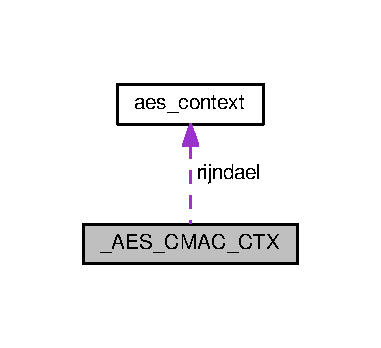
\includegraphics[width=183pt]{struct__AES__CMAC__CTX__coll__graph}
\end{center}
\end{figure}
\subsection*{Data Fields}
\begin{DoxyCompactItemize}
\item 
\hyperlink{structaes__context}{aes\+\_\+context} \hyperlink{struct__AES__CMAC__CTX_a111583eab419917697a4ed96963f293c}{rijndael}
\item 
uint8\+\_\+t \hyperlink{struct__AES__CMAC__CTX_a3be115a420dc4da7db29666a2ca6d850}{X} \mbox{[}16\mbox{]}
\item 
uint8\+\_\+t \hyperlink{struct__AES__CMAC__CTX_ac2ab3afeba7a78b17fe98404b15c4ad0}{M\+\_\+last} \mbox{[}16\mbox{]}
\item 
uint32\+\_\+t \hyperlink{struct__AES__CMAC__CTX_a2c48607df1e9c1847d3e4ff11612124b}{M\+\_\+n}
\end{DoxyCompactItemize}


\subsection{Field Documentation}
\mbox{\Hypertarget{struct__AES__CMAC__CTX_ac2ab3afeba7a78b17fe98404b15c4ad0}\label{struct__AES__CMAC__CTX_ac2ab3afeba7a78b17fe98404b15c4ad0}} 
\index{\+\_\+\+A\+E\+S\+\_\+\+C\+M\+A\+C\+\_\+\+C\+TX@{\+\_\+\+A\+E\+S\+\_\+\+C\+M\+A\+C\+\_\+\+C\+TX}!M\+\_\+last@{M\+\_\+last}}
\index{M\+\_\+last@{M\+\_\+last}!\+\_\+\+A\+E\+S\+\_\+\+C\+M\+A\+C\+\_\+\+C\+TX@{\+\_\+\+A\+E\+S\+\_\+\+C\+M\+A\+C\+\_\+\+C\+TX}}
\subsubsection{\texorpdfstring{M\+\_\+last}{M\_last}}
{\footnotesize\ttfamily uint8\+\_\+t \+\_\+\+A\+E\+S\+\_\+\+C\+M\+A\+C\+\_\+\+C\+T\+X\+::\+M\+\_\+last\mbox{[}16\mbox{]}}

\mbox{\Hypertarget{struct__AES__CMAC__CTX_a2c48607df1e9c1847d3e4ff11612124b}\label{struct__AES__CMAC__CTX_a2c48607df1e9c1847d3e4ff11612124b}} 
\index{\+\_\+\+A\+E\+S\+\_\+\+C\+M\+A\+C\+\_\+\+C\+TX@{\+\_\+\+A\+E\+S\+\_\+\+C\+M\+A\+C\+\_\+\+C\+TX}!M\+\_\+n@{M\+\_\+n}}
\index{M\+\_\+n@{M\+\_\+n}!\+\_\+\+A\+E\+S\+\_\+\+C\+M\+A\+C\+\_\+\+C\+TX@{\+\_\+\+A\+E\+S\+\_\+\+C\+M\+A\+C\+\_\+\+C\+TX}}
\subsubsection{\texorpdfstring{M\+\_\+n}{M\_n}}
{\footnotesize\ttfamily uint32\+\_\+t \+\_\+\+A\+E\+S\+\_\+\+C\+M\+A\+C\+\_\+\+C\+T\+X\+::\+M\+\_\+n}

\mbox{\Hypertarget{struct__AES__CMAC__CTX_a111583eab419917697a4ed96963f293c}\label{struct__AES__CMAC__CTX_a111583eab419917697a4ed96963f293c}} 
\index{\+\_\+\+A\+E\+S\+\_\+\+C\+M\+A\+C\+\_\+\+C\+TX@{\+\_\+\+A\+E\+S\+\_\+\+C\+M\+A\+C\+\_\+\+C\+TX}!rijndael@{rijndael}}
\index{rijndael@{rijndael}!\+\_\+\+A\+E\+S\+\_\+\+C\+M\+A\+C\+\_\+\+C\+TX@{\+\_\+\+A\+E\+S\+\_\+\+C\+M\+A\+C\+\_\+\+C\+TX}}
\subsubsection{\texorpdfstring{rijndael}{rijndael}}
{\footnotesize\ttfamily \hyperlink{structaes__context}{aes\+\_\+context} \+\_\+\+A\+E\+S\+\_\+\+C\+M\+A\+C\+\_\+\+C\+T\+X\+::rijndael}

\mbox{\Hypertarget{struct__AES__CMAC__CTX_a3be115a420dc4da7db29666a2ca6d850}\label{struct__AES__CMAC__CTX_a3be115a420dc4da7db29666a2ca6d850}} 
\index{\+\_\+\+A\+E\+S\+\_\+\+C\+M\+A\+C\+\_\+\+C\+TX@{\+\_\+\+A\+E\+S\+\_\+\+C\+M\+A\+C\+\_\+\+C\+TX}!X@{X}}
\index{X@{X}!\+\_\+\+A\+E\+S\+\_\+\+C\+M\+A\+C\+\_\+\+C\+TX@{\+\_\+\+A\+E\+S\+\_\+\+C\+M\+A\+C\+\_\+\+C\+TX}}
\subsubsection{\texorpdfstring{X}{X}}
{\footnotesize\ttfamily uint8\+\_\+t \+\_\+\+A\+E\+S\+\_\+\+C\+M\+A\+C\+\_\+\+C\+T\+X\+::X\mbox{[}16\mbox{]}}



The documentation for this struct was generated from the following file\+:\begin{DoxyCompactItemize}
\item 
Crypto/\hyperlink{cmac_8h}{cmac.\+h}\end{DoxyCompactItemize}

\hypertarget{structaes__context}{}\section{aes\+\_\+context Struct Reference}
\label{structaes__context}\index{aes\+\_\+context@{aes\+\_\+context}}


{\ttfamily \#include $<$aes.\+h$>$}

\subsection*{Data Fields}
\begin{DoxyCompactItemize}
\item 
uint8\+\_\+t \hyperlink{structaes__context_ab476c78bbf83cabeb637d33c43cc35ee}{ksch} \mbox{[}(\hyperlink{aes_8h_af8b900ecc3a113f2aed001ac9e1cb11e}{N\+\_\+\+M\+A\+X\+\_\+\+R\+O\+U\+N\+DS}+1) $\ast$\hyperlink{aes_8h_a64c8b1a34c03210cc4c214735bb4f186}{N\+\_\+\+B\+L\+O\+CK}\mbox{]}
\item 
uint8\+\_\+t \hyperlink{structaes__context_ab762dfbe068d5ecc737d864d00459fa0}{rnd}
\end{DoxyCompactItemize}


\subsection{Field Documentation}
\mbox{\Hypertarget{structaes__context_ab476c78bbf83cabeb637d33c43cc35ee}\label{structaes__context_ab476c78bbf83cabeb637d33c43cc35ee}} 
\index{aes\+\_\+context@{aes\+\_\+context}!ksch@{ksch}}
\index{ksch@{ksch}!aes\+\_\+context@{aes\+\_\+context}}
\subsubsection{\texorpdfstring{ksch}{ksch}}
{\footnotesize\ttfamily uint8\+\_\+t aes\+\_\+context\+::ksch\mbox{[}(\hyperlink{aes_8h_af8b900ecc3a113f2aed001ac9e1cb11e}{N\+\_\+\+M\+A\+X\+\_\+\+R\+O\+U\+N\+DS}+1) $\ast$\hyperlink{aes_8h_a64c8b1a34c03210cc4c214735bb4f186}{N\+\_\+\+B\+L\+O\+CK}\mbox{]}}

\mbox{\Hypertarget{structaes__context_ab762dfbe068d5ecc737d864d00459fa0}\label{structaes__context_ab762dfbe068d5ecc737d864d00459fa0}} 
\index{aes\+\_\+context@{aes\+\_\+context}!rnd@{rnd}}
\index{rnd@{rnd}!aes\+\_\+context@{aes\+\_\+context}}
\subsubsection{\texorpdfstring{rnd}{rnd}}
{\footnotesize\ttfamily uint8\+\_\+t aes\+\_\+context\+::rnd}



The documentation for this struct was generated from the following file\+:\begin{DoxyCompactItemize}
\item 
Crypto/\hyperlink{aes_8h}{aes.\+h}\end{DoxyCompactItemize}

\hypertarget{structComplianceTest__s}{}\section{Compliance\+Test\+\_\+s Struct Reference}
\label{structComplianceTest__s}\index{Compliance\+Test\+\_\+s@{Compliance\+Test\+\_\+s}}
\subsection*{Data Fields}
\begin{DoxyCompactItemize}
\item 
bool \hyperlink{structComplianceTest__s_a9fe440a17751188399bfcea77e1e16bf}{Running}
\item 
uint8\+\_\+t \hyperlink{structComplianceTest__s_a09f13d5e6c7f74b686f798421631942f}{State}
\item 
Functional\+State \hyperlink{structComplianceTest__s_adfa84b8a00789461a9d200c34025958f}{Is\+Tx\+Confirmed}
\item 
uint8\+\_\+t \hyperlink{structComplianceTest__s_a5d5a6c64e1a230836b3c20ab10526ad9}{App\+Port}
\item 
uint8\+\_\+t \hyperlink{structComplianceTest__s_aee38d06c8b326209d9f316815698d396}{App\+Data\+Size}
\item 
uint8\+\_\+t $\ast$ \hyperlink{structComplianceTest__s_a7aeb423dcc1989e14b476b7abba60385}{App\+Data\+Buffer}
\item 
uint16\+\_\+t \hyperlink{structComplianceTest__s_aa3eeaf5d3061e15ec3835dbc9ece4683}{Down\+Link\+Counter}
\item 
bool \hyperlink{structComplianceTest__s_abcd594cefd9fb669dbb97d86213fcf44}{Link\+Check}
\item 
uint8\+\_\+t \hyperlink{structComplianceTest__s_a14edd4e6871944ff733fd8a14133d899}{Demod\+Margin}
\item 
uint8\+\_\+t \hyperlink{structComplianceTest__s_a5896f8dcc61f8e45b30a0d8de8b8bd54}{Nb\+Gateways}
\end{DoxyCompactItemize}


\subsection{Detailed Description}
Lo\+Ra\+W\+AN compliance tests support data 

\subsection{Field Documentation}
\mbox{\Hypertarget{structComplianceTest__s_a7aeb423dcc1989e14b476b7abba60385}\label{structComplianceTest__s_a7aeb423dcc1989e14b476b7abba60385}} 
\index{Compliance\+Test\+\_\+s@{Compliance\+Test\+\_\+s}!App\+Data\+Buffer@{App\+Data\+Buffer}}
\index{App\+Data\+Buffer@{App\+Data\+Buffer}!Compliance\+Test\+\_\+s@{Compliance\+Test\+\_\+s}}
\subsubsection{\texorpdfstring{App\+Data\+Buffer}{AppDataBuffer}}
{\footnotesize\ttfamily uint8\+\_\+t$\ast$ Compliance\+Test\+\_\+s\+::\+App\+Data\+Buffer}

\mbox{\Hypertarget{structComplianceTest__s_aee38d06c8b326209d9f316815698d396}\label{structComplianceTest__s_aee38d06c8b326209d9f316815698d396}} 
\index{Compliance\+Test\+\_\+s@{Compliance\+Test\+\_\+s}!App\+Data\+Size@{App\+Data\+Size}}
\index{App\+Data\+Size@{App\+Data\+Size}!Compliance\+Test\+\_\+s@{Compliance\+Test\+\_\+s}}
\subsubsection{\texorpdfstring{App\+Data\+Size}{AppDataSize}}
{\footnotesize\ttfamily uint8\+\_\+t Compliance\+Test\+\_\+s\+::\+App\+Data\+Size}

\mbox{\Hypertarget{structComplianceTest__s_a5d5a6c64e1a230836b3c20ab10526ad9}\label{structComplianceTest__s_a5d5a6c64e1a230836b3c20ab10526ad9}} 
\index{Compliance\+Test\+\_\+s@{Compliance\+Test\+\_\+s}!App\+Port@{App\+Port}}
\index{App\+Port@{App\+Port}!Compliance\+Test\+\_\+s@{Compliance\+Test\+\_\+s}}
\subsubsection{\texorpdfstring{App\+Port}{AppPort}}
{\footnotesize\ttfamily uint8\+\_\+t Compliance\+Test\+\_\+s\+::\+App\+Port}

\mbox{\Hypertarget{structComplianceTest__s_a14edd4e6871944ff733fd8a14133d899}\label{structComplianceTest__s_a14edd4e6871944ff733fd8a14133d899}} 
\index{Compliance\+Test\+\_\+s@{Compliance\+Test\+\_\+s}!Demod\+Margin@{Demod\+Margin}}
\index{Demod\+Margin@{Demod\+Margin}!Compliance\+Test\+\_\+s@{Compliance\+Test\+\_\+s}}
\subsubsection{\texorpdfstring{Demod\+Margin}{DemodMargin}}
{\footnotesize\ttfamily uint8\+\_\+t Compliance\+Test\+\_\+s\+::\+Demod\+Margin}

\mbox{\Hypertarget{structComplianceTest__s_aa3eeaf5d3061e15ec3835dbc9ece4683}\label{structComplianceTest__s_aa3eeaf5d3061e15ec3835dbc9ece4683}} 
\index{Compliance\+Test\+\_\+s@{Compliance\+Test\+\_\+s}!Down\+Link\+Counter@{Down\+Link\+Counter}}
\index{Down\+Link\+Counter@{Down\+Link\+Counter}!Compliance\+Test\+\_\+s@{Compliance\+Test\+\_\+s}}
\subsubsection{\texorpdfstring{Down\+Link\+Counter}{DownLinkCounter}}
{\footnotesize\ttfamily uint16\+\_\+t Compliance\+Test\+\_\+s\+::\+Down\+Link\+Counter}

\mbox{\Hypertarget{structComplianceTest__s_adfa84b8a00789461a9d200c34025958f}\label{structComplianceTest__s_adfa84b8a00789461a9d200c34025958f}} 
\index{Compliance\+Test\+\_\+s@{Compliance\+Test\+\_\+s}!Is\+Tx\+Confirmed@{Is\+Tx\+Confirmed}}
\index{Is\+Tx\+Confirmed@{Is\+Tx\+Confirmed}!Compliance\+Test\+\_\+s@{Compliance\+Test\+\_\+s}}
\subsubsection{\texorpdfstring{Is\+Tx\+Confirmed}{IsTxConfirmed}}
{\footnotesize\ttfamily Functional\+State Compliance\+Test\+\_\+s\+::\+Is\+Tx\+Confirmed}

\mbox{\Hypertarget{structComplianceTest__s_abcd594cefd9fb669dbb97d86213fcf44}\label{structComplianceTest__s_abcd594cefd9fb669dbb97d86213fcf44}} 
\index{Compliance\+Test\+\_\+s@{Compliance\+Test\+\_\+s}!Link\+Check@{Link\+Check}}
\index{Link\+Check@{Link\+Check}!Compliance\+Test\+\_\+s@{Compliance\+Test\+\_\+s}}
\subsubsection{\texorpdfstring{Link\+Check}{LinkCheck}}
{\footnotesize\ttfamily bool Compliance\+Test\+\_\+s\+::\+Link\+Check}

\mbox{\Hypertarget{structComplianceTest__s_a5896f8dcc61f8e45b30a0d8de8b8bd54}\label{structComplianceTest__s_a5896f8dcc61f8e45b30a0d8de8b8bd54}} 
\index{Compliance\+Test\+\_\+s@{Compliance\+Test\+\_\+s}!Nb\+Gateways@{Nb\+Gateways}}
\index{Nb\+Gateways@{Nb\+Gateways}!Compliance\+Test\+\_\+s@{Compliance\+Test\+\_\+s}}
\subsubsection{\texorpdfstring{Nb\+Gateways}{NbGateways}}
{\footnotesize\ttfamily uint8\+\_\+t Compliance\+Test\+\_\+s\+::\+Nb\+Gateways}

\mbox{\Hypertarget{structComplianceTest__s_a9fe440a17751188399bfcea77e1e16bf}\label{structComplianceTest__s_a9fe440a17751188399bfcea77e1e16bf}} 
\index{Compliance\+Test\+\_\+s@{Compliance\+Test\+\_\+s}!Running@{Running}}
\index{Running@{Running}!Compliance\+Test\+\_\+s@{Compliance\+Test\+\_\+s}}
\subsubsection{\texorpdfstring{Running}{Running}}
{\footnotesize\ttfamily bool Compliance\+Test\+\_\+s\+::\+Running}

\mbox{\Hypertarget{structComplianceTest__s_a09f13d5e6c7f74b686f798421631942f}\label{structComplianceTest__s_a09f13d5e6c7f74b686f798421631942f}} 
\index{Compliance\+Test\+\_\+s@{Compliance\+Test\+\_\+s}!State@{State}}
\index{State@{State}!Compliance\+Test\+\_\+s@{Compliance\+Test\+\_\+s}}
\subsubsection{\texorpdfstring{State}{State}}
{\footnotesize\ttfamily uint8\+\_\+t Compliance\+Test\+\_\+s\+::\+State}



The documentation for this struct was generated from the following file\+:\begin{DoxyCompactItemize}
\item 
Core/\hyperlink{lora_8c}{lora.\+c}\end{DoxyCompactItemize}

\hypertarget{unioneLoRaMacFlags__t}{}\section{e\+Lo\+Ra\+Mac\+Flags\+\_\+t Union Reference}
\label{unioneLoRaMacFlags__t}\index{e\+Lo\+Ra\+Mac\+Flags\+\_\+t@{e\+Lo\+Ra\+Mac\+Flags\+\_\+t}}


{\ttfamily \#include $<$Lo\+Ra\+Mac.\+h$>$}



Collaboration diagram for e\+Lo\+Ra\+Mac\+Flags\+\_\+t\+:
\nopagebreak
\begin{figure}[H]
\begin{center}
\leavevmode
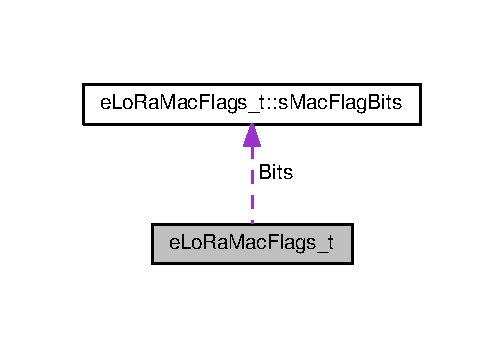
\includegraphics[width=242pt]{unioneLoRaMacFlags__t__coll__graph}
\end{center}
\end{figure}
\subsection*{Data Structures}
\begin{DoxyCompactItemize}
\item 
struct \hyperlink{structeLoRaMacFlags__t_1_1sMacFlagBits}{s\+Mac\+Flag\+Bits}
\end{DoxyCompactItemize}
\subsection*{Data Fields}
\begin{DoxyCompactItemize}
\item 
uint8\+\_\+t \hyperlink{unioneLoRaMacFlags__t_a11a65b748bc5c36714d830d5daa93fe3}{Value}
\item 
struct \hyperlink{structeLoRaMacFlags__t_1_1sMacFlagBits}{e\+Lo\+Ra\+Mac\+Flags\+\_\+t\+::s\+Mac\+Flag\+Bits} \hyperlink{unioneLoRaMacFlags__t_a23c1c70ba3e3306aaaedd6f62c2aab15}{Bits}
\end{DoxyCompactItemize}


\subsection{Detailed Description}
Lo\+Ra\+Mac tx/rx operation state 

\subsection{Field Documentation}
\mbox{\Hypertarget{unioneLoRaMacFlags__t_a23c1c70ba3e3306aaaedd6f62c2aab15}\label{unioneLoRaMacFlags__t_a23c1c70ba3e3306aaaedd6f62c2aab15}} 
\index{e\+Lo\+Ra\+Mac\+Flags\+\_\+t@{e\+Lo\+Ra\+Mac\+Flags\+\_\+t}!Bits@{Bits}}
\index{Bits@{Bits}!e\+Lo\+Ra\+Mac\+Flags\+\_\+t@{e\+Lo\+Ra\+Mac\+Flags\+\_\+t}}
\subsubsection{\texorpdfstring{Bits}{Bits}}
{\footnotesize\ttfamily struct \hyperlink{structeLoRaMacFlags__t_1_1sMacFlagBits}{e\+Lo\+Ra\+Mac\+Flags\+\_\+t\+::s\+Mac\+Flag\+Bits} e\+Lo\+Ra\+Mac\+Flags\+\_\+t\+::\+Bits}

\mbox{\Hypertarget{unioneLoRaMacFlags__t_a11a65b748bc5c36714d830d5daa93fe3}\label{unioneLoRaMacFlags__t_a11a65b748bc5c36714d830d5daa93fe3}} 
\index{e\+Lo\+Ra\+Mac\+Flags\+\_\+t@{e\+Lo\+Ra\+Mac\+Flags\+\_\+t}!Value@{Value}}
\index{Value@{Value}!e\+Lo\+Ra\+Mac\+Flags\+\_\+t@{e\+Lo\+Ra\+Mac\+Flags\+\_\+t}}
\subsubsection{\texorpdfstring{Value}{Value}}
{\footnotesize\ttfamily uint8\+\_\+t e\+Lo\+Ra\+Mac\+Flags\+\_\+t\+::\+Value}

Byte-\/access to the bits 

The documentation for this union was generated from the following file\+:\begin{DoxyCompactItemize}
\item 
Mac/\hyperlink{LoRaMac_8h}{Lo\+Ra\+Mac.\+h}\end{DoxyCompactItemize}

\hypertarget{structeMibRequestConfirm}{}\section{e\+Mib\+Request\+Confirm Struct Reference}
\label{structeMibRequestConfirm}\index{e\+Mib\+Request\+Confirm@{e\+Mib\+Request\+Confirm}}


{\ttfamily \#include $<$Lo\+Ra\+Mac.\+h$>$}



Collaboration diagram for e\+Mib\+Request\+Confirm\+:
\nopagebreak
\begin{figure}[H]
\begin{center}
\leavevmode
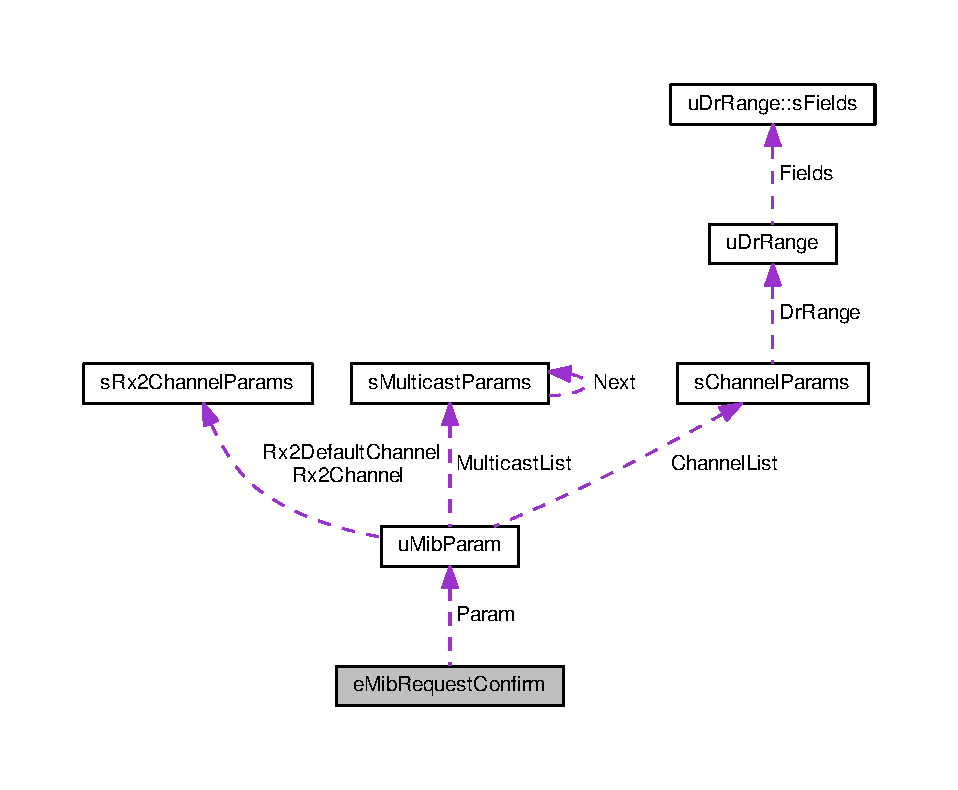
\includegraphics[width=350pt]{structeMibRequestConfirm__coll__graph}
\end{center}
\end{figure}
\subsection*{Data Fields}
\begin{DoxyCompactItemize}
\item 
\hyperlink{group__LORAMAC_gaf17bd3de9ec75e4954be9a070cd8ddf9}{Mib\+\_\+t} \hyperlink{structeMibRequestConfirm_ad3d963c102bbd81f7dd9918f4c1731c1}{Type}
\item 
\hyperlink{group__LORAMAC_gae9f2411f44447849f5b36bcaca1feb5c}{Mib\+Param\+\_\+t} \hyperlink{structeMibRequestConfirm_a71cc0adf3fe8337eaa6dc69a1463c8bc}{Param}
\end{DoxyCompactItemize}


\subsection{Detailed Description}
Lo\+Ra\+M\+AC M\+I\+B-\/\+Request\+Confirm structure 

\subsection{Field Documentation}
\mbox{\Hypertarget{structeMibRequestConfirm_a71cc0adf3fe8337eaa6dc69a1463c8bc}\label{structeMibRequestConfirm_a71cc0adf3fe8337eaa6dc69a1463c8bc}} 
\index{e\+Mib\+Request\+Confirm@{e\+Mib\+Request\+Confirm}!Param@{Param}}
\index{Param@{Param}!e\+Mib\+Request\+Confirm@{e\+Mib\+Request\+Confirm}}
\subsubsection{\texorpdfstring{Param}{Param}}
{\footnotesize\ttfamily \hyperlink{group__LORAMAC_gae9f2411f44447849f5b36bcaca1feb5c}{Mib\+Param\+\_\+t} e\+Mib\+Request\+Confirm\+::\+Param}

M\+L\+M\+E-\/\+Request\+Confirm parameters \mbox{\Hypertarget{structeMibRequestConfirm_ad3d963c102bbd81f7dd9918f4c1731c1}\label{structeMibRequestConfirm_ad3d963c102bbd81f7dd9918f4c1731c1}} 
\index{e\+Mib\+Request\+Confirm@{e\+Mib\+Request\+Confirm}!Type@{Type}}
\index{Type@{Type}!e\+Mib\+Request\+Confirm@{e\+Mib\+Request\+Confirm}}
\subsubsection{\texorpdfstring{Type}{Type}}
{\footnotesize\ttfamily \hyperlink{group__LORAMAC_gaf17bd3de9ec75e4954be9a070cd8ddf9}{Mib\+\_\+t} e\+Mib\+Request\+Confirm\+::\+Type}

M\+I\+B-\/\+Request type 

The documentation for this struct was generated from the following file\+:\begin{DoxyCompactItemize}
\item 
Mac/\hyperlink{LoRaMac_8h}{Lo\+Ra\+Mac.\+h}\end{DoxyCompactItemize}

\hypertarget{structlora__AppData__t}{}\section{lora\+\_\+\+App\+Data\+\_\+t Struct Reference}
\label{structlora__AppData__t}\index{lora\+\_\+\+App\+Data\+\_\+t@{lora\+\_\+\+App\+Data\+\_\+t}}


{\ttfamily \#include $<$lora.\+h$>$}

\subsection*{Data Fields}
\begin{DoxyCompactItemize}
\item 
uint8\+\_\+t $\ast$ \hyperlink{structlora__AppData__t_ab35779bafa91eae413c99ba800903827}{Buff}
\item 
uint8\+\_\+t \hyperlink{structlora__AppData__t_afc0792ef22bfeff4a47d4bf41dfdeb50}{Buff\+Size}
\item 
uint8\+\_\+t \hyperlink{structlora__AppData__t_a5ec1eaaeb3098b35864ce2b7ebc4a348}{Port}
\end{DoxyCompactItemize}


\subsection{Detailed Description}
Application Data structure 

\subsection{Field Documentation}
\mbox{\Hypertarget{structlora__AppData__t_ab35779bafa91eae413c99ba800903827}\label{structlora__AppData__t_ab35779bafa91eae413c99ba800903827}} 
\index{lora\+\_\+\+App\+Data\+\_\+t@{lora\+\_\+\+App\+Data\+\_\+t}!Buff@{Buff}}
\index{Buff@{Buff}!lora\+\_\+\+App\+Data\+\_\+t@{lora\+\_\+\+App\+Data\+\_\+t}}
\subsubsection{\texorpdfstring{Buff}{Buff}}
{\footnotesize\ttfamily uint8\+\_\+t$\ast$ lora\+\_\+\+App\+Data\+\_\+t\+::\+Buff}

\mbox{\Hypertarget{structlora__AppData__t_afc0792ef22bfeff4a47d4bf41dfdeb50}\label{structlora__AppData__t_afc0792ef22bfeff4a47d4bf41dfdeb50}} 
\index{lora\+\_\+\+App\+Data\+\_\+t@{lora\+\_\+\+App\+Data\+\_\+t}!Buff\+Size@{Buff\+Size}}
\index{Buff\+Size@{Buff\+Size}!lora\+\_\+\+App\+Data\+\_\+t@{lora\+\_\+\+App\+Data\+\_\+t}}
\subsubsection{\texorpdfstring{Buff\+Size}{BuffSize}}
{\footnotesize\ttfamily uint8\+\_\+t lora\+\_\+\+App\+Data\+\_\+t\+::\+Buff\+Size}

\mbox{\Hypertarget{structlora__AppData__t_a5ec1eaaeb3098b35864ce2b7ebc4a348}\label{structlora__AppData__t_a5ec1eaaeb3098b35864ce2b7ebc4a348}} 
\index{lora\+\_\+\+App\+Data\+\_\+t@{lora\+\_\+\+App\+Data\+\_\+t}!Port@{Port}}
\index{Port@{Port}!lora\+\_\+\+App\+Data\+\_\+t@{lora\+\_\+\+App\+Data\+\_\+t}}
\subsubsection{\texorpdfstring{Port}{Port}}
{\footnotesize\ttfamily uint8\+\_\+t lora\+\_\+\+App\+Data\+\_\+t\+::\+Port}



The documentation for this struct was generated from the following file\+:\begin{DoxyCompactItemize}
\item 
Core/\hyperlink{lora_8h}{lora.\+h}\end{DoxyCompactItemize}

\hypertarget{structRadio__s}{}\section{Radio\+\_\+s Struct Reference}
\label{structRadio__s}\index{Radio\+\_\+s@{Radio\+\_\+s}}


Radio driver definition.  




{\ttfamily \#include $<$radio.\+h$>$}

\subsection*{Data Fields}
\begin{DoxyCompactItemize}
\item 
void($\ast$ \hyperlink{group__LORA_ga5a84db3f810c3c6470a330034981fc7b}{Io\+Init} )(void)
\begin{DoxyCompactList}\small\item\em Initializes the io. \end{DoxyCompactList}\item 
void($\ast$ \hyperlink{group__LORA_ga45d0a08fcddbc5d8364ce980c26028ac}{Io\+De\+Init} )(void)
\begin{DoxyCompactList}\small\item\em Deinitializes the io. \end{DoxyCompactList}\item 
uint32\+\_\+t($\ast$ \hyperlink{group__LORA_gafb896d98cceb49c55af00f5d5aa964cd}{Init} )(\hyperlink{structRadioEvents__t}{Radio\+Events\+\_\+t} $\ast$events)
\begin{DoxyCompactList}\small\item\em Initializes the radio. \end{DoxyCompactList}\item 
\hyperlink{group__LORA_ga2f3fa4ad0237c4ace94aa99086aac9f5}{Radio\+State\+\_\+t}($\ast$ \hyperlink{group__LORA_ga24c01d8388f399e8ccaea190048eea9d}{Get\+Status} )(void)
\item 
void($\ast$ \hyperlink{group__LORA_ga92515d5b16f5093727b90256a8929b82}{Set\+Modem} )(\hyperlink{group__LORA_ga992ef7a5b7f52975ba7bd8dd97740057}{Radio\+Modems\+\_\+t} modem)
\begin{DoxyCompactList}\small\item\em Configures the radio with the given modem. \end{DoxyCompactList}\item 
void($\ast$ \hyperlink{group__LORA_gaf41c78922a5831b2e0ceb458286846fd}{Set\+Channel} )(uint32\+\_\+t freq)
\begin{DoxyCompactList}\small\item\em Sets the channel frequency. \end{DoxyCompactList}\item 
bool($\ast$ \hyperlink{group__LORA_ga9e6632b46872513fe063489eb22f9663}{Is\+Channel\+Free} )(\hyperlink{group__LORA_ga992ef7a5b7f52975ba7bd8dd97740057}{Radio\+Modems\+\_\+t} modem, uint32\+\_\+t freq, int16\+\_\+t rssi\+Thresh, uint32\+\_\+t max\+Carrier\+Sense\+Time)
\begin{DoxyCompactList}\small\item\em Checks if the channel is free for the given time. \end{DoxyCompactList}\item 
uint32\+\_\+t($\ast$ \hyperlink{group__LORA_gaf39c7ced02721092f0f780f6632a81fd}{Random} )(void)
\begin{DoxyCompactList}\small\item\em Generates a 32 bits random value based on the R\+S\+SI readings. \end{DoxyCompactList}\item 
void($\ast$ \hyperlink{group__LORA_gadd564d2a79027afbc6f0f8f3011fe93b}{Set\+Rx\+Config} )(\hyperlink{group__LORA_ga992ef7a5b7f52975ba7bd8dd97740057}{Radio\+Modems\+\_\+t} modem, uint32\+\_\+t bandwidth, uint32\+\_\+t datarate, uint8\+\_\+t coderate, uint32\+\_\+t bandwidth\+Afc, uint16\+\_\+t preamble\+Len, uint16\+\_\+t symb\+Timeout, bool fix\+Len, uint8\+\_\+t payload\+Len, bool crc\+On, bool freq\+Hop\+On, uint8\+\_\+t hop\+Period, bool iq\+Inverted, bool rx\+Continuous)
\begin{DoxyCompactList}\small\item\em Sets the reception parameters. \end{DoxyCompactList}\item 
void($\ast$ \hyperlink{group__LORA_gad4177124b5db6b2b1f07ba16e631bbdb}{Set\+Tx\+Config} )(\hyperlink{group__LORA_ga992ef7a5b7f52975ba7bd8dd97740057}{Radio\+Modems\+\_\+t} modem, int8\+\_\+t power, uint32\+\_\+t fdev, uint32\+\_\+t bandwidth, uint32\+\_\+t datarate, uint8\+\_\+t coderate, uint16\+\_\+t preamble\+Len, bool fix\+Len, bool crc\+On, bool freq\+Hop\+On, uint8\+\_\+t hop\+Period, bool iq\+Inverted, uint32\+\_\+t timeout)
\begin{DoxyCompactList}\small\item\em Sets the transmission parameters. \end{DoxyCompactList}\item 
bool($\ast$ \hyperlink{group__LORA_gad26df1cecc02c5d50f07ff062962f501}{Check\+Rf\+Frequency} )(uint32\+\_\+t frequency)
\begin{DoxyCompactList}\small\item\em Checks if the given RF frequency is supported by the hardware. \end{DoxyCompactList}\item 
uint32\+\_\+t($\ast$ \hyperlink{group__LORA_ga36552db411e04e05c7962912854d48ae}{Time\+On\+Air} )(\hyperlink{group__LORA_ga992ef7a5b7f52975ba7bd8dd97740057}{Radio\+Modems\+\_\+t} modem, uint8\+\_\+t pkt\+Len)
\begin{DoxyCompactList}\small\item\em Computes the packet time on air in ms for the given payload. \end{DoxyCompactList}\item 
void($\ast$ \hyperlink{group__LORA_ga80f05bcd6ec2aea2eec2fc16850c6829}{Send} )(uint8\+\_\+t $\ast$buffer, uint8\+\_\+t size)
\begin{DoxyCompactList}\small\item\em Sends the buffer of size. Prepares the packet to be sent and sets the radio in transmission. \end{DoxyCompactList}\item 
void($\ast$ \hyperlink{group__LORA_ga1ce3ea830b03dffac6f6fec459dc77d3}{Sleep} )(void)
\begin{DoxyCompactList}\small\item\em Sets the radio in sleep mode. \end{DoxyCompactList}\item 
void($\ast$ \hyperlink{group__LORA_ga2972c07018c9c2de5c76c6c0563bea7b}{Standby} )(void)
\begin{DoxyCompactList}\small\item\em Sets the radio in standby mode. \end{DoxyCompactList}\item 
void($\ast$ \hyperlink{group__LORA_ga102f21c524b5c8eb87a2d65f8ac6cbe4}{Rx} )(uint32\+\_\+t timeout)
\begin{DoxyCompactList}\small\item\em Sets the radio in reception mode for the given time. \end{DoxyCompactList}\item 
void($\ast$ \hyperlink{group__LORA_ga8f9e97d8a3010e96e108dc62c1e5b107}{Start\+Cad} )(void)
\begin{DoxyCompactList}\small\item\em Start a Channel Activity Detection. \end{DoxyCompactList}\item 
void($\ast$ \hyperlink{group__LORA_ga6b20fa3f6908c0165b26d8e02b944e3b}{Set\+Tx\+Continuous\+Wave} )(uint32\+\_\+t freq, int8\+\_\+t power, uint16\+\_\+t time)
\begin{DoxyCompactList}\small\item\em Sets the radio in continuous wave transmission mode. \end{DoxyCompactList}\item 
int16\+\_\+t($\ast$ \hyperlink{group__LORA_gade038967fa33e964e02fe10e66d6d510}{Rssi} )(\hyperlink{group__LORA_ga992ef7a5b7f52975ba7bd8dd97740057}{Radio\+Modems\+\_\+t} modem)
\begin{DoxyCompactList}\small\item\em Reads the current R\+S\+SI value. \end{DoxyCompactList}\item 
void($\ast$ \hyperlink{group__LORA_ga5f0ca54e8bc3c82d3c9b196230c325d5}{Write} )(uint8\+\_\+t addr, uint8\+\_\+t data)
\begin{DoxyCompactList}\small\item\em Writes the radio register at the specified address. \end{DoxyCompactList}\item 
uint8\+\_\+t($\ast$ \hyperlink{group__LORA_ga8396bca959a0b717fabd37ac91c11534}{Read} )(uint8\+\_\+t addr)
\begin{DoxyCompactList}\small\item\em Reads the radio register at the specified address. \end{DoxyCompactList}\item 
void($\ast$ \hyperlink{group__LORA_gab282c0d0a6bd7dd9f21cf79984988a8a}{Write\+Buffer} )(uint8\+\_\+t addr, uint8\+\_\+t $\ast$buffer, uint8\+\_\+t size)
\begin{DoxyCompactList}\small\item\em Writes multiple radio registers starting at address. \end{DoxyCompactList}\item 
void($\ast$ \hyperlink{group__LORA_ga7ef5175264a4cf10bb6d9fa40c115dab}{Read\+Buffer} )(uint8\+\_\+t addr, uint8\+\_\+t $\ast$buffer, uint8\+\_\+t size)
\begin{DoxyCompactList}\small\item\em Reads multiple radio registers starting at address. \end{DoxyCompactList}\item 
void($\ast$ \hyperlink{group__LORA_ga182fc8f265a2d02d64f3ee1c6dd5906f}{Set\+Max\+Payload\+Length} )(\hyperlink{group__LORA_ga992ef7a5b7f52975ba7bd8dd97740057}{Radio\+Modems\+\_\+t} modem, uint8\+\_\+t max)
\begin{DoxyCompactList}\small\item\em Sets the maximum payload length. \end{DoxyCompactList}\item 
void($\ast$ \hyperlink{group__LORA_ga33681fa99af4bf37517e1ba1107e1877}{Set\+Public\+Network} )(bool enable)
\begin{DoxyCompactList}\small\item\em Sets the network to public or private. Updates the sync byte. \end{DoxyCompactList}\item 
uint32\+\_\+t($\ast$ \hyperlink{group__LORA_ga7396df7c609fbda8b6ed87755b3899be}{Get\+Radio\+Wake\+Up\+Time} )(void)
\begin{DoxyCompactList}\small\item\em Service to get the radio wake-\/up time. \end{DoxyCompactList}\end{DoxyCompactItemize}


\subsection{Detailed Description}
Radio driver definition. 

The documentation for this struct was generated from the following file\+:\begin{DoxyCompactItemize}
\item 
Phy/\hyperlink{radio_8h}{radio.\+h}\end{DoxyCompactItemize}

\hypertarget{structRadioEvents__t}{}\section{Radio\+Events\+\_\+t Struct Reference}
\label{structRadioEvents__t}\index{Radio\+Events\+\_\+t@{Radio\+Events\+\_\+t}}


Radio driver callback functions.  




{\ttfamily \#include $<$radio.\+h$>$}

\subsection*{Data Fields}
\begin{DoxyCompactItemize}
\item 
void($\ast$ \hyperlink{group__LORA_gafe2bdc503d6c09946dee1b800e2fb3a2}{Tx\+Done} )(void)
\begin{DoxyCompactList}\small\item\em Tx Done callback prototype. \end{DoxyCompactList}\item 
void($\ast$ \hyperlink{group__LORA_ga1f435b15ceae4ce1e44af3d3c5845ffd}{Tx\+Timeout} )(void)
\begin{DoxyCompactList}\small\item\em Tx Timeout callback prototype. \end{DoxyCompactList}\item 
void($\ast$ \hyperlink{group__LORA_ga92665b4b0a07eb2df1b435dcef314b48}{Rx\+Done} )(uint8\+\_\+t $\ast$payload, uint16\+\_\+t size, int16\+\_\+t rssi, int8\+\_\+t snr)
\begin{DoxyCompactList}\small\item\em Rx Done callback prototype. \end{DoxyCompactList}\item 
void($\ast$ \hyperlink{group__LORA_ga1566693134c9ae4bad8a0f90ed72fff2}{Rx\+Timeout} )(void)
\begin{DoxyCompactList}\small\item\em Rx Timeout callback prototype. \end{DoxyCompactList}\item 
void($\ast$ \hyperlink{group__LORA_ga17b9f56c75cbc08de07f5b2a9d234002}{Rx\+Error} )(void)
\begin{DoxyCompactList}\small\item\em Rx Error callback prototype. \end{DoxyCompactList}\item 
void($\ast$ \hyperlink{group__LORA_ga1c7fd427d45e18c386c0dc10b496d74b}{Fhss\+Change\+Channel} )(uint8\+\_\+t current\+Channel)
\begin{DoxyCompactList}\small\item\em F\+H\+SS Change Channel callback prototype. \end{DoxyCompactList}\item 
void($\ast$ \hyperlink{group__LORA_gacf79a39fe3d615bed87b1414e73df6b2}{Cad\+Done} )(bool channel\+Activity\+Detected)
\begin{DoxyCompactList}\small\item\em C\+AD Done callback prototype. \end{DoxyCompactList}\end{DoxyCompactItemize}


\subsection{Detailed Description}
Radio driver callback functions. 

The documentation for this struct was generated from the following file\+:\begin{DoxyCompactItemize}
\item 
Phy/\hyperlink{radio_8h}{radio.\+h}\end{DoxyCompactItemize}

\hypertarget{structsAdrNextParams}{}\section{s\+Adr\+Next\+Params Struct Reference}
\label{structsAdrNextParams}\index{s\+Adr\+Next\+Params@{s\+Adr\+Next\+Params}}


{\ttfamily \#include $<$Region.\+h$>$}

\subsection*{Data Fields}
\begin{DoxyCompactItemize}
\item 
bool \hyperlink{structsAdrNextParams_a19a2e867d2da58e8dc49a66895ffabc3}{Update\+Chan\+Mask}
\item 
bool \hyperlink{structsAdrNextParams_af672081d323c0ec3c4795cb4f31645a6}{Adr\+Enabled}
\item 
uint32\+\_\+t \hyperlink{structsAdrNextParams_a4c1177ddf9c60362d3593708e4c95634}{Adr\+Ack\+Counter}
\item 
int8\+\_\+t \hyperlink{structsAdrNextParams_aca7c92b0daeece909a485360c3d22736}{Datarate}
\item 
int8\+\_\+t \hyperlink{structsAdrNextParams_abf2315e4c1e376ed61ba8a58544b45c0}{Tx\+Power}
\item 
uint8\+\_\+t \hyperlink{structsAdrNextParams_ac48a8e1de3148431a68b39b072dcfb5d}{Uplink\+Dwell\+Time}
\end{DoxyCompactItemize}


\subsection{Detailed Description}
Parameter structure for the function Region\+Adr\+Next. 

\subsection{Field Documentation}
\mbox{\Hypertarget{structsAdrNextParams_a4c1177ddf9c60362d3593708e4c95634}\label{structsAdrNextParams_a4c1177ddf9c60362d3593708e4c95634}} 
\index{s\+Adr\+Next\+Params@{s\+Adr\+Next\+Params}!Adr\+Ack\+Counter@{Adr\+Ack\+Counter}}
\index{Adr\+Ack\+Counter@{Adr\+Ack\+Counter}!s\+Adr\+Next\+Params@{s\+Adr\+Next\+Params}}
\subsubsection{\texorpdfstring{Adr\+Ack\+Counter}{AdrAckCounter}}
{\footnotesize\ttfamily uint32\+\_\+t s\+Adr\+Next\+Params\+::\+Adr\+Ack\+Counter}

A\+DR ack counter. \mbox{\Hypertarget{structsAdrNextParams_af672081d323c0ec3c4795cb4f31645a6}\label{structsAdrNextParams_af672081d323c0ec3c4795cb4f31645a6}} 
\index{s\+Adr\+Next\+Params@{s\+Adr\+Next\+Params}!Adr\+Enabled@{Adr\+Enabled}}
\index{Adr\+Enabled@{Adr\+Enabled}!s\+Adr\+Next\+Params@{s\+Adr\+Next\+Params}}
\subsubsection{\texorpdfstring{Adr\+Enabled}{AdrEnabled}}
{\footnotesize\ttfamily bool s\+Adr\+Next\+Params\+::\+Adr\+Enabled}

Set to true, if A\+DR is enabled. \mbox{\Hypertarget{structsAdrNextParams_aca7c92b0daeece909a485360c3d22736}\label{structsAdrNextParams_aca7c92b0daeece909a485360c3d22736}} 
\index{s\+Adr\+Next\+Params@{s\+Adr\+Next\+Params}!Datarate@{Datarate}}
\index{Datarate@{Datarate}!s\+Adr\+Next\+Params@{s\+Adr\+Next\+Params}}
\subsubsection{\texorpdfstring{Datarate}{Datarate}}
{\footnotesize\ttfamily int8\+\_\+t s\+Adr\+Next\+Params\+::\+Datarate}

Datarate used currently. \mbox{\Hypertarget{structsAdrNextParams_abf2315e4c1e376ed61ba8a58544b45c0}\label{structsAdrNextParams_abf2315e4c1e376ed61ba8a58544b45c0}} 
\index{s\+Adr\+Next\+Params@{s\+Adr\+Next\+Params}!Tx\+Power@{Tx\+Power}}
\index{Tx\+Power@{Tx\+Power}!s\+Adr\+Next\+Params@{s\+Adr\+Next\+Params}}
\subsubsection{\texorpdfstring{Tx\+Power}{TxPower}}
{\footnotesize\ttfamily int8\+\_\+t s\+Adr\+Next\+Params\+::\+Tx\+Power}

TX power used currently. \mbox{\Hypertarget{structsAdrNextParams_a19a2e867d2da58e8dc49a66895ffabc3}\label{structsAdrNextParams_a19a2e867d2da58e8dc49a66895ffabc3}} 
\index{s\+Adr\+Next\+Params@{s\+Adr\+Next\+Params}!Update\+Chan\+Mask@{Update\+Chan\+Mask}}
\index{Update\+Chan\+Mask@{Update\+Chan\+Mask}!s\+Adr\+Next\+Params@{s\+Adr\+Next\+Params}}
\subsubsection{\texorpdfstring{Update\+Chan\+Mask}{UpdateChanMask}}
{\footnotesize\ttfamily bool s\+Adr\+Next\+Params\+::\+Update\+Chan\+Mask}

Set to true, if the function should update the channels mask. \mbox{\Hypertarget{structsAdrNextParams_ac48a8e1de3148431a68b39b072dcfb5d}\label{structsAdrNextParams_ac48a8e1de3148431a68b39b072dcfb5d}} 
\index{s\+Adr\+Next\+Params@{s\+Adr\+Next\+Params}!Uplink\+Dwell\+Time@{Uplink\+Dwell\+Time}}
\index{Uplink\+Dwell\+Time@{Uplink\+Dwell\+Time}!s\+Adr\+Next\+Params@{s\+Adr\+Next\+Params}}
\subsubsection{\texorpdfstring{Uplink\+Dwell\+Time}{UplinkDwellTime}}
{\footnotesize\ttfamily uint8\+\_\+t s\+Adr\+Next\+Params\+::\+Uplink\+Dwell\+Time}

Uplink\+Dwell\+Time 

The documentation for this struct was generated from the following file\+:\begin{DoxyCompactItemize}
\item 
Mac/region/\hyperlink{Region_8h}{Region.\+h}\end{DoxyCompactItemize}

\hypertarget{structsAlternateDrParams}{}\section{s\+Alternate\+Dr\+Params Struct Reference}
\label{structsAlternateDrParams}\index{s\+Alternate\+Dr\+Params@{s\+Alternate\+Dr\+Params}}


{\ttfamily \#include $<$Region.\+h$>$}

\subsection*{Data Fields}
\begin{DoxyCompactItemize}
\item 
uint16\+\_\+t \hyperlink{structsAlternateDrParams_adb2fd6b829d99cfbba548612e85d01bd}{Nb\+Trials}
\end{DoxyCompactItemize}


\subsection{Detailed Description}
Parameter structure for the function Region\+Alternate\+Dr. 

\subsection{Field Documentation}
\mbox{\Hypertarget{structsAlternateDrParams_adb2fd6b829d99cfbba548612e85d01bd}\label{structsAlternateDrParams_adb2fd6b829d99cfbba548612e85d01bd}} 
\index{s\+Alternate\+Dr\+Params@{s\+Alternate\+Dr\+Params}!Nb\+Trials@{Nb\+Trials}}
\index{Nb\+Trials@{Nb\+Trials}!s\+Alternate\+Dr\+Params@{s\+Alternate\+Dr\+Params}}
\subsubsection{\texorpdfstring{Nb\+Trials}{NbTrials}}
{\footnotesize\ttfamily uint16\+\_\+t s\+Alternate\+Dr\+Params\+::\+Nb\+Trials}

Number of trials. 

The documentation for this struct was generated from the following file\+:\begin{DoxyCompactItemize}
\item 
Mac/region/\hyperlink{Region_8h}{Region.\+h}\end{DoxyCompactItemize}

\hypertarget{structsApplyCFListParams}{}\section{s\+Apply\+C\+F\+List\+Params Struct Reference}
\label{structsApplyCFListParams}\index{s\+Apply\+C\+F\+List\+Params@{s\+Apply\+C\+F\+List\+Params}}


{\ttfamily \#include $<$Region.\+h$>$}

\subsection*{Data Fields}
\begin{DoxyCompactItemize}
\item 
uint8\+\_\+t $\ast$ \hyperlink{structsApplyCFListParams_a2e3665f7f1ceadab86db7e97040f5c80}{Payload}
\item 
uint8\+\_\+t \hyperlink{structsApplyCFListParams_a145a317c7c8ed36a4839c7d50b5a978f}{Size}
\end{DoxyCompactItemize}


\subsection{Detailed Description}
Parameter structure for the function Region\+Apply\+C\+F\+List. 

\subsection{Field Documentation}
\mbox{\Hypertarget{structsApplyCFListParams_a2e3665f7f1ceadab86db7e97040f5c80}\label{structsApplyCFListParams_a2e3665f7f1ceadab86db7e97040f5c80}} 
\index{s\+Apply\+C\+F\+List\+Params@{s\+Apply\+C\+F\+List\+Params}!Payload@{Payload}}
\index{Payload@{Payload}!s\+Apply\+C\+F\+List\+Params@{s\+Apply\+C\+F\+List\+Params}}
\subsubsection{\texorpdfstring{Payload}{Payload}}
{\footnotesize\ttfamily uint8\+\_\+t$\ast$ s\+Apply\+C\+F\+List\+Params\+::\+Payload}

Payload which contains the CF list. \mbox{\Hypertarget{structsApplyCFListParams_a145a317c7c8ed36a4839c7d50b5a978f}\label{structsApplyCFListParams_a145a317c7c8ed36a4839c7d50b5a978f}} 
\index{s\+Apply\+C\+F\+List\+Params@{s\+Apply\+C\+F\+List\+Params}!Size@{Size}}
\index{Size@{Size}!s\+Apply\+C\+F\+List\+Params@{s\+Apply\+C\+F\+List\+Params}}
\subsubsection{\texorpdfstring{Size}{Size}}
{\footnotesize\ttfamily uint8\+\_\+t s\+Apply\+C\+F\+List\+Params\+::\+Size}

Size of the payload. 

The documentation for this struct was generated from the following file\+:\begin{DoxyCompactItemize}
\item 
Mac/region/\hyperlink{Region_8h}{Region.\+h}\end{DoxyCompactItemize}

\hypertarget{structsBand}{}\section{s\+Band Struct Reference}
\label{structsBand}\index{s\+Band@{s\+Band}}


{\ttfamily \#include $<$Lo\+Ra\+Mac.\+h$>$}

\subsection*{Data Fields}
\begin{DoxyCompactItemize}
\item 
uint16\+\_\+t \hyperlink{structsBand_a5a528104875e1e778028680434650b53}{D\+Cycle}
\item 
int8\+\_\+t \hyperlink{structsBand_abb03fade023a9d7fe2e4e7ade9ebc31a}{Tx\+Max\+Power}
\item 
\hyperlink{utilities_8h_a4215ca43d3e953099ea758ce428599d0}{Timer\+Time\+\_\+t} \hyperlink{structsBand_a82a8833c760fdd7052930c8ce585fee5}{Last\+Join\+Tx\+Done\+Time}
\item 
\hyperlink{utilities_8h_a4215ca43d3e953099ea758ce428599d0}{Timer\+Time\+\_\+t} \hyperlink{structsBand_a4c17433b9d28fd19439b5952faa1596c}{Last\+Tx\+Done\+Time}
\item 
\hyperlink{utilities_8h_a4215ca43d3e953099ea758ce428599d0}{Timer\+Time\+\_\+t} \hyperlink{structsBand_af2d2176d9685c6021363cf06ecbbe3fc}{Time\+Off}
\end{DoxyCompactItemize}


\subsection{Detailed Description}
Lo\+Ra\+M\+AC band parameters definition 

\subsection{Field Documentation}
\mbox{\Hypertarget{structsBand_a5a528104875e1e778028680434650b53}\label{structsBand_a5a528104875e1e778028680434650b53}} 
\index{s\+Band@{s\+Band}!D\+Cycle@{D\+Cycle}}
\index{D\+Cycle@{D\+Cycle}!s\+Band@{s\+Band}}
\subsubsection{\texorpdfstring{D\+Cycle}{DCycle}}
{\footnotesize\ttfamily uint16\+\_\+t s\+Band\+::\+D\+Cycle}

Duty cycle \mbox{\Hypertarget{structsBand_a82a8833c760fdd7052930c8ce585fee5}\label{structsBand_a82a8833c760fdd7052930c8ce585fee5}} 
\index{s\+Band@{s\+Band}!Last\+Join\+Tx\+Done\+Time@{Last\+Join\+Tx\+Done\+Time}}
\index{Last\+Join\+Tx\+Done\+Time@{Last\+Join\+Tx\+Done\+Time}!s\+Band@{s\+Band}}
\subsubsection{\texorpdfstring{Last\+Join\+Tx\+Done\+Time}{LastJoinTxDoneTime}}
{\footnotesize\ttfamily \hyperlink{utilities_8h_a4215ca43d3e953099ea758ce428599d0}{Timer\+Time\+\_\+t} s\+Band\+::\+Last\+Join\+Tx\+Done\+Time}

Time stamp of the last Join\+Req Tx frame. \mbox{\Hypertarget{structsBand_a4c17433b9d28fd19439b5952faa1596c}\label{structsBand_a4c17433b9d28fd19439b5952faa1596c}} 
\index{s\+Band@{s\+Band}!Last\+Tx\+Done\+Time@{Last\+Tx\+Done\+Time}}
\index{Last\+Tx\+Done\+Time@{Last\+Tx\+Done\+Time}!s\+Band@{s\+Band}}
\subsubsection{\texorpdfstring{Last\+Tx\+Done\+Time}{LastTxDoneTime}}
{\footnotesize\ttfamily \hyperlink{utilities_8h_a4215ca43d3e953099ea758ce428599d0}{Timer\+Time\+\_\+t} s\+Band\+::\+Last\+Tx\+Done\+Time}

Time stamp of the last Tx frame \mbox{\Hypertarget{structsBand_af2d2176d9685c6021363cf06ecbbe3fc}\label{structsBand_af2d2176d9685c6021363cf06ecbbe3fc}} 
\index{s\+Band@{s\+Band}!Time\+Off@{Time\+Off}}
\index{Time\+Off@{Time\+Off}!s\+Band@{s\+Band}}
\subsubsection{\texorpdfstring{Time\+Off}{TimeOff}}
{\footnotesize\ttfamily \hyperlink{utilities_8h_a4215ca43d3e953099ea758ce428599d0}{Timer\+Time\+\_\+t} s\+Band\+::\+Time\+Off}

Holds the time where the device is off \mbox{\Hypertarget{structsBand_abb03fade023a9d7fe2e4e7ade9ebc31a}\label{structsBand_abb03fade023a9d7fe2e4e7ade9ebc31a}} 
\index{s\+Band@{s\+Band}!Tx\+Max\+Power@{Tx\+Max\+Power}}
\index{Tx\+Max\+Power@{Tx\+Max\+Power}!s\+Band@{s\+Band}}
\subsubsection{\texorpdfstring{Tx\+Max\+Power}{TxMaxPower}}
{\footnotesize\ttfamily int8\+\_\+t s\+Band\+::\+Tx\+Max\+Power}

Maximum Tx power 

The documentation for this struct was generated from the following file\+:\begin{DoxyCompactItemize}
\item 
Mac/\hyperlink{LoRaMac_8h}{Lo\+Ra\+Mac.\+h}\end{DoxyCompactItemize}

\hypertarget{structsCalcBackOffParams}{}\section{s\+Calc\+Back\+Off\+Params Struct Reference}
\label{structsCalcBackOffParams}\index{s\+Calc\+Back\+Off\+Params@{s\+Calc\+Back\+Off\+Params}}


{\ttfamily \#include $<$Region.\+h$>$}

\subsection*{Data Fields}
\begin{DoxyCompactItemize}
\item 
bool \hyperlink{structsCalcBackOffParams_aa738e3fae7d7ab3f38641f9b72707993}{Joined}
\item 
bool \hyperlink{structsCalcBackOffParams_a11dd44f1674947f4dffdf6b7d18f41a2}{Last\+Tx\+Is\+Join\+Request}
\item 
bool \hyperlink{structsCalcBackOffParams_a4bea532b6e9e4114703af8783638cd8f}{Duty\+Cycle\+Enabled}
\item 
uint8\+\_\+t \hyperlink{structsCalcBackOffParams_a99a6c0a03d4d1b28145baef240f769dd}{Channel}
\item 
\hyperlink{utilities_8h_a4215ca43d3e953099ea758ce428599d0}{Timer\+Time\+\_\+t} \hyperlink{structsCalcBackOffParams_a944eee5d4b307ea37de08f610004b484}{Elapsed\+Time}
\item 
\hyperlink{utilities_8h_a4215ca43d3e953099ea758ce428599d0}{Timer\+Time\+\_\+t} \hyperlink{structsCalcBackOffParams_a90a1f5a96d10105fc2229e5c76393fd0}{Tx\+Time\+On\+Air}
\end{DoxyCompactItemize}


\subsection{Detailed Description}
Parameter structure for the function Region\+Calc\+Back\+Off. 

\subsection{Field Documentation}
\mbox{\Hypertarget{structsCalcBackOffParams_a99a6c0a03d4d1b28145baef240f769dd}\label{structsCalcBackOffParams_a99a6c0a03d4d1b28145baef240f769dd}} 
\index{s\+Calc\+Back\+Off\+Params@{s\+Calc\+Back\+Off\+Params}!Channel@{Channel}}
\index{Channel@{Channel}!s\+Calc\+Back\+Off\+Params@{s\+Calc\+Back\+Off\+Params}}
\subsubsection{\texorpdfstring{Channel}{Channel}}
{\footnotesize\ttfamily uint8\+\_\+t s\+Calc\+Back\+Off\+Params\+::\+Channel}

Current channel index. \mbox{\Hypertarget{structsCalcBackOffParams_a4bea532b6e9e4114703af8783638cd8f}\label{structsCalcBackOffParams_a4bea532b6e9e4114703af8783638cd8f}} 
\index{s\+Calc\+Back\+Off\+Params@{s\+Calc\+Back\+Off\+Params}!Duty\+Cycle\+Enabled@{Duty\+Cycle\+Enabled}}
\index{Duty\+Cycle\+Enabled@{Duty\+Cycle\+Enabled}!s\+Calc\+Back\+Off\+Params@{s\+Calc\+Back\+Off\+Params}}
\subsubsection{\texorpdfstring{Duty\+Cycle\+Enabled}{DutyCycleEnabled}}
{\footnotesize\ttfamily bool s\+Calc\+Back\+Off\+Params\+::\+Duty\+Cycle\+Enabled}

Set to true, if the duty cycle is enabled, otherwise false. \mbox{\Hypertarget{structsCalcBackOffParams_a944eee5d4b307ea37de08f610004b484}\label{structsCalcBackOffParams_a944eee5d4b307ea37de08f610004b484}} 
\index{s\+Calc\+Back\+Off\+Params@{s\+Calc\+Back\+Off\+Params}!Elapsed\+Time@{Elapsed\+Time}}
\index{Elapsed\+Time@{Elapsed\+Time}!s\+Calc\+Back\+Off\+Params@{s\+Calc\+Back\+Off\+Params}}
\subsubsection{\texorpdfstring{Elapsed\+Time}{ElapsedTime}}
{\footnotesize\ttfamily \hyperlink{utilities_8h_a4215ca43d3e953099ea758ce428599d0}{Timer\+Time\+\_\+t} s\+Calc\+Back\+Off\+Params\+::\+Elapsed\+Time}

Elapsed time since the start of the node. \mbox{\Hypertarget{structsCalcBackOffParams_aa738e3fae7d7ab3f38641f9b72707993}\label{structsCalcBackOffParams_aa738e3fae7d7ab3f38641f9b72707993}} 
\index{s\+Calc\+Back\+Off\+Params@{s\+Calc\+Back\+Off\+Params}!Joined@{Joined}}
\index{Joined@{Joined}!s\+Calc\+Back\+Off\+Params@{s\+Calc\+Back\+Off\+Params}}
\subsubsection{\texorpdfstring{Joined}{Joined}}
{\footnotesize\ttfamily bool s\+Calc\+Back\+Off\+Params\+::\+Joined}

Set to true, if the node has already joined a network, otherwise false. \mbox{\Hypertarget{structsCalcBackOffParams_a11dd44f1674947f4dffdf6b7d18f41a2}\label{structsCalcBackOffParams_a11dd44f1674947f4dffdf6b7d18f41a2}} 
\index{s\+Calc\+Back\+Off\+Params@{s\+Calc\+Back\+Off\+Params}!Last\+Tx\+Is\+Join\+Request@{Last\+Tx\+Is\+Join\+Request}}
\index{Last\+Tx\+Is\+Join\+Request@{Last\+Tx\+Is\+Join\+Request}!s\+Calc\+Back\+Off\+Params@{s\+Calc\+Back\+Off\+Params}}
\subsubsection{\texorpdfstring{Last\+Tx\+Is\+Join\+Request}{LastTxIsJoinRequest}}
{\footnotesize\ttfamily bool s\+Calc\+Back\+Off\+Params\+::\+Last\+Tx\+Is\+Join\+Request}

Joined Set to true, if the last uplink was a join request \mbox{\Hypertarget{structsCalcBackOffParams_a90a1f5a96d10105fc2229e5c76393fd0}\label{structsCalcBackOffParams_a90a1f5a96d10105fc2229e5c76393fd0}} 
\index{s\+Calc\+Back\+Off\+Params@{s\+Calc\+Back\+Off\+Params}!Tx\+Time\+On\+Air@{Tx\+Time\+On\+Air}}
\index{Tx\+Time\+On\+Air@{Tx\+Time\+On\+Air}!s\+Calc\+Back\+Off\+Params@{s\+Calc\+Back\+Off\+Params}}
\subsubsection{\texorpdfstring{Tx\+Time\+On\+Air}{TxTimeOnAir}}
{\footnotesize\ttfamily \hyperlink{utilities_8h_a4215ca43d3e953099ea758ce428599d0}{Timer\+Time\+\_\+t} s\+Calc\+Back\+Off\+Params\+::\+Tx\+Time\+On\+Air}

Time-\/on-\/air of the last transmission. 

The documentation for this struct was generated from the following file\+:\begin{DoxyCompactItemize}
\item 
Mac/region/\hyperlink{Region_8h}{Region.\+h}\end{DoxyCompactItemize}

\hypertarget{structsChanMaskSetParams}{}\section{s\+Chan\+Mask\+Set\+Params Struct Reference}
\label{structsChanMaskSetParams}\index{s\+Chan\+Mask\+Set\+Params@{s\+Chan\+Mask\+Set\+Params}}


{\ttfamily \#include $<$Region.\+h$>$}

\subsection*{Data Fields}
\begin{DoxyCompactItemize}
\item 
uint16\+\_\+t $\ast$ \hyperlink{structsChanMaskSetParams_aac96ba5563603fe73eb614fd510cad49}{Channels\+Mask\+In}
\item 
\hyperlink{group__REGION_ga933f695eea70935418e2175940b92311}{Channels\+Mask\+\_\+t} \hyperlink{structsChanMaskSetParams_a2aeb60cf06741cba323733776ca7cebe}{Channels\+Mask\+Type}
\end{DoxyCompactItemize}


\subsection{Detailed Description}
Parameter structure for the function Region\+Chan\+Mask\+Set. 

\subsection{Field Documentation}
\mbox{\Hypertarget{structsChanMaskSetParams_aac96ba5563603fe73eb614fd510cad49}\label{structsChanMaskSetParams_aac96ba5563603fe73eb614fd510cad49}} 
\index{s\+Chan\+Mask\+Set\+Params@{s\+Chan\+Mask\+Set\+Params}!Channels\+Mask\+In@{Channels\+Mask\+In}}
\index{Channels\+Mask\+In@{Channels\+Mask\+In}!s\+Chan\+Mask\+Set\+Params@{s\+Chan\+Mask\+Set\+Params}}
\subsubsection{\texorpdfstring{Channels\+Mask\+In}{ChannelsMaskIn}}
{\footnotesize\ttfamily uint16\+\_\+t$\ast$ s\+Chan\+Mask\+Set\+Params\+::\+Channels\+Mask\+In}

Pointer to the channels mask which should be set. \mbox{\Hypertarget{structsChanMaskSetParams_a2aeb60cf06741cba323733776ca7cebe}\label{structsChanMaskSetParams_a2aeb60cf06741cba323733776ca7cebe}} 
\index{s\+Chan\+Mask\+Set\+Params@{s\+Chan\+Mask\+Set\+Params}!Channels\+Mask\+Type@{Channels\+Mask\+Type}}
\index{Channels\+Mask\+Type@{Channels\+Mask\+Type}!s\+Chan\+Mask\+Set\+Params@{s\+Chan\+Mask\+Set\+Params}}
\subsubsection{\texorpdfstring{Channels\+Mask\+Type}{ChannelsMaskType}}
{\footnotesize\ttfamily \hyperlink{group__REGION_ga933f695eea70935418e2175940b92311}{Channels\+Mask\+\_\+t} s\+Chan\+Mask\+Set\+Params\+::\+Channels\+Mask\+Type}

Pointer to the channels mask which should be set. 

The documentation for this struct was generated from the following file\+:\begin{DoxyCompactItemize}
\item 
Mac/region/\hyperlink{Region_8h}{Region.\+h}\end{DoxyCompactItemize}

\hypertarget{structsChannelAddParams}{}\section{s\+Channel\+Add\+Params Struct Reference}
\label{structsChannelAddParams}\index{s\+Channel\+Add\+Params@{s\+Channel\+Add\+Params}}


{\ttfamily \#include $<$Region.\+h$>$}



Collaboration diagram for s\+Channel\+Add\+Params\+:
\nopagebreak
\begin{figure}[H]
\begin{center}
\leavevmode
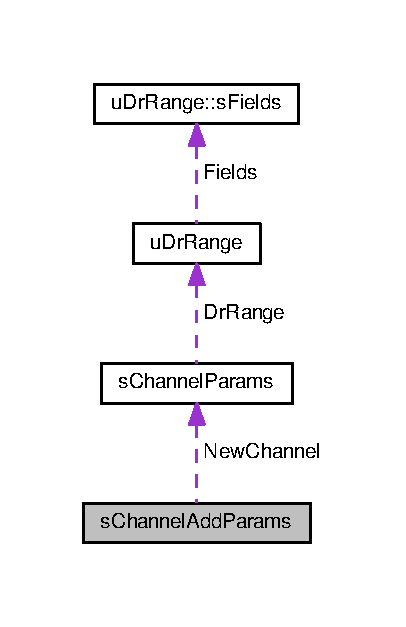
\includegraphics[width=195pt]{structsChannelAddParams__coll__graph}
\end{center}
\end{figure}
\subsection*{Data Fields}
\begin{DoxyCompactItemize}
\item 
\hyperlink{group__LORAMAC_ga1360ca6f82c6d125ea43a9dad9b56184}{Channel\+Params\+\_\+t} $\ast$ \hyperlink{structsChannelAddParams_a137bee029b5796735c1689c969413e63}{New\+Channel}
\item 
uint8\+\_\+t \hyperlink{structsChannelAddParams_a5f26cba04f1453e2b6db2ab73389238b}{Channel\+Id}
\end{DoxyCompactItemize}


\subsection{Detailed Description}
Parameter structure for the function Region\+Channels\+Add. 

\subsection{Field Documentation}
\mbox{\Hypertarget{structsChannelAddParams_a5f26cba04f1453e2b6db2ab73389238b}\label{structsChannelAddParams_a5f26cba04f1453e2b6db2ab73389238b}} 
\index{s\+Channel\+Add\+Params@{s\+Channel\+Add\+Params}!Channel\+Id@{Channel\+Id}}
\index{Channel\+Id@{Channel\+Id}!s\+Channel\+Add\+Params@{s\+Channel\+Add\+Params}}
\subsubsection{\texorpdfstring{Channel\+Id}{ChannelId}}
{\footnotesize\ttfamily uint8\+\_\+t s\+Channel\+Add\+Params\+::\+Channel\+Id}

Channel id to add. \mbox{\Hypertarget{structsChannelAddParams_a137bee029b5796735c1689c969413e63}\label{structsChannelAddParams_a137bee029b5796735c1689c969413e63}} 
\index{s\+Channel\+Add\+Params@{s\+Channel\+Add\+Params}!New\+Channel@{New\+Channel}}
\index{New\+Channel@{New\+Channel}!s\+Channel\+Add\+Params@{s\+Channel\+Add\+Params}}
\subsubsection{\texorpdfstring{New\+Channel}{NewChannel}}
{\footnotesize\ttfamily \hyperlink{group__LORAMAC_ga1360ca6f82c6d125ea43a9dad9b56184}{Channel\+Params\+\_\+t}$\ast$ s\+Channel\+Add\+Params\+::\+New\+Channel}

Pointer to the new channel to add. 

The documentation for this struct was generated from the following file\+:\begin{DoxyCompactItemize}
\item 
Mac/region/\hyperlink{Region_8h}{Region.\+h}\end{DoxyCompactItemize}

\hypertarget{structsChannelParams}{}\section{s\+Channel\+Params Struct Reference}
\label{structsChannelParams}\index{s\+Channel\+Params@{s\+Channel\+Params}}


{\ttfamily \#include $<$Lo\+Ra\+Mac.\+h$>$}



Collaboration diagram for s\+Channel\+Params\+:
\nopagebreak
\begin{figure}[H]
\begin{center}
\leavevmode
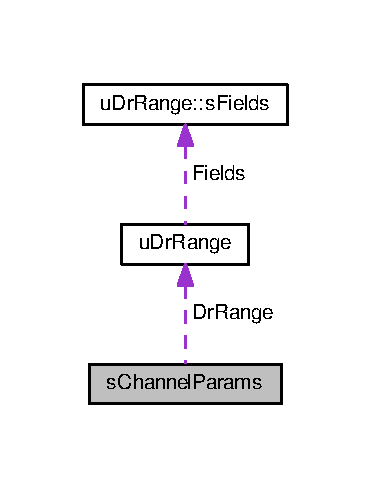
\includegraphics[width=178pt]{structsChannelParams__coll__graph}
\end{center}
\end{figure}
\subsection*{Data Fields}
\begin{DoxyCompactItemize}
\item 
uint32\+\_\+t \hyperlink{structsChannelParams_a3fe5b74bdc28e6388d7e7432a44c39ca}{Frequency}
\item 
uint32\+\_\+t \hyperlink{structsChannelParams_aa8e9aa5d1a595128d8341fd53192dd00}{Rx1\+Frequency}
\item 
\hyperlink{group__LORAMAC_ga8b818a36013d6bdd83ac5fd20f42b503}{Dr\+Range\+\_\+t} \hyperlink{structsChannelParams_a857777f73b0ad0bfd13e7b11d6bfa554}{Dr\+Range}
\item 
uint8\+\_\+t \hyperlink{structsChannelParams_a10517040b4151537ba6cec7783576ce0}{Band}
\end{DoxyCompactItemize}


\subsection{Detailed Description}
Lo\+Ra\+M\+AC channel definition 

\subsection{Field Documentation}
\mbox{\Hypertarget{structsChannelParams_a10517040b4151537ba6cec7783576ce0}\label{structsChannelParams_a10517040b4151537ba6cec7783576ce0}} 
\index{s\+Channel\+Params@{s\+Channel\+Params}!Band@{Band}}
\index{Band@{Band}!s\+Channel\+Params@{s\+Channel\+Params}}
\subsubsection{\texorpdfstring{Band}{Band}}
{\footnotesize\ttfamily uint8\+\_\+t s\+Channel\+Params\+::\+Band}

Band index \mbox{\Hypertarget{structsChannelParams_a857777f73b0ad0bfd13e7b11d6bfa554}\label{structsChannelParams_a857777f73b0ad0bfd13e7b11d6bfa554}} 
\index{s\+Channel\+Params@{s\+Channel\+Params}!Dr\+Range@{Dr\+Range}}
\index{Dr\+Range@{Dr\+Range}!s\+Channel\+Params@{s\+Channel\+Params}}
\subsubsection{\texorpdfstring{Dr\+Range}{DrRange}}
{\footnotesize\ttfamily \hyperlink{group__LORAMAC_ga8b818a36013d6bdd83ac5fd20f42b503}{Dr\+Range\+\_\+t} s\+Channel\+Params\+::\+Dr\+Range}

Data rate definition \mbox{\Hypertarget{structsChannelParams_a3fe5b74bdc28e6388d7e7432a44c39ca}\label{structsChannelParams_a3fe5b74bdc28e6388d7e7432a44c39ca}} 
\index{s\+Channel\+Params@{s\+Channel\+Params}!Frequency@{Frequency}}
\index{Frequency@{Frequency}!s\+Channel\+Params@{s\+Channel\+Params}}
\subsubsection{\texorpdfstring{Frequency}{Frequency}}
{\footnotesize\ttfamily uint32\+\_\+t s\+Channel\+Params\+::\+Frequency}

Frequency in Hz \mbox{\Hypertarget{structsChannelParams_aa8e9aa5d1a595128d8341fd53192dd00}\label{structsChannelParams_aa8e9aa5d1a595128d8341fd53192dd00}} 
\index{s\+Channel\+Params@{s\+Channel\+Params}!Rx1\+Frequency@{Rx1\+Frequency}}
\index{Rx1\+Frequency@{Rx1\+Frequency}!s\+Channel\+Params@{s\+Channel\+Params}}
\subsubsection{\texorpdfstring{Rx1\+Frequency}{Rx1Frequency}}
{\footnotesize\ttfamily uint32\+\_\+t s\+Channel\+Params\+::\+Rx1\+Frequency}

Alternative frequency for RX window 1 

The documentation for this struct was generated from the following file\+:\begin{DoxyCompactItemize}
\item 
Mac/\hyperlink{LoRaMac_8h}{Lo\+Ra\+Mac.\+h}\end{DoxyCompactItemize}

\hypertarget{structsChannelRemoveParams}{}\section{s\+Channel\+Remove\+Params Struct Reference}
\label{structsChannelRemoveParams}\index{s\+Channel\+Remove\+Params@{s\+Channel\+Remove\+Params}}


{\ttfamily \#include $<$Region.\+h$>$}

\subsection*{Data Fields}
\begin{DoxyCompactItemize}
\item 
uint8\+\_\+t \hyperlink{structsChannelRemoveParams_a3fd9bc0d34bd1b5483006fa15546c99a}{Channel\+Id}
\end{DoxyCompactItemize}


\subsection{Detailed Description}
Parameter structure for the function Region\+Channels\+Remove. 

\subsection{Field Documentation}
\mbox{\Hypertarget{structsChannelRemoveParams_a3fd9bc0d34bd1b5483006fa15546c99a}\label{structsChannelRemoveParams_a3fd9bc0d34bd1b5483006fa15546c99a}} 
\index{s\+Channel\+Remove\+Params@{s\+Channel\+Remove\+Params}!Channel\+Id@{Channel\+Id}}
\index{Channel\+Id@{Channel\+Id}!s\+Channel\+Remove\+Params@{s\+Channel\+Remove\+Params}}
\subsubsection{\texorpdfstring{Channel\+Id}{ChannelId}}
{\footnotesize\ttfamily uint8\+\_\+t s\+Channel\+Remove\+Params\+::\+Channel\+Id}

Channel id to remove. 

The documentation for this struct was generated from the following file\+:\begin{DoxyCompactItemize}
\item 
Mac/region/\hyperlink{Region_8h}{Region.\+h}\end{DoxyCompactItemize}

\hypertarget{structsContinuousWaveParams}{}\section{s\+Continuous\+Wave\+Params Struct Reference}
\label{structsContinuousWaveParams}\index{s\+Continuous\+Wave\+Params@{s\+Continuous\+Wave\+Params}}


{\ttfamily \#include $<$Region.\+h$>$}

\subsection*{Data Fields}
\begin{DoxyCompactItemize}
\item 
uint8\+\_\+t \hyperlink{structsContinuousWaveParams_a988ab1a71689757a1ad4fefa502bca02}{Channel}
\item 
int8\+\_\+t \hyperlink{structsContinuousWaveParams_a34ca1b53769fbf5efd5ca962d9fc4c73}{Datarate}
\item 
int8\+\_\+t \hyperlink{structsContinuousWaveParams_aea26241974fa9dac3fa5356a932eedec}{Tx\+Power}
\item 
float \hyperlink{structsContinuousWaveParams_a7da89b73ac0c83e19cfffa9b9bc3496c}{Max\+Eirp}
\item 
float \hyperlink{structsContinuousWaveParams_a42dbd1fc342fdee2da56000fc912571f}{Antenna\+Gain}
\item 
uint16\+\_\+t \hyperlink{structsContinuousWaveParams_ace37bba3a665e1c6957453e6dfb4d5ff}{Timeout}
\end{DoxyCompactItemize}


\subsection{Detailed Description}
Parameter structure for the function Region\+Continuous\+Wave. 

\subsection{Field Documentation}
\mbox{\Hypertarget{structsContinuousWaveParams_a42dbd1fc342fdee2da56000fc912571f}\label{structsContinuousWaveParams_a42dbd1fc342fdee2da56000fc912571f}} 
\index{s\+Continuous\+Wave\+Params@{s\+Continuous\+Wave\+Params}!Antenna\+Gain@{Antenna\+Gain}}
\index{Antenna\+Gain@{Antenna\+Gain}!s\+Continuous\+Wave\+Params@{s\+Continuous\+Wave\+Params}}
\subsubsection{\texorpdfstring{Antenna\+Gain}{AntennaGain}}
{\footnotesize\ttfamily float s\+Continuous\+Wave\+Params\+::\+Antenna\+Gain}

The antenna gain, if applicable. \mbox{\Hypertarget{structsContinuousWaveParams_a988ab1a71689757a1ad4fefa502bca02}\label{structsContinuousWaveParams_a988ab1a71689757a1ad4fefa502bca02}} 
\index{s\+Continuous\+Wave\+Params@{s\+Continuous\+Wave\+Params}!Channel@{Channel}}
\index{Channel@{Channel}!s\+Continuous\+Wave\+Params@{s\+Continuous\+Wave\+Params}}
\subsubsection{\texorpdfstring{Channel}{Channel}}
{\footnotesize\ttfamily uint8\+\_\+t s\+Continuous\+Wave\+Params\+::\+Channel}

Current channel index. \mbox{\Hypertarget{structsContinuousWaveParams_a34ca1b53769fbf5efd5ca962d9fc4c73}\label{structsContinuousWaveParams_a34ca1b53769fbf5efd5ca962d9fc4c73}} 
\index{s\+Continuous\+Wave\+Params@{s\+Continuous\+Wave\+Params}!Datarate@{Datarate}}
\index{Datarate@{Datarate}!s\+Continuous\+Wave\+Params@{s\+Continuous\+Wave\+Params}}
\subsubsection{\texorpdfstring{Datarate}{Datarate}}
{\footnotesize\ttfamily int8\+\_\+t s\+Continuous\+Wave\+Params\+::\+Datarate}

Datarate. Used to limit the TX power. \mbox{\Hypertarget{structsContinuousWaveParams_a7da89b73ac0c83e19cfffa9b9bc3496c}\label{structsContinuousWaveParams_a7da89b73ac0c83e19cfffa9b9bc3496c}} 
\index{s\+Continuous\+Wave\+Params@{s\+Continuous\+Wave\+Params}!Max\+Eirp@{Max\+Eirp}}
\index{Max\+Eirp@{Max\+Eirp}!s\+Continuous\+Wave\+Params@{s\+Continuous\+Wave\+Params}}
\subsubsection{\texorpdfstring{Max\+Eirp}{MaxEirp}}
{\footnotesize\ttfamily float s\+Continuous\+Wave\+Params\+::\+Max\+Eirp}

Max E\+I\+RP, if applicable. \mbox{\Hypertarget{structsContinuousWaveParams_ace37bba3a665e1c6957453e6dfb4d5ff}\label{structsContinuousWaveParams_ace37bba3a665e1c6957453e6dfb4d5ff}} 
\index{s\+Continuous\+Wave\+Params@{s\+Continuous\+Wave\+Params}!Timeout@{Timeout}}
\index{Timeout@{Timeout}!s\+Continuous\+Wave\+Params@{s\+Continuous\+Wave\+Params}}
\subsubsection{\texorpdfstring{Timeout}{Timeout}}
{\footnotesize\ttfamily uint16\+\_\+t s\+Continuous\+Wave\+Params\+::\+Timeout}

Specifies the time the radio will stay in CW mode. \mbox{\Hypertarget{structsContinuousWaveParams_aea26241974fa9dac3fa5356a932eedec}\label{structsContinuousWaveParams_aea26241974fa9dac3fa5356a932eedec}} 
\index{s\+Continuous\+Wave\+Params@{s\+Continuous\+Wave\+Params}!Tx\+Power@{Tx\+Power}}
\index{Tx\+Power@{Tx\+Power}!s\+Continuous\+Wave\+Params@{s\+Continuous\+Wave\+Params}}
\subsubsection{\texorpdfstring{Tx\+Power}{TxPower}}
{\footnotesize\ttfamily int8\+\_\+t s\+Continuous\+Wave\+Params\+::\+Tx\+Power}

The TX power to setup. 

The documentation for this struct was generated from the following file\+:\begin{DoxyCompactItemize}
\item 
Mac/region/\hyperlink{Region_8h}{Region.\+h}\end{DoxyCompactItemize}

\hypertarget{structuLoRaMacFrameCtrl_1_1sCtrlBits}{}\section{u\+Lo\+Ra\+Mac\+Frame\+Ctrl\+:\+:s\+Ctrl\+Bits Struct Reference}
\label{structuLoRaMacFrameCtrl_1_1sCtrlBits}\index{u\+Lo\+Ra\+Mac\+Frame\+Ctrl\+::s\+Ctrl\+Bits@{u\+Lo\+Ra\+Mac\+Frame\+Ctrl\+::s\+Ctrl\+Bits}}


{\ttfamily \#include $<$Lo\+Ra\+Mac.\+h$>$}

\subsection*{Data Fields}
\begin{DoxyCompactItemize}
\item 
uint8\+\_\+t \hyperlink{structuLoRaMacFrameCtrl_1_1sCtrlBits_a2898f8aaf6f0d8bf96a6f1677085abbf}{F\+Opts\+Len}\+: 4
\item 
uint8\+\_\+t \hyperlink{structuLoRaMacFrameCtrl_1_1sCtrlBits_a4ba21bdef24bb0b4c129604611af3cf8}{F\+Pending}\+: 1
\item 
uint8\+\_\+t \hyperlink{structuLoRaMacFrameCtrl_1_1sCtrlBits_a05a3ebfac76baf31edcd09c257e6ebe6}{Ack}\+: 1
\item 
uint8\+\_\+t \hyperlink{structuLoRaMacFrameCtrl_1_1sCtrlBits_af3dbb47839d639d24fd55167e64509bf}{Adr\+Ack\+Req}\+: 1
\item 
uint8\+\_\+t \hyperlink{structuLoRaMacFrameCtrl_1_1sCtrlBits_a8ed08fbd800faa9668e74ca29115a2a9}{Adr}\+: 1
\end{DoxyCompactItemize}


\subsection{Detailed Description}
Structure containing single access to bits 

\subsection{Field Documentation}
\mbox{\Hypertarget{structuLoRaMacFrameCtrl_1_1sCtrlBits_a05a3ebfac76baf31edcd09c257e6ebe6}\label{structuLoRaMacFrameCtrl_1_1sCtrlBits_a05a3ebfac76baf31edcd09c257e6ebe6}} 
\index{u\+Lo\+Ra\+Mac\+Frame\+Ctrl\+::s\+Ctrl\+Bits@{u\+Lo\+Ra\+Mac\+Frame\+Ctrl\+::s\+Ctrl\+Bits}!Ack@{Ack}}
\index{Ack@{Ack}!u\+Lo\+Ra\+Mac\+Frame\+Ctrl\+::s\+Ctrl\+Bits@{u\+Lo\+Ra\+Mac\+Frame\+Ctrl\+::s\+Ctrl\+Bits}}
\subsubsection{\texorpdfstring{Ack}{Ack}}
{\footnotesize\ttfamily uint8\+\_\+t u\+Lo\+Ra\+Mac\+Frame\+Ctrl\+::s\+Ctrl\+Bits\+::\+Ack}

Message acknowledge bit \mbox{\Hypertarget{structuLoRaMacFrameCtrl_1_1sCtrlBits_a8ed08fbd800faa9668e74ca29115a2a9}\label{structuLoRaMacFrameCtrl_1_1sCtrlBits_a8ed08fbd800faa9668e74ca29115a2a9}} 
\index{u\+Lo\+Ra\+Mac\+Frame\+Ctrl\+::s\+Ctrl\+Bits@{u\+Lo\+Ra\+Mac\+Frame\+Ctrl\+::s\+Ctrl\+Bits}!Adr@{Adr}}
\index{Adr@{Adr}!u\+Lo\+Ra\+Mac\+Frame\+Ctrl\+::s\+Ctrl\+Bits@{u\+Lo\+Ra\+Mac\+Frame\+Ctrl\+::s\+Ctrl\+Bits}}
\subsubsection{\texorpdfstring{Adr}{Adr}}
{\footnotesize\ttfamily uint8\+\_\+t u\+Lo\+Ra\+Mac\+Frame\+Ctrl\+::s\+Ctrl\+Bits\+::\+Adr}

A\+DR control in frame header \mbox{\Hypertarget{structuLoRaMacFrameCtrl_1_1sCtrlBits_af3dbb47839d639d24fd55167e64509bf}\label{structuLoRaMacFrameCtrl_1_1sCtrlBits_af3dbb47839d639d24fd55167e64509bf}} 
\index{u\+Lo\+Ra\+Mac\+Frame\+Ctrl\+::s\+Ctrl\+Bits@{u\+Lo\+Ra\+Mac\+Frame\+Ctrl\+::s\+Ctrl\+Bits}!Adr\+Ack\+Req@{Adr\+Ack\+Req}}
\index{Adr\+Ack\+Req@{Adr\+Ack\+Req}!u\+Lo\+Ra\+Mac\+Frame\+Ctrl\+::s\+Ctrl\+Bits@{u\+Lo\+Ra\+Mac\+Frame\+Ctrl\+::s\+Ctrl\+Bits}}
\subsubsection{\texorpdfstring{Adr\+Ack\+Req}{AdrAckReq}}
{\footnotesize\ttfamily uint8\+\_\+t u\+Lo\+Ra\+Mac\+Frame\+Ctrl\+::s\+Ctrl\+Bits\+::\+Adr\+Ack\+Req}

A\+DR acknowledgment request bit \mbox{\Hypertarget{structuLoRaMacFrameCtrl_1_1sCtrlBits_a2898f8aaf6f0d8bf96a6f1677085abbf}\label{structuLoRaMacFrameCtrl_1_1sCtrlBits_a2898f8aaf6f0d8bf96a6f1677085abbf}} 
\index{u\+Lo\+Ra\+Mac\+Frame\+Ctrl\+::s\+Ctrl\+Bits@{u\+Lo\+Ra\+Mac\+Frame\+Ctrl\+::s\+Ctrl\+Bits}!F\+Opts\+Len@{F\+Opts\+Len}}
\index{F\+Opts\+Len@{F\+Opts\+Len}!u\+Lo\+Ra\+Mac\+Frame\+Ctrl\+::s\+Ctrl\+Bits@{u\+Lo\+Ra\+Mac\+Frame\+Ctrl\+::s\+Ctrl\+Bits}}
\subsubsection{\texorpdfstring{F\+Opts\+Len}{FOptsLen}}
{\footnotesize\ttfamily uint8\+\_\+t u\+Lo\+Ra\+Mac\+Frame\+Ctrl\+::s\+Ctrl\+Bits\+::\+F\+Opts\+Len}

Frame options length \mbox{\Hypertarget{structuLoRaMacFrameCtrl_1_1sCtrlBits_a4ba21bdef24bb0b4c129604611af3cf8}\label{structuLoRaMacFrameCtrl_1_1sCtrlBits_a4ba21bdef24bb0b4c129604611af3cf8}} 
\index{u\+Lo\+Ra\+Mac\+Frame\+Ctrl\+::s\+Ctrl\+Bits@{u\+Lo\+Ra\+Mac\+Frame\+Ctrl\+::s\+Ctrl\+Bits}!F\+Pending@{F\+Pending}}
\index{F\+Pending@{F\+Pending}!u\+Lo\+Ra\+Mac\+Frame\+Ctrl\+::s\+Ctrl\+Bits@{u\+Lo\+Ra\+Mac\+Frame\+Ctrl\+::s\+Ctrl\+Bits}}
\subsubsection{\texorpdfstring{F\+Pending}{FPending}}
{\footnotesize\ttfamily uint8\+\_\+t u\+Lo\+Ra\+Mac\+Frame\+Ctrl\+::s\+Ctrl\+Bits\+::\+F\+Pending}

Frame pending bit 

The documentation for this struct was generated from the following file\+:\begin{DoxyCompactItemize}
\item 
Mac/\hyperlink{LoRaMac_8h}{Lo\+Ra\+Mac.\+h}\end{DoxyCompactItemize}

\hypertarget{structuVerifyParams_1_1sDatarateParams}{}\section{u\+Verify\+Params\+:\+:s\+Datarate\+Params Struct Reference}
\label{structuVerifyParams_1_1sDatarateParams}\index{u\+Verify\+Params\+::s\+Datarate\+Params@{u\+Verify\+Params\+::s\+Datarate\+Params}}


{\ttfamily \#include $<$Region.\+h$>$}

\subsection*{Data Fields}
\begin{DoxyCompactItemize}
\item 
int8\+\_\+t \hyperlink{structuVerifyParams_1_1sDatarateParams_ad8ddd1ecfc21d3e9c9e3796a10754673}{Datarate}
\item 
uint8\+\_\+t \hyperlink{structuVerifyParams_1_1sDatarateParams_ae8fd408a4c59e87cf9bda8b0760fb889}{Downlink\+Dwell\+Time}
\item 
uint8\+\_\+t \hyperlink{structuVerifyParams_1_1sDatarateParams_af6e261fe7a0e3117bd0d37084e294ba6}{Uplink\+Dwell\+Time}
\end{DoxyCompactItemize}


\subsection{Detailed Description}
Datarate to verify. 

\subsection{Field Documentation}
\mbox{\Hypertarget{structuVerifyParams_1_1sDatarateParams_ad8ddd1ecfc21d3e9c9e3796a10754673}\label{structuVerifyParams_1_1sDatarateParams_ad8ddd1ecfc21d3e9c9e3796a10754673}} 
\index{u\+Verify\+Params\+::s\+Datarate\+Params@{u\+Verify\+Params\+::s\+Datarate\+Params}!Datarate@{Datarate}}
\index{Datarate@{Datarate}!u\+Verify\+Params\+::s\+Datarate\+Params@{u\+Verify\+Params\+::s\+Datarate\+Params}}
\subsubsection{\texorpdfstring{Datarate}{Datarate}}
{\footnotesize\ttfamily int8\+\_\+t u\+Verify\+Params\+::s\+Datarate\+Params\+::\+Datarate}

Datarate to verify. \mbox{\Hypertarget{structuVerifyParams_1_1sDatarateParams_ae8fd408a4c59e87cf9bda8b0760fb889}\label{structuVerifyParams_1_1sDatarateParams_ae8fd408a4c59e87cf9bda8b0760fb889}} 
\index{u\+Verify\+Params\+::s\+Datarate\+Params@{u\+Verify\+Params\+::s\+Datarate\+Params}!Downlink\+Dwell\+Time@{Downlink\+Dwell\+Time}}
\index{Downlink\+Dwell\+Time@{Downlink\+Dwell\+Time}!u\+Verify\+Params\+::s\+Datarate\+Params@{u\+Verify\+Params\+::s\+Datarate\+Params}}
\subsubsection{\texorpdfstring{Downlink\+Dwell\+Time}{DownlinkDwellTime}}
{\footnotesize\ttfamily uint8\+\_\+t u\+Verify\+Params\+::s\+Datarate\+Params\+::\+Downlink\+Dwell\+Time}

The downlink dwell time. \mbox{\Hypertarget{structuVerifyParams_1_1sDatarateParams_af6e261fe7a0e3117bd0d37084e294ba6}\label{structuVerifyParams_1_1sDatarateParams_af6e261fe7a0e3117bd0d37084e294ba6}} 
\index{u\+Verify\+Params\+::s\+Datarate\+Params@{u\+Verify\+Params\+::s\+Datarate\+Params}!Uplink\+Dwell\+Time@{Uplink\+Dwell\+Time}}
\index{Uplink\+Dwell\+Time@{Uplink\+Dwell\+Time}!u\+Verify\+Params\+::s\+Datarate\+Params@{u\+Verify\+Params\+::s\+Datarate\+Params}}
\subsubsection{\texorpdfstring{Uplink\+Dwell\+Time}{UplinkDwellTime}}
{\footnotesize\ttfamily uint8\+\_\+t u\+Verify\+Params\+::s\+Datarate\+Params\+::\+Uplink\+Dwell\+Time}

The up link dwell time. 

The documentation for this struct was generated from the following file\+:\begin{DoxyCompactItemize}
\item 
Mac/region/\hyperlink{Region_8h}{Region.\+h}\end{DoxyCompactItemize}

\hypertarget{structsDlChannelReqParams}{}\section{s\+Dl\+Channel\+Req\+Params Struct Reference}
\label{structsDlChannelReqParams}\index{s\+Dl\+Channel\+Req\+Params@{s\+Dl\+Channel\+Req\+Params}}


{\ttfamily \#include $<$Region.\+h$>$}

\subsection*{Data Fields}
\begin{DoxyCompactItemize}
\item 
uint8\+\_\+t \hyperlink{structsDlChannelReqParams_ac9b1593479ebc7db1803487c0a7419a9}{Channel\+Id}
\item 
uint32\+\_\+t \hyperlink{structsDlChannelReqParams_a69a02b4124668c9c5298f746b040c453}{Rx1\+Frequency}
\end{DoxyCompactItemize}


\subsection{Detailed Description}
Parameter structure for the function Region\+Dl\+Channel\+Req. 

\subsection{Field Documentation}
\mbox{\Hypertarget{structsDlChannelReqParams_ac9b1593479ebc7db1803487c0a7419a9}\label{structsDlChannelReqParams_ac9b1593479ebc7db1803487c0a7419a9}} 
\index{s\+Dl\+Channel\+Req\+Params@{s\+Dl\+Channel\+Req\+Params}!Channel\+Id@{Channel\+Id}}
\index{Channel\+Id@{Channel\+Id}!s\+Dl\+Channel\+Req\+Params@{s\+Dl\+Channel\+Req\+Params}}
\subsubsection{\texorpdfstring{Channel\+Id}{ChannelId}}
{\footnotesize\ttfamily uint8\+\_\+t s\+Dl\+Channel\+Req\+Params\+::\+Channel\+Id}

Channel Id to add the frequency. \mbox{\Hypertarget{structsDlChannelReqParams_a69a02b4124668c9c5298f746b040c453}\label{structsDlChannelReqParams_a69a02b4124668c9c5298f746b040c453}} 
\index{s\+Dl\+Channel\+Req\+Params@{s\+Dl\+Channel\+Req\+Params}!Rx1\+Frequency@{Rx1\+Frequency}}
\index{Rx1\+Frequency@{Rx1\+Frequency}!s\+Dl\+Channel\+Req\+Params@{s\+Dl\+Channel\+Req\+Params}}
\subsubsection{\texorpdfstring{Rx1\+Frequency}{Rx1Frequency}}
{\footnotesize\ttfamily uint32\+\_\+t s\+Dl\+Channel\+Req\+Params\+::\+Rx1\+Frequency}

Alternative frequency for the Rx1 window. 

The documentation for this struct was generated from the following file\+:\begin{DoxyCompactItemize}
\item 
Mac/region/\hyperlink{Region_8h}{Region.\+h}\end{DoxyCompactItemize}

\hypertarget{structuDrRange_1_1sFields}{}\section{u\+Dr\+Range\+:\+:s\+Fields Struct Reference}
\label{structuDrRange_1_1sFields}\index{u\+Dr\+Range\+::s\+Fields@{u\+Dr\+Range\+::s\+Fields}}


{\ttfamily \#include $<$Lo\+Ra\+Mac.\+h$>$}

\subsection*{Data Fields}
\begin{DoxyCompactItemize}
\item 
int8\+\_\+t \hyperlink{structuDrRange_1_1sFields_aa441513e365122d82f18aec9e7257a35}{Min}\+: 4
\item 
int8\+\_\+t \hyperlink{structuDrRange_1_1sFields_a4fbbc67fabfd2bf96616b34d03786fc8}{Max}\+: 4
\end{DoxyCompactItemize}


\subsection{Detailed Description}
Structure to store the minimum and the maximum datarate 

\subsection{Field Documentation}
\mbox{\Hypertarget{structuDrRange_1_1sFields_a4fbbc67fabfd2bf96616b34d03786fc8}\label{structuDrRange_1_1sFields_a4fbbc67fabfd2bf96616b34d03786fc8}} 
\index{u\+Dr\+Range\+::s\+Fields@{u\+Dr\+Range\+::s\+Fields}!Max@{Max}}
\index{Max@{Max}!u\+Dr\+Range\+::s\+Fields@{u\+Dr\+Range\+::s\+Fields}}
\subsubsection{\texorpdfstring{Max}{Max}}
{\footnotesize\ttfamily int8\+\_\+t u\+Dr\+Range\+::s\+Fields\+::\+Max}

Maximum data rate

Lo\+Ra\+W\+AN Regional Parameters V1.\+0.\+2rB

The allowed ranges are region specific. Please refer to \hyperlink{group__REGION_ga6c4ef966b4f3d5eb7597b087f2b97095}{D\+R\+\_\+0} to \hyperlink{group__REGION_gac6e078f51b71f05093daf27834997396}{D\+R\+\_\+15} for details. \mbox{\Hypertarget{structuDrRange_1_1sFields_aa441513e365122d82f18aec9e7257a35}\label{structuDrRange_1_1sFields_aa441513e365122d82f18aec9e7257a35}} 
\index{u\+Dr\+Range\+::s\+Fields@{u\+Dr\+Range\+::s\+Fields}!Min@{Min}}
\index{Min@{Min}!u\+Dr\+Range\+::s\+Fields@{u\+Dr\+Range\+::s\+Fields}}
\subsubsection{\texorpdfstring{Min}{Min}}
{\footnotesize\ttfamily int8\+\_\+t u\+Dr\+Range\+::s\+Fields\+::\+Min}

Minimum data rate

Lo\+Ra\+W\+AN Regional Parameters V1.\+0.\+2rB

The allowed ranges are region specific. Please refer to \hyperlink{group__REGION_ga6c4ef966b4f3d5eb7597b087f2b97095}{D\+R\+\_\+0} to \hyperlink{group__REGION_gac6e078f51b71f05093daf27834997396}{D\+R\+\_\+15} for details. 

The documentation for this struct was generated from the following file\+:\begin{DoxyCompactItemize}
\item 
Mac/\hyperlink{LoRaMac_8h}{Lo\+Ra\+Mac.\+h}\end{DoxyCompactItemize}

\hypertarget{structsGetPhyParams}{}\section{s\+Get\+Phy\+Params Struct Reference}
\label{structsGetPhyParams}\index{s\+Get\+Phy\+Params@{s\+Get\+Phy\+Params}}


{\ttfamily \#include $<$Region.\+h$>$}

\subsection*{Data Fields}
\begin{DoxyCompactItemize}
\item 
\hyperlink{group__REGION_ga9445b07fdf77581ecfaf389970e635f8}{Phy\+Attribute\+\_\+t} \hyperlink{structsGetPhyParams_a3b91f17df09464368991fb2eed20b6f8}{Attribute}
\item 
int8\+\_\+t \hyperlink{structsGetPhyParams_a61e3c3a6f1b2857333242fad7fd42263}{Datarate}
\item 
uint8\+\_\+t \hyperlink{structsGetPhyParams_ad59a5078532942653d4423c2bf128ed8}{Uplink\+Dwell\+Time}
\item 
uint8\+\_\+t \hyperlink{structsGetPhyParams_aeb0e2347bed31d4bf1cc490ba01ca523}{Downlink\+Dwell\+Time}
\end{DoxyCompactItemize}


\subsection{Detailed Description}
Parameter structure for the function Region\+Get\+Phy\+Param. 

\subsection{Field Documentation}
\mbox{\Hypertarget{structsGetPhyParams_a3b91f17df09464368991fb2eed20b6f8}\label{structsGetPhyParams_a3b91f17df09464368991fb2eed20b6f8}} 
\index{s\+Get\+Phy\+Params@{s\+Get\+Phy\+Params}!Attribute@{Attribute}}
\index{Attribute@{Attribute}!s\+Get\+Phy\+Params@{s\+Get\+Phy\+Params}}
\subsubsection{\texorpdfstring{Attribute}{Attribute}}
{\footnotesize\ttfamily \hyperlink{group__REGION_ga9445b07fdf77581ecfaf389970e635f8}{Phy\+Attribute\+\_\+t} s\+Get\+Phy\+Params\+::\+Attribute}

Setup the parameter to get. \mbox{\Hypertarget{structsGetPhyParams_a61e3c3a6f1b2857333242fad7fd42263}\label{structsGetPhyParams_a61e3c3a6f1b2857333242fad7fd42263}} 
\index{s\+Get\+Phy\+Params@{s\+Get\+Phy\+Params}!Datarate@{Datarate}}
\index{Datarate@{Datarate}!s\+Get\+Phy\+Params@{s\+Get\+Phy\+Params}}
\subsubsection{\texorpdfstring{Datarate}{Datarate}}
{\footnotesize\ttfamily int8\+\_\+t s\+Get\+Phy\+Params\+::\+Datarate}

Datarate. The parameter is needed for the following queries\+: P\+H\+Y\+\_\+\+M\+A\+X\+\_\+\+P\+A\+Y\+L\+O\+AD, P\+H\+Y\+\_\+\+M\+A\+X\+\_\+\+P\+A\+Y\+L\+O\+A\+D\+\_\+\+R\+E\+P\+E\+A\+T\+ER, P\+H\+Y\+\_\+\+N\+E\+X\+T\+\_\+\+L\+O\+W\+E\+R\+\_\+\+T\+X\+\_\+\+DR. \mbox{\Hypertarget{structsGetPhyParams_aeb0e2347bed31d4bf1cc490ba01ca523}\label{structsGetPhyParams_aeb0e2347bed31d4bf1cc490ba01ca523}} 
\index{s\+Get\+Phy\+Params@{s\+Get\+Phy\+Params}!Downlink\+Dwell\+Time@{Downlink\+Dwell\+Time}}
\index{Downlink\+Dwell\+Time@{Downlink\+Dwell\+Time}!s\+Get\+Phy\+Params@{s\+Get\+Phy\+Params}}
\subsubsection{\texorpdfstring{Downlink\+Dwell\+Time}{DownlinkDwellTime}}
{\footnotesize\ttfamily uint8\+\_\+t s\+Get\+Phy\+Params\+::\+Downlink\+Dwell\+Time}

Downlink dwell time. The parameter is needed for the following queries\+: P\+H\+Y\+\_\+\+M\+I\+N\+\_\+\+R\+X\+\_\+\+DR, P\+H\+Y\+\_\+\+M\+A\+X\+\_\+\+P\+A\+Y\+L\+O\+AD, P\+H\+Y\+\_\+\+M\+A\+X\+\_\+\+P\+A\+Y\+L\+O\+A\+D\+\_\+\+R\+E\+P\+E\+A\+T\+ER. \mbox{\Hypertarget{structsGetPhyParams_ad59a5078532942653d4423c2bf128ed8}\label{structsGetPhyParams_ad59a5078532942653d4423c2bf128ed8}} 
\index{s\+Get\+Phy\+Params@{s\+Get\+Phy\+Params}!Uplink\+Dwell\+Time@{Uplink\+Dwell\+Time}}
\index{Uplink\+Dwell\+Time@{Uplink\+Dwell\+Time}!s\+Get\+Phy\+Params@{s\+Get\+Phy\+Params}}
\subsubsection{\texorpdfstring{Uplink\+Dwell\+Time}{UplinkDwellTime}}
{\footnotesize\ttfamily uint8\+\_\+t s\+Get\+Phy\+Params\+::\+Uplink\+Dwell\+Time}

Uplink dwell time. The parameter is needed for the following queries\+: P\+H\+Y\+\_\+\+M\+I\+N\+\_\+\+T\+X\+\_\+\+DR, P\+H\+Y\+\_\+\+M\+A\+X\+\_\+\+P\+A\+Y\+L\+O\+AD, P\+H\+Y\+\_\+\+M\+A\+X\+\_\+\+P\+A\+Y\+L\+O\+A\+D\+\_\+\+R\+E\+P\+E\+A\+T\+ER, P\+H\+Y\+\_\+\+N\+E\+X\+T\+\_\+\+L\+O\+W\+E\+R\+\_\+\+T\+X\+\_\+\+DR. 

The documentation for this struct was generated from the following file\+:\begin{DoxyCompactItemize}
\item 
Mac/region/\hyperlink{Region_8h}{Region.\+h}\end{DoxyCompactItemize}

\hypertarget{structuLoRaMacHeader_1_1sHdrBits}{}\section{u\+Lo\+Ra\+Mac\+Header\+:\+:s\+Hdr\+Bits Struct Reference}
\label{structuLoRaMacHeader_1_1sHdrBits}\index{u\+Lo\+Ra\+Mac\+Header\+::s\+Hdr\+Bits@{u\+Lo\+Ra\+Mac\+Header\+::s\+Hdr\+Bits}}


{\ttfamily \#include $<$Lo\+Ra\+Mac.\+h$>$}

\subsection*{Data Fields}
\begin{DoxyCompactItemize}
\item 
uint8\+\_\+t \hyperlink{structuLoRaMacHeader_1_1sHdrBits_abfa1234e8fba51727315a472697b6165}{Major}\+: 2
\item 
uint8\+\_\+t \hyperlink{structuLoRaMacHeader_1_1sHdrBits_a74570244ef3b1052a532c1dfc2e83b7a}{R\+FU}\+: 3
\item 
uint8\+\_\+t \hyperlink{structuLoRaMacHeader_1_1sHdrBits_af53ac0a55b9c3458f81e9ac24b8366ae}{M\+Type}\+: 3
\end{DoxyCompactItemize}


\subsection{Detailed Description}
Structure containing single access to header bits 

\subsection{Field Documentation}
\mbox{\Hypertarget{structuLoRaMacHeader_1_1sHdrBits_abfa1234e8fba51727315a472697b6165}\label{structuLoRaMacHeader_1_1sHdrBits_abfa1234e8fba51727315a472697b6165}} 
\index{u\+Lo\+Ra\+Mac\+Header\+::s\+Hdr\+Bits@{u\+Lo\+Ra\+Mac\+Header\+::s\+Hdr\+Bits}!Major@{Major}}
\index{Major@{Major}!u\+Lo\+Ra\+Mac\+Header\+::s\+Hdr\+Bits@{u\+Lo\+Ra\+Mac\+Header\+::s\+Hdr\+Bits}}
\subsubsection{\texorpdfstring{Major}{Major}}
{\footnotesize\ttfamily uint8\+\_\+t u\+Lo\+Ra\+Mac\+Header\+::s\+Hdr\+Bits\+::\+Major}

Major version \mbox{\Hypertarget{structuLoRaMacHeader_1_1sHdrBits_af53ac0a55b9c3458f81e9ac24b8366ae}\label{structuLoRaMacHeader_1_1sHdrBits_af53ac0a55b9c3458f81e9ac24b8366ae}} 
\index{u\+Lo\+Ra\+Mac\+Header\+::s\+Hdr\+Bits@{u\+Lo\+Ra\+Mac\+Header\+::s\+Hdr\+Bits}!M\+Type@{M\+Type}}
\index{M\+Type@{M\+Type}!u\+Lo\+Ra\+Mac\+Header\+::s\+Hdr\+Bits@{u\+Lo\+Ra\+Mac\+Header\+::s\+Hdr\+Bits}}
\subsubsection{\texorpdfstring{M\+Type}{MType}}
{\footnotesize\ttfamily uint8\+\_\+t u\+Lo\+Ra\+Mac\+Header\+::s\+Hdr\+Bits\+::\+M\+Type}

Message type \mbox{\Hypertarget{structuLoRaMacHeader_1_1sHdrBits_a74570244ef3b1052a532c1dfc2e83b7a}\label{structuLoRaMacHeader_1_1sHdrBits_a74570244ef3b1052a532c1dfc2e83b7a}} 
\index{u\+Lo\+Ra\+Mac\+Header\+::s\+Hdr\+Bits@{u\+Lo\+Ra\+Mac\+Header\+::s\+Hdr\+Bits}!R\+FU@{R\+FU}}
\index{R\+FU@{R\+FU}!u\+Lo\+Ra\+Mac\+Header\+::s\+Hdr\+Bits@{u\+Lo\+Ra\+Mac\+Header\+::s\+Hdr\+Bits}}
\subsubsection{\texorpdfstring{R\+FU}{RFU}}
{\footnotesize\ttfamily uint8\+\_\+t u\+Lo\+Ra\+Mac\+Header\+::s\+Hdr\+Bits\+::\+R\+FU}

R\+FU 

The documentation for this struct was generated from the following file\+:\begin{DoxyCompactItemize}
\item 
Mac/\hyperlink{LoRaMac_8h}{Lo\+Ra\+Mac.\+h}\end{DoxyCompactItemize}

\hypertarget{structsLinkAdrReqParams}{}\section{s\+Link\+Adr\+Req\+Params Struct Reference}
\label{structsLinkAdrReqParams}\index{s\+Link\+Adr\+Req\+Params@{s\+Link\+Adr\+Req\+Params}}


{\ttfamily \#include $<$Region.\+h$>$}

\subsection*{Data Fields}
\begin{DoxyCompactItemize}
\item 
uint8\+\_\+t $\ast$ \hyperlink{structsLinkAdrReqParams_ad4d35a1161753bb4006dfd00efd04270}{Payload}
\item 
uint8\+\_\+t \hyperlink{structsLinkAdrReqParams_ae12d8663597aa0cf1134ac00f77238c4}{Payload\+Size}
\item 
uint8\+\_\+t \hyperlink{structsLinkAdrReqParams_a4e183e8eb34bdc875c1d746a37985ac1}{Uplink\+Dwell\+Time}
\item 
bool \hyperlink{structsLinkAdrReqParams_abb00ae40cef849998af4c833c3811136}{Adr\+Enabled}
\item 
int8\+\_\+t \hyperlink{structsLinkAdrReqParams_a41048b1ea55a4acf361fbea7535c9ffe}{Current\+Datarate}
\item 
int8\+\_\+t \hyperlink{structsLinkAdrReqParams_ac23ec953d7e409b28938bfdc01a2d2a8}{Current\+Tx\+Power}
\item 
uint8\+\_\+t \hyperlink{structsLinkAdrReqParams_acdca5949f614789437af421720461a47}{Current\+Nb\+Rep}
\end{DoxyCompactItemize}


\subsection{Detailed Description}
Parameter structure for the function Region\+Link\+Adr\+Req. 

\subsection{Field Documentation}
\mbox{\Hypertarget{structsLinkAdrReqParams_abb00ae40cef849998af4c833c3811136}\label{structsLinkAdrReqParams_abb00ae40cef849998af4c833c3811136}} 
\index{s\+Link\+Adr\+Req\+Params@{s\+Link\+Adr\+Req\+Params}!Adr\+Enabled@{Adr\+Enabled}}
\index{Adr\+Enabled@{Adr\+Enabled}!s\+Link\+Adr\+Req\+Params@{s\+Link\+Adr\+Req\+Params}}
\subsubsection{\texorpdfstring{Adr\+Enabled}{AdrEnabled}}
{\footnotesize\ttfamily bool s\+Link\+Adr\+Req\+Params\+::\+Adr\+Enabled}

Set to true, if A\+DR is enabled. \mbox{\Hypertarget{structsLinkAdrReqParams_a41048b1ea55a4acf361fbea7535c9ffe}\label{structsLinkAdrReqParams_a41048b1ea55a4acf361fbea7535c9ffe}} 
\index{s\+Link\+Adr\+Req\+Params@{s\+Link\+Adr\+Req\+Params}!Current\+Datarate@{Current\+Datarate}}
\index{Current\+Datarate@{Current\+Datarate}!s\+Link\+Adr\+Req\+Params@{s\+Link\+Adr\+Req\+Params}}
\subsubsection{\texorpdfstring{Current\+Datarate}{CurrentDatarate}}
{\footnotesize\ttfamily int8\+\_\+t s\+Link\+Adr\+Req\+Params\+::\+Current\+Datarate}

The current datarate. \mbox{\Hypertarget{structsLinkAdrReqParams_acdca5949f614789437af421720461a47}\label{structsLinkAdrReqParams_acdca5949f614789437af421720461a47}} 
\index{s\+Link\+Adr\+Req\+Params@{s\+Link\+Adr\+Req\+Params}!Current\+Nb\+Rep@{Current\+Nb\+Rep}}
\index{Current\+Nb\+Rep@{Current\+Nb\+Rep}!s\+Link\+Adr\+Req\+Params@{s\+Link\+Adr\+Req\+Params}}
\subsubsection{\texorpdfstring{Current\+Nb\+Rep}{CurrentNbRep}}
{\footnotesize\ttfamily uint8\+\_\+t s\+Link\+Adr\+Req\+Params\+::\+Current\+Nb\+Rep}

The current number of repetitions. \mbox{\Hypertarget{structsLinkAdrReqParams_ac23ec953d7e409b28938bfdc01a2d2a8}\label{structsLinkAdrReqParams_ac23ec953d7e409b28938bfdc01a2d2a8}} 
\index{s\+Link\+Adr\+Req\+Params@{s\+Link\+Adr\+Req\+Params}!Current\+Tx\+Power@{Current\+Tx\+Power}}
\index{Current\+Tx\+Power@{Current\+Tx\+Power}!s\+Link\+Adr\+Req\+Params@{s\+Link\+Adr\+Req\+Params}}
\subsubsection{\texorpdfstring{Current\+Tx\+Power}{CurrentTxPower}}
{\footnotesize\ttfamily int8\+\_\+t s\+Link\+Adr\+Req\+Params\+::\+Current\+Tx\+Power}

The current TX power. \mbox{\Hypertarget{structsLinkAdrReqParams_ad4d35a1161753bb4006dfd00efd04270}\label{structsLinkAdrReqParams_ad4d35a1161753bb4006dfd00efd04270}} 
\index{s\+Link\+Adr\+Req\+Params@{s\+Link\+Adr\+Req\+Params}!Payload@{Payload}}
\index{Payload@{Payload}!s\+Link\+Adr\+Req\+Params@{s\+Link\+Adr\+Req\+Params}}
\subsubsection{\texorpdfstring{Payload}{Payload}}
{\footnotesize\ttfamily uint8\+\_\+t$\ast$ s\+Link\+Adr\+Req\+Params\+::\+Payload}

Pointer to the payload which contains the M\+AC commands. \mbox{\Hypertarget{structsLinkAdrReqParams_ae12d8663597aa0cf1134ac00f77238c4}\label{structsLinkAdrReqParams_ae12d8663597aa0cf1134ac00f77238c4}} 
\index{s\+Link\+Adr\+Req\+Params@{s\+Link\+Adr\+Req\+Params}!Payload\+Size@{Payload\+Size}}
\index{Payload\+Size@{Payload\+Size}!s\+Link\+Adr\+Req\+Params@{s\+Link\+Adr\+Req\+Params}}
\subsubsection{\texorpdfstring{Payload\+Size}{PayloadSize}}
{\footnotesize\ttfamily uint8\+\_\+t s\+Link\+Adr\+Req\+Params\+::\+Payload\+Size}

Size of the payload. \mbox{\Hypertarget{structsLinkAdrReqParams_a4e183e8eb34bdc875c1d746a37985ac1}\label{structsLinkAdrReqParams_a4e183e8eb34bdc875c1d746a37985ac1}} 
\index{s\+Link\+Adr\+Req\+Params@{s\+Link\+Adr\+Req\+Params}!Uplink\+Dwell\+Time@{Uplink\+Dwell\+Time}}
\index{Uplink\+Dwell\+Time@{Uplink\+Dwell\+Time}!s\+Link\+Adr\+Req\+Params@{s\+Link\+Adr\+Req\+Params}}
\subsubsection{\texorpdfstring{Uplink\+Dwell\+Time}{UplinkDwellTime}}
{\footnotesize\ttfamily uint8\+\_\+t s\+Link\+Adr\+Req\+Params\+::\+Uplink\+Dwell\+Time}

Uplink dwell time. 

The documentation for this struct was generated from the following file\+:\begin{DoxyCompactItemize}
\item 
Mac/region/\hyperlink{Region_8h}{Region.\+h}\end{DoxyCompactItemize}

\hypertarget{structsLoRaMacCallback}{}\section{s\+Lo\+Ra\+Mac\+Callback Struct Reference}
\label{structsLoRaMacCallback}\index{s\+Lo\+Ra\+Mac\+Callback@{s\+Lo\+Ra\+Mac\+Callback}}


{\ttfamily \#include $<$Lo\+Ra\+Mac.\+h$>$}

\subsection*{Data Fields}
\begin{DoxyCompactItemize}
\item 
uint8\+\_\+t($\ast$ \hyperlink{structsLoRaMacCallback_a538201ffef6cc64ae29f510851a656f2}{Get\+Battery\+Level} )(void)
\begin{DoxyCompactList}\small\item\em Measures the battery level. \end{DoxyCompactList}\end{DoxyCompactItemize}


\subsection{Detailed Description}
Lo\+Ra\+M\+AC callback structure 

\subsection{Field Documentation}
\mbox{\Hypertarget{structsLoRaMacCallback_a538201ffef6cc64ae29f510851a656f2}\label{structsLoRaMacCallback_a538201ffef6cc64ae29f510851a656f2}} 
\index{s\+Lo\+Ra\+Mac\+Callback@{s\+Lo\+Ra\+Mac\+Callback}!Get\+Battery\+Level@{Get\+Battery\+Level}}
\index{Get\+Battery\+Level@{Get\+Battery\+Level}!s\+Lo\+Ra\+Mac\+Callback@{s\+Lo\+Ra\+Mac\+Callback}}
\subsubsection{\texorpdfstring{Get\+Battery\+Level}{GetBatteryLevel}}
{\footnotesize\ttfamily uint8\+\_\+t( $\ast$ s\+Lo\+Ra\+Mac\+Callback\+::\+Get\+Battery\+Level) (void)}



Measures the battery level. 


\begin{DoxyRetVals}{Return values}
{\em Battery} & level \mbox{[}0\+: node is connected to an external power source, 1..254\+: battery level, where 1 is the minimum and 254 is the maximum value, 255\+: the node was not able to measure the battery level\mbox{]} \\
\hline
\end{DoxyRetVals}


The documentation for this struct was generated from the following file\+:\begin{DoxyCompactItemize}
\item 
Mac/\hyperlink{LoRaMac_8h}{Lo\+Ra\+Mac.\+h}\end{DoxyCompactItemize}

\hypertarget{structsLoRaMacParams}{}\section{s\+Lo\+Ra\+Mac\+Params Struct Reference}
\label{structsLoRaMacParams}\index{s\+Lo\+Ra\+Mac\+Params@{s\+Lo\+Ra\+Mac\+Params}}


{\ttfamily \#include $<$Lo\+Ra\+Mac.\+h$>$}



Collaboration diagram for s\+Lo\+Ra\+Mac\+Params\+:
\nopagebreak
\begin{figure}[H]
\begin{center}
\leavevmode
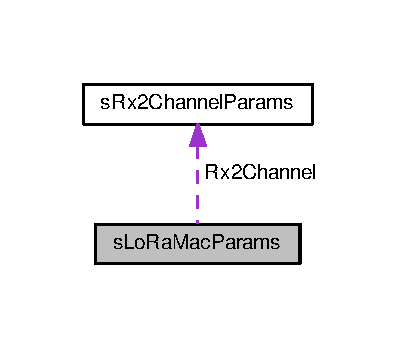
\includegraphics[width=193pt]{structsLoRaMacParams__coll__graph}
\end{center}
\end{figure}
\subsection*{Data Fields}
\begin{DoxyCompactItemize}
\item 
int8\+\_\+t \hyperlink{structsLoRaMacParams_a3e7d1d54a64dc76539c12e1dd3cc316f}{Channels\+Tx\+Power}
\item 
int8\+\_\+t \hyperlink{structsLoRaMacParams_a4c69ccb4d47d2dd72248d66671a64d06}{Channels\+Datarate}
\item 
uint32\+\_\+t \hyperlink{structsLoRaMacParams_a8ec7fc06c76a9ad6b56ee20c77540dcd}{System\+Max\+Rx\+Error}
\item 
uint8\+\_\+t \hyperlink{structsLoRaMacParams_a59098e239afcb8f7897d10f37ee64625}{Min\+Rx\+Symbols}
\item 
uint32\+\_\+t \hyperlink{structsLoRaMacParams_a1cc6077f5089f55803c7eaa73ddd594c}{Max\+Rx\+Window}
\item 
uint32\+\_\+t \hyperlink{structsLoRaMacParams_a6f54a81f03cdffceec50e3cf9cc83228}{Receive\+Delay1}
\item 
uint32\+\_\+t \hyperlink{structsLoRaMacParams_a587f62a64ee82e29e260a3ea1acaa156}{Receive\+Delay2}
\item 
uint32\+\_\+t \hyperlink{structsLoRaMacParams_a80aa9bf077423697b47b22afb6dde729}{Join\+Accept\+Delay1}
\item 
uint32\+\_\+t \hyperlink{structsLoRaMacParams_a42335ca2034e1352546d473fb0b917a8}{Join\+Accept\+Delay2}
\item 
uint8\+\_\+t \hyperlink{structsLoRaMacParams_aa96ac22c28fad8318dcdffe58c893210}{Channels\+Nb\+Rep}
\item 
uint8\+\_\+t \hyperlink{structsLoRaMacParams_acb99a582d1fb1b6b744d965b93006eed}{Rx1\+Dr\+Offset}
\item 
\hyperlink{group__LORAMAC_ga8f57f29481ea92c24f6af04b96a95e0f}{Rx2\+Channel\+Params\+\_\+t} \hyperlink{structsLoRaMacParams_a10ca1854770d376f3b35aff131739378}{Rx2\+Channel}
\item 
uint8\+\_\+t \hyperlink{structsLoRaMacParams_afa2a5ecb973c489cfcf5e6a0f7d28ab3}{Uplink\+Dwell\+Time}
\item 
uint8\+\_\+t \hyperlink{structsLoRaMacParams_aec937b2400c0214e760f830ad4f40b48}{Downlink\+Dwell\+Time}
\item 
float \hyperlink{structsLoRaMacParams_a5f2cfed6f5c51de287017c30da2f953a}{Max\+Eirp}
\item 
float \hyperlink{structsLoRaMacParams_a5a9de6bfd5a7ce1885db4f4029b55cd5}{Antenna\+Gain}
\end{DoxyCompactItemize}


\subsection{Detailed Description}
Global M\+AC layer parameters 

\subsection{Field Documentation}
\mbox{\Hypertarget{structsLoRaMacParams_a5a9de6bfd5a7ce1885db4f4029b55cd5}\label{structsLoRaMacParams_a5a9de6bfd5a7ce1885db4f4029b55cd5}} 
\index{s\+Lo\+Ra\+Mac\+Params@{s\+Lo\+Ra\+Mac\+Params}!Antenna\+Gain@{Antenna\+Gain}}
\index{Antenna\+Gain@{Antenna\+Gain}!s\+Lo\+Ra\+Mac\+Params@{s\+Lo\+Ra\+Mac\+Params}}
\subsubsection{\texorpdfstring{Antenna\+Gain}{AntennaGain}}
{\footnotesize\ttfamily float s\+Lo\+Ra\+Mac\+Params\+::\+Antenna\+Gain}

Antenna gain of the node \mbox{\Hypertarget{structsLoRaMacParams_a4c69ccb4d47d2dd72248d66671a64d06}\label{structsLoRaMacParams_a4c69ccb4d47d2dd72248d66671a64d06}} 
\index{s\+Lo\+Ra\+Mac\+Params@{s\+Lo\+Ra\+Mac\+Params}!Channels\+Datarate@{Channels\+Datarate}}
\index{Channels\+Datarate@{Channels\+Datarate}!s\+Lo\+Ra\+Mac\+Params@{s\+Lo\+Ra\+Mac\+Params}}
\subsubsection{\texorpdfstring{Channels\+Datarate}{ChannelsDatarate}}
{\footnotesize\ttfamily int8\+\_\+t s\+Lo\+Ra\+Mac\+Params\+::\+Channels\+Datarate}

Channels data rate \mbox{\Hypertarget{structsLoRaMacParams_aa96ac22c28fad8318dcdffe58c893210}\label{structsLoRaMacParams_aa96ac22c28fad8318dcdffe58c893210}} 
\index{s\+Lo\+Ra\+Mac\+Params@{s\+Lo\+Ra\+Mac\+Params}!Channels\+Nb\+Rep@{Channels\+Nb\+Rep}}
\index{Channels\+Nb\+Rep@{Channels\+Nb\+Rep}!s\+Lo\+Ra\+Mac\+Params@{s\+Lo\+Ra\+Mac\+Params}}
\subsubsection{\texorpdfstring{Channels\+Nb\+Rep}{ChannelsNbRep}}
{\footnotesize\ttfamily uint8\+\_\+t s\+Lo\+Ra\+Mac\+Params\+::\+Channels\+Nb\+Rep}

Number of uplink messages repetitions \mbox{[}1\+:15\mbox{]} (unconfirmed messages only) \mbox{\Hypertarget{structsLoRaMacParams_a3e7d1d54a64dc76539c12e1dd3cc316f}\label{structsLoRaMacParams_a3e7d1d54a64dc76539c12e1dd3cc316f}} 
\index{s\+Lo\+Ra\+Mac\+Params@{s\+Lo\+Ra\+Mac\+Params}!Channels\+Tx\+Power@{Channels\+Tx\+Power}}
\index{Channels\+Tx\+Power@{Channels\+Tx\+Power}!s\+Lo\+Ra\+Mac\+Params@{s\+Lo\+Ra\+Mac\+Params}}
\subsubsection{\texorpdfstring{Channels\+Tx\+Power}{ChannelsTxPower}}
{\footnotesize\ttfamily int8\+\_\+t s\+Lo\+Ra\+Mac\+Params\+::\+Channels\+Tx\+Power}

Channels TX power \mbox{\Hypertarget{structsLoRaMacParams_aec937b2400c0214e760f830ad4f40b48}\label{structsLoRaMacParams_aec937b2400c0214e760f830ad4f40b48}} 
\index{s\+Lo\+Ra\+Mac\+Params@{s\+Lo\+Ra\+Mac\+Params}!Downlink\+Dwell\+Time@{Downlink\+Dwell\+Time}}
\index{Downlink\+Dwell\+Time@{Downlink\+Dwell\+Time}!s\+Lo\+Ra\+Mac\+Params@{s\+Lo\+Ra\+Mac\+Params}}
\subsubsection{\texorpdfstring{Downlink\+Dwell\+Time}{DownlinkDwellTime}}
{\footnotesize\ttfamily uint8\+\_\+t s\+Lo\+Ra\+Mac\+Params\+::\+Downlink\+Dwell\+Time}

Downlink dwell time configuration. 0\+: No limit, 1\+: 400ms \mbox{\Hypertarget{structsLoRaMacParams_a80aa9bf077423697b47b22afb6dde729}\label{structsLoRaMacParams_a80aa9bf077423697b47b22afb6dde729}} 
\index{s\+Lo\+Ra\+Mac\+Params@{s\+Lo\+Ra\+Mac\+Params}!Join\+Accept\+Delay1@{Join\+Accept\+Delay1}}
\index{Join\+Accept\+Delay1@{Join\+Accept\+Delay1}!s\+Lo\+Ra\+Mac\+Params@{s\+Lo\+Ra\+Mac\+Params}}
\subsubsection{\texorpdfstring{Join\+Accept\+Delay1}{JoinAcceptDelay1}}
{\footnotesize\ttfamily uint32\+\_\+t s\+Lo\+Ra\+Mac\+Params\+::\+Join\+Accept\+Delay1}

Join accept delay 1 \mbox{\Hypertarget{structsLoRaMacParams_a42335ca2034e1352546d473fb0b917a8}\label{structsLoRaMacParams_a42335ca2034e1352546d473fb0b917a8}} 
\index{s\+Lo\+Ra\+Mac\+Params@{s\+Lo\+Ra\+Mac\+Params}!Join\+Accept\+Delay2@{Join\+Accept\+Delay2}}
\index{Join\+Accept\+Delay2@{Join\+Accept\+Delay2}!s\+Lo\+Ra\+Mac\+Params@{s\+Lo\+Ra\+Mac\+Params}}
\subsubsection{\texorpdfstring{Join\+Accept\+Delay2}{JoinAcceptDelay2}}
{\footnotesize\ttfamily uint32\+\_\+t s\+Lo\+Ra\+Mac\+Params\+::\+Join\+Accept\+Delay2}

Join accept delay 1 \mbox{\Hypertarget{structsLoRaMacParams_a5f2cfed6f5c51de287017c30da2f953a}\label{structsLoRaMacParams_a5f2cfed6f5c51de287017c30da2f953a}} 
\index{s\+Lo\+Ra\+Mac\+Params@{s\+Lo\+Ra\+Mac\+Params}!Max\+Eirp@{Max\+Eirp}}
\index{Max\+Eirp@{Max\+Eirp}!s\+Lo\+Ra\+Mac\+Params@{s\+Lo\+Ra\+Mac\+Params}}
\subsubsection{\texorpdfstring{Max\+Eirp}{MaxEirp}}
{\footnotesize\ttfamily float s\+Lo\+Ra\+Mac\+Params\+::\+Max\+Eirp}

Maximum possible E\+I\+RP \mbox{\Hypertarget{structsLoRaMacParams_a1cc6077f5089f55803c7eaa73ddd594c}\label{structsLoRaMacParams_a1cc6077f5089f55803c7eaa73ddd594c}} 
\index{s\+Lo\+Ra\+Mac\+Params@{s\+Lo\+Ra\+Mac\+Params}!Max\+Rx\+Window@{Max\+Rx\+Window}}
\index{Max\+Rx\+Window@{Max\+Rx\+Window}!s\+Lo\+Ra\+Mac\+Params@{s\+Lo\+Ra\+Mac\+Params}}
\subsubsection{\texorpdfstring{Max\+Rx\+Window}{MaxRxWindow}}
{\footnotesize\ttfamily uint32\+\_\+t s\+Lo\+Ra\+Mac\+Params\+::\+Max\+Rx\+Window}

Lo\+Ra\+Mac maximum time a reception window stays open \mbox{\Hypertarget{structsLoRaMacParams_a59098e239afcb8f7897d10f37ee64625}\label{structsLoRaMacParams_a59098e239afcb8f7897d10f37ee64625}} 
\index{s\+Lo\+Ra\+Mac\+Params@{s\+Lo\+Ra\+Mac\+Params}!Min\+Rx\+Symbols@{Min\+Rx\+Symbols}}
\index{Min\+Rx\+Symbols@{Min\+Rx\+Symbols}!s\+Lo\+Ra\+Mac\+Params@{s\+Lo\+Ra\+Mac\+Params}}
\subsubsection{\texorpdfstring{Min\+Rx\+Symbols}{MinRxSymbols}}
{\footnotesize\ttfamily uint8\+\_\+t s\+Lo\+Ra\+Mac\+Params\+::\+Min\+Rx\+Symbols}

Minimum required number of symbols to detect an Rx frame Default\+: 6 symbols \mbox{\Hypertarget{structsLoRaMacParams_a6f54a81f03cdffceec50e3cf9cc83228}\label{structsLoRaMacParams_a6f54a81f03cdffceec50e3cf9cc83228}} 
\index{s\+Lo\+Ra\+Mac\+Params@{s\+Lo\+Ra\+Mac\+Params}!Receive\+Delay1@{Receive\+Delay1}}
\index{Receive\+Delay1@{Receive\+Delay1}!s\+Lo\+Ra\+Mac\+Params@{s\+Lo\+Ra\+Mac\+Params}}
\subsubsection{\texorpdfstring{Receive\+Delay1}{ReceiveDelay1}}
{\footnotesize\ttfamily uint32\+\_\+t s\+Lo\+Ra\+Mac\+Params\+::\+Receive\+Delay1}

Receive delay 1 \mbox{\Hypertarget{structsLoRaMacParams_a587f62a64ee82e29e260a3ea1acaa156}\label{structsLoRaMacParams_a587f62a64ee82e29e260a3ea1acaa156}} 
\index{s\+Lo\+Ra\+Mac\+Params@{s\+Lo\+Ra\+Mac\+Params}!Receive\+Delay2@{Receive\+Delay2}}
\index{Receive\+Delay2@{Receive\+Delay2}!s\+Lo\+Ra\+Mac\+Params@{s\+Lo\+Ra\+Mac\+Params}}
\subsubsection{\texorpdfstring{Receive\+Delay2}{ReceiveDelay2}}
{\footnotesize\ttfamily uint32\+\_\+t s\+Lo\+Ra\+Mac\+Params\+::\+Receive\+Delay2}

Receive delay 2 \mbox{\Hypertarget{structsLoRaMacParams_acb99a582d1fb1b6b744d965b93006eed}\label{structsLoRaMacParams_acb99a582d1fb1b6b744d965b93006eed}} 
\index{s\+Lo\+Ra\+Mac\+Params@{s\+Lo\+Ra\+Mac\+Params}!Rx1\+Dr\+Offset@{Rx1\+Dr\+Offset}}
\index{Rx1\+Dr\+Offset@{Rx1\+Dr\+Offset}!s\+Lo\+Ra\+Mac\+Params@{s\+Lo\+Ra\+Mac\+Params}}
\subsubsection{\texorpdfstring{Rx1\+Dr\+Offset}{Rx1DrOffset}}
{\footnotesize\ttfamily uint8\+\_\+t s\+Lo\+Ra\+Mac\+Params\+::\+Rx1\+Dr\+Offset}

Datarate offset between uplink and downlink on first window \mbox{\Hypertarget{structsLoRaMacParams_a10ca1854770d376f3b35aff131739378}\label{structsLoRaMacParams_a10ca1854770d376f3b35aff131739378}} 
\index{s\+Lo\+Ra\+Mac\+Params@{s\+Lo\+Ra\+Mac\+Params}!Rx2\+Channel@{Rx2\+Channel}}
\index{Rx2\+Channel@{Rx2\+Channel}!s\+Lo\+Ra\+Mac\+Params@{s\+Lo\+Ra\+Mac\+Params}}
\subsubsection{\texorpdfstring{Rx2\+Channel}{Rx2Channel}}
{\footnotesize\ttfamily \hyperlink{group__LORAMAC_ga8f57f29481ea92c24f6af04b96a95e0f}{Rx2\+Channel\+Params\+\_\+t} s\+Lo\+Ra\+Mac\+Params\+::\+Rx2\+Channel}

Lo\+Ra\+M\+AC 2nd reception window settings \mbox{\Hypertarget{structsLoRaMacParams_a8ec7fc06c76a9ad6b56ee20c77540dcd}\label{structsLoRaMacParams_a8ec7fc06c76a9ad6b56ee20c77540dcd}} 
\index{s\+Lo\+Ra\+Mac\+Params@{s\+Lo\+Ra\+Mac\+Params}!System\+Max\+Rx\+Error@{System\+Max\+Rx\+Error}}
\index{System\+Max\+Rx\+Error@{System\+Max\+Rx\+Error}!s\+Lo\+Ra\+Mac\+Params@{s\+Lo\+Ra\+Mac\+Params}}
\subsubsection{\texorpdfstring{System\+Max\+Rx\+Error}{SystemMaxRxError}}
{\footnotesize\ttfamily uint32\+\_\+t s\+Lo\+Ra\+Mac\+Params\+::\+System\+Max\+Rx\+Error}

System overall timing error in milliseconds. \mbox{[}-\/\+System\+Max\+Rx\+Error \+: +\+System\+Max\+Rx\+Error\mbox{]} Default\+: +/-\/10 ms \mbox{\Hypertarget{structsLoRaMacParams_afa2a5ecb973c489cfcf5e6a0f7d28ab3}\label{structsLoRaMacParams_afa2a5ecb973c489cfcf5e6a0f7d28ab3}} 
\index{s\+Lo\+Ra\+Mac\+Params@{s\+Lo\+Ra\+Mac\+Params}!Uplink\+Dwell\+Time@{Uplink\+Dwell\+Time}}
\index{Uplink\+Dwell\+Time@{Uplink\+Dwell\+Time}!s\+Lo\+Ra\+Mac\+Params@{s\+Lo\+Ra\+Mac\+Params}}
\subsubsection{\texorpdfstring{Uplink\+Dwell\+Time}{UplinkDwellTime}}
{\footnotesize\ttfamily uint8\+\_\+t s\+Lo\+Ra\+Mac\+Params\+::\+Uplink\+Dwell\+Time}

Uplink dwell time configuration. 0\+: No limit, 1\+: 400ms 

The documentation for this struct was generated from the following file\+:\begin{DoxyCompactItemize}
\item 
Mac/\hyperlink{LoRaMac_8h}{Lo\+Ra\+Mac.\+h}\end{DoxyCompactItemize}

\hypertarget{structsLoRaMacPrimitives}{}\section{s\+Lo\+Ra\+Mac\+Primitives Struct Reference}
\label{structsLoRaMacPrimitives}\index{s\+Lo\+Ra\+Mac\+Primitives@{s\+Lo\+Ra\+Mac\+Primitives}}


{\ttfamily \#include $<$Lo\+Ra\+Mac.\+h$>$}

\subsection*{Data Fields}
\begin{DoxyCompactItemize}
\item 
void($\ast$ \hyperlink{structsLoRaMacPrimitives_acf5c5408390c791958dc72f1496b3878}{Mac\+Mcps\+Confirm} )(\hyperlink{group__LORAMAC_ga925536babf8abe83918a19f5ae88bd44}{Mcps\+Confirm\+\_\+t} $\ast$Mcps\+Confirm)
\begin{DoxyCompactList}\small\item\em M\+C\+P\+S-\/\+Confirm primitive. \end{DoxyCompactList}\item 
void($\ast$ \hyperlink{structsLoRaMacPrimitives_aa7eb02232243c705b7ac43a89fa3aed0}{Mac\+Mcps\+Indication} )(\hyperlink{group__LORAMAC_ga202591b6553d63fae89bd42787496616}{Mcps\+Indication\+\_\+t} $\ast$Mcps\+Indication)
\begin{DoxyCompactList}\small\item\em M\+C\+P\+S-\/\+Indication primitive. \end{DoxyCompactList}\item 
void($\ast$ \hyperlink{structsLoRaMacPrimitives_af92fa5e7a0dcb1139adc5f60ef1538c1}{Mac\+Mlme\+Confirm} )(\hyperlink{group__LORAMAC_ga73d9d9e11e282a6c258c4d22865fe824}{Mlme\+Confirm\+\_\+t} $\ast$Mlme\+Confirm)
\begin{DoxyCompactList}\small\item\em M\+L\+M\+E-\/\+Confirm primitive. \end{DoxyCompactList}\end{DoxyCompactItemize}


\subsection{Detailed Description}
Lo\+Ra\+M\+AC events structure Used to notify upper layers of M\+AC events 

\subsection{Field Documentation}
\mbox{\Hypertarget{structsLoRaMacPrimitives_acf5c5408390c791958dc72f1496b3878}\label{structsLoRaMacPrimitives_acf5c5408390c791958dc72f1496b3878}} 
\index{s\+Lo\+Ra\+Mac\+Primitives@{s\+Lo\+Ra\+Mac\+Primitives}!Mac\+Mcps\+Confirm@{Mac\+Mcps\+Confirm}}
\index{Mac\+Mcps\+Confirm@{Mac\+Mcps\+Confirm}!s\+Lo\+Ra\+Mac\+Primitives@{s\+Lo\+Ra\+Mac\+Primitives}}
\subsubsection{\texorpdfstring{Mac\+Mcps\+Confirm}{MacMcpsConfirm}}
{\footnotesize\ttfamily void( $\ast$ s\+Lo\+Ra\+Mac\+Primitives\+::\+Mac\+Mcps\+Confirm) (\hyperlink{group__LORAMAC_ga925536babf8abe83918a19f5ae88bd44}{Mcps\+Confirm\+\_\+t} $\ast$Mcps\+Confirm)}



M\+C\+P\+S-\/\+Confirm primitive. 


\begin{DoxyParams}{Parameters}
{\em \mbox{[}\+O\+U\+T\mbox{]}} & M\+C\+P\+S-\/\+Confirm parameters \\
\hline
\end{DoxyParams}
\mbox{\Hypertarget{structsLoRaMacPrimitives_aa7eb02232243c705b7ac43a89fa3aed0}\label{structsLoRaMacPrimitives_aa7eb02232243c705b7ac43a89fa3aed0}} 
\index{s\+Lo\+Ra\+Mac\+Primitives@{s\+Lo\+Ra\+Mac\+Primitives}!Mac\+Mcps\+Indication@{Mac\+Mcps\+Indication}}
\index{Mac\+Mcps\+Indication@{Mac\+Mcps\+Indication}!s\+Lo\+Ra\+Mac\+Primitives@{s\+Lo\+Ra\+Mac\+Primitives}}
\subsubsection{\texorpdfstring{Mac\+Mcps\+Indication}{MacMcpsIndication}}
{\footnotesize\ttfamily void( $\ast$ s\+Lo\+Ra\+Mac\+Primitives\+::\+Mac\+Mcps\+Indication) (\hyperlink{group__LORAMAC_ga202591b6553d63fae89bd42787496616}{Mcps\+Indication\+\_\+t} $\ast$Mcps\+Indication)}



M\+C\+P\+S-\/\+Indication primitive. 


\begin{DoxyParams}{Parameters}
{\em \mbox{[}\+O\+U\+T\mbox{]}} & M\+C\+P\+S-\/\+Indication parameters \\
\hline
\end{DoxyParams}
\mbox{\Hypertarget{structsLoRaMacPrimitives_af92fa5e7a0dcb1139adc5f60ef1538c1}\label{structsLoRaMacPrimitives_af92fa5e7a0dcb1139adc5f60ef1538c1}} 
\index{s\+Lo\+Ra\+Mac\+Primitives@{s\+Lo\+Ra\+Mac\+Primitives}!Mac\+Mlme\+Confirm@{Mac\+Mlme\+Confirm}}
\index{Mac\+Mlme\+Confirm@{Mac\+Mlme\+Confirm}!s\+Lo\+Ra\+Mac\+Primitives@{s\+Lo\+Ra\+Mac\+Primitives}}
\subsubsection{\texorpdfstring{Mac\+Mlme\+Confirm}{MacMlmeConfirm}}
{\footnotesize\ttfamily void( $\ast$ s\+Lo\+Ra\+Mac\+Primitives\+::\+Mac\+Mlme\+Confirm) (\hyperlink{group__LORAMAC_ga73d9d9e11e282a6c258c4d22865fe824}{Mlme\+Confirm\+\_\+t} $\ast$Mlme\+Confirm)}



M\+L\+M\+E-\/\+Confirm primitive. 


\begin{DoxyParams}{Parameters}
{\em \mbox{[}\+O\+U\+T\mbox{]}} & M\+L\+M\+E-\/\+Confirm parameters \\
\hline
\end{DoxyParams}


The documentation for this struct was generated from the following file\+:\begin{DoxyCompactItemize}
\item 
Mac/\hyperlink{LoRaMac_8h}{Lo\+Ra\+Mac.\+h}\end{DoxyCompactItemize}

\hypertarget{structsLoRaMacTxInfo}{}\section{s\+Lo\+Ra\+Mac\+Tx\+Info Struct Reference}
\label{structsLoRaMacTxInfo}\index{s\+Lo\+Ra\+Mac\+Tx\+Info@{s\+Lo\+Ra\+Mac\+Tx\+Info}}


{\ttfamily \#include $<$Lo\+Ra\+Mac.\+h$>$}

\subsection*{Data Fields}
\begin{DoxyCompactItemize}
\item 
uint8\+\_\+t \hyperlink{structsLoRaMacTxInfo_a4b505a1e389e4a511a45769eb4a06e53}{Max\+Possible\+Payload}
\item 
uint8\+\_\+t \hyperlink{structsLoRaMacTxInfo_a7196efc2a607d83aa46c1001831e89f3}{Current\+Payload\+Size}
\end{DoxyCompactItemize}


\subsection{Detailed Description}
Lo\+Ra\+M\+AC tx information 

\subsection{Field Documentation}
\mbox{\Hypertarget{structsLoRaMacTxInfo_a7196efc2a607d83aa46c1001831e89f3}\label{structsLoRaMacTxInfo_a7196efc2a607d83aa46c1001831e89f3}} 
\index{s\+Lo\+Ra\+Mac\+Tx\+Info@{s\+Lo\+Ra\+Mac\+Tx\+Info}!Current\+Payload\+Size@{Current\+Payload\+Size}}
\index{Current\+Payload\+Size@{Current\+Payload\+Size}!s\+Lo\+Ra\+Mac\+Tx\+Info@{s\+Lo\+Ra\+Mac\+Tx\+Info}}
\subsubsection{\texorpdfstring{Current\+Payload\+Size}{CurrentPayloadSize}}
{\footnotesize\ttfamily uint8\+\_\+t s\+Lo\+Ra\+Mac\+Tx\+Info\+::\+Current\+Payload\+Size}

The current payload size, dependent on the current datarate \mbox{\Hypertarget{structsLoRaMacTxInfo_a4b505a1e389e4a511a45769eb4a06e53}\label{structsLoRaMacTxInfo_a4b505a1e389e4a511a45769eb4a06e53}} 
\index{s\+Lo\+Ra\+Mac\+Tx\+Info@{s\+Lo\+Ra\+Mac\+Tx\+Info}!Max\+Possible\+Payload@{Max\+Possible\+Payload}}
\index{Max\+Possible\+Payload@{Max\+Possible\+Payload}!s\+Lo\+Ra\+Mac\+Tx\+Info@{s\+Lo\+Ra\+Mac\+Tx\+Info}}
\subsubsection{\texorpdfstring{Max\+Possible\+Payload}{MaxPossiblePayload}}
{\footnotesize\ttfamily uint8\+\_\+t s\+Lo\+Ra\+Mac\+Tx\+Info\+::\+Max\+Possible\+Payload}

Defines the size of the applicative payload which can be processed 

The documentation for this struct was generated from the following file\+:\begin{DoxyCompactItemize}
\item 
Mac/\hyperlink{LoRaMac_8h}{Lo\+Ra\+Mac.\+h}\end{DoxyCompactItemize}

\hypertarget{structsLoRaMainCallback}{}\section{s\+Lo\+Ra\+Main\+Callback Struct Reference}
\label{structsLoRaMainCallback}\index{s\+Lo\+Ra\+Main\+Callback@{s\+Lo\+Ra\+Main\+Callback}}


{\ttfamily \#include $<$lora.\+h$>$}

\subsection*{Data Fields}
\begin{DoxyCompactItemize}
\item 
uint8\+\_\+t($\ast$ \hyperlink{structsLoRaMainCallback_a10356b5b7ec7c4f7f7f353ce60303228}{Board\+Get\+Battery\+Level} )(void)
\begin{DoxyCompactList}\small\item\em Get the current battery level. \end{DoxyCompactList}\item 
void($\ast$ \hyperlink{structsLoRaMainCallback_a38908382e21d45d19fc62819392d9e4e}{Board\+Get\+Unique\+Id} )(uint8\+\_\+t $\ast$id)
\begin{DoxyCompactList}\small\item\em Gets the board 64 bits unique ID. \end{DoxyCompactList}\item 
uint32\+\_\+t($\ast$ \hyperlink{structsLoRaMainCallback_a3af93bea58be398fec39de2b8d20cadf}{Board\+Get\+Random\+Seed} )(void)
\item 
void($\ast$ \hyperlink{structsLoRaMainCallback_a17716374e3807a581cd87b9cb6af087b}{Lora\+Tx\+Data} )(\hyperlink{structlora__AppData__t}{lora\+\_\+\+App\+Data\+\_\+t} $\ast$App\+Data, Functional\+State $\ast$Is\+Tx\+Confirmed)
\begin{DoxyCompactList}\small\item\em Prepares Tx Data to be sent on Lora network. \end{DoxyCompactList}\item 
void($\ast$ \hyperlink{structsLoRaMainCallback_a9a0d4a78b97ba11f22fcfea6fb3c3667}{Lora\+Rx\+Data} )(\hyperlink{structlora__AppData__t}{lora\+\_\+\+App\+Data\+\_\+t} $\ast$App\+Data)
\begin{DoxyCompactList}\small\item\em Process Rx Data received from Lora network. \end{DoxyCompactList}\end{DoxyCompactItemize}


\subsection{Field Documentation}
\mbox{\Hypertarget{structsLoRaMainCallback_a10356b5b7ec7c4f7f7f353ce60303228}\label{structsLoRaMainCallback_a10356b5b7ec7c4f7f7f353ce60303228}} 
\index{s\+Lo\+Ra\+Main\+Callback@{s\+Lo\+Ra\+Main\+Callback}!Board\+Get\+Battery\+Level@{Board\+Get\+Battery\+Level}}
\index{Board\+Get\+Battery\+Level@{Board\+Get\+Battery\+Level}!s\+Lo\+Ra\+Main\+Callback@{s\+Lo\+Ra\+Main\+Callback}}
\subsubsection{\texorpdfstring{Board\+Get\+Battery\+Level}{BoardGetBatteryLevel}}
{\footnotesize\ttfamily uint8\+\_\+t( $\ast$ s\+Lo\+Ra\+Main\+Callback\+::\+Board\+Get\+Battery\+Level) (void)}



Get the current battery level. 


\begin{DoxyRetVals}{Return values}
{\em value} & battery level ( 0\+: very low, 254\+: fully charged ) \\
\hline
\end{DoxyRetVals}
\mbox{\Hypertarget{structsLoRaMainCallback_a3af93bea58be398fec39de2b8d20cadf}\label{structsLoRaMainCallback_a3af93bea58be398fec39de2b8d20cadf}} 
\index{s\+Lo\+Ra\+Main\+Callback@{s\+Lo\+Ra\+Main\+Callback}!Board\+Get\+Random\+Seed@{Board\+Get\+Random\+Seed}}
\index{Board\+Get\+Random\+Seed@{Board\+Get\+Random\+Seed}!s\+Lo\+Ra\+Main\+Callback@{s\+Lo\+Ra\+Main\+Callback}}
\subsubsection{\texorpdfstring{Board\+Get\+Random\+Seed}{BoardGetRandomSeed}}
{\footnotesize\ttfamily uint32\+\_\+t( $\ast$ s\+Lo\+Ra\+Main\+Callback\+::\+Board\+Get\+Random\+Seed) (void)}

Returns a pseudo random seed generated using the M\+CU Unique ID


\begin{DoxyRetVals}{Return values}
{\em seed} & Generated pseudo random seed \\
\hline
\end{DoxyRetVals}
\mbox{\Hypertarget{structsLoRaMainCallback_a38908382e21d45d19fc62819392d9e4e}\label{structsLoRaMainCallback_a38908382e21d45d19fc62819392d9e4e}} 
\index{s\+Lo\+Ra\+Main\+Callback@{s\+Lo\+Ra\+Main\+Callback}!Board\+Get\+Unique\+Id@{Board\+Get\+Unique\+Id}}
\index{Board\+Get\+Unique\+Id@{Board\+Get\+Unique\+Id}!s\+Lo\+Ra\+Main\+Callback@{s\+Lo\+Ra\+Main\+Callback}}
\subsubsection{\texorpdfstring{Board\+Get\+Unique\+Id}{BoardGetUniqueId}}
{\footnotesize\ttfamily void( $\ast$ s\+Lo\+Ra\+Main\+Callback\+::\+Board\+Get\+Unique\+Id) (uint8\+\_\+t $\ast$id)}



Gets the board 64 bits unique ID. 


\begin{DoxyParams}{Parameters}
{\em \mbox{[}\+I\+N\mbox{]}} & id Pointer to an array that will contain the Unique ID \\
\hline
\end{DoxyParams}
\mbox{\Hypertarget{structsLoRaMainCallback_a9a0d4a78b97ba11f22fcfea6fb3c3667}\label{structsLoRaMainCallback_a9a0d4a78b97ba11f22fcfea6fb3c3667}} 
\index{s\+Lo\+Ra\+Main\+Callback@{s\+Lo\+Ra\+Main\+Callback}!Lora\+Rx\+Data@{Lora\+Rx\+Data}}
\index{Lora\+Rx\+Data@{Lora\+Rx\+Data}!s\+Lo\+Ra\+Main\+Callback@{s\+Lo\+Ra\+Main\+Callback}}
\subsubsection{\texorpdfstring{Lora\+Rx\+Data}{LoraRxData}}
{\footnotesize\ttfamily void( $\ast$ s\+Lo\+Ra\+Main\+Callback\+::\+Lora\+Rx\+Data) (\hyperlink{structlora__AppData__t}{lora\+\_\+\+App\+Data\+\_\+t} $\ast$App\+Data)}



Process Rx Data received from Lora network. 


\begin{DoxyParams}{Parameters}
{\em \mbox{[}\+I\+N\mbox{]}} & App\+Data is a buffer to process\\
\hline
{\em \mbox{[}\+I\+N\mbox{]}} & port is a Application port on wicth Appdata will be sent\\
\hline
{\em \mbox{[}\+I\+N\mbox{]}} & length is the number of recieved bytes \\
\hline
\end{DoxyParams}
\mbox{\Hypertarget{structsLoRaMainCallback_a17716374e3807a581cd87b9cb6af087b}\label{structsLoRaMainCallback_a17716374e3807a581cd87b9cb6af087b}} 
\index{s\+Lo\+Ra\+Main\+Callback@{s\+Lo\+Ra\+Main\+Callback}!Lora\+Tx\+Data@{Lora\+Tx\+Data}}
\index{Lora\+Tx\+Data@{Lora\+Tx\+Data}!s\+Lo\+Ra\+Main\+Callback@{s\+Lo\+Ra\+Main\+Callback}}
\subsubsection{\texorpdfstring{Lora\+Tx\+Data}{LoraTxData}}
{\footnotesize\ttfamily void( $\ast$ s\+Lo\+Ra\+Main\+Callback\+::\+Lora\+Tx\+Data) (\hyperlink{structlora__AppData__t}{lora\+\_\+\+App\+Data\+\_\+t} $\ast$App\+Data, Functional\+State $\ast$Is\+Tx\+Confirmed)}



Prepares Tx Data to be sent on Lora network. 


\begin{DoxyParams}{Parameters}
{\em \mbox{[}\+I\+N\mbox{]}} & App\+Data is a buffer to fill\\
\hline
{\em \mbox{[}\+I\+N\mbox{]}} & port is a Application port on wicth Appdata will be sent\\
\hline
{\em \mbox{[}\+I\+N\mbox{]}} & length of the App\+Data\+Buffer to send\\
\hline
{\em \mbox{[}\+I\+N\mbox{]}} & requests a confirmed Frame from the Network \\
\hline
\end{DoxyParams}


The documentation for this struct was generated from the following file\+:\begin{DoxyCompactItemize}
\item 
Core/\hyperlink{lora_8h}{lora.\+h}\end{DoxyCompactItemize}

\hypertarget{structsLoRaParam}{}\section{s\+Lo\+Ra\+Param Struct Reference}
\label{structsLoRaParam}\index{s\+Lo\+Ra\+Param@{s\+Lo\+Ra\+Param}}


{\ttfamily \#include $<$lora.\+h$>$}

\subsection*{Data Fields}
\begin{DoxyCompactItemize}
\item 
\hyperlink{lora_8h_ad214b606ffdf2be60abb61bcebbbc83e}{Tx\+Event\+Type\+\_\+t} \hyperlink{structsLoRaParam_ac51a8bbd4a6e35431b1f232f4e2689b1}{Tx\+Event}
\begin{DoxyCompactList}\small\item\em Event type. \end{DoxyCompactList}\item 
uint32\+\_\+t \hyperlink{structsLoRaParam_a0a319805932b2ad94707c26eaa38da23}{Tx\+Duty\+Cycle\+Time}
\begin{DoxyCompactList}\small\item\em Application data transmission duty cycle in ms. \end{DoxyCompactList}\item 
\hyperlink{group__LORAMAC_ga29dc2e097802faaf8fbd0e18ff99695f}{Device\+Class\+\_\+t} \hyperlink{structsLoRaParam_a3c241a0817ffb57f327d8ae3460befbb}{Class}
\begin{DoxyCompactList}\small\item\em Lo\+Ra\+W\+AN device class. \end{DoxyCompactList}\item 
bool \hyperlink{structsLoRaParam_aa6b992022ef325e70e97b10a7356381e}{Adr\+Enable}
\begin{DoxyCompactList}\small\item\em Activation state of adaptative\+Datarate. \end{DoxyCompactList}\item 
int8\+\_\+t \hyperlink{structsLoRaParam_a89ef74152e56be4a7a105a5b1aec4718}{Tx\+Datarate}
\begin{DoxyCompactList}\small\item\em Uplink datarate, if Adr\+Enable is off. \end{DoxyCompactList}\item 
bool \hyperlink{structsLoRaParam_a48c6a425b62951375d564de86927143f}{Enable\+Public\+Network}
\begin{DoxyCompactList}\small\item\em Enable or disable a public network. \end{DoxyCompactList}\item 
uint8\+\_\+t \hyperlink{structsLoRaParam_a8727bc2b47eb808bb4f1ad0fc6f0c257}{Nb\+Trials}
\begin{DoxyCompactList}\small\item\em Number of trials for the join request. \end{DoxyCompactList}\end{DoxyCompactItemize}


\subsection{Detailed Description}
Lo\+Ra State Machine states 

\subsection{Field Documentation}
\mbox{\Hypertarget{structsLoRaParam_aa6b992022ef325e70e97b10a7356381e}\label{structsLoRaParam_aa6b992022ef325e70e97b10a7356381e}} 
\index{s\+Lo\+Ra\+Param@{s\+Lo\+Ra\+Param}!Adr\+Enable@{Adr\+Enable}}
\index{Adr\+Enable@{Adr\+Enable}!s\+Lo\+Ra\+Param@{s\+Lo\+Ra\+Param}}
\subsubsection{\texorpdfstring{Adr\+Enable}{AdrEnable}}
{\footnotesize\ttfamily bool s\+Lo\+Ra\+Param\+::\+Adr\+Enable}



Activation state of adaptative\+Datarate. 

\mbox{\Hypertarget{structsLoRaParam_a3c241a0817ffb57f327d8ae3460befbb}\label{structsLoRaParam_a3c241a0817ffb57f327d8ae3460befbb}} 
\index{s\+Lo\+Ra\+Param@{s\+Lo\+Ra\+Param}!Class@{Class}}
\index{Class@{Class}!s\+Lo\+Ra\+Param@{s\+Lo\+Ra\+Param}}
\subsubsection{\texorpdfstring{Class}{Class}}
{\footnotesize\ttfamily \hyperlink{group__LORAMAC_ga29dc2e097802faaf8fbd0e18ff99695f}{Device\+Class\+\_\+t} s\+Lo\+Ra\+Param\+::\+Class}



Lo\+Ra\+W\+AN device class. 

\mbox{\Hypertarget{structsLoRaParam_a48c6a425b62951375d564de86927143f}\label{structsLoRaParam_a48c6a425b62951375d564de86927143f}} 
\index{s\+Lo\+Ra\+Param@{s\+Lo\+Ra\+Param}!Enable\+Public\+Network@{Enable\+Public\+Network}}
\index{Enable\+Public\+Network@{Enable\+Public\+Network}!s\+Lo\+Ra\+Param@{s\+Lo\+Ra\+Param}}
\subsubsection{\texorpdfstring{Enable\+Public\+Network}{EnablePublicNetwork}}
{\footnotesize\ttfamily bool s\+Lo\+Ra\+Param\+::\+Enable\+Public\+Network}



Enable or disable a public network. 

\mbox{\Hypertarget{structsLoRaParam_a8727bc2b47eb808bb4f1ad0fc6f0c257}\label{structsLoRaParam_a8727bc2b47eb808bb4f1ad0fc6f0c257}} 
\index{s\+Lo\+Ra\+Param@{s\+Lo\+Ra\+Param}!Nb\+Trials@{Nb\+Trials}}
\index{Nb\+Trials@{Nb\+Trials}!s\+Lo\+Ra\+Param@{s\+Lo\+Ra\+Param}}
\subsubsection{\texorpdfstring{Nb\+Trials}{NbTrials}}
{\footnotesize\ttfamily uint8\+\_\+t s\+Lo\+Ra\+Param\+::\+Nb\+Trials}



Number of trials for the join request. 

\mbox{\Hypertarget{structsLoRaParam_a89ef74152e56be4a7a105a5b1aec4718}\label{structsLoRaParam_a89ef74152e56be4a7a105a5b1aec4718}} 
\index{s\+Lo\+Ra\+Param@{s\+Lo\+Ra\+Param}!Tx\+Datarate@{Tx\+Datarate}}
\index{Tx\+Datarate@{Tx\+Datarate}!s\+Lo\+Ra\+Param@{s\+Lo\+Ra\+Param}}
\subsubsection{\texorpdfstring{Tx\+Datarate}{TxDatarate}}
{\footnotesize\ttfamily int8\+\_\+t s\+Lo\+Ra\+Param\+::\+Tx\+Datarate}



Uplink datarate, if Adr\+Enable is off. 

\mbox{\Hypertarget{structsLoRaParam_a0a319805932b2ad94707c26eaa38da23}\label{structsLoRaParam_a0a319805932b2ad94707c26eaa38da23}} 
\index{s\+Lo\+Ra\+Param@{s\+Lo\+Ra\+Param}!Tx\+Duty\+Cycle\+Time@{Tx\+Duty\+Cycle\+Time}}
\index{Tx\+Duty\+Cycle\+Time@{Tx\+Duty\+Cycle\+Time}!s\+Lo\+Ra\+Param@{s\+Lo\+Ra\+Param}}
\subsubsection{\texorpdfstring{Tx\+Duty\+Cycle\+Time}{TxDutyCycleTime}}
{\footnotesize\ttfamily uint32\+\_\+t s\+Lo\+Ra\+Param\+::\+Tx\+Duty\+Cycle\+Time}



Application data transmission duty cycle in ms. 

\begin{DoxyNote}{Note}
when T\+X\+\_\+\+O\+N\+\_\+\+T\+I\+M\+ER Event type is selected 
\end{DoxyNote}
\mbox{\Hypertarget{structsLoRaParam_ac51a8bbd4a6e35431b1f232f4e2689b1}\label{structsLoRaParam_ac51a8bbd4a6e35431b1f232f4e2689b1}} 
\index{s\+Lo\+Ra\+Param@{s\+Lo\+Ra\+Param}!Tx\+Event@{Tx\+Event}}
\index{Tx\+Event@{Tx\+Event}!s\+Lo\+Ra\+Param@{s\+Lo\+Ra\+Param}}
\subsubsection{\texorpdfstring{Tx\+Event}{TxEvent}}
{\footnotesize\ttfamily \hyperlink{lora_8h_ad214b606ffdf2be60abb61bcebbbc83e}{Tx\+Event\+Type\+\_\+t} s\+Lo\+Ra\+Param\+::\+Tx\+Event}



Event type. 


\begin{DoxyRetVals}{Return values}
{\em value} & battery level ( 0\+: very low, 254\+: fully charged ) \\
\hline
\end{DoxyRetVals}


The documentation for this struct was generated from the following file\+:\begin{DoxyCompactItemize}
\item 
Core/\hyperlink{lora_8h}{lora.\+h}\end{DoxyCompactItemize}

\hypertarget{structeLoRaMacFlags__t_1_1sMacFlagBits}{}\section{e\+Lo\+Ra\+Mac\+Flags\+\_\+t\+:\+:s\+Mac\+Flag\+Bits Struct Reference}
\label{structeLoRaMacFlags__t_1_1sMacFlagBits}\index{e\+Lo\+Ra\+Mac\+Flags\+\_\+t\+::s\+Mac\+Flag\+Bits@{e\+Lo\+Ra\+Mac\+Flags\+\_\+t\+::s\+Mac\+Flag\+Bits}}


{\ttfamily \#include $<$Lo\+Ra\+Mac.\+h$>$}

\subsection*{Data Fields}
\begin{DoxyCompactItemize}
\item 
uint8\+\_\+t \hyperlink{structeLoRaMacFlags__t_1_1sMacFlagBits_a727c79197d8a2483caae1cc27bec7156}{Mcps\+Req}\+: 1
\item 
uint8\+\_\+t \hyperlink{structeLoRaMacFlags__t_1_1sMacFlagBits_a5efd6856c102ada444a52a4a7051b356}{Mcps\+Ind}\+: 1
\item 
uint8\+\_\+t \hyperlink{structeLoRaMacFlags__t_1_1sMacFlagBits_afc90ee640a2c201e43569e2bd50ec818}{Mcps\+Ind\+Skip}\+: 1
\item 
uint8\+\_\+t \hyperlink{structeLoRaMacFlags__t_1_1sMacFlagBits_aa8fd4d4d7a676bc65424243f1d4632dc}{Mlme\+Req}\+: 1
\item 
uint8\+\_\+t \hyperlink{structeLoRaMacFlags__t_1_1sMacFlagBits_a56fbdd840050dee917881e9cfb32dc30}{Mac\+Done}\+: 1
\end{DoxyCompactItemize}


\subsection{Detailed Description}
Structure containing single access to bits 

\subsection{Field Documentation}
\mbox{\Hypertarget{structeLoRaMacFlags__t_1_1sMacFlagBits_a56fbdd840050dee917881e9cfb32dc30}\label{structeLoRaMacFlags__t_1_1sMacFlagBits_a56fbdd840050dee917881e9cfb32dc30}} 
\index{e\+Lo\+Ra\+Mac\+Flags\+\_\+t\+::s\+Mac\+Flag\+Bits@{e\+Lo\+Ra\+Mac\+Flags\+\_\+t\+::s\+Mac\+Flag\+Bits}!Mac\+Done@{Mac\+Done}}
\index{Mac\+Done@{Mac\+Done}!e\+Lo\+Ra\+Mac\+Flags\+\_\+t\+::s\+Mac\+Flag\+Bits@{e\+Lo\+Ra\+Mac\+Flags\+\_\+t\+::s\+Mac\+Flag\+Bits}}
\subsubsection{\texorpdfstring{Mac\+Done}{MacDone}}
{\footnotesize\ttfamily uint8\+\_\+t e\+Lo\+Ra\+Mac\+Flags\+\_\+t\+::s\+Mac\+Flag\+Bits\+::\+Mac\+Done}

M\+AC cycle done \mbox{\Hypertarget{structeLoRaMacFlags__t_1_1sMacFlagBits_a5efd6856c102ada444a52a4a7051b356}\label{structeLoRaMacFlags__t_1_1sMacFlagBits_a5efd6856c102ada444a52a4a7051b356}} 
\index{e\+Lo\+Ra\+Mac\+Flags\+\_\+t\+::s\+Mac\+Flag\+Bits@{e\+Lo\+Ra\+Mac\+Flags\+\_\+t\+::s\+Mac\+Flag\+Bits}!Mcps\+Ind@{Mcps\+Ind}}
\index{Mcps\+Ind@{Mcps\+Ind}!e\+Lo\+Ra\+Mac\+Flags\+\_\+t\+::s\+Mac\+Flag\+Bits@{e\+Lo\+Ra\+Mac\+Flags\+\_\+t\+::s\+Mac\+Flag\+Bits}}
\subsubsection{\texorpdfstring{Mcps\+Ind}{McpsInd}}
{\footnotesize\ttfamily uint8\+\_\+t e\+Lo\+Ra\+Mac\+Flags\+\_\+t\+::s\+Mac\+Flag\+Bits\+::\+Mcps\+Ind}

M\+C\+P\+S-\/\+Ind pending \mbox{\Hypertarget{structeLoRaMacFlags__t_1_1sMacFlagBits_afc90ee640a2c201e43569e2bd50ec818}\label{structeLoRaMacFlags__t_1_1sMacFlagBits_afc90ee640a2c201e43569e2bd50ec818}} 
\index{e\+Lo\+Ra\+Mac\+Flags\+\_\+t\+::s\+Mac\+Flag\+Bits@{e\+Lo\+Ra\+Mac\+Flags\+\_\+t\+::s\+Mac\+Flag\+Bits}!Mcps\+Ind\+Skip@{Mcps\+Ind\+Skip}}
\index{Mcps\+Ind\+Skip@{Mcps\+Ind\+Skip}!e\+Lo\+Ra\+Mac\+Flags\+\_\+t\+::s\+Mac\+Flag\+Bits@{e\+Lo\+Ra\+Mac\+Flags\+\_\+t\+::s\+Mac\+Flag\+Bits}}
\subsubsection{\texorpdfstring{Mcps\+Ind\+Skip}{McpsIndSkip}}
{\footnotesize\ttfamily uint8\+\_\+t e\+Lo\+Ra\+Mac\+Flags\+\_\+t\+::s\+Mac\+Flag\+Bits\+::\+Mcps\+Ind\+Skip}

M\+C\+P\+S-\/\+Ind pending. Skip indication to the application layer \mbox{\Hypertarget{structeLoRaMacFlags__t_1_1sMacFlagBits_a727c79197d8a2483caae1cc27bec7156}\label{structeLoRaMacFlags__t_1_1sMacFlagBits_a727c79197d8a2483caae1cc27bec7156}} 
\index{e\+Lo\+Ra\+Mac\+Flags\+\_\+t\+::s\+Mac\+Flag\+Bits@{e\+Lo\+Ra\+Mac\+Flags\+\_\+t\+::s\+Mac\+Flag\+Bits}!Mcps\+Req@{Mcps\+Req}}
\index{Mcps\+Req@{Mcps\+Req}!e\+Lo\+Ra\+Mac\+Flags\+\_\+t\+::s\+Mac\+Flag\+Bits@{e\+Lo\+Ra\+Mac\+Flags\+\_\+t\+::s\+Mac\+Flag\+Bits}}
\subsubsection{\texorpdfstring{Mcps\+Req}{McpsReq}}
{\footnotesize\ttfamily uint8\+\_\+t e\+Lo\+Ra\+Mac\+Flags\+\_\+t\+::s\+Mac\+Flag\+Bits\+::\+Mcps\+Req}

M\+C\+P\+S-\/\+Req pending \mbox{\Hypertarget{structeLoRaMacFlags__t_1_1sMacFlagBits_aa8fd4d4d7a676bc65424243f1d4632dc}\label{structeLoRaMacFlags__t_1_1sMacFlagBits_aa8fd4d4d7a676bc65424243f1d4632dc}} 
\index{e\+Lo\+Ra\+Mac\+Flags\+\_\+t\+::s\+Mac\+Flag\+Bits@{e\+Lo\+Ra\+Mac\+Flags\+\_\+t\+::s\+Mac\+Flag\+Bits}!Mlme\+Req@{Mlme\+Req}}
\index{Mlme\+Req@{Mlme\+Req}!e\+Lo\+Ra\+Mac\+Flags\+\_\+t\+::s\+Mac\+Flag\+Bits@{e\+Lo\+Ra\+Mac\+Flags\+\_\+t\+::s\+Mac\+Flag\+Bits}}
\subsubsection{\texorpdfstring{Mlme\+Req}{MlmeReq}}
{\footnotesize\ttfamily uint8\+\_\+t e\+Lo\+Ra\+Mac\+Flags\+\_\+t\+::s\+Mac\+Flag\+Bits\+::\+Mlme\+Req}

M\+L\+M\+E-\/\+Req pending 

The documentation for this struct was generated from the following file\+:\begin{DoxyCompactItemize}
\item 
Mac/\hyperlink{LoRaMac_8h}{Lo\+Ra\+Mac.\+h}\end{DoxyCompactItemize}

\hypertarget{structsMcpsConfirm}{}\section{s\+Mcps\+Confirm Struct Reference}
\label{structsMcpsConfirm}\index{s\+Mcps\+Confirm@{s\+Mcps\+Confirm}}


{\ttfamily \#include $<$Lo\+Ra\+Mac.\+h$>$}

\subsection*{Data Fields}
\begin{DoxyCompactItemize}
\item 
\hyperlink{group__LORAMAC_ga670d0c87a52aeb13391f303a4cf94f00}{Mcps\+\_\+t} \hyperlink{structsMcpsConfirm_af7f36d1afe5416d9395ffcce12f62145}{Mcps\+Request}
\item 
\hyperlink{group__LORAMAC_gac6ffc346a4c767f7a743c87a686c51b4}{Lo\+Ra\+Mac\+Event\+Info\+Status\+\_\+t} \hyperlink{structsMcpsConfirm_a4e10bb1a3159c6c0fafb1d59dee1fc2a}{Status}
\item 
uint8\+\_\+t \hyperlink{structsMcpsConfirm_a673d186fe97ac6903d84ea06d1af76e4}{Datarate}
\item 
int8\+\_\+t \hyperlink{structsMcpsConfirm_ac81b90f3a15873d1485c670630150637}{Tx\+Power}
\item 
bool \hyperlink{structsMcpsConfirm_ad6244d42c26dee6fe360c70f51742c8a}{Ack\+Received}
\item 
uint8\+\_\+t \hyperlink{structsMcpsConfirm_a6939fdebdf1c09cde31514f87c72a0ce}{Nb\+Retries}
\item 
\hyperlink{utilities_8h_a4215ca43d3e953099ea758ce428599d0}{Timer\+Time\+\_\+t} \hyperlink{structsMcpsConfirm_add2498113d2f3fd0826f535883142de7}{Tx\+Time\+On\+Air}
\item 
uint32\+\_\+t \hyperlink{structsMcpsConfirm_abb52e1ad49ee429c734e8cc8da2128b5}{Up\+Link\+Counter}
\item 
uint32\+\_\+t \hyperlink{structsMcpsConfirm_a7baa3086fabcc4735bf6ee92b533455d}{Up\+Link\+Frequency}
\end{DoxyCompactItemize}


\subsection{Detailed Description}
Lo\+Ra\+M\+AC M\+C\+P\+S-\/\+Confirm 

\subsection{Field Documentation}
\mbox{\Hypertarget{structsMcpsConfirm_ad6244d42c26dee6fe360c70f51742c8a}\label{structsMcpsConfirm_ad6244d42c26dee6fe360c70f51742c8a}} 
\index{s\+Mcps\+Confirm@{s\+Mcps\+Confirm}!Ack\+Received@{Ack\+Received}}
\index{Ack\+Received@{Ack\+Received}!s\+Mcps\+Confirm@{s\+Mcps\+Confirm}}
\subsubsection{\texorpdfstring{Ack\+Received}{AckReceived}}
{\footnotesize\ttfamily bool s\+Mcps\+Confirm\+::\+Ack\+Received}

Set if an acknowledgement was received \mbox{\Hypertarget{structsMcpsConfirm_a673d186fe97ac6903d84ea06d1af76e4}\label{structsMcpsConfirm_a673d186fe97ac6903d84ea06d1af76e4}} 
\index{s\+Mcps\+Confirm@{s\+Mcps\+Confirm}!Datarate@{Datarate}}
\index{Datarate@{Datarate}!s\+Mcps\+Confirm@{s\+Mcps\+Confirm}}
\subsubsection{\texorpdfstring{Datarate}{Datarate}}
{\footnotesize\ttfamily uint8\+\_\+t s\+Mcps\+Confirm\+::\+Datarate}

Uplink datarate \mbox{\Hypertarget{structsMcpsConfirm_af7f36d1afe5416d9395ffcce12f62145}\label{structsMcpsConfirm_af7f36d1afe5416d9395ffcce12f62145}} 
\index{s\+Mcps\+Confirm@{s\+Mcps\+Confirm}!Mcps\+Request@{Mcps\+Request}}
\index{Mcps\+Request@{Mcps\+Request}!s\+Mcps\+Confirm@{s\+Mcps\+Confirm}}
\subsubsection{\texorpdfstring{Mcps\+Request}{McpsRequest}}
{\footnotesize\ttfamily \hyperlink{group__LORAMAC_ga670d0c87a52aeb13391f303a4cf94f00}{Mcps\+\_\+t} s\+Mcps\+Confirm\+::\+Mcps\+Request}

Holds the previously performed M\+C\+P\+S-\/\+Request \mbox{\Hypertarget{structsMcpsConfirm_a6939fdebdf1c09cde31514f87c72a0ce}\label{structsMcpsConfirm_a6939fdebdf1c09cde31514f87c72a0ce}} 
\index{s\+Mcps\+Confirm@{s\+Mcps\+Confirm}!Nb\+Retries@{Nb\+Retries}}
\index{Nb\+Retries@{Nb\+Retries}!s\+Mcps\+Confirm@{s\+Mcps\+Confirm}}
\subsubsection{\texorpdfstring{Nb\+Retries}{NbRetries}}
{\footnotesize\ttfamily uint8\+\_\+t s\+Mcps\+Confirm\+::\+Nb\+Retries}

Provides the number of retransmissions \mbox{\Hypertarget{structsMcpsConfirm_a4e10bb1a3159c6c0fafb1d59dee1fc2a}\label{structsMcpsConfirm_a4e10bb1a3159c6c0fafb1d59dee1fc2a}} 
\index{s\+Mcps\+Confirm@{s\+Mcps\+Confirm}!Status@{Status}}
\index{Status@{Status}!s\+Mcps\+Confirm@{s\+Mcps\+Confirm}}
\subsubsection{\texorpdfstring{Status}{Status}}
{\footnotesize\ttfamily \hyperlink{group__LORAMAC_gac6ffc346a4c767f7a743c87a686c51b4}{Lo\+Ra\+Mac\+Event\+Info\+Status\+\_\+t} s\+Mcps\+Confirm\+::\+Status}

Status of the operation \mbox{\Hypertarget{structsMcpsConfirm_ac81b90f3a15873d1485c670630150637}\label{structsMcpsConfirm_ac81b90f3a15873d1485c670630150637}} 
\index{s\+Mcps\+Confirm@{s\+Mcps\+Confirm}!Tx\+Power@{Tx\+Power}}
\index{Tx\+Power@{Tx\+Power}!s\+Mcps\+Confirm@{s\+Mcps\+Confirm}}
\subsubsection{\texorpdfstring{Tx\+Power}{TxPower}}
{\footnotesize\ttfamily int8\+\_\+t s\+Mcps\+Confirm\+::\+Tx\+Power}

Transmission power \mbox{\Hypertarget{structsMcpsConfirm_add2498113d2f3fd0826f535883142de7}\label{structsMcpsConfirm_add2498113d2f3fd0826f535883142de7}} 
\index{s\+Mcps\+Confirm@{s\+Mcps\+Confirm}!Tx\+Time\+On\+Air@{Tx\+Time\+On\+Air}}
\index{Tx\+Time\+On\+Air@{Tx\+Time\+On\+Air}!s\+Mcps\+Confirm@{s\+Mcps\+Confirm}}
\subsubsection{\texorpdfstring{Tx\+Time\+On\+Air}{TxTimeOnAir}}
{\footnotesize\ttfamily \hyperlink{utilities_8h_a4215ca43d3e953099ea758ce428599d0}{Timer\+Time\+\_\+t} s\+Mcps\+Confirm\+::\+Tx\+Time\+On\+Air}

The transmission time on air of the frame \mbox{\Hypertarget{structsMcpsConfirm_abb52e1ad49ee429c734e8cc8da2128b5}\label{structsMcpsConfirm_abb52e1ad49ee429c734e8cc8da2128b5}} 
\index{s\+Mcps\+Confirm@{s\+Mcps\+Confirm}!Up\+Link\+Counter@{Up\+Link\+Counter}}
\index{Up\+Link\+Counter@{Up\+Link\+Counter}!s\+Mcps\+Confirm@{s\+Mcps\+Confirm}}
\subsubsection{\texorpdfstring{Up\+Link\+Counter}{UpLinkCounter}}
{\footnotesize\ttfamily uint32\+\_\+t s\+Mcps\+Confirm\+::\+Up\+Link\+Counter}

The uplink counter value related to the frame \mbox{\Hypertarget{structsMcpsConfirm_a7baa3086fabcc4735bf6ee92b533455d}\label{structsMcpsConfirm_a7baa3086fabcc4735bf6ee92b533455d}} 
\index{s\+Mcps\+Confirm@{s\+Mcps\+Confirm}!Up\+Link\+Frequency@{Up\+Link\+Frequency}}
\index{Up\+Link\+Frequency@{Up\+Link\+Frequency}!s\+Mcps\+Confirm@{s\+Mcps\+Confirm}}
\subsubsection{\texorpdfstring{Up\+Link\+Frequency}{UpLinkFrequency}}
{\footnotesize\ttfamily uint32\+\_\+t s\+Mcps\+Confirm\+::\+Up\+Link\+Frequency}

The uplink frequency related to the frame 

The documentation for this struct was generated from the following file\+:\begin{DoxyCompactItemize}
\item 
Mac/\hyperlink{LoRaMac_8h}{Lo\+Ra\+Mac.\+h}\end{DoxyCompactItemize}

\hypertarget{structsMcpsIndication}{}\section{s\+Mcps\+Indication Struct Reference}
\label{structsMcpsIndication}\index{s\+Mcps\+Indication@{s\+Mcps\+Indication}}


{\ttfamily \#include $<$Lo\+Ra\+Mac.\+h$>$}

\subsection*{Data Fields}
\begin{DoxyCompactItemize}
\item 
\hyperlink{group__LORAMAC_ga670d0c87a52aeb13391f303a4cf94f00}{Mcps\+\_\+t} \hyperlink{structsMcpsIndication_a34ed414944a8a43156b9c8c7268c3895}{Mcps\+Indication}
\item 
\hyperlink{group__LORAMAC_gac6ffc346a4c767f7a743c87a686c51b4}{Lo\+Ra\+Mac\+Event\+Info\+Status\+\_\+t} \hyperlink{structsMcpsIndication_a8a63a10eb4bd7084254fa3b5a3387f3c}{Status}
\item 
uint8\+\_\+t \hyperlink{structsMcpsIndication_a8de16d5b205f8dceb556f52fbe09773e}{Multicast}
\item 
uint8\+\_\+t \hyperlink{structsMcpsIndication_ac7124ef78e2ea10129a5ae8686c25b03}{Port}
\item 
uint8\+\_\+t \hyperlink{structsMcpsIndication_a8a3558e639f91fe754ae8ad48eccfe75}{Rx\+Datarate}
\item 
uint8\+\_\+t \hyperlink{structsMcpsIndication_a0e1bffc7331a4bec0cf8dbc6fd5ddf84}{Frame\+Pending}
\item 
uint8\+\_\+t $\ast$ \hyperlink{structsMcpsIndication_a21a2c04aa780df05b1cf2d772d717536}{Buffer}
\item 
uint8\+\_\+t \hyperlink{structsMcpsIndication_a8a7bb5663ddffd2563dd81a572f2cd2b}{Buffer\+Size}
\item 
bool \hyperlink{structsMcpsIndication_a898027b196e3e06aebac0e4426b9fb17}{Rx\+Data}
\item 
int16\+\_\+t \hyperlink{structsMcpsIndication_ab4d689cea2a22d139ec49950b93be280}{Rssi}
\item 
uint8\+\_\+t \hyperlink{structsMcpsIndication_a408da739421acbaba81eab1836a432ed}{Snr}
\item 
uint8\+\_\+t \hyperlink{structsMcpsIndication_a4195cf722b69ed87681f2db540d4c456}{Rx\+Slot}
\item 
bool \hyperlink{structsMcpsIndication_af317a7cf2f1d961a46bde24a2b347964}{Ack\+Received}
\item 
uint32\+\_\+t \hyperlink{structsMcpsIndication_ae0fcbde0ad8f567c0f4e809accdeb688}{Down\+Link\+Counter}
\end{DoxyCompactItemize}


\subsection{Detailed Description}
Lo\+Ra\+M\+AC M\+C\+P\+S-\/\+Indication primitive 

\subsection{Field Documentation}
\mbox{\Hypertarget{structsMcpsIndication_af317a7cf2f1d961a46bde24a2b347964}\label{structsMcpsIndication_af317a7cf2f1d961a46bde24a2b347964}} 
\index{s\+Mcps\+Indication@{s\+Mcps\+Indication}!Ack\+Received@{Ack\+Received}}
\index{Ack\+Received@{Ack\+Received}!s\+Mcps\+Indication@{s\+Mcps\+Indication}}
\subsubsection{\texorpdfstring{Ack\+Received}{AckReceived}}
{\footnotesize\ttfamily bool s\+Mcps\+Indication\+::\+Ack\+Received}

Set if an acknowledgement was received \mbox{\Hypertarget{structsMcpsIndication_a21a2c04aa780df05b1cf2d772d717536}\label{structsMcpsIndication_a21a2c04aa780df05b1cf2d772d717536}} 
\index{s\+Mcps\+Indication@{s\+Mcps\+Indication}!Buffer@{Buffer}}
\index{Buffer@{Buffer}!s\+Mcps\+Indication@{s\+Mcps\+Indication}}
\subsubsection{\texorpdfstring{Buffer}{Buffer}}
{\footnotesize\ttfamily uint8\+\_\+t$\ast$ s\+Mcps\+Indication\+::\+Buffer}

Pointer to the received data stream \mbox{\Hypertarget{structsMcpsIndication_a8a7bb5663ddffd2563dd81a572f2cd2b}\label{structsMcpsIndication_a8a7bb5663ddffd2563dd81a572f2cd2b}} 
\index{s\+Mcps\+Indication@{s\+Mcps\+Indication}!Buffer\+Size@{Buffer\+Size}}
\index{Buffer\+Size@{Buffer\+Size}!s\+Mcps\+Indication@{s\+Mcps\+Indication}}
\subsubsection{\texorpdfstring{Buffer\+Size}{BufferSize}}
{\footnotesize\ttfamily uint8\+\_\+t s\+Mcps\+Indication\+::\+Buffer\+Size}

Size of the received data stream \mbox{\Hypertarget{structsMcpsIndication_ae0fcbde0ad8f567c0f4e809accdeb688}\label{structsMcpsIndication_ae0fcbde0ad8f567c0f4e809accdeb688}} 
\index{s\+Mcps\+Indication@{s\+Mcps\+Indication}!Down\+Link\+Counter@{Down\+Link\+Counter}}
\index{Down\+Link\+Counter@{Down\+Link\+Counter}!s\+Mcps\+Indication@{s\+Mcps\+Indication}}
\subsubsection{\texorpdfstring{Down\+Link\+Counter}{DownLinkCounter}}
{\footnotesize\ttfamily uint32\+\_\+t s\+Mcps\+Indication\+::\+Down\+Link\+Counter}

The downlink counter value for the received frame \mbox{\Hypertarget{structsMcpsIndication_a0e1bffc7331a4bec0cf8dbc6fd5ddf84}\label{structsMcpsIndication_a0e1bffc7331a4bec0cf8dbc6fd5ddf84}} 
\index{s\+Mcps\+Indication@{s\+Mcps\+Indication}!Frame\+Pending@{Frame\+Pending}}
\index{Frame\+Pending@{Frame\+Pending}!s\+Mcps\+Indication@{s\+Mcps\+Indication}}
\subsubsection{\texorpdfstring{Frame\+Pending}{FramePending}}
{\footnotesize\ttfamily uint8\+\_\+t s\+Mcps\+Indication\+::\+Frame\+Pending}

Frame pending status \mbox{\Hypertarget{structsMcpsIndication_a34ed414944a8a43156b9c8c7268c3895}\label{structsMcpsIndication_a34ed414944a8a43156b9c8c7268c3895}} 
\index{s\+Mcps\+Indication@{s\+Mcps\+Indication}!Mcps\+Indication@{Mcps\+Indication}}
\index{Mcps\+Indication@{Mcps\+Indication}!s\+Mcps\+Indication@{s\+Mcps\+Indication}}
\subsubsection{\texorpdfstring{Mcps\+Indication}{McpsIndication}}
{\footnotesize\ttfamily \hyperlink{group__LORAMAC_ga670d0c87a52aeb13391f303a4cf94f00}{Mcps\+\_\+t} s\+Mcps\+Indication\+::\+Mcps\+Indication}

M\+C\+P\+S-\/\+Indication type \mbox{\Hypertarget{structsMcpsIndication_a8de16d5b205f8dceb556f52fbe09773e}\label{structsMcpsIndication_a8de16d5b205f8dceb556f52fbe09773e}} 
\index{s\+Mcps\+Indication@{s\+Mcps\+Indication}!Multicast@{Multicast}}
\index{Multicast@{Multicast}!s\+Mcps\+Indication@{s\+Mcps\+Indication}}
\subsubsection{\texorpdfstring{Multicast}{Multicast}}
{\footnotesize\ttfamily uint8\+\_\+t s\+Mcps\+Indication\+::\+Multicast}

Multicast \mbox{\Hypertarget{structsMcpsIndication_ac7124ef78e2ea10129a5ae8686c25b03}\label{structsMcpsIndication_ac7124ef78e2ea10129a5ae8686c25b03}} 
\index{s\+Mcps\+Indication@{s\+Mcps\+Indication}!Port@{Port}}
\index{Port@{Port}!s\+Mcps\+Indication@{s\+Mcps\+Indication}}
\subsubsection{\texorpdfstring{Port}{Port}}
{\footnotesize\ttfamily uint8\+\_\+t s\+Mcps\+Indication\+::\+Port}

Application port \mbox{\Hypertarget{structsMcpsIndication_ab4d689cea2a22d139ec49950b93be280}\label{structsMcpsIndication_ab4d689cea2a22d139ec49950b93be280}} 
\index{s\+Mcps\+Indication@{s\+Mcps\+Indication}!Rssi@{Rssi}}
\index{Rssi@{Rssi}!s\+Mcps\+Indication@{s\+Mcps\+Indication}}
\subsubsection{\texorpdfstring{Rssi}{Rssi}}
{\footnotesize\ttfamily int16\+\_\+t s\+Mcps\+Indication\+::\+Rssi}

Rssi of the received packet \mbox{\Hypertarget{structsMcpsIndication_a898027b196e3e06aebac0e4426b9fb17}\label{structsMcpsIndication_a898027b196e3e06aebac0e4426b9fb17}} 
\index{s\+Mcps\+Indication@{s\+Mcps\+Indication}!Rx\+Data@{Rx\+Data}}
\index{Rx\+Data@{Rx\+Data}!s\+Mcps\+Indication@{s\+Mcps\+Indication}}
\subsubsection{\texorpdfstring{Rx\+Data}{RxData}}
{\footnotesize\ttfamily bool s\+Mcps\+Indication\+::\+Rx\+Data}

Indicates, if data is available \mbox{\Hypertarget{structsMcpsIndication_a8a3558e639f91fe754ae8ad48eccfe75}\label{structsMcpsIndication_a8a3558e639f91fe754ae8ad48eccfe75}} 
\index{s\+Mcps\+Indication@{s\+Mcps\+Indication}!Rx\+Datarate@{Rx\+Datarate}}
\index{Rx\+Datarate@{Rx\+Datarate}!s\+Mcps\+Indication@{s\+Mcps\+Indication}}
\subsubsection{\texorpdfstring{Rx\+Datarate}{RxDatarate}}
{\footnotesize\ttfamily uint8\+\_\+t s\+Mcps\+Indication\+::\+Rx\+Datarate}

Downlink datarate \mbox{\Hypertarget{structsMcpsIndication_a4195cf722b69ed87681f2db540d4c456}\label{structsMcpsIndication_a4195cf722b69ed87681f2db540d4c456}} 
\index{s\+Mcps\+Indication@{s\+Mcps\+Indication}!Rx\+Slot@{Rx\+Slot}}
\index{Rx\+Slot@{Rx\+Slot}!s\+Mcps\+Indication@{s\+Mcps\+Indication}}
\subsubsection{\texorpdfstring{Rx\+Slot}{RxSlot}}
{\footnotesize\ttfamily uint8\+\_\+t s\+Mcps\+Indication\+::\+Rx\+Slot}

Receive window

\mbox{[}0\+: Rx window 1, 1\+: Rx window 2\mbox{]} \mbox{\Hypertarget{structsMcpsIndication_a408da739421acbaba81eab1836a432ed}\label{structsMcpsIndication_a408da739421acbaba81eab1836a432ed}} 
\index{s\+Mcps\+Indication@{s\+Mcps\+Indication}!Snr@{Snr}}
\index{Snr@{Snr}!s\+Mcps\+Indication@{s\+Mcps\+Indication}}
\subsubsection{\texorpdfstring{Snr}{Snr}}
{\footnotesize\ttfamily uint8\+\_\+t s\+Mcps\+Indication\+::\+Snr}

Snr of the received packet \mbox{\Hypertarget{structsMcpsIndication_a8a63a10eb4bd7084254fa3b5a3387f3c}\label{structsMcpsIndication_a8a63a10eb4bd7084254fa3b5a3387f3c}} 
\index{s\+Mcps\+Indication@{s\+Mcps\+Indication}!Status@{Status}}
\index{Status@{Status}!s\+Mcps\+Indication@{s\+Mcps\+Indication}}
\subsubsection{\texorpdfstring{Status}{Status}}
{\footnotesize\ttfamily \hyperlink{group__LORAMAC_gac6ffc346a4c767f7a743c87a686c51b4}{Lo\+Ra\+Mac\+Event\+Info\+Status\+\_\+t} s\+Mcps\+Indication\+::\+Status}

Status of the operation 

The documentation for this struct was generated from the following file\+:\begin{DoxyCompactItemize}
\item 
Mac/\hyperlink{LoRaMac_8h}{Lo\+Ra\+Mac.\+h}\end{DoxyCompactItemize}

\hypertarget{structsMcpsReq}{}\section{s\+Mcps\+Req Struct Reference}
\label{structsMcpsReq}\index{s\+Mcps\+Req@{s\+Mcps\+Req}}


{\ttfamily \#include $<$Lo\+Ra\+Mac.\+h$>$}



Collaboration diagram for s\+Mcps\+Req\+:
\nopagebreak
\begin{figure}[H]
\begin{center}
\leavevmode
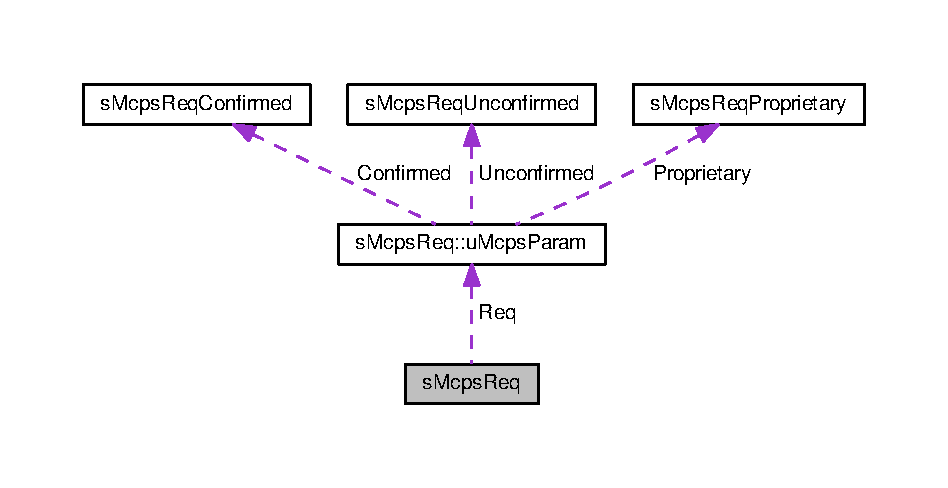
\includegraphics[width=350pt]{structsMcpsReq__coll__graph}
\end{center}
\end{figure}
\subsection*{Data Structures}
\begin{DoxyCompactItemize}
\item 
union \hyperlink{unionsMcpsReq_1_1uMcpsParam}{u\+Mcps\+Param}
\end{DoxyCompactItemize}
\subsection*{Data Fields}
\begin{DoxyCompactItemize}
\item 
\hyperlink{group__LORAMAC_ga670d0c87a52aeb13391f303a4cf94f00}{Mcps\+\_\+t} \hyperlink{structsMcpsReq_a9c0265d5c764fb2b0119c932b896f826}{Type}
\item 
union \hyperlink{unionsMcpsReq_1_1uMcpsParam}{s\+Mcps\+Req\+::u\+Mcps\+Param} \hyperlink{structsMcpsReq_a36a00aadc44825e3235a1652bd7911d6}{Req}
\end{DoxyCompactItemize}


\subsection{Detailed Description}
Lo\+Ra\+M\+AC M\+C\+P\+S-\/\+Request structure 

\subsection{Field Documentation}
\mbox{\Hypertarget{structsMcpsReq_a36a00aadc44825e3235a1652bd7911d6}\label{structsMcpsReq_a36a00aadc44825e3235a1652bd7911d6}} 
\index{s\+Mcps\+Req@{s\+Mcps\+Req}!Req@{Req}}
\index{Req@{Req}!s\+Mcps\+Req@{s\+Mcps\+Req}}
\subsubsection{\texorpdfstring{Req}{Req}}
{\footnotesize\ttfamily union \hyperlink{unionsMcpsReq_1_1uMcpsParam}{s\+Mcps\+Req\+::u\+Mcps\+Param} s\+Mcps\+Req\+::\+Req}

\mbox{\Hypertarget{structsMcpsReq_a9c0265d5c764fb2b0119c932b896f826}\label{structsMcpsReq_a9c0265d5c764fb2b0119c932b896f826}} 
\index{s\+Mcps\+Req@{s\+Mcps\+Req}!Type@{Type}}
\index{Type@{Type}!s\+Mcps\+Req@{s\+Mcps\+Req}}
\subsubsection{\texorpdfstring{Type}{Type}}
{\footnotesize\ttfamily \hyperlink{group__LORAMAC_ga670d0c87a52aeb13391f303a4cf94f00}{Mcps\+\_\+t} s\+Mcps\+Req\+::\+Type}

M\+C\+P\+S-\/\+Request type 

The documentation for this struct was generated from the following file\+:\begin{DoxyCompactItemize}
\item 
Mac/\hyperlink{LoRaMac_8h}{Lo\+Ra\+Mac.\+h}\end{DoxyCompactItemize}

\hypertarget{structsMcpsReqConfirmed}{}\section{s\+Mcps\+Req\+Confirmed Struct Reference}
\label{structsMcpsReqConfirmed}\index{s\+Mcps\+Req\+Confirmed@{s\+Mcps\+Req\+Confirmed}}


{\ttfamily \#include $<$Lo\+Ra\+Mac.\+h$>$}

\subsection*{Data Fields}
\begin{DoxyCompactItemize}
\item 
uint8\+\_\+t \hyperlink{structsMcpsReqConfirmed_a36b8d158ec49602e067d7884d39f94e7}{f\+Port}
\item 
void $\ast$ \hyperlink{structsMcpsReqConfirmed_a052ecff6388f3ee4d02be3fc3bf40570}{f\+Buffer}
\item 
uint16\+\_\+t \hyperlink{structsMcpsReqConfirmed_a47f46ba0eb6fe45951fadbb43687a9fd}{f\+Buffer\+Size}
\item 
int8\+\_\+t \hyperlink{structsMcpsReqConfirmed_afbd019ef536a8fe3c418bb362378c9cf}{Datarate}
\item 
uint8\+\_\+t \hyperlink{structsMcpsReqConfirmed_a4bf78c5cc4e56c815c592fcea5b07f82}{Nb\+Trials}
\end{DoxyCompactItemize}


\subsection{Detailed Description}
Lo\+Ra\+M\+AC M\+C\+P\+S-\/\+Request for a confirmed frame 

\subsection{Field Documentation}
\mbox{\Hypertarget{structsMcpsReqConfirmed_afbd019ef536a8fe3c418bb362378c9cf}\label{structsMcpsReqConfirmed_afbd019ef536a8fe3c418bb362378c9cf}} 
\index{s\+Mcps\+Req\+Confirmed@{s\+Mcps\+Req\+Confirmed}!Datarate@{Datarate}}
\index{Datarate@{Datarate}!s\+Mcps\+Req\+Confirmed@{s\+Mcps\+Req\+Confirmed}}
\subsubsection{\texorpdfstring{Datarate}{Datarate}}
{\footnotesize\ttfamily int8\+\_\+t s\+Mcps\+Req\+Confirmed\+::\+Datarate}

Uplink datarate, if A\+DR is off \mbox{\Hypertarget{structsMcpsReqConfirmed_a052ecff6388f3ee4d02be3fc3bf40570}\label{structsMcpsReqConfirmed_a052ecff6388f3ee4d02be3fc3bf40570}} 
\index{s\+Mcps\+Req\+Confirmed@{s\+Mcps\+Req\+Confirmed}!f\+Buffer@{f\+Buffer}}
\index{f\+Buffer@{f\+Buffer}!s\+Mcps\+Req\+Confirmed@{s\+Mcps\+Req\+Confirmed}}
\subsubsection{\texorpdfstring{f\+Buffer}{fBuffer}}
{\footnotesize\ttfamily void$\ast$ s\+Mcps\+Req\+Confirmed\+::f\+Buffer}

Pointer to the buffer of the frame payload \mbox{\Hypertarget{structsMcpsReqConfirmed_a47f46ba0eb6fe45951fadbb43687a9fd}\label{structsMcpsReqConfirmed_a47f46ba0eb6fe45951fadbb43687a9fd}} 
\index{s\+Mcps\+Req\+Confirmed@{s\+Mcps\+Req\+Confirmed}!f\+Buffer\+Size@{f\+Buffer\+Size}}
\index{f\+Buffer\+Size@{f\+Buffer\+Size}!s\+Mcps\+Req\+Confirmed@{s\+Mcps\+Req\+Confirmed}}
\subsubsection{\texorpdfstring{f\+Buffer\+Size}{fBufferSize}}
{\footnotesize\ttfamily uint16\+\_\+t s\+Mcps\+Req\+Confirmed\+::f\+Buffer\+Size}

Size of the frame payload \mbox{\Hypertarget{structsMcpsReqConfirmed_a36b8d158ec49602e067d7884d39f94e7}\label{structsMcpsReqConfirmed_a36b8d158ec49602e067d7884d39f94e7}} 
\index{s\+Mcps\+Req\+Confirmed@{s\+Mcps\+Req\+Confirmed}!f\+Port@{f\+Port}}
\index{f\+Port@{f\+Port}!s\+Mcps\+Req\+Confirmed@{s\+Mcps\+Req\+Confirmed}}
\subsubsection{\texorpdfstring{f\+Port}{fPort}}
{\footnotesize\ttfamily uint8\+\_\+t s\+Mcps\+Req\+Confirmed\+::f\+Port}

Frame port field. Must be set if the payload is not empty. Use the application specific frame port values\+: \mbox{[}1...223\mbox{]}

Lo\+Ra\+W\+AN Specification V1.\+0.\+2, chapter 4.\+3.\+2 \mbox{\Hypertarget{structsMcpsReqConfirmed_a4bf78c5cc4e56c815c592fcea5b07f82}\label{structsMcpsReqConfirmed_a4bf78c5cc4e56c815c592fcea5b07f82}} 
\index{s\+Mcps\+Req\+Confirmed@{s\+Mcps\+Req\+Confirmed}!Nb\+Trials@{Nb\+Trials}}
\index{Nb\+Trials@{Nb\+Trials}!s\+Mcps\+Req\+Confirmed@{s\+Mcps\+Req\+Confirmed}}
\subsubsection{\texorpdfstring{Nb\+Trials}{NbTrials}}
{\footnotesize\ttfamily uint8\+\_\+t s\+Mcps\+Req\+Confirmed\+::\+Nb\+Trials}

Number of trials to transmit the frame, if the Lo\+Ra\+M\+AC layer did not receive an acknowledgment. The M\+AC performs a datarate adaptation, according to the Lo\+Ra\+W\+AN Specification V1.\+0.\+2, chapter 18.\+4, according to the following table\+:

\tabulinesep=1mm
\begin{longtabu} spread 0pt [c]{*{2}{|X[-1]}|}
\hline
\rowcolor{\tableheadbgcolor}\textbf{ Transmission nb }&\textbf{ Data Rate  }\\\cline{1-2}
\endfirsthead
\hline
\endfoot
\hline
\rowcolor{\tableheadbgcolor}\textbf{ Transmission nb }&\textbf{ Data Rate  }\\\cline{1-2}
\endhead
1 (first) &DR \\\cline{1-2}
2 &DR \\\cline{1-2}
3 &max(D\+R-\/1,0) \\\cline{1-2}
4 &max(D\+R-\/1,0) \\\cline{1-2}
5 &max(D\+R-\/2,0) \\\cline{1-2}
6 &max(D\+R-\/2,0) \\\cline{1-2}
7 &max(D\+R-\/3,0) \\\cline{1-2}
8 &max(D\+R-\/3,0) \\\cline{1-2}
\end{longtabu}
Note, that if Nb\+Trials is set to 1 or 2, the M\+AC will not decrease the datarate, in case the Lo\+Ra\+M\+AC layer did not receive an acknowledgment 

The documentation for this struct was generated from the following file\+:\begin{DoxyCompactItemize}
\item 
Mac/\hyperlink{LoRaMac_8h}{Lo\+Ra\+Mac.\+h}\end{DoxyCompactItemize}

\hypertarget{structsMcpsReqProprietary}{}\section{s\+Mcps\+Req\+Proprietary Struct Reference}
\label{structsMcpsReqProprietary}\index{s\+Mcps\+Req\+Proprietary@{s\+Mcps\+Req\+Proprietary}}


{\ttfamily \#include $<$Lo\+Ra\+Mac.\+h$>$}

\subsection*{Data Fields}
\begin{DoxyCompactItemize}
\item 
void $\ast$ \hyperlink{structsMcpsReqProprietary_a374dfc00a1edb9316a451ec6fb1def34}{f\+Buffer}
\item 
uint16\+\_\+t \hyperlink{structsMcpsReqProprietary_aa0da0ddb0d1d7e78d0c0ce1e51168d68}{f\+Buffer\+Size}
\item 
int8\+\_\+t \hyperlink{structsMcpsReqProprietary_a5933662511d12917f3543a300fce8568}{Datarate}
\end{DoxyCompactItemize}


\subsection{Detailed Description}
Lo\+Ra\+M\+AC M\+C\+P\+S-\/\+Request for a proprietary frame 

\subsection{Field Documentation}
\mbox{\Hypertarget{structsMcpsReqProprietary_a5933662511d12917f3543a300fce8568}\label{structsMcpsReqProprietary_a5933662511d12917f3543a300fce8568}} 
\index{s\+Mcps\+Req\+Proprietary@{s\+Mcps\+Req\+Proprietary}!Datarate@{Datarate}}
\index{Datarate@{Datarate}!s\+Mcps\+Req\+Proprietary@{s\+Mcps\+Req\+Proprietary}}
\subsubsection{\texorpdfstring{Datarate}{Datarate}}
{\footnotesize\ttfamily int8\+\_\+t s\+Mcps\+Req\+Proprietary\+::\+Datarate}

Uplink datarate, if A\+DR is off \mbox{\Hypertarget{structsMcpsReqProprietary_a374dfc00a1edb9316a451ec6fb1def34}\label{structsMcpsReqProprietary_a374dfc00a1edb9316a451ec6fb1def34}} 
\index{s\+Mcps\+Req\+Proprietary@{s\+Mcps\+Req\+Proprietary}!f\+Buffer@{f\+Buffer}}
\index{f\+Buffer@{f\+Buffer}!s\+Mcps\+Req\+Proprietary@{s\+Mcps\+Req\+Proprietary}}
\subsubsection{\texorpdfstring{f\+Buffer}{fBuffer}}
{\footnotesize\ttfamily void$\ast$ s\+Mcps\+Req\+Proprietary\+::f\+Buffer}

Pointer to the buffer of the frame payload \mbox{\Hypertarget{structsMcpsReqProprietary_aa0da0ddb0d1d7e78d0c0ce1e51168d68}\label{structsMcpsReqProprietary_aa0da0ddb0d1d7e78d0c0ce1e51168d68}} 
\index{s\+Mcps\+Req\+Proprietary@{s\+Mcps\+Req\+Proprietary}!f\+Buffer\+Size@{f\+Buffer\+Size}}
\index{f\+Buffer\+Size@{f\+Buffer\+Size}!s\+Mcps\+Req\+Proprietary@{s\+Mcps\+Req\+Proprietary}}
\subsubsection{\texorpdfstring{f\+Buffer\+Size}{fBufferSize}}
{\footnotesize\ttfamily uint16\+\_\+t s\+Mcps\+Req\+Proprietary\+::f\+Buffer\+Size}

Size of the frame payload 

The documentation for this struct was generated from the following file\+:\begin{DoxyCompactItemize}
\item 
Mac/\hyperlink{LoRaMac_8h}{Lo\+Ra\+Mac.\+h}\end{DoxyCompactItemize}

\hypertarget{structsMcpsReqUnconfirmed}{}\section{s\+Mcps\+Req\+Unconfirmed Struct Reference}
\label{structsMcpsReqUnconfirmed}\index{s\+Mcps\+Req\+Unconfirmed@{s\+Mcps\+Req\+Unconfirmed}}


{\ttfamily \#include $<$Lo\+Ra\+Mac.\+h$>$}

\subsection*{Data Fields}
\begin{DoxyCompactItemize}
\item 
uint8\+\_\+t \hyperlink{structsMcpsReqUnconfirmed_a3c0190f7a5cc179b8cd664ff6a57169e}{f\+Port}
\item 
void $\ast$ \hyperlink{structsMcpsReqUnconfirmed_a38fff2f3a5d07612c80146613fe86ceb}{f\+Buffer}
\item 
uint16\+\_\+t \hyperlink{structsMcpsReqUnconfirmed_a0e3cfa4780e696a8e262d1f8f9f5fec4}{f\+Buffer\+Size}
\item 
int8\+\_\+t \hyperlink{structsMcpsReqUnconfirmed_a4df8871b15c859e010df754c419c5cb5}{Datarate}
\end{DoxyCompactItemize}


\subsection{Detailed Description}
Lo\+Ra\+M\+AC M\+C\+P\+S-\/\+Request for an unconfirmed frame 

\subsection{Field Documentation}
\mbox{\Hypertarget{structsMcpsReqUnconfirmed_a4df8871b15c859e010df754c419c5cb5}\label{structsMcpsReqUnconfirmed_a4df8871b15c859e010df754c419c5cb5}} 
\index{s\+Mcps\+Req\+Unconfirmed@{s\+Mcps\+Req\+Unconfirmed}!Datarate@{Datarate}}
\index{Datarate@{Datarate}!s\+Mcps\+Req\+Unconfirmed@{s\+Mcps\+Req\+Unconfirmed}}
\subsubsection{\texorpdfstring{Datarate}{Datarate}}
{\footnotesize\ttfamily int8\+\_\+t s\+Mcps\+Req\+Unconfirmed\+::\+Datarate}

Uplink datarate, if A\+DR is off \mbox{\Hypertarget{structsMcpsReqUnconfirmed_a38fff2f3a5d07612c80146613fe86ceb}\label{structsMcpsReqUnconfirmed_a38fff2f3a5d07612c80146613fe86ceb}} 
\index{s\+Mcps\+Req\+Unconfirmed@{s\+Mcps\+Req\+Unconfirmed}!f\+Buffer@{f\+Buffer}}
\index{f\+Buffer@{f\+Buffer}!s\+Mcps\+Req\+Unconfirmed@{s\+Mcps\+Req\+Unconfirmed}}
\subsubsection{\texorpdfstring{f\+Buffer}{fBuffer}}
{\footnotesize\ttfamily void$\ast$ s\+Mcps\+Req\+Unconfirmed\+::f\+Buffer}

Pointer to the buffer of the frame payload \mbox{\Hypertarget{structsMcpsReqUnconfirmed_a0e3cfa4780e696a8e262d1f8f9f5fec4}\label{structsMcpsReqUnconfirmed_a0e3cfa4780e696a8e262d1f8f9f5fec4}} 
\index{s\+Mcps\+Req\+Unconfirmed@{s\+Mcps\+Req\+Unconfirmed}!f\+Buffer\+Size@{f\+Buffer\+Size}}
\index{f\+Buffer\+Size@{f\+Buffer\+Size}!s\+Mcps\+Req\+Unconfirmed@{s\+Mcps\+Req\+Unconfirmed}}
\subsubsection{\texorpdfstring{f\+Buffer\+Size}{fBufferSize}}
{\footnotesize\ttfamily uint16\+\_\+t s\+Mcps\+Req\+Unconfirmed\+::f\+Buffer\+Size}

Size of the frame payload \mbox{\Hypertarget{structsMcpsReqUnconfirmed_a3c0190f7a5cc179b8cd664ff6a57169e}\label{structsMcpsReqUnconfirmed_a3c0190f7a5cc179b8cd664ff6a57169e}} 
\index{s\+Mcps\+Req\+Unconfirmed@{s\+Mcps\+Req\+Unconfirmed}!f\+Port@{f\+Port}}
\index{f\+Port@{f\+Port}!s\+Mcps\+Req\+Unconfirmed@{s\+Mcps\+Req\+Unconfirmed}}
\subsubsection{\texorpdfstring{f\+Port}{fPort}}
{\footnotesize\ttfamily uint8\+\_\+t s\+Mcps\+Req\+Unconfirmed\+::f\+Port}

Frame port field. Must be set if the payload is not empty. Use the application specific frame port values\+: \mbox{[}1...223\mbox{]}

Lo\+Ra\+W\+AN Specification V1.\+0.\+2, chapter 4.\+3.\+2 

The documentation for this struct was generated from the following file\+:\begin{DoxyCompactItemize}
\item 
Mac/\hyperlink{LoRaMac_8h}{Lo\+Ra\+Mac.\+h}\end{DoxyCompactItemize}

\hypertarget{structsMlmeConfirm}{}\section{s\+Mlme\+Confirm Struct Reference}
\label{structsMlmeConfirm}\index{s\+Mlme\+Confirm@{s\+Mlme\+Confirm}}


{\ttfamily \#include $<$Lo\+Ra\+Mac.\+h$>$}

\subsection*{Data Fields}
\begin{DoxyCompactItemize}
\item 
\hyperlink{group__LORAMAC_ga663544b83d50ec3518608be495896809}{Mlme\+\_\+t} \hyperlink{structsMlmeConfirm_a4d4f24a72592be1fbfd21d7179256088}{Mlme\+Request}
\item 
\hyperlink{group__LORAMAC_gac6ffc346a4c767f7a743c87a686c51b4}{Lo\+Ra\+Mac\+Event\+Info\+Status\+\_\+t} \hyperlink{structsMlmeConfirm_adb06d9fb17164ca72847bbdb9238800f}{Status}
\item 
\hyperlink{utilities_8h_a4215ca43d3e953099ea758ce428599d0}{Timer\+Time\+\_\+t} \hyperlink{structsMlmeConfirm_a56411a350cd4b3f8ee59adc9105e5b5e}{Tx\+Time\+On\+Air}
\item 
uint8\+\_\+t \hyperlink{structsMlmeConfirm_a802681a041b6716f179719369a3f7c21}{Demod\+Margin}
\item 
uint8\+\_\+t \hyperlink{structsMlmeConfirm_a030224406f25b8eec68e91952087a44e}{Nb\+Gateways}
\item 
uint8\+\_\+t \hyperlink{structsMlmeConfirm_a2c539bfc04286bb8f338085d8c8438dc}{Nb\+Retries}
\end{DoxyCompactItemize}


\subsection{Detailed Description}
Lo\+Ra\+M\+AC M\+L\+M\+E-\/\+Confirm primitive 

\subsection{Field Documentation}
\mbox{\Hypertarget{structsMlmeConfirm_a802681a041b6716f179719369a3f7c21}\label{structsMlmeConfirm_a802681a041b6716f179719369a3f7c21}} 
\index{s\+Mlme\+Confirm@{s\+Mlme\+Confirm}!Demod\+Margin@{Demod\+Margin}}
\index{Demod\+Margin@{Demod\+Margin}!s\+Mlme\+Confirm@{s\+Mlme\+Confirm}}
\subsubsection{\texorpdfstring{Demod\+Margin}{DemodMargin}}
{\footnotesize\ttfamily uint8\+\_\+t s\+Mlme\+Confirm\+::\+Demod\+Margin}

Demodulation margin. Contains the link margin \mbox{[}dB\mbox{]} of the last successfully received Link\+Check\+Req \mbox{\Hypertarget{structsMlmeConfirm_a4d4f24a72592be1fbfd21d7179256088}\label{structsMlmeConfirm_a4d4f24a72592be1fbfd21d7179256088}} 
\index{s\+Mlme\+Confirm@{s\+Mlme\+Confirm}!Mlme\+Request@{Mlme\+Request}}
\index{Mlme\+Request@{Mlme\+Request}!s\+Mlme\+Confirm@{s\+Mlme\+Confirm}}
\subsubsection{\texorpdfstring{Mlme\+Request}{MlmeRequest}}
{\footnotesize\ttfamily \hyperlink{group__LORAMAC_ga663544b83d50ec3518608be495896809}{Mlme\+\_\+t} s\+Mlme\+Confirm\+::\+Mlme\+Request}

Holds the previously performed M\+L\+M\+E-\/\+Request \mbox{\Hypertarget{structsMlmeConfirm_a030224406f25b8eec68e91952087a44e}\label{structsMlmeConfirm_a030224406f25b8eec68e91952087a44e}} 
\index{s\+Mlme\+Confirm@{s\+Mlme\+Confirm}!Nb\+Gateways@{Nb\+Gateways}}
\index{Nb\+Gateways@{Nb\+Gateways}!s\+Mlme\+Confirm@{s\+Mlme\+Confirm}}
\subsubsection{\texorpdfstring{Nb\+Gateways}{NbGateways}}
{\footnotesize\ttfamily uint8\+\_\+t s\+Mlme\+Confirm\+::\+Nb\+Gateways}

Number of gateways which received the last Link\+Check\+Req \mbox{\Hypertarget{structsMlmeConfirm_a2c539bfc04286bb8f338085d8c8438dc}\label{structsMlmeConfirm_a2c539bfc04286bb8f338085d8c8438dc}} 
\index{s\+Mlme\+Confirm@{s\+Mlme\+Confirm}!Nb\+Retries@{Nb\+Retries}}
\index{Nb\+Retries@{Nb\+Retries}!s\+Mlme\+Confirm@{s\+Mlme\+Confirm}}
\subsubsection{\texorpdfstring{Nb\+Retries}{NbRetries}}
{\footnotesize\ttfamily uint8\+\_\+t s\+Mlme\+Confirm\+::\+Nb\+Retries}

Provides the number of retransmissions \mbox{\Hypertarget{structsMlmeConfirm_adb06d9fb17164ca72847bbdb9238800f}\label{structsMlmeConfirm_adb06d9fb17164ca72847bbdb9238800f}} 
\index{s\+Mlme\+Confirm@{s\+Mlme\+Confirm}!Status@{Status}}
\index{Status@{Status}!s\+Mlme\+Confirm@{s\+Mlme\+Confirm}}
\subsubsection{\texorpdfstring{Status}{Status}}
{\footnotesize\ttfamily \hyperlink{group__LORAMAC_gac6ffc346a4c767f7a743c87a686c51b4}{Lo\+Ra\+Mac\+Event\+Info\+Status\+\_\+t} s\+Mlme\+Confirm\+::\+Status}

Status of the operation \mbox{\Hypertarget{structsMlmeConfirm_a56411a350cd4b3f8ee59adc9105e5b5e}\label{structsMlmeConfirm_a56411a350cd4b3f8ee59adc9105e5b5e}} 
\index{s\+Mlme\+Confirm@{s\+Mlme\+Confirm}!Tx\+Time\+On\+Air@{Tx\+Time\+On\+Air}}
\index{Tx\+Time\+On\+Air@{Tx\+Time\+On\+Air}!s\+Mlme\+Confirm@{s\+Mlme\+Confirm}}
\subsubsection{\texorpdfstring{Tx\+Time\+On\+Air}{TxTimeOnAir}}
{\footnotesize\ttfamily \hyperlink{utilities_8h_a4215ca43d3e953099ea758ce428599d0}{Timer\+Time\+\_\+t} s\+Mlme\+Confirm\+::\+Tx\+Time\+On\+Air}

The transmission time on air of the frame 

The documentation for this struct was generated from the following file\+:\begin{DoxyCompactItemize}
\item 
Mac/\hyperlink{LoRaMac_8h}{Lo\+Ra\+Mac.\+h}\end{DoxyCompactItemize}

\hypertarget{structsMlmeReq}{}\section{s\+Mlme\+Req Struct Reference}
\label{structsMlmeReq}\index{s\+Mlme\+Req@{s\+Mlme\+Req}}


{\ttfamily \#include $<$Lo\+Ra\+Mac.\+h$>$}



Collaboration diagram for s\+Mlme\+Req\+:
\nopagebreak
\begin{figure}[H]
\begin{center}
\leavevmode
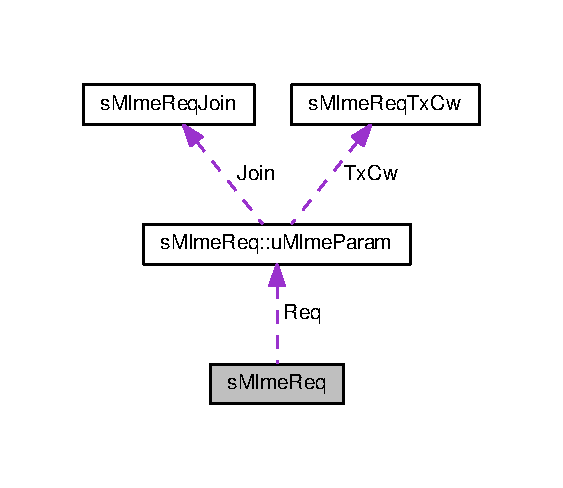
\includegraphics[width=270pt]{structsMlmeReq__coll__graph}
\end{center}
\end{figure}
\subsection*{Data Structures}
\begin{DoxyCompactItemize}
\item 
union \hyperlink{unionsMlmeReq_1_1uMlmeParam}{u\+Mlme\+Param}
\end{DoxyCompactItemize}
\subsection*{Data Fields}
\begin{DoxyCompactItemize}
\item 
\hyperlink{group__LORAMAC_ga663544b83d50ec3518608be495896809}{Mlme\+\_\+t} \hyperlink{structsMlmeReq_ab7870d559ad9c5a08d305220bf798cd3}{Type}
\item 
union \hyperlink{unionsMlmeReq_1_1uMlmeParam}{s\+Mlme\+Req\+::u\+Mlme\+Param} \hyperlink{structsMlmeReq_a6f57f62db1981b24980a7745b966a469}{Req}
\end{DoxyCompactItemize}


\subsection{Detailed Description}
Lo\+Ra\+M\+AC M\+L\+M\+E-\/\+Request structure 

\subsection{Field Documentation}
\mbox{\Hypertarget{structsMlmeReq_a6f57f62db1981b24980a7745b966a469}\label{structsMlmeReq_a6f57f62db1981b24980a7745b966a469}} 
\index{s\+Mlme\+Req@{s\+Mlme\+Req}!Req@{Req}}
\index{Req@{Req}!s\+Mlme\+Req@{s\+Mlme\+Req}}
\subsubsection{\texorpdfstring{Req}{Req}}
{\footnotesize\ttfamily union \hyperlink{unionsMlmeReq_1_1uMlmeParam}{s\+Mlme\+Req\+::u\+Mlme\+Param} s\+Mlme\+Req\+::\+Req}

\mbox{\Hypertarget{structsMlmeReq_ab7870d559ad9c5a08d305220bf798cd3}\label{structsMlmeReq_ab7870d559ad9c5a08d305220bf798cd3}} 
\index{s\+Mlme\+Req@{s\+Mlme\+Req}!Type@{Type}}
\index{Type@{Type}!s\+Mlme\+Req@{s\+Mlme\+Req}}
\subsubsection{\texorpdfstring{Type}{Type}}
{\footnotesize\ttfamily \hyperlink{group__LORAMAC_ga663544b83d50ec3518608be495896809}{Mlme\+\_\+t} s\+Mlme\+Req\+::\+Type}

M\+L\+M\+E-\/\+Request type 

The documentation for this struct was generated from the following file\+:\begin{DoxyCompactItemize}
\item 
Mac/\hyperlink{LoRaMac_8h}{Lo\+Ra\+Mac.\+h}\end{DoxyCompactItemize}

\hypertarget{structsMlmeReqJoin}{}\section{s\+Mlme\+Req\+Join Struct Reference}
\label{structsMlmeReqJoin}\index{s\+Mlme\+Req\+Join@{s\+Mlme\+Req\+Join}}


{\ttfamily \#include $<$Lo\+Ra\+Mac.\+h$>$}

\subsection*{Data Fields}
\begin{DoxyCompactItemize}
\item 
uint8\+\_\+t $\ast$ \hyperlink{structsMlmeReqJoin_abd56390965a0e3a80e198d9ae39d1625}{Dev\+Eui}
\item 
uint8\+\_\+t $\ast$ \hyperlink{structsMlmeReqJoin_a46bda1421b6d9dc9e6444ece02fd77d0}{App\+Eui}
\item 
uint8\+\_\+t $\ast$ \hyperlink{structsMlmeReqJoin_a3bd1a01c6d01990265ec2b5bf0dd906f}{App\+Key}
\item 
uint8\+\_\+t \hyperlink{structsMlmeReqJoin_aa01aa1a2d54c6b90e7d972c28306a6e4}{Nb\+Trials}
\end{DoxyCompactItemize}


\subsection{Detailed Description}
Lo\+Ra\+M\+AC M\+L\+M\+E-\/\+Request for the join service 

\subsection{Field Documentation}
\mbox{\Hypertarget{structsMlmeReqJoin_a46bda1421b6d9dc9e6444ece02fd77d0}\label{structsMlmeReqJoin_a46bda1421b6d9dc9e6444ece02fd77d0}} 
\index{s\+Mlme\+Req\+Join@{s\+Mlme\+Req\+Join}!App\+Eui@{App\+Eui}}
\index{App\+Eui@{App\+Eui}!s\+Mlme\+Req\+Join@{s\+Mlme\+Req\+Join}}
\subsubsection{\texorpdfstring{App\+Eui}{AppEui}}
{\footnotesize\ttfamily uint8\+\_\+t$\ast$ s\+Mlme\+Req\+Join\+::\+App\+Eui}

Application identifier

Lo\+Ra\+W\+AN Specification V1.\+0.\+2, chapter 6.\+1.\+2 \mbox{\Hypertarget{structsMlmeReqJoin_a3bd1a01c6d01990265ec2b5bf0dd906f}\label{structsMlmeReqJoin_a3bd1a01c6d01990265ec2b5bf0dd906f}} 
\index{s\+Mlme\+Req\+Join@{s\+Mlme\+Req\+Join}!App\+Key@{App\+Key}}
\index{App\+Key@{App\+Key}!s\+Mlme\+Req\+Join@{s\+Mlme\+Req\+Join}}
\subsubsection{\texorpdfstring{App\+Key}{AppKey}}
{\footnotesize\ttfamily uint8\+\_\+t$\ast$ s\+Mlme\+Req\+Join\+::\+App\+Key}

A\+E\+S-\/128 application key

Lo\+Ra\+W\+AN Specification V1.\+0.\+2, chapter 6.\+2.\+2 \mbox{\Hypertarget{structsMlmeReqJoin_abd56390965a0e3a80e198d9ae39d1625}\label{structsMlmeReqJoin_abd56390965a0e3a80e198d9ae39d1625}} 
\index{s\+Mlme\+Req\+Join@{s\+Mlme\+Req\+Join}!Dev\+Eui@{Dev\+Eui}}
\index{Dev\+Eui@{Dev\+Eui}!s\+Mlme\+Req\+Join@{s\+Mlme\+Req\+Join}}
\subsubsection{\texorpdfstring{Dev\+Eui}{DevEui}}
{\footnotesize\ttfamily uint8\+\_\+t$\ast$ s\+Mlme\+Req\+Join\+::\+Dev\+Eui}

Globally unique end-\/device identifier

Lo\+Ra\+W\+AN Specification V1.\+0.\+2, chapter 6.\+2.\+1 \mbox{\Hypertarget{structsMlmeReqJoin_aa01aa1a2d54c6b90e7d972c28306a6e4}\label{structsMlmeReqJoin_aa01aa1a2d54c6b90e7d972c28306a6e4}} 
\index{s\+Mlme\+Req\+Join@{s\+Mlme\+Req\+Join}!Nb\+Trials@{Nb\+Trials}}
\index{Nb\+Trials@{Nb\+Trials}!s\+Mlme\+Req\+Join@{s\+Mlme\+Req\+Join}}
\subsubsection{\texorpdfstring{Nb\+Trials}{NbTrials}}
{\footnotesize\ttfamily uint8\+\_\+t s\+Mlme\+Req\+Join\+::\+Nb\+Trials}

Number of trials for the join request. 

The documentation for this struct was generated from the following file\+:\begin{DoxyCompactItemize}
\item 
Mac/\hyperlink{LoRaMac_8h}{Lo\+Ra\+Mac.\+h}\end{DoxyCompactItemize}

\hypertarget{structsMlmeReqTxCw}{}\section{s\+Mlme\+Req\+Tx\+Cw Struct Reference}
\label{structsMlmeReqTxCw}\index{s\+Mlme\+Req\+Tx\+Cw@{s\+Mlme\+Req\+Tx\+Cw}}


{\ttfamily \#include $<$Lo\+Ra\+Mac.\+h$>$}

\subsection*{Data Fields}
\begin{DoxyCompactItemize}
\item 
uint16\+\_\+t \hyperlink{structsMlmeReqTxCw_a62e506374c3c4b59c4ef10d01e02768f}{Timeout}
\item 
uint32\+\_\+t \hyperlink{structsMlmeReqTxCw_afcb3ef248fb26e2bdc04720801464825}{Frequency}
\item 
uint8\+\_\+t \hyperlink{structsMlmeReqTxCw_ab9e35e3b76d695b3e14efcdc6eab6f55}{Power}
\end{DoxyCompactItemize}


\subsection{Detailed Description}
Lo\+Ra\+M\+AC M\+L\+M\+E-\/\+Request for Tx continuous wave mode 

\subsection{Field Documentation}
\mbox{\Hypertarget{structsMlmeReqTxCw_afcb3ef248fb26e2bdc04720801464825}\label{structsMlmeReqTxCw_afcb3ef248fb26e2bdc04720801464825}} 
\index{s\+Mlme\+Req\+Tx\+Cw@{s\+Mlme\+Req\+Tx\+Cw}!Frequency@{Frequency}}
\index{Frequency@{Frequency}!s\+Mlme\+Req\+Tx\+Cw@{s\+Mlme\+Req\+Tx\+Cw}}
\subsubsection{\texorpdfstring{Frequency}{Frequency}}
{\footnotesize\ttfamily uint32\+\_\+t s\+Mlme\+Req\+Tx\+Cw\+::\+Frequency}

RF frequency to set (Only used with new way) \mbox{\Hypertarget{structsMlmeReqTxCw_ab9e35e3b76d695b3e14efcdc6eab6f55}\label{structsMlmeReqTxCw_ab9e35e3b76d695b3e14efcdc6eab6f55}} 
\index{s\+Mlme\+Req\+Tx\+Cw@{s\+Mlme\+Req\+Tx\+Cw}!Power@{Power}}
\index{Power@{Power}!s\+Mlme\+Req\+Tx\+Cw@{s\+Mlme\+Req\+Tx\+Cw}}
\subsubsection{\texorpdfstring{Power}{Power}}
{\footnotesize\ttfamily uint8\+\_\+t s\+Mlme\+Req\+Tx\+Cw\+::\+Power}

RF output power to set (Only used with new way) \mbox{\Hypertarget{structsMlmeReqTxCw_a62e506374c3c4b59c4ef10d01e02768f}\label{structsMlmeReqTxCw_a62e506374c3c4b59c4ef10d01e02768f}} 
\index{s\+Mlme\+Req\+Tx\+Cw@{s\+Mlme\+Req\+Tx\+Cw}!Timeout@{Timeout}}
\index{Timeout@{Timeout}!s\+Mlme\+Req\+Tx\+Cw@{s\+Mlme\+Req\+Tx\+Cw}}
\subsubsection{\texorpdfstring{Timeout}{Timeout}}
{\footnotesize\ttfamily uint16\+\_\+t s\+Mlme\+Req\+Tx\+Cw\+::\+Timeout}

Time in seconds while the radio is kept in continuous wave mode 

The documentation for this struct was generated from the following file\+:\begin{DoxyCompactItemize}
\item 
Mac/\hyperlink{LoRaMac_8h}{Lo\+Ra\+Mac.\+h}\end{DoxyCompactItemize}

\hypertarget{structsMulticastParams}{}\section{s\+Multicast\+Params Struct Reference}
\label{structsMulticastParams}\index{s\+Multicast\+Params@{s\+Multicast\+Params}}


{\ttfamily \#include $<$Lo\+Ra\+Mac.\+h$>$}



Collaboration diagram for s\+Multicast\+Params\+:
\nopagebreak
\begin{figure}[H]
\begin{center}
\leavevmode
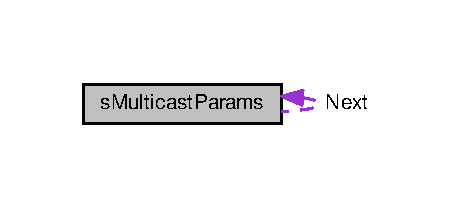
\includegraphics[width=218pt]{structsMulticastParams__coll__graph}
\end{center}
\end{figure}
\subsection*{Data Fields}
\begin{DoxyCompactItemize}
\item 
uint32\+\_\+t \hyperlink{structsMulticastParams_abe2277479419032f7c79368048a865e8}{Address}
\item 
uint8\+\_\+t \hyperlink{structsMulticastParams_a71330fdf812a469a4727bed311a22353}{Nwk\+S\+Key} \mbox{[}16\mbox{]}
\item 
uint8\+\_\+t \hyperlink{structsMulticastParams_abf0b21eb52ca715692003aa9712f9de5}{App\+S\+Key} \mbox{[}16\mbox{]}
\item 
uint32\+\_\+t \hyperlink{structsMulticastParams_a2c9143b93413848d615a9f0c7f7afc09}{Down\+Link\+Counter}
\item 
struct \hyperlink{structsMulticastParams}{s\+Multicast\+Params} $\ast$ \hyperlink{structsMulticastParams_a085c359608cb7d61aff9824dcf1769db}{Next}
\end{DoxyCompactItemize}


\subsection{Detailed Description}
Lo\+Ra\+M\+AC multicast channel parameter 

\subsection{Field Documentation}
\mbox{\Hypertarget{structsMulticastParams_abe2277479419032f7c79368048a865e8}\label{structsMulticastParams_abe2277479419032f7c79368048a865e8}} 
\index{s\+Multicast\+Params@{s\+Multicast\+Params}!Address@{Address}}
\index{Address@{Address}!s\+Multicast\+Params@{s\+Multicast\+Params}}
\subsubsection{\texorpdfstring{Address}{Address}}
{\footnotesize\ttfamily uint32\+\_\+t s\+Multicast\+Params\+::\+Address}

Address \mbox{\Hypertarget{structsMulticastParams_abf0b21eb52ca715692003aa9712f9de5}\label{structsMulticastParams_abf0b21eb52ca715692003aa9712f9de5}} 
\index{s\+Multicast\+Params@{s\+Multicast\+Params}!App\+S\+Key@{App\+S\+Key}}
\index{App\+S\+Key@{App\+S\+Key}!s\+Multicast\+Params@{s\+Multicast\+Params}}
\subsubsection{\texorpdfstring{App\+S\+Key}{AppSKey}}
{\footnotesize\ttfamily uint8\+\_\+t s\+Multicast\+Params\+::\+App\+S\+Key\mbox{[}16\mbox{]}}

Application session key \mbox{\Hypertarget{structsMulticastParams_a2c9143b93413848d615a9f0c7f7afc09}\label{structsMulticastParams_a2c9143b93413848d615a9f0c7f7afc09}} 
\index{s\+Multicast\+Params@{s\+Multicast\+Params}!Down\+Link\+Counter@{Down\+Link\+Counter}}
\index{Down\+Link\+Counter@{Down\+Link\+Counter}!s\+Multicast\+Params@{s\+Multicast\+Params}}
\subsubsection{\texorpdfstring{Down\+Link\+Counter}{DownLinkCounter}}
{\footnotesize\ttfamily uint32\+\_\+t s\+Multicast\+Params\+::\+Down\+Link\+Counter}

Downlink counter \mbox{\Hypertarget{structsMulticastParams_a085c359608cb7d61aff9824dcf1769db}\label{structsMulticastParams_a085c359608cb7d61aff9824dcf1769db}} 
\index{s\+Multicast\+Params@{s\+Multicast\+Params}!Next@{Next}}
\index{Next@{Next}!s\+Multicast\+Params@{s\+Multicast\+Params}}
\subsubsection{\texorpdfstring{Next}{Next}}
{\footnotesize\ttfamily struct \hyperlink{structsMulticastParams}{s\+Multicast\+Params}$\ast$ s\+Multicast\+Params\+::\+Next}

Reference pointer to the next multicast channel parameters in the list \mbox{\Hypertarget{structsMulticastParams_a71330fdf812a469a4727bed311a22353}\label{structsMulticastParams_a71330fdf812a469a4727bed311a22353}} 
\index{s\+Multicast\+Params@{s\+Multicast\+Params}!Nwk\+S\+Key@{Nwk\+S\+Key}}
\index{Nwk\+S\+Key@{Nwk\+S\+Key}!s\+Multicast\+Params@{s\+Multicast\+Params}}
\subsubsection{\texorpdfstring{Nwk\+S\+Key}{NwkSKey}}
{\footnotesize\ttfamily uint8\+\_\+t s\+Multicast\+Params\+::\+Nwk\+S\+Key\mbox{[}16\mbox{]}}

Network session key 

The documentation for this struct was generated from the following file\+:\begin{DoxyCompactItemize}
\item 
Mac/\hyperlink{LoRaMac_8h}{Lo\+Ra\+Mac.\+h}\end{DoxyCompactItemize}

\hypertarget{structsNewChannelReqParams}{}\section{s\+New\+Channel\+Req\+Params Struct Reference}
\label{structsNewChannelReqParams}\index{s\+New\+Channel\+Req\+Params@{s\+New\+Channel\+Req\+Params}}


{\ttfamily \#include $<$Region.\+h$>$}



Collaboration diagram for s\+New\+Channel\+Req\+Params\+:
\nopagebreak
\begin{figure}[H]
\begin{center}
\leavevmode
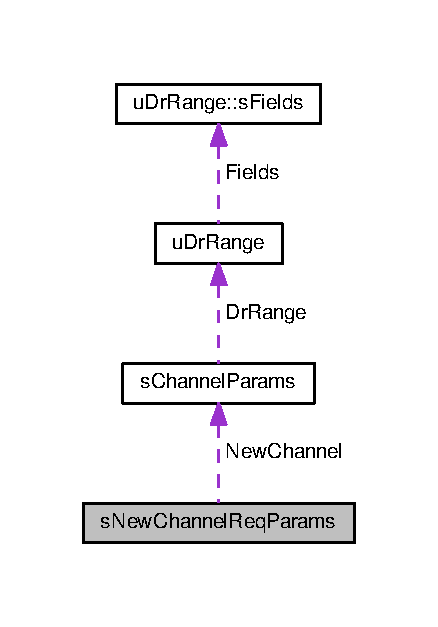
\includegraphics[width=210pt]{structsNewChannelReqParams__coll__graph}
\end{center}
\end{figure}
\subsection*{Data Fields}
\begin{DoxyCompactItemize}
\item 
\hyperlink{group__LORAMAC_ga1360ca6f82c6d125ea43a9dad9b56184}{Channel\+Params\+\_\+t} $\ast$ \hyperlink{structsNewChannelReqParams_a62267cdad01a56a941b8a9a82be81708}{New\+Channel}
\item 
int8\+\_\+t \hyperlink{structsNewChannelReqParams_a1bd8e73e08662496888e9102d81b5262}{Channel\+Id}
\end{DoxyCompactItemize}


\subsection{Detailed Description}
Parameter structure for the function Region\+New\+Channel\+Req. 

\subsection{Field Documentation}
\mbox{\Hypertarget{structsNewChannelReqParams_a1bd8e73e08662496888e9102d81b5262}\label{structsNewChannelReqParams_a1bd8e73e08662496888e9102d81b5262}} 
\index{s\+New\+Channel\+Req\+Params@{s\+New\+Channel\+Req\+Params}!Channel\+Id@{Channel\+Id}}
\index{Channel\+Id@{Channel\+Id}!s\+New\+Channel\+Req\+Params@{s\+New\+Channel\+Req\+Params}}
\subsubsection{\texorpdfstring{Channel\+Id}{ChannelId}}
{\footnotesize\ttfamily int8\+\_\+t s\+New\+Channel\+Req\+Params\+::\+Channel\+Id}

Channel id. \mbox{\Hypertarget{structsNewChannelReqParams_a62267cdad01a56a941b8a9a82be81708}\label{structsNewChannelReqParams_a62267cdad01a56a941b8a9a82be81708}} 
\index{s\+New\+Channel\+Req\+Params@{s\+New\+Channel\+Req\+Params}!New\+Channel@{New\+Channel}}
\index{New\+Channel@{New\+Channel}!s\+New\+Channel\+Req\+Params@{s\+New\+Channel\+Req\+Params}}
\subsubsection{\texorpdfstring{New\+Channel}{NewChannel}}
{\footnotesize\ttfamily \hyperlink{group__LORAMAC_ga1360ca6f82c6d125ea43a9dad9b56184}{Channel\+Params\+\_\+t}$\ast$ s\+New\+Channel\+Req\+Params\+::\+New\+Channel}

Pointer to the new channels. 

The documentation for this struct was generated from the following file\+:\begin{DoxyCompactItemize}
\item 
Mac/region/\hyperlink{Region_8h}{Region.\+h}\end{DoxyCompactItemize}

\hypertarget{structsNextChanParams}{}\section{s\+Next\+Chan\+Params Struct Reference}
\label{structsNextChanParams}\index{s\+Next\+Chan\+Params@{s\+Next\+Chan\+Params}}


{\ttfamily \#include $<$Region.\+h$>$}

\subsection*{Data Fields}
\begin{DoxyCompactItemize}
\item 
\hyperlink{utilities_8h_a4215ca43d3e953099ea758ce428599d0}{Timer\+Time\+\_\+t} \hyperlink{structsNextChanParams_abec6dac3f04a69dda9e6f8175b3ae022}{Aggr\+Time\+Off}
\item 
\hyperlink{utilities_8h_a4215ca43d3e953099ea758ce428599d0}{Timer\+Time\+\_\+t} \hyperlink{structsNextChanParams_a4f5d9417759fa1ef8b3103ef04d54829}{Last\+Aggr\+Tx}
\item 
int8\+\_\+t \hyperlink{structsNextChanParams_aecc50a3a952bd990553b873dc6858393}{Datarate}
\item 
bool \hyperlink{structsNextChanParams_a147c9e2910dd7f22b8378e80d9b383ef}{Joined}
\item 
bool \hyperlink{structsNextChanParams_a3afdcbe5a3dba77f73c7534957b82ce5}{Duty\+Cycle\+Enabled}
\end{DoxyCompactItemize}


\subsection{Detailed Description}
Parameter structure for the function Region\+Next\+Channel. 

\subsection{Field Documentation}
\mbox{\Hypertarget{structsNextChanParams_abec6dac3f04a69dda9e6f8175b3ae022}\label{structsNextChanParams_abec6dac3f04a69dda9e6f8175b3ae022}} 
\index{s\+Next\+Chan\+Params@{s\+Next\+Chan\+Params}!Aggr\+Time\+Off@{Aggr\+Time\+Off}}
\index{Aggr\+Time\+Off@{Aggr\+Time\+Off}!s\+Next\+Chan\+Params@{s\+Next\+Chan\+Params}}
\subsubsection{\texorpdfstring{Aggr\+Time\+Off}{AggrTimeOff}}
{\footnotesize\ttfamily \hyperlink{utilities_8h_a4215ca43d3e953099ea758ce428599d0}{Timer\+Time\+\_\+t} s\+Next\+Chan\+Params\+::\+Aggr\+Time\+Off}

Aggregated time-\/off time. \mbox{\Hypertarget{structsNextChanParams_aecc50a3a952bd990553b873dc6858393}\label{structsNextChanParams_aecc50a3a952bd990553b873dc6858393}} 
\index{s\+Next\+Chan\+Params@{s\+Next\+Chan\+Params}!Datarate@{Datarate}}
\index{Datarate@{Datarate}!s\+Next\+Chan\+Params@{s\+Next\+Chan\+Params}}
\subsubsection{\texorpdfstring{Datarate}{Datarate}}
{\footnotesize\ttfamily int8\+\_\+t s\+Next\+Chan\+Params\+::\+Datarate}

Current datarate. \mbox{\Hypertarget{structsNextChanParams_a3afdcbe5a3dba77f73c7534957b82ce5}\label{structsNextChanParams_a3afdcbe5a3dba77f73c7534957b82ce5}} 
\index{s\+Next\+Chan\+Params@{s\+Next\+Chan\+Params}!Duty\+Cycle\+Enabled@{Duty\+Cycle\+Enabled}}
\index{Duty\+Cycle\+Enabled@{Duty\+Cycle\+Enabled}!s\+Next\+Chan\+Params@{s\+Next\+Chan\+Params}}
\subsubsection{\texorpdfstring{Duty\+Cycle\+Enabled}{DutyCycleEnabled}}
{\footnotesize\ttfamily bool s\+Next\+Chan\+Params\+::\+Duty\+Cycle\+Enabled}

Set to true, if the duty cycle is enabled, otherwise false. \mbox{\Hypertarget{structsNextChanParams_a147c9e2910dd7f22b8378e80d9b383ef}\label{structsNextChanParams_a147c9e2910dd7f22b8378e80d9b383ef}} 
\index{s\+Next\+Chan\+Params@{s\+Next\+Chan\+Params}!Joined@{Joined}}
\index{Joined@{Joined}!s\+Next\+Chan\+Params@{s\+Next\+Chan\+Params}}
\subsubsection{\texorpdfstring{Joined}{Joined}}
{\footnotesize\ttfamily bool s\+Next\+Chan\+Params\+::\+Joined}

Set to true, if the node has already joined a network, otherwise false. \mbox{\Hypertarget{structsNextChanParams_a4f5d9417759fa1ef8b3103ef04d54829}\label{structsNextChanParams_a4f5d9417759fa1ef8b3103ef04d54829}} 
\index{s\+Next\+Chan\+Params@{s\+Next\+Chan\+Params}!Last\+Aggr\+Tx@{Last\+Aggr\+Tx}}
\index{Last\+Aggr\+Tx@{Last\+Aggr\+Tx}!s\+Next\+Chan\+Params@{s\+Next\+Chan\+Params}}
\subsubsection{\texorpdfstring{Last\+Aggr\+Tx}{LastAggrTx}}
{\footnotesize\ttfamily \hyperlink{utilities_8h_a4215ca43d3e953099ea758ce428599d0}{Timer\+Time\+\_\+t} s\+Next\+Chan\+Params\+::\+Last\+Aggr\+Tx}

Time of the last aggregated TX. 

The documentation for this struct was generated from the following file\+:\begin{DoxyCompactItemize}
\item 
Mac/region/\hyperlink{Region_8h}{Region.\+h}\end{DoxyCompactItemize}

\hypertarget{structsRegionCommonCalcBackOffParams}{}\section{s\+Region\+Common\+Calc\+Back\+Off\+Params Struct Reference}
\label{structsRegionCommonCalcBackOffParams}\index{s\+Region\+Common\+Calc\+Back\+Off\+Params@{s\+Region\+Common\+Calc\+Back\+Off\+Params}}


{\ttfamily \#include $<$Region\+Common.\+h$>$}



Collaboration diagram for s\+Region\+Common\+Calc\+Back\+Off\+Params\+:
\nopagebreak
\begin{figure}[H]
\begin{center}
\leavevmode
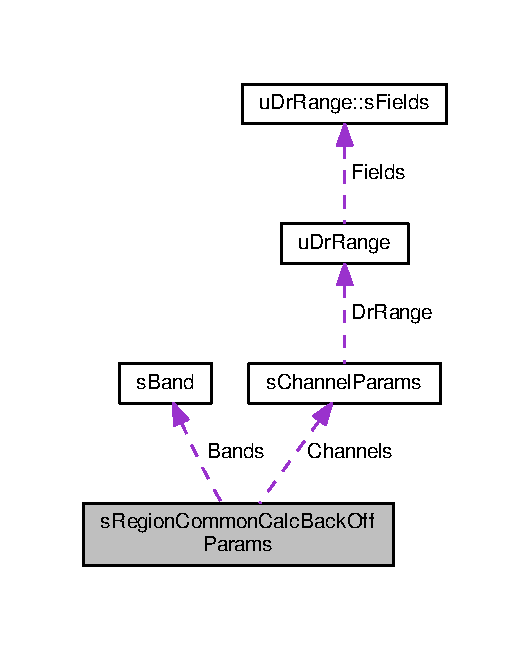
\includegraphics[width=255pt]{structsRegionCommonCalcBackOffParams__coll__graph}
\end{center}
\end{figure}
\subsection*{Data Fields}
\begin{DoxyCompactItemize}
\item 
\hyperlink{group__LORAMAC_ga1360ca6f82c6d125ea43a9dad9b56184}{Channel\+Params\+\_\+t} $\ast$ \hyperlink{structsRegionCommonCalcBackOffParams_a80b7872d31b72001cd95966a368d7b03}{Channels}
\item 
\hyperlink{group__LORAMAC_ga8f49721ee96ceb52c80a896ab11a2ed8}{Band\+\_\+t} $\ast$ \hyperlink{structsRegionCommonCalcBackOffParams_a08398c203c36396709386edc3c354b92}{Bands}
\item 
bool \hyperlink{structsRegionCommonCalcBackOffParams_aafd7bf9a24adbed2a88aa1334e30e528}{Last\+Tx\+Is\+Join\+Request}
\item 
bool \hyperlink{structsRegionCommonCalcBackOffParams_a744476f15b6a603ba729a942b9d6fcdc}{Joined}
\item 
bool \hyperlink{structsRegionCommonCalcBackOffParams_a3a4e746118e3f72abfc8dd5dc7ac533b}{Duty\+Cycle\+Enabled}
\item 
uint8\+\_\+t \hyperlink{structsRegionCommonCalcBackOffParams_a05928beb5ca2ff12d429f389def16532}{Channel}
\item 
\hyperlink{utilities_8h_a4215ca43d3e953099ea758ce428599d0}{Timer\+Time\+\_\+t} \hyperlink{structsRegionCommonCalcBackOffParams_aa8267b93bd66be0a05ca2ee14fa6c7bb}{Elapsed\+Time}
\item 
\hyperlink{utilities_8h_a4215ca43d3e953099ea758ce428599d0}{Timer\+Time\+\_\+t} \hyperlink{structsRegionCommonCalcBackOffParams_a24e06077cbe6b16d8abd08ef6327a4dc}{Tx\+Time\+On\+Air}
\end{DoxyCompactItemize}


\subsection{Field Documentation}
\mbox{\Hypertarget{structsRegionCommonCalcBackOffParams_a08398c203c36396709386edc3c354b92}\label{structsRegionCommonCalcBackOffParams_a08398c203c36396709386edc3c354b92}} 
\index{s\+Region\+Common\+Calc\+Back\+Off\+Params@{s\+Region\+Common\+Calc\+Back\+Off\+Params}!Bands@{Bands}}
\index{Bands@{Bands}!s\+Region\+Common\+Calc\+Back\+Off\+Params@{s\+Region\+Common\+Calc\+Back\+Off\+Params}}
\subsubsection{\texorpdfstring{Bands}{Bands}}
{\footnotesize\ttfamily \hyperlink{group__LORAMAC_ga8f49721ee96ceb52c80a896ab11a2ed8}{Band\+\_\+t}$\ast$ s\+Region\+Common\+Calc\+Back\+Off\+Params\+::\+Bands}

A pointer to region specific bands. \mbox{\Hypertarget{structsRegionCommonCalcBackOffParams_a05928beb5ca2ff12d429f389def16532}\label{structsRegionCommonCalcBackOffParams_a05928beb5ca2ff12d429f389def16532}} 
\index{s\+Region\+Common\+Calc\+Back\+Off\+Params@{s\+Region\+Common\+Calc\+Back\+Off\+Params}!Channel@{Channel}}
\index{Channel@{Channel}!s\+Region\+Common\+Calc\+Back\+Off\+Params@{s\+Region\+Common\+Calc\+Back\+Off\+Params}}
\subsubsection{\texorpdfstring{Channel}{Channel}}
{\footnotesize\ttfamily uint8\+\_\+t s\+Region\+Common\+Calc\+Back\+Off\+Params\+::\+Channel}

The current channel. \mbox{\Hypertarget{structsRegionCommonCalcBackOffParams_a80b7872d31b72001cd95966a368d7b03}\label{structsRegionCommonCalcBackOffParams_a80b7872d31b72001cd95966a368d7b03}} 
\index{s\+Region\+Common\+Calc\+Back\+Off\+Params@{s\+Region\+Common\+Calc\+Back\+Off\+Params}!Channels@{Channels}}
\index{Channels@{Channels}!s\+Region\+Common\+Calc\+Back\+Off\+Params@{s\+Region\+Common\+Calc\+Back\+Off\+Params}}
\subsubsection{\texorpdfstring{Channels}{Channels}}
{\footnotesize\ttfamily \hyperlink{group__LORAMAC_ga1360ca6f82c6d125ea43a9dad9b56184}{Channel\+Params\+\_\+t}$\ast$ s\+Region\+Common\+Calc\+Back\+Off\+Params\+::\+Channels}

A pointer to region specific channels. \mbox{\Hypertarget{structsRegionCommonCalcBackOffParams_a3a4e746118e3f72abfc8dd5dc7ac533b}\label{structsRegionCommonCalcBackOffParams_a3a4e746118e3f72abfc8dd5dc7ac533b}} 
\index{s\+Region\+Common\+Calc\+Back\+Off\+Params@{s\+Region\+Common\+Calc\+Back\+Off\+Params}!Duty\+Cycle\+Enabled@{Duty\+Cycle\+Enabled}}
\index{Duty\+Cycle\+Enabled@{Duty\+Cycle\+Enabled}!s\+Region\+Common\+Calc\+Back\+Off\+Params@{s\+Region\+Common\+Calc\+Back\+Off\+Params}}
\subsubsection{\texorpdfstring{Duty\+Cycle\+Enabled}{DutyCycleEnabled}}
{\footnotesize\ttfamily bool s\+Region\+Common\+Calc\+Back\+Off\+Params\+::\+Duty\+Cycle\+Enabled}

Set to true, if the duty cycle is enabled. \mbox{\Hypertarget{structsRegionCommonCalcBackOffParams_aa8267b93bd66be0a05ca2ee14fa6c7bb}\label{structsRegionCommonCalcBackOffParams_aa8267b93bd66be0a05ca2ee14fa6c7bb}} 
\index{s\+Region\+Common\+Calc\+Back\+Off\+Params@{s\+Region\+Common\+Calc\+Back\+Off\+Params}!Elapsed\+Time@{Elapsed\+Time}}
\index{Elapsed\+Time@{Elapsed\+Time}!s\+Region\+Common\+Calc\+Back\+Off\+Params@{s\+Region\+Common\+Calc\+Back\+Off\+Params}}
\subsubsection{\texorpdfstring{Elapsed\+Time}{ElapsedTime}}
{\footnotesize\ttfamily \hyperlink{utilities_8h_a4215ca43d3e953099ea758ce428599d0}{Timer\+Time\+\_\+t} s\+Region\+Common\+Calc\+Back\+Off\+Params\+::\+Elapsed\+Time}

The elapsed time since initialization. \mbox{\Hypertarget{structsRegionCommonCalcBackOffParams_a744476f15b6a603ba729a942b9d6fcdc}\label{structsRegionCommonCalcBackOffParams_a744476f15b6a603ba729a942b9d6fcdc}} 
\index{s\+Region\+Common\+Calc\+Back\+Off\+Params@{s\+Region\+Common\+Calc\+Back\+Off\+Params}!Joined@{Joined}}
\index{Joined@{Joined}!s\+Region\+Common\+Calc\+Back\+Off\+Params@{s\+Region\+Common\+Calc\+Back\+Off\+Params}}
\subsubsection{\texorpdfstring{Joined}{Joined}}
{\footnotesize\ttfamily bool s\+Region\+Common\+Calc\+Back\+Off\+Params\+::\+Joined}

Set to true, if the node is joined. \mbox{\Hypertarget{structsRegionCommonCalcBackOffParams_aafd7bf9a24adbed2a88aa1334e30e528}\label{structsRegionCommonCalcBackOffParams_aafd7bf9a24adbed2a88aa1334e30e528}} 
\index{s\+Region\+Common\+Calc\+Back\+Off\+Params@{s\+Region\+Common\+Calc\+Back\+Off\+Params}!Last\+Tx\+Is\+Join\+Request@{Last\+Tx\+Is\+Join\+Request}}
\index{Last\+Tx\+Is\+Join\+Request@{Last\+Tx\+Is\+Join\+Request}!s\+Region\+Common\+Calc\+Back\+Off\+Params@{s\+Region\+Common\+Calc\+Back\+Off\+Params}}
\subsubsection{\texorpdfstring{Last\+Tx\+Is\+Join\+Request}{LastTxIsJoinRequest}}
{\footnotesize\ttfamily bool s\+Region\+Common\+Calc\+Back\+Off\+Params\+::\+Last\+Tx\+Is\+Join\+Request}

Set to true, if the last uplink was a join request. \mbox{\Hypertarget{structsRegionCommonCalcBackOffParams_a24e06077cbe6b16d8abd08ef6327a4dc}\label{structsRegionCommonCalcBackOffParams_a24e06077cbe6b16d8abd08ef6327a4dc}} 
\index{s\+Region\+Common\+Calc\+Back\+Off\+Params@{s\+Region\+Common\+Calc\+Back\+Off\+Params}!Tx\+Time\+On\+Air@{Tx\+Time\+On\+Air}}
\index{Tx\+Time\+On\+Air@{Tx\+Time\+On\+Air}!s\+Region\+Common\+Calc\+Back\+Off\+Params@{s\+Region\+Common\+Calc\+Back\+Off\+Params}}
\subsubsection{\texorpdfstring{Tx\+Time\+On\+Air}{TxTimeOnAir}}
{\footnotesize\ttfamily \hyperlink{utilities_8h_a4215ca43d3e953099ea758ce428599d0}{Timer\+Time\+\_\+t} s\+Region\+Common\+Calc\+Back\+Off\+Params\+::\+Tx\+Time\+On\+Air}

The time on air of the last Tx frame. 

The documentation for this struct was generated from the following file\+:\begin{DoxyCompactItemize}
\item 
Mac/region/\hyperlink{RegionCommon_8h}{Region\+Common.\+h}\end{DoxyCompactItemize}

\hypertarget{structsRegionCommonLinkAdrParams}{}\section{s\+Region\+Common\+Link\+Adr\+Params Struct Reference}
\label{structsRegionCommonLinkAdrParams}\index{s\+Region\+Common\+Link\+Adr\+Params@{s\+Region\+Common\+Link\+Adr\+Params}}


{\ttfamily \#include $<$Region\+Common.\+h$>$}

\subsection*{Data Fields}
\begin{DoxyCompactItemize}
\item 
uint8\+\_\+t \hyperlink{structsRegionCommonLinkAdrParams_a2b8f075b875504269639472a92f0d209}{Nb\+Rep}
\item 
int8\+\_\+t \hyperlink{structsRegionCommonLinkAdrParams_ad98fd10c2350b2904f9b6476b83047c2}{Datarate}
\item 
int8\+\_\+t \hyperlink{structsRegionCommonLinkAdrParams_abff516206c93b038001dcb98629b53c2}{Tx\+Power}
\item 
uint8\+\_\+t \hyperlink{structsRegionCommonLinkAdrParams_a8f65bfcf50d2fe6113780d060aa75ee7}{Ch\+Mask\+Ctrl}
\item 
uint16\+\_\+t \hyperlink{structsRegionCommonLinkAdrParams_aa953b9ff7101e6bd891f9fc516bbd51a}{Ch\+Mask}
\end{DoxyCompactItemize}


\subsection{Field Documentation}
\mbox{\Hypertarget{structsRegionCommonLinkAdrParams_aa953b9ff7101e6bd891f9fc516bbd51a}\label{structsRegionCommonLinkAdrParams_aa953b9ff7101e6bd891f9fc516bbd51a}} 
\index{s\+Region\+Common\+Link\+Adr\+Params@{s\+Region\+Common\+Link\+Adr\+Params}!Ch\+Mask@{Ch\+Mask}}
\index{Ch\+Mask@{Ch\+Mask}!s\+Region\+Common\+Link\+Adr\+Params@{s\+Region\+Common\+Link\+Adr\+Params}}
\subsubsection{\texorpdfstring{Ch\+Mask}{ChMask}}
{\footnotesize\ttfamily uint16\+\_\+t s\+Region\+Common\+Link\+Adr\+Params\+::\+Ch\+Mask}

Channels mask field. \mbox{\Hypertarget{structsRegionCommonLinkAdrParams_a8f65bfcf50d2fe6113780d060aa75ee7}\label{structsRegionCommonLinkAdrParams_a8f65bfcf50d2fe6113780d060aa75ee7}} 
\index{s\+Region\+Common\+Link\+Adr\+Params@{s\+Region\+Common\+Link\+Adr\+Params}!Ch\+Mask\+Ctrl@{Ch\+Mask\+Ctrl}}
\index{Ch\+Mask\+Ctrl@{Ch\+Mask\+Ctrl}!s\+Region\+Common\+Link\+Adr\+Params@{s\+Region\+Common\+Link\+Adr\+Params}}
\subsubsection{\texorpdfstring{Ch\+Mask\+Ctrl}{ChMaskCtrl}}
{\footnotesize\ttfamily uint8\+\_\+t s\+Region\+Common\+Link\+Adr\+Params\+::\+Ch\+Mask\+Ctrl}

Channels mask control field. \mbox{\Hypertarget{structsRegionCommonLinkAdrParams_ad98fd10c2350b2904f9b6476b83047c2}\label{structsRegionCommonLinkAdrParams_ad98fd10c2350b2904f9b6476b83047c2}} 
\index{s\+Region\+Common\+Link\+Adr\+Params@{s\+Region\+Common\+Link\+Adr\+Params}!Datarate@{Datarate}}
\index{Datarate@{Datarate}!s\+Region\+Common\+Link\+Adr\+Params@{s\+Region\+Common\+Link\+Adr\+Params}}
\subsubsection{\texorpdfstring{Datarate}{Datarate}}
{\footnotesize\ttfamily int8\+\_\+t s\+Region\+Common\+Link\+Adr\+Params\+::\+Datarate}

Datarate. \mbox{\Hypertarget{structsRegionCommonLinkAdrParams_a2b8f075b875504269639472a92f0d209}\label{structsRegionCommonLinkAdrParams_a2b8f075b875504269639472a92f0d209}} 
\index{s\+Region\+Common\+Link\+Adr\+Params@{s\+Region\+Common\+Link\+Adr\+Params}!Nb\+Rep@{Nb\+Rep}}
\index{Nb\+Rep@{Nb\+Rep}!s\+Region\+Common\+Link\+Adr\+Params@{s\+Region\+Common\+Link\+Adr\+Params}}
\subsubsection{\texorpdfstring{Nb\+Rep}{NbRep}}
{\footnotesize\ttfamily uint8\+\_\+t s\+Region\+Common\+Link\+Adr\+Params\+::\+Nb\+Rep}

Number of repetitions. \mbox{\Hypertarget{structsRegionCommonLinkAdrParams_abff516206c93b038001dcb98629b53c2}\label{structsRegionCommonLinkAdrParams_abff516206c93b038001dcb98629b53c2}} 
\index{s\+Region\+Common\+Link\+Adr\+Params@{s\+Region\+Common\+Link\+Adr\+Params}!Tx\+Power@{Tx\+Power}}
\index{Tx\+Power@{Tx\+Power}!s\+Region\+Common\+Link\+Adr\+Params@{s\+Region\+Common\+Link\+Adr\+Params}}
\subsubsection{\texorpdfstring{Tx\+Power}{TxPower}}
{\footnotesize\ttfamily int8\+\_\+t s\+Region\+Common\+Link\+Adr\+Params\+::\+Tx\+Power}

Tx power. 

The documentation for this struct was generated from the following file\+:\begin{DoxyCompactItemize}
\item 
Mac/region/\hyperlink{RegionCommon_8h}{Region\+Common.\+h}\end{DoxyCompactItemize}

\hypertarget{structsRegionCommonLinkAdrReqVerifyParams}{}\section{s\+Region\+Common\+Link\+Adr\+Req\+Verify\+Params Struct Reference}
\label{structsRegionCommonLinkAdrReqVerifyParams}\index{s\+Region\+Common\+Link\+Adr\+Req\+Verify\+Params@{s\+Region\+Common\+Link\+Adr\+Req\+Verify\+Params}}


{\ttfamily \#include $<$Region\+Common.\+h$>$}



Collaboration diagram for s\+Region\+Common\+Link\+Adr\+Req\+Verify\+Params\+:
\nopagebreak
\begin{figure}[H]
\begin{center}
\leavevmode
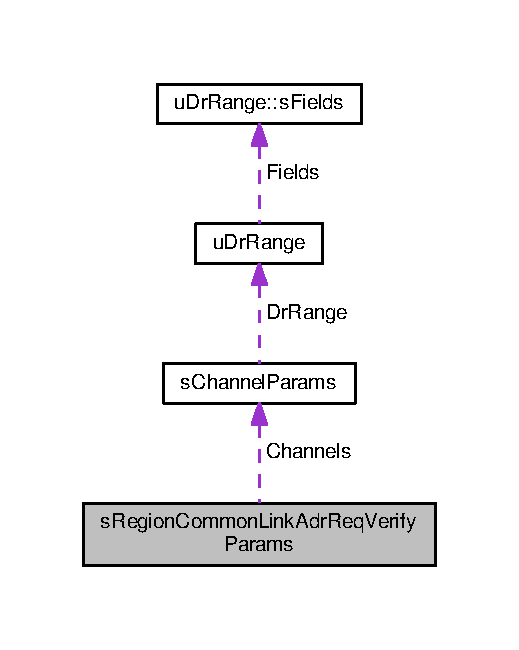
\includegraphics[width=249pt]{structsRegionCommonLinkAdrReqVerifyParams__coll__graph}
\end{center}
\end{figure}
\subsection*{Data Fields}
\begin{DoxyCompactItemize}
\item 
uint8\+\_\+t \hyperlink{structsRegionCommonLinkAdrReqVerifyParams_a429bbd69fae4c3642bf14bd1efa04ea2}{Status}
\item 
bool \hyperlink{structsRegionCommonLinkAdrReqVerifyParams_afd03766c72f58d11c674a206cfdb4d4a}{Adr\+Enabled}
\item 
int8\+\_\+t \hyperlink{structsRegionCommonLinkAdrReqVerifyParams_af3fe2cfebe5e97ac38bf3402eb575bc1}{Datarate}
\item 
int8\+\_\+t \hyperlink{structsRegionCommonLinkAdrReqVerifyParams_adbb4536c7f3a4672f9888c346b6200a5}{Tx\+Power}
\item 
uint8\+\_\+t \hyperlink{structsRegionCommonLinkAdrReqVerifyParams_a7230a0b5bb9a47a669ed568d8c3f376f}{Nb\+Rep}
\item 
int8\+\_\+t \hyperlink{structsRegionCommonLinkAdrReqVerifyParams_aeebccbc2f20b9b3bde89161b0780a532}{Current\+Datarate}
\item 
int8\+\_\+t \hyperlink{structsRegionCommonLinkAdrReqVerifyParams_a25d09502bab2de48433c35515aeb4032}{Current\+Tx\+Power}
\item 
int8\+\_\+t \hyperlink{structsRegionCommonLinkAdrReqVerifyParams_ac9f4e60bb78a62b3adc5fc7fee4b53fd}{Current\+Nb\+Rep}
\item 
uint8\+\_\+t \hyperlink{structsRegionCommonLinkAdrReqVerifyParams_a47f2063a20ecefe952d0deacccf8c76f}{Nb\+Channels}
\item 
uint16\+\_\+t $\ast$ \hyperlink{structsRegionCommonLinkAdrReqVerifyParams_afe91eaf70011a2894b570ce7d041df67}{Channels\+Mask}
\item 
int8\+\_\+t \hyperlink{structsRegionCommonLinkAdrReqVerifyParams_a2166f3c4240c96cd8478b46e1c34d201}{Min\+Datarate}
\item 
int8\+\_\+t \hyperlink{structsRegionCommonLinkAdrReqVerifyParams_a58a01a8c8400c4bfe2c2be665997eb6d}{Max\+Datarate}
\item 
\hyperlink{group__LORAMAC_ga1360ca6f82c6d125ea43a9dad9b56184}{Channel\+Params\+\_\+t} $\ast$ \hyperlink{structsRegionCommonLinkAdrReqVerifyParams_ad6a30685c21f172138b016e50f4e7e6f}{Channels}
\item 
int8\+\_\+t \hyperlink{structsRegionCommonLinkAdrReqVerifyParams_ae3c2f43bcdfce1e8cc4f0ec73f7b7ff6}{Min\+Tx\+Power}
\item 
int8\+\_\+t \hyperlink{structsRegionCommonLinkAdrReqVerifyParams_ace9e3769fec574c047fefbbca55e74da}{Max\+Tx\+Power}
\end{DoxyCompactItemize}


\subsection{Field Documentation}
\mbox{\Hypertarget{structsRegionCommonLinkAdrReqVerifyParams_afd03766c72f58d11c674a206cfdb4d4a}\label{structsRegionCommonLinkAdrReqVerifyParams_afd03766c72f58d11c674a206cfdb4d4a}} 
\index{s\+Region\+Common\+Link\+Adr\+Req\+Verify\+Params@{s\+Region\+Common\+Link\+Adr\+Req\+Verify\+Params}!Adr\+Enabled@{Adr\+Enabled}}
\index{Adr\+Enabled@{Adr\+Enabled}!s\+Region\+Common\+Link\+Adr\+Req\+Verify\+Params@{s\+Region\+Common\+Link\+Adr\+Req\+Verify\+Params}}
\subsubsection{\texorpdfstring{Adr\+Enabled}{AdrEnabled}}
{\footnotesize\ttfamily bool s\+Region\+Common\+Link\+Adr\+Req\+Verify\+Params\+::\+Adr\+Enabled}

Set to true, if A\+DR is enabled. \mbox{\Hypertarget{structsRegionCommonLinkAdrReqVerifyParams_ad6a30685c21f172138b016e50f4e7e6f}\label{structsRegionCommonLinkAdrReqVerifyParams_ad6a30685c21f172138b016e50f4e7e6f}} 
\index{s\+Region\+Common\+Link\+Adr\+Req\+Verify\+Params@{s\+Region\+Common\+Link\+Adr\+Req\+Verify\+Params}!Channels@{Channels}}
\index{Channels@{Channels}!s\+Region\+Common\+Link\+Adr\+Req\+Verify\+Params@{s\+Region\+Common\+Link\+Adr\+Req\+Verify\+Params}}
\subsubsection{\texorpdfstring{Channels}{Channels}}
{\footnotesize\ttfamily \hyperlink{group__LORAMAC_ga1360ca6f82c6d125ea43a9dad9b56184}{Channel\+Params\+\_\+t}$\ast$ s\+Region\+Common\+Link\+Adr\+Req\+Verify\+Params\+::\+Channels}

Pointer to the channels. \mbox{\Hypertarget{structsRegionCommonLinkAdrReqVerifyParams_afe91eaf70011a2894b570ce7d041df67}\label{structsRegionCommonLinkAdrReqVerifyParams_afe91eaf70011a2894b570ce7d041df67}} 
\index{s\+Region\+Common\+Link\+Adr\+Req\+Verify\+Params@{s\+Region\+Common\+Link\+Adr\+Req\+Verify\+Params}!Channels\+Mask@{Channels\+Mask}}
\index{Channels\+Mask@{Channels\+Mask}!s\+Region\+Common\+Link\+Adr\+Req\+Verify\+Params@{s\+Region\+Common\+Link\+Adr\+Req\+Verify\+Params}}
\subsubsection{\texorpdfstring{Channels\+Mask}{ChannelsMask}}
{\footnotesize\ttfamily uint16\+\_\+t$\ast$ s\+Region\+Common\+Link\+Adr\+Req\+Verify\+Params\+::\+Channels\+Mask}

Pointer to the first element of the channels mask. \mbox{\Hypertarget{structsRegionCommonLinkAdrReqVerifyParams_aeebccbc2f20b9b3bde89161b0780a532}\label{structsRegionCommonLinkAdrReqVerifyParams_aeebccbc2f20b9b3bde89161b0780a532}} 
\index{s\+Region\+Common\+Link\+Adr\+Req\+Verify\+Params@{s\+Region\+Common\+Link\+Adr\+Req\+Verify\+Params}!Current\+Datarate@{Current\+Datarate}}
\index{Current\+Datarate@{Current\+Datarate}!s\+Region\+Common\+Link\+Adr\+Req\+Verify\+Params@{s\+Region\+Common\+Link\+Adr\+Req\+Verify\+Params}}
\subsubsection{\texorpdfstring{Current\+Datarate}{CurrentDatarate}}
{\footnotesize\ttfamily int8\+\_\+t s\+Region\+Common\+Link\+Adr\+Req\+Verify\+Params\+::\+Current\+Datarate}

The current datarate the node is using. \mbox{\Hypertarget{structsRegionCommonLinkAdrReqVerifyParams_ac9f4e60bb78a62b3adc5fc7fee4b53fd}\label{structsRegionCommonLinkAdrReqVerifyParams_ac9f4e60bb78a62b3adc5fc7fee4b53fd}} 
\index{s\+Region\+Common\+Link\+Adr\+Req\+Verify\+Params@{s\+Region\+Common\+Link\+Adr\+Req\+Verify\+Params}!Current\+Nb\+Rep@{Current\+Nb\+Rep}}
\index{Current\+Nb\+Rep@{Current\+Nb\+Rep}!s\+Region\+Common\+Link\+Adr\+Req\+Verify\+Params@{s\+Region\+Common\+Link\+Adr\+Req\+Verify\+Params}}
\subsubsection{\texorpdfstring{Current\+Nb\+Rep}{CurrentNbRep}}
{\footnotesize\ttfamily int8\+\_\+t s\+Region\+Common\+Link\+Adr\+Req\+Verify\+Params\+::\+Current\+Nb\+Rep}

The current number of repetitions the node is using. \mbox{\Hypertarget{structsRegionCommonLinkAdrReqVerifyParams_a25d09502bab2de48433c35515aeb4032}\label{structsRegionCommonLinkAdrReqVerifyParams_a25d09502bab2de48433c35515aeb4032}} 
\index{s\+Region\+Common\+Link\+Adr\+Req\+Verify\+Params@{s\+Region\+Common\+Link\+Adr\+Req\+Verify\+Params}!Current\+Tx\+Power@{Current\+Tx\+Power}}
\index{Current\+Tx\+Power@{Current\+Tx\+Power}!s\+Region\+Common\+Link\+Adr\+Req\+Verify\+Params@{s\+Region\+Common\+Link\+Adr\+Req\+Verify\+Params}}
\subsubsection{\texorpdfstring{Current\+Tx\+Power}{CurrentTxPower}}
{\footnotesize\ttfamily int8\+\_\+t s\+Region\+Common\+Link\+Adr\+Req\+Verify\+Params\+::\+Current\+Tx\+Power}

The current TX power the node is using. \mbox{\Hypertarget{structsRegionCommonLinkAdrReqVerifyParams_af3fe2cfebe5e97ac38bf3402eb575bc1}\label{structsRegionCommonLinkAdrReqVerifyParams_af3fe2cfebe5e97ac38bf3402eb575bc1}} 
\index{s\+Region\+Common\+Link\+Adr\+Req\+Verify\+Params@{s\+Region\+Common\+Link\+Adr\+Req\+Verify\+Params}!Datarate@{Datarate}}
\index{Datarate@{Datarate}!s\+Region\+Common\+Link\+Adr\+Req\+Verify\+Params@{s\+Region\+Common\+Link\+Adr\+Req\+Verify\+Params}}
\subsubsection{\texorpdfstring{Datarate}{Datarate}}
{\footnotesize\ttfamily int8\+\_\+t s\+Region\+Common\+Link\+Adr\+Req\+Verify\+Params\+::\+Datarate}

The datarate the Adr\+Link\+Request wants to set. \mbox{\Hypertarget{structsRegionCommonLinkAdrReqVerifyParams_a58a01a8c8400c4bfe2c2be665997eb6d}\label{structsRegionCommonLinkAdrReqVerifyParams_a58a01a8c8400c4bfe2c2be665997eb6d}} 
\index{s\+Region\+Common\+Link\+Adr\+Req\+Verify\+Params@{s\+Region\+Common\+Link\+Adr\+Req\+Verify\+Params}!Max\+Datarate@{Max\+Datarate}}
\index{Max\+Datarate@{Max\+Datarate}!s\+Region\+Common\+Link\+Adr\+Req\+Verify\+Params@{s\+Region\+Common\+Link\+Adr\+Req\+Verify\+Params}}
\subsubsection{\texorpdfstring{Max\+Datarate}{MaxDatarate}}
{\footnotesize\ttfamily int8\+\_\+t s\+Region\+Common\+Link\+Adr\+Req\+Verify\+Params\+::\+Max\+Datarate}

The maximum possible datarate. \mbox{\Hypertarget{structsRegionCommonLinkAdrReqVerifyParams_ace9e3769fec574c047fefbbca55e74da}\label{structsRegionCommonLinkAdrReqVerifyParams_ace9e3769fec574c047fefbbca55e74da}} 
\index{s\+Region\+Common\+Link\+Adr\+Req\+Verify\+Params@{s\+Region\+Common\+Link\+Adr\+Req\+Verify\+Params}!Max\+Tx\+Power@{Max\+Tx\+Power}}
\index{Max\+Tx\+Power@{Max\+Tx\+Power}!s\+Region\+Common\+Link\+Adr\+Req\+Verify\+Params@{s\+Region\+Common\+Link\+Adr\+Req\+Verify\+Params}}
\subsubsection{\texorpdfstring{Max\+Tx\+Power}{MaxTxPower}}
{\footnotesize\ttfamily int8\+\_\+t s\+Region\+Common\+Link\+Adr\+Req\+Verify\+Params\+::\+Max\+Tx\+Power}

The maximum possible TX power. \mbox{\Hypertarget{structsRegionCommonLinkAdrReqVerifyParams_a2166f3c4240c96cd8478b46e1c34d201}\label{structsRegionCommonLinkAdrReqVerifyParams_a2166f3c4240c96cd8478b46e1c34d201}} 
\index{s\+Region\+Common\+Link\+Adr\+Req\+Verify\+Params@{s\+Region\+Common\+Link\+Adr\+Req\+Verify\+Params}!Min\+Datarate@{Min\+Datarate}}
\index{Min\+Datarate@{Min\+Datarate}!s\+Region\+Common\+Link\+Adr\+Req\+Verify\+Params@{s\+Region\+Common\+Link\+Adr\+Req\+Verify\+Params}}
\subsubsection{\texorpdfstring{Min\+Datarate}{MinDatarate}}
{\footnotesize\ttfamily int8\+\_\+t s\+Region\+Common\+Link\+Adr\+Req\+Verify\+Params\+::\+Min\+Datarate}

The minimum possible datarate. \mbox{\Hypertarget{structsRegionCommonLinkAdrReqVerifyParams_ae3c2f43bcdfce1e8cc4f0ec73f7b7ff6}\label{structsRegionCommonLinkAdrReqVerifyParams_ae3c2f43bcdfce1e8cc4f0ec73f7b7ff6}} 
\index{s\+Region\+Common\+Link\+Adr\+Req\+Verify\+Params@{s\+Region\+Common\+Link\+Adr\+Req\+Verify\+Params}!Min\+Tx\+Power@{Min\+Tx\+Power}}
\index{Min\+Tx\+Power@{Min\+Tx\+Power}!s\+Region\+Common\+Link\+Adr\+Req\+Verify\+Params@{s\+Region\+Common\+Link\+Adr\+Req\+Verify\+Params}}
\subsubsection{\texorpdfstring{Min\+Tx\+Power}{MinTxPower}}
{\footnotesize\ttfamily int8\+\_\+t s\+Region\+Common\+Link\+Adr\+Req\+Verify\+Params\+::\+Min\+Tx\+Power}

The minimum possible TX power. \mbox{\Hypertarget{structsRegionCommonLinkAdrReqVerifyParams_a47f2063a20ecefe952d0deacccf8c76f}\label{structsRegionCommonLinkAdrReqVerifyParams_a47f2063a20ecefe952d0deacccf8c76f}} 
\index{s\+Region\+Common\+Link\+Adr\+Req\+Verify\+Params@{s\+Region\+Common\+Link\+Adr\+Req\+Verify\+Params}!Nb\+Channels@{Nb\+Channels}}
\index{Nb\+Channels@{Nb\+Channels}!s\+Region\+Common\+Link\+Adr\+Req\+Verify\+Params@{s\+Region\+Common\+Link\+Adr\+Req\+Verify\+Params}}
\subsubsection{\texorpdfstring{Nb\+Channels}{NbChannels}}
{\footnotesize\ttfamily uint8\+\_\+t s\+Region\+Common\+Link\+Adr\+Req\+Verify\+Params\+::\+Nb\+Channels}

The number of channels. \mbox{\Hypertarget{structsRegionCommonLinkAdrReqVerifyParams_a7230a0b5bb9a47a669ed568d8c3f376f}\label{structsRegionCommonLinkAdrReqVerifyParams_a7230a0b5bb9a47a669ed568d8c3f376f}} 
\index{s\+Region\+Common\+Link\+Adr\+Req\+Verify\+Params@{s\+Region\+Common\+Link\+Adr\+Req\+Verify\+Params}!Nb\+Rep@{Nb\+Rep}}
\index{Nb\+Rep@{Nb\+Rep}!s\+Region\+Common\+Link\+Adr\+Req\+Verify\+Params@{s\+Region\+Common\+Link\+Adr\+Req\+Verify\+Params}}
\subsubsection{\texorpdfstring{Nb\+Rep}{NbRep}}
{\footnotesize\ttfamily uint8\+\_\+t s\+Region\+Common\+Link\+Adr\+Req\+Verify\+Params\+::\+Nb\+Rep}

The number of repetitions the Adr\+Link\+Request wants to set. \mbox{\Hypertarget{structsRegionCommonLinkAdrReqVerifyParams_a429bbd69fae4c3642bf14bd1efa04ea2}\label{structsRegionCommonLinkAdrReqVerifyParams_a429bbd69fae4c3642bf14bd1efa04ea2}} 
\index{s\+Region\+Common\+Link\+Adr\+Req\+Verify\+Params@{s\+Region\+Common\+Link\+Adr\+Req\+Verify\+Params}!Status@{Status}}
\index{Status@{Status}!s\+Region\+Common\+Link\+Adr\+Req\+Verify\+Params@{s\+Region\+Common\+Link\+Adr\+Req\+Verify\+Params}}
\subsubsection{\texorpdfstring{Status}{Status}}
{\footnotesize\ttfamily uint8\+\_\+t s\+Region\+Common\+Link\+Adr\+Req\+Verify\+Params\+::\+Status}

The current status of the Adr\+Link\+Request. \mbox{\Hypertarget{structsRegionCommonLinkAdrReqVerifyParams_adbb4536c7f3a4672f9888c346b6200a5}\label{structsRegionCommonLinkAdrReqVerifyParams_adbb4536c7f3a4672f9888c346b6200a5}} 
\index{s\+Region\+Common\+Link\+Adr\+Req\+Verify\+Params@{s\+Region\+Common\+Link\+Adr\+Req\+Verify\+Params}!Tx\+Power@{Tx\+Power}}
\index{Tx\+Power@{Tx\+Power}!s\+Region\+Common\+Link\+Adr\+Req\+Verify\+Params@{s\+Region\+Common\+Link\+Adr\+Req\+Verify\+Params}}
\subsubsection{\texorpdfstring{Tx\+Power}{TxPower}}
{\footnotesize\ttfamily int8\+\_\+t s\+Region\+Common\+Link\+Adr\+Req\+Verify\+Params\+::\+Tx\+Power}

The TX power the Adr\+Link\+Request wants to set. 

The documentation for this struct was generated from the following file\+:\begin{DoxyCompactItemize}
\item 
Mac/region/\hyperlink{RegionCommon_8h}{Region\+Common.\+h}\end{DoxyCompactItemize}

\hypertarget{structsRx2ChannelParams}{}\section{s\+Rx2\+Channel\+Params Struct Reference}
\label{structsRx2ChannelParams}\index{s\+Rx2\+Channel\+Params@{s\+Rx2\+Channel\+Params}}


{\ttfamily \#include $<$Lo\+Ra\+Mac.\+h$>$}

\subsection*{Data Fields}
\begin{DoxyCompactItemize}
\item 
uint32\+\_\+t \hyperlink{structsRx2ChannelParams_a49737d85a2306a64e5fec08f2b564c52}{Frequency}
\item 
uint8\+\_\+t \hyperlink{structsRx2ChannelParams_aed285208f9d763e511e80ec2b3d7f526}{Datarate}
\end{DoxyCompactItemize}


\subsection{Detailed Description}
Lo\+Ra\+M\+AC receive window 2 channel parameters 

\subsection{Field Documentation}
\mbox{\Hypertarget{structsRx2ChannelParams_aed285208f9d763e511e80ec2b3d7f526}\label{structsRx2ChannelParams_aed285208f9d763e511e80ec2b3d7f526}} 
\index{s\+Rx2\+Channel\+Params@{s\+Rx2\+Channel\+Params}!Datarate@{Datarate}}
\index{Datarate@{Datarate}!s\+Rx2\+Channel\+Params@{s\+Rx2\+Channel\+Params}}
\subsubsection{\texorpdfstring{Datarate}{Datarate}}
{\footnotesize\ttfamily uint8\+\_\+t s\+Rx2\+Channel\+Params\+::\+Datarate}

Data rate

Lo\+Ra\+W\+AN Regional Parameters V1.\+0.\+2rB

The allowed ranges are region specific. Please refer to \hyperlink{group__REGION_ga6c4ef966b4f3d5eb7597b087f2b97095}{D\+R\+\_\+0} to \hyperlink{group__REGION_gac6e078f51b71f05093daf27834997396}{D\+R\+\_\+15} for details. \mbox{\Hypertarget{structsRx2ChannelParams_a49737d85a2306a64e5fec08f2b564c52}\label{structsRx2ChannelParams_a49737d85a2306a64e5fec08f2b564c52}} 
\index{s\+Rx2\+Channel\+Params@{s\+Rx2\+Channel\+Params}!Frequency@{Frequency}}
\index{Frequency@{Frequency}!s\+Rx2\+Channel\+Params@{s\+Rx2\+Channel\+Params}}
\subsubsection{\texorpdfstring{Frequency}{Frequency}}
{\footnotesize\ttfamily uint32\+\_\+t s\+Rx2\+Channel\+Params\+::\+Frequency}

Frequency in Hz 

The documentation for this struct was generated from the following file\+:\begin{DoxyCompactItemize}
\item 
Mac/\hyperlink{LoRaMac_8h}{Lo\+Ra\+Mac.\+h}\end{DoxyCompactItemize}

\hypertarget{structsRxConfigParams}{}\section{s\+Rx\+Config\+Params Struct Reference}
\label{structsRxConfigParams}\index{s\+Rx\+Config\+Params@{s\+Rx\+Config\+Params}}


{\ttfamily \#include $<$Region.\+h$>$}

\subsection*{Data Fields}
\begin{DoxyCompactItemize}
\item 
uint8\+\_\+t \hyperlink{structsRxConfigParams_a32ac373f78a03da5f2b41b1be1b49d80}{Channel}
\item 
int8\+\_\+t \hyperlink{structsRxConfigParams_ad64d85b6c7b8b3d9b41aa28eaf4fcac2}{Datarate}
\item 
uint8\+\_\+t \hyperlink{structsRxConfigParams_a2c78d3dee4a8229d33ec621ca4c71638}{Bandwidth}
\item 
int8\+\_\+t \hyperlink{structsRxConfigParams_ac22b6867751b80613469c74b718bd361}{Dr\+Offset}
\item 
uint32\+\_\+t \hyperlink{structsRxConfigParams_a83ee523b7d7f082e2cac91407db2c2f1}{Frequency}
\item 
uint32\+\_\+t \hyperlink{structsRxConfigParams_afcae1c867cd1a7d0e4b3bab5b8bb8a86}{Window\+Timeout}
\item 
int32\+\_\+t \hyperlink{structsRxConfigParams_a323502f534f1a5ae832a9f00ce72c51e}{Window\+Offset}
\item 
uint8\+\_\+t \hyperlink{structsRxConfigParams_a4e1670a845c7ff99f601cb106e66fcaf}{Downlink\+Dwell\+Time}
\item 
bool \hyperlink{structsRxConfigParams_a0d18669fcf68efa8a06b664a8f297f8c}{Repeater\+Support}
\item 
bool \hyperlink{structsRxConfigParams_a1359157dd4e303171ed204febc7c58e0}{Rx\+Continuous}
\item 
bool \hyperlink{structsRxConfigParams_acae0e0d5f43b8a7136847d0ca3d3a60c}{Window}
\end{DoxyCompactItemize}


\subsection{Detailed Description}
Parameter structure for the function Region\+Rx\+Config. 

\subsection{Field Documentation}
\mbox{\Hypertarget{structsRxConfigParams_a2c78d3dee4a8229d33ec621ca4c71638}\label{structsRxConfigParams_a2c78d3dee4a8229d33ec621ca4c71638}} 
\index{s\+Rx\+Config\+Params@{s\+Rx\+Config\+Params}!Bandwidth@{Bandwidth}}
\index{Bandwidth@{Bandwidth}!s\+Rx\+Config\+Params@{s\+Rx\+Config\+Params}}
\subsubsection{\texorpdfstring{Bandwidth}{Bandwidth}}
{\footnotesize\ttfamily uint8\+\_\+t s\+Rx\+Config\+Params\+::\+Bandwidth}

RX bandwidth. \mbox{\Hypertarget{structsRxConfigParams_a32ac373f78a03da5f2b41b1be1b49d80}\label{structsRxConfigParams_a32ac373f78a03da5f2b41b1be1b49d80}} 
\index{s\+Rx\+Config\+Params@{s\+Rx\+Config\+Params}!Channel@{Channel}}
\index{Channel@{Channel}!s\+Rx\+Config\+Params@{s\+Rx\+Config\+Params}}
\subsubsection{\texorpdfstring{Channel}{Channel}}
{\footnotesize\ttfamily uint8\+\_\+t s\+Rx\+Config\+Params\+::\+Channel}

The RX channel. \mbox{\Hypertarget{structsRxConfigParams_ad64d85b6c7b8b3d9b41aa28eaf4fcac2}\label{structsRxConfigParams_ad64d85b6c7b8b3d9b41aa28eaf4fcac2}} 
\index{s\+Rx\+Config\+Params@{s\+Rx\+Config\+Params}!Datarate@{Datarate}}
\index{Datarate@{Datarate}!s\+Rx\+Config\+Params@{s\+Rx\+Config\+Params}}
\subsubsection{\texorpdfstring{Datarate}{Datarate}}
{\footnotesize\ttfamily int8\+\_\+t s\+Rx\+Config\+Params\+::\+Datarate}

RX datarate. \mbox{\Hypertarget{structsRxConfigParams_a4e1670a845c7ff99f601cb106e66fcaf}\label{structsRxConfigParams_a4e1670a845c7ff99f601cb106e66fcaf}} 
\index{s\+Rx\+Config\+Params@{s\+Rx\+Config\+Params}!Downlink\+Dwell\+Time@{Downlink\+Dwell\+Time}}
\index{Downlink\+Dwell\+Time@{Downlink\+Dwell\+Time}!s\+Rx\+Config\+Params@{s\+Rx\+Config\+Params}}
\subsubsection{\texorpdfstring{Downlink\+Dwell\+Time}{DownlinkDwellTime}}
{\footnotesize\ttfamily uint8\+\_\+t s\+Rx\+Config\+Params\+::\+Downlink\+Dwell\+Time}

Downlink dwell time. \mbox{\Hypertarget{structsRxConfigParams_ac22b6867751b80613469c74b718bd361}\label{structsRxConfigParams_ac22b6867751b80613469c74b718bd361}} 
\index{s\+Rx\+Config\+Params@{s\+Rx\+Config\+Params}!Dr\+Offset@{Dr\+Offset}}
\index{Dr\+Offset@{Dr\+Offset}!s\+Rx\+Config\+Params@{s\+Rx\+Config\+Params}}
\subsubsection{\texorpdfstring{Dr\+Offset}{DrOffset}}
{\footnotesize\ttfamily int8\+\_\+t s\+Rx\+Config\+Params\+::\+Dr\+Offset}

RX datarate offset. \mbox{\Hypertarget{structsRxConfigParams_a83ee523b7d7f082e2cac91407db2c2f1}\label{structsRxConfigParams_a83ee523b7d7f082e2cac91407db2c2f1}} 
\index{s\+Rx\+Config\+Params@{s\+Rx\+Config\+Params}!Frequency@{Frequency}}
\index{Frequency@{Frequency}!s\+Rx\+Config\+Params@{s\+Rx\+Config\+Params}}
\subsubsection{\texorpdfstring{Frequency}{Frequency}}
{\footnotesize\ttfamily uint32\+\_\+t s\+Rx\+Config\+Params\+::\+Frequency}

RX frequency. \mbox{\Hypertarget{structsRxConfigParams_a0d18669fcf68efa8a06b664a8f297f8c}\label{structsRxConfigParams_a0d18669fcf68efa8a06b664a8f297f8c}} 
\index{s\+Rx\+Config\+Params@{s\+Rx\+Config\+Params}!Repeater\+Support@{Repeater\+Support}}
\index{Repeater\+Support@{Repeater\+Support}!s\+Rx\+Config\+Params@{s\+Rx\+Config\+Params}}
\subsubsection{\texorpdfstring{Repeater\+Support}{RepeaterSupport}}
{\footnotesize\ttfamily bool s\+Rx\+Config\+Params\+::\+Repeater\+Support}

Set to true, if a repeater is supported. \mbox{\Hypertarget{structsRxConfigParams_a1359157dd4e303171ed204febc7c58e0}\label{structsRxConfigParams_a1359157dd4e303171ed204febc7c58e0}} 
\index{s\+Rx\+Config\+Params@{s\+Rx\+Config\+Params}!Rx\+Continuous@{Rx\+Continuous}}
\index{Rx\+Continuous@{Rx\+Continuous}!s\+Rx\+Config\+Params@{s\+Rx\+Config\+Params}}
\subsubsection{\texorpdfstring{Rx\+Continuous}{RxContinuous}}
{\footnotesize\ttfamily bool s\+Rx\+Config\+Params\+::\+Rx\+Continuous}

Set to true, if RX should be continuous. \mbox{\Hypertarget{structsRxConfigParams_acae0e0d5f43b8a7136847d0ca3d3a60c}\label{structsRxConfigParams_acae0e0d5f43b8a7136847d0ca3d3a60c}} 
\index{s\+Rx\+Config\+Params@{s\+Rx\+Config\+Params}!Window@{Window}}
\index{Window@{Window}!s\+Rx\+Config\+Params@{s\+Rx\+Config\+Params}}
\subsubsection{\texorpdfstring{Window}{Window}}
{\footnotesize\ttfamily bool s\+Rx\+Config\+Params\+::\+Window}

Sets the RX window. 0\+: RX window 1, 1\+: RX window 2. \mbox{\Hypertarget{structsRxConfigParams_a323502f534f1a5ae832a9f00ce72c51e}\label{structsRxConfigParams_a323502f534f1a5ae832a9f00ce72c51e}} 
\index{s\+Rx\+Config\+Params@{s\+Rx\+Config\+Params}!Window\+Offset@{Window\+Offset}}
\index{Window\+Offset@{Window\+Offset}!s\+Rx\+Config\+Params@{s\+Rx\+Config\+Params}}
\subsubsection{\texorpdfstring{Window\+Offset}{WindowOffset}}
{\footnotesize\ttfamily int32\+\_\+t s\+Rx\+Config\+Params\+::\+Window\+Offset}

RX window offset \mbox{\Hypertarget{structsRxConfigParams_afcae1c867cd1a7d0e4b3bab5b8bb8a86}\label{structsRxConfigParams_afcae1c867cd1a7d0e4b3bab5b8bb8a86}} 
\index{s\+Rx\+Config\+Params@{s\+Rx\+Config\+Params}!Window\+Timeout@{Window\+Timeout}}
\index{Window\+Timeout@{Window\+Timeout}!s\+Rx\+Config\+Params@{s\+Rx\+Config\+Params}}
\subsubsection{\texorpdfstring{Window\+Timeout}{WindowTimeout}}
{\footnotesize\ttfamily uint32\+\_\+t s\+Rx\+Config\+Params\+::\+Window\+Timeout}

RX window timeout 

The documentation for this struct was generated from the following file\+:\begin{DoxyCompactItemize}
\item 
Mac/region/\hyperlink{Region_8h}{Region.\+h}\end{DoxyCompactItemize}

\hypertarget{structsRxParamSetupReqParams}{}\section{s\+Rx\+Param\+Setup\+Req\+Params Struct Reference}
\label{structsRxParamSetupReqParams}\index{s\+Rx\+Param\+Setup\+Req\+Params@{s\+Rx\+Param\+Setup\+Req\+Params}}


{\ttfamily \#include $<$Region.\+h$>$}

\subsection*{Data Fields}
\begin{DoxyCompactItemize}
\item 
int8\+\_\+t \hyperlink{structsRxParamSetupReqParams_a1fae2b65e9f79e72bcf0a92827c7e1ac}{Datarate}
\item 
int8\+\_\+t \hyperlink{structsRxParamSetupReqParams_a8c50f3e69c50560ec3c21edc974104ef}{Dr\+Offset}
\item 
uint32\+\_\+t \hyperlink{structsRxParamSetupReqParams_a2cf70cbc0939be65e8c1257e45ae5530}{Frequency}
\end{DoxyCompactItemize}


\subsection{Detailed Description}
Parameter structure for the function Region\+Rx\+Param\+Setup\+Req. 

\subsection{Field Documentation}
\mbox{\Hypertarget{structsRxParamSetupReqParams_a1fae2b65e9f79e72bcf0a92827c7e1ac}\label{structsRxParamSetupReqParams_a1fae2b65e9f79e72bcf0a92827c7e1ac}} 
\index{s\+Rx\+Param\+Setup\+Req\+Params@{s\+Rx\+Param\+Setup\+Req\+Params}!Datarate@{Datarate}}
\index{Datarate@{Datarate}!s\+Rx\+Param\+Setup\+Req\+Params@{s\+Rx\+Param\+Setup\+Req\+Params}}
\subsubsection{\texorpdfstring{Datarate}{Datarate}}
{\footnotesize\ttfamily int8\+\_\+t s\+Rx\+Param\+Setup\+Req\+Params\+::\+Datarate}

The datarate to setup. \mbox{\Hypertarget{structsRxParamSetupReqParams_a8c50f3e69c50560ec3c21edc974104ef}\label{structsRxParamSetupReqParams_a8c50f3e69c50560ec3c21edc974104ef}} 
\index{s\+Rx\+Param\+Setup\+Req\+Params@{s\+Rx\+Param\+Setup\+Req\+Params}!Dr\+Offset@{Dr\+Offset}}
\index{Dr\+Offset@{Dr\+Offset}!s\+Rx\+Param\+Setup\+Req\+Params@{s\+Rx\+Param\+Setup\+Req\+Params}}
\subsubsection{\texorpdfstring{Dr\+Offset}{DrOffset}}
{\footnotesize\ttfamily int8\+\_\+t s\+Rx\+Param\+Setup\+Req\+Params\+::\+Dr\+Offset}

Datarate offset. \mbox{\Hypertarget{structsRxParamSetupReqParams_a2cf70cbc0939be65e8c1257e45ae5530}\label{structsRxParamSetupReqParams_a2cf70cbc0939be65e8c1257e45ae5530}} 
\index{s\+Rx\+Param\+Setup\+Req\+Params@{s\+Rx\+Param\+Setup\+Req\+Params}!Frequency@{Frequency}}
\index{Frequency@{Frequency}!s\+Rx\+Param\+Setup\+Req\+Params@{s\+Rx\+Param\+Setup\+Req\+Params}}
\subsubsection{\texorpdfstring{Frequency}{Frequency}}
{\footnotesize\ttfamily uint32\+\_\+t s\+Rx\+Param\+Setup\+Req\+Params\+::\+Frequency}

The frequency to setup. 

The documentation for this struct was generated from the following file\+:\begin{DoxyCompactItemize}
\item 
Mac/region/\hyperlink{Region_8h}{Region.\+h}\end{DoxyCompactItemize}

\hypertarget{structsSetBandTxDoneParams}{}\section{s\+Set\+Band\+Tx\+Done\+Params Struct Reference}
\label{structsSetBandTxDoneParams}\index{s\+Set\+Band\+Tx\+Done\+Params@{s\+Set\+Band\+Tx\+Done\+Params}}


{\ttfamily \#include $<$Region.\+h$>$}

\subsection*{Data Fields}
\begin{DoxyCompactItemize}
\item 
uint8\+\_\+t \hyperlink{structsSetBandTxDoneParams_aa62ca588b3e9ffbca81862caf859d509}{Channel}
\item 
bool \hyperlink{structsSetBandTxDoneParams_aee086764bc76bcd8fe82b8493854702a}{Joined}
\item 
\hyperlink{utilities_8h_a4215ca43d3e953099ea758ce428599d0}{Timer\+Time\+\_\+t} \hyperlink{structsSetBandTxDoneParams_aa1a7b87e8778b47583ec8bfe02aabef4}{Last\+Tx\+Done\+Time}
\end{DoxyCompactItemize}


\subsection{Detailed Description}
Parameter structure for the function Region\+Set\+Band\+Tx\+Done. 

\subsection{Field Documentation}
\mbox{\Hypertarget{structsSetBandTxDoneParams_aa62ca588b3e9ffbca81862caf859d509}\label{structsSetBandTxDoneParams_aa62ca588b3e9ffbca81862caf859d509}} 
\index{s\+Set\+Band\+Tx\+Done\+Params@{s\+Set\+Band\+Tx\+Done\+Params}!Channel@{Channel}}
\index{Channel@{Channel}!s\+Set\+Band\+Tx\+Done\+Params@{s\+Set\+Band\+Tx\+Done\+Params}}
\subsubsection{\texorpdfstring{Channel}{Channel}}
{\footnotesize\ttfamily uint8\+\_\+t s\+Set\+Band\+Tx\+Done\+Params\+::\+Channel}

Channel to update. \mbox{\Hypertarget{structsSetBandTxDoneParams_aee086764bc76bcd8fe82b8493854702a}\label{structsSetBandTxDoneParams_aee086764bc76bcd8fe82b8493854702a}} 
\index{s\+Set\+Band\+Tx\+Done\+Params@{s\+Set\+Band\+Tx\+Done\+Params}!Joined@{Joined}}
\index{Joined@{Joined}!s\+Set\+Band\+Tx\+Done\+Params@{s\+Set\+Band\+Tx\+Done\+Params}}
\subsubsection{\texorpdfstring{Joined}{Joined}}
{\footnotesize\ttfamily bool s\+Set\+Band\+Tx\+Done\+Params\+::\+Joined}

Joined Set to true, if the node has joined the network \mbox{\Hypertarget{structsSetBandTxDoneParams_aa1a7b87e8778b47583ec8bfe02aabef4}\label{structsSetBandTxDoneParams_aa1a7b87e8778b47583ec8bfe02aabef4}} 
\index{s\+Set\+Band\+Tx\+Done\+Params@{s\+Set\+Band\+Tx\+Done\+Params}!Last\+Tx\+Done\+Time@{Last\+Tx\+Done\+Time}}
\index{Last\+Tx\+Done\+Time@{Last\+Tx\+Done\+Time}!s\+Set\+Band\+Tx\+Done\+Params@{s\+Set\+Band\+Tx\+Done\+Params}}
\subsubsection{\texorpdfstring{Last\+Tx\+Done\+Time}{LastTxDoneTime}}
{\footnotesize\ttfamily \hyperlink{utilities_8h_a4215ca43d3e953099ea758ce428599d0}{Timer\+Time\+\_\+t} s\+Set\+Band\+Tx\+Done\+Params\+::\+Last\+Tx\+Done\+Time}

Last TX done time. 

The documentation for this struct was generated from the following file\+:\begin{DoxyCompactItemize}
\item 
Mac/region/\hyperlink{Region_8h}{Region.\+h}\end{DoxyCompactItemize}

\hypertarget{structsTxConfigParams}{}\section{s\+Tx\+Config\+Params Struct Reference}
\label{structsTxConfigParams}\index{s\+Tx\+Config\+Params@{s\+Tx\+Config\+Params}}


{\ttfamily \#include $<$Region.\+h$>$}

\subsection*{Data Fields}
\begin{DoxyCompactItemize}
\item 
uint8\+\_\+t \hyperlink{structsTxConfigParams_a1bb1e56d83744c364a65eb53a7f818fd}{Channel}
\item 
int8\+\_\+t \hyperlink{structsTxConfigParams_aa9e91dccb4852ddf9a5f4e67c82eaf9a}{Datarate}
\item 
int8\+\_\+t \hyperlink{structsTxConfigParams_a6ddec6581ca9bdbb5874fd626d164f67}{Tx\+Power}
\item 
float \hyperlink{structsTxConfigParams_a37a516ffa669246cb054753349f6df4e}{Max\+Eirp}
\item 
float \hyperlink{structsTxConfigParams_a25b5e369267eb186a69633a0fca452f6}{Antenna\+Gain}
\item 
uint16\+\_\+t \hyperlink{structsTxConfigParams_a02956e7075ebaa918006ff5d786dae85}{Pkt\+Len}
\end{DoxyCompactItemize}


\subsection{Detailed Description}
Parameter structure for the function Region\+Tx\+Config. 

\subsection{Field Documentation}
\mbox{\Hypertarget{structsTxConfigParams_a25b5e369267eb186a69633a0fca452f6}\label{structsTxConfigParams_a25b5e369267eb186a69633a0fca452f6}} 
\index{s\+Tx\+Config\+Params@{s\+Tx\+Config\+Params}!Antenna\+Gain@{Antenna\+Gain}}
\index{Antenna\+Gain@{Antenna\+Gain}!s\+Tx\+Config\+Params@{s\+Tx\+Config\+Params}}
\subsubsection{\texorpdfstring{Antenna\+Gain}{AntennaGain}}
{\footnotesize\ttfamily float s\+Tx\+Config\+Params\+::\+Antenna\+Gain}

The antenna gain, if applicable. \mbox{\Hypertarget{structsTxConfigParams_a1bb1e56d83744c364a65eb53a7f818fd}\label{structsTxConfigParams_a1bb1e56d83744c364a65eb53a7f818fd}} 
\index{s\+Tx\+Config\+Params@{s\+Tx\+Config\+Params}!Channel@{Channel}}
\index{Channel@{Channel}!s\+Tx\+Config\+Params@{s\+Tx\+Config\+Params}}
\subsubsection{\texorpdfstring{Channel}{Channel}}
{\footnotesize\ttfamily uint8\+\_\+t s\+Tx\+Config\+Params\+::\+Channel}

The TX channel. \mbox{\Hypertarget{structsTxConfigParams_aa9e91dccb4852ddf9a5f4e67c82eaf9a}\label{structsTxConfigParams_aa9e91dccb4852ddf9a5f4e67c82eaf9a}} 
\index{s\+Tx\+Config\+Params@{s\+Tx\+Config\+Params}!Datarate@{Datarate}}
\index{Datarate@{Datarate}!s\+Tx\+Config\+Params@{s\+Tx\+Config\+Params}}
\subsubsection{\texorpdfstring{Datarate}{Datarate}}
{\footnotesize\ttfamily int8\+\_\+t s\+Tx\+Config\+Params\+::\+Datarate}

The TX datarate. \mbox{\Hypertarget{structsTxConfigParams_a37a516ffa669246cb054753349f6df4e}\label{structsTxConfigParams_a37a516ffa669246cb054753349f6df4e}} 
\index{s\+Tx\+Config\+Params@{s\+Tx\+Config\+Params}!Max\+Eirp@{Max\+Eirp}}
\index{Max\+Eirp@{Max\+Eirp}!s\+Tx\+Config\+Params@{s\+Tx\+Config\+Params}}
\subsubsection{\texorpdfstring{Max\+Eirp}{MaxEirp}}
{\footnotesize\ttfamily float s\+Tx\+Config\+Params\+::\+Max\+Eirp}

The Max E\+I\+RP, if applicable. \mbox{\Hypertarget{structsTxConfigParams_a02956e7075ebaa918006ff5d786dae85}\label{structsTxConfigParams_a02956e7075ebaa918006ff5d786dae85}} 
\index{s\+Tx\+Config\+Params@{s\+Tx\+Config\+Params}!Pkt\+Len@{Pkt\+Len}}
\index{Pkt\+Len@{Pkt\+Len}!s\+Tx\+Config\+Params@{s\+Tx\+Config\+Params}}
\subsubsection{\texorpdfstring{Pkt\+Len}{PktLen}}
{\footnotesize\ttfamily uint16\+\_\+t s\+Tx\+Config\+Params\+::\+Pkt\+Len}

Frame length to setup. \mbox{\Hypertarget{structsTxConfigParams_a6ddec6581ca9bdbb5874fd626d164f67}\label{structsTxConfigParams_a6ddec6581ca9bdbb5874fd626d164f67}} 
\index{s\+Tx\+Config\+Params@{s\+Tx\+Config\+Params}!Tx\+Power@{Tx\+Power}}
\index{Tx\+Power@{Tx\+Power}!s\+Tx\+Config\+Params@{s\+Tx\+Config\+Params}}
\subsubsection{\texorpdfstring{Tx\+Power}{TxPower}}
{\footnotesize\ttfamily int8\+\_\+t s\+Tx\+Config\+Params\+::\+Tx\+Power}

The TX power. 

The documentation for this struct was generated from the following file\+:\begin{DoxyCompactItemize}
\item 
Mac/region/\hyperlink{Region_8h}{Region.\+h}\end{DoxyCompactItemize}

\hypertarget{structsTxParamSetupReqParams}{}\section{s\+Tx\+Param\+Setup\+Req\+Params Struct Reference}
\label{structsTxParamSetupReqParams}\index{s\+Tx\+Param\+Setup\+Req\+Params@{s\+Tx\+Param\+Setup\+Req\+Params}}


{\ttfamily \#include $<$Region.\+h$>$}

\subsection*{Data Fields}
\begin{DoxyCompactItemize}
\item 
uint8\+\_\+t \hyperlink{structsTxParamSetupReqParams_acf7e71d1e93e19932949aff6e507f085}{Uplink\+Dwell\+Time}
\item 
uint8\+\_\+t \hyperlink{structsTxParamSetupReqParams_a22e769f6c4a29a3fcaa71b6fd86bda30}{Downlink\+Dwell\+Time}
\item 
uint8\+\_\+t \hyperlink{structsTxParamSetupReqParams_aaa7d7db45232e9a208d1c94701a2c905}{Max\+Eirp}
\end{DoxyCompactItemize}


\subsection{Detailed Description}
Parameter structure for the function Region\+Tx\+Param\+Setup\+Req. 

\subsection{Field Documentation}
\mbox{\Hypertarget{structsTxParamSetupReqParams_a22e769f6c4a29a3fcaa71b6fd86bda30}\label{structsTxParamSetupReqParams_a22e769f6c4a29a3fcaa71b6fd86bda30}} 
\index{s\+Tx\+Param\+Setup\+Req\+Params@{s\+Tx\+Param\+Setup\+Req\+Params}!Downlink\+Dwell\+Time@{Downlink\+Dwell\+Time}}
\index{Downlink\+Dwell\+Time@{Downlink\+Dwell\+Time}!s\+Tx\+Param\+Setup\+Req\+Params@{s\+Tx\+Param\+Setup\+Req\+Params}}
\subsubsection{\texorpdfstring{Downlink\+Dwell\+Time}{DownlinkDwellTime}}
{\footnotesize\ttfamily uint8\+\_\+t s\+Tx\+Param\+Setup\+Req\+Params\+::\+Downlink\+Dwell\+Time}

Downlink dwell time. \mbox{\Hypertarget{structsTxParamSetupReqParams_aaa7d7db45232e9a208d1c94701a2c905}\label{structsTxParamSetupReqParams_aaa7d7db45232e9a208d1c94701a2c905}} 
\index{s\+Tx\+Param\+Setup\+Req\+Params@{s\+Tx\+Param\+Setup\+Req\+Params}!Max\+Eirp@{Max\+Eirp}}
\index{Max\+Eirp@{Max\+Eirp}!s\+Tx\+Param\+Setup\+Req\+Params@{s\+Tx\+Param\+Setup\+Req\+Params}}
\subsubsection{\texorpdfstring{Max\+Eirp}{MaxEirp}}
{\footnotesize\ttfamily uint8\+\_\+t s\+Tx\+Param\+Setup\+Req\+Params\+::\+Max\+Eirp}

Max E\+I\+RP. \mbox{\Hypertarget{structsTxParamSetupReqParams_acf7e71d1e93e19932949aff6e507f085}\label{structsTxParamSetupReqParams_acf7e71d1e93e19932949aff6e507f085}} 
\index{s\+Tx\+Param\+Setup\+Req\+Params@{s\+Tx\+Param\+Setup\+Req\+Params}!Uplink\+Dwell\+Time@{Uplink\+Dwell\+Time}}
\index{Uplink\+Dwell\+Time@{Uplink\+Dwell\+Time}!s\+Tx\+Param\+Setup\+Req\+Params@{s\+Tx\+Param\+Setup\+Req\+Params}}
\subsubsection{\texorpdfstring{Uplink\+Dwell\+Time}{UplinkDwellTime}}
{\footnotesize\ttfamily uint8\+\_\+t s\+Tx\+Param\+Setup\+Req\+Params\+::\+Uplink\+Dwell\+Time}

Uplink dwell time. 

The documentation for this struct was generated from the following file\+:\begin{DoxyCompactItemize}
\item 
Mac/region/\hyperlink{Region_8h}{Region.\+h}\end{DoxyCompactItemize}

\hypertarget{structTimerEvent__s}{}\section{Timer\+Event\+\_\+s Struct Reference}
\label{structTimerEvent__s}\index{Timer\+Event\+\_\+s@{Timer\+Event\+\_\+s}}


Timer object description.  




{\ttfamily \#include $<$time\+Server.\+h$>$}



Collaboration diagram for Timer\+Event\+\_\+s\+:
\nopagebreak
\begin{figure}[H]
\begin{center}
\leavevmode
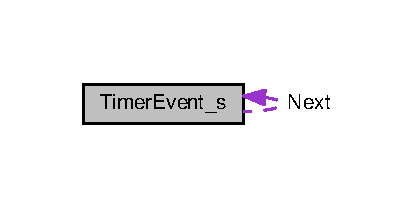
\includegraphics[width=200pt]{structTimerEvent__s__coll__graph}
\end{center}
\end{figure}
\subsection*{Data Fields}
\begin{DoxyCompactItemize}
\item 
uint32\+\_\+t \hyperlink{structTimerEvent__s_a9f933d63b25c3416b42345b695872c59}{Timestamp}
\item 
uint32\+\_\+t \hyperlink{structTimerEvent__s_a1a2ffdc3bb2cebe3ab97250f6618f5ce}{Reload\+Value}
\begin{DoxyCompactList}\small\item\em Expiring timer value in ticks from Timer\+Context. \end{DoxyCompactList}\item 
bool \hyperlink{structTimerEvent__s_a6dfdcda52c7bc3e408cb590ccbfdbe60}{Is\+Running}
\begin{DoxyCompactList}\small\item\em Reload Value when Timer is restarted. \end{DoxyCompactList}\item 
void($\ast$ \hyperlink{structTimerEvent__s_af9ed72eb732fd7bfc80dc84d289395eb}{Callback} )(void)
\begin{DoxyCompactList}\small\item\em Is the timer currently running. \end{DoxyCompactList}\item 
struct \hyperlink{structTimerEvent__s}{Timer\+Event\+\_\+s} $\ast$ \hyperlink{structTimerEvent__s_a7b5d3c09b4a4b03eff360fd818389d0b}{Next}
\begin{DoxyCompactList}\small\item\em Timer I\+RQ callback function. \end{DoxyCompactList}\end{DoxyCompactItemize}


\subsection{Detailed Description}
Timer object description. 

\subsection{Field Documentation}
\mbox{\Hypertarget{structTimerEvent__s_af9ed72eb732fd7bfc80dc84d289395eb}\label{structTimerEvent__s_af9ed72eb732fd7bfc80dc84d289395eb}} 
\index{Timer\+Event\+\_\+s@{Timer\+Event\+\_\+s}!Callback@{Callback}}
\index{Callback@{Callback}!Timer\+Event\+\_\+s@{Timer\+Event\+\_\+s}}
\subsubsection{\texorpdfstring{Callback}{Callback}}
{\footnotesize\ttfamily void( $\ast$ Timer\+Event\+\_\+s\+::\+Callback) (void)}



Is the timer currently running. 

\mbox{\Hypertarget{structTimerEvent__s_a6dfdcda52c7bc3e408cb590ccbfdbe60}\label{structTimerEvent__s_a6dfdcda52c7bc3e408cb590ccbfdbe60}} 
\index{Timer\+Event\+\_\+s@{Timer\+Event\+\_\+s}!Is\+Running@{Is\+Running}}
\index{Is\+Running@{Is\+Running}!Timer\+Event\+\_\+s@{Timer\+Event\+\_\+s}}
\subsubsection{\texorpdfstring{Is\+Running}{IsRunning}}
{\footnotesize\ttfamily bool Timer\+Event\+\_\+s\+::\+Is\+Running}



Reload Value when Timer is restarted. 

\mbox{\Hypertarget{structTimerEvent__s_a7b5d3c09b4a4b03eff360fd818389d0b}\label{structTimerEvent__s_a7b5d3c09b4a4b03eff360fd818389d0b}} 
\index{Timer\+Event\+\_\+s@{Timer\+Event\+\_\+s}!Next@{Next}}
\index{Next@{Next}!Timer\+Event\+\_\+s@{Timer\+Event\+\_\+s}}
\subsubsection{\texorpdfstring{Next}{Next}}
{\footnotesize\ttfamily struct \hyperlink{structTimerEvent__s}{Timer\+Event\+\_\+s}$\ast$ Timer\+Event\+\_\+s\+::\+Next}



Timer I\+RQ callback function. 

\mbox{\Hypertarget{structTimerEvent__s_a1a2ffdc3bb2cebe3ab97250f6618f5ce}\label{structTimerEvent__s_a1a2ffdc3bb2cebe3ab97250f6618f5ce}} 
\index{Timer\+Event\+\_\+s@{Timer\+Event\+\_\+s}!Reload\+Value@{Reload\+Value}}
\index{Reload\+Value@{Reload\+Value}!Timer\+Event\+\_\+s@{Timer\+Event\+\_\+s}}
\subsubsection{\texorpdfstring{Reload\+Value}{ReloadValue}}
{\footnotesize\ttfamily uint32\+\_\+t Timer\+Event\+\_\+s\+::\+Reload\+Value}



Expiring timer value in ticks from Timer\+Context. 

\mbox{\Hypertarget{structTimerEvent__s_a9f933d63b25c3416b42345b695872c59}\label{structTimerEvent__s_a9f933d63b25c3416b42345b695872c59}} 
\index{Timer\+Event\+\_\+s@{Timer\+Event\+\_\+s}!Timestamp@{Timestamp}}
\index{Timestamp@{Timestamp}!Timer\+Event\+\_\+s@{Timer\+Event\+\_\+s}}
\subsubsection{\texorpdfstring{Timestamp}{Timestamp}}
{\footnotesize\ttfamily uint32\+\_\+t Timer\+Event\+\_\+s\+::\+Timestamp}



The documentation for this struct was generated from the following file\+:\begin{DoxyCompactItemize}
\item 
Utilities/\hyperlink{timeServer_8h}{time\+Server.\+h}\end{DoxyCompactItemize}

\hypertarget{unionuDrRange}{}\section{u\+Dr\+Range Union Reference}
\label{unionuDrRange}\index{u\+Dr\+Range@{u\+Dr\+Range}}


{\ttfamily \#include $<$Lo\+Ra\+Mac.\+h$>$}



Collaboration diagram for u\+Dr\+Range\+:
\nopagebreak
\begin{figure}[H]
\begin{center}
\leavevmode
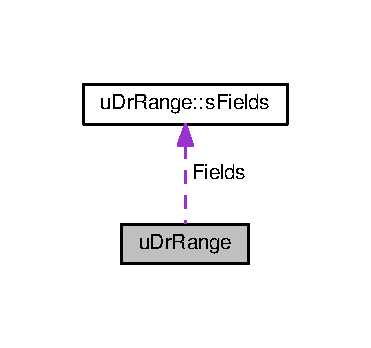
\includegraphics[width=178pt]{unionuDrRange__coll__graph}
\end{center}
\end{figure}
\subsection*{Data Structures}
\begin{DoxyCompactItemize}
\item 
struct \hyperlink{structuDrRange_1_1sFields}{s\+Fields}
\end{DoxyCompactItemize}
\subsection*{Data Fields}
\begin{DoxyCompactItemize}
\item 
int8\+\_\+t \hyperlink{unionuDrRange_ae757567cbaea3fd419eb02b86d1d34db}{Value}
\item 
struct \hyperlink{structuDrRange_1_1sFields}{u\+Dr\+Range\+::s\+Fields} \hyperlink{unionuDrRange_a161a7247018060f7c0991b693888fef8}{Fields}
\end{DoxyCompactItemize}


\subsection{Detailed Description}
Lo\+Ra\+M\+AC channels parameters definition 

\subsection{Field Documentation}
\mbox{\Hypertarget{unionuDrRange_a161a7247018060f7c0991b693888fef8}\label{unionuDrRange_a161a7247018060f7c0991b693888fef8}} 
\index{u\+Dr\+Range@{u\+Dr\+Range}!Fields@{Fields}}
\index{Fields@{Fields}!u\+Dr\+Range@{u\+Dr\+Range}}
\subsubsection{\texorpdfstring{Fields}{Fields}}
{\footnotesize\ttfamily struct \hyperlink{structuDrRange_1_1sFields}{u\+Dr\+Range\+::s\+Fields} u\+Dr\+Range\+::\+Fields}

\mbox{\Hypertarget{unionuDrRange_ae757567cbaea3fd419eb02b86d1d34db}\label{unionuDrRange_ae757567cbaea3fd419eb02b86d1d34db}} 
\index{u\+Dr\+Range@{u\+Dr\+Range}!Value@{Value}}
\index{Value@{Value}!u\+Dr\+Range@{u\+Dr\+Range}}
\subsubsection{\texorpdfstring{Value}{Value}}
{\footnotesize\ttfamily int8\+\_\+t u\+Dr\+Range\+::\+Value}

Byte-\/access to the bits 

The documentation for this union was generated from the following file\+:\begin{DoxyCompactItemize}
\item 
Mac/\hyperlink{LoRaMac_8h}{Lo\+Ra\+Mac.\+h}\end{DoxyCompactItemize}

\hypertarget{unionuLoRaMacFrameCtrl}{}\section{u\+Lo\+Ra\+Mac\+Frame\+Ctrl Union Reference}
\label{unionuLoRaMacFrameCtrl}\index{u\+Lo\+Ra\+Mac\+Frame\+Ctrl@{u\+Lo\+Ra\+Mac\+Frame\+Ctrl}}


{\ttfamily \#include $<$Lo\+Ra\+Mac.\+h$>$}



Collaboration diagram for u\+Lo\+Ra\+Mac\+Frame\+Ctrl\+:
\nopagebreak
\begin{figure}[H]
\begin{center}
\leavevmode
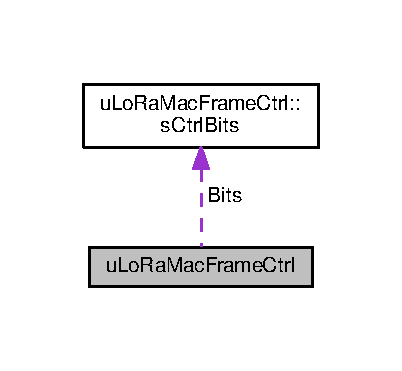
\includegraphics[width=193pt]{unionuLoRaMacFrameCtrl__coll__graph}
\end{center}
\end{figure}
\subsection*{Data Structures}
\begin{DoxyCompactItemize}
\item 
struct \hyperlink{structuLoRaMacFrameCtrl_1_1sCtrlBits}{s\+Ctrl\+Bits}
\end{DoxyCompactItemize}
\subsection*{Data Fields}
\begin{DoxyCompactItemize}
\item 
uint8\+\_\+t \hyperlink{unionuLoRaMacFrameCtrl_a19009e145545052c0786ce3d9337aead}{Value}
\item 
struct \hyperlink{structuLoRaMacFrameCtrl_1_1sCtrlBits}{u\+Lo\+Ra\+Mac\+Frame\+Ctrl\+::s\+Ctrl\+Bits} \hyperlink{unionuLoRaMacFrameCtrl_aceae433bef08dcb31c0972b204f88e68}{Bits}
\end{DoxyCompactItemize}


\subsection{Detailed Description}
Lo\+Ra\+M\+AC frame control field definition (F\+Ctrl)

Lo\+Ra\+W\+AN Specification V1.\+0.\+2, chapter 4.\+3.\+1 

\subsection{Field Documentation}
\mbox{\Hypertarget{unionuLoRaMacFrameCtrl_aceae433bef08dcb31c0972b204f88e68}\label{unionuLoRaMacFrameCtrl_aceae433bef08dcb31c0972b204f88e68}} 
\index{u\+Lo\+Ra\+Mac\+Frame\+Ctrl@{u\+Lo\+Ra\+Mac\+Frame\+Ctrl}!Bits@{Bits}}
\index{Bits@{Bits}!u\+Lo\+Ra\+Mac\+Frame\+Ctrl@{u\+Lo\+Ra\+Mac\+Frame\+Ctrl}}
\subsubsection{\texorpdfstring{Bits}{Bits}}
{\footnotesize\ttfamily struct \hyperlink{structuLoRaMacFrameCtrl_1_1sCtrlBits}{u\+Lo\+Ra\+Mac\+Frame\+Ctrl\+::s\+Ctrl\+Bits} u\+Lo\+Ra\+Mac\+Frame\+Ctrl\+::\+Bits}

\mbox{\Hypertarget{unionuLoRaMacFrameCtrl_a19009e145545052c0786ce3d9337aead}\label{unionuLoRaMacFrameCtrl_a19009e145545052c0786ce3d9337aead}} 
\index{u\+Lo\+Ra\+Mac\+Frame\+Ctrl@{u\+Lo\+Ra\+Mac\+Frame\+Ctrl}!Value@{Value}}
\index{Value@{Value}!u\+Lo\+Ra\+Mac\+Frame\+Ctrl@{u\+Lo\+Ra\+Mac\+Frame\+Ctrl}}
\subsubsection{\texorpdfstring{Value}{Value}}
{\footnotesize\ttfamily uint8\+\_\+t u\+Lo\+Ra\+Mac\+Frame\+Ctrl\+::\+Value}

Byte-\/access to the bits 

The documentation for this union was generated from the following file\+:\begin{DoxyCompactItemize}
\item 
Mac/\hyperlink{LoRaMac_8h}{Lo\+Ra\+Mac.\+h}\end{DoxyCompactItemize}

\hypertarget{unionuLoRaMacHeader}{}\section{u\+Lo\+Ra\+Mac\+Header Union Reference}
\label{unionuLoRaMacHeader}\index{u\+Lo\+Ra\+Mac\+Header@{u\+Lo\+Ra\+Mac\+Header}}


{\ttfamily \#include $<$Lo\+Ra\+Mac.\+h$>$}



Collaboration diagram for u\+Lo\+Ra\+Mac\+Header\+:
\nopagebreak
\begin{figure}[H]
\begin{center}
\leavevmode
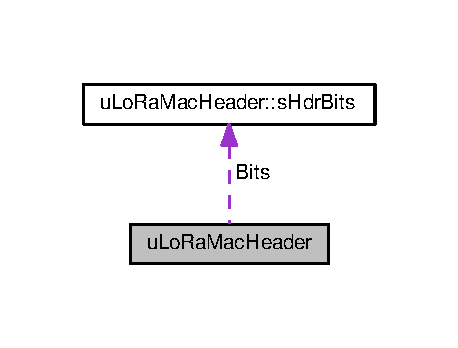
\includegraphics[width=220pt]{unionuLoRaMacHeader__coll__graph}
\end{center}
\end{figure}
\subsection*{Data Structures}
\begin{DoxyCompactItemize}
\item 
struct \hyperlink{structuLoRaMacHeader_1_1sHdrBits}{s\+Hdr\+Bits}
\end{DoxyCompactItemize}
\subsection*{Data Fields}
\begin{DoxyCompactItemize}
\item 
uint8\+\_\+t \hyperlink{unionuLoRaMacHeader_aa85438c8c356d6d6c82c611c86a9c7fc}{Value}
\item 
struct \hyperlink{structuLoRaMacHeader_1_1sHdrBits}{u\+Lo\+Ra\+Mac\+Header\+::s\+Hdr\+Bits} \hyperlink{unionuLoRaMacHeader_a74f0f1fc2a3e7ecae7817e2bdc025eee}{Bits}
\end{DoxyCompactItemize}


\subsection{Detailed Description}
Lo\+Ra\+M\+AC header field definition (M\+H\+DR field)

Lo\+Ra\+W\+AN Specification V1.\+0.\+2, chapter 4.\+2 

\subsection{Field Documentation}
\mbox{\Hypertarget{unionuLoRaMacHeader_a74f0f1fc2a3e7ecae7817e2bdc025eee}\label{unionuLoRaMacHeader_a74f0f1fc2a3e7ecae7817e2bdc025eee}} 
\index{u\+Lo\+Ra\+Mac\+Header@{u\+Lo\+Ra\+Mac\+Header}!Bits@{Bits}}
\index{Bits@{Bits}!u\+Lo\+Ra\+Mac\+Header@{u\+Lo\+Ra\+Mac\+Header}}
\subsubsection{\texorpdfstring{Bits}{Bits}}
{\footnotesize\ttfamily struct \hyperlink{structuLoRaMacHeader_1_1sHdrBits}{u\+Lo\+Ra\+Mac\+Header\+::s\+Hdr\+Bits} u\+Lo\+Ra\+Mac\+Header\+::\+Bits}

\mbox{\Hypertarget{unionuLoRaMacHeader_aa85438c8c356d6d6c82c611c86a9c7fc}\label{unionuLoRaMacHeader_aa85438c8c356d6d6c82c611c86a9c7fc}} 
\index{u\+Lo\+Ra\+Mac\+Header@{u\+Lo\+Ra\+Mac\+Header}!Value@{Value}}
\index{Value@{Value}!u\+Lo\+Ra\+Mac\+Header@{u\+Lo\+Ra\+Mac\+Header}}
\subsubsection{\texorpdfstring{Value}{Value}}
{\footnotesize\ttfamily uint8\+\_\+t u\+Lo\+Ra\+Mac\+Header\+::\+Value}

Byte-\/access to the bits 

The documentation for this union was generated from the following file\+:\begin{DoxyCompactItemize}
\item 
Mac/\hyperlink{LoRaMac_8h}{Lo\+Ra\+Mac.\+h}\end{DoxyCompactItemize}

\hypertarget{unionsMcpsReq_1_1uMcpsParam}{}\section{s\+Mcps\+Req\+:\+:u\+Mcps\+Param Union Reference}
\label{unionsMcpsReq_1_1uMcpsParam}\index{s\+Mcps\+Req\+::u\+Mcps\+Param@{s\+Mcps\+Req\+::u\+Mcps\+Param}}


{\ttfamily \#include $<$Lo\+Ra\+Mac.\+h$>$}



Collaboration diagram for s\+Mcps\+Req\+:\+:u\+Mcps\+Param\+:
\nopagebreak
\begin{figure}[H]
\begin{center}
\leavevmode
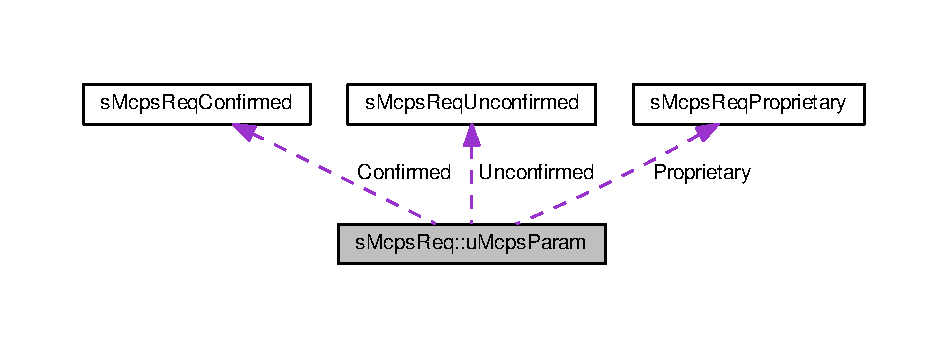
\includegraphics[width=350pt]{unionsMcpsReq_1_1uMcpsParam__coll__graph}
\end{center}
\end{figure}
\subsection*{Data Fields}
\begin{DoxyCompactItemize}
\item 
\hyperlink{group__LORAMAC_gaab871b914dfa4013c176586dcc2ea6df}{Mcps\+Req\+Unconfirmed\+\_\+t} \hyperlink{unionsMcpsReq_1_1uMcpsParam_a2aae1e6bd0891c17e9bc2654ae95e60a}{Unconfirmed}
\item 
\hyperlink{group__LORAMAC_ga02103c0ee1374a6b1eec217f148ec0e2}{Mcps\+Req\+Confirmed\+\_\+t} \hyperlink{unionsMcpsReq_1_1uMcpsParam_a55f25abc41d07654f0ed8a92541a1eef}{Confirmed}
\item 
\hyperlink{group__LORAMAC_gac856bc282e89301412e0a294b3e663c4}{Mcps\+Req\+Proprietary\+\_\+t} \hyperlink{unionsMcpsReq_1_1uMcpsParam_a894cf87a04261fa298cde47fc50ac02d}{Proprietary}
\end{DoxyCompactItemize}


\subsection{Detailed Description}
M\+C\+P\+S-\/\+Request parameters 

\subsection{Field Documentation}
\mbox{\Hypertarget{unionsMcpsReq_1_1uMcpsParam_a55f25abc41d07654f0ed8a92541a1eef}\label{unionsMcpsReq_1_1uMcpsParam_a55f25abc41d07654f0ed8a92541a1eef}} 
\index{s\+Mcps\+Req\+::u\+Mcps\+Param@{s\+Mcps\+Req\+::u\+Mcps\+Param}!Confirmed@{Confirmed}}
\index{Confirmed@{Confirmed}!s\+Mcps\+Req\+::u\+Mcps\+Param@{s\+Mcps\+Req\+::u\+Mcps\+Param}}
\subsubsection{\texorpdfstring{Confirmed}{Confirmed}}
{\footnotesize\ttfamily \hyperlink{group__LORAMAC_ga02103c0ee1374a6b1eec217f148ec0e2}{Mcps\+Req\+Confirmed\+\_\+t} s\+Mcps\+Req\+::u\+Mcps\+Param\+::\+Confirmed}

M\+C\+P\+S-\/\+Request parameters for a confirmed frame \mbox{\Hypertarget{unionsMcpsReq_1_1uMcpsParam_a894cf87a04261fa298cde47fc50ac02d}\label{unionsMcpsReq_1_1uMcpsParam_a894cf87a04261fa298cde47fc50ac02d}} 
\index{s\+Mcps\+Req\+::u\+Mcps\+Param@{s\+Mcps\+Req\+::u\+Mcps\+Param}!Proprietary@{Proprietary}}
\index{Proprietary@{Proprietary}!s\+Mcps\+Req\+::u\+Mcps\+Param@{s\+Mcps\+Req\+::u\+Mcps\+Param}}
\subsubsection{\texorpdfstring{Proprietary}{Proprietary}}
{\footnotesize\ttfamily \hyperlink{group__LORAMAC_gac856bc282e89301412e0a294b3e663c4}{Mcps\+Req\+Proprietary\+\_\+t} s\+Mcps\+Req\+::u\+Mcps\+Param\+::\+Proprietary}

M\+C\+P\+S-\/\+Request parameters for a proprietary frame \mbox{\Hypertarget{unionsMcpsReq_1_1uMcpsParam_a2aae1e6bd0891c17e9bc2654ae95e60a}\label{unionsMcpsReq_1_1uMcpsParam_a2aae1e6bd0891c17e9bc2654ae95e60a}} 
\index{s\+Mcps\+Req\+::u\+Mcps\+Param@{s\+Mcps\+Req\+::u\+Mcps\+Param}!Unconfirmed@{Unconfirmed}}
\index{Unconfirmed@{Unconfirmed}!s\+Mcps\+Req\+::u\+Mcps\+Param@{s\+Mcps\+Req\+::u\+Mcps\+Param}}
\subsubsection{\texorpdfstring{Unconfirmed}{Unconfirmed}}
{\footnotesize\ttfamily \hyperlink{group__LORAMAC_gaab871b914dfa4013c176586dcc2ea6df}{Mcps\+Req\+Unconfirmed\+\_\+t} s\+Mcps\+Req\+::u\+Mcps\+Param\+::\+Unconfirmed}

M\+C\+P\+S-\/\+Request parameters for an unconfirmed frame 

The documentation for this union was generated from the following file\+:\begin{DoxyCompactItemize}
\item 
Mac/\hyperlink{LoRaMac_8h}{Lo\+Ra\+Mac.\+h}\end{DoxyCompactItemize}

\hypertarget{unionuMibParam}{}\section{u\+Mib\+Param Union Reference}
\label{unionuMibParam}\index{u\+Mib\+Param@{u\+Mib\+Param}}


{\ttfamily \#include $<$Lo\+Ra\+Mac.\+h$>$}



Collaboration diagram for u\+Mib\+Param\+:
\nopagebreak
\begin{figure}[H]
\begin{center}
\leavevmode
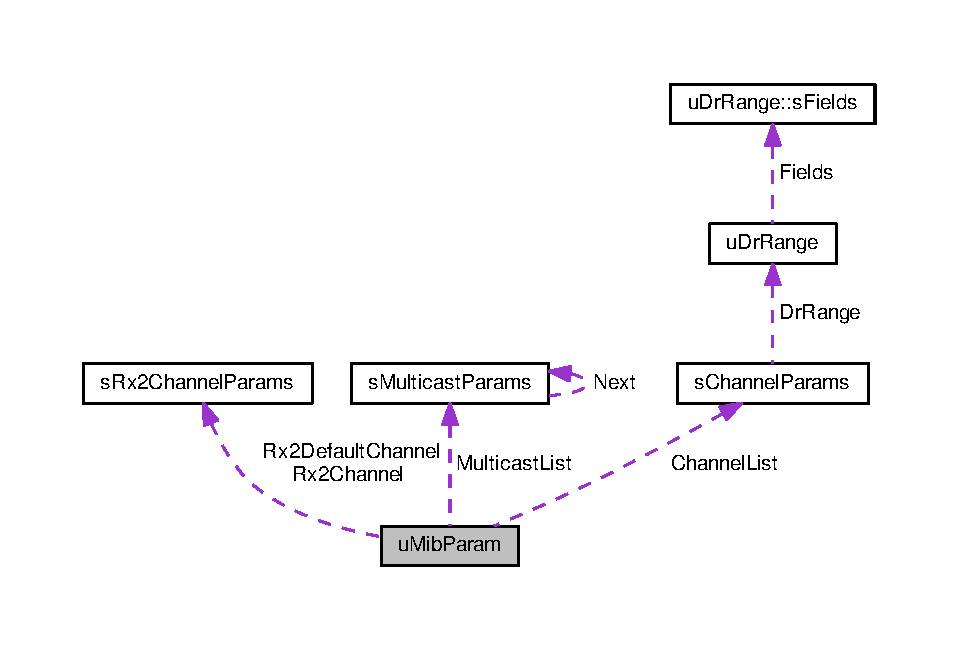
\includegraphics[width=350pt]{unionuMibParam__coll__graph}
\end{center}
\end{figure}
\subsection*{Data Fields}
\begin{DoxyCompactItemize}
\item 
\hyperlink{group__LORAMAC_ga29dc2e097802faaf8fbd0e18ff99695f}{Device\+Class\+\_\+t} \hyperlink{unionuMibParam_a0a7f108faca608d6271ed070b3666dad}{Class}
\item 
bool \hyperlink{unionuMibParam_a2f94965111a263fa6808260203c020f8}{Is\+Network\+Joined}
\item 
bool \hyperlink{unionuMibParam_ab178fe02b29604d3996b55e72ebc39b6}{Adr\+Enable}
\item 
uint32\+\_\+t \hyperlink{unionuMibParam_a28a692f38f8742b309d7973648a6d612}{Net\+ID}
\item 
uint32\+\_\+t \hyperlink{unionuMibParam_a41a1aedea4cb10b45ddf9b8ebd1fdf54}{Dev\+Addr}
\item 
uint8\+\_\+t $\ast$ \hyperlink{unionuMibParam_a64c3f5e98c8558eedbd7fe42dfcd160e}{Nwk\+S\+Key}
\item 
uint8\+\_\+t $\ast$ \hyperlink{unionuMibParam_aa457344123276ddc04277da5208175ed}{App\+S\+Key}
\item 
bool \hyperlink{unionuMibParam_af926413a7ecbe5fcf8b223fff46ad8e2}{Enable\+Public\+Network}
\item 
bool \hyperlink{unionuMibParam_a9bf9eee9867513c64e39300c2c13c981}{Enable\+Repeater\+Support}
\item 
\hyperlink{group__LORAMAC_ga1360ca6f82c6d125ea43a9dad9b56184}{Channel\+Params\+\_\+t} $\ast$ \hyperlink{unionuMibParam_af3b0b4ded686920d7494d6ea0ec80700}{Channel\+List}
\item 
\hyperlink{group__LORAMAC_ga8f57f29481ea92c24f6af04b96a95e0f}{Rx2\+Channel\+Params\+\_\+t} \hyperlink{unionuMibParam_af2e450398d3e72d7dc9d95fc54e1574e}{Rx2\+Channel}
\item 
\hyperlink{group__LORAMAC_ga8f57f29481ea92c24f6af04b96a95e0f}{Rx2\+Channel\+Params\+\_\+t} \hyperlink{unionuMibParam_a9f0e695c27a48c27895fadc99813eb44}{Rx2\+Default\+Channel}
\item 
uint16\+\_\+t $\ast$ \hyperlink{unionuMibParam_af7353a35521c6aa58ffee90589a98620}{Channels\+Mask}
\item 
uint16\+\_\+t $\ast$ \hyperlink{unionuMibParam_a5d650a767189429f903b22e785e0d4b0}{Channels\+Default\+Mask}
\item 
uint8\+\_\+t \hyperlink{unionuMibParam_ac25048296416e1ca348d568d539ed946}{Channel\+Nb\+Rep}
\item 
uint32\+\_\+t \hyperlink{unionuMibParam_a9fdb2320488295a980588cb61f6fd5ea}{Max\+Rx\+Window}
\item 
uint32\+\_\+t \hyperlink{unionuMibParam_af36e0cb0f6077bf16d18e0563725eef4}{Receive\+Delay1}
\item 
uint32\+\_\+t \hyperlink{unionuMibParam_a8606ae0bf9c205d3cebb622986d1d291}{Receive\+Delay2}
\item 
uint32\+\_\+t \hyperlink{unionuMibParam_aa13344525c4bcb94ed4c59938f567b32}{Join\+Accept\+Delay1}
\item 
uint32\+\_\+t \hyperlink{unionuMibParam_ab5aab1064c3e6476fb342d30de7abc7b}{Join\+Accept\+Delay2}
\item 
int8\+\_\+t \hyperlink{unionuMibParam_a150339341b4c54a3e0779893c248a559}{Channels\+Default\+Datarate}
\item 
int8\+\_\+t \hyperlink{unionuMibParam_aae0c86fa530e987e280567342ed8181a}{Channels\+Datarate}
\item 
int8\+\_\+t \hyperlink{unionuMibParam_adad323d47a9d1913172b0f40b8581a11}{Channels\+Default\+Tx\+Power}
\item 
int8\+\_\+t \hyperlink{unionuMibParam_a553f5873284511d95ebc5473a48b473a}{Channels\+Tx\+Power}
\item 
uint32\+\_\+t \hyperlink{unionuMibParam_a832b6a7ceb162e04422c74ef84828359}{Up\+Link\+Counter}
\item 
uint32\+\_\+t \hyperlink{unionuMibParam_ab6a514e07df4b7d0b7df77362eb974d5}{Down\+Link\+Counter}
\item 
\hyperlink{group__LORAMAC_ga02d2523505cac70954c043074087ea65}{Multicast\+Params\+\_\+t} $\ast$ \hyperlink{unionuMibParam_a3a577a31c0893ac6058a554c3e894535}{Multicast\+List}
\item 
uint32\+\_\+t \hyperlink{unionuMibParam_a2f01cc5ba9dc1ae1a0a9ecb5ece418e5}{System\+Max\+Rx\+Error}
\item 
uint8\+\_\+t \hyperlink{unionuMibParam_a1eec512351464514fafd9860041b9f2a}{Min\+Rx\+Symbols}
\item 
float \hyperlink{unionuMibParam_a294b81422b95e51abf8dbaf10da230e2}{Antenna\+Gain}
\end{DoxyCompactItemize}


\subsection{Detailed Description}
Lo\+Ra\+M\+AC M\+IB parameters 

\subsection{Field Documentation}
\mbox{\Hypertarget{unionuMibParam_ab178fe02b29604d3996b55e72ebc39b6}\label{unionuMibParam_ab178fe02b29604d3996b55e72ebc39b6}} 
\index{u\+Mib\+Param@{u\+Mib\+Param}!Adr\+Enable@{Adr\+Enable}}
\index{Adr\+Enable@{Adr\+Enable}!u\+Mib\+Param@{u\+Mib\+Param}}
\subsubsection{\texorpdfstring{Adr\+Enable}{AdrEnable}}
{\footnotesize\ttfamily bool u\+Mib\+Param\+::\+Adr\+Enable}

Activation state of A\+DR

Related M\+IB type\+: \hyperlink{group__LORAMAC_gga32ea83d13a3f5bb4b3ec2ace2319ab61a756ff0b66217e3e4ddd0442c8aa56802}{M\+I\+B\+\_\+\+A\+DR} \mbox{\Hypertarget{unionuMibParam_a294b81422b95e51abf8dbaf10da230e2}\label{unionuMibParam_a294b81422b95e51abf8dbaf10da230e2}} 
\index{u\+Mib\+Param@{u\+Mib\+Param}!Antenna\+Gain@{Antenna\+Gain}}
\index{Antenna\+Gain@{Antenna\+Gain}!u\+Mib\+Param@{u\+Mib\+Param}}
\subsubsection{\texorpdfstring{Antenna\+Gain}{AntennaGain}}
{\footnotesize\ttfamily float u\+Mib\+Param\+::\+Antenna\+Gain}

Antenna gain

Related M\+IB type\+: \hyperlink{group__LORAMAC_gga32ea83d13a3f5bb4b3ec2ace2319ab61a268b2f7da53dbc25655a7bdcc7e6128e}{M\+I\+B\+\_\+\+A\+N\+T\+E\+N\+N\+A\+\_\+\+G\+A\+IN} \mbox{\Hypertarget{unionuMibParam_aa457344123276ddc04277da5208175ed}\label{unionuMibParam_aa457344123276ddc04277da5208175ed}} 
\index{u\+Mib\+Param@{u\+Mib\+Param}!App\+S\+Key@{App\+S\+Key}}
\index{App\+S\+Key@{App\+S\+Key}!u\+Mib\+Param@{u\+Mib\+Param}}
\subsubsection{\texorpdfstring{App\+S\+Key}{AppSKey}}
{\footnotesize\ttfamily uint8\+\_\+t$\ast$ u\+Mib\+Param\+::\+App\+S\+Key}

Application session key

Related M\+IB type\+: \hyperlink{group__LORAMAC_gga32ea83d13a3f5bb4b3ec2ace2319ab61ae65b7c035d9969666eb5e26a2b3c19fd}{M\+I\+B\+\_\+\+A\+P\+P\+\_\+\+S\+K\+EY} \mbox{\Hypertarget{unionuMibParam_af3b0b4ded686920d7494d6ea0ec80700}\label{unionuMibParam_af3b0b4ded686920d7494d6ea0ec80700}} 
\index{u\+Mib\+Param@{u\+Mib\+Param}!Channel\+List@{Channel\+List}}
\index{Channel\+List@{Channel\+List}!u\+Mib\+Param@{u\+Mib\+Param}}
\subsubsection{\texorpdfstring{Channel\+List}{ChannelList}}
{\footnotesize\ttfamily \hyperlink{group__LORAMAC_ga1360ca6f82c6d125ea43a9dad9b56184}{Channel\+Params\+\_\+t}$\ast$ u\+Mib\+Param\+::\+Channel\+List}

Lo\+Ra\+W\+AN Channel

Related M\+IB type\+: \hyperlink{group__LORAMAC_gga32ea83d13a3f5bb4b3ec2ace2319ab61a0236aae7748c12308383eab208a3cc5a}{M\+I\+B\+\_\+\+C\+H\+A\+N\+N\+E\+LS} \mbox{\Hypertarget{unionuMibParam_ac25048296416e1ca348d568d539ed946}\label{unionuMibParam_ac25048296416e1ca348d568d539ed946}} 
\index{u\+Mib\+Param@{u\+Mib\+Param}!Channel\+Nb\+Rep@{Channel\+Nb\+Rep}}
\index{Channel\+Nb\+Rep@{Channel\+Nb\+Rep}!u\+Mib\+Param@{u\+Mib\+Param}}
\subsubsection{\texorpdfstring{Channel\+Nb\+Rep}{ChannelNbRep}}
{\footnotesize\ttfamily uint8\+\_\+t u\+Mib\+Param\+::\+Channel\+Nb\+Rep}

Number of frame repetitions

Related M\+IB type\+: \hyperlink{group__LORAMAC_gga32ea83d13a3f5bb4b3ec2ace2319ab61af8775ceffd8bc73429e43eac205383ea}{M\+I\+B\+\_\+\+C\+H\+A\+N\+N\+E\+L\+S\+\_\+\+N\+B\+\_\+\+R\+EP} \mbox{\Hypertarget{unionuMibParam_aae0c86fa530e987e280567342ed8181a}\label{unionuMibParam_aae0c86fa530e987e280567342ed8181a}} 
\index{u\+Mib\+Param@{u\+Mib\+Param}!Channels\+Datarate@{Channels\+Datarate}}
\index{Channels\+Datarate@{Channels\+Datarate}!u\+Mib\+Param@{u\+Mib\+Param}}
\subsubsection{\texorpdfstring{Channels\+Datarate}{ChannelsDatarate}}
{\footnotesize\ttfamily int8\+\_\+t u\+Mib\+Param\+::\+Channels\+Datarate}

Channels data rate

Related M\+IB type\+: \hyperlink{group__LORAMAC_gga32ea83d13a3f5bb4b3ec2ace2319ab61a78f3b4e3ae4ebaacb478073d2a2ec4f1}{M\+I\+B\+\_\+\+C\+H\+A\+N\+N\+E\+L\+S\+\_\+\+D\+A\+T\+A\+R\+A\+TE} \mbox{\Hypertarget{unionuMibParam_a150339341b4c54a3e0779893c248a559}\label{unionuMibParam_a150339341b4c54a3e0779893c248a559}} 
\index{u\+Mib\+Param@{u\+Mib\+Param}!Channels\+Default\+Datarate@{Channels\+Default\+Datarate}}
\index{Channels\+Default\+Datarate@{Channels\+Default\+Datarate}!u\+Mib\+Param@{u\+Mib\+Param}}
\subsubsection{\texorpdfstring{Channels\+Default\+Datarate}{ChannelsDefaultDatarate}}
{\footnotesize\ttfamily int8\+\_\+t u\+Mib\+Param\+::\+Channels\+Default\+Datarate}

Channels data rate

Related M\+IB type\+: \hyperlink{group__LORAMAC_gga32ea83d13a3f5bb4b3ec2ace2319ab61addef34adbf844ace9eeea97ae93da918}{M\+I\+B\+\_\+\+C\+H\+A\+N\+N\+E\+L\+S\+\_\+\+D\+E\+F\+A\+U\+L\+T\+\_\+\+D\+A\+T\+A\+R\+A\+TE} \mbox{\Hypertarget{unionuMibParam_a5d650a767189429f903b22e785e0d4b0}\label{unionuMibParam_a5d650a767189429f903b22e785e0d4b0}} 
\index{u\+Mib\+Param@{u\+Mib\+Param}!Channels\+Default\+Mask@{Channels\+Default\+Mask}}
\index{Channels\+Default\+Mask@{Channels\+Default\+Mask}!u\+Mib\+Param@{u\+Mib\+Param}}
\subsubsection{\texorpdfstring{Channels\+Default\+Mask}{ChannelsDefaultMask}}
{\footnotesize\ttfamily uint16\+\_\+t$\ast$ u\+Mib\+Param\+::\+Channels\+Default\+Mask}

Default channel mask

Related M\+IB type\+: \hyperlink{group__LORAMAC_gga32ea83d13a3f5bb4b3ec2ace2319ab61a59afc276ca425cd4055ff5cb5b5fa946}{M\+I\+B\+\_\+\+C\+H\+A\+N\+N\+E\+L\+S\+\_\+\+D\+E\+F\+A\+U\+L\+T\+\_\+\+M\+A\+SK} \mbox{\Hypertarget{unionuMibParam_adad323d47a9d1913172b0f40b8581a11}\label{unionuMibParam_adad323d47a9d1913172b0f40b8581a11}} 
\index{u\+Mib\+Param@{u\+Mib\+Param}!Channels\+Default\+Tx\+Power@{Channels\+Default\+Tx\+Power}}
\index{Channels\+Default\+Tx\+Power@{Channels\+Default\+Tx\+Power}!u\+Mib\+Param@{u\+Mib\+Param}}
\subsubsection{\texorpdfstring{Channels\+Default\+Tx\+Power}{ChannelsDefaultTxPower}}
{\footnotesize\ttfamily int8\+\_\+t u\+Mib\+Param\+::\+Channels\+Default\+Tx\+Power}

Channels TX power

Related M\+IB type\+: \hyperlink{group__LORAMAC_gga32ea83d13a3f5bb4b3ec2ace2319ab61a9c5b2d3ad2caf87710b09e8a6e68cc6a}{M\+I\+B\+\_\+\+C\+H\+A\+N\+N\+E\+L\+S\+\_\+\+D\+E\+F\+A\+U\+L\+T\+\_\+\+T\+X\+\_\+\+P\+O\+W\+ER} \mbox{\Hypertarget{unionuMibParam_af7353a35521c6aa58ffee90589a98620}\label{unionuMibParam_af7353a35521c6aa58ffee90589a98620}} 
\index{u\+Mib\+Param@{u\+Mib\+Param}!Channels\+Mask@{Channels\+Mask}}
\index{Channels\+Mask@{Channels\+Mask}!u\+Mib\+Param@{u\+Mib\+Param}}
\subsubsection{\texorpdfstring{Channels\+Mask}{ChannelsMask}}
{\footnotesize\ttfamily uint16\+\_\+t$\ast$ u\+Mib\+Param\+::\+Channels\+Mask}

Channel mask

Related M\+IB type\+: \hyperlink{group__LORAMAC_gga32ea83d13a3f5bb4b3ec2ace2319ab61aafe40b1c0e252d607876423247feab62}{M\+I\+B\+\_\+\+C\+H\+A\+N\+N\+E\+L\+S\+\_\+\+M\+A\+SK} \mbox{\Hypertarget{unionuMibParam_a553f5873284511d95ebc5473a48b473a}\label{unionuMibParam_a553f5873284511d95ebc5473a48b473a}} 
\index{u\+Mib\+Param@{u\+Mib\+Param}!Channels\+Tx\+Power@{Channels\+Tx\+Power}}
\index{Channels\+Tx\+Power@{Channels\+Tx\+Power}!u\+Mib\+Param@{u\+Mib\+Param}}
\subsubsection{\texorpdfstring{Channels\+Tx\+Power}{ChannelsTxPower}}
{\footnotesize\ttfamily int8\+\_\+t u\+Mib\+Param\+::\+Channels\+Tx\+Power}

Channels TX power

Related M\+IB type\+: \hyperlink{group__LORAMAC_gga32ea83d13a3f5bb4b3ec2ace2319ab61ae42f1a0c858ffdb283e0236a24ab6398}{M\+I\+B\+\_\+\+C\+H\+A\+N\+N\+E\+L\+S\+\_\+\+T\+X\+\_\+\+P\+O\+W\+ER} \mbox{\Hypertarget{unionuMibParam_a0a7f108faca608d6271ed070b3666dad}\label{unionuMibParam_a0a7f108faca608d6271ed070b3666dad}} 
\index{u\+Mib\+Param@{u\+Mib\+Param}!Class@{Class}}
\index{Class@{Class}!u\+Mib\+Param@{u\+Mib\+Param}}
\subsubsection{\texorpdfstring{Class}{Class}}
{\footnotesize\ttfamily \hyperlink{group__LORAMAC_ga29dc2e097802faaf8fbd0e18ff99695f}{Device\+Class\+\_\+t} u\+Mib\+Param\+::\+Class}

Lo\+Ra\+W\+AN device class

Related M\+IB type\+: \hyperlink{group__LORAMAC_gga32ea83d13a3f5bb4b3ec2ace2319ab61ac0426517132356c9977dcdafa5ab3a7f}{M\+I\+B\+\_\+\+D\+E\+V\+I\+C\+E\+\_\+\+C\+L\+A\+SS} \mbox{\Hypertarget{unionuMibParam_a41a1aedea4cb10b45ddf9b8ebd1fdf54}\label{unionuMibParam_a41a1aedea4cb10b45ddf9b8ebd1fdf54}} 
\index{u\+Mib\+Param@{u\+Mib\+Param}!Dev\+Addr@{Dev\+Addr}}
\index{Dev\+Addr@{Dev\+Addr}!u\+Mib\+Param@{u\+Mib\+Param}}
\subsubsection{\texorpdfstring{Dev\+Addr}{DevAddr}}
{\footnotesize\ttfamily uint32\+\_\+t u\+Mib\+Param\+::\+Dev\+Addr}

End-\/device address

Related M\+IB type\+: \hyperlink{group__LORAMAC_gga32ea83d13a3f5bb4b3ec2ace2319ab61ab1459b05690ffa347a71393006b526ac}{M\+I\+B\+\_\+\+D\+E\+V\+\_\+\+A\+D\+DR} \mbox{\Hypertarget{unionuMibParam_ab6a514e07df4b7d0b7df77362eb974d5}\label{unionuMibParam_ab6a514e07df4b7d0b7df77362eb974d5}} 
\index{u\+Mib\+Param@{u\+Mib\+Param}!Down\+Link\+Counter@{Down\+Link\+Counter}}
\index{Down\+Link\+Counter@{Down\+Link\+Counter}!u\+Mib\+Param@{u\+Mib\+Param}}
\subsubsection{\texorpdfstring{Down\+Link\+Counter}{DownLinkCounter}}
{\footnotesize\ttfamily uint32\+\_\+t u\+Mib\+Param\+::\+Down\+Link\+Counter}

Lo\+Ra\+W\+AN Down-\/link counter

Related M\+IB type\+: \hyperlink{group__LORAMAC_gga32ea83d13a3f5bb4b3ec2ace2319ab61ae75b53deee33594312d1d2987c24b698}{M\+I\+B\+\_\+\+D\+O\+W\+N\+L\+I\+N\+K\+\_\+\+C\+O\+U\+N\+T\+ER} \mbox{\Hypertarget{unionuMibParam_af926413a7ecbe5fcf8b223fff46ad8e2}\label{unionuMibParam_af926413a7ecbe5fcf8b223fff46ad8e2}} 
\index{u\+Mib\+Param@{u\+Mib\+Param}!Enable\+Public\+Network@{Enable\+Public\+Network}}
\index{Enable\+Public\+Network@{Enable\+Public\+Network}!u\+Mib\+Param@{u\+Mib\+Param}}
\subsubsection{\texorpdfstring{Enable\+Public\+Network}{EnablePublicNetwork}}
{\footnotesize\ttfamily bool u\+Mib\+Param\+::\+Enable\+Public\+Network}

Enable or disable a public network

Related M\+IB type\+: \hyperlink{group__LORAMAC_gga32ea83d13a3f5bb4b3ec2ace2319ab61ab2819c46ba94b53c1fb2c3a0bfa75e48}{M\+I\+B\+\_\+\+P\+U\+B\+L\+I\+C\+\_\+\+N\+E\+T\+W\+O\+RK} \mbox{\Hypertarget{unionuMibParam_a9bf9eee9867513c64e39300c2c13c981}\label{unionuMibParam_a9bf9eee9867513c64e39300c2c13c981}} 
\index{u\+Mib\+Param@{u\+Mib\+Param}!Enable\+Repeater\+Support@{Enable\+Repeater\+Support}}
\index{Enable\+Repeater\+Support@{Enable\+Repeater\+Support}!u\+Mib\+Param@{u\+Mib\+Param}}
\subsubsection{\texorpdfstring{Enable\+Repeater\+Support}{EnableRepeaterSupport}}
{\footnotesize\ttfamily bool u\+Mib\+Param\+::\+Enable\+Repeater\+Support}

Enable or disable repeater support

Related M\+IB type\+: \hyperlink{group__LORAMAC_gga32ea83d13a3f5bb4b3ec2ace2319ab61a2d0a50cc4dd24771854bd138934ef3e5}{M\+I\+B\+\_\+\+R\+E\+P\+E\+A\+T\+E\+R\+\_\+\+S\+U\+P\+P\+O\+RT} \mbox{\Hypertarget{unionuMibParam_a2f94965111a263fa6808260203c020f8}\label{unionuMibParam_a2f94965111a263fa6808260203c020f8}} 
\index{u\+Mib\+Param@{u\+Mib\+Param}!Is\+Network\+Joined@{Is\+Network\+Joined}}
\index{Is\+Network\+Joined@{Is\+Network\+Joined}!u\+Mib\+Param@{u\+Mib\+Param}}
\subsubsection{\texorpdfstring{Is\+Network\+Joined}{IsNetworkJoined}}
{\footnotesize\ttfamily bool u\+Mib\+Param\+::\+Is\+Network\+Joined}

Lo\+Ra\+W\+AN network joined attribute

Related M\+IB type\+: \hyperlink{group__LORAMAC_gga32ea83d13a3f5bb4b3ec2ace2319ab61a2e2a91bfbbb7bbbe1467eec239effbd0}{M\+I\+B\+\_\+\+N\+E\+T\+W\+O\+R\+K\+\_\+\+J\+O\+I\+N\+ED} \mbox{\Hypertarget{unionuMibParam_aa13344525c4bcb94ed4c59938f567b32}\label{unionuMibParam_aa13344525c4bcb94ed4c59938f567b32}} 
\index{u\+Mib\+Param@{u\+Mib\+Param}!Join\+Accept\+Delay1@{Join\+Accept\+Delay1}}
\index{Join\+Accept\+Delay1@{Join\+Accept\+Delay1}!u\+Mib\+Param@{u\+Mib\+Param}}
\subsubsection{\texorpdfstring{Join\+Accept\+Delay1}{JoinAcceptDelay1}}
{\footnotesize\ttfamily uint32\+\_\+t u\+Mib\+Param\+::\+Join\+Accept\+Delay1}

Join accept delay 1

Related M\+IB type\+: \hyperlink{group__LORAMAC_gga32ea83d13a3f5bb4b3ec2ace2319ab61a3fa6b527109f8a6d5994ddaf7e9b0bd1}{M\+I\+B\+\_\+\+J\+O\+I\+N\+\_\+\+A\+C\+C\+E\+P\+T\+\_\+\+D\+E\+L\+A\+Y\+\_\+1} \mbox{\Hypertarget{unionuMibParam_ab5aab1064c3e6476fb342d30de7abc7b}\label{unionuMibParam_ab5aab1064c3e6476fb342d30de7abc7b}} 
\index{u\+Mib\+Param@{u\+Mib\+Param}!Join\+Accept\+Delay2@{Join\+Accept\+Delay2}}
\index{Join\+Accept\+Delay2@{Join\+Accept\+Delay2}!u\+Mib\+Param@{u\+Mib\+Param}}
\subsubsection{\texorpdfstring{Join\+Accept\+Delay2}{JoinAcceptDelay2}}
{\footnotesize\ttfamily uint32\+\_\+t u\+Mib\+Param\+::\+Join\+Accept\+Delay2}

Join accept delay 2

Related M\+IB type\+: \hyperlink{group__LORAMAC_gga32ea83d13a3f5bb4b3ec2ace2319ab61aa1ca7d4484b41008a69d5d786cfd6a20}{M\+I\+B\+\_\+\+J\+O\+I\+N\+\_\+\+A\+C\+C\+E\+P\+T\+\_\+\+D\+E\+L\+A\+Y\+\_\+2} \mbox{\Hypertarget{unionuMibParam_a9fdb2320488295a980588cb61f6fd5ea}\label{unionuMibParam_a9fdb2320488295a980588cb61f6fd5ea}} 
\index{u\+Mib\+Param@{u\+Mib\+Param}!Max\+Rx\+Window@{Max\+Rx\+Window}}
\index{Max\+Rx\+Window@{Max\+Rx\+Window}!u\+Mib\+Param@{u\+Mib\+Param}}
\subsubsection{\texorpdfstring{Max\+Rx\+Window}{MaxRxWindow}}
{\footnotesize\ttfamily uint32\+\_\+t u\+Mib\+Param\+::\+Max\+Rx\+Window}

Maximum receive window duration

Related M\+IB type\+: \hyperlink{group__LORAMAC_gga32ea83d13a3f5bb4b3ec2ace2319ab61ad6ba0cae3e33f0cf042ded8936d965da}{M\+I\+B\+\_\+\+M\+A\+X\+\_\+\+R\+X\+\_\+\+W\+I\+N\+D\+O\+W\+\_\+\+D\+U\+R\+A\+T\+I\+ON} \mbox{\Hypertarget{unionuMibParam_a1eec512351464514fafd9860041b9f2a}\label{unionuMibParam_a1eec512351464514fafd9860041b9f2a}} 
\index{u\+Mib\+Param@{u\+Mib\+Param}!Min\+Rx\+Symbols@{Min\+Rx\+Symbols}}
\index{Min\+Rx\+Symbols@{Min\+Rx\+Symbols}!u\+Mib\+Param@{u\+Mib\+Param}}
\subsubsection{\texorpdfstring{Min\+Rx\+Symbols}{MinRxSymbols}}
{\footnotesize\ttfamily uint8\+\_\+t u\+Mib\+Param\+::\+Min\+Rx\+Symbols}

Minimum required number of symbols to detect an Rx frame

Related M\+IB type\+: \hyperlink{group__LORAMAC_gga32ea83d13a3f5bb4b3ec2ace2319ab61a82fb27fd6414d2bde20a7a00c80e26a1}{M\+I\+B\+\_\+\+M\+I\+N\+\_\+\+R\+X\+\_\+\+S\+Y\+M\+B\+O\+LS} \mbox{\Hypertarget{unionuMibParam_a3a577a31c0893ac6058a554c3e894535}\label{unionuMibParam_a3a577a31c0893ac6058a554c3e894535}} 
\index{u\+Mib\+Param@{u\+Mib\+Param}!Multicast\+List@{Multicast\+List}}
\index{Multicast\+List@{Multicast\+List}!u\+Mib\+Param@{u\+Mib\+Param}}
\subsubsection{\texorpdfstring{Multicast\+List}{MulticastList}}
{\footnotesize\ttfamily \hyperlink{group__LORAMAC_ga02d2523505cac70954c043074087ea65}{Multicast\+Params\+\_\+t}$\ast$ u\+Mib\+Param\+::\+Multicast\+List}

Multicast channel

Related M\+IB type\+: \hyperlink{group__LORAMAC_gga32ea83d13a3f5bb4b3ec2ace2319ab61af8ac424460fccb3115c6fe6ccb450862}{M\+I\+B\+\_\+\+M\+U\+L\+T\+I\+C\+A\+S\+T\+\_\+\+C\+H\+A\+N\+N\+EL} \mbox{\Hypertarget{unionuMibParam_a28a692f38f8742b309d7973648a6d612}\label{unionuMibParam_a28a692f38f8742b309d7973648a6d612}} 
\index{u\+Mib\+Param@{u\+Mib\+Param}!Net\+ID@{Net\+ID}}
\index{Net\+ID@{Net\+ID}!u\+Mib\+Param@{u\+Mib\+Param}}
\subsubsection{\texorpdfstring{Net\+ID}{NetID}}
{\footnotesize\ttfamily uint32\+\_\+t u\+Mib\+Param\+::\+Net\+ID}

Network identifier

Related M\+IB type\+: \hyperlink{group__LORAMAC_gga32ea83d13a3f5bb4b3ec2ace2319ab61a982c4b7cc1e276633134aa89298c96b0}{M\+I\+B\+\_\+\+N\+E\+T\+\_\+\+ID} \mbox{\Hypertarget{unionuMibParam_a64c3f5e98c8558eedbd7fe42dfcd160e}\label{unionuMibParam_a64c3f5e98c8558eedbd7fe42dfcd160e}} 
\index{u\+Mib\+Param@{u\+Mib\+Param}!Nwk\+S\+Key@{Nwk\+S\+Key}}
\index{Nwk\+S\+Key@{Nwk\+S\+Key}!u\+Mib\+Param@{u\+Mib\+Param}}
\subsubsection{\texorpdfstring{Nwk\+S\+Key}{NwkSKey}}
{\footnotesize\ttfamily uint8\+\_\+t$\ast$ u\+Mib\+Param\+::\+Nwk\+S\+Key}

Network session key

Related M\+IB type\+: \hyperlink{group__LORAMAC_gga32ea83d13a3f5bb4b3ec2ace2319ab61a60d7688e714c9b140648aadd2e7ab36e}{M\+I\+B\+\_\+\+N\+W\+K\+\_\+\+S\+K\+EY} \mbox{\Hypertarget{unionuMibParam_af36e0cb0f6077bf16d18e0563725eef4}\label{unionuMibParam_af36e0cb0f6077bf16d18e0563725eef4}} 
\index{u\+Mib\+Param@{u\+Mib\+Param}!Receive\+Delay1@{Receive\+Delay1}}
\index{Receive\+Delay1@{Receive\+Delay1}!u\+Mib\+Param@{u\+Mib\+Param}}
\subsubsection{\texorpdfstring{Receive\+Delay1}{ReceiveDelay1}}
{\footnotesize\ttfamily uint32\+\_\+t u\+Mib\+Param\+::\+Receive\+Delay1}

Receive delay 1

Related M\+IB type\+: \hyperlink{group__LORAMAC_gga32ea83d13a3f5bb4b3ec2ace2319ab61aa3511cfca5a46654d97b022d50c82ae8}{M\+I\+B\+\_\+\+R\+E\+C\+E\+I\+V\+E\+\_\+\+D\+E\+L\+A\+Y\+\_\+1} \mbox{\Hypertarget{unionuMibParam_a8606ae0bf9c205d3cebb622986d1d291}\label{unionuMibParam_a8606ae0bf9c205d3cebb622986d1d291}} 
\index{u\+Mib\+Param@{u\+Mib\+Param}!Receive\+Delay2@{Receive\+Delay2}}
\index{Receive\+Delay2@{Receive\+Delay2}!u\+Mib\+Param@{u\+Mib\+Param}}
\subsubsection{\texorpdfstring{Receive\+Delay2}{ReceiveDelay2}}
{\footnotesize\ttfamily uint32\+\_\+t u\+Mib\+Param\+::\+Receive\+Delay2}

Receive delay 2

Related M\+IB type\+: \hyperlink{group__LORAMAC_gga32ea83d13a3f5bb4b3ec2ace2319ab61a3d147bf887f0d7317cb2930335857000}{M\+I\+B\+\_\+\+R\+E\+C\+E\+I\+V\+E\+\_\+\+D\+E\+L\+A\+Y\+\_\+2} \mbox{\Hypertarget{unionuMibParam_af2e450398d3e72d7dc9d95fc54e1574e}\label{unionuMibParam_af2e450398d3e72d7dc9d95fc54e1574e}} 
\index{u\+Mib\+Param@{u\+Mib\+Param}!Rx2\+Channel@{Rx2\+Channel}}
\index{Rx2\+Channel@{Rx2\+Channel}!u\+Mib\+Param@{u\+Mib\+Param}}
\subsubsection{\texorpdfstring{Rx2\+Channel}{Rx2Channel}}
{\footnotesize\ttfamily \hyperlink{group__LORAMAC_ga8f57f29481ea92c24f6af04b96a95e0f}{Rx2\+Channel\+Params\+\_\+t} u\+Mib\+Param\+::\+Rx2\+Channel}

Channel for the receive window 2

Related M\+IB type\+: \hyperlink{group__LORAMAC_gga32ea83d13a3f5bb4b3ec2ace2319ab61a60fe29749b57c7a5315e9c1475269ba3}{M\+I\+B\+\_\+\+R\+X2\+\_\+\+C\+H\+A\+N\+N\+EL} \mbox{\Hypertarget{unionuMibParam_a9f0e695c27a48c27895fadc99813eb44}\label{unionuMibParam_a9f0e695c27a48c27895fadc99813eb44}} 
\index{u\+Mib\+Param@{u\+Mib\+Param}!Rx2\+Default\+Channel@{Rx2\+Default\+Channel}}
\index{Rx2\+Default\+Channel@{Rx2\+Default\+Channel}!u\+Mib\+Param@{u\+Mib\+Param}}
\subsubsection{\texorpdfstring{Rx2\+Default\+Channel}{Rx2DefaultChannel}}
{\footnotesize\ttfamily \hyperlink{group__LORAMAC_ga8f57f29481ea92c24f6af04b96a95e0f}{Rx2\+Channel\+Params\+\_\+t} u\+Mib\+Param\+::\+Rx2\+Default\+Channel}

Channel for the receive window 2

Related M\+IB type\+: \hyperlink{group__LORAMAC_gga32ea83d13a3f5bb4b3ec2ace2319ab61ac3a212e314ab58f78007ce812187179d}{M\+I\+B\+\_\+\+R\+X2\+\_\+\+D\+E\+F\+A\+U\+L\+T\+\_\+\+C\+H\+A\+N\+N\+EL} \mbox{\Hypertarget{unionuMibParam_a2f01cc5ba9dc1ae1a0a9ecb5ece418e5}\label{unionuMibParam_a2f01cc5ba9dc1ae1a0a9ecb5ece418e5}} 
\index{u\+Mib\+Param@{u\+Mib\+Param}!System\+Max\+Rx\+Error@{System\+Max\+Rx\+Error}}
\index{System\+Max\+Rx\+Error@{System\+Max\+Rx\+Error}!u\+Mib\+Param@{u\+Mib\+Param}}
\subsubsection{\texorpdfstring{System\+Max\+Rx\+Error}{SystemMaxRxError}}
{\footnotesize\ttfamily uint32\+\_\+t u\+Mib\+Param\+::\+System\+Max\+Rx\+Error}

System overall timing error in milliseconds.

Related M\+IB type\+: \hyperlink{group__LORAMAC_gga32ea83d13a3f5bb4b3ec2ace2319ab61ad5d382841f32fba944bdb68b25699e45}{M\+I\+B\+\_\+\+S\+Y\+S\+T\+E\+M\+\_\+\+M\+A\+X\+\_\+\+R\+X\+\_\+\+E\+R\+R\+OR} \mbox{\Hypertarget{unionuMibParam_a832b6a7ceb162e04422c74ef84828359}\label{unionuMibParam_a832b6a7ceb162e04422c74ef84828359}} 
\index{u\+Mib\+Param@{u\+Mib\+Param}!Up\+Link\+Counter@{Up\+Link\+Counter}}
\index{Up\+Link\+Counter@{Up\+Link\+Counter}!u\+Mib\+Param@{u\+Mib\+Param}}
\subsubsection{\texorpdfstring{Up\+Link\+Counter}{UpLinkCounter}}
{\footnotesize\ttfamily uint32\+\_\+t u\+Mib\+Param\+::\+Up\+Link\+Counter}

Lo\+Ra\+W\+AN Up-\/link counter

Related M\+IB type\+: \hyperlink{group__LORAMAC_gga32ea83d13a3f5bb4b3ec2ace2319ab61ad0d2e0023858ce3fab3647fa97428d84}{M\+I\+B\+\_\+\+U\+P\+L\+I\+N\+K\+\_\+\+C\+O\+U\+N\+T\+ER} 

The documentation for this union was generated from the following file\+:\begin{DoxyCompactItemize}
\item 
Mac/\hyperlink{LoRaMac_8h}{Lo\+Ra\+Mac.\+h}\end{DoxyCompactItemize}

\hypertarget{unionsMlmeReq_1_1uMlmeParam}{}\section{s\+Mlme\+Req\+:\+:u\+Mlme\+Param Union Reference}
\label{unionsMlmeReq_1_1uMlmeParam}\index{s\+Mlme\+Req\+::u\+Mlme\+Param@{s\+Mlme\+Req\+::u\+Mlme\+Param}}


{\ttfamily \#include $<$Lo\+Ra\+Mac.\+h$>$}



Collaboration diagram for s\+Mlme\+Req\+:\+:u\+Mlme\+Param\+:
\nopagebreak
\begin{figure}[H]
\begin{center}
\leavevmode
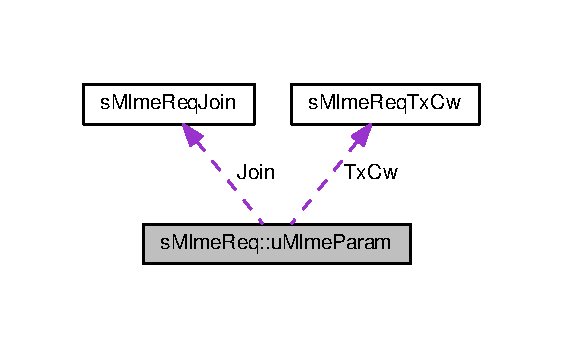
\includegraphics[width=270pt]{unionsMlmeReq_1_1uMlmeParam__coll__graph}
\end{center}
\end{figure}
\subsection*{Data Fields}
\begin{DoxyCompactItemize}
\item 
\hyperlink{group__LORAMAC_gab12f7f7d9bdfb8067d56f7c9f1297d95}{Mlme\+Req\+Join\+\_\+t} \hyperlink{unionsMlmeReq_1_1uMlmeParam_a8065a3a3d703e59ee8ee10ed48bcb726}{Join}
\item 
\hyperlink{group__LORAMAC_gab71a9931686ff623fa01ceecc61f1986}{Mlme\+Req\+Tx\+Cw\+\_\+t} \hyperlink{unionsMlmeReq_1_1uMlmeParam_a574dc0aa0d991726f55da055105c5dcf}{Tx\+Cw}
\end{DoxyCompactItemize}


\subsection{Detailed Description}
M\+L\+M\+E-\/\+Request parameters 

\subsection{Field Documentation}
\mbox{\Hypertarget{unionsMlmeReq_1_1uMlmeParam_a8065a3a3d703e59ee8ee10ed48bcb726}\label{unionsMlmeReq_1_1uMlmeParam_a8065a3a3d703e59ee8ee10ed48bcb726}} 
\index{s\+Mlme\+Req\+::u\+Mlme\+Param@{s\+Mlme\+Req\+::u\+Mlme\+Param}!Join@{Join}}
\index{Join@{Join}!s\+Mlme\+Req\+::u\+Mlme\+Param@{s\+Mlme\+Req\+::u\+Mlme\+Param}}
\subsubsection{\texorpdfstring{Join}{Join}}
{\footnotesize\ttfamily \hyperlink{group__LORAMAC_gab12f7f7d9bdfb8067d56f7c9f1297d95}{Mlme\+Req\+Join\+\_\+t} s\+Mlme\+Req\+::u\+Mlme\+Param\+::\+Join}

M\+L\+M\+E-\/\+Request parameters for a join request \mbox{\Hypertarget{unionsMlmeReq_1_1uMlmeParam_a574dc0aa0d991726f55da055105c5dcf}\label{unionsMlmeReq_1_1uMlmeParam_a574dc0aa0d991726f55da055105c5dcf}} 
\index{s\+Mlme\+Req\+::u\+Mlme\+Param@{s\+Mlme\+Req\+::u\+Mlme\+Param}!Tx\+Cw@{Tx\+Cw}}
\index{Tx\+Cw@{Tx\+Cw}!s\+Mlme\+Req\+::u\+Mlme\+Param@{s\+Mlme\+Req\+::u\+Mlme\+Param}}
\subsubsection{\texorpdfstring{Tx\+Cw}{TxCw}}
{\footnotesize\ttfamily \hyperlink{group__LORAMAC_gab71a9931686ff623fa01ceecc61f1986}{Mlme\+Req\+Tx\+Cw\+\_\+t} s\+Mlme\+Req\+::u\+Mlme\+Param\+::\+Tx\+Cw}

M\+L\+M\+E-\/\+Request parameters for Tx continuous mode request 

The documentation for this union was generated from the following file\+:\begin{DoxyCompactItemize}
\item 
Mac/\hyperlink{LoRaMac_8h}{Lo\+Ra\+Mac.\+h}\end{DoxyCompactItemize}

\hypertarget{unionuPhyParam}{}\section{u\+Phy\+Param Union Reference}
\label{unionuPhyParam}\index{u\+Phy\+Param@{u\+Phy\+Param}}


{\ttfamily \#include $<$Region.\+h$>$}



Collaboration diagram for u\+Phy\+Param\+:
\nopagebreak
\begin{figure}[H]
\begin{center}
\leavevmode
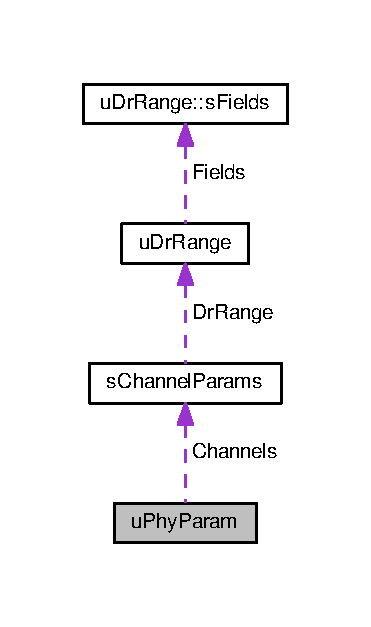
\includegraphics[width=178pt]{unionuPhyParam__coll__graph}
\end{center}
\end{figure}
\subsection*{Data Fields}
\begin{DoxyCompactItemize}
\item 
uint32\+\_\+t \hyperlink{unionuPhyParam_aed3ac490dcac46f2b6c06566f6fdbc56}{Value}
\item 
float \hyperlink{unionuPhyParam_a45e40c02153e3c6fc4b6578b217e9c5b}{f\+Value}
\item 
uint16\+\_\+t $\ast$ \hyperlink{unionuPhyParam_a76583d386fefae802f5d11c040d04ba2}{Channels\+Mask}
\item 
\hyperlink{group__LORAMAC_ga1360ca6f82c6d125ea43a9dad9b56184}{Channel\+Params\+\_\+t} $\ast$ \hyperlink{unionuPhyParam_a3025546f58e55d9601321e2f613ab264}{Channels}
\end{DoxyCompactItemize}


\subsection{Detailed Description}
Union for the structure u\+Get\+Phy\+Params 

\subsection{Field Documentation}
\mbox{\Hypertarget{unionuPhyParam_a3025546f58e55d9601321e2f613ab264}\label{unionuPhyParam_a3025546f58e55d9601321e2f613ab264}} 
\index{u\+Phy\+Param@{u\+Phy\+Param}!Channels@{Channels}}
\index{Channels@{Channels}!u\+Phy\+Param@{u\+Phy\+Param}}
\subsubsection{\texorpdfstring{Channels}{Channels}}
{\footnotesize\ttfamily \hyperlink{group__LORAMAC_ga1360ca6f82c6d125ea43a9dad9b56184}{Channel\+Params\+\_\+t}$\ast$ u\+Phy\+Param\+::\+Channels}

Pointer to the channels. \mbox{\Hypertarget{unionuPhyParam_a76583d386fefae802f5d11c040d04ba2}\label{unionuPhyParam_a76583d386fefae802f5d11c040d04ba2}} 
\index{u\+Phy\+Param@{u\+Phy\+Param}!Channels\+Mask@{Channels\+Mask}}
\index{Channels\+Mask@{Channels\+Mask}!u\+Phy\+Param@{u\+Phy\+Param}}
\subsubsection{\texorpdfstring{Channels\+Mask}{ChannelsMask}}
{\footnotesize\ttfamily uint16\+\_\+t$\ast$ u\+Phy\+Param\+::\+Channels\+Mask}

Pointer to the channels mask. \mbox{\Hypertarget{unionuPhyParam_a45e40c02153e3c6fc4b6578b217e9c5b}\label{unionuPhyParam_a45e40c02153e3c6fc4b6578b217e9c5b}} 
\index{u\+Phy\+Param@{u\+Phy\+Param}!f\+Value@{f\+Value}}
\index{f\+Value@{f\+Value}!u\+Phy\+Param@{u\+Phy\+Param}}
\subsubsection{\texorpdfstring{f\+Value}{fValue}}
{\footnotesize\ttfamily float u\+Phy\+Param\+::f\+Value}

A floating point value. \mbox{\Hypertarget{unionuPhyParam_aed3ac490dcac46f2b6c06566f6fdbc56}\label{unionuPhyParam_aed3ac490dcac46f2b6c06566f6fdbc56}} 
\index{u\+Phy\+Param@{u\+Phy\+Param}!Value@{Value}}
\index{Value@{Value}!u\+Phy\+Param@{u\+Phy\+Param}}
\subsubsection{\texorpdfstring{Value}{Value}}
{\footnotesize\ttfamily uint32\+\_\+t u\+Phy\+Param\+::\+Value}

A parameter value. 

The documentation for this union was generated from the following file\+:\begin{DoxyCompactItemize}
\item 
Mac/region/\hyperlink{Region_8h}{Region.\+h}\end{DoxyCompactItemize}

\hypertarget{unionuVerifyParams}{}\section{u\+Verify\+Params Union Reference}
\label{unionuVerifyParams}\index{u\+Verify\+Params@{u\+Verify\+Params}}


{\ttfamily \#include $<$Region.\+h$>$}



Collaboration diagram for u\+Verify\+Params\+:
\nopagebreak
\begin{figure}[H]
\begin{center}
\leavevmode
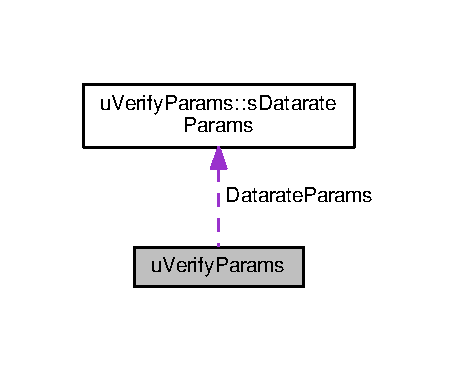
\includegraphics[width=220pt]{unionuVerifyParams__coll__graph}
\end{center}
\end{figure}
\subsection*{Data Structures}
\begin{DoxyCompactItemize}
\item 
struct \hyperlink{structuVerifyParams_1_1sDatarateParams}{s\+Datarate\+Params}
\end{DoxyCompactItemize}
\subsection*{Data Fields}
\begin{DoxyCompactItemize}
\item 
int8\+\_\+t \hyperlink{unionuVerifyParams_ab7a938258025172a2bf48649f8712135}{Tx\+Power}
\item 
bool \hyperlink{unionuVerifyParams_ac1269ec12fcd5a8ab262a4edabf6375a}{Duty\+Cycle}
\item 
uint8\+\_\+t \hyperlink{unionuVerifyParams_ac6a44915b13785f37b901650378c7854}{Nb\+Join\+Trials}
\item 
struct \hyperlink{structuVerifyParams_1_1sDatarateParams}{u\+Verify\+Params\+::s\+Datarate\+Params} \hyperlink{unionuVerifyParams_acfc77eaccff61ecbe9396785f107655a}{Datarate\+Params}
\end{DoxyCompactItemize}


\subsection{Detailed Description}
Parameter structure for the function Region\+Verify. 

\subsection{Field Documentation}
\mbox{\Hypertarget{unionuVerifyParams_acfc77eaccff61ecbe9396785f107655a}\label{unionuVerifyParams_acfc77eaccff61ecbe9396785f107655a}} 
\index{u\+Verify\+Params@{u\+Verify\+Params}!Datarate\+Params@{Datarate\+Params}}
\index{Datarate\+Params@{Datarate\+Params}!u\+Verify\+Params@{u\+Verify\+Params}}
\subsubsection{\texorpdfstring{Datarate\+Params}{DatarateParams}}
{\footnotesize\ttfamily struct \hyperlink{structuVerifyParams_1_1sDatarateParams}{u\+Verify\+Params\+::s\+Datarate\+Params} u\+Verify\+Params\+::\+Datarate\+Params}

\mbox{\Hypertarget{unionuVerifyParams_ac1269ec12fcd5a8ab262a4edabf6375a}\label{unionuVerifyParams_ac1269ec12fcd5a8ab262a4edabf6375a}} 
\index{u\+Verify\+Params@{u\+Verify\+Params}!Duty\+Cycle@{Duty\+Cycle}}
\index{Duty\+Cycle@{Duty\+Cycle}!u\+Verify\+Params@{u\+Verify\+Params}}
\subsubsection{\texorpdfstring{Duty\+Cycle}{DutyCycle}}
{\footnotesize\ttfamily bool u\+Verify\+Params\+::\+Duty\+Cycle}

Set to true, if the duty cycle is enabled, otherwise false. \mbox{\Hypertarget{unionuVerifyParams_ac6a44915b13785f37b901650378c7854}\label{unionuVerifyParams_ac6a44915b13785f37b901650378c7854}} 
\index{u\+Verify\+Params@{u\+Verify\+Params}!Nb\+Join\+Trials@{Nb\+Join\+Trials}}
\index{Nb\+Join\+Trials@{Nb\+Join\+Trials}!u\+Verify\+Params@{u\+Verify\+Params}}
\subsubsection{\texorpdfstring{Nb\+Join\+Trials}{NbJoinTrials}}
{\footnotesize\ttfamily uint8\+\_\+t u\+Verify\+Params\+::\+Nb\+Join\+Trials}

The number of join trials. \mbox{\Hypertarget{unionuVerifyParams_ab7a938258025172a2bf48649f8712135}\label{unionuVerifyParams_ab7a938258025172a2bf48649f8712135}} 
\index{u\+Verify\+Params@{u\+Verify\+Params}!Tx\+Power@{Tx\+Power}}
\index{Tx\+Power@{Tx\+Power}!u\+Verify\+Params@{u\+Verify\+Params}}
\subsubsection{\texorpdfstring{Tx\+Power}{TxPower}}
{\footnotesize\ttfamily int8\+\_\+t u\+Verify\+Params\+::\+Tx\+Power}

TX power to verify. 

The documentation for this union was generated from the following file\+:\begin{DoxyCompactItemize}
\item 
Mac/region/\hyperlink{Region_8h}{Region.\+h}\end{DoxyCompactItemize}

\chapter{File Documentation}
\hypertarget{lora_8c}{}\section{Core/lora.c File Reference}
\label{lora_8c}\index{Core/lora.\+c@{Core/lora.\+c}}
{\ttfamily \#include \char`\"{}hw.\+h\char`\"{}}\newline
{\ttfamily \#include \char`\"{}time\+Server.\+h\char`\"{}}\newline
{\ttfamily \#include \char`\"{}Lo\+Ra\+Mac.\+h\char`\"{}}\newline
{\ttfamily \#include \char`\"{}lora.\+h\char`\"{}}\newline
Include dependency graph for lora.\+c\+:
\nopagebreak
\begin{figure}[H]
\begin{center}
\leavevmode
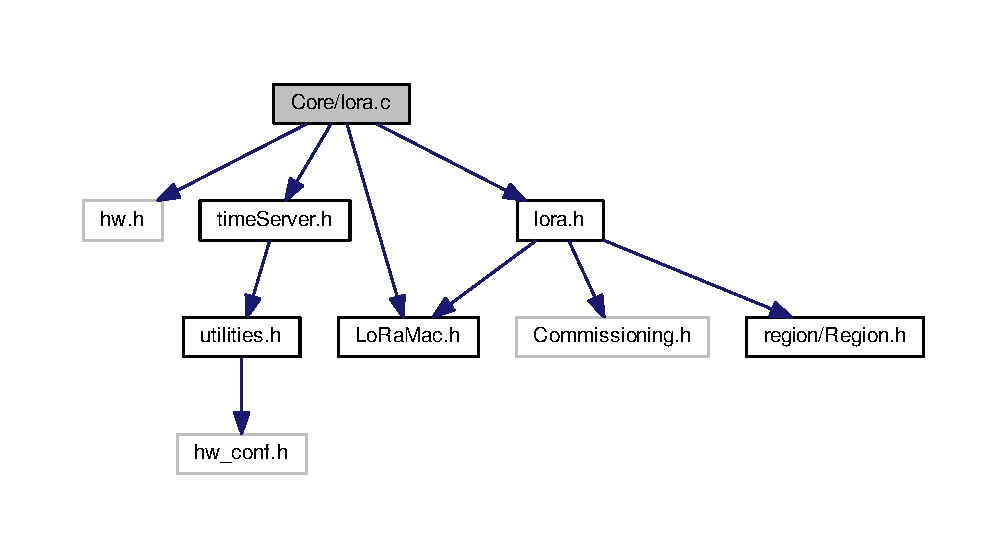
\includegraphics[width=350pt]{lora_8c__incl}
\end{center}
\end{figure}
\subsection*{Data Structures}
\begin{DoxyCompactItemize}
\item 
struct \hyperlink{structComplianceTest__s}{Compliance\+Test\+\_\+s}
\end{DoxyCompactItemize}
\subsection*{Macros}
\begin{DoxyCompactItemize}
\item 
\#define \hyperlink{lora_8c_a000b0776aef6df43009f5907a3ea8766}{O\+V\+E\+R\+\_\+\+T\+H\+E\+\_\+\+A\+I\+R\+\_\+\+A\+C\+T\+I\+V\+A\+T\+I\+O\+N\+\_\+\+D\+U\+T\+Y\+C\+Y\+C\+LE}~10000
\item 
\#define \hyperlink{lora_8c_ad68da80f74df53d59dda29ab77193067}{L\+O\+R\+A\+W\+A\+N\+\_\+\+A\+P\+P\+\_\+\+D\+A\+T\+A\+\_\+\+B\+U\+F\+F\+\_\+\+S\+I\+ZE}~64
\end{DoxyCompactItemize}
\subsection*{Functions}
\begin{DoxyCompactItemize}
\item 
void \hyperlink{lora_8c_a5e5279c24de9f5ddeed823dc3ab696f8}{On\+Send\+Event} (void)
\begin{DoxyCompactList}\small\item\em functionl requesting lo\+Ra state machine to send data \end{DoxyCompactList}\item 
void \hyperlink{lora_8c_a6ccf1d9dc586fe020b3206fdf497e9bc}{lora\+\_\+\+Init} (\hyperlink{lora_8h_a6d9d62812a66a54510e9dc9f3f7a2b5e}{Lo\+Ra\+Main\+Callback\+\_\+t} $\ast$callbacks, \hyperlink{lora_8h_a34fefd9575c41bc86d86d7d740a38fe8}{Lo\+Ra\+Param\+\_\+t} $\ast$Lo\+Ra\+Param)
\begin{DoxyCompactList}\small\item\em Lora Initialisation. \end{DoxyCompactList}\item 
void \hyperlink{lora_8c_a55aa2eacf9b0140d4458ff1f33783afe}{lora\+\_\+fsm} (void)
\begin{DoxyCompactList}\small\item\em run Lora classA state Machine \end{DoxyCompactList}\item 
\hyperlink{lora_8h_ae7cd63b2daaa72965c2b3594e11f38d7}{Device\+State\+\_\+t} \hyperlink{lora_8c_a0118145d83e11a4c79ef4dd5852efadc}{lora\+\_\+get\+Device\+State} (void)
\begin{DoxyCompactList}\small\item\em A\+PI returns the state of the lora state machine. \end{DoxyCompactList}\end{DoxyCompactItemize}
\subsection*{Variables}
\begin{DoxyCompactItemize}
\item 
struct \hyperlink{structComplianceTest__s}{Compliance\+Test\+\_\+s} \hyperlink{lora_8c_acbc72ca398f4a544f8e3548a895f2a5d}{Compliance\+Test}
\end{DoxyCompactItemize}


\subsection{Macro Definition Documentation}
\mbox{\Hypertarget{lora_8c_ad68da80f74df53d59dda29ab77193067}\label{lora_8c_ad68da80f74df53d59dda29ab77193067}} 
\index{lora.\+c@{lora.\+c}!L\+O\+R\+A\+W\+A\+N\+\_\+\+A\+P\+P\+\_\+\+D\+A\+T\+A\+\_\+\+B\+U\+F\+F\+\_\+\+S\+I\+ZE@{L\+O\+R\+A\+W\+A\+N\+\_\+\+A\+P\+P\+\_\+\+D\+A\+T\+A\+\_\+\+B\+U\+F\+F\+\_\+\+S\+I\+ZE}}
\index{L\+O\+R\+A\+W\+A\+N\+\_\+\+A\+P\+P\+\_\+\+D\+A\+T\+A\+\_\+\+B\+U\+F\+F\+\_\+\+S\+I\+ZE@{L\+O\+R\+A\+W\+A\+N\+\_\+\+A\+P\+P\+\_\+\+D\+A\+T\+A\+\_\+\+B\+U\+F\+F\+\_\+\+S\+I\+ZE}!lora.\+c@{lora.\+c}}
\subsubsection{\texorpdfstring{L\+O\+R\+A\+W\+A\+N\+\_\+\+A\+P\+P\+\_\+\+D\+A\+T\+A\+\_\+\+B\+U\+F\+F\+\_\+\+S\+I\+ZE}{LORAWAN\_APP\_DATA\_BUFF\_SIZE}}
{\footnotesize\ttfamily \#define L\+O\+R\+A\+W\+A\+N\+\_\+\+A\+P\+P\+\_\+\+D\+A\+T\+A\+\_\+\+B\+U\+F\+F\+\_\+\+S\+I\+ZE~64}

User application data buffer size \mbox{\Hypertarget{lora_8c_a000b0776aef6df43009f5907a3ea8766}\label{lora_8c_a000b0776aef6df43009f5907a3ea8766}} 
\index{lora.\+c@{lora.\+c}!O\+V\+E\+R\+\_\+\+T\+H\+E\+\_\+\+A\+I\+R\+\_\+\+A\+C\+T\+I\+V\+A\+T\+I\+O\+N\+\_\+\+D\+U\+T\+Y\+C\+Y\+C\+LE@{O\+V\+E\+R\+\_\+\+T\+H\+E\+\_\+\+A\+I\+R\+\_\+\+A\+C\+T\+I\+V\+A\+T\+I\+O\+N\+\_\+\+D\+U\+T\+Y\+C\+Y\+C\+LE}}
\index{O\+V\+E\+R\+\_\+\+T\+H\+E\+\_\+\+A\+I\+R\+\_\+\+A\+C\+T\+I\+V\+A\+T\+I\+O\+N\+\_\+\+D\+U\+T\+Y\+C\+Y\+C\+LE@{O\+V\+E\+R\+\_\+\+T\+H\+E\+\_\+\+A\+I\+R\+\_\+\+A\+C\+T\+I\+V\+A\+T\+I\+O\+N\+\_\+\+D\+U\+T\+Y\+C\+Y\+C\+LE}!lora.\+c@{lora.\+c}}
\subsubsection{\texorpdfstring{O\+V\+E\+R\+\_\+\+T\+H\+E\+\_\+\+A\+I\+R\+\_\+\+A\+C\+T\+I\+V\+A\+T\+I\+O\+N\+\_\+\+D\+U\+T\+Y\+C\+Y\+C\+LE}{OVER\_THE\_AIR\_ACTIVATION\_DUTYCYCLE}}
{\footnotesize\ttfamily \#define O\+V\+E\+R\+\_\+\+T\+H\+E\+\_\+\+A\+I\+R\+\_\+\+A\+C\+T\+I\+V\+A\+T\+I\+O\+N\+\_\+\+D\+U\+T\+Y\+C\+Y\+C\+LE~10000}

Join requests trials duty cycle. 

\subsection{Function Documentation}
\mbox{\Hypertarget{lora_8c_a55aa2eacf9b0140d4458ff1f33783afe}\label{lora_8c_a55aa2eacf9b0140d4458ff1f33783afe}} 
\index{lora.\+c@{lora.\+c}!lora\+\_\+fsm@{lora\+\_\+fsm}}
\index{lora\+\_\+fsm@{lora\+\_\+fsm}!lora.\+c@{lora.\+c}}
\subsubsection{\texorpdfstring{lora\+\_\+fsm()}{lora\_fsm()}}
{\footnotesize\ttfamily void lora\+\_\+fsm (\begin{DoxyParamCaption}\item[{void}]{ }\end{DoxyParamCaption})}



run Lora classA state Machine 

lora class A state machine \mbox{\Hypertarget{lora_8c_a0118145d83e11a4c79ef4dd5852efadc}\label{lora_8c_a0118145d83e11a4c79ef4dd5852efadc}} 
\index{lora.\+c@{lora.\+c}!lora\+\_\+get\+Device\+State@{lora\+\_\+get\+Device\+State}}
\index{lora\+\_\+get\+Device\+State@{lora\+\_\+get\+Device\+State}!lora.\+c@{lora.\+c}}
\subsubsection{\texorpdfstring{lora\+\_\+get\+Device\+State()}{lora\_getDeviceState()}}
{\footnotesize\ttfamily \hyperlink{lora_8h_ae7cd63b2daaa72965c2b3594e11f38d7}{Device\+State\+\_\+t} lora\+\_\+get\+Device\+State (\begin{DoxyParamCaption}\item[{void}]{ }\end{DoxyParamCaption})}



A\+PI returns the state of the lora state machine. 

\begin{DoxyNote}{Note}
return  state 
\end{DoxyNote}

\begin{DoxyParams}{Parameters}
{\em \mbox{[}\+I\+N\mbox{]}} & none \\
\hline
\end{DoxyParams}

\begin{DoxyRetVals}{Return values}
{\em return} & \\
\hline
\end{DoxyRetVals}
\mbox{\Hypertarget{lora_8c_a6ccf1d9dc586fe020b3206fdf497e9bc}\label{lora_8c_a6ccf1d9dc586fe020b3206fdf497e9bc}} 
\index{lora.\+c@{lora.\+c}!lora\+\_\+\+Init@{lora\+\_\+\+Init}}
\index{lora\+\_\+\+Init@{lora\+\_\+\+Init}!lora.\+c@{lora.\+c}}
\subsubsection{\texorpdfstring{lora\+\_\+\+Init()}{lora\_Init()}}
{\footnotesize\ttfamily void lora\+\_\+\+Init (\begin{DoxyParamCaption}\item[{\hyperlink{lora_8h_a6d9d62812a66a54510e9dc9f3f7a2b5e}{Lo\+Ra\+Main\+Callback\+\_\+t} $\ast$}]{callbacks,  }\item[{\hyperlink{lora_8h_a34fefd9575c41bc86d86d7d740a38fe8}{Lo\+Ra\+Param\+\_\+t} $\ast$}]{Lo\+Ra\+Param }\end{DoxyParamCaption})}



Lora Initialisation. 

lora Init \mbox{\Hypertarget{lora_8c_a5e5279c24de9f5ddeed823dc3ab696f8}\label{lora_8c_a5e5279c24de9f5ddeed823dc3ab696f8}} 
\index{lora.\+c@{lora.\+c}!On\+Send\+Event@{On\+Send\+Event}}
\index{On\+Send\+Event@{On\+Send\+Event}!lora.\+c@{lora.\+c}}
\subsubsection{\texorpdfstring{On\+Send\+Event()}{OnSendEvent()}}
{\footnotesize\ttfamily void On\+Send\+Event (\begin{DoxyParamCaption}\item[{void}]{ }\end{DoxyParamCaption})}



functionl requesting lo\+Ra state machine to send data 

\begin{DoxyNote}{Note}
function to link in mode T\+X\+\_\+\+O\+N\+\_\+\+E\+V\+E\+NT 
\end{DoxyNote}

\begin{DoxyParams}{Parameters}
{\em none} & \\
\hline
\end{DoxyParams}

\begin{DoxyRetVals}{Return values}
{\em none} & \\
\hline
\end{DoxyRetVals}


\subsection{Variable Documentation}
\mbox{\Hypertarget{lora_8c_acbc72ca398f4a544f8e3548a895f2a5d}\label{lora_8c_acbc72ca398f4a544f8e3548a895f2a5d}} 
\index{lora.\+c@{lora.\+c}!Compliance\+Test@{Compliance\+Test}}
\index{Compliance\+Test@{Compliance\+Test}!lora.\+c@{lora.\+c}}
\subsubsection{\texorpdfstring{Compliance\+Test}{ComplianceTest}}
{\footnotesize\ttfamily struct \hyperlink{structComplianceTest__s}{Compliance\+Test\+\_\+s} Compliance\+Test}


\hypertarget{lora_8h}{}\section{Core/lora.h File Reference}
\label{lora_8h}\index{Core/lora.\+h@{Core/lora.\+h}}
{\ttfamily \#include \char`\"{}Commissioning.\+h\char`\"{}}\newline
{\ttfamily \#include \char`\"{}Lo\+Ra\+Mac.\+h\char`\"{}}\newline
{\ttfamily \#include \char`\"{}region/\+Region.\+h\char`\"{}}\newline
Include dependency graph for lora.\+h\+:
\nopagebreak
\begin{figure}[H]
\begin{center}
\leavevmode
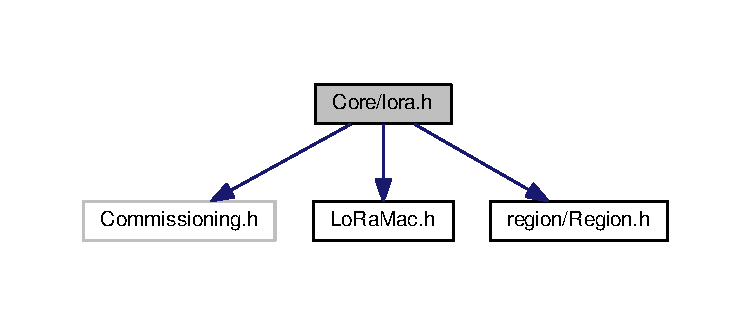
\includegraphics[width=350pt]{lora_8h__incl}
\end{center}
\end{figure}
This graph shows which files directly or indirectly include this file\+:
\nopagebreak
\begin{figure}[H]
\begin{center}
\leavevmode
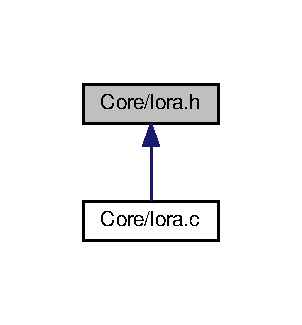
\includegraphics[width=145pt]{lora_8h__dep__incl}
\end{center}
\end{figure}
\subsection*{Data Structures}
\begin{DoxyCompactItemize}
\item 
struct \hyperlink{structlora__AppData__t}{lora\+\_\+\+App\+Data\+\_\+t}
\item 
struct \hyperlink{structsLoRaParam}{s\+Lo\+Ra\+Param}
\item 
struct \hyperlink{structsLoRaMainCallback}{s\+Lo\+Ra\+Main\+Callback}
\end{DoxyCompactItemize}
\subsection*{Typedefs}
\begin{DoxyCompactItemize}
\item 
typedef enum \hyperlink{lora_8h_aad05e5b05f12b64358a24ebafebf4a27}{e\+Devic\+State} \hyperlink{lora_8h_ae7cd63b2daaa72965c2b3594e11f38d7}{Device\+State\+\_\+t}
\item 
typedef enum \hyperlink{lora_8h_a720c475eb13bb6b5523f349e34b1b813}{e\+Tx\+Event\+Type} \hyperlink{lora_8h_ad214b606ffdf2be60abb61bcebbbc83e}{Tx\+Event\+Type\+\_\+t}
\item 
typedef struct \hyperlink{structsLoRaParam}{s\+Lo\+Ra\+Param} \hyperlink{lora_8h_a34fefd9575c41bc86d86d7d740a38fe8}{Lo\+Ra\+Param\+\_\+t}
\item 
typedef struct \hyperlink{structsLoRaMainCallback}{s\+Lo\+Ra\+Main\+Callback} \hyperlink{lora_8h_a6d9d62812a66a54510e9dc9f3f7a2b5e}{Lo\+Ra\+Main\+Callback\+\_\+t}
\end{DoxyCompactItemize}
\subsection*{Enumerations}
\begin{DoxyCompactItemize}
\item 
enum \hyperlink{lora_8h_aad05e5b05f12b64358a24ebafebf4a27}{e\+Devic\+State} \{ \newline
\hyperlink{lora_8h_aad05e5b05f12b64358a24ebafebf4a27a286f8821833d7a35ccb7fbfcfaec94b9}{D\+E\+V\+I\+C\+E\+\_\+\+S\+T\+A\+T\+E\+\_\+\+I\+N\+IT}, 
\hyperlink{lora_8h_aad05e5b05f12b64358a24ebafebf4a27ac86db85bcdfe3189a4cf2d95dfce0b78}{D\+E\+V\+I\+C\+E\+\_\+\+S\+T\+A\+T\+E\+\_\+\+J\+O\+IN}, 
\hyperlink{lora_8h_aad05e5b05f12b64358a24ebafebf4a27a0222625afc558d780b24f8080c535a9f}{D\+E\+V\+I\+C\+E\+\_\+\+S\+T\+A\+T\+E\+\_\+\+J\+O\+I\+N\+ED}, 
\hyperlink{lora_8h_aad05e5b05f12b64358a24ebafebf4a27a5befd8bc234194c79dbc2dd2f4e3b966}{D\+E\+V\+I\+C\+E\+\_\+\+S\+T\+A\+T\+E\+\_\+\+S\+E\+ND}, 
\newline
\hyperlink{lora_8h_aad05e5b05f12b64358a24ebafebf4a27aebc0f22559125b76030bdbd52013e7a0}{D\+E\+V\+I\+C\+E\+\_\+\+S\+T\+A\+T\+E\+\_\+\+C\+Y\+C\+LE}, 
\hyperlink{lora_8h_aad05e5b05f12b64358a24ebafebf4a27a9c756d338f93884941d142899f226583}{D\+E\+V\+I\+C\+E\+\_\+\+S\+T\+A\+T\+E\+\_\+\+S\+L\+E\+EP}
 \}
\item 
enum \hyperlink{lora_8h_a720c475eb13bb6b5523f349e34b1b813}{e\+Tx\+Event\+Type} \{ \hyperlink{lora_8h_a720c475eb13bb6b5523f349e34b1b813a4f3161e467887e98bcedd864f3cfc16e}{T\+X\+\_\+\+O\+N\+\_\+\+T\+I\+M\+ER}, 
\hyperlink{lora_8h_a720c475eb13bb6b5523f349e34b1b813a2d3c00188e9ba996f5f291272d029d52}{T\+X\+\_\+\+O\+N\+\_\+\+E\+V\+E\+NT}
 \}
\end{DoxyCompactItemize}
\subsection*{Functions}
\begin{DoxyCompactItemize}
\item 
void \hyperlink{lora_8h_a6ccf1d9dc586fe020b3206fdf497e9bc}{lora\+\_\+\+Init} (\hyperlink{lora_8h_a6d9d62812a66a54510e9dc9f3f7a2b5e}{Lo\+Ra\+Main\+Callback\+\_\+t} $\ast$callbacks, \hyperlink{lora_8h_a34fefd9575c41bc86d86d7d740a38fe8}{Lo\+Ra\+Param\+\_\+t} $\ast$Lo\+Ra\+Param)
\begin{DoxyCompactList}\small\item\em Lora Initialisation. \end{DoxyCompactList}\item 
void \hyperlink{lora_8h_a55aa2eacf9b0140d4458ff1f33783afe}{lora\+\_\+fsm} (void)
\begin{DoxyCompactList}\small\item\em run Lora classA state Machine \end{DoxyCompactList}\item 
void \hyperlink{lora_8h_a5e5279c24de9f5ddeed823dc3ab696f8}{On\+Send\+Event} (void)
\begin{DoxyCompactList}\small\item\em functionl requesting lo\+Ra state machine to send data \end{DoxyCompactList}\item 
\hyperlink{lora_8h_ae7cd63b2daaa72965c2b3594e11f38d7}{Device\+State\+\_\+t} \hyperlink{lora_8h_a0118145d83e11a4c79ef4dd5852efadc}{lora\+\_\+get\+Device\+State} (void)
\begin{DoxyCompactList}\small\item\em A\+PI returns the state of the lora state machine. \end{DoxyCompactList}\end{DoxyCompactItemize}


\subsection{Typedef Documentation}
\mbox{\Hypertarget{lora_8h_ae7cd63b2daaa72965c2b3594e11f38d7}\label{lora_8h_ae7cd63b2daaa72965c2b3594e11f38d7}} 
\index{lora.\+h@{lora.\+h}!Device\+State\+\_\+t@{Device\+State\+\_\+t}}
\index{Device\+State\+\_\+t@{Device\+State\+\_\+t}!lora.\+h@{lora.\+h}}
\subsubsection{\texorpdfstring{Device\+State\+\_\+t}{DeviceState\_t}}
{\footnotesize\ttfamily typedef enum \hyperlink{lora_8h_aad05e5b05f12b64358a24ebafebf4a27}{e\+Devic\+State}  \hyperlink{lora_8h_ae7cd63b2daaa72965c2b3594e11f38d7}{Device\+State\+\_\+t}}

Lo\+Ra State Machine states \mbox{\Hypertarget{lora_8h_a6d9d62812a66a54510e9dc9f3f7a2b5e}\label{lora_8h_a6d9d62812a66a54510e9dc9f3f7a2b5e}} 
\index{lora.\+h@{lora.\+h}!Lo\+Ra\+Main\+Callback\+\_\+t@{Lo\+Ra\+Main\+Callback\+\_\+t}}
\index{Lo\+Ra\+Main\+Callback\+\_\+t@{Lo\+Ra\+Main\+Callback\+\_\+t}!lora.\+h@{lora.\+h}}
\subsubsection{\texorpdfstring{Lo\+Ra\+Main\+Callback\+\_\+t}{LoRaMainCallback\_t}}
{\footnotesize\ttfamily typedef struct \hyperlink{structsLoRaMainCallback}{s\+Lo\+Ra\+Main\+Callback}  \hyperlink{lora_8h_a6d9d62812a66a54510e9dc9f3f7a2b5e}{Lo\+Ra\+Main\+Callback\+\_\+t}}

\mbox{\Hypertarget{lora_8h_a34fefd9575c41bc86d86d7d740a38fe8}\label{lora_8h_a34fefd9575c41bc86d86d7d740a38fe8}} 
\index{lora.\+h@{lora.\+h}!Lo\+Ra\+Param\+\_\+t@{Lo\+Ra\+Param\+\_\+t}}
\index{Lo\+Ra\+Param\+\_\+t@{Lo\+Ra\+Param\+\_\+t}!lora.\+h@{lora.\+h}}
\subsubsection{\texorpdfstring{Lo\+Ra\+Param\+\_\+t}{LoRaParam\_t}}
{\footnotesize\ttfamily typedef struct \hyperlink{structsLoRaParam}{s\+Lo\+Ra\+Param}  \hyperlink{lora_8h_a34fefd9575c41bc86d86d7d740a38fe8}{Lo\+Ra\+Param\+\_\+t}}

Lo\+Ra State Machine states \mbox{\Hypertarget{lora_8h_ad214b606ffdf2be60abb61bcebbbc83e}\label{lora_8h_ad214b606ffdf2be60abb61bcebbbc83e}} 
\index{lora.\+h@{lora.\+h}!Tx\+Event\+Type\+\_\+t@{Tx\+Event\+Type\+\_\+t}}
\index{Tx\+Event\+Type\+\_\+t@{Tx\+Event\+Type\+\_\+t}!lora.\+h@{lora.\+h}}
\subsubsection{\texorpdfstring{Tx\+Event\+Type\+\_\+t}{TxEventType\_t}}
{\footnotesize\ttfamily typedef enum \hyperlink{lora_8h_a720c475eb13bb6b5523f349e34b1b813}{e\+Tx\+Event\+Type}  \hyperlink{lora_8h_ad214b606ffdf2be60abb61bcebbbc83e}{Tx\+Event\+Type\+\_\+t}}

Lo\+Ra State Machine states 

\subsection{Enumeration Type Documentation}
\mbox{\Hypertarget{lora_8h_aad05e5b05f12b64358a24ebafebf4a27}\label{lora_8h_aad05e5b05f12b64358a24ebafebf4a27}} 
\index{lora.\+h@{lora.\+h}!e\+Devic\+State@{e\+Devic\+State}}
\index{e\+Devic\+State@{e\+Devic\+State}!lora.\+h@{lora.\+h}}
\subsubsection{\texorpdfstring{e\+Devic\+State}{eDevicState}}
{\footnotesize\ttfamily enum \hyperlink{lora_8h_aad05e5b05f12b64358a24ebafebf4a27}{e\+Devic\+State}}

Lo\+Ra State Machine states \begin{DoxyEnumFields}{Enumerator}
\raisebox{\heightof{T}}[0pt][0pt]{\index{D\+E\+V\+I\+C\+E\+\_\+\+S\+T\+A\+T\+E\+\_\+\+I\+N\+IT@{D\+E\+V\+I\+C\+E\+\_\+\+S\+T\+A\+T\+E\+\_\+\+I\+N\+IT}!lora.\+h@{lora.\+h}}\index{lora.\+h@{lora.\+h}!D\+E\+V\+I\+C\+E\+\_\+\+S\+T\+A\+T\+E\+\_\+\+I\+N\+IT@{D\+E\+V\+I\+C\+E\+\_\+\+S\+T\+A\+T\+E\+\_\+\+I\+N\+IT}}}\mbox{\Hypertarget{lora_8h_aad05e5b05f12b64358a24ebafebf4a27a286f8821833d7a35ccb7fbfcfaec94b9}\label{lora_8h_aad05e5b05f12b64358a24ebafebf4a27a286f8821833d7a35ccb7fbfcfaec94b9}} 
D\+E\+V\+I\+C\+E\+\_\+\+S\+T\+A\+T\+E\+\_\+\+I\+N\+IT&\\
\hline

\raisebox{\heightof{T}}[0pt][0pt]{\index{D\+E\+V\+I\+C\+E\+\_\+\+S\+T\+A\+T\+E\+\_\+\+J\+O\+IN@{D\+E\+V\+I\+C\+E\+\_\+\+S\+T\+A\+T\+E\+\_\+\+J\+O\+IN}!lora.\+h@{lora.\+h}}\index{lora.\+h@{lora.\+h}!D\+E\+V\+I\+C\+E\+\_\+\+S\+T\+A\+T\+E\+\_\+\+J\+O\+IN@{D\+E\+V\+I\+C\+E\+\_\+\+S\+T\+A\+T\+E\+\_\+\+J\+O\+IN}}}\mbox{\Hypertarget{lora_8h_aad05e5b05f12b64358a24ebafebf4a27ac86db85bcdfe3189a4cf2d95dfce0b78}\label{lora_8h_aad05e5b05f12b64358a24ebafebf4a27ac86db85bcdfe3189a4cf2d95dfce0b78}} 
D\+E\+V\+I\+C\+E\+\_\+\+S\+T\+A\+T\+E\+\_\+\+J\+O\+IN&\\
\hline

\raisebox{\heightof{T}}[0pt][0pt]{\index{D\+E\+V\+I\+C\+E\+\_\+\+S\+T\+A\+T\+E\+\_\+\+J\+O\+I\+N\+ED@{D\+E\+V\+I\+C\+E\+\_\+\+S\+T\+A\+T\+E\+\_\+\+J\+O\+I\+N\+ED}!lora.\+h@{lora.\+h}}\index{lora.\+h@{lora.\+h}!D\+E\+V\+I\+C\+E\+\_\+\+S\+T\+A\+T\+E\+\_\+\+J\+O\+I\+N\+ED@{D\+E\+V\+I\+C\+E\+\_\+\+S\+T\+A\+T\+E\+\_\+\+J\+O\+I\+N\+ED}}}\mbox{\Hypertarget{lora_8h_aad05e5b05f12b64358a24ebafebf4a27a0222625afc558d780b24f8080c535a9f}\label{lora_8h_aad05e5b05f12b64358a24ebafebf4a27a0222625afc558d780b24f8080c535a9f}} 
D\+E\+V\+I\+C\+E\+\_\+\+S\+T\+A\+T\+E\+\_\+\+J\+O\+I\+N\+ED&\\
\hline

\raisebox{\heightof{T}}[0pt][0pt]{\index{D\+E\+V\+I\+C\+E\+\_\+\+S\+T\+A\+T\+E\+\_\+\+S\+E\+ND@{D\+E\+V\+I\+C\+E\+\_\+\+S\+T\+A\+T\+E\+\_\+\+S\+E\+ND}!lora.\+h@{lora.\+h}}\index{lora.\+h@{lora.\+h}!D\+E\+V\+I\+C\+E\+\_\+\+S\+T\+A\+T\+E\+\_\+\+S\+E\+ND@{D\+E\+V\+I\+C\+E\+\_\+\+S\+T\+A\+T\+E\+\_\+\+S\+E\+ND}}}\mbox{\Hypertarget{lora_8h_aad05e5b05f12b64358a24ebafebf4a27a5befd8bc234194c79dbc2dd2f4e3b966}\label{lora_8h_aad05e5b05f12b64358a24ebafebf4a27a5befd8bc234194c79dbc2dd2f4e3b966}} 
D\+E\+V\+I\+C\+E\+\_\+\+S\+T\+A\+T\+E\+\_\+\+S\+E\+ND&\\
\hline

\raisebox{\heightof{T}}[0pt][0pt]{\index{D\+E\+V\+I\+C\+E\+\_\+\+S\+T\+A\+T\+E\+\_\+\+C\+Y\+C\+LE@{D\+E\+V\+I\+C\+E\+\_\+\+S\+T\+A\+T\+E\+\_\+\+C\+Y\+C\+LE}!lora.\+h@{lora.\+h}}\index{lora.\+h@{lora.\+h}!D\+E\+V\+I\+C\+E\+\_\+\+S\+T\+A\+T\+E\+\_\+\+C\+Y\+C\+LE@{D\+E\+V\+I\+C\+E\+\_\+\+S\+T\+A\+T\+E\+\_\+\+C\+Y\+C\+LE}}}\mbox{\Hypertarget{lora_8h_aad05e5b05f12b64358a24ebafebf4a27aebc0f22559125b76030bdbd52013e7a0}\label{lora_8h_aad05e5b05f12b64358a24ebafebf4a27aebc0f22559125b76030bdbd52013e7a0}} 
D\+E\+V\+I\+C\+E\+\_\+\+S\+T\+A\+T\+E\+\_\+\+C\+Y\+C\+LE&\\
\hline

\raisebox{\heightof{T}}[0pt][0pt]{\index{D\+E\+V\+I\+C\+E\+\_\+\+S\+T\+A\+T\+E\+\_\+\+S\+L\+E\+EP@{D\+E\+V\+I\+C\+E\+\_\+\+S\+T\+A\+T\+E\+\_\+\+S\+L\+E\+EP}!lora.\+h@{lora.\+h}}\index{lora.\+h@{lora.\+h}!D\+E\+V\+I\+C\+E\+\_\+\+S\+T\+A\+T\+E\+\_\+\+S\+L\+E\+EP@{D\+E\+V\+I\+C\+E\+\_\+\+S\+T\+A\+T\+E\+\_\+\+S\+L\+E\+EP}}}\mbox{\Hypertarget{lora_8h_aad05e5b05f12b64358a24ebafebf4a27a9c756d338f93884941d142899f226583}\label{lora_8h_aad05e5b05f12b64358a24ebafebf4a27a9c756d338f93884941d142899f226583}} 
D\+E\+V\+I\+C\+E\+\_\+\+S\+T\+A\+T\+E\+\_\+\+S\+L\+E\+EP&\\
\hline

\end{DoxyEnumFields}
\mbox{\Hypertarget{lora_8h_a720c475eb13bb6b5523f349e34b1b813}\label{lora_8h_a720c475eb13bb6b5523f349e34b1b813}} 
\index{lora.\+h@{lora.\+h}!e\+Tx\+Event\+Type@{e\+Tx\+Event\+Type}}
\index{e\+Tx\+Event\+Type@{e\+Tx\+Event\+Type}!lora.\+h@{lora.\+h}}
\subsubsection{\texorpdfstring{e\+Tx\+Event\+Type}{eTxEventType}}
{\footnotesize\ttfamily enum \hyperlink{lora_8h_a720c475eb13bb6b5523f349e34b1b813}{e\+Tx\+Event\+Type}}

Lo\+Ra State Machine states \begin{DoxyEnumFields}{Enumerator}
\raisebox{\heightof{T}}[0pt][0pt]{\index{T\+X\+\_\+\+O\+N\+\_\+\+T\+I\+M\+ER@{T\+X\+\_\+\+O\+N\+\_\+\+T\+I\+M\+ER}!lora.\+h@{lora.\+h}}\index{lora.\+h@{lora.\+h}!T\+X\+\_\+\+O\+N\+\_\+\+T\+I\+M\+ER@{T\+X\+\_\+\+O\+N\+\_\+\+T\+I\+M\+ER}}}\mbox{\Hypertarget{lora_8h_a720c475eb13bb6b5523f349e34b1b813a4f3161e467887e98bcedd864f3cfc16e}\label{lora_8h_a720c475eb13bb6b5523f349e34b1b813a4f3161e467887e98bcedd864f3cfc16e}} 
T\+X\+\_\+\+O\+N\+\_\+\+T\+I\+M\+ER&Appdata\+Transmition issue based on timer every Tx\+Duty\+Cycle\+Time. \\
\hline

\raisebox{\heightof{T}}[0pt][0pt]{\index{T\+X\+\_\+\+O\+N\+\_\+\+E\+V\+E\+NT@{T\+X\+\_\+\+O\+N\+\_\+\+E\+V\+E\+NT}!lora.\+h@{lora.\+h}}\index{lora.\+h@{lora.\+h}!T\+X\+\_\+\+O\+N\+\_\+\+E\+V\+E\+NT@{T\+X\+\_\+\+O\+N\+\_\+\+E\+V\+E\+NT}}}\mbox{\Hypertarget{lora_8h_a720c475eb13bb6b5523f349e34b1b813a2d3c00188e9ba996f5f291272d029d52}\label{lora_8h_a720c475eb13bb6b5523f349e34b1b813a2d3c00188e9ba996f5f291272d029d52}} 
T\+X\+\_\+\+O\+N\+\_\+\+E\+V\+E\+NT&Appdata\+Transmition external event plugged on \hyperlink{lora_8h_a5e5279c24de9f5ddeed823dc3ab696f8}{On\+Send\+Event( )} \\
\hline

\end{DoxyEnumFields}


\subsection{Function Documentation}
\mbox{\Hypertarget{lora_8h_a55aa2eacf9b0140d4458ff1f33783afe}\label{lora_8h_a55aa2eacf9b0140d4458ff1f33783afe}} 
\index{lora.\+h@{lora.\+h}!lora\+\_\+fsm@{lora\+\_\+fsm}}
\index{lora\+\_\+fsm@{lora\+\_\+fsm}!lora.\+h@{lora.\+h}}
\subsubsection{\texorpdfstring{lora\+\_\+fsm()}{lora\_fsm()}}
{\footnotesize\ttfamily void lora\+\_\+fsm (\begin{DoxyParamCaption}\item[{void}]{ }\end{DoxyParamCaption})}



run Lora classA state Machine 


\begin{DoxyParams}{Parameters}
{\em \mbox{[}\+I\+N\mbox{]}} & none \\
\hline
\end{DoxyParams}

\begin{DoxyRetVals}{Return values}
{\em none} & lora class A state machine \\
\hline
\end{DoxyRetVals}
\mbox{\Hypertarget{lora_8h_a0118145d83e11a4c79ef4dd5852efadc}\label{lora_8h_a0118145d83e11a4c79ef4dd5852efadc}} 
\index{lora.\+h@{lora.\+h}!lora\+\_\+get\+Device\+State@{lora\+\_\+get\+Device\+State}}
\index{lora\+\_\+get\+Device\+State@{lora\+\_\+get\+Device\+State}!lora.\+h@{lora.\+h}}
\subsubsection{\texorpdfstring{lora\+\_\+get\+Device\+State()}{lora\_getDeviceState()}}
{\footnotesize\ttfamily \hyperlink{lora_8h_ae7cd63b2daaa72965c2b3594e11f38d7}{Device\+State\+\_\+t} lora\+\_\+get\+Device\+State (\begin{DoxyParamCaption}\item[{void}]{ }\end{DoxyParamCaption})}



A\+PI returns the state of the lora state machine. 

\begin{DoxyNote}{Note}
return  state 
\end{DoxyNote}

\begin{DoxyParams}{Parameters}
{\em \mbox{[}\+I\+N\mbox{]}} & none \\
\hline
\end{DoxyParams}

\begin{DoxyRetVals}{Return values}
{\em return} & \\
\hline
\end{DoxyRetVals}
\mbox{\Hypertarget{lora_8h_a6ccf1d9dc586fe020b3206fdf497e9bc}\label{lora_8h_a6ccf1d9dc586fe020b3206fdf497e9bc}} 
\index{lora.\+h@{lora.\+h}!lora\+\_\+\+Init@{lora\+\_\+\+Init}}
\index{lora\+\_\+\+Init@{lora\+\_\+\+Init}!lora.\+h@{lora.\+h}}
\subsubsection{\texorpdfstring{lora\+\_\+\+Init()}{lora\_Init()}}
{\footnotesize\ttfamily void lora\+\_\+\+Init (\begin{DoxyParamCaption}\item[{\hyperlink{lora_8h_a6d9d62812a66a54510e9dc9f3f7a2b5e}{Lo\+Ra\+Main\+Callback\+\_\+t} $\ast$}]{callbacks,  }\item[{\hyperlink{lora_8h_a34fefd9575c41bc86d86d7d740a38fe8}{Lo\+Ra\+Param\+\_\+t} $\ast$}]{Lo\+Ra\+Param }\end{DoxyParamCaption})}



Lora Initialisation. 


\begin{DoxyParams}{Parameters}
{\em \mbox{[}\+I\+N\mbox{]}} & Lo\+Ra\+Main\+Callback\+\_\+t \\
\hline
{\em \mbox{[}\+I\+N\mbox{]}} & application parmaters \\
\hline
\end{DoxyParams}

\begin{DoxyRetVals}{Return values}
{\em none} & lora Init \\
\hline
\end{DoxyRetVals}
\mbox{\Hypertarget{lora_8h_a5e5279c24de9f5ddeed823dc3ab696f8}\label{lora_8h_a5e5279c24de9f5ddeed823dc3ab696f8}} 
\index{lora.\+h@{lora.\+h}!On\+Send\+Event@{On\+Send\+Event}}
\index{On\+Send\+Event@{On\+Send\+Event}!lora.\+h@{lora.\+h}}
\subsubsection{\texorpdfstring{On\+Send\+Event()}{OnSendEvent()}}
{\footnotesize\ttfamily void On\+Send\+Event (\begin{DoxyParamCaption}\item[{void}]{ }\end{DoxyParamCaption})}



functionl requesting lo\+Ra state machine to send data 

\begin{DoxyNote}{Note}
function to link in mode T\+X\+\_\+\+O\+N\+\_\+\+E\+V\+E\+NT 
\end{DoxyNote}

\begin{DoxyParams}{Parameters}
{\em none} & \\
\hline
\end{DoxyParams}

\begin{DoxyRetVals}{Return values}
{\em none} & \\
\hline
\end{DoxyRetVals}

\hypertarget{lora__mac__version_8h}{}\section{Core/lora\+\_\+mac\+\_\+version.h File Reference}
\label{lora__mac__version_8h}\index{Core/lora\+\_\+mac\+\_\+version.\+h@{Core/lora\+\_\+mac\+\_\+version.\+h}}
\subsection*{Macros}
\begin{DoxyCompactItemize}
\item 
\#define \hyperlink{lora__mac__version_8h_ad2e74ef7343b19718842d6156b6ea3e3}{L\+O\+R\+A\+\_\+\+M\+A\+C\+\_\+\+V\+E\+R\+S\+I\+ON}~(uint32\+\_\+t) 0x44030000
\end{DoxyCompactItemize}


\subsection{Macro Definition Documentation}
\mbox{\Hypertarget{lora__mac__version_8h_ad2e74ef7343b19718842d6156b6ea3e3}\label{lora__mac__version_8h_ad2e74ef7343b19718842d6156b6ea3e3}} 
\index{lora\+\_\+mac\+\_\+version.\+h@{lora\+\_\+mac\+\_\+version.\+h}!L\+O\+R\+A\+\_\+\+M\+A\+C\+\_\+\+V\+E\+R\+S\+I\+ON@{L\+O\+R\+A\+\_\+\+M\+A\+C\+\_\+\+V\+E\+R\+S\+I\+ON}}
\index{L\+O\+R\+A\+\_\+\+M\+A\+C\+\_\+\+V\+E\+R\+S\+I\+ON@{L\+O\+R\+A\+\_\+\+M\+A\+C\+\_\+\+V\+E\+R\+S\+I\+ON}!lora\+\_\+mac\+\_\+version.\+h@{lora\+\_\+mac\+\_\+version.\+h}}
\subsubsection{\texorpdfstring{L\+O\+R\+A\+\_\+\+M\+A\+C\+\_\+\+V\+E\+R\+S\+I\+ON}{LORA\_MAC\_VERSION}}
{\footnotesize\ttfamily \#define L\+O\+R\+A\+\_\+\+M\+A\+C\+\_\+\+V\+E\+R\+S\+I\+ON~(uint32\+\_\+t) 0x44030000}


\hypertarget{aes_8c}{}\section{Crypto/aes.c File Reference}
\label{aes_8c}\index{Crypto/aes.\+c@{Crypto/aes.\+c}}
{\ttfamily \#include $<$stdlib.\+h$>$}\newline
{\ttfamily \#include $<$stdint.\+h$>$}\newline
{\ttfamily \#include \char`\"{}aes.\+h\char`\"{}}\newline
Include dependency graph for aes.\+c\+:
\nopagebreak
\begin{figure}[H]
\begin{center}
\leavevmode
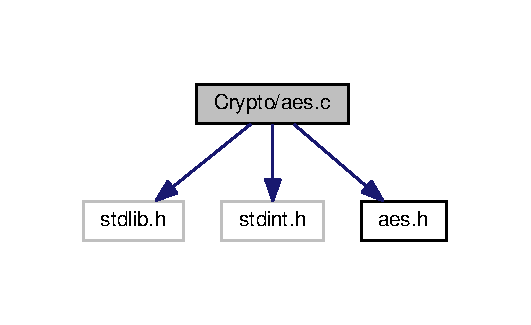
\includegraphics[width=255pt]{aes_8c__incl}
\end{center}
\end{figure}
\subsection*{Macros}
\begin{DoxyCompactItemize}
\item 
\#define \hyperlink{aes_8c_ab7aef13fbdead81e2d3ab96eb3630f10}{U\+S\+E\+\_\+\+T\+A\+B\+L\+ES}
\item 
\#define \hyperlink{aes_8c_ac40209feb00db6f009389419498d2066}{V\+E\+R\+S\+I\+O\+N\+\_\+1}
\item 
\#define \hyperlink{aes_8c_a42a5cd32857f360475450233f8367515}{W\+P\+O\+LY}~0x011b
\item 
\#define \hyperlink{aes_8c_a77c5bde3251e897058c8491bd2335c91}{B\+P\+O\+LY}~0x1b
\item 
\#define \hyperlink{aes_8c_a7dc5fb6478333a4f4cb3f55360f51d85}{D\+P\+O\+LY}~0x008d
\item 
\#define \hyperlink{aes_8c_af26abb8c819fd3cf4d6cb0711c80b9ee}{f1}(x)~(x)
\item 
\#define \hyperlink{aes_8c_a5cd67c8452696b8eebb34709acc71f36}{f2}(x)~((x $<$$<$ 1) $^\wedge$ (((x $>$$>$ 7) \& 1) $\ast$ \hyperlink{aes_8c_a42a5cd32857f360475450233f8367515}{W\+P\+O\+LY}))
\item 
\#define \hyperlink{aes_8c_a4938c6d949d0932e1f2c149745618bb1}{f4}(x)~((x $<$$<$ 2) $^\wedge$ (((x $>$$>$ 6) \& 1) $\ast$ \hyperlink{aes_8c_a42a5cd32857f360475450233f8367515}{W\+P\+O\+LY}) $^\wedge$ (((x $>$$>$ 6) \& 2) $\ast$ \hyperlink{aes_8c_a42a5cd32857f360475450233f8367515}{W\+P\+O\+LY}))
\item 
\#define \hyperlink{aes_8c_a17724e8bbf2490d74b26829de5916cab}{f8}(x)
\item 
\#define \hyperlink{aes_8c_a2087aa6d56cb1111b2483bc1207c050a}{d2}(x)~(((x) $>$$>$ 1) $^\wedge$ ((x) \& 1 ? \hyperlink{aes_8c_a7dc5fb6478333a4f4cb3f55360f51d85}{D\+P\+O\+LY} \+: 0))
\item 
\#define \hyperlink{aes_8c_abae335fbd04dfd4dfea78528d0ed5f38}{f3}(x)~(\hyperlink{aes_8c_a5cd67c8452696b8eebb34709acc71f36}{f2}(x) $^\wedge$ x)
\item 
\#define \hyperlink{aes_8c_a0250d3dc2d2afe1eb2054de3b86ecfd7}{f9}(x)~(\hyperlink{aes_8c_a17724e8bbf2490d74b26829de5916cab}{f8}(x) $^\wedge$ x)
\item 
\#define \hyperlink{aes_8c_a15fd0649edbc944c71fd478892026f17}{fb}(x)~(\hyperlink{aes_8c_a17724e8bbf2490d74b26829de5916cab}{f8}(x) $^\wedge$ \hyperlink{aes_8c_a5cd67c8452696b8eebb34709acc71f36}{f2}(x) $^\wedge$ x)
\item 
\#define \hyperlink{aes_8c_a78eca4dcca91c6f7a65890d87d4795c5}{fd}(x)~(\hyperlink{aes_8c_a17724e8bbf2490d74b26829de5916cab}{f8}(x) $^\wedge$ \hyperlink{aes_8c_a4938c6d949d0932e1f2c149745618bb1}{f4}(x) $^\wedge$ x)
\item 
\#define \hyperlink{aes_8c_a590ce7a678e3262b26a62caddd445eef}{fe}(x)~(\hyperlink{aes_8c_a17724e8bbf2490d74b26829de5916cab}{f8}(x) $^\wedge$ \hyperlink{aes_8c_a4938c6d949d0932e1f2c149745618bb1}{f4}(x) $^\wedge$ \hyperlink{aes_8c_a5cd67c8452696b8eebb34709acc71f36}{f2}(x))
\item 
\#define \hyperlink{aes_8c_a5966ee704de281b64b470dc19865ba73}{sb\+\_\+data}(w)
\item 
\#define \hyperlink{aes_8c_a49e094309b29bb309197741fcd33761d}{isb\+\_\+data}(w)
\item 
\#define \hyperlink{aes_8c_a28c686a91195f4d0b38c58a7ed5c3340}{mm\+\_\+data}(w)
\item 
\#define \hyperlink{aes_8c_a9006aafb3746fe0f41fb827589734d2f}{s\+\_\+box}(x)~sbox\mbox{[}(x)\mbox{]}
\item 
\#define \hyperlink{aes_8c_a5dae72835839ca71434aca7737a73cfb}{gfm2\+\_\+sb}(x)~gfm2\+\_\+sbox\mbox{[}(x)\mbox{]}
\item 
\#define \hyperlink{aes_8c_aa88e27a7fdb6919aeaebd89cb1e05ffe}{gfm3\+\_\+sb}(x)~gfm3\+\_\+sbox\mbox{[}(x)\mbox{]}
\item 
\#define \hyperlink{aes_8c_ab4a934eb025568ddd7da2acb02c7001d}{block\+\_\+copy\+\_\+nn}(d,  s,  l)~copy\+\_\+block\+\_\+nn(d, s, l)
\item 
\#define \hyperlink{aes_8c_a85797c367f802e5a095e54157b12b785}{block\+\_\+copy}(d,  s)~copy\+\_\+block(d, s)
\end{DoxyCompactItemize}
\subsection*{Functions}
\begin{DoxyCompactItemize}
\item 
\hyperlink{aes_8h_a939cc04a88913455efd7cc8fc15f80cf}{return\+\_\+type} \hyperlink{aes_8c_a0ffc37ee1bbb50e7147bf6e7de5d73a1}{aes\+\_\+set\+\_\+key} (const uint8\+\_\+t key\mbox{[}$\,$\mbox{]}, \hyperlink{aes_8h_a9bedd830746c77c108ff50ec5c704256}{length\+\_\+type} keylen, \hyperlink{structaes__context}{aes\+\_\+context} ctx\mbox{[}1\mbox{]})
\item 
\hyperlink{aes_8h_a939cc04a88913455efd7cc8fc15f80cf}{return\+\_\+type} \hyperlink{aes_8c_ac88fd4e9cb53f78713a8fce1a6fcffc0}{aes\+\_\+encrypt} (const uint8\+\_\+t in\mbox{[}\hyperlink{aes_8h_a64c8b1a34c03210cc4c214735bb4f186}{N\+\_\+\+B\+L\+O\+CK}\mbox{]}, uint8\+\_\+t out\mbox{[}\hyperlink{aes_8h_a64c8b1a34c03210cc4c214735bb4f186}{N\+\_\+\+B\+L\+O\+CK}\mbox{]}, const \hyperlink{structaes__context}{aes\+\_\+context} ctx\mbox{[}1\mbox{]})
\item 
\hyperlink{aes_8h_a939cc04a88913455efd7cc8fc15f80cf}{return\+\_\+type} \hyperlink{aes_8c_aafdeb6720bdc985cefd83f837bbb55da}{aes\+\_\+cbc\+\_\+encrypt} (const uint8\+\_\+t $\ast$in, uint8\+\_\+t $\ast$out, int32\+\_\+t n\+\_\+block, uint8\+\_\+t iv\mbox{[}\hyperlink{aes_8h_a64c8b1a34c03210cc4c214735bb4f186}{N\+\_\+\+B\+L\+O\+CK}\mbox{]}, const \hyperlink{structaes__context}{aes\+\_\+context} ctx\mbox{[}1\mbox{]})
\end{DoxyCompactItemize}


\subsection{Macro Definition Documentation}
\mbox{\Hypertarget{aes_8c_a85797c367f802e5a095e54157b12b785}\label{aes_8c_a85797c367f802e5a095e54157b12b785}} 
\index{aes.\+c@{aes.\+c}!block\+\_\+copy@{block\+\_\+copy}}
\index{block\+\_\+copy@{block\+\_\+copy}!aes.\+c@{aes.\+c}}
\subsubsection{\texorpdfstring{block\+\_\+copy}{block\_copy}}
{\footnotesize\ttfamily \#define block\+\_\+copy(\begin{DoxyParamCaption}\item[{}]{d,  }\item[{}]{s }\end{DoxyParamCaption})~copy\+\_\+block(d, s)}

\mbox{\Hypertarget{aes_8c_ab4a934eb025568ddd7da2acb02c7001d}\label{aes_8c_ab4a934eb025568ddd7da2acb02c7001d}} 
\index{aes.\+c@{aes.\+c}!block\+\_\+copy\+\_\+nn@{block\+\_\+copy\+\_\+nn}}
\index{block\+\_\+copy\+\_\+nn@{block\+\_\+copy\+\_\+nn}!aes.\+c@{aes.\+c}}
\subsubsection{\texorpdfstring{block\+\_\+copy\+\_\+nn}{block\_copy\_nn}}
{\footnotesize\ttfamily \#define block\+\_\+copy\+\_\+nn(\begin{DoxyParamCaption}\item[{}]{d,  }\item[{}]{s,  }\item[{}]{l }\end{DoxyParamCaption})~copy\+\_\+block\+\_\+nn(d, s, l)}

\mbox{\Hypertarget{aes_8c_a77c5bde3251e897058c8491bd2335c91}\label{aes_8c_a77c5bde3251e897058c8491bd2335c91}} 
\index{aes.\+c@{aes.\+c}!B\+P\+O\+LY@{B\+P\+O\+LY}}
\index{B\+P\+O\+LY@{B\+P\+O\+LY}!aes.\+c@{aes.\+c}}
\subsubsection{\texorpdfstring{B\+P\+O\+LY}{BPOLY}}
{\footnotesize\ttfamily \#define B\+P\+O\+LY~0x1b}

\mbox{\Hypertarget{aes_8c_a2087aa6d56cb1111b2483bc1207c050a}\label{aes_8c_a2087aa6d56cb1111b2483bc1207c050a}} 
\index{aes.\+c@{aes.\+c}!d2@{d2}}
\index{d2@{d2}!aes.\+c@{aes.\+c}}
\subsubsection{\texorpdfstring{d2}{d2}}
{\footnotesize\ttfamily \#define d2(\begin{DoxyParamCaption}\item[{}]{x }\end{DoxyParamCaption})~(((x) $>$$>$ 1) $^\wedge$ ((x) \& 1 ? \hyperlink{aes_8c_a7dc5fb6478333a4f4cb3f55360f51d85}{D\+P\+O\+LY} \+: 0))}

\mbox{\Hypertarget{aes_8c_a7dc5fb6478333a4f4cb3f55360f51d85}\label{aes_8c_a7dc5fb6478333a4f4cb3f55360f51d85}} 
\index{aes.\+c@{aes.\+c}!D\+P\+O\+LY@{D\+P\+O\+LY}}
\index{D\+P\+O\+LY@{D\+P\+O\+LY}!aes.\+c@{aes.\+c}}
\subsubsection{\texorpdfstring{D\+P\+O\+LY}{DPOLY}}
{\footnotesize\ttfamily \#define D\+P\+O\+LY~0x008d}

\mbox{\Hypertarget{aes_8c_af26abb8c819fd3cf4d6cb0711c80b9ee}\label{aes_8c_af26abb8c819fd3cf4d6cb0711c80b9ee}} 
\index{aes.\+c@{aes.\+c}!f1@{f1}}
\index{f1@{f1}!aes.\+c@{aes.\+c}}
\subsubsection{\texorpdfstring{f1}{f1}}
{\footnotesize\ttfamily \#define f1(\begin{DoxyParamCaption}\item[{}]{x }\end{DoxyParamCaption})~(x)}

\mbox{\Hypertarget{aes_8c_a5cd67c8452696b8eebb34709acc71f36}\label{aes_8c_a5cd67c8452696b8eebb34709acc71f36}} 
\index{aes.\+c@{aes.\+c}!f2@{f2}}
\index{f2@{f2}!aes.\+c@{aes.\+c}}
\subsubsection{\texorpdfstring{f2}{f2}}
{\footnotesize\ttfamily \#define f2(\begin{DoxyParamCaption}\item[{}]{x }\end{DoxyParamCaption})~((x $<$$<$ 1) $^\wedge$ (((x $>$$>$ 7) \& 1) $\ast$ \hyperlink{aes_8c_a42a5cd32857f360475450233f8367515}{W\+P\+O\+LY}))}

\mbox{\Hypertarget{aes_8c_abae335fbd04dfd4dfea78528d0ed5f38}\label{aes_8c_abae335fbd04dfd4dfea78528d0ed5f38}} 
\index{aes.\+c@{aes.\+c}!f3@{f3}}
\index{f3@{f3}!aes.\+c@{aes.\+c}}
\subsubsection{\texorpdfstring{f3}{f3}}
{\footnotesize\ttfamily \#define f3(\begin{DoxyParamCaption}\item[{}]{x }\end{DoxyParamCaption})~(\hyperlink{aes_8c_a5cd67c8452696b8eebb34709acc71f36}{f2}(x) $^\wedge$ x)}

\mbox{\Hypertarget{aes_8c_a4938c6d949d0932e1f2c149745618bb1}\label{aes_8c_a4938c6d949d0932e1f2c149745618bb1}} 
\index{aes.\+c@{aes.\+c}!f4@{f4}}
\index{f4@{f4}!aes.\+c@{aes.\+c}}
\subsubsection{\texorpdfstring{f4}{f4}}
{\footnotesize\ttfamily \#define f4(\begin{DoxyParamCaption}\item[{}]{x }\end{DoxyParamCaption})~((x $<$$<$ 2) $^\wedge$ (((x $>$$>$ 6) \& 1) $\ast$ \hyperlink{aes_8c_a42a5cd32857f360475450233f8367515}{W\+P\+O\+LY}) $^\wedge$ (((x $>$$>$ 6) \& 2) $\ast$ \hyperlink{aes_8c_a42a5cd32857f360475450233f8367515}{W\+P\+O\+LY}))}

\mbox{\Hypertarget{aes_8c_a17724e8bbf2490d74b26829de5916cab}\label{aes_8c_a17724e8bbf2490d74b26829de5916cab}} 
\index{aes.\+c@{aes.\+c}!f8@{f8}}
\index{f8@{f8}!aes.\+c@{aes.\+c}}
\subsubsection{\texorpdfstring{f8}{f8}}
{\footnotesize\ttfamily \#define f8(\begin{DoxyParamCaption}\item[{}]{x }\end{DoxyParamCaption})}

{\bfseries Value\+:}
\begin{DoxyCode}
((x << 3) ^ (((x >> 5) & 1) * \hyperlink{aes_8c_a42a5cd32857f360475450233f8367515}{WPOLY}) ^ (((x >> 5) & 2) * \hyperlink{aes_8c_a42a5cd32857f360475450233f8367515}{WPOLY}) \(\backslash\)
                          ^ (((x >> 5) & 4) * \hyperlink{aes_8c_a42a5cd32857f360475450233f8367515}{WPOLY}))
\end{DoxyCode}
\mbox{\Hypertarget{aes_8c_a0250d3dc2d2afe1eb2054de3b86ecfd7}\label{aes_8c_a0250d3dc2d2afe1eb2054de3b86ecfd7}} 
\index{aes.\+c@{aes.\+c}!f9@{f9}}
\index{f9@{f9}!aes.\+c@{aes.\+c}}
\subsubsection{\texorpdfstring{f9}{f9}}
{\footnotesize\ttfamily \#define f9(\begin{DoxyParamCaption}\item[{}]{x }\end{DoxyParamCaption})~(\hyperlink{aes_8c_a17724e8bbf2490d74b26829de5916cab}{f8}(x) $^\wedge$ x)}

\mbox{\Hypertarget{aes_8c_a15fd0649edbc944c71fd478892026f17}\label{aes_8c_a15fd0649edbc944c71fd478892026f17}} 
\index{aes.\+c@{aes.\+c}!fb@{fb}}
\index{fb@{fb}!aes.\+c@{aes.\+c}}
\subsubsection{\texorpdfstring{fb}{fb}}
{\footnotesize\ttfamily \#define fb(\begin{DoxyParamCaption}\item[{}]{x }\end{DoxyParamCaption})~(\hyperlink{aes_8c_a17724e8bbf2490d74b26829de5916cab}{f8}(x) $^\wedge$ \hyperlink{aes_8c_a5cd67c8452696b8eebb34709acc71f36}{f2}(x) $^\wedge$ x)}

\mbox{\Hypertarget{aes_8c_a78eca4dcca91c6f7a65890d87d4795c5}\label{aes_8c_a78eca4dcca91c6f7a65890d87d4795c5}} 
\index{aes.\+c@{aes.\+c}!fd@{fd}}
\index{fd@{fd}!aes.\+c@{aes.\+c}}
\subsubsection{\texorpdfstring{fd}{fd}}
{\footnotesize\ttfamily \#define fd(\begin{DoxyParamCaption}\item[{}]{x }\end{DoxyParamCaption})~(\hyperlink{aes_8c_a17724e8bbf2490d74b26829de5916cab}{f8}(x) $^\wedge$ \hyperlink{aes_8c_a4938c6d949d0932e1f2c149745618bb1}{f4}(x) $^\wedge$ x)}

\mbox{\Hypertarget{aes_8c_a590ce7a678e3262b26a62caddd445eef}\label{aes_8c_a590ce7a678e3262b26a62caddd445eef}} 
\index{aes.\+c@{aes.\+c}!fe@{fe}}
\index{fe@{fe}!aes.\+c@{aes.\+c}}
\subsubsection{\texorpdfstring{fe}{fe}}
{\footnotesize\ttfamily \#define fe(\begin{DoxyParamCaption}\item[{}]{x }\end{DoxyParamCaption})~(\hyperlink{aes_8c_a17724e8bbf2490d74b26829de5916cab}{f8}(x) $^\wedge$ \hyperlink{aes_8c_a4938c6d949d0932e1f2c149745618bb1}{f4}(x) $^\wedge$ \hyperlink{aes_8c_a5cd67c8452696b8eebb34709acc71f36}{f2}(x))}

\mbox{\Hypertarget{aes_8c_a5dae72835839ca71434aca7737a73cfb}\label{aes_8c_a5dae72835839ca71434aca7737a73cfb}} 
\index{aes.\+c@{aes.\+c}!gfm2\+\_\+sb@{gfm2\+\_\+sb}}
\index{gfm2\+\_\+sb@{gfm2\+\_\+sb}!aes.\+c@{aes.\+c}}
\subsubsection{\texorpdfstring{gfm2\+\_\+sb}{gfm2\_sb}}
{\footnotesize\ttfamily \#define gfm2\+\_\+sb(\begin{DoxyParamCaption}\item[{}]{x }\end{DoxyParamCaption})~gfm2\+\_\+sbox\mbox{[}(x)\mbox{]}}

\mbox{\Hypertarget{aes_8c_aa88e27a7fdb6919aeaebd89cb1e05ffe}\label{aes_8c_aa88e27a7fdb6919aeaebd89cb1e05ffe}} 
\index{aes.\+c@{aes.\+c}!gfm3\+\_\+sb@{gfm3\+\_\+sb}}
\index{gfm3\+\_\+sb@{gfm3\+\_\+sb}!aes.\+c@{aes.\+c}}
\subsubsection{\texorpdfstring{gfm3\+\_\+sb}{gfm3\_sb}}
{\footnotesize\ttfamily \#define gfm3\+\_\+sb(\begin{DoxyParamCaption}\item[{}]{x }\end{DoxyParamCaption})~gfm3\+\_\+sbox\mbox{[}(x)\mbox{]}}

\mbox{\Hypertarget{aes_8c_a49e094309b29bb309197741fcd33761d}\label{aes_8c_a49e094309b29bb309197741fcd33761d}} 
\index{aes.\+c@{aes.\+c}!isb\+\_\+data@{isb\+\_\+data}}
\index{isb\+\_\+data@{isb\+\_\+data}!aes.\+c@{aes.\+c}}
\subsubsection{\texorpdfstring{isb\+\_\+data}{isb\_data}}
{\footnotesize\ttfamily \#define isb\+\_\+data(\begin{DoxyParamCaption}\item[{}]{w }\end{DoxyParamCaption})}

\mbox{\Hypertarget{aes_8c_a28c686a91195f4d0b38c58a7ed5c3340}\label{aes_8c_a28c686a91195f4d0b38c58a7ed5c3340}} 
\index{aes.\+c@{aes.\+c}!mm\+\_\+data@{mm\+\_\+data}}
\index{mm\+\_\+data@{mm\+\_\+data}!aes.\+c@{aes.\+c}}
\subsubsection{\texorpdfstring{mm\+\_\+data}{mm\_data}}
{\footnotesize\ttfamily \#define mm\+\_\+data(\begin{DoxyParamCaption}\item[{}]{w }\end{DoxyParamCaption})}

\mbox{\Hypertarget{aes_8c_a9006aafb3746fe0f41fb827589734d2f}\label{aes_8c_a9006aafb3746fe0f41fb827589734d2f}} 
\index{aes.\+c@{aes.\+c}!s\+\_\+box@{s\+\_\+box}}
\index{s\+\_\+box@{s\+\_\+box}!aes.\+c@{aes.\+c}}
\subsubsection{\texorpdfstring{s\+\_\+box}{s\_box}}
{\footnotesize\ttfamily \#define s\+\_\+box(\begin{DoxyParamCaption}\item[{}]{x }\end{DoxyParamCaption})~sbox\mbox{[}(x)\mbox{]}}

\mbox{\Hypertarget{aes_8c_a5966ee704de281b64b470dc19865ba73}\label{aes_8c_a5966ee704de281b64b470dc19865ba73}} 
\index{aes.\+c@{aes.\+c}!sb\+\_\+data@{sb\+\_\+data}}
\index{sb\+\_\+data@{sb\+\_\+data}!aes.\+c@{aes.\+c}}
\subsubsection{\texorpdfstring{sb\+\_\+data}{sb\_data}}
{\footnotesize\ttfamily \#define sb\+\_\+data(\begin{DoxyParamCaption}\item[{}]{w }\end{DoxyParamCaption})}

\mbox{\Hypertarget{aes_8c_ab7aef13fbdead81e2d3ab96eb3630f10}\label{aes_8c_ab7aef13fbdead81e2d3ab96eb3630f10}} 
\index{aes.\+c@{aes.\+c}!U\+S\+E\+\_\+\+T\+A\+B\+L\+ES@{U\+S\+E\+\_\+\+T\+A\+B\+L\+ES}}
\index{U\+S\+E\+\_\+\+T\+A\+B\+L\+ES@{U\+S\+E\+\_\+\+T\+A\+B\+L\+ES}!aes.\+c@{aes.\+c}}
\subsubsection{\texorpdfstring{U\+S\+E\+\_\+\+T\+A\+B\+L\+ES}{USE\_TABLES}}
{\footnotesize\ttfamily \#define U\+S\+E\+\_\+\+T\+A\+B\+L\+ES}

\mbox{\Hypertarget{aes_8c_ac40209feb00db6f009389419498d2066}\label{aes_8c_ac40209feb00db6f009389419498d2066}} 
\index{aes.\+c@{aes.\+c}!V\+E\+R\+S\+I\+O\+N\+\_\+1@{V\+E\+R\+S\+I\+O\+N\+\_\+1}}
\index{V\+E\+R\+S\+I\+O\+N\+\_\+1@{V\+E\+R\+S\+I\+O\+N\+\_\+1}!aes.\+c@{aes.\+c}}
\subsubsection{\texorpdfstring{V\+E\+R\+S\+I\+O\+N\+\_\+1}{VERSION\_1}}
{\footnotesize\ttfamily \#define V\+E\+R\+S\+I\+O\+N\+\_\+1}

\mbox{\Hypertarget{aes_8c_a42a5cd32857f360475450233f8367515}\label{aes_8c_a42a5cd32857f360475450233f8367515}} 
\index{aes.\+c@{aes.\+c}!W\+P\+O\+LY@{W\+P\+O\+LY}}
\index{W\+P\+O\+LY@{W\+P\+O\+LY}!aes.\+c@{aes.\+c}}
\subsubsection{\texorpdfstring{W\+P\+O\+LY}{WPOLY}}
{\footnotesize\ttfamily \#define W\+P\+O\+LY~0x011b}



\subsection{Function Documentation}
\mbox{\Hypertarget{aes_8c_aafdeb6720bdc985cefd83f837bbb55da}\label{aes_8c_aafdeb6720bdc985cefd83f837bbb55da}} 
\index{aes.\+c@{aes.\+c}!aes\+\_\+cbc\+\_\+encrypt@{aes\+\_\+cbc\+\_\+encrypt}}
\index{aes\+\_\+cbc\+\_\+encrypt@{aes\+\_\+cbc\+\_\+encrypt}!aes.\+c@{aes.\+c}}
\subsubsection{\texorpdfstring{aes\+\_\+cbc\+\_\+encrypt()}{aes\_cbc\_encrypt()}}
{\footnotesize\ttfamily \hyperlink{aes_8h_a939cc04a88913455efd7cc8fc15f80cf}{return\+\_\+type} aes\+\_\+cbc\+\_\+encrypt (\begin{DoxyParamCaption}\item[{const uint8\+\_\+t $\ast$}]{in,  }\item[{uint8\+\_\+t $\ast$}]{out,  }\item[{int32\+\_\+t}]{n\+\_\+block,  }\item[{uint8\+\_\+t}]{iv\mbox{[}\+N\+\_\+\+B\+L\+O\+C\+K\mbox{]},  }\item[{const \hyperlink{structaes__context}{aes\+\_\+context}}]{ctx\mbox{[}1\mbox{]} }\end{DoxyParamCaption})}

\mbox{\Hypertarget{aes_8c_ac88fd4e9cb53f78713a8fce1a6fcffc0}\label{aes_8c_ac88fd4e9cb53f78713a8fce1a6fcffc0}} 
\index{aes.\+c@{aes.\+c}!aes\+\_\+encrypt@{aes\+\_\+encrypt}}
\index{aes\+\_\+encrypt@{aes\+\_\+encrypt}!aes.\+c@{aes.\+c}}
\subsubsection{\texorpdfstring{aes\+\_\+encrypt()}{aes\_encrypt()}}
{\footnotesize\ttfamily \hyperlink{aes_8h_a939cc04a88913455efd7cc8fc15f80cf}{return\+\_\+type} aes\+\_\+encrypt (\begin{DoxyParamCaption}\item[{const uint8\+\_\+t}]{in\mbox{[}\+N\+\_\+\+B\+L\+O\+C\+K\mbox{]},  }\item[{uint8\+\_\+t}]{out\mbox{[}\+N\+\_\+\+B\+L\+O\+C\+K\mbox{]},  }\item[{const \hyperlink{structaes__context}{aes\+\_\+context}}]{ctx\mbox{[}1\mbox{]} }\end{DoxyParamCaption})}

\mbox{\Hypertarget{aes_8c_a0ffc37ee1bbb50e7147bf6e7de5d73a1}\label{aes_8c_a0ffc37ee1bbb50e7147bf6e7de5d73a1}} 
\index{aes.\+c@{aes.\+c}!aes\+\_\+set\+\_\+key@{aes\+\_\+set\+\_\+key}}
\index{aes\+\_\+set\+\_\+key@{aes\+\_\+set\+\_\+key}!aes.\+c@{aes.\+c}}
\subsubsection{\texorpdfstring{aes\+\_\+set\+\_\+key()}{aes\_set\_key()}}
{\footnotesize\ttfamily \hyperlink{aes_8h_a939cc04a88913455efd7cc8fc15f80cf}{return\+\_\+type} aes\+\_\+set\+\_\+key (\begin{DoxyParamCaption}\item[{const uint8\+\_\+t}]{key\mbox{[}$\,$\mbox{]},  }\item[{\hyperlink{aes_8h_a9bedd830746c77c108ff50ec5c704256}{length\+\_\+type}}]{keylen,  }\item[{\hyperlink{structaes__context}{aes\+\_\+context}}]{ctx\mbox{[}1\mbox{]} }\end{DoxyParamCaption})}


\hypertarget{aes_8h}{}\section{Crypto/aes.h File Reference}
\label{aes_8h}\index{Crypto/aes.\+h@{Crypto/aes.\+h}}
This graph shows which files directly or indirectly include this file\+:
\nopagebreak
\begin{figure}[H]
\begin{center}
\leavevmode
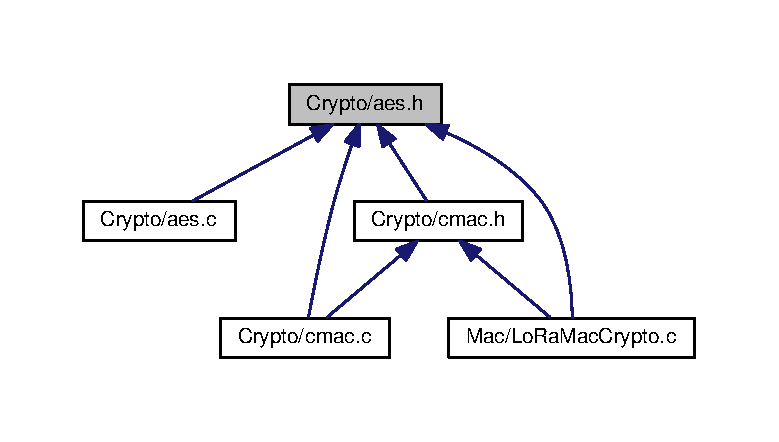
\includegraphics[width=350pt]{aes_8h__dep__incl}
\end{center}
\end{figure}
\subsection*{Data Structures}
\begin{DoxyCompactItemize}
\item 
struct \hyperlink{structaes__context}{aes\+\_\+context}
\end{DoxyCompactItemize}
\subsection*{Macros}
\begin{DoxyCompactItemize}
\item 
\#define \hyperlink{aes_8h_ae0288db3791855c74ec47f875ba3f131}{A\+E\+S\+\_\+\+E\+N\+C\+\_\+\+P\+R\+E\+K\+E\+Y\+ED}~/$\ast$ A\+ES encryption with a precomputed key schedule  $\ast$/
\item 
\#define \hyperlink{aes_8h_a397e692f15f1a68ad71f333267f94f89}{N\+\_\+\+R\+OW}~4
\item 
\#define \hyperlink{aes_8h_aa1ca982cd5aa9c974edfddab55fb994b}{N\+\_\+\+C\+OL}~4
\item 
\#define \hyperlink{aes_8h_a64c8b1a34c03210cc4c214735bb4f186}{N\+\_\+\+B\+L\+O\+CK}~(\hyperlink{aes_8h_a397e692f15f1a68ad71f333267f94f89}{N\+\_\+\+R\+OW} $\ast$ \hyperlink{aes_8h_aa1ca982cd5aa9c974edfddab55fb994b}{N\+\_\+\+C\+OL})
\item 
\#define \hyperlink{aes_8h_af8b900ecc3a113f2aed001ac9e1cb11e}{N\+\_\+\+M\+A\+X\+\_\+\+R\+O\+U\+N\+DS}~14
\end{DoxyCompactItemize}
\subsection*{Typedefs}
\begin{DoxyCompactItemize}
\item 
typedef uint8\+\_\+t \hyperlink{aes_8h_a939cc04a88913455efd7cc8fc15f80cf}{return\+\_\+type}
\item 
typedef uint8\+\_\+t \hyperlink{aes_8h_a9bedd830746c77c108ff50ec5c704256}{length\+\_\+type}
\end{DoxyCompactItemize}
\subsection*{Functions}
\begin{DoxyCompactItemize}
\item 
\hyperlink{aes_8h_a939cc04a88913455efd7cc8fc15f80cf}{return\+\_\+type} \hyperlink{aes_8h_a0ffc37ee1bbb50e7147bf6e7de5d73a1}{aes\+\_\+set\+\_\+key} (const uint8\+\_\+t key\mbox{[}$\,$\mbox{]}, \hyperlink{aes_8h_a9bedd830746c77c108ff50ec5c704256}{length\+\_\+type} keylen, \hyperlink{structaes__context}{aes\+\_\+context} ctx\mbox{[}1\mbox{]})
\item 
\hyperlink{aes_8h_a939cc04a88913455efd7cc8fc15f80cf}{return\+\_\+type} \hyperlink{aes_8h_ac88fd4e9cb53f78713a8fce1a6fcffc0}{aes\+\_\+encrypt} (const uint8\+\_\+t in\mbox{[}\hyperlink{aes_8h_a64c8b1a34c03210cc4c214735bb4f186}{N\+\_\+\+B\+L\+O\+CK}\mbox{]}, uint8\+\_\+t out\mbox{[}\hyperlink{aes_8h_a64c8b1a34c03210cc4c214735bb4f186}{N\+\_\+\+B\+L\+O\+CK}\mbox{]}, const \hyperlink{structaes__context}{aes\+\_\+context} ctx\mbox{[}1\mbox{]})
\item 
\hyperlink{aes_8h_a939cc04a88913455efd7cc8fc15f80cf}{return\+\_\+type} \hyperlink{aes_8h_aafdeb6720bdc985cefd83f837bbb55da}{aes\+\_\+cbc\+\_\+encrypt} (const uint8\+\_\+t $\ast$in, uint8\+\_\+t $\ast$out, int32\+\_\+t n\+\_\+block, uint8\+\_\+t iv\mbox{[}\hyperlink{aes_8h_a64c8b1a34c03210cc4c214735bb4f186}{N\+\_\+\+B\+L\+O\+CK}\mbox{]}, const \hyperlink{structaes__context}{aes\+\_\+context} ctx\mbox{[}1\mbox{]})
\end{DoxyCompactItemize}


\subsection{Macro Definition Documentation}
\mbox{\Hypertarget{aes_8h_ae0288db3791855c74ec47f875ba3f131}\label{aes_8h_ae0288db3791855c74ec47f875ba3f131}} 
\index{aes.\+h@{aes.\+h}!A\+E\+S\+\_\+\+E\+N\+C\+\_\+\+P\+R\+E\+K\+E\+Y\+ED@{A\+E\+S\+\_\+\+E\+N\+C\+\_\+\+P\+R\+E\+K\+E\+Y\+ED}}
\index{A\+E\+S\+\_\+\+E\+N\+C\+\_\+\+P\+R\+E\+K\+E\+Y\+ED@{A\+E\+S\+\_\+\+E\+N\+C\+\_\+\+P\+R\+E\+K\+E\+Y\+ED}!aes.\+h@{aes.\+h}}
\subsubsection{\texorpdfstring{A\+E\+S\+\_\+\+E\+N\+C\+\_\+\+P\+R\+E\+K\+E\+Y\+ED}{AES\_ENC\_PREKEYED}}
{\footnotesize\ttfamily \#define A\+E\+S\+\_\+\+E\+N\+C\+\_\+\+P\+R\+E\+K\+E\+Y\+ED~/$\ast$ A\+ES encryption with a precomputed key schedule  $\ast$/}

\mbox{\Hypertarget{aes_8h_a64c8b1a34c03210cc4c214735bb4f186}\label{aes_8h_a64c8b1a34c03210cc4c214735bb4f186}} 
\index{aes.\+h@{aes.\+h}!N\+\_\+\+B\+L\+O\+CK@{N\+\_\+\+B\+L\+O\+CK}}
\index{N\+\_\+\+B\+L\+O\+CK@{N\+\_\+\+B\+L\+O\+CK}!aes.\+h@{aes.\+h}}
\subsubsection{\texorpdfstring{N\+\_\+\+B\+L\+O\+CK}{N\_BLOCK}}
{\footnotesize\ttfamily \#define N\+\_\+\+B\+L\+O\+CK~(\hyperlink{aes_8h_a397e692f15f1a68ad71f333267f94f89}{N\+\_\+\+R\+OW} $\ast$ \hyperlink{aes_8h_aa1ca982cd5aa9c974edfddab55fb994b}{N\+\_\+\+C\+OL})}

\mbox{\Hypertarget{aes_8h_aa1ca982cd5aa9c974edfddab55fb994b}\label{aes_8h_aa1ca982cd5aa9c974edfddab55fb994b}} 
\index{aes.\+h@{aes.\+h}!N\+\_\+\+C\+OL@{N\+\_\+\+C\+OL}}
\index{N\+\_\+\+C\+OL@{N\+\_\+\+C\+OL}!aes.\+h@{aes.\+h}}
\subsubsection{\texorpdfstring{N\+\_\+\+C\+OL}{N\_COL}}
{\footnotesize\ttfamily \#define N\+\_\+\+C\+OL~4}

\mbox{\Hypertarget{aes_8h_af8b900ecc3a113f2aed001ac9e1cb11e}\label{aes_8h_af8b900ecc3a113f2aed001ac9e1cb11e}} 
\index{aes.\+h@{aes.\+h}!N\+\_\+\+M\+A\+X\+\_\+\+R\+O\+U\+N\+DS@{N\+\_\+\+M\+A\+X\+\_\+\+R\+O\+U\+N\+DS}}
\index{N\+\_\+\+M\+A\+X\+\_\+\+R\+O\+U\+N\+DS@{N\+\_\+\+M\+A\+X\+\_\+\+R\+O\+U\+N\+DS}!aes.\+h@{aes.\+h}}
\subsubsection{\texorpdfstring{N\+\_\+\+M\+A\+X\+\_\+\+R\+O\+U\+N\+DS}{N\_MAX\_ROUNDS}}
{\footnotesize\ttfamily \#define N\+\_\+\+M\+A\+X\+\_\+\+R\+O\+U\+N\+DS~14}

\mbox{\Hypertarget{aes_8h_a397e692f15f1a68ad71f333267f94f89}\label{aes_8h_a397e692f15f1a68ad71f333267f94f89}} 
\index{aes.\+h@{aes.\+h}!N\+\_\+\+R\+OW@{N\+\_\+\+R\+OW}}
\index{N\+\_\+\+R\+OW@{N\+\_\+\+R\+OW}!aes.\+h@{aes.\+h}}
\subsubsection{\texorpdfstring{N\+\_\+\+R\+OW}{N\_ROW}}
{\footnotesize\ttfamily \#define N\+\_\+\+R\+OW~4}



\subsection{Typedef Documentation}
\mbox{\Hypertarget{aes_8h_a9bedd830746c77c108ff50ec5c704256}\label{aes_8h_a9bedd830746c77c108ff50ec5c704256}} 
\index{aes.\+h@{aes.\+h}!length\+\_\+type@{length\+\_\+type}}
\index{length\+\_\+type@{length\+\_\+type}!aes.\+h@{aes.\+h}}
\subsubsection{\texorpdfstring{length\+\_\+type}{length\_type}}
{\footnotesize\ttfamily typedef uint8\+\_\+t \hyperlink{aes_8h_a9bedd830746c77c108ff50ec5c704256}{length\+\_\+type}}

\mbox{\Hypertarget{aes_8h_a939cc04a88913455efd7cc8fc15f80cf}\label{aes_8h_a939cc04a88913455efd7cc8fc15f80cf}} 
\index{aes.\+h@{aes.\+h}!return\+\_\+type@{return\+\_\+type}}
\index{return\+\_\+type@{return\+\_\+type}!aes.\+h@{aes.\+h}}
\subsubsection{\texorpdfstring{return\+\_\+type}{return\_type}}
{\footnotesize\ttfamily typedef uint8\+\_\+t \hyperlink{aes_8h_a939cc04a88913455efd7cc8fc15f80cf}{return\+\_\+type}}



\subsection{Function Documentation}
\mbox{\Hypertarget{aes_8h_aafdeb6720bdc985cefd83f837bbb55da}\label{aes_8h_aafdeb6720bdc985cefd83f837bbb55da}} 
\index{aes.\+h@{aes.\+h}!aes\+\_\+cbc\+\_\+encrypt@{aes\+\_\+cbc\+\_\+encrypt}}
\index{aes\+\_\+cbc\+\_\+encrypt@{aes\+\_\+cbc\+\_\+encrypt}!aes.\+h@{aes.\+h}}
\subsubsection{\texorpdfstring{aes\+\_\+cbc\+\_\+encrypt()}{aes\_cbc\_encrypt()}}
{\footnotesize\ttfamily \hyperlink{aes_8h_a939cc04a88913455efd7cc8fc15f80cf}{return\+\_\+type} aes\+\_\+cbc\+\_\+encrypt (\begin{DoxyParamCaption}\item[{const uint8\+\_\+t $\ast$}]{in,  }\item[{uint8\+\_\+t $\ast$}]{out,  }\item[{int32\+\_\+t}]{n\+\_\+block,  }\item[{uint8\+\_\+t}]{iv\mbox{[}\+N\+\_\+\+B\+L\+O\+C\+K\mbox{]},  }\item[{const \hyperlink{structaes__context}{aes\+\_\+context}}]{ctx\mbox{[}1\mbox{]} }\end{DoxyParamCaption})}

\mbox{\Hypertarget{aes_8h_ac88fd4e9cb53f78713a8fce1a6fcffc0}\label{aes_8h_ac88fd4e9cb53f78713a8fce1a6fcffc0}} 
\index{aes.\+h@{aes.\+h}!aes\+\_\+encrypt@{aes\+\_\+encrypt}}
\index{aes\+\_\+encrypt@{aes\+\_\+encrypt}!aes.\+h@{aes.\+h}}
\subsubsection{\texorpdfstring{aes\+\_\+encrypt()}{aes\_encrypt()}}
{\footnotesize\ttfamily \hyperlink{aes_8h_a939cc04a88913455efd7cc8fc15f80cf}{return\+\_\+type} aes\+\_\+encrypt (\begin{DoxyParamCaption}\item[{const uint8\+\_\+t}]{in\mbox{[}\+N\+\_\+\+B\+L\+O\+C\+K\mbox{]},  }\item[{uint8\+\_\+t}]{out\mbox{[}\+N\+\_\+\+B\+L\+O\+C\+K\mbox{]},  }\item[{const \hyperlink{structaes__context}{aes\+\_\+context}}]{ctx\mbox{[}1\mbox{]} }\end{DoxyParamCaption})}

\mbox{\Hypertarget{aes_8h_a0ffc37ee1bbb50e7147bf6e7de5d73a1}\label{aes_8h_a0ffc37ee1bbb50e7147bf6e7de5d73a1}} 
\index{aes.\+h@{aes.\+h}!aes\+\_\+set\+\_\+key@{aes\+\_\+set\+\_\+key}}
\index{aes\+\_\+set\+\_\+key@{aes\+\_\+set\+\_\+key}!aes.\+h@{aes.\+h}}
\subsubsection{\texorpdfstring{aes\+\_\+set\+\_\+key()}{aes\_set\_key()}}
{\footnotesize\ttfamily \hyperlink{aes_8h_a939cc04a88913455efd7cc8fc15f80cf}{return\+\_\+type} aes\+\_\+set\+\_\+key (\begin{DoxyParamCaption}\item[{const uint8\+\_\+t}]{key\mbox{[}$\,$\mbox{]},  }\item[{\hyperlink{aes_8h_a9bedd830746c77c108ff50ec5c704256}{length\+\_\+type}}]{keylen,  }\item[{\hyperlink{structaes__context}{aes\+\_\+context}}]{ctx\mbox{[}1\mbox{]} }\end{DoxyParamCaption})}


\hypertarget{cmac_8c}{}\section{Crypto/cmac.c File Reference}
\label{cmac_8c}\index{Crypto/cmac.\+c@{Crypto/cmac.\+c}}
{\ttfamily \#include $<$stdint.\+h$>$}\newline
{\ttfamily \#include \char`\"{}aes.\+h\char`\"{}}\newline
{\ttfamily \#include \char`\"{}cmac.\+h\char`\"{}}\newline
{\ttfamily \#include \char`\"{}utilities.\+h\char`\"{}}\newline
Include dependency graph for cmac.\+c\+:
\nopagebreak
\begin{figure}[H]
\begin{center}
\leavevmode
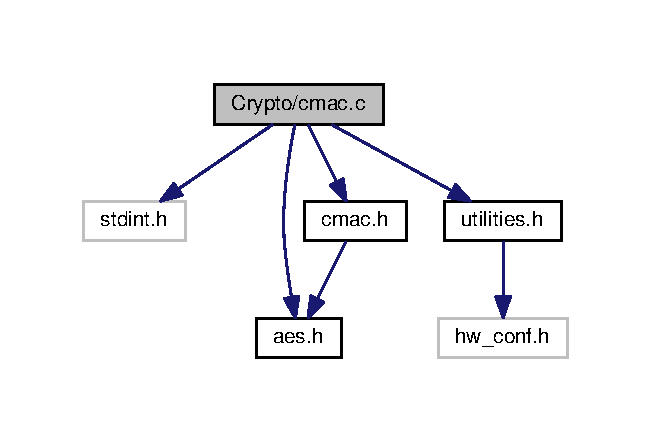
\includegraphics[width=313pt]{cmac_8c__incl}
\end{center}
\end{figure}
\subsection*{Macros}
\begin{DoxyCompactItemize}
\item 
\#define \hyperlink{cmac_8c_af9ca930f6a22a67738997972244303e3}{L\+S\+H\+I\+FT}(v,  r)
\item 
\#define \hyperlink{cmac_8c_a24a57a540896e74aca18138ed0104e6e}{X\+OR}(v,  r)
\end{DoxyCompactItemize}
\subsection*{Functions}
\begin{DoxyCompactItemize}
\item 
void \hyperlink{cmac_8c_a0344ba56e27c8029332069892af08737}{A\+E\+S\+\_\+\+C\+M\+A\+C\+\_\+\+Init} (\hyperlink{cmac_8h_af41c475ab2b2b5fdf68252112c391434}{A\+E\+S\+\_\+\+C\+M\+A\+C\+\_\+\+C\+TX} $\ast$ctx)
\item 
void \hyperlink{cmac_8c_a0cbe43f8858ba5fbf5bbd5f03e362170}{A\+E\+S\+\_\+\+C\+M\+A\+C\+\_\+\+Set\+Key} (\hyperlink{cmac_8h_af41c475ab2b2b5fdf68252112c391434}{A\+E\+S\+\_\+\+C\+M\+A\+C\+\_\+\+C\+TX} $\ast$ctx, const uint8\+\_\+t key\mbox{[}\hyperlink{cmac_8h_a8391095f8961b29bdf0818f764d0d66a}{A\+E\+S\+\_\+\+C\+M\+A\+C\+\_\+\+K\+E\+Y\+\_\+\+L\+E\+N\+G\+TH}\mbox{]})
\item 
void \hyperlink{cmac_8c_ad1be03bf3df1635dd5cbf8943f4d04f6}{A\+E\+S\+\_\+\+C\+M\+A\+C\+\_\+\+Update} (\hyperlink{cmac_8h_af41c475ab2b2b5fdf68252112c391434}{A\+E\+S\+\_\+\+C\+M\+A\+C\+\_\+\+C\+TX} $\ast$ctx, const uint8\+\_\+t $\ast$data, uint32\+\_\+t len)
\item 
void \hyperlink{cmac_8c_a8ea4da33d50984199d8a91bc0ab86b15}{A\+E\+S\+\_\+\+C\+M\+A\+C\+\_\+\+Final} (uint8\+\_\+t digest\mbox{[}\hyperlink{cmac_8h_a9d43ce8be9e275dc33b7992c5cf6623f}{A\+E\+S\+\_\+\+C\+M\+A\+C\+\_\+\+D\+I\+G\+E\+S\+T\+\_\+\+L\+E\+N\+G\+TH}\mbox{]}, \hyperlink{cmac_8h_af41c475ab2b2b5fdf68252112c391434}{A\+E\+S\+\_\+\+C\+M\+A\+C\+\_\+\+C\+TX} $\ast$ctx)
\end{DoxyCompactItemize}


\subsection{Macro Definition Documentation}
\mbox{\Hypertarget{cmac_8c_af9ca930f6a22a67738997972244303e3}\label{cmac_8c_af9ca930f6a22a67738997972244303e3}} 
\index{cmac.\+c@{cmac.\+c}!L\+S\+H\+I\+FT@{L\+S\+H\+I\+FT}}
\index{L\+S\+H\+I\+FT@{L\+S\+H\+I\+FT}!cmac.\+c@{cmac.\+c}}
\subsubsection{\texorpdfstring{L\+S\+H\+I\+FT}{LSHIFT}}
{\footnotesize\ttfamily \#define L\+S\+H\+I\+FT(\begin{DoxyParamCaption}\item[{}]{v,  }\item[{}]{r }\end{DoxyParamCaption})}

{\bfseries Value\+:}
\begin{DoxyCode}
\textcolor{keywordflow}{do} \{                                       \(\backslash\)
  int32\_t i;                                                  \(\backslash\)
           for (i = 0; i < 15; i++)                                \(\backslash\)
                    (r)[i] = (v)[i] << 1 | (v)[i + 1] >> 7;         \(\backslash\)
            (r)[15] = (v)[15] << 1;                                 \(\backslash\)
    \} \textcolor{keywordflow}{while} (0)
\end{DoxyCode}
\mbox{\Hypertarget{cmac_8c_a24a57a540896e74aca18138ed0104e6e}\label{cmac_8c_a24a57a540896e74aca18138ed0104e6e}} 
\index{cmac.\+c@{cmac.\+c}!X\+OR@{X\+OR}}
\index{X\+OR@{X\+OR}!cmac.\+c@{cmac.\+c}}
\subsubsection{\texorpdfstring{X\+OR}{XOR}}
{\footnotesize\ttfamily \#define X\+OR(\begin{DoxyParamCaption}\item[{}]{v,  }\item[{}]{r }\end{DoxyParamCaption})}

{\bfseries Value\+:}
\begin{DoxyCode}
\textcolor{keywordflow}{do} \{                                          \(\backslash\)
            int32\_t i;                                                  \(\backslash\)
            for (i = 0; i < 16; i++)     \(\backslash\)
        \{   \(\backslash\)
                    (r)[i] = (r)[i] ^ (v)[i]; \(\backslash\)
        \}                          \(\backslash\)
    \} \textcolor{keywordflow}{while} (0) \(\backslash\)
\end{DoxyCode}


\subsection{Function Documentation}
\mbox{\Hypertarget{cmac_8c_a8ea4da33d50984199d8a91bc0ab86b15}\label{cmac_8c_a8ea4da33d50984199d8a91bc0ab86b15}} 
\index{cmac.\+c@{cmac.\+c}!A\+E\+S\+\_\+\+C\+M\+A\+C\+\_\+\+Final@{A\+E\+S\+\_\+\+C\+M\+A\+C\+\_\+\+Final}}
\index{A\+E\+S\+\_\+\+C\+M\+A\+C\+\_\+\+Final@{A\+E\+S\+\_\+\+C\+M\+A\+C\+\_\+\+Final}!cmac.\+c@{cmac.\+c}}
\subsubsection{\texorpdfstring{A\+E\+S\+\_\+\+C\+M\+A\+C\+\_\+\+Final()}{AES\_CMAC\_Final()}}
{\footnotesize\ttfamily void A\+E\+S\+\_\+\+C\+M\+A\+C\+\_\+\+Final (\begin{DoxyParamCaption}\item[{uint8\+\_\+t}]{digest\mbox{[}\+A\+E\+S\+\_\+\+C\+M\+A\+C\+\_\+\+D\+I\+G\+E\+S\+T\+\_\+\+L\+E\+N\+G\+T\+H\mbox{]},  }\item[{\hyperlink{cmac_8h_af41c475ab2b2b5fdf68252112c391434}{A\+E\+S\+\_\+\+C\+M\+A\+C\+\_\+\+C\+TX} $\ast$}]{ctx }\end{DoxyParamCaption})}

\mbox{\Hypertarget{cmac_8c_a0344ba56e27c8029332069892af08737}\label{cmac_8c_a0344ba56e27c8029332069892af08737}} 
\index{cmac.\+c@{cmac.\+c}!A\+E\+S\+\_\+\+C\+M\+A\+C\+\_\+\+Init@{A\+E\+S\+\_\+\+C\+M\+A\+C\+\_\+\+Init}}
\index{A\+E\+S\+\_\+\+C\+M\+A\+C\+\_\+\+Init@{A\+E\+S\+\_\+\+C\+M\+A\+C\+\_\+\+Init}!cmac.\+c@{cmac.\+c}}
\subsubsection{\texorpdfstring{A\+E\+S\+\_\+\+C\+M\+A\+C\+\_\+\+Init()}{AES\_CMAC\_Init()}}
{\footnotesize\ttfamily void A\+E\+S\+\_\+\+C\+M\+A\+C\+\_\+\+Init (\begin{DoxyParamCaption}\item[{\hyperlink{cmac_8h_af41c475ab2b2b5fdf68252112c391434}{A\+E\+S\+\_\+\+C\+M\+A\+C\+\_\+\+C\+TX} $\ast$}]{ctx }\end{DoxyParamCaption})}

\mbox{\Hypertarget{cmac_8c_a0cbe43f8858ba5fbf5bbd5f03e362170}\label{cmac_8c_a0cbe43f8858ba5fbf5bbd5f03e362170}} 
\index{cmac.\+c@{cmac.\+c}!A\+E\+S\+\_\+\+C\+M\+A\+C\+\_\+\+Set\+Key@{A\+E\+S\+\_\+\+C\+M\+A\+C\+\_\+\+Set\+Key}}
\index{A\+E\+S\+\_\+\+C\+M\+A\+C\+\_\+\+Set\+Key@{A\+E\+S\+\_\+\+C\+M\+A\+C\+\_\+\+Set\+Key}!cmac.\+c@{cmac.\+c}}
\subsubsection{\texorpdfstring{A\+E\+S\+\_\+\+C\+M\+A\+C\+\_\+\+Set\+Key()}{AES\_CMAC\_SetKey()}}
{\footnotesize\ttfamily void A\+E\+S\+\_\+\+C\+M\+A\+C\+\_\+\+Set\+Key (\begin{DoxyParamCaption}\item[{\hyperlink{cmac_8h_af41c475ab2b2b5fdf68252112c391434}{A\+E\+S\+\_\+\+C\+M\+A\+C\+\_\+\+C\+TX} $\ast$}]{ctx,  }\item[{const uint8\+\_\+t}]{key\mbox{[}\+A\+E\+S\+\_\+\+C\+M\+A\+C\+\_\+\+K\+E\+Y\+\_\+\+L\+E\+N\+G\+T\+H\mbox{]} }\end{DoxyParamCaption})}

\mbox{\Hypertarget{cmac_8c_ad1be03bf3df1635dd5cbf8943f4d04f6}\label{cmac_8c_ad1be03bf3df1635dd5cbf8943f4d04f6}} 
\index{cmac.\+c@{cmac.\+c}!A\+E\+S\+\_\+\+C\+M\+A\+C\+\_\+\+Update@{A\+E\+S\+\_\+\+C\+M\+A\+C\+\_\+\+Update}}
\index{A\+E\+S\+\_\+\+C\+M\+A\+C\+\_\+\+Update@{A\+E\+S\+\_\+\+C\+M\+A\+C\+\_\+\+Update}!cmac.\+c@{cmac.\+c}}
\subsubsection{\texorpdfstring{A\+E\+S\+\_\+\+C\+M\+A\+C\+\_\+\+Update()}{AES\_CMAC\_Update()}}
{\footnotesize\ttfamily void A\+E\+S\+\_\+\+C\+M\+A\+C\+\_\+\+Update (\begin{DoxyParamCaption}\item[{\hyperlink{cmac_8h_af41c475ab2b2b5fdf68252112c391434}{A\+E\+S\+\_\+\+C\+M\+A\+C\+\_\+\+C\+TX} $\ast$}]{ctx,  }\item[{const uint8\+\_\+t $\ast$}]{data,  }\item[{uint32\+\_\+t}]{len }\end{DoxyParamCaption})}


\hypertarget{cmac_8h}{}\section{Crypto/cmac.h File Reference}
\label{cmac_8h}\index{Crypto/cmac.\+h@{Crypto/cmac.\+h}}
{\ttfamily \#include \char`\"{}aes.\+h\char`\"{}}\newline
Include dependency graph for cmac.\+h\+:
\nopagebreak
\begin{figure}[H]
\begin{center}
\leavevmode
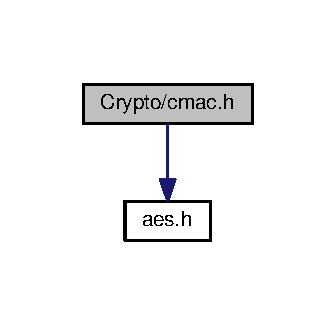
\includegraphics[width=161pt]{cmac_8h__incl}
\end{center}
\end{figure}
This graph shows which files directly or indirectly include this file\+:
\nopagebreak
\begin{figure}[H]
\begin{center}
\leavevmode
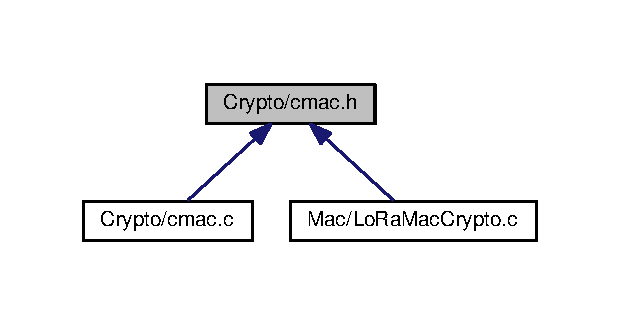
\includegraphics[width=298pt]{cmac_8h__dep__incl}
\end{center}
\end{figure}
\subsection*{Data Structures}
\begin{DoxyCompactItemize}
\item 
struct \hyperlink{struct__AES__CMAC__CTX}{\+\_\+\+A\+E\+S\+\_\+\+C\+M\+A\+C\+\_\+\+C\+TX}
\end{DoxyCompactItemize}
\subsection*{Macros}
\begin{DoxyCompactItemize}
\item 
\#define \hyperlink{cmac_8h_a8391095f8961b29bdf0818f764d0d66a}{A\+E\+S\+\_\+\+C\+M\+A\+C\+\_\+\+K\+E\+Y\+\_\+\+L\+E\+N\+G\+TH}~16
\item 
\#define \hyperlink{cmac_8h_a9d43ce8be9e275dc33b7992c5cf6623f}{A\+E\+S\+\_\+\+C\+M\+A\+C\+\_\+\+D\+I\+G\+E\+S\+T\+\_\+\+L\+E\+N\+G\+TH}~16
\end{DoxyCompactItemize}
\subsection*{Typedefs}
\begin{DoxyCompactItemize}
\item 
typedef struct \hyperlink{struct__AES__CMAC__CTX}{\+\_\+\+A\+E\+S\+\_\+\+C\+M\+A\+C\+\_\+\+C\+TX} \hyperlink{cmac_8h_af41c475ab2b2b5fdf68252112c391434}{A\+E\+S\+\_\+\+C\+M\+A\+C\+\_\+\+C\+TX}
\end{DoxyCompactItemize}
\subsection*{Functions}
\begin{DoxyCompactItemize}
\item 
void \hyperlink{cmac_8h_a0344ba56e27c8029332069892af08737}{A\+E\+S\+\_\+\+C\+M\+A\+C\+\_\+\+Init} (\hyperlink{cmac_8h_af41c475ab2b2b5fdf68252112c391434}{A\+E\+S\+\_\+\+C\+M\+A\+C\+\_\+\+C\+TX} $\ast$ctx)
\item 
void \hyperlink{cmac_8h_a0cbe43f8858ba5fbf5bbd5f03e362170}{A\+E\+S\+\_\+\+C\+M\+A\+C\+\_\+\+Set\+Key} (\hyperlink{cmac_8h_af41c475ab2b2b5fdf68252112c391434}{A\+E\+S\+\_\+\+C\+M\+A\+C\+\_\+\+C\+TX} $\ast$ctx, const uint8\+\_\+t key\mbox{[}\hyperlink{cmac_8h_a8391095f8961b29bdf0818f764d0d66a}{A\+E\+S\+\_\+\+C\+M\+A\+C\+\_\+\+K\+E\+Y\+\_\+\+L\+E\+N\+G\+TH}\mbox{]})
\item 
void \hyperlink{cmac_8h_ad1be03bf3df1635dd5cbf8943f4d04f6}{A\+E\+S\+\_\+\+C\+M\+A\+C\+\_\+\+Update} (\hyperlink{cmac_8h_af41c475ab2b2b5fdf68252112c391434}{A\+E\+S\+\_\+\+C\+M\+A\+C\+\_\+\+C\+TX} $\ast$ctx, const uint8\+\_\+t $\ast$data, uint32\+\_\+t len)
\item 
void \hyperlink{cmac_8h_a8ea4da33d50984199d8a91bc0ab86b15}{A\+E\+S\+\_\+\+C\+M\+A\+C\+\_\+\+Final} (uint8\+\_\+t digest\mbox{[}\hyperlink{cmac_8h_a9d43ce8be9e275dc33b7992c5cf6623f}{A\+E\+S\+\_\+\+C\+M\+A\+C\+\_\+\+D\+I\+G\+E\+S\+T\+\_\+\+L\+E\+N\+G\+TH}\mbox{]}, \hyperlink{cmac_8h_af41c475ab2b2b5fdf68252112c391434}{A\+E\+S\+\_\+\+C\+M\+A\+C\+\_\+\+C\+TX} $\ast$ctx)
\end{DoxyCompactItemize}


\subsection{Macro Definition Documentation}
\mbox{\Hypertarget{cmac_8h_a9d43ce8be9e275dc33b7992c5cf6623f}\label{cmac_8h_a9d43ce8be9e275dc33b7992c5cf6623f}} 
\index{cmac.\+h@{cmac.\+h}!A\+E\+S\+\_\+\+C\+M\+A\+C\+\_\+\+D\+I\+G\+E\+S\+T\+\_\+\+L\+E\+N\+G\+TH@{A\+E\+S\+\_\+\+C\+M\+A\+C\+\_\+\+D\+I\+G\+E\+S\+T\+\_\+\+L\+E\+N\+G\+TH}}
\index{A\+E\+S\+\_\+\+C\+M\+A\+C\+\_\+\+D\+I\+G\+E\+S\+T\+\_\+\+L\+E\+N\+G\+TH@{A\+E\+S\+\_\+\+C\+M\+A\+C\+\_\+\+D\+I\+G\+E\+S\+T\+\_\+\+L\+E\+N\+G\+TH}!cmac.\+h@{cmac.\+h}}
\subsubsection{\texorpdfstring{A\+E\+S\+\_\+\+C\+M\+A\+C\+\_\+\+D\+I\+G\+E\+S\+T\+\_\+\+L\+E\+N\+G\+TH}{AES\_CMAC\_DIGEST\_LENGTH}}
{\footnotesize\ttfamily \#define A\+E\+S\+\_\+\+C\+M\+A\+C\+\_\+\+D\+I\+G\+E\+S\+T\+\_\+\+L\+E\+N\+G\+TH~16}

\mbox{\Hypertarget{cmac_8h_a8391095f8961b29bdf0818f764d0d66a}\label{cmac_8h_a8391095f8961b29bdf0818f764d0d66a}} 
\index{cmac.\+h@{cmac.\+h}!A\+E\+S\+\_\+\+C\+M\+A\+C\+\_\+\+K\+E\+Y\+\_\+\+L\+E\+N\+G\+TH@{A\+E\+S\+\_\+\+C\+M\+A\+C\+\_\+\+K\+E\+Y\+\_\+\+L\+E\+N\+G\+TH}}
\index{A\+E\+S\+\_\+\+C\+M\+A\+C\+\_\+\+K\+E\+Y\+\_\+\+L\+E\+N\+G\+TH@{A\+E\+S\+\_\+\+C\+M\+A\+C\+\_\+\+K\+E\+Y\+\_\+\+L\+E\+N\+G\+TH}!cmac.\+h@{cmac.\+h}}
\subsubsection{\texorpdfstring{A\+E\+S\+\_\+\+C\+M\+A\+C\+\_\+\+K\+E\+Y\+\_\+\+L\+E\+N\+G\+TH}{AES\_CMAC\_KEY\_LENGTH}}
{\footnotesize\ttfamily \#define A\+E\+S\+\_\+\+C\+M\+A\+C\+\_\+\+K\+E\+Y\+\_\+\+L\+E\+N\+G\+TH~16}



\subsection{Typedef Documentation}
\mbox{\Hypertarget{cmac_8h_af41c475ab2b2b5fdf68252112c391434}\label{cmac_8h_af41c475ab2b2b5fdf68252112c391434}} 
\index{cmac.\+h@{cmac.\+h}!A\+E\+S\+\_\+\+C\+M\+A\+C\+\_\+\+C\+TX@{A\+E\+S\+\_\+\+C\+M\+A\+C\+\_\+\+C\+TX}}
\index{A\+E\+S\+\_\+\+C\+M\+A\+C\+\_\+\+C\+TX@{A\+E\+S\+\_\+\+C\+M\+A\+C\+\_\+\+C\+TX}!cmac.\+h@{cmac.\+h}}
\subsubsection{\texorpdfstring{A\+E\+S\+\_\+\+C\+M\+A\+C\+\_\+\+C\+TX}{AES\_CMAC\_CTX}}
{\footnotesize\ttfamily typedef struct \hyperlink{struct__AES__CMAC__CTX}{\+\_\+\+A\+E\+S\+\_\+\+C\+M\+A\+C\+\_\+\+C\+TX}  \hyperlink{cmac_8h_af41c475ab2b2b5fdf68252112c391434}{A\+E\+S\+\_\+\+C\+M\+A\+C\+\_\+\+C\+TX}}



\subsection{Function Documentation}
\mbox{\Hypertarget{cmac_8h_a8ea4da33d50984199d8a91bc0ab86b15}\label{cmac_8h_a8ea4da33d50984199d8a91bc0ab86b15}} 
\index{cmac.\+h@{cmac.\+h}!A\+E\+S\+\_\+\+C\+M\+A\+C\+\_\+\+Final@{A\+E\+S\+\_\+\+C\+M\+A\+C\+\_\+\+Final}}
\index{A\+E\+S\+\_\+\+C\+M\+A\+C\+\_\+\+Final@{A\+E\+S\+\_\+\+C\+M\+A\+C\+\_\+\+Final}!cmac.\+h@{cmac.\+h}}
\subsubsection{\texorpdfstring{A\+E\+S\+\_\+\+C\+M\+A\+C\+\_\+\+Final()}{AES\_CMAC\_Final()}}
{\footnotesize\ttfamily void A\+E\+S\+\_\+\+C\+M\+A\+C\+\_\+\+Final (\begin{DoxyParamCaption}\item[{uint8\+\_\+t}]{digest\mbox{[}\+A\+E\+S\+\_\+\+C\+M\+A\+C\+\_\+\+D\+I\+G\+E\+S\+T\+\_\+\+L\+E\+N\+G\+T\+H\mbox{]},  }\item[{\hyperlink{cmac_8h_af41c475ab2b2b5fdf68252112c391434}{A\+E\+S\+\_\+\+C\+M\+A\+C\+\_\+\+C\+TX} $\ast$}]{ctx }\end{DoxyParamCaption})}

\mbox{\Hypertarget{cmac_8h_a0344ba56e27c8029332069892af08737}\label{cmac_8h_a0344ba56e27c8029332069892af08737}} 
\index{cmac.\+h@{cmac.\+h}!A\+E\+S\+\_\+\+C\+M\+A\+C\+\_\+\+Init@{A\+E\+S\+\_\+\+C\+M\+A\+C\+\_\+\+Init}}
\index{A\+E\+S\+\_\+\+C\+M\+A\+C\+\_\+\+Init@{A\+E\+S\+\_\+\+C\+M\+A\+C\+\_\+\+Init}!cmac.\+h@{cmac.\+h}}
\subsubsection{\texorpdfstring{A\+E\+S\+\_\+\+C\+M\+A\+C\+\_\+\+Init()}{AES\_CMAC\_Init()}}
{\footnotesize\ttfamily void A\+E\+S\+\_\+\+C\+M\+A\+C\+\_\+\+Init (\begin{DoxyParamCaption}\item[{\hyperlink{cmac_8h_af41c475ab2b2b5fdf68252112c391434}{A\+E\+S\+\_\+\+C\+M\+A\+C\+\_\+\+C\+TX} $\ast$}]{ctx }\end{DoxyParamCaption})}

\mbox{\Hypertarget{cmac_8h_a0cbe43f8858ba5fbf5bbd5f03e362170}\label{cmac_8h_a0cbe43f8858ba5fbf5bbd5f03e362170}} 
\index{cmac.\+h@{cmac.\+h}!A\+E\+S\+\_\+\+C\+M\+A\+C\+\_\+\+Set\+Key@{A\+E\+S\+\_\+\+C\+M\+A\+C\+\_\+\+Set\+Key}}
\index{A\+E\+S\+\_\+\+C\+M\+A\+C\+\_\+\+Set\+Key@{A\+E\+S\+\_\+\+C\+M\+A\+C\+\_\+\+Set\+Key}!cmac.\+h@{cmac.\+h}}
\subsubsection{\texorpdfstring{A\+E\+S\+\_\+\+C\+M\+A\+C\+\_\+\+Set\+Key()}{AES\_CMAC\_SetKey()}}
{\footnotesize\ttfamily void A\+E\+S\+\_\+\+C\+M\+A\+C\+\_\+\+Set\+Key (\begin{DoxyParamCaption}\item[{\hyperlink{cmac_8h_af41c475ab2b2b5fdf68252112c391434}{A\+E\+S\+\_\+\+C\+M\+A\+C\+\_\+\+C\+TX} $\ast$}]{ctx,  }\item[{const uint8\+\_\+t}]{key\mbox{[}\+A\+E\+S\+\_\+\+C\+M\+A\+C\+\_\+\+K\+E\+Y\+\_\+\+L\+E\+N\+G\+T\+H\mbox{]} }\end{DoxyParamCaption})}

\mbox{\Hypertarget{cmac_8h_ad1be03bf3df1635dd5cbf8943f4d04f6}\label{cmac_8h_ad1be03bf3df1635dd5cbf8943f4d04f6}} 
\index{cmac.\+h@{cmac.\+h}!A\+E\+S\+\_\+\+C\+M\+A\+C\+\_\+\+Update@{A\+E\+S\+\_\+\+C\+M\+A\+C\+\_\+\+Update}}
\index{A\+E\+S\+\_\+\+C\+M\+A\+C\+\_\+\+Update@{A\+E\+S\+\_\+\+C\+M\+A\+C\+\_\+\+Update}!cmac.\+h@{cmac.\+h}}
\subsubsection{\texorpdfstring{A\+E\+S\+\_\+\+C\+M\+A\+C\+\_\+\+Update()}{AES\_CMAC\_Update()}}
{\footnotesize\ttfamily void A\+E\+S\+\_\+\+C\+M\+A\+C\+\_\+\+Update (\begin{DoxyParamCaption}\item[{\hyperlink{cmac_8h_af41c475ab2b2b5fdf68252112c391434}{A\+E\+S\+\_\+\+C\+M\+A\+C\+\_\+\+C\+TX} $\ast$}]{ctx,  }\item[{const uint8\+\_\+t $\ast$}]{data,  }\item[{uint32\+\_\+t}]{len }\end{DoxyParamCaption})}


\hypertarget{LoRaMac_8c}{}\section{Mac/\+Lo\+Ra\+Mac.c File Reference}
\label{LoRaMac_8c}\index{Mac/\+Lo\+Ra\+Mac.\+c@{Mac/\+Lo\+Ra\+Mac.\+c}}
{\ttfamily \#include $<$stdbool.\+h$>$}\newline
{\ttfamily \#include $<$string.\+h$>$}\newline
{\ttfamily \#include $<$stdint.\+h$>$}\newline
{\ttfamily \#include \char`\"{}radio.\+h\char`\"{}}\newline
{\ttfamily \#include \char`\"{}time\+Server.\+h\char`\"{}}\newline
{\ttfamily \#include \char`\"{}Lo\+Ra\+Mac.\+h\char`\"{}}\newline
{\ttfamily \#include \char`\"{}region/\+Region.\+h\char`\"{}}\newline
{\ttfamily \#include \char`\"{}Lo\+Ra\+Mac\+Crypto.\+h\char`\"{}}\newline
{\ttfamily \#include \char`\"{}debug.\+h\char`\"{}}\newline
{\ttfamily \#include \char`\"{}Lo\+Ra\+Mac\+Test.\+h\char`\"{}}\newline
Include dependency graph for Lo\+Ra\+Mac.\+c\+:
\nopagebreak
\begin{figure}[H]
\begin{center}
\leavevmode
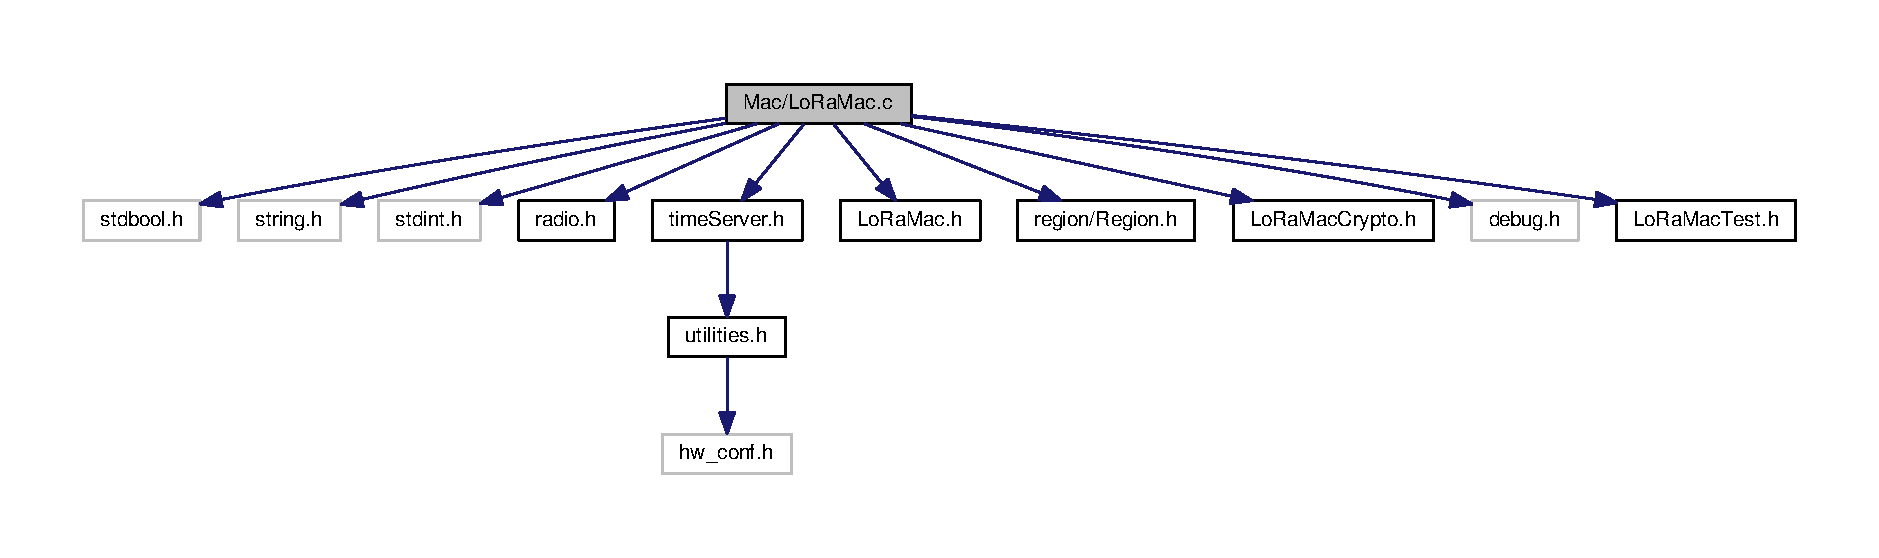
\includegraphics[width=350pt]{LoRaMac_8c__incl}
\end{center}
\end{figure}
\subsection*{Macros}
\begin{DoxyCompactItemize}
\item 
\#define \hyperlink{LoRaMac_8c_a54769799fcc79d1d3fd1f19f123cc57b}{L\+O\+R\+A\+M\+A\+C\+\_\+\+P\+H\+Y\+\_\+\+M\+A\+X\+P\+A\+Y\+L\+O\+AD}~255
\item 
\#define \hyperlink{LoRaMac_8c_a4ac517018d0390785daf8d90bf99df8f}{L\+O\+R\+A\+\_\+\+M\+A\+C\+\_\+\+C\+O\+M\+M\+A\+N\+D\+\_\+\+M\+A\+X\+\_\+\+L\+E\+N\+G\+TH}~128
\item 
\#define \hyperlink{LoRaMac_8c_ae2ccbfeefb0390b3cafca4da463d245c}{L\+O\+R\+A\+\_\+\+M\+A\+C\+\_\+\+C\+O\+M\+M\+A\+N\+D\+\_\+\+M\+A\+X\+\_\+\+F\+O\+P\+T\+S\+\_\+\+L\+E\+N\+G\+TH}~15
\item 
\#define \hyperlink{LoRaMac_8c_a1d58cbd560840cdab3e4427797e88c3a}{B\+A\+C\+K\+O\+F\+F\+\_\+\+D\+C\+\_\+1\+\_\+\+H\+O\+UR}~100
\item 
\#define \hyperlink{LoRaMac_8c_a70461da0dc970b3de51718ab397a81db}{B\+A\+C\+K\+O\+F\+F\+\_\+\+D\+C\+\_\+10\+\_\+\+H\+O\+U\+RS}~1000
\item 
\#define \hyperlink{LoRaMac_8c_ada6c3c87744e22f1c053caba7c40d26c}{B\+A\+C\+K\+O\+F\+F\+\_\+\+D\+C\+\_\+24\+\_\+\+H\+O\+U\+RS}~10000
\end{DoxyCompactItemize}
\subsection*{Enumerations}
\begin{DoxyCompactItemize}
\item 
enum \hyperlink{LoRaMac_8c_ada0bdc03d52b5bf536f021dcea7c4490}{e\+Lo\+Ra\+Mac\+State} \{ \newline
\hyperlink{LoRaMac_8c_ada0bdc03d52b5bf536f021dcea7c4490a3af5105c630ff1cfa443789cfa2f318c}{L\+O\+R\+A\+M\+A\+C\+\_\+\+I\+D\+LE} = 0x00000000, 
\hyperlink{LoRaMac_8c_ada0bdc03d52b5bf536f021dcea7c4490a5b4a3679d3966d49741f0aec6b15d731}{L\+O\+R\+A\+M\+A\+C\+\_\+\+T\+X\+\_\+\+R\+U\+N\+N\+I\+NG} = 0x00000001, 
\hyperlink{LoRaMac_8c_ada0bdc03d52b5bf536f021dcea7c4490a51fd14464af45ead2dda2a90760e4bc4}{L\+O\+R\+A\+M\+A\+C\+\_\+\+RX} = 0x00000002, 
\hyperlink{LoRaMac_8c_ada0bdc03d52b5bf536f021dcea7c4490a99ee636d0a66bf7f2a5644b5947dce2f}{L\+O\+R\+A\+M\+A\+C\+\_\+\+A\+C\+K\+\_\+\+R\+EQ} = 0x00000004, 
\newline
\hyperlink{LoRaMac_8c_ada0bdc03d52b5bf536f021dcea7c4490ac3b5306588342cdeffe6367350d875c3}{L\+O\+R\+A\+M\+A\+C\+\_\+\+A\+C\+K\+\_\+\+R\+E\+T\+RY} = 0x00000008, 
\hyperlink{LoRaMac_8c_ada0bdc03d52b5bf536f021dcea7c4490aea3d825c5789497c1dd7515b26a8e8f8}{L\+O\+R\+A\+M\+A\+C\+\_\+\+T\+X\+\_\+\+D\+E\+L\+A\+Y\+ED} = 0x00000010, 
\hyperlink{LoRaMac_8c_ada0bdc03d52b5bf536f021dcea7c4490ad649702e2b40e41dbed3ff5b2e3c21c5}{L\+O\+R\+A\+M\+A\+C\+\_\+\+T\+X\+\_\+\+C\+O\+N\+F\+IG} = 0x00000020, 
\hyperlink{LoRaMac_8c_ada0bdc03d52b5bf536f021dcea7c4490a7c7d70244f468d92565a9e078d0790bf}{L\+O\+R\+A\+M\+A\+C\+\_\+\+R\+X\+\_\+\+A\+B\+O\+RT} = 0x00000040
 \}
\end{DoxyCompactItemize}
\subsection*{Functions}
\begin{DoxyCompactItemize}
\item 
\hyperlink{group__LORAMAC_ga30bd25657e10480f8605ee951b0ecfbd}{Lo\+Ra\+Mac\+Status\+\_\+t} \hyperlink{LoRaMac_8c_a1d5d30b5cbe0349bab89375480c377bf}{Send} (\hyperlink{group__LORAMAC_gaff5f7004a7a48d53d858e26834b53efa}{Lo\+Ra\+Mac\+Header\+\_\+t} $\ast$mac\+Hdr, uint8\+\_\+t f\+Port, void $\ast$f\+Buffer, uint16\+\_\+t f\+Buffer\+Size)
\begin{DoxyCompactList}\small\item\em Lo\+Ra\+M\+AC layer generic send frame. \end{DoxyCompactList}\item 
\hyperlink{group__LORAMAC_ga30bd25657e10480f8605ee951b0ecfbd}{Lo\+Ra\+Mac\+Status\+\_\+t} \hyperlink{LoRaMac_8c_a1c2e41a970de949b0b59a8177cb8ef29}{Prepare\+Frame} (\hyperlink{group__LORAMAC_gaff5f7004a7a48d53d858e26834b53efa}{Lo\+Ra\+Mac\+Header\+\_\+t} $\ast$mac\+Hdr, \hyperlink{group__LORAMAC_ga12b0f3e7e6edd26cfdb9d10a1d873ab7}{Lo\+Ra\+Mac\+Frame\+Ctrl\+\_\+t} $\ast$f\+Ctrl, uint8\+\_\+t f\+Port, void $\ast$f\+Buffer, uint16\+\_\+t f\+Buffer\+Size)
\begin{DoxyCompactList}\small\item\em Lo\+Ra\+M\+AC layer frame buffer initialization. \end{DoxyCompactList}\item 
\hyperlink{group__LORAMAC_ga30bd25657e10480f8605ee951b0ecfbd}{Lo\+Ra\+Mac\+Status\+\_\+t} \hyperlink{LoRaMac_8c_a2a974677f0401e2575148082667331de}{Send\+Frame\+On\+Channel} (uint8\+\_\+t channel)
\begin{DoxyCompactList}\small\item\em Lo\+Ra\+M\+AC layer prepared frame buffer transmission with channel specification. \end{DoxyCompactList}\item 
\hyperlink{group__LORAMAC_ga30bd25657e10480f8605ee951b0ecfbd}{Lo\+Ra\+Mac\+Status\+\_\+t} \hyperlink{LoRaMac_8c_a6a476e328faedf4544aa63adf40f931e}{Set\+Tx\+Continuous\+Wave} (uint16\+\_\+t timeout)
\begin{DoxyCompactList}\small\item\em Sets the radio in continuous transmission mode. \end{DoxyCompactList}\item 
\hyperlink{group__LORAMAC_ga30bd25657e10480f8605ee951b0ecfbd}{Lo\+Ra\+Mac\+Status\+\_\+t} \hyperlink{LoRaMac_8c_a1974034d3a6ef2a0c38f4f853cfb62fb}{Set\+Tx\+Continuous\+Wave1} (uint16\+\_\+t timeout, uint32\+\_\+t frequency, uint8\+\_\+t power)
\begin{DoxyCompactList}\small\item\em Sets the radio in continuous transmission mode. \end{DoxyCompactList}\item 
\hyperlink{group__LORAMAC_ga30bd25657e10480f8605ee951b0ecfbd}{Lo\+Ra\+Mac\+Status\+\_\+t} \hyperlink{group__LORAMAC_ga7ca445cf825e45999810b3991273eba5}{Lo\+Ra\+Mac\+Initialization} (\hyperlink{group__LORAMAC_gafc0443f59f49d8597c0accb5e6074c44}{Lo\+Ra\+Mac\+Primitives\+\_\+t} $\ast$primitives, \hyperlink{group__LORAMAC_ga2899a8ebbefe08452ddf89e14159a160}{Lo\+Ra\+Mac\+Callback\+\_\+t} $\ast$callbacks, \hyperlink{group__LORAMAC_ga80c48efda9ae02e14b58160d34a798dd}{Lo\+Ra\+Mac\+Region\+\_\+t} region)
\begin{DoxyCompactList}\small\item\em Lo\+Ra\+M\+AC layer initialization. \end{DoxyCompactList}\item 
\hyperlink{group__LORAMAC_ga30bd25657e10480f8605ee951b0ecfbd}{Lo\+Ra\+Mac\+Status\+\_\+t} \hyperlink{group__LORAMAC_ga8b0aeaf75f9404ce01da9b202252c231}{Lo\+Ra\+Mac\+Query\+Tx\+Possible} (uint8\+\_\+t size, \hyperlink{group__LORAMAC_ga3219fea2f3c3355f80d2ed29db613683}{Lo\+Ra\+Mac\+Tx\+Info\+\_\+t} $\ast$tx\+Info)
\begin{DoxyCompactList}\small\item\em Queries the Lo\+Ra\+M\+AC if it is possible to send the next frame with a given payload size. The Lo\+Ra\+M\+AC takes scheduled M\+AC commands into account and reports, when the frame can be send or not. \end{DoxyCompactList}\item 
\hyperlink{group__LORAMAC_ga30bd25657e10480f8605ee951b0ecfbd}{Lo\+Ra\+Mac\+Status\+\_\+t} \hyperlink{group__LORAMAC_ga3e208a4f73213aa801eeb9d9da7b71dd}{Lo\+Ra\+Mac\+Mib\+Get\+Request\+Confirm} (\hyperlink{group__LORAMAC_ga9269d5ae88dd157a58e9d60f680d63f0}{Mib\+Request\+Confirm\+\_\+t} $\ast$mib\+Get)
\begin{DoxyCompactList}\small\item\em Lo\+Ra\+M\+AC M\+I\+B-\/\+Get. \end{DoxyCompactList}\item 
\hyperlink{group__LORAMAC_ga30bd25657e10480f8605ee951b0ecfbd}{Lo\+Ra\+Mac\+Status\+\_\+t} \hyperlink{group__LORAMAC_ga7a4ee0ced221591206b09630d4a70844}{Lo\+Ra\+Mac\+Mib\+Set\+Request\+Confirm} (\hyperlink{group__LORAMAC_ga9269d5ae88dd157a58e9d60f680d63f0}{Mib\+Request\+Confirm\+\_\+t} $\ast$mib\+Set)
\begin{DoxyCompactList}\small\item\em Lo\+Ra\+M\+AC M\+I\+B-\/\+Set. \end{DoxyCompactList}\item 
\hyperlink{group__LORAMAC_ga30bd25657e10480f8605ee951b0ecfbd}{Lo\+Ra\+Mac\+Status\+\_\+t} \hyperlink{group__LORAMAC_gad74920538f07f34e773ca5de9ec89370}{Lo\+Ra\+Mac\+Channel\+Add} (uint8\+\_\+t id, \hyperlink{group__LORAMAC_ga1360ca6f82c6d125ea43a9dad9b56184}{Channel\+Params\+\_\+t} params)
\begin{DoxyCompactList}\small\item\em Lo\+Ra\+M\+AC channel add service. \end{DoxyCompactList}\item 
\hyperlink{group__LORAMAC_ga30bd25657e10480f8605ee951b0ecfbd}{Lo\+Ra\+Mac\+Status\+\_\+t} \hyperlink{group__LORAMAC_gafad6c929a33557ac2fd4000bcacd9453}{Lo\+Ra\+Mac\+Channel\+Remove} (uint8\+\_\+t id)
\begin{DoxyCompactList}\small\item\em Lo\+Ra\+M\+AC channel remove service. \end{DoxyCompactList}\item 
\hyperlink{group__LORAMAC_ga30bd25657e10480f8605ee951b0ecfbd}{Lo\+Ra\+Mac\+Status\+\_\+t} \hyperlink{group__LORAMAC_ga89622bf6a1705558ba7b76dbb2d59c2f}{Lo\+Ra\+Mac\+Multicast\+Channel\+Link} (\hyperlink{group__LORAMAC_ga02d2523505cac70954c043074087ea65}{Multicast\+Params\+\_\+t} $\ast$channel\+Param)
\begin{DoxyCompactList}\small\item\em Lo\+Ra\+M\+AC multicast channel link service. \end{DoxyCompactList}\item 
\hyperlink{group__LORAMAC_ga30bd25657e10480f8605ee951b0ecfbd}{Lo\+Ra\+Mac\+Status\+\_\+t} \hyperlink{group__LORAMAC_ga1542a215938fcff1d665ae48b449335e}{Lo\+Ra\+Mac\+Multicast\+Channel\+Unlink} (\hyperlink{group__LORAMAC_ga02d2523505cac70954c043074087ea65}{Multicast\+Params\+\_\+t} $\ast$channel\+Param)
\begin{DoxyCompactList}\small\item\em Lo\+Ra\+M\+AC multicast channel unlink service. \end{DoxyCompactList}\item 
\hyperlink{group__LORAMAC_ga30bd25657e10480f8605ee951b0ecfbd}{Lo\+Ra\+Mac\+Status\+\_\+t} \hyperlink{group__LORAMAC_ga097113f30feecc17c780940ff74af33e}{Lo\+Ra\+Mac\+Mlme\+Request} (\hyperlink{group__LORAMAC_ga5a32f5920a7a3d04435c142be7f38b19}{Mlme\+Req\+\_\+t} $\ast$mlme\+Request)
\begin{DoxyCompactList}\small\item\em Lo\+Ra\+M\+AC M\+L\+M\+E-\/\+Request. \end{DoxyCompactList}\item 
\hyperlink{group__LORAMAC_ga30bd25657e10480f8605ee951b0ecfbd}{Lo\+Ra\+Mac\+Status\+\_\+t} \hyperlink{group__LORAMAC_ga79768f8a3c22aaff84d4dfcc77ad508c}{Lo\+Ra\+Mac\+Mcps\+Request} (\hyperlink{group__LORAMAC_ga038e0fe5eecc1fc4e8165eace8e2e683}{Mcps\+Req\+\_\+t} $\ast$mcps\+Request)
\begin{DoxyCompactList}\small\item\em Lo\+Ra\+M\+AC M\+C\+P\+S-\/\+Request. \end{DoxyCompactList}\item 
void \hyperlink{group__LORAMACTEST_ga3e8dc79232b2c86d12d8b4191324283d}{Lo\+Ra\+Mac\+Test\+Rx\+Windows\+On} (bool enable)
\begin{DoxyCompactList}\small\item\em Enabled or disables the reception windows. \end{DoxyCompactList}\item 
void \hyperlink{group__LORAMACTEST_ga191314e00a8a27f426427473ba6821a7}{Lo\+Ra\+Mac\+Test\+Set\+Mic} (uint16\+\_\+t tx\+Packet\+Counter)
\begin{DoxyCompactList}\small\item\em Enables the M\+IC field test. \end{DoxyCompactList}\item 
void \hyperlink{group__LORAMACTEST_gacee5e0492e548af9e1ec5a995e460865}{Lo\+Ra\+Mac\+Test\+Set\+Duty\+Cycle\+On} (bool enable)
\begin{DoxyCompactList}\small\item\em Enabled or disables the duty cycle. \end{DoxyCompactList}\item 
void \hyperlink{group__LORAMACTEST_ga8cf3cc21ea237c5620536cea2750463e}{Lo\+Ra\+Mac\+Test\+Set\+Channel} (uint8\+\_\+t channel)
\begin{DoxyCompactList}\small\item\em Sets the channel index. \end{DoxyCompactList}\end{DoxyCompactItemize}
\subsection*{Variables}
\begin{DoxyCompactItemize}
\item 
\hyperlink{group__LORAMAC_gad9c979008eadcd47b4d0f90bdae38b44}{Lo\+Ra\+Mac\+Params\+\_\+t} \hyperlink{LoRaMac_8c_a4ae7d4019f8156167d8bcb97dff69a41}{Lo\+Ra\+Mac\+Params}
\item 
\hyperlink{group__LORAMAC_gad9c979008eadcd47b4d0f90bdae38b44}{Lo\+Ra\+Mac\+Params\+\_\+t} \hyperlink{LoRaMac_8c_ade912e866cc955f089bb441a0f7d50b6}{Lo\+Ra\+Mac\+Params\+Defaults}
\item 
uint32\+\_\+t \hyperlink{LoRaMac_8c_a53bc4ca09907ed24a1be62fa76c310ca}{Lo\+Ra\+Mac\+State} = \hyperlink{LoRaMac_8c_ada0bdc03d52b5bf536f021dcea7c4490a3af5105c630ff1cfa443789cfa2f318c}{L\+O\+R\+A\+M\+A\+C\+\_\+\+I\+D\+LE}
\item 
\hyperlink{utilities_8h_a4215ca43d3e953099ea758ce428599d0}{Timer\+Time\+\_\+t} \hyperlink{LoRaMac_8c_aa17a8607485db100d315e74853dd217e}{Tx\+Time\+On\+Air} = 0
\item 
\hyperlink{group__LORAMAC_ga4044e22ced14e9517d7a21663c577c30}{Lo\+Ra\+Mac\+Flags\+\_\+t} \hyperlink{LoRaMac_8c_ae3a39c60e22c9458dd8536a1b2b773e3}{Lo\+Ra\+Mac\+Flags}
\end{DoxyCompactItemize}


\subsection{Macro Definition Documentation}
\mbox{\Hypertarget{LoRaMac_8c_a70461da0dc970b3de51718ab397a81db}\label{LoRaMac_8c_a70461da0dc970b3de51718ab397a81db}} 
\index{Lo\+Ra\+Mac.\+c@{Lo\+Ra\+Mac.\+c}!B\+A\+C\+K\+O\+F\+F\+\_\+\+D\+C\+\_\+10\+\_\+\+H\+O\+U\+RS@{B\+A\+C\+K\+O\+F\+F\+\_\+\+D\+C\+\_\+10\+\_\+\+H\+O\+U\+RS}}
\index{B\+A\+C\+K\+O\+F\+F\+\_\+\+D\+C\+\_\+10\+\_\+\+H\+O\+U\+RS@{B\+A\+C\+K\+O\+F\+F\+\_\+\+D\+C\+\_\+10\+\_\+\+H\+O\+U\+RS}!Lo\+Ra\+Mac.\+c@{Lo\+Ra\+Mac.\+c}}
\subsubsection{\texorpdfstring{B\+A\+C\+K\+O\+F\+F\+\_\+\+D\+C\+\_\+10\+\_\+\+H\+O\+U\+RS}{BACKOFF\_DC\_10\_HOURS}}
{\footnotesize\ttfamily \#define B\+A\+C\+K\+O\+F\+F\+\_\+\+D\+C\+\_\+10\+\_\+\+H\+O\+U\+RS~1000}

Lo\+Ra\+Mac duty cycle for the back-\/off procedure during the next 10 hours. \mbox{\Hypertarget{LoRaMac_8c_a1d58cbd560840cdab3e4427797e88c3a}\label{LoRaMac_8c_a1d58cbd560840cdab3e4427797e88c3a}} 
\index{Lo\+Ra\+Mac.\+c@{Lo\+Ra\+Mac.\+c}!B\+A\+C\+K\+O\+F\+F\+\_\+\+D\+C\+\_\+1\+\_\+\+H\+O\+UR@{B\+A\+C\+K\+O\+F\+F\+\_\+\+D\+C\+\_\+1\+\_\+\+H\+O\+UR}}
\index{B\+A\+C\+K\+O\+F\+F\+\_\+\+D\+C\+\_\+1\+\_\+\+H\+O\+UR@{B\+A\+C\+K\+O\+F\+F\+\_\+\+D\+C\+\_\+1\+\_\+\+H\+O\+UR}!Lo\+Ra\+Mac.\+c@{Lo\+Ra\+Mac.\+c}}
\subsubsection{\texorpdfstring{B\+A\+C\+K\+O\+F\+F\+\_\+\+D\+C\+\_\+1\+\_\+\+H\+O\+UR}{BACKOFF\_DC\_1\_HOUR}}
{\footnotesize\ttfamily \#define B\+A\+C\+K\+O\+F\+F\+\_\+\+D\+C\+\_\+1\+\_\+\+H\+O\+UR~100}

Lo\+Ra\+Mac duty cycle for the back-\/off procedure during the first hour. \mbox{\Hypertarget{LoRaMac_8c_ada6c3c87744e22f1c053caba7c40d26c}\label{LoRaMac_8c_ada6c3c87744e22f1c053caba7c40d26c}} 
\index{Lo\+Ra\+Mac.\+c@{Lo\+Ra\+Mac.\+c}!B\+A\+C\+K\+O\+F\+F\+\_\+\+D\+C\+\_\+24\+\_\+\+H\+O\+U\+RS@{B\+A\+C\+K\+O\+F\+F\+\_\+\+D\+C\+\_\+24\+\_\+\+H\+O\+U\+RS}}
\index{B\+A\+C\+K\+O\+F\+F\+\_\+\+D\+C\+\_\+24\+\_\+\+H\+O\+U\+RS@{B\+A\+C\+K\+O\+F\+F\+\_\+\+D\+C\+\_\+24\+\_\+\+H\+O\+U\+RS}!Lo\+Ra\+Mac.\+c@{Lo\+Ra\+Mac.\+c}}
\subsubsection{\texorpdfstring{B\+A\+C\+K\+O\+F\+F\+\_\+\+D\+C\+\_\+24\+\_\+\+H\+O\+U\+RS}{BACKOFF\_DC\_24\_HOURS}}
{\footnotesize\ttfamily \#define B\+A\+C\+K\+O\+F\+F\+\_\+\+D\+C\+\_\+24\+\_\+\+H\+O\+U\+RS~10000}

Lo\+Ra\+Mac duty cycle for the back-\/off procedure during the next 24 hours. \mbox{\Hypertarget{LoRaMac_8c_ae2ccbfeefb0390b3cafca4da463d245c}\label{LoRaMac_8c_ae2ccbfeefb0390b3cafca4da463d245c}} 
\index{Lo\+Ra\+Mac.\+c@{Lo\+Ra\+Mac.\+c}!L\+O\+R\+A\+\_\+\+M\+A\+C\+\_\+\+C\+O\+M\+M\+A\+N\+D\+\_\+\+M\+A\+X\+\_\+\+F\+O\+P\+T\+S\+\_\+\+L\+E\+N\+G\+TH@{L\+O\+R\+A\+\_\+\+M\+A\+C\+\_\+\+C\+O\+M\+M\+A\+N\+D\+\_\+\+M\+A\+X\+\_\+\+F\+O\+P\+T\+S\+\_\+\+L\+E\+N\+G\+TH}}
\index{L\+O\+R\+A\+\_\+\+M\+A\+C\+\_\+\+C\+O\+M\+M\+A\+N\+D\+\_\+\+M\+A\+X\+\_\+\+F\+O\+P\+T\+S\+\_\+\+L\+E\+N\+G\+TH@{L\+O\+R\+A\+\_\+\+M\+A\+C\+\_\+\+C\+O\+M\+M\+A\+N\+D\+\_\+\+M\+A\+X\+\_\+\+F\+O\+P\+T\+S\+\_\+\+L\+E\+N\+G\+TH}!Lo\+Ra\+Mac.\+c@{Lo\+Ra\+Mac.\+c}}
\subsubsection{\texorpdfstring{L\+O\+R\+A\+\_\+\+M\+A\+C\+\_\+\+C\+O\+M\+M\+A\+N\+D\+\_\+\+M\+A\+X\+\_\+\+F\+O\+P\+T\+S\+\_\+\+L\+E\+N\+G\+TH}{LORA\_MAC\_COMMAND\_MAX\_FOPTS\_LENGTH}}
{\footnotesize\ttfamily \#define L\+O\+R\+A\+\_\+\+M\+A\+C\+\_\+\+C\+O\+M\+M\+A\+N\+D\+\_\+\+M\+A\+X\+\_\+\+F\+O\+P\+T\+S\+\_\+\+L\+E\+N\+G\+TH~15}

Maximum length of the f\+Opts field \mbox{\Hypertarget{LoRaMac_8c_a4ac517018d0390785daf8d90bf99df8f}\label{LoRaMac_8c_a4ac517018d0390785daf8d90bf99df8f}} 
\index{Lo\+Ra\+Mac.\+c@{Lo\+Ra\+Mac.\+c}!L\+O\+R\+A\+\_\+\+M\+A\+C\+\_\+\+C\+O\+M\+M\+A\+N\+D\+\_\+\+M\+A\+X\+\_\+\+L\+E\+N\+G\+TH@{L\+O\+R\+A\+\_\+\+M\+A\+C\+\_\+\+C\+O\+M\+M\+A\+N\+D\+\_\+\+M\+A\+X\+\_\+\+L\+E\+N\+G\+TH}}
\index{L\+O\+R\+A\+\_\+\+M\+A\+C\+\_\+\+C\+O\+M\+M\+A\+N\+D\+\_\+\+M\+A\+X\+\_\+\+L\+E\+N\+G\+TH@{L\+O\+R\+A\+\_\+\+M\+A\+C\+\_\+\+C\+O\+M\+M\+A\+N\+D\+\_\+\+M\+A\+X\+\_\+\+L\+E\+N\+G\+TH}!Lo\+Ra\+Mac.\+c@{Lo\+Ra\+Mac.\+c}}
\subsubsection{\texorpdfstring{L\+O\+R\+A\+\_\+\+M\+A\+C\+\_\+\+C\+O\+M\+M\+A\+N\+D\+\_\+\+M\+A\+X\+\_\+\+L\+E\+N\+G\+TH}{LORA\_MAC\_COMMAND\_MAX\_LENGTH}}
{\footnotesize\ttfamily \#define L\+O\+R\+A\+\_\+\+M\+A\+C\+\_\+\+C\+O\+M\+M\+A\+N\+D\+\_\+\+M\+A\+X\+\_\+\+L\+E\+N\+G\+TH~128}

Maximum M\+AC commands buffer size \mbox{\Hypertarget{LoRaMac_8c_a54769799fcc79d1d3fd1f19f123cc57b}\label{LoRaMac_8c_a54769799fcc79d1d3fd1f19f123cc57b}} 
\index{Lo\+Ra\+Mac.\+c@{Lo\+Ra\+Mac.\+c}!L\+O\+R\+A\+M\+A\+C\+\_\+\+P\+H\+Y\+\_\+\+M\+A\+X\+P\+A\+Y\+L\+O\+AD@{L\+O\+R\+A\+M\+A\+C\+\_\+\+P\+H\+Y\+\_\+\+M\+A\+X\+P\+A\+Y\+L\+O\+AD}}
\index{L\+O\+R\+A\+M\+A\+C\+\_\+\+P\+H\+Y\+\_\+\+M\+A\+X\+P\+A\+Y\+L\+O\+AD@{L\+O\+R\+A\+M\+A\+C\+\_\+\+P\+H\+Y\+\_\+\+M\+A\+X\+P\+A\+Y\+L\+O\+AD}!Lo\+Ra\+Mac.\+c@{Lo\+Ra\+Mac.\+c}}
\subsubsection{\texorpdfstring{L\+O\+R\+A\+M\+A\+C\+\_\+\+P\+H\+Y\+\_\+\+M\+A\+X\+P\+A\+Y\+L\+O\+AD}{LORAMAC\_PHY\_MAXPAYLOAD}}
{\footnotesize\ttfamily \#define L\+O\+R\+A\+M\+A\+C\+\_\+\+P\+H\+Y\+\_\+\+M\+A\+X\+P\+A\+Y\+L\+O\+AD~255}

Maximum P\+HY layer payload size 

\subsection{Enumeration Type Documentation}
\mbox{\Hypertarget{LoRaMac_8c_ada0bdc03d52b5bf536f021dcea7c4490}\label{LoRaMac_8c_ada0bdc03d52b5bf536f021dcea7c4490}} 
\index{Lo\+Ra\+Mac.\+c@{Lo\+Ra\+Mac.\+c}!e\+Lo\+Ra\+Mac\+State@{e\+Lo\+Ra\+Mac\+State}}
\index{e\+Lo\+Ra\+Mac\+State@{e\+Lo\+Ra\+Mac\+State}!Lo\+Ra\+Mac.\+c@{Lo\+Ra\+Mac.\+c}}
\subsubsection{\texorpdfstring{e\+Lo\+Ra\+Mac\+State}{eLoRaMacState}}
{\footnotesize\ttfamily enum \hyperlink{LoRaMac_8c_ada0bdc03d52b5bf536f021dcea7c4490}{e\+Lo\+Ra\+Mac\+State}}

Lo\+Ra\+Mac internal states \begin{DoxyEnumFields}{Enumerator}
\raisebox{\heightof{T}}[0pt][0pt]{\index{L\+O\+R\+A\+M\+A\+C\+\_\+\+I\+D\+LE@{L\+O\+R\+A\+M\+A\+C\+\_\+\+I\+D\+LE}!Lo\+Ra\+Mac.\+c@{Lo\+Ra\+Mac.\+c}}\index{Lo\+Ra\+Mac.\+c@{Lo\+Ra\+Mac.\+c}!L\+O\+R\+A\+M\+A\+C\+\_\+\+I\+D\+LE@{L\+O\+R\+A\+M\+A\+C\+\_\+\+I\+D\+LE}}}\mbox{\Hypertarget{LoRaMac_8c_ada0bdc03d52b5bf536f021dcea7c4490a3af5105c630ff1cfa443789cfa2f318c}\label{LoRaMac_8c_ada0bdc03d52b5bf536f021dcea7c4490a3af5105c630ff1cfa443789cfa2f318c}} 
L\+O\+R\+A\+M\+A\+C\+\_\+\+I\+D\+LE&\\
\hline

\raisebox{\heightof{T}}[0pt][0pt]{\index{L\+O\+R\+A\+M\+A\+C\+\_\+\+T\+X\+\_\+\+R\+U\+N\+N\+I\+NG@{L\+O\+R\+A\+M\+A\+C\+\_\+\+T\+X\+\_\+\+R\+U\+N\+N\+I\+NG}!Lo\+Ra\+Mac.\+c@{Lo\+Ra\+Mac.\+c}}\index{Lo\+Ra\+Mac.\+c@{Lo\+Ra\+Mac.\+c}!L\+O\+R\+A\+M\+A\+C\+\_\+\+T\+X\+\_\+\+R\+U\+N\+N\+I\+NG@{L\+O\+R\+A\+M\+A\+C\+\_\+\+T\+X\+\_\+\+R\+U\+N\+N\+I\+NG}}}\mbox{\Hypertarget{LoRaMac_8c_ada0bdc03d52b5bf536f021dcea7c4490a5b4a3679d3966d49741f0aec6b15d731}\label{LoRaMac_8c_ada0bdc03d52b5bf536f021dcea7c4490a5b4a3679d3966d49741f0aec6b15d731}} 
L\+O\+R\+A\+M\+A\+C\+\_\+\+T\+X\+\_\+\+R\+U\+N\+N\+I\+NG&\\
\hline

\raisebox{\heightof{T}}[0pt][0pt]{\index{L\+O\+R\+A\+M\+A\+C\+\_\+\+RX@{L\+O\+R\+A\+M\+A\+C\+\_\+\+RX}!Lo\+Ra\+Mac.\+c@{Lo\+Ra\+Mac.\+c}}\index{Lo\+Ra\+Mac.\+c@{Lo\+Ra\+Mac.\+c}!L\+O\+R\+A\+M\+A\+C\+\_\+\+RX@{L\+O\+R\+A\+M\+A\+C\+\_\+\+RX}}}\mbox{\Hypertarget{LoRaMac_8c_ada0bdc03d52b5bf536f021dcea7c4490a51fd14464af45ead2dda2a90760e4bc4}\label{LoRaMac_8c_ada0bdc03d52b5bf536f021dcea7c4490a51fd14464af45ead2dda2a90760e4bc4}} 
L\+O\+R\+A\+M\+A\+C\+\_\+\+RX&\\
\hline

\raisebox{\heightof{T}}[0pt][0pt]{\index{L\+O\+R\+A\+M\+A\+C\+\_\+\+A\+C\+K\+\_\+\+R\+EQ@{L\+O\+R\+A\+M\+A\+C\+\_\+\+A\+C\+K\+\_\+\+R\+EQ}!Lo\+Ra\+Mac.\+c@{Lo\+Ra\+Mac.\+c}}\index{Lo\+Ra\+Mac.\+c@{Lo\+Ra\+Mac.\+c}!L\+O\+R\+A\+M\+A\+C\+\_\+\+A\+C\+K\+\_\+\+R\+EQ@{L\+O\+R\+A\+M\+A\+C\+\_\+\+A\+C\+K\+\_\+\+R\+EQ}}}\mbox{\Hypertarget{LoRaMac_8c_ada0bdc03d52b5bf536f021dcea7c4490a99ee636d0a66bf7f2a5644b5947dce2f}\label{LoRaMac_8c_ada0bdc03d52b5bf536f021dcea7c4490a99ee636d0a66bf7f2a5644b5947dce2f}} 
L\+O\+R\+A\+M\+A\+C\+\_\+\+A\+C\+K\+\_\+\+R\+EQ&\\
\hline

\raisebox{\heightof{T}}[0pt][0pt]{\index{L\+O\+R\+A\+M\+A\+C\+\_\+\+A\+C\+K\+\_\+\+R\+E\+T\+RY@{L\+O\+R\+A\+M\+A\+C\+\_\+\+A\+C\+K\+\_\+\+R\+E\+T\+RY}!Lo\+Ra\+Mac.\+c@{Lo\+Ra\+Mac.\+c}}\index{Lo\+Ra\+Mac.\+c@{Lo\+Ra\+Mac.\+c}!L\+O\+R\+A\+M\+A\+C\+\_\+\+A\+C\+K\+\_\+\+R\+E\+T\+RY@{L\+O\+R\+A\+M\+A\+C\+\_\+\+A\+C\+K\+\_\+\+R\+E\+T\+RY}}}\mbox{\Hypertarget{LoRaMac_8c_ada0bdc03d52b5bf536f021dcea7c4490ac3b5306588342cdeffe6367350d875c3}\label{LoRaMac_8c_ada0bdc03d52b5bf536f021dcea7c4490ac3b5306588342cdeffe6367350d875c3}} 
L\+O\+R\+A\+M\+A\+C\+\_\+\+A\+C\+K\+\_\+\+R\+E\+T\+RY&\\
\hline

\raisebox{\heightof{T}}[0pt][0pt]{\index{L\+O\+R\+A\+M\+A\+C\+\_\+\+T\+X\+\_\+\+D\+E\+L\+A\+Y\+ED@{L\+O\+R\+A\+M\+A\+C\+\_\+\+T\+X\+\_\+\+D\+E\+L\+A\+Y\+ED}!Lo\+Ra\+Mac.\+c@{Lo\+Ra\+Mac.\+c}}\index{Lo\+Ra\+Mac.\+c@{Lo\+Ra\+Mac.\+c}!L\+O\+R\+A\+M\+A\+C\+\_\+\+T\+X\+\_\+\+D\+E\+L\+A\+Y\+ED@{L\+O\+R\+A\+M\+A\+C\+\_\+\+T\+X\+\_\+\+D\+E\+L\+A\+Y\+ED}}}\mbox{\Hypertarget{LoRaMac_8c_ada0bdc03d52b5bf536f021dcea7c4490aea3d825c5789497c1dd7515b26a8e8f8}\label{LoRaMac_8c_ada0bdc03d52b5bf536f021dcea7c4490aea3d825c5789497c1dd7515b26a8e8f8}} 
L\+O\+R\+A\+M\+A\+C\+\_\+\+T\+X\+\_\+\+D\+E\+L\+A\+Y\+ED&\\
\hline

\raisebox{\heightof{T}}[0pt][0pt]{\index{L\+O\+R\+A\+M\+A\+C\+\_\+\+T\+X\+\_\+\+C\+O\+N\+F\+IG@{L\+O\+R\+A\+M\+A\+C\+\_\+\+T\+X\+\_\+\+C\+O\+N\+F\+IG}!Lo\+Ra\+Mac.\+c@{Lo\+Ra\+Mac.\+c}}\index{Lo\+Ra\+Mac.\+c@{Lo\+Ra\+Mac.\+c}!L\+O\+R\+A\+M\+A\+C\+\_\+\+T\+X\+\_\+\+C\+O\+N\+F\+IG@{L\+O\+R\+A\+M\+A\+C\+\_\+\+T\+X\+\_\+\+C\+O\+N\+F\+IG}}}\mbox{\Hypertarget{LoRaMac_8c_ada0bdc03d52b5bf536f021dcea7c4490ad649702e2b40e41dbed3ff5b2e3c21c5}\label{LoRaMac_8c_ada0bdc03d52b5bf536f021dcea7c4490ad649702e2b40e41dbed3ff5b2e3c21c5}} 
L\+O\+R\+A\+M\+A\+C\+\_\+\+T\+X\+\_\+\+C\+O\+N\+F\+IG&\\
\hline

\raisebox{\heightof{T}}[0pt][0pt]{\index{L\+O\+R\+A\+M\+A\+C\+\_\+\+R\+X\+\_\+\+A\+B\+O\+RT@{L\+O\+R\+A\+M\+A\+C\+\_\+\+R\+X\+\_\+\+A\+B\+O\+RT}!Lo\+Ra\+Mac.\+c@{Lo\+Ra\+Mac.\+c}}\index{Lo\+Ra\+Mac.\+c@{Lo\+Ra\+Mac.\+c}!L\+O\+R\+A\+M\+A\+C\+\_\+\+R\+X\+\_\+\+A\+B\+O\+RT@{L\+O\+R\+A\+M\+A\+C\+\_\+\+R\+X\+\_\+\+A\+B\+O\+RT}}}\mbox{\Hypertarget{LoRaMac_8c_ada0bdc03d52b5bf536f021dcea7c4490a7c7d70244f468d92565a9e078d0790bf}\label{LoRaMac_8c_ada0bdc03d52b5bf536f021dcea7c4490a7c7d70244f468d92565a9e078d0790bf}} 
L\+O\+R\+A\+M\+A\+C\+\_\+\+R\+X\+\_\+\+A\+B\+O\+RT&\\
\hline

\end{DoxyEnumFields}


\subsection{Function Documentation}
\mbox{\Hypertarget{LoRaMac_8c_a1c2e41a970de949b0b59a8177cb8ef29}\label{LoRaMac_8c_a1c2e41a970de949b0b59a8177cb8ef29}} 
\index{Lo\+Ra\+Mac.\+c@{Lo\+Ra\+Mac.\+c}!Prepare\+Frame@{Prepare\+Frame}}
\index{Prepare\+Frame@{Prepare\+Frame}!Lo\+Ra\+Mac.\+c@{Lo\+Ra\+Mac.\+c}}
\subsubsection{\texorpdfstring{Prepare\+Frame()}{PrepareFrame()}}
{\footnotesize\ttfamily \hyperlink{group__LORAMAC_ga30bd25657e10480f8605ee951b0ecfbd}{Lo\+Ra\+Mac\+Status\+\_\+t} Prepare\+Frame (\begin{DoxyParamCaption}\item[{\hyperlink{group__LORAMAC_gaff5f7004a7a48d53d858e26834b53efa}{Lo\+Ra\+Mac\+Header\+\_\+t} $\ast$}]{mac\+Hdr,  }\item[{\hyperlink{group__LORAMAC_ga12b0f3e7e6edd26cfdb9d10a1d873ab7}{Lo\+Ra\+Mac\+Frame\+Ctrl\+\_\+t} $\ast$}]{f\+Ctrl,  }\item[{uint8\+\_\+t}]{f\+Port,  }\item[{void $\ast$}]{f\+Buffer,  }\item[{uint16\+\_\+t}]{f\+Buffer\+Size }\end{DoxyParamCaption})}



Lo\+Ra\+M\+AC layer frame buffer initialization. 


\begin{DoxyParams}{Parameters}
{\em \mbox{[}\+I\+N\mbox{]}} & mac\+Hdr M\+AC header field \\
\hline
{\em \mbox{[}\+I\+N\mbox{]}} & f\+Ctrl M\+AC frame control field \\
\hline
{\em \mbox{[}\+I\+N\mbox{]}} & f\+Opts M\+AC commands buffer \\
\hline
{\em \mbox{[}\+I\+N\mbox{]}} & f\+Port M\+AC payload port \\
\hline
{\em \mbox{[}\+I\+N\mbox{]}} & f\+Buffer M\+AC data buffer to be sent \\
\hline
{\em \mbox{[}\+I\+N\mbox{]}} & f\+Buffer\+Size M\+AC data buffer size \\
\hline
\end{DoxyParams}

\begin{DoxyRetVals}{Return values}
{\em status} & Status of the operation. \\
\hline
\end{DoxyRetVals}
\mbox{\Hypertarget{LoRaMac_8c_a1d5d30b5cbe0349bab89375480c377bf}\label{LoRaMac_8c_a1d5d30b5cbe0349bab89375480c377bf}} 
\index{Lo\+Ra\+Mac.\+c@{Lo\+Ra\+Mac.\+c}!Send@{Send}}
\index{Send@{Send}!Lo\+Ra\+Mac.\+c@{Lo\+Ra\+Mac.\+c}}
\subsubsection{\texorpdfstring{Send()}{Send()}}
{\footnotesize\ttfamily \hyperlink{group__LORAMAC_ga30bd25657e10480f8605ee951b0ecfbd}{Lo\+Ra\+Mac\+Status\+\_\+t} Send (\begin{DoxyParamCaption}\item[{\hyperlink{group__LORAMAC_gaff5f7004a7a48d53d858e26834b53efa}{Lo\+Ra\+Mac\+Header\+\_\+t} $\ast$}]{mac\+Hdr,  }\item[{uint8\+\_\+t}]{f\+Port,  }\item[{void $\ast$}]{f\+Buffer,  }\item[{uint16\+\_\+t}]{f\+Buffer\+Size }\end{DoxyParamCaption})}



Lo\+Ra\+M\+AC layer generic send frame. 


\begin{DoxyParams}{Parameters}
{\em \mbox{[}\+I\+N\mbox{]}} & mac\+Hdr M\+AC header field \\
\hline
{\em \mbox{[}\+I\+N\mbox{]}} & f\+Port M\+AC payload port \\
\hline
{\em \mbox{[}\+I\+N\mbox{]}} & f\+Buffer M\+AC data buffer to be sent \\
\hline
{\em \mbox{[}\+I\+N\mbox{]}} & f\+Buffer\+Size M\+AC data buffer size \\
\hline
\end{DoxyParams}

\begin{DoxyRetVals}{Return values}
{\em status} & Status of the operation. \\
\hline
\end{DoxyRetVals}
\mbox{\Hypertarget{LoRaMac_8c_a2a974677f0401e2575148082667331de}\label{LoRaMac_8c_a2a974677f0401e2575148082667331de}} 
\index{Lo\+Ra\+Mac.\+c@{Lo\+Ra\+Mac.\+c}!Send\+Frame\+On\+Channel@{Send\+Frame\+On\+Channel}}
\index{Send\+Frame\+On\+Channel@{Send\+Frame\+On\+Channel}!Lo\+Ra\+Mac.\+c@{Lo\+Ra\+Mac.\+c}}
\subsubsection{\texorpdfstring{Send\+Frame\+On\+Channel()}{SendFrameOnChannel()}}
{\footnotesize\ttfamily \hyperlink{group__LORAMAC_ga30bd25657e10480f8605ee951b0ecfbd}{Lo\+Ra\+Mac\+Status\+\_\+t} Send\+Frame\+On\+Channel (\begin{DoxyParamCaption}\item[{uint8\+\_\+t}]{channel }\end{DoxyParamCaption})}



Lo\+Ra\+M\+AC layer prepared frame buffer transmission with channel specification. 

\begin{DoxyRemark}{Remarks}
Prepare\+Frame must be called at least once before calling this function.
\end{DoxyRemark}

\begin{DoxyParams}{Parameters}
{\em \mbox{[}\+I\+N\mbox{]}} & channel Channel to transmit on \\
\hline
\end{DoxyParams}

\begin{DoxyRetVals}{Return values}
{\em status} & Status of the operation. \\
\hline
\end{DoxyRetVals}
\mbox{\Hypertarget{LoRaMac_8c_a6a476e328faedf4544aa63adf40f931e}\label{LoRaMac_8c_a6a476e328faedf4544aa63adf40f931e}} 
\index{Lo\+Ra\+Mac.\+c@{Lo\+Ra\+Mac.\+c}!Set\+Tx\+Continuous\+Wave@{Set\+Tx\+Continuous\+Wave}}
\index{Set\+Tx\+Continuous\+Wave@{Set\+Tx\+Continuous\+Wave}!Lo\+Ra\+Mac.\+c@{Lo\+Ra\+Mac.\+c}}
\subsubsection{\texorpdfstring{Set\+Tx\+Continuous\+Wave()}{SetTxContinuousWave()}}
{\footnotesize\ttfamily \hyperlink{group__LORAMAC_ga30bd25657e10480f8605ee951b0ecfbd}{Lo\+Ra\+Mac\+Status\+\_\+t} Set\+Tx\+Continuous\+Wave (\begin{DoxyParamCaption}\item[{uint16\+\_\+t}]{timeout }\end{DoxyParamCaption})}



Sets the radio in continuous transmission mode. 

\begin{DoxyRemark}{Remarks}
Uses the radio parameters set on the previous transmission.
\end{DoxyRemark}

\begin{DoxyParams}{Parameters}
{\em \mbox{[}\+I\+N\mbox{]}} & timeout Time in seconds while the radio is kept in continuous wave mode \\
\hline
\end{DoxyParams}

\begin{DoxyRetVals}{Return values}
{\em status} & Status of the operation. \\
\hline
\end{DoxyRetVals}
\mbox{\Hypertarget{LoRaMac_8c_a1974034d3a6ef2a0c38f4f853cfb62fb}\label{LoRaMac_8c_a1974034d3a6ef2a0c38f4f853cfb62fb}} 
\index{Lo\+Ra\+Mac.\+c@{Lo\+Ra\+Mac.\+c}!Set\+Tx\+Continuous\+Wave1@{Set\+Tx\+Continuous\+Wave1}}
\index{Set\+Tx\+Continuous\+Wave1@{Set\+Tx\+Continuous\+Wave1}!Lo\+Ra\+Mac.\+c@{Lo\+Ra\+Mac.\+c}}
\subsubsection{\texorpdfstring{Set\+Tx\+Continuous\+Wave1()}{SetTxContinuousWave1()}}
{\footnotesize\ttfamily \hyperlink{group__LORAMAC_ga30bd25657e10480f8605ee951b0ecfbd}{Lo\+Ra\+Mac\+Status\+\_\+t} Set\+Tx\+Continuous\+Wave1 (\begin{DoxyParamCaption}\item[{uint16\+\_\+t}]{timeout,  }\item[{uint32\+\_\+t}]{frequency,  }\item[{uint8\+\_\+t}]{power }\end{DoxyParamCaption})}



Sets the radio in continuous transmission mode. 

\begin{DoxyRemark}{Remarks}
Uses the radio parameters set on the previous transmission.
\end{DoxyRemark}

\begin{DoxyParams}{Parameters}
{\em \mbox{[}\+I\+N\mbox{]}} & timeout Time in seconds while the radio is kept in continuous wave mode \\
\hline
{\em \mbox{[}\+I\+N\mbox{]}} & frequency RF frequency to be set. \\
\hline
{\em \mbox{[}\+I\+N\mbox{]}} & power RF output power to be set. \\
\hline
\end{DoxyParams}

\begin{DoxyRetVals}{Return values}
{\em status} & Status of the operation. \\
\hline
\end{DoxyRetVals}


\subsection{Variable Documentation}
\mbox{\Hypertarget{LoRaMac_8c_ae3a39c60e22c9458dd8536a1b2b773e3}\label{LoRaMac_8c_ae3a39c60e22c9458dd8536a1b2b773e3}} 
\index{Lo\+Ra\+Mac.\+c@{Lo\+Ra\+Mac.\+c}!Lo\+Ra\+Mac\+Flags@{Lo\+Ra\+Mac\+Flags}}
\index{Lo\+Ra\+Mac\+Flags@{Lo\+Ra\+Mac\+Flags}!Lo\+Ra\+Mac.\+c@{Lo\+Ra\+Mac.\+c}}
\subsubsection{\texorpdfstring{Lo\+Ra\+Mac\+Flags}{LoRaMacFlags}}
{\footnotesize\ttfamily \hyperlink{group__LORAMAC_ga4044e22ced14e9517d7a21663c577c30}{Lo\+Ra\+Mac\+Flags\+\_\+t} Lo\+Ra\+Mac\+Flags}

Lo\+Ra\+Mac tx/rx operation state \mbox{\Hypertarget{LoRaMac_8c_a4ae7d4019f8156167d8bcb97dff69a41}\label{LoRaMac_8c_a4ae7d4019f8156167d8bcb97dff69a41}} 
\index{Lo\+Ra\+Mac.\+c@{Lo\+Ra\+Mac.\+c}!Lo\+Ra\+Mac\+Params@{Lo\+Ra\+Mac\+Params}}
\index{Lo\+Ra\+Mac\+Params@{Lo\+Ra\+Mac\+Params}!Lo\+Ra\+Mac.\+c@{Lo\+Ra\+Mac.\+c}}
\subsubsection{\texorpdfstring{Lo\+Ra\+Mac\+Params}{LoRaMacParams}}
{\footnotesize\ttfamily \hyperlink{group__LORAMAC_gad9c979008eadcd47b4d0f90bdae38b44}{Lo\+Ra\+Mac\+Params\+\_\+t} Lo\+Ra\+Mac\+Params}

Lo\+Ra\+Mac parameters \mbox{\Hypertarget{LoRaMac_8c_ade912e866cc955f089bb441a0f7d50b6}\label{LoRaMac_8c_ade912e866cc955f089bb441a0f7d50b6}} 
\index{Lo\+Ra\+Mac.\+c@{Lo\+Ra\+Mac.\+c}!Lo\+Ra\+Mac\+Params\+Defaults@{Lo\+Ra\+Mac\+Params\+Defaults}}
\index{Lo\+Ra\+Mac\+Params\+Defaults@{Lo\+Ra\+Mac\+Params\+Defaults}!Lo\+Ra\+Mac.\+c@{Lo\+Ra\+Mac.\+c}}
\subsubsection{\texorpdfstring{Lo\+Ra\+Mac\+Params\+Defaults}{LoRaMacParamsDefaults}}
{\footnotesize\ttfamily \hyperlink{group__LORAMAC_gad9c979008eadcd47b4d0f90bdae38b44}{Lo\+Ra\+Mac\+Params\+\_\+t} Lo\+Ra\+Mac\+Params\+Defaults}

Lo\+Ra\+Mac default parameters \mbox{\Hypertarget{LoRaMac_8c_a53bc4ca09907ed24a1be62fa76c310ca}\label{LoRaMac_8c_a53bc4ca09907ed24a1be62fa76c310ca}} 
\index{Lo\+Ra\+Mac.\+c@{Lo\+Ra\+Mac.\+c}!Lo\+Ra\+Mac\+State@{Lo\+Ra\+Mac\+State}}
\index{Lo\+Ra\+Mac\+State@{Lo\+Ra\+Mac\+State}!Lo\+Ra\+Mac.\+c@{Lo\+Ra\+Mac.\+c}}
\subsubsection{\texorpdfstring{Lo\+Ra\+Mac\+State}{LoRaMacState}}
{\footnotesize\ttfamily uint32\+\_\+t Lo\+Ra\+Mac\+State = \hyperlink{LoRaMac_8c_ada0bdc03d52b5bf536f021dcea7c4490a3af5105c630ff1cfa443789cfa2f318c}{L\+O\+R\+A\+M\+A\+C\+\_\+\+I\+D\+LE}}

Lo\+Ra\+Mac internal state \mbox{\Hypertarget{LoRaMac_8c_aa17a8607485db100d315e74853dd217e}\label{LoRaMac_8c_aa17a8607485db100d315e74853dd217e}} 
\index{Lo\+Ra\+Mac.\+c@{Lo\+Ra\+Mac.\+c}!Tx\+Time\+On\+Air@{Tx\+Time\+On\+Air}}
\index{Tx\+Time\+On\+Air@{Tx\+Time\+On\+Air}!Lo\+Ra\+Mac.\+c@{Lo\+Ra\+Mac.\+c}}
\subsubsection{\texorpdfstring{Tx\+Time\+On\+Air}{TxTimeOnAir}}
{\footnotesize\ttfamily \hyperlink{utilities_8h_a4215ca43d3e953099ea758ce428599d0}{Timer\+Time\+\_\+t} Tx\+Time\+On\+Air = 0}

Last transmission time on air 
\hypertarget{LoRaMac_8h}{}\section{Mac/\+Lo\+Ra\+Mac.h File Reference}
\label{LoRaMac_8h}\index{Mac/\+Lo\+Ra\+Mac.\+h@{Mac/\+Lo\+Ra\+Mac.\+h}}


Lo\+Ra M\+AC layer implementation.  


This graph shows which files directly or indirectly include this file\+:
\nopagebreak
\begin{figure}[H]
\begin{center}
\leavevmode
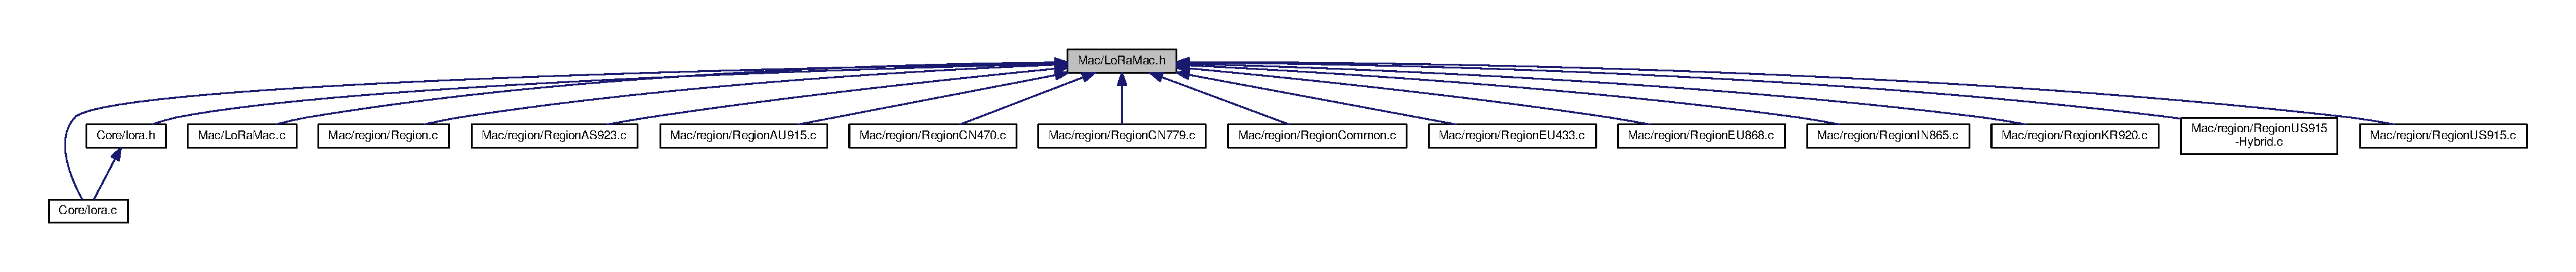
\includegraphics[width=350pt]{LoRaMac_8h__dep__incl}
\end{center}
\end{figure}
\subsection*{Data Structures}
\begin{DoxyCompactItemize}
\item 
union \hyperlink{unionuDrRange}{u\+Dr\+Range}
\item 
struct \hyperlink{structuDrRange_1_1sFields}{u\+Dr\+Range\+::s\+Fields}
\item 
struct \hyperlink{structsBand}{s\+Band}
\item 
struct \hyperlink{structsChannelParams}{s\+Channel\+Params}
\item 
struct \hyperlink{structsRx2ChannelParams}{s\+Rx2\+Channel\+Params}
\item 
struct \hyperlink{structsLoRaMacParams}{s\+Lo\+Ra\+Mac\+Params}
\item 
struct \hyperlink{structsMulticastParams}{s\+Multicast\+Params}
\item 
union \hyperlink{unionuLoRaMacHeader}{u\+Lo\+Ra\+Mac\+Header}
\item 
struct \hyperlink{structuLoRaMacHeader_1_1sHdrBits}{u\+Lo\+Ra\+Mac\+Header\+::s\+Hdr\+Bits}
\item 
union \hyperlink{unionuLoRaMacFrameCtrl}{u\+Lo\+Ra\+Mac\+Frame\+Ctrl}
\item 
struct \hyperlink{structuLoRaMacFrameCtrl_1_1sCtrlBits}{u\+Lo\+Ra\+Mac\+Frame\+Ctrl\+::s\+Ctrl\+Bits}
\item 
union \hyperlink{unioneLoRaMacFlags__t}{e\+Lo\+Ra\+Mac\+Flags\+\_\+t}
\item 
struct \hyperlink{structeLoRaMacFlags__t_1_1sMacFlagBits}{e\+Lo\+Ra\+Mac\+Flags\+\_\+t\+::s\+Mac\+Flag\+Bits}
\item 
struct \hyperlink{structsMcpsReqUnconfirmed}{s\+Mcps\+Req\+Unconfirmed}
\item 
struct \hyperlink{structsMcpsReqConfirmed}{s\+Mcps\+Req\+Confirmed}
\item 
struct \hyperlink{structsMcpsReqProprietary}{s\+Mcps\+Req\+Proprietary}
\item 
struct \hyperlink{structsMcpsReq}{s\+Mcps\+Req}
\item 
union \hyperlink{unionsMcpsReq_1_1uMcpsParam}{s\+Mcps\+Req\+::u\+Mcps\+Param}
\item 
struct \hyperlink{structsMcpsConfirm}{s\+Mcps\+Confirm}
\item 
struct \hyperlink{structsMcpsIndication}{s\+Mcps\+Indication}
\item 
struct \hyperlink{structsMlmeReqJoin}{s\+Mlme\+Req\+Join}
\item 
struct \hyperlink{structsMlmeReqTxCw}{s\+Mlme\+Req\+Tx\+Cw}
\item 
struct \hyperlink{structsMlmeReq}{s\+Mlme\+Req}
\item 
union \hyperlink{unionsMlmeReq_1_1uMlmeParam}{s\+Mlme\+Req\+::u\+Mlme\+Param}
\item 
struct \hyperlink{structsMlmeConfirm}{s\+Mlme\+Confirm}
\item 
union \hyperlink{unionuMibParam}{u\+Mib\+Param}
\item 
struct \hyperlink{structeMibRequestConfirm}{e\+Mib\+Request\+Confirm}
\item 
struct \hyperlink{structsLoRaMacTxInfo}{s\+Lo\+Ra\+Mac\+Tx\+Info}
\item 
struct \hyperlink{structsLoRaMacPrimitives}{s\+Lo\+Ra\+Mac\+Primitives}
\item 
struct \hyperlink{structsLoRaMacCallback}{s\+Lo\+Ra\+Mac\+Callback}
\end{DoxyCompactItemize}
\subsection*{Macros}
\begin{DoxyCompactItemize}
\item 
\#define \hyperlink{group__LORAMAC_ga3468d8935b09a7191e43fecdd9a15c67}{M\+A\+C\+\_\+\+S\+T\+A\+T\+E\+\_\+\+C\+H\+E\+C\+K\+\_\+\+T\+I\+M\+E\+O\+UT}~1000
\item 
\#define \hyperlink{group__LORAMAC_ga47bc6aeb5be0ba39387e2049e342fa7e}{M\+A\+X\+\_\+\+A\+C\+K\+\_\+\+R\+E\+T\+R\+I\+ES}~8
\item 
\#define \hyperlink{group__LORAMAC_ga7e75f3071d6911b19a563d554038f8da}{U\+P\+\_\+\+L\+I\+NK}~0
\item 
\#define \hyperlink{group__LORAMAC_ga801525db3ba12b250029f026403524b7}{D\+O\+W\+N\+\_\+\+L\+I\+NK}~1
\item 
\#define \hyperlink{group__LORAMAC_ga1727f288e9a871f1474ce61f942a08f3}{L\+O\+R\+A\+M\+A\+C\+\_\+\+M\+F\+R\+\_\+\+L\+EN}~4
\item 
\#define \hyperlink{group__LORAMAC_ga9623296c345a3636f460ecdb8b1bbd9d}{L\+O\+R\+A\+\_\+\+M\+A\+C\+\_\+\+F\+R\+M\+P\+A\+Y\+L\+O\+A\+D\+\_\+\+O\+V\+E\+R\+H\+E\+AD}~13
\end{DoxyCompactItemize}
\subsection*{Typedefs}
\begin{DoxyCompactItemize}
\item 
typedef enum \hyperlink{group__LORAMAC_ga133e92597739340bac439d1b0916dcb6}{e\+Device\+Class} \hyperlink{group__LORAMAC_ga29dc2e097802faaf8fbd0e18ff99695f}{Device\+Class\+\_\+t}
\item 
typedef union \hyperlink{unionuDrRange}{u\+Dr\+Range} \hyperlink{group__LORAMAC_ga8b818a36013d6bdd83ac5fd20f42b503}{Dr\+Range\+\_\+t}
\item 
typedef struct \hyperlink{structsBand}{s\+Band} \hyperlink{group__LORAMAC_ga8f49721ee96ceb52c80a896ab11a2ed8}{Band\+\_\+t}
\item 
typedef struct \hyperlink{structsChannelParams}{s\+Channel\+Params} \hyperlink{group__LORAMAC_ga1360ca6f82c6d125ea43a9dad9b56184}{Channel\+Params\+\_\+t}
\item 
typedef struct \hyperlink{structsRx2ChannelParams}{s\+Rx2\+Channel\+Params} \hyperlink{group__LORAMAC_ga8f57f29481ea92c24f6af04b96a95e0f}{Rx2\+Channel\+Params\+\_\+t}
\item 
typedef struct \hyperlink{structsLoRaMacParams}{s\+Lo\+Ra\+Mac\+Params} \hyperlink{group__LORAMAC_gad9c979008eadcd47b4d0f90bdae38b44}{Lo\+Ra\+Mac\+Params\+\_\+t}
\item 
typedef struct \hyperlink{structsMulticastParams}{s\+Multicast\+Params} \hyperlink{group__LORAMAC_ga02d2523505cac70954c043074087ea65}{Multicast\+Params\+\_\+t}
\item 
typedef enum \hyperlink{group__LORAMAC_ga5e02f214e1a4b8578c415045367c0a11}{e\+Lo\+Ra\+Mac\+Frame\+Type} \hyperlink{group__LORAMAC_ga3772acf0e9af9869ead480132e733cb2}{Lo\+Ra\+Mac\+Frame\+Type\+\_\+t}
\item 
typedef enum \hyperlink{group__LORAMAC_gaa56523d6cd76c438d6bc4263b5254d73}{e\+Lo\+Ra\+Mac\+Mote\+Cmd} \hyperlink{group__LORAMAC_ga7ef7dff520934ecc71835673f2acd015}{Lo\+Ra\+Mac\+Mote\+Cmd\+\_\+t}
\item 
typedef enum \hyperlink{group__LORAMAC_gac91cc4dc69ad7de2426360f9f1f2d079}{e\+Lo\+Ra\+Mac\+Srv\+Cmd} \hyperlink{group__LORAMAC_gabf2096aa70e466d0403f90200fab17b5}{Lo\+Ra\+Mac\+Srv\+Cmd\+\_\+t}
\item 
typedef enum \hyperlink{group__LORAMAC_gac7cbd1d9dc906cf2b33e3715cdd426c3}{e\+Lo\+Ra\+Mac\+Battery\+Level} \hyperlink{group__LORAMAC_ga05ad2aa3ef6de09ab289684a26901f75}{Lo\+Ra\+Mac\+Battery\+Level\+\_\+t}
\item 
typedef union \hyperlink{unionuLoRaMacHeader}{u\+Lo\+Ra\+Mac\+Header} \hyperlink{group__LORAMAC_gaff5f7004a7a48d53d858e26834b53efa}{Lo\+Ra\+Mac\+Header\+\_\+t}
\item 
typedef union \hyperlink{unionuLoRaMacFrameCtrl}{u\+Lo\+Ra\+Mac\+Frame\+Ctrl} \hyperlink{group__LORAMAC_ga12b0f3e7e6edd26cfdb9d10a1d873ab7}{Lo\+Ra\+Mac\+Frame\+Ctrl\+\_\+t}
\item 
typedef enum \hyperlink{group__LORAMAC_ga3c4e7a774e25faf1606f577ee5e7d201}{e\+Lo\+Ra\+Mac\+Event\+Info\+Status} \hyperlink{group__LORAMAC_gac6ffc346a4c767f7a743c87a686c51b4}{Lo\+Ra\+Mac\+Event\+Info\+Status\+\_\+t}
\item 
typedef union \hyperlink{unioneLoRaMacFlags__t}{e\+Lo\+Ra\+Mac\+Flags\+\_\+t} \hyperlink{group__LORAMAC_ga4044e22ced14e9517d7a21663c577c30}{Lo\+Ra\+Mac\+Flags\+\_\+t}
\item 
typedef enum \hyperlink{group__LORAMAC_ga7b080a046606f23fe030d0aa6d2a0e30}{e\+Mcps} \hyperlink{group__LORAMAC_ga670d0c87a52aeb13391f303a4cf94f00}{Mcps\+\_\+t}
\begin{DoxyCompactList}\small\item\em Lo\+Ra\+M\+AC data services. \end{DoxyCompactList}\item 
typedef struct \hyperlink{structsMcpsReqUnconfirmed}{s\+Mcps\+Req\+Unconfirmed} \hyperlink{group__LORAMAC_gaab871b914dfa4013c176586dcc2ea6df}{Mcps\+Req\+Unconfirmed\+\_\+t}
\item 
typedef struct \hyperlink{structsMcpsReqConfirmed}{s\+Mcps\+Req\+Confirmed} \hyperlink{group__LORAMAC_ga02103c0ee1374a6b1eec217f148ec0e2}{Mcps\+Req\+Confirmed\+\_\+t}
\item 
typedef struct \hyperlink{structsMcpsReqProprietary}{s\+Mcps\+Req\+Proprietary} \hyperlink{group__LORAMAC_gac856bc282e89301412e0a294b3e663c4}{Mcps\+Req\+Proprietary\+\_\+t}
\item 
typedef struct \hyperlink{structsMcpsReq}{s\+Mcps\+Req} \hyperlink{group__LORAMAC_ga038e0fe5eecc1fc4e8165eace8e2e683}{Mcps\+Req\+\_\+t}
\item 
typedef struct \hyperlink{structsMcpsConfirm}{s\+Mcps\+Confirm} \hyperlink{group__LORAMAC_ga925536babf8abe83918a19f5ae88bd44}{Mcps\+Confirm\+\_\+t}
\item 
typedef struct \hyperlink{structsMcpsIndication}{s\+Mcps\+Indication} \hyperlink{group__LORAMAC_ga202591b6553d63fae89bd42787496616}{Mcps\+Indication\+\_\+t}
\item 
typedef enum \hyperlink{group__LORAMAC_ga320f4c08fe99747b08463689be624f7b}{e\+Mlme} \hyperlink{group__LORAMAC_ga663544b83d50ec3518608be495896809}{Mlme\+\_\+t}
\begin{DoxyCompactList}\small\item\em Lo\+Ra\+M\+AC management services. \end{DoxyCompactList}\item 
typedef struct \hyperlink{structsMlmeReqJoin}{s\+Mlme\+Req\+Join} \hyperlink{group__LORAMAC_gab12f7f7d9bdfb8067d56f7c9f1297d95}{Mlme\+Req\+Join\+\_\+t}
\item 
typedef struct \hyperlink{structsMlmeReqTxCw}{s\+Mlme\+Req\+Tx\+Cw} \hyperlink{group__LORAMAC_gab71a9931686ff623fa01ceecc61f1986}{Mlme\+Req\+Tx\+Cw\+\_\+t}
\item 
typedef struct \hyperlink{structsMlmeReq}{s\+Mlme\+Req} \hyperlink{group__LORAMAC_ga5a32f5920a7a3d04435c142be7f38b19}{Mlme\+Req\+\_\+t}
\item 
typedef struct \hyperlink{structsMlmeConfirm}{s\+Mlme\+Confirm} \hyperlink{group__LORAMAC_ga73d9d9e11e282a6c258c4d22865fe824}{Mlme\+Confirm\+\_\+t}
\item 
typedef enum \hyperlink{group__LORAMAC_ga32ea83d13a3f5bb4b3ec2ace2319ab61}{e\+Mib} \hyperlink{group__LORAMAC_gaf17bd3de9ec75e4954be9a070cd8ddf9}{Mib\+\_\+t}
\item 
typedef union \hyperlink{unionuMibParam}{u\+Mib\+Param} \hyperlink{group__LORAMAC_gae9f2411f44447849f5b36bcaca1feb5c}{Mib\+Param\+\_\+t}
\item 
typedef struct \hyperlink{structeMibRequestConfirm}{e\+Mib\+Request\+Confirm} \hyperlink{group__LORAMAC_ga9269d5ae88dd157a58e9d60f680d63f0}{Mib\+Request\+Confirm\+\_\+t}
\item 
typedef struct \hyperlink{structsLoRaMacTxInfo}{s\+Lo\+Ra\+Mac\+Tx\+Info} \hyperlink{group__LORAMAC_ga3219fea2f3c3355f80d2ed29db613683}{Lo\+Ra\+Mac\+Tx\+Info\+\_\+t}
\item 
typedef enum \hyperlink{group__LORAMAC_ga1d18f26b344040b3ec5c3db662919661}{e\+Lo\+Ra\+Mac\+Status} \hyperlink{group__LORAMAC_ga30bd25657e10480f8605ee951b0ecfbd}{Lo\+Ra\+Mac\+Status\+\_\+t}
\item 
typedef enum \hyperlink{group__LORAMAC_ga5d863ec55bc300e0ffeef88bcbeb70af}{e\+Lo\+Ra\+Mac\+Region\+\_\+t} \hyperlink{group__LORAMAC_ga80c48efda9ae02e14b58160d34a798dd}{Lo\+Ra\+Mac\+Region\+\_\+t}
\item 
typedef struct \hyperlink{structsLoRaMacPrimitives}{s\+Lo\+Ra\+Mac\+Primitives} \hyperlink{group__LORAMAC_gafc0443f59f49d8597c0accb5e6074c44}{Lo\+Ra\+Mac\+Primitives\+\_\+t}
\item 
typedef struct \hyperlink{structsLoRaMacCallback}{s\+Lo\+Ra\+Mac\+Callback} \hyperlink{group__LORAMAC_ga2899a8ebbefe08452ddf89e14159a160}{Lo\+Ra\+Mac\+Callback\+\_\+t}
\end{DoxyCompactItemize}
\subsection*{Enumerations}
\begin{DoxyCompactItemize}
\item 
enum \hyperlink{group__LORAMAC_ga133e92597739340bac439d1b0916dcb6}{e\+Device\+Class} \{ \hyperlink{group__LORAMAC_gga133e92597739340bac439d1b0916dcb6a307ee33f71385819abc142fe4f23c3bb}{C\+L\+A\+S\+S\+\_\+A}, 
\hyperlink{group__LORAMAC_gga133e92597739340bac439d1b0916dcb6a10611f4c3b970c7d722c98eaea63ddd5}{C\+L\+A\+S\+S\+\_\+B}, 
\hyperlink{group__LORAMAC_gga133e92597739340bac439d1b0916dcb6abfee35359a39adbacbc3f13eddc76cd0}{C\+L\+A\+S\+S\+\_\+C}
 \}
\item 
enum \hyperlink{group__LORAMAC_ga5e02f214e1a4b8578c415045367c0a11}{e\+Lo\+Ra\+Mac\+Frame\+Type} \{ \newline
\hyperlink{group__LORAMAC_gga5e02f214e1a4b8578c415045367c0a11ae01d60e50804065d3564dc1e12d80811}{F\+R\+A\+M\+E\+\_\+\+T\+Y\+P\+E\+\_\+\+J\+O\+I\+N\+\_\+\+R\+EQ} = 0x00, 
\hyperlink{group__LORAMAC_gga5e02f214e1a4b8578c415045367c0a11a47ee6b14ec9dfe5ae33773749c30c103}{F\+R\+A\+M\+E\+\_\+\+T\+Y\+P\+E\+\_\+\+J\+O\+I\+N\+\_\+\+A\+C\+C\+E\+PT} = 0x01, 
\hyperlink{group__LORAMAC_gga5e02f214e1a4b8578c415045367c0a11a6701b29296dc0a006f52d51f510a138f}{F\+R\+A\+M\+E\+\_\+\+T\+Y\+P\+E\+\_\+\+D\+A\+T\+A\+\_\+\+U\+N\+C\+O\+N\+F\+I\+R\+M\+E\+D\+\_\+\+UP} = 0x02, 
\hyperlink{group__LORAMAC_gga5e02f214e1a4b8578c415045367c0a11a0309638c699fe7748561e2bac00bd689}{F\+R\+A\+M\+E\+\_\+\+T\+Y\+P\+E\+\_\+\+D\+A\+T\+A\+\_\+\+U\+N\+C\+O\+N\+F\+I\+R\+M\+E\+D\+\_\+\+D\+O\+WN} = 0x03, 
\newline
\hyperlink{group__LORAMAC_gga5e02f214e1a4b8578c415045367c0a11ac64f43487ee770c216c2ee1a829b75ca}{F\+R\+A\+M\+E\+\_\+\+T\+Y\+P\+E\+\_\+\+D\+A\+T\+A\+\_\+\+C\+O\+N\+F\+I\+R\+M\+E\+D\+\_\+\+UP} = 0x04, 
\hyperlink{group__LORAMAC_gga5e02f214e1a4b8578c415045367c0a11ad9249e47768f5551f2733532da9f3712}{F\+R\+A\+M\+E\+\_\+\+T\+Y\+P\+E\+\_\+\+D\+A\+T\+A\+\_\+\+C\+O\+N\+F\+I\+R\+M\+E\+D\+\_\+\+D\+O\+WN} = 0x05, 
\hyperlink{group__LORAMAC_gga5e02f214e1a4b8578c415045367c0a11a161e7c522a6d16fc5d3efb813f2f1351}{F\+R\+A\+M\+E\+\_\+\+T\+Y\+P\+E\+\_\+\+R\+FU} = 0x06, 
\hyperlink{group__LORAMAC_gga5e02f214e1a4b8578c415045367c0a11a68dbf0499a1912728cc6a6d1ab328b37}{F\+R\+A\+M\+E\+\_\+\+T\+Y\+P\+E\+\_\+\+P\+R\+O\+P\+R\+I\+E\+T\+A\+RY} = 0x07
 \}
\item 
enum \hyperlink{group__LORAMAC_gaa56523d6cd76c438d6bc4263b5254d73}{e\+Lo\+Ra\+Mac\+Mote\+Cmd} \{ \newline
\hyperlink{group__LORAMAC_ggaa56523d6cd76c438d6bc4263b5254d73a035270648ea6d6ff24b23a953d8f969b}{M\+O\+T\+E\+\_\+\+M\+A\+C\+\_\+\+L\+I\+N\+K\+\_\+\+C\+H\+E\+C\+K\+\_\+\+R\+EQ} = 0x02, 
\hyperlink{group__LORAMAC_ggaa56523d6cd76c438d6bc4263b5254d73a7e789c1aa1dfcd3ca03935dd65cf572c}{M\+O\+T\+E\+\_\+\+M\+A\+C\+\_\+\+L\+I\+N\+K\+\_\+\+A\+D\+R\+\_\+\+A\+NS} = 0x03, 
\hyperlink{group__LORAMAC_ggaa56523d6cd76c438d6bc4263b5254d73a258e400aeae362afff0d14b7f6153bd4}{M\+O\+T\+E\+\_\+\+M\+A\+C\+\_\+\+D\+U\+T\+Y\+\_\+\+C\+Y\+C\+L\+E\+\_\+\+A\+NS} = 0x04, 
\hyperlink{group__LORAMAC_ggaa56523d6cd76c438d6bc4263b5254d73a155ae506492f1ddb173b99b52da4092a}{M\+O\+T\+E\+\_\+\+M\+A\+C\+\_\+\+R\+X\+\_\+\+P\+A\+R\+A\+M\+\_\+\+S\+E\+T\+U\+P\+\_\+\+A\+NS} = 0x05, 
\newline
\hyperlink{group__LORAMAC_ggaa56523d6cd76c438d6bc4263b5254d73ae3d02a70f26e3f3daf8a84408e962425}{M\+O\+T\+E\+\_\+\+M\+A\+C\+\_\+\+D\+E\+V\+\_\+\+S\+T\+A\+T\+U\+S\+\_\+\+A\+NS} = 0x06, 
\hyperlink{group__LORAMAC_ggaa56523d6cd76c438d6bc4263b5254d73a83cdaea222c3968f69fe1c23c29a4385}{M\+O\+T\+E\+\_\+\+M\+A\+C\+\_\+\+N\+E\+W\+\_\+\+C\+H\+A\+N\+N\+E\+L\+\_\+\+A\+NS} = 0x07, 
\hyperlink{group__LORAMAC_ggaa56523d6cd76c438d6bc4263b5254d73abd4c19102721cfb18b76136732ac2de8}{M\+O\+T\+E\+\_\+\+M\+A\+C\+\_\+\+R\+X\+\_\+\+T\+I\+M\+I\+N\+G\+\_\+\+S\+E\+T\+U\+P\+\_\+\+A\+NS} = 0x08, 
\hyperlink{group__LORAMAC_ggaa56523d6cd76c438d6bc4263b5254d73a462cebd0ba7165044eeabf44c00b1f4c}{M\+O\+T\+E\+\_\+\+M\+A\+C\+\_\+\+T\+X\+\_\+\+P\+A\+R\+A\+M\+\_\+\+S\+E\+T\+U\+P\+\_\+\+A\+NS} = 0x09, 
\newline
\hyperlink{group__LORAMAC_ggaa56523d6cd76c438d6bc4263b5254d73a6dfc8ca9222ce73c834a0907992cce13}{M\+O\+T\+E\+\_\+\+M\+A\+C\+\_\+\+D\+L\+\_\+\+C\+H\+A\+N\+N\+E\+L\+\_\+\+A\+NS} = 0x0A
 \}
\item 
enum \hyperlink{group__LORAMAC_gac91cc4dc69ad7de2426360f9f1f2d079}{e\+Lo\+Ra\+Mac\+Srv\+Cmd} \{ \newline
\hyperlink{group__LORAMAC_ggac91cc4dc69ad7de2426360f9f1f2d079ac9df0550be22a470d4f68681ee97191c}{S\+R\+V\+\_\+\+M\+A\+C\+\_\+\+L\+I\+N\+K\+\_\+\+C\+H\+E\+C\+K\+\_\+\+A\+NS} = 0x02, 
\hyperlink{group__LORAMAC_ggac91cc4dc69ad7de2426360f9f1f2d079af7fc388963e2bb713062bd51960ed4cc}{S\+R\+V\+\_\+\+M\+A\+C\+\_\+\+L\+I\+N\+K\+\_\+\+A\+D\+R\+\_\+\+R\+EQ} = 0x03, 
\hyperlink{group__LORAMAC_ggac91cc4dc69ad7de2426360f9f1f2d079ae1175fb1d39611d84efb70f141064fbf}{S\+R\+V\+\_\+\+M\+A\+C\+\_\+\+D\+U\+T\+Y\+\_\+\+C\+Y\+C\+L\+E\+\_\+\+R\+EQ} = 0x04, 
\hyperlink{group__LORAMAC_ggac91cc4dc69ad7de2426360f9f1f2d079a534efe0aaa23bc72032a0e8b0335832b}{S\+R\+V\+\_\+\+M\+A\+C\+\_\+\+R\+X\+\_\+\+P\+A\+R\+A\+M\+\_\+\+S\+E\+T\+U\+P\+\_\+\+R\+EQ} = 0x05, 
\newline
\hyperlink{group__LORAMAC_ggac91cc4dc69ad7de2426360f9f1f2d079ac98ae516df5419b24285a74da2d58d7f}{S\+R\+V\+\_\+\+M\+A\+C\+\_\+\+D\+E\+V\+\_\+\+S\+T\+A\+T\+U\+S\+\_\+\+R\+EQ} = 0x06, 
\hyperlink{group__LORAMAC_ggac91cc4dc69ad7de2426360f9f1f2d079a34e94bc23cacf1ab088ae1010e55efeb}{S\+R\+V\+\_\+\+M\+A\+C\+\_\+\+N\+E\+W\+\_\+\+C\+H\+A\+N\+N\+E\+L\+\_\+\+R\+EQ} = 0x07, 
\hyperlink{group__LORAMAC_ggac91cc4dc69ad7de2426360f9f1f2d079aa24b1505ef48247c1d2a3d486d603686}{S\+R\+V\+\_\+\+M\+A\+C\+\_\+\+R\+X\+\_\+\+T\+I\+M\+I\+N\+G\+\_\+\+S\+E\+T\+U\+P\+\_\+\+R\+EQ} = 0x08, 
\hyperlink{group__LORAMAC_ggac91cc4dc69ad7de2426360f9f1f2d079a6b15b371027770899224e613bbe162a8}{S\+R\+V\+\_\+\+M\+A\+C\+\_\+\+T\+X\+\_\+\+P\+A\+R\+A\+M\+\_\+\+S\+E\+T\+U\+P\+\_\+\+R\+EQ} = 0x09, 
\newline
\hyperlink{group__LORAMAC_ggac91cc4dc69ad7de2426360f9f1f2d079ae3385a6aa575b3ac756c362dbbc8c39f}{S\+R\+V\+\_\+\+M\+A\+C\+\_\+\+D\+L\+\_\+\+C\+H\+A\+N\+N\+E\+L\+\_\+\+R\+EQ} = 0x0A
 \}
\item 
enum \hyperlink{group__LORAMAC_gac7cbd1d9dc906cf2b33e3715cdd426c3}{e\+Lo\+Ra\+Mac\+Battery\+Level} \{ \hyperlink{group__LORAMAC_ggac7cbd1d9dc906cf2b33e3715cdd426c3ab2585bfe30f5bf5b5eee079ed2239cf4}{B\+A\+T\+\_\+\+L\+E\+V\+E\+L\+\_\+\+E\+X\+T\+\_\+\+S\+RC} = 0x00, 
\hyperlink{group__LORAMAC_ggac7cbd1d9dc906cf2b33e3715cdd426c3aa350120effa2360e583ad6e91704b067}{B\+A\+T\+\_\+\+L\+E\+V\+E\+L\+\_\+\+E\+M\+P\+TY} = 0x01, 
\hyperlink{group__LORAMAC_ggac7cbd1d9dc906cf2b33e3715cdd426c3a72005e8306adb99b1398ff2c6817e6b9}{B\+A\+T\+\_\+\+L\+E\+V\+E\+L\+\_\+\+F\+U\+LL} = 0x\+FE, 
\hyperlink{group__LORAMAC_ggac7cbd1d9dc906cf2b33e3715cdd426c3a74b9377d8f67a38ad73ce627ba610b55}{B\+A\+T\+\_\+\+L\+E\+V\+E\+L\+\_\+\+N\+O\+\_\+\+M\+E\+A\+S\+U\+RE} = 0x\+FF
 \}
\item 
enum \hyperlink{group__LORAMAC_ga3c4e7a774e25faf1606f577ee5e7d201}{e\+Lo\+Ra\+Mac\+Event\+Info\+Status} \{ \newline
\hyperlink{group__LORAMAC_gga3c4e7a774e25faf1606f577ee5e7d201aa5e3d1c382c8473a1095b56067aea3f4}{L\+O\+R\+A\+M\+A\+C\+\_\+\+E\+V\+E\+N\+T\+\_\+\+I\+N\+F\+O\+\_\+\+S\+T\+A\+T\+U\+S\+\_\+\+OK} = 0, 
\hyperlink{group__LORAMAC_gga3c4e7a774e25faf1606f577ee5e7d201a613ed77c0e8416a512224fffdbfdf6c1}{L\+O\+R\+A\+M\+A\+C\+\_\+\+E\+V\+E\+N\+T\+\_\+\+I\+N\+F\+O\+\_\+\+S\+T\+A\+T\+U\+S\+\_\+\+E\+R\+R\+OR}, 
\hyperlink{group__LORAMAC_gga3c4e7a774e25faf1606f577ee5e7d201a0c2eb197e4102e139b43c01e806fa538}{L\+O\+R\+A\+M\+A\+C\+\_\+\+E\+V\+E\+N\+T\+\_\+\+I\+N\+F\+O\+\_\+\+S\+T\+A\+T\+U\+S\+\_\+\+T\+X\+\_\+\+T\+I\+M\+E\+O\+UT}, 
\hyperlink{group__LORAMAC_gga3c4e7a774e25faf1606f577ee5e7d201ab79a8aa20783ae5825ab8488d66a77cc}{L\+O\+R\+A\+M\+A\+C\+\_\+\+E\+V\+E\+N\+T\+\_\+\+I\+N\+F\+O\+\_\+\+S\+T\+A\+T\+U\+S\+\_\+\+R\+X1\+\_\+\+T\+I\+M\+E\+O\+UT}, 
\newline
\hyperlink{group__LORAMAC_gga3c4e7a774e25faf1606f577ee5e7d201a743858a21ae7cb162abc9acaa62cd4df}{L\+O\+R\+A\+M\+A\+C\+\_\+\+E\+V\+E\+N\+T\+\_\+\+I\+N\+F\+O\+\_\+\+S\+T\+A\+T\+U\+S\+\_\+\+R\+X2\+\_\+\+T\+I\+M\+E\+O\+UT}, 
\hyperlink{group__LORAMAC_gga3c4e7a774e25faf1606f577ee5e7d201a7bea16ca3ce17932dd5ee3558fdd0ed1}{L\+O\+R\+A\+M\+A\+C\+\_\+\+E\+V\+E\+N\+T\+\_\+\+I\+N\+F\+O\+\_\+\+S\+T\+A\+T\+U\+S\+\_\+\+R\+X1\+\_\+\+E\+R\+R\+OR}, 
\hyperlink{group__LORAMAC_gga3c4e7a774e25faf1606f577ee5e7d201afe9be38729233485ea6edd190eaa8716}{L\+O\+R\+A\+M\+A\+C\+\_\+\+E\+V\+E\+N\+T\+\_\+\+I\+N\+F\+O\+\_\+\+S\+T\+A\+T\+U\+S\+\_\+\+R\+X2\+\_\+\+E\+R\+R\+OR}, 
\hyperlink{group__LORAMAC_gga3c4e7a774e25faf1606f577ee5e7d201af42941643347e10f0e5a01c324bf6170}{L\+O\+R\+A\+M\+A\+C\+\_\+\+E\+V\+E\+N\+T\+\_\+\+I\+N\+F\+O\+\_\+\+S\+T\+A\+T\+U\+S\+\_\+\+J\+O\+I\+N\+\_\+\+F\+A\+IL}, 
\newline
\hyperlink{group__LORAMAC_gga3c4e7a774e25faf1606f577ee5e7d201aaae47a8316ae996d506323e0e6613b9b}{L\+O\+R\+A\+M\+A\+C\+\_\+\+E\+V\+E\+N\+T\+\_\+\+I\+N\+F\+O\+\_\+\+S\+T\+A\+T\+U\+S\+\_\+\+D\+O\+W\+N\+L\+I\+N\+K\+\_\+\+R\+E\+P\+E\+A\+T\+ED}, 
\hyperlink{group__LORAMAC_gga3c4e7a774e25faf1606f577ee5e7d201a6e7b21fbf0358f3438f2de0fc3fdd866}{L\+O\+R\+A\+M\+A\+C\+\_\+\+E\+V\+E\+N\+T\+\_\+\+I\+N\+F\+O\+\_\+\+S\+T\+A\+T\+U\+S\+\_\+\+T\+X\+\_\+\+D\+R\+\_\+\+P\+A\+Y\+L\+O\+A\+D\+\_\+\+S\+I\+Z\+E\+\_\+\+E\+R\+R\+OR}, 
\hyperlink{group__LORAMAC_gga3c4e7a774e25faf1606f577ee5e7d201a4a75f7744209239bb80e6af142d0249d}{L\+O\+R\+A\+M\+A\+C\+\_\+\+E\+V\+E\+N\+T\+\_\+\+I\+N\+F\+O\+\_\+\+S\+T\+A\+T\+U\+S\+\_\+\+D\+O\+W\+N\+L\+I\+N\+K\+\_\+\+T\+O\+O\+\_\+\+M\+A\+N\+Y\+\_\+\+F\+R\+A\+M\+E\+S\+\_\+\+L\+O\+SS}, 
\hyperlink{group__LORAMAC_gga3c4e7a774e25faf1606f577ee5e7d201af141bb217ba31a2dc7d3cc128a13de10}{L\+O\+R\+A\+M\+A\+C\+\_\+\+E\+V\+E\+N\+T\+\_\+\+I\+N\+F\+O\+\_\+\+S\+T\+A\+T\+U\+S\+\_\+\+A\+D\+D\+R\+E\+S\+S\+\_\+\+F\+A\+IL}, 
\newline
\hyperlink{group__LORAMAC_gga3c4e7a774e25faf1606f577ee5e7d201a43bdb9277722c567c81539fd175a7a63}{L\+O\+R\+A\+M\+A\+C\+\_\+\+E\+V\+E\+N\+T\+\_\+\+I\+N\+F\+O\+\_\+\+S\+T\+A\+T\+U\+S\+\_\+\+M\+I\+C\+\_\+\+F\+A\+IL}
 \}
\item 
enum \hyperlink{group__LORAMAC_ga7b080a046606f23fe030d0aa6d2a0e30}{e\+Mcps} \{ \hyperlink{group__LORAMAC_gga7b080a046606f23fe030d0aa6d2a0e30a340afc087e96410da04d07fb0470f84a}{M\+C\+P\+S\+\_\+\+U\+N\+C\+O\+N\+F\+I\+R\+M\+ED}, 
\hyperlink{group__LORAMAC_gga7b080a046606f23fe030d0aa6d2a0e30a5eb18aef0f2abda0d56add7e868b8546}{M\+C\+P\+S\+\_\+\+C\+O\+N\+F\+I\+R\+M\+ED}, 
\hyperlink{group__LORAMAC_gga7b080a046606f23fe030d0aa6d2a0e30aba17be1162725df5e78e03b3aeff83fa}{M\+C\+P\+S\+\_\+\+M\+U\+L\+T\+I\+C\+A\+ST}, 
\hyperlink{group__LORAMAC_gga7b080a046606f23fe030d0aa6d2a0e30a29a54ded2edefe9179a33a14e3ceaca5}{M\+C\+P\+S\+\_\+\+P\+R\+O\+P\+R\+I\+E\+T\+A\+RY}
 \}\begin{DoxyCompactList}\small\item\em Lo\+Ra\+M\+AC data services. \end{DoxyCompactList}
\item 
enum \hyperlink{group__LORAMAC_ga320f4c08fe99747b08463689be624f7b}{e\+Mlme} \{ \hyperlink{group__LORAMAC_gga320f4c08fe99747b08463689be624f7ba475ad5dea1c4c13b93b31095c665e92e}{M\+L\+M\+E\+\_\+\+J\+O\+IN}, 
\hyperlink{group__LORAMAC_gga320f4c08fe99747b08463689be624f7ba57ba2a5951a2a4637ff0e574c0e48750}{M\+L\+M\+E\+\_\+\+L\+I\+N\+K\+\_\+\+C\+H\+E\+CK}, 
\hyperlink{group__LORAMAC_gga320f4c08fe99747b08463689be624f7ba7633734852fb50e0f241ae8059b0aed1}{M\+L\+M\+E\+\_\+\+T\+X\+CW}, 
\hyperlink{group__LORAMAC_gga320f4c08fe99747b08463689be624f7ba9a6b50c77269c8fbff9a5a6d33574503}{M\+L\+M\+E\+\_\+\+T\+X\+C\+W\+\_\+1}
 \}\begin{DoxyCompactList}\small\item\em Lo\+Ra\+M\+AC management services. \end{DoxyCompactList}
\item 
enum \hyperlink{group__LORAMAC_ga32ea83d13a3f5bb4b3ec2ace2319ab61}{e\+Mib} \{ \newline
\hyperlink{group__LORAMAC_gga32ea83d13a3f5bb4b3ec2ace2319ab61ac0426517132356c9977dcdafa5ab3a7f}{M\+I\+B\+\_\+\+D\+E\+V\+I\+C\+E\+\_\+\+C\+L\+A\+SS}, 
\hyperlink{group__LORAMAC_gga32ea83d13a3f5bb4b3ec2ace2319ab61a2e2a91bfbbb7bbbe1467eec239effbd0}{M\+I\+B\+\_\+\+N\+E\+T\+W\+O\+R\+K\+\_\+\+J\+O\+I\+N\+ED}, 
\hyperlink{group__LORAMAC_gga32ea83d13a3f5bb4b3ec2ace2319ab61a756ff0b66217e3e4ddd0442c8aa56802}{M\+I\+B\+\_\+\+A\+DR}, 
\hyperlink{group__LORAMAC_gga32ea83d13a3f5bb4b3ec2ace2319ab61a982c4b7cc1e276633134aa89298c96b0}{M\+I\+B\+\_\+\+N\+E\+T\+\_\+\+ID}, 
\newline
\hyperlink{group__LORAMAC_gga32ea83d13a3f5bb4b3ec2ace2319ab61ab1459b05690ffa347a71393006b526ac}{M\+I\+B\+\_\+\+D\+E\+V\+\_\+\+A\+D\+DR}, 
\hyperlink{group__LORAMAC_gga32ea83d13a3f5bb4b3ec2ace2319ab61a60d7688e714c9b140648aadd2e7ab36e}{M\+I\+B\+\_\+\+N\+W\+K\+\_\+\+S\+K\+EY}, 
\hyperlink{group__LORAMAC_gga32ea83d13a3f5bb4b3ec2ace2319ab61ae65b7c035d9969666eb5e26a2b3c19fd}{M\+I\+B\+\_\+\+A\+P\+P\+\_\+\+S\+K\+EY}, 
\hyperlink{group__LORAMAC_gga32ea83d13a3f5bb4b3ec2ace2319ab61ab2819c46ba94b53c1fb2c3a0bfa75e48}{M\+I\+B\+\_\+\+P\+U\+B\+L\+I\+C\+\_\+\+N\+E\+T\+W\+O\+RK}, 
\newline
\hyperlink{group__LORAMAC_gga32ea83d13a3f5bb4b3ec2ace2319ab61a2d0a50cc4dd24771854bd138934ef3e5}{M\+I\+B\+\_\+\+R\+E\+P\+E\+A\+T\+E\+R\+\_\+\+S\+U\+P\+P\+O\+RT}, 
\hyperlink{group__LORAMAC_gga32ea83d13a3f5bb4b3ec2ace2319ab61a0236aae7748c12308383eab208a3cc5a}{M\+I\+B\+\_\+\+C\+H\+A\+N\+N\+E\+LS}, 
\hyperlink{group__LORAMAC_gga32ea83d13a3f5bb4b3ec2ace2319ab61a60fe29749b57c7a5315e9c1475269ba3}{M\+I\+B\+\_\+\+R\+X2\+\_\+\+C\+H\+A\+N\+N\+EL}, 
\hyperlink{group__LORAMAC_gga32ea83d13a3f5bb4b3ec2ace2319ab61ac3a212e314ab58f78007ce812187179d}{M\+I\+B\+\_\+\+R\+X2\+\_\+\+D\+E\+F\+A\+U\+L\+T\+\_\+\+C\+H\+A\+N\+N\+EL}, 
\newline
\hyperlink{group__LORAMAC_gga32ea83d13a3f5bb4b3ec2ace2319ab61aafe40b1c0e252d607876423247feab62}{M\+I\+B\+\_\+\+C\+H\+A\+N\+N\+E\+L\+S\+\_\+\+M\+A\+SK}, 
\hyperlink{group__LORAMAC_gga32ea83d13a3f5bb4b3ec2ace2319ab61a59afc276ca425cd4055ff5cb5b5fa946}{M\+I\+B\+\_\+\+C\+H\+A\+N\+N\+E\+L\+S\+\_\+\+D\+E\+F\+A\+U\+L\+T\+\_\+\+M\+A\+SK}, 
\hyperlink{group__LORAMAC_gga32ea83d13a3f5bb4b3ec2ace2319ab61af8775ceffd8bc73429e43eac205383ea}{M\+I\+B\+\_\+\+C\+H\+A\+N\+N\+E\+L\+S\+\_\+\+N\+B\+\_\+\+R\+EP}, 
\hyperlink{group__LORAMAC_gga32ea83d13a3f5bb4b3ec2ace2319ab61ad6ba0cae3e33f0cf042ded8936d965da}{M\+I\+B\+\_\+\+M\+A\+X\+\_\+\+R\+X\+\_\+\+W\+I\+N\+D\+O\+W\+\_\+\+D\+U\+R\+A\+T\+I\+ON}, 
\newline
\hyperlink{group__LORAMAC_gga32ea83d13a3f5bb4b3ec2ace2319ab61aa3511cfca5a46654d97b022d50c82ae8}{M\+I\+B\+\_\+\+R\+E\+C\+E\+I\+V\+E\+\_\+\+D\+E\+L\+A\+Y\+\_\+1}, 
\hyperlink{group__LORAMAC_gga32ea83d13a3f5bb4b3ec2ace2319ab61a3d147bf887f0d7317cb2930335857000}{M\+I\+B\+\_\+\+R\+E\+C\+E\+I\+V\+E\+\_\+\+D\+E\+L\+A\+Y\+\_\+2}, 
\hyperlink{group__LORAMAC_gga32ea83d13a3f5bb4b3ec2ace2319ab61a3fa6b527109f8a6d5994ddaf7e9b0bd1}{M\+I\+B\+\_\+\+J\+O\+I\+N\+\_\+\+A\+C\+C\+E\+P\+T\+\_\+\+D\+E\+L\+A\+Y\+\_\+1}, 
\hyperlink{group__LORAMAC_gga32ea83d13a3f5bb4b3ec2ace2319ab61aa1ca7d4484b41008a69d5d786cfd6a20}{M\+I\+B\+\_\+\+J\+O\+I\+N\+\_\+\+A\+C\+C\+E\+P\+T\+\_\+\+D\+E\+L\+A\+Y\+\_\+2}, 
\newline
\hyperlink{group__LORAMAC_gga32ea83d13a3f5bb4b3ec2ace2319ab61addef34adbf844ace9eeea97ae93da918}{M\+I\+B\+\_\+\+C\+H\+A\+N\+N\+E\+L\+S\+\_\+\+D\+E\+F\+A\+U\+L\+T\+\_\+\+D\+A\+T\+A\+R\+A\+TE}, 
\hyperlink{group__LORAMAC_gga32ea83d13a3f5bb4b3ec2ace2319ab61a78f3b4e3ae4ebaacb478073d2a2ec4f1}{M\+I\+B\+\_\+\+C\+H\+A\+N\+N\+E\+L\+S\+\_\+\+D\+A\+T\+A\+R\+A\+TE}, 
\hyperlink{group__LORAMAC_gga32ea83d13a3f5bb4b3ec2ace2319ab61ae42f1a0c858ffdb283e0236a24ab6398}{M\+I\+B\+\_\+\+C\+H\+A\+N\+N\+E\+L\+S\+\_\+\+T\+X\+\_\+\+P\+O\+W\+ER}, 
\hyperlink{group__LORAMAC_gga32ea83d13a3f5bb4b3ec2ace2319ab61a9c5b2d3ad2caf87710b09e8a6e68cc6a}{M\+I\+B\+\_\+\+C\+H\+A\+N\+N\+E\+L\+S\+\_\+\+D\+E\+F\+A\+U\+L\+T\+\_\+\+T\+X\+\_\+\+P\+O\+W\+ER}, 
\newline
\hyperlink{group__LORAMAC_gga32ea83d13a3f5bb4b3ec2ace2319ab61ad0d2e0023858ce3fab3647fa97428d84}{M\+I\+B\+\_\+\+U\+P\+L\+I\+N\+K\+\_\+\+C\+O\+U\+N\+T\+ER}, 
\hyperlink{group__LORAMAC_gga32ea83d13a3f5bb4b3ec2ace2319ab61ae75b53deee33594312d1d2987c24b698}{M\+I\+B\+\_\+\+D\+O\+W\+N\+L\+I\+N\+K\+\_\+\+C\+O\+U\+N\+T\+ER}, 
\hyperlink{group__LORAMAC_gga32ea83d13a3f5bb4b3ec2ace2319ab61af8ac424460fccb3115c6fe6ccb450862}{M\+I\+B\+\_\+\+M\+U\+L\+T\+I\+C\+A\+S\+T\+\_\+\+C\+H\+A\+N\+N\+EL}, 
\hyperlink{group__LORAMAC_gga32ea83d13a3f5bb4b3ec2ace2319ab61ad5d382841f32fba944bdb68b25699e45}{M\+I\+B\+\_\+\+S\+Y\+S\+T\+E\+M\+\_\+\+M\+A\+X\+\_\+\+R\+X\+\_\+\+E\+R\+R\+OR}, 
\newline
\hyperlink{group__LORAMAC_gga32ea83d13a3f5bb4b3ec2ace2319ab61a82fb27fd6414d2bde20a7a00c80e26a1}{M\+I\+B\+\_\+\+M\+I\+N\+\_\+\+R\+X\+\_\+\+S\+Y\+M\+B\+O\+LS}, 
\hyperlink{group__LORAMAC_gga32ea83d13a3f5bb4b3ec2ace2319ab61a268b2f7da53dbc25655a7bdcc7e6128e}{M\+I\+B\+\_\+\+A\+N\+T\+E\+N\+N\+A\+\_\+\+G\+A\+IN}
 \}
\item 
enum \hyperlink{group__LORAMAC_ga1d18f26b344040b3ec5c3db662919661}{e\+Lo\+Ra\+Mac\+Status} \{ \newline
\hyperlink{group__LORAMAC_gga1d18f26b344040b3ec5c3db662919661a03db5fca052313edb3823c014b653a74}{L\+O\+R\+A\+M\+A\+C\+\_\+\+S\+T\+A\+T\+U\+S\+\_\+\+OK}, 
\hyperlink{group__LORAMAC_gga1d18f26b344040b3ec5c3db662919661a66b12f569207eacd97ee1c1d6c4cee6d}{L\+O\+R\+A\+M\+A\+C\+\_\+\+S\+T\+A\+T\+U\+S\+\_\+\+B\+U\+SY}, 
\hyperlink{group__LORAMAC_gga1d18f26b344040b3ec5c3db662919661aff502a87db22d6a9a4919e4b54c7c1cf}{L\+O\+R\+A\+M\+A\+C\+\_\+\+S\+T\+A\+T\+U\+S\+\_\+\+S\+E\+R\+V\+I\+C\+E\+\_\+\+U\+N\+K\+N\+O\+WN}, 
\hyperlink{group__LORAMAC_gga1d18f26b344040b3ec5c3db662919661ad0d3119f247d00e1787dda106fcb3017}{L\+O\+R\+A\+M\+A\+C\+\_\+\+S\+T\+A\+T\+U\+S\+\_\+\+P\+A\+R\+A\+M\+E\+T\+E\+R\+\_\+\+I\+N\+V\+A\+L\+ID}, 
\newline
\hyperlink{group__LORAMAC_gga1d18f26b344040b3ec5c3db662919661ae3ea7b89796aed5a320013d9743b2955}{L\+O\+R\+A\+M\+A\+C\+\_\+\+S\+T\+A\+T\+U\+S\+\_\+\+F\+R\+E\+Q\+U\+E\+N\+C\+Y\+\_\+\+I\+N\+V\+A\+L\+ID}, 
\hyperlink{group__LORAMAC_gga1d18f26b344040b3ec5c3db662919661aa910e51ef7a7cf64c27dd3ffe5eb9d38}{L\+O\+R\+A\+M\+A\+C\+\_\+\+S\+T\+A\+T\+U\+S\+\_\+\+D\+A\+T\+A\+R\+A\+T\+E\+\_\+\+I\+N\+V\+A\+L\+ID}, 
\hyperlink{group__LORAMAC_gga1d18f26b344040b3ec5c3db662919661a163a1a739baee13607068af42f2e9d30}{L\+O\+R\+A\+M\+A\+C\+\_\+\+S\+T\+A\+T\+U\+S\+\_\+\+F\+R\+E\+Q\+\_\+\+A\+N\+D\+\_\+\+D\+R\+\_\+\+I\+N\+V\+A\+L\+ID}, 
\hyperlink{group__LORAMAC_gga1d18f26b344040b3ec5c3db662919661a105228330376111d46d99d57688a20ae}{L\+O\+R\+A\+M\+A\+C\+\_\+\+S\+T\+A\+T\+U\+S\+\_\+\+N\+O\+\_\+\+N\+E\+T\+W\+O\+R\+K\+\_\+\+J\+O\+I\+N\+ED}, 
\newline
\hyperlink{group__LORAMAC_gga1d18f26b344040b3ec5c3db662919661a4ab40311dcd2eeffc77f573a919b29b1}{L\+O\+R\+A\+M\+A\+C\+\_\+\+S\+T\+A\+T\+U\+S\+\_\+\+L\+E\+N\+G\+T\+H\+\_\+\+E\+R\+R\+OR}, 
\hyperlink{group__LORAMAC_gga1d18f26b344040b3ec5c3db662919661aff1d3a91250809d1770a74776057b8ce}{L\+O\+R\+A\+M\+A\+C\+\_\+\+S\+T\+A\+T\+U\+S\+\_\+\+D\+E\+V\+I\+C\+E\+\_\+\+O\+FF}, 
\hyperlink{group__LORAMAC_gga1d18f26b344040b3ec5c3db662919661af424839424174be5fc5e52e00160940e}{L\+O\+R\+A\+M\+A\+C\+\_\+\+S\+T\+A\+T\+U\+S\+\_\+\+R\+E\+G\+I\+O\+N\+\_\+\+N\+O\+T\+\_\+\+S\+U\+P\+P\+O\+R\+T\+ED}
 \}
\item 
enum \hyperlink{group__LORAMAC_ga5d863ec55bc300e0ffeef88bcbeb70af}{e\+Lo\+Ra\+Mac\+Region\+\_\+t} \{ \newline
\hyperlink{group__LORAMAC_gga5d863ec55bc300e0ffeef88bcbeb70afa5b791cd5d892cd4ffdc891177f9c424f}{L\+O\+R\+A\+M\+A\+C\+\_\+\+R\+E\+G\+I\+O\+N\+\_\+\+A\+S923}, 
\hyperlink{group__LORAMAC_gga5d863ec55bc300e0ffeef88bcbeb70afa31c5134a31ba71dd67fffc7cd2e8d402}{L\+O\+R\+A\+M\+A\+C\+\_\+\+R\+E\+G\+I\+O\+N\+\_\+\+A\+U915}, 
\hyperlink{group__LORAMAC_gga5d863ec55bc300e0ffeef88bcbeb70afa8bf5c395dec14c8c24bc629e9cb4ab64}{L\+O\+R\+A\+M\+A\+C\+\_\+\+R\+E\+G\+I\+O\+N\+\_\+\+C\+N470}, 
\hyperlink{group__LORAMAC_gga5d863ec55bc300e0ffeef88bcbeb70afaa462c6a59045bcdbe27177b3c7d91ed0}{L\+O\+R\+A\+M\+A\+C\+\_\+\+R\+E\+G\+I\+O\+N\+\_\+\+C\+N779}, 
\newline
\hyperlink{group__LORAMAC_gga5d863ec55bc300e0ffeef88bcbeb70afa484c9c5522a1bd8411920cc7703d3977}{L\+O\+R\+A\+M\+A\+C\+\_\+\+R\+E\+G\+I\+O\+N\+\_\+\+E\+U433}, 
\hyperlink{group__LORAMAC_gga5d863ec55bc300e0ffeef88bcbeb70afadbfed23153fb6254b9ca2301ec19c24f}{L\+O\+R\+A\+M\+A\+C\+\_\+\+R\+E\+G\+I\+O\+N\+\_\+\+E\+U868}, 
\hyperlink{group__LORAMAC_gga5d863ec55bc300e0ffeef88bcbeb70afa2f45370a935e8767a90e19e24101f859}{L\+O\+R\+A\+M\+A\+C\+\_\+\+R\+E\+G\+I\+O\+N\+\_\+\+K\+R920}, 
\hyperlink{group__LORAMAC_gga5d863ec55bc300e0ffeef88bcbeb70afa58507c2e7248ab724cd3e0d0144ebd77}{L\+O\+R\+A\+M\+A\+C\+\_\+\+R\+E\+G\+I\+O\+N\+\_\+\+I\+N865}, 
\newline
\hyperlink{group__LORAMAC_gga5d863ec55bc300e0ffeef88bcbeb70afab2c106945b06878a5ded0cb466330412}{L\+O\+R\+A\+M\+A\+C\+\_\+\+R\+E\+G\+I\+O\+N\+\_\+\+U\+S915}, 
\hyperlink{group__LORAMAC_gga5d863ec55bc300e0ffeef88bcbeb70afa973a53fba592cda6ade4592cf7b814b0}{L\+O\+R\+A\+M\+A\+C\+\_\+\+R\+E\+G\+I\+O\+N\+\_\+\+U\+S915\+\_\+\+H\+Y\+B\+R\+ID}
 \}
\end{DoxyCompactItemize}
\subsection*{Functions}
\begin{DoxyCompactItemize}
\item 
\hyperlink{group__LORAMAC_ga30bd25657e10480f8605ee951b0ecfbd}{Lo\+Ra\+Mac\+Status\+\_\+t} \hyperlink{group__LORAMAC_ga7ca445cf825e45999810b3991273eba5}{Lo\+Ra\+Mac\+Initialization} (\hyperlink{group__LORAMAC_gafc0443f59f49d8597c0accb5e6074c44}{Lo\+Ra\+Mac\+Primitives\+\_\+t} $\ast$primitives, \hyperlink{group__LORAMAC_ga2899a8ebbefe08452ddf89e14159a160}{Lo\+Ra\+Mac\+Callback\+\_\+t} $\ast$callbacks, \hyperlink{group__LORAMAC_ga80c48efda9ae02e14b58160d34a798dd}{Lo\+Ra\+Mac\+Region\+\_\+t} region)
\begin{DoxyCompactList}\small\item\em Lo\+Ra\+M\+AC layer initialization. \end{DoxyCompactList}\item 
\hyperlink{group__LORAMAC_ga30bd25657e10480f8605ee951b0ecfbd}{Lo\+Ra\+Mac\+Status\+\_\+t} \hyperlink{group__LORAMAC_ga8b0aeaf75f9404ce01da9b202252c231}{Lo\+Ra\+Mac\+Query\+Tx\+Possible} (uint8\+\_\+t size, \hyperlink{group__LORAMAC_ga3219fea2f3c3355f80d2ed29db613683}{Lo\+Ra\+Mac\+Tx\+Info\+\_\+t} $\ast$tx\+Info)
\begin{DoxyCompactList}\small\item\em Queries the Lo\+Ra\+M\+AC if it is possible to send the next frame with a given payload size. The Lo\+Ra\+M\+AC takes scheduled M\+AC commands into account and reports, when the frame can be send or not. \end{DoxyCompactList}\item 
\hyperlink{group__LORAMAC_ga30bd25657e10480f8605ee951b0ecfbd}{Lo\+Ra\+Mac\+Status\+\_\+t} \hyperlink{group__LORAMAC_gad74920538f07f34e773ca5de9ec89370}{Lo\+Ra\+Mac\+Channel\+Add} (uint8\+\_\+t id, \hyperlink{group__LORAMAC_ga1360ca6f82c6d125ea43a9dad9b56184}{Channel\+Params\+\_\+t} params)
\begin{DoxyCompactList}\small\item\em Lo\+Ra\+M\+AC channel add service. \end{DoxyCompactList}\item 
\hyperlink{group__LORAMAC_ga30bd25657e10480f8605ee951b0ecfbd}{Lo\+Ra\+Mac\+Status\+\_\+t} \hyperlink{group__LORAMAC_gafad6c929a33557ac2fd4000bcacd9453}{Lo\+Ra\+Mac\+Channel\+Remove} (uint8\+\_\+t id)
\begin{DoxyCompactList}\small\item\em Lo\+Ra\+M\+AC channel remove service. \end{DoxyCompactList}\item 
\hyperlink{group__LORAMAC_ga30bd25657e10480f8605ee951b0ecfbd}{Lo\+Ra\+Mac\+Status\+\_\+t} \hyperlink{group__LORAMAC_ga89622bf6a1705558ba7b76dbb2d59c2f}{Lo\+Ra\+Mac\+Multicast\+Channel\+Link} (\hyperlink{group__LORAMAC_ga02d2523505cac70954c043074087ea65}{Multicast\+Params\+\_\+t} $\ast$channel\+Param)
\begin{DoxyCompactList}\small\item\em Lo\+Ra\+M\+AC multicast channel link service. \end{DoxyCompactList}\item 
\hyperlink{group__LORAMAC_ga30bd25657e10480f8605ee951b0ecfbd}{Lo\+Ra\+Mac\+Status\+\_\+t} \hyperlink{group__LORAMAC_ga1542a215938fcff1d665ae48b449335e}{Lo\+Ra\+Mac\+Multicast\+Channel\+Unlink} (\hyperlink{group__LORAMAC_ga02d2523505cac70954c043074087ea65}{Multicast\+Params\+\_\+t} $\ast$channel\+Param)
\begin{DoxyCompactList}\small\item\em Lo\+Ra\+M\+AC multicast channel unlink service. \end{DoxyCompactList}\item 
\hyperlink{group__LORAMAC_ga30bd25657e10480f8605ee951b0ecfbd}{Lo\+Ra\+Mac\+Status\+\_\+t} \hyperlink{group__LORAMAC_ga3e208a4f73213aa801eeb9d9da7b71dd}{Lo\+Ra\+Mac\+Mib\+Get\+Request\+Confirm} (\hyperlink{group__LORAMAC_ga9269d5ae88dd157a58e9d60f680d63f0}{Mib\+Request\+Confirm\+\_\+t} $\ast$mib\+Get)
\begin{DoxyCompactList}\small\item\em Lo\+Ra\+M\+AC M\+I\+B-\/\+Get. \end{DoxyCompactList}\item 
\hyperlink{group__LORAMAC_ga30bd25657e10480f8605ee951b0ecfbd}{Lo\+Ra\+Mac\+Status\+\_\+t} \hyperlink{group__LORAMAC_ga7a4ee0ced221591206b09630d4a70844}{Lo\+Ra\+Mac\+Mib\+Set\+Request\+Confirm} (\hyperlink{group__LORAMAC_ga9269d5ae88dd157a58e9d60f680d63f0}{Mib\+Request\+Confirm\+\_\+t} $\ast$mib\+Set)
\begin{DoxyCompactList}\small\item\em Lo\+Ra\+M\+AC M\+I\+B-\/\+Set. \end{DoxyCompactList}\item 
\hyperlink{group__LORAMAC_ga30bd25657e10480f8605ee951b0ecfbd}{Lo\+Ra\+Mac\+Status\+\_\+t} \hyperlink{group__LORAMAC_ga097113f30feecc17c780940ff74af33e}{Lo\+Ra\+Mac\+Mlme\+Request} (\hyperlink{group__LORAMAC_ga5a32f5920a7a3d04435c142be7f38b19}{Mlme\+Req\+\_\+t} $\ast$mlme\+Request)
\begin{DoxyCompactList}\small\item\em Lo\+Ra\+M\+AC M\+L\+M\+E-\/\+Request. \end{DoxyCompactList}\item 
\hyperlink{group__LORAMAC_ga30bd25657e10480f8605ee951b0ecfbd}{Lo\+Ra\+Mac\+Status\+\_\+t} \hyperlink{group__LORAMAC_ga79768f8a3c22aaff84d4dfcc77ad508c}{Lo\+Ra\+Mac\+Mcps\+Request} (\hyperlink{group__LORAMAC_ga038e0fe5eecc1fc4e8165eace8e2e683}{Mcps\+Req\+\_\+t} $\ast$mcps\+Request)
\begin{DoxyCompactList}\small\item\em Lo\+Ra\+M\+AC M\+C\+P\+S-\/\+Request. \end{DoxyCompactList}\end{DoxyCompactItemize}


\subsection{Detailed Description}
Lo\+Ra M\+AC layer implementation. 

\begin{DoxyCopyright}{Copyright}
Revised B\+SD License, see section L\+I\+C\+E\+N\+SE.
\end{DoxyCopyright}

\begin{DoxyCode}
  \_\_\_\_\_\_                              \_
 / \_\_\_\_\_)             \_              | |
( (\_\_\_\_  \_\_\_\_\_ \_\_\_\_ \_| |\_ \_\_\_\_\_  \_\_\_\_| |\_\_
 \(\backslash\)\_\_\_\_ \(\backslash\)| \_\_\_ |    (\_   \_) \_\_\_ |/ \_\_\_)  \_ \(\backslash\)
 \_\_\_\_\_) ) \_\_\_\_| | | || |\_| \_\_\_\_( (\_\_\_| | | |
(\_\_\_\_\_\_/|\_\_\_\_\_)\_|\_|\_| \(\backslash\)\_\_)\_\_\_\_\_)\(\backslash\)\_\_\_\_)\_| |\_|
(C)2013 Semtech

 \_\_\_ \_\_\_\_\_ \_   \_\_\_ \_  \_\_\_\_\_ \_\_\_  \_\_\_  \_\_\_ \_\_\_
/ \_\_|\_   \_/\_\(\backslash\) / \_\_| |/ / \_\_/ \_ \(\backslash\)| \_ \(\backslash\)/ \_\_| \_\_|
\(\backslash\)\_\_ \(\backslash\) | |/ \_ \(\backslash\) (\_\_| \textcolor{stringliteral}{' <| \_| (\_) |   / (\_\_| \_|}
\textcolor{stringliteral}{|\_\_\_/ |\_/\_/ \(\backslash\)\_\(\backslash\)\_\_\_|\_|\(\backslash\)\_\(\backslash\)\_| \(\backslash\)\_\_\_/|\_|\_\(\backslash\)\(\backslash\)\_\_\_|\_\_\_|}
\textcolor{stringliteral}{embedded.connectivity.solutions===============}
\end{DoxyCode}


\begin{DoxyAuthor}{Author}
Miguel Luis ( Semtech )

Gregory Cristian ( Semtech )

Daniel Jaeckle ( S\+T\+A\+C\+K\+F\+O\+R\+CE ) 
\end{DoxyAuthor}

\hypertarget{LoRaMacCrypto_8c}{}\section{Mac/\+Lo\+Ra\+Mac\+Crypto.c File Reference}
\label{LoRaMacCrypto_8c}\index{Mac/\+Lo\+Ra\+Mac\+Crypto.\+c@{Mac/\+Lo\+Ra\+Mac\+Crypto.\+c}}
{\ttfamily \#include $<$stdlib.\+h$>$}\newline
{\ttfamily \#include $<$stdint.\+h$>$}\newline
{\ttfamily \#include \char`\"{}utilities.\+h\char`\"{}}\newline
{\ttfamily \#include \char`\"{}aes.\+h\char`\"{}}\newline
{\ttfamily \#include \char`\"{}cmac.\+h\char`\"{}}\newline
{\ttfamily \#include \char`\"{}Lo\+Ra\+Mac\+Crypto.\+h\char`\"{}}\newline
Include dependency graph for Lo\+Ra\+Mac\+Crypto.\+c\+:
\nopagebreak
\begin{figure}[H]
\begin{center}
\leavevmode
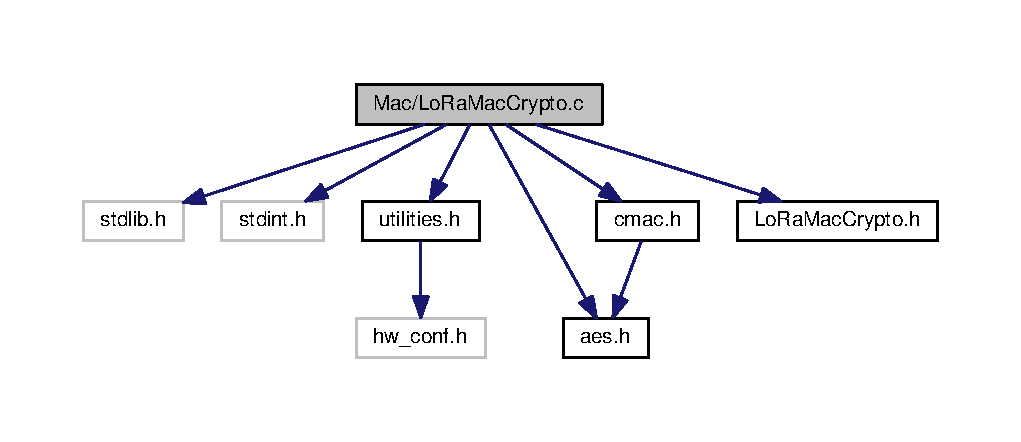
\includegraphics[width=350pt]{LoRaMacCrypto_8c__incl}
\end{center}
\end{figure}
\subsection*{Macros}
\begin{DoxyCompactItemize}
\item 
\#define \hyperlink{LoRaMacCrypto_8c_a5c3d9a633ffde7d6b49116095bf4395e}{L\+O\+R\+A\+M\+A\+C\+\_\+\+M\+I\+C\+\_\+\+B\+L\+O\+C\+K\+\_\+\+B0\+\_\+\+S\+I\+ZE}~16
\end{DoxyCompactItemize}
\subsection*{Functions}
\begin{DoxyCompactItemize}
\item 
void \hyperlink{group__LORAMAC__CRYPTO_ga6ee265070494b83255e7fdc4dff985da}{Lo\+Ra\+Mac\+Compute\+Mic} (const uint8\+\_\+t $\ast$buffer, uint16\+\_\+t size, const uint8\+\_\+t $\ast$key, uint32\+\_\+t address, uint8\+\_\+t dir, uint32\+\_\+t sequence\+Counter, uint32\+\_\+t $\ast$mic)
\begin{DoxyCompactList}\small\item\em Computes the Lo\+Ra\+M\+AC frame M\+IC field. \end{DoxyCompactList}\item 
void \hyperlink{group__LORAMAC__CRYPTO_ga50339e60abea2186ca7e584b489718b1}{Lo\+Ra\+Mac\+Payload\+Encrypt} (const uint8\+\_\+t $\ast$buffer, uint16\+\_\+t size, const uint8\+\_\+t $\ast$key, uint32\+\_\+t address, uint8\+\_\+t dir, uint32\+\_\+t sequence\+Counter, uint8\+\_\+t $\ast$enc\+Buffer)
\item 
void \hyperlink{group__LORAMAC__CRYPTO_ga41f9ba19f61b195420914ed58c8b94c7}{Lo\+Ra\+Mac\+Payload\+Decrypt} (const uint8\+\_\+t $\ast$buffer, uint16\+\_\+t size, const uint8\+\_\+t $\ast$key, uint32\+\_\+t address, uint8\+\_\+t dir, uint32\+\_\+t sequence\+Counter, uint8\+\_\+t $\ast$dec\+Buffer)
\item 
void \hyperlink{group__LORAMAC__CRYPTO_gac9216af326316c9e7f207d4e73aed199}{Lo\+Ra\+Mac\+Join\+Compute\+Mic} (const uint8\+\_\+t $\ast$buffer, uint16\+\_\+t size, const uint8\+\_\+t $\ast$key, uint32\+\_\+t $\ast$mic)
\item 
void \hyperlink{group__LORAMAC__CRYPTO_gac2379cd7cbeb6febaa2a7be5d9f04b5c}{Lo\+Ra\+Mac\+Join\+Decrypt} (const uint8\+\_\+t $\ast$buffer, uint16\+\_\+t size, const uint8\+\_\+t $\ast$key, uint8\+\_\+t $\ast$dec\+Buffer)
\item 
void \hyperlink{group__LORAMAC__CRYPTO_gad6fc2ace27fa388ec860fc2e5ae1f544}{Lo\+Ra\+Mac\+Join\+Compute\+S\+Keys} (const uint8\+\_\+t $\ast$key, const uint8\+\_\+t $\ast$app\+Nonce, uint16\+\_\+t dev\+Nonce, uint8\+\_\+t $\ast$nwk\+S\+Key, uint8\+\_\+t $\ast$app\+S\+Key)
\end{DoxyCompactItemize}


\subsection{Macro Definition Documentation}
\mbox{\Hypertarget{LoRaMacCrypto_8c_a5c3d9a633ffde7d6b49116095bf4395e}\label{LoRaMacCrypto_8c_a5c3d9a633ffde7d6b49116095bf4395e}} 
\index{Lo\+Ra\+Mac\+Crypto.\+c@{Lo\+Ra\+Mac\+Crypto.\+c}!L\+O\+R\+A\+M\+A\+C\+\_\+\+M\+I\+C\+\_\+\+B\+L\+O\+C\+K\+\_\+\+B0\+\_\+\+S\+I\+ZE@{L\+O\+R\+A\+M\+A\+C\+\_\+\+M\+I\+C\+\_\+\+B\+L\+O\+C\+K\+\_\+\+B0\+\_\+\+S\+I\+ZE}}
\index{L\+O\+R\+A\+M\+A\+C\+\_\+\+M\+I\+C\+\_\+\+B\+L\+O\+C\+K\+\_\+\+B0\+\_\+\+S\+I\+ZE@{L\+O\+R\+A\+M\+A\+C\+\_\+\+M\+I\+C\+\_\+\+B\+L\+O\+C\+K\+\_\+\+B0\+\_\+\+S\+I\+ZE}!Lo\+Ra\+Mac\+Crypto.\+c@{Lo\+Ra\+Mac\+Crypto.\+c}}
\subsubsection{\texorpdfstring{L\+O\+R\+A\+M\+A\+C\+\_\+\+M\+I\+C\+\_\+\+B\+L\+O\+C\+K\+\_\+\+B0\+\_\+\+S\+I\+ZE}{LORAMAC\_MIC\_BLOCK\_B0\_SIZE}}
{\footnotesize\ttfamily \#define L\+O\+R\+A\+M\+A\+C\+\_\+\+M\+I\+C\+\_\+\+B\+L\+O\+C\+K\+\_\+\+B0\+\_\+\+S\+I\+ZE~16}

C\+M\+A\+C/\+A\+ES Message Integrity Code (M\+IC) Block B0 size 
\hypertarget{LoRaMacCrypto_8h}{}\section{Mac/\+Lo\+Ra\+Mac\+Crypto.h File Reference}
\label{LoRaMacCrypto_8h}\index{Mac/\+Lo\+Ra\+Mac\+Crypto.\+h@{Mac/\+Lo\+Ra\+Mac\+Crypto.\+h}}


Lo\+Ra M\+AC layer cryptography implementation.  


This graph shows which files directly or indirectly include this file\+:
\nopagebreak
\begin{figure}[H]
\begin{center}
\leavevmode
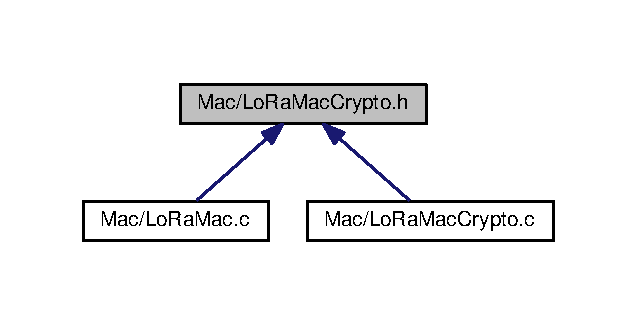
\includegraphics[width=306pt]{LoRaMacCrypto_8h__dep__incl}
\end{center}
\end{figure}
\subsection*{Functions}
\begin{DoxyCompactItemize}
\item 
void \hyperlink{group__LORAMAC__CRYPTO_ga6ee265070494b83255e7fdc4dff985da}{Lo\+Ra\+Mac\+Compute\+Mic} (const uint8\+\_\+t $\ast$buffer, uint16\+\_\+t size, const uint8\+\_\+t $\ast$key, uint32\+\_\+t address, uint8\+\_\+t dir, uint32\+\_\+t sequence\+Counter, uint32\+\_\+t $\ast$mic)
\begin{DoxyCompactList}\small\item\em Computes the Lo\+Ra\+M\+AC frame M\+IC field. \end{DoxyCompactList}\item 
void \hyperlink{group__LORAMAC__CRYPTO_ga50339e60abea2186ca7e584b489718b1}{Lo\+Ra\+Mac\+Payload\+Encrypt} (const uint8\+\_\+t $\ast$buffer, uint16\+\_\+t size, const uint8\+\_\+t $\ast$key, uint32\+\_\+t address, uint8\+\_\+t dir, uint32\+\_\+t sequence\+Counter, uint8\+\_\+t $\ast$enc\+Buffer)
\item 
void \hyperlink{group__LORAMAC__CRYPTO_ga41f9ba19f61b195420914ed58c8b94c7}{Lo\+Ra\+Mac\+Payload\+Decrypt} (const uint8\+\_\+t $\ast$buffer, uint16\+\_\+t size, const uint8\+\_\+t $\ast$key, uint32\+\_\+t address, uint8\+\_\+t dir, uint32\+\_\+t sequence\+Counter, uint8\+\_\+t $\ast$dec\+Buffer)
\item 
void \hyperlink{group__LORAMAC__CRYPTO_gac9216af326316c9e7f207d4e73aed199}{Lo\+Ra\+Mac\+Join\+Compute\+Mic} (const uint8\+\_\+t $\ast$buffer, uint16\+\_\+t size, const uint8\+\_\+t $\ast$key, uint32\+\_\+t $\ast$mic)
\item 
void \hyperlink{group__LORAMAC__CRYPTO_gac2379cd7cbeb6febaa2a7be5d9f04b5c}{Lo\+Ra\+Mac\+Join\+Decrypt} (const uint8\+\_\+t $\ast$buffer, uint16\+\_\+t size, const uint8\+\_\+t $\ast$key, uint8\+\_\+t $\ast$dec\+Buffer)
\item 
void \hyperlink{group__LORAMAC__CRYPTO_gad6fc2ace27fa388ec860fc2e5ae1f544}{Lo\+Ra\+Mac\+Join\+Compute\+S\+Keys} (const uint8\+\_\+t $\ast$key, const uint8\+\_\+t $\ast$app\+Nonce, uint16\+\_\+t dev\+Nonce, uint8\+\_\+t $\ast$nwk\+S\+Key, uint8\+\_\+t $\ast$app\+S\+Key)
\end{DoxyCompactItemize}


\subsection{Detailed Description}
Lo\+Ra M\+AC layer cryptography implementation. 

\begin{DoxyCopyright}{Copyright}
Revised B\+SD License, see section L\+I\+C\+E\+N\+SE.
\end{DoxyCopyright}

\begin{DoxyCode}
  \_\_\_\_\_\_                              \_
 / \_\_\_\_\_)             \_              | |
( (\_\_\_\_  \_\_\_\_\_ \_\_\_\_ \_| |\_ \_\_\_\_\_  \_\_\_\_| |\_\_
 \(\backslash\)\_\_\_\_ \(\backslash\)| \_\_\_ |    (\_   \_) \_\_\_ |/ \_\_\_)  \_ \(\backslash\)
 \_\_\_\_\_) ) \_\_\_\_| | | || |\_| \_\_\_\_( (\_\_\_| | | |
(\_\_\_\_\_\_/|\_\_\_\_\_)\_|\_|\_| \(\backslash\)\_\_)\_\_\_\_\_)\(\backslash\)\_\_\_\_)\_| |\_|
(C)2013 Semtech

 \_\_\_ \_\_\_\_\_ \_   \_\_\_ \_  \_\_\_\_\_ \_\_\_  \_\_\_  \_\_\_ \_\_\_
/ \_\_|\_   \_/\_\(\backslash\) / \_\_| |/ / \_\_/ \_ \(\backslash\)| \_ \(\backslash\)/ \_\_| \_\_|
\(\backslash\)\_\_ \(\backslash\) | |/ \_ \(\backslash\) (\_\_| \textcolor{stringliteral}{' <| \_| (\_) |   / (\_\_| \_|}
\textcolor{stringliteral}{|\_\_\_/ |\_/\_/ \(\backslash\)\_\(\backslash\)\_\_\_|\_|\(\backslash\)\_\(\backslash\)\_| \(\backslash\)\_\_\_/|\_|\_\(\backslash\)\(\backslash\)\_\_\_|\_\_\_|}
\textcolor{stringliteral}{embedded.connectivity.solutions===============}
\end{DoxyCode}


\begin{DoxyAuthor}{Author}
Miguel Luis ( Semtech )

Gregory Cristian ( Semtech )

Daniel Jaeckle ( S\+T\+A\+C\+K\+F\+O\+R\+CE ) 
\end{DoxyAuthor}

\hypertarget{LoRaMacTest_8h}{}\section{Mac/\+Lo\+Ra\+Mac\+Test.h File Reference}
\label{LoRaMacTest_8h}\index{Mac/\+Lo\+Ra\+Mac\+Test.\+h@{Mac/\+Lo\+Ra\+Mac\+Test.\+h}}


Lo\+Ra M\+AC layer test function implementation.  


This graph shows which files directly or indirectly include this file\+:
\nopagebreak
\begin{figure}[H]
\begin{center}
\leavevmode
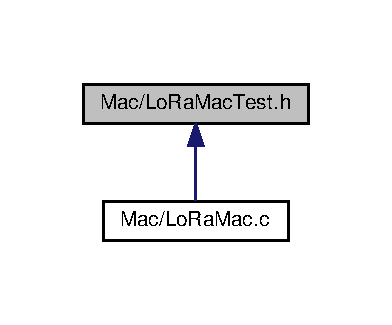
\includegraphics[width=188pt]{LoRaMacTest_8h__dep__incl}
\end{center}
\end{figure}
\subsection*{Functions}
\begin{DoxyCompactItemize}
\item 
void \hyperlink{group__LORAMACTEST_ga3e8dc79232b2c86d12d8b4191324283d}{Lo\+Ra\+Mac\+Test\+Rx\+Windows\+On} (bool enable)
\begin{DoxyCompactList}\small\item\em Enabled or disables the reception windows. \end{DoxyCompactList}\item 
void \hyperlink{group__LORAMACTEST_ga191314e00a8a27f426427473ba6821a7}{Lo\+Ra\+Mac\+Test\+Set\+Mic} (uint16\+\_\+t tx\+Packet\+Counter)
\begin{DoxyCompactList}\small\item\em Enables the M\+IC field test. \end{DoxyCompactList}\item 
void \hyperlink{group__LORAMACTEST_gacee5e0492e548af9e1ec5a995e460865}{Lo\+Ra\+Mac\+Test\+Set\+Duty\+Cycle\+On} (bool enable)
\begin{DoxyCompactList}\small\item\em Enabled or disables the duty cycle. \end{DoxyCompactList}\item 
void \hyperlink{group__LORAMACTEST_ga8cf3cc21ea237c5620536cea2750463e}{Lo\+Ra\+Mac\+Test\+Set\+Channel} (uint8\+\_\+t channel)
\begin{DoxyCompactList}\small\item\em Sets the channel index. \end{DoxyCompactList}\end{DoxyCompactItemize}


\subsection{Detailed Description}
Lo\+Ra M\+AC layer test function implementation. 

\begin{DoxyCopyright}{Copyright}
Revised B\+SD License, see section L\+I\+C\+E\+N\+SE.
\end{DoxyCopyright}

\begin{DoxyCode}
  \_\_\_\_\_\_                              \_
 / \_\_\_\_\_)             \_              | |
( (\_\_\_\_  \_\_\_\_\_ \_\_\_\_ \_| |\_ \_\_\_\_\_  \_\_\_\_| |\_\_
 \(\backslash\)\_\_\_\_ \(\backslash\)| \_\_\_ |    (\_   \_) \_\_\_ |/ \_\_\_)  \_ \(\backslash\)
 \_\_\_\_\_) ) \_\_\_\_| | | || |\_| \_\_\_\_( (\_\_\_| | | |
(\_\_\_\_\_\_/|\_\_\_\_\_)\_|\_|\_| \(\backslash\)\_\_)\_\_\_\_\_)\(\backslash\)\_\_\_\_)\_| |\_|
(C)2013 Semtech

 \_\_\_ \_\_\_\_\_ \_   \_\_\_ \_  \_\_\_\_\_ \_\_\_  \_\_\_  \_\_\_ \_\_\_
/ \_\_|\_   \_/\_\(\backslash\) / \_\_| |/ / \_\_/ \_ \(\backslash\)| \_ \(\backslash\)/ \_\_| \_\_|
\(\backslash\)\_\_ \(\backslash\) | |/ \_ \(\backslash\) (\_\_| \textcolor{stringliteral}{' <| \_| (\_) |   / (\_\_| \_|}
\textcolor{stringliteral}{|\_\_\_/ |\_/\_/ \(\backslash\)\_\(\backslash\)\_\_\_|\_|\(\backslash\)\_\(\backslash\)\_| \(\backslash\)\_\_\_/|\_|\_\(\backslash\)\(\backslash\)\_\_\_|\_\_\_|}
\textcolor{stringliteral}{embedded.connectivity.solutions===============}
\end{DoxyCode}


\begin{DoxyAuthor}{Author}
Miguel Luis ( Semtech )

Gregory Cristian ( Semtech )

Daniel Jaeckle ( S\+T\+A\+C\+K\+F\+O\+R\+CE ) 
\end{DoxyAuthor}

\hypertarget{Region_8c}{}\section{Mac/region/\+Region.c File Reference}
\label{Region_8c}\index{Mac/region/\+Region.\+c@{Mac/region/\+Region.\+c}}
{\ttfamily \#include $<$stdbool.\+h$>$}\newline
{\ttfamily \#include $<$string.\+h$>$}\newline
{\ttfamily \#include $<$stdint.\+h$>$}\newline
{\ttfamily \#include \char`\"{}timer.\+h\char`\"{}}\newline
{\ttfamily \#include \char`\"{}Lo\+Ra\+Mac.\+h\char`\"{}}\newline
{\ttfamily \#include \char`\"{}Region.\+h\char`\"{}}\newline
Include dependency graph for Region.\+c\+:
\nopagebreak
\begin{figure}[H]
\begin{center}
\leavevmode
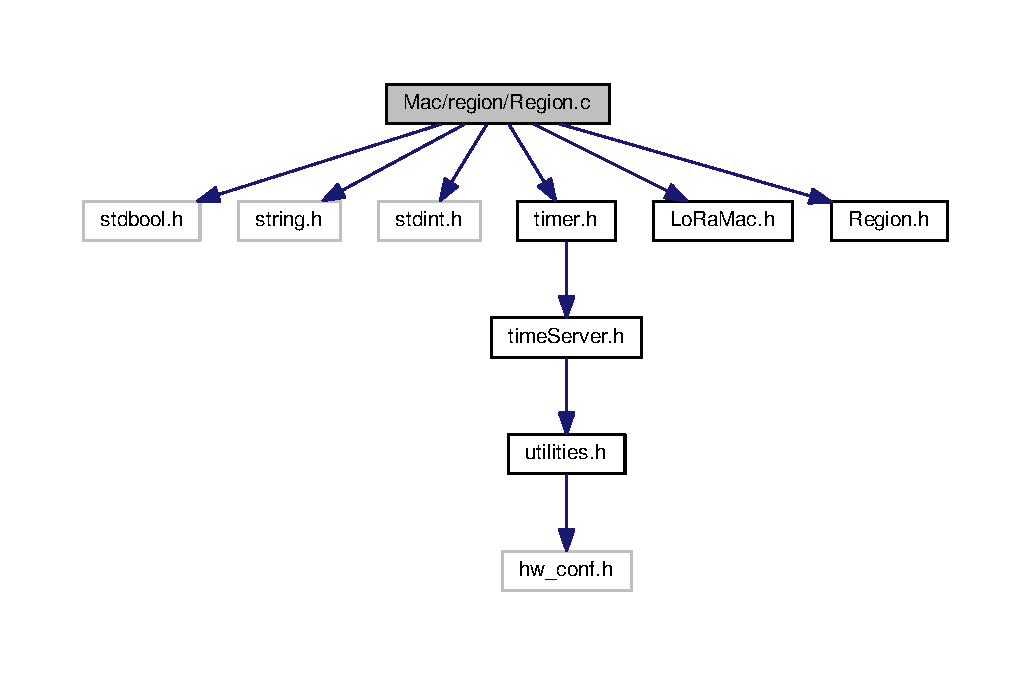
\includegraphics[width=350pt]{Region_8c__incl}
\end{center}
\end{figure}
\subsection*{Macros}
\begin{DoxyCompactItemize}
\item 
\#define \hyperlink{Region_8c_a85100d4eeeb40a55fe4c10aad2798ef6}{A\+S923\+\_\+\+I\+S\+\_\+\+A\+C\+T\+I\+VE}()
\item 
\#define \hyperlink{Region_8c_a8646b89faa806726db169c655722774d}{A\+S923\+\_\+\+G\+E\+T\+\_\+\+P\+H\+Y\+\_\+\+P\+A\+R\+AM}()
\item 
\#define \hyperlink{Region_8c_aa2f1c00c2d2ad8292046ed5ed9923046}{A\+S923\+\_\+\+S\+E\+T\+\_\+\+B\+A\+N\+D\+\_\+\+T\+X\+\_\+\+D\+O\+NE}()
\item 
\#define \hyperlink{Region_8c_abbf363ff3aa9fb94c3ef7aba1bc4e48b}{A\+S923\+\_\+\+I\+N\+I\+T\+\_\+\+D\+E\+F\+A\+U\+L\+TS}()
\item 
\#define \hyperlink{Region_8c_abfba3d5f7762291f490940d8ff6b5487}{A\+S923\+\_\+\+V\+E\+R\+I\+FY}()
\item 
\#define \hyperlink{Region_8c_ac79db5f796c4a24b7ea51e5b3ac24c02}{A\+S923\+\_\+\+A\+P\+P\+L\+Y\+\_\+\+C\+F\+\_\+\+L\+I\+ST}()
\item 
\#define \hyperlink{Region_8c_a4722cdf1c3244ded88149e0cb0ef7792}{A\+S923\+\_\+\+C\+H\+A\+N\+\_\+\+M\+A\+S\+K\+\_\+\+S\+ET}()
\item 
\#define \hyperlink{Region_8c_a19e9c439af66a22efb0139d66dc60725}{A\+S923\+\_\+\+A\+D\+R\+\_\+\+N\+E\+XT}()
\item 
\#define \hyperlink{Region_8c_a03d5b3506606658a60fec44313773ccf}{A\+S923\+\_\+\+C\+O\+M\+P\+U\+T\+E\+\_\+\+R\+X\+\_\+\+W\+I\+N\+D\+O\+W\+\_\+\+P\+A\+R\+A\+M\+E\+T\+E\+RS}()
\item 
\#define \hyperlink{Region_8c_a73acc27cb16faae8674708556d38892f}{A\+S923\+\_\+\+R\+X\+\_\+\+C\+O\+N\+F\+IG}()
\item 
\#define \hyperlink{Region_8c_ad794f8b2fd4d7d5e0e6bec408d85c3b3}{A\+S923\+\_\+\+T\+X\+\_\+\+C\+O\+N\+F\+IG}()
\item 
\#define \hyperlink{Region_8c_ae246f17ed0d848225dff693b0ba064f5}{A\+S923\+\_\+\+L\+I\+N\+K\+\_\+\+A\+D\+R\+\_\+\+R\+EQ}()
\item 
\#define \hyperlink{Region_8c_a8f3059682517c8eb5324b0a0f2996c82}{A\+S923\+\_\+\+R\+X\+\_\+\+P\+A\+R\+A\+M\+\_\+\+S\+E\+T\+U\+P\+\_\+\+R\+EQ}()
\item 
\#define \hyperlink{Region_8c_a1ef9f8348eba42a05df97ad9f44cd320}{A\+S923\+\_\+\+N\+E\+W\+\_\+\+C\+H\+A\+N\+N\+E\+L\+\_\+\+R\+EQ}()
\item 
\#define \hyperlink{Region_8c_a7e69cebe76337b430beefe81ea2f2778}{A\+S923\+\_\+\+T\+X\+\_\+\+P\+A\+R\+A\+M\+\_\+\+S\+E\+T\+U\+P\+\_\+\+R\+EQ}()
\item 
\#define \hyperlink{Region_8c_ab3da3232202dfe0cc690177f70fb1a2e}{A\+S923\+\_\+\+D\+L\+\_\+\+C\+H\+A\+N\+N\+E\+L\+\_\+\+R\+EQ}()
\item 
\#define \hyperlink{Region_8c_a9fc7f64a847307af6e86178f94ad35e7}{A\+S923\+\_\+\+A\+L\+T\+E\+R\+N\+A\+T\+E\+\_\+\+DR}()
\item 
\#define \hyperlink{Region_8c_ab1d11f983e2c4dc9ba4f482943f15b06}{A\+S923\+\_\+\+C\+A\+L\+C\+\_\+\+B\+A\+C\+K\+O\+FF}()
\item 
\#define \hyperlink{Region_8c_ac09ba658790d3e4184c2425642a80831}{A\+S923\+\_\+\+N\+E\+X\+T\+\_\+\+C\+H\+A\+N\+N\+EL}()
\item 
\#define \hyperlink{Region_8c_a5d5eaa86f0eb43b289f6a04be195dc8f}{A\+S923\+\_\+\+C\+H\+A\+N\+N\+E\+L\+\_\+\+A\+DD}()
\item 
\#define \hyperlink{Region_8c_aef31561789c92f75d8d281621cb725e0}{A\+S923\+\_\+\+C\+H\+A\+N\+N\+E\+L\+\_\+\+R\+E\+M\+O\+VE}()
\item 
\#define \hyperlink{Region_8c_a71a399c13093b5c11886cc051f4b30cb}{A\+S923\+\_\+\+S\+E\+T\+\_\+\+C\+O\+N\+T\+I\+N\+U\+O\+U\+S\+\_\+\+W\+A\+VE}()
\item 
\#define \hyperlink{Region_8c_aac665cf8c6806b24fe769e78f6eb2606}{A\+S923\+\_\+\+A\+P\+P\+L\+Y\+\_\+\+D\+R\+\_\+\+O\+F\+F\+S\+ET}()
\item 
\#define \hyperlink{Region_8c_a71cbcfb529cc4fb2d4fdd29c9dde2ca0}{A\+U915\+\_\+\+I\+S\+\_\+\+A\+C\+T\+I\+VE}()
\item 
\#define \hyperlink{Region_8c_ab6486b65901c40026631dceb38d97859}{A\+U915\+\_\+\+G\+E\+T\+\_\+\+P\+H\+Y\+\_\+\+P\+A\+R\+AM}()
\item 
\#define \hyperlink{Region_8c_ae1f2fcce477ca77f9f38fcb50385889d}{A\+U915\+\_\+\+S\+E\+T\+\_\+\+B\+A\+N\+D\+\_\+\+T\+X\+\_\+\+D\+O\+NE}()
\item 
\#define \hyperlink{Region_8c_a8bbb7226a1cfed5ea6821b1510748147}{A\+U915\+\_\+\+I\+N\+I\+T\+\_\+\+D\+E\+F\+A\+U\+L\+TS}()
\item 
\#define \hyperlink{Region_8c_aa44247bbd8a69c3fa4bef7a9fe751bbe}{A\+U915\+\_\+\+V\+E\+R\+I\+FY}()
\item 
\#define \hyperlink{Region_8c_a2c08d8ba366bf75d4d7cc1494a0e4cc0}{A\+U915\+\_\+\+A\+P\+P\+L\+Y\+\_\+\+C\+F\+\_\+\+L\+I\+ST}()
\item 
\#define \hyperlink{Region_8c_a766153eeac1b275c09b19cc4b188adb3}{A\+U915\+\_\+\+C\+H\+A\+N\+\_\+\+M\+A\+S\+K\+\_\+\+S\+ET}()
\item 
\#define \hyperlink{Region_8c_a46d035418f204f008be18b204dcf8a9b}{A\+U915\+\_\+\+A\+D\+R\+\_\+\+N\+E\+XT}()
\item 
\#define \hyperlink{Region_8c_ac08fef4c1a6694ab3d81e12a32ad2e78}{A\+U915\+\_\+\+C\+O\+M\+P\+U\+T\+E\+\_\+\+R\+X\+\_\+\+W\+I\+N\+D\+O\+W\+\_\+\+P\+A\+R\+A\+M\+E\+T\+E\+RS}()
\item 
\#define \hyperlink{Region_8c_aafdd1d07bd5b004cb8b0415a858f1134}{A\+U915\+\_\+\+R\+X\+\_\+\+C\+O\+N\+F\+IG}()
\item 
\#define \hyperlink{Region_8c_a994f1815f2fd0b0cf94ae7e8a39333d0}{A\+U915\+\_\+\+T\+X\+\_\+\+C\+O\+N\+F\+IG}()
\item 
\#define \hyperlink{Region_8c_a43fe119319d6a67a8ae12769fb1fb5d0}{A\+U915\+\_\+\+L\+I\+N\+K\+\_\+\+A\+D\+R\+\_\+\+R\+EQ}()
\item 
\#define \hyperlink{Region_8c_aada99a95996303e842541062a02ad5dc}{A\+U915\+\_\+\+R\+X\+\_\+\+P\+A\+R\+A\+M\+\_\+\+S\+E\+T\+U\+P\+\_\+\+R\+EQ}()
\item 
\#define \hyperlink{Region_8c_ac804a38748d50ef58f3a9de969eb8943}{A\+U915\+\_\+\+N\+E\+W\+\_\+\+C\+H\+A\+N\+N\+E\+L\+\_\+\+R\+EQ}()
\item 
\#define \hyperlink{Region_8c_a3ac80629bb68f70ad073c2569d002a1c}{A\+U915\+\_\+\+T\+X\+\_\+\+P\+A\+R\+A\+M\+\_\+\+S\+E\+T\+U\+P\+\_\+\+R\+EQ}()
\item 
\#define \hyperlink{Region_8c_ae3d382c3fe0a920ebbe45ed151c8e68f}{A\+U915\+\_\+\+D\+L\+\_\+\+C\+H\+A\+N\+N\+E\+L\+\_\+\+R\+EQ}()
\item 
\#define \hyperlink{Region_8c_a44bd9ed442b08a08d8955071c1062152}{A\+U915\+\_\+\+A\+L\+T\+E\+R\+N\+A\+T\+E\+\_\+\+DR}()
\item 
\#define \hyperlink{Region_8c_a27ecec930edfd7be6a001bbdf915a28f}{A\+U915\+\_\+\+C\+A\+L\+C\+\_\+\+B\+A\+C\+K\+O\+FF}()
\item 
\#define \hyperlink{Region_8c_aa574e30f345878b97922aea01895a22c}{A\+U915\+\_\+\+N\+E\+X\+T\+\_\+\+C\+H\+A\+N\+N\+EL}()
\item 
\#define \hyperlink{Region_8c_a0ba2b8453d60054388d0d55341e58079}{A\+U915\+\_\+\+C\+H\+A\+N\+N\+E\+L\+\_\+\+A\+DD}()
\item 
\#define \hyperlink{Region_8c_a769217b0ee44f46ba326d2f21139c313}{A\+U915\+\_\+\+C\+H\+A\+N\+N\+E\+L\+\_\+\+R\+E\+M\+O\+VE}()
\item 
\#define \hyperlink{Region_8c_aa07dbb2e5c7eb32553a116e8fc23dc4a}{A\+U915\+\_\+\+S\+E\+T\+\_\+\+C\+O\+N\+T\+I\+N\+U\+O\+U\+S\+\_\+\+W\+A\+VE}()
\item 
\#define \hyperlink{Region_8c_afc5439770aef2a86cb9f97d6749ff4fe}{A\+U915\+\_\+\+A\+P\+P\+L\+Y\+\_\+\+D\+R\+\_\+\+O\+F\+F\+S\+ET}()
\item 
\#define \hyperlink{Region_8c_ad762ad3d2426790152b07114999ca3f7}{C\+N470\+\_\+\+I\+S\+\_\+\+A\+C\+T\+I\+VE}()
\item 
\#define \hyperlink{Region_8c_a34e51818814f3d6a3002edea59b25145}{C\+N470\+\_\+\+G\+E\+T\+\_\+\+P\+H\+Y\+\_\+\+P\+A\+R\+AM}()
\item 
\#define \hyperlink{Region_8c_ac9f44855ac37a8f9ea7fc80cc9bdbfb2}{C\+N470\+\_\+\+S\+E\+T\+\_\+\+B\+A\+N\+D\+\_\+\+T\+X\+\_\+\+D\+O\+NE}()
\item 
\#define \hyperlink{Region_8c_a3ca20e316d44b9de75598144390898c7}{C\+N470\+\_\+\+I\+N\+I\+T\+\_\+\+D\+E\+F\+A\+U\+L\+TS}()
\item 
\#define \hyperlink{Region_8c_a6566e70c6ef6b60e64566deb0c8e2eb2}{C\+N470\+\_\+\+V\+E\+R\+I\+FY}()
\item 
\#define \hyperlink{Region_8c_a5a73e26d3a21c54d0575af34a3198725}{C\+N470\+\_\+\+A\+P\+P\+L\+Y\+\_\+\+C\+F\+\_\+\+L\+I\+ST}()
\item 
\#define \hyperlink{Region_8c_a4f26fa505964e6e12dcafd6cf40c40b1}{C\+N470\+\_\+\+C\+H\+A\+N\+\_\+\+M\+A\+S\+K\+\_\+\+S\+ET}()
\item 
\#define \hyperlink{Region_8c_a53b706cbdcca5434468885a6fc6b46cd}{C\+N470\+\_\+\+A\+D\+R\+\_\+\+N\+E\+XT}()
\item 
\#define \hyperlink{Region_8c_a763e8b65abfdfbd73c8f53ecaa3684ef}{C\+N470\+\_\+\+C\+O\+M\+P\+U\+T\+E\+\_\+\+R\+X\+\_\+\+W\+I\+N\+D\+O\+W\+\_\+\+P\+A\+R\+A\+M\+E\+T\+E\+RS}()
\item 
\#define \hyperlink{Region_8c_a4552b1326c0f45fc8a3acce13224430f}{C\+N470\+\_\+\+R\+X\+\_\+\+C\+O\+N\+F\+IG}()
\item 
\#define \hyperlink{Region_8c_a439995c1d3f77fb52bc5a3e23b90394c}{C\+N470\+\_\+\+T\+X\+\_\+\+C\+O\+N\+F\+IG}()
\item 
\#define \hyperlink{Region_8c_ac3054ecc7ae17b2a9df9ab004683bd42}{C\+N470\+\_\+\+L\+I\+N\+K\+\_\+\+A\+D\+R\+\_\+\+R\+EQ}()
\item 
\#define \hyperlink{Region_8c_a689749447c72acfebb9411e793480d1d}{C\+N470\+\_\+\+R\+X\+\_\+\+P\+A\+R\+A\+M\+\_\+\+S\+E\+T\+U\+P\+\_\+\+R\+EQ}()
\item 
\#define \hyperlink{Region_8c_adf06e4f758d87411422845db6d17caba}{C\+N470\+\_\+\+N\+E\+W\+\_\+\+C\+H\+A\+N\+N\+E\+L\+\_\+\+R\+EQ}()
\item 
\#define \hyperlink{Region_8c_a55cde63ba4973860df75664a1cbb0406}{C\+N470\+\_\+\+T\+X\+\_\+\+P\+A\+R\+A\+M\+\_\+\+S\+E\+T\+U\+P\+\_\+\+R\+EQ}()
\item 
\#define \hyperlink{Region_8c_aad78d0f78195e1ea67a08d88e558b5d6}{C\+N470\+\_\+\+D\+L\+\_\+\+C\+H\+A\+N\+N\+E\+L\+\_\+\+R\+EQ}()
\item 
\#define \hyperlink{Region_8c_a72d269f5dced042d846b04f9d9074654}{C\+N470\+\_\+\+A\+L\+T\+E\+R\+N\+A\+T\+E\+\_\+\+DR}()
\item 
\#define \hyperlink{Region_8c_a99b1e842dd32f8a305783fb1df555c5f}{C\+N470\+\_\+\+C\+A\+L\+C\+\_\+\+B\+A\+C\+K\+O\+FF}()
\item 
\#define \hyperlink{Region_8c_af520ce122a5bdc67162e543ecd73e25d}{C\+N470\+\_\+\+N\+E\+X\+T\+\_\+\+C\+H\+A\+N\+N\+EL}()
\item 
\#define \hyperlink{Region_8c_a96d482c3b50ce6c743f30529a6a232ad}{C\+N470\+\_\+\+C\+H\+A\+N\+N\+E\+L\+\_\+\+A\+DD}()
\item 
\#define \hyperlink{Region_8c_aad42e58f0a57ce809648ff6796c591ce}{C\+N470\+\_\+\+C\+H\+A\+N\+N\+E\+L\+\_\+\+R\+E\+M\+O\+VE}()
\item 
\#define \hyperlink{Region_8c_a74d3d97314de8e2b1eb9879c29dd5f3f}{C\+N470\+\_\+\+S\+E\+T\+\_\+\+C\+O\+N\+T\+I\+N\+U\+O\+U\+S\+\_\+\+W\+A\+VE}()
\item 
\#define \hyperlink{Region_8c_a0444c565a20ceeda03c6e047d0e7dbe2}{C\+N470\+\_\+\+A\+P\+P\+L\+Y\+\_\+\+D\+R\+\_\+\+O\+F\+F\+S\+ET}()
\item 
\#define \hyperlink{Region_8c_a0f35a620cfb65d6e2d9a7c1e308cd5d7}{C\+N779\+\_\+\+I\+S\+\_\+\+A\+C\+T\+I\+VE}()
\item 
\#define \hyperlink{Region_8c_a5a4a779a365decfa2899f6057bc28089}{C\+N779\+\_\+\+G\+E\+T\+\_\+\+P\+H\+Y\+\_\+\+P\+A\+R\+AM}()
\item 
\#define \hyperlink{Region_8c_ab8b47c2099f6c091399ad29bd81016af}{C\+N779\+\_\+\+S\+E\+T\+\_\+\+B\+A\+N\+D\+\_\+\+T\+X\+\_\+\+D\+O\+NE}()
\item 
\#define \hyperlink{Region_8c_a7a78bccace6549bce4db9c7130a20459}{C\+N779\+\_\+\+I\+N\+I\+T\+\_\+\+D\+E\+F\+A\+U\+L\+TS}()
\item 
\#define \hyperlink{Region_8c_abc52f9ec1e4c997fbc6646d6e530e656}{C\+N779\+\_\+\+V\+E\+R\+I\+FY}()
\item 
\#define \hyperlink{Region_8c_ac697ae1b5b495e83a6c0183b042b36c2}{C\+N779\+\_\+\+A\+P\+P\+L\+Y\+\_\+\+C\+F\+\_\+\+L\+I\+ST}()
\item 
\#define \hyperlink{Region_8c_a62740b24d80ecf11c7af43f594046760}{C\+N779\+\_\+\+C\+H\+A\+N\+\_\+\+M\+A\+S\+K\+\_\+\+S\+ET}()
\item 
\#define \hyperlink{Region_8c_a87b11ac3d96d8d3ffee7ec505dedbfd0}{C\+N779\+\_\+\+A\+D\+R\+\_\+\+N\+E\+XT}()
\item 
\#define \hyperlink{Region_8c_aeba782c7c0d8a7fc0fb908c1acac746c}{C\+N779\+\_\+\+C\+O\+M\+P\+U\+T\+E\+\_\+\+R\+X\+\_\+\+W\+I\+N\+D\+O\+W\+\_\+\+P\+A\+R\+A\+M\+E\+T\+E\+RS}()
\item 
\#define \hyperlink{Region_8c_a8610a888ce6187b810df4fa74c3731eb}{C\+N779\+\_\+\+R\+X\+\_\+\+C\+O\+N\+F\+IG}()
\item 
\#define \hyperlink{Region_8c_a8f87695cd4312ff253702760fce2fb03}{C\+N779\+\_\+\+T\+X\+\_\+\+C\+O\+N\+F\+IG}()
\item 
\#define \hyperlink{Region_8c_ace3dcde7b7f960ab453c7f02cac61572}{C\+N779\+\_\+\+L\+I\+N\+K\+\_\+\+A\+D\+R\+\_\+\+R\+EQ}()
\item 
\#define \hyperlink{Region_8c_a097eafca373c7905800c550e0c2796e7}{C\+N779\+\_\+\+R\+X\+\_\+\+P\+A\+R\+A\+M\+\_\+\+S\+E\+T\+U\+P\+\_\+\+R\+EQ}()
\item 
\#define \hyperlink{Region_8c_adf4be8140da6914b2167672060f71fc2}{C\+N779\+\_\+\+N\+E\+W\+\_\+\+C\+H\+A\+N\+N\+E\+L\+\_\+\+R\+EQ}()
\item 
\#define \hyperlink{Region_8c_a664fcbc639c1c0282bbe2349ba3aad95}{C\+N779\+\_\+\+T\+X\+\_\+\+P\+A\+R\+A\+M\+\_\+\+S\+E\+T\+U\+P\+\_\+\+R\+EQ}()
\item 
\#define \hyperlink{Region_8c_a9f660886c5ac764763d3ef04f06b18e1}{C\+N779\+\_\+\+D\+L\+\_\+\+C\+H\+A\+N\+N\+E\+L\+\_\+\+R\+EQ}()
\item 
\#define \hyperlink{Region_8c_ada1de89215c8ec0cc74ee666691ee25f}{C\+N779\+\_\+\+A\+L\+T\+E\+R\+N\+A\+T\+E\+\_\+\+DR}()
\item 
\#define \hyperlink{Region_8c_a5bba41f07d1cc6ae63f2d4fd014f4a33}{C\+N779\+\_\+\+C\+A\+L\+C\+\_\+\+B\+A\+C\+K\+O\+FF}()
\item 
\#define \hyperlink{Region_8c_a8f32f723130114c571f006ca26a1fd1c}{C\+N779\+\_\+\+N\+E\+X\+T\+\_\+\+C\+H\+A\+N\+N\+EL}()
\item 
\#define \hyperlink{Region_8c_a80f9cc9bcab66e181639a3fc481de236}{C\+N779\+\_\+\+C\+H\+A\+N\+N\+E\+L\+\_\+\+A\+DD}()
\item 
\#define \hyperlink{Region_8c_a3df278ad93bb55f2e38572cce5fdd7c7}{C\+N779\+\_\+\+C\+H\+A\+N\+N\+E\+L\+\_\+\+R\+E\+M\+O\+VE}()
\item 
\#define \hyperlink{Region_8c_af0cd48e0631611265f7cebb45bb3954b}{C\+N779\+\_\+\+S\+E\+T\+\_\+\+C\+O\+N\+T\+I\+N\+U\+O\+U\+S\+\_\+\+W\+A\+VE}()
\item 
\#define \hyperlink{Region_8c_aa22f53681baaa63124c0cb0b4d44fefb}{C\+N779\+\_\+\+A\+P\+P\+L\+Y\+\_\+\+D\+R\+\_\+\+O\+F\+F\+S\+ET}()
\item 
\#define \hyperlink{Region_8c_a134d2c22f0d78f567707c5fae366a23e}{E\+U433\+\_\+\+I\+S\+\_\+\+A\+C\+T\+I\+VE}()
\item 
\#define \hyperlink{Region_8c_af1211cf2b1235d1561c3da107a2b8462}{E\+U433\+\_\+\+G\+E\+T\+\_\+\+P\+H\+Y\+\_\+\+P\+A\+R\+AM}()
\item 
\#define \hyperlink{Region_8c_a698f3633e9fbd010f663aeb6a74b6766}{E\+U433\+\_\+\+S\+E\+T\+\_\+\+B\+A\+N\+D\+\_\+\+T\+X\+\_\+\+D\+O\+NE}()
\item 
\#define \hyperlink{Region_8c_a0695b0658b217595d36c85d2cac1f2a5}{E\+U433\+\_\+\+I\+N\+I\+T\+\_\+\+D\+E\+F\+A\+U\+L\+TS}()
\item 
\#define \hyperlink{Region_8c_a6e9f922aca2e8d831b5d8e23cca823c0}{E\+U433\+\_\+\+V\+E\+R\+I\+FY}()
\item 
\#define \hyperlink{Region_8c_a15d988281b0937765c297d5b69364c2f}{E\+U433\+\_\+\+A\+P\+P\+L\+Y\+\_\+\+C\+F\+\_\+\+L\+I\+ST}()
\item 
\#define \hyperlink{Region_8c_ae4e1241ba5c4670ced5b237fedcea81a}{E\+U433\+\_\+\+C\+H\+A\+N\+\_\+\+M\+A\+S\+K\+\_\+\+S\+ET}()
\item 
\#define \hyperlink{Region_8c_ae98d5bca996cbce199c9300614242a8c}{E\+U433\+\_\+\+A\+D\+R\+\_\+\+N\+E\+XT}()
\item 
\#define \hyperlink{Region_8c_ae0d51789234badb243d249a1f2409a32}{E\+U433\+\_\+\+C\+O\+M\+P\+U\+T\+E\+\_\+\+R\+X\+\_\+\+W\+I\+N\+D\+O\+W\+\_\+\+P\+A\+R\+A\+M\+E\+T\+E\+RS}()
\item 
\#define \hyperlink{Region_8c_a0ace3254401c17e90384ecd58e0914fc}{E\+U433\+\_\+\+R\+X\+\_\+\+C\+O\+N\+F\+IG}()
\item 
\#define \hyperlink{Region_8c_a434369c5916b8f408310dfb799b7aada}{E\+U433\+\_\+\+T\+X\+\_\+\+C\+O\+N\+F\+IG}()
\item 
\#define \hyperlink{Region_8c_a4cdd9a5b865dd2305a88fee14aca650d}{E\+U433\+\_\+\+L\+I\+N\+K\+\_\+\+A\+D\+R\+\_\+\+R\+EQ}()
\item 
\#define \hyperlink{Region_8c_aa7807061153c60c17c01ec0525b1b1aa}{E\+U433\+\_\+\+R\+X\+\_\+\+P\+A\+R\+A\+M\+\_\+\+S\+E\+T\+U\+P\+\_\+\+R\+EQ}()
\item 
\#define \hyperlink{Region_8c_a2d68e75fcb440f3710dd64d004839b65}{E\+U433\+\_\+\+N\+E\+W\+\_\+\+C\+H\+A\+N\+N\+E\+L\+\_\+\+R\+EQ}()
\item 
\#define \hyperlink{Region_8c_a2c9f9a96f6d4b3d82a694968e7c87186}{E\+U433\+\_\+\+T\+X\+\_\+\+P\+A\+R\+A\+M\+\_\+\+S\+E\+T\+U\+P\+\_\+\+R\+EQ}()
\item 
\#define \hyperlink{Region_8c_a7901af3a15fcd0b1f4c441f954707a65}{E\+U433\+\_\+\+D\+L\+\_\+\+C\+H\+A\+N\+N\+E\+L\+\_\+\+R\+EQ}()
\item 
\#define \hyperlink{Region_8c_aea032b0029fae6249afb16fe69a46387}{E\+U433\+\_\+\+A\+L\+T\+E\+R\+N\+A\+T\+E\+\_\+\+DR}()
\item 
\#define \hyperlink{Region_8c_a1c27ca0eaaa6fd93f6604733330f2181}{E\+U433\+\_\+\+C\+A\+L\+C\+\_\+\+B\+A\+C\+K\+O\+FF}()
\item 
\#define \hyperlink{Region_8c_aa7515e1470cb7f1e7fca9ae72049b898}{E\+U433\+\_\+\+N\+E\+X\+T\+\_\+\+C\+H\+A\+N\+N\+EL}()
\item 
\#define \hyperlink{Region_8c_aa62815760fdcc436cc00dfa8d84a15bd}{E\+U433\+\_\+\+C\+H\+A\+N\+N\+E\+L\+\_\+\+A\+DD}()
\item 
\#define \hyperlink{Region_8c_a05d2373ec17f4c84eb7b70d2cdc0f80f}{E\+U433\+\_\+\+C\+H\+A\+N\+N\+E\+L\+\_\+\+R\+E\+M\+O\+VE}()
\item 
\#define \hyperlink{Region_8c_a69d826d96191caf0480fd056efd3190f}{E\+U433\+\_\+\+S\+E\+T\+\_\+\+C\+O\+N\+T\+I\+N\+U\+O\+U\+S\+\_\+\+W\+A\+VE}()
\item 
\#define \hyperlink{Region_8c_af72c8d5a2d6db95d0151646309b15a30}{E\+U433\+\_\+\+A\+P\+P\+L\+Y\+\_\+\+D\+R\+\_\+\+O\+F\+F\+S\+ET}()
\item 
\#define \hyperlink{Region_8c_a4d7a2a53ddede644503b7b3a7bb7a487}{E\+U868\+\_\+\+I\+S\+\_\+\+A\+C\+T\+I\+VE}()
\item 
\#define \hyperlink{Region_8c_a111b83453324fea706c887ef27c77a48}{E\+U868\+\_\+\+G\+E\+T\+\_\+\+P\+H\+Y\+\_\+\+P\+A\+R\+AM}()
\item 
\#define \hyperlink{Region_8c_a35e93bed3f1d14efdb87b32e86d251dd}{E\+U868\+\_\+\+S\+E\+T\+\_\+\+B\+A\+N\+D\+\_\+\+T\+X\+\_\+\+D\+O\+NE}()
\item 
\#define \hyperlink{Region_8c_ac19aa144614734658477e56d454897cd}{E\+U868\+\_\+\+I\+N\+I\+T\+\_\+\+D\+E\+F\+A\+U\+L\+TS}()
\item 
\#define \hyperlink{Region_8c_a91c0997e5b0ba32967509ccd910a8ad9}{E\+U868\+\_\+\+V\+E\+R\+I\+FY}()
\item 
\#define \hyperlink{Region_8c_a0c585341c69141ee72c35840888b4a48}{E\+U868\+\_\+\+A\+P\+P\+L\+Y\+\_\+\+C\+F\+\_\+\+L\+I\+ST}()
\item 
\#define \hyperlink{Region_8c_a9cc3111c3a3e5b8ae2f76f80cc2bb0a1}{E\+U868\+\_\+\+C\+H\+A\+N\+\_\+\+M\+A\+S\+K\+\_\+\+S\+ET}()
\item 
\#define \hyperlink{Region_8c_a02c768ba60ee7bfba2a88394f48a999e}{E\+U868\+\_\+\+A\+D\+R\+\_\+\+N\+E\+XT}()
\item 
\#define \hyperlink{Region_8c_a1f128c6c64d64aad78e73b6514fc70d0}{E\+U868\+\_\+\+C\+O\+M\+P\+U\+T\+E\+\_\+\+R\+X\+\_\+\+W\+I\+N\+D\+O\+W\+\_\+\+P\+A\+R\+A\+M\+E\+T\+E\+RS}()
\item 
\#define \hyperlink{Region_8c_a4d2e3d19816562e4a3335967b19e2a46}{E\+U868\+\_\+\+R\+X\+\_\+\+C\+O\+N\+F\+IG}()
\item 
\#define \hyperlink{Region_8c_a1249040bdab4db30a7a92536e24f4399}{E\+U868\+\_\+\+T\+X\+\_\+\+C\+O\+N\+F\+IG}()
\item 
\#define \hyperlink{Region_8c_ad64f68873a16666af5753ddc751668ad}{E\+U868\+\_\+\+L\+I\+N\+K\+\_\+\+A\+D\+R\+\_\+\+R\+EQ}()
\item 
\#define \hyperlink{Region_8c_a06e8f6cafe16976839878b689fc03bed}{E\+U868\+\_\+\+R\+X\+\_\+\+P\+A\+R\+A\+M\+\_\+\+S\+E\+T\+U\+P\+\_\+\+R\+EQ}()
\item 
\#define \hyperlink{Region_8c_a9a4ae4f377ca4c9bc30e5c6977cf2e52}{E\+U868\+\_\+\+N\+E\+W\+\_\+\+C\+H\+A\+N\+N\+E\+L\+\_\+\+R\+EQ}()
\item 
\#define \hyperlink{Region_8c_ab6b9ba65d37c4c42b237be9164bd132f}{E\+U868\+\_\+\+T\+X\+\_\+\+P\+A\+R\+A\+M\+\_\+\+S\+E\+T\+U\+P\+\_\+\+R\+EQ}()
\item 
\#define \hyperlink{Region_8c_ab3cd0c5f292d0430e6c9bff2e335ffc4}{E\+U868\+\_\+\+D\+L\+\_\+\+C\+H\+A\+N\+N\+E\+L\+\_\+\+R\+EQ}()
\item 
\#define \hyperlink{Region_8c_aa7a1fb6ffbb2e441f77c1cc2a2a48de0}{E\+U868\+\_\+\+A\+L\+T\+E\+R\+N\+A\+T\+E\+\_\+\+DR}()
\item 
\#define \hyperlink{Region_8c_a7b32867ef9cb973f1c09b9ca39b3bdd5}{E\+U868\+\_\+\+C\+A\+L\+C\+\_\+\+B\+A\+C\+K\+O\+FF}()
\item 
\#define \hyperlink{Region_8c_a4e2f3569361ac1903dbf503348d11533}{E\+U868\+\_\+\+N\+E\+X\+T\+\_\+\+C\+H\+A\+N\+N\+EL}()
\item 
\#define \hyperlink{Region_8c_af2ed62cb2303216857b49588cc46c475}{E\+U868\+\_\+\+C\+H\+A\+N\+N\+E\+L\+\_\+\+A\+DD}()
\item 
\#define \hyperlink{Region_8c_a8c8f3aaa13109cc1d5e02135c53bdb7b}{E\+U868\+\_\+\+C\+H\+A\+N\+N\+E\+L\+\_\+\+R\+E\+M\+O\+VE}()
\item 
\#define \hyperlink{Region_8c_a97df2998776f274849ccbda3fb7bfebe}{E\+U868\+\_\+\+S\+E\+T\+\_\+\+C\+O\+N\+T\+I\+N\+U\+O\+U\+S\+\_\+\+W\+A\+VE}()
\item 
\#define \hyperlink{Region_8c_acfa1718b39b5cf3ead93ad200757ad0e}{E\+U868\+\_\+\+A\+P\+P\+L\+Y\+\_\+\+D\+R\+\_\+\+O\+F\+F\+S\+ET}()
\item 
\#define \hyperlink{Region_8c_a20afbfd9d9cada0d5a0a0c61ba0ab3a4}{K\+R920\+\_\+\+I\+S\+\_\+\+A\+C\+T\+I\+VE}()
\item 
\#define \hyperlink{Region_8c_a4544673fcff90d970b221e710013fe28}{K\+R920\+\_\+\+G\+E\+T\+\_\+\+P\+H\+Y\+\_\+\+P\+A\+R\+AM}()
\item 
\#define \hyperlink{Region_8c_a54d8766cece3796a3ad5ce10132b2215}{K\+R920\+\_\+\+S\+E\+T\+\_\+\+B\+A\+N\+D\+\_\+\+T\+X\+\_\+\+D\+O\+NE}()
\item 
\#define \hyperlink{Region_8c_a62f53ef325d4eb50f2a9bdeb023a1be6}{K\+R920\+\_\+\+I\+N\+I\+T\+\_\+\+D\+E\+F\+A\+U\+L\+TS}()
\item 
\#define \hyperlink{Region_8c_aa03ac633451ba83602a2131d9dc6da07}{K\+R920\+\_\+\+V\+E\+R\+I\+FY}()
\item 
\#define \hyperlink{Region_8c_a3af8cb30155da9f7ae16a6b2fe3e0362}{K\+R920\+\_\+\+A\+P\+P\+L\+Y\+\_\+\+C\+F\+\_\+\+L\+I\+ST}()
\item 
\#define \hyperlink{Region_8c_ad1ffb1cb808ec7ce907259b34e1c9dd3}{K\+R920\+\_\+\+C\+H\+A\+N\+\_\+\+M\+A\+S\+K\+\_\+\+S\+ET}()
\item 
\#define \hyperlink{Region_8c_a6fcb2fc848647dfe89888f048ee63482}{K\+R920\+\_\+\+A\+D\+R\+\_\+\+N\+E\+XT}()
\item 
\#define \hyperlink{Region_8c_a2d4a782283310e29013f3dc0482ce5f2}{K\+R920\+\_\+\+C\+O\+M\+P\+U\+T\+E\+\_\+\+R\+X\+\_\+\+W\+I\+N\+D\+O\+W\+\_\+\+P\+A\+R\+A\+M\+E\+T\+E\+RS}()
\item 
\#define \hyperlink{Region_8c_a2a9975025919784fe97d42f08ba64f7c}{K\+R920\+\_\+\+R\+X\+\_\+\+C\+O\+N\+F\+IG}()
\item 
\#define \hyperlink{Region_8c_aaedd30f354a3e16810e4b0c948006475}{K\+R920\+\_\+\+T\+X\+\_\+\+C\+O\+N\+F\+IG}()
\item 
\#define \hyperlink{Region_8c_a1fe1179e0100d48e6be94eef952273d7}{K\+R920\+\_\+\+L\+I\+N\+K\+\_\+\+A\+D\+R\+\_\+\+R\+EQ}()
\item 
\#define \hyperlink{Region_8c_a62b78a69a9d58a1d73fd19c41444bfa9}{K\+R920\+\_\+\+R\+X\+\_\+\+P\+A\+R\+A\+M\+\_\+\+S\+E\+T\+U\+P\+\_\+\+R\+EQ}()
\item 
\#define \hyperlink{Region_8c_a32839b5a09ae3d434672da7db727cb35}{K\+R920\+\_\+\+N\+E\+W\+\_\+\+C\+H\+A\+N\+N\+E\+L\+\_\+\+R\+EQ}()
\item 
\#define \hyperlink{Region_8c_aa1a13ce3344e2b0d1e6be559a4883117}{K\+R920\+\_\+\+T\+X\+\_\+\+P\+A\+R\+A\+M\+\_\+\+S\+E\+T\+U\+P\+\_\+\+R\+EQ}()
\item 
\#define \hyperlink{Region_8c_a053b7e61a2eca94300e2e10a3ab772ee}{K\+R920\+\_\+\+D\+L\+\_\+\+C\+H\+A\+N\+N\+E\+L\+\_\+\+R\+EQ}()
\item 
\#define \hyperlink{Region_8c_a95b3a7d29d8071bb9f2b847fe03f8b3c}{K\+R920\+\_\+\+A\+L\+T\+E\+R\+N\+A\+T\+E\+\_\+\+DR}()
\item 
\#define \hyperlink{Region_8c_aa662ee1835dfde496d4be30e6c8ff5ae}{K\+R920\+\_\+\+C\+A\+L\+C\+\_\+\+B\+A\+C\+K\+O\+FF}()
\item 
\#define \hyperlink{Region_8c_ab48cb9a119c38d8457aaaaac502609ef}{K\+R920\+\_\+\+N\+E\+X\+T\+\_\+\+C\+H\+A\+N\+N\+EL}()
\item 
\#define \hyperlink{Region_8c_ab7434e6fcc2c85b90683c16943f3000e}{K\+R920\+\_\+\+C\+H\+A\+N\+N\+E\+L\+\_\+\+A\+DD}()
\item 
\#define \hyperlink{Region_8c_a836ba77166ae74458646a33459f80cd9}{K\+R920\+\_\+\+C\+H\+A\+N\+N\+E\+L\+\_\+\+R\+E\+M\+O\+VE}()
\item 
\#define \hyperlink{Region_8c_a3747c721ae612f314d6dce7b25e52568}{K\+R920\+\_\+\+S\+E\+T\+\_\+\+C\+O\+N\+T\+I\+N\+U\+O\+U\+S\+\_\+\+W\+A\+VE}()
\item 
\#define \hyperlink{Region_8c_ad93d53d003ef073afbd6c96dd9a3006f}{K\+R920\+\_\+\+A\+P\+P\+L\+Y\+\_\+\+D\+R\+\_\+\+O\+F\+F\+S\+ET}()
\item 
\#define \hyperlink{Region_8c_ac4c2eca1b07c045b3fb4fbd529bb5123}{I\+N865\+\_\+\+I\+S\+\_\+\+A\+C\+T\+I\+VE}()
\item 
\#define \hyperlink{Region_8c_aa7080fbf9a840dd9219f4c9eda87d48c}{I\+N865\+\_\+\+G\+E\+T\+\_\+\+P\+H\+Y\+\_\+\+P\+A\+R\+AM}()
\item 
\#define \hyperlink{Region_8c_aa57edf1e7a44ac7b32155c54a35d554c}{I\+N865\+\_\+\+S\+E\+T\+\_\+\+B\+A\+N\+D\+\_\+\+T\+X\+\_\+\+D\+O\+NE}()
\item 
\#define \hyperlink{Region_8c_a2acb5b53b6522584a1a451fb7a9e7c83}{I\+N865\+\_\+\+I\+N\+I\+T\+\_\+\+D\+E\+F\+A\+U\+L\+TS}()
\item 
\#define \hyperlink{Region_8c_a46fc58f69a666461c7411cf43fd50b3c}{I\+N865\+\_\+\+V\+E\+R\+I\+FY}()
\item 
\#define \hyperlink{Region_8c_abf85e136162f5e0a0a4008d2da4178a5}{I\+N865\+\_\+\+A\+P\+P\+L\+Y\+\_\+\+C\+F\+\_\+\+L\+I\+ST}()
\item 
\#define \hyperlink{Region_8c_a9424877e8dbdeaa1fe05b7577deb9ae3}{I\+N865\+\_\+\+C\+H\+A\+N\+\_\+\+M\+A\+S\+K\+\_\+\+S\+ET}()
\item 
\#define \hyperlink{Region_8c_a42e508348a83b21a02fb657da5ca963c}{I\+N865\+\_\+\+A\+D\+R\+\_\+\+N\+E\+XT}()
\item 
\#define \hyperlink{Region_8c_aee92c57a9fe3f12b609b7fca2f59fb6a}{I\+N865\+\_\+\+C\+O\+M\+P\+U\+T\+E\+\_\+\+R\+X\+\_\+\+W\+I\+N\+D\+O\+W\+\_\+\+P\+A\+R\+A\+M\+E\+T\+E\+RS}()
\item 
\#define \hyperlink{Region_8c_a40fb37d097243f03a9436365442fe701}{I\+N865\+\_\+\+R\+X\+\_\+\+C\+O\+N\+F\+IG}()
\item 
\#define \hyperlink{Region_8c_abbcd7f43652158d8a39fdca4800cff8c}{I\+N865\+\_\+\+T\+X\+\_\+\+C\+O\+N\+F\+IG}()
\item 
\#define \hyperlink{Region_8c_aca3c99a33e4e5a3cdb1c12285f1f9c71}{I\+N865\+\_\+\+L\+I\+N\+K\+\_\+\+A\+D\+R\+\_\+\+R\+EQ}()
\item 
\#define \hyperlink{Region_8c_a4c7ef27d56e61c1670617d1e5e1185e4}{I\+N865\+\_\+\+R\+X\+\_\+\+P\+A\+R\+A\+M\+\_\+\+S\+E\+T\+U\+P\+\_\+\+R\+EQ}()
\item 
\#define \hyperlink{Region_8c_a09b1a48bfc5be8eff2d59141469957c5}{I\+N865\+\_\+\+N\+E\+W\+\_\+\+C\+H\+A\+N\+N\+E\+L\+\_\+\+R\+EQ}()
\item 
\#define \hyperlink{Region_8c_a3ec5334722e47fb210be229138c2139f}{I\+N865\+\_\+\+T\+X\+\_\+\+P\+A\+R\+A\+M\+\_\+\+S\+E\+T\+U\+P\+\_\+\+R\+EQ}()
\item 
\#define \hyperlink{Region_8c_a358201e425669601c25c7cdb157808f2}{I\+N865\+\_\+\+D\+L\+\_\+\+C\+H\+A\+N\+N\+E\+L\+\_\+\+R\+EQ}()
\item 
\#define \hyperlink{Region_8c_a127631af76800012d4c9e606bbc121d9}{I\+N865\+\_\+\+A\+L\+T\+E\+R\+N\+A\+T\+E\+\_\+\+DR}()
\item 
\#define \hyperlink{Region_8c_a7fe6b9ff5a40fda204d473fc6fe800d0}{I\+N865\+\_\+\+C\+A\+L\+C\+\_\+\+B\+A\+C\+K\+O\+FF}()
\item 
\#define \hyperlink{Region_8c_a5e43ab6db5f02271d5719785b3246fce}{I\+N865\+\_\+\+N\+E\+X\+T\+\_\+\+C\+H\+A\+N\+N\+EL}()
\item 
\#define \hyperlink{Region_8c_addf2e20e43a738b7ca5fb9232c75088c}{I\+N865\+\_\+\+C\+H\+A\+N\+N\+E\+L\+\_\+\+A\+DD}()
\item 
\#define \hyperlink{Region_8c_a2b4c93d0e855fcfae15b243743d171a7}{I\+N865\+\_\+\+C\+H\+A\+N\+N\+E\+L\+\_\+\+R\+E\+M\+O\+VE}()
\item 
\#define \hyperlink{Region_8c_a0d7761ae9e1d8492be94547d5f872a30}{I\+N865\+\_\+\+S\+E\+T\+\_\+\+C\+O\+N\+T\+I\+N\+U\+O\+U\+S\+\_\+\+W\+A\+VE}()
\item 
\#define \hyperlink{Region_8c_a697c71026756e614a7200e161bb2e80c}{I\+N865\+\_\+\+A\+P\+P\+L\+Y\+\_\+\+D\+R\+\_\+\+O\+F\+F\+S\+ET}()
\item 
\#define \hyperlink{Region_8c_ab6c912e257f33d3cef96a4170339ec35}{U\+S915\+\_\+\+I\+S\+\_\+\+A\+C\+T\+I\+VE}()
\item 
\#define \hyperlink{Region_8c_a967ee384e993dfb297bae9faaa0441e1}{U\+S915\+\_\+\+G\+E\+T\+\_\+\+P\+H\+Y\+\_\+\+P\+A\+R\+AM}()
\item 
\#define \hyperlink{Region_8c_a929a61a1b7fd603734c1289c781c1899}{U\+S915\+\_\+\+S\+E\+T\+\_\+\+B\+A\+N\+D\+\_\+\+T\+X\+\_\+\+D\+O\+NE}()
\item 
\#define \hyperlink{Region_8c_a52b3e37b604e682672929d4e5402ee11}{U\+S915\+\_\+\+I\+N\+I\+T\+\_\+\+D\+E\+F\+A\+U\+L\+TS}()
\item 
\#define \hyperlink{Region_8c_a8424d4b82c68ae7b46207f103531dd9b}{U\+S915\+\_\+\+V\+E\+R\+I\+FY}()
\item 
\#define \hyperlink{Region_8c_ac2b109b2c62f11b521b73eae08776c64}{U\+S915\+\_\+\+A\+P\+P\+L\+Y\+\_\+\+C\+F\+\_\+\+L\+I\+ST}()
\item 
\#define \hyperlink{Region_8c_a89a2c04d25ebfe579dfd9d6b509b1532}{U\+S915\+\_\+\+C\+H\+A\+N\+\_\+\+M\+A\+S\+K\+\_\+\+S\+ET}()
\item 
\#define \hyperlink{Region_8c_ac87a99bd7d9f404fabb3800b6c26d8be}{U\+S915\+\_\+\+A\+D\+R\+\_\+\+N\+E\+XT}()
\item 
\#define \hyperlink{Region_8c_a32d1c9cc2d952d00d3192f3fe6a4fe19}{U\+S915\+\_\+\+C\+O\+M\+P\+U\+T\+E\+\_\+\+R\+X\+\_\+\+W\+I\+N\+D\+O\+W\+\_\+\+P\+A\+R\+A\+M\+E\+T\+E\+RS}()
\item 
\#define \hyperlink{Region_8c_af10c5f7593c417934026ea6baaa541f8}{U\+S915\+\_\+\+R\+X\+\_\+\+C\+O\+N\+F\+IG}()
\item 
\#define \hyperlink{Region_8c_ae61e8e9d988b7068b39d4feaa57eda96}{U\+S915\+\_\+\+T\+X\+\_\+\+C\+O\+N\+F\+IG}()
\item 
\#define \hyperlink{Region_8c_a68fe3a18751e225d832d2d9f940babd6}{U\+S915\+\_\+\+L\+I\+N\+K\+\_\+\+A\+D\+R\+\_\+\+R\+EQ}()
\item 
\#define \hyperlink{Region_8c_a7076363149902aba0164d6cecce3c984}{U\+S915\+\_\+\+R\+X\+\_\+\+P\+A\+R\+A\+M\+\_\+\+S\+E\+T\+U\+P\+\_\+\+R\+EQ}()
\item 
\#define \hyperlink{Region_8c_a554e49c74e3a7f31e706f2e0553b4b45}{U\+S915\+\_\+\+N\+E\+W\+\_\+\+C\+H\+A\+N\+N\+E\+L\+\_\+\+R\+EQ}()
\item 
\#define \hyperlink{Region_8c_a79860a403e84c63becffb70f5e6bf1e7}{U\+S915\+\_\+\+T\+X\+\_\+\+P\+A\+R\+A\+M\+\_\+\+S\+E\+T\+U\+P\+\_\+\+R\+EQ}()
\item 
\#define \hyperlink{Region_8c_a41b21067e184934051613bdf600c03f4}{U\+S915\+\_\+\+D\+L\+\_\+\+C\+H\+A\+N\+N\+E\+L\+\_\+\+R\+EQ}()
\item 
\#define \hyperlink{Region_8c_a8856aae4d1d782afb5a4e6c6cafc5830}{U\+S915\+\_\+\+A\+L\+T\+E\+R\+N\+A\+T\+E\+\_\+\+DR}()
\item 
\#define \hyperlink{Region_8c_a9a182860a57dfd53a8d8466eee22c443}{U\+S915\+\_\+\+C\+A\+L\+C\+\_\+\+B\+A\+C\+K\+O\+FF}()
\item 
\#define \hyperlink{Region_8c_a75ddbad2541ac4fb8f01c51e26f4295d}{U\+S915\+\_\+\+N\+E\+X\+T\+\_\+\+C\+H\+A\+N\+N\+EL}()
\item 
\#define \hyperlink{Region_8c_aa58471f710e2847f47062cc8659bb929}{U\+S915\+\_\+\+C\+H\+A\+N\+N\+E\+L\+\_\+\+A\+DD}()
\item 
\#define \hyperlink{Region_8c_adddc3bf5130a83ab73bdbe878f1e6fb4}{U\+S915\+\_\+\+C\+H\+A\+N\+N\+E\+L\+\_\+\+R\+E\+M\+O\+VE}()
\item 
\#define \hyperlink{Region_8c_a6fc55f98313266f4ae61ea83cc7bbedf}{U\+S915\+\_\+\+S\+E\+T\+\_\+\+C\+O\+N\+T\+I\+N\+U\+O\+U\+S\+\_\+\+W\+A\+VE}()
\item 
\#define \hyperlink{Region_8c_ad36f28ce7f722fdec18b836e789637c9}{U\+S915\+\_\+\+A\+P\+P\+L\+Y\+\_\+\+D\+R\+\_\+\+O\+F\+F\+S\+ET}()
\item 
\#define \hyperlink{Region_8c_aa78bb55003d581083319c0a0464c739f}{U\+S915\+\_\+\+H\+Y\+B\+R\+I\+D\+\_\+\+I\+S\+\_\+\+A\+C\+T\+I\+VE}()
\item 
\#define \hyperlink{Region_8c_a3dcf34fcccf2c17f972fc1030c54e1e8}{U\+S915\+\_\+\+H\+Y\+B\+R\+I\+D\+\_\+\+G\+E\+T\+\_\+\+P\+H\+Y\+\_\+\+P\+A\+R\+AM}()
\item 
\#define \hyperlink{Region_8c_a6f274a761064e9f4d439b0230fb3cbfc}{U\+S915\+\_\+\+H\+Y\+B\+R\+I\+D\+\_\+\+S\+E\+T\+\_\+\+B\+A\+N\+D\+\_\+\+T\+X\+\_\+\+D\+O\+NE}()
\item 
\#define \hyperlink{Region_8c_abc1487d10e8c54bcc07a3e4a215b2164}{U\+S915\+\_\+\+H\+Y\+B\+R\+I\+D\+\_\+\+I\+N\+I\+T\+\_\+\+D\+E\+F\+A\+U\+L\+TS}()
\item 
\#define \hyperlink{Region_8c_a3eca039556bf7a206ebab4bb70278665}{U\+S915\+\_\+\+H\+Y\+B\+R\+I\+D\+\_\+\+V\+E\+R\+I\+FY}()
\item 
\#define \hyperlink{Region_8c_a11664a90a25b4a3775c9496c6a667f8b}{U\+S915\+\_\+\+H\+Y\+B\+R\+I\+D\+\_\+\+A\+P\+P\+L\+Y\+\_\+\+C\+F\+\_\+\+L\+I\+ST}()
\item 
\#define \hyperlink{Region_8c_a340f6d133f5d91d3779431bc3b1f9b47}{U\+S915\+\_\+\+H\+Y\+B\+R\+I\+D\+\_\+\+C\+H\+A\+N\+\_\+\+M\+A\+S\+K\+\_\+\+S\+ET}()
\item 
\#define \hyperlink{Region_8c_a3fce860399b6ab0f34a875590760a6bb}{U\+S915\+\_\+\+H\+Y\+B\+R\+I\+D\+\_\+\+A\+D\+R\+\_\+\+N\+E\+XT}()
\item 
\#define \hyperlink{Region_8c_ac1d29c0374e889d274a0d0f34df5421c}{U\+S915\+\_\+\+H\+Y\+B\+R\+I\+D\+\_\+\+C\+O\+M\+P\+U\+T\+E\+\_\+\+R\+X\+\_\+\+W\+I\+N\+D\+O\+W\+\_\+\+P\+A\+R\+A\+M\+E\+T\+E\+RS}()
\item 
\#define \hyperlink{Region_8c_a39b4a5c018f71421e86ca3d586bcd0fd}{U\+S915\+\_\+\+H\+Y\+B\+R\+I\+D\+\_\+\+R\+X\+\_\+\+C\+O\+N\+F\+IG}()
\item 
\#define \hyperlink{Region_8c_a34f197635fc67ae14d0c58d220d75419}{U\+S915\+\_\+\+H\+Y\+B\+R\+I\+D\+\_\+\+T\+X\+\_\+\+C\+O\+N\+F\+IG}()
\item 
\#define \hyperlink{Region_8c_a0cf03e1a6cf240b24a33a57f2257277e}{U\+S915\+\_\+\+H\+Y\+B\+R\+I\+D\+\_\+\+L\+I\+N\+K\+\_\+\+A\+D\+R\+\_\+\+R\+EQ}()
\item 
\#define \hyperlink{Region_8c_a789b7c3b1ca9599c26eea1d0c6925eef}{U\+S915\+\_\+\+H\+Y\+B\+R\+I\+D\+\_\+\+R\+X\+\_\+\+P\+A\+R\+A\+M\+\_\+\+S\+E\+T\+U\+P\+\_\+\+R\+EQ}()
\item 
\#define \hyperlink{Region_8c_a8f83e0b3f55bd62389b83eafb0070229}{U\+S915\+\_\+\+H\+Y\+B\+R\+I\+D\+\_\+\+N\+E\+W\+\_\+\+C\+H\+A\+N\+N\+E\+L\+\_\+\+R\+EQ}()
\item 
\#define \hyperlink{Region_8c_a1713663f298ebc23a96d768a88c8c1f2}{U\+S915\+\_\+\+H\+Y\+B\+R\+I\+D\+\_\+\+T\+X\+\_\+\+P\+A\+R\+A\+M\+\_\+\+S\+E\+T\+U\+P\+\_\+\+R\+EQ}()
\item 
\#define \hyperlink{Region_8c_aef9ac229d0887516edae8f76692f02af}{U\+S915\+\_\+\+H\+Y\+B\+R\+I\+D\+\_\+\+D\+L\+\_\+\+C\+H\+A\+N\+N\+E\+L\+\_\+\+R\+EQ}()
\item 
\#define \hyperlink{Region_8c_aebcca0091950e77002659b6312250374}{U\+S915\+\_\+\+H\+Y\+B\+R\+I\+D\+\_\+\+A\+L\+T\+E\+R\+N\+A\+T\+E\+\_\+\+DR}()
\item 
\#define \hyperlink{Region_8c_af4ff50a968e17a6cb98438f8d2648e60}{U\+S915\+\_\+\+H\+Y\+B\+R\+I\+D\+\_\+\+C\+A\+L\+C\+\_\+\+B\+A\+C\+K\+O\+FF}()
\item 
\#define \hyperlink{Region_8c_ae724fce9fe182dad0cafe88662e886a4}{U\+S915\+\_\+\+H\+Y\+B\+R\+I\+D\+\_\+\+N\+E\+X\+T\+\_\+\+C\+H\+A\+N\+N\+EL}()
\item 
\#define \hyperlink{Region_8c_a3ab6a639ac6d0029010a1e071acfff58}{U\+S915\+\_\+\+H\+Y\+B\+R\+I\+D\+\_\+\+C\+H\+A\+N\+N\+E\+L\+\_\+\+A\+DD}()
\item 
\#define \hyperlink{Region_8c_a7e7e276bd4b63511d3849f52392673d3}{U\+S915\+\_\+\+H\+Y\+B\+R\+I\+D\+\_\+\+C\+H\+A\+N\+N\+E\+L\+\_\+\+R\+E\+M\+O\+VE}()
\item 
\#define \hyperlink{Region_8c_a0750d80b84147ed128c9634262d73ef2}{U\+S915\+\_\+\+H\+Y\+B\+R\+I\+D\+\_\+\+S\+E\+T\+\_\+\+C\+O\+N\+T\+I\+N\+U\+O\+U\+S\+\_\+\+W\+A\+VE}()
\item 
\#define \hyperlink{Region_8c_a2d47653d838754e29e8bb375db3f0372}{U\+S915\+\_\+\+H\+Y\+B\+R\+I\+D\+\_\+\+A\+P\+P\+L\+Y\+\_\+\+D\+R\+\_\+\+O\+F\+F\+S\+ET}()
\end{DoxyCompactItemize}
\subsection*{Functions}
\begin{DoxyCompactItemize}
\item 
bool \hyperlink{group__REGION_ga3e5cf2322f71f8f9973718024b6fb782}{Region\+Is\+Active} (\hyperlink{group__LORAMAC_ga80c48efda9ae02e14b58160d34a798dd}{Lo\+Ra\+Mac\+Region\+\_\+t} region)
\begin{DoxyCompactList}\small\item\em The function verifies if a region is active or not. If a region is not active, it cannot be used. \end{DoxyCompactList}\item 
\hyperlink{group__REGION_gaed159b26e5c4677236b6e8677019db30}{Phy\+Param\+\_\+t} \hyperlink{group__REGION_gafbd084611ba512035a6cbe7f3aa5857b}{Region\+Get\+Phy\+Param} (\hyperlink{group__LORAMAC_ga80c48efda9ae02e14b58160d34a798dd}{Lo\+Ra\+Mac\+Region\+\_\+t} region, \hyperlink{group__REGION_gab471483fff904f4f89bbc03f7fc380ab}{Get\+Phy\+Params\+\_\+t} $\ast$get\+Phy)
\begin{DoxyCompactList}\small\item\em The function gets a value of a specific phy attribute. \end{DoxyCompactList}\item 
void \hyperlink{group__REGION_gabdd176dcf0b7e7900377b4c1e183613d}{Region\+Set\+Band\+Tx\+Done} (\hyperlink{group__LORAMAC_ga80c48efda9ae02e14b58160d34a798dd}{Lo\+Ra\+Mac\+Region\+\_\+t} region, \hyperlink{group__REGION_gad0524aa0673c0814a71e7a4f9cade3fc}{Set\+Band\+Tx\+Done\+Params\+\_\+t} $\ast$tx\+Done)
\begin{DoxyCompactList}\small\item\em Updates the last TX done parameters of the current channel. \end{DoxyCompactList}\item 
void \hyperlink{group__REGION_ga54b1b27a8431cd146b4dc33a894ee6db}{Region\+Init\+Defaults} (\hyperlink{group__LORAMAC_ga80c48efda9ae02e14b58160d34a798dd}{Lo\+Ra\+Mac\+Region\+\_\+t} region, \hyperlink{group__REGION_gaddc73ae10673ec925724e7870363bda9}{Init\+Type\+\_\+t} type)
\begin{DoxyCompactList}\small\item\em Initializes the channels masks and the channels. \end{DoxyCompactList}\item 
bool \hyperlink{group__REGION_ga7c1ff626bc1131889fa8de3197a1093a}{Region\+Verify} (\hyperlink{group__LORAMAC_ga80c48efda9ae02e14b58160d34a798dd}{Lo\+Ra\+Mac\+Region\+\_\+t} region, \hyperlink{group__REGION_ga966d97bc2f25df1c09e92e60ef652276}{Verify\+Params\+\_\+t} $\ast$verify, \hyperlink{group__REGION_ga9445b07fdf77581ecfaf389970e635f8}{Phy\+Attribute\+\_\+t} phy\+Attribute)
\begin{DoxyCompactList}\small\item\em Verifies a parameter. \end{DoxyCompactList}\item 
void \hyperlink{group__REGION_gae3fdd82182ebb0704adb2a017d30e1f2}{Region\+Apply\+C\+F\+List} (\hyperlink{group__LORAMAC_ga80c48efda9ae02e14b58160d34a798dd}{Lo\+Ra\+Mac\+Region\+\_\+t} region, \hyperlink{group__REGION_ga71588e9ad07e34b78fa91d51881fd3c6}{Apply\+C\+F\+List\+Params\+\_\+t} $\ast$apply\+C\+F\+List)
\begin{DoxyCompactList}\small\item\em The function parses the input buffer and sets up the channels of the CF list. \end{DoxyCompactList}\item 
bool \hyperlink{group__REGION_ga795ed3c13f4c8d03e39298fd64e5b2df}{Region\+Chan\+Mask\+Set} (\hyperlink{group__LORAMAC_ga80c48efda9ae02e14b58160d34a798dd}{Lo\+Ra\+Mac\+Region\+\_\+t} region, \hyperlink{group__REGION_ga6d24f7da136006410827dfb29f6b9b9e}{Chan\+Mask\+Set\+Params\+\_\+t} $\ast$chan\+Mask\+Set)
\begin{DoxyCompactList}\small\item\em Sets a channels mask. \end{DoxyCompactList}\item 
bool \hyperlink{group__REGION_ga08cac64beeadd0555460ca5e756a0792}{Region\+Adr\+Next} (\hyperlink{group__LORAMAC_ga80c48efda9ae02e14b58160d34a798dd}{Lo\+Ra\+Mac\+Region\+\_\+t} region, \hyperlink{group__REGION_ga567c2742622326b350b4e91bbf61b4ce}{Adr\+Next\+Params\+\_\+t} $\ast$adr\+Next, int8\+\_\+t $\ast$dr\+Out, int8\+\_\+t $\ast$tx\+Pow\+Out, uint32\+\_\+t $\ast$adr\+Ack\+Counter)
\begin{DoxyCompactList}\small\item\em Calculates the next datarate to set, when A\+DR is on or off. \end{DoxyCompactList}\item 
void \hyperlink{group__REGION_gabd3eb4e7db9b7987fabb9568f733a2b9}{Region\+Compute\+Rx\+Window\+Parameters} (\hyperlink{group__LORAMAC_ga80c48efda9ae02e14b58160d34a798dd}{Lo\+Ra\+Mac\+Region\+\_\+t} region, int8\+\_\+t datarate, uint8\+\_\+t min\+Rx\+Symbols, uint32\+\_\+t rx\+Error, \hyperlink{group__REGION_ga375c038078dfcfc7ef14280021db719e}{Rx\+Config\+Params\+\_\+t} $\ast$rx\+Config\+Params)
\item 
bool \hyperlink{group__REGION_gaf89984d30239d6597190409068031465}{Region\+Rx\+Config} (\hyperlink{group__LORAMAC_ga80c48efda9ae02e14b58160d34a798dd}{Lo\+Ra\+Mac\+Region\+\_\+t} region, \hyperlink{group__REGION_ga375c038078dfcfc7ef14280021db719e}{Rx\+Config\+Params\+\_\+t} $\ast$rx\+Config, int8\+\_\+t $\ast$datarate)
\begin{DoxyCompactList}\small\item\em Configuration of the RX windows. \end{DoxyCompactList}\item 
bool \hyperlink{group__REGION_ga9a4b01301e0f6f6880dc6a651c062ad0}{Region\+Tx\+Config} (\hyperlink{group__LORAMAC_ga80c48efda9ae02e14b58160d34a798dd}{Lo\+Ra\+Mac\+Region\+\_\+t} region, \hyperlink{group__REGION_gabed730d4d04b0b60d4b6d1966d3f21d3}{Tx\+Config\+Params\+\_\+t} $\ast$tx\+Config, int8\+\_\+t $\ast$tx\+Power, \hyperlink{utilities_8h_a4215ca43d3e953099ea758ce428599d0}{Timer\+Time\+\_\+t} $\ast$tx\+Time\+On\+Air)
\begin{DoxyCompactList}\small\item\em TX configuration. \end{DoxyCompactList}\item 
uint8\+\_\+t \hyperlink{group__REGION_gae82a94e6d4141122e1a20b5ba1936c8e}{Region\+Link\+Adr\+Req} (\hyperlink{group__LORAMAC_ga80c48efda9ae02e14b58160d34a798dd}{Lo\+Ra\+Mac\+Region\+\_\+t} region, \hyperlink{group__REGION_gad4af503e8d4de1846129e26a799a1e8e}{Link\+Adr\+Req\+Params\+\_\+t} $\ast$link\+Adr\+Req, int8\+\_\+t $\ast$dr\+Out, int8\+\_\+t $\ast$tx\+Pow\+Out, uint8\+\_\+t $\ast$nb\+Rep\+Out, uint8\+\_\+t $\ast$nb\+Bytes\+Parsed)
\begin{DoxyCompactList}\small\item\em The function processes a Link A\+DR Request. \end{DoxyCompactList}\item 
uint8\+\_\+t \hyperlink{group__REGION_ga485a820155fded42235a0d14d5918a7d}{Region\+Rx\+Param\+Setup\+Req} (\hyperlink{group__LORAMAC_ga80c48efda9ae02e14b58160d34a798dd}{Lo\+Ra\+Mac\+Region\+\_\+t} region, \hyperlink{group__REGION_ga7165f282c670c728c36d534df2285157}{Rx\+Param\+Setup\+Req\+Params\+\_\+t} $\ast$rx\+Param\+Setup\+Req)
\begin{DoxyCompactList}\small\item\em The function processes a RX Parameter Setup Request. \end{DoxyCompactList}\item 
uint8\+\_\+t \hyperlink{group__REGION_gadca654538335b4395c8d54642b83e2d4}{Region\+New\+Channel\+Req} (\hyperlink{group__LORAMAC_ga80c48efda9ae02e14b58160d34a798dd}{Lo\+Ra\+Mac\+Region\+\_\+t} region, \hyperlink{group__REGION_gae2abcdb6dbb843c9faf5fd3009eca9d6}{New\+Channel\+Req\+Params\+\_\+t} $\ast$new\+Channel\+Req)
\begin{DoxyCompactList}\small\item\em The function processes a New Channel Request. \end{DoxyCompactList}\item 
int8\+\_\+t \hyperlink{group__REGION_ga50dbaca7bf982330c183614302d525c4}{Region\+Tx\+Param\+Setup\+Req} (\hyperlink{group__LORAMAC_ga80c48efda9ae02e14b58160d34a798dd}{Lo\+Ra\+Mac\+Region\+\_\+t} region, \hyperlink{group__REGION_ga26836ef2996e70410e42ef471073f855}{Tx\+Param\+Setup\+Req\+Params\+\_\+t} $\ast$tx\+Param\+Setup\+Req)
\begin{DoxyCompactList}\small\item\em The function processes a TX Param\+Setup Request. \end{DoxyCompactList}\item 
uint8\+\_\+t \hyperlink{group__REGION_ga54f7c22677b2d0628e9914f53501d4b8}{Region\+Dl\+Channel\+Req} (\hyperlink{group__LORAMAC_ga80c48efda9ae02e14b58160d34a798dd}{Lo\+Ra\+Mac\+Region\+\_\+t} region, \hyperlink{group__REGION_gae0d608ff1f8ea0a430e4f9a4c38ec7f3}{Dl\+Channel\+Req\+Params\+\_\+t} $\ast$dl\+Channel\+Req)
\begin{DoxyCompactList}\small\item\em The function processes a Dl\+Channel Request. \end{DoxyCompactList}\item 
int8\+\_\+t \hyperlink{group__REGION_ga4177d2eac64338ef073b43efa508e12a}{Region\+Alternate\+Dr} (\hyperlink{group__LORAMAC_ga80c48efda9ae02e14b58160d34a798dd}{Lo\+Ra\+Mac\+Region\+\_\+t} region, \hyperlink{group__REGION_ga001ea4338d1c83f4c785b49d7ad2d696}{Alternate\+Dr\+Params\+\_\+t} $\ast$alternate\+Dr)
\begin{DoxyCompactList}\small\item\em Alternates the datarate of the channel for the join request. \end{DoxyCompactList}\item 
void \hyperlink{group__REGION_ga07cfd135a3e8f85e15a5424c07f71d67}{Region\+Calc\+Back\+Off} (\hyperlink{group__LORAMAC_ga80c48efda9ae02e14b58160d34a798dd}{Lo\+Ra\+Mac\+Region\+\_\+t} region, \hyperlink{group__REGION_ga7c5c9a8da174e6679eded8257dc92fd9}{Calc\+Back\+Off\+Params\+\_\+t} $\ast$calc\+Back\+Off)
\begin{DoxyCompactList}\small\item\em Calculates the back-\/off time. \end{DoxyCompactList}\item 
bool \hyperlink{group__REGION_ga2139de3f2832789797c8853764655398}{Region\+Next\+Channel} (\hyperlink{group__LORAMAC_ga80c48efda9ae02e14b58160d34a798dd}{Lo\+Ra\+Mac\+Region\+\_\+t} region, \hyperlink{group__REGION_ga115f5e83afae352c0a3dcdc193374040}{Next\+Chan\+Params\+\_\+t} $\ast$next\+Chan\+Params, uint8\+\_\+t $\ast$channel, \hyperlink{utilities_8h_a4215ca43d3e953099ea758ce428599d0}{Timer\+Time\+\_\+t} $\ast$time, \hyperlink{utilities_8h_a4215ca43d3e953099ea758ce428599d0}{Timer\+Time\+\_\+t} $\ast$aggregated\+Time\+Off)
\begin{DoxyCompactList}\small\item\em Searches and set the next random available channel. \end{DoxyCompactList}\item 
\hyperlink{group__LORAMAC_ga30bd25657e10480f8605ee951b0ecfbd}{Lo\+Ra\+Mac\+Status\+\_\+t} \hyperlink{group__REGION_gaaa5767f33e988a641abf509ad278ae14}{Region\+Channel\+Add} (\hyperlink{group__LORAMAC_ga80c48efda9ae02e14b58160d34a798dd}{Lo\+Ra\+Mac\+Region\+\_\+t} region, \hyperlink{group__REGION_gab1c5f3aa06614283202906cef4417860}{Channel\+Add\+Params\+\_\+t} $\ast$channel\+Add)
\begin{DoxyCompactList}\small\item\em Adds a channel. \end{DoxyCompactList}\item 
bool \hyperlink{group__REGION_ga50b3505e13d8373fef6e2be6d48e150c}{Region\+Channels\+Remove} (\hyperlink{group__LORAMAC_ga80c48efda9ae02e14b58160d34a798dd}{Lo\+Ra\+Mac\+Region\+\_\+t} region, \hyperlink{group__REGION_gaa37468560d2fc81a977b57a48e5d72c0}{Channel\+Remove\+Params\+\_\+t} $\ast$channel\+Remove)
\begin{DoxyCompactList}\small\item\em Removes a channel. \end{DoxyCompactList}\item 
void \hyperlink{group__REGION_ga22327f217ed10d84c89b6785143be5b8}{Region\+Set\+Continuous\+Wave} (\hyperlink{group__LORAMAC_ga80c48efda9ae02e14b58160d34a798dd}{Lo\+Ra\+Mac\+Region\+\_\+t} region, \hyperlink{group__REGION_gaf39bb5ba06921139c6d17f88a8d518cd}{Continuous\+Wave\+Params\+\_\+t} $\ast$continuous\+Wave)
\begin{DoxyCompactList}\small\item\em Sets the radio into continuous wave mode. \end{DoxyCompactList}\item 
uint8\+\_\+t \hyperlink{group__REGION_gab62221e1ca566a89f4b450b30bfb95a7}{Region\+Apply\+Dr\+Offset} (\hyperlink{group__LORAMAC_ga80c48efda9ae02e14b58160d34a798dd}{Lo\+Ra\+Mac\+Region\+\_\+t} region, uint8\+\_\+t downlink\+Dwell\+Time, int8\+\_\+t dr, int8\+\_\+t dr\+Offset)
\begin{DoxyCompactList}\small\item\em Computes new datarate according to the given offset. \end{DoxyCompactList}\end{DoxyCompactItemize}


\subsection{Macro Definition Documentation}
\mbox{\Hypertarget{Region_8c_a19e9c439af66a22efb0139d66dc60725}\label{Region_8c_a19e9c439af66a22efb0139d66dc60725}} 
\index{Region.\+c@{Region.\+c}!A\+S923\+\_\+\+A\+D\+R\+\_\+\+N\+E\+XT@{A\+S923\+\_\+\+A\+D\+R\+\_\+\+N\+E\+XT}}
\index{A\+S923\+\_\+\+A\+D\+R\+\_\+\+N\+E\+XT@{A\+S923\+\_\+\+A\+D\+R\+\_\+\+N\+E\+XT}!Region.\+c@{Region.\+c}}
\subsubsection{\texorpdfstring{A\+S923\+\_\+\+A\+D\+R\+\_\+\+N\+E\+XT}{AS923\_ADR\_NEXT}}
{\footnotesize\ttfamily \#define A\+S923\+\_\+\+A\+D\+R\+\_\+\+N\+E\+XT(\begin{DoxyParamCaption}{ }\end{DoxyParamCaption})}

\mbox{\Hypertarget{Region_8c_a9fc7f64a847307af6e86178f94ad35e7}\label{Region_8c_a9fc7f64a847307af6e86178f94ad35e7}} 
\index{Region.\+c@{Region.\+c}!A\+S923\+\_\+\+A\+L\+T\+E\+R\+N\+A\+T\+E\+\_\+\+DR@{A\+S923\+\_\+\+A\+L\+T\+E\+R\+N\+A\+T\+E\+\_\+\+DR}}
\index{A\+S923\+\_\+\+A\+L\+T\+E\+R\+N\+A\+T\+E\+\_\+\+DR@{A\+S923\+\_\+\+A\+L\+T\+E\+R\+N\+A\+T\+E\+\_\+\+DR}!Region.\+c@{Region.\+c}}
\subsubsection{\texorpdfstring{A\+S923\+\_\+\+A\+L\+T\+E\+R\+N\+A\+T\+E\+\_\+\+DR}{AS923\_ALTERNATE\_DR}}
{\footnotesize\ttfamily \#define A\+S923\+\_\+\+A\+L\+T\+E\+R\+N\+A\+T\+E\+\_\+\+DR(\begin{DoxyParamCaption}{ }\end{DoxyParamCaption})}

\mbox{\Hypertarget{Region_8c_ac79db5f796c4a24b7ea51e5b3ac24c02}\label{Region_8c_ac79db5f796c4a24b7ea51e5b3ac24c02}} 
\index{Region.\+c@{Region.\+c}!A\+S923\+\_\+\+A\+P\+P\+L\+Y\+\_\+\+C\+F\+\_\+\+L\+I\+ST@{A\+S923\+\_\+\+A\+P\+P\+L\+Y\+\_\+\+C\+F\+\_\+\+L\+I\+ST}}
\index{A\+S923\+\_\+\+A\+P\+P\+L\+Y\+\_\+\+C\+F\+\_\+\+L\+I\+ST@{A\+S923\+\_\+\+A\+P\+P\+L\+Y\+\_\+\+C\+F\+\_\+\+L\+I\+ST}!Region.\+c@{Region.\+c}}
\subsubsection{\texorpdfstring{A\+S923\+\_\+\+A\+P\+P\+L\+Y\+\_\+\+C\+F\+\_\+\+L\+I\+ST}{AS923\_APPLY\_CF\_LIST}}
{\footnotesize\ttfamily \#define A\+S923\+\_\+\+A\+P\+P\+L\+Y\+\_\+\+C\+F\+\_\+\+L\+I\+ST(\begin{DoxyParamCaption}{ }\end{DoxyParamCaption})}

\mbox{\Hypertarget{Region_8c_aac665cf8c6806b24fe769e78f6eb2606}\label{Region_8c_aac665cf8c6806b24fe769e78f6eb2606}} 
\index{Region.\+c@{Region.\+c}!A\+S923\+\_\+\+A\+P\+P\+L\+Y\+\_\+\+D\+R\+\_\+\+O\+F\+F\+S\+ET@{A\+S923\+\_\+\+A\+P\+P\+L\+Y\+\_\+\+D\+R\+\_\+\+O\+F\+F\+S\+ET}}
\index{A\+S923\+\_\+\+A\+P\+P\+L\+Y\+\_\+\+D\+R\+\_\+\+O\+F\+F\+S\+ET@{A\+S923\+\_\+\+A\+P\+P\+L\+Y\+\_\+\+D\+R\+\_\+\+O\+F\+F\+S\+ET}!Region.\+c@{Region.\+c}}
\subsubsection{\texorpdfstring{A\+S923\+\_\+\+A\+P\+P\+L\+Y\+\_\+\+D\+R\+\_\+\+O\+F\+F\+S\+ET}{AS923\_APPLY\_DR\_OFFSET}}
{\footnotesize\ttfamily \#define A\+S923\+\_\+\+A\+P\+P\+L\+Y\+\_\+\+D\+R\+\_\+\+O\+F\+F\+S\+ET(\begin{DoxyParamCaption}{ }\end{DoxyParamCaption})}

\mbox{\Hypertarget{Region_8c_ab1d11f983e2c4dc9ba4f482943f15b06}\label{Region_8c_ab1d11f983e2c4dc9ba4f482943f15b06}} 
\index{Region.\+c@{Region.\+c}!A\+S923\+\_\+\+C\+A\+L\+C\+\_\+\+B\+A\+C\+K\+O\+FF@{A\+S923\+\_\+\+C\+A\+L\+C\+\_\+\+B\+A\+C\+K\+O\+FF}}
\index{A\+S923\+\_\+\+C\+A\+L\+C\+\_\+\+B\+A\+C\+K\+O\+FF@{A\+S923\+\_\+\+C\+A\+L\+C\+\_\+\+B\+A\+C\+K\+O\+FF}!Region.\+c@{Region.\+c}}
\subsubsection{\texorpdfstring{A\+S923\+\_\+\+C\+A\+L\+C\+\_\+\+B\+A\+C\+K\+O\+FF}{AS923\_CALC\_BACKOFF}}
{\footnotesize\ttfamily \#define A\+S923\+\_\+\+C\+A\+L\+C\+\_\+\+B\+A\+C\+K\+O\+FF(\begin{DoxyParamCaption}{ }\end{DoxyParamCaption})}

\mbox{\Hypertarget{Region_8c_a4722cdf1c3244ded88149e0cb0ef7792}\label{Region_8c_a4722cdf1c3244ded88149e0cb0ef7792}} 
\index{Region.\+c@{Region.\+c}!A\+S923\+\_\+\+C\+H\+A\+N\+\_\+\+M\+A\+S\+K\+\_\+\+S\+ET@{A\+S923\+\_\+\+C\+H\+A\+N\+\_\+\+M\+A\+S\+K\+\_\+\+S\+ET}}
\index{A\+S923\+\_\+\+C\+H\+A\+N\+\_\+\+M\+A\+S\+K\+\_\+\+S\+ET@{A\+S923\+\_\+\+C\+H\+A\+N\+\_\+\+M\+A\+S\+K\+\_\+\+S\+ET}!Region.\+c@{Region.\+c}}
\subsubsection{\texorpdfstring{A\+S923\+\_\+\+C\+H\+A\+N\+\_\+\+M\+A\+S\+K\+\_\+\+S\+ET}{AS923\_CHAN\_MASK\_SET}}
{\footnotesize\ttfamily \#define A\+S923\+\_\+\+C\+H\+A\+N\+\_\+\+M\+A\+S\+K\+\_\+\+S\+ET(\begin{DoxyParamCaption}{ }\end{DoxyParamCaption})}

\mbox{\Hypertarget{Region_8c_a5d5eaa86f0eb43b289f6a04be195dc8f}\label{Region_8c_a5d5eaa86f0eb43b289f6a04be195dc8f}} 
\index{Region.\+c@{Region.\+c}!A\+S923\+\_\+\+C\+H\+A\+N\+N\+E\+L\+\_\+\+A\+DD@{A\+S923\+\_\+\+C\+H\+A\+N\+N\+E\+L\+\_\+\+A\+DD}}
\index{A\+S923\+\_\+\+C\+H\+A\+N\+N\+E\+L\+\_\+\+A\+DD@{A\+S923\+\_\+\+C\+H\+A\+N\+N\+E\+L\+\_\+\+A\+DD}!Region.\+c@{Region.\+c}}
\subsubsection{\texorpdfstring{A\+S923\+\_\+\+C\+H\+A\+N\+N\+E\+L\+\_\+\+A\+DD}{AS923\_CHANNEL\_ADD}}
{\footnotesize\ttfamily \#define A\+S923\+\_\+\+C\+H\+A\+N\+N\+E\+L\+\_\+\+A\+DD(\begin{DoxyParamCaption}{ }\end{DoxyParamCaption})}

\mbox{\Hypertarget{Region_8c_aef31561789c92f75d8d281621cb725e0}\label{Region_8c_aef31561789c92f75d8d281621cb725e0}} 
\index{Region.\+c@{Region.\+c}!A\+S923\+\_\+\+C\+H\+A\+N\+N\+E\+L\+\_\+\+R\+E\+M\+O\+VE@{A\+S923\+\_\+\+C\+H\+A\+N\+N\+E\+L\+\_\+\+R\+E\+M\+O\+VE}}
\index{A\+S923\+\_\+\+C\+H\+A\+N\+N\+E\+L\+\_\+\+R\+E\+M\+O\+VE@{A\+S923\+\_\+\+C\+H\+A\+N\+N\+E\+L\+\_\+\+R\+E\+M\+O\+VE}!Region.\+c@{Region.\+c}}
\subsubsection{\texorpdfstring{A\+S923\+\_\+\+C\+H\+A\+N\+N\+E\+L\+\_\+\+R\+E\+M\+O\+VE}{AS923\_CHANNEL\_REMOVE}}
{\footnotesize\ttfamily \#define A\+S923\+\_\+\+C\+H\+A\+N\+N\+E\+L\+\_\+\+R\+E\+M\+O\+VE(\begin{DoxyParamCaption}{ }\end{DoxyParamCaption})}

\mbox{\Hypertarget{Region_8c_a03d5b3506606658a60fec44313773ccf}\label{Region_8c_a03d5b3506606658a60fec44313773ccf}} 
\index{Region.\+c@{Region.\+c}!A\+S923\+\_\+\+C\+O\+M\+P\+U\+T\+E\+\_\+\+R\+X\+\_\+\+W\+I\+N\+D\+O\+W\+\_\+\+P\+A\+R\+A\+M\+E\+T\+E\+RS@{A\+S923\+\_\+\+C\+O\+M\+P\+U\+T\+E\+\_\+\+R\+X\+\_\+\+W\+I\+N\+D\+O\+W\+\_\+\+P\+A\+R\+A\+M\+E\+T\+E\+RS}}
\index{A\+S923\+\_\+\+C\+O\+M\+P\+U\+T\+E\+\_\+\+R\+X\+\_\+\+W\+I\+N\+D\+O\+W\+\_\+\+P\+A\+R\+A\+M\+E\+T\+E\+RS@{A\+S923\+\_\+\+C\+O\+M\+P\+U\+T\+E\+\_\+\+R\+X\+\_\+\+W\+I\+N\+D\+O\+W\+\_\+\+P\+A\+R\+A\+M\+E\+T\+E\+RS}!Region.\+c@{Region.\+c}}
\subsubsection{\texorpdfstring{A\+S923\+\_\+\+C\+O\+M\+P\+U\+T\+E\+\_\+\+R\+X\+\_\+\+W\+I\+N\+D\+O\+W\+\_\+\+P\+A\+R\+A\+M\+E\+T\+E\+RS}{AS923\_COMPUTE\_RX\_WINDOW\_PARAMETERS}}
{\footnotesize\ttfamily \#define A\+S923\+\_\+\+C\+O\+M\+P\+U\+T\+E\+\_\+\+R\+X\+\_\+\+W\+I\+N\+D\+O\+W\+\_\+\+P\+A\+R\+A\+M\+E\+T\+E\+RS(\begin{DoxyParamCaption}{ }\end{DoxyParamCaption})}

\mbox{\Hypertarget{Region_8c_ab3da3232202dfe0cc690177f70fb1a2e}\label{Region_8c_ab3da3232202dfe0cc690177f70fb1a2e}} 
\index{Region.\+c@{Region.\+c}!A\+S923\+\_\+\+D\+L\+\_\+\+C\+H\+A\+N\+N\+E\+L\+\_\+\+R\+EQ@{A\+S923\+\_\+\+D\+L\+\_\+\+C\+H\+A\+N\+N\+E\+L\+\_\+\+R\+EQ}}
\index{A\+S923\+\_\+\+D\+L\+\_\+\+C\+H\+A\+N\+N\+E\+L\+\_\+\+R\+EQ@{A\+S923\+\_\+\+D\+L\+\_\+\+C\+H\+A\+N\+N\+E\+L\+\_\+\+R\+EQ}!Region.\+c@{Region.\+c}}
\subsubsection{\texorpdfstring{A\+S923\+\_\+\+D\+L\+\_\+\+C\+H\+A\+N\+N\+E\+L\+\_\+\+R\+EQ}{AS923\_DL\_CHANNEL\_REQ}}
{\footnotesize\ttfamily \#define A\+S923\+\_\+\+D\+L\+\_\+\+C\+H\+A\+N\+N\+E\+L\+\_\+\+R\+EQ(\begin{DoxyParamCaption}{ }\end{DoxyParamCaption})}

\mbox{\Hypertarget{Region_8c_a8646b89faa806726db169c655722774d}\label{Region_8c_a8646b89faa806726db169c655722774d}} 
\index{Region.\+c@{Region.\+c}!A\+S923\+\_\+\+G\+E\+T\+\_\+\+P\+H\+Y\+\_\+\+P\+A\+R\+AM@{A\+S923\+\_\+\+G\+E\+T\+\_\+\+P\+H\+Y\+\_\+\+P\+A\+R\+AM}}
\index{A\+S923\+\_\+\+G\+E\+T\+\_\+\+P\+H\+Y\+\_\+\+P\+A\+R\+AM@{A\+S923\+\_\+\+G\+E\+T\+\_\+\+P\+H\+Y\+\_\+\+P\+A\+R\+AM}!Region.\+c@{Region.\+c}}
\subsubsection{\texorpdfstring{A\+S923\+\_\+\+G\+E\+T\+\_\+\+P\+H\+Y\+\_\+\+P\+A\+R\+AM}{AS923\_GET\_PHY\_PARAM}}
{\footnotesize\ttfamily \#define A\+S923\+\_\+\+G\+E\+T\+\_\+\+P\+H\+Y\+\_\+\+P\+A\+R\+AM(\begin{DoxyParamCaption}{ }\end{DoxyParamCaption})}

\mbox{\Hypertarget{Region_8c_abbf363ff3aa9fb94c3ef7aba1bc4e48b}\label{Region_8c_abbf363ff3aa9fb94c3ef7aba1bc4e48b}} 
\index{Region.\+c@{Region.\+c}!A\+S923\+\_\+\+I\+N\+I\+T\+\_\+\+D\+E\+F\+A\+U\+L\+TS@{A\+S923\+\_\+\+I\+N\+I\+T\+\_\+\+D\+E\+F\+A\+U\+L\+TS}}
\index{A\+S923\+\_\+\+I\+N\+I\+T\+\_\+\+D\+E\+F\+A\+U\+L\+TS@{A\+S923\+\_\+\+I\+N\+I\+T\+\_\+\+D\+E\+F\+A\+U\+L\+TS}!Region.\+c@{Region.\+c}}
\subsubsection{\texorpdfstring{A\+S923\+\_\+\+I\+N\+I\+T\+\_\+\+D\+E\+F\+A\+U\+L\+TS}{AS923\_INIT\_DEFAULTS}}
{\footnotesize\ttfamily \#define A\+S923\+\_\+\+I\+N\+I\+T\+\_\+\+D\+E\+F\+A\+U\+L\+TS(\begin{DoxyParamCaption}{ }\end{DoxyParamCaption})}

\mbox{\Hypertarget{Region_8c_a85100d4eeeb40a55fe4c10aad2798ef6}\label{Region_8c_a85100d4eeeb40a55fe4c10aad2798ef6}} 
\index{Region.\+c@{Region.\+c}!A\+S923\+\_\+\+I\+S\+\_\+\+A\+C\+T\+I\+VE@{A\+S923\+\_\+\+I\+S\+\_\+\+A\+C\+T\+I\+VE}}
\index{A\+S923\+\_\+\+I\+S\+\_\+\+A\+C\+T\+I\+VE@{A\+S923\+\_\+\+I\+S\+\_\+\+A\+C\+T\+I\+VE}!Region.\+c@{Region.\+c}}
\subsubsection{\texorpdfstring{A\+S923\+\_\+\+I\+S\+\_\+\+A\+C\+T\+I\+VE}{AS923\_IS\_ACTIVE}}
{\footnotesize\ttfamily \#define A\+S923\+\_\+\+I\+S\+\_\+\+A\+C\+T\+I\+VE(\begin{DoxyParamCaption}{ }\end{DoxyParamCaption})}

\mbox{\Hypertarget{Region_8c_ae246f17ed0d848225dff693b0ba064f5}\label{Region_8c_ae246f17ed0d848225dff693b0ba064f5}} 
\index{Region.\+c@{Region.\+c}!A\+S923\+\_\+\+L\+I\+N\+K\+\_\+\+A\+D\+R\+\_\+\+R\+EQ@{A\+S923\+\_\+\+L\+I\+N\+K\+\_\+\+A\+D\+R\+\_\+\+R\+EQ}}
\index{A\+S923\+\_\+\+L\+I\+N\+K\+\_\+\+A\+D\+R\+\_\+\+R\+EQ@{A\+S923\+\_\+\+L\+I\+N\+K\+\_\+\+A\+D\+R\+\_\+\+R\+EQ}!Region.\+c@{Region.\+c}}
\subsubsection{\texorpdfstring{A\+S923\+\_\+\+L\+I\+N\+K\+\_\+\+A\+D\+R\+\_\+\+R\+EQ}{AS923\_LINK\_ADR\_REQ}}
{\footnotesize\ttfamily \#define A\+S923\+\_\+\+L\+I\+N\+K\+\_\+\+A\+D\+R\+\_\+\+R\+EQ(\begin{DoxyParamCaption}{ }\end{DoxyParamCaption})}

\mbox{\Hypertarget{Region_8c_a1ef9f8348eba42a05df97ad9f44cd320}\label{Region_8c_a1ef9f8348eba42a05df97ad9f44cd320}} 
\index{Region.\+c@{Region.\+c}!A\+S923\+\_\+\+N\+E\+W\+\_\+\+C\+H\+A\+N\+N\+E\+L\+\_\+\+R\+EQ@{A\+S923\+\_\+\+N\+E\+W\+\_\+\+C\+H\+A\+N\+N\+E\+L\+\_\+\+R\+EQ}}
\index{A\+S923\+\_\+\+N\+E\+W\+\_\+\+C\+H\+A\+N\+N\+E\+L\+\_\+\+R\+EQ@{A\+S923\+\_\+\+N\+E\+W\+\_\+\+C\+H\+A\+N\+N\+E\+L\+\_\+\+R\+EQ}!Region.\+c@{Region.\+c}}
\subsubsection{\texorpdfstring{A\+S923\+\_\+\+N\+E\+W\+\_\+\+C\+H\+A\+N\+N\+E\+L\+\_\+\+R\+EQ}{AS923\_NEW\_CHANNEL\_REQ}}
{\footnotesize\ttfamily \#define A\+S923\+\_\+\+N\+E\+W\+\_\+\+C\+H\+A\+N\+N\+E\+L\+\_\+\+R\+EQ(\begin{DoxyParamCaption}{ }\end{DoxyParamCaption})}

\mbox{\Hypertarget{Region_8c_ac09ba658790d3e4184c2425642a80831}\label{Region_8c_ac09ba658790d3e4184c2425642a80831}} 
\index{Region.\+c@{Region.\+c}!A\+S923\+\_\+\+N\+E\+X\+T\+\_\+\+C\+H\+A\+N\+N\+EL@{A\+S923\+\_\+\+N\+E\+X\+T\+\_\+\+C\+H\+A\+N\+N\+EL}}
\index{A\+S923\+\_\+\+N\+E\+X\+T\+\_\+\+C\+H\+A\+N\+N\+EL@{A\+S923\+\_\+\+N\+E\+X\+T\+\_\+\+C\+H\+A\+N\+N\+EL}!Region.\+c@{Region.\+c}}
\subsubsection{\texorpdfstring{A\+S923\+\_\+\+N\+E\+X\+T\+\_\+\+C\+H\+A\+N\+N\+EL}{AS923\_NEXT\_CHANNEL}}
{\footnotesize\ttfamily \#define A\+S923\+\_\+\+N\+E\+X\+T\+\_\+\+C\+H\+A\+N\+N\+EL(\begin{DoxyParamCaption}{ }\end{DoxyParamCaption})}

\mbox{\Hypertarget{Region_8c_a73acc27cb16faae8674708556d38892f}\label{Region_8c_a73acc27cb16faae8674708556d38892f}} 
\index{Region.\+c@{Region.\+c}!A\+S923\+\_\+\+R\+X\+\_\+\+C\+O\+N\+F\+IG@{A\+S923\+\_\+\+R\+X\+\_\+\+C\+O\+N\+F\+IG}}
\index{A\+S923\+\_\+\+R\+X\+\_\+\+C\+O\+N\+F\+IG@{A\+S923\+\_\+\+R\+X\+\_\+\+C\+O\+N\+F\+IG}!Region.\+c@{Region.\+c}}
\subsubsection{\texorpdfstring{A\+S923\+\_\+\+R\+X\+\_\+\+C\+O\+N\+F\+IG}{AS923\_RX\_CONFIG}}
{\footnotesize\ttfamily \#define A\+S923\+\_\+\+R\+X\+\_\+\+C\+O\+N\+F\+IG(\begin{DoxyParamCaption}{ }\end{DoxyParamCaption})}

\mbox{\Hypertarget{Region_8c_a8f3059682517c8eb5324b0a0f2996c82}\label{Region_8c_a8f3059682517c8eb5324b0a0f2996c82}} 
\index{Region.\+c@{Region.\+c}!A\+S923\+\_\+\+R\+X\+\_\+\+P\+A\+R\+A\+M\+\_\+\+S\+E\+T\+U\+P\+\_\+\+R\+EQ@{A\+S923\+\_\+\+R\+X\+\_\+\+P\+A\+R\+A\+M\+\_\+\+S\+E\+T\+U\+P\+\_\+\+R\+EQ}}
\index{A\+S923\+\_\+\+R\+X\+\_\+\+P\+A\+R\+A\+M\+\_\+\+S\+E\+T\+U\+P\+\_\+\+R\+EQ@{A\+S923\+\_\+\+R\+X\+\_\+\+P\+A\+R\+A\+M\+\_\+\+S\+E\+T\+U\+P\+\_\+\+R\+EQ}!Region.\+c@{Region.\+c}}
\subsubsection{\texorpdfstring{A\+S923\+\_\+\+R\+X\+\_\+\+P\+A\+R\+A\+M\+\_\+\+S\+E\+T\+U\+P\+\_\+\+R\+EQ}{AS923\_RX\_PARAM\_SETUP\_REQ}}
{\footnotesize\ttfamily \#define A\+S923\+\_\+\+R\+X\+\_\+\+P\+A\+R\+A\+M\+\_\+\+S\+E\+T\+U\+P\+\_\+\+R\+EQ(\begin{DoxyParamCaption}{ }\end{DoxyParamCaption})}

\mbox{\Hypertarget{Region_8c_aa2f1c00c2d2ad8292046ed5ed9923046}\label{Region_8c_aa2f1c00c2d2ad8292046ed5ed9923046}} 
\index{Region.\+c@{Region.\+c}!A\+S923\+\_\+\+S\+E\+T\+\_\+\+B\+A\+N\+D\+\_\+\+T\+X\+\_\+\+D\+O\+NE@{A\+S923\+\_\+\+S\+E\+T\+\_\+\+B\+A\+N\+D\+\_\+\+T\+X\+\_\+\+D\+O\+NE}}
\index{A\+S923\+\_\+\+S\+E\+T\+\_\+\+B\+A\+N\+D\+\_\+\+T\+X\+\_\+\+D\+O\+NE@{A\+S923\+\_\+\+S\+E\+T\+\_\+\+B\+A\+N\+D\+\_\+\+T\+X\+\_\+\+D\+O\+NE}!Region.\+c@{Region.\+c}}
\subsubsection{\texorpdfstring{A\+S923\+\_\+\+S\+E\+T\+\_\+\+B\+A\+N\+D\+\_\+\+T\+X\+\_\+\+D\+O\+NE}{AS923\_SET\_BAND\_TX\_DONE}}
{\footnotesize\ttfamily \#define A\+S923\+\_\+\+S\+E\+T\+\_\+\+B\+A\+N\+D\+\_\+\+T\+X\+\_\+\+D\+O\+NE(\begin{DoxyParamCaption}{ }\end{DoxyParamCaption})}

\mbox{\Hypertarget{Region_8c_a71a399c13093b5c11886cc051f4b30cb}\label{Region_8c_a71a399c13093b5c11886cc051f4b30cb}} 
\index{Region.\+c@{Region.\+c}!A\+S923\+\_\+\+S\+E\+T\+\_\+\+C\+O\+N\+T\+I\+N\+U\+O\+U\+S\+\_\+\+W\+A\+VE@{A\+S923\+\_\+\+S\+E\+T\+\_\+\+C\+O\+N\+T\+I\+N\+U\+O\+U\+S\+\_\+\+W\+A\+VE}}
\index{A\+S923\+\_\+\+S\+E\+T\+\_\+\+C\+O\+N\+T\+I\+N\+U\+O\+U\+S\+\_\+\+W\+A\+VE@{A\+S923\+\_\+\+S\+E\+T\+\_\+\+C\+O\+N\+T\+I\+N\+U\+O\+U\+S\+\_\+\+W\+A\+VE}!Region.\+c@{Region.\+c}}
\subsubsection{\texorpdfstring{A\+S923\+\_\+\+S\+E\+T\+\_\+\+C\+O\+N\+T\+I\+N\+U\+O\+U\+S\+\_\+\+W\+A\+VE}{AS923\_SET\_CONTINUOUS\_WAVE}}
{\footnotesize\ttfamily \#define A\+S923\+\_\+\+S\+E\+T\+\_\+\+C\+O\+N\+T\+I\+N\+U\+O\+U\+S\+\_\+\+W\+A\+VE(\begin{DoxyParamCaption}{ }\end{DoxyParamCaption})}

\mbox{\Hypertarget{Region_8c_ad794f8b2fd4d7d5e0e6bec408d85c3b3}\label{Region_8c_ad794f8b2fd4d7d5e0e6bec408d85c3b3}} 
\index{Region.\+c@{Region.\+c}!A\+S923\+\_\+\+T\+X\+\_\+\+C\+O\+N\+F\+IG@{A\+S923\+\_\+\+T\+X\+\_\+\+C\+O\+N\+F\+IG}}
\index{A\+S923\+\_\+\+T\+X\+\_\+\+C\+O\+N\+F\+IG@{A\+S923\+\_\+\+T\+X\+\_\+\+C\+O\+N\+F\+IG}!Region.\+c@{Region.\+c}}
\subsubsection{\texorpdfstring{A\+S923\+\_\+\+T\+X\+\_\+\+C\+O\+N\+F\+IG}{AS923\_TX\_CONFIG}}
{\footnotesize\ttfamily \#define A\+S923\+\_\+\+T\+X\+\_\+\+C\+O\+N\+F\+IG(\begin{DoxyParamCaption}{ }\end{DoxyParamCaption})}

\mbox{\Hypertarget{Region_8c_a7e69cebe76337b430beefe81ea2f2778}\label{Region_8c_a7e69cebe76337b430beefe81ea2f2778}} 
\index{Region.\+c@{Region.\+c}!A\+S923\+\_\+\+T\+X\+\_\+\+P\+A\+R\+A\+M\+\_\+\+S\+E\+T\+U\+P\+\_\+\+R\+EQ@{A\+S923\+\_\+\+T\+X\+\_\+\+P\+A\+R\+A\+M\+\_\+\+S\+E\+T\+U\+P\+\_\+\+R\+EQ}}
\index{A\+S923\+\_\+\+T\+X\+\_\+\+P\+A\+R\+A\+M\+\_\+\+S\+E\+T\+U\+P\+\_\+\+R\+EQ@{A\+S923\+\_\+\+T\+X\+\_\+\+P\+A\+R\+A\+M\+\_\+\+S\+E\+T\+U\+P\+\_\+\+R\+EQ}!Region.\+c@{Region.\+c}}
\subsubsection{\texorpdfstring{A\+S923\+\_\+\+T\+X\+\_\+\+P\+A\+R\+A\+M\+\_\+\+S\+E\+T\+U\+P\+\_\+\+R\+EQ}{AS923\_TX\_PARAM\_SETUP\_REQ}}
{\footnotesize\ttfamily \#define A\+S923\+\_\+\+T\+X\+\_\+\+P\+A\+R\+A\+M\+\_\+\+S\+E\+T\+U\+P\+\_\+\+R\+EQ(\begin{DoxyParamCaption}{ }\end{DoxyParamCaption})}

\mbox{\Hypertarget{Region_8c_abfba3d5f7762291f490940d8ff6b5487}\label{Region_8c_abfba3d5f7762291f490940d8ff6b5487}} 
\index{Region.\+c@{Region.\+c}!A\+S923\+\_\+\+V\+E\+R\+I\+FY@{A\+S923\+\_\+\+V\+E\+R\+I\+FY}}
\index{A\+S923\+\_\+\+V\+E\+R\+I\+FY@{A\+S923\+\_\+\+V\+E\+R\+I\+FY}!Region.\+c@{Region.\+c}}
\subsubsection{\texorpdfstring{A\+S923\+\_\+\+V\+E\+R\+I\+FY}{AS923\_VERIFY}}
{\footnotesize\ttfamily \#define A\+S923\+\_\+\+V\+E\+R\+I\+FY(\begin{DoxyParamCaption}{ }\end{DoxyParamCaption})}

\mbox{\Hypertarget{Region_8c_a46d035418f204f008be18b204dcf8a9b}\label{Region_8c_a46d035418f204f008be18b204dcf8a9b}} 
\index{Region.\+c@{Region.\+c}!A\+U915\+\_\+\+A\+D\+R\+\_\+\+N\+E\+XT@{A\+U915\+\_\+\+A\+D\+R\+\_\+\+N\+E\+XT}}
\index{A\+U915\+\_\+\+A\+D\+R\+\_\+\+N\+E\+XT@{A\+U915\+\_\+\+A\+D\+R\+\_\+\+N\+E\+XT}!Region.\+c@{Region.\+c}}
\subsubsection{\texorpdfstring{A\+U915\+\_\+\+A\+D\+R\+\_\+\+N\+E\+XT}{AU915\_ADR\_NEXT}}
{\footnotesize\ttfamily \#define A\+U915\+\_\+\+A\+D\+R\+\_\+\+N\+E\+XT(\begin{DoxyParamCaption}{ }\end{DoxyParamCaption})}

\mbox{\Hypertarget{Region_8c_a44bd9ed442b08a08d8955071c1062152}\label{Region_8c_a44bd9ed442b08a08d8955071c1062152}} 
\index{Region.\+c@{Region.\+c}!A\+U915\+\_\+\+A\+L\+T\+E\+R\+N\+A\+T\+E\+\_\+\+DR@{A\+U915\+\_\+\+A\+L\+T\+E\+R\+N\+A\+T\+E\+\_\+\+DR}}
\index{A\+U915\+\_\+\+A\+L\+T\+E\+R\+N\+A\+T\+E\+\_\+\+DR@{A\+U915\+\_\+\+A\+L\+T\+E\+R\+N\+A\+T\+E\+\_\+\+DR}!Region.\+c@{Region.\+c}}
\subsubsection{\texorpdfstring{A\+U915\+\_\+\+A\+L\+T\+E\+R\+N\+A\+T\+E\+\_\+\+DR}{AU915\_ALTERNATE\_DR}}
{\footnotesize\ttfamily \#define A\+U915\+\_\+\+A\+L\+T\+E\+R\+N\+A\+T\+E\+\_\+\+DR(\begin{DoxyParamCaption}{ }\end{DoxyParamCaption})}

\mbox{\Hypertarget{Region_8c_a2c08d8ba366bf75d4d7cc1494a0e4cc0}\label{Region_8c_a2c08d8ba366bf75d4d7cc1494a0e4cc0}} 
\index{Region.\+c@{Region.\+c}!A\+U915\+\_\+\+A\+P\+P\+L\+Y\+\_\+\+C\+F\+\_\+\+L\+I\+ST@{A\+U915\+\_\+\+A\+P\+P\+L\+Y\+\_\+\+C\+F\+\_\+\+L\+I\+ST}}
\index{A\+U915\+\_\+\+A\+P\+P\+L\+Y\+\_\+\+C\+F\+\_\+\+L\+I\+ST@{A\+U915\+\_\+\+A\+P\+P\+L\+Y\+\_\+\+C\+F\+\_\+\+L\+I\+ST}!Region.\+c@{Region.\+c}}
\subsubsection{\texorpdfstring{A\+U915\+\_\+\+A\+P\+P\+L\+Y\+\_\+\+C\+F\+\_\+\+L\+I\+ST}{AU915\_APPLY\_CF\_LIST}}
{\footnotesize\ttfamily \#define A\+U915\+\_\+\+A\+P\+P\+L\+Y\+\_\+\+C\+F\+\_\+\+L\+I\+ST(\begin{DoxyParamCaption}{ }\end{DoxyParamCaption})}

\mbox{\Hypertarget{Region_8c_afc5439770aef2a86cb9f97d6749ff4fe}\label{Region_8c_afc5439770aef2a86cb9f97d6749ff4fe}} 
\index{Region.\+c@{Region.\+c}!A\+U915\+\_\+\+A\+P\+P\+L\+Y\+\_\+\+D\+R\+\_\+\+O\+F\+F\+S\+ET@{A\+U915\+\_\+\+A\+P\+P\+L\+Y\+\_\+\+D\+R\+\_\+\+O\+F\+F\+S\+ET}}
\index{A\+U915\+\_\+\+A\+P\+P\+L\+Y\+\_\+\+D\+R\+\_\+\+O\+F\+F\+S\+ET@{A\+U915\+\_\+\+A\+P\+P\+L\+Y\+\_\+\+D\+R\+\_\+\+O\+F\+F\+S\+ET}!Region.\+c@{Region.\+c}}
\subsubsection{\texorpdfstring{A\+U915\+\_\+\+A\+P\+P\+L\+Y\+\_\+\+D\+R\+\_\+\+O\+F\+F\+S\+ET}{AU915\_APPLY\_DR\_OFFSET}}
{\footnotesize\ttfamily \#define A\+U915\+\_\+\+A\+P\+P\+L\+Y\+\_\+\+D\+R\+\_\+\+O\+F\+F\+S\+ET(\begin{DoxyParamCaption}{ }\end{DoxyParamCaption})}

\mbox{\Hypertarget{Region_8c_a27ecec930edfd7be6a001bbdf915a28f}\label{Region_8c_a27ecec930edfd7be6a001bbdf915a28f}} 
\index{Region.\+c@{Region.\+c}!A\+U915\+\_\+\+C\+A\+L\+C\+\_\+\+B\+A\+C\+K\+O\+FF@{A\+U915\+\_\+\+C\+A\+L\+C\+\_\+\+B\+A\+C\+K\+O\+FF}}
\index{A\+U915\+\_\+\+C\+A\+L\+C\+\_\+\+B\+A\+C\+K\+O\+FF@{A\+U915\+\_\+\+C\+A\+L\+C\+\_\+\+B\+A\+C\+K\+O\+FF}!Region.\+c@{Region.\+c}}
\subsubsection{\texorpdfstring{A\+U915\+\_\+\+C\+A\+L\+C\+\_\+\+B\+A\+C\+K\+O\+FF}{AU915\_CALC\_BACKOFF}}
{\footnotesize\ttfamily \#define A\+U915\+\_\+\+C\+A\+L\+C\+\_\+\+B\+A\+C\+K\+O\+FF(\begin{DoxyParamCaption}{ }\end{DoxyParamCaption})}

\mbox{\Hypertarget{Region_8c_a766153eeac1b275c09b19cc4b188adb3}\label{Region_8c_a766153eeac1b275c09b19cc4b188adb3}} 
\index{Region.\+c@{Region.\+c}!A\+U915\+\_\+\+C\+H\+A\+N\+\_\+\+M\+A\+S\+K\+\_\+\+S\+ET@{A\+U915\+\_\+\+C\+H\+A\+N\+\_\+\+M\+A\+S\+K\+\_\+\+S\+ET}}
\index{A\+U915\+\_\+\+C\+H\+A\+N\+\_\+\+M\+A\+S\+K\+\_\+\+S\+ET@{A\+U915\+\_\+\+C\+H\+A\+N\+\_\+\+M\+A\+S\+K\+\_\+\+S\+ET}!Region.\+c@{Region.\+c}}
\subsubsection{\texorpdfstring{A\+U915\+\_\+\+C\+H\+A\+N\+\_\+\+M\+A\+S\+K\+\_\+\+S\+ET}{AU915\_CHAN\_MASK\_SET}}
{\footnotesize\ttfamily \#define A\+U915\+\_\+\+C\+H\+A\+N\+\_\+\+M\+A\+S\+K\+\_\+\+S\+ET(\begin{DoxyParamCaption}{ }\end{DoxyParamCaption})}

\mbox{\Hypertarget{Region_8c_a0ba2b8453d60054388d0d55341e58079}\label{Region_8c_a0ba2b8453d60054388d0d55341e58079}} 
\index{Region.\+c@{Region.\+c}!A\+U915\+\_\+\+C\+H\+A\+N\+N\+E\+L\+\_\+\+A\+DD@{A\+U915\+\_\+\+C\+H\+A\+N\+N\+E\+L\+\_\+\+A\+DD}}
\index{A\+U915\+\_\+\+C\+H\+A\+N\+N\+E\+L\+\_\+\+A\+DD@{A\+U915\+\_\+\+C\+H\+A\+N\+N\+E\+L\+\_\+\+A\+DD}!Region.\+c@{Region.\+c}}
\subsubsection{\texorpdfstring{A\+U915\+\_\+\+C\+H\+A\+N\+N\+E\+L\+\_\+\+A\+DD}{AU915\_CHANNEL\_ADD}}
{\footnotesize\ttfamily \#define A\+U915\+\_\+\+C\+H\+A\+N\+N\+E\+L\+\_\+\+A\+DD(\begin{DoxyParamCaption}{ }\end{DoxyParamCaption})}

\mbox{\Hypertarget{Region_8c_a769217b0ee44f46ba326d2f21139c313}\label{Region_8c_a769217b0ee44f46ba326d2f21139c313}} 
\index{Region.\+c@{Region.\+c}!A\+U915\+\_\+\+C\+H\+A\+N\+N\+E\+L\+\_\+\+R\+E\+M\+O\+VE@{A\+U915\+\_\+\+C\+H\+A\+N\+N\+E\+L\+\_\+\+R\+E\+M\+O\+VE}}
\index{A\+U915\+\_\+\+C\+H\+A\+N\+N\+E\+L\+\_\+\+R\+E\+M\+O\+VE@{A\+U915\+\_\+\+C\+H\+A\+N\+N\+E\+L\+\_\+\+R\+E\+M\+O\+VE}!Region.\+c@{Region.\+c}}
\subsubsection{\texorpdfstring{A\+U915\+\_\+\+C\+H\+A\+N\+N\+E\+L\+\_\+\+R\+E\+M\+O\+VE}{AU915\_CHANNEL\_REMOVE}}
{\footnotesize\ttfamily \#define A\+U915\+\_\+\+C\+H\+A\+N\+N\+E\+L\+\_\+\+R\+E\+M\+O\+VE(\begin{DoxyParamCaption}{ }\end{DoxyParamCaption})}

\mbox{\Hypertarget{Region_8c_ac08fef4c1a6694ab3d81e12a32ad2e78}\label{Region_8c_ac08fef4c1a6694ab3d81e12a32ad2e78}} 
\index{Region.\+c@{Region.\+c}!A\+U915\+\_\+\+C\+O\+M\+P\+U\+T\+E\+\_\+\+R\+X\+\_\+\+W\+I\+N\+D\+O\+W\+\_\+\+P\+A\+R\+A\+M\+E\+T\+E\+RS@{A\+U915\+\_\+\+C\+O\+M\+P\+U\+T\+E\+\_\+\+R\+X\+\_\+\+W\+I\+N\+D\+O\+W\+\_\+\+P\+A\+R\+A\+M\+E\+T\+E\+RS}}
\index{A\+U915\+\_\+\+C\+O\+M\+P\+U\+T\+E\+\_\+\+R\+X\+\_\+\+W\+I\+N\+D\+O\+W\+\_\+\+P\+A\+R\+A\+M\+E\+T\+E\+RS@{A\+U915\+\_\+\+C\+O\+M\+P\+U\+T\+E\+\_\+\+R\+X\+\_\+\+W\+I\+N\+D\+O\+W\+\_\+\+P\+A\+R\+A\+M\+E\+T\+E\+RS}!Region.\+c@{Region.\+c}}
\subsubsection{\texorpdfstring{A\+U915\+\_\+\+C\+O\+M\+P\+U\+T\+E\+\_\+\+R\+X\+\_\+\+W\+I\+N\+D\+O\+W\+\_\+\+P\+A\+R\+A\+M\+E\+T\+E\+RS}{AU915\_COMPUTE\_RX\_WINDOW\_PARAMETERS}}
{\footnotesize\ttfamily \#define A\+U915\+\_\+\+C\+O\+M\+P\+U\+T\+E\+\_\+\+R\+X\+\_\+\+W\+I\+N\+D\+O\+W\+\_\+\+P\+A\+R\+A\+M\+E\+T\+E\+RS(\begin{DoxyParamCaption}{ }\end{DoxyParamCaption})}

\mbox{\Hypertarget{Region_8c_ae3d382c3fe0a920ebbe45ed151c8e68f}\label{Region_8c_ae3d382c3fe0a920ebbe45ed151c8e68f}} 
\index{Region.\+c@{Region.\+c}!A\+U915\+\_\+\+D\+L\+\_\+\+C\+H\+A\+N\+N\+E\+L\+\_\+\+R\+EQ@{A\+U915\+\_\+\+D\+L\+\_\+\+C\+H\+A\+N\+N\+E\+L\+\_\+\+R\+EQ}}
\index{A\+U915\+\_\+\+D\+L\+\_\+\+C\+H\+A\+N\+N\+E\+L\+\_\+\+R\+EQ@{A\+U915\+\_\+\+D\+L\+\_\+\+C\+H\+A\+N\+N\+E\+L\+\_\+\+R\+EQ}!Region.\+c@{Region.\+c}}
\subsubsection{\texorpdfstring{A\+U915\+\_\+\+D\+L\+\_\+\+C\+H\+A\+N\+N\+E\+L\+\_\+\+R\+EQ}{AU915\_DL\_CHANNEL\_REQ}}
{\footnotesize\ttfamily \#define A\+U915\+\_\+\+D\+L\+\_\+\+C\+H\+A\+N\+N\+E\+L\+\_\+\+R\+EQ(\begin{DoxyParamCaption}{ }\end{DoxyParamCaption})}

\mbox{\Hypertarget{Region_8c_ab6486b65901c40026631dceb38d97859}\label{Region_8c_ab6486b65901c40026631dceb38d97859}} 
\index{Region.\+c@{Region.\+c}!A\+U915\+\_\+\+G\+E\+T\+\_\+\+P\+H\+Y\+\_\+\+P\+A\+R\+AM@{A\+U915\+\_\+\+G\+E\+T\+\_\+\+P\+H\+Y\+\_\+\+P\+A\+R\+AM}}
\index{A\+U915\+\_\+\+G\+E\+T\+\_\+\+P\+H\+Y\+\_\+\+P\+A\+R\+AM@{A\+U915\+\_\+\+G\+E\+T\+\_\+\+P\+H\+Y\+\_\+\+P\+A\+R\+AM}!Region.\+c@{Region.\+c}}
\subsubsection{\texorpdfstring{A\+U915\+\_\+\+G\+E\+T\+\_\+\+P\+H\+Y\+\_\+\+P\+A\+R\+AM}{AU915\_GET\_PHY\_PARAM}}
{\footnotesize\ttfamily \#define A\+U915\+\_\+\+G\+E\+T\+\_\+\+P\+H\+Y\+\_\+\+P\+A\+R\+AM(\begin{DoxyParamCaption}{ }\end{DoxyParamCaption})}

\mbox{\Hypertarget{Region_8c_a8bbb7226a1cfed5ea6821b1510748147}\label{Region_8c_a8bbb7226a1cfed5ea6821b1510748147}} 
\index{Region.\+c@{Region.\+c}!A\+U915\+\_\+\+I\+N\+I\+T\+\_\+\+D\+E\+F\+A\+U\+L\+TS@{A\+U915\+\_\+\+I\+N\+I\+T\+\_\+\+D\+E\+F\+A\+U\+L\+TS}}
\index{A\+U915\+\_\+\+I\+N\+I\+T\+\_\+\+D\+E\+F\+A\+U\+L\+TS@{A\+U915\+\_\+\+I\+N\+I\+T\+\_\+\+D\+E\+F\+A\+U\+L\+TS}!Region.\+c@{Region.\+c}}
\subsubsection{\texorpdfstring{A\+U915\+\_\+\+I\+N\+I\+T\+\_\+\+D\+E\+F\+A\+U\+L\+TS}{AU915\_INIT\_DEFAULTS}}
{\footnotesize\ttfamily \#define A\+U915\+\_\+\+I\+N\+I\+T\+\_\+\+D\+E\+F\+A\+U\+L\+TS(\begin{DoxyParamCaption}{ }\end{DoxyParamCaption})}

\mbox{\Hypertarget{Region_8c_a71cbcfb529cc4fb2d4fdd29c9dde2ca0}\label{Region_8c_a71cbcfb529cc4fb2d4fdd29c9dde2ca0}} 
\index{Region.\+c@{Region.\+c}!A\+U915\+\_\+\+I\+S\+\_\+\+A\+C\+T\+I\+VE@{A\+U915\+\_\+\+I\+S\+\_\+\+A\+C\+T\+I\+VE}}
\index{A\+U915\+\_\+\+I\+S\+\_\+\+A\+C\+T\+I\+VE@{A\+U915\+\_\+\+I\+S\+\_\+\+A\+C\+T\+I\+VE}!Region.\+c@{Region.\+c}}
\subsubsection{\texorpdfstring{A\+U915\+\_\+\+I\+S\+\_\+\+A\+C\+T\+I\+VE}{AU915\_IS\_ACTIVE}}
{\footnotesize\ttfamily \#define A\+U915\+\_\+\+I\+S\+\_\+\+A\+C\+T\+I\+VE(\begin{DoxyParamCaption}{ }\end{DoxyParamCaption})}

\mbox{\Hypertarget{Region_8c_a43fe119319d6a67a8ae12769fb1fb5d0}\label{Region_8c_a43fe119319d6a67a8ae12769fb1fb5d0}} 
\index{Region.\+c@{Region.\+c}!A\+U915\+\_\+\+L\+I\+N\+K\+\_\+\+A\+D\+R\+\_\+\+R\+EQ@{A\+U915\+\_\+\+L\+I\+N\+K\+\_\+\+A\+D\+R\+\_\+\+R\+EQ}}
\index{A\+U915\+\_\+\+L\+I\+N\+K\+\_\+\+A\+D\+R\+\_\+\+R\+EQ@{A\+U915\+\_\+\+L\+I\+N\+K\+\_\+\+A\+D\+R\+\_\+\+R\+EQ}!Region.\+c@{Region.\+c}}
\subsubsection{\texorpdfstring{A\+U915\+\_\+\+L\+I\+N\+K\+\_\+\+A\+D\+R\+\_\+\+R\+EQ}{AU915\_LINK\_ADR\_REQ}}
{\footnotesize\ttfamily \#define A\+U915\+\_\+\+L\+I\+N\+K\+\_\+\+A\+D\+R\+\_\+\+R\+EQ(\begin{DoxyParamCaption}{ }\end{DoxyParamCaption})}

\mbox{\Hypertarget{Region_8c_ac804a38748d50ef58f3a9de969eb8943}\label{Region_8c_ac804a38748d50ef58f3a9de969eb8943}} 
\index{Region.\+c@{Region.\+c}!A\+U915\+\_\+\+N\+E\+W\+\_\+\+C\+H\+A\+N\+N\+E\+L\+\_\+\+R\+EQ@{A\+U915\+\_\+\+N\+E\+W\+\_\+\+C\+H\+A\+N\+N\+E\+L\+\_\+\+R\+EQ}}
\index{A\+U915\+\_\+\+N\+E\+W\+\_\+\+C\+H\+A\+N\+N\+E\+L\+\_\+\+R\+EQ@{A\+U915\+\_\+\+N\+E\+W\+\_\+\+C\+H\+A\+N\+N\+E\+L\+\_\+\+R\+EQ}!Region.\+c@{Region.\+c}}
\subsubsection{\texorpdfstring{A\+U915\+\_\+\+N\+E\+W\+\_\+\+C\+H\+A\+N\+N\+E\+L\+\_\+\+R\+EQ}{AU915\_NEW\_CHANNEL\_REQ}}
{\footnotesize\ttfamily \#define A\+U915\+\_\+\+N\+E\+W\+\_\+\+C\+H\+A\+N\+N\+E\+L\+\_\+\+R\+EQ(\begin{DoxyParamCaption}{ }\end{DoxyParamCaption})}

\mbox{\Hypertarget{Region_8c_aa574e30f345878b97922aea01895a22c}\label{Region_8c_aa574e30f345878b97922aea01895a22c}} 
\index{Region.\+c@{Region.\+c}!A\+U915\+\_\+\+N\+E\+X\+T\+\_\+\+C\+H\+A\+N\+N\+EL@{A\+U915\+\_\+\+N\+E\+X\+T\+\_\+\+C\+H\+A\+N\+N\+EL}}
\index{A\+U915\+\_\+\+N\+E\+X\+T\+\_\+\+C\+H\+A\+N\+N\+EL@{A\+U915\+\_\+\+N\+E\+X\+T\+\_\+\+C\+H\+A\+N\+N\+EL}!Region.\+c@{Region.\+c}}
\subsubsection{\texorpdfstring{A\+U915\+\_\+\+N\+E\+X\+T\+\_\+\+C\+H\+A\+N\+N\+EL}{AU915\_NEXT\_CHANNEL}}
{\footnotesize\ttfamily \#define A\+U915\+\_\+\+N\+E\+X\+T\+\_\+\+C\+H\+A\+N\+N\+EL(\begin{DoxyParamCaption}{ }\end{DoxyParamCaption})}

\mbox{\Hypertarget{Region_8c_aafdd1d07bd5b004cb8b0415a858f1134}\label{Region_8c_aafdd1d07bd5b004cb8b0415a858f1134}} 
\index{Region.\+c@{Region.\+c}!A\+U915\+\_\+\+R\+X\+\_\+\+C\+O\+N\+F\+IG@{A\+U915\+\_\+\+R\+X\+\_\+\+C\+O\+N\+F\+IG}}
\index{A\+U915\+\_\+\+R\+X\+\_\+\+C\+O\+N\+F\+IG@{A\+U915\+\_\+\+R\+X\+\_\+\+C\+O\+N\+F\+IG}!Region.\+c@{Region.\+c}}
\subsubsection{\texorpdfstring{A\+U915\+\_\+\+R\+X\+\_\+\+C\+O\+N\+F\+IG}{AU915\_RX\_CONFIG}}
{\footnotesize\ttfamily \#define A\+U915\+\_\+\+R\+X\+\_\+\+C\+O\+N\+F\+IG(\begin{DoxyParamCaption}{ }\end{DoxyParamCaption})}

\mbox{\Hypertarget{Region_8c_aada99a95996303e842541062a02ad5dc}\label{Region_8c_aada99a95996303e842541062a02ad5dc}} 
\index{Region.\+c@{Region.\+c}!A\+U915\+\_\+\+R\+X\+\_\+\+P\+A\+R\+A\+M\+\_\+\+S\+E\+T\+U\+P\+\_\+\+R\+EQ@{A\+U915\+\_\+\+R\+X\+\_\+\+P\+A\+R\+A\+M\+\_\+\+S\+E\+T\+U\+P\+\_\+\+R\+EQ}}
\index{A\+U915\+\_\+\+R\+X\+\_\+\+P\+A\+R\+A\+M\+\_\+\+S\+E\+T\+U\+P\+\_\+\+R\+EQ@{A\+U915\+\_\+\+R\+X\+\_\+\+P\+A\+R\+A\+M\+\_\+\+S\+E\+T\+U\+P\+\_\+\+R\+EQ}!Region.\+c@{Region.\+c}}
\subsubsection{\texorpdfstring{A\+U915\+\_\+\+R\+X\+\_\+\+P\+A\+R\+A\+M\+\_\+\+S\+E\+T\+U\+P\+\_\+\+R\+EQ}{AU915\_RX\_PARAM\_SETUP\_REQ}}
{\footnotesize\ttfamily \#define A\+U915\+\_\+\+R\+X\+\_\+\+P\+A\+R\+A\+M\+\_\+\+S\+E\+T\+U\+P\+\_\+\+R\+EQ(\begin{DoxyParamCaption}{ }\end{DoxyParamCaption})}

\mbox{\Hypertarget{Region_8c_ae1f2fcce477ca77f9f38fcb50385889d}\label{Region_8c_ae1f2fcce477ca77f9f38fcb50385889d}} 
\index{Region.\+c@{Region.\+c}!A\+U915\+\_\+\+S\+E\+T\+\_\+\+B\+A\+N\+D\+\_\+\+T\+X\+\_\+\+D\+O\+NE@{A\+U915\+\_\+\+S\+E\+T\+\_\+\+B\+A\+N\+D\+\_\+\+T\+X\+\_\+\+D\+O\+NE}}
\index{A\+U915\+\_\+\+S\+E\+T\+\_\+\+B\+A\+N\+D\+\_\+\+T\+X\+\_\+\+D\+O\+NE@{A\+U915\+\_\+\+S\+E\+T\+\_\+\+B\+A\+N\+D\+\_\+\+T\+X\+\_\+\+D\+O\+NE}!Region.\+c@{Region.\+c}}
\subsubsection{\texorpdfstring{A\+U915\+\_\+\+S\+E\+T\+\_\+\+B\+A\+N\+D\+\_\+\+T\+X\+\_\+\+D\+O\+NE}{AU915\_SET\_BAND\_TX\_DONE}}
{\footnotesize\ttfamily \#define A\+U915\+\_\+\+S\+E\+T\+\_\+\+B\+A\+N\+D\+\_\+\+T\+X\+\_\+\+D\+O\+NE(\begin{DoxyParamCaption}{ }\end{DoxyParamCaption})}

\mbox{\Hypertarget{Region_8c_aa07dbb2e5c7eb32553a116e8fc23dc4a}\label{Region_8c_aa07dbb2e5c7eb32553a116e8fc23dc4a}} 
\index{Region.\+c@{Region.\+c}!A\+U915\+\_\+\+S\+E\+T\+\_\+\+C\+O\+N\+T\+I\+N\+U\+O\+U\+S\+\_\+\+W\+A\+VE@{A\+U915\+\_\+\+S\+E\+T\+\_\+\+C\+O\+N\+T\+I\+N\+U\+O\+U\+S\+\_\+\+W\+A\+VE}}
\index{A\+U915\+\_\+\+S\+E\+T\+\_\+\+C\+O\+N\+T\+I\+N\+U\+O\+U\+S\+\_\+\+W\+A\+VE@{A\+U915\+\_\+\+S\+E\+T\+\_\+\+C\+O\+N\+T\+I\+N\+U\+O\+U\+S\+\_\+\+W\+A\+VE}!Region.\+c@{Region.\+c}}
\subsubsection{\texorpdfstring{A\+U915\+\_\+\+S\+E\+T\+\_\+\+C\+O\+N\+T\+I\+N\+U\+O\+U\+S\+\_\+\+W\+A\+VE}{AU915\_SET\_CONTINUOUS\_WAVE}}
{\footnotesize\ttfamily \#define A\+U915\+\_\+\+S\+E\+T\+\_\+\+C\+O\+N\+T\+I\+N\+U\+O\+U\+S\+\_\+\+W\+A\+VE(\begin{DoxyParamCaption}{ }\end{DoxyParamCaption})}

\mbox{\Hypertarget{Region_8c_a994f1815f2fd0b0cf94ae7e8a39333d0}\label{Region_8c_a994f1815f2fd0b0cf94ae7e8a39333d0}} 
\index{Region.\+c@{Region.\+c}!A\+U915\+\_\+\+T\+X\+\_\+\+C\+O\+N\+F\+IG@{A\+U915\+\_\+\+T\+X\+\_\+\+C\+O\+N\+F\+IG}}
\index{A\+U915\+\_\+\+T\+X\+\_\+\+C\+O\+N\+F\+IG@{A\+U915\+\_\+\+T\+X\+\_\+\+C\+O\+N\+F\+IG}!Region.\+c@{Region.\+c}}
\subsubsection{\texorpdfstring{A\+U915\+\_\+\+T\+X\+\_\+\+C\+O\+N\+F\+IG}{AU915\_TX\_CONFIG}}
{\footnotesize\ttfamily \#define A\+U915\+\_\+\+T\+X\+\_\+\+C\+O\+N\+F\+IG(\begin{DoxyParamCaption}{ }\end{DoxyParamCaption})}

\mbox{\Hypertarget{Region_8c_a3ac80629bb68f70ad073c2569d002a1c}\label{Region_8c_a3ac80629bb68f70ad073c2569d002a1c}} 
\index{Region.\+c@{Region.\+c}!A\+U915\+\_\+\+T\+X\+\_\+\+P\+A\+R\+A\+M\+\_\+\+S\+E\+T\+U\+P\+\_\+\+R\+EQ@{A\+U915\+\_\+\+T\+X\+\_\+\+P\+A\+R\+A\+M\+\_\+\+S\+E\+T\+U\+P\+\_\+\+R\+EQ}}
\index{A\+U915\+\_\+\+T\+X\+\_\+\+P\+A\+R\+A\+M\+\_\+\+S\+E\+T\+U\+P\+\_\+\+R\+EQ@{A\+U915\+\_\+\+T\+X\+\_\+\+P\+A\+R\+A\+M\+\_\+\+S\+E\+T\+U\+P\+\_\+\+R\+EQ}!Region.\+c@{Region.\+c}}
\subsubsection{\texorpdfstring{A\+U915\+\_\+\+T\+X\+\_\+\+P\+A\+R\+A\+M\+\_\+\+S\+E\+T\+U\+P\+\_\+\+R\+EQ}{AU915\_TX\_PARAM\_SETUP\_REQ}}
{\footnotesize\ttfamily \#define A\+U915\+\_\+\+T\+X\+\_\+\+P\+A\+R\+A\+M\+\_\+\+S\+E\+T\+U\+P\+\_\+\+R\+EQ(\begin{DoxyParamCaption}{ }\end{DoxyParamCaption})}

\mbox{\Hypertarget{Region_8c_aa44247bbd8a69c3fa4bef7a9fe751bbe}\label{Region_8c_aa44247bbd8a69c3fa4bef7a9fe751bbe}} 
\index{Region.\+c@{Region.\+c}!A\+U915\+\_\+\+V\+E\+R\+I\+FY@{A\+U915\+\_\+\+V\+E\+R\+I\+FY}}
\index{A\+U915\+\_\+\+V\+E\+R\+I\+FY@{A\+U915\+\_\+\+V\+E\+R\+I\+FY}!Region.\+c@{Region.\+c}}
\subsubsection{\texorpdfstring{A\+U915\+\_\+\+V\+E\+R\+I\+FY}{AU915\_VERIFY}}
{\footnotesize\ttfamily \#define A\+U915\+\_\+\+V\+E\+R\+I\+FY(\begin{DoxyParamCaption}{ }\end{DoxyParamCaption})}

\mbox{\Hypertarget{Region_8c_a53b706cbdcca5434468885a6fc6b46cd}\label{Region_8c_a53b706cbdcca5434468885a6fc6b46cd}} 
\index{Region.\+c@{Region.\+c}!C\+N470\+\_\+\+A\+D\+R\+\_\+\+N\+E\+XT@{C\+N470\+\_\+\+A\+D\+R\+\_\+\+N\+E\+XT}}
\index{C\+N470\+\_\+\+A\+D\+R\+\_\+\+N\+E\+XT@{C\+N470\+\_\+\+A\+D\+R\+\_\+\+N\+E\+XT}!Region.\+c@{Region.\+c}}
\subsubsection{\texorpdfstring{C\+N470\+\_\+\+A\+D\+R\+\_\+\+N\+E\+XT}{CN470\_ADR\_NEXT}}
{\footnotesize\ttfamily \#define C\+N470\+\_\+\+A\+D\+R\+\_\+\+N\+E\+XT(\begin{DoxyParamCaption}{ }\end{DoxyParamCaption})}

\mbox{\Hypertarget{Region_8c_a72d269f5dced042d846b04f9d9074654}\label{Region_8c_a72d269f5dced042d846b04f9d9074654}} 
\index{Region.\+c@{Region.\+c}!C\+N470\+\_\+\+A\+L\+T\+E\+R\+N\+A\+T\+E\+\_\+\+DR@{C\+N470\+\_\+\+A\+L\+T\+E\+R\+N\+A\+T\+E\+\_\+\+DR}}
\index{C\+N470\+\_\+\+A\+L\+T\+E\+R\+N\+A\+T\+E\+\_\+\+DR@{C\+N470\+\_\+\+A\+L\+T\+E\+R\+N\+A\+T\+E\+\_\+\+DR}!Region.\+c@{Region.\+c}}
\subsubsection{\texorpdfstring{C\+N470\+\_\+\+A\+L\+T\+E\+R\+N\+A\+T\+E\+\_\+\+DR}{CN470\_ALTERNATE\_DR}}
{\footnotesize\ttfamily \#define C\+N470\+\_\+\+A\+L\+T\+E\+R\+N\+A\+T\+E\+\_\+\+DR(\begin{DoxyParamCaption}{ }\end{DoxyParamCaption})}

\mbox{\Hypertarget{Region_8c_a5a73e26d3a21c54d0575af34a3198725}\label{Region_8c_a5a73e26d3a21c54d0575af34a3198725}} 
\index{Region.\+c@{Region.\+c}!C\+N470\+\_\+\+A\+P\+P\+L\+Y\+\_\+\+C\+F\+\_\+\+L\+I\+ST@{C\+N470\+\_\+\+A\+P\+P\+L\+Y\+\_\+\+C\+F\+\_\+\+L\+I\+ST}}
\index{C\+N470\+\_\+\+A\+P\+P\+L\+Y\+\_\+\+C\+F\+\_\+\+L\+I\+ST@{C\+N470\+\_\+\+A\+P\+P\+L\+Y\+\_\+\+C\+F\+\_\+\+L\+I\+ST}!Region.\+c@{Region.\+c}}
\subsubsection{\texorpdfstring{C\+N470\+\_\+\+A\+P\+P\+L\+Y\+\_\+\+C\+F\+\_\+\+L\+I\+ST}{CN470\_APPLY\_CF\_LIST}}
{\footnotesize\ttfamily \#define C\+N470\+\_\+\+A\+P\+P\+L\+Y\+\_\+\+C\+F\+\_\+\+L\+I\+ST(\begin{DoxyParamCaption}{ }\end{DoxyParamCaption})}

\mbox{\Hypertarget{Region_8c_a0444c565a20ceeda03c6e047d0e7dbe2}\label{Region_8c_a0444c565a20ceeda03c6e047d0e7dbe2}} 
\index{Region.\+c@{Region.\+c}!C\+N470\+\_\+\+A\+P\+P\+L\+Y\+\_\+\+D\+R\+\_\+\+O\+F\+F\+S\+ET@{C\+N470\+\_\+\+A\+P\+P\+L\+Y\+\_\+\+D\+R\+\_\+\+O\+F\+F\+S\+ET}}
\index{C\+N470\+\_\+\+A\+P\+P\+L\+Y\+\_\+\+D\+R\+\_\+\+O\+F\+F\+S\+ET@{C\+N470\+\_\+\+A\+P\+P\+L\+Y\+\_\+\+D\+R\+\_\+\+O\+F\+F\+S\+ET}!Region.\+c@{Region.\+c}}
\subsubsection{\texorpdfstring{C\+N470\+\_\+\+A\+P\+P\+L\+Y\+\_\+\+D\+R\+\_\+\+O\+F\+F\+S\+ET}{CN470\_APPLY\_DR\_OFFSET}}
{\footnotesize\ttfamily \#define C\+N470\+\_\+\+A\+P\+P\+L\+Y\+\_\+\+D\+R\+\_\+\+O\+F\+F\+S\+ET(\begin{DoxyParamCaption}{ }\end{DoxyParamCaption})}

\mbox{\Hypertarget{Region_8c_a99b1e842dd32f8a305783fb1df555c5f}\label{Region_8c_a99b1e842dd32f8a305783fb1df555c5f}} 
\index{Region.\+c@{Region.\+c}!C\+N470\+\_\+\+C\+A\+L\+C\+\_\+\+B\+A\+C\+K\+O\+FF@{C\+N470\+\_\+\+C\+A\+L\+C\+\_\+\+B\+A\+C\+K\+O\+FF}}
\index{C\+N470\+\_\+\+C\+A\+L\+C\+\_\+\+B\+A\+C\+K\+O\+FF@{C\+N470\+\_\+\+C\+A\+L\+C\+\_\+\+B\+A\+C\+K\+O\+FF}!Region.\+c@{Region.\+c}}
\subsubsection{\texorpdfstring{C\+N470\+\_\+\+C\+A\+L\+C\+\_\+\+B\+A\+C\+K\+O\+FF}{CN470\_CALC\_BACKOFF}}
{\footnotesize\ttfamily \#define C\+N470\+\_\+\+C\+A\+L\+C\+\_\+\+B\+A\+C\+K\+O\+FF(\begin{DoxyParamCaption}{ }\end{DoxyParamCaption})}

\mbox{\Hypertarget{Region_8c_a4f26fa505964e6e12dcafd6cf40c40b1}\label{Region_8c_a4f26fa505964e6e12dcafd6cf40c40b1}} 
\index{Region.\+c@{Region.\+c}!C\+N470\+\_\+\+C\+H\+A\+N\+\_\+\+M\+A\+S\+K\+\_\+\+S\+ET@{C\+N470\+\_\+\+C\+H\+A\+N\+\_\+\+M\+A\+S\+K\+\_\+\+S\+ET}}
\index{C\+N470\+\_\+\+C\+H\+A\+N\+\_\+\+M\+A\+S\+K\+\_\+\+S\+ET@{C\+N470\+\_\+\+C\+H\+A\+N\+\_\+\+M\+A\+S\+K\+\_\+\+S\+ET}!Region.\+c@{Region.\+c}}
\subsubsection{\texorpdfstring{C\+N470\+\_\+\+C\+H\+A\+N\+\_\+\+M\+A\+S\+K\+\_\+\+S\+ET}{CN470\_CHAN\_MASK\_SET}}
{\footnotesize\ttfamily \#define C\+N470\+\_\+\+C\+H\+A\+N\+\_\+\+M\+A\+S\+K\+\_\+\+S\+ET(\begin{DoxyParamCaption}{ }\end{DoxyParamCaption})}

\mbox{\Hypertarget{Region_8c_a96d482c3b50ce6c743f30529a6a232ad}\label{Region_8c_a96d482c3b50ce6c743f30529a6a232ad}} 
\index{Region.\+c@{Region.\+c}!C\+N470\+\_\+\+C\+H\+A\+N\+N\+E\+L\+\_\+\+A\+DD@{C\+N470\+\_\+\+C\+H\+A\+N\+N\+E\+L\+\_\+\+A\+DD}}
\index{C\+N470\+\_\+\+C\+H\+A\+N\+N\+E\+L\+\_\+\+A\+DD@{C\+N470\+\_\+\+C\+H\+A\+N\+N\+E\+L\+\_\+\+A\+DD}!Region.\+c@{Region.\+c}}
\subsubsection{\texorpdfstring{C\+N470\+\_\+\+C\+H\+A\+N\+N\+E\+L\+\_\+\+A\+DD}{CN470\_CHANNEL\_ADD}}
{\footnotesize\ttfamily \#define C\+N470\+\_\+\+C\+H\+A\+N\+N\+E\+L\+\_\+\+A\+DD(\begin{DoxyParamCaption}{ }\end{DoxyParamCaption})}

\mbox{\Hypertarget{Region_8c_aad42e58f0a57ce809648ff6796c591ce}\label{Region_8c_aad42e58f0a57ce809648ff6796c591ce}} 
\index{Region.\+c@{Region.\+c}!C\+N470\+\_\+\+C\+H\+A\+N\+N\+E\+L\+\_\+\+R\+E\+M\+O\+VE@{C\+N470\+\_\+\+C\+H\+A\+N\+N\+E\+L\+\_\+\+R\+E\+M\+O\+VE}}
\index{C\+N470\+\_\+\+C\+H\+A\+N\+N\+E\+L\+\_\+\+R\+E\+M\+O\+VE@{C\+N470\+\_\+\+C\+H\+A\+N\+N\+E\+L\+\_\+\+R\+E\+M\+O\+VE}!Region.\+c@{Region.\+c}}
\subsubsection{\texorpdfstring{C\+N470\+\_\+\+C\+H\+A\+N\+N\+E\+L\+\_\+\+R\+E\+M\+O\+VE}{CN470\_CHANNEL\_REMOVE}}
{\footnotesize\ttfamily \#define C\+N470\+\_\+\+C\+H\+A\+N\+N\+E\+L\+\_\+\+R\+E\+M\+O\+VE(\begin{DoxyParamCaption}{ }\end{DoxyParamCaption})}

\mbox{\Hypertarget{Region_8c_a763e8b65abfdfbd73c8f53ecaa3684ef}\label{Region_8c_a763e8b65abfdfbd73c8f53ecaa3684ef}} 
\index{Region.\+c@{Region.\+c}!C\+N470\+\_\+\+C\+O\+M\+P\+U\+T\+E\+\_\+\+R\+X\+\_\+\+W\+I\+N\+D\+O\+W\+\_\+\+P\+A\+R\+A\+M\+E\+T\+E\+RS@{C\+N470\+\_\+\+C\+O\+M\+P\+U\+T\+E\+\_\+\+R\+X\+\_\+\+W\+I\+N\+D\+O\+W\+\_\+\+P\+A\+R\+A\+M\+E\+T\+E\+RS}}
\index{C\+N470\+\_\+\+C\+O\+M\+P\+U\+T\+E\+\_\+\+R\+X\+\_\+\+W\+I\+N\+D\+O\+W\+\_\+\+P\+A\+R\+A\+M\+E\+T\+E\+RS@{C\+N470\+\_\+\+C\+O\+M\+P\+U\+T\+E\+\_\+\+R\+X\+\_\+\+W\+I\+N\+D\+O\+W\+\_\+\+P\+A\+R\+A\+M\+E\+T\+E\+RS}!Region.\+c@{Region.\+c}}
\subsubsection{\texorpdfstring{C\+N470\+\_\+\+C\+O\+M\+P\+U\+T\+E\+\_\+\+R\+X\+\_\+\+W\+I\+N\+D\+O\+W\+\_\+\+P\+A\+R\+A\+M\+E\+T\+E\+RS}{CN470\_COMPUTE\_RX\_WINDOW\_PARAMETERS}}
{\footnotesize\ttfamily \#define C\+N470\+\_\+\+C\+O\+M\+P\+U\+T\+E\+\_\+\+R\+X\+\_\+\+W\+I\+N\+D\+O\+W\+\_\+\+P\+A\+R\+A\+M\+E\+T\+E\+RS(\begin{DoxyParamCaption}{ }\end{DoxyParamCaption})}

\mbox{\Hypertarget{Region_8c_aad78d0f78195e1ea67a08d88e558b5d6}\label{Region_8c_aad78d0f78195e1ea67a08d88e558b5d6}} 
\index{Region.\+c@{Region.\+c}!C\+N470\+\_\+\+D\+L\+\_\+\+C\+H\+A\+N\+N\+E\+L\+\_\+\+R\+EQ@{C\+N470\+\_\+\+D\+L\+\_\+\+C\+H\+A\+N\+N\+E\+L\+\_\+\+R\+EQ}}
\index{C\+N470\+\_\+\+D\+L\+\_\+\+C\+H\+A\+N\+N\+E\+L\+\_\+\+R\+EQ@{C\+N470\+\_\+\+D\+L\+\_\+\+C\+H\+A\+N\+N\+E\+L\+\_\+\+R\+EQ}!Region.\+c@{Region.\+c}}
\subsubsection{\texorpdfstring{C\+N470\+\_\+\+D\+L\+\_\+\+C\+H\+A\+N\+N\+E\+L\+\_\+\+R\+EQ}{CN470\_DL\_CHANNEL\_REQ}}
{\footnotesize\ttfamily \#define C\+N470\+\_\+\+D\+L\+\_\+\+C\+H\+A\+N\+N\+E\+L\+\_\+\+R\+EQ(\begin{DoxyParamCaption}{ }\end{DoxyParamCaption})}

\mbox{\Hypertarget{Region_8c_a34e51818814f3d6a3002edea59b25145}\label{Region_8c_a34e51818814f3d6a3002edea59b25145}} 
\index{Region.\+c@{Region.\+c}!C\+N470\+\_\+\+G\+E\+T\+\_\+\+P\+H\+Y\+\_\+\+P\+A\+R\+AM@{C\+N470\+\_\+\+G\+E\+T\+\_\+\+P\+H\+Y\+\_\+\+P\+A\+R\+AM}}
\index{C\+N470\+\_\+\+G\+E\+T\+\_\+\+P\+H\+Y\+\_\+\+P\+A\+R\+AM@{C\+N470\+\_\+\+G\+E\+T\+\_\+\+P\+H\+Y\+\_\+\+P\+A\+R\+AM}!Region.\+c@{Region.\+c}}
\subsubsection{\texorpdfstring{C\+N470\+\_\+\+G\+E\+T\+\_\+\+P\+H\+Y\+\_\+\+P\+A\+R\+AM}{CN470\_GET\_PHY\_PARAM}}
{\footnotesize\ttfamily \#define C\+N470\+\_\+\+G\+E\+T\+\_\+\+P\+H\+Y\+\_\+\+P\+A\+R\+AM(\begin{DoxyParamCaption}{ }\end{DoxyParamCaption})}

\mbox{\Hypertarget{Region_8c_a3ca20e316d44b9de75598144390898c7}\label{Region_8c_a3ca20e316d44b9de75598144390898c7}} 
\index{Region.\+c@{Region.\+c}!C\+N470\+\_\+\+I\+N\+I\+T\+\_\+\+D\+E\+F\+A\+U\+L\+TS@{C\+N470\+\_\+\+I\+N\+I\+T\+\_\+\+D\+E\+F\+A\+U\+L\+TS}}
\index{C\+N470\+\_\+\+I\+N\+I\+T\+\_\+\+D\+E\+F\+A\+U\+L\+TS@{C\+N470\+\_\+\+I\+N\+I\+T\+\_\+\+D\+E\+F\+A\+U\+L\+TS}!Region.\+c@{Region.\+c}}
\subsubsection{\texorpdfstring{C\+N470\+\_\+\+I\+N\+I\+T\+\_\+\+D\+E\+F\+A\+U\+L\+TS}{CN470\_INIT\_DEFAULTS}}
{\footnotesize\ttfamily \#define C\+N470\+\_\+\+I\+N\+I\+T\+\_\+\+D\+E\+F\+A\+U\+L\+TS(\begin{DoxyParamCaption}{ }\end{DoxyParamCaption})}

\mbox{\Hypertarget{Region_8c_ad762ad3d2426790152b07114999ca3f7}\label{Region_8c_ad762ad3d2426790152b07114999ca3f7}} 
\index{Region.\+c@{Region.\+c}!C\+N470\+\_\+\+I\+S\+\_\+\+A\+C\+T\+I\+VE@{C\+N470\+\_\+\+I\+S\+\_\+\+A\+C\+T\+I\+VE}}
\index{C\+N470\+\_\+\+I\+S\+\_\+\+A\+C\+T\+I\+VE@{C\+N470\+\_\+\+I\+S\+\_\+\+A\+C\+T\+I\+VE}!Region.\+c@{Region.\+c}}
\subsubsection{\texorpdfstring{C\+N470\+\_\+\+I\+S\+\_\+\+A\+C\+T\+I\+VE}{CN470\_IS\_ACTIVE}}
{\footnotesize\ttfamily \#define C\+N470\+\_\+\+I\+S\+\_\+\+A\+C\+T\+I\+VE(\begin{DoxyParamCaption}{ }\end{DoxyParamCaption})}

\mbox{\Hypertarget{Region_8c_ac3054ecc7ae17b2a9df9ab004683bd42}\label{Region_8c_ac3054ecc7ae17b2a9df9ab004683bd42}} 
\index{Region.\+c@{Region.\+c}!C\+N470\+\_\+\+L\+I\+N\+K\+\_\+\+A\+D\+R\+\_\+\+R\+EQ@{C\+N470\+\_\+\+L\+I\+N\+K\+\_\+\+A\+D\+R\+\_\+\+R\+EQ}}
\index{C\+N470\+\_\+\+L\+I\+N\+K\+\_\+\+A\+D\+R\+\_\+\+R\+EQ@{C\+N470\+\_\+\+L\+I\+N\+K\+\_\+\+A\+D\+R\+\_\+\+R\+EQ}!Region.\+c@{Region.\+c}}
\subsubsection{\texorpdfstring{C\+N470\+\_\+\+L\+I\+N\+K\+\_\+\+A\+D\+R\+\_\+\+R\+EQ}{CN470\_LINK\_ADR\_REQ}}
{\footnotesize\ttfamily \#define C\+N470\+\_\+\+L\+I\+N\+K\+\_\+\+A\+D\+R\+\_\+\+R\+EQ(\begin{DoxyParamCaption}{ }\end{DoxyParamCaption})}

\mbox{\Hypertarget{Region_8c_adf06e4f758d87411422845db6d17caba}\label{Region_8c_adf06e4f758d87411422845db6d17caba}} 
\index{Region.\+c@{Region.\+c}!C\+N470\+\_\+\+N\+E\+W\+\_\+\+C\+H\+A\+N\+N\+E\+L\+\_\+\+R\+EQ@{C\+N470\+\_\+\+N\+E\+W\+\_\+\+C\+H\+A\+N\+N\+E\+L\+\_\+\+R\+EQ}}
\index{C\+N470\+\_\+\+N\+E\+W\+\_\+\+C\+H\+A\+N\+N\+E\+L\+\_\+\+R\+EQ@{C\+N470\+\_\+\+N\+E\+W\+\_\+\+C\+H\+A\+N\+N\+E\+L\+\_\+\+R\+EQ}!Region.\+c@{Region.\+c}}
\subsubsection{\texorpdfstring{C\+N470\+\_\+\+N\+E\+W\+\_\+\+C\+H\+A\+N\+N\+E\+L\+\_\+\+R\+EQ}{CN470\_NEW\_CHANNEL\_REQ}}
{\footnotesize\ttfamily \#define C\+N470\+\_\+\+N\+E\+W\+\_\+\+C\+H\+A\+N\+N\+E\+L\+\_\+\+R\+EQ(\begin{DoxyParamCaption}{ }\end{DoxyParamCaption})}

\mbox{\Hypertarget{Region_8c_af520ce122a5bdc67162e543ecd73e25d}\label{Region_8c_af520ce122a5bdc67162e543ecd73e25d}} 
\index{Region.\+c@{Region.\+c}!C\+N470\+\_\+\+N\+E\+X\+T\+\_\+\+C\+H\+A\+N\+N\+EL@{C\+N470\+\_\+\+N\+E\+X\+T\+\_\+\+C\+H\+A\+N\+N\+EL}}
\index{C\+N470\+\_\+\+N\+E\+X\+T\+\_\+\+C\+H\+A\+N\+N\+EL@{C\+N470\+\_\+\+N\+E\+X\+T\+\_\+\+C\+H\+A\+N\+N\+EL}!Region.\+c@{Region.\+c}}
\subsubsection{\texorpdfstring{C\+N470\+\_\+\+N\+E\+X\+T\+\_\+\+C\+H\+A\+N\+N\+EL}{CN470\_NEXT\_CHANNEL}}
{\footnotesize\ttfamily \#define C\+N470\+\_\+\+N\+E\+X\+T\+\_\+\+C\+H\+A\+N\+N\+EL(\begin{DoxyParamCaption}{ }\end{DoxyParamCaption})}

\mbox{\Hypertarget{Region_8c_a4552b1326c0f45fc8a3acce13224430f}\label{Region_8c_a4552b1326c0f45fc8a3acce13224430f}} 
\index{Region.\+c@{Region.\+c}!C\+N470\+\_\+\+R\+X\+\_\+\+C\+O\+N\+F\+IG@{C\+N470\+\_\+\+R\+X\+\_\+\+C\+O\+N\+F\+IG}}
\index{C\+N470\+\_\+\+R\+X\+\_\+\+C\+O\+N\+F\+IG@{C\+N470\+\_\+\+R\+X\+\_\+\+C\+O\+N\+F\+IG}!Region.\+c@{Region.\+c}}
\subsubsection{\texorpdfstring{C\+N470\+\_\+\+R\+X\+\_\+\+C\+O\+N\+F\+IG}{CN470\_RX\_CONFIG}}
{\footnotesize\ttfamily \#define C\+N470\+\_\+\+R\+X\+\_\+\+C\+O\+N\+F\+IG(\begin{DoxyParamCaption}{ }\end{DoxyParamCaption})}

\mbox{\Hypertarget{Region_8c_a689749447c72acfebb9411e793480d1d}\label{Region_8c_a689749447c72acfebb9411e793480d1d}} 
\index{Region.\+c@{Region.\+c}!C\+N470\+\_\+\+R\+X\+\_\+\+P\+A\+R\+A\+M\+\_\+\+S\+E\+T\+U\+P\+\_\+\+R\+EQ@{C\+N470\+\_\+\+R\+X\+\_\+\+P\+A\+R\+A\+M\+\_\+\+S\+E\+T\+U\+P\+\_\+\+R\+EQ}}
\index{C\+N470\+\_\+\+R\+X\+\_\+\+P\+A\+R\+A\+M\+\_\+\+S\+E\+T\+U\+P\+\_\+\+R\+EQ@{C\+N470\+\_\+\+R\+X\+\_\+\+P\+A\+R\+A\+M\+\_\+\+S\+E\+T\+U\+P\+\_\+\+R\+EQ}!Region.\+c@{Region.\+c}}
\subsubsection{\texorpdfstring{C\+N470\+\_\+\+R\+X\+\_\+\+P\+A\+R\+A\+M\+\_\+\+S\+E\+T\+U\+P\+\_\+\+R\+EQ}{CN470\_RX\_PARAM\_SETUP\_REQ}}
{\footnotesize\ttfamily \#define C\+N470\+\_\+\+R\+X\+\_\+\+P\+A\+R\+A\+M\+\_\+\+S\+E\+T\+U\+P\+\_\+\+R\+EQ(\begin{DoxyParamCaption}{ }\end{DoxyParamCaption})}

\mbox{\Hypertarget{Region_8c_ac9f44855ac37a8f9ea7fc80cc9bdbfb2}\label{Region_8c_ac9f44855ac37a8f9ea7fc80cc9bdbfb2}} 
\index{Region.\+c@{Region.\+c}!C\+N470\+\_\+\+S\+E\+T\+\_\+\+B\+A\+N\+D\+\_\+\+T\+X\+\_\+\+D\+O\+NE@{C\+N470\+\_\+\+S\+E\+T\+\_\+\+B\+A\+N\+D\+\_\+\+T\+X\+\_\+\+D\+O\+NE}}
\index{C\+N470\+\_\+\+S\+E\+T\+\_\+\+B\+A\+N\+D\+\_\+\+T\+X\+\_\+\+D\+O\+NE@{C\+N470\+\_\+\+S\+E\+T\+\_\+\+B\+A\+N\+D\+\_\+\+T\+X\+\_\+\+D\+O\+NE}!Region.\+c@{Region.\+c}}
\subsubsection{\texorpdfstring{C\+N470\+\_\+\+S\+E\+T\+\_\+\+B\+A\+N\+D\+\_\+\+T\+X\+\_\+\+D\+O\+NE}{CN470\_SET\_BAND\_TX\_DONE}}
{\footnotesize\ttfamily \#define C\+N470\+\_\+\+S\+E\+T\+\_\+\+B\+A\+N\+D\+\_\+\+T\+X\+\_\+\+D\+O\+NE(\begin{DoxyParamCaption}{ }\end{DoxyParamCaption})}

\mbox{\Hypertarget{Region_8c_a74d3d97314de8e2b1eb9879c29dd5f3f}\label{Region_8c_a74d3d97314de8e2b1eb9879c29dd5f3f}} 
\index{Region.\+c@{Region.\+c}!C\+N470\+\_\+\+S\+E\+T\+\_\+\+C\+O\+N\+T\+I\+N\+U\+O\+U\+S\+\_\+\+W\+A\+VE@{C\+N470\+\_\+\+S\+E\+T\+\_\+\+C\+O\+N\+T\+I\+N\+U\+O\+U\+S\+\_\+\+W\+A\+VE}}
\index{C\+N470\+\_\+\+S\+E\+T\+\_\+\+C\+O\+N\+T\+I\+N\+U\+O\+U\+S\+\_\+\+W\+A\+VE@{C\+N470\+\_\+\+S\+E\+T\+\_\+\+C\+O\+N\+T\+I\+N\+U\+O\+U\+S\+\_\+\+W\+A\+VE}!Region.\+c@{Region.\+c}}
\subsubsection{\texorpdfstring{C\+N470\+\_\+\+S\+E\+T\+\_\+\+C\+O\+N\+T\+I\+N\+U\+O\+U\+S\+\_\+\+W\+A\+VE}{CN470\_SET\_CONTINUOUS\_WAVE}}
{\footnotesize\ttfamily \#define C\+N470\+\_\+\+S\+E\+T\+\_\+\+C\+O\+N\+T\+I\+N\+U\+O\+U\+S\+\_\+\+W\+A\+VE(\begin{DoxyParamCaption}{ }\end{DoxyParamCaption})}

\mbox{\Hypertarget{Region_8c_a439995c1d3f77fb52bc5a3e23b90394c}\label{Region_8c_a439995c1d3f77fb52bc5a3e23b90394c}} 
\index{Region.\+c@{Region.\+c}!C\+N470\+\_\+\+T\+X\+\_\+\+C\+O\+N\+F\+IG@{C\+N470\+\_\+\+T\+X\+\_\+\+C\+O\+N\+F\+IG}}
\index{C\+N470\+\_\+\+T\+X\+\_\+\+C\+O\+N\+F\+IG@{C\+N470\+\_\+\+T\+X\+\_\+\+C\+O\+N\+F\+IG}!Region.\+c@{Region.\+c}}
\subsubsection{\texorpdfstring{C\+N470\+\_\+\+T\+X\+\_\+\+C\+O\+N\+F\+IG}{CN470\_TX\_CONFIG}}
{\footnotesize\ttfamily \#define C\+N470\+\_\+\+T\+X\+\_\+\+C\+O\+N\+F\+IG(\begin{DoxyParamCaption}{ }\end{DoxyParamCaption})}

\mbox{\Hypertarget{Region_8c_a55cde63ba4973860df75664a1cbb0406}\label{Region_8c_a55cde63ba4973860df75664a1cbb0406}} 
\index{Region.\+c@{Region.\+c}!C\+N470\+\_\+\+T\+X\+\_\+\+P\+A\+R\+A\+M\+\_\+\+S\+E\+T\+U\+P\+\_\+\+R\+EQ@{C\+N470\+\_\+\+T\+X\+\_\+\+P\+A\+R\+A\+M\+\_\+\+S\+E\+T\+U\+P\+\_\+\+R\+EQ}}
\index{C\+N470\+\_\+\+T\+X\+\_\+\+P\+A\+R\+A\+M\+\_\+\+S\+E\+T\+U\+P\+\_\+\+R\+EQ@{C\+N470\+\_\+\+T\+X\+\_\+\+P\+A\+R\+A\+M\+\_\+\+S\+E\+T\+U\+P\+\_\+\+R\+EQ}!Region.\+c@{Region.\+c}}
\subsubsection{\texorpdfstring{C\+N470\+\_\+\+T\+X\+\_\+\+P\+A\+R\+A\+M\+\_\+\+S\+E\+T\+U\+P\+\_\+\+R\+EQ}{CN470\_TX\_PARAM\_SETUP\_REQ}}
{\footnotesize\ttfamily \#define C\+N470\+\_\+\+T\+X\+\_\+\+P\+A\+R\+A\+M\+\_\+\+S\+E\+T\+U\+P\+\_\+\+R\+EQ(\begin{DoxyParamCaption}{ }\end{DoxyParamCaption})}

\mbox{\Hypertarget{Region_8c_a6566e70c6ef6b60e64566deb0c8e2eb2}\label{Region_8c_a6566e70c6ef6b60e64566deb0c8e2eb2}} 
\index{Region.\+c@{Region.\+c}!C\+N470\+\_\+\+V\+E\+R\+I\+FY@{C\+N470\+\_\+\+V\+E\+R\+I\+FY}}
\index{C\+N470\+\_\+\+V\+E\+R\+I\+FY@{C\+N470\+\_\+\+V\+E\+R\+I\+FY}!Region.\+c@{Region.\+c}}
\subsubsection{\texorpdfstring{C\+N470\+\_\+\+V\+E\+R\+I\+FY}{CN470\_VERIFY}}
{\footnotesize\ttfamily \#define C\+N470\+\_\+\+V\+E\+R\+I\+FY(\begin{DoxyParamCaption}{ }\end{DoxyParamCaption})}

\mbox{\Hypertarget{Region_8c_a87b11ac3d96d8d3ffee7ec505dedbfd0}\label{Region_8c_a87b11ac3d96d8d3ffee7ec505dedbfd0}} 
\index{Region.\+c@{Region.\+c}!C\+N779\+\_\+\+A\+D\+R\+\_\+\+N\+E\+XT@{C\+N779\+\_\+\+A\+D\+R\+\_\+\+N\+E\+XT}}
\index{C\+N779\+\_\+\+A\+D\+R\+\_\+\+N\+E\+XT@{C\+N779\+\_\+\+A\+D\+R\+\_\+\+N\+E\+XT}!Region.\+c@{Region.\+c}}
\subsubsection{\texorpdfstring{C\+N779\+\_\+\+A\+D\+R\+\_\+\+N\+E\+XT}{CN779\_ADR\_NEXT}}
{\footnotesize\ttfamily \#define C\+N779\+\_\+\+A\+D\+R\+\_\+\+N\+E\+XT(\begin{DoxyParamCaption}{ }\end{DoxyParamCaption})}

\mbox{\Hypertarget{Region_8c_ada1de89215c8ec0cc74ee666691ee25f}\label{Region_8c_ada1de89215c8ec0cc74ee666691ee25f}} 
\index{Region.\+c@{Region.\+c}!C\+N779\+\_\+\+A\+L\+T\+E\+R\+N\+A\+T\+E\+\_\+\+DR@{C\+N779\+\_\+\+A\+L\+T\+E\+R\+N\+A\+T\+E\+\_\+\+DR}}
\index{C\+N779\+\_\+\+A\+L\+T\+E\+R\+N\+A\+T\+E\+\_\+\+DR@{C\+N779\+\_\+\+A\+L\+T\+E\+R\+N\+A\+T\+E\+\_\+\+DR}!Region.\+c@{Region.\+c}}
\subsubsection{\texorpdfstring{C\+N779\+\_\+\+A\+L\+T\+E\+R\+N\+A\+T\+E\+\_\+\+DR}{CN779\_ALTERNATE\_DR}}
{\footnotesize\ttfamily \#define C\+N779\+\_\+\+A\+L\+T\+E\+R\+N\+A\+T\+E\+\_\+\+DR(\begin{DoxyParamCaption}{ }\end{DoxyParamCaption})}

\mbox{\Hypertarget{Region_8c_ac697ae1b5b495e83a6c0183b042b36c2}\label{Region_8c_ac697ae1b5b495e83a6c0183b042b36c2}} 
\index{Region.\+c@{Region.\+c}!C\+N779\+\_\+\+A\+P\+P\+L\+Y\+\_\+\+C\+F\+\_\+\+L\+I\+ST@{C\+N779\+\_\+\+A\+P\+P\+L\+Y\+\_\+\+C\+F\+\_\+\+L\+I\+ST}}
\index{C\+N779\+\_\+\+A\+P\+P\+L\+Y\+\_\+\+C\+F\+\_\+\+L\+I\+ST@{C\+N779\+\_\+\+A\+P\+P\+L\+Y\+\_\+\+C\+F\+\_\+\+L\+I\+ST}!Region.\+c@{Region.\+c}}
\subsubsection{\texorpdfstring{C\+N779\+\_\+\+A\+P\+P\+L\+Y\+\_\+\+C\+F\+\_\+\+L\+I\+ST}{CN779\_APPLY\_CF\_LIST}}
{\footnotesize\ttfamily \#define C\+N779\+\_\+\+A\+P\+P\+L\+Y\+\_\+\+C\+F\+\_\+\+L\+I\+ST(\begin{DoxyParamCaption}{ }\end{DoxyParamCaption})}

\mbox{\Hypertarget{Region_8c_aa22f53681baaa63124c0cb0b4d44fefb}\label{Region_8c_aa22f53681baaa63124c0cb0b4d44fefb}} 
\index{Region.\+c@{Region.\+c}!C\+N779\+\_\+\+A\+P\+P\+L\+Y\+\_\+\+D\+R\+\_\+\+O\+F\+F\+S\+ET@{C\+N779\+\_\+\+A\+P\+P\+L\+Y\+\_\+\+D\+R\+\_\+\+O\+F\+F\+S\+ET}}
\index{C\+N779\+\_\+\+A\+P\+P\+L\+Y\+\_\+\+D\+R\+\_\+\+O\+F\+F\+S\+ET@{C\+N779\+\_\+\+A\+P\+P\+L\+Y\+\_\+\+D\+R\+\_\+\+O\+F\+F\+S\+ET}!Region.\+c@{Region.\+c}}
\subsubsection{\texorpdfstring{C\+N779\+\_\+\+A\+P\+P\+L\+Y\+\_\+\+D\+R\+\_\+\+O\+F\+F\+S\+ET}{CN779\_APPLY\_DR\_OFFSET}}
{\footnotesize\ttfamily \#define C\+N779\+\_\+\+A\+P\+P\+L\+Y\+\_\+\+D\+R\+\_\+\+O\+F\+F\+S\+ET(\begin{DoxyParamCaption}{ }\end{DoxyParamCaption})}

\mbox{\Hypertarget{Region_8c_a5bba41f07d1cc6ae63f2d4fd014f4a33}\label{Region_8c_a5bba41f07d1cc6ae63f2d4fd014f4a33}} 
\index{Region.\+c@{Region.\+c}!C\+N779\+\_\+\+C\+A\+L\+C\+\_\+\+B\+A\+C\+K\+O\+FF@{C\+N779\+\_\+\+C\+A\+L\+C\+\_\+\+B\+A\+C\+K\+O\+FF}}
\index{C\+N779\+\_\+\+C\+A\+L\+C\+\_\+\+B\+A\+C\+K\+O\+FF@{C\+N779\+\_\+\+C\+A\+L\+C\+\_\+\+B\+A\+C\+K\+O\+FF}!Region.\+c@{Region.\+c}}
\subsubsection{\texorpdfstring{C\+N779\+\_\+\+C\+A\+L\+C\+\_\+\+B\+A\+C\+K\+O\+FF}{CN779\_CALC\_BACKOFF}}
{\footnotesize\ttfamily \#define C\+N779\+\_\+\+C\+A\+L\+C\+\_\+\+B\+A\+C\+K\+O\+FF(\begin{DoxyParamCaption}{ }\end{DoxyParamCaption})}

\mbox{\Hypertarget{Region_8c_a62740b24d80ecf11c7af43f594046760}\label{Region_8c_a62740b24d80ecf11c7af43f594046760}} 
\index{Region.\+c@{Region.\+c}!C\+N779\+\_\+\+C\+H\+A\+N\+\_\+\+M\+A\+S\+K\+\_\+\+S\+ET@{C\+N779\+\_\+\+C\+H\+A\+N\+\_\+\+M\+A\+S\+K\+\_\+\+S\+ET}}
\index{C\+N779\+\_\+\+C\+H\+A\+N\+\_\+\+M\+A\+S\+K\+\_\+\+S\+ET@{C\+N779\+\_\+\+C\+H\+A\+N\+\_\+\+M\+A\+S\+K\+\_\+\+S\+ET}!Region.\+c@{Region.\+c}}
\subsubsection{\texorpdfstring{C\+N779\+\_\+\+C\+H\+A\+N\+\_\+\+M\+A\+S\+K\+\_\+\+S\+ET}{CN779\_CHAN\_MASK\_SET}}
{\footnotesize\ttfamily \#define C\+N779\+\_\+\+C\+H\+A\+N\+\_\+\+M\+A\+S\+K\+\_\+\+S\+ET(\begin{DoxyParamCaption}{ }\end{DoxyParamCaption})}

\mbox{\Hypertarget{Region_8c_a80f9cc9bcab66e181639a3fc481de236}\label{Region_8c_a80f9cc9bcab66e181639a3fc481de236}} 
\index{Region.\+c@{Region.\+c}!C\+N779\+\_\+\+C\+H\+A\+N\+N\+E\+L\+\_\+\+A\+DD@{C\+N779\+\_\+\+C\+H\+A\+N\+N\+E\+L\+\_\+\+A\+DD}}
\index{C\+N779\+\_\+\+C\+H\+A\+N\+N\+E\+L\+\_\+\+A\+DD@{C\+N779\+\_\+\+C\+H\+A\+N\+N\+E\+L\+\_\+\+A\+DD}!Region.\+c@{Region.\+c}}
\subsubsection{\texorpdfstring{C\+N779\+\_\+\+C\+H\+A\+N\+N\+E\+L\+\_\+\+A\+DD}{CN779\_CHANNEL\_ADD}}
{\footnotesize\ttfamily \#define C\+N779\+\_\+\+C\+H\+A\+N\+N\+E\+L\+\_\+\+A\+DD(\begin{DoxyParamCaption}{ }\end{DoxyParamCaption})}

\mbox{\Hypertarget{Region_8c_a3df278ad93bb55f2e38572cce5fdd7c7}\label{Region_8c_a3df278ad93bb55f2e38572cce5fdd7c7}} 
\index{Region.\+c@{Region.\+c}!C\+N779\+\_\+\+C\+H\+A\+N\+N\+E\+L\+\_\+\+R\+E\+M\+O\+VE@{C\+N779\+\_\+\+C\+H\+A\+N\+N\+E\+L\+\_\+\+R\+E\+M\+O\+VE}}
\index{C\+N779\+\_\+\+C\+H\+A\+N\+N\+E\+L\+\_\+\+R\+E\+M\+O\+VE@{C\+N779\+\_\+\+C\+H\+A\+N\+N\+E\+L\+\_\+\+R\+E\+M\+O\+VE}!Region.\+c@{Region.\+c}}
\subsubsection{\texorpdfstring{C\+N779\+\_\+\+C\+H\+A\+N\+N\+E\+L\+\_\+\+R\+E\+M\+O\+VE}{CN779\_CHANNEL\_REMOVE}}
{\footnotesize\ttfamily \#define C\+N779\+\_\+\+C\+H\+A\+N\+N\+E\+L\+\_\+\+R\+E\+M\+O\+VE(\begin{DoxyParamCaption}{ }\end{DoxyParamCaption})}

\mbox{\Hypertarget{Region_8c_aeba782c7c0d8a7fc0fb908c1acac746c}\label{Region_8c_aeba782c7c0d8a7fc0fb908c1acac746c}} 
\index{Region.\+c@{Region.\+c}!C\+N779\+\_\+\+C\+O\+M\+P\+U\+T\+E\+\_\+\+R\+X\+\_\+\+W\+I\+N\+D\+O\+W\+\_\+\+P\+A\+R\+A\+M\+E\+T\+E\+RS@{C\+N779\+\_\+\+C\+O\+M\+P\+U\+T\+E\+\_\+\+R\+X\+\_\+\+W\+I\+N\+D\+O\+W\+\_\+\+P\+A\+R\+A\+M\+E\+T\+E\+RS}}
\index{C\+N779\+\_\+\+C\+O\+M\+P\+U\+T\+E\+\_\+\+R\+X\+\_\+\+W\+I\+N\+D\+O\+W\+\_\+\+P\+A\+R\+A\+M\+E\+T\+E\+RS@{C\+N779\+\_\+\+C\+O\+M\+P\+U\+T\+E\+\_\+\+R\+X\+\_\+\+W\+I\+N\+D\+O\+W\+\_\+\+P\+A\+R\+A\+M\+E\+T\+E\+RS}!Region.\+c@{Region.\+c}}
\subsubsection{\texorpdfstring{C\+N779\+\_\+\+C\+O\+M\+P\+U\+T\+E\+\_\+\+R\+X\+\_\+\+W\+I\+N\+D\+O\+W\+\_\+\+P\+A\+R\+A\+M\+E\+T\+E\+RS}{CN779\_COMPUTE\_RX\_WINDOW\_PARAMETERS}}
{\footnotesize\ttfamily \#define C\+N779\+\_\+\+C\+O\+M\+P\+U\+T\+E\+\_\+\+R\+X\+\_\+\+W\+I\+N\+D\+O\+W\+\_\+\+P\+A\+R\+A\+M\+E\+T\+E\+RS(\begin{DoxyParamCaption}{ }\end{DoxyParamCaption})}

\mbox{\Hypertarget{Region_8c_a9f660886c5ac764763d3ef04f06b18e1}\label{Region_8c_a9f660886c5ac764763d3ef04f06b18e1}} 
\index{Region.\+c@{Region.\+c}!C\+N779\+\_\+\+D\+L\+\_\+\+C\+H\+A\+N\+N\+E\+L\+\_\+\+R\+EQ@{C\+N779\+\_\+\+D\+L\+\_\+\+C\+H\+A\+N\+N\+E\+L\+\_\+\+R\+EQ}}
\index{C\+N779\+\_\+\+D\+L\+\_\+\+C\+H\+A\+N\+N\+E\+L\+\_\+\+R\+EQ@{C\+N779\+\_\+\+D\+L\+\_\+\+C\+H\+A\+N\+N\+E\+L\+\_\+\+R\+EQ}!Region.\+c@{Region.\+c}}
\subsubsection{\texorpdfstring{C\+N779\+\_\+\+D\+L\+\_\+\+C\+H\+A\+N\+N\+E\+L\+\_\+\+R\+EQ}{CN779\_DL\_CHANNEL\_REQ}}
{\footnotesize\ttfamily \#define C\+N779\+\_\+\+D\+L\+\_\+\+C\+H\+A\+N\+N\+E\+L\+\_\+\+R\+EQ(\begin{DoxyParamCaption}{ }\end{DoxyParamCaption})}

\mbox{\Hypertarget{Region_8c_a5a4a779a365decfa2899f6057bc28089}\label{Region_8c_a5a4a779a365decfa2899f6057bc28089}} 
\index{Region.\+c@{Region.\+c}!C\+N779\+\_\+\+G\+E\+T\+\_\+\+P\+H\+Y\+\_\+\+P\+A\+R\+AM@{C\+N779\+\_\+\+G\+E\+T\+\_\+\+P\+H\+Y\+\_\+\+P\+A\+R\+AM}}
\index{C\+N779\+\_\+\+G\+E\+T\+\_\+\+P\+H\+Y\+\_\+\+P\+A\+R\+AM@{C\+N779\+\_\+\+G\+E\+T\+\_\+\+P\+H\+Y\+\_\+\+P\+A\+R\+AM}!Region.\+c@{Region.\+c}}
\subsubsection{\texorpdfstring{C\+N779\+\_\+\+G\+E\+T\+\_\+\+P\+H\+Y\+\_\+\+P\+A\+R\+AM}{CN779\_GET\_PHY\_PARAM}}
{\footnotesize\ttfamily \#define C\+N779\+\_\+\+G\+E\+T\+\_\+\+P\+H\+Y\+\_\+\+P\+A\+R\+AM(\begin{DoxyParamCaption}{ }\end{DoxyParamCaption})}

\mbox{\Hypertarget{Region_8c_a7a78bccace6549bce4db9c7130a20459}\label{Region_8c_a7a78bccace6549bce4db9c7130a20459}} 
\index{Region.\+c@{Region.\+c}!C\+N779\+\_\+\+I\+N\+I\+T\+\_\+\+D\+E\+F\+A\+U\+L\+TS@{C\+N779\+\_\+\+I\+N\+I\+T\+\_\+\+D\+E\+F\+A\+U\+L\+TS}}
\index{C\+N779\+\_\+\+I\+N\+I\+T\+\_\+\+D\+E\+F\+A\+U\+L\+TS@{C\+N779\+\_\+\+I\+N\+I\+T\+\_\+\+D\+E\+F\+A\+U\+L\+TS}!Region.\+c@{Region.\+c}}
\subsubsection{\texorpdfstring{C\+N779\+\_\+\+I\+N\+I\+T\+\_\+\+D\+E\+F\+A\+U\+L\+TS}{CN779\_INIT\_DEFAULTS}}
{\footnotesize\ttfamily \#define C\+N779\+\_\+\+I\+N\+I\+T\+\_\+\+D\+E\+F\+A\+U\+L\+TS(\begin{DoxyParamCaption}{ }\end{DoxyParamCaption})}

\mbox{\Hypertarget{Region_8c_a0f35a620cfb65d6e2d9a7c1e308cd5d7}\label{Region_8c_a0f35a620cfb65d6e2d9a7c1e308cd5d7}} 
\index{Region.\+c@{Region.\+c}!C\+N779\+\_\+\+I\+S\+\_\+\+A\+C\+T\+I\+VE@{C\+N779\+\_\+\+I\+S\+\_\+\+A\+C\+T\+I\+VE}}
\index{C\+N779\+\_\+\+I\+S\+\_\+\+A\+C\+T\+I\+VE@{C\+N779\+\_\+\+I\+S\+\_\+\+A\+C\+T\+I\+VE}!Region.\+c@{Region.\+c}}
\subsubsection{\texorpdfstring{C\+N779\+\_\+\+I\+S\+\_\+\+A\+C\+T\+I\+VE}{CN779\_IS\_ACTIVE}}
{\footnotesize\ttfamily \#define C\+N779\+\_\+\+I\+S\+\_\+\+A\+C\+T\+I\+VE(\begin{DoxyParamCaption}{ }\end{DoxyParamCaption})}

\mbox{\Hypertarget{Region_8c_ace3dcde7b7f960ab453c7f02cac61572}\label{Region_8c_ace3dcde7b7f960ab453c7f02cac61572}} 
\index{Region.\+c@{Region.\+c}!C\+N779\+\_\+\+L\+I\+N\+K\+\_\+\+A\+D\+R\+\_\+\+R\+EQ@{C\+N779\+\_\+\+L\+I\+N\+K\+\_\+\+A\+D\+R\+\_\+\+R\+EQ}}
\index{C\+N779\+\_\+\+L\+I\+N\+K\+\_\+\+A\+D\+R\+\_\+\+R\+EQ@{C\+N779\+\_\+\+L\+I\+N\+K\+\_\+\+A\+D\+R\+\_\+\+R\+EQ}!Region.\+c@{Region.\+c}}
\subsubsection{\texorpdfstring{C\+N779\+\_\+\+L\+I\+N\+K\+\_\+\+A\+D\+R\+\_\+\+R\+EQ}{CN779\_LINK\_ADR\_REQ}}
{\footnotesize\ttfamily \#define C\+N779\+\_\+\+L\+I\+N\+K\+\_\+\+A\+D\+R\+\_\+\+R\+EQ(\begin{DoxyParamCaption}{ }\end{DoxyParamCaption})}

\mbox{\Hypertarget{Region_8c_adf4be8140da6914b2167672060f71fc2}\label{Region_8c_adf4be8140da6914b2167672060f71fc2}} 
\index{Region.\+c@{Region.\+c}!C\+N779\+\_\+\+N\+E\+W\+\_\+\+C\+H\+A\+N\+N\+E\+L\+\_\+\+R\+EQ@{C\+N779\+\_\+\+N\+E\+W\+\_\+\+C\+H\+A\+N\+N\+E\+L\+\_\+\+R\+EQ}}
\index{C\+N779\+\_\+\+N\+E\+W\+\_\+\+C\+H\+A\+N\+N\+E\+L\+\_\+\+R\+EQ@{C\+N779\+\_\+\+N\+E\+W\+\_\+\+C\+H\+A\+N\+N\+E\+L\+\_\+\+R\+EQ}!Region.\+c@{Region.\+c}}
\subsubsection{\texorpdfstring{C\+N779\+\_\+\+N\+E\+W\+\_\+\+C\+H\+A\+N\+N\+E\+L\+\_\+\+R\+EQ}{CN779\_NEW\_CHANNEL\_REQ}}
{\footnotesize\ttfamily \#define C\+N779\+\_\+\+N\+E\+W\+\_\+\+C\+H\+A\+N\+N\+E\+L\+\_\+\+R\+EQ(\begin{DoxyParamCaption}{ }\end{DoxyParamCaption})}

\mbox{\Hypertarget{Region_8c_a8f32f723130114c571f006ca26a1fd1c}\label{Region_8c_a8f32f723130114c571f006ca26a1fd1c}} 
\index{Region.\+c@{Region.\+c}!C\+N779\+\_\+\+N\+E\+X\+T\+\_\+\+C\+H\+A\+N\+N\+EL@{C\+N779\+\_\+\+N\+E\+X\+T\+\_\+\+C\+H\+A\+N\+N\+EL}}
\index{C\+N779\+\_\+\+N\+E\+X\+T\+\_\+\+C\+H\+A\+N\+N\+EL@{C\+N779\+\_\+\+N\+E\+X\+T\+\_\+\+C\+H\+A\+N\+N\+EL}!Region.\+c@{Region.\+c}}
\subsubsection{\texorpdfstring{C\+N779\+\_\+\+N\+E\+X\+T\+\_\+\+C\+H\+A\+N\+N\+EL}{CN779\_NEXT\_CHANNEL}}
{\footnotesize\ttfamily \#define C\+N779\+\_\+\+N\+E\+X\+T\+\_\+\+C\+H\+A\+N\+N\+EL(\begin{DoxyParamCaption}{ }\end{DoxyParamCaption})}

\mbox{\Hypertarget{Region_8c_a8610a888ce6187b810df4fa74c3731eb}\label{Region_8c_a8610a888ce6187b810df4fa74c3731eb}} 
\index{Region.\+c@{Region.\+c}!C\+N779\+\_\+\+R\+X\+\_\+\+C\+O\+N\+F\+IG@{C\+N779\+\_\+\+R\+X\+\_\+\+C\+O\+N\+F\+IG}}
\index{C\+N779\+\_\+\+R\+X\+\_\+\+C\+O\+N\+F\+IG@{C\+N779\+\_\+\+R\+X\+\_\+\+C\+O\+N\+F\+IG}!Region.\+c@{Region.\+c}}
\subsubsection{\texorpdfstring{C\+N779\+\_\+\+R\+X\+\_\+\+C\+O\+N\+F\+IG}{CN779\_RX\_CONFIG}}
{\footnotesize\ttfamily \#define C\+N779\+\_\+\+R\+X\+\_\+\+C\+O\+N\+F\+IG(\begin{DoxyParamCaption}{ }\end{DoxyParamCaption})}

\mbox{\Hypertarget{Region_8c_a097eafca373c7905800c550e0c2796e7}\label{Region_8c_a097eafca373c7905800c550e0c2796e7}} 
\index{Region.\+c@{Region.\+c}!C\+N779\+\_\+\+R\+X\+\_\+\+P\+A\+R\+A\+M\+\_\+\+S\+E\+T\+U\+P\+\_\+\+R\+EQ@{C\+N779\+\_\+\+R\+X\+\_\+\+P\+A\+R\+A\+M\+\_\+\+S\+E\+T\+U\+P\+\_\+\+R\+EQ}}
\index{C\+N779\+\_\+\+R\+X\+\_\+\+P\+A\+R\+A\+M\+\_\+\+S\+E\+T\+U\+P\+\_\+\+R\+EQ@{C\+N779\+\_\+\+R\+X\+\_\+\+P\+A\+R\+A\+M\+\_\+\+S\+E\+T\+U\+P\+\_\+\+R\+EQ}!Region.\+c@{Region.\+c}}
\subsubsection{\texorpdfstring{C\+N779\+\_\+\+R\+X\+\_\+\+P\+A\+R\+A\+M\+\_\+\+S\+E\+T\+U\+P\+\_\+\+R\+EQ}{CN779\_RX\_PARAM\_SETUP\_REQ}}
{\footnotesize\ttfamily \#define C\+N779\+\_\+\+R\+X\+\_\+\+P\+A\+R\+A\+M\+\_\+\+S\+E\+T\+U\+P\+\_\+\+R\+EQ(\begin{DoxyParamCaption}{ }\end{DoxyParamCaption})}

\mbox{\Hypertarget{Region_8c_ab8b47c2099f6c091399ad29bd81016af}\label{Region_8c_ab8b47c2099f6c091399ad29bd81016af}} 
\index{Region.\+c@{Region.\+c}!C\+N779\+\_\+\+S\+E\+T\+\_\+\+B\+A\+N\+D\+\_\+\+T\+X\+\_\+\+D\+O\+NE@{C\+N779\+\_\+\+S\+E\+T\+\_\+\+B\+A\+N\+D\+\_\+\+T\+X\+\_\+\+D\+O\+NE}}
\index{C\+N779\+\_\+\+S\+E\+T\+\_\+\+B\+A\+N\+D\+\_\+\+T\+X\+\_\+\+D\+O\+NE@{C\+N779\+\_\+\+S\+E\+T\+\_\+\+B\+A\+N\+D\+\_\+\+T\+X\+\_\+\+D\+O\+NE}!Region.\+c@{Region.\+c}}
\subsubsection{\texorpdfstring{C\+N779\+\_\+\+S\+E\+T\+\_\+\+B\+A\+N\+D\+\_\+\+T\+X\+\_\+\+D\+O\+NE}{CN779\_SET\_BAND\_TX\_DONE}}
{\footnotesize\ttfamily \#define C\+N779\+\_\+\+S\+E\+T\+\_\+\+B\+A\+N\+D\+\_\+\+T\+X\+\_\+\+D\+O\+NE(\begin{DoxyParamCaption}{ }\end{DoxyParamCaption})}

\mbox{\Hypertarget{Region_8c_af0cd48e0631611265f7cebb45bb3954b}\label{Region_8c_af0cd48e0631611265f7cebb45bb3954b}} 
\index{Region.\+c@{Region.\+c}!C\+N779\+\_\+\+S\+E\+T\+\_\+\+C\+O\+N\+T\+I\+N\+U\+O\+U\+S\+\_\+\+W\+A\+VE@{C\+N779\+\_\+\+S\+E\+T\+\_\+\+C\+O\+N\+T\+I\+N\+U\+O\+U\+S\+\_\+\+W\+A\+VE}}
\index{C\+N779\+\_\+\+S\+E\+T\+\_\+\+C\+O\+N\+T\+I\+N\+U\+O\+U\+S\+\_\+\+W\+A\+VE@{C\+N779\+\_\+\+S\+E\+T\+\_\+\+C\+O\+N\+T\+I\+N\+U\+O\+U\+S\+\_\+\+W\+A\+VE}!Region.\+c@{Region.\+c}}
\subsubsection{\texorpdfstring{C\+N779\+\_\+\+S\+E\+T\+\_\+\+C\+O\+N\+T\+I\+N\+U\+O\+U\+S\+\_\+\+W\+A\+VE}{CN779\_SET\_CONTINUOUS\_WAVE}}
{\footnotesize\ttfamily \#define C\+N779\+\_\+\+S\+E\+T\+\_\+\+C\+O\+N\+T\+I\+N\+U\+O\+U\+S\+\_\+\+W\+A\+VE(\begin{DoxyParamCaption}{ }\end{DoxyParamCaption})}

\mbox{\Hypertarget{Region_8c_a8f87695cd4312ff253702760fce2fb03}\label{Region_8c_a8f87695cd4312ff253702760fce2fb03}} 
\index{Region.\+c@{Region.\+c}!C\+N779\+\_\+\+T\+X\+\_\+\+C\+O\+N\+F\+IG@{C\+N779\+\_\+\+T\+X\+\_\+\+C\+O\+N\+F\+IG}}
\index{C\+N779\+\_\+\+T\+X\+\_\+\+C\+O\+N\+F\+IG@{C\+N779\+\_\+\+T\+X\+\_\+\+C\+O\+N\+F\+IG}!Region.\+c@{Region.\+c}}
\subsubsection{\texorpdfstring{C\+N779\+\_\+\+T\+X\+\_\+\+C\+O\+N\+F\+IG}{CN779\_TX\_CONFIG}}
{\footnotesize\ttfamily \#define C\+N779\+\_\+\+T\+X\+\_\+\+C\+O\+N\+F\+IG(\begin{DoxyParamCaption}{ }\end{DoxyParamCaption})}

\mbox{\Hypertarget{Region_8c_a664fcbc639c1c0282bbe2349ba3aad95}\label{Region_8c_a664fcbc639c1c0282bbe2349ba3aad95}} 
\index{Region.\+c@{Region.\+c}!C\+N779\+\_\+\+T\+X\+\_\+\+P\+A\+R\+A\+M\+\_\+\+S\+E\+T\+U\+P\+\_\+\+R\+EQ@{C\+N779\+\_\+\+T\+X\+\_\+\+P\+A\+R\+A\+M\+\_\+\+S\+E\+T\+U\+P\+\_\+\+R\+EQ}}
\index{C\+N779\+\_\+\+T\+X\+\_\+\+P\+A\+R\+A\+M\+\_\+\+S\+E\+T\+U\+P\+\_\+\+R\+EQ@{C\+N779\+\_\+\+T\+X\+\_\+\+P\+A\+R\+A\+M\+\_\+\+S\+E\+T\+U\+P\+\_\+\+R\+EQ}!Region.\+c@{Region.\+c}}
\subsubsection{\texorpdfstring{C\+N779\+\_\+\+T\+X\+\_\+\+P\+A\+R\+A\+M\+\_\+\+S\+E\+T\+U\+P\+\_\+\+R\+EQ}{CN779\_TX\_PARAM\_SETUP\_REQ}}
{\footnotesize\ttfamily \#define C\+N779\+\_\+\+T\+X\+\_\+\+P\+A\+R\+A\+M\+\_\+\+S\+E\+T\+U\+P\+\_\+\+R\+EQ(\begin{DoxyParamCaption}{ }\end{DoxyParamCaption})}

\mbox{\Hypertarget{Region_8c_abc52f9ec1e4c997fbc6646d6e530e656}\label{Region_8c_abc52f9ec1e4c997fbc6646d6e530e656}} 
\index{Region.\+c@{Region.\+c}!C\+N779\+\_\+\+V\+E\+R\+I\+FY@{C\+N779\+\_\+\+V\+E\+R\+I\+FY}}
\index{C\+N779\+\_\+\+V\+E\+R\+I\+FY@{C\+N779\+\_\+\+V\+E\+R\+I\+FY}!Region.\+c@{Region.\+c}}
\subsubsection{\texorpdfstring{C\+N779\+\_\+\+V\+E\+R\+I\+FY}{CN779\_VERIFY}}
{\footnotesize\ttfamily \#define C\+N779\+\_\+\+V\+E\+R\+I\+FY(\begin{DoxyParamCaption}{ }\end{DoxyParamCaption})}

\mbox{\Hypertarget{Region_8c_ae98d5bca996cbce199c9300614242a8c}\label{Region_8c_ae98d5bca996cbce199c9300614242a8c}} 
\index{Region.\+c@{Region.\+c}!E\+U433\+\_\+\+A\+D\+R\+\_\+\+N\+E\+XT@{E\+U433\+\_\+\+A\+D\+R\+\_\+\+N\+E\+XT}}
\index{E\+U433\+\_\+\+A\+D\+R\+\_\+\+N\+E\+XT@{E\+U433\+\_\+\+A\+D\+R\+\_\+\+N\+E\+XT}!Region.\+c@{Region.\+c}}
\subsubsection{\texorpdfstring{E\+U433\+\_\+\+A\+D\+R\+\_\+\+N\+E\+XT}{EU433\_ADR\_NEXT}}
{\footnotesize\ttfamily \#define E\+U433\+\_\+\+A\+D\+R\+\_\+\+N\+E\+XT(\begin{DoxyParamCaption}{ }\end{DoxyParamCaption})}

\mbox{\Hypertarget{Region_8c_aea032b0029fae6249afb16fe69a46387}\label{Region_8c_aea032b0029fae6249afb16fe69a46387}} 
\index{Region.\+c@{Region.\+c}!E\+U433\+\_\+\+A\+L\+T\+E\+R\+N\+A\+T\+E\+\_\+\+DR@{E\+U433\+\_\+\+A\+L\+T\+E\+R\+N\+A\+T\+E\+\_\+\+DR}}
\index{E\+U433\+\_\+\+A\+L\+T\+E\+R\+N\+A\+T\+E\+\_\+\+DR@{E\+U433\+\_\+\+A\+L\+T\+E\+R\+N\+A\+T\+E\+\_\+\+DR}!Region.\+c@{Region.\+c}}
\subsubsection{\texorpdfstring{E\+U433\+\_\+\+A\+L\+T\+E\+R\+N\+A\+T\+E\+\_\+\+DR}{EU433\_ALTERNATE\_DR}}
{\footnotesize\ttfamily \#define E\+U433\+\_\+\+A\+L\+T\+E\+R\+N\+A\+T\+E\+\_\+\+DR(\begin{DoxyParamCaption}{ }\end{DoxyParamCaption})}

\mbox{\Hypertarget{Region_8c_a15d988281b0937765c297d5b69364c2f}\label{Region_8c_a15d988281b0937765c297d5b69364c2f}} 
\index{Region.\+c@{Region.\+c}!E\+U433\+\_\+\+A\+P\+P\+L\+Y\+\_\+\+C\+F\+\_\+\+L\+I\+ST@{E\+U433\+\_\+\+A\+P\+P\+L\+Y\+\_\+\+C\+F\+\_\+\+L\+I\+ST}}
\index{E\+U433\+\_\+\+A\+P\+P\+L\+Y\+\_\+\+C\+F\+\_\+\+L\+I\+ST@{E\+U433\+\_\+\+A\+P\+P\+L\+Y\+\_\+\+C\+F\+\_\+\+L\+I\+ST}!Region.\+c@{Region.\+c}}
\subsubsection{\texorpdfstring{E\+U433\+\_\+\+A\+P\+P\+L\+Y\+\_\+\+C\+F\+\_\+\+L\+I\+ST}{EU433\_APPLY\_CF\_LIST}}
{\footnotesize\ttfamily \#define E\+U433\+\_\+\+A\+P\+P\+L\+Y\+\_\+\+C\+F\+\_\+\+L\+I\+ST(\begin{DoxyParamCaption}{ }\end{DoxyParamCaption})}

\mbox{\Hypertarget{Region_8c_af72c8d5a2d6db95d0151646309b15a30}\label{Region_8c_af72c8d5a2d6db95d0151646309b15a30}} 
\index{Region.\+c@{Region.\+c}!E\+U433\+\_\+\+A\+P\+P\+L\+Y\+\_\+\+D\+R\+\_\+\+O\+F\+F\+S\+ET@{E\+U433\+\_\+\+A\+P\+P\+L\+Y\+\_\+\+D\+R\+\_\+\+O\+F\+F\+S\+ET}}
\index{E\+U433\+\_\+\+A\+P\+P\+L\+Y\+\_\+\+D\+R\+\_\+\+O\+F\+F\+S\+ET@{E\+U433\+\_\+\+A\+P\+P\+L\+Y\+\_\+\+D\+R\+\_\+\+O\+F\+F\+S\+ET}!Region.\+c@{Region.\+c}}
\subsubsection{\texorpdfstring{E\+U433\+\_\+\+A\+P\+P\+L\+Y\+\_\+\+D\+R\+\_\+\+O\+F\+F\+S\+ET}{EU433\_APPLY\_DR\_OFFSET}}
{\footnotesize\ttfamily \#define E\+U433\+\_\+\+A\+P\+P\+L\+Y\+\_\+\+D\+R\+\_\+\+O\+F\+F\+S\+ET(\begin{DoxyParamCaption}{ }\end{DoxyParamCaption})}

\mbox{\Hypertarget{Region_8c_a1c27ca0eaaa6fd93f6604733330f2181}\label{Region_8c_a1c27ca0eaaa6fd93f6604733330f2181}} 
\index{Region.\+c@{Region.\+c}!E\+U433\+\_\+\+C\+A\+L\+C\+\_\+\+B\+A\+C\+K\+O\+FF@{E\+U433\+\_\+\+C\+A\+L\+C\+\_\+\+B\+A\+C\+K\+O\+FF}}
\index{E\+U433\+\_\+\+C\+A\+L\+C\+\_\+\+B\+A\+C\+K\+O\+FF@{E\+U433\+\_\+\+C\+A\+L\+C\+\_\+\+B\+A\+C\+K\+O\+FF}!Region.\+c@{Region.\+c}}
\subsubsection{\texorpdfstring{E\+U433\+\_\+\+C\+A\+L\+C\+\_\+\+B\+A\+C\+K\+O\+FF}{EU433\_CALC\_BACKOFF}}
{\footnotesize\ttfamily \#define E\+U433\+\_\+\+C\+A\+L\+C\+\_\+\+B\+A\+C\+K\+O\+FF(\begin{DoxyParamCaption}{ }\end{DoxyParamCaption})}

\mbox{\Hypertarget{Region_8c_ae4e1241ba5c4670ced5b237fedcea81a}\label{Region_8c_ae4e1241ba5c4670ced5b237fedcea81a}} 
\index{Region.\+c@{Region.\+c}!E\+U433\+\_\+\+C\+H\+A\+N\+\_\+\+M\+A\+S\+K\+\_\+\+S\+ET@{E\+U433\+\_\+\+C\+H\+A\+N\+\_\+\+M\+A\+S\+K\+\_\+\+S\+ET}}
\index{E\+U433\+\_\+\+C\+H\+A\+N\+\_\+\+M\+A\+S\+K\+\_\+\+S\+ET@{E\+U433\+\_\+\+C\+H\+A\+N\+\_\+\+M\+A\+S\+K\+\_\+\+S\+ET}!Region.\+c@{Region.\+c}}
\subsubsection{\texorpdfstring{E\+U433\+\_\+\+C\+H\+A\+N\+\_\+\+M\+A\+S\+K\+\_\+\+S\+ET}{EU433\_CHAN\_MASK\_SET}}
{\footnotesize\ttfamily \#define E\+U433\+\_\+\+C\+H\+A\+N\+\_\+\+M\+A\+S\+K\+\_\+\+S\+ET(\begin{DoxyParamCaption}{ }\end{DoxyParamCaption})}

\mbox{\Hypertarget{Region_8c_aa62815760fdcc436cc00dfa8d84a15bd}\label{Region_8c_aa62815760fdcc436cc00dfa8d84a15bd}} 
\index{Region.\+c@{Region.\+c}!E\+U433\+\_\+\+C\+H\+A\+N\+N\+E\+L\+\_\+\+A\+DD@{E\+U433\+\_\+\+C\+H\+A\+N\+N\+E\+L\+\_\+\+A\+DD}}
\index{E\+U433\+\_\+\+C\+H\+A\+N\+N\+E\+L\+\_\+\+A\+DD@{E\+U433\+\_\+\+C\+H\+A\+N\+N\+E\+L\+\_\+\+A\+DD}!Region.\+c@{Region.\+c}}
\subsubsection{\texorpdfstring{E\+U433\+\_\+\+C\+H\+A\+N\+N\+E\+L\+\_\+\+A\+DD}{EU433\_CHANNEL\_ADD}}
{\footnotesize\ttfamily \#define E\+U433\+\_\+\+C\+H\+A\+N\+N\+E\+L\+\_\+\+A\+DD(\begin{DoxyParamCaption}{ }\end{DoxyParamCaption})}

\mbox{\Hypertarget{Region_8c_a05d2373ec17f4c84eb7b70d2cdc0f80f}\label{Region_8c_a05d2373ec17f4c84eb7b70d2cdc0f80f}} 
\index{Region.\+c@{Region.\+c}!E\+U433\+\_\+\+C\+H\+A\+N\+N\+E\+L\+\_\+\+R\+E\+M\+O\+VE@{E\+U433\+\_\+\+C\+H\+A\+N\+N\+E\+L\+\_\+\+R\+E\+M\+O\+VE}}
\index{E\+U433\+\_\+\+C\+H\+A\+N\+N\+E\+L\+\_\+\+R\+E\+M\+O\+VE@{E\+U433\+\_\+\+C\+H\+A\+N\+N\+E\+L\+\_\+\+R\+E\+M\+O\+VE}!Region.\+c@{Region.\+c}}
\subsubsection{\texorpdfstring{E\+U433\+\_\+\+C\+H\+A\+N\+N\+E\+L\+\_\+\+R\+E\+M\+O\+VE}{EU433\_CHANNEL\_REMOVE}}
{\footnotesize\ttfamily \#define E\+U433\+\_\+\+C\+H\+A\+N\+N\+E\+L\+\_\+\+R\+E\+M\+O\+VE(\begin{DoxyParamCaption}{ }\end{DoxyParamCaption})}

\mbox{\Hypertarget{Region_8c_ae0d51789234badb243d249a1f2409a32}\label{Region_8c_ae0d51789234badb243d249a1f2409a32}} 
\index{Region.\+c@{Region.\+c}!E\+U433\+\_\+\+C\+O\+M\+P\+U\+T\+E\+\_\+\+R\+X\+\_\+\+W\+I\+N\+D\+O\+W\+\_\+\+P\+A\+R\+A\+M\+E\+T\+E\+RS@{E\+U433\+\_\+\+C\+O\+M\+P\+U\+T\+E\+\_\+\+R\+X\+\_\+\+W\+I\+N\+D\+O\+W\+\_\+\+P\+A\+R\+A\+M\+E\+T\+E\+RS}}
\index{E\+U433\+\_\+\+C\+O\+M\+P\+U\+T\+E\+\_\+\+R\+X\+\_\+\+W\+I\+N\+D\+O\+W\+\_\+\+P\+A\+R\+A\+M\+E\+T\+E\+RS@{E\+U433\+\_\+\+C\+O\+M\+P\+U\+T\+E\+\_\+\+R\+X\+\_\+\+W\+I\+N\+D\+O\+W\+\_\+\+P\+A\+R\+A\+M\+E\+T\+E\+RS}!Region.\+c@{Region.\+c}}
\subsubsection{\texorpdfstring{E\+U433\+\_\+\+C\+O\+M\+P\+U\+T\+E\+\_\+\+R\+X\+\_\+\+W\+I\+N\+D\+O\+W\+\_\+\+P\+A\+R\+A\+M\+E\+T\+E\+RS}{EU433\_COMPUTE\_RX\_WINDOW\_PARAMETERS}}
{\footnotesize\ttfamily \#define E\+U433\+\_\+\+C\+O\+M\+P\+U\+T\+E\+\_\+\+R\+X\+\_\+\+W\+I\+N\+D\+O\+W\+\_\+\+P\+A\+R\+A\+M\+E\+T\+E\+RS(\begin{DoxyParamCaption}{ }\end{DoxyParamCaption})}

\mbox{\Hypertarget{Region_8c_a7901af3a15fcd0b1f4c441f954707a65}\label{Region_8c_a7901af3a15fcd0b1f4c441f954707a65}} 
\index{Region.\+c@{Region.\+c}!E\+U433\+\_\+\+D\+L\+\_\+\+C\+H\+A\+N\+N\+E\+L\+\_\+\+R\+EQ@{E\+U433\+\_\+\+D\+L\+\_\+\+C\+H\+A\+N\+N\+E\+L\+\_\+\+R\+EQ}}
\index{E\+U433\+\_\+\+D\+L\+\_\+\+C\+H\+A\+N\+N\+E\+L\+\_\+\+R\+EQ@{E\+U433\+\_\+\+D\+L\+\_\+\+C\+H\+A\+N\+N\+E\+L\+\_\+\+R\+EQ}!Region.\+c@{Region.\+c}}
\subsubsection{\texorpdfstring{E\+U433\+\_\+\+D\+L\+\_\+\+C\+H\+A\+N\+N\+E\+L\+\_\+\+R\+EQ}{EU433\_DL\_CHANNEL\_REQ}}
{\footnotesize\ttfamily \#define E\+U433\+\_\+\+D\+L\+\_\+\+C\+H\+A\+N\+N\+E\+L\+\_\+\+R\+EQ(\begin{DoxyParamCaption}{ }\end{DoxyParamCaption})}

\mbox{\Hypertarget{Region_8c_af1211cf2b1235d1561c3da107a2b8462}\label{Region_8c_af1211cf2b1235d1561c3da107a2b8462}} 
\index{Region.\+c@{Region.\+c}!E\+U433\+\_\+\+G\+E\+T\+\_\+\+P\+H\+Y\+\_\+\+P\+A\+R\+AM@{E\+U433\+\_\+\+G\+E\+T\+\_\+\+P\+H\+Y\+\_\+\+P\+A\+R\+AM}}
\index{E\+U433\+\_\+\+G\+E\+T\+\_\+\+P\+H\+Y\+\_\+\+P\+A\+R\+AM@{E\+U433\+\_\+\+G\+E\+T\+\_\+\+P\+H\+Y\+\_\+\+P\+A\+R\+AM}!Region.\+c@{Region.\+c}}
\subsubsection{\texorpdfstring{E\+U433\+\_\+\+G\+E\+T\+\_\+\+P\+H\+Y\+\_\+\+P\+A\+R\+AM}{EU433\_GET\_PHY\_PARAM}}
{\footnotesize\ttfamily \#define E\+U433\+\_\+\+G\+E\+T\+\_\+\+P\+H\+Y\+\_\+\+P\+A\+R\+AM(\begin{DoxyParamCaption}{ }\end{DoxyParamCaption})}

\mbox{\Hypertarget{Region_8c_a0695b0658b217595d36c85d2cac1f2a5}\label{Region_8c_a0695b0658b217595d36c85d2cac1f2a5}} 
\index{Region.\+c@{Region.\+c}!E\+U433\+\_\+\+I\+N\+I\+T\+\_\+\+D\+E\+F\+A\+U\+L\+TS@{E\+U433\+\_\+\+I\+N\+I\+T\+\_\+\+D\+E\+F\+A\+U\+L\+TS}}
\index{E\+U433\+\_\+\+I\+N\+I\+T\+\_\+\+D\+E\+F\+A\+U\+L\+TS@{E\+U433\+\_\+\+I\+N\+I\+T\+\_\+\+D\+E\+F\+A\+U\+L\+TS}!Region.\+c@{Region.\+c}}
\subsubsection{\texorpdfstring{E\+U433\+\_\+\+I\+N\+I\+T\+\_\+\+D\+E\+F\+A\+U\+L\+TS}{EU433\_INIT\_DEFAULTS}}
{\footnotesize\ttfamily \#define E\+U433\+\_\+\+I\+N\+I\+T\+\_\+\+D\+E\+F\+A\+U\+L\+TS(\begin{DoxyParamCaption}{ }\end{DoxyParamCaption})}

\mbox{\Hypertarget{Region_8c_a134d2c22f0d78f567707c5fae366a23e}\label{Region_8c_a134d2c22f0d78f567707c5fae366a23e}} 
\index{Region.\+c@{Region.\+c}!E\+U433\+\_\+\+I\+S\+\_\+\+A\+C\+T\+I\+VE@{E\+U433\+\_\+\+I\+S\+\_\+\+A\+C\+T\+I\+VE}}
\index{E\+U433\+\_\+\+I\+S\+\_\+\+A\+C\+T\+I\+VE@{E\+U433\+\_\+\+I\+S\+\_\+\+A\+C\+T\+I\+VE}!Region.\+c@{Region.\+c}}
\subsubsection{\texorpdfstring{E\+U433\+\_\+\+I\+S\+\_\+\+A\+C\+T\+I\+VE}{EU433\_IS\_ACTIVE}}
{\footnotesize\ttfamily \#define E\+U433\+\_\+\+I\+S\+\_\+\+A\+C\+T\+I\+VE(\begin{DoxyParamCaption}{ }\end{DoxyParamCaption})}

\mbox{\Hypertarget{Region_8c_a4cdd9a5b865dd2305a88fee14aca650d}\label{Region_8c_a4cdd9a5b865dd2305a88fee14aca650d}} 
\index{Region.\+c@{Region.\+c}!E\+U433\+\_\+\+L\+I\+N\+K\+\_\+\+A\+D\+R\+\_\+\+R\+EQ@{E\+U433\+\_\+\+L\+I\+N\+K\+\_\+\+A\+D\+R\+\_\+\+R\+EQ}}
\index{E\+U433\+\_\+\+L\+I\+N\+K\+\_\+\+A\+D\+R\+\_\+\+R\+EQ@{E\+U433\+\_\+\+L\+I\+N\+K\+\_\+\+A\+D\+R\+\_\+\+R\+EQ}!Region.\+c@{Region.\+c}}
\subsubsection{\texorpdfstring{E\+U433\+\_\+\+L\+I\+N\+K\+\_\+\+A\+D\+R\+\_\+\+R\+EQ}{EU433\_LINK\_ADR\_REQ}}
{\footnotesize\ttfamily \#define E\+U433\+\_\+\+L\+I\+N\+K\+\_\+\+A\+D\+R\+\_\+\+R\+EQ(\begin{DoxyParamCaption}{ }\end{DoxyParamCaption})}

\mbox{\Hypertarget{Region_8c_a2d68e75fcb440f3710dd64d004839b65}\label{Region_8c_a2d68e75fcb440f3710dd64d004839b65}} 
\index{Region.\+c@{Region.\+c}!E\+U433\+\_\+\+N\+E\+W\+\_\+\+C\+H\+A\+N\+N\+E\+L\+\_\+\+R\+EQ@{E\+U433\+\_\+\+N\+E\+W\+\_\+\+C\+H\+A\+N\+N\+E\+L\+\_\+\+R\+EQ}}
\index{E\+U433\+\_\+\+N\+E\+W\+\_\+\+C\+H\+A\+N\+N\+E\+L\+\_\+\+R\+EQ@{E\+U433\+\_\+\+N\+E\+W\+\_\+\+C\+H\+A\+N\+N\+E\+L\+\_\+\+R\+EQ}!Region.\+c@{Region.\+c}}
\subsubsection{\texorpdfstring{E\+U433\+\_\+\+N\+E\+W\+\_\+\+C\+H\+A\+N\+N\+E\+L\+\_\+\+R\+EQ}{EU433\_NEW\_CHANNEL\_REQ}}
{\footnotesize\ttfamily \#define E\+U433\+\_\+\+N\+E\+W\+\_\+\+C\+H\+A\+N\+N\+E\+L\+\_\+\+R\+EQ(\begin{DoxyParamCaption}{ }\end{DoxyParamCaption})}

\mbox{\Hypertarget{Region_8c_aa7515e1470cb7f1e7fca9ae72049b898}\label{Region_8c_aa7515e1470cb7f1e7fca9ae72049b898}} 
\index{Region.\+c@{Region.\+c}!E\+U433\+\_\+\+N\+E\+X\+T\+\_\+\+C\+H\+A\+N\+N\+EL@{E\+U433\+\_\+\+N\+E\+X\+T\+\_\+\+C\+H\+A\+N\+N\+EL}}
\index{E\+U433\+\_\+\+N\+E\+X\+T\+\_\+\+C\+H\+A\+N\+N\+EL@{E\+U433\+\_\+\+N\+E\+X\+T\+\_\+\+C\+H\+A\+N\+N\+EL}!Region.\+c@{Region.\+c}}
\subsubsection{\texorpdfstring{E\+U433\+\_\+\+N\+E\+X\+T\+\_\+\+C\+H\+A\+N\+N\+EL}{EU433\_NEXT\_CHANNEL}}
{\footnotesize\ttfamily \#define E\+U433\+\_\+\+N\+E\+X\+T\+\_\+\+C\+H\+A\+N\+N\+EL(\begin{DoxyParamCaption}{ }\end{DoxyParamCaption})}

\mbox{\Hypertarget{Region_8c_a0ace3254401c17e90384ecd58e0914fc}\label{Region_8c_a0ace3254401c17e90384ecd58e0914fc}} 
\index{Region.\+c@{Region.\+c}!E\+U433\+\_\+\+R\+X\+\_\+\+C\+O\+N\+F\+IG@{E\+U433\+\_\+\+R\+X\+\_\+\+C\+O\+N\+F\+IG}}
\index{E\+U433\+\_\+\+R\+X\+\_\+\+C\+O\+N\+F\+IG@{E\+U433\+\_\+\+R\+X\+\_\+\+C\+O\+N\+F\+IG}!Region.\+c@{Region.\+c}}
\subsubsection{\texorpdfstring{E\+U433\+\_\+\+R\+X\+\_\+\+C\+O\+N\+F\+IG}{EU433\_RX\_CONFIG}}
{\footnotesize\ttfamily \#define E\+U433\+\_\+\+R\+X\+\_\+\+C\+O\+N\+F\+IG(\begin{DoxyParamCaption}{ }\end{DoxyParamCaption})}

\mbox{\Hypertarget{Region_8c_aa7807061153c60c17c01ec0525b1b1aa}\label{Region_8c_aa7807061153c60c17c01ec0525b1b1aa}} 
\index{Region.\+c@{Region.\+c}!E\+U433\+\_\+\+R\+X\+\_\+\+P\+A\+R\+A\+M\+\_\+\+S\+E\+T\+U\+P\+\_\+\+R\+EQ@{E\+U433\+\_\+\+R\+X\+\_\+\+P\+A\+R\+A\+M\+\_\+\+S\+E\+T\+U\+P\+\_\+\+R\+EQ}}
\index{E\+U433\+\_\+\+R\+X\+\_\+\+P\+A\+R\+A\+M\+\_\+\+S\+E\+T\+U\+P\+\_\+\+R\+EQ@{E\+U433\+\_\+\+R\+X\+\_\+\+P\+A\+R\+A\+M\+\_\+\+S\+E\+T\+U\+P\+\_\+\+R\+EQ}!Region.\+c@{Region.\+c}}
\subsubsection{\texorpdfstring{E\+U433\+\_\+\+R\+X\+\_\+\+P\+A\+R\+A\+M\+\_\+\+S\+E\+T\+U\+P\+\_\+\+R\+EQ}{EU433\_RX\_PARAM\_SETUP\_REQ}}
{\footnotesize\ttfamily \#define E\+U433\+\_\+\+R\+X\+\_\+\+P\+A\+R\+A\+M\+\_\+\+S\+E\+T\+U\+P\+\_\+\+R\+EQ(\begin{DoxyParamCaption}{ }\end{DoxyParamCaption})}

\mbox{\Hypertarget{Region_8c_a698f3633e9fbd010f663aeb6a74b6766}\label{Region_8c_a698f3633e9fbd010f663aeb6a74b6766}} 
\index{Region.\+c@{Region.\+c}!E\+U433\+\_\+\+S\+E\+T\+\_\+\+B\+A\+N\+D\+\_\+\+T\+X\+\_\+\+D\+O\+NE@{E\+U433\+\_\+\+S\+E\+T\+\_\+\+B\+A\+N\+D\+\_\+\+T\+X\+\_\+\+D\+O\+NE}}
\index{E\+U433\+\_\+\+S\+E\+T\+\_\+\+B\+A\+N\+D\+\_\+\+T\+X\+\_\+\+D\+O\+NE@{E\+U433\+\_\+\+S\+E\+T\+\_\+\+B\+A\+N\+D\+\_\+\+T\+X\+\_\+\+D\+O\+NE}!Region.\+c@{Region.\+c}}
\subsubsection{\texorpdfstring{E\+U433\+\_\+\+S\+E\+T\+\_\+\+B\+A\+N\+D\+\_\+\+T\+X\+\_\+\+D\+O\+NE}{EU433\_SET\_BAND\_TX\_DONE}}
{\footnotesize\ttfamily \#define E\+U433\+\_\+\+S\+E\+T\+\_\+\+B\+A\+N\+D\+\_\+\+T\+X\+\_\+\+D\+O\+NE(\begin{DoxyParamCaption}{ }\end{DoxyParamCaption})}

\mbox{\Hypertarget{Region_8c_a69d826d96191caf0480fd056efd3190f}\label{Region_8c_a69d826d96191caf0480fd056efd3190f}} 
\index{Region.\+c@{Region.\+c}!E\+U433\+\_\+\+S\+E\+T\+\_\+\+C\+O\+N\+T\+I\+N\+U\+O\+U\+S\+\_\+\+W\+A\+VE@{E\+U433\+\_\+\+S\+E\+T\+\_\+\+C\+O\+N\+T\+I\+N\+U\+O\+U\+S\+\_\+\+W\+A\+VE}}
\index{E\+U433\+\_\+\+S\+E\+T\+\_\+\+C\+O\+N\+T\+I\+N\+U\+O\+U\+S\+\_\+\+W\+A\+VE@{E\+U433\+\_\+\+S\+E\+T\+\_\+\+C\+O\+N\+T\+I\+N\+U\+O\+U\+S\+\_\+\+W\+A\+VE}!Region.\+c@{Region.\+c}}
\subsubsection{\texorpdfstring{E\+U433\+\_\+\+S\+E\+T\+\_\+\+C\+O\+N\+T\+I\+N\+U\+O\+U\+S\+\_\+\+W\+A\+VE}{EU433\_SET\_CONTINUOUS\_WAVE}}
{\footnotesize\ttfamily \#define E\+U433\+\_\+\+S\+E\+T\+\_\+\+C\+O\+N\+T\+I\+N\+U\+O\+U\+S\+\_\+\+W\+A\+VE(\begin{DoxyParamCaption}{ }\end{DoxyParamCaption})}

\mbox{\Hypertarget{Region_8c_a434369c5916b8f408310dfb799b7aada}\label{Region_8c_a434369c5916b8f408310dfb799b7aada}} 
\index{Region.\+c@{Region.\+c}!E\+U433\+\_\+\+T\+X\+\_\+\+C\+O\+N\+F\+IG@{E\+U433\+\_\+\+T\+X\+\_\+\+C\+O\+N\+F\+IG}}
\index{E\+U433\+\_\+\+T\+X\+\_\+\+C\+O\+N\+F\+IG@{E\+U433\+\_\+\+T\+X\+\_\+\+C\+O\+N\+F\+IG}!Region.\+c@{Region.\+c}}
\subsubsection{\texorpdfstring{E\+U433\+\_\+\+T\+X\+\_\+\+C\+O\+N\+F\+IG}{EU433\_TX\_CONFIG}}
{\footnotesize\ttfamily \#define E\+U433\+\_\+\+T\+X\+\_\+\+C\+O\+N\+F\+IG(\begin{DoxyParamCaption}{ }\end{DoxyParamCaption})}

\mbox{\Hypertarget{Region_8c_a2c9f9a96f6d4b3d82a694968e7c87186}\label{Region_8c_a2c9f9a96f6d4b3d82a694968e7c87186}} 
\index{Region.\+c@{Region.\+c}!E\+U433\+\_\+\+T\+X\+\_\+\+P\+A\+R\+A\+M\+\_\+\+S\+E\+T\+U\+P\+\_\+\+R\+EQ@{E\+U433\+\_\+\+T\+X\+\_\+\+P\+A\+R\+A\+M\+\_\+\+S\+E\+T\+U\+P\+\_\+\+R\+EQ}}
\index{E\+U433\+\_\+\+T\+X\+\_\+\+P\+A\+R\+A\+M\+\_\+\+S\+E\+T\+U\+P\+\_\+\+R\+EQ@{E\+U433\+\_\+\+T\+X\+\_\+\+P\+A\+R\+A\+M\+\_\+\+S\+E\+T\+U\+P\+\_\+\+R\+EQ}!Region.\+c@{Region.\+c}}
\subsubsection{\texorpdfstring{E\+U433\+\_\+\+T\+X\+\_\+\+P\+A\+R\+A\+M\+\_\+\+S\+E\+T\+U\+P\+\_\+\+R\+EQ}{EU433\_TX\_PARAM\_SETUP\_REQ}}
{\footnotesize\ttfamily \#define E\+U433\+\_\+\+T\+X\+\_\+\+P\+A\+R\+A\+M\+\_\+\+S\+E\+T\+U\+P\+\_\+\+R\+EQ(\begin{DoxyParamCaption}{ }\end{DoxyParamCaption})}

\mbox{\Hypertarget{Region_8c_a6e9f922aca2e8d831b5d8e23cca823c0}\label{Region_8c_a6e9f922aca2e8d831b5d8e23cca823c0}} 
\index{Region.\+c@{Region.\+c}!E\+U433\+\_\+\+V\+E\+R\+I\+FY@{E\+U433\+\_\+\+V\+E\+R\+I\+FY}}
\index{E\+U433\+\_\+\+V\+E\+R\+I\+FY@{E\+U433\+\_\+\+V\+E\+R\+I\+FY}!Region.\+c@{Region.\+c}}
\subsubsection{\texorpdfstring{E\+U433\+\_\+\+V\+E\+R\+I\+FY}{EU433\_VERIFY}}
{\footnotesize\ttfamily \#define E\+U433\+\_\+\+V\+E\+R\+I\+FY(\begin{DoxyParamCaption}{ }\end{DoxyParamCaption})}

\mbox{\Hypertarget{Region_8c_a02c768ba60ee7bfba2a88394f48a999e}\label{Region_8c_a02c768ba60ee7bfba2a88394f48a999e}} 
\index{Region.\+c@{Region.\+c}!E\+U868\+\_\+\+A\+D\+R\+\_\+\+N\+E\+XT@{E\+U868\+\_\+\+A\+D\+R\+\_\+\+N\+E\+XT}}
\index{E\+U868\+\_\+\+A\+D\+R\+\_\+\+N\+E\+XT@{E\+U868\+\_\+\+A\+D\+R\+\_\+\+N\+E\+XT}!Region.\+c@{Region.\+c}}
\subsubsection{\texorpdfstring{E\+U868\+\_\+\+A\+D\+R\+\_\+\+N\+E\+XT}{EU868\_ADR\_NEXT}}
{\footnotesize\ttfamily \#define E\+U868\+\_\+\+A\+D\+R\+\_\+\+N\+E\+XT(\begin{DoxyParamCaption}{ }\end{DoxyParamCaption})}

\mbox{\Hypertarget{Region_8c_aa7a1fb6ffbb2e441f77c1cc2a2a48de0}\label{Region_8c_aa7a1fb6ffbb2e441f77c1cc2a2a48de0}} 
\index{Region.\+c@{Region.\+c}!E\+U868\+\_\+\+A\+L\+T\+E\+R\+N\+A\+T\+E\+\_\+\+DR@{E\+U868\+\_\+\+A\+L\+T\+E\+R\+N\+A\+T\+E\+\_\+\+DR}}
\index{E\+U868\+\_\+\+A\+L\+T\+E\+R\+N\+A\+T\+E\+\_\+\+DR@{E\+U868\+\_\+\+A\+L\+T\+E\+R\+N\+A\+T\+E\+\_\+\+DR}!Region.\+c@{Region.\+c}}
\subsubsection{\texorpdfstring{E\+U868\+\_\+\+A\+L\+T\+E\+R\+N\+A\+T\+E\+\_\+\+DR}{EU868\_ALTERNATE\_DR}}
{\footnotesize\ttfamily \#define E\+U868\+\_\+\+A\+L\+T\+E\+R\+N\+A\+T\+E\+\_\+\+DR(\begin{DoxyParamCaption}{ }\end{DoxyParamCaption})}

\mbox{\Hypertarget{Region_8c_a0c585341c69141ee72c35840888b4a48}\label{Region_8c_a0c585341c69141ee72c35840888b4a48}} 
\index{Region.\+c@{Region.\+c}!E\+U868\+\_\+\+A\+P\+P\+L\+Y\+\_\+\+C\+F\+\_\+\+L\+I\+ST@{E\+U868\+\_\+\+A\+P\+P\+L\+Y\+\_\+\+C\+F\+\_\+\+L\+I\+ST}}
\index{E\+U868\+\_\+\+A\+P\+P\+L\+Y\+\_\+\+C\+F\+\_\+\+L\+I\+ST@{E\+U868\+\_\+\+A\+P\+P\+L\+Y\+\_\+\+C\+F\+\_\+\+L\+I\+ST}!Region.\+c@{Region.\+c}}
\subsubsection{\texorpdfstring{E\+U868\+\_\+\+A\+P\+P\+L\+Y\+\_\+\+C\+F\+\_\+\+L\+I\+ST}{EU868\_APPLY\_CF\_LIST}}
{\footnotesize\ttfamily \#define E\+U868\+\_\+\+A\+P\+P\+L\+Y\+\_\+\+C\+F\+\_\+\+L\+I\+ST(\begin{DoxyParamCaption}{ }\end{DoxyParamCaption})}

\mbox{\Hypertarget{Region_8c_acfa1718b39b5cf3ead93ad200757ad0e}\label{Region_8c_acfa1718b39b5cf3ead93ad200757ad0e}} 
\index{Region.\+c@{Region.\+c}!E\+U868\+\_\+\+A\+P\+P\+L\+Y\+\_\+\+D\+R\+\_\+\+O\+F\+F\+S\+ET@{E\+U868\+\_\+\+A\+P\+P\+L\+Y\+\_\+\+D\+R\+\_\+\+O\+F\+F\+S\+ET}}
\index{E\+U868\+\_\+\+A\+P\+P\+L\+Y\+\_\+\+D\+R\+\_\+\+O\+F\+F\+S\+ET@{E\+U868\+\_\+\+A\+P\+P\+L\+Y\+\_\+\+D\+R\+\_\+\+O\+F\+F\+S\+ET}!Region.\+c@{Region.\+c}}
\subsubsection{\texorpdfstring{E\+U868\+\_\+\+A\+P\+P\+L\+Y\+\_\+\+D\+R\+\_\+\+O\+F\+F\+S\+ET}{EU868\_APPLY\_DR\_OFFSET}}
{\footnotesize\ttfamily \#define E\+U868\+\_\+\+A\+P\+P\+L\+Y\+\_\+\+D\+R\+\_\+\+O\+F\+F\+S\+ET(\begin{DoxyParamCaption}{ }\end{DoxyParamCaption})}

\mbox{\Hypertarget{Region_8c_a7b32867ef9cb973f1c09b9ca39b3bdd5}\label{Region_8c_a7b32867ef9cb973f1c09b9ca39b3bdd5}} 
\index{Region.\+c@{Region.\+c}!E\+U868\+\_\+\+C\+A\+L\+C\+\_\+\+B\+A\+C\+K\+O\+FF@{E\+U868\+\_\+\+C\+A\+L\+C\+\_\+\+B\+A\+C\+K\+O\+FF}}
\index{E\+U868\+\_\+\+C\+A\+L\+C\+\_\+\+B\+A\+C\+K\+O\+FF@{E\+U868\+\_\+\+C\+A\+L\+C\+\_\+\+B\+A\+C\+K\+O\+FF}!Region.\+c@{Region.\+c}}
\subsubsection{\texorpdfstring{E\+U868\+\_\+\+C\+A\+L\+C\+\_\+\+B\+A\+C\+K\+O\+FF}{EU868\_CALC\_BACKOFF}}
{\footnotesize\ttfamily \#define E\+U868\+\_\+\+C\+A\+L\+C\+\_\+\+B\+A\+C\+K\+O\+FF(\begin{DoxyParamCaption}{ }\end{DoxyParamCaption})}

\mbox{\Hypertarget{Region_8c_a9cc3111c3a3e5b8ae2f76f80cc2bb0a1}\label{Region_8c_a9cc3111c3a3e5b8ae2f76f80cc2bb0a1}} 
\index{Region.\+c@{Region.\+c}!E\+U868\+\_\+\+C\+H\+A\+N\+\_\+\+M\+A\+S\+K\+\_\+\+S\+ET@{E\+U868\+\_\+\+C\+H\+A\+N\+\_\+\+M\+A\+S\+K\+\_\+\+S\+ET}}
\index{E\+U868\+\_\+\+C\+H\+A\+N\+\_\+\+M\+A\+S\+K\+\_\+\+S\+ET@{E\+U868\+\_\+\+C\+H\+A\+N\+\_\+\+M\+A\+S\+K\+\_\+\+S\+ET}!Region.\+c@{Region.\+c}}
\subsubsection{\texorpdfstring{E\+U868\+\_\+\+C\+H\+A\+N\+\_\+\+M\+A\+S\+K\+\_\+\+S\+ET}{EU868\_CHAN\_MASK\_SET}}
{\footnotesize\ttfamily \#define E\+U868\+\_\+\+C\+H\+A\+N\+\_\+\+M\+A\+S\+K\+\_\+\+S\+ET(\begin{DoxyParamCaption}{ }\end{DoxyParamCaption})}

\mbox{\Hypertarget{Region_8c_af2ed62cb2303216857b49588cc46c475}\label{Region_8c_af2ed62cb2303216857b49588cc46c475}} 
\index{Region.\+c@{Region.\+c}!E\+U868\+\_\+\+C\+H\+A\+N\+N\+E\+L\+\_\+\+A\+DD@{E\+U868\+\_\+\+C\+H\+A\+N\+N\+E\+L\+\_\+\+A\+DD}}
\index{E\+U868\+\_\+\+C\+H\+A\+N\+N\+E\+L\+\_\+\+A\+DD@{E\+U868\+\_\+\+C\+H\+A\+N\+N\+E\+L\+\_\+\+A\+DD}!Region.\+c@{Region.\+c}}
\subsubsection{\texorpdfstring{E\+U868\+\_\+\+C\+H\+A\+N\+N\+E\+L\+\_\+\+A\+DD}{EU868\_CHANNEL\_ADD}}
{\footnotesize\ttfamily \#define E\+U868\+\_\+\+C\+H\+A\+N\+N\+E\+L\+\_\+\+A\+DD(\begin{DoxyParamCaption}{ }\end{DoxyParamCaption})}

\mbox{\Hypertarget{Region_8c_a8c8f3aaa13109cc1d5e02135c53bdb7b}\label{Region_8c_a8c8f3aaa13109cc1d5e02135c53bdb7b}} 
\index{Region.\+c@{Region.\+c}!E\+U868\+\_\+\+C\+H\+A\+N\+N\+E\+L\+\_\+\+R\+E\+M\+O\+VE@{E\+U868\+\_\+\+C\+H\+A\+N\+N\+E\+L\+\_\+\+R\+E\+M\+O\+VE}}
\index{E\+U868\+\_\+\+C\+H\+A\+N\+N\+E\+L\+\_\+\+R\+E\+M\+O\+VE@{E\+U868\+\_\+\+C\+H\+A\+N\+N\+E\+L\+\_\+\+R\+E\+M\+O\+VE}!Region.\+c@{Region.\+c}}
\subsubsection{\texorpdfstring{E\+U868\+\_\+\+C\+H\+A\+N\+N\+E\+L\+\_\+\+R\+E\+M\+O\+VE}{EU868\_CHANNEL\_REMOVE}}
{\footnotesize\ttfamily \#define E\+U868\+\_\+\+C\+H\+A\+N\+N\+E\+L\+\_\+\+R\+E\+M\+O\+VE(\begin{DoxyParamCaption}{ }\end{DoxyParamCaption})}

\mbox{\Hypertarget{Region_8c_a1f128c6c64d64aad78e73b6514fc70d0}\label{Region_8c_a1f128c6c64d64aad78e73b6514fc70d0}} 
\index{Region.\+c@{Region.\+c}!E\+U868\+\_\+\+C\+O\+M\+P\+U\+T\+E\+\_\+\+R\+X\+\_\+\+W\+I\+N\+D\+O\+W\+\_\+\+P\+A\+R\+A\+M\+E\+T\+E\+RS@{E\+U868\+\_\+\+C\+O\+M\+P\+U\+T\+E\+\_\+\+R\+X\+\_\+\+W\+I\+N\+D\+O\+W\+\_\+\+P\+A\+R\+A\+M\+E\+T\+E\+RS}}
\index{E\+U868\+\_\+\+C\+O\+M\+P\+U\+T\+E\+\_\+\+R\+X\+\_\+\+W\+I\+N\+D\+O\+W\+\_\+\+P\+A\+R\+A\+M\+E\+T\+E\+RS@{E\+U868\+\_\+\+C\+O\+M\+P\+U\+T\+E\+\_\+\+R\+X\+\_\+\+W\+I\+N\+D\+O\+W\+\_\+\+P\+A\+R\+A\+M\+E\+T\+E\+RS}!Region.\+c@{Region.\+c}}
\subsubsection{\texorpdfstring{E\+U868\+\_\+\+C\+O\+M\+P\+U\+T\+E\+\_\+\+R\+X\+\_\+\+W\+I\+N\+D\+O\+W\+\_\+\+P\+A\+R\+A\+M\+E\+T\+E\+RS}{EU868\_COMPUTE\_RX\_WINDOW\_PARAMETERS}}
{\footnotesize\ttfamily \#define E\+U868\+\_\+\+C\+O\+M\+P\+U\+T\+E\+\_\+\+R\+X\+\_\+\+W\+I\+N\+D\+O\+W\+\_\+\+P\+A\+R\+A\+M\+E\+T\+E\+RS(\begin{DoxyParamCaption}{ }\end{DoxyParamCaption})}

\mbox{\Hypertarget{Region_8c_ab3cd0c5f292d0430e6c9bff2e335ffc4}\label{Region_8c_ab3cd0c5f292d0430e6c9bff2e335ffc4}} 
\index{Region.\+c@{Region.\+c}!E\+U868\+\_\+\+D\+L\+\_\+\+C\+H\+A\+N\+N\+E\+L\+\_\+\+R\+EQ@{E\+U868\+\_\+\+D\+L\+\_\+\+C\+H\+A\+N\+N\+E\+L\+\_\+\+R\+EQ}}
\index{E\+U868\+\_\+\+D\+L\+\_\+\+C\+H\+A\+N\+N\+E\+L\+\_\+\+R\+EQ@{E\+U868\+\_\+\+D\+L\+\_\+\+C\+H\+A\+N\+N\+E\+L\+\_\+\+R\+EQ}!Region.\+c@{Region.\+c}}
\subsubsection{\texorpdfstring{E\+U868\+\_\+\+D\+L\+\_\+\+C\+H\+A\+N\+N\+E\+L\+\_\+\+R\+EQ}{EU868\_DL\_CHANNEL\_REQ}}
{\footnotesize\ttfamily \#define E\+U868\+\_\+\+D\+L\+\_\+\+C\+H\+A\+N\+N\+E\+L\+\_\+\+R\+EQ(\begin{DoxyParamCaption}{ }\end{DoxyParamCaption})}

\mbox{\Hypertarget{Region_8c_a111b83453324fea706c887ef27c77a48}\label{Region_8c_a111b83453324fea706c887ef27c77a48}} 
\index{Region.\+c@{Region.\+c}!E\+U868\+\_\+\+G\+E\+T\+\_\+\+P\+H\+Y\+\_\+\+P\+A\+R\+AM@{E\+U868\+\_\+\+G\+E\+T\+\_\+\+P\+H\+Y\+\_\+\+P\+A\+R\+AM}}
\index{E\+U868\+\_\+\+G\+E\+T\+\_\+\+P\+H\+Y\+\_\+\+P\+A\+R\+AM@{E\+U868\+\_\+\+G\+E\+T\+\_\+\+P\+H\+Y\+\_\+\+P\+A\+R\+AM}!Region.\+c@{Region.\+c}}
\subsubsection{\texorpdfstring{E\+U868\+\_\+\+G\+E\+T\+\_\+\+P\+H\+Y\+\_\+\+P\+A\+R\+AM}{EU868\_GET\_PHY\_PARAM}}
{\footnotesize\ttfamily \#define E\+U868\+\_\+\+G\+E\+T\+\_\+\+P\+H\+Y\+\_\+\+P\+A\+R\+AM(\begin{DoxyParamCaption}{ }\end{DoxyParamCaption})}

\mbox{\Hypertarget{Region_8c_ac19aa144614734658477e56d454897cd}\label{Region_8c_ac19aa144614734658477e56d454897cd}} 
\index{Region.\+c@{Region.\+c}!E\+U868\+\_\+\+I\+N\+I\+T\+\_\+\+D\+E\+F\+A\+U\+L\+TS@{E\+U868\+\_\+\+I\+N\+I\+T\+\_\+\+D\+E\+F\+A\+U\+L\+TS}}
\index{E\+U868\+\_\+\+I\+N\+I\+T\+\_\+\+D\+E\+F\+A\+U\+L\+TS@{E\+U868\+\_\+\+I\+N\+I\+T\+\_\+\+D\+E\+F\+A\+U\+L\+TS}!Region.\+c@{Region.\+c}}
\subsubsection{\texorpdfstring{E\+U868\+\_\+\+I\+N\+I\+T\+\_\+\+D\+E\+F\+A\+U\+L\+TS}{EU868\_INIT\_DEFAULTS}}
{\footnotesize\ttfamily \#define E\+U868\+\_\+\+I\+N\+I\+T\+\_\+\+D\+E\+F\+A\+U\+L\+TS(\begin{DoxyParamCaption}{ }\end{DoxyParamCaption})}

\mbox{\Hypertarget{Region_8c_a4d7a2a53ddede644503b7b3a7bb7a487}\label{Region_8c_a4d7a2a53ddede644503b7b3a7bb7a487}} 
\index{Region.\+c@{Region.\+c}!E\+U868\+\_\+\+I\+S\+\_\+\+A\+C\+T\+I\+VE@{E\+U868\+\_\+\+I\+S\+\_\+\+A\+C\+T\+I\+VE}}
\index{E\+U868\+\_\+\+I\+S\+\_\+\+A\+C\+T\+I\+VE@{E\+U868\+\_\+\+I\+S\+\_\+\+A\+C\+T\+I\+VE}!Region.\+c@{Region.\+c}}
\subsubsection{\texorpdfstring{E\+U868\+\_\+\+I\+S\+\_\+\+A\+C\+T\+I\+VE}{EU868\_IS\_ACTIVE}}
{\footnotesize\ttfamily \#define E\+U868\+\_\+\+I\+S\+\_\+\+A\+C\+T\+I\+VE(\begin{DoxyParamCaption}{ }\end{DoxyParamCaption})}

\mbox{\Hypertarget{Region_8c_ad64f68873a16666af5753ddc751668ad}\label{Region_8c_ad64f68873a16666af5753ddc751668ad}} 
\index{Region.\+c@{Region.\+c}!E\+U868\+\_\+\+L\+I\+N\+K\+\_\+\+A\+D\+R\+\_\+\+R\+EQ@{E\+U868\+\_\+\+L\+I\+N\+K\+\_\+\+A\+D\+R\+\_\+\+R\+EQ}}
\index{E\+U868\+\_\+\+L\+I\+N\+K\+\_\+\+A\+D\+R\+\_\+\+R\+EQ@{E\+U868\+\_\+\+L\+I\+N\+K\+\_\+\+A\+D\+R\+\_\+\+R\+EQ}!Region.\+c@{Region.\+c}}
\subsubsection{\texorpdfstring{E\+U868\+\_\+\+L\+I\+N\+K\+\_\+\+A\+D\+R\+\_\+\+R\+EQ}{EU868\_LINK\_ADR\_REQ}}
{\footnotesize\ttfamily \#define E\+U868\+\_\+\+L\+I\+N\+K\+\_\+\+A\+D\+R\+\_\+\+R\+EQ(\begin{DoxyParamCaption}{ }\end{DoxyParamCaption})}

\mbox{\Hypertarget{Region_8c_a9a4ae4f377ca4c9bc30e5c6977cf2e52}\label{Region_8c_a9a4ae4f377ca4c9bc30e5c6977cf2e52}} 
\index{Region.\+c@{Region.\+c}!E\+U868\+\_\+\+N\+E\+W\+\_\+\+C\+H\+A\+N\+N\+E\+L\+\_\+\+R\+EQ@{E\+U868\+\_\+\+N\+E\+W\+\_\+\+C\+H\+A\+N\+N\+E\+L\+\_\+\+R\+EQ}}
\index{E\+U868\+\_\+\+N\+E\+W\+\_\+\+C\+H\+A\+N\+N\+E\+L\+\_\+\+R\+EQ@{E\+U868\+\_\+\+N\+E\+W\+\_\+\+C\+H\+A\+N\+N\+E\+L\+\_\+\+R\+EQ}!Region.\+c@{Region.\+c}}
\subsubsection{\texorpdfstring{E\+U868\+\_\+\+N\+E\+W\+\_\+\+C\+H\+A\+N\+N\+E\+L\+\_\+\+R\+EQ}{EU868\_NEW\_CHANNEL\_REQ}}
{\footnotesize\ttfamily \#define E\+U868\+\_\+\+N\+E\+W\+\_\+\+C\+H\+A\+N\+N\+E\+L\+\_\+\+R\+EQ(\begin{DoxyParamCaption}{ }\end{DoxyParamCaption})}

\mbox{\Hypertarget{Region_8c_a4e2f3569361ac1903dbf503348d11533}\label{Region_8c_a4e2f3569361ac1903dbf503348d11533}} 
\index{Region.\+c@{Region.\+c}!E\+U868\+\_\+\+N\+E\+X\+T\+\_\+\+C\+H\+A\+N\+N\+EL@{E\+U868\+\_\+\+N\+E\+X\+T\+\_\+\+C\+H\+A\+N\+N\+EL}}
\index{E\+U868\+\_\+\+N\+E\+X\+T\+\_\+\+C\+H\+A\+N\+N\+EL@{E\+U868\+\_\+\+N\+E\+X\+T\+\_\+\+C\+H\+A\+N\+N\+EL}!Region.\+c@{Region.\+c}}
\subsubsection{\texorpdfstring{E\+U868\+\_\+\+N\+E\+X\+T\+\_\+\+C\+H\+A\+N\+N\+EL}{EU868\_NEXT\_CHANNEL}}
{\footnotesize\ttfamily \#define E\+U868\+\_\+\+N\+E\+X\+T\+\_\+\+C\+H\+A\+N\+N\+EL(\begin{DoxyParamCaption}{ }\end{DoxyParamCaption})}

\mbox{\Hypertarget{Region_8c_a4d2e3d19816562e4a3335967b19e2a46}\label{Region_8c_a4d2e3d19816562e4a3335967b19e2a46}} 
\index{Region.\+c@{Region.\+c}!E\+U868\+\_\+\+R\+X\+\_\+\+C\+O\+N\+F\+IG@{E\+U868\+\_\+\+R\+X\+\_\+\+C\+O\+N\+F\+IG}}
\index{E\+U868\+\_\+\+R\+X\+\_\+\+C\+O\+N\+F\+IG@{E\+U868\+\_\+\+R\+X\+\_\+\+C\+O\+N\+F\+IG}!Region.\+c@{Region.\+c}}
\subsubsection{\texorpdfstring{E\+U868\+\_\+\+R\+X\+\_\+\+C\+O\+N\+F\+IG}{EU868\_RX\_CONFIG}}
{\footnotesize\ttfamily \#define E\+U868\+\_\+\+R\+X\+\_\+\+C\+O\+N\+F\+IG(\begin{DoxyParamCaption}{ }\end{DoxyParamCaption})}

\mbox{\Hypertarget{Region_8c_a06e8f6cafe16976839878b689fc03bed}\label{Region_8c_a06e8f6cafe16976839878b689fc03bed}} 
\index{Region.\+c@{Region.\+c}!E\+U868\+\_\+\+R\+X\+\_\+\+P\+A\+R\+A\+M\+\_\+\+S\+E\+T\+U\+P\+\_\+\+R\+EQ@{E\+U868\+\_\+\+R\+X\+\_\+\+P\+A\+R\+A\+M\+\_\+\+S\+E\+T\+U\+P\+\_\+\+R\+EQ}}
\index{E\+U868\+\_\+\+R\+X\+\_\+\+P\+A\+R\+A\+M\+\_\+\+S\+E\+T\+U\+P\+\_\+\+R\+EQ@{E\+U868\+\_\+\+R\+X\+\_\+\+P\+A\+R\+A\+M\+\_\+\+S\+E\+T\+U\+P\+\_\+\+R\+EQ}!Region.\+c@{Region.\+c}}
\subsubsection{\texorpdfstring{E\+U868\+\_\+\+R\+X\+\_\+\+P\+A\+R\+A\+M\+\_\+\+S\+E\+T\+U\+P\+\_\+\+R\+EQ}{EU868\_RX\_PARAM\_SETUP\_REQ}}
{\footnotesize\ttfamily \#define E\+U868\+\_\+\+R\+X\+\_\+\+P\+A\+R\+A\+M\+\_\+\+S\+E\+T\+U\+P\+\_\+\+R\+EQ(\begin{DoxyParamCaption}{ }\end{DoxyParamCaption})}

\mbox{\Hypertarget{Region_8c_a35e93bed3f1d14efdb87b32e86d251dd}\label{Region_8c_a35e93bed3f1d14efdb87b32e86d251dd}} 
\index{Region.\+c@{Region.\+c}!E\+U868\+\_\+\+S\+E\+T\+\_\+\+B\+A\+N\+D\+\_\+\+T\+X\+\_\+\+D\+O\+NE@{E\+U868\+\_\+\+S\+E\+T\+\_\+\+B\+A\+N\+D\+\_\+\+T\+X\+\_\+\+D\+O\+NE}}
\index{E\+U868\+\_\+\+S\+E\+T\+\_\+\+B\+A\+N\+D\+\_\+\+T\+X\+\_\+\+D\+O\+NE@{E\+U868\+\_\+\+S\+E\+T\+\_\+\+B\+A\+N\+D\+\_\+\+T\+X\+\_\+\+D\+O\+NE}!Region.\+c@{Region.\+c}}
\subsubsection{\texorpdfstring{E\+U868\+\_\+\+S\+E\+T\+\_\+\+B\+A\+N\+D\+\_\+\+T\+X\+\_\+\+D\+O\+NE}{EU868\_SET\_BAND\_TX\_DONE}}
{\footnotesize\ttfamily \#define E\+U868\+\_\+\+S\+E\+T\+\_\+\+B\+A\+N\+D\+\_\+\+T\+X\+\_\+\+D\+O\+NE(\begin{DoxyParamCaption}{ }\end{DoxyParamCaption})}

\mbox{\Hypertarget{Region_8c_a97df2998776f274849ccbda3fb7bfebe}\label{Region_8c_a97df2998776f274849ccbda3fb7bfebe}} 
\index{Region.\+c@{Region.\+c}!E\+U868\+\_\+\+S\+E\+T\+\_\+\+C\+O\+N\+T\+I\+N\+U\+O\+U\+S\+\_\+\+W\+A\+VE@{E\+U868\+\_\+\+S\+E\+T\+\_\+\+C\+O\+N\+T\+I\+N\+U\+O\+U\+S\+\_\+\+W\+A\+VE}}
\index{E\+U868\+\_\+\+S\+E\+T\+\_\+\+C\+O\+N\+T\+I\+N\+U\+O\+U\+S\+\_\+\+W\+A\+VE@{E\+U868\+\_\+\+S\+E\+T\+\_\+\+C\+O\+N\+T\+I\+N\+U\+O\+U\+S\+\_\+\+W\+A\+VE}!Region.\+c@{Region.\+c}}
\subsubsection{\texorpdfstring{E\+U868\+\_\+\+S\+E\+T\+\_\+\+C\+O\+N\+T\+I\+N\+U\+O\+U\+S\+\_\+\+W\+A\+VE}{EU868\_SET\_CONTINUOUS\_WAVE}}
{\footnotesize\ttfamily \#define E\+U868\+\_\+\+S\+E\+T\+\_\+\+C\+O\+N\+T\+I\+N\+U\+O\+U\+S\+\_\+\+W\+A\+VE(\begin{DoxyParamCaption}{ }\end{DoxyParamCaption})}

\mbox{\Hypertarget{Region_8c_a1249040bdab4db30a7a92536e24f4399}\label{Region_8c_a1249040bdab4db30a7a92536e24f4399}} 
\index{Region.\+c@{Region.\+c}!E\+U868\+\_\+\+T\+X\+\_\+\+C\+O\+N\+F\+IG@{E\+U868\+\_\+\+T\+X\+\_\+\+C\+O\+N\+F\+IG}}
\index{E\+U868\+\_\+\+T\+X\+\_\+\+C\+O\+N\+F\+IG@{E\+U868\+\_\+\+T\+X\+\_\+\+C\+O\+N\+F\+IG}!Region.\+c@{Region.\+c}}
\subsubsection{\texorpdfstring{E\+U868\+\_\+\+T\+X\+\_\+\+C\+O\+N\+F\+IG}{EU868\_TX\_CONFIG}}
{\footnotesize\ttfamily \#define E\+U868\+\_\+\+T\+X\+\_\+\+C\+O\+N\+F\+IG(\begin{DoxyParamCaption}{ }\end{DoxyParamCaption})}

\mbox{\Hypertarget{Region_8c_ab6b9ba65d37c4c42b237be9164bd132f}\label{Region_8c_ab6b9ba65d37c4c42b237be9164bd132f}} 
\index{Region.\+c@{Region.\+c}!E\+U868\+\_\+\+T\+X\+\_\+\+P\+A\+R\+A\+M\+\_\+\+S\+E\+T\+U\+P\+\_\+\+R\+EQ@{E\+U868\+\_\+\+T\+X\+\_\+\+P\+A\+R\+A\+M\+\_\+\+S\+E\+T\+U\+P\+\_\+\+R\+EQ}}
\index{E\+U868\+\_\+\+T\+X\+\_\+\+P\+A\+R\+A\+M\+\_\+\+S\+E\+T\+U\+P\+\_\+\+R\+EQ@{E\+U868\+\_\+\+T\+X\+\_\+\+P\+A\+R\+A\+M\+\_\+\+S\+E\+T\+U\+P\+\_\+\+R\+EQ}!Region.\+c@{Region.\+c}}
\subsubsection{\texorpdfstring{E\+U868\+\_\+\+T\+X\+\_\+\+P\+A\+R\+A\+M\+\_\+\+S\+E\+T\+U\+P\+\_\+\+R\+EQ}{EU868\_TX\_PARAM\_SETUP\_REQ}}
{\footnotesize\ttfamily \#define E\+U868\+\_\+\+T\+X\+\_\+\+P\+A\+R\+A\+M\+\_\+\+S\+E\+T\+U\+P\+\_\+\+R\+EQ(\begin{DoxyParamCaption}{ }\end{DoxyParamCaption})}

\mbox{\Hypertarget{Region_8c_a91c0997e5b0ba32967509ccd910a8ad9}\label{Region_8c_a91c0997e5b0ba32967509ccd910a8ad9}} 
\index{Region.\+c@{Region.\+c}!E\+U868\+\_\+\+V\+E\+R\+I\+FY@{E\+U868\+\_\+\+V\+E\+R\+I\+FY}}
\index{E\+U868\+\_\+\+V\+E\+R\+I\+FY@{E\+U868\+\_\+\+V\+E\+R\+I\+FY}!Region.\+c@{Region.\+c}}
\subsubsection{\texorpdfstring{E\+U868\+\_\+\+V\+E\+R\+I\+FY}{EU868\_VERIFY}}
{\footnotesize\ttfamily \#define E\+U868\+\_\+\+V\+E\+R\+I\+FY(\begin{DoxyParamCaption}{ }\end{DoxyParamCaption})}

\mbox{\Hypertarget{Region_8c_a42e508348a83b21a02fb657da5ca963c}\label{Region_8c_a42e508348a83b21a02fb657da5ca963c}} 
\index{Region.\+c@{Region.\+c}!I\+N865\+\_\+\+A\+D\+R\+\_\+\+N\+E\+XT@{I\+N865\+\_\+\+A\+D\+R\+\_\+\+N\+E\+XT}}
\index{I\+N865\+\_\+\+A\+D\+R\+\_\+\+N\+E\+XT@{I\+N865\+\_\+\+A\+D\+R\+\_\+\+N\+E\+XT}!Region.\+c@{Region.\+c}}
\subsubsection{\texorpdfstring{I\+N865\+\_\+\+A\+D\+R\+\_\+\+N\+E\+XT}{IN865\_ADR\_NEXT}}
{\footnotesize\ttfamily \#define I\+N865\+\_\+\+A\+D\+R\+\_\+\+N\+E\+XT(\begin{DoxyParamCaption}{ }\end{DoxyParamCaption})}

\mbox{\Hypertarget{Region_8c_a127631af76800012d4c9e606bbc121d9}\label{Region_8c_a127631af76800012d4c9e606bbc121d9}} 
\index{Region.\+c@{Region.\+c}!I\+N865\+\_\+\+A\+L\+T\+E\+R\+N\+A\+T\+E\+\_\+\+DR@{I\+N865\+\_\+\+A\+L\+T\+E\+R\+N\+A\+T\+E\+\_\+\+DR}}
\index{I\+N865\+\_\+\+A\+L\+T\+E\+R\+N\+A\+T\+E\+\_\+\+DR@{I\+N865\+\_\+\+A\+L\+T\+E\+R\+N\+A\+T\+E\+\_\+\+DR}!Region.\+c@{Region.\+c}}
\subsubsection{\texorpdfstring{I\+N865\+\_\+\+A\+L\+T\+E\+R\+N\+A\+T\+E\+\_\+\+DR}{IN865\_ALTERNATE\_DR}}
{\footnotesize\ttfamily \#define I\+N865\+\_\+\+A\+L\+T\+E\+R\+N\+A\+T\+E\+\_\+\+DR(\begin{DoxyParamCaption}{ }\end{DoxyParamCaption})}

\mbox{\Hypertarget{Region_8c_abf85e136162f5e0a0a4008d2da4178a5}\label{Region_8c_abf85e136162f5e0a0a4008d2da4178a5}} 
\index{Region.\+c@{Region.\+c}!I\+N865\+\_\+\+A\+P\+P\+L\+Y\+\_\+\+C\+F\+\_\+\+L\+I\+ST@{I\+N865\+\_\+\+A\+P\+P\+L\+Y\+\_\+\+C\+F\+\_\+\+L\+I\+ST}}
\index{I\+N865\+\_\+\+A\+P\+P\+L\+Y\+\_\+\+C\+F\+\_\+\+L\+I\+ST@{I\+N865\+\_\+\+A\+P\+P\+L\+Y\+\_\+\+C\+F\+\_\+\+L\+I\+ST}!Region.\+c@{Region.\+c}}
\subsubsection{\texorpdfstring{I\+N865\+\_\+\+A\+P\+P\+L\+Y\+\_\+\+C\+F\+\_\+\+L\+I\+ST}{IN865\_APPLY\_CF\_LIST}}
{\footnotesize\ttfamily \#define I\+N865\+\_\+\+A\+P\+P\+L\+Y\+\_\+\+C\+F\+\_\+\+L\+I\+ST(\begin{DoxyParamCaption}{ }\end{DoxyParamCaption})}

\mbox{\Hypertarget{Region_8c_a697c71026756e614a7200e161bb2e80c}\label{Region_8c_a697c71026756e614a7200e161bb2e80c}} 
\index{Region.\+c@{Region.\+c}!I\+N865\+\_\+\+A\+P\+P\+L\+Y\+\_\+\+D\+R\+\_\+\+O\+F\+F\+S\+ET@{I\+N865\+\_\+\+A\+P\+P\+L\+Y\+\_\+\+D\+R\+\_\+\+O\+F\+F\+S\+ET}}
\index{I\+N865\+\_\+\+A\+P\+P\+L\+Y\+\_\+\+D\+R\+\_\+\+O\+F\+F\+S\+ET@{I\+N865\+\_\+\+A\+P\+P\+L\+Y\+\_\+\+D\+R\+\_\+\+O\+F\+F\+S\+ET}!Region.\+c@{Region.\+c}}
\subsubsection{\texorpdfstring{I\+N865\+\_\+\+A\+P\+P\+L\+Y\+\_\+\+D\+R\+\_\+\+O\+F\+F\+S\+ET}{IN865\_APPLY\_DR\_OFFSET}}
{\footnotesize\ttfamily \#define I\+N865\+\_\+\+A\+P\+P\+L\+Y\+\_\+\+D\+R\+\_\+\+O\+F\+F\+S\+ET(\begin{DoxyParamCaption}{ }\end{DoxyParamCaption})}

\mbox{\Hypertarget{Region_8c_a7fe6b9ff5a40fda204d473fc6fe800d0}\label{Region_8c_a7fe6b9ff5a40fda204d473fc6fe800d0}} 
\index{Region.\+c@{Region.\+c}!I\+N865\+\_\+\+C\+A\+L\+C\+\_\+\+B\+A\+C\+K\+O\+FF@{I\+N865\+\_\+\+C\+A\+L\+C\+\_\+\+B\+A\+C\+K\+O\+FF}}
\index{I\+N865\+\_\+\+C\+A\+L\+C\+\_\+\+B\+A\+C\+K\+O\+FF@{I\+N865\+\_\+\+C\+A\+L\+C\+\_\+\+B\+A\+C\+K\+O\+FF}!Region.\+c@{Region.\+c}}
\subsubsection{\texorpdfstring{I\+N865\+\_\+\+C\+A\+L\+C\+\_\+\+B\+A\+C\+K\+O\+FF}{IN865\_CALC\_BACKOFF}}
{\footnotesize\ttfamily \#define I\+N865\+\_\+\+C\+A\+L\+C\+\_\+\+B\+A\+C\+K\+O\+FF(\begin{DoxyParamCaption}{ }\end{DoxyParamCaption})}

\mbox{\Hypertarget{Region_8c_a9424877e8dbdeaa1fe05b7577deb9ae3}\label{Region_8c_a9424877e8dbdeaa1fe05b7577deb9ae3}} 
\index{Region.\+c@{Region.\+c}!I\+N865\+\_\+\+C\+H\+A\+N\+\_\+\+M\+A\+S\+K\+\_\+\+S\+ET@{I\+N865\+\_\+\+C\+H\+A\+N\+\_\+\+M\+A\+S\+K\+\_\+\+S\+ET}}
\index{I\+N865\+\_\+\+C\+H\+A\+N\+\_\+\+M\+A\+S\+K\+\_\+\+S\+ET@{I\+N865\+\_\+\+C\+H\+A\+N\+\_\+\+M\+A\+S\+K\+\_\+\+S\+ET}!Region.\+c@{Region.\+c}}
\subsubsection{\texorpdfstring{I\+N865\+\_\+\+C\+H\+A\+N\+\_\+\+M\+A\+S\+K\+\_\+\+S\+ET}{IN865\_CHAN\_MASK\_SET}}
{\footnotesize\ttfamily \#define I\+N865\+\_\+\+C\+H\+A\+N\+\_\+\+M\+A\+S\+K\+\_\+\+S\+ET(\begin{DoxyParamCaption}{ }\end{DoxyParamCaption})}

\mbox{\Hypertarget{Region_8c_addf2e20e43a738b7ca5fb9232c75088c}\label{Region_8c_addf2e20e43a738b7ca5fb9232c75088c}} 
\index{Region.\+c@{Region.\+c}!I\+N865\+\_\+\+C\+H\+A\+N\+N\+E\+L\+\_\+\+A\+DD@{I\+N865\+\_\+\+C\+H\+A\+N\+N\+E\+L\+\_\+\+A\+DD}}
\index{I\+N865\+\_\+\+C\+H\+A\+N\+N\+E\+L\+\_\+\+A\+DD@{I\+N865\+\_\+\+C\+H\+A\+N\+N\+E\+L\+\_\+\+A\+DD}!Region.\+c@{Region.\+c}}
\subsubsection{\texorpdfstring{I\+N865\+\_\+\+C\+H\+A\+N\+N\+E\+L\+\_\+\+A\+DD}{IN865\_CHANNEL\_ADD}}
{\footnotesize\ttfamily \#define I\+N865\+\_\+\+C\+H\+A\+N\+N\+E\+L\+\_\+\+A\+DD(\begin{DoxyParamCaption}{ }\end{DoxyParamCaption})}

\mbox{\Hypertarget{Region_8c_a2b4c93d0e855fcfae15b243743d171a7}\label{Region_8c_a2b4c93d0e855fcfae15b243743d171a7}} 
\index{Region.\+c@{Region.\+c}!I\+N865\+\_\+\+C\+H\+A\+N\+N\+E\+L\+\_\+\+R\+E\+M\+O\+VE@{I\+N865\+\_\+\+C\+H\+A\+N\+N\+E\+L\+\_\+\+R\+E\+M\+O\+VE}}
\index{I\+N865\+\_\+\+C\+H\+A\+N\+N\+E\+L\+\_\+\+R\+E\+M\+O\+VE@{I\+N865\+\_\+\+C\+H\+A\+N\+N\+E\+L\+\_\+\+R\+E\+M\+O\+VE}!Region.\+c@{Region.\+c}}
\subsubsection{\texorpdfstring{I\+N865\+\_\+\+C\+H\+A\+N\+N\+E\+L\+\_\+\+R\+E\+M\+O\+VE}{IN865\_CHANNEL\_REMOVE}}
{\footnotesize\ttfamily \#define I\+N865\+\_\+\+C\+H\+A\+N\+N\+E\+L\+\_\+\+R\+E\+M\+O\+VE(\begin{DoxyParamCaption}{ }\end{DoxyParamCaption})}

\mbox{\Hypertarget{Region_8c_aee92c57a9fe3f12b609b7fca2f59fb6a}\label{Region_8c_aee92c57a9fe3f12b609b7fca2f59fb6a}} 
\index{Region.\+c@{Region.\+c}!I\+N865\+\_\+\+C\+O\+M\+P\+U\+T\+E\+\_\+\+R\+X\+\_\+\+W\+I\+N\+D\+O\+W\+\_\+\+P\+A\+R\+A\+M\+E\+T\+E\+RS@{I\+N865\+\_\+\+C\+O\+M\+P\+U\+T\+E\+\_\+\+R\+X\+\_\+\+W\+I\+N\+D\+O\+W\+\_\+\+P\+A\+R\+A\+M\+E\+T\+E\+RS}}
\index{I\+N865\+\_\+\+C\+O\+M\+P\+U\+T\+E\+\_\+\+R\+X\+\_\+\+W\+I\+N\+D\+O\+W\+\_\+\+P\+A\+R\+A\+M\+E\+T\+E\+RS@{I\+N865\+\_\+\+C\+O\+M\+P\+U\+T\+E\+\_\+\+R\+X\+\_\+\+W\+I\+N\+D\+O\+W\+\_\+\+P\+A\+R\+A\+M\+E\+T\+E\+RS}!Region.\+c@{Region.\+c}}
\subsubsection{\texorpdfstring{I\+N865\+\_\+\+C\+O\+M\+P\+U\+T\+E\+\_\+\+R\+X\+\_\+\+W\+I\+N\+D\+O\+W\+\_\+\+P\+A\+R\+A\+M\+E\+T\+E\+RS}{IN865\_COMPUTE\_RX\_WINDOW\_PARAMETERS}}
{\footnotesize\ttfamily \#define I\+N865\+\_\+\+C\+O\+M\+P\+U\+T\+E\+\_\+\+R\+X\+\_\+\+W\+I\+N\+D\+O\+W\+\_\+\+P\+A\+R\+A\+M\+E\+T\+E\+RS(\begin{DoxyParamCaption}{ }\end{DoxyParamCaption})}

\mbox{\Hypertarget{Region_8c_a358201e425669601c25c7cdb157808f2}\label{Region_8c_a358201e425669601c25c7cdb157808f2}} 
\index{Region.\+c@{Region.\+c}!I\+N865\+\_\+\+D\+L\+\_\+\+C\+H\+A\+N\+N\+E\+L\+\_\+\+R\+EQ@{I\+N865\+\_\+\+D\+L\+\_\+\+C\+H\+A\+N\+N\+E\+L\+\_\+\+R\+EQ}}
\index{I\+N865\+\_\+\+D\+L\+\_\+\+C\+H\+A\+N\+N\+E\+L\+\_\+\+R\+EQ@{I\+N865\+\_\+\+D\+L\+\_\+\+C\+H\+A\+N\+N\+E\+L\+\_\+\+R\+EQ}!Region.\+c@{Region.\+c}}
\subsubsection{\texorpdfstring{I\+N865\+\_\+\+D\+L\+\_\+\+C\+H\+A\+N\+N\+E\+L\+\_\+\+R\+EQ}{IN865\_DL\_CHANNEL\_REQ}}
{\footnotesize\ttfamily \#define I\+N865\+\_\+\+D\+L\+\_\+\+C\+H\+A\+N\+N\+E\+L\+\_\+\+R\+EQ(\begin{DoxyParamCaption}{ }\end{DoxyParamCaption})}

\mbox{\Hypertarget{Region_8c_aa7080fbf9a840dd9219f4c9eda87d48c}\label{Region_8c_aa7080fbf9a840dd9219f4c9eda87d48c}} 
\index{Region.\+c@{Region.\+c}!I\+N865\+\_\+\+G\+E\+T\+\_\+\+P\+H\+Y\+\_\+\+P\+A\+R\+AM@{I\+N865\+\_\+\+G\+E\+T\+\_\+\+P\+H\+Y\+\_\+\+P\+A\+R\+AM}}
\index{I\+N865\+\_\+\+G\+E\+T\+\_\+\+P\+H\+Y\+\_\+\+P\+A\+R\+AM@{I\+N865\+\_\+\+G\+E\+T\+\_\+\+P\+H\+Y\+\_\+\+P\+A\+R\+AM}!Region.\+c@{Region.\+c}}
\subsubsection{\texorpdfstring{I\+N865\+\_\+\+G\+E\+T\+\_\+\+P\+H\+Y\+\_\+\+P\+A\+R\+AM}{IN865\_GET\_PHY\_PARAM}}
{\footnotesize\ttfamily \#define I\+N865\+\_\+\+G\+E\+T\+\_\+\+P\+H\+Y\+\_\+\+P\+A\+R\+AM(\begin{DoxyParamCaption}{ }\end{DoxyParamCaption})}

\mbox{\Hypertarget{Region_8c_a2acb5b53b6522584a1a451fb7a9e7c83}\label{Region_8c_a2acb5b53b6522584a1a451fb7a9e7c83}} 
\index{Region.\+c@{Region.\+c}!I\+N865\+\_\+\+I\+N\+I\+T\+\_\+\+D\+E\+F\+A\+U\+L\+TS@{I\+N865\+\_\+\+I\+N\+I\+T\+\_\+\+D\+E\+F\+A\+U\+L\+TS}}
\index{I\+N865\+\_\+\+I\+N\+I\+T\+\_\+\+D\+E\+F\+A\+U\+L\+TS@{I\+N865\+\_\+\+I\+N\+I\+T\+\_\+\+D\+E\+F\+A\+U\+L\+TS}!Region.\+c@{Region.\+c}}
\subsubsection{\texorpdfstring{I\+N865\+\_\+\+I\+N\+I\+T\+\_\+\+D\+E\+F\+A\+U\+L\+TS}{IN865\_INIT\_DEFAULTS}}
{\footnotesize\ttfamily \#define I\+N865\+\_\+\+I\+N\+I\+T\+\_\+\+D\+E\+F\+A\+U\+L\+TS(\begin{DoxyParamCaption}{ }\end{DoxyParamCaption})}

\mbox{\Hypertarget{Region_8c_ac4c2eca1b07c045b3fb4fbd529bb5123}\label{Region_8c_ac4c2eca1b07c045b3fb4fbd529bb5123}} 
\index{Region.\+c@{Region.\+c}!I\+N865\+\_\+\+I\+S\+\_\+\+A\+C\+T\+I\+VE@{I\+N865\+\_\+\+I\+S\+\_\+\+A\+C\+T\+I\+VE}}
\index{I\+N865\+\_\+\+I\+S\+\_\+\+A\+C\+T\+I\+VE@{I\+N865\+\_\+\+I\+S\+\_\+\+A\+C\+T\+I\+VE}!Region.\+c@{Region.\+c}}
\subsubsection{\texorpdfstring{I\+N865\+\_\+\+I\+S\+\_\+\+A\+C\+T\+I\+VE}{IN865\_IS\_ACTIVE}}
{\footnotesize\ttfamily \#define I\+N865\+\_\+\+I\+S\+\_\+\+A\+C\+T\+I\+VE(\begin{DoxyParamCaption}{ }\end{DoxyParamCaption})}

\mbox{\Hypertarget{Region_8c_aca3c99a33e4e5a3cdb1c12285f1f9c71}\label{Region_8c_aca3c99a33e4e5a3cdb1c12285f1f9c71}} 
\index{Region.\+c@{Region.\+c}!I\+N865\+\_\+\+L\+I\+N\+K\+\_\+\+A\+D\+R\+\_\+\+R\+EQ@{I\+N865\+\_\+\+L\+I\+N\+K\+\_\+\+A\+D\+R\+\_\+\+R\+EQ}}
\index{I\+N865\+\_\+\+L\+I\+N\+K\+\_\+\+A\+D\+R\+\_\+\+R\+EQ@{I\+N865\+\_\+\+L\+I\+N\+K\+\_\+\+A\+D\+R\+\_\+\+R\+EQ}!Region.\+c@{Region.\+c}}
\subsubsection{\texorpdfstring{I\+N865\+\_\+\+L\+I\+N\+K\+\_\+\+A\+D\+R\+\_\+\+R\+EQ}{IN865\_LINK\_ADR\_REQ}}
{\footnotesize\ttfamily \#define I\+N865\+\_\+\+L\+I\+N\+K\+\_\+\+A\+D\+R\+\_\+\+R\+EQ(\begin{DoxyParamCaption}{ }\end{DoxyParamCaption})}

\mbox{\Hypertarget{Region_8c_a09b1a48bfc5be8eff2d59141469957c5}\label{Region_8c_a09b1a48bfc5be8eff2d59141469957c5}} 
\index{Region.\+c@{Region.\+c}!I\+N865\+\_\+\+N\+E\+W\+\_\+\+C\+H\+A\+N\+N\+E\+L\+\_\+\+R\+EQ@{I\+N865\+\_\+\+N\+E\+W\+\_\+\+C\+H\+A\+N\+N\+E\+L\+\_\+\+R\+EQ}}
\index{I\+N865\+\_\+\+N\+E\+W\+\_\+\+C\+H\+A\+N\+N\+E\+L\+\_\+\+R\+EQ@{I\+N865\+\_\+\+N\+E\+W\+\_\+\+C\+H\+A\+N\+N\+E\+L\+\_\+\+R\+EQ}!Region.\+c@{Region.\+c}}
\subsubsection{\texorpdfstring{I\+N865\+\_\+\+N\+E\+W\+\_\+\+C\+H\+A\+N\+N\+E\+L\+\_\+\+R\+EQ}{IN865\_NEW\_CHANNEL\_REQ}}
{\footnotesize\ttfamily \#define I\+N865\+\_\+\+N\+E\+W\+\_\+\+C\+H\+A\+N\+N\+E\+L\+\_\+\+R\+EQ(\begin{DoxyParamCaption}{ }\end{DoxyParamCaption})}

\mbox{\Hypertarget{Region_8c_a5e43ab6db5f02271d5719785b3246fce}\label{Region_8c_a5e43ab6db5f02271d5719785b3246fce}} 
\index{Region.\+c@{Region.\+c}!I\+N865\+\_\+\+N\+E\+X\+T\+\_\+\+C\+H\+A\+N\+N\+EL@{I\+N865\+\_\+\+N\+E\+X\+T\+\_\+\+C\+H\+A\+N\+N\+EL}}
\index{I\+N865\+\_\+\+N\+E\+X\+T\+\_\+\+C\+H\+A\+N\+N\+EL@{I\+N865\+\_\+\+N\+E\+X\+T\+\_\+\+C\+H\+A\+N\+N\+EL}!Region.\+c@{Region.\+c}}
\subsubsection{\texorpdfstring{I\+N865\+\_\+\+N\+E\+X\+T\+\_\+\+C\+H\+A\+N\+N\+EL}{IN865\_NEXT\_CHANNEL}}
{\footnotesize\ttfamily \#define I\+N865\+\_\+\+N\+E\+X\+T\+\_\+\+C\+H\+A\+N\+N\+EL(\begin{DoxyParamCaption}{ }\end{DoxyParamCaption})}

\mbox{\Hypertarget{Region_8c_a40fb37d097243f03a9436365442fe701}\label{Region_8c_a40fb37d097243f03a9436365442fe701}} 
\index{Region.\+c@{Region.\+c}!I\+N865\+\_\+\+R\+X\+\_\+\+C\+O\+N\+F\+IG@{I\+N865\+\_\+\+R\+X\+\_\+\+C\+O\+N\+F\+IG}}
\index{I\+N865\+\_\+\+R\+X\+\_\+\+C\+O\+N\+F\+IG@{I\+N865\+\_\+\+R\+X\+\_\+\+C\+O\+N\+F\+IG}!Region.\+c@{Region.\+c}}
\subsubsection{\texorpdfstring{I\+N865\+\_\+\+R\+X\+\_\+\+C\+O\+N\+F\+IG}{IN865\_RX\_CONFIG}}
{\footnotesize\ttfamily \#define I\+N865\+\_\+\+R\+X\+\_\+\+C\+O\+N\+F\+IG(\begin{DoxyParamCaption}{ }\end{DoxyParamCaption})}

\mbox{\Hypertarget{Region_8c_a4c7ef27d56e61c1670617d1e5e1185e4}\label{Region_8c_a4c7ef27d56e61c1670617d1e5e1185e4}} 
\index{Region.\+c@{Region.\+c}!I\+N865\+\_\+\+R\+X\+\_\+\+P\+A\+R\+A\+M\+\_\+\+S\+E\+T\+U\+P\+\_\+\+R\+EQ@{I\+N865\+\_\+\+R\+X\+\_\+\+P\+A\+R\+A\+M\+\_\+\+S\+E\+T\+U\+P\+\_\+\+R\+EQ}}
\index{I\+N865\+\_\+\+R\+X\+\_\+\+P\+A\+R\+A\+M\+\_\+\+S\+E\+T\+U\+P\+\_\+\+R\+EQ@{I\+N865\+\_\+\+R\+X\+\_\+\+P\+A\+R\+A\+M\+\_\+\+S\+E\+T\+U\+P\+\_\+\+R\+EQ}!Region.\+c@{Region.\+c}}
\subsubsection{\texorpdfstring{I\+N865\+\_\+\+R\+X\+\_\+\+P\+A\+R\+A\+M\+\_\+\+S\+E\+T\+U\+P\+\_\+\+R\+EQ}{IN865\_RX\_PARAM\_SETUP\_REQ}}
{\footnotesize\ttfamily \#define I\+N865\+\_\+\+R\+X\+\_\+\+P\+A\+R\+A\+M\+\_\+\+S\+E\+T\+U\+P\+\_\+\+R\+EQ(\begin{DoxyParamCaption}{ }\end{DoxyParamCaption})}

\mbox{\Hypertarget{Region_8c_aa57edf1e7a44ac7b32155c54a35d554c}\label{Region_8c_aa57edf1e7a44ac7b32155c54a35d554c}} 
\index{Region.\+c@{Region.\+c}!I\+N865\+\_\+\+S\+E\+T\+\_\+\+B\+A\+N\+D\+\_\+\+T\+X\+\_\+\+D\+O\+NE@{I\+N865\+\_\+\+S\+E\+T\+\_\+\+B\+A\+N\+D\+\_\+\+T\+X\+\_\+\+D\+O\+NE}}
\index{I\+N865\+\_\+\+S\+E\+T\+\_\+\+B\+A\+N\+D\+\_\+\+T\+X\+\_\+\+D\+O\+NE@{I\+N865\+\_\+\+S\+E\+T\+\_\+\+B\+A\+N\+D\+\_\+\+T\+X\+\_\+\+D\+O\+NE}!Region.\+c@{Region.\+c}}
\subsubsection{\texorpdfstring{I\+N865\+\_\+\+S\+E\+T\+\_\+\+B\+A\+N\+D\+\_\+\+T\+X\+\_\+\+D\+O\+NE}{IN865\_SET\_BAND\_TX\_DONE}}
{\footnotesize\ttfamily \#define I\+N865\+\_\+\+S\+E\+T\+\_\+\+B\+A\+N\+D\+\_\+\+T\+X\+\_\+\+D\+O\+NE(\begin{DoxyParamCaption}{ }\end{DoxyParamCaption})}

\mbox{\Hypertarget{Region_8c_a0d7761ae9e1d8492be94547d5f872a30}\label{Region_8c_a0d7761ae9e1d8492be94547d5f872a30}} 
\index{Region.\+c@{Region.\+c}!I\+N865\+\_\+\+S\+E\+T\+\_\+\+C\+O\+N\+T\+I\+N\+U\+O\+U\+S\+\_\+\+W\+A\+VE@{I\+N865\+\_\+\+S\+E\+T\+\_\+\+C\+O\+N\+T\+I\+N\+U\+O\+U\+S\+\_\+\+W\+A\+VE}}
\index{I\+N865\+\_\+\+S\+E\+T\+\_\+\+C\+O\+N\+T\+I\+N\+U\+O\+U\+S\+\_\+\+W\+A\+VE@{I\+N865\+\_\+\+S\+E\+T\+\_\+\+C\+O\+N\+T\+I\+N\+U\+O\+U\+S\+\_\+\+W\+A\+VE}!Region.\+c@{Region.\+c}}
\subsubsection{\texorpdfstring{I\+N865\+\_\+\+S\+E\+T\+\_\+\+C\+O\+N\+T\+I\+N\+U\+O\+U\+S\+\_\+\+W\+A\+VE}{IN865\_SET\_CONTINUOUS\_WAVE}}
{\footnotesize\ttfamily \#define I\+N865\+\_\+\+S\+E\+T\+\_\+\+C\+O\+N\+T\+I\+N\+U\+O\+U\+S\+\_\+\+W\+A\+VE(\begin{DoxyParamCaption}{ }\end{DoxyParamCaption})}

\mbox{\Hypertarget{Region_8c_abbcd7f43652158d8a39fdca4800cff8c}\label{Region_8c_abbcd7f43652158d8a39fdca4800cff8c}} 
\index{Region.\+c@{Region.\+c}!I\+N865\+\_\+\+T\+X\+\_\+\+C\+O\+N\+F\+IG@{I\+N865\+\_\+\+T\+X\+\_\+\+C\+O\+N\+F\+IG}}
\index{I\+N865\+\_\+\+T\+X\+\_\+\+C\+O\+N\+F\+IG@{I\+N865\+\_\+\+T\+X\+\_\+\+C\+O\+N\+F\+IG}!Region.\+c@{Region.\+c}}
\subsubsection{\texorpdfstring{I\+N865\+\_\+\+T\+X\+\_\+\+C\+O\+N\+F\+IG}{IN865\_TX\_CONFIG}}
{\footnotesize\ttfamily \#define I\+N865\+\_\+\+T\+X\+\_\+\+C\+O\+N\+F\+IG(\begin{DoxyParamCaption}{ }\end{DoxyParamCaption})}

\mbox{\Hypertarget{Region_8c_a3ec5334722e47fb210be229138c2139f}\label{Region_8c_a3ec5334722e47fb210be229138c2139f}} 
\index{Region.\+c@{Region.\+c}!I\+N865\+\_\+\+T\+X\+\_\+\+P\+A\+R\+A\+M\+\_\+\+S\+E\+T\+U\+P\+\_\+\+R\+EQ@{I\+N865\+\_\+\+T\+X\+\_\+\+P\+A\+R\+A\+M\+\_\+\+S\+E\+T\+U\+P\+\_\+\+R\+EQ}}
\index{I\+N865\+\_\+\+T\+X\+\_\+\+P\+A\+R\+A\+M\+\_\+\+S\+E\+T\+U\+P\+\_\+\+R\+EQ@{I\+N865\+\_\+\+T\+X\+\_\+\+P\+A\+R\+A\+M\+\_\+\+S\+E\+T\+U\+P\+\_\+\+R\+EQ}!Region.\+c@{Region.\+c}}
\subsubsection{\texorpdfstring{I\+N865\+\_\+\+T\+X\+\_\+\+P\+A\+R\+A\+M\+\_\+\+S\+E\+T\+U\+P\+\_\+\+R\+EQ}{IN865\_TX\_PARAM\_SETUP\_REQ}}
{\footnotesize\ttfamily \#define I\+N865\+\_\+\+T\+X\+\_\+\+P\+A\+R\+A\+M\+\_\+\+S\+E\+T\+U\+P\+\_\+\+R\+EQ(\begin{DoxyParamCaption}{ }\end{DoxyParamCaption})}

\mbox{\Hypertarget{Region_8c_a46fc58f69a666461c7411cf43fd50b3c}\label{Region_8c_a46fc58f69a666461c7411cf43fd50b3c}} 
\index{Region.\+c@{Region.\+c}!I\+N865\+\_\+\+V\+E\+R\+I\+FY@{I\+N865\+\_\+\+V\+E\+R\+I\+FY}}
\index{I\+N865\+\_\+\+V\+E\+R\+I\+FY@{I\+N865\+\_\+\+V\+E\+R\+I\+FY}!Region.\+c@{Region.\+c}}
\subsubsection{\texorpdfstring{I\+N865\+\_\+\+V\+E\+R\+I\+FY}{IN865\_VERIFY}}
{\footnotesize\ttfamily \#define I\+N865\+\_\+\+V\+E\+R\+I\+FY(\begin{DoxyParamCaption}{ }\end{DoxyParamCaption})}

\mbox{\Hypertarget{Region_8c_a6fcb2fc848647dfe89888f048ee63482}\label{Region_8c_a6fcb2fc848647dfe89888f048ee63482}} 
\index{Region.\+c@{Region.\+c}!K\+R920\+\_\+\+A\+D\+R\+\_\+\+N\+E\+XT@{K\+R920\+\_\+\+A\+D\+R\+\_\+\+N\+E\+XT}}
\index{K\+R920\+\_\+\+A\+D\+R\+\_\+\+N\+E\+XT@{K\+R920\+\_\+\+A\+D\+R\+\_\+\+N\+E\+XT}!Region.\+c@{Region.\+c}}
\subsubsection{\texorpdfstring{K\+R920\+\_\+\+A\+D\+R\+\_\+\+N\+E\+XT}{KR920\_ADR\_NEXT}}
{\footnotesize\ttfamily \#define K\+R920\+\_\+\+A\+D\+R\+\_\+\+N\+E\+XT(\begin{DoxyParamCaption}{ }\end{DoxyParamCaption})}

\mbox{\Hypertarget{Region_8c_a95b3a7d29d8071bb9f2b847fe03f8b3c}\label{Region_8c_a95b3a7d29d8071bb9f2b847fe03f8b3c}} 
\index{Region.\+c@{Region.\+c}!K\+R920\+\_\+\+A\+L\+T\+E\+R\+N\+A\+T\+E\+\_\+\+DR@{K\+R920\+\_\+\+A\+L\+T\+E\+R\+N\+A\+T\+E\+\_\+\+DR}}
\index{K\+R920\+\_\+\+A\+L\+T\+E\+R\+N\+A\+T\+E\+\_\+\+DR@{K\+R920\+\_\+\+A\+L\+T\+E\+R\+N\+A\+T\+E\+\_\+\+DR}!Region.\+c@{Region.\+c}}
\subsubsection{\texorpdfstring{K\+R920\+\_\+\+A\+L\+T\+E\+R\+N\+A\+T\+E\+\_\+\+DR}{KR920\_ALTERNATE\_DR}}
{\footnotesize\ttfamily \#define K\+R920\+\_\+\+A\+L\+T\+E\+R\+N\+A\+T\+E\+\_\+\+DR(\begin{DoxyParamCaption}{ }\end{DoxyParamCaption})}

\mbox{\Hypertarget{Region_8c_a3af8cb30155da9f7ae16a6b2fe3e0362}\label{Region_8c_a3af8cb30155da9f7ae16a6b2fe3e0362}} 
\index{Region.\+c@{Region.\+c}!K\+R920\+\_\+\+A\+P\+P\+L\+Y\+\_\+\+C\+F\+\_\+\+L\+I\+ST@{K\+R920\+\_\+\+A\+P\+P\+L\+Y\+\_\+\+C\+F\+\_\+\+L\+I\+ST}}
\index{K\+R920\+\_\+\+A\+P\+P\+L\+Y\+\_\+\+C\+F\+\_\+\+L\+I\+ST@{K\+R920\+\_\+\+A\+P\+P\+L\+Y\+\_\+\+C\+F\+\_\+\+L\+I\+ST}!Region.\+c@{Region.\+c}}
\subsubsection{\texorpdfstring{K\+R920\+\_\+\+A\+P\+P\+L\+Y\+\_\+\+C\+F\+\_\+\+L\+I\+ST}{KR920\_APPLY\_CF\_LIST}}
{\footnotesize\ttfamily \#define K\+R920\+\_\+\+A\+P\+P\+L\+Y\+\_\+\+C\+F\+\_\+\+L\+I\+ST(\begin{DoxyParamCaption}{ }\end{DoxyParamCaption})}

\mbox{\Hypertarget{Region_8c_ad93d53d003ef073afbd6c96dd9a3006f}\label{Region_8c_ad93d53d003ef073afbd6c96dd9a3006f}} 
\index{Region.\+c@{Region.\+c}!K\+R920\+\_\+\+A\+P\+P\+L\+Y\+\_\+\+D\+R\+\_\+\+O\+F\+F\+S\+ET@{K\+R920\+\_\+\+A\+P\+P\+L\+Y\+\_\+\+D\+R\+\_\+\+O\+F\+F\+S\+ET}}
\index{K\+R920\+\_\+\+A\+P\+P\+L\+Y\+\_\+\+D\+R\+\_\+\+O\+F\+F\+S\+ET@{K\+R920\+\_\+\+A\+P\+P\+L\+Y\+\_\+\+D\+R\+\_\+\+O\+F\+F\+S\+ET}!Region.\+c@{Region.\+c}}
\subsubsection{\texorpdfstring{K\+R920\+\_\+\+A\+P\+P\+L\+Y\+\_\+\+D\+R\+\_\+\+O\+F\+F\+S\+ET}{KR920\_APPLY\_DR\_OFFSET}}
{\footnotesize\ttfamily \#define K\+R920\+\_\+\+A\+P\+P\+L\+Y\+\_\+\+D\+R\+\_\+\+O\+F\+F\+S\+ET(\begin{DoxyParamCaption}{ }\end{DoxyParamCaption})}

\mbox{\Hypertarget{Region_8c_aa662ee1835dfde496d4be30e6c8ff5ae}\label{Region_8c_aa662ee1835dfde496d4be30e6c8ff5ae}} 
\index{Region.\+c@{Region.\+c}!K\+R920\+\_\+\+C\+A\+L\+C\+\_\+\+B\+A\+C\+K\+O\+FF@{K\+R920\+\_\+\+C\+A\+L\+C\+\_\+\+B\+A\+C\+K\+O\+FF}}
\index{K\+R920\+\_\+\+C\+A\+L\+C\+\_\+\+B\+A\+C\+K\+O\+FF@{K\+R920\+\_\+\+C\+A\+L\+C\+\_\+\+B\+A\+C\+K\+O\+FF}!Region.\+c@{Region.\+c}}
\subsubsection{\texorpdfstring{K\+R920\+\_\+\+C\+A\+L\+C\+\_\+\+B\+A\+C\+K\+O\+FF}{KR920\_CALC\_BACKOFF}}
{\footnotesize\ttfamily \#define K\+R920\+\_\+\+C\+A\+L\+C\+\_\+\+B\+A\+C\+K\+O\+FF(\begin{DoxyParamCaption}{ }\end{DoxyParamCaption})}

\mbox{\Hypertarget{Region_8c_ad1ffb1cb808ec7ce907259b34e1c9dd3}\label{Region_8c_ad1ffb1cb808ec7ce907259b34e1c9dd3}} 
\index{Region.\+c@{Region.\+c}!K\+R920\+\_\+\+C\+H\+A\+N\+\_\+\+M\+A\+S\+K\+\_\+\+S\+ET@{K\+R920\+\_\+\+C\+H\+A\+N\+\_\+\+M\+A\+S\+K\+\_\+\+S\+ET}}
\index{K\+R920\+\_\+\+C\+H\+A\+N\+\_\+\+M\+A\+S\+K\+\_\+\+S\+ET@{K\+R920\+\_\+\+C\+H\+A\+N\+\_\+\+M\+A\+S\+K\+\_\+\+S\+ET}!Region.\+c@{Region.\+c}}
\subsubsection{\texorpdfstring{K\+R920\+\_\+\+C\+H\+A\+N\+\_\+\+M\+A\+S\+K\+\_\+\+S\+ET}{KR920\_CHAN\_MASK\_SET}}
{\footnotesize\ttfamily \#define K\+R920\+\_\+\+C\+H\+A\+N\+\_\+\+M\+A\+S\+K\+\_\+\+S\+ET(\begin{DoxyParamCaption}{ }\end{DoxyParamCaption})}

\mbox{\Hypertarget{Region_8c_ab7434e6fcc2c85b90683c16943f3000e}\label{Region_8c_ab7434e6fcc2c85b90683c16943f3000e}} 
\index{Region.\+c@{Region.\+c}!K\+R920\+\_\+\+C\+H\+A\+N\+N\+E\+L\+\_\+\+A\+DD@{K\+R920\+\_\+\+C\+H\+A\+N\+N\+E\+L\+\_\+\+A\+DD}}
\index{K\+R920\+\_\+\+C\+H\+A\+N\+N\+E\+L\+\_\+\+A\+DD@{K\+R920\+\_\+\+C\+H\+A\+N\+N\+E\+L\+\_\+\+A\+DD}!Region.\+c@{Region.\+c}}
\subsubsection{\texorpdfstring{K\+R920\+\_\+\+C\+H\+A\+N\+N\+E\+L\+\_\+\+A\+DD}{KR920\_CHANNEL\_ADD}}
{\footnotesize\ttfamily \#define K\+R920\+\_\+\+C\+H\+A\+N\+N\+E\+L\+\_\+\+A\+DD(\begin{DoxyParamCaption}{ }\end{DoxyParamCaption})}

\mbox{\Hypertarget{Region_8c_a836ba77166ae74458646a33459f80cd9}\label{Region_8c_a836ba77166ae74458646a33459f80cd9}} 
\index{Region.\+c@{Region.\+c}!K\+R920\+\_\+\+C\+H\+A\+N\+N\+E\+L\+\_\+\+R\+E\+M\+O\+VE@{K\+R920\+\_\+\+C\+H\+A\+N\+N\+E\+L\+\_\+\+R\+E\+M\+O\+VE}}
\index{K\+R920\+\_\+\+C\+H\+A\+N\+N\+E\+L\+\_\+\+R\+E\+M\+O\+VE@{K\+R920\+\_\+\+C\+H\+A\+N\+N\+E\+L\+\_\+\+R\+E\+M\+O\+VE}!Region.\+c@{Region.\+c}}
\subsubsection{\texorpdfstring{K\+R920\+\_\+\+C\+H\+A\+N\+N\+E\+L\+\_\+\+R\+E\+M\+O\+VE}{KR920\_CHANNEL\_REMOVE}}
{\footnotesize\ttfamily \#define K\+R920\+\_\+\+C\+H\+A\+N\+N\+E\+L\+\_\+\+R\+E\+M\+O\+VE(\begin{DoxyParamCaption}{ }\end{DoxyParamCaption})}

\mbox{\Hypertarget{Region_8c_a2d4a782283310e29013f3dc0482ce5f2}\label{Region_8c_a2d4a782283310e29013f3dc0482ce5f2}} 
\index{Region.\+c@{Region.\+c}!K\+R920\+\_\+\+C\+O\+M\+P\+U\+T\+E\+\_\+\+R\+X\+\_\+\+W\+I\+N\+D\+O\+W\+\_\+\+P\+A\+R\+A\+M\+E\+T\+E\+RS@{K\+R920\+\_\+\+C\+O\+M\+P\+U\+T\+E\+\_\+\+R\+X\+\_\+\+W\+I\+N\+D\+O\+W\+\_\+\+P\+A\+R\+A\+M\+E\+T\+E\+RS}}
\index{K\+R920\+\_\+\+C\+O\+M\+P\+U\+T\+E\+\_\+\+R\+X\+\_\+\+W\+I\+N\+D\+O\+W\+\_\+\+P\+A\+R\+A\+M\+E\+T\+E\+RS@{K\+R920\+\_\+\+C\+O\+M\+P\+U\+T\+E\+\_\+\+R\+X\+\_\+\+W\+I\+N\+D\+O\+W\+\_\+\+P\+A\+R\+A\+M\+E\+T\+E\+RS}!Region.\+c@{Region.\+c}}
\subsubsection{\texorpdfstring{K\+R920\+\_\+\+C\+O\+M\+P\+U\+T\+E\+\_\+\+R\+X\+\_\+\+W\+I\+N\+D\+O\+W\+\_\+\+P\+A\+R\+A\+M\+E\+T\+E\+RS}{KR920\_COMPUTE\_RX\_WINDOW\_PARAMETERS}}
{\footnotesize\ttfamily \#define K\+R920\+\_\+\+C\+O\+M\+P\+U\+T\+E\+\_\+\+R\+X\+\_\+\+W\+I\+N\+D\+O\+W\+\_\+\+P\+A\+R\+A\+M\+E\+T\+E\+RS(\begin{DoxyParamCaption}{ }\end{DoxyParamCaption})}

\mbox{\Hypertarget{Region_8c_a053b7e61a2eca94300e2e10a3ab772ee}\label{Region_8c_a053b7e61a2eca94300e2e10a3ab772ee}} 
\index{Region.\+c@{Region.\+c}!K\+R920\+\_\+\+D\+L\+\_\+\+C\+H\+A\+N\+N\+E\+L\+\_\+\+R\+EQ@{K\+R920\+\_\+\+D\+L\+\_\+\+C\+H\+A\+N\+N\+E\+L\+\_\+\+R\+EQ}}
\index{K\+R920\+\_\+\+D\+L\+\_\+\+C\+H\+A\+N\+N\+E\+L\+\_\+\+R\+EQ@{K\+R920\+\_\+\+D\+L\+\_\+\+C\+H\+A\+N\+N\+E\+L\+\_\+\+R\+EQ}!Region.\+c@{Region.\+c}}
\subsubsection{\texorpdfstring{K\+R920\+\_\+\+D\+L\+\_\+\+C\+H\+A\+N\+N\+E\+L\+\_\+\+R\+EQ}{KR920\_DL\_CHANNEL\_REQ}}
{\footnotesize\ttfamily \#define K\+R920\+\_\+\+D\+L\+\_\+\+C\+H\+A\+N\+N\+E\+L\+\_\+\+R\+EQ(\begin{DoxyParamCaption}{ }\end{DoxyParamCaption})}

\mbox{\Hypertarget{Region_8c_a4544673fcff90d970b221e710013fe28}\label{Region_8c_a4544673fcff90d970b221e710013fe28}} 
\index{Region.\+c@{Region.\+c}!K\+R920\+\_\+\+G\+E\+T\+\_\+\+P\+H\+Y\+\_\+\+P\+A\+R\+AM@{K\+R920\+\_\+\+G\+E\+T\+\_\+\+P\+H\+Y\+\_\+\+P\+A\+R\+AM}}
\index{K\+R920\+\_\+\+G\+E\+T\+\_\+\+P\+H\+Y\+\_\+\+P\+A\+R\+AM@{K\+R920\+\_\+\+G\+E\+T\+\_\+\+P\+H\+Y\+\_\+\+P\+A\+R\+AM}!Region.\+c@{Region.\+c}}
\subsubsection{\texorpdfstring{K\+R920\+\_\+\+G\+E\+T\+\_\+\+P\+H\+Y\+\_\+\+P\+A\+R\+AM}{KR920\_GET\_PHY\_PARAM}}
{\footnotesize\ttfamily \#define K\+R920\+\_\+\+G\+E\+T\+\_\+\+P\+H\+Y\+\_\+\+P\+A\+R\+AM(\begin{DoxyParamCaption}{ }\end{DoxyParamCaption})}

\mbox{\Hypertarget{Region_8c_a62f53ef325d4eb50f2a9bdeb023a1be6}\label{Region_8c_a62f53ef325d4eb50f2a9bdeb023a1be6}} 
\index{Region.\+c@{Region.\+c}!K\+R920\+\_\+\+I\+N\+I\+T\+\_\+\+D\+E\+F\+A\+U\+L\+TS@{K\+R920\+\_\+\+I\+N\+I\+T\+\_\+\+D\+E\+F\+A\+U\+L\+TS}}
\index{K\+R920\+\_\+\+I\+N\+I\+T\+\_\+\+D\+E\+F\+A\+U\+L\+TS@{K\+R920\+\_\+\+I\+N\+I\+T\+\_\+\+D\+E\+F\+A\+U\+L\+TS}!Region.\+c@{Region.\+c}}
\subsubsection{\texorpdfstring{K\+R920\+\_\+\+I\+N\+I\+T\+\_\+\+D\+E\+F\+A\+U\+L\+TS}{KR920\_INIT\_DEFAULTS}}
{\footnotesize\ttfamily \#define K\+R920\+\_\+\+I\+N\+I\+T\+\_\+\+D\+E\+F\+A\+U\+L\+TS(\begin{DoxyParamCaption}{ }\end{DoxyParamCaption})}

\mbox{\Hypertarget{Region_8c_a20afbfd9d9cada0d5a0a0c61ba0ab3a4}\label{Region_8c_a20afbfd9d9cada0d5a0a0c61ba0ab3a4}} 
\index{Region.\+c@{Region.\+c}!K\+R920\+\_\+\+I\+S\+\_\+\+A\+C\+T\+I\+VE@{K\+R920\+\_\+\+I\+S\+\_\+\+A\+C\+T\+I\+VE}}
\index{K\+R920\+\_\+\+I\+S\+\_\+\+A\+C\+T\+I\+VE@{K\+R920\+\_\+\+I\+S\+\_\+\+A\+C\+T\+I\+VE}!Region.\+c@{Region.\+c}}
\subsubsection{\texorpdfstring{K\+R920\+\_\+\+I\+S\+\_\+\+A\+C\+T\+I\+VE}{KR920\_IS\_ACTIVE}}
{\footnotesize\ttfamily \#define K\+R920\+\_\+\+I\+S\+\_\+\+A\+C\+T\+I\+VE(\begin{DoxyParamCaption}{ }\end{DoxyParamCaption})}

\mbox{\Hypertarget{Region_8c_a1fe1179e0100d48e6be94eef952273d7}\label{Region_8c_a1fe1179e0100d48e6be94eef952273d7}} 
\index{Region.\+c@{Region.\+c}!K\+R920\+\_\+\+L\+I\+N\+K\+\_\+\+A\+D\+R\+\_\+\+R\+EQ@{K\+R920\+\_\+\+L\+I\+N\+K\+\_\+\+A\+D\+R\+\_\+\+R\+EQ}}
\index{K\+R920\+\_\+\+L\+I\+N\+K\+\_\+\+A\+D\+R\+\_\+\+R\+EQ@{K\+R920\+\_\+\+L\+I\+N\+K\+\_\+\+A\+D\+R\+\_\+\+R\+EQ}!Region.\+c@{Region.\+c}}
\subsubsection{\texorpdfstring{K\+R920\+\_\+\+L\+I\+N\+K\+\_\+\+A\+D\+R\+\_\+\+R\+EQ}{KR920\_LINK\_ADR\_REQ}}
{\footnotesize\ttfamily \#define K\+R920\+\_\+\+L\+I\+N\+K\+\_\+\+A\+D\+R\+\_\+\+R\+EQ(\begin{DoxyParamCaption}{ }\end{DoxyParamCaption})}

\mbox{\Hypertarget{Region_8c_a32839b5a09ae3d434672da7db727cb35}\label{Region_8c_a32839b5a09ae3d434672da7db727cb35}} 
\index{Region.\+c@{Region.\+c}!K\+R920\+\_\+\+N\+E\+W\+\_\+\+C\+H\+A\+N\+N\+E\+L\+\_\+\+R\+EQ@{K\+R920\+\_\+\+N\+E\+W\+\_\+\+C\+H\+A\+N\+N\+E\+L\+\_\+\+R\+EQ}}
\index{K\+R920\+\_\+\+N\+E\+W\+\_\+\+C\+H\+A\+N\+N\+E\+L\+\_\+\+R\+EQ@{K\+R920\+\_\+\+N\+E\+W\+\_\+\+C\+H\+A\+N\+N\+E\+L\+\_\+\+R\+EQ}!Region.\+c@{Region.\+c}}
\subsubsection{\texorpdfstring{K\+R920\+\_\+\+N\+E\+W\+\_\+\+C\+H\+A\+N\+N\+E\+L\+\_\+\+R\+EQ}{KR920\_NEW\_CHANNEL\_REQ}}
{\footnotesize\ttfamily \#define K\+R920\+\_\+\+N\+E\+W\+\_\+\+C\+H\+A\+N\+N\+E\+L\+\_\+\+R\+EQ(\begin{DoxyParamCaption}{ }\end{DoxyParamCaption})}

\mbox{\Hypertarget{Region_8c_ab48cb9a119c38d8457aaaaac502609ef}\label{Region_8c_ab48cb9a119c38d8457aaaaac502609ef}} 
\index{Region.\+c@{Region.\+c}!K\+R920\+\_\+\+N\+E\+X\+T\+\_\+\+C\+H\+A\+N\+N\+EL@{K\+R920\+\_\+\+N\+E\+X\+T\+\_\+\+C\+H\+A\+N\+N\+EL}}
\index{K\+R920\+\_\+\+N\+E\+X\+T\+\_\+\+C\+H\+A\+N\+N\+EL@{K\+R920\+\_\+\+N\+E\+X\+T\+\_\+\+C\+H\+A\+N\+N\+EL}!Region.\+c@{Region.\+c}}
\subsubsection{\texorpdfstring{K\+R920\+\_\+\+N\+E\+X\+T\+\_\+\+C\+H\+A\+N\+N\+EL}{KR920\_NEXT\_CHANNEL}}
{\footnotesize\ttfamily \#define K\+R920\+\_\+\+N\+E\+X\+T\+\_\+\+C\+H\+A\+N\+N\+EL(\begin{DoxyParamCaption}{ }\end{DoxyParamCaption})}

\mbox{\Hypertarget{Region_8c_a2a9975025919784fe97d42f08ba64f7c}\label{Region_8c_a2a9975025919784fe97d42f08ba64f7c}} 
\index{Region.\+c@{Region.\+c}!K\+R920\+\_\+\+R\+X\+\_\+\+C\+O\+N\+F\+IG@{K\+R920\+\_\+\+R\+X\+\_\+\+C\+O\+N\+F\+IG}}
\index{K\+R920\+\_\+\+R\+X\+\_\+\+C\+O\+N\+F\+IG@{K\+R920\+\_\+\+R\+X\+\_\+\+C\+O\+N\+F\+IG}!Region.\+c@{Region.\+c}}
\subsubsection{\texorpdfstring{K\+R920\+\_\+\+R\+X\+\_\+\+C\+O\+N\+F\+IG}{KR920\_RX\_CONFIG}}
{\footnotesize\ttfamily \#define K\+R920\+\_\+\+R\+X\+\_\+\+C\+O\+N\+F\+IG(\begin{DoxyParamCaption}{ }\end{DoxyParamCaption})}

\mbox{\Hypertarget{Region_8c_a62b78a69a9d58a1d73fd19c41444bfa9}\label{Region_8c_a62b78a69a9d58a1d73fd19c41444bfa9}} 
\index{Region.\+c@{Region.\+c}!K\+R920\+\_\+\+R\+X\+\_\+\+P\+A\+R\+A\+M\+\_\+\+S\+E\+T\+U\+P\+\_\+\+R\+EQ@{K\+R920\+\_\+\+R\+X\+\_\+\+P\+A\+R\+A\+M\+\_\+\+S\+E\+T\+U\+P\+\_\+\+R\+EQ}}
\index{K\+R920\+\_\+\+R\+X\+\_\+\+P\+A\+R\+A\+M\+\_\+\+S\+E\+T\+U\+P\+\_\+\+R\+EQ@{K\+R920\+\_\+\+R\+X\+\_\+\+P\+A\+R\+A\+M\+\_\+\+S\+E\+T\+U\+P\+\_\+\+R\+EQ}!Region.\+c@{Region.\+c}}
\subsubsection{\texorpdfstring{K\+R920\+\_\+\+R\+X\+\_\+\+P\+A\+R\+A\+M\+\_\+\+S\+E\+T\+U\+P\+\_\+\+R\+EQ}{KR920\_RX\_PARAM\_SETUP\_REQ}}
{\footnotesize\ttfamily \#define K\+R920\+\_\+\+R\+X\+\_\+\+P\+A\+R\+A\+M\+\_\+\+S\+E\+T\+U\+P\+\_\+\+R\+EQ(\begin{DoxyParamCaption}{ }\end{DoxyParamCaption})}

\mbox{\Hypertarget{Region_8c_a54d8766cece3796a3ad5ce10132b2215}\label{Region_8c_a54d8766cece3796a3ad5ce10132b2215}} 
\index{Region.\+c@{Region.\+c}!K\+R920\+\_\+\+S\+E\+T\+\_\+\+B\+A\+N\+D\+\_\+\+T\+X\+\_\+\+D\+O\+NE@{K\+R920\+\_\+\+S\+E\+T\+\_\+\+B\+A\+N\+D\+\_\+\+T\+X\+\_\+\+D\+O\+NE}}
\index{K\+R920\+\_\+\+S\+E\+T\+\_\+\+B\+A\+N\+D\+\_\+\+T\+X\+\_\+\+D\+O\+NE@{K\+R920\+\_\+\+S\+E\+T\+\_\+\+B\+A\+N\+D\+\_\+\+T\+X\+\_\+\+D\+O\+NE}!Region.\+c@{Region.\+c}}
\subsubsection{\texorpdfstring{K\+R920\+\_\+\+S\+E\+T\+\_\+\+B\+A\+N\+D\+\_\+\+T\+X\+\_\+\+D\+O\+NE}{KR920\_SET\_BAND\_TX\_DONE}}
{\footnotesize\ttfamily \#define K\+R920\+\_\+\+S\+E\+T\+\_\+\+B\+A\+N\+D\+\_\+\+T\+X\+\_\+\+D\+O\+NE(\begin{DoxyParamCaption}{ }\end{DoxyParamCaption})}

\mbox{\Hypertarget{Region_8c_a3747c721ae612f314d6dce7b25e52568}\label{Region_8c_a3747c721ae612f314d6dce7b25e52568}} 
\index{Region.\+c@{Region.\+c}!K\+R920\+\_\+\+S\+E\+T\+\_\+\+C\+O\+N\+T\+I\+N\+U\+O\+U\+S\+\_\+\+W\+A\+VE@{K\+R920\+\_\+\+S\+E\+T\+\_\+\+C\+O\+N\+T\+I\+N\+U\+O\+U\+S\+\_\+\+W\+A\+VE}}
\index{K\+R920\+\_\+\+S\+E\+T\+\_\+\+C\+O\+N\+T\+I\+N\+U\+O\+U\+S\+\_\+\+W\+A\+VE@{K\+R920\+\_\+\+S\+E\+T\+\_\+\+C\+O\+N\+T\+I\+N\+U\+O\+U\+S\+\_\+\+W\+A\+VE}!Region.\+c@{Region.\+c}}
\subsubsection{\texorpdfstring{K\+R920\+\_\+\+S\+E\+T\+\_\+\+C\+O\+N\+T\+I\+N\+U\+O\+U\+S\+\_\+\+W\+A\+VE}{KR920\_SET\_CONTINUOUS\_WAVE}}
{\footnotesize\ttfamily \#define K\+R920\+\_\+\+S\+E\+T\+\_\+\+C\+O\+N\+T\+I\+N\+U\+O\+U\+S\+\_\+\+W\+A\+VE(\begin{DoxyParamCaption}{ }\end{DoxyParamCaption})}

\mbox{\Hypertarget{Region_8c_aaedd30f354a3e16810e4b0c948006475}\label{Region_8c_aaedd30f354a3e16810e4b0c948006475}} 
\index{Region.\+c@{Region.\+c}!K\+R920\+\_\+\+T\+X\+\_\+\+C\+O\+N\+F\+IG@{K\+R920\+\_\+\+T\+X\+\_\+\+C\+O\+N\+F\+IG}}
\index{K\+R920\+\_\+\+T\+X\+\_\+\+C\+O\+N\+F\+IG@{K\+R920\+\_\+\+T\+X\+\_\+\+C\+O\+N\+F\+IG}!Region.\+c@{Region.\+c}}
\subsubsection{\texorpdfstring{K\+R920\+\_\+\+T\+X\+\_\+\+C\+O\+N\+F\+IG}{KR920\_TX\_CONFIG}}
{\footnotesize\ttfamily \#define K\+R920\+\_\+\+T\+X\+\_\+\+C\+O\+N\+F\+IG(\begin{DoxyParamCaption}{ }\end{DoxyParamCaption})}

\mbox{\Hypertarget{Region_8c_aa1a13ce3344e2b0d1e6be559a4883117}\label{Region_8c_aa1a13ce3344e2b0d1e6be559a4883117}} 
\index{Region.\+c@{Region.\+c}!K\+R920\+\_\+\+T\+X\+\_\+\+P\+A\+R\+A\+M\+\_\+\+S\+E\+T\+U\+P\+\_\+\+R\+EQ@{K\+R920\+\_\+\+T\+X\+\_\+\+P\+A\+R\+A\+M\+\_\+\+S\+E\+T\+U\+P\+\_\+\+R\+EQ}}
\index{K\+R920\+\_\+\+T\+X\+\_\+\+P\+A\+R\+A\+M\+\_\+\+S\+E\+T\+U\+P\+\_\+\+R\+EQ@{K\+R920\+\_\+\+T\+X\+\_\+\+P\+A\+R\+A\+M\+\_\+\+S\+E\+T\+U\+P\+\_\+\+R\+EQ}!Region.\+c@{Region.\+c}}
\subsubsection{\texorpdfstring{K\+R920\+\_\+\+T\+X\+\_\+\+P\+A\+R\+A\+M\+\_\+\+S\+E\+T\+U\+P\+\_\+\+R\+EQ}{KR920\_TX\_PARAM\_SETUP\_REQ}}
{\footnotesize\ttfamily \#define K\+R920\+\_\+\+T\+X\+\_\+\+P\+A\+R\+A\+M\+\_\+\+S\+E\+T\+U\+P\+\_\+\+R\+EQ(\begin{DoxyParamCaption}{ }\end{DoxyParamCaption})}

\mbox{\Hypertarget{Region_8c_aa03ac633451ba83602a2131d9dc6da07}\label{Region_8c_aa03ac633451ba83602a2131d9dc6da07}} 
\index{Region.\+c@{Region.\+c}!K\+R920\+\_\+\+V\+E\+R\+I\+FY@{K\+R920\+\_\+\+V\+E\+R\+I\+FY}}
\index{K\+R920\+\_\+\+V\+E\+R\+I\+FY@{K\+R920\+\_\+\+V\+E\+R\+I\+FY}!Region.\+c@{Region.\+c}}
\subsubsection{\texorpdfstring{K\+R920\+\_\+\+V\+E\+R\+I\+FY}{KR920\_VERIFY}}
{\footnotesize\ttfamily \#define K\+R920\+\_\+\+V\+E\+R\+I\+FY(\begin{DoxyParamCaption}{ }\end{DoxyParamCaption})}

\mbox{\Hypertarget{Region_8c_ac87a99bd7d9f404fabb3800b6c26d8be}\label{Region_8c_ac87a99bd7d9f404fabb3800b6c26d8be}} 
\index{Region.\+c@{Region.\+c}!U\+S915\+\_\+\+A\+D\+R\+\_\+\+N\+E\+XT@{U\+S915\+\_\+\+A\+D\+R\+\_\+\+N\+E\+XT}}
\index{U\+S915\+\_\+\+A\+D\+R\+\_\+\+N\+E\+XT@{U\+S915\+\_\+\+A\+D\+R\+\_\+\+N\+E\+XT}!Region.\+c@{Region.\+c}}
\subsubsection{\texorpdfstring{U\+S915\+\_\+\+A\+D\+R\+\_\+\+N\+E\+XT}{US915\_ADR\_NEXT}}
{\footnotesize\ttfamily \#define U\+S915\+\_\+\+A\+D\+R\+\_\+\+N\+E\+XT(\begin{DoxyParamCaption}{ }\end{DoxyParamCaption})}

\mbox{\Hypertarget{Region_8c_a8856aae4d1d782afb5a4e6c6cafc5830}\label{Region_8c_a8856aae4d1d782afb5a4e6c6cafc5830}} 
\index{Region.\+c@{Region.\+c}!U\+S915\+\_\+\+A\+L\+T\+E\+R\+N\+A\+T\+E\+\_\+\+DR@{U\+S915\+\_\+\+A\+L\+T\+E\+R\+N\+A\+T\+E\+\_\+\+DR}}
\index{U\+S915\+\_\+\+A\+L\+T\+E\+R\+N\+A\+T\+E\+\_\+\+DR@{U\+S915\+\_\+\+A\+L\+T\+E\+R\+N\+A\+T\+E\+\_\+\+DR}!Region.\+c@{Region.\+c}}
\subsubsection{\texorpdfstring{U\+S915\+\_\+\+A\+L\+T\+E\+R\+N\+A\+T\+E\+\_\+\+DR}{US915\_ALTERNATE\_DR}}
{\footnotesize\ttfamily \#define U\+S915\+\_\+\+A\+L\+T\+E\+R\+N\+A\+T\+E\+\_\+\+DR(\begin{DoxyParamCaption}{ }\end{DoxyParamCaption})}

\mbox{\Hypertarget{Region_8c_ac2b109b2c62f11b521b73eae08776c64}\label{Region_8c_ac2b109b2c62f11b521b73eae08776c64}} 
\index{Region.\+c@{Region.\+c}!U\+S915\+\_\+\+A\+P\+P\+L\+Y\+\_\+\+C\+F\+\_\+\+L\+I\+ST@{U\+S915\+\_\+\+A\+P\+P\+L\+Y\+\_\+\+C\+F\+\_\+\+L\+I\+ST}}
\index{U\+S915\+\_\+\+A\+P\+P\+L\+Y\+\_\+\+C\+F\+\_\+\+L\+I\+ST@{U\+S915\+\_\+\+A\+P\+P\+L\+Y\+\_\+\+C\+F\+\_\+\+L\+I\+ST}!Region.\+c@{Region.\+c}}
\subsubsection{\texorpdfstring{U\+S915\+\_\+\+A\+P\+P\+L\+Y\+\_\+\+C\+F\+\_\+\+L\+I\+ST}{US915\_APPLY\_CF\_LIST}}
{\footnotesize\ttfamily \#define U\+S915\+\_\+\+A\+P\+P\+L\+Y\+\_\+\+C\+F\+\_\+\+L\+I\+ST(\begin{DoxyParamCaption}{ }\end{DoxyParamCaption})}

\mbox{\Hypertarget{Region_8c_ad36f28ce7f722fdec18b836e789637c9}\label{Region_8c_ad36f28ce7f722fdec18b836e789637c9}} 
\index{Region.\+c@{Region.\+c}!U\+S915\+\_\+\+A\+P\+P\+L\+Y\+\_\+\+D\+R\+\_\+\+O\+F\+F\+S\+ET@{U\+S915\+\_\+\+A\+P\+P\+L\+Y\+\_\+\+D\+R\+\_\+\+O\+F\+F\+S\+ET}}
\index{U\+S915\+\_\+\+A\+P\+P\+L\+Y\+\_\+\+D\+R\+\_\+\+O\+F\+F\+S\+ET@{U\+S915\+\_\+\+A\+P\+P\+L\+Y\+\_\+\+D\+R\+\_\+\+O\+F\+F\+S\+ET}!Region.\+c@{Region.\+c}}
\subsubsection{\texorpdfstring{U\+S915\+\_\+\+A\+P\+P\+L\+Y\+\_\+\+D\+R\+\_\+\+O\+F\+F\+S\+ET}{US915\_APPLY\_DR\_OFFSET}}
{\footnotesize\ttfamily \#define U\+S915\+\_\+\+A\+P\+P\+L\+Y\+\_\+\+D\+R\+\_\+\+O\+F\+F\+S\+ET(\begin{DoxyParamCaption}{ }\end{DoxyParamCaption})}

\mbox{\Hypertarget{Region_8c_a9a182860a57dfd53a8d8466eee22c443}\label{Region_8c_a9a182860a57dfd53a8d8466eee22c443}} 
\index{Region.\+c@{Region.\+c}!U\+S915\+\_\+\+C\+A\+L\+C\+\_\+\+B\+A\+C\+K\+O\+FF@{U\+S915\+\_\+\+C\+A\+L\+C\+\_\+\+B\+A\+C\+K\+O\+FF}}
\index{U\+S915\+\_\+\+C\+A\+L\+C\+\_\+\+B\+A\+C\+K\+O\+FF@{U\+S915\+\_\+\+C\+A\+L\+C\+\_\+\+B\+A\+C\+K\+O\+FF}!Region.\+c@{Region.\+c}}
\subsubsection{\texorpdfstring{U\+S915\+\_\+\+C\+A\+L\+C\+\_\+\+B\+A\+C\+K\+O\+FF}{US915\_CALC\_BACKOFF}}
{\footnotesize\ttfamily \#define U\+S915\+\_\+\+C\+A\+L\+C\+\_\+\+B\+A\+C\+K\+O\+FF(\begin{DoxyParamCaption}{ }\end{DoxyParamCaption})}

\mbox{\Hypertarget{Region_8c_a89a2c04d25ebfe579dfd9d6b509b1532}\label{Region_8c_a89a2c04d25ebfe579dfd9d6b509b1532}} 
\index{Region.\+c@{Region.\+c}!U\+S915\+\_\+\+C\+H\+A\+N\+\_\+\+M\+A\+S\+K\+\_\+\+S\+ET@{U\+S915\+\_\+\+C\+H\+A\+N\+\_\+\+M\+A\+S\+K\+\_\+\+S\+ET}}
\index{U\+S915\+\_\+\+C\+H\+A\+N\+\_\+\+M\+A\+S\+K\+\_\+\+S\+ET@{U\+S915\+\_\+\+C\+H\+A\+N\+\_\+\+M\+A\+S\+K\+\_\+\+S\+ET}!Region.\+c@{Region.\+c}}
\subsubsection{\texorpdfstring{U\+S915\+\_\+\+C\+H\+A\+N\+\_\+\+M\+A\+S\+K\+\_\+\+S\+ET}{US915\_CHAN\_MASK\_SET}}
{\footnotesize\ttfamily \#define U\+S915\+\_\+\+C\+H\+A\+N\+\_\+\+M\+A\+S\+K\+\_\+\+S\+ET(\begin{DoxyParamCaption}{ }\end{DoxyParamCaption})}

\mbox{\Hypertarget{Region_8c_aa58471f710e2847f47062cc8659bb929}\label{Region_8c_aa58471f710e2847f47062cc8659bb929}} 
\index{Region.\+c@{Region.\+c}!U\+S915\+\_\+\+C\+H\+A\+N\+N\+E\+L\+\_\+\+A\+DD@{U\+S915\+\_\+\+C\+H\+A\+N\+N\+E\+L\+\_\+\+A\+DD}}
\index{U\+S915\+\_\+\+C\+H\+A\+N\+N\+E\+L\+\_\+\+A\+DD@{U\+S915\+\_\+\+C\+H\+A\+N\+N\+E\+L\+\_\+\+A\+DD}!Region.\+c@{Region.\+c}}
\subsubsection{\texorpdfstring{U\+S915\+\_\+\+C\+H\+A\+N\+N\+E\+L\+\_\+\+A\+DD}{US915\_CHANNEL\_ADD}}
{\footnotesize\ttfamily \#define U\+S915\+\_\+\+C\+H\+A\+N\+N\+E\+L\+\_\+\+A\+DD(\begin{DoxyParamCaption}{ }\end{DoxyParamCaption})}

\mbox{\Hypertarget{Region_8c_adddc3bf5130a83ab73bdbe878f1e6fb4}\label{Region_8c_adddc3bf5130a83ab73bdbe878f1e6fb4}} 
\index{Region.\+c@{Region.\+c}!U\+S915\+\_\+\+C\+H\+A\+N\+N\+E\+L\+\_\+\+R\+E\+M\+O\+VE@{U\+S915\+\_\+\+C\+H\+A\+N\+N\+E\+L\+\_\+\+R\+E\+M\+O\+VE}}
\index{U\+S915\+\_\+\+C\+H\+A\+N\+N\+E\+L\+\_\+\+R\+E\+M\+O\+VE@{U\+S915\+\_\+\+C\+H\+A\+N\+N\+E\+L\+\_\+\+R\+E\+M\+O\+VE}!Region.\+c@{Region.\+c}}
\subsubsection{\texorpdfstring{U\+S915\+\_\+\+C\+H\+A\+N\+N\+E\+L\+\_\+\+R\+E\+M\+O\+VE}{US915\_CHANNEL\_REMOVE}}
{\footnotesize\ttfamily \#define U\+S915\+\_\+\+C\+H\+A\+N\+N\+E\+L\+\_\+\+R\+E\+M\+O\+VE(\begin{DoxyParamCaption}{ }\end{DoxyParamCaption})}

\mbox{\Hypertarget{Region_8c_a32d1c9cc2d952d00d3192f3fe6a4fe19}\label{Region_8c_a32d1c9cc2d952d00d3192f3fe6a4fe19}} 
\index{Region.\+c@{Region.\+c}!U\+S915\+\_\+\+C\+O\+M\+P\+U\+T\+E\+\_\+\+R\+X\+\_\+\+W\+I\+N\+D\+O\+W\+\_\+\+P\+A\+R\+A\+M\+E\+T\+E\+RS@{U\+S915\+\_\+\+C\+O\+M\+P\+U\+T\+E\+\_\+\+R\+X\+\_\+\+W\+I\+N\+D\+O\+W\+\_\+\+P\+A\+R\+A\+M\+E\+T\+E\+RS}}
\index{U\+S915\+\_\+\+C\+O\+M\+P\+U\+T\+E\+\_\+\+R\+X\+\_\+\+W\+I\+N\+D\+O\+W\+\_\+\+P\+A\+R\+A\+M\+E\+T\+E\+RS@{U\+S915\+\_\+\+C\+O\+M\+P\+U\+T\+E\+\_\+\+R\+X\+\_\+\+W\+I\+N\+D\+O\+W\+\_\+\+P\+A\+R\+A\+M\+E\+T\+E\+RS}!Region.\+c@{Region.\+c}}
\subsubsection{\texorpdfstring{U\+S915\+\_\+\+C\+O\+M\+P\+U\+T\+E\+\_\+\+R\+X\+\_\+\+W\+I\+N\+D\+O\+W\+\_\+\+P\+A\+R\+A\+M\+E\+T\+E\+RS}{US915\_COMPUTE\_RX\_WINDOW\_PARAMETERS}}
{\footnotesize\ttfamily \#define U\+S915\+\_\+\+C\+O\+M\+P\+U\+T\+E\+\_\+\+R\+X\+\_\+\+W\+I\+N\+D\+O\+W\+\_\+\+P\+A\+R\+A\+M\+E\+T\+E\+RS(\begin{DoxyParamCaption}{ }\end{DoxyParamCaption})}

\mbox{\Hypertarget{Region_8c_a41b21067e184934051613bdf600c03f4}\label{Region_8c_a41b21067e184934051613bdf600c03f4}} 
\index{Region.\+c@{Region.\+c}!U\+S915\+\_\+\+D\+L\+\_\+\+C\+H\+A\+N\+N\+E\+L\+\_\+\+R\+EQ@{U\+S915\+\_\+\+D\+L\+\_\+\+C\+H\+A\+N\+N\+E\+L\+\_\+\+R\+EQ}}
\index{U\+S915\+\_\+\+D\+L\+\_\+\+C\+H\+A\+N\+N\+E\+L\+\_\+\+R\+EQ@{U\+S915\+\_\+\+D\+L\+\_\+\+C\+H\+A\+N\+N\+E\+L\+\_\+\+R\+EQ}!Region.\+c@{Region.\+c}}
\subsubsection{\texorpdfstring{U\+S915\+\_\+\+D\+L\+\_\+\+C\+H\+A\+N\+N\+E\+L\+\_\+\+R\+EQ}{US915\_DL\_CHANNEL\_REQ}}
{\footnotesize\ttfamily \#define U\+S915\+\_\+\+D\+L\+\_\+\+C\+H\+A\+N\+N\+E\+L\+\_\+\+R\+EQ(\begin{DoxyParamCaption}{ }\end{DoxyParamCaption})}

\mbox{\Hypertarget{Region_8c_a967ee384e993dfb297bae9faaa0441e1}\label{Region_8c_a967ee384e993dfb297bae9faaa0441e1}} 
\index{Region.\+c@{Region.\+c}!U\+S915\+\_\+\+G\+E\+T\+\_\+\+P\+H\+Y\+\_\+\+P\+A\+R\+AM@{U\+S915\+\_\+\+G\+E\+T\+\_\+\+P\+H\+Y\+\_\+\+P\+A\+R\+AM}}
\index{U\+S915\+\_\+\+G\+E\+T\+\_\+\+P\+H\+Y\+\_\+\+P\+A\+R\+AM@{U\+S915\+\_\+\+G\+E\+T\+\_\+\+P\+H\+Y\+\_\+\+P\+A\+R\+AM}!Region.\+c@{Region.\+c}}
\subsubsection{\texorpdfstring{U\+S915\+\_\+\+G\+E\+T\+\_\+\+P\+H\+Y\+\_\+\+P\+A\+R\+AM}{US915\_GET\_PHY\_PARAM}}
{\footnotesize\ttfamily \#define U\+S915\+\_\+\+G\+E\+T\+\_\+\+P\+H\+Y\+\_\+\+P\+A\+R\+AM(\begin{DoxyParamCaption}{ }\end{DoxyParamCaption})}

\mbox{\Hypertarget{Region_8c_a3fce860399b6ab0f34a875590760a6bb}\label{Region_8c_a3fce860399b6ab0f34a875590760a6bb}} 
\index{Region.\+c@{Region.\+c}!U\+S915\+\_\+\+H\+Y\+B\+R\+I\+D\+\_\+\+A\+D\+R\+\_\+\+N\+E\+XT@{U\+S915\+\_\+\+H\+Y\+B\+R\+I\+D\+\_\+\+A\+D\+R\+\_\+\+N\+E\+XT}}
\index{U\+S915\+\_\+\+H\+Y\+B\+R\+I\+D\+\_\+\+A\+D\+R\+\_\+\+N\+E\+XT@{U\+S915\+\_\+\+H\+Y\+B\+R\+I\+D\+\_\+\+A\+D\+R\+\_\+\+N\+E\+XT}!Region.\+c@{Region.\+c}}
\subsubsection{\texorpdfstring{U\+S915\+\_\+\+H\+Y\+B\+R\+I\+D\+\_\+\+A\+D\+R\+\_\+\+N\+E\+XT}{US915\_HYBRID\_ADR\_NEXT}}
{\footnotesize\ttfamily \#define U\+S915\+\_\+\+H\+Y\+B\+R\+I\+D\+\_\+\+A\+D\+R\+\_\+\+N\+E\+XT(\begin{DoxyParamCaption}{ }\end{DoxyParamCaption})}

\mbox{\Hypertarget{Region_8c_aebcca0091950e77002659b6312250374}\label{Region_8c_aebcca0091950e77002659b6312250374}} 
\index{Region.\+c@{Region.\+c}!U\+S915\+\_\+\+H\+Y\+B\+R\+I\+D\+\_\+\+A\+L\+T\+E\+R\+N\+A\+T\+E\+\_\+\+DR@{U\+S915\+\_\+\+H\+Y\+B\+R\+I\+D\+\_\+\+A\+L\+T\+E\+R\+N\+A\+T\+E\+\_\+\+DR}}
\index{U\+S915\+\_\+\+H\+Y\+B\+R\+I\+D\+\_\+\+A\+L\+T\+E\+R\+N\+A\+T\+E\+\_\+\+DR@{U\+S915\+\_\+\+H\+Y\+B\+R\+I\+D\+\_\+\+A\+L\+T\+E\+R\+N\+A\+T\+E\+\_\+\+DR}!Region.\+c@{Region.\+c}}
\subsubsection{\texorpdfstring{U\+S915\+\_\+\+H\+Y\+B\+R\+I\+D\+\_\+\+A\+L\+T\+E\+R\+N\+A\+T\+E\+\_\+\+DR}{US915\_HYBRID\_ALTERNATE\_DR}}
{\footnotesize\ttfamily \#define U\+S915\+\_\+\+H\+Y\+B\+R\+I\+D\+\_\+\+A\+L\+T\+E\+R\+N\+A\+T\+E\+\_\+\+DR(\begin{DoxyParamCaption}{ }\end{DoxyParamCaption})}

\mbox{\Hypertarget{Region_8c_a11664a90a25b4a3775c9496c6a667f8b}\label{Region_8c_a11664a90a25b4a3775c9496c6a667f8b}} 
\index{Region.\+c@{Region.\+c}!U\+S915\+\_\+\+H\+Y\+B\+R\+I\+D\+\_\+\+A\+P\+P\+L\+Y\+\_\+\+C\+F\+\_\+\+L\+I\+ST@{U\+S915\+\_\+\+H\+Y\+B\+R\+I\+D\+\_\+\+A\+P\+P\+L\+Y\+\_\+\+C\+F\+\_\+\+L\+I\+ST}}
\index{U\+S915\+\_\+\+H\+Y\+B\+R\+I\+D\+\_\+\+A\+P\+P\+L\+Y\+\_\+\+C\+F\+\_\+\+L\+I\+ST@{U\+S915\+\_\+\+H\+Y\+B\+R\+I\+D\+\_\+\+A\+P\+P\+L\+Y\+\_\+\+C\+F\+\_\+\+L\+I\+ST}!Region.\+c@{Region.\+c}}
\subsubsection{\texorpdfstring{U\+S915\+\_\+\+H\+Y\+B\+R\+I\+D\+\_\+\+A\+P\+P\+L\+Y\+\_\+\+C\+F\+\_\+\+L\+I\+ST}{US915\_HYBRID\_APPLY\_CF\_LIST}}
{\footnotesize\ttfamily \#define U\+S915\+\_\+\+H\+Y\+B\+R\+I\+D\+\_\+\+A\+P\+P\+L\+Y\+\_\+\+C\+F\+\_\+\+L\+I\+ST(\begin{DoxyParamCaption}{ }\end{DoxyParamCaption})}

\mbox{\Hypertarget{Region_8c_a2d47653d838754e29e8bb375db3f0372}\label{Region_8c_a2d47653d838754e29e8bb375db3f0372}} 
\index{Region.\+c@{Region.\+c}!U\+S915\+\_\+\+H\+Y\+B\+R\+I\+D\+\_\+\+A\+P\+P\+L\+Y\+\_\+\+D\+R\+\_\+\+O\+F\+F\+S\+ET@{U\+S915\+\_\+\+H\+Y\+B\+R\+I\+D\+\_\+\+A\+P\+P\+L\+Y\+\_\+\+D\+R\+\_\+\+O\+F\+F\+S\+ET}}
\index{U\+S915\+\_\+\+H\+Y\+B\+R\+I\+D\+\_\+\+A\+P\+P\+L\+Y\+\_\+\+D\+R\+\_\+\+O\+F\+F\+S\+ET@{U\+S915\+\_\+\+H\+Y\+B\+R\+I\+D\+\_\+\+A\+P\+P\+L\+Y\+\_\+\+D\+R\+\_\+\+O\+F\+F\+S\+ET}!Region.\+c@{Region.\+c}}
\subsubsection{\texorpdfstring{U\+S915\+\_\+\+H\+Y\+B\+R\+I\+D\+\_\+\+A\+P\+P\+L\+Y\+\_\+\+D\+R\+\_\+\+O\+F\+F\+S\+ET}{US915\_HYBRID\_APPLY\_DR\_OFFSET}}
{\footnotesize\ttfamily \#define U\+S915\+\_\+\+H\+Y\+B\+R\+I\+D\+\_\+\+A\+P\+P\+L\+Y\+\_\+\+D\+R\+\_\+\+O\+F\+F\+S\+ET(\begin{DoxyParamCaption}{ }\end{DoxyParamCaption})}

\mbox{\Hypertarget{Region_8c_af4ff50a968e17a6cb98438f8d2648e60}\label{Region_8c_af4ff50a968e17a6cb98438f8d2648e60}} 
\index{Region.\+c@{Region.\+c}!U\+S915\+\_\+\+H\+Y\+B\+R\+I\+D\+\_\+\+C\+A\+L\+C\+\_\+\+B\+A\+C\+K\+O\+FF@{U\+S915\+\_\+\+H\+Y\+B\+R\+I\+D\+\_\+\+C\+A\+L\+C\+\_\+\+B\+A\+C\+K\+O\+FF}}
\index{U\+S915\+\_\+\+H\+Y\+B\+R\+I\+D\+\_\+\+C\+A\+L\+C\+\_\+\+B\+A\+C\+K\+O\+FF@{U\+S915\+\_\+\+H\+Y\+B\+R\+I\+D\+\_\+\+C\+A\+L\+C\+\_\+\+B\+A\+C\+K\+O\+FF}!Region.\+c@{Region.\+c}}
\subsubsection{\texorpdfstring{U\+S915\+\_\+\+H\+Y\+B\+R\+I\+D\+\_\+\+C\+A\+L\+C\+\_\+\+B\+A\+C\+K\+O\+FF}{US915\_HYBRID\_CALC\_BACKOFF}}
{\footnotesize\ttfamily \#define U\+S915\+\_\+\+H\+Y\+B\+R\+I\+D\+\_\+\+C\+A\+L\+C\+\_\+\+B\+A\+C\+K\+O\+FF(\begin{DoxyParamCaption}{ }\end{DoxyParamCaption})}

\mbox{\Hypertarget{Region_8c_a340f6d133f5d91d3779431bc3b1f9b47}\label{Region_8c_a340f6d133f5d91d3779431bc3b1f9b47}} 
\index{Region.\+c@{Region.\+c}!U\+S915\+\_\+\+H\+Y\+B\+R\+I\+D\+\_\+\+C\+H\+A\+N\+\_\+\+M\+A\+S\+K\+\_\+\+S\+ET@{U\+S915\+\_\+\+H\+Y\+B\+R\+I\+D\+\_\+\+C\+H\+A\+N\+\_\+\+M\+A\+S\+K\+\_\+\+S\+ET}}
\index{U\+S915\+\_\+\+H\+Y\+B\+R\+I\+D\+\_\+\+C\+H\+A\+N\+\_\+\+M\+A\+S\+K\+\_\+\+S\+ET@{U\+S915\+\_\+\+H\+Y\+B\+R\+I\+D\+\_\+\+C\+H\+A\+N\+\_\+\+M\+A\+S\+K\+\_\+\+S\+ET}!Region.\+c@{Region.\+c}}
\subsubsection{\texorpdfstring{U\+S915\+\_\+\+H\+Y\+B\+R\+I\+D\+\_\+\+C\+H\+A\+N\+\_\+\+M\+A\+S\+K\+\_\+\+S\+ET}{US915\_HYBRID\_CHAN\_MASK\_SET}}
{\footnotesize\ttfamily \#define U\+S915\+\_\+\+H\+Y\+B\+R\+I\+D\+\_\+\+C\+H\+A\+N\+\_\+\+M\+A\+S\+K\+\_\+\+S\+ET(\begin{DoxyParamCaption}{ }\end{DoxyParamCaption})}

\mbox{\Hypertarget{Region_8c_a3ab6a639ac6d0029010a1e071acfff58}\label{Region_8c_a3ab6a639ac6d0029010a1e071acfff58}} 
\index{Region.\+c@{Region.\+c}!U\+S915\+\_\+\+H\+Y\+B\+R\+I\+D\+\_\+\+C\+H\+A\+N\+N\+E\+L\+\_\+\+A\+DD@{U\+S915\+\_\+\+H\+Y\+B\+R\+I\+D\+\_\+\+C\+H\+A\+N\+N\+E\+L\+\_\+\+A\+DD}}
\index{U\+S915\+\_\+\+H\+Y\+B\+R\+I\+D\+\_\+\+C\+H\+A\+N\+N\+E\+L\+\_\+\+A\+DD@{U\+S915\+\_\+\+H\+Y\+B\+R\+I\+D\+\_\+\+C\+H\+A\+N\+N\+E\+L\+\_\+\+A\+DD}!Region.\+c@{Region.\+c}}
\subsubsection{\texorpdfstring{U\+S915\+\_\+\+H\+Y\+B\+R\+I\+D\+\_\+\+C\+H\+A\+N\+N\+E\+L\+\_\+\+A\+DD}{US915\_HYBRID\_CHANNEL\_ADD}}
{\footnotesize\ttfamily \#define U\+S915\+\_\+\+H\+Y\+B\+R\+I\+D\+\_\+\+C\+H\+A\+N\+N\+E\+L\+\_\+\+A\+DD(\begin{DoxyParamCaption}{ }\end{DoxyParamCaption})}

\mbox{\Hypertarget{Region_8c_a7e7e276bd4b63511d3849f52392673d3}\label{Region_8c_a7e7e276bd4b63511d3849f52392673d3}} 
\index{Region.\+c@{Region.\+c}!U\+S915\+\_\+\+H\+Y\+B\+R\+I\+D\+\_\+\+C\+H\+A\+N\+N\+E\+L\+\_\+\+R\+E\+M\+O\+VE@{U\+S915\+\_\+\+H\+Y\+B\+R\+I\+D\+\_\+\+C\+H\+A\+N\+N\+E\+L\+\_\+\+R\+E\+M\+O\+VE}}
\index{U\+S915\+\_\+\+H\+Y\+B\+R\+I\+D\+\_\+\+C\+H\+A\+N\+N\+E\+L\+\_\+\+R\+E\+M\+O\+VE@{U\+S915\+\_\+\+H\+Y\+B\+R\+I\+D\+\_\+\+C\+H\+A\+N\+N\+E\+L\+\_\+\+R\+E\+M\+O\+VE}!Region.\+c@{Region.\+c}}
\subsubsection{\texorpdfstring{U\+S915\+\_\+\+H\+Y\+B\+R\+I\+D\+\_\+\+C\+H\+A\+N\+N\+E\+L\+\_\+\+R\+E\+M\+O\+VE}{US915\_HYBRID\_CHANNEL\_REMOVE}}
{\footnotesize\ttfamily \#define U\+S915\+\_\+\+H\+Y\+B\+R\+I\+D\+\_\+\+C\+H\+A\+N\+N\+E\+L\+\_\+\+R\+E\+M\+O\+VE(\begin{DoxyParamCaption}{ }\end{DoxyParamCaption})}

\mbox{\Hypertarget{Region_8c_ac1d29c0374e889d274a0d0f34df5421c}\label{Region_8c_ac1d29c0374e889d274a0d0f34df5421c}} 
\index{Region.\+c@{Region.\+c}!U\+S915\+\_\+\+H\+Y\+B\+R\+I\+D\+\_\+\+C\+O\+M\+P\+U\+T\+E\+\_\+\+R\+X\+\_\+\+W\+I\+N\+D\+O\+W\+\_\+\+P\+A\+R\+A\+M\+E\+T\+E\+RS@{U\+S915\+\_\+\+H\+Y\+B\+R\+I\+D\+\_\+\+C\+O\+M\+P\+U\+T\+E\+\_\+\+R\+X\+\_\+\+W\+I\+N\+D\+O\+W\+\_\+\+P\+A\+R\+A\+M\+E\+T\+E\+RS}}
\index{U\+S915\+\_\+\+H\+Y\+B\+R\+I\+D\+\_\+\+C\+O\+M\+P\+U\+T\+E\+\_\+\+R\+X\+\_\+\+W\+I\+N\+D\+O\+W\+\_\+\+P\+A\+R\+A\+M\+E\+T\+E\+RS@{U\+S915\+\_\+\+H\+Y\+B\+R\+I\+D\+\_\+\+C\+O\+M\+P\+U\+T\+E\+\_\+\+R\+X\+\_\+\+W\+I\+N\+D\+O\+W\+\_\+\+P\+A\+R\+A\+M\+E\+T\+E\+RS}!Region.\+c@{Region.\+c}}
\subsubsection{\texorpdfstring{U\+S915\+\_\+\+H\+Y\+B\+R\+I\+D\+\_\+\+C\+O\+M\+P\+U\+T\+E\+\_\+\+R\+X\+\_\+\+W\+I\+N\+D\+O\+W\+\_\+\+P\+A\+R\+A\+M\+E\+T\+E\+RS}{US915\_HYBRID\_COMPUTE\_RX\_WINDOW\_PARAMETERS}}
{\footnotesize\ttfamily \#define U\+S915\+\_\+\+H\+Y\+B\+R\+I\+D\+\_\+\+C\+O\+M\+P\+U\+T\+E\+\_\+\+R\+X\+\_\+\+W\+I\+N\+D\+O\+W\+\_\+\+P\+A\+R\+A\+M\+E\+T\+E\+RS(\begin{DoxyParamCaption}{ }\end{DoxyParamCaption})}

\mbox{\Hypertarget{Region_8c_aef9ac229d0887516edae8f76692f02af}\label{Region_8c_aef9ac229d0887516edae8f76692f02af}} 
\index{Region.\+c@{Region.\+c}!U\+S915\+\_\+\+H\+Y\+B\+R\+I\+D\+\_\+\+D\+L\+\_\+\+C\+H\+A\+N\+N\+E\+L\+\_\+\+R\+EQ@{U\+S915\+\_\+\+H\+Y\+B\+R\+I\+D\+\_\+\+D\+L\+\_\+\+C\+H\+A\+N\+N\+E\+L\+\_\+\+R\+EQ}}
\index{U\+S915\+\_\+\+H\+Y\+B\+R\+I\+D\+\_\+\+D\+L\+\_\+\+C\+H\+A\+N\+N\+E\+L\+\_\+\+R\+EQ@{U\+S915\+\_\+\+H\+Y\+B\+R\+I\+D\+\_\+\+D\+L\+\_\+\+C\+H\+A\+N\+N\+E\+L\+\_\+\+R\+EQ}!Region.\+c@{Region.\+c}}
\subsubsection{\texorpdfstring{U\+S915\+\_\+\+H\+Y\+B\+R\+I\+D\+\_\+\+D\+L\+\_\+\+C\+H\+A\+N\+N\+E\+L\+\_\+\+R\+EQ}{US915\_HYBRID\_DL\_CHANNEL\_REQ}}
{\footnotesize\ttfamily \#define U\+S915\+\_\+\+H\+Y\+B\+R\+I\+D\+\_\+\+D\+L\+\_\+\+C\+H\+A\+N\+N\+E\+L\+\_\+\+R\+EQ(\begin{DoxyParamCaption}{ }\end{DoxyParamCaption})}

\mbox{\Hypertarget{Region_8c_a3dcf34fcccf2c17f972fc1030c54e1e8}\label{Region_8c_a3dcf34fcccf2c17f972fc1030c54e1e8}} 
\index{Region.\+c@{Region.\+c}!U\+S915\+\_\+\+H\+Y\+B\+R\+I\+D\+\_\+\+G\+E\+T\+\_\+\+P\+H\+Y\+\_\+\+P\+A\+R\+AM@{U\+S915\+\_\+\+H\+Y\+B\+R\+I\+D\+\_\+\+G\+E\+T\+\_\+\+P\+H\+Y\+\_\+\+P\+A\+R\+AM}}
\index{U\+S915\+\_\+\+H\+Y\+B\+R\+I\+D\+\_\+\+G\+E\+T\+\_\+\+P\+H\+Y\+\_\+\+P\+A\+R\+AM@{U\+S915\+\_\+\+H\+Y\+B\+R\+I\+D\+\_\+\+G\+E\+T\+\_\+\+P\+H\+Y\+\_\+\+P\+A\+R\+AM}!Region.\+c@{Region.\+c}}
\subsubsection{\texorpdfstring{U\+S915\+\_\+\+H\+Y\+B\+R\+I\+D\+\_\+\+G\+E\+T\+\_\+\+P\+H\+Y\+\_\+\+P\+A\+R\+AM}{US915\_HYBRID\_GET\_PHY\_PARAM}}
{\footnotesize\ttfamily \#define U\+S915\+\_\+\+H\+Y\+B\+R\+I\+D\+\_\+\+G\+E\+T\+\_\+\+P\+H\+Y\+\_\+\+P\+A\+R\+AM(\begin{DoxyParamCaption}{ }\end{DoxyParamCaption})}

\mbox{\Hypertarget{Region_8c_abc1487d10e8c54bcc07a3e4a215b2164}\label{Region_8c_abc1487d10e8c54bcc07a3e4a215b2164}} 
\index{Region.\+c@{Region.\+c}!U\+S915\+\_\+\+H\+Y\+B\+R\+I\+D\+\_\+\+I\+N\+I\+T\+\_\+\+D\+E\+F\+A\+U\+L\+TS@{U\+S915\+\_\+\+H\+Y\+B\+R\+I\+D\+\_\+\+I\+N\+I\+T\+\_\+\+D\+E\+F\+A\+U\+L\+TS}}
\index{U\+S915\+\_\+\+H\+Y\+B\+R\+I\+D\+\_\+\+I\+N\+I\+T\+\_\+\+D\+E\+F\+A\+U\+L\+TS@{U\+S915\+\_\+\+H\+Y\+B\+R\+I\+D\+\_\+\+I\+N\+I\+T\+\_\+\+D\+E\+F\+A\+U\+L\+TS}!Region.\+c@{Region.\+c}}
\subsubsection{\texorpdfstring{U\+S915\+\_\+\+H\+Y\+B\+R\+I\+D\+\_\+\+I\+N\+I\+T\+\_\+\+D\+E\+F\+A\+U\+L\+TS}{US915\_HYBRID\_INIT\_DEFAULTS}}
{\footnotesize\ttfamily \#define U\+S915\+\_\+\+H\+Y\+B\+R\+I\+D\+\_\+\+I\+N\+I\+T\+\_\+\+D\+E\+F\+A\+U\+L\+TS(\begin{DoxyParamCaption}{ }\end{DoxyParamCaption})}

\mbox{\Hypertarget{Region_8c_aa78bb55003d581083319c0a0464c739f}\label{Region_8c_aa78bb55003d581083319c0a0464c739f}} 
\index{Region.\+c@{Region.\+c}!U\+S915\+\_\+\+H\+Y\+B\+R\+I\+D\+\_\+\+I\+S\+\_\+\+A\+C\+T\+I\+VE@{U\+S915\+\_\+\+H\+Y\+B\+R\+I\+D\+\_\+\+I\+S\+\_\+\+A\+C\+T\+I\+VE}}
\index{U\+S915\+\_\+\+H\+Y\+B\+R\+I\+D\+\_\+\+I\+S\+\_\+\+A\+C\+T\+I\+VE@{U\+S915\+\_\+\+H\+Y\+B\+R\+I\+D\+\_\+\+I\+S\+\_\+\+A\+C\+T\+I\+VE}!Region.\+c@{Region.\+c}}
\subsubsection{\texorpdfstring{U\+S915\+\_\+\+H\+Y\+B\+R\+I\+D\+\_\+\+I\+S\+\_\+\+A\+C\+T\+I\+VE}{US915\_HYBRID\_IS\_ACTIVE}}
{\footnotesize\ttfamily \#define U\+S915\+\_\+\+H\+Y\+B\+R\+I\+D\+\_\+\+I\+S\+\_\+\+A\+C\+T\+I\+VE(\begin{DoxyParamCaption}{ }\end{DoxyParamCaption})}

\mbox{\Hypertarget{Region_8c_a0cf03e1a6cf240b24a33a57f2257277e}\label{Region_8c_a0cf03e1a6cf240b24a33a57f2257277e}} 
\index{Region.\+c@{Region.\+c}!U\+S915\+\_\+\+H\+Y\+B\+R\+I\+D\+\_\+\+L\+I\+N\+K\+\_\+\+A\+D\+R\+\_\+\+R\+EQ@{U\+S915\+\_\+\+H\+Y\+B\+R\+I\+D\+\_\+\+L\+I\+N\+K\+\_\+\+A\+D\+R\+\_\+\+R\+EQ}}
\index{U\+S915\+\_\+\+H\+Y\+B\+R\+I\+D\+\_\+\+L\+I\+N\+K\+\_\+\+A\+D\+R\+\_\+\+R\+EQ@{U\+S915\+\_\+\+H\+Y\+B\+R\+I\+D\+\_\+\+L\+I\+N\+K\+\_\+\+A\+D\+R\+\_\+\+R\+EQ}!Region.\+c@{Region.\+c}}
\subsubsection{\texorpdfstring{U\+S915\+\_\+\+H\+Y\+B\+R\+I\+D\+\_\+\+L\+I\+N\+K\+\_\+\+A\+D\+R\+\_\+\+R\+EQ}{US915\_HYBRID\_LINK\_ADR\_REQ}}
{\footnotesize\ttfamily \#define U\+S915\+\_\+\+H\+Y\+B\+R\+I\+D\+\_\+\+L\+I\+N\+K\+\_\+\+A\+D\+R\+\_\+\+R\+EQ(\begin{DoxyParamCaption}{ }\end{DoxyParamCaption})}

\mbox{\Hypertarget{Region_8c_a8f83e0b3f55bd62389b83eafb0070229}\label{Region_8c_a8f83e0b3f55bd62389b83eafb0070229}} 
\index{Region.\+c@{Region.\+c}!U\+S915\+\_\+\+H\+Y\+B\+R\+I\+D\+\_\+\+N\+E\+W\+\_\+\+C\+H\+A\+N\+N\+E\+L\+\_\+\+R\+EQ@{U\+S915\+\_\+\+H\+Y\+B\+R\+I\+D\+\_\+\+N\+E\+W\+\_\+\+C\+H\+A\+N\+N\+E\+L\+\_\+\+R\+EQ}}
\index{U\+S915\+\_\+\+H\+Y\+B\+R\+I\+D\+\_\+\+N\+E\+W\+\_\+\+C\+H\+A\+N\+N\+E\+L\+\_\+\+R\+EQ@{U\+S915\+\_\+\+H\+Y\+B\+R\+I\+D\+\_\+\+N\+E\+W\+\_\+\+C\+H\+A\+N\+N\+E\+L\+\_\+\+R\+EQ}!Region.\+c@{Region.\+c}}
\subsubsection{\texorpdfstring{U\+S915\+\_\+\+H\+Y\+B\+R\+I\+D\+\_\+\+N\+E\+W\+\_\+\+C\+H\+A\+N\+N\+E\+L\+\_\+\+R\+EQ}{US915\_HYBRID\_NEW\_CHANNEL\_REQ}}
{\footnotesize\ttfamily \#define U\+S915\+\_\+\+H\+Y\+B\+R\+I\+D\+\_\+\+N\+E\+W\+\_\+\+C\+H\+A\+N\+N\+E\+L\+\_\+\+R\+EQ(\begin{DoxyParamCaption}{ }\end{DoxyParamCaption})}

\mbox{\Hypertarget{Region_8c_ae724fce9fe182dad0cafe88662e886a4}\label{Region_8c_ae724fce9fe182dad0cafe88662e886a4}} 
\index{Region.\+c@{Region.\+c}!U\+S915\+\_\+\+H\+Y\+B\+R\+I\+D\+\_\+\+N\+E\+X\+T\+\_\+\+C\+H\+A\+N\+N\+EL@{U\+S915\+\_\+\+H\+Y\+B\+R\+I\+D\+\_\+\+N\+E\+X\+T\+\_\+\+C\+H\+A\+N\+N\+EL}}
\index{U\+S915\+\_\+\+H\+Y\+B\+R\+I\+D\+\_\+\+N\+E\+X\+T\+\_\+\+C\+H\+A\+N\+N\+EL@{U\+S915\+\_\+\+H\+Y\+B\+R\+I\+D\+\_\+\+N\+E\+X\+T\+\_\+\+C\+H\+A\+N\+N\+EL}!Region.\+c@{Region.\+c}}
\subsubsection{\texorpdfstring{U\+S915\+\_\+\+H\+Y\+B\+R\+I\+D\+\_\+\+N\+E\+X\+T\+\_\+\+C\+H\+A\+N\+N\+EL}{US915\_HYBRID\_NEXT\_CHANNEL}}
{\footnotesize\ttfamily \#define U\+S915\+\_\+\+H\+Y\+B\+R\+I\+D\+\_\+\+N\+E\+X\+T\+\_\+\+C\+H\+A\+N\+N\+EL(\begin{DoxyParamCaption}{ }\end{DoxyParamCaption})}

\mbox{\Hypertarget{Region_8c_a39b4a5c018f71421e86ca3d586bcd0fd}\label{Region_8c_a39b4a5c018f71421e86ca3d586bcd0fd}} 
\index{Region.\+c@{Region.\+c}!U\+S915\+\_\+\+H\+Y\+B\+R\+I\+D\+\_\+\+R\+X\+\_\+\+C\+O\+N\+F\+IG@{U\+S915\+\_\+\+H\+Y\+B\+R\+I\+D\+\_\+\+R\+X\+\_\+\+C\+O\+N\+F\+IG}}
\index{U\+S915\+\_\+\+H\+Y\+B\+R\+I\+D\+\_\+\+R\+X\+\_\+\+C\+O\+N\+F\+IG@{U\+S915\+\_\+\+H\+Y\+B\+R\+I\+D\+\_\+\+R\+X\+\_\+\+C\+O\+N\+F\+IG}!Region.\+c@{Region.\+c}}
\subsubsection{\texorpdfstring{U\+S915\+\_\+\+H\+Y\+B\+R\+I\+D\+\_\+\+R\+X\+\_\+\+C\+O\+N\+F\+IG}{US915\_HYBRID\_RX\_CONFIG}}
{\footnotesize\ttfamily \#define U\+S915\+\_\+\+H\+Y\+B\+R\+I\+D\+\_\+\+R\+X\+\_\+\+C\+O\+N\+F\+IG(\begin{DoxyParamCaption}{ }\end{DoxyParamCaption})}

\mbox{\Hypertarget{Region_8c_a789b7c3b1ca9599c26eea1d0c6925eef}\label{Region_8c_a789b7c3b1ca9599c26eea1d0c6925eef}} 
\index{Region.\+c@{Region.\+c}!U\+S915\+\_\+\+H\+Y\+B\+R\+I\+D\+\_\+\+R\+X\+\_\+\+P\+A\+R\+A\+M\+\_\+\+S\+E\+T\+U\+P\+\_\+\+R\+EQ@{U\+S915\+\_\+\+H\+Y\+B\+R\+I\+D\+\_\+\+R\+X\+\_\+\+P\+A\+R\+A\+M\+\_\+\+S\+E\+T\+U\+P\+\_\+\+R\+EQ}}
\index{U\+S915\+\_\+\+H\+Y\+B\+R\+I\+D\+\_\+\+R\+X\+\_\+\+P\+A\+R\+A\+M\+\_\+\+S\+E\+T\+U\+P\+\_\+\+R\+EQ@{U\+S915\+\_\+\+H\+Y\+B\+R\+I\+D\+\_\+\+R\+X\+\_\+\+P\+A\+R\+A\+M\+\_\+\+S\+E\+T\+U\+P\+\_\+\+R\+EQ}!Region.\+c@{Region.\+c}}
\subsubsection{\texorpdfstring{U\+S915\+\_\+\+H\+Y\+B\+R\+I\+D\+\_\+\+R\+X\+\_\+\+P\+A\+R\+A\+M\+\_\+\+S\+E\+T\+U\+P\+\_\+\+R\+EQ}{US915\_HYBRID\_RX\_PARAM\_SETUP\_REQ}}
{\footnotesize\ttfamily \#define U\+S915\+\_\+\+H\+Y\+B\+R\+I\+D\+\_\+\+R\+X\+\_\+\+P\+A\+R\+A\+M\+\_\+\+S\+E\+T\+U\+P\+\_\+\+R\+EQ(\begin{DoxyParamCaption}{ }\end{DoxyParamCaption})}

\mbox{\Hypertarget{Region_8c_a6f274a761064e9f4d439b0230fb3cbfc}\label{Region_8c_a6f274a761064e9f4d439b0230fb3cbfc}} 
\index{Region.\+c@{Region.\+c}!U\+S915\+\_\+\+H\+Y\+B\+R\+I\+D\+\_\+\+S\+E\+T\+\_\+\+B\+A\+N\+D\+\_\+\+T\+X\+\_\+\+D\+O\+NE@{U\+S915\+\_\+\+H\+Y\+B\+R\+I\+D\+\_\+\+S\+E\+T\+\_\+\+B\+A\+N\+D\+\_\+\+T\+X\+\_\+\+D\+O\+NE}}
\index{U\+S915\+\_\+\+H\+Y\+B\+R\+I\+D\+\_\+\+S\+E\+T\+\_\+\+B\+A\+N\+D\+\_\+\+T\+X\+\_\+\+D\+O\+NE@{U\+S915\+\_\+\+H\+Y\+B\+R\+I\+D\+\_\+\+S\+E\+T\+\_\+\+B\+A\+N\+D\+\_\+\+T\+X\+\_\+\+D\+O\+NE}!Region.\+c@{Region.\+c}}
\subsubsection{\texorpdfstring{U\+S915\+\_\+\+H\+Y\+B\+R\+I\+D\+\_\+\+S\+E\+T\+\_\+\+B\+A\+N\+D\+\_\+\+T\+X\+\_\+\+D\+O\+NE}{US915\_HYBRID\_SET\_BAND\_TX\_DONE}}
{\footnotesize\ttfamily \#define U\+S915\+\_\+\+H\+Y\+B\+R\+I\+D\+\_\+\+S\+E\+T\+\_\+\+B\+A\+N\+D\+\_\+\+T\+X\+\_\+\+D\+O\+NE(\begin{DoxyParamCaption}{ }\end{DoxyParamCaption})}

\mbox{\Hypertarget{Region_8c_a0750d80b84147ed128c9634262d73ef2}\label{Region_8c_a0750d80b84147ed128c9634262d73ef2}} 
\index{Region.\+c@{Region.\+c}!U\+S915\+\_\+\+H\+Y\+B\+R\+I\+D\+\_\+\+S\+E\+T\+\_\+\+C\+O\+N\+T\+I\+N\+U\+O\+U\+S\+\_\+\+W\+A\+VE@{U\+S915\+\_\+\+H\+Y\+B\+R\+I\+D\+\_\+\+S\+E\+T\+\_\+\+C\+O\+N\+T\+I\+N\+U\+O\+U\+S\+\_\+\+W\+A\+VE}}
\index{U\+S915\+\_\+\+H\+Y\+B\+R\+I\+D\+\_\+\+S\+E\+T\+\_\+\+C\+O\+N\+T\+I\+N\+U\+O\+U\+S\+\_\+\+W\+A\+VE@{U\+S915\+\_\+\+H\+Y\+B\+R\+I\+D\+\_\+\+S\+E\+T\+\_\+\+C\+O\+N\+T\+I\+N\+U\+O\+U\+S\+\_\+\+W\+A\+VE}!Region.\+c@{Region.\+c}}
\subsubsection{\texorpdfstring{U\+S915\+\_\+\+H\+Y\+B\+R\+I\+D\+\_\+\+S\+E\+T\+\_\+\+C\+O\+N\+T\+I\+N\+U\+O\+U\+S\+\_\+\+W\+A\+VE}{US915\_HYBRID\_SET\_CONTINUOUS\_WAVE}}
{\footnotesize\ttfamily \#define U\+S915\+\_\+\+H\+Y\+B\+R\+I\+D\+\_\+\+S\+E\+T\+\_\+\+C\+O\+N\+T\+I\+N\+U\+O\+U\+S\+\_\+\+W\+A\+VE(\begin{DoxyParamCaption}{ }\end{DoxyParamCaption})}

\mbox{\Hypertarget{Region_8c_a34f197635fc67ae14d0c58d220d75419}\label{Region_8c_a34f197635fc67ae14d0c58d220d75419}} 
\index{Region.\+c@{Region.\+c}!U\+S915\+\_\+\+H\+Y\+B\+R\+I\+D\+\_\+\+T\+X\+\_\+\+C\+O\+N\+F\+IG@{U\+S915\+\_\+\+H\+Y\+B\+R\+I\+D\+\_\+\+T\+X\+\_\+\+C\+O\+N\+F\+IG}}
\index{U\+S915\+\_\+\+H\+Y\+B\+R\+I\+D\+\_\+\+T\+X\+\_\+\+C\+O\+N\+F\+IG@{U\+S915\+\_\+\+H\+Y\+B\+R\+I\+D\+\_\+\+T\+X\+\_\+\+C\+O\+N\+F\+IG}!Region.\+c@{Region.\+c}}
\subsubsection{\texorpdfstring{U\+S915\+\_\+\+H\+Y\+B\+R\+I\+D\+\_\+\+T\+X\+\_\+\+C\+O\+N\+F\+IG}{US915\_HYBRID\_TX\_CONFIG}}
{\footnotesize\ttfamily \#define U\+S915\+\_\+\+H\+Y\+B\+R\+I\+D\+\_\+\+T\+X\+\_\+\+C\+O\+N\+F\+IG(\begin{DoxyParamCaption}{ }\end{DoxyParamCaption})}

\mbox{\Hypertarget{Region_8c_a1713663f298ebc23a96d768a88c8c1f2}\label{Region_8c_a1713663f298ebc23a96d768a88c8c1f2}} 
\index{Region.\+c@{Region.\+c}!U\+S915\+\_\+\+H\+Y\+B\+R\+I\+D\+\_\+\+T\+X\+\_\+\+P\+A\+R\+A\+M\+\_\+\+S\+E\+T\+U\+P\+\_\+\+R\+EQ@{U\+S915\+\_\+\+H\+Y\+B\+R\+I\+D\+\_\+\+T\+X\+\_\+\+P\+A\+R\+A\+M\+\_\+\+S\+E\+T\+U\+P\+\_\+\+R\+EQ}}
\index{U\+S915\+\_\+\+H\+Y\+B\+R\+I\+D\+\_\+\+T\+X\+\_\+\+P\+A\+R\+A\+M\+\_\+\+S\+E\+T\+U\+P\+\_\+\+R\+EQ@{U\+S915\+\_\+\+H\+Y\+B\+R\+I\+D\+\_\+\+T\+X\+\_\+\+P\+A\+R\+A\+M\+\_\+\+S\+E\+T\+U\+P\+\_\+\+R\+EQ}!Region.\+c@{Region.\+c}}
\subsubsection{\texorpdfstring{U\+S915\+\_\+\+H\+Y\+B\+R\+I\+D\+\_\+\+T\+X\+\_\+\+P\+A\+R\+A\+M\+\_\+\+S\+E\+T\+U\+P\+\_\+\+R\+EQ}{US915\_HYBRID\_TX\_PARAM\_SETUP\_REQ}}
{\footnotesize\ttfamily \#define U\+S915\+\_\+\+H\+Y\+B\+R\+I\+D\+\_\+\+T\+X\+\_\+\+P\+A\+R\+A\+M\+\_\+\+S\+E\+T\+U\+P\+\_\+\+R\+EQ(\begin{DoxyParamCaption}{ }\end{DoxyParamCaption})}

\mbox{\Hypertarget{Region_8c_a3eca039556bf7a206ebab4bb70278665}\label{Region_8c_a3eca039556bf7a206ebab4bb70278665}} 
\index{Region.\+c@{Region.\+c}!U\+S915\+\_\+\+H\+Y\+B\+R\+I\+D\+\_\+\+V\+E\+R\+I\+FY@{U\+S915\+\_\+\+H\+Y\+B\+R\+I\+D\+\_\+\+V\+E\+R\+I\+FY}}
\index{U\+S915\+\_\+\+H\+Y\+B\+R\+I\+D\+\_\+\+V\+E\+R\+I\+FY@{U\+S915\+\_\+\+H\+Y\+B\+R\+I\+D\+\_\+\+V\+E\+R\+I\+FY}!Region.\+c@{Region.\+c}}
\subsubsection{\texorpdfstring{U\+S915\+\_\+\+H\+Y\+B\+R\+I\+D\+\_\+\+V\+E\+R\+I\+FY}{US915\_HYBRID\_VERIFY}}
{\footnotesize\ttfamily \#define U\+S915\+\_\+\+H\+Y\+B\+R\+I\+D\+\_\+\+V\+E\+R\+I\+FY(\begin{DoxyParamCaption}{ }\end{DoxyParamCaption})}

\mbox{\Hypertarget{Region_8c_a52b3e37b604e682672929d4e5402ee11}\label{Region_8c_a52b3e37b604e682672929d4e5402ee11}} 
\index{Region.\+c@{Region.\+c}!U\+S915\+\_\+\+I\+N\+I\+T\+\_\+\+D\+E\+F\+A\+U\+L\+TS@{U\+S915\+\_\+\+I\+N\+I\+T\+\_\+\+D\+E\+F\+A\+U\+L\+TS}}
\index{U\+S915\+\_\+\+I\+N\+I\+T\+\_\+\+D\+E\+F\+A\+U\+L\+TS@{U\+S915\+\_\+\+I\+N\+I\+T\+\_\+\+D\+E\+F\+A\+U\+L\+TS}!Region.\+c@{Region.\+c}}
\subsubsection{\texorpdfstring{U\+S915\+\_\+\+I\+N\+I\+T\+\_\+\+D\+E\+F\+A\+U\+L\+TS}{US915\_INIT\_DEFAULTS}}
{\footnotesize\ttfamily \#define U\+S915\+\_\+\+I\+N\+I\+T\+\_\+\+D\+E\+F\+A\+U\+L\+TS(\begin{DoxyParamCaption}{ }\end{DoxyParamCaption})}

\mbox{\Hypertarget{Region_8c_ab6c912e257f33d3cef96a4170339ec35}\label{Region_8c_ab6c912e257f33d3cef96a4170339ec35}} 
\index{Region.\+c@{Region.\+c}!U\+S915\+\_\+\+I\+S\+\_\+\+A\+C\+T\+I\+VE@{U\+S915\+\_\+\+I\+S\+\_\+\+A\+C\+T\+I\+VE}}
\index{U\+S915\+\_\+\+I\+S\+\_\+\+A\+C\+T\+I\+VE@{U\+S915\+\_\+\+I\+S\+\_\+\+A\+C\+T\+I\+VE}!Region.\+c@{Region.\+c}}
\subsubsection{\texorpdfstring{U\+S915\+\_\+\+I\+S\+\_\+\+A\+C\+T\+I\+VE}{US915\_IS\_ACTIVE}}
{\footnotesize\ttfamily \#define U\+S915\+\_\+\+I\+S\+\_\+\+A\+C\+T\+I\+VE(\begin{DoxyParamCaption}{ }\end{DoxyParamCaption})}

\mbox{\Hypertarget{Region_8c_a68fe3a18751e225d832d2d9f940babd6}\label{Region_8c_a68fe3a18751e225d832d2d9f940babd6}} 
\index{Region.\+c@{Region.\+c}!U\+S915\+\_\+\+L\+I\+N\+K\+\_\+\+A\+D\+R\+\_\+\+R\+EQ@{U\+S915\+\_\+\+L\+I\+N\+K\+\_\+\+A\+D\+R\+\_\+\+R\+EQ}}
\index{U\+S915\+\_\+\+L\+I\+N\+K\+\_\+\+A\+D\+R\+\_\+\+R\+EQ@{U\+S915\+\_\+\+L\+I\+N\+K\+\_\+\+A\+D\+R\+\_\+\+R\+EQ}!Region.\+c@{Region.\+c}}
\subsubsection{\texorpdfstring{U\+S915\+\_\+\+L\+I\+N\+K\+\_\+\+A\+D\+R\+\_\+\+R\+EQ}{US915\_LINK\_ADR\_REQ}}
{\footnotesize\ttfamily \#define U\+S915\+\_\+\+L\+I\+N\+K\+\_\+\+A\+D\+R\+\_\+\+R\+EQ(\begin{DoxyParamCaption}{ }\end{DoxyParamCaption})}

\mbox{\Hypertarget{Region_8c_a554e49c74e3a7f31e706f2e0553b4b45}\label{Region_8c_a554e49c74e3a7f31e706f2e0553b4b45}} 
\index{Region.\+c@{Region.\+c}!U\+S915\+\_\+\+N\+E\+W\+\_\+\+C\+H\+A\+N\+N\+E\+L\+\_\+\+R\+EQ@{U\+S915\+\_\+\+N\+E\+W\+\_\+\+C\+H\+A\+N\+N\+E\+L\+\_\+\+R\+EQ}}
\index{U\+S915\+\_\+\+N\+E\+W\+\_\+\+C\+H\+A\+N\+N\+E\+L\+\_\+\+R\+EQ@{U\+S915\+\_\+\+N\+E\+W\+\_\+\+C\+H\+A\+N\+N\+E\+L\+\_\+\+R\+EQ}!Region.\+c@{Region.\+c}}
\subsubsection{\texorpdfstring{U\+S915\+\_\+\+N\+E\+W\+\_\+\+C\+H\+A\+N\+N\+E\+L\+\_\+\+R\+EQ}{US915\_NEW\_CHANNEL\_REQ}}
{\footnotesize\ttfamily \#define U\+S915\+\_\+\+N\+E\+W\+\_\+\+C\+H\+A\+N\+N\+E\+L\+\_\+\+R\+EQ(\begin{DoxyParamCaption}{ }\end{DoxyParamCaption})}

\mbox{\Hypertarget{Region_8c_a75ddbad2541ac4fb8f01c51e26f4295d}\label{Region_8c_a75ddbad2541ac4fb8f01c51e26f4295d}} 
\index{Region.\+c@{Region.\+c}!U\+S915\+\_\+\+N\+E\+X\+T\+\_\+\+C\+H\+A\+N\+N\+EL@{U\+S915\+\_\+\+N\+E\+X\+T\+\_\+\+C\+H\+A\+N\+N\+EL}}
\index{U\+S915\+\_\+\+N\+E\+X\+T\+\_\+\+C\+H\+A\+N\+N\+EL@{U\+S915\+\_\+\+N\+E\+X\+T\+\_\+\+C\+H\+A\+N\+N\+EL}!Region.\+c@{Region.\+c}}
\subsubsection{\texorpdfstring{U\+S915\+\_\+\+N\+E\+X\+T\+\_\+\+C\+H\+A\+N\+N\+EL}{US915\_NEXT\_CHANNEL}}
{\footnotesize\ttfamily \#define U\+S915\+\_\+\+N\+E\+X\+T\+\_\+\+C\+H\+A\+N\+N\+EL(\begin{DoxyParamCaption}{ }\end{DoxyParamCaption})}

\mbox{\Hypertarget{Region_8c_af10c5f7593c417934026ea6baaa541f8}\label{Region_8c_af10c5f7593c417934026ea6baaa541f8}} 
\index{Region.\+c@{Region.\+c}!U\+S915\+\_\+\+R\+X\+\_\+\+C\+O\+N\+F\+IG@{U\+S915\+\_\+\+R\+X\+\_\+\+C\+O\+N\+F\+IG}}
\index{U\+S915\+\_\+\+R\+X\+\_\+\+C\+O\+N\+F\+IG@{U\+S915\+\_\+\+R\+X\+\_\+\+C\+O\+N\+F\+IG}!Region.\+c@{Region.\+c}}
\subsubsection{\texorpdfstring{U\+S915\+\_\+\+R\+X\+\_\+\+C\+O\+N\+F\+IG}{US915\_RX\_CONFIG}}
{\footnotesize\ttfamily \#define U\+S915\+\_\+\+R\+X\+\_\+\+C\+O\+N\+F\+IG(\begin{DoxyParamCaption}{ }\end{DoxyParamCaption})}

\mbox{\Hypertarget{Region_8c_a7076363149902aba0164d6cecce3c984}\label{Region_8c_a7076363149902aba0164d6cecce3c984}} 
\index{Region.\+c@{Region.\+c}!U\+S915\+\_\+\+R\+X\+\_\+\+P\+A\+R\+A\+M\+\_\+\+S\+E\+T\+U\+P\+\_\+\+R\+EQ@{U\+S915\+\_\+\+R\+X\+\_\+\+P\+A\+R\+A\+M\+\_\+\+S\+E\+T\+U\+P\+\_\+\+R\+EQ}}
\index{U\+S915\+\_\+\+R\+X\+\_\+\+P\+A\+R\+A\+M\+\_\+\+S\+E\+T\+U\+P\+\_\+\+R\+EQ@{U\+S915\+\_\+\+R\+X\+\_\+\+P\+A\+R\+A\+M\+\_\+\+S\+E\+T\+U\+P\+\_\+\+R\+EQ}!Region.\+c@{Region.\+c}}
\subsubsection{\texorpdfstring{U\+S915\+\_\+\+R\+X\+\_\+\+P\+A\+R\+A\+M\+\_\+\+S\+E\+T\+U\+P\+\_\+\+R\+EQ}{US915\_RX\_PARAM\_SETUP\_REQ}}
{\footnotesize\ttfamily \#define U\+S915\+\_\+\+R\+X\+\_\+\+P\+A\+R\+A\+M\+\_\+\+S\+E\+T\+U\+P\+\_\+\+R\+EQ(\begin{DoxyParamCaption}{ }\end{DoxyParamCaption})}

\mbox{\Hypertarget{Region_8c_a929a61a1b7fd603734c1289c781c1899}\label{Region_8c_a929a61a1b7fd603734c1289c781c1899}} 
\index{Region.\+c@{Region.\+c}!U\+S915\+\_\+\+S\+E\+T\+\_\+\+B\+A\+N\+D\+\_\+\+T\+X\+\_\+\+D\+O\+NE@{U\+S915\+\_\+\+S\+E\+T\+\_\+\+B\+A\+N\+D\+\_\+\+T\+X\+\_\+\+D\+O\+NE}}
\index{U\+S915\+\_\+\+S\+E\+T\+\_\+\+B\+A\+N\+D\+\_\+\+T\+X\+\_\+\+D\+O\+NE@{U\+S915\+\_\+\+S\+E\+T\+\_\+\+B\+A\+N\+D\+\_\+\+T\+X\+\_\+\+D\+O\+NE}!Region.\+c@{Region.\+c}}
\subsubsection{\texorpdfstring{U\+S915\+\_\+\+S\+E\+T\+\_\+\+B\+A\+N\+D\+\_\+\+T\+X\+\_\+\+D\+O\+NE}{US915\_SET\_BAND\_TX\_DONE}}
{\footnotesize\ttfamily \#define U\+S915\+\_\+\+S\+E\+T\+\_\+\+B\+A\+N\+D\+\_\+\+T\+X\+\_\+\+D\+O\+NE(\begin{DoxyParamCaption}{ }\end{DoxyParamCaption})}

\mbox{\Hypertarget{Region_8c_a6fc55f98313266f4ae61ea83cc7bbedf}\label{Region_8c_a6fc55f98313266f4ae61ea83cc7bbedf}} 
\index{Region.\+c@{Region.\+c}!U\+S915\+\_\+\+S\+E\+T\+\_\+\+C\+O\+N\+T\+I\+N\+U\+O\+U\+S\+\_\+\+W\+A\+VE@{U\+S915\+\_\+\+S\+E\+T\+\_\+\+C\+O\+N\+T\+I\+N\+U\+O\+U\+S\+\_\+\+W\+A\+VE}}
\index{U\+S915\+\_\+\+S\+E\+T\+\_\+\+C\+O\+N\+T\+I\+N\+U\+O\+U\+S\+\_\+\+W\+A\+VE@{U\+S915\+\_\+\+S\+E\+T\+\_\+\+C\+O\+N\+T\+I\+N\+U\+O\+U\+S\+\_\+\+W\+A\+VE}!Region.\+c@{Region.\+c}}
\subsubsection{\texorpdfstring{U\+S915\+\_\+\+S\+E\+T\+\_\+\+C\+O\+N\+T\+I\+N\+U\+O\+U\+S\+\_\+\+W\+A\+VE}{US915\_SET\_CONTINUOUS\_WAVE}}
{\footnotesize\ttfamily \#define U\+S915\+\_\+\+S\+E\+T\+\_\+\+C\+O\+N\+T\+I\+N\+U\+O\+U\+S\+\_\+\+W\+A\+VE(\begin{DoxyParamCaption}{ }\end{DoxyParamCaption})}

\mbox{\Hypertarget{Region_8c_ae61e8e9d988b7068b39d4feaa57eda96}\label{Region_8c_ae61e8e9d988b7068b39d4feaa57eda96}} 
\index{Region.\+c@{Region.\+c}!U\+S915\+\_\+\+T\+X\+\_\+\+C\+O\+N\+F\+IG@{U\+S915\+\_\+\+T\+X\+\_\+\+C\+O\+N\+F\+IG}}
\index{U\+S915\+\_\+\+T\+X\+\_\+\+C\+O\+N\+F\+IG@{U\+S915\+\_\+\+T\+X\+\_\+\+C\+O\+N\+F\+IG}!Region.\+c@{Region.\+c}}
\subsubsection{\texorpdfstring{U\+S915\+\_\+\+T\+X\+\_\+\+C\+O\+N\+F\+IG}{US915\_TX\_CONFIG}}
{\footnotesize\ttfamily \#define U\+S915\+\_\+\+T\+X\+\_\+\+C\+O\+N\+F\+IG(\begin{DoxyParamCaption}{ }\end{DoxyParamCaption})}

\mbox{\Hypertarget{Region_8c_a79860a403e84c63becffb70f5e6bf1e7}\label{Region_8c_a79860a403e84c63becffb70f5e6bf1e7}} 
\index{Region.\+c@{Region.\+c}!U\+S915\+\_\+\+T\+X\+\_\+\+P\+A\+R\+A\+M\+\_\+\+S\+E\+T\+U\+P\+\_\+\+R\+EQ@{U\+S915\+\_\+\+T\+X\+\_\+\+P\+A\+R\+A\+M\+\_\+\+S\+E\+T\+U\+P\+\_\+\+R\+EQ}}
\index{U\+S915\+\_\+\+T\+X\+\_\+\+P\+A\+R\+A\+M\+\_\+\+S\+E\+T\+U\+P\+\_\+\+R\+EQ@{U\+S915\+\_\+\+T\+X\+\_\+\+P\+A\+R\+A\+M\+\_\+\+S\+E\+T\+U\+P\+\_\+\+R\+EQ}!Region.\+c@{Region.\+c}}
\subsubsection{\texorpdfstring{U\+S915\+\_\+\+T\+X\+\_\+\+P\+A\+R\+A\+M\+\_\+\+S\+E\+T\+U\+P\+\_\+\+R\+EQ}{US915\_TX\_PARAM\_SETUP\_REQ}}
{\footnotesize\ttfamily \#define U\+S915\+\_\+\+T\+X\+\_\+\+P\+A\+R\+A\+M\+\_\+\+S\+E\+T\+U\+P\+\_\+\+R\+EQ(\begin{DoxyParamCaption}{ }\end{DoxyParamCaption})}

\mbox{\Hypertarget{Region_8c_a8424d4b82c68ae7b46207f103531dd9b}\label{Region_8c_a8424d4b82c68ae7b46207f103531dd9b}} 
\index{Region.\+c@{Region.\+c}!U\+S915\+\_\+\+V\+E\+R\+I\+FY@{U\+S915\+\_\+\+V\+E\+R\+I\+FY}}
\index{U\+S915\+\_\+\+V\+E\+R\+I\+FY@{U\+S915\+\_\+\+V\+E\+R\+I\+FY}!Region.\+c@{Region.\+c}}
\subsubsection{\texorpdfstring{U\+S915\+\_\+\+V\+E\+R\+I\+FY}{US915\_VERIFY}}
{\footnotesize\ttfamily \#define U\+S915\+\_\+\+V\+E\+R\+I\+FY(\begin{DoxyParamCaption}{ }\end{DoxyParamCaption})}


\hypertarget{Region_8h}{}\section{Mac/region/\+Region.h File Reference}
\label{Region_8h}\index{Mac/region/\+Region.\+h@{Mac/region/\+Region.\+h}}


Region implementation.  


This graph shows which files directly or indirectly include this file\+:
\nopagebreak
\begin{figure}[H]
\begin{center}
\leavevmode
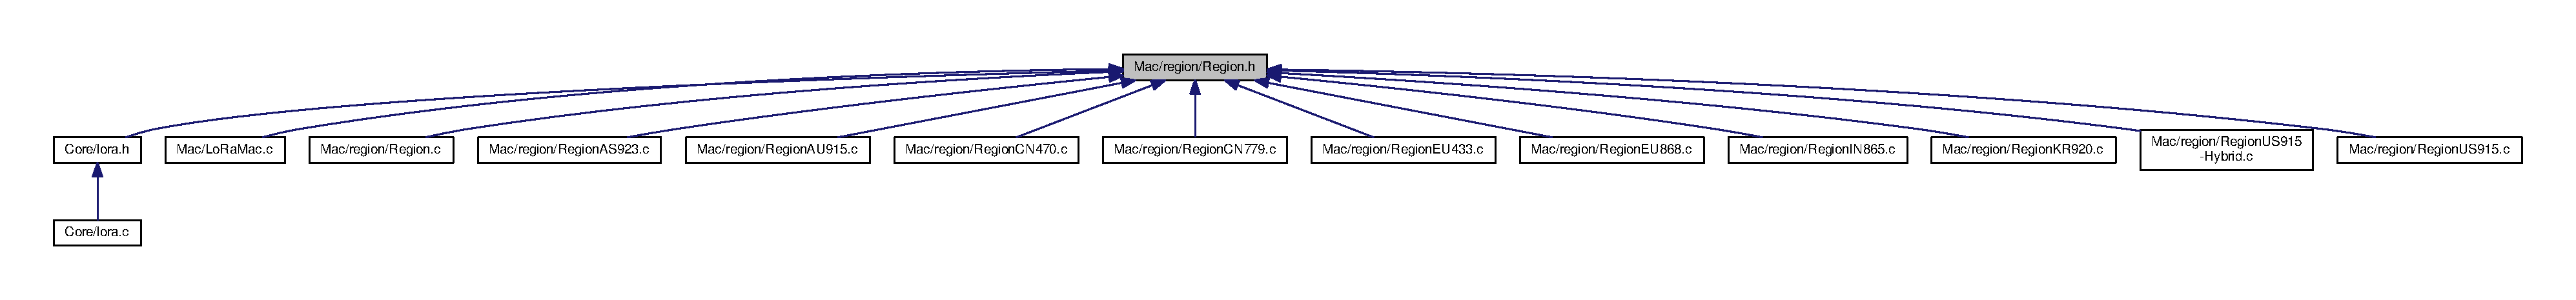
\includegraphics[width=350pt]{Region_8h__dep__incl}
\end{center}
\end{figure}
\subsection*{Data Structures}
\begin{DoxyCompactItemize}
\item 
union \hyperlink{unionuPhyParam}{u\+Phy\+Param}
\item 
struct \hyperlink{structsGetPhyParams}{s\+Get\+Phy\+Params}
\item 
struct \hyperlink{structsSetBandTxDoneParams}{s\+Set\+Band\+Tx\+Done\+Params}
\item 
union \hyperlink{unionuVerifyParams}{u\+Verify\+Params}
\item 
struct \hyperlink{structuVerifyParams_1_1sDatarateParams}{u\+Verify\+Params\+::s\+Datarate\+Params}
\item 
struct \hyperlink{structsApplyCFListParams}{s\+Apply\+C\+F\+List\+Params}
\item 
struct \hyperlink{structsChanMaskSetParams}{s\+Chan\+Mask\+Set\+Params}
\item 
struct \hyperlink{structsAdrNextParams}{s\+Adr\+Next\+Params}
\item 
struct \hyperlink{structsRxConfigParams}{s\+Rx\+Config\+Params}
\item 
struct \hyperlink{structsTxConfigParams}{s\+Tx\+Config\+Params}
\item 
struct \hyperlink{structsLinkAdrReqParams}{s\+Link\+Adr\+Req\+Params}
\item 
struct \hyperlink{structsRxParamSetupReqParams}{s\+Rx\+Param\+Setup\+Req\+Params}
\item 
struct \hyperlink{structsNewChannelReqParams}{s\+New\+Channel\+Req\+Params}
\item 
struct \hyperlink{structsTxParamSetupReqParams}{s\+Tx\+Param\+Setup\+Req\+Params}
\item 
struct \hyperlink{structsDlChannelReqParams}{s\+Dl\+Channel\+Req\+Params}
\item 
struct \hyperlink{structsAlternateDrParams}{s\+Alternate\+Dr\+Params}
\item 
struct \hyperlink{structsCalcBackOffParams}{s\+Calc\+Back\+Off\+Params}
\item 
struct \hyperlink{structsNextChanParams}{s\+Next\+Chan\+Params}
\item 
struct \hyperlink{structsChannelAddParams}{s\+Channel\+Add\+Params}
\item 
struct \hyperlink{structsChannelRemoveParams}{s\+Channel\+Remove\+Params}
\item 
struct \hyperlink{structsContinuousWaveParams}{s\+Continuous\+Wave\+Params}
\end{DoxyCompactItemize}
\subsection*{Macros}
\begin{DoxyCompactItemize}
\item 
\#define \hyperlink{group__REGION_ga12fa17e5c1016e01a9d82c25027deb1b}{LC}(channel\+Index)~( uint16\+\_\+t )( 1 $<$$<$ ( channel\+Index -\/ 1 ) )
\item 
\#define \hyperlink{group__REGION_ga6c4ef966b4f3d5eb7597b087f2b97095}{D\+R\+\_\+0}~0
\item 
\#define \hyperlink{group__REGION_ga87e71569dc5f2114e685560de072af26}{D\+R\+\_\+1}~1
\item 
\#define \hyperlink{group__REGION_gad402daa928a8b3dea829315fab69de17}{D\+R\+\_\+2}~2
\item 
\#define \hyperlink{group__REGION_ga3627849e6360cd275bc74dc519653820}{D\+R\+\_\+3}~3
\item 
\#define \hyperlink{group__REGION_ga6ceba6158a7dab238e9d0b846fb47a0c}{D\+R\+\_\+4}~4
\item 
\#define \hyperlink{group__REGION_ga872e12c82020c02a7f70a1c6ed1375df}{D\+R\+\_\+5}~5
\item 
\#define \hyperlink{group__REGION_ga8e2b4c15b7dbb8bda5ed635ca1d262be}{D\+R\+\_\+6}~6
\item 
\#define \hyperlink{group__REGION_ga3a06805baf4f00911a3a5d3dbadebf61}{D\+R\+\_\+7}~7
\item 
\#define \hyperlink{group__REGION_ga44cc96ba80ae464cd9330b784d329c16}{D\+R\+\_\+8}~8
\item 
\#define \hyperlink{group__REGION_ga67346d631ba28781d6dffb2a7b6fd22f}{D\+R\+\_\+9}~9
\item 
\#define \hyperlink{group__REGION_ga8cc471faabc38682537f6a60a30844e4}{D\+R\+\_\+10}~10
\item 
\#define \hyperlink{group__REGION_ga77672781eaa7dc6f6892195739a5ef27}{D\+R\+\_\+11}~11
\item 
\#define \hyperlink{group__REGION_gafcf0cda11eda5db3d4c4e9a5bd79c0d5}{D\+R\+\_\+12}~12
\item 
\#define \hyperlink{group__REGION_ga226f47470cc69a6fe831f7c92709bc1f}{D\+R\+\_\+13}~13
\item 
\#define \hyperlink{group__REGION_ga5319f091a90ef4a360cb732be49927c6}{D\+R\+\_\+14}~14
\item 
\#define \hyperlink{group__REGION_gac6e078f51b71f05093daf27834997396}{D\+R\+\_\+15}~15
\item 
\#define \hyperlink{group__REGION_gab33618449f2a573142c463ab071ef8ed}{T\+X\+\_\+\+P\+O\+W\+E\+R\+\_\+0}~0
\item 
\#define \hyperlink{group__REGION_gaac7fe73d03d0e880cc4c7a3d30e23cb6}{T\+X\+\_\+\+P\+O\+W\+E\+R\+\_\+1}~1
\item 
\#define \hyperlink{group__REGION_gaf308ada92d6393ca5ae171ffc462c74c}{T\+X\+\_\+\+P\+O\+W\+E\+R\+\_\+2}~2
\item 
\#define \hyperlink{group__REGION_ga9d5bc42aaace47b7053ecf685153bdaa}{T\+X\+\_\+\+P\+O\+W\+E\+R\+\_\+3}~3
\item 
\#define \hyperlink{group__REGION_ga36456baf8ace3e7d7ae730ddb54b95bc}{T\+X\+\_\+\+P\+O\+W\+E\+R\+\_\+4}~4
\item 
\#define \hyperlink{group__REGION_ga0149d52581db80901b5bc1adf0aedd1d}{T\+X\+\_\+\+P\+O\+W\+E\+R\+\_\+5}~5
\item 
\#define \hyperlink{group__REGION_ga29743296a1bb29534ecc4894967c0714}{T\+X\+\_\+\+P\+O\+W\+E\+R\+\_\+6}~6
\item 
\#define \hyperlink{group__REGION_ga3c7bd9a98f0c1e7e9aaa90857c4bd700}{T\+X\+\_\+\+P\+O\+W\+E\+R\+\_\+7}~7
\item 
\#define \hyperlink{group__REGION_ga99ec65aa5375a9dbbaf2faac8d7f6968}{T\+X\+\_\+\+P\+O\+W\+E\+R\+\_\+8}~8
\item 
\#define \hyperlink{group__REGION_gacf5b8e09a82ae407ae0ab2d81f1e0c3d}{T\+X\+\_\+\+P\+O\+W\+E\+R\+\_\+9}~9
\item 
\#define \hyperlink{group__REGION_gac9747c69350f34d485c3134e5a57655b}{T\+X\+\_\+\+P\+O\+W\+E\+R\+\_\+10}~10
\item 
\#define \hyperlink{group__REGION_ga739bc82fae779702381bcaa5e85d7d06}{T\+X\+\_\+\+P\+O\+W\+E\+R\+\_\+11}~11
\item 
\#define \hyperlink{group__REGION_gaeeb1b0e98ed14b98b55ce8b7fbd8d3f1}{T\+X\+\_\+\+P\+O\+W\+E\+R\+\_\+12}~12
\item 
\#define \hyperlink{group__REGION_gaabaceca100173cd1f450f53d2e14f0a2}{T\+X\+\_\+\+P\+O\+W\+E\+R\+\_\+13}~13
\item 
\#define \hyperlink{group__REGION_ga6932af7382128090be2a6533e260dd9c}{T\+X\+\_\+\+P\+O\+W\+E\+R\+\_\+14}~14
\item 
\#define \hyperlink{group__REGION_gabe4f87ed0aa6efe21ec76d9a32a334ef}{T\+X\+\_\+\+P\+O\+W\+E\+R\+\_\+15}~15
\end{DoxyCompactItemize}
\subsection*{Typedefs}
\begin{DoxyCompactItemize}
\item 
typedef enum \hyperlink{group__REGION_ga51cbe8f5433d914fe9cf81b451de2c2d}{e\+Phy\+Attribute} \hyperlink{group__REGION_ga9445b07fdf77581ecfaf389970e635f8}{Phy\+Attribute\+\_\+t}
\item 
typedef enum \hyperlink{group__REGION_ga11ecad794560a3d3961bdf1c9a27d3b2}{e\+Init\+Type} \hyperlink{group__REGION_gaddc73ae10673ec925724e7870363bda9}{Init\+Type\+\_\+t}
\item 
typedef enum \hyperlink{group__REGION_ga7a62e669f567fc160ad58210664bca9c}{e\+Channels\+Mask} \hyperlink{group__REGION_ga933f695eea70935418e2175940b92311}{Channels\+Mask\+\_\+t}
\item 
typedef union \hyperlink{unionuPhyParam}{u\+Phy\+Param} \hyperlink{group__REGION_gaed159b26e5c4677236b6e8677019db30}{Phy\+Param\+\_\+t}
\item 
typedef struct \hyperlink{structsGetPhyParams}{s\+Get\+Phy\+Params} \hyperlink{group__REGION_gab471483fff904f4f89bbc03f7fc380ab}{Get\+Phy\+Params\+\_\+t}
\item 
typedef struct \hyperlink{structsSetBandTxDoneParams}{s\+Set\+Band\+Tx\+Done\+Params} \hyperlink{group__REGION_gad0524aa0673c0814a71e7a4f9cade3fc}{Set\+Band\+Tx\+Done\+Params\+\_\+t}
\item 
typedef union \hyperlink{unionuVerifyParams}{u\+Verify\+Params} \hyperlink{group__REGION_ga966d97bc2f25df1c09e92e60ef652276}{Verify\+Params\+\_\+t}
\item 
typedef struct \hyperlink{structsApplyCFListParams}{s\+Apply\+C\+F\+List\+Params} \hyperlink{group__REGION_ga71588e9ad07e34b78fa91d51881fd3c6}{Apply\+C\+F\+List\+Params\+\_\+t}
\item 
typedef struct \hyperlink{structsChanMaskSetParams}{s\+Chan\+Mask\+Set\+Params} \hyperlink{group__REGION_ga6d24f7da136006410827dfb29f6b9b9e}{Chan\+Mask\+Set\+Params\+\_\+t}
\item 
typedef struct \hyperlink{structsAdrNextParams}{s\+Adr\+Next\+Params} \hyperlink{group__REGION_ga567c2742622326b350b4e91bbf61b4ce}{Adr\+Next\+Params\+\_\+t}
\item 
typedef struct \hyperlink{structsRxConfigParams}{s\+Rx\+Config\+Params} \hyperlink{group__REGION_ga375c038078dfcfc7ef14280021db719e}{Rx\+Config\+Params\+\_\+t}
\item 
typedef struct \hyperlink{structsTxConfigParams}{s\+Tx\+Config\+Params} \hyperlink{group__REGION_gabed730d4d04b0b60d4b6d1966d3f21d3}{Tx\+Config\+Params\+\_\+t}
\item 
typedef struct \hyperlink{structsLinkAdrReqParams}{s\+Link\+Adr\+Req\+Params} \hyperlink{group__REGION_gad4af503e8d4de1846129e26a799a1e8e}{Link\+Adr\+Req\+Params\+\_\+t}
\item 
typedef struct \hyperlink{structsRxParamSetupReqParams}{s\+Rx\+Param\+Setup\+Req\+Params} \hyperlink{group__REGION_ga7165f282c670c728c36d534df2285157}{Rx\+Param\+Setup\+Req\+Params\+\_\+t}
\item 
typedef struct \hyperlink{structsNewChannelReqParams}{s\+New\+Channel\+Req\+Params} \hyperlink{group__REGION_gae2abcdb6dbb843c9faf5fd3009eca9d6}{New\+Channel\+Req\+Params\+\_\+t}
\item 
typedef struct \hyperlink{structsTxParamSetupReqParams}{s\+Tx\+Param\+Setup\+Req\+Params} \hyperlink{group__REGION_ga26836ef2996e70410e42ef471073f855}{Tx\+Param\+Setup\+Req\+Params\+\_\+t}
\item 
typedef struct \hyperlink{structsDlChannelReqParams}{s\+Dl\+Channel\+Req\+Params} \hyperlink{group__REGION_gae0d608ff1f8ea0a430e4f9a4c38ec7f3}{Dl\+Channel\+Req\+Params\+\_\+t}
\item 
typedef struct \hyperlink{structsAlternateDrParams}{s\+Alternate\+Dr\+Params} \hyperlink{group__REGION_ga001ea4338d1c83f4c785b49d7ad2d696}{Alternate\+Dr\+Params\+\_\+t}
\item 
typedef struct \hyperlink{structsCalcBackOffParams}{s\+Calc\+Back\+Off\+Params} \hyperlink{group__REGION_ga7c5c9a8da174e6679eded8257dc92fd9}{Calc\+Back\+Off\+Params\+\_\+t}
\item 
typedef struct \hyperlink{structsNextChanParams}{s\+Next\+Chan\+Params} \hyperlink{group__REGION_ga115f5e83afae352c0a3dcdc193374040}{Next\+Chan\+Params\+\_\+t}
\item 
typedef struct \hyperlink{structsChannelAddParams}{s\+Channel\+Add\+Params} \hyperlink{group__REGION_gab1c5f3aa06614283202906cef4417860}{Channel\+Add\+Params\+\_\+t}
\item 
typedef struct \hyperlink{structsChannelRemoveParams}{s\+Channel\+Remove\+Params} \hyperlink{group__REGION_gaa37468560d2fc81a977b57a48e5d72c0}{Channel\+Remove\+Params\+\_\+t}
\item 
typedef struct \hyperlink{structsContinuousWaveParams}{s\+Continuous\+Wave\+Params} \hyperlink{group__REGION_gaf39bb5ba06921139c6d17f88a8d518cd}{Continuous\+Wave\+Params\+\_\+t}
\end{DoxyCompactItemize}
\subsection*{Enumerations}
\begin{DoxyCompactItemize}
\item 
enum \hyperlink{group__REGION_ga51cbe8f5433d914fe9cf81b451de2c2d}{e\+Phy\+Attribute} \{ \newline
\hyperlink{group__REGION_gga51cbe8f5433d914fe9cf81b451de2c2da91cb5d84f937c32cd635dd7efe7a9d3a}{P\+H\+Y\+\_\+\+M\+I\+N\+\_\+\+R\+X\+\_\+\+DR}, 
\hyperlink{group__REGION_gga51cbe8f5433d914fe9cf81b451de2c2daace3e56c88b40def8ed6a9106871e7de}{P\+H\+Y\+\_\+\+M\+I\+N\+\_\+\+T\+X\+\_\+\+DR}, 
\hyperlink{group__REGION_gga51cbe8f5433d914fe9cf81b451de2c2dabc80857ed9621c5c6fd60d98846b0b84}{P\+H\+Y\+\_\+\+M\+A\+X\+\_\+\+R\+X\+\_\+\+DR}, 
\hyperlink{group__REGION_gga51cbe8f5433d914fe9cf81b451de2c2dac83a2348a7177fae43a5c3b0a6f0a141}{P\+H\+Y\+\_\+\+M\+A\+X\+\_\+\+T\+X\+\_\+\+DR}, 
\newline
\hyperlink{group__REGION_gga51cbe8f5433d914fe9cf81b451de2c2da62c19af9dc2c54540562e1158c015f57}{P\+H\+Y\+\_\+\+T\+X\+\_\+\+DR}, 
\hyperlink{group__REGION_gga51cbe8f5433d914fe9cf81b451de2c2da70c3923333165960549162e3dcf10467}{P\+H\+Y\+\_\+\+D\+E\+F\+\_\+\+T\+X\+\_\+\+DR}, 
\hyperlink{group__REGION_gga51cbe8f5433d914fe9cf81b451de2c2da8cc3b895173b07ee71127e366c8d0d55}{P\+H\+Y\+\_\+\+R\+X\+\_\+\+DR}, 
\hyperlink{group__REGION_gga51cbe8f5433d914fe9cf81b451de2c2da0dceb30b79f1bae301afd5406a86d6f3}{P\+H\+Y\+\_\+\+T\+X\+\_\+\+P\+O\+W\+ER}, 
\newline
\hyperlink{group__REGION_gga51cbe8f5433d914fe9cf81b451de2c2da18ae0d314f20c212f9e40207099ab1bb}{P\+H\+Y\+\_\+\+D\+E\+F\+\_\+\+T\+X\+\_\+\+P\+O\+W\+ER}, 
\hyperlink{group__REGION_gga51cbe8f5433d914fe9cf81b451de2c2dad671e2651e42de26927910282c6b2781}{P\+H\+Y\+\_\+\+M\+A\+X\+\_\+\+P\+A\+Y\+L\+O\+AD}, 
\hyperlink{group__REGION_gga51cbe8f5433d914fe9cf81b451de2c2da8a3b9e5ad2604232fd1f8781658452f3}{P\+H\+Y\+\_\+\+M\+A\+X\+\_\+\+P\+A\+Y\+L\+O\+A\+D\+\_\+\+R\+E\+P\+E\+A\+T\+ER}, 
\hyperlink{group__REGION_gga51cbe8f5433d914fe9cf81b451de2c2dac66308571e624ecc28c79ee0deab8cf0}{P\+H\+Y\+\_\+\+D\+U\+T\+Y\+\_\+\+C\+Y\+C\+LE}, 
\newline
\hyperlink{group__REGION_gga51cbe8f5433d914fe9cf81b451de2c2dacf2bd6f434ce2844651513ad2b9b9da5}{P\+H\+Y\+\_\+\+M\+A\+X\+\_\+\+R\+X\+\_\+\+W\+I\+N\+D\+OW}, 
\hyperlink{group__REGION_gga51cbe8f5433d914fe9cf81b451de2c2da3680d45f45e3e0a96ce9f1e1b5ed7371}{P\+H\+Y\+\_\+\+R\+E\+C\+E\+I\+V\+E\+\_\+\+D\+E\+L\+A\+Y1}, 
\hyperlink{group__REGION_gga51cbe8f5433d914fe9cf81b451de2c2da9c7e3df5f55fab406960a9e5bf635155}{P\+H\+Y\+\_\+\+R\+E\+C\+E\+I\+V\+E\+\_\+\+D\+E\+L\+A\+Y2}, 
\hyperlink{group__REGION_gga51cbe8f5433d914fe9cf81b451de2c2daf564c82ebd72dcd6c4fc1e702b2ec64c}{P\+H\+Y\+\_\+\+J\+O\+I\+N\+\_\+\+A\+C\+C\+E\+P\+T\+\_\+\+D\+E\+L\+A\+Y1}, 
\newline
\hyperlink{group__REGION_gga51cbe8f5433d914fe9cf81b451de2c2da04e6c3d25ce44a74c0a29f28aa92eb48}{P\+H\+Y\+\_\+\+J\+O\+I\+N\+\_\+\+A\+C\+C\+E\+P\+T\+\_\+\+D\+E\+L\+A\+Y2}, 
\hyperlink{group__REGION_gga51cbe8f5433d914fe9cf81b451de2c2da01c12b14686172b4a3c4d095deef4248}{P\+H\+Y\+\_\+\+M\+A\+X\+\_\+\+F\+C\+N\+T\+\_\+\+G\+AP}, 
\hyperlink{group__REGION_gga51cbe8f5433d914fe9cf81b451de2c2da8485b24e94d037ba487ab6ecfaf162e8}{P\+H\+Y\+\_\+\+A\+C\+K\+\_\+\+T\+I\+M\+E\+O\+UT}, 
\hyperlink{group__REGION_gga51cbe8f5433d914fe9cf81b451de2c2dae648c84cc946657e970c7e08dd69cb6f}{P\+H\+Y\+\_\+\+D\+E\+F\+\_\+\+D\+R1\+\_\+\+O\+F\+F\+S\+ET}, 
\newline
\hyperlink{group__REGION_gga51cbe8f5433d914fe9cf81b451de2c2da1835125d2139942145a0ed0caff058f3}{P\+H\+Y\+\_\+\+D\+E\+F\+\_\+\+R\+X2\+\_\+\+F\+R\+E\+Q\+U\+E\+N\+CY}, 
\hyperlink{group__REGION_gga51cbe8f5433d914fe9cf81b451de2c2da672678e5f03f8ad1afa8817405e72ef0}{P\+H\+Y\+\_\+\+D\+E\+F\+\_\+\+R\+X2\+\_\+\+DR}, 
\hyperlink{group__REGION_gga51cbe8f5433d914fe9cf81b451de2c2daa6fd00cadf73ba804e35d85aadd15882}{P\+H\+Y\+\_\+\+C\+H\+A\+N\+N\+E\+L\+S\+\_\+\+M\+A\+SK}, 
\hyperlink{group__REGION_gga51cbe8f5433d914fe9cf81b451de2c2da7253f56eb1b6f4fe64d7a51b2e573766}{P\+H\+Y\+\_\+\+C\+H\+A\+N\+N\+E\+L\+S\+\_\+\+D\+E\+F\+A\+U\+L\+T\+\_\+\+M\+A\+SK}, 
\newline
\hyperlink{group__REGION_gga51cbe8f5433d914fe9cf81b451de2c2da52d463ed953da20f07f8d045c58caee8}{P\+H\+Y\+\_\+\+M\+A\+X\+\_\+\+N\+B\+\_\+\+C\+H\+A\+N\+N\+E\+LS}, 
\hyperlink{group__REGION_gga51cbe8f5433d914fe9cf81b451de2c2da52c9055b2e5bbfc05c86e83798856aba}{P\+H\+Y\+\_\+\+C\+H\+A\+N\+N\+E\+LS}, 
\hyperlink{group__REGION_gga51cbe8f5433d914fe9cf81b451de2c2dab35cca5e0dae3d87e02c8c80e4d4685e}{P\+H\+Y\+\_\+\+D\+E\+F\+\_\+\+U\+P\+L\+I\+N\+K\+\_\+\+D\+W\+E\+L\+L\+\_\+\+T\+I\+ME}, 
\hyperlink{group__REGION_gga51cbe8f5433d914fe9cf81b451de2c2da8e29179691bf6520256a7af0cabae6ad}{P\+H\+Y\+\_\+\+D\+E\+F\+\_\+\+D\+O\+W\+N\+L\+I\+N\+K\+\_\+\+D\+W\+E\+L\+L\+\_\+\+T\+I\+ME}, 
\newline
\hyperlink{group__REGION_gga51cbe8f5433d914fe9cf81b451de2c2da5bdce0ffd449781819a0d87732ebd2b7}{P\+H\+Y\+\_\+\+D\+E\+F\+\_\+\+M\+A\+X\+\_\+\+E\+I\+RP}, 
\hyperlink{group__REGION_gga51cbe8f5433d914fe9cf81b451de2c2da37b73a543ea79ce58bf18035329ba773}{P\+H\+Y\+\_\+\+D\+E\+F\+\_\+\+A\+N\+T\+E\+N\+N\+A\+\_\+\+G\+A\+IN}, 
\hyperlink{group__REGION_gga51cbe8f5433d914fe9cf81b451de2c2da46941b2ce68829fcee9540dc64e53d6d}{P\+H\+Y\+\_\+\+N\+B\+\_\+\+J\+O\+I\+N\+\_\+\+T\+R\+I\+A\+LS}, 
\hyperlink{group__REGION_gga51cbe8f5433d914fe9cf81b451de2c2da49312d43f8804334f738701ab59878a1}{P\+H\+Y\+\_\+\+D\+E\+F\+\_\+\+N\+B\+\_\+\+J\+O\+I\+N\+\_\+\+T\+R\+I\+A\+LS}, 
\newline
\hyperlink{group__REGION_gga51cbe8f5433d914fe9cf81b451de2c2dac002e7e492cf30dbf9c544b062f5cc8a}{P\+H\+Y\+\_\+\+N\+E\+X\+T\+\_\+\+L\+O\+W\+E\+R\+\_\+\+T\+X\+\_\+\+DR}
 \}
\item 
enum \hyperlink{group__REGION_ga11ecad794560a3d3961bdf1c9a27d3b2}{e\+Init\+Type} \{ \hyperlink{group__REGION_gga11ecad794560a3d3961bdf1c9a27d3b2a5065ce7a587a2aeff0da16507222c4d7}{I\+N\+I\+T\+\_\+\+T\+Y\+P\+E\+\_\+\+I\+N\+IT}, 
\hyperlink{group__REGION_gga11ecad794560a3d3961bdf1c9a27d3b2aed3218cb3c4ebbb74a1b48e4f8ac8599}{I\+N\+I\+T\+\_\+\+T\+Y\+P\+E\+\_\+\+R\+E\+S\+T\+O\+RE}
 \}
\item 
enum \hyperlink{group__REGION_ga7a62e669f567fc160ad58210664bca9c}{e\+Channels\+Mask} \{ \hyperlink{group__REGION_gga7a62e669f567fc160ad58210664bca9ca1e68275c0b16a0c4935eada4315dd089}{C\+H\+A\+N\+N\+E\+L\+S\+\_\+\+M\+A\+SK}, 
\hyperlink{group__REGION_gga7a62e669f567fc160ad58210664bca9ca9bbb18c8600ad8781ba04a2cb121ea60}{C\+H\+A\+N\+N\+E\+L\+S\+\_\+\+D\+E\+F\+A\+U\+L\+T\+\_\+\+M\+A\+SK}
 \}
\end{DoxyCompactItemize}
\subsection*{Functions}
\begin{DoxyCompactItemize}
\item 
bool \hyperlink{group__REGION_ga3e5cf2322f71f8f9973718024b6fb782}{Region\+Is\+Active} (\hyperlink{group__LORAMAC_ga80c48efda9ae02e14b58160d34a798dd}{Lo\+Ra\+Mac\+Region\+\_\+t} region)
\begin{DoxyCompactList}\small\item\em The function verifies if a region is active or not. If a region is not active, it cannot be used. \end{DoxyCompactList}\item 
\hyperlink{group__REGION_gaed159b26e5c4677236b6e8677019db30}{Phy\+Param\+\_\+t} \hyperlink{group__REGION_gafbd084611ba512035a6cbe7f3aa5857b}{Region\+Get\+Phy\+Param} (\hyperlink{group__LORAMAC_ga80c48efda9ae02e14b58160d34a798dd}{Lo\+Ra\+Mac\+Region\+\_\+t} region, \hyperlink{group__REGION_gab471483fff904f4f89bbc03f7fc380ab}{Get\+Phy\+Params\+\_\+t} $\ast$get\+Phy)
\begin{DoxyCompactList}\small\item\em The function gets a value of a specific phy attribute. \end{DoxyCompactList}\item 
void \hyperlink{group__REGION_gabdd176dcf0b7e7900377b4c1e183613d}{Region\+Set\+Band\+Tx\+Done} (\hyperlink{group__LORAMAC_ga80c48efda9ae02e14b58160d34a798dd}{Lo\+Ra\+Mac\+Region\+\_\+t} region, \hyperlink{group__REGION_gad0524aa0673c0814a71e7a4f9cade3fc}{Set\+Band\+Tx\+Done\+Params\+\_\+t} $\ast$tx\+Done)
\begin{DoxyCompactList}\small\item\em Updates the last TX done parameters of the current channel. \end{DoxyCompactList}\item 
void \hyperlink{group__REGION_ga54b1b27a8431cd146b4dc33a894ee6db}{Region\+Init\+Defaults} (\hyperlink{group__LORAMAC_ga80c48efda9ae02e14b58160d34a798dd}{Lo\+Ra\+Mac\+Region\+\_\+t} region, \hyperlink{group__REGION_gaddc73ae10673ec925724e7870363bda9}{Init\+Type\+\_\+t} type)
\begin{DoxyCompactList}\small\item\em Initializes the channels masks and the channels. \end{DoxyCompactList}\item 
bool \hyperlink{group__REGION_ga7c1ff626bc1131889fa8de3197a1093a}{Region\+Verify} (\hyperlink{group__LORAMAC_ga80c48efda9ae02e14b58160d34a798dd}{Lo\+Ra\+Mac\+Region\+\_\+t} region, \hyperlink{group__REGION_ga966d97bc2f25df1c09e92e60ef652276}{Verify\+Params\+\_\+t} $\ast$verify, \hyperlink{group__REGION_ga9445b07fdf77581ecfaf389970e635f8}{Phy\+Attribute\+\_\+t} phy\+Attribute)
\begin{DoxyCompactList}\small\item\em Verifies a parameter. \end{DoxyCompactList}\item 
void \hyperlink{group__REGION_gae3fdd82182ebb0704adb2a017d30e1f2}{Region\+Apply\+C\+F\+List} (\hyperlink{group__LORAMAC_ga80c48efda9ae02e14b58160d34a798dd}{Lo\+Ra\+Mac\+Region\+\_\+t} region, \hyperlink{group__REGION_ga71588e9ad07e34b78fa91d51881fd3c6}{Apply\+C\+F\+List\+Params\+\_\+t} $\ast$apply\+C\+F\+List)
\begin{DoxyCompactList}\small\item\em The function parses the input buffer and sets up the channels of the CF list. \end{DoxyCompactList}\item 
bool \hyperlink{group__REGION_ga795ed3c13f4c8d03e39298fd64e5b2df}{Region\+Chan\+Mask\+Set} (\hyperlink{group__LORAMAC_ga80c48efda9ae02e14b58160d34a798dd}{Lo\+Ra\+Mac\+Region\+\_\+t} region, \hyperlink{group__REGION_ga6d24f7da136006410827dfb29f6b9b9e}{Chan\+Mask\+Set\+Params\+\_\+t} $\ast$chan\+Mask\+Set)
\begin{DoxyCompactList}\small\item\em Sets a channels mask. \end{DoxyCompactList}\item 
bool \hyperlink{group__REGION_ga08cac64beeadd0555460ca5e756a0792}{Region\+Adr\+Next} (\hyperlink{group__LORAMAC_ga80c48efda9ae02e14b58160d34a798dd}{Lo\+Ra\+Mac\+Region\+\_\+t} region, \hyperlink{group__REGION_ga567c2742622326b350b4e91bbf61b4ce}{Adr\+Next\+Params\+\_\+t} $\ast$adr\+Next, int8\+\_\+t $\ast$dr\+Out, int8\+\_\+t $\ast$tx\+Pow\+Out, uint32\+\_\+t $\ast$adr\+Ack\+Counter)
\begin{DoxyCompactList}\small\item\em Calculates the next datarate to set, when A\+DR is on or off. \end{DoxyCompactList}\item 
bool \hyperlink{group__REGION_gaf89984d30239d6597190409068031465}{Region\+Rx\+Config} (\hyperlink{group__LORAMAC_ga80c48efda9ae02e14b58160d34a798dd}{Lo\+Ra\+Mac\+Region\+\_\+t} region, \hyperlink{group__REGION_ga375c038078dfcfc7ef14280021db719e}{Rx\+Config\+Params\+\_\+t} $\ast$rx\+Config, int8\+\_\+t $\ast$datarate)
\begin{DoxyCompactList}\small\item\em Configuration of the RX windows. \end{DoxyCompactList}\item 
void \hyperlink{group__REGION_gabd3eb4e7db9b7987fabb9568f733a2b9}{Region\+Compute\+Rx\+Window\+Parameters} (\hyperlink{group__LORAMAC_ga80c48efda9ae02e14b58160d34a798dd}{Lo\+Ra\+Mac\+Region\+\_\+t} region, int8\+\_\+t datarate, uint8\+\_\+t min\+Rx\+Symbols, uint32\+\_\+t rx\+Error, \hyperlink{group__REGION_ga375c038078dfcfc7ef14280021db719e}{Rx\+Config\+Params\+\_\+t} $\ast$rx\+Config\+Params)
\item 
bool \hyperlink{group__REGION_ga9a4b01301e0f6f6880dc6a651c062ad0}{Region\+Tx\+Config} (\hyperlink{group__LORAMAC_ga80c48efda9ae02e14b58160d34a798dd}{Lo\+Ra\+Mac\+Region\+\_\+t} region, \hyperlink{group__REGION_gabed730d4d04b0b60d4b6d1966d3f21d3}{Tx\+Config\+Params\+\_\+t} $\ast$tx\+Config, int8\+\_\+t $\ast$tx\+Power, \hyperlink{utilities_8h_a4215ca43d3e953099ea758ce428599d0}{Timer\+Time\+\_\+t} $\ast$tx\+Time\+On\+Air)
\begin{DoxyCompactList}\small\item\em TX configuration. \end{DoxyCompactList}\item 
uint8\+\_\+t \hyperlink{group__REGION_gae82a94e6d4141122e1a20b5ba1936c8e}{Region\+Link\+Adr\+Req} (\hyperlink{group__LORAMAC_ga80c48efda9ae02e14b58160d34a798dd}{Lo\+Ra\+Mac\+Region\+\_\+t} region, \hyperlink{group__REGION_gad4af503e8d4de1846129e26a799a1e8e}{Link\+Adr\+Req\+Params\+\_\+t} $\ast$link\+Adr\+Req, int8\+\_\+t $\ast$dr\+Out, int8\+\_\+t $\ast$tx\+Pow\+Out, uint8\+\_\+t $\ast$nb\+Rep\+Out, uint8\+\_\+t $\ast$nb\+Bytes\+Parsed)
\begin{DoxyCompactList}\small\item\em The function processes a Link A\+DR Request. \end{DoxyCompactList}\item 
uint8\+\_\+t \hyperlink{group__REGION_ga485a820155fded42235a0d14d5918a7d}{Region\+Rx\+Param\+Setup\+Req} (\hyperlink{group__LORAMAC_ga80c48efda9ae02e14b58160d34a798dd}{Lo\+Ra\+Mac\+Region\+\_\+t} region, \hyperlink{group__REGION_ga7165f282c670c728c36d534df2285157}{Rx\+Param\+Setup\+Req\+Params\+\_\+t} $\ast$rx\+Param\+Setup\+Req)
\begin{DoxyCompactList}\small\item\em The function processes a RX Parameter Setup Request. \end{DoxyCompactList}\item 
uint8\+\_\+t \hyperlink{group__REGION_gadca654538335b4395c8d54642b83e2d4}{Region\+New\+Channel\+Req} (\hyperlink{group__LORAMAC_ga80c48efda9ae02e14b58160d34a798dd}{Lo\+Ra\+Mac\+Region\+\_\+t} region, \hyperlink{group__REGION_gae2abcdb6dbb843c9faf5fd3009eca9d6}{New\+Channel\+Req\+Params\+\_\+t} $\ast$new\+Channel\+Req)
\begin{DoxyCompactList}\small\item\em The function processes a New Channel Request. \end{DoxyCompactList}\item 
int8\+\_\+t \hyperlink{group__REGION_ga50dbaca7bf982330c183614302d525c4}{Region\+Tx\+Param\+Setup\+Req} (\hyperlink{group__LORAMAC_ga80c48efda9ae02e14b58160d34a798dd}{Lo\+Ra\+Mac\+Region\+\_\+t} region, \hyperlink{group__REGION_ga26836ef2996e70410e42ef471073f855}{Tx\+Param\+Setup\+Req\+Params\+\_\+t} $\ast$tx\+Param\+Setup\+Req)
\begin{DoxyCompactList}\small\item\em The function processes a TX Param\+Setup Request. \end{DoxyCompactList}\item 
uint8\+\_\+t \hyperlink{group__REGION_ga54f7c22677b2d0628e9914f53501d4b8}{Region\+Dl\+Channel\+Req} (\hyperlink{group__LORAMAC_ga80c48efda9ae02e14b58160d34a798dd}{Lo\+Ra\+Mac\+Region\+\_\+t} region, \hyperlink{group__REGION_gae0d608ff1f8ea0a430e4f9a4c38ec7f3}{Dl\+Channel\+Req\+Params\+\_\+t} $\ast$dl\+Channel\+Req)
\begin{DoxyCompactList}\small\item\em The function processes a Dl\+Channel Request. \end{DoxyCompactList}\item 
int8\+\_\+t \hyperlink{group__REGION_ga4177d2eac64338ef073b43efa508e12a}{Region\+Alternate\+Dr} (\hyperlink{group__LORAMAC_ga80c48efda9ae02e14b58160d34a798dd}{Lo\+Ra\+Mac\+Region\+\_\+t} region, \hyperlink{group__REGION_ga001ea4338d1c83f4c785b49d7ad2d696}{Alternate\+Dr\+Params\+\_\+t} $\ast$alternate\+Dr)
\begin{DoxyCompactList}\small\item\em Alternates the datarate of the channel for the join request. \end{DoxyCompactList}\item 
void \hyperlink{group__REGION_ga07cfd135a3e8f85e15a5424c07f71d67}{Region\+Calc\+Back\+Off} (\hyperlink{group__LORAMAC_ga80c48efda9ae02e14b58160d34a798dd}{Lo\+Ra\+Mac\+Region\+\_\+t} region, \hyperlink{group__REGION_ga7c5c9a8da174e6679eded8257dc92fd9}{Calc\+Back\+Off\+Params\+\_\+t} $\ast$calc\+Back\+Off)
\begin{DoxyCompactList}\small\item\em Calculates the back-\/off time. \end{DoxyCompactList}\item 
bool \hyperlink{group__REGION_ga2139de3f2832789797c8853764655398}{Region\+Next\+Channel} (\hyperlink{group__LORAMAC_ga80c48efda9ae02e14b58160d34a798dd}{Lo\+Ra\+Mac\+Region\+\_\+t} region, \hyperlink{group__REGION_ga115f5e83afae352c0a3dcdc193374040}{Next\+Chan\+Params\+\_\+t} $\ast$next\+Chan\+Params, uint8\+\_\+t $\ast$channel, \hyperlink{utilities_8h_a4215ca43d3e953099ea758ce428599d0}{Timer\+Time\+\_\+t} $\ast$time, \hyperlink{utilities_8h_a4215ca43d3e953099ea758ce428599d0}{Timer\+Time\+\_\+t} $\ast$aggregated\+Time\+Off)
\begin{DoxyCompactList}\small\item\em Searches and set the next random available channel. \end{DoxyCompactList}\item 
\hyperlink{group__LORAMAC_ga30bd25657e10480f8605ee951b0ecfbd}{Lo\+Ra\+Mac\+Status\+\_\+t} \hyperlink{group__REGION_gaaa5767f33e988a641abf509ad278ae14}{Region\+Channel\+Add} (\hyperlink{group__LORAMAC_ga80c48efda9ae02e14b58160d34a798dd}{Lo\+Ra\+Mac\+Region\+\_\+t} region, \hyperlink{group__REGION_gab1c5f3aa06614283202906cef4417860}{Channel\+Add\+Params\+\_\+t} $\ast$channel\+Add)
\begin{DoxyCompactList}\small\item\em Adds a channel. \end{DoxyCompactList}\item 
bool \hyperlink{group__REGION_ga50b3505e13d8373fef6e2be6d48e150c}{Region\+Channels\+Remove} (\hyperlink{group__LORAMAC_ga80c48efda9ae02e14b58160d34a798dd}{Lo\+Ra\+Mac\+Region\+\_\+t} region, \hyperlink{group__REGION_gaa37468560d2fc81a977b57a48e5d72c0}{Channel\+Remove\+Params\+\_\+t} $\ast$channel\+Remove)
\begin{DoxyCompactList}\small\item\em Removes a channel. \end{DoxyCompactList}\item 
void \hyperlink{group__REGION_ga22327f217ed10d84c89b6785143be5b8}{Region\+Set\+Continuous\+Wave} (\hyperlink{group__LORAMAC_ga80c48efda9ae02e14b58160d34a798dd}{Lo\+Ra\+Mac\+Region\+\_\+t} region, \hyperlink{group__REGION_gaf39bb5ba06921139c6d17f88a8d518cd}{Continuous\+Wave\+Params\+\_\+t} $\ast$continuous\+Wave)
\begin{DoxyCompactList}\small\item\em Sets the radio into continuous wave mode. \end{DoxyCompactList}\item 
uint8\+\_\+t \hyperlink{group__REGION_gab62221e1ca566a89f4b450b30bfb95a7}{Region\+Apply\+Dr\+Offset} (\hyperlink{group__LORAMAC_ga80c48efda9ae02e14b58160d34a798dd}{Lo\+Ra\+Mac\+Region\+\_\+t} region, uint8\+\_\+t downlink\+Dwell\+Time, int8\+\_\+t dr, int8\+\_\+t dr\+Offset)
\begin{DoxyCompactList}\small\item\em Computes new datarate according to the given offset. \end{DoxyCompactList}\end{DoxyCompactItemize}


\subsection{Detailed Description}
Region implementation. 

\begin{DoxyCopyright}{Copyright}
Revised B\+SD License, see section L\+I\+C\+E\+N\+SE.
\end{DoxyCopyright}

\begin{DoxyCode}
  \_\_\_\_\_\_                              \_
 / \_\_\_\_\_)             \_              | |
( (\_\_\_\_  \_\_\_\_\_ \_\_\_\_ \_| |\_ \_\_\_\_\_  \_\_\_\_| |\_\_
 \(\backslash\)\_\_\_\_ \(\backslash\)| \_\_\_ |    (\_   \_) \_\_\_ |/ \_\_\_)  \_ \(\backslash\)
 \_\_\_\_\_) ) \_\_\_\_| | | || |\_| \_\_\_\_( (\_\_\_| | | |
(\_\_\_\_\_\_/|\_\_\_\_\_)\_|\_|\_| \(\backslash\)\_\_)\_\_\_\_\_)\(\backslash\)\_\_\_\_)\_| |\_|
(C)2013 Semtech

 \_\_\_ \_\_\_\_\_ \_   \_\_\_ \_  \_\_\_\_\_ \_\_\_  \_\_\_  \_\_\_ \_\_\_
/ \_\_|\_   \_/\_\(\backslash\) / \_\_| |/ / \_\_/ \_ \(\backslash\)| \_ \(\backslash\)/ \_\_| \_\_|
\(\backslash\)\_\_ \(\backslash\) | |/ \_ \(\backslash\) (\_\_| \textcolor{stringliteral}{' <| \_| (\_) |   / (\_\_| \_|}
\textcolor{stringliteral}{|\_\_\_/ |\_/\_/ \(\backslash\)\_\(\backslash\)\_\_\_|\_|\(\backslash\)\_\(\backslash\)\_| \(\backslash\)\_\_\_/|\_|\_\(\backslash\)\(\backslash\)\_\_\_|\_\_\_|}
\textcolor{stringliteral}{embedded.connectivity.solutions===============}
\end{DoxyCode}


\begin{DoxyAuthor}{Author}
Miguel Luis ( Semtech )

Gregory Cristian ( Semtech )

Daniel Jaeckle ( S\+T\+A\+C\+K\+F\+O\+R\+CE ) 
\end{DoxyAuthor}

\hypertarget{RegionAS923_8c}{}\section{Mac/region/\+Region\+A\+S923.c File Reference}
\label{RegionAS923_8c}\index{Mac/region/\+Region\+A\+S923.\+c@{Mac/region/\+Region\+A\+S923.\+c}}
{\ttfamily \#include $<$stdbool.\+h$>$}\newline
{\ttfamily \#include $<$string.\+h$>$}\newline
{\ttfamily \#include $<$stdint.\+h$>$}\newline
{\ttfamily \#include $<$math.\+h$>$}\newline
{\ttfamily \#include \char`\"{}radio.\+h\char`\"{}}\newline
{\ttfamily \#include \char`\"{}timer.\+h\char`\"{}}\newline
{\ttfamily \#include \char`\"{}Lo\+Ra\+Mac.\+h\char`\"{}}\newline
{\ttfamily \#include \char`\"{}utilities.\+h\char`\"{}}\newline
{\ttfamily \#include \char`\"{}Region.\+h\char`\"{}}\newline
{\ttfamily \#include \char`\"{}Region\+Common.\+h\char`\"{}}\newline
{\ttfamily \#include \char`\"{}Region\+A\+S923.\+h\char`\"{}}\newline
{\ttfamily \#include \char`\"{}debug.\+h\char`\"{}}\newline
Include dependency graph for Region\+A\+S923.\+c\+:
\nopagebreak
\begin{figure}[H]
\begin{center}
\leavevmode
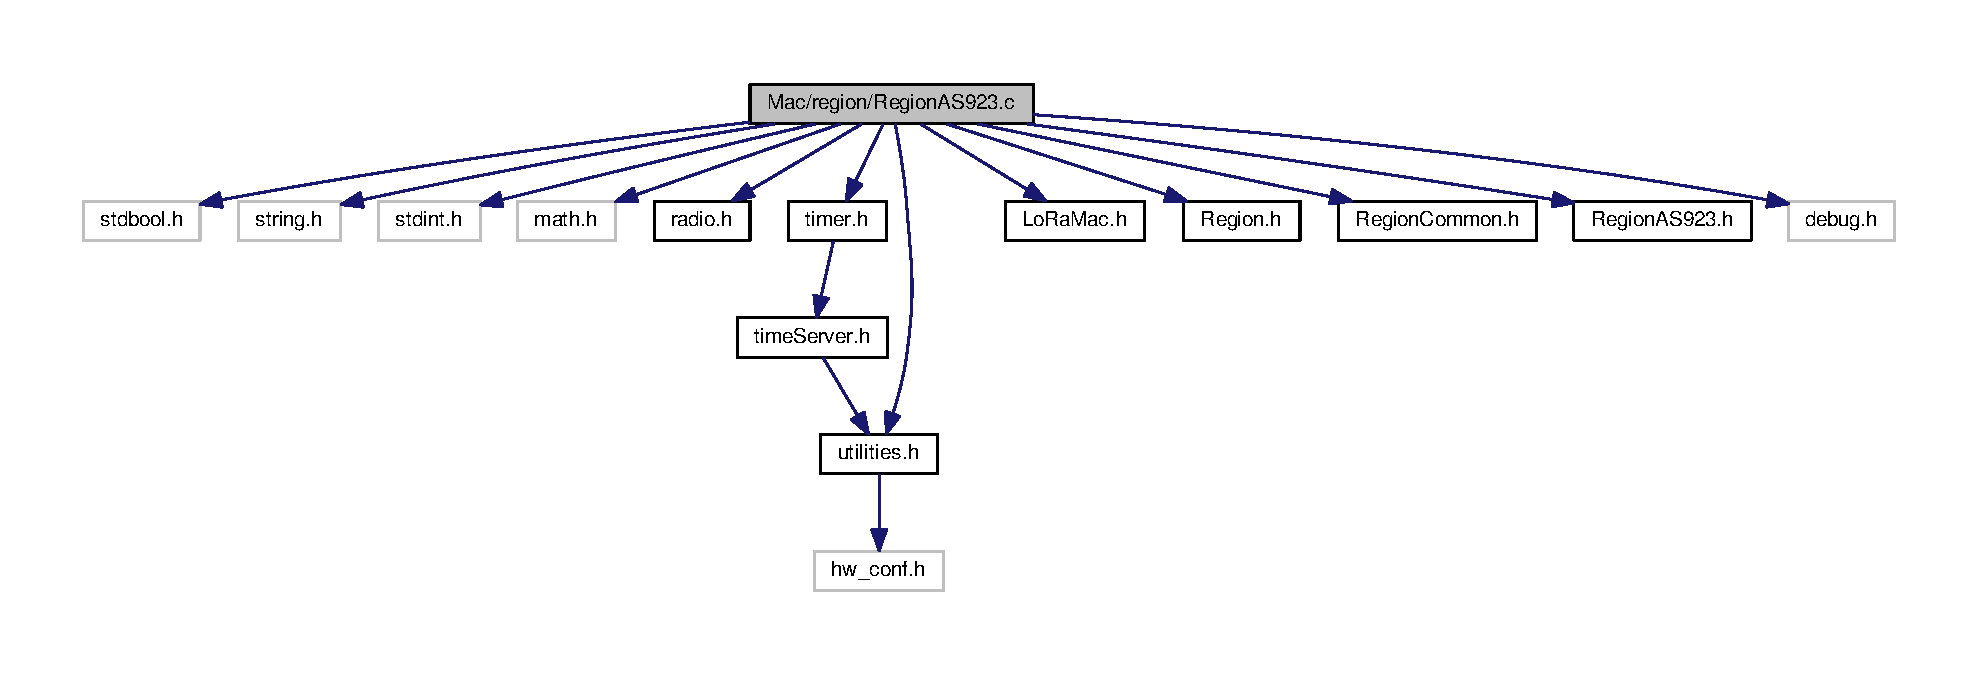
\includegraphics[width=350pt]{RegionAS923_8c__incl}
\end{center}
\end{figure}
\subsection*{Macros}
\begin{DoxyCompactItemize}
\item 
\#define \hyperlink{RegionAS923_8c_a1b20a8de3ae59c0b063fb313f0c70890}{C\+H\+A\+N\+N\+E\+L\+S\+\_\+\+M\+A\+S\+K\+\_\+\+S\+I\+ZE}~1
\end{DoxyCompactItemize}
\subsection*{Functions}
\begin{DoxyCompactItemize}
\item 
\hyperlink{group__REGION_gaed159b26e5c4677236b6e8677019db30}{Phy\+Param\+\_\+t} \hyperlink{group__REGIONAS923_ga20508dee35c0f25ff507478c5235fdeb}{Region\+A\+S923\+Get\+Phy\+Param} (\hyperlink{group__REGION_gab471483fff904f4f89bbc03f7fc380ab}{Get\+Phy\+Params\+\_\+t} $\ast$get\+Phy)
\begin{DoxyCompactList}\small\item\em The function gets a value of a specific phy attribute. \end{DoxyCompactList}\item 
void \hyperlink{group__REGIONAS923_ga8e986a04899f4346d7005b5ab3722298}{Region\+A\+S923\+Set\+Band\+Tx\+Done} (\hyperlink{group__REGION_gad0524aa0673c0814a71e7a4f9cade3fc}{Set\+Band\+Tx\+Done\+Params\+\_\+t} $\ast$tx\+Done)
\begin{DoxyCompactList}\small\item\em Updates the last TX done parameters of the current channel. \end{DoxyCompactList}\item 
void \hyperlink{group__REGIONAS923_ga24e0f9bd2b50e0a8efb5e3d5ecc12904}{Region\+A\+S923\+Init\+Defaults} (\hyperlink{group__REGION_gaddc73ae10673ec925724e7870363bda9}{Init\+Type\+\_\+t} type)
\begin{DoxyCompactList}\small\item\em Initializes the channels masks and the channels. \end{DoxyCompactList}\item 
bool \hyperlink{group__REGIONAS923_ga6287722023036c70f4a9b1ec43901be5}{Region\+A\+S923\+Verify} (\hyperlink{group__REGION_ga966d97bc2f25df1c09e92e60ef652276}{Verify\+Params\+\_\+t} $\ast$verify, \hyperlink{group__REGION_ga9445b07fdf77581ecfaf389970e635f8}{Phy\+Attribute\+\_\+t} phy\+Attribute)
\begin{DoxyCompactList}\small\item\em Verifies a parameter. \end{DoxyCompactList}\item 
void \hyperlink{group__REGIONAS923_ga06106e86f717362c50165a5adaf73331}{Region\+A\+S923\+Apply\+C\+F\+List} (\hyperlink{group__REGION_ga71588e9ad07e34b78fa91d51881fd3c6}{Apply\+C\+F\+List\+Params\+\_\+t} $\ast$apply\+C\+F\+List)
\begin{DoxyCompactList}\small\item\em The function parses the input buffer and sets up the channels of the CF list. \end{DoxyCompactList}\item 
bool \hyperlink{group__REGIONAS923_gab493d29d1037f6b6f47baf0cfc2faf47}{Region\+A\+S923\+Chan\+Mask\+Set} (\hyperlink{group__REGION_ga6d24f7da136006410827dfb29f6b9b9e}{Chan\+Mask\+Set\+Params\+\_\+t} $\ast$chan\+Mask\+Set)
\begin{DoxyCompactList}\small\item\em Sets a channels mask. \end{DoxyCompactList}\item 
bool \hyperlink{group__REGIONAS923_ga38146f12b31fadadda54344d9f5d7e49}{Region\+A\+S923\+Adr\+Next} (\hyperlink{group__REGION_ga567c2742622326b350b4e91bbf61b4ce}{Adr\+Next\+Params\+\_\+t} $\ast$adr\+Next, int8\+\_\+t $\ast$dr\+Out, int8\+\_\+t $\ast$tx\+Pow\+Out, uint32\+\_\+t $\ast$adr\+Ack\+Counter)
\begin{DoxyCompactList}\small\item\em Calculates the next datarate to set, when A\+DR is on or off. \end{DoxyCompactList}\item 
void \hyperlink{group__REGIONAS923_ga33875aeda67698b7be396f9ef9b1d081}{Region\+A\+S923\+Compute\+Rx\+Window\+Parameters} (int8\+\_\+t datarate, uint8\+\_\+t min\+Rx\+Symbols, uint32\+\_\+t rx\+Error, \hyperlink{group__REGION_ga375c038078dfcfc7ef14280021db719e}{Rx\+Config\+Params\+\_\+t} $\ast$rx\+Config\+Params)
\item 
bool \hyperlink{group__REGIONAS923_ga236a04c03ccf327e5a3d1a0130e19e10}{Region\+A\+S923\+Rx\+Config} (\hyperlink{group__REGION_ga375c038078dfcfc7ef14280021db719e}{Rx\+Config\+Params\+\_\+t} $\ast$rx\+Config, int8\+\_\+t $\ast$datarate)
\begin{DoxyCompactList}\small\item\em Configuration of the RX windows. \end{DoxyCompactList}\item 
bool \hyperlink{group__REGIONAS923_gab4e1c5c1e67df4682b90950164afec03}{Region\+A\+S923\+Tx\+Config} (\hyperlink{group__REGION_gabed730d4d04b0b60d4b6d1966d3f21d3}{Tx\+Config\+Params\+\_\+t} $\ast$tx\+Config, int8\+\_\+t $\ast$tx\+Power, \hyperlink{utilities_8h_a4215ca43d3e953099ea758ce428599d0}{Timer\+Time\+\_\+t} $\ast$tx\+Time\+On\+Air)
\begin{DoxyCompactList}\small\item\em TX configuration. \end{DoxyCompactList}\item 
uint8\+\_\+t \hyperlink{group__REGIONAS923_ga154ccc00c27ca878e07cfeab3716523a}{Region\+A\+S923\+Link\+Adr\+Req} (\hyperlink{group__REGION_gad4af503e8d4de1846129e26a799a1e8e}{Link\+Adr\+Req\+Params\+\_\+t} $\ast$link\+Adr\+Req, int8\+\_\+t $\ast$dr\+Out, int8\+\_\+t $\ast$tx\+Pow\+Out, uint8\+\_\+t $\ast$nb\+Rep\+Out, uint8\+\_\+t $\ast$nb\+Bytes\+Parsed)
\begin{DoxyCompactList}\small\item\em The function processes a Link A\+DR Request. \end{DoxyCompactList}\item 
uint8\+\_\+t \hyperlink{group__REGIONAS923_ga1cfa678c3c8157f7eb382d8fe9d9ba04}{Region\+A\+S923\+Rx\+Param\+Setup\+Req} (\hyperlink{group__REGION_ga7165f282c670c728c36d534df2285157}{Rx\+Param\+Setup\+Req\+Params\+\_\+t} $\ast$rx\+Param\+Setup\+Req)
\begin{DoxyCompactList}\small\item\em The function processes a RX Parameter Setup Request. \end{DoxyCompactList}\item 
uint8\+\_\+t \hyperlink{group__REGIONAS923_gaad10b4ed09a71cdff0e385729e4dc345}{Region\+A\+S923\+New\+Channel\+Req} (\hyperlink{group__REGION_gae2abcdb6dbb843c9faf5fd3009eca9d6}{New\+Channel\+Req\+Params\+\_\+t} $\ast$new\+Channel\+Req)
\begin{DoxyCompactList}\small\item\em The function processes a Channel Request. \end{DoxyCompactList}\item 
int8\+\_\+t \hyperlink{group__REGIONAS923_gab0fbb927f3521fd56696157e270043c1}{Region\+A\+S923\+Tx\+Param\+Setup\+Req} (\hyperlink{group__REGION_ga26836ef2996e70410e42ef471073f855}{Tx\+Param\+Setup\+Req\+Params\+\_\+t} $\ast$tx\+Param\+Setup\+Req)
\begin{DoxyCompactList}\small\item\em The function processes a TX Param\+Setup Request. \end{DoxyCompactList}\item 
uint8\+\_\+t \hyperlink{group__REGIONAS923_ga3517054139f97c1b45454355fe661f48}{Region\+A\+S923\+Dl\+Channel\+Req} (\hyperlink{group__REGION_gae0d608ff1f8ea0a430e4f9a4c38ec7f3}{Dl\+Channel\+Req\+Params\+\_\+t} $\ast$dl\+Channel\+Req)
\begin{DoxyCompactList}\small\item\em The function processes a Dl\+Channel Request. \end{DoxyCompactList}\item 
int8\+\_\+t \hyperlink{group__REGIONAS923_ga313ff123a69e6a8d72fc958d79150bd5}{Region\+A\+S923\+Alternate\+Dr} (\hyperlink{group__REGION_ga001ea4338d1c83f4c785b49d7ad2d696}{Alternate\+Dr\+Params\+\_\+t} $\ast$alternate\+Dr)
\begin{DoxyCompactList}\small\item\em Alternates the datarate of the channel for the join request. \end{DoxyCompactList}\item 
void \hyperlink{group__REGIONAS923_ga819573966df873dc3e76397d19cfcb34}{Region\+A\+S923\+Calc\+Back\+Off} (\hyperlink{group__REGION_ga7c5c9a8da174e6679eded8257dc92fd9}{Calc\+Back\+Off\+Params\+\_\+t} $\ast$calc\+Back\+Off)
\begin{DoxyCompactList}\small\item\em Calculates the back-\/off time. \end{DoxyCompactList}\item 
bool \hyperlink{group__REGIONAS923_ga5712c1f33958544c25351d4e5ed2015a}{Region\+A\+S923\+Next\+Channel} (\hyperlink{group__REGION_ga115f5e83afae352c0a3dcdc193374040}{Next\+Chan\+Params\+\_\+t} $\ast$next\+Chan\+Params, uint8\+\_\+t $\ast$channel, \hyperlink{utilities_8h_a4215ca43d3e953099ea758ce428599d0}{Timer\+Time\+\_\+t} $\ast$time, \hyperlink{utilities_8h_a4215ca43d3e953099ea758ce428599d0}{Timer\+Time\+\_\+t} $\ast$aggregated\+Time\+Off)
\begin{DoxyCompactList}\small\item\em Searches and set the next random available channel. \end{DoxyCompactList}\item 
\hyperlink{group__LORAMAC_ga30bd25657e10480f8605ee951b0ecfbd}{Lo\+Ra\+Mac\+Status\+\_\+t} \hyperlink{group__REGIONAS923_ga7477b7737c48e88f1d82a7ef70eb7b56}{Region\+A\+S923\+Channel\+Add} (\hyperlink{group__REGION_gab1c5f3aa06614283202906cef4417860}{Channel\+Add\+Params\+\_\+t} $\ast$channel\+Add)
\begin{DoxyCompactList}\small\item\em Adds a channel. \end{DoxyCompactList}\item 
bool \hyperlink{group__REGIONAS923_ga288bc8bbec286314166d13033979678f}{Region\+A\+S923\+Channels\+Remove} (\hyperlink{group__REGION_gaa37468560d2fc81a977b57a48e5d72c0}{Channel\+Remove\+Params\+\_\+t} $\ast$channel\+Remove)
\begin{DoxyCompactList}\small\item\em Removes a channel. \end{DoxyCompactList}\item 
void \hyperlink{group__REGIONAS923_ga295747645e6d5ed51a52cb17cee132b4}{Region\+A\+S923\+Set\+Continuous\+Wave} (\hyperlink{group__REGION_gaf39bb5ba06921139c6d17f88a8d518cd}{Continuous\+Wave\+Params\+\_\+t} $\ast$continuous\+Wave)
\begin{DoxyCompactList}\small\item\em Sets the radio into continuous wave mode. \end{DoxyCompactList}\item 
uint8\+\_\+t \hyperlink{group__REGIONAS923_gae3a2832d4cb1117e74dea4cdfe66998e}{Region\+A\+S923\+Apply\+Dr\+Offset} (uint8\+\_\+t downlink\+Dwell\+Time, int8\+\_\+t dr, int8\+\_\+t dr\+Offset)
\begin{DoxyCompactList}\small\item\em Computes new datarate according to the given offset. \end{DoxyCompactList}\end{DoxyCompactItemize}


\subsection{Macro Definition Documentation}
\mbox{\Hypertarget{RegionAS923_8c_a1b20a8de3ae59c0b063fb313f0c70890}\label{RegionAS923_8c_a1b20a8de3ae59c0b063fb313f0c70890}} 
\index{Region\+A\+S923.\+c@{Region\+A\+S923.\+c}!C\+H\+A\+N\+N\+E\+L\+S\+\_\+\+M\+A\+S\+K\+\_\+\+S\+I\+ZE@{C\+H\+A\+N\+N\+E\+L\+S\+\_\+\+M\+A\+S\+K\+\_\+\+S\+I\+ZE}}
\index{C\+H\+A\+N\+N\+E\+L\+S\+\_\+\+M\+A\+S\+K\+\_\+\+S\+I\+ZE@{C\+H\+A\+N\+N\+E\+L\+S\+\_\+\+M\+A\+S\+K\+\_\+\+S\+I\+ZE}!Region\+A\+S923.\+c@{Region\+A\+S923.\+c}}
\subsubsection{\texorpdfstring{C\+H\+A\+N\+N\+E\+L\+S\+\_\+\+M\+A\+S\+K\+\_\+\+S\+I\+ZE}{CHANNELS\_MASK\_SIZE}}
{\footnotesize\ttfamily \#define C\+H\+A\+N\+N\+E\+L\+S\+\_\+\+M\+A\+S\+K\+\_\+\+S\+I\+ZE~1}


\hypertarget{RegionAS923_8h}{}\section{Mac/region/\+Region\+A\+S923.h File Reference}
\label{RegionAS923_8h}\index{Mac/region/\+Region\+A\+S923.\+h@{Mac/region/\+Region\+A\+S923.\+h}}


Region definition for A\+S923.  


This graph shows which files directly or indirectly include this file\+:
\nopagebreak
\begin{figure}[H]
\begin{center}
\leavevmode
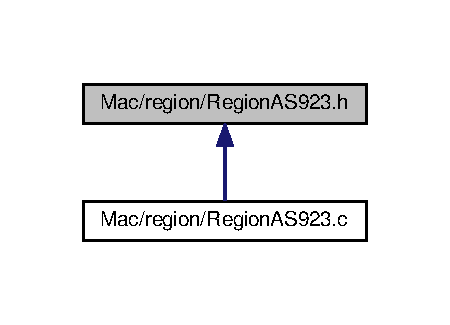
\includegraphics[width=216pt]{RegionAS923_8h__dep__incl}
\end{center}
\end{figure}
\subsection*{Macros}
\begin{DoxyCompactItemize}
\item 
\#define \hyperlink{group__REGIONAS923_ga02e3db7e4557dbf77db79285d38dc33e}{A\+S923\+\_\+\+M\+A\+X\+\_\+\+N\+B\+\_\+\+C\+H\+A\+N\+N\+E\+LS}~16
\item 
\#define \hyperlink{group__REGIONAS923_ga189fa7f36943ed53424ac7610ef64d56}{A\+S923\+\_\+\+N\+U\+M\+B\+\_\+\+D\+E\+F\+A\+U\+L\+T\+\_\+\+C\+H\+A\+N\+N\+E\+LS}~2
\item 
\#define \hyperlink{group__REGIONAS923_gaeb64b3a7da759d5e403f08bbacdb8cf8}{A\+S923\+\_\+\+N\+U\+M\+B\+\_\+\+C\+H\+A\+N\+N\+E\+L\+S\+\_\+\+C\+F\+\_\+\+L\+I\+ST}~5
\item 
\#define \hyperlink{group__REGIONAS923_gab6f2badbf9a4eb4038301759c0f7fc77}{A\+S923\+\_\+\+T\+X\+\_\+\+M\+I\+N\+\_\+\+D\+A\+T\+A\+R\+A\+TE}~\hyperlink{group__REGION_ga6c4ef966b4f3d5eb7597b087f2b97095}{D\+R\+\_\+0}
\item 
\#define \hyperlink{group__REGIONAS923_gac9506097a516f03c7c86432d30e8f499}{A\+S923\+\_\+\+T\+X\+\_\+\+M\+A\+X\+\_\+\+D\+A\+T\+A\+R\+A\+TE}~\hyperlink{group__REGION_ga3a06805baf4f00911a3a5d3dbadebf61}{D\+R\+\_\+7}
\item 
\#define \hyperlink{group__REGIONAS923_ga55aa4a1054571ef315043248599e1c96}{A\+S923\+\_\+\+R\+X\+\_\+\+M\+I\+N\+\_\+\+D\+A\+T\+A\+R\+A\+TE}~\hyperlink{group__REGION_ga6c4ef966b4f3d5eb7597b087f2b97095}{D\+R\+\_\+0}
\item 
\#define \hyperlink{group__REGIONAS923_ga008298ea3d2b2444dcad3dedca7189bc}{A\+S923\+\_\+\+R\+X\+\_\+\+M\+A\+X\+\_\+\+D\+A\+T\+A\+R\+A\+TE}~\hyperlink{group__REGION_ga3a06805baf4f00911a3a5d3dbadebf61}{D\+R\+\_\+7}
\item 
\#define \hyperlink{group__REGIONAS923_ga643615d49b742b49b442da9803b9c291}{A\+S923\+\_\+\+D\+E\+F\+A\+U\+L\+T\+\_\+\+D\+A\+T\+A\+R\+A\+TE}~\hyperlink{group__REGION_gad402daa928a8b3dea829315fab69de17}{D\+R\+\_\+2}
\item 
\#define \hyperlink{group__REGIONAS923_gab4d42ec6203089aa346cd55d90eb769e}{A\+S923\+\_\+\+D\+W\+E\+L\+L\+\_\+\+L\+I\+M\+I\+T\+\_\+\+D\+A\+T\+A\+R\+A\+TE}~\hyperlink{group__REGION_gad402daa928a8b3dea829315fab69de17}{D\+R\+\_\+2}
\item 
\#define \hyperlink{group__REGIONAS923_gaaa342c4c9e6db79d8949112c19f7422f}{A\+S923\+\_\+\+M\+I\+N\+\_\+\+R\+X1\+\_\+\+D\+R\+\_\+\+O\+F\+F\+S\+ET}~0
\item 
\#define \hyperlink{group__REGIONAS923_ga92034d0c71c7943562cbebd114ed6f5e}{A\+S923\+\_\+\+M\+A\+X\+\_\+\+R\+X1\+\_\+\+D\+R\+\_\+\+O\+F\+F\+S\+ET}~7
\item 
\#define \hyperlink{group__REGIONAS923_ga2c6ea009afd46f07baae802b336ff76d}{A\+S923\+\_\+\+D\+E\+F\+A\+U\+L\+T\+\_\+\+R\+X1\+\_\+\+D\+R\+\_\+\+O\+F\+F\+S\+ET}~0
\item 
\#define \hyperlink{group__REGIONAS923_gab5c796398b9a3a599d43ce34dd0e3dec}{A\+S923\+\_\+\+M\+I\+N\+\_\+\+T\+X\+\_\+\+P\+O\+W\+ER}~\hyperlink{group__REGION_ga3c7bd9a98f0c1e7e9aaa90857c4bd700}{T\+X\+\_\+\+P\+O\+W\+E\+R\+\_\+7}
\item 
\#define \hyperlink{group__REGIONAS923_ga572944e6a8933722a954e4cee98fa0ee}{A\+S923\+\_\+\+M\+A\+X\+\_\+\+T\+X\+\_\+\+P\+O\+W\+ER}~\hyperlink{group__REGION_gab33618449f2a573142c463ab071ef8ed}{T\+X\+\_\+\+P\+O\+W\+E\+R\+\_\+0}
\item 
\#define \hyperlink{group__REGIONAS923_ga98e64bdbc74253fbec5119d43ceb5903}{A\+S923\+\_\+\+D\+E\+F\+A\+U\+L\+T\+\_\+\+T\+X\+\_\+\+P\+O\+W\+ER}~\hyperlink{group__REGION_gab33618449f2a573142c463ab071ef8ed}{T\+X\+\_\+\+P\+O\+W\+E\+R\+\_\+0}
\item 
\#define \hyperlink{group__REGIONAS923_gafaa21368b605c5313a0c3ac76bfd908c}{A\+S923\+\_\+\+D\+E\+F\+A\+U\+L\+T\+\_\+\+U\+P\+L\+I\+N\+K\+\_\+\+D\+W\+E\+L\+L\+\_\+\+T\+I\+ME}~1
\item 
\#define \hyperlink{group__REGIONAS923_gab7c581030f301fc7ada92555da15ad23}{A\+S923\+\_\+\+D\+E\+F\+A\+U\+L\+T\+\_\+\+D\+O\+W\+N\+L\+I\+N\+K\+\_\+\+D\+W\+E\+L\+L\+\_\+\+T\+I\+ME}~1
\item 
\#define \hyperlink{group__REGIONAS923_ga626ba6fc6eb81535fe6f325a4ec47b90}{A\+S923\+\_\+\+D\+E\+F\+A\+U\+L\+T\+\_\+\+M\+A\+X\+\_\+\+E\+I\+RP}~16.\+0f
\item 
\#define \hyperlink{group__REGIONAS923_ga4a2faf56603f9d0feb2c105632a5b005}{A\+S923\+\_\+\+D\+E\+F\+A\+U\+L\+T\+\_\+\+A\+N\+T\+E\+N\+N\+A\+\_\+\+G\+A\+IN}~2.\+15f
\item 
\#define \hyperlink{group__REGIONAS923_ga83b8b9ab4bab852209f471da8518bf2d}{A\+S923\+\_\+\+A\+D\+R\+\_\+\+A\+C\+K\+\_\+\+L\+I\+M\+IT}~64
\item 
\#define \hyperlink{group__REGIONAS923_ga77d7f3a0e26d3bfeded53fce115d5180}{A\+S923\+\_\+\+A\+D\+R\+\_\+\+A\+C\+K\+\_\+\+D\+E\+L\+AY}~32
\item 
\#define \hyperlink{group__REGIONAS923_ga9a38122696d349e600de24f267340b93}{A\+S923\+\_\+\+D\+U\+T\+Y\+\_\+\+C\+Y\+C\+L\+E\+\_\+\+E\+N\+A\+B\+L\+ED}~0
\item 
\#define \hyperlink{group__REGIONAS923_ga1da68477a3fef68cc666a41fb5362bc6}{A\+S923\+\_\+\+M\+A\+X\+\_\+\+R\+X\+\_\+\+W\+I\+N\+D\+OW}~3000
\item 
\#define \hyperlink{group__REGIONAS923_gaa18d3ea411b8511078af8c0a07304999}{A\+S923\+\_\+\+R\+E\+C\+E\+I\+V\+E\+\_\+\+D\+E\+L\+A\+Y1}~1000
\item 
\#define \hyperlink{group__REGIONAS923_ga37f081e957cc36c733b5008aa46b9511}{A\+S923\+\_\+\+R\+E\+C\+E\+I\+V\+E\+\_\+\+D\+E\+L\+A\+Y2}~2000
\item 
\#define \hyperlink{group__REGIONAS923_gaa108eaacc8ee4c9a46b37327b3b2eea1}{A\+S923\+\_\+\+J\+O\+I\+N\+\_\+\+A\+C\+C\+E\+P\+T\+\_\+\+D\+E\+L\+A\+Y1}~5000
\item 
\#define \hyperlink{group__REGIONAS923_gafd48180d34e9cb94a0747ea0a2dfff28}{A\+S923\+\_\+\+J\+O\+I\+N\+\_\+\+A\+C\+C\+E\+P\+T\+\_\+\+D\+E\+L\+A\+Y2}~6000
\item 
\#define \hyperlink{group__REGIONAS923_ga996b3bad607207a4c54e5a2b253e5dfd}{A\+S923\+\_\+\+M\+A\+X\+\_\+\+F\+C\+N\+T\+\_\+\+G\+AP}~16384
\item 
\#define \hyperlink{group__REGIONAS923_gad4cd8450319521a6db078659d7ee9f62}{A\+S923\+\_\+\+A\+C\+K\+T\+I\+M\+E\+O\+UT}~2000
\item 
\#define \hyperlink{group__REGIONAS923_gae069e1d35da1a7303a5242bbada80740}{A\+S923\+\_\+\+A\+C\+K\+\_\+\+T\+I\+M\+E\+O\+U\+T\+\_\+\+R\+ND}~1000
\item 
\#define \hyperlink{group__REGIONAS923_ga537225e8ec04b97e81b2434ed4015abc}{A\+S923\+\_\+\+R\+X\+\_\+\+W\+N\+D\+\_\+2\+\_\+\+F\+R\+EQ}~923200000
\item 
\#define \hyperlink{group__REGIONAS923_gab765338caef1a1babc2572d1ced03470}{A\+S923\+\_\+\+R\+X\+\_\+\+W\+N\+D\+\_\+2\+\_\+\+DR}~\hyperlink{group__REGION_gad402daa928a8b3dea829315fab69de17}{D\+R\+\_\+2}
\item 
\#define \hyperlink{group__REGIONAS923_ga462d2371d2b936331d37530925ffb66d}{A\+S923\+\_\+\+M\+A\+X\+\_\+\+N\+B\+\_\+\+B\+A\+N\+DS}~1
\item 
\#define \hyperlink{group__REGIONAS923_ga78d5e5197f4e58d1e45290a300e86a2b}{A\+S923\+\_\+\+B\+A\+N\+D0}~\{ 100, \hyperlink{group__REGIONAS923_ga572944e6a8933722a954e4cee98fa0ee}{A\+S923\+\_\+\+M\+A\+X\+\_\+\+T\+X\+\_\+\+P\+O\+W\+ER}, 0,  0 \}
\item 
\#define \hyperlink{group__REGIONAS923_gad552f8b259e81215d17bfd1f9c0f1198}{A\+S923\+\_\+\+L\+C1}~\{ 923200000, 0, \{ ( ( \hyperlink{group__REGION_ga872e12c82020c02a7f70a1c6ed1375df}{D\+R\+\_\+5} $<$$<$ 4 ) $\vert$ \hyperlink{group__REGION_ga6c4ef966b4f3d5eb7597b087f2b97095}{D\+R\+\_\+0} ) \}, 0 \}
\item 
\#define \hyperlink{group__REGIONAS923_gae6a0cfa9079c4ab3097ac797506452d4}{A\+S923\+\_\+\+L\+C2}~\{ 923400000, 0, \{ ( ( \hyperlink{group__REGION_ga872e12c82020c02a7f70a1c6ed1375df}{D\+R\+\_\+5} $<$$<$ 4 ) $\vert$ \hyperlink{group__REGION_ga6c4ef966b4f3d5eb7597b087f2b97095}{D\+R\+\_\+0} ) \}, 0 \}
\item 
\#define \hyperlink{group__REGIONAS923_ga56d14306ed1af83973ff240658721a24}{A\+S923\+\_\+\+J\+O\+I\+N\+\_\+\+C\+H\+A\+N\+N\+E\+LS}~( uint16\+\_\+t )( \hyperlink{group__REGION_ga12fa17e5c1016e01a9d82c25027deb1b}{LC}( 1 ) $\vert$ \hyperlink{group__REGION_ga12fa17e5c1016e01a9d82c25027deb1b}{LC}( 2 ) )
\item 
\#define \hyperlink{group__REGIONAS923_gabcc79c4eb4e2717692ac348885e3139f}{A\+S923\+\_\+\+R\+S\+S\+I\+\_\+\+F\+R\+E\+E\+\_\+\+TH}~-\/85
\item 
\#define \hyperlink{group__REGIONAS923_ga6c93e3596e26eb72247906ee33523404}{A\+S923\+\_\+\+C\+A\+R\+R\+I\+E\+R\+\_\+\+S\+E\+N\+S\+E\+\_\+\+T\+I\+ME}~6
\end{DoxyCompactItemize}
\subsection*{Functions}
\begin{DoxyCompactItemize}
\item 
\hyperlink{group__REGION_gaed159b26e5c4677236b6e8677019db30}{Phy\+Param\+\_\+t} \hyperlink{group__REGIONAS923_ga20508dee35c0f25ff507478c5235fdeb}{Region\+A\+S923\+Get\+Phy\+Param} (\hyperlink{group__REGION_gab471483fff904f4f89bbc03f7fc380ab}{Get\+Phy\+Params\+\_\+t} $\ast$get\+Phy)
\begin{DoxyCompactList}\small\item\em The function gets a value of a specific phy attribute. \end{DoxyCompactList}\item 
void \hyperlink{group__REGIONAS923_ga8e986a04899f4346d7005b5ab3722298}{Region\+A\+S923\+Set\+Band\+Tx\+Done} (\hyperlink{group__REGION_gad0524aa0673c0814a71e7a4f9cade3fc}{Set\+Band\+Tx\+Done\+Params\+\_\+t} $\ast$tx\+Done)
\begin{DoxyCompactList}\small\item\em Updates the last TX done parameters of the current channel. \end{DoxyCompactList}\item 
void \hyperlink{group__REGIONAS923_ga24e0f9bd2b50e0a8efb5e3d5ecc12904}{Region\+A\+S923\+Init\+Defaults} (\hyperlink{group__REGION_gaddc73ae10673ec925724e7870363bda9}{Init\+Type\+\_\+t} type)
\begin{DoxyCompactList}\small\item\em Initializes the channels masks and the channels. \end{DoxyCompactList}\item 
bool \hyperlink{group__REGIONAS923_ga6287722023036c70f4a9b1ec43901be5}{Region\+A\+S923\+Verify} (\hyperlink{group__REGION_ga966d97bc2f25df1c09e92e60ef652276}{Verify\+Params\+\_\+t} $\ast$verify, \hyperlink{group__REGION_ga9445b07fdf77581ecfaf389970e635f8}{Phy\+Attribute\+\_\+t} phy\+Attribute)
\begin{DoxyCompactList}\small\item\em Verifies a parameter. \end{DoxyCompactList}\item 
void \hyperlink{group__REGIONAS923_ga06106e86f717362c50165a5adaf73331}{Region\+A\+S923\+Apply\+C\+F\+List} (\hyperlink{group__REGION_ga71588e9ad07e34b78fa91d51881fd3c6}{Apply\+C\+F\+List\+Params\+\_\+t} $\ast$apply\+C\+F\+List)
\begin{DoxyCompactList}\small\item\em The function parses the input buffer and sets up the channels of the CF list. \end{DoxyCompactList}\item 
bool \hyperlink{group__REGIONAS923_gab493d29d1037f6b6f47baf0cfc2faf47}{Region\+A\+S923\+Chan\+Mask\+Set} (\hyperlink{group__REGION_ga6d24f7da136006410827dfb29f6b9b9e}{Chan\+Mask\+Set\+Params\+\_\+t} $\ast$chan\+Mask\+Set)
\begin{DoxyCompactList}\small\item\em Sets a channels mask. \end{DoxyCompactList}\item 
bool \hyperlink{group__REGIONAS923_ga38146f12b31fadadda54344d9f5d7e49}{Region\+A\+S923\+Adr\+Next} (\hyperlink{group__REGION_ga567c2742622326b350b4e91bbf61b4ce}{Adr\+Next\+Params\+\_\+t} $\ast$adr\+Next, int8\+\_\+t $\ast$dr\+Out, int8\+\_\+t $\ast$tx\+Pow\+Out, uint32\+\_\+t $\ast$adr\+Ack\+Counter)
\begin{DoxyCompactList}\small\item\em Calculates the next datarate to set, when A\+DR is on or off. \end{DoxyCompactList}\item 
void \hyperlink{group__REGIONAS923_ga33875aeda67698b7be396f9ef9b1d081}{Region\+A\+S923\+Compute\+Rx\+Window\+Parameters} (int8\+\_\+t datarate, uint8\+\_\+t min\+Rx\+Symbols, uint32\+\_\+t rx\+Error, \hyperlink{group__REGION_ga375c038078dfcfc7ef14280021db719e}{Rx\+Config\+Params\+\_\+t} $\ast$rx\+Config\+Params)
\item 
bool \hyperlink{group__REGIONAS923_ga236a04c03ccf327e5a3d1a0130e19e10}{Region\+A\+S923\+Rx\+Config} (\hyperlink{group__REGION_ga375c038078dfcfc7ef14280021db719e}{Rx\+Config\+Params\+\_\+t} $\ast$rx\+Config, int8\+\_\+t $\ast$datarate)
\begin{DoxyCompactList}\small\item\em Configuration of the RX windows. \end{DoxyCompactList}\item 
bool \hyperlink{group__REGIONAS923_gab4e1c5c1e67df4682b90950164afec03}{Region\+A\+S923\+Tx\+Config} (\hyperlink{group__REGION_gabed730d4d04b0b60d4b6d1966d3f21d3}{Tx\+Config\+Params\+\_\+t} $\ast$tx\+Config, int8\+\_\+t $\ast$tx\+Power, \hyperlink{utilities_8h_a4215ca43d3e953099ea758ce428599d0}{Timer\+Time\+\_\+t} $\ast$tx\+Time\+On\+Air)
\begin{DoxyCompactList}\small\item\em TX configuration. \end{DoxyCompactList}\item 
uint8\+\_\+t \hyperlink{group__REGIONAS923_ga154ccc00c27ca878e07cfeab3716523a}{Region\+A\+S923\+Link\+Adr\+Req} (\hyperlink{group__REGION_gad4af503e8d4de1846129e26a799a1e8e}{Link\+Adr\+Req\+Params\+\_\+t} $\ast$link\+Adr\+Req, int8\+\_\+t $\ast$dr\+Out, int8\+\_\+t $\ast$tx\+Pow\+Out, uint8\+\_\+t $\ast$nb\+Rep\+Out, uint8\+\_\+t $\ast$nb\+Bytes\+Parsed)
\begin{DoxyCompactList}\small\item\em The function processes a Link A\+DR Request. \end{DoxyCompactList}\item 
uint8\+\_\+t \hyperlink{group__REGIONAS923_ga1cfa678c3c8157f7eb382d8fe9d9ba04}{Region\+A\+S923\+Rx\+Param\+Setup\+Req} (\hyperlink{group__REGION_ga7165f282c670c728c36d534df2285157}{Rx\+Param\+Setup\+Req\+Params\+\_\+t} $\ast$rx\+Param\+Setup\+Req)
\begin{DoxyCompactList}\small\item\em The function processes a RX Parameter Setup Request. \end{DoxyCompactList}\item 
uint8\+\_\+t \hyperlink{group__REGIONAS923_gaad10b4ed09a71cdff0e385729e4dc345}{Region\+A\+S923\+New\+Channel\+Req} (\hyperlink{group__REGION_gae2abcdb6dbb843c9faf5fd3009eca9d6}{New\+Channel\+Req\+Params\+\_\+t} $\ast$new\+Channel\+Req)
\begin{DoxyCompactList}\small\item\em The function processes a Channel Request. \end{DoxyCompactList}\item 
int8\+\_\+t \hyperlink{group__REGIONAS923_gab0fbb927f3521fd56696157e270043c1}{Region\+A\+S923\+Tx\+Param\+Setup\+Req} (\hyperlink{group__REGION_ga26836ef2996e70410e42ef471073f855}{Tx\+Param\+Setup\+Req\+Params\+\_\+t} $\ast$tx\+Param\+Setup\+Req)
\begin{DoxyCompactList}\small\item\em The function processes a TX Param\+Setup Request. \end{DoxyCompactList}\item 
uint8\+\_\+t \hyperlink{group__REGIONAS923_ga3517054139f97c1b45454355fe661f48}{Region\+A\+S923\+Dl\+Channel\+Req} (\hyperlink{group__REGION_gae0d608ff1f8ea0a430e4f9a4c38ec7f3}{Dl\+Channel\+Req\+Params\+\_\+t} $\ast$dl\+Channel\+Req)
\begin{DoxyCompactList}\small\item\em The function processes a Dl\+Channel Request. \end{DoxyCompactList}\item 
int8\+\_\+t \hyperlink{group__REGIONAS923_ga313ff123a69e6a8d72fc958d79150bd5}{Region\+A\+S923\+Alternate\+Dr} (\hyperlink{group__REGION_ga001ea4338d1c83f4c785b49d7ad2d696}{Alternate\+Dr\+Params\+\_\+t} $\ast$alternate\+Dr)
\begin{DoxyCompactList}\small\item\em Alternates the datarate of the channel for the join request. \end{DoxyCompactList}\item 
void \hyperlink{group__REGIONAS923_ga819573966df873dc3e76397d19cfcb34}{Region\+A\+S923\+Calc\+Back\+Off} (\hyperlink{group__REGION_ga7c5c9a8da174e6679eded8257dc92fd9}{Calc\+Back\+Off\+Params\+\_\+t} $\ast$calc\+Back\+Off)
\begin{DoxyCompactList}\small\item\em Calculates the back-\/off time. \end{DoxyCompactList}\item 
bool \hyperlink{group__REGIONAS923_ga5712c1f33958544c25351d4e5ed2015a}{Region\+A\+S923\+Next\+Channel} (\hyperlink{group__REGION_ga115f5e83afae352c0a3dcdc193374040}{Next\+Chan\+Params\+\_\+t} $\ast$next\+Chan\+Params, uint8\+\_\+t $\ast$channel, \hyperlink{utilities_8h_a4215ca43d3e953099ea758ce428599d0}{Timer\+Time\+\_\+t} $\ast$time, \hyperlink{utilities_8h_a4215ca43d3e953099ea758ce428599d0}{Timer\+Time\+\_\+t} $\ast$aggregated\+Time\+Off)
\begin{DoxyCompactList}\small\item\em Searches and set the next random available channel. \end{DoxyCompactList}\item 
\hyperlink{group__LORAMAC_ga30bd25657e10480f8605ee951b0ecfbd}{Lo\+Ra\+Mac\+Status\+\_\+t} \hyperlink{group__REGIONAS923_ga7477b7737c48e88f1d82a7ef70eb7b56}{Region\+A\+S923\+Channel\+Add} (\hyperlink{group__REGION_gab1c5f3aa06614283202906cef4417860}{Channel\+Add\+Params\+\_\+t} $\ast$channel\+Add)
\begin{DoxyCompactList}\small\item\em Adds a channel. \end{DoxyCompactList}\item 
bool \hyperlink{group__REGIONAS923_ga288bc8bbec286314166d13033979678f}{Region\+A\+S923\+Channels\+Remove} (\hyperlink{group__REGION_gaa37468560d2fc81a977b57a48e5d72c0}{Channel\+Remove\+Params\+\_\+t} $\ast$channel\+Remove)
\begin{DoxyCompactList}\small\item\em Removes a channel. \end{DoxyCompactList}\item 
void \hyperlink{group__REGIONAS923_ga295747645e6d5ed51a52cb17cee132b4}{Region\+A\+S923\+Set\+Continuous\+Wave} (\hyperlink{group__REGION_gaf39bb5ba06921139c6d17f88a8d518cd}{Continuous\+Wave\+Params\+\_\+t} $\ast$continuous\+Wave)
\begin{DoxyCompactList}\small\item\em Sets the radio into continuous wave mode. \end{DoxyCompactList}\item 
uint8\+\_\+t \hyperlink{group__REGIONAS923_gae3a2832d4cb1117e74dea4cdfe66998e}{Region\+A\+S923\+Apply\+Dr\+Offset} (uint8\+\_\+t downlink\+Dwell\+Time, int8\+\_\+t dr, int8\+\_\+t dr\+Offset)
\begin{DoxyCompactList}\small\item\em Computes new datarate according to the given offset. \end{DoxyCompactList}\end{DoxyCompactItemize}


\subsection{Detailed Description}
Region definition for A\+S923. 

\begin{DoxyCopyright}{Copyright}
Revised B\+SD License, see section L\+I\+C\+E\+N\+SE.
\end{DoxyCopyright}

\begin{DoxyCode}
  \_\_\_\_\_\_                              \_
 / \_\_\_\_\_)             \_              | |
( (\_\_\_\_  \_\_\_\_\_ \_\_\_\_ \_| |\_ \_\_\_\_\_  \_\_\_\_| |\_\_
 \(\backslash\)\_\_\_\_ \(\backslash\)| \_\_\_ |    (\_   \_) \_\_\_ |/ \_\_\_)  \_ \(\backslash\)
 \_\_\_\_\_) ) \_\_\_\_| | | || |\_| \_\_\_\_( (\_\_\_| | | |
(\_\_\_\_\_\_/|\_\_\_\_\_)\_|\_|\_| \(\backslash\)\_\_)\_\_\_\_\_)\(\backslash\)\_\_\_\_)\_| |\_|
(C)2013 Semtech

 \_\_\_ \_\_\_\_\_ \_   \_\_\_ \_  \_\_\_\_\_ \_\_\_  \_\_\_  \_\_\_ \_\_\_
/ \_\_|\_   \_/\_\(\backslash\) / \_\_| |/ / \_\_/ \_ \(\backslash\)| \_ \(\backslash\)/ \_\_| \_\_|
\(\backslash\)\_\_ \(\backslash\) | |/ \_ \(\backslash\) (\_\_| \textcolor{stringliteral}{' <| \_| (\_) |   / (\_\_| \_|}
\textcolor{stringliteral}{|\_\_\_/ |\_/\_/ \(\backslash\)\_\(\backslash\)\_\_\_|\_|\(\backslash\)\_\(\backslash\)\_| \(\backslash\)\_\_\_/|\_|\_\(\backslash\)\(\backslash\)\_\_\_|\_\_\_|}
\textcolor{stringliteral}{embedded.connectivity.solutions===============}
\end{DoxyCode}


\begin{DoxyAuthor}{Author}
Miguel Luis ( Semtech )

Gregory Cristian ( Semtech )

Daniel Jaeckle ( S\+T\+A\+C\+K\+F\+O\+R\+CE ) 
\end{DoxyAuthor}

\hypertarget{RegionAU915_8c}{}\section{Mac/region/\+Region\+A\+U915.c File Reference}
\label{RegionAU915_8c}\index{Mac/region/\+Region\+A\+U915.\+c@{Mac/region/\+Region\+A\+U915.\+c}}
{\ttfamily \#include $<$stdbool.\+h$>$}\newline
{\ttfamily \#include $<$string.\+h$>$}\newline
{\ttfamily \#include $<$stdint.\+h$>$}\newline
{\ttfamily \#include $<$math.\+h$>$}\newline
{\ttfamily \#include \char`\"{}radio.\+h\char`\"{}}\newline
{\ttfamily \#include \char`\"{}timer.\+h\char`\"{}}\newline
{\ttfamily \#include \char`\"{}Lo\+Ra\+Mac.\+h\char`\"{}}\newline
{\ttfamily \#include \char`\"{}utilities.\+h\char`\"{}}\newline
{\ttfamily \#include \char`\"{}Region.\+h\char`\"{}}\newline
{\ttfamily \#include \char`\"{}Region\+Common.\+h\char`\"{}}\newline
{\ttfamily \#include \char`\"{}Region\+A\+U915.\+h\char`\"{}}\newline
{\ttfamily \#include \char`\"{}debug.\+h\char`\"{}}\newline
Include dependency graph for Region\+A\+U915.\+c\+:
\nopagebreak
\begin{figure}[H]
\begin{center}
\leavevmode
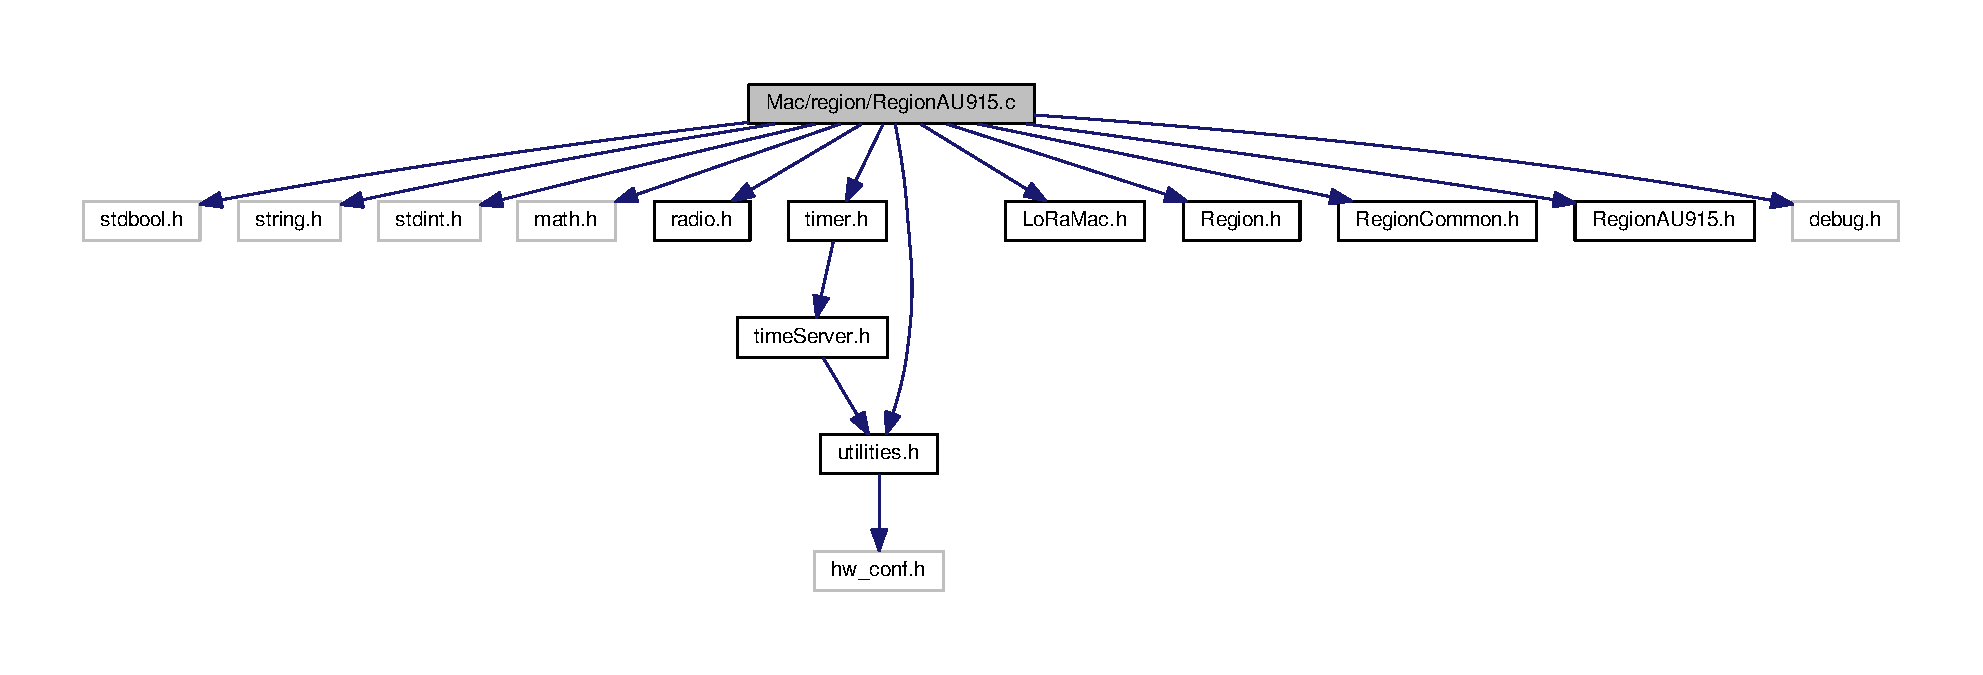
\includegraphics[width=350pt]{RegionAU915_8c__incl}
\end{center}
\end{figure}
\subsection*{Macros}
\begin{DoxyCompactItemize}
\item 
\#define \hyperlink{RegionAU915_8c_a1b20a8de3ae59c0b063fb313f0c70890}{C\+H\+A\+N\+N\+E\+L\+S\+\_\+\+M\+A\+S\+K\+\_\+\+S\+I\+ZE}~6
\end{DoxyCompactItemize}
\subsection*{Functions}
\begin{DoxyCompactItemize}
\item 
\hyperlink{group__REGION_gaed159b26e5c4677236b6e8677019db30}{Phy\+Param\+\_\+t} \hyperlink{group__REGIONAU915_ga91322f6f4dc9d6155316edd4dc198830}{Region\+A\+U915\+Get\+Phy\+Param} (\hyperlink{group__REGION_gab471483fff904f4f89bbc03f7fc380ab}{Get\+Phy\+Params\+\_\+t} $\ast$get\+Phy)
\begin{DoxyCompactList}\small\item\em The function gets a value of a specific phy attribute. \end{DoxyCompactList}\item 
void \hyperlink{group__REGIONAU915_ga612ca919a6dcb846f32080a89d3824d7}{Region\+A\+U915\+Set\+Band\+Tx\+Done} (\hyperlink{group__REGION_gad0524aa0673c0814a71e7a4f9cade3fc}{Set\+Band\+Tx\+Done\+Params\+\_\+t} $\ast$tx\+Done)
\begin{DoxyCompactList}\small\item\em Updates the last TX done parameters of the current channel. \end{DoxyCompactList}\item 
void \hyperlink{group__REGIONAU915_gaf061a05f766feb06e67da3377638034a}{Region\+A\+U915\+Init\+Defaults} (\hyperlink{group__REGION_gaddc73ae10673ec925724e7870363bda9}{Init\+Type\+\_\+t} type)
\begin{DoxyCompactList}\small\item\em Initializes the channels masks and the channels. \end{DoxyCompactList}\item 
bool \hyperlink{group__REGIONAU915_ga728e3b1cdcd99b88a8c923c9fd0fd9a4}{Region\+A\+U915\+Verify} (\hyperlink{group__REGION_ga966d97bc2f25df1c09e92e60ef652276}{Verify\+Params\+\_\+t} $\ast$verify, \hyperlink{group__REGION_ga9445b07fdf77581ecfaf389970e635f8}{Phy\+Attribute\+\_\+t} phy\+Attribute)
\begin{DoxyCompactList}\small\item\em Verifies a parameter. \end{DoxyCompactList}\item 
void \hyperlink{group__REGIONAU915_ga4fd62616137cb73c9fc38f0854e6dad9}{Region\+A\+U915\+Apply\+C\+F\+List} (\hyperlink{group__REGION_ga71588e9ad07e34b78fa91d51881fd3c6}{Apply\+C\+F\+List\+Params\+\_\+t} $\ast$apply\+C\+F\+List)
\begin{DoxyCompactList}\small\item\em The function parses the input buffer and sets up the channels of the CF list. \end{DoxyCompactList}\item 
bool \hyperlink{group__REGIONAU915_gaa3219b953ef291e813856e391ec6f494}{Region\+A\+U915\+Chan\+Mask\+Set} (\hyperlink{group__REGION_ga6d24f7da136006410827dfb29f6b9b9e}{Chan\+Mask\+Set\+Params\+\_\+t} $\ast$chan\+Mask\+Set)
\begin{DoxyCompactList}\small\item\em Sets a channels mask. \end{DoxyCompactList}\item 
bool \hyperlink{group__REGIONAU915_ga1a95e39e41556d5660b62cc8e3ac375f}{Region\+A\+U915\+Adr\+Next} (\hyperlink{group__REGION_ga567c2742622326b350b4e91bbf61b4ce}{Adr\+Next\+Params\+\_\+t} $\ast$adr\+Next, int8\+\_\+t $\ast$dr\+Out, int8\+\_\+t $\ast$tx\+Pow\+Out, uint32\+\_\+t $\ast$adr\+Ack\+Counter)
\begin{DoxyCompactList}\small\item\em Calculates the next datarate to set, when A\+DR is on or off. \end{DoxyCompactList}\item 
void \hyperlink{group__REGIONAU915_ga2f0f526d4c703e4f2058990b5cf92563}{Region\+A\+U915\+Compute\+Rx\+Window\+Parameters} (int8\+\_\+t datarate, uint8\+\_\+t min\+Rx\+Symbols, uint32\+\_\+t rx\+Error, \hyperlink{group__REGION_ga375c038078dfcfc7ef14280021db719e}{Rx\+Config\+Params\+\_\+t} $\ast$rx\+Config\+Params)
\item 
bool \hyperlink{group__REGIONAU915_gaf80c46b490d80c77aa137a5abe70c073}{Region\+A\+U915\+Rx\+Config} (\hyperlink{group__REGION_ga375c038078dfcfc7ef14280021db719e}{Rx\+Config\+Params\+\_\+t} $\ast$rx\+Config, int8\+\_\+t $\ast$datarate)
\begin{DoxyCompactList}\small\item\em Configuration of the RX windows. \end{DoxyCompactList}\item 
bool \hyperlink{group__REGIONAU915_ga6016e24d99216fad47de5194957c2c01}{Region\+A\+U915\+Tx\+Config} (\hyperlink{group__REGION_gabed730d4d04b0b60d4b6d1966d3f21d3}{Tx\+Config\+Params\+\_\+t} $\ast$tx\+Config, int8\+\_\+t $\ast$tx\+Power, \hyperlink{utilities_8h_a4215ca43d3e953099ea758ce428599d0}{Timer\+Time\+\_\+t} $\ast$tx\+Time\+On\+Air)
\begin{DoxyCompactList}\small\item\em TX configuration. \end{DoxyCompactList}\item 
uint8\+\_\+t \hyperlink{group__REGIONAU915_ga2614037d99a37bdd1d3d7df1a3361201}{Region\+A\+U915\+Link\+Adr\+Req} (\hyperlink{group__REGION_gad4af503e8d4de1846129e26a799a1e8e}{Link\+Adr\+Req\+Params\+\_\+t} $\ast$link\+Adr\+Req, int8\+\_\+t $\ast$dr\+Out, int8\+\_\+t $\ast$tx\+Pow\+Out, uint8\+\_\+t $\ast$nb\+Rep\+Out, uint8\+\_\+t $\ast$nb\+Bytes\+Parsed)
\begin{DoxyCompactList}\small\item\em The function processes a Link A\+DR Request. \end{DoxyCompactList}\item 
uint8\+\_\+t \hyperlink{group__REGIONAU915_ga865421723c0e1878fc94a151e95e6ee3}{Region\+A\+U915\+Rx\+Param\+Setup\+Req} (\hyperlink{group__REGION_ga7165f282c670c728c36d534df2285157}{Rx\+Param\+Setup\+Req\+Params\+\_\+t} $\ast$rx\+Param\+Setup\+Req)
\begin{DoxyCompactList}\small\item\em The function processes a RX Parameter Setup Request. \end{DoxyCompactList}\item 
uint8\+\_\+t \hyperlink{group__REGIONAU915_gab50eb32c1a156ee9629976c7bf29967c}{Region\+A\+U915\+New\+Channel\+Req} (\hyperlink{group__REGION_gae2abcdb6dbb843c9faf5fd3009eca9d6}{New\+Channel\+Req\+Params\+\_\+t} $\ast$new\+Channel\+Req)
\begin{DoxyCompactList}\small\item\em The function processes a Channel Request. \end{DoxyCompactList}\item 
int8\+\_\+t \hyperlink{group__REGIONAU915_gaa6db7d4c1d3b1e547aa00c13e1d31b08}{Region\+A\+U915\+Tx\+Param\+Setup\+Req} (\hyperlink{group__REGION_ga26836ef2996e70410e42ef471073f855}{Tx\+Param\+Setup\+Req\+Params\+\_\+t} $\ast$tx\+Param\+Setup\+Req)
\begin{DoxyCompactList}\small\item\em The function processes a TX Param\+Setup Request. \end{DoxyCompactList}\item 
uint8\+\_\+t \hyperlink{group__REGIONAU915_ga8568053064f5db87978653f9fd218177}{Region\+A\+U915\+Dl\+Channel\+Req} (\hyperlink{group__REGION_gae0d608ff1f8ea0a430e4f9a4c38ec7f3}{Dl\+Channel\+Req\+Params\+\_\+t} $\ast$dl\+Channel\+Req)
\begin{DoxyCompactList}\small\item\em The function processes a Dl\+Channel Request. \end{DoxyCompactList}\item 
int8\+\_\+t \hyperlink{group__REGIONAU915_ga968233f3d01f5aa9f91fff2c20955616}{Region\+A\+U915\+Alternate\+Dr} (\hyperlink{group__REGION_ga001ea4338d1c83f4c785b49d7ad2d696}{Alternate\+Dr\+Params\+\_\+t} $\ast$alternate\+Dr)
\begin{DoxyCompactList}\small\item\em Alternates the datarate of the channel for the join request. \end{DoxyCompactList}\item 
void \hyperlink{group__REGIONAU915_gaa3847b5ebad54c613afd3b823f1c39e9}{Region\+A\+U915\+Calc\+Back\+Off} (\hyperlink{group__REGION_ga7c5c9a8da174e6679eded8257dc92fd9}{Calc\+Back\+Off\+Params\+\_\+t} $\ast$calc\+Back\+Off)
\begin{DoxyCompactList}\small\item\em Calculates the back-\/off time. \end{DoxyCompactList}\item 
bool \hyperlink{group__REGIONAU915_gaa729787fd4ca5a83011f6928c278f95f}{Region\+A\+U915\+Next\+Channel} (\hyperlink{group__REGION_ga115f5e83afae352c0a3dcdc193374040}{Next\+Chan\+Params\+\_\+t} $\ast$next\+Chan\+Params, uint8\+\_\+t $\ast$channel, \hyperlink{utilities_8h_a4215ca43d3e953099ea758ce428599d0}{Timer\+Time\+\_\+t} $\ast$time, \hyperlink{utilities_8h_a4215ca43d3e953099ea758ce428599d0}{Timer\+Time\+\_\+t} $\ast$aggregated\+Time\+Off)
\begin{DoxyCompactList}\small\item\em Searches and set the next random available channel. \end{DoxyCompactList}\item 
\hyperlink{group__LORAMAC_ga30bd25657e10480f8605ee951b0ecfbd}{Lo\+Ra\+Mac\+Status\+\_\+t} \hyperlink{group__REGIONAU915_ga1065da4a50172d3af558c7bacc28ad10}{Region\+A\+U915\+Channel\+Add} (\hyperlink{group__REGION_gab1c5f3aa06614283202906cef4417860}{Channel\+Add\+Params\+\_\+t} $\ast$channel\+Add)
\begin{DoxyCompactList}\small\item\em Adds a channel. \end{DoxyCompactList}\item 
bool \hyperlink{group__REGIONAU915_ga4dfd376f684a40c659c69bf127a71a71}{Region\+A\+U915\+Channels\+Remove} (\hyperlink{group__REGION_gaa37468560d2fc81a977b57a48e5d72c0}{Channel\+Remove\+Params\+\_\+t} $\ast$channel\+Remove)
\begin{DoxyCompactList}\small\item\em Removes a channel. \end{DoxyCompactList}\item 
void \hyperlink{group__REGIONAU915_gae8d539bbf21ee45777245dc1467fa07a}{Region\+A\+U915\+Set\+Continuous\+Wave} (\hyperlink{group__REGION_gaf39bb5ba06921139c6d17f88a8d518cd}{Continuous\+Wave\+Params\+\_\+t} $\ast$continuous\+Wave)
\begin{DoxyCompactList}\small\item\em Sets the radio into continuous wave mode. \end{DoxyCompactList}\item 
uint8\+\_\+t \hyperlink{group__REGIONAU915_gacdcc572470d582ce82ca60df7ffe37b0}{Region\+A\+U915\+Apply\+Dr\+Offset} (uint8\+\_\+t downlink\+Dwell\+Time, int8\+\_\+t dr, int8\+\_\+t dr\+Offset)
\begin{DoxyCompactList}\small\item\em Computes new datarate according to the given offset. \end{DoxyCompactList}\end{DoxyCompactItemize}


\subsection{Macro Definition Documentation}
\mbox{\Hypertarget{RegionAU915_8c_a1b20a8de3ae59c0b063fb313f0c70890}\label{RegionAU915_8c_a1b20a8de3ae59c0b063fb313f0c70890}} 
\index{Region\+A\+U915.\+c@{Region\+A\+U915.\+c}!C\+H\+A\+N\+N\+E\+L\+S\+\_\+\+M\+A\+S\+K\+\_\+\+S\+I\+ZE@{C\+H\+A\+N\+N\+E\+L\+S\+\_\+\+M\+A\+S\+K\+\_\+\+S\+I\+ZE}}
\index{C\+H\+A\+N\+N\+E\+L\+S\+\_\+\+M\+A\+S\+K\+\_\+\+S\+I\+ZE@{C\+H\+A\+N\+N\+E\+L\+S\+\_\+\+M\+A\+S\+K\+\_\+\+S\+I\+ZE}!Region\+A\+U915.\+c@{Region\+A\+U915.\+c}}
\subsubsection{\texorpdfstring{C\+H\+A\+N\+N\+E\+L\+S\+\_\+\+M\+A\+S\+K\+\_\+\+S\+I\+ZE}{CHANNELS\_MASK\_SIZE}}
{\footnotesize\ttfamily \#define C\+H\+A\+N\+N\+E\+L\+S\+\_\+\+M\+A\+S\+K\+\_\+\+S\+I\+ZE~6}


\hypertarget{RegionAU915_8h}{}\section{Mac/region/\+Region\+A\+U915.h File Reference}
\label{RegionAU915_8h}\index{Mac/region/\+Region\+A\+U915.\+h@{Mac/region/\+Region\+A\+U915.\+h}}


Region definition for A\+U915.  


This graph shows which files directly or indirectly include this file\+:
\nopagebreak
\begin{figure}[H]
\begin{center}
\leavevmode
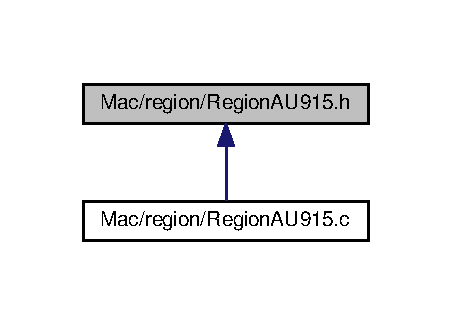
\includegraphics[width=217pt]{RegionAU915_8h__dep__incl}
\end{center}
\end{figure}
\subsection*{Macros}
\begin{DoxyCompactItemize}
\item 
\#define \hyperlink{group__REGIONAU915_ga2b76c47d2463a72cc6c69a6384a6de11}{A\+U915\+\_\+\+M\+A\+X\+\_\+\+N\+B\+\_\+\+C\+H\+A\+N\+N\+E\+LS}~72
\item 
\#define \hyperlink{group__REGIONAU915_ga3a7bb744191d2b9daaf6637d36d78422}{A\+U915\+\_\+\+T\+X\+\_\+\+M\+I\+N\+\_\+\+D\+A\+T\+A\+R\+A\+TE}~\hyperlink{group__REGION_ga6c4ef966b4f3d5eb7597b087f2b97095}{D\+R\+\_\+0}
\item 
\#define \hyperlink{group__REGIONAU915_gada67d69eba43730ad99c2a9f00308257}{A\+U915\+\_\+\+T\+X\+\_\+\+M\+A\+X\+\_\+\+D\+A\+T\+A\+R\+A\+TE}~\hyperlink{group__REGION_ga8e2b4c15b7dbb8bda5ed635ca1d262be}{D\+R\+\_\+6}
\item 
\#define \hyperlink{group__REGIONAU915_ga6c3e760e2bc555e4d608ff12d14f6652}{A\+U915\+\_\+\+R\+X\+\_\+\+M\+I\+N\+\_\+\+D\+A\+T\+A\+R\+A\+TE}~\hyperlink{group__REGION_ga44cc96ba80ae464cd9330b784d329c16}{D\+R\+\_\+8}
\item 
\#define \hyperlink{group__REGIONAU915_ga5ce832bce671573a6b6bb4a8358b250e}{A\+U915\+\_\+\+R\+X\+\_\+\+M\+A\+X\+\_\+\+D\+A\+T\+A\+R\+A\+TE}~\hyperlink{group__REGION_ga226f47470cc69a6fe831f7c92709bc1f}{D\+R\+\_\+13}
\item 
\#define \hyperlink{group__REGIONAU915_gaf13e696fe1ca41f523d0a52b0878c278}{A\+U915\+\_\+\+D\+E\+F\+A\+U\+L\+T\+\_\+\+D\+A\+T\+A\+R\+A\+TE}~\hyperlink{group__REGION_ga6c4ef966b4f3d5eb7597b087f2b97095}{D\+R\+\_\+0}
\item 
\#define \hyperlink{group__REGIONAU915_ga7de844f699bceb5022c05f4ed53d63e9}{A\+U915\+\_\+\+M\+I\+N\+\_\+\+R\+X1\+\_\+\+D\+R\+\_\+\+O\+F\+F\+S\+ET}~0
\item 
\#define \hyperlink{group__REGIONAU915_ga6787225088f0c4c8ce35106f5a986f4c}{A\+U915\+\_\+\+M\+A\+X\+\_\+\+R\+X1\+\_\+\+D\+R\+\_\+\+O\+F\+F\+S\+ET}~6
\item 
\#define \hyperlink{group__REGIONAU915_gad91be65b45ba7c349d42b1e564c65251}{A\+U915\+\_\+\+D\+E\+F\+A\+U\+L\+T\+\_\+\+R\+X1\+\_\+\+D\+R\+\_\+\+O\+F\+F\+S\+ET}~0
\item 
\#define \hyperlink{group__REGIONAU915_gabd0f5ea8e2143d42b1e480305bb2fd5d}{A\+U915\+\_\+\+M\+I\+N\+\_\+\+T\+X\+\_\+\+P\+O\+W\+ER}~\hyperlink{group__REGION_gac9747c69350f34d485c3134e5a57655b}{T\+X\+\_\+\+P\+O\+W\+E\+R\+\_\+10}
\item 
\#define \hyperlink{group__REGIONAU915_ga36808f695e52582b8a6a3ca4b4bf61d4}{A\+U915\+\_\+\+M\+A\+X\+\_\+\+T\+X\+\_\+\+P\+O\+W\+ER}~\hyperlink{group__REGION_gab33618449f2a573142c463ab071ef8ed}{T\+X\+\_\+\+P\+O\+W\+E\+R\+\_\+0}
\item 
\#define \hyperlink{group__REGIONAU915_ga8f8d247b742aea5399eabca9b978121f}{A\+U915\+\_\+\+D\+E\+F\+A\+U\+L\+T\+\_\+\+T\+X\+\_\+\+P\+O\+W\+ER}~\hyperlink{group__REGION_gab33618449f2a573142c463ab071ef8ed}{T\+X\+\_\+\+P\+O\+W\+E\+R\+\_\+0}
\item 
\#define \hyperlink{group__REGIONAU915_gac1d0807c3b28e1f1e1c7f574e66ba158}{A\+U915\+\_\+\+D\+E\+F\+A\+U\+L\+T\+\_\+\+M\+A\+X\+\_\+\+E\+I\+RP}~30.\+0f
\item 
\#define \hyperlink{group__REGIONAU915_ga3184a1e4e099ac04b86c390a012845a7}{A\+U915\+\_\+\+D\+E\+F\+A\+U\+L\+T\+\_\+\+A\+N\+T\+E\+N\+N\+A\+\_\+\+G\+A\+IN}~2.\+15f
\item 
\#define \hyperlink{group__REGIONAU915_gab5782862067a1d6338da8372a9d484c6}{A\+U915\+\_\+\+A\+D\+R\+\_\+\+A\+C\+K\+\_\+\+L\+I\+M\+IT}~64
\item 
\#define \hyperlink{group__REGIONAU915_ga6c2174a6e83dcd5e4137a28c841d82b2}{A\+U915\+\_\+\+A\+D\+R\+\_\+\+A\+C\+K\+\_\+\+D\+E\+L\+AY}~32
\item 
\#define \hyperlink{group__REGIONAU915_gad79bd0bbe937761936fef981e384d398}{A\+U915\+\_\+\+D\+U\+T\+Y\+\_\+\+C\+Y\+C\+L\+E\+\_\+\+E\+N\+A\+B\+L\+ED}~0
\item 
\#define \hyperlink{group__REGIONAU915_gaa6e565b2bc461699f7119256776b8f67}{A\+U915\+\_\+\+M\+A\+X\+\_\+\+R\+X\+\_\+\+W\+I\+N\+D\+OW}~3000
\item 
\#define \hyperlink{group__REGIONAU915_ga989f85b36be98caed732595e6b13adb3}{A\+U915\+\_\+\+R\+E\+C\+E\+I\+V\+E\+\_\+\+D\+E\+L\+A\+Y1}~1000
\item 
\#define \hyperlink{group__REGIONAU915_ga06692cedba60898ee0df93cf21429796}{A\+U915\+\_\+\+R\+E\+C\+E\+I\+V\+E\+\_\+\+D\+E\+L\+A\+Y2}~2000
\item 
\#define \hyperlink{group__REGIONAU915_ga6a3867937f85eac03a4f5518fddee947}{A\+U915\+\_\+\+J\+O\+I\+N\+\_\+\+A\+C\+C\+E\+P\+T\+\_\+\+D\+E\+L\+A\+Y1}~5000
\item 
\#define \hyperlink{group__REGIONAU915_ga00b42a4ecd7b4484f73a1e428652f5fc}{A\+U915\+\_\+\+J\+O\+I\+N\+\_\+\+A\+C\+C\+E\+P\+T\+\_\+\+D\+E\+L\+A\+Y2}~6000
\item 
\#define \hyperlink{group__REGIONAU915_gaf4dd6f2ba296be813e56ffc3fdcbf7ab}{A\+U915\+\_\+\+M\+A\+X\+\_\+\+F\+C\+N\+T\+\_\+\+G\+AP}~16384
\item 
\#define \hyperlink{group__REGIONAU915_ga3fc2d9d63bcd48b926612b12eaa81971}{A\+U915\+\_\+\+A\+C\+K\+T\+I\+M\+E\+O\+UT}~2000
\item 
\#define \hyperlink{group__REGIONAU915_ga093d31ebddca807195cbe6c6144258fa}{A\+U915\+\_\+\+A\+C\+K\+\_\+\+T\+I\+M\+E\+O\+U\+T\+\_\+\+R\+ND}~1000
\item 
\#define \hyperlink{group__REGIONAU915_ga0fbc056b672f0dedf7311ddfe59515b6}{A\+U915\+\_\+\+R\+X\+\_\+\+W\+N\+D\+\_\+2\+\_\+\+F\+R\+EQ}~923300000
\item 
\#define \hyperlink{group__REGIONAU915_gab50b9056c8405c3538819bbc21b78ebf}{A\+U915\+\_\+\+R\+X\+\_\+\+W\+N\+D\+\_\+2\+\_\+\+DR}~\hyperlink{group__REGION_ga44cc96ba80ae464cd9330b784d329c16}{D\+R\+\_\+8}
\item 
\#define \hyperlink{group__REGIONAU915_gad166b707f964b6b057ec3bb189c35ebc}{A\+U915\+\_\+\+M\+A\+X\+\_\+\+N\+B\+\_\+\+B\+A\+N\+DS}~1
\item 
\#define \hyperlink{group__REGIONAU915_ga6e0a29afe59acad8c0b01808e984684a}{A\+U915\+\_\+\+B\+A\+N\+D0}~\{ 1, \hyperlink{group__REGIONAU915_ga36808f695e52582b8a6a3ca4b4bf61d4}{A\+U915\+\_\+\+M\+A\+X\+\_\+\+T\+X\+\_\+\+P\+O\+W\+ER}, 0,  0 \}
\item 
\#define \hyperlink{group__REGIONAU915_ga006dab0130b61538f621e80e9f6028ce}{A\+U915\+\_\+\+F\+I\+R\+S\+T\+\_\+\+R\+X1\+\_\+\+C\+H\+A\+N\+N\+EL}~( (uint32\+\_\+t) 923300000 )
\item 
\#define \hyperlink{group__REGIONAU915_gaa9d052a49ace8fc23a34e297449711be}{A\+U915\+\_\+\+L\+A\+S\+T\+\_\+\+R\+X1\+\_\+\+C\+H\+A\+N\+N\+EL}~( (uint32\+\_\+t) 927500000 )
\item 
\#define \hyperlink{group__REGIONAU915_gae66b13ecda158ed17cddb4ca5a9331f5}{A\+U915\+\_\+\+S\+T\+E\+P\+W\+I\+D\+T\+H\+\_\+\+R\+X1\+\_\+\+C\+H\+A\+N\+N\+EL}~( (uint32\+\_\+t) 600000 )
\end{DoxyCompactItemize}
\subsection*{Functions}
\begin{DoxyCompactItemize}
\item 
\hyperlink{group__REGION_gaed159b26e5c4677236b6e8677019db30}{Phy\+Param\+\_\+t} \hyperlink{group__REGIONAU915_ga91322f6f4dc9d6155316edd4dc198830}{Region\+A\+U915\+Get\+Phy\+Param} (\hyperlink{group__REGION_gab471483fff904f4f89bbc03f7fc380ab}{Get\+Phy\+Params\+\_\+t} $\ast$get\+Phy)
\begin{DoxyCompactList}\small\item\em The function gets a value of a specific phy attribute. \end{DoxyCompactList}\item 
void \hyperlink{group__REGIONAU915_ga612ca919a6dcb846f32080a89d3824d7}{Region\+A\+U915\+Set\+Band\+Tx\+Done} (\hyperlink{group__REGION_gad0524aa0673c0814a71e7a4f9cade3fc}{Set\+Band\+Tx\+Done\+Params\+\_\+t} $\ast$tx\+Done)
\begin{DoxyCompactList}\small\item\em Updates the last TX done parameters of the current channel. \end{DoxyCompactList}\item 
void \hyperlink{group__REGIONAU915_gaf061a05f766feb06e67da3377638034a}{Region\+A\+U915\+Init\+Defaults} (\hyperlink{group__REGION_gaddc73ae10673ec925724e7870363bda9}{Init\+Type\+\_\+t} type)
\begin{DoxyCompactList}\small\item\em Initializes the channels masks and the channels. \end{DoxyCompactList}\item 
bool \hyperlink{group__REGIONAU915_ga728e3b1cdcd99b88a8c923c9fd0fd9a4}{Region\+A\+U915\+Verify} (\hyperlink{group__REGION_ga966d97bc2f25df1c09e92e60ef652276}{Verify\+Params\+\_\+t} $\ast$verify, \hyperlink{group__REGION_ga9445b07fdf77581ecfaf389970e635f8}{Phy\+Attribute\+\_\+t} phy\+Attribute)
\begin{DoxyCompactList}\small\item\em Verifies a parameter. \end{DoxyCompactList}\item 
void \hyperlink{group__REGIONAU915_ga4fd62616137cb73c9fc38f0854e6dad9}{Region\+A\+U915\+Apply\+C\+F\+List} (\hyperlink{group__REGION_ga71588e9ad07e34b78fa91d51881fd3c6}{Apply\+C\+F\+List\+Params\+\_\+t} $\ast$apply\+C\+F\+List)
\begin{DoxyCompactList}\small\item\em The function parses the input buffer and sets up the channels of the CF list. \end{DoxyCompactList}\item 
bool \hyperlink{group__REGIONAU915_gaa3219b953ef291e813856e391ec6f494}{Region\+A\+U915\+Chan\+Mask\+Set} (\hyperlink{group__REGION_ga6d24f7da136006410827dfb29f6b9b9e}{Chan\+Mask\+Set\+Params\+\_\+t} $\ast$chan\+Mask\+Set)
\begin{DoxyCompactList}\small\item\em Sets a channels mask. \end{DoxyCompactList}\item 
bool \hyperlink{group__REGIONAU915_ga1a95e39e41556d5660b62cc8e3ac375f}{Region\+A\+U915\+Adr\+Next} (\hyperlink{group__REGION_ga567c2742622326b350b4e91bbf61b4ce}{Adr\+Next\+Params\+\_\+t} $\ast$adr\+Next, int8\+\_\+t $\ast$dr\+Out, int8\+\_\+t $\ast$tx\+Pow\+Out, uint32\+\_\+t $\ast$adr\+Ack\+Counter)
\begin{DoxyCompactList}\small\item\em Calculates the next datarate to set, when A\+DR is on or off. \end{DoxyCompactList}\item 
void \hyperlink{group__REGIONAU915_ga2f0f526d4c703e4f2058990b5cf92563}{Region\+A\+U915\+Compute\+Rx\+Window\+Parameters} (int8\+\_\+t datarate, uint8\+\_\+t min\+Rx\+Symbols, uint32\+\_\+t rx\+Error, \hyperlink{group__REGION_ga375c038078dfcfc7ef14280021db719e}{Rx\+Config\+Params\+\_\+t} $\ast$rx\+Config\+Params)
\item 
bool \hyperlink{group__REGIONAU915_gaf80c46b490d80c77aa137a5abe70c073}{Region\+A\+U915\+Rx\+Config} (\hyperlink{group__REGION_ga375c038078dfcfc7ef14280021db719e}{Rx\+Config\+Params\+\_\+t} $\ast$rx\+Config, int8\+\_\+t $\ast$datarate)
\begin{DoxyCompactList}\small\item\em Configuration of the RX windows. \end{DoxyCompactList}\item 
bool \hyperlink{group__REGIONAU915_ga6016e24d99216fad47de5194957c2c01}{Region\+A\+U915\+Tx\+Config} (\hyperlink{group__REGION_gabed730d4d04b0b60d4b6d1966d3f21d3}{Tx\+Config\+Params\+\_\+t} $\ast$tx\+Config, int8\+\_\+t $\ast$tx\+Power, \hyperlink{utilities_8h_a4215ca43d3e953099ea758ce428599d0}{Timer\+Time\+\_\+t} $\ast$tx\+Time\+On\+Air)
\begin{DoxyCompactList}\small\item\em TX configuration. \end{DoxyCompactList}\item 
uint8\+\_\+t \hyperlink{group__REGIONAU915_ga2614037d99a37bdd1d3d7df1a3361201}{Region\+A\+U915\+Link\+Adr\+Req} (\hyperlink{group__REGION_gad4af503e8d4de1846129e26a799a1e8e}{Link\+Adr\+Req\+Params\+\_\+t} $\ast$link\+Adr\+Req, int8\+\_\+t $\ast$dr\+Out, int8\+\_\+t $\ast$tx\+Pow\+Out, uint8\+\_\+t $\ast$nb\+Rep\+Out, uint8\+\_\+t $\ast$nb\+Bytes\+Parsed)
\begin{DoxyCompactList}\small\item\em The function processes a Link A\+DR Request. \end{DoxyCompactList}\item 
uint8\+\_\+t \hyperlink{group__REGIONAU915_ga865421723c0e1878fc94a151e95e6ee3}{Region\+A\+U915\+Rx\+Param\+Setup\+Req} (\hyperlink{group__REGION_ga7165f282c670c728c36d534df2285157}{Rx\+Param\+Setup\+Req\+Params\+\_\+t} $\ast$rx\+Param\+Setup\+Req)
\begin{DoxyCompactList}\small\item\em The function processes a RX Parameter Setup Request. \end{DoxyCompactList}\item 
uint8\+\_\+t \hyperlink{group__REGIONAU915_gab50eb32c1a156ee9629976c7bf29967c}{Region\+A\+U915\+New\+Channel\+Req} (\hyperlink{group__REGION_gae2abcdb6dbb843c9faf5fd3009eca9d6}{New\+Channel\+Req\+Params\+\_\+t} $\ast$new\+Channel\+Req)
\begin{DoxyCompactList}\small\item\em The function processes a Channel Request. \end{DoxyCompactList}\item 
int8\+\_\+t \hyperlink{group__REGIONAU915_gaa6db7d4c1d3b1e547aa00c13e1d31b08}{Region\+A\+U915\+Tx\+Param\+Setup\+Req} (\hyperlink{group__REGION_ga26836ef2996e70410e42ef471073f855}{Tx\+Param\+Setup\+Req\+Params\+\_\+t} $\ast$tx\+Param\+Setup\+Req)
\begin{DoxyCompactList}\small\item\em The function processes a TX Param\+Setup Request. \end{DoxyCompactList}\item 
uint8\+\_\+t \hyperlink{group__REGIONAU915_ga8568053064f5db87978653f9fd218177}{Region\+A\+U915\+Dl\+Channel\+Req} (\hyperlink{group__REGION_gae0d608ff1f8ea0a430e4f9a4c38ec7f3}{Dl\+Channel\+Req\+Params\+\_\+t} $\ast$dl\+Channel\+Req)
\begin{DoxyCompactList}\small\item\em The function processes a Dl\+Channel Request. \end{DoxyCompactList}\item 
int8\+\_\+t \hyperlink{group__REGIONAU915_ga968233f3d01f5aa9f91fff2c20955616}{Region\+A\+U915\+Alternate\+Dr} (\hyperlink{group__REGION_ga001ea4338d1c83f4c785b49d7ad2d696}{Alternate\+Dr\+Params\+\_\+t} $\ast$alternate\+Dr)
\begin{DoxyCompactList}\small\item\em Alternates the datarate of the channel for the join request. \end{DoxyCompactList}\item 
void \hyperlink{group__REGIONAU915_gaa3847b5ebad54c613afd3b823f1c39e9}{Region\+A\+U915\+Calc\+Back\+Off} (\hyperlink{group__REGION_ga7c5c9a8da174e6679eded8257dc92fd9}{Calc\+Back\+Off\+Params\+\_\+t} $\ast$calc\+Back\+Off)
\begin{DoxyCompactList}\small\item\em Calculates the back-\/off time. \end{DoxyCompactList}\item 
bool \hyperlink{group__REGIONAU915_gaa729787fd4ca5a83011f6928c278f95f}{Region\+A\+U915\+Next\+Channel} (\hyperlink{group__REGION_ga115f5e83afae352c0a3dcdc193374040}{Next\+Chan\+Params\+\_\+t} $\ast$next\+Chan\+Params, uint8\+\_\+t $\ast$channel, \hyperlink{utilities_8h_a4215ca43d3e953099ea758ce428599d0}{Timer\+Time\+\_\+t} $\ast$time, \hyperlink{utilities_8h_a4215ca43d3e953099ea758ce428599d0}{Timer\+Time\+\_\+t} $\ast$aggregated\+Time\+Off)
\begin{DoxyCompactList}\small\item\em Searches and set the next random available channel. \end{DoxyCompactList}\item 
\hyperlink{group__LORAMAC_ga30bd25657e10480f8605ee951b0ecfbd}{Lo\+Ra\+Mac\+Status\+\_\+t} \hyperlink{group__REGIONAU915_ga1065da4a50172d3af558c7bacc28ad10}{Region\+A\+U915\+Channel\+Add} (\hyperlink{group__REGION_gab1c5f3aa06614283202906cef4417860}{Channel\+Add\+Params\+\_\+t} $\ast$channel\+Add)
\begin{DoxyCompactList}\small\item\em Adds a channel. \end{DoxyCompactList}\item 
bool \hyperlink{group__REGIONAU915_ga4dfd376f684a40c659c69bf127a71a71}{Region\+A\+U915\+Channels\+Remove} (\hyperlink{group__REGION_gaa37468560d2fc81a977b57a48e5d72c0}{Channel\+Remove\+Params\+\_\+t} $\ast$channel\+Remove)
\begin{DoxyCompactList}\small\item\em Removes a channel. \end{DoxyCompactList}\item 
void \hyperlink{group__REGIONAU915_gae8d539bbf21ee45777245dc1467fa07a}{Region\+A\+U915\+Set\+Continuous\+Wave} (\hyperlink{group__REGION_gaf39bb5ba06921139c6d17f88a8d518cd}{Continuous\+Wave\+Params\+\_\+t} $\ast$continuous\+Wave)
\begin{DoxyCompactList}\small\item\em Sets the radio into continuous wave mode. \end{DoxyCompactList}\item 
uint8\+\_\+t \hyperlink{group__REGIONAU915_gacdcc572470d582ce82ca60df7ffe37b0}{Region\+A\+U915\+Apply\+Dr\+Offset} (uint8\+\_\+t downlink\+Dwell\+Time, int8\+\_\+t dr, int8\+\_\+t dr\+Offset)
\begin{DoxyCompactList}\small\item\em Computes new datarate according to the given offset. \end{DoxyCompactList}\end{DoxyCompactItemize}


\subsection{Detailed Description}
Region definition for A\+U915. 

\begin{DoxyCopyright}{Copyright}
Revised B\+SD License, see section L\+I\+C\+E\+N\+SE.
\end{DoxyCopyright}

\begin{DoxyCode}
  \_\_\_\_\_\_                              \_
 / \_\_\_\_\_)             \_              | |
( (\_\_\_\_  \_\_\_\_\_ \_\_\_\_ \_| |\_ \_\_\_\_\_  \_\_\_\_| |\_\_
 \(\backslash\)\_\_\_\_ \(\backslash\)| \_\_\_ |    (\_   \_) \_\_\_ |/ \_\_\_)  \_ \(\backslash\)
 \_\_\_\_\_) ) \_\_\_\_| | | || |\_| \_\_\_\_( (\_\_\_| | | |
(\_\_\_\_\_\_/|\_\_\_\_\_)\_|\_|\_| \(\backslash\)\_\_)\_\_\_\_\_)\(\backslash\)\_\_\_\_)\_| |\_|
(C)2013 Semtech

 \_\_\_ \_\_\_\_\_ \_   \_\_\_ \_  \_\_\_\_\_ \_\_\_  \_\_\_  \_\_\_ \_\_\_
/ \_\_|\_   \_/\_\(\backslash\) / \_\_| |/ / \_\_/ \_ \(\backslash\)| \_ \(\backslash\)/ \_\_| \_\_|
\(\backslash\)\_\_ \(\backslash\) | |/ \_ \(\backslash\) (\_\_| \textcolor{stringliteral}{' <| \_| (\_) |   / (\_\_| \_|}
\textcolor{stringliteral}{|\_\_\_/ |\_/\_/ \(\backslash\)\_\(\backslash\)\_\_\_|\_|\(\backslash\)\_\(\backslash\)\_| \(\backslash\)\_\_\_/|\_|\_\(\backslash\)\(\backslash\)\_\_\_|\_\_\_|}
\textcolor{stringliteral}{embedded.connectivity.solutions===============}
\end{DoxyCode}


\begin{DoxyAuthor}{Author}
Miguel Luis ( Semtech )

Gregory Cristian ( Semtech )

Daniel Jaeckle ( S\+T\+A\+C\+K\+F\+O\+R\+CE ) 
\end{DoxyAuthor}

\hypertarget{RegionCN470_8c}{}\section{Mac/region/\+Region\+C\+N470.c File Reference}
\label{RegionCN470_8c}\index{Mac/region/\+Region\+C\+N470.\+c@{Mac/region/\+Region\+C\+N470.\+c}}
{\ttfamily \#include $<$stdbool.\+h$>$}\newline
{\ttfamily \#include $<$string.\+h$>$}\newline
{\ttfamily \#include $<$stdint.\+h$>$}\newline
{\ttfamily \#include $<$math.\+h$>$}\newline
{\ttfamily \#include \char`\"{}radio.\+h\char`\"{}}\newline
{\ttfamily \#include \char`\"{}timer.\+h\char`\"{}}\newline
{\ttfamily \#include \char`\"{}Lo\+Ra\+Mac.\+h\char`\"{}}\newline
{\ttfamily \#include \char`\"{}utilities.\+h\char`\"{}}\newline
{\ttfamily \#include \char`\"{}Region.\+h\char`\"{}}\newline
{\ttfamily \#include \char`\"{}Region\+Common.\+h\char`\"{}}\newline
{\ttfamily \#include \char`\"{}Region\+C\+N470.\+h\char`\"{}}\newline
{\ttfamily \#include \char`\"{}debug.\+h\char`\"{}}\newline
Include dependency graph for Region\+C\+N470.\+c\+:
\nopagebreak
\begin{figure}[H]
\begin{center}
\leavevmode
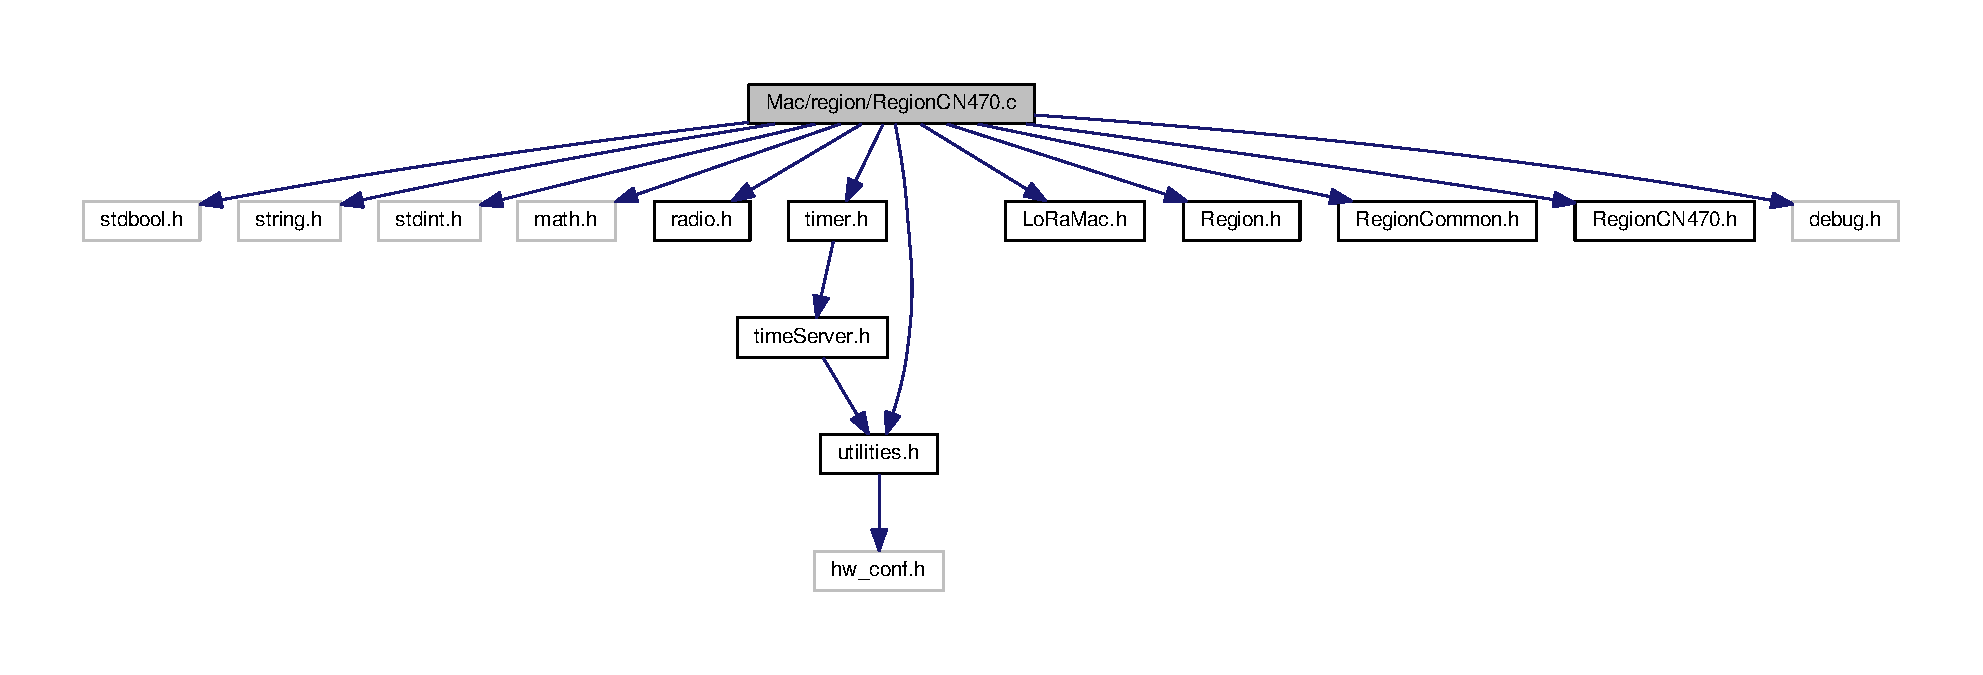
\includegraphics[width=350pt]{RegionCN470_8c__incl}
\end{center}
\end{figure}
\subsection*{Macros}
\begin{DoxyCompactItemize}
\item 
\#define \hyperlink{RegionCN470_8c_a1b20a8de3ae59c0b063fb313f0c70890}{C\+H\+A\+N\+N\+E\+L\+S\+\_\+\+M\+A\+S\+K\+\_\+\+S\+I\+ZE}~6
\end{DoxyCompactItemize}
\subsection*{Functions}
\begin{DoxyCompactItemize}
\item 
\hyperlink{group__REGION_gaed159b26e5c4677236b6e8677019db30}{Phy\+Param\+\_\+t} \hyperlink{group__REGIONCN470_gaa3f4e59184226b161b9e6880b6e7f204}{Region\+C\+N470\+Get\+Phy\+Param} (\hyperlink{group__REGION_gab471483fff904f4f89bbc03f7fc380ab}{Get\+Phy\+Params\+\_\+t} $\ast$get\+Phy)
\begin{DoxyCompactList}\small\item\em The function gets a value of a specific phy attribute. \end{DoxyCompactList}\item 
void \hyperlink{group__REGIONCN470_gad60aebff1bb6c89423fff84d57b21cb6}{Region\+C\+N470\+Set\+Band\+Tx\+Done} (\hyperlink{group__REGION_gad0524aa0673c0814a71e7a4f9cade3fc}{Set\+Band\+Tx\+Done\+Params\+\_\+t} $\ast$tx\+Done)
\begin{DoxyCompactList}\small\item\em Updates the last TX done parameters of the current channel. \end{DoxyCompactList}\item 
void \hyperlink{group__REGIONCN470_ga6591ac8edd635c34b47ec2f21627b145}{Region\+C\+N470\+Init\+Defaults} (\hyperlink{group__REGION_gaddc73ae10673ec925724e7870363bda9}{Init\+Type\+\_\+t} type)
\begin{DoxyCompactList}\small\item\em Initializes the channels masks and the channels. \end{DoxyCompactList}\item 
bool \hyperlink{group__REGIONCN470_ga7d7ddf394ddb8a6ac2d7cb5fea7ad745}{Region\+C\+N470\+Verify} (\hyperlink{group__REGION_ga966d97bc2f25df1c09e92e60ef652276}{Verify\+Params\+\_\+t} $\ast$verify, \hyperlink{group__REGION_ga9445b07fdf77581ecfaf389970e635f8}{Phy\+Attribute\+\_\+t} phy\+Attribute)
\begin{DoxyCompactList}\small\item\em Verifies a parameter. \end{DoxyCompactList}\item 
void \hyperlink{group__REGIONCN470_gae0ca4a5d6bf63fdb278a132ec496649f}{Region\+C\+N470\+Apply\+C\+F\+List} (\hyperlink{group__REGION_ga71588e9ad07e34b78fa91d51881fd3c6}{Apply\+C\+F\+List\+Params\+\_\+t} $\ast$apply\+C\+F\+List)
\begin{DoxyCompactList}\small\item\em The function parses the input buffer and sets up the channels of the CF list. \end{DoxyCompactList}\item 
bool \hyperlink{group__REGIONCN470_ga361aa9a80854b1a264a9ad0720cbd4da}{Region\+C\+N470\+Chan\+Mask\+Set} (\hyperlink{group__REGION_ga6d24f7da136006410827dfb29f6b9b9e}{Chan\+Mask\+Set\+Params\+\_\+t} $\ast$chan\+Mask\+Set)
\begin{DoxyCompactList}\small\item\em Sets a channels mask. \end{DoxyCompactList}\item 
bool \hyperlink{group__REGIONCN470_ga5205fdda3f4a869d78f4ccd791de359e}{Region\+C\+N470\+Adr\+Next} (\hyperlink{group__REGION_ga567c2742622326b350b4e91bbf61b4ce}{Adr\+Next\+Params\+\_\+t} $\ast$adr\+Next, int8\+\_\+t $\ast$dr\+Out, int8\+\_\+t $\ast$tx\+Pow\+Out, uint32\+\_\+t $\ast$adr\+Ack\+Counter)
\begin{DoxyCompactList}\small\item\em Calculates the next datarate to set, when A\+DR is on or off. \end{DoxyCompactList}\item 
void \hyperlink{group__REGIONCN470_gabb50864b958d868d7c2fbb09a7238a23}{Region\+C\+N470\+Compute\+Rx\+Window\+Parameters} (int8\+\_\+t datarate, uint8\+\_\+t min\+Rx\+Symbols, uint32\+\_\+t rx\+Error, \hyperlink{group__REGION_ga375c038078dfcfc7ef14280021db719e}{Rx\+Config\+Params\+\_\+t} $\ast$rx\+Config\+Params)
\item 
bool \hyperlink{group__REGIONCN470_gadb4b05f4e7b55705e37156add3ed585b}{Region\+C\+N470\+Rx\+Config} (\hyperlink{group__REGION_ga375c038078dfcfc7ef14280021db719e}{Rx\+Config\+Params\+\_\+t} $\ast$rx\+Config, int8\+\_\+t $\ast$datarate)
\begin{DoxyCompactList}\small\item\em Configuration of the RX windows. \end{DoxyCompactList}\item 
bool \hyperlink{group__REGIONCN470_ga2de0fae78c1759fec62a835b0fcb3829}{Region\+C\+N470\+Tx\+Config} (\hyperlink{group__REGION_gabed730d4d04b0b60d4b6d1966d3f21d3}{Tx\+Config\+Params\+\_\+t} $\ast$tx\+Config, int8\+\_\+t $\ast$tx\+Power, \hyperlink{utilities_8h_a4215ca43d3e953099ea758ce428599d0}{Timer\+Time\+\_\+t} $\ast$tx\+Time\+On\+Air)
\begin{DoxyCompactList}\small\item\em TX configuration. \end{DoxyCompactList}\item 
uint8\+\_\+t \hyperlink{group__REGIONCN470_ga8390f178b68e708cd9741caba00cb05d}{Region\+C\+N470\+Link\+Adr\+Req} (\hyperlink{group__REGION_gad4af503e8d4de1846129e26a799a1e8e}{Link\+Adr\+Req\+Params\+\_\+t} $\ast$link\+Adr\+Req, int8\+\_\+t $\ast$dr\+Out, int8\+\_\+t $\ast$tx\+Pow\+Out, uint8\+\_\+t $\ast$nb\+Rep\+Out, uint8\+\_\+t $\ast$nb\+Bytes\+Parsed)
\begin{DoxyCompactList}\small\item\em The function processes a Link A\+DR Request. \end{DoxyCompactList}\item 
uint8\+\_\+t \hyperlink{group__REGIONCN470_gae6be53827b6148fa40a6c1a3f6a8058b}{Region\+C\+N470\+Rx\+Param\+Setup\+Req} (\hyperlink{group__REGION_ga7165f282c670c728c36d534df2285157}{Rx\+Param\+Setup\+Req\+Params\+\_\+t} $\ast$rx\+Param\+Setup\+Req)
\begin{DoxyCompactList}\small\item\em The function processes a RX Parameter Setup Request. \end{DoxyCompactList}\item 
uint8\+\_\+t \hyperlink{group__REGIONCN470_ga3db01af8efb6f0c07db00b78dcb2ebfe}{Region\+C\+N470\+New\+Channel\+Req} (\hyperlink{group__REGION_gae2abcdb6dbb843c9faf5fd3009eca9d6}{New\+Channel\+Req\+Params\+\_\+t} $\ast$new\+Channel\+Req)
\begin{DoxyCompactList}\small\item\em The function processes a Channel Request. \end{DoxyCompactList}\item 
int8\+\_\+t \hyperlink{group__REGIONCN470_ga26c513769fa09c8bd92f15805162860b}{Region\+C\+N470\+Tx\+Param\+Setup\+Req} (\hyperlink{group__REGION_ga26836ef2996e70410e42ef471073f855}{Tx\+Param\+Setup\+Req\+Params\+\_\+t} $\ast$tx\+Param\+Setup\+Req)
\begin{DoxyCompactList}\small\item\em The function processes a TX Param\+Setup Request. \end{DoxyCompactList}\item 
uint8\+\_\+t \hyperlink{group__REGIONCN470_ga2fb7a7dcde7482f3a0da9028090c9c7f}{Region\+C\+N470\+Dl\+Channel\+Req} (\hyperlink{group__REGION_gae0d608ff1f8ea0a430e4f9a4c38ec7f3}{Dl\+Channel\+Req\+Params\+\_\+t} $\ast$dl\+Channel\+Req)
\begin{DoxyCompactList}\small\item\em The function processes a Dl\+Channel Request. \end{DoxyCompactList}\item 
int8\+\_\+t \hyperlink{group__REGIONCN470_ga5d07deb9b6a4c9a214439edae58bf341}{Region\+C\+N470\+Alternate\+Dr} (\hyperlink{group__REGION_ga001ea4338d1c83f4c785b49d7ad2d696}{Alternate\+Dr\+Params\+\_\+t} $\ast$alternate\+Dr)
\begin{DoxyCompactList}\small\item\em Alternates the datarate of the channel for the join request. \end{DoxyCompactList}\item 
void \hyperlink{group__REGIONCN470_ga2020e2db0351b7010e2e5fd53c466cc2}{Region\+C\+N470\+Calc\+Back\+Off} (\hyperlink{group__REGION_ga7c5c9a8da174e6679eded8257dc92fd9}{Calc\+Back\+Off\+Params\+\_\+t} $\ast$calc\+Back\+Off)
\begin{DoxyCompactList}\small\item\em Calculates the back-\/off time. \end{DoxyCompactList}\item 
bool \hyperlink{group__REGIONCN470_gad6d2b5fce0ea41dc2416648dcc674287}{Region\+C\+N470\+Next\+Channel} (\hyperlink{group__REGION_ga115f5e83afae352c0a3dcdc193374040}{Next\+Chan\+Params\+\_\+t} $\ast$next\+Chan\+Params, uint8\+\_\+t $\ast$channel, \hyperlink{utilities_8h_a4215ca43d3e953099ea758ce428599d0}{Timer\+Time\+\_\+t} $\ast$time, \hyperlink{utilities_8h_a4215ca43d3e953099ea758ce428599d0}{Timer\+Time\+\_\+t} $\ast$aggregated\+Time\+Off)
\begin{DoxyCompactList}\small\item\em Searches and set the next random available channel. \end{DoxyCompactList}\item 
\hyperlink{group__LORAMAC_ga30bd25657e10480f8605ee951b0ecfbd}{Lo\+Ra\+Mac\+Status\+\_\+t} \hyperlink{group__REGIONCN470_ga6f447bc77fedcf05b61c6a4247b0972b}{Region\+C\+N470\+Channel\+Add} (\hyperlink{group__REGION_gab1c5f3aa06614283202906cef4417860}{Channel\+Add\+Params\+\_\+t} $\ast$channel\+Add)
\begin{DoxyCompactList}\small\item\em Adds a channel. \end{DoxyCompactList}\item 
bool \hyperlink{group__REGIONCN470_ga325aac904d27927672021106fc718f09}{Region\+C\+N470\+Channels\+Remove} (\hyperlink{group__REGION_gaa37468560d2fc81a977b57a48e5d72c0}{Channel\+Remove\+Params\+\_\+t} $\ast$channel\+Remove)
\begin{DoxyCompactList}\small\item\em Removes a channel. \end{DoxyCompactList}\item 
void \hyperlink{group__REGIONCN470_ga0a1e509012a913631470e9801cc972bd}{Region\+C\+N470\+Set\+Continuous\+Wave} (\hyperlink{group__REGION_gaf39bb5ba06921139c6d17f88a8d518cd}{Continuous\+Wave\+Params\+\_\+t} $\ast$continuous\+Wave)
\begin{DoxyCompactList}\small\item\em Sets the radio into continuous wave mode. \end{DoxyCompactList}\item 
uint8\+\_\+t \hyperlink{group__REGIONCN470_ga9b7086c4eb616fb332a95f05845aac89}{Region\+C\+N470\+Apply\+Dr\+Offset} (uint8\+\_\+t downlink\+Dwell\+Time, int8\+\_\+t dr, int8\+\_\+t dr\+Offset)
\begin{DoxyCompactList}\small\item\em Computes new datarate according to the given offset. \end{DoxyCompactList}\end{DoxyCompactItemize}


\subsection{Macro Definition Documentation}
\mbox{\Hypertarget{RegionCN470_8c_a1b20a8de3ae59c0b063fb313f0c70890}\label{RegionCN470_8c_a1b20a8de3ae59c0b063fb313f0c70890}} 
\index{Region\+C\+N470.\+c@{Region\+C\+N470.\+c}!C\+H\+A\+N\+N\+E\+L\+S\+\_\+\+M\+A\+S\+K\+\_\+\+S\+I\+ZE@{C\+H\+A\+N\+N\+E\+L\+S\+\_\+\+M\+A\+S\+K\+\_\+\+S\+I\+ZE}}
\index{C\+H\+A\+N\+N\+E\+L\+S\+\_\+\+M\+A\+S\+K\+\_\+\+S\+I\+ZE@{C\+H\+A\+N\+N\+E\+L\+S\+\_\+\+M\+A\+S\+K\+\_\+\+S\+I\+ZE}!Region\+C\+N470.\+c@{Region\+C\+N470.\+c}}
\subsubsection{\texorpdfstring{C\+H\+A\+N\+N\+E\+L\+S\+\_\+\+M\+A\+S\+K\+\_\+\+S\+I\+ZE}{CHANNELS\_MASK\_SIZE}}
{\footnotesize\ttfamily \#define C\+H\+A\+N\+N\+E\+L\+S\+\_\+\+M\+A\+S\+K\+\_\+\+S\+I\+ZE~6}


\hypertarget{RegionCN470_8h}{}\section{Mac/region/\+Region\+C\+N470.h File Reference}
\label{RegionCN470_8h}\index{Mac/region/\+Region\+C\+N470.\+h@{Mac/region/\+Region\+C\+N470.\+h}}


Region definition for C\+N470.  


This graph shows which files directly or indirectly include this file\+:
\nopagebreak
\begin{figure}[H]
\begin{center}
\leavevmode
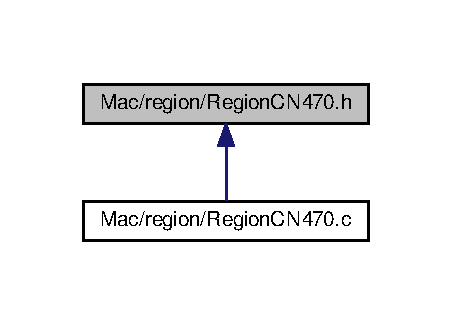
\includegraphics[width=217pt]{RegionCN470_8h__dep__incl}
\end{center}
\end{figure}
\subsection*{Macros}
\begin{DoxyCompactItemize}
\item 
\#define \hyperlink{group__REGIONCN470_ga8dd3b552d535062e91b0651705041387}{C\+N470\+\_\+\+M\+A\+X\+\_\+\+N\+B\+\_\+\+C\+H\+A\+N\+N\+E\+LS}~96
\item 
\#define \hyperlink{group__REGIONCN470_gafc089f5bdc4ad69267f562d1fda11f79}{C\+N470\+\_\+\+T\+X\+\_\+\+M\+I\+N\+\_\+\+D\+A\+T\+A\+R\+A\+TE}~\hyperlink{group__REGION_ga6c4ef966b4f3d5eb7597b087f2b97095}{D\+R\+\_\+0}
\item 
\#define \hyperlink{group__REGIONCN470_ga6124e3e1f145254943806b46c8844c1e}{C\+N470\+\_\+\+T\+X\+\_\+\+M\+A\+X\+\_\+\+D\+A\+T\+A\+R\+A\+TE}~\hyperlink{group__REGION_ga872e12c82020c02a7f70a1c6ed1375df}{D\+R\+\_\+5}
\item 
\#define \hyperlink{group__REGIONCN470_ga5aa969a4651406bcd74903035a8cfc4f}{C\+N470\+\_\+\+R\+X\+\_\+\+M\+I\+N\+\_\+\+D\+A\+T\+A\+R\+A\+TE}~\hyperlink{group__REGION_ga6c4ef966b4f3d5eb7597b087f2b97095}{D\+R\+\_\+0}
\item 
\#define \hyperlink{group__REGIONCN470_ga32c6368247a51d46cc53dfe9ea8c1d39}{C\+N470\+\_\+\+R\+X\+\_\+\+M\+A\+X\+\_\+\+D\+A\+T\+A\+R\+A\+TE}~\hyperlink{group__REGION_ga872e12c82020c02a7f70a1c6ed1375df}{D\+R\+\_\+5}
\item 
\#define \hyperlink{group__REGIONCN470_gab5525fe4b5cbe390c85fc1157a27860f}{C\+N470\+\_\+\+D\+E\+F\+A\+U\+L\+T\+\_\+\+D\+A\+T\+A\+R\+A\+TE}~\hyperlink{group__REGION_ga6c4ef966b4f3d5eb7597b087f2b97095}{D\+R\+\_\+0}
\item 
\#define \hyperlink{group__REGIONCN470_gabba9bdb3ecb54ce42aeaf14c3bc639f4}{C\+N470\+\_\+\+M\+I\+N\+\_\+\+R\+X1\+\_\+\+D\+R\+\_\+\+O\+F\+F\+S\+ET}~0
\item 
\#define \hyperlink{group__REGIONCN470_ga2d30070788e36cbb178f0fb025f23a91}{C\+N470\+\_\+\+M\+A\+X\+\_\+\+R\+X1\+\_\+\+D\+R\+\_\+\+O\+F\+F\+S\+ET}~3
\item 
\#define \hyperlink{group__REGIONCN470_gac88e0c39828cba950425f0fbee5d6b59}{C\+N470\+\_\+\+D\+E\+F\+A\+U\+L\+T\+\_\+\+R\+X1\+\_\+\+D\+R\+\_\+\+O\+F\+F\+S\+ET}~0
\item 
\#define \hyperlink{group__REGIONCN470_ga706088a08c37b56b67e88d8afa9a1db8}{C\+N470\+\_\+\+M\+I\+N\+\_\+\+T\+X\+\_\+\+P\+O\+W\+ER}~\hyperlink{group__REGION_ga3c7bd9a98f0c1e7e9aaa90857c4bd700}{T\+X\+\_\+\+P\+O\+W\+E\+R\+\_\+7}
\item 
\#define \hyperlink{group__REGIONCN470_gae977eb62cc9b2f49770b5f0d5ec1e5df}{C\+N470\+\_\+\+M\+A\+X\+\_\+\+T\+X\+\_\+\+P\+O\+W\+ER}~\hyperlink{group__REGION_gab33618449f2a573142c463ab071ef8ed}{T\+X\+\_\+\+P\+O\+W\+E\+R\+\_\+0}
\item 
\#define \hyperlink{group__REGIONCN470_ga0edc38df28f50fc6979f33f954a934a0}{C\+N470\+\_\+\+D\+E\+F\+A\+U\+L\+T\+\_\+\+T\+X\+\_\+\+P\+O\+W\+ER}~\hyperlink{group__REGION_gab33618449f2a573142c463ab071ef8ed}{T\+X\+\_\+\+P\+O\+W\+E\+R\+\_\+0}
\item 
\#define \hyperlink{group__REGIONCN470_ga1b95710cffe97a036ec3a40b9c6c2dd6}{C\+N470\+\_\+\+D\+E\+F\+A\+U\+L\+T\+\_\+\+M\+A\+X\+\_\+\+E\+I\+RP}~19.\+15f
\item 
\#define \hyperlink{group__REGIONCN470_ga913d250bd6010ad63f70603ced599b87}{C\+N470\+\_\+\+D\+E\+F\+A\+U\+L\+T\+\_\+\+A\+N\+T\+E\+N\+N\+A\+\_\+\+G\+A\+IN}~2.\+15f
\item 
\#define \hyperlink{group__REGIONCN470_gab622e938b7f31be68bbab0569252cc16}{C\+N470\+\_\+\+A\+D\+R\+\_\+\+A\+C\+K\+\_\+\+L\+I\+M\+IT}~64
\item 
\#define \hyperlink{group__REGIONCN470_ga36e45d676fbedb022706448bfb3ae1ed}{C\+N470\+\_\+\+A\+D\+R\+\_\+\+A\+C\+K\+\_\+\+D\+E\+L\+AY}~32
\item 
\#define \hyperlink{group__REGIONCN470_ga02ff150057a51ba9fd56e9082a96bf0d}{C\+N470\+\_\+\+D\+U\+T\+Y\+\_\+\+C\+Y\+C\+L\+E\+\_\+\+E\+N\+A\+B\+L\+ED}~0
\item 
\#define \hyperlink{group__REGIONCN470_ga9969677259320df9c736239b84d880ff}{C\+N470\+\_\+\+M\+A\+X\+\_\+\+R\+X\+\_\+\+W\+I\+N\+D\+OW}~3000
\item 
\#define \hyperlink{group__REGIONCN470_gac402464278f79670ea353ee209878217}{C\+N470\+\_\+\+R\+E\+C\+E\+I\+V\+E\+\_\+\+D\+E\+L\+A\+Y1}~1000
\item 
\#define \hyperlink{group__REGIONCN470_ga60730d21be102b95a2393549c999930d}{C\+N470\+\_\+\+R\+E\+C\+E\+I\+V\+E\+\_\+\+D\+E\+L\+A\+Y2}~2000
\item 
\#define \hyperlink{group__REGIONCN470_ga7fa3d835986d5496a0334572a376dc01}{C\+N470\+\_\+\+J\+O\+I\+N\+\_\+\+A\+C\+C\+E\+P\+T\+\_\+\+D\+E\+L\+A\+Y1}~5000
\item 
\#define \hyperlink{group__REGIONCN470_gad695261614b3d750749b401fcd685e50}{C\+N470\+\_\+\+J\+O\+I\+N\+\_\+\+A\+C\+C\+E\+P\+T\+\_\+\+D\+E\+L\+A\+Y2}~6000
\item 
\#define \hyperlink{group__REGIONCN470_ga5737cff937bc40a5a512f783fd0e9365}{C\+N470\+\_\+\+M\+A\+X\+\_\+\+F\+C\+N\+T\+\_\+\+G\+AP}~16384
\item 
\#define \hyperlink{group__REGIONCN470_gac4bc7c6dea1ebeb1cfe0e9a0ecb0db72}{C\+N470\+\_\+\+A\+C\+K\+T\+I\+M\+E\+O\+UT}~2000
\item 
\#define \hyperlink{group__REGIONCN470_ga020ad82ebe368189c51b4d21a7b5596d}{C\+N470\+\_\+\+A\+C\+K\+\_\+\+T\+I\+M\+E\+O\+U\+T\+\_\+\+R\+ND}~1000
\item 
\#define \hyperlink{group__REGIONCN470_ga2e28269fe49bac86f3143397559e4db4}{C\+N470\+\_\+\+R\+X\+\_\+\+W\+N\+D\+\_\+2\+\_\+\+F\+R\+EQ}~505300000
\item 
\#define \hyperlink{group__REGIONCN470_ga7aefeac71ff5edcd3a5628d12b84a25c}{C\+N470\+\_\+\+R\+X\+\_\+\+W\+N\+D\+\_\+2\+\_\+\+DR}~\hyperlink{group__REGION_ga6c4ef966b4f3d5eb7597b087f2b97095}{D\+R\+\_\+0}
\item 
\#define \hyperlink{group__REGIONCN470_ga46b33f1d67ef81deefa12018749a22ff}{C\+N470\+\_\+\+M\+A\+X\+\_\+\+N\+B\+\_\+\+B\+A\+N\+DS}~1
\item 
\#define \hyperlink{group__REGIONCN470_gaf6813f74ce73e4d0ab7971a89ab2ac2e}{C\+N470\+\_\+\+B\+A\+N\+D0}~\{ 1, \hyperlink{group__REGIONCN470_gae977eb62cc9b2f49770b5f0d5ec1e5df}{C\+N470\+\_\+\+M\+A\+X\+\_\+\+T\+X\+\_\+\+P\+O\+W\+ER}, 0,  0 \}
\item 
\#define \hyperlink{group__REGIONCN470_gaffb4e82c12bc61e97f83d18fb4187aa8}{C\+N470\+\_\+\+F\+I\+R\+S\+T\+\_\+\+R\+X1\+\_\+\+C\+H\+A\+N\+N\+EL}~( (uint32\+\_\+t) 500300000 )
\item 
\#define \hyperlink{group__REGIONCN470_ga5a6508f01066a5bde9c059367babd9cb}{C\+N470\+\_\+\+L\+A\+S\+T\+\_\+\+R\+X1\+\_\+\+C\+H\+A\+N\+N\+EL}~( (uint32\+\_\+t) 509700000 )
\item 
\#define \hyperlink{group__REGIONCN470_ga7786b9dddae0675b2d8cc26b0d230756}{C\+N470\+\_\+\+S\+T\+E\+P\+W\+I\+D\+T\+H\+\_\+\+R\+X1\+\_\+\+C\+H\+A\+N\+N\+EL}~( (uint32\+\_\+t) 200000 )
\end{DoxyCompactItemize}
\subsection*{Functions}
\begin{DoxyCompactItemize}
\item 
\hyperlink{group__REGION_gaed159b26e5c4677236b6e8677019db30}{Phy\+Param\+\_\+t} \hyperlink{group__REGIONCN470_gaa3f4e59184226b161b9e6880b6e7f204}{Region\+C\+N470\+Get\+Phy\+Param} (\hyperlink{group__REGION_gab471483fff904f4f89bbc03f7fc380ab}{Get\+Phy\+Params\+\_\+t} $\ast$get\+Phy)
\begin{DoxyCompactList}\small\item\em The function gets a value of a specific phy attribute. \end{DoxyCompactList}\item 
void \hyperlink{group__REGIONCN470_gad60aebff1bb6c89423fff84d57b21cb6}{Region\+C\+N470\+Set\+Band\+Tx\+Done} (\hyperlink{group__REGION_gad0524aa0673c0814a71e7a4f9cade3fc}{Set\+Band\+Tx\+Done\+Params\+\_\+t} $\ast$tx\+Done)
\begin{DoxyCompactList}\small\item\em Updates the last TX done parameters of the current channel. \end{DoxyCompactList}\item 
void \hyperlink{group__REGIONCN470_ga6591ac8edd635c34b47ec2f21627b145}{Region\+C\+N470\+Init\+Defaults} (\hyperlink{group__REGION_gaddc73ae10673ec925724e7870363bda9}{Init\+Type\+\_\+t} type)
\begin{DoxyCompactList}\small\item\em Initializes the channels masks and the channels. \end{DoxyCompactList}\item 
bool \hyperlink{group__REGIONCN470_ga7d7ddf394ddb8a6ac2d7cb5fea7ad745}{Region\+C\+N470\+Verify} (\hyperlink{group__REGION_ga966d97bc2f25df1c09e92e60ef652276}{Verify\+Params\+\_\+t} $\ast$verify, \hyperlink{group__REGION_ga9445b07fdf77581ecfaf389970e635f8}{Phy\+Attribute\+\_\+t} phy\+Attribute)
\begin{DoxyCompactList}\small\item\em Verifies a parameter. \end{DoxyCompactList}\item 
void \hyperlink{group__REGIONCN470_gae0ca4a5d6bf63fdb278a132ec496649f}{Region\+C\+N470\+Apply\+C\+F\+List} (\hyperlink{group__REGION_ga71588e9ad07e34b78fa91d51881fd3c6}{Apply\+C\+F\+List\+Params\+\_\+t} $\ast$apply\+C\+F\+List)
\begin{DoxyCompactList}\small\item\em The function parses the input buffer and sets up the channels of the CF list. \end{DoxyCompactList}\item 
bool \hyperlink{group__REGIONCN470_ga361aa9a80854b1a264a9ad0720cbd4da}{Region\+C\+N470\+Chan\+Mask\+Set} (\hyperlink{group__REGION_ga6d24f7da136006410827dfb29f6b9b9e}{Chan\+Mask\+Set\+Params\+\_\+t} $\ast$chan\+Mask\+Set)
\begin{DoxyCompactList}\small\item\em Sets a channels mask. \end{DoxyCompactList}\item 
bool \hyperlink{group__REGIONCN470_ga5205fdda3f4a869d78f4ccd791de359e}{Region\+C\+N470\+Adr\+Next} (\hyperlink{group__REGION_ga567c2742622326b350b4e91bbf61b4ce}{Adr\+Next\+Params\+\_\+t} $\ast$adr\+Next, int8\+\_\+t $\ast$dr\+Out, int8\+\_\+t $\ast$tx\+Pow\+Out, uint32\+\_\+t $\ast$adr\+Ack\+Counter)
\begin{DoxyCompactList}\small\item\em Calculates the next datarate to set, when A\+DR is on or off. \end{DoxyCompactList}\item 
void \hyperlink{group__REGIONCN470_gabb50864b958d868d7c2fbb09a7238a23}{Region\+C\+N470\+Compute\+Rx\+Window\+Parameters} (int8\+\_\+t datarate, uint8\+\_\+t min\+Rx\+Symbols, uint32\+\_\+t rx\+Error, \hyperlink{group__REGION_ga375c038078dfcfc7ef14280021db719e}{Rx\+Config\+Params\+\_\+t} $\ast$rx\+Config\+Params)
\item 
bool \hyperlink{group__REGIONCN470_gadb4b05f4e7b55705e37156add3ed585b}{Region\+C\+N470\+Rx\+Config} (\hyperlink{group__REGION_ga375c038078dfcfc7ef14280021db719e}{Rx\+Config\+Params\+\_\+t} $\ast$rx\+Config, int8\+\_\+t $\ast$datarate)
\begin{DoxyCompactList}\small\item\em Configuration of the RX windows. \end{DoxyCompactList}\item 
bool \hyperlink{group__REGIONCN470_ga2de0fae78c1759fec62a835b0fcb3829}{Region\+C\+N470\+Tx\+Config} (\hyperlink{group__REGION_gabed730d4d04b0b60d4b6d1966d3f21d3}{Tx\+Config\+Params\+\_\+t} $\ast$tx\+Config, int8\+\_\+t $\ast$tx\+Power, \hyperlink{utilities_8h_a4215ca43d3e953099ea758ce428599d0}{Timer\+Time\+\_\+t} $\ast$tx\+Time\+On\+Air)
\begin{DoxyCompactList}\small\item\em TX configuration. \end{DoxyCompactList}\item 
uint8\+\_\+t \hyperlink{group__REGIONCN470_ga8390f178b68e708cd9741caba00cb05d}{Region\+C\+N470\+Link\+Adr\+Req} (\hyperlink{group__REGION_gad4af503e8d4de1846129e26a799a1e8e}{Link\+Adr\+Req\+Params\+\_\+t} $\ast$link\+Adr\+Req, int8\+\_\+t $\ast$dr\+Out, int8\+\_\+t $\ast$tx\+Pow\+Out, uint8\+\_\+t $\ast$nb\+Rep\+Out, uint8\+\_\+t $\ast$nb\+Bytes\+Parsed)
\begin{DoxyCompactList}\small\item\em The function processes a Link A\+DR Request. \end{DoxyCompactList}\item 
uint8\+\_\+t \hyperlink{group__REGIONCN470_gae6be53827b6148fa40a6c1a3f6a8058b}{Region\+C\+N470\+Rx\+Param\+Setup\+Req} (\hyperlink{group__REGION_ga7165f282c670c728c36d534df2285157}{Rx\+Param\+Setup\+Req\+Params\+\_\+t} $\ast$rx\+Param\+Setup\+Req)
\begin{DoxyCompactList}\small\item\em The function processes a RX Parameter Setup Request. \end{DoxyCompactList}\item 
uint8\+\_\+t \hyperlink{group__REGIONCN470_ga3db01af8efb6f0c07db00b78dcb2ebfe}{Region\+C\+N470\+New\+Channel\+Req} (\hyperlink{group__REGION_gae2abcdb6dbb843c9faf5fd3009eca9d6}{New\+Channel\+Req\+Params\+\_\+t} $\ast$new\+Channel\+Req)
\begin{DoxyCompactList}\small\item\em The function processes a Channel Request. \end{DoxyCompactList}\item 
int8\+\_\+t \hyperlink{group__REGIONCN470_ga26c513769fa09c8bd92f15805162860b}{Region\+C\+N470\+Tx\+Param\+Setup\+Req} (\hyperlink{group__REGION_ga26836ef2996e70410e42ef471073f855}{Tx\+Param\+Setup\+Req\+Params\+\_\+t} $\ast$tx\+Param\+Setup\+Req)
\begin{DoxyCompactList}\small\item\em The function processes a TX Param\+Setup Request. \end{DoxyCompactList}\item 
uint8\+\_\+t \hyperlink{group__REGIONCN470_ga2fb7a7dcde7482f3a0da9028090c9c7f}{Region\+C\+N470\+Dl\+Channel\+Req} (\hyperlink{group__REGION_gae0d608ff1f8ea0a430e4f9a4c38ec7f3}{Dl\+Channel\+Req\+Params\+\_\+t} $\ast$dl\+Channel\+Req)
\begin{DoxyCompactList}\small\item\em The function processes a Dl\+Channel Request. \end{DoxyCompactList}\item 
int8\+\_\+t \hyperlink{group__REGIONCN470_ga5d07deb9b6a4c9a214439edae58bf341}{Region\+C\+N470\+Alternate\+Dr} (\hyperlink{group__REGION_ga001ea4338d1c83f4c785b49d7ad2d696}{Alternate\+Dr\+Params\+\_\+t} $\ast$alternate\+Dr)
\begin{DoxyCompactList}\small\item\em Alternates the datarate of the channel for the join request. \end{DoxyCompactList}\item 
void \hyperlink{group__REGIONCN470_ga2020e2db0351b7010e2e5fd53c466cc2}{Region\+C\+N470\+Calc\+Back\+Off} (\hyperlink{group__REGION_ga7c5c9a8da174e6679eded8257dc92fd9}{Calc\+Back\+Off\+Params\+\_\+t} $\ast$calc\+Back\+Off)
\begin{DoxyCompactList}\small\item\em Calculates the back-\/off time. \end{DoxyCompactList}\item 
bool \hyperlink{group__REGIONCN470_gad6d2b5fce0ea41dc2416648dcc674287}{Region\+C\+N470\+Next\+Channel} (\hyperlink{group__REGION_ga115f5e83afae352c0a3dcdc193374040}{Next\+Chan\+Params\+\_\+t} $\ast$next\+Chan\+Params, uint8\+\_\+t $\ast$channel, \hyperlink{utilities_8h_a4215ca43d3e953099ea758ce428599d0}{Timer\+Time\+\_\+t} $\ast$time, \hyperlink{utilities_8h_a4215ca43d3e953099ea758ce428599d0}{Timer\+Time\+\_\+t} $\ast$aggregated\+Time\+Off)
\begin{DoxyCompactList}\small\item\em Searches and set the next random available channel. \end{DoxyCompactList}\item 
\hyperlink{group__LORAMAC_ga30bd25657e10480f8605ee951b0ecfbd}{Lo\+Ra\+Mac\+Status\+\_\+t} \hyperlink{group__REGIONCN470_ga6f447bc77fedcf05b61c6a4247b0972b}{Region\+C\+N470\+Channel\+Add} (\hyperlink{group__REGION_gab1c5f3aa06614283202906cef4417860}{Channel\+Add\+Params\+\_\+t} $\ast$channel\+Add)
\begin{DoxyCompactList}\small\item\em Adds a channel. \end{DoxyCompactList}\item 
bool \hyperlink{group__REGIONCN470_ga325aac904d27927672021106fc718f09}{Region\+C\+N470\+Channels\+Remove} (\hyperlink{group__REGION_gaa37468560d2fc81a977b57a48e5d72c0}{Channel\+Remove\+Params\+\_\+t} $\ast$channel\+Remove)
\begin{DoxyCompactList}\small\item\em Removes a channel. \end{DoxyCompactList}\item 
void \hyperlink{group__REGIONCN470_ga0a1e509012a913631470e9801cc972bd}{Region\+C\+N470\+Set\+Continuous\+Wave} (\hyperlink{group__REGION_gaf39bb5ba06921139c6d17f88a8d518cd}{Continuous\+Wave\+Params\+\_\+t} $\ast$continuous\+Wave)
\begin{DoxyCompactList}\small\item\em Sets the radio into continuous wave mode. \end{DoxyCompactList}\item 
uint8\+\_\+t \hyperlink{group__REGIONCN470_ga9b7086c4eb616fb332a95f05845aac89}{Region\+C\+N470\+Apply\+Dr\+Offset} (uint8\+\_\+t downlink\+Dwell\+Time, int8\+\_\+t dr, int8\+\_\+t dr\+Offset)
\begin{DoxyCompactList}\small\item\em Computes new datarate according to the given offset. \end{DoxyCompactList}\end{DoxyCompactItemize}


\subsection{Detailed Description}
Region definition for C\+N470. 

\begin{DoxyCopyright}{Copyright}
Revised B\+SD License, see section L\+I\+C\+E\+N\+SE.
\end{DoxyCopyright}

\begin{DoxyCode}
  \_\_\_\_\_\_                              \_
 / \_\_\_\_\_)             \_              | |
( (\_\_\_\_  \_\_\_\_\_ \_\_\_\_ \_| |\_ \_\_\_\_\_  \_\_\_\_| |\_\_
 \(\backslash\)\_\_\_\_ \(\backslash\)| \_\_\_ |    (\_   \_) \_\_\_ |/ \_\_\_)  \_ \(\backslash\)
 \_\_\_\_\_) ) \_\_\_\_| | | || |\_| \_\_\_\_( (\_\_\_| | | |
(\_\_\_\_\_\_/|\_\_\_\_\_)\_|\_|\_| \(\backslash\)\_\_)\_\_\_\_\_)\(\backslash\)\_\_\_\_)\_| |\_|
(C)2013 Semtech

 \_\_\_ \_\_\_\_\_ \_   \_\_\_ \_  \_\_\_\_\_ \_\_\_  \_\_\_  \_\_\_ \_\_\_
/ \_\_|\_   \_/\_\(\backslash\) / \_\_| |/ / \_\_/ \_ \(\backslash\)| \_ \(\backslash\)/ \_\_| \_\_|
\(\backslash\)\_\_ \(\backslash\) | |/ \_ \(\backslash\) (\_\_| \textcolor{stringliteral}{' <| \_| (\_) |   / (\_\_| \_|}
\textcolor{stringliteral}{|\_\_\_/ |\_/\_/ \(\backslash\)\_\(\backslash\)\_\_\_|\_|\(\backslash\)\_\(\backslash\)\_| \(\backslash\)\_\_\_/|\_|\_\(\backslash\)\(\backslash\)\_\_\_|\_\_\_|}
\textcolor{stringliteral}{embedded.connectivity.solutions===============}
\end{DoxyCode}


\begin{DoxyAuthor}{Author}
Miguel Luis ( Semtech )

Gregory Cristian ( Semtech )

Daniel Jaeckle ( S\+T\+A\+C\+K\+F\+O\+R\+CE ) 
\end{DoxyAuthor}

\hypertarget{RegionCN779_8c}{}\section{Mac/region/\+Region\+C\+N779.c File Reference}
\label{RegionCN779_8c}\index{Mac/region/\+Region\+C\+N779.\+c@{Mac/region/\+Region\+C\+N779.\+c}}
{\ttfamily \#include $<$stdbool.\+h$>$}\newline
{\ttfamily \#include $<$string.\+h$>$}\newline
{\ttfamily \#include $<$stdint.\+h$>$}\newline
{\ttfamily \#include $<$math.\+h$>$}\newline
{\ttfamily \#include \char`\"{}radio.\+h\char`\"{}}\newline
{\ttfamily \#include \char`\"{}timer.\+h\char`\"{}}\newline
{\ttfamily \#include \char`\"{}Lo\+Ra\+Mac.\+h\char`\"{}}\newline
{\ttfamily \#include \char`\"{}utilities.\+h\char`\"{}}\newline
{\ttfamily \#include \char`\"{}Region.\+h\char`\"{}}\newline
{\ttfamily \#include \char`\"{}Region\+Common.\+h\char`\"{}}\newline
{\ttfamily \#include \char`\"{}Region\+C\+N779.\+h\char`\"{}}\newline
{\ttfamily \#include \char`\"{}debug.\+h\char`\"{}}\newline
Include dependency graph for Region\+C\+N779.\+c\+:
\nopagebreak
\begin{figure}[H]
\begin{center}
\leavevmode
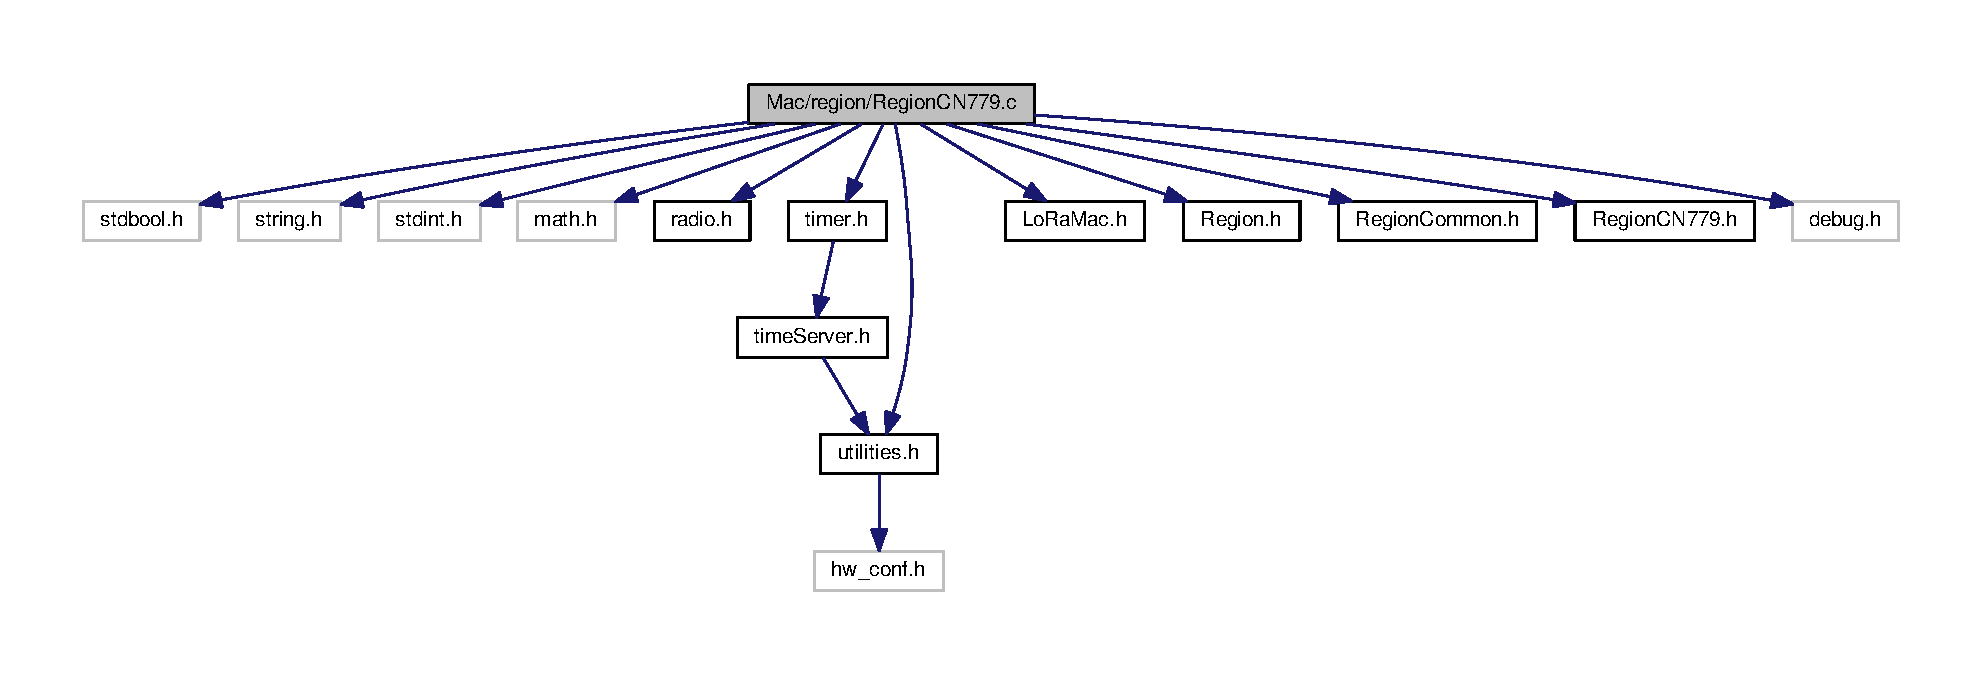
\includegraphics[width=350pt]{RegionCN779_8c__incl}
\end{center}
\end{figure}
\subsection*{Macros}
\begin{DoxyCompactItemize}
\item 
\#define \hyperlink{RegionCN779_8c_a1b20a8de3ae59c0b063fb313f0c70890}{C\+H\+A\+N\+N\+E\+L\+S\+\_\+\+M\+A\+S\+K\+\_\+\+S\+I\+ZE}~1
\end{DoxyCompactItemize}
\subsection*{Functions}
\begin{DoxyCompactItemize}
\item 
\hyperlink{group__REGION_gaed159b26e5c4677236b6e8677019db30}{Phy\+Param\+\_\+t} \hyperlink{group__REGIONCN779_gab45c9a48b25622ab197ab8510cc7cbc0}{Region\+C\+N779\+Get\+Phy\+Param} (\hyperlink{group__REGION_gab471483fff904f4f89bbc03f7fc380ab}{Get\+Phy\+Params\+\_\+t} $\ast$get\+Phy)
\begin{DoxyCompactList}\small\item\em The function gets a value of a specific phy attribute. \end{DoxyCompactList}\item 
void \hyperlink{group__REGIONCN779_gab7e1485f1112861ad7dae9801995a2c4}{Region\+C\+N779\+Set\+Band\+Tx\+Done} (\hyperlink{group__REGION_gad0524aa0673c0814a71e7a4f9cade3fc}{Set\+Band\+Tx\+Done\+Params\+\_\+t} $\ast$tx\+Done)
\begin{DoxyCompactList}\small\item\em Updates the last TX done parameters of the current channel. \end{DoxyCompactList}\item 
void \hyperlink{group__REGIONCN779_ga85953f37b52567b54689c354671a14f6}{Region\+C\+N779\+Init\+Defaults} (\hyperlink{group__REGION_gaddc73ae10673ec925724e7870363bda9}{Init\+Type\+\_\+t} type)
\begin{DoxyCompactList}\small\item\em Initializes the channels masks and the channels. \end{DoxyCompactList}\item 
bool \hyperlink{group__REGIONCN779_ga7108626b64685883842049a36d865208}{Region\+C\+N779\+Verify} (\hyperlink{group__REGION_ga966d97bc2f25df1c09e92e60ef652276}{Verify\+Params\+\_\+t} $\ast$verify, \hyperlink{group__REGION_ga9445b07fdf77581ecfaf389970e635f8}{Phy\+Attribute\+\_\+t} phy\+Attribute)
\begin{DoxyCompactList}\small\item\em Verifies a parameter. \end{DoxyCompactList}\item 
void \hyperlink{group__REGIONCN779_ga7f02e6a802649d9b93c4c56eff271a26}{Region\+C\+N779\+Apply\+C\+F\+List} (\hyperlink{group__REGION_ga71588e9ad07e34b78fa91d51881fd3c6}{Apply\+C\+F\+List\+Params\+\_\+t} $\ast$apply\+C\+F\+List)
\begin{DoxyCompactList}\small\item\em The function parses the input buffer and sets up the channels of the CF list. \end{DoxyCompactList}\item 
bool \hyperlink{group__REGIONCN779_ga06c5fe5ebbc02741394fb573944467b7}{Region\+C\+N779\+Chan\+Mask\+Set} (\hyperlink{group__REGION_ga6d24f7da136006410827dfb29f6b9b9e}{Chan\+Mask\+Set\+Params\+\_\+t} $\ast$chan\+Mask\+Set)
\begin{DoxyCompactList}\small\item\em Sets a channels mask. \end{DoxyCompactList}\item 
bool \hyperlink{group__REGIONCN779_ga4c114db1d998a5ba77bb87ab34316ff8}{Region\+C\+N779\+Adr\+Next} (\hyperlink{group__REGION_ga567c2742622326b350b4e91bbf61b4ce}{Adr\+Next\+Params\+\_\+t} $\ast$adr\+Next, int8\+\_\+t $\ast$dr\+Out, int8\+\_\+t $\ast$tx\+Pow\+Out, uint32\+\_\+t $\ast$adr\+Ack\+Counter)
\begin{DoxyCompactList}\small\item\em Calculates the next datarate to set, when A\+DR is on or off. \end{DoxyCompactList}\item 
void \hyperlink{group__REGIONCN779_ga4f354a88e5bfee44eccaad7d2e18c87e}{Region\+C\+N779\+Compute\+Rx\+Window\+Parameters} (int8\+\_\+t datarate, uint8\+\_\+t min\+Rx\+Symbols, uint32\+\_\+t rx\+Error, \hyperlink{group__REGION_ga375c038078dfcfc7ef14280021db719e}{Rx\+Config\+Params\+\_\+t} $\ast$rx\+Config\+Params)
\item 
bool \hyperlink{group__REGIONCN779_ga89b2db72c7dd1dbaa07135d538e3c2fe}{Region\+C\+N779\+Rx\+Config} (\hyperlink{group__REGION_ga375c038078dfcfc7ef14280021db719e}{Rx\+Config\+Params\+\_\+t} $\ast$rx\+Config, int8\+\_\+t $\ast$datarate)
\begin{DoxyCompactList}\small\item\em Configuration of the RX windows. \end{DoxyCompactList}\item 
bool \hyperlink{group__REGIONCN779_gae628efcfcba9afc2620f3c1234b90c3d}{Region\+C\+N779\+Tx\+Config} (\hyperlink{group__REGION_gabed730d4d04b0b60d4b6d1966d3f21d3}{Tx\+Config\+Params\+\_\+t} $\ast$tx\+Config, int8\+\_\+t $\ast$tx\+Power, \hyperlink{utilities_8h_a4215ca43d3e953099ea758ce428599d0}{Timer\+Time\+\_\+t} $\ast$tx\+Time\+On\+Air)
\begin{DoxyCompactList}\small\item\em TX configuration. \end{DoxyCompactList}\item 
uint8\+\_\+t \hyperlink{group__REGIONCN779_gae3bdb6e223de1fd6b72182eb278f3828}{Region\+C\+N779\+Link\+Adr\+Req} (\hyperlink{group__REGION_gad4af503e8d4de1846129e26a799a1e8e}{Link\+Adr\+Req\+Params\+\_\+t} $\ast$link\+Adr\+Req, int8\+\_\+t $\ast$dr\+Out, int8\+\_\+t $\ast$tx\+Pow\+Out, uint8\+\_\+t $\ast$nb\+Rep\+Out, uint8\+\_\+t $\ast$nb\+Bytes\+Parsed)
\begin{DoxyCompactList}\small\item\em The function processes a Link A\+DR Request. \end{DoxyCompactList}\item 
uint8\+\_\+t \hyperlink{group__REGIONCN779_gad14dfe4070bdf46142d09d35d617b25c}{Region\+C\+N779\+Rx\+Param\+Setup\+Req} (\hyperlink{group__REGION_ga7165f282c670c728c36d534df2285157}{Rx\+Param\+Setup\+Req\+Params\+\_\+t} $\ast$rx\+Param\+Setup\+Req)
\begin{DoxyCompactList}\small\item\em The function processes a RX Parameter Setup Request. \end{DoxyCompactList}\item 
uint8\+\_\+t \hyperlink{group__REGIONCN779_gab4c6ffa72f1da0e2ef40431ab7fd72fa}{Region\+C\+N779\+New\+Channel\+Req} (\hyperlink{group__REGION_gae2abcdb6dbb843c9faf5fd3009eca9d6}{New\+Channel\+Req\+Params\+\_\+t} $\ast$new\+Channel\+Req)
\begin{DoxyCompactList}\small\item\em The function processes a Channel Request. \end{DoxyCompactList}\item 
int8\+\_\+t \hyperlink{group__REGIONCN779_ga6dc963da2e0b143e7313780fcd946855}{Region\+C\+N779\+Tx\+Param\+Setup\+Req} (\hyperlink{group__REGION_ga26836ef2996e70410e42ef471073f855}{Tx\+Param\+Setup\+Req\+Params\+\_\+t} $\ast$tx\+Param\+Setup\+Req)
\begin{DoxyCompactList}\small\item\em The function processes a TX Param\+Setup Request. \end{DoxyCompactList}\item 
uint8\+\_\+t \hyperlink{group__REGIONCN779_gaa34ccc032a50e5bef17fc59ca5eb89bc}{Region\+C\+N779\+Dl\+Channel\+Req} (\hyperlink{group__REGION_gae0d608ff1f8ea0a430e4f9a4c38ec7f3}{Dl\+Channel\+Req\+Params\+\_\+t} $\ast$dl\+Channel\+Req)
\begin{DoxyCompactList}\small\item\em The function processes a Dl\+Channel Request. \end{DoxyCompactList}\item 
int8\+\_\+t \hyperlink{group__REGIONCN779_ga2ea0c39d57f08b798e30c7207f1cf165}{Region\+C\+N779\+Alternate\+Dr} (\hyperlink{group__REGION_ga001ea4338d1c83f4c785b49d7ad2d696}{Alternate\+Dr\+Params\+\_\+t} $\ast$alternate\+Dr)
\begin{DoxyCompactList}\small\item\em Alternates the datarate of the channel for the join request. \end{DoxyCompactList}\item 
void \hyperlink{group__REGIONCN779_ga159d16a30e948dcab70399897672848b}{Region\+C\+N779\+Calc\+Back\+Off} (\hyperlink{group__REGION_ga7c5c9a8da174e6679eded8257dc92fd9}{Calc\+Back\+Off\+Params\+\_\+t} $\ast$calc\+Back\+Off)
\begin{DoxyCompactList}\small\item\em Calculates the back-\/off time. \end{DoxyCompactList}\item 
bool \hyperlink{group__REGIONCN779_ga6506624bcb6ec8ae3e13e97d32301aaf}{Region\+C\+N779\+Next\+Channel} (\hyperlink{group__REGION_ga115f5e83afae352c0a3dcdc193374040}{Next\+Chan\+Params\+\_\+t} $\ast$next\+Chan\+Params, uint8\+\_\+t $\ast$channel, \hyperlink{utilities_8h_a4215ca43d3e953099ea758ce428599d0}{Timer\+Time\+\_\+t} $\ast$time, \hyperlink{utilities_8h_a4215ca43d3e953099ea758ce428599d0}{Timer\+Time\+\_\+t} $\ast$aggregated\+Time\+Off)
\begin{DoxyCompactList}\small\item\em Searches and set the next random available channel. \end{DoxyCompactList}\item 
\hyperlink{group__LORAMAC_ga30bd25657e10480f8605ee951b0ecfbd}{Lo\+Ra\+Mac\+Status\+\_\+t} \hyperlink{group__REGIONCN779_ga087a9e4729bae8b825db62caca5f20d2}{Region\+C\+N779\+Channel\+Add} (\hyperlink{group__REGION_gab1c5f3aa06614283202906cef4417860}{Channel\+Add\+Params\+\_\+t} $\ast$channel\+Add)
\begin{DoxyCompactList}\small\item\em Adds a channel. \end{DoxyCompactList}\item 
bool \hyperlink{group__REGIONCN779_ga3ea3d4f5fe7cb25f562f4e6f95396eed}{Region\+C\+N779\+Channels\+Remove} (\hyperlink{group__REGION_gaa37468560d2fc81a977b57a48e5d72c0}{Channel\+Remove\+Params\+\_\+t} $\ast$channel\+Remove)
\begin{DoxyCompactList}\small\item\em Removes a channel. \end{DoxyCompactList}\item 
void \hyperlink{group__REGIONCN779_ga702d0d0348fdbcb2b66f7e9d5fb93a61}{Region\+C\+N779\+Set\+Continuous\+Wave} (\hyperlink{group__REGION_gaf39bb5ba06921139c6d17f88a8d518cd}{Continuous\+Wave\+Params\+\_\+t} $\ast$continuous\+Wave)
\begin{DoxyCompactList}\small\item\em Sets the radio into continuous wave mode. \end{DoxyCompactList}\item 
uint8\+\_\+t \hyperlink{group__REGIONCN779_gab03fbee2e88e81b71c04f907af8b283e}{Region\+C\+N779\+Apply\+Dr\+Offset} (uint8\+\_\+t downlink\+Dwell\+Time, int8\+\_\+t dr, int8\+\_\+t dr\+Offset)
\begin{DoxyCompactList}\small\item\em Computes new datarate according to the given offset. \end{DoxyCompactList}\end{DoxyCompactItemize}


\subsection{Macro Definition Documentation}
\mbox{\Hypertarget{RegionCN779_8c_a1b20a8de3ae59c0b063fb313f0c70890}\label{RegionCN779_8c_a1b20a8de3ae59c0b063fb313f0c70890}} 
\index{Region\+C\+N779.\+c@{Region\+C\+N779.\+c}!C\+H\+A\+N\+N\+E\+L\+S\+\_\+\+M\+A\+S\+K\+\_\+\+S\+I\+ZE@{C\+H\+A\+N\+N\+E\+L\+S\+\_\+\+M\+A\+S\+K\+\_\+\+S\+I\+ZE}}
\index{C\+H\+A\+N\+N\+E\+L\+S\+\_\+\+M\+A\+S\+K\+\_\+\+S\+I\+ZE@{C\+H\+A\+N\+N\+E\+L\+S\+\_\+\+M\+A\+S\+K\+\_\+\+S\+I\+ZE}!Region\+C\+N779.\+c@{Region\+C\+N779.\+c}}
\subsubsection{\texorpdfstring{C\+H\+A\+N\+N\+E\+L\+S\+\_\+\+M\+A\+S\+K\+\_\+\+S\+I\+ZE}{CHANNELS\_MASK\_SIZE}}
{\footnotesize\ttfamily \#define C\+H\+A\+N\+N\+E\+L\+S\+\_\+\+M\+A\+S\+K\+\_\+\+S\+I\+ZE~1}


\hypertarget{RegionCN779_8h}{}\section{Mac/region/\+Region\+C\+N779.h File Reference}
\label{RegionCN779_8h}\index{Mac/region/\+Region\+C\+N779.\+h@{Mac/region/\+Region\+C\+N779.\+h}}


Region definition for C\+N779.  


This graph shows which files directly or indirectly include this file\+:
\nopagebreak
\begin{figure}[H]
\begin{center}
\leavevmode
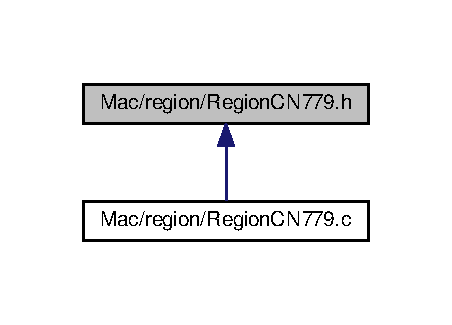
\includegraphics[width=217pt]{RegionCN779_8h__dep__incl}
\end{center}
\end{figure}
\subsection*{Macros}
\begin{DoxyCompactItemize}
\item 
\#define \hyperlink{group__REGIONCN779_gaa23230e648a8147840e88f03f9d3b7fc}{C\+N779\+\_\+\+M\+A\+X\+\_\+\+N\+B\+\_\+\+C\+H\+A\+N\+N\+E\+LS}~16
\item 
\#define \hyperlink{group__REGIONCN779_ga03a2c79e3c0f039e5f1150e4d9fdfa1a}{C\+N779\+\_\+\+N\+U\+M\+B\+\_\+\+D\+E\+F\+A\+U\+L\+T\+\_\+\+C\+H\+A\+N\+N\+E\+LS}~3
\item 
\#define \hyperlink{group__REGIONCN779_ga89f42e14e70be48170465e9cdd74caeb}{C\+N779\+\_\+\+N\+U\+M\+B\+\_\+\+C\+H\+A\+N\+N\+E\+L\+S\+\_\+\+C\+F\+\_\+\+L\+I\+ST}~5
\item 
\#define \hyperlink{group__REGIONCN779_ga78e9e4ce4dd6df844573865d9de7e268}{C\+N779\+\_\+\+T\+X\+\_\+\+M\+I\+N\+\_\+\+D\+A\+T\+A\+R\+A\+TE}~\hyperlink{group__REGION_ga6c4ef966b4f3d5eb7597b087f2b97095}{D\+R\+\_\+0}
\item 
\#define \hyperlink{group__REGIONCN779_gabc1992b9207de536e7b92f2d51e6b7e4}{C\+N779\+\_\+\+T\+X\+\_\+\+M\+A\+X\+\_\+\+D\+A\+T\+A\+R\+A\+TE}~\hyperlink{group__REGION_ga3a06805baf4f00911a3a5d3dbadebf61}{D\+R\+\_\+7}
\item 
\#define \hyperlink{group__REGIONCN779_ga9b8a3086475f37d72484e75a4bf8f4a5}{C\+N779\+\_\+\+R\+X\+\_\+\+M\+I\+N\+\_\+\+D\+A\+T\+A\+R\+A\+TE}~\hyperlink{group__REGION_ga6c4ef966b4f3d5eb7597b087f2b97095}{D\+R\+\_\+0}
\item 
\#define \hyperlink{group__REGIONCN779_ga89261ba0eddf04555c7a38fff0dff2d6}{C\+N779\+\_\+\+R\+X\+\_\+\+M\+A\+X\+\_\+\+D\+A\+T\+A\+R\+A\+TE}~\hyperlink{group__REGION_ga3a06805baf4f00911a3a5d3dbadebf61}{D\+R\+\_\+7}
\item 
\#define \hyperlink{group__REGIONCN779_ga442dfac2a5611f9e14fb748376e99b3e}{C\+N779\+\_\+\+D\+E\+F\+A\+U\+L\+T\+\_\+\+D\+A\+T\+A\+R\+A\+TE}~\hyperlink{group__REGION_ga6c4ef966b4f3d5eb7597b087f2b97095}{D\+R\+\_\+0}
\item 
\#define \hyperlink{group__REGIONCN779_gae0ef3405f8d33d4b21e74588b50c2569}{C\+N779\+\_\+\+M\+I\+N\+\_\+\+R\+X1\+\_\+\+D\+R\+\_\+\+O\+F\+F\+S\+ET}~0
\item 
\#define \hyperlink{group__REGIONCN779_ga92a7cb914b3c213f1506f8dd927e6077}{C\+N779\+\_\+\+M\+A\+X\+\_\+\+R\+X1\+\_\+\+D\+R\+\_\+\+O\+F\+F\+S\+ET}~5
\item 
\#define \hyperlink{group__REGIONCN779_ga8e88b35f91ebd807975b5712ccbfef2a}{C\+N779\+\_\+\+D\+E\+F\+A\+U\+L\+T\+\_\+\+R\+X1\+\_\+\+D\+R\+\_\+\+O\+F\+F\+S\+ET}~0
\item 
\#define \hyperlink{group__REGIONCN779_gab0e266968cb85199e9002eb1d3c5a719}{C\+N779\+\_\+\+M\+I\+N\+\_\+\+T\+X\+\_\+\+P\+O\+W\+ER}~\hyperlink{group__REGION_ga0149d52581db80901b5bc1adf0aedd1d}{T\+X\+\_\+\+P\+O\+W\+E\+R\+\_\+5}
\item 
\#define \hyperlink{group__REGIONCN779_ga8a70356561f3416db21a1e93b4ee4ae9}{C\+N779\+\_\+\+M\+A\+X\+\_\+\+T\+X\+\_\+\+P\+O\+W\+ER}~\hyperlink{group__REGION_gab33618449f2a573142c463ab071ef8ed}{T\+X\+\_\+\+P\+O\+W\+E\+R\+\_\+0}
\item 
\#define \hyperlink{group__REGIONCN779_ga0a41ad46e00759176adb3ef4a8e937cb}{C\+N779\+\_\+\+D\+E\+F\+A\+U\+L\+T\+\_\+\+T\+X\+\_\+\+P\+O\+W\+ER}~\hyperlink{group__REGION_gab33618449f2a573142c463ab071ef8ed}{T\+X\+\_\+\+P\+O\+W\+E\+R\+\_\+0}
\item 
\#define \hyperlink{group__REGIONCN779_ga77bd9b50f37cb6182e330e7203aab158}{C\+N779\+\_\+\+D\+E\+F\+A\+U\+L\+T\+\_\+\+M\+A\+X\+\_\+\+E\+I\+RP}~12.\+15f
\item 
\#define \hyperlink{group__REGIONCN779_ga055a39b4bc3aae2e812aab0a96561fee}{C\+N779\+\_\+\+D\+E\+F\+A\+U\+L\+T\+\_\+\+A\+N\+T\+E\+N\+N\+A\+\_\+\+G\+A\+IN}~2.\+15f
\item 
\#define \hyperlink{group__REGIONCN779_ga8c19c4c4ef1a00d6865607b7d61f0325}{C\+N779\+\_\+\+A\+D\+R\+\_\+\+A\+C\+K\+\_\+\+L\+I\+M\+IT}~64
\item 
\#define \hyperlink{group__REGIONCN779_ga56814f06a0fa6b826baad368920004a4}{C\+N779\+\_\+\+A\+D\+R\+\_\+\+A\+C\+K\+\_\+\+D\+E\+L\+AY}~32
\item 
\#define \hyperlink{group__REGIONCN779_ga87494ed194c1c38e301dbb4990f7f005}{C\+N779\+\_\+\+D\+U\+T\+Y\+\_\+\+C\+Y\+C\+L\+E\+\_\+\+E\+N\+A\+B\+L\+ED}~1
\item 
\#define \hyperlink{group__REGIONCN779_ga3d2b8590a2e727046db467d647c96518}{C\+N779\+\_\+\+M\+A\+X\+\_\+\+R\+X\+\_\+\+W\+I\+N\+D\+OW}~3000
\item 
\#define \hyperlink{group__REGIONCN779_gadd96388a9097e2d47d77a459b13c1309}{C\+N779\+\_\+\+R\+E\+C\+E\+I\+V\+E\+\_\+\+D\+E\+L\+A\+Y1}~1000
\item 
\#define \hyperlink{group__REGIONCN779_ga40b53070cc108b1704c23fd196bc1a02}{C\+N779\+\_\+\+R\+E\+C\+E\+I\+V\+E\+\_\+\+D\+E\+L\+A\+Y2}~2000
\item 
\#define \hyperlink{group__REGIONCN779_gae35de851225832e6fce8edbd9cc87e35}{C\+N779\+\_\+\+J\+O\+I\+N\+\_\+\+A\+C\+C\+E\+P\+T\+\_\+\+D\+E\+L\+A\+Y1}~5000
\item 
\#define \hyperlink{group__REGIONCN779_gaba22c62202d5f40c7c952706604f961b}{C\+N779\+\_\+\+J\+O\+I\+N\+\_\+\+A\+C\+C\+E\+P\+T\+\_\+\+D\+E\+L\+A\+Y2}~6000
\item 
\#define \hyperlink{group__REGIONCN779_ga6bac9924ad75dba200876f5ddcb8d91e}{C\+N779\+\_\+\+M\+A\+X\+\_\+\+F\+C\+N\+T\+\_\+\+G\+AP}~16384
\item 
\#define \hyperlink{group__REGIONCN779_gaf4edb86dfa6b0c55d43f183399b36878}{C\+N779\+\_\+\+A\+C\+K\+T\+I\+M\+E\+O\+UT}~2000
\item 
\#define \hyperlink{group__REGIONCN779_gaead3d649c05b0529d19d2fd1994f1d93}{C\+N779\+\_\+\+A\+C\+K\+\_\+\+T\+I\+M\+E\+O\+U\+T\+\_\+\+R\+ND}~1000
\item 
\#define \hyperlink{group__REGIONCN779_ga055b0718f7cc4056fc467f5abe971d8c}{C\+N779\+\_\+\+R\+X\+\_\+\+W\+N\+D\+\_\+2\+\_\+\+F\+R\+EQ}~786000000
\item 
\#define \hyperlink{group__REGIONCN779_gac242b7599d5234bc866206a447d8c517}{C\+N779\+\_\+\+R\+X\+\_\+\+W\+N\+D\+\_\+2\+\_\+\+DR}~\hyperlink{group__REGION_ga6c4ef966b4f3d5eb7597b087f2b97095}{D\+R\+\_\+0}
\item 
\#define \hyperlink{group__REGIONCN779_ga605a78b9ce2c56ef5d320e029e369236}{C\+N779\+\_\+\+M\+A\+X\+\_\+\+N\+B\+\_\+\+B\+A\+N\+DS}~1
\item 
\#define \hyperlink{group__REGIONCN779_ga428819be1d6f97028be344a4bf8dff3e}{C\+N779\+\_\+\+B\+A\+N\+D0}~\{ 100, \hyperlink{group__REGIONCN779_ga8a70356561f3416db21a1e93b4ee4ae9}{C\+N779\+\_\+\+M\+A\+X\+\_\+\+T\+X\+\_\+\+P\+O\+W\+ER}, 0,  0 \}
\item 
\#define \hyperlink{group__REGIONCN779_ga1318d698c85f15c35bd4953830d5df48}{C\+N779\+\_\+\+L\+C1}~\{ 779500000, 0, \{ ( ( \hyperlink{group__REGION_ga872e12c82020c02a7f70a1c6ed1375df}{D\+R\+\_\+5} $<$$<$ 4 ) $\vert$ \hyperlink{group__REGION_ga6c4ef966b4f3d5eb7597b087f2b97095}{D\+R\+\_\+0} ) \}, 0 \}
\item 
\#define \hyperlink{group__REGIONCN779_ga758c5da7fe1372388ab9476835b4b4d2}{C\+N779\+\_\+\+L\+C2}~\{ 779700000, 0, \{ ( ( \hyperlink{group__REGION_ga872e12c82020c02a7f70a1c6ed1375df}{D\+R\+\_\+5} $<$$<$ 4 ) $\vert$ \hyperlink{group__REGION_ga6c4ef966b4f3d5eb7597b087f2b97095}{D\+R\+\_\+0} ) \}, 0 \}
\item 
\#define \hyperlink{group__REGIONCN779_ga8e9d424722db59d84a7d122e95f3cce7}{C\+N779\+\_\+\+L\+C3}~\{ 779900000, 0, \{ ( ( \hyperlink{group__REGION_ga872e12c82020c02a7f70a1c6ed1375df}{D\+R\+\_\+5} $<$$<$ 4 ) $\vert$ \hyperlink{group__REGION_ga6c4ef966b4f3d5eb7597b087f2b97095}{D\+R\+\_\+0} ) \}, 0 \}
\item 
\#define \hyperlink{group__REGIONCN779_gaad1a9c76c54bb1be159e6638c1aa768f}{C\+N779\+\_\+\+J\+O\+I\+N\+\_\+\+C\+H\+A\+N\+N\+E\+LS}~( uint16\+\_\+t )( \hyperlink{group__REGION_ga12fa17e5c1016e01a9d82c25027deb1b}{LC}( 1 ) $\vert$ \hyperlink{group__REGION_ga12fa17e5c1016e01a9d82c25027deb1b}{LC}( 2 ) $\vert$ \hyperlink{group__REGION_ga12fa17e5c1016e01a9d82c25027deb1b}{LC}( 3 ) )
\end{DoxyCompactItemize}
\subsection*{Functions}
\begin{DoxyCompactItemize}
\item 
\hyperlink{group__REGION_gaed159b26e5c4677236b6e8677019db30}{Phy\+Param\+\_\+t} \hyperlink{group__REGIONCN779_gab45c9a48b25622ab197ab8510cc7cbc0}{Region\+C\+N779\+Get\+Phy\+Param} (\hyperlink{group__REGION_gab471483fff904f4f89bbc03f7fc380ab}{Get\+Phy\+Params\+\_\+t} $\ast$get\+Phy)
\begin{DoxyCompactList}\small\item\em The function gets a value of a specific phy attribute. \end{DoxyCompactList}\item 
void \hyperlink{group__REGIONCN779_gab7e1485f1112861ad7dae9801995a2c4}{Region\+C\+N779\+Set\+Band\+Tx\+Done} (\hyperlink{group__REGION_gad0524aa0673c0814a71e7a4f9cade3fc}{Set\+Band\+Tx\+Done\+Params\+\_\+t} $\ast$tx\+Done)
\begin{DoxyCompactList}\small\item\em Updates the last TX done parameters of the current channel. \end{DoxyCompactList}\item 
void \hyperlink{group__REGIONCN779_ga85953f37b52567b54689c354671a14f6}{Region\+C\+N779\+Init\+Defaults} (\hyperlink{group__REGION_gaddc73ae10673ec925724e7870363bda9}{Init\+Type\+\_\+t} type)
\begin{DoxyCompactList}\small\item\em Initializes the channels masks and the channels. \end{DoxyCompactList}\item 
bool \hyperlink{group__REGIONCN779_ga7108626b64685883842049a36d865208}{Region\+C\+N779\+Verify} (\hyperlink{group__REGION_ga966d97bc2f25df1c09e92e60ef652276}{Verify\+Params\+\_\+t} $\ast$verify, \hyperlink{group__REGION_ga9445b07fdf77581ecfaf389970e635f8}{Phy\+Attribute\+\_\+t} phy\+Attribute)
\begin{DoxyCompactList}\small\item\em Verifies a parameter. \end{DoxyCompactList}\item 
void \hyperlink{group__REGIONCN779_ga7f02e6a802649d9b93c4c56eff271a26}{Region\+C\+N779\+Apply\+C\+F\+List} (\hyperlink{group__REGION_ga71588e9ad07e34b78fa91d51881fd3c6}{Apply\+C\+F\+List\+Params\+\_\+t} $\ast$apply\+C\+F\+List)
\begin{DoxyCompactList}\small\item\em The function parses the input buffer and sets up the channels of the CF list. \end{DoxyCompactList}\item 
bool \hyperlink{group__REGIONCN779_ga06c5fe5ebbc02741394fb573944467b7}{Region\+C\+N779\+Chan\+Mask\+Set} (\hyperlink{group__REGION_ga6d24f7da136006410827dfb29f6b9b9e}{Chan\+Mask\+Set\+Params\+\_\+t} $\ast$chan\+Mask\+Set)
\begin{DoxyCompactList}\small\item\em Sets a channels mask. \end{DoxyCompactList}\item 
bool \hyperlink{group__REGIONCN779_ga4c114db1d998a5ba77bb87ab34316ff8}{Region\+C\+N779\+Adr\+Next} (\hyperlink{group__REGION_ga567c2742622326b350b4e91bbf61b4ce}{Adr\+Next\+Params\+\_\+t} $\ast$adr\+Next, int8\+\_\+t $\ast$dr\+Out, int8\+\_\+t $\ast$tx\+Pow\+Out, uint32\+\_\+t $\ast$adr\+Ack\+Counter)
\begin{DoxyCompactList}\small\item\em Calculates the next datarate to set, when A\+DR is on or off. \end{DoxyCompactList}\item 
void \hyperlink{group__REGIONCN779_ga4f354a88e5bfee44eccaad7d2e18c87e}{Region\+C\+N779\+Compute\+Rx\+Window\+Parameters} (int8\+\_\+t datarate, uint8\+\_\+t min\+Rx\+Symbols, uint32\+\_\+t rx\+Error, \hyperlink{group__REGION_ga375c038078dfcfc7ef14280021db719e}{Rx\+Config\+Params\+\_\+t} $\ast$rx\+Config\+Params)
\item 
bool \hyperlink{group__REGIONCN779_ga89b2db72c7dd1dbaa07135d538e3c2fe}{Region\+C\+N779\+Rx\+Config} (\hyperlink{group__REGION_ga375c038078dfcfc7ef14280021db719e}{Rx\+Config\+Params\+\_\+t} $\ast$rx\+Config, int8\+\_\+t $\ast$datarate)
\begin{DoxyCompactList}\small\item\em Configuration of the RX windows. \end{DoxyCompactList}\item 
bool \hyperlink{group__REGIONCN779_gae628efcfcba9afc2620f3c1234b90c3d}{Region\+C\+N779\+Tx\+Config} (\hyperlink{group__REGION_gabed730d4d04b0b60d4b6d1966d3f21d3}{Tx\+Config\+Params\+\_\+t} $\ast$tx\+Config, int8\+\_\+t $\ast$tx\+Power, \hyperlink{utilities_8h_a4215ca43d3e953099ea758ce428599d0}{Timer\+Time\+\_\+t} $\ast$tx\+Time\+On\+Air)
\begin{DoxyCompactList}\small\item\em TX configuration. \end{DoxyCompactList}\item 
uint8\+\_\+t \hyperlink{group__REGIONCN779_gae3bdb6e223de1fd6b72182eb278f3828}{Region\+C\+N779\+Link\+Adr\+Req} (\hyperlink{group__REGION_gad4af503e8d4de1846129e26a799a1e8e}{Link\+Adr\+Req\+Params\+\_\+t} $\ast$link\+Adr\+Req, int8\+\_\+t $\ast$dr\+Out, int8\+\_\+t $\ast$tx\+Pow\+Out, uint8\+\_\+t $\ast$nb\+Rep\+Out, uint8\+\_\+t $\ast$nb\+Bytes\+Parsed)
\begin{DoxyCompactList}\small\item\em The function processes a Link A\+DR Request. \end{DoxyCompactList}\item 
uint8\+\_\+t \hyperlink{group__REGIONCN779_gad14dfe4070bdf46142d09d35d617b25c}{Region\+C\+N779\+Rx\+Param\+Setup\+Req} (\hyperlink{group__REGION_ga7165f282c670c728c36d534df2285157}{Rx\+Param\+Setup\+Req\+Params\+\_\+t} $\ast$rx\+Param\+Setup\+Req)
\begin{DoxyCompactList}\small\item\em The function processes a RX Parameter Setup Request. \end{DoxyCompactList}\item 
uint8\+\_\+t \hyperlink{group__REGIONCN779_gab4c6ffa72f1da0e2ef40431ab7fd72fa}{Region\+C\+N779\+New\+Channel\+Req} (\hyperlink{group__REGION_gae2abcdb6dbb843c9faf5fd3009eca9d6}{New\+Channel\+Req\+Params\+\_\+t} $\ast$new\+Channel\+Req)
\begin{DoxyCompactList}\small\item\em The function processes a Channel Request. \end{DoxyCompactList}\item 
int8\+\_\+t \hyperlink{group__REGIONCN779_ga6dc963da2e0b143e7313780fcd946855}{Region\+C\+N779\+Tx\+Param\+Setup\+Req} (\hyperlink{group__REGION_ga26836ef2996e70410e42ef471073f855}{Tx\+Param\+Setup\+Req\+Params\+\_\+t} $\ast$tx\+Param\+Setup\+Req)
\begin{DoxyCompactList}\small\item\em The function processes a TX Param\+Setup Request. \end{DoxyCompactList}\item 
uint8\+\_\+t \hyperlink{group__REGIONCN779_gaa34ccc032a50e5bef17fc59ca5eb89bc}{Region\+C\+N779\+Dl\+Channel\+Req} (\hyperlink{group__REGION_gae0d608ff1f8ea0a430e4f9a4c38ec7f3}{Dl\+Channel\+Req\+Params\+\_\+t} $\ast$dl\+Channel\+Req)
\begin{DoxyCompactList}\small\item\em The function processes a Dl\+Channel Request. \end{DoxyCompactList}\item 
int8\+\_\+t \hyperlink{group__REGIONCN779_ga2ea0c39d57f08b798e30c7207f1cf165}{Region\+C\+N779\+Alternate\+Dr} (\hyperlink{group__REGION_ga001ea4338d1c83f4c785b49d7ad2d696}{Alternate\+Dr\+Params\+\_\+t} $\ast$alternate\+Dr)
\begin{DoxyCompactList}\small\item\em Alternates the datarate of the channel for the join request. \end{DoxyCompactList}\item 
void \hyperlink{group__REGIONCN779_ga159d16a30e948dcab70399897672848b}{Region\+C\+N779\+Calc\+Back\+Off} (\hyperlink{group__REGION_ga7c5c9a8da174e6679eded8257dc92fd9}{Calc\+Back\+Off\+Params\+\_\+t} $\ast$calc\+Back\+Off)
\begin{DoxyCompactList}\small\item\em Calculates the back-\/off time. \end{DoxyCompactList}\item 
bool \hyperlink{group__REGIONCN779_ga6506624bcb6ec8ae3e13e97d32301aaf}{Region\+C\+N779\+Next\+Channel} (\hyperlink{group__REGION_ga115f5e83afae352c0a3dcdc193374040}{Next\+Chan\+Params\+\_\+t} $\ast$next\+Chan\+Params, uint8\+\_\+t $\ast$channel, \hyperlink{utilities_8h_a4215ca43d3e953099ea758ce428599d0}{Timer\+Time\+\_\+t} $\ast$time, \hyperlink{utilities_8h_a4215ca43d3e953099ea758ce428599d0}{Timer\+Time\+\_\+t} $\ast$aggregated\+Time\+Off)
\begin{DoxyCompactList}\small\item\em Searches and set the next random available channel. \end{DoxyCompactList}\item 
\hyperlink{group__LORAMAC_ga30bd25657e10480f8605ee951b0ecfbd}{Lo\+Ra\+Mac\+Status\+\_\+t} \hyperlink{group__REGIONCN779_ga087a9e4729bae8b825db62caca5f20d2}{Region\+C\+N779\+Channel\+Add} (\hyperlink{group__REGION_gab1c5f3aa06614283202906cef4417860}{Channel\+Add\+Params\+\_\+t} $\ast$channel\+Add)
\begin{DoxyCompactList}\small\item\em Adds a channel. \end{DoxyCompactList}\item 
bool \hyperlink{group__REGIONCN779_ga3ea3d4f5fe7cb25f562f4e6f95396eed}{Region\+C\+N779\+Channels\+Remove} (\hyperlink{group__REGION_gaa37468560d2fc81a977b57a48e5d72c0}{Channel\+Remove\+Params\+\_\+t} $\ast$channel\+Remove)
\begin{DoxyCompactList}\small\item\em Removes a channel. \end{DoxyCompactList}\item 
void \hyperlink{group__REGIONCN779_ga702d0d0348fdbcb2b66f7e9d5fb93a61}{Region\+C\+N779\+Set\+Continuous\+Wave} (\hyperlink{group__REGION_gaf39bb5ba06921139c6d17f88a8d518cd}{Continuous\+Wave\+Params\+\_\+t} $\ast$continuous\+Wave)
\begin{DoxyCompactList}\small\item\em Sets the radio into continuous wave mode. \end{DoxyCompactList}\item 
uint8\+\_\+t \hyperlink{group__REGIONCN779_gab03fbee2e88e81b71c04f907af8b283e}{Region\+C\+N779\+Apply\+Dr\+Offset} (uint8\+\_\+t downlink\+Dwell\+Time, int8\+\_\+t dr, int8\+\_\+t dr\+Offset)
\begin{DoxyCompactList}\small\item\em Computes new datarate according to the given offset. \end{DoxyCompactList}\end{DoxyCompactItemize}


\subsection{Detailed Description}
Region definition for C\+N779. 

\begin{DoxyCopyright}{Copyright}
Revised B\+SD License, see section L\+I\+C\+E\+N\+SE.
\end{DoxyCopyright}

\begin{DoxyCode}
  \_\_\_\_\_\_                              \_
 / \_\_\_\_\_)             \_              | |
( (\_\_\_\_  \_\_\_\_\_ \_\_\_\_ \_| |\_ \_\_\_\_\_  \_\_\_\_| |\_\_
 \(\backslash\)\_\_\_\_ \(\backslash\)| \_\_\_ |    (\_   \_) \_\_\_ |/ \_\_\_)  \_ \(\backslash\)
 \_\_\_\_\_) ) \_\_\_\_| | | || |\_| \_\_\_\_( (\_\_\_| | | |
(\_\_\_\_\_\_/|\_\_\_\_\_)\_|\_|\_| \(\backslash\)\_\_)\_\_\_\_\_)\(\backslash\)\_\_\_\_)\_| |\_|
(C)2013 Semtech

 \_\_\_ \_\_\_\_\_ \_   \_\_\_ \_  \_\_\_\_\_ \_\_\_  \_\_\_  \_\_\_ \_\_\_
/ \_\_|\_   \_/\_\(\backslash\) / \_\_| |/ / \_\_/ \_ \(\backslash\)| \_ \(\backslash\)/ \_\_| \_\_|
\(\backslash\)\_\_ \(\backslash\) | |/ \_ \(\backslash\) (\_\_| \textcolor{stringliteral}{' <| \_| (\_) |   / (\_\_| \_|}
\textcolor{stringliteral}{|\_\_\_/ |\_/\_/ \(\backslash\)\_\(\backslash\)\_\_\_|\_|\(\backslash\)\_\(\backslash\)\_| \(\backslash\)\_\_\_/|\_|\_\(\backslash\)\(\backslash\)\_\_\_|\_\_\_|}
\textcolor{stringliteral}{embedded.connectivity.solutions===============}
\end{DoxyCode}


\begin{DoxyAuthor}{Author}
Miguel Luis ( Semtech )

Gregory Cristian ( Semtech )

Daniel Jaeckle ( S\+T\+A\+C\+K\+F\+O\+R\+CE ) 
\end{DoxyAuthor}

\hypertarget{RegionCommon_8c}{}\section{Mac/region/\+Region\+Common.c File Reference}
\label{RegionCommon_8c}\index{Mac/region/\+Region\+Common.\+c@{Mac/region/\+Region\+Common.\+c}}
{\ttfamily \#include $<$stdbool.\+h$>$}\newline
{\ttfamily \#include $<$string.\+h$>$}\newline
{\ttfamily \#include $<$stdint.\+h$>$}\newline
{\ttfamily \#include $<$math.\+h$>$}\newline
{\ttfamily \#include \char`\"{}timer.\+h\char`\"{}}\newline
{\ttfamily \#include \char`\"{}utilities.\+h\char`\"{}}\newline
{\ttfamily \#include \char`\"{}Lo\+Ra\+Mac.\+h\char`\"{}}\newline
{\ttfamily \#include \char`\"{}Region\+Common.\+h\char`\"{}}\newline
Include dependency graph for Region\+Common.\+c\+:
\nopagebreak
\begin{figure}[H]
\begin{center}
\leavevmode
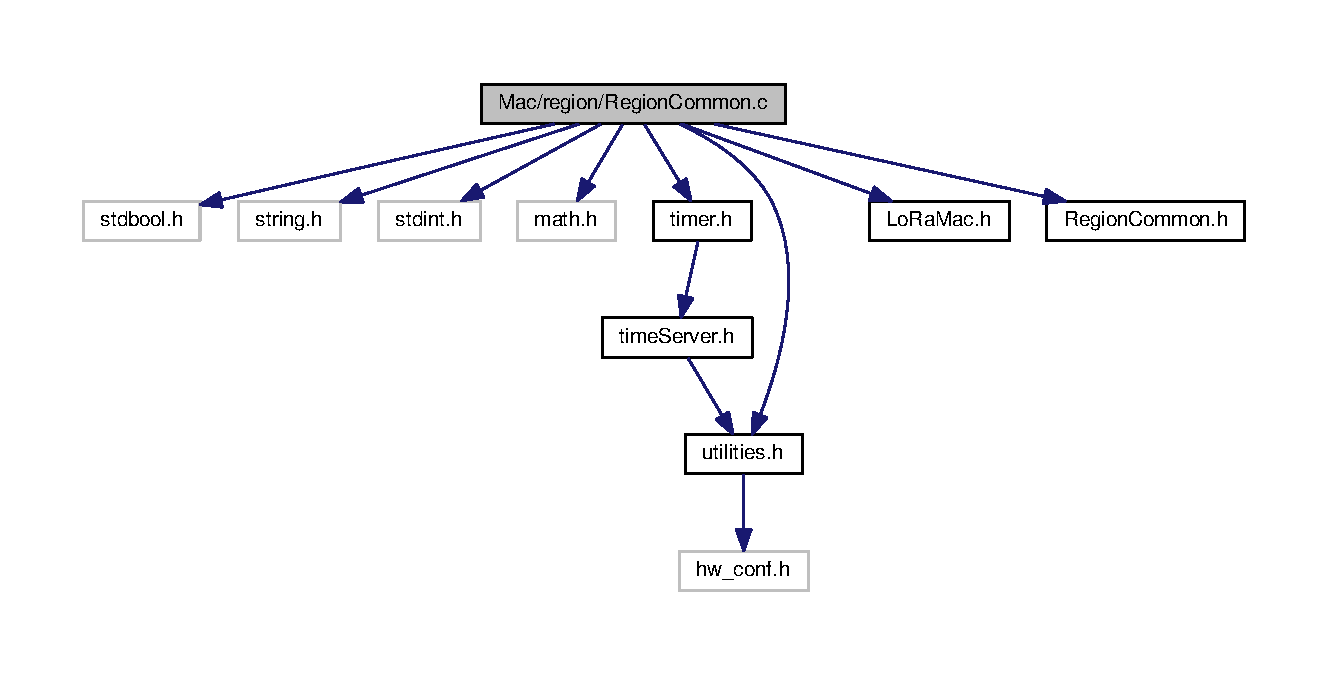
\includegraphics[width=350pt]{RegionCommon_8c__incl}
\end{center}
\end{figure}
\subsection*{Macros}
\begin{DoxyCompactItemize}
\item 
\#define \hyperlink{RegionCommon_8c_a1d58cbd560840cdab3e4427797e88c3a}{B\+A\+C\+K\+O\+F\+F\+\_\+\+D\+C\+\_\+1\+\_\+\+H\+O\+UR}~100
\item 
\#define \hyperlink{RegionCommon_8c_a70461da0dc970b3de51718ab397a81db}{B\+A\+C\+K\+O\+F\+F\+\_\+\+D\+C\+\_\+10\+\_\+\+H\+O\+U\+RS}~1000
\item 
\#define \hyperlink{RegionCommon_8c_ada6c3c87744e22f1c053caba7c40d26c}{B\+A\+C\+K\+O\+F\+F\+\_\+\+D\+C\+\_\+24\+\_\+\+H\+O\+U\+RS}~10000
\end{DoxyCompactItemize}
\subsection*{Functions}
\begin{DoxyCompactItemize}
\item 
uint16\+\_\+t \hyperlink{group__REGIONCOMMON_ga672466fcf1aedaaf075cdabf49bc0c28}{Region\+Common\+Get\+Join\+Dc} (\hyperlink{utilities_8h_a4215ca43d3e953099ea758ce428599d0}{Timer\+Time\+\_\+t} elapsed\+Time)
\begin{DoxyCompactList}\small\item\em Calculates the join duty cycle. This is a generic function and valid for all regions. \end{DoxyCompactList}\item 
bool \hyperlink{group__REGIONCOMMON_ga94ce5c6e759081853eb06d1dcffdab25}{Region\+Common\+Chan\+Verify\+Dr} (uint8\+\_\+t nb\+Channels, uint16\+\_\+t $\ast$channels\+Mask, int8\+\_\+t dr, int8\+\_\+t min\+Dr, int8\+\_\+t max\+Dr, \hyperlink{group__LORAMAC_ga1360ca6f82c6d125ea43a9dad9b56184}{Channel\+Params\+\_\+t} $\ast$channels)
\begin{DoxyCompactList}\small\item\em Verifies, if a datarate is available on an active channel. This is a generic function and valid for all regions. \end{DoxyCompactList}\item 
uint8\+\_\+t \hyperlink{group__REGIONCOMMON_gafdd1c80d953e18d755a631b72a9c3bd3}{Region\+Common\+Value\+In\+Range} (int8\+\_\+t value, int8\+\_\+t min, int8\+\_\+t max)
\begin{DoxyCompactList}\small\item\em Verifies, if a value is in a given range. This is a generic function and valid for all regions. \end{DoxyCompactList}\item 
bool \hyperlink{group__REGIONCOMMON_ga695c0ab2a06edcae5b33772f639fb676}{Region\+Common\+Chan\+Disable} (uint16\+\_\+t $\ast$channels\+Mask, uint8\+\_\+t id, uint8\+\_\+t max\+Channels)
\begin{DoxyCompactList}\small\item\em Disables a channel in a given channels mask. This is a generic function and valid for all regions. \end{DoxyCompactList}\item 
uint8\+\_\+t \hyperlink{group__REGIONCOMMON_gac23f0831812f610f57f42f6cf87368c9}{Region\+Common\+Count\+Channels} (uint16\+\_\+t $\ast$channels\+Mask, uint8\+\_\+t start\+Idx, uint8\+\_\+t stop\+Idx)
\begin{DoxyCompactList}\small\item\em Counts the number of active channels in a given channels mask. This is a generic function and valid for all regions. \end{DoxyCompactList}\item 
void \hyperlink{group__REGIONCOMMON_ga95f5199d490113269fae7f2e0569e9a0}{Region\+Common\+Chan\+Mask\+Copy} (uint16\+\_\+t $\ast$channels\+Mask\+Dest, uint16\+\_\+t $\ast$channels\+Mask\+Src, uint8\+\_\+t len)
\begin{DoxyCompactList}\small\item\em Copy a channels mask. This is a generic function and valid for all regions. \end{DoxyCompactList}\item 
void \hyperlink{group__REGIONCOMMON_ga491dea5590228a0cd33affd71743779c}{Region\+Common\+Set\+Band\+Tx\+Done} (bool joined, \hyperlink{group__LORAMAC_ga8f49721ee96ceb52c80a896ab11a2ed8}{Band\+\_\+t} $\ast$band, \hyperlink{utilities_8h_a4215ca43d3e953099ea758ce428599d0}{Timer\+Time\+\_\+t} last\+Tx\+Done)
\begin{DoxyCompactList}\small\item\em Sets the last tx done property. This is a generic function and valid for all regions. \end{DoxyCompactList}\item 
\hyperlink{utilities_8h_a4215ca43d3e953099ea758ce428599d0}{Timer\+Time\+\_\+t} \hyperlink{group__REGIONCOMMON_ga2e26fe6b49ca26edf7052eadd7f18b3a}{Region\+Common\+Update\+Band\+Time\+Off} (bool joined, bool duty\+Cycle, \hyperlink{group__LORAMAC_ga8f49721ee96ceb52c80a896ab11a2ed8}{Band\+\_\+t} $\ast$bands, uint8\+\_\+t nb\+Bands)
\begin{DoxyCompactList}\small\item\em Updates the time-\/offs of the bands. This is a generic function and valid for all regions. \end{DoxyCompactList}\item 
uint8\+\_\+t \hyperlink{group__REGIONCOMMON_ga8403c78482dbb901014dba48b75d78e8}{Region\+Common\+Parse\+Link\+Adr\+Req} (uint8\+\_\+t $\ast$payload, \hyperlink{group__REGIONCOMMON_ga6e1aaa6b8d179e2daffac8d1e23d7f24}{Region\+Common\+Link\+Adr\+Params\+\_\+t} $\ast$link\+Adr\+Params)
\begin{DoxyCompactList}\small\item\em Parses the parameter of an Link\+Adr\+Request. This is a generic function and valid for all regions. \end{DoxyCompactList}\item 
uint8\+\_\+t \hyperlink{group__REGIONCOMMON_ga2c87f98f09793dc7fa63a9801feeed73}{Region\+Common\+Link\+Adr\+Req\+Verify\+Params} (\hyperlink{group__REGIONCOMMON_gad186afbaf1b52893ddc3fa5eba88de0a}{Region\+Common\+Link\+Adr\+Req\+Verify\+Params\+\_\+t} $\ast$verify\+Params, int8\+\_\+t $\ast$dr, int8\+\_\+t $\ast$tx\+Pow, uint8\+\_\+t $\ast$nb\+Rep)
\begin{DoxyCompactList}\small\item\em Verifies and updates the datarate, the TX power and the number of repetitions of a Link\+Adr\+Request. This depends on the configuration of A\+DR also. \end{DoxyCompactList}\item 
double \hyperlink{group__REGIONCOMMON_ga79ed8b6555b68276d3c9ff2626b20fc8}{Region\+Common\+Compute\+Symbol\+Time\+Lo\+Ra} (uint8\+\_\+t phy\+Dr, uint32\+\_\+t bandwidth)
\begin{DoxyCompactList}\small\item\em Computes the symbol time for Lo\+Ra modulation. \end{DoxyCompactList}\item 
double \hyperlink{group__REGIONCOMMON_gacc2af896b03aa8ed8d8e5950d96d365f}{Region\+Common\+Compute\+Symbol\+Time\+Fsk} (uint8\+\_\+t phy\+Dr)
\begin{DoxyCompactList}\small\item\em Computes the symbol time for F\+SK modulation. \end{DoxyCompactList}\item 
void \hyperlink{group__REGIONCOMMON_gaba7114d0ca01f04933710feb13646138}{Region\+Common\+Compute\+Rx\+Window\+Parameters} (double t\+Symbol, uint8\+\_\+t min\+Rx\+Symbols, uint32\+\_\+t rx\+Error, uint32\+\_\+t wake\+Up\+Time, uint32\+\_\+t $\ast$window\+Timeout, int32\+\_\+t $\ast$window\+Offset)
\begin{DoxyCompactList}\small\item\em Computes the RX window timeout and the RX window offset. \end{DoxyCompactList}\item 
int8\+\_\+t \hyperlink{group__REGIONCOMMON_gaa92800c8e9ce21366d383d14878cc391}{Region\+Common\+Compute\+Tx\+Power} (int8\+\_\+t tx\+Power\+Index, float max\+Eirp, float antenna\+Gain)
\begin{DoxyCompactList}\small\item\em Computes the tx\+Power, based on the max E\+I\+RP and the antenna gain. \end{DoxyCompactList}\item 
void \hyperlink{group__REGIONCOMMON_gae2b1dfba27c79f605048f2d9869dc57d}{Region\+Common\+Calc\+Back\+Off} (\hyperlink{group__REGIONCOMMON_ga26c2fc7c3e1d929d59b5653a5cd1fc0c}{Region\+Common\+Calc\+Back\+Off\+Params\+\_\+t} $\ast$calc\+Back\+Off\+Params)
\begin{DoxyCompactList}\small\item\em Calculates the duty cycle for the current band. \end{DoxyCompactList}\end{DoxyCompactItemize}


\subsection{Macro Definition Documentation}
\mbox{\Hypertarget{RegionCommon_8c_a70461da0dc970b3de51718ab397a81db}\label{RegionCommon_8c_a70461da0dc970b3de51718ab397a81db}} 
\index{Region\+Common.\+c@{Region\+Common.\+c}!B\+A\+C\+K\+O\+F\+F\+\_\+\+D\+C\+\_\+10\+\_\+\+H\+O\+U\+RS@{B\+A\+C\+K\+O\+F\+F\+\_\+\+D\+C\+\_\+10\+\_\+\+H\+O\+U\+RS}}
\index{B\+A\+C\+K\+O\+F\+F\+\_\+\+D\+C\+\_\+10\+\_\+\+H\+O\+U\+RS@{B\+A\+C\+K\+O\+F\+F\+\_\+\+D\+C\+\_\+10\+\_\+\+H\+O\+U\+RS}!Region\+Common.\+c@{Region\+Common.\+c}}
\subsubsection{\texorpdfstring{B\+A\+C\+K\+O\+F\+F\+\_\+\+D\+C\+\_\+10\+\_\+\+H\+O\+U\+RS}{BACKOFF\_DC\_10\_HOURS}}
{\footnotesize\ttfamily \#define B\+A\+C\+K\+O\+F\+F\+\_\+\+D\+C\+\_\+10\+\_\+\+H\+O\+U\+RS~1000}

\mbox{\Hypertarget{RegionCommon_8c_a1d58cbd560840cdab3e4427797e88c3a}\label{RegionCommon_8c_a1d58cbd560840cdab3e4427797e88c3a}} 
\index{Region\+Common.\+c@{Region\+Common.\+c}!B\+A\+C\+K\+O\+F\+F\+\_\+\+D\+C\+\_\+1\+\_\+\+H\+O\+UR@{B\+A\+C\+K\+O\+F\+F\+\_\+\+D\+C\+\_\+1\+\_\+\+H\+O\+UR}}
\index{B\+A\+C\+K\+O\+F\+F\+\_\+\+D\+C\+\_\+1\+\_\+\+H\+O\+UR@{B\+A\+C\+K\+O\+F\+F\+\_\+\+D\+C\+\_\+1\+\_\+\+H\+O\+UR}!Region\+Common.\+c@{Region\+Common.\+c}}
\subsubsection{\texorpdfstring{B\+A\+C\+K\+O\+F\+F\+\_\+\+D\+C\+\_\+1\+\_\+\+H\+O\+UR}{BACKOFF\_DC\_1\_HOUR}}
{\footnotesize\ttfamily \#define B\+A\+C\+K\+O\+F\+F\+\_\+\+D\+C\+\_\+1\+\_\+\+H\+O\+UR~100}

\mbox{\Hypertarget{RegionCommon_8c_ada6c3c87744e22f1c053caba7c40d26c}\label{RegionCommon_8c_ada6c3c87744e22f1c053caba7c40d26c}} 
\index{Region\+Common.\+c@{Region\+Common.\+c}!B\+A\+C\+K\+O\+F\+F\+\_\+\+D\+C\+\_\+24\+\_\+\+H\+O\+U\+RS@{B\+A\+C\+K\+O\+F\+F\+\_\+\+D\+C\+\_\+24\+\_\+\+H\+O\+U\+RS}}
\index{B\+A\+C\+K\+O\+F\+F\+\_\+\+D\+C\+\_\+24\+\_\+\+H\+O\+U\+RS@{B\+A\+C\+K\+O\+F\+F\+\_\+\+D\+C\+\_\+24\+\_\+\+H\+O\+U\+RS}!Region\+Common.\+c@{Region\+Common.\+c}}
\subsubsection{\texorpdfstring{B\+A\+C\+K\+O\+F\+F\+\_\+\+D\+C\+\_\+24\+\_\+\+H\+O\+U\+RS}{BACKOFF\_DC\_24\_HOURS}}
{\footnotesize\ttfamily \#define B\+A\+C\+K\+O\+F\+F\+\_\+\+D\+C\+\_\+24\+\_\+\+H\+O\+U\+RS~10000}


\hypertarget{RegionCommon_8h}{}\section{Mac/region/\+Region\+Common.h File Reference}
\label{RegionCommon_8h}\index{Mac/region/\+Region\+Common.\+h@{Mac/region/\+Region\+Common.\+h}}


Region independent implementations which are common to all regions.  


This graph shows which files directly or indirectly include this file\+:
\nopagebreak
\begin{figure}[H]
\begin{center}
\leavevmode
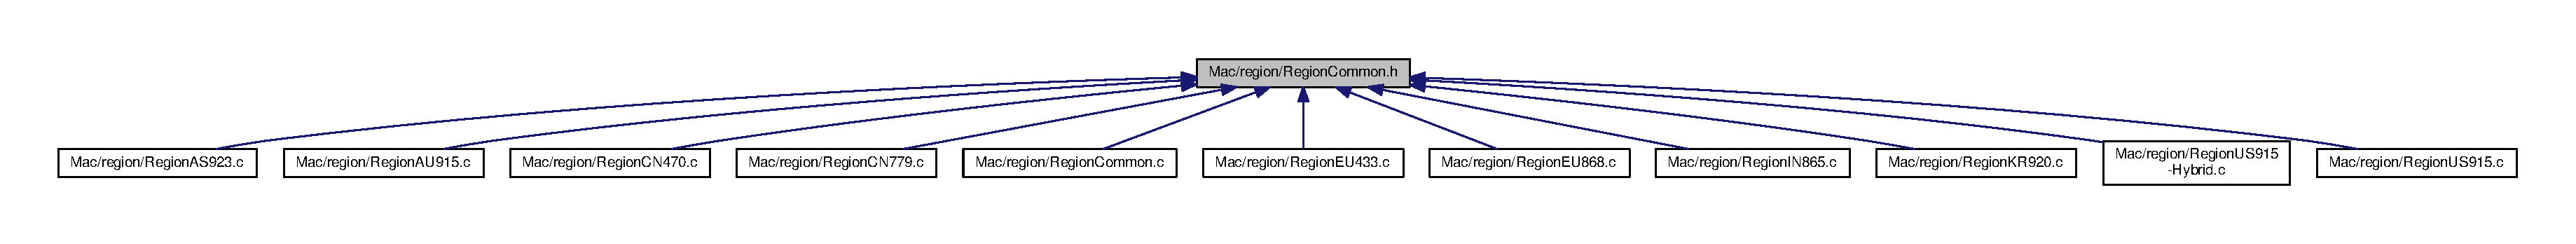
\includegraphics[width=350pt]{RegionCommon_8h__dep__incl}
\end{center}
\end{figure}
\subsection*{Data Structures}
\begin{DoxyCompactItemize}
\item 
struct \hyperlink{structsRegionCommonLinkAdrParams}{s\+Region\+Common\+Link\+Adr\+Params}
\item 
struct \hyperlink{structsRegionCommonLinkAdrReqVerifyParams}{s\+Region\+Common\+Link\+Adr\+Req\+Verify\+Params}
\item 
struct \hyperlink{structsRegionCommonCalcBackOffParams}{s\+Region\+Common\+Calc\+Back\+Off\+Params}
\end{DoxyCompactItemize}
\subsection*{Typedefs}
\begin{DoxyCompactItemize}
\item 
typedef struct \hyperlink{structsRegionCommonLinkAdrParams}{s\+Region\+Common\+Link\+Adr\+Params} \hyperlink{group__REGIONCOMMON_ga6e1aaa6b8d179e2daffac8d1e23d7f24}{Region\+Common\+Link\+Adr\+Params\+\_\+t}
\item 
typedef struct \hyperlink{structsRegionCommonLinkAdrReqVerifyParams}{s\+Region\+Common\+Link\+Adr\+Req\+Verify\+Params} \hyperlink{group__REGIONCOMMON_gad186afbaf1b52893ddc3fa5eba88de0a}{Region\+Common\+Link\+Adr\+Req\+Verify\+Params\+\_\+t}
\item 
typedef struct \hyperlink{structsRegionCommonCalcBackOffParams}{s\+Region\+Common\+Calc\+Back\+Off\+Params} \hyperlink{group__REGIONCOMMON_ga26c2fc7c3e1d929d59b5653a5cd1fc0c}{Region\+Common\+Calc\+Back\+Off\+Params\+\_\+t}
\end{DoxyCompactItemize}
\subsection*{Functions}
\begin{DoxyCompactItemize}
\item 
uint16\+\_\+t \hyperlink{group__REGIONCOMMON_ga672466fcf1aedaaf075cdabf49bc0c28}{Region\+Common\+Get\+Join\+Dc} (\hyperlink{utilities_8h_a4215ca43d3e953099ea758ce428599d0}{Timer\+Time\+\_\+t} elapsed\+Time)
\begin{DoxyCompactList}\small\item\em Calculates the join duty cycle. This is a generic function and valid for all regions. \end{DoxyCompactList}\item 
uint8\+\_\+t \hyperlink{group__REGIONCOMMON_gafdd1c80d953e18d755a631b72a9c3bd3}{Region\+Common\+Value\+In\+Range} (int8\+\_\+t value, int8\+\_\+t min, int8\+\_\+t max)
\begin{DoxyCompactList}\small\item\em Verifies, if a value is in a given range. This is a generic function and valid for all regions. \end{DoxyCompactList}\item 
bool \hyperlink{group__REGIONCOMMON_ga94ce5c6e759081853eb06d1dcffdab25}{Region\+Common\+Chan\+Verify\+Dr} (uint8\+\_\+t nb\+Channels, uint16\+\_\+t $\ast$channels\+Mask, int8\+\_\+t dr, int8\+\_\+t min\+Dr, int8\+\_\+t max\+Dr, \hyperlink{group__LORAMAC_ga1360ca6f82c6d125ea43a9dad9b56184}{Channel\+Params\+\_\+t} $\ast$channels)
\begin{DoxyCompactList}\small\item\em Verifies, if a datarate is available on an active channel. This is a generic function and valid for all regions. \end{DoxyCompactList}\item 
bool \hyperlink{group__REGIONCOMMON_ga695c0ab2a06edcae5b33772f639fb676}{Region\+Common\+Chan\+Disable} (uint16\+\_\+t $\ast$channels\+Mask, uint8\+\_\+t id, uint8\+\_\+t max\+Channels)
\begin{DoxyCompactList}\small\item\em Disables a channel in a given channels mask. This is a generic function and valid for all regions. \end{DoxyCompactList}\item 
uint8\+\_\+t \hyperlink{group__REGIONCOMMON_gac23f0831812f610f57f42f6cf87368c9}{Region\+Common\+Count\+Channels} (uint16\+\_\+t $\ast$channels\+Mask, uint8\+\_\+t start\+Idx, uint8\+\_\+t stop\+Idx)
\begin{DoxyCompactList}\small\item\em Counts the number of active channels in a given channels mask. This is a generic function and valid for all regions. \end{DoxyCompactList}\item 
void \hyperlink{group__REGIONCOMMON_ga95f5199d490113269fae7f2e0569e9a0}{Region\+Common\+Chan\+Mask\+Copy} (uint16\+\_\+t $\ast$channels\+Mask\+Dest, uint16\+\_\+t $\ast$channels\+Mask\+Src, uint8\+\_\+t len)
\begin{DoxyCompactList}\small\item\em Copy a channels mask. This is a generic function and valid for all regions. \end{DoxyCompactList}\item 
void \hyperlink{group__REGIONCOMMON_ga491dea5590228a0cd33affd71743779c}{Region\+Common\+Set\+Band\+Tx\+Done} (bool joined, \hyperlink{group__LORAMAC_ga8f49721ee96ceb52c80a896ab11a2ed8}{Band\+\_\+t} $\ast$band, \hyperlink{utilities_8h_a4215ca43d3e953099ea758ce428599d0}{Timer\+Time\+\_\+t} last\+Tx\+Done)
\begin{DoxyCompactList}\small\item\em Sets the last tx done property. This is a generic function and valid for all regions. \end{DoxyCompactList}\item 
\hyperlink{utilities_8h_a4215ca43d3e953099ea758ce428599d0}{Timer\+Time\+\_\+t} \hyperlink{group__REGIONCOMMON_ga2e26fe6b49ca26edf7052eadd7f18b3a}{Region\+Common\+Update\+Band\+Time\+Off} (bool joined, bool duty\+Cycle, \hyperlink{group__LORAMAC_ga8f49721ee96ceb52c80a896ab11a2ed8}{Band\+\_\+t} $\ast$bands, uint8\+\_\+t nb\+Bands)
\begin{DoxyCompactList}\small\item\em Updates the time-\/offs of the bands. This is a generic function and valid for all regions. \end{DoxyCompactList}\item 
uint8\+\_\+t \hyperlink{group__REGIONCOMMON_ga8403c78482dbb901014dba48b75d78e8}{Region\+Common\+Parse\+Link\+Adr\+Req} (uint8\+\_\+t $\ast$payload, \hyperlink{group__REGIONCOMMON_ga6e1aaa6b8d179e2daffac8d1e23d7f24}{Region\+Common\+Link\+Adr\+Params\+\_\+t} $\ast$parse\+Link\+Adr)
\begin{DoxyCompactList}\small\item\em Parses the parameter of an Link\+Adr\+Request. This is a generic function and valid for all regions. \end{DoxyCompactList}\item 
uint8\+\_\+t \hyperlink{group__REGIONCOMMON_ga2c87f98f09793dc7fa63a9801feeed73}{Region\+Common\+Link\+Adr\+Req\+Verify\+Params} (\hyperlink{group__REGIONCOMMON_gad186afbaf1b52893ddc3fa5eba88de0a}{Region\+Common\+Link\+Adr\+Req\+Verify\+Params\+\_\+t} $\ast$verify\+Params, int8\+\_\+t $\ast$dr, int8\+\_\+t $\ast$tx\+Pow, uint8\+\_\+t $\ast$nb\+Rep)
\begin{DoxyCompactList}\small\item\em Verifies and updates the datarate, the TX power and the number of repetitions of a Link\+Adr\+Request. This depends on the configuration of A\+DR also. \end{DoxyCompactList}\item 
double \hyperlink{group__REGIONCOMMON_ga79ed8b6555b68276d3c9ff2626b20fc8}{Region\+Common\+Compute\+Symbol\+Time\+Lo\+Ra} (uint8\+\_\+t phy\+Dr, uint32\+\_\+t bandwidth)
\begin{DoxyCompactList}\small\item\em Computes the symbol time for Lo\+Ra modulation. \end{DoxyCompactList}\item 
double \hyperlink{group__REGIONCOMMON_gacc2af896b03aa8ed8d8e5950d96d365f}{Region\+Common\+Compute\+Symbol\+Time\+Fsk} (uint8\+\_\+t phy\+Dr)
\begin{DoxyCompactList}\small\item\em Computes the symbol time for F\+SK modulation. \end{DoxyCompactList}\item 
void \hyperlink{group__REGIONCOMMON_gaba7114d0ca01f04933710feb13646138}{Region\+Common\+Compute\+Rx\+Window\+Parameters} (double t\+Symbol, uint8\+\_\+t min\+Rx\+Symbols, uint32\+\_\+t rx\+Error, uint32\+\_\+t wake\+Up\+Time, uint32\+\_\+t $\ast$window\+Timeout, int32\+\_\+t $\ast$window\+Offset)
\begin{DoxyCompactList}\small\item\em Computes the RX window timeout and the RX window offset. \end{DoxyCompactList}\item 
int8\+\_\+t \hyperlink{group__REGIONCOMMON_gaa92800c8e9ce21366d383d14878cc391}{Region\+Common\+Compute\+Tx\+Power} (int8\+\_\+t tx\+Power\+Index, float max\+Eirp, float antenna\+Gain)
\begin{DoxyCompactList}\small\item\em Computes the tx\+Power, based on the max E\+I\+RP and the antenna gain. \end{DoxyCompactList}\item 
void \hyperlink{group__REGIONCOMMON_gae2b1dfba27c79f605048f2d9869dc57d}{Region\+Common\+Calc\+Back\+Off} (\hyperlink{group__REGIONCOMMON_ga26c2fc7c3e1d929d59b5653a5cd1fc0c}{Region\+Common\+Calc\+Back\+Off\+Params\+\_\+t} $\ast$calc\+Back\+Off\+Params)
\begin{DoxyCompactList}\small\item\em Calculates the duty cycle for the current band. \end{DoxyCompactList}\end{DoxyCompactItemize}


\subsection{Detailed Description}
Region independent implementations which are common to all regions. 

\begin{DoxyCopyright}{Copyright}
Revised B\+SD License, see section L\+I\+C\+E\+N\+SE.
\end{DoxyCopyright}

\begin{DoxyCode}
  \_\_\_\_\_\_                              \_
 / \_\_\_\_\_)             \_              | |
( (\_\_\_\_  \_\_\_\_\_ \_\_\_\_ \_| |\_ \_\_\_\_\_  \_\_\_\_| |\_\_
 \(\backslash\)\_\_\_\_ \(\backslash\)| \_\_\_ |    (\_   \_) \_\_\_ |/ \_\_\_)  \_ \(\backslash\)
 \_\_\_\_\_) ) \_\_\_\_| | | || |\_| \_\_\_\_( (\_\_\_| | | |
(\_\_\_\_\_\_/|\_\_\_\_\_)\_|\_|\_| \(\backslash\)\_\_)\_\_\_\_\_)\(\backslash\)\_\_\_\_)\_| |\_|
(C)2013 Semtech

 \_\_\_ \_\_\_\_\_ \_   \_\_\_ \_  \_\_\_\_\_ \_\_\_  \_\_\_  \_\_\_ \_\_\_
/ \_\_|\_   \_/\_\(\backslash\) / \_\_| |/ / \_\_/ \_ \(\backslash\)| \_ \(\backslash\)/ \_\_| \_\_|
\(\backslash\)\_\_ \(\backslash\) | |/ \_ \(\backslash\) (\_\_| \textcolor{stringliteral}{' <| \_| (\_) |   / (\_\_| \_|}
\textcolor{stringliteral}{|\_\_\_/ |\_/\_/ \(\backslash\)\_\(\backslash\)\_\_\_|\_|\(\backslash\)\_\(\backslash\)\_| \(\backslash\)\_\_\_/|\_|\_\(\backslash\)\(\backslash\)\_\_\_|\_\_\_|}
\textcolor{stringliteral}{embedded.connectivity.solutions===============}
\end{DoxyCode}


\begin{DoxyAuthor}{Author}
Miguel Luis ( Semtech )

Gregory Cristian ( Semtech )

Daniel Jaeckle ( S\+T\+A\+C\+K\+F\+O\+R\+CE ) 
\end{DoxyAuthor}

\hypertarget{RegionEU433_8c}{}\section{Mac/region/\+Region\+E\+U433.c File Reference}
\label{RegionEU433_8c}\index{Mac/region/\+Region\+E\+U433.\+c@{Mac/region/\+Region\+E\+U433.\+c}}
{\ttfamily \#include $<$stdbool.\+h$>$}\newline
{\ttfamily \#include $<$string.\+h$>$}\newline
{\ttfamily \#include $<$stdint.\+h$>$}\newline
{\ttfamily \#include $<$math.\+h$>$}\newline
{\ttfamily \#include \char`\"{}radio.\+h\char`\"{}}\newline
{\ttfamily \#include \char`\"{}timer.\+h\char`\"{}}\newline
{\ttfamily \#include \char`\"{}Lo\+Ra\+Mac.\+h\char`\"{}}\newline
{\ttfamily \#include \char`\"{}utilities.\+h\char`\"{}}\newline
{\ttfamily \#include \char`\"{}Region.\+h\char`\"{}}\newline
{\ttfamily \#include \char`\"{}Region\+Common.\+h\char`\"{}}\newline
{\ttfamily \#include \char`\"{}Region\+E\+U433.\+h\char`\"{}}\newline
{\ttfamily \#include \char`\"{}debug.\+h\char`\"{}}\newline
Include dependency graph for Region\+E\+U433.\+c\+:
\nopagebreak
\begin{figure}[H]
\begin{center}
\leavevmode
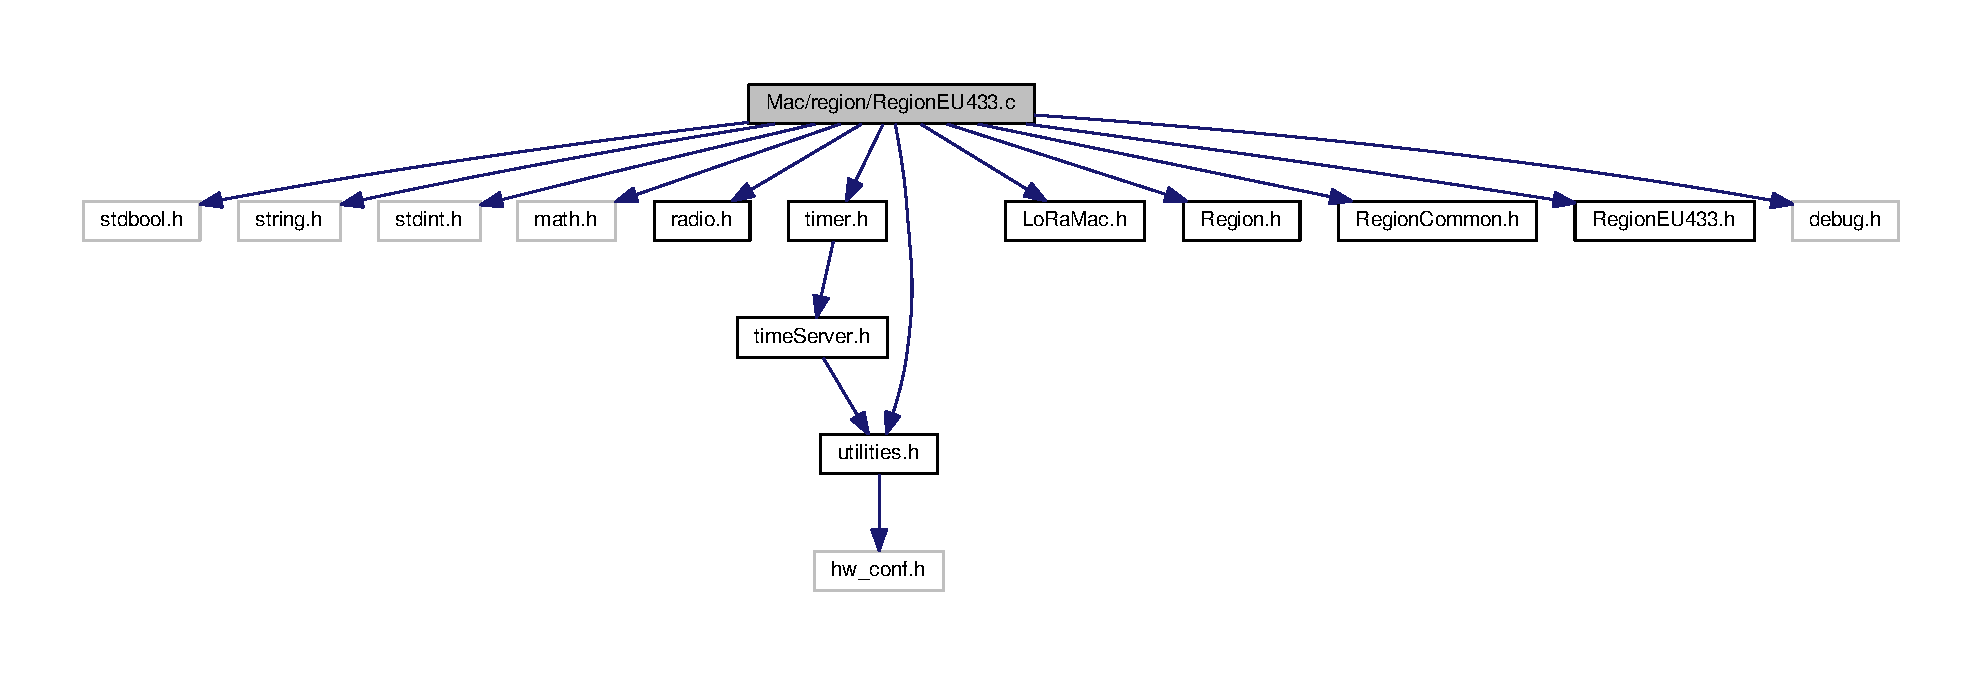
\includegraphics[width=350pt]{RegionEU433_8c__incl}
\end{center}
\end{figure}
\subsection*{Macros}
\begin{DoxyCompactItemize}
\item 
\#define \hyperlink{RegionEU433_8c_a1b20a8de3ae59c0b063fb313f0c70890}{C\+H\+A\+N\+N\+E\+L\+S\+\_\+\+M\+A\+S\+K\+\_\+\+S\+I\+ZE}~1
\end{DoxyCompactItemize}
\subsection*{Functions}
\begin{DoxyCompactItemize}
\item 
\hyperlink{group__REGION_gaed159b26e5c4677236b6e8677019db30}{Phy\+Param\+\_\+t} \hyperlink{group__REGIONEU433_ga407d34fe6c7dea18b07732d03b62894b}{Region\+E\+U433\+Get\+Phy\+Param} (\hyperlink{group__REGION_gab471483fff904f4f89bbc03f7fc380ab}{Get\+Phy\+Params\+\_\+t} $\ast$get\+Phy)
\begin{DoxyCompactList}\small\item\em The function gets a value of a specific phy attribute. \end{DoxyCompactList}\item 
void \hyperlink{group__REGIONEU433_gae044b69c6a72fff53e322ba8ffbc9be5}{Region\+E\+U433\+Set\+Band\+Tx\+Done} (\hyperlink{group__REGION_gad0524aa0673c0814a71e7a4f9cade3fc}{Set\+Band\+Tx\+Done\+Params\+\_\+t} $\ast$tx\+Done)
\begin{DoxyCompactList}\small\item\em Updates the last TX done parameters of the current channel. \end{DoxyCompactList}\item 
void \hyperlink{group__REGIONEU433_ga1961913d7b9857e1804f455b59428186}{Region\+E\+U433\+Init\+Defaults} (\hyperlink{group__REGION_gaddc73ae10673ec925724e7870363bda9}{Init\+Type\+\_\+t} type)
\begin{DoxyCompactList}\small\item\em Initializes the channels masks and the channels. \end{DoxyCompactList}\item 
bool \hyperlink{group__REGIONEU433_ga6ffa44f79bf438495ab15476274e88dd}{Region\+E\+U433\+Verify} (\hyperlink{group__REGION_ga966d97bc2f25df1c09e92e60ef652276}{Verify\+Params\+\_\+t} $\ast$verify, \hyperlink{group__REGION_ga9445b07fdf77581ecfaf389970e635f8}{Phy\+Attribute\+\_\+t} phy\+Attribute)
\begin{DoxyCompactList}\small\item\em Verifies a parameter. \end{DoxyCompactList}\item 
void \hyperlink{group__REGIONEU433_gacf5995b949053267e507f4e2063fc7bf}{Region\+E\+U433\+Apply\+C\+F\+List} (\hyperlink{group__REGION_ga71588e9ad07e34b78fa91d51881fd3c6}{Apply\+C\+F\+List\+Params\+\_\+t} $\ast$apply\+C\+F\+List)
\begin{DoxyCompactList}\small\item\em The function parses the input buffer and sets up the channels of the CF list. \end{DoxyCompactList}\item 
bool \hyperlink{group__REGIONEU433_ga9f5e0e0881857bae99067d739c037882}{Region\+E\+U433\+Chan\+Mask\+Set} (\hyperlink{group__REGION_ga6d24f7da136006410827dfb29f6b9b9e}{Chan\+Mask\+Set\+Params\+\_\+t} $\ast$chan\+Mask\+Set)
\begin{DoxyCompactList}\small\item\em Sets a channels mask. \end{DoxyCompactList}\item 
bool \hyperlink{group__REGIONEU433_ga97dd9f8ccc0f0e354e4ccc2e3b3d4e6c}{Region\+E\+U433\+Adr\+Next} (\hyperlink{group__REGION_ga567c2742622326b350b4e91bbf61b4ce}{Adr\+Next\+Params\+\_\+t} $\ast$adr\+Next, int8\+\_\+t $\ast$dr\+Out, int8\+\_\+t $\ast$tx\+Pow\+Out, uint32\+\_\+t $\ast$adr\+Ack\+Counter)
\begin{DoxyCompactList}\small\item\em Calculates the next datarate to set, when A\+DR is on or off. \end{DoxyCompactList}\item 
void \hyperlink{group__REGIONEU433_ga5e88bc1903bb61a90df88fe8c1805705}{Region\+E\+U433\+Compute\+Rx\+Window\+Parameters} (int8\+\_\+t datarate, uint8\+\_\+t min\+Rx\+Symbols, uint32\+\_\+t rx\+Error, \hyperlink{group__REGION_ga375c038078dfcfc7ef14280021db719e}{Rx\+Config\+Params\+\_\+t} $\ast$rx\+Config\+Params)
\item 
bool \hyperlink{group__REGIONEU433_ga3a7bb7e75de6bfc5ef4edc1c934f5a50}{Region\+E\+U433\+Rx\+Config} (\hyperlink{group__REGION_ga375c038078dfcfc7ef14280021db719e}{Rx\+Config\+Params\+\_\+t} $\ast$rx\+Config, int8\+\_\+t $\ast$datarate)
\begin{DoxyCompactList}\small\item\em Configuration of the RX windows. \end{DoxyCompactList}\item 
bool \hyperlink{group__REGIONEU433_ga29a68f1a72dfccfe89f01de36ddc542b}{Region\+E\+U433\+Tx\+Config} (\hyperlink{group__REGION_gabed730d4d04b0b60d4b6d1966d3f21d3}{Tx\+Config\+Params\+\_\+t} $\ast$tx\+Config, int8\+\_\+t $\ast$tx\+Power, \hyperlink{utilities_8h_a4215ca43d3e953099ea758ce428599d0}{Timer\+Time\+\_\+t} $\ast$tx\+Time\+On\+Air)
\begin{DoxyCompactList}\small\item\em TX configuration. \end{DoxyCompactList}\item 
uint8\+\_\+t \hyperlink{group__REGIONEU433_gafd3e374d9048e67d54d1fa90b8d18723}{Region\+E\+U433\+Link\+Adr\+Req} (\hyperlink{group__REGION_gad4af503e8d4de1846129e26a799a1e8e}{Link\+Adr\+Req\+Params\+\_\+t} $\ast$link\+Adr\+Req, int8\+\_\+t $\ast$dr\+Out, int8\+\_\+t $\ast$tx\+Pow\+Out, uint8\+\_\+t $\ast$nb\+Rep\+Out, uint8\+\_\+t $\ast$nb\+Bytes\+Parsed)
\begin{DoxyCompactList}\small\item\em The function processes a Link A\+DR Request. \end{DoxyCompactList}\item 
uint8\+\_\+t \hyperlink{group__REGIONEU433_ga0aaed1ad836262927f03ec9f8b63674d}{Region\+E\+U433\+Rx\+Param\+Setup\+Req} (\hyperlink{group__REGION_ga7165f282c670c728c36d534df2285157}{Rx\+Param\+Setup\+Req\+Params\+\_\+t} $\ast$rx\+Param\+Setup\+Req)
\begin{DoxyCompactList}\small\item\em The function processes a RX Parameter Setup Request. \end{DoxyCompactList}\item 
uint8\+\_\+t \hyperlink{group__REGIONEU433_ga1df9d3b633c355a6b1d2b7fc1e0e217b}{Region\+E\+U433\+New\+Channel\+Req} (\hyperlink{group__REGION_gae2abcdb6dbb843c9faf5fd3009eca9d6}{New\+Channel\+Req\+Params\+\_\+t} $\ast$new\+Channel\+Req)
\begin{DoxyCompactList}\small\item\em The function processes a Channel Request. \end{DoxyCompactList}\item 
int8\+\_\+t \hyperlink{group__REGIONEU433_ga3536c80fcee7f9f673bce7e3dbd50fd2}{Region\+E\+U433\+Tx\+Param\+Setup\+Req} (\hyperlink{group__REGION_ga26836ef2996e70410e42ef471073f855}{Tx\+Param\+Setup\+Req\+Params\+\_\+t} $\ast$tx\+Param\+Setup\+Req)
\begin{DoxyCompactList}\small\item\em The function processes a TX Param\+Setup Request. \end{DoxyCompactList}\item 
uint8\+\_\+t \hyperlink{group__REGIONEU433_ga245f30ef549f49611ca2513a3d931033}{Region\+E\+U433\+Dl\+Channel\+Req} (\hyperlink{group__REGION_gae0d608ff1f8ea0a430e4f9a4c38ec7f3}{Dl\+Channel\+Req\+Params\+\_\+t} $\ast$dl\+Channel\+Req)
\begin{DoxyCompactList}\small\item\em The function processes a Dl\+Channel Request. \end{DoxyCompactList}\item 
int8\+\_\+t \hyperlink{group__REGIONEU433_ga3fdffc76cad694d27a71a38769cfee85}{Region\+E\+U433\+Alternate\+Dr} (\hyperlink{group__REGION_ga001ea4338d1c83f4c785b49d7ad2d696}{Alternate\+Dr\+Params\+\_\+t} $\ast$alternate\+Dr)
\begin{DoxyCompactList}\small\item\em Alternates the datarate of the channel for the join request. \end{DoxyCompactList}\item 
void \hyperlink{group__REGIONEU433_ga3e31558e030a1a2c27c26b8057c805e6}{Region\+E\+U433\+Calc\+Back\+Off} (\hyperlink{group__REGION_ga7c5c9a8da174e6679eded8257dc92fd9}{Calc\+Back\+Off\+Params\+\_\+t} $\ast$calc\+Back\+Off)
\begin{DoxyCompactList}\small\item\em Calculates the back-\/off time. \end{DoxyCompactList}\item 
bool \hyperlink{group__REGIONEU433_gacece995005d92767951d5e1b4d513494}{Region\+E\+U433\+Next\+Channel} (\hyperlink{group__REGION_ga115f5e83afae352c0a3dcdc193374040}{Next\+Chan\+Params\+\_\+t} $\ast$next\+Chan\+Params, uint8\+\_\+t $\ast$channel, \hyperlink{utilities_8h_a4215ca43d3e953099ea758ce428599d0}{Timer\+Time\+\_\+t} $\ast$time, \hyperlink{utilities_8h_a4215ca43d3e953099ea758ce428599d0}{Timer\+Time\+\_\+t} $\ast$aggregated\+Time\+Off)
\begin{DoxyCompactList}\small\item\em Searches and set the next random available channel. \end{DoxyCompactList}\item 
\hyperlink{group__LORAMAC_ga30bd25657e10480f8605ee951b0ecfbd}{Lo\+Ra\+Mac\+Status\+\_\+t} \hyperlink{group__REGIONEU433_ga477a869bd33f0fc4a1104e1a2097418a}{Region\+E\+U433\+Channel\+Add} (\hyperlink{group__REGION_gab1c5f3aa06614283202906cef4417860}{Channel\+Add\+Params\+\_\+t} $\ast$channel\+Add)
\begin{DoxyCompactList}\small\item\em Adds a channel. \end{DoxyCompactList}\item 
bool \hyperlink{group__REGIONEU433_ga8c6f83d1c3aadcbc717551c3d4bc912e}{Region\+E\+U433\+Channels\+Remove} (\hyperlink{group__REGION_gaa37468560d2fc81a977b57a48e5d72c0}{Channel\+Remove\+Params\+\_\+t} $\ast$channel\+Remove)
\begin{DoxyCompactList}\small\item\em Removes a channel. \end{DoxyCompactList}\item 
void \hyperlink{group__REGIONEU433_ga76561de6c45317a54ded972f7ac80836}{Region\+E\+U433\+Set\+Continuous\+Wave} (\hyperlink{group__REGION_gaf39bb5ba06921139c6d17f88a8d518cd}{Continuous\+Wave\+Params\+\_\+t} $\ast$continuous\+Wave)
\begin{DoxyCompactList}\small\item\em Sets the radio into continuous wave mode. \end{DoxyCompactList}\item 
uint8\+\_\+t \hyperlink{group__REGIONEU433_ga1d0c43ec9e4539732c33e625f56104b2}{Region\+E\+U433\+Apply\+Dr\+Offset} (uint8\+\_\+t downlink\+Dwell\+Time, int8\+\_\+t dr, int8\+\_\+t dr\+Offset)
\begin{DoxyCompactList}\small\item\em Computes new datarate according to the given offset. \end{DoxyCompactList}\end{DoxyCompactItemize}


\subsection{Macro Definition Documentation}
\mbox{\Hypertarget{RegionEU433_8c_a1b20a8de3ae59c0b063fb313f0c70890}\label{RegionEU433_8c_a1b20a8de3ae59c0b063fb313f0c70890}} 
\index{Region\+E\+U433.\+c@{Region\+E\+U433.\+c}!C\+H\+A\+N\+N\+E\+L\+S\+\_\+\+M\+A\+S\+K\+\_\+\+S\+I\+ZE@{C\+H\+A\+N\+N\+E\+L\+S\+\_\+\+M\+A\+S\+K\+\_\+\+S\+I\+ZE}}
\index{C\+H\+A\+N\+N\+E\+L\+S\+\_\+\+M\+A\+S\+K\+\_\+\+S\+I\+ZE@{C\+H\+A\+N\+N\+E\+L\+S\+\_\+\+M\+A\+S\+K\+\_\+\+S\+I\+ZE}!Region\+E\+U433.\+c@{Region\+E\+U433.\+c}}
\subsubsection{\texorpdfstring{C\+H\+A\+N\+N\+E\+L\+S\+\_\+\+M\+A\+S\+K\+\_\+\+S\+I\+ZE}{CHANNELS\_MASK\_SIZE}}
{\footnotesize\ttfamily \#define C\+H\+A\+N\+N\+E\+L\+S\+\_\+\+M\+A\+S\+K\+\_\+\+S\+I\+ZE~1}


\hypertarget{RegionEU433_8h}{}\section{Mac/region/\+Region\+E\+U433.h File Reference}
\label{RegionEU433_8h}\index{Mac/region/\+Region\+E\+U433.\+h@{Mac/region/\+Region\+E\+U433.\+h}}


Region definition for E\+U433.  


This graph shows which files directly or indirectly include this file\+:
\nopagebreak
\begin{figure}[H]
\begin{center}
\leavevmode
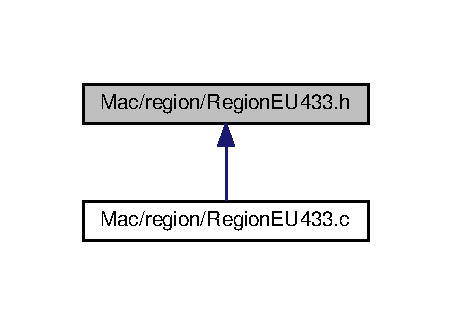
\includegraphics[width=217pt]{RegionEU433_8h__dep__incl}
\end{center}
\end{figure}
\subsection*{Macros}
\begin{DoxyCompactItemize}
\item 
\#define \hyperlink{group__REGIONEU433_ga800fbd07b871c93758364a0311b87937}{E\+U433\+\_\+\+M\+A\+X\+\_\+\+N\+B\+\_\+\+C\+H\+A\+N\+N\+E\+LS}~16
\item 
\#define \hyperlink{group__REGIONEU433_ga5458d9fd6043a733e6a28f5f30ace167}{E\+U433\+\_\+\+N\+U\+M\+B\+\_\+\+D\+E\+F\+A\+U\+L\+T\+\_\+\+C\+H\+A\+N\+N\+E\+LS}~3
\item 
\#define \hyperlink{group__REGIONEU433_ga97fb06ddf8a39eba531d145336aa7b5f}{E\+U433\+\_\+\+N\+U\+M\+B\+\_\+\+C\+H\+A\+N\+N\+E\+L\+S\+\_\+\+C\+F\+\_\+\+L\+I\+ST}~5
\item 
\#define \hyperlink{group__REGIONEU433_ga800fe5b0107ad06f0938c226022b436b}{E\+U433\+\_\+\+T\+X\+\_\+\+M\+I\+N\+\_\+\+D\+A\+T\+A\+R\+A\+TE}~\hyperlink{group__REGION_ga6c4ef966b4f3d5eb7597b087f2b97095}{D\+R\+\_\+0}
\item 
\#define \hyperlink{group__REGIONEU433_gab53c26fec08fdd51e56cb0c4344f3fe9}{E\+U433\+\_\+\+T\+X\+\_\+\+M\+A\+X\+\_\+\+D\+A\+T\+A\+R\+A\+TE}~\hyperlink{group__REGION_ga3a06805baf4f00911a3a5d3dbadebf61}{D\+R\+\_\+7}
\item 
\#define \hyperlink{group__REGIONEU433_ga895971124c9b602ce25f611d37df78a3}{E\+U433\+\_\+\+R\+X\+\_\+\+M\+I\+N\+\_\+\+D\+A\+T\+A\+R\+A\+TE}~\hyperlink{group__REGION_ga6c4ef966b4f3d5eb7597b087f2b97095}{D\+R\+\_\+0}
\item 
\#define \hyperlink{group__REGIONEU433_ga565b799e9b0922806ddf14fa8518a51b}{E\+U433\+\_\+\+R\+X\+\_\+\+M\+A\+X\+\_\+\+D\+A\+T\+A\+R\+A\+TE}~\hyperlink{group__REGION_ga3a06805baf4f00911a3a5d3dbadebf61}{D\+R\+\_\+7}
\item 
\#define \hyperlink{group__REGIONEU433_gaef579f3b753e8be08c36bd3da13a75a8}{E\+U433\+\_\+\+D\+E\+F\+A\+U\+L\+T\+\_\+\+D\+A\+T\+A\+R\+A\+TE}~\hyperlink{group__REGION_ga6c4ef966b4f3d5eb7597b087f2b97095}{D\+R\+\_\+0}
\item 
\#define \hyperlink{group__REGIONEU433_gad92faa53973ac3aae8a74d648c474291}{E\+U433\+\_\+\+M\+I\+N\+\_\+\+R\+X1\+\_\+\+D\+R\+\_\+\+O\+F\+F\+S\+ET}~0
\item 
\#define \hyperlink{group__REGIONEU433_gaea252feca5f849ceb5d54ce51c90cab8}{E\+U433\+\_\+\+M\+A\+X\+\_\+\+R\+X1\+\_\+\+D\+R\+\_\+\+O\+F\+F\+S\+ET}~5
\item 
\#define \hyperlink{group__REGIONEU433_ga0e7f38f989f846d6abcf94eb74e19fc0}{E\+U433\+\_\+\+D\+E\+F\+A\+U\+L\+T\+\_\+\+R\+X1\+\_\+\+D\+R\+\_\+\+O\+F\+F\+S\+ET}~0
\item 
\#define \hyperlink{group__REGIONEU433_gadb49eb1bda0c5ae6b68eb817bf4d4810}{E\+U433\+\_\+\+M\+I\+N\+\_\+\+T\+X\+\_\+\+P\+O\+W\+ER}~\hyperlink{group__REGION_ga0149d52581db80901b5bc1adf0aedd1d}{T\+X\+\_\+\+P\+O\+W\+E\+R\+\_\+5}
\item 
\#define \hyperlink{group__REGIONEU433_gaac93ce9446f1e4b5c3c09c9b2ebf2297}{E\+U433\+\_\+\+M\+A\+X\+\_\+\+T\+X\+\_\+\+P\+O\+W\+ER}~\hyperlink{group__REGION_gab33618449f2a573142c463ab071ef8ed}{T\+X\+\_\+\+P\+O\+W\+E\+R\+\_\+0}
\item 
\#define \hyperlink{group__REGIONEU433_gaeaf055dbd3b7262349329b190254bcae}{E\+U433\+\_\+\+D\+E\+F\+A\+U\+L\+T\+\_\+\+T\+X\+\_\+\+P\+O\+W\+ER}~\hyperlink{group__REGION_gab33618449f2a573142c463ab071ef8ed}{T\+X\+\_\+\+P\+O\+W\+E\+R\+\_\+0}
\item 
\#define \hyperlink{group__REGIONEU433_ga6011f60777820105e69f17467f75f960}{E\+U433\+\_\+\+D\+E\+F\+A\+U\+L\+T\+\_\+\+M\+A\+X\+\_\+\+E\+I\+RP}~12.\+15f
\item 
\#define \hyperlink{group__REGIONEU433_gaecef7360c6c42e48c5a6f7a856511c3c}{E\+U433\+\_\+\+D\+E\+F\+A\+U\+L\+T\+\_\+\+A\+N\+T\+E\+N\+N\+A\+\_\+\+G\+A\+IN}~2.\+15f
\item 
\#define \hyperlink{group__REGIONEU433_ga3e1ccf1b708f6851ff62811ee58bb37e}{E\+U433\+\_\+\+A\+D\+R\+\_\+\+A\+C\+K\+\_\+\+L\+I\+M\+IT}~64
\item 
\#define \hyperlink{group__REGIONEU433_ga197b292bfc46b531e2d42a9e24f2fa0b}{E\+U433\+\_\+\+A\+D\+R\+\_\+\+A\+C\+K\+\_\+\+D\+E\+L\+AY}~32
\item 
\#define \hyperlink{group__REGIONEU433_gace175cf02edd563e039993cdfd8464cf}{E\+U433\+\_\+\+D\+U\+T\+Y\+\_\+\+C\+Y\+C\+L\+E\+\_\+\+E\+N\+A\+B\+L\+ED}~1
\item 
\#define \hyperlink{group__REGIONEU433_ga2ea8a5b5b652197dc7f9ad1de0bd199b}{E\+U433\+\_\+\+M\+A\+X\+\_\+\+R\+X\+\_\+\+W\+I\+N\+D\+OW}~3000
\item 
\#define \hyperlink{group__REGIONEU433_ga5280859658cfa8062200badd1c1cd469}{E\+U433\+\_\+\+R\+E\+C\+E\+I\+V\+E\+\_\+\+D\+E\+L\+A\+Y1}~1000
\item 
\#define \hyperlink{group__REGIONEU433_ga305aa391ec1a9a008789076ebe87836d}{E\+U433\+\_\+\+R\+E\+C\+E\+I\+V\+E\+\_\+\+D\+E\+L\+A\+Y2}~2000
\item 
\#define \hyperlink{group__REGIONEU433_ga88e1bced3e9f82375d0c5918c5bdeb62}{E\+U433\+\_\+\+J\+O\+I\+N\+\_\+\+A\+C\+C\+E\+P\+T\+\_\+\+D\+E\+L\+A\+Y1}~5000
\item 
\#define \hyperlink{group__REGIONEU433_gab60dc1143d458c07ef3260a944ba0a7d}{E\+U433\+\_\+\+J\+O\+I\+N\+\_\+\+A\+C\+C\+E\+P\+T\+\_\+\+D\+E\+L\+A\+Y2}~6000
\item 
\#define \hyperlink{group__REGIONEU433_ga5b7094c08ac59b66204c07232e25671f}{E\+U433\+\_\+\+M\+A\+X\+\_\+\+F\+C\+N\+T\+\_\+\+G\+AP}~16384
\item 
\#define \hyperlink{group__REGIONEU433_gaa7d7d6a40fdb2b0a389a445ba851e39d}{E\+U433\+\_\+\+A\+C\+K\+T\+I\+M\+E\+O\+UT}~2000
\item 
\#define \hyperlink{group__REGIONEU433_gaa23479e6b2fa5b07245baccf6bed20d3}{E\+U433\+\_\+\+A\+C\+K\+\_\+\+T\+I\+M\+E\+O\+U\+T\+\_\+\+R\+ND}~1000
\item 
\#define \hyperlink{group__REGIONEU433_ga42387a283ba626367074fe6fdade4eb3}{E\+U433\+\_\+\+R\+X\+\_\+\+W\+N\+D\+\_\+2\+\_\+\+F\+R\+EQ}~434665000
\item 
\#define \hyperlink{group__REGIONEU433_ga723d6db9265caf8f5c24545137764c41}{E\+U433\+\_\+\+R\+X\+\_\+\+W\+N\+D\+\_\+2\+\_\+\+DR}~\hyperlink{group__REGION_ga6c4ef966b4f3d5eb7597b087f2b97095}{D\+R\+\_\+0}
\item 
\#define \hyperlink{group__REGIONEU433_gaa45efc26cd18a760845f97a06f49bd9b}{E\+U433\+\_\+\+M\+A\+X\+\_\+\+N\+B\+\_\+\+B\+A\+N\+DS}~1
\item 
\#define \hyperlink{group__REGIONEU433_gaf5112336b60d5977ad6afc600e5b0154}{E\+U433\+\_\+\+B\+A\+N\+D0}~\{ 100, \hyperlink{group__REGIONEU433_gaac93ce9446f1e4b5c3c09c9b2ebf2297}{E\+U433\+\_\+\+M\+A\+X\+\_\+\+T\+X\+\_\+\+P\+O\+W\+ER}, 0,  0 \}
\item 
\#define \hyperlink{group__REGIONEU433_ga6daaeb48d51083fc5de9a57011ec3757}{E\+U433\+\_\+\+L\+C1}~\{ 433175000, 0, \{ ( ( \hyperlink{group__REGION_ga872e12c82020c02a7f70a1c6ed1375df}{D\+R\+\_\+5} $<$$<$ 4 ) $\vert$ \hyperlink{group__REGION_ga6c4ef966b4f3d5eb7597b087f2b97095}{D\+R\+\_\+0} ) \}, 0 \}
\item 
\#define \hyperlink{group__REGIONEU433_gae1c54a191172715ddc7c0c7f900009b7}{E\+U433\+\_\+\+L\+C2}~\{ 433375000, 0, \{ ( ( \hyperlink{group__REGION_ga872e12c82020c02a7f70a1c6ed1375df}{D\+R\+\_\+5} $<$$<$ 4 ) $\vert$ \hyperlink{group__REGION_ga6c4ef966b4f3d5eb7597b087f2b97095}{D\+R\+\_\+0} ) \}, 0 \}
\item 
\#define \hyperlink{group__REGIONEU433_ga4e6b881bf178cbd3cc8ab2716a24a231}{E\+U433\+\_\+\+L\+C3}~\{ 433575000, 0, \{ ( ( \hyperlink{group__REGION_ga872e12c82020c02a7f70a1c6ed1375df}{D\+R\+\_\+5} $<$$<$ 4 ) $\vert$ \hyperlink{group__REGION_ga6c4ef966b4f3d5eb7597b087f2b97095}{D\+R\+\_\+0} ) \}, 0 \}
\item 
\#define \hyperlink{group__REGIONEU433_ga68f08c679de44a903e7c2b0b57a31e00}{E\+U433\+\_\+\+J\+O\+I\+N\+\_\+\+C\+H\+A\+N\+N\+E\+LS}~( uint16\+\_\+t )( \hyperlink{group__REGION_ga12fa17e5c1016e01a9d82c25027deb1b}{LC}( 1 ) $\vert$ \hyperlink{group__REGION_ga12fa17e5c1016e01a9d82c25027deb1b}{LC}( 2 ) $\vert$ \hyperlink{group__REGION_ga12fa17e5c1016e01a9d82c25027deb1b}{LC}( 3 ) )
\end{DoxyCompactItemize}
\subsection*{Functions}
\begin{DoxyCompactItemize}
\item 
\hyperlink{group__REGION_gaed159b26e5c4677236b6e8677019db30}{Phy\+Param\+\_\+t} \hyperlink{group__REGIONEU433_ga407d34fe6c7dea18b07732d03b62894b}{Region\+E\+U433\+Get\+Phy\+Param} (\hyperlink{group__REGION_gab471483fff904f4f89bbc03f7fc380ab}{Get\+Phy\+Params\+\_\+t} $\ast$get\+Phy)
\begin{DoxyCompactList}\small\item\em The function gets a value of a specific phy attribute. \end{DoxyCompactList}\item 
void \hyperlink{group__REGIONEU433_gae044b69c6a72fff53e322ba8ffbc9be5}{Region\+E\+U433\+Set\+Band\+Tx\+Done} (\hyperlink{group__REGION_gad0524aa0673c0814a71e7a4f9cade3fc}{Set\+Band\+Tx\+Done\+Params\+\_\+t} $\ast$tx\+Done)
\begin{DoxyCompactList}\small\item\em Updates the last TX done parameters of the current channel. \end{DoxyCompactList}\item 
void \hyperlink{group__REGIONEU433_ga1961913d7b9857e1804f455b59428186}{Region\+E\+U433\+Init\+Defaults} (\hyperlink{group__REGION_gaddc73ae10673ec925724e7870363bda9}{Init\+Type\+\_\+t} type)
\begin{DoxyCompactList}\small\item\em Initializes the channels masks and the channels. \end{DoxyCompactList}\item 
bool \hyperlink{group__REGIONEU433_ga6ffa44f79bf438495ab15476274e88dd}{Region\+E\+U433\+Verify} (\hyperlink{group__REGION_ga966d97bc2f25df1c09e92e60ef652276}{Verify\+Params\+\_\+t} $\ast$verify, \hyperlink{group__REGION_ga9445b07fdf77581ecfaf389970e635f8}{Phy\+Attribute\+\_\+t} phy\+Attribute)
\begin{DoxyCompactList}\small\item\em Verifies a parameter. \end{DoxyCompactList}\item 
void \hyperlink{group__REGIONEU433_gacf5995b949053267e507f4e2063fc7bf}{Region\+E\+U433\+Apply\+C\+F\+List} (\hyperlink{group__REGION_ga71588e9ad07e34b78fa91d51881fd3c6}{Apply\+C\+F\+List\+Params\+\_\+t} $\ast$apply\+C\+F\+List)
\begin{DoxyCompactList}\small\item\em The function parses the input buffer and sets up the channels of the CF list. \end{DoxyCompactList}\item 
bool \hyperlink{group__REGIONEU433_ga9f5e0e0881857bae99067d739c037882}{Region\+E\+U433\+Chan\+Mask\+Set} (\hyperlink{group__REGION_ga6d24f7da136006410827dfb29f6b9b9e}{Chan\+Mask\+Set\+Params\+\_\+t} $\ast$chan\+Mask\+Set)
\begin{DoxyCompactList}\small\item\em Sets a channels mask. \end{DoxyCompactList}\item 
bool \hyperlink{group__REGIONEU433_ga97dd9f8ccc0f0e354e4ccc2e3b3d4e6c}{Region\+E\+U433\+Adr\+Next} (\hyperlink{group__REGION_ga567c2742622326b350b4e91bbf61b4ce}{Adr\+Next\+Params\+\_\+t} $\ast$adr\+Next, int8\+\_\+t $\ast$dr\+Out, int8\+\_\+t $\ast$tx\+Pow\+Out, uint32\+\_\+t $\ast$adr\+Ack\+Counter)
\begin{DoxyCompactList}\small\item\em Calculates the next datarate to set, when A\+DR is on or off. \end{DoxyCompactList}\item 
void \hyperlink{group__REGIONEU433_ga5e88bc1903bb61a90df88fe8c1805705}{Region\+E\+U433\+Compute\+Rx\+Window\+Parameters} (int8\+\_\+t datarate, uint8\+\_\+t min\+Rx\+Symbols, uint32\+\_\+t rx\+Error, \hyperlink{group__REGION_ga375c038078dfcfc7ef14280021db719e}{Rx\+Config\+Params\+\_\+t} $\ast$rx\+Config\+Params)
\item 
bool \hyperlink{group__REGIONEU433_ga3a7bb7e75de6bfc5ef4edc1c934f5a50}{Region\+E\+U433\+Rx\+Config} (\hyperlink{group__REGION_ga375c038078dfcfc7ef14280021db719e}{Rx\+Config\+Params\+\_\+t} $\ast$rx\+Config, int8\+\_\+t $\ast$datarate)
\begin{DoxyCompactList}\small\item\em Configuration of the RX windows. \end{DoxyCompactList}\item 
bool \hyperlink{group__REGIONEU433_ga29a68f1a72dfccfe89f01de36ddc542b}{Region\+E\+U433\+Tx\+Config} (\hyperlink{group__REGION_gabed730d4d04b0b60d4b6d1966d3f21d3}{Tx\+Config\+Params\+\_\+t} $\ast$tx\+Config, int8\+\_\+t $\ast$tx\+Power, \hyperlink{utilities_8h_a4215ca43d3e953099ea758ce428599d0}{Timer\+Time\+\_\+t} $\ast$tx\+Time\+On\+Air)
\begin{DoxyCompactList}\small\item\em TX configuration. \end{DoxyCompactList}\item 
uint8\+\_\+t \hyperlink{group__REGIONEU433_gafd3e374d9048e67d54d1fa90b8d18723}{Region\+E\+U433\+Link\+Adr\+Req} (\hyperlink{group__REGION_gad4af503e8d4de1846129e26a799a1e8e}{Link\+Adr\+Req\+Params\+\_\+t} $\ast$link\+Adr\+Req, int8\+\_\+t $\ast$dr\+Out, int8\+\_\+t $\ast$tx\+Pow\+Out, uint8\+\_\+t $\ast$nb\+Rep\+Out, uint8\+\_\+t $\ast$nb\+Bytes\+Parsed)
\begin{DoxyCompactList}\small\item\em The function processes a Link A\+DR Request. \end{DoxyCompactList}\item 
uint8\+\_\+t \hyperlink{group__REGIONEU433_ga0aaed1ad836262927f03ec9f8b63674d}{Region\+E\+U433\+Rx\+Param\+Setup\+Req} (\hyperlink{group__REGION_ga7165f282c670c728c36d534df2285157}{Rx\+Param\+Setup\+Req\+Params\+\_\+t} $\ast$rx\+Param\+Setup\+Req)
\begin{DoxyCompactList}\small\item\em The function processes a RX Parameter Setup Request. \end{DoxyCompactList}\item 
uint8\+\_\+t \hyperlink{group__REGIONEU433_ga1df9d3b633c355a6b1d2b7fc1e0e217b}{Region\+E\+U433\+New\+Channel\+Req} (\hyperlink{group__REGION_gae2abcdb6dbb843c9faf5fd3009eca9d6}{New\+Channel\+Req\+Params\+\_\+t} $\ast$new\+Channel\+Req)
\begin{DoxyCompactList}\small\item\em The function processes a Channel Request. \end{DoxyCompactList}\item 
int8\+\_\+t \hyperlink{group__REGIONEU433_ga3536c80fcee7f9f673bce7e3dbd50fd2}{Region\+E\+U433\+Tx\+Param\+Setup\+Req} (\hyperlink{group__REGION_ga26836ef2996e70410e42ef471073f855}{Tx\+Param\+Setup\+Req\+Params\+\_\+t} $\ast$tx\+Param\+Setup\+Req)
\begin{DoxyCompactList}\small\item\em The function processes a TX Param\+Setup Request. \end{DoxyCompactList}\item 
uint8\+\_\+t \hyperlink{group__REGIONEU433_ga245f30ef549f49611ca2513a3d931033}{Region\+E\+U433\+Dl\+Channel\+Req} (\hyperlink{group__REGION_gae0d608ff1f8ea0a430e4f9a4c38ec7f3}{Dl\+Channel\+Req\+Params\+\_\+t} $\ast$dl\+Channel\+Req)
\begin{DoxyCompactList}\small\item\em The function processes a Dl\+Channel Request. \end{DoxyCompactList}\item 
int8\+\_\+t \hyperlink{group__REGIONEU433_ga3fdffc76cad694d27a71a38769cfee85}{Region\+E\+U433\+Alternate\+Dr} (\hyperlink{group__REGION_ga001ea4338d1c83f4c785b49d7ad2d696}{Alternate\+Dr\+Params\+\_\+t} $\ast$alternate\+Dr)
\begin{DoxyCompactList}\small\item\em Alternates the datarate of the channel for the join request. \end{DoxyCompactList}\item 
void \hyperlink{group__REGIONEU433_ga3e31558e030a1a2c27c26b8057c805e6}{Region\+E\+U433\+Calc\+Back\+Off} (\hyperlink{group__REGION_ga7c5c9a8da174e6679eded8257dc92fd9}{Calc\+Back\+Off\+Params\+\_\+t} $\ast$calc\+Back\+Off)
\begin{DoxyCompactList}\small\item\em Calculates the back-\/off time. \end{DoxyCompactList}\item 
bool \hyperlink{group__REGIONEU433_gacece995005d92767951d5e1b4d513494}{Region\+E\+U433\+Next\+Channel} (\hyperlink{group__REGION_ga115f5e83afae352c0a3dcdc193374040}{Next\+Chan\+Params\+\_\+t} $\ast$next\+Chan\+Params, uint8\+\_\+t $\ast$channel, \hyperlink{utilities_8h_a4215ca43d3e953099ea758ce428599d0}{Timer\+Time\+\_\+t} $\ast$time, \hyperlink{utilities_8h_a4215ca43d3e953099ea758ce428599d0}{Timer\+Time\+\_\+t} $\ast$aggregated\+Time\+Off)
\begin{DoxyCompactList}\small\item\em Searches and set the next random available channel. \end{DoxyCompactList}\item 
\hyperlink{group__LORAMAC_ga30bd25657e10480f8605ee951b0ecfbd}{Lo\+Ra\+Mac\+Status\+\_\+t} \hyperlink{group__REGIONEU433_ga477a869bd33f0fc4a1104e1a2097418a}{Region\+E\+U433\+Channel\+Add} (\hyperlink{group__REGION_gab1c5f3aa06614283202906cef4417860}{Channel\+Add\+Params\+\_\+t} $\ast$channel\+Add)
\begin{DoxyCompactList}\small\item\em Adds a channel. \end{DoxyCompactList}\item 
bool \hyperlink{group__REGIONEU433_ga8c6f83d1c3aadcbc717551c3d4bc912e}{Region\+E\+U433\+Channels\+Remove} (\hyperlink{group__REGION_gaa37468560d2fc81a977b57a48e5d72c0}{Channel\+Remove\+Params\+\_\+t} $\ast$channel\+Remove)
\begin{DoxyCompactList}\small\item\em Removes a channel. \end{DoxyCompactList}\item 
void \hyperlink{group__REGIONEU433_ga76561de6c45317a54ded972f7ac80836}{Region\+E\+U433\+Set\+Continuous\+Wave} (\hyperlink{group__REGION_gaf39bb5ba06921139c6d17f88a8d518cd}{Continuous\+Wave\+Params\+\_\+t} $\ast$continuous\+Wave)
\begin{DoxyCompactList}\small\item\em Sets the radio into continuous wave mode. \end{DoxyCompactList}\item 
uint8\+\_\+t \hyperlink{group__REGIONEU433_ga1d0c43ec9e4539732c33e625f56104b2}{Region\+E\+U433\+Apply\+Dr\+Offset} (uint8\+\_\+t downlink\+Dwell\+Time, int8\+\_\+t dr, int8\+\_\+t dr\+Offset)
\begin{DoxyCompactList}\small\item\em Computes new datarate according to the given offset. \end{DoxyCompactList}\end{DoxyCompactItemize}


\subsection{Detailed Description}
Region definition for E\+U433. 

\begin{DoxyCopyright}{Copyright}
Revised B\+SD License, see section L\+I\+C\+E\+N\+SE.
\end{DoxyCopyright}

\begin{DoxyCode}
  \_\_\_\_\_\_                              \_
 / \_\_\_\_\_)             \_              | |
( (\_\_\_\_  \_\_\_\_\_ \_\_\_\_ \_| |\_ \_\_\_\_\_  \_\_\_\_| |\_\_
 \(\backslash\)\_\_\_\_ \(\backslash\)| \_\_\_ |    (\_   \_) \_\_\_ |/ \_\_\_)  \_ \(\backslash\)
 \_\_\_\_\_) ) \_\_\_\_| | | || |\_| \_\_\_\_( (\_\_\_| | | |
(\_\_\_\_\_\_/|\_\_\_\_\_)\_|\_|\_| \(\backslash\)\_\_)\_\_\_\_\_)\(\backslash\)\_\_\_\_)\_| |\_|
(C)2013 Semtech

 \_\_\_ \_\_\_\_\_ \_   \_\_\_ \_  \_\_\_\_\_ \_\_\_  \_\_\_  \_\_\_ \_\_\_
/ \_\_|\_   \_/\_\(\backslash\) / \_\_| |/ / \_\_/ \_ \(\backslash\)| \_ \(\backslash\)/ \_\_| \_\_|
\(\backslash\)\_\_ \(\backslash\) | |/ \_ \(\backslash\) (\_\_| \textcolor{stringliteral}{' <| \_| (\_) |   / (\_\_| \_|}
\textcolor{stringliteral}{|\_\_\_/ |\_/\_/ \(\backslash\)\_\(\backslash\)\_\_\_|\_|\(\backslash\)\_\(\backslash\)\_| \(\backslash\)\_\_\_/|\_|\_\(\backslash\)\(\backslash\)\_\_\_|\_\_\_|}
\textcolor{stringliteral}{embedded.connectivity.solutions===============}
\end{DoxyCode}


\begin{DoxyAuthor}{Author}
Miguel Luis ( Semtech )

Gregory Cristian ( Semtech )

Daniel Jaeckle ( S\+T\+A\+C\+K\+F\+O\+R\+CE ) 
\end{DoxyAuthor}

\hypertarget{RegionEU868_8c}{}\section{Mac/region/\+Region\+E\+U868.c File Reference}
\label{RegionEU868_8c}\index{Mac/region/\+Region\+E\+U868.\+c@{Mac/region/\+Region\+E\+U868.\+c}}
{\ttfamily \#include $<$stdbool.\+h$>$}\newline
{\ttfamily \#include $<$string.\+h$>$}\newline
{\ttfamily \#include $<$stdint.\+h$>$}\newline
{\ttfamily \#include $<$math.\+h$>$}\newline
{\ttfamily \#include \char`\"{}radio.\+h\char`\"{}}\newline
{\ttfamily \#include \char`\"{}timer.\+h\char`\"{}}\newline
{\ttfamily \#include \char`\"{}Lo\+Ra\+Mac.\+h\char`\"{}}\newline
{\ttfamily \#include \char`\"{}utilities.\+h\char`\"{}}\newline
{\ttfamily \#include \char`\"{}Region.\+h\char`\"{}}\newline
{\ttfamily \#include \char`\"{}Region\+Common.\+h\char`\"{}}\newline
{\ttfamily \#include \char`\"{}Region\+E\+U868.\+h\char`\"{}}\newline
{\ttfamily \#include \char`\"{}debug.\+h\char`\"{}}\newline
Include dependency graph for Region\+E\+U868.\+c\+:
\nopagebreak
\begin{figure}[H]
\begin{center}
\leavevmode
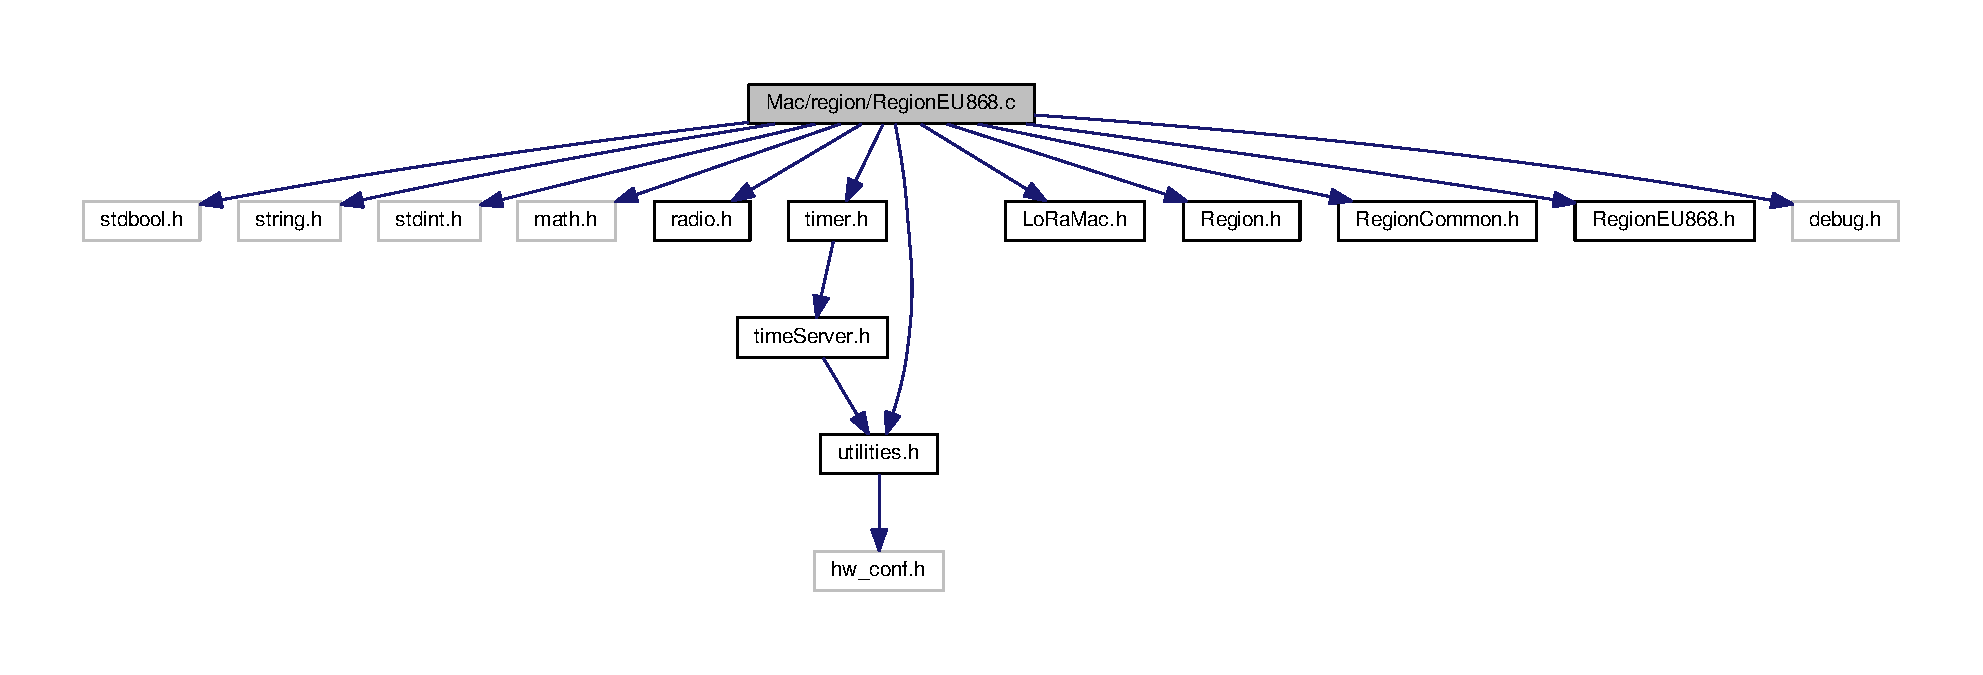
\includegraphics[width=350pt]{RegionEU868_8c__incl}
\end{center}
\end{figure}
\subsection*{Macros}
\begin{DoxyCompactItemize}
\item 
\#define \hyperlink{RegionEU868_8c_a1b20a8de3ae59c0b063fb313f0c70890}{C\+H\+A\+N\+N\+E\+L\+S\+\_\+\+M\+A\+S\+K\+\_\+\+S\+I\+ZE}~1
\end{DoxyCompactItemize}
\subsection*{Functions}
\begin{DoxyCompactItemize}
\item 
\hyperlink{group__REGION_gaed159b26e5c4677236b6e8677019db30}{Phy\+Param\+\_\+t} \hyperlink{group__REGIONEU868_ga4150dec3b05b9774aedf4e2e32499fd3}{Region\+E\+U868\+Get\+Phy\+Param} (\hyperlink{group__REGION_gab471483fff904f4f89bbc03f7fc380ab}{Get\+Phy\+Params\+\_\+t} $\ast$get\+Phy)
\begin{DoxyCompactList}\small\item\em The function gets a value of a specific phy attribute. \end{DoxyCompactList}\item 
void \hyperlink{group__REGIONEU868_ga5cf25bd6be48790f3f637d60a236fdb1}{Region\+E\+U868\+Set\+Band\+Tx\+Done} (\hyperlink{group__REGION_gad0524aa0673c0814a71e7a4f9cade3fc}{Set\+Band\+Tx\+Done\+Params\+\_\+t} $\ast$tx\+Done)
\begin{DoxyCompactList}\small\item\em Updates the last TX done parameters of the current channel. \end{DoxyCompactList}\item 
void \hyperlink{group__REGIONEU868_ga3e8ada4579aff33ad74ca34513d64893}{Region\+E\+U868\+Init\+Defaults} (\hyperlink{group__REGION_gaddc73ae10673ec925724e7870363bda9}{Init\+Type\+\_\+t} type)
\begin{DoxyCompactList}\small\item\em Initializes the channels masks and the channels. \end{DoxyCompactList}\item 
bool \hyperlink{group__REGIONEU868_ga66189a5f3ba138e24f8033d55e9b72a7}{Region\+E\+U868\+Verify} (\hyperlink{group__REGION_ga966d97bc2f25df1c09e92e60ef652276}{Verify\+Params\+\_\+t} $\ast$verify, \hyperlink{group__REGION_ga9445b07fdf77581ecfaf389970e635f8}{Phy\+Attribute\+\_\+t} phy\+Attribute)
\begin{DoxyCompactList}\small\item\em Verifies a parameter. \end{DoxyCompactList}\item 
void \hyperlink{group__REGIONEU868_ga87e838c747c248c577a44329c0013988}{Region\+E\+U868\+Apply\+C\+F\+List} (\hyperlink{group__REGION_ga71588e9ad07e34b78fa91d51881fd3c6}{Apply\+C\+F\+List\+Params\+\_\+t} $\ast$apply\+C\+F\+List)
\begin{DoxyCompactList}\small\item\em The function parses the input buffer and sets up the channels of the CF list. \end{DoxyCompactList}\item 
bool \hyperlink{group__REGIONEU868_ga8c63acfe556cf427ba83e5429f2ec1d9}{Region\+E\+U868\+Chan\+Mask\+Set} (\hyperlink{group__REGION_ga6d24f7da136006410827dfb29f6b9b9e}{Chan\+Mask\+Set\+Params\+\_\+t} $\ast$chan\+Mask\+Set)
\begin{DoxyCompactList}\small\item\em Sets a channels mask. \end{DoxyCompactList}\item 
bool \hyperlink{group__REGIONEU868_gaa93c92348ce901ace20e766be0be1941}{Region\+E\+U868\+Adr\+Next} (\hyperlink{group__REGION_ga567c2742622326b350b4e91bbf61b4ce}{Adr\+Next\+Params\+\_\+t} $\ast$adr\+Next, int8\+\_\+t $\ast$dr\+Out, int8\+\_\+t $\ast$tx\+Pow\+Out, uint32\+\_\+t $\ast$adr\+Ack\+Counter)
\begin{DoxyCompactList}\small\item\em Calculates the next datarate to set, when A\+DR is on or off. \end{DoxyCompactList}\item 
void \hyperlink{group__REGIONEU868_ga7650d2866d0b5df186afd4c0dd1f52bb}{Region\+E\+U868\+Compute\+Rx\+Window\+Parameters} (int8\+\_\+t datarate, uint8\+\_\+t min\+Rx\+Symbols, uint32\+\_\+t rx\+Error, \hyperlink{group__REGION_ga375c038078dfcfc7ef14280021db719e}{Rx\+Config\+Params\+\_\+t} $\ast$rx\+Config\+Params)
\item 
bool \hyperlink{group__REGIONEU868_gae57b8f1a0b5e45ab2371fbc0737322a7}{Region\+E\+U868\+Rx\+Config} (\hyperlink{group__REGION_ga375c038078dfcfc7ef14280021db719e}{Rx\+Config\+Params\+\_\+t} $\ast$rx\+Config, int8\+\_\+t $\ast$datarate)
\begin{DoxyCompactList}\small\item\em Configuration of the RX windows. \end{DoxyCompactList}\item 
bool \hyperlink{group__REGIONEU868_ga7cab7daedc2b01b688d4e2cfb0a30029}{Region\+E\+U868\+Tx\+Config} (\hyperlink{group__REGION_gabed730d4d04b0b60d4b6d1966d3f21d3}{Tx\+Config\+Params\+\_\+t} $\ast$tx\+Config, int8\+\_\+t $\ast$tx\+Power, \hyperlink{utilities_8h_a4215ca43d3e953099ea758ce428599d0}{Timer\+Time\+\_\+t} $\ast$tx\+Time\+On\+Air)
\begin{DoxyCompactList}\small\item\em TX configuration. \end{DoxyCompactList}\item 
uint8\+\_\+t \hyperlink{group__REGIONEU868_gace7b25487170fb5d862413fc221f95db}{Region\+E\+U868\+Link\+Adr\+Req} (\hyperlink{group__REGION_gad4af503e8d4de1846129e26a799a1e8e}{Link\+Adr\+Req\+Params\+\_\+t} $\ast$link\+Adr\+Req, int8\+\_\+t $\ast$dr\+Out, int8\+\_\+t $\ast$tx\+Pow\+Out, uint8\+\_\+t $\ast$nb\+Rep\+Out, uint8\+\_\+t $\ast$nb\+Bytes\+Parsed)
\begin{DoxyCompactList}\small\item\em The function processes a Link A\+DR Request. \end{DoxyCompactList}\item 
uint8\+\_\+t \hyperlink{group__REGIONEU868_gaa175de2c9f3882ef0b89120db3d8882d}{Region\+E\+U868\+Rx\+Param\+Setup\+Req} (\hyperlink{group__REGION_ga7165f282c670c728c36d534df2285157}{Rx\+Param\+Setup\+Req\+Params\+\_\+t} $\ast$rx\+Param\+Setup\+Req)
\begin{DoxyCompactList}\small\item\em The function processes a RX Parameter Setup Request. \end{DoxyCompactList}\item 
uint8\+\_\+t \hyperlink{group__REGIONEU868_ga4325b111d5f14ddc4b33f5e827a8986e}{Region\+E\+U868\+New\+Channel\+Req} (\hyperlink{group__REGION_gae2abcdb6dbb843c9faf5fd3009eca9d6}{New\+Channel\+Req\+Params\+\_\+t} $\ast$new\+Channel\+Req)
\begin{DoxyCompactList}\small\item\em The function processes a Channel Request. \end{DoxyCompactList}\item 
int8\+\_\+t \hyperlink{group__REGIONEU868_ga7f1768fb828bb81f3f6faec0dc734d29}{Region\+E\+U868\+Tx\+Param\+Setup\+Req} (\hyperlink{group__REGION_ga26836ef2996e70410e42ef471073f855}{Tx\+Param\+Setup\+Req\+Params\+\_\+t} $\ast$tx\+Param\+Setup\+Req)
\begin{DoxyCompactList}\small\item\em The function processes a TX Param\+Setup Request. \end{DoxyCompactList}\item 
uint8\+\_\+t \hyperlink{group__REGIONEU868_ga61ddb6ba84f203ba1c7ab3b19e2322aa}{Region\+E\+U868\+Dl\+Channel\+Req} (\hyperlink{group__REGION_gae0d608ff1f8ea0a430e4f9a4c38ec7f3}{Dl\+Channel\+Req\+Params\+\_\+t} $\ast$dl\+Channel\+Req)
\begin{DoxyCompactList}\small\item\em The function processes a Dl\+Channel Request. \end{DoxyCompactList}\item 
int8\+\_\+t \hyperlink{group__REGIONEU868_ga7aa17730c097b5233f1d8d6bde238923}{Region\+E\+U868\+Alternate\+Dr} (\hyperlink{group__REGION_ga001ea4338d1c83f4c785b49d7ad2d696}{Alternate\+Dr\+Params\+\_\+t} $\ast$alternate\+Dr)
\begin{DoxyCompactList}\small\item\em Alternates the datarate of the channel for the join request. \end{DoxyCompactList}\item 
void \hyperlink{group__REGIONEU868_ga0900ea63994bf51a3ee43bd4917e5647}{Region\+E\+U868\+Calc\+Back\+Off} (\hyperlink{group__REGION_ga7c5c9a8da174e6679eded8257dc92fd9}{Calc\+Back\+Off\+Params\+\_\+t} $\ast$calc\+Back\+Off)
\begin{DoxyCompactList}\small\item\em Calculates the back-\/off time. \end{DoxyCompactList}\item 
bool \hyperlink{group__REGIONEU868_gaa219af9d7f0ceea1378ecd88fd198a95}{Region\+E\+U868\+Next\+Channel} (\hyperlink{group__REGION_ga115f5e83afae352c0a3dcdc193374040}{Next\+Chan\+Params\+\_\+t} $\ast$next\+Chan\+Params, uint8\+\_\+t $\ast$channel, \hyperlink{utilities_8h_a4215ca43d3e953099ea758ce428599d0}{Timer\+Time\+\_\+t} $\ast$time, \hyperlink{utilities_8h_a4215ca43d3e953099ea758ce428599d0}{Timer\+Time\+\_\+t} $\ast$aggregated\+Time\+Off)
\begin{DoxyCompactList}\small\item\em Searches and set the next random available channel. \end{DoxyCompactList}\item 
\hyperlink{group__LORAMAC_ga30bd25657e10480f8605ee951b0ecfbd}{Lo\+Ra\+Mac\+Status\+\_\+t} \hyperlink{group__REGIONEU868_gaa51182eab8774612408fd0ea8f89f63b}{Region\+E\+U868\+Channel\+Add} (\hyperlink{group__REGION_gab1c5f3aa06614283202906cef4417860}{Channel\+Add\+Params\+\_\+t} $\ast$channel\+Add)
\begin{DoxyCompactList}\small\item\em Adds a channel. \end{DoxyCompactList}\item 
bool \hyperlink{group__REGIONEU868_gac30e0032ee1e6f09d4ee032e7169e238}{Region\+E\+U868\+Channels\+Remove} (\hyperlink{group__REGION_gaa37468560d2fc81a977b57a48e5d72c0}{Channel\+Remove\+Params\+\_\+t} $\ast$channel\+Remove)
\begin{DoxyCompactList}\small\item\em Removes a channel. \end{DoxyCompactList}\item 
void \hyperlink{group__REGIONEU868_gaa7573d0677552b321af04417a58672eb}{Region\+E\+U868\+Set\+Continuous\+Wave} (\hyperlink{group__REGION_gaf39bb5ba06921139c6d17f88a8d518cd}{Continuous\+Wave\+Params\+\_\+t} $\ast$continuous\+Wave)
\begin{DoxyCompactList}\small\item\em Sets the radio into continuous wave mode. \end{DoxyCompactList}\item 
uint8\+\_\+t \hyperlink{group__REGIONEU868_ga30121c63a197681a176717191a4b89cd}{Region\+E\+U868\+Apply\+Dr\+Offset} (uint8\+\_\+t downlink\+Dwell\+Time, int8\+\_\+t dr, int8\+\_\+t dr\+Offset)
\begin{DoxyCompactList}\small\item\em Computes new datarate according to the given offset. \end{DoxyCompactList}\end{DoxyCompactItemize}


\subsection{Macro Definition Documentation}
\mbox{\Hypertarget{RegionEU868_8c_a1b20a8de3ae59c0b063fb313f0c70890}\label{RegionEU868_8c_a1b20a8de3ae59c0b063fb313f0c70890}} 
\index{Region\+E\+U868.\+c@{Region\+E\+U868.\+c}!C\+H\+A\+N\+N\+E\+L\+S\+\_\+\+M\+A\+S\+K\+\_\+\+S\+I\+ZE@{C\+H\+A\+N\+N\+E\+L\+S\+\_\+\+M\+A\+S\+K\+\_\+\+S\+I\+ZE}}
\index{C\+H\+A\+N\+N\+E\+L\+S\+\_\+\+M\+A\+S\+K\+\_\+\+S\+I\+ZE@{C\+H\+A\+N\+N\+E\+L\+S\+\_\+\+M\+A\+S\+K\+\_\+\+S\+I\+ZE}!Region\+E\+U868.\+c@{Region\+E\+U868.\+c}}
\subsubsection{\texorpdfstring{C\+H\+A\+N\+N\+E\+L\+S\+\_\+\+M\+A\+S\+K\+\_\+\+S\+I\+ZE}{CHANNELS\_MASK\_SIZE}}
{\footnotesize\ttfamily \#define C\+H\+A\+N\+N\+E\+L\+S\+\_\+\+M\+A\+S\+K\+\_\+\+S\+I\+ZE~1}


\hypertarget{RegionEU868_8h}{}\section{Mac/region/\+Region\+E\+U868.h File Reference}
\label{RegionEU868_8h}\index{Mac/region/\+Region\+E\+U868.\+h@{Mac/region/\+Region\+E\+U868.\+h}}


Region definition for E\+U868.  


This graph shows which files directly or indirectly include this file\+:
\nopagebreak
\begin{figure}[H]
\begin{center}
\leavevmode
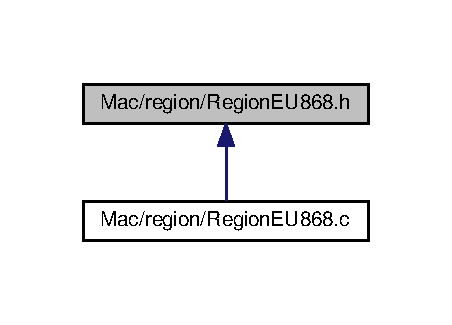
\includegraphics[width=217pt]{RegionEU868_8h__dep__incl}
\end{center}
\end{figure}
\subsection*{Macros}
\begin{DoxyCompactItemize}
\item 
\#define \hyperlink{group__REGIONEU868_gaf94c3090ac541fec3c97b2146702d252}{E\+U868\+\_\+\+M\+A\+X\+\_\+\+N\+B\+\_\+\+C\+H\+A\+N\+N\+E\+LS}~16
\item 
\#define \hyperlink{group__REGIONEU868_ga43b13bdefab43add062b907facaef8ba}{E\+U868\+\_\+\+N\+U\+M\+B\+\_\+\+D\+E\+F\+A\+U\+L\+T\+\_\+\+C\+H\+A\+N\+N\+E\+LS}~3
\item 
\#define \hyperlink{group__REGIONEU868_gad3cd171e0308aa36be7231a3fcba36b8}{E\+U868\+\_\+\+N\+U\+M\+B\+\_\+\+C\+H\+A\+N\+N\+E\+L\+S\+\_\+\+C\+F\+\_\+\+L\+I\+ST}~5
\item 
\#define \hyperlink{group__REGIONEU868_ga2df2a8fc7db7e674c3e58de0dd1c90a4}{E\+U868\+\_\+\+T\+X\+\_\+\+M\+I\+N\+\_\+\+D\+A\+T\+A\+R\+A\+TE}~\hyperlink{group__REGION_ga6c4ef966b4f3d5eb7597b087f2b97095}{D\+R\+\_\+0}
\item 
\#define \hyperlink{group__REGIONEU868_ga689495f3ecc7047ff636ec85b3b80ee3}{E\+U868\+\_\+\+T\+X\+\_\+\+M\+A\+X\+\_\+\+D\+A\+T\+A\+R\+A\+TE}~\hyperlink{group__REGION_ga3a06805baf4f00911a3a5d3dbadebf61}{D\+R\+\_\+7}
\item 
\#define \hyperlink{group__REGIONEU868_gaa1bdf9b64650b847961424f9098278fc}{E\+U868\+\_\+\+R\+X\+\_\+\+M\+I\+N\+\_\+\+D\+A\+T\+A\+R\+A\+TE}~\hyperlink{group__REGION_ga6c4ef966b4f3d5eb7597b087f2b97095}{D\+R\+\_\+0}
\item 
\#define \hyperlink{group__REGIONEU868_ga84a09a53f67ea79b84d27a56e51679ab}{E\+U868\+\_\+\+R\+X\+\_\+\+M\+A\+X\+\_\+\+D\+A\+T\+A\+R\+A\+TE}~\hyperlink{group__REGION_ga3a06805baf4f00911a3a5d3dbadebf61}{D\+R\+\_\+7}
\item 
\#define \hyperlink{group__REGIONEU868_ga4053f96ad333ad07d4584f7213e294fa}{E\+U868\+\_\+\+D\+E\+F\+A\+U\+L\+T\+\_\+\+D\+A\+T\+A\+R\+A\+TE}~\hyperlink{group__REGION_ga6c4ef966b4f3d5eb7597b087f2b97095}{D\+R\+\_\+0}
\item 
\#define \hyperlink{group__REGIONEU868_gac803b58ed61f47042654f6e0331b26db}{E\+U868\+\_\+\+M\+I\+N\+\_\+\+R\+X1\+\_\+\+D\+R\+\_\+\+O\+F\+F\+S\+ET}~0
\item 
\#define \hyperlink{group__REGIONEU868_ga90ce5649045707b0bbaaa0bbd039940b}{E\+U868\+\_\+\+M\+A\+X\+\_\+\+R\+X1\+\_\+\+D\+R\+\_\+\+O\+F\+F\+S\+ET}~5
\item 
\#define \hyperlink{group__REGIONEU868_gab3c86769eb58a2529ede7cd544bffc58}{E\+U868\+\_\+\+D\+E\+F\+A\+U\+L\+T\+\_\+\+R\+X1\+\_\+\+D\+R\+\_\+\+O\+F\+F\+S\+ET}~0
\item 
\#define \hyperlink{group__REGIONEU868_gab935a0225d447579203239740e33c72f}{E\+U868\+\_\+\+M\+I\+N\+\_\+\+T\+X\+\_\+\+P\+O\+W\+ER}~\hyperlink{group__REGION_ga3c7bd9a98f0c1e7e9aaa90857c4bd700}{T\+X\+\_\+\+P\+O\+W\+E\+R\+\_\+7}
\item 
\#define \hyperlink{group__REGIONEU868_ga39e338c7f8454f594302811f61d9560d}{E\+U868\+\_\+\+M\+A\+X\+\_\+\+T\+X\+\_\+\+P\+O\+W\+ER}~\hyperlink{group__REGION_gab33618449f2a573142c463ab071ef8ed}{T\+X\+\_\+\+P\+O\+W\+E\+R\+\_\+0}
\item 
\#define \hyperlink{group__REGIONEU868_ga2e0b523fc68d50dc0711a07d8926c8c6}{E\+U868\+\_\+\+D\+E\+F\+A\+U\+L\+T\+\_\+\+T\+X\+\_\+\+P\+O\+W\+ER}~\hyperlink{group__REGION_gab33618449f2a573142c463ab071ef8ed}{T\+X\+\_\+\+P\+O\+W\+E\+R\+\_\+0}
\item 
\#define \hyperlink{group__REGIONEU868_ga1637006dd28e0ae483e1260c2152ece2}{E\+U868\+\_\+\+D\+E\+F\+A\+U\+L\+T\+\_\+\+M\+A\+X\+\_\+\+E\+I\+RP}~16.\+0f
\item 
\#define \hyperlink{group__REGIONEU868_ga943854d7099f892dd9dc86a6accbd813}{E\+U868\+\_\+\+D\+E\+F\+A\+U\+L\+T\+\_\+\+A\+N\+T\+E\+N\+N\+A\+\_\+\+G\+A\+IN}~2.\+15f
\item 
\#define \hyperlink{group__REGIONEU868_ga67c54d4a8b30d30138dd013779f72cdf}{E\+U868\+\_\+\+A\+D\+R\+\_\+\+A\+C\+K\+\_\+\+L\+I\+M\+IT}~64
\item 
\#define \hyperlink{group__REGIONEU868_ga13b5d7d3346971d4dda9919ed73b1394}{E\+U868\+\_\+\+A\+D\+R\+\_\+\+A\+C\+K\+\_\+\+D\+E\+L\+AY}~32
\item 
\#define \hyperlink{group__REGIONEU868_gaa8c53df1d013b427281bafe2ed9cbcce}{E\+U868\+\_\+\+D\+U\+T\+Y\+\_\+\+C\+Y\+C\+L\+E\+\_\+\+E\+N\+A\+B\+L\+ED}~1
\item 
\#define \hyperlink{group__REGIONEU868_ga7d51abf9369b7478a74590db5c5c2bb1}{E\+U868\+\_\+\+M\+A\+X\+\_\+\+R\+X\+\_\+\+W\+I\+N\+D\+OW}~3000
\item 
\#define \hyperlink{group__REGIONEU868_ga5e54e03af0ee7ada0b1fd781009a24da}{E\+U868\+\_\+\+R\+E\+C\+E\+I\+V\+E\+\_\+\+D\+E\+L\+A\+Y1}~1000
\item 
\#define \hyperlink{group__REGIONEU868_ga5b1785ed0935234e288f90a0461cd04b}{E\+U868\+\_\+\+R\+E\+C\+E\+I\+V\+E\+\_\+\+D\+E\+L\+A\+Y2}~2000
\item 
\#define \hyperlink{group__REGIONEU868_gac37947128c2721653a6da84362c04f8c}{E\+U868\+\_\+\+J\+O\+I\+N\+\_\+\+A\+C\+C\+E\+P\+T\+\_\+\+D\+E\+L\+A\+Y1}~5000
\item 
\#define \hyperlink{group__REGIONEU868_ga4b26a2e21778e0a790ab45637fb8f51f}{E\+U868\+\_\+\+J\+O\+I\+N\+\_\+\+A\+C\+C\+E\+P\+T\+\_\+\+D\+E\+L\+A\+Y2}~6000
\item 
\#define \hyperlink{group__REGIONEU868_ga82b9bba1cf3046bb808448af3a3851a6}{E\+U868\+\_\+\+M\+A\+X\+\_\+\+F\+C\+N\+T\+\_\+\+G\+AP}~16384
\item 
\#define \hyperlink{group__REGIONEU868_ga0d482880b3686526074336cc53d3a711}{E\+U868\+\_\+\+A\+C\+K\+T\+I\+M\+E\+O\+UT}~2000
\item 
\#define \hyperlink{group__REGIONEU868_gaf263a9c127c374ca28a18dee1f63dcf4}{E\+U868\+\_\+\+A\+C\+K\+\_\+\+T\+I\+M\+E\+O\+U\+T\+\_\+\+R\+ND}~1000
\item 
\#define \hyperlink{group__REGIONEU868_ga6cc4e22e8e2b73a7e1789ff22b6d4d76}{E\+U868\+\_\+\+R\+X\+\_\+\+W\+N\+D\+\_\+2\+\_\+\+F\+R\+EQ}~869525000
\item 
\#define \hyperlink{group__REGIONEU868_ga291302a83db2690d26b2659853262abe}{E\+U868\+\_\+\+R\+X\+\_\+\+W\+N\+D\+\_\+2\+\_\+\+DR}~\hyperlink{group__REGION_ga6c4ef966b4f3d5eb7597b087f2b97095}{D\+R\+\_\+0}
\item 
\#define \hyperlink{group__REGIONEU868_gac5749114ab11499796ef455491fe8997}{E\+U868\+\_\+\+M\+A\+X\+\_\+\+N\+B\+\_\+\+B\+A\+N\+DS}~5
\item 
\#define \hyperlink{group__REGIONEU868_gadf9e5ce0c5061df64ab9105bba178fb5}{E\+U868\+\_\+\+B\+A\+N\+D0}~\{ 100 , \hyperlink{group__REGIONEU868_ga39e338c7f8454f594302811f61d9560d}{E\+U868\+\_\+\+M\+A\+X\+\_\+\+T\+X\+\_\+\+P\+O\+W\+ER}, 0,  0 \}
\item 
\#define \hyperlink{group__REGIONEU868_ga8a18e253f46e534ff0ee00c0c21b4211}{E\+U868\+\_\+\+B\+A\+N\+D1}~\{ 100 , \hyperlink{group__REGIONEU868_ga39e338c7f8454f594302811f61d9560d}{E\+U868\+\_\+\+M\+A\+X\+\_\+\+T\+X\+\_\+\+P\+O\+W\+ER}, 0,  0 \}
\item 
\#define \hyperlink{group__REGIONEU868_gaf5b8aba834ede7487acbff80b6c30b36}{E\+U868\+\_\+\+B\+A\+N\+D2}~\{ 1000, \hyperlink{group__REGIONEU868_ga39e338c7f8454f594302811f61d9560d}{E\+U868\+\_\+\+M\+A\+X\+\_\+\+T\+X\+\_\+\+P\+O\+W\+ER}, 0,  0 \}
\item 
\#define \hyperlink{group__REGIONEU868_gab7e01f2131642f135babcd1189d429d3}{E\+U868\+\_\+\+B\+A\+N\+D3}~\{ 10  , \hyperlink{group__REGIONEU868_ga39e338c7f8454f594302811f61d9560d}{E\+U868\+\_\+\+M\+A\+X\+\_\+\+T\+X\+\_\+\+P\+O\+W\+ER}, 0,  0 \}
\item 
\#define \hyperlink{group__REGIONEU868_ga0caf48019c492d018b3442e1975535f4}{E\+U868\+\_\+\+B\+A\+N\+D4}~\{ 100 , \hyperlink{group__REGIONEU868_ga39e338c7f8454f594302811f61d9560d}{E\+U868\+\_\+\+M\+A\+X\+\_\+\+T\+X\+\_\+\+P\+O\+W\+ER}, 0,  0 \}
\item 
\#define \hyperlink{group__REGIONEU868_ga397b82ce41a0eb594465b5728586d76e}{E\+U868\+\_\+\+L\+C1}~\{ 868100000, 0, \{ ( ( \hyperlink{group__REGION_ga872e12c82020c02a7f70a1c6ed1375df}{D\+R\+\_\+5} $<$$<$ 4 ) $\vert$ \hyperlink{group__REGION_ga6c4ef966b4f3d5eb7597b087f2b97095}{D\+R\+\_\+0} ) \}, 1 \}
\item 
\#define \hyperlink{group__REGIONEU868_ga992597dafaae7a354ae4aeaab6306954}{E\+U868\+\_\+\+L\+C2}~\{ 868300000, 0, \{ ( ( \hyperlink{group__REGION_ga872e12c82020c02a7f70a1c6ed1375df}{D\+R\+\_\+5} $<$$<$ 4 ) $\vert$ \hyperlink{group__REGION_ga6c4ef966b4f3d5eb7597b087f2b97095}{D\+R\+\_\+0} ) \}, 1 \}
\item 
\#define \hyperlink{group__REGIONEU868_ga6feb4643d2e07e54de83109e680379d2}{E\+U868\+\_\+\+L\+C3}~\{ 868500000, 0, \{ ( ( \hyperlink{group__REGION_ga872e12c82020c02a7f70a1c6ed1375df}{D\+R\+\_\+5} $<$$<$ 4 ) $\vert$ \hyperlink{group__REGION_ga6c4ef966b4f3d5eb7597b087f2b97095}{D\+R\+\_\+0} ) \}, 1 \}
\item 
\#define \hyperlink{group__REGIONEU868_ga66750d8b2f9ba9f6b8466f190207d53f}{E\+U868\+\_\+\+J\+O\+I\+N\+\_\+\+C\+H\+A\+N\+N\+E\+LS}~( uint16\+\_\+t )( \hyperlink{group__REGION_ga12fa17e5c1016e01a9d82c25027deb1b}{LC}( 1 ) $\vert$ \hyperlink{group__REGION_ga12fa17e5c1016e01a9d82c25027deb1b}{LC}( 2 ) $\vert$ \hyperlink{group__REGION_ga12fa17e5c1016e01a9d82c25027deb1b}{LC}( 3 ) )
\end{DoxyCompactItemize}
\subsection*{Functions}
\begin{DoxyCompactItemize}
\item 
\hyperlink{group__REGION_gaed159b26e5c4677236b6e8677019db30}{Phy\+Param\+\_\+t} \hyperlink{group__REGIONEU868_ga4150dec3b05b9774aedf4e2e32499fd3}{Region\+E\+U868\+Get\+Phy\+Param} (\hyperlink{group__REGION_gab471483fff904f4f89bbc03f7fc380ab}{Get\+Phy\+Params\+\_\+t} $\ast$get\+Phy)
\begin{DoxyCompactList}\small\item\em The function gets a value of a specific phy attribute. \end{DoxyCompactList}\item 
void \hyperlink{group__REGIONEU868_ga5cf25bd6be48790f3f637d60a236fdb1}{Region\+E\+U868\+Set\+Band\+Tx\+Done} (\hyperlink{group__REGION_gad0524aa0673c0814a71e7a4f9cade3fc}{Set\+Band\+Tx\+Done\+Params\+\_\+t} $\ast$tx\+Done)
\begin{DoxyCompactList}\small\item\em Updates the last TX done parameters of the current channel. \end{DoxyCompactList}\item 
void \hyperlink{group__REGIONEU868_ga3e8ada4579aff33ad74ca34513d64893}{Region\+E\+U868\+Init\+Defaults} (\hyperlink{group__REGION_gaddc73ae10673ec925724e7870363bda9}{Init\+Type\+\_\+t} type)
\begin{DoxyCompactList}\small\item\em Initializes the channels masks and the channels. \end{DoxyCompactList}\item 
bool \hyperlink{group__REGIONEU868_ga66189a5f3ba138e24f8033d55e9b72a7}{Region\+E\+U868\+Verify} (\hyperlink{group__REGION_ga966d97bc2f25df1c09e92e60ef652276}{Verify\+Params\+\_\+t} $\ast$verify, \hyperlink{group__REGION_ga9445b07fdf77581ecfaf389970e635f8}{Phy\+Attribute\+\_\+t} phy\+Attribute)
\begin{DoxyCompactList}\small\item\em Verifies a parameter. \end{DoxyCompactList}\item 
void \hyperlink{group__REGIONEU868_ga87e838c747c248c577a44329c0013988}{Region\+E\+U868\+Apply\+C\+F\+List} (\hyperlink{group__REGION_ga71588e9ad07e34b78fa91d51881fd3c6}{Apply\+C\+F\+List\+Params\+\_\+t} $\ast$apply\+C\+F\+List)
\begin{DoxyCompactList}\small\item\em The function parses the input buffer and sets up the channels of the CF list. \end{DoxyCompactList}\item 
bool \hyperlink{group__REGIONEU868_ga8c63acfe556cf427ba83e5429f2ec1d9}{Region\+E\+U868\+Chan\+Mask\+Set} (\hyperlink{group__REGION_ga6d24f7da136006410827dfb29f6b9b9e}{Chan\+Mask\+Set\+Params\+\_\+t} $\ast$chan\+Mask\+Set)
\begin{DoxyCompactList}\small\item\em Sets a channels mask. \end{DoxyCompactList}\item 
bool \hyperlink{group__REGIONEU868_gaa93c92348ce901ace20e766be0be1941}{Region\+E\+U868\+Adr\+Next} (\hyperlink{group__REGION_ga567c2742622326b350b4e91bbf61b4ce}{Adr\+Next\+Params\+\_\+t} $\ast$adr\+Next, int8\+\_\+t $\ast$dr\+Out, int8\+\_\+t $\ast$tx\+Pow\+Out, uint32\+\_\+t $\ast$adr\+Ack\+Counter)
\begin{DoxyCompactList}\small\item\em Calculates the next datarate to set, when A\+DR is on or off. \end{DoxyCompactList}\item 
void \hyperlink{group__REGIONEU868_ga7650d2866d0b5df186afd4c0dd1f52bb}{Region\+E\+U868\+Compute\+Rx\+Window\+Parameters} (int8\+\_\+t datarate, uint8\+\_\+t min\+Rx\+Symbols, uint32\+\_\+t rx\+Error, \hyperlink{group__REGION_ga375c038078dfcfc7ef14280021db719e}{Rx\+Config\+Params\+\_\+t} $\ast$rx\+Config\+Params)
\item 
bool \hyperlink{group__REGIONEU868_gae57b8f1a0b5e45ab2371fbc0737322a7}{Region\+E\+U868\+Rx\+Config} (\hyperlink{group__REGION_ga375c038078dfcfc7ef14280021db719e}{Rx\+Config\+Params\+\_\+t} $\ast$rx\+Config, int8\+\_\+t $\ast$datarate)
\begin{DoxyCompactList}\small\item\em Configuration of the RX windows. \end{DoxyCompactList}\item 
bool \hyperlink{group__REGIONEU868_ga7cab7daedc2b01b688d4e2cfb0a30029}{Region\+E\+U868\+Tx\+Config} (\hyperlink{group__REGION_gabed730d4d04b0b60d4b6d1966d3f21d3}{Tx\+Config\+Params\+\_\+t} $\ast$tx\+Config, int8\+\_\+t $\ast$tx\+Power, \hyperlink{utilities_8h_a4215ca43d3e953099ea758ce428599d0}{Timer\+Time\+\_\+t} $\ast$tx\+Time\+On\+Air)
\begin{DoxyCompactList}\small\item\em TX configuration. \end{DoxyCompactList}\item 
uint8\+\_\+t \hyperlink{group__REGIONEU868_gace7b25487170fb5d862413fc221f95db}{Region\+E\+U868\+Link\+Adr\+Req} (\hyperlink{group__REGION_gad4af503e8d4de1846129e26a799a1e8e}{Link\+Adr\+Req\+Params\+\_\+t} $\ast$link\+Adr\+Req, int8\+\_\+t $\ast$dr\+Out, int8\+\_\+t $\ast$tx\+Pow\+Out, uint8\+\_\+t $\ast$nb\+Rep\+Out, uint8\+\_\+t $\ast$nb\+Bytes\+Parsed)
\begin{DoxyCompactList}\small\item\em The function processes a Link A\+DR Request. \end{DoxyCompactList}\item 
uint8\+\_\+t \hyperlink{group__REGIONEU868_gaa175de2c9f3882ef0b89120db3d8882d}{Region\+E\+U868\+Rx\+Param\+Setup\+Req} (\hyperlink{group__REGION_ga7165f282c670c728c36d534df2285157}{Rx\+Param\+Setup\+Req\+Params\+\_\+t} $\ast$rx\+Param\+Setup\+Req)
\begin{DoxyCompactList}\small\item\em The function processes a RX Parameter Setup Request. \end{DoxyCompactList}\item 
uint8\+\_\+t \hyperlink{group__REGIONEU868_ga4325b111d5f14ddc4b33f5e827a8986e}{Region\+E\+U868\+New\+Channel\+Req} (\hyperlink{group__REGION_gae2abcdb6dbb843c9faf5fd3009eca9d6}{New\+Channel\+Req\+Params\+\_\+t} $\ast$new\+Channel\+Req)
\begin{DoxyCompactList}\small\item\em The function processes a Channel Request. \end{DoxyCompactList}\item 
int8\+\_\+t \hyperlink{group__REGIONEU868_ga7f1768fb828bb81f3f6faec0dc734d29}{Region\+E\+U868\+Tx\+Param\+Setup\+Req} (\hyperlink{group__REGION_ga26836ef2996e70410e42ef471073f855}{Tx\+Param\+Setup\+Req\+Params\+\_\+t} $\ast$tx\+Param\+Setup\+Req)
\begin{DoxyCompactList}\small\item\em The function processes a TX Param\+Setup Request. \end{DoxyCompactList}\item 
uint8\+\_\+t \hyperlink{group__REGIONEU868_ga61ddb6ba84f203ba1c7ab3b19e2322aa}{Region\+E\+U868\+Dl\+Channel\+Req} (\hyperlink{group__REGION_gae0d608ff1f8ea0a430e4f9a4c38ec7f3}{Dl\+Channel\+Req\+Params\+\_\+t} $\ast$dl\+Channel\+Req)
\begin{DoxyCompactList}\small\item\em The function processes a Dl\+Channel Request. \end{DoxyCompactList}\item 
int8\+\_\+t \hyperlink{group__REGIONEU868_ga7aa17730c097b5233f1d8d6bde238923}{Region\+E\+U868\+Alternate\+Dr} (\hyperlink{group__REGION_ga001ea4338d1c83f4c785b49d7ad2d696}{Alternate\+Dr\+Params\+\_\+t} $\ast$alternate\+Dr)
\begin{DoxyCompactList}\small\item\em Alternates the datarate of the channel for the join request. \end{DoxyCompactList}\item 
void \hyperlink{group__REGIONEU868_ga0900ea63994bf51a3ee43bd4917e5647}{Region\+E\+U868\+Calc\+Back\+Off} (\hyperlink{group__REGION_ga7c5c9a8da174e6679eded8257dc92fd9}{Calc\+Back\+Off\+Params\+\_\+t} $\ast$calc\+Back\+Off)
\begin{DoxyCompactList}\small\item\em Calculates the back-\/off time. \end{DoxyCompactList}\item 
bool \hyperlink{group__REGIONEU868_gaa219af9d7f0ceea1378ecd88fd198a95}{Region\+E\+U868\+Next\+Channel} (\hyperlink{group__REGION_ga115f5e83afae352c0a3dcdc193374040}{Next\+Chan\+Params\+\_\+t} $\ast$next\+Chan\+Params, uint8\+\_\+t $\ast$channel, \hyperlink{utilities_8h_a4215ca43d3e953099ea758ce428599d0}{Timer\+Time\+\_\+t} $\ast$time, \hyperlink{utilities_8h_a4215ca43d3e953099ea758ce428599d0}{Timer\+Time\+\_\+t} $\ast$aggregated\+Time\+Off)
\begin{DoxyCompactList}\small\item\em Searches and set the next random available channel. \end{DoxyCompactList}\item 
\hyperlink{group__LORAMAC_ga30bd25657e10480f8605ee951b0ecfbd}{Lo\+Ra\+Mac\+Status\+\_\+t} \hyperlink{group__REGIONEU868_gaa51182eab8774612408fd0ea8f89f63b}{Region\+E\+U868\+Channel\+Add} (\hyperlink{group__REGION_gab1c5f3aa06614283202906cef4417860}{Channel\+Add\+Params\+\_\+t} $\ast$channel\+Add)
\begin{DoxyCompactList}\small\item\em Adds a channel. \end{DoxyCompactList}\item 
bool \hyperlink{group__REGIONEU868_gac30e0032ee1e6f09d4ee032e7169e238}{Region\+E\+U868\+Channels\+Remove} (\hyperlink{group__REGION_gaa37468560d2fc81a977b57a48e5d72c0}{Channel\+Remove\+Params\+\_\+t} $\ast$channel\+Remove)
\begin{DoxyCompactList}\small\item\em Removes a channel. \end{DoxyCompactList}\item 
void \hyperlink{group__REGIONEU868_gaa7573d0677552b321af04417a58672eb}{Region\+E\+U868\+Set\+Continuous\+Wave} (\hyperlink{group__REGION_gaf39bb5ba06921139c6d17f88a8d518cd}{Continuous\+Wave\+Params\+\_\+t} $\ast$continuous\+Wave)
\begin{DoxyCompactList}\small\item\em Sets the radio into continuous wave mode. \end{DoxyCompactList}\item 
uint8\+\_\+t \hyperlink{group__REGIONEU868_ga30121c63a197681a176717191a4b89cd}{Region\+E\+U868\+Apply\+Dr\+Offset} (uint8\+\_\+t downlink\+Dwell\+Time, int8\+\_\+t dr, int8\+\_\+t dr\+Offset)
\begin{DoxyCompactList}\small\item\em Computes new datarate according to the given offset. \end{DoxyCompactList}\end{DoxyCompactItemize}


\subsection{Detailed Description}
Region definition for E\+U868. 

\begin{DoxyCopyright}{Copyright}
Revised B\+SD License, see section L\+I\+C\+E\+N\+SE.
\end{DoxyCopyright}

\begin{DoxyCode}
  \_\_\_\_\_\_                              \_
 / \_\_\_\_\_)             \_              | |
( (\_\_\_\_  \_\_\_\_\_ \_\_\_\_ \_| |\_ \_\_\_\_\_  \_\_\_\_| |\_\_
 \(\backslash\)\_\_\_\_ \(\backslash\)| \_\_\_ |    (\_   \_) \_\_\_ |/ \_\_\_)  \_ \(\backslash\)
 \_\_\_\_\_) ) \_\_\_\_| | | || |\_| \_\_\_\_( (\_\_\_| | | |
(\_\_\_\_\_\_/|\_\_\_\_\_)\_|\_|\_| \(\backslash\)\_\_)\_\_\_\_\_)\(\backslash\)\_\_\_\_)\_| |\_|
(C)2013 Semtech

 \_\_\_ \_\_\_\_\_ \_   \_\_\_ \_  \_\_\_\_\_ \_\_\_  \_\_\_  \_\_\_ \_\_\_
/ \_\_|\_   \_/\_\(\backslash\) / \_\_| |/ / \_\_/ \_ \(\backslash\)| \_ \(\backslash\)/ \_\_| \_\_|
\(\backslash\)\_\_ \(\backslash\) | |/ \_ \(\backslash\) (\_\_| \textcolor{stringliteral}{' <| \_| (\_) |   / (\_\_| \_|}
\textcolor{stringliteral}{|\_\_\_/ |\_/\_/ \(\backslash\)\_\(\backslash\)\_\_\_|\_|\(\backslash\)\_\(\backslash\)\_| \(\backslash\)\_\_\_/|\_|\_\(\backslash\)\(\backslash\)\_\_\_|\_\_\_|}
\textcolor{stringliteral}{embedded.connectivity.solutions===============}
\end{DoxyCode}


\begin{DoxyAuthor}{Author}
Miguel Luis ( Semtech )

Gregory Cristian ( Semtech )

Daniel Jaeckle ( S\+T\+A\+C\+K\+F\+O\+R\+CE ) 
\end{DoxyAuthor}

\hypertarget{RegionIN865_8c}{}\section{Mac/region/\+Region\+I\+N865.c File Reference}
\label{RegionIN865_8c}\index{Mac/region/\+Region\+I\+N865.\+c@{Mac/region/\+Region\+I\+N865.\+c}}
{\ttfamily \#include $<$stdbool.\+h$>$}\newline
{\ttfamily \#include $<$string.\+h$>$}\newline
{\ttfamily \#include $<$stdint.\+h$>$}\newline
{\ttfamily \#include $<$math.\+h$>$}\newline
{\ttfamily \#include \char`\"{}radio.\+h\char`\"{}}\newline
{\ttfamily \#include \char`\"{}timer.\+h\char`\"{}}\newline
{\ttfamily \#include \char`\"{}Lo\+Ra\+Mac.\+h\char`\"{}}\newline
{\ttfamily \#include \char`\"{}utilities.\+h\char`\"{}}\newline
{\ttfamily \#include \char`\"{}Region.\+h\char`\"{}}\newline
{\ttfamily \#include \char`\"{}Region\+Common.\+h\char`\"{}}\newline
{\ttfamily \#include \char`\"{}Region\+I\+N865.\+h\char`\"{}}\newline
{\ttfamily \#include \char`\"{}debug.\+h\char`\"{}}\newline
Include dependency graph for Region\+I\+N865.\+c\+:
\nopagebreak
\begin{figure}[H]
\begin{center}
\leavevmode
\includegraphics[width=350pt]{RegionIN865_8c__incl}
\end{center}
\end{figure}
\subsection*{Macros}
\begin{DoxyCompactItemize}
\item 
\#define \hyperlink{RegionIN865_8c_a1b20a8de3ae59c0b063fb313f0c70890}{C\+H\+A\+N\+N\+E\+L\+S\+\_\+\+M\+A\+S\+K\+\_\+\+S\+I\+ZE}~1
\end{DoxyCompactItemize}
\subsection*{Functions}
\begin{DoxyCompactItemize}
\item 
\hyperlink{group__REGION_gaed159b26e5c4677236b6e8677019db30}{Phy\+Param\+\_\+t} \hyperlink{group__REGIONIN865_ga209a89a7195dbbee8428bbcd0133d986}{Region\+I\+N865\+Get\+Phy\+Param} (\hyperlink{group__REGION_gab471483fff904f4f89bbc03f7fc380ab}{Get\+Phy\+Params\+\_\+t} $\ast$get\+Phy)
\begin{DoxyCompactList}\small\item\em The function gets a value of a specific phy attribute. \end{DoxyCompactList}\item 
void \hyperlink{group__REGIONIN865_ga328c341535bded76103e52c4e4c685fe}{Region\+I\+N865\+Set\+Band\+Tx\+Done} (\hyperlink{group__REGION_gad0524aa0673c0814a71e7a4f9cade3fc}{Set\+Band\+Tx\+Done\+Params\+\_\+t} $\ast$tx\+Done)
\begin{DoxyCompactList}\small\item\em Updates the last TX done parameters of the current channel. \end{DoxyCompactList}\item 
void \hyperlink{group__REGIONIN865_ga06d37a72380911c81768c31a4f0b6da7}{Region\+I\+N865\+Init\+Defaults} (\hyperlink{group__REGION_gaddc73ae10673ec925724e7870363bda9}{Init\+Type\+\_\+t} type)
\begin{DoxyCompactList}\small\item\em Initializes the channels masks and the channels. \end{DoxyCompactList}\item 
bool \hyperlink{group__REGIONIN865_ga1cc642ea1ceb59071532c10f0307981d}{Region\+I\+N865\+Verify} (\hyperlink{group__REGION_ga966d97bc2f25df1c09e92e60ef652276}{Verify\+Params\+\_\+t} $\ast$verify, \hyperlink{group__REGION_ga9445b07fdf77581ecfaf389970e635f8}{Phy\+Attribute\+\_\+t} phy\+Attribute)
\begin{DoxyCompactList}\small\item\em Verifies a parameter. \end{DoxyCompactList}\item 
void \hyperlink{group__REGIONIN865_ga4b896d2b7f6cd70d1c11b9f38ee06acf}{Region\+I\+N865\+Apply\+C\+F\+List} (\hyperlink{group__REGION_ga71588e9ad07e34b78fa91d51881fd3c6}{Apply\+C\+F\+List\+Params\+\_\+t} $\ast$apply\+C\+F\+List)
\begin{DoxyCompactList}\small\item\em The function parses the input buffer and sets up the channels of the CF list. \end{DoxyCompactList}\item 
bool \hyperlink{group__REGIONIN865_ga9568fece1e2e7622c00229e0aae806e2}{Region\+I\+N865\+Chan\+Mask\+Set} (\hyperlink{group__REGION_ga6d24f7da136006410827dfb29f6b9b9e}{Chan\+Mask\+Set\+Params\+\_\+t} $\ast$chan\+Mask\+Set)
\begin{DoxyCompactList}\small\item\em Sets a channels mask. \end{DoxyCompactList}\item 
bool \hyperlink{group__REGIONIN865_ga727c685b4ed8839cfcb83b2c3980f14c}{Region\+I\+N865\+Adr\+Next} (\hyperlink{group__REGION_ga567c2742622326b350b4e91bbf61b4ce}{Adr\+Next\+Params\+\_\+t} $\ast$adr\+Next, int8\+\_\+t $\ast$dr\+Out, int8\+\_\+t $\ast$tx\+Pow\+Out, uint32\+\_\+t $\ast$adr\+Ack\+Counter)
\begin{DoxyCompactList}\small\item\em Calculates the next datarate to set, when A\+DR is on or off. \end{DoxyCompactList}\item 
void \hyperlink{group__REGIONIN865_ga66be427601e7105b522c36160c8513a7}{Region\+I\+N865\+Compute\+Rx\+Window\+Parameters} (int8\+\_\+t datarate, uint8\+\_\+t min\+Rx\+Symbols, uint32\+\_\+t rx\+Error, \hyperlink{group__REGION_ga375c038078dfcfc7ef14280021db719e}{Rx\+Config\+Params\+\_\+t} $\ast$rx\+Config\+Params)
\item 
bool \hyperlink{group__REGIONIN865_ga2d222860d58d1d5175f0486b572870c5}{Region\+I\+N865\+Rx\+Config} (\hyperlink{group__REGION_ga375c038078dfcfc7ef14280021db719e}{Rx\+Config\+Params\+\_\+t} $\ast$rx\+Config, int8\+\_\+t $\ast$datarate)
\begin{DoxyCompactList}\small\item\em Configuration of the RX windows. \end{DoxyCompactList}\item 
bool \hyperlink{group__REGIONIN865_gaab270c31d45ea8a203ca428e20de4988}{Region\+I\+N865\+Tx\+Config} (\hyperlink{group__REGION_gabed730d4d04b0b60d4b6d1966d3f21d3}{Tx\+Config\+Params\+\_\+t} $\ast$tx\+Config, int8\+\_\+t $\ast$tx\+Power, \hyperlink{utilities_8h_a4215ca43d3e953099ea758ce428599d0}{Timer\+Time\+\_\+t} $\ast$tx\+Time\+On\+Air)
\begin{DoxyCompactList}\small\item\em TX configuration. \end{DoxyCompactList}\item 
uint8\+\_\+t \hyperlink{group__REGIONIN865_ga97f6332c9583f63e5bbb00b123d80698}{Region\+I\+N865\+Link\+Adr\+Req} (\hyperlink{group__REGION_gad4af503e8d4de1846129e26a799a1e8e}{Link\+Adr\+Req\+Params\+\_\+t} $\ast$link\+Adr\+Req, int8\+\_\+t $\ast$dr\+Out, int8\+\_\+t $\ast$tx\+Pow\+Out, uint8\+\_\+t $\ast$nb\+Rep\+Out, uint8\+\_\+t $\ast$nb\+Bytes\+Parsed)
\begin{DoxyCompactList}\small\item\em The function processes a Link A\+DR Request. \end{DoxyCompactList}\item 
uint8\+\_\+t \hyperlink{group__REGIONIN865_gae9b5d8d395685af5802a07527f6cd3f3}{Region\+I\+N865\+Rx\+Param\+Setup\+Req} (\hyperlink{group__REGION_ga7165f282c670c728c36d534df2285157}{Rx\+Param\+Setup\+Req\+Params\+\_\+t} $\ast$rx\+Param\+Setup\+Req)
\begin{DoxyCompactList}\small\item\em The function processes a RX Parameter Setup Request. \end{DoxyCompactList}\item 
uint8\+\_\+t \hyperlink{group__REGIONIN865_ga5448e91593496677753ad6600cedadc5}{Region\+I\+N865\+New\+Channel\+Req} (\hyperlink{group__REGION_gae2abcdb6dbb843c9faf5fd3009eca9d6}{New\+Channel\+Req\+Params\+\_\+t} $\ast$new\+Channel\+Req)
\begin{DoxyCompactList}\small\item\em The function processes a Channel Request. \end{DoxyCompactList}\item 
int8\+\_\+t \hyperlink{group__REGIONIN865_gae55f89703bdc3e0b2f2968dfa8d40b6e}{Region\+I\+N865\+Tx\+Param\+Setup\+Req} (\hyperlink{group__REGION_ga26836ef2996e70410e42ef471073f855}{Tx\+Param\+Setup\+Req\+Params\+\_\+t} $\ast$tx\+Param\+Setup\+Req)
\begin{DoxyCompactList}\small\item\em The function processes a TX Param\+Setup Request. \end{DoxyCompactList}\item 
uint8\+\_\+t \hyperlink{group__REGIONIN865_ga03ea7893369c0a1907cbae27484c485a}{Region\+I\+N865\+Dl\+Channel\+Req} (\hyperlink{group__REGION_gae0d608ff1f8ea0a430e4f9a4c38ec7f3}{Dl\+Channel\+Req\+Params\+\_\+t} $\ast$dl\+Channel\+Req)
\begin{DoxyCompactList}\small\item\em The function processes a Dl\+Channel Request. \end{DoxyCompactList}\item 
int8\+\_\+t \hyperlink{group__REGIONIN865_gae3e9117f9a867989379325cd11f2cb1a}{Region\+I\+N865\+Alternate\+Dr} (\hyperlink{group__REGION_ga001ea4338d1c83f4c785b49d7ad2d696}{Alternate\+Dr\+Params\+\_\+t} $\ast$alternate\+Dr)
\begin{DoxyCompactList}\small\item\em Alternates the datarate of the channel for the join request. \end{DoxyCompactList}\item 
void \hyperlink{group__REGIONIN865_ga3227ad7396d15635880bcfe112f57295}{Region\+I\+N865\+Calc\+Back\+Off} (\hyperlink{group__REGION_ga7c5c9a8da174e6679eded8257dc92fd9}{Calc\+Back\+Off\+Params\+\_\+t} $\ast$calc\+Back\+Off)
\begin{DoxyCompactList}\small\item\em Calculates the back-\/off time. \end{DoxyCompactList}\item 
bool \hyperlink{group__REGIONIN865_ga70136739289eea7ad9707011adbad481}{Region\+I\+N865\+Next\+Channel} (\hyperlink{group__REGION_ga115f5e83afae352c0a3dcdc193374040}{Next\+Chan\+Params\+\_\+t} $\ast$next\+Chan\+Params, uint8\+\_\+t $\ast$channel, \hyperlink{utilities_8h_a4215ca43d3e953099ea758ce428599d0}{Timer\+Time\+\_\+t} $\ast$time, \hyperlink{utilities_8h_a4215ca43d3e953099ea758ce428599d0}{Timer\+Time\+\_\+t} $\ast$aggregated\+Time\+Off)
\begin{DoxyCompactList}\small\item\em Searches and set the next random available channel. \end{DoxyCompactList}\item 
\hyperlink{group__LORAMAC_ga30bd25657e10480f8605ee951b0ecfbd}{Lo\+Ra\+Mac\+Status\+\_\+t} \hyperlink{group__REGIONIN865_ga409780ea153146450bde780493f00b1b}{Region\+I\+N865\+Channel\+Add} (\hyperlink{group__REGION_gab1c5f3aa06614283202906cef4417860}{Channel\+Add\+Params\+\_\+t} $\ast$channel\+Add)
\begin{DoxyCompactList}\small\item\em Adds a channel. \end{DoxyCompactList}\item 
bool \hyperlink{group__REGIONIN865_ga06a432cedafb503d6e75757bc7d7e1b0}{Region\+I\+N865\+Channels\+Remove} (\hyperlink{group__REGION_gaa37468560d2fc81a977b57a48e5d72c0}{Channel\+Remove\+Params\+\_\+t} $\ast$channel\+Remove)
\begin{DoxyCompactList}\small\item\em Removes a channel. \end{DoxyCompactList}\item 
void \hyperlink{group__REGIONIN865_gaf8fbc63e4fc4b21a4c69755c1750f194}{Region\+I\+N865\+Set\+Continuous\+Wave} (\hyperlink{group__REGION_gaf39bb5ba06921139c6d17f88a8d518cd}{Continuous\+Wave\+Params\+\_\+t} $\ast$continuous\+Wave)
\begin{DoxyCompactList}\small\item\em Sets the radio into continuous wave mode. \end{DoxyCompactList}\item 
uint8\+\_\+t \hyperlink{group__REGIONIN865_ga19226aa295c5ee39d802b597884ece86}{Region\+I\+N865\+Apply\+Dr\+Offset} (uint8\+\_\+t downlink\+Dwell\+Time, int8\+\_\+t dr, int8\+\_\+t dr\+Offset)
\begin{DoxyCompactList}\small\item\em Computes new datarate according to the given offset. \end{DoxyCompactList}\end{DoxyCompactItemize}


\subsection{Macro Definition Documentation}
\mbox{\Hypertarget{RegionIN865_8c_a1b20a8de3ae59c0b063fb313f0c70890}\label{RegionIN865_8c_a1b20a8de3ae59c0b063fb313f0c70890}} 
\index{Region\+I\+N865.\+c@{Region\+I\+N865.\+c}!C\+H\+A\+N\+N\+E\+L\+S\+\_\+\+M\+A\+S\+K\+\_\+\+S\+I\+ZE@{C\+H\+A\+N\+N\+E\+L\+S\+\_\+\+M\+A\+S\+K\+\_\+\+S\+I\+ZE}}
\index{C\+H\+A\+N\+N\+E\+L\+S\+\_\+\+M\+A\+S\+K\+\_\+\+S\+I\+ZE@{C\+H\+A\+N\+N\+E\+L\+S\+\_\+\+M\+A\+S\+K\+\_\+\+S\+I\+ZE}!Region\+I\+N865.\+c@{Region\+I\+N865.\+c}}
\subsubsection{\texorpdfstring{C\+H\+A\+N\+N\+E\+L\+S\+\_\+\+M\+A\+S\+K\+\_\+\+S\+I\+ZE}{CHANNELS\_MASK\_SIZE}}
{\footnotesize\ttfamily \#define C\+H\+A\+N\+N\+E\+L\+S\+\_\+\+M\+A\+S\+K\+\_\+\+S\+I\+ZE~1}


\hypertarget{RegionIN865_8h}{}\section{Mac/region/\+Region\+I\+N865.h File Reference}
\label{RegionIN865_8h}\index{Mac/region/\+Region\+I\+N865.\+h@{Mac/region/\+Region\+I\+N865.\+h}}


Region definition for I\+N865.  


This graph shows which files directly or indirectly include this file\+:
\nopagebreak
\begin{figure}[H]
\begin{center}
\leavevmode
\includegraphics[width=213pt]{RegionIN865_8h__dep__incl}
\end{center}
\end{figure}
\subsection*{Macros}
\begin{DoxyCompactItemize}
\item 
\#define \hyperlink{group__REGIONIN865_ga6fbcf463cb8df05984d576d96383651d}{I\+N865\+\_\+\+M\+A\+X\+\_\+\+N\+B\+\_\+\+C\+H\+A\+N\+N\+E\+LS}~16
\item 
\#define \hyperlink{group__REGIONIN865_ga166b325d6a142fe02d403487b708fcbb}{I\+N865\+\_\+\+N\+U\+M\+B\+\_\+\+D\+E\+F\+A\+U\+L\+T\+\_\+\+C\+H\+A\+N\+N\+E\+LS}~3
\item 
\#define \hyperlink{group__REGIONIN865_gacf065f42ef7f7e9c2815559116faf20a}{I\+N865\+\_\+\+N\+U\+M\+B\+\_\+\+C\+H\+A\+N\+N\+E\+L\+S\+\_\+\+C\+F\+\_\+\+L\+I\+ST}~5
\item 
\#define \hyperlink{group__REGIONIN865_ga334bf7f8b226ad91762f977490af0c72}{I\+N865\+\_\+\+T\+X\+\_\+\+M\+I\+N\+\_\+\+D\+A\+T\+A\+R\+A\+TE}~\hyperlink{group__REGION_ga6c4ef966b4f3d5eb7597b087f2b97095}{D\+R\+\_\+0}
\item 
\#define \hyperlink{group__REGIONIN865_ga927945116c9bf6917614b894d45c0972}{I\+N865\+\_\+\+T\+X\+\_\+\+M\+A\+X\+\_\+\+D\+A\+T\+A\+R\+A\+TE}~\hyperlink{group__REGION_ga3a06805baf4f00911a3a5d3dbadebf61}{D\+R\+\_\+7}
\item 
\#define \hyperlink{group__REGIONIN865_ga59fe5dabb4cddd00deb343648d18e8cc}{I\+N865\+\_\+\+R\+X\+\_\+\+M\+I\+N\+\_\+\+D\+A\+T\+A\+R\+A\+TE}~\hyperlink{group__REGION_ga6c4ef966b4f3d5eb7597b087f2b97095}{D\+R\+\_\+0}
\item 
\#define \hyperlink{group__REGIONIN865_gac1653eb95c60570e630c485302a8c2af}{I\+N865\+\_\+\+R\+X\+\_\+\+M\+A\+X\+\_\+\+D\+A\+T\+A\+R\+A\+TE}~\hyperlink{group__REGION_ga3a06805baf4f00911a3a5d3dbadebf61}{D\+R\+\_\+7}
\item 
\#define \hyperlink{group__REGIONIN865_ga2bf71935d5975ceb0e8e9b1e810e52f9}{I\+N865\+\_\+\+D\+E\+F\+A\+U\+L\+T\+\_\+\+D\+A\+T\+A\+R\+A\+TE}~\hyperlink{group__REGION_ga6c4ef966b4f3d5eb7597b087f2b97095}{D\+R\+\_\+0}
\item 
\#define \hyperlink{group__REGIONIN865_ga898979e964849e97c76ef8417bf69990}{I\+N865\+\_\+\+M\+I\+N\+\_\+\+R\+X1\+\_\+\+D\+R\+\_\+\+O\+F\+F\+S\+ET}~0
\item 
\#define \hyperlink{group__REGIONIN865_ga3211339c60a66ca9f9baad03eb4546d6}{I\+N865\+\_\+\+M\+A\+X\+\_\+\+R\+X1\+\_\+\+D\+R\+\_\+\+O\+F\+F\+S\+ET}~7
\item 
\#define \hyperlink{group__REGIONIN865_ga6bd4f0c33ab266e3e197db4f45131cae}{I\+N865\+\_\+\+D\+E\+F\+A\+U\+L\+T\+\_\+\+R\+X1\+\_\+\+D\+R\+\_\+\+O\+F\+F\+S\+ET}~0
\item 
\#define \hyperlink{group__REGIONIN865_ga91b8f9bdc09d452a2e6bbbad95544245}{I\+N865\+\_\+\+M\+I\+N\+\_\+\+T\+X\+\_\+\+P\+O\+W\+ER}~\hyperlink{group__REGION_gac9747c69350f34d485c3134e5a57655b}{T\+X\+\_\+\+P\+O\+W\+E\+R\+\_\+10}
\item 
\#define \hyperlink{group__REGIONIN865_ga6bd515d7c4fbad47210702da1d9396a3}{I\+N865\+\_\+\+M\+A\+X\+\_\+\+T\+X\+\_\+\+P\+O\+W\+ER}~\hyperlink{group__REGION_gab33618449f2a573142c463ab071ef8ed}{T\+X\+\_\+\+P\+O\+W\+E\+R\+\_\+0}
\item 
\#define \hyperlink{group__REGIONIN865_gafdbc3865fbf7785cdee80410d5769f84}{I\+N865\+\_\+\+D\+E\+F\+A\+U\+L\+T\+\_\+\+T\+X\+\_\+\+P\+O\+W\+ER}~\hyperlink{group__REGION_gab33618449f2a573142c463ab071ef8ed}{T\+X\+\_\+\+P\+O\+W\+E\+R\+\_\+0}
\item 
\#define \hyperlink{group__REGIONIN865_gababb492eaab442a1921c6e337b76eeb8}{I\+N865\+\_\+\+D\+E\+F\+A\+U\+L\+T\+\_\+\+M\+A\+X\+\_\+\+E\+I\+RP}~30.\+0f
\item 
\#define \hyperlink{group__REGIONIN865_ga7d32a4c9d01cd9a98f4066a659b22a9f}{I\+N865\+\_\+\+D\+E\+F\+A\+U\+L\+T\+\_\+\+A\+N\+T\+E\+N\+N\+A\+\_\+\+G\+A\+IN}~2.\+15f
\item 
\#define \hyperlink{group__REGIONIN865_ga7ac52736577da9a1671230aad8390229}{I\+N865\+\_\+\+A\+D\+R\+\_\+\+A\+C\+K\+\_\+\+L\+I\+M\+IT}~64
\item 
\#define \hyperlink{group__REGIONIN865_ga54e9b88a690a69b222c4a3af1bd3d825}{I\+N865\+\_\+\+A\+D\+R\+\_\+\+A\+C\+K\+\_\+\+D\+E\+L\+AY}~32
\item 
\#define \hyperlink{group__REGIONIN865_gac14e67dc121c84da15e74f9ba87a45eb}{I\+N865\+\_\+\+D\+U\+T\+Y\+\_\+\+C\+Y\+C\+L\+E\+\_\+\+E\+N\+A\+B\+L\+ED}~1
\item 
\#define \hyperlink{group__REGIONIN865_gaf29bf6c8c2906dc70b8b795b7168523e}{I\+N865\+\_\+\+M\+A\+X\+\_\+\+R\+X\+\_\+\+W\+I\+N\+D\+OW}~3000
\item 
\#define \hyperlink{group__REGIONIN865_ga7c1655393a8e012682387275d85f9db8}{I\+N865\+\_\+\+R\+E\+C\+E\+I\+V\+E\+\_\+\+D\+E\+L\+A\+Y1}~1000
\item 
\#define \hyperlink{group__REGIONIN865_ga466f7d5de82107e42f3ceb0a312cb833}{I\+N865\+\_\+\+R\+E\+C\+E\+I\+V\+E\+\_\+\+D\+E\+L\+A\+Y2}~2000
\item 
\#define \hyperlink{group__REGIONIN865_gaa1f6bf34fbc09d19267191ae009d9acc}{I\+N865\+\_\+\+J\+O\+I\+N\+\_\+\+A\+C\+C\+E\+P\+T\+\_\+\+D\+E\+L\+A\+Y1}~5000
\item 
\#define \hyperlink{group__REGIONIN865_gaa3078b10a852a328bf425e8b5d5969d1}{I\+N865\+\_\+\+J\+O\+I\+N\+\_\+\+A\+C\+C\+E\+P\+T\+\_\+\+D\+E\+L\+A\+Y2}~6000
\item 
\#define \hyperlink{group__REGIONIN865_ga8af1e01f501561a336d851c84dbd81b9}{I\+N865\+\_\+\+M\+A\+X\+\_\+\+F\+C\+N\+T\+\_\+\+G\+AP}~16384
\item 
\#define \hyperlink{group__REGIONIN865_ga846d440d91293486df884023fe5a3449}{I\+N865\+\_\+\+A\+C\+K\+T\+I\+M\+E\+O\+UT}~2000
\item 
\#define \hyperlink{group__REGIONIN865_ga271017fa88b513c5e7a46a56122f2f9e}{I\+N865\+\_\+\+A\+C\+K\+\_\+\+T\+I\+M\+E\+O\+U\+T\+\_\+\+R\+ND}~1000
\item 
\#define \hyperlink{group__REGIONIN865_ga22d8f8d2c263922a14c5e41f41eea46a}{I\+N865\+\_\+\+R\+X\+\_\+\+W\+N\+D\+\_\+2\+\_\+\+F\+R\+EQ}~866550000
\item 
\#define \hyperlink{group__REGIONIN865_ga0ffc8ecfa8415acdb00901ffca1e2f1b}{I\+N865\+\_\+\+R\+X\+\_\+\+W\+N\+D\+\_\+2\+\_\+\+DR}~\hyperlink{group__REGION_gad402daa928a8b3dea829315fab69de17}{D\+R\+\_\+2}
\item 
\#define \hyperlink{group__REGIONIN865_ga0cb9f2d2f0224a649a6e53522acb2ad6}{I\+N865\+\_\+\+M\+A\+X\+\_\+\+N\+B\+\_\+\+B\+A\+N\+DS}~1
\item 
\#define \hyperlink{group__REGIONIN865_gafe17c0a123d728b699efa637aed2459d}{I\+N865\+\_\+\+B\+A\+N\+D0}~\{ 1 , \hyperlink{group__REGIONIN865_ga6bd515d7c4fbad47210702da1d9396a3}{I\+N865\+\_\+\+M\+A\+X\+\_\+\+T\+X\+\_\+\+P\+O\+W\+ER}, 0,  0 \}
\item 
\#define \hyperlink{group__REGIONIN865_gab2e4ff59116b5b7ea17b56379b9b1fbc}{I\+N865\+\_\+\+L\+C1}~\{ 865062500, 0, \{ ( ( \hyperlink{group__REGION_ga872e12c82020c02a7f70a1c6ed1375df}{D\+R\+\_\+5} $<$$<$ 4 ) $\vert$ \hyperlink{group__REGION_ga6c4ef966b4f3d5eb7597b087f2b97095}{D\+R\+\_\+0} ) \}, 0 \}
\item 
\#define \hyperlink{group__REGIONIN865_ga737c986f456a7cc50b7efcbae64da6a0}{I\+N865\+\_\+\+L\+C2}~\{ 865402500, 0, \{ ( ( \hyperlink{group__REGION_ga872e12c82020c02a7f70a1c6ed1375df}{D\+R\+\_\+5} $<$$<$ 4 ) $\vert$ \hyperlink{group__REGION_ga6c4ef966b4f3d5eb7597b087f2b97095}{D\+R\+\_\+0} ) \}, 0 \}
\item 
\#define \hyperlink{group__REGIONIN865_ga6808f21aa6b28f6d31d32bc44c3ee52a}{I\+N865\+\_\+\+L\+C3}~\{ 865985000, 0, \{ ( ( \hyperlink{group__REGION_ga872e12c82020c02a7f70a1c6ed1375df}{D\+R\+\_\+5} $<$$<$ 4 ) $\vert$ \hyperlink{group__REGION_ga6c4ef966b4f3d5eb7597b087f2b97095}{D\+R\+\_\+0} ) \}, 0 \}
\item 
\#define \hyperlink{group__REGIONIN865_ga61dadd0a86c40e6fd4d47ffb08a1305e}{I\+N865\+\_\+\+J\+O\+I\+N\+\_\+\+C\+H\+A\+N\+N\+E\+LS}~( uint16\+\_\+t )( \hyperlink{group__REGION_ga12fa17e5c1016e01a9d82c25027deb1b}{LC}( 1 ) $\vert$ \hyperlink{group__REGION_ga12fa17e5c1016e01a9d82c25027deb1b}{LC}( 2 ) $\vert$ \hyperlink{group__REGION_ga12fa17e5c1016e01a9d82c25027deb1b}{LC}( 3 ) )
\end{DoxyCompactItemize}
\subsection*{Functions}
\begin{DoxyCompactItemize}
\item 
\hyperlink{group__REGION_gaed159b26e5c4677236b6e8677019db30}{Phy\+Param\+\_\+t} \hyperlink{group__REGIONIN865_ga209a89a7195dbbee8428bbcd0133d986}{Region\+I\+N865\+Get\+Phy\+Param} (\hyperlink{group__REGION_gab471483fff904f4f89bbc03f7fc380ab}{Get\+Phy\+Params\+\_\+t} $\ast$get\+Phy)
\begin{DoxyCompactList}\small\item\em The function gets a value of a specific phy attribute. \end{DoxyCompactList}\item 
void \hyperlink{group__REGIONIN865_ga328c341535bded76103e52c4e4c685fe}{Region\+I\+N865\+Set\+Band\+Tx\+Done} (\hyperlink{group__REGION_gad0524aa0673c0814a71e7a4f9cade3fc}{Set\+Band\+Tx\+Done\+Params\+\_\+t} $\ast$tx\+Done)
\begin{DoxyCompactList}\small\item\em Updates the last TX done parameters of the current channel. \end{DoxyCompactList}\item 
void \hyperlink{group__REGIONIN865_ga06d37a72380911c81768c31a4f0b6da7}{Region\+I\+N865\+Init\+Defaults} (\hyperlink{group__REGION_gaddc73ae10673ec925724e7870363bda9}{Init\+Type\+\_\+t} type)
\begin{DoxyCompactList}\small\item\em Initializes the channels masks and the channels. \end{DoxyCompactList}\item 
bool \hyperlink{group__REGIONIN865_ga1cc642ea1ceb59071532c10f0307981d}{Region\+I\+N865\+Verify} (\hyperlink{group__REGION_ga966d97bc2f25df1c09e92e60ef652276}{Verify\+Params\+\_\+t} $\ast$verify, \hyperlink{group__REGION_ga9445b07fdf77581ecfaf389970e635f8}{Phy\+Attribute\+\_\+t} phy\+Attribute)
\begin{DoxyCompactList}\small\item\em Verifies a parameter. \end{DoxyCompactList}\item 
void \hyperlink{group__REGIONIN865_ga4b896d2b7f6cd70d1c11b9f38ee06acf}{Region\+I\+N865\+Apply\+C\+F\+List} (\hyperlink{group__REGION_ga71588e9ad07e34b78fa91d51881fd3c6}{Apply\+C\+F\+List\+Params\+\_\+t} $\ast$apply\+C\+F\+List)
\begin{DoxyCompactList}\small\item\em The function parses the input buffer and sets up the channels of the CF list. \end{DoxyCompactList}\item 
bool \hyperlink{group__REGIONIN865_ga9568fece1e2e7622c00229e0aae806e2}{Region\+I\+N865\+Chan\+Mask\+Set} (\hyperlink{group__REGION_ga6d24f7da136006410827dfb29f6b9b9e}{Chan\+Mask\+Set\+Params\+\_\+t} $\ast$chan\+Mask\+Set)
\begin{DoxyCompactList}\small\item\em Sets a channels mask. \end{DoxyCompactList}\item 
bool \hyperlink{group__REGIONIN865_ga727c685b4ed8839cfcb83b2c3980f14c}{Region\+I\+N865\+Adr\+Next} (\hyperlink{group__REGION_ga567c2742622326b350b4e91bbf61b4ce}{Adr\+Next\+Params\+\_\+t} $\ast$adr\+Next, int8\+\_\+t $\ast$dr\+Out, int8\+\_\+t $\ast$tx\+Pow\+Out, uint32\+\_\+t $\ast$adr\+Ack\+Counter)
\begin{DoxyCompactList}\small\item\em Calculates the next datarate to set, when A\+DR is on or off. \end{DoxyCompactList}\item 
void \hyperlink{group__REGIONIN865_ga66be427601e7105b522c36160c8513a7}{Region\+I\+N865\+Compute\+Rx\+Window\+Parameters} (int8\+\_\+t datarate, uint8\+\_\+t min\+Rx\+Symbols, uint32\+\_\+t rx\+Error, \hyperlink{group__REGION_ga375c038078dfcfc7ef14280021db719e}{Rx\+Config\+Params\+\_\+t} $\ast$rx\+Config\+Params)
\item 
bool \hyperlink{group__REGIONIN865_ga2d222860d58d1d5175f0486b572870c5}{Region\+I\+N865\+Rx\+Config} (\hyperlink{group__REGION_ga375c038078dfcfc7ef14280021db719e}{Rx\+Config\+Params\+\_\+t} $\ast$rx\+Config, int8\+\_\+t $\ast$datarate)
\begin{DoxyCompactList}\small\item\em Configuration of the RX windows. \end{DoxyCompactList}\item 
bool \hyperlink{group__REGIONIN865_gaab270c31d45ea8a203ca428e20de4988}{Region\+I\+N865\+Tx\+Config} (\hyperlink{group__REGION_gabed730d4d04b0b60d4b6d1966d3f21d3}{Tx\+Config\+Params\+\_\+t} $\ast$tx\+Config, int8\+\_\+t $\ast$tx\+Power, \hyperlink{utilities_8h_a4215ca43d3e953099ea758ce428599d0}{Timer\+Time\+\_\+t} $\ast$tx\+Time\+On\+Air)
\begin{DoxyCompactList}\small\item\em TX configuration. \end{DoxyCompactList}\item 
uint8\+\_\+t \hyperlink{group__REGIONIN865_ga97f6332c9583f63e5bbb00b123d80698}{Region\+I\+N865\+Link\+Adr\+Req} (\hyperlink{group__REGION_gad4af503e8d4de1846129e26a799a1e8e}{Link\+Adr\+Req\+Params\+\_\+t} $\ast$link\+Adr\+Req, int8\+\_\+t $\ast$dr\+Out, int8\+\_\+t $\ast$tx\+Pow\+Out, uint8\+\_\+t $\ast$nb\+Rep\+Out, uint8\+\_\+t $\ast$nb\+Bytes\+Parsed)
\begin{DoxyCompactList}\small\item\em The function processes a Link A\+DR Request. \end{DoxyCompactList}\item 
uint8\+\_\+t \hyperlink{group__REGIONIN865_gae9b5d8d395685af5802a07527f6cd3f3}{Region\+I\+N865\+Rx\+Param\+Setup\+Req} (\hyperlink{group__REGION_ga7165f282c670c728c36d534df2285157}{Rx\+Param\+Setup\+Req\+Params\+\_\+t} $\ast$rx\+Param\+Setup\+Req)
\begin{DoxyCompactList}\small\item\em The function processes a RX Parameter Setup Request. \end{DoxyCompactList}\item 
uint8\+\_\+t \hyperlink{group__REGIONIN865_ga5448e91593496677753ad6600cedadc5}{Region\+I\+N865\+New\+Channel\+Req} (\hyperlink{group__REGION_gae2abcdb6dbb843c9faf5fd3009eca9d6}{New\+Channel\+Req\+Params\+\_\+t} $\ast$new\+Channel\+Req)
\begin{DoxyCompactList}\small\item\em The function processes a Channel Request. \end{DoxyCompactList}\item 
int8\+\_\+t \hyperlink{group__REGIONIN865_gae55f89703bdc3e0b2f2968dfa8d40b6e}{Region\+I\+N865\+Tx\+Param\+Setup\+Req} (\hyperlink{group__REGION_ga26836ef2996e70410e42ef471073f855}{Tx\+Param\+Setup\+Req\+Params\+\_\+t} $\ast$tx\+Param\+Setup\+Req)
\begin{DoxyCompactList}\small\item\em The function processes a TX Param\+Setup Request. \end{DoxyCompactList}\item 
uint8\+\_\+t \hyperlink{group__REGIONIN865_ga03ea7893369c0a1907cbae27484c485a}{Region\+I\+N865\+Dl\+Channel\+Req} (\hyperlink{group__REGION_gae0d608ff1f8ea0a430e4f9a4c38ec7f3}{Dl\+Channel\+Req\+Params\+\_\+t} $\ast$dl\+Channel\+Req)
\begin{DoxyCompactList}\small\item\em The function processes a Dl\+Channel Request. \end{DoxyCompactList}\item 
int8\+\_\+t \hyperlink{group__REGIONIN865_gae3e9117f9a867989379325cd11f2cb1a}{Region\+I\+N865\+Alternate\+Dr} (\hyperlink{group__REGION_ga001ea4338d1c83f4c785b49d7ad2d696}{Alternate\+Dr\+Params\+\_\+t} $\ast$alternate\+Dr)
\begin{DoxyCompactList}\small\item\em Alternates the datarate of the channel for the join request. \end{DoxyCompactList}\item 
void \hyperlink{group__REGIONIN865_ga3227ad7396d15635880bcfe112f57295}{Region\+I\+N865\+Calc\+Back\+Off} (\hyperlink{group__REGION_ga7c5c9a8da174e6679eded8257dc92fd9}{Calc\+Back\+Off\+Params\+\_\+t} $\ast$calc\+Back\+Off)
\begin{DoxyCompactList}\small\item\em Calculates the back-\/off time. \end{DoxyCompactList}\item 
bool \hyperlink{group__REGIONIN865_ga70136739289eea7ad9707011adbad481}{Region\+I\+N865\+Next\+Channel} (\hyperlink{group__REGION_ga115f5e83afae352c0a3dcdc193374040}{Next\+Chan\+Params\+\_\+t} $\ast$next\+Chan\+Params, uint8\+\_\+t $\ast$channel, \hyperlink{utilities_8h_a4215ca43d3e953099ea758ce428599d0}{Timer\+Time\+\_\+t} $\ast$time, \hyperlink{utilities_8h_a4215ca43d3e953099ea758ce428599d0}{Timer\+Time\+\_\+t} $\ast$aggregated\+Time\+Off)
\begin{DoxyCompactList}\small\item\em Searches and set the next random available channel. \end{DoxyCompactList}\item 
\hyperlink{group__LORAMAC_ga30bd25657e10480f8605ee951b0ecfbd}{Lo\+Ra\+Mac\+Status\+\_\+t} \hyperlink{group__REGIONIN865_ga409780ea153146450bde780493f00b1b}{Region\+I\+N865\+Channel\+Add} (\hyperlink{group__REGION_gab1c5f3aa06614283202906cef4417860}{Channel\+Add\+Params\+\_\+t} $\ast$channel\+Add)
\begin{DoxyCompactList}\small\item\em Adds a channel. \end{DoxyCompactList}\item 
bool \hyperlink{group__REGIONIN865_ga06a432cedafb503d6e75757bc7d7e1b0}{Region\+I\+N865\+Channels\+Remove} (\hyperlink{group__REGION_gaa37468560d2fc81a977b57a48e5d72c0}{Channel\+Remove\+Params\+\_\+t} $\ast$channel\+Remove)
\begin{DoxyCompactList}\small\item\em Removes a channel. \end{DoxyCompactList}\item 
void \hyperlink{group__REGIONIN865_gaf8fbc63e4fc4b21a4c69755c1750f194}{Region\+I\+N865\+Set\+Continuous\+Wave} (\hyperlink{group__REGION_gaf39bb5ba06921139c6d17f88a8d518cd}{Continuous\+Wave\+Params\+\_\+t} $\ast$continuous\+Wave)
\begin{DoxyCompactList}\small\item\em Sets the radio into continuous wave mode. \end{DoxyCompactList}\item 
uint8\+\_\+t \hyperlink{group__REGIONIN865_ga19226aa295c5ee39d802b597884ece86}{Region\+I\+N865\+Apply\+Dr\+Offset} (uint8\+\_\+t downlink\+Dwell\+Time, int8\+\_\+t dr, int8\+\_\+t dr\+Offset)
\begin{DoxyCompactList}\small\item\em Computes new datarate according to the given offset. \end{DoxyCompactList}\end{DoxyCompactItemize}


\subsection{Detailed Description}
Region definition for I\+N865. 

\begin{DoxyCopyright}{Copyright}
Revised B\+SD License, see section L\+I\+C\+E\+N\+SE.
\end{DoxyCopyright}

\begin{DoxyCode}
  \_\_\_\_\_\_                              \_
 / \_\_\_\_\_)             \_              | |
( (\_\_\_\_  \_\_\_\_\_ \_\_\_\_ \_| |\_ \_\_\_\_\_  \_\_\_\_| |\_\_
 \(\backslash\)\_\_\_\_ \(\backslash\)| \_\_\_ |    (\_   \_) \_\_\_ |/ \_\_\_)  \_ \(\backslash\)
 \_\_\_\_\_) ) \_\_\_\_| | | || |\_| \_\_\_\_( (\_\_\_| | | |
(\_\_\_\_\_\_/|\_\_\_\_\_)\_|\_|\_| \(\backslash\)\_\_)\_\_\_\_\_)\(\backslash\)\_\_\_\_)\_| |\_|
(C)2013 Semtech

 \_\_\_ \_\_\_\_\_ \_   \_\_\_ \_  \_\_\_\_\_ \_\_\_  \_\_\_  \_\_\_ \_\_\_
/ \_\_|\_   \_/\_\(\backslash\) / \_\_| |/ / \_\_/ \_ \(\backslash\)| \_ \(\backslash\)/ \_\_| \_\_|
\(\backslash\)\_\_ \(\backslash\) | |/ \_ \(\backslash\) (\_\_| \textcolor{stringliteral}{' <| \_| (\_) |   / (\_\_| \_|}
\textcolor{stringliteral}{|\_\_\_/ |\_/\_/ \(\backslash\)\_\(\backslash\)\_\_\_|\_|\(\backslash\)\_\(\backslash\)\_| \(\backslash\)\_\_\_/|\_|\_\(\backslash\)\(\backslash\)\_\_\_|\_\_\_|}
\textcolor{stringliteral}{embedded.connectivity.solutions===============}
\end{DoxyCode}


\begin{DoxyAuthor}{Author}
Miguel Luis ( Semtech )

Gregory Cristian ( Semtech )

Daniel Jaeckle ( S\+T\+A\+C\+K\+F\+O\+R\+CE ) 
\end{DoxyAuthor}

\hypertarget{RegionKR920_8c}{}\section{Mac/region/\+Region\+K\+R920.c File Reference}
\label{RegionKR920_8c}\index{Mac/region/\+Region\+K\+R920.\+c@{Mac/region/\+Region\+K\+R920.\+c}}
{\ttfamily \#include $<$stdbool.\+h$>$}\newline
{\ttfamily \#include $<$string.\+h$>$}\newline
{\ttfamily \#include $<$stdint.\+h$>$}\newline
{\ttfamily \#include $<$math.\+h$>$}\newline
{\ttfamily \#include \char`\"{}radio.\+h\char`\"{}}\newline
{\ttfamily \#include \char`\"{}timer.\+h\char`\"{}}\newline
{\ttfamily \#include \char`\"{}Lo\+Ra\+Mac.\+h\char`\"{}}\newline
{\ttfamily \#include \char`\"{}utilities.\+h\char`\"{}}\newline
{\ttfamily \#include \char`\"{}Region.\+h\char`\"{}}\newline
{\ttfamily \#include \char`\"{}Region\+Common.\+h\char`\"{}}\newline
{\ttfamily \#include \char`\"{}Region\+K\+R920.\+h\char`\"{}}\newline
{\ttfamily \#include \char`\"{}debug.\+h\char`\"{}}\newline
Include dependency graph for Region\+K\+R920.\+c\+:
\nopagebreak
\begin{figure}[H]
\begin{center}
\leavevmode
\includegraphics[width=350pt]{RegionKR920_8c__incl}
\end{center}
\end{figure}
\subsection*{Macros}
\begin{DoxyCompactItemize}
\item 
\#define \hyperlink{RegionKR920_8c_a1b20a8de3ae59c0b063fb313f0c70890}{C\+H\+A\+N\+N\+E\+L\+S\+\_\+\+M\+A\+S\+K\+\_\+\+S\+I\+ZE}~1
\end{DoxyCompactItemize}
\subsection*{Functions}
\begin{DoxyCompactItemize}
\item 
\hyperlink{group__REGION_gaed159b26e5c4677236b6e8677019db30}{Phy\+Param\+\_\+t} \hyperlink{group__REGIONKR920_ga108b8547f585d92dd1198c18fc262fa2}{Region\+K\+R920\+Get\+Phy\+Param} (\hyperlink{group__REGION_gab471483fff904f4f89bbc03f7fc380ab}{Get\+Phy\+Params\+\_\+t} $\ast$get\+Phy)
\begin{DoxyCompactList}\small\item\em The function gets a value of a specific phy attribute. \end{DoxyCompactList}\item 
void \hyperlink{group__REGIONKR920_ga93e0503b380c2029572737e3fbbcb104}{Region\+K\+R920\+Set\+Band\+Tx\+Done} (\hyperlink{group__REGION_gad0524aa0673c0814a71e7a4f9cade3fc}{Set\+Band\+Tx\+Done\+Params\+\_\+t} $\ast$tx\+Done)
\begin{DoxyCompactList}\small\item\em Updates the last TX done parameters of the current channel. \end{DoxyCompactList}\item 
void \hyperlink{group__REGIONKR920_gad6e5f4b30063e9fbd8f6e1b6dea1444d}{Region\+K\+R920\+Init\+Defaults} (\hyperlink{group__REGION_gaddc73ae10673ec925724e7870363bda9}{Init\+Type\+\_\+t} type)
\begin{DoxyCompactList}\small\item\em Initializes the channels masks and the channels. \end{DoxyCompactList}\item 
bool \hyperlink{group__REGIONKR920_ga8d91d301043467b48a4ae7f86800a48d}{Region\+K\+R920\+Verify} (\hyperlink{group__REGION_ga966d97bc2f25df1c09e92e60ef652276}{Verify\+Params\+\_\+t} $\ast$verify, \hyperlink{group__REGION_ga9445b07fdf77581ecfaf389970e635f8}{Phy\+Attribute\+\_\+t} phy\+Attribute)
\begin{DoxyCompactList}\small\item\em Verifies a parameter. \end{DoxyCompactList}\item 
void \hyperlink{group__REGIONKR920_ga7b758b39bc0f003f90deaa751a596b02}{Region\+K\+R920\+Apply\+C\+F\+List} (\hyperlink{group__REGION_ga71588e9ad07e34b78fa91d51881fd3c6}{Apply\+C\+F\+List\+Params\+\_\+t} $\ast$apply\+C\+F\+List)
\begin{DoxyCompactList}\small\item\em The function parses the input buffer and sets up the channels of the CF list. \end{DoxyCompactList}\item 
bool \hyperlink{group__REGIONKR920_gaf936d129f52abf7d56602258dece3f9f}{Region\+K\+R920\+Chan\+Mask\+Set} (\hyperlink{group__REGION_ga6d24f7da136006410827dfb29f6b9b9e}{Chan\+Mask\+Set\+Params\+\_\+t} $\ast$chan\+Mask\+Set)
\begin{DoxyCompactList}\small\item\em Sets a channels mask. \end{DoxyCompactList}\item 
bool \hyperlink{group__REGIONKR920_gaf2fd635d699d384cf9e4342a583c5b8d}{Region\+K\+R920\+Adr\+Next} (\hyperlink{group__REGION_ga567c2742622326b350b4e91bbf61b4ce}{Adr\+Next\+Params\+\_\+t} $\ast$adr\+Next, int8\+\_\+t $\ast$dr\+Out, int8\+\_\+t $\ast$tx\+Pow\+Out, uint32\+\_\+t $\ast$adr\+Ack\+Counter)
\begin{DoxyCompactList}\small\item\em Calculates the next datarate to set, when A\+DR is on or off. \end{DoxyCompactList}\item 
void \hyperlink{group__REGIONKR920_ga051e60df35d85cbf2e4089bbd8fd6290}{Region\+K\+R920\+Compute\+Rx\+Window\+Parameters} (int8\+\_\+t datarate, uint8\+\_\+t min\+Rx\+Symbols, uint32\+\_\+t rx\+Error, \hyperlink{group__REGION_ga375c038078dfcfc7ef14280021db719e}{Rx\+Config\+Params\+\_\+t} $\ast$rx\+Config\+Params)
\item 
bool \hyperlink{group__REGIONKR920_gaef3bb50f109ca60815986e3559a32acc}{Region\+K\+R920\+Rx\+Config} (\hyperlink{group__REGION_ga375c038078dfcfc7ef14280021db719e}{Rx\+Config\+Params\+\_\+t} $\ast$rx\+Config, int8\+\_\+t $\ast$datarate)
\begin{DoxyCompactList}\small\item\em Configuration of the RX windows. \end{DoxyCompactList}\item 
bool \hyperlink{group__REGIONKR920_gaa6c50a19f3f9238b8e296d74295059e3}{Region\+K\+R920\+Tx\+Config} (\hyperlink{group__REGION_gabed730d4d04b0b60d4b6d1966d3f21d3}{Tx\+Config\+Params\+\_\+t} $\ast$tx\+Config, int8\+\_\+t $\ast$tx\+Power, \hyperlink{utilities_8h_a4215ca43d3e953099ea758ce428599d0}{Timer\+Time\+\_\+t} $\ast$tx\+Time\+On\+Air)
\begin{DoxyCompactList}\small\item\em TX configuration. \end{DoxyCompactList}\item 
uint8\+\_\+t \hyperlink{group__REGIONKR920_ga6b2ee965ec46d0c137845d75edc16fd8}{Region\+K\+R920\+Link\+Adr\+Req} (\hyperlink{group__REGION_gad4af503e8d4de1846129e26a799a1e8e}{Link\+Adr\+Req\+Params\+\_\+t} $\ast$link\+Adr\+Req, int8\+\_\+t $\ast$dr\+Out, int8\+\_\+t $\ast$tx\+Pow\+Out, uint8\+\_\+t $\ast$nb\+Rep\+Out, uint8\+\_\+t $\ast$nb\+Bytes\+Parsed)
\begin{DoxyCompactList}\small\item\em The function processes a Link A\+DR Request. \end{DoxyCompactList}\item 
uint8\+\_\+t \hyperlink{group__REGIONKR920_gabf2aca4c3d3b1bbe87d18a1b218fbe3b}{Region\+K\+R920\+Rx\+Param\+Setup\+Req} (\hyperlink{group__REGION_ga7165f282c670c728c36d534df2285157}{Rx\+Param\+Setup\+Req\+Params\+\_\+t} $\ast$rx\+Param\+Setup\+Req)
\begin{DoxyCompactList}\small\item\em The function processes a RX Parameter Setup Request. \end{DoxyCompactList}\item 
uint8\+\_\+t \hyperlink{group__REGIONKR920_gab6853b28eeb36ffabfe8c7c77bcd305d}{Region\+K\+R920\+New\+Channel\+Req} (\hyperlink{group__REGION_gae2abcdb6dbb843c9faf5fd3009eca9d6}{New\+Channel\+Req\+Params\+\_\+t} $\ast$new\+Channel\+Req)
\begin{DoxyCompactList}\small\item\em The function processes a Channel Request. \end{DoxyCompactList}\item 
int8\+\_\+t \hyperlink{group__REGIONKR920_ga97e34a3dd6ff9962dfc73cbeadb5119d}{Region\+K\+R920\+Tx\+Param\+Setup\+Req} (\hyperlink{group__REGION_ga26836ef2996e70410e42ef471073f855}{Tx\+Param\+Setup\+Req\+Params\+\_\+t} $\ast$tx\+Param\+Setup\+Req)
\begin{DoxyCompactList}\small\item\em The function processes a TX Param\+Setup Request. \end{DoxyCompactList}\item 
uint8\+\_\+t \hyperlink{group__REGIONKR920_gaf071acd0ac6c6839c90ff7ee9192fbf6}{Region\+K\+R920\+Dl\+Channel\+Req} (\hyperlink{group__REGION_gae0d608ff1f8ea0a430e4f9a4c38ec7f3}{Dl\+Channel\+Req\+Params\+\_\+t} $\ast$dl\+Channel\+Req)
\begin{DoxyCompactList}\small\item\em The function processes a Dl\+Channel Request. \end{DoxyCompactList}\item 
int8\+\_\+t \hyperlink{group__REGIONKR920_gacebf1e0493259d52fbf28e752bf0ba55}{Region\+K\+R920\+Alternate\+Dr} (\hyperlink{group__REGION_ga001ea4338d1c83f4c785b49d7ad2d696}{Alternate\+Dr\+Params\+\_\+t} $\ast$alternate\+Dr)
\begin{DoxyCompactList}\small\item\em Alternates the datarate of the channel for the join request. \end{DoxyCompactList}\item 
void \hyperlink{group__REGIONKR920_ga4a2b24e17bcd83d8cb9166e3e4c57bb6}{Region\+K\+R920\+Calc\+Back\+Off} (\hyperlink{group__REGION_ga7c5c9a8da174e6679eded8257dc92fd9}{Calc\+Back\+Off\+Params\+\_\+t} $\ast$calc\+Back\+Off)
\begin{DoxyCompactList}\small\item\em Calculates the back-\/off time. \end{DoxyCompactList}\item 
bool \hyperlink{group__REGIONKR920_gac4409d22f60a4e0027cc22a4079637dc}{Region\+K\+R920\+Next\+Channel} (\hyperlink{group__REGION_ga115f5e83afae352c0a3dcdc193374040}{Next\+Chan\+Params\+\_\+t} $\ast$next\+Chan\+Params, uint8\+\_\+t $\ast$channel, \hyperlink{utilities_8h_a4215ca43d3e953099ea758ce428599d0}{Timer\+Time\+\_\+t} $\ast$time, \hyperlink{utilities_8h_a4215ca43d3e953099ea758ce428599d0}{Timer\+Time\+\_\+t} $\ast$aggregated\+Time\+Off)
\begin{DoxyCompactList}\small\item\em Searches and set the next random available channel. \end{DoxyCompactList}\item 
\hyperlink{group__LORAMAC_ga30bd25657e10480f8605ee951b0ecfbd}{Lo\+Ra\+Mac\+Status\+\_\+t} \hyperlink{group__REGIONKR920_gaca1aceccde474cc473e09dc3113ec876}{Region\+K\+R920\+Channel\+Add} (\hyperlink{group__REGION_gab1c5f3aa06614283202906cef4417860}{Channel\+Add\+Params\+\_\+t} $\ast$channel\+Add)
\begin{DoxyCompactList}\small\item\em Adds a channel. \end{DoxyCompactList}\item 
bool \hyperlink{group__REGIONKR920_gaada1222081dd856fe052d63f94bb78dd}{Region\+K\+R920\+Channels\+Remove} (\hyperlink{group__REGION_gaa37468560d2fc81a977b57a48e5d72c0}{Channel\+Remove\+Params\+\_\+t} $\ast$channel\+Remove)
\begin{DoxyCompactList}\small\item\em Removes a channel. \end{DoxyCompactList}\item 
void \hyperlink{group__REGIONKR920_gaaa9c13bab01bbfc0445b49587c59b8e7}{Region\+K\+R920\+Set\+Continuous\+Wave} (\hyperlink{group__REGION_gaf39bb5ba06921139c6d17f88a8d518cd}{Continuous\+Wave\+Params\+\_\+t} $\ast$continuous\+Wave)
\begin{DoxyCompactList}\small\item\em Sets the radio into continuous wave mode. \end{DoxyCompactList}\item 
uint8\+\_\+t \hyperlink{group__REGIONKR920_ga7a581cc43a0d722cc553966d021df020}{Region\+K\+R920\+Apply\+Dr\+Offset} (uint8\+\_\+t downlink\+Dwell\+Time, int8\+\_\+t dr, int8\+\_\+t dr\+Offset)
\begin{DoxyCompactList}\small\item\em Computes new datarate according to the given offset. \end{DoxyCompactList}\end{DoxyCompactItemize}


\subsection{Macro Definition Documentation}
\mbox{\Hypertarget{RegionKR920_8c_a1b20a8de3ae59c0b063fb313f0c70890}\label{RegionKR920_8c_a1b20a8de3ae59c0b063fb313f0c70890}} 
\index{Region\+K\+R920.\+c@{Region\+K\+R920.\+c}!C\+H\+A\+N\+N\+E\+L\+S\+\_\+\+M\+A\+S\+K\+\_\+\+S\+I\+ZE@{C\+H\+A\+N\+N\+E\+L\+S\+\_\+\+M\+A\+S\+K\+\_\+\+S\+I\+ZE}}
\index{C\+H\+A\+N\+N\+E\+L\+S\+\_\+\+M\+A\+S\+K\+\_\+\+S\+I\+ZE@{C\+H\+A\+N\+N\+E\+L\+S\+\_\+\+M\+A\+S\+K\+\_\+\+S\+I\+ZE}!Region\+K\+R920.\+c@{Region\+K\+R920.\+c}}
\subsubsection{\texorpdfstring{C\+H\+A\+N\+N\+E\+L\+S\+\_\+\+M\+A\+S\+K\+\_\+\+S\+I\+ZE}{CHANNELS\_MASK\_SIZE}}
{\footnotesize\ttfamily \#define C\+H\+A\+N\+N\+E\+L\+S\+\_\+\+M\+A\+S\+K\+\_\+\+S\+I\+ZE~1}


\hypertarget{RegionKR920_8h}{}\section{Mac/region/\+Region\+K\+R920.h File Reference}
\label{RegionKR920_8h}\index{Mac/region/\+Region\+K\+R920.\+h@{Mac/region/\+Region\+K\+R920.\+h}}


Region definition for K\+R920.  


This graph shows which files directly or indirectly include this file\+:
\nopagebreak
\begin{figure}[H]
\begin{center}
\leavevmode
\includegraphics[width=217pt]{RegionKR920_8h__dep__incl}
\end{center}
\end{figure}
\subsection*{Macros}
\begin{DoxyCompactItemize}
\item 
\#define \hyperlink{group__REGIONKR920_ga28705c59a2c19a1de8b22d294fc6bebb}{K\+R920\+\_\+\+M\+A\+X\+\_\+\+N\+B\+\_\+\+C\+H\+A\+N\+N\+E\+LS}~16
\item 
\#define \hyperlink{group__REGIONKR920_ga52b61aaab6dd3422f4c0e0551fd810fa}{K\+R920\+\_\+\+N\+U\+M\+B\+\_\+\+D\+E\+F\+A\+U\+L\+T\+\_\+\+C\+H\+A\+N\+N\+E\+LS}~3
\item 
\#define \hyperlink{group__REGIONKR920_ga9184abc3c2682d4f7d9eee4d74bba21f}{K\+R920\+\_\+\+N\+U\+M\+B\+\_\+\+C\+H\+A\+N\+N\+E\+L\+S\+\_\+\+C\+F\+\_\+\+L\+I\+ST}~5
\item 
\#define \hyperlink{group__REGIONKR920_ga9eff66e6e0242d6a7563dd346a56e3ab}{K\+R920\+\_\+\+T\+X\+\_\+\+M\+I\+N\+\_\+\+D\+A\+T\+A\+R\+A\+TE}~\hyperlink{group__REGION_ga6c4ef966b4f3d5eb7597b087f2b97095}{D\+R\+\_\+0}
\item 
\#define \hyperlink{group__REGIONKR920_ga58a4171632a233925b8b0153c66a6ff3}{K\+R920\+\_\+\+T\+X\+\_\+\+M\+A\+X\+\_\+\+D\+A\+T\+A\+R\+A\+TE}~\hyperlink{group__REGION_ga872e12c82020c02a7f70a1c6ed1375df}{D\+R\+\_\+5}
\item 
\#define \hyperlink{group__REGIONKR920_ga07e6cd760fe7f1fc3a572fdf20ceebb6}{K\+R920\+\_\+\+R\+X\+\_\+\+M\+I\+N\+\_\+\+D\+A\+T\+A\+R\+A\+TE}~\hyperlink{group__REGION_ga6c4ef966b4f3d5eb7597b087f2b97095}{D\+R\+\_\+0}
\item 
\#define \hyperlink{group__REGIONKR920_gae396329e09e498a769761010503fb797}{K\+R920\+\_\+\+R\+X\+\_\+\+M\+A\+X\+\_\+\+D\+A\+T\+A\+R\+A\+TE}~\hyperlink{group__REGION_ga872e12c82020c02a7f70a1c6ed1375df}{D\+R\+\_\+5}
\item 
\#define \hyperlink{group__REGIONKR920_ga574a2f448e5bde55946a05487bcc6de4}{K\+R920\+\_\+\+D\+E\+F\+A\+U\+L\+T\+\_\+\+D\+A\+T\+A\+R\+A\+TE}~\hyperlink{group__REGION_ga6c4ef966b4f3d5eb7597b087f2b97095}{D\+R\+\_\+0}
\item 
\#define \hyperlink{group__REGIONKR920_ga908e343791acd6310a55ed1eb947ccd4}{K\+R920\+\_\+\+M\+I\+N\+\_\+\+R\+X1\+\_\+\+D\+R\+\_\+\+O\+F\+F\+S\+ET}~0
\item 
\#define \hyperlink{group__REGIONKR920_ga3320f5d61b1846808a88a6d6c195a655}{K\+R920\+\_\+\+M\+A\+X\+\_\+\+R\+X1\+\_\+\+D\+R\+\_\+\+O\+F\+F\+S\+ET}~5
\item 
\#define \hyperlink{group__REGIONKR920_ga5da7ad3641edddb4a2160e9c8dd927e8}{K\+R920\+\_\+\+D\+E\+F\+A\+U\+L\+T\+\_\+\+R\+X1\+\_\+\+D\+R\+\_\+\+O\+F\+F\+S\+ET}~0
\item 
\#define \hyperlink{group__REGIONKR920_gab7d15217c552fe7d9acbef2e18d773a4}{K\+R920\+\_\+\+M\+I\+N\+\_\+\+T\+X\+\_\+\+P\+O\+W\+ER}~\hyperlink{group__REGION_ga3c7bd9a98f0c1e7e9aaa90857c4bd700}{T\+X\+\_\+\+P\+O\+W\+E\+R\+\_\+7}
\item 
\#define \hyperlink{group__REGIONKR920_ga83f7aad24311983622b179a74c3c80d0}{K\+R920\+\_\+\+M\+A\+X\+\_\+\+T\+X\+\_\+\+P\+O\+W\+ER}~\hyperlink{group__REGION_gab33618449f2a573142c463ab071ef8ed}{T\+X\+\_\+\+P\+O\+W\+E\+R\+\_\+0}
\item 
\#define \hyperlink{group__REGIONKR920_ga2d050aba7ed77d79eb65e2be94ca9abe}{K\+R920\+\_\+\+D\+E\+F\+A\+U\+L\+T\+\_\+\+T\+X\+\_\+\+P\+O\+W\+ER}~\hyperlink{group__REGION_gab33618449f2a573142c463ab071ef8ed}{T\+X\+\_\+\+P\+O\+W\+E\+R\+\_\+0}
\item 
\#define \hyperlink{group__REGIONKR920_gaa1089d31d3ed0d917ca83b1d380c0f3a}{K\+R920\+\_\+\+D\+E\+F\+A\+U\+L\+T\+\_\+\+M\+A\+X\+\_\+\+E\+I\+R\+P\+\_\+\+L\+OW}~10.\+0f
\item 
\#define \hyperlink{group__REGIONKR920_ga616f9bdfacc11e6345f7fb99f0c19471}{K\+R920\+\_\+\+D\+E\+F\+A\+U\+L\+T\+\_\+\+M\+A\+X\+\_\+\+E\+I\+R\+P\+\_\+\+H\+I\+GH}~14.\+0f
\item 
\#define \hyperlink{group__REGIONKR920_gae51311387812d676bdc5dea935791713}{K\+R920\+\_\+\+D\+E\+F\+A\+U\+L\+T\+\_\+\+A\+N\+T\+E\+N\+N\+A\+\_\+\+G\+A\+IN}~2.\+15f
\item 
\#define \hyperlink{group__REGIONKR920_ga6950b0a2c12046467e541efc0738c58c}{K\+R920\+\_\+\+A\+D\+R\+\_\+\+A\+C\+K\+\_\+\+L\+I\+M\+IT}~64
\item 
\#define \hyperlink{group__REGIONKR920_gad06060e2fefe5ba46e3015555759a088}{K\+R920\+\_\+\+A\+D\+R\+\_\+\+A\+C\+K\+\_\+\+D\+E\+L\+AY}~32
\item 
\#define \hyperlink{group__REGIONKR920_ga397c5cdfee65398f7e9c7a47180cc0b2}{K\+R920\+\_\+\+D\+U\+T\+Y\+\_\+\+C\+Y\+C\+L\+E\+\_\+\+E\+N\+A\+B\+L\+ED}~0
\item 
\#define \hyperlink{group__REGIONKR920_ga5e1950b2db0cb9812585e3350cad623a}{K\+R920\+\_\+\+M\+A\+X\+\_\+\+R\+X\+\_\+\+W\+I\+N\+D\+OW}~4000
\item 
\#define \hyperlink{group__REGIONKR920_ga904678fc97b70ac1fc102cf5712892b4}{K\+R920\+\_\+\+R\+E\+C\+E\+I\+V\+E\+\_\+\+D\+E\+L\+A\+Y1}~1000
\item 
\#define \hyperlink{group__REGIONKR920_gab54449881d40cbb65cf84a0cebf83295}{K\+R920\+\_\+\+R\+E\+C\+E\+I\+V\+E\+\_\+\+D\+E\+L\+A\+Y2}~2000
\item 
\#define \hyperlink{group__REGIONKR920_ga732f8186b63eb943e2acbbc61eaf9725}{K\+R920\+\_\+\+J\+O\+I\+N\+\_\+\+A\+C\+C\+E\+P\+T\+\_\+\+D\+E\+L\+A\+Y1}~5000
\item 
\#define \hyperlink{group__REGIONKR920_ga2f6e9182d6583e30c0436688ae3c680a}{K\+R920\+\_\+\+J\+O\+I\+N\+\_\+\+A\+C\+C\+E\+P\+T\+\_\+\+D\+E\+L\+A\+Y2}~6000
\item 
\#define \hyperlink{group__REGIONKR920_ga1b3db0e7a3e9d4126c6ffa3731a50a34}{K\+R920\+\_\+\+M\+A\+X\+\_\+\+F\+C\+N\+T\+\_\+\+G\+AP}~16384
\item 
\#define \hyperlink{group__REGIONKR920_ga274fcbad0638c07b7ee17dabaa76ea43}{K\+R920\+\_\+\+A\+C\+K\+T\+I\+M\+E\+O\+UT}~2000
\item 
\#define \hyperlink{group__REGIONKR920_ga26ae76d76a56899ec2fd39c9c77b601b}{K\+R920\+\_\+\+A\+C\+K\+\_\+\+T\+I\+M\+E\+O\+U\+T\+\_\+\+R\+ND}~1000
\item 
\#define \hyperlink{group__REGIONKR920_gac307ea5cebec6aef82e45e278f057bd2}{K\+R920\+\_\+\+R\+X\+\_\+\+W\+N\+D\+\_\+2\+\_\+\+F\+R\+EQ}~921900000
\item 
\#define \hyperlink{group__REGIONKR920_gaf3d1c630f1608c0a38f5ecc6dadb6abb}{K\+R920\+\_\+\+R\+X\+\_\+\+W\+N\+D\+\_\+2\+\_\+\+DR}~\hyperlink{group__REGION_ga6c4ef966b4f3d5eb7597b087f2b97095}{D\+R\+\_\+0}
\item 
\#define \hyperlink{group__REGIONKR920_ga583dc0020ee40c41d888685baadfea12}{K\+R920\+\_\+\+M\+A\+X\+\_\+\+N\+B\+\_\+\+B\+A\+N\+DS}~1
\item 
\#define \hyperlink{group__REGIONKR920_ga1bb003b2b2b3a0b0fae035b8e0aa58e5}{K\+R920\+\_\+\+B\+A\+N\+D0}~\{ 1 , \hyperlink{group__REGIONKR920_ga83f7aad24311983622b179a74c3c80d0}{K\+R920\+\_\+\+M\+A\+X\+\_\+\+T\+X\+\_\+\+P\+O\+W\+ER}, 0,  0 \}
\item 
\#define \hyperlink{group__REGIONKR920_gac390f2ca3193094872899d5062f6e9c9}{K\+R920\+\_\+\+L\+C1}~\{ 922100000, 0, \{ ( ( \hyperlink{group__REGION_ga872e12c82020c02a7f70a1c6ed1375df}{D\+R\+\_\+5} $<$$<$ 4 ) $\vert$ \hyperlink{group__REGION_ga6c4ef966b4f3d5eb7597b087f2b97095}{D\+R\+\_\+0} ) \}, 0 \}
\item 
\#define \hyperlink{group__REGIONKR920_ga1253892583b3997c9fd45c2a0934fa78}{K\+R920\+\_\+\+L\+C2}~\{ 922300000, 0, \{ ( ( \hyperlink{group__REGION_ga872e12c82020c02a7f70a1c6ed1375df}{D\+R\+\_\+5} $<$$<$ 4 ) $\vert$ \hyperlink{group__REGION_ga6c4ef966b4f3d5eb7597b087f2b97095}{D\+R\+\_\+0} ) \}, 0 \}
\item 
\#define \hyperlink{group__REGIONKR920_gac8d050d9705d659f5b5977beaf53f5a0}{K\+R920\+\_\+\+L\+C3}~\{ 922500000, 0, \{ ( ( \hyperlink{group__REGION_ga872e12c82020c02a7f70a1c6ed1375df}{D\+R\+\_\+5} $<$$<$ 4 ) $\vert$ \hyperlink{group__REGION_ga6c4ef966b4f3d5eb7597b087f2b97095}{D\+R\+\_\+0} ) \}, 0 \}
\item 
\#define \hyperlink{group__REGIONKR920_ga12eb4db7cb18ecc9f503f7f67a245398}{K\+R920\+\_\+\+J\+O\+I\+N\+\_\+\+C\+H\+A\+N\+N\+E\+LS}~( uint16\+\_\+t )( \hyperlink{group__REGION_ga12fa17e5c1016e01a9d82c25027deb1b}{LC}( 1 ) $\vert$ \hyperlink{group__REGION_ga12fa17e5c1016e01a9d82c25027deb1b}{LC}( 2 ) $\vert$ \hyperlink{group__REGION_ga12fa17e5c1016e01a9d82c25027deb1b}{LC}( 3 ) )
\item 
\#define \hyperlink{group__REGIONKR920_ga5981bd453121b95dfa7c0c6b28d5043b}{K\+R920\+\_\+\+R\+S\+S\+I\+\_\+\+F\+R\+E\+E\+\_\+\+TH}~-\/65
\item 
\#define \hyperlink{group__REGIONKR920_ga723a038e6f34d61637cde94bf5be5e55}{K\+R920\+\_\+\+C\+A\+R\+R\+I\+E\+R\+\_\+\+S\+E\+N\+S\+E\+\_\+\+T\+I\+ME}~6
\end{DoxyCompactItemize}
\subsection*{Functions}
\begin{DoxyCompactItemize}
\item 
\hyperlink{group__REGION_gaed159b26e5c4677236b6e8677019db30}{Phy\+Param\+\_\+t} \hyperlink{group__REGIONKR920_ga108b8547f585d92dd1198c18fc262fa2}{Region\+K\+R920\+Get\+Phy\+Param} (\hyperlink{group__REGION_gab471483fff904f4f89bbc03f7fc380ab}{Get\+Phy\+Params\+\_\+t} $\ast$get\+Phy)
\begin{DoxyCompactList}\small\item\em The function gets a value of a specific phy attribute. \end{DoxyCompactList}\item 
void \hyperlink{group__REGIONKR920_ga93e0503b380c2029572737e3fbbcb104}{Region\+K\+R920\+Set\+Band\+Tx\+Done} (\hyperlink{group__REGION_gad0524aa0673c0814a71e7a4f9cade3fc}{Set\+Band\+Tx\+Done\+Params\+\_\+t} $\ast$tx\+Done)
\begin{DoxyCompactList}\small\item\em Updates the last TX done parameters of the current channel. \end{DoxyCompactList}\item 
void \hyperlink{group__REGIONKR920_gad6e5f4b30063e9fbd8f6e1b6dea1444d}{Region\+K\+R920\+Init\+Defaults} (\hyperlink{group__REGION_gaddc73ae10673ec925724e7870363bda9}{Init\+Type\+\_\+t} type)
\begin{DoxyCompactList}\small\item\em Initializes the channels masks and the channels. \end{DoxyCompactList}\item 
bool \hyperlink{group__REGIONKR920_ga8d91d301043467b48a4ae7f86800a48d}{Region\+K\+R920\+Verify} (\hyperlink{group__REGION_ga966d97bc2f25df1c09e92e60ef652276}{Verify\+Params\+\_\+t} $\ast$verify, \hyperlink{group__REGION_ga9445b07fdf77581ecfaf389970e635f8}{Phy\+Attribute\+\_\+t} phy\+Attribute)
\begin{DoxyCompactList}\small\item\em Verifies a parameter. \end{DoxyCompactList}\item 
void \hyperlink{group__REGIONKR920_ga7b758b39bc0f003f90deaa751a596b02}{Region\+K\+R920\+Apply\+C\+F\+List} (\hyperlink{group__REGION_ga71588e9ad07e34b78fa91d51881fd3c6}{Apply\+C\+F\+List\+Params\+\_\+t} $\ast$apply\+C\+F\+List)
\begin{DoxyCompactList}\small\item\em The function parses the input buffer and sets up the channels of the CF list. \end{DoxyCompactList}\item 
bool \hyperlink{group__REGIONKR920_gaf936d129f52abf7d56602258dece3f9f}{Region\+K\+R920\+Chan\+Mask\+Set} (\hyperlink{group__REGION_ga6d24f7da136006410827dfb29f6b9b9e}{Chan\+Mask\+Set\+Params\+\_\+t} $\ast$chan\+Mask\+Set)
\begin{DoxyCompactList}\small\item\em Sets a channels mask. \end{DoxyCompactList}\item 
bool \hyperlink{group__REGIONKR920_gaf2fd635d699d384cf9e4342a583c5b8d}{Region\+K\+R920\+Adr\+Next} (\hyperlink{group__REGION_ga567c2742622326b350b4e91bbf61b4ce}{Adr\+Next\+Params\+\_\+t} $\ast$adr\+Next, int8\+\_\+t $\ast$dr\+Out, int8\+\_\+t $\ast$tx\+Pow\+Out, uint32\+\_\+t $\ast$adr\+Ack\+Counter)
\begin{DoxyCompactList}\small\item\em Calculates the next datarate to set, when A\+DR is on or off. \end{DoxyCompactList}\item 
void \hyperlink{group__REGIONKR920_ga051e60df35d85cbf2e4089bbd8fd6290}{Region\+K\+R920\+Compute\+Rx\+Window\+Parameters} (int8\+\_\+t datarate, uint8\+\_\+t min\+Rx\+Symbols, uint32\+\_\+t rx\+Error, \hyperlink{group__REGION_ga375c038078dfcfc7ef14280021db719e}{Rx\+Config\+Params\+\_\+t} $\ast$rx\+Config\+Params)
\item 
bool \hyperlink{group__REGIONKR920_gaef3bb50f109ca60815986e3559a32acc}{Region\+K\+R920\+Rx\+Config} (\hyperlink{group__REGION_ga375c038078dfcfc7ef14280021db719e}{Rx\+Config\+Params\+\_\+t} $\ast$rx\+Config, int8\+\_\+t $\ast$datarate)
\begin{DoxyCompactList}\small\item\em Configuration of the RX windows. \end{DoxyCompactList}\item 
bool \hyperlink{group__REGIONKR920_gaa6c50a19f3f9238b8e296d74295059e3}{Region\+K\+R920\+Tx\+Config} (\hyperlink{group__REGION_gabed730d4d04b0b60d4b6d1966d3f21d3}{Tx\+Config\+Params\+\_\+t} $\ast$tx\+Config, int8\+\_\+t $\ast$tx\+Power, \hyperlink{utilities_8h_a4215ca43d3e953099ea758ce428599d0}{Timer\+Time\+\_\+t} $\ast$tx\+Time\+On\+Air)
\begin{DoxyCompactList}\small\item\em TX configuration. \end{DoxyCompactList}\item 
uint8\+\_\+t \hyperlink{group__REGIONKR920_ga6b2ee965ec46d0c137845d75edc16fd8}{Region\+K\+R920\+Link\+Adr\+Req} (\hyperlink{group__REGION_gad4af503e8d4de1846129e26a799a1e8e}{Link\+Adr\+Req\+Params\+\_\+t} $\ast$link\+Adr\+Req, int8\+\_\+t $\ast$dr\+Out, int8\+\_\+t $\ast$tx\+Pow\+Out, uint8\+\_\+t $\ast$nb\+Rep\+Out, uint8\+\_\+t $\ast$nb\+Bytes\+Parsed)
\begin{DoxyCompactList}\small\item\em The function processes a Link A\+DR Request. \end{DoxyCompactList}\item 
uint8\+\_\+t \hyperlink{group__REGIONKR920_gabf2aca4c3d3b1bbe87d18a1b218fbe3b}{Region\+K\+R920\+Rx\+Param\+Setup\+Req} (\hyperlink{group__REGION_ga7165f282c670c728c36d534df2285157}{Rx\+Param\+Setup\+Req\+Params\+\_\+t} $\ast$rx\+Param\+Setup\+Req)
\begin{DoxyCompactList}\small\item\em The function processes a RX Parameter Setup Request. \end{DoxyCompactList}\item 
uint8\+\_\+t \hyperlink{group__REGIONKR920_gab6853b28eeb36ffabfe8c7c77bcd305d}{Region\+K\+R920\+New\+Channel\+Req} (\hyperlink{group__REGION_gae2abcdb6dbb843c9faf5fd3009eca9d6}{New\+Channel\+Req\+Params\+\_\+t} $\ast$new\+Channel\+Req)
\begin{DoxyCompactList}\small\item\em The function processes a Channel Request. \end{DoxyCompactList}\item 
int8\+\_\+t \hyperlink{group__REGIONKR920_ga97e34a3dd6ff9962dfc73cbeadb5119d}{Region\+K\+R920\+Tx\+Param\+Setup\+Req} (\hyperlink{group__REGION_ga26836ef2996e70410e42ef471073f855}{Tx\+Param\+Setup\+Req\+Params\+\_\+t} $\ast$tx\+Param\+Setup\+Req)
\begin{DoxyCompactList}\small\item\em The function processes a TX Param\+Setup Request. \end{DoxyCompactList}\item 
uint8\+\_\+t \hyperlink{group__REGIONKR920_gaf071acd0ac6c6839c90ff7ee9192fbf6}{Region\+K\+R920\+Dl\+Channel\+Req} (\hyperlink{group__REGION_gae0d608ff1f8ea0a430e4f9a4c38ec7f3}{Dl\+Channel\+Req\+Params\+\_\+t} $\ast$dl\+Channel\+Req)
\begin{DoxyCompactList}\small\item\em The function processes a Dl\+Channel Request. \end{DoxyCompactList}\item 
int8\+\_\+t \hyperlink{group__REGIONKR920_gacebf1e0493259d52fbf28e752bf0ba55}{Region\+K\+R920\+Alternate\+Dr} (\hyperlink{group__REGION_ga001ea4338d1c83f4c785b49d7ad2d696}{Alternate\+Dr\+Params\+\_\+t} $\ast$alternate\+Dr)
\begin{DoxyCompactList}\small\item\em Alternates the datarate of the channel for the join request. \end{DoxyCompactList}\item 
void \hyperlink{group__REGIONKR920_ga4a2b24e17bcd83d8cb9166e3e4c57bb6}{Region\+K\+R920\+Calc\+Back\+Off} (\hyperlink{group__REGION_ga7c5c9a8da174e6679eded8257dc92fd9}{Calc\+Back\+Off\+Params\+\_\+t} $\ast$calc\+Back\+Off)
\begin{DoxyCompactList}\small\item\em Calculates the back-\/off time. \end{DoxyCompactList}\item 
bool \hyperlink{group__REGIONKR920_gac4409d22f60a4e0027cc22a4079637dc}{Region\+K\+R920\+Next\+Channel} (\hyperlink{group__REGION_ga115f5e83afae352c0a3dcdc193374040}{Next\+Chan\+Params\+\_\+t} $\ast$next\+Chan\+Params, uint8\+\_\+t $\ast$channel, \hyperlink{utilities_8h_a4215ca43d3e953099ea758ce428599d0}{Timer\+Time\+\_\+t} $\ast$time, \hyperlink{utilities_8h_a4215ca43d3e953099ea758ce428599d0}{Timer\+Time\+\_\+t} $\ast$aggregated\+Time\+Off)
\begin{DoxyCompactList}\small\item\em Searches and set the next random available channel. \end{DoxyCompactList}\item 
\hyperlink{group__LORAMAC_ga30bd25657e10480f8605ee951b0ecfbd}{Lo\+Ra\+Mac\+Status\+\_\+t} \hyperlink{group__REGIONKR920_gaca1aceccde474cc473e09dc3113ec876}{Region\+K\+R920\+Channel\+Add} (\hyperlink{group__REGION_gab1c5f3aa06614283202906cef4417860}{Channel\+Add\+Params\+\_\+t} $\ast$channel\+Add)
\begin{DoxyCompactList}\small\item\em Adds a channel. \end{DoxyCompactList}\item 
bool \hyperlink{group__REGIONKR920_gaada1222081dd856fe052d63f94bb78dd}{Region\+K\+R920\+Channels\+Remove} (\hyperlink{group__REGION_gaa37468560d2fc81a977b57a48e5d72c0}{Channel\+Remove\+Params\+\_\+t} $\ast$channel\+Remove)
\begin{DoxyCompactList}\small\item\em Removes a channel. \end{DoxyCompactList}\item 
void \hyperlink{group__REGIONKR920_gaaa9c13bab01bbfc0445b49587c59b8e7}{Region\+K\+R920\+Set\+Continuous\+Wave} (\hyperlink{group__REGION_gaf39bb5ba06921139c6d17f88a8d518cd}{Continuous\+Wave\+Params\+\_\+t} $\ast$continuous\+Wave)
\begin{DoxyCompactList}\small\item\em Sets the radio into continuous wave mode. \end{DoxyCompactList}\item 
uint8\+\_\+t \hyperlink{group__REGIONKR920_ga7a581cc43a0d722cc553966d021df020}{Region\+K\+R920\+Apply\+Dr\+Offset} (uint8\+\_\+t downlink\+Dwell\+Time, int8\+\_\+t dr, int8\+\_\+t dr\+Offset)
\begin{DoxyCompactList}\small\item\em Computes new datarate according to the given offset. \end{DoxyCompactList}\end{DoxyCompactItemize}


\subsection{Detailed Description}
Region definition for K\+R920. 

\begin{DoxyCopyright}{Copyright}
Revised B\+SD License, see section L\+I\+C\+E\+N\+SE.
\end{DoxyCopyright}

\begin{DoxyCode}
  \_\_\_\_\_\_                              \_
 / \_\_\_\_\_)             \_              | |
( (\_\_\_\_  \_\_\_\_\_ \_\_\_\_ \_| |\_ \_\_\_\_\_  \_\_\_\_| |\_\_
 \(\backslash\)\_\_\_\_ \(\backslash\)| \_\_\_ |    (\_   \_) \_\_\_ |/ \_\_\_)  \_ \(\backslash\)
 \_\_\_\_\_) ) \_\_\_\_| | | || |\_| \_\_\_\_( (\_\_\_| | | |
(\_\_\_\_\_\_/|\_\_\_\_\_)\_|\_|\_| \(\backslash\)\_\_)\_\_\_\_\_)\(\backslash\)\_\_\_\_)\_| |\_|
(C)2013 Semtech

 \_\_\_ \_\_\_\_\_ \_   \_\_\_ \_  \_\_\_\_\_ \_\_\_  \_\_\_  \_\_\_ \_\_\_
/ \_\_|\_   \_/\_\(\backslash\) / \_\_| |/ / \_\_/ \_ \(\backslash\)| \_ \(\backslash\)/ \_\_| \_\_|
\(\backslash\)\_\_ \(\backslash\) | |/ \_ \(\backslash\) (\_\_| \textcolor{stringliteral}{' <| \_| (\_) |   / (\_\_| \_|}
\textcolor{stringliteral}{|\_\_\_/ |\_/\_/ \(\backslash\)\_\(\backslash\)\_\_\_|\_|\(\backslash\)\_\(\backslash\)\_| \(\backslash\)\_\_\_/|\_|\_\(\backslash\)\(\backslash\)\_\_\_|\_\_\_|}
\textcolor{stringliteral}{embedded.connectivity.solutions===============}
\end{DoxyCode}


\begin{DoxyAuthor}{Author}
Miguel Luis ( Semtech )

Gregory Cristian ( Semtech )

Daniel Jaeckle ( S\+T\+A\+C\+K\+F\+O\+R\+CE ) 
\end{DoxyAuthor}

\hypertarget{RegionUS915-Hybrid_8c}{}\section{Mac/region/\+Region\+U\+S915-\/\+Hybrid.c File Reference}
\label{RegionUS915-Hybrid_8c}\index{Mac/region/\+Region\+U\+S915-\/\+Hybrid.\+c@{Mac/region/\+Region\+U\+S915-\/\+Hybrid.\+c}}
{\ttfamily \#include $<$stdbool.\+h$>$}\newline
{\ttfamily \#include $<$string.\+h$>$}\newline
{\ttfamily \#include $<$stdint.\+h$>$}\newline
{\ttfamily \#include $<$math.\+h$>$}\newline
{\ttfamily \#include \char`\"{}radio.\+h\char`\"{}}\newline
{\ttfamily \#include \char`\"{}timer.\+h\char`\"{}}\newline
{\ttfamily \#include \char`\"{}Lo\+Ra\+Mac.\+h\char`\"{}}\newline
{\ttfamily \#include \char`\"{}utilities.\+h\char`\"{}}\newline
{\ttfamily \#include \char`\"{}Region.\+h\char`\"{}}\newline
{\ttfamily \#include \char`\"{}Region\+Common.\+h\char`\"{}}\newline
{\ttfamily \#include \char`\"{}Region\+U\+S915-\/\+Hybrid.\+h\char`\"{}}\newline
{\ttfamily \#include \char`\"{}debug.\+h\char`\"{}}\newline
Include dependency graph for Region\+U\+S915-\/\+Hybrid.c\+:
\nopagebreak
\begin{figure}[H]
\begin{center}
\leavevmode
\includegraphics[width=350pt]{RegionUS915-Hybrid_8c__incl}
\end{center}
\end{figure}
\subsection*{Macros}
\begin{DoxyCompactItemize}
\item 
\#define \hyperlink{RegionUS915-Hybrid_8c_a1b20a8de3ae59c0b063fb313f0c70890}{C\+H\+A\+N\+N\+E\+L\+S\+\_\+\+M\+A\+S\+K\+\_\+\+S\+I\+ZE}~6
\end{DoxyCompactItemize}
\subsection*{Functions}
\begin{DoxyCompactItemize}
\item 
\hyperlink{group__REGION_gaed159b26e5c4677236b6e8677019db30}{Phy\+Param\+\_\+t} \hyperlink{group__REGIONUS915HYB_gaf078bd0d293c1a677ca53b7b6ca96c6e}{Region\+U\+S915\+Hybrid\+Get\+Phy\+Param} (\hyperlink{group__REGION_gab471483fff904f4f89bbc03f7fc380ab}{Get\+Phy\+Params\+\_\+t} $\ast$get\+Phy)
\begin{DoxyCompactList}\small\item\em The function gets a value of a specific phy attribute. \end{DoxyCompactList}\item 
void \hyperlink{group__REGIONUS915HYB_gaffb1cec48663f7fc2d7aeae9411e3d76}{Region\+U\+S915\+Hybrid\+Set\+Band\+Tx\+Done} (\hyperlink{group__REGION_gad0524aa0673c0814a71e7a4f9cade3fc}{Set\+Band\+Tx\+Done\+Params\+\_\+t} $\ast$tx\+Done)
\begin{DoxyCompactList}\small\item\em Updates the last TX done parameters of the current channel. \end{DoxyCompactList}\item 
void \hyperlink{group__REGIONUS915HYB_ga05e578b7048a754fbd73b71d3a938a7f}{Region\+U\+S915\+Hybrid\+Init\+Defaults} (\hyperlink{group__REGION_gaddc73ae10673ec925724e7870363bda9}{Init\+Type\+\_\+t} type)
\begin{DoxyCompactList}\small\item\em Initializes the channels masks and the channels. \end{DoxyCompactList}\item 
bool \hyperlink{group__REGIONUS915HYB_ga0fb0094a0833782259c6be87d3d4b141}{Region\+U\+S915\+Hybrid\+Verify} (\hyperlink{group__REGION_ga966d97bc2f25df1c09e92e60ef652276}{Verify\+Params\+\_\+t} $\ast$verify, \hyperlink{group__REGION_ga9445b07fdf77581ecfaf389970e635f8}{Phy\+Attribute\+\_\+t} phy\+Attribute)
\begin{DoxyCompactList}\small\item\em Verifies a parameter. \end{DoxyCompactList}\item 
void \hyperlink{group__REGIONUS915HYB_gadf2edbcb9c0e296e8de9fe4a40fc96ee}{Region\+U\+S915\+Hybrid\+Apply\+C\+F\+List} (\hyperlink{group__REGION_ga71588e9ad07e34b78fa91d51881fd3c6}{Apply\+C\+F\+List\+Params\+\_\+t} $\ast$apply\+C\+F\+List)
\begin{DoxyCompactList}\small\item\em The function parses the input buffer and sets up the channels of the CF list. \end{DoxyCompactList}\item 
bool \hyperlink{group__REGIONUS915HYB_gab7d8969e0b1037572a6703d7995c44e3}{Region\+U\+S915\+Hybrid\+Chan\+Mask\+Set} (\hyperlink{group__REGION_ga6d24f7da136006410827dfb29f6b9b9e}{Chan\+Mask\+Set\+Params\+\_\+t} $\ast$chan\+Mask\+Set)
\begin{DoxyCompactList}\small\item\em Sets a channels mask. \end{DoxyCompactList}\item 
bool \hyperlink{group__REGIONUS915HYB_ga6cf3188c00bf9a9eaa7c62686dd4b391}{Region\+U\+S915\+Hybrid\+Adr\+Next} (\hyperlink{group__REGION_ga567c2742622326b350b4e91bbf61b4ce}{Adr\+Next\+Params\+\_\+t} $\ast$adr\+Next, int8\+\_\+t $\ast$dr\+Out, int8\+\_\+t $\ast$tx\+Pow\+Out, uint32\+\_\+t $\ast$adr\+Ack\+Counter)
\begin{DoxyCompactList}\small\item\em Calculates the next datarate to set, when A\+DR is on or off. \end{DoxyCompactList}\item 
void \hyperlink{group__REGIONUS915HYB_gaf5cfd5576e5648a2a0bb12a982beb973}{Region\+U\+S915\+Hybrid\+Compute\+Rx\+Window\+Parameters} (int8\+\_\+t datarate, uint8\+\_\+t min\+Rx\+Symbols, uint32\+\_\+t rx\+Error, \hyperlink{group__REGION_ga375c038078dfcfc7ef14280021db719e}{Rx\+Config\+Params\+\_\+t} $\ast$rx\+Config\+Params)
\item 
bool \hyperlink{group__REGIONUS915HYB_ga0f982743b1649a9491067676307a2e75}{Region\+U\+S915\+Hybrid\+Rx\+Config} (\hyperlink{group__REGION_ga375c038078dfcfc7ef14280021db719e}{Rx\+Config\+Params\+\_\+t} $\ast$rx\+Config, int8\+\_\+t $\ast$datarate)
\begin{DoxyCompactList}\small\item\em Configuration of the RX windows. \end{DoxyCompactList}\item 
bool \hyperlink{group__REGIONUS915HYB_gaad87151c4921c1caae24b3b8bb4135b9}{Region\+U\+S915\+Hybrid\+Tx\+Config} (\hyperlink{group__REGION_gabed730d4d04b0b60d4b6d1966d3f21d3}{Tx\+Config\+Params\+\_\+t} $\ast$tx\+Config, int8\+\_\+t $\ast$tx\+Power, \hyperlink{utilities_8h_a4215ca43d3e953099ea758ce428599d0}{Timer\+Time\+\_\+t} $\ast$tx\+Time\+On\+Air)
\begin{DoxyCompactList}\small\item\em TX configuration. \end{DoxyCompactList}\item 
uint8\+\_\+t \hyperlink{group__REGIONUS915HYB_gade4dc50b11235e0a6675b0d22240dea2}{Region\+U\+S915\+Hybrid\+Link\+Adr\+Req} (\hyperlink{group__REGION_gad4af503e8d4de1846129e26a799a1e8e}{Link\+Adr\+Req\+Params\+\_\+t} $\ast$link\+Adr\+Req, int8\+\_\+t $\ast$dr\+Out, int8\+\_\+t $\ast$tx\+Pow\+Out, uint8\+\_\+t $\ast$nb\+Rep\+Out, uint8\+\_\+t $\ast$nb\+Bytes\+Parsed)
\begin{DoxyCompactList}\small\item\em The function processes a Link A\+DR Request. \end{DoxyCompactList}\item 
uint8\+\_\+t \hyperlink{group__REGIONUS915HYB_gaaee00f3fbfae1f41b0eec05d8b564177}{Region\+U\+S915\+Hybrid\+Rx\+Param\+Setup\+Req} (\hyperlink{group__REGION_ga7165f282c670c728c36d534df2285157}{Rx\+Param\+Setup\+Req\+Params\+\_\+t} $\ast$rx\+Param\+Setup\+Req)
\begin{DoxyCompactList}\small\item\em The function processes a RX Parameter Setup Request. \end{DoxyCompactList}\item 
uint8\+\_\+t \hyperlink{group__REGIONUS915HYB_ga8555b0827350263310c34afbb060842e}{Region\+U\+S915\+Hybrid\+New\+Channel\+Req} (\hyperlink{group__REGION_gae2abcdb6dbb843c9faf5fd3009eca9d6}{New\+Channel\+Req\+Params\+\_\+t} $\ast$new\+Channel\+Req)
\begin{DoxyCompactList}\small\item\em The function processes a Channel Request. \end{DoxyCompactList}\item 
int8\+\_\+t \hyperlink{group__REGIONUS915HYB_gaea3f732a576b39e66791fb8e319b39a9}{Region\+U\+S915\+Hybrid\+Tx\+Param\+Setup\+Req} (\hyperlink{group__REGION_ga26836ef2996e70410e42ef471073f855}{Tx\+Param\+Setup\+Req\+Params\+\_\+t} $\ast$tx\+Param\+Setup\+Req)
\begin{DoxyCompactList}\small\item\em The function processes a TX Param\+Setup Request. \end{DoxyCompactList}\item 
uint8\+\_\+t \hyperlink{group__REGIONUS915HYB_ga0656307062a414233d72e9cf68e5763c}{Region\+U\+S915\+Hybrid\+Dl\+Channel\+Req} (\hyperlink{group__REGION_gae0d608ff1f8ea0a430e4f9a4c38ec7f3}{Dl\+Channel\+Req\+Params\+\_\+t} $\ast$dl\+Channel\+Req)
\begin{DoxyCompactList}\small\item\em The function processes a Dl\+Channel Request. \end{DoxyCompactList}\item 
int8\+\_\+t \hyperlink{group__REGIONUS915HYB_ga1fc59564fb2891bf3883eb044c26b8c9}{Region\+U\+S915\+Hybrid\+Alternate\+Dr} (\hyperlink{group__REGION_ga001ea4338d1c83f4c785b49d7ad2d696}{Alternate\+Dr\+Params\+\_\+t} $\ast$alternate\+Dr)
\begin{DoxyCompactList}\small\item\em Alternates the datarate of the channel for the join request. \end{DoxyCompactList}\item 
void \hyperlink{group__REGIONUS915HYB_ga410890efd066c15fb3452cf8ae8362e9}{Region\+U\+S915\+Hybrid\+Calc\+Back\+Off} (\hyperlink{group__REGION_ga7c5c9a8da174e6679eded8257dc92fd9}{Calc\+Back\+Off\+Params\+\_\+t} $\ast$calc\+Back\+Off)
\begin{DoxyCompactList}\small\item\em Calculates the back-\/off time. \end{DoxyCompactList}\item 
bool \hyperlink{group__REGIONUS915HYB_gacf65a13088f128542dfe4d45b28297ce}{Region\+U\+S915\+Hybrid\+Next\+Channel} (\hyperlink{group__REGION_ga115f5e83afae352c0a3dcdc193374040}{Next\+Chan\+Params\+\_\+t} $\ast$next\+Chan\+Params, uint8\+\_\+t $\ast$channel, \hyperlink{utilities_8h_a4215ca43d3e953099ea758ce428599d0}{Timer\+Time\+\_\+t} $\ast$time, \hyperlink{utilities_8h_a4215ca43d3e953099ea758ce428599d0}{Timer\+Time\+\_\+t} $\ast$aggregated\+Time\+Off)
\begin{DoxyCompactList}\small\item\em Searches and set the next random available channel. \end{DoxyCompactList}\item 
\hyperlink{group__LORAMAC_ga30bd25657e10480f8605ee951b0ecfbd}{Lo\+Ra\+Mac\+Status\+\_\+t} \hyperlink{group__REGIONUS915HYB_ga82fc4da7c52d7b26a8fcd8704c8af9ab}{Region\+U\+S915\+Hybrid\+Channel\+Add} (\hyperlink{group__REGION_gab1c5f3aa06614283202906cef4417860}{Channel\+Add\+Params\+\_\+t} $\ast$channel\+Add)
\begin{DoxyCompactList}\small\item\em Adds a channel. \end{DoxyCompactList}\item 
bool \hyperlink{group__REGIONUS915HYB_ga01abfdc17109559ec3375226baf72331}{Region\+U\+S915\+Hybrid\+Channels\+Remove} (\hyperlink{group__REGION_gaa37468560d2fc81a977b57a48e5d72c0}{Channel\+Remove\+Params\+\_\+t} $\ast$channel\+Remove)
\begin{DoxyCompactList}\small\item\em Removes a channel. \end{DoxyCompactList}\item 
void \hyperlink{group__REGIONUS915HYB_gad7b0e2c75aff473cd0c4287d4c6f24d1}{Region\+U\+S915\+Hybrid\+Set\+Continuous\+Wave} (\hyperlink{group__REGION_gaf39bb5ba06921139c6d17f88a8d518cd}{Continuous\+Wave\+Params\+\_\+t} $\ast$continuous\+Wave)
\begin{DoxyCompactList}\small\item\em Sets the radio into continuous wave mode. \end{DoxyCompactList}\item 
uint8\+\_\+t \hyperlink{group__REGIONUS915HYB_gaa90275764dd76f7122c3253d2eab2c2f}{Region\+U\+S915\+Hybrid\+Apply\+Dr\+Offset} (uint8\+\_\+t downlink\+Dwell\+Time, int8\+\_\+t dr, int8\+\_\+t dr\+Offset)
\begin{DoxyCompactList}\small\item\em Computes new datarate according to the given offset. \end{DoxyCompactList}\end{DoxyCompactItemize}


\subsection{Macro Definition Documentation}
\mbox{\Hypertarget{RegionUS915-Hybrid_8c_a1b20a8de3ae59c0b063fb313f0c70890}\label{RegionUS915-Hybrid_8c_a1b20a8de3ae59c0b063fb313f0c70890}} 
\index{Region\+U\+S915-\/\+Hybrid.\+c@{Region\+U\+S915-\/\+Hybrid.\+c}!C\+H\+A\+N\+N\+E\+L\+S\+\_\+\+M\+A\+S\+K\+\_\+\+S\+I\+ZE@{C\+H\+A\+N\+N\+E\+L\+S\+\_\+\+M\+A\+S\+K\+\_\+\+S\+I\+ZE}}
\index{C\+H\+A\+N\+N\+E\+L\+S\+\_\+\+M\+A\+S\+K\+\_\+\+S\+I\+ZE@{C\+H\+A\+N\+N\+E\+L\+S\+\_\+\+M\+A\+S\+K\+\_\+\+S\+I\+ZE}!Region\+U\+S915-\/\+Hybrid.\+c@{Region\+U\+S915-\/\+Hybrid.\+c}}
\subsubsection{\texorpdfstring{C\+H\+A\+N\+N\+E\+L\+S\+\_\+\+M\+A\+S\+K\+\_\+\+S\+I\+ZE}{CHANNELS\_MASK\_SIZE}}
{\footnotesize\ttfamily \#define C\+H\+A\+N\+N\+E\+L\+S\+\_\+\+M\+A\+S\+K\+\_\+\+S\+I\+ZE~6}


\hypertarget{RegionUS915-Hybrid_8h}{}\section{Mac/region/\+Region\+U\+S915-\/\+Hybrid.h File Reference}
\label{RegionUS915-Hybrid_8h}\index{Mac/region/\+Region\+U\+S915-\/\+Hybrid.\+h@{Mac/region/\+Region\+U\+S915-\/\+Hybrid.\+h}}
This graph shows which files directly or indirectly include this file\+:
\nopagebreak
\begin{figure}[H]
\begin{center}
\leavevmode
\includegraphics[width=208pt]{RegionUS915-Hybrid_8h__dep__incl}
\end{center}
\end{figure}
\subsection*{Macros}
\begin{DoxyCompactItemize}
\item 
\#define \hyperlink{group__REGIONUS915HYB_ga977b73cbf7a5d15e2bf543fad5f35710}{U\+S915\+\_\+\+H\+Y\+B\+R\+I\+D\+\_\+\+M\+A\+X\+\_\+\+N\+B\+\_\+\+C\+H\+A\+N\+N\+E\+LS}~72
\item 
\#define \hyperlink{group__REGIONUS915HYB_ga6c7ab6789cb7bb1a5c1e22833905f787}{U\+S915\+\_\+\+H\+Y\+B\+R\+I\+D\+\_\+\+T\+X\+\_\+\+M\+I\+N\+\_\+\+D\+A\+T\+A\+R\+A\+TE}~\hyperlink{group__REGION_ga6c4ef966b4f3d5eb7597b087f2b97095}{D\+R\+\_\+0}
\item 
\#define \hyperlink{group__REGIONUS915HYB_ga41872f6bb20d1dca0b778205ada36348}{U\+S915\+\_\+\+H\+Y\+B\+R\+I\+D\+\_\+\+T\+X\+\_\+\+M\+A\+X\+\_\+\+D\+A\+T\+A\+R\+A\+TE}~\hyperlink{group__REGION_ga6ceba6158a7dab238e9d0b846fb47a0c}{D\+R\+\_\+4}
\item 
\#define \hyperlink{group__REGIONUS915HYB_gaf3c327837e52fbc665c3857f3731c5fe}{U\+S915\+\_\+\+H\+Y\+B\+R\+I\+D\+\_\+\+R\+X\+\_\+\+M\+I\+N\+\_\+\+D\+A\+T\+A\+R\+A\+TE}~\hyperlink{group__REGION_ga44cc96ba80ae464cd9330b784d329c16}{D\+R\+\_\+8}
\item 
\#define \hyperlink{group__REGIONUS915HYB_ga10a143c061143776288b241e17c1b58d}{U\+S915\+\_\+\+H\+Y\+B\+R\+I\+D\+\_\+\+R\+X\+\_\+\+M\+A\+X\+\_\+\+D\+A\+T\+A\+R\+A\+TE}~\hyperlink{group__REGION_ga226f47470cc69a6fe831f7c92709bc1f}{D\+R\+\_\+13}
\item 
\#define \hyperlink{group__REGIONUS915HYB_ga1ab202b7df1ef278c238dd8958ea0d8a}{U\+S915\+\_\+\+H\+Y\+B\+R\+I\+D\+\_\+\+D\+E\+F\+A\+U\+L\+T\+\_\+\+D\+A\+T\+A\+R\+A\+TE}~\hyperlink{group__REGION_ga6c4ef966b4f3d5eb7597b087f2b97095}{D\+R\+\_\+0}
\item 
\#define \hyperlink{group__REGIONUS915HYB_ga526b61da154115ac916e9f217d50cd07}{U\+S915\+\_\+\+H\+Y\+B\+R\+I\+D\+\_\+\+M\+I\+N\+\_\+\+R\+X1\+\_\+\+D\+R\+\_\+\+O\+F\+F\+S\+ET}~0
\item 
\#define \hyperlink{group__REGIONUS915HYB_ga1e70e7e114c0fd6bf905085e78def426}{U\+S915\+\_\+\+H\+Y\+B\+R\+I\+D\+\_\+\+M\+A\+X\+\_\+\+R\+X1\+\_\+\+D\+R\+\_\+\+O\+F\+F\+S\+ET}~3
\item 
\#define \hyperlink{group__REGIONUS915HYB_ga314e35b76742b3b9ba602e5e2bbcba3f}{U\+S915\+\_\+\+H\+Y\+B\+R\+I\+D\+\_\+\+D\+E\+F\+A\+U\+L\+T\+\_\+\+R\+X1\+\_\+\+D\+R\+\_\+\+O\+F\+F\+S\+ET}~0
\item 
\#define \hyperlink{group__REGIONUS915HYB_ga0aece8c836bf5bf19a28589cb3cda70e}{U\+S915\+\_\+\+H\+Y\+B\+R\+I\+D\+\_\+\+M\+I\+N\+\_\+\+T\+X\+\_\+\+P\+O\+W\+ER}~\hyperlink{group__REGION_gac9747c69350f34d485c3134e5a57655b}{T\+X\+\_\+\+P\+O\+W\+E\+R\+\_\+10}
\item 
\#define \hyperlink{group__REGIONUS915HYB_ga94a1ed1e5cca1f05f0ac4916e164f529}{U\+S915\+\_\+\+H\+Y\+B\+R\+I\+D\+\_\+\+M\+A\+X\+\_\+\+T\+X\+\_\+\+P\+O\+W\+ER}~\hyperlink{group__REGION_gab33618449f2a573142c463ab071ef8ed}{T\+X\+\_\+\+P\+O\+W\+E\+R\+\_\+0}
\item 
\#define \hyperlink{group__REGIONUS915HYB_gac33efe45e6e9b5ac53a97b4ed314c28e}{U\+S915\+\_\+\+H\+Y\+B\+R\+I\+D\+\_\+\+D\+E\+F\+A\+U\+L\+T\+\_\+\+T\+X\+\_\+\+P\+O\+W\+ER}~\hyperlink{group__REGION_gab33618449f2a573142c463ab071ef8ed}{T\+X\+\_\+\+P\+O\+W\+E\+R\+\_\+0}
\item 
\#define \hyperlink{group__REGIONUS915HYB_gac045f9e8230d0740b4676fbade801432}{U\+S915\+\_\+\+H\+Y\+B\+R\+I\+D\+\_\+\+D\+E\+F\+A\+U\+L\+T\+\_\+\+M\+A\+X\+\_\+\+E\+RP}~30.\+0f
\item 
\#define \hyperlink{group__REGIONUS915HYB_ga1a479117e6e72786f00838f96288ecfd}{U\+S915\+\_\+\+H\+Y\+B\+R\+I\+D\+\_\+\+A\+D\+R\+\_\+\+A\+C\+K\+\_\+\+L\+I\+M\+IT}~64
\item 
\#define \hyperlink{group__REGIONUS915HYB_gad0a445c397f7510c7ebdca13b5197389}{U\+S915\+\_\+\+H\+Y\+B\+R\+I\+D\+\_\+\+A\+D\+R\+\_\+\+A\+C\+K\+\_\+\+D\+E\+L\+AY}~32
\item 
\#define \hyperlink{group__REGIONUS915HYB_ga7d99e44bc983c9f9e453640cc13712bf}{U\+S915\+\_\+\+H\+Y\+B\+R\+I\+D\+\_\+\+D\+U\+T\+Y\+\_\+\+C\+Y\+C\+L\+E\+\_\+\+E\+N\+A\+B\+L\+ED}~0
\item 
\#define \hyperlink{group__REGIONUS915HYB_ga1420db342d8dc812b2d4f033df8d2a9c}{U\+S915\+\_\+\+H\+Y\+B\+R\+I\+D\+\_\+\+M\+A\+X\+\_\+\+R\+X\+\_\+\+W\+I\+N\+D\+OW}~3000
\item 
\#define \hyperlink{group__REGIONUS915HYB_ga7f976c7a9c51b01109f0b18c9c9d14a7}{U\+S915\+\_\+\+H\+Y\+B\+R\+I\+D\+\_\+\+R\+E\+C\+E\+I\+V\+E\+\_\+\+D\+E\+L\+A\+Y1}~1000
\item 
\#define \hyperlink{group__REGIONUS915HYB_ga253fc685fda5fcc97f80f92be8d5fcf2}{U\+S915\+\_\+\+H\+Y\+B\+R\+I\+D\+\_\+\+R\+E\+C\+E\+I\+V\+E\+\_\+\+D\+E\+L\+A\+Y2}~2000
\item 
\#define \hyperlink{group__REGIONUS915HYB_ga4c1ae5c7dd6fb04bb0275959d38e3bb6}{U\+S915\+\_\+\+H\+Y\+B\+R\+I\+D\+\_\+\+J\+O\+I\+N\+\_\+\+A\+C\+C\+E\+P\+T\+\_\+\+D\+E\+L\+A\+Y1}~5000
\item 
\#define \hyperlink{group__REGIONUS915HYB_ga8860ee877a8a686915e64f7ec6180c4a}{U\+S915\+\_\+\+H\+Y\+B\+R\+I\+D\+\_\+\+J\+O\+I\+N\+\_\+\+A\+C\+C\+E\+P\+T\+\_\+\+D\+E\+L\+A\+Y2}~6000
\item 
\#define \hyperlink{group__REGIONUS915HYB_ga905c03a9bea32e6d9afb2117f209dec5}{U\+S915\+\_\+\+H\+Y\+B\+R\+I\+D\+\_\+\+M\+A\+X\+\_\+\+F\+C\+N\+T\+\_\+\+G\+AP}~16384
\item 
\#define \hyperlink{group__REGIONUS915HYB_ga208cfcf431c114e3095c20552f5c0e77}{U\+S915\+\_\+\+H\+Y\+B\+R\+I\+D\+\_\+\+A\+C\+K\+T\+I\+M\+E\+O\+UT}~2000
\item 
\#define \hyperlink{group__REGIONUS915HYB_ga559607e0b707cb0266b55efa2eb38a79}{U\+S915\+\_\+\+H\+Y\+B\+R\+I\+D\+\_\+\+A\+C\+K\+\_\+\+T\+I\+M\+E\+O\+U\+T\+\_\+\+R\+ND}~1000
\item 
\#define \hyperlink{group__REGIONUS915HYB_gae0b62d21f2751fe9c548352e251b41dc}{U\+S915\+\_\+\+H\+Y\+B\+R\+I\+D\+\_\+\+R\+X\+\_\+\+W\+N\+D\+\_\+2\+\_\+\+F\+R\+EQ}~923300000
\item 
\#define \hyperlink{group__REGIONUS915HYB_ga6149ce49b92f289c275a6c6844c38d46}{U\+S915\+\_\+\+H\+Y\+B\+R\+I\+D\+\_\+\+R\+X\+\_\+\+W\+N\+D\+\_\+2\+\_\+\+DR}~\hyperlink{group__REGION_ga44cc96ba80ae464cd9330b784d329c16}{D\+R\+\_\+8}
\item 
\#define \hyperlink{group__REGIONUS915HYB_ga1ddb8622d642ac6254b04f9020ccfcf7}{U\+S915\+\_\+\+H\+Y\+B\+R\+I\+D\+\_\+\+M\+A\+X\+\_\+\+N\+B\+\_\+\+B\+A\+N\+DS}~1
\item 
\#define \hyperlink{group__REGIONUS915HYB_gaf373565fbcca15762d7f9209e78daa6c}{U\+S915\+\_\+\+H\+Y\+B\+R\+I\+D\+\_\+\+B\+A\+N\+D0}~\{ 1, \hyperlink{group__REGIONUS915HYB_ga94a1ed1e5cca1f05f0ac4916e164f529}{U\+S915\+\_\+\+H\+Y\+B\+R\+I\+D\+\_\+\+M\+A\+X\+\_\+\+T\+X\+\_\+\+P\+O\+W\+ER}, 0,  0 \}
\item 
\#define \hyperlink{group__REGIONUS915HYB_ga28e4aa61b58960f8cf317c0d891204f8}{U\+S915\+\_\+\+H\+Y\+B\+R\+I\+D\+\_\+\+F\+I\+R\+S\+T\+\_\+\+R\+X1\+\_\+\+C\+H\+A\+N\+N\+EL}~( (uint32\+\_\+t) 923300000 )
\item 
\#define \hyperlink{group__REGIONUS915HYB_ga27ad9f504f6efe05c69bc1c41cf4ae28}{U\+S915\+\_\+\+H\+Y\+B\+R\+I\+D\+\_\+\+L\+A\+S\+T\+\_\+\+R\+X1\+\_\+\+C\+H\+A\+N\+N\+EL}~( (uint32\+\_\+t) 927500000 )
\item 
\#define \hyperlink{group__REGIONUS915HYB_ga1b77da2ffd6ac645137695b2bccdff08}{U\+S915\+\_\+\+H\+Y\+B\+R\+I\+D\+\_\+\+S\+T\+E\+P\+W\+I\+D\+T\+H\+\_\+\+R\+X1\+\_\+\+C\+H\+A\+N\+N\+EL}~( (uint32\+\_\+t) 600000 )
\end{DoxyCompactItemize}
\subsection*{Functions}
\begin{DoxyCompactItemize}
\item 
\hyperlink{group__REGION_gaed159b26e5c4677236b6e8677019db30}{Phy\+Param\+\_\+t} \hyperlink{group__REGIONUS915HYB_gaf078bd0d293c1a677ca53b7b6ca96c6e}{Region\+U\+S915\+Hybrid\+Get\+Phy\+Param} (\hyperlink{group__REGION_gab471483fff904f4f89bbc03f7fc380ab}{Get\+Phy\+Params\+\_\+t} $\ast$get\+Phy)
\begin{DoxyCompactList}\small\item\em The function gets a value of a specific phy attribute. \end{DoxyCompactList}\item 
void \hyperlink{group__REGIONUS915HYB_gaffb1cec48663f7fc2d7aeae9411e3d76}{Region\+U\+S915\+Hybrid\+Set\+Band\+Tx\+Done} (\hyperlink{group__REGION_gad0524aa0673c0814a71e7a4f9cade3fc}{Set\+Band\+Tx\+Done\+Params\+\_\+t} $\ast$tx\+Done)
\begin{DoxyCompactList}\small\item\em Updates the last TX done parameters of the current channel. \end{DoxyCompactList}\item 
void \hyperlink{group__REGIONUS915HYB_ga05e578b7048a754fbd73b71d3a938a7f}{Region\+U\+S915\+Hybrid\+Init\+Defaults} (\hyperlink{group__REGION_gaddc73ae10673ec925724e7870363bda9}{Init\+Type\+\_\+t} type)
\begin{DoxyCompactList}\small\item\em Initializes the channels masks and the channels. \end{DoxyCompactList}\item 
bool \hyperlink{group__REGIONUS915HYB_ga0fb0094a0833782259c6be87d3d4b141}{Region\+U\+S915\+Hybrid\+Verify} (\hyperlink{group__REGION_ga966d97bc2f25df1c09e92e60ef652276}{Verify\+Params\+\_\+t} $\ast$verify, \hyperlink{group__REGION_ga9445b07fdf77581ecfaf389970e635f8}{Phy\+Attribute\+\_\+t} phy\+Attribute)
\begin{DoxyCompactList}\small\item\em Verifies a parameter. \end{DoxyCompactList}\item 
void \hyperlink{group__REGIONUS915HYB_gadf2edbcb9c0e296e8de9fe4a40fc96ee}{Region\+U\+S915\+Hybrid\+Apply\+C\+F\+List} (\hyperlink{group__REGION_ga71588e9ad07e34b78fa91d51881fd3c6}{Apply\+C\+F\+List\+Params\+\_\+t} $\ast$apply\+C\+F\+List)
\begin{DoxyCompactList}\small\item\em The function parses the input buffer and sets up the channels of the CF list. \end{DoxyCompactList}\item 
bool \hyperlink{group__REGIONUS915HYB_gab7d8969e0b1037572a6703d7995c44e3}{Region\+U\+S915\+Hybrid\+Chan\+Mask\+Set} (\hyperlink{group__REGION_ga6d24f7da136006410827dfb29f6b9b9e}{Chan\+Mask\+Set\+Params\+\_\+t} $\ast$chan\+Mask\+Set)
\begin{DoxyCompactList}\small\item\em Sets a channels mask. \end{DoxyCompactList}\item 
bool \hyperlink{group__REGIONUS915HYB_ga6cf3188c00bf9a9eaa7c62686dd4b391}{Region\+U\+S915\+Hybrid\+Adr\+Next} (\hyperlink{group__REGION_ga567c2742622326b350b4e91bbf61b4ce}{Adr\+Next\+Params\+\_\+t} $\ast$adr\+Next, int8\+\_\+t $\ast$dr\+Out, int8\+\_\+t $\ast$tx\+Pow\+Out, uint32\+\_\+t $\ast$adr\+Ack\+Counter)
\begin{DoxyCompactList}\small\item\em Calculates the next datarate to set, when A\+DR is on or off. \end{DoxyCompactList}\item 
void \hyperlink{group__REGIONUS915HYB_gaf5cfd5576e5648a2a0bb12a982beb973}{Region\+U\+S915\+Hybrid\+Compute\+Rx\+Window\+Parameters} (int8\+\_\+t datarate, uint8\+\_\+t min\+Rx\+Symbols, uint32\+\_\+t rx\+Error, \hyperlink{group__REGION_ga375c038078dfcfc7ef14280021db719e}{Rx\+Config\+Params\+\_\+t} $\ast$rx\+Config\+Params)
\item 
bool \hyperlink{group__REGIONUS915HYB_ga0f982743b1649a9491067676307a2e75}{Region\+U\+S915\+Hybrid\+Rx\+Config} (\hyperlink{group__REGION_ga375c038078dfcfc7ef14280021db719e}{Rx\+Config\+Params\+\_\+t} $\ast$rx\+Config, int8\+\_\+t $\ast$datarate)
\begin{DoxyCompactList}\small\item\em Configuration of the RX windows. \end{DoxyCompactList}\item 
bool \hyperlink{group__REGIONUS915HYB_gaad87151c4921c1caae24b3b8bb4135b9}{Region\+U\+S915\+Hybrid\+Tx\+Config} (\hyperlink{group__REGION_gabed730d4d04b0b60d4b6d1966d3f21d3}{Tx\+Config\+Params\+\_\+t} $\ast$tx\+Config, int8\+\_\+t $\ast$tx\+Power, \hyperlink{utilities_8h_a4215ca43d3e953099ea758ce428599d0}{Timer\+Time\+\_\+t} $\ast$tx\+Time\+On\+Air)
\begin{DoxyCompactList}\small\item\em TX configuration. \end{DoxyCompactList}\item 
uint8\+\_\+t \hyperlink{group__REGIONUS915HYB_gade4dc50b11235e0a6675b0d22240dea2}{Region\+U\+S915\+Hybrid\+Link\+Adr\+Req} (\hyperlink{group__REGION_gad4af503e8d4de1846129e26a799a1e8e}{Link\+Adr\+Req\+Params\+\_\+t} $\ast$link\+Adr\+Req, int8\+\_\+t $\ast$dr\+Out, int8\+\_\+t $\ast$tx\+Pow\+Out, uint8\+\_\+t $\ast$nb\+Rep\+Out, uint8\+\_\+t $\ast$nb\+Bytes\+Parsed)
\begin{DoxyCompactList}\small\item\em The function processes a Link A\+DR Request. \end{DoxyCompactList}\item 
uint8\+\_\+t \hyperlink{group__REGIONUS915HYB_gaaee00f3fbfae1f41b0eec05d8b564177}{Region\+U\+S915\+Hybrid\+Rx\+Param\+Setup\+Req} (\hyperlink{group__REGION_ga7165f282c670c728c36d534df2285157}{Rx\+Param\+Setup\+Req\+Params\+\_\+t} $\ast$rx\+Param\+Setup\+Req)
\begin{DoxyCompactList}\small\item\em The function processes a RX Parameter Setup Request. \end{DoxyCompactList}\item 
uint8\+\_\+t \hyperlink{group__REGIONUS915HYB_ga8555b0827350263310c34afbb060842e}{Region\+U\+S915\+Hybrid\+New\+Channel\+Req} (\hyperlink{group__REGION_gae2abcdb6dbb843c9faf5fd3009eca9d6}{New\+Channel\+Req\+Params\+\_\+t} $\ast$new\+Channel\+Req)
\begin{DoxyCompactList}\small\item\em The function processes a Channel Request. \end{DoxyCompactList}\item 
int8\+\_\+t \hyperlink{group__REGIONUS915HYB_gaea3f732a576b39e66791fb8e319b39a9}{Region\+U\+S915\+Hybrid\+Tx\+Param\+Setup\+Req} (\hyperlink{group__REGION_ga26836ef2996e70410e42ef471073f855}{Tx\+Param\+Setup\+Req\+Params\+\_\+t} $\ast$tx\+Param\+Setup\+Req)
\begin{DoxyCompactList}\small\item\em The function processes a TX Param\+Setup Request. \end{DoxyCompactList}\item 
uint8\+\_\+t \hyperlink{group__REGIONUS915HYB_ga0656307062a414233d72e9cf68e5763c}{Region\+U\+S915\+Hybrid\+Dl\+Channel\+Req} (\hyperlink{group__REGION_gae0d608ff1f8ea0a430e4f9a4c38ec7f3}{Dl\+Channel\+Req\+Params\+\_\+t} $\ast$dl\+Channel\+Req)
\begin{DoxyCompactList}\small\item\em The function processes a Dl\+Channel Request. \end{DoxyCompactList}\item 
int8\+\_\+t \hyperlink{group__REGIONUS915HYB_ga1fc59564fb2891bf3883eb044c26b8c9}{Region\+U\+S915\+Hybrid\+Alternate\+Dr} (\hyperlink{group__REGION_ga001ea4338d1c83f4c785b49d7ad2d696}{Alternate\+Dr\+Params\+\_\+t} $\ast$alternate\+Dr)
\begin{DoxyCompactList}\small\item\em Alternates the datarate of the channel for the join request. \end{DoxyCompactList}\item 
void \hyperlink{group__REGIONUS915HYB_ga410890efd066c15fb3452cf8ae8362e9}{Region\+U\+S915\+Hybrid\+Calc\+Back\+Off} (\hyperlink{group__REGION_ga7c5c9a8da174e6679eded8257dc92fd9}{Calc\+Back\+Off\+Params\+\_\+t} $\ast$calc\+Back\+Off)
\begin{DoxyCompactList}\small\item\em Calculates the back-\/off time. \end{DoxyCompactList}\item 
bool \hyperlink{group__REGIONUS915HYB_gacf65a13088f128542dfe4d45b28297ce}{Region\+U\+S915\+Hybrid\+Next\+Channel} (\hyperlink{group__REGION_ga115f5e83afae352c0a3dcdc193374040}{Next\+Chan\+Params\+\_\+t} $\ast$next\+Chan\+Params, uint8\+\_\+t $\ast$channel, \hyperlink{utilities_8h_a4215ca43d3e953099ea758ce428599d0}{Timer\+Time\+\_\+t} $\ast$time, \hyperlink{utilities_8h_a4215ca43d3e953099ea758ce428599d0}{Timer\+Time\+\_\+t} $\ast$aggregated\+Time\+Off)
\begin{DoxyCompactList}\small\item\em Searches and set the next random available channel. \end{DoxyCompactList}\item 
\hyperlink{group__LORAMAC_ga30bd25657e10480f8605ee951b0ecfbd}{Lo\+Ra\+Mac\+Status\+\_\+t} \hyperlink{group__REGIONUS915HYB_ga82fc4da7c52d7b26a8fcd8704c8af9ab}{Region\+U\+S915\+Hybrid\+Channel\+Add} (\hyperlink{group__REGION_gab1c5f3aa06614283202906cef4417860}{Channel\+Add\+Params\+\_\+t} $\ast$channel\+Add)
\begin{DoxyCompactList}\small\item\em Adds a channel. \end{DoxyCompactList}\item 
bool \hyperlink{group__REGIONUS915HYB_ga01abfdc17109559ec3375226baf72331}{Region\+U\+S915\+Hybrid\+Channels\+Remove} (\hyperlink{group__REGION_gaa37468560d2fc81a977b57a48e5d72c0}{Channel\+Remove\+Params\+\_\+t} $\ast$channel\+Remove)
\begin{DoxyCompactList}\small\item\em Removes a channel. \end{DoxyCompactList}\item 
void \hyperlink{group__REGIONUS915HYB_gad7b0e2c75aff473cd0c4287d4c6f24d1}{Region\+U\+S915\+Hybrid\+Set\+Continuous\+Wave} (\hyperlink{group__REGION_gaf39bb5ba06921139c6d17f88a8d518cd}{Continuous\+Wave\+Params\+\_\+t} $\ast$continuous\+Wave)
\begin{DoxyCompactList}\small\item\em Sets the radio into continuous wave mode. \end{DoxyCompactList}\item 
uint8\+\_\+t \hyperlink{group__REGIONUS915HYB_gaa90275764dd76f7122c3253d2eab2c2f}{Region\+U\+S915\+Hybrid\+Apply\+Dr\+Offset} (uint8\+\_\+t downlink\+Dwell\+Time, int8\+\_\+t dr, int8\+\_\+t dr\+Offset)
\begin{DoxyCompactList}\small\item\em Computes new datarate according to the given offset. \end{DoxyCompactList}\end{DoxyCompactItemize}

\hypertarget{RegionUS915_8c}{}\section{Mac/region/\+Region\+U\+S915.c File Reference}
\label{RegionUS915_8c}\index{Mac/region/\+Region\+U\+S915.\+c@{Mac/region/\+Region\+U\+S915.\+c}}
{\ttfamily \#include $<$stdbool.\+h$>$}\newline
{\ttfamily \#include $<$string.\+h$>$}\newline
{\ttfamily \#include $<$stdint.\+h$>$}\newline
{\ttfamily \#include $<$math.\+h$>$}\newline
{\ttfamily \#include \char`\"{}radio.\+h\char`\"{}}\newline
{\ttfamily \#include \char`\"{}timer.\+h\char`\"{}}\newline
{\ttfamily \#include \char`\"{}Lo\+Ra\+Mac.\+h\char`\"{}}\newline
{\ttfamily \#include \char`\"{}utilities.\+h\char`\"{}}\newline
{\ttfamily \#include \char`\"{}Region.\+h\char`\"{}}\newline
{\ttfamily \#include \char`\"{}Region\+Common.\+h\char`\"{}}\newline
{\ttfamily \#include \char`\"{}Region\+U\+S915.\+h\char`\"{}}\newline
{\ttfamily \#include \char`\"{}debug.\+h\char`\"{}}\newline
Include dependency graph for Region\+U\+S915.\+c\+:
\nopagebreak
\begin{figure}[H]
\begin{center}
\leavevmode
\includegraphics[width=350pt]{RegionUS915_8c__incl}
\end{center}
\end{figure}
\subsection*{Macros}
\begin{DoxyCompactItemize}
\item 
\#define \hyperlink{RegionUS915_8c_a1b20a8de3ae59c0b063fb313f0c70890}{C\+H\+A\+N\+N\+E\+L\+S\+\_\+\+M\+A\+S\+K\+\_\+\+S\+I\+ZE}~6
\end{DoxyCompactItemize}
\subsection*{Functions}
\begin{DoxyCompactItemize}
\item 
\hyperlink{group__REGION_gaed159b26e5c4677236b6e8677019db30}{Phy\+Param\+\_\+t} \hyperlink{group__REGIONUS915_ga644569c2f1367a399ff93a81f160a7d9}{Region\+U\+S915\+Get\+Phy\+Param} (\hyperlink{group__REGION_gab471483fff904f4f89bbc03f7fc380ab}{Get\+Phy\+Params\+\_\+t} $\ast$get\+Phy)
\begin{DoxyCompactList}\small\item\em The function gets a value of a specific phy attribute. \end{DoxyCompactList}\item 
void \hyperlink{group__REGIONUS915_ga821c323447c6cadc64cd2d25725782c0}{Region\+U\+S915\+Set\+Band\+Tx\+Done} (\hyperlink{group__REGION_gad0524aa0673c0814a71e7a4f9cade3fc}{Set\+Band\+Tx\+Done\+Params\+\_\+t} $\ast$tx\+Done)
\begin{DoxyCompactList}\small\item\em Updates the last TX done parameters of the current channel. \end{DoxyCompactList}\item 
void \hyperlink{group__REGIONUS915_ga099942705729797728a84270350aac78}{Region\+U\+S915\+Init\+Defaults} (\hyperlink{group__REGION_gaddc73ae10673ec925724e7870363bda9}{Init\+Type\+\_\+t} type)
\begin{DoxyCompactList}\small\item\em Initializes the channels masks and the channels. \end{DoxyCompactList}\item 
bool \hyperlink{group__REGIONUS915_ga2c010d2640341d3e0690d91ac66bc921}{Region\+U\+S915\+Verify} (\hyperlink{group__REGION_ga966d97bc2f25df1c09e92e60ef652276}{Verify\+Params\+\_\+t} $\ast$verify, \hyperlink{group__REGION_ga9445b07fdf77581ecfaf389970e635f8}{Phy\+Attribute\+\_\+t} phy\+Attribute)
\begin{DoxyCompactList}\small\item\em Verifies a parameter. \end{DoxyCompactList}\item 
void \hyperlink{group__REGIONUS915_ga072949ee3a416e1bfbe2b3a2c478b13b}{Region\+U\+S915\+Apply\+C\+F\+List} (\hyperlink{group__REGION_ga71588e9ad07e34b78fa91d51881fd3c6}{Apply\+C\+F\+List\+Params\+\_\+t} $\ast$apply\+C\+F\+List)
\begin{DoxyCompactList}\small\item\em The function parses the input buffer and sets up the channels of the CF list. \end{DoxyCompactList}\item 
bool \hyperlink{group__REGIONUS915_ga9f5d2b3a3e5832ad822ac7f59abd3130}{Region\+U\+S915\+Chan\+Mask\+Set} (\hyperlink{group__REGION_ga6d24f7da136006410827dfb29f6b9b9e}{Chan\+Mask\+Set\+Params\+\_\+t} $\ast$chan\+Mask\+Set)
\begin{DoxyCompactList}\small\item\em Sets a channels mask. \end{DoxyCompactList}\item 
bool \hyperlink{group__REGIONUS915_gaf76316af68c44cbbc44818e0a51cb4d6}{Region\+U\+S915\+Adr\+Next} (\hyperlink{group__REGION_ga567c2742622326b350b4e91bbf61b4ce}{Adr\+Next\+Params\+\_\+t} $\ast$adr\+Next, int8\+\_\+t $\ast$dr\+Out, int8\+\_\+t $\ast$tx\+Pow\+Out, uint32\+\_\+t $\ast$adr\+Ack\+Counter)
\begin{DoxyCompactList}\small\item\em Calculates the next datarate to set, when A\+DR is on or off. \end{DoxyCompactList}\item 
void \hyperlink{group__REGIONUS915_gad480c9c758da7477276d2dc659db2f66}{Region\+U\+S915\+Compute\+Rx\+Window\+Parameters} (int8\+\_\+t datarate, uint8\+\_\+t min\+Rx\+Symbols, uint32\+\_\+t rx\+Error, \hyperlink{group__REGION_ga375c038078dfcfc7ef14280021db719e}{Rx\+Config\+Params\+\_\+t} $\ast$rx\+Config\+Params)
\item 
bool \hyperlink{group__REGIONUS915_ga714ceef0507bb8bd0a65c5b2de8eff2c}{Region\+U\+S915\+Rx\+Config} (\hyperlink{group__REGION_ga375c038078dfcfc7ef14280021db719e}{Rx\+Config\+Params\+\_\+t} $\ast$rx\+Config, int8\+\_\+t $\ast$datarate)
\begin{DoxyCompactList}\small\item\em Configuration of the RX windows. \end{DoxyCompactList}\item 
bool \hyperlink{group__REGIONUS915_ga6343e63ddd0e281369b5741319fecc58}{Region\+U\+S915\+Tx\+Config} (\hyperlink{group__REGION_gabed730d4d04b0b60d4b6d1966d3f21d3}{Tx\+Config\+Params\+\_\+t} $\ast$tx\+Config, int8\+\_\+t $\ast$tx\+Power, \hyperlink{utilities_8h_a4215ca43d3e953099ea758ce428599d0}{Timer\+Time\+\_\+t} $\ast$tx\+Time\+On\+Air)
\begin{DoxyCompactList}\small\item\em TX configuration. \end{DoxyCompactList}\item 
uint8\+\_\+t \hyperlink{group__REGIONUS915_gab4977ffc251303aaae4efec0eed63c23}{Region\+U\+S915\+Link\+Adr\+Req} (\hyperlink{group__REGION_gad4af503e8d4de1846129e26a799a1e8e}{Link\+Adr\+Req\+Params\+\_\+t} $\ast$link\+Adr\+Req, int8\+\_\+t $\ast$dr\+Out, int8\+\_\+t $\ast$tx\+Pow\+Out, uint8\+\_\+t $\ast$nb\+Rep\+Out, uint8\+\_\+t $\ast$nb\+Bytes\+Parsed)
\begin{DoxyCompactList}\small\item\em The function processes a Link A\+DR Request. \end{DoxyCompactList}\item 
uint8\+\_\+t \hyperlink{group__REGIONUS915_ga026be3770dc9e5787af7e181a142d47f}{Region\+U\+S915\+Rx\+Param\+Setup\+Req} (\hyperlink{group__REGION_ga7165f282c670c728c36d534df2285157}{Rx\+Param\+Setup\+Req\+Params\+\_\+t} $\ast$rx\+Param\+Setup\+Req)
\begin{DoxyCompactList}\small\item\em The function processes a RX Parameter Setup Request. \end{DoxyCompactList}\item 
uint8\+\_\+t \hyperlink{group__REGIONUS915_gaf6b93716eae04bcc5a2072b2f071fb0d}{Region\+U\+S915\+New\+Channel\+Req} (\hyperlink{group__REGION_gae2abcdb6dbb843c9faf5fd3009eca9d6}{New\+Channel\+Req\+Params\+\_\+t} $\ast$new\+Channel\+Req)
\begin{DoxyCompactList}\small\item\em The function processes a Channel Request. \end{DoxyCompactList}\item 
int8\+\_\+t \hyperlink{group__REGIONUS915_ga3d328f69d8417596e26845406dd6b878}{Region\+U\+S915\+Tx\+Param\+Setup\+Req} (\hyperlink{group__REGION_ga26836ef2996e70410e42ef471073f855}{Tx\+Param\+Setup\+Req\+Params\+\_\+t} $\ast$tx\+Param\+Setup\+Req)
\begin{DoxyCompactList}\small\item\em The function processes a TX Param\+Setup Request. \end{DoxyCompactList}\item 
uint8\+\_\+t \hyperlink{group__REGIONUS915_gaa4cc824d120b1ef55d88fae38282f8bc}{Region\+U\+S915\+Dl\+Channel\+Req} (\hyperlink{group__REGION_gae0d608ff1f8ea0a430e4f9a4c38ec7f3}{Dl\+Channel\+Req\+Params\+\_\+t} $\ast$dl\+Channel\+Req)
\begin{DoxyCompactList}\small\item\em The function processes a Dl\+Channel Request. \end{DoxyCompactList}\item 
int8\+\_\+t \hyperlink{group__REGIONUS915_ga9e5ef150c6e3edd0670bef1f4cf99357}{Region\+U\+S915\+Alternate\+Dr} (\hyperlink{group__REGION_ga001ea4338d1c83f4c785b49d7ad2d696}{Alternate\+Dr\+Params\+\_\+t} $\ast$alternate\+Dr)
\begin{DoxyCompactList}\small\item\em Alternates the datarate of the channel for the join request. \end{DoxyCompactList}\item 
void \hyperlink{group__REGIONUS915_ga134edad7c2c6d4c2a063b08b6358b8be}{Region\+U\+S915\+Calc\+Back\+Off} (\hyperlink{group__REGION_ga7c5c9a8da174e6679eded8257dc92fd9}{Calc\+Back\+Off\+Params\+\_\+t} $\ast$calc\+Back\+Off)
\begin{DoxyCompactList}\small\item\em Calculates the back-\/off time. \end{DoxyCompactList}\item 
bool \hyperlink{group__REGIONUS915_gad71779a9d5d5313772465332221e9287}{Region\+U\+S915\+Next\+Channel} (\hyperlink{group__REGION_ga115f5e83afae352c0a3dcdc193374040}{Next\+Chan\+Params\+\_\+t} $\ast$next\+Chan\+Params, uint8\+\_\+t $\ast$channel, \hyperlink{utilities_8h_a4215ca43d3e953099ea758ce428599d0}{Timer\+Time\+\_\+t} $\ast$time, \hyperlink{utilities_8h_a4215ca43d3e953099ea758ce428599d0}{Timer\+Time\+\_\+t} $\ast$aggregated\+Time\+Off)
\begin{DoxyCompactList}\small\item\em Searches and set the next random available channel. \end{DoxyCompactList}\item 
\hyperlink{group__LORAMAC_ga30bd25657e10480f8605ee951b0ecfbd}{Lo\+Ra\+Mac\+Status\+\_\+t} \hyperlink{group__REGIONUS915_gad085905909fed76b2b7355aa2e22e1f7}{Region\+U\+S915\+Channel\+Add} (\hyperlink{group__REGION_gab1c5f3aa06614283202906cef4417860}{Channel\+Add\+Params\+\_\+t} $\ast$channel\+Add)
\begin{DoxyCompactList}\small\item\em Adds a channel. \end{DoxyCompactList}\item 
bool \hyperlink{group__REGIONUS915_gace049f46aefc7abb2152b6013ad5c0a6}{Region\+U\+S915\+Channels\+Remove} (\hyperlink{group__REGION_gaa37468560d2fc81a977b57a48e5d72c0}{Channel\+Remove\+Params\+\_\+t} $\ast$channel\+Remove)
\begin{DoxyCompactList}\small\item\em Removes a channel. \end{DoxyCompactList}\item 
void \hyperlink{group__REGIONUS915_gaa87cec170f4c2f1a257f8228b7dd321f}{Region\+U\+S915\+Set\+Continuous\+Wave} (\hyperlink{group__REGION_gaf39bb5ba06921139c6d17f88a8d518cd}{Continuous\+Wave\+Params\+\_\+t} $\ast$continuous\+Wave)
\begin{DoxyCompactList}\small\item\em Sets the radio into continuous wave mode. \end{DoxyCompactList}\item 
uint8\+\_\+t \hyperlink{group__REGIONUS915_ga3a13a700c4bbd1a703aaf73740f9f13c}{Region\+U\+S915\+Apply\+Dr\+Offset} (uint8\+\_\+t downlink\+Dwell\+Time, int8\+\_\+t dr, int8\+\_\+t dr\+Offset)
\begin{DoxyCompactList}\small\item\em Computes new datarate according to the given offset. \end{DoxyCompactList}\end{DoxyCompactItemize}


\subsection{Macro Definition Documentation}
\mbox{\Hypertarget{RegionUS915_8c_a1b20a8de3ae59c0b063fb313f0c70890}\label{RegionUS915_8c_a1b20a8de3ae59c0b063fb313f0c70890}} 
\index{Region\+U\+S915.\+c@{Region\+U\+S915.\+c}!C\+H\+A\+N\+N\+E\+L\+S\+\_\+\+M\+A\+S\+K\+\_\+\+S\+I\+ZE@{C\+H\+A\+N\+N\+E\+L\+S\+\_\+\+M\+A\+S\+K\+\_\+\+S\+I\+ZE}}
\index{C\+H\+A\+N\+N\+E\+L\+S\+\_\+\+M\+A\+S\+K\+\_\+\+S\+I\+ZE@{C\+H\+A\+N\+N\+E\+L\+S\+\_\+\+M\+A\+S\+K\+\_\+\+S\+I\+ZE}!Region\+U\+S915.\+c@{Region\+U\+S915.\+c}}
\subsubsection{\texorpdfstring{C\+H\+A\+N\+N\+E\+L\+S\+\_\+\+M\+A\+S\+K\+\_\+\+S\+I\+ZE}{CHANNELS\_MASK\_SIZE}}
{\footnotesize\ttfamily \#define C\+H\+A\+N\+N\+E\+L\+S\+\_\+\+M\+A\+S\+K\+\_\+\+S\+I\+ZE~6}


\hypertarget{RegionUS915_8h}{}\section{Mac/region/\+Region\+U\+S915.h File Reference}
\label{RegionUS915_8h}\index{Mac/region/\+Region\+U\+S915.\+h@{Mac/region/\+Region\+U\+S915.\+h}}


Region definition for U\+S915.  


This graph shows which files directly or indirectly include this file\+:
\nopagebreak
\begin{figure}[H]
\begin{center}
\leavevmode
\includegraphics[width=217pt]{RegionUS915_8h__dep__incl}
\end{center}
\end{figure}
\subsection*{Macros}
\begin{DoxyCompactItemize}
\item 
\#define \hyperlink{group__REGIONUS915_ga417ab6531cbaef476634d7ba0b04c20f}{U\+S915\+\_\+\+M\+A\+X\+\_\+\+N\+B\+\_\+\+C\+H\+A\+N\+N\+E\+LS}~72
\item 
\#define \hyperlink{group__REGIONUS915_ga82ad1f3ace520fc55727e442784bdcb6}{U\+S915\+\_\+\+T\+X\+\_\+\+M\+I\+N\+\_\+\+D\+A\+T\+A\+R\+A\+TE}~\hyperlink{group__REGION_ga6c4ef966b4f3d5eb7597b087f2b97095}{D\+R\+\_\+0}
\item 
\#define \hyperlink{group__REGIONUS915_gafe9e1c8956875cd7ccdb8aec59ee6f9d}{U\+S915\+\_\+\+T\+X\+\_\+\+M\+A\+X\+\_\+\+D\+A\+T\+A\+R\+A\+TE}~\hyperlink{group__REGION_ga6ceba6158a7dab238e9d0b846fb47a0c}{D\+R\+\_\+4}
\item 
\#define \hyperlink{group__REGIONUS915_ga44b4b0c33d7fbd6190937e2608b8ae71}{U\+S915\+\_\+\+R\+X\+\_\+\+M\+I\+N\+\_\+\+D\+A\+T\+A\+R\+A\+TE}~\hyperlink{group__REGION_ga44cc96ba80ae464cd9330b784d329c16}{D\+R\+\_\+8}
\item 
\#define \hyperlink{group__REGIONUS915_ga01e1ec534d6632367f457fac9488a1a2}{U\+S915\+\_\+\+R\+X\+\_\+\+M\+A\+X\+\_\+\+D\+A\+T\+A\+R\+A\+TE}~\hyperlink{group__REGION_ga226f47470cc69a6fe831f7c92709bc1f}{D\+R\+\_\+13}
\item 
\#define \hyperlink{group__REGIONUS915_ga30e4c5d41d52805a1ea76717e867d625}{U\+S915\+\_\+\+D\+E\+F\+A\+U\+L\+T\+\_\+\+D\+A\+T\+A\+R\+A\+TE}~\hyperlink{group__REGION_ga6c4ef966b4f3d5eb7597b087f2b97095}{D\+R\+\_\+0}
\item 
\#define \hyperlink{group__REGIONUS915_gac1d58ceae4ccf7be5aa7d89fa9cb9321}{U\+S915\+\_\+\+M\+I\+N\+\_\+\+R\+X1\+\_\+\+D\+R\+\_\+\+O\+F\+F\+S\+ET}~0
\item 
\#define \hyperlink{group__REGIONUS915_gab5445433062754a147e74e8c325aa3b9}{U\+S915\+\_\+\+M\+A\+X\+\_\+\+R\+X1\+\_\+\+D\+R\+\_\+\+O\+F\+F\+S\+ET}~3
\item 
\#define \hyperlink{group__REGIONUS915_ga84622bf421ab1e647c7b728013521baf}{U\+S915\+\_\+\+D\+E\+F\+A\+U\+L\+T\+\_\+\+R\+X1\+\_\+\+D\+R\+\_\+\+O\+F\+F\+S\+ET}~0
\item 
\#define \hyperlink{group__REGIONUS915_ga7043556b6107cc2ca3f1275ee94dbb66}{U\+S915\+\_\+\+M\+I\+N\+\_\+\+T\+X\+\_\+\+P\+O\+W\+ER}~\hyperlink{group__REGION_gac9747c69350f34d485c3134e5a57655b}{T\+X\+\_\+\+P\+O\+W\+E\+R\+\_\+10}
\item 
\#define \hyperlink{group__REGIONUS915_gaa43b92e4e5cf26691dda96f7c4969c25}{U\+S915\+\_\+\+M\+A\+X\+\_\+\+T\+X\+\_\+\+P\+O\+W\+ER}~\hyperlink{group__REGION_gab33618449f2a573142c463ab071ef8ed}{T\+X\+\_\+\+P\+O\+W\+E\+R\+\_\+0}
\item 
\#define \hyperlink{group__REGIONUS915_ga45523843f3ddf11f06daa7f0b306659c}{U\+S915\+\_\+\+D\+E\+F\+A\+U\+L\+T\+\_\+\+T\+X\+\_\+\+P\+O\+W\+ER}~\hyperlink{group__REGION_gab33618449f2a573142c463ab071ef8ed}{T\+X\+\_\+\+P\+O\+W\+E\+R\+\_\+0}
\item 
\#define \hyperlink{group__REGIONUS915_gaf7ef0a7e48f12d53dc02e371cd136934}{U\+S915\+\_\+\+D\+E\+F\+A\+U\+L\+T\+\_\+\+M\+A\+X\+\_\+\+E\+RP}~30.\+0f
\item 
\#define \hyperlink{group__REGIONUS915_ga46682acd6e4eb5f39516361bdec8e4e7}{U\+S915\+\_\+\+A\+D\+R\+\_\+\+A\+C\+K\+\_\+\+L\+I\+M\+IT}~64
\item 
\#define \hyperlink{group__REGIONUS915_gac7ffa998cf39a8f85c022b4467dfac53}{U\+S915\+\_\+\+A\+D\+R\+\_\+\+A\+C\+K\+\_\+\+D\+E\+L\+AY}~32
\item 
\#define \hyperlink{group__REGIONUS915_ga18f2e3af9cd1115d71597a3250f0e8ee}{U\+S915\+\_\+\+D\+U\+T\+Y\+\_\+\+C\+Y\+C\+L\+E\+\_\+\+E\+N\+A\+B\+L\+ED}~0
\item 
\#define \hyperlink{group__REGIONUS915_gaa2234c0c26fa010e6219ee81c51cf36f}{U\+S915\+\_\+\+M\+A\+X\+\_\+\+R\+X\+\_\+\+W\+I\+N\+D\+OW}~3000
\item 
\#define \hyperlink{group__REGIONUS915_gab1669f54e93ff0e995a5ebf186ed2fb7}{U\+S915\+\_\+\+R\+E\+C\+E\+I\+V\+E\+\_\+\+D\+E\+L\+A\+Y1}~1000
\item 
\#define \hyperlink{group__REGIONUS915_ga5844c7df39049cc6fe3926967de6670f}{U\+S915\+\_\+\+R\+E\+C\+E\+I\+V\+E\+\_\+\+D\+E\+L\+A\+Y2}~2000
\item 
\#define \hyperlink{group__REGIONUS915_gad282ec44fff6d4b6136a7663529e7b75}{U\+S915\+\_\+\+J\+O\+I\+N\+\_\+\+A\+C\+C\+E\+P\+T\+\_\+\+D\+E\+L\+A\+Y1}~5000
\item 
\#define \hyperlink{group__REGIONUS915_ga3dc88cfa8f3ab79283a15fcb8cdcc722}{U\+S915\+\_\+\+J\+O\+I\+N\+\_\+\+A\+C\+C\+E\+P\+T\+\_\+\+D\+E\+L\+A\+Y2}~6000
\item 
\#define \hyperlink{group__REGIONUS915_gaeade915fc815e603546a8bc14015cd16}{U\+S915\+\_\+\+M\+A\+X\+\_\+\+F\+C\+N\+T\+\_\+\+G\+AP}~16384
\item 
\#define \hyperlink{group__REGIONUS915_ga4c39b2179e634fc588eb206e5b24fb8e}{U\+S915\+\_\+\+A\+C\+K\+T\+I\+M\+E\+O\+UT}~2000
\item 
\#define \hyperlink{group__REGIONUS915_ga96a643ec88acfe0188587fd0ed6251e5}{U\+S915\+\_\+\+A\+C\+K\+\_\+\+T\+I\+M\+E\+O\+U\+T\+\_\+\+R\+ND}~1000
\item 
\#define \hyperlink{group__REGIONUS915_ga0789b26b7a379ca9e5b13782bed55879}{U\+S915\+\_\+\+R\+X\+\_\+\+W\+N\+D\+\_\+2\+\_\+\+F\+R\+EQ}~923300000
\item 
\#define \hyperlink{group__REGIONUS915_ga51bf1d4da5e2926fb30c0e7b2eb3fcf3}{U\+S915\+\_\+\+R\+X\+\_\+\+W\+N\+D\+\_\+2\+\_\+\+DR}~\hyperlink{group__REGION_ga44cc96ba80ae464cd9330b784d329c16}{D\+R\+\_\+8}
\item 
\#define \hyperlink{group__REGIONUS915_ga85b21b9c0af1bca8fb301bedf0be8fb7}{U\+S915\+\_\+\+M\+A\+X\+\_\+\+N\+B\+\_\+\+B\+A\+N\+DS}~1
\item 
\#define \hyperlink{group__REGIONUS915_gafaab05d04cd5aa9b96a16ffd6b129c93}{U\+S915\+\_\+\+B\+A\+N\+D0}~\{ 1, \hyperlink{group__REGIONUS915_gaa43b92e4e5cf26691dda96f7c4969c25}{U\+S915\+\_\+\+M\+A\+X\+\_\+\+T\+X\+\_\+\+P\+O\+W\+ER}, 0,  0 \}
\item 
\#define \hyperlink{group__REGIONUS915_ga8960a091cbb30429c6b69d4d528930d6}{U\+S915\+\_\+\+F\+I\+R\+S\+T\+\_\+\+R\+X1\+\_\+\+C\+H\+A\+N\+N\+EL}~( (uint32\+\_\+t) 923300000 )
\item 
\#define \hyperlink{group__REGIONUS915_ga705af2829d7167acf3900be2b3c76dbb}{U\+S915\+\_\+\+L\+A\+S\+T\+\_\+\+R\+X1\+\_\+\+C\+H\+A\+N\+N\+EL}~( (uint32\+\_\+t) 927500000 )
\item 
\#define \hyperlink{group__REGIONUS915_ga3840fba7fb88e029a0679cbc320552bf}{U\+S915\+\_\+\+S\+T\+E\+P\+W\+I\+D\+T\+H\+\_\+\+R\+X1\+\_\+\+C\+H\+A\+N\+N\+EL}~( (uint32\+\_\+t) 600000 )
\end{DoxyCompactItemize}
\subsection*{Functions}
\begin{DoxyCompactItemize}
\item 
\hyperlink{group__REGION_gaed159b26e5c4677236b6e8677019db30}{Phy\+Param\+\_\+t} \hyperlink{group__REGIONUS915_ga644569c2f1367a399ff93a81f160a7d9}{Region\+U\+S915\+Get\+Phy\+Param} (\hyperlink{group__REGION_gab471483fff904f4f89bbc03f7fc380ab}{Get\+Phy\+Params\+\_\+t} $\ast$get\+Phy)
\begin{DoxyCompactList}\small\item\em The function gets a value of a specific phy attribute. \end{DoxyCompactList}\item 
void \hyperlink{group__REGIONUS915_ga821c323447c6cadc64cd2d25725782c0}{Region\+U\+S915\+Set\+Band\+Tx\+Done} (\hyperlink{group__REGION_gad0524aa0673c0814a71e7a4f9cade3fc}{Set\+Band\+Tx\+Done\+Params\+\_\+t} $\ast$tx\+Done)
\begin{DoxyCompactList}\small\item\em Updates the last TX done parameters of the current channel. \end{DoxyCompactList}\item 
void \hyperlink{group__REGIONUS915_ga099942705729797728a84270350aac78}{Region\+U\+S915\+Init\+Defaults} (\hyperlink{group__REGION_gaddc73ae10673ec925724e7870363bda9}{Init\+Type\+\_\+t} type)
\begin{DoxyCompactList}\small\item\em Initializes the channels masks and the channels. \end{DoxyCompactList}\item 
bool \hyperlink{group__REGIONUS915_ga2c010d2640341d3e0690d91ac66bc921}{Region\+U\+S915\+Verify} (\hyperlink{group__REGION_ga966d97bc2f25df1c09e92e60ef652276}{Verify\+Params\+\_\+t} $\ast$verify, \hyperlink{group__REGION_ga9445b07fdf77581ecfaf389970e635f8}{Phy\+Attribute\+\_\+t} phy\+Attribute)
\begin{DoxyCompactList}\small\item\em Verifies a parameter. \end{DoxyCompactList}\item 
void \hyperlink{group__REGIONUS915_ga072949ee3a416e1bfbe2b3a2c478b13b}{Region\+U\+S915\+Apply\+C\+F\+List} (\hyperlink{group__REGION_ga71588e9ad07e34b78fa91d51881fd3c6}{Apply\+C\+F\+List\+Params\+\_\+t} $\ast$apply\+C\+F\+List)
\begin{DoxyCompactList}\small\item\em The function parses the input buffer and sets up the channels of the CF list. \end{DoxyCompactList}\item 
bool \hyperlink{group__REGIONUS915_ga9f5d2b3a3e5832ad822ac7f59abd3130}{Region\+U\+S915\+Chan\+Mask\+Set} (\hyperlink{group__REGION_ga6d24f7da136006410827dfb29f6b9b9e}{Chan\+Mask\+Set\+Params\+\_\+t} $\ast$chan\+Mask\+Set)
\begin{DoxyCompactList}\small\item\em Sets a channels mask. \end{DoxyCompactList}\item 
bool \hyperlink{group__REGIONUS915_gaf76316af68c44cbbc44818e0a51cb4d6}{Region\+U\+S915\+Adr\+Next} (\hyperlink{group__REGION_ga567c2742622326b350b4e91bbf61b4ce}{Adr\+Next\+Params\+\_\+t} $\ast$adr\+Next, int8\+\_\+t $\ast$dr\+Out, int8\+\_\+t $\ast$tx\+Pow\+Out, uint32\+\_\+t $\ast$adr\+Ack\+Counter)
\begin{DoxyCompactList}\small\item\em Calculates the next datarate to set, when A\+DR is on or off. \end{DoxyCompactList}\item 
void \hyperlink{group__REGIONUS915_gad480c9c758da7477276d2dc659db2f66}{Region\+U\+S915\+Compute\+Rx\+Window\+Parameters} (int8\+\_\+t datarate, uint8\+\_\+t min\+Rx\+Symbols, uint32\+\_\+t rx\+Error, \hyperlink{group__REGION_ga375c038078dfcfc7ef14280021db719e}{Rx\+Config\+Params\+\_\+t} $\ast$rx\+Config\+Params)
\item 
bool \hyperlink{group__REGIONUS915_ga714ceef0507bb8bd0a65c5b2de8eff2c}{Region\+U\+S915\+Rx\+Config} (\hyperlink{group__REGION_ga375c038078dfcfc7ef14280021db719e}{Rx\+Config\+Params\+\_\+t} $\ast$rx\+Config, int8\+\_\+t $\ast$datarate)
\begin{DoxyCompactList}\small\item\em Configuration of the RX windows. \end{DoxyCompactList}\item 
bool \hyperlink{group__REGIONUS915_ga6343e63ddd0e281369b5741319fecc58}{Region\+U\+S915\+Tx\+Config} (\hyperlink{group__REGION_gabed730d4d04b0b60d4b6d1966d3f21d3}{Tx\+Config\+Params\+\_\+t} $\ast$tx\+Config, int8\+\_\+t $\ast$tx\+Power, \hyperlink{utilities_8h_a4215ca43d3e953099ea758ce428599d0}{Timer\+Time\+\_\+t} $\ast$tx\+Time\+On\+Air)
\begin{DoxyCompactList}\small\item\em TX configuration. \end{DoxyCompactList}\item 
uint8\+\_\+t \hyperlink{group__REGIONUS915_gab4977ffc251303aaae4efec0eed63c23}{Region\+U\+S915\+Link\+Adr\+Req} (\hyperlink{group__REGION_gad4af503e8d4de1846129e26a799a1e8e}{Link\+Adr\+Req\+Params\+\_\+t} $\ast$link\+Adr\+Req, int8\+\_\+t $\ast$dr\+Out, int8\+\_\+t $\ast$tx\+Pow\+Out, uint8\+\_\+t $\ast$nb\+Rep\+Out, uint8\+\_\+t $\ast$nb\+Bytes\+Parsed)
\begin{DoxyCompactList}\small\item\em The function processes a Link A\+DR Request. \end{DoxyCompactList}\item 
uint8\+\_\+t \hyperlink{group__REGIONUS915_ga026be3770dc9e5787af7e181a142d47f}{Region\+U\+S915\+Rx\+Param\+Setup\+Req} (\hyperlink{group__REGION_ga7165f282c670c728c36d534df2285157}{Rx\+Param\+Setup\+Req\+Params\+\_\+t} $\ast$rx\+Param\+Setup\+Req)
\begin{DoxyCompactList}\small\item\em The function processes a RX Parameter Setup Request. \end{DoxyCompactList}\item 
uint8\+\_\+t \hyperlink{group__REGIONUS915_gaf6b93716eae04bcc5a2072b2f071fb0d}{Region\+U\+S915\+New\+Channel\+Req} (\hyperlink{group__REGION_gae2abcdb6dbb843c9faf5fd3009eca9d6}{New\+Channel\+Req\+Params\+\_\+t} $\ast$new\+Channel\+Req)
\begin{DoxyCompactList}\small\item\em The function processes a Channel Request. \end{DoxyCompactList}\item 
int8\+\_\+t \hyperlink{group__REGIONUS915_ga3d328f69d8417596e26845406dd6b878}{Region\+U\+S915\+Tx\+Param\+Setup\+Req} (\hyperlink{group__REGION_ga26836ef2996e70410e42ef471073f855}{Tx\+Param\+Setup\+Req\+Params\+\_\+t} $\ast$tx\+Param\+Setup\+Req)
\begin{DoxyCompactList}\small\item\em The function processes a TX Param\+Setup Request. \end{DoxyCompactList}\item 
uint8\+\_\+t \hyperlink{group__REGIONUS915_gaa4cc824d120b1ef55d88fae38282f8bc}{Region\+U\+S915\+Dl\+Channel\+Req} (\hyperlink{group__REGION_gae0d608ff1f8ea0a430e4f9a4c38ec7f3}{Dl\+Channel\+Req\+Params\+\_\+t} $\ast$dl\+Channel\+Req)
\begin{DoxyCompactList}\small\item\em The function processes a Dl\+Channel Request. \end{DoxyCompactList}\item 
int8\+\_\+t \hyperlink{group__REGIONUS915_ga9e5ef150c6e3edd0670bef1f4cf99357}{Region\+U\+S915\+Alternate\+Dr} (\hyperlink{group__REGION_ga001ea4338d1c83f4c785b49d7ad2d696}{Alternate\+Dr\+Params\+\_\+t} $\ast$alternate\+Dr)
\begin{DoxyCompactList}\small\item\em Alternates the datarate of the channel for the join request. \end{DoxyCompactList}\item 
void \hyperlink{group__REGIONUS915_ga134edad7c2c6d4c2a063b08b6358b8be}{Region\+U\+S915\+Calc\+Back\+Off} (\hyperlink{group__REGION_ga7c5c9a8da174e6679eded8257dc92fd9}{Calc\+Back\+Off\+Params\+\_\+t} $\ast$calc\+Back\+Off)
\begin{DoxyCompactList}\small\item\em Calculates the back-\/off time. \end{DoxyCompactList}\item 
bool \hyperlink{group__REGIONUS915_gad71779a9d5d5313772465332221e9287}{Region\+U\+S915\+Next\+Channel} (\hyperlink{group__REGION_ga115f5e83afae352c0a3dcdc193374040}{Next\+Chan\+Params\+\_\+t} $\ast$next\+Chan\+Params, uint8\+\_\+t $\ast$channel, \hyperlink{utilities_8h_a4215ca43d3e953099ea758ce428599d0}{Timer\+Time\+\_\+t} $\ast$time, \hyperlink{utilities_8h_a4215ca43d3e953099ea758ce428599d0}{Timer\+Time\+\_\+t} $\ast$aggregated\+Time\+Off)
\begin{DoxyCompactList}\small\item\em Searches and set the next random available channel. \end{DoxyCompactList}\item 
\hyperlink{group__LORAMAC_ga30bd25657e10480f8605ee951b0ecfbd}{Lo\+Ra\+Mac\+Status\+\_\+t} \hyperlink{group__REGIONUS915_gad085905909fed76b2b7355aa2e22e1f7}{Region\+U\+S915\+Channel\+Add} (\hyperlink{group__REGION_gab1c5f3aa06614283202906cef4417860}{Channel\+Add\+Params\+\_\+t} $\ast$channel\+Add)
\begin{DoxyCompactList}\small\item\em Adds a channel. \end{DoxyCompactList}\item 
bool \hyperlink{group__REGIONUS915_gace049f46aefc7abb2152b6013ad5c0a6}{Region\+U\+S915\+Channels\+Remove} (\hyperlink{group__REGION_gaa37468560d2fc81a977b57a48e5d72c0}{Channel\+Remove\+Params\+\_\+t} $\ast$channel\+Remove)
\begin{DoxyCompactList}\small\item\em Removes a channel. \end{DoxyCompactList}\item 
void \hyperlink{group__REGIONUS915_gaa87cec170f4c2f1a257f8228b7dd321f}{Region\+U\+S915\+Set\+Continuous\+Wave} (\hyperlink{group__REGION_gaf39bb5ba06921139c6d17f88a8d518cd}{Continuous\+Wave\+Params\+\_\+t} $\ast$continuous\+Wave)
\begin{DoxyCompactList}\small\item\em Sets the radio into continuous wave mode. \end{DoxyCompactList}\item 
uint8\+\_\+t \hyperlink{group__REGIONUS915_ga3a13a700c4bbd1a703aaf73740f9f13c}{Region\+U\+S915\+Apply\+Dr\+Offset} (uint8\+\_\+t downlink\+Dwell\+Time, int8\+\_\+t dr, int8\+\_\+t dr\+Offset)
\begin{DoxyCompactList}\small\item\em Computes new datarate according to the given offset. \end{DoxyCompactList}\end{DoxyCompactItemize}


\subsection{Detailed Description}
Region definition for U\+S915. 

\begin{DoxyCopyright}{Copyright}
Revised B\+SD License, see section L\+I\+C\+E\+N\+SE.
\end{DoxyCopyright}

\begin{DoxyCode}
  \_\_\_\_\_\_                              \_
 / \_\_\_\_\_)             \_              | |
( (\_\_\_\_  \_\_\_\_\_ \_\_\_\_ \_| |\_ \_\_\_\_\_  \_\_\_\_| |\_\_
 \(\backslash\)\_\_\_\_ \(\backslash\)| \_\_\_ |    (\_   \_) \_\_\_ |/ \_\_\_)  \_ \(\backslash\)
 \_\_\_\_\_) ) \_\_\_\_| | | || |\_| \_\_\_\_( (\_\_\_| | | |
(\_\_\_\_\_\_/|\_\_\_\_\_)\_|\_|\_| \(\backslash\)\_\_)\_\_\_\_\_)\(\backslash\)\_\_\_\_)\_| |\_|
(C)2013 Semtech

 \_\_\_ \_\_\_\_\_ \_   \_\_\_ \_  \_\_\_\_\_ \_\_\_  \_\_\_  \_\_\_ \_\_\_
/ \_\_|\_   \_/\_\(\backslash\) / \_\_| |/ / \_\_/ \_ \(\backslash\)| \_ \(\backslash\)/ \_\_| \_\_|
\(\backslash\)\_\_ \(\backslash\) | |/ \_ \(\backslash\) (\_\_| \textcolor{stringliteral}{' <| \_| (\_) |   / (\_\_| \_|}
\textcolor{stringliteral}{|\_\_\_/ |\_/\_/ \(\backslash\)\_\(\backslash\)\_\_\_|\_|\(\backslash\)\_\(\backslash\)\_| \(\backslash\)\_\_\_/|\_|\_\(\backslash\)\(\backslash\)\_\_\_|\_\_\_|}
\textcolor{stringliteral}{embedded.connectivity.solutions===============}
\end{DoxyCode}


\begin{DoxyAuthor}{Author}
Miguel Luis ( Semtech )

Gregory Cristian ( Semtech )

Daniel Jaeckle ( S\+T\+A\+C\+K\+F\+O\+R\+CE ) 
\end{DoxyAuthor}

\hypertarget{timer_8h}{}\section{Mac/timer.h File Reference}
\label{timer_8h}\index{Mac/timer.\+h@{Mac/timer.\+h}}
{\ttfamily \#include \char`\"{}time\+Server.\+h\char`\"{}}\newline
Include dependency graph for timer.\+h\+:
\nopagebreak
\begin{figure}[H]
\begin{center}
\leavevmode
\includegraphics[width=152pt]{timer_8h__incl}
\end{center}
\end{figure}
This graph shows which files directly or indirectly include this file\+:
\nopagebreak
\begin{figure}[H]
\begin{center}
\leavevmode
\includegraphics[width=350pt]{timer_8h__dep__incl}
\end{center}
\end{figure}

\hypertarget{radio_8h}{}\section{Phy/radio.h File Reference}
\label{radio_8h}\index{Phy/radio.\+h@{Phy/radio.\+h}}
This graph shows which files directly or indirectly include this file\+:
\nopagebreak
\begin{figure}[H]
\begin{center}
\leavevmode
\includegraphics[width=350pt]{radio_8h__dep__incl}
\end{center}
\end{figure}
\subsection*{Data Structures}
\begin{DoxyCompactItemize}
\item 
struct \hyperlink{structRadioEvents__t}{Radio\+Events\+\_\+t}
\begin{DoxyCompactList}\small\item\em Radio driver callback functions. \end{DoxyCompactList}\item 
struct \hyperlink{structRadio__s}{Radio\+\_\+s}
\begin{DoxyCompactList}\small\item\em Radio driver definition. \end{DoxyCompactList}\end{DoxyCompactItemize}
\subsection*{Enumerations}
\begin{DoxyCompactItemize}
\item 
enum \hyperlink{group__LORA_ga992ef7a5b7f52975ba7bd8dd97740057}{Radio\+Modems\+\_\+t} \{ \hyperlink{group__LORA_gga992ef7a5b7f52975ba7bd8dd97740057af43891b8bf8129d6ee0bfe83217822a5}{M\+O\+D\+E\+M\+\_\+\+F\+SK} = 0, 
\hyperlink{group__LORA_gga992ef7a5b7f52975ba7bd8dd97740057abeb331e097974ea65b07d74df9e85a8e}{M\+O\+D\+E\+M\+\_\+\+L\+O\+RA}
 \}
\item 
enum \hyperlink{group__LORA_ga2f3fa4ad0237c4ace94aa99086aac9f5}{Radio\+State\+\_\+t} \{ \hyperlink{group__LORA_gga2f3fa4ad0237c4ace94aa99086aac9f5a89c1ff89fc074c1c80f96d186c99f899}{R\+F\+\_\+\+I\+D\+LE} = 0, 
\hyperlink{group__LORA_gga2f3fa4ad0237c4ace94aa99086aac9f5a5a6a549e66aa54871013a612aa2aba45}{R\+F\+\_\+\+R\+X\+\_\+\+R\+U\+N\+N\+I\+NG}, 
\hyperlink{group__LORA_gga2f3fa4ad0237c4ace94aa99086aac9f5add0cb5bc08318df9a5e688f4802ed99d}{R\+F\+\_\+\+T\+X\+\_\+\+R\+U\+N\+N\+I\+NG}, 
\hyperlink{group__LORA_gga2f3fa4ad0237c4ace94aa99086aac9f5a6798b346c6d95e2970d33ccd04c5d39c}{R\+F\+\_\+\+C\+AD}
 \}
\end{DoxyCompactItemize}
\subsection*{Variables}
\begin{DoxyCompactItemize}
\item 
const struct \hyperlink{structRadio__s}{Radio\+\_\+s} \hyperlink{group__LORA_gacf9fe61a72c16fa29a0dc449d23e3820}{Radio}
\begin{DoxyCompactList}\small\item\em Radio driver. \end{DoxyCompactList}\end{DoxyCompactItemize}

\hypertarget{delay_8c}{}\section{Utilities/delay.c File Reference}
\label{delay_8c}\index{Utilities/delay.\+c@{Utilities/delay.\+c}}
{\ttfamily \#include \char`\"{}hw.\+h\char`\"{}}\newline
{\ttfamily \#include \char`\"{}time\+Server.\+h\char`\"{}}\newline
Include dependency graph for delay.\+c\+:
\nopagebreak
\begin{figure}[H]
\begin{center}
\leavevmode
\includegraphics[width=208pt]{delay_8c__incl}
\end{center}
\end{figure}
\subsection*{Functions}
\begin{DoxyCompactItemize}
\item 
void \hyperlink{delay_8c_ae3a1c1a7a5024cf50a2e8672927f40cc}{Delay\+Ms} (uint32\+\_\+t ms)
\item 
void \hyperlink{delay_8c_a5ec16209b453727929ce2c0ea4c11b62}{Delay} (float s)
\end{DoxyCompactItemize}


\subsection{Function Documentation}
\mbox{\Hypertarget{delay_8c_a5ec16209b453727929ce2c0ea4c11b62}\label{delay_8c_a5ec16209b453727929ce2c0ea4c11b62}} 
\index{delay.\+c@{delay.\+c}!Delay@{Delay}}
\index{Delay@{Delay}!delay.\+c@{delay.\+c}}
\subsubsection{\texorpdfstring{Delay()}{Delay()}}
{\footnotesize\ttfamily void Delay (\begin{DoxyParamCaption}\item[{float}]{s }\end{DoxyParamCaption})}

Blocking delay of \char`\"{}s\char`\"{} seconds \mbox{\Hypertarget{delay_8c_ae3a1c1a7a5024cf50a2e8672927f40cc}\label{delay_8c_ae3a1c1a7a5024cf50a2e8672927f40cc}} 
\index{delay.\+c@{delay.\+c}!Delay\+Ms@{Delay\+Ms}}
\index{Delay\+Ms@{Delay\+Ms}!delay.\+c@{delay.\+c}}
\subsubsection{\texorpdfstring{Delay\+Ms()}{DelayMs()}}
{\footnotesize\ttfamily void Delay\+Ms (\begin{DoxyParamCaption}\item[{uint32\+\_\+t}]{ms }\end{DoxyParamCaption})}

Blocking delay of \char`\"{}ms\char`\"{} milliseconds 
\hypertarget{delay_8h}{}\section{Utilities/delay.h File Reference}
\label{delay_8h}\index{Utilities/delay.\+h@{Utilities/delay.\+h}}
\subsection*{Functions}
\begin{DoxyCompactItemize}
\item 
void \hyperlink{delay_8h_a5ec16209b453727929ce2c0ea4c11b62}{Delay} (float s)
\item 
void \hyperlink{delay_8h_ae3a1c1a7a5024cf50a2e8672927f40cc}{Delay\+Ms} (uint32\+\_\+t ms)
\end{DoxyCompactItemize}


\subsection{Function Documentation}
\mbox{\Hypertarget{delay_8h_a5ec16209b453727929ce2c0ea4c11b62}\label{delay_8h_a5ec16209b453727929ce2c0ea4c11b62}} 
\index{delay.\+h@{delay.\+h}!Delay@{Delay}}
\index{Delay@{Delay}!delay.\+h@{delay.\+h}}
\subsubsection{\texorpdfstring{Delay()}{Delay()}}
{\footnotesize\ttfamily void Delay (\begin{DoxyParamCaption}\item[{float}]{s }\end{DoxyParamCaption})}

Blocking delay of \char`\"{}s\char`\"{} seconds \mbox{\Hypertarget{delay_8h_ae3a1c1a7a5024cf50a2e8672927f40cc}\label{delay_8h_ae3a1c1a7a5024cf50a2e8672927f40cc}} 
\index{delay.\+h@{delay.\+h}!Delay\+Ms@{Delay\+Ms}}
\index{Delay\+Ms@{Delay\+Ms}!delay.\+h@{delay.\+h}}
\subsubsection{\texorpdfstring{Delay\+Ms()}{DelayMs()}}
{\footnotesize\ttfamily void Delay\+Ms (\begin{DoxyParamCaption}\item[{uint32\+\_\+t}]{ms }\end{DoxyParamCaption})}

Blocking delay of \char`\"{}ms\char`\"{} milliseconds 
\hypertarget{low__power_8c}{}\section{Utilities/low\+\_\+power.c File Reference}
\label{low__power_8c}\index{Utilities/low\+\_\+power.\+c@{Utilities/low\+\_\+power.\+c}}
{\ttfamily \#include \char`\"{}hw.\+h\char`\"{}}\newline
{\ttfamily \#include \char`\"{}low\+\_\+power.\+h\char`\"{}}\newline
Include dependency graph for low\+\_\+power.\+c\+:
\nopagebreak
\begin{figure}[H]
\begin{center}
\leavevmode
\includegraphics[width=208pt]{low__power_8c__incl}
\end{center}
\end{figure}
\subsection*{Functions}
\begin{DoxyCompactItemize}
\item 
void \hyperlink{low__power_8c_aa9c24b775aec54514287a4cca5412c19}{Low\+Power\+\_\+\+Disable} (e\+\_\+\+L\+O\+W\+\_\+\+P\+O\+W\+E\+R\+\_\+\+State\+\_\+\+Id\+\_\+t state)
\begin{DoxyCompactList}\small\item\em A\+PI to set flag allowing power mode. \end{DoxyCompactList}\item 
void \hyperlink{low__power_8c_a00151c790be3d5f1e0972bcedd486613}{Low\+Power\+\_\+\+Enable} (e\+\_\+\+L\+O\+W\+\_\+\+P\+O\+W\+E\+R\+\_\+\+State\+\_\+\+Id\+\_\+t state)
\begin{DoxyCompactList}\small\item\em A\+PI to reset flag allowing power mode. \end{DoxyCompactList}\item 
uint32\+\_\+t \hyperlink{low__power_8c_aac405da3981cab1ec1d32d0bbefc919d}{Low\+Power\+\_\+\+Get\+State} (void)
\begin{DoxyCompactList}\small\item\em A\+PI to get flag allowing power mode. \end{DoxyCompactList}\item 
void \hyperlink{low__power_8c_a4ae1419e4b9762d45d16339bcdcbac1d}{Low\+Power\+\_\+\+Handler} (void)
\begin{DoxyCompactList}\small\item\em Handle Low Power. \end{DoxyCompactList}\end{DoxyCompactItemize}


\subsection{Function Documentation}
\mbox{\Hypertarget{low__power_8c_aa9c24b775aec54514287a4cca5412c19}\label{low__power_8c_aa9c24b775aec54514287a4cca5412c19}} 
\index{low\+\_\+power.\+c@{low\+\_\+power.\+c}!Low\+Power\+\_\+\+Disable@{Low\+Power\+\_\+\+Disable}}
\index{Low\+Power\+\_\+\+Disable@{Low\+Power\+\_\+\+Disable}!low\+\_\+power.\+c@{low\+\_\+power.\+c}}
\subsubsection{\texorpdfstring{Low\+Power\+\_\+\+Disable()}{LowPower\_Disable()}}
{\footnotesize\ttfamily void Low\+Power\+\_\+\+Disable (\begin{DoxyParamCaption}\item[{e\+\_\+\+L\+O\+W\+\_\+\+P\+O\+W\+E\+R\+\_\+\+State\+\_\+\+Id\+\_\+t}]{state }\end{DoxyParamCaption})}



A\+PI to set flag allowing power mode. 


\begin{DoxyParams}{Parameters}
{\em \mbox{[}\+I\+N\mbox{]}} & enum e\+\_\+\+L\+O\+W\+\_\+\+P\+O\+W\+E\+R\+\_\+\+State\+\_\+\+Id\+\_\+t \\
\hline
\end{DoxyParams}
\mbox{\Hypertarget{low__power_8c_a00151c790be3d5f1e0972bcedd486613}\label{low__power_8c_a00151c790be3d5f1e0972bcedd486613}} 
\index{low\+\_\+power.\+c@{low\+\_\+power.\+c}!Low\+Power\+\_\+\+Enable@{Low\+Power\+\_\+\+Enable}}
\index{Low\+Power\+\_\+\+Enable@{Low\+Power\+\_\+\+Enable}!low\+\_\+power.\+c@{low\+\_\+power.\+c}}
\subsubsection{\texorpdfstring{Low\+Power\+\_\+\+Enable()}{LowPower\_Enable()}}
{\footnotesize\ttfamily void Low\+Power\+\_\+\+Enable (\begin{DoxyParamCaption}\item[{e\+\_\+\+L\+O\+W\+\_\+\+P\+O\+W\+E\+R\+\_\+\+State\+\_\+\+Id\+\_\+t}]{state }\end{DoxyParamCaption})}



A\+PI to reset flag allowing power mode. 


\begin{DoxyParams}{Parameters}
{\em \mbox{[}\+I\+N\mbox{]}} & enum e\+\_\+\+L\+O\+W\+\_\+\+P\+O\+W\+E\+R\+\_\+\+State\+\_\+\+Id\+\_\+t \\
\hline
\end{DoxyParams}
\mbox{\Hypertarget{low__power_8c_aac405da3981cab1ec1d32d0bbefc919d}\label{low__power_8c_aac405da3981cab1ec1d32d0bbefc919d}} 
\index{low\+\_\+power.\+c@{low\+\_\+power.\+c}!Low\+Power\+\_\+\+Get\+State@{Low\+Power\+\_\+\+Get\+State}}
\index{Low\+Power\+\_\+\+Get\+State@{Low\+Power\+\_\+\+Get\+State}!low\+\_\+power.\+c@{low\+\_\+power.\+c}}
\subsubsection{\texorpdfstring{Low\+Power\+\_\+\+Get\+State()}{LowPower\_GetState()}}
{\footnotesize\ttfamily uint32\+\_\+t Low\+Power\+\_\+\+Get\+State (\begin{DoxyParamCaption}\item[{void}]{ }\end{DoxyParamCaption})}



A\+PI to get flag allowing power mode. 

\begin{DoxyNote}{Note}
When flag is 0, low power mode is allowed 
\end{DoxyNote}

\begin{DoxyParams}{Parameters}
{\em \mbox{[}\+I\+N\mbox{]}} & state \\
\hline
\end{DoxyParams}

\begin{DoxyRetVals}{Return values}
{\em flag} & state \\
\hline
\end{DoxyRetVals}
\mbox{\Hypertarget{low__power_8c_a4ae1419e4b9762d45d16339bcdcbac1d}\label{low__power_8c_a4ae1419e4b9762d45d16339bcdcbac1d}} 
\index{low\+\_\+power.\+c@{low\+\_\+power.\+c}!Low\+Power\+\_\+\+Handler@{Low\+Power\+\_\+\+Handler}}
\index{Low\+Power\+\_\+\+Handler@{Low\+Power\+\_\+\+Handler}!low\+\_\+power.\+c@{low\+\_\+power.\+c}}
\subsubsection{\texorpdfstring{Low\+Power\+\_\+\+Handler()}{LowPower\_Handler()}}
{\footnotesize\ttfamily void Low\+Power\+\_\+\+Handler (\begin{DoxyParamCaption}\item[{void}]{ }\end{DoxyParamCaption})}



Handle Low Power. 

Manages the entry into A\+RM cortex deep-\/sleep mode.


\begin{DoxyParams}{Parameters}
{\em None} & \\
\hline
\end{DoxyParams}

\begin{DoxyRetVals}{Return values}
{\em None} & \\
\hline
\end{DoxyRetVals}

\hypertarget{low__power_8h}{}\section{Utilities/low\+\_\+power.h File Reference}
\label{low__power_8h}\index{Utilities/low\+\_\+power.\+h@{Utilities/low\+\_\+power.\+h}}
This graph shows which files directly or indirectly include this file\+:
\nopagebreak
\begin{figure}[H]
\begin{center}
\leavevmode
\includegraphics[width=187pt]{low__power_8h__dep__incl}
\end{center}
\end{figure}
\subsection*{Functions}
\begin{DoxyCompactItemize}
\item 
void \hyperlink{low__power_8h_aa9c24b775aec54514287a4cca5412c19}{Low\+Power\+\_\+\+Disable} (e\+\_\+\+L\+O\+W\+\_\+\+P\+O\+W\+E\+R\+\_\+\+State\+\_\+\+Id\+\_\+t state)
\begin{DoxyCompactList}\small\item\em A\+PI to set flag allowing power mode. \end{DoxyCompactList}\item 
void \hyperlink{low__power_8h_a00151c790be3d5f1e0972bcedd486613}{Low\+Power\+\_\+\+Enable} (e\+\_\+\+L\+O\+W\+\_\+\+P\+O\+W\+E\+R\+\_\+\+State\+\_\+\+Id\+\_\+t state)
\begin{DoxyCompactList}\small\item\em A\+PI to reset flag allowing power mode. \end{DoxyCompactList}\item 
uint32\+\_\+t \hyperlink{low__power_8h_aac405da3981cab1ec1d32d0bbefc919d}{Low\+Power\+\_\+\+Get\+State} (void)
\begin{DoxyCompactList}\small\item\em A\+PI to get flag allowing power mode. \end{DoxyCompactList}\item 
void \hyperlink{low__power_8h_a4ae1419e4b9762d45d16339bcdcbac1d}{Low\+Power\+\_\+\+Handler} (void)
\begin{DoxyCompactList}\small\item\em Manages the entry into A\+RM cortex deep-\/sleep mode. \end{DoxyCompactList}\end{DoxyCompactItemize}


\subsection{Function Documentation}
\mbox{\Hypertarget{low__power_8h_aa9c24b775aec54514287a4cca5412c19}\label{low__power_8h_aa9c24b775aec54514287a4cca5412c19}} 
\index{low\+\_\+power.\+h@{low\+\_\+power.\+h}!Low\+Power\+\_\+\+Disable@{Low\+Power\+\_\+\+Disable}}
\index{Low\+Power\+\_\+\+Disable@{Low\+Power\+\_\+\+Disable}!low\+\_\+power.\+h@{low\+\_\+power.\+h}}
\subsubsection{\texorpdfstring{Low\+Power\+\_\+\+Disable()}{LowPower\_Disable()}}
{\footnotesize\ttfamily void Low\+Power\+\_\+\+Disable (\begin{DoxyParamCaption}\item[{e\+\_\+\+L\+O\+W\+\_\+\+P\+O\+W\+E\+R\+\_\+\+State\+\_\+\+Id\+\_\+t}]{state }\end{DoxyParamCaption})}



A\+PI to set flag allowing power mode. 


\begin{DoxyParams}{Parameters}
{\em \mbox{[}\+I\+N\mbox{]}} & enum e\+\_\+\+L\+O\+W\+\_\+\+P\+O\+W\+E\+R\+\_\+\+State\+\_\+\+Id\+\_\+t\\
\hline
{\em \mbox{[}\+I\+N\mbox{]}} & enum e\+\_\+\+L\+O\+W\+\_\+\+P\+O\+W\+E\+R\+\_\+\+State\+\_\+\+Id\+\_\+t \\
\hline
\end{DoxyParams}
\mbox{\Hypertarget{low__power_8h_a00151c790be3d5f1e0972bcedd486613}\label{low__power_8h_a00151c790be3d5f1e0972bcedd486613}} 
\index{low\+\_\+power.\+h@{low\+\_\+power.\+h}!Low\+Power\+\_\+\+Enable@{Low\+Power\+\_\+\+Enable}}
\index{Low\+Power\+\_\+\+Enable@{Low\+Power\+\_\+\+Enable}!low\+\_\+power.\+h@{low\+\_\+power.\+h}}
\subsubsection{\texorpdfstring{Low\+Power\+\_\+\+Enable()}{LowPower\_Enable()}}
{\footnotesize\ttfamily void Low\+Power\+\_\+\+Enable (\begin{DoxyParamCaption}\item[{e\+\_\+\+L\+O\+W\+\_\+\+P\+O\+W\+E\+R\+\_\+\+State\+\_\+\+Id\+\_\+t}]{state }\end{DoxyParamCaption})}



A\+PI to reset flag allowing power mode. 


\begin{DoxyParams}{Parameters}
{\em \mbox{[}\+I\+N\mbox{]}} & enum e\+\_\+\+L\+O\+W\+\_\+\+P\+O\+W\+E\+R\+\_\+\+State\+\_\+\+Id\+\_\+t\\
\hline
{\em \mbox{[}\+I\+N\mbox{]}} & enum e\+\_\+\+L\+O\+W\+\_\+\+P\+O\+W\+E\+R\+\_\+\+State\+\_\+\+Id\+\_\+t \\
\hline
\end{DoxyParams}
\mbox{\Hypertarget{low__power_8h_aac405da3981cab1ec1d32d0bbefc919d}\label{low__power_8h_aac405da3981cab1ec1d32d0bbefc919d}} 
\index{low\+\_\+power.\+h@{low\+\_\+power.\+h}!Low\+Power\+\_\+\+Get\+State@{Low\+Power\+\_\+\+Get\+State}}
\index{Low\+Power\+\_\+\+Get\+State@{Low\+Power\+\_\+\+Get\+State}!low\+\_\+power.\+h@{low\+\_\+power.\+h}}
\subsubsection{\texorpdfstring{Low\+Power\+\_\+\+Get\+State()}{LowPower\_GetState()}}
{\footnotesize\ttfamily uint32\+\_\+t Low\+Power\+\_\+\+Get\+State (\begin{DoxyParamCaption}\item[{void}]{ }\end{DoxyParamCaption})}



A\+PI to get flag allowing power mode. 

\begin{DoxyNote}{Note}
When flag is 0, low power mode is allowed 
\end{DoxyNote}

\begin{DoxyParams}{Parameters}
{\em \mbox{[}\+I\+N\mbox{]}} & non \\
\hline
\end{DoxyParams}

\begin{DoxyRetVals}{Return values}
{\em flag} & state\\
\hline
\end{DoxyRetVals}
\begin{DoxyNote}{Note}
When flag is 0, low power mode is allowed 
\end{DoxyNote}

\begin{DoxyParams}{Parameters}
{\em \mbox{[}\+I\+N\mbox{]}} & state \\
\hline
\end{DoxyParams}

\begin{DoxyRetVals}{Return values}
{\em flag} & state \\
\hline
\end{DoxyRetVals}
\mbox{\Hypertarget{low__power_8h_a4ae1419e4b9762d45d16339bcdcbac1d}\label{low__power_8h_a4ae1419e4b9762d45d16339bcdcbac1d}} 
\index{low\+\_\+power.\+h@{low\+\_\+power.\+h}!Low\+Power\+\_\+\+Handler@{Low\+Power\+\_\+\+Handler}}
\index{Low\+Power\+\_\+\+Handler@{Low\+Power\+\_\+\+Handler}!low\+\_\+power.\+h@{low\+\_\+power.\+h}}
\subsubsection{\texorpdfstring{Low\+Power\+\_\+\+Handler()}{LowPower\_Handler()}}
{\footnotesize\ttfamily void Low\+Power\+\_\+\+Handler (\begin{DoxyParamCaption}\item[{void}]{ }\end{DoxyParamCaption})}



Manages the entry into A\+RM cortex deep-\/sleep mode. 


\begin{DoxyParams}{Parameters}
{\em none} & \\
\hline
\end{DoxyParams}

\begin{DoxyRetVals}{Return values}
{\em none} & Manages the entry into A\+RM cortex deep-\/sleep mode.\\
\hline
\end{DoxyRetVals}

\begin{DoxyParams}{Parameters}
{\em None} & \\
\hline
\end{DoxyParams}

\begin{DoxyRetVals}{Return values}
{\em None} & \\
\hline
\end{DoxyRetVals}

\hypertarget{timeServer_8c}{}\section{Utilities/time\+Server.c File Reference}
\label{timeServer_8c}\index{Utilities/time\+Server.\+c@{Utilities/time\+Server.\+c}}
{\ttfamily \#include $<$time.\+h$>$}\newline
{\ttfamily \#include \char`\"{}hw.\+h\char`\"{}}\newline
{\ttfamily \#include \char`\"{}time\+Server.\+h\char`\"{}}\newline
Include dependency graph for time\+Server.\+c\+:
\nopagebreak
\begin{figure}[H]
\begin{center}
\leavevmode
\includegraphics[width=270pt]{timeServer_8c__incl}
\end{center}
\end{figure}
\subsection*{Macros}
\begin{DoxyCompactItemize}
\item 
\#define \hyperlink{timeServer_8c_ac37d8a2dec99b904a48827bedbb19865}{exec\+\_\+cb}(\+\_\+callback\+\_\+)
\end{DoxyCompactItemize}
\subsection*{Functions}
\begin{DoxyCompactItemize}
\item 
void \hyperlink{timeServer_8c_a7e41004e0cd39ba368fb7d83c2cfd550}{Timer\+Init} (\hyperlink{timeServer_8h_ae706369dabb8aa6c6075f25119b052a5}{Timer\+Event\+\_\+t} $\ast$obj, void($\ast$callback)(void))
\begin{DoxyCompactList}\small\item\em Initializes the timer object. \end{DoxyCompactList}\item 
void \hyperlink{timeServer_8c_acd2c1f05aa1976f3bbedd389c8710a78}{Timer\+Start} (\hyperlink{timeServer_8h_ae706369dabb8aa6c6075f25119b052a5}{Timer\+Event\+\_\+t} $\ast$obj)
\begin{DoxyCompactList}\small\item\em Starts and adds the timer object to the list of timer events. \end{DoxyCompactList}\item 
void \hyperlink{timeServer_8c_a742ab8d86db201a8b5d900ce8e27cf90}{Timer\+Irq\+Handler} (void)
\begin{DoxyCompactList}\small\item\em Timer I\+RQ event handler. \end{DoxyCompactList}\item 
void \hyperlink{timeServer_8c_a8ae899c4e8a9abf49d825d6959aa6bcb}{Timer\+Stop} (\hyperlink{timeServer_8h_ae706369dabb8aa6c6075f25119b052a5}{Timer\+Event\+\_\+t} $\ast$obj)
\begin{DoxyCompactList}\small\item\em Stops and removes the timer object from the list of timer events. \end{DoxyCompactList}\item 
void \hyperlink{timeServer_8c_a7fbd64c53ec871110fabc5b14f212904}{Timer\+Reset} (\hyperlink{timeServer_8h_ae706369dabb8aa6c6075f25119b052a5}{Timer\+Event\+\_\+t} $\ast$obj)
\begin{DoxyCompactList}\small\item\em Resets the timer object. \end{DoxyCompactList}\item 
void \hyperlink{timeServer_8c_ad56c30124de6deefb3e32bbee2a4ba46}{Timer\+Set\+Value} (\hyperlink{timeServer_8h_ae706369dabb8aa6c6075f25119b052a5}{Timer\+Event\+\_\+t} $\ast$obj, uint32\+\_\+t value)
\begin{DoxyCompactList}\small\item\em Set timer new timeout value. \end{DoxyCompactList}\item 
\hyperlink{utilities_8h_a4215ca43d3e953099ea758ce428599d0}{Timer\+Time\+\_\+t} \hyperlink{timeServer_8c_a2b801c1a13b71247424701f9a034f7ca}{Timer\+Get\+Current\+Time} (void)
\begin{DoxyCompactList}\small\item\em Read the current time. \end{DoxyCompactList}\item 
\hyperlink{utilities_8h_a4215ca43d3e953099ea758ce428599d0}{Timer\+Time\+\_\+t} \hyperlink{timeServer_8c_a9ca7e27f3d6474daff63f2e093a2e91e}{Timer\+Get\+Elapsed\+Time} (\hyperlink{utilities_8h_a4215ca43d3e953099ea758ce428599d0}{Timer\+Time\+\_\+t} past)
\begin{DoxyCompactList}\small\item\em Return the Time elapsed since a fix moment in Time. \end{DoxyCompactList}\end{DoxyCompactItemize}


\subsection{Macro Definition Documentation}
\mbox{\Hypertarget{timeServer_8c_ac37d8a2dec99b904a48827bedbb19865}\label{timeServer_8c_ac37d8a2dec99b904a48827bedbb19865}} 
\index{time\+Server.\+c@{time\+Server.\+c}!exec\+\_\+cb@{exec\+\_\+cb}}
\index{exec\+\_\+cb@{exec\+\_\+cb}!time\+Server.\+c@{time\+Server.\+c}}
\subsubsection{\texorpdfstring{exec\+\_\+cb}{exec\_cb}}
{\footnotesize\ttfamily \#define exec\+\_\+cb(\begin{DoxyParamCaption}\item[{}]{\+\_\+callback\+\_\+ }\end{DoxyParamCaption})}

{\bfseries Value\+:}
\begin{DoxyCode}
\textcolor{keywordflow}{do} \{                          \(\backslash\)
      if( \_callback\_ == NULL )    \(\backslash\)
      \{                           \(\backslash\)
        while(1);                 \(\backslash\)
      \}                           \(\backslash\)
      else                        \(\backslash\)
      \{                           \(\backslash\)
        \_callback\_( );               \(\backslash\)
      \}                           \(\backslash\)
  \} \textcolor{keywordflow}{while}(0);
\end{DoxyCode}
safely execute call back 

\subsection{Function Documentation}
\mbox{\Hypertarget{timeServer_8c_a2b801c1a13b71247424701f9a034f7ca}\label{timeServer_8c_a2b801c1a13b71247424701f9a034f7ca}} 
\index{time\+Server.\+c@{time\+Server.\+c}!Timer\+Get\+Current\+Time@{Timer\+Get\+Current\+Time}}
\index{Timer\+Get\+Current\+Time@{Timer\+Get\+Current\+Time}!time\+Server.\+c@{time\+Server.\+c}}
\subsubsection{\texorpdfstring{Timer\+Get\+Current\+Time()}{TimerGetCurrentTime()}}
{\footnotesize\ttfamily \hyperlink{utilities_8h_a4215ca43d3e953099ea758ce428599d0}{Timer\+Time\+\_\+t} Timer\+Get\+Current\+Time (\begin{DoxyParamCaption}\item[{void}]{ }\end{DoxyParamCaption})}



Read the current time. 


\begin{DoxyRetVals}{Return values}
{\em returns} & current time in ms \\
\hline
\end{DoxyRetVals}
\mbox{\Hypertarget{timeServer_8c_a9ca7e27f3d6474daff63f2e093a2e91e}\label{timeServer_8c_a9ca7e27f3d6474daff63f2e093a2e91e}} 
\index{time\+Server.\+c@{time\+Server.\+c}!Timer\+Get\+Elapsed\+Time@{Timer\+Get\+Elapsed\+Time}}
\index{Timer\+Get\+Elapsed\+Time@{Timer\+Get\+Elapsed\+Time}!time\+Server.\+c@{time\+Server.\+c}}
\subsubsection{\texorpdfstring{Timer\+Get\+Elapsed\+Time()}{TimerGetElapsedTime()}}
{\footnotesize\ttfamily \hyperlink{utilities_8h_a4215ca43d3e953099ea758ce428599d0}{Timer\+Time\+\_\+t} Timer\+Get\+Elapsed\+Time (\begin{DoxyParamCaption}\item[{\hyperlink{utilities_8h_a4215ca43d3e953099ea758ce428599d0}{Timer\+Time\+\_\+t}}]{saved\+Time }\end{DoxyParamCaption})}



Return the Time elapsed since a fix moment in Time. 


\begin{DoxyParams}{Parameters}
{\em \mbox{[}\+I\+N\mbox{]}} & saved\+Time fix moment in Time \\
\hline
\end{DoxyParams}

\begin{DoxyRetVals}{Return values}
{\em time} & returns elapsed time in ms \\
\hline
\end{DoxyRetVals}
\mbox{\Hypertarget{timeServer_8c_a7e41004e0cd39ba368fb7d83c2cfd550}\label{timeServer_8c_a7e41004e0cd39ba368fb7d83c2cfd550}} 
\index{time\+Server.\+c@{time\+Server.\+c}!Timer\+Init@{Timer\+Init}}
\index{Timer\+Init@{Timer\+Init}!time\+Server.\+c@{time\+Server.\+c}}
\subsubsection{\texorpdfstring{Timer\+Init()}{TimerInit()}}
{\footnotesize\ttfamily void Timer\+Init (\begin{DoxyParamCaption}\item[{\hyperlink{timeServer_8h_ae706369dabb8aa6c6075f25119b052a5}{Timer\+Event\+\_\+t} $\ast$}]{obj,  }\item[{void($\ast$)(void)}]{callback }\end{DoxyParamCaption})}



Initializes the timer object. 

\begin{DoxyRemark}{Remarks}
Timer\+Set\+Value function must be called before starting the timer. this function initializes timestamp and reload value at 0.
\end{DoxyRemark}

\begin{DoxyParams}{Parameters}
{\em \mbox{[}\+I\+N\mbox{]}} & obj Structure containing the timer object parameters \\
\hline
{\em \mbox{[}\+I\+N\mbox{]}} & callback Function callback called at the end of the timeout \\
\hline
\end{DoxyParams}
\mbox{\Hypertarget{timeServer_8c_a742ab8d86db201a8b5d900ce8e27cf90}\label{timeServer_8c_a742ab8d86db201a8b5d900ce8e27cf90}} 
\index{time\+Server.\+c@{time\+Server.\+c}!Timer\+Irq\+Handler@{Timer\+Irq\+Handler}}
\index{Timer\+Irq\+Handler@{Timer\+Irq\+Handler}!time\+Server.\+c@{time\+Server.\+c}}
\subsubsection{\texorpdfstring{Timer\+Irq\+Handler()}{TimerIrqHandler()}}
{\footnotesize\ttfamily void Timer\+Irq\+Handler (\begin{DoxyParamCaption}\item[{void}]{ }\end{DoxyParamCaption})}



Timer I\+RQ event handler. 

\begin{DoxyNote}{Note}
Head Timer Object is automaitcally removed from the List

e.\+g. it is snot needded to stop it 
\end{DoxyNote}
\mbox{\Hypertarget{timeServer_8c_a7fbd64c53ec871110fabc5b14f212904}\label{timeServer_8c_a7fbd64c53ec871110fabc5b14f212904}} 
\index{time\+Server.\+c@{time\+Server.\+c}!Timer\+Reset@{Timer\+Reset}}
\index{Timer\+Reset@{Timer\+Reset}!time\+Server.\+c@{time\+Server.\+c}}
\subsubsection{\texorpdfstring{Timer\+Reset()}{TimerReset()}}
{\footnotesize\ttfamily void Timer\+Reset (\begin{DoxyParamCaption}\item[{\hyperlink{timeServer_8h_ae706369dabb8aa6c6075f25119b052a5}{Timer\+Event\+\_\+t} $\ast$}]{obj }\end{DoxyParamCaption})}



Resets the timer object. 


\begin{DoxyParams}{Parameters}
{\em \mbox{[}\+I\+N\mbox{]}} & obj Structure containing the timer object parameters \\
\hline
\end{DoxyParams}
\mbox{\Hypertarget{timeServer_8c_ad56c30124de6deefb3e32bbee2a4ba46}\label{timeServer_8c_ad56c30124de6deefb3e32bbee2a4ba46}} 
\index{time\+Server.\+c@{time\+Server.\+c}!Timer\+Set\+Value@{Timer\+Set\+Value}}
\index{Timer\+Set\+Value@{Timer\+Set\+Value}!time\+Server.\+c@{time\+Server.\+c}}
\subsubsection{\texorpdfstring{Timer\+Set\+Value()}{TimerSetValue()}}
{\footnotesize\ttfamily void Timer\+Set\+Value (\begin{DoxyParamCaption}\item[{\hyperlink{timeServer_8h_ae706369dabb8aa6c6075f25119b052a5}{Timer\+Event\+\_\+t} $\ast$}]{obj,  }\item[{uint32\+\_\+t}]{value }\end{DoxyParamCaption})}



Set timer new timeout value. 


\begin{DoxyParams}{Parameters}
{\em \mbox{[}\+I\+N\mbox{]}} & obj Structure containing the timer object parameters \\
\hline
{\em \mbox{[}\+I\+N\mbox{]}} & value New timer timeout value \\
\hline
\end{DoxyParams}
\mbox{\Hypertarget{timeServer_8c_acd2c1f05aa1976f3bbedd389c8710a78}\label{timeServer_8c_acd2c1f05aa1976f3bbedd389c8710a78}} 
\index{time\+Server.\+c@{time\+Server.\+c}!Timer\+Start@{Timer\+Start}}
\index{Timer\+Start@{Timer\+Start}!time\+Server.\+c@{time\+Server.\+c}}
\subsubsection{\texorpdfstring{Timer\+Start()}{TimerStart()}}
{\footnotesize\ttfamily void Timer\+Start (\begin{DoxyParamCaption}\item[{\hyperlink{timeServer_8h_ae706369dabb8aa6c6075f25119b052a5}{Timer\+Event\+\_\+t} $\ast$}]{obj }\end{DoxyParamCaption})}



Starts and adds the timer object to the list of timer events. 


\begin{DoxyParams}{Parameters}
{\em \mbox{[}\+I\+N\mbox{]}} & obj Structure containing the timer object parameters \\
\hline
\end{DoxyParams}
\mbox{\Hypertarget{timeServer_8c_a8ae899c4e8a9abf49d825d6959aa6bcb}\label{timeServer_8c_a8ae899c4e8a9abf49d825d6959aa6bcb}} 
\index{time\+Server.\+c@{time\+Server.\+c}!Timer\+Stop@{Timer\+Stop}}
\index{Timer\+Stop@{Timer\+Stop}!time\+Server.\+c@{time\+Server.\+c}}
\subsubsection{\texorpdfstring{Timer\+Stop()}{TimerStop()}}
{\footnotesize\ttfamily void Timer\+Stop (\begin{DoxyParamCaption}\item[{\hyperlink{timeServer_8h_ae706369dabb8aa6c6075f25119b052a5}{Timer\+Event\+\_\+t} $\ast$}]{obj }\end{DoxyParamCaption})}



Stops and removes the timer object from the list of timer events. 


\begin{DoxyParams}{Parameters}
{\em \mbox{[}\+I\+N\mbox{]}} & obj Structure containing the timer object parameters \\
\hline
\end{DoxyParams}

\hypertarget{timeServer_8h}{}\section{Utilities/time\+Server.h File Reference}
\label{timeServer_8h}\index{Utilities/time\+Server.\+h@{Utilities/time\+Server.\+h}}
{\ttfamily \#include \char`\"{}utilities.\+h\char`\"{}}\newline
Include dependency graph for time\+Server.\+h\+:
\nopagebreak
\begin{figure}[H]
\begin{center}
\leavevmode
\includegraphics[width=188pt]{timeServer_8h__incl}
\end{center}
\end{figure}
This graph shows which files directly or indirectly include this file\+:
\nopagebreak
\begin{figure}[H]
\begin{center}
\leavevmode
\includegraphics[width=350pt]{timeServer_8h__dep__incl}
\end{center}
\end{figure}
\subsection*{Data Structures}
\begin{DoxyCompactItemize}
\item 
struct \hyperlink{structTimerEvent__s}{Timer\+Event\+\_\+s}
\begin{DoxyCompactList}\small\item\em Timer object description. \end{DoxyCompactList}\end{DoxyCompactItemize}
\subsection*{Typedefs}
\begin{DoxyCompactItemize}
\item 
typedef struct \hyperlink{structTimerEvent__s}{Timer\+Event\+\_\+s} \hyperlink{timeServer_8h_ae706369dabb8aa6c6075f25119b052a5}{Timer\+Event\+\_\+t}
\begin{DoxyCompactList}\small\item\em Timer object description. \end{DoxyCompactList}\end{DoxyCompactItemize}
\subsection*{Functions}
\begin{DoxyCompactItemize}
\item 
void \hyperlink{timeServer_8h_a7e41004e0cd39ba368fb7d83c2cfd550}{Timer\+Init} (\hyperlink{timeServer_8h_ae706369dabb8aa6c6075f25119b052a5}{Timer\+Event\+\_\+t} $\ast$obj, void($\ast$callback)(void))
\begin{DoxyCompactList}\small\item\em Initializes the timer object. \end{DoxyCompactList}\item 
void \hyperlink{timeServer_8h_a742ab8d86db201a8b5d900ce8e27cf90}{Timer\+Irq\+Handler} (void)
\begin{DoxyCompactList}\small\item\em Timer I\+RQ event handler. \end{DoxyCompactList}\item 
void \hyperlink{timeServer_8h_acd2c1f05aa1976f3bbedd389c8710a78}{Timer\+Start} (\hyperlink{timeServer_8h_ae706369dabb8aa6c6075f25119b052a5}{Timer\+Event\+\_\+t} $\ast$obj)
\begin{DoxyCompactList}\small\item\em Starts and adds the timer object to the list of timer events. \end{DoxyCompactList}\item 
void \hyperlink{timeServer_8h_a8ae899c4e8a9abf49d825d6959aa6bcb}{Timer\+Stop} (\hyperlink{timeServer_8h_ae706369dabb8aa6c6075f25119b052a5}{Timer\+Event\+\_\+t} $\ast$obj)
\begin{DoxyCompactList}\small\item\em Stops and removes the timer object from the list of timer events. \end{DoxyCompactList}\item 
void \hyperlink{timeServer_8h_a7fbd64c53ec871110fabc5b14f212904}{Timer\+Reset} (\hyperlink{timeServer_8h_ae706369dabb8aa6c6075f25119b052a5}{Timer\+Event\+\_\+t} $\ast$obj)
\begin{DoxyCompactList}\small\item\em Resets the timer object. \end{DoxyCompactList}\item 
void \hyperlink{timeServer_8h_ad56c30124de6deefb3e32bbee2a4ba46}{Timer\+Set\+Value} (\hyperlink{timeServer_8h_ae706369dabb8aa6c6075f25119b052a5}{Timer\+Event\+\_\+t} $\ast$obj, uint32\+\_\+t value)
\begin{DoxyCompactList}\small\item\em Set timer new timeout value. \end{DoxyCompactList}\item 
\hyperlink{utilities_8h_a4215ca43d3e953099ea758ce428599d0}{Timer\+Time\+\_\+t} \hyperlink{timeServer_8h_a2b801c1a13b71247424701f9a034f7ca}{Timer\+Get\+Current\+Time} (void)
\begin{DoxyCompactList}\small\item\em Read the current time. \end{DoxyCompactList}\item 
\hyperlink{utilities_8h_a4215ca43d3e953099ea758ce428599d0}{Timer\+Time\+\_\+t} \hyperlink{timeServer_8h_a089138b11985528a8a02147e3209f181}{Timer\+Get\+Elapsed\+Time} (\hyperlink{utilities_8h_a4215ca43d3e953099ea758ce428599d0}{Timer\+Time\+\_\+t} saved\+Time)
\begin{DoxyCompactList}\small\item\em Return the Time elapsed since a fix moment in Time. \end{DoxyCompactList}\end{DoxyCompactItemize}


\subsection{Typedef Documentation}
\mbox{\Hypertarget{timeServer_8h_ae706369dabb8aa6c6075f25119b052a5}\label{timeServer_8h_ae706369dabb8aa6c6075f25119b052a5}} 
\index{time\+Server.\+h@{time\+Server.\+h}!Timer\+Event\+\_\+t@{Timer\+Event\+\_\+t}}
\index{Timer\+Event\+\_\+t@{Timer\+Event\+\_\+t}!time\+Server.\+h@{time\+Server.\+h}}
\subsubsection{\texorpdfstring{Timer\+Event\+\_\+t}{TimerEvent\_t}}
{\footnotesize\ttfamily typedef struct \hyperlink{structTimerEvent__s}{Timer\+Event\+\_\+s}  \hyperlink{timeServer_8h_ae706369dabb8aa6c6075f25119b052a5}{Timer\+Event\+\_\+t}}



Timer object description. 



\subsection{Function Documentation}
\mbox{\Hypertarget{timeServer_8h_a2b801c1a13b71247424701f9a034f7ca}\label{timeServer_8h_a2b801c1a13b71247424701f9a034f7ca}} 
\index{time\+Server.\+h@{time\+Server.\+h}!Timer\+Get\+Current\+Time@{Timer\+Get\+Current\+Time}}
\index{Timer\+Get\+Current\+Time@{Timer\+Get\+Current\+Time}!time\+Server.\+h@{time\+Server.\+h}}
\subsubsection{\texorpdfstring{Timer\+Get\+Current\+Time()}{TimerGetCurrentTime()}}
{\footnotesize\ttfamily \hyperlink{utilities_8h_a4215ca43d3e953099ea758ce428599d0}{Timer\+Time\+\_\+t} Timer\+Get\+Current\+Time (\begin{DoxyParamCaption}\item[{void}]{ }\end{DoxyParamCaption})}



Read the current time. 


\begin{DoxyRetVals}{Return values}
{\em returns} & current time in ms \\
\hline
\end{DoxyRetVals}
\mbox{\Hypertarget{timeServer_8h_a089138b11985528a8a02147e3209f181}\label{timeServer_8h_a089138b11985528a8a02147e3209f181}} 
\index{time\+Server.\+h@{time\+Server.\+h}!Timer\+Get\+Elapsed\+Time@{Timer\+Get\+Elapsed\+Time}}
\index{Timer\+Get\+Elapsed\+Time@{Timer\+Get\+Elapsed\+Time}!time\+Server.\+h@{time\+Server.\+h}}
\subsubsection{\texorpdfstring{Timer\+Get\+Elapsed\+Time()}{TimerGetElapsedTime()}}
{\footnotesize\ttfamily \hyperlink{utilities_8h_a4215ca43d3e953099ea758ce428599d0}{Timer\+Time\+\_\+t} Timer\+Get\+Elapsed\+Time (\begin{DoxyParamCaption}\item[{\hyperlink{utilities_8h_a4215ca43d3e953099ea758ce428599d0}{Timer\+Time\+\_\+t}}]{saved\+Time }\end{DoxyParamCaption})}



Return the Time elapsed since a fix moment in Time. 


\begin{DoxyParams}{Parameters}
{\em \mbox{[}\+I\+N\mbox{]}} & saved\+Time fix moment in Time \\
\hline
\end{DoxyParams}

\begin{DoxyRetVals}{Return values}
{\em time} & returns elapsed time in ms \\
\hline
\end{DoxyRetVals}
\mbox{\Hypertarget{timeServer_8h_a7e41004e0cd39ba368fb7d83c2cfd550}\label{timeServer_8h_a7e41004e0cd39ba368fb7d83c2cfd550}} 
\index{time\+Server.\+h@{time\+Server.\+h}!Timer\+Init@{Timer\+Init}}
\index{Timer\+Init@{Timer\+Init}!time\+Server.\+h@{time\+Server.\+h}}
\subsubsection{\texorpdfstring{Timer\+Init()}{TimerInit()}}
{\footnotesize\ttfamily void Timer\+Init (\begin{DoxyParamCaption}\item[{\hyperlink{timeServer_8h_ae706369dabb8aa6c6075f25119b052a5}{Timer\+Event\+\_\+t} $\ast$}]{obj,  }\item[{void($\ast$)(void)}]{callback }\end{DoxyParamCaption})}



Initializes the timer object. 

\begin{DoxyRemark}{Remarks}
Timer\+Set\+Value function must be called before starting the timer. this function initializes timestamp and reload value at 0.
\end{DoxyRemark}

\begin{DoxyParams}{Parameters}
{\em \mbox{[}\+I\+N\mbox{]}} & obj Structure containing the timer object parameters \\
\hline
{\em \mbox{[}\+I\+N\mbox{]}} & callback Function callback called at the end of the timeout \\
\hline
\end{DoxyParams}
\mbox{\Hypertarget{timeServer_8h_a742ab8d86db201a8b5d900ce8e27cf90}\label{timeServer_8h_a742ab8d86db201a8b5d900ce8e27cf90}} 
\index{time\+Server.\+h@{time\+Server.\+h}!Timer\+Irq\+Handler@{Timer\+Irq\+Handler}}
\index{Timer\+Irq\+Handler@{Timer\+Irq\+Handler}!time\+Server.\+h@{time\+Server.\+h}}
\subsubsection{\texorpdfstring{Timer\+Irq\+Handler()}{TimerIrqHandler()}}
{\footnotesize\ttfamily void Timer\+Irq\+Handler (\begin{DoxyParamCaption}\item[{void}]{ }\end{DoxyParamCaption})}



Timer I\+RQ event handler. 

\begin{DoxyNote}{Note}
Head Timer Object is automaitcally removed from the List

e.\+g. it is snot needded to stop it 
\end{DoxyNote}
\mbox{\Hypertarget{timeServer_8h_a7fbd64c53ec871110fabc5b14f212904}\label{timeServer_8h_a7fbd64c53ec871110fabc5b14f212904}} 
\index{time\+Server.\+h@{time\+Server.\+h}!Timer\+Reset@{Timer\+Reset}}
\index{Timer\+Reset@{Timer\+Reset}!time\+Server.\+h@{time\+Server.\+h}}
\subsubsection{\texorpdfstring{Timer\+Reset()}{TimerReset()}}
{\footnotesize\ttfamily void Timer\+Reset (\begin{DoxyParamCaption}\item[{\hyperlink{timeServer_8h_ae706369dabb8aa6c6075f25119b052a5}{Timer\+Event\+\_\+t} $\ast$}]{obj }\end{DoxyParamCaption})}



Resets the timer object. 


\begin{DoxyParams}{Parameters}
{\em \mbox{[}\+I\+N\mbox{]}} & obj Structure containing the timer object parameters \\
\hline
\end{DoxyParams}
\mbox{\Hypertarget{timeServer_8h_ad56c30124de6deefb3e32bbee2a4ba46}\label{timeServer_8h_ad56c30124de6deefb3e32bbee2a4ba46}} 
\index{time\+Server.\+h@{time\+Server.\+h}!Timer\+Set\+Value@{Timer\+Set\+Value}}
\index{Timer\+Set\+Value@{Timer\+Set\+Value}!time\+Server.\+h@{time\+Server.\+h}}
\subsubsection{\texorpdfstring{Timer\+Set\+Value()}{TimerSetValue()}}
{\footnotesize\ttfamily void Timer\+Set\+Value (\begin{DoxyParamCaption}\item[{\hyperlink{timeServer_8h_ae706369dabb8aa6c6075f25119b052a5}{Timer\+Event\+\_\+t} $\ast$}]{obj,  }\item[{uint32\+\_\+t}]{value }\end{DoxyParamCaption})}



Set timer new timeout value. 


\begin{DoxyParams}{Parameters}
{\em \mbox{[}\+I\+N\mbox{]}} & obj Structure containing the timer object parameters \\
\hline
{\em \mbox{[}\+I\+N\mbox{]}} & value New timer timeout value \\
\hline
\end{DoxyParams}
\mbox{\Hypertarget{timeServer_8h_acd2c1f05aa1976f3bbedd389c8710a78}\label{timeServer_8h_acd2c1f05aa1976f3bbedd389c8710a78}} 
\index{time\+Server.\+h@{time\+Server.\+h}!Timer\+Start@{Timer\+Start}}
\index{Timer\+Start@{Timer\+Start}!time\+Server.\+h@{time\+Server.\+h}}
\subsubsection{\texorpdfstring{Timer\+Start()}{TimerStart()}}
{\footnotesize\ttfamily void Timer\+Start (\begin{DoxyParamCaption}\item[{\hyperlink{timeServer_8h_ae706369dabb8aa6c6075f25119b052a5}{Timer\+Event\+\_\+t} $\ast$}]{obj }\end{DoxyParamCaption})}



Starts and adds the timer object to the list of timer events. 


\begin{DoxyParams}{Parameters}
{\em \mbox{[}\+I\+N\mbox{]}} & obj Structure containing the timer object parameters \\
\hline
\end{DoxyParams}
\mbox{\Hypertarget{timeServer_8h_a8ae899c4e8a9abf49d825d6959aa6bcb}\label{timeServer_8h_a8ae899c4e8a9abf49d825d6959aa6bcb}} 
\index{time\+Server.\+h@{time\+Server.\+h}!Timer\+Stop@{Timer\+Stop}}
\index{Timer\+Stop@{Timer\+Stop}!time\+Server.\+h@{time\+Server.\+h}}
\subsubsection{\texorpdfstring{Timer\+Stop()}{TimerStop()}}
{\footnotesize\ttfamily void Timer\+Stop (\begin{DoxyParamCaption}\item[{\hyperlink{timeServer_8h_ae706369dabb8aa6c6075f25119b052a5}{Timer\+Event\+\_\+t} $\ast$}]{obj }\end{DoxyParamCaption})}



Stops and removes the timer object from the list of timer events. 


\begin{DoxyParams}{Parameters}
{\em \mbox{[}\+I\+N\mbox{]}} & obj Structure containing the timer object parameters \\
\hline
\end{DoxyParams}

\hypertarget{utilities_8c}{}\section{Utilities/utilities.c File Reference}
\label{utilities_8c}\index{Utilities/utilities.\+c@{Utilities/utilities.\+c}}
{\ttfamily \#include $<$stdlib.\+h$>$}\newline
{\ttfamily \#include $<$stdio.\+h$>$}\newline
{\ttfamily \#include $<$stdint.\+h$>$}\newline
{\ttfamily \#include \char`\"{}utilities.\+h\char`\"{}}\newline
Include dependency graph for utilities.\+c\+:
\nopagebreak
\begin{figure}[H]
\begin{center}
\leavevmode
\includegraphics[width=337pt]{utilities_8c__incl}
\end{center}
\end{figure}
\subsection*{Macros}
\begin{DoxyCompactItemize}
\item 
\#define \hyperlink{utilities_8c_a46f7cffa6a937c357ad11b34032f52de}{R\+A\+N\+D\+\_\+\+L\+O\+C\+A\+L\+\_\+\+M\+AX}~2147483647L
\end{DoxyCompactItemize}
\subsection*{Functions}
\begin{DoxyCompactItemize}
\item 
int32\+\_\+t \hyperlink{utilities_8c_a682de7091382ea1fcb2919b0f1cf6cdc}{rand1} (void)
\item 
void \hyperlink{utilities_8c_aeb9a45da74fe6c260b78b181882d7275}{srand1} (uint32\+\_\+t seed)
\begin{DoxyCompactList}\small\item\em Initializes the pseudo random generator initial value. \end{DoxyCompactList}\item 
int32\+\_\+t \hyperlink{utilities_8c_af5d8ad6dae489ac64821e7d4f004595d}{randr} (int32\+\_\+t min, int32\+\_\+t max)
\begin{DoxyCompactList}\small\item\em Computes a random number between min and max. \end{DoxyCompactList}\item 
void \hyperlink{utilities_8c_abfbe672c7136122f16c9214bc4ba8d21}{memcpy1} (uint8\+\_\+t $\ast$dst, const uint8\+\_\+t $\ast$src, uint16\+\_\+t size)
\begin{DoxyCompactList}\small\item\em Copies size elements of src array to dst array. \end{DoxyCompactList}\item 
void \hyperlink{utilities_8c_a0cb4146b2cc797dcabcb7b0d50c64558}{memcpyr} (uint8\+\_\+t $\ast$dst, const uint8\+\_\+t $\ast$src, uint16\+\_\+t size)
\begin{DoxyCompactList}\small\item\em Copies size elements of src array to dst array reversing the byte order. \end{DoxyCompactList}\item 
void \hyperlink{utilities_8c_a272ed6d691263d9762c98ed720b1fa3a}{memset1} (uint8\+\_\+t $\ast$dst, uint8\+\_\+t value, uint16\+\_\+t size)
\begin{DoxyCompactList}\small\item\em Set size elements of dst array with value. \end{DoxyCompactList}\item 
int8\+\_\+t \hyperlink{utilities_8c_a8976c21b18144ae2cc8b6395768e5863}{Nibble2\+Hex\+Char} (uint8\+\_\+t a)
\begin{DoxyCompactList}\small\item\em Converts a nibble to an hexadecimal character. \end{DoxyCompactList}\end{DoxyCompactItemize}


\subsection{Macro Definition Documentation}
\mbox{\Hypertarget{utilities_8c_a46f7cffa6a937c357ad11b34032f52de}\label{utilities_8c_a46f7cffa6a937c357ad11b34032f52de}} 
\index{utilities.\+c@{utilities.\+c}!R\+A\+N\+D\+\_\+\+L\+O\+C\+A\+L\+\_\+\+M\+AX@{R\+A\+N\+D\+\_\+\+L\+O\+C\+A\+L\+\_\+\+M\+AX}}
\index{R\+A\+N\+D\+\_\+\+L\+O\+C\+A\+L\+\_\+\+M\+AX@{R\+A\+N\+D\+\_\+\+L\+O\+C\+A\+L\+\_\+\+M\+AX}!utilities.\+c@{utilities.\+c}}
\subsubsection{\texorpdfstring{R\+A\+N\+D\+\_\+\+L\+O\+C\+A\+L\+\_\+\+M\+AX}{RAND\_LOCAL\_MAX}}
{\footnotesize\ttfamily \#define R\+A\+N\+D\+\_\+\+L\+O\+C\+A\+L\+\_\+\+M\+AX~2147483647L}

Redefinition of rand() and srand() standard C functions. These functions are redefined in order to get the same behavior across different compiler toolchains implementations. 

\subsection{Function Documentation}
\mbox{\Hypertarget{utilities_8c_abfbe672c7136122f16c9214bc4ba8d21}\label{utilities_8c_abfbe672c7136122f16c9214bc4ba8d21}} 
\index{utilities.\+c@{utilities.\+c}!memcpy1@{memcpy1}}
\index{memcpy1@{memcpy1}!utilities.\+c@{utilities.\+c}}
\subsubsection{\texorpdfstring{memcpy1()}{memcpy1()}}
{\footnotesize\ttfamily void memcpy1 (\begin{DoxyParamCaption}\item[{uint8\+\_\+t $\ast$}]{dst,  }\item[{const uint8\+\_\+t $\ast$}]{src,  }\item[{uint16\+\_\+t}]{size }\end{DoxyParamCaption})}



Copies size elements of src array to dst array. 

\begin{DoxyRemark}{Remarks}
S\+T\+M32 Standard memcpy function only works on pointers that are aligned
\end{DoxyRemark}

\begin{DoxyParams}{Parameters}
{\em \mbox{[}\+O\+U\+T\mbox{]}} & dst Destination array \\
\hline
{\em \mbox{[}\+I\+N\mbox{]}} & src Source array \\
\hline
{\em \mbox{[}\+I\+N\mbox{]}} & size Number of bytes to be copied \\
\hline
\end{DoxyParams}
\mbox{\Hypertarget{utilities_8c_a0cb4146b2cc797dcabcb7b0d50c64558}\label{utilities_8c_a0cb4146b2cc797dcabcb7b0d50c64558}} 
\index{utilities.\+c@{utilities.\+c}!memcpyr@{memcpyr}}
\index{memcpyr@{memcpyr}!utilities.\+c@{utilities.\+c}}
\subsubsection{\texorpdfstring{memcpyr()}{memcpyr()}}
{\footnotesize\ttfamily void memcpyr (\begin{DoxyParamCaption}\item[{uint8\+\_\+t $\ast$}]{dst,  }\item[{const uint8\+\_\+t $\ast$}]{src,  }\item[{uint16\+\_\+t}]{size }\end{DoxyParamCaption})}



Copies size elements of src array to dst array reversing the byte order. 


\begin{DoxyParams}{Parameters}
{\em \mbox{[}\+O\+U\+T\mbox{]}} & dst Destination array \\
\hline
{\em \mbox{[}\+I\+N\mbox{]}} & src Source array \\
\hline
{\em \mbox{[}\+I\+N\mbox{]}} & size Number of bytes to be copied \\
\hline
\end{DoxyParams}
\mbox{\Hypertarget{utilities_8c_a272ed6d691263d9762c98ed720b1fa3a}\label{utilities_8c_a272ed6d691263d9762c98ed720b1fa3a}} 
\index{utilities.\+c@{utilities.\+c}!memset1@{memset1}}
\index{memset1@{memset1}!utilities.\+c@{utilities.\+c}}
\subsubsection{\texorpdfstring{memset1()}{memset1()}}
{\footnotesize\ttfamily void memset1 (\begin{DoxyParamCaption}\item[{uint8\+\_\+t $\ast$}]{dst,  }\item[{uint8\+\_\+t}]{value,  }\item[{uint16\+\_\+t}]{size }\end{DoxyParamCaption})}



Set size elements of dst array with value. 

\begin{DoxyRemark}{Remarks}
S\+T\+M32 Standard memset function only works on pointers that are aligned
\end{DoxyRemark}

\begin{DoxyParams}{Parameters}
{\em \mbox{[}\+O\+U\+T\mbox{]}} & dst Destination array \\
\hline
{\em \mbox{[}\+I\+N\mbox{]}} & value Default value \\
\hline
{\em \mbox{[}\+I\+N\mbox{]}} & size Number of bytes to be copied \\
\hline
\end{DoxyParams}
\mbox{\Hypertarget{utilities_8c_a8976c21b18144ae2cc8b6395768e5863}\label{utilities_8c_a8976c21b18144ae2cc8b6395768e5863}} 
\index{utilities.\+c@{utilities.\+c}!Nibble2\+Hex\+Char@{Nibble2\+Hex\+Char}}
\index{Nibble2\+Hex\+Char@{Nibble2\+Hex\+Char}!utilities.\+c@{utilities.\+c}}
\subsubsection{\texorpdfstring{Nibble2\+Hex\+Char()}{Nibble2HexChar()}}
{\footnotesize\ttfamily int8\+\_\+t Nibble2\+Hex\+Char (\begin{DoxyParamCaption}\item[{uint8\+\_\+t}]{a }\end{DoxyParamCaption})}



Converts a nibble to an hexadecimal character. 


\begin{DoxyParams}{Parameters}
{\em \mbox{[}\+I\+N\mbox{]}} & a Nibble to be converted \\
\hline
\end{DoxyParams}

\begin{DoxyRetVals}{Return values}
{\em hex\+Char} & Converted hexadecimal character \\
\hline
\end{DoxyRetVals}
\mbox{\Hypertarget{utilities_8c_a682de7091382ea1fcb2919b0f1cf6cdc}\label{utilities_8c_a682de7091382ea1fcb2919b0f1cf6cdc}} 
\index{utilities.\+c@{utilities.\+c}!rand1@{rand1}}
\index{rand1@{rand1}!utilities.\+c@{utilities.\+c}}
\subsubsection{\texorpdfstring{rand1()}{rand1()}}
{\footnotesize\ttfamily int32\+\_\+t rand1 (\begin{DoxyParamCaption}\item[{void}]{ }\end{DoxyParamCaption})}

\mbox{\Hypertarget{utilities_8c_af5d8ad6dae489ac64821e7d4f004595d}\label{utilities_8c_af5d8ad6dae489ac64821e7d4f004595d}} 
\index{utilities.\+c@{utilities.\+c}!randr@{randr}}
\index{randr@{randr}!utilities.\+c@{utilities.\+c}}
\subsubsection{\texorpdfstring{randr()}{randr()}}
{\footnotesize\ttfamily int32\+\_\+t randr (\begin{DoxyParamCaption}\item[{int32\+\_\+t}]{min,  }\item[{int32\+\_\+t}]{max }\end{DoxyParamCaption})}



Computes a random number between min and max. 


\begin{DoxyParams}{Parameters}
{\em \mbox{[}\+I\+N\mbox{]}} & min range minimum value \\
\hline
{\em \mbox{[}\+I\+N\mbox{]}} & max range maximum value \\
\hline
\end{DoxyParams}

\begin{DoxyRetVals}{Return values}
{\em random} & random value in range min..max \\
\hline
\end{DoxyRetVals}
\mbox{\Hypertarget{utilities_8c_aeb9a45da74fe6c260b78b181882d7275}\label{utilities_8c_aeb9a45da74fe6c260b78b181882d7275}} 
\index{utilities.\+c@{utilities.\+c}!srand1@{srand1}}
\index{srand1@{srand1}!utilities.\+c@{utilities.\+c}}
\subsubsection{\texorpdfstring{srand1()}{srand1()}}
{\footnotesize\ttfamily void srand1 (\begin{DoxyParamCaption}\item[{uint32\+\_\+t}]{seed }\end{DoxyParamCaption})}



Initializes the pseudo random generator initial value. 


\begin{DoxyParams}{Parameters}
{\em \mbox{[}\+I\+N\mbox{]}} & seed Pseudo random generator initial value \\
\hline
\end{DoxyParams}

\hypertarget{utilities_8h}{}\section{Utilities/utilities.h File Reference}
\label{utilities_8h}\index{Utilities/utilities.\+h@{Utilities/utilities.\+h}}
{\ttfamily \#include \char`\"{}hw\+\_\+conf.\+h\char`\"{}}\newline
Include dependency graph for utilities.\+h\+:
\nopagebreak
\begin{figure}[H]
\begin{center}
\leavevmode
\includegraphics[width=172pt]{utilities_8h__incl}
\end{center}
\end{figure}
This graph shows which files directly or indirectly include this file\+:
\nopagebreak
\begin{figure}[H]
\begin{center}
\leavevmode
\includegraphics[width=350pt]{utilities_8h__dep__incl}
\end{center}
\end{figure}
\subsection*{Macros}
\begin{DoxyCompactItemize}
\item 
\#define \hyperlink{utilities_8h_a6b5ac3331353a25a25e666b004b3aaef}{B\+A\+C\+K\+U\+P\+\_\+\+P\+R\+I\+M\+A\+SK}()~uint32\+\_\+t primask\+\_\+bit= \+\_\+\+\_\+get\+\_\+\+P\+R\+I\+M\+A\+SK()
\item 
\#define \hyperlink{utilities_8h_a8b665b7df8fbc1b5d693fa71fd48a7b7}{D\+I\+S\+A\+B\+L\+E\+\_\+\+I\+RQ}()~\+\_\+\+\_\+disable\+\_\+irq()
\item 
\#define \hyperlink{utilities_8h_ae4b2e27681306ecb7b84367ae2b63889}{E\+N\+A\+B\+L\+E\+\_\+\+I\+RQ}()~\+\_\+\+\_\+enable\+\_\+irq()
\item 
\#define \hyperlink{utilities_8h_afc5e26acf22c121720851b2242a38a54}{R\+E\+S\+T\+O\+R\+E\+\_\+\+P\+R\+I\+M\+A\+SK}()~\+\_\+\+\_\+set\+\_\+\+P\+R\+I\+M\+A\+SK(primask\+\_\+bit)
\item 
\#define \hyperlink{utilities_8h_ada9d7622865275ae4289dff050f1589e}{A\+L\+I\+GN}(n)~\+\_\+\+\_\+attribute\+\_\+\+\_\+((aligned(n)))
\item 
\#define \hyperlink{utilities_8h_a3acffbd305ee72dcd4593c0d8af64a4f}{M\+IN}(a,  b)~( ( ( a ) $<$ ( b ) ) ? ( a ) \+: ( b ) )
\begin{DoxyCompactList}\small\item\em Returns the minimum value between a and b. \end{DoxyCompactList}\item 
\#define \hyperlink{utilities_8h_afa99ec4acc4ecb2dc3c2d05da15d0e3f}{M\+AX}(a,  b)~( ( ( a ) $>$ ( b ) ) ? ( a ) \+: ( b ) )
\begin{DoxyCompactList}\small\item\em Returns the maximum value between a and b. \end{DoxyCompactList}\item 
\#define \hyperlink{utilities_8h_a4ccbcb603250aaa348c37eafb950cd48}{P\+O\+W2}(n)~( 1 $<$$<$ n )
\begin{DoxyCompactList}\small\item\em Returns 2 raised to the power of n. \end{DoxyCompactList}\end{DoxyCompactItemize}
\subsection*{Typedefs}
\begin{DoxyCompactItemize}
\item 
typedef uint32\+\_\+t \hyperlink{utilities_8h_a4215ca43d3e953099ea758ce428599d0}{Timer\+Time\+\_\+t}
\end{DoxyCompactItemize}
\subsection*{Functions}
\begin{DoxyCompactItemize}
\item 
\+\_\+\+\_\+\+S\+T\+A\+T\+I\+C\+\_\+\+I\+N\+L\+I\+NE uint8\+\_\+t \hyperlink{utilities_8h_ad9fc925d179c9f54d469999cdff5fcb4}{\+\_\+\+\_\+ffs} (uint32\+\_\+t value)
\begin{DoxyCompactList}\small\item\em Find First Set This function identifies the least significant index or position of the bits set to one in the word. \end{DoxyCompactList}\item 
void \hyperlink{utilities_8h_aeb9a45da74fe6c260b78b181882d7275}{srand1} (uint32\+\_\+t seed)
\begin{DoxyCompactList}\small\item\em Initializes the pseudo random generator initial value. \end{DoxyCompactList}\item 
int32\+\_\+t \hyperlink{utilities_8h_af5d8ad6dae489ac64821e7d4f004595d}{randr} (int32\+\_\+t min, int32\+\_\+t max)
\begin{DoxyCompactList}\small\item\em Computes a random number between min and max. \end{DoxyCompactList}\item 
void \hyperlink{utilities_8h_abfbe672c7136122f16c9214bc4ba8d21}{memcpy1} (uint8\+\_\+t $\ast$dst, const uint8\+\_\+t $\ast$src, uint16\+\_\+t size)
\begin{DoxyCompactList}\small\item\em Copies size elements of src array to dst array. \end{DoxyCompactList}\item 
void \hyperlink{utilities_8h_a0cb4146b2cc797dcabcb7b0d50c64558}{memcpyr} (uint8\+\_\+t $\ast$dst, const uint8\+\_\+t $\ast$src, uint16\+\_\+t size)
\begin{DoxyCompactList}\small\item\em Copies size elements of src array to dst array reversing the byte order. \end{DoxyCompactList}\item 
void \hyperlink{utilities_8h_a272ed6d691263d9762c98ed720b1fa3a}{memset1} (uint8\+\_\+t $\ast$dst, uint8\+\_\+t value, uint16\+\_\+t size)
\begin{DoxyCompactList}\small\item\em Set size elements of dst array with value. \end{DoxyCompactList}\item 
int8\+\_\+t \hyperlink{utilities_8h_a8976c21b18144ae2cc8b6395768e5863}{Nibble2\+Hex\+Char} (uint8\+\_\+t a)
\begin{DoxyCompactList}\small\item\em Converts a nibble to an hexadecimal character. \end{DoxyCompactList}\end{DoxyCompactItemize}


\subsection{Macro Definition Documentation}
\mbox{\Hypertarget{utilities_8h_ada9d7622865275ae4289dff050f1589e}\label{utilities_8h_ada9d7622865275ae4289dff050f1589e}} 
\index{utilities.\+h@{utilities.\+h}!A\+L\+I\+GN@{A\+L\+I\+GN}}
\index{A\+L\+I\+GN@{A\+L\+I\+GN}!utilities.\+h@{utilities.\+h}}
\subsubsection{\texorpdfstring{A\+L\+I\+GN}{ALIGN}}
{\footnotesize\ttfamily \#define A\+L\+I\+GN(\begin{DoxyParamCaption}\item[{}]{n }\end{DoxyParamCaption})~\+\_\+\+\_\+attribute\+\_\+\+\_\+((aligned(n)))}

\mbox{\Hypertarget{utilities_8h_a6b5ac3331353a25a25e666b004b3aaef}\label{utilities_8h_a6b5ac3331353a25a25e666b004b3aaef}} 
\index{utilities.\+h@{utilities.\+h}!B\+A\+C\+K\+U\+P\+\_\+\+P\+R\+I\+M\+A\+SK@{B\+A\+C\+K\+U\+P\+\_\+\+P\+R\+I\+M\+A\+SK}}
\index{B\+A\+C\+K\+U\+P\+\_\+\+P\+R\+I\+M\+A\+SK@{B\+A\+C\+K\+U\+P\+\_\+\+P\+R\+I\+M\+A\+SK}!utilities.\+h@{utilities.\+h}}
\subsubsection{\texorpdfstring{B\+A\+C\+K\+U\+P\+\_\+\+P\+R\+I\+M\+A\+SK}{BACKUP\_PRIMASK}}
{\footnotesize\ttfamily \#define B\+A\+C\+K\+U\+P\+\_\+\+P\+R\+I\+M\+A\+SK(\begin{DoxyParamCaption}{ }\end{DoxyParamCaption})~uint32\+\_\+t primask\+\_\+bit= \+\_\+\+\_\+get\+\_\+\+P\+R\+I\+M\+A\+SK()}

\mbox{\Hypertarget{utilities_8h_a8b665b7df8fbc1b5d693fa71fd48a7b7}\label{utilities_8h_a8b665b7df8fbc1b5d693fa71fd48a7b7}} 
\index{utilities.\+h@{utilities.\+h}!D\+I\+S\+A\+B\+L\+E\+\_\+\+I\+RQ@{D\+I\+S\+A\+B\+L\+E\+\_\+\+I\+RQ}}
\index{D\+I\+S\+A\+B\+L\+E\+\_\+\+I\+RQ@{D\+I\+S\+A\+B\+L\+E\+\_\+\+I\+RQ}!utilities.\+h@{utilities.\+h}}
\subsubsection{\texorpdfstring{D\+I\+S\+A\+B\+L\+E\+\_\+\+I\+RQ}{DISABLE\_IRQ}}
{\footnotesize\ttfamily \#define D\+I\+S\+A\+B\+L\+E\+\_\+\+I\+RQ(\begin{DoxyParamCaption}{ }\end{DoxyParamCaption})~\+\_\+\+\_\+disable\+\_\+irq()}

\mbox{\Hypertarget{utilities_8h_ae4b2e27681306ecb7b84367ae2b63889}\label{utilities_8h_ae4b2e27681306ecb7b84367ae2b63889}} 
\index{utilities.\+h@{utilities.\+h}!E\+N\+A\+B\+L\+E\+\_\+\+I\+RQ@{E\+N\+A\+B\+L\+E\+\_\+\+I\+RQ}}
\index{E\+N\+A\+B\+L\+E\+\_\+\+I\+RQ@{E\+N\+A\+B\+L\+E\+\_\+\+I\+RQ}!utilities.\+h@{utilities.\+h}}
\subsubsection{\texorpdfstring{E\+N\+A\+B\+L\+E\+\_\+\+I\+RQ}{ENABLE\_IRQ}}
{\footnotesize\ttfamily \#define E\+N\+A\+B\+L\+E\+\_\+\+I\+RQ(\begin{DoxyParamCaption}{ }\end{DoxyParamCaption})~\+\_\+\+\_\+enable\+\_\+irq()}

\mbox{\Hypertarget{utilities_8h_afa99ec4acc4ecb2dc3c2d05da15d0e3f}\label{utilities_8h_afa99ec4acc4ecb2dc3c2d05da15d0e3f}} 
\index{utilities.\+h@{utilities.\+h}!M\+AX@{M\+AX}}
\index{M\+AX@{M\+AX}!utilities.\+h@{utilities.\+h}}
\subsubsection{\texorpdfstring{M\+AX}{MAX}}
{\footnotesize\ttfamily \#define M\+AX(\begin{DoxyParamCaption}\item[{}]{a,  }\item[{}]{b }\end{DoxyParamCaption})~( ( ( a ) $>$ ( b ) ) ? ( a ) \+: ( b ) )}



Returns the maximum value between a and b. 


\begin{DoxyParams}{Parameters}
{\em \mbox{[}\+I\+N\mbox{]}} & a 1st value \\
\hline
{\em \mbox{[}\+I\+N\mbox{]}} & b 2nd value \\
\hline
\end{DoxyParams}

\begin{DoxyRetVals}{Return values}
{\em max\+Value} & Maximum value \\
\hline
\end{DoxyRetVals}
\mbox{\Hypertarget{utilities_8h_a3acffbd305ee72dcd4593c0d8af64a4f}\label{utilities_8h_a3acffbd305ee72dcd4593c0d8af64a4f}} 
\index{utilities.\+h@{utilities.\+h}!M\+IN@{M\+IN}}
\index{M\+IN@{M\+IN}!utilities.\+h@{utilities.\+h}}
\subsubsection{\texorpdfstring{M\+IN}{MIN}}
{\footnotesize\ttfamily \#define M\+IN(\begin{DoxyParamCaption}\item[{}]{a,  }\item[{}]{b }\end{DoxyParamCaption})~( ( ( a ) $<$ ( b ) ) ? ( a ) \+: ( b ) )}



Returns the minimum value between a and b. 


\begin{DoxyParams}{Parameters}
{\em \mbox{[}\+I\+N\mbox{]}} & a 1st value \\
\hline
{\em \mbox{[}\+I\+N\mbox{]}} & b 2nd value \\
\hline
\end{DoxyParams}

\begin{DoxyRetVals}{Return values}
{\em min\+Value} & Minimum value \\
\hline
\end{DoxyRetVals}
\mbox{\Hypertarget{utilities_8h_a4ccbcb603250aaa348c37eafb950cd48}\label{utilities_8h_a4ccbcb603250aaa348c37eafb950cd48}} 
\index{utilities.\+h@{utilities.\+h}!P\+O\+W2@{P\+O\+W2}}
\index{P\+O\+W2@{P\+O\+W2}!utilities.\+h@{utilities.\+h}}
\subsubsection{\texorpdfstring{P\+O\+W2}{POW2}}
{\footnotesize\ttfamily \#define P\+O\+W2(\begin{DoxyParamCaption}\item[{}]{n }\end{DoxyParamCaption})~( 1 $<$$<$ n )}



Returns 2 raised to the power of n. 


\begin{DoxyParams}{Parameters}
{\em \mbox{[}\+I\+N\mbox{]}} & n power value \\
\hline
\end{DoxyParams}

\begin{DoxyRetVals}{Return values}
{\em result} & of raising 2 to the power n \\
\hline
\end{DoxyRetVals}
\mbox{\Hypertarget{utilities_8h_afc5e26acf22c121720851b2242a38a54}\label{utilities_8h_afc5e26acf22c121720851b2242a38a54}} 
\index{utilities.\+h@{utilities.\+h}!R\+E\+S\+T\+O\+R\+E\+\_\+\+P\+R\+I\+M\+A\+SK@{R\+E\+S\+T\+O\+R\+E\+\_\+\+P\+R\+I\+M\+A\+SK}}
\index{R\+E\+S\+T\+O\+R\+E\+\_\+\+P\+R\+I\+M\+A\+SK@{R\+E\+S\+T\+O\+R\+E\+\_\+\+P\+R\+I\+M\+A\+SK}!utilities.\+h@{utilities.\+h}}
\subsubsection{\texorpdfstring{R\+E\+S\+T\+O\+R\+E\+\_\+\+P\+R\+I\+M\+A\+SK}{RESTORE\_PRIMASK}}
{\footnotesize\ttfamily \#define R\+E\+S\+T\+O\+R\+E\+\_\+\+P\+R\+I\+M\+A\+SK(\begin{DoxyParamCaption}{ }\end{DoxyParamCaption})~\+\_\+\+\_\+set\+\_\+\+P\+R\+I\+M\+A\+SK(primask\+\_\+bit)}



\subsection{Typedef Documentation}
\mbox{\Hypertarget{utilities_8h_a4215ca43d3e953099ea758ce428599d0}\label{utilities_8h_a4215ca43d3e953099ea758ce428599d0}} 
\index{utilities.\+h@{utilities.\+h}!Timer\+Time\+\_\+t@{Timer\+Time\+\_\+t}}
\index{Timer\+Time\+\_\+t@{Timer\+Time\+\_\+t}!utilities.\+h@{utilities.\+h}}
\subsubsection{\texorpdfstring{Timer\+Time\+\_\+t}{TimerTime\_t}}
{\footnotesize\ttfamily typedef uint32\+\_\+t \hyperlink{utilities_8h_a4215ca43d3e953099ea758ce428599d0}{Timer\+Time\+\_\+t}}



\subsection{Function Documentation}
\mbox{\Hypertarget{utilities_8h_ad9fc925d179c9f54d469999cdff5fcb4}\label{utilities_8h_ad9fc925d179c9f54d469999cdff5fcb4}} 
\index{utilities.\+h@{utilities.\+h}!\+\_\+\+\_\+ffs@{\+\_\+\+\_\+ffs}}
\index{\+\_\+\+\_\+ffs@{\+\_\+\+\_\+ffs}!utilities.\+h@{utilities.\+h}}
\subsubsection{\texorpdfstring{\+\_\+\+\_\+ffs()}{\_\_ffs()}}
{\footnotesize\ttfamily \+\_\+\+\_\+\+S\+T\+A\+T\+I\+C\+\_\+\+I\+N\+L\+I\+NE uint8\+\_\+t \+\_\+\+\_\+ffs (\begin{DoxyParamCaption}\item[{uint32\+\_\+t}]{value }\end{DoxyParamCaption})}



Find First Set This function identifies the least significant index or position of the bits set to one in the word. 


\begin{DoxyParams}[1]{Parameters}
\mbox{\tt in}  & {\em value} & Value to find least significant index \\
\hline
\end{DoxyParams}

\begin{DoxyRetVals}{Return values}
{\em bit\+Index} & Index of least significat bit at one \\
\hline
\end{DoxyRetVals}
\mbox{\Hypertarget{utilities_8h_abfbe672c7136122f16c9214bc4ba8d21}\label{utilities_8h_abfbe672c7136122f16c9214bc4ba8d21}} 
\index{utilities.\+h@{utilities.\+h}!memcpy1@{memcpy1}}
\index{memcpy1@{memcpy1}!utilities.\+h@{utilities.\+h}}
\subsubsection{\texorpdfstring{memcpy1()}{memcpy1()}}
{\footnotesize\ttfamily void memcpy1 (\begin{DoxyParamCaption}\item[{uint8\+\_\+t $\ast$}]{dst,  }\item[{const uint8\+\_\+t $\ast$}]{src,  }\item[{uint16\+\_\+t}]{size }\end{DoxyParamCaption})}



Copies size elements of src array to dst array. 

\begin{DoxyRemark}{Remarks}
S\+T\+M32 Standard memcpy function only works on pointers that are aligned
\end{DoxyRemark}

\begin{DoxyParams}{Parameters}
{\em \mbox{[}\+O\+U\+T\mbox{]}} & dst Destination array \\
\hline
{\em \mbox{[}\+I\+N\mbox{]}} & src Source array \\
\hline
{\em \mbox{[}\+I\+N\mbox{]}} & size Number of bytes to be copied \\
\hline
\end{DoxyParams}
\mbox{\Hypertarget{utilities_8h_a0cb4146b2cc797dcabcb7b0d50c64558}\label{utilities_8h_a0cb4146b2cc797dcabcb7b0d50c64558}} 
\index{utilities.\+h@{utilities.\+h}!memcpyr@{memcpyr}}
\index{memcpyr@{memcpyr}!utilities.\+h@{utilities.\+h}}
\subsubsection{\texorpdfstring{memcpyr()}{memcpyr()}}
{\footnotesize\ttfamily void memcpyr (\begin{DoxyParamCaption}\item[{uint8\+\_\+t $\ast$}]{dst,  }\item[{const uint8\+\_\+t $\ast$}]{src,  }\item[{uint16\+\_\+t}]{size }\end{DoxyParamCaption})}



Copies size elements of src array to dst array reversing the byte order. 


\begin{DoxyParams}{Parameters}
{\em \mbox{[}\+O\+U\+T\mbox{]}} & dst Destination array \\
\hline
{\em \mbox{[}\+I\+N\mbox{]}} & src Source array \\
\hline
{\em \mbox{[}\+I\+N\mbox{]}} & size Number of bytes to be copied \\
\hline
\end{DoxyParams}
\mbox{\Hypertarget{utilities_8h_a272ed6d691263d9762c98ed720b1fa3a}\label{utilities_8h_a272ed6d691263d9762c98ed720b1fa3a}} 
\index{utilities.\+h@{utilities.\+h}!memset1@{memset1}}
\index{memset1@{memset1}!utilities.\+h@{utilities.\+h}}
\subsubsection{\texorpdfstring{memset1()}{memset1()}}
{\footnotesize\ttfamily void memset1 (\begin{DoxyParamCaption}\item[{uint8\+\_\+t $\ast$}]{dst,  }\item[{uint8\+\_\+t}]{value,  }\item[{uint16\+\_\+t}]{size }\end{DoxyParamCaption})}



Set size elements of dst array with value. 

\begin{DoxyRemark}{Remarks}
S\+T\+M32 Standard memset function only works on pointers that are aligned
\end{DoxyRemark}

\begin{DoxyParams}{Parameters}
{\em \mbox{[}\+O\+U\+T\mbox{]}} & dst Destination array \\
\hline
{\em \mbox{[}\+I\+N\mbox{]}} & value Default value \\
\hline
{\em \mbox{[}\+I\+N\mbox{]}} & size Number of bytes to be copied \\
\hline
\end{DoxyParams}
\mbox{\Hypertarget{utilities_8h_a8976c21b18144ae2cc8b6395768e5863}\label{utilities_8h_a8976c21b18144ae2cc8b6395768e5863}} 
\index{utilities.\+h@{utilities.\+h}!Nibble2\+Hex\+Char@{Nibble2\+Hex\+Char}}
\index{Nibble2\+Hex\+Char@{Nibble2\+Hex\+Char}!utilities.\+h@{utilities.\+h}}
\subsubsection{\texorpdfstring{Nibble2\+Hex\+Char()}{Nibble2HexChar()}}
{\footnotesize\ttfamily int8\+\_\+t Nibble2\+Hex\+Char (\begin{DoxyParamCaption}\item[{uint8\+\_\+t}]{a }\end{DoxyParamCaption})}



Converts a nibble to an hexadecimal character. 


\begin{DoxyParams}{Parameters}
{\em \mbox{[}\+I\+N\mbox{]}} & a Nibble to be converted \\
\hline
\end{DoxyParams}

\begin{DoxyRetVals}{Return values}
{\em hex\+Char} & Converted hexadecimal character \\
\hline
\end{DoxyRetVals}
\mbox{\Hypertarget{utilities_8h_af5d8ad6dae489ac64821e7d4f004595d}\label{utilities_8h_af5d8ad6dae489ac64821e7d4f004595d}} 
\index{utilities.\+h@{utilities.\+h}!randr@{randr}}
\index{randr@{randr}!utilities.\+h@{utilities.\+h}}
\subsubsection{\texorpdfstring{randr()}{randr()}}
{\footnotesize\ttfamily int32\+\_\+t randr (\begin{DoxyParamCaption}\item[{int32\+\_\+t}]{min,  }\item[{int32\+\_\+t}]{max }\end{DoxyParamCaption})}



Computes a random number between min and max. 


\begin{DoxyParams}{Parameters}
{\em \mbox{[}\+I\+N\mbox{]}} & min range minimum value \\
\hline
{\em \mbox{[}\+I\+N\mbox{]}} & max range maximum value \\
\hline
\end{DoxyParams}

\begin{DoxyRetVals}{Return values}
{\em random} & random value in range min..max \\
\hline
\end{DoxyRetVals}
\mbox{\Hypertarget{utilities_8h_aeb9a45da74fe6c260b78b181882d7275}\label{utilities_8h_aeb9a45da74fe6c260b78b181882d7275}} 
\index{utilities.\+h@{utilities.\+h}!srand1@{srand1}}
\index{srand1@{srand1}!utilities.\+h@{utilities.\+h}}
\subsubsection{\texorpdfstring{srand1()}{srand1()}}
{\footnotesize\ttfamily void srand1 (\begin{DoxyParamCaption}\item[{uint32\+\_\+t}]{seed }\end{DoxyParamCaption})}



Initializes the pseudo random generator initial value. 


\begin{DoxyParams}{Parameters}
{\em \mbox{[}\+I\+N\mbox{]}} & seed Pseudo random generator initial value \\
\hline
\end{DoxyParams}

\chapter{Example Documentation}
\hypertarget{classA_2LoRaMote_2main_8c-example}{}\section{class\+A/\+Lo\+Ra\+Mote/main.\+c}
Lo\+Ra\+W\+AN class A application example for the Lo\+Ra\+Mote.


\begin{DoxyCodeInclude}
\end{DoxyCodeInclude}
 
\hypertarget{classA_2MoteII_2main_8c-example}{}\section{class\+A/\+Mote\+I\+I/main.\+c}
Lo\+Ra\+W\+AN class A application example for the Mote\+II.


\begin{DoxyCodeInclude}
\end{DoxyCodeInclude}
 
\hypertarget{classA_2NAMote72_2main_8c-example}{}\section{class\+A/\+N\+A\+Mote72/main.\+c}
Lo\+Ra\+W\+AN class A application example for the N\+A\+Mote72.


\begin{DoxyCodeInclude}
\end{DoxyCodeInclude}
 
\hypertarget{classA_2SensorNode_2main_8c-example}{}\section{class\+A/\+Sensor\+Node/main.\+c}
Lo\+Ra\+W\+AN class A application example for the Sensor\+Node.


\begin{DoxyCodeInclude}
\end{DoxyCodeInclude}
 
\hypertarget{classA_2SK-iM880A_2main_8c-example}{}\section{class\+A/\+S\+K-\/i\+M880\+A/main.\+c}
Lo\+Ra\+W\+AN class A application example for the S\+K-\/i\+M880A.


\begin{DoxyCodeInclude}
\end{DoxyCodeInclude}
 
\hypertarget{classB_2LoRaMote_2main_8c-example}{}\section{class\+B/\+Lo\+Ra\+Mote/main.\+c}
Lo\+Ra\+W\+AN class B application example for the Lo\+Ra\+Mote.


\begin{DoxyCodeInclude}
\end{DoxyCodeInclude}
 
\hypertarget{classB_2MoteII_2main_8c-example}{}\section{class\+B/\+Mote\+I\+I/main.\+c}
Lo\+Ra\+W\+AN class B application example for the Mote\+II.


\begin{DoxyCodeInclude}
\end{DoxyCodeInclude}
 
\hypertarget{classB_2NAMote72_2main_8c-example}{}\section{class\+B/\+N\+A\+Mote72/main.\+c}
Lo\+Ra\+W\+AN class B application example for the N\+A\+Mote72.


\begin{DoxyCodeInclude}
\end{DoxyCodeInclude}
 
\hypertarget{classB_2SensorNode_2main_8c-example}{}\section{class\+B/\+Sensor\+Node/main.\+c}
Lo\+Ra\+W\+AN class B application example for the Sensor\+Node.


\begin{DoxyCodeInclude}
\end{DoxyCodeInclude}
 
\hypertarget{classB_2SK-iM880A_2main_8c-example}{}\section{class\+B/\+S\+K-\/i\+M880\+A/main.\+c}
Lo\+Ra\+W\+AN class B application example for the S\+K-\/i\+M880A.


\begin{DoxyCodeInclude}
\end{DoxyCodeInclude}
 
\hypertarget{classC_2LoRaMote_2main_8c-example}{}\section{class\+C/\+Lo\+Ra\+Mote/main.\+c}
Lo\+Ra\+W\+AN class C application example for the Lo\+Ra\+Mote.


\begin{DoxyCodeInclude}
\end{DoxyCodeInclude}
 
\hypertarget{classC_2MoteII_2main_8c-example}{}\section{class\+C/\+Mote\+I\+I/main.\+c}
Lo\+Ra\+W\+AN class C application example for the Mote\+II.


\begin{DoxyCodeInclude}
\end{DoxyCodeInclude}
 
\hypertarget{classC_2NAMote72_2main_8c-example}{}\section{class\+C/\+N\+A\+Mote72/main.\+c}
Lo\+Ra\+W\+AN class C application example for the N\+A\+Mote72.


\begin{DoxyCodeInclude}
\end{DoxyCodeInclude}
 
\hypertarget{classC_2SensorNode_2main_8c-example}{}\section{class\+C/\+Sensor\+Node/main.\+c}
Lo\+Ra\+W\+AN class C application example for the Sensor\+Node.


\begin{DoxyCodeInclude}
\end{DoxyCodeInclude}
 
\hypertarget{classC_2SK-iM880A_2main_8c-example}{}\section{class\+C/\+S\+K-\/i\+M880\+A/main.\+c}
Lo\+Ra\+W\+AN class C application example for the S\+K-\/i\+M880A.


\begin{DoxyCodeInclude}
\end{DoxyCodeInclude}
 
%--- End generated contents ---

% Index
\backmatter
\newpage
\phantomsection
\clearemptydoublepage
\addcontentsline{toc}{chapter}{Index}
\printindex

\end{document}
